\documentclass[3p,sort&compress,review,11pt,fleqn]{elsarticle}
\bibliographystyle{elsarticle-num-names}
\usepackage{amsmath,amsfonts,amssymb,siunitx,float,subcaption,booktabs,gnuplot-lua-tikz,structmech,setspace,pgfplots,bm}
\journal{Engineering Structures}
\newcommand*{\md}[1]{\mathrm{d}#1}
\newcommand*{\mT}{\mathrm{T}}
\newcommand*{\secref}[1]{\S~\ref{#1}}
\newcommand*{\pfrac}[2]{\dfrac{\partial#1}{\partial#2}}
\newcommand*{\figref}[1]{Fig.~\ref{#1}}
\newcommand*{\eqsref}[1]{Eq.~(\ref{#1})}
\newcommand*{\tabref}[1]{Table~\ref{#1}}
\newcommand*{\mathbold}[1]{\bm{#1}}
\pgfplotsset{compat=1.17}
\begin{document}
\begin{abstract}
A novel membrane element named as GCMQ (Generalised Conforming Mixed Quadrilateral) has recently been proposed for modelling reinforced concrete shear walls, as well as other types of planar problems. In this work, a simplified version, abbreviated to SGCMQ (Simplified GCMQ), is constructed by omitting the enhanced strain field for the purpose of an improved balance between cost and performance. The new SGCMQ element is investigated in details with emphasis on its performance in respect of response history analysis. Both simple elastic material and complex elasto-plastic materials, including reinforced concrete, are adopted in order to benchmark the performance in different cases.

The high coarse mesh accuracy is retained in SGCMQ. The numerical simulations show that SGCMQ and GCMQ are able to predict accurate natural periods with very few elements defined. This feature is beneficial for both linear and nonlinear analyses to reduce computational cost as well as  to improve accuracy by filtering out high frequency noise. With objective material models that can account for the size effect, it is possible to perform response history analyses of reinforced concrete structures with a relatively low computational cost and obtain results of high accuracy and reliability providing that the material response is accurate.
\end{abstract}
\begin{keyword}
finite element analysis\sep
response history analysis\sep
mixed formulation\sep
membrane element\sep
reinforced concrete shear wall
\end{keyword}
\begin{frontmatter}
\title{Numerical evaluations of a novel membrane element in response history analysis of reinforced concrete shear walls}
\author[add1]{T.~L.~Chang\corref{tlc}}
\ead{tlcfem@gmail.com}
\author[add1]{C.-L.~Lee}
\author[add1]{A.~J.~Carr}
\author[add1]{R.~P.~Dhakal}
\cortext[tlc]{corresponding author}
\address[add1]{Department of Civil and Natural Resources Engineering, University of Canterbury, Christchurch, NZ, 8041.}
\end{frontmatter}
\section{Introduction}
With the development of finite element methods and computer technology, civil engineers can perform numerical simulations of a vast range of structures nowadays. To model reinforced concrete shear walls, as a common practice, often 1D elements (beams, springs and/or elements consist of multiple springs) are used due to their simple formulation and low demand on computational cost \citep[to name a few, see, e.g.,][]{Chaallal1996,Hidalgo2002,Orakcal2004,Lu2005,Belmouden2007,Martinelli2009,Tang2011,Pugh2015,Terzic2019,Bedeir2019}. Such an approach enables structural engineers to perform nonlinear response history analyses on large-scale structures with a relatively low computational cost. However, since the numerical model developed does not always represent the exact geometry of the target structure and uncertainties exist in material models, it is difficult to adopt such a strategy in black box analyses. One prominent problem existing in all 1D elements is the `plane sections remain plane' assumption. This, or other similar assumptions, such as the artificially assigned centre of rotation, is inevitable when 1D elements are used to model 2D problems and could be the main source of error in numerical models of, for example, short/squat walls. Another concern lies in the adopted uniaxial hysteresis model. The corresponding hysteretic relation is often determined empirically based on experimental data of wall specimens, which would be affected by multiple factors such as reinforcement ratio/layout, aspect ratio, shear span, loading pattern, etc. Hence it can be inferred that even if the adopted element can successfully account for the shear-flexure interaction, it would still be difficult to predict the response of shear walls in existing structures subjected to general loading scenarios.

In the authors' opinion, the modelling of RC shear walls, which is a 2D problem, shall be addressed by using 2D numerical tools (both element and material). However, existing approaches that adopt 2D membrane elements in modelling shear walls require dense meshes to be defined \citep[see, e.g.,][]{Dashti2017,Kolozvari2019}. A potential approach is to improve the performance of 2D traditional finite elements so that coarser meshes can be used to obtain a satisfactory level of accuracy. As a result, the overall computational cost can be reduced. A novel four-node membrane element based on the mixed formulation has been proposed recently \citep{Chang2019a} for this purpose. The investigation of its performance subjected to static loadings has been shown in the previous work \citep{Chang2019}. For analysis tasks that involve heavy computation of element response, such as nonlinear response history analysis, a more cost efficient element, named as SGCMQ, is proposed in this work. The corresponding variational formulation is firstly presented, followed by brief introductions on mass matrix formulation and material models used in examples. Finally, the performance of the SGCMQ element subjected to dynamic excitations is investigated.
\section{A Simplification of GCMQ}
Although the computational cost of GCMQ has been minimised, for seismic engineering related applications that involve materials with complicated response, such as reinforced concrete, the additional improvement of performance (around a few percent) brought by the enhanced strain field is disproportional to its computational cost \citep[see][for cost estimation]{Chang2020}. Meanwhile, the overall numerical performance does not solely depend on the element adopted, the material models used may play an equally vital role. A cost efficient element is thus of more interest.

To this end, the original functional, which includes the enhanced strain field, can be further simplified by omitting the enhanced strain field, resulting in the following governing functional.
\begin{gather}\label{eq:simplified_principle}
\varPi\left(\mathbold{u},\mathbold{\varepsilon},\mathbold{\sigma}\right)=\int_V\left[W\left(\mathbold{\varepsilon}\right)+\mathbold{\sigma}^\mT\left(\nabla\mathbold{u}-\mathbold{\varepsilon}\right)\right]\md{V}-\varPi_{b.t.},
\end{gather}
where $\mathbold{u}$ is the displacement, $\mathbold{\sigma}$ is the stress, $W\left(\mathbold{\varepsilon}\right)$ denotes the strain energy that is normally a nonlinear function of strain $\mathbold{\varepsilon}$ and $\varPi_{b.t.}$ includes all boundary terms that can be handled separately. \eqsref{eq:simplified_principle} is identical to the Hu-Washizu variational principle, although $\mathbold{u}$ now consists of the contributions of both translational and drilling degrees of freedom.

Based on the above simplification, a new element, denoted as SGCMQ (Simplified GCMQ), can be derived. The derivation resembles that of GCMQ. Here a brief summary is presented solely for completeness. By taking variations of \eqsref{eq:simplified_principle} and linearising the results using the following discretisations,
\begin{gather*}
\mathbold{u}=\mathbold{\phi}_u\mathbold{q},\quad
\mathbold{\sigma}=\mathbold{\phi}_\sigma\mathbold{\alpha},\quad
\mathbold{\varepsilon}=\mathbold{\phi}_\varepsilon\mathbold{\beta},
\end{gather*}
where $\mathbold{q}$, $\mathbold{\alpha}$ and $\mathbold{\beta}$ are interpolation parameters for displacement, stress and strain, respectively. Meanwhile, $\mathbold{\phi}_u$, $\mathbold{\phi}_\sigma$ and $\mathbold{\phi}_\varepsilon$ are the corresponding interpolation functions that are chosen to be identical to that of GCMQ.

The system of linear equations can be expressed as
\begin{gather}
\begin{bmatrix}
	\cdot        & \mathbold{N}^\mT  & \cdot                \\
	\mathbold{N} & \cdot             & -\mathbold{H}        \\
	\cdot        & -\mathbold{H}^\mT & \tilde{\mathbold{H}}
\end{bmatrix}\begin{bmatrix}
\Delta\mathbold{q}\\\Delta\mathbold{\alpha}\\\Delta\mathbold{\beta}
\end{bmatrix}=\begin{bmatrix}
\Delta{}\mathbold{P}\\\mathbold{0}\\\mathbold{0}
\end{bmatrix},
\end{gather}
with
\begin{gather}
\mathbold{H}=\int_{V}\mathbold{\phi}_\sigma^\mT\mathbold{\phi}_\varepsilon~\md{V},\\
\tilde{\mathbold{H}}=\int_{V}\mathbold{\phi}_\varepsilon^\mT\tilde{\mathbold{E}}\mathbold{\phi}_\varepsilon~\md{V},\\
\mathbold{N}=\int_{V}\mathbold{\phi}_\sigma^\mT\mathbold{L}\mathbold{\phi}_u~\md{V},
\end{gather}
in which $\Delta{}\mathbold{P}=\mathbold{P}_{n+1}-\mathbold{P}_n$ is the increment of external load, $\tilde{\mathbold{E}}$ is the material tangent stiffness and $\mathbold{L}$ is the gradient operator.

With an invertible $\mathbold{H}$, after static condensation, the equivalent stiffness $\mathbold{K}$ can be simply expressed as
\begin{gather*}
\mathbold{K}=\mathbold{N^\mT{}H^{-\mT}\tilde{H}H^{-1}N}.
\end{gather*}
By further denoting $\mathbold{\bar{N}}=\mathbold{\phi}_\varepsilon\mathbold{H}^{-1}\mathbold{N}$, one can obtain
\begin{gather}\label{eq:stiffness}
\mathbold{K}=\int_{V}\mathbold{\bar{N}}^\mT\tilde{\mathbold{E}}\mathbold{\bar{N}}~\md{V}.
\end{gather}
\eqsref{eq:stiffness} has a form similar to that of traditional displacement based elements. As a result, no element level matrix operations are required. The numerical cost of such a simplified element is only about \num{2} to \num{3} times of that of Q4 (isoparametric bilinear four-node element, CPS4 in ABAQUS notation). Meanwhile, with \eqsref{eq:stiffness}, it is possible to formulate planar shell elements by combining other high performing plate elements into the formulation in a relatively independent manner. Since the plate theory has been extensively investigated by researchers to date, a lot of very good four-node plate elements are available in current literature. Successful ones, such as the DKT element family \citep{Batoz1980}, can be directly borrowed. A shell element, named as SGCMS, that combines SGCMQ and DKT has been implemented in \texttt{suanPan} \citep{Chang2019b}.

The same quadrature schemes used in GCMQ \citep[see][]{Chang2019a} are adopted in SGCMQ. So the following notations are used to denote elements with different quadrature schemes: GCMQI, GCMQL, GCMQG, SGCMQI, SGCMQL and SGCMQG where I stands for Iron's scheme, L stands for Lobatoo scheme and G for Gauss scheme. The notation (S)GCMQ represents all above six versions of GCMQ and SGCMQ.
\section{Mass Matrix}
Either consistent or lumped mass matrices can be used in analyses. The standard concentration methods can be applied. According to the finite element formulation, the mass matrix can be computed based on the integration of displacement shape functions. Such a formulation is known as the consistent (to displacement) mass matrix. In GCMQ and SGCMQ, using the previous notations, the mass matrix $\mathbold{M}$ can be expressed as
\begin{gather}\label{eq:consistent_mass}
\mathbold{M}=\int_{V}\mathbold{\phi}_u^\mT\rho\mathbold{\phi}_u~\md{V}.
\end{gather}

It is known that omitting rotational inertia has little impact on the accuracy of computed lower mode frequencies for normal finite element meshes. By setting the four drilling diagonal terms to zeros, \eqsref{eq:consistent_mass} becomes the consistent mass matrix of the bilinear quadrilateral element (Q4) with additional zero fill-ins. It shall be noted that such a reduced mass matrix and its lumped companion are only positive semi-definite. 

Apart from the above two consistent formulations, the corresponding lumped versions can also be adopted to save storage. There are a few different lumping approaches. The diagonal scaling approach is one of them and it uses the following expression.
\begin{gather}
\bar{\mathbold{M}}_{ij}=\left\{
\begin{array}{ll}
\alpha{}\mathbold{M}_{ij},&i=j,\\
0,&i\neq{}j,
\end{array}
\right.
\end{gather}
where $\bar{\mathbold{M}}$ is the lumped version of the consistent mass matrix $\mathbold{M}$ and $\alpha$ is the scaling factor and shall be properly determined so that the total mass along each direction equals the mass of the element. Details and other options can be found in literature on this topic \citep[see][]{Chopra2011}. An illustration of entry patterns of different mass formulations can be seen in \figref{fig:mass_pattern}.
\begin{figure}[htb]
\centering\scriptsize
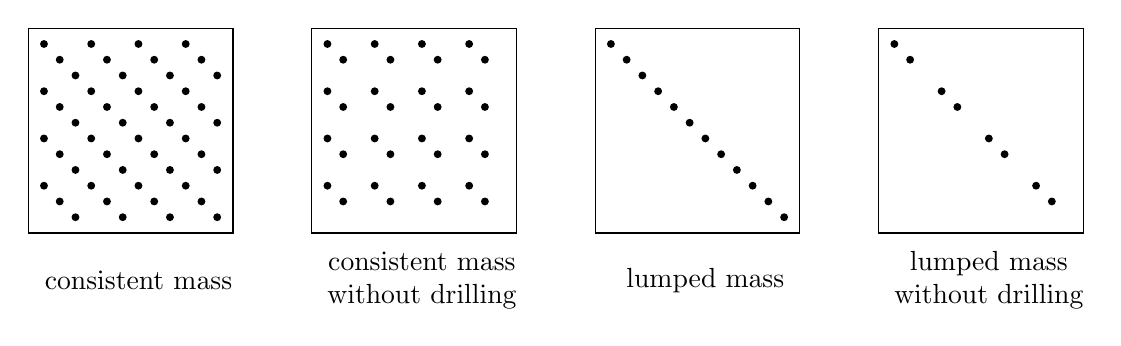
\begin{tikzpicture}[scale=.2]
\begin{scope}
\begin{scope}[every node/.style={circle,fill=black,minimum size=1mm,inner sep=0}]
\draw(0,-1)rectangle(13,12);
\foreach\x in{1,2,3,...,12}\node at(\x,12-\x){};
\foreach\x in{1,2,3,...,9}\node at(\x,9-\x){};
\foreach\x in{1,2,3,...,6}\node at(\x,6-\x){};
\foreach\x in{1,2,3}\node at(\x,3-\x){};
\foreach\x in{4,...,12}\node at(\x,15-\x){};
\foreach\x in{7,...,12}\node at(\x,18-\x){};
\foreach\x in{10,11,12}\node at(\x,21-\x){};
\end{scope}
\node[align=center]at(7,-4){consistent mass};
\end{scope}
\begin{scope}[xshift=18cm]
\begin{scope}[every node/.style={circle,fill=black,minimum size=1mm,inner sep=0}]
\draw(0,-1)rectangle(13,12);
\foreach\x in{1,2,4,5,7,8,10,11}\node at(\x,12-\x){};
\foreach\x in{1,2,4,5,7,8}\node at(\x,9-\x){};
\foreach\x in{1,2,4,5}\node at(\x,6-\x){};
\foreach\x in{1,2}\node at(\x,3-\x){};
\foreach\x in{4,5,7,8,10,11}\node at(\x,15-\x){};
\foreach\x in{7,8,10,11}\node at(\x,18-\x){};
\foreach\x in{10,11}\node at(\x,21-\x){};
\end{scope}
\node[align=center]at(7,-4){consistent mass\\without drilling};
\end{scope}
\begin{scope}[xshift=36cm]
\begin{scope}[every node/.style={circle,fill=black,minimum size=1mm,inner sep=0}]
\draw(0,-1)rectangle(13,12);
\foreach\x in{1,...,12}\node at(\x,12-\x){};
\end{scope}
\node[align=center]at(7,-4){lumped mass};
\end{scope}
\begin{scope}[xshift=54cm]
\begin{scope}[every node/.style={circle,fill=black,minimum size=1mm,inner sep=0}]
\draw(0,-1)rectangle(13,12);
\foreach\x in{1,2,4,5,7,8,10,11}\node at(\x,12-\x){};
\end{scope}
\node[align=center]at(7,-4){lumped mass\\without drilling};
\end{scope}
\end{tikzpicture}
\caption{entry patterns of different mass matrices}\label{fig:mass_pattern}
\end{figure}
It is preferable to have a positive definite (non-singular) mass matrix so that the frequencies of the corresponding model are well bounded. A singular mass matrix may not be an issue for dynamic applications in structural engineering which are mostly subjected to low frequency excitations, however, it would make a significant impact on wave propagation applications where high frequency response matters. This may also affect the stability of some explicit time integration methods such as the central difference method, in which the global mass matrix must be full ranked if no damping is defined. Standard dynamics textbooks \citep[e.g.,][]{Chopra2011} are referred to here for more details.
\section{Concrete}\label{sec:cdp}
The plastic-damage model proposed by \citet{Lee1998} is used to model concrete in-plane behaviour with the assist of a plane stress wrapper. A similar model known as the concrete damage plasticity (CDP) model, which supports user-defined backbones and degradations, is available in ABAQUS.

The uniaxial backbone curve is defined as a function of the accumulated plastic strain $\varepsilon_p$ by the following expression for both tension and compression,
\begin{gather}
\sigma_\aleph=f_\aleph\left(\left(1+a_\aleph\right)\exp\left(-b_\aleph\varepsilon_p\right)-a_\aleph\exp\left(-2b_\aleph\varepsilon_p\right)\right),
\end{gather}
where the subscript $\aleph$ can be either $t$ or $c$ to represent tensile and compressive properties, $f_\aleph$ is the initial yield strength, $a_\aleph$ and $b_\aleph$ are two parameters that control the shape of the curve. An illustration of backbones can be seen in \figref{fig:cdp_backbone}.
\begin{figure}[htb]
\centering\scriptsize
\begin{subfigure}{.48\textwidth}\centering
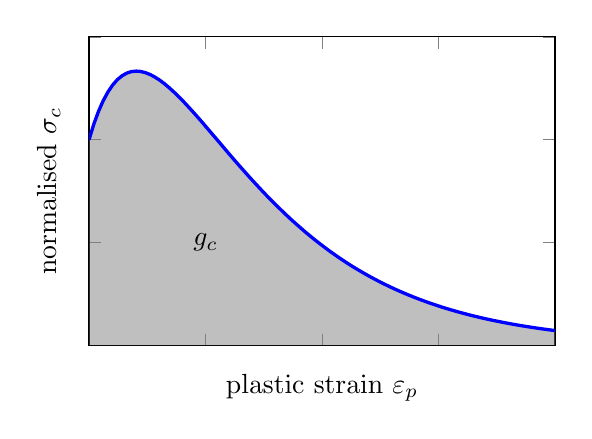
\begin{tikzpicture}
\begin{axis}[width=7.5cm,height=5.5cm,domain=0:4,xmin=0,xmax=4,ymin=0,ymax=1.5,xlabel=plastic strain $\varepsilon_p$,ylabel=normalised $\sigma_c$,xticklabels={,,},yticklabels={,,}]
\addplot[samples=100,black,very thin,fill=gray,fill opacity=0.5]{4*exp(-x)-3*exp(-2*x)}\closedcycle;
\addplot[samples=100,blue,very thick]{4*exp(-x)-3*exp(-2*x)};
\node at(1,.5){$g_c$};
\end{axis}
\end{tikzpicture}
\caption{compression}
\end{subfigure}\hfill
\begin{subfigure}{.48\textwidth}\centering
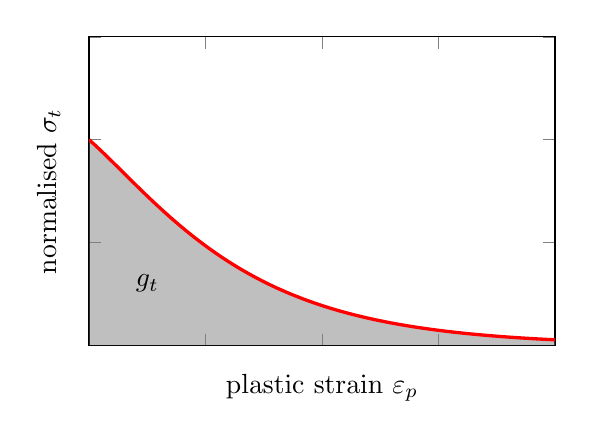
\begin{tikzpicture}
\begin{axis}[width=7.5cm,height=5.5cm,domain=0:4,xmin=0,xmax=4,ymin=0,ymax=1.5,xlabel=plastic strain $\varepsilon_p$,ylabel=normalised $\sigma_t$,xticklabels={,,},yticklabels={,,}]
\addplot[samples=100,black,very thin,fill=gray,fill opacity=0.5]{1.5*exp(-x)-.5*exp(-2*x)}\closedcycle;
\addplot[samples=100,red,very thick]{1.5*exp(-x)-.5*exp(-2*x)};
\node at(.5,.3){$g_t$};
\end{axis}
\end{tikzpicture}
\caption{tension}
\end{subfigure}
\caption{example monotonic backbones used in the CDP model}\label{fig:cdp_backbone}
\end{figure}
Regularisations can be implemented by relating $a_\aleph$ and $b_\aleph$ with objective quantities. In specific, the model defines
\begin{gather}
g_\aleph=\int_0^\infty\sigma_\aleph~\md{\varepsilon_p}=\dfrac{f_\aleph}{b_\aleph}\left(1+\dfrac{a_\aleph}{2}\right)
\end{gather}
to be the area under the corresponding backbone. The specific fracture energy $G_f$ can be used to control the tension softening by further defining $g_t=G_f/l_c$ where $l_c$ is the characteristic length of the target element. The compression counterpart $g_c$ can be defined in a similar fashion. $g_t$ and $g_c$ are two main model parameters that provide mesh objective response. Details can be found elsewhere \citep{Lubliner1989}.

An isotropic damage model is adopted so the stress response is defined as
\begin{gather}
\mathbold{\sigma}=\left(1-D\right)\bar{\mathbold{\sigma}}=\left(1-D\right)\mathbold{E}\left(\mathbold{\varepsilon}-\mathbold{\varepsilon}_p\right)
\end{gather}
where $\bar{\mathbold{\sigma}}$ is the effective stress, $\mathbold{E}$ is the elastic stiffness, $D=1-\left(1-d_c\right)\left(1-sd_t\right)$ is a scalar degradation factor that relies on its uniaxial version $d_\aleph$, $s(\bar{\mathbold{\sigma}})$ is the stiffness recovery factor. The degradation factor $d_\aleph$, according to the original model \citep{Lee1998}, is
\begin{gather}
d_\aleph=1-\exp\left(-c_\aleph\varepsilon_p\right)
\end{gather}
where $c_\aleph$ is a material constant that controls the rate of degradation. By definition, $d_\aleph$ ranges from zero to unity.

To simplify the formulation, a normalised internal damage variable $\kappa_\aleph$ is adopted as a function of $\varepsilon_p$,
\begin{gather}
\kappa_\aleph=\dfrac{1}{g_\aleph}\int_0^{\varepsilon_p}\sigma_\aleph~\md{\varepsilon_p}.
\end{gather}
After some mathematical operations, $d_\aleph$ and $\sigma_\aleph$ can be expressed as functions of $\kappa_\aleph$. Hence, $\kappa_\aleph$ controls the developments of both damage and plasticity of the model. The evolution of $\kappa_\aleph$ is related to the ratios among three principal stress components. Tensile and compressive damage can evolve separately so that tension and compression backbones can have different hardening behaviour.

For numerical implementation, parameters $b_\aleph$ and $c_\aleph$ are associated with the reference degradation factors $\bar{D}_c$ at crush strength and $\bar{D}_t$ at \SI{50}{\percent} of the crack stress, respectively. 

The yield function is defined as
\begin{gather}
F=\alpha{}I_1+\sqrt{3J_2}+\beta\left\langle\hat\sigma_{1}\right\rangle-\left(1-\alpha\right)c,
\end{gather}
in which $I_1$ is the first invariant of the stress tensor, $J_2$ is the second invariant of the deviatoric stress tensor, $\alpha$ is a dimensionless constant, $\beta(\kappa_\aleph)$ and $c(\kappa_\aleph)$ are the cohesion related parameters, $\hat\sigma_{1}$ is the algebraic maximum eigenvalue of stress and $\left\langle\cdot\right\rangle$ is the Macaulay bracket.

A Drucker-Prager type function is used as the plastic potential,
\begin{gather}
G=\sqrt{2J_2}+\alpha_p{}I_1,
\end{gather}
where $\alpha_p$ is a material constant that controls dilatation.

Other recently proposed 3D concrete models, such as CDPM1 \citep{Grassl2006} and CDPM2 \citep{Grassl2013}, can also be used. However, some of these models may have difficulties in deriving the corresponding consistent tangent stiffness matrices. In those cases, some low rank update algorithms \citep[e.g.,][]{Shanno1970} can be adopted to obtain secant stiffness matrices.
\section{Dynamic Analysis of a Cantilever Wall With Simple Material}
As the main focus of this work is the engineering application of the proposed elements. The analytical validations of SGCMQ and GCMQ are not discussed here for brevity. However, interested readers can refer to the authors' other work \citep{Chang2019,Chang2019a,Chang2020} for details.

The investigations of dynamic performance of the proposed elements starts with a simple cantilever beam/wall example with an aspect ratio of \num{4}. The model is depicted in \figref{fig:cantilever_model}.
\begin{figure}[htb]
\centering\footnotesize
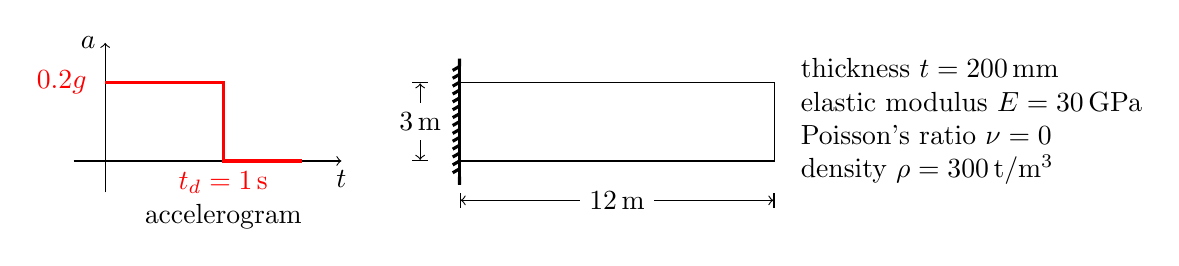
\begin{tikzpicture}
\FixedSupport[-90]{0,.5}{2}
\draw(0,0)rectangle(4,1);
\draw[|<->|](-.5,0)--++(0,1)node[midway,fill=white]{\SI{3}{\meter}};
\draw[|<->|](0,-.5)--++(4,0)node[midway,fill=white]{\SI{12}{\meter}};
\node[align=left]at(6.5,.5){\setstretch{1}thickness $t=\SI{200}{\milli\metre}$\\elastic modulus $E=\SI{30}{\giga\pascal}$\\Poisson's ratio $\nu=\num{0}$\\density $\rho=\SI{300}{\tonne\per\meter^3}$};
\begin{scope}[xshift=-4.5cm]
\draw[->](-.4,0)--++(3.4,0)node[below]{$t$};
\draw[->](0,-.4)--++(0,1.9)node[left]{$a$};
\draw[red,very thick](0,1)node[left=1mm]{$0.2g$}--++(1.5,0)--++(0,-1)node[below]{$t_d=\SI{1}{\second}$}--++(1,0);
\node at(1.5,-.7){accelerogram};
\end{scope}
\end{tikzpicture}
\caption{a simple cantilever beam example}\label{fig:cantilever_model}
\end{figure}
Instead of point mass, distributed mass is used with the consistent mass formulation. The density is set to \SI{300}{\tonne\per\metre^3} so that the analytical solution of the first natural frequency $f_1$ \citep{Young2012} can be approximated by
\begin{gather}
f_1\approx\dfrac{3.52}{2\pi}\sqrt{\dfrac{EI}{\rho{}bhL^4}}=\dfrac{3.52}{2\pi}\sqrt{\dfrac{Eh^2}{12\rho{}L^4}}=\SI{1.065}{\hertz}.
\end{gather}
The first natural period is $t_1=\SI{0.939}{\second}$. The duration of the rectangular pulse $t_d$ is set to \SI{1}{\second}. Since the chosen $t_d$ is close to $t_1$, the amplitude of displacement in the free vibration phase is significantly smaller than that of the forced vibration phase. Discussions on the theoretical solutions can be found elsewhere \citep{Chopra2011}. This feature can be used to amplify the difference among numerical models. The constant average acceleration Newmark method is used for the time integration. The time step size $\Delta{}t$ is set to \SI{0.01}{\second}. To avoid any potential bias due to different damping models, no damping is defined so an undamped beam is analysed.
\subsection{Eigenanalysis}
The eigenanalysis is performed to compute the first natural period. Numerical results, which are obtained by using SGCMQG elements with the consistent mass formulation, are shown in \tabref{tab:modalanalysis}. The reference solution is computed by using \num{3600} CPS4 elements with the lumped mass formulation, which is the default configuration in ABAQUS. The results are not significantly affected by different integration schemes. Both mass matrix formulations give similar results. It could be seen that relatively accurate natural periods, especially that of lower modes, can be obtained by using only a few elements.
\begin{table}[htb]
\centering\footnotesize
\caption{the first natural period computed by using different meshes}\label{tab:modalanalysis}
\begin{tabular}{rrrrrrr}
	\toprule
	        mesh & \numproduct{1x1} & \numproduct{1x2} & \numproduct{1x4} & \numproduct{2x4} & \numproduct{2x8} &  ref. \\ \midrule
	$\omega_1^2$ &     37.44 &     43.23 &     42.28 &     41.70 &     41.41 & 41.37 \\
	       $t_1$ &      1.03 &      0.96 &      0.97 &      0.97 &      0.98 &  0.98 \\ \bottomrule
\end{tabular}
\end{table}

From an algorithmic perspective, the excellent coarse mesh accuracy shown by (S)GCMQ is also advantageous to dynamics problems of structures. It is possible to use a very coarse mesh of (S)GCMQ to represent the stiffness of the target structure. By such, the highest frequency of the finite element model is lowered as the total number of DoFs is reduced. The potential fictitious response contributed by high frequency modes can be effectively eliminated from the source. This gives more flexibility when it comes to choose a proper time integration algorithm. The algorithmic damping and the second order accuracy cannot coexist in the well known Newmark method. To obtain the algorithmic damping, analysts shall either give up the second order accuracy or switch to another algorithm such as the generalised alpha method \citep{Chung1993}. With the high coarse mesh accuracy, it is possible to obtain satisfactory results by using the undamped time integration methods.
\subsection{Linear Analysis}
The linear analyses are performed with four mesh grids respectively: \numproduct{1x1}, \numproduct{1x2}, \numproduct{1x4} and \numproduct{2x8}. The tip displacement histories are shown in \figref{fig:cantilever_disp}.
\begin{figure}[htb]
\centering\scriptsize
\begin{subfigure}{.49\textwidth}\centering
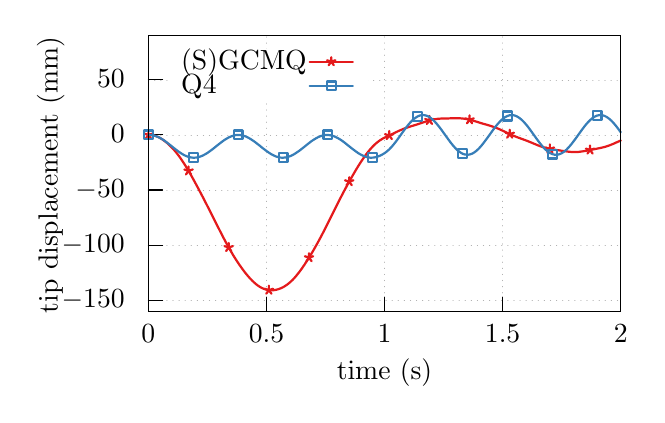
\begin{tikzpicture}[gnuplot]
%% generated with GNUPLOT 5.2p6 (Lua 5.3; terminal rev. Nov 2018, script rev. 107)
%% 06/16/2019 00:11:24
\path (0.000,0.000) rectangle (6.000,3.500);
\gpcolor{color=gp lt color axes}
\gpsetlinetype{gp lt axes}
\gpsetdashtype{gp dt axes}
\gpsetlinewidth{0.50}
\draw[gp path] (0.000,0.140)--(5.999,0.140);
\gpcolor{color=gp lt color border}
\gpsetlinetype{gp lt border}
\gpsetdashtype{gp dt solid}
\gpsetlinewidth{1.00}
\draw[gp path] (0.000,0.140)--(0.180,0.140);
\node[gp node right] at (-0.184,0.140) {$-150$};
\gpcolor{color=gp lt color axes}
\gpsetlinetype{gp lt axes}
\gpsetdashtype{gp dt axes}
\gpsetlinewidth{0.50}
\draw[gp path] (0.000,0.840)--(5.999,0.840);
\gpcolor{color=gp lt color border}
\gpsetlinetype{gp lt border}
\gpsetdashtype{gp dt solid}
\gpsetlinewidth{1.00}
\draw[gp path] (0.000,0.840)--(0.180,0.840);
\node[gp node right] at (-0.184,0.840) {$-100$};
\gpcolor{color=gp lt color axes}
\gpsetlinetype{gp lt axes}
\gpsetdashtype{gp dt axes}
\gpsetlinewidth{0.50}
\draw[gp path] (0.000,1.540)--(5.999,1.540);
\gpcolor{color=gp lt color border}
\gpsetlinetype{gp lt border}
\gpsetdashtype{gp dt solid}
\gpsetlinewidth{1.00}
\draw[gp path] (0.000,1.540)--(0.180,1.540);
\node[gp node right] at (-0.184,1.540) {$-50$};
\gpcolor{color=gp lt color axes}
\gpsetlinetype{gp lt axes}
\gpsetdashtype{gp dt axes}
\gpsetlinewidth{0.50}
\draw[gp path] (0.000,2.239)--(5.999,2.239);
\gpcolor{color=gp lt color border}
\gpsetlinetype{gp lt border}
\gpsetdashtype{gp dt solid}
\gpsetlinewidth{1.00}
\draw[gp path] (0.000,2.239)--(0.180,2.239);
\node[gp node right] at (-0.184,2.239) {$0$};
\gpcolor{color=gp lt color axes}
\gpsetlinetype{gp lt axes}
\gpsetdashtype{gp dt axes}
\gpsetlinewidth{0.50}
\draw[gp path] (0.000,2.939)--(0.300,2.939);
\draw[gp path] (2.780,2.939)--(5.999,2.939);
\gpcolor{color=gp lt color border}
\gpsetlinetype{gp lt border}
\gpsetdashtype{gp dt solid}
\gpsetlinewidth{1.00}
\draw[gp path] (0.000,2.939)--(0.180,2.939);
\node[gp node right] at (-0.184,2.939) {$50$};
\gpcolor{color=gp lt color axes}
\gpsetlinetype{gp lt axes}
\gpsetdashtype{gp dt axes}
\gpsetlinewidth{0.50}
\draw[gp path] (0.000,0.000)--(0.000,3.499);
\gpcolor{color=gp lt color border}
\gpsetlinetype{gp lt border}
\gpsetdashtype{gp dt solid}
\gpsetlinewidth{1.00}
\draw[gp path] (0.000,0.000)--(0.000,0.180);
\node[gp node center] at (0.000,-0.308) {$0$};
\gpcolor{color=gp lt color axes}
\gpsetlinetype{gp lt axes}
\gpsetdashtype{gp dt axes}
\gpsetlinewidth{0.50}
\draw[gp path] (1.500,0.000)--(1.500,2.708);
\draw[gp path] (1.500,3.324)--(1.500,3.499);
\gpcolor{color=gp lt color border}
\gpsetlinetype{gp lt border}
\gpsetdashtype{gp dt solid}
\gpsetlinewidth{1.00}
\draw[gp path] (1.500,0.000)--(1.500,0.180);
\node[gp node center] at (1.500,-0.308) {$0.5$};
\gpcolor{color=gp lt color axes}
\gpsetlinetype{gp lt axes}
\gpsetdashtype{gp dt axes}
\gpsetlinewidth{0.50}
\draw[gp path] (3.000,0.000)--(3.000,3.499);
\gpcolor{color=gp lt color border}
\gpsetlinetype{gp lt border}
\gpsetdashtype{gp dt solid}
\gpsetlinewidth{1.00}
\draw[gp path] (3.000,0.000)--(3.000,0.180);
\node[gp node center] at (3.000,-0.308) {$1$};
\gpcolor{color=gp lt color axes}
\gpsetlinetype{gp lt axes}
\gpsetdashtype{gp dt axes}
\gpsetlinewidth{0.50}
\draw[gp path] (4.499,0.000)--(4.499,3.499);
\gpcolor{color=gp lt color border}
\gpsetlinetype{gp lt border}
\gpsetdashtype{gp dt solid}
\gpsetlinewidth{1.00}
\draw[gp path] (4.499,0.000)--(4.499,0.180);
\node[gp node center] at (4.499,-0.308) {$1.5$};
\gpcolor{color=gp lt color axes}
\gpsetlinetype{gp lt axes}
\gpsetdashtype{gp dt axes}
\gpsetlinewidth{0.50}
\draw[gp path] (5.999,0.000)--(5.999,3.499);
\gpcolor{color=gp lt color border}
\gpsetlinetype{gp lt border}
\gpsetdashtype{gp dt solid}
\gpsetlinewidth{1.00}
\draw[gp path] (5.999,0.000)--(5.999,0.180);
\node[gp node center] at (5.999,-0.308) {$2$};
\draw[gp path] (0.000,3.499)--(0.000,0.000)--(5.999,0.000)--(5.999,3.499)--cycle;
\node[gp node center,rotate=-270] at (-1.228,1.749) {tip displacement (\si{\milli\metre})};
\node[gp node center] at (2.999,-0.769) {time (\si{\second})};
\gpcolor{rgb color={0.894,0.102,0.110}}
\gpsetlinewidth{2.00}
\draw[gp path] (0.000,2.239)--(0.030,2.238)--(0.060,2.234)--(0.090,2.226)--(0.120,2.215)%
  --(0.150,2.199)--(0.180,2.181)--(0.210,2.159)--(0.240,2.135)--(0.270,2.107)--(0.300,2.077)%
  --(0.330,2.044)--(0.360,2.008)--(0.390,1.969)--(0.420,1.926)--(0.450,1.881)--(0.480,1.833)%
  --(0.510,1.783)--(0.540,1.731)--(0.570,1.677)--(0.600,1.622)--(0.630,1.566)--(0.660,1.509)%
  --(0.690,1.452)--(0.720,1.394)--(0.750,1.335)--(0.780,1.276)--(0.810,1.217)--(0.840,1.157)%
  --(0.870,1.097)--(0.900,1.038)--(0.930,0.979)--(0.960,0.921)--(0.990,0.865)--(1.020,0.810)%
  --(1.050,0.758)--(1.080,0.707)--(1.110,0.659)--(1.140,0.613)--(1.170,0.570)--(1.200,0.528)%
  --(1.230,0.489)--(1.260,0.452)--(1.290,0.418)--(1.320,0.387)--(1.350,0.359)--(1.380,0.334)%
  --(1.410,0.313)--(1.440,0.296)--(1.470,0.283)--(1.500,0.274)--(1.530,0.268)--(1.560,0.266)%
  --(1.590,0.267)--(1.620,0.272)--(1.650,0.280)--(1.680,0.291)--(1.710,0.305)--(1.740,0.323)%
  --(1.770,0.344)--(1.800,0.369)--(1.830,0.397)--(1.860,0.429)--(1.890,0.465)--(1.920,0.503)%
  --(1.950,0.544)--(1.980,0.588)--(2.010,0.634)--(2.040,0.681)--(2.070,0.730)--(2.100,0.781)%
  --(2.130,0.834)--(2.160,0.888)--(2.190,0.944)--(2.220,1.001)--(2.250,1.059)--(2.280,1.119)%
  --(2.310,1.179)--(2.340,1.240)--(2.370,1.300)--(2.400,1.361)--(2.430,1.420)--(2.460,1.478)%
  --(2.490,1.535)--(2.520,1.591)--(2.550,1.646)--(2.580,1.699)--(2.610,1.751)--(2.640,1.802)%
  --(2.670,1.851)--(2.700,1.898)--(2.730,1.942)--(2.760,1.985)--(2.790,2.024)--(2.820,2.060)%
  --(2.850,2.093)--(2.880,2.122)--(2.910,2.148)--(2.940,2.170)--(2.970,2.189)--(3.000,2.205)%
  --(3.029,2.219)--(3.059,2.232)--(3.089,2.247)--(3.119,2.261)--(3.149,2.276)--(3.179,2.290)%
  --(3.209,2.303)--(3.239,2.316)--(3.269,2.327)--(3.299,2.337)--(3.329,2.347)--(3.359,2.356)%
  --(3.389,2.365)--(3.419,2.375)--(3.449,2.385)--(3.479,2.395)--(3.509,2.405)--(3.539,2.415)%
  --(3.569,2.424)--(3.599,2.431)--(3.629,2.437)--(3.659,2.442)--(3.689,2.445)--(3.719,2.447)%
  --(3.749,2.448)--(3.779,2.449)--(3.809,2.449)--(3.839,2.450)--(3.869,2.450)--(3.899,2.451)%
  --(3.929,2.451)--(3.959,2.450)--(3.989,2.448)--(4.019,2.444)--(4.049,2.439)--(4.079,2.432)%
  --(4.109,2.424)--(4.139,2.416)--(4.169,2.407)--(4.199,2.397)--(4.229,2.388)--(4.259,2.379)%
  --(4.289,2.371)--(4.319,2.362)--(4.349,2.353)--(4.379,2.343)--(4.409,2.332)--(4.439,2.320)%
  --(4.469,2.307)--(4.499,2.293)--(4.529,2.279)--(4.559,2.264)--(4.589,2.250)--(4.619,2.237)%
  --(4.649,2.224)--(4.679,2.212)--(4.709,2.201)--(4.739,2.190)--(4.769,2.179)--(4.799,2.168)%
  --(4.829,2.156)--(4.859,2.144)--(4.889,2.131)--(4.919,2.119)--(4.949,2.106)--(4.979,2.095)%
  --(5.009,2.085)--(5.039,2.076)--(5.069,2.068)--(5.099,2.062)--(5.129,2.056)--(5.159,2.052)%
  --(5.189,2.047)--(5.219,2.043)--(5.249,2.038)--(5.279,2.034)--(5.309,2.030)--(5.339,2.026)%
  --(5.369,2.023)--(5.399,2.022)--(5.429,2.022)--(5.459,2.023)--(5.489,2.027)--(5.519,2.031)%
  --(5.549,2.036)--(5.579,2.042)--(5.609,2.048)--(5.639,2.054)--(5.669,2.059)--(5.699,2.065)%
  --(5.729,2.071)--(5.759,2.078)--(5.789,2.085)--(5.819,2.094)--(5.849,2.104)--(5.879,2.116)%
  --(5.909,2.128)--(5.939,2.142)--(5.969,2.155)--(5.999,2.168);
\gpsetpointsize{4.00}
\gppoint{gp mark 3}{(0.000,2.239)}
\gppoint{gp mark 3}{(0.510,1.783)}
\gppoint{gp mark 3}{(1.020,0.810)}
\gppoint{gp mark 3}{(1.530,0.268)}
\gppoint{gp mark 3}{(2.040,0.681)}
\gppoint{gp mark 3}{(2.550,1.646)}
\gppoint{gp mark 3}{(3.059,2.232)}
\gppoint{gp mark 3}{(3.569,2.424)}
\gppoint{gp mark 3}{(4.079,2.432)}
\gppoint{gp mark 3}{(4.589,2.250)}
\gppoint{gp mark 3}{(5.099,2.062)}
\gppoint{gp mark 3}{(5.609,2.048)}
\gpcolor{rgb color={0.216,0.494,0.722}}
\draw[gp path] (0.000,2.239)--(0.030,2.238)--(0.060,2.234)--(0.090,2.226)--(0.120,2.215)%
  --(0.150,2.200)--(0.180,2.182)--(0.210,2.162)--(0.240,2.139)--(0.270,2.116)--(0.300,2.092)%
  --(0.330,2.068)--(0.360,2.045)--(0.390,2.023)--(0.420,2.003)--(0.450,1.985)--(0.480,1.971)%
  --(0.510,1.960)--(0.540,1.953)--(0.570,1.950)--(0.600,1.951)--(0.630,1.956)--(0.660,1.965)%
  --(0.690,1.977)--(0.720,1.993)--(0.750,2.011)--(0.780,2.032)--(0.810,2.054)--(0.840,2.078)%
  --(0.870,2.102)--(0.900,2.126)--(0.930,2.149)--(0.960,2.171)--(0.990,2.190)--(1.020,2.207)%
  --(1.050,2.220)--(1.080,2.230)--(1.110,2.237)--(1.140,2.239)--(1.170,2.237)--(1.200,2.231)%
  --(1.230,2.222)--(1.260,2.209)--(1.290,2.192)--(1.320,2.173)--(1.350,2.152)--(1.380,2.129)%
  --(1.410,2.106)--(1.440,2.081)--(1.470,2.058)--(1.500,2.035)--(1.530,2.014)--(1.560,1.995)%
  --(1.590,1.979)--(1.620,1.966)--(1.650,1.957)--(1.680,1.951)--(1.710,1.950)--(1.740,1.953)%
  --(1.770,1.959)--(1.800,1.969)--(1.830,1.983)--(1.860,2.000)--(1.890,2.020)--(1.920,2.041)%
  --(1.950,2.064)--(1.980,2.088)--(2.010,2.112)--(2.040,2.136)--(2.070,2.159)--(2.100,2.179)%
  --(2.130,2.197)--(2.160,2.213)--(2.190,2.225)--(2.220,2.233)--(2.250,2.238)--(2.280,2.239)%
  --(2.310,2.235)--(2.340,2.228)--(2.370,2.217)--(2.400,2.202)--(2.430,2.185)--(2.460,2.165)%
  --(2.490,2.143)--(2.520,2.119)--(2.550,2.095)--(2.580,2.071)--(2.610,2.048)--(2.640,2.026)%
  --(2.670,2.005)--(2.700,1.988)--(2.730,1.973)--(2.760,1.962)--(2.790,1.954)--(2.820,1.950)%
  --(2.850,1.951)--(2.880,1.955)--(2.910,1.963)--(2.940,1.975)--(2.970,1.990)--(3.000,2.008)%
  --(3.029,2.030)--(3.059,2.056)--(3.089,2.088)--(3.119,2.123)--(3.149,2.162)--(3.179,2.203)%
  --(3.209,2.245)--(3.239,2.287)--(3.269,2.328)--(3.299,2.366)--(3.329,2.401)--(3.359,2.431)%
  --(3.389,2.455)--(3.419,2.474)--(3.449,2.486)--(3.479,2.492)--(3.509,2.490)--(3.539,2.481)%
  --(3.569,2.466)--(3.599,2.444)--(3.629,2.416)--(3.659,2.384)--(3.689,2.347)--(3.719,2.308)%
  --(3.749,2.266)--(3.779,2.224)--(3.809,2.183)--(3.839,2.142)--(3.869,2.105)--(3.899,2.071)%
  --(3.929,2.042)--(3.959,2.019)--(3.989,2.001)--(4.019,1.991)--(4.049,1.987)--(4.079,1.990)%
  --(4.109,2.000)--(4.139,2.017)--(4.169,2.040)--(4.199,2.069)--(4.229,2.102)--(4.259,2.140)%
  --(4.289,2.180)--(4.319,2.221)--(4.349,2.263)--(4.379,2.305)--(4.409,2.345)--(4.439,2.381)%
  --(4.469,2.414)--(4.499,2.442)--(4.529,2.464)--(4.559,2.480)--(4.589,2.489)--(4.619,2.492)%
  --(4.649,2.487)--(4.679,2.475)--(4.709,2.457)--(4.739,2.433)--(4.769,2.403)--(4.799,2.369)%
  --(4.829,2.331)--(4.859,2.290)--(4.889,2.248)--(4.919,2.206)--(4.949,2.165)--(4.979,2.126)%
  --(5.009,2.090)--(5.039,2.058)--(5.069,2.031)--(5.099,2.010)--(5.129,1.996)--(5.159,1.988)%
  --(5.189,1.987)--(5.219,1.994)--(5.249,2.007)--(5.279,2.026)--(5.309,2.052)--(5.339,2.083)%
  --(5.369,2.118)--(5.399,2.157)--(5.429,2.197)--(5.459,2.239)--(5.489,2.281)--(5.519,2.322)%
  --(5.549,2.361)--(5.579,2.396)--(5.609,2.427)--(5.639,2.452)--(5.669,2.472)--(5.699,2.485)%
  --(5.729,2.491)--(5.759,2.491)--(5.789,2.483)--(5.819,2.468)--(5.849,2.447)--(5.879,2.421)%
  --(5.909,2.389)--(5.939,2.353)--(5.969,2.314)--(5.999,2.272);
\gppoint{gp mark 4}{(0.000,2.239)}
\gppoint{gp mark 4}{(0.570,1.950)}
\gppoint{gp mark 4}{(1.140,2.239)}
\gppoint{gp mark 4}{(1.710,1.950)}
\gppoint{gp mark 4}{(2.280,2.239)}
\gppoint{gp mark 4}{(2.850,1.951)}
\gppoint{gp mark 4}{(3.419,2.474)}
\gppoint{gp mark 4}{(3.989,2.001)}
\gppoint{gp mark 4}{(4.559,2.480)}
\gppoint{gp mark 4}{(5.129,1.996)}
\gppoint{gp mark 4}{(5.699,2.485)}
\gpfill{color=gpbgfillcolor} (0.300,2.708)--(2.780,2.708)--(2.780,3.324)--(0.300,3.324)--cycle;
\gpcolor{color=gp lt color border}
\node[gp node left] at (0.300,3.170) {(S)GCMQ};
\gpcolor{rgb color={0.894,0.102,0.110}}
\draw[gp path] (2.048,3.170)--(2.596,3.170);
\gppoint{gp mark 3}{(2.322,3.170)}
\gpcolor{color=gp lt color border}
\node[gp node left] at (0.300,2.862) {Q4};
\gpcolor{rgb color={0.216,0.494,0.722}}
\draw[gp path] (2.048,2.862)--(2.596,2.862);
\gppoint{gp mark 4}{(2.322,2.862)}
\gpcolor{color=gp lt color border}
\gpsetlinewidth{1.00}
\draw[gp path] (0.000,3.499)--(0.000,0.000)--(5.999,0.000)--(5.999,3.499)--cycle;
%% coordinates of the plot area
\gpdefrectangularnode{gp plot 1}{\pgfpoint{0.000cm}{0.000cm}}{\pgfpoint{5.999cm}{3.499cm}}
\end{tikzpicture}
%% gnuplot variables

\caption{with \numproduct{1x1} element}
\end{subfigure}\hfill
\begin{subfigure}{.49\textwidth}\centering
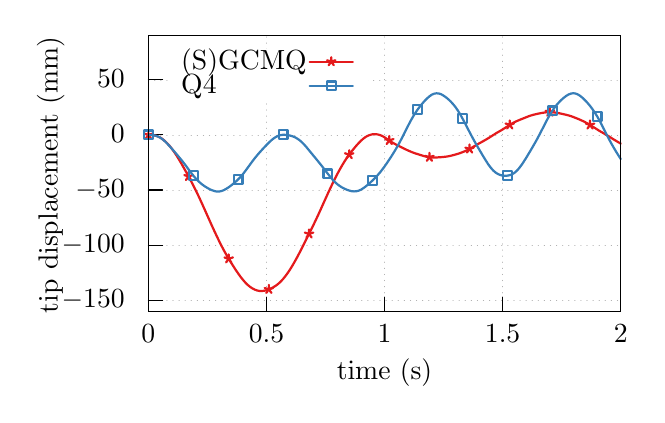
\begin{tikzpicture}[gnuplot]
%% generated with GNUPLOT 5.2p6 (Lua 5.3; terminal rev. Nov 2018, script rev. 107)
%% 06/16/2019 00:11:24
\path (0.000,0.000) rectangle (6.000,3.500);
\gpcolor{color=gp lt color axes}
\gpsetlinetype{gp lt axes}
\gpsetdashtype{gp dt axes}
\gpsetlinewidth{0.50}
\draw[gp path] (0.000,0.140)--(5.999,0.140);
\gpcolor{color=gp lt color border}
\gpsetlinetype{gp lt border}
\gpsetdashtype{gp dt solid}
\gpsetlinewidth{1.00}
\draw[gp path] (0.000,0.140)--(0.180,0.140);
\node[gp node right] at (-0.184,0.140) {$-150$};
\gpcolor{color=gp lt color axes}
\gpsetlinetype{gp lt axes}
\gpsetdashtype{gp dt axes}
\gpsetlinewidth{0.50}
\draw[gp path] (0.000,0.840)--(5.999,0.840);
\gpcolor{color=gp lt color border}
\gpsetlinetype{gp lt border}
\gpsetdashtype{gp dt solid}
\gpsetlinewidth{1.00}
\draw[gp path] (0.000,0.840)--(0.180,0.840);
\node[gp node right] at (-0.184,0.840) {$-100$};
\gpcolor{color=gp lt color axes}
\gpsetlinetype{gp lt axes}
\gpsetdashtype{gp dt axes}
\gpsetlinewidth{0.50}
\draw[gp path] (0.000,1.540)--(5.999,1.540);
\gpcolor{color=gp lt color border}
\gpsetlinetype{gp lt border}
\gpsetdashtype{gp dt solid}
\gpsetlinewidth{1.00}
\draw[gp path] (0.000,1.540)--(0.180,1.540);
\node[gp node right] at (-0.184,1.540) {$-50$};
\gpcolor{color=gp lt color axes}
\gpsetlinetype{gp lt axes}
\gpsetdashtype{gp dt axes}
\gpsetlinewidth{0.50}
\draw[gp path] (0.000,2.239)--(5.999,2.239);
\gpcolor{color=gp lt color border}
\gpsetlinetype{gp lt border}
\gpsetdashtype{gp dt solid}
\gpsetlinewidth{1.00}
\draw[gp path] (0.000,2.239)--(0.180,2.239);
\node[gp node right] at (-0.184,2.239) {$0$};
\gpcolor{color=gp lt color axes}
\gpsetlinetype{gp lt axes}
\gpsetdashtype{gp dt axes}
\gpsetlinewidth{0.50}
\draw[gp path] (0.000,2.939)--(0.300,2.939);
\draw[gp path] (2.780,2.939)--(5.999,2.939);
\gpcolor{color=gp lt color border}
\gpsetlinetype{gp lt border}
\gpsetdashtype{gp dt solid}
\gpsetlinewidth{1.00}
\draw[gp path] (0.000,2.939)--(0.180,2.939);
\node[gp node right] at (-0.184,2.939) {$50$};
\gpcolor{color=gp lt color axes}
\gpsetlinetype{gp lt axes}
\gpsetdashtype{gp dt axes}
\gpsetlinewidth{0.50}
\draw[gp path] (0.000,0.000)--(0.000,3.499);
\gpcolor{color=gp lt color border}
\gpsetlinetype{gp lt border}
\gpsetdashtype{gp dt solid}
\gpsetlinewidth{1.00}
\draw[gp path] (0.000,0.000)--(0.000,0.180);
\node[gp node center] at (0.000,-0.308) {$0$};
\gpcolor{color=gp lt color axes}
\gpsetlinetype{gp lt axes}
\gpsetdashtype{gp dt axes}
\gpsetlinewidth{0.50}
\draw[gp path] (1.500,0.000)--(1.500,2.708);
\draw[gp path] (1.500,3.324)--(1.500,3.499);
\gpcolor{color=gp lt color border}
\gpsetlinetype{gp lt border}
\gpsetdashtype{gp dt solid}
\gpsetlinewidth{1.00}
\draw[gp path] (1.500,0.000)--(1.500,0.180);
\node[gp node center] at (1.500,-0.308) {$0.5$};
\gpcolor{color=gp lt color axes}
\gpsetlinetype{gp lt axes}
\gpsetdashtype{gp dt axes}
\gpsetlinewidth{0.50}
\draw[gp path] (3.000,0.000)--(3.000,3.499);
\gpcolor{color=gp lt color border}
\gpsetlinetype{gp lt border}
\gpsetdashtype{gp dt solid}
\gpsetlinewidth{1.00}
\draw[gp path] (3.000,0.000)--(3.000,0.180);
\node[gp node center] at (3.000,-0.308) {$1$};
\gpcolor{color=gp lt color axes}
\gpsetlinetype{gp lt axes}
\gpsetdashtype{gp dt axes}
\gpsetlinewidth{0.50}
\draw[gp path] (4.499,0.000)--(4.499,3.499);
\gpcolor{color=gp lt color border}
\gpsetlinetype{gp lt border}
\gpsetdashtype{gp dt solid}
\gpsetlinewidth{1.00}
\draw[gp path] (4.499,0.000)--(4.499,0.180);
\node[gp node center] at (4.499,-0.308) {$1.5$};
\gpcolor{color=gp lt color axes}
\gpsetlinetype{gp lt axes}
\gpsetdashtype{gp dt axes}
\gpsetlinewidth{0.50}
\draw[gp path] (5.999,0.000)--(5.999,3.499);
\gpcolor{color=gp lt color border}
\gpsetlinetype{gp lt border}
\gpsetdashtype{gp dt solid}
\gpsetlinewidth{1.00}
\draw[gp path] (5.999,0.000)--(5.999,0.180);
\node[gp node center] at (5.999,-0.308) {$2$};
\draw[gp path] (0.000,3.499)--(0.000,0.000)--(5.999,0.000)--(5.999,3.499)--cycle;
\node[gp node center,rotate=-270] at (-1.228,1.749) {tip displacement (\si{\milli\metre})};
\node[gp node center] at (2.999,-0.769) {time (\si{\second})};
\gpcolor{rgb color={0.894,0.102,0.110}}
\gpsetlinewidth{2.00}
\draw[gp path] (0.000,2.239)--(0.030,2.239)--(0.060,2.236)--(0.090,2.230)--(0.120,2.220)%
  --(0.150,2.206)--(0.180,2.186)--(0.210,2.161)--(0.240,2.132)--(0.270,2.099)--(0.300,2.061)%
  --(0.330,2.019)--(0.360,1.974)--(0.390,1.925)--(0.420,1.874)--(0.450,1.821)--(0.480,1.767)%
  --(0.510,1.712)--(0.540,1.656)--(0.570,1.598)--(0.600,1.539)--(0.630,1.477)--(0.660,1.413)%
  --(0.690,1.347)--(0.720,1.280)--(0.750,1.213)--(0.780,1.146)--(0.810,1.079)--(0.840,1.014)%
  --(0.870,0.950)--(0.900,0.888)--(0.930,0.828)--(0.960,0.771)--(0.990,0.718)--(1.020,0.666)%
  --(1.050,0.618)--(1.080,0.570)--(1.110,0.524)--(1.140,0.480)--(1.170,0.438)--(1.200,0.400)%
  --(1.230,0.366)--(1.260,0.336)--(1.290,0.311)--(1.320,0.291)--(1.350,0.275)--(1.380,0.264)%
  --(1.410,0.258)--(1.440,0.257)--(1.470,0.260)--(1.500,0.268)--(1.530,0.278)--(1.560,0.291)%
  --(1.590,0.307)--(1.620,0.326)--(1.650,0.349)--(1.680,0.376)--(1.710,0.409)--(1.740,0.446)%
  --(1.770,0.487)--(1.800,0.532)--(1.830,0.581)--(1.860,0.633)--(1.890,0.687)--(1.920,0.744)%
  --(1.950,0.803)--(1.980,0.862)--(2.010,0.922)--(2.040,0.982)--(2.070,1.043)--(2.100,1.104)%
  --(2.130,1.167)--(2.160,1.231)--(2.190,1.297)--(2.220,1.364)--(2.250,1.430)--(2.280,1.497)%
  --(2.310,1.561)--(2.340,1.624)--(2.370,1.685)--(2.400,1.744)--(2.430,1.799)--(2.460,1.852)%
  --(2.490,1.901)--(2.520,1.946)--(2.550,1.989)--(2.580,2.029)--(2.610,2.066)--(2.640,2.102)%
  --(2.670,2.135)--(2.700,2.166)--(2.730,2.192)--(2.760,2.214)--(2.790,2.230)--(2.820,2.241)%
  --(2.850,2.248)--(2.880,2.249)--(2.910,2.246)--(2.940,2.238)--(2.970,2.226)--(3.000,2.209)%
  --(3.029,2.189)--(3.059,2.169)--(3.089,2.149)--(3.119,2.131)--(3.149,2.115)--(3.179,2.099)%
  --(3.209,2.085)--(3.239,2.070)--(3.269,2.055)--(3.299,2.041)--(3.329,2.028)--(3.359,2.016)%
  --(3.389,2.005)--(3.419,1.996)--(3.449,1.986)--(3.479,1.977)--(3.509,1.968)--(3.539,1.961)%
  --(3.569,1.956)--(3.599,1.953)--(3.629,1.952)--(3.659,1.953)--(3.689,1.955)--(3.719,1.957)%
  --(3.749,1.960)--(3.779,1.963)--(3.809,1.968)--(3.839,1.974)--(3.869,1.982)--(3.899,1.990)%
  --(3.929,1.999)--(3.959,2.009)--(3.989,2.020)--(4.019,2.032)--(4.049,2.046)--(4.079,2.061)%
  --(4.109,2.078)--(4.139,2.096)--(4.169,2.113)--(4.199,2.131)--(4.229,2.147)--(4.259,2.164)%
  --(4.289,2.181)--(4.319,2.199)--(4.349,2.218)--(4.379,2.237)--(4.409,2.256)--(4.439,2.274)%
  --(4.469,2.291)--(4.499,2.309)--(4.529,2.328)--(4.559,2.347)--(4.589,2.367)--(4.619,2.385)%
  --(4.649,2.401)--(4.679,2.415)--(4.709,2.428)--(4.739,2.440)--(4.769,2.452)--(4.799,2.464)%
  --(4.829,2.476)--(4.859,2.486)--(4.889,2.495)--(4.919,2.502)--(4.949,2.509)--(4.979,2.515)%
  --(5.009,2.520)--(5.039,2.525)--(5.069,2.528)--(5.099,2.529)--(5.129,2.528)--(5.159,2.524)%
  --(5.189,2.520)--(5.219,2.514)--(5.249,2.508)--(5.279,2.501)--(5.309,2.494)--(5.339,2.486)%
  --(5.369,2.477)--(5.399,2.466)--(5.429,2.454)--(5.459,2.442)--(5.489,2.429)--(5.519,2.415)%
  --(5.549,2.400)--(5.579,2.384)--(5.609,2.366)--(5.639,2.347)--(5.669,2.328)--(5.699,2.309)%
  --(5.729,2.290)--(5.759,2.273)--(5.789,2.256)--(5.819,2.238)--(5.849,2.220)--(5.879,2.201)%
  --(5.909,2.182)--(5.939,2.164)--(5.969,2.146)--(5.999,2.129);
\gpsetpointsize{4.00}
\gppoint{gp mark 3}{(0.000,2.239)}
\gppoint{gp mark 3}{(0.510,1.712)}
\gppoint{gp mark 3}{(1.020,0.666)}
\gppoint{gp mark 3}{(1.530,0.278)}
\gppoint{gp mark 3}{(2.040,0.982)}
\gppoint{gp mark 3}{(2.550,1.989)}
\gppoint{gp mark 3}{(3.059,2.169)}
\gppoint{gp mark 3}{(3.569,1.956)}
\gppoint{gp mark 3}{(4.079,2.061)}
\gppoint{gp mark 3}{(4.589,2.367)}
\gppoint{gp mark 3}{(5.099,2.529)}
\gppoint{gp mark 3}{(5.609,2.366)}
\gpcolor{rgb color={0.216,0.494,0.722}}
\draw[gp path] (0.000,2.239)--(0.030,2.239)--(0.060,2.236)--(0.090,2.230)--(0.120,2.220)%
  --(0.150,2.205)--(0.180,2.184)--(0.210,2.158)--(0.240,2.128)--(0.270,2.096)--(0.300,2.062)%
  --(0.330,2.027)--(0.360,1.993)--(0.390,1.957)--(0.420,1.921)--(0.450,1.882)--(0.480,1.843)%
  --(0.510,1.802)--(0.540,1.762)--(0.570,1.723)--(0.600,1.688)--(0.630,1.657)--(0.660,1.629)%
  --(0.690,1.605)--(0.720,1.584)--(0.750,1.566)--(0.780,1.549)--(0.810,1.536)--(0.840,1.526)%
  --(0.870,1.520)--(0.900,1.521)--(0.930,1.527)--(0.960,1.539)--(0.990,1.556)--(1.020,1.575)%
  --(1.050,1.597)--(1.080,1.621)--(1.110,1.646)--(1.140,1.675)--(1.170,1.706)--(1.200,1.741)%
  --(1.230,1.780)--(1.260,1.821)--(1.290,1.862)--(1.320,1.903)--(1.350,1.942)--(1.380,1.979)%
  --(1.410,2.014)--(1.440,2.047)--(1.470,2.080)--(1.500,2.111)--(1.530,2.141)--(1.560,2.170)%
  --(1.590,2.194)--(1.620,2.214)--(1.650,2.228)--(1.680,2.237)--(1.710,2.241)--(1.740,2.240)%
  --(1.770,2.237)--(1.800,2.231)--(1.830,2.222)--(1.860,2.210)--(1.890,2.193)--(1.920,2.172)%
  --(1.950,2.146)--(1.980,2.115)--(2.010,2.081)--(2.040,2.044)--(2.070,2.008)--(2.100,1.971)%
  --(2.130,1.935)--(2.160,1.898)--(2.190,1.861)--(2.220,1.823)--(2.250,1.783)--(2.280,1.744)%
  --(2.310,1.706)--(2.340,1.671)--(2.370,1.640)--(2.400,1.613)--(2.430,1.591)--(2.460,1.572)%
  --(2.490,1.557)--(2.520,1.543)--(2.550,1.533)--(2.580,1.525)--(2.610,1.522)--(2.640,1.524)%
  --(2.670,1.531)--(2.700,1.544)--(2.730,1.563)--(2.760,1.585)--(2.790,1.610)--(2.820,1.636)%
  --(2.850,1.664)--(2.880,1.694)--(2.910,1.726)--(2.940,1.761)--(2.970,1.799)--(3.000,1.839)%
  --(3.029,1.882)--(3.059,1.926)--(3.089,1.972)--(3.119,2.020)--(3.149,2.070)--(3.179,2.123)%
  --(3.209,2.179)--(3.239,2.237)--(3.269,2.298)--(3.299,2.357)--(3.329,2.415)--(3.359,2.468)%
  --(3.389,2.517)--(3.419,2.561)--(3.449,2.601)--(3.479,2.638)--(3.509,2.672)--(3.539,2.703)%
  --(3.569,2.729)--(3.599,2.750)--(3.629,2.763)--(3.659,2.768)--(3.689,2.765)--(3.719,2.755)%
  --(3.749,2.738)--(3.779,2.717)--(3.809,2.692)--(3.839,2.664)--(3.869,2.631)--(3.899,2.594)%
  --(3.929,2.551)--(3.959,2.502)--(3.989,2.448)--(4.019,2.391)--(4.049,2.333)--(4.079,2.275)%
  --(4.109,2.218)--(4.139,2.163)--(4.169,2.110)--(4.199,2.058)--(4.229,2.007)--(4.259,1.957)%
  --(4.289,1.908)--(4.319,1.862)--(4.349,1.822)--(4.379,1.788)--(4.409,1.762)--(4.439,1.743)%
  --(4.469,1.730)--(4.499,1.723)--(4.529,1.720)--(4.559,1.722)--(4.589,1.728)--(4.619,1.739)%
  --(4.649,1.758)--(4.679,1.784)--(4.709,1.818)--(4.739,1.858)--(4.769,1.903)--(4.799,1.950)%
  --(4.829,2.000)--(4.859,2.050)--(4.889,2.102)--(4.919,2.154)--(4.949,2.209)--(4.979,2.267)%
  --(5.009,2.325)--(5.039,2.384)--(5.069,2.442)--(5.099,2.495)--(5.129,2.544)--(5.159,2.587)%
  --(5.189,2.625)--(5.219,2.658)--(5.249,2.688)--(5.279,2.714)--(5.309,2.737)--(5.339,2.754)%
  --(5.369,2.765)--(5.399,2.769)--(5.429,2.764)--(5.459,2.751)--(5.489,2.731)--(5.519,2.706)%
  --(5.549,2.676)--(5.579,2.644)--(5.609,2.608)--(5.639,2.568)--(5.669,2.524)--(5.699,2.476)%
  --(5.729,2.422)--(5.759,2.364)--(5.789,2.305)--(5.819,2.245)--(5.849,2.187)--(5.879,2.131)%
  --(5.909,2.079)--(5.939,2.028)--(5.969,1.980)--(5.999,1.933);
\gppoint{gp mark 4}{(0.000,2.239)}
\gppoint{gp mark 4}{(0.570,1.723)}
\gppoint{gp mark 4}{(1.140,1.675)}
\gppoint{gp mark 4}{(1.710,2.241)}
\gppoint{gp mark 4}{(2.280,1.744)}
\gppoint{gp mark 4}{(2.850,1.664)}
\gppoint{gp mark 4}{(3.419,2.561)}
\gppoint{gp mark 4}{(3.989,2.448)}
\gppoint{gp mark 4}{(4.559,1.722)}
\gppoint{gp mark 4}{(5.129,2.544)}
\gppoint{gp mark 4}{(5.699,2.476)}
\gpfill{color=gpbgfillcolor} (0.300,2.708)--(2.780,2.708)--(2.780,3.324)--(0.300,3.324)--cycle;
\gpcolor{color=gp lt color border}
\node[gp node left] at (0.300,3.170) {(S)GCMQ};
\gpcolor{rgb color={0.894,0.102,0.110}}
\draw[gp path] (2.048,3.170)--(2.596,3.170);
\gppoint{gp mark 3}{(2.322,3.170)}
\gpcolor{color=gp lt color border}
\node[gp node left] at (0.300,2.862) {Q4};
\gpcolor{rgb color={0.216,0.494,0.722}}
\draw[gp path] (2.048,2.862)--(2.596,2.862);
\gppoint{gp mark 4}{(2.322,2.862)}
\gpcolor{color=gp lt color border}
\gpsetlinewidth{1.00}
\draw[gp path] (0.000,3.499)--(0.000,0.000)--(5.999,0.000)--(5.999,3.499)--cycle;
%% coordinates of the plot area
\gpdefrectangularnode{gp plot 1}{\pgfpoint{0.000cm}{0.000cm}}{\pgfpoint{5.999cm}{3.499cm}}
\end{tikzpicture}
%% gnuplot variables

\caption{with \numproduct{1x2} elements}
\end{subfigure}\vspace*{4mm}
\begin{subfigure}{.49\textwidth}\centering
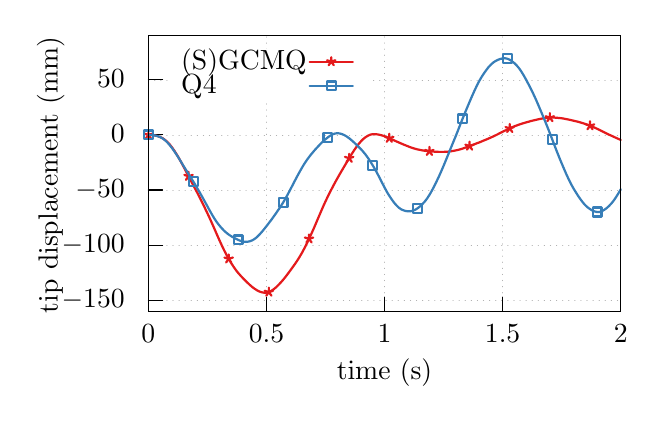
\begin{tikzpicture}[gnuplot]
%% generated with GNUPLOT 5.2p6 (Lua 5.3; terminal rev. Nov 2018, script rev. 107)
%% 06/16/2019 00:11:24
\path (0.000,0.000) rectangle (6.000,3.500);
\gpcolor{color=gp lt color axes}
\gpsetlinetype{gp lt axes}
\gpsetdashtype{gp dt axes}
\gpsetlinewidth{0.50}
\draw[gp path] (0.000,0.140)--(5.999,0.140);
\gpcolor{color=gp lt color border}
\gpsetlinetype{gp lt border}
\gpsetdashtype{gp dt solid}
\gpsetlinewidth{1.00}
\draw[gp path] (0.000,0.140)--(0.180,0.140);
\node[gp node right] at (-0.184,0.140) {$-150$};
\gpcolor{color=gp lt color axes}
\gpsetlinetype{gp lt axes}
\gpsetdashtype{gp dt axes}
\gpsetlinewidth{0.50}
\draw[gp path] (0.000,0.840)--(5.999,0.840);
\gpcolor{color=gp lt color border}
\gpsetlinetype{gp lt border}
\gpsetdashtype{gp dt solid}
\gpsetlinewidth{1.00}
\draw[gp path] (0.000,0.840)--(0.180,0.840);
\node[gp node right] at (-0.184,0.840) {$-100$};
\gpcolor{color=gp lt color axes}
\gpsetlinetype{gp lt axes}
\gpsetdashtype{gp dt axes}
\gpsetlinewidth{0.50}
\draw[gp path] (0.000,1.540)--(5.999,1.540);
\gpcolor{color=gp lt color border}
\gpsetlinetype{gp lt border}
\gpsetdashtype{gp dt solid}
\gpsetlinewidth{1.00}
\draw[gp path] (0.000,1.540)--(0.180,1.540);
\node[gp node right] at (-0.184,1.540) {$-50$};
\gpcolor{color=gp lt color axes}
\gpsetlinetype{gp lt axes}
\gpsetdashtype{gp dt axes}
\gpsetlinewidth{0.50}
\draw[gp path] (0.000,2.239)--(5.999,2.239);
\gpcolor{color=gp lt color border}
\gpsetlinetype{gp lt border}
\gpsetdashtype{gp dt solid}
\gpsetlinewidth{1.00}
\draw[gp path] (0.000,2.239)--(0.180,2.239);
\node[gp node right] at (-0.184,2.239) {$0$};
\gpcolor{color=gp lt color axes}
\gpsetlinetype{gp lt axes}
\gpsetdashtype{gp dt axes}
\gpsetlinewidth{0.50}
\draw[gp path] (0.000,2.939)--(0.300,2.939);
\draw[gp path] (2.780,2.939)--(5.999,2.939);
\gpcolor{color=gp lt color border}
\gpsetlinetype{gp lt border}
\gpsetdashtype{gp dt solid}
\gpsetlinewidth{1.00}
\draw[gp path] (0.000,2.939)--(0.180,2.939);
\node[gp node right] at (-0.184,2.939) {$50$};
\gpcolor{color=gp lt color axes}
\gpsetlinetype{gp lt axes}
\gpsetdashtype{gp dt axes}
\gpsetlinewidth{0.50}
\draw[gp path] (0.000,0.000)--(0.000,3.499);
\gpcolor{color=gp lt color border}
\gpsetlinetype{gp lt border}
\gpsetdashtype{gp dt solid}
\gpsetlinewidth{1.00}
\draw[gp path] (0.000,0.000)--(0.000,0.180);
\node[gp node center] at (0.000,-0.308) {$0$};
\gpcolor{color=gp lt color axes}
\gpsetlinetype{gp lt axes}
\gpsetdashtype{gp dt axes}
\gpsetlinewidth{0.50}
\draw[gp path] (1.500,0.000)--(1.500,2.708);
\draw[gp path] (1.500,3.324)--(1.500,3.499);
\gpcolor{color=gp lt color border}
\gpsetlinetype{gp lt border}
\gpsetdashtype{gp dt solid}
\gpsetlinewidth{1.00}
\draw[gp path] (1.500,0.000)--(1.500,0.180);
\node[gp node center] at (1.500,-0.308) {$0.5$};
\gpcolor{color=gp lt color axes}
\gpsetlinetype{gp lt axes}
\gpsetdashtype{gp dt axes}
\gpsetlinewidth{0.50}
\draw[gp path] (3.000,0.000)--(3.000,3.499);
\gpcolor{color=gp lt color border}
\gpsetlinetype{gp lt border}
\gpsetdashtype{gp dt solid}
\gpsetlinewidth{1.00}
\draw[gp path] (3.000,0.000)--(3.000,0.180);
\node[gp node center] at (3.000,-0.308) {$1$};
\gpcolor{color=gp lt color axes}
\gpsetlinetype{gp lt axes}
\gpsetdashtype{gp dt axes}
\gpsetlinewidth{0.50}
\draw[gp path] (4.499,0.000)--(4.499,3.499);
\gpcolor{color=gp lt color border}
\gpsetlinetype{gp lt border}
\gpsetdashtype{gp dt solid}
\gpsetlinewidth{1.00}
\draw[gp path] (4.499,0.000)--(4.499,0.180);
\node[gp node center] at (4.499,-0.308) {$1.5$};
\gpcolor{color=gp lt color axes}
\gpsetlinetype{gp lt axes}
\gpsetdashtype{gp dt axes}
\gpsetlinewidth{0.50}
\draw[gp path] (5.999,0.000)--(5.999,3.499);
\gpcolor{color=gp lt color border}
\gpsetlinetype{gp lt border}
\gpsetdashtype{gp dt solid}
\gpsetlinewidth{1.00}
\draw[gp path] (5.999,0.000)--(5.999,0.180);
\node[gp node center] at (5.999,-0.308) {$2$};
\draw[gp path] (0.000,3.499)--(0.000,0.000)--(5.999,0.000)--(5.999,3.499)--cycle;
\node[gp node center,rotate=-270] at (-1.228,1.749) {tip displacement (\si{\milli\metre})};
\node[gp node center] at (2.999,-0.769) {time (\si{\second})};
\gpcolor{rgb color={0.894,0.102,0.110}}
\gpsetlinewidth{2.00}
\draw[gp path] (0.000,2.239)--(0.030,2.239)--(0.060,2.236)--(0.090,2.231)--(0.120,2.223)%
  --(0.150,2.212)--(0.180,2.198)--(0.210,2.177)--(0.240,2.151)--(0.270,2.119)--(0.300,2.081)%
  --(0.330,2.038)--(0.360,1.991)--(0.390,1.940)--(0.420,1.886)--(0.450,1.830)--(0.480,1.772)%
  --(0.510,1.714)--(0.540,1.657)--(0.570,1.600)--(0.600,1.544)--(0.630,1.487)--(0.660,1.428)%
  --(0.690,1.368)--(0.720,1.306)--(0.750,1.243)--(0.780,1.179)--(0.810,1.112)--(0.840,1.044)%
  --(0.870,0.975)--(0.900,0.907)--(0.930,0.841)--(0.960,0.778)--(0.990,0.720)--(1.020,0.665)%
  --(1.050,0.614)--(1.080,0.568)--(1.110,0.525)--(1.140,0.487)--(1.170,0.453)--(1.200,0.421)%
  --(1.230,0.390)--(1.260,0.361)--(1.290,0.333)--(1.320,0.307)--(1.350,0.285)--(1.380,0.266)%
  --(1.410,0.251)--(1.440,0.241)--(1.470,0.235)--(1.500,0.236)--(1.530,0.243)--(1.560,0.258)%
  --(1.590,0.278)--(1.620,0.303)--(1.650,0.332)--(1.680,0.364)--(1.710,0.398)--(1.740,0.435)%
  --(1.770,0.474)--(1.800,0.515)--(1.830,0.556)--(1.860,0.598)--(1.890,0.642)--(1.920,0.690)%
  --(1.950,0.741)--(1.980,0.797)--(2.010,0.856)--(2.040,0.919)--(2.070,0.984)--(2.100,1.051)%
  --(2.130,1.121)--(2.160,1.192)--(2.190,1.262)--(2.220,1.331)--(2.250,1.397)--(2.280,1.460)%
  --(2.310,1.520)--(2.340,1.577)--(2.370,1.634)--(2.400,1.688)--(2.430,1.741)--(2.460,1.792)%
  --(2.490,1.843)--(2.520,1.893)--(2.550,1.943)--(2.580,1.993)--(2.610,2.040)--(2.640,2.084)%
  --(2.670,2.124)--(2.700,2.158)--(2.730,2.188)--(2.760,2.212)--(2.790,2.230)--(2.820,2.243)%
  --(2.850,2.249)--(2.880,2.249)--(2.910,2.246)--(2.940,2.240)--(2.970,2.232)--(3.000,2.222)%
  --(3.029,2.210)--(3.059,2.197)--(3.089,2.184)--(3.119,2.171)--(3.149,2.157)--(3.179,2.144)%
  --(3.209,2.131)--(3.239,2.118)--(3.269,2.106)--(3.299,2.094)--(3.329,2.082)--(3.359,2.072)%
  --(3.389,2.063)--(3.419,2.055)--(3.449,2.049)--(3.479,2.043)--(3.509,2.038)--(3.539,2.034)%
  --(3.569,2.031)--(3.599,2.028)--(3.629,2.027)--(3.659,2.025)--(3.689,2.024)--(3.719,2.024)%
  --(3.749,2.024)--(3.779,2.025)--(3.809,2.027)--(3.839,2.031)--(3.869,2.036)--(3.899,2.042)%
  --(3.929,2.048)--(3.959,2.056)--(3.989,2.065)--(4.019,2.076)--(4.049,2.087)--(4.079,2.098)%
  --(4.109,2.109)--(4.139,2.120)--(4.169,2.132)--(4.199,2.143)--(4.229,2.155)--(4.259,2.168)%
  --(4.289,2.180)--(4.319,2.193)--(4.349,2.206)--(4.379,2.220)--(4.409,2.234)--(4.439,2.249)%
  --(4.469,2.265)--(4.499,2.280)--(4.529,2.294)--(4.559,2.308)--(4.589,2.322)--(4.619,2.336)%
  --(4.649,2.349)--(4.679,2.360)--(4.709,2.371)--(4.739,2.381)--(4.769,2.390)--(4.799,2.399)%
  --(4.829,2.407)--(4.859,2.416)--(4.889,2.423)--(4.919,2.430)--(4.949,2.437)--(4.979,2.443)%
  --(5.009,2.449)--(5.039,2.453)--(5.069,2.457)--(5.099,2.459)--(5.129,2.460)--(5.159,2.459)%
  --(5.189,2.457)--(5.219,2.454)--(5.249,2.451)--(5.279,2.446)--(5.309,2.440)--(5.339,2.434)%
  --(5.369,2.427)--(5.399,2.420)--(5.429,2.413)--(5.459,2.406)--(5.489,2.397)--(5.519,2.388)%
  --(5.549,2.378)--(5.579,2.367)--(5.609,2.356)--(5.639,2.344)--(5.669,2.331)--(5.699,2.317)%
  --(5.729,2.302)--(5.759,2.287)--(5.789,2.272)--(5.819,2.258)--(5.849,2.243)--(5.879,2.230)%
  --(5.909,2.216)--(5.939,2.202)--(5.969,2.189)--(5.999,2.176);
\gpsetpointsize{4.00}
\gppoint{gp mark 3}{(0.000,2.239)}
\gppoint{gp mark 3}{(0.510,1.714)}
\gppoint{gp mark 3}{(1.020,0.665)}
\gppoint{gp mark 3}{(1.530,0.243)}
\gppoint{gp mark 3}{(2.040,0.919)}
\gppoint{gp mark 3}{(2.550,1.943)}
\gppoint{gp mark 3}{(3.059,2.197)}
\gppoint{gp mark 3}{(3.569,2.031)}
\gppoint{gp mark 3}{(4.079,2.098)}
\gppoint{gp mark 3}{(4.589,2.322)}
\gppoint{gp mark 3}{(5.099,2.459)}
\gppoint{gp mark 3}{(5.609,2.356)}
\gpcolor{rgb color={0.216,0.494,0.722}}
\draw[gp path] (0.000,2.239)--(0.030,2.239)--(0.060,2.236)--(0.090,2.231)--(0.120,2.223)%
  --(0.150,2.211)--(0.180,2.195)--(0.210,2.173)--(0.240,2.145)--(0.270,2.111)--(0.300,2.073)%
  --(0.330,2.031)--(0.360,1.986)--(0.390,1.938)--(0.420,1.889)--(0.450,1.839)--(0.480,1.791)%
  --(0.510,1.743)--(0.540,1.696)--(0.570,1.648)--(0.600,1.598)--(0.630,1.547)--(0.660,1.495)%
  --(0.690,1.441)--(0.720,1.387)--(0.750,1.332)--(0.780,1.277)--(0.810,1.224)--(0.840,1.175)%
  --(0.870,1.130)--(0.900,1.091)--(0.930,1.056)--(0.960,1.024)--(0.990,0.997)--(1.020,0.974)%
  --(1.050,0.954)--(1.080,0.937)--(1.110,0.921)--(1.140,0.906)--(1.170,0.894)--(1.200,0.885)%
  --(1.230,0.881)--(1.260,0.883)--(1.290,0.889)--(1.320,0.901)--(1.350,0.919)--(1.380,0.943)%
  --(1.410,0.973)--(1.440,1.007)--(1.470,1.043)--(1.500,1.081)--(1.530,1.120)--(1.560,1.159)%
  --(1.590,1.201)--(1.620,1.243)--(1.650,1.287)--(1.680,1.331)--(1.710,1.379)--(1.740,1.430)%
  --(1.770,1.484)--(1.800,1.541)--(1.830,1.599)--(1.860,1.657)--(1.890,1.714)--(1.920,1.769)%
  --(1.950,1.822)--(1.980,1.872)--(2.010,1.917)--(2.040,1.958)--(2.070,1.996)--(2.100,2.032)%
  --(2.130,2.066)--(2.160,2.098)--(2.190,2.130)--(2.220,2.159)--(2.250,2.185)--(2.280,2.209)%
  --(2.310,2.230)--(2.340,2.247)--(2.370,2.257)--(2.400,2.261)--(2.430,2.258)--(2.460,2.249)%
  --(2.490,2.236)--(2.520,2.218)--(2.550,2.197)--(2.580,2.172)--(2.610,2.145)--(2.640,2.117)%
  --(2.670,2.088)--(2.700,2.058)--(2.730,2.024)--(2.760,1.987)--(2.790,1.945)--(2.820,1.900)%
  --(2.850,1.851)--(2.880,1.800)--(2.910,1.745)--(2.940,1.687)--(2.970,1.628)--(3.000,1.571)%
  --(3.029,1.516)--(3.059,1.467)--(3.089,1.422)--(3.119,1.381)--(3.149,1.346)--(3.179,1.317)%
  --(3.209,1.295)--(3.239,1.282)--(3.269,1.273)--(3.299,1.269)--(3.329,1.270)--(3.359,1.276)%
  --(3.389,1.289)--(3.419,1.308)--(3.449,1.331)--(3.479,1.360)--(3.509,1.392)--(3.539,1.431)%
  --(3.569,1.477)--(3.599,1.529)--(3.629,1.586)--(3.659,1.647)--(3.689,1.710)--(3.719,1.777)%
  --(3.749,1.847)--(3.779,1.920)--(3.809,1.994)--(3.839,2.068)--(3.869,2.141)--(3.899,2.214)%
  --(3.929,2.289)--(3.959,2.366)--(3.989,2.442)--(4.019,2.516)--(4.049,2.588)--(4.079,2.659)%
  --(4.109,2.729)--(4.139,2.796)--(4.169,2.860)--(4.199,2.919)--(4.229,2.971)--(4.259,3.017)%
  --(4.289,3.060)--(4.319,3.099)--(4.349,3.131)--(4.379,3.158)--(4.409,3.178)--(4.439,3.193)%
  --(4.469,3.204)--(4.499,3.211)--(4.529,3.213)--(4.559,3.207)--(4.589,3.194)--(4.619,3.174)%
  --(4.649,3.150)--(4.679,3.120)--(4.709,3.084)--(4.739,3.040)--(4.769,2.991)--(4.799,2.937)%
  --(4.829,2.880)--(4.859,2.821)--(4.889,2.760)--(4.919,2.695)--(4.949,2.626)--(4.979,2.555)%
  --(5.009,2.483)--(5.039,2.411)--(5.069,2.337)--(5.099,2.260)--(5.129,2.182)--(5.159,2.103)%
  --(5.189,2.025)--(5.219,1.950)--(5.249,1.878)--(5.279,1.807)--(5.309,1.738)--(5.339,1.673)%
  --(5.369,1.613)--(5.399,1.559)--(5.429,1.510)--(5.459,1.463)--(5.489,1.420)--(5.519,1.380)%
  --(5.549,1.346)--(5.579,1.319)--(5.609,1.297)--(5.639,1.279)--(5.669,1.267)--(5.699,1.260)%
  --(5.729,1.261)--(5.759,1.271)--(5.789,1.288)--(5.819,1.309)--(5.849,1.336)--(5.879,1.368)%
  --(5.909,1.405)--(5.939,1.449)--(5.969,1.497)--(5.999,1.548);
\gppoint{gp mark 4}{(0.000,2.239)}
\gppoint{gp mark 4}{(0.570,1.648)}
\gppoint{gp mark 4}{(1.140,0.906)}
\gppoint{gp mark 4}{(1.710,1.379)}
\gppoint{gp mark 4}{(2.280,2.209)}
\gppoint{gp mark 4}{(2.850,1.851)}
\gppoint{gp mark 4}{(3.419,1.308)}
\gppoint{gp mark 4}{(3.989,2.442)}
\gppoint{gp mark 4}{(4.559,3.207)}
\gppoint{gp mark 4}{(5.129,2.182)}
\gppoint{gp mark 4}{(5.699,1.260)}
\gpfill{color=gpbgfillcolor} (0.300,2.708)--(2.780,2.708)--(2.780,3.324)--(0.300,3.324)--cycle;
\gpcolor{color=gp lt color border}
\node[gp node left] at (0.300,3.170) {(S)GCMQ};
\gpcolor{rgb color={0.894,0.102,0.110}}
\draw[gp path] (2.048,3.170)--(2.596,3.170);
\gppoint{gp mark 3}{(2.322,3.170)}
\gpcolor{color=gp lt color border}
\node[gp node left] at (0.300,2.862) {Q4};
\gpcolor{rgb color={0.216,0.494,0.722}}
\draw[gp path] (2.048,2.862)--(2.596,2.862);
\gppoint{gp mark 4}{(2.322,2.862)}
\gpcolor{color=gp lt color border}
\gpsetlinewidth{1.00}
\draw[gp path] (0.000,3.499)--(0.000,0.000)--(5.999,0.000)--(5.999,3.499)--cycle;
%% coordinates of the plot area
\gpdefrectangularnode{gp plot 1}{\pgfpoint{0.000cm}{0.000cm}}{\pgfpoint{5.999cm}{3.499cm}}
\end{tikzpicture}
%% gnuplot variables

\caption{with \numproduct{1x4} elements}
\end{subfigure}\hfill
\begin{subfigure}{.49\textwidth}\centering
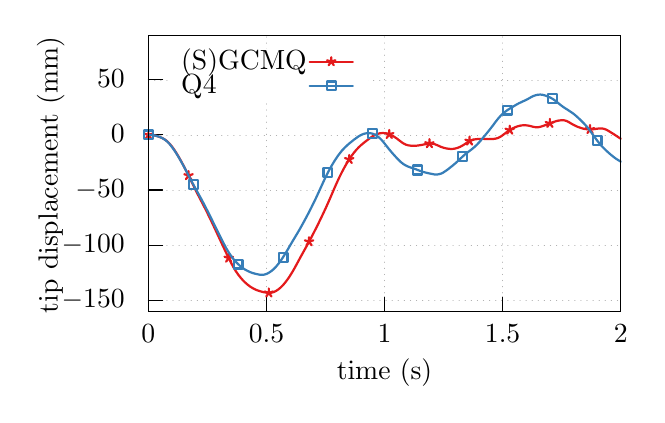
\begin{tikzpicture}[gnuplot]
%% generated with GNUPLOT 5.2p6 (Lua 5.3; terminal rev. Nov 2018, script rev. 107)
%% 06/16/2019 00:11:24
\path (0.000,0.000) rectangle (6.000,3.500);
\gpcolor{color=gp lt color axes}
\gpsetlinetype{gp lt axes}
\gpsetdashtype{gp dt axes}
\gpsetlinewidth{0.50}
\draw[gp path] (0.000,0.140)--(5.999,0.140);
\gpcolor{color=gp lt color border}
\gpsetlinetype{gp lt border}
\gpsetdashtype{gp dt solid}
\gpsetlinewidth{1.00}
\draw[gp path] (0.000,0.140)--(0.180,0.140);
\node[gp node right] at (-0.184,0.140) {$-150$};
\gpcolor{color=gp lt color axes}
\gpsetlinetype{gp lt axes}
\gpsetdashtype{gp dt axes}
\gpsetlinewidth{0.50}
\draw[gp path] (0.000,0.840)--(5.999,0.840);
\gpcolor{color=gp lt color border}
\gpsetlinetype{gp lt border}
\gpsetdashtype{gp dt solid}
\gpsetlinewidth{1.00}
\draw[gp path] (0.000,0.840)--(0.180,0.840);
\node[gp node right] at (-0.184,0.840) {$-100$};
\gpcolor{color=gp lt color axes}
\gpsetlinetype{gp lt axes}
\gpsetdashtype{gp dt axes}
\gpsetlinewidth{0.50}
\draw[gp path] (0.000,1.540)--(5.999,1.540);
\gpcolor{color=gp lt color border}
\gpsetlinetype{gp lt border}
\gpsetdashtype{gp dt solid}
\gpsetlinewidth{1.00}
\draw[gp path] (0.000,1.540)--(0.180,1.540);
\node[gp node right] at (-0.184,1.540) {$-50$};
\gpcolor{color=gp lt color axes}
\gpsetlinetype{gp lt axes}
\gpsetdashtype{gp dt axes}
\gpsetlinewidth{0.50}
\draw[gp path] (0.000,2.239)--(5.999,2.239);
\gpcolor{color=gp lt color border}
\gpsetlinetype{gp lt border}
\gpsetdashtype{gp dt solid}
\gpsetlinewidth{1.00}
\draw[gp path] (0.000,2.239)--(0.180,2.239);
\node[gp node right] at (-0.184,2.239) {$0$};
\gpcolor{color=gp lt color axes}
\gpsetlinetype{gp lt axes}
\gpsetdashtype{gp dt axes}
\gpsetlinewidth{0.50}
\draw[gp path] (0.000,2.939)--(0.300,2.939);
\draw[gp path] (2.780,2.939)--(5.999,2.939);
\gpcolor{color=gp lt color border}
\gpsetlinetype{gp lt border}
\gpsetdashtype{gp dt solid}
\gpsetlinewidth{1.00}
\draw[gp path] (0.000,2.939)--(0.180,2.939);
\node[gp node right] at (-0.184,2.939) {$50$};
\gpcolor{color=gp lt color axes}
\gpsetlinetype{gp lt axes}
\gpsetdashtype{gp dt axes}
\gpsetlinewidth{0.50}
\draw[gp path] (0.000,0.000)--(0.000,3.499);
\gpcolor{color=gp lt color border}
\gpsetlinetype{gp lt border}
\gpsetdashtype{gp dt solid}
\gpsetlinewidth{1.00}
\draw[gp path] (0.000,0.000)--(0.000,0.180);
\node[gp node center] at (0.000,-0.308) {$0$};
\gpcolor{color=gp lt color axes}
\gpsetlinetype{gp lt axes}
\gpsetdashtype{gp dt axes}
\gpsetlinewidth{0.50}
\draw[gp path] (1.500,0.000)--(1.500,2.708);
\draw[gp path] (1.500,3.324)--(1.500,3.499);
\gpcolor{color=gp lt color border}
\gpsetlinetype{gp lt border}
\gpsetdashtype{gp dt solid}
\gpsetlinewidth{1.00}
\draw[gp path] (1.500,0.000)--(1.500,0.180);
\node[gp node center] at (1.500,-0.308) {$0.5$};
\gpcolor{color=gp lt color axes}
\gpsetlinetype{gp lt axes}
\gpsetdashtype{gp dt axes}
\gpsetlinewidth{0.50}
\draw[gp path] (3.000,0.000)--(3.000,3.499);
\gpcolor{color=gp lt color border}
\gpsetlinetype{gp lt border}
\gpsetdashtype{gp dt solid}
\gpsetlinewidth{1.00}
\draw[gp path] (3.000,0.000)--(3.000,0.180);
\node[gp node center] at (3.000,-0.308) {$1$};
\gpcolor{color=gp lt color axes}
\gpsetlinetype{gp lt axes}
\gpsetdashtype{gp dt axes}
\gpsetlinewidth{0.50}
\draw[gp path] (4.499,0.000)--(4.499,3.499);
\gpcolor{color=gp lt color border}
\gpsetlinetype{gp lt border}
\gpsetdashtype{gp dt solid}
\gpsetlinewidth{1.00}
\draw[gp path] (4.499,0.000)--(4.499,0.180);
\node[gp node center] at (4.499,-0.308) {$1.5$};
\gpcolor{color=gp lt color axes}
\gpsetlinetype{gp lt axes}
\gpsetdashtype{gp dt axes}
\gpsetlinewidth{0.50}
\draw[gp path] (5.999,0.000)--(5.999,3.499);
\gpcolor{color=gp lt color border}
\gpsetlinetype{gp lt border}
\gpsetdashtype{gp dt solid}
\gpsetlinewidth{1.00}
\draw[gp path] (5.999,0.000)--(5.999,0.180);
\node[gp node center] at (5.999,-0.308) {$2$};
\draw[gp path] (0.000,3.499)--(0.000,0.000)--(5.999,0.000)--(5.999,3.499)--cycle;
\node[gp node center,rotate=-270] at (-1.228,1.749) {tip displacement (\si{\milli\metre})};
\node[gp node center] at (2.999,-0.769) {time (\si{\second})};
\gpcolor{rgb color={0.894,0.102,0.110}}
\gpsetlinewidth{2.00}
\draw[gp path] (0.000,2.239)--(0.030,2.239)--(0.060,2.236)--(0.090,2.230)--(0.120,2.222)%
  --(0.150,2.211)--(0.180,2.197)--(0.210,2.180)--(0.240,2.157)--(0.270,2.127)--(0.300,2.091)%
  --(0.330,2.049)--(0.360,2.002)--(0.390,1.952)--(0.420,1.898)--(0.450,1.842)--(0.480,1.783)%
  --(0.510,1.723)--(0.540,1.661)--(0.570,1.600)--(0.600,1.538)--(0.630,1.479)--(0.660,1.421)%
  --(0.690,1.364)--(0.720,1.306)--(0.750,1.246)--(0.780,1.184)--(0.810,1.122)--(0.840,1.058)%
  --(0.870,0.994)--(0.900,0.929)--(0.930,0.865)--(0.960,0.801)--(0.990,0.737)--(1.020,0.675)%
  --(1.050,0.615)--(1.080,0.560)--(1.110,0.510)--(1.140,0.466)--(1.170,0.428)--(1.200,0.394)%
  --(1.230,0.364)--(1.260,0.338)--(1.290,0.315)--(1.320,0.296)--(1.350,0.280)--(1.380,0.267)%
  --(1.410,0.257)--(1.440,0.248)--(1.470,0.241)--(1.500,0.236)--(1.530,0.233)--(1.560,0.235)%
  --(1.590,0.243)--(1.620,0.257)--(1.650,0.277)--(1.680,0.302)--(1.710,0.332)--(1.740,0.368)%
  --(1.770,0.408)--(1.800,0.453)--(1.830,0.501)--(1.860,0.554)--(1.890,0.609)--(1.920,0.665)%
  --(1.950,0.720)--(1.980,0.774)--(2.010,0.828)--(2.040,0.883)--(2.070,0.939)--(2.100,0.997)%
  --(2.130,1.056)--(2.160,1.116)--(2.190,1.178)--(2.220,1.241)--(2.250,1.305)--(2.280,1.372)%
  --(2.310,1.440)--(2.340,1.510)--(2.370,1.580)--(2.400,1.647)--(2.430,1.711)--(2.460,1.771)%
  --(2.490,1.827)--(2.520,1.880)--(2.550,1.928)--(2.580,1.973)--(2.610,2.013)--(2.640,2.049)%
  --(2.670,2.081)--(2.700,2.109)--(2.730,2.134)--(2.760,2.158)--(2.790,2.181)--(2.820,2.203)%
  --(2.850,2.223)--(2.880,2.240)--(2.910,2.252)--(2.940,2.260)--(2.970,2.263)--(3.000,2.262)%
  --(3.029,2.256)--(3.059,2.246)--(3.089,2.233)--(3.119,2.218)--(3.149,2.198)--(3.179,2.175)%
  --(3.209,2.152)--(3.239,2.131)--(3.269,2.116)--(3.299,2.107)--(3.329,2.103)--(3.359,2.101)%
  --(3.389,2.101)--(3.419,2.104)--(3.449,2.109)--(3.479,2.114)--(3.509,2.120)--(3.539,2.125)%
  --(3.569,2.129)--(3.599,2.129)--(3.629,2.124)--(3.659,2.113)--(3.689,2.100)--(3.719,2.086)%
  --(3.749,2.076)--(3.779,2.069)--(3.809,2.064)--(3.839,2.061)--(3.869,2.062)--(3.899,2.067)%
  --(3.929,2.076)--(3.959,2.088)--(3.989,2.104)--(4.019,2.123)--(4.049,2.144)--(4.079,2.162)%
  --(4.109,2.175)--(4.139,2.182)--(4.169,2.186)--(4.199,2.188)--(4.229,2.189)--(4.259,2.189)%
  --(4.289,2.187)--(4.319,2.186)--(4.349,2.187)--(4.379,2.188)--(4.409,2.192)--(4.439,2.200)%
  --(4.469,2.215)--(4.499,2.235)--(4.529,2.258)--(4.559,2.281)--(4.589,2.301)--(4.619,2.319)%
  --(4.649,2.333)--(4.679,2.345)--(4.709,2.354)--(4.739,2.360)--(4.769,2.362)--(4.799,2.361)%
  --(4.829,2.357)--(4.859,2.350)--(4.889,2.342)--(4.919,2.337)--(4.949,2.337)--(4.979,2.343)%
  --(5.009,2.352)--(5.039,2.363)--(5.069,2.374)--(5.099,2.386)--(5.129,2.397)--(5.159,2.408)%
  --(5.189,2.417)--(5.219,2.423)--(5.249,2.426)--(5.279,2.425)--(5.309,2.417)--(5.339,2.402)%
  --(5.369,2.384)--(5.399,2.367)--(5.429,2.352)--(5.459,2.339)--(5.489,2.329)--(5.519,2.320)%
  --(5.549,2.314)--(5.579,2.310)--(5.609,2.309)--(5.639,2.310)--(5.669,2.314)--(5.699,2.318)%
  --(5.729,2.322)--(5.759,2.322)--(5.789,2.316)--(5.819,2.304)--(5.849,2.287)--(5.879,2.268)%
  --(5.909,2.250)--(5.939,2.230)--(5.969,2.210)--(5.999,2.191);
\gpsetpointsize{4.00}
\gppoint{gp mark 3}{(0.000,2.239)}
\gppoint{gp mark 3}{(0.510,1.723)}
\gppoint{gp mark 3}{(1.020,0.675)}
\gppoint{gp mark 3}{(1.530,0.233)}
\gppoint{gp mark 3}{(2.040,0.883)}
\gppoint{gp mark 3}{(2.550,1.928)}
\gppoint{gp mark 3}{(3.059,2.246)}
\gppoint{gp mark 3}{(3.569,2.129)}
\gppoint{gp mark 3}{(4.079,2.162)}
\gppoint{gp mark 3}{(4.589,2.301)}
\gppoint{gp mark 3}{(5.099,2.386)}
\gppoint{gp mark 3}{(5.609,2.309)}
\gpcolor{rgb color={0.216,0.494,0.722}}
\draw[gp path] (0.000,2.239)--(0.030,2.239)--(0.060,2.236)--(0.090,2.230)--(0.120,2.222)%
  --(0.150,2.211)--(0.180,2.197)--(0.210,2.179)--(0.240,2.154)--(0.270,2.123)--(0.300,2.085)%
  --(0.330,2.043)--(0.360,1.997)--(0.390,1.947)--(0.420,1.894)--(0.450,1.840)--(0.480,1.783)%
  --(0.510,1.725)--(0.540,1.667)--(0.570,1.610)--(0.600,1.555)--(0.630,1.501)--(0.660,1.447)%
  --(0.690,1.391)--(0.720,1.334)--(0.750,1.275)--(0.780,1.216)--(0.810,1.155)--(0.840,1.094)%
  --(0.870,1.033)--(0.900,0.973)--(0.930,0.913)--(0.960,0.854)--(0.990,0.798)--(1.020,0.747)%
  --(1.050,0.702)--(1.080,0.663)--(1.110,0.628)--(1.140,0.598)--(1.170,0.571)--(1.200,0.548)%
  --(1.230,0.528)--(1.260,0.512)--(1.290,0.498)--(1.320,0.487)--(1.350,0.478)--(1.380,0.471)%
  --(1.410,0.465)--(1.440,0.462)--(1.470,0.465)--(1.500,0.474)--(1.530,0.489)--(1.560,0.509)%
  --(1.590,0.534)--(1.620,0.565)--(1.650,0.601)--(1.680,0.641)--(1.710,0.686)--(1.740,0.734)%
  --(1.770,0.784)--(1.800,0.836)--(1.830,0.887)--(1.860,0.937)--(1.890,0.987)--(1.920,1.038)%
  --(1.950,1.092)--(1.980,1.146)--(2.010,1.202)--(2.040,1.259)--(2.070,1.318)--(2.100,1.379)%
  --(2.130,1.441)--(2.160,1.506)--(2.190,1.572)--(2.220,1.638)--(2.250,1.702)--(2.280,1.762)%
  --(2.310,1.818)--(2.340,1.870)--(2.370,1.919)--(2.400,1.964)--(2.430,2.005)--(2.460,2.042)%
  --(2.490,2.074)--(2.520,2.103)--(2.550,2.130)--(2.580,2.154)--(2.610,2.178)--(2.640,2.200)%
  --(2.670,2.221)--(2.700,2.238)--(2.730,2.251)--(2.760,2.259)--(2.790,2.262)--(2.820,2.261)%
  --(2.850,2.254)--(2.880,2.241)--(2.910,2.222)--(2.940,2.197)--(2.970,2.166)--(3.000,2.130)%
  --(3.029,2.092)--(3.059,2.055)--(3.089,2.019)--(3.119,1.985)--(3.149,1.952)--(3.179,1.921)%
  --(3.209,1.892)--(3.239,1.869)--(3.269,1.851)--(3.299,1.837)--(3.329,1.826)--(3.359,1.816)%
  --(3.389,1.806)--(3.419,1.794)--(3.449,1.783)--(3.479,1.772)--(3.509,1.764)--(3.539,1.757)%
  --(3.569,1.750)--(3.599,1.744)--(3.629,1.738)--(3.659,1.736)--(3.689,1.740)--(3.719,1.749)%
  --(3.749,1.764)--(3.779,1.784)--(3.809,1.806)--(3.839,1.830)--(3.869,1.854)--(3.899,1.879)%
  --(3.929,1.906)--(3.959,1.935)--(3.989,1.963)--(4.019,1.990)--(4.049,2.014)--(4.079,2.036)%
  --(4.109,2.059)--(4.139,2.084)--(4.169,2.112)--(4.199,2.143)--(4.229,2.178)--(4.259,2.214)%
  --(4.289,2.250)--(4.319,2.287)--(4.349,2.325)--(4.379,2.364)--(4.409,2.405)--(4.439,2.443)%
  --(4.469,2.478)--(4.499,2.507)--(4.529,2.532)--(4.559,2.554)--(4.589,2.573)--(4.619,2.591)%
  --(4.649,2.609)--(4.679,2.627)--(4.709,2.643)--(4.739,2.657)--(4.769,2.671)--(4.799,2.685)%
  --(4.829,2.701)--(4.859,2.718)--(4.889,2.733)--(4.919,2.744)--(4.949,2.750)--(4.979,2.752)%
  --(5.009,2.748)--(5.039,2.740)--(5.069,2.729)--(5.099,2.716)--(5.129,2.700)--(5.159,2.680)%
  --(5.189,2.657)--(5.219,2.632)--(5.249,2.609)--(5.279,2.587)--(5.309,2.568)--(5.339,2.549)%
  --(5.369,2.529)--(5.399,2.508)--(5.429,2.483)--(5.459,2.456)--(5.489,2.428)--(5.519,2.398)%
  --(5.549,2.366)--(5.579,2.332)--(5.609,2.293)--(5.639,2.251)--(5.669,2.209)--(5.699,2.168)%
  --(5.729,2.130)--(5.759,2.096)--(5.789,2.065)--(5.819,2.036)--(5.849,2.009)--(5.879,1.983)%
  --(5.909,1.959)--(5.939,1.937)--(5.969,1.918)--(5.999,1.900);
\gppoint{gp mark 4}{(0.000,2.239)}
\gppoint{gp mark 4}{(0.570,1.610)}
\gppoint{gp mark 4}{(1.140,0.598)}
\gppoint{gp mark 4}{(1.710,0.686)}
\gppoint{gp mark 4}{(2.280,1.762)}
\gppoint{gp mark 4}{(2.850,2.254)}
\gppoint{gp mark 4}{(3.419,1.794)}
\gppoint{gp mark 4}{(3.989,1.963)}
\gppoint{gp mark 4}{(4.559,2.554)}
\gppoint{gp mark 4}{(5.129,2.700)}
\gppoint{gp mark 4}{(5.699,2.168)}
\gpfill{color=gpbgfillcolor} (0.300,2.708)--(2.780,2.708)--(2.780,3.324)--(0.300,3.324)--cycle;
\gpcolor{color=gp lt color border}
\node[gp node left] at (0.300,3.170) {(S)GCMQ};
\gpcolor{rgb color={0.894,0.102,0.110}}
\draw[gp path] (2.048,3.170)--(2.596,3.170);
\gppoint{gp mark 3}{(2.322,3.170)}
\gpcolor{color=gp lt color border}
\node[gp node left] at (0.300,2.862) {Q4};
\gpcolor{rgb color={0.216,0.494,0.722}}
\draw[gp path] (2.048,2.862)--(2.596,2.862);
\gppoint{gp mark 4}{(2.322,2.862)}
\gpcolor{color=gp lt color border}
\gpsetlinewidth{1.00}
\draw[gp path] (0.000,3.499)--(0.000,0.000)--(5.999,0.000)--(5.999,3.499)--cycle;
%% coordinates of the plot area
\gpdefrectangularnode{gp plot 1}{\pgfpoint{0.000cm}{0.000cm}}{\pgfpoint{5.999cm}{3.499cm}}
\end{tikzpicture}
%% gnuplot variables

\caption{with \numproduct{2x8} elements}
\end{subfigure}
\caption{linear dynamic analysis of the undamped cantilever beam subjected to a rectangular pulse}\label{fig:cantilever_disp}
\end{figure}
All versions of GCMQ and SGCMQ show little difference in each case, so only one record, denoted as (S)GCMQ, is shown for the sake of clearness.

Due to the overstiff nature, models with Q4 elements show shorter periods and smaller maximum tip displacements compared to models with (S)GCMQ elements. With mesh refinements, less stiff response can be recovered by Q4 elements. However, even with a \numproduct{2x8} mesh, the computed first mode period is still smaller than that of (S)GCMQ elements, which indicates that the numerical model is still too stiff. It can be predicted that a much denser mesh is required for Q4 elements to produce an equivalently accurate response. However, the difference among models with (S)GCMQ elements does not vary much. In particular, even with only one element defined, the error of response in forced vibration phase is not significant. (S)GCMQ is able to perform well in terms of linear dynamic analysis with the most coarse meshes.

Meanwhile, given the fact that different numerical integration schemes have no significant impact on the predicted linear displacement history, the simplified GCMQ with the five-point integration scheme (SGCMQI) element appears to be a better option as the computational cost of which is minimized.
\subsection{Nonlinear Analysis}
To avoid any mesh objectivity issues, here a linear isotropic hardening von Mises material is used for the nonlinear analysis. The yielding stress is chosen to be \SI{80}{\mega\pascal} as the maximum stress observed in the previous linear analysis is about \SI{100}{\mega\pascal}.

\begin{figure}[htb]
\centering\scriptsize
\begin{subfigure}{.49\textwidth}\centering
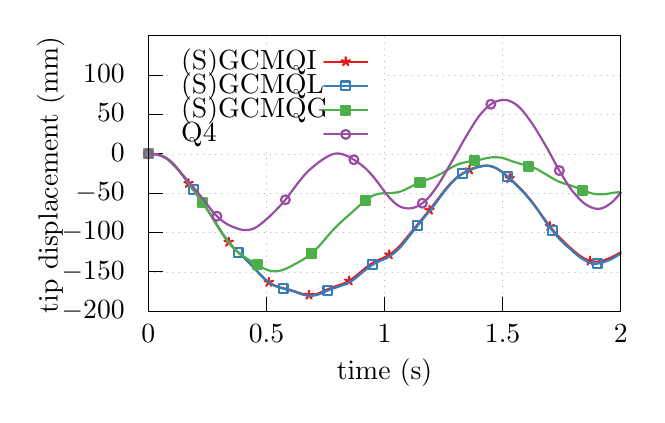
\begin{tikzpicture}[gnuplot]
%% generated with GNUPLOT 5.2p6 (Lua 5.3; terminal rev. Nov 2018, script rev. 107)
%% 05/12/2019 06:57:29
\path (0.000,0.000) rectangle (6.000,3.500);
\gpcolor{color=gp lt color axes}
\gpsetlinetype{gp lt axes}
\gpsetdashtype{gp dt axes}
\gpsetlinewidth{0.50}
\draw[gp path] (0.000,0.000)--(5.999,0.000);
\gpcolor{color=gp lt color border}
\gpsetlinetype{gp lt border}
\gpsetdashtype{gp dt solid}
\gpsetlinewidth{1.00}
\draw[gp path] (0.000,0.000)--(0.180,0.000);
\node[gp node right] at (-0.184,0.000) {$-200$};
\gpcolor{color=gp lt color axes}
\gpsetlinetype{gp lt axes}
\gpsetdashtype{gp dt axes}
\gpsetlinewidth{0.50}
\draw[gp path] (0.000,0.500)--(5.999,0.500);
\gpcolor{color=gp lt color border}
\gpsetlinetype{gp lt border}
\gpsetdashtype{gp dt solid}
\gpsetlinewidth{1.00}
\draw[gp path] (0.000,0.500)--(0.180,0.500);
\node[gp node right] at (-0.184,0.500) {$-150$};
\gpcolor{color=gp lt color axes}
\gpsetlinetype{gp lt axes}
\gpsetdashtype{gp dt axes}
\gpsetlinewidth{0.50}
\draw[gp path] (0.000,1.000)--(5.999,1.000);
\gpcolor{color=gp lt color border}
\gpsetlinetype{gp lt border}
\gpsetdashtype{gp dt solid}
\gpsetlinewidth{1.00}
\draw[gp path] (0.000,1.000)--(0.180,1.000);
\node[gp node right] at (-0.184,1.000) {$-100$};
\gpcolor{color=gp lt color axes}
\gpsetlinetype{gp lt axes}
\gpsetdashtype{gp dt axes}
\gpsetlinewidth{0.50}
\draw[gp path] (0.000,1.500)--(5.999,1.500);
\gpcolor{color=gp lt color border}
\gpsetlinetype{gp lt border}
\gpsetdashtype{gp dt solid}
\gpsetlinewidth{1.00}
\draw[gp path] (0.000,1.500)--(0.180,1.500);
\node[gp node right] at (-0.184,1.500) {$-50$};
\gpcolor{color=gp lt color axes}
\gpsetlinetype{gp lt axes}
\gpsetdashtype{gp dt axes}
\gpsetlinewidth{0.50}
\draw[gp path] (0.000,1.999)--(5.999,1.999);
\gpcolor{color=gp lt color border}
\gpsetlinetype{gp lt border}
\gpsetdashtype{gp dt solid}
\gpsetlinewidth{1.00}
\draw[gp path] (0.000,1.999)--(0.180,1.999);
\node[gp node right] at (-0.184,1.999) {$0$};
\gpcolor{color=gp lt color axes}
\gpsetlinetype{gp lt axes}
\gpsetdashtype{gp dt axes}
\gpsetlinewidth{0.50}
\draw[gp path] (0.000,2.499)--(0.300,2.499);
\draw[gp path] (2.964,2.499)--(5.999,2.499);
\gpcolor{color=gp lt color border}
\gpsetlinetype{gp lt border}
\gpsetdashtype{gp dt solid}
\gpsetlinewidth{1.00}
\draw[gp path] (0.000,2.499)--(0.180,2.499);
\node[gp node right] at (-0.184,2.499) {$50$};
\gpcolor{color=gp lt color axes}
\gpsetlinetype{gp lt axes}
\gpsetdashtype{gp dt axes}
\gpsetlinewidth{0.50}
\draw[gp path] (0.000,2.999)--(0.300,2.999);
\draw[gp path] (2.964,2.999)--(5.999,2.999);
\gpcolor{color=gp lt color border}
\gpsetlinetype{gp lt border}
\gpsetdashtype{gp dt solid}
\gpsetlinewidth{1.00}
\draw[gp path] (0.000,2.999)--(0.180,2.999);
\node[gp node right] at (-0.184,2.999) {$100$};
\gpcolor{color=gp lt color axes}
\gpsetlinetype{gp lt axes}
\gpsetdashtype{gp dt axes}
\gpsetlinewidth{0.50}
\draw[gp path] (0.000,0.000)--(0.000,3.499);
\gpcolor{color=gp lt color border}
\gpsetlinetype{gp lt border}
\gpsetdashtype{gp dt solid}
\gpsetlinewidth{1.00}
\draw[gp path] (0.000,0.000)--(0.000,0.180);
\node[gp node center] at (0.000,-0.308) {$0$};
\gpcolor{color=gp lt color axes}
\gpsetlinetype{gp lt axes}
\gpsetdashtype{gp dt axes}
\gpsetlinewidth{0.50}
\draw[gp path] (1.500,0.000)--(1.500,2.092);
\draw[gp path] (1.500,3.324)--(1.500,3.499);
\gpcolor{color=gp lt color border}
\gpsetlinetype{gp lt border}
\gpsetdashtype{gp dt solid}
\gpsetlinewidth{1.00}
\draw[gp path] (1.500,0.000)--(1.500,0.180);
\node[gp node center] at (1.500,-0.308) {$0.5$};
\gpcolor{color=gp lt color axes}
\gpsetlinetype{gp lt axes}
\gpsetdashtype{gp dt axes}
\gpsetlinewidth{0.50}
\draw[gp path] (3.000,0.000)--(3.000,3.499);
\gpcolor{color=gp lt color border}
\gpsetlinetype{gp lt border}
\gpsetdashtype{gp dt solid}
\gpsetlinewidth{1.00}
\draw[gp path] (3.000,0.000)--(3.000,0.180);
\node[gp node center] at (3.000,-0.308) {$1$};
\gpcolor{color=gp lt color axes}
\gpsetlinetype{gp lt axes}
\gpsetdashtype{gp dt axes}
\gpsetlinewidth{0.50}
\draw[gp path] (4.499,0.000)--(4.499,3.499);
\gpcolor{color=gp lt color border}
\gpsetlinetype{gp lt border}
\gpsetdashtype{gp dt solid}
\gpsetlinewidth{1.00}
\draw[gp path] (4.499,0.000)--(4.499,0.180);
\node[gp node center] at (4.499,-0.308) {$1.5$};
\gpcolor{color=gp lt color axes}
\gpsetlinetype{gp lt axes}
\gpsetdashtype{gp dt axes}
\gpsetlinewidth{0.50}
\draw[gp path] (5.999,0.000)--(5.999,3.499);
\gpcolor{color=gp lt color border}
\gpsetlinetype{gp lt border}
\gpsetdashtype{gp dt solid}
\gpsetlinewidth{1.00}
\draw[gp path] (5.999,0.000)--(5.999,0.180);
\node[gp node center] at (5.999,-0.308) {$2$};
\draw[gp path] (0.000,3.499)--(0.000,0.000)--(5.999,0.000)--(5.999,3.499)--cycle;
\node[gp node center,rotate=-270] at (-1.228,1.749) {tip displacement (\si{\milli\metre})};
\node[gp node center] at (2.999,-0.769) {time (\si{\second})};
\gpcolor{rgb color={0.894,0.102,0.110}}
\gpsetlinewidth{2.00}
\draw[gp path] (0.000,1.999)--(0.030,1.999)--(0.060,1.997)--(0.090,1.993)--(0.120,1.988)%
  --(0.150,1.980)--(0.180,1.970)--(0.210,1.955)--(0.240,1.936)--(0.270,1.913)--(0.300,1.886)%
  --(0.330,1.855)--(0.360,1.822)--(0.390,1.786)--(0.420,1.747)--(0.450,1.707)--(0.480,1.665)%
  --(0.510,1.624)--(0.540,1.583)--(0.570,1.543)--(0.600,1.503)--(0.630,1.462)--(0.660,1.420)%
  --(0.690,1.377)--(0.720,1.333)--(0.750,1.288)--(0.780,1.242)--(0.810,1.194)--(0.840,1.146)%
  --(0.870,1.096)--(0.900,1.048)--(0.930,1.001)--(0.960,0.957)--(0.990,0.916)--(1.020,0.878)%
  --(1.050,0.843)--(1.080,0.809)--(1.110,0.778)--(1.140,0.749)--(1.170,0.722)--(1.200,0.695)%
  --(1.230,0.666)--(1.260,0.636)--(1.290,0.605)--(1.320,0.573)--(1.350,0.541)--(1.380,0.509)%
  --(1.410,0.477)--(1.440,0.447)--(1.470,0.417)--(1.500,0.391)--(1.530,0.368)--(1.560,0.349)%
  --(1.590,0.333)--(1.620,0.320)--(1.650,0.310)--(1.680,0.301)--(1.710,0.293)--(1.740,0.285)%
  --(1.770,0.278)--(1.800,0.271)--(1.830,0.262)--(1.860,0.252)--(1.890,0.241)--(1.920,0.230)%
  --(1.950,0.221)--(1.980,0.213)--(2.010,0.208)--(2.040,0.206)--(2.070,0.206)--(2.100,0.209)%
  --(2.130,0.216)--(2.160,0.226)--(2.190,0.238)--(2.220,0.252)--(2.250,0.266)--(2.280,0.279)%
  --(2.310,0.291)--(2.340,0.302)--(2.370,0.313)--(2.400,0.324)--(2.430,0.334)--(2.460,0.344)%
  --(2.490,0.356)--(2.520,0.369)--(2.550,0.385)--(2.580,0.405)--(2.610,0.427)--(2.640,0.451)%
  --(2.670,0.476)--(2.700,0.501)--(2.730,0.526)--(2.760,0.551)--(2.790,0.574)--(2.820,0.596)%
  --(2.850,0.614)--(2.880,0.630)--(2.910,0.644)--(2.940,0.658)--(2.970,0.671)--(3.000,0.685)%
  --(3.029,0.700)--(3.059,0.717)--(3.089,0.738)--(3.119,0.760)--(3.149,0.786)--(3.179,0.815)%
  --(3.209,0.847)--(3.239,0.882)--(3.269,0.918)--(3.299,0.954)--(3.329,0.991)--(3.359,1.028)%
  --(3.389,1.065)--(3.419,1.102)--(3.449,1.139)--(3.479,1.175)--(3.509,1.211)--(3.539,1.247)%
  --(3.569,1.284)--(3.599,1.322)--(3.629,1.361)--(3.659,1.401)--(3.689,1.440)--(3.719,1.479)%
  --(3.749,1.518)--(3.779,1.555)--(3.809,1.591)--(3.839,1.624)--(3.869,1.655)--(3.899,1.683)%
  --(3.929,1.708)--(3.959,1.729)--(3.989,1.749)--(4.019,1.766)--(4.049,1.782)--(4.079,1.796)%
  --(4.109,1.809)--(4.139,1.820)--(4.169,1.830)--(4.199,1.838)--(4.229,1.845)--(4.259,1.849)%
  --(4.289,1.850)--(4.319,1.848)--(4.349,1.842)--(4.379,1.833)--(4.409,1.820)--(4.439,1.804)%
  --(4.469,1.785)--(4.499,1.763)--(4.529,1.739)--(4.559,1.713)--(4.589,1.687)--(4.619,1.659)%
  --(4.649,1.632)--(4.679,1.603)--(4.709,1.574)--(4.739,1.543)--(4.769,1.511)--(4.799,1.477)%
  --(4.829,1.442)--(4.859,1.406)--(4.889,1.367)--(4.919,1.326)--(4.949,1.284)--(4.979,1.242)%
  --(5.009,1.199)--(5.039,1.158)--(5.069,1.117)--(5.099,1.078)--(5.129,1.040)--(5.159,1.004)%
  --(5.189,0.970)--(5.219,0.938)--(5.249,0.908)--(5.279,0.878)--(5.309,0.850)--(5.339,0.822)%
  --(5.369,0.795)--(5.399,0.768)--(5.429,0.744)--(5.459,0.720)--(5.489,0.698)--(5.519,0.679)%
  --(5.549,0.662)--(5.579,0.648)--(5.609,0.638)--(5.639,0.632)--(5.669,0.630)--(5.699,0.630)%
  --(5.729,0.634)--(5.759,0.640)--(5.789,0.648)--(5.819,0.659)--(5.849,0.671)--(5.879,0.684)%
  --(5.909,0.699)--(5.939,0.714)--(5.969,0.731)--(5.999,0.750);
\gpsetpointsize{4.00}
\gppoint{gp mark 3}{(0.000,1.999)}
\gppoint{gp mark 3}{(0.510,1.624)}
\gppoint{gp mark 3}{(1.020,0.878)}
\gppoint{gp mark 3}{(1.530,0.368)}
\gppoint{gp mark 3}{(2.040,0.206)}
\gppoint{gp mark 3}{(2.550,0.385)}
\gppoint{gp mark 3}{(3.059,0.717)}
\gppoint{gp mark 3}{(3.569,1.284)}
\gppoint{gp mark 3}{(4.079,1.796)}
\gppoint{gp mark 3}{(4.589,1.687)}
\gppoint{gp mark 3}{(5.099,1.078)}
\gppoint{gp mark 3}{(5.609,0.638)}
\gpcolor{rgb color={0.216,0.494,0.722}}
\draw[gp path] (0.000,1.999)--(0.030,1.999)--(0.060,1.997)--(0.090,1.993)--(0.120,1.988)%
  --(0.150,1.980)--(0.180,1.969)--(0.210,1.955)--(0.240,1.937)--(0.270,1.913)--(0.300,1.886)%
  --(0.330,1.856)--(0.360,1.822)--(0.390,1.786)--(0.420,1.748)--(0.450,1.707)--(0.480,1.666)%
  --(0.510,1.624)--(0.540,1.583)--(0.570,1.543)--(0.600,1.502)--(0.630,1.462)--(0.660,1.420)%
  --(0.690,1.377)--(0.720,1.333)--(0.750,1.288)--(0.780,1.242)--(0.810,1.195)--(0.840,1.146)%
  --(0.870,1.097)--(0.900,1.049)--(0.930,1.002)--(0.960,0.957)--(0.990,0.916)--(1.020,0.878)%
  --(1.050,0.843)--(1.080,0.809)--(1.110,0.778)--(1.140,0.749)--(1.170,0.721)--(1.200,0.694)%
  --(1.230,0.666)--(1.260,0.637)--(1.290,0.606)--(1.320,0.574)--(1.350,0.541)--(1.380,0.509)%
  --(1.410,0.477)--(1.440,0.447)--(1.470,0.418)--(1.500,0.391)--(1.530,0.367)--(1.560,0.346)%
  --(1.590,0.330)--(1.620,0.317)--(1.650,0.306)--(1.680,0.297)--(1.710,0.289)--(1.740,0.281)%
  --(1.770,0.273)--(1.800,0.265)--(1.830,0.257)--(1.860,0.247)--(1.890,0.237)--(1.920,0.226)%
  --(1.950,0.215)--(1.980,0.206)--(2.010,0.200)--(2.040,0.197)--(2.070,0.196)--(2.100,0.199)%
  --(2.130,0.204)--(2.160,0.213)--(2.190,0.224)--(2.220,0.237)--(2.250,0.250)--(2.280,0.264)%
  --(2.310,0.276)--(2.340,0.287)--(2.370,0.297)--(2.400,0.307)--(2.430,0.317)--(2.460,0.328)%
  --(2.490,0.339)--(2.520,0.352)--(2.550,0.366)--(2.580,0.384)--(2.610,0.405)--(2.640,0.428)%
  --(2.670,0.453)--(2.700,0.478)--(2.730,0.503)--(2.760,0.527)--(2.790,0.551)--(2.820,0.573)%
  --(2.850,0.592)--(2.880,0.610)--(2.910,0.625)--(2.940,0.638)--(2.970,0.651)--(3.000,0.664)%
  --(3.029,0.678)--(3.059,0.696)--(3.089,0.716)--(3.119,0.738)--(3.149,0.764)--(3.179,0.792)%
  --(3.209,0.824)--(3.239,0.859)--(3.269,0.897)--(3.299,0.936)--(3.329,0.974)--(3.359,1.012)%
  --(3.389,1.049)--(3.419,1.087)--(3.449,1.124)--(3.479,1.162)--(3.509,1.199)--(3.539,1.235)%
  --(3.569,1.271)--(3.599,1.308)--(3.629,1.346)--(3.659,1.386)--(3.689,1.427)--(3.719,1.468)%
  --(3.749,1.507)--(3.779,1.545)--(3.809,1.581)--(3.839,1.616)--(3.869,1.649)--(3.899,1.679)%
  --(3.929,1.705)--(3.959,1.727)--(3.989,1.746)--(4.019,1.763)--(4.049,1.778)--(4.079,1.793)%
  --(4.109,1.805)--(4.139,1.816)--(4.169,1.825)--(4.199,1.833)--(4.229,1.839)--(4.259,1.844)%
  --(4.289,1.847)--(4.319,1.847)--(4.349,1.842)--(4.379,1.833)--(4.409,1.820)--(4.439,1.804)%
  --(4.469,1.785)--(4.499,1.764)--(4.529,1.740)--(4.559,1.713)--(4.589,1.684)--(4.619,1.654)%
  --(4.649,1.625)--(4.679,1.596)--(4.709,1.567)--(4.739,1.536)--(4.769,1.504)--(4.799,1.470)%
  --(4.829,1.435)--(4.859,1.398)--(4.889,1.361)--(4.919,1.321)--(4.949,1.280)--(4.979,1.236)%
  --(5.009,1.191)--(5.039,1.147)--(5.069,1.104)--(5.099,1.064)--(5.129,1.026)--(5.159,0.989)%
  --(5.189,0.953)--(5.219,0.919)--(5.249,0.888)--(5.279,0.859)--(5.309,0.832)--(5.339,0.806)%
  --(5.369,0.780)--(5.399,0.753)--(5.429,0.727)--(5.459,0.702)--(5.489,0.680)--(5.519,0.660)%
  --(5.549,0.643)--(5.579,0.628)--(5.609,0.616)--(5.639,0.607)--(5.669,0.603)--(5.699,0.604)%
  --(5.729,0.609)--(5.759,0.616)--(5.789,0.625)--(5.819,0.636)--(5.849,0.648)--(5.879,0.662)%
  --(5.909,0.678)--(5.939,0.696)--(5.969,0.714)--(5.999,0.732);
\gppoint{gp mark 4}{(0.000,1.999)}
\gppoint{gp mark 4}{(0.570,1.543)}
\gppoint{gp mark 4}{(1.140,0.749)}
\gppoint{gp mark 4}{(1.710,0.289)}
\gppoint{gp mark 4}{(2.280,0.264)}
\gppoint{gp mark 4}{(2.850,0.592)}
\gppoint{gp mark 4}{(3.419,1.087)}
\gppoint{gp mark 4}{(3.989,1.746)}
\gppoint{gp mark 4}{(4.559,1.713)}
\gppoint{gp mark 4}{(5.129,1.026)}
\gppoint{gp mark 4}{(5.699,0.604)}
\gpcolor{rgb color={0.302,0.686,0.290}}
\draw[gp path] (0.000,1.999)--(0.030,1.999)--(0.060,1.997)--(0.090,1.993)--(0.120,1.988)%
  --(0.150,1.980)--(0.180,1.969)--(0.210,1.955)--(0.240,1.937)--(0.270,1.913)--(0.300,1.886)%
  --(0.330,1.856)--(0.360,1.822)--(0.390,1.786)--(0.420,1.747)--(0.450,1.707)--(0.480,1.666)%
  --(0.510,1.624)--(0.540,1.583)--(0.570,1.543)--(0.600,1.503)--(0.630,1.462)--(0.660,1.420)%
  --(0.690,1.377)--(0.720,1.333)--(0.750,1.288)--(0.780,1.242)--(0.810,1.195)--(0.840,1.146)%
  --(0.870,1.097)--(0.900,1.048)--(0.930,1.001)--(0.960,0.956)--(0.990,0.914)--(1.020,0.875)%
  --(1.050,0.839)--(1.080,0.805)--(1.110,0.775)--(1.140,0.748)--(1.170,0.724)--(1.200,0.702)%
  --(1.230,0.683)--(1.260,0.663)--(1.290,0.644)--(1.320,0.625)--(1.350,0.607)--(1.380,0.590)%
  --(1.410,0.573)--(1.440,0.557)--(1.470,0.542)--(1.500,0.529)--(1.530,0.518)--(1.560,0.511)%
  --(1.590,0.508)--(1.620,0.508)--(1.650,0.511)--(1.680,0.517)--(1.710,0.526)--(1.740,0.538)%
  --(1.770,0.551)--(1.800,0.566)--(1.830,0.582)--(1.860,0.598)--(1.890,0.614)--(1.920,0.631)%
  --(1.950,0.648)--(1.980,0.666)--(2.010,0.687)--(2.040,0.709)--(2.070,0.733)--(2.100,0.759)%
  --(2.130,0.788)--(2.160,0.819)--(2.190,0.853)--(2.220,0.888)--(2.250,0.923)--(2.280,0.958)%
  --(2.310,0.993)--(2.340,1.026)--(2.370,1.058)--(2.400,1.088)--(2.430,1.118)--(2.460,1.145)%
  --(2.490,1.172)--(2.520,1.198)--(2.550,1.224)--(2.580,1.251)--(2.610,1.278)--(2.640,1.306)%
  --(2.670,1.333)--(2.700,1.359)--(2.730,1.385)--(2.760,1.408)--(2.790,1.431)--(2.820,1.450)%
  --(2.850,1.466)--(2.880,1.479)--(2.910,1.488)--(2.940,1.494)--(2.970,1.497)--(3.000,1.499)%
  --(3.029,1.500)--(3.059,1.500)--(3.089,1.502)--(3.119,1.504)--(3.149,1.508)--(3.179,1.514)%
  --(3.209,1.523)--(3.239,1.535)--(3.269,1.549)--(3.299,1.564)--(3.329,1.579)--(3.359,1.594)%
  --(3.389,1.609)--(3.419,1.623)--(3.449,1.637)--(3.479,1.650)--(3.509,1.662)--(3.539,1.672)%
  --(3.569,1.682)--(3.599,1.693)--(3.629,1.705)--(3.659,1.718)--(3.689,1.733)--(3.719,1.749)%
  --(3.749,1.766)--(3.779,1.783)--(3.809,1.801)--(3.839,1.819)--(3.869,1.836)--(3.899,1.852)%
  --(3.929,1.865)--(3.959,1.875)--(3.989,1.884)--(4.019,1.891)--(4.049,1.897)--(4.079,1.903)%
  --(4.109,1.908)--(4.139,1.912)--(4.169,1.917)--(4.199,1.922)--(4.229,1.929)--(4.259,1.936)%
  --(4.289,1.943)--(4.319,1.949)--(4.349,1.953)--(4.379,1.956)--(4.409,1.956)--(4.439,1.955)%
  --(4.469,1.951)--(4.499,1.946)--(4.529,1.937)--(4.559,1.927)--(4.589,1.916)--(4.619,1.905)%
  --(4.649,1.895)--(4.679,1.886)--(4.709,1.877)--(4.739,1.868)--(4.769,1.860)--(4.799,1.851)%
  --(4.829,1.843)--(4.859,1.834)--(4.889,1.824)--(4.919,1.812)--(4.949,1.797)--(4.979,1.780)%
  --(5.009,1.762)--(5.039,1.744)--(5.069,1.726)--(5.099,1.708)--(5.129,1.690)--(5.159,1.673)%
  --(5.189,1.657)--(5.219,1.644)--(5.249,1.633)--(5.279,1.623)--(5.309,1.614)--(5.339,1.605)%
  --(5.369,1.595)--(5.399,1.584)--(5.429,1.574)--(5.459,1.563)--(5.489,1.551)--(5.519,1.539)%
  --(5.549,1.526)--(5.579,1.514)--(5.609,1.503)--(5.639,1.495)--(5.669,1.489)--(5.699,1.486)%
  --(5.729,1.485)--(5.759,1.485)--(5.789,1.487)--(5.819,1.490)--(5.849,1.495)--(5.879,1.500)%
  --(5.909,1.505)--(5.939,1.509)--(5.969,1.511)--(5.999,1.513);
\gppoint{gp mark 5}{(0.000,1.999)}
\gppoint{gp mark 5}{(0.690,1.377)}
\gppoint{gp mark 5}{(1.380,0.590)}
\gppoint{gp mark 5}{(2.070,0.733)}
\gppoint{gp mark 5}{(2.760,1.408)}
\gppoint{gp mark 5}{(3.449,1.637)}
\gppoint{gp mark 5}{(4.139,1.912)}
\gppoint{gp mark 5}{(4.829,1.843)}
\gppoint{gp mark 5}{(5.519,1.539)}
\gpcolor{rgb color={0.596,0.306,0.639}}
\draw[gp path] (0.000,1.999)--(0.030,1.999)--(0.060,1.997)--(0.090,1.993)--(0.120,1.987)%
  --(0.150,1.979)--(0.180,1.968)--(0.210,1.952)--(0.240,1.932)--(0.270,1.908)--(0.300,1.880)%
  --(0.330,1.850)--(0.360,1.818)--(0.390,1.784)--(0.420,1.749)--(0.450,1.714)--(0.480,1.679)%
  --(0.510,1.645)--(0.540,1.611)--(0.570,1.577)--(0.600,1.541)--(0.630,1.505)--(0.660,1.467)%
  --(0.690,1.429)--(0.720,1.391)--(0.750,1.351)--(0.780,1.312)--(0.810,1.274)--(0.840,1.239)%
  --(0.870,1.207)--(0.900,1.179)--(0.930,1.154)--(0.960,1.132)--(0.990,1.112)--(1.020,1.096)%
  --(1.050,1.081)--(1.080,1.069)--(1.110,1.058)--(1.140,1.047)--(1.170,1.038)--(1.200,1.032)%
  --(1.230,1.030)--(1.260,1.031)--(1.290,1.036)--(1.320,1.044)--(1.350,1.056)--(1.380,1.073)%
  --(1.410,1.094)--(1.440,1.118)--(1.470,1.143)--(1.500,1.169)--(1.530,1.196)--(1.560,1.224)%
  --(1.590,1.254)--(1.620,1.284)--(1.650,1.315)--(1.680,1.347)--(1.710,1.380)--(1.740,1.416)%
  --(1.770,1.455)--(1.800,1.495)--(1.830,1.536)--(1.860,1.576)--(1.890,1.616)--(1.920,1.655)%
  --(1.950,1.692)--(1.980,1.728)--(2.010,1.760)--(2.040,1.789)--(2.070,1.816)--(2.100,1.841)%
  --(2.130,1.866)--(2.160,1.889)--(2.190,1.911)--(2.220,1.932)--(2.250,1.950)--(2.280,1.967)%
  --(2.310,1.982)--(2.340,1.994)--(2.370,2.001)--(2.400,2.004)--(2.430,2.001)--(2.460,1.996)%
  --(2.490,1.986)--(2.520,1.975)--(2.550,1.960)--(2.580,1.943)--(2.610,1.924)--(2.640,1.904)%
  --(2.670,1.884)--(2.700,1.862)--(2.730,1.838)--(2.760,1.812)--(2.790,1.782)--(2.820,1.750)%
  --(2.850,1.716)--(2.880,1.679)--(2.910,1.641)--(2.940,1.600)--(2.970,1.559)--(3.000,1.518)%
  --(3.029,1.480)--(3.059,1.445)--(3.089,1.414)--(3.119,1.385)--(3.149,1.359)--(3.179,1.339)%
  --(3.209,1.324)--(3.239,1.314)--(3.269,1.308)--(3.299,1.306)--(3.329,1.307)--(3.359,1.311)%
  --(3.389,1.321)--(3.419,1.335)--(3.449,1.352)--(3.479,1.372)--(3.509,1.396)--(3.539,1.423)%
  --(3.569,1.455)--(3.599,1.493)--(3.629,1.533)--(3.659,1.576)--(3.689,1.621)--(3.719,1.668)%
  --(3.749,1.718)--(3.779,1.770)--(3.809,1.823)--(3.839,1.876)--(3.869,1.928)--(3.899,1.980)%
  --(3.929,2.033)--(3.959,2.087)--(3.989,2.141)--(4.019,2.193)--(4.049,2.244)--(4.079,2.294)%
  --(4.109,2.343)--(4.139,2.391)--(4.169,2.436)--(4.199,2.478)--(4.229,2.515)--(4.259,2.548)%
  --(4.289,2.578)--(4.319,2.606)--(4.349,2.629)--(4.379,2.647)--(4.409,2.661)--(4.439,2.671)%
  --(4.469,2.679)--(4.499,2.683)--(4.529,2.684)--(4.559,2.680)--(4.589,2.670)--(4.619,2.656)%
  --(4.649,2.639)--(4.679,2.618)--(4.709,2.592)--(4.739,2.562)--(4.769,2.526)--(4.799,2.488)%
  --(4.829,2.447)--(4.859,2.405)--(4.889,2.361)--(4.919,2.315)--(4.949,2.266)--(4.979,2.215)%
  --(5.009,2.164)--(5.039,2.113)--(5.069,2.061)--(5.099,2.007)--(5.129,1.951)--(5.159,1.895)%
  --(5.189,1.840)--(5.219,1.787)--(5.249,1.736)--(5.279,1.686)--(5.309,1.637)--(5.339,1.590)%
  --(5.369,1.548)--(5.399,1.510)--(5.429,1.475)--(5.459,1.442)--(5.489,1.411)--(5.519,1.384)%
  --(5.549,1.360)--(5.579,1.341)--(5.609,1.326)--(5.639,1.314)--(5.669,1.305)--(5.699,1.300)%
  --(5.729,1.301)--(5.759,1.308)--(5.789,1.320)--(5.819,1.335)--(5.849,1.354)--(5.879,1.377)%
  --(5.909,1.404)--(5.939,1.435)--(5.969,1.470)--(5.999,1.506);
\gppoint{gp mark 6}{(0.000,1.999)}
\gppoint{gp mark 6}{(0.870,1.207)}
\gppoint{gp mark 6}{(1.740,1.416)}
\gppoint{gp mark 6}{(2.610,1.924)}
\gppoint{gp mark 6}{(3.479,1.372)}
\gppoint{gp mark 6}{(4.349,2.629)}
\gppoint{gp mark 6}{(5.219,1.787)}
\gpfill{color=gpbgfillcolor} (0.300,2.092)--(2.964,2.092)--(2.964,3.324)--(0.300,3.324)--cycle;
\gpcolor{color=gp lt color border}
\node[gp node left] at (0.300,3.170) {(S)GCMQI};
\gpcolor{rgb color={0.894,0.102,0.110}}
\draw[gp path] (2.232,3.170)--(2.780,3.170);
\gppoint{gp mark 3}{(2.506,3.170)}
\gpcolor{color=gp lt color border}
\node[gp node left] at (0.300,2.862) {(S)GCMQL};
\gpcolor{rgb color={0.216,0.494,0.722}}
\draw[gp path] (2.232,2.862)--(2.780,2.862);
\gppoint{gp mark 4}{(2.506,2.862)}
\gpcolor{color=gp lt color border}
\node[gp node left] at (0.300,2.554) {(S)GCMQG};
\gpcolor{rgb color={0.302,0.686,0.290}}
\draw[gp path] (2.232,2.554)--(2.780,2.554);
\gppoint{gp mark 5}{(2.506,2.554)}
\gpcolor{color=gp lt color border}
\node[gp node left] at (0.300,2.246) {Q4};
\gpcolor{rgb color={0.596,0.306,0.639}}
\draw[gp path] (2.232,2.246)--(2.780,2.246);
\gppoint{gp mark 6}{(2.506,2.246)}
\gpcolor{color=gp lt color border}
\gpsetlinewidth{1.00}
\draw[gp path] (0.000,3.499)--(0.000,0.000)--(5.999,0.000)--(5.999,3.499)--cycle;
%% coordinates of the plot area
\gpdefrectangularnode{gp plot 1}{\pgfpoint{0.000cm}{0.000cm}}{\pgfpoint{5.999cm}{3.499cm}}
\end{tikzpicture}
%% gnuplot variables

\caption{with \numproduct{1x4} elements}
\end{subfigure}\hfill
\begin{subfigure}{.49\textwidth}\centering
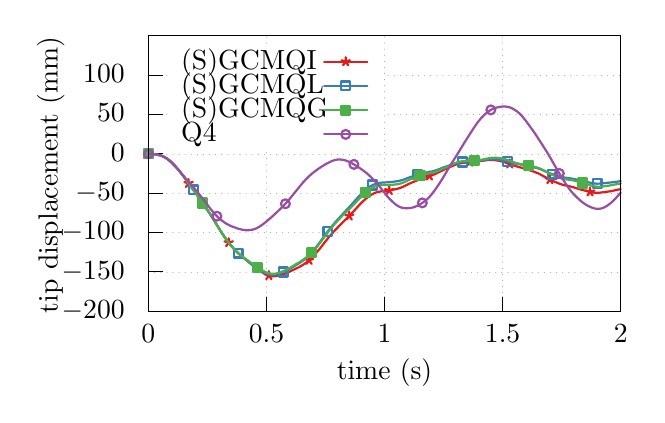
\begin{tikzpicture}[gnuplot]
%% generated with GNUPLOT 5.2p6 (Lua 5.3; terminal rev. Nov 2018, script rev. 107)
%% 05/12/2019 06:57:29
\path (0.000,0.000) rectangle (6.000,3.500);
\gpcolor{color=gp lt color axes}
\gpsetlinetype{gp lt axes}
\gpsetdashtype{gp dt axes}
\gpsetlinewidth{0.50}
\draw[gp path] (0.000,0.000)--(5.999,0.000);
\gpcolor{color=gp lt color border}
\gpsetlinetype{gp lt border}
\gpsetdashtype{gp dt solid}
\gpsetlinewidth{1.00}
\draw[gp path] (0.000,0.000)--(0.180,0.000);
\node[gp node right] at (-0.184,0.000) {$-200$};
\gpcolor{color=gp lt color axes}
\gpsetlinetype{gp lt axes}
\gpsetdashtype{gp dt axes}
\gpsetlinewidth{0.50}
\draw[gp path] (0.000,0.500)--(5.999,0.500);
\gpcolor{color=gp lt color border}
\gpsetlinetype{gp lt border}
\gpsetdashtype{gp dt solid}
\gpsetlinewidth{1.00}
\draw[gp path] (0.000,0.500)--(0.180,0.500);
\node[gp node right] at (-0.184,0.500) {$-150$};
\gpcolor{color=gp lt color axes}
\gpsetlinetype{gp lt axes}
\gpsetdashtype{gp dt axes}
\gpsetlinewidth{0.50}
\draw[gp path] (0.000,1.000)--(5.999,1.000);
\gpcolor{color=gp lt color border}
\gpsetlinetype{gp lt border}
\gpsetdashtype{gp dt solid}
\gpsetlinewidth{1.00}
\draw[gp path] (0.000,1.000)--(0.180,1.000);
\node[gp node right] at (-0.184,1.000) {$-100$};
\gpcolor{color=gp lt color axes}
\gpsetlinetype{gp lt axes}
\gpsetdashtype{gp dt axes}
\gpsetlinewidth{0.50}
\draw[gp path] (0.000,1.500)--(5.999,1.500);
\gpcolor{color=gp lt color border}
\gpsetlinetype{gp lt border}
\gpsetdashtype{gp dt solid}
\gpsetlinewidth{1.00}
\draw[gp path] (0.000,1.500)--(0.180,1.500);
\node[gp node right] at (-0.184,1.500) {$-50$};
\gpcolor{color=gp lt color axes}
\gpsetlinetype{gp lt axes}
\gpsetdashtype{gp dt axes}
\gpsetlinewidth{0.50}
\draw[gp path] (0.000,1.999)--(5.999,1.999);
\gpcolor{color=gp lt color border}
\gpsetlinetype{gp lt border}
\gpsetdashtype{gp dt solid}
\gpsetlinewidth{1.00}
\draw[gp path] (0.000,1.999)--(0.180,1.999);
\node[gp node right] at (-0.184,1.999) {$0$};
\gpcolor{color=gp lt color axes}
\gpsetlinetype{gp lt axes}
\gpsetdashtype{gp dt axes}
\gpsetlinewidth{0.50}
\draw[gp path] (0.000,2.499)--(0.300,2.499);
\draw[gp path] (2.964,2.499)--(5.999,2.499);
\gpcolor{color=gp lt color border}
\gpsetlinetype{gp lt border}
\gpsetdashtype{gp dt solid}
\gpsetlinewidth{1.00}
\draw[gp path] (0.000,2.499)--(0.180,2.499);
\node[gp node right] at (-0.184,2.499) {$50$};
\gpcolor{color=gp lt color axes}
\gpsetlinetype{gp lt axes}
\gpsetdashtype{gp dt axes}
\gpsetlinewidth{0.50}
\draw[gp path] (0.000,2.999)--(0.300,2.999);
\draw[gp path] (2.964,2.999)--(5.999,2.999);
\gpcolor{color=gp lt color border}
\gpsetlinetype{gp lt border}
\gpsetdashtype{gp dt solid}
\gpsetlinewidth{1.00}
\draw[gp path] (0.000,2.999)--(0.180,2.999);
\node[gp node right] at (-0.184,2.999) {$100$};
\gpcolor{color=gp lt color axes}
\gpsetlinetype{gp lt axes}
\gpsetdashtype{gp dt axes}
\gpsetlinewidth{0.50}
\draw[gp path] (0.000,0.000)--(0.000,3.499);
\gpcolor{color=gp lt color border}
\gpsetlinetype{gp lt border}
\gpsetdashtype{gp dt solid}
\gpsetlinewidth{1.00}
\draw[gp path] (0.000,0.000)--(0.000,0.180);
\node[gp node center] at (0.000,-0.308) {$0$};
\gpcolor{color=gp lt color axes}
\gpsetlinetype{gp lt axes}
\gpsetdashtype{gp dt axes}
\gpsetlinewidth{0.50}
\draw[gp path] (1.500,0.000)--(1.500,2.092);
\draw[gp path] (1.500,3.324)--(1.500,3.499);
\gpcolor{color=gp lt color border}
\gpsetlinetype{gp lt border}
\gpsetdashtype{gp dt solid}
\gpsetlinewidth{1.00}
\draw[gp path] (1.500,0.000)--(1.500,0.180);
\node[gp node center] at (1.500,-0.308) {$0.5$};
\gpcolor{color=gp lt color axes}
\gpsetlinetype{gp lt axes}
\gpsetdashtype{gp dt axes}
\gpsetlinewidth{0.50}
\draw[gp path] (3.000,0.000)--(3.000,3.499);
\gpcolor{color=gp lt color border}
\gpsetlinetype{gp lt border}
\gpsetdashtype{gp dt solid}
\gpsetlinewidth{1.00}
\draw[gp path] (3.000,0.000)--(3.000,0.180);
\node[gp node center] at (3.000,-0.308) {$1$};
\gpcolor{color=gp lt color axes}
\gpsetlinetype{gp lt axes}
\gpsetdashtype{gp dt axes}
\gpsetlinewidth{0.50}
\draw[gp path] (4.499,0.000)--(4.499,3.499);
\gpcolor{color=gp lt color border}
\gpsetlinetype{gp lt border}
\gpsetdashtype{gp dt solid}
\gpsetlinewidth{1.00}
\draw[gp path] (4.499,0.000)--(4.499,0.180);
\node[gp node center] at (4.499,-0.308) {$1.5$};
\gpcolor{color=gp lt color axes}
\gpsetlinetype{gp lt axes}
\gpsetdashtype{gp dt axes}
\gpsetlinewidth{0.50}
\draw[gp path] (5.999,0.000)--(5.999,3.499);
\gpcolor{color=gp lt color border}
\gpsetlinetype{gp lt border}
\gpsetdashtype{gp dt solid}
\gpsetlinewidth{1.00}
\draw[gp path] (5.999,0.000)--(5.999,0.180);
\node[gp node center] at (5.999,-0.308) {$2$};
\draw[gp path] (0.000,3.499)--(0.000,0.000)--(5.999,0.000)--(5.999,3.499)--cycle;
\node[gp node center,rotate=-270] at (-1.228,1.749) {tip displacement (\si{\milli\metre})};
\node[gp node center] at (2.999,-0.769) {time (\si{\second})};
\gpcolor{rgb color={0.894,0.102,0.110}}
\gpsetlinewidth{2.00}
\draw[gp path] (0.000,1.999)--(0.030,1.999)--(0.060,1.997)--(0.090,1.993)--(0.120,1.988)%
  --(0.150,1.980)--(0.180,1.970)--(0.210,1.956)--(0.240,1.937)--(0.270,1.914)--(0.300,1.887)%
  --(0.330,1.856)--(0.360,1.823)--(0.390,1.787)--(0.420,1.748)--(0.450,1.708)--(0.480,1.666)%
  --(0.510,1.624)--(0.540,1.582)--(0.570,1.542)--(0.600,1.501)--(0.630,1.460)--(0.660,1.418)%
  --(0.690,1.375)--(0.720,1.331)--(0.750,1.286)--(0.780,1.241)--(0.810,1.193)--(0.840,1.145)%
  --(0.870,1.096)--(0.900,1.047)--(0.930,0.999)--(0.960,0.953)--(0.990,0.910)--(1.020,0.871)%
  --(1.050,0.834)--(1.080,0.799)--(1.110,0.768)--(1.140,0.738)--(1.170,0.711)--(1.200,0.686)%
  --(1.230,0.661)--(1.260,0.637)--(1.290,0.611)--(1.320,0.586)--(1.350,0.561)--(1.380,0.538)%
  --(1.410,0.516)--(1.440,0.497)--(1.470,0.479)--(1.500,0.464)--(1.530,0.453)--(1.560,0.447)%
  --(1.590,0.445)--(1.620,0.447)--(1.650,0.452)--(1.680,0.460)--(1.710,0.469)--(1.740,0.480)%
  --(1.770,0.493)--(1.800,0.506)--(1.830,0.521)--(1.860,0.535)--(1.890,0.549)--(1.920,0.564)%
  --(1.950,0.581)--(1.980,0.600)--(2.010,0.622)--(2.040,0.647)--(2.070,0.675)--(2.100,0.706)%
  --(2.130,0.739)--(2.160,0.774)--(2.190,0.811)--(2.220,0.850)--(2.250,0.889)--(2.280,0.926)%
  --(2.310,0.962)--(2.340,0.996)--(2.370,1.028)--(2.400,1.059)--(2.430,1.090)--(2.460,1.120)%
  --(2.490,1.150)--(2.520,1.180)--(2.550,1.210)--(2.580,1.241)--(2.610,1.274)--(2.640,1.307)%
  --(2.670,1.340)--(2.700,1.372)--(2.730,1.401)--(2.760,1.427)--(2.790,1.451)--(2.820,1.472)%
  --(2.850,1.490)--(2.880,1.504)--(2.910,1.514)--(2.940,1.520)--(2.970,1.525)--(3.000,1.527)%
  --(3.029,1.530)--(3.059,1.534)--(3.089,1.540)--(3.119,1.546)--(3.149,1.552)--(3.179,1.560)%
  --(3.209,1.570)--(3.239,1.583)--(3.269,1.598)--(3.299,1.613)--(3.329,1.627)--(3.359,1.640)%
  --(3.389,1.652)--(3.419,1.664)--(3.449,1.676)--(3.479,1.688)--(3.509,1.699)--(3.539,1.709)%
  --(3.569,1.718)--(3.599,1.727)--(3.629,1.738)--(3.659,1.751)--(3.689,1.766)--(3.719,1.781)%
  --(3.749,1.795)--(3.779,1.809)--(3.809,1.822)--(3.839,1.836)--(3.869,1.849)--(3.899,1.861)%
  --(3.929,1.871)--(3.959,1.878)--(3.989,1.883)--(4.019,1.886)--(4.049,1.890)--(4.079,1.894)%
  --(4.109,1.898)--(4.139,1.901)--(4.169,1.904)--(4.199,1.906)--(4.229,1.909)--(4.259,1.913)%
  --(4.289,1.917)--(4.319,1.921)--(4.349,1.922)--(4.379,1.921)--(4.409,1.918)--(4.439,1.913)%
  --(4.469,1.907)--(4.499,1.900)--(4.529,1.892)--(4.559,1.882)--(4.589,1.871)--(4.619,1.859)%
  --(4.649,1.848)--(4.679,1.839)--(4.709,1.831)--(4.739,1.823)--(4.769,1.815)--(4.799,1.805)%
  --(4.829,1.795)--(4.859,1.785)--(4.889,1.775)--(4.919,1.764)--(4.949,1.752)--(4.979,1.737)%
  --(5.009,1.720)--(5.039,1.703)--(5.069,1.687)--(5.099,1.672)--(5.129,1.658)--(5.159,1.645)%
  --(5.189,1.633)--(5.219,1.621)--(5.249,1.610)--(5.279,1.601)--(5.309,1.595)--(5.339,1.589)%
  --(5.369,1.582)--(5.399,1.574)--(5.429,1.565)--(5.459,1.555)--(5.489,1.546)--(5.519,1.539)%
  --(5.549,1.531)--(5.579,1.524)--(5.609,1.516)--(5.639,1.510)--(5.669,1.505)--(5.699,1.504)%
  --(5.729,1.505)--(5.759,1.509)--(5.789,1.513)--(5.819,1.517)--(5.849,1.521)--(5.879,1.526)%
  --(5.909,1.532)--(5.939,1.539)--(5.969,1.545)--(5.999,1.550);
\gpsetpointsize{4.00}
\gppoint{gp mark 3}{(0.000,1.999)}
\gppoint{gp mark 3}{(0.510,1.624)}
\gppoint{gp mark 3}{(1.020,0.871)}
\gppoint{gp mark 3}{(1.530,0.453)}
\gppoint{gp mark 3}{(2.040,0.647)}
\gppoint{gp mark 3}{(2.550,1.210)}
\gppoint{gp mark 3}{(3.059,1.534)}
\gppoint{gp mark 3}{(3.569,1.718)}
\gppoint{gp mark 3}{(4.079,1.894)}
\gppoint{gp mark 3}{(4.589,1.871)}
\gppoint{gp mark 3}{(5.099,1.672)}
\gppoint{gp mark 3}{(5.609,1.516)}
\gpcolor{rgb color={0.216,0.494,0.722}}
\draw[gp path] (0.000,1.999)--(0.030,1.999)--(0.060,1.997)--(0.090,1.993)--(0.120,1.988)%
  --(0.150,1.980)--(0.180,1.970)--(0.210,1.956)--(0.240,1.937)--(0.270,1.914)--(0.300,1.887)%
  --(0.330,1.856)--(0.360,1.823)--(0.390,1.787)--(0.420,1.748)--(0.450,1.708)--(0.480,1.666)%
  --(0.510,1.624)--(0.540,1.582)--(0.570,1.542)--(0.600,1.501)--(0.630,1.460)--(0.660,1.418)%
  --(0.690,1.375)--(0.720,1.331)--(0.750,1.286)--(0.780,1.241)--(0.810,1.194)--(0.840,1.145)%
  --(0.870,1.096)--(0.900,1.047)--(0.930,0.999)--(0.960,0.953)--(0.990,0.911)--(1.020,0.871)%
  --(1.050,0.834)--(1.080,0.799)--(1.110,0.767)--(1.140,0.738)--(1.170,0.711)--(1.200,0.686)%
  --(1.230,0.662)--(1.260,0.638)--(1.290,0.613)--(1.320,0.589)--(1.350,0.565)--(1.380,0.543)%
  --(1.410,0.523)--(1.440,0.505)--(1.470,0.490)--(1.500,0.477)--(1.530,0.468)--(1.560,0.463)%
  --(1.590,0.463)--(1.620,0.468)--(1.650,0.475)--(1.680,0.486)--(1.710,0.498)--(1.740,0.511)%
  --(1.770,0.526)--(1.800,0.542)--(1.830,0.559)--(1.860,0.577)--(1.890,0.595)--(1.920,0.613)%
  --(1.950,0.633)--(1.980,0.656)--(2.010,0.682)--(2.040,0.711)--(2.070,0.743)--(2.100,0.778)%
  --(2.130,0.814)--(2.160,0.853)--(2.190,0.893)--(2.220,0.935)--(2.250,0.976)--(2.280,1.016)%
  --(2.310,1.055)--(2.340,1.091)--(2.370,1.126)--(2.400,1.160)--(2.430,1.193)--(2.460,1.225)%
  --(2.490,1.258)--(2.520,1.290)--(2.550,1.322)--(2.580,1.355)--(2.610,1.388)--(2.640,1.422)%
  --(2.670,1.456)--(2.700,1.488)--(2.730,1.517)--(2.760,1.543)--(2.790,1.567)--(2.820,1.587)%
  --(2.850,1.603)--(2.880,1.616)--(2.910,1.625)--(2.940,1.631)--(2.970,1.634)--(3.000,1.636)%
  --(3.029,1.637)--(3.059,1.639)--(3.089,1.642)--(3.119,1.646)--(3.149,1.650)--(3.179,1.655)%
  --(3.209,1.662)--(3.239,1.671)--(3.269,1.682)--(3.299,1.694)--(3.329,1.705)--(3.359,1.714)%
  --(3.389,1.723)--(3.419,1.731)--(3.449,1.740)--(3.479,1.748)--(3.509,1.756)--(3.539,1.763)%
  --(3.569,1.769)--(3.599,1.775)--(3.629,1.783)--(3.659,1.792)--(3.689,1.803)--(3.719,1.815)%
  --(3.749,1.827)--(3.779,1.837)--(3.809,1.847)--(3.839,1.858)--(3.869,1.868)--(3.899,1.878)%
  --(3.929,1.886)--(3.959,1.892)--(3.989,1.895)--(4.019,1.897)--(4.049,1.900)--(4.079,1.902)%
  --(4.109,1.906)--(4.139,1.909)--(4.169,1.912)--(4.199,1.914)--(4.229,1.916)--(4.259,1.920)%
  --(4.289,1.924)--(4.319,1.928)--(4.349,1.931)--(4.379,1.931)--(4.409,1.929)--(4.439,1.926)%
  --(4.469,1.921)--(4.499,1.917)--(4.529,1.911)--(4.559,1.904)--(4.589,1.896)--(4.619,1.887)%
  --(4.649,1.879)--(4.679,1.872)--(4.709,1.867)--(4.739,1.862)--(4.769,1.857)--(4.799,1.851)%
  --(4.829,1.844)--(4.859,1.837)--(4.889,1.830)--(4.919,1.822)--(4.949,1.814)--(4.979,1.803)%
  --(5.009,1.791)--(5.039,1.777)--(5.069,1.764)--(5.099,1.752)--(5.129,1.742)--(5.159,1.732)%
  --(5.189,1.723)--(5.219,1.714)--(5.249,1.706)--(5.279,1.699)--(5.309,1.694)--(5.339,1.690)%
  --(5.369,1.686)--(5.399,1.681)--(5.429,1.674)--(5.459,1.666)--(5.489,1.658)--(5.519,1.651)%
  --(5.549,1.645)--(5.579,1.639)--(5.609,1.633)--(5.639,1.627)--(5.669,1.622)--(5.699,1.620)%
  --(5.729,1.621)--(5.759,1.623)--(5.789,1.627)--(5.819,1.630)--(5.849,1.633)--(5.879,1.636)%
  --(5.909,1.640)--(5.939,1.644)--(5.969,1.648)--(5.999,1.652);
\gppoint{gp mark 4}{(0.000,1.999)}
\gppoint{gp mark 4}{(0.570,1.542)}
\gppoint{gp mark 4}{(1.140,0.738)}
\gppoint{gp mark 4}{(1.710,0.498)}
\gppoint{gp mark 4}{(2.280,1.016)}
\gppoint{gp mark 4}{(2.850,1.603)}
\gppoint{gp mark 4}{(3.419,1.731)}
\gppoint{gp mark 4}{(3.989,1.895)}
\gppoint{gp mark 4}{(4.559,1.904)}
\gppoint{gp mark 4}{(5.129,1.742)}
\gppoint{gp mark 4}{(5.699,1.620)}
\gpcolor{rgb color={0.302,0.686,0.290}}
\draw[gp path] (0.000,1.999)--(0.030,1.999)--(0.060,1.997)--(0.090,1.993)--(0.120,1.988)%
  --(0.150,1.980)--(0.180,1.970)--(0.210,1.956)--(0.240,1.938)--(0.270,1.915)--(0.300,1.887)%
  --(0.330,1.857)--(0.360,1.823)--(0.390,1.787)--(0.420,1.749)--(0.450,1.708)--(0.480,1.666)%
  --(0.510,1.624)--(0.540,1.582)--(0.570,1.541)--(0.600,1.501)--(0.630,1.460)--(0.660,1.418)%
  --(0.690,1.375)--(0.720,1.331)--(0.750,1.286)--(0.780,1.241)--(0.810,1.194)--(0.840,1.146)%
  --(0.870,1.097)--(0.900,1.047)--(0.930,0.999)--(0.960,0.953)--(0.990,0.909)--(1.020,0.869)%
  --(1.050,0.832)--(1.080,0.798)--(1.110,0.766)--(1.140,0.738)--(1.170,0.713)--(1.200,0.690)%
  --(1.230,0.668)--(1.260,0.647)--(1.290,0.625)--(1.320,0.603)--(1.350,0.582)--(1.380,0.561)%
  --(1.410,0.542)--(1.440,0.524)--(1.470,0.507)--(1.500,0.493)--(1.530,0.483)--(1.560,0.476)%
  --(1.590,0.475)--(1.620,0.478)--(1.650,0.485)--(1.680,0.495)--(1.710,0.507)--(1.740,0.521)%
  --(1.770,0.536)--(1.800,0.553)--(1.830,0.571)--(1.860,0.589)--(1.890,0.607)--(1.920,0.624)%
  --(1.950,0.643)--(1.980,0.663)--(2.010,0.686)--(2.040,0.712)--(2.070,0.741)--(2.100,0.773)%
  --(2.130,0.806)--(2.160,0.843)--(2.190,0.882)--(2.220,0.922)--(2.250,0.963)--(2.280,1.003)%
  --(2.310,1.042)--(2.340,1.078)--(2.370,1.113)--(2.400,1.146)--(2.430,1.178)--(2.460,1.209)%
  --(2.490,1.239)--(2.520,1.268)--(2.550,1.297)--(2.580,1.326)--(2.610,1.357)--(2.640,1.388)%
  --(2.670,1.420)--(2.700,1.452)--(2.730,1.481)--(2.760,1.508)--(2.790,1.532)--(2.820,1.553)%
  --(2.850,1.571)--(2.880,1.585)--(2.910,1.595)--(2.940,1.601)--(2.970,1.603)--(3.000,1.603)%
  --(3.029,1.603)--(3.059,1.603)--(3.089,1.605)--(3.119,1.608)--(3.149,1.611)--(3.179,1.616)%
  --(3.209,1.624)--(3.239,1.635)--(3.269,1.648)--(3.299,1.663)--(3.329,1.677)--(3.359,1.689)%
  --(3.389,1.701)--(3.419,1.711)--(3.449,1.721)--(3.479,1.731)--(3.509,1.740)--(3.539,1.746)%
  --(3.569,1.752)--(3.599,1.758)--(3.629,1.765)--(3.659,1.775)--(3.689,1.787)--(3.719,1.801)%
  --(3.749,1.814)--(3.779,1.828)--(3.809,1.842)--(3.839,1.856)--(3.869,1.870)--(3.899,1.883)%
  --(3.929,1.893)--(3.959,1.901)--(3.989,1.905)--(4.019,1.907)--(4.049,1.909)--(4.079,1.912)%
  --(4.109,1.914)--(4.139,1.917)--(4.169,1.919)--(4.199,1.921)--(4.229,1.924)--(4.259,1.929)%
  --(4.289,1.936)--(4.319,1.942)--(4.349,1.947)--(4.379,1.950)--(4.409,1.949)--(4.439,1.947)%
  --(4.469,1.943)--(4.499,1.938)--(4.529,1.931)--(4.559,1.922)--(4.589,1.911)--(4.619,1.900)%
  --(4.649,1.889)--(4.679,1.880)--(4.709,1.873)--(4.739,1.868)--(4.769,1.862)--(4.799,1.857)%
  --(4.829,1.850)--(4.859,1.844)--(4.889,1.837)--(4.919,1.830)--(4.949,1.821)--(4.979,1.810)%
  --(5.009,1.795)--(5.039,1.779)--(5.069,1.762)--(5.099,1.747)--(5.129,1.733)--(5.159,1.720)%
  --(5.189,1.708)--(5.219,1.696)--(5.249,1.686)--(5.279,1.679)--(5.309,1.674)--(5.339,1.670)%
  --(5.369,1.667)--(5.399,1.661)--(5.429,1.654)--(5.459,1.646)--(5.489,1.638)--(5.519,1.629)%
  --(5.549,1.621)--(5.579,1.612)--(5.609,1.602)--(5.639,1.593)--(5.669,1.586)--(5.699,1.581)%
  --(5.729,1.581)--(5.759,1.583)--(5.789,1.587)--(5.819,1.591)--(5.849,1.595)--(5.879,1.601)%
  --(5.909,1.606)--(5.939,1.612)--(5.969,1.618)--(5.999,1.622);
\gppoint{gp mark 5}{(0.000,1.999)}
\gppoint{gp mark 5}{(0.690,1.375)}
\gppoint{gp mark 5}{(1.380,0.561)}
\gppoint{gp mark 5}{(2.070,0.741)}
\gppoint{gp mark 5}{(2.760,1.508)}
\gppoint{gp mark 5}{(3.449,1.721)}
\gppoint{gp mark 5}{(4.139,1.917)}
\gppoint{gp mark 5}{(4.829,1.850)}
\gppoint{gp mark 5}{(5.519,1.629)}
\gpcolor{rgb color={0.596,0.306,0.639}}
\draw[gp path] (0.000,1.999)--(0.030,1.999)--(0.060,1.997)--(0.090,1.993)--(0.120,1.987)%
  --(0.150,1.979)--(0.180,1.968)--(0.210,1.952)--(0.240,1.932)--(0.270,1.908)--(0.300,1.880)%
  --(0.330,1.850)--(0.360,1.818)--(0.390,1.784)--(0.420,1.749)--(0.450,1.714)--(0.480,1.679)%
  --(0.510,1.645)--(0.540,1.611)--(0.570,1.577)--(0.600,1.541)--(0.630,1.505)--(0.660,1.467)%
  --(0.690,1.429)--(0.720,1.391)--(0.750,1.351)--(0.780,1.312)--(0.810,1.274)--(0.840,1.239)%
  --(0.870,1.207)--(0.900,1.179)--(0.930,1.154)--(0.960,1.132)--(0.990,1.112)--(1.020,1.096)%
  --(1.050,1.082)--(1.080,1.070)--(1.110,1.059)--(1.140,1.049)--(1.170,1.041)--(1.200,1.034)%
  --(1.230,1.030)--(1.260,1.029)--(1.290,1.031)--(1.320,1.036)--(1.350,1.044)--(1.380,1.057)%
  --(1.410,1.074)--(1.440,1.094)--(1.470,1.116)--(1.500,1.141)--(1.530,1.166)--(1.560,1.192)%
  --(1.590,1.219)--(1.620,1.247)--(1.650,1.275)--(1.680,1.304)--(1.710,1.334)--(1.740,1.365)%
  --(1.770,1.399)--(1.800,1.434)--(1.830,1.471)--(1.860,1.508)--(1.890,1.545)--(1.920,1.582)%
  --(1.950,1.619)--(1.980,1.653)--(2.010,1.685)--(2.040,1.714)--(2.070,1.741)--(2.100,1.765)%
  --(2.130,1.788)--(2.160,1.810)--(2.190,1.830)--(2.220,1.849)--(2.250,1.867)--(2.280,1.883)%
  --(2.310,1.898)--(2.340,1.911)--(2.370,1.920)--(2.400,1.926)--(2.430,1.927)--(2.460,1.925)%
  --(2.490,1.919)--(2.520,1.909)--(2.550,1.897)--(2.580,1.882)--(2.610,1.865)--(2.640,1.846)%
  --(2.670,1.827)--(2.700,1.807)--(2.730,1.786)--(2.760,1.763)--(2.790,1.738)--(2.820,1.710)%
  --(2.850,1.681)--(2.880,1.649)--(2.910,1.615)--(2.940,1.579)--(2.970,1.541)--(3.000,1.503)%
  --(3.029,1.466)--(3.059,1.432)--(3.089,1.401)--(3.119,1.374)--(3.149,1.350)--(3.179,1.331)%
  --(3.209,1.318)--(3.239,1.311)--(3.269,1.308)--(3.299,1.309)--(3.329,1.312)--(3.359,1.318)%
  --(3.389,1.328)--(3.419,1.341)--(3.449,1.358)--(3.479,1.376)--(3.509,1.397)--(3.539,1.422)%
  --(3.569,1.452)--(3.599,1.487)--(3.629,1.526)--(3.659,1.568)--(3.689,1.612)--(3.719,1.659)%
  --(3.749,1.708)--(3.779,1.758)--(3.809,1.809)--(3.839,1.859)--(3.869,1.907)--(3.899,1.955)%
  --(3.929,2.003)--(3.959,2.052)--(3.989,2.101)--(4.019,2.150)--(4.049,2.197)--(4.079,2.244)%
  --(4.109,2.291)--(4.139,2.337)--(4.169,2.381)--(4.199,2.421)--(4.229,2.456)--(4.259,2.487)%
  --(4.289,2.514)--(4.319,2.537)--(4.349,2.557)--(4.379,2.572)--(4.409,2.583)--(4.439,2.591)%
  --(4.469,2.596)--(4.499,2.600)--(4.529,2.600)--(4.559,2.597)--(4.589,2.589)--(4.619,2.577)%
  --(4.649,2.560)--(4.679,2.540)--(4.709,2.515)--(4.739,2.485)--(4.769,2.450)--(4.799,2.411)%
  --(4.829,2.371)--(4.859,2.329)--(4.889,2.287)--(4.919,2.243)--(4.949,2.197)--(4.979,2.151)%
  --(5.009,2.104)--(5.039,2.057)--(5.069,2.009)--(5.099,1.959)--(5.129,1.907)--(5.159,1.854)%
  --(5.189,1.801)--(5.219,1.750)--(5.249,1.700)--(5.279,1.652)--(5.309,1.606)--(5.339,1.563)%
  --(5.369,1.523)--(5.399,1.489)--(5.429,1.458)--(5.459,1.430)--(5.489,1.403)--(5.519,1.379)%
  --(5.549,1.358)--(5.579,1.341)--(5.609,1.326)--(5.639,1.314)--(5.669,1.305)--(5.699,1.300)%
  --(5.729,1.301)--(5.759,1.307)--(5.789,1.319)--(5.819,1.336)--(5.849,1.356)--(5.879,1.380)%
  --(5.909,1.408)--(5.939,1.439)--(5.969,1.473)--(5.999,1.508);
\gppoint{gp mark 6}{(0.000,1.999)}
\gppoint{gp mark 6}{(0.870,1.207)}
\gppoint{gp mark 6}{(1.740,1.365)}
\gppoint{gp mark 6}{(2.610,1.865)}
\gppoint{gp mark 6}{(3.479,1.376)}
\gppoint{gp mark 6}{(4.349,2.557)}
\gppoint{gp mark 6}{(5.219,1.750)}
\gpfill{color=gpbgfillcolor} (0.300,2.092)--(2.964,2.092)--(2.964,3.324)--(0.300,3.324)--cycle;
\gpcolor{color=gp lt color border}
\node[gp node left] at (0.300,3.170) {(S)GCMQI};
\gpcolor{rgb color={0.894,0.102,0.110}}
\draw[gp path] (2.232,3.170)--(2.780,3.170);
\gppoint{gp mark 3}{(2.506,3.170)}
\gpcolor{color=gp lt color border}
\node[gp node left] at (0.300,2.862) {(S)GCMQL};
\gpcolor{rgb color={0.216,0.494,0.722}}
\draw[gp path] (2.232,2.862)--(2.780,2.862);
\gppoint{gp mark 4}{(2.506,2.862)}
\gpcolor{color=gp lt color border}
\node[gp node left] at (0.300,2.554) {(S)GCMQG};
\gpcolor{rgb color={0.302,0.686,0.290}}
\draw[gp path] (2.232,2.554)--(2.780,2.554);
\gppoint{gp mark 5}{(2.506,2.554)}
\gpcolor{color=gp lt color border}
\node[gp node left] at (0.300,2.246) {Q4};
\gpcolor{rgb color={0.596,0.306,0.639}}
\draw[gp path] (2.232,2.246)--(2.780,2.246);
\gppoint{gp mark 6}{(2.506,2.246)}
\gpcolor{color=gp lt color border}
\gpsetlinewidth{1.00}
\draw[gp path] (0.000,3.499)--(0.000,0.000)--(5.999,0.000)--(5.999,3.499)--cycle;
%% coordinates of the plot area
\gpdefrectangularnode{gp plot 1}{\pgfpoint{0.000cm}{0.000cm}}{\pgfpoint{5.999cm}{3.499cm}}
\end{tikzpicture}
%% gnuplot variables

\caption{with \numproduct{2x4} elements}\label{fig:cantilever_disp_nonlinear_dense}
\end{subfigure}
\caption{nonlinear dynamic analysis of the undamped cantilever beam subjected to a rectangular pulse}\label{fig:cantilever_disp_nonlinear}
\end{figure}
The displacement histories are shown in \figref{fig:cantilever_disp_nonlinear}. With only one element assigned along wall width (beam depth), (S)GCMQI and (S)GCMQL tend to overestimate the development of plasticity. This can be properly justified since except for the central one, all other integration points are located on element boundaries in the Irons and Lobatto quadratures. This problem can be largely alleviated by simply defining one more element transversely. As can be seen in \figref{fig:cantilever_disp_nonlinear_dense}, all three different integration schemes show no significant difference with such meshes. In contrast, (S)GCMQG shows reasonably accurate response with coarse mesh grids. It is noted that with the Gauss scheme, the maximum stress, which often occurs on element boundaries, cannot be captured by any integration points. Based on the results of this particular example, it appears that (S)GCMQG, compared to the other versions, shall be used with extremely coarse meshes for more reliable results. Meanwhile, by the construction of (S)GCMQ, mesh refinements always result in more accurate response. However, such an improvement may not be necessary considering the coarse mesh performance of (S)GCMQ.
\section{Dynamic Analysis of a RC Shear Wall}\label{sec:rc_wall_dynamic}
A reinforced concrete cantilever shear wall specimen shown in \figref{fig:rc_wall} with an aspect ratio of \num{5} is analysed. The specimen is lightly reinforced. As an illustrative example, the reinforcement is modelled in a uniform, smeared approach and may not represent real engineering practice. The total seismic mass is \SI{100}{\tonne}.
\begin{figure}[htb]
\centering\footnotesize
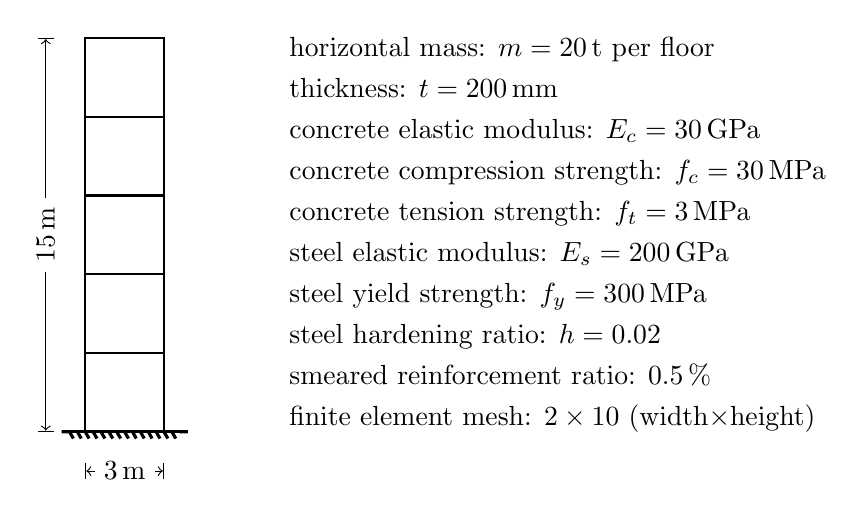
\begin{tikzpicture}
\FixedSupport{.5,0}{2}
\draw[thick](0,0)rectangle(1,5);
\foreach\y in{1,2,3,4}{\draw[thick](0,\y)--++(1,0);}
\draw[|<->|](0,-.5)--++(1,0)node[midway,fill=white]{\SI{3}{\metre}};
\draw[|<->|](-.5,0)--++(0,5)node[midway,fill=white,rotate=90]{\SI{15}{\metre}};
\begin{scope}[xshift=6cm,yshift=2.5cm]
\node[align=left]at(0,0){horizontal mass: $m=\SI{20}{\tonne}$ per floor\\[1mm]thickness: $t=\SI{200}{\milli\meter}$\\[1mm]concrete elastic modulus: $E_c=\SI{30}{\giga\pascal}$\\[1mm]concrete compression strength: $f_c=\SI{30}{\mega\pascal}$\\[1mm]concrete tension strength: $f_t=\SI{3}{\mega\pascal}$\\[1mm]steel elastic modulus: $E_s=\SI{200}{\giga\pascal}$\\[1mm]steel yield strength: $f_y=\SI{300}{\mega\pascal}$\\[1mm]steel hardening ratio: $h=0.02$\\[1mm]smeared reinforcement ratio: \SI{0.5}{\percent}\\[1mm]finite element mesh: $2\times10$ (width$\times$height)};
\end{scope}
\end{tikzpicture}
\caption{a reinforced concrete shear wall specimen}\label{fig:rc_wall}
\end{figure}

A global Rayleigh damping (\SI{5}{\percent} on the first two modes) is applied. The damping matrix is \textit{deliberately} chosen to be a constant matrix that is proportional to mass and initial stiffness matrices to avoid any potential bias brought by the damping matrix. Nevertheless, this option is known to be problematic due to the stiffness proportional terms \citep{Carr1997,Chopra2015}, better alternatives are available. The ground motion used is the NS component of the El Centro record, the PGA of which is $0.349g$. The Newmark method with a constant average acceleration formulation is selected for time integration. The concrete material model used is the CDP model while the Menegotto-Pinto steel model \citep{Menegotto1973} is used for reinforcement.

\begin{figure}[htb]
\centering\scriptsize
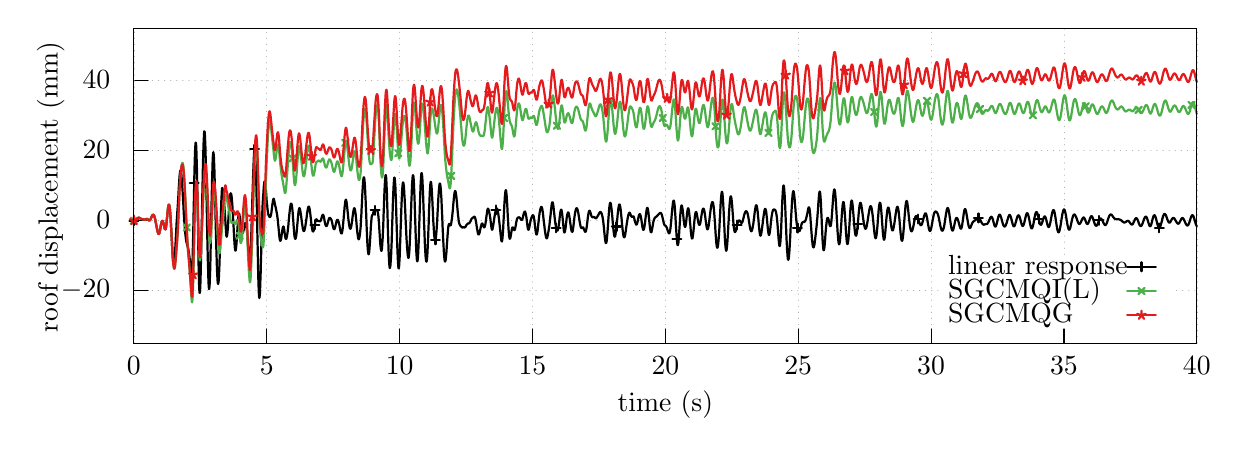
\begin{tikzpicture}[gnuplot]
%% generated with GNUPLOT 5.2p6 (Lua 5.3; terminal rev. Nov 2018, script rev. 107)
%% 08/01/2019 03:27:51
\path (0.000,0.000) rectangle (13.500,4.000);
\gpcolor{color=gp lt color axes}
\gpsetlinetype{gp lt axes}
\gpsetdashtype{gp dt axes}
\gpsetlinewidth{0.50}
\draw[gp path] (0.000,0.667)--(10.222,0.667);
\draw[gp path] (13.162,0.667)--(13.499,0.667);
\gpcolor{color=gp lt color border}
\gpsetlinetype{gp lt border}
\gpsetdashtype{gp dt solid}
\gpsetlinewidth{1.00}
\draw[gp path] (0.000,0.667)--(0.180,0.667);
\node[gp node right] at (-0.184,0.667) {$-20$};
\gpcolor{color=gp lt color axes}
\gpsetlinetype{gp lt axes}
\gpsetdashtype{gp dt axes}
\gpsetlinewidth{0.50}
\draw[gp path] (0.000,1.555)--(13.499,1.555);
\gpcolor{color=gp lt color border}
\gpsetlinetype{gp lt border}
\gpsetdashtype{gp dt solid}
\gpsetlinewidth{1.00}
\draw[gp path] (0.000,1.555)--(0.180,1.555);
\node[gp node right] at (-0.184,1.555) {$0$};
\gpcolor{color=gp lt color axes}
\gpsetlinetype{gp lt axes}
\gpsetdashtype{gp dt axes}
\gpsetlinewidth{0.50}
\draw[gp path] (0.000,2.444)--(13.499,2.444);
\gpcolor{color=gp lt color border}
\gpsetlinetype{gp lt border}
\gpsetdashtype{gp dt solid}
\gpsetlinewidth{1.00}
\draw[gp path] (0.000,2.444)--(0.180,2.444);
\node[gp node right] at (-0.184,2.444) {$20$};
\gpcolor{color=gp lt color axes}
\gpsetlinetype{gp lt axes}
\gpsetdashtype{gp dt axes}
\gpsetlinewidth{0.50}
\draw[gp path] (0.000,3.332)--(13.499,3.332);
\gpcolor{color=gp lt color border}
\gpsetlinetype{gp lt border}
\gpsetdashtype{gp dt solid}
\gpsetlinewidth{1.00}
\draw[gp path] (0.000,3.332)--(0.180,3.332);
\node[gp node right] at (-0.184,3.332) {$40$};
\gpcolor{color=gp lt color axes}
\gpsetlinetype{gp lt axes}
\gpsetdashtype{gp dt axes}
\gpsetlinewidth{0.50}
\draw[gp path] (0.000,0.000)--(0.000,3.999);
\gpcolor{color=gp lt color border}
\gpsetlinetype{gp lt border}
\gpsetdashtype{gp dt solid}
\gpsetlinewidth{1.00}
\draw[gp path] (0.000,0.000)--(0.000,0.180);
\node[gp node center] at (0.000,-0.308) {$0$};
\gpcolor{color=gp lt color axes}
\gpsetlinetype{gp lt axes}
\gpsetdashtype{gp dt axes}
\gpsetlinewidth{0.50}
\draw[gp path] (1.687,0.000)--(1.687,3.999);
\gpcolor{color=gp lt color border}
\gpsetlinetype{gp lt border}
\gpsetdashtype{gp dt solid}
\gpsetlinewidth{1.00}
\draw[gp path] (1.687,0.000)--(1.687,0.180);
\node[gp node center] at (1.687,-0.308) {$5$};
\gpcolor{color=gp lt color axes}
\gpsetlinetype{gp lt axes}
\gpsetdashtype{gp dt axes}
\gpsetlinewidth{0.50}
\draw[gp path] (3.375,0.000)--(3.375,3.999);
\gpcolor{color=gp lt color border}
\gpsetlinetype{gp lt border}
\gpsetdashtype{gp dt solid}
\gpsetlinewidth{1.00}
\draw[gp path] (3.375,0.000)--(3.375,0.180);
\node[gp node center] at (3.375,-0.308) {$10$};
\gpcolor{color=gp lt color axes}
\gpsetlinetype{gp lt axes}
\gpsetdashtype{gp dt axes}
\gpsetlinewidth{0.50}
\draw[gp path] (5.062,0.000)--(5.062,3.999);
\gpcolor{color=gp lt color border}
\gpsetlinetype{gp lt border}
\gpsetdashtype{gp dt solid}
\gpsetlinewidth{1.00}
\draw[gp path] (5.062,0.000)--(5.062,0.180);
\node[gp node center] at (5.062,-0.308) {$15$};
\gpcolor{color=gp lt color axes}
\gpsetlinetype{gp lt axes}
\gpsetdashtype{gp dt axes}
\gpsetlinewidth{0.50}
\draw[gp path] (6.750,0.000)--(6.750,3.999);
\gpcolor{color=gp lt color border}
\gpsetlinetype{gp lt border}
\gpsetdashtype{gp dt solid}
\gpsetlinewidth{1.00}
\draw[gp path] (6.750,0.000)--(6.750,0.180);
\node[gp node center] at (6.750,-0.308) {$20$};
\gpcolor{color=gp lt color axes}
\gpsetlinetype{gp lt axes}
\gpsetdashtype{gp dt axes}
\gpsetlinewidth{0.50}
\draw[gp path] (8.437,0.000)--(8.437,3.999);
\gpcolor{color=gp lt color border}
\gpsetlinetype{gp lt border}
\gpsetdashtype{gp dt solid}
\gpsetlinewidth{1.00}
\draw[gp path] (8.437,0.000)--(8.437,0.180);
\node[gp node center] at (8.437,-0.308) {$25$};
\gpcolor{color=gp lt color axes}
\gpsetlinetype{gp lt axes}
\gpsetdashtype{gp dt axes}
\gpsetlinewidth{0.50}
\draw[gp path] (10.124,0.000)--(10.124,3.999);
\gpcolor{color=gp lt color border}
\gpsetlinetype{gp lt border}
\gpsetdashtype{gp dt solid}
\gpsetlinewidth{1.00}
\draw[gp path] (10.124,0.000)--(10.124,0.180);
\node[gp node center] at (10.124,-0.308) {$30$};
\gpcolor{color=gp lt color axes}
\gpsetlinetype{gp lt axes}
\gpsetdashtype{gp dt axes}
\gpsetlinewidth{0.50}
\draw[gp path] (11.812,0.000)--(11.812,0.200);
\draw[gp path] (11.812,1.124)--(11.812,3.999);
\gpcolor{color=gp lt color border}
\gpsetlinetype{gp lt border}
\gpsetdashtype{gp dt solid}
\gpsetlinewidth{1.00}
\draw[gp path] (11.812,0.000)--(11.812,0.180);
\node[gp node center] at (11.812,-0.308) {$35$};
\gpcolor{color=gp lt color axes}
\gpsetlinetype{gp lt axes}
\gpsetdashtype{gp dt axes}
\gpsetlinewidth{0.50}
\draw[gp path] (13.499,0.000)--(13.499,3.999);
\gpcolor{color=gp lt color border}
\gpsetlinetype{gp lt border}
\gpsetdashtype{gp dt solid}
\gpsetlinewidth{1.00}
\draw[gp path] (13.499,0.000)--(13.499,0.180);
\node[gp node center] at (13.499,-0.308) {$40$};
\draw[gp path] (0.000,3.999)--(0.000,0.000)--(13.499,0.000)--(13.499,3.999)--cycle;
\node[gp node center,rotate=-270] at (-1.044,1.999) {roof displacement (\si{\milli\metre})};
\node[gp node center] at (6.749,-0.769) {time (\si{\second})};
\gpcolor{rgb color={0.000,0.000,0.000}}
\gpsetlinewidth{2.00}
\draw[gp path] (0.000,1.555)--(0.003,1.555)--(0.007,1.556)--(0.010,1.556)--(0.013,1.558)%
  --(0.017,1.560)--(0.020,1.563)--(0.024,1.565)--(0.027,1.568)--(0.030,1.571)--(0.034,1.574)%
  --(0.037,1.577)--(0.040,1.580)--(0.044,1.583)--(0.047,1.585)--(0.051,1.588)--(0.054,1.590)%
  --(0.057,1.591)--(0.061,1.592)--(0.064,1.592)--(0.067,1.591)--(0.071,1.590)--(0.074,1.588)%
  --(0.078,1.586)--(0.081,1.583)--(0.084,1.581)--(0.088,1.579)--(0.091,1.578)--(0.094,1.576)%
  --(0.098,1.576)--(0.101,1.575)--(0.105,1.574)--(0.108,1.574)--(0.111,1.574)--(0.115,1.573)%
  --(0.118,1.573)--(0.121,1.572)--(0.125,1.571)--(0.128,1.570)--(0.132,1.568)--(0.135,1.567)%
  --(0.138,1.566)--(0.142,1.566)--(0.145,1.567)--(0.148,1.568)--(0.152,1.570)--(0.155,1.573)%
  --(0.159,1.575)--(0.162,1.576)--(0.165,1.577)--(0.169,1.576)--(0.172,1.574)--(0.175,1.571)%
  --(0.179,1.567)--(0.182,1.564)--(0.186,1.561)--(0.189,1.560)--(0.192,1.559)--(0.196,1.558)%
  --(0.199,1.559)--(0.202,1.561)--(0.206,1.564)--(0.209,1.569)--(0.213,1.576)--(0.216,1.583)%
  --(0.219,1.591)--(0.223,1.599)--(0.226,1.607)--(0.229,1.613)--(0.233,1.619)--(0.236,1.624)%
  --(0.240,1.627)--(0.243,1.629)--(0.246,1.629)--(0.250,1.627)--(0.253,1.624)--(0.256,1.618)%
  --(0.260,1.610)--(0.263,1.599)--(0.267,1.587)--(0.270,1.573)--(0.273,1.557)--(0.277,1.539)%
  --(0.280,1.521)--(0.283,1.503)--(0.287,1.484)--(0.290,1.467)--(0.294,1.450)--(0.297,1.433)%
  --(0.300,1.418)--(0.304,1.406)--(0.307,1.396)--(0.310,1.389)--(0.314,1.386)--(0.317,1.387)%
  --(0.321,1.392)--(0.324,1.401)--(0.327,1.414)--(0.331,1.429)--(0.334,1.447)--(0.337,1.466)%
  --(0.341,1.485)--(0.344,1.502)--(0.348,1.519)--(0.351,1.533)--(0.354,1.543)--(0.358,1.550)%
  --(0.361,1.552)--(0.364,1.550)--(0.368,1.544)--(0.371,1.535)--(0.375,1.524)--(0.378,1.510)%
  --(0.381,1.496)--(0.385,1.482)--(0.388,1.468)--(0.391,1.456)--(0.395,1.448)--(0.398,1.444)%
  --(0.402,1.446)--(0.405,1.457)--(0.408,1.476)--(0.412,1.502)--(0.415,1.533)--(0.418,1.566)%
  --(0.422,1.601)--(0.425,1.637)--(0.429,1.671)--(0.432,1.701)--(0.435,1.727)--(0.439,1.745)%
  --(0.442,1.755)--(0.445,1.758)--(0.449,1.752)--(0.452,1.737)--(0.456,1.713)--(0.459,1.680)%
  --(0.462,1.639)--(0.466,1.591)--(0.469,1.537)--(0.472,1.478)--(0.476,1.416)--(0.479,1.350)%
  --(0.483,1.284)--(0.486,1.219)--(0.489,1.159)--(0.493,1.104)--(0.496,1.059)--(0.499,1.026)%
  --(0.503,1.006)--(0.506,0.999)--(0.510,1.006)--(0.513,1.026)--(0.516,1.058)--(0.520,1.102)%
  --(0.523,1.154)--(0.526,1.214)--(0.530,1.280)--(0.533,1.348)--(0.537,1.416)--(0.540,1.480)%
  --(0.543,1.539)--(0.547,1.592)--(0.550,1.641)--(0.553,1.689)--(0.557,1.739)--(0.560,1.795)%
  --(0.564,1.855)--(0.567,1.916)--(0.570,1.975)--(0.574,2.029)--(0.577,2.078)--(0.580,2.121)%
  --(0.584,2.156)--(0.587,2.181)--(0.591,2.193)--(0.594,2.193)--(0.597,2.182)--(0.601,2.160)%
  --(0.604,2.130)--(0.607,2.092)--(0.611,2.046)--(0.614,1.994)--(0.618,1.938)--(0.621,1.879)%
  --(0.624,1.820)--(0.628,1.760)--(0.631,1.699)--(0.634,1.640)--(0.638,1.584)--(0.641,1.532)%
  --(0.645,1.485)--(0.648,1.443)--(0.651,1.405)--(0.655,1.371)--(0.658,1.342)--(0.661,1.317)%
  --(0.665,1.297)--(0.668,1.281)--(0.672,1.266)--(0.675,1.253)--(0.678,1.241)--(0.682,1.229)%
  --(0.685,1.218)--(0.688,1.205)--(0.692,1.189)--(0.695,1.170)--(0.699,1.149)--(0.702,1.124)%
  --(0.705,1.097)--(0.709,1.067)--(0.712,1.034)--(0.715,1.000)--(0.719,0.966)--(0.722,0.933)%
  --(0.726,0.904)--(0.729,0.882)--(0.732,0.872)--(0.736,0.880)--(0.739,0.915)--(0.742,0.982)%
  --(0.746,1.085)--(0.749,1.217)--(0.753,1.369)--(0.756,1.531)--(0.759,1.699)--(0.763,1.868)%
  --(0.766,2.033)--(0.769,2.188)--(0.773,2.322)--(0.776,2.427)--(0.780,2.500)--(0.783,2.539)%
  --(0.786,2.547)--(0.790,2.520)--(0.793,2.458)--(0.796,2.359)--(0.800,2.228)--(0.803,2.070)%
  --(0.807,1.893)--(0.810,1.700)--(0.813,1.495)--(0.817,1.287)--(0.820,1.086)--(0.823,0.910)%
  --(0.827,0.774)--(0.830,0.685)--(0.834,0.641)--(0.837,0.637)--(0.840,0.669)--(0.844,0.736)%
  --(0.847,0.837)--(0.850,0.971)--(0.854,1.128)--(0.857,1.296)--(0.861,1.465)--(0.864,1.632)%
  --(0.867,1.798)--(0.871,1.964)--(0.874,2.126)--(0.877,2.277)--(0.881,2.410)--(0.884,2.519)%
  --(0.888,2.602)--(0.891,2.659)--(0.894,2.689)--(0.898,2.688)--(0.901,2.655)--(0.904,2.590)%
  --(0.908,2.496)--(0.911,2.378)--(0.915,2.241)--(0.918,2.087)--(0.921,1.920)--(0.925,1.745)%
  --(0.928,1.567)--(0.931,1.395)--(0.935,1.232)--(0.938,1.083)--(0.942,0.952)--(0.945,0.841)%
  --(0.948,0.757)--(0.952,0.704)--(0.955,0.685)--(0.958,0.699)--(0.962,0.748)--(0.965,0.827)%
  --(0.969,0.935)--(0.972,1.067)--(0.975,1.219)--(0.979,1.384)--(0.982,1.555)--(0.985,1.724)%
  --(0.989,1.887)--(0.992,2.037)--(0.996,2.170)--(0.999,2.278)--(1.002,2.359)--(1.006,2.408)%
  --(1.009,2.425)--(1.012,2.409)--(1.016,2.362)--(1.019,2.285)--(1.023,2.184)--(1.026,2.065)%
  --(1.029,1.934)--(1.033,1.794)--(1.036,1.650)--(1.039,1.505)--(1.043,1.362)--(1.046,1.228)%
  --(1.050,1.106)--(1.053,0.999)--(1.056,0.911)--(1.060,0.841)--(1.063,0.790)--(1.066,0.760)%
  --(1.070,0.751)--(1.073,0.764)--(1.077,0.795)--(1.080,0.846)--(1.083,0.916)--(1.087,1.006)%
  --(1.090,1.114)--(1.093,1.233)--(1.097,1.358)--(1.100,1.480)--(1.104,1.596)--(1.107,1.704)%
  --(1.110,1.799)--(1.114,1.878)--(1.117,1.934)--(1.120,1.965)--(1.124,1.970)--(1.127,1.956)%
  --(1.131,1.931)--(1.134,1.904)--(1.137,1.875)--(1.141,1.844)--(1.144,1.807)--(1.147,1.763)%
  --(1.151,1.714)--(1.154,1.663)--(1.158,1.611)--(1.161,1.559)--(1.164,1.502)--(1.168,1.446)%
  --(1.171,1.397)--(1.174,1.364)--(1.178,1.351)--(1.181,1.357)--(1.185,1.374)--(1.188,1.400)%
  --(1.191,1.434)--(1.195,1.479)--(1.198,1.534)--(1.201,1.596)--(1.205,1.657)--(1.208,1.712)%
  --(1.212,1.760)--(1.215,1.803)--(1.218,1.840)--(1.222,1.870)--(1.225,1.892)--(1.228,1.902)%
  --(1.232,1.903)--(1.235,1.894)--(1.239,1.878)--(1.242,1.852)--(1.245,1.817)--(1.249,1.773)%
  --(1.252,1.721)--(1.255,1.665)--(1.259,1.605)--(1.262,1.543)--(1.266,1.478)--(1.269,1.413)%
  --(1.272,1.351)--(1.276,1.294)--(1.279,1.246)--(1.282,1.210)--(1.286,1.185)--(1.289,1.175)%
  --(1.293,1.178)--(1.296,1.196)--(1.299,1.225)--(1.303,1.264)--(1.306,1.311)--(1.309,1.362)%
  --(1.313,1.416)--(1.316,1.470)--(1.320,1.521)--(1.323,1.566)--(1.326,1.602)--(1.330,1.628)%
  --(1.333,1.641)--(1.336,1.643)--(1.340,1.631)--(1.343,1.610)--(1.347,1.583)--(1.350,1.555)%
  --(1.353,1.528)--(1.357,1.503)--(1.360,1.480)--(1.363,1.456)--(1.367,1.432)--(1.370,1.413)%
  --(1.374,1.400)--(1.377,1.394)--(1.380,1.395)--(1.384,1.401)--(1.387,1.411)--(1.390,1.423)%
  --(1.394,1.439)--(1.397,1.458)--(1.401,1.477)--(1.404,1.494)--(1.407,1.509)--(1.411,1.519)%
  --(1.414,1.525)--(1.417,1.527)--(1.421,1.523)--(1.424,1.512)--(1.428,1.494)--(1.431,1.468)%
  --(1.434,1.437)--(1.438,1.399)--(1.441,1.357)--(1.444,1.310)--(1.448,1.260)--(1.451,1.210)%
  --(1.455,1.161)--(1.458,1.116)--(1.461,1.075)--(1.465,1.042)--(1.468,1.020)--(1.471,1.015)%
  --(1.475,1.034)--(1.478,1.078)--(1.482,1.144)--(1.485,1.226)--(1.488,1.318)--(1.492,1.415)%
  --(1.495,1.516)--(1.498,1.624)--(1.502,1.735)--(1.505,1.848)--(1.509,1.957)--(1.512,2.060)%
  --(1.515,2.159)--(1.519,2.250)--(1.522,2.331)--(1.525,2.396)--(1.529,2.440)--(1.532,2.461)%
  --(1.536,2.459)--(1.539,2.434)--(1.542,2.387)--(1.546,2.317)--(1.549,2.223)--(1.552,2.107)%
  --(1.556,1.973)--(1.559,1.825)--(1.563,1.668)--(1.566,1.503)--(1.569,1.334)--(1.573,1.166)%
  --(1.576,1.003)--(1.579,0.856)--(1.583,0.735)--(1.586,0.646)--(1.590,0.592)--(1.593,0.572)%
  --(1.596,0.584)--(1.600,0.625)--(1.603,0.692)--(1.606,0.785)--(1.610,0.898)--(1.613,1.025)%
  --(1.617,1.158)--(1.620,1.291)--(1.623,1.418)--(1.627,1.536)--(1.630,1.640)--(1.633,1.726)%
  --(1.637,1.794)--(1.640,1.848)--(1.644,1.897)--(1.647,1.944)--(1.650,1.989)--(1.654,2.025)%
  --(1.657,2.047)--(1.660,2.054)--(1.664,2.049)--(1.667,2.034)--(1.671,2.011)--(1.674,1.977)%
  --(1.677,1.933)--(1.681,1.884)--(1.684,1.837)--(1.687,1.796)--(1.691,1.763)--(1.694,1.732)%
  --(1.697,1.701)--(1.701,1.672)--(1.704,1.648)--(1.708,1.633)--(1.711,1.624)--(1.714,1.617)%
  --(1.718,1.611)--(1.721,1.604)--(1.724,1.600)--(1.728,1.600)--(1.731,1.604)--(1.735,1.609)%
  --(1.738,1.618)--(1.741,1.630)--(1.745,1.649)--(1.748,1.673)--(1.751,1.700)--(1.755,1.728)%
  --(1.758,1.754)--(1.762,1.778)--(1.765,1.800)--(1.768,1.818)--(1.772,1.831)--(1.775,1.834)%
  --(1.778,1.827)--(1.782,1.812)--(1.785,1.793)--(1.789,1.774)--(1.792,1.759)--(1.795,1.745)%
  --(1.799,1.732)--(1.802,1.716)--(1.805,1.700)--(1.809,1.682)--(1.812,1.665)--(1.816,1.648)%
  --(1.819,1.628)--(1.822,1.604)--(1.826,1.576)--(1.829,1.545)--(1.832,1.512)--(1.836,1.478)%
  --(1.839,1.442)--(1.843,1.404)--(1.846,1.369)--(1.849,1.339)--(1.853,1.316)--(1.856,1.303)%
  --(1.859,1.299)--(1.863,1.301)--(1.866,1.310)--(1.870,1.325)--(1.873,1.346)--(1.876,1.370)%
  --(1.880,1.395)--(1.883,1.419)--(1.886,1.441)--(1.890,1.459)--(1.893,1.473)--(1.897,1.480)%
  --(1.900,1.480)--(1.903,1.472)--(1.907,1.456)--(1.910,1.434)--(1.913,1.408)--(1.917,1.382)%
  --(1.920,1.359)--(1.924,1.340)--(1.927,1.328)--(1.930,1.323)--(1.934,1.323)--(1.937,1.330)%
  --(1.940,1.341)--(1.944,1.358)--(1.947,1.377)--(1.951,1.400)--(1.954,1.427)--(1.957,1.456)%
  --(1.961,1.489)--(1.964,1.525)--(1.967,1.562)--(1.971,1.599)--(1.974,1.635)--(1.978,1.668)%
  --(1.981,1.697)--(1.984,1.723)--(1.988,1.745)--(1.991,1.761)--(1.994,1.771)--(1.998,1.773)%
  --(2.001,1.768)--(2.005,1.756)--(2.008,1.737)--(2.011,1.711)--(2.015,1.677)--(2.018,1.637)%
  --(2.021,1.591)--(2.025,1.542)--(2.028,1.493)--(2.032,1.446)--(2.035,1.405)--(2.038,1.370)%
  --(2.042,1.345)--(2.045,1.329)--(2.048,1.323)--(2.052,1.325)--(2.055,1.333)--(2.059,1.348)%
  --(2.062,1.368)--(2.065,1.394)--(2.069,1.426)--(2.072,1.462)--(2.075,1.501)--(2.079,1.542)%
  --(2.082,1.581)--(2.086,1.618)--(2.089,1.650)--(2.092,1.677)--(2.096,1.698)--(2.099,1.710)%
  --(2.102,1.714)--(2.106,1.710)--(2.109,1.700)--(2.113,1.684)--(2.116,1.666)--(2.119,1.644)%
  --(2.123,1.621)--(2.126,1.595)--(2.129,1.568)--(2.133,1.542)--(2.136,1.516)--(2.140,1.492)%
  --(2.143,1.470)--(2.146,1.451)--(2.150,1.436)--(2.153,1.427)--(2.156,1.422)--(2.160,1.423)%
  --(2.163,1.428)--(2.167,1.436)--(2.170,1.448)--(2.173,1.464)--(2.177,1.482)--(2.180,1.502)%
  --(2.183,1.524)--(2.187,1.547)--(2.190,1.571)--(2.194,1.598)--(2.197,1.625)--(2.200,1.651)%
  --(2.204,1.675)--(2.207,1.696)--(2.210,1.712)--(2.214,1.725)--(2.217,1.732)--(2.221,1.735)%
  --(2.224,1.732)--(2.227,1.723)--(2.231,1.709)--(2.234,1.689)--(2.237,1.665)--(2.241,1.637)%
  --(2.244,1.606)--(2.248,1.575)--(2.251,1.544)--(2.254,1.516)--(2.258,1.489)--(2.261,1.466)%
  --(2.264,1.445)--(2.268,1.430)--(2.271,1.420)--(2.275,1.416)--(2.278,1.418)--(2.281,1.424)%
  --(2.285,1.434)--(2.288,1.448)--(2.291,1.465)--(2.295,1.484)--(2.298,1.504)--(2.302,1.523)%
  --(2.305,1.541)--(2.308,1.555)--(2.312,1.566)--(2.315,1.572)--(2.318,1.572)--(2.322,1.568)%
  --(2.325,1.562)--(2.329,1.556)--(2.332,1.553)--(2.335,1.551)--(2.339,1.551)--(2.342,1.551)%
  --(2.345,1.550)--(2.349,1.549)--(2.352,1.549)--(2.356,1.548)--(2.359,1.547)--(2.362,1.546)%
  --(2.366,1.546)--(2.369,1.549)--(2.372,1.556)--(2.376,1.565)--(2.379,1.577)--(2.383,1.589)%
  --(2.386,1.600)--(2.389,1.611)--(2.393,1.620)--(2.396,1.627)--(2.399,1.630)--(2.403,1.629)%
  --(2.406,1.623)--(2.410,1.613)--(2.413,1.599)--(2.416,1.582)--(2.420,1.563)--(2.423,1.545)%
  --(2.426,1.528)--(2.430,1.513)--(2.433,1.502)--(2.437,1.494)--(2.440,1.488)--(2.443,1.486)%
  --(2.447,1.486)--(2.450,1.490)--(2.453,1.498)--(2.457,1.508)--(2.460,1.520)--(2.464,1.533)%
  --(2.467,1.545)--(2.470,1.557)--(2.474,1.568)--(2.477,1.578)--(2.480,1.585)--(2.484,1.589)%
  --(2.487,1.590)--(2.491,1.589)--(2.494,1.587)--(2.497,1.584)--(2.501,1.580)--(2.504,1.574)%
  --(2.507,1.567)--(2.511,1.557)--(2.514,1.545)--(2.518,1.531)--(2.521,1.515)--(2.524,1.498)%
  --(2.528,1.482)--(2.531,1.468)--(2.534,1.458)--(2.538,1.450)--(2.541,1.447)--(2.545,1.447)%
  --(2.548,1.450)--(2.551,1.458)--(2.555,1.468)--(2.558,1.481)--(2.561,1.495)--(2.565,1.510)%
  --(2.568,1.525)--(2.572,1.539)--(2.575,1.551)--(2.578,1.560)--(2.582,1.565)--(2.585,1.567)%
  --(2.588,1.565)--(2.592,1.560)--(2.595,1.552)--(2.599,1.543)--(2.602,1.531)--(2.605,1.518)%
  --(2.609,1.502)--(2.612,1.485)--(2.615,1.467)--(2.619,1.447)--(2.622,1.429)--(2.626,1.414)%
  --(2.629,1.402)--(2.632,1.394)--(2.636,1.391)--(2.639,1.393)--(2.642,1.401)--(2.646,1.417)%
  --(2.649,1.439)--(2.653,1.467)--(2.656,1.499)--(2.659,1.534)--(2.663,1.572)--(2.666,1.612)%
  --(2.669,1.652)--(2.673,1.691)--(2.676,1.727)--(2.680,1.759)--(2.683,1.785)--(2.686,1.806)%
  --(2.690,1.819)--(2.693,1.822)--(2.696,1.814)--(2.700,1.797)--(2.703,1.773)--(2.707,1.744)%
  --(2.710,1.714)--(2.713,1.682)--(2.717,1.649)--(2.720,1.616)--(2.723,1.583)--(2.727,1.552)%
  --(2.730,1.525)--(2.734,1.502)--(2.737,1.482)--(2.740,1.467)--(2.744,1.457)--(2.747,1.452)%
  --(2.750,1.453)--(2.754,1.459)--(2.757,1.470)--(2.761,1.485)--(2.764,1.503)--(2.767,1.525)%
  --(2.771,1.549)--(2.774,1.576)--(2.777,1.603)--(2.781,1.629)--(2.784,1.654)--(2.788,1.675)%
  --(2.791,1.693)--(2.794,1.706)--(2.798,1.713)--(2.801,1.713)--(2.804,1.706)--(2.808,1.693)%
  --(2.811,1.673)--(2.815,1.647)--(2.818,1.617)--(2.821,1.583)--(2.825,1.546)--(2.828,1.509)%
  --(2.831,1.471)--(2.835,1.436)--(2.838,1.403)--(2.842,1.374)--(2.845,1.350)--(2.848,1.332)%
  --(2.852,1.321)--(2.855,1.318)--(2.858,1.322)--(2.862,1.332)--(2.865,1.349)--(2.869,1.371)%
  --(2.872,1.397)--(2.875,1.429)--(2.879,1.468)--(2.882,1.517)--(2.885,1.575)--(2.889,1.640)%
  --(2.892,1.710)--(2.896,1.780)--(2.899,1.848)--(2.902,1.913)--(2.906,1.972)--(2.909,2.024)%
  --(2.912,2.065)--(2.916,2.093)--(2.919,2.106)--(2.923,2.104)--(2.926,2.089)--(2.929,2.060)%
  --(2.933,2.016)--(2.936,1.959)--(2.939,1.891)--(2.943,1.813)--(2.946,1.729)--(2.950,1.642)%
  --(2.953,1.553)--(2.956,1.467)--(2.960,1.385)--(2.963,1.313)--(2.966,1.251)--(2.970,1.201)%
  --(2.973,1.164)--(2.977,1.139)--(2.980,1.128)--(2.983,1.131)--(2.987,1.148)--(2.990,1.178)%
  --(2.993,1.219)--(2.997,1.268)--(3.000,1.322)--(3.004,1.379)--(3.007,1.435)--(3.010,1.488)%
  --(3.014,1.536)--(3.017,1.575)--(3.020,1.603)--(3.024,1.619)--(3.027,1.625)--(3.031,1.629)%
  --(3.034,1.634)--(3.037,1.644)--(3.041,1.657)--(3.044,1.668)--(3.047,1.674)--(3.051,1.676)%
  --(3.054,1.676)--(3.058,1.677)--(3.061,1.681)--(3.064,1.686)--(3.068,1.689)--(3.071,1.690)%
  --(3.074,1.690)--(3.078,1.690)--(3.081,1.690)--(3.085,1.689)--(3.088,1.687)--(3.091,1.681)%
  --(3.095,1.672)--(3.098,1.658)--(3.101,1.638)--(3.105,1.612)--(3.108,1.579)--(3.112,1.536)%
  --(3.115,1.485)--(3.118,1.429)--(3.122,1.371)--(3.125,1.317)--(3.128,1.271)--(3.132,1.233)%
  --(3.135,1.203)--(3.139,1.182)--(3.142,1.171)--(3.145,1.174)--(3.149,1.191)--(3.152,1.224)%
  --(3.155,1.270)--(3.159,1.328)--(3.162,1.397)--(3.166,1.476)--(3.169,1.564)--(3.172,1.658)%
  --(3.176,1.753)--(3.179,1.846)--(3.182,1.931)--(3.186,2.005)--(3.189,2.065)--(3.193,2.108)%
  --(3.196,2.132)--(3.199,2.133)--(3.203,2.111)--(3.206,2.065)--(3.209,1.997)--(3.213,1.906)%
  --(3.216,1.796)--(3.220,1.674)--(3.223,1.549)--(3.226,1.429)--(3.230,1.319)--(3.233,1.220)%
  --(3.236,1.133)--(3.240,1.059)--(3.243,1.002)--(3.247,0.966)--(3.250,0.953)--(3.253,0.959)%
  --(3.257,0.981)--(3.260,1.016)--(3.263,1.063)--(3.267,1.125)--(3.270,1.202)--(3.274,1.293)%
  --(3.277,1.395)--(3.280,1.503)--(3.284,1.611)--(3.287,1.716)--(3.290,1.814)--(3.294,1.903)%
  --(3.297,1.979)--(3.301,2.039)--(3.304,2.081)--(3.307,2.102)--(3.311,2.102)--(3.314,2.081)%
  --(3.317,2.039)--(3.321,1.978)--(3.324,1.898)--(3.328,1.804)--(3.331,1.698)--(3.334,1.585)%
  --(3.338,1.469)--(3.341,1.356)--(3.344,1.250)--(3.348,1.155)--(3.351,1.075)--(3.355,1.013)%
  --(3.358,0.971)--(3.361,0.950)--(3.365,0.951)--(3.368,0.976)--(3.371,1.023)--(3.375,1.090)%
  --(3.378,1.172)--(3.381,1.265)--(3.385,1.364)--(3.388,1.466)--(3.392,1.566)--(3.395,1.662)%
  --(3.398,1.752)--(3.402,1.833)--(3.405,1.903)--(3.408,1.960)--(3.412,2.004)--(3.415,2.031)%
  --(3.419,2.041)--(3.422,2.036)--(3.425,2.016)--(3.429,1.983)--(3.432,1.940)--(3.435,1.887)%
  --(3.439,1.825)--(3.442,1.756)--(3.446,1.684)--(3.449,1.610)--(3.452,1.536)--(3.456,1.464)%
  --(3.459,1.395)--(3.462,1.330)--(3.466,1.272)--(3.469,1.219)--(3.473,1.175)--(3.476,1.138)%
  --(3.479,1.109)--(3.483,1.090)--(3.486,1.082)--(3.489,1.087)--(3.493,1.108)--(3.496,1.144)%
  --(3.500,1.195)--(3.503,1.259)--(3.506,1.334)--(3.510,1.417)--(3.513,1.505)--(3.516,1.595)%
  --(3.520,1.686)--(3.523,1.778)--(3.527,1.867)--(3.530,1.949)--(3.533,2.020)--(3.537,2.075)%
  --(3.540,2.113)--(3.543,2.132)--(3.547,2.132)--(3.550,2.112)--(3.554,2.071)--(3.557,2.010)%
  --(3.560,1.932)--(3.564,1.840)--(3.567,1.738)--(3.570,1.630)--(3.574,1.522)--(3.577,1.416)%
  --(3.581,1.317)--(3.584,1.229)--(3.587,1.155)--(3.591,1.097)--(3.594,1.059)--(3.597,1.039)%
  --(3.601,1.039)--(3.604,1.058)--(3.608,1.096)--(3.611,1.151)--(3.614,1.223)--(3.618,1.308)%
  --(3.621,1.405)--(3.624,1.510)--(3.628,1.619)--(3.631,1.728)--(3.635,1.832)--(3.638,1.928)%
  --(3.641,2.011)--(3.645,2.078)--(3.648,2.126)--(3.651,2.154)--(3.655,2.160)--(3.658,2.146)%
  --(3.662,2.111)--(3.665,2.059)--(3.668,1.991)--(3.672,1.910)--(3.675,1.819)--(3.678,1.722)%
  --(3.682,1.623)--(3.685,1.526)--(3.689,1.433)--(3.692,1.346)--(3.695,1.266)--(3.699,1.196)%
  --(3.702,1.137)--(3.705,1.092)--(3.709,1.059)--(3.712,1.040)--(3.716,1.034)--(3.719,1.043)%
  --(3.722,1.067)--(3.726,1.108)--(3.729,1.164)--(3.732,1.234)--(3.736,1.315)--(3.739,1.406)%
  --(3.743,1.502)--(3.746,1.601)--(3.749,1.698)--(3.753,1.789)--(3.756,1.870)--(3.759,1.939)%
  --(3.763,1.993)--(3.766,2.030)--(3.770,2.048)--(3.773,2.046)--(3.776,2.026)--(3.780,1.990)%
  --(3.783,1.941)--(3.786,1.883)--(3.790,1.818)--(3.793,1.748)--(3.797,1.676)--(3.800,1.605)%
  --(3.803,1.538)--(3.807,1.477)--(3.810,1.424)--(3.813,1.379)--(3.817,1.343)--(3.820,1.318)%
  --(3.824,1.305)--(3.827,1.302)--(3.830,1.311)--(3.834,1.328)--(3.837,1.355)--(3.840,1.390)%
  --(3.844,1.433)--(3.847,1.484)--(3.851,1.540)--(3.854,1.600)--(3.857,1.663)--(3.861,1.726)%
  --(3.864,1.789)--(3.867,1.850)--(3.871,1.905)--(3.874,1.953)--(3.878,1.989)--(3.881,2.014)%
  --(3.884,2.027)--(3.888,2.027)--(3.891,2.014)--(3.894,1.988)--(3.898,1.949)--(3.901,1.899)%
  --(3.905,1.840)--(3.908,1.773)--(3.911,1.700)--(3.915,1.622)--(3.918,1.542)--(3.921,1.462)%
  --(3.925,1.383)--(3.928,1.310)--(3.932,1.243)--(3.935,1.183)--(3.938,1.132)--(3.942,1.091)%
  --(3.945,1.061)--(3.948,1.043)--(3.952,1.036)--(3.955,1.041)--(3.959,1.055)--(3.962,1.080)%
  --(3.965,1.113)--(3.969,1.153)--(3.972,1.199)--(3.975,1.249)--(3.979,1.299)--(3.982,1.349)%
  --(3.986,1.396)--(3.989,1.437)--(3.992,1.470)--(3.996,1.494)--(3.999,1.508)--(4.002,1.513)%
  --(4.006,1.510)--(4.009,1.505)--(4.013,1.499)--(4.016,1.495)--(4.019,1.494)--(4.023,1.497)%
  --(4.026,1.505)--(4.029,1.519)--(4.033,1.538)--(4.036,1.561)--(4.040,1.587)--(4.043,1.616)%
  --(4.046,1.648)--(4.050,1.683)--(4.053,1.722)--(4.056,1.762)--(4.060,1.801)--(4.063,1.837)%
  --(4.067,1.868)--(4.070,1.895)--(4.073,1.915)--(4.077,1.929)--(4.080,1.933)--(4.083,1.929)%
  --(4.087,1.917)--(4.090,1.897)--(4.094,1.872)--(4.097,1.842)--(4.100,1.808)--(4.104,1.771)%
  --(4.107,1.732)--(4.110,1.693)--(4.114,1.655)--(4.117,1.621)--(4.121,1.590)--(4.124,1.563)%
  --(4.127,1.541)--(4.131,1.525)--(4.134,1.514)--(4.137,1.506)--(4.141,1.500)--(4.144,1.494)%
  --(4.148,1.489)--(4.151,1.484)--(4.154,1.482)--(4.158,1.479)--(4.161,1.477)--(4.164,1.474)%
  --(4.168,1.470)--(4.171,1.468)--(4.175,1.468)--(4.178,1.470)--(4.181,1.472)--(4.185,1.473)%
  --(4.188,1.472)--(4.191,1.470)--(4.195,1.469)--(4.198,1.469)--(4.202,1.470)--(4.205,1.472)%
  --(4.208,1.474)--(4.212,1.478)--(4.215,1.484)--(4.218,1.491)--(4.222,1.497)--(4.225,1.502)%
  --(4.229,1.506)--(4.232,1.509)--(4.235,1.512)--(4.239,1.516)--(4.242,1.519)--(4.245,1.520)%
  --(4.249,1.520)--(4.252,1.520)--(4.256,1.521)--(4.259,1.524)--(4.262,1.528)--(4.266,1.532)%
  --(4.269,1.536)--(4.272,1.542)--(4.276,1.549)--(4.279,1.558)--(4.283,1.567)--(4.286,1.574)%
  --(4.289,1.579)--(4.293,1.583)--(4.296,1.586)--(4.299,1.589)--(4.303,1.591)--(4.306,1.594)%
  --(4.310,1.596)--(4.313,1.598)--(4.316,1.601)--(4.320,1.604)--(4.323,1.605)--(4.326,1.604)%
  --(4.330,1.599)--(4.333,1.591)--(4.337,1.580)--(4.340,1.566)--(4.343,1.549)--(4.347,1.530)%
  --(4.350,1.508)--(4.353,1.485)--(4.357,1.463)--(4.360,1.442)--(4.364,1.422)--(4.367,1.404)%
  --(4.370,1.391)--(4.374,1.382)--(4.377,1.378)--(4.380,1.380)--(4.384,1.385)--(4.387,1.394)%
  --(4.391,1.405)--(4.394,1.419)--(4.397,1.435)--(4.401,1.451)--(4.404,1.467)--(4.407,1.482)%
  --(4.411,1.495)--(4.414,1.506)--(4.418,1.514)--(4.421,1.519)--(4.424,1.519)--(4.428,1.515)%
  --(4.431,1.507)--(4.434,1.498)--(4.438,1.487)--(4.441,1.478)--(4.445,1.472)--(4.448,1.470)%
  --(4.451,1.471)--(4.455,1.476)--(4.458,1.485)--(4.461,1.499)--(4.465,1.518)--(4.468,1.540)%
  --(4.472,1.565)--(4.475,1.591)--(4.478,1.617)--(4.482,1.641)--(4.485,1.664)--(4.488,1.684)%
  --(4.492,1.699)--(4.495,1.707)--(4.499,1.708)--(4.502,1.701)--(4.505,1.690)--(4.509,1.678)%
  --(4.512,1.665)--(4.515,1.650)--(4.519,1.633)--(4.522,1.612)--(4.526,1.588)--(4.529,1.562)%
  --(4.532,1.535)--(4.536,1.508)--(4.539,1.482)--(4.542,1.460)--(4.546,1.445)--(4.549,1.440)%
  --(4.553,1.444)--(4.556,1.457)--(4.559,1.473)--(4.563,1.492)--(4.566,1.512)--(4.569,1.534)%
  --(4.573,1.558)--(4.576,1.581)--(4.580,1.604)--(4.583,1.624)--(4.586,1.642)--(4.590,1.660)%
  --(4.593,1.677)--(4.596,1.691)--(4.600,1.702)--(4.603,1.708)--(4.607,1.710)--(4.610,1.710)%
  --(4.613,1.705)--(4.617,1.698)--(4.620,1.685)--(4.623,1.668)--(4.627,1.646)--(4.630,1.623)%
  --(4.634,1.598)--(4.637,1.571)--(4.640,1.542)--(4.644,1.511)--(4.647,1.479)--(4.650,1.448)%
  --(4.654,1.416)--(4.657,1.384)--(4.661,1.352)--(4.664,1.323)--(4.667,1.301)--(4.671,1.290)%
  --(4.674,1.291)--(4.677,1.306)--(4.681,1.333)--(4.684,1.372)--(4.688,1.423)--(4.691,1.482)%
  --(4.694,1.547)--(4.698,1.615)--(4.701,1.683)--(4.704,1.747)--(4.708,1.806)--(4.711,1.856)%
  --(4.715,1.897)--(4.718,1.926)--(4.721,1.940)--(4.725,1.941)--(4.728,1.928)--(4.731,1.900)%
  --(4.735,1.860)--(4.738,1.807)--(4.742,1.746)--(4.745,1.680)--(4.748,1.615)--(4.752,1.553)%
  --(4.755,1.496)--(4.758,1.443)--(4.762,1.398)--(4.765,1.362)--(4.769,1.338)--(4.772,1.326)%
  --(4.775,1.324)--(4.779,1.330)--(4.782,1.342)--(4.785,1.358)--(4.789,1.379)--(4.792,1.401)%
  --(4.796,1.422)--(4.799,1.441)--(4.802,1.456)--(4.806,1.465)--(4.809,1.470)--(4.812,1.469)%
  --(4.816,1.465)--(4.819,1.457)--(4.823,1.448)--(4.826,1.440)--(4.829,1.435)--(4.833,1.434)%
  --(4.836,1.438)--(4.839,1.446)--(4.843,1.459)--(4.846,1.476)--(4.850,1.495)--(4.853,1.515)%
  --(4.856,1.535)--(4.860,1.552)--(4.863,1.567)--(4.866,1.578)--(4.870,1.585)--(4.873,1.590)%
  --(4.877,1.593)--(4.880,1.595)--(4.883,1.596)--(4.887,1.597)--(4.890,1.598)--(4.893,1.597)%
  --(4.897,1.595)--(4.900,1.592)--(4.904,1.588)--(4.907,1.583)--(4.910,1.578)--(4.914,1.572)%
  --(4.917,1.568)--(4.920,1.566)--(4.924,1.564)--(4.927,1.565)--(4.931,1.568)--(4.934,1.575)%
  --(4.937,1.585)--(4.941,1.598)--(4.944,1.613)--(4.947,1.628)--(4.951,1.643)--(4.954,1.654)%
  --(4.958,1.663)--(4.961,1.669)--(4.964,1.672)--(4.968,1.670)--(4.971,1.662)--(4.974,1.651)%
  --(4.978,1.635)--(4.981,1.617)--(4.985,1.595)--(4.988,1.571)--(4.991,1.544)--(4.995,1.516)%
  --(4.998,1.488)--(5.001,1.465)--(5.005,1.449)--(5.008,1.440)--(5.012,1.440)--(5.015,1.445)%
  --(5.018,1.456)--(5.022,1.470)--(5.025,1.487)--(5.028,1.506)--(5.032,1.525)--(5.035,1.543)%
  --(5.039,1.559)--(5.042,1.571)--(5.045,1.581)--(5.049,1.591)--(5.052,1.600)--(5.055,1.608)%
  --(5.059,1.614)--(5.062,1.620)--(5.065,1.623)--(5.069,1.624)--(5.072,1.621)--(5.076,1.613)%
  --(5.079,1.601)--(5.082,1.583)--(5.086,1.560)--(5.089,1.533)--(5.092,1.504)--(5.096,1.473)%
  --(5.099,1.445)--(5.103,1.419)--(5.106,1.399)--(5.109,1.385)--(5.113,1.379)--(5.116,1.380)%
  --(5.119,1.388)--(5.123,1.403)--(5.126,1.424)--(5.130,1.451)--(5.133,1.481)--(5.136,1.514)%
  --(5.140,1.546)--(5.143,1.578)--(5.146,1.607)--(5.150,1.633)--(5.153,1.656)--(5.157,1.675)%
  --(5.160,1.692)--(5.163,1.706)--(5.167,1.717)--(5.170,1.725)--(5.173,1.730)--(5.177,1.730)%
  --(5.180,1.725)--(5.184,1.715)--(5.187,1.700)--(5.190,1.680)--(5.194,1.655)--(5.197,1.627)%
  --(5.200,1.597)--(5.204,1.566)--(5.207,1.536)--(5.211,1.507)--(5.214,1.479)--(5.217,1.451)%
  --(5.221,1.425)--(5.224,1.401)--(5.227,1.379)--(5.231,1.361)--(5.234,1.346)--(5.238,1.336)%
  --(5.241,1.330)--(5.244,1.330)--(5.248,1.336)--(5.251,1.347)--(5.254,1.362)--(5.258,1.379)%
  --(5.261,1.398)--(5.265,1.418)--(5.268,1.438)--(5.271,1.459)--(5.275,1.482)--(5.278,1.507)%
  --(5.281,1.534)--(5.285,1.564)--(5.288,1.596)--(5.292,1.630)--(5.295,1.664)--(5.298,1.697)%
  --(5.302,1.727)--(5.305,1.753)--(5.308,1.773)--(5.312,1.786)--(5.315,1.790)--(5.319,1.787)%
  --(5.322,1.775)--(5.325,1.756)--(5.329,1.731)--(5.332,1.701)--(5.335,1.669)--(5.339,1.637)%
  --(5.342,1.606)--(5.346,1.577)--(5.349,1.549)--(5.352,1.523)--(5.356,1.500)--(5.359,1.480)%
  --(5.362,1.464)--(5.366,1.450)--(5.369,1.440)--(5.373,1.432)--(5.376,1.428)--(5.379,1.429)%
  --(5.383,1.435)--(5.386,1.445)--(5.389,1.460)--(5.393,1.478)--(5.396,1.501)--(5.400,1.527)%
  --(5.403,1.556)--(5.406,1.586)--(5.410,1.615)--(5.413,1.641)--(5.416,1.663)--(5.420,1.680)%
  --(5.423,1.691)--(5.427,1.695)--(5.430,1.691)--(5.433,1.679)--(5.437,1.659)--(5.440,1.633)%
  --(5.443,1.601)--(5.447,1.565)--(5.450,1.528)--(5.454,1.491)--(5.457,1.458)--(5.460,1.431)%
  --(5.464,1.413)--(5.467,1.405)--(5.470,1.407)--(5.474,1.417)--(5.477,1.433)--(5.481,1.454)%
  --(5.484,1.480)--(5.487,1.509)--(5.491,1.540)--(5.494,1.569)--(5.497,1.595)--(5.501,1.616)%
  --(5.504,1.633)--(5.508,1.646)--(5.511,1.656)--(5.514,1.660)--(5.518,1.660)--(5.521,1.653)%
  --(5.524,1.640)--(5.528,1.623)--(5.531,1.603)--(5.535,1.581)--(5.538,1.557)--(5.541,1.532)%
  --(5.545,1.507)--(5.548,1.482)--(5.551,1.460)--(5.555,1.441)--(5.558,1.426)--(5.562,1.416)%
  --(5.565,1.412)--(5.568,1.414)--(5.572,1.422)--(5.575,1.438)--(5.578,1.459)--(5.582,1.485)%
  --(5.585,1.513)--(5.589,1.543)--(5.592,1.573)--(5.595,1.601)--(5.599,1.626)--(5.602,1.648)%
  --(5.605,1.667)--(5.609,1.682)--(5.612,1.695)--(5.616,1.704)--(5.619,1.711)--(5.622,1.713)%
  --(5.626,1.712)--(5.629,1.708)--(5.632,1.700)--(5.636,1.689)--(5.639,1.675)--(5.643,1.658)%
  --(5.646,1.639)--(5.649,1.618)--(5.653,1.597)--(5.656,1.576)--(5.659,1.555)--(5.663,1.534)%
  --(5.666,1.514)--(5.670,1.496)--(5.673,1.482)--(5.676,1.472)--(5.680,1.466)--(5.683,1.463)%
  --(5.686,1.462)--(5.690,1.463)--(5.693,1.466)--(5.697,1.468)--(5.700,1.470)--(5.703,1.469)%
  --(5.707,1.466)--(5.710,1.460)--(5.713,1.452)--(5.717,1.443)--(5.720,1.435)--(5.724,1.426)%
  --(5.727,1.419)--(5.730,1.414)--(5.734,1.412)--(5.737,1.416)--(5.740,1.424)--(5.744,1.437)%
  --(5.747,1.455)--(5.751,1.477)--(5.754,1.501)--(5.757,1.529)--(5.761,1.557)--(5.764,1.585)%
  --(5.767,1.611)--(5.771,1.633)--(5.774,1.653)--(5.778,1.667)--(5.781,1.677)--(5.784,1.681)%
  --(5.788,1.680)--(5.791,1.675)--(5.794,1.668)--(5.798,1.658)--(5.801,1.647)--(5.805,1.635)%
  --(5.808,1.624)--(5.811,1.614)--(5.815,1.607)--(5.818,1.602)--(5.821,1.600)--(5.825,1.599)%
  --(5.828,1.599)--(5.832,1.599)--(5.835,1.600)--(5.838,1.602)--(5.842,1.602)--(5.845,1.602)%
  --(5.848,1.599)--(5.852,1.596)--(5.855,1.592)--(5.859,1.589)--(5.862,1.586)--(5.865,1.586)%
  --(5.869,1.586)--(5.872,1.588)--(5.875,1.592)--(5.879,1.596)--(5.882,1.601)--(5.886,1.607)%
  --(5.889,1.612)--(5.892,1.617)--(5.896,1.623)--(5.899,1.629)--(5.902,1.636)--(5.906,1.643)%
  --(5.909,1.649)--(5.913,1.655)--(5.916,1.659)--(5.919,1.663)--(5.923,1.665)--(5.926,1.665)%
  --(5.929,1.663)--(5.933,1.659)--(5.936,1.653)--(5.940,1.645)--(5.943,1.635)--(5.946,1.623)%
  --(5.950,1.610)--(5.953,1.593)--(5.956,1.573)--(5.960,1.549)--(5.963,1.521)--(5.967,1.489)%
  --(5.970,1.455)--(5.973,1.420)--(5.977,1.386)--(5.980,1.354)--(5.983,1.324)--(5.987,1.299)%
  --(5.990,1.281)--(5.994,1.270)--(5.997,1.269)--(6.000,1.278)--(6.004,1.296)--(6.007,1.323)%
  --(6.010,1.358)--(6.014,1.399)--(6.017,1.445)--(6.021,1.494)--(6.024,1.544)--(6.027,1.593)%
  --(6.031,1.639)--(6.034,1.681)--(6.037,1.717)--(6.041,1.746)--(6.044,1.767)--(6.048,1.779)%
  --(6.051,1.782)--(6.054,1.776)--(6.058,1.763)--(6.061,1.742)--(6.064,1.717)--(6.068,1.686)%
  --(6.071,1.652)--(6.075,1.615)--(6.078,1.577)--(6.081,1.538)--(6.085,1.499)--(6.088,1.463)%
  --(6.091,1.429)--(6.095,1.400)--(6.098,1.377)--(6.102,1.360)--(6.105,1.352)--(6.108,1.352)%
  --(6.112,1.359)--(6.115,1.374)--(6.118,1.395)--(6.122,1.421)--(6.125,1.450)--(6.129,1.480)%
  --(6.132,1.513)--(6.135,1.545)--(6.139,1.579)--(6.142,1.612)--(6.145,1.645)--(6.149,1.676)%
  --(6.152,1.704)--(6.156,1.727)--(6.159,1.746)--(6.162,1.757)--(6.166,1.762)--(6.169,1.760)%
  --(6.172,1.751)--(6.176,1.735)--(6.179,1.714)--(6.183,1.687)--(6.186,1.656)--(6.189,1.621)%
  --(6.193,1.585)--(6.196,1.548)--(6.199,1.512)--(6.203,1.476)--(6.206,1.444)--(6.210,1.414)%
  --(6.213,1.389)--(6.216,1.369)--(6.220,1.355)--(6.223,1.346)--(6.226,1.342)--(6.230,1.345)%
  --(6.233,1.352)--(6.237,1.365)--(6.240,1.381)--(6.243,1.402)--(6.247,1.424)--(6.250,1.448)%
  --(6.253,1.473)--(6.257,1.497)--(6.260,1.520)--(6.264,1.542)--(6.267,1.563)--(6.270,1.582)%
  --(6.274,1.599)--(6.277,1.614)--(6.280,1.628)--(6.284,1.639)--(6.287,1.648)--(6.291,1.654)%
  --(6.294,1.656)--(6.297,1.655)--(6.301,1.650)--(6.304,1.642)--(6.307,1.632)--(6.311,1.623)%
  --(6.314,1.616)--(6.318,1.610)--(6.321,1.606)--(6.324,1.604)--(6.328,1.604)--(6.331,1.605)%
  --(6.334,1.607)--(6.338,1.609)--(6.341,1.610)--(6.345,1.608)--(6.348,1.602)--(6.351,1.593)%
  --(6.355,1.582)--(6.358,1.569)--(6.361,1.555)--(6.365,1.542)--(6.368,1.531)--(6.372,1.521)%
  --(6.375,1.513)--(6.378,1.507)--(6.382,1.505)--(6.385,1.506)--(6.388,1.511)--(6.392,1.521)%
  --(6.395,1.534)--(6.399,1.551)--(6.402,1.569)--(6.405,1.586)--(6.409,1.602)--(6.412,1.616)%
  --(6.415,1.626)--(6.419,1.634)--(6.422,1.638)--(6.426,1.638)--(6.429,1.634)--(6.432,1.627)%
  --(6.436,1.615)--(6.439,1.600)--(6.442,1.582)--(6.446,1.561)--(6.449,1.538)--(6.453,1.514)%
  --(6.456,1.491)--(6.459,1.470)--(6.463,1.454)--(6.466,1.443)--(6.469,1.438)--(6.473,1.438)%
  --(6.476,1.445)--(6.480,1.457)--(6.483,1.473)--(6.486,1.494)--(6.490,1.519)--(6.493,1.546)%
  --(6.496,1.575)--(6.500,1.604)--(6.503,1.633)--(6.507,1.660)--(6.510,1.683)--(6.513,1.701)%
  --(6.517,1.713)--(6.520,1.718)--(6.523,1.716)--(6.527,1.705)--(6.530,1.687)--(6.534,1.663)%
  --(6.537,1.634)--(6.540,1.601)--(6.544,1.567)--(6.547,1.533)--(6.550,1.501)--(6.554,1.471)%
  --(6.557,1.445)--(6.561,1.426)--(6.564,1.413)--(6.567,1.406)--(6.571,1.407)--(6.574,1.414)%
  --(6.577,1.427)--(6.581,1.444)--(6.584,1.463)--(6.588,1.484)--(6.591,1.505)--(6.594,1.525)%
  --(6.598,1.542)--(6.601,1.556)--(6.604,1.567)--(6.608,1.575)--(6.611,1.582)--(6.615,1.588)%
  --(6.618,1.593)--(6.621,1.596)--(6.625,1.599)--(6.628,1.601)--(6.631,1.604)--(6.635,1.606)%
  --(6.638,1.610)--(6.642,1.613)--(6.645,1.616)--(6.648,1.619)--(6.652,1.623)--(6.655,1.626)%
  --(6.658,1.630)--(6.662,1.634)--(6.665,1.637)--(6.669,1.641)--(6.672,1.644)--(6.675,1.648)%
  --(6.679,1.651)--(6.682,1.652)--(6.685,1.653)--(6.689,1.652)--(6.692,1.651)--(6.696,1.648)%
  --(6.699,1.643)--(6.702,1.636)--(6.706,1.626)--(6.709,1.614)--(6.712,1.601)--(6.716,1.585)%
  --(6.719,1.570)--(6.723,1.554)--(6.726,1.539)--(6.729,1.525)--(6.733,1.514)--(6.736,1.505)%
  --(6.739,1.499)--(6.743,1.495)--(6.746,1.493)--(6.750,1.491)--(6.753,1.489)--(6.756,1.486)%
  --(6.760,1.482)--(6.763,1.476)--(6.766,1.469)--(6.770,1.460)--(6.773,1.450)--(6.776,1.439)%
  --(6.780,1.429)--(6.783,1.418)--(6.787,1.409)--(6.790,1.401)--(6.793,1.396)--(6.797,1.394)%
  --(6.800,1.396)--(6.803,1.403)--(6.807,1.414)--(6.810,1.432)--(6.814,1.455)--(6.817,1.483)%
  --(6.820,1.516)--(6.824,1.552)--(6.827,1.590)--(6.830,1.629)--(6.834,1.668)--(6.837,1.704)%
  --(6.841,1.738)--(6.844,1.766)--(6.847,1.788)--(6.851,1.804)--(6.854,1.810)--(6.857,1.808)%
  --(6.861,1.795)--(6.864,1.773)--(6.868,1.741)--(6.871,1.700)--(6.874,1.651)--(6.878,1.597)%
  --(6.881,1.539)--(6.884,1.481)--(6.888,1.425)--(6.891,1.373)--(6.895,1.327)--(6.898,1.290)%
  --(6.901,1.263)--(6.905,1.247)--(6.908,1.244)--(6.911,1.253)--(6.915,1.275)--(6.918,1.308)%
  --(6.922,1.351)--(6.925,1.399)--(6.928,1.452)--(6.932,1.507)--(6.935,1.561)--(6.938,1.612)%
  --(6.942,1.657)--(6.945,1.694)--(6.949,1.722)--(6.952,1.740)--(6.955,1.748)--(6.959,1.746)%
  --(6.962,1.736)--(6.965,1.718)--(6.969,1.693)--(6.972,1.664)--(6.976,1.632)--(6.979,1.599)%
  --(6.982,1.567)--(6.986,1.537)--(6.989,1.512)--(6.992,1.493)--(6.996,1.480)--(6.999,1.475)%
  --(7.003,1.479)--(7.006,1.490)--(7.009,1.509)--(7.013,1.533)--(7.016,1.562)--(7.019,1.592)%
  --(7.023,1.623)--(7.026,1.653)--(7.030,1.678)--(7.033,1.697)--(7.036,1.709)--(7.040,1.712)%
  --(7.043,1.707)--(7.046,1.693)--(7.050,1.672)--(7.053,1.643)--(7.057,1.609)--(7.060,1.572)%
  --(7.063,1.533)--(7.067,1.494)--(7.070,1.456)--(7.073,1.420)--(7.077,1.387)--(7.080,1.360)%
  --(7.084,1.341)--(7.087,1.329)--(7.090,1.327)--(7.094,1.333)--(7.097,1.348)--(7.100,1.370)%
  --(7.104,1.399)--(7.107,1.431)--(7.111,1.467)--(7.114,1.504)--(7.117,1.540)--(7.121,1.574)%
  --(7.124,1.605)--(7.127,1.630)--(7.131,1.649)--(7.134,1.660)--(7.138,1.665)--(7.141,1.664)%
  --(7.144,1.657)--(7.148,1.645)--(7.151,1.629)--(7.154,1.611)--(7.158,1.591)--(7.161,1.571)%
  --(7.165,1.552)--(7.168,1.535)--(7.171,1.521)--(7.175,1.510)--(7.178,1.503)--(7.181,1.500)%
  --(7.185,1.502)--(7.188,1.508)--(7.192,1.520)--(7.195,1.535)--(7.198,1.554)--(7.202,1.575)%
  --(7.205,1.597)--(7.208,1.620)--(7.212,1.641)--(7.215,1.661)--(7.219,1.678)--(7.222,1.692)%
  --(7.225,1.701)--(7.229,1.707)--(7.232,1.708)--(7.235,1.705)--(7.239,1.698)--(7.242,1.687)%
  --(7.246,1.671)--(7.249,1.652)--(7.252,1.630)--(7.256,1.606)--(7.259,1.580)--(7.262,1.554)%
  --(7.266,1.528)--(7.269,1.504)--(7.273,1.482)--(7.276,1.465)--(7.279,1.453)--(7.283,1.445)%
  --(7.286,1.444)--(7.289,1.448)--(7.293,1.458)--(7.296,1.474)--(7.300,1.494)--(7.303,1.518)%
  --(7.306,1.544)--(7.310,1.572)--(7.313,1.601)--(7.316,1.630)--(7.320,1.658)--(7.323,1.685)%
  --(7.327,1.710)--(7.330,1.733)--(7.333,1.752)--(7.337,1.768)--(7.340,1.780)--(7.343,1.788)%
  --(7.347,1.791)--(7.350,1.790)--(7.354,1.782)--(7.357,1.769)--(7.360,1.749)--(7.364,1.722)%
  --(7.367,1.688)--(7.370,1.648)--(7.374,1.603)--(7.377,1.554)--(7.381,1.503)--(7.384,1.451)%
  --(7.387,1.399)--(7.391,1.350)--(7.394,1.306)--(7.397,1.269)--(7.401,1.241)--(7.404,1.221)%
  --(7.408,1.211)--(7.411,1.210)--(7.414,1.219)--(7.418,1.237)--(7.421,1.264)--(7.424,1.299)%
  --(7.428,1.342)--(7.431,1.391)--(7.435,1.447)--(7.438,1.509)--(7.441,1.573)--(7.445,1.639)%
  --(7.448,1.703)--(7.451,1.762)--(7.455,1.816)--(7.458,1.860)--(7.462,1.894)--(7.465,1.915)%
  --(7.468,1.922)--(7.472,1.915)--(7.475,1.894)--(7.478,1.860)--(7.482,1.812)--(7.485,1.754)%
  --(7.489,1.688)--(7.492,1.616)--(7.495,1.543)--(7.499,1.470)--(7.502,1.400)--(7.505,1.336)%
  --(7.509,1.280)--(7.512,1.235)--(7.516,1.201)--(7.519,1.181)--(7.522,1.173)--(7.526,1.179)%
  --(7.529,1.196)--(7.532,1.225)--(7.536,1.265)--(7.539,1.313)--(7.543,1.367)--(7.546,1.426)%
  --(7.549,1.488)--(7.553,1.550)--(7.556,1.611)--(7.559,1.669)--(7.563,1.722)--(7.566,1.768)%
  --(7.570,1.806)--(7.573,1.835)--(7.576,1.855)--(7.580,1.864)--(7.583,1.862)--(7.586,1.850)%
  --(7.590,1.828)--(7.593,1.798)--(7.597,1.760)--(7.600,1.718)--(7.603,1.672)--(7.607,1.625)%
  --(7.610,1.579)--(7.613,1.535)--(7.617,1.497)--(7.620,1.465)--(7.624,1.440)--(7.627,1.423)%
  --(7.630,1.414)--(7.634,1.410)--(7.637,1.411)--(7.640,1.417)--(7.644,1.427)--(7.647,1.440)%
  --(7.651,1.455)--(7.654,1.471)--(7.657,1.486)--(7.661,1.500)--(7.664,1.512)--(7.667,1.524)%
  --(7.671,1.534)--(7.674,1.543)--(7.678,1.550)--(7.681,1.554)--(7.684,1.557)--(7.688,1.558)%
  --(7.691,1.557)--(7.694,1.555)--(7.698,1.551)--(7.701,1.546)--(7.705,1.540)--(7.708,1.535)%
  --(7.711,1.530)--(7.715,1.527)--(7.718,1.526)--(7.721,1.528)--(7.725,1.532)--(7.728,1.540)%
  --(7.732,1.550)--(7.735,1.562)--(7.738,1.575)--(7.742,1.589)--(7.745,1.603)--(7.748,1.617)%
  --(7.752,1.630)--(7.755,1.642)--(7.759,1.652)--(7.762,1.660)--(7.765,1.666)--(7.769,1.671)%
  --(7.772,1.674)--(7.775,1.675)--(7.779,1.673)--(7.782,1.670)--(7.786,1.665)--(7.789,1.658)%
  --(7.792,1.649)--(7.796,1.637)--(7.799,1.622)--(7.802,1.605)--(7.806,1.585)--(7.809,1.564)%
  --(7.813,1.541)--(7.816,1.519)--(7.819,1.497)--(7.823,1.477)--(7.826,1.460)--(7.829,1.445)%
  --(7.833,1.433)--(7.836,1.425)--(7.840,1.421)--(7.843,1.421)--(7.846,1.425)--(7.850,1.433)%
  --(7.853,1.445)--(7.856,1.459)--(7.860,1.477)--(7.863,1.497)--(7.867,1.519)--(7.870,1.544)%
  --(7.873,1.570)--(7.877,1.597)--(7.880,1.624)--(7.883,1.652)--(7.887,1.678)--(7.890,1.702)%
  --(7.894,1.722)--(7.897,1.738)--(7.900,1.748)--(7.904,1.752)--(7.907,1.750)--(7.910,1.741)%
  --(7.914,1.726)--(7.917,1.704)--(7.921,1.676)--(7.924,1.643)--(7.927,1.608)--(7.931,1.570)%
  --(7.934,1.532)--(7.937,1.494)--(7.941,1.459)--(7.944,1.427)--(7.948,1.400)--(7.951,1.381)%
  --(7.954,1.369)--(7.958,1.364)--(7.961,1.368)--(7.964,1.379)--(7.968,1.395)--(7.971,1.415)%
  --(7.975,1.439)--(7.978,1.463)--(7.981,1.489)--(7.985,1.516)--(7.988,1.543)--(7.991,1.570)%
  --(7.995,1.596)--(7.998,1.621)--(8.002,1.644)--(8.005,1.665)--(8.008,1.683)--(8.012,1.697)%
  --(8.015,1.704)--(8.018,1.706)--(8.022,1.701)--(8.025,1.691)--(8.029,1.674)--(8.032,1.651)%
  --(8.035,1.622)--(8.039,1.589)--(8.042,1.552)--(8.045,1.514)--(8.049,1.477)--(8.052,1.443)%
  --(8.056,1.414)--(8.059,1.392)--(8.062,1.378)--(8.066,1.373)--(8.069,1.376)--(8.072,1.389)%
  --(8.076,1.408)--(8.079,1.433)--(8.083,1.461)--(8.086,1.492)--(8.089,1.524)--(8.093,1.555)%
  --(8.096,1.583)--(8.099,1.609)--(8.103,1.631)--(8.106,1.650)--(8.110,1.666)--(8.113,1.679)%
  --(8.116,1.687)--(8.120,1.693)--(8.123,1.695)--(8.126,1.696)--(8.130,1.696)--(8.133,1.696)%
  --(8.137,1.695)--(8.140,1.693)--(8.143,1.690)--(8.147,1.686)--(8.150,1.679)--(8.153,1.669)%
  --(8.157,1.654)--(8.160,1.635)--(8.164,1.610)--(8.167,1.581)--(8.170,1.547)--(8.174,1.508)%
  --(8.177,1.465)--(8.180,1.418)--(8.184,1.372)--(8.187,1.329)--(8.191,1.291)--(8.194,1.261)%
  --(8.197,1.241)--(8.201,1.232)--(8.204,1.237)--(8.207,1.257)--(8.211,1.291)--(8.214,1.340)%
  --(8.218,1.403)--(8.221,1.476)--(8.224,1.557)--(8.228,1.640)--(8.231,1.722)--(8.234,1.799)%
  --(8.238,1.868)--(8.241,1.925)--(8.245,1.969)--(8.248,1.995)--(8.251,2.003)--(8.255,1.993)%
  --(8.258,1.965)--(8.261,1.923)--(8.265,1.869)--(8.268,1.803)--(8.272,1.730)--(8.275,1.650)%
  --(8.278,1.568)--(8.282,1.485)--(8.285,1.404)--(8.288,1.328)--(8.292,1.257)--(8.295,1.194)%
  --(8.299,1.141)--(8.302,1.100)--(8.305,1.072)--(8.309,1.058)--(8.312,1.058)--(8.315,1.071)%
  --(8.319,1.097)--(8.322,1.134)--(8.326,1.181)--(8.329,1.237)--(8.332,1.299)--(8.336,1.365)%
  --(8.339,1.433)--(8.342,1.503)--(8.346,1.572)--(8.349,1.639)--(8.353,1.702)--(8.356,1.760)%
  --(8.359,1.812)--(8.363,1.855)--(8.366,1.890)--(8.369,1.914)--(8.373,1.927)--(8.376,1.930)%
  --(8.380,1.922)--(8.383,1.904)--(8.386,1.878)--(8.390,1.844)--(8.393,1.806)--(8.396,1.763)%
  --(8.400,1.719)--(8.403,1.675)--(8.407,1.632)--(8.410,1.591)--(8.413,1.556)--(8.417,1.525)%
  --(8.420,1.500)--(8.423,1.480)--(8.427,1.463)--(8.430,1.450)--(8.434,1.440)--(8.437,1.433)%
  --(8.440,1.428)--(8.444,1.424)--(8.447,1.422)--(8.450,1.422)--(8.454,1.424)--(8.457,1.429)%
  --(8.460,1.437)--(8.464,1.447)--(8.467,1.460)--(8.471,1.474)--(8.474,1.489)--(8.477,1.503)%
  --(8.481,1.514)--(8.484,1.524)--(8.487,1.530)--(8.491,1.533)--(8.494,1.535)--(8.498,1.536)%
  --(8.501,1.537)--(8.504,1.538)--(8.508,1.538)--(8.511,1.539)--(8.514,1.541)--(8.518,1.543)%
  --(8.521,1.546)--(8.525,1.550)--(8.528,1.555)--(8.531,1.563)--(8.535,1.573)--(8.538,1.584)%
  --(8.541,1.598)--(8.545,1.612)--(8.548,1.627)--(8.552,1.643)--(8.555,1.660)--(8.558,1.678)%
  --(8.562,1.695)--(8.565,1.710)--(8.568,1.721)--(8.572,1.725)--(8.575,1.722)--(8.579,1.712)%
  --(8.582,1.693)--(8.585,1.667)--(8.589,1.633)--(8.592,1.592)--(8.595,1.545)--(8.599,1.496)%
  --(8.602,1.447)--(8.606,1.400)--(8.609,1.355)--(8.612,1.316)--(8.616,1.282)--(8.619,1.255)%
  --(8.622,1.234)--(8.626,1.221)--(8.629,1.215)--(8.633,1.216)--(8.636,1.223)--(8.639,1.236)%
  --(8.643,1.254)--(8.646,1.277)--(8.649,1.302)--(8.653,1.330)--(8.656,1.360)--(8.660,1.390)%
  --(8.663,1.421)--(8.666,1.452)--(8.670,1.484)--(8.673,1.518)--(8.676,1.555)--(8.680,1.595)%
  --(8.683,1.638)--(8.687,1.684)--(8.690,1.733)--(8.693,1.782)--(8.697,1.828)--(8.700,1.868)%
  --(8.703,1.899)--(8.707,1.918)--(8.710,1.925)--(8.714,1.917)--(8.717,1.894)--(8.720,1.855)%
  --(8.724,1.801)--(8.727,1.735)--(8.730,1.661)--(8.734,1.582)--(8.737,1.503)--(8.741,1.427)%
  --(8.744,1.355)--(8.747,1.292)--(8.751,1.242)--(8.754,1.206)--(8.757,1.185)--(8.761,1.179)%
  --(8.764,1.185)--(8.768,1.202)--(8.771,1.230)--(8.774,1.266)--(8.778,1.309)--(8.781,1.355)%
  --(8.784,1.399)--(8.788,1.442)--(8.791,1.480)--(8.795,1.514)--(8.798,1.542)--(8.801,1.565)%
  --(8.805,1.581)--(8.808,1.589)--(8.811,1.592)--(8.815,1.589)--(8.818,1.582)--(8.822,1.571)%
  --(8.825,1.557)--(8.828,1.540)--(8.832,1.522)--(8.835,1.506)--(8.838,1.493)--(8.842,1.486)%
  --(8.845,1.484)--(8.849,1.489)--(8.852,1.502)--(8.855,1.524)--(8.859,1.555)--(8.862,1.593)%
  --(8.865,1.637)--(8.869,1.684)--(8.872,1.733)--(8.876,1.781)--(8.879,1.828)--(8.882,1.870)%
  --(8.886,1.905)--(8.889,1.931)--(8.892,1.947)--(8.896,1.952)--(8.899,1.947)--(8.903,1.931)%
  --(8.906,1.906)--(8.909,1.871)--(8.913,1.827)--(8.916,1.776)--(8.919,1.720)--(8.923,1.661)%
  --(8.926,1.600)--(8.930,1.539)--(8.933,1.480)--(8.936,1.425)--(8.940,1.376)--(8.943,1.334)%
  --(8.946,1.301)--(8.950,1.276)--(8.953,1.261)--(8.957,1.255)--(8.960,1.260)--(8.963,1.275)%
  --(8.967,1.299)--(8.970,1.332)--(8.973,1.372)--(8.977,1.418)--(8.980,1.468)--(8.984,1.520)%
  --(8.987,1.572)--(8.990,1.623)--(8.994,1.670)--(8.997,1.711)--(9.000,1.746)--(9.004,1.771)%
  --(9.007,1.787)--(9.011,1.792)--(9.014,1.786)--(9.017,1.770)--(9.021,1.743)--(9.024,1.706)%
  --(9.027,1.662)--(9.031,1.612)--(9.034,1.558)--(9.038,1.503)--(9.041,1.448)--(9.044,1.397)%
  --(9.048,1.352)--(9.051,1.314)--(9.054,1.285)--(9.058,1.266)--(9.061,1.258)--(9.065,1.260)%
  --(9.068,1.272)--(9.071,1.294)--(9.075,1.325)--(9.078,1.365)--(9.081,1.411)--(9.085,1.463)%
  --(9.088,1.518)--(9.092,1.574)--(9.095,1.628)--(9.098,1.678)--(9.102,1.722)--(9.105,1.758)%
  --(9.108,1.786)--(9.112,1.803)--(9.115,1.811)--(9.119,1.808)--(9.122,1.794)--(9.125,1.771)%
  --(9.129,1.741)--(9.132,1.704)--(9.135,1.663)--(9.139,1.620)--(9.142,1.576)--(9.146,1.532)%
  --(9.149,1.492)--(9.152,1.456)--(9.156,1.424)--(9.159,1.399)--(9.162,1.380)--(9.166,1.368)%
  --(9.169,1.363)--(9.173,1.365)--(9.176,1.374)--(9.179,1.391)--(9.183,1.413)--(9.186,1.441)%
  --(9.189,1.474)--(9.193,1.509)--(9.196,1.548)--(9.200,1.587)--(9.203,1.626)--(9.206,1.663)%
  --(9.210,1.697)--(9.213,1.726)--(9.216,1.750)--(9.220,1.767)--(9.223,1.778)--(9.227,1.782)%
  --(9.230,1.781)--(9.233,1.773)--(9.237,1.760)--(9.240,1.743)--(9.243,1.721)--(9.247,1.697)%
  --(9.250,1.670)--(9.254,1.643)--(9.257,1.616)--(9.260,1.590)--(9.264,1.566)--(9.267,1.542)%
  --(9.270,1.521)--(9.274,1.503)--(9.277,1.487)--(9.281,1.474)--(9.284,1.463)--(9.287,1.456)%
  --(9.291,1.452)--(9.294,1.452)--(9.297,1.456)--(9.301,1.464)--(9.304,1.476)--(9.308,1.490)%
  --(9.311,1.508)--(9.314,1.527)--(9.318,1.549)--(9.321,1.571)--(9.324,1.594)--(9.328,1.617)%
  --(9.331,1.639)--(9.335,1.660)--(9.338,1.680)--(9.341,1.698)--(9.345,1.713)--(9.348,1.725)%
  --(9.351,1.734)--(9.355,1.739)--(9.358,1.739)--(9.362,1.735)--(9.365,1.727)--(9.368,1.714)%
  --(9.372,1.697)--(9.375,1.676)--(9.378,1.651)--(9.382,1.624)--(9.385,1.593)--(9.389,1.561)%
  --(9.392,1.527)--(9.395,1.492)--(9.399,1.459)--(9.402,1.427)--(9.405,1.398)--(9.409,1.373)%
  --(9.412,1.353)--(9.416,1.339)--(9.419,1.332)--(9.422,1.332)--(9.426,1.341)--(9.429,1.357)%
  --(9.432,1.381)--(9.436,1.411)--(9.439,1.446)--(9.443,1.486)--(9.446,1.530)--(9.449,1.574)%
  --(9.453,1.618)--(9.456,1.660)--(9.459,1.697)--(9.463,1.729)--(9.466,1.754)--(9.470,1.772)%
  --(9.473,1.782)--(9.476,1.783)--(9.480,1.775)--(9.483,1.758)--(9.486,1.733)--(9.490,1.700)%
  --(9.493,1.661)--(9.497,1.617)--(9.500,1.569)--(9.503,1.521)--(9.507,1.473)--(9.510,1.429)%
  --(9.513,1.389)--(9.517,1.357)--(9.520,1.332)--(9.524,1.317)--(9.527,1.312)--(9.530,1.318)%
  --(9.534,1.333)--(9.537,1.356)--(9.540,1.386)--(9.544,1.421)--(9.547,1.460)--(9.551,1.502)%
  --(9.554,1.544)--(9.557,1.584)--(9.561,1.620)--(9.564,1.652)--(9.567,1.678)--(9.571,1.698)%
  --(9.574,1.713)--(9.578,1.721)--(9.581,1.723)--(9.584,1.719)--(9.588,1.709)--(9.591,1.694)%
  --(9.594,1.674)--(9.598,1.651)--(9.601,1.626)--(9.605,1.598)--(9.608,1.570)--(9.611,1.542)%
  --(9.615,1.515)--(9.618,1.491)--(9.621,1.470)--(9.625,1.452)--(9.628,1.440)--(9.632,1.432)%
  --(9.635,1.430)--(9.638,1.433)--(9.642,1.440)--(9.645,1.452)--(9.648,1.466)--(9.652,1.484)%
  --(9.655,1.503)--(9.659,1.525)--(9.662,1.548)--(9.665,1.572)--(9.669,1.596)--(9.672,1.621)%
  --(9.675,1.644)--(9.679,1.667)--(9.682,1.688)--(9.686,1.705)--(9.689,1.719)--(9.692,1.728)%
  --(9.696,1.732)--(9.699,1.731)--(9.702,1.723)--(9.706,1.710)--(9.709,1.691)--(9.713,1.666)%
  --(9.716,1.636)--(9.719,1.601)--(9.723,1.564)--(9.726,1.524)--(9.729,1.484)--(9.733,1.444)%
  --(9.736,1.407)--(9.740,1.373)--(9.743,1.344)--(9.746,1.321)--(9.750,1.306)--(9.753,1.298)%
  --(9.756,1.299)--(9.760,1.307)--(9.763,1.324)--(9.767,1.348)--(9.770,1.378)--(9.773,1.414)%
  --(9.777,1.455)--(9.780,1.499)--(9.783,1.545)--(9.787,1.591)--(9.790,1.636)--(9.794,1.678)%
  --(9.797,1.715)--(9.800,1.748)--(9.804,1.773)--(9.807,1.792)--(9.810,1.802)--(9.814,1.805)%
  --(9.817,1.800)--(9.821,1.787)--(9.824,1.768)--(9.827,1.744)--(9.831,1.716)--(9.834,1.684)%
  --(9.837,1.650)--(9.841,1.616)--(9.844,1.583)--(9.848,1.552)--(9.851,1.523)--(9.854,1.497)%
  --(9.858,1.475)--(9.861,1.456)--(9.864,1.442)--(9.868,1.431)--(9.871,1.424)--(9.875,1.420)%
  --(9.878,1.420)--(9.881,1.424)--(9.885,1.430)--(9.888,1.439)--(9.891,1.450)--(9.895,1.464)%
  --(9.898,1.479)--(9.902,1.497)--(9.905,1.515)--(9.908,1.533)--(9.912,1.551)--(9.915,1.568)%
  --(9.918,1.582)--(9.922,1.595)--(9.925,1.604)--(9.929,1.610)--(9.932,1.613)--(9.935,1.614)%
  --(9.939,1.612)--(9.942,1.609)--(9.945,1.604)--(9.949,1.598)--(9.952,1.591)--(9.956,1.584)%
  --(9.959,1.576)--(9.962,1.567)--(9.966,1.558)--(9.969,1.549)--(9.972,1.539)--(9.976,1.530)%
  --(9.979,1.521)--(9.983,1.513)--(9.986,1.506)--(9.989,1.501)--(9.993,1.498)--(9.996,1.497)%
  --(9.999,1.499)--(10.003,1.503)--(10.006,1.509)--(10.010,1.517)--(10.013,1.527)--(10.016,1.539)%
  --(10.020,1.551)--(10.023,1.565)--(10.026,1.578)--(10.030,1.591)--(10.033,1.604)--(10.037,1.616)%
  --(10.040,1.627)--(10.043,1.636)--(10.047,1.643)--(10.050,1.647)--(10.053,1.648)--(10.057,1.646)%
  --(10.060,1.640)--(10.064,1.631)--(10.067,1.619)--(10.070,1.604)--(10.074,1.586)--(10.077,1.566)%
  --(10.080,1.545)--(10.084,1.524)--(10.087,1.503)--(10.091,1.484)--(10.094,1.466)--(10.097,1.451)%
  --(10.101,1.439)--(10.104,1.430)--(10.107,1.425)--(10.111,1.424)--(10.114,1.427)--(10.118,1.433)%
  --(10.121,1.442)--(10.124,1.454)--(10.128,1.468)--(10.131,1.485)--(10.134,1.503)--(10.138,1.522)%
  --(10.141,1.541)--(10.144,1.561)--(10.148,1.580)--(10.151,1.598)--(10.155,1.615)--(10.158,1.630)%
  --(10.161,1.642)--(10.165,1.652)--(10.168,1.659)--(10.171,1.665)--(10.175,1.668)--(10.178,1.670)%
  --(10.182,1.671)--(10.185,1.670)--(10.188,1.668)--(10.192,1.666)--(10.195,1.663)--(10.198,1.659)%
  --(10.202,1.653)--(10.205,1.647)--(10.209,1.639)--(10.212,1.630)--(10.215,1.619)--(10.219,1.606)%
  --(10.222,1.592)--(10.225,1.576)--(10.229,1.558)--(10.232,1.540)--(10.236,1.522)--(10.239,1.505)%
  --(10.242,1.488)--(10.246,1.473)--(10.249,1.460)--(10.252,1.449)--(10.256,1.440)--(10.259,1.433)%
  --(10.263,1.429)--(10.266,1.427)--(10.269,1.428)--(10.273,1.431)--(10.276,1.437)--(10.279,1.445)%
  --(10.283,1.456)--(10.286,1.470)--(10.290,1.485)--(10.293,1.503)--(10.296,1.523)--(10.300,1.545)%
  --(10.303,1.568)--(10.306,1.591)--(10.310,1.614)--(10.313,1.636)--(10.317,1.656)--(10.320,1.675)%
  --(10.323,1.691)--(10.327,1.703)--(10.330,1.712)--(10.333,1.716)--(10.337,1.716)--(10.340,1.711)%
  --(10.344,1.702)--(10.347,1.689)--(10.350,1.672)--(10.354,1.652)--(10.357,1.630)--(10.360,1.606)%
  --(10.364,1.582)--(10.367,1.558)--(10.371,1.534)--(10.374,1.511)--(10.377,1.490)--(10.381,1.471)%
  --(10.384,1.455)--(10.387,1.443)--(10.391,1.434)--(10.394,1.429)--(10.398,1.428)--(10.401,1.431)%
  --(10.404,1.438)--(10.408,1.448)--(10.411,1.461)--(10.414,1.476)--(10.418,1.492)--(10.421,1.509)%
  --(10.425,1.526)--(10.428,1.542)--(10.431,1.556)--(10.435,1.568)--(10.438,1.577)--(10.441,1.584)%
  --(10.445,1.588)--(10.448,1.590)--(10.452,1.589)--(10.455,1.586)--(10.458,1.581)--(10.462,1.574)%
  --(10.465,1.565)--(10.468,1.555)--(10.472,1.544)--(10.475,1.532)--(10.479,1.519)--(10.482,1.506)%
  --(10.485,1.493)--(10.489,1.480)--(10.492,1.470)--(10.495,1.461)--(10.499,1.455)--(10.502,1.453)%
  --(10.506,1.454)--(10.509,1.459)--(10.512,1.469)--(10.516,1.483)--(10.519,1.500)--(10.522,1.522)%
  --(10.526,1.546)--(10.529,1.572)--(10.533,1.598)--(10.536,1.623)--(10.539,1.646)--(10.543,1.666)%
  --(10.546,1.682)--(10.549,1.694)--(10.553,1.701)--(10.556,1.702)--(10.560,1.699)--(10.563,1.691)%
  --(10.566,1.680)--(10.570,1.665)--(10.573,1.648)--(10.576,1.628)--(10.580,1.607)--(10.583,1.586)%
  --(10.587,1.565)--(10.590,1.544)--(10.593,1.525)--(10.597,1.508)--(10.600,1.493)--(10.603,1.481)%
  --(10.607,1.472)--(10.610,1.465)--(10.614,1.462)--(10.617,1.462)--(10.620,1.464)--(10.624,1.468)%
  --(10.627,1.475)--(10.630,1.483)--(10.634,1.491)--(10.637,1.500)--(10.641,1.509)--(10.644,1.518)%
  --(10.647,1.525)--(10.651,1.531)--(10.654,1.536)--(10.657,1.540)--(10.661,1.543)--(10.664,1.546)%
  --(10.668,1.548)--(10.671,1.551)--(10.674,1.553)--(10.678,1.556)--(10.681,1.558)--(10.684,1.561)%
  --(10.688,1.563)--(10.691,1.566)--(10.695,1.569)--(10.698,1.572)--(10.701,1.574)--(10.705,1.577)%
  --(10.708,1.580)--(10.711,1.583)--(10.715,1.586)--(10.718,1.588)--(10.722,1.590)--(10.725,1.590)%
  --(10.728,1.589)--(10.732,1.587)--(10.735,1.584)--(10.738,1.580)--(10.742,1.575)--(10.745,1.570)%
  --(10.749,1.564)--(10.752,1.558)--(10.755,1.552)--(10.759,1.545)--(10.762,1.539)--(10.765,1.532)%
  --(10.769,1.526)--(10.772,1.521)--(10.776,1.516)--(10.779,1.512)--(10.782,1.509)--(10.786,1.507)%
  --(10.789,1.505)--(10.792,1.504)--(10.796,1.504)--(10.799,1.505)--(10.803,1.506)--(10.806,1.507)%
  --(10.809,1.509)--(10.813,1.510)--(10.816,1.511)--(10.819,1.511)--(10.823,1.512)--(10.826,1.512)%
  --(10.830,1.512)--(10.833,1.513)--(10.836,1.514)--(10.840,1.517)--(10.843,1.521)--(10.846,1.526)%
  --(10.850,1.532)--(10.853,1.539)--(10.857,1.546)--(10.860,1.554)--(10.863,1.562)--(10.867,1.570)%
  --(10.870,1.578)--(10.873,1.586)--(10.877,1.592)--(10.880,1.598)--(10.884,1.602)--(10.887,1.604)%
  --(10.890,1.604)--(10.894,1.602)--(10.897,1.598)--(10.900,1.592)--(10.904,1.584)--(10.907,1.574)%
  --(10.911,1.562)--(10.914,1.549)--(10.917,1.536)--(10.921,1.523)--(10.924,1.511)--(10.927,1.500)%
  --(10.931,1.491)--(10.934,1.485)--(10.938,1.481)--(10.941,1.480)--(10.944,1.482)--(10.948,1.487)%
  --(10.951,1.495)--(10.954,1.506)--(10.958,1.518)--(10.961,1.531)--(10.965,1.546)--(10.968,1.561)%
  --(10.971,1.575)--(10.975,1.589)--(10.978,1.602)--(10.981,1.612)--(10.985,1.621)--(10.988,1.627)%
  --(10.992,1.630)--(10.995,1.631)--(10.998,1.630)--(11.002,1.626)--(11.005,1.619)--(11.008,1.611)%
  --(11.012,1.601)--(11.015,1.590)--(11.019,1.577)--(11.022,1.565)--(11.025,1.552)--(11.029,1.539)%
  --(11.032,1.527)--(11.035,1.516)--(11.039,1.506)--(11.042,1.498)--(11.046,1.491)--(11.049,1.486)%
  --(11.052,1.483)--(11.056,1.481)--(11.059,1.481)--(11.062,1.483)--(11.066,1.486)--(11.069,1.491)%
  --(11.073,1.497)--(11.076,1.505)--(11.079,1.514)--(11.083,1.524)--(11.086,1.534)--(11.089,1.546)%
  --(11.093,1.558)--(11.096,1.570)--(11.100,1.581)--(11.103,1.593)--(11.106,1.603)--(11.110,1.612)%
  --(11.113,1.619)--(11.116,1.624)--(11.120,1.627)--(11.123,1.627)--(11.127,1.624)--(11.130,1.619)%
  --(11.133,1.612)--(11.137,1.602)--(11.140,1.591)--(11.143,1.578)--(11.147,1.564)--(11.150,1.550)%
  --(11.154,1.536)--(11.157,1.523)--(11.160,1.511)--(11.164,1.501)--(11.167,1.493)--(11.170,1.487)%
  --(11.174,1.484)--(11.177,1.483)--(11.181,1.485)--(11.184,1.490)--(11.187,1.496)--(11.191,1.505)%
  --(11.194,1.515)--(11.197,1.527)--(11.201,1.539)--(11.204,1.552)--(11.208,1.564)--(11.211,1.577)%
  --(11.214,1.588)--(11.218,1.598)--(11.221,1.607)--(11.224,1.614)--(11.228,1.619)--(11.231,1.622)%
  --(11.235,1.623)--(11.238,1.621)--(11.241,1.617)--(11.245,1.611)--(11.248,1.603)--(11.251,1.593)%
  --(11.255,1.582)--(11.258,1.569)--(11.262,1.556)--(11.265,1.542)--(11.268,1.529)--(11.272,1.517)%
  --(11.275,1.507)--(11.278,1.498)--(11.282,1.492)--(11.285,1.488)--(11.289,1.488)--(11.292,1.490)%
  --(11.295,1.494)--(11.299,1.501)--(11.302,1.510)--(11.305,1.521)--(11.309,1.533)--(11.312,1.547)%
  --(11.316,1.562)--(11.319,1.577)--(11.322,1.593)--(11.326,1.607)--(11.329,1.621)--(11.332,1.632)%
  --(11.336,1.641)--(11.339,1.647)--(11.343,1.650)--(11.346,1.650)--(11.349,1.647)--(11.353,1.641)%
  --(11.356,1.633)--(11.359,1.621)--(11.363,1.608)--(11.366,1.593)--(11.370,1.577)--(11.373,1.560)%
  --(11.376,1.542)--(11.380,1.525)--(11.383,1.509)--(11.386,1.493)--(11.390,1.480)--(11.393,1.469)%
  --(11.397,1.461)--(11.400,1.457)--(11.403,1.455)--(11.407,1.458)--(11.410,1.464)--(11.413,1.473)%
  --(11.417,1.484)--(11.420,1.499)--(11.424,1.515)--(11.427,1.532)--(11.430,1.551)--(11.434,1.569)%
  --(11.437,1.587)--(11.440,1.604)--(11.444,1.620)--(11.447,1.634)--(11.451,1.646)--(11.454,1.655)%
  --(11.457,1.661)--(11.461,1.664)--(11.464,1.664)--(11.467,1.661)--(11.471,1.655)--(11.474,1.646)%
  --(11.478,1.635)--(11.481,1.621)--(11.484,1.606)--(11.488,1.591)--(11.491,1.575)--(11.494,1.560)%
  --(11.498,1.546)--(11.501,1.534)--(11.505,1.523)--(11.508,1.514)--(11.511,1.508)--(11.515,1.504)%
  --(11.518,1.503)--(11.521,1.504)--(11.525,1.508)--(11.528,1.513)--(11.532,1.521)--(11.535,1.530)%
  --(11.538,1.541)--(11.542,1.552)--(11.545,1.563)--(11.548,1.575)--(11.552,1.585)--(11.555,1.594)%
  --(11.559,1.601)--(11.562,1.606)--(11.565,1.609)--(11.569,1.609)--(11.572,1.606)--(11.575,1.600)%
  --(11.579,1.592)--(11.582,1.582)--(11.586,1.569)--(11.589,1.556)--(11.592,1.542)--(11.596,1.528)%
  --(11.599,1.515)--(11.602,1.502)--(11.606,1.492)--(11.609,1.483)--(11.613,1.477)--(11.616,1.474)%
  --(11.619,1.474)--(11.623,1.478)--(11.626,1.484)--(11.629,1.494)--(11.633,1.506)--(11.636,1.521)%
  --(11.640,1.537)--(11.643,1.554)--(11.646,1.572)--(11.650,1.591)--(11.653,1.609)--(11.656,1.626)%
  --(11.660,1.643)--(11.663,1.657)--(11.667,1.670)--(11.670,1.680)--(11.673,1.687)--(11.677,1.690)%
  --(11.680,1.690)--(11.683,1.686)--(11.687,1.678)--(11.690,1.667)--(11.694,1.653)--(11.697,1.636)%
  --(11.700,1.616)--(11.704,1.594)--(11.707,1.572)--(11.710,1.548)--(11.714,1.525)--(11.717,1.502)%
  --(11.721,1.481)--(11.724,1.462)--(11.727,1.445)--(11.731,1.431)--(11.734,1.420)--(11.737,1.412)%
  --(11.741,1.408)--(11.744,1.407)--(11.748,1.410)--(11.751,1.416)--(11.754,1.426)--(11.758,1.438)%
  --(11.761,1.453)--(11.764,1.471)--(11.768,1.490)--(11.771,1.511)--(11.775,1.532)--(11.778,1.554)%
  --(11.781,1.576)--(11.785,1.597)--(11.788,1.617)--(11.791,1.636)--(11.795,1.653)--(11.798,1.668)%
  --(11.802,1.680)--(11.805,1.689)--(11.808,1.695)--(11.812,1.698)--(11.815,1.697)--(11.818,1.693)%
  --(11.822,1.686)--(11.825,1.675)--(11.828,1.662)--(11.832,1.646)--(11.835,1.628)--(11.839,1.609)%
  --(11.842,1.589)--(11.845,1.568)--(11.849,1.547)--(11.852,1.527)--(11.855,1.508)--(11.859,1.490)%
  --(11.862,1.475)--(11.866,1.462)--(11.869,1.452)--(11.872,1.444)--(11.876,1.441)--(11.879,1.440)%
  --(11.882,1.443)--(11.886,1.449)--(11.889,1.458)--(11.893,1.469)--(11.896,1.482)--(11.899,1.497)%
  --(11.903,1.513)--(11.906,1.529)--(11.909,1.545)--(11.913,1.561)--(11.916,1.575)--(11.920,1.589)%
  --(11.923,1.601)--(11.926,1.611)--(11.930,1.620)--(11.933,1.626)--(11.936,1.630)--(11.940,1.633)%
  --(11.943,1.633)--(11.947,1.632)--(11.950,1.629)--(11.953,1.625)--(11.957,1.620)--(11.960,1.614)%
  --(11.963,1.606)--(11.967,1.598)--(11.970,1.589)--(11.974,1.580)--(11.977,1.570)--(11.980,1.560)%
  --(11.984,1.551)--(11.987,1.541)--(11.990,1.533)--(11.994,1.526)--(11.997,1.521)--(12.001,1.517)%
  --(12.004,1.514)--(12.007,1.513)--(12.011,1.514)--(12.014,1.517)--(12.017,1.521)--(12.021,1.526)%
  --(12.024,1.532)--(12.028,1.539)--(12.031,1.546)--(12.034,1.554)--(12.038,1.562)--(12.041,1.569)%
  --(12.044,1.576)--(12.048,1.582)--(12.051,1.587)--(12.055,1.591)--(12.058,1.594)--(12.061,1.595)%
  --(12.065,1.594)--(12.068,1.591)--(12.071,1.586)--(12.075,1.580)--(12.078,1.572)--(12.082,1.564)%
  --(12.085,1.555)--(12.088,1.546)--(12.092,1.537)--(12.095,1.529)--(12.098,1.523)--(12.102,1.518)%
  --(12.105,1.514)--(12.109,1.513)--(12.112,1.514)--(12.115,1.517)--(12.119,1.521)--(12.122,1.527)%
  --(12.125,1.535)--(12.129,1.543)--(12.132,1.553)--(12.136,1.563)--(12.139,1.573)--(12.142,1.582)%
  --(12.146,1.591)--(12.149,1.599)--(12.152,1.605)--(12.156,1.609)--(12.159,1.612)--(12.163,1.612)%
  --(12.166,1.610)--(12.169,1.606)--(12.173,1.600)--(12.176,1.593)--(12.179,1.584)--(12.183,1.574)%
  --(12.186,1.564)--(12.190,1.553)--(12.193,1.542)--(12.196,1.532)--(12.200,1.522)--(12.203,1.513)%
  --(12.206,1.506)--(12.210,1.499)--(12.213,1.495)--(12.217,1.492)--(12.220,1.490)--(12.223,1.491)%
  --(12.227,1.493)--(12.230,1.496)--(12.233,1.502)--(12.237,1.508)--(12.240,1.516)--(12.244,1.524)%
  --(12.247,1.533)--(12.250,1.542)--(12.254,1.551)--(12.257,1.559)--(12.260,1.566)--(12.264,1.573)%
  --(12.267,1.577)--(12.271,1.581)--(12.274,1.582)--(12.277,1.583)--(12.281,1.582)--(12.284,1.579)%
  --(12.287,1.576)--(12.291,1.572)--(12.294,1.566)--(12.298,1.560)--(12.301,1.554)--(12.304,1.547)%
  --(12.308,1.540)--(12.311,1.533)--(12.314,1.526)--(12.318,1.520)--(12.321,1.514)--(12.325,1.508)%
  --(12.328,1.504)--(12.331,1.501)--(12.335,1.500)--(12.338,1.500)--(12.341,1.502)--(12.345,1.505)%
  --(12.348,1.510)--(12.352,1.516)--(12.355,1.524)--(12.358,1.533)--(12.362,1.542)--(12.365,1.553)%
  --(12.368,1.563)--(12.372,1.574)--(12.375,1.584)--(12.379,1.594)--(12.382,1.603)--(12.385,1.611)%
  --(12.389,1.618)--(12.392,1.623)--(12.395,1.628)--(12.399,1.631)--(12.402,1.633)--(12.406,1.634)%
  --(12.409,1.633)--(12.412,1.632)--(12.416,1.630)--(12.419,1.626)--(12.422,1.623)--(12.426,1.618)%
  --(12.429,1.613)--(12.433,1.608)--(12.436,1.603)--(12.439,1.598)--(12.443,1.594)--(12.446,1.589)%
  --(12.449,1.585)--(12.453,1.582)--(12.456,1.580)--(12.460,1.578)--(12.463,1.576)--(12.466,1.575)%
  --(12.470,1.575)--(12.473,1.574)--(12.476,1.574)--(12.480,1.574)--(12.483,1.574)--(12.487,1.574)%
  --(12.490,1.574)--(12.493,1.574)--(12.497,1.573)--(12.500,1.573)--(12.503,1.573)--(12.507,1.572)%
  --(12.510,1.572)--(12.514,1.571)--(12.517,1.570)--(12.520,1.569)--(12.524,1.568)--(12.527,1.566)%
  --(12.530,1.564)--(12.534,1.562)--(12.537,1.560)--(12.541,1.558)--(12.544,1.555)--(12.547,1.552)%
  --(12.551,1.548)--(12.554,1.545)--(12.557,1.542)--(12.561,1.540)--(12.564,1.537)--(12.568,1.535)%
  --(12.571,1.533)--(12.574,1.532)--(12.578,1.532)--(12.581,1.532)--(12.584,1.533)--(12.588,1.534)%
  --(12.591,1.535)--(12.595,1.538)--(12.598,1.540)--(12.601,1.543)--(12.605,1.545)--(12.608,1.547)%
  --(12.611,1.550)--(12.615,1.551)--(12.618,1.552)--(12.622,1.553)--(12.625,1.553)--(12.628,1.551)%
  --(12.632,1.550)--(12.635,1.547)--(12.638,1.543)--(12.642,1.539)--(12.645,1.535)--(12.649,1.530)%
  --(12.652,1.525)--(12.655,1.521)--(12.659,1.516)--(12.662,1.512)--(12.665,1.509)--(12.669,1.507)%
  --(12.672,1.505)--(12.676,1.505)--(12.679,1.506)--(12.682,1.509)--(12.686,1.513)--(12.689,1.518)%
  --(12.692,1.524)--(12.696,1.531)--(12.699,1.539)--(12.703,1.547)--(12.706,1.554)--(12.709,1.562)%
  --(12.713,1.569)--(12.716,1.575)--(12.719,1.580)--(12.723,1.584)--(12.726,1.586)--(12.730,1.587)%
  --(12.733,1.586)--(12.736,1.583)--(12.740,1.579)--(12.743,1.573)--(12.746,1.566)--(12.750,1.558)%
  --(12.753,1.549)--(12.757,1.539)--(12.760,1.530)--(12.763,1.520)--(12.767,1.512)--(12.770,1.504)%
  --(12.773,1.498)--(12.777,1.493)--(12.780,1.489)--(12.784,1.487)--(12.787,1.486)--(12.790,1.487)%
  --(12.794,1.490)--(12.797,1.494)--(12.800,1.499)--(12.804,1.505)--(12.807,1.513)--(12.811,1.522)%
  --(12.814,1.531)--(12.817,1.541)--(12.821,1.551)--(12.824,1.561)--(12.827,1.570)--(12.831,1.579)%
  --(12.834,1.587)--(12.838,1.594)--(12.841,1.599)--(12.844,1.603)--(12.848,1.605)--(12.851,1.606)%
  --(12.854,1.605)--(12.858,1.602)--(12.861,1.597)--(12.865,1.590)--(12.868,1.582)--(12.871,1.573)%
  --(12.875,1.562)--(12.878,1.551)--(12.881,1.540)--(12.885,1.528)--(12.888,1.517)--(12.892,1.507)%
  --(12.895,1.498)--(12.898,1.491)--(12.902,1.487)--(12.905,1.485)--(12.908,1.485)--(12.912,1.488)%
  --(12.915,1.494)--(12.919,1.502)--(12.922,1.513)--(12.925,1.525)--(12.929,1.539)--(12.932,1.552)%
  --(12.935,1.566)--(12.939,1.580)--(12.942,1.592)--(12.946,1.603)--(12.949,1.612)--(12.952,1.618)%
  --(12.956,1.622)--(12.959,1.624)--(12.962,1.623)--(12.966,1.620)--(12.969,1.614)--(12.973,1.607)%
  --(12.976,1.597)--(12.979,1.586)--(12.983,1.573)--(12.986,1.560)--(12.989,1.546)--(12.993,1.532)%
  --(12.996,1.519)--(13.000,1.506)--(13.003,1.494)--(13.006,1.484)--(13.010,1.476)--(13.013,1.469)%
  --(13.016,1.465)--(13.020,1.463)--(13.023,1.464)--(13.027,1.467)--(13.030,1.471)--(13.033,1.478)%
  --(13.037,1.487)--(13.040,1.497)--(13.043,1.508)--(13.047,1.520)--(13.050,1.533)--(13.054,1.546)%
  --(13.057,1.560)--(13.060,1.574)--(13.064,1.587)--(13.067,1.599)--(13.070,1.610)--(13.074,1.619)%
  --(13.077,1.627)--(13.081,1.633)--(13.084,1.638)--(13.087,1.640)--(13.091,1.641)--(13.094,1.639)%
  --(13.097,1.637)--(13.101,1.632)--(13.104,1.626)--(13.108,1.619)--(13.111,1.611)--(13.114,1.602)%
  --(13.118,1.593)--(13.121,1.583)--(13.124,1.574)--(13.128,1.564)--(13.131,1.556)--(13.135,1.548)%
  --(13.138,1.542)--(13.141,1.536)--(13.145,1.533)--(13.148,1.530)--(13.151,1.530)--(13.155,1.531)%
  --(13.158,1.533)--(13.162,1.537)--(13.165,1.542)--(13.168,1.548)--(13.172,1.554)--(13.175,1.561)%
  --(13.178,1.567)--(13.182,1.573)--(13.185,1.578)--(13.189,1.582)--(13.192,1.586)--(13.195,1.588)%
  --(13.199,1.589)--(13.202,1.589)--(13.205,1.588)--(13.209,1.586)--(13.212,1.583)--(13.216,1.579)%
  --(13.219,1.575)--(13.222,1.570)--(13.226,1.564)--(13.229,1.558)--(13.232,1.552)--(13.236,1.546)%
  --(13.239,1.540)--(13.243,1.535)--(13.246,1.530)--(13.249,1.525)--(13.253,1.521)--(13.256,1.519)%
  --(13.259,1.517)--(13.263,1.517)--(13.266,1.518)--(13.270,1.520)--(13.273,1.523)--(13.276,1.528)%
  --(13.280,1.533)--(13.283,1.540)--(13.286,1.546)--(13.290,1.553)--(13.293,1.560)--(13.297,1.567)%
  --(13.300,1.573)--(13.303,1.579)--(13.307,1.583)--(13.310,1.586)--(13.313,1.588)--(13.317,1.588)%
  --(13.320,1.587)--(13.324,1.585)--(13.327,1.581)--(13.330,1.577)--(13.334,1.571)--(13.337,1.564)%
  --(13.340,1.557)--(13.344,1.549)--(13.347,1.541)--(13.351,1.533)--(13.354,1.526)--(13.357,1.519)%
  --(13.361,1.513)--(13.364,1.507)--(13.367,1.502)--(13.371,1.498)--(13.374,1.495)--(13.378,1.494)%
  --(13.381,1.494)--(13.384,1.495)--(13.388,1.498)--(13.391,1.503)--(13.394,1.509)--(13.398,1.517)%
  --(13.401,1.525)--(13.405,1.535)--(13.408,1.545)--(13.411,1.556)--(13.415,1.567)--(13.418,1.578)%
  --(13.421,1.588)--(13.425,1.598)--(13.428,1.606)--(13.432,1.614)--(13.435,1.619)--(13.438,1.623)%
  --(13.442,1.625)--(13.445,1.624)--(13.448,1.622)--(13.452,1.618)--(13.455,1.612)--(13.459,1.604)%
  --(13.462,1.595)--(13.465,1.584)--(13.469,1.572)--(13.472,1.560)--(13.475,1.548)--(13.479,1.536)%
  --(13.482,1.524)--(13.486,1.513)--(13.489,1.504)--(13.492,1.496)--(13.496,1.491)--(13.499,1.487);
\gpsetpointsize{4.00}
\gppoint{gp mark 1}{(0.000,1.555)}
\gppoint{gp mark 1}{(0.766,2.033)}
\gppoint{gp mark 1}{(1.532,2.461)}
\gppoint{gp mark 1}{(2.298,1.504)}
\gppoint{gp mark 1}{(3.064,1.686)}
\gppoint{gp mark 1}{(3.830,1.311)}
\gppoint{gp mark 1}{(4.596,1.691)}
\gppoint{gp mark 1}{(5.362,1.464)}
\gppoint{gp mark 1}{(6.129,1.480)}
\gppoint{gp mark 1}{(6.895,1.327)}
\gppoint{gp mark 1}{(7.661,1.500)}
\gppoint{gp mark 1}{(8.427,1.463)}
\gppoint{gp mark 1}{(9.193,1.509)}
\gppoint{gp mark 1}{(9.959,1.576)}
\gppoint{gp mark 1}{(10.725,1.590)}
\gppoint{gp mark 1}{(11.491,1.575)}
\gppoint{gp mark 1}{(12.257,1.559)}
\gppoint{gp mark 1}{(13.023,1.464)}
\gpcolor{rgb color={0.302,0.686,0.290}}
\draw[gp path] (0.000,1.555)--(0.003,1.555)--(0.007,1.556)--(0.010,1.556)--(0.013,1.558)%
  --(0.017,1.560)--(0.020,1.563)--(0.024,1.565)--(0.027,1.568)--(0.030,1.571)--(0.034,1.574)%
  --(0.037,1.577)--(0.040,1.580)--(0.044,1.583)--(0.047,1.585)--(0.051,1.588)--(0.054,1.590)%
  --(0.057,1.591)--(0.061,1.592)--(0.064,1.592)--(0.067,1.591)--(0.071,1.590)--(0.074,1.588)%
  --(0.078,1.586)--(0.081,1.583)--(0.084,1.581)--(0.088,1.579)--(0.091,1.578)--(0.094,1.576)%
  --(0.098,1.576)--(0.101,1.575)--(0.105,1.574)--(0.108,1.574)--(0.111,1.574)--(0.115,1.573)%
  --(0.118,1.573)--(0.121,1.572)--(0.125,1.571)--(0.128,1.570)--(0.132,1.568)--(0.135,1.567)%
  --(0.138,1.566)--(0.142,1.566)--(0.145,1.567)--(0.148,1.568)--(0.152,1.570)--(0.155,1.573)%
  --(0.159,1.575)--(0.162,1.576)--(0.165,1.577)--(0.169,1.576)--(0.172,1.574)--(0.175,1.571)%
  --(0.179,1.567)--(0.182,1.564)--(0.186,1.561)--(0.189,1.560)--(0.192,1.559)--(0.196,1.558)%
  --(0.199,1.559)--(0.202,1.561)--(0.206,1.564)--(0.209,1.569)--(0.213,1.576)--(0.216,1.583)%
  --(0.219,1.591)--(0.223,1.599)--(0.226,1.607)--(0.229,1.613)--(0.233,1.619)--(0.236,1.624)%
  --(0.240,1.627)--(0.243,1.629)--(0.246,1.629)--(0.250,1.627)--(0.253,1.624)--(0.256,1.618)%
  --(0.260,1.610)--(0.263,1.599)--(0.267,1.587)--(0.270,1.573)--(0.273,1.557)--(0.277,1.539)%
  --(0.280,1.521)--(0.283,1.503)--(0.287,1.484)--(0.290,1.467)--(0.294,1.450)--(0.297,1.433)%
  --(0.300,1.418)--(0.304,1.406)--(0.307,1.396)--(0.310,1.389)--(0.314,1.386)--(0.317,1.387)%
  --(0.321,1.392)--(0.324,1.401)--(0.327,1.414)--(0.331,1.429)--(0.334,1.447)--(0.337,1.466)%
  --(0.341,1.485)--(0.344,1.502)--(0.348,1.519)--(0.351,1.533)--(0.354,1.543)--(0.358,1.550)%
  --(0.361,1.552)--(0.364,1.550)--(0.368,1.544)--(0.371,1.535)--(0.375,1.524)--(0.378,1.510)%
  --(0.381,1.496)--(0.385,1.482)--(0.388,1.468)--(0.391,1.456)--(0.395,1.448)--(0.398,1.444)%
  --(0.402,1.446)--(0.405,1.457)--(0.408,1.476)--(0.412,1.502)--(0.415,1.533)--(0.418,1.566)%
  --(0.422,1.601)--(0.425,1.637)--(0.429,1.671)--(0.432,1.701)--(0.435,1.727)--(0.439,1.745)%
  --(0.442,1.755)--(0.445,1.758)--(0.449,1.752)--(0.452,1.737)--(0.456,1.713)--(0.459,1.680)%
  --(0.462,1.639)--(0.466,1.591)--(0.469,1.537)--(0.472,1.478)--(0.476,1.416)--(0.479,1.350)%
  --(0.483,1.284)--(0.486,1.220)--(0.489,1.159)--(0.493,1.104)--(0.496,1.056)--(0.499,1.018)%
  --(0.503,0.987)--(0.506,0.965)--(0.510,0.951)--(0.513,0.947)--(0.516,0.951)--(0.520,0.965)%
  --(0.523,0.987)--(0.526,1.017)--(0.530,1.054)--(0.533,1.094)--(0.537,1.138)--(0.540,1.182)%
  --(0.543,1.226)--(0.547,1.269)--(0.550,1.312)--(0.553,1.360)--(0.557,1.415)--(0.560,1.481)%
  --(0.564,1.555)--(0.567,1.635)--(0.570,1.716)--(0.574,1.795)--(0.577,1.870)--(0.580,1.939)%
  --(0.584,2.001)--(0.587,2.056)--(0.591,2.104)--(0.594,2.148)--(0.597,2.187)--(0.601,2.221)%
  --(0.604,2.247)--(0.607,2.267)--(0.611,2.280)--(0.614,2.288)--(0.618,2.289)--(0.621,2.285)%
  --(0.624,2.272)--(0.628,2.251)--(0.631,2.221)--(0.634,2.182)--(0.638,2.137)--(0.641,2.086)%
  --(0.645,2.028)--(0.648,1.965)--(0.651,1.897)--(0.655,1.826)--(0.658,1.752)--(0.661,1.679)%
  --(0.665,1.607)--(0.668,1.536)--(0.672,1.468)--(0.675,1.404)--(0.678,1.342)--(0.682,1.285)%
  --(0.685,1.231)--(0.688,1.182)--(0.692,1.137)--(0.695,1.095)--(0.699,1.052)--(0.702,1.008)%
  --(0.705,0.962)--(0.709,0.914)--(0.712,0.864)--(0.715,0.813)--(0.719,0.761)--(0.722,0.709)%
  --(0.726,0.656)--(0.729,0.606)--(0.732,0.560)--(0.736,0.528)--(0.739,0.517)--(0.742,0.535)%
  --(0.746,0.585)--(0.749,0.667)--(0.753,0.773)--(0.756,0.896)--(0.759,1.028)--(0.763,1.166)%
  --(0.766,1.309)--(0.769,1.450)--(0.773,1.583)--(0.776,1.700)--(0.780,1.797)--(0.783,1.872)%
  --(0.786,1.926)--(0.790,1.960)--(0.793,1.976)--(0.796,1.972)--(0.800,1.948)--(0.803,1.902)%
  --(0.807,1.831)--(0.810,1.739)--(0.813,1.630)--(0.817,1.511)--(0.820,1.388)--(0.823,1.274)%
  --(0.827,1.179)--(0.830,1.110)--(0.834,1.068)--(0.837,1.050)--(0.840,1.050)--(0.844,1.066)%
  --(0.847,1.098)--(0.850,1.146)--(0.854,1.209)--(0.857,1.279)--(0.861,1.350)--(0.864,1.419)%
  --(0.867,1.488)--(0.871,1.562)--(0.874,1.644)--(0.877,1.731)--(0.881,1.816)--(0.884,1.894)%
  --(0.888,1.961)--(0.891,2.017)--(0.894,2.064)--(0.898,2.102)--(0.901,2.132)--(0.904,2.153)%
  --(0.908,2.164)--(0.911,2.164)--(0.915,2.151)--(0.918,2.125)--(0.921,2.088)--(0.925,2.039)%
  --(0.928,1.981)--(0.931,1.913)--(0.935,1.838)--(0.938,1.757)--(0.942,1.672)--(0.945,1.588)%
  --(0.948,1.507)--(0.952,1.434)--(0.955,1.371)--(0.958,1.322)--(0.962,1.288)--(0.965,1.271)%
  --(0.969,1.270)--(0.972,1.284)--(0.975,1.313)--(0.979,1.355)--(0.982,1.408)--(0.985,1.469)%
  --(0.989,1.536)--(0.992,1.604)--(0.996,1.672)--(0.999,1.737)--(1.002,1.795)--(1.006,1.844)%
  --(1.009,1.881)--(1.012,1.905)--(1.016,1.916)--(1.019,1.914)--(1.023,1.901)--(1.026,1.881)%
  --(1.029,1.855)--(1.033,1.824)--(1.036,1.787)--(1.039,1.743)--(1.043,1.695)--(1.046,1.643)%
  --(1.050,1.590)--(1.053,1.536)--(1.056,1.483)--(1.060,1.429)--(1.063,1.376)--(1.066,1.326)%
  --(1.070,1.279)--(1.073,1.236)--(1.077,1.199)--(1.080,1.169)--(1.083,1.149)--(1.087,1.143)%
  --(1.090,1.149)--(1.093,1.168)--(1.097,1.197)--(1.100,1.232)--(1.104,1.271)--(1.107,1.313)%
  --(1.110,1.357)--(1.114,1.401)--(1.117,1.440)--(1.120,1.472)--(1.124,1.496)--(1.127,1.517)%
  --(1.131,1.541)--(1.134,1.575)--(1.137,1.620)--(1.141,1.671)--(1.144,1.722)--(1.147,1.766)%
  --(1.151,1.804)--(1.154,1.836)--(1.158,1.863)--(1.161,1.879)--(1.164,1.882)--(1.168,1.872)%
  --(1.171,1.853)--(1.174,1.835)--(1.178,1.823)--(1.181,1.815)--(1.185,1.805)--(1.188,1.790)%
  --(1.191,1.772)--(1.195,1.753)--(1.198,1.738)--(1.201,1.725)--(1.205,1.710)--(1.208,1.691)%
  --(1.212,1.666)--(1.215,1.640)--(1.218,1.616)--(1.222,1.595)--(1.225,1.578)--(1.228,1.562)%
  --(1.232,1.548)--(1.235,1.537)--(1.239,1.530)--(1.242,1.528)--(1.245,1.528)--(1.249,1.529)%
  --(1.252,1.531)--(1.255,1.533)--(1.259,1.535)--(1.262,1.537)--(1.266,1.538)--(1.269,1.536)%
  --(1.272,1.531)--(1.276,1.524)--(1.279,1.518)--(1.282,1.515)--(1.286,1.514)--(1.289,1.516)%
  --(1.293,1.521)--(1.296,1.527)--(1.299,1.536)--(1.303,1.545)--(1.306,1.554)--(1.309,1.560)%
  --(1.313,1.563)--(1.316,1.563)--(1.320,1.558)--(1.323,1.548)--(1.326,1.532)--(1.330,1.509)%
  --(1.333,1.480)--(1.336,1.445)--(1.340,1.405)--(1.343,1.364)--(1.347,1.327)--(1.350,1.298)%
  --(1.353,1.279)--(1.357,1.271)--(1.360,1.271)--(1.363,1.279)--(1.367,1.293)--(1.370,1.314)%
  --(1.374,1.345)--(1.377,1.385)--(1.380,1.432)--(1.384,1.482)--(1.387,1.533)--(1.390,1.582)%
  --(1.394,1.630)--(1.397,1.673)--(1.401,1.710)--(1.404,1.739)--(1.407,1.756)--(1.411,1.763)%
  --(1.414,1.757)--(1.417,1.740)--(1.421,1.712)--(1.424,1.672)--(1.428,1.620)--(1.431,1.558)%
  --(1.434,1.488)--(1.438,1.411)--(1.441,1.331)--(1.444,1.249)--(1.448,1.167)--(1.451,1.087)%
  --(1.455,1.014)--(1.458,0.950)--(1.461,0.895)--(1.465,0.848)--(1.468,0.809)--(1.471,0.782)%
  --(1.475,0.772)--(1.478,0.785)--(1.482,0.820)--(1.485,0.876)--(1.488,0.945)--(1.492,1.022)%
  --(1.495,1.104)--(1.498,1.195)--(1.502,1.296)--(1.505,1.406)--(1.509,1.519)--(1.512,1.633)%
  --(1.515,1.745)--(1.519,1.854)--(1.522,1.960)--(1.525,2.060)--(1.529,2.150)--(1.532,2.231)%
  --(1.536,2.303)--(1.539,2.366)--(1.542,2.421)--(1.546,2.464)--(1.549,2.495)--(1.552,2.511)%
  --(1.556,2.510)--(1.559,2.492)--(1.563,2.456)--(1.566,2.402)--(1.569,2.328)--(1.573,2.236)%
  --(1.576,2.127)--(1.579,2.011)--(1.583,1.896)--(1.586,1.789)--(1.590,1.695)--(1.593,1.611)%
  --(1.596,1.538)--(1.600,1.473)--(1.603,1.419)--(1.606,1.377)--(1.610,1.347)--(1.613,1.326)%
  --(1.617,1.310)--(1.620,1.294)--(1.623,1.277)--(1.627,1.260)--(1.630,1.243)--(1.633,1.229)%
  --(1.637,1.218)--(1.640,1.217)--(1.644,1.233)--(1.647,1.269)--(1.650,1.328)--(1.654,1.405)%
  --(1.657,1.494)--(1.660,1.589)--(1.664,1.687)--(1.667,1.786)--(1.671,1.885)--(1.674,1.982)%
  --(1.677,2.074)--(1.681,2.160)--(1.684,2.242)--(1.687,2.320)--(1.691,2.393)--(1.694,2.464)%
  --(1.697,2.533)--(1.701,2.597)--(1.704,2.654)--(1.708,2.703)--(1.711,2.744)--(1.714,2.776)%
  --(1.718,2.801)--(1.721,2.817)--(1.724,2.824)--(1.728,2.822)--(1.731,2.811)--(1.735,2.791)%
  --(1.738,2.766)--(1.741,2.738)--(1.745,2.709)--(1.748,2.678)--(1.751,2.646)--(1.755,2.612)%
  --(1.758,2.578)--(1.762,2.546)--(1.765,2.514)--(1.768,2.484)--(1.772,2.455)--(1.775,2.424)%
  --(1.778,2.392)--(1.782,2.362)--(1.785,2.337)--(1.789,2.321)--(1.792,2.316)--(1.795,2.322)%
  --(1.799,2.336)--(1.802,2.355)--(1.805,2.378)--(1.809,2.403)--(1.812,2.431)--(1.816,2.459)%
  --(1.819,2.485)--(1.822,2.505)--(1.826,2.519)--(1.829,2.523)--(1.832,2.520)--(1.836,2.508)%
  --(1.839,2.488)--(1.843,2.459)--(1.846,2.424)--(1.849,2.386)--(1.853,2.347)--(1.856,2.310)%
  --(1.859,2.276)--(1.863,2.244)--(1.866,2.215)--(1.870,2.187)--(1.873,2.161)--(1.876,2.137)%
  --(1.880,2.116)--(1.883,2.096)--(1.886,2.078)--(1.890,2.059)--(1.893,2.040)--(1.897,2.021)%
  --(1.900,2.001)--(1.903,1.981)--(1.907,1.961)--(1.910,1.941)--(1.913,1.923)--(1.917,1.910)%
  --(1.920,1.905)--(1.924,1.910)--(1.927,1.924)--(1.930,1.948)--(1.934,1.980)--(1.937,2.018)%
  --(1.940,2.061)--(1.944,2.108)--(1.947,2.157)--(1.951,2.207)--(1.954,2.257)--(1.957,2.305)%
  --(1.961,2.351)--(1.964,2.395)--(1.967,2.437)--(1.971,2.473)--(1.974,2.503)--(1.978,2.526)%
  --(1.981,2.542)--(1.984,2.552)--(1.988,2.555)--(1.991,2.552)--(1.994,2.542)--(1.998,2.525)%
  --(2.001,2.501)--(2.005,2.470)--(2.008,2.433)--(2.011,2.392)--(2.015,2.346)--(2.018,2.296)%
  --(2.021,2.242)--(2.025,2.189)--(2.028,2.138)--(2.032,2.093)--(2.035,2.056)--(2.038,2.029)%
  --(2.042,2.012)--(2.045,2.006)--(2.048,2.011)--(2.052,2.025)--(2.055,2.047)--(2.059,2.074)%
  --(2.062,2.107)--(2.065,2.144)--(2.069,2.186)--(2.072,2.232)--(2.075,2.280)--(2.079,2.328)%
  --(2.082,2.372)--(2.086,2.411)--(2.089,2.445)--(2.092,2.472)--(2.096,2.490)--(2.099,2.500)%
  --(2.102,2.499)--(2.106,2.490)--(2.109,2.472)--(2.113,2.450)--(2.116,2.424)--(2.119,2.394)%
  --(2.123,2.363)--(2.126,2.329)--(2.129,2.295)--(2.133,2.261)--(2.136,2.228)--(2.140,2.199)%
  --(2.143,2.172)--(2.146,2.149)--(2.150,2.132)--(2.153,2.121)--(2.156,2.117)--(2.160,2.119)%
  --(2.163,2.126)--(2.167,2.138)--(2.170,2.154)--(2.173,2.174)--(2.177,2.198)--(2.180,2.224)%
  --(2.183,2.252)--(2.187,2.282)--(2.190,2.313)--(2.194,2.345)--(2.197,2.378)--(2.200,2.410)%
  --(2.204,2.438)--(2.207,2.463)--(2.210,2.482)--(2.214,2.497)--(2.217,2.506)--(2.221,2.510)%
  --(2.224,2.507)--(2.227,2.499)--(2.231,2.483)--(2.234,2.461)--(2.237,2.434)--(2.241,2.402)%
  --(2.244,2.368)--(2.248,2.331)--(2.251,2.295)--(2.254,2.261)--(2.258,2.228)--(2.261,2.199)%
  --(2.264,2.173)--(2.268,2.152)--(2.271,2.137)--(2.275,2.128)--(2.278,2.125)--(2.281,2.128)%
  --(2.285,2.136)--(2.288,2.149)--(2.291,2.165)--(2.295,2.185)--(2.298,2.207)--(2.302,2.229)%
  --(2.305,2.251)--(2.308,2.270)--(2.312,2.285)--(2.315,2.297)--(2.318,2.303)--(2.322,2.305)%
  --(2.325,2.305)--(2.329,2.305)--(2.332,2.307)--(2.335,2.310)--(2.339,2.314)--(2.342,2.317)%
  --(2.345,2.318)--(2.349,2.318)--(2.352,2.317)--(2.356,2.315)--(2.359,2.312)--(2.362,2.308)%
  --(2.366,2.305)--(2.369,2.303)--(2.372,2.304)--(2.376,2.308)--(2.379,2.315)--(2.383,2.322)%
  --(2.386,2.329)--(2.389,2.335)--(2.393,2.340)--(2.396,2.344)--(2.399,2.345)--(2.403,2.343)%
  --(2.406,2.336)--(2.410,2.326)--(2.413,2.313)--(2.416,2.298)--(2.420,2.282)--(2.423,2.267)%
  --(2.426,2.254)--(2.430,2.243)--(2.433,2.236)--(2.437,2.232)--(2.440,2.230)--(2.443,2.231)%
  --(2.447,2.234)--(2.450,2.241)--(2.453,2.251)--(2.457,2.262)--(2.460,2.275)--(2.464,2.287)%
  --(2.467,2.299)--(2.470,2.310)--(2.474,2.320)--(2.477,2.327)--(2.480,2.332)--(2.484,2.334)%
  --(2.487,2.332)--(2.491,2.328)--(2.494,2.323)--(2.497,2.317)--(2.501,2.311)--(2.504,2.303)%
  --(2.507,2.294)--(2.511,2.283)--(2.514,2.270)--(2.518,2.255)--(2.521,2.239)--(2.524,2.222)%
  --(2.528,2.207)--(2.531,2.194)--(2.534,2.184)--(2.538,2.178)--(2.541,2.176)--(2.545,2.177)%
  --(2.548,2.182)--(2.551,2.191)--(2.555,2.203)--(2.558,2.217)--(2.561,2.232)--(2.565,2.248)%
  --(2.568,2.264)--(2.572,2.278)--(2.575,2.291)--(2.578,2.301)--(2.582,2.307)--(2.585,2.309)%
  --(2.588,2.307)--(2.592,2.302)--(2.595,2.294)--(2.599,2.284)--(2.602,2.272)--(2.605,2.258)%
  --(2.609,2.242)--(2.612,2.224)--(2.615,2.204)--(2.619,2.184)--(2.622,2.165)--(2.626,2.148)%
  --(2.629,2.134)--(2.632,2.125)--(2.636,2.120)--(2.639,2.120)--(2.642,2.127)--(2.646,2.142)%
  --(2.649,2.163)--(2.653,2.189)--(2.656,2.221)--(2.659,2.256)--(2.663,2.294)--(2.666,2.335)%
  --(2.669,2.377)--(2.673,2.418)--(2.676,2.456)--(2.680,2.491)--(2.683,2.521)--(2.686,2.545)%
  --(2.690,2.562)--(2.693,2.571)--(2.696,2.569)--(2.700,2.558)--(2.703,2.540)--(2.707,2.516)%
  --(2.710,2.490)--(2.713,2.463)--(2.717,2.433)--(2.720,2.402)--(2.723,2.369)--(2.727,2.336)%
  --(2.730,2.305)--(2.734,2.278)--(2.737,2.253)--(2.740,2.232)--(2.744,2.215)--(2.747,2.202)%
  --(2.750,2.194)--(2.754,2.191)--(2.757,2.194)--(2.761,2.202)--(2.764,2.213)--(2.767,2.228)%
  --(2.771,2.248)--(2.774,2.271)--(2.777,2.296)--(2.781,2.323)--(2.784,2.349)--(2.788,2.373)%
  --(2.791,2.395)--(2.794,2.414)--(2.798,2.428)--(2.801,2.436)--(2.804,2.438)--(2.808,2.433)%
  --(2.811,2.421)--(2.815,2.404)--(2.818,2.382)--(2.821,2.355)--(2.825,2.325)--(2.828,2.291)%
  --(2.831,2.257)--(2.835,2.222)--(2.838,2.189)--(2.842,2.158)--(2.845,2.130)--(2.848,2.107)%
  --(2.852,2.089)--(2.855,2.077)--(2.858,2.072)--(2.862,2.073)--(2.865,2.080)--(2.869,2.091)%
  --(2.872,2.108)--(2.875,2.130)--(2.879,2.162)--(2.882,2.204)--(2.885,2.258)--(2.889,2.321)%
  --(2.892,2.391)--(2.896,2.462)--(2.899,2.534)--(2.902,2.605)--(2.906,2.672)--(2.909,2.733)%
  --(2.912,2.787)--(2.916,2.834)--(2.919,2.874)--(2.923,2.908)--(2.926,2.937)--(2.929,2.958)%
  --(2.933,2.971)--(2.936,2.974)--(2.939,2.967)--(2.943,2.950)--(2.946,2.925)--(2.950,2.891)%
  --(2.953,2.849)--(2.956,2.800)--(2.960,2.747)--(2.963,2.691)--(2.966,2.636)--(2.970,2.582)%
  --(2.973,2.530)--(2.977,2.479)--(2.980,2.431)--(2.983,2.389)--(2.987,2.354)--(2.990,2.326)%
  --(2.993,2.305)--(2.997,2.290)--(3.000,2.280)--(3.004,2.274)--(3.007,2.271)--(3.010,2.272)%
  --(3.014,2.275)--(3.017,2.278)--(3.020,2.280)--(3.024,2.281)--(3.027,2.283)--(3.031,2.293)%
  --(3.034,2.316)--(3.037,2.353)--(3.041,2.402)--(3.044,2.458)--(3.047,2.515)--(3.051,2.573)%
  --(3.054,2.630)--(3.058,2.690)--(3.061,2.751)--(3.064,2.810)--(3.068,2.864)--(3.071,2.909)%
  --(3.074,2.945)--(3.078,2.972)--(3.081,2.993)--(3.085,3.009)--(3.088,3.020)--(3.091,3.024)%
  --(3.095,3.018)--(3.098,3.001)--(3.101,2.971)--(3.105,2.928)--(3.108,2.872)--(3.112,2.805)%
  --(3.115,2.726)--(3.118,2.639)--(3.122,2.548)--(3.125,2.460)--(3.128,2.378)--(3.132,2.307)%
  --(3.135,2.246)--(3.139,2.195)--(3.142,2.155)--(3.145,2.126)--(3.149,2.108)--(3.152,2.103)%
  --(3.155,2.112)--(3.159,2.135)--(3.162,2.174)--(3.166,2.228)--(3.169,2.296)--(3.172,2.375)%
  --(3.176,2.464)--(3.179,2.556)--(3.182,2.649)--(3.186,2.737)--(3.189,2.818)--(3.193,2.889)%
  --(3.196,2.946)--(3.199,2.989)--(3.203,3.017)--(3.206,3.030)--(3.209,3.028)--(3.213,3.008)%
  --(3.216,2.972)--(3.220,2.920)--(3.223,2.858)--(3.226,2.793)--(3.230,2.731)--(3.233,2.673)%
  --(3.236,2.616)--(3.240,2.559)--(3.243,2.505)--(3.247,2.457)--(3.250,2.419)--(3.253,2.390)%
  --(3.257,2.368)--(3.260,2.349)--(3.263,2.333)--(3.267,2.324)--(3.270,2.325)--(3.274,2.340)%
  --(3.277,2.369)--(3.280,2.410)--(3.284,2.459)--(3.287,2.511)--(3.290,2.567)--(3.294,2.625)%
  --(3.297,2.685)--(3.301,2.744)--(3.304,2.797)--(3.307,2.841)--(3.311,2.876)--(3.314,2.899)%
  --(3.317,2.911)--(3.321,2.912)--(3.324,2.901)--(3.328,2.877)--(3.331,2.840)--(3.334,2.793)%
  --(3.338,2.739)--(3.341,2.680)--(3.344,2.620)--(3.348,2.561)--(3.351,2.506)--(3.355,2.455)%
  --(3.358,2.412)--(3.361,2.378)--(3.365,2.355)--(3.368,2.345)--(3.371,2.347)--(3.375,2.360)%
  --(3.378,2.383)--(3.381,2.412)--(3.385,2.447)--(3.388,2.486)--(3.392,2.527)--(3.395,2.569)%
  --(3.398,2.611)--(3.402,2.653)--(3.405,2.694)--(3.408,2.735)--(3.412,2.772)--(3.415,2.804)%
  --(3.419,2.830)--(3.422,2.851)--(3.425,2.866)--(3.429,2.877)--(3.432,2.884)--(3.435,2.886)%
  --(3.439,2.882)--(3.442,2.873)--(3.446,2.858)--(3.449,2.837)--(3.452,2.812)--(3.456,2.783)%
  --(3.459,2.748)--(3.462,2.708)--(3.466,2.663)--(3.469,2.614)--(3.473,2.563)--(3.476,2.510)%
  --(3.479,2.455)--(3.483,2.401)--(3.486,2.351)--(3.489,2.309)--(3.493,2.277)--(3.496,2.258)%
  --(3.500,2.252)--(3.503,2.258)--(3.506,2.275)--(3.510,2.302)--(3.513,2.338)--(3.516,2.385)%
  --(3.520,2.443)--(3.523,2.512)--(3.527,2.589)--(3.530,2.668)--(3.533,2.746)--(3.537,2.820)%
  --(3.540,2.887)--(3.543,2.945)--(3.547,2.991)--(3.550,3.024)--(3.554,3.044)--(3.557,3.053)%
  --(3.560,3.050)--(3.564,3.037)--(3.567,3.014)--(3.570,2.981)--(3.574,2.938)--(3.577,2.888)%
  --(3.581,2.836)--(3.584,2.785)--(3.587,2.735)--(3.591,2.688)--(3.594,2.644)--(3.597,2.605)%
  --(3.601,2.574)--(3.604,2.551)--(3.608,2.537)--(3.611,2.532)--(3.614,2.536)--(3.618,2.550)%
  --(3.621,2.574)--(3.624,2.608)--(3.628,2.651)--(3.631,2.700)--(3.635,2.753)--(3.638,2.807)%
  --(3.641,2.860)--(3.645,2.909)--(3.648,2.953)--(3.651,2.989)--(3.655,3.016)--(3.658,3.033)%
  --(3.662,3.041)--(3.665,3.039)--(3.668,3.030)--(3.672,3.013)--(3.675,2.988)--(3.678,2.958)%
  --(3.682,2.923)--(3.685,2.884)--(3.689,2.843)--(3.692,2.800)--(3.695,2.755)--(3.699,2.710)%
  --(3.702,2.663)--(3.705,2.617)--(3.709,2.573)--(3.712,2.532)--(3.716,2.494)--(3.719,2.460)%
  --(3.722,2.434)--(3.726,2.416)--(3.729,2.409)--(3.732,2.414)--(3.736,2.431)--(3.739,2.458)%
  --(3.743,2.495)--(3.746,2.541)--(3.749,2.593)--(3.753,2.649)--(3.756,2.708)--(3.759,2.765)%
  --(3.763,2.818)--(3.766,2.866)--(3.770,2.906)--(3.773,2.938)--(3.776,2.961)--(3.780,2.975)%
  --(3.783,2.981)--(3.786,2.982)--(3.790,2.978)--(3.793,2.970)--(3.797,2.958)--(3.800,2.942)%
  --(3.803,2.923)--(3.807,2.903)--(3.810,2.880)--(3.813,2.857)--(3.817,2.832)--(3.820,2.807)%
  --(3.824,2.782)--(3.827,2.757)--(3.830,2.734)--(3.834,2.713)--(3.837,2.694)--(3.840,2.678)%
  --(3.844,2.667)--(3.847,2.661)--(3.851,2.662)--(3.854,2.670)--(3.857,2.684)--(3.861,2.705)%
  --(3.864,2.732)--(3.867,2.765)--(3.871,2.802)--(3.874,2.841)--(3.878,2.879)--(3.881,2.915)%
  --(3.884,2.947)--(3.888,2.975)--(3.891,2.998)--(3.894,3.014)--(3.898,3.023)--(3.901,3.024)%
  --(3.905,3.018)--(3.908,3.004)--(3.911,2.983)--(3.915,2.954)--(3.918,2.917)--(3.921,2.872)%
  --(3.925,2.820)--(3.928,2.764)--(3.932,2.706)--(3.935,2.646)--(3.938,2.585)--(3.942,2.524)%
  --(3.945,2.466)--(3.948,2.411)--(3.952,2.362)--(3.955,2.320)--(3.959,2.283)--(3.962,2.249)%
  --(3.965,2.218)--(3.969,2.188)--(3.972,2.161)--(3.975,2.137)--(3.979,2.117)--(3.982,2.100)%
  --(3.986,2.084)--(3.989,2.068)--(3.992,2.051)--(3.996,2.032)--(3.999,2.012)--(4.002,1.994)%
  --(4.006,1.978)--(4.009,1.967)--(4.013,1.965)--(4.016,1.973)--(4.019,1.992)--(4.023,2.024)%
  --(4.026,2.068)--(4.029,2.124)--(4.033,2.190)--(4.036,2.262)--(4.040,2.338)--(4.043,2.417)%
  --(4.046,2.497)--(4.050,2.577)--(4.053,2.658)--(4.056,2.738)--(4.060,2.813)--(4.063,2.880)%
  --(4.067,2.940)--(4.070,2.994)--(4.073,3.043)--(4.077,3.088)--(4.080,3.127)--(4.083,3.160)%
  --(4.087,3.185)--(4.090,3.203)--(4.094,3.214)--(4.097,3.220)--(4.100,3.221)--(4.104,3.218)%
  --(4.107,3.211)--(4.110,3.198)--(4.114,3.179)--(4.117,3.156)--(4.121,3.129)--(4.124,3.102)%
  --(4.127,3.073)--(4.131,3.043)--(4.134,3.012)--(4.137,2.977)--(4.141,2.940)--(4.144,2.900)%
  --(4.148,2.858)--(4.151,2.816)--(4.154,2.774)--(4.158,2.732)--(4.161,2.691)--(4.164,2.651)%
  --(4.168,2.614)--(4.171,2.582)--(4.175,2.556)--(4.178,2.536)--(4.181,2.522)--(4.185,2.513)%
  --(4.188,2.508)--(4.191,2.507)--(4.195,2.511)--(4.198,2.521)--(4.202,2.537)--(4.205,2.559)%
  --(4.208,2.586)--(4.212,2.617)--(4.215,2.651)--(4.218,2.687)--(4.222,2.723)--(4.225,2.758)%
  --(4.229,2.789)--(4.232,2.817)--(4.235,2.842)--(4.239,2.862)--(4.242,2.878)--(4.245,2.888)%
  --(4.249,2.891)--(4.252,2.889)--(4.256,2.883)--(4.259,2.875)--(4.262,2.863)--(4.266,2.849)%
  --(4.269,2.833)--(4.272,2.815)--(4.276,2.797)--(4.279,2.780)--(4.283,2.764)--(4.286,2.748)%
  --(4.289,2.732)--(4.293,2.717)--(4.296,2.704)--(4.299,2.694)--(4.303,2.688)--(4.306,2.687)%
  --(4.310,2.690)--(4.313,2.697)--(4.316,2.708)--(4.320,2.722)--(4.323,2.739)--(4.326,2.755)%
  --(4.330,2.770)--(4.333,2.784)--(4.337,2.794)--(4.340,2.801)--(4.343,2.805)--(4.347,2.805)%
  --(4.350,2.800)--(4.353,2.792)--(4.357,2.781)--(4.360,2.767)--(4.364,2.751)--(4.367,2.733)%
  --(4.370,2.716)--(4.374,2.700)--(4.377,2.686)--(4.380,2.674)--(4.384,2.663)--(4.387,2.654)%
  --(4.391,2.647)--(4.394,2.641)--(4.397,2.637)--(4.401,2.634)--(4.404,2.632)--(4.407,2.632)%
  --(4.411,2.632)--(4.414,2.633)--(4.418,2.633)--(4.421,2.634)--(4.424,2.634)--(4.428,2.633)%
  --(4.431,2.631)--(4.434,2.630)--(4.438,2.631)--(4.441,2.636)--(4.445,2.645)--(4.448,2.659)%
  --(4.451,2.677)--(4.455,2.699)--(4.458,2.725)--(4.461,2.754)--(4.465,2.786)--(4.468,2.820)%
  --(4.472,2.855)--(4.475,2.889)--(4.478,2.919)--(4.482,2.946)--(4.485,2.969)--(4.488,2.986)%
  --(4.492,2.996)--(4.495,2.998)--(4.499,2.991)--(4.502,2.976)--(4.505,2.955)--(4.509,2.931)%
  --(4.512,2.907)--(4.515,2.881)--(4.519,2.853)--(4.522,2.822)--(4.526,2.788)--(4.529,2.753)%
  --(4.532,2.718)--(4.536,2.685)--(4.539,2.655)--(4.542,2.630)--(4.546,2.614)--(4.549,2.609)%
  --(4.553,2.615)--(4.556,2.631)--(4.559,2.653)--(4.563,2.679)--(4.566,2.706)--(4.569,2.736)%
  --(4.573,2.767)--(4.576,2.800)--(4.580,2.832)--(4.583,2.861)--(4.586,2.888)--(4.590,2.913)%
  --(4.593,2.936)--(4.596,2.957)--(4.600,2.972)--(4.603,2.983)--(4.607,2.988)--(4.610,2.988)%
  --(4.613,2.983)--(4.617,2.974)--(4.620,2.960)--(4.623,2.940)--(4.627,2.915)--(4.630,2.885)%
  --(4.634,2.852)--(4.637,2.817)--(4.640,2.781)--(4.644,2.742)--(4.647,2.703)--(4.650,2.663)%
  --(4.654,2.623)--(4.657,2.583)--(4.661,2.545)--(4.664,2.511)--(4.667,2.484)--(4.671,2.468)%
  --(4.674,2.464)--(4.677,2.474)--(4.681,2.499)--(4.684,2.536)--(4.688,2.586)--(4.691,2.646)%
  --(4.694,2.713)--(4.698,2.786)--(4.701,2.859)--(4.704,2.931)--(4.708,2.998)--(4.711,3.058)%
  --(4.715,3.108)--(4.718,3.148)--(4.721,3.177)--(4.725,3.195)--(4.728,3.202)--(4.731,3.201)%
  --(4.735,3.189)--(4.738,3.167)--(4.742,3.136)--(4.745,3.098)--(4.748,3.057)--(4.752,3.016)%
  --(4.755,2.977)--(4.758,2.940)--(4.762,2.905)--(4.765,2.872)--(4.769,2.845)--(4.772,2.824)%
  --(4.775,2.810)--(4.779,2.801)--(4.782,2.793)--(4.785,2.786)--(4.789,2.779)--(4.792,2.772)%
  --(4.796,2.765)--(4.799,2.757)--(4.802,2.746)--(4.806,2.731)--(4.809,2.713)--(4.812,2.693)%
  --(4.816,2.672)--(4.819,2.654)--(4.823,2.639)--(4.826,2.628)--(4.829,2.624)--(4.833,2.627)%
  --(4.836,2.639)--(4.839,2.660)--(4.843,2.689)--(4.846,2.724)--(4.850,2.763)--(4.853,2.804)%
  --(4.856,2.846)--(4.860,2.887)--(4.863,2.924)--(4.866,2.956)--(4.870,2.982)--(4.873,3.002)%
  --(4.877,3.019)--(4.880,3.031)--(4.883,3.040)--(4.887,3.044)--(4.890,3.044)--(4.893,3.039)%
  --(4.897,3.029)--(4.900,3.016)--(4.904,2.998)--(4.907,2.978)--(4.910,2.955)--(4.914,2.931)%
  --(4.917,2.907)--(4.920,2.886)--(4.924,2.866)--(4.927,2.850)--(4.931,2.838)--(4.934,2.831)%
  --(4.937,2.830)--(4.941,2.836)--(4.944,2.847)--(4.947,2.862)--(4.951,2.878)--(4.954,2.895)%
  --(4.958,2.912)--(4.961,2.929)--(4.964,2.945)--(4.968,2.958)--(4.971,2.967)--(4.974,2.973)%
  --(4.978,2.974)--(4.981,2.972)--(4.985,2.967)--(4.988,2.957)--(4.991,2.942)--(4.995,2.923)%
  --(4.998,2.903)--(5.001,2.884)--(5.005,2.868)--(5.008,2.858)--(5.012,2.852)--(5.015,2.850)%
  --(5.018,2.850)--(5.022,2.851)--(5.025,2.854)--(5.028,2.858)--(5.032,2.862)--(5.035,2.865)%
  --(5.039,2.865)--(5.042,2.863)--(5.045,2.861)--(5.049,2.859)--(5.052,2.859)--(5.055,2.862)%
  --(5.059,2.865)--(5.062,2.870)--(5.065,2.875)--(5.069,2.880)--(5.072,2.884)--(5.076,2.886)%
  --(5.079,2.885)--(5.082,2.879)--(5.086,2.869)--(5.089,2.856)--(5.092,2.840)--(5.096,2.823)%
  --(5.099,2.806)--(5.103,2.791)--(5.106,2.779)--(5.109,2.772)--(5.113,2.770)--(5.116,2.773)%
  --(5.119,2.780)--(5.123,2.793)--(5.126,2.809)--(5.130,2.829)--(5.133,2.850)--(5.136,2.873)%
  --(5.140,2.895)--(5.143,2.916)--(5.146,2.934)--(5.150,2.949)--(5.153,2.962)--(5.157,2.972)%
  --(5.160,2.982)--(5.163,2.990)--(5.167,2.998)--(5.170,3.004)--(5.173,3.009)--(5.177,3.011)%
  --(5.180,3.011)--(5.184,3.007)--(5.187,2.999)--(5.190,2.987)--(5.194,2.972)--(5.197,2.953)%
  --(5.200,2.933)--(5.204,2.912)--(5.207,2.890)--(5.211,2.869)--(5.214,2.847)--(5.217,2.825)%
  --(5.221,2.802)--(5.224,2.780)--(5.227,2.758)--(5.231,2.737)--(5.234,2.718)--(5.238,2.702)%
  --(5.241,2.689)--(5.244,2.681)--(5.248,2.677)--(5.251,2.677)--(5.254,2.681)--(5.258,2.688)%
  --(5.261,2.696)--(5.265,2.706)--(5.268,2.718)--(5.271,2.732)--(5.275,2.750)--(5.278,2.771)%
  --(5.281,2.797)--(5.285,2.828)--(5.288,2.863)--(5.292,2.902)--(5.295,2.943)--(5.298,2.985)%
  --(5.302,3.026)--(5.305,3.063)--(5.308,3.095)--(5.312,3.120)--(5.315,3.137)--(5.319,3.146)%
  --(5.322,3.146)--(5.325,3.139)--(5.329,3.124)--(5.332,3.102)--(5.335,3.077)--(5.339,3.049)%
  --(5.342,3.019)--(5.346,2.988)--(5.349,2.956)--(5.352,2.925)--(5.356,2.893)--(5.359,2.863)%
  --(5.362,2.834)--(5.366,2.807)--(5.369,2.783)--(5.373,2.761)--(5.376,2.743)--(5.379,2.729)%
  --(5.383,2.722)--(5.386,2.721)--(5.389,2.725)--(5.393,2.737)--(5.396,2.754)--(5.400,2.777)%
  --(5.403,2.805)--(5.406,2.837)--(5.410,2.871)--(5.413,2.905)--(5.416,2.936)--(5.420,2.964)%
  --(5.423,2.987)--(5.427,3.005)--(5.430,3.016)--(5.433,3.019)--(5.437,3.013)--(5.440,3.000)%
  --(5.443,2.980)--(5.447,2.955)--(5.450,2.927)--(5.454,2.896)--(5.457,2.866)--(5.460,2.840)%
  --(5.464,2.819)--(5.467,2.806)--(5.470,2.801)--(5.474,2.802)--(5.477,2.807)--(5.481,2.815)%
  --(5.484,2.827)--(5.487,2.842)--(5.491,2.858)--(5.494,2.874)--(5.497,2.888)--(5.501,2.898)%
  --(5.504,2.906)--(5.508,2.912)--(5.511,2.917)--(5.514,2.919)--(5.518,2.919)--(5.521,2.916)%
  --(5.524,2.908)--(5.528,2.898)--(5.531,2.887)--(5.535,2.876)--(5.538,2.863)--(5.541,2.851)%
  --(5.545,2.837)--(5.548,2.824)--(5.551,2.813)--(5.555,2.804)--(5.558,2.798)--(5.562,2.795)%
  --(5.565,2.795)--(5.568,2.799)--(5.572,2.809)--(5.575,2.823)--(5.578,2.841)--(5.582,2.861)%
  --(5.585,2.883)--(5.589,2.905)--(5.592,2.925)--(5.595,2.944)--(5.599,2.960)--(5.602,2.973)%
  --(5.605,2.983)--(5.609,2.990)--(5.612,2.996)--(5.616,3.000)--(5.619,3.002)--(5.622,3.003)%
  --(5.626,3.001)--(5.629,2.997)--(5.632,2.992)--(5.636,2.985)--(5.639,2.977)--(5.643,2.967)%
  --(5.646,2.954)--(5.649,2.941)--(5.653,2.928)--(5.656,2.915)--(5.659,2.901)--(5.663,2.887)%
  --(5.666,2.873)--(5.670,2.860)--(5.673,2.849)--(5.676,2.841)--(5.680,2.836)--(5.683,2.832)%
  --(5.686,2.830)--(5.690,2.827)--(5.693,2.824)--(5.697,2.821)--(5.700,2.816)--(5.703,2.808)%
  --(5.707,2.798)--(5.710,2.784)--(5.713,2.769)--(5.717,2.753)--(5.720,2.737)--(5.724,2.723)%
  --(5.727,2.711)--(5.730,2.702)--(5.734,2.698)--(5.737,2.700)--(5.740,2.708)--(5.744,2.721)%
  --(5.747,2.741)--(5.751,2.766)--(5.754,2.795)--(5.757,2.828)--(5.761,2.862)--(5.764,2.897)%
  --(5.767,2.930)--(5.771,2.960)--(5.774,2.987)--(5.778,3.009)--(5.781,3.026)--(5.784,3.037)%
  --(5.788,3.043)--(5.791,3.043)--(5.794,3.040)--(5.798,3.033)--(5.801,3.024)--(5.805,3.012)%
  --(5.808,3.000)--(5.811,2.988)--(5.815,2.977)--(5.818,2.968)--(5.821,2.960)--(5.825,2.953)%
  --(5.828,2.946)--(5.832,2.939)--(5.835,2.933)--(5.838,2.927)--(5.842,2.921)--(5.845,2.914)%
  --(5.848,2.907)--(5.852,2.899)--(5.855,2.891)--(5.859,2.886)--(5.862,2.882)--(5.865,2.882)%
  --(5.869,2.884)--(5.872,2.888)--(5.875,2.894)--(5.879,2.903)--(5.882,2.913)--(5.886,2.924)%
  --(5.889,2.935)--(5.892,2.947)--(5.896,2.959)--(5.899,2.971)--(5.902,2.983)--(5.906,2.996)%
  --(5.909,3.007)--(5.913,3.016)--(5.916,3.024)--(5.919,3.029)--(5.923,3.032)--(5.926,3.033)%
  --(5.929,3.030)--(5.933,3.024)--(5.936,3.015)--(5.940,3.004)--(5.943,2.990)--(5.946,2.973)%
  --(5.950,2.954)--(5.953,2.933)--(5.956,2.907)--(5.960,2.878)--(5.963,2.844)--(5.967,2.807)%
  --(5.970,2.769)--(5.973,2.730)--(5.977,2.692)--(5.980,2.656)--(5.983,2.624)--(5.987,2.597)%
  --(5.990,2.576)--(5.994,2.563)--(5.997,2.559)--(6.000,2.563)--(6.004,2.577)--(6.007,2.598)%
  --(6.010,2.627)--(6.014,2.663)--(6.017,2.706)--(6.021,2.754)--(6.024,2.804)--(6.027,2.853)%
  --(6.031,2.901)--(6.034,2.945)--(6.037,2.985)--(6.041,3.021)--(6.044,3.049)--(6.048,3.069)%
  --(6.051,3.080)--(6.054,3.082)--(6.058,3.078)--(6.061,3.067)--(6.064,3.051)--(6.068,3.029)%
  --(6.071,3.002)--(6.075,2.970)--(6.078,2.935)--(6.081,2.897)--(6.085,2.859)--(6.088,2.821)%
  --(6.091,2.783)--(6.095,2.748)--(6.098,2.716)--(6.102,2.691)--(6.105,2.672)--(6.108,2.661)%
  --(6.112,2.657)--(6.115,2.661)--(6.118,2.670)--(6.122,2.685)--(6.125,2.704)--(6.129,2.727)%
  --(6.132,2.753)--(6.135,2.781)--(6.139,2.812)--(6.142,2.845)--(6.145,2.880)--(6.149,2.916)%
  --(6.152,2.951)--(6.156,2.983)--(6.159,3.011)--(6.162,3.034)--(6.166,3.051)--(6.169,3.062)%
  --(6.172,3.066)--(6.176,3.064)--(6.179,3.055)--(6.183,3.040)--(6.186,3.019)--(6.189,2.992)%
  --(6.193,2.962)--(6.196,2.927)--(6.199,2.891)--(6.203,2.854)--(6.206,2.817)--(6.210,2.781)%
  --(6.213,2.746)--(6.216,2.715)--(6.220,2.687)--(6.223,2.664)--(6.226,2.646)--(6.230,2.634)%
  --(6.233,2.626)--(6.237,2.625)--(6.240,2.628)--(6.243,2.637)--(6.247,2.650)--(6.250,2.667)%
  --(6.253,2.687)--(6.257,2.709)--(6.260,2.733)--(6.264,2.759)--(6.267,2.786)--(6.270,2.813)%
  --(6.274,2.841)--(6.277,2.869)--(6.280,2.896)--(6.284,2.922)--(6.287,2.946)--(6.291,2.967)%
  --(6.294,2.985)--(6.297,2.997)--(6.301,3.004)--(6.304,3.007)--(6.307,3.006)--(6.311,3.003)%
  --(6.314,2.999)--(6.318,2.994)--(6.321,2.989)--(6.324,2.983)--(6.328,2.977)--(6.331,2.970)%
  --(6.334,2.962)--(6.338,2.952)--(6.341,2.940)--(6.345,2.925)--(6.348,2.906)--(6.351,2.884)%
  --(6.355,2.860)--(6.358,2.835)--(6.361,2.812)--(6.365,2.790)--(6.368,2.772)--(6.372,2.758)%
  --(6.375,2.747)--(6.378,2.741)--(6.382,2.740)--(6.385,2.744)--(6.388,2.755)--(6.392,2.772)%
  --(6.395,2.794)--(6.399,2.820)--(6.402,2.848)--(6.405,2.876)--(6.409,2.904)--(6.412,2.928)%
  --(6.415,2.949)--(6.419,2.966)--(6.422,2.979)--(6.426,2.987)--(6.429,2.989)--(6.432,2.986)%
  --(6.436,2.977)--(6.439,2.962)--(6.442,2.943)--(6.446,2.919)--(6.449,2.891)--(6.453,2.861)%
  --(6.456,2.829)--(6.459,2.800)--(6.463,2.773)--(6.466,2.751)--(6.469,2.735)--(6.473,2.725)%
  --(6.476,2.721)--(6.480,2.723)--(6.483,2.731)--(6.486,2.745)--(6.490,2.764)--(6.493,2.787)%
  --(6.496,2.814)--(6.500,2.844)--(6.503,2.875)--(6.507,2.906)--(6.510,2.935)--(6.513,2.961)%
  --(6.517,2.983)--(6.520,2.998)--(6.523,3.007)--(6.527,3.008)--(6.530,3.001)--(6.534,2.988)%
  --(6.537,2.970)--(6.540,2.947)--(6.544,2.921)--(6.547,2.893)--(6.550,2.864)--(6.554,2.836)%
  --(6.557,2.810)--(6.561,2.788)--(6.564,2.770)--(6.567,2.757)--(6.571,2.749)--(6.574,2.746)%
  --(6.577,2.747)--(6.581,2.752)--(6.584,2.760)--(6.588,2.769)--(6.591,2.779)--(6.594,2.788)%
  --(6.598,2.796)--(6.601,2.803)--(6.604,2.808)--(6.608,2.813)--(6.611,2.819)--(6.615,2.825)%
  --(6.618,2.833)--(6.621,2.841)--(6.625,2.851)--(6.628,2.861)--(6.631,2.873)--(6.635,2.886)%
  --(6.638,2.900)--(6.642,2.915)--(6.645,2.929)--(6.648,2.943)--(6.652,2.956)--(6.655,2.968)%
  --(6.658,2.979)--(6.662,2.989)--(6.665,2.997)--(6.669,3.003)--(6.672,3.007)--(6.675,3.009)%
  --(6.679,3.009)--(6.682,3.006)--(6.685,3.001)--(6.689,2.993)--(6.692,2.984)--(6.696,2.972)%
  --(6.699,2.958)--(6.702,2.942)--(6.706,2.923)--(6.709,2.902)--(6.712,2.881)--(6.716,2.858)%
  --(6.719,2.837)--(6.723,2.816)--(6.726,2.798)--(6.729,2.782)--(6.733,2.770)--(6.736,2.762)%
  --(6.739,2.758)--(6.743,2.758)--(6.746,2.759)--(6.750,2.762)--(6.753,2.766)--(6.756,2.770)%
  --(6.760,2.772)--(6.763,2.774)--(6.766,2.773)--(6.770,2.770)--(6.773,2.766)--(6.776,2.760)%
  --(6.780,2.753)--(6.783,2.745)--(6.787,2.737)--(6.790,2.730)--(6.793,2.724)--(6.797,2.720)%
  --(6.800,2.719)--(6.803,2.721)--(6.807,2.729)--(6.810,2.741)--(6.814,2.758)--(6.817,2.780)%
  --(6.820,2.807)--(6.824,2.837)--(6.827,2.870)--(6.830,2.905)--(6.834,2.941)--(6.837,2.975)%
  --(6.841,3.008)--(6.844,3.037)--(6.847,3.062)--(6.851,3.080)--(6.854,3.092)--(6.857,3.095)%
  --(6.861,3.090)--(6.864,3.076)--(6.868,3.053)--(6.871,3.021)--(6.874,2.980)--(6.878,2.933)%
  --(6.881,2.881)--(6.884,2.828)--(6.888,2.775)--(6.891,2.725)--(6.895,2.679)--(6.898,2.639)%
  --(6.901,2.607)--(6.905,2.585)--(6.908,2.573)--(6.911,2.574)--(6.915,2.585)--(6.918,2.605)%
  --(6.922,2.634)--(6.925,2.670)--(6.928,2.712)--(6.932,2.758)--(6.935,2.805)--(6.938,2.849)%
  --(6.942,2.890)--(6.945,2.926)--(6.949,2.955)--(6.952,2.978)--(6.955,2.992)--(6.959,3.000)%
  --(6.962,2.999)--(6.965,2.992)--(6.969,2.981)--(6.972,2.965)--(6.976,2.947)--(6.979,2.927)%
  --(6.982,2.906)--(6.986,2.887)--(6.989,2.871)--(6.992,2.859)--(6.996,2.851)--(6.999,2.848)%
  --(7.003,2.851)--(7.006,2.860)--(7.009,2.873)--(7.013,2.891)--(7.016,2.912)--(7.019,2.933)%
  --(7.023,2.953)--(7.026,2.971)--(7.030,2.984)--(7.033,2.993)--(7.036,2.995)--(7.040,2.989)%
  --(7.043,2.976)--(7.046,2.956)--(7.050,2.929)--(7.053,2.898)--(7.057,2.863)--(7.060,2.826)%
  --(7.063,2.790)--(7.067,2.754)--(7.070,2.721)--(7.073,2.691)--(7.077,2.665)--(7.080,2.644)%
  --(7.084,2.631)--(7.087,2.626)--(7.090,2.630)--(7.094,2.642)--(7.097,2.662)--(7.100,2.688)%
  --(7.104,2.720)--(7.107,2.755)--(7.111,2.792)--(7.114,2.829)--(7.117,2.865)--(7.121,2.898)%
  --(7.124,2.926)--(7.127,2.949)--(7.131,2.965)--(7.134,2.974)--(7.138,2.977)--(7.141,2.972)%
  --(7.144,2.962)--(7.148,2.947)--(7.151,2.930)--(7.154,2.909)--(7.158,2.888)--(7.161,2.867)%
  --(7.165,2.846)--(7.168,2.828)--(7.171,2.813)--(7.175,2.802)--(7.178,2.795)--(7.181,2.792)%
  --(7.185,2.795)--(7.188,2.802)--(7.192,2.814)--(7.195,2.831)--(7.198,2.851)--(7.202,2.873)%
  --(7.205,2.897)--(7.208,2.921)--(7.212,2.945)--(7.215,2.966)--(7.219,2.986)--(7.222,3.001)%
  --(7.225,3.013)--(7.229,3.021)--(7.232,3.024)--(7.235,3.023)--(7.239,3.018)--(7.242,3.008)%
  --(7.246,2.993)--(7.249,2.975)--(7.252,2.953)--(7.256,2.929)--(7.259,2.902)--(7.262,2.874)%
  --(7.266,2.847)--(7.269,2.820)--(7.273,2.796)--(7.276,2.775)--(7.279,2.759)--(7.283,2.748)%
  --(7.286,2.742)--(7.289,2.742)--(7.293,2.749)--(7.296,2.761)--(7.300,2.778)--(7.303,2.799)%
  --(7.306,2.823)--(7.310,2.850)--(7.313,2.878)--(7.316,2.908)--(7.320,2.938)--(7.323,2.967)%
  --(7.327,2.996)--(7.330,3.022)--(7.333,3.046)--(7.337,3.068)--(7.340,3.086)--(7.343,3.100)%
  --(7.347,3.110)--(7.350,3.115)--(7.354,3.115)--(7.357,3.109)--(7.360,3.096)--(7.364,3.075)%
  --(7.367,3.046)--(7.370,3.010)--(7.374,2.966)--(7.377,2.917)--(7.381,2.864)--(7.384,2.809)%
  --(7.387,2.753)--(7.391,2.697)--(7.394,2.645)--(7.397,2.599)--(7.401,2.560)--(7.404,2.530)%
  --(7.408,2.508)--(7.411,2.494)--(7.414,2.486)--(7.418,2.483)--(7.421,2.487)--(7.424,2.497)%
  --(7.428,2.517)--(7.431,2.545)--(7.435,2.582)--(7.438,2.628)--(7.441,2.679)--(7.445,2.735)%
  --(7.448,2.793)--(7.451,2.852)--(7.455,2.910)--(7.458,2.963)--(7.462,3.009)--(7.465,3.046)%
  --(7.468,3.072)--(7.472,3.089)--(7.475,3.094)--(7.478,3.089)--(7.482,3.073)--(7.485,3.048)%
  --(7.489,3.012)--(7.492,2.969)--(7.495,2.919)--(7.499,2.866)--(7.502,2.812)--(7.505,2.759)%
  --(7.509,2.709)--(7.512,2.662)--(7.516,2.621)--(7.519,2.587)--(7.522,2.562)--(7.526,2.546)%
  --(7.529,2.537)--(7.532,2.537)--(7.536,2.544)--(7.539,2.557)--(7.543,2.578)--(7.546,2.605)%
  --(7.549,2.638)--(7.553,2.675)--(7.556,2.716)--(7.559,2.759)--(7.563,2.802)--(7.566,2.845)%
  --(7.570,2.886)--(7.573,2.924)--(7.576,2.959)--(7.580,2.988)--(7.583,3.010)--(7.586,3.026)%
  --(7.590,3.035)--(7.593,3.037)--(7.597,3.032)--(7.600,3.022)--(7.603,3.007)--(7.607,2.987)%
  --(7.610,2.965)--(7.613,2.940)--(7.617,2.916)--(7.620,2.892)--(7.624,2.870)--(7.627,2.850)%
  --(7.630,2.832)--(7.634,2.814)--(7.637,2.797)--(7.640,2.779)--(7.644,2.763)--(7.647,2.747)%
  --(7.651,2.732)--(7.654,2.718)--(7.657,2.703)--(7.661,2.689)--(7.664,2.676)--(7.667,2.665)%
  --(7.671,2.657)--(7.674,2.652)--(7.678,2.650)--(7.681,2.652)--(7.684,2.656)--(7.688,2.663)%
  --(7.691,2.673)--(7.694,2.687)--(7.698,2.702)--(7.701,2.719)--(7.705,2.737)--(7.708,2.757)%
  --(7.711,2.779)--(7.715,2.801)--(7.718,2.825)--(7.721,2.850)--(7.725,2.875)--(7.728,2.900)%
  --(7.732,2.923)--(7.735,2.945)--(7.738,2.963)--(7.742,2.978)--(7.745,2.989)--(7.748,2.995)%
  --(7.752,2.997)--(7.755,2.995)--(7.759,2.988)--(7.762,2.977)--(7.765,2.963)--(7.769,2.947)%
  --(7.772,2.929)--(7.775,2.909)--(7.779,2.889)--(7.782,2.869)--(7.786,2.849)--(7.789,2.830)%
  --(7.792,2.812)--(7.796,2.794)--(7.799,2.778)--(7.802,2.762)--(7.806,2.746)--(7.809,2.732)%
  --(7.813,2.720)--(7.816,2.710)--(7.819,2.702)--(7.823,2.698)--(7.826,2.696)--(7.829,2.698)%
  --(7.833,2.702)--(7.836,2.708)--(7.840,2.718)--(7.843,2.730)--(7.846,2.743)--(7.850,2.758)%
  --(7.853,2.773)--(7.856,2.790)--(7.860,2.806)--(7.863,2.823)--(7.867,2.840)--(7.870,2.856)%
  --(7.873,2.873)--(7.877,2.889)--(7.880,2.905)--(7.883,2.920)--(7.887,2.934)--(7.890,2.947)%
  --(7.894,2.957)--(7.897,2.963)--(7.900,2.965)--(7.904,2.963)--(7.907,2.956)--(7.910,2.946)%
  --(7.914,2.930)--(7.917,2.910)--(7.921,2.886)--(7.924,2.859)--(7.927,2.830)--(7.931,2.800)%
  --(7.934,2.771)--(7.937,2.742)--(7.941,2.715)--(7.944,2.692)--(7.948,2.673)--(7.951,2.660)%
  --(7.954,2.654)--(7.958,2.654)--(7.961,2.660)--(7.964,2.671)--(7.968,2.687)--(7.971,2.706)%
  --(7.975,2.725)--(7.978,2.746)--(7.981,2.766)--(7.985,2.786)--(7.988,2.806)--(7.991,2.826)%
  --(7.995,2.846)--(7.998,2.865)--(8.002,2.882)--(8.005,2.899)--(8.008,2.912)--(8.012,2.923)%
  --(8.015,2.930)--(8.018,2.932)--(8.022,2.928)--(8.025,2.920)--(8.029,2.906)--(8.032,2.888)%
  --(8.035,2.865)--(8.039,2.837)--(8.042,2.806)--(8.045,2.774)--(8.049,2.742)--(8.052,2.713)%
  --(8.056,2.689)--(8.059,2.670)--(8.062,2.658)--(8.066,2.653)--(8.069,2.656)--(8.072,2.667)%
  --(8.076,2.684)--(8.079,2.706)--(8.083,2.730)--(8.086,2.756)--(8.089,2.783)--(8.093,2.809)%
  --(8.096,2.833)--(8.099,2.854)--(8.103,2.872)--(8.106,2.887)--(8.110,2.901)--(8.113,2.912)%
  --(8.116,2.920)--(8.120,2.926)--(8.123,2.930)--(8.126,2.934)--(8.130,2.937)--(8.133,2.940)%
  --(8.137,2.944)--(8.140,2.947)--(8.143,2.950)--(8.147,2.951)--(8.150,2.949)--(8.153,2.944)%
  --(8.157,2.934)--(8.160,2.918)--(8.164,2.897)--(8.167,2.870)--(8.170,2.837)--(8.174,2.798)%
  --(8.177,2.753)--(8.180,2.705)--(8.184,2.655)--(8.187,2.606)--(8.191,2.562)--(8.194,2.525)%
  --(8.197,2.498)--(8.201,2.482)--(8.204,2.477)--(8.207,2.484)--(8.211,2.504)--(8.214,2.537)%
  --(8.218,2.585)--(8.221,2.646)--(8.224,2.717)--(8.228,2.793)--(8.231,2.868)--(8.234,2.941)%
  --(8.238,3.008)--(8.241,3.068)--(8.245,3.117)--(8.248,3.153)--(8.251,3.175)--(8.255,3.184)%
  --(8.258,3.182)--(8.261,3.172)--(8.265,3.155)--(8.268,3.129)--(8.272,3.094)--(8.275,3.051)%
  --(8.278,3.002)--(8.282,2.950)--(8.285,2.898)--(8.288,2.845)--(8.292,2.790)--(8.295,2.735)%
  --(8.299,2.683)--(8.302,2.636)--(8.305,2.596)--(8.309,2.563)--(8.312,2.537)--(8.315,2.517)%
  --(8.319,2.502)--(8.322,2.492)--(8.326,2.486)--(8.329,2.485)--(8.332,2.490)--(8.336,2.501)%
  --(8.339,2.518)--(8.342,2.539)--(8.346,2.567)--(8.349,2.601)--(8.353,2.642)--(8.356,2.687)%
  --(8.359,2.735)--(8.363,2.785)--(8.366,2.835)--(8.369,2.885)--(8.373,2.933)--(8.376,2.977)%
  --(8.380,3.016)--(8.383,3.049)--(8.386,3.076)--(8.390,3.097)--(8.393,3.114)--(8.396,3.126)%
  --(8.400,3.135)--(8.403,3.139)--(8.407,3.141)--(8.410,3.139)--(8.413,3.134)--(8.417,3.125)%
  --(8.420,3.112)--(8.423,3.094)--(8.427,3.071)--(8.430,3.041)--(8.434,3.006)--(8.437,2.965)%
  --(8.440,2.921)--(8.444,2.873)--(8.447,2.823)--(8.450,2.772)--(8.454,2.724)--(8.457,2.679)%
  --(8.460,2.640)--(8.464,2.608)--(8.467,2.584)--(8.471,2.567)--(8.474,2.557)--(8.477,2.553)%
  --(8.481,2.553)--(8.484,2.558)--(8.487,2.567)--(8.491,2.580)--(8.494,2.599)--(8.498,2.622)%
  --(8.501,2.652)--(8.504,2.687)--(8.508,2.725)--(8.511,2.764)--(8.514,2.804)--(8.518,2.845)%
  --(8.521,2.886)--(8.525,2.925)--(8.528,2.962)--(8.531,2.995)--(8.535,3.025)--(8.538,3.051)%
  --(8.541,3.072)--(8.545,3.088)--(8.548,3.099)--(8.552,3.105)--(8.555,3.107)--(8.558,3.105)%
  --(8.562,3.101)--(8.565,3.092)--(8.568,3.078)--(8.572,3.056)--(8.575,3.025)--(8.579,2.987)%
  --(8.582,2.942)--(8.585,2.893)--(8.589,2.840)--(8.592,2.783)--(8.595,2.724)--(8.599,2.665)%
  --(8.602,2.610)--(8.606,2.562)--(8.609,2.522)--(8.612,2.491)--(8.616,2.467)--(8.619,2.448)%
  --(8.622,2.433)--(8.626,2.422)--(8.629,2.415)--(8.633,2.412)--(8.636,2.414)--(8.639,2.420)%
  --(8.643,2.428)--(8.646,2.439)--(8.649,2.451)--(8.653,2.465)--(8.656,2.481)--(8.660,2.500)%
  --(8.663,2.520)--(8.666,2.542)--(8.670,2.566)--(8.673,2.594)--(8.676,2.627)--(8.680,2.667)%
  --(8.683,2.712)--(8.687,2.763)--(8.690,2.818)--(8.693,2.876)--(8.697,2.933)--(8.700,2.986)%
  --(8.703,3.032)--(8.707,3.069)--(8.710,3.095)--(8.714,3.109)--(8.717,3.111)--(8.720,3.101)%
  --(8.724,3.079)--(8.727,3.046)--(8.730,3.000)--(8.734,2.946)--(8.737,2.887)--(8.741,2.828)%
  --(8.744,2.771)--(8.747,2.718)--(8.751,2.670)--(8.754,2.630)--(8.757,2.598)--(8.761,2.577)%
  --(8.764,2.565)--(8.768,2.559)--(8.771,2.559)--(8.774,2.564)--(8.778,2.572)--(8.781,2.583)%
  --(8.784,2.596)--(8.788,2.608)--(8.791,2.620)--(8.795,2.629)--(8.798,2.637)--(8.801,2.645)%
  --(8.805,2.653)--(8.808,2.661)--(8.811,2.668)--(8.815,2.674)--(8.818,2.681)--(8.822,2.688)%
  --(8.825,2.697)--(8.828,2.708)--(8.832,2.719)--(8.835,2.733)--(8.838,2.749)--(8.842,2.770)%
  --(8.845,2.796)--(8.849,2.826)--(8.852,2.862)--(8.855,2.901)--(8.859,2.944)--(8.862,2.991)%
  --(8.865,3.039)--(8.869,3.086)--(8.872,3.129)--(8.876,3.168)--(8.879,3.202)--(8.882,3.231)%
  --(8.886,3.257)--(8.889,3.279)--(8.892,3.296)--(8.896,3.307)--(8.899,3.309)--(8.903,3.305)%
  --(8.906,3.294)--(8.909,3.278)--(8.913,3.256)--(8.916,3.228)--(8.919,3.193)--(8.923,3.153)%
  --(8.926,3.110)--(8.930,3.067)--(8.933,3.024)--(8.936,2.982)--(8.940,2.941)--(8.943,2.902)%
  --(8.946,2.867)--(8.950,2.837)--(8.953,2.814)--(8.957,2.796)--(8.960,2.783)--(8.963,2.776)%
  --(8.967,2.775)--(8.970,2.781)--(8.973,2.795)--(8.977,2.814)--(8.980,2.839)--(8.984,2.867)%
  --(8.987,2.898)--(8.990,2.932)--(8.994,2.967)--(8.997,3.001)--(9.000,3.033)--(9.004,3.060)%
  --(9.007,3.082)--(9.011,3.099)--(9.014,3.109)--(9.017,3.112)--(9.021,3.108)--(9.024,3.096)%
  --(9.027,3.076)--(9.031,3.052)--(9.034,3.023)--(9.038,2.991)--(9.041,2.958)--(9.044,2.925)%
  --(9.048,2.893)--(9.051,2.865)--(9.054,2.841)--(9.058,2.823)--(9.061,2.810)--(9.065,2.803)%
  --(9.068,2.803)--(9.071,2.808)--(9.075,2.819)--(9.078,2.836)--(9.081,2.859)--(9.085,2.887)%
  --(9.088,2.918)--(9.092,2.952)--(9.095,2.986)--(9.098,3.019)--(9.102,3.048)--(9.105,3.075)%
  --(9.108,3.096)--(9.112,3.112)--(9.115,3.123)--(9.119,3.126)--(9.122,3.124)--(9.125,3.116)%
  --(9.129,3.103)--(9.132,3.086)--(9.135,3.066)--(9.139,3.044)--(9.142,3.022)--(9.146,2.999)%
  --(9.149,2.978)--(9.152,2.959)--(9.156,2.941)--(9.159,2.927)--(9.162,2.915)--(9.166,2.906)%
  --(9.169,2.900)--(9.173,2.898)--(9.176,2.899)--(9.179,2.903)--(9.183,2.912)--(9.186,2.923)%
  --(9.189,2.937)--(9.193,2.954)--(9.196,2.973)--(9.200,2.993)--(9.203,3.015)--(9.206,3.036)%
  --(9.210,3.056)--(9.213,3.074)--(9.216,3.090)--(9.220,3.103)--(9.223,3.113)--(9.227,3.121)%
  --(9.230,3.125)--(9.233,3.127)--(9.237,3.126)--(9.240,3.122)--(9.243,3.116)--(9.247,3.109)%
  --(9.250,3.100)--(9.254,3.090)--(9.257,3.080)--(9.260,3.070)--(9.264,3.059)--(9.267,3.047)%
  --(9.270,3.035)--(9.274,3.022)--(9.277,3.009)--(9.281,2.995)--(9.284,2.981)--(9.287,2.968)%
  --(9.291,2.954)--(9.294,2.943)--(9.297,2.933)--(9.301,2.926)--(9.304,2.922)--(9.308,2.920)%
  --(9.311,2.921)--(9.314,2.925)--(9.318,2.932)--(9.321,2.942)--(9.324,2.954)--(9.328,2.969)%
  --(9.331,2.986)--(9.335,3.004)--(9.338,3.025)--(9.341,3.046)--(9.345,3.068)--(9.348,3.089)%
  --(9.351,3.109)--(9.355,3.127)--(9.358,3.141)--(9.362,3.153)--(9.365,3.161)--(9.368,3.164)%
  --(9.372,3.162)--(9.375,3.155)--(9.378,3.143)--(9.382,3.126)--(9.385,3.104)--(9.389,3.077)%
  --(9.392,3.046)--(9.395,3.011)--(9.399,2.974)--(9.402,2.936)--(9.405,2.898)--(9.409,2.862)%
  --(9.412,2.828)--(9.416,2.799)--(9.419,2.776)--(9.422,2.760)--(9.426,2.751)--(9.429,2.749)%
  --(9.432,2.756)--(9.436,2.769)--(9.439,2.791)--(9.443,2.820)--(9.446,2.854)--(9.449,2.894)%
  --(9.453,2.936)--(9.456,2.979)--(9.459,3.022)--(9.463,3.062)--(9.466,3.099)--(9.470,3.132)%
  --(9.473,3.158)--(9.476,3.177)--(9.480,3.189)--(9.483,3.191)--(9.486,3.185)--(9.490,3.171)%
  --(9.493,3.150)--(9.497,3.120)--(9.500,3.085)--(9.503,3.045)--(9.507,3.003)--(9.510,2.961)%
  --(9.513,2.920)--(9.517,2.882)--(9.520,2.848)--(9.524,2.820)--(9.527,2.800)--(9.530,2.788)%
  --(9.534,2.784)--(9.537,2.787)--(9.540,2.796)--(9.544,2.811)--(9.547,2.831)--(9.551,2.854)%
  --(9.554,2.881)--(9.557,2.910)--(9.561,2.938)--(9.564,2.964)--(9.567,2.989)--(9.571,3.012)%
  --(9.574,3.033)--(9.578,3.052)--(9.581,3.067)--(9.584,3.079)--(9.588,3.086)--(9.591,3.090)%
  --(9.594,3.091)--(9.598,3.088)--(9.601,3.082)--(9.605,3.073)--(9.608,3.061)--(9.611,3.047)%
  --(9.615,3.032)--(9.618,3.015)--(9.621,2.999)--(9.625,2.982)--(9.628,2.967)--(9.632,2.953)%
  --(9.635,2.941)--(9.638,2.931)--(9.642,2.924)--(9.645,2.919)--(9.648,2.915)--(9.652,2.913)%
  --(9.655,2.914)--(9.659,2.918)--(9.662,2.924)--(9.665,2.933)--(9.669,2.944)--(9.672,2.959)%
  --(9.675,2.975)--(9.679,2.994)--(9.682,3.014)--(9.686,3.035)--(9.689,3.055)--(9.692,3.074)%
  --(9.696,3.089)--(9.699,3.102)--(9.702,3.111)--(9.706,3.115)--(9.709,3.113)--(9.713,3.106)%
  --(9.716,3.093)--(9.719,3.075)--(9.723,3.051)--(9.726,3.023)--(9.729,2.992)--(9.733,2.959)%
  --(9.736,2.924)--(9.740,2.890)--(9.743,2.857)--(9.746,2.827)--(9.750,2.801)--(9.753,2.781)%
  --(9.756,2.767)--(9.760,2.759)--(9.763,2.757)--(9.767,2.762)--(9.770,2.773)--(9.773,2.790)%
  --(9.777,2.814)--(9.780,2.843)--(9.783,2.877)--(9.787,2.914)--(9.790,2.954)--(9.794,2.994)%
  --(9.797,3.033)--(9.800,3.071)--(9.804,3.105)--(9.807,3.136)--(9.810,3.162)--(9.814,3.182)%
  --(9.817,3.195)--(9.821,3.203)--(9.824,3.205)--(9.827,3.201)--(9.831,3.191)--(9.834,3.177)%
  --(9.837,3.159)--(9.841,3.138)--(9.844,3.114)--(9.848,3.088)--(9.851,3.061)--(9.854,3.034)%
  --(9.858,3.006)--(9.861,2.979)--(9.864,2.952)--(9.868,2.927)--(9.871,2.902)--(9.875,2.880)%
  --(9.878,2.860)--(9.881,2.843)--(9.885,2.829)--(9.888,2.818)--(9.891,2.812)--(9.895,2.810)%
  --(9.898,2.812)--(9.902,2.819)--(9.905,2.830)--(9.908,2.845)--(9.912,2.863)--(9.915,2.884)%
  --(9.918,2.905)--(9.922,2.928)--(9.925,2.950)--(9.929,2.971)--(9.932,2.992)--(9.935,3.010)%
  --(9.939,3.028)--(9.942,3.043)--(9.945,3.057)--(9.949,3.068)--(9.952,3.077)--(9.956,3.083)%
  --(9.959,3.086)--(9.962,3.085)--(9.966,3.081)--(9.969,3.073)--(9.972,3.061)--(9.976,3.047)%
  --(9.979,3.030)--(9.983,3.012)--(9.986,2.992)--(9.989,2.972)--(9.993,2.953)--(9.996,2.936)%
  --(9.999,2.920)--(10.003,2.907)--(10.006,2.897)--(10.010,2.890)--(10.013,2.887)--(10.016,2.888)%
  --(10.020,2.893)--(10.023,2.900)--(10.026,2.911)--(10.030,2.925)--(10.033,2.941)--(10.037,2.959)%
  --(10.040,2.978)--(10.043,2.999)--(10.047,3.019)--(10.050,3.037)--(10.053,3.054)--(10.057,3.067)%
  --(10.060,3.077)--(10.064,3.083)--(10.067,3.086)--(10.070,3.083)--(10.074,3.076)--(10.077,3.065)%
  --(10.080,3.050)--(10.084,3.032)--(10.087,3.012)--(10.091,2.990)--(10.094,2.967)--(10.097,2.944)%
  --(10.101,2.922)--(10.104,2.902)--(10.107,2.883)--(10.111,2.868)--(10.114,2.855)--(10.118,2.845)%
  --(10.121,2.839)--(10.124,2.837)--(10.128,2.838)--(10.131,2.844)--(10.134,2.853)--(10.138,2.866)%
  --(10.141,2.881)--(10.144,2.899)--(10.148,2.920)--(10.151,2.942)--(10.155,2.965)--(10.158,2.989)%
  --(10.161,3.013)--(10.165,3.035)--(10.168,3.057)--(10.171,3.077)--(10.175,3.095)--(10.178,3.112)%
  --(10.182,3.127)--(10.185,3.140)--(10.188,3.150)--(10.192,3.157)--(10.195,3.162)--(10.198,3.163)%
  --(10.202,3.161)--(10.205,3.155)--(10.209,3.145)--(10.212,3.132)--(10.215,3.114)--(10.219,3.093)%
  --(10.222,3.068)--(10.225,3.040)--(10.229,3.010)--(10.232,2.978)--(10.236,2.946)--(10.239,2.915)%
  --(10.242,2.885)--(10.246,2.858)--(10.249,2.834)--(10.252,2.813)--(10.256,2.797)--(10.259,2.785)%
  --(10.263,2.778)--(10.266,2.775)--(10.269,2.775)--(10.273,2.781)--(10.276,2.790)--(10.279,2.805)%
  --(10.283,2.823)--(10.286,2.846)--(10.290,2.872)--(10.293,2.901)--(10.296,2.933)--(10.300,2.966)%
  --(10.303,3.000)--(10.306,3.034)--(10.310,3.068)--(10.313,3.099)--(10.317,3.127)--(10.320,3.153)%
  --(10.323,3.174)--(10.327,3.189)--(10.330,3.200)--(10.333,3.204)--(10.337,3.201)--(10.340,3.193)%
  --(10.344,3.179)--(10.347,3.160)--(10.350,3.136)--(10.354,3.108)--(10.357,3.077)--(10.360,3.044)%
  --(10.364,3.010)--(10.367,2.977)--(10.371,2.944)--(10.374,2.913)--(10.377,2.884)--(10.381,2.858)%
  --(10.384,2.836)--(10.387,2.819)--(10.391,2.807)--(10.394,2.801)--(10.398,2.799)--(10.401,2.803)%
  --(10.404,2.813)--(10.408,2.826)--(10.411,2.844)--(10.414,2.864)--(10.418,2.887)--(10.421,2.911)%
  --(10.425,2.936)--(10.428,2.959)--(10.431,2.981)--(10.435,3.000)--(10.438,3.017)--(10.441,3.031)%
  --(10.445,3.041)--(10.448,3.047)--(10.452,3.050)--(10.455,3.050)--(10.458,3.046)--(10.462,3.039)%
  --(10.465,3.029)--(10.468,3.017)--(10.472,3.002)--(10.475,2.985)--(10.479,2.966)--(10.482,2.947)%
  --(10.485,2.927)--(10.489,2.907)--(10.492,2.889)--(10.495,2.873)--(10.499,2.860)--(10.502,2.851)%
  --(10.506,2.847)--(10.509,2.847)--(10.512,2.853)--(10.516,2.864)--(10.519,2.880)--(10.522,2.901)%
  --(10.526,2.927)--(10.529,2.955)--(10.533,2.985)--(10.536,3.015)--(10.539,3.044)--(10.543,3.071)%
  --(10.546,3.095)--(10.549,3.115)--(10.553,3.129)--(10.556,3.139)--(10.560,3.144)--(10.563,3.144)%
  --(10.566,3.139)--(10.570,3.130)--(10.573,3.117)--(10.576,3.101)--(10.580,3.082)--(10.583,3.060)%
  --(10.587,3.038)--(10.590,3.015)--(10.593,2.991)--(10.597,2.968)--(10.600,2.946)--(10.603,2.926)%
  --(10.607,2.908)--(10.610,2.893)--(10.614,2.881)--(10.617,2.871)--(10.620,2.864)--(10.624,2.861)%
  --(10.627,2.860)--(10.630,2.863)--(10.634,2.867)--(10.637,2.873)--(10.641,2.880)--(10.644,2.889)%
  --(10.647,2.898)--(10.651,2.907)--(10.654,2.917)--(10.657,2.927)--(10.661,2.937)--(10.664,2.947)%
  --(10.668,2.958)--(10.671,2.969)--(10.674,2.980)--(10.678,2.991)--(10.681,3.001)--(10.684,3.010)%
  --(10.688,3.019)--(10.691,3.026)--(10.695,3.033)--(10.698,3.038)--(10.701,3.042)--(10.705,3.044)%
  --(10.708,3.046)--(10.711,3.046)--(10.715,3.044)--(10.718,3.042)--(10.722,3.037)--(10.725,3.031)%
  --(10.728,3.023)--(10.732,3.014)--(10.735,3.004)--(10.738,2.994)--(10.742,2.983)--(10.745,2.972)%
  --(10.749,2.962)--(10.752,2.952)--(10.755,2.943)--(10.759,2.935)--(10.762,2.928)--(10.765,2.922)%
  --(10.769,2.917)--(10.772,2.914)--(10.776,2.913)--(10.779,2.913)--(10.782,2.915)--(10.786,2.917)%
  --(10.789,2.921)--(10.792,2.925)--(10.796,2.930)--(10.799,2.936)--(10.803,2.941)--(10.806,2.946)%
  --(10.809,2.951)--(10.813,2.955)--(10.816,2.957)--(10.819,2.958)--(10.823,2.958)--(10.826,2.957)%
  --(10.830,2.956)--(10.833,2.954)--(10.836,2.953)--(10.840,2.952)--(10.843,2.951)--(10.846,2.952)%
  --(10.850,2.954)--(10.853,2.957)--(10.857,2.960)--(10.860,2.964)--(10.863,2.969)--(10.867,2.975)%
  --(10.870,2.981)--(10.873,2.987)--(10.877,2.993)--(10.880,2.999)--(10.884,3.004)--(10.887,3.008)%
  --(10.890,3.011)--(10.894,3.013)--(10.897,3.012)--(10.900,3.010)--(10.904,3.006)--(10.907,3.000)%
  --(10.911,2.993)--(10.914,2.984)--(10.917,2.973)--(10.921,2.963)--(10.924,2.953)--(10.927,2.944)%
  --(10.931,2.936)--(10.934,2.929)--(10.938,2.924)--(10.941,2.921)--(10.944,2.921)--(10.948,2.923)%
  --(10.951,2.927)--(10.954,2.934)--(10.958,2.942)--(10.961,2.951)--(10.965,2.962)--(10.968,2.973)%
  --(10.971,2.984)--(10.975,2.995)--(10.978,3.006)--(10.981,3.015)--(10.985,3.023)--(10.988,3.030)%
  --(10.992,3.034)--(10.995,3.037)--(10.998,3.038)--(11.002,3.037)--(11.005,3.035)--(11.008,3.030)%
  --(11.012,3.024)--(11.015,3.017)--(11.019,3.009)--(11.022,3.000)--(11.025,2.990)--(11.029,2.980)%
  --(11.032,2.971)--(11.035,2.961)--(11.039,2.952)--(11.042,2.943)--(11.046,2.936)--(11.049,2.929)%
  --(11.052,2.923)--(11.056,2.918)--(11.059,2.914)--(11.062,2.911)--(11.066,2.910)--(11.069,2.911)%
  --(11.073,2.912)--(11.076,2.916)--(11.079,2.921)--(11.083,2.928)--(11.086,2.936)--(11.089,2.945)%
  --(11.093,2.956)--(11.096,2.967)--(11.100,2.980)--(11.103,2.992)--(11.106,3.005)--(11.110,3.016)%
  --(11.113,3.027)--(11.116,3.036)--(11.120,3.044)--(11.123,3.048)--(11.127,3.051)--(11.130,3.051)%
  --(11.133,3.048)--(11.137,3.043)--(11.140,3.035)--(11.143,3.025)--(11.147,3.014)--(11.150,3.002)%
  --(11.154,2.988)--(11.157,2.975)--(11.160,2.962)--(11.164,2.949)--(11.167,2.938)--(11.170,2.928)%
  --(11.174,2.920)--(11.177,2.915)--(11.181,2.911)--(11.184,2.910)--(11.187,2.912)--(11.191,2.915)%
  --(11.194,2.921)--(11.197,2.928)--(11.201,2.937)--(11.204,2.947)--(11.208,2.958)--(11.211,2.969)%
  --(11.214,2.981)--(11.218,2.993)--(11.221,3.004)--(11.224,3.014)--(11.228,3.024)--(11.231,3.031)%
  --(11.235,3.037)--(11.238,3.041)--(11.241,3.043)--(11.245,3.043)--(11.248,3.040)--(11.251,3.035)%
  --(11.255,3.028)--(11.258,3.019)--(11.262,3.009)--(11.265,2.997)--(11.268,2.985)--(11.272,2.973)%
  --(11.275,2.961)--(11.278,2.949)--(11.282,2.940)--(11.285,2.932)--(11.289,2.926)--(11.292,2.923)%
  --(11.295,2.921)--(11.299,2.922)--(11.302,2.925)--(11.305,2.930)--(11.309,2.938)--(11.312,2.947)%
  --(11.316,2.958)--(11.319,2.971)--(11.322,2.984)--(11.326,2.998)--(11.329,3.012)--(11.332,3.025)%
  --(11.336,3.037)--(11.339,3.047)--(11.343,3.055)--(11.346,3.061)--(11.349,3.064)--(11.353,3.064)%
  --(11.356,3.061)--(11.359,3.056)--(11.363,3.049)--(11.366,3.039)--(11.370,3.027)--(11.373,3.014)%
  --(11.376,2.999)--(11.380,2.984)--(11.383,2.967)--(11.386,2.951)--(11.390,2.936)--(11.393,2.921)%
  --(11.397,2.909)--(11.400,2.899)--(11.403,2.892)--(11.407,2.888)--(11.410,2.887)--(11.413,2.889)%
  --(11.417,2.894)--(11.420,2.902)--(11.424,2.913)--(11.427,2.925)--(11.430,2.940)--(11.434,2.955)%
  --(11.437,2.972)--(11.440,2.989)--(11.444,3.006)--(11.447,3.022)--(11.451,3.038)--(11.454,3.052)%
  --(11.457,3.064)--(11.461,3.074)--(11.464,3.081)--(11.467,3.086)--(11.471,3.087)--(11.474,3.085)%
  --(11.478,3.081)--(11.481,3.073)--(11.484,3.064)--(11.488,3.052)--(11.491,3.040)--(11.494,3.027)%
  --(11.498,3.013)--(11.501,2.999)--(11.505,2.986)--(11.508,2.974)--(11.511,2.963)--(11.515,2.953)%
  --(11.518,2.945)--(11.521,2.939)--(11.525,2.935)--(11.528,2.933)--(11.532,2.933)--(11.535,2.935)%
  --(11.538,2.939)--(11.542,2.944)--(11.545,2.952)--(11.548,2.960)--(11.552,2.968)--(11.555,2.977)%
  --(11.559,2.985)--(11.562,2.992)--(11.565,2.998)--(11.569,3.003)--(11.572,3.005)--(11.575,3.006)%
  --(11.579,3.005)--(11.582,3.002)--(11.586,2.997)--(11.589,2.990)--(11.592,2.983)--(11.596,2.975)%
  --(11.599,2.966)--(11.602,2.958)--(11.606,2.950)--(11.609,2.942)--(11.613,2.936)--(11.616,2.932)%
  --(11.619,2.930)--(11.623,2.929)--(11.626,2.931)--(11.629,2.935)--(11.633,2.942)--(11.636,2.950)%
  --(11.640,2.959)--(11.643,2.970)--(11.646,2.982)--(11.650,2.995)--(11.653,3.008)--(11.656,3.022)%
  --(11.660,3.035)--(11.663,3.049)--(11.667,3.061)--(11.670,3.072)--(11.673,3.081)--(11.677,3.088)%
  --(11.680,3.092)--(11.683,3.094)--(11.687,3.092)--(11.690,3.088)--(11.694,3.080)--(11.697,3.070)%
  --(11.700,3.056)--(11.704,3.041)--(11.707,3.023)--(11.710,3.004)--(11.714,2.984)--(11.717,2.963)%
  --(11.721,2.942)--(11.724,2.922)--(11.727,2.903)--(11.731,2.885)--(11.734,2.870)--(11.737,2.856)%
  --(11.741,2.845)--(11.744,2.837)--(11.748,2.832)--(11.751,2.831)--(11.754,2.833)--(11.758,2.838)%
  --(11.761,2.847)--(11.764,2.858)--(11.768,2.873)--(11.771,2.890)--(11.775,2.910)--(11.778,2.931)%
  --(11.781,2.953)--(11.785,2.977)--(11.788,3.001)--(11.791,3.025)--(11.795,3.049)--(11.798,3.071)%
  --(11.802,3.091)--(11.805,3.109)--(11.808,3.124)--(11.812,3.135)--(11.815,3.143)--(11.818,3.147)%
  --(11.822,3.147)--(11.825,3.142)--(11.828,3.134)--(11.832,3.121)--(11.835,3.106)--(11.839,3.087)%
  --(11.842,3.065)--(11.845,3.042)--(11.849,3.017)--(11.852,2.991)--(11.855,2.965)--(11.859,2.939)%
  --(11.862,2.915)--(11.866,2.892)--(11.869,2.872)--(11.872,2.856)--(11.876,2.843)--(11.879,2.834)%
  --(11.882,2.829)--(11.886,2.828)--(11.889,2.832)--(11.893,2.839)--(11.896,2.850)--(11.899,2.864)%
  --(11.903,2.881)--(11.906,2.900)--(11.909,2.920)--(11.913,2.942)--(11.916,2.964)--(11.920,2.985)%
  --(11.923,3.006)--(11.926,3.026)--(11.930,3.044)--(11.933,3.060)--(11.936,3.073)--(11.940,3.084)%
  --(11.943,3.092)--(11.947,3.097)--(11.950,3.100)--(11.953,3.100)--(11.957,3.097)--(11.960,3.091)%
  --(11.963,3.083)--(11.967,3.072)--(11.970,3.059)--(11.974,3.045)--(11.977,3.028)--(11.980,3.011)%
  --(11.984,2.993)--(11.987,2.975)--(11.990,2.958)--(11.994,2.943)--(11.997,2.928)--(12.001,2.916)%
  --(12.004,2.907)--(12.007,2.900)--(12.011,2.896)--(12.014,2.895)--(12.017,2.897)--(12.021,2.902)%
  --(12.024,2.909)--(12.028,2.918)--(12.031,2.929)--(12.034,2.941)--(12.038,2.955)--(12.041,2.969)%
  --(12.044,2.984)--(12.048,2.998)--(12.051,3.011)--(12.055,3.022)--(12.058,3.033)--(12.061,3.041)%
  --(12.065,3.046)--(12.068,3.048)--(12.071,3.048)--(12.075,3.045)--(12.078,3.039)--(12.082,3.031)%
  --(12.085,3.021)--(12.088,3.009)--(12.092,2.997)--(12.095,2.984)--(12.098,2.972)--(12.102,2.960)%
  --(12.105,2.950)--(12.109,2.941)--(12.112,2.935)--(12.115,2.930)--(12.119,2.927)--(12.122,2.927)%
  --(12.125,2.929)--(12.129,2.933)--(12.132,2.939)--(12.136,2.947)--(12.139,2.956)--(12.142,2.966)%
  --(12.146,2.976)--(12.149,2.987)--(12.152,2.997)--(12.156,3.007)--(12.159,3.015)--(12.163,3.022)%
  --(12.166,3.028)--(12.169,3.031)--(12.173,3.032)--(12.176,3.032)--(12.179,3.029)--(12.183,3.025)%
  --(12.186,3.019)--(12.190,3.012)--(12.193,3.004)--(12.196,2.994)--(12.200,2.984)--(12.203,2.974)%
  --(12.206,2.964)--(12.210,2.954)--(12.213,2.944)--(12.217,2.935)--(12.220,2.927)--(12.223,2.921)%
  --(12.227,2.915)--(12.230,2.912)--(12.233,2.910)--(12.237,2.911)--(12.240,2.912)--(12.244,2.916)%
  --(12.247,2.921)--(12.250,2.928)--(12.254,2.935)--(12.257,2.943)--(12.260,2.951)--(12.264,2.960)%
  --(12.267,2.968)--(12.271,2.976)--(12.274,2.983)--(12.277,2.990)--(12.281,2.995)--(12.284,3.000)%
  --(12.287,3.003)--(12.291,3.005)--(12.294,3.006)--(12.298,3.006)--(12.301,3.004)--(12.304,3.001)%
  --(12.308,2.997)--(12.311,2.992)--(12.314,2.985)--(12.318,2.978)--(12.321,2.970)--(12.325,2.962)%
  --(12.328,2.954)--(12.331,2.946)--(12.335,2.939)--(12.338,2.933)--(12.341,2.928)--(12.345,2.925)%
  --(12.348,2.923)--(12.352,2.923)--(12.355,2.926)--(12.358,2.930)--(12.362,2.936)--(12.365,2.943)%
  --(12.368,2.952)--(12.372,2.962)--(12.375,2.973)--(12.379,2.984)--(12.382,2.996)--(12.385,3.008)%
  --(12.389,3.019)--(12.392,3.030)--(12.395,3.041)--(12.399,3.051)--(12.402,3.059)--(12.406,3.067)%
  --(12.409,3.073)--(12.412,3.077)--(12.416,3.080)--(12.419,3.081)--(12.422,3.081)--(12.426,3.079)%
  --(12.429,3.075)--(12.433,3.071)--(12.436,3.065)--(12.439,3.058)--(12.443,3.050)--(12.446,3.042)%
  --(12.449,3.033)--(12.453,3.025)--(12.456,3.016)--(12.460,3.008)--(12.463,3.001)--(12.466,2.994)%
  --(12.470,2.988)--(12.473,2.982)--(12.476,2.978)--(12.480,2.974)--(12.483,2.971)--(12.487,2.969)%
  --(12.490,2.967)--(12.493,2.967)--(12.497,2.968)--(12.500,2.970)--(12.503,2.972)--(12.507,2.975)%
  --(12.510,2.979)--(12.514,2.983)--(12.517,2.987)--(12.520,2.991)--(12.524,2.995)--(12.527,2.998)%
  --(12.530,3.001)--(12.534,3.003)--(12.537,3.004)--(12.541,3.005)--(12.544,3.004)--(12.547,3.002)%
  --(12.551,2.999)--(12.554,2.995)--(12.557,2.991)--(12.561,2.986)--(12.564,2.980)--(12.568,2.975)%
  --(12.571,2.969)--(12.574,2.963)--(12.578,2.958)--(12.581,2.954)--(12.584,2.950)--(12.588,2.946)%
  --(12.591,2.944)--(12.595,2.943)--(12.598,2.942)--(12.601,2.943)--(12.605,2.944)--(12.608,2.946)%
  --(12.611,2.948)--(12.615,2.951)--(12.618,2.953)--(12.622,2.956)--(12.625,2.959)--(12.628,2.961)%
  --(12.632,2.963)--(12.635,2.965)--(12.638,2.965)--(12.642,2.965)--(12.645,2.965)--(12.649,2.964)%
  --(12.652,2.962)--(12.655,2.960)--(12.659,2.957)--(12.662,2.955)--(12.665,2.952)--(12.669,2.950)%
  --(12.672,2.947)--(12.676,2.946)--(12.679,2.945)--(12.682,2.944)--(12.686,2.945)--(12.689,2.947)%
  --(12.692,2.949)--(12.696,2.952)--(12.699,2.957)--(12.703,2.961)--(12.706,2.966)--(12.709,2.971)%
  --(12.713,2.976)--(12.716,2.980)--(12.719,2.984)--(12.723,2.988)--(12.726,2.991)--(12.730,2.992)%
  --(12.733,2.993)--(12.736,2.993)--(12.740,2.991)--(12.743,2.989)--(12.746,2.985)--(12.750,2.980)%
  --(12.753,2.974)--(12.757,2.968)--(12.760,2.962)--(12.763,2.955)--(12.767,2.949)--(12.770,2.943)%
  --(12.773,2.937)--(12.777,2.932)--(12.780,2.928)--(12.784,2.925)--(12.787,2.923)--(12.790,2.922)%
  --(12.794,2.922)--(12.797,2.923)--(12.800,2.925)--(12.804,2.928)--(12.807,2.932)--(12.811,2.938)%
  --(12.814,2.944)--(12.817,2.951)--(12.821,2.959)--(12.824,2.967)--(12.827,2.975)--(12.831,2.983)%
  --(12.834,2.992)--(12.838,2.999)--(12.841,3.006)--(12.844,3.012)--(12.848,3.017)--(12.851,3.021)%
  --(12.854,3.023)--(12.858,3.023)--(12.861,3.022)--(12.865,3.019)--(12.868,3.015)--(12.871,3.008)%
  --(12.875,3.001)--(12.878,2.992)--(12.881,2.982)--(12.885,2.971)--(12.888,2.960)--(12.892,2.950)%
  --(12.895,2.940)--(12.898,2.931)--(12.902,2.924)--(12.905,2.919)--(12.908,2.916)--(12.912,2.915)%
  --(12.915,2.917)--(12.919,2.922)--(12.922,2.928)--(12.925,2.937)--(12.929,2.947)--(12.932,2.958)%
  --(12.935,2.970)--(12.939,2.982)--(12.942,2.993)--(12.946,3.004)--(12.949,3.014)--(12.952,3.022)%
  --(12.956,3.029)--(12.959,3.033)--(12.962,3.036)--(12.966,3.037)--(12.969,3.036)--(12.973,3.032)%
  --(12.976,3.027)--(12.979,3.020)--(12.983,3.011)--(12.986,3.001)--(12.989,2.990)--(12.993,2.978)%
  --(12.996,2.966)--(13.000,2.953)--(13.003,2.941)--(13.006,2.930)--(13.010,2.919)--(13.013,2.910)%
  --(13.016,2.902)--(13.020,2.896)--(13.023,2.891)--(13.027,2.889)--(13.030,2.889)--(13.033,2.891)%
  --(13.037,2.895)--(13.040,2.901)--(13.043,2.908)--(13.047,2.918)--(13.050,2.928)--(13.054,2.941)%
  --(13.057,2.954)--(13.060,2.968)--(13.064,2.983)--(13.067,2.998)--(13.070,3.012)--(13.074,3.026)%
  --(13.077,3.038)--(13.081,3.049)--(13.084,3.059)--(13.087,3.067)--(13.091,3.073)--(13.094,3.078)%
  --(13.097,3.080)--(13.101,3.080)--(13.104,3.078)--(13.108,3.074)--(13.111,3.067)--(13.114,3.060)%
  --(13.118,3.050)--(13.121,3.040)--(13.124,3.028)--(13.128,3.016)--(13.131,3.004)--(13.135,2.992)%
  --(13.138,2.980)--(13.141,2.970)--(13.145,2.961)--(13.148,2.953)--(13.151,2.946)--(13.155,2.942)%
  --(13.158,2.939)--(13.162,2.939)--(13.165,2.940)--(13.168,2.943)--(13.172,2.948)--(13.175,2.954)%
  --(13.178,2.960)--(13.182,2.967)--(13.185,2.974)--(13.189,2.982)--(13.192,2.989)--(13.195,2.995)%
  --(13.199,3.001)--(13.202,3.007)--(13.205,3.011)--(13.209,3.014)--(13.212,3.016)--(13.216,3.018)%
  --(13.219,3.017)--(13.222,3.016)--(13.226,3.013)--(13.229,3.010)--(13.232,3.005)--(13.236,2.999)%
  --(13.239,2.992)--(13.243,2.985)--(13.246,2.977)--(13.249,2.969)--(13.253,2.962)--(13.256,2.955)%
  --(13.259,2.948)--(13.263,2.943)--(13.266,2.938)--(13.270,2.935)--(13.273,2.934)--(13.276,2.934)%
  --(13.280,2.936)--(13.283,2.939)--(13.286,2.943)--(13.290,2.949)--(13.293,2.955)--(13.297,2.962)%
  --(13.300,2.970)--(13.303,2.977)--(13.307,2.985)--(13.310,2.992)--(13.313,2.998)--(13.317,3.003)%
  --(13.320,3.007)--(13.324,3.009)--(13.327,3.011)--(13.330,3.011)--(13.334,3.009)--(13.337,3.006)%
  --(13.340,3.002)--(13.344,2.997)--(13.347,2.991)--(13.351,2.984)--(13.354,2.976)--(13.357,2.968)%
  --(13.361,2.960)--(13.364,2.951)--(13.367,2.943)--(13.371,2.935)--(13.374,2.927)--(13.378,2.921)%
  --(13.381,2.916)--(13.384,2.912)--(13.388,2.911)--(13.391,2.911)--(13.394,2.913)--(13.398,2.917)%
  --(13.401,2.923)--(13.405,2.931)--(13.408,2.940)--(13.411,2.951)--(13.415,2.962)--(13.418,2.975)%
  --(13.421,2.988)--(13.425,3.001)--(13.428,3.013)--(13.432,3.025)--(13.435,3.036)--(13.438,3.045)%
  --(13.442,3.052)--(13.445,3.057)--(13.448,3.060)--(13.452,3.060)--(13.455,3.058)--(13.459,3.054)%
  --(13.462,3.047)--(13.465,3.038)--(13.469,3.028)--(13.472,3.015)--(13.475,3.002)--(13.479,2.987)%
  --(13.482,2.972)--(13.486,2.958)--(13.489,2.944)--(13.492,2.931)--(13.496,2.920)--(13.499,2.911);
\gppoint{gp mark 2}{(0.000,1.555)}
\gppoint{gp mark 2}{(0.672,1.468)}
\gppoint{gp mark 2}{(1.343,1.364)}
\gppoint{gp mark 2}{(2.015,2.346)}
\gppoint{gp mark 2}{(2.686,2.545)}
\gppoint{gp mark 2}{(3.358,2.412)}
\gppoint{gp mark 2}{(4.029,2.124)}
\gppoint{gp mark 2}{(4.701,2.859)}
\gppoint{gp mark 2}{(5.373,2.761)}
\gppoint{gp mark 2}{(6.044,3.049)}
\gppoint{gp mark 2}{(6.716,2.858)}
\gppoint{gp mark 2}{(7.387,2.753)}
\gppoint{gp mark 2}{(8.059,2.670)}
\gppoint{gp mark 2}{(8.730,3.000)}
\gppoint{gp mark 2}{(9.402,2.936)}
\gppoint{gp mark 2}{(10.074,3.076)}
\gppoint{gp mark 2}{(10.745,2.972)}
\gppoint{gp mark 2}{(11.417,2.894)}
\gppoint{gp mark 2}{(12.088,3.009)}
\gppoint{gp mark 2}{(12.760,2.962)}
\gppoint{gp mark 2}{(13.432,3.025)}
\gpcolor{rgb color={0.894,0.102,0.110}}
\draw[gp path] (0.000,1.555)--(0.003,1.555)--(0.007,1.556)--(0.010,1.556)--(0.013,1.558)%
  --(0.017,1.560)--(0.020,1.563)--(0.024,1.565)--(0.027,1.568)--(0.030,1.571)--(0.034,1.574)%
  --(0.037,1.577)--(0.040,1.580)--(0.044,1.583)--(0.047,1.585)--(0.051,1.588)--(0.054,1.590)%
  --(0.057,1.591)--(0.061,1.592)--(0.064,1.592)--(0.067,1.591)--(0.071,1.590)--(0.074,1.588)%
  --(0.078,1.586)--(0.081,1.583)--(0.084,1.581)--(0.088,1.579)--(0.091,1.578)--(0.094,1.576)%
  --(0.098,1.576)--(0.101,1.575)--(0.105,1.574)--(0.108,1.574)--(0.111,1.574)--(0.115,1.573)%
  --(0.118,1.573)--(0.121,1.572)--(0.125,1.571)--(0.128,1.570)--(0.132,1.568)--(0.135,1.567)%
  --(0.138,1.566)--(0.142,1.566)--(0.145,1.567)--(0.148,1.568)--(0.152,1.570)--(0.155,1.573)%
  --(0.159,1.575)--(0.162,1.576)--(0.165,1.577)--(0.169,1.576)--(0.172,1.574)--(0.175,1.571)%
  --(0.179,1.567)--(0.182,1.564)--(0.186,1.561)--(0.189,1.560)--(0.192,1.559)--(0.196,1.558)%
  --(0.199,1.559)--(0.202,1.561)--(0.206,1.564)--(0.209,1.569)--(0.213,1.576)--(0.216,1.583)%
  --(0.219,1.591)--(0.223,1.599)--(0.226,1.607)--(0.229,1.613)--(0.233,1.619)--(0.236,1.624)%
  --(0.240,1.627)--(0.243,1.629)--(0.246,1.629)--(0.250,1.627)--(0.253,1.624)--(0.256,1.618)%
  --(0.260,1.610)--(0.263,1.599)--(0.267,1.587)--(0.270,1.573)--(0.273,1.557)--(0.277,1.539)%
  --(0.280,1.521)--(0.283,1.503)--(0.287,1.484)--(0.290,1.467)--(0.294,1.450)--(0.297,1.433)%
  --(0.300,1.418)--(0.304,1.406)--(0.307,1.396)--(0.310,1.389)--(0.314,1.386)--(0.317,1.387)%
  --(0.321,1.392)--(0.324,1.401)--(0.327,1.414)--(0.331,1.429)--(0.334,1.447)--(0.337,1.466)%
  --(0.341,1.484)--(0.344,1.502)--(0.348,1.519)--(0.351,1.533)--(0.354,1.543)--(0.358,1.550)%
  --(0.361,1.552)--(0.364,1.550)--(0.368,1.544)--(0.371,1.535)--(0.375,1.524)--(0.378,1.510)%
  --(0.381,1.496)--(0.385,1.482)--(0.388,1.468)--(0.391,1.456)--(0.395,1.448)--(0.398,1.444)%
  --(0.402,1.446)--(0.405,1.457)--(0.408,1.476)--(0.412,1.502)--(0.415,1.533)--(0.418,1.566)%
  --(0.422,1.601)--(0.425,1.637)--(0.429,1.671)--(0.432,1.701)--(0.435,1.727)--(0.439,1.745)%
  --(0.442,1.755)--(0.445,1.758)--(0.449,1.752)--(0.452,1.737)--(0.456,1.713)--(0.459,1.680)%
  --(0.462,1.639)--(0.466,1.591)--(0.469,1.537)--(0.472,1.478)--(0.476,1.416)--(0.479,1.350)%
  --(0.483,1.284)--(0.486,1.220)--(0.489,1.159)--(0.493,1.105)--(0.496,1.057)--(0.499,1.018)%
  --(0.503,0.986)--(0.506,0.963)--(0.510,0.949)--(0.513,0.945)--(0.516,0.950)--(0.520,0.963)%
  --(0.523,0.985)--(0.526,1.014)--(0.530,1.050)--(0.533,1.091)--(0.537,1.135)--(0.540,1.179)%
  --(0.543,1.222)--(0.547,1.264)--(0.550,1.307)--(0.553,1.355)--(0.557,1.411)--(0.560,1.476)%
  --(0.564,1.551)--(0.567,1.631)--(0.570,1.712)--(0.574,1.791)--(0.577,1.866)--(0.580,1.935)%
  --(0.584,1.998)--(0.587,2.052)--(0.591,2.101)--(0.594,2.144)--(0.597,2.180)--(0.601,2.211)%
  --(0.604,2.235)--(0.607,2.252)--(0.611,2.263)--(0.614,2.268)--(0.618,2.267)--(0.621,2.259)%
  --(0.624,2.243)--(0.628,2.218)--(0.631,2.185)--(0.634,2.144)--(0.638,2.096)--(0.641,2.043)%
  --(0.645,1.984)--(0.648,1.920)--(0.651,1.851)--(0.655,1.780)--(0.658,1.708)--(0.661,1.636)%
  --(0.665,1.565)--(0.668,1.496)--(0.672,1.431)--(0.675,1.368)--(0.678,1.309)--(0.682,1.255)%
  --(0.685,1.206)--(0.688,1.163)--(0.692,1.125)--(0.695,1.088)--(0.699,1.051)--(0.702,1.012)%
  --(0.705,0.972)--(0.709,0.929)--(0.712,0.886)--(0.715,0.842)--(0.719,0.796)--(0.722,0.749)%
  --(0.726,0.702)--(0.729,0.657)--(0.732,0.617)--(0.736,0.591)--(0.739,0.587)--(0.742,0.611)%
  --(0.746,0.668)--(0.749,0.756)--(0.753,0.868)--(0.756,0.995)--(0.759,1.130)--(0.763,1.271)%
  --(0.766,1.416)--(0.769,1.558)--(0.773,1.692)--(0.776,1.808)--(0.780,1.900)--(0.783,1.969)%
  --(0.786,2.016)--(0.790,2.044)--(0.793,2.055)--(0.796,2.047)--(0.800,2.017)--(0.803,1.965)%
  --(0.807,1.888)--(0.810,1.790)--(0.813,1.677)--(0.817,1.555)--(0.820,1.430)--(0.823,1.314)%
  --(0.827,1.218)--(0.830,1.150)--(0.834,1.109)--(0.837,1.094)--(0.840,1.097)--(0.844,1.118)%
  --(0.847,1.154)--(0.850,1.209)--(0.854,1.279)--(0.857,1.357)--(0.861,1.435)--(0.864,1.511)%
  --(0.867,1.585)--(0.871,1.665)--(0.874,1.752)--(0.877,1.842)--(0.881,1.930)--(0.884,2.009)%
  --(0.888,2.075)--(0.891,2.131)--(0.894,2.176)--(0.898,2.213)--(0.901,2.243)--(0.904,2.263)%
  --(0.908,2.273)--(0.911,2.271)--(0.915,2.256)--(0.918,2.228)--(0.921,2.189)--(0.925,2.139)%
  --(0.928,2.079)--(0.931,2.009)--(0.935,1.932)--(0.938,1.849)--(0.942,1.763)--(0.945,1.678)%
  --(0.948,1.598)--(0.952,1.524)--(0.955,1.462)--(0.958,1.413)--(0.962,1.380)--(0.965,1.364)%
  --(0.969,1.366)--(0.972,1.384)--(0.975,1.417)--(0.979,1.463)--(0.982,1.520)--(0.985,1.585)%
  --(0.989,1.656)--(0.992,1.728)--(0.996,1.800)--(0.999,1.868)--(1.002,1.928)--(1.006,1.978)%
  --(1.009,2.016)--(1.012,2.041)--(1.016,2.051)--(1.019,2.047)--(1.023,2.033)--(1.026,2.010)%
  --(1.029,1.981)--(1.033,1.946)--(1.036,1.905)--(1.039,1.858)--(1.043,1.806)--(1.046,1.750)%
  --(1.050,1.694)--(1.053,1.638)--(1.056,1.582)--(1.060,1.526)--(1.063,1.472)--(1.066,1.420)%
  --(1.070,1.373)--(1.073,1.332)--(1.077,1.296)--(1.080,1.268)--(1.083,1.252)--(1.087,1.249)%
  --(1.090,1.260)--(1.093,1.285)--(1.097,1.319)--(1.100,1.359)--(1.104,1.404)--(1.107,1.451)%
  --(1.110,1.500)--(1.114,1.548)--(1.117,1.592)--(1.120,1.627)--(1.124,1.653)--(1.127,1.674)%
  --(1.131,1.698)--(1.134,1.732)--(1.137,1.775)--(1.141,1.823)--(1.144,1.870)--(1.147,1.910)%
  --(1.151,1.943)--(1.154,1.971)--(1.158,1.992)--(1.161,2.004)--(1.164,2.001)--(1.168,1.986)%
  --(1.171,1.963)--(1.174,1.942)--(1.178,1.927)--(1.181,1.916)--(1.185,1.905)--(1.188,1.890)%
  --(1.191,1.872)--(1.195,1.855)--(1.198,1.841)--(1.201,1.832)--(1.205,1.821)--(1.208,1.805)%
  --(1.212,1.784)--(1.215,1.763)--(1.218,1.743)--(1.222,1.727)--(1.225,1.714)--(1.228,1.702)%
  --(1.232,1.692)--(1.235,1.684)--(1.239,1.679)--(1.242,1.679)--(1.245,1.680)--(1.249,1.681)%
  --(1.252,1.681)--(1.255,1.681)--(1.259,1.682)--(1.262,1.681)--(1.266,1.679)--(1.269,1.673)%
  --(1.272,1.664)--(1.276,1.653)--(1.279,1.644)--(1.282,1.636)--(1.286,1.632)--(1.289,1.631)%
  --(1.293,1.633)--(1.296,1.638)--(1.299,1.645)--(1.303,1.653)--(1.306,1.662)--(1.309,1.669)%
  --(1.313,1.673)--(1.316,1.674)--(1.320,1.672)--(1.323,1.665)--(1.326,1.652)--(1.330,1.632)%
  --(1.333,1.607)--(1.336,1.575)--(1.340,1.538)--(1.343,1.500)--(1.347,1.466)--(1.350,1.439)%
  --(1.353,1.422)--(1.357,1.416)--(1.360,1.417)--(1.363,1.425)--(1.367,1.439)--(1.370,1.461)%
  --(1.374,1.490)--(1.377,1.529)--(1.380,1.573)--(1.384,1.621)--(1.387,1.669)--(1.390,1.716)%
  --(1.394,1.760)--(1.397,1.800)--(1.401,1.835)--(1.404,1.860)--(1.407,1.875)--(1.411,1.879)%
  --(1.414,1.872)--(1.417,1.853)--(1.421,1.824)--(1.424,1.783)--(1.428,1.732)--(1.431,1.670)%
  --(1.434,1.601)--(1.438,1.527)--(1.441,1.448)--(1.444,1.368)--(1.448,1.289)--(1.451,1.212)%
  --(1.455,1.142)--(1.458,1.080)--(1.461,1.029)--(1.465,0.986)--(1.468,0.952)--(1.471,0.931)%
  --(1.475,0.929)--(1.478,0.947)--(1.482,0.989)--(1.485,1.051)--(1.488,1.126)--(1.492,1.208)%
  --(1.495,1.296)--(1.498,1.390)--(1.502,1.493)--(1.505,1.604)--(1.509,1.718)--(1.512,1.831)%
  --(1.515,1.941)--(1.519,2.047)--(1.522,2.147)--(1.525,2.239)--(1.529,2.321)--(1.532,2.396)%
  --(1.536,2.464)--(1.539,2.523)--(1.542,2.572)--(1.546,2.609)--(1.549,2.632)--(1.552,2.639)%
  --(1.556,2.629)--(1.559,2.604)--(1.563,2.561)--(1.566,2.500)--(1.569,2.419)--(1.573,2.320)%
  --(1.576,2.206)--(1.579,2.086)--(1.583,1.968)--(1.586,1.859)--(1.590,1.763)--(1.593,1.679)%
  --(1.596,1.607)--(1.600,1.548)--(1.603,1.503)--(1.606,1.471)--(1.610,1.450)--(1.613,1.435)%
  --(1.617,1.424)--(1.620,1.415)--(1.623,1.407)--(1.627,1.400)--(1.630,1.394)--(1.633,1.389)%
  --(1.637,1.387)--(1.640,1.394)--(1.644,1.418)--(1.647,1.464)--(1.650,1.532)--(1.654,1.617)%
  --(1.657,1.712)--(1.660,1.809)--(1.664,1.908)--(1.667,2.007)--(1.671,2.106)--(1.674,2.202)%
  --(1.677,2.290)--(1.681,2.369)--(1.684,2.441)--(1.687,2.508)--(1.691,2.573)--(1.694,2.638)%
  --(1.697,2.702)--(1.701,2.761)--(1.704,2.811)--(1.708,2.853)--(1.711,2.886)--(1.714,2.911)%
  --(1.718,2.930)--(1.721,2.942)--(1.724,2.944)--(1.728,2.936)--(1.731,2.919)--(1.735,2.895)%
  --(1.738,2.865)--(1.741,2.835)--(1.745,2.803)--(1.748,2.771)--(1.751,2.738)--(1.755,2.704)%
  --(1.758,2.671)--(1.762,2.640)--(1.765,2.612)--(1.768,2.585)--(1.772,2.558)--(1.775,2.531)%
  --(1.778,2.504)--(1.782,2.478)--(1.785,2.458)--(1.789,2.448)--(1.792,2.448)--(1.795,2.459)%
  --(1.799,2.478)--(1.802,2.501)--(1.805,2.528)--(1.809,2.557)--(1.812,2.587)--(1.816,2.616)%
  --(1.819,2.643)--(1.822,2.663)--(1.826,2.675)--(1.829,2.678)--(1.832,2.671)--(1.836,2.656)%
  --(1.839,2.631)--(1.843,2.598)--(1.846,2.558)--(1.849,2.514)--(1.853,2.471)--(1.856,2.429)%
  --(1.859,2.391)--(1.863,2.356)--(1.866,2.324)--(1.870,2.294)--(1.873,2.268)--(1.876,2.246)%
  --(1.880,2.228)--(1.883,2.212)--(1.886,2.199)--(1.890,2.187)--(1.893,2.176)--(1.897,2.165)%
  --(1.900,2.155)--(1.903,2.145)--(1.907,2.134)--(1.910,2.123)--(1.913,2.115)--(1.917,2.111)%
  --(1.920,2.114)--(1.924,2.127)--(1.927,2.149)--(1.930,2.179)--(1.934,2.215)--(1.937,2.256)%
  --(1.940,2.301)--(1.944,2.347)--(1.947,2.394)--(1.951,2.440)--(1.954,2.484)--(1.957,2.525)%
  --(1.961,2.564)--(1.964,2.600)--(1.967,2.632)--(1.971,2.659)--(1.974,2.680)--(1.978,2.694)%
  --(1.981,2.701)--(1.984,2.702)--(1.988,2.698)--(1.991,2.688)--(1.994,2.672)--(1.998,2.649)%
  --(2.001,2.621)--(2.005,2.589)--(2.008,2.552)--(2.011,2.512)--(2.015,2.468)--(2.018,2.422)%
  --(2.021,2.374)--(2.025,2.327)--(2.028,2.284)--(2.032,2.247)--(2.035,2.219)--(2.038,2.199)%
  --(2.042,2.191)--(2.045,2.193)--(2.048,2.205)--(2.052,2.226)--(2.055,2.253)--(2.059,2.284)%
  --(2.062,2.320)--(2.065,2.358)--(2.069,2.400)--(2.072,2.445)--(2.075,2.490)--(2.079,2.533)%
  --(2.082,2.572)--(2.086,2.605)--(2.089,2.632)--(2.092,2.651)--(2.096,2.662)--(2.099,2.664)%
  --(2.102,2.656)--(2.106,2.640)--(2.109,2.616)--(2.113,2.588)--(2.116,2.558)--(2.119,2.525)%
  --(2.123,2.492)--(2.126,2.458)--(2.129,2.424)--(2.133,2.392)--(2.136,2.363)--(2.140,2.337)%
  --(2.143,2.316)--(2.146,2.299)--(2.150,2.289)--(2.153,2.284)--(2.156,2.287)--(2.160,2.295)%
  --(2.163,2.308)--(2.167,2.326)--(2.170,2.347)--(2.173,2.371)--(2.177,2.398)--(2.180,2.426)%
  --(2.183,2.455)--(2.187,2.485)--(2.190,2.514)--(2.194,2.544)--(2.197,2.573)--(2.200,2.601)%
  --(2.204,2.625)--(2.207,2.644)--(2.210,2.658)--(2.214,2.667)--(2.217,2.671)--(2.221,2.669)%
  --(2.224,2.661)--(2.227,2.648)--(2.231,2.628)--(2.234,2.603)--(2.237,2.573)--(2.241,2.540)%
  --(2.244,2.505)--(2.248,2.469)--(2.251,2.435)--(2.254,2.403)--(2.258,2.374)--(2.261,2.348)%
  --(2.264,2.327)--(2.268,2.311)--(2.271,2.301)--(2.275,2.297)--(2.278,2.300)--(2.281,2.308)%
  --(2.285,2.320)--(2.288,2.336)--(2.291,2.356)--(2.295,2.379)--(2.298,2.402)--(2.302,2.425)%
  --(2.305,2.446)--(2.308,2.464)--(2.312,2.478)--(2.315,2.486)--(2.318,2.489)--(2.322,2.488)%
  --(2.325,2.484)--(2.329,2.479)--(2.332,2.476)--(2.335,2.475)--(2.339,2.474)--(2.342,2.473)%
  --(2.345,2.471)--(2.349,2.468)--(2.352,2.464)--(2.356,2.461)--(2.359,2.457)--(2.362,2.453)%
  --(2.366,2.451)--(2.369,2.450)--(2.372,2.454)--(2.376,2.460)--(2.379,2.470)--(2.383,2.481)%
  --(2.386,2.491)--(2.389,2.501)--(2.393,2.510)--(2.396,2.517)--(2.399,2.522)--(2.403,2.523)%
  --(2.406,2.520)--(2.410,2.512)--(2.413,2.500)--(2.416,2.486)--(2.420,2.470)--(2.423,2.455)%
  --(2.426,2.441)--(2.430,2.429)--(2.433,2.419)--(2.437,2.412)--(2.440,2.408)--(2.443,2.405)%
  --(2.447,2.406)--(2.450,2.409)--(2.453,2.416)--(2.457,2.424)--(2.460,2.434)--(2.464,2.444)%
  --(2.467,2.454)--(2.470,2.463)--(2.474,2.472)--(2.477,2.479)--(2.480,2.484)--(2.484,2.486)%
  --(2.487,2.486)--(2.491,2.484)--(2.494,2.480)--(2.497,2.477)--(2.501,2.473)--(2.504,2.468)%
  --(2.507,2.462)--(2.511,2.453)--(2.514,2.443)--(2.518,2.431)--(2.521,2.416)--(2.524,2.402)%
  --(2.528,2.388)--(2.531,2.376)--(2.534,2.366)--(2.538,2.360)--(2.541,2.358)--(2.545,2.358)%
  --(2.548,2.362)--(2.551,2.370)--(2.555,2.379)--(2.558,2.392)--(2.561,2.405)--(2.565,2.419)%
  --(2.568,2.432)--(2.572,2.444)--(2.575,2.455)--(2.578,2.462)--(2.582,2.467)--(2.585,2.468)%
  --(2.588,2.465)--(2.592,2.459)--(2.595,2.451)--(2.599,2.441)--(2.602,2.429)--(2.605,2.416)%
  --(2.609,2.401)--(2.612,2.385)--(2.615,2.367)--(2.619,2.348)--(2.622,2.331)--(2.626,2.316)%
  --(2.629,2.305)--(2.632,2.297)--(2.636,2.294)--(2.639,2.296)--(2.642,2.304)--(2.646,2.320)%
  --(2.649,2.341)--(2.653,2.369)--(2.656,2.400)--(2.659,2.435)--(2.663,2.473)--(2.666,2.513)%
  --(2.669,2.553)--(2.673,2.593)--(2.676,2.629)--(2.680,2.662)--(2.683,2.691)--(2.686,2.713)%
  --(2.690,2.729)--(2.693,2.735)--(2.696,2.732)--(2.700,2.719)--(2.703,2.699)--(2.707,2.674)%
  --(2.710,2.647)--(2.713,2.619)--(2.717,2.589)--(2.720,2.557)--(2.723,2.525)--(2.727,2.493)%
  --(2.730,2.464)--(2.734,2.438)--(2.737,2.415)--(2.740,2.396)--(2.744,2.381)--(2.747,2.370)%
  --(2.750,2.365)--(2.754,2.364)--(2.757,2.369)--(2.761,2.378)--(2.764,2.391)--(2.767,2.408)%
  --(2.771,2.428)--(2.774,2.452)--(2.777,2.477)--(2.781,2.503)--(2.784,2.529)--(2.788,2.552)%
  --(2.791,2.573)--(2.794,2.590)--(2.798,2.602)--(2.801,2.608)--(2.804,2.608)--(2.808,2.601)%
  --(2.811,2.588)--(2.815,2.569)--(2.818,2.545)--(2.821,2.517)--(2.825,2.485)--(2.828,2.451)%
  --(2.831,2.416)--(2.835,2.381)--(2.838,2.348)--(2.842,2.317)--(2.845,2.290)--(2.848,2.268)%
  --(2.852,2.252)--(2.855,2.242)--(2.858,2.238)--(2.862,2.241)--(2.865,2.249)--(2.869,2.263)%
  --(2.872,2.281)--(2.875,2.306)--(2.879,2.339)--(2.882,2.382)--(2.885,2.437)--(2.889,2.500)%
  --(2.892,2.570)--(2.896,2.642)--(2.899,2.713)--(2.902,2.783)--(2.906,2.849)--(2.909,2.909)%
  --(2.912,2.961)--(2.916,3.005)--(2.919,3.043)--(2.923,3.074)--(2.926,3.099)--(2.929,3.117)%
  --(2.933,3.126)--(2.936,3.126)--(2.939,3.115)--(2.943,3.095)--(2.946,3.066)--(2.950,3.029)%
  --(2.953,2.984)--(2.956,2.933)--(2.960,2.877)--(2.963,2.821)--(2.966,2.765)--(2.970,2.711)%
  --(2.973,2.659)--(2.977,2.609)--(2.980,2.563)--(2.983,2.523)--(2.987,2.491)--(2.990,2.467)%
  --(2.993,2.450)--(2.997,2.440)--(3.000,2.436)--(3.004,2.436)--(3.007,2.440)--(3.010,2.448)%
  --(3.014,2.457)--(3.017,2.467)--(3.020,2.474)--(3.024,2.481)--(3.027,2.488)--(3.031,2.501)%
  --(3.034,2.527)--(3.037,2.565)--(3.041,2.615)--(3.044,2.670)--(3.047,2.726)--(3.051,2.780)%
  --(3.054,2.833)--(3.058,2.888)--(3.061,2.943)--(3.064,2.997)--(3.068,3.044)--(3.071,3.082)%
  --(3.074,3.112)--(3.078,3.133)--(3.081,3.147)--(3.085,3.157)--(3.088,3.161)--(3.091,3.158)%
  --(3.095,3.145)--(3.098,3.121)--(3.101,3.084)--(3.105,3.035)--(3.108,2.975)--(3.112,2.905)%
  --(3.115,2.825)--(3.118,2.737)--(3.122,2.646)--(3.125,2.559)--(3.128,2.480)--(3.132,2.413)%
  --(3.135,2.357)--(3.139,2.313)--(3.142,2.280)--(3.145,2.259)--(3.149,2.249)--(3.152,2.251)%
  --(3.155,2.268)--(3.159,2.300)--(3.162,2.348)--(3.166,2.410)--(3.169,2.486)--(3.172,2.571)%
  --(3.176,2.664)--(3.179,2.759)--(3.182,2.854)--(3.186,2.944)--(3.189,3.025)--(3.193,3.093)%
  --(3.196,3.147)--(3.199,3.184)--(3.203,3.208)--(3.206,3.217)--(3.209,3.212)--(3.213,3.190)%
  --(3.216,3.149)--(3.220,3.092)--(3.223,3.025)--(3.226,2.957)--(3.230,2.894)--(3.233,2.835)%
  --(3.236,2.777)--(3.240,2.719)--(3.243,2.663)--(3.247,2.615)--(3.250,2.579)--(3.253,2.553)%
  --(3.257,2.534)--(3.260,2.519)--(3.263,2.507)--(3.267,2.502)--(3.270,2.508)--(3.274,2.530)%
  --(3.277,2.566)--(3.280,2.614)--(3.284,2.667)--(3.287,2.725)--(3.290,2.786)--(3.294,2.848)%
  --(3.297,2.912)--(3.301,2.972)--(3.304,3.026)--(3.307,3.071)--(3.311,3.104)--(3.314,3.126)%
  --(3.317,3.136)--(3.321,3.133)--(3.324,3.117)--(3.328,3.088)--(3.331,3.046)--(3.334,2.993)%
  --(3.338,2.934)--(3.341,2.870)--(3.344,2.805)--(3.348,2.742)--(3.351,2.683)--(3.355,2.629)%
  --(3.358,2.584)--(3.361,2.549)--(3.365,2.526)--(3.368,2.517)--(3.371,2.520)--(3.375,2.535)%
  --(3.378,2.560)--(3.381,2.593)--(3.385,2.631)--(3.388,2.674)--(3.392,2.719)--(3.395,2.765)%
  --(3.398,2.812)--(3.402,2.859)--(3.405,2.905)--(3.408,2.948)--(3.412,2.988)--(3.415,3.023)%
  --(3.419,3.050)--(3.422,3.072)--(3.425,3.088)--(3.429,3.098)--(3.432,3.104)--(3.435,3.103)%
  --(3.439,3.097)--(3.442,3.084)--(3.446,3.065)--(3.449,3.040)--(3.452,3.011)--(3.456,2.977)%
  --(3.459,2.938)--(3.462,2.894)--(3.466,2.846)--(3.469,2.795)--(3.473,2.742)--(3.476,2.687)%
  --(3.479,2.632)--(3.483,2.578)--(3.486,2.529)--(3.489,2.488)--(3.493,2.458)--(3.496,2.441)%
  --(3.500,2.438)--(3.503,2.447)--(3.506,2.468)--(3.510,2.499)--(3.513,2.540)--(3.516,2.592)%
  --(3.520,2.656)--(3.523,2.729)--(3.527,2.810)--(3.530,2.893)--(3.533,2.974)--(3.537,3.051)%
  --(3.540,3.119)--(3.543,3.178)--(3.547,3.223)--(3.550,3.255)--(3.554,3.274)--(3.557,3.281)%
  --(3.560,3.277)--(3.564,3.263)--(3.567,3.238)--(3.570,3.202)--(3.574,3.156)--(3.577,3.104)%
  --(3.581,3.050)--(3.584,2.998)--(3.587,2.946)--(3.591,2.897)--(3.594,2.852)--(3.597,2.812)%
  --(3.601,2.780)--(3.604,2.757)--(3.608,2.744)--(3.611,2.739)--(3.614,2.744)--(3.618,2.759)%
  --(3.621,2.785)--(3.624,2.822)--(3.628,2.867)--(3.631,2.918)--(3.635,2.973)--(3.638,3.028)%
  --(3.641,3.083)--(3.645,3.134)--(3.648,3.179)--(3.651,3.216)--(3.655,3.243)--(3.658,3.260)%
  --(3.662,3.267)--(3.665,3.265)--(3.668,3.255)--(3.672,3.237)--(3.675,3.211)--(3.678,3.180)%
  --(3.682,3.143)--(3.685,3.102)--(3.689,3.059)--(3.692,3.015)--(3.695,2.969)--(3.699,2.922)%
  --(3.702,2.874)--(3.705,2.827)--(3.709,2.782)--(3.712,2.741)--(3.716,2.702)--(3.719,2.669)%
  --(3.722,2.644)--(3.726,2.628)--(3.729,2.623)--(3.732,2.630)--(3.736,2.649)--(3.739,2.680)%
  --(3.743,2.720)--(3.746,2.769)--(3.749,2.825)--(3.753,2.885)--(3.756,2.946)--(3.759,3.005)%
  --(3.763,3.061)--(3.766,3.110)--(3.770,3.152)--(3.773,3.184)--(3.776,3.207)--(3.780,3.220)%
  --(3.783,3.225)--(3.786,3.224)--(3.790,3.218)--(3.793,3.207)--(3.797,3.193)--(3.800,3.174)%
  --(3.803,3.153)--(3.807,3.129)--(3.810,3.103)--(3.813,3.077)--(3.817,3.050)--(3.820,3.023)%
  --(3.824,2.996)--(3.827,2.971)--(3.830,2.947)--(3.834,2.926)--(3.837,2.907)--(3.840,2.893)%
  --(3.844,2.883)--(3.847,2.880)--(3.851,2.883)--(3.854,2.893)--(3.857,2.910)--(3.861,2.933)%
  --(3.864,2.963)--(3.867,2.999)--(3.871,3.038)--(3.874,3.079)--(3.878,3.119)--(3.881,3.157)%
  --(3.884,3.190)--(3.888,3.219)--(3.891,3.241)--(3.894,3.257)--(3.898,3.264)--(3.901,3.264)%
  --(3.905,3.256)--(3.908,3.241)--(3.911,3.218)--(3.915,3.187)--(3.918,3.148)--(3.921,3.100)%
  --(3.925,3.047)--(3.928,2.989)--(3.932,2.930)--(3.935,2.868)--(3.938,2.806)--(3.942,2.745)%
  --(3.945,2.686)--(3.948,2.632)--(3.952,2.584)--(3.955,2.542)--(3.959,2.506)--(3.962,2.475)%
  --(3.965,2.448)--(3.969,2.422)--(3.972,2.400)--(3.975,2.381)--(3.979,2.365)--(3.982,2.353)%
  --(3.986,2.342)--(3.989,2.332)--(3.992,2.321)--(3.996,2.309)--(3.999,2.295)--(4.002,2.282)%
  --(4.006,2.272)--(4.009,2.268)--(4.013,2.272)--(4.016,2.286)--(4.019,2.311)--(4.023,2.349)%
  --(4.026,2.398)--(4.029,2.458)--(4.033,2.527)--(4.036,2.601)--(4.040,2.678)--(4.043,2.756)%
  --(4.046,2.835)--(4.050,2.914)--(4.053,2.992)--(4.056,3.066)--(4.060,3.133)--(4.063,3.192)%
  --(4.067,3.245)--(4.070,3.293)--(4.073,3.338)--(4.077,3.378)--(4.080,3.412)--(4.083,3.439)%
  --(4.087,3.457)--(4.090,3.469)--(4.094,3.475)--(4.097,3.477)--(4.100,3.475)--(4.104,3.469)%
  --(4.107,3.458)--(4.110,3.442)--(4.114,3.421)--(4.117,3.396)--(4.121,3.370)--(4.124,3.343)%
  --(4.127,3.316)--(4.131,3.288)--(4.134,3.258)--(4.137,3.226)--(4.141,3.192)--(4.144,3.156)%
  --(4.148,3.118)--(4.151,3.080)--(4.154,3.041)--(4.158,3.003)--(4.161,2.967)--(4.164,2.933)%
  --(4.168,2.903)--(4.171,2.877)--(4.175,2.857)--(4.178,2.844)--(4.181,2.836)--(4.185,2.834)%
  --(4.188,2.836)--(4.191,2.841)--(4.195,2.851)--(4.198,2.866)--(4.202,2.887)--(4.205,2.913)%
  --(4.208,2.942)--(4.212,2.974)--(4.215,3.008)--(4.218,3.042)--(4.222,3.076)--(4.225,3.107)%
  --(4.229,3.134)--(4.232,3.157)--(4.235,3.176)--(4.239,3.190)--(4.242,3.200)--(4.245,3.203)%
  --(4.249,3.201)--(4.252,3.193)--(4.256,3.182)--(4.259,3.170)--(4.262,3.155)--(4.266,3.138)%
  --(4.269,3.120)--(4.272,3.102)--(4.276,3.085)--(4.279,3.070)--(4.283,3.056)--(4.286,3.044)%
  --(4.289,3.032)--(4.293,3.022)--(4.296,3.014)--(4.299,3.009)--(4.303,3.009)--(4.306,3.013)%
  --(4.310,3.020)--(4.313,3.032)--(4.316,3.047)--(4.320,3.065)--(4.323,3.083)--(4.326,3.101)%
  --(4.330,3.117)--(4.333,3.130)--(4.337,3.140)--(4.340,3.145)--(4.343,3.146)--(4.347,3.142)%
  --(4.350,3.134)--(4.353,3.122)--(4.357,3.106)--(4.360,3.087)--(4.364,3.067)--(4.367,3.045)%
  --(4.370,3.024)--(4.374,3.004)--(4.377,2.987)--(4.380,2.973)--(4.384,2.960)--(4.387,2.951)%
  --(4.391,2.943)--(4.394,2.938)--(4.397,2.935)--(4.401,2.934)--(4.404,2.935)--(4.407,2.937)%
  --(4.411,2.941)--(4.414,2.945)--(4.418,2.950)--(4.421,2.954)--(4.424,2.958)--(4.428,2.960)%
  --(4.431,2.962)--(4.434,2.963)--(4.438,2.967)--(4.441,2.973)--(4.445,2.983)--(4.448,2.997)%
  --(4.451,3.015)--(4.455,3.037)--(4.458,3.061)--(4.461,3.088)--(4.465,3.118)--(4.468,3.150)%
  --(4.472,3.182)--(4.475,3.212)--(4.478,3.240)--(4.482,3.263)--(4.485,3.283)--(4.488,3.297)%
  --(4.492,3.304)--(4.495,3.303)--(4.499,3.293)--(4.502,3.276)--(4.505,3.253)--(4.509,3.228)%
  --(4.512,3.202)--(4.515,3.176)--(4.519,3.149)--(4.522,3.118)--(4.526,3.086)--(4.529,3.053)%
  --(4.532,3.021)--(4.536,2.990)--(4.539,2.963)--(4.542,2.942)--(4.546,2.929)--(4.549,2.927)%
  --(4.553,2.937)--(4.556,2.956)--(4.559,2.980)--(4.563,3.007)--(4.566,3.036)--(4.569,3.067)%
  --(4.573,3.099)--(4.576,3.132)--(4.580,3.163)--(4.583,3.191)--(4.586,3.217)--(4.590,3.240)%
  --(4.593,3.260)--(4.596,3.278)--(4.600,3.291)--(4.603,3.299)--(4.607,3.301)--(4.610,3.298)%
  --(4.613,3.290)--(4.617,3.278)--(4.620,3.261)--(4.623,3.239)--(4.627,3.212)--(4.630,3.181)%
  --(4.634,3.148)--(4.637,3.113)--(4.640,3.077)--(4.644,3.040)--(4.647,3.002)--(4.650,2.964)%
  --(4.654,2.927)--(4.657,2.890)--(4.661,2.855)--(4.664,2.824)--(4.667,2.800)--(4.671,2.786)%
  --(4.674,2.785)--(4.677,2.799)--(4.681,2.826)--(4.684,2.866)--(4.688,2.918)--(4.691,2.979)%
  --(4.694,3.048)--(4.698,3.121)--(4.701,3.195)--(4.704,3.266)--(4.708,3.332)--(4.711,3.391)%
  --(4.715,3.440)--(4.718,3.477)--(4.721,3.502)--(4.725,3.516)--(4.728,3.521)--(4.731,3.515)%
  --(4.735,3.500)--(4.738,3.474)--(4.742,3.439)--(4.745,3.397)--(4.748,3.352)--(4.752,3.309)%
  --(4.755,3.268)--(4.758,3.230)--(4.762,3.193)--(4.765,3.160)--(4.769,3.134)--(4.772,3.114)%
  --(4.775,3.102)--(4.779,3.095)--(4.782,3.090)--(4.785,3.086)--(4.789,3.081)--(4.792,3.077)%
  --(4.796,3.074)--(4.799,3.069)--(4.802,3.061)--(4.806,3.049)--(4.809,3.033)--(4.812,3.015)%
  --(4.816,2.997)--(4.819,2.981)--(4.823,2.968)--(4.826,2.959)--(4.829,2.956)--(4.833,2.960)%
  --(4.836,2.973)--(4.839,2.995)--(4.843,3.024)--(4.846,3.059)--(4.850,3.097)--(4.853,3.138)%
  --(4.856,3.178)--(4.860,3.217)--(4.863,3.252)--(4.866,3.282)--(4.870,3.306)--(4.873,3.325)%
  --(4.877,3.339)--(4.880,3.350)--(4.883,3.357)--(4.887,3.360)--(4.890,3.358)--(4.893,3.352)%
  --(4.897,3.341)--(4.900,3.327)--(4.904,3.310)--(4.907,3.290)--(4.910,3.267)--(4.914,3.244)%
  --(4.917,3.222)--(4.920,3.202)--(4.924,3.184)--(4.927,3.170)--(4.931,3.159)--(4.934,3.154)%
  --(4.937,3.155)--(4.941,3.163)--(4.944,3.175)--(4.947,3.191)--(4.951,3.209)--(4.954,3.226)%
  --(4.958,3.244)--(4.961,3.261)--(4.964,3.277)--(4.968,3.289)--(4.971,3.298)--(4.974,3.302)%
  --(4.978,3.303)--(4.981,3.299)--(4.985,3.292)--(4.988,3.281)--(4.991,3.265)--(4.995,3.245)%
  --(4.998,3.223)--(5.001,3.202)--(5.005,3.185)--(5.008,3.174)--(5.012,3.167)--(5.015,3.165)%
  --(5.018,3.164)--(5.022,3.166)--(5.025,3.169)--(5.028,3.173)--(5.032,3.178)--(5.035,3.182)%
  --(5.039,3.183)--(5.042,3.183)--(5.045,3.181)--(5.049,3.181)--(5.052,3.183)--(5.055,3.186)%
  --(5.059,3.191)--(5.062,3.197)--(5.065,3.203)--(5.069,3.209)--(5.072,3.214)--(5.076,3.216)%
  --(5.079,3.214)--(5.082,3.208)--(5.086,3.198)--(5.089,3.185)--(5.092,3.168)--(5.096,3.150)%
  --(5.099,3.132)--(5.103,3.116)--(5.106,3.103)--(5.109,3.095)--(5.113,3.091)--(5.116,3.093)%
  --(5.119,3.100)--(5.123,3.111)--(5.126,3.127)--(5.130,3.146)--(5.133,3.167)--(5.136,3.190)%
  --(5.140,3.212)--(5.143,3.233)--(5.146,3.251)--(5.150,3.267)--(5.153,3.280)--(5.157,3.292)%
  --(5.160,3.302)--(5.163,3.312)--(5.167,3.320)--(5.170,3.327)--(5.173,3.333)--(5.177,3.336)%
  --(5.180,3.336)--(5.184,3.333)--(5.187,3.326)--(5.190,3.314)--(5.194,3.299)--(5.197,3.280)%
  --(5.200,3.260)--(5.204,3.238)--(5.207,3.217)--(5.211,3.195)--(5.214,3.173)--(5.217,3.149)%
  --(5.221,3.126)--(5.224,3.103)--(5.227,3.080)--(5.231,3.059)--(5.234,3.040)--(5.238,3.023)%
  --(5.241,3.009)--(5.244,3.000)--(5.248,2.995)--(5.251,2.995)--(5.254,2.999)--(5.258,3.006)%
  --(5.261,3.014)--(5.265,3.024)--(5.268,3.036)--(5.271,3.051)--(5.275,3.069)--(5.278,3.091)%
  --(5.281,3.117)--(5.285,3.149)--(5.288,3.184)--(5.292,3.224)--(5.295,3.266)--(5.298,3.308)%
  --(5.302,3.350)--(5.305,3.388)--(5.308,3.420)--(5.312,3.446)--(5.315,3.463)--(5.319,3.472)%
  --(5.322,3.472)--(5.325,3.464)--(5.329,3.448)--(5.332,3.426)--(5.335,3.400)--(5.339,3.371)%
  --(5.342,3.340)--(5.346,3.308)--(5.349,3.276)--(5.352,3.243)--(5.356,3.212)--(5.359,3.181)%
  --(5.362,3.152)--(5.366,3.125)--(5.369,3.101)--(5.373,3.079)--(5.376,3.061)--(5.379,3.049)%
  --(5.383,3.042)--(5.386,3.041)--(5.389,3.047)--(5.393,3.058)--(5.396,3.076)--(5.400,3.099)%
  --(5.403,3.128)--(5.406,3.161)--(5.410,3.196)--(5.413,3.230)--(5.416,3.261)--(5.420,3.289)%
  --(5.423,3.313)--(5.427,3.331)--(5.430,3.341)--(5.433,3.344)--(5.437,3.339)--(5.440,3.325)%
  --(5.443,3.305)--(5.447,3.279)--(5.450,3.250)--(5.454,3.219)--(5.457,3.189)--(5.460,3.162)%
  --(5.464,3.141)--(5.467,3.127)--(5.470,3.122)--(5.474,3.122)--(5.477,3.127)--(5.481,3.136)%
  --(5.484,3.147)--(5.487,3.162)--(5.491,3.179)--(5.494,3.195)--(5.497,3.209)--(5.501,3.220)%
  --(5.504,3.228)--(5.508,3.234)--(5.511,3.239)--(5.514,3.242)--(5.518,3.243)--(5.521,3.239)%
  --(5.524,3.232)--(5.528,3.223)--(5.531,3.212)--(5.535,3.200)--(5.538,3.188)--(5.541,3.175)%
  --(5.545,3.162)--(5.548,3.149)--(5.551,3.138)--(5.555,3.128)--(5.558,3.122)--(5.562,3.118)%
  --(5.565,3.118)--(5.568,3.123)--(5.572,3.132)--(5.575,3.145)--(5.578,3.163)--(5.582,3.184)%
  --(5.585,3.205)--(5.589,3.226)--(5.592,3.247)--(5.595,3.265)--(5.599,3.281)--(5.602,3.294)%
  --(5.605,3.304)--(5.609,3.311)--(5.612,3.317)--(5.616,3.321)--(5.619,3.324)--(5.622,3.324)%
  --(5.626,3.323)--(5.629,3.320)--(5.632,3.314)--(5.636,3.308)--(5.639,3.300)--(5.643,3.289)%
  --(5.646,3.277)--(5.649,3.265)--(5.653,3.251)--(5.656,3.238)--(5.659,3.224)--(5.663,3.210)%
  --(5.666,3.196)--(5.670,3.183)--(5.673,3.172)--(5.676,3.164)--(5.680,3.159)--(5.683,3.155)%
  --(5.686,3.153)--(5.690,3.150)--(5.693,3.147)--(5.697,3.144)--(5.700,3.139)--(5.703,3.131)%
  --(5.707,3.120)--(5.710,3.107)--(5.713,3.091)--(5.717,3.075)--(5.720,3.060)--(5.724,3.046)%
  --(5.727,3.034)--(5.730,3.025)--(5.734,3.020)--(5.737,3.021)--(5.740,3.029)--(5.744,3.043)%
  --(5.747,3.062)--(5.751,3.087)--(5.754,3.115)--(5.757,3.148)--(5.761,3.182)--(5.764,3.217)%
  --(5.767,3.250)--(5.771,3.281)--(5.774,3.308)--(5.778,3.331)--(5.781,3.348)--(5.784,3.359)%
  --(5.788,3.365)--(5.791,3.366)--(5.794,3.363)--(5.798,3.356)--(5.801,3.347)--(5.805,3.336)%
  --(5.808,3.324)--(5.811,3.312)--(5.815,3.301)--(5.818,3.292)--(5.821,3.284)--(5.825,3.277)%
  --(5.828,3.270)--(5.832,3.263)--(5.835,3.256)--(5.838,3.250)--(5.842,3.244)--(5.845,3.237)%
  --(5.848,3.229)--(5.852,3.221)--(5.855,3.213)--(5.859,3.207)--(5.862,3.204)--(5.865,3.203)%
  --(5.869,3.205)--(5.872,3.209)--(5.875,3.216)--(5.879,3.224)--(5.882,3.234)--(5.886,3.246)%
  --(5.889,3.257)--(5.892,3.269)--(5.896,3.281)--(5.899,3.293)--(5.902,3.306)--(5.906,3.318)%
  --(5.909,3.330)--(5.913,3.339)--(5.916,3.347)--(5.919,3.353)--(5.923,3.356)--(5.926,3.356)%
  --(5.929,3.353)--(5.933,3.348)--(5.936,3.339)--(5.940,3.327)--(5.943,3.313)--(5.946,3.296)%
  --(5.950,3.277)--(5.953,3.255)--(5.956,3.229)--(5.960,3.200)--(5.963,3.166)--(5.967,3.129)%
  --(5.970,3.090)--(5.973,3.051)--(5.977,3.014)--(5.980,2.978)--(5.983,2.946)--(5.987,2.918)%
  --(5.990,2.897)--(5.994,2.884)--(5.997,2.881)--(6.000,2.887)--(6.004,2.902)--(6.007,2.926)%
  --(6.010,2.958)--(6.014,2.998)--(6.017,3.044)--(6.021,3.094)--(6.024,3.147)--(6.027,3.200)%
  --(6.031,3.250)--(6.034,3.297)--(6.037,3.340)--(6.041,3.376)--(6.044,3.406)--(6.048,3.426)%
  --(6.051,3.437)--(6.054,3.439)--(6.058,3.433)--(6.061,3.421)--(6.064,3.402)--(6.068,3.377)%
  --(6.071,3.347)--(6.075,3.312)--(6.078,3.274)--(6.081,3.234)--(6.085,3.192)--(6.088,3.152)%
  --(6.091,3.112)--(6.095,3.075)--(6.098,3.042)--(6.102,3.016)--(6.105,2.997)--(6.108,2.986)%
  --(6.112,2.983)--(6.115,2.988)--(6.118,2.999)--(6.122,3.015)--(6.125,3.037)--(6.129,3.062)%
  --(6.132,3.091)--(6.135,3.122)--(6.139,3.156)--(6.142,3.191)--(6.145,3.229)--(6.149,3.266)%
  --(6.152,3.303)--(6.156,3.336)--(6.159,3.365)--(6.162,3.389)--(6.166,3.406)--(6.169,3.416)%
  --(6.172,3.419)--(6.176,3.415)--(6.179,3.404)--(6.183,3.386)--(6.186,3.362)--(6.189,3.333)%
  --(6.193,3.300)--(6.196,3.264)--(6.199,3.225)--(6.203,3.186)--(6.206,3.147)--(6.210,3.109)%
  --(6.213,3.074)--(6.216,3.042)--(6.220,3.014)--(6.223,2.992)--(6.226,2.975)--(6.230,2.963)%
  --(6.233,2.958)--(6.237,2.958)--(6.240,2.963)--(6.243,2.974)--(6.247,2.989)--(6.250,3.008)%
  --(6.253,3.030)--(6.257,3.054)--(6.260,3.080)--(6.264,3.107)--(6.267,3.136)--(6.270,3.164)%
  --(6.274,3.193)--(6.277,3.221)--(6.280,3.248)--(6.284,3.273)--(6.287,3.297)--(6.291,3.317)%
  --(6.294,3.333)--(6.297,3.344)--(6.301,3.349)--(6.304,3.350)--(6.307,3.347)--(6.311,3.342)%
  --(6.314,3.336)--(6.318,3.330)--(6.321,3.323)--(6.324,3.316)--(6.328,3.308)--(6.331,3.300)%
  --(6.334,3.292)--(6.338,3.282)--(6.341,3.270)--(6.345,3.255)--(6.348,3.237)--(6.351,3.216)%
  --(6.355,3.194)--(6.358,3.170)--(6.361,3.149)--(6.365,3.129)--(6.368,3.113)--(6.372,3.100)%
  --(6.375,3.091)--(6.378,3.087)--(6.382,3.087)--(6.385,3.093)--(6.388,3.104)--(6.392,3.122)%
  --(6.395,3.144)--(6.399,3.170)--(6.402,3.198)--(6.405,3.226)--(6.409,3.252)--(6.412,3.276)%
  --(6.415,3.295)--(6.419,3.311)--(6.422,3.322)--(6.426,3.328)--(6.429,3.329)--(6.432,3.324)%
  --(6.436,3.313)--(6.439,3.297)--(6.442,3.277)--(6.446,3.252)--(6.449,3.223)--(6.453,3.192)%
  --(6.456,3.161)--(6.459,3.131)--(6.463,3.105)--(6.466,3.084)--(6.469,3.069)--(6.473,3.060)%
  --(6.476,3.058)--(6.480,3.061)--(6.483,3.071)--(6.486,3.086)--(6.490,3.106)--(6.493,3.131)%
  --(6.496,3.160)--(6.500,3.191)--(6.503,3.223)--(6.507,3.254)--(6.510,3.284)--(6.513,3.310)%
  --(6.517,3.332)--(6.520,3.347)--(6.523,3.354)--(6.527,3.355)--(6.530,3.347)--(6.534,3.333)%
  --(6.537,3.313)--(6.540,3.289)--(6.544,3.261)--(6.547,3.232)--(6.550,3.201)--(6.554,3.172)%
  --(6.557,3.145)--(6.561,3.122)--(6.564,3.103)--(6.567,3.090)--(6.571,3.082)--(6.574,3.079)%
  --(6.577,3.081)--(6.581,3.087)--(6.584,3.095)--(6.588,3.105)--(6.591,3.116)--(6.594,3.127)%
  --(6.598,3.136)--(6.601,3.144)--(6.604,3.150)--(6.608,3.157)--(6.611,3.163)--(6.615,3.170)%
  --(6.618,3.179)--(6.621,3.188)--(6.625,3.198)--(6.628,3.209)--(6.631,3.220)--(6.635,3.233)%
  --(6.638,3.247)--(6.642,3.261)--(6.645,3.274)--(6.648,3.287)--(6.652,3.299)--(6.655,3.310)%
  --(6.658,3.320)--(6.662,3.329)--(6.665,3.335)--(6.669,3.340)--(6.672,3.343)--(6.675,3.345)%
  --(6.679,3.344)--(6.682,3.340)--(6.685,3.335)--(6.689,3.327)--(6.692,3.317)--(6.696,3.305)%
  --(6.699,3.292)--(6.702,3.276)--(6.706,3.258)--(6.709,3.239)--(6.712,3.218)--(6.716,3.197)%
  --(6.719,3.176)--(6.723,3.157)--(6.726,3.140)--(6.729,3.125)--(6.733,3.115)--(6.736,3.107)%
  --(6.739,3.104)--(6.743,3.104)--(6.746,3.106)--(6.750,3.109)--(6.753,3.113)--(6.756,3.117)%
  --(6.760,3.119)--(6.763,3.119)--(6.766,3.118)--(6.770,3.114)--(6.773,3.109)--(6.776,3.102)%
  --(6.780,3.094)--(6.783,3.086)--(6.787,3.077)--(6.790,3.068)--(6.793,3.061)--(6.797,3.057)%
  --(6.800,3.055)--(6.803,3.058)--(6.807,3.064)--(6.810,3.076)--(6.814,3.094)--(6.817,3.116)%
  --(6.820,3.143)--(6.824,3.174)--(6.827,3.208)--(6.830,3.244)--(6.834,3.280)--(6.837,3.315)%
  --(6.841,3.349)--(6.844,3.379)--(6.847,3.404)--(6.851,3.423)--(6.854,3.435)--(6.857,3.439)%
  --(6.861,3.433)--(6.864,3.419)--(6.868,3.394)--(6.871,3.361)--(6.874,3.320)--(6.878,3.272)%
  --(6.881,3.219)--(6.884,3.164)--(6.888,3.111)--(6.891,3.060)--(6.895,3.013)--(6.898,2.973)%
  --(6.901,2.940)--(6.905,2.918)--(6.908,2.907)--(6.911,2.907)--(6.915,2.918)--(6.918,2.940)%
  --(6.922,2.970)--(6.925,3.007)--(6.928,3.049)--(6.932,3.096)--(6.935,3.143)--(6.938,3.189)%
  --(6.942,3.231)--(6.945,3.268)--(6.949,3.297)--(6.952,3.320)--(6.955,3.335)--(6.959,3.343)%
  --(6.962,3.342)--(6.965,3.336)--(6.969,3.323)--(6.972,3.307)--(6.976,3.288)--(6.979,3.267)%
  --(6.982,3.246)--(6.986,3.226)--(6.989,3.209)--(6.992,3.196)--(6.996,3.187)--(6.999,3.184)%
  --(7.003,3.186)--(7.006,3.194)--(7.009,3.208)--(7.013,3.226)--(7.016,3.246)--(7.019,3.267)%
  --(7.023,3.287)--(7.026,3.305)--(7.030,3.319)--(7.033,3.328)--(7.036,3.331)--(7.040,3.326)%
  --(7.043,3.313)--(7.046,3.293)--(7.050,3.267)--(7.053,3.237)--(7.057,3.202)--(7.060,3.166)%
  --(7.063,3.130)--(7.067,3.095)--(7.070,3.062)--(7.073,3.032)--(7.077,3.006)--(7.080,2.986)%
  --(7.084,2.973)--(7.087,2.968)--(7.090,2.972)--(7.094,2.984)--(7.097,3.003)--(7.100,3.029)%
  --(7.104,3.060)--(7.107,3.094)--(7.111,3.131)--(7.114,3.167)--(7.117,3.203)--(7.121,3.235)%
  --(7.124,3.263)--(7.127,3.286)--(7.131,3.302)--(7.134,3.311)--(7.138,3.312)--(7.141,3.308)%
  --(7.144,3.298)--(7.148,3.283)--(7.151,3.266)--(7.154,3.245)--(7.158,3.224)--(7.161,3.203)%
  --(7.165,3.183)--(7.168,3.165)--(7.171,3.151)--(7.175,3.140)--(7.178,3.134)--(7.181,3.132)%
  --(7.185,3.134)--(7.188,3.142)--(7.192,3.154)--(7.195,3.171)--(7.198,3.192)--(7.202,3.214)%
  --(7.205,3.238)--(7.208,3.262)--(7.212,3.285)--(7.215,3.307)--(7.219,3.326)--(7.222,3.341)%
  --(7.225,3.353)--(7.229,3.360)--(7.232,3.363)--(7.235,3.361)--(7.239,3.355)--(7.242,3.345)%
  --(7.246,3.330)--(7.249,3.311)--(7.252,3.289)--(7.256,3.264)--(7.259,3.237)--(7.262,3.209)%
  --(7.266,3.181)--(7.269,3.155)--(7.273,3.131)--(7.276,3.111)--(7.279,3.095)--(7.283,3.085)%
  --(7.286,3.080)--(7.289,3.080)--(7.293,3.087)--(7.296,3.100)--(7.300,3.118)--(7.303,3.140)%
  --(7.306,3.164)--(7.310,3.191)--(7.313,3.220)--(7.316,3.250)--(7.320,3.280)--(7.323,3.310)%
  --(7.327,3.338)--(7.330,3.364)--(7.333,3.388)--(7.337,3.408)--(7.340,3.426)--(7.343,3.439)%
  --(7.347,3.448)--(7.350,3.453)--(7.354,3.451)--(7.357,3.443)--(7.360,3.429)--(7.364,3.406)%
  --(7.367,3.375)--(7.370,3.337)--(7.374,3.292)--(7.377,3.242)--(7.381,3.189)--(7.384,3.133)%
  --(7.387,3.076)--(7.391,3.021)--(7.394,2.969)--(7.397,2.924)--(7.401,2.886)--(7.404,2.857)%
  --(7.408,2.837)--(7.411,2.824)--(7.414,2.819)--(7.418,2.821)--(7.421,2.829)--(7.424,2.844)%
  --(7.428,2.868)--(7.431,2.902)--(7.435,2.944)--(7.438,2.994)--(7.441,3.050)--(7.445,3.110)%
  --(7.448,3.171)--(7.451,3.233)--(7.455,3.293)--(7.458,3.347)--(7.462,3.393)--(7.465,3.429)%
  --(7.468,3.455)--(7.472,3.468)--(7.475,3.471)--(7.478,3.462)--(7.482,3.444)--(7.485,3.415)%
  --(7.489,3.377)--(7.492,3.330)--(7.495,3.276)--(7.499,3.220)--(7.502,3.164)--(7.505,3.110)%
  --(7.509,3.058)--(7.512,3.010)--(7.516,2.969)--(7.519,2.935)--(7.522,2.911)--(7.526,2.896)%
  --(7.529,2.889)--(7.532,2.891)--(7.536,2.900)--(7.539,2.916)--(7.543,2.940)--(7.546,2.970)%
  --(7.549,3.007)--(7.553,3.048)--(7.556,3.092)--(7.559,3.137)--(7.563,3.182)--(7.566,3.227)%
  --(7.570,3.270)--(7.573,3.309)--(7.576,3.344)--(7.580,3.373)--(7.583,3.394)--(7.586,3.409)%
  --(7.590,3.416)--(7.593,3.416)--(7.597,3.409)--(7.600,3.396)--(7.603,3.377)--(7.607,3.355)%
  --(7.610,3.329)--(7.613,3.302)--(7.617,3.275)--(7.620,3.249)--(7.624,3.225)--(7.627,3.204)%
  --(7.630,3.185)--(7.634,3.166)--(7.637,3.149)--(7.640,3.132)--(7.644,3.116)--(7.647,3.102)%
  --(7.651,3.089)--(7.654,3.077)--(7.657,3.065)--(7.661,3.053)--(7.664,3.043)--(7.667,3.034)%
  --(7.671,3.029)--(7.674,3.026)--(7.678,3.027)--(7.681,3.030)--(7.684,3.036)--(7.688,3.044)%
  --(7.691,3.055)--(7.694,3.069)--(7.698,3.084)--(7.701,3.100)--(7.705,3.117)--(7.708,3.136)%
  --(7.711,3.156)--(7.715,3.176)--(7.718,3.198)--(7.721,3.221)--(7.725,3.244)--(7.728,3.266)%
  --(7.732,3.287)--(7.735,3.306)--(7.738,3.323)--(7.742,3.336)--(7.745,3.346)--(7.748,3.351)%
  --(7.752,3.353)--(7.755,3.350)--(7.759,3.344)--(7.762,3.334)--(7.765,3.321)--(7.769,3.306)%
  --(7.772,3.289)--(7.775,3.271)--(7.779,3.253)--(7.782,3.235)--(7.786,3.217)--(7.789,3.199)%
  --(7.792,3.183)--(7.796,3.167)--(7.799,3.152)--(7.802,3.138)--(7.806,3.123)--(7.809,3.110)%
  --(7.813,3.098)--(7.816,3.088)--(7.819,3.080)--(7.823,3.075)--(7.826,3.073)--(7.829,3.073)%
  --(7.833,3.075)--(7.836,3.081)--(7.840,3.089)--(7.843,3.099)--(7.846,3.111)--(7.850,3.124)%
  --(7.853,3.138)--(7.856,3.153)--(7.860,3.168)--(7.863,3.184)--(7.867,3.200)--(7.870,3.216)%
  --(7.873,3.232)--(7.877,3.249)--(7.880,3.265)--(7.883,3.281)--(7.887,3.296)--(7.890,3.309)%
  --(7.894,3.320)--(7.897,3.327)--(7.900,3.330)--(7.904,3.330)--(7.907,3.325)--(7.910,3.315)%
  --(7.914,3.301)--(7.917,3.282)--(7.921,3.258)--(7.924,3.232)--(7.927,3.204)--(7.931,3.174)%
  --(7.934,3.145)--(7.937,3.116)--(7.941,3.089)--(7.944,3.065)--(7.948,3.046)--(7.951,3.032)%
  --(7.954,3.025)--(7.958,3.024)--(7.961,3.029)--(7.964,3.040)--(7.968,3.054)--(7.971,3.072)%
  --(7.975,3.091)--(7.978,3.110)--(7.981,3.130)--(7.985,3.150)--(7.988,3.170)--(7.991,3.190)%
  --(7.995,3.209)--(7.998,3.228)--(8.002,3.246)--(8.005,3.262)--(8.008,3.277)--(8.012,3.288)%
  --(8.015,3.295)--(8.018,3.298)--(8.022,3.295)--(8.025,3.288)--(8.029,3.275)--(8.032,3.257)%
  --(8.035,3.234)--(8.039,3.207)--(8.042,3.177)--(8.045,3.145)--(8.049,3.113)--(8.052,3.085)%
  --(8.056,3.060)--(8.059,3.041)--(8.062,3.029)--(8.066,3.024)--(8.069,3.027)--(8.072,3.038)%
  --(8.076,3.054)--(8.079,3.075)--(8.083,3.099)--(8.086,3.125)--(8.089,3.151)--(8.093,3.176)%
  --(8.096,3.199)--(8.099,3.220)--(8.103,3.238)--(8.106,3.253)--(8.110,3.266)--(8.113,3.277)%
  --(8.116,3.285)--(8.120,3.291)--(8.123,3.296)--(8.126,3.299)--(8.130,3.302)--(8.133,3.306)%
  --(8.137,3.310)--(8.140,3.314)--(8.143,3.317)--(8.147,3.318)--(8.150,3.317)--(8.153,3.312)%
  --(8.157,3.302)--(8.160,3.287)--(8.164,3.266)--(8.167,3.239)--(8.170,3.206)--(8.174,3.167)%
  --(8.177,3.123)--(8.180,3.074)--(8.184,3.024)--(8.187,2.976)--(8.191,2.932)--(8.194,2.895)%
  --(8.197,2.867)--(8.201,2.851)--(8.204,2.846)--(8.207,2.854)--(8.211,2.876)--(8.214,2.913)%
  --(8.218,2.964)--(8.221,3.028)--(8.224,3.102)--(8.228,3.181)--(8.231,3.260)--(8.234,3.336)%
  --(8.238,3.407)--(8.241,3.470)--(8.245,3.522)--(8.248,3.559)--(8.251,3.582)--(8.255,3.591)%
  --(8.258,3.590)--(8.261,3.580)--(8.265,3.562)--(8.268,3.536)--(8.272,3.500)--(8.275,3.455)%
  --(8.278,3.405)--(8.282,3.351)--(8.285,3.297)--(8.288,3.242)--(8.292,3.186)--(8.295,3.129)%
  --(8.299,3.075)--(8.302,3.027)--(8.305,2.985)--(8.309,2.952)--(8.312,2.926)--(8.315,2.906)%
  --(8.319,2.893)--(8.322,2.885)--(8.326,2.882)--(8.329,2.885)--(8.332,2.893)--(8.336,2.907)%
  --(8.339,2.928)--(8.342,2.954)--(8.346,2.986)--(8.349,3.024)--(8.353,3.068)--(8.356,3.116)%
  --(8.359,3.167)--(8.363,3.219)--(8.366,3.270)--(8.369,3.321)--(8.373,3.368)--(8.376,3.411)%
  --(8.380,3.449)--(8.383,3.480)--(8.386,3.505)--(8.390,3.523)--(8.393,3.536)--(8.396,3.544)%
  --(8.400,3.548)--(8.403,3.549)--(8.407,3.546)--(8.410,3.540)--(8.413,3.531)--(8.417,3.517)%
  --(8.420,3.499)--(8.423,3.477)--(8.427,3.451)--(8.430,3.419)--(8.434,3.383)--(8.437,3.342)%
  --(8.440,3.297)--(8.444,3.250)--(8.447,3.201)--(8.450,3.154)--(8.454,3.108)--(8.457,3.067)%
  --(8.460,3.032)--(8.464,3.004)--(8.467,2.984)--(8.471,2.972)--(8.474,2.966)--(8.477,2.967)%
  --(8.481,2.973)--(8.484,2.984)--(8.487,2.998)--(8.491,3.018)--(8.494,3.043)--(8.498,3.072)%
  --(8.501,3.107)--(8.504,3.145)--(8.508,3.186)--(8.511,3.228)--(8.514,3.270)--(8.518,3.311)%
  --(8.521,3.351)--(8.525,3.388)--(8.528,3.422)--(8.531,3.452)--(8.535,3.477)--(8.538,3.498)%
  --(8.541,3.514)--(8.545,3.525)--(8.548,3.530)--(8.552,3.530)--(8.555,3.526)--(8.558,3.520)%
  --(8.562,3.510)--(8.565,3.496)--(8.568,3.476)--(8.572,3.448)--(8.575,3.413)--(8.579,3.373)%
  --(8.582,3.327)--(8.585,3.277)--(8.589,3.224)--(8.592,3.168)--(8.595,3.110)--(8.599,3.055)%
  --(8.602,3.005)--(8.606,2.961)--(8.609,2.927)--(8.612,2.900)--(8.616,2.880)--(8.619,2.867)%
  --(8.622,2.858)--(8.626,2.854)--(8.629,2.855)--(8.633,2.860)--(8.636,2.869)--(8.639,2.882)%
  --(8.643,2.897)--(8.646,2.915)--(8.649,2.933)--(8.653,2.953)--(8.656,2.974)--(8.660,2.995)%
  --(8.663,3.017)--(8.666,3.039)--(8.670,3.062)--(8.673,3.087)--(8.676,3.117)--(8.680,3.151)%
  --(8.683,3.191)--(8.687,3.235)--(8.690,3.283)--(8.693,3.334)--(8.697,3.384)--(8.700,3.431)%
  --(8.703,3.470)--(8.707,3.500)--(8.710,3.519)--(8.714,3.525)--(8.717,3.520)--(8.720,3.504)%
  --(8.724,3.476)--(8.727,3.435)--(8.730,3.384)--(8.734,3.324)--(8.737,3.262)--(8.741,3.201)%
  --(8.744,3.143)--(8.747,3.090)--(8.751,3.043)--(8.754,3.005)--(8.757,2.977)--(8.761,2.960)%
  --(8.764,2.953)--(8.768,2.954)--(8.771,2.961)--(8.774,2.973)--(8.778,2.988)--(8.781,3.007)%
  --(8.784,3.027)--(8.788,3.047)--(8.791,3.065)--(8.795,3.080)--(8.798,3.092)--(8.801,3.104)%
  --(8.805,3.114)--(8.808,3.122)--(8.811,3.129)--(8.815,3.133)--(8.818,3.137)--(8.822,3.140)%
  --(8.825,3.144)--(8.828,3.149)--(8.832,3.154)--(8.835,3.160)--(8.838,3.170)--(8.842,3.184)%
  --(8.845,3.204)--(8.849,3.228)--(8.852,3.258)--(8.855,3.293)--(8.859,3.333)--(8.862,3.377)%
  --(8.865,3.424)--(8.869,3.471)--(8.872,3.516)--(8.876,3.556)--(8.879,3.592)--(8.882,3.622)%
  --(8.886,3.647)--(8.889,3.668)--(8.892,3.684)--(8.896,3.694)--(8.899,3.697)--(8.903,3.693)%
  --(8.906,3.682)--(8.909,3.665)--(8.913,3.642)--(8.916,3.613)--(8.919,3.578)--(8.923,3.539)%
  --(8.926,3.496)--(8.930,3.452)--(8.933,3.409)--(8.936,3.366)--(8.940,3.325)--(8.943,3.286)%
  --(8.946,3.252)--(8.950,3.222)--(8.953,3.199)--(8.957,3.181)--(8.960,3.169)--(8.963,3.164)%
  --(8.967,3.166)--(8.970,3.175)--(8.973,3.192)--(8.977,3.214)--(8.980,3.242)--(8.984,3.273)%
  --(8.987,3.307)--(8.990,3.344)--(8.994,3.381)--(8.997,3.416)--(9.000,3.449)--(9.004,3.477)%
  --(9.007,3.499)--(9.011,3.516)--(9.014,3.525)--(9.017,3.527)--(9.021,3.521)--(9.024,3.507)%
  --(9.027,3.485)--(9.031,3.458)--(9.034,3.427)--(9.038,3.392)--(9.041,3.356)--(9.044,3.321)%
  --(9.048,3.287)--(9.051,3.257)--(9.054,3.231)--(9.058,3.212)--(9.061,3.198)--(9.065,3.191)%
  --(9.068,3.190)--(9.071,3.196)--(9.075,3.208)--(9.078,3.227)--(9.081,3.251)--(9.085,3.281)%
  --(9.088,3.314)--(9.092,3.349)--(9.095,3.386)--(9.098,3.421)--(9.102,3.453)--(9.105,3.481)%
  --(9.108,3.505)--(9.112,3.522)--(9.115,3.534)--(9.119,3.539)--(9.122,3.537)--(9.125,3.529)%
  --(9.129,3.516)--(9.132,3.498)--(9.135,3.477)--(9.139,3.454)--(9.142,3.431)--(9.146,3.407)%
  --(9.149,3.383)--(9.152,3.362)--(9.156,3.343)--(9.159,3.326)--(9.162,3.313)--(9.166,3.303)%
  --(9.169,3.295)--(9.173,3.291)--(9.176,3.291)--(9.179,3.296)--(9.183,3.304)--(9.186,3.315)%
  --(9.189,3.330)--(9.193,3.347)--(9.196,3.367)--(9.200,3.389)--(9.203,3.411)--(9.206,3.434)%
  --(9.210,3.456)--(9.213,3.475)--(9.216,3.493)--(9.220,3.507)--(9.223,3.519)--(9.227,3.527)%
  --(9.230,3.533)--(9.233,3.535)--(9.237,3.534)--(9.240,3.531)--(9.243,3.525)--(9.247,3.518)%
  --(9.250,3.508)--(9.254,3.498)--(9.257,3.487)--(9.260,3.475)--(9.264,3.463)--(9.267,3.450)%
  --(9.270,3.437)--(9.274,3.423)--(9.277,3.408)--(9.281,3.393)--(9.284,3.379)--(9.287,3.364)%
  --(9.291,3.350)--(9.294,3.338)--(9.297,3.328)--(9.301,3.321)--(9.304,3.317)--(9.308,3.316)%
  --(9.311,3.318)--(9.314,3.322)--(9.318,3.330)--(9.321,3.341)--(9.324,3.354)--(9.328,3.370)%
  --(9.331,3.388)--(9.335,3.408)--(9.338,3.429)--(9.341,3.451)--(9.345,3.474)--(9.348,3.496)%
  --(9.351,3.516)--(9.355,3.534)--(9.358,3.549)--(9.362,3.560)--(9.365,3.567)--(9.368,3.570)%
  --(9.372,3.568)--(9.375,3.560)--(9.378,3.547)--(9.382,3.529)--(9.385,3.506)--(9.389,3.478)%
  --(9.392,3.446)--(9.395,3.410)--(9.399,3.372)--(9.402,3.333)--(9.405,3.295)--(9.409,3.258)%
  --(9.412,3.224)--(9.416,3.195)--(9.419,3.172)--(9.422,3.156)--(9.426,3.148)--(9.429,3.147)%
  --(9.432,3.155)--(9.436,3.170)--(9.439,3.194)--(9.443,3.224)--(9.446,3.260)--(9.449,3.301)%
  --(9.453,3.345)--(9.456,3.390)--(9.459,3.433)--(9.463,3.475)--(9.466,3.513)--(9.470,3.546)%
  --(9.473,3.572)--(9.476,3.591)--(9.480,3.602)--(9.483,3.604)--(9.486,3.598)--(9.490,3.583)%
  --(9.493,3.559)--(9.497,3.528)--(9.500,3.492)--(9.503,3.451)--(9.507,3.407)--(9.510,3.363)%
  --(9.513,3.321)--(9.517,3.281)--(9.520,3.247)--(9.524,3.219)--(9.527,3.198)--(9.530,3.186)%
  --(9.534,3.182)--(9.537,3.185)--(9.540,3.195)--(9.544,3.210)--(9.547,3.231)--(9.551,3.255)%
  --(9.554,3.283)--(9.557,3.313)--(9.561,3.342)--(9.564,3.370)--(9.567,3.396)--(9.571,3.420)%
  --(9.574,3.442)--(9.578,3.462)--(9.581,3.478)--(9.584,3.490)--(9.588,3.498)--(9.591,3.502)%
  --(9.594,3.503)--(9.598,3.500)--(9.601,3.494)--(9.605,3.484)--(9.608,3.471)--(9.611,3.456)%
  --(9.615,3.440)--(9.618,3.422)--(9.621,3.404)--(9.625,3.387)--(9.628,3.370)--(9.632,3.355)%
  --(9.635,3.342)--(9.638,3.332)--(9.642,3.324)--(9.645,3.319)--(9.648,3.315)--(9.652,3.314)%
  --(9.655,3.315)--(9.659,3.318)--(9.662,3.325)--(9.665,3.335)--(9.669,3.347)--(9.672,3.362)%
  --(9.675,3.380)--(9.679,3.400)--(9.682,3.421)--(9.686,3.443)--(9.689,3.464)--(9.692,3.483)%
  --(9.696,3.499)--(9.699,3.512)--(9.702,3.521)--(9.706,3.525)--(9.709,3.524)--(9.713,3.516)%
  --(9.716,3.503)--(9.719,3.484)--(9.723,3.460)--(9.726,3.431)--(9.729,3.400)--(9.733,3.365)%
  --(9.736,3.330)--(9.740,3.295)--(9.743,3.261)--(9.746,3.231)--(9.750,3.204)--(9.753,3.184)%
  --(9.756,3.169)--(9.760,3.160)--(9.763,3.158)--(9.767,3.163)--(9.770,3.175)--(9.773,3.193)%
  --(9.777,3.217)--(9.780,3.247)--(9.783,3.281)--(9.787,3.319)--(9.790,3.359)--(9.794,3.400)%
  --(9.797,3.440)--(9.800,3.479)--(9.804,3.514)--(9.807,3.545)--(9.810,3.571)--(9.814,3.591)%
  --(9.817,3.605)--(9.821,3.612)--(9.824,3.614)--(9.827,3.609)--(9.831,3.599)--(9.834,3.584)%
  --(9.837,3.566)--(9.841,3.543)--(9.844,3.518)--(9.848,3.492)--(9.851,3.464)--(9.854,3.436)%
  --(9.858,3.408)--(9.861,3.381)--(9.864,3.354)--(9.868,3.328)--(9.871,3.304)--(9.875,3.282)%
  --(9.878,3.262)--(9.881,3.245)--(9.885,3.232)--(9.888,3.222)--(9.891,3.216)--(9.895,3.215)%
  --(9.898,3.218)--(9.902,3.225)--(9.905,3.237)--(9.908,3.252)--(9.912,3.270)--(9.915,3.291)%
  --(9.918,3.313)--(9.922,3.336)--(9.925,3.358)--(9.929,3.379)--(9.932,3.400)--(9.935,3.419)%
  --(9.939,3.436)--(9.942,3.451)--(9.945,3.464)--(9.949,3.475)--(9.952,3.484)--(9.956,3.489)%
  --(9.959,3.491)--(9.962,3.490)--(9.966,3.486)--(9.969,3.477)--(9.972,3.466)--(9.976,3.451)%
  --(9.979,3.434)--(9.983,3.415)--(9.986,3.396)--(9.989,3.376)--(9.993,3.357)--(9.996,3.339)%
  --(9.999,3.324)--(10.003,3.311)--(10.006,3.301)--(10.010,3.295)--(10.013,3.293)--(10.016,3.294)%
  --(10.020,3.299)--(10.023,3.307)--(10.026,3.318)--(10.030,3.332)--(10.033,3.348)--(10.037,3.367)%
  --(10.040,3.387)--(10.043,3.407)--(10.047,3.427)--(10.050,3.446)--(10.053,3.462)--(10.057,3.475)%
  --(10.060,3.485)--(10.064,3.491)--(10.067,3.493)--(10.070,3.490)--(10.074,3.483)--(10.077,3.471)%
  --(10.080,3.455)--(10.084,3.437)--(10.087,3.416)--(10.091,3.394)--(10.094,3.371)--(10.097,3.348)%
  --(10.101,3.325)--(10.104,3.305)--(10.107,3.287)--(10.111,3.271)--(10.114,3.258)--(10.118,3.249)%
  --(10.121,3.243)--(10.124,3.241)--(10.128,3.243)--(10.131,3.249)--(10.134,3.259)--(10.138,3.272)%
  --(10.141,3.287)--(10.144,3.306)--(10.148,3.327)--(10.151,3.349)--(10.155,3.373)--(10.158,3.397)%
  --(10.161,3.421)--(10.165,3.443)--(10.168,3.465)--(10.171,3.485)--(10.175,3.503)--(10.178,3.520)%
  --(10.182,3.534)--(10.185,3.546)--(10.188,3.556)--(10.192,3.563)--(10.195,3.567)--(10.198,3.568)%
  --(10.202,3.566)--(10.205,3.559)--(10.209,3.549)--(10.212,3.535)--(10.215,3.517)--(10.219,3.496)%
  --(10.222,3.471)--(10.225,3.443)--(10.229,3.413)--(10.232,3.381)--(10.236,3.350)--(10.239,3.319)%
  --(10.242,3.290)--(10.246,3.263)--(10.249,3.239)--(10.252,3.219)--(10.256,3.203)--(10.259,3.192)%
  --(10.263,3.185)--(10.266,3.182)--(10.269,3.183)--(10.273,3.189)--(10.276,3.199)--(10.279,3.214)%
  --(10.283,3.233)--(10.286,3.255)--(10.290,3.281)--(10.293,3.310)--(10.296,3.341)--(10.300,3.374)%
  --(10.303,3.408)--(10.306,3.442)--(10.310,3.475)--(10.313,3.505)--(10.317,3.533)--(10.320,3.558)%
  --(10.323,3.578)--(10.327,3.594)--(10.330,3.603)--(10.333,3.607)--(10.337,3.604)--(10.340,3.596)%
  --(10.344,3.581)--(10.347,3.562)--(10.350,3.537)--(10.354,3.509)--(10.357,3.478)--(10.360,3.446)%
  --(10.364,3.413)--(10.367,3.379)--(10.371,3.347)--(10.374,3.316)--(10.377,3.288)--(10.381,3.263)%
  --(10.384,3.242)--(10.387,3.226)--(10.391,3.215)--(10.394,3.208)--(10.398,3.208)--(10.401,3.212)%
  --(10.404,3.221)--(10.408,3.235)--(10.411,3.253)--(10.414,3.273)--(10.418,3.296)--(10.421,3.320)%
  --(10.425,3.344)--(10.428,3.367)--(10.431,3.388)--(10.435,3.407)--(10.438,3.423)--(10.441,3.436)%
  --(10.445,3.446)--(10.448,3.452)--(10.452,3.455)--(10.455,3.454)--(10.458,3.449)--(10.462,3.442)%
  --(10.465,3.432)--(10.468,3.420)--(10.472,3.405)--(10.475,3.388)--(10.479,3.369)--(10.482,3.350)%
  --(10.485,3.330)--(10.489,3.311)--(10.492,3.294)--(10.495,3.278)--(10.499,3.266)--(10.502,3.258)%
  --(10.506,3.254)--(10.509,3.254)--(10.512,3.260)--(10.516,3.272)--(10.519,3.288)--(10.522,3.309)%
  --(10.526,3.335)--(10.529,3.363)--(10.533,3.393)--(10.536,3.423)--(10.539,3.452)--(10.543,3.479)%
  --(10.546,3.502)--(10.549,3.522)--(10.553,3.536)--(10.556,3.545)--(10.560,3.550)--(10.563,3.549)%
  --(10.566,3.544)--(10.570,3.534)--(10.573,3.521)--(10.576,3.504)--(10.580,3.485)--(10.583,3.463)%
  --(10.587,3.441)--(10.590,3.417)--(10.593,3.394)--(10.597,3.371)--(10.600,3.350)--(10.603,3.330)%
  --(10.607,3.312)--(10.610,3.298)--(10.614,3.286)--(10.617,3.277)--(10.620,3.271)--(10.624,3.268)%
  --(10.627,3.268)--(10.630,3.270)--(10.634,3.275)--(10.637,3.281)--(10.641,3.289)--(10.644,3.298)%
  --(10.647,3.307)--(10.651,3.316)--(10.654,3.326)--(10.657,3.336)--(10.661,3.345)--(10.664,3.355)%
  --(10.668,3.365)--(10.671,3.376)--(10.674,3.387)--(10.678,3.397)--(10.681,3.407)--(10.684,3.416)%
  --(10.688,3.424)--(10.691,3.431)--(10.695,3.437)--(10.698,3.442)--(10.701,3.445)--(10.705,3.448)%
  --(10.708,3.449)--(10.711,3.449)--(10.715,3.448)--(10.718,3.445)--(10.722,3.441)--(10.725,3.435)%
  --(10.728,3.427)--(10.732,3.419)--(10.735,3.409)--(10.738,3.399)--(10.742,3.389)--(10.745,3.378)%
  --(10.749,3.368)--(10.752,3.359)--(10.755,3.350)--(10.759,3.342)--(10.762,3.335)--(10.765,3.330)%
  --(10.769,3.325)--(10.772,3.323)--(10.776,3.321)--(10.779,3.321)--(10.782,3.322)--(10.786,3.325)%
  --(10.789,3.328)--(10.792,3.332)--(10.796,3.337)--(10.799,3.342)--(10.803,3.347)--(10.806,3.352)%
  --(10.809,3.356)--(10.813,3.360)--(10.816,3.362)--(10.819,3.363)--(10.823,3.363)--(10.826,3.362)%
  --(10.830,3.360)--(10.833,3.358)--(10.836,3.357)--(10.840,3.356)--(10.843,3.356)--(10.846,3.357)%
  --(10.850,3.359)--(10.853,3.362)--(10.857,3.365)--(10.860,3.370)--(10.863,3.375)--(10.867,3.381)%
  --(10.870,3.387)--(10.873,3.394)--(10.877,3.400)--(10.880,3.406)--(10.884,3.412)--(10.887,3.416)%
  --(10.890,3.419)--(10.894,3.420)--(10.897,3.420)--(10.900,3.417)--(10.904,3.413)--(10.907,3.407)%
  --(10.911,3.399)--(10.914,3.390)--(10.917,3.380)--(10.921,3.369)--(10.924,3.359)--(10.927,3.349)%
  --(10.931,3.341)--(10.934,3.334)--(10.938,3.329)--(10.941,3.326)--(10.944,3.326)--(10.948,3.328)%
  --(10.951,3.332)--(10.954,3.339)--(10.958,3.347)--(10.961,3.357)--(10.965,3.367)--(10.968,3.379)%
  --(10.971,3.390)--(10.975,3.401)--(10.978,3.412)--(10.981,3.422)--(10.985,3.430)--(10.988,3.436)%
  --(10.992,3.441)--(10.995,3.444)--(10.998,3.445)--(11.002,3.444)--(11.005,3.441)--(11.008,3.437)%
  --(11.012,3.431)--(11.015,3.424)--(11.019,3.415)--(11.022,3.406)--(11.025,3.396)--(11.029,3.386)%
  --(11.032,3.376)--(11.035,3.367)--(11.039,3.357)--(11.042,3.349)--(11.046,3.341)--(11.049,3.334)%
  --(11.052,3.328)--(11.056,3.323)--(11.059,3.319)--(11.062,3.317)--(11.066,3.315)--(11.069,3.316)%
  --(11.073,3.318)--(11.076,3.322)--(11.079,3.327)--(11.083,3.334)--(11.086,3.342)--(11.089,3.352)%
  --(11.093,3.362)--(11.096,3.374)--(11.100,3.386)--(11.103,3.399)--(11.106,3.411)--(11.110,3.423)%
  --(11.113,3.434)--(11.116,3.443)--(11.120,3.450)--(11.123,3.455)--(11.127,3.457)--(11.130,3.457)%
  --(11.133,3.454)--(11.137,3.448)--(11.140,3.441)--(11.143,3.431)--(11.147,3.419)--(11.150,3.407)%
  --(11.154,3.393)--(11.157,3.380)--(11.160,3.366)--(11.164,3.354)--(11.167,3.342)--(11.170,3.333)%
  --(11.174,3.325)--(11.177,3.320)--(11.181,3.317)--(11.184,3.316)--(11.187,3.317)--(11.191,3.321)%
  --(11.194,3.327)--(11.197,3.334)--(11.201,3.343)--(11.204,3.354)--(11.208,3.365)--(11.211,3.376)%
  --(11.214,3.388)--(11.218,3.400)--(11.221,3.411)--(11.224,3.421)--(11.228,3.431)--(11.231,3.438)%
  --(11.235,3.444)--(11.238,3.448)--(11.241,3.449)--(11.245,3.449)--(11.248,3.446)--(11.251,3.441)%
  --(11.255,3.433)--(11.258,3.424)--(11.262,3.414)--(11.265,3.402)--(11.268,3.390)--(11.272,3.377)%
  --(11.275,3.365)--(11.278,3.354)--(11.282,3.344)--(11.285,3.337)--(11.289,3.331)--(11.292,3.327)%
  --(11.295,3.326)--(11.299,3.328)--(11.302,3.331)--(11.305,3.336)--(11.309,3.344)--(11.312,3.353)%
  --(11.316,3.365)--(11.319,3.377)--(11.322,3.391)--(11.326,3.405)--(11.329,3.419)--(11.332,3.433)%
  --(11.336,3.444)--(11.339,3.454)--(11.343,3.462)--(11.346,3.468)--(11.349,3.470)--(11.353,3.470)%
  --(11.356,3.468)--(11.359,3.462)--(11.363,3.455)--(11.366,3.445)--(11.370,3.433)--(11.373,3.419)%
  --(11.376,3.404)--(11.380,3.388)--(11.383,3.372)--(11.386,3.356)--(11.390,3.340)--(11.393,3.326)%
  --(11.397,3.314)--(11.400,3.304)--(11.403,3.297)--(11.407,3.293)--(11.410,3.292)--(11.413,3.295)%
  --(11.417,3.300)--(11.420,3.308)--(11.424,3.319)--(11.427,3.332)--(11.430,3.347)--(11.434,3.362)%
  --(11.437,3.379)--(11.440,3.396)--(11.444,3.413)--(11.447,3.430)--(11.451,3.446)--(11.454,3.460)%
  --(11.457,3.472)--(11.461,3.481)--(11.464,3.488)--(11.467,3.492)--(11.471,3.493)--(11.474,3.491)%
  --(11.478,3.486)--(11.481,3.479)--(11.484,3.469)--(11.488,3.457)--(11.491,3.444)--(11.494,3.431)%
  --(11.498,3.417)--(11.501,3.403)--(11.505,3.390)--(11.508,3.378)--(11.511,3.367)--(11.515,3.357)%
  --(11.518,3.349)--(11.521,3.343)--(11.525,3.340)--(11.528,3.338)--(11.532,3.338)--(11.535,3.341)%
  --(11.538,3.345)--(11.542,3.351)--(11.545,3.358)--(11.548,3.367)--(11.552,3.376)--(11.555,3.384)%
  --(11.559,3.392)--(11.562,3.400)--(11.565,3.406)--(11.569,3.410)--(11.572,3.413)--(11.575,3.414)%
  --(11.579,3.412)--(11.582,3.409)--(11.586,3.403)--(11.589,3.397)--(11.592,3.389)--(11.596,3.380)%
  --(11.599,3.372)--(11.602,3.363)--(11.606,3.354)--(11.609,3.347)--(11.613,3.341)--(11.616,3.336)%
  --(11.619,3.334)--(11.623,3.334)--(11.626,3.336)--(11.629,3.340)--(11.633,3.346)--(11.636,3.355)%
  --(11.640,3.364)--(11.643,3.376)--(11.646,3.388)--(11.650,3.401)--(11.653,3.414)--(11.656,3.428)%
  --(11.660,3.442)--(11.663,3.455)--(11.667,3.468)--(11.670,3.479)--(11.673,3.488)--(11.677,3.495)%
  --(11.680,3.499)--(11.683,3.501)--(11.687,3.499)--(11.690,3.494)--(11.694,3.487)--(11.697,3.476)%
  --(11.700,3.462)--(11.704,3.446)--(11.707,3.429)--(11.710,3.409)--(11.714,3.389)--(11.717,3.368)%
  --(11.721,3.347)--(11.724,3.327)--(11.727,3.307)--(11.731,3.290)--(11.734,3.274)--(11.737,3.261)%
  --(11.741,3.250)--(11.744,3.242)--(11.748,3.238)--(11.751,3.236)--(11.754,3.238)--(11.758,3.244)%
  --(11.761,3.252)--(11.764,3.264)--(11.768,3.279)--(11.771,3.296)--(11.775,3.316)--(11.778,3.337)%
  --(11.781,3.360)--(11.785,3.383)--(11.788,3.407)--(11.791,3.431)--(11.795,3.455)--(11.798,3.477)%
  --(11.802,3.497)--(11.805,3.515)--(11.808,3.530)--(11.812,3.541)--(11.815,3.549)--(11.818,3.553)%
  --(11.822,3.552)--(11.825,3.548)--(11.828,3.539)--(11.832,3.527)--(11.835,3.511)--(11.839,3.492)%
  --(11.842,3.470)--(11.845,3.446)--(11.849,3.421)--(11.852,3.395)--(11.855,3.369)--(11.859,3.344)%
  --(11.862,3.319)--(11.866,3.297)--(11.869,3.277)--(11.872,3.261)--(11.876,3.248)--(11.879,3.239)%
  --(11.882,3.235)--(11.886,3.234)--(11.889,3.238)--(11.893,3.245)--(11.896,3.256)--(11.899,3.271)%
  --(11.903,3.287)--(11.906,3.306)--(11.909,3.327)--(11.913,3.348)--(11.916,3.370)--(11.920,3.392)%
  --(11.923,3.412)--(11.926,3.432)--(11.930,3.450)--(11.933,3.466)--(11.936,3.479)--(11.940,3.490)%
  --(11.943,3.498)--(11.947,3.503)--(11.950,3.505)--(11.953,3.505)--(11.957,3.502)--(11.960,3.496)%
  --(11.963,3.488)--(11.967,3.477)--(11.970,3.464)--(11.974,3.450)--(11.977,3.433)--(11.980,3.416)%
  --(11.984,3.398)--(11.987,3.381)--(11.990,3.364)--(11.994,3.348)--(11.997,3.334)--(12.001,3.322)%
  --(12.004,3.313)--(12.007,3.306)--(12.011,3.302)--(12.014,3.302)--(12.017,3.304)--(12.021,3.308)%
  --(12.024,3.315)--(12.028,3.325)--(12.031,3.336)--(12.034,3.348)--(12.038,3.362)--(12.041,3.376)%
  --(12.044,3.391)--(12.048,3.404)--(12.051,3.417)--(12.055,3.429)--(12.058,3.439)--(12.061,3.447)%
  --(12.065,3.452)--(12.068,3.454)--(12.071,3.454)--(12.075,3.450)--(12.078,3.444)--(12.082,3.436)%
  --(12.085,3.426)--(12.088,3.414)--(12.092,3.402)--(12.095,3.389)--(12.098,3.377)--(12.102,3.365)%
  --(12.105,3.355)--(12.109,3.346)--(12.112,3.340)--(12.115,3.335)--(12.119,3.333)--(12.122,3.333)%
  --(12.125,3.335)--(12.129,3.339)--(12.132,3.345)--(12.136,3.353)--(12.139,3.362)--(12.142,3.373)%
  --(12.146,3.383)--(12.149,3.394)--(12.152,3.405)--(12.156,3.414)--(12.159,3.423)--(12.163,3.429)%
  --(12.166,3.435)--(12.169,3.438)--(12.173,3.439)--(12.176,3.438)--(12.179,3.435)--(12.183,3.431)%
  --(12.186,3.425)--(12.190,3.418)--(12.193,3.409)--(12.196,3.399)--(12.200,3.389)--(12.203,3.379)%
  --(12.206,3.368)--(12.210,3.358)--(12.213,3.349)--(12.217,3.340)--(12.220,3.332)--(12.223,3.325)%
  --(12.227,3.320)--(12.230,3.317)--(12.233,3.316)--(12.237,3.316)--(12.240,3.318)--(12.244,3.322)%
  --(12.247,3.328)--(12.250,3.334)--(12.254,3.342)--(12.257,3.350)--(12.260,3.359)--(12.264,3.367)%
  --(12.267,3.375)--(12.271,3.383)--(12.274,3.391)--(12.277,3.397)--(12.281,3.402)--(12.284,3.407)%
  --(12.287,3.410)--(12.291,3.412)--(12.294,3.413)--(12.298,3.412)--(12.301,3.410)--(12.304,3.407)%
  --(12.308,3.402)--(12.311,3.397)--(12.314,3.390)--(12.318,3.383)--(12.321,3.375)--(12.325,3.366)%
  --(12.328,3.358)--(12.331,3.350)--(12.335,3.343)--(12.338,3.337)--(12.341,3.333)--(12.345,3.330)%
  --(12.348,3.329)--(12.352,3.329)--(12.355,3.331)--(12.358,3.336)--(12.362,3.342)--(12.365,3.349)%
  --(12.368,3.358)--(12.372,3.369)--(12.375,3.380)--(12.379,3.391)--(12.382,3.403)--(12.385,3.415)%
  --(12.389,3.427)--(12.392,3.438)--(12.395,3.448)--(12.399,3.458)--(12.402,3.466)--(12.406,3.473)%
  --(12.409,3.479)--(12.412,3.483)--(12.416,3.486)--(12.419,3.487)--(12.422,3.486)--(12.426,3.484)%
  --(12.429,3.480)--(12.433,3.475)--(12.436,3.469)--(12.439,3.462)--(12.443,3.454)--(12.446,3.446)%
  --(12.449,3.438)--(12.453,3.429)--(12.456,3.421)--(12.460,3.413)--(12.463,3.406)--(12.466,3.399)%
  --(12.470,3.393)--(12.473,3.388)--(12.476,3.383)--(12.480,3.380)--(12.483,3.377)--(12.487,3.375)%
  --(12.490,3.374)--(12.493,3.374)--(12.497,3.375)--(12.500,3.377)--(12.503,3.380)--(12.507,3.383)%
  --(12.510,3.386)--(12.514,3.390)--(12.517,3.394)--(12.520,3.398)--(12.524,3.402)--(12.527,3.405)%
  --(12.530,3.407)--(12.534,3.409)--(12.537,3.410)--(12.541,3.410)--(12.544,3.409)--(12.547,3.407)%
  --(12.551,3.404)--(12.554,3.400)--(12.557,3.395)--(12.561,3.390)--(12.564,3.385)--(12.568,3.379)%
  --(12.571,3.373)--(12.574,3.368)--(12.578,3.363)--(12.581,3.359)--(12.584,3.355)--(12.588,3.352)%
  --(12.591,3.350)--(12.595,3.349)--(12.598,3.348)--(12.601,3.349)--(12.605,3.350)--(12.608,3.352)%
  --(12.611,3.355)--(12.615,3.358)--(12.618,3.360)--(12.622,3.363)--(12.625,3.366)--(12.628,3.368)%
  --(12.632,3.370)--(12.635,3.372)--(12.638,3.372)--(12.642,3.372)--(12.645,3.371)--(12.649,3.370)%
  --(12.652,3.368)--(12.655,3.366)--(12.659,3.363)--(12.662,3.360)--(12.665,3.358)--(12.669,3.355)%
  --(12.672,3.352)--(12.676,3.351)--(12.679,3.350)--(12.682,3.349)--(12.686,3.350)--(12.689,3.352)%
  --(12.692,3.354)--(12.696,3.358)--(12.699,3.362)--(12.703,3.366)--(12.706,3.371)--(12.709,3.377)%
  --(12.713,3.382)--(12.716,3.386)--(12.719,3.391)--(12.723,3.394)--(12.726,3.397)--(12.730,3.399)%
  --(12.733,3.400)--(12.736,3.399)--(12.740,3.398)--(12.743,3.395)--(12.746,3.392)--(12.750,3.387)%
  --(12.753,3.381)--(12.757,3.375)--(12.760,3.368)--(12.763,3.361)--(12.767,3.355)--(12.770,3.349)%
  --(12.773,3.343)--(12.777,3.338)--(12.780,3.334)--(12.784,3.330)--(12.787,3.328)--(12.790,3.327)%
  --(12.794,3.327)--(12.797,3.328)--(12.800,3.330)--(12.804,3.333)--(12.807,3.338)--(12.811,3.343)%
  --(12.814,3.350)--(12.817,3.357)--(12.821,3.364)--(12.824,3.373)--(12.827,3.381)--(12.831,3.390)%
  --(12.834,3.398)--(12.838,3.406)--(12.841,3.413)--(12.844,3.419)--(12.848,3.424)--(12.851,3.427)%
  --(12.854,3.429)--(12.858,3.430)--(12.861,3.429)--(12.865,3.425)--(12.868,3.421)--(12.871,3.414)%
  --(12.875,3.407)--(12.878,3.398)--(12.881,3.387)--(12.885,3.377)--(12.888,3.366)--(12.892,3.355)%
  --(12.895,3.345)--(12.898,3.337)--(12.902,3.330)--(12.905,3.324)--(12.908,3.321)--(12.912,3.321)%
  --(12.915,3.323)--(12.919,3.327)--(12.922,3.334)--(12.925,3.343)--(12.929,3.353)--(12.932,3.364)%
  --(12.935,3.376)--(12.939,3.388)--(12.942,3.400)--(12.946,3.410)--(12.949,3.420)--(12.952,3.429)%
  --(12.956,3.435)--(12.959,3.440)--(12.962,3.443)--(12.966,3.443)--(12.969,3.442)--(12.973,3.439)%
  --(12.976,3.433)--(12.979,3.426)--(12.983,3.417)--(12.986,3.407)--(12.989,3.396)--(12.993,3.384)%
  --(12.996,3.371)--(13.000,3.359)--(13.003,3.346)--(13.006,3.335)--(13.010,3.324)--(13.013,3.315)%
  --(13.016,3.307)--(13.020,3.301)--(13.023,3.297)--(13.027,3.295)--(13.030,3.295)--(13.033,3.297)%
  --(13.037,3.301)--(13.040,3.307)--(13.043,3.315)--(13.047,3.324)--(13.050,3.335)--(13.054,3.347)%
  --(13.057,3.361)--(13.060,3.375)--(13.064,3.390)--(13.067,3.405)--(13.070,3.419)--(13.074,3.432)%
  --(13.077,3.445)--(13.081,3.456)--(13.084,3.465)--(13.087,3.473)--(13.091,3.479)--(13.094,3.483)%
  --(13.097,3.485)--(13.101,3.485)--(13.104,3.483)--(13.108,3.478)--(13.111,3.472)--(13.114,3.464)%
  --(13.118,3.455)--(13.121,3.444)--(13.124,3.433)--(13.128,3.421)--(13.131,3.409)--(13.135,3.397)%
  --(13.138,3.385)--(13.141,3.375)--(13.145,3.366)--(13.148,3.358)--(13.151,3.352)--(13.155,3.348)%
  --(13.158,3.345)--(13.162,3.345)--(13.165,3.347)--(13.168,3.350)--(13.172,3.355)--(13.175,3.361)%
  --(13.178,3.367)--(13.182,3.374)--(13.185,3.382)--(13.189,3.389)--(13.192,3.396)--(13.195,3.402)%
  --(13.199,3.408)--(13.202,3.413)--(13.205,3.418)--(13.209,3.421)--(13.212,3.423)--(13.216,3.423)%
  --(13.219,3.423)--(13.222,3.421)--(13.226,3.419)--(13.229,3.415)--(13.232,3.410)--(13.236,3.404)%
  --(13.239,3.397)--(13.243,3.389)--(13.246,3.382)--(13.249,3.374)--(13.253,3.366)--(13.256,3.359)%
  --(13.259,3.353)--(13.263,3.348)--(13.266,3.344)--(13.270,3.341)--(13.273,3.340)--(13.276,3.340)%
  --(13.280,3.342)--(13.283,3.345)--(13.286,3.350)--(13.290,3.356)--(13.293,3.362)--(13.297,3.370)%
  --(13.300,3.377)--(13.303,3.385)--(13.307,3.392)--(13.310,3.399)--(13.313,3.405)--(13.317,3.410)%
  --(13.320,3.414)--(13.324,3.416)--(13.327,3.417)--(13.330,3.417)--(13.334,3.415)--(13.337,3.412)%
  --(13.340,3.408)--(13.344,3.402)--(13.347,3.396)--(13.351,3.388)--(13.354,3.381)--(13.357,3.373)%
  --(13.361,3.364)--(13.364,3.356)--(13.367,3.348)--(13.371,3.340)--(13.374,3.332)--(13.378,3.326)%
  --(13.381,3.321)--(13.384,3.318)--(13.388,3.316)--(13.391,3.317)--(13.394,3.319)--(13.398,3.323)%
  --(13.401,3.329)--(13.405,3.337)--(13.408,3.347)--(13.411,3.358)--(13.415,3.369)--(13.418,3.382)%
  --(13.421,3.395)--(13.425,3.408)--(13.428,3.421)--(13.432,3.432)--(13.435,3.443)--(13.438,3.451)%
  --(13.442,3.458)--(13.445,3.463)--(13.448,3.466)--(13.452,3.466)--(13.455,3.464)--(13.459,3.459)%
  --(13.462,3.452)--(13.465,3.443)--(13.469,3.432)--(13.472,3.420)--(13.475,3.406)--(13.479,3.391)%
  --(13.482,3.377)--(13.486,3.362)--(13.489,3.349)--(13.492,3.336)--(13.496,3.325)--(13.499,3.316);
\gppoint{gp mark 3}{(0.000,1.555)}
\gppoint{gp mark 3}{(0.753,0.868)}
\gppoint{gp mark 3}{(1.505,1.604)}
\gppoint{gp mark 3}{(2.258,2.374)}
\gppoint{gp mark 3}{(3.010,2.448)}
\gppoint{gp mark 3}{(3.763,3.061)}
\gppoint{gp mark 3}{(4.515,3.176)}
\gppoint{gp mark 3}{(5.268,3.036)}
\gppoint{gp mark 3}{(6.021,3.094)}
\gppoint{gp mark 3}{(6.773,3.109)}
\gppoint{gp mark 3}{(7.526,2.896)}
\gppoint{gp mark 3}{(8.278,3.405)}
\gppoint{gp mark 3}{(9.031,3.458)}
\gppoint{gp mark 3}{(9.783,3.281)}
\gppoint{gp mark 3}{(10.536,3.423)}
\gppoint{gp mark 3}{(11.289,3.331)}
\gppoint{gp mark 3}{(12.041,3.376)}
\gppoint{gp mark 3}{(12.794,3.327)}
\gpfill{color=gpbgfillcolor} (10.222,0.200)--(13.162,0.200)--(13.162,1.124)--(10.222,1.124)--cycle;
\gpcolor{color=gp lt color border}
\node[gp node left] at (10.222,0.970) {linear response};
\gpcolor{rgb color={0.000,0.000,0.000}}
\draw[gp path] (12.614,0.970)--(12.978,0.970);
\gppoint{gp mark 1}{(12.796,0.970)}
\gpcolor{color=gp lt color border}
\node[gp node left] at (10.222,0.662) {SGCMQI(L)};
\gpcolor{rgb color={0.302,0.686,0.290}}
\draw[gp path] (12.614,0.662)--(12.978,0.662);
\gppoint{gp mark 2}{(12.796,0.662)}
\gpcolor{color=gp lt color border}
\node[gp node left] at (10.222,0.354) {SGCMQG};
\gpcolor{rgb color={0.894,0.102,0.110}}
\draw[gp path] (12.614,0.354)--(12.978,0.354);
\gppoint{gp mark 3}{(12.796,0.354)}
\gpcolor{color=gp lt color border}
\gpsetlinewidth{1.00}
\draw[gp path] (0.000,3.999)--(0.000,0.000)--(13.499,0.000)--(13.499,3.999)--cycle;
%% coordinates of the plot area
\gpdefrectangularnode{gp plot 1}{\pgfpoint{0.000cm}{0.000cm}}{\pgfpoint{13.499cm}{3.999cm}}
\end{tikzpicture}
%% gnuplot variables

\caption{displacement history of a reinforced concrete shear wall}\label{fig:rc_wall_disp}
\end{figure}
The computed first eigenvalue of the corresponding generalised eigenvalue problem is \num{351.67}, which yields the first natural period to be $T_1\approx\SI{0.34}{\second}$. \figref{fig:rc_wall_disp} shows the displacement histories. SGCMQI and SGCMQL show similar results thus only one record SGCMQI(L) is presented. The difference between linear and nonlinear responses starts at $t\approx\SI{2.2}{\second}$. The major plastic deformation occurs at $t\approx\SI{4.9}{\second}$.

\begin{figure}[htb]
\centering\scriptsize
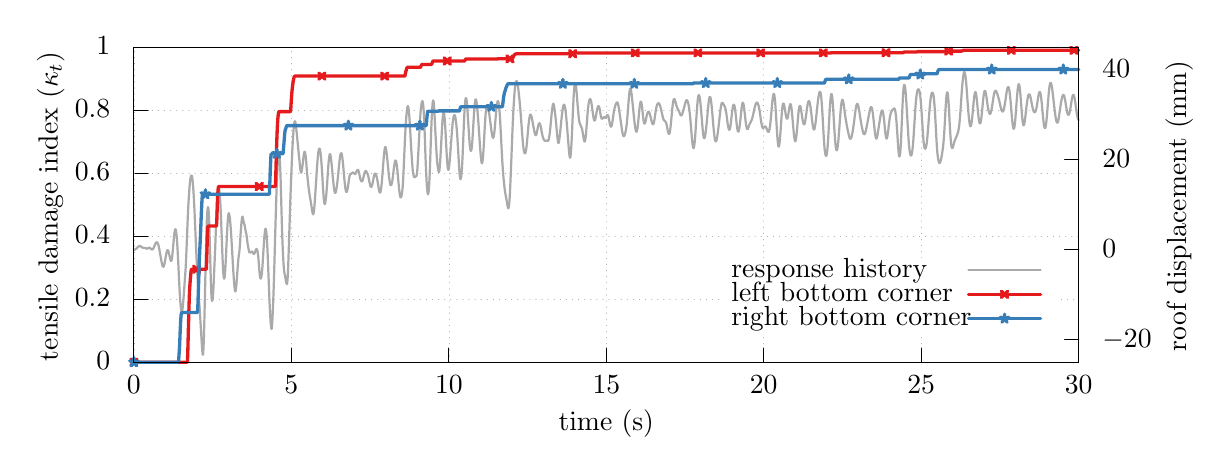
\begin{tikzpicture}[gnuplot]
%% generated with GNUPLOT 5.2p6 (Lua 5.3; terminal rev. Nov 2018, script rev. 107)
%% 07/30/2019 20:59:08
\path (0.000,0.000) rectangle (12.000,4.000);
\gpcolor{color=gp lt color axes}
\gpsetlinetype{gp lt axes}
\gpsetdashtype{gp dt axes}
\gpsetlinewidth{0.50}
\draw[gp path] (0.000,0.000)--(11.999,0.000);
\gpcolor{color=gp lt color border}
\gpsetlinetype{gp lt border}
\gpsetdashtype{gp dt solid}
\gpsetlinewidth{1.00}
\draw[gp path] (0.000,0.000)--(0.180,0.000);
\node[gp node right] at (-0.184,0.000) {$0$};
\gpcolor{color=gp lt color axes}
\gpsetlinetype{gp lt axes}
\gpsetdashtype{gp dt axes}
\gpsetlinewidth{0.50}
\draw[gp path] (0.000,0.800)--(7.471,0.800);
\draw[gp path] (11.699,0.800)--(11.999,0.800);
\gpcolor{color=gp lt color border}
\gpsetlinetype{gp lt border}
\gpsetdashtype{gp dt solid}
\gpsetlinewidth{1.00}
\draw[gp path] (0.000,0.800)--(0.180,0.800);
\node[gp node right] at (-0.184,0.800) {$0.2$};
\gpcolor{color=gp lt color axes}
\gpsetlinetype{gp lt axes}
\gpsetdashtype{gp dt axes}
\gpsetlinewidth{0.50}
\draw[gp path] (0.000,1.600)--(11.999,1.600);
\gpcolor{color=gp lt color border}
\gpsetlinetype{gp lt border}
\gpsetdashtype{gp dt solid}
\gpsetlinewidth{1.00}
\draw[gp path] (0.000,1.600)--(0.180,1.600);
\node[gp node right] at (-0.184,1.600) {$0.4$};
\gpcolor{color=gp lt color axes}
\gpsetlinetype{gp lt axes}
\gpsetdashtype{gp dt axes}
\gpsetlinewidth{0.50}
\draw[gp path] (0.000,2.399)--(11.999,2.399);
\gpcolor{color=gp lt color border}
\gpsetlinetype{gp lt border}
\gpsetdashtype{gp dt solid}
\gpsetlinewidth{1.00}
\draw[gp path] (0.000,2.399)--(0.180,2.399);
\node[gp node right] at (-0.184,2.399) {$0.6$};
\gpcolor{color=gp lt color axes}
\gpsetlinetype{gp lt axes}
\gpsetdashtype{gp dt axes}
\gpsetlinewidth{0.50}
\draw[gp path] (0.000,3.199)--(11.999,3.199);
\gpcolor{color=gp lt color border}
\gpsetlinetype{gp lt border}
\gpsetdashtype{gp dt solid}
\gpsetlinewidth{1.00}
\draw[gp path] (0.000,3.199)--(0.180,3.199);
\node[gp node right] at (-0.184,3.199) {$0.8$};
\gpcolor{color=gp lt color axes}
\gpsetlinetype{gp lt axes}
\gpsetdashtype{gp dt axes}
\gpsetlinewidth{0.50}
\draw[gp path] (0.000,3.999)--(11.999,3.999);
\gpcolor{color=gp lt color border}
\gpsetlinetype{gp lt border}
\gpsetdashtype{gp dt solid}
\gpsetlinewidth{1.00}
\draw[gp path] (0.000,3.999)--(0.180,3.999);
\node[gp node right] at (-0.184,3.999) {$1$};
\gpcolor{color=gp lt color axes}
\gpsetlinetype{gp lt axes}
\gpsetdashtype{gp dt axes}
\gpsetlinewidth{0.50}
\draw[gp path] (0.000,0.000)--(0.000,3.999);
\gpcolor{color=gp lt color border}
\gpsetlinetype{gp lt border}
\gpsetdashtype{gp dt solid}
\gpsetlinewidth{1.00}
\draw[gp path] (0.000,0.000)--(0.000,0.180);
\node[gp node center] at (0.000,-0.308) {$0$};
\gpcolor{color=gp lt color axes}
\gpsetlinetype{gp lt axes}
\gpsetdashtype{gp dt axes}
\gpsetlinewidth{0.50}
\draw[gp path] (2.000,0.000)--(2.000,3.999);
\gpcolor{color=gp lt color border}
\gpsetlinetype{gp lt border}
\gpsetdashtype{gp dt solid}
\gpsetlinewidth{1.00}
\draw[gp path] (2.000,0.000)--(2.000,0.180);
\node[gp node center] at (2.000,-0.308) {$5$};
\gpcolor{color=gp lt color axes}
\gpsetlinetype{gp lt axes}
\gpsetdashtype{gp dt axes}
\gpsetlinewidth{0.50}
\draw[gp path] (4.000,0.000)--(4.000,3.999);
\gpcolor{color=gp lt color border}
\gpsetlinetype{gp lt border}
\gpsetdashtype{gp dt solid}
\gpsetlinewidth{1.00}
\draw[gp path] (4.000,0.000)--(4.000,0.180);
\node[gp node center] at (4.000,-0.308) {$10$};
\gpcolor{color=gp lt color axes}
\gpsetlinetype{gp lt axes}
\gpsetdashtype{gp dt axes}
\gpsetlinewidth{0.50}
\draw[gp path] (6.000,0.000)--(6.000,3.999);
\gpcolor{color=gp lt color border}
\gpsetlinetype{gp lt border}
\gpsetdashtype{gp dt solid}
\gpsetlinewidth{1.00}
\draw[gp path] (6.000,0.000)--(6.000,0.180);
\node[gp node center] at (6.000,-0.308) {$15$};
\gpcolor{color=gp lt color axes}
\gpsetlinetype{gp lt axes}
\gpsetdashtype{gp dt axes}
\gpsetlinewidth{0.50}
\draw[gp path] (7.999,0.000)--(7.999,0.400);
\draw[gp path] (7.999,1.324)--(7.999,3.999);
\gpcolor{color=gp lt color border}
\gpsetlinetype{gp lt border}
\gpsetdashtype{gp dt solid}
\gpsetlinewidth{1.00}
\draw[gp path] (7.999,0.000)--(7.999,0.180);
\node[gp node center] at (7.999,-0.308) {$20$};
\gpcolor{color=gp lt color axes}
\gpsetlinetype{gp lt axes}
\gpsetdashtype{gp dt axes}
\gpsetlinewidth{0.50}
\draw[gp path] (9.999,0.000)--(9.999,0.400);
\draw[gp path] (9.999,1.324)--(9.999,3.999);
\gpcolor{color=gp lt color border}
\gpsetlinetype{gp lt border}
\gpsetdashtype{gp dt solid}
\gpsetlinewidth{1.00}
\draw[gp path] (9.999,0.000)--(9.999,0.180);
\node[gp node center] at (9.999,-0.308) {$25$};
\gpcolor{color=gp lt color axes}
\gpsetlinetype{gp lt axes}
\gpsetdashtype{gp dt axes}
\gpsetlinewidth{0.50}
\draw[gp path] (11.999,0.000)--(11.999,3.999);
\gpcolor{color=gp lt color border}
\gpsetlinetype{gp lt border}
\gpsetdashtype{gp dt solid}
\gpsetlinewidth{1.00}
\draw[gp path] (11.999,0.000)--(11.999,0.180);
\node[gp node center] at (11.999,-0.308) {$30$};
\draw[gp path] (11.999,0.286)--(11.819,0.286);
\node[gp node left] at (12.183,0.286) {$-20$};
\draw[gp path] (11.999,1.428)--(11.819,1.428);
\node[gp node left] at (12.183,1.428) {$0$};
\draw[gp path] (11.999,2.571)--(11.819,2.571);
\node[gp node left] at (12.183,2.571) {$20$};
\draw[gp path] (11.999,3.713)--(11.819,3.713);
\node[gp node left] at (12.183,3.713) {$40$};
\draw[gp path] (0.000,3.999)--(0.000,0.000)--(11.999,0.000)--(11.999,3.999)--cycle;
\node[gp node center,rotate=-270] at (-1.044,1.999) {tensile damage index ($\kappa_t$)};
\node[gp node center,rotate=-270] at (13.287,1.999) {roof displacement (\si{\milli\metre})};
\node[gp node center] at (5.999,-0.769) {time (\si{\second})};
\gpcolor{rgb color={0.667,0.667,0.667}}
\gpsetlinewidth{2.00}
\draw[gp path] (0.000,1.428)--(0.004,1.428)--(0.008,1.429)--(0.012,1.430)--(0.016,1.432)%
  --(0.020,1.435)--(0.024,1.438)--(0.028,1.441)--(0.032,1.445)--(0.036,1.448)--(0.040,1.452)%
  --(0.044,1.456)--(0.048,1.460)--(0.052,1.464)--(0.056,1.467)--(0.060,1.470)--(0.064,1.473)%
  --(0.068,1.475)--(0.072,1.476)--(0.076,1.476)--(0.080,1.475)--(0.084,1.473)--(0.088,1.470)%
  --(0.092,1.467)--(0.096,1.464)--(0.100,1.462)--(0.104,1.459)--(0.108,1.457)--(0.112,1.456)%
  --(0.116,1.454)--(0.120,1.454)--(0.124,1.453)--(0.128,1.452)--(0.132,1.452)--(0.136,1.451)%
  --(0.140,1.451)--(0.144,1.450)--(0.148,1.449)--(0.152,1.447)--(0.156,1.445)--(0.160,1.444)%
  --(0.164,1.443)--(0.168,1.442)--(0.172,1.443)--(0.176,1.445)--(0.180,1.448)--(0.184,1.451)%
  --(0.188,1.453)--(0.192,1.455)--(0.196,1.456)--(0.200,1.455)--(0.204,1.452)--(0.208,1.448)%
  --(0.212,1.444)--(0.216,1.439)--(0.220,1.436)--(0.224,1.434)--(0.228,1.433)--(0.232,1.432)%
  --(0.236,1.433)--(0.240,1.435)--(0.244,1.440)--(0.248,1.446)--(0.252,1.454)--(0.256,1.464)%
  --(0.260,1.474)--(0.264,1.484)--(0.268,1.494)--(0.272,1.503)--(0.276,1.511)--(0.280,1.516)%
  --(0.284,1.520)--(0.288,1.523)--(0.292,1.523)--(0.296,1.521)--(0.300,1.516)--(0.304,1.509)%
  --(0.308,1.498)--(0.312,1.485)--(0.316,1.469)--(0.320,1.451)--(0.324,1.430)--(0.328,1.407)%
  --(0.332,1.384)--(0.336,1.361)--(0.340,1.337)--(0.344,1.314)--(0.348,1.292)--(0.352,1.271)%
  --(0.356,1.252)--(0.360,1.236)--(0.364,1.223)--(0.368,1.215)--(0.372,1.211)--(0.376,1.213)%
  --(0.380,1.219)--(0.384,1.230)--(0.388,1.247)--(0.392,1.267)--(0.396,1.289)--(0.400,1.313)%
  --(0.404,1.337)--(0.408,1.360)--(0.412,1.381)--(0.416,1.399)--(0.420,1.413)--(0.424,1.421)%
  --(0.428,1.424)--(0.432,1.421)--(0.436,1.414)--(0.440,1.403)--(0.444,1.388)--(0.448,1.371)%
  --(0.452,1.352)--(0.456,1.334)--(0.460,1.316)--(0.464,1.301)--(0.468,1.290)--(0.472,1.285)%
  --(0.476,1.288)--(0.480,1.302)--(0.484,1.326)--(0.488,1.360)--(0.492,1.399)--(0.496,1.443)%
  --(0.500,1.488)--(0.504,1.533)--(0.508,1.577)--(0.512,1.616)--(0.516,1.649)--(0.520,1.672)%
  --(0.524,1.686)--(0.528,1.689)--(0.532,1.681)--(0.536,1.662)--(0.540,1.631)--(0.544,1.589)%
  --(0.548,1.536)--(0.552,1.474)--(0.556,1.405)--(0.560,1.329)--(0.564,1.249)--(0.568,1.165)%
  --(0.572,1.080)--(0.576,0.997)--(0.580,0.919)--(0.584,0.848)--(0.588,0.787)--(0.592,0.737)%
  --(0.596,0.698)--(0.600,0.670)--(0.604,0.652)--(0.608,0.646)--(0.612,0.651)--(0.616,0.669)%
  --(0.620,0.698)--(0.624,0.737)--(0.628,0.783)--(0.632,0.836)--(0.636,0.892)--(0.640,0.949)%
  --(0.644,1.005)--(0.648,1.061)--(0.652,1.116)--(0.656,1.177)--(0.660,1.248)--(0.664,1.332)%
  --(0.668,1.429)--(0.672,1.531)--(0.676,1.636)--(0.680,1.737)--(0.684,1.833)--(0.688,1.922)%
  --(0.692,2.001)--(0.696,2.072)--(0.700,2.134)--(0.704,2.191)--(0.708,2.241)--(0.712,2.284)%
  --(0.716,2.318)--(0.720,2.343)--(0.724,2.361)--(0.728,2.370)--(0.732,2.372)--(0.736,2.366)%
  --(0.740,2.350)--(0.744,2.323)--(0.748,2.284)--(0.752,2.235)--(0.756,2.176)--(0.760,2.110)%
  --(0.764,2.037)--(0.768,1.956)--(0.772,1.868)--(0.776,1.776)--(0.780,1.682)--(0.784,1.588)%
  --(0.788,1.495)--(0.792,1.404)--(0.796,1.316)--(0.800,1.233)--(0.804,1.155)--(0.808,1.081)%
  --(0.812,1.012)--(0.816,0.949)--(0.820,0.891)--(0.824,0.836)--(0.828,0.782)--(0.832,0.725)%
  --(0.836,0.665)--(0.840,0.603)--(0.844,0.540)--(0.848,0.475)--(0.852,0.408)--(0.856,0.340)%
  --(0.860,0.272)--(0.864,0.207)--(0.868,0.149)--(0.872,0.108)--(0.876,0.094)--(0.880,0.116)%
  --(0.884,0.181)--(0.888,0.286)--(0.892,0.423)--(0.896,0.580)--(0.900,0.750)--(0.904,0.928)%
  --(0.908,1.111)--(0.912,1.293)--(0.916,1.464)--(0.920,1.614)--(0.924,1.739)--(0.928,1.836)%
  --(0.932,1.905)--(0.936,1.949)--(0.940,1.969)--(0.944,1.965)--(0.948,1.934)--(0.952,1.874)%
  --(0.956,1.783)--(0.960,1.665)--(0.964,1.525)--(0.968,1.371)--(0.972,1.214)--(0.976,1.067)%
  --(0.980,0.945)--(0.984,0.856)--(0.988,0.802)--(0.992,0.779)--(0.996,0.779)--(1.000,0.800)%
  --(1.004,0.840)--(1.008,0.902)--(1.012,0.983)--(1.016,1.073)--(1.020,1.165)--(1.024,1.254)%
  --(1.028,1.342)--(1.032,1.437)--(1.036,1.542)--(1.040,1.654)--(1.044,1.764)--(1.048,1.864)%
  --(1.052,1.950)--(1.056,2.022)--(1.060,2.082)--(1.064,2.131)--(1.068,2.169)--(1.072,2.197)%
  --(1.076,2.211)--(1.080,2.211)--(1.084,2.194)--(1.088,2.161)--(1.092,2.113)--(1.096,2.051)%
  --(1.100,1.976)--(1.104,1.889)--(1.108,1.792)--(1.112,1.687)--(1.116,1.579)--(1.120,1.470)%
  --(1.124,1.366)--(1.128,1.272)--(1.132,1.192)--(1.136,1.128)--(1.140,1.085)--(1.144,1.063)%
  --(1.148,1.061)--(1.152,1.080)--(1.156,1.117)--(1.160,1.171)--(1.164,1.239)--(1.168,1.318)%
  --(1.172,1.403)--(1.176,1.491)--(1.180,1.579)--(1.184,1.662)--(1.188,1.736)--(1.192,1.799)%
  --(1.196,1.847)--(1.200,1.878)--(1.204,1.892)--(1.208,1.889)--(1.212,1.873)--(1.216,1.847)%
  --(1.220,1.814)--(1.224,1.774)--(1.228,1.726)--(1.232,1.670)--(1.236,1.607)--(1.240,1.541)%
  --(1.244,1.473)--(1.248,1.404)--(1.252,1.335)--(1.256,1.266)--(1.260,1.198)--(1.264,1.133)%
  --(1.268,1.073)--(1.272,1.018)--(1.276,0.970)--(1.280,0.932)--(1.284,0.907)--(1.288,0.898)%
  --(1.292,0.906)--(1.296,0.931)--(1.300,0.968)--(1.304,1.013)--(1.308,1.063)--(1.312,1.117)%
  --(1.316,1.174)--(1.320,1.229)--(1.324,1.280)--(1.328,1.322)--(1.332,1.352)--(1.336,1.379)%
  --(1.340,1.410)--(1.344,1.454)--(1.348,1.512)--(1.352,1.577)--(1.356,1.642)--(1.360,1.699)%
  --(1.364,1.748)--(1.368,1.790)--(1.372,1.824)--(1.376,1.845)--(1.380,1.849)--(1.384,1.835)%
  --(1.388,1.811)--(1.392,1.788)--(1.396,1.773)--(1.400,1.762)--(1.404,1.750)--(1.408,1.731)%
  --(1.412,1.707)--(1.416,1.683)--(1.420,1.663)--(1.424,1.646)--(1.428,1.628)--(1.432,1.603)%
  --(1.436,1.571)--(1.440,1.537)--(1.444,1.506)--(1.448,1.480)--(1.452,1.457)--(1.456,1.437)%
  --(1.460,1.418)--(1.464,1.404)--(1.468,1.396)--(1.472,1.393)--(1.476,1.394)--(1.480,1.395)%
  --(1.484,1.397)--(1.488,1.399)--(1.492,1.402)--(1.496,1.405)--(1.500,1.406)--(1.504,1.403)%
  --(1.508,1.397)--(1.512,1.388)--(1.516,1.381)--(1.520,1.377)--(1.524,1.376)--(1.528,1.378)%
  --(1.532,1.384)--(1.536,1.393)--(1.540,1.403)--(1.544,1.415)--(1.548,1.426)--(1.552,1.435)%
  --(1.556,1.439)--(1.560,1.438)--(1.564,1.432)--(1.568,1.419)--(1.572,1.398)--(1.576,1.369)%
  --(1.580,1.332)--(1.584,1.286)--(1.588,1.235)--(1.592,1.183)--(1.596,1.135)--(1.600,1.097)%
  --(1.604,1.073)--(1.608,1.063)--(1.612,1.063)--(1.616,1.073)--(1.620,1.091)--(1.624,1.119)%
  --(1.628,1.158)--(1.632,1.209)--(1.636,1.269)--(1.640,1.334)--(1.644,1.399)--(1.648,1.463)%
  --(1.652,1.524)--(1.656,1.580)--(1.660,1.628)--(1.664,1.664)--(1.668,1.687)--(1.672,1.695)%
  --(1.676,1.688)--(1.680,1.666)--(1.684,1.630)--(1.688,1.578)--(1.692,1.511)--(1.696,1.432)%
  --(1.700,1.341)--(1.704,1.243)--(1.708,1.140)--(1.712,1.034)--(1.716,0.929)--(1.720,0.827)%
  --(1.724,0.733)--(1.728,0.650)--(1.732,0.579)--(1.736,0.519)--(1.740,0.469)--(1.744,0.434)%
  --(1.748,0.422)--(1.752,0.437)--(1.756,0.483)--(1.760,0.555)--(1.764,0.644)--(1.768,0.743)%
  --(1.772,0.849)--(1.776,0.965)--(1.780,1.095)--(1.784,1.236)--(1.788,1.382)--(1.792,1.528)%
  --(1.796,1.672)--(1.800,1.813)--(1.804,1.949)--(1.808,2.077)--(1.812,2.192)--(1.816,2.297)%
  --(1.820,2.390)--(1.824,2.471)--(1.828,2.541)--(1.832,2.597)--(1.836,2.637)--(1.840,2.657)%
  --(1.844,2.656)--(1.848,2.633)--(1.852,2.587)--(1.856,2.517)--(1.860,2.422)--(1.864,2.303)%
  --(1.868,2.164)--(1.872,2.014)--(1.876,1.866)--(1.880,1.729)--(1.884,1.607)--(1.888,1.501)%
  --(1.892,1.406)--(1.896,1.323)--(1.900,1.253)--(1.904,1.199)--(1.908,1.161)--(1.912,1.134)%
  --(1.916,1.113)--(1.920,1.092)--(1.924,1.071)--(1.928,1.049)--(1.932,1.027)--(1.936,1.008)%
  --(1.940,0.994)--(1.944,0.993)--(1.948,1.013)--(1.952,1.061)--(1.956,1.136)--(1.960,1.236)%
  --(1.964,1.350)--(1.968,1.472)--(1.972,1.597)--(1.976,1.725)--(1.980,1.852)--(1.984,1.976)%
  --(1.988,2.095)--(1.992,2.206)--(1.996,2.312)--(2.000,2.411)--(2.004,2.506)--(2.008,2.597)%
  --(2.012,2.685)--(2.016,2.767)--(2.020,2.841)--(2.024,2.904)--(2.028,2.957)--(2.032,2.998)%
  --(2.036,3.030)--(2.040,3.051)--(2.044,3.060)--(2.048,3.058)--(2.052,3.043)--(2.056,3.018)%
  --(2.060,2.986)--(2.064,2.950)--(2.068,2.912)--(2.072,2.872)--(2.076,2.831)--(2.080,2.787)%
  --(2.084,2.744)--(2.088,2.702)--(2.092,2.662)--(2.096,2.623)--(2.100,2.585)--(2.104,2.545)%
  --(2.108,2.504)--(2.112,2.465)--(2.116,2.433)--(2.120,2.413)--(2.124,2.407)--(2.128,2.414)%
  --(2.132,2.432)--(2.136,2.457)--(2.140,2.486)--(2.144,2.518)--(2.148,2.554)--(2.152,2.590)%
  --(2.156,2.623)--(2.160,2.650)--(2.164,2.667)--(2.168,2.673)--(2.172,2.668)--(2.176,2.653)%
  --(2.180,2.627)--(2.184,2.590)--(2.188,2.546)--(2.192,2.496)--(2.196,2.446)--(2.200,2.399)%
  --(2.204,2.355)--(2.208,2.314)--(2.212,2.276)--(2.216,2.240)--(2.220,2.207)--(2.224,2.176)%
  --(2.228,2.149)--(2.232,2.124)--(2.236,2.100)--(2.240,2.076)--(2.244,2.052)--(2.248,2.027)%
  --(2.252,2.002)--(2.256,1.976)--(2.260,1.950)--(2.264,1.924)--(2.268,1.901)--(2.272,1.885)%
  --(2.276,1.878)--(2.280,1.884)--(2.284,1.903)--(2.288,1.934)--(2.292,1.975)--(2.296,2.024)%
  --(2.300,2.079)--(2.304,2.139)--(2.308,2.202)--(2.312,2.267)--(2.316,2.330)--(2.320,2.392)%
  --(2.324,2.451)--(2.328,2.508)--(2.332,2.561)--(2.336,2.608)--(2.340,2.647)--(2.344,2.677)%
  --(2.348,2.697)--(2.352,2.710)--(2.356,2.714)--(2.360,2.710)--(2.364,2.697)--(2.368,2.675)%
  --(2.372,2.644)--(2.376,2.604)--(2.380,2.557)--(2.384,2.504)--(2.388,2.445)--(2.392,2.380)%
  --(2.396,2.312)--(2.400,2.243)--(2.404,2.178)--(2.408,2.120)--(2.412,2.072)--(2.416,2.037)%
  --(2.420,2.016)--(2.424,2.008)--(2.428,2.015)--(2.432,2.033)--(2.436,2.060)--(2.440,2.096)%
  --(2.444,2.137)--(2.448,2.185)--(2.452,2.239)--(2.456,2.298)--(2.460,2.360)--(2.464,2.421)%
  --(2.468,2.478)--(2.472,2.529)--(2.476,2.572)--(2.480,2.607)--(2.484,2.631)--(2.488,2.643)%
  --(2.492,2.642)--(2.496,2.630)--(2.500,2.608)--(2.504,2.578)--(2.508,2.545)--(2.512,2.507)%
  --(2.516,2.467)--(2.520,2.423)--(2.524,2.379)--(2.528,2.335)--(2.532,2.294)--(2.536,2.255)%
  --(2.540,2.221)--(2.544,2.192)--(2.548,2.170)--(2.552,2.156)--(2.556,2.150)--(2.560,2.153)%
  --(2.564,2.162)--(2.568,2.177)--(2.572,2.198)--(2.576,2.224)--(2.580,2.254)--(2.584,2.288)%
  --(2.588,2.324)--(2.592,2.362)--(2.596,2.402)--(2.600,2.444)--(2.604,2.486)--(2.608,2.527)%
  --(2.612,2.564)--(2.616,2.595)--(2.620,2.620)--(2.624,2.639)--(2.628,2.651)--(2.632,2.655)%
  --(2.636,2.653)--(2.640,2.641)--(2.644,2.621)--(2.648,2.593)--(2.652,2.558)--(2.656,2.517)%
  --(2.660,2.473)--(2.664,2.426)--(2.668,2.380)--(2.672,2.335)--(2.676,2.294)--(2.680,2.256)%
  --(2.684,2.222)--(2.688,2.195)--(2.692,2.176)--(2.696,2.164)--(2.700,2.161)--(2.704,2.165)%
  --(2.708,2.175)--(2.712,2.192)--(2.716,2.213)--(2.720,2.238)--(2.724,2.266)--(2.728,2.295)%
  --(2.732,2.323)--(2.736,2.347)--(2.740,2.367)--(2.744,2.382)--(2.748,2.390)--(2.752,2.393)%
  --(2.756,2.393)--(2.760,2.393)--(2.764,2.395)--(2.768,2.399)--(2.772,2.404)--(2.776,2.407)%
  --(2.780,2.409)--(2.784,2.409)--(2.788,2.407)--(2.792,2.405)--(2.796,2.401)--(2.800,2.396)%
  --(2.804,2.392)--(2.808,2.390)--(2.812,2.391)--(2.816,2.397)--(2.820,2.405)--(2.824,2.414)%
  --(2.828,2.423)--(2.832,2.431)--(2.836,2.437)--(2.840,2.442)--(2.844,2.443)--(2.848,2.441)%
  --(2.852,2.433)--(2.856,2.420)--(2.860,2.403)--(2.864,2.383)--(2.868,2.363)--(2.872,2.344)%
  --(2.876,2.326)--(2.880,2.313)--(2.884,2.304)--(2.888,2.298)--(2.892,2.296)--(2.896,2.297)%
  --(2.900,2.302)--(2.904,2.310)--(2.908,2.322)--(2.912,2.337)--(2.916,2.353)--(2.920,2.369)%
  --(2.924,2.384)--(2.928,2.399)--(2.932,2.411)--(2.936,2.421)--(2.940,2.427)--(2.944,2.429)%
  --(2.948,2.427)--(2.952,2.422)--(2.956,2.416)--(2.960,2.408)--(2.964,2.400)--(2.968,2.390)%
  --(2.972,2.378)--(2.976,2.364)--(2.980,2.347)--(2.984,2.328)--(2.988,2.307)--(2.992,2.286)%
  --(2.996,2.266)--(3.000,2.249)--(3.004,2.237)--(3.008,2.229)--(3.012,2.226)--(3.016,2.228)%
  --(3.020,2.234)--(3.024,2.245)--(3.028,2.261)--(3.032,2.279)--(3.036,2.299)--(3.040,2.319)%
  --(3.044,2.339)--(3.048,2.358)--(3.052,2.374)--(3.056,2.387)--(3.060,2.395)--(3.064,2.398)%
  --(3.068,2.395)--(3.072,2.389)--(3.076,2.378)--(3.080,2.365)--(3.084,2.350)--(3.088,2.332)%
  --(3.092,2.312)--(3.096,2.288)--(3.100,2.263)--(3.104,2.237)--(3.108,2.212)--(3.112,2.190)%
  --(3.116,2.173)--(3.120,2.161)--(3.124,2.154)--(3.128,2.155)--(3.132,2.164)--(3.136,2.182)%
  --(3.140,2.209)--(3.144,2.244)--(3.148,2.284)--(3.152,2.330)--(3.156,2.379)--(3.160,2.431)%
  --(3.164,2.485)--(3.168,2.537)--(3.172,2.587)--(3.176,2.631)--(3.180,2.670)--(3.184,2.701)%
  --(3.188,2.723)--(3.192,2.734)--(3.196,2.732)--(3.200,2.718)--(3.204,2.694)--(3.208,2.664)%
  --(3.212,2.631)--(3.216,2.595)--(3.220,2.557)--(3.224,2.517)--(3.228,2.474)--(3.232,2.432)%
  --(3.236,2.393)--(3.240,2.357)--(3.244,2.326)--(3.248,2.299)--(3.252,2.276)--(3.256,2.259)%
  --(3.260,2.249)--(3.264,2.246)--(3.268,2.250)--(3.272,2.259)--(3.276,2.274)--(3.280,2.294)%
  --(3.284,2.319)--(3.288,2.348)--(3.292,2.381)--(3.296,2.415)--(3.300,2.449)--(3.304,2.480)%
  --(3.308,2.508)--(3.312,2.532)--(3.316,2.550)--(3.320,2.561)--(3.324,2.563)--(3.328,2.556)%
  --(3.332,2.541)--(3.336,2.519)--(3.340,2.491)--(3.344,2.457)--(3.348,2.418)--(3.352,2.375)%
  --(3.356,2.330)--(3.360,2.285)--(3.364,2.243)--(3.368,2.203)--(3.372,2.167)--(3.376,2.137)%
  --(3.380,2.114)--(3.384,2.099)--(3.388,2.093)--(3.392,2.094)--(3.396,2.103)--(3.400,2.117)%
  --(3.404,2.139)--(3.408,2.168)--(3.412,2.208)--(3.416,2.263)--(3.420,2.332)--(3.424,2.413)%
  --(3.428,2.502)--(3.432,2.595)--(3.436,2.687)--(3.440,2.777)--(3.444,2.864)--(3.448,2.943)%
  --(3.452,3.012)--(3.456,3.072)--(3.460,3.124)--(3.464,3.168)--(3.468,3.204)--(3.472,3.232)%
  --(3.476,3.248)--(3.480,3.252)--(3.484,3.243)--(3.488,3.222)--(3.492,3.189)--(3.496,3.146)%
  --(3.500,3.092)--(3.504,3.029)--(3.508,2.960)--(3.512,2.889)--(3.516,2.818)--(3.520,2.748)%
  --(3.524,2.681)--(3.528,2.616)--(3.532,2.555)--(3.536,2.500)--(3.540,2.455)--(3.544,2.419)%
  --(3.548,2.393)--(3.552,2.373)--(3.556,2.360)--(3.560,2.352)--(3.564,2.349)--(3.568,2.350)%
  --(3.572,2.353)--(3.576,2.357)--(3.580,2.360)--(3.584,2.361)--(3.588,2.364)--(3.592,2.376)%
  --(3.596,2.406)--(3.600,2.454)--(3.604,2.517)--(3.608,2.589)--(3.612,2.663)--(3.616,2.736)%
  --(3.620,2.810)--(3.624,2.887)--(3.628,2.965)--(3.632,3.042)--(3.636,3.110)--(3.640,3.168)%
  --(3.644,3.215)--(3.648,3.250)--(3.652,3.277)--(3.656,3.298)--(3.660,3.311)--(3.664,3.316)%
  --(3.668,3.309)--(3.672,3.287)--(3.676,3.248)--(3.680,3.193)--(3.684,3.122)--(3.688,3.035)%
  --(3.692,2.934)--(3.696,2.822)--(3.700,2.705)--(3.704,2.591)--(3.708,2.487)--(3.712,2.395)%
  --(3.716,2.317)--(3.720,2.251)--(3.724,2.200)--(3.728,2.162)--(3.732,2.140)--(3.736,2.133)%
  --(3.740,2.144)--(3.744,2.174)--(3.748,2.224)--(3.752,2.293)--(3.756,2.380)--(3.760,2.483)%
  --(3.764,2.596)--(3.768,2.715)--(3.772,2.834)--(3.776,2.948)--(3.780,3.052)--(3.784,3.143)%
  --(3.788,3.217)--(3.792,3.272)--(3.796,3.308)--(3.800,3.324)--(3.804,3.321)--(3.808,3.297)%
  --(3.812,3.249)--(3.816,3.183)--(3.820,3.103)--(3.824,3.020)--(3.828,2.940)--(3.832,2.865)%
  --(3.836,2.792)--(3.840,2.719)--(3.844,2.649)--(3.848,2.588)--(3.852,2.538)--(3.856,2.501)%
  --(3.860,2.473)--(3.864,2.449)--(3.868,2.429)--(3.872,2.416)--(3.876,2.418)--(3.880,2.437)%
  --(3.884,2.475)--(3.888,2.528)--(3.892,2.590)--(3.896,2.658)--(3.900,2.729)--(3.904,2.804)%
  --(3.908,2.881)--(3.912,2.956)--(3.916,3.025)--(3.920,3.082)--(3.924,3.126)--(3.928,3.156)%
  --(3.932,3.172)--(3.936,3.173)--(3.940,3.159)--(3.944,3.127)--(3.948,3.080)--(3.952,3.020)%
  --(3.956,2.950)--(3.960,2.875)--(3.964,2.798)--(3.968,2.722)--(3.972,2.650)--(3.976,2.585)%
  --(3.980,2.530)--(3.984,2.486)--(3.988,2.457)--(3.992,2.444)--(3.996,2.446)--(4.000,2.463)%
  --(4.004,2.492)--(4.008,2.530)--(4.012,2.575)--(4.016,2.625)--(4.020,2.677)--(4.024,2.731)%
  --(4.028,2.785)--(4.032,2.840)--(4.036,2.893)--(4.040,2.945)--(4.044,2.992)--(4.048,3.034)%
  --(4.052,3.067)--(4.056,3.094)--(4.060,3.114)--(4.064,3.128)--(4.068,3.137)--(4.072,3.139)%
  --(4.076,3.135)--(4.080,3.122)--(4.084,3.103)--(4.088,3.077)--(4.092,3.045)--(4.096,3.007)%
  --(4.100,2.962)--(4.104,2.910)--(4.108,2.852)--(4.112,2.790)--(4.116,2.724)--(4.120,2.655)%
  --(4.124,2.585)--(4.128,2.516)--(4.132,2.452)--(4.136,2.397)--(4.140,2.356)--(4.144,2.331)%
  --(4.148,2.324)--(4.152,2.332)--(4.156,2.354)--(4.160,2.388)--(4.164,2.434)--(4.168,2.495)%
  --(4.172,2.570)--(4.176,2.659)--(4.180,2.757)--(4.184,2.859)--(4.188,2.960)--(4.192,3.055)%
  --(4.196,3.141)--(4.200,3.215)--(4.204,3.275)--(4.208,3.317)--(4.212,3.343)--(4.216,3.354)%
  --(4.220,3.351)--(4.224,3.334)--(4.228,3.304)--(4.232,3.261)--(4.236,3.206)--(4.240,3.142)%
  --(4.244,3.076)--(4.248,3.010)--(4.252,2.946)--(4.256,2.885)--(4.260,2.828)--(4.264,2.778)%
  --(4.268,2.738)--(4.272,2.708)--(4.276,2.690)--(4.280,2.684)--(4.284,2.689)--(4.288,2.707)%
  --(4.292,2.738)--(4.296,2.782)--(4.300,2.837)--(4.304,2.900)--(4.308,2.968)--(4.312,3.038)%
  --(4.316,3.105)--(4.320,3.169)--(4.324,3.225)--(4.328,3.272)--(4.332,3.306)--(4.336,3.329)%
  --(4.340,3.338)--(4.344,3.336)--(4.348,3.324)--(4.352,3.302)--(4.356,3.271)--(4.360,3.232)%
  --(4.364,3.186)--(4.368,3.136)--(4.372,3.083)--(4.376,3.029)--(4.380,2.971)--(4.384,2.912)%
  --(4.388,2.853)--(4.392,2.793)--(4.396,2.737)--(4.400,2.684)--(4.404,2.635)--(4.408,2.592)%
  --(4.412,2.558)--(4.416,2.535)--(4.420,2.527)--(4.424,2.533)--(4.428,2.554)--(4.432,2.589)%
  --(4.436,2.637)--(4.440,2.695)--(4.444,2.762)--(4.448,2.835)--(4.452,2.910)--(4.456,2.983)%
  --(4.460,3.052)--(4.464,3.113)--(4.468,3.165)--(4.472,3.206)--(4.476,3.235)--(4.480,3.253)%
  --(4.484,3.262)--(4.488,3.262)--(4.492,3.257)--(4.496,3.247)--(4.500,3.231)--(4.504,3.211)%
  --(4.508,3.187)--(4.512,3.161)--(4.516,3.132)--(4.520,3.102)--(4.524,3.070)--(4.528,3.038)%
  --(4.532,3.005)--(4.536,2.973)--(4.540,2.944)--(4.544,2.917)--(4.548,2.892)--(4.552,2.872)%
  --(4.556,2.858)--(4.560,2.850)--(4.564,2.851)--(4.568,2.861)--(4.572,2.879)--(4.576,2.906)%
  --(4.580,2.941)--(4.584,2.984)--(4.588,3.031)--(4.592,3.081)--(4.596,3.130)--(4.600,3.176)%
  --(4.604,3.218)--(4.608,3.254)--(4.612,3.284)--(4.616,3.304)--(4.620,3.316)--(4.624,3.317)%
  --(4.628,3.308)--(4.632,3.291)--(4.636,3.264)--(4.640,3.227)--(4.644,3.179)--(4.648,3.121)%
  --(4.652,3.054)--(4.656,2.983)--(4.660,2.908)--(4.664,2.830)--(4.668,2.752)--(4.672,2.674)%
  --(4.676,2.599)--(4.680,2.529)--(4.684,2.466)--(4.688,2.411)--(4.692,2.363)--(4.696,2.320)%
  --(4.700,2.280)--(4.704,2.242)--(4.708,2.207)--(4.712,2.177)--(4.716,2.151)--(4.720,2.129)%
  --(4.724,2.108)--(4.728,2.088)--(4.732,2.065)--(4.736,2.042)--(4.740,2.016)--(4.744,1.992)%
  --(4.748,1.971)--(4.752,1.958)--(4.756,1.955)--(4.760,1.965)--(4.764,1.990)--(4.768,2.030)%
  --(4.772,2.087)--(4.776,2.159)--(4.780,2.244)--(4.784,2.337)--(4.788,2.435)--(4.792,2.536)%
  --(4.796,2.639)--(4.800,2.742)--(4.804,2.847)--(4.808,2.949)--(4.812,3.045)--(4.816,3.132)%
  --(4.820,3.209)--(4.824,3.278)--(4.828,3.341)--(4.832,3.399)--(4.836,3.450)--(4.840,3.492)%
  --(4.844,3.524)--(4.848,3.547)--(4.852,3.561)--(4.856,3.568)--(4.860,3.570)--(4.864,3.567)%
  --(4.868,3.557)--(4.872,3.540)--(4.876,3.516)--(4.880,3.486)--(4.884,3.452)--(4.888,3.417)%
  --(4.892,3.380)--(4.896,3.342)--(4.900,3.301)--(4.904,3.256)--(4.908,3.208)--(4.912,3.157)%
  --(4.916,3.104)--(4.920,3.049)--(4.924,2.995)--(4.928,2.941)--(4.932,2.888)--(4.936,2.837)%
  --(4.940,2.790)--(4.944,2.749)--(4.948,2.715)--(4.952,2.690)--(4.956,2.672)--(4.960,2.660)%
  --(4.964,2.653)--(4.968,2.652)--(4.972,2.657)--(4.976,2.670)--(4.980,2.691)--(4.984,2.719)%
  --(4.988,2.754)--(4.992,2.794)--(4.996,2.837)--(5.000,2.884)--(5.004,2.930)--(5.008,2.974)%
  --(5.012,3.015)--(5.016,3.051)--(5.020,3.082)--(5.024,3.109)--(5.028,3.129)--(5.032,3.141)%
  --(5.036,3.146)--(5.040,3.143)--(5.044,3.136)--(5.048,3.125)--(5.052,3.110)--(5.056,3.092)%
  --(5.060,3.071)--(5.064,3.048)--(5.068,3.025)--(5.072,3.003)--(5.076,2.983)--(5.080,2.962)%
  --(5.084,2.941)--(5.088,2.922)--(5.092,2.905)--(5.096,2.893)--(5.100,2.885)--(5.104,2.883)%
  --(5.108,2.887)--(5.112,2.896)--(5.116,2.910)--(5.120,2.929)--(5.124,2.950)--(5.128,2.971)%
  --(5.132,2.991)--(5.136,3.008)--(5.140,3.021)--(5.144,3.030)--(5.148,3.035)--(5.152,3.035)%
  --(5.156,3.029)--(5.160,3.019)--(5.164,3.004)--(5.168,2.986)--(5.172,2.965)--(5.176,2.943)%
  --(5.180,2.921)--(5.184,2.900)--(5.188,2.882)--(5.192,2.866)--(5.196,2.853)--(5.200,2.841)%
  --(5.204,2.832)--(5.208,2.824)--(5.212,2.819)--(5.216,2.815)--(5.220,2.813)--(5.224,2.812)%
  --(5.228,2.813)--(5.232,2.813)--(5.236,2.815)--(5.240,2.815)--(5.244,2.815)--(5.248,2.814)%
  --(5.252,2.812)--(5.256,2.811)--(5.260,2.812)--(5.264,2.818)--(5.268,2.829)--(5.272,2.847)%
  --(5.276,2.871)--(5.280,2.899)--(5.284,2.932)--(5.288,2.969)--(5.292,3.011)--(5.296,3.055)%
  --(5.300,3.100)--(5.304,3.143)--(5.308,3.182)--(5.312,3.217)--(5.316,3.246)--(5.320,3.267)%
  --(5.324,3.280)--(5.328,3.283)--(5.332,3.274)--(5.336,3.255)--(5.340,3.228)--(5.344,3.198)%
  --(5.348,3.166)--(5.352,3.133)--(5.356,3.097)--(5.360,3.057)--(5.364,3.014)--(5.368,2.969)%
  --(5.372,2.923)--(5.376,2.881)--(5.380,2.842)--(5.384,2.810)--(5.388,2.790)--(5.392,2.783)%
  --(5.396,2.791)--(5.400,2.812)--(5.404,2.840)--(5.408,2.873)--(5.412,2.908)--(5.416,2.946)%
  --(5.420,2.987)--(5.424,3.029)--(5.428,3.069)--(5.432,3.107)--(5.436,3.142)--(5.440,3.174)%
  --(5.444,3.204)--(5.448,3.230)--(5.452,3.250)--(5.456,3.264)--(5.460,3.270)--(5.464,3.270)%
  --(5.468,3.264)--(5.472,3.253)--(5.476,3.234)--(5.480,3.209)--(5.484,3.176)--(5.488,3.138)%
  --(5.492,3.096)--(5.496,3.051)--(5.500,3.004)--(5.504,2.955)--(5.508,2.904)--(5.512,2.852)%
  --(5.516,2.801)--(5.520,2.750)--(5.524,2.701)--(5.528,2.657)--(5.532,2.623)--(5.536,2.601)%
  --(5.540,2.597)--(5.544,2.610)--(5.548,2.642)--(5.552,2.690)--(5.556,2.753)--(5.560,2.830)%
  --(5.564,2.917)--(5.568,3.011)--(5.572,3.105)--(5.576,3.197)--(5.580,3.283)--(5.584,3.360)%
  --(5.588,3.425)--(5.592,3.477)--(5.596,3.513)--(5.600,3.536)--(5.604,3.546)--(5.608,3.544)%
  --(5.612,3.529)--(5.616,3.501)--(5.620,3.461)--(5.624,3.412)--(5.628,3.359)--(5.632,3.306)%
  --(5.636,3.256)--(5.640,3.209)--(5.644,3.163)--(5.648,3.122)--(5.652,3.086)--(5.656,3.060)%
  --(5.660,3.042)--(5.664,3.029)--(5.668,3.020)--(5.672,3.011)--(5.676,3.002)--(5.680,2.993)%
  --(5.684,2.984)--(5.688,2.973)--(5.692,2.959)--(5.696,2.940)--(5.700,2.916)--(5.704,2.891)%
  --(5.708,2.865)--(5.712,2.841)--(5.716,2.821)--(5.720,2.808)--(5.724,2.803)--(5.728,2.807)%
  --(5.732,2.822)--(5.736,2.849)--(5.740,2.886)--(5.744,2.931)--(5.748,2.981)--(5.752,3.034)%
  --(5.756,3.088)--(5.760,3.140)--(5.764,3.188)--(5.768,3.229)--(5.772,3.262)--(5.776,3.289)%
  --(5.780,3.310)--(5.784,3.326)--(5.788,3.337)--(5.792,3.343)--(5.796,3.342)--(5.800,3.336)%
  --(5.804,3.323)--(5.808,3.306)--(5.812,3.283)--(5.816,3.257)--(5.820,3.228)--(5.824,3.197)%
  --(5.828,3.167)--(5.832,3.139)--(5.836,3.114)--(5.840,3.093)--(5.844,3.077)--(5.848,3.069)%
  --(5.852,3.068)--(5.856,3.075)--(5.860,3.089)--(5.864,3.108)--(5.868,3.129)--(5.872,3.151)%
  --(5.876,3.173)--(5.880,3.195)--(5.884,3.215)--(5.888,3.231)--(5.892,3.244)--(5.896,3.251)%
  --(5.900,3.253)--(5.904,3.250)--(5.908,3.243)--(5.912,3.230)--(5.916,3.211)--(5.920,3.187)%
  --(5.924,3.161)--(5.928,3.136)--(5.932,3.116)--(5.936,3.103)--(5.940,3.096)--(5.944,3.093)%
  --(5.948,3.093)--(5.952,3.095)--(5.956,3.098)--(5.960,3.103)--(5.964,3.109)--(5.968,3.112)%
  --(5.972,3.112)--(5.976,3.110)--(5.980,3.107)--(5.984,3.105)--(5.988,3.105)--(5.992,3.108)%
  --(5.996,3.113)--(6.000,3.119)--(6.003,3.125)--(6.007,3.132)--(6.011,3.137)--(6.015,3.139)%
  --(6.019,3.137)--(6.023,3.130)--(6.027,3.118)--(6.031,3.101)--(6.035,3.080)--(6.039,3.058)%
  --(6.043,3.036)--(6.047,3.017)--(6.051,3.002)--(6.055,2.993)--(6.059,2.990)--(6.063,2.993)%
  --(6.067,3.003)--(6.071,3.019)--(6.075,3.040)--(6.079,3.066)--(6.083,3.094)--(6.087,3.123)%
  --(6.091,3.151)--(6.095,3.178)--(6.099,3.201)--(6.103,3.220)--(6.107,3.237)--(6.111,3.250)%
  --(6.115,3.263)--(6.119,3.273)--(6.123,3.283)--(6.127,3.291)--(6.131,3.297)--(6.135,3.300)%
  --(6.139,3.300)--(6.143,3.294)--(6.147,3.285)--(6.151,3.270)--(6.155,3.249)--(6.159,3.226)%
  --(6.163,3.199)--(6.167,3.172)--(6.171,3.145)--(6.175,3.118)--(6.179,3.090)--(6.183,3.061)%
  --(6.187,3.032)--(6.191,3.003)--(6.195,2.974)--(6.199,2.948)--(6.203,2.924)--(6.207,2.903)%
  --(6.211,2.886)--(6.215,2.875)--(6.219,2.870)--(6.223,2.871)--(6.227,2.876)--(6.231,2.884)%
  --(6.235,2.895)--(6.239,2.908)--(6.243,2.923)--(6.247,2.942)--(6.251,2.964)--(6.255,2.992)%
  --(6.259,3.025)--(6.263,3.065)--(6.267,3.110)--(6.271,3.159)--(6.275,3.212)--(6.279,3.266)%
  --(6.283,3.319)--(6.287,3.367)--(6.291,3.408)--(6.295,3.440)--(6.299,3.462)--(6.303,3.474)%
  --(6.307,3.474)--(6.311,3.464)--(6.315,3.445)--(6.319,3.418)--(6.323,3.385)--(6.327,3.349)%
  --(6.331,3.310)--(6.335,3.270)--(6.339,3.230)--(6.343,3.189)--(6.347,3.149)--(6.351,3.110)%
  --(6.355,3.073)--(6.359,3.038)--(6.363,3.006)--(6.367,2.978)--(6.371,2.955)--(6.375,2.938)%
  --(6.379,2.928)--(6.383,2.927)--(6.387,2.933)--(6.391,2.947)--(6.395,2.969)--(6.399,2.999)%
  --(6.403,3.035)--(6.407,3.077)--(6.411,3.120)--(6.415,3.163)--(6.419,3.204)--(6.423,3.239)%
  --(6.427,3.269)--(6.431,3.292)--(6.435,3.306)--(6.439,3.310)--(6.443,3.303)--(6.447,3.286)%
  --(6.451,3.260)--(6.455,3.228)--(6.459,3.191)--(6.463,3.152)--(6.467,3.114)--(6.471,3.080)%
  --(6.475,3.054)--(6.479,3.037)--(6.483,3.030)--(6.487,3.031)--(6.491,3.037)--(6.495,3.049)%
  --(6.499,3.064)--(6.503,3.083)--(6.507,3.104)--(6.511,3.124)--(6.515,3.142)--(6.519,3.155)%
  --(6.523,3.165)--(6.527,3.173)--(6.531,3.179)--(6.535,3.182)--(6.539,3.182)--(6.543,3.177)%
  --(6.547,3.168)--(6.551,3.155)--(6.555,3.141)--(6.559,3.126)--(6.563,3.110)--(6.567,3.094)%
  --(6.571,3.077)--(6.575,3.060)--(6.579,3.046)--(6.583,3.034)--(6.587,3.026)--(6.591,3.022)%
  --(6.595,3.022)--(6.599,3.028)--(6.603,3.040)--(6.607,3.058)--(6.611,3.081)--(6.615,3.108)%
  --(6.619,3.136)--(6.623,3.163)--(6.627,3.190)--(6.631,3.214)--(6.635,3.235)--(6.639,3.251)%
  --(6.643,3.264)--(6.647,3.273)--(6.651,3.280)--(6.655,3.286)--(6.659,3.289)--(6.663,3.289)%
  --(6.667,3.287)--(6.671,3.283)--(6.675,3.276)--(6.679,3.267)--(6.683,3.256)--(6.687,3.243)%
  --(6.691,3.227)--(6.695,3.211)--(6.699,3.193)--(6.703,3.176)--(6.707,3.158)--(6.711,3.140)%
  --(6.715,3.122)--(6.719,3.106)--(6.723,3.092)--(6.727,3.081)--(6.731,3.074)--(6.735,3.070)%
  --(6.739,3.067)--(6.743,3.064)--(6.747,3.060)--(6.751,3.056)--(6.755,3.049)--(6.759,3.040)%
  --(6.763,3.026)--(6.767,3.008)--(6.771,2.989)--(6.775,2.968)--(6.779,2.948)--(6.783,2.930)%
  --(6.787,2.915)--(6.791,2.903)--(6.795,2.898)--(6.799,2.900)--(6.803,2.910)--(6.807,2.928)%
  --(6.811,2.953)--(6.815,2.985)--(6.819,3.023)--(6.823,3.064)--(6.827,3.108)--(6.831,3.153)%
  --(6.835,3.195)--(6.839,3.235)--(6.843,3.269)--(6.847,3.298)--(6.851,3.320)--(6.855,3.334)%
  --(6.859,3.341)--(6.863,3.342)--(6.867,3.337)--(6.871,3.328)--(6.875,3.316)--(6.879,3.302)%
  --(6.883,3.286)--(6.887,3.271)--(6.891,3.257)--(6.895,3.245)--(6.899,3.234)--(6.903,3.225)%
  --(6.907,3.216)--(6.911,3.208)--(6.915,3.200)--(6.919,3.192)--(6.923,3.184)--(6.927,3.176)%
  --(6.931,3.166)--(6.935,3.156)--(6.939,3.146)--(6.943,3.139)--(6.947,3.134)--(6.951,3.134)%
  --(6.955,3.136)--(6.959,3.142)--(6.963,3.150)--(6.967,3.161)--(6.971,3.174)--(6.975,3.188)%
  --(6.979,3.203)--(6.983,3.218)--(6.987,3.233)--(6.991,3.249)--(6.995,3.264)--(6.999,3.280)%
  --(7.003,3.294)--(7.007,3.307)--(7.011,3.317)--(7.015,3.324)--(7.019,3.327)--(7.023,3.328)%
  --(7.027,3.324)--(7.031,3.317)--(7.035,3.306)--(7.039,3.291)--(7.043,3.272)--(7.047,3.251)%
  --(7.051,3.227)--(7.055,3.199)--(7.059,3.166)--(7.063,3.128)--(7.067,3.085)--(7.071,3.038)%
  --(7.075,2.988)--(7.079,2.938)--(7.083,2.889)--(7.087,2.844)--(7.091,2.802)--(7.095,2.767)%
  --(7.099,2.740)--(7.103,2.724)--(7.107,2.719)--(7.111,2.725)--(7.115,2.742)--(7.119,2.769)%
  --(7.123,2.806)--(7.127,2.853)--(7.131,2.908)--(7.135,2.970)--(7.139,3.034)--(7.143,3.097)%
  --(7.147,3.158)--(7.151,3.215)--(7.155,3.267)--(7.159,3.313)--(7.163,3.349)--(7.167,3.375)%
  --(7.171,3.389)--(7.175,3.392)--(7.179,3.386)--(7.183,3.372)--(7.187,3.351)--(7.191,3.323)%
  --(7.195,3.288)--(7.199,3.247)--(7.203,3.202)--(7.207,3.154)--(7.211,3.105)--(7.215,3.056)%
  --(7.219,3.007)--(7.223,2.962)--(7.227,2.921)--(7.231,2.888)--(7.235,2.864)--(7.239,2.850)%
  --(7.243,2.845)--(7.247,2.849)--(7.251,2.861)--(7.255,2.880)--(7.259,2.905)--(7.263,2.935)%
  --(7.267,2.968)--(7.271,3.005)--(7.275,3.044)--(7.279,3.087)--(7.283,3.132)--(7.287,3.178)%
  --(7.291,3.222)--(7.295,3.264)--(7.299,3.300)--(7.303,3.330)--(7.307,3.352)--(7.311,3.366)%
  --(7.315,3.371)--(7.319,3.368)--(7.323,3.356)--(7.327,3.337)--(7.331,3.310)--(7.335,3.276)%
  --(7.339,3.237)--(7.343,3.193)--(7.347,3.146)--(7.351,3.098)--(7.355,3.051)--(7.359,3.004)%
  --(7.363,2.960)--(7.367,2.919)--(7.371,2.884)--(7.375,2.854)--(7.379,2.831)--(7.383,2.815)%
  --(7.387,2.806)--(7.391,2.803)--(7.395,2.808)--(7.399,2.819)--(7.403,2.836)--(7.407,2.858)%
  --(7.411,2.883)--(7.415,2.912)--(7.419,2.943)--(7.423,2.976)--(7.427,3.011)--(7.431,3.046)%
  --(7.435,3.082)--(7.439,3.118)--(7.443,3.152)--(7.447,3.186)--(7.451,3.217)--(7.455,3.244)%
  --(7.459,3.266)--(7.463,3.282)--(7.467,3.291)--(7.471,3.294)--(7.475,3.293)--(7.479,3.290)%
  --(7.483,3.285)--(7.487,3.279)--(7.491,3.272)--(7.495,3.264)--(7.499,3.256)--(7.503,3.247)%
  --(7.507,3.237)--(7.511,3.224)--(7.515,3.209)--(7.519,3.189)--(7.523,3.165)--(7.527,3.137)%
  --(7.531,3.106)--(7.535,3.074)--(7.539,3.044)--(7.543,3.016)--(7.547,2.993)--(7.551,2.974)%
  --(7.555,2.961)--(7.559,2.953)--(7.563,2.951)--(7.567,2.957)--(7.571,2.971)--(7.575,2.992)%
  --(7.579,3.021)--(7.583,3.054)--(7.587,3.090)--(7.591,3.127)--(7.595,3.162)--(7.599,3.193)%
  --(7.603,3.220)--(7.607,3.242)--(7.611,3.259)--(7.615,3.269)--(7.619,3.272)--(7.623,3.267)%
  --(7.627,3.256)--(7.631,3.237)--(7.635,3.212)--(7.639,3.181)--(7.643,3.146)--(7.647,3.107)%
  --(7.651,3.067)--(7.655,3.028)--(7.659,2.994)--(7.663,2.966)--(7.667,2.946)--(7.671,2.933)%
  --(7.675,2.928)--(7.679,2.930)--(7.683,2.940)--(7.687,2.958)--(7.691,2.982)--(7.695,3.013)%
  --(7.699,3.047)--(7.703,3.086)--(7.707,3.125)--(7.711,3.165)--(7.715,3.203)--(7.719,3.236)%
  --(7.723,3.264)--(7.727,3.283)--(7.731,3.294)--(7.735,3.296)--(7.739,3.287)--(7.743,3.271)%
  --(7.747,3.247)--(7.751,3.217)--(7.755,3.184)--(7.759,3.148)--(7.763,3.111)--(7.767,3.075)%
  --(7.771,3.042)--(7.775,3.013)--(7.779,2.990)--(7.783,2.973)--(7.787,2.963)--(7.791,2.959)%
  --(7.795,2.961)--(7.799,2.967)--(7.803,2.977)--(7.807,2.989)--(7.811,3.001)--(7.815,3.014)%
  --(7.819,3.024)--(7.823,3.032)--(7.827,3.039)--(7.831,3.046)--(7.835,3.053)--(7.839,3.061)%
  --(7.843,3.071)--(7.847,3.082)--(7.851,3.094)--(7.855,3.107)--(7.859,3.122)--(7.863,3.139)%
  --(7.867,3.157)--(7.871,3.176)--(7.875,3.194)--(7.879,3.212)--(7.883,3.229)--(7.887,3.245)%
  --(7.891,3.259)--(7.895,3.272)--(7.899,3.282)--(7.903,3.290)--(7.907,3.295)--(7.911,3.298)%
  --(7.915,3.297)--(7.919,3.294)--(7.923,3.287)--(7.927,3.277)--(7.931,3.265)--(7.935,3.250)%
  --(7.939,3.232)--(7.943,3.211)--(7.947,3.187)--(7.951,3.160)--(7.955,3.132)--(7.959,3.104)%
  --(7.963,3.076)--(7.967,3.050)--(7.971,3.026)--(7.975,3.006)--(7.979,2.991)--(7.983,2.980)%
  --(7.987,2.975)--(7.991,2.974)--(7.995,2.976)--(7.999,2.980)--(8.003,2.985)--(8.007,2.990)%
  --(8.011,2.993)--(8.015,2.995)--(8.019,2.994)--(8.023,2.990)--(8.027,2.985)--(8.031,2.977)%
  --(8.035,2.968)--(8.039,2.958)--(8.043,2.948)--(8.047,2.938)--(8.051,2.931)--(8.055,2.926)%
  --(8.059,2.924)--(8.063,2.928)--(8.067,2.937)--(8.071,2.952)--(8.075,2.974)--(8.079,3.003)%
  --(8.083,3.038)--(8.087,3.077)--(8.091,3.119)--(8.095,3.164)--(8.099,3.209)--(8.103,3.254)%
  --(8.107,3.296)--(8.111,3.334)--(8.115,3.365)--(8.119,3.389)--(8.123,3.404)--(8.127,3.408)%
  --(8.131,3.402)--(8.135,3.384)--(8.139,3.354)--(8.143,3.313)--(8.147,3.260)--(8.151,3.200)%
  --(8.155,3.133)--(8.159,3.064)--(8.163,2.996)--(8.167,2.932)--(8.171,2.873)--(8.175,2.821)%
  --(8.179,2.780)--(8.183,2.752)--(8.187,2.737)--(8.191,2.738)--(8.195,2.752)--(8.199,2.778)%
  --(8.203,2.816)--(8.207,2.862)--(8.211,2.916)--(8.215,2.974)--(8.219,3.035)--(8.223,3.092)%
  --(8.227,3.145)--(8.231,3.191)--(8.235,3.228)--(8.239,3.257)--(8.243,3.276)--(8.247,3.285)%
  --(8.251,3.285)--(8.255,3.276)--(8.259,3.261)--(8.263,3.241)--(8.267,3.217)--(8.271,3.191)%
  --(8.275,3.165)--(8.279,3.141)--(8.283,3.120)--(8.287,3.104)--(8.291,3.094)--(8.295,3.091)%
  --(8.299,3.094)--(8.303,3.105)--(8.307,3.123)--(8.311,3.146)--(8.315,3.172)--(8.319,3.200)%
  --(8.323,3.225)--(8.327,3.248)--(8.331,3.266)--(8.335,3.277)--(8.339,3.279)--(8.343,3.272)%
  --(8.347,3.255)--(8.351,3.229)--(8.355,3.195)--(8.359,3.154)--(8.363,3.109)--(8.367,3.063)%
  --(8.371,3.016)--(8.375,2.970)--(8.379,2.927)--(8.383,2.888)--(8.387,2.855)--(8.391,2.829)%
  --(8.395,2.812)--(8.399,2.806)--(8.403,2.811)--(8.407,2.826)--(8.411,2.852)--(8.415,2.885)%
  --(8.419,2.926)--(8.423,2.970)--(8.427,3.018)--(8.431,3.066)--(8.435,3.112)--(8.439,3.154)%
  --(8.443,3.191)--(8.447,3.220)--(8.451,3.241)--(8.455,3.253)--(8.459,3.256)--(8.463,3.250)%
  --(8.467,3.237)--(8.471,3.218)--(8.475,3.195)--(8.479,3.169)--(8.483,3.142)--(8.487,3.114)%
  --(8.491,3.088)--(8.495,3.065)--(8.499,3.046)--(8.503,3.032)--(8.507,3.022)--(8.511,3.019)%
  --(8.515,3.022)--(8.519,3.031)--(8.523,3.047)--(8.527,3.068)--(8.531,3.094)--(8.535,3.123)%
  --(8.539,3.153)--(8.543,3.184)--(8.547,3.215)--(8.551,3.243)--(8.555,3.267)--(8.559,3.288)%
  --(8.563,3.303)--(8.567,3.313)--(8.571,3.317)--(8.575,3.316)--(8.579,3.309)--(8.583,3.296)%
  --(8.587,3.277)--(8.591,3.254)--(8.595,3.226)--(8.599,3.194)--(8.603,3.160)--(8.607,3.124)%
  --(8.611,3.089)--(8.615,3.054)--(8.619,3.023)--(8.623,2.997)--(8.627,2.976)--(8.631,2.962)%
  --(8.635,2.954)--(8.639,2.955)--(8.643,2.963)--(8.647,2.978)--(8.651,3.000)--(8.655,3.028)%
  --(8.659,3.059)--(8.663,3.093)--(8.667,3.130)--(8.671,3.167)--(8.675,3.206)--(8.679,3.244)%
  --(8.683,3.280)--(8.687,3.315)--(8.691,3.346)--(8.695,3.373)--(8.699,3.396)--(8.703,3.414)%
  --(8.707,3.427)--(8.711,3.434)--(8.715,3.434)--(8.719,3.426)--(8.723,3.410)--(8.727,3.383)%
  --(8.731,3.346)--(8.735,3.298)--(8.739,3.242)--(8.743,3.179)--(8.747,3.111)--(8.751,3.040)%
  --(8.755,2.968)--(8.759,2.896)--(8.763,2.829)--(8.767,2.770)--(8.771,2.720)--(8.775,2.682)%
  --(8.779,2.654)--(8.783,2.635)--(8.787,2.625)--(8.791,2.621)--(8.795,2.626)--(8.799,2.640)%
  --(8.803,2.664)--(8.807,2.701)--(8.811,2.749)--(8.815,2.807)--(8.819,2.873)--(8.823,2.945)%
  --(8.827,3.020)--(8.831,3.096)--(8.835,3.170)--(8.839,3.238)--(8.843,3.297)--(8.847,3.345)%
  --(8.851,3.379)--(8.855,3.400)--(8.859,3.407)--(8.863,3.400)--(8.867,3.380)--(8.871,3.347)%
  --(8.875,3.302)--(8.879,3.245)--(8.883,3.181)--(8.887,3.113)--(8.891,3.044)--(8.895,2.976)%
  --(8.899,2.911)--(8.903,2.851)--(8.907,2.798)--(8.911,2.755)--(8.915,2.723)--(8.919,2.702)%
  --(8.923,2.691)--(8.927,2.690)--(8.931,2.699)--(8.935,2.717)--(8.939,2.743)--(8.943,2.778)%
  --(8.947,2.820)--(8.951,2.869)--(8.955,2.921)--(8.959,2.976)--(8.963,3.032)--(8.967,3.086)%
  --(8.971,3.139)--(8.975,3.189)--(8.979,3.233)--(8.983,3.270)--(8.987,3.299)--(8.991,3.319)%
  --(8.995,3.330)--(8.999,3.333)--(9.003,3.327)--(9.007,3.314)--(9.011,3.294)--(9.015,3.269)%
  --(9.019,3.240)--(9.023,3.209)--(9.027,3.178)--(9.031,3.147)--(9.035,3.119)--(9.039,3.093)%
  --(9.043,3.070)--(9.047,3.047)--(9.051,3.024)--(9.055,3.002)--(9.059,2.981)--(9.063,2.961)%
  --(9.067,2.941)--(9.071,2.923)--(9.075,2.904)--(9.079,2.886)--(9.083,2.869)--(9.087,2.855)%
  --(9.091,2.845)--(9.095,2.838)--(9.099,2.836)--(9.103,2.838)--(9.107,2.843)--(9.111,2.853)%
  --(9.115,2.866)--(9.119,2.883)--(9.123,2.903)--(9.127,2.925)--(9.131,2.948)--(9.135,2.974)%
  --(9.139,3.001)--(9.143,3.031)--(9.147,3.061)--(9.151,3.093)--(9.155,3.126)--(9.159,3.157)%
  --(9.163,3.187)--(9.167,3.215)--(9.171,3.239)--(9.175,3.257)--(9.179,3.271)--(9.183,3.280)%
  --(9.187,3.282)--(9.191,3.279)--(9.195,3.271)--(9.199,3.257)--(9.203,3.239)--(9.207,3.218)%
  --(9.211,3.194)--(9.215,3.169)--(9.219,3.144)--(9.223,3.118)--(9.227,3.092)--(9.231,3.067)%
  --(9.235,3.044)--(9.239,3.021)--(9.243,3.000)--(9.247,2.980)--(9.251,2.960)--(9.255,2.942)%
  --(9.259,2.926)--(9.263,2.913)--(9.267,2.903)--(9.271,2.898)--(9.275,2.896)--(9.279,2.897)%
  --(9.283,2.902)--(9.287,2.911)--(9.291,2.923)--(9.295,2.938)--(9.299,2.956)--(9.303,2.975)%
  --(9.307,2.995)--(9.311,3.015)--(9.315,3.037)--(9.319,3.058)--(9.323,3.080)--(9.327,3.101)%
  --(9.331,3.122)--(9.335,3.143)--(9.339,3.163)--(9.343,3.183)--(9.347,3.202)--(9.351,3.217)%
  --(9.355,3.230)--(9.359,3.238)--(9.363,3.241)--(9.367,3.238)--(9.371,3.230)--(9.375,3.216)%
  --(9.379,3.196)--(9.383,3.170)--(9.387,3.139)--(9.391,3.104)--(9.395,3.067)--(9.399,3.029)%
  --(9.403,2.991)--(9.407,2.954)--(9.411,2.920)--(9.415,2.890)--(9.419,2.866)--(9.423,2.849)%
  --(9.427,2.840)--(9.431,2.840)--(9.435,2.848)--(9.439,2.863)--(9.443,2.884)--(9.447,2.907)%
  --(9.451,2.933)--(9.455,2.959)--(9.459,2.985)--(9.463,3.011)--(9.467,3.037)--(9.471,3.063)%
  --(9.475,3.088)--(9.479,3.112)--(9.483,3.135)--(9.487,3.155)--(9.491,3.173)--(9.495,3.187)%
  --(9.499,3.196)--(9.503,3.198)--(9.507,3.194)--(9.511,3.183)--(9.515,3.166)--(9.519,3.142)%
  --(9.523,3.112)--(9.527,3.076)--(9.531,3.036)--(9.535,2.995)--(9.539,2.954)--(9.543,2.917)%
  --(9.547,2.886)--(9.551,2.861)--(9.555,2.846)--(9.559,2.840)--(9.563,2.844)--(9.567,2.858)%
  --(9.571,2.880)--(9.575,2.908)--(9.579,2.939)--(9.583,2.973)--(9.587,3.007)--(9.591,3.040)%
  --(9.595,3.071)--(9.599,3.098)--(9.603,3.121)--(9.607,3.141)--(9.611,3.158)--(9.615,3.172)%
  --(9.619,3.183)--(9.623,3.191)--(9.627,3.196)--(9.631,3.201)--(9.635,3.205)--(9.639,3.209)%
  --(9.643,3.213)--(9.647,3.218)--(9.651,3.221)--(9.655,3.223)--(9.659,3.221)--(9.663,3.214)%
  --(9.667,3.201)--(9.671,3.181)--(9.675,3.154)--(9.679,3.119)--(9.683,3.076)--(9.687,3.026)%
  --(9.691,2.968)--(9.695,2.906)--(9.699,2.842)--(9.703,2.779)--(9.707,2.723)--(9.711,2.676)%
  --(9.715,2.640)--(9.719,2.619)--(9.723,2.613)--(9.727,2.623)--(9.731,2.648)--(9.735,2.691)%
  --(9.739,2.752)--(9.743,2.830)--(9.747,2.922)--(9.751,3.019)--(9.755,3.117)--(9.759,3.209)%
  --(9.763,3.296)--(9.767,3.373)--(9.771,3.437)--(9.775,3.483)--(9.779,3.511)--(9.783,3.522)%
  --(9.787,3.520)--(9.791,3.507)--(9.795,3.485)--(9.799,3.451)--(9.803,3.407)--(9.807,3.351)%
  --(9.811,3.288)--(9.815,3.222)--(9.819,3.154)--(9.823,3.086)--(9.827,3.016)--(9.831,2.946)%
  --(9.835,2.878)--(9.839,2.818)--(9.843,2.766)--(9.847,2.724)--(9.851,2.691)--(9.855,2.665)%
  --(9.859,2.646)--(9.863,2.632)--(9.867,2.625)--(9.871,2.624)--(9.875,2.631)--(9.879,2.645)%
  --(9.883,2.666)--(9.887,2.694)--(9.891,2.730)--(9.895,2.773)--(9.899,2.825)--(9.903,2.883)%
  --(9.907,2.945)--(9.911,3.010)--(9.915,3.074)--(9.919,3.138)--(9.923,3.199)--(9.927,3.256)%
  --(9.931,3.306)--(9.935,3.349)--(9.939,3.383)--(9.943,3.411)--(9.947,3.433)--(9.951,3.448)%
  --(9.955,3.459)--(9.959,3.465)--(9.963,3.467)--(9.967,3.464)--(9.971,3.458)--(9.975,3.447)%
  --(9.979,3.430)--(9.983,3.407)--(9.987,3.377)--(9.991,3.338)--(9.995,3.293)--(9.999,3.241)%
  --(10.003,3.184)--(10.007,3.123)--(10.011,3.058)--(10.015,2.993)--(10.019,2.931)--(10.023,2.873)%
  --(10.027,2.823)--(10.031,2.782)--(10.035,2.751)--(10.039,2.729)--(10.043,2.716)--(10.047,2.711)%
  --(10.051,2.712)--(10.055,2.718)--(10.059,2.730)--(10.063,2.746)--(10.067,2.770)--(10.071,2.800)%
  --(10.075,2.839)--(10.079,2.883)--(10.083,2.932)--(10.087,2.982)--(10.091,3.034)--(10.095,3.087)%
  --(10.099,3.139)--(10.103,3.189)--(10.107,3.236)--(10.111,3.280)--(10.115,3.318)--(10.119,3.351)%
  --(10.123,3.378)--(10.127,3.399)--(10.131,3.413)--(10.135,3.421)--(10.139,3.423)--(10.143,3.421)%
  --(10.147,3.415)--(10.151,3.404)--(10.155,3.386)--(10.159,3.357)--(10.163,3.318)--(10.167,3.269)%
  --(10.171,3.212)--(10.175,3.148)--(10.179,3.080)--(10.183,3.007)--(10.187,2.931)--(10.191,2.855)%
  --(10.195,2.785)--(10.199,2.723)--(10.203,2.671)--(10.207,2.631)--(10.211,2.600)--(10.215,2.576)%
  --(10.219,2.557)--(10.223,2.542)--(10.227,2.533)--(10.231,2.530)--(10.235,2.532)--(10.239,2.540)%
  --(10.243,2.551)--(10.247,2.564)--(10.251,2.580)--(10.255,2.598)--(10.259,2.619)--(10.263,2.643)%
  --(10.267,2.669)--(10.271,2.697)--(10.275,2.728)--(10.279,2.764)--(10.283,2.807)--(10.287,2.857)%
  --(10.291,2.916)--(10.295,2.981)--(10.299,3.052)--(10.303,3.126)--(10.307,3.200)--(10.311,3.268)%
  --(10.315,3.328)--(10.319,3.375)--(10.323,3.408)--(10.327,3.425)--(10.331,3.428)--(10.335,3.416)%
  --(10.339,3.388)--(10.343,3.344)--(10.347,3.286)--(10.351,3.216)--(10.355,3.140)--(10.359,3.064)%
  --(10.363,2.992)--(10.367,2.924)--(10.371,2.862)--(10.375,2.810)--(10.379,2.769)--(10.383,2.742)%
  --(10.387,2.726)--(10.391,2.719)--(10.395,2.719)--(10.399,2.725)--(10.403,2.735)--(10.407,2.749)%
  --(10.411,2.766)--(10.415,2.782)--(10.419,2.797)--(10.423,2.809)--(10.427,2.819)--(10.431,2.829)%
  --(10.435,2.840)--(10.439,2.850)--(10.443,2.859)--(10.447,2.867)--(10.451,2.876)--(10.455,2.885)%
  --(10.459,2.897)--(10.463,2.910)--(10.467,2.925)--(10.471,2.942)--(10.475,2.964)--(10.479,2.990)%
  --(10.483,3.023)--(10.487,3.063)--(10.491,3.108)--(10.495,3.158)--(10.499,3.214)--(10.503,3.274)%
  --(10.507,3.336)--(10.511,3.396)--(10.515,3.452)--(10.519,3.502)--(10.523,3.545)--(10.527,3.583)%
  --(10.531,3.617)--(10.535,3.645)--(10.539,3.667)--(10.543,3.680)--(10.547,3.684)--(10.551,3.678)%
  --(10.555,3.664)--(10.559,3.643)--(10.563,3.615)--(10.567,3.578)--(10.571,3.534)--(10.575,3.483)%
  --(10.579,3.428)--(10.583,3.372)--(10.587,3.316)--(10.591,3.262)--(10.595,3.209)--(10.599,3.160)%
  --(10.603,3.115)--(10.607,3.077)--(10.611,3.046)--(10.615,3.023)--(10.619,3.007)--(10.623,2.997)%
  --(10.627,2.996)--(10.631,3.004)--(10.635,3.022)--(10.639,3.047)--(10.643,3.079)--(10.647,3.115)%
  --(10.651,3.155)--(10.655,3.199)--(10.659,3.243)--(10.663,3.287)--(10.667,3.328)--(10.671,3.363)%
  --(10.675,3.391)--(10.679,3.413)--(10.683,3.426)--(10.687,3.430)--(10.691,3.425)--(10.695,3.409)%
  --(10.699,3.384)--(10.703,3.352)--(10.707,3.315)--(10.711,3.274)--(10.715,3.232)--(10.719,3.189)%
  --(10.723,3.149)--(10.727,3.112)--(10.731,3.081)--(10.735,3.058)--(10.739,3.042)--(10.743,3.033)%
  --(10.747,3.032)--(10.751,3.039)--(10.755,3.053)--(10.759,3.075)--(10.763,3.105)--(10.767,3.140)%
  --(10.771,3.181)--(10.775,3.224)--(10.779,3.268)--(10.783,3.310)--(10.787,3.348)--(10.791,3.382)%
  --(10.795,3.410)--(10.799,3.430)--(10.803,3.443)--(10.807,3.448)--(10.811,3.445)--(10.815,3.435)%
  --(10.819,3.418)--(10.823,3.396)--(10.827,3.371)--(10.831,3.343)--(10.835,3.314)--(10.839,3.285)%
  --(10.843,3.258)--(10.847,3.233)--(10.851,3.210)--(10.855,3.192)--(10.859,3.177)--(10.863,3.165)%
  --(10.867,3.157)--(10.871,3.154)--(10.875,3.155)--(10.879,3.162)--(10.883,3.172)--(10.887,3.187)%
  --(10.891,3.205)--(10.895,3.227)--(10.899,3.251)--(10.903,3.277)--(10.907,3.305)--(10.911,3.332)%
  --(10.915,3.358)--(10.919,3.381)--(10.923,3.402)--(10.927,3.419)--(10.931,3.432)--(10.935,3.441)%
  --(10.939,3.446)--(10.943,3.449)--(10.947,3.447)--(10.951,3.443)--(10.955,3.435)--(10.959,3.425)%
  --(10.963,3.414)--(10.967,3.402)--(10.971,3.389)--(10.975,3.375)--(10.979,3.361)--(10.983,3.346)%
  --(10.987,3.330)--(10.991,3.314)--(10.995,3.297)--(10.999,3.280)--(11.003,3.262)--(11.007,3.244)%
  --(11.011,3.227)--(11.015,3.212)--(11.019,3.200)--(11.023,3.191)--(11.027,3.186)--(11.031,3.183)%
  --(11.035,3.185)--(11.039,3.190)--(11.043,3.199)--(11.047,3.211)--(11.051,3.227)--(11.055,3.246)%
  --(11.059,3.268)--(11.063,3.292)--(11.067,3.317)--(11.071,3.345)--(11.075,3.373)--(11.079,3.400)%
  --(11.083,3.426)--(11.087,3.449)--(11.091,3.468)--(11.095,3.483)--(11.099,3.492)--(11.103,3.496)%
  --(11.107,3.494)--(11.111,3.486)--(11.115,3.470)--(11.119,3.448)--(11.123,3.420)--(11.127,3.385)%
  --(11.131,3.345)--(11.135,3.300)--(11.139,3.253)--(11.143,3.204)--(11.147,3.155)--(11.151,3.108)%
  --(11.155,3.065)--(11.159,3.028)--(11.163,2.998)--(11.167,2.977)--(11.171,2.965)--(11.175,2.964)%
  --(11.179,2.972)--(11.183,2.989)--(11.187,3.017)--(11.191,3.054)--(11.195,3.098)--(11.199,3.149)%
  --(11.203,3.204)--(11.207,3.259)--(11.211,3.314)--(11.215,3.366)--(11.219,3.413)--(11.223,3.455)%
  --(11.227,3.489)--(11.231,3.514)--(11.235,3.528)--(11.239,3.532)--(11.243,3.524)--(11.247,3.506)%
  --(11.251,3.478)--(11.255,3.441)--(11.259,3.395)--(11.263,3.344)--(11.267,3.290)--(11.271,3.236)%
  --(11.275,3.183)--(11.279,3.134)--(11.283,3.090)--(11.287,3.055)--(11.291,3.029)--(11.295,3.013)%
  --(11.299,3.008)--(11.303,3.012)--(11.307,3.024)--(11.311,3.043)--(11.315,3.068)--(11.319,3.099)%
  --(11.323,3.133)--(11.327,3.170)--(11.331,3.206)--(11.335,3.240)--(11.339,3.272)--(11.343,3.301)%
  --(11.347,3.328)--(11.351,3.352)--(11.355,3.372)--(11.359,3.387)--(11.363,3.396)--(11.367,3.401)%
  --(11.371,3.402)--(11.375,3.399)--(11.379,3.392)--(11.383,3.380)--(11.387,3.365)--(11.391,3.347)%
  --(11.395,3.326)--(11.399,3.305)--(11.403,3.284)--(11.407,3.263)--(11.411,3.243)--(11.415,3.225)%
  --(11.419,3.210)--(11.423,3.197)--(11.427,3.188)--(11.431,3.181)--(11.435,3.177)--(11.439,3.175)%
  --(11.443,3.176)--(11.447,3.180)--(11.451,3.188)--(11.455,3.200)--(11.459,3.214)--(11.463,3.233)%
  --(11.467,3.254)--(11.471,3.278)--(11.475,3.304)--(11.479,3.331)--(11.483,3.357)--(11.487,3.381)%
  --(11.491,3.401)--(11.495,3.417)--(11.499,3.428)--(11.503,3.433)--(11.507,3.432)--(11.511,3.422)%
  --(11.515,3.406)--(11.519,3.382)--(11.523,3.352)--(11.527,3.316)--(11.531,3.276)--(11.535,3.233)%
  --(11.539,3.188)--(11.543,3.144)--(11.547,3.102)--(11.551,3.064)--(11.555,3.031)--(11.559,3.004)%
  --(11.563,2.986)--(11.567,2.975)--(11.571,2.973)--(11.575,2.979)--(11.579,2.994)--(11.583,3.016)%
  --(11.587,3.046)--(11.591,3.084)--(11.595,3.127)--(11.599,3.175)--(11.603,3.226)--(11.607,3.278)%
  --(11.611,3.328)--(11.615,3.377)--(11.619,3.421)--(11.623,3.461)--(11.627,3.494)--(11.631,3.520)%
  --(11.635,3.537)--(11.639,3.547)--(11.643,3.549)--(11.647,3.544)--(11.651,3.532)--(11.655,3.514)%
  --(11.659,3.491)--(11.663,3.463)--(11.667,3.432)--(11.671,3.399)--(11.675,3.364)--(11.679,3.329)%
  --(11.683,3.294)--(11.687,3.259)--(11.691,3.224)--(11.695,3.191)--(11.699,3.160)--(11.703,3.131)%
  --(11.707,3.106)--(11.711,3.083)--(11.715,3.065)--(11.719,3.052)--(11.723,3.044)--(11.727,3.041)%
  --(11.731,3.044)--(11.735,3.053)--(11.739,3.068)--(11.743,3.087)--(11.747,3.110)--(11.751,3.136)%
  --(11.755,3.164)--(11.759,3.193)--(11.763,3.221)--(11.767,3.249)--(11.771,3.275)--(11.775,3.299)%
  --(11.779,3.322)--(11.783,3.342)--(11.787,3.359)--(11.791,3.373)--(11.795,3.385)--(11.799,3.392)%
  --(11.803,3.396)--(11.807,3.395)--(11.811,3.389)--(11.815,3.379)--(11.819,3.365)--(11.823,3.346)%
  --(11.827,3.325)--(11.831,3.301)--(11.835,3.276)--(11.839,3.250)--(11.843,3.226)--(11.847,3.203)%
  --(11.851,3.183)--(11.855,3.166)--(11.859,3.153)--(11.863,3.145)--(11.867,3.141)--(11.871,3.142)%
  --(11.875,3.148)--(11.879,3.157)--(11.883,3.171)--(11.887,3.189)--(11.891,3.210)--(11.895,3.233)%
  --(11.899,3.258)--(11.903,3.284)--(11.907,3.310)--(11.911,3.334)--(11.915,3.355)--(11.919,3.372)%
  --(11.923,3.385)--(11.927,3.393)--(11.931,3.396)--(11.935,3.393)--(11.939,3.384)--(11.943,3.370)%
  --(11.947,3.350)--(11.951,3.327)--(11.955,3.301)--(11.959,3.273)--(11.963,3.243)--(11.967,3.214)%
  --(11.971,3.186)--(11.975,3.159)--(11.979,3.136)--(11.983,3.116)--(11.987,3.099)--(11.991,3.087)%
  --(11.995,3.079)--(11.999,3.076);
\gpcolor{rgb color={0.894,0.102,0.110}}
\gpsetlinewidth{3.00}
\draw[gp path] (0.000,0.000)--(0.004,0.000)--(0.008,0.000)--(0.012,0.000)--(0.016,0.000)%
  --(0.020,0.000)--(0.024,0.000)--(0.028,0.000)--(0.032,0.000)--(0.036,0.000)--(0.040,0.000)%
  --(0.044,0.000)--(0.048,0.000)--(0.052,0.000)--(0.056,0.000)--(0.060,0.000)--(0.064,0.000)%
  --(0.068,0.000)--(0.072,0.000)--(0.076,0.000)--(0.080,0.000)--(0.084,0.000)--(0.088,0.000)%
  --(0.092,0.000)--(0.096,0.000)--(0.100,0.000)--(0.104,0.000)--(0.108,0.000)--(0.112,0.000)%
  --(0.116,0.000)--(0.120,0.000)--(0.124,0.000)--(0.128,0.000)--(0.132,0.000)--(0.136,0.000)%
  --(0.140,0.000)--(0.144,0.000)--(0.148,0.000)--(0.152,0.000)--(0.156,0.000)--(0.160,0.000)%
  --(0.164,0.000)--(0.168,0.000)--(0.172,0.000)--(0.176,0.000)--(0.180,0.000)--(0.184,0.000)%
  --(0.188,0.000)--(0.192,0.000)--(0.196,0.000)--(0.200,0.000)--(0.204,0.000)--(0.208,0.000)%
  --(0.212,0.000)--(0.216,0.000)--(0.220,0.000)--(0.224,0.000)--(0.228,0.000)--(0.232,0.000)%
  --(0.236,0.000)--(0.240,0.000)--(0.244,0.000)--(0.248,0.000)--(0.252,0.000)--(0.256,0.000)%
  --(0.260,0.000)--(0.264,0.000)--(0.268,0.000)--(0.272,0.000)--(0.276,0.000)--(0.280,0.000)%
  --(0.284,0.000)--(0.288,0.000)--(0.292,0.000)--(0.296,0.000)--(0.300,0.000)--(0.304,0.000)%
  --(0.308,0.000)--(0.312,0.000)--(0.316,0.000)--(0.320,0.000)--(0.324,0.000)--(0.328,0.000)%
  --(0.332,0.000)--(0.336,0.000)--(0.340,0.000)--(0.344,0.000)--(0.348,0.000)--(0.352,0.000)%
  --(0.356,0.000)--(0.360,0.000)--(0.364,0.000)--(0.368,0.000)--(0.372,0.000)--(0.376,0.000)%
  --(0.380,0.000)--(0.384,0.000)--(0.388,0.000)--(0.392,0.000)--(0.396,0.000)--(0.400,0.000)%
  --(0.404,0.000)--(0.408,0.000)--(0.412,0.000)--(0.416,0.000)--(0.420,0.000)--(0.424,0.000)%
  --(0.428,0.000)--(0.432,0.000)--(0.436,0.000)--(0.440,0.000)--(0.444,0.000)--(0.448,0.000)%
  --(0.452,0.000)--(0.456,0.000)--(0.460,0.000)--(0.464,0.000)--(0.468,0.000)--(0.472,0.000)%
  --(0.476,0.000)--(0.480,0.000)--(0.484,0.000)--(0.488,0.000)--(0.492,0.000)--(0.496,0.000)%
  --(0.500,0.000)--(0.504,0.000)--(0.508,0.000)--(0.512,0.000)--(0.516,0.000)--(0.520,0.000)%
  --(0.524,0.000)--(0.528,0.000)--(0.532,0.000)--(0.536,0.000)--(0.540,0.000)--(0.544,0.000)%
  --(0.548,0.000)--(0.552,0.000)--(0.556,0.000)--(0.560,0.000)--(0.564,0.000)--(0.568,0.000)%
  --(0.572,0.000)--(0.576,0.000)--(0.580,0.000)--(0.584,0.000)--(0.588,0.000)--(0.592,0.000)%
  --(0.596,0.000)--(0.600,0.000)--(0.604,0.000)--(0.608,0.000)--(0.612,0.000)--(0.616,0.000)%
  --(0.620,0.000)--(0.624,0.000)--(0.628,0.000)--(0.632,0.000)--(0.636,0.000)--(0.640,0.000)%
  --(0.644,0.000)--(0.648,0.000)--(0.652,0.000)--(0.656,0.000)--(0.660,0.000)--(0.664,0.000)%
  --(0.668,0.000)--(0.672,0.000)--(0.676,0.000)--(0.680,0.009)--(0.684,0.111)--(0.688,0.266)%
  --(0.692,0.424)--(0.696,0.574)--(0.700,0.719)--(0.704,0.839)--(0.708,0.927)--(0.712,0.994)%
  --(0.716,1.047)--(0.720,1.094)--(0.724,1.138)--(0.728,1.170)--(0.732,1.181)--(0.736,1.181)%
  --(0.740,1.181)--(0.744,1.181)--(0.748,1.181)--(0.752,1.181)--(0.756,1.181)--(0.760,1.181)%
  --(0.764,1.181)--(0.768,1.181)--(0.772,1.181)--(0.776,1.181)--(0.780,1.181)--(0.784,1.181)%
  --(0.788,1.181)--(0.792,1.181)--(0.796,1.181)--(0.800,1.181)--(0.804,1.181)--(0.808,1.181)%
  --(0.812,1.181)--(0.816,1.181)--(0.820,1.181)--(0.824,1.181)--(0.828,1.181)--(0.832,1.181)%
  --(0.836,1.181)--(0.840,1.181)--(0.844,1.181)--(0.848,1.181)--(0.852,1.181)--(0.856,1.181)%
  --(0.860,1.181)--(0.864,1.181)--(0.868,1.181)--(0.872,1.181)--(0.876,1.181)--(0.880,1.181)%
  --(0.884,1.181)--(0.888,1.181)--(0.892,1.181)--(0.896,1.181)--(0.900,1.181)--(0.904,1.181)%
  --(0.908,1.181)--(0.912,1.181)--(0.916,1.181)--(0.920,1.181)--(0.924,1.286)--(0.928,1.423)%
  --(0.932,1.555)--(0.936,1.662)--(0.940,1.722)--(0.944,1.729)--(0.948,1.729)--(0.952,1.729)%
  --(0.956,1.729)--(0.960,1.729)--(0.964,1.729)--(0.968,1.729)--(0.972,1.729)--(0.976,1.729)%
  --(0.980,1.729)--(0.984,1.729)--(0.988,1.729)--(0.992,1.729)--(0.996,1.729)--(1.000,1.729)%
  --(1.004,1.729)--(1.008,1.729)--(1.012,1.729)--(1.016,1.729)--(1.020,1.729)--(1.024,1.729)%
  --(1.028,1.729)--(1.032,1.729)--(1.036,1.729)--(1.040,1.729)--(1.044,1.729)--(1.048,1.729)%
  --(1.052,1.769)--(1.056,1.892)--(1.060,2.015)--(1.064,2.112)--(1.068,2.181)--(1.072,2.219)%
  --(1.076,2.232)--(1.080,2.232)--(1.084,2.232)--(1.088,2.232)--(1.092,2.232)--(1.096,2.232)%
  --(1.100,2.232)--(1.104,2.232)--(1.108,2.232)--(1.112,2.232)--(1.116,2.232)--(1.120,2.232)%
  --(1.124,2.232)--(1.128,2.232)--(1.132,2.232)--(1.136,2.232)--(1.140,2.232)--(1.144,2.232)%
  --(1.148,2.232)--(1.152,2.232)--(1.156,2.232)--(1.160,2.232)--(1.164,2.232)--(1.168,2.232)%
  --(1.172,2.232)--(1.176,2.232)--(1.180,2.232)--(1.184,2.232)--(1.188,2.232)--(1.192,2.232)%
  --(1.196,2.232)--(1.200,2.232)--(1.204,2.232)--(1.208,2.232)--(1.212,2.232)--(1.216,2.232)%
  --(1.220,2.232)--(1.224,2.232)--(1.228,2.232)--(1.232,2.232)--(1.236,2.232)--(1.240,2.232)%
  --(1.244,2.232)--(1.248,2.232)--(1.252,2.232)--(1.256,2.232)--(1.260,2.232)--(1.264,2.232)%
  --(1.268,2.232)--(1.272,2.232)--(1.276,2.232)--(1.280,2.232)--(1.284,2.232)--(1.288,2.232)%
  --(1.292,2.232)--(1.296,2.232)--(1.300,2.232)--(1.304,2.232)--(1.308,2.232)--(1.312,2.232)%
  --(1.316,2.232)--(1.320,2.232)--(1.324,2.232)--(1.328,2.232)--(1.332,2.232)--(1.336,2.232)%
  --(1.340,2.232)--(1.344,2.232)--(1.348,2.232)--(1.352,2.232)--(1.356,2.232)--(1.360,2.232)%
  --(1.364,2.232)--(1.368,2.232)--(1.372,2.232)--(1.376,2.232)--(1.380,2.232)--(1.384,2.232)%
  --(1.388,2.232)--(1.392,2.232)--(1.396,2.232)--(1.400,2.232)--(1.404,2.232)--(1.408,2.232)%
  --(1.412,2.232)--(1.416,2.232)--(1.420,2.232)--(1.424,2.232)--(1.428,2.232)--(1.432,2.232)%
  --(1.436,2.232)--(1.440,2.232)--(1.444,2.232)--(1.448,2.232)--(1.452,2.232)--(1.456,2.232)%
  --(1.460,2.232)--(1.464,2.232)--(1.468,2.232)--(1.472,2.232)--(1.476,2.232)--(1.480,2.232)%
  --(1.484,2.232)--(1.488,2.232)--(1.492,2.232)--(1.496,2.232)--(1.500,2.232)--(1.504,2.232)%
  --(1.508,2.232)--(1.512,2.232)--(1.516,2.232)--(1.520,2.232)--(1.524,2.232)--(1.528,2.232)%
  --(1.532,2.232)--(1.536,2.232)--(1.540,2.232)--(1.544,2.232)--(1.548,2.232)--(1.552,2.232)%
  --(1.556,2.232)--(1.560,2.232)--(1.564,2.232)--(1.568,2.232)--(1.572,2.232)--(1.576,2.232)%
  --(1.580,2.232)--(1.584,2.232)--(1.588,2.232)--(1.592,2.232)--(1.596,2.232)--(1.600,2.232)%
  --(1.604,2.232)--(1.608,2.232)--(1.612,2.232)--(1.616,2.232)--(1.620,2.232)--(1.624,2.232)%
  --(1.628,2.232)--(1.632,2.232)--(1.636,2.232)--(1.640,2.232)--(1.644,2.232)--(1.648,2.232)%
  --(1.652,2.232)--(1.656,2.232)--(1.660,2.232)--(1.664,2.232)--(1.668,2.232)--(1.672,2.232)%
  --(1.676,2.232)--(1.680,2.232)--(1.684,2.232)--(1.688,2.232)--(1.692,2.232)--(1.696,2.232)%
  --(1.700,2.232)--(1.704,2.232)--(1.708,2.232)--(1.712,2.232)--(1.716,2.232)--(1.720,2.232)%
  --(1.724,2.232)--(1.728,2.232)--(1.732,2.232)--(1.736,2.232)--(1.740,2.232)--(1.744,2.232)%
  --(1.748,2.232)--(1.752,2.232)--(1.756,2.232)--(1.760,2.232)--(1.764,2.232)--(1.768,2.232)%
  --(1.772,2.232)--(1.776,2.232)--(1.780,2.232)--(1.784,2.232)--(1.788,2.232)--(1.792,2.232)%
  --(1.796,2.232)--(1.800,2.301)--(1.804,2.453)--(1.808,2.596)--(1.812,2.727)--(1.816,2.848)%
  --(1.820,2.950)--(1.824,3.030)--(1.828,3.091)--(1.832,3.133)--(1.836,3.161)--(1.840,3.178)%
  --(1.844,3.183)--(1.848,3.183)--(1.852,3.183)--(1.856,3.183)--(1.860,3.183)--(1.864,3.183)%
  --(1.868,3.183)--(1.872,3.183)--(1.876,3.183)--(1.880,3.183)--(1.884,3.183)--(1.888,3.183)%
  --(1.892,3.183)--(1.896,3.183)--(1.900,3.183)--(1.904,3.183)--(1.908,3.183)--(1.912,3.183)%
  --(1.916,3.183)--(1.920,3.183)--(1.924,3.183)--(1.928,3.183)--(1.932,3.183)--(1.936,3.183)%
  --(1.940,3.183)--(1.944,3.183)--(1.948,3.183)--(1.952,3.183)--(1.956,3.183)--(1.960,3.183)%
  --(1.964,3.183)--(1.968,3.183)--(1.972,3.183)--(1.976,3.183)--(1.980,3.183)--(1.984,3.183)%
  --(1.988,3.183)--(1.992,3.210)--(1.996,3.276)--(2.000,3.341)--(2.004,3.398)--(2.008,3.446)%
  --(2.012,3.485)--(2.016,3.517)--(2.020,3.545)--(2.024,3.570)--(2.028,3.591)--(2.032,3.610)%
  --(2.036,3.623)--(2.040,3.631)--(2.044,3.634)--(2.048,3.634)--(2.052,3.634)--(2.056,3.634)%
  --(2.060,3.634)--(2.064,3.634)--(2.068,3.634)--(2.072,3.634)--(2.076,3.634)--(2.080,3.634)%
  --(2.084,3.634)--(2.088,3.634)--(2.092,3.634)--(2.096,3.634)--(2.100,3.634)--(2.104,3.634)%
  --(2.108,3.634)--(2.112,3.634)--(2.116,3.634)--(2.120,3.634)--(2.124,3.634)--(2.128,3.634)%
  --(2.132,3.634)--(2.136,3.634)--(2.140,3.634)--(2.144,3.634)--(2.148,3.634)--(2.152,3.634)%
  --(2.156,3.634)--(2.160,3.634)--(2.164,3.634)--(2.168,3.634)--(2.172,3.634)--(2.176,3.634)%
  --(2.180,3.634)--(2.184,3.634)--(2.188,3.634)--(2.192,3.634)--(2.196,3.634)--(2.200,3.634)%
  --(2.204,3.634)--(2.208,3.634)--(2.212,3.634)--(2.216,3.634)--(2.220,3.634)--(2.224,3.634)%
  --(2.228,3.634)--(2.232,3.634)--(2.236,3.634)--(2.240,3.634)--(2.244,3.634)--(2.248,3.634)%
  --(2.252,3.634)--(2.256,3.634)--(2.260,3.634)--(2.264,3.634)--(2.268,3.634)--(2.272,3.634)%
  --(2.276,3.634)--(2.280,3.634)--(2.284,3.634)--(2.288,3.634)--(2.292,3.634)--(2.296,3.634)%
  --(2.300,3.634)--(2.304,3.634)--(2.308,3.634)--(2.312,3.634)--(2.316,3.634)--(2.320,3.634)%
  --(2.324,3.634)--(2.328,3.634)--(2.332,3.634)--(2.336,3.634)--(2.340,3.634)--(2.344,3.634)%
  --(2.348,3.634)--(2.352,3.634)--(2.356,3.634)--(2.360,3.634)--(2.364,3.634)--(2.368,3.634)%
  --(2.372,3.634)--(2.376,3.634)--(2.380,3.634)--(2.384,3.634)--(2.388,3.634)--(2.392,3.634)%
  --(2.396,3.634)--(2.400,3.634)--(2.404,3.634)--(2.408,3.634)--(2.412,3.634)--(2.416,3.634)%
  --(2.420,3.634)--(2.424,3.634)--(2.428,3.634)--(2.432,3.634)--(2.436,3.634)--(2.440,3.634)%
  --(2.444,3.634)--(2.448,3.634)--(2.452,3.634)--(2.456,3.634)--(2.460,3.634)--(2.464,3.634)%
  --(2.468,3.634)--(2.472,3.634)--(2.476,3.634)--(2.480,3.634)--(2.484,3.634)--(2.488,3.634)%
  --(2.492,3.634)--(2.496,3.634)--(2.500,3.634)--(2.504,3.634)--(2.508,3.634)--(2.512,3.634)%
  --(2.516,3.634)--(2.520,3.634)--(2.524,3.634)--(2.528,3.634)--(2.532,3.634)--(2.536,3.634)%
  --(2.540,3.634)--(2.544,3.634)--(2.548,3.634)--(2.552,3.634)--(2.556,3.634)--(2.560,3.634)%
  --(2.564,3.634)--(2.568,3.634)--(2.572,3.634)--(2.576,3.634)--(2.580,3.634)--(2.584,3.634)%
  --(2.588,3.634)--(2.592,3.634)--(2.596,3.634)--(2.600,3.634)--(2.604,3.634)--(2.608,3.634)%
  --(2.612,3.634)--(2.616,3.634)--(2.620,3.634)--(2.624,3.634)--(2.628,3.634)--(2.632,3.634)%
  --(2.636,3.634)--(2.640,3.634)--(2.644,3.634)--(2.648,3.634)--(2.652,3.634)--(2.656,3.634)%
  --(2.660,3.634)--(2.664,3.634)--(2.668,3.634)--(2.672,3.634)--(2.676,3.634)--(2.680,3.634)%
  --(2.684,3.634)--(2.688,3.634)--(2.692,3.634)--(2.696,3.634)--(2.700,3.634)--(2.704,3.634)%
  --(2.708,3.634)--(2.712,3.634)--(2.716,3.634)--(2.720,3.634)--(2.724,3.634)--(2.728,3.634)%
  --(2.732,3.634)--(2.736,3.634)--(2.740,3.634)--(2.744,3.634)--(2.748,3.634)--(2.752,3.634)%
  --(2.756,3.634)--(2.760,3.634)--(2.764,3.634)--(2.768,3.634)--(2.772,3.634)--(2.776,3.634)%
  --(2.780,3.634)--(2.784,3.634)--(2.788,3.634)--(2.792,3.634)--(2.796,3.634)--(2.800,3.634)%
  --(2.804,3.634)--(2.808,3.634)--(2.812,3.634)--(2.816,3.634)--(2.820,3.634)--(2.824,3.634)%
  --(2.828,3.634)--(2.832,3.634)--(2.836,3.634)--(2.840,3.634)--(2.844,3.634)--(2.848,3.634)%
  --(2.852,3.634)--(2.856,3.634)--(2.860,3.634)--(2.864,3.634)--(2.868,3.634)--(2.872,3.634)%
  --(2.876,3.634)--(2.880,3.634)--(2.884,3.634)--(2.888,3.634)--(2.892,3.634)--(2.896,3.634)%
  --(2.900,3.634)--(2.904,3.634)--(2.908,3.634)--(2.912,3.634)--(2.916,3.634)--(2.920,3.634)%
  --(2.924,3.634)--(2.928,3.634)--(2.932,3.634)--(2.936,3.634)--(2.940,3.634)--(2.944,3.634)%
  --(2.948,3.634)--(2.952,3.634)--(2.956,3.634)--(2.960,3.634)--(2.964,3.634)--(2.968,3.634)%
  --(2.972,3.634)--(2.976,3.634)--(2.980,3.634)--(2.984,3.634)--(2.988,3.634)--(2.992,3.634)%
  --(2.996,3.634)--(3.000,3.634)--(3.004,3.634)--(3.008,3.634)--(3.012,3.634)--(3.016,3.634)%
  --(3.020,3.634)--(3.024,3.634)--(3.028,3.634)--(3.032,3.634)--(3.036,3.634)--(3.040,3.634)%
  --(3.044,3.634)--(3.048,3.634)--(3.052,3.634)--(3.056,3.634)--(3.060,3.634)--(3.064,3.634)%
  --(3.068,3.634)--(3.072,3.634)--(3.076,3.634)--(3.080,3.634)--(3.084,3.634)--(3.088,3.634)%
  --(3.092,3.634)--(3.096,3.634)--(3.100,3.634)--(3.104,3.634)--(3.108,3.634)--(3.112,3.634)%
  --(3.116,3.634)--(3.120,3.634)--(3.124,3.634)--(3.128,3.634)--(3.132,3.634)--(3.136,3.634)%
  --(3.140,3.634)--(3.144,3.634)--(3.148,3.634)--(3.152,3.634)--(3.156,3.634)--(3.160,3.634)%
  --(3.164,3.634)--(3.168,3.634)--(3.172,3.634)--(3.176,3.634)--(3.180,3.634)--(3.184,3.634)%
  --(3.188,3.634)--(3.192,3.634)--(3.196,3.634)--(3.200,3.634)--(3.204,3.634)--(3.208,3.634)%
  --(3.212,3.634)--(3.216,3.634)--(3.220,3.634)--(3.224,3.634)--(3.228,3.634)--(3.232,3.634)%
  --(3.236,3.634)--(3.240,3.634)--(3.244,3.634)--(3.248,3.634)--(3.252,3.634)--(3.256,3.634)%
  --(3.260,3.634)--(3.264,3.634)--(3.268,3.634)--(3.272,3.634)--(3.276,3.634)--(3.280,3.634)%
  --(3.284,3.634)--(3.288,3.634)--(3.292,3.634)--(3.296,3.634)--(3.300,3.634)--(3.304,3.634)%
  --(3.308,3.634)--(3.312,3.634)--(3.316,3.634)--(3.320,3.634)--(3.324,3.634)--(3.328,3.634)%
  --(3.332,3.634)--(3.336,3.634)--(3.340,3.634)--(3.344,3.634)--(3.348,3.634)--(3.352,3.634)%
  --(3.356,3.634)--(3.360,3.634)--(3.364,3.634)--(3.368,3.634)--(3.372,3.634)--(3.376,3.634)%
  --(3.380,3.634)--(3.384,3.634)--(3.388,3.634)--(3.392,3.634)--(3.396,3.634)--(3.400,3.634)%
  --(3.404,3.634)--(3.408,3.634)--(3.412,3.634)--(3.416,3.634)--(3.420,3.634)--(3.424,3.634)%
  --(3.428,3.634)--(3.432,3.634)--(3.436,3.634)--(3.440,3.634)--(3.444,3.645)--(3.448,3.664)%
  --(3.452,3.682)--(3.456,3.701)--(3.460,3.716)--(3.464,3.729)--(3.468,3.737)--(3.472,3.742)%
  --(3.476,3.745)--(3.480,3.746)--(3.484,3.746)--(3.488,3.746)--(3.492,3.746)--(3.496,3.746)%
  --(3.500,3.746)--(3.504,3.746)--(3.508,3.746)--(3.512,3.746)--(3.516,3.746)--(3.520,3.746)%
  --(3.524,3.746)--(3.528,3.746)--(3.532,3.746)--(3.536,3.746)--(3.540,3.746)--(3.544,3.746)%
  --(3.548,3.746)--(3.552,3.746)--(3.556,3.746)--(3.560,3.746)--(3.564,3.746)--(3.568,3.746)%
  --(3.572,3.746)--(3.576,3.746)--(3.580,3.746)--(3.584,3.746)--(3.588,3.746)--(3.592,3.746)%
  --(3.596,3.746)--(3.600,3.746)--(3.604,3.746)--(3.608,3.746)--(3.612,3.746)--(3.616,3.746)%
  --(3.620,3.746)--(3.624,3.746)--(3.628,3.746)--(3.632,3.746)--(3.636,3.746)--(3.640,3.747)%
  --(3.644,3.756)--(3.648,3.766)--(3.652,3.774)--(3.656,3.780)--(3.660,3.782)--(3.664,3.782)%
  --(3.668,3.782)--(3.672,3.782)--(3.676,3.782)--(3.680,3.782)--(3.684,3.782)--(3.688,3.782)%
  --(3.692,3.782)--(3.696,3.782)--(3.700,3.782)--(3.704,3.782)--(3.708,3.782)--(3.712,3.782)%
  --(3.716,3.782)--(3.720,3.782)--(3.724,3.782)--(3.728,3.782)--(3.732,3.782)--(3.736,3.782)%
  --(3.740,3.782)--(3.744,3.782)--(3.748,3.782)--(3.752,3.782)--(3.756,3.782)--(3.760,3.782)%
  --(3.764,3.782)--(3.768,3.782)--(3.772,3.782)--(3.776,3.782)--(3.780,3.782)--(3.784,3.790)%
  --(3.788,3.801)--(3.792,3.811)--(3.796,3.819)--(3.800,3.824)--(3.804,3.825)--(3.808,3.825)%
  --(3.812,3.825)--(3.816,3.825)--(3.820,3.825)--(3.824,3.825)--(3.828,3.825)--(3.832,3.825)%
  --(3.836,3.825)--(3.840,3.825)--(3.844,3.825)--(3.848,3.825)--(3.852,3.825)--(3.856,3.825)%
  --(3.860,3.825)--(3.864,3.825)--(3.868,3.825)--(3.872,3.825)--(3.876,3.825)--(3.880,3.825)%
  --(3.884,3.825)--(3.888,3.825)--(3.892,3.825)--(3.896,3.825)--(3.900,3.825)--(3.904,3.825)%
  --(3.908,3.825)--(3.912,3.825)--(3.916,3.825)--(3.920,3.825)--(3.924,3.825)--(3.928,3.825)%
  --(3.932,3.825)--(3.936,3.825)--(3.940,3.825)--(3.944,3.825)--(3.948,3.825)--(3.952,3.825)%
  --(3.956,3.825)--(3.960,3.825)--(3.964,3.825)--(3.968,3.825)--(3.972,3.825)--(3.976,3.825)%
  --(3.980,3.825)--(3.984,3.825)--(3.988,3.825)--(3.992,3.825)--(3.996,3.825)--(4.000,3.825)%
  --(4.004,3.825)--(4.008,3.825)--(4.012,3.825)--(4.016,3.825)--(4.020,3.825)--(4.024,3.825)%
  --(4.028,3.825)--(4.032,3.825)--(4.036,3.825)--(4.040,3.825)--(4.044,3.825)--(4.048,3.825)%
  --(4.052,3.825)--(4.056,3.825)--(4.060,3.825)--(4.064,3.825)--(4.068,3.825)--(4.072,3.825)%
  --(4.076,3.825)--(4.080,3.825)--(4.084,3.825)--(4.088,3.825)--(4.092,3.825)--(4.096,3.825)%
  --(4.100,3.825)--(4.104,3.825)--(4.108,3.825)--(4.112,3.825)--(4.116,3.825)--(4.120,3.825)%
  --(4.124,3.825)--(4.128,3.825)--(4.132,3.825)--(4.136,3.825)--(4.140,3.825)--(4.144,3.825)%
  --(4.148,3.825)--(4.152,3.825)--(4.156,3.825)--(4.160,3.825)--(4.164,3.825)--(4.168,3.825)%
  --(4.172,3.825)--(4.176,3.825)--(4.180,3.825)--(4.184,3.825)--(4.188,3.825)--(4.192,3.825)%
  --(4.196,3.825)--(4.200,3.828)--(4.204,3.835)--(4.208,3.842)--(4.212,3.847)--(4.216,3.850)%
  --(4.220,3.851)--(4.224,3.851)--(4.228,3.851)--(4.232,3.851)--(4.236,3.851)--(4.240,3.851)%
  --(4.244,3.851)--(4.248,3.851)--(4.252,3.851)--(4.256,3.851)--(4.260,3.851)--(4.264,3.851)%
  --(4.268,3.851)--(4.272,3.851)--(4.276,3.851)--(4.280,3.851)--(4.284,3.851)--(4.288,3.851)%
  --(4.292,3.851)--(4.296,3.851)--(4.300,3.851)--(4.304,3.851)--(4.308,3.851)--(4.312,3.851)%
  --(4.316,3.851)--(4.320,3.851)--(4.324,3.851)--(4.328,3.851)--(4.332,3.851)--(4.336,3.851)%
  --(4.340,3.851)--(4.344,3.851)--(4.348,3.851)--(4.352,3.851)--(4.356,3.851)--(4.360,3.851)%
  --(4.364,3.851)--(4.368,3.851)--(4.372,3.851)--(4.376,3.851)--(4.380,3.851)--(4.384,3.851)%
  --(4.388,3.851)--(4.392,3.851)--(4.396,3.851)--(4.400,3.851)--(4.404,3.851)--(4.408,3.851)%
  --(4.412,3.851)--(4.416,3.851)--(4.420,3.851)--(4.424,3.851)--(4.428,3.851)--(4.432,3.851)%
  --(4.436,3.851)--(4.440,3.851)--(4.444,3.851)--(4.448,3.851)--(4.452,3.851)--(4.456,3.851)%
  --(4.460,3.851)--(4.464,3.851)--(4.468,3.851)--(4.472,3.851)--(4.476,3.851)--(4.480,3.851)%
  --(4.484,3.851)--(4.488,3.851)--(4.492,3.851)--(4.496,3.851)--(4.500,3.851)--(4.504,3.851)%
  --(4.508,3.851)--(4.512,3.851)--(4.516,3.851)--(4.520,3.851)--(4.524,3.851)--(4.528,3.851)%
  --(4.532,3.851)--(4.536,3.851)--(4.540,3.851)--(4.544,3.851)--(4.548,3.851)--(4.552,3.851)%
  --(4.556,3.851)--(4.560,3.851)--(4.564,3.851)--(4.568,3.851)--(4.572,3.851)--(4.576,3.851)%
  --(4.580,3.851)--(4.584,3.851)--(4.588,3.851)--(4.592,3.851)--(4.596,3.851)--(4.600,3.851)%
  --(4.604,3.851)--(4.608,3.851)--(4.612,3.851)--(4.616,3.851)--(4.620,3.852)--(4.624,3.853)%
  --(4.628,3.853)--(4.632,3.853)--(4.636,3.853)--(4.640,3.853)--(4.644,3.853)--(4.648,3.853)%
  --(4.652,3.853)--(4.656,3.853)--(4.660,3.853)--(4.664,3.853)--(4.668,3.853)--(4.672,3.853)%
  --(4.676,3.853)--(4.680,3.853)--(4.684,3.853)--(4.688,3.853)--(4.692,3.853)--(4.696,3.853)%
  --(4.700,3.853)--(4.704,3.853)--(4.708,3.853)--(4.712,3.853)--(4.716,3.853)--(4.720,3.853)%
  --(4.724,3.853)--(4.728,3.853)--(4.732,3.853)--(4.736,3.853)--(4.740,3.853)--(4.744,3.853)%
  --(4.748,3.853)--(4.752,3.853)--(4.756,3.853)--(4.760,3.853)--(4.764,3.853)--(4.768,3.853)%
  --(4.772,3.853)--(4.776,3.853)--(4.780,3.853)--(4.784,3.853)--(4.788,3.853)--(4.792,3.853)%
  --(4.796,3.853)--(4.800,3.853)--(4.804,3.853)--(4.808,3.857)--(4.812,3.866)--(4.816,3.874)%
  --(4.820,3.883)--(4.824,3.891)--(4.828,3.898)--(4.832,3.903)--(4.836,3.906)--(4.840,3.909)%
  --(4.844,3.912)--(4.848,3.914)--(4.852,3.916)--(4.856,3.917)--(4.860,3.918)--(4.864,3.918)%
  --(4.868,3.918)--(4.872,3.918)--(4.876,3.918)--(4.880,3.918)--(4.884,3.918)--(4.888,3.918)%
  --(4.892,3.918)--(4.896,3.918)--(4.900,3.918)--(4.904,3.918)--(4.908,3.918)--(4.912,3.918)%
  --(4.916,3.918)--(4.920,3.918)--(4.924,3.918)--(4.928,3.918)--(4.932,3.918)--(4.936,3.918)%
  --(4.940,3.918)--(4.944,3.918)--(4.948,3.918)--(4.952,3.918)--(4.956,3.918)--(4.960,3.918)%
  --(4.964,3.918)--(4.968,3.918)--(4.972,3.918)--(4.976,3.918)--(4.980,3.918)--(4.984,3.918)%
  --(4.988,3.918)--(4.992,3.918)--(4.996,3.918)--(5.000,3.918)--(5.004,3.918)--(5.008,3.918)%
  --(5.012,3.918)--(5.016,3.918)--(5.020,3.918)--(5.024,3.918)--(5.028,3.918)--(5.032,3.918)%
  --(5.036,3.918)--(5.040,3.918)--(5.044,3.918)--(5.048,3.918)--(5.052,3.918)--(5.056,3.918)%
  --(5.060,3.918)--(5.064,3.918)--(5.068,3.918)--(5.072,3.918)--(5.076,3.918)--(5.080,3.918)%
  --(5.084,3.918)--(5.088,3.918)--(5.092,3.918)--(5.096,3.918)--(5.100,3.918)--(5.104,3.918)%
  --(5.108,3.918)--(5.112,3.918)--(5.116,3.918)--(5.120,3.918)--(5.124,3.918)--(5.128,3.918)%
  --(5.132,3.918)--(5.136,3.918)--(5.140,3.918)--(5.144,3.918)--(5.148,3.918)--(5.152,3.918)%
  --(5.156,3.918)--(5.160,3.918)--(5.164,3.918)--(5.168,3.918)--(5.172,3.918)--(5.176,3.918)%
  --(5.180,3.918)--(5.184,3.918)--(5.188,3.918)--(5.192,3.918)--(5.196,3.918)--(5.200,3.918)%
  --(5.204,3.918)--(5.208,3.918)--(5.212,3.918)--(5.216,3.918)--(5.220,3.918)--(5.224,3.918)%
  --(5.228,3.918)--(5.232,3.918)--(5.236,3.918)--(5.240,3.918)--(5.244,3.918)--(5.248,3.918)%
  --(5.252,3.918)--(5.256,3.918)--(5.260,3.918)--(5.264,3.918)--(5.268,3.918)--(5.272,3.918)%
  --(5.276,3.918)--(5.280,3.918)--(5.284,3.918)--(5.288,3.918)--(5.292,3.918)--(5.296,3.918)%
  --(5.300,3.918)--(5.304,3.918)--(5.308,3.918)--(5.312,3.918)--(5.316,3.918)--(5.320,3.918)%
  --(5.324,3.918)--(5.328,3.918)--(5.332,3.918)--(5.336,3.918)--(5.340,3.918)--(5.344,3.918)%
  --(5.348,3.918)--(5.352,3.918)--(5.356,3.918)--(5.360,3.918)--(5.364,3.918)--(5.368,3.918)%
  --(5.372,3.918)--(5.376,3.918)--(5.380,3.918)--(5.384,3.918)--(5.388,3.918)--(5.392,3.918)%
  --(5.396,3.918)--(5.400,3.918)--(5.404,3.918)--(5.408,3.918)--(5.412,3.918)--(5.416,3.918)%
  --(5.420,3.918)--(5.424,3.918)--(5.428,3.918)--(5.432,3.918)--(5.436,3.918)--(5.440,3.918)%
  --(5.444,3.918)--(5.448,3.918)--(5.452,3.918)--(5.456,3.918)--(5.460,3.918)--(5.464,3.918)%
  --(5.468,3.918)--(5.472,3.918)--(5.476,3.918)--(5.480,3.918)--(5.484,3.918)--(5.488,3.918)%
  --(5.492,3.918)--(5.496,3.918)--(5.500,3.918)--(5.504,3.918)--(5.508,3.918)--(5.512,3.918)%
  --(5.516,3.918)--(5.520,3.918)--(5.524,3.918)--(5.528,3.918)--(5.532,3.918)--(5.536,3.918)%
  --(5.540,3.918)--(5.544,3.918)--(5.548,3.918)--(5.552,3.918)--(5.556,3.918)--(5.560,3.918)%
  --(5.564,3.918)--(5.568,3.918)--(5.572,3.918)--(5.576,3.918)--(5.580,3.918)--(5.584,3.918)%
  --(5.588,3.919)--(5.592,3.921)--(5.596,3.924)--(5.600,3.926)--(5.604,3.928)--(5.608,3.928)%
  --(5.612,3.928)--(5.616,3.928)--(5.620,3.928)--(5.624,3.928)--(5.628,3.928)--(5.632,3.928)%
  --(5.636,3.928)--(5.640,3.928)--(5.644,3.928)--(5.648,3.928)--(5.652,3.928)--(5.656,3.928)%
  --(5.660,3.928)--(5.664,3.928)--(5.668,3.928)--(5.672,3.928)--(5.676,3.928)--(5.680,3.928)%
  --(5.684,3.928)--(5.688,3.928)--(5.692,3.928)--(5.696,3.928)--(5.700,3.928)--(5.704,3.928)%
  --(5.708,3.928)--(5.712,3.928)--(5.716,3.928)--(5.720,3.928)--(5.724,3.928)--(5.728,3.928)%
  --(5.732,3.928)--(5.736,3.928)--(5.740,3.928)--(5.744,3.928)--(5.748,3.928)--(5.752,3.928)%
  --(5.756,3.928)--(5.760,3.928)--(5.764,3.928)--(5.768,3.928)--(5.772,3.928)--(5.776,3.928)%
  --(5.780,3.928)--(5.784,3.928)--(5.788,3.928)--(5.792,3.928)--(5.796,3.928)--(5.800,3.928)%
  --(5.804,3.928)--(5.808,3.928)--(5.812,3.928)--(5.816,3.928)--(5.820,3.928)--(5.824,3.928)%
  --(5.828,3.928)--(5.832,3.928)--(5.836,3.928)--(5.840,3.928)--(5.844,3.928)--(5.848,3.928)%
  --(5.852,3.928)--(5.856,3.928)--(5.860,3.928)--(5.864,3.928)--(5.868,3.928)--(5.872,3.928)%
  --(5.876,3.928)--(5.880,3.928)--(5.884,3.928)--(5.888,3.928)--(5.892,3.928)--(5.896,3.928)%
  --(5.900,3.928)--(5.904,3.928)--(5.908,3.928)--(5.912,3.928)--(5.916,3.928)--(5.920,3.928)%
  --(5.924,3.928)--(5.928,3.928)--(5.932,3.928)--(5.936,3.928)--(5.940,3.928)--(5.944,3.928)%
  --(5.948,3.928)--(5.952,3.928)--(5.956,3.928)--(5.960,3.928)--(5.964,3.928)--(5.968,3.928)%
  --(5.972,3.928)--(5.976,3.928)--(5.980,3.928)--(5.984,3.928)--(5.988,3.928)--(5.992,3.928)%
  --(5.996,3.928)--(6.000,3.928)--(6.003,3.928)--(6.007,3.928)--(6.011,3.928)--(6.015,3.928)%
  --(6.019,3.928)--(6.023,3.928)--(6.027,3.928)--(6.031,3.928)--(6.035,3.928)--(6.039,3.928)%
  --(6.043,3.928)--(6.047,3.928)--(6.051,3.928)--(6.055,3.928)--(6.059,3.928)--(6.063,3.928)%
  --(6.067,3.928)--(6.071,3.928)--(6.075,3.928)--(6.079,3.928)--(6.083,3.928)--(6.087,3.928)%
  --(6.091,3.928)--(6.095,3.928)--(6.099,3.928)--(6.103,3.928)--(6.107,3.928)--(6.111,3.928)%
  --(6.115,3.928)--(6.119,3.928)--(6.123,3.928)--(6.127,3.928)--(6.131,3.928)--(6.135,3.928)%
  --(6.139,3.928)--(6.143,3.928)--(6.147,3.928)--(6.151,3.928)--(6.155,3.928)--(6.159,3.928)%
  --(6.163,3.928)--(6.167,3.928)--(6.171,3.928)--(6.175,3.928)--(6.179,3.928)--(6.183,3.928)%
  --(6.187,3.928)--(6.191,3.928)--(6.195,3.928)--(6.199,3.928)--(6.203,3.928)--(6.207,3.928)%
  --(6.211,3.928)--(6.215,3.928)--(6.219,3.928)--(6.223,3.928)--(6.227,3.928)--(6.231,3.928)%
  --(6.235,3.928)--(6.239,3.928)--(6.243,3.928)--(6.247,3.928)--(6.251,3.928)--(6.255,3.928)%
  --(6.259,3.928)--(6.263,3.928)--(6.267,3.928)--(6.271,3.928)--(6.275,3.928)--(6.279,3.928)%
  --(6.283,3.928)--(6.287,3.928)--(6.291,3.928)--(6.295,3.928)--(6.299,3.928)--(6.303,3.928)%
  --(6.307,3.928)--(6.311,3.928)--(6.315,3.928)--(6.319,3.928)--(6.323,3.928)--(6.327,3.928)%
  --(6.331,3.928)--(6.335,3.928)--(6.339,3.928)--(6.343,3.928)--(6.347,3.928)--(6.351,3.928)%
  --(6.355,3.928)--(6.359,3.928)--(6.363,3.928)--(6.367,3.928)--(6.371,3.928)--(6.375,3.928)%
  --(6.379,3.928)--(6.383,3.928)--(6.387,3.928)--(6.391,3.928)--(6.395,3.928)--(6.399,3.928)%
  --(6.403,3.928)--(6.407,3.928)--(6.411,3.928)--(6.415,3.928)--(6.419,3.928)--(6.423,3.928)%
  --(6.427,3.928)--(6.431,3.928)--(6.435,3.928)--(6.439,3.928)--(6.443,3.928)--(6.447,3.928)%
  --(6.451,3.928)--(6.455,3.928)--(6.459,3.928)--(6.463,3.928)--(6.467,3.928)--(6.471,3.928)%
  --(6.475,3.928)--(6.479,3.928)--(6.483,3.928)--(6.487,3.928)--(6.491,3.928)--(6.495,3.928)%
  --(6.499,3.928)--(6.503,3.928)--(6.507,3.928)--(6.511,3.928)--(6.515,3.928)--(6.519,3.928)%
  --(6.523,3.928)--(6.527,3.928)--(6.531,3.928)--(6.535,3.928)--(6.539,3.928)--(6.543,3.928)%
  --(6.547,3.928)--(6.551,3.928)--(6.555,3.928)--(6.559,3.928)--(6.563,3.928)--(6.567,3.928)%
  --(6.571,3.928)--(6.575,3.928)--(6.579,3.928)--(6.583,3.928)--(6.587,3.928)--(6.591,3.928)%
  --(6.595,3.928)--(6.599,3.928)--(6.603,3.928)--(6.607,3.928)--(6.611,3.928)--(6.615,3.928)%
  --(6.619,3.928)--(6.623,3.928)--(6.627,3.928)--(6.631,3.928)--(6.635,3.928)--(6.639,3.928)%
  --(6.643,3.928)--(6.647,3.928)--(6.651,3.928)--(6.655,3.928)--(6.659,3.928)--(6.663,3.928)%
  --(6.667,3.928)--(6.671,3.928)--(6.675,3.928)--(6.679,3.928)--(6.683,3.928)--(6.687,3.928)%
  --(6.691,3.928)--(6.695,3.928)--(6.699,3.928)--(6.703,3.928)--(6.707,3.928)--(6.711,3.928)%
  --(6.715,3.928)--(6.719,3.928)--(6.723,3.928)--(6.727,3.928)--(6.731,3.928)--(6.735,3.928)%
  --(6.739,3.928)--(6.743,3.928)--(6.747,3.928)--(6.751,3.928)--(6.755,3.928)--(6.759,3.928)%
  --(6.763,3.928)--(6.767,3.928)--(6.771,3.928)--(6.775,3.928)--(6.779,3.928)--(6.783,3.928)%
  --(6.787,3.928)--(6.791,3.928)--(6.795,3.928)--(6.799,3.928)--(6.803,3.928)--(6.807,3.928)%
  --(6.811,3.928)--(6.815,3.928)--(6.819,3.928)--(6.823,3.928)--(6.827,3.928)--(6.831,3.928)%
  --(6.835,3.928)--(6.839,3.928)--(6.843,3.928)--(6.847,3.928)--(6.851,3.928)--(6.855,3.928)%
  --(6.859,3.928)--(6.863,3.928)--(6.867,3.928)--(6.871,3.928)--(6.875,3.928)--(6.879,3.928)%
  --(6.883,3.928)--(6.887,3.928)--(6.891,3.928)--(6.895,3.928)--(6.899,3.928)--(6.903,3.928)%
  --(6.907,3.928)--(6.911,3.928)--(6.915,3.928)--(6.919,3.928)--(6.923,3.928)--(6.927,3.928)%
  --(6.931,3.928)--(6.935,3.928)--(6.939,3.928)--(6.943,3.928)--(6.947,3.928)--(6.951,3.928)%
  --(6.955,3.928)--(6.959,3.928)--(6.963,3.928)--(6.967,3.928)--(6.971,3.928)--(6.975,3.928)%
  --(6.979,3.928)--(6.983,3.928)--(6.987,3.928)--(6.991,3.928)--(6.995,3.928)--(6.999,3.928)%
  --(7.003,3.928)--(7.007,3.928)--(7.011,3.928)--(7.015,3.928)--(7.019,3.928)--(7.023,3.928)%
  --(7.027,3.928)--(7.031,3.928)--(7.035,3.928)--(7.039,3.928)--(7.043,3.928)--(7.047,3.928)%
  --(7.051,3.928)--(7.055,3.928)--(7.059,3.928)--(7.063,3.928)--(7.067,3.928)--(7.071,3.928)%
  --(7.075,3.928)--(7.079,3.928)--(7.083,3.928)--(7.087,3.928)--(7.091,3.928)--(7.095,3.928)%
  --(7.099,3.928)--(7.103,3.928)--(7.107,3.928)--(7.111,3.928)--(7.115,3.928)--(7.119,3.928)%
  --(7.123,3.928)--(7.127,3.928)--(7.131,3.928)--(7.135,3.928)--(7.139,3.928)--(7.143,3.928)%
  --(7.147,3.928)--(7.151,3.928)--(7.155,3.928)--(7.159,3.928)--(7.163,3.928)--(7.167,3.928)%
  --(7.171,3.928)--(7.175,3.928)--(7.179,3.928)--(7.183,3.928)--(7.187,3.928)--(7.191,3.928)%
  --(7.195,3.928)--(7.199,3.928)--(7.203,3.928)--(7.207,3.928)--(7.211,3.928)--(7.215,3.928)%
  --(7.219,3.928)--(7.223,3.928)--(7.227,3.928)--(7.231,3.928)--(7.235,3.928)--(7.239,3.928)%
  --(7.243,3.928)--(7.247,3.928)--(7.251,3.928)--(7.255,3.928)--(7.259,3.928)--(7.263,3.928)%
  --(7.267,3.928)--(7.271,3.928)--(7.275,3.928)--(7.279,3.928)--(7.283,3.928)--(7.287,3.928)%
  --(7.291,3.928)--(7.295,3.928)--(7.299,3.928)--(7.303,3.928)--(7.307,3.928)--(7.311,3.928)%
  --(7.315,3.928)--(7.319,3.928)--(7.323,3.928)--(7.327,3.928)--(7.331,3.928)--(7.335,3.928)%
  --(7.339,3.928)--(7.343,3.928)--(7.347,3.928)--(7.351,3.928)--(7.355,3.928)--(7.359,3.928)%
  --(7.363,3.928)--(7.367,3.928)--(7.371,3.928)--(7.375,3.928)--(7.379,3.928)--(7.383,3.928)%
  --(7.387,3.928)--(7.391,3.928)--(7.395,3.928)--(7.399,3.928)--(7.403,3.928)--(7.407,3.928)%
  --(7.411,3.928)--(7.415,3.928)--(7.419,3.928)--(7.423,3.928)--(7.427,3.928)--(7.431,3.928)%
  --(7.435,3.928)--(7.439,3.928)--(7.443,3.928)--(7.447,3.928)--(7.451,3.928)--(7.455,3.928)%
  --(7.459,3.928)--(7.463,3.928)--(7.467,3.928)--(7.471,3.928)--(7.475,3.928)--(7.479,3.928)%
  --(7.483,3.928)--(7.487,3.928)--(7.491,3.928)--(7.495,3.928)--(7.499,3.928)--(7.503,3.928)%
  --(7.507,3.928)--(7.511,3.928)--(7.515,3.928)--(7.519,3.928)--(7.523,3.928)--(7.527,3.928)%
  --(7.531,3.928)--(7.535,3.928)--(7.539,3.928)--(7.543,3.928)--(7.547,3.928)--(7.551,3.928)%
  --(7.555,3.928)--(7.559,3.928)--(7.563,3.928)--(7.567,3.928)--(7.571,3.928)--(7.575,3.928)%
  --(7.579,3.928)--(7.583,3.928)--(7.587,3.928)--(7.591,3.928)--(7.595,3.928)--(7.599,3.928)%
  --(7.603,3.928)--(7.607,3.928)--(7.611,3.928)--(7.615,3.928)--(7.619,3.928)--(7.623,3.928)%
  --(7.627,3.928)--(7.631,3.928)--(7.635,3.928)--(7.639,3.928)--(7.643,3.928)--(7.647,3.928)%
  --(7.651,3.928)--(7.655,3.928)--(7.659,3.928)--(7.663,3.928)--(7.667,3.928)--(7.671,3.928)%
  --(7.675,3.928)--(7.679,3.928)--(7.683,3.928)--(7.687,3.928)--(7.691,3.928)--(7.695,3.928)%
  --(7.699,3.928)--(7.703,3.928)--(7.707,3.928)--(7.711,3.928)--(7.715,3.928)--(7.719,3.928)%
  --(7.723,3.928)--(7.727,3.928)--(7.731,3.928)--(7.735,3.928)--(7.739,3.928)--(7.743,3.928)%
  --(7.747,3.928)--(7.751,3.928)--(7.755,3.928)--(7.759,3.928)--(7.763,3.928)--(7.767,3.928)%
  --(7.771,3.928)--(7.775,3.928)--(7.779,3.928)--(7.783,3.928)--(7.787,3.928)--(7.791,3.928)%
  --(7.795,3.928)--(7.799,3.928)--(7.803,3.928)--(7.807,3.928)--(7.811,3.928)--(7.815,3.928)%
  --(7.819,3.928)--(7.823,3.928)--(7.827,3.928)--(7.831,3.928)--(7.835,3.928)--(7.839,3.928)%
  --(7.843,3.928)--(7.847,3.928)--(7.851,3.928)--(7.855,3.928)--(7.859,3.928)--(7.863,3.928)%
  --(7.867,3.928)--(7.871,3.928)--(7.875,3.928)--(7.879,3.928)--(7.883,3.928)--(7.887,3.928)%
  --(7.891,3.928)--(7.895,3.928)--(7.899,3.928)--(7.903,3.928)--(7.907,3.928)--(7.911,3.928)%
  --(7.915,3.928)--(7.919,3.928)--(7.923,3.928)--(7.927,3.928)--(7.931,3.928)--(7.935,3.928)%
  --(7.939,3.928)--(7.943,3.928)--(7.947,3.928)--(7.951,3.928)--(7.955,3.928)--(7.959,3.928)%
  --(7.963,3.928)--(7.967,3.928)--(7.971,3.928)--(7.975,3.928)--(7.979,3.928)--(7.983,3.928)%
  --(7.987,3.928)--(7.991,3.928)--(7.995,3.928)--(7.999,3.928)--(8.003,3.928)--(8.007,3.928)%
  --(8.011,3.928)--(8.015,3.928)--(8.019,3.928)--(8.023,3.928)--(8.027,3.928)--(8.031,3.928)%
  --(8.035,3.928)--(8.039,3.928)--(8.043,3.928)--(8.047,3.928)--(8.051,3.928)--(8.055,3.928)%
  --(8.059,3.928)--(8.063,3.928)--(8.067,3.928)--(8.071,3.928)--(8.075,3.928)--(8.079,3.928)%
  --(8.083,3.928)--(8.087,3.928)--(8.091,3.928)--(8.095,3.928)--(8.099,3.928)--(8.103,3.928)%
  --(8.107,3.928)--(8.111,3.928)--(8.115,3.928)--(8.119,3.928)--(8.123,3.928)--(8.127,3.928)%
  --(8.131,3.928)--(8.135,3.928)--(8.139,3.928)--(8.143,3.928)--(8.147,3.928)--(8.151,3.928)%
  --(8.155,3.928)--(8.159,3.928)--(8.163,3.928)--(8.167,3.928)--(8.171,3.928)--(8.175,3.928)%
  --(8.179,3.928)--(8.183,3.928)--(8.187,3.928)--(8.191,3.928)--(8.195,3.928)--(8.199,3.928)%
  --(8.203,3.928)--(8.207,3.928)--(8.211,3.928)--(8.215,3.928)--(8.219,3.928)--(8.223,3.928)%
  --(8.227,3.928)--(8.231,3.928)--(8.235,3.928)--(8.239,3.928)--(8.243,3.928)--(8.247,3.928)%
  --(8.251,3.928)--(8.255,3.928)--(8.259,3.928)--(8.263,3.928)--(8.267,3.928)--(8.271,3.928)%
  --(8.275,3.928)--(8.279,3.928)--(8.283,3.928)--(8.287,3.928)--(8.291,3.928)--(8.295,3.928)%
  --(8.299,3.928)--(8.303,3.928)--(8.307,3.928)--(8.311,3.928)--(8.315,3.928)--(8.319,3.928)%
  --(8.323,3.928)--(8.327,3.928)--(8.331,3.928)--(8.335,3.928)--(8.339,3.928)--(8.343,3.928)%
  --(8.347,3.928)--(8.351,3.928)--(8.355,3.928)--(8.359,3.928)--(8.363,3.928)--(8.367,3.928)%
  --(8.371,3.928)--(8.375,3.928)--(8.379,3.928)--(8.383,3.928)--(8.387,3.928)--(8.391,3.928)%
  --(8.395,3.928)--(8.399,3.928)--(8.403,3.928)--(8.407,3.928)--(8.411,3.928)--(8.415,3.928)%
  --(8.419,3.928)--(8.423,3.928)--(8.427,3.928)--(8.431,3.928)--(8.435,3.928)--(8.439,3.928)%
  --(8.443,3.928)--(8.447,3.928)--(8.451,3.928)--(8.455,3.928)--(8.459,3.928)--(8.463,3.928)%
  --(8.467,3.928)--(8.471,3.928)--(8.475,3.928)--(8.479,3.928)--(8.483,3.928)--(8.487,3.928)%
  --(8.491,3.928)--(8.495,3.928)--(8.499,3.928)--(8.503,3.928)--(8.507,3.928)--(8.511,3.928)%
  --(8.515,3.928)--(8.519,3.928)--(8.523,3.928)--(8.527,3.928)--(8.531,3.928)--(8.535,3.928)%
  --(8.539,3.928)--(8.543,3.928)--(8.547,3.928)--(8.551,3.928)--(8.555,3.928)--(8.559,3.928)%
  --(8.563,3.928)--(8.567,3.928)--(8.571,3.928)--(8.575,3.928)--(8.579,3.928)--(8.583,3.928)%
  --(8.587,3.928)--(8.591,3.928)--(8.595,3.928)--(8.599,3.928)--(8.603,3.928)--(8.607,3.928)%
  --(8.611,3.928)--(8.615,3.928)--(8.619,3.928)--(8.623,3.928)--(8.627,3.928)--(8.631,3.928)%
  --(8.635,3.928)--(8.639,3.928)--(8.643,3.928)--(8.647,3.928)--(8.651,3.928)--(8.655,3.928)%
  --(8.659,3.928)--(8.663,3.928)--(8.667,3.928)--(8.671,3.928)--(8.675,3.928)--(8.679,3.928)%
  --(8.683,3.928)--(8.687,3.928)--(8.691,3.928)--(8.695,3.928)--(8.699,3.928)--(8.703,3.928)%
  --(8.707,3.928)--(8.711,3.928)--(8.715,3.928)--(8.719,3.928)--(8.723,3.928)--(8.727,3.928)%
  --(8.731,3.928)--(8.735,3.928)--(8.739,3.928)--(8.743,3.928)--(8.747,3.928)--(8.751,3.928)%
  --(8.755,3.928)--(8.759,3.928)--(8.763,3.928)--(8.767,3.928)--(8.771,3.928)--(8.775,3.928)%
  --(8.779,3.928)--(8.783,3.928)--(8.787,3.928)--(8.791,3.928)--(8.795,3.928)--(8.799,3.928)%
  --(8.803,3.928)--(8.807,3.928)--(8.811,3.928)--(8.815,3.928)--(8.819,3.928)--(8.823,3.928)%
  --(8.827,3.928)--(8.831,3.928)--(8.835,3.928)--(8.839,3.928)--(8.843,3.928)--(8.847,3.928)%
  --(8.851,3.928)--(8.855,3.929)--(8.859,3.930)--(8.863,3.930)--(8.867,3.930)--(8.871,3.930)%
  --(8.875,3.930)--(8.879,3.930)--(8.883,3.930)--(8.887,3.930)--(8.891,3.930)--(8.895,3.930)%
  --(8.899,3.930)--(8.903,3.930)--(8.907,3.930)--(8.911,3.930)--(8.915,3.930)--(8.919,3.930)%
  --(8.923,3.930)--(8.927,3.930)--(8.931,3.930)--(8.935,3.930)--(8.939,3.930)--(8.943,3.930)%
  --(8.947,3.930)--(8.951,3.930)--(8.955,3.930)--(8.959,3.930)--(8.963,3.930)--(8.967,3.930)%
  --(8.971,3.930)--(8.975,3.930)--(8.979,3.930)--(8.983,3.930)--(8.987,3.930)--(8.991,3.930)%
  --(8.995,3.930)--(8.999,3.930)--(9.003,3.930)--(9.007,3.930)--(9.011,3.930)--(9.015,3.930)%
  --(9.019,3.930)--(9.023,3.930)--(9.027,3.930)--(9.031,3.930)--(9.035,3.930)--(9.039,3.930)%
  --(9.043,3.930)--(9.047,3.930)--(9.051,3.930)--(9.055,3.930)--(9.059,3.930)--(9.063,3.930)%
  --(9.067,3.930)--(9.071,3.930)--(9.075,3.930)--(9.079,3.930)--(9.083,3.930)--(9.087,3.930)%
  --(9.091,3.930)--(9.095,3.930)--(9.099,3.930)--(9.103,3.930)--(9.107,3.930)--(9.111,3.930)%
  --(9.115,3.930)--(9.119,3.930)--(9.123,3.930)--(9.127,3.930)--(9.131,3.930)--(9.135,3.930)%
  --(9.139,3.930)--(9.143,3.930)--(9.147,3.930)--(9.151,3.930)--(9.155,3.930)--(9.159,3.930)%
  --(9.163,3.930)--(9.167,3.930)--(9.171,3.930)--(9.175,3.930)--(9.179,3.930)--(9.183,3.930)%
  --(9.187,3.930)--(9.191,3.930)--(9.195,3.930)--(9.199,3.930)--(9.203,3.930)--(9.207,3.930)%
  --(9.211,3.930)--(9.215,3.930)--(9.219,3.930)--(9.223,3.930)--(9.227,3.930)--(9.231,3.930)%
  --(9.235,3.930)--(9.239,3.930)--(9.243,3.930)--(9.247,3.930)--(9.251,3.930)--(9.255,3.930)%
  --(9.259,3.930)--(9.263,3.930)--(9.267,3.930)--(9.271,3.930)--(9.275,3.930)--(9.279,3.930)%
  --(9.283,3.930)--(9.287,3.930)--(9.291,3.930)--(9.295,3.930)--(9.299,3.930)--(9.303,3.930)%
  --(9.307,3.930)--(9.311,3.930)--(9.315,3.930)--(9.319,3.930)--(9.323,3.930)--(9.327,3.930)%
  --(9.331,3.930)--(9.335,3.930)--(9.339,3.930)--(9.343,3.930)--(9.347,3.930)--(9.351,3.930)%
  --(9.355,3.930)--(9.359,3.930)--(9.363,3.930)--(9.367,3.930)--(9.371,3.930)--(9.375,3.930)%
  --(9.379,3.930)--(9.383,3.930)--(9.387,3.930)--(9.391,3.930)--(9.395,3.930)--(9.399,3.930)%
  --(9.403,3.930)--(9.407,3.930)--(9.411,3.930)--(9.415,3.930)--(9.419,3.930)--(9.423,3.930)%
  --(9.427,3.930)--(9.431,3.930)--(9.435,3.930)--(9.439,3.930)--(9.443,3.930)--(9.447,3.930)%
  --(9.451,3.930)--(9.455,3.930)--(9.459,3.930)--(9.463,3.930)--(9.467,3.930)--(9.471,3.930)%
  --(9.475,3.930)--(9.479,3.930)--(9.483,3.930)--(9.487,3.930)--(9.491,3.930)--(9.495,3.930)%
  --(9.499,3.930)--(9.503,3.930)--(9.507,3.930)--(9.511,3.930)--(9.515,3.930)--(9.519,3.930)%
  --(9.523,3.930)--(9.527,3.930)--(9.531,3.930)--(9.535,3.930)--(9.539,3.930)--(9.543,3.930)%
  --(9.547,3.930)--(9.551,3.930)--(9.555,3.930)--(9.559,3.930)--(9.563,3.930)--(9.567,3.930)%
  --(9.571,3.930)--(9.575,3.930)--(9.579,3.930)--(9.583,3.930)--(9.587,3.930)--(9.591,3.930)%
  --(9.595,3.930)--(9.599,3.930)--(9.603,3.930)--(9.607,3.930)--(9.611,3.930)--(9.615,3.930)%
  --(9.619,3.930)--(9.623,3.930)--(9.627,3.930)--(9.631,3.930)--(9.635,3.930)--(9.639,3.930)%
  --(9.643,3.930)--(9.647,3.930)--(9.651,3.930)--(9.655,3.930)--(9.659,3.930)--(9.663,3.930)%
  --(9.667,3.930)--(9.671,3.930)--(9.675,3.930)--(9.679,3.930)--(9.683,3.930)--(9.687,3.930)%
  --(9.691,3.930)--(9.695,3.930)--(9.699,3.930)--(9.703,3.930)--(9.707,3.930)--(9.711,3.930)%
  --(9.715,3.930)--(9.719,3.930)--(9.723,3.930)--(9.727,3.930)--(9.731,3.930)--(9.735,3.930)%
  --(9.739,3.930)--(9.743,3.930)--(9.747,3.930)--(9.751,3.930)--(9.755,3.930)--(9.759,3.930)%
  --(9.763,3.930)--(9.767,3.931)--(9.771,3.933)--(9.775,3.935)--(9.779,3.937)--(9.783,3.939)%
  --(9.787,3.940)--(9.791,3.940)--(9.795,3.940)--(9.799,3.940)--(9.803,3.940)--(9.807,3.940)%
  --(9.811,3.940)--(9.815,3.940)--(9.819,3.940)--(9.823,3.940)--(9.827,3.940)--(9.831,3.940)%
  --(9.835,3.940)--(9.839,3.940)--(9.843,3.940)--(9.847,3.940)--(9.851,3.940)--(9.855,3.940)%
  --(9.859,3.940)--(9.863,3.940)--(9.867,3.940)--(9.871,3.940)--(9.875,3.940)--(9.879,3.940)%
  --(9.883,3.940)--(9.887,3.940)--(9.891,3.940)--(9.895,3.940)--(9.899,3.940)--(9.903,3.940)%
  --(9.907,3.940)--(9.911,3.940)--(9.915,3.940)--(9.919,3.940)--(9.923,3.940)--(9.927,3.940)%
  --(9.931,3.940)--(9.935,3.940)--(9.939,3.940)--(9.943,3.941)--(9.947,3.942)--(9.951,3.943)%
  --(9.955,3.944)--(9.959,3.944)--(9.963,3.945)--(9.967,3.945)--(9.971,3.945)--(9.975,3.945)%
  --(9.979,3.945)--(9.983,3.945)--(9.987,3.945)--(9.991,3.945)--(9.995,3.945)--(9.999,3.945)%
  --(10.003,3.945)--(10.007,3.945)--(10.011,3.945)--(10.015,3.945)--(10.019,3.945)--(10.023,3.945)%
  --(10.027,3.945)--(10.031,3.945)--(10.035,3.945)--(10.039,3.945)--(10.043,3.945)--(10.047,3.945)%
  --(10.051,3.945)--(10.055,3.945)--(10.059,3.945)--(10.063,3.945)--(10.067,3.945)--(10.071,3.945)%
  --(10.075,3.945)--(10.079,3.945)--(10.083,3.945)--(10.087,3.945)--(10.091,3.945)--(10.095,3.945)%
  --(10.099,3.945)--(10.103,3.945)--(10.107,3.945)--(10.111,3.945)--(10.115,3.945)--(10.119,3.945)%
  --(10.123,3.945)--(10.127,3.945)--(10.131,3.945)--(10.135,3.945)--(10.139,3.945)--(10.143,3.945)%
  --(10.147,3.945)--(10.151,3.945)--(10.155,3.945)--(10.159,3.945)--(10.163,3.945)--(10.167,3.945)%
  --(10.171,3.945)--(10.175,3.945)--(10.179,3.945)--(10.183,3.945)--(10.187,3.945)--(10.191,3.945)%
  --(10.195,3.945)--(10.199,3.945)--(10.203,3.945)--(10.207,3.945)--(10.211,3.945)--(10.215,3.945)%
  --(10.219,3.945)--(10.223,3.945)--(10.227,3.945)--(10.231,3.945)--(10.235,3.945)--(10.239,3.945)%
  --(10.243,3.945)--(10.247,3.945)--(10.251,3.945)--(10.255,3.945)--(10.259,3.945)--(10.263,3.945)%
  --(10.267,3.945)--(10.271,3.945)--(10.275,3.945)--(10.279,3.945)--(10.283,3.945)--(10.287,3.945)%
  --(10.291,3.945)--(10.295,3.945)--(10.299,3.945)--(10.303,3.945)--(10.307,3.945)--(10.311,3.945)%
  --(10.315,3.946)--(10.319,3.948)--(10.323,3.949)--(10.327,3.951)--(10.331,3.951)--(10.335,3.951)%
  --(10.339,3.951)--(10.343,3.951)--(10.347,3.951)--(10.351,3.951)--(10.355,3.951)--(10.359,3.951)%
  --(10.363,3.951)--(10.367,3.951)--(10.371,3.951)--(10.375,3.951)--(10.379,3.951)--(10.383,3.951)%
  --(10.387,3.951)--(10.391,3.951)--(10.395,3.951)--(10.399,3.951)--(10.403,3.951)--(10.407,3.951)%
  --(10.411,3.951)--(10.415,3.951)--(10.419,3.951)--(10.423,3.951)--(10.427,3.951)--(10.431,3.951)%
  --(10.435,3.951)--(10.439,3.951)--(10.443,3.951)--(10.447,3.951)--(10.451,3.951)--(10.455,3.951)%
  --(10.459,3.951)--(10.463,3.951)--(10.467,3.951)--(10.471,3.951)--(10.475,3.951)--(10.479,3.951)%
  --(10.483,3.951)--(10.487,3.951)--(10.491,3.951)--(10.495,3.951)--(10.499,3.951)--(10.503,3.951)%
  --(10.507,3.951)--(10.511,3.951)--(10.515,3.953)--(10.519,3.955)--(10.523,3.956)--(10.527,3.958)%
  --(10.531,3.960)--(10.535,3.960)--(10.539,3.961)--(10.543,3.961)--(10.547,3.961)--(10.551,3.961)%
  --(10.555,3.961)--(10.559,3.961)--(10.563,3.961)--(10.567,3.961)--(10.571,3.961)--(10.575,3.961)%
  --(10.579,3.961)--(10.583,3.961)--(10.587,3.961)--(10.591,3.961)--(10.595,3.961)--(10.599,3.961)%
  --(10.603,3.961)--(10.607,3.961)--(10.611,3.961)--(10.615,3.961)--(10.619,3.961)--(10.623,3.961)%
  --(10.627,3.961)--(10.631,3.961)--(10.635,3.961)--(10.639,3.961)--(10.643,3.961)--(10.647,3.961)%
  --(10.651,3.961)--(10.655,3.961)--(10.659,3.961)--(10.663,3.961)--(10.667,3.961)--(10.671,3.961)%
  --(10.675,3.961)--(10.679,3.961)--(10.683,3.961)--(10.687,3.961)--(10.691,3.961)--(10.695,3.961)%
  --(10.699,3.961)--(10.703,3.961)--(10.707,3.961)--(10.711,3.961)--(10.715,3.961)--(10.719,3.961)%
  --(10.723,3.961)--(10.727,3.961)--(10.731,3.961)--(10.735,3.961)--(10.739,3.961)--(10.743,3.961)%
  --(10.747,3.961)--(10.751,3.961)--(10.755,3.961)--(10.759,3.961)--(10.763,3.961)--(10.767,3.961)%
  --(10.771,3.961)--(10.775,3.961)--(10.779,3.961)--(10.783,3.961)--(10.787,3.961)--(10.791,3.961)%
  --(10.795,3.961)--(10.799,3.961)--(10.803,3.961)--(10.807,3.961)--(10.811,3.961)--(10.815,3.961)%
  --(10.819,3.961)--(10.823,3.961)--(10.827,3.961)--(10.831,3.961)--(10.835,3.961)--(10.839,3.961)%
  --(10.843,3.961)--(10.847,3.961)--(10.851,3.961)--(10.855,3.961)--(10.859,3.961)--(10.863,3.961)%
  --(10.867,3.961)--(10.871,3.961)--(10.875,3.961)--(10.879,3.961)--(10.883,3.961)--(10.887,3.961)%
  --(10.891,3.961)--(10.895,3.961)--(10.899,3.961)--(10.903,3.961)--(10.907,3.961)--(10.911,3.961)%
  --(10.915,3.961)--(10.919,3.961)--(10.923,3.961)--(10.927,3.961)--(10.931,3.961)--(10.935,3.961)%
  --(10.939,3.961)--(10.943,3.961)--(10.947,3.961)--(10.951,3.961)--(10.955,3.961)--(10.959,3.961)%
  --(10.963,3.961)--(10.967,3.961)--(10.971,3.961)--(10.975,3.961)--(10.979,3.961)--(10.983,3.961)%
  --(10.987,3.961)--(10.991,3.961)--(10.995,3.961)--(10.999,3.961)--(11.003,3.961)--(11.007,3.961)%
  --(11.011,3.961)--(11.015,3.961)--(11.019,3.961)--(11.023,3.961)--(11.027,3.961)--(11.031,3.961)%
  --(11.035,3.961)--(11.039,3.961)--(11.043,3.961)--(11.047,3.961)--(11.051,3.961)--(11.055,3.961)%
  --(11.059,3.961)--(11.063,3.961)--(11.067,3.961)--(11.071,3.961)--(11.075,3.961)--(11.079,3.961)%
  --(11.083,3.961)--(11.087,3.961)--(11.091,3.961)--(11.095,3.961)--(11.099,3.961)--(11.103,3.961)%
  --(11.107,3.961)--(11.111,3.961)--(11.115,3.961)--(11.119,3.961)--(11.123,3.961)--(11.127,3.961)%
  --(11.131,3.961)--(11.135,3.961)--(11.139,3.961)--(11.143,3.961)--(11.147,3.961)--(11.151,3.961)%
  --(11.155,3.961)--(11.159,3.961)--(11.163,3.961)--(11.167,3.961)--(11.171,3.961)--(11.175,3.961)%
  --(11.179,3.961)--(11.183,3.961)--(11.187,3.961)--(11.191,3.961)--(11.195,3.961)--(11.199,3.961)%
  --(11.203,3.961)--(11.207,3.961)--(11.211,3.961)--(11.215,3.961)--(11.219,3.961)--(11.223,3.961)%
  --(11.227,3.961)--(11.231,3.961)--(11.235,3.961)--(11.239,3.961)--(11.243,3.961)--(11.247,3.961)%
  --(11.251,3.961)--(11.255,3.961)--(11.259,3.961)--(11.263,3.961)--(11.267,3.961)--(11.271,3.961)%
  --(11.275,3.961)--(11.279,3.961)--(11.283,3.961)--(11.287,3.961)--(11.291,3.961)--(11.295,3.961)%
  --(11.299,3.961)--(11.303,3.961)--(11.307,3.961)--(11.311,3.961)--(11.315,3.961)--(11.319,3.961)%
  --(11.323,3.961)--(11.327,3.961)--(11.331,3.961)--(11.335,3.961)--(11.339,3.961)--(11.343,3.961)%
  --(11.347,3.961)--(11.351,3.961)--(11.355,3.961)--(11.359,3.961)--(11.363,3.961)--(11.367,3.961)%
  --(11.371,3.961)--(11.375,3.961)--(11.379,3.961)--(11.383,3.961)--(11.387,3.961)--(11.391,3.961)%
  --(11.395,3.961)--(11.399,3.961)--(11.403,3.961)--(11.407,3.961)--(11.411,3.961)--(11.415,3.961)%
  --(11.419,3.961)--(11.423,3.961)--(11.427,3.961)--(11.431,3.961)--(11.435,3.961)--(11.439,3.961)%
  --(11.443,3.961)--(11.447,3.961)--(11.451,3.961)--(11.455,3.961)--(11.459,3.961)--(11.463,3.961)%
  --(11.467,3.961)--(11.471,3.961)--(11.475,3.961)--(11.479,3.961)--(11.483,3.961)--(11.487,3.961)%
  --(11.491,3.961)--(11.495,3.961)--(11.499,3.961)--(11.503,3.961)--(11.507,3.961)--(11.511,3.961)%
  --(11.515,3.961)--(11.519,3.961)--(11.523,3.961)--(11.527,3.961)--(11.531,3.961)--(11.535,3.961)%
  --(11.539,3.961)--(11.543,3.961)--(11.547,3.961)--(11.551,3.961)--(11.555,3.961)--(11.559,3.961)%
  --(11.563,3.961)--(11.567,3.961)--(11.571,3.961)--(11.575,3.961)--(11.579,3.961)--(11.583,3.961)%
  --(11.587,3.961)--(11.591,3.961)--(11.595,3.961)--(11.599,3.961)--(11.603,3.961)--(11.607,3.961)%
  --(11.611,3.961)--(11.615,3.961)--(11.619,3.961)--(11.623,3.961)--(11.627,3.961)--(11.631,3.961)%
  --(11.635,3.961)--(11.639,3.961)--(11.643,3.961)--(11.647,3.961)--(11.651,3.961)--(11.655,3.961)%
  --(11.659,3.961)--(11.663,3.961)--(11.667,3.961)--(11.671,3.961)--(11.675,3.961)--(11.679,3.961)%
  --(11.683,3.961)--(11.687,3.961)--(11.691,3.961)--(11.695,3.961)--(11.699,3.961)--(11.703,3.961)%
  --(11.707,3.961)--(11.711,3.961)--(11.715,3.961)--(11.719,3.961)--(11.723,3.961)--(11.727,3.961)%
  --(11.731,3.961)--(11.735,3.961)--(11.739,3.961)--(11.743,3.961)--(11.747,3.961)--(11.751,3.961)%
  --(11.755,3.961)--(11.759,3.961)--(11.763,3.961)--(11.767,3.961)--(11.771,3.961)--(11.775,3.961)%
  --(11.779,3.961)--(11.783,3.961)--(11.787,3.961)--(11.791,3.961)--(11.795,3.961)--(11.799,3.961)%
  --(11.803,3.961)--(11.807,3.961)--(11.811,3.961)--(11.815,3.961)--(11.819,3.961)--(11.823,3.961)%
  --(11.827,3.961)--(11.831,3.961)--(11.835,3.961)--(11.839,3.961)--(11.843,3.961)--(11.847,3.961)%
  --(11.851,3.961)--(11.855,3.961)--(11.859,3.961)--(11.863,3.961)--(11.867,3.961)--(11.871,3.961)%
  --(11.875,3.961)--(11.879,3.961)--(11.883,3.961)--(11.887,3.961)--(11.891,3.961)--(11.895,3.961)%
  --(11.899,3.961)--(11.903,3.961)--(11.907,3.961)--(11.911,3.961)--(11.915,3.961)--(11.919,3.961)%
  --(11.923,3.961)--(11.927,3.961)--(11.931,3.961)--(11.935,3.961)--(11.939,3.961)--(11.943,3.961)%
  --(11.947,3.961)--(11.951,3.961)--(11.955,3.961)--(11.959,3.961)--(11.963,3.961)--(11.967,3.961)%
  --(11.971,3.961)--(11.975,3.961)--(11.979,3.961)--(11.983,3.961)--(11.987,3.961)--(11.991,3.961)%
  --(11.995,3.961)--(11.999,3.961);
\gpsetpointsize{4.00}
\gppoint{gp mark 2}{(0.000,0.000)}
\gppoint{gp mark 2}{(0.796,1.181)}
\gppoint{gp mark 2}{(1.592,2.232)}
\gppoint{gp mark 2}{(2.388,3.634)}
\gppoint{gp mark 2}{(3.184,3.634)}
\gppoint{gp mark 2}{(3.980,3.825)}
\gppoint{gp mark 2}{(4.776,3.853)}
\gppoint{gp mark 2}{(5.572,3.918)}
\gppoint{gp mark 2}{(6.367,3.928)}
\gppoint{gp mark 2}{(7.163,3.928)}
\gppoint{gp mark 2}{(7.959,3.928)}
\gppoint{gp mark 2}{(8.755,3.928)}
\gppoint{gp mark 2}{(9.551,3.930)}
\gppoint{gp mark 2}{(10.347,3.951)}
\gppoint{gp mark 2}{(11.143,3.961)}
\gppoint{gp mark 2}{(11.939,3.961)}
\gpcolor{rgb color={0.216,0.494,0.722}}
\draw[gp path] (0.000,0.000)--(0.004,0.000)--(0.008,0.000)--(0.012,0.000)--(0.016,0.000)%
  --(0.020,0.000)--(0.024,0.000)--(0.028,0.000)--(0.032,0.000)--(0.036,0.000)--(0.040,0.000)%
  --(0.044,0.000)--(0.048,0.000)--(0.052,0.000)--(0.056,0.000)--(0.060,0.000)--(0.064,0.000)%
  --(0.068,0.000)--(0.072,0.000)--(0.076,0.000)--(0.080,0.000)--(0.084,0.000)--(0.088,0.000)%
  --(0.092,0.000)--(0.096,0.000)--(0.100,0.000)--(0.104,0.000)--(0.108,0.000)--(0.112,0.000)%
  --(0.116,0.000)--(0.120,0.000)--(0.124,0.000)--(0.128,0.000)--(0.132,0.000)--(0.136,0.000)%
  --(0.140,0.000)--(0.144,0.000)--(0.148,0.000)--(0.152,0.000)--(0.156,0.000)--(0.160,0.000)%
  --(0.164,0.000)--(0.168,0.000)--(0.172,0.000)--(0.176,0.000)--(0.180,0.000)--(0.184,0.000)%
  --(0.188,0.000)--(0.192,0.000)--(0.196,0.000)--(0.200,0.000)--(0.204,0.000)--(0.208,0.000)%
  --(0.212,0.000)--(0.216,0.000)--(0.220,0.000)--(0.224,0.000)--(0.228,0.000)--(0.232,0.000)%
  --(0.236,0.000)--(0.240,0.000)--(0.244,0.000)--(0.248,0.000)--(0.252,0.000)--(0.256,0.000)%
  --(0.260,0.000)--(0.264,0.000)--(0.268,0.000)--(0.272,0.000)--(0.276,0.000)--(0.280,0.000)%
  --(0.284,0.000)--(0.288,0.000)--(0.292,0.000)--(0.296,0.000)--(0.300,0.000)--(0.304,0.000)%
  --(0.308,0.000)--(0.312,0.000)--(0.316,0.000)--(0.320,0.000)--(0.324,0.000)--(0.328,0.000)%
  --(0.332,0.000)--(0.336,0.000)--(0.340,0.000)--(0.344,0.000)--(0.348,0.000)--(0.352,0.000)%
  --(0.356,0.000)--(0.360,0.000)--(0.364,0.000)--(0.368,0.000)--(0.372,0.000)--(0.376,0.000)%
  --(0.380,0.000)--(0.384,0.000)--(0.388,0.000)--(0.392,0.000)--(0.396,0.000)--(0.400,0.000)%
  --(0.404,0.000)--(0.408,0.000)--(0.412,0.000)--(0.416,0.000)--(0.420,0.000)--(0.424,0.000)%
  --(0.428,0.000)--(0.432,0.000)--(0.436,0.000)--(0.440,0.000)--(0.444,0.000)--(0.448,0.000)%
  --(0.452,0.000)--(0.456,0.000)--(0.460,0.000)--(0.464,0.000)--(0.468,0.000)--(0.472,0.000)%
  --(0.476,0.000)--(0.480,0.000)--(0.484,0.000)--(0.488,0.000)--(0.492,0.000)--(0.496,0.000)%
  --(0.500,0.000)--(0.504,0.000)--(0.508,0.000)--(0.512,0.000)--(0.516,0.000)--(0.520,0.000)%
  --(0.524,0.000)--(0.528,0.000)--(0.532,0.000)--(0.536,0.000)--(0.540,0.000)--(0.544,0.000)%
  --(0.548,0.000)--(0.552,0.000)--(0.556,0.000)--(0.560,0.000)--(0.564,0.000)--(0.568,0.015)%
  --(0.572,0.079)--(0.576,0.135)--(0.580,0.201)--(0.584,0.298)--(0.588,0.397)--(0.592,0.485)%
  --(0.596,0.557)--(0.600,0.605)--(0.604,0.626)--(0.608,0.631)--(0.612,0.631)--(0.616,0.631)%
  --(0.620,0.631)--(0.624,0.631)--(0.628,0.631)--(0.632,0.631)--(0.636,0.631)--(0.640,0.631)%
  --(0.644,0.631)--(0.648,0.631)--(0.652,0.631)--(0.656,0.631)--(0.660,0.631)--(0.664,0.631)%
  --(0.668,0.631)--(0.672,0.631)--(0.676,0.631)--(0.680,0.631)--(0.684,0.631)--(0.688,0.631)%
  --(0.692,0.631)--(0.696,0.631)--(0.700,0.631)--(0.704,0.631)--(0.708,0.631)--(0.712,0.631)%
  --(0.716,0.631)--(0.720,0.631)--(0.724,0.631)--(0.728,0.631)--(0.732,0.631)--(0.736,0.631)%
  --(0.740,0.631)--(0.744,0.631)--(0.748,0.631)--(0.752,0.631)--(0.756,0.631)--(0.760,0.631)%
  --(0.764,0.631)--(0.768,0.631)--(0.772,0.631)--(0.776,0.631)--(0.780,0.631)--(0.784,0.631)%
  --(0.788,0.631)--(0.792,0.631)--(0.796,0.631)--(0.800,0.631)--(0.804,0.631)--(0.808,0.631)%
  --(0.812,0.709)--(0.816,0.825)--(0.820,0.946)--(0.824,1.072)--(0.828,1.199)--(0.832,1.312)%
  --(0.836,1.408)--(0.840,1.495)--(0.844,1.580)--(0.848,1.674)--(0.852,1.776)--(0.856,1.877)%
  --(0.860,1.969)--(0.864,2.049)--(0.868,2.111)--(0.872,2.134)--(0.876,2.134)--(0.880,2.134)%
  --(0.884,2.134)--(0.888,2.134)--(0.892,2.134)--(0.896,2.134)--(0.900,2.134)--(0.904,2.134)%
  --(0.908,2.134)--(0.912,2.134)--(0.916,2.134)--(0.920,2.134)--(0.924,2.134)--(0.928,2.134)%
  --(0.932,2.134)--(0.936,2.134)--(0.940,2.134)--(0.944,2.134)--(0.948,2.134)--(0.952,2.134)%
  --(0.956,2.134)--(0.960,2.134)--(0.964,2.134)--(0.968,2.134)--(0.972,2.134)--(0.976,2.134)%
  --(0.980,2.134)--(0.984,2.134)--(0.988,2.134)--(0.992,2.134)--(0.996,2.134)--(1.000,2.134)%
  --(1.004,2.134)--(1.008,2.134)--(1.012,2.134)--(1.016,2.134)--(1.020,2.134)--(1.024,2.134)%
  --(1.028,2.134)--(1.032,2.134)--(1.036,2.134)--(1.040,2.134)--(1.044,2.134)--(1.048,2.134)%
  --(1.052,2.134)--(1.056,2.134)--(1.060,2.134)--(1.064,2.134)--(1.068,2.134)--(1.072,2.134)%
  --(1.076,2.134)--(1.080,2.134)--(1.084,2.134)--(1.088,2.134)--(1.092,2.134)--(1.096,2.134)%
  --(1.100,2.134)--(1.104,2.134)--(1.108,2.134)--(1.112,2.134)--(1.116,2.134)--(1.120,2.134)%
  --(1.124,2.134)--(1.128,2.134)--(1.132,2.134)--(1.136,2.134)--(1.140,2.134)--(1.144,2.134)%
  --(1.148,2.134)--(1.152,2.134)--(1.156,2.134)--(1.160,2.134)--(1.164,2.134)--(1.168,2.134)%
  --(1.172,2.134)--(1.176,2.134)--(1.180,2.134)--(1.184,2.134)--(1.188,2.134)--(1.192,2.134)%
  --(1.196,2.134)--(1.200,2.134)--(1.204,2.134)--(1.208,2.134)--(1.212,2.134)--(1.216,2.134)%
  --(1.220,2.134)--(1.224,2.134)--(1.228,2.134)--(1.232,2.134)--(1.236,2.134)--(1.240,2.134)%
  --(1.244,2.134)--(1.248,2.134)--(1.252,2.134)--(1.256,2.134)--(1.260,2.134)--(1.264,2.134)%
  --(1.268,2.134)--(1.272,2.134)--(1.276,2.134)--(1.280,2.134)--(1.284,2.134)--(1.288,2.134)%
  --(1.292,2.134)--(1.296,2.134)--(1.300,2.134)--(1.304,2.134)--(1.308,2.134)--(1.312,2.134)%
  --(1.316,2.134)--(1.320,2.134)--(1.324,2.134)--(1.328,2.134)--(1.332,2.134)--(1.336,2.134)%
  --(1.340,2.134)--(1.344,2.134)--(1.348,2.134)--(1.352,2.134)--(1.356,2.134)--(1.360,2.134)%
  --(1.364,2.134)--(1.368,2.134)--(1.372,2.134)--(1.376,2.134)--(1.380,2.134)--(1.384,2.134)%
  --(1.388,2.134)--(1.392,2.134)--(1.396,2.134)--(1.400,2.134)--(1.404,2.134)--(1.408,2.134)%
  --(1.412,2.134)--(1.416,2.134)--(1.420,2.134)--(1.424,2.134)--(1.428,2.134)--(1.432,2.134)%
  --(1.436,2.134)--(1.440,2.134)--(1.444,2.134)--(1.448,2.134)--(1.452,2.134)--(1.456,2.134)%
  --(1.460,2.134)--(1.464,2.134)--(1.468,2.134)--(1.472,2.134)--(1.476,2.134)--(1.480,2.134)%
  --(1.484,2.134)--(1.488,2.134)--(1.492,2.134)--(1.496,2.134)--(1.500,2.134)--(1.504,2.134)%
  --(1.508,2.134)--(1.512,2.134)--(1.516,2.134)--(1.520,2.134)--(1.524,2.134)--(1.528,2.134)%
  --(1.532,2.134)--(1.536,2.134)--(1.540,2.134)--(1.544,2.134)--(1.548,2.134)--(1.552,2.134)%
  --(1.556,2.134)--(1.560,2.134)--(1.564,2.134)--(1.568,2.134)--(1.572,2.134)--(1.576,2.134)%
  --(1.580,2.134)--(1.584,2.134)--(1.588,2.134)--(1.592,2.134)--(1.596,2.134)--(1.600,2.134)%
  --(1.604,2.134)--(1.608,2.134)--(1.612,2.134)--(1.616,2.134)--(1.620,2.134)--(1.624,2.134)%
  --(1.628,2.134)--(1.632,2.134)--(1.636,2.134)--(1.640,2.134)--(1.644,2.134)--(1.648,2.134)%
  --(1.652,2.134)--(1.656,2.134)--(1.660,2.134)--(1.664,2.134)--(1.668,2.134)--(1.672,2.134)%
  --(1.676,2.134)--(1.680,2.134)--(1.684,2.134)--(1.688,2.134)--(1.692,2.134)--(1.696,2.134)%
  --(1.700,2.134)--(1.704,2.134)--(1.708,2.134)--(1.712,2.134)--(1.716,2.134)--(1.720,2.134)%
  --(1.724,2.217)--(1.728,2.321)--(1.732,2.434)--(1.736,2.537)--(1.740,2.614)--(1.744,2.647)%
  --(1.748,2.647)--(1.752,2.647)--(1.756,2.647)--(1.760,2.647)--(1.764,2.647)--(1.768,2.647)%
  --(1.772,2.647)--(1.776,2.647)--(1.780,2.647)--(1.784,2.647)--(1.788,2.647)--(1.792,2.647)%
  --(1.796,2.647)--(1.800,2.647)--(1.804,2.647)--(1.808,2.647)--(1.812,2.647)--(1.816,2.647)%
  --(1.820,2.647)--(1.824,2.647)--(1.828,2.647)--(1.832,2.647)--(1.836,2.647)--(1.840,2.647)%
  --(1.844,2.647)--(1.848,2.647)--(1.852,2.647)--(1.856,2.647)--(1.860,2.647)--(1.864,2.647)%
  --(1.868,2.647)--(1.872,2.647)--(1.876,2.647)--(1.880,2.647)--(1.884,2.647)--(1.888,2.647)%
  --(1.892,2.647)--(1.896,2.664)--(1.900,2.713)--(1.904,2.761)--(1.908,2.813)--(1.912,2.867)%
  --(1.916,2.912)--(1.920,2.941)--(1.924,2.956)--(1.928,2.965)--(1.932,2.978)--(1.936,2.993)%
  --(1.940,3.005)--(1.944,3.005)--(1.948,3.005)--(1.952,3.005)--(1.956,3.005)--(1.960,3.005)%
  --(1.964,3.005)--(1.968,3.005)--(1.972,3.005)--(1.976,3.005)--(1.980,3.005)--(1.984,3.005)%
  --(1.988,3.005)--(1.992,3.005)--(1.996,3.005)--(2.000,3.005)--(2.004,3.005)--(2.008,3.005)%
  --(2.012,3.005)--(2.016,3.005)--(2.020,3.005)--(2.024,3.005)--(2.028,3.005)--(2.032,3.005)%
  --(2.036,3.005)--(2.040,3.005)--(2.044,3.005)--(2.048,3.005)--(2.052,3.005)--(2.056,3.005)%
  --(2.060,3.005)--(2.064,3.005)--(2.068,3.005)--(2.072,3.005)--(2.076,3.005)--(2.080,3.005)%
  --(2.084,3.005)--(2.088,3.005)--(2.092,3.005)--(2.096,3.005)--(2.100,3.005)--(2.104,3.005)%
  --(2.108,3.005)--(2.112,3.005)--(2.116,3.005)--(2.120,3.005)--(2.124,3.005)--(2.128,3.005)%
  --(2.132,3.005)--(2.136,3.005)--(2.140,3.005)--(2.144,3.005)--(2.148,3.005)--(2.152,3.005)%
  --(2.156,3.005)--(2.160,3.005)--(2.164,3.005)--(2.168,3.005)--(2.172,3.005)--(2.176,3.005)%
  --(2.180,3.005)--(2.184,3.005)--(2.188,3.005)--(2.192,3.005)--(2.196,3.005)--(2.200,3.005)%
  --(2.204,3.005)--(2.208,3.005)--(2.212,3.005)--(2.216,3.005)--(2.220,3.005)--(2.224,3.005)%
  --(2.228,3.005)--(2.232,3.005)--(2.236,3.005)--(2.240,3.005)--(2.244,3.005)--(2.248,3.005)%
  --(2.252,3.005)--(2.256,3.005)--(2.260,3.005)--(2.264,3.005)--(2.268,3.005)--(2.272,3.005)%
  --(2.276,3.005)--(2.280,3.005)--(2.284,3.005)--(2.288,3.005)--(2.292,3.005)--(2.296,3.005)%
  --(2.300,3.005)--(2.304,3.005)--(2.308,3.005)--(2.312,3.005)--(2.316,3.005)--(2.320,3.005)%
  --(2.324,3.005)--(2.328,3.005)--(2.332,3.005)--(2.336,3.005)--(2.340,3.005)--(2.344,3.005)%
  --(2.348,3.005)--(2.352,3.005)--(2.356,3.005)--(2.360,3.005)--(2.364,3.005)--(2.368,3.005)%
  --(2.372,3.005)--(2.376,3.005)--(2.380,3.005)--(2.384,3.005)--(2.388,3.005)--(2.392,3.005)%
  --(2.396,3.005)--(2.400,3.005)--(2.404,3.005)--(2.408,3.005)--(2.412,3.005)--(2.416,3.005)%
  --(2.420,3.005)--(2.424,3.005)--(2.428,3.005)--(2.432,3.005)--(2.436,3.005)--(2.440,3.005)%
  --(2.444,3.005)--(2.448,3.005)--(2.452,3.005)--(2.456,3.005)--(2.460,3.005)--(2.464,3.005)%
  --(2.468,3.005)--(2.472,3.005)--(2.476,3.005)--(2.480,3.005)--(2.484,3.005)--(2.488,3.005)%
  --(2.492,3.005)--(2.496,3.005)--(2.500,3.005)--(2.504,3.005)--(2.508,3.005)--(2.512,3.005)%
  --(2.516,3.005)--(2.520,3.005)--(2.524,3.005)--(2.528,3.005)--(2.532,3.005)--(2.536,3.005)%
  --(2.540,3.005)--(2.544,3.005)--(2.548,3.005)--(2.552,3.005)--(2.556,3.005)--(2.560,3.005)%
  --(2.564,3.005)--(2.568,3.005)--(2.572,3.005)--(2.576,3.005)--(2.580,3.005)--(2.584,3.005)%
  --(2.588,3.005)--(2.592,3.005)--(2.596,3.005)--(2.600,3.005)--(2.604,3.005)--(2.608,3.005)%
  --(2.612,3.005)--(2.616,3.005)--(2.620,3.005)--(2.624,3.005)--(2.628,3.005)--(2.632,3.005)%
  --(2.636,3.005)--(2.640,3.005)--(2.644,3.005)--(2.648,3.005)--(2.652,3.005)--(2.656,3.005)%
  --(2.660,3.005)--(2.664,3.005)--(2.668,3.005)--(2.672,3.005)--(2.676,3.005)--(2.680,3.005)%
  --(2.684,3.005)--(2.688,3.005)--(2.692,3.005)--(2.696,3.005)--(2.700,3.005)--(2.704,3.005)%
  --(2.708,3.005)--(2.712,3.005)--(2.716,3.005)--(2.720,3.005)--(2.724,3.005)--(2.728,3.005)%
  --(2.732,3.005)--(2.736,3.005)--(2.740,3.005)--(2.744,3.005)--(2.748,3.005)--(2.752,3.005)%
  --(2.756,3.005)--(2.760,3.005)--(2.764,3.005)--(2.768,3.005)--(2.772,3.005)--(2.776,3.005)%
  --(2.780,3.005)--(2.784,3.005)--(2.788,3.005)--(2.792,3.005)--(2.796,3.005)--(2.800,3.005)%
  --(2.804,3.005)--(2.808,3.005)--(2.812,3.005)--(2.816,3.005)--(2.820,3.005)--(2.824,3.005)%
  --(2.828,3.005)--(2.832,3.005)--(2.836,3.005)--(2.840,3.005)--(2.844,3.005)--(2.848,3.005)%
  --(2.852,3.005)--(2.856,3.005)--(2.860,3.005)--(2.864,3.005)--(2.868,3.005)--(2.872,3.005)%
  --(2.876,3.005)--(2.880,3.005)--(2.884,3.005)--(2.888,3.005)--(2.892,3.005)--(2.896,3.005)%
  --(2.900,3.005)--(2.904,3.005)--(2.908,3.005)--(2.912,3.005)--(2.916,3.005)--(2.920,3.005)%
  --(2.924,3.005)--(2.928,3.005)--(2.932,3.005)--(2.936,3.005)--(2.940,3.005)--(2.944,3.005)%
  --(2.948,3.005)--(2.952,3.005)--(2.956,3.005)--(2.960,3.005)--(2.964,3.005)--(2.968,3.005)%
  --(2.972,3.005)--(2.976,3.005)--(2.980,3.005)--(2.984,3.005)--(2.988,3.005)--(2.992,3.005)%
  --(2.996,3.005)--(3.000,3.005)--(3.004,3.005)--(3.008,3.005)--(3.012,3.005)--(3.016,3.005)%
  --(3.020,3.005)--(3.024,3.005)--(3.028,3.005)--(3.032,3.005)--(3.036,3.005)--(3.040,3.005)%
  --(3.044,3.005)--(3.048,3.005)--(3.052,3.005)--(3.056,3.005)--(3.060,3.005)--(3.064,3.005)%
  --(3.068,3.005)--(3.072,3.005)--(3.076,3.005)--(3.080,3.005)--(3.084,3.005)--(3.088,3.005)%
  --(3.092,3.005)--(3.096,3.005)--(3.100,3.005)--(3.104,3.005)--(3.108,3.005)--(3.112,3.005)%
  --(3.116,3.005)--(3.120,3.005)--(3.124,3.005)--(3.128,3.005)--(3.132,3.005)--(3.136,3.005)%
  --(3.140,3.005)--(3.144,3.005)--(3.148,3.005)--(3.152,3.005)--(3.156,3.005)--(3.160,3.005)%
  --(3.164,3.005)--(3.168,3.005)--(3.172,3.005)--(3.176,3.005)--(3.180,3.005)--(3.184,3.005)%
  --(3.188,3.005)--(3.192,3.005)--(3.196,3.005)--(3.200,3.005)--(3.204,3.005)--(3.208,3.005)%
  --(3.212,3.005)--(3.216,3.005)--(3.220,3.005)--(3.224,3.005)--(3.228,3.005)--(3.232,3.005)%
  --(3.236,3.005)--(3.240,3.005)--(3.244,3.005)--(3.248,3.005)--(3.252,3.005)--(3.256,3.005)%
  --(3.260,3.005)--(3.264,3.005)--(3.268,3.005)--(3.272,3.005)--(3.276,3.005)--(3.280,3.005)%
  --(3.284,3.005)--(3.288,3.005)--(3.292,3.005)--(3.296,3.005)--(3.300,3.005)--(3.304,3.005)%
  --(3.308,3.005)--(3.312,3.005)--(3.316,3.005)--(3.320,3.005)--(3.324,3.005)--(3.328,3.005)%
  --(3.332,3.005)--(3.336,3.005)--(3.340,3.005)--(3.344,3.005)--(3.348,3.005)--(3.352,3.005)%
  --(3.356,3.005)--(3.360,3.005)--(3.364,3.005)--(3.368,3.005)--(3.372,3.005)--(3.376,3.005)%
  --(3.380,3.005)--(3.384,3.005)--(3.388,3.005)--(3.392,3.005)--(3.396,3.005)--(3.400,3.005)%
  --(3.404,3.005)--(3.408,3.005)--(3.412,3.005)--(3.416,3.005)--(3.420,3.005)--(3.424,3.005)%
  --(3.428,3.005)--(3.432,3.005)--(3.436,3.005)--(3.440,3.005)--(3.444,3.005)--(3.448,3.005)%
  --(3.452,3.005)--(3.456,3.005)--(3.460,3.005)--(3.464,3.005)--(3.468,3.005)--(3.472,3.005)%
  --(3.476,3.005)--(3.480,3.005)--(3.484,3.005)--(3.488,3.005)--(3.492,3.005)--(3.496,3.005)%
  --(3.500,3.005)--(3.504,3.005)--(3.508,3.005)--(3.512,3.005)--(3.516,3.005)--(3.520,3.005)%
  --(3.524,3.005)--(3.528,3.005)--(3.532,3.005)--(3.536,3.005)--(3.540,3.005)--(3.544,3.005)%
  --(3.548,3.005)--(3.552,3.005)--(3.556,3.005)--(3.560,3.005)--(3.564,3.005)--(3.568,3.005)%
  --(3.572,3.005)--(3.576,3.005)--(3.580,3.005)--(3.584,3.005)--(3.588,3.005)--(3.592,3.005)%
  --(3.596,3.005)--(3.600,3.005)--(3.604,3.005)--(3.608,3.005)--(3.612,3.005)--(3.616,3.005)%
  --(3.620,3.005)--(3.624,3.005)--(3.628,3.005)--(3.632,3.005)--(3.636,3.005)--(3.640,3.005)%
  --(3.644,3.005)--(3.648,3.005)--(3.652,3.005)--(3.656,3.005)--(3.660,3.005)--(3.664,3.005)%
  --(3.668,3.005)--(3.672,3.005)--(3.676,3.005)--(3.680,3.005)--(3.684,3.005)--(3.688,3.005)%
  --(3.692,3.005)--(3.696,3.005)--(3.700,3.005)--(3.704,3.005)--(3.708,3.005)--(3.712,3.005)%
  --(3.716,3.038)--(3.720,3.091)--(3.724,3.134)--(3.728,3.164)--(3.732,3.182)--(3.736,3.187)%
  --(3.740,3.187)--(3.744,3.187)--(3.748,3.187)--(3.752,3.187)--(3.756,3.187)--(3.760,3.187)%
  --(3.764,3.187)--(3.768,3.187)--(3.772,3.187)--(3.776,3.187)--(3.780,3.187)--(3.784,3.187)%
  --(3.788,3.187)--(3.792,3.187)--(3.796,3.187)--(3.800,3.187)--(3.804,3.187)--(3.808,3.187)%
  --(3.812,3.187)--(3.816,3.187)--(3.820,3.187)--(3.824,3.187)--(3.828,3.187)--(3.832,3.187)%
  --(3.836,3.187)--(3.840,3.187)--(3.844,3.187)--(3.848,3.187)--(3.852,3.187)--(3.856,3.187)%
  --(3.860,3.187)--(3.864,3.187)--(3.868,3.192)--(3.872,3.192)--(3.876,3.192)--(3.880,3.192)%
  --(3.884,3.192)--(3.888,3.192)--(3.892,3.192)--(3.896,3.192)--(3.900,3.192)--(3.904,3.192)%
  --(3.908,3.192)--(3.912,3.192)--(3.916,3.192)--(3.920,3.192)--(3.924,3.192)--(3.928,3.192)%
  --(3.932,3.192)--(3.936,3.192)--(3.940,3.192)--(3.944,3.192)--(3.948,3.192)--(3.952,3.192)%
  --(3.956,3.192)--(3.960,3.192)--(3.964,3.192)--(3.968,3.192)--(3.972,3.192)--(3.976,3.192)%
  --(3.980,3.192)--(3.984,3.192)--(3.988,3.192)--(3.992,3.192)--(3.996,3.192)--(4.000,3.192)%
  --(4.004,3.192)--(4.008,3.192)--(4.012,3.192)--(4.016,3.192)--(4.020,3.192)--(4.024,3.192)%
  --(4.028,3.192)--(4.032,3.192)--(4.036,3.192)--(4.040,3.192)--(4.044,3.192)--(4.048,3.192)%
  --(4.052,3.192)--(4.056,3.192)--(4.060,3.192)--(4.064,3.192)--(4.068,3.192)--(4.072,3.192)%
  --(4.076,3.192)--(4.080,3.192)--(4.084,3.192)--(4.088,3.192)--(4.092,3.192)--(4.096,3.192)%
  --(4.100,3.192)--(4.104,3.192)--(4.108,3.192)--(4.112,3.192)--(4.116,3.192)--(4.120,3.192)%
  --(4.124,3.192)--(4.128,3.192)--(4.132,3.192)--(4.136,3.194)--(4.140,3.210)--(4.144,3.227)%
  --(4.148,3.239)--(4.152,3.244)--(4.156,3.244)--(4.160,3.244)--(4.164,3.244)--(4.168,3.244)%
  --(4.172,3.244)--(4.176,3.244)--(4.180,3.244)--(4.184,3.244)--(4.188,3.244)--(4.192,3.244)%
  --(4.196,3.244)--(4.200,3.244)--(4.204,3.244)--(4.208,3.244)--(4.212,3.244)--(4.216,3.244)%
  --(4.220,3.244)--(4.224,3.244)--(4.228,3.244)--(4.232,3.244)--(4.236,3.244)--(4.240,3.244)%
  --(4.244,3.244)--(4.248,3.244)--(4.252,3.244)--(4.256,3.244)--(4.260,3.244)--(4.264,3.244)%
  --(4.268,3.244)--(4.272,3.244)--(4.276,3.244)--(4.280,3.244)--(4.284,3.244)--(4.288,3.244)%
  --(4.292,3.244)--(4.296,3.244)--(4.300,3.244)--(4.304,3.244)--(4.308,3.244)--(4.312,3.244)%
  --(4.316,3.244)--(4.320,3.244)--(4.324,3.244)--(4.328,3.244)--(4.332,3.244)--(4.336,3.244)%
  --(4.340,3.244)--(4.344,3.244)--(4.348,3.244)--(4.352,3.244)--(4.356,3.244)--(4.360,3.244)%
  --(4.364,3.244)--(4.368,3.244)--(4.372,3.244)--(4.376,3.244)--(4.380,3.244)--(4.384,3.244)%
  --(4.388,3.244)--(4.392,3.244)--(4.396,3.244)--(4.400,3.244)--(4.404,3.244)--(4.408,3.244)%
  --(4.412,3.244)--(4.416,3.244)--(4.420,3.244)--(4.424,3.244)--(4.428,3.244)--(4.432,3.244)%
  --(4.436,3.244)--(4.440,3.244)--(4.444,3.244)--(4.448,3.244)--(4.452,3.244)--(4.456,3.244)%
  --(4.460,3.244)--(4.464,3.244)--(4.468,3.244)--(4.472,3.244)--(4.476,3.244)--(4.480,3.244)%
  --(4.484,3.244)--(4.488,3.244)--(4.492,3.244)--(4.496,3.244)--(4.500,3.244)--(4.504,3.244)%
  --(4.508,3.244)--(4.512,3.244)--(4.516,3.244)--(4.520,3.244)--(4.524,3.244)--(4.528,3.244)%
  --(4.532,3.244)--(4.536,3.244)--(4.540,3.244)--(4.544,3.244)--(4.548,3.244)--(4.552,3.244)%
  --(4.556,3.244)--(4.560,3.244)--(4.564,3.244)--(4.568,3.244)--(4.572,3.244)--(4.576,3.244)%
  --(4.580,3.244)--(4.584,3.244)--(4.588,3.244)--(4.592,3.244)--(4.596,3.244)--(4.600,3.244)%
  --(4.604,3.244)--(4.608,3.244)--(4.612,3.244)--(4.616,3.244)--(4.620,3.244)--(4.624,3.244)%
  --(4.628,3.244)--(4.632,3.244)--(4.636,3.244)--(4.640,3.244)--(4.644,3.244)--(4.648,3.244)%
  --(4.652,3.244)--(4.656,3.244)--(4.660,3.244)--(4.664,3.244)--(4.668,3.244)--(4.672,3.244)%
  --(4.676,3.244)--(4.680,3.244)--(4.684,3.271)--(4.688,3.305)--(4.692,3.339)--(4.696,3.370)%
  --(4.700,3.394)--(4.704,3.413)--(4.708,3.427)--(4.712,3.439)--(4.716,3.452)--(4.720,3.466)%
  --(4.724,3.479)--(4.728,3.491)--(4.732,3.501)--(4.736,3.510)--(4.740,3.519)--(4.744,3.527)%
  --(4.748,3.533)--(4.752,3.536)--(4.756,3.536)--(4.760,3.536)--(4.764,3.536)--(4.768,3.536)%
  --(4.772,3.536)--(4.776,3.536)--(4.780,3.536)--(4.784,3.536)--(4.788,3.536)--(4.792,3.536)%
  --(4.796,3.536)--(4.800,3.536)--(4.804,3.536)--(4.808,3.536)--(4.812,3.536)--(4.816,3.536)%
  --(4.820,3.536)--(4.824,3.536)--(4.828,3.536)--(4.832,3.536)--(4.836,3.536)--(4.840,3.536)%
  --(4.844,3.536)--(4.848,3.536)--(4.852,3.536)--(4.856,3.536)--(4.860,3.536)--(4.864,3.536)%
  --(4.868,3.536)--(4.872,3.536)--(4.876,3.536)--(4.880,3.536)--(4.884,3.536)--(4.888,3.536)%
  --(4.892,3.536)--(4.896,3.536)--(4.900,3.536)--(4.904,3.536)--(4.908,3.536)--(4.912,3.536)%
  --(4.916,3.536)--(4.920,3.536)--(4.924,3.536)--(4.928,3.536)--(4.932,3.536)--(4.936,3.536)%
  --(4.940,3.536)--(4.944,3.536)--(4.948,3.536)--(4.952,3.536)--(4.956,3.536)--(4.960,3.536)%
  --(4.964,3.536)--(4.968,3.536)--(4.972,3.536)--(4.976,3.536)--(4.980,3.536)--(4.984,3.536)%
  --(4.988,3.536)--(4.992,3.536)--(4.996,3.536)--(5.000,3.536)--(5.004,3.536)--(5.008,3.536)%
  --(5.012,3.536)--(5.016,3.536)--(5.020,3.536)--(5.024,3.536)--(5.028,3.536)--(5.032,3.536)%
  --(5.036,3.536)--(5.040,3.536)--(5.044,3.536)--(5.048,3.536)--(5.052,3.536)--(5.056,3.536)%
  --(5.060,3.536)--(5.064,3.536)--(5.068,3.536)--(5.072,3.536)--(5.076,3.536)--(5.080,3.536)%
  --(5.084,3.536)--(5.088,3.536)--(5.092,3.536)--(5.096,3.536)--(5.100,3.536)--(5.104,3.536)%
  --(5.108,3.536)--(5.112,3.536)--(5.116,3.536)--(5.120,3.536)--(5.124,3.536)--(5.128,3.536)%
  --(5.132,3.536)--(5.136,3.536)--(5.140,3.536)--(5.144,3.536)--(5.148,3.536)--(5.152,3.536)%
  --(5.156,3.536)--(5.160,3.536)--(5.164,3.536)--(5.168,3.536)--(5.172,3.536)--(5.176,3.536)%
  --(5.180,3.536)--(5.184,3.536)--(5.188,3.536)--(5.192,3.536)--(5.196,3.536)--(5.200,3.536)%
  --(5.204,3.536)--(5.208,3.536)--(5.212,3.536)--(5.216,3.536)--(5.220,3.536)--(5.224,3.536)%
  --(5.228,3.536)--(5.232,3.536)--(5.236,3.536)--(5.240,3.536)--(5.244,3.536)--(5.248,3.536)%
  --(5.252,3.536)--(5.256,3.536)--(5.260,3.536)--(5.264,3.536)--(5.268,3.536)--(5.272,3.536)%
  --(5.276,3.536)--(5.280,3.536)--(5.284,3.536)--(5.288,3.536)--(5.292,3.536)--(5.296,3.536)%
  --(5.300,3.536)--(5.304,3.536)--(5.308,3.536)--(5.312,3.536)--(5.316,3.536)--(5.320,3.536)%
  --(5.324,3.536)--(5.328,3.536)--(5.332,3.536)--(5.336,3.536)--(5.340,3.536)--(5.344,3.536)%
  --(5.348,3.536)--(5.352,3.536)--(5.356,3.536)--(5.360,3.536)--(5.364,3.536)--(5.368,3.536)%
  --(5.372,3.536)--(5.376,3.536)--(5.380,3.536)--(5.384,3.536)--(5.388,3.536)--(5.392,3.536)%
  --(5.396,3.536)--(5.400,3.536)--(5.404,3.536)--(5.408,3.536)--(5.412,3.536)--(5.416,3.536)%
  --(5.420,3.536)--(5.424,3.536)--(5.428,3.536)--(5.432,3.536)--(5.436,3.536)--(5.440,3.536)%
  --(5.444,3.536)--(5.448,3.536)--(5.452,3.536)--(5.456,3.536)--(5.460,3.536)--(5.464,3.536)%
  --(5.468,3.536)--(5.472,3.536)--(5.476,3.536)--(5.480,3.536)--(5.484,3.536)--(5.488,3.536)%
  --(5.492,3.536)--(5.496,3.536)--(5.500,3.536)--(5.504,3.536)--(5.508,3.536)--(5.512,3.536)%
  --(5.516,3.536)--(5.520,3.536)--(5.524,3.536)--(5.528,3.536)--(5.532,3.536)--(5.536,3.536)%
  --(5.540,3.536)--(5.544,3.536)--(5.548,3.536)--(5.552,3.536)--(5.556,3.536)--(5.560,3.536)%
  --(5.564,3.536)--(5.568,3.536)--(5.572,3.536)--(5.576,3.536)--(5.580,3.536)--(5.584,3.536)%
  --(5.588,3.536)--(5.592,3.536)--(5.596,3.536)--(5.600,3.536)--(5.604,3.536)--(5.608,3.536)%
  --(5.612,3.536)--(5.616,3.536)--(5.620,3.536)--(5.624,3.536)--(5.628,3.536)--(5.632,3.536)%
  --(5.636,3.536)--(5.640,3.536)--(5.644,3.536)--(5.648,3.536)--(5.652,3.536)--(5.656,3.536)%
  --(5.660,3.536)--(5.664,3.536)--(5.668,3.536)--(5.672,3.536)--(5.676,3.536)--(5.680,3.536)%
  --(5.684,3.536)--(5.688,3.536)--(5.692,3.536)--(5.696,3.536)--(5.700,3.536)--(5.704,3.536)%
  --(5.708,3.536)--(5.712,3.536)--(5.716,3.536)--(5.720,3.536)--(5.724,3.536)--(5.728,3.536)%
  --(5.732,3.536)--(5.736,3.536)--(5.740,3.536)--(5.744,3.536)--(5.748,3.536)--(5.752,3.536)%
  --(5.756,3.536)--(5.760,3.536)--(5.764,3.536)--(5.768,3.536)--(5.772,3.536)--(5.776,3.536)%
  --(5.780,3.536)--(5.784,3.536)--(5.788,3.536)--(5.792,3.536)--(5.796,3.536)--(5.800,3.536)%
  --(5.804,3.536)--(5.808,3.536)--(5.812,3.536)--(5.816,3.536)--(5.820,3.536)--(5.824,3.536)%
  --(5.828,3.536)--(5.832,3.536)--(5.836,3.536)--(5.840,3.536)--(5.844,3.536)--(5.848,3.536)%
  --(5.852,3.536)--(5.856,3.536)--(5.860,3.536)--(5.864,3.536)--(5.868,3.536)--(5.872,3.536)%
  --(5.876,3.536)--(5.880,3.536)--(5.884,3.536)--(5.888,3.536)--(5.892,3.536)--(5.896,3.536)%
  --(5.900,3.536)--(5.904,3.536)--(5.908,3.536)--(5.912,3.536)--(5.916,3.536)--(5.920,3.536)%
  --(5.924,3.536)--(5.928,3.536)--(5.932,3.536)--(5.936,3.536)--(5.940,3.536)--(5.944,3.536)%
  --(5.948,3.536)--(5.952,3.536)--(5.956,3.536)--(5.960,3.536)--(5.964,3.536)--(5.968,3.536)%
  --(5.972,3.536)--(5.976,3.536)--(5.980,3.536)--(5.984,3.536)--(5.988,3.536)--(5.992,3.536)%
  --(5.996,3.536)--(6.000,3.536)--(6.003,3.536)--(6.007,3.536)--(6.011,3.536)--(6.015,3.536)%
  --(6.019,3.536)--(6.023,3.536)--(6.027,3.536)--(6.031,3.536)--(6.035,3.536)--(6.039,3.536)%
  --(6.043,3.536)--(6.047,3.536)--(6.051,3.536)--(6.055,3.536)--(6.059,3.536)--(6.063,3.536)%
  --(6.067,3.536)--(6.071,3.536)--(6.075,3.536)--(6.079,3.536)--(6.083,3.536)--(6.087,3.536)%
  --(6.091,3.536)--(6.095,3.536)--(6.099,3.536)--(6.103,3.536)--(6.107,3.536)--(6.111,3.536)%
  --(6.115,3.536)--(6.119,3.536)--(6.123,3.536)--(6.127,3.536)--(6.131,3.536)--(6.135,3.536)%
  --(6.139,3.536)--(6.143,3.536)--(6.147,3.536)--(6.151,3.536)--(6.155,3.536)--(6.159,3.536)%
  --(6.163,3.536)--(6.167,3.536)--(6.171,3.536)--(6.175,3.536)--(6.179,3.536)--(6.183,3.536)%
  --(6.187,3.536)--(6.191,3.536)--(6.195,3.536)--(6.199,3.536)--(6.203,3.536)--(6.207,3.536)%
  --(6.211,3.536)--(6.215,3.536)--(6.219,3.536)--(6.223,3.536)--(6.227,3.536)--(6.231,3.536)%
  --(6.235,3.536)--(6.239,3.536)--(6.243,3.536)--(6.247,3.536)--(6.251,3.536)--(6.255,3.536)%
  --(6.259,3.536)--(6.263,3.536)--(6.267,3.536)--(6.271,3.536)--(6.275,3.536)--(6.279,3.536)%
  --(6.283,3.536)--(6.287,3.536)--(6.291,3.536)--(6.295,3.536)--(6.299,3.536)--(6.303,3.536)%
  --(6.307,3.536)--(6.311,3.536)--(6.315,3.536)--(6.319,3.536)--(6.323,3.536)--(6.327,3.536)%
  --(6.331,3.536)--(6.335,3.536)--(6.339,3.536)--(6.343,3.536)--(6.347,3.536)--(6.351,3.536)%
  --(6.355,3.536)--(6.359,3.536)--(6.363,3.536)--(6.367,3.536)--(6.371,3.536)--(6.375,3.536)%
  --(6.379,3.536)--(6.383,3.536)--(6.387,3.536)--(6.391,3.536)--(6.395,3.536)--(6.399,3.536)%
  --(6.403,3.536)--(6.407,3.536)--(6.411,3.536)--(6.415,3.536)--(6.419,3.536)--(6.423,3.536)%
  --(6.427,3.536)--(6.431,3.536)--(6.435,3.536)--(6.439,3.536)--(6.443,3.536)--(6.447,3.536)%
  --(6.451,3.536)--(6.455,3.536)--(6.459,3.536)--(6.463,3.536)--(6.467,3.536)--(6.471,3.536)%
  --(6.475,3.536)--(6.479,3.536)--(6.483,3.536)--(6.487,3.536)--(6.491,3.536)--(6.495,3.536)%
  --(6.499,3.536)--(6.503,3.536)--(6.507,3.536)--(6.511,3.536)--(6.515,3.536)--(6.519,3.536)%
  --(6.523,3.536)--(6.527,3.536)--(6.531,3.536)--(6.535,3.536)--(6.539,3.536)--(6.543,3.536)%
  --(6.547,3.536)--(6.551,3.536)--(6.555,3.536)--(6.559,3.536)--(6.563,3.536)--(6.567,3.536)%
  --(6.571,3.536)--(6.575,3.536)--(6.579,3.536)--(6.583,3.536)--(6.587,3.536)--(6.591,3.536)%
  --(6.595,3.536)--(6.599,3.536)--(6.603,3.536)--(6.607,3.536)--(6.611,3.536)--(6.615,3.536)%
  --(6.619,3.536)--(6.623,3.536)--(6.627,3.536)--(6.631,3.536)--(6.635,3.536)--(6.639,3.536)%
  --(6.643,3.536)--(6.647,3.536)--(6.651,3.536)--(6.655,3.536)--(6.659,3.536)--(6.663,3.536)%
  --(6.667,3.536)--(6.671,3.536)--(6.675,3.536)--(6.679,3.536)--(6.683,3.536)--(6.687,3.536)%
  --(6.691,3.536)--(6.695,3.536)--(6.699,3.536)--(6.703,3.536)--(6.707,3.536)--(6.711,3.536)%
  --(6.715,3.536)--(6.719,3.536)--(6.723,3.536)--(6.727,3.536)--(6.731,3.536)--(6.735,3.536)%
  --(6.739,3.536)--(6.743,3.536)--(6.747,3.536)--(6.751,3.536)--(6.755,3.536)--(6.759,3.536)%
  --(6.763,3.536)--(6.767,3.536)--(6.771,3.536)--(6.775,3.536)--(6.779,3.536)--(6.783,3.536)%
  --(6.787,3.536)--(6.791,3.536)--(6.795,3.536)--(6.799,3.536)--(6.803,3.536)--(6.807,3.536)%
  --(6.811,3.536)--(6.815,3.536)--(6.819,3.536)--(6.823,3.536)--(6.827,3.536)--(6.831,3.536)%
  --(6.835,3.536)--(6.839,3.536)--(6.843,3.536)--(6.847,3.536)--(6.851,3.536)--(6.855,3.536)%
  --(6.859,3.536)--(6.863,3.536)--(6.867,3.536)--(6.871,3.536)--(6.875,3.536)--(6.879,3.536)%
  --(6.883,3.536)--(6.887,3.536)--(6.891,3.536)--(6.895,3.536)--(6.899,3.536)--(6.903,3.536)%
  --(6.907,3.536)--(6.911,3.536)--(6.915,3.536)--(6.919,3.536)--(6.923,3.536)--(6.927,3.536)%
  --(6.931,3.536)--(6.935,3.536)--(6.939,3.536)--(6.943,3.536)--(6.947,3.536)--(6.951,3.536)%
  --(6.955,3.536)--(6.959,3.536)--(6.963,3.536)--(6.967,3.536)--(6.971,3.536)--(6.975,3.536)%
  --(6.979,3.536)--(6.983,3.536)--(6.987,3.536)--(6.991,3.536)--(6.995,3.536)--(6.999,3.536)%
  --(7.003,3.536)--(7.007,3.536)--(7.011,3.536)--(7.015,3.536)--(7.019,3.536)--(7.023,3.536)%
  --(7.027,3.536)--(7.031,3.536)--(7.035,3.536)--(7.039,3.536)--(7.043,3.536)--(7.047,3.536)%
  --(7.051,3.536)--(7.055,3.536)--(7.059,3.536)--(7.063,3.536)--(7.067,3.536)--(7.071,3.536)%
  --(7.075,3.536)--(7.079,3.536)--(7.083,3.536)--(7.087,3.536)--(7.091,3.536)--(7.095,3.536)%
  --(7.099,3.538)--(7.103,3.543)--(7.107,3.546)--(7.111,3.546)--(7.115,3.546)--(7.119,3.546)%
  --(7.123,3.546)--(7.127,3.546)--(7.131,3.546)--(7.135,3.546)--(7.139,3.546)--(7.143,3.546)%
  --(7.147,3.546)--(7.151,3.546)--(7.155,3.546)--(7.159,3.546)--(7.163,3.546)--(7.167,3.546)%
  --(7.171,3.546)--(7.175,3.546)--(7.179,3.546)--(7.183,3.546)--(7.187,3.546)--(7.191,3.546)%
  --(7.195,3.546)--(7.199,3.546)--(7.203,3.546)--(7.207,3.546)--(7.211,3.546)--(7.215,3.546)%
  --(7.219,3.546)--(7.223,3.546)--(7.227,3.546)--(7.231,3.546)--(7.235,3.546)--(7.239,3.546)%
  --(7.243,3.546)--(7.247,3.546)--(7.251,3.546)--(7.255,3.546)--(7.259,3.546)--(7.263,3.546)%
  --(7.267,3.546)--(7.271,3.546)--(7.275,3.546)--(7.279,3.546)--(7.283,3.546)--(7.287,3.546)%
  --(7.291,3.546)--(7.295,3.546)--(7.299,3.546)--(7.303,3.546)--(7.307,3.546)--(7.311,3.546)%
  --(7.315,3.546)--(7.319,3.546)--(7.323,3.546)--(7.327,3.546)--(7.331,3.546)--(7.335,3.546)%
  --(7.339,3.546)--(7.343,3.546)--(7.347,3.546)--(7.351,3.546)--(7.355,3.546)--(7.359,3.546)%
  --(7.363,3.546)--(7.367,3.546)--(7.371,3.546)--(7.375,3.546)--(7.379,3.546)--(7.383,3.546)%
  --(7.387,3.546)--(7.391,3.546)--(7.395,3.546)--(7.399,3.546)--(7.403,3.546)--(7.407,3.546)%
  --(7.411,3.546)--(7.415,3.546)--(7.419,3.546)--(7.423,3.546)--(7.427,3.546)--(7.431,3.546)%
  --(7.435,3.546)--(7.439,3.546)--(7.443,3.546)--(7.447,3.546)--(7.451,3.546)--(7.455,3.546)%
  --(7.459,3.546)--(7.463,3.546)--(7.467,3.546)--(7.471,3.546)--(7.475,3.546)--(7.479,3.546)%
  --(7.483,3.546)--(7.487,3.546)--(7.491,3.546)--(7.495,3.546)--(7.499,3.546)--(7.503,3.546)%
  --(7.507,3.546)--(7.511,3.546)--(7.515,3.546)--(7.519,3.546)--(7.523,3.546)--(7.527,3.546)%
  --(7.531,3.546)--(7.535,3.546)--(7.539,3.546)--(7.543,3.546)--(7.547,3.546)--(7.551,3.546)%
  --(7.555,3.546)--(7.559,3.546)--(7.563,3.546)--(7.567,3.546)--(7.571,3.546)--(7.575,3.546)%
  --(7.579,3.546)--(7.583,3.546)--(7.587,3.546)--(7.591,3.546)--(7.595,3.546)--(7.599,3.546)%
  --(7.603,3.546)--(7.607,3.546)--(7.611,3.546)--(7.615,3.546)--(7.619,3.546)--(7.623,3.546)%
  --(7.627,3.546)--(7.631,3.546)--(7.635,3.546)--(7.639,3.546)--(7.643,3.546)--(7.647,3.546)%
  --(7.651,3.546)--(7.655,3.546)--(7.659,3.546)--(7.663,3.546)--(7.667,3.546)--(7.671,3.546)%
  --(7.675,3.546)--(7.679,3.546)--(7.683,3.546)--(7.687,3.546)--(7.691,3.546)--(7.695,3.546)%
  --(7.699,3.546)--(7.703,3.546)--(7.707,3.546)--(7.711,3.546)--(7.715,3.546)--(7.719,3.546)%
  --(7.723,3.546)--(7.727,3.546)--(7.731,3.546)--(7.735,3.546)--(7.739,3.546)--(7.743,3.546)%
  --(7.747,3.546)--(7.751,3.546)--(7.755,3.546)--(7.759,3.546)--(7.763,3.546)--(7.767,3.546)%
  --(7.771,3.546)--(7.775,3.546)--(7.779,3.546)--(7.783,3.546)--(7.787,3.546)--(7.791,3.546)%
  --(7.795,3.546)--(7.799,3.546)--(7.803,3.546)--(7.807,3.546)--(7.811,3.546)--(7.815,3.546)%
  --(7.819,3.546)--(7.823,3.546)--(7.827,3.546)--(7.831,3.546)--(7.835,3.546)--(7.839,3.546)%
  --(7.843,3.546)--(7.847,3.546)--(7.851,3.546)--(7.855,3.546)--(7.859,3.546)--(7.863,3.546)%
  --(7.867,3.546)--(7.871,3.546)--(7.875,3.546)--(7.879,3.546)--(7.883,3.546)--(7.887,3.546)%
  --(7.891,3.546)--(7.895,3.546)--(7.899,3.546)--(7.903,3.546)--(7.907,3.546)--(7.911,3.546)%
  --(7.915,3.546)--(7.919,3.546)--(7.923,3.546)--(7.927,3.546)--(7.931,3.546)--(7.935,3.546)%
  --(7.939,3.546)--(7.943,3.546)--(7.947,3.546)--(7.951,3.546)--(7.955,3.546)--(7.959,3.546)%
  --(7.963,3.546)--(7.967,3.546)--(7.971,3.546)--(7.975,3.546)--(7.979,3.546)--(7.983,3.546)%
  --(7.987,3.546)--(7.991,3.546)--(7.995,3.546)--(7.999,3.546)--(8.003,3.546)--(8.007,3.546)%
  --(8.011,3.546)--(8.015,3.546)--(8.019,3.546)--(8.023,3.546)--(8.027,3.546)--(8.031,3.546)%
  --(8.035,3.546)--(8.039,3.546)--(8.043,3.546)--(8.047,3.546)--(8.051,3.546)--(8.055,3.546)%
  --(8.059,3.546)--(8.063,3.546)--(8.067,3.546)--(8.071,3.546)--(8.075,3.546)--(8.079,3.546)%
  --(8.083,3.546)--(8.087,3.546)--(8.091,3.546)--(8.095,3.546)--(8.099,3.546)--(8.103,3.546)%
  --(8.107,3.546)--(8.111,3.546)--(8.115,3.546)--(8.119,3.546)--(8.123,3.546)--(8.127,3.546)%
  --(8.131,3.546)--(8.135,3.546)--(8.139,3.546)--(8.143,3.546)--(8.147,3.546)--(8.151,3.546)%
  --(8.155,3.546)--(8.159,3.546)--(8.163,3.546)--(8.167,3.546)--(8.171,3.546)--(8.175,3.546)%
  --(8.179,3.546)--(8.183,3.546)--(8.187,3.546)--(8.191,3.546)--(8.195,3.546)--(8.199,3.546)%
  --(8.203,3.546)--(8.207,3.546)--(8.211,3.546)--(8.215,3.546)--(8.219,3.546)--(8.223,3.546)%
  --(8.227,3.546)--(8.231,3.546)--(8.235,3.546)--(8.239,3.546)--(8.243,3.546)--(8.247,3.546)%
  --(8.251,3.546)--(8.255,3.546)--(8.259,3.546)--(8.263,3.546)--(8.267,3.546)--(8.271,3.546)%
  --(8.275,3.546)--(8.279,3.546)--(8.283,3.546)--(8.287,3.546)--(8.291,3.546)--(8.295,3.546)%
  --(8.299,3.546)--(8.303,3.546)--(8.307,3.546)--(8.311,3.546)--(8.315,3.546)--(8.319,3.546)%
  --(8.323,3.546)--(8.327,3.546)--(8.331,3.546)--(8.335,3.546)--(8.339,3.546)--(8.343,3.546)%
  --(8.347,3.546)--(8.351,3.546)--(8.355,3.546)--(8.359,3.546)--(8.363,3.546)--(8.367,3.546)%
  --(8.371,3.546)--(8.375,3.546)--(8.379,3.546)--(8.383,3.546)--(8.387,3.546)--(8.391,3.546)%
  --(8.395,3.546)--(8.399,3.546)--(8.403,3.546)--(8.407,3.546)--(8.411,3.546)--(8.415,3.546)%
  --(8.419,3.546)--(8.423,3.546)--(8.427,3.546)--(8.431,3.546)--(8.435,3.546)--(8.439,3.546)%
  --(8.443,3.546)--(8.447,3.546)--(8.451,3.546)--(8.455,3.546)--(8.459,3.546)--(8.463,3.546)%
  --(8.467,3.546)--(8.471,3.546)--(8.475,3.546)--(8.479,3.546)--(8.483,3.546)--(8.487,3.546)%
  --(8.491,3.546)--(8.495,3.546)--(8.499,3.546)--(8.503,3.546)--(8.507,3.546)--(8.511,3.546)%
  --(8.515,3.546)--(8.519,3.546)--(8.523,3.546)--(8.527,3.546)--(8.531,3.546)--(8.535,3.546)%
  --(8.539,3.546)--(8.543,3.546)--(8.547,3.546)--(8.551,3.546)--(8.555,3.546)--(8.559,3.546)%
  --(8.563,3.546)--(8.567,3.546)--(8.571,3.546)--(8.575,3.546)--(8.579,3.546)--(8.583,3.546)%
  --(8.587,3.546)--(8.591,3.546)--(8.595,3.546)--(8.599,3.546)--(8.603,3.546)--(8.607,3.546)%
  --(8.611,3.546)--(8.615,3.546)--(8.619,3.546)--(8.623,3.546)--(8.627,3.546)--(8.631,3.546)%
  --(8.635,3.546)--(8.639,3.546)--(8.643,3.546)--(8.647,3.546)--(8.651,3.546)--(8.655,3.546)%
  --(8.659,3.546)--(8.663,3.546)--(8.667,3.546)--(8.671,3.546)--(8.675,3.546)--(8.679,3.546)%
  --(8.683,3.546)--(8.687,3.546)--(8.691,3.546)--(8.695,3.546)--(8.699,3.546)--(8.703,3.546)%
  --(8.707,3.546)--(8.711,3.546)--(8.715,3.546)--(8.719,3.546)--(8.723,3.546)--(8.727,3.546)%
  --(8.731,3.546)--(8.735,3.546)--(8.739,3.546)--(8.743,3.546)--(8.747,3.546)--(8.751,3.546)%
  --(8.755,3.546)--(8.759,3.546)--(8.763,3.546)--(8.767,3.546)--(8.771,3.549)--(8.775,3.561)%
  --(8.779,3.574)--(8.783,3.585)--(8.787,3.591)--(8.791,3.593)--(8.795,3.593)--(8.799,3.593)%
  --(8.803,3.593)--(8.807,3.593)--(8.811,3.593)--(8.815,3.593)--(8.819,3.593)--(8.823,3.593)%
  --(8.827,3.593)--(8.831,3.593)--(8.835,3.593)--(8.839,3.593)--(8.843,3.593)--(8.847,3.593)%
  --(8.851,3.593)--(8.855,3.593)--(8.859,3.593)--(8.863,3.593)--(8.867,3.593)--(8.871,3.593)%
  --(8.875,3.593)--(8.879,3.593)--(8.883,3.593)--(8.887,3.593)--(8.891,3.593)--(8.895,3.593)%
  --(8.899,3.593)--(8.903,3.593)--(8.907,3.593)--(8.911,3.593)--(8.915,3.593)--(8.919,3.593)%
  --(8.923,3.593)--(8.927,3.593)--(8.931,3.593)--(8.935,3.593)--(8.939,3.593)--(8.943,3.593)%
  --(8.947,3.593)--(8.951,3.593)--(8.955,3.593)--(8.959,3.593)--(8.963,3.593)--(8.967,3.593)%
  --(8.971,3.593)--(8.975,3.593)--(8.979,3.593)--(8.983,3.593)--(8.987,3.593)--(8.991,3.593)%
  --(8.995,3.593)--(8.999,3.593)--(9.003,3.593)--(9.007,3.593)--(9.011,3.593)--(9.015,3.593)%
  --(9.019,3.593)--(9.023,3.593)--(9.027,3.593)--(9.031,3.593)--(9.035,3.593)--(9.039,3.593)%
  --(9.043,3.593)--(9.047,3.593)--(9.051,3.593)--(9.055,3.593)--(9.059,3.593)--(9.063,3.593)%
  --(9.067,3.593)--(9.071,3.593)--(9.075,3.593)--(9.079,3.593)--(9.083,3.593)--(9.087,3.593)%
  --(9.091,3.593)--(9.095,3.593)--(9.099,3.593)--(9.103,3.593)--(9.107,3.593)--(9.111,3.593)%
  --(9.115,3.593)--(9.119,3.593)--(9.123,3.593)--(9.127,3.593)--(9.131,3.593)--(9.135,3.593)%
  --(9.139,3.593)--(9.143,3.593)--(9.147,3.593)--(9.151,3.593)--(9.155,3.593)--(9.159,3.593)%
  --(9.163,3.593)--(9.167,3.593)--(9.171,3.593)--(9.175,3.593)--(9.179,3.593)--(9.183,3.593)%
  --(9.187,3.593)--(9.191,3.593)--(9.195,3.593)--(9.199,3.593)--(9.203,3.593)--(9.207,3.593)%
  --(9.211,3.593)--(9.215,3.593)--(9.219,3.593)--(9.223,3.593)--(9.227,3.593)--(9.231,3.593)%
  --(9.235,3.593)--(9.239,3.593)--(9.243,3.593)--(9.247,3.593)--(9.251,3.593)--(9.255,3.593)%
  --(9.259,3.593)--(9.263,3.593)--(9.267,3.593)--(9.271,3.593)--(9.275,3.593)--(9.279,3.593)%
  --(9.283,3.593)--(9.287,3.593)--(9.291,3.593)--(9.295,3.593)--(9.299,3.593)--(9.303,3.593)%
  --(9.307,3.593)--(9.311,3.593)--(9.315,3.593)--(9.319,3.593)--(9.323,3.593)--(9.327,3.593)%
  --(9.331,3.593)--(9.335,3.593)--(9.339,3.593)--(9.343,3.593)--(9.347,3.593)--(9.351,3.593)%
  --(9.355,3.593)--(9.359,3.593)--(9.363,3.593)--(9.367,3.593)--(9.371,3.593)--(9.375,3.593)%
  --(9.379,3.593)--(9.383,3.593)--(9.387,3.593)--(9.391,3.593)--(9.395,3.593)--(9.399,3.593)%
  --(9.403,3.593)--(9.407,3.593)--(9.411,3.593)--(9.415,3.593)--(9.419,3.593)--(9.423,3.593)%
  --(9.427,3.593)--(9.431,3.593)--(9.435,3.593)--(9.439,3.593)--(9.443,3.593)--(9.447,3.593)%
  --(9.451,3.593)--(9.455,3.593)--(9.459,3.593)--(9.463,3.593)--(9.467,3.593)--(9.471,3.593)%
  --(9.475,3.593)--(9.479,3.593)--(9.483,3.593)--(9.487,3.593)--(9.491,3.593)--(9.495,3.593)%
  --(9.499,3.593)--(9.503,3.593)--(9.507,3.593)--(9.511,3.593)--(9.515,3.593)--(9.519,3.593)%
  --(9.523,3.593)--(9.527,3.593)--(9.531,3.593)--(9.535,3.593)--(9.539,3.593)--(9.543,3.593)%
  --(9.547,3.593)--(9.551,3.593)--(9.555,3.593)--(9.559,3.593)--(9.563,3.593)--(9.567,3.593)%
  --(9.571,3.593)--(9.575,3.593)--(9.579,3.593)--(9.583,3.593)--(9.587,3.593)--(9.591,3.593)%
  --(9.595,3.593)--(9.599,3.593)--(9.603,3.593)--(9.607,3.593)--(9.611,3.593)--(9.615,3.593)%
  --(9.619,3.593)--(9.623,3.593)--(9.627,3.593)--(9.631,3.593)--(9.635,3.593)--(9.639,3.593)%
  --(9.643,3.593)--(9.647,3.593)--(9.651,3.593)--(9.655,3.593)--(9.659,3.593)--(9.663,3.593)%
  --(9.667,3.593)--(9.671,3.593)--(9.675,3.593)--(9.679,3.593)--(9.683,3.593)--(9.687,3.593)%
  --(9.691,3.593)--(9.695,3.593)--(9.699,3.593)--(9.703,3.593)--(9.707,3.593)--(9.711,3.593)%
  --(9.715,3.598)--(9.719,3.605)--(9.723,3.609)--(9.727,3.610)--(9.731,3.610)--(9.735,3.610)%
  --(9.739,3.610)--(9.743,3.610)--(9.747,3.610)--(9.751,3.610)--(9.755,3.610)--(9.759,3.610)%
  --(9.763,3.610)--(9.767,3.610)--(9.771,3.610)--(9.775,3.610)--(9.779,3.610)--(9.783,3.610)%
  --(9.787,3.610)--(9.791,3.610)--(9.795,3.610)--(9.799,3.610)--(9.803,3.610)--(9.807,3.610)%
  --(9.811,3.610)--(9.815,3.610)--(9.819,3.610)--(9.823,3.610)--(9.827,3.610)--(9.831,3.610)%
  --(9.835,3.610)--(9.839,3.610)--(9.843,3.610)--(9.847,3.617)--(9.851,3.629)--(9.855,3.640)%
  --(9.859,3.647)--(9.863,3.652)--(9.867,3.654)--(9.871,3.654)--(9.875,3.654)--(9.879,3.654)%
  --(9.883,3.654)--(9.887,3.654)--(9.891,3.654)--(9.895,3.654)--(9.899,3.654)--(9.903,3.654)%
  --(9.907,3.654)--(9.911,3.654)--(9.915,3.654)--(9.919,3.654)--(9.923,3.654)--(9.927,3.654)%
  --(9.931,3.654)--(9.935,3.654)--(9.939,3.654)--(9.943,3.654)--(9.947,3.654)--(9.951,3.654)%
  --(9.955,3.654)--(9.959,3.654)--(9.963,3.654)--(9.967,3.654)--(9.971,3.654)--(9.975,3.654)%
  --(9.979,3.654)--(9.983,3.654)--(9.987,3.654)--(9.991,3.654)--(9.995,3.654)--(9.999,3.654)%
  --(10.003,3.654)--(10.007,3.654)--(10.011,3.654)--(10.015,3.654)--(10.019,3.654)--(10.023,3.654)%
  --(10.027,3.654)--(10.031,3.654)--(10.035,3.654)--(10.039,3.654)--(10.043,3.658)--(10.047,3.661)%
  --(10.051,3.663)--(10.055,3.663)--(10.059,3.663)--(10.063,3.663)--(10.067,3.663)--(10.071,3.663)%
  --(10.075,3.663)--(10.079,3.663)--(10.083,3.663)--(10.087,3.663)--(10.091,3.663)--(10.095,3.663)%
  --(10.099,3.663)--(10.103,3.663)--(10.107,3.663)--(10.111,3.663)--(10.115,3.663)--(10.119,3.663)%
  --(10.123,3.663)--(10.127,3.663)--(10.131,3.663)--(10.135,3.663)--(10.139,3.663)--(10.143,3.663)%
  --(10.147,3.663)--(10.151,3.663)--(10.155,3.663)--(10.159,3.663)--(10.163,3.663)--(10.167,3.663)%
  --(10.171,3.663)--(10.175,3.663)--(10.179,3.663)--(10.183,3.663)--(10.187,3.663)--(10.191,3.663)%
  --(10.195,3.663)--(10.199,3.663)--(10.203,3.672)--(10.207,3.684)--(10.211,3.696)--(10.215,3.706)%
  --(10.219,3.712)--(10.223,3.715)--(10.227,3.716)--(10.231,3.717)--(10.235,3.717)--(10.239,3.717)%
  --(10.243,3.717)--(10.247,3.717)--(10.251,3.717)--(10.255,3.717)--(10.259,3.717)--(10.263,3.717)%
  --(10.267,3.717)--(10.271,3.717)--(10.275,3.717)--(10.279,3.717)--(10.283,3.717)--(10.287,3.717)%
  --(10.291,3.717)--(10.295,3.717)--(10.299,3.717)--(10.303,3.717)--(10.307,3.717)--(10.311,3.717)%
  --(10.315,3.717)--(10.319,3.717)--(10.323,3.717)--(10.327,3.717)--(10.331,3.717)--(10.335,3.717)%
  --(10.339,3.717)--(10.343,3.717)--(10.347,3.717)--(10.351,3.717)--(10.355,3.717)--(10.359,3.717)%
  --(10.363,3.717)--(10.367,3.717)--(10.371,3.717)--(10.375,3.717)--(10.379,3.717)--(10.383,3.717)%
  --(10.387,3.717)--(10.391,3.717)--(10.395,3.717)--(10.399,3.717)--(10.403,3.717)--(10.407,3.717)%
  --(10.411,3.717)--(10.415,3.717)--(10.419,3.717)--(10.423,3.717)--(10.427,3.717)--(10.431,3.717)%
  --(10.435,3.717)--(10.439,3.717)--(10.443,3.717)--(10.447,3.717)--(10.451,3.717)--(10.455,3.717)%
  --(10.459,3.717)--(10.463,3.717)--(10.467,3.717)--(10.471,3.717)--(10.475,3.717)--(10.479,3.717)%
  --(10.483,3.717)--(10.487,3.717)--(10.491,3.717)--(10.495,3.717)--(10.499,3.717)--(10.503,3.717)%
  --(10.507,3.717)--(10.511,3.717)--(10.515,3.717)--(10.519,3.717)--(10.523,3.717)--(10.527,3.717)%
  --(10.531,3.717)--(10.535,3.717)--(10.539,3.717)--(10.543,3.717)--(10.547,3.717)--(10.551,3.717)%
  --(10.555,3.717)--(10.559,3.717)--(10.563,3.717)--(10.567,3.717)--(10.571,3.717)--(10.575,3.717)%
  --(10.579,3.717)--(10.583,3.717)--(10.587,3.717)--(10.591,3.717)--(10.595,3.717)--(10.599,3.717)%
  --(10.603,3.717)--(10.607,3.717)--(10.611,3.717)--(10.615,3.717)--(10.619,3.717)--(10.623,3.717)%
  --(10.627,3.717)--(10.631,3.717)--(10.635,3.717)--(10.639,3.717)--(10.643,3.717)--(10.647,3.717)%
  --(10.651,3.717)--(10.655,3.717)--(10.659,3.717)--(10.663,3.717)--(10.667,3.717)--(10.671,3.717)%
  --(10.675,3.717)--(10.679,3.717)--(10.683,3.717)--(10.687,3.717)--(10.691,3.717)--(10.695,3.717)%
  --(10.699,3.717)--(10.703,3.717)--(10.707,3.717)--(10.711,3.717)--(10.715,3.717)--(10.719,3.717)%
  --(10.723,3.717)--(10.727,3.717)--(10.731,3.717)--(10.735,3.717)--(10.739,3.717)--(10.743,3.717)%
  --(10.747,3.717)--(10.751,3.717)--(10.755,3.717)--(10.759,3.717)--(10.763,3.717)--(10.767,3.717)%
  --(10.771,3.717)--(10.775,3.717)--(10.779,3.717)--(10.783,3.717)--(10.787,3.717)--(10.791,3.717)%
  --(10.795,3.717)--(10.799,3.717)--(10.803,3.717)--(10.807,3.717)--(10.811,3.717)--(10.815,3.717)%
  --(10.819,3.717)--(10.823,3.717)--(10.827,3.717)--(10.831,3.717)--(10.835,3.717)--(10.839,3.717)%
  --(10.843,3.717)--(10.847,3.717)--(10.851,3.717)--(10.855,3.717)--(10.859,3.717)--(10.863,3.717)%
  --(10.867,3.717)--(10.871,3.717)--(10.875,3.717)--(10.879,3.717)--(10.883,3.717)--(10.887,3.717)%
  --(10.891,3.717)--(10.895,3.717)--(10.899,3.717)--(10.903,3.717)--(10.907,3.717)--(10.911,3.717)%
  --(10.915,3.717)--(10.919,3.717)--(10.923,3.717)--(10.927,3.717)--(10.931,3.717)--(10.935,3.717)%
  --(10.939,3.717)--(10.943,3.717)--(10.947,3.717)--(10.951,3.717)--(10.955,3.717)--(10.959,3.717)%
  --(10.963,3.717)--(10.967,3.717)--(10.971,3.717)--(10.975,3.717)--(10.979,3.717)--(10.983,3.717)%
  --(10.987,3.717)--(10.991,3.717)--(10.995,3.717)--(10.999,3.717)--(11.003,3.717)--(11.007,3.717)%
  --(11.011,3.717)--(11.015,3.717)--(11.019,3.717)--(11.023,3.717)--(11.027,3.717)--(11.031,3.717)%
  --(11.035,3.717)--(11.039,3.717)--(11.043,3.717)--(11.047,3.717)--(11.051,3.717)--(11.055,3.717)%
  --(11.059,3.717)--(11.063,3.717)--(11.067,3.717)--(11.071,3.717)--(11.075,3.717)--(11.079,3.717)%
  --(11.083,3.717)--(11.087,3.717)--(11.091,3.717)--(11.095,3.717)--(11.099,3.717)--(11.103,3.717)%
  --(11.107,3.717)--(11.111,3.717)--(11.115,3.717)--(11.119,3.717)--(11.123,3.717)--(11.127,3.717)%
  --(11.131,3.717)--(11.135,3.717)--(11.139,3.717)--(11.143,3.717)--(11.147,3.717)--(11.151,3.717)%
  --(11.155,3.717)--(11.159,3.717)--(11.163,3.717)--(11.167,3.717)--(11.171,3.717)--(11.175,3.717)%
  --(11.179,3.717)--(11.183,3.717)--(11.187,3.717)--(11.191,3.717)--(11.195,3.717)--(11.199,3.717)%
  --(11.203,3.717)--(11.207,3.717)--(11.211,3.717)--(11.215,3.717)--(11.219,3.717)--(11.223,3.717)%
  --(11.227,3.717)--(11.231,3.717)--(11.235,3.717)--(11.239,3.717)--(11.243,3.717)--(11.247,3.717)%
  --(11.251,3.717)--(11.255,3.717)--(11.259,3.717)--(11.263,3.717)--(11.267,3.717)--(11.271,3.717)%
  --(11.275,3.717)--(11.279,3.717)--(11.283,3.717)--(11.287,3.717)--(11.291,3.717)--(11.295,3.717)%
  --(11.299,3.717)--(11.303,3.717)--(11.307,3.717)--(11.311,3.717)--(11.315,3.717)--(11.319,3.717)%
  --(11.323,3.717)--(11.327,3.717)--(11.331,3.717)--(11.335,3.717)--(11.339,3.717)--(11.343,3.717)%
  --(11.347,3.717)--(11.351,3.717)--(11.355,3.717)--(11.359,3.717)--(11.363,3.717)--(11.367,3.717)%
  --(11.371,3.717)--(11.375,3.717)--(11.379,3.717)--(11.383,3.717)--(11.387,3.717)--(11.391,3.717)%
  --(11.395,3.717)--(11.399,3.717)--(11.403,3.717)--(11.407,3.717)--(11.411,3.717)--(11.415,3.717)%
  --(11.419,3.717)--(11.423,3.717)--(11.427,3.717)--(11.431,3.717)--(11.435,3.717)--(11.439,3.717)%
  --(11.443,3.717)--(11.447,3.717)--(11.451,3.717)--(11.455,3.717)--(11.459,3.717)--(11.463,3.717)%
  --(11.467,3.717)--(11.471,3.717)--(11.475,3.717)--(11.479,3.717)--(11.483,3.717)--(11.487,3.717)%
  --(11.491,3.717)--(11.495,3.717)--(11.499,3.717)--(11.503,3.717)--(11.507,3.717)--(11.511,3.717)%
  --(11.515,3.717)--(11.519,3.717)--(11.523,3.717)--(11.527,3.717)--(11.531,3.717)--(11.535,3.717)%
  --(11.539,3.717)--(11.543,3.717)--(11.547,3.717)--(11.551,3.717)--(11.555,3.717)--(11.559,3.717)%
  --(11.563,3.717)--(11.567,3.717)--(11.571,3.717)--(11.575,3.717)--(11.579,3.717)--(11.583,3.717)%
  --(11.587,3.717)--(11.591,3.717)--(11.595,3.717)--(11.599,3.717)--(11.603,3.717)--(11.607,3.717)%
  --(11.611,3.717)--(11.615,3.717)--(11.619,3.717)--(11.623,3.717)--(11.627,3.717)--(11.631,3.717)%
  --(11.635,3.717)--(11.639,3.717)--(11.643,3.717)--(11.647,3.717)--(11.651,3.717)--(11.655,3.717)%
  --(11.659,3.717)--(11.663,3.717)--(11.667,3.717)--(11.671,3.717)--(11.675,3.717)--(11.679,3.717)%
  --(11.683,3.717)--(11.687,3.717)--(11.691,3.717)--(11.695,3.717)--(11.699,3.717)--(11.703,3.717)%
  --(11.707,3.717)--(11.711,3.717)--(11.715,3.717)--(11.719,3.717)--(11.723,3.717)--(11.727,3.717)%
  --(11.731,3.717)--(11.735,3.717)--(11.739,3.717)--(11.743,3.717)--(11.747,3.717)--(11.751,3.717)%
  --(11.755,3.717)--(11.759,3.717)--(11.763,3.717)--(11.767,3.717)--(11.771,3.717)--(11.775,3.717)%
  --(11.779,3.717)--(11.783,3.717)--(11.787,3.717)--(11.791,3.717)--(11.795,3.717)--(11.799,3.717)%
  --(11.803,3.717)--(11.807,3.717)--(11.811,3.717)--(11.815,3.717)--(11.819,3.717)--(11.823,3.717)%
  --(11.827,3.717)--(11.831,3.717)--(11.835,3.717)--(11.839,3.717)--(11.843,3.717)--(11.847,3.717)%
  --(11.851,3.717)--(11.855,3.717)--(11.859,3.717)--(11.863,3.717)--(11.867,3.717)--(11.871,3.717)%
  --(11.875,3.717)--(11.879,3.717)--(11.883,3.717)--(11.887,3.717)--(11.891,3.717)--(11.895,3.717)%
  --(11.899,3.717)--(11.903,3.717)--(11.907,3.717)--(11.911,3.717)--(11.915,3.717)--(11.919,3.717)%
  --(11.923,3.717)--(11.927,3.717)--(11.931,3.717)--(11.935,3.717)--(11.939,3.717)--(11.943,3.717)%
  --(11.947,3.717)--(11.951,3.717)--(11.955,3.717)--(11.959,3.717)--(11.963,3.717)--(11.967,3.717)%
  --(11.971,3.717)--(11.975,3.717)--(11.979,3.717)--(11.983,3.717)--(11.987,3.717)--(11.991,3.717)%
  --(11.995,3.717)--(11.999,3.717);
\gppoint{gp mark 3}{(0.000,0.000)}
\gppoint{gp mark 3}{(0.908,2.134)}
\gppoint{gp mark 3}{(1.816,2.647)}
\gppoint{gp mark 3}{(2.724,3.005)}
\gppoint{gp mark 3}{(3.632,3.005)}
\gppoint{gp mark 3}{(4.540,3.244)}
\gppoint{gp mark 3}{(5.448,3.536)}
\gppoint{gp mark 3}{(6.355,3.536)}
\gppoint{gp mark 3}{(7.263,3.546)}
\gppoint{gp mark 3}{(8.171,3.546)}
\gppoint{gp mark 3}{(9.079,3.593)}
\gppoint{gp mark 3}{(9.987,3.654)}
\gppoint{gp mark 3}{(10.895,3.717)}
\gppoint{gp mark 3}{(11.803,3.717)}
\gpfill{color=gpbgfillcolor} (7.471,0.400)--(11.699,0.400)--(11.699,1.324)--(7.471,1.324)--cycle;
\gpcolor{color=gp lt color border}
\node[gp node left] at (7.471,1.170) {response history};
\gpcolor{rgb color={0.667,0.667,0.667}}
\gpsetlinewidth{2.00}
\draw[gp path] (10.599,1.170)--(11.515,1.170);
\gpcolor{color=gp lt color border}
\node[gp node left] at (7.471,0.862) {left bottom corner};
\gpcolor{rgb color={0.894,0.102,0.110}}
\gpsetlinewidth{3.00}
\draw[gp path] (10.599,0.862)--(11.515,0.862);
\gppoint{gp mark 2}{(11.057,0.862)}
\gpcolor{color=gp lt color border}
\node[gp node left] at (7.471,0.554) {right bottom corner};
\gpcolor{rgb color={0.216,0.494,0.722}}
\draw[gp path] (10.599,0.554)--(11.515,0.554);
\gppoint{gp mark 3}{(11.057,0.554)}
\gpcolor{color=gp lt color border}
\gpsetlinewidth{1.00}
\draw[gp path] (0.000,3.999)--(0.000,0.000)--(11.999,0.000)--(11.999,3.999)--cycle;
%% coordinates of the plot area
\gpdefrectangularnode{gp plot 1}{\pgfpoint{0.000cm}{0.000cm}}{\pgfpoint{11.999cm}{3.999cm}}
\end{tikzpicture}
%% gnuplot variables

\caption{evolution of tensile damage index $\kappa_t$ at left and right corners}\label{fig:rc_wall_kappat}
\end{figure}
\figref{fig:rc_wall_kappat} shows the evolution of tensile damage index $\kappa_t$ at both the left and right corners of wall foot. As in this example, the nonlinear response is mainly contributed by concrete tensile failure localised on the first floor, the characteristics of the plasticity development observed from the displacement history can also be seen in \figref{fig:rc_wall_kappat}.

It could be again seen in \figref{fig:rc_wall_disp} that due to the development of plasticity, different arrangements of interpolation/sampling points lead to different global responses. Although a hardening steel model and an objective concrete model are used, this discrepancy varies according to the degree of material nonlinearity. In this particular example, further numerical investigations reveal that such a difference vanishes if an elastic material model is used for reinforcement, in which case the nonlinear response purely stems from the concrete material model. It could thus be inferred that the total energy dissipation of a two-composite material relies on not only softening composite but also hardening composite. To obtain objective results, analysts shall consider two composites (concrete and steel) as a whole and adjust the total material response.

\begin{figure}[htb]
\centering\scriptsize
\begin{subfigure}{.49\textwidth}\centering
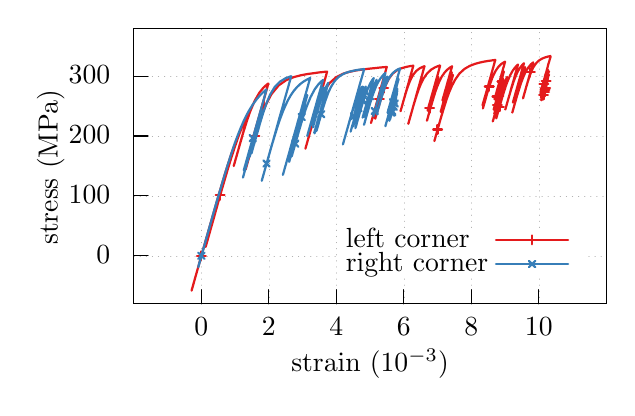
\begin{tikzpicture}[gnuplot]
%% generated with GNUPLOT 5.2p6 (Lua 5.3; terminal rev. Nov 2018, script rev. 107)
%% 09/28/2019 22:27:56
\path (0.000,0.000) rectangle (6.000,3.500);
\gpcolor{color=gp lt color axes}
\gpsetlinetype{gp lt axes}
\gpsetdashtype{gp dt axes}
\gpsetlinewidth{0.50}
\draw[gp path] (0.000,0.609)--(2.575,0.609);
\draw[gp path] (5.699,0.609)--(5.999,0.609);
\gpcolor{color=gp lt color border}
\gpsetlinetype{gp lt border}
\gpsetdashtype{gp dt solid}
\gpsetlinewidth{1.00}
\draw[gp path] (0.000,0.609)--(0.180,0.609);
\node[gp node right] at (-0.184,0.609) {$0$};
\gpcolor{color=gp lt color axes}
\gpsetlinetype{gp lt axes}
\gpsetdashtype{gp dt axes}
\gpsetlinewidth{0.50}
\draw[gp path] (0.000,1.369)--(5.999,1.369);
\gpcolor{color=gp lt color border}
\gpsetlinetype{gp lt border}
\gpsetdashtype{gp dt solid}
\gpsetlinewidth{1.00}
\draw[gp path] (0.000,1.369)--(0.180,1.369);
\node[gp node right] at (-0.184,1.369) {$100$};
\gpcolor{color=gp lt color axes}
\gpsetlinetype{gp lt axes}
\gpsetdashtype{gp dt axes}
\gpsetlinewidth{0.50}
\draw[gp path] (0.000,2.130)--(5.999,2.130);
\gpcolor{color=gp lt color border}
\gpsetlinetype{gp lt border}
\gpsetdashtype{gp dt solid}
\gpsetlinewidth{1.00}
\draw[gp path] (0.000,2.130)--(0.180,2.130);
\node[gp node right] at (-0.184,2.130) {$200$};
\gpcolor{color=gp lt color axes}
\gpsetlinetype{gp lt axes}
\gpsetdashtype{gp dt axes}
\gpsetlinewidth{0.50}
\draw[gp path] (0.000,2.890)--(5.999,2.890);
\gpcolor{color=gp lt color border}
\gpsetlinetype{gp lt border}
\gpsetdashtype{gp dt solid}
\gpsetlinewidth{1.00}
\draw[gp path] (0.000,2.890)--(0.180,2.890);
\node[gp node right] at (-0.184,2.890) {$300$};
\gpcolor{color=gp lt color axes}
\gpsetlinetype{gp lt axes}
\gpsetdashtype{gp dt axes}
\gpsetlinewidth{0.50}
\draw[gp path] (0.857,0.000)--(0.857,3.499);
\gpcolor{color=gp lt color border}
\gpsetlinetype{gp lt border}
\gpsetdashtype{gp dt solid}
\gpsetlinewidth{1.00}
\draw[gp path] (0.857,0.000)--(0.857,0.180);
\node[gp node center] at (0.857,-0.308) {$0$};
\gpcolor{color=gp lt color axes}
\gpsetlinetype{gp lt axes}
\gpsetdashtype{gp dt axes}
\gpsetlinewidth{0.50}
\draw[gp path] (1.714,0.000)--(1.714,3.499);
\gpcolor{color=gp lt color border}
\gpsetlinetype{gp lt border}
\gpsetdashtype{gp dt solid}
\gpsetlinewidth{1.00}
\draw[gp path] (1.714,0.000)--(1.714,0.180);
\node[gp node center] at (1.714,-0.308) {$2$};
\gpcolor{color=gp lt color axes}
\gpsetlinetype{gp lt axes}
\gpsetdashtype{gp dt axes}
\gpsetlinewidth{0.50}
\draw[gp path] (2.571,0.000)--(2.571,3.499);
\gpcolor{color=gp lt color border}
\gpsetlinetype{gp lt border}
\gpsetdashtype{gp dt solid}
\gpsetlinewidth{1.00}
\draw[gp path] (2.571,0.000)--(2.571,0.180);
\node[gp node center] at (2.571,-0.308) {$4$};
\gpcolor{color=gp lt color axes}
\gpsetlinetype{gp lt axes}
\gpsetdashtype{gp dt axes}
\gpsetlinewidth{0.50}
\draw[gp path] (3.428,0.000)--(3.428,0.350);
\draw[gp path] (3.428,0.966)--(3.428,3.499);
\gpcolor{color=gp lt color border}
\gpsetlinetype{gp lt border}
\gpsetdashtype{gp dt solid}
\gpsetlinewidth{1.00}
\draw[gp path] (3.428,0.000)--(3.428,0.180);
\node[gp node center] at (3.428,-0.308) {$6$};
\gpcolor{color=gp lt color axes}
\gpsetlinetype{gp lt axes}
\gpsetdashtype{gp dt axes}
\gpsetlinewidth{0.50}
\draw[gp path] (4.285,0.000)--(4.285,0.350);
\draw[gp path] (4.285,0.966)--(4.285,3.499);
\gpcolor{color=gp lt color border}
\gpsetlinetype{gp lt border}
\gpsetdashtype{gp dt solid}
\gpsetlinewidth{1.00}
\draw[gp path] (4.285,0.000)--(4.285,0.180);
\node[gp node center] at (4.285,-0.308) {$8$};
\gpcolor{color=gp lt color axes}
\gpsetlinetype{gp lt axes}
\gpsetdashtype{gp dt axes}
\gpsetlinewidth{0.50}
\draw[gp path] (5.142,0.000)--(5.142,0.350);
\draw[gp path] (5.142,0.966)--(5.142,3.499);
\gpcolor{color=gp lt color border}
\gpsetlinetype{gp lt border}
\gpsetdashtype{gp dt solid}
\gpsetlinewidth{1.00}
\draw[gp path] (5.142,0.000)--(5.142,0.180);
\node[gp node center] at (5.142,-0.308) {$10$};
\draw[gp path] (0.000,3.499)--(0.000,0.000)--(5.999,0.000)--(5.999,3.499)--cycle;
\node[gp node center,rotate=-270] at (-1.044,1.749) {stress (\si{\mega\pascal})};
\node[gp node center] at (2.999,-0.769) {strain (\num{E-3})};
\gpcolor{rgb color={0.894,0.102,0.110}}
\gpsetlinewidth{2.00}
\draw[gp path] (0.857,0.609)--(0.857,0.610)--(0.858,0.611)--(0.858,0.613)--(0.859,0.614)%
  --(0.859,0.616)--(0.860,0.618)--(0.860,0.621)--(0.861,0.623)--(0.862,0.625)--(0.862,0.627)%
  --(0.863,0.629)--(0.863,0.631)--(0.864,0.633)--(0.864,0.634)--(0.864,0.635)--(0.864,0.634)%
  --(0.864,0.633)--(0.863,0.631)--(0.863,0.630)--(0.863,0.629)--(0.862,0.627)--(0.862,0.626)%
  --(0.862,0.625)--(0.861,0.624)--(0.861,0.623)--(0.861,0.622)--(0.861,0.621)--(0.860,0.620)%
  --(0.860,0.619)--(0.860,0.618)--(0.860,0.619)--(0.860,0.620)--(0.861,0.621)--(0.861,0.622)%
  --(0.861,0.621)--(0.860,0.620)--(0.860,0.619)--(0.860,0.618)--(0.859,0.617)--(0.859,0.616)%
  --(0.858,0.613)--(0.858,0.612)--(0.859,0.614)--(0.859,0.617)--(0.860,0.619)--(0.861,0.622)%
  --(0.862,0.626)--(0.863,0.631)--(0.865,0.636)--(0.866,0.641)--(0.867,0.646)--(0.869,0.650)%
  --(0.870,0.654)--(0.871,0.658)--(0.872,0.660)--(0.872,0.661)--(0.872,0.660)--(0.871,0.658)%
  --(0.870,0.655)--(0.869,0.651)--(0.867,0.645)--(0.865,0.637)--(0.862,0.628)--(0.859,0.617)%
  --(0.856,0.606)--(0.853,0.594)--(0.850,0.582)--(0.846,0.569)--(0.842,0.556)--(0.838,0.542)%
  --(0.835,0.529)--(0.832,0.519)--(0.829,0.509)--(0.827,0.502)--(0.825,0.496)--(0.824,0.491)%
  --(0.823,0.489)--(0.824,0.490)--(0.825,0.495)--(0.827,0.501)--(0.829,0.510)--(0.832,0.519)%
  --(0.835,0.530)--(0.838,0.541)--(0.842,0.554)--(0.845,0.567)--(0.848,0.577)--(0.850,0.585)%
  --(0.852,0.591)--(0.853,0.595)--(0.854,0.597)--(0.854,0.596)--(0.853,0.594)--(0.851,0.588)%
  --(0.849,0.580)--(0.847,0.572)--(0.844,0.563)--(0.842,0.555)--(0.839,0.546)--(0.837,0.539)%
  --(0.836,0.536)--(0.837,0.538)--(0.839,0.545)--(0.842,0.555)--(0.845,0.566)--(0.849,0.580)%
  --(0.854,0.597)--(0.860,0.620)--(0.867,0.645)--(0.874,0.670)--(0.880,0.691)--(0.885,0.708)%
  --(0.889,0.722)--(0.892,0.734)--(0.895,0.743)--(0.895,0.745)--(0.894,0.739)--(0.890,0.725)%
  --(0.885,0.706)--(0.878,0.683)--(0.870,0.656)--(0.861,0.622)--(0.850,0.583)--(0.838,0.540)%
  --(0.825,0.495)--(0.812,0.449)--(0.799,0.403)--(0.786,0.358)--(0.775,0.319)--(0.765,0.282)%
  --(0.755,0.245)--(0.746,0.213)--(0.738,0.187)--(0.734,0.171)--(0.732,0.166)--(0.734,0.171)%
  --(0.736,0.181)--(0.740,0.195)--(0.746,0.214)--(0.753,0.238)--(0.760,0.266)--(0.769,0.296)%
  --(0.777,0.325)--(0.785,0.354)--(0.795,0.388)--(0.806,0.428)--(0.820,0.477)--(0.834,0.529)%
  --(0.848,0.577)--(0.861,0.623)--(0.873,0.667)--(0.888,0.719)--(0.901,0.766)--(0.930,0.868)%
  --(0.975,1.026)--(1.022,1.190)--(1.068,1.350)--(1.113,1.505)--(1.152,1.635)--(1.182,1.730)%
  --(1.205,1.802)--(1.223,1.858)--(1.239,1.907)--(1.255,1.953)--(1.266,1.986)--(1.271,1.997)%
  --(1.268,1.988)--(1.263,1.971)--(1.257,1.951)--(1.251,1.929)--(1.244,1.903)--(1.234,1.869)%
  --(1.222,1.826)--(1.209,1.778)--(1.195,1.728)--(1.181,1.679)--(1.167,1.630)--(1.152,1.578)%
  --(1.137,1.524)--(1.122,1.470)--(1.108,1.422)--(1.095,1.376)--(1.083,1.331)--(1.070,1.287)%
  --(1.059,1.246)--(1.050,1.214)--(1.040,1.179)--(1.030,1.143)--(1.019,1.103)--(1.008,1.064)%
  --(0.998,1.031)--(0.990,1.002)--(0.982,0.973)--(0.973,0.943)--(0.963,0.907)--(0.951,0.864)%
  --(0.939,0.820)--(0.928,0.780)--(0.918,0.746)--(0.911,0.722)--(0.911,0.723)--(0.919,0.749)%
  --(0.931,0.791)--(0.944,0.839)--(0.956,0.880)--(0.969,0.927)--(0.991,1.004)--(1.022,1.116)%
  --(1.066,1.272)--(1.113,1.438)--(1.155,1.581)--(1.192,1.707)--(1.230,1.832)--(1.280,1.986)%
  --(1.333,2.140)--(1.387,2.276)--(1.432,2.376)--(1.458,2.428)--(1.459,2.425)--(1.447,2.384)%
  --(1.432,2.333)--(1.417,2.277)--(1.400,2.217)--(1.379,2.143)--(1.356,2.062)--(1.334,1.984)%
  --(1.318,1.925)--(1.306,1.884)--(1.294,1.843)--(1.282,1.798)--(1.271,1.760)--(1.268,1.749)%
  --(1.274,1.772)--(1.286,1.813)--(1.297,1.852)--(1.306,1.882)--(1.312,1.907)--(1.323,1.944)%
  --(1.341,2.007)--(1.363,2.083)--(1.385,2.161)--(1.403,2.220)--(1.416,2.260)--(1.428,2.299)%
  --(1.446,2.353)--(1.478,2.445)--(1.535,2.579)--(1.594,2.681)--(1.644,2.743)--(1.681,2.777)%
  --(1.701,2.793)--(1.708,2.798)--(1.707,2.795)--(1.704,2.782)--(1.697,2.760)--(1.688,2.727)%
  --(1.675,2.682)--(1.661,2.630)--(1.645,2.574)--(1.628,2.514)--(1.612,2.457)--(1.596,2.399)%
  --(1.579,2.341)--(1.564,2.286)--(1.550,2.238)--(1.540,2.201)--(1.531,2.169)--(1.525,2.147)%
  --(1.522,2.135)--(1.521,2.134)--(1.524,2.144)--(1.530,2.165)--(1.538,2.194)--(1.548,2.229)%
  --(1.560,2.271)--(1.573,2.315)--(1.586,2.362)--(1.599,2.407)--(1.612,2.449)--(1.624,2.486)%
  --(1.633,2.516)--(1.641,2.539)--(1.646,2.554)--(1.649,2.562)--(1.650,2.566)--(1.650,2.563)%
  --(1.647,2.553)--(1.641,2.533)--(1.632,2.502)--(1.622,2.465)--(1.612,2.430)--(1.603,2.398)%
  --(1.594,2.365)--(1.583,2.326)--(1.570,2.282)--(1.558,2.237)--(1.546,2.196)--(1.536,2.159)%
  --(1.526,2.125)--(1.517,2.093)--(1.509,2.063)--(1.501,2.035)--(1.496,2.020)--(1.495,2.015)%
  --(1.496,2.018)--(1.498,2.024)--(1.499,2.028)--(1.501,2.037)--(1.507,2.059)--(1.517,2.093)%
  --(1.527,2.128)--(1.535,2.157)--(1.541,2.179)--(1.547,2.199)--(1.553,2.219)--(1.560,2.242)%
  --(1.570,2.280)--(1.583,2.322)--(1.594,2.359)--(1.600,2.380)--(1.603,2.390)--(1.609,2.408)%
  --(1.620,2.443)--(1.634,2.484)--(1.644,2.514)--(1.648,2.523)--(1.644,2.512)--(1.641,2.500)%
  --(1.643,2.507)--(1.649,2.528)--(1.653,2.541)--(1.649,2.528)--(1.638,2.490)--(1.628,2.455)%
  --(1.625,2.445)--(1.628,2.455)--(1.630,2.462)--(1.626,2.448)--(1.616,2.414)--(1.607,2.379)%
  --(1.602,2.361)--(1.601,2.360)--(1.600,2.357)--(1.596,2.341)--(1.589,2.315)--(1.582,2.292)%
  --(1.579,2.280)--(1.578,2.277)--(1.578,2.276)--(1.576,2.271)--(1.574,2.262)--(1.572,2.254)%
  --(1.571,2.252)--(1.573,2.258)--(1.574,2.264)--(1.573,2.260)--(1.571,2.254)--(1.571,2.251)%
  --(1.571,2.252)--(1.572,2.255)--(1.571,2.253)--(1.570,2.249)--(1.572,2.255)--(1.573,2.261)%
  --(1.575,2.265)--(1.576,2.268)--(1.576,2.270)--(1.577,2.272)--(1.577,2.274)--(1.576,2.268)%
  --(1.573,2.258)--(1.568,2.242)--(1.563,2.223)--(1.557,2.202)--(1.550,2.178)--(1.543,2.151)%
  --(1.537,2.129)--(1.532,2.115)--(1.529,2.102)--(1.525,2.090)--(1.521,2.074)--(1.519,2.065)%
  --(1.519,2.069)--(1.524,2.086)--(1.531,2.112)--(1.539,2.139)--(1.546,2.163)--(1.553,2.189)%
  --(1.562,2.219)--(1.572,2.255)--(1.583,2.294)--(1.594,2.330)--(1.602,2.359)--(1.608,2.379)%
  --(1.613,2.395)--(1.617,2.407)--(1.619,2.414)--(1.618,2.412)--(1.614,2.397)--(1.606,2.369)%
  --(1.596,2.333)--(1.585,2.293)--(1.573,2.250)--(1.559,2.201)--(1.543,2.147)--(1.526,2.085)%
  --(1.509,2.023)--(1.493,1.966)--(1.480,1.920)--(1.468,1.877)--(1.454,1.829)--(1.440,1.779)%
  --(1.427,1.734)--(1.420,1.707)--(1.420,1.708)--(1.426,1.729)--(1.434,1.758)--(1.440,1.778)%
  --(1.444,1.794)--(1.452,1.823)--(1.469,1.881)--(1.493,1.967)--(1.520,2.062)--(1.545,2.145)%
  --(1.567,2.220)--(1.597,2.313)--(1.635,2.424)--(1.683,2.541)--(1.747,2.662)--(1.840,2.774)%
  --(1.934,2.839)--(2.030,2.878)--(2.127,2.903)--(2.217,2.919)--(2.292,2.929)--(2.354,2.938)%
  --(2.399,2.942)--(2.430,2.946)--(2.449,2.948)--(2.454,2.948)--(2.448,2.927)--(2.435,2.879)%
  --(2.416,2.812)--(2.396,2.742)--(2.376,2.672)--(2.356,2.601)--(2.339,2.538)--(2.321,2.476)%
  --(2.302,2.409)--(2.282,2.335)--(2.261,2.261)--(2.243,2.200)--(2.232,2.162)--(2.226,2.136)%
  --(2.218,2.109)--(2.208,2.076)--(2.199,2.041)--(2.191,2.015)--(2.187,2.002)--(2.186,1.997)%
  --(2.185,1.992)--(2.182,1.983)--(2.179,1.972)--(2.178,1.969)--(2.183,1.987)--(2.195,2.029)%
  --(2.208,2.076)--(2.219,2.115)--(2.229,2.149)--(2.244,2.200)--(2.268,2.283)--(2.298,2.386)%
  --(2.334,2.496)--(2.367,2.587)--(2.398,2.659)--(2.432,2.726)--(2.486,2.803)--(2.568,2.877)%
  --(2.658,2.922)--(2.744,2.947)--(2.823,2.963)--(2.892,2.973)--(2.952,2.981)--(3.007,2.987)%
  --(3.059,2.992)--(3.108,2.998)--(3.151,3.002)--(3.184,3.005)--(3.204,3.006)--(3.212,3.007)%
  --(3.210,3.001)--(3.205,2.984)--(3.200,2.967)--(3.195,2.949)--(3.188,2.925)--(3.180,2.896)%
  --(3.170,2.859)--(3.161,2.829)--(3.155,2.805)--(3.149,2.786)--(3.143,2.764)--(3.136,2.738)%
  --(3.127,2.708)--(3.119,2.681)--(3.113,2.657)--(3.107,2.638)--(3.104,2.625)--(3.101,2.617)%
  --(3.101,2.614)--(3.100,2.610)--(3.099,2.608)--(3.101,2.616)--(3.107,2.636)--(3.114,2.662)%
  --(3.121,2.684)--(3.124,2.697)--(3.127,2.706)--(3.129,2.714)--(3.132,2.724)--(3.134,2.732)%
  --(3.134,2.730)--(3.131,2.718)--(3.125,2.697)--(3.119,2.676)--(3.113,2.656)--(3.107,2.636)%
  --(3.101,2.613)--(3.093,2.585)--(3.085,2.557)--(3.077,2.530)--(3.071,2.506)--(3.065,2.487)%
  --(3.061,2.471)--(3.056,2.455)--(3.051,2.437)--(3.046,2.418)--(3.041,2.401)--(3.037,2.386)%
  --(3.033,2.374)--(3.030,2.361)--(3.026,2.346)--(3.021,2.329)--(3.016,2.313)--(3.013,2.302)%
  --(3.011,2.296)--(3.012,2.298)--(3.014,2.304)--(3.017,2.315)--(3.021,2.329)--(3.027,2.351)%
  --(3.035,2.380)--(3.045,2.414)--(3.056,2.452)--(3.065,2.487)--(3.076,2.522)--(3.087,2.559)%
  --(3.099,2.598)--(3.112,2.639)--(3.124,2.675)--(3.134,2.703)--(3.143,2.727)--(3.152,2.748)%
  --(3.161,2.770)--(3.168,2.786)--(3.173,2.798)--(3.175,2.801)--(3.173,2.794)--(3.169,2.780)%
  --(3.164,2.762)--(3.158,2.741)--(3.151,2.715)--(3.141,2.681)--(3.129,2.639)--(3.118,2.600)%
  --(3.107,2.561)--(3.097,2.524)--(3.087,2.490)--(3.078,2.457)--(3.069,2.426)--(3.062,2.399)%
  --(3.056,2.379)--(3.053,2.368)--(3.052,2.363)--(3.052,2.365)--(3.054,2.372)--(3.057,2.384)%
  --(3.063,2.404)--(3.071,2.430)--(3.080,2.463)--(3.089,2.497)--(3.099,2.530)--(3.107,2.560)%
  --(3.116,2.589)--(3.125,2.619)--(3.134,2.649)--(3.143,2.677)--(3.150,2.697)--(3.154,2.708)%
  --(3.155,2.712)--(3.154,2.708)--(3.152,2.699)--(3.147,2.683)--(3.140,2.658)--(3.132,2.628)%
  --(3.124,2.601)--(3.117,2.576)--(3.110,2.553)--(3.104,2.529)--(3.097,2.504)--(3.090,2.480)%
  --(3.084,2.459)--(3.080,2.445)--(3.077,2.436)--(3.076,2.429)--(3.074,2.423)--(3.074,2.421)%
  --(3.074,2.425)--(3.077,2.435)--(3.081,2.449)--(3.086,2.465)--(3.090,2.481)--(3.095,2.500)%
  --(3.102,2.521)--(3.109,2.546)--(3.116,2.573)--(3.124,2.598)--(3.130,2.620)--(3.136,2.640)%
  --(3.143,2.660)--(3.149,2.681)--(3.155,2.700)--(3.159,2.713)--(3.162,2.721)--(3.162,2.722)%
  --(3.161,2.716)--(3.158,2.706)--(3.154,2.692)--(3.149,2.673)--(3.141,2.648)--(3.133,2.619)%
  --(3.126,2.593)--(3.119,2.568)--(3.112,2.543)--(3.104,2.515)--(3.097,2.489)--(3.090,2.466)%
  --(3.085,2.449)--(3.082,2.436)--(3.079,2.426)--(3.077,2.418)--(3.075,2.414)--(3.076,2.414)%
  --(3.077,2.420)--(3.080,2.430)--(3.084,2.443)--(3.087,2.456)--(3.091,2.470)--(3.095,2.484)%
  --(3.099,2.499)--(3.103,2.512)--(3.106,2.522)--(3.108,2.528)--(3.109,2.533)--(3.111,2.540)%
  --(3.113,2.547)--(3.115,2.554)--(3.116,2.556)--(3.115,2.554)--(3.114,2.550)--(3.114,2.549)%
  --(3.115,2.553)--(3.116,2.556)--(3.115,2.552)--(3.113,2.547)--(3.114,2.549)--(3.115,2.554)%
  --(3.116,2.556)--(3.116,2.558)--(3.118,2.563)--(3.119,2.569)--(3.121,2.574)--(3.120,2.571)%
  --(3.119,2.567)--(3.117,2.562)--(3.116,2.557)--(3.113,2.548)--(3.111,2.539)--(3.108,2.529)%
  --(3.106,2.520)--(3.103,2.512)--(3.101,2.505)--(3.099,2.498)--(3.098,2.493)--(3.097,2.490)%
  --(3.098,2.491)--(3.099,2.496)--(3.101,2.503)--(3.102,2.509)--(3.104,2.514)--(3.106,2.521)%
  --(3.108,2.530)--(3.111,2.540)--(3.114,2.549)--(3.116,2.555)--(3.116,2.558)--(3.117,2.560)%
  --(3.117,2.561)--(3.118,2.563)--(3.117,2.560)--(3.116,2.556)--(3.114,2.549)--(3.111,2.541)%
  --(3.109,2.532)--(3.107,2.523)--(3.104,2.513)--(3.101,2.502)--(3.097,2.490)--(3.095,2.480)%
  --(3.092,2.472)--(3.090,2.465)--(3.088,2.457)--(3.086,2.452)--(3.086,2.449)--(3.086,2.451)%
  --(3.087,2.455)--(3.089,2.462)--(3.091,2.469)--(3.094,2.478)--(3.097,2.489)--(3.100,2.500)%
  --(3.103,2.512)--(3.106,2.522)--(3.108,2.529)--(3.110,2.534)--(3.111,2.538)--(3.111,2.540)%
  --(3.110,2.538)--(3.109,2.532)--(3.107,2.525)--(3.104,2.515)--(3.101,2.503)--(3.097,2.490)%
  --(3.093,2.474)--(3.089,2.460)--(3.086,2.448)--(3.083,2.438)--(3.080,2.428)--(3.077,2.417)%
  --(3.074,2.407)--(3.074,2.405)--(3.075,2.411)--(3.078,2.421)--(3.081,2.433)--(3.085,2.445)%
  --(3.089,2.462)--(3.096,2.486)--(3.104,2.515)--(3.113,2.546)--(3.122,2.576)--(3.130,2.604)%
  --(3.139,2.633)--(3.148,2.664)--(3.158,2.693)--(3.166,2.719)--(3.173,2.738)--(3.176,2.747)%
  --(3.177,2.749)--(3.176,2.745)--(3.174,2.741)--(3.173,2.734)--(3.168,2.719)--(3.162,2.696)%
  --(3.153,2.665)--(3.143,2.630)--(3.135,2.600)--(3.128,2.578)--(3.123,2.558)--(3.117,2.538)%
  --(3.111,2.515)--(3.104,2.492)--(3.099,2.473)--(3.096,2.462)--(3.094,2.456)--(3.093,2.452)%
  --(3.092,2.449)--(3.092,2.448)--(3.093,2.451)--(3.095,2.461)--(3.100,2.476)--(3.104,2.493)%
  --(3.109,2.509)--(3.113,2.524)--(3.118,2.541)--(3.123,2.560)--(3.129,2.579)--(3.134,2.596)%
  --(3.137,2.609)--(3.140,2.617)--(3.141,2.620)--(3.141,2.621)--(3.140,2.618)--(3.138,2.611)%
  --(3.134,2.598)--(3.129,2.579)--(3.123,2.557)--(3.116,2.533)--(3.110,2.510)--(3.103,2.486)%
  --(3.096,2.461)--(3.089,2.436)--(3.083,2.412)--(3.077,2.391)--(3.072,2.376)--(3.069,2.365)%
  --(3.067,2.357)--(3.065,2.351)--(3.065,2.350)--(3.066,2.353)--(3.068,2.363)--(3.072,2.377)%
  --(3.080,2.402)--(3.089,2.437)--(3.101,2.477)--(3.112,2.516)--(3.123,2.554)--(3.136,2.598)%
  --(3.153,2.652)--(3.173,2.712)--(3.198,2.778)--(3.238,2.858)--(3.288,2.924)--(3.342,2.965)%
  --(3.397,2.990)--(3.448,3.005)--(3.488,3.014)--(3.517,3.019)--(3.535,3.021)--(3.545,3.023)%
  --(3.549,3.024)--(3.548,3.020)--(3.542,3.000)--(3.532,2.962)--(3.520,2.921)--(3.509,2.880)%
  --(3.499,2.846)--(3.490,2.811)--(3.479,2.774)--(3.467,2.732)--(3.454,2.685)--(3.441,2.639)%
  --(3.431,2.603)--(3.422,2.574)--(3.416,2.550)--(3.409,2.526)--(3.403,2.503)--(3.397,2.482)%
  --(3.392,2.468)--(3.390,2.459)--(3.389,2.456)--(3.389,2.455)--(3.389,2.454)--(3.388,2.451)%
  --(3.387,2.447)--(3.386,2.446)--(3.388,2.452)--(3.392,2.467)--(3.401,2.496)--(3.411,2.531)%
  --(3.418,2.557)--(3.423,2.574)--(3.429,2.596)--(3.441,2.636)--(3.457,2.690)--(3.474,2.742)%
  --(3.489,2.785)--(3.503,2.820)--(3.515,2.847)--(3.528,2.875)--(3.551,2.913)--(3.586,2.956)%
  --(3.624,2.986)--(3.658,3.004)--(3.681,3.013)--(3.691,3.017)--(3.689,3.009)--(3.681,2.982)%
  --(3.671,2.948)--(3.663,2.916)--(3.653,2.881)--(3.640,2.836)--(3.624,2.779)--(3.605,2.713)%
  --(3.588,2.652)--(3.573,2.596)--(3.558,2.546)--(3.544,2.495)--(3.528,2.437)--(3.514,2.387)%
  --(3.502,2.345)--(3.493,2.314)--(3.488,2.294)--(3.485,2.285)--(3.485,2.287)--(3.489,2.301)%
  --(3.496,2.325)--(3.506,2.358)--(3.517,2.400)--(3.532,2.450)--(3.548,2.509)--(3.568,2.574)%
  --(3.591,2.648)--(3.617,2.723)--(3.646,2.796)--(3.677,2.858)--(3.722,2.923)--(3.775,2.973)%
  --(3.824,3.002)--(3.863,3.018)--(3.887,3.027)--(3.889,3.022)--(3.875,2.973)--(3.860,2.918)%
  --(3.851,2.885)--(3.845,2.865)--(3.837,2.838)--(3.824,2.790)--(3.805,2.722)--(3.787,2.658)%
  --(3.775,2.617)--(3.769,2.595)--(3.764,2.576)--(3.756,2.549)--(3.746,2.512)--(3.736,2.478)%
  --(3.731,2.458)--(3.729,2.455)--(3.733,2.467)--(3.738,2.486)--(3.743,2.503)--(3.747,2.519)%
  --(3.752,2.534)--(3.759,2.560)--(3.772,2.604)--(3.787,2.655)--(3.801,2.703)--(3.812,2.739)%
  --(3.822,2.767)--(3.831,2.795)--(3.843,2.824)--(3.854,2.852)--(3.862,2.871)--(3.867,2.879)%
  --(3.865,2.875)--(3.861,2.858)--(3.854,2.832)--(3.844,2.799)--(3.834,2.762)--(3.823,2.725)%
  --(3.812,2.683)--(3.799,2.638)--(3.786,2.594)--(3.775,2.553)--(3.764,2.516)--(3.756,2.485)%
  --(3.749,2.462)--(3.745,2.447)--(3.743,2.439)--(3.744,2.444)--(3.748,2.456)--(3.753,2.477)%
  --(3.761,2.503)--(3.770,2.534)--(3.778,2.563)--(3.787,2.593)--(3.796,2.627)--(3.806,2.662)%
  --(3.816,2.693)--(3.824,2.719)--(3.831,2.740)--(3.838,2.759)--(3.845,2.780)--(3.853,2.801)%
  --(3.859,2.817)--(3.862,2.827)--(3.864,2.830)--(3.863,2.827)--(3.861,2.821)--(3.859,2.812)%
  --(3.855,2.800)--(3.850,2.781)--(3.842,2.754)--(3.833,2.722)--(3.824,2.690)--(3.815,2.658)%
  --(3.806,2.626)--(3.796,2.589)--(3.784,2.547)--(3.772,2.503)--(3.759,2.458)--(3.749,2.422)%
  --(3.740,2.393)--(3.734,2.368)--(3.728,2.350)--(3.725,2.335)--(3.722,2.326)--(3.722,2.325)%
  --(3.725,2.336)--(3.732,2.362)--(3.742,2.398)--(3.755,2.442)--(3.768,2.490)--(3.782,2.537)%
  --(3.796,2.585)--(3.811,2.636)--(3.830,2.696)--(3.851,2.755)--(3.875,2.814)--(3.908,2.881)%
  --(3.948,2.939)--(3.985,2.977)--(4.015,3.000)--(4.036,3.013)--(4.041,3.015)--(4.033,2.987)%
  --(4.021,2.944)--(4.010,2.907)--(4.003,2.881)--(3.996,2.855)--(3.986,2.822)--(3.975,2.781)%
  --(3.962,2.735)--(3.950,2.694)--(3.942,2.665)--(3.936,2.643)--(3.930,2.623)--(3.925,2.603)%
  --(3.920,2.588)--(3.919,2.582)--(3.921,2.588)--(3.925,2.605)--(3.931,2.628)--(3.939,2.652)%
  --(3.946,2.681)--(3.955,2.712)--(3.966,2.747)--(3.978,2.786)--(3.989,2.821)--(4.000,2.851)%
  --(4.008,2.874)--(4.015,2.892)--(4.023,2.909)--(4.029,2.923)--(4.036,2.935)--(4.037,2.939)%
  --(4.034,2.926)--(4.026,2.897)--(4.018,2.869)--(4.010,2.841)--(4.003,2.818)--(3.996,2.792)%
  --(3.986,2.758)--(3.976,2.719)--(3.964,2.680)--(3.954,2.644)--(3.945,2.611)--(3.936,2.578)%
  --(3.926,2.543)--(3.916,2.509)--(3.908,2.479)--(3.902,2.458)--(3.898,2.446)--(3.897,2.439)%
  --(3.896,2.437)--(3.897,2.439)--(3.900,2.451)--(3.906,2.472)--(3.914,2.502)--(3.924,2.535)%
  --(3.934,2.573)--(3.946,2.612)--(3.957,2.652)--(3.969,2.690)--(3.980,2.727)--(3.991,2.758)%
  --(4.000,2.784)--(4.008,2.806)--(4.014,2.824)--(4.020,2.838)--(4.025,2.849)--(4.027,2.854)%
  --(4.026,2.851)--(4.023,2.839)--(4.018,2.824)--(4.015,2.810)--(4.010,2.795)--(4.005,2.776)%
  --(3.998,2.754)--(3.992,2.732)--(3.987,2.711)--(3.981,2.692)--(3.976,2.674)--(3.971,2.656)%
  --(3.966,2.637)--(3.961,2.619)--(3.956,2.604)--(3.954,2.595)--(3.953,2.591)--(3.952,2.589)%
  --(3.954,2.594)--(3.957,2.604)--(3.962,2.623)--(3.969,2.648)--(3.976,2.671)--(3.982,2.695)%
  --(3.989,2.719)--(3.997,2.745)--(4.006,2.776)--(4.015,2.806)--(4.024,2.831)--(4.031,2.852)%
  --(4.040,2.876)--(4.048,2.895)--(4.052,2.906)--(4.052,2.904)--(4.046,2.884)--(4.036,2.846)%
  --(4.025,2.808)--(4.015,2.775)--(4.006,2.743)--(3.997,2.709)--(3.985,2.668)--(3.972,2.620)%
  --(3.957,2.566)--(3.943,2.516)--(3.930,2.473)--(3.919,2.433)--(3.909,2.396)--(3.899,2.361)%
  --(3.888,2.324)--(3.878,2.287)--(3.868,2.253)--(3.861,2.227)--(3.856,2.210)--(3.852,2.196)%
  --(3.848,2.182)--(3.844,2.166)--(3.839,2.147)--(3.833,2.129)--(3.829,2.114)--(3.826,2.101)%
  --(3.823,2.090)--(3.819,2.079)--(3.817,2.070)--(3.816,2.066)--(3.817,2.071)--(3.821,2.083)%
  --(3.826,2.102)--(3.834,2.131)--(3.845,2.169)--(3.857,2.214)--(3.873,2.268)--(3.891,2.333)%
  --(3.915,2.414)--(3.943,2.506)--(3.973,2.601)--(4.004,2.686)--(4.035,2.759)--(4.078,2.843)%
  --(4.134,2.923)--(4.198,2.982)--(4.266,3.021)--(4.334,3.047)--(4.393,3.063)--(4.438,3.073)%
  --(4.473,3.079)--(4.500,3.084)--(4.526,3.087)--(4.550,3.091)--(4.571,3.094)--(4.585,3.096)%
  --(4.590,3.097)--(4.587,3.084)--(4.579,3.059)--(4.574,3.039)--(4.569,3.023)--(4.566,3.010)%
  --(4.561,2.994)--(4.555,2.973)--(4.548,2.947)--(4.540,2.919)--(4.533,2.893)--(4.525,2.865)%
  --(4.517,2.836)--(4.508,2.807)--(4.500,2.776)--(4.491,2.746)--(4.483,2.716)--(4.474,2.684)%
  --(4.465,2.652)--(4.457,2.624)--(4.450,2.601)--(4.445,2.582)--(4.440,2.566)--(4.435,2.548)%
  --(4.431,2.533)--(4.428,2.522)--(4.427,2.519)--(4.428,2.522)--(4.430,2.530)--(4.433,2.541)%
  --(4.437,2.552)--(4.441,2.566)--(4.446,2.585)--(4.453,2.612)--(4.462,2.639)--(4.469,2.665)%
  --(4.475,2.687)--(4.482,2.710)--(4.489,2.735)--(4.496,2.759)--(4.503,2.779)--(4.507,2.792)%
  --(4.509,2.798)--(4.510,2.803)--(4.513,2.808)--(4.514,2.814)--(4.512,2.805)--(4.507,2.790)%
  --(4.504,2.776)--(4.501,2.766)--(4.498,2.757)--(4.495,2.746)--(4.490,2.730)--(4.486,2.712)%
  --(4.481,2.697)--(4.478,2.686)--(4.476,2.679)--(4.474,2.672)--(4.472,2.665)--(4.471,2.659)%
  --(4.470,2.658)--(4.471,2.661)--(4.473,2.668)--(4.475,2.676)--(4.478,2.684)--(4.480,2.693)%
  --(4.483,2.702)--(4.486,2.713)--(4.489,2.724)--(4.491,2.732)--(4.492,2.735)--(4.493,2.737)%
  --(4.492,2.737)--(4.492,2.734)--(4.490,2.728)--(4.488,2.720)--(4.485,2.709)--(4.481,2.697)%
  --(4.478,2.686)--(4.475,2.675)--(4.472,2.665)--(4.469,2.653)--(4.465,2.641)--(4.463,2.631)%
  --(4.461,2.623)--(4.459,2.619)--(4.458,2.615)--(4.457,2.611)--(4.456,2.607)--(4.455,2.604)%
  --(4.455,2.603)--(4.454,2.601)--(4.455,2.604)--(4.457,2.611)--(4.459,2.618)--(4.462,2.627)%
  --(4.464,2.636)--(4.468,2.648)--(4.473,2.666)--(4.479,2.689)--(4.486,2.714)--(4.493,2.738)%
  --(4.500,2.761)--(4.507,2.785)--(4.514,2.809)--(4.523,2.836)--(4.531,2.860)--(4.538,2.880)%
  --(4.543,2.894)--(4.546,2.900)--(4.545,2.898)--(4.542,2.889)--(4.540,2.880)--(4.537,2.870)%
  --(4.533,2.855)--(4.526,2.830)--(4.517,2.799)--(4.508,2.768)--(4.501,2.742)--(4.495,2.722)%
  --(4.489,2.700)--(4.482,2.674)--(4.474,2.646)--(4.467,2.623)--(4.464,2.611)--(4.464,2.610)%
  --(4.464,2.611)--(4.465,2.617)--(4.471,2.636)--(4.479,2.663)--(4.487,2.692)--(4.493,2.715)%
  --(4.498,2.733)--(4.504,2.752)--(4.511,2.776)--(4.519,2.801)--(4.526,2.825)--(4.532,2.844)%
  --(4.536,2.855)--(4.539,2.865)--(4.542,2.874)--(4.546,2.883)--(4.547,2.888)--(4.546,2.884)%
  --(4.542,2.869)--(4.536,2.849)--(4.530,2.826)--(4.524,2.805)--(4.518,2.786)--(4.512,2.761)%
  --(4.503,2.732)--(4.494,2.699)--(4.485,2.668)--(4.477,2.639)--(4.468,2.608)--(4.459,2.574)%
  --(4.449,2.541)--(4.441,2.512)--(4.436,2.493)--(4.434,2.484)--(4.432,2.480)--(4.434,2.486)%
  --(4.439,2.503)--(4.447,2.533)--(4.459,2.573)--(4.471,2.618)--(4.484,2.664)--(4.498,2.710)%
  --(4.513,2.759)--(4.531,2.811)--(4.550,2.865)--(4.571,2.913)--(4.597,2.963)--(4.631,3.011)%
  --(4.664,3.043)--(4.692,3.062)--(4.710,3.072)--(4.714,3.073)--(4.705,3.041)--(4.695,3.005)%
  --(4.687,2.979)--(4.683,2.963)--(4.678,2.945)--(4.670,2.917)--(4.659,2.877)--(4.648,2.837)%
  --(4.639,2.809)--(4.635,2.793)--(4.632,2.782)--(4.627,2.765)--(4.621,2.745)--(4.616,2.726)%
  --(4.612,2.713)--(4.611,2.709)--(4.611,2.706)--(4.609,2.703)--(4.607,2.693)--(4.603,2.680)%
  --(4.599,2.665)--(4.596,2.653)--(4.593,2.643)--(4.591,2.635)--(4.588,2.624)--(4.584,2.613)%
  --(4.582,2.603)--(4.580,2.598)--(4.580,2.599)--(4.582,2.607)--(4.586,2.619)--(4.590,2.635)%
  --(4.596,2.654)--(4.602,2.676)--(4.610,2.704)--(4.619,2.735)--(4.628,2.766)--(4.636,2.794)%
  --(4.644,2.817)--(4.650,2.839)--(4.657,2.858)--(4.663,2.875)--(4.668,2.889)--(4.671,2.897)%
  --(4.672,2.900)--(4.672,2.901)--(4.672,2.900)--(4.671,2.898)--(4.669,2.892)--(4.666,2.881)%
  --(4.662,2.866)--(4.657,2.849)--(4.653,2.834)--(4.649,2.818)--(4.644,2.802)--(4.639,2.786)%
  --(4.635,2.770)--(4.632,2.757)--(4.630,2.751)--(4.629,2.749)--(4.630,2.751)--(4.630,2.753)%
  --(4.631,2.757)--(4.633,2.763)--(4.636,2.773)--(4.640,2.788)--(4.645,2.803)--(4.648,2.816)%
  --(4.651,2.824)--(4.652,2.830)--(4.654,2.836)--(4.656,2.843)--(4.657,2.846)--(4.654,2.839)%
  --(4.651,2.827)--(4.648,2.813)--(4.645,2.803)--(4.642,2.795)--(4.641,2.789)--(4.639,2.781)%
  --(4.636,2.770)--(4.633,2.760)--(4.630,2.752)--(4.630,2.750)--(4.631,2.754)--(4.632,2.758)%
  --(4.632,2.760)--(4.632,2.757)--(4.630,2.753)--(4.632,2.757)--(4.633,2.762)--(4.634,2.764)%
  --(4.633,2.763)--(4.633,2.761)--(4.633,2.763)--(4.635,2.767)--(4.636,2.772)--(4.636,2.774)%
  --(4.636,2.773)--(4.636,2.770)--(4.635,2.767)--(4.633,2.763)--(4.631,2.756)--(4.629,2.747)%
  --(4.626,2.736)--(4.623,2.725)--(4.620,2.716)--(4.618,2.706)--(4.615,2.700)--(4.614,2.695)%
  --(4.614,2.693)--(4.614,2.696)--(4.616,2.701)--(4.619,2.711)--(4.622,2.723)--(4.626,2.738)%
  --(4.630,2.753)--(4.635,2.768)--(4.639,2.784)--(4.643,2.798)--(4.647,2.811)--(4.651,2.824)%
  --(4.655,2.836)--(4.658,2.848)--(4.660,2.855)--(4.662,2.862)--(4.664,2.866)--(4.665,2.871)%
  --(4.666,2.873)--(4.665,2.871)--(4.664,2.866)--(4.662,2.859)--(4.659,2.849)--(4.656,2.837)%
  --(4.652,2.825)--(4.648,2.812)--(4.644,2.797)--(4.639,2.779)--(4.633,2.758)--(4.628,2.738)%
  --(4.623,2.719)--(4.618,2.703)--(4.613,2.687)--(4.608,2.668)--(4.603,2.651)--(4.599,2.636)%
  --(4.596,2.626)--(4.594,2.619)--(4.593,2.614)--(4.591,2.610)--(4.591,2.607)--(4.592,2.611)%
  --(4.594,2.617)--(4.596,2.626)--(4.599,2.636)--(4.603,2.652)--(4.609,2.669)--(4.614,2.690)%
  --(4.621,2.712)--(4.627,2.735)--(4.635,2.763)--(4.644,2.792)--(4.653,2.822)--(4.662,2.849)%
  --(4.669,2.871)--(4.676,2.891)--(4.683,2.910)--(4.690,2.929)--(4.696,2.941)--(4.699,2.948)%
  --(4.697,2.941)--(4.693,2.928)--(4.688,2.910)--(4.682,2.887)--(4.675,2.864)--(4.669,2.840)%
  --(4.662,2.815)--(4.654,2.790)--(4.648,2.764)--(4.641,2.740)--(4.634,2.716)--(4.627,2.692)%
  --(4.621,2.670)--(4.615,2.649)--(4.610,2.633)--(4.607,2.621)--(4.605,2.614)--(4.603,2.609)%
  --(4.603,2.608)--(4.604,2.610)--(4.606,2.619)--(4.611,2.635)--(4.617,2.655)--(4.623,2.676)%
  --(4.629,2.697)--(4.635,2.719)--(4.641,2.741)--(4.648,2.765)--(4.654,2.786)--(4.659,2.802)%
  --(4.662,2.812)--(4.663,2.817)--(4.664,2.817)--(4.663,2.814)--(4.661,2.806)--(4.657,2.793)%
  --(4.652,2.776)--(4.646,2.755)--(4.640,2.734)--(4.635,2.716)--(4.631,2.702)--(4.628,2.691)%
  --(4.625,2.681)--(4.623,2.671)--(4.621,2.665)--(4.624,2.674)--(4.627,2.687)--(4.630,2.697)%
  --(4.632,2.705)--(4.634,2.711)--(4.636,2.718)--(4.639,2.729)--(4.642,2.740)--(4.645,2.749)%
  --(4.645,2.752)--(4.645,2.749)--(4.643,2.744)--(4.642,2.740)--(4.642,2.738)--(4.641,2.736)%
  --(4.639,2.729)--(4.636,2.718)--(4.632,2.704)--(4.629,2.693)--(4.627,2.685)--(4.625,2.679)%
  --(4.623,2.672)--(4.621,2.665)--(4.619,2.658)--(4.618,2.656)--(4.619,2.658)--(4.621,2.666)%
  --(4.624,2.675)--(4.627,2.685)--(4.630,2.696)--(4.633,2.709)--(4.637,2.723)--(4.642,2.741)%
  --(4.647,2.757)--(4.651,2.770)--(4.654,2.780)--(4.657,2.790)--(4.660,2.800)--(4.662,2.809)%
  --(4.664,2.816)--(4.665,2.817)--(4.664,2.817)--(4.664,2.815)--(4.664,2.816)--(4.664,2.815)%
  --(4.663,2.811)--(4.661,2.804)--(4.658,2.795)--(4.656,2.786)--(4.654,2.779)--(4.651,2.770)%
  --(4.649,2.760)--(4.645,2.748)--(4.641,2.735)--(4.638,2.722)--(4.635,2.713)--(4.633,2.707)%
  --(4.632,2.702)--(4.630,2.694)--(4.628,2.687)--(4.626,2.680)--(4.625,2.675)--(4.624,2.674)%
  --(4.624,2.671)--(4.622,2.667)--(4.620,2.659)--(4.617,2.649)--(4.615,2.639)--(4.612,2.632)%
  --(4.610,2.623)--(4.607,2.614)--(4.604,2.601)--(4.600,2.589)--(4.598,2.582)--(4.597,2.579)%
  --(4.598,2.580)--(4.599,2.584)--(4.600,2.589)--(4.603,2.598)--(4.607,2.614)--(4.613,2.634)%
  --(4.620,2.657)--(4.626,2.681)--(4.633,2.705)--(4.640,2.729)--(4.647,2.754)--(4.654,2.776)%
  --(4.660,2.795)--(4.664,2.810)--(4.668,2.820)--(4.670,2.828)--(4.672,2.834)--(4.673,2.837)%
  --(4.673,2.836)--(4.672,2.831)--(4.669,2.824)--(4.667,2.817)--(4.666,2.810)--(4.663,2.803)%
  --(4.662,2.796)--(4.659,2.787)--(4.657,2.778)--(4.654,2.770)--(4.653,2.764)--(4.651,2.760)%
  --(4.650,2.756)--(4.648,2.750)--(4.646,2.742)--(4.644,2.735)--(4.642,2.728)--(4.642,2.725)%
  --(4.641,2.723)--(4.640,2.721)--(4.639,2.719)--(4.639,2.716)--(4.639,2.718)--(4.641,2.722)%
  --(4.642,2.727)--(4.644,2.733)--(4.646,2.740)--(4.648,2.747)--(4.650,2.756)--(4.653,2.766)%
  --(4.656,2.777)--(4.659,2.788)--(4.662,2.797)--(4.664,2.804)--(4.666,2.811)--(4.668,2.818)%
  --(4.670,2.824)--(4.671,2.829)--(4.672,2.830)--(4.671,2.829)--(4.670,2.826)--(4.669,2.821)%
  --(4.667,2.815)--(4.665,2.806)--(4.661,2.795)--(4.657,2.780)--(4.653,2.763)--(4.647,2.744)%
  --(4.640,2.719)--(4.633,2.693)--(4.625,2.667)--(4.618,2.640)--(4.610,2.611)--(4.601,2.582)%
  --(4.594,2.554)--(4.586,2.527)--(4.579,2.503)--(4.575,2.487)--(4.571,2.474)--(4.570,2.468)%
  --(4.569,2.465)--(4.569,2.468)--(4.572,2.477)--(4.577,2.495)--(4.585,2.522)--(4.594,2.554)%
  --(4.603,2.585)--(4.611,2.615)--(4.620,2.647)--(4.631,2.684)--(4.642,2.722)--(4.653,2.756)%
  --(4.662,2.783)--(4.669,2.805)--(4.675,2.822)--(4.681,2.838)--(4.685,2.850)--(4.688,2.858)%
  --(4.689,2.859)--(4.685,2.847)--(4.680,2.826)--(4.672,2.799)--(4.665,2.774)--(4.658,2.751)%
  --(4.651,2.726)--(4.643,2.697)--(4.634,2.666)--(4.625,2.634)--(4.617,2.605)--(4.610,2.581)%
  --(4.605,2.560)--(4.600,2.544)--(4.596,2.528)--(4.593,2.518)--(4.591,2.512)--(4.591,2.514)%
  --(4.594,2.521)--(4.597,2.532)--(4.600,2.546)--(4.606,2.563)--(4.611,2.584)--(4.618,2.608)%
  --(4.626,2.635)--(4.633,2.662)--(4.641,2.687)--(4.648,2.712)--(4.655,2.736)--(4.662,2.757)%
  --(4.668,2.777)--(4.674,2.796)--(4.679,2.811)--(4.682,2.821)--(4.684,2.826)--(4.683,2.824)%
  --(4.681,2.814)--(4.676,2.798)--(4.669,2.775)--(4.663,2.752)--(4.657,2.729)--(4.649,2.704)%
  --(4.642,2.677)--(4.633,2.647)--(4.625,2.617)--(4.617,2.588)--(4.610,2.563)--(4.603,2.539)%
  --(4.597,2.518)--(4.592,2.500)--(4.588,2.484)--(4.585,2.474)--(4.583,2.468)--(4.583,2.467)%
  --(4.583,2.470)--(4.585,2.475)--(4.588,2.485)--(4.591,2.498)--(4.596,2.513)--(4.601,2.531)%
  --(4.606,2.550)--(4.612,2.572)--(4.618,2.594)--(4.625,2.615)--(4.631,2.636)--(4.637,2.658)%
  --(4.643,2.679)--(4.649,2.699)--(4.654,2.716)--(4.658,2.730)--(4.661,2.739)--(4.664,2.747)%
  --(4.666,2.754)--(4.668,2.760)--(4.669,2.763)--(4.669,2.764)--(4.668,2.761)--(4.667,2.755)%
  --(4.665,2.750)--(4.664,2.745)--(4.663,2.741)--(4.661,2.735)--(4.658,2.726)--(4.655,2.715)%
  --(4.651,2.702)--(4.648,2.687)--(4.643,2.672)--(4.639,2.657)--(4.634,2.640)--(4.630,2.624)%
  --(4.625,2.608)--(4.621,2.592)--(4.617,2.578)--(4.613,2.566)--(4.611,2.557)--(4.610,2.555)%
  --(4.611,2.557)--(4.612,2.562)--(4.615,2.571)--(4.618,2.583)--(4.623,2.599)--(4.628,2.617)%
  --(4.633,2.636)--(4.638,2.655)--(4.644,2.673)--(4.649,2.692)--(4.654,2.709)--(4.658,2.723)%
  --(4.660,2.732)--(4.662,2.735)--(4.662,2.736)--(4.661,2.733)--(4.659,2.727)--(4.656,2.716)%
  --(4.651,2.700)--(4.646,2.680)--(4.640,2.658)--(4.634,2.637)--(4.628,2.617)--(4.623,2.598)%
  --(4.618,2.580)--(4.613,2.563)--(4.609,2.550)--(4.607,2.541)--(4.606,2.538)--(4.607,2.541)%
  --(4.609,2.547)--(4.612,2.558)--(4.616,2.573)--(4.621,2.590)--(4.627,2.611)--(4.633,2.633)%
  --(4.639,2.655)--(4.645,2.677)--(4.651,2.697)--(4.657,2.715)--(4.661,2.729)--(4.664,2.740)%
  --(4.665,2.745)--(4.666,2.745)--(4.664,2.741)--(4.662,2.732)--(4.658,2.720)--(4.654,2.703)%
  --(4.648,2.684)--(4.642,2.662)--(4.636,2.641)--(4.630,2.622)--(4.626,2.604)--(4.621,2.588)%
  --(4.617,2.573)--(4.614,2.563)--(4.612,2.557)--(4.611,2.553)--(4.611,2.552)--(4.612,2.554)%
  --(4.612,2.557)--(4.614,2.563)--(4.616,2.569)--(4.618,2.576)--(4.619,2.580)--(4.621,2.586)%
  --(4.622,2.593)--(4.625,2.601)--(4.627,2.608)--(4.628,2.614)--(4.630,2.618)--(4.631,2.623)%
  --(4.633,2.632)--(4.636,2.643)--(4.640,2.654)--(4.642,2.665)--(4.645,2.674)--(4.648,2.683)%
  --(4.651,2.693)--(4.654,2.706)--(4.658,2.716)--(4.660,2.726)--(4.663,2.734)--(4.665,2.740)%
  --(4.666,2.746)--(4.668,2.752)--(4.669,2.757)--(4.670,2.757)--(4.669,2.755)--(4.668,2.752)%
  --(4.667,2.747)--(4.666,2.742)--(4.663,2.735)--(4.660,2.724)--(4.657,2.710)--(4.652,2.696)%
  --(4.648,2.681)--(4.644,2.666)--(4.640,2.651)--(4.635,2.634)--(4.630,2.617)--(4.626,2.602)%
  --(4.622,2.588)--(4.619,2.578)--(4.617,2.569)--(4.615,2.563)--(4.614,2.559)--(4.613,2.555)%
  --(4.612,2.554)--(4.613,2.557)--(4.614,2.558)--(4.613,2.557)--(4.613,2.555)--(4.612,2.553)%
  --(4.611,2.548)--(4.609,2.543)--(4.608,2.537)--(4.606,2.531)--(4.605,2.528)--(4.604,2.525)%
  --(4.604,2.524)--(4.605,2.528)--(4.607,2.536)--(4.611,2.547)--(4.615,2.563)--(4.620,2.579)%
  --(4.625,2.599)--(4.632,2.622)--(4.639,2.649)--(4.647,2.675)--(4.654,2.702)--(4.662,2.726)%
  --(4.669,2.750)--(4.676,2.773)--(4.683,2.795)--(4.688,2.811)--(4.692,2.821)--(4.693,2.824)%
  --(4.690,2.817)--(4.686,2.800)--(4.678,2.774)--(4.669,2.741)--(4.660,2.709)--(4.651,2.676)%
  --(4.641,2.640)--(4.630,2.602)--(4.618,2.562)--(4.607,2.522)--(4.597,2.487)--(4.589,2.458)%
  --(4.584,2.438)--(4.580,2.424)--(4.577,2.416)--(4.576,2.413)--(4.578,2.418)--(4.582,2.433)%
  --(4.589,2.455)--(4.597,2.485)--(4.606,2.516)--(4.615,2.547)--(4.623,2.576)--(4.632,2.607)%
  --(4.641,2.639)--(4.649,2.667)--(4.656,2.688)--(4.660,2.703)--(4.663,2.712)--(4.665,2.718)%
  --(4.666,2.720)--(4.665,2.719)--(4.663,2.712)--(4.660,2.701)--(4.656,2.687)--(4.652,2.673)%
  --(4.649,2.660)--(4.645,2.649)--(4.643,2.639)--(4.640,2.630)--(4.639,2.623)--(4.638,2.622)%
  --(4.639,2.626)--(4.641,2.633)--(4.644,2.643)--(4.647,2.653)--(4.650,2.665)--(4.654,2.679)%
  --(4.658,2.693)--(4.661,2.705)--(4.663,2.712)--(4.664,2.715)--(4.664,2.714)--(4.663,2.709)%
  --(4.660,2.699)--(4.655,2.684)--(4.650,2.664)--(4.643,2.641)--(4.636,2.617)--(4.629,2.590)%
  --(4.621,2.563)--(4.613,2.534)--(4.606,2.507)--(4.599,2.484)--(4.594,2.467)--(4.591,2.454)%
  --(4.588,2.446)--(4.588,2.444)--(4.588,2.447)--(4.591,2.455)--(4.595,2.469)--(4.600,2.488)%
  --(4.607,2.511)--(4.614,2.537)--(4.622,2.564)--(4.630,2.592)--(4.637,2.617)--(4.644,2.640)%
  --(4.650,2.661)--(4.654,2.676)--(4.657,2.687)--(4.660,2.694)--(4.660,2.697)--(4.660,2.695)%
  --(4.658,2.690)--(4.656,2.681)--(4.652,2.668)--(4.648,2.652)--(4.643,2.637)--(4.639,2.623)%
  --(4.636,2.609)--(4.632,2.596)--(4.629,2.585)--(4.626,2.576)--(4.625,2.570)--(4.624,2.569)%
  --(4.625,2.573)--(4.627,2.579)--(4.630,2.588)--(4.633,2.600)--(4.637,2.614)--(4.642,2.630)%
  --(4.647,2.648)--(4.652,2.666)--(4.657,2.684)--(4.661,2.699)--(4.665,2.712)--(4.668,2.724)%
  --(4.671,2.733)--(4.673,2.740)--(4.674,2.743)--(4.673,2.741)--(4.672,2.735)--(4.669,2.726)%
  --(4.666,2.715)--(4.662,2.701)--(4.657,2.684)--(4.652,2.665)--(4.646,2.645)--(4.640,2.623)%
  --(4.635,2.604)--(4.629,2.585)--(4.624,2.567)--(4.620,2.552)--(4.617,2.540)--(4.614,2.531)%
  --(4.613,2.528)--(4.614,2.529)--(4.615,2.534)--(4.618,2.543)--(4.621,2.555)--(4.625,2.570)%
  --(4.630,2.588)--(4.636,2.610)--(4.643,2.633)--(4.649,2.656)--(4.656,2.678)--(4.662,2.700)%
  --(4.669,2.722)--(4.675,2.743)--(4.681,2.765)--(4.688,2.786)--(4.694,2.804)--(4.699,2.818)%
  --(4.702,2.830)--(4.705,2.836)--(4.701,2.824)--(4.696,2.805)--(4.688,2.777)--(4.680,2.749)%
  --(4.672,2.722)--(4.664,2.691)--(4.654,2.655)--(4.642,2.612)--(4.628,2.566)--(4.616,2.522)%
  --(4.605,2.482)--(4.595,2.447)--(4.586,2.416)--(4.578,2.387)--(4.571,2.363)--(4.565,2.341)%
  --(4.561,2.325)--(4.558,2.316)--(4.558,2.317)--(4.561,2.326)--(4.566,2.343)--(4.571,2.363)%
  --(4.578,2.386)--(4.585,2.412)--(4.594,2.444)--(4.605,2.482)--(4.618,2.525)--(4.631,2.572)%
  --(4.644,2.615)--(4.657,2.656)--(4.670,2.700)--(4.684,2.741)--(4.698,2.780)--(4.713,2.820)%
  --(4.730,2.860)--(4.739,2.880)--(4.739,2.878)--(4.731,2.849)--(4.721,2.814)--(4.712,2.784)%
  --(4.704,2.754)--(4.695,2.721)--(4.684,2.684)--(4.672,2.642)--(4.660,2.597)--(4.648,2.556)%
  --(4.639,2.522)--(4.631,2.495)--(4.625,2.473)--(4.619,2.452)--(4.614,2.435)--(4.612,2.426)%
  --(4.611,2.424)--(4.613,2.431)--(4.617,2.444)--(4.621,2.461)--(4.628,2.484)--(4.635,2.509)%
  --(4.642,2.535)--(4.651,2.565)--(4.660,2.598)--(4.670,2.633)--(4.680,2.666)--(4.689,2.697)%
  --(4.697,2.722)--(4.704,2.744)--(4.710,2.763)--(4.715,2.778)--(4.719,2.790)--(4.722,2.798)%
  --(4.723,2.801)--(4.722,2.798)--(4.719,2.788)--(4.716,2.775)--(4.712,2.761)--(4.708,2.746)%
  --(4.703,2.729)--(4.698,2.711)--(4.693,2.693)--(4.688,2.677)--(4.683,2.658)--(4.678,2.640)%
  --(4.673,2.623)--(4.669,2.607)--(4.665,2.595)--(4.662,2.582)--(4.658,2.569)--(4.654,2.555)%
  --(4.650,2.540)--(4.646,2.527)--(4.643,2.518)--(4.642,2.511)--(4.640,2.505)--(4.638,2.499)%
  --(4.636,2.493)--(4.636,2.490)--(4.636,2.492)--(4.637,2.496)--(4.639,2.504)--(4.642,2.512)%
  --(4.645,2.522)--(4.648,2.532)--(4.651,2.546)--(4.656,2.562)--(4.661,2.580)--(4.666,2.598)%
  --(4.672,2.617)--(4.677,2.636)--(4.682,2.655)--(4.688,2.674)--(4.693,2.693)--(4.698,2.709)%
  --(4.702,2.724)--(4.706,2.736)--(4.710,2.747)--(4.712,2.755)--(4.714,2.760)--(4.713,2.758)%
  --(4.711,2.753)--(4.710,2.746)--(4.707,2.736)--(4.704,2.725)--(4.700,2.710)--(4.695,2.695)%
  --(4.691,2.679)--(4.686,2.663)--(4.682,2.648)--(4.678,2.633)--(4.673,2.617)--(4.669,2.601)%
  --(4.665,2.586)--(4.661,2.573)--(4.657,2.560)--(4.655,2.550)--(4.652,2.542)--(4.650,2.535)%
  --(4.648,2.529)--(4.647,2.525)--(4.647,2.522)--(4.647,2.524)--(4.648,2.528)--(4.650,2.534)%
  --(4.652,2.541)--(4.654,2.550)--(4.657,2.560)--(4.660,2.571)--(4.664,2.584)--(4.668,2.598)%
  --(4.672,2.611)--(4.675,2.624)--(4.679,2.638)--(4.683,2.652)--(4.687,2.665)--(4.691,2.679)%
  --(4.695,2.692)--(4.698,2.703)--(4.701,2.713)--(4.703,2.720)--(4.705,2.725)--(4.706,2.729)%
  --(4.706,2.731)--(4.706,2.729)--(4.704,2.723)--(4.701,2.713)--(4.698,2.700)--(4.693,2.684)%
  --(4.688,2.666)--(4.683,2.647)--(4.676,2.625)--(4.670,2.601)--(4.663,2.577)--(4.657,2.555)%
  --(4.651,2.536)--(4.647,2.521)--(4.643,2.508)--(4.641,2.499)--(4.639,2.493)--(4.640,2.496)%
  --(4.642,2.504)--(4.645,2.513)--(4.648,2.525)--(4.652,2.538)--(4.657,2.555)--(4.662,2.573)%
  --(4.667,2.592)--(4.672,2.608)--(4.676,2.623)--(4.681,2.639)--(4.685,2.653)--(4.689,2.668)%
  --(4.693,2.681)--(4.695,2.689)--(4.696,2.694)--(4.697,2.697)--(4.698,2.698)--(4.697,2.696)%
  --(4.696,2.690)--(4.692,2.678)--(4.687,2.662)--(4.682,2.641)--(4.676,2.620)--(4.670,2.598)%
  --(4.664,2.578)--(4.658,2.557)--(4.652,2.535)--(4.647,2.517)--(4.643,2.503)--(4.641,2.496)%
  --(4.641,2.495)--(4.642,2.498)--(4.643,2.503)--(4.645,2.512)--(4.649,2.526)--(4.654,2.545)%
  --(4.660,2.566)--(4.666,2.585)--(4.671,2.603)--(4.676,2.620)--(4.681,2.637)--(4.686,2.655)%
  --(4.690,2.669)--(4.693,2.680)--(4.695,2.687)--(4.697,2.693)--(4.699,2.699)--(4.700,2.705)%
  --(4.702,2.710)--(4.703,2.714)--(4.704,2.716)--(4.704,2.718)--(4.705,2.719)--(4.705,2.720)%
  --(4.704,2.718)--(4.703,2.712)--(4.701,2.706)--(4.698,2.696)--(4.694,2.683)--(4.689,2.664)%
  --(4.682,2.640)--(4.674,2.611)--(4.665,2.579)--(4.655,2.543)--(4.645,2.508)--(4.635,2.473)%
  --(4.626,2.440)--(4.618,2.413)--(4.612,2.388)--(4.606,2.370)--(4.603,2.358)--(4.602,2.354)%
  --(4.603,2.360)--(4.609,2.382)--(4.620,2.417)--(4.633,2.462)--(4.645,2.505)--(4.656,2.546)%
  --(4.669,2.589)--(4.684,2.643)--(4.703,2.701)--(4.722,2.762)--(4.746,2.827)--(4.778,2.900)%
  --(4.809,2.957)--(4.839,2.998)--(4.863,3.024)--(4.877,3.037)--(4.876,3.030)--(4.864,2.990)%
  --(4.854,2.951)--(4.845,2.922)--(4.838,2.897)--(4.831,2.870)--(4.821,2.833)--(4.806,2.783)%
  --(4.791,2.731)--(4.779,2.684)--(4.769,2.649)--(4.760,2.620)--(4.752,2.590)--(4.743,2.558)%
  --(4.734,2.529)--(4.728,2.504)--(4.722,2.486)--(4.719,2.474)--(4.717,2.468)--(4.717,2.467)%
  --(4.718,2.469)--(4.719,2.474)--(4.722,2.483)--(4.725,2.496)--(4.731,2.515)--(4.738,2.541)%
  --(4.746,2.570)--(4.755,2.601)--(4.764,2.633)--(4.774,2.667)--(4.785,2.705)--(4.797,2.744)%
  --(4.810,2.783)--(4.823,2.823)--(4.836,2.858)--(4.849,2.890)--(4.862,2.921)--(4.877,2.952)%
  --(4.898,2.988)--(4.917,3.014)--(4.933,3.033)--(4.944,3.045)--(4.951,3.051)--(4.954,3.053)%
  --(4.953,3.050)--(4.950,3.040)--(4.945,3.021)--(4.939,3.002)--(4.933,2.980)--(4.927,2.959)%
  --(4.920,2.935)--(4.913,2.908)--(4.904,2.876)--(4.893,2.839)--(4.882,2.799)--(4.871,2.760)%
  --(4.861,2.724)--(4.851,2.690)--(4.843,2.660)--(4.835,2.632)--(4.828,2.607)--(4.822,2.587)%
  --(4.818,2.573)--(4.816,2.564)--(4.815,2.559)--(4.814,2.556)--(4.814,2.558)--(4.817,2.567)%
  --(4.821,2.583)--(4.827,2.603)--(4.833,2.626)--(4.839,2.646)--(4.845,2.669)--(4.853,2.695)%
  --(4.862,2.727)--(4.872,2.761)--(4.882,2.793)--(4.891,2.820)--(4.899,2.845)--(4.907,2.868)%
  --(4.915,2.890)--(4.923,2.913)--(4.931,2.932)--(4.938,2.947)--(4.944,2.960)--(4.950,2.973)%
  --(4.958,2.987)--(4.965,2.998)--(4.968,3.004)--(4.966,2.997)--(4.958,2.970)--(4.950,2.941)%
  --(4.943,2.916)--(4.937,2.893)--(4.930,2.869)--(4.921,2.838)--(4.909,2.795)--(4.895,2.746)%
  --(4.881,2.698)--(4.869,2.655)--(4.859,2.617)--(4.850,2.584)--(4.840,2.550)--(4.831,2.520)%
  --(4.823,2.490)--(4.815,2.463)--(4.810,2.443)--(4.807,2.432)--(4.806,2.428)--(4.806,2.429)%
  --(4.806,2.428)--(4.806,2.430)--(4.809,2.439)--(4.812,2.452)--(4.817,2.467)--(4.821,2.481)%
  --(4.824,2.494)--(4.828,2.507)--(4.833,2.525)--(4.840,2.551)--(4.849,2.582)--(4.858,2.614)%
  --(4.867,2.645)--(4.877,2.677)--(4.889,2.716)--(4.904,2.765)--(4.921,2.816)--(4.939,2.862)%
  --(4.955,2.902)--(4.978,2.951)--(5.010,3.001)--(5.039,3.037)--(5.060,3.057)--(5.070,3.065)%
  --(5.066,3.050)--(5.054,3.006)--(5.044,2.971)--(5.035,2.940)--(5.027,2.909)--(5.017,2.877)%
  --(5.005,2.832)--(4.990,2.781)--(4.977,2.735)--(4.968,2.702)--(4.962,2.680)--(4.956,2.662)%
  --(4.951,2.642)--(4.946,2.622)--(4.942,2.610)--(4.941,2.608)--(4.944,2.614)--(4.946,2.624)%
  --(4.948,2.630)--(4.949,2.633)--(4.950,2.636)--(4.951,2.643)--(4.955,2.655)--(4.959,2.668)%
  --(4.961,2.677)--(4.962,2.682)--(4.963,2.684)--(4.964,2.688)--(4.967,2.697)--(4.970,2.708)%
  --(4.972,2.717)--(4.974,2.722)--(4.976,2.728)--(4.978,2.738)--(4.983,2.754)--(4.989,2.773)%
  --(4.995,2.793)--(5.000,2.813)--(5.007,2.833)--(5.015,2.859)--(5.025,2.887)--(5.035,2.917)%
  --(5.045,2.943)--(5.056,2.968)--(5.071,2.999)--(5.101,3.046)--(5.139,3.085)--(5.181,3.112)%
  --(5.219,3.127)--(5.249,3.136)--(5.266,3.141)--(5.279,3.143)--(5.288,3.145)--(5.292,3.145)%
  --(5.292,3.146)--(5.292,3.137)--(5.283,3.110)--(5.275,3.079)--(5.266,3.051)--(5.258,3.024)%
  --(5.253,2.999)--(5.245,2.973)--(5.236,2.938)--(5.223,2.900)--(5.215,2.862)--(5.206,2.831)%
  --(5.198,2.808)--(5.193,2.786)--(5.185,2.764)--(5.181,2.743)--(5.176,2.725)--(5.172,2.716)%
  --(5.172,2.714)--(5.172,2.719)--(5.176,2.726)--(5.176,2.734)--(5.181,2.744)--(5.185,2.760)%
  --(5.193,2.784)--(5.198,2.811)--(5.206,2.838)--(5.215,2.861)--(5.219,2.881)--(5.228,2.901)%
  --(5.232,2.921)--(5.236,2.937)--(5.241,2.948)--(5.245,2.953)--(5.245,2.952)--(5.241,2.946)%
  --(5.241,2.938)--(5.236,2.926)--(5.232,2.910)--(5.223,2.889)--(5.219,2.863)--(5.211,2.837)%
  --(5.206,2.813)--(5.198,2.792)--(5.193,2.772)--(5.189,2.754)--(5.185,2.740)--(5.181,2.728)%
  --(5.181,2.722)--(5.181,2.723)--(5.181,2.728)--(5.185,2.738)--(5.185,2.751)--(5.193,2.770)%
  --(5.198,2.790)--(5.206,2.813)--(5.211,2.836)--(5.219,2.859)--(5.223,2.883)--(5.232,2.904)%
  --(5.236,2.922)--(5.241,2.936)--(5.245,2.945)--(5.245,2.951)--(5.249,2.954)--(5.249,2.953)%
  --(5.245,2.948)--(5.245,2.940)--(5.241,2.928)--(5.236,2.913)--(5.232,2.897)--(5.228,2.881)%
  --(5.223,2.864)--(5.219,2.848)--(5.215,2.833)--(5.211,2.819)--(5.206,2.806)--(5.202,2.796)%
  --(5.202,2.789)--(5.202,2.786)--(5.202,2.784)--(5.202,2.786)--(5.202,2.789)--(5.202,2.795)%
  --(5.206,2.805)--(5.211,2.816)--(5.211,2.829)--(5.215,2.844)--(5.223,2.860)--(5.228,2.876)%
  --(5.232,2.890)--(5.236,2.905)--(5.236,2.918)--(5.241,2.929)--(5.245,2.939)--(5.249,2.947)%
  --(5.249,2.953)--(5.249,2.956)--(5.249,2.957)--(5.249,2.956)--(5.249,2.954)--(5.249,2.950)%
  --(5.245,2.944)--(5.245,2.938)--(5.245,2.932)--(5.241,2.923)--(5.236,2.913)--(5.236,2.903)%
  --(5.232,2.894)--(5.232,2.884)--(5.228,2.874)--(5.223,2.862)--(5.219,2.851)--(5.219,2.839)%
  --(5.215,2.829)--(5.211,2.820)--(5.211,2.813)--(5.206,2.806)--(5.206,2.800)--(5.206,2.795)%
  --(5.206,2.794)--(5.206,2.796)--(5.206,2.801)--(5.206,2.807)--(5.211,2.814)--(5.215,2.824)%
  --(5.215,2.835)--(5.219,2.849)--(5.223,2.865)--(5.228,2.881)--(5.232,2.897)--(5.236,2.912)%
  --(5.241,2.926)--(5.245,2.940)--(5.249,2.952)--(5.253,2.963)--(5.258,2.970)--(5.258,2.973)%
  --(5.258,2.974)--(5.258,2.972)--(5.253,2.967)--(5.253,2.957)--(5.249,2.942)--(5.245,2.923)%
  --(5.236,2.901)--(5.232,2.877)--(5.223,2.850)--(5.215,2.821)--(5.206,2.792)--(5.198,2.763)%
  --(5.189,2.735)--(5.185,2.712)--(5.176,2.692)--(5.172,2.676)--(5.172,2.665)--(5.168,2.658)%
  --(5.168,2.656)--(5.168,2.662)--(5.172,2.674)--(5.176,2.693)--(5.185,2.715)--(5.193,2.741)%
  --(5.202,2.769)--(5.206,2.798)--(5.219,2.829)--(5.228,2.861)--(5.236,2.890)--(5.245,2.913)%
  --(5.249,2.932)--(5.258,2.946)--(5.258,2.957)--(5.262,2.964)--(5.262,2.966)--(5.262,2.960)%
  --(5.258,2.948)--(5.253,2.929)--(5.245,2.906)--(5.241,2.881)--(5.232,2.853)--(5.223,2.823)%
  --(5.215,2.791)--(5.206,2.759)--(5.198,2.730)--(5.189,2.705)--(5.185,2.687)--(5.181,2.673)%
  --(5.176,2.664)--(5.176,2.657)--(5.176,2.655)--(5.176,2.661)--(5.181,2.673)--(5.185,2.690)%
  --(5.189,2.709)--(5.198,2.727)--(5.202,2.745)--(5.206,2.764)--(5.215,2.786)--(5.219,2.808)%
  --(5.223,2.828)--(5.232,2.844)--(5.232,2.855)--(5.236,2.863)--(5.241,2.871)--(5.241,2.880)%
  --(5.245,2.884)--(5.245,2.885)--(5.241,2.881)--(5.241,2.875)--(5.236,2.868)--(5.236,2.860)%
  --(5.232,2.851)--(5.232,2.840)--(5.228,2.826)--(5.223,2.812)--(5.219,2.799)--(5.215,2.789)%
  --(5.215,2.779)--(5.211,2.770)--(5.206,2.761)--(5.206,2.754)--(5.206,2.748)--(5.202,2.746)%
  --(5.202,2.747)--(5.206,2.748)--(5.206,2.751)--(5.206,2.757)--(5.211,2.763)--(5.211,2.773)%
  --(5.215,2.786)--(5.219,2.801)--(5.223,2.815)--(5.228,2.830)--(5.232,2.843)--(5.236,2.856)%
  --(5.241,2.870)--(5.241,2.881)--(5.245,2.890)--(5.245,2.895)--(5.245,2.896)--(5.245,2.893)%
  --(5.245,2.887)--(5.241,2.877)--(5.236,2.862)--(5.232,2.844)--(5.228,2.822)--(5.219,2.798)%
  --(5.211,2.772)--(5.206,2.746)--(5.198,2.720)--(5.189,2.696)--(5.185,2.673)--(5.181,2.655)%
  --(5.176,2.641)--(5.172,2.630)--(5.172,2.623)--(5.168,2.620)--(5.172,2.625)--(5.172,2.636)%
  --(5.176,2.650)--(5.185,2.668)--(5.189,2.691)--(5.198,2.717)--(5.206,2.745)--(5.215,2.774)%
  --(5.223,2.804)--(5.232,2.833)--(5.241,2.859)--(5.245,2.882)--(5.253,2.901)--(5.258,2.917)%
  --(5.262,2.930)--(5.266,2.941)--(5.271,2.948)--(5.271,2.951)--(5.271,2.948)--(5.266,2.938)%
  --(5.262,2.923)--(5.258,2.908)--(5.253,2.891)--(5.249,2.874)--(5.245,2.854)--(5.236,2.832)%
  --(5.232,2.809)--(5.223,2.787)--(5.219,2.765)--(5.211,2.743)--(5.206,2.722)--(5.202,2.703)%
  --(5.198,2.685)--(5.193,2.669)--(5.189,2.655)--(5.185,2.644)--(5.181,2.636)--(5.181,2.633)%
  --(5.181,2.632)--(5.181,2.634)--(5.185,2.639)--(5.185,2.648)--(5.189,2.659)--(5.193,2.673)%
  --(5.198,2.688)--(5.202,2.704)--(5.206,2.721)--(5.211,2.738)--(5.215,2.756)--(5.219,2.773)%
  --(5.223,2.788)--(5.228,2.801)--(5.232,2.812)--(5.236,2.822)--(5.236,2.831)--(5.241,2.837)%
  --(5.241,2.841)--(5.241,2.842)--(5.241,2.840)--(5.241,2.836)--(5.236,2.831)--(5.236,2.822)%
  --(5.232,2.811)--(5.228,2.798)--(5.223,2.784)--(5.219,2.770)--(5.219,2.756)--(5.215,2.741)%
  --(5.211,2.728)--(5.206,2.716)--(5.202,2.706)--(5.202,2.698)--(5.198,2.693)--(5.198,2.691)%
  --(5.198,2.692)--(5.202,2.695)--(5.202,2.701)--(5.206,2.709)--(5.206,2.721)--(5.211,2.734)%
  --(5.215,2.747)--(5.219,2.763)--(5.223,2.777)--(5.228,2.792)--(5.232,2.805)--(5.236,2.816)%
  --(5.236,2.826)--(5.241,2.833)--(5.241,2.837)--(5.241,2.838)--(5.241,2.836)--(5.236,2.830)%
  --(5.236,2.821)--(5.232,2.811)--(5.228,2.797)--(5.223,2.782)--(5.219,2.765)--(5.215,2.747)%
  --(5.211,2.729)--(5.206,2.713)--(5.202,2.697)--(5.198,2.683)--(5.193,2.670)--(5.189,2.659)%
  --(5.189,2.652)--(5.189,2.648)--(5.185,2.647)--(5.189,2.649)--(5.189,2.652)--(5.189,2.659)%
  --(5.193,2.669)--(5.198,2.682)--(5.202,2.697)--(5.206,2.714)--(5.211,2.731)--(5.215,2.749)%
  --(5.219,2.766)--(5.228,2.785)--(5.232,2.803)--(5.236,2.820)--(5.241,2.836)--(5.245,2.849)%
  --(5.249,2.862)--(5.253,2.871)--(5.253,2.881)--(5.258,2.888)--(5.258,2.894)--(5.262,2.896)%
  --(5.258,2.893)--(5.258,2.887)--(5.253,2.879)--(5.253,2.868)--(5.249,2.852)--(5.241,2.834)%
  --(5.236,2.814)--(5.232,2.792)--(5.223,2.770)--(5.219,2.746)--(5.211,2.721)--(5.202,2.696)%
  --(5.198,2.672)--(5.189,2.651)--(5.185,2.633)--(5.181,2.617)--(5.176,2.605)--(5.176,2.595)%
  --(5.172,2.588)--(5.172,2.584)--(5.172,2.586)--(5.176,2.592)--(5.176,2.601)--(5.181,2.613)%
  --(5.185,2.626)--(5.189,2.644)--(5.193,2.665)--(5.202,2.690)--(5.211,2.715)--(5.215,2.740)%
  --(5.223,2.766)--(5.232,2.790)--(5.241,2.814)--(5.245,2.836)--(5.253,2.856)--(5.258,2.873)%
  --(5.262,2.887)--(5.266,2.897)--(5.271,2.905)--(5.271,2.909)--(5.271,2.908)--(5.266,2.900)%
  --(5.262,2.884)--(5.258,2.867)--(5.253,2.847)--(5.245,2.827)--(5.241,2.805)--(5.232,2.779)%
  --(5.228,2.752)--(5.219,2.725)--(5.211,2.699)--(5.202,2.674)--(5.198,2.652)--(5.193,2.633)%
  --(5.189,2.616)--(5.185,2.602)--(5.181,2.594)--(5.181,2.589)--(5.181,2.588)--(5.181,2.591)%
  --(5.181,2.597)--(5.185,2.607)--(5.189,2.620)--(5.193,2.636)--(5.198,2.653)--(5.202,2.671)%
  --(5.206,2.688)--(5.215,2.706)--(5.219,2.723)--(5.223,2.738)--(5.228,2.751)--(5.228,2.761)%
  --(5.232,2.769)--(5.232,2.773)--(5.232,2.776)--(5.232,2.773)--(5.232,2.768)--(5.228,2.760)%
  --(5.228,2.750)--(5.223,2.738)--(5.219,2.725)--(5.215,2.710)--(5.211,2.695)--(5.206,2.680)%
  --(5.202,2.665)--(5.198,2.652)--(5.193,2.642)--(5.193,2.633)--(5.189,2.627)--(5.189,2.623)%
  --(5.189,2.625)--(5.193,2.630)--(5.193,2.640)--(5.198,2.654)--(5.202,2.670)--(5.211,2.689)%
  --(5.215,2.709)--(5.219,2.731)--(5.228,2.753)--(5.232,2.775)--(5.241,2.795)--(5.245,2.811)%
  --(5.249,2.824)--(5.249,2.834)--(5.253,2.843)--(5.253,2.847)--(5.253,2.848)--(5.253,2.844)%
  --(5.253,2.836)--(5.249,2.826)--(5.245,2.814)--(5.241,2.800)--(5.236,2.784)--(5.232,2.766)%
  --(5.228,2.747)--(5.223,2.728)--(5.215,2.711)--(5.211,2.694)--(5.206,2.679)--(5.202,2.665)%
  --(5.198,2.652)--(5.198,2.641)--(5.193,2.633)--(5.193,2.629)--(5.193,2.626)--(5.193,2.625)%
  --(5.193,2.627)--(5.193,2.632)--(5.198,2.638)--(5.198,2.645)--(5.198,2.652)--(5.202,2.659)%
  --(5.202,2.667)--(5.206,2.675)--(5.211,2.684)--(5.211,2.693)--(5.215,2.703)--(5.215,2.711)%
  --(5.219,2.719)--(5.219,2.727)--(5.223,2.735)--(5.228,2.743)--(5.228,2.750)--(5.228,2.756)%
  --(5.232,2.760)--(5.232,2.764)--(5.232,2.767)--(5.232,2.770)--(5.232,2.771)--(5.232,2.769)%
  --(5.232,2.766)--(5.232,2.762)--(5.228,2.757)--(5.228,2.751)--(5.228,2.745)--(5.223,2.738)%
  --(5.223,2.729)--(5.219,2.721)--(5.219,2.712)--(5.215,2.704)--(5.215,2.697)--(5.211,2.690)%
  --(5.211,2.683)--(5.206,2.677)--(5.206,2.672)--(5.206,2.669)--(5.206,2.667)--(5.202,2.666)%
  --(5.202,2.665)--(5.206,2.666)--(5.206,2.668)--(5.206,2.671)--(5.206,2.674)--(5.206,2.677)%
  --(5.211,2.681)--(5.211,2.685)--(5.211,2.689)--(5.211,2.692)--(5.211,2.694)--(5.211,2.696)%
  --(5.215,2.697)--(5.215,2.698)--(5.215,2.697)--(5.211,2.697)--(5.215,2.697)--(5.215,2.698)%
  --(5.215,2.699)--(5.215,2.700)--(5.215,2.703)--(5.215,2.707)--(5.215,2.712)--(5.219,2.716)%
  --(5.219,2.721)--(5.219,2.725)--(5.223,2.729)--(5.223,2.734)--(5.223,2.738)--(5.223,2.741)%
  --(5.223,2.742)--(5.228,2.743)--(5.223,2.742)--(5.223,2.740)--(5.223,2.736)--(5.223,2.732)%
  --(5.219,2.725)--(5.219,2.719)--(5.219,2.712)--(5.215,2.705)--(5.215,2.697)--(5.211,2.690)%
  --(5.211,2.684)--(5.206,2.679)--(5.206,2.676)--(5.206,2.674)--(5.206,2.676)--(5.206,2.679)%
  --(5.211,2.684)--(5.211,2.690)--(5.215,2.697)--(5.215,2.705)--(5.219,2.714)--(5.219,2.722)%
  --(5.223,2.731)--(5.223,2.738)--(5.228,2.745)--(5.228,2.751)--(5.228,2.757)--(5.232,2.760)%
  --(5.232,2.763)--(5.232,2.760)--(5.232,2.757)--(5.228,2.753)--(5.228,2.747)--(5.223,2.741)%
  --(5.223,2.734)--(5.219,2.726)--(5.219,2.719)--(5.215,2.711)--(5.215,2.703)--(5.211,2.696)%
  --(5.211,2.689)--(5.211,2.682)--(5.206,2.677)--(5.206,2.672)--(5.206,2.668)--(5.202,2.665)%
  --(5.202,2.663)--(5.202,2.662)--(5.202,2.663)--(5.202,2.665)--(5.206,2.668)--(5.206,2.672)%
  --(5.206,2.677)--(5.211,2.684)--(5.211,2.692)--(5.215,2.701)--(5.215,2.710)--(5.219,2.719)%
  --(5.223,2.729)--(5.223,2.738)--(5.228,2.747)--(5.228,2.754)--(5.232,2.761)--(5.232,2.766)%
  --(5.232,2.770)--(5.232,2.772)--(5.232,2.769)--(5.232,2.765)--(5.232,2.759)--(5.228,2.752)%
  --(5.228,2.744)--(5.223,2.734)--(5.219,2.724)--(5.219,2.713)--(5.215,2.703)--(5.211,2.694)%
  --(5.211,2.685)--(5.206,2.678)--(5.206,2.672)--(5.206,2.668)--(5.202,2.665)--(5.206,2.668)%
  --(5.206,2.672)--(5.206,2.678)--(5.211,2.685)--(5.211,2.693)--(5.215,2.701)--(5.215,2.710)%
  --(5.219,2.719)--(5.223,2.728)--(5.223,2.737)--(5.228,2.745)--(5.228,2.752)--(5.232,2.757)%
  --(5.232,2.762)--(5.232,2.764)--(5.232,2.766)--(5.232,2.765)--(5.232,2.763)--(5.232,2.759)%
  --(5.228,2.753)--(5.228,2.746)--(5.223,2.738)--(5.223,2.730)--(5.219,2.721)--(5.219,2.712)%
  --(5.215,2.703)--(5.211,2.694)--(5.211,2.687)--(5.211,2.681)--(5.206,2.677)--(5.206,2.674)%
  --(5.206,2.673)--(5.206,2.674)--(5.206,2.676)--(5.211,2.681)--(5.211,2.687)--(5.211,2.695)%
  --(5.215,2.703)--(5.219,2.713)--(5.219,2.723)--(5.223,2.734)--(5.228,2.744)--(5.228,2.754)%
  --(5.232,2.762)--(5.232,2.770)--(5.236,2.776)--(5.236,2.779)--(5.236,2.782)--(5.236,2.779)%
  --(5.236,2.776)--(5.232,2.770)--(5.232,2.762)--(5.228,2.753)--(5.228,2.742)--(5.223,2.730)%
  --(5.219,2.718)--(5.215,2.706)--(5.211,2.693)--(5.211,2.682)--(5.206,2.671)--(5.202,2.662)%
  --(5.202,2.655)--(5.198,2.649)--(5.198,2.646)--(5.198,2.648)--(5.202,2.652)--(5.202,2.658)%
  --(5.206,2.665)--(5.206,2.676)--(5.211,2.687)--(5.215,2.700)--(5.219,2.712)--(5.223,2.725)%
  --(5.223,2.739)--(5.228,2.752)--(5.232,2.763)--(5.236,2.773)--(5.236,2.782)--(5.241,2.790)%
  --(5.241,2.795)--(5.241,2.798)--(5.241,2.799)--(5.241,2.798)--(5.241,2.794)--(5.241,2.789)%
  --(5.236,2.782)--(5.236,2.773)--(5.232,2.764)--(5.228,2.754)--(5.228,2.743)--(5.223,2.732)%
  --(5.219,2.722)--(5.219,2.712)--(5.215,2.704)--(5.215,2.697)--(5.211,2.690)--(5.211,2.685)%
  --(5.211,2.682)--(5.211,2.681)--(5.211,2.682)--(5.211,2.685)--(5.211,2.690)--(5.215,2.695)%
  --(5.215,2.700)--(5.215,2.706)--(5.219,2.712)--(5.219,2.719)--(5.219,2.724)--(5.223,2.728)%
  --(5.223,2.732)--(5.223,2.733)--(5.223,2.732)--(5.223,2.730)--(5.223,2.727)--(5.219,2.722)%
  --(5.219,2.716)--(5.219,2.710)--(5.215,2.704)--(5.215,2.697)--(5.211,2.692)--(5.211,2.687)%
  --(5.211,2.682)--(5.211,2.680)--(5.206,2.678)--(5.211,2.680)--(5.211,2.683)--(5.211,2.687)%
  --(5.215,2.694)--(5.215,2.702)--(5.219,2.710)--(5.219,2.720)--(5.223,2.730)--(5.228,2.741)%
  --(5.228,2.751)--(5.232,2.762)--(5.236,2.773)--(5.236,2.782)--(5.241,2.789)--(5.241,2.795)%
  --(5.245,2.801)--(5.245,2.804)--(5.245,2.805)--(5.245,2.803)--(5.241,2.798)--(5.241,2.792)%
  --(5.236,2.784)--(5.236,2.773)--(5.232,2.761)--(5.228,2.747)--(5.223,2.732)--(5.219,2.716)%
  --(5.215,2.700)--(5.211,2.684)--(5.206,2.668)--(5.202,2.652)--(5.198,2.638)--(5.193,2.625)%
  --(5.189,2.614)--(5.189,2.606)--(5.185,2.601)--(5.185,2.597)--(5.185,2.596)--(5.185,2.598)%
  --(5.189,2.602)--(5.189,2.609)--(5.193,2.619)--(5.193,2.631)--(5.198,2.645)--(5.202,2.660)%
  --(5.206,2.677)--(5.215,2.696)--(5.219,2.715)--(5.223,2.734)--(5.228,2.752)--(5.236,2.769)%
  --(5.241,2.786)--(5.245,2.801)--(5.249,2.814)--(5.249,2.824)--(5.253,2.832)--(5.253,2.836)%
  --(5.258,2.840)--(5.258,2.839)--(5.253,2.835)--(5.253,2.828)--(5.249,2.818)--(5.245,2.805)%
  --(5.241,2.791)--(5.236,2.774)--(5.232,2.756)--(5.228,2.736)--(5.219,2.716)--(5.215,2.695)%
  --(5.211,2.675)--(5.206,2.656)--(5.198,2.639)--(5.193,2.623)--(5.193,2.611)--(5.189,2.600)%
  --(5.185,2.593)--(5.185,2.590)--(5.185,2.589)--(5.185,2.592)--(5.189,2.598)--(5.189,2.606)%
  --(5.193,2.617)--(5.198,2.630)--(5.202,2.645)--(5.206,2.662)--(5.211,2.677)--(5.215,2.695)%
  --(5.219,2.712)--(5.223,2.728)--(5.228,2.743)--(5.232,2.757)--(5.236,2.768)--(5.241,2.779)%
  --(5.241,2.786)--(5.245,2.793)--(5.245,2.797)--(5.245,2.799)--(5.245,2.796)--(5.245,2.792)%
  --(5.241,2.785)--(5.241,2.776)--(5.236,2.766)--(5.232,2.755)--(5.228,2.742)--(5.228,2.728)%
  --(5.223,2.715)--(5.219,2.702)--(5.215,2.689)--(5.211,2.677)--(5.206,2.665)--(5.206,2.656)%
  --(5.202,2.649)--(5.202,2.644)--(5.202,2.641)--(5.202,2.640)--(5.202,2.641)--(5.202,2.644)%
  --(5.202,2.650)--(5.206,2.657)--(5.206,2.666)--(5.211,2.675)--(5.215,2.686)--(5.215,2.697)%
  --(5.219,2.708)--(5.223,2.719)--(5.228,2.728)--(5.228,2.737)--(5.232,2.744)--(5.232,2.750)%
  --(5.232,2.753)--(5.232,2.755)--(5.232,2.754)--(5.232,2.752)--(5.232,2.747)--(5.228,2.742)%
  --(5.228,2.735)--(5.223,2.726)--(5.223,2.717)--(5.219,2.708)--(5.219,2.699)--(5.215,2.690)%
  --(5.215,2.682)--(5.211,2.676)--(5.211,2.671)--(5.211,2.667)--(5.206,2.665)--(5.206,2.666)%
  --(5.211,2.670)--(5.211,2.674)--(5.211,2.680)--(5.215,2.687)--(5.215,2.694)--(5.219,2.703)%
  --(5.219,2.710)--(5.223,2.718)--(5.223,2.725)--(5.228,2.732)--(5.228,2.736)--(5.228,2.740)%
  --(5.232,2.743)--(5.232,2.744)--(5.228,2.741)--(5.228,2.738)--(5.228,2.734)--(5.228,2.728)%
  --(5.223,2.722)--(5.223,2.714)--(5.219,2.706)--(5.219,2.698)--(5.215,2.690)--(5.215,2.682)%
  --(5.211,2.674)--(5.211,2.668)--(5.206,2.662)--(5.206,2.657)--(5.206,2.653)--(5.202,2.650)%
  --(5.202,2.649)--(5.202,2.651)--(5.206,2.654)--(5.206,2.658)--(5.206,2.662)--(5.211,2.668)%
  --(5.211,2.674)--(5.211,2.681)--(5.215,2.687)--(5.215,2.693)--(5.219,2.700)--(5.219,2.706)%
  --(5.219,2.711)--(5.223,2.715)--(5.223,2.719)--(5.223,2.721)--(5.223,2.723)--(5.223,2.722)%
  --(5.223,2.719)--(5.223,2.716)--(5.219,2.711)--(5.219,2.706)--(5.219,2.700)--(5.215,2.694)%
  --(5.215,2.688)--(5.215,2.682)--(5.211,2.677)--(5.211,2.671)--(5.211,2.667)--(5.206,2.663)%
  --(5.206,2.661)--(5.206,2.660)--(5.206,2.661)--(5.206,2.663)--(5.206,2.666)--(5.211,2.671)%
  --(5.211,2.676)--(5.215,2.684)--(5.215,2.691)--(5.219,2.700)--(5.219,2.709)--(5.223,2.718)%
  --(5.228,2.728)--(5.228,2.737)--(5.232,2.746)--(5.232,2.754)--(5.236,2.761)--(5.236,2.768)%
  --(5.241,2.773)--(5.241,2.779)--(5.241,2.782)--(5.241,2.784)--(5.241,2.785)--(5.241,2.784)%
  --(5.241,2.783)--(5.241,2.780)--(5.241,2.776)--(5.236,2.772)--(5.236,2.766)--(5.236,2.760)%
  --(5.232,2.754)--(5.232,2.747)--(5.228,2.741)--(5.228,2.735)--(5.228,2.728)--(5.223,2.722)%
  --(5.223,2.716)--(5.223,2.712)--(5.219,2.707)--(5.219,2.703)--(5.219,2.700)--(5.219,2.698)%
  --(5.219,2.697)--(5.215,2.696)--(5.219,2.697)--(5.219,2.699)--(5.219,2.702)--(5.219,2.704)%
  --(5.219,2.707)--(5.219,2.710)--(5.223,2.712)--(5.223,2.716)--(5.223,2.718)--(5.223,2.720)%
  --(5.223,2.721)--(5.223,2.722)--(5.223,2.721)--(5.223,2.719)--(5.223,2.717)--(5.223,2.714)%
  --(5.219,2.710)--(5.219,2.706)--(5.219,2.703)--(5.219,2.698)--(5.215,2.694)--(5.215,2.690)%
  --(5.215,2.686)--(5.215,2.682)--(5.211,2.679)--(5.211,2.677)--(5.211,2.675)--(5.211,2.674)%
  --(5.211,2.676)--(5.211,2.677)--(5.211,2.680)--(5.215,2.681)--(5.215,2.684)--(5.215,2.685)%
  --(5.215,2.687)--(5.215,2.688)--(5.215,2.689)--(5.215,2.690)--(5.215,2.689)--(5.215,2.687)%
  --(5.215,2.686)--(5.215,2.684)--(5.215,2.681)--(5.211,2.680)--(5.211,2.678)--(5.211,2.677)%
  --(5.211,2.676)--(5.211,2.675)--(5.211,2.676)--(5.211,2.677)--(5.211,2.679)--(5.215,2.682)%
  --(5.215,2.684)--(5.215,2.688)--(5.215,2.692)--(5.215,2.696)--(5.219,2.700)--(5.219,2.703)%
  --(5.219,2.706)--(5.219,2.709)--(5.219,2.710)--(5.223,2.712)--(5.219,2.710)--(5.219,2.708)%
  --(5.219,2.705)--(5.219,2.702)--(5.219,2.697)--(5.215,2.693)--(5.215,2.688)--(5.215,2.683)%
  --(5.211,2.677)--(5.211,2.673)--(5.211,2.668)--(5.206,2.665)--(5.206,2.662)--(5.206,2.659)%
  --(5.206,2.657)--(5.206,2.656)--(5.206,2.657)--(5.206,2.659)--(5.206,2.662)--(5.206,2.665)%
  --(5.211,2.669)--(5.211,2.674)--(5.211,2.681)--(5.215,2.687)--(5.215,2.693)--(5.219,2.700)%
  --(5.219,2.706)--(5.223,2.712)--(5.223,2.719)--(5.223,2.724)--(5.228,2.728)--(5.228,2.732)%
  --(5.228,2.735)--(5.228,2.736)--(5.228,2.735)--(5.228,2.733)--(5.228,2.728)--(5.223,2.724)%
  --(5.223,2.718)--(5.219,2.710)--(5.219,2.703)--(5.215,2.695)--(5.215,2.687)--(5.211,2.679)%
  --(5.211,2.671)--(5.206,2.665)--(5.206,2.660)--(5.206,2.656)--(5.206,2.655)--(5.206,2.656)%
  --(5.206,2.659)--(5.206,2.665)--(5.211,2.671)--(5.211,2.677)--(5.215,2.686)--(5.215,2.695)%
  --(5.219,2.704)--(5.223,2.713)--(5.223,2.721)--(5.228,2.728)--(5.228,2.735)--(5.228,2.740)%
  --(5.232,2.744)--(5.232,2.746)--(5.232,2.745)--(5.232,2.742)--(5.228,2.738)--(5.228,2.733)%
  --(5.223,2.726)--(5.223,2.718)--(5.219,2.709)--(5.219,2.700)--(5.215,2.690)--(5.215,2.681)%
  --(5.211,2.671)--(5.206,2.662)--(5.206,2.654)--(5.202,2.646)--(5.202,2.640)--(5.202,2.636)%
  --(5.198,2.633)--(5.198,2.630)--(5.198,2.632)--(5.202,2.636)--(5.202,2.640)--(5.202,2.646)%
  --(5.206,2.654)--(5.206,2.663)--(5.211,2.673)--(5.215,2.684)--(5.215,2.695)--(5.219,2.706)%
  --(5.223,2.717)--(5.228,2.728)--(5.228,2.739)--(5.232,2.749)--(5.236,2.757)--(5.236,2.765)%
  --(5.241,2.772)--(5.241,2.776)--(5.241,2.779)--(5.241,2.781)--(5.241,2.779)--(5.241,2.776)%
  --(5.241,2.771)--(5.236,2.765)--(5.236,2.758)--(5.232,2.749)--(5.232,2.741)--(5.228,2.732)%
  --(5.223,2.722)--(5.223,2.712)--(5.219,2.704)--(5.219,2.696)--(5.215,2.688)--(5.215,2.682)%
  --(5.211,2.677)--(5.211,2.674)--(5.211,2.672)--(5.211,2.671)--(5.211,2.672)--(5.211,2.674)%
  --(5.211,2.677)--(5.215,2.682)--(5.215,2.687)--(5.215,2.692)--(5.219,2.698)--(5.219,2.703)%
  --(5.219,2.709)--(5.223,2.714)--(5.223,2.719)--(5.223,2.722)--(5.228,2.726)--(5.228,2.728)%
  --(5.228,2.730)--(5.228,2.731)--(5.228,2.729)--(5.228,2.727)--(5.223,2.724)--(5.223,2.720)%
  --(5.223,2.716)--(5.223,2.710)--(5.219,2.704)--(5.219,2.699)--(5.215,2.693)--(5.215,2.687)%
  --(5.215,2.682)--(5.211,2.677)--(5.211,2.672)--(5.211,2.669)--(5.211,2.668)--(5.211,2.667)%
  --(5.211,2.668)--(5.211,2.671)--(5.211,2.674)--(5.211,2.678)--(5.215,2.683)--(5.215,2.688)%
  --(5.215,2.694)--(5.219,2.700)--(5.219,2.706)--(5.223,2.710)--(5.223,2.715)--(5.223,2.719)%
  --(5.223,2.722)--(5.223,2.724)--(5.223,2.725)--(5.223,2.723)--(5.223,2.721)--(5.223,2.718)%
  --(5.223,2.713)--(5.219,2.709)--(5.219,2.703)--(5.219,2.697)--(5.215,2.690)--(5.215,2.684)%
  --(5.211,2.677)--(5.211,2.670)--(5.211,2.664)--(5.206,2.659)--(5.206,2.655)--(5.206,2.651)%
  --(5.202,2.649)--(5.202,2.647)--(5.206,2.649)--(5.206,2.653)--(5.206,2.658)--(5.211,2.664)%
  --(5.211,2.671)--(5.215,2.680)--(5.215,2.689)--(5.219,2.700)--(5.219,2.709)--(5.223,2.719)%
  --(5.228,2.728)--(5.228,2.738)--(5.232,2.745)--(5.232,2.752)--(5.236,2.758)--(5.236,2.761)%
  --(5.236,2.763)--(5.236,2.761)--(5.236,2.758)--(5.232,2.753)--(5.232,2.746)--(5.228,2.737)%
  --(5.228,2.727)--(5.223,2.716)--(5.219,2.706)--(5.219,2.695)--(5.215,2.684)--(5.211,2.673)%
  --(5.206,2.663)--(5.206,2.654)--(5.202,2.647);
\gpsetpointsize{4.00}
\gppoint{gp mark 1}{(0.857,0.609)}
\gppoint{gp mark 1}{(1.095,1.376)}
\gppoint{gp mark 1}{(1.537,2.129)}
\gppoint{gp mark 1}{(3.118,2.600)}
\gppoint{gp mark 1}{(3.173,2.738)}
\gppoint{gp mark 1}{(3.756,2.485)}
\gppoint{gp mark 1}{(3.857,2.214)}
\gppoint{gp mark 1}{(4.513,2.759)}
\gppoint{gp mark 1}{(4.610,2.633)}
\gppoint{gp mark 1}{(4.675,2.822)}
\gppoint{gp mark 1}{(4.635,2.634)}
\gppoint{gp mark 1}{(4.616,2.522)}
\gppoint{gp mark 1}{(4.643,2.503)}
\gppoint{gp mark 1}{(5.035,2.940)}
\gppoint{gp mark 1}{(5.206,2.792)}
\gppoint{gp mark 1}{(5.236,2.830)}
\gppoint{gp mark 1}{(5.219,2.712)}
\gppoint{gp mark 1}{(5.202,2.652)}
\gppoint{gp mark 1}{(5.223,2.726)}
\gppoint{gp mark 1}{(5.215,2.688)}
\gppoint{gp mark 1}{(5.228,2.738)}
\gpcolor{rgb color={0.216,0.494,0.722}}
\draw[gp path] (0.857,0.609)--(0.857,0.608)--(0.857,0.607)--(0.856,0.606)--(0.856,0.605)%
  --(0.856,0.604)--(0.855,0.603)--(0.855,0.601)--(0.854,0.599)--(0.854,0.596)--(0.853,0.594)%
  --(0.852,0.592)--(0.852,0.590)--(0.851,0.588)--(0.851,0.586)--(0.850,0.584)--(0.850,0.583)%
  --(0.850,0.582)--(0.850,0.583)--(0.850,0.584)--(0.851,0.586)--(0.851,0.587)--(0.851,0.589)%
  --(0.852,0.590)--(0.852,0.591)--(0.852,0.592)--(0.853,0.593)--(0.853,0.594)--(0.853,0.595)%
  --(0.853,0.596)--(0.854,0.597)--(0.854,0.598)--(0.854,0.599)--(0.854,0.598)--(0.854,0.597)%
  --(0.853,0.596)--(0.853,0.595)--(0.853,0.596)--(0.854,0.597)--(0.854,0.598)--(0.854,0.599)%
  --(0.855,0.600)--(0.855,0.601)--(0.856,0.604)--(0.856,0.605)--(0.855,0.603)--(0.855,0.600)%
  --(0.854,0.598)--(0.853,0.595)--(0.852,0.591)--(0.851,0.586)--(0.849,0.581)--(0.848,0.576)%
  --(0.847,0.571)--(0.845,0.567)--(0.844,0.563)--(0.843,0.559)--(0.842,0.557)--(0.842,0.556)%
  --(0.842,0.557)--(0.843,0.559)--(0.844,0.562)--(0.845,0.566)--(0.847,0.572)--(0.849,0.580)%
  --(0.852,0.589)--(0.855,0.600)--(0.858,0.611)--(0.861,0.623)--(0.864,0.635)--(0.868,0.648)%
  --(0.872,0.661)--(0.876,0.675)--(0.879,0.688)--(0.882,0.699)--(0.885,0.708)--(0.887,0.715)%
  --(0.889,0.721)--(0.890,0.726)--(0.891,0.728)--(0.890,0.727)--(0.889,0.722)--(0.887,0.716)%
  --(0.885,0.707)--(0.882,0.698)--(0.879,0.687)--(0.876,0.676)--(0.872,0.663)--(0.869,0.650)%
  --(0.866,0.640)--(0.864,0.632)--(0.862,0.626)--(0.861,0.622)--(0.860,0.620)--(0.860,0.621)%
  --(0.861,0.623)--(0.863,0.629)--(0.865,0.637)--(0.867,0.645)--(0.870,0.654)--(0.872,0.662)%
  --(0.875,0.671)--(0.877,0.678)--(0.878,0.681)--(0.877,0.679)--(0.875,0.672)--(0.872,0.662)%
  --(0.869,0.651)--(0.865,0.637)--(0.860,0.620)--(0.854,0.597)--(0.847,0.572)--(0.840,0.547)%
  --(0.834,0.526)--(0.829,0.509)--(0.825,0.495)--(0.822,0.483)--(0.819,0.474)--(0.819,0.472)%
  --(0.820,0.478)--(0.824,0.492)--(0.829,0.511)--(0.836,0.534)--(0.844,0.561)--(0.853,0.595)%
  --(0.864,0.634)--(0.876,0.677)--(0.889,0.722)--(0.903,0.771)--(0.921,0.836)--(0.937,0.892)%
  --(0.956,0.961)--(0.985,1.061)--(1.014,1.166)--(1.041,1.260)--(1.063,1.337)--(1.078,1.389)%
  --(1.085,1.411)--(1.086,1.417)--(1.085,1.412)--(1.082,1.401)--(1.078,1.387)--(1.072,1.366)%
  --(1.065,1.341)--(1.057,1.313)--(1.048,1.281)--(1.039,1.251)--(1.031,1.221)--(1.021,1.187)%
  --(1.010,1.146)--(0.996,1.096)--(0.981,1.044)--(0.967,0.995)--(0.954,0.949)--(0.942,0.904)%
  --(0.927,0.852)--(0.911,0.797)--(0.899,0.753)--(0.887,0.708)--(0.874,0.665)--(0.863,0.623)%
  --(0.851,0.583)--(0.842,0.552)--(0.836,0.530)--(0.831,0.513)--(0.827,0.498)--(0.823,0.484)%
  --(0.820,0.471)--(0.818,0.464)--(0.820,0.473)--(0.825,0.489)--(0.830,0.508)--(0.836,0.528)%
  --(0.842,0.552)--(0.851,0.583)--(0.863,0.624)--(0.876,0.671)--(0.890,0.719)--(0.903,0.767)%
  --(0.917,0.816)--(0.931,0.868)--(0.947,0.924)--(0.966,0.991)--(0.989,1.073)--(1.013,1.156)%
  --(1.036,1.236)--(1.059,1.316)--(1.080,1.392)--(1.110,1.493)--(1.148,1.622)--(1.189,1.757)%
  --(1.233,1.894)--(1.278,2.029)--(1.321,2.144)--(1.358,2.237)--(1.392,2.315)--(1.427,2.388)%
  --(1.467,2.461)--(1.511,2.532)--(1.558,2.595)--(1.601,2.646)--(1.641,2.685)--(1.672,2.712)%
  --(1.685,2.722)--(1.677,2.693)--(1.663,2.645)--(1.648,2.589)--(1.635,2.544)--(1.621,2.495)%
  --(1.599,2.417)--(1.569,2.310)--(1.537,2.199)--(1.510,2.103)--(1.488,2.024)--(1.468,1.953)%
  --(1.449,1.884)--(1.433,1.829)--(1.420,1.781)--(1.407,1.737)--(1.399,1.705)--(1.395,1.694)%
  --(1.399,1.708)--(1.409,1.743)--(1.422,1.788)--(1.436,1.838)--(1.452,1.896)--(1.472,1.968)%
  --(1.497,2.053)--(1.521,2.135)--(1.539,2.195)--(1.553,2.242)--(1.572,2.300)--(1.594,2.366)%
  --(1.614,2.421)--(1.621,2.441)--(1.615,2.417)--(1.602,2.373)--(1.590,2.331)--(1.581,2.298)%
  --(1.573,2.271)--(1.562,2.229)--(1.543,2.163)--(1.520,2.083)--(1.499,2.006)--(1.482,1.946)%
  --(1.470,1.905)--(1.459,1.866)--(1.444,1.814)--(1.429,1.760)--(1.415,1.708)--(1.402,1.664)%
  --(1.393,1.632)--(1.387,1.611)--(1.385,1.603)--(1.387,1.608)--(1.390,1.619)--(1.395,1.638)%
  --(1.402,1.664)--(1.413,1.701)--(1.426,1.747)--(1.441,1.800)--(1.457,1.858)--(1.474,1.919)%
  --(1.492,1.981)--(1.510,2.041)--(1.527,2.099)--(1.545,2.159)--(1.564,2.221)--(1.581,2.272)%
  --(1.593,2.309)--(1.600,2.330)--(1.601,2.334)--(1.598,2.323)--(1.592,2.301)--(1.583,2.269)%
  --(1.573,2.231)--(1.560,2.187)--(1.546,2.138)--(1.532,2.086)--(1.518,2.036)--(1.505,1.991)%
  --(1.494,1.953)--(1.486,1.922)--(1.478,1.897)--(1.474,1.880)--(1.471,1.871)--(1.470,1.867)%
  --(1.471,1.869)--(1.473,1.879)--(1.478,1.897)--(1.486,1.926)--(1.496,1.959)--(1.505,1.992)%
  --(1.514,2.023)--(1.523,2.056)--(1.535,2.097)--(1.548,2.144)--(1.562,2.191)--(1.574,2.233)%
  --(1.585,2.271)--(1.596,2.305)--(1.607,2.341)--(1.622,2.388)--(1.637,2.432)--(1.647,2.461)%
  --(1.651,2.473)--(1.651,2.471)--(1.649,2.464)--(1.648,2.459)--(1.645,2.447)--(1.637,2.422)%
  --(1.627,2.385)--(1.616,2.346)--(1.607,2.315)--(1.600,2.290)--(1.594,2.268)--(1.588,2.245)%
  --(1.581,2.220)--(1.570,2.182)--(1.557,2.137)--(1.546,2.100)--(1.540,2.078)--(1.538,2.068)%
  --(1.533,2.051)--(1.522,2.015)--(1.510,1.971)--(1.501,1.937)--(1.498,1.927)--(1.501,1.938)%
  --(1.504,1.950)--(1.502,1.943)--(1.496,1.921)--(1.493,1.908)--(1.496,1.921)--(1.506,1.957)%
  --(1.516,1.990)--(1.518,1.999)--(1.516,1.989)--(1.513,1.981)--(1.517,1.995)--(1.526,2.028)%
  --(1.535,2.059)--(1.540,2.075)--(1.540,2.077)--(1.540,2.078)--(1.545,2.094)--(1.552,2.118)%
  --(1.558,2.141)--(1.561,2.153)--(1.562,2.156)--(1.563,2.156)--(1.564,2.162)--(1.567,2.170)%
  --(1.569,2.179)--(1.569,2.180)--(1.567,2.175)--(1.566,2.169)--(1.566,2.168)--(1.567,2.173)%
  --(1.569,2.179)--(1.570,2.182)--(1.569,2.181)--(1.569,2.178)--(1.568,2.177)--(1.569,2.180)%
  --(1.570,2.183)--(1.569,2.178)--(1.567,2.172)--(1.566,2.167)--(1.565,2.165)--(1.564,2.163)%
  --(1.564,2.160)--(1.563,2.158)--(1.563,2.159)--(1.565,2.164)--(1.568,2.175)--(1.572,2.191)%
  --(1.577,2.209)--(1.583,2.231)--(1.591,2.258)--(1.599,2.287)--(1.606,2.310)--(1.611,2.327)%
  --(1.615,2.340)--(1.618,2.353)--(1.623,2.369)--(1.626,2.379)--(1.624,2.375)--(1.620,2.357)%
  --(1.612,2.329)--(1.603,2.300)--(1.596,2.273)--(1.588,2.245)--(1.579,2.212)--(1.568,2.175)%
  --(1.557,2.136)--(1.547,2.100)--(1.539,2.072)--(1.534,2.052)--(1.530,2.038)--(1.526,2.026)%
  --(1.524,2.019)--(1.525,2.021)--(1.529,2.035)--(1.536,2.061)--(1.545,2.093)--(1.556,2.131)%
  --(1.568,2.173)--(1.582,2.221)--(1.598,2.280)--(1.617,2.343)--(1.636,2.405)--(1.656,2.468)%
  --(1.683,2.544)--(1.728,2.652)--(1.788,2.752)--(1.856,2.821)--(1.923,2.862)--(1.975,2.882)%
  --(1.998,2.889)--(1.992,2.869)--(1.982,2.833)--(1.974,2.805)--(1.968,2.783)--(1.958,2.747)%
  --(1.940,2.684)--(1.915,2.597)--(1.891,2.509)--(1.868,2.430)--(1.849,2.363)--(1.831,2.299)%
  --(1.810,2.223)--(1.785,2.133)--(1.761,2.048)--(1.741,1.980)--(1.723,1.915)--(1.705,1.851)%
  --(1.685,1.780)--(1.666,1.711)--(1.650,1.655)--(1.638,1.613)--(1.630,1.585)--(1.626,1.570)%
  --(1.624,1.562)--(1.625,1.565)--(1.630,1.583)--(1.640,1.619)--(1.656,1.675)--(1.676,1.747)%
  --(1.699,1.828)--(1.725,1.920)--(1.753,2.018)--(1.784,2.120)--(1.818,2.231)--(1.855,2.342)%
  --(1.893,2.444)--(1.927,2.522)--(1.958,2.588)--(1.995,2.652)--(2.031,2.704)--(2.072,2.752)%
  --(2.116,2.793)--(2.154,2.821)--(2.179,2.836)--(2.193,2.844)--(2.202,2.849)--(2.213,2.855)%
  --(2.227,2.862)--(2.239,2.867)--(2.234,2.850)--(2.218,2.795)--(2.201,2.733)--(2.188,2.687)%
  --(2.178,2.652)--(2.165,2.606)--(2.145,2.535)--(2.122,2.450)--(2.099,2.369)--(2.080,2.305)%
  --(2.065,2.248)--(2.047,2.187)--(2.029,2.121)--(2.010,2.055)--(1.991,1.988)--(1.975,1.928)%
  --(1.960,1.877)--(1.949,1.837)--(1.939,1.803)--(1.929,1.766)--(1.918,1.729)--(1.908,1.692)%
  --(1.900,1.663)--(1.894,1.644)--(1.892,1.637)--(1.893,1.639)--(1.895,1.647)--(1.898,1.658)%
  --(1.901,1.669)--(1.905,1.681)--(1.910,1.700)--(1.918,1.730)--(1.930,1.769)--(1.940,1.806)%
  --(1.949,1.837)--(1.957,1.864)--(1.966,1.896)--(1.977,1.936)--(1.990,1.981)--(2.002,2.024)%
  --(2.013,2.062)--(2.023,2.096)--(2.031,2.121)--(2.036,2.139)--(2.038,2.147)--(2.039,2.149)%
  --(2.040,2.153)--(2.041,2.155)--(2.038,2.146)--(2.032,2.122)--(2.023,2.093)--(2.016,2.067)%
  --(2.011,2.051)--(2.008,2.040)--(2.005,2.029)--(2.002,2.018)--(1.999,2.009)--(1.999,2.010)%
  --(2.004,2.023)--(2.010,2.048)--(2.017,2.073)--(2.024,2.096)--(2.031,2.119)--(2.038,2.147)%
  --(2.050,2.186)--(2.063,2.234)--(2.077,2.282)--(2.089,2.325)--(2.099,2.358)--(2.108,2.385)%
  --(2.116,2.411)--(2.124,2.439)--(2.133,2.467)--(2.142,2.493)--(2.149,2.514)--(2.155,2.532)%
  --(2.162,2.550)--(2.169,2.569)--(2.177,2.591)--(2.187,2.614)--(2.195,2.633)--(2.200,2.646)%
  --(2.202,2.650)--(2.202,2.648)--(2.199,2.640)--(2.195,2.625)--(2.189,2.602)--(2.180,2.571)%
  --(2.170,2.535)--(2.159,2.496)--(2.149,2.460)--(2.139,2.425)--(2.129,2.390)--(2.119,2.353)%
  --(2.107,2.313)--(2.097,2.274)--(2.087,2.242)--(2.080,2.213)--(2.073,2.191)--(2.068,2.171)%
  --(2.062,2.153)--(2.058,2.138)--(2.056,2.129)--(2.055,2.127)--(2.057,2.133)--(2.060,2.145)%
  --(2.064,2.159)--(2.069,2.175)--(2.074,2.196)--(2.082,2.223)--(2.092,2.258)--(2.103,2.296)%
  --(2.114,2.335)--(2.124,2.371)--(2.134,2.403)--(2.143,2.434)--(2.152,2.464)--(2.161,2.492)%
  --(2.168,2.514)--(2.172,2.525)--(2.173,2.530)--(2.172,2.528)--(2.170,2.521)--(2.166,2.506)%
  --(2.160,2.482)--(2.151,2.452)--(2.142,2.417)--(2.132,2.383)--(2.122,2.350)--(2.114,2.319)%
  --(2.105,2.290)--(2.097,2.258)--(2.088,2.226)--(2.080,2.201)--(2.075,2.182)--(2.072,2.172)%
  --(2.071,2.169)--(2.072,2.172)--(2.074,2.179)--(2.077,2.191)--(2.083,2.210)--(2.090,2.236)%
  --(2.098,2.262)--(2.104,2.287)--(2.111,2.309)--(2.118,2.332)--(2.125,2.357)--(2.131,2.381)%
  --(2.137,2.401)--(2.141,2.415)--(2.144,2.423)--(2.146,2.430)--(2.147,2.436)--(2.148,2.437)%
  --(2.147,2.433)--(2.144,2.423)--(2.140,2.409)--(2.136,2.393)--(2.131,2.377)--(2.126,2.359)%
  --(2.120,2.337)--(2.113,2.312)--(2.105,2.285)--(2.098,2.260)--(2.092,2.237)--(2.086,2.218)%
  --(2.081,2.201)--(2.076,2.183)--(2.071,2.166)--(2.068,2.153)--(2.066,2.146)--(2.067,2.151)%
  --(2.070,2.159)--(2.073,2.169)--(2.077,2.185)--(2.083,2.205)--(2.089,2.229)--(2.096,2.252)%
  --(2.103,2.277)--(2.110,2.302)--(2.118,2.328)--(2.125,2.354)--(2.131,2.376)--(2.136,2.393)%
  --(2.140,2.406)--(2.143,2.415)--(2.145,2.423)--(2.146,2.427)--(2.146,2.426)--(2.144,2.420)%
  --(2.141,2.410)--(2.138,2.398)--(2.134,2.385)--(2.131,2.371)--(2.126,2.357)--(2.122,2.342)%
  --(2.119,2.328)--(2.116,2.319)--(2.114,2.312)--(2.113,2.308)--(2.111,2.301)--(2.109,2.293)%
  --(2.107,2.287)--(2.106,2.284)--(2.107,2.287)--(2.108,2.290)--(2.108,2.291)--(2.107,2.288)%
  --(2.106,2.284)--(2.106,2.285)--(2.107,2.289)--(2.108,2.293)--(2.109,2.294)--(2.108,2.291)%
  --(2.107,2.287)--(2.106,2.285)--(2.106,2.284)--(2.105,2.282)--(2.104,2.277)--(2.102,2.271)%
  --(2.101,2.267)--(2.102,2.270)--(2.103,2.274)--(2.104,2.278)--(2.106,2.284)--(2.108,2.292)%
  --(2.111,2.302)--(2.114,2.312)--(2.116,2.321)--(2.119,2.328)--(2.120,2.335)--(2.122,2.342)%
  --(2.124,2.347)--(2.125,2.350)--(2.124,2.349)--(2.123,2.344)--(2.121,2.337)--(2.119,2.331)%
  --(2.118,2.326)--(2.116,2.319)--(2.113,2.311)--(2.110,2.301)--(2.108,2.292)--(2.106,2.285)%
  --(2.105,2.283)--(2.105,2.281)--(2.105,2.280)--(2.104,2.278)--(2.104,2.277)--(2.105,2.280)%
  --(2.106,2.285)--(2.108,2.291)--(2.110,2.299)--(2.113,2.308)--(2.115,2.317)--(2.118,2.328)%
  --(2.121,2.338)--(2.125,2.350)--(2.127,2.360)--(2.130,2.368)--(2.132,2.376)--(2.134,2.382)%
  --(2.135,2.388)--(2.136,2.391)--(2.136,2.389)--(2.134,2.384)--(2.132,2.378)--(2.131,2.370)%
  --(2.128,2.362)--(2.125,2.351)--(2.122,2.340)--(2.119,2.328)--(2.116,2.318)--(2.113,2.311)%
  --(2.112,2.306)--(2.111,2.302)--(2.110,2.300)--(2.111,2.300)--(2.111,2.302)--(2.113,2.308)%
  --(2.115,2.315)--(2.118,2.325)--(2.121,2.337)--(2.125,2.350)--(2.129,2.365)--(2.133,2.380)%
  --(2.136,2.391)--(2.139,2.401)--(2.142,2.412)--(2.145,2.423)--(2.148,2.432)--(2.148,2.434)%
  --(2.147,2.429)--(2.144,2.418)--(2.140,2.407)--(2.137,2.394)--(2.132,2.377)--(2.126,2.353)%
  --(2.117,2.324)--(2.109,2.293)--(2.100,2.262)--(2.092,2.234)--(2.084,2.207)--(2.077,2.180)%
  --(2.069,2.153)--(2.062,2.129)--(2.058,2.112)--(2.056,2.105)--(2.056,2.109)--(2.057,2.111)%
  --(2.059,2.116)--(2.062,2.126)--(2.067,2.145)--(2.074,2.171)--(2.082,2.198)--(2.089,2.223)%
  --(2.095,2.245)--(2.101,2.264)--(2.106,2.283)--(2.113,2.306)--(2.119,2.328)--(2.124,2.347)%
  --(2.128,2.357)--(2.129,2.363)--(2.130,2.366)--(2.131,2.370)--(2.131,2.371)--(2.131,2.368)%
  --(2.128,2.358)--(2.124,2.344)--(2.119,2.327)--(2.114,2.311)--(2.110,2.295)--(2.105,2.278)%
  --(2.100,2.260)--(2.095,2.241)--(2.090,2.223)--(2.086,2.211)--(2.084,2.204)--(2.083,2.201)%
  --(2.084,2.204)--(2.086,2.210)--(2.089,2.222)--(2.095,2.240)--(2.101,2.261)--(2.107,2.284)%
  --(2.113,2.307)--(2.120,2.331)--(2.127,2.356)--(2.134,2.380)--(2.141,2.404)--(2.147,2.424)%
  --(2.151,2.439)--(2.155,2.452)--(2.157,2.461)--(2.160,2.468)--(2.160,2.469)--(2.159,2.465)%
  --(2.156,2.454)--(2.151,2.437)--(2.144,2.411)--(2.134,2.376)--(2.122,2.336)--(2.111,2.296)%
  --(2.100,2.257)--(2.088,2.213)--(2.074,2.161)--(2.058,2.105)--(2.043,2.051)--(2.030,2.009)%
  --(2.020,1.969)--(2.008,1.930)--(1.997,1.889)--(1.987,1.853)--(1.979,1.828)--(1.975,1.813)%
  --(1.973,1.806)--(1.972,1.803)--(1.972,1.802)--(1.973,1.805)--(1.976,1.816)--(1.982,1.838)%
  --(1.991,1.867)--(2.000,1.902)--(2.010,1.937)--(2.020,1.973)--(2.032,2.015)--(2.047,2.067)%
  --(2.063,2.123)--(2.079,2.179)--(2.096,2.235)--(2.111,2.283)--(2.123,2.325)--(2.135,2.363)%
  --(2.147,2.398)--(2.157,2.427)--(2.165,2.449)--(2.169,2.462)--(2.171,2.468)--(2.172,2.469)%
  --(2.172,2.471)--(2.173,2.474)--(2.175,2.477)--(2.175,2.480)--(2.174,2.474)--(2.169,2.457)%
  --(2.160,2.424)--(2.148,2.384)--(2.140,2.353)--(2.134,2.331)--(2.127,2.306)--(2.116,2.266)%
  --(2.100,2.209)--(2.083,2.151)--(2.069,2.101)--(2.059,2.064)--(2.050,2.033)--(2.041,2.001)%
  --(2.032,1.971)--(2.024,1.940)--(2.015,1.911)--(2.009,1.887)--(2.005,1.874)--(2.005,1.872)%
  --(2.007,1.882)--(2.012,1.898)--(2.017,1.918)--(2.023,1.939)--(2.032,1.968)--(2.044,2.010)%
  --(2.060,2.067)--(2.079,2.135)--(2.100,2.207)--(2.119,2.271)--(2.139,2.339)--(2.164,2.418)%
  --(2.196,2.508)--(2.243,2.623)--(2.297,2.724)--(2.343,2.786)--(2.376,2.820)--(2.397,2.838)%
  --(2.402,2.843)--(2.397,2.825)--(2.387,2.789)--(2.373,2.740)--(2.358,2.685)--(2.343,2.634)%
  --(2.327,2.577)--(2.310,2.515)--(2.292,2.453)--(2.275,2.391)--(2.259,2.334)--(2.244,2.280)%
  --(2.231,2.236)--(2.220,2.197)--(2.211,2.165)--(2.204,2.140)--(2.202,2.130)--(2.204,2.139)%
  --(2.212,2.166)--(2.223,2.205)--(2.231,2.234)--(2.236,2.254)--(2.244,2.281)--(2.258,2.331)%
  --(2.280,2.406)--(2.301,2.477)--(2.316,2.524)--(2.327,2.556)--(2.337,2.585)--(2.350,2.621)%
  --(2.367,2.665)--(2.385,2.705)--(2.400,2.736)--(2.407,2.748)--(2.404,2.737)--(2.397,2.712)%
  --(2.390,2.685)--(2.382,2.660)--(2.376,2.636)--(2.367,2.604)--(2.354,2.560)--(2.340,2.509)%
  --(2.326,2.458)--(2.314,2.418)--(2.305,2.385)--(2.296,2.353)--(2.287,2.322)--(2.279,2.293)%
  --(2.273,2.271)--(2.271,2.262)--(2.272,2.267)--(2.276,2.281)--(2.281,2.301)--(2.288,2.325)%
  --(2.296,2.353)--(2.306,2.389)--(2.318,2.430)--(2.331,2.474)--(2.343,2.515)--(2.354,2.552)%
  --(2.364,2.585)--(2.374,2.615)--(2.383,2.640)--(2.390,2.660)--(2.394,2.670)--(2.394,2.671)%
  --(2.392,2.663)--(2.386,2.643)--(2.378,2.612)--(2.368,2.579)--(2.359,2.547)--(2.352,2.519)%
  --(2.343,2.488)--(2.334,2.455)--(2.323,2.419)--(2.313,2.384)--(2.306,2.356)--(2.299,2.333)%
  --(2.293,2.312)--(2.287,2.290)--(2.281,2.270)--(2.277,2.253)--(2.274,2.244)--(2.273,2.241)%
  --(2.274,2.243)--(2.275,2.248)--(2.277,2.255)--(2.280,2.264)--(2.284,2.278)--(2.289,2.299)%
  --(2.297,2.326)--(2.306,2.357)--(2.315,2.388)--(2.324,2.420)--(2.334,2.455)--(2.346,2.494)%
  --(2.358,2.535)--(2.370,2.575)--(2.383,2.614)--(2.397,2.652)--(2.410,2.686)--(2.429,2.732)%
  --(2.450,2.773)--(2.464,2.797)--(2.469,2.806)--(2.465,2.790)--(2.454,2.751)--(2.439,2.697)%
  --(2.424,2.644)--(2.411,2.597)--(2.397,2.550)--(2.383,2.500)--(2.369,2.447)--(2.353,2.391)%
  --(2.338,2.337)--(2.325,2.292)--(2.315,2.257)--(2.307,2.228)--(2.299,2.202)--(2.293,2.181)%
  --(2.290,2.169)--(2.291,2.172)--(2.295,2.188)--(2.303,2.213)--(2.310,2.241)--(2.318,2.267)%
  --(2.325,2.292)--(2.334,2.324)--(2.346,2.365)--(2.359,2.411)--(2.371,2.452)--(2.382,2.488)%
  --(2.390,2.514)--(2.397,2.536)--(2.404,2.557)--(2.409,2.573)--(2.411,2.579)--(2.409,2.573)%
  --(2.404,2.554)--(2.397,2.527)--(2.388,2.496)--(2.378,2.461)--(2.367,2.421)--(2.355,2.381)%
  --(2.343,2.339)--(2.332,2.299)--(2.322,2.263)--(2.314,2.233)--(2.307,2.210)--(2.302,2.191)%
  --(2.298,2.176)--(2.295,2.166)--(2.294,2.163)--(2.296,2.171)--(2.301,2.186)--(2.306,2.207)%
  --(2.312,2.228)--(2.319,2.250)--(2.326,2.277)--(2.335,2.310)--(2.346,2.348)--(2.358,2.387)%
  --(2.368,2.424)--(2.379,2.461)--(2.391,2.499)--(2.403,2.537)--(2.415,2.575)--(2.429,2.613)%
  --(2.439,2.642)--(2.447,2.662)--(2.453,2.677)--(2.457,2.684)--(2.456,2.682)--(2.451,2.665)%
  --(2.442,2.633)--(2.432,2.597)--(2.420,2.554)--(2.409,2.514)--(2.397,2.475)--(2.386,2.435)%
  --(2.375,2.395)--(2.364,2.354)--(2.353,2.318)--(2.345,2.289)--(2.339,2.267)--(2.334,2.250)%
  --(2.330,2.235)--(2.326,2.223)--(2.325,2.217)--(2.326,2.220)--(2.328,2.229)--(2.331,2.239)%
  --(2.334,2.250)--(2.337,2.261)--(2.341,2.275)--(2.346,2.293)--(2.352,2.314)--(2.358,2.334)%
  --(2.363,2.353)--(2.368,2.370)--(2.373,2.388)--(2.379,2.407)--(2.384,2.424)--(2.388,2.439)%
  --(2.390,2.447)--(2.391,2.451)--(2.392,2.452)--(2.391,2.448)--(2.388,2.437)--(2.382,2.418)%
  --(2.376,2.395)--(2.369,2.371)--(2.362,2.347)--(2.355,2.324)--(2.348,2.297)--(2.340,2.268)%
  --(2.333,2.244)--(2.327,2.223)--(2.323,2.209)--(2.321,2.201)--(2.319,2.195)--(2.319,2.193)%
  --(2.319,2.195)--(2.322,2.207)--(2.328,2.227)--(2.337,2.256)--(2.346,2.288)--(2.354,2.319)%
  --(2.364,2.352)--(2.375,2.391)--(2.388,2.437)--(2.403,2.487)--(2.418,2.535)--(2.433,2.582)%
  --(2.448,2.624)--(2.469,2.681)--(2.504,2.756)--(2.548,2.826)--(2.595,2.876)--(2.639,2.907)%
  --(2.676,2.926)--(2.705,2.937)--(2.727,2.944)--(2.748,2.950)--(2.769,2.955)--(2.793,2.960)%
  --(2.817,2.965)--(2.838,2.969)--(2.857,2.972)--(2.874,2.974)--(2.890,2.976)--(2.905,2.979)%
  --(2.917,2.980)--(2.924,2.981)--(2.923,2.977)--(2.919,2.960)--(2.910,2.929)--(2.896,2.879)%
  --(2.884,2.837)--(2.872,2.796)--(2.860,2.753)--(2.847,2.706)--(2.832,2.653)--(2.815,2.592)%
  --(2.797,2.529)--(2.779,2.466)--(2.763,2.407)--(2.750,2.361)--(2.737,2.317)--(2.724,2.268)%
  --(2.709,2.215)--(2.694,2.164)--(2.683,2.125)--(2.676,2.099)--(2.671,2.083)--(2.668,2.070)%
  --(2.664,2.056)--(2.659,2.040)--(2.656,2.028)--(2.654,2.023)--(2.655,2.025)--(2.657,2.033)%
  --(2.661,2.046)--(2.665,2.060)--(2.668,2.073)--(2.673,2.087)--(2.678,2.107)--(2.686,2.135)%
  --(2.696,2.170)--(2.707,2.210)--(2.718,2.248)--(2.730,2.289)--(2.743,2.334)--(2.757,2.380)%
  --(2.771,2.429)--(2.786,2.476)--(2.801,2.522)--(2.817,2.566)--(2.832,2.608)--(2.846,2.644)%
  --(2.858,2.673)--(2.868,2.695)--(2.877,2.712)--(2.885,2.729)--(2.892,2.744)--(2.898,2.754)%
  --(2.900,2.758)--(2.899,2.755)--(2.896,2.744)--(2.892,2.731)--(2.888,2.716)--(2.883,2.697)%
  --(2.876,2.673)--(2.869,2.647)--(2.861,2.620)--(2.854,2.594)--(2.847,2.571)--(2.841,2.548)%
  --(2.834,2.523)--(2.826,2.496)--(2.820,2.475)--(2.817,2.462)--(2.815,2.456)--(2.814,2.451)%
  --(2.812,2.445)--(2.811,2.440)--(2.811,2.439)--(2.813,2.448)--(2.817,2.461)--(2.820,2.474)%
  --(2.823,2.483)--(2.825,2.491)--(2.828,2.502)--(2.832,2.518)--(2.838,2.535)--(2.842,2.550)%
  --(2.845,2.560)--(2.847,2.568)--(2.849,2.574)--(2.850,2.581)--(2.852,2.586)--(2.853,2.588)%
  --(2.852,2.585)--(2.850,2.578)--(2.847,2.569)--(2.845,2.562)--(2.843,2.554)--(2.840,2.544)%
  --(2.837,2.533)--(2.834,2.523)--(2.832,2.515)--(2.831,2.511)--(2.830,2.509)--(2.831,2.510)%
  --(2.832,2.513)--(2.833,2.518)--(2.835,2.526)--(2.838,2.537)--(2.841,2.549)--(2.845,2.560)%
  --(2.847,2.570)--(2.850,2.581)--(2.854,2.592)--(2.857,2.604)--(2.860,2.614)--(2.862,2.621)%
  --(2.863,2.626)--(2.865,2.630)--(2.865,2.633)--(2.867,2.637)--(2.868,2.640)--(2.868,2.639)%
  --(2.867,2.639)--(2.868,2.641)--(2.868,2.643)--(2.868,2.639)--(2.866,2.634)--(2.864,2.626)%
  --(2.861,2.617)--(2.859,2.609)--(2.855,2.596)--(2.850,2.579)--(2.844,2.556)--(2.837,2.531)%
  --(2.830,2.506)--(2.823,2.483)--(2.817,2.460)--(2.810,2.437)--(2.804,2.414)--(2.798,2.394)%
  --(2.793,2.376)--(2.790,2.366)--(2.790,2.363)--(2.790,2.366)--(2.792,2.373)--(2.794,2.379)%
  --(2.796,2.384)--(2.798,2.394)--(2.803,2.413)--(2.811,2.442)--(2.820,2.471)--(2.827,2.496)%
  --(2.833,2.517)--(2.839,2.538)--(2.847,2.564)--(2.855,2.591)--(2.861,2.611)--(2.864,2.622)%
  --(2.865,2.623)--(2.864,2.623)--(2.864,2.622)--(2.865,2.623)--(2.863,2.617)--(2.857,2.598)%
  --(2.850,2.570)--(2.841,2.541)--(2.835,2.518)--(2.830,2.500)--(2.824,2.480)--(2.817,2.456)%
  --(2.810,2.430)--(2.803,2.405)--(2.799,2.389)--(2.796,2.380)--(2.794,2.374)--(2.792,2.366)%
  --(2.790,2.357)--(2.788,2.353)--(2.790,2.357)--(2.793,2.368)--(2.797,2.383)--(2.802,2.399)%
  --(2.806,2.416)--(2.811,2.434)--(2.818,2.457)--(2.826,2.487)--(2.835,2.519)--(2.844,2.549)%
  --(2.852,2.576)--(2.861,2.605)--(2.870,2.635)--(2.880,2.667)--(2.891,2.698)--(2.899,2.720)%
  --(2.906,2.738)--(2.911,2.750)--(2.913,2.754)--(2.910,2.745)--(2.901,2.715)--(2.889,2.672)%
  --(2.877,2.628)--(2.864,2.584)--(2.851,2.537)--(2.837,2.488)--(2.823,2.436)--(2.808,2.383)%
  --(2.795,2.336)--(2.783,2.295)--(2.774,2.263)--(2.766,2.236)--(2.760,2.213)--(2.755,2.194)%
  --(2.752,2.185)--(2.753,2.188)--(2.758,2.205)--(2.764,2.229)--(2.770,2.251)--(2.775,2.267)%
  --(2.780,2.283)--(2.788,2.312)--(2.799,2.350)--(2.810,2.388)--(2.817,2.416)--(2.822,2.432)%
  --(2.826,2.444)--(2.831,2.461)--(2.838,2.486)--(2.845,2.507)--(2.849,2.522)--(2.851,2.528)%
  --(2.852,2.531)--(2.853,2.535)--(2.856,2.545)--(2.861,2.560)--(2.867,2.579)--(2.873,2.595)%
  --(2.878,2.610)--(2.883,2.623)--(2.888,2.639)--(2.894,2.655)--(2.899,2.669)--(2.902,2.677)%
  --(2.900,2.668)--(2.895,2.653)--(2.890,2.633)--(2.883,2.608)--(2.874,2.579)--(2.867,2.550)%
  --(2.858,2.520)--(2.849,2.489)--(2.841,2.460)--(2.834,2.435)--(2.827,2.411)--(2.821,2.389)%
  --(2.815,2.368)--(2.810,2.350)--(2.807,2.340)--(2.806,2.335)--(2.806,2.334)--(2.806,2.335)%
  --(2.807,2.337)--(2.808,2.344)--(2.811,2.355)--(2.816,2.370)--(2.820,2.386)--(2.825,2.401)%
  --(2.829,2.417)--(2.833,2.433)--(2.838,2.449)--(2.843,2.465)--(2.846,2.477)--(2.848,2.484)%
  --(2.848,2.485)--(2.848,2.484)--(2.847,2.481)--(2.846,2.477)--(2.844,2.471)--(2.841,2.461)%
  --(2.838,2.447)--(2.833,2.432)--(2.830,2.419)--(2.827,2.411)--(2.826,2.404)--(2.824,2.398)%
  --(2.822,2.391)--(2.821,2.388)--(2.821,2.389)--(2.823,2.396)--(2.826,2.408)--(2.830,2.421)%
  --(2.833,2.431)--(2.835,2.439)--(2.837,2.445)--(2.839,2.452)--(2.842,2.463)--(2.845,2.474)%
  --(2.847,2.481)--(2.848,2.483)--(2.847,2.479)--(2.845,2.475)--(2.845,2.474)--(2.846,2.477)%
  --(2.847,2.480)--(2.846,2.477)--(2.844,2.471)--(2.844,2.469)--(2.844,2.470)--(2.844,2.471)%
  --(2.844,2.470)--(2.843,2.466)--(2.842,2.461)--(2.841,2.459)--(2.841,2.461)--(2.842,2.463)%
  --(2.843,2.466)--(2.844,2.471)--(2.846,2.477)--(2.849,2.486)--(2.852,2.496)--(2.854,2.506)%
  --(2.857,2.516)--(2.859,2.525)--(2.862,2.531)--(2.863,2.536)--(2.863,2.538)--(2.862,2.535)%
  --(2.861,2.530)--(2.859,2.521)--(2.855,2.509)--(2.851,2.495)--(2.847,2.480)--(2.843,2.465)%
  --(2.838,2.449)--(2.834,2.435)--(2.831,2.422)--(2.827,2.408)--(2.823,2.395)--(2.820,2.384)%
  --(2.817,2.376)--(2.816,2.369)--(2.814,2.363)--(2.813,2.359)--(2.812,2.357)--(2.812,2.356)%
  --(2.813,2.358)--(2.814,2.363)--(2.816,2.370)--(2.819,2.380)--(2.822,2.391)--(2.826,2.404)%
  --(2.829,2.417)--(2.833,2.432)--(2.838,2.449)--(2.844,2.470)--(2.850,2.490)--(2.855,2.507)%
  --(2.859,2.522)--(2.864,2.538)--(2.868,2.555)--(2.874,2.571)--(2.878,2.586)--(2.882,2.599)%
  --(2.884,2.608)--(2.886,2.614)--(2.888,2.619)--(2.889,2.622)--(2.887,2.617)--(2.885,2.608)%
  --(2.882,2.597)--(2.878,2.584)--(2.874,2.567)--(2.868,2.550)--(2.863,2.530)--(2.857,2.509)%
  --(2.850,2.485)--(2.843,2.458)--(2.834,2.427)--(2.825,2.395)--(2.817,2.365)--(2.809,2.337)%
  --(2.802,2.313)--(2.796,2.291)--(2.790,2.272)--(2.787,2.259)--(2.785,2.252)--(2.785,2.253)%
  --(2.786,2.258)--(2.789,2.267)--(2.792,2.279)--(2.797,2.296)--(2.803,2.316)--(2.809,2.340)%
  --(2.817,2.365)--(2.824,2.391)--(2.831,2.415)--(2.838,2.439)--(2.844,2.462)--(2.851,2.484)%
  --(2.857,2.506)--(2.862,2.524)--(2.867,2.538)--(2.870,2.549)--(2.872,2.557)--(2.874,2.560)%
  --(2.874,2.563)--(2.873,2.560)--(2.871,2.550)--(2.866,2.535)--(2.861,2.515)--(2.855,2.495)%
  --(2.850,2.474)--(2.844,2.454)--(2.837,2.431)--(2.830,2.407)--(2.824,2.385)--(2.819,2.367)%
  --(2.816,2.357)--(2.815,2.352)--(2.815,2.351)--(2.816,2.354)--(2.818,2.362)--(2.821,2.375)%
  --(2.826,2.393)--(2.832,2.414)--(2.838,2.433)--(2.843,2.452)--(2.847,2.465)--(2.850,2.475)%
  --(2.853,2.485)--(2.855,2.495)--(2.857,2.501)--(2.857,2.500)--(2.854,2.491)--(2.851,2.479)%
  --(2.848,2.469)--(2.846,2.461)--(2.844,2.456)--(2.842,2.449)--(2.839,2.438)--(2.836,2.426)%
  --(2.834,2.418)--(2.833,2.415)--(2.834,2.418)--(2.835,2.423)--(2.836,2.427)--(2.837,2.429)%
  --(2.837,2.431)--(2.839,2.437)--(2.842,2.449)--(2.846,2.461)--(2.849,2.473)--(2.851,2.480)%
  --(2.853,2.487)--(2.855,2.493)--(2.857,2.500)--(2.859,2.506)--(2.859,2.509)--(2.859,2.506)%
  --(2.856,2.500)--(2.854,2.490)--(2.851,2.480)--(2.848,2.470)--(2.845,2.458)--(2.841,2.443)%
  --(2.836,2.426)--(2.831,2.410)--(2.828,2.396)--(2.825,2.386)--(2.822,2.376)--(2.819,2.366)%
  --(2.816,2.356)--(2.814,2.349)--(2.814,2.347)--(2.814,2.348)--(2.814,2.350)--(2.814,2.349)%
  --(2.814,2.350)--(2.815,2.353)--(2.817,2.361)--(2.820,2.370)--(2.823,2.379)--(2.825,2.386)%
  --(2.827,2.394)--(2.830,2.404)--(2.833,2.417)--(2.837,2.430)--(2.840,2.442)--(2.843,2.450)%
  --(2.844,2.456)--(2.846,2.461)--(2.848,2.468)--(2.850,2.476)--(2.852,2.483)--(2.853,2.487)%
  --(2.854,2.489)--(2.854,2.490)--(2.856,2.495)--(2.858,2.503)--(2.860,2.512)--(2.863,2.521)%
  --(2.865,2.528)--(2.867,2.536)--(2.870,2.545)--(2.874,2.557)--(2.877,2.569)--(2.880,2.579)%
  --(2.881,2.582)--(2.880,2.578)--(2.878,2.571)--(2.874,2.559)--(2.870,2.544)--(2.865,2.524)%
  --(2.858,2.501)--(2.852,2.478)--(2.845,2.455)--(2.838,2.430)--(2.831,2.405)--(2.825,2.382)%
  --(2.819,2.362)--(2.814,2.345)--(2.811,2.334)--(2.808,2.325)--(2.806,2.318)--(2.805,2.314)%
  --(2.806,2.315)--(2.807,2.320)--(2.809,2.327)--(2.811,2.334)--(2.813,2.341)--(2.815,2.347)%
  --(2.817,2.355)--(2.820,2.363)--(2.822,2.373)--(2.824,2.381)--(2.826,2.387)--(2.827,2.391)%
  --(2.828,2.395)--(2.830,2.401)--(2.832,2.409)--(2.834,2.416)--(2.836,2.422)--(2.837,2.425)%
  --(2.838,2.427)--(2.838,2.430)--(2.839,2.432)--(2.839,2.434)--(2.839,2.433)--(2.838,2.429)%
  --(2.836,2.423)--(2.835,2.417)--(2.833,2.411)--(2.831,2.404)--(2.828,2.395)--(2.826,2.385)%
  --(2.822,2.373)--(2.819,2.363)--(2.817,2.354)--(2.814,2.347)--(2.813,2.339)--(2.811,2.332)%
  --(2.809,2.325)--(2.808,2.322)--(2.807,2.319)--(2.808,2.321)--(2.808,2.325)--(2.810,2.329)%
  --(2.811,2.335)--(2.814,2.344)--(2.817,2.355)--(2.821,2.369)--(2.826,2.386)--(2.832,2.406)%
  --(2.838,2.430)--(2.845,2.455)--(2.853,2.480)--(2.860,2.506)--(2.868,2.532)--(2.876,2.560)%
  --(2.886,2.593)--(2.895,2.624)--(2.905,2.654)--(2.917,2.689)--(2.928,2.719)--(2.938,2.743)%
  --(2.943,2.757)--(2.944,2.757)--(2.940,2.741)--(2.931,2.709)--(2.918,2.665)--(2.908,2.631)%
  --(2.900,2.601)--(2.891,2.570)--(2.882,2.538)--(2.872,2.501)--(2.860,2.460)--(2.850,2.423)%
  --(2.841,2.392)--(2.835,2.370)--(2.830,2.354)--(2.827,2.341)--(2.823,2.330)--(2.821,2.322)%
  --(2.823,2.330)--(2.828,2.345)--(2.833,2.364)--(2.839,2.385)--(2.845,2.407)--(2.852,2.432)%
  --(2.860,2.459)--(2.869,2.490)--(2.878,2.522)--(2.886,2.549)--(2.893,2.572)--(2.898,2.590)%
  --(2.903,2.606)--(2.907,2.618)--(2.910,2.628)--(2.912,2.632)--(2.911,2.630)--(2.909,2.623)%
  --(2.906,2.613)--(2.903,2.600)--(2.898,2.583)--(2.892,2.563)--(2.885,2.538)--(2.878,2.512)%
  --(2.870,2.484)--(2.862,2.458)--(2.856,2.433)--(2.848,2.407)--(2.842,2.385)--(2.836,2.365)%
  --(2.832,2.348)--(2.828,2.336)--(2.826,2.328)--(2.825,2.325)--(2.826,2.326)--(2.827,2.333)%
  --(2.831,2.345)--(2.835,2.361)--(2.841,2.381)--(2.847,2.404)--(2.854,2.428)--(2.862,2.455)%
  --(2.870,2.484)--(2.879,2.513)--(2.886,2.541)--(2.894,2.565)--(2.900,2.586)--(2.906,2.605)%
  --(2.911,2.621)--(2.915,2.635)--(2.919,2.645)--(2.921,2.651)--(2.921,2.653)--(2.920,2.650)%
  --(2.918,2.642)--(2.915,2.631)--(2.911,2.618)--(2.907,2.604)--(2.903,2.587)--(2.897,2.568)%
  --(2.891,2.547)--(2.885,2.525)--(2.879,2.503)--(2.873,2.481)--(2.867,2.459)--(2.861,2.438)%
  --(2.855,2.417)--(2.850,2.398)--(2.846,2.384)--(2.843,2.374)--(2.841,2.366)--(2.838,2.359)%
  --(2.837,2.352)--(2.835,2.348)--(2.836,2.350)--(2.838,2.356)--(2.839,2.360)--(2.840,2.365)%
  --(2.841,2.369)--(2.843,2.376)--(2.845,2.384)--(2.849,2.395)--(2.852,2.408)--(2.856,2.422)%
  --(2.861,2.437)--(2.865,2.452)--(2.869,2.468)--(2.874,2.484)--(2.878,2.500)--(2.883,2.515)%
  --(2.887,2.530)--(2.890,2.542)--(2.893,2.549)--(2.893,2.552)--(2.893,2.550)--(2.892,2.545)%
  --(2.889,2.536)--(2.886,2.524)--(2.881,2.508)--(2.876,2.490)--(2.871,2.471)--(2.865,2.453)%
  --(2.860,2.434)--(2.855,2.414)--(2.850,2.398)--(2.846,2.384)--(2.844,2.375)--(2.843,2.371)%
  --(2.842,2.371)--(2.843,2.373)--(2.845,2.379)--(2.848,2.391)--(2.853,2.406)--(2.858,2.426)%
  --(2.864,2.447)--(2.870,2.468)--(2.876,2.488)--(2.881,2.506)--(2.886,2.524)--(2.890,2.541)%
  --(2.894,2.553)--(2.897,2.561)--(2.898,2.564)--(2.897,2.562)--(2.895,2.555)--(2.892,2.544)%
  --(2.888,2.531)--(2.883,2.513)--(2.877,2.493)--(2.871,2.470)--(2.865,2.447)--(2.859,2.426)%
  --(2.853,2.405)--(2.847,2.387)--(2.844,2.372)--(2.841,2.363)--(2.839,2.357)--(2.840,2.361)%
  --(2.843,2.369)--(2.846,2.381)--(2.850,2.397)--(2.856,2.417)--(2.862,2.438)--(2.868,2.458)%
  --(2.873,2.478)--(2.878,2.496)--(2.883,2.512)--(2.887,2.525)--(2.890,2.535)--(2.892,2.541)%
  --(2.892,2.545)--(2.893,2.546)--(2.892,2.544)--(2.891,2.541)--(2.889,2.534)--(2.888,2.528)%
  --(2.886,2.523)--(2.885,2.518)--(2.883,2.512)--(2.881,2.506)--(2.879,2.498)--(2.877,2.490)%
  --(2.876,2.485)--(2.874,2.480)--(2.873,2.474)--(2.870,2.466)--(2.867,2.455)--(2.864,2.445)%
  --(2.861,2.434)--(2.859,2.425)--(2.856,2.415)--(2.853,2.404)--(2.850,2.392)--(2.846,2.381)%
  --(2.844,2.371)--(2.841,2.364)--(2.840,2.357)--(2.838,2.351)--(2.836,2.346)--(2.835,2.342)%
  --(2.835,2.341)--(2.835,2.343)--(2.836,2.346)--(2.838,2.350)--(2.839,2.354)--(2.841,2.362)%
  --(2.844,2.372)--(2.847,2.385)--(2.852,2.400)--(2.856,2.414)--(2.860,2.429)--(2.864,2.445)%
  --(2.869,2.461)--(2.874,2.477)--(2.878,2.493)--(2.882,2.506)--(2.885,2.516)--(2.887,2.524)%
  --(2.889,2.530)--(2.890,2.534)--(2.891,2.538)--(2.892,2.539)--(2.891,2.538)--(2.891,2.537)%
  --(2.890,2.535)--(2.891,2.537)--(2.891,2.538)--(2.892,2.541)--(2.893,2.544)--(2.895,2.550)%
  --(2.896,2.556)--(2.898,2.561)--(2.898,2.564)--(2.899,2.567)--(2.900,2.569)--(2.900,2.568)%
  --(2.898,2.564)--(2.896,2.557)--(2.893,2.545)--(2.889,2.531)--(2.884,2.514)--(2.879,2.494)%
  --(2.872,2.471)--(2.865,2.445)--(2.857,2.417)--(2.850,2.391)--(2.843,2.366)--(2.836,2.342)%
  --(2.830,2.322)--(2.826,2.306)--(2.822,2.293)--(2.820,2.287)--(2.820,2.285)--(2.822,2.291)%
  --(2.825,2.304)--(2.830,2.323)--(2.838,2.348)--(2.846,2.379)--(2.856,2.412)--(2.865,2.447)%
  --(2.876,2.484)--(2.888,2.522)--(2.898,2.559)--(2.908,2.591)--(2.916,2.617)--(2.924,2.641)%
  --(2.932,2.663)--(2.937,2.677)--(2.939,2.682)--(2.936,2.673)--(2.929,2.647)--(2.918,2.609)%
  --(2.909,2.575)--(2.900,2.545)--(2.892,2.515)--(2.883,2.486)--(2.875,2.455)--(2.865,2.423)%
  --(2.857,2.393)--(2.851,2.370)--(2.846,2.354)--(2.844,2.344)--(2.842,2.338)--(2.841,2.335)%
  --(2.841,2.337)--(2.843,2.343)--(2.846,2.354)--(2.850,2.368)--(2.854,2.382)--(2.858,2.395)%
  --(2.861,2.406)--(2.864,2.416)--(2.866,2.425)--(2.868,2.431)--(2.868,2.433)--(2.867,2.429)%
  --(2.865,2.421)--(2.862,2.411)--(2.860,2.401)--(2.856,2.390)--(2.853,2.376)--(2.849,2.362)%
  --(2.845,2.350)--(2.843,2.343)--(2.842,2.341)--(2.843,2.341)--(2.844,2.347)--(2.847,2.357)%
  --(2.851,2.372)--(2.857,2.391)--(2.863,2.414)--(2.870,2.438)--(2.877,2.465)--(2.885,2.492)%
  --(2.893,2.519)--(2.901,2.544)--(2.907,2.565)--(2.911,2.581)--(2.915,2.593)--(2.918,2.603)%
  --(2.919,2.606)--(2.918,2.603)--(2.915,2.592)--(2.911,2.577)--(2.906,2.558)--(2.899,2.536)%
  --(2.892,2.511)--(2.885,2.484)--(2.877,2.457)--(2.870,2.431)--(2.863,2.407)--(2.857,2.386)%
  --(2.853,2.370)--(2.849,2.358)--(2.847,2.351)--(2.847,2.349)--(2.847,2.350)--(2.848,2.355)%
  --(2.851,2.364)--(2.855,2.377)--(2.859,2.392)--(2.863,2.407)--(2.867,2.422)--(2.871,2.436)%
  --(2.875,2.449)--(2.878,2.460)--(2.880,2.469)--(2.882,2.474)--(2.881,2.471)--(2.880,2.465)%
  --(2.877,2.456)--(2.874,2.445)--(2.870,2.430)--(2.865,2.414)--(2.860,2.396)--(2.855,2.379)%
  --(2.850,2.361)--(2.846,2.345)--(2.842,2.331)--(2.838,2.320)--(2.836,2.311)--(2.834,2.304)%
  --(2.833,2.302)--(2.834,2.303)--(2.835,2.309)--(2.838,2.317)--(2.841,2.328)--(2.845,2.342)%
  --(2.849,2.358)--(2.855,2.377)--(2.861,2.398)--(2.866,2.419)--(2.872,2.439)--(2.877,2.457)%
  --(2.882,2.474)--(2.886,2.489)--(2.890,2.501)--(2.892,2.509)--(2.893,2.512)--(2.893,2.510)%
  --(2.891,2.506)--(2.889,2.497)--(2.886,2.486)--(2.881,2.471)--(2.876,2.452)--(2.870,2.430)%
  --(2.864,2.407)--(2.857,2.384)--(2.851,2.361)--(2.844,2.339)--(2.838,2.318)--(2.832,2.296)%
  --(2.827,2.278)--(2.823,2.262)--(2.819,2.248)--(2.816,2.239)--(2.814,2.233)--(2.814,2.230)%
  --(2.814,2.232)--(2.816,2.239)--(2.820,2.253)--(2.826,2.272)--(2.832,2.297)--(2.840,2.324)%
  --(2.849,2.355)--(2.859,2.391)--(2.871,2.433)--(2.884,2.477)--(2.896,2.517)--(2.907,2.553)%
  --(2.918,2.587)--(2.931,2.629)--(2.950,2.680)--(2.976,2.745)--(3.003,2.801)--(3.026,2.840)%
  --(3.041,2.860)--(3.046,2.866)--(3.042,2.854)--(3.035,2.827)--(3.025,2.792)--(3.015,2.758)%
  --(3.008,2.731)--(2.999,2.700)--(2.988,2.662)--(2.976,2.617)--(2.963,2.570)--(2.950,2.526)%
  --(2.940,2.488)--(2.931,2.456)--(2.922,2.427)--(2.915,2.400)--(2.909,2.379)--(2.905,2.367)%
  --(2.904,2.363)--(2.906,2.368)--(2.910,2.382)--(2.916,2.404)--(2.924,2.433)--(2.932,2.463)%
  --(2.941,2.494)--(2.952,2.530)--(2.963,2.569)--(2.976,2.611)--(2.987,2.648)--(2.997,2.678)%
  --(3.006,2.705)--(3.014,2.728)--(3.022,2.749)--(3.030,2.768)--(3.037,2.786)--(3.040,2.792)%
  --(3.037,2.782)--(3.031,2.760)--(3.023,2.730)--(3.014,2.702)--(3.007,2.674)--(2.999,2.647)%
  --(2.991,2.617)--(2.982,2.585)--(2.972,2.551)--(2.962,2.516)--(2.953,2.484)--(2.946,2.456)%
  --(2.939,2.432)--(2.933,2.411)--(2.928,2.393)--(2.924,2.379)--(2.922,2.372)--(2.921,2.370)%
  --(2.922,2.372)--(2.924,2.379)--(2.927,2.391)--(2.931,2.404)--(2.935,2.420)--(2.940,2.436)%
  --(2.945,2.455)--(2.950,2.471)--(2.955,2.489)--(2.960,2.506)--(2.965,2.524)--(2.970,2.541)%
  --(2.974,2.556)--(2.977,2.568)--(2.981,2.579)--(2.984,2.591)--(2.988,2.604)--(2.992,2.618)%
  --(2.996,2.629)--(2.998,2.637)--(3.000,2.643)--(3.002,2.649)--(3.004,2.654)--(3.005,2.658)%
  --(3.006,2.661)--(3.005,2.660)--(3.004,2.655)--(3.002,2.648)--(3.000,2.640)--(2.997,2.631)%
  --(2.994,2.620)--(2.991,2.608)--(2.986,2.592)--(2.982,2.574)--(2.976,2.556)--(2.971,2.538)%
  --(2.966,2.519)--(2.961,2.500)--(2.955,2.480)--(2.949,2.461)--(2.945,2.443)--(2.940,2.429)%
  --(2.937,2.415)--(2.934,2.404)--(2.931,2.395)--(2.930,2.389)--(2.929,2.388)--(2.930,2.391)%
  --(2.931,2.396)--(2.934,2.404)--(2.936,2.413)--(2.939,2.424)--(2.943,2.439)--(2.948,2.454)%
  --(2.952,2.470)--(2.957,2.486)--(2.961,2.501)--(2.965,2.515)--(2.970,2.531)--(2.974,2.546)%
  --(2.978,2.560)--(2.982,2.573)--(2.985,2.584)--(2.988,2.593)--(2.990,2.601)--(2.992,2.608)%
  --(2.994,2.613)--(2.995,2.617)--(2.995,2.619)--(2.995,2.617)--(2.994,2.614)--(2.992,2.608)%
  --(2.990,2.601)--(2.988,2.593)--(2.985,2.583)--(2.982,2.572)--(2.979,2.559)--(2.975,2.546)%
  --(2.971,2.533)--(2.967,2.519)--(2.964,2.506)--(2.960,2.492)--(2.956,2.478)--(2.952,2.465)%
  --(2.948,2.452)--(2.945,2.439)--(2.942,2.430)--(2.940,2.423)--(2.938,2.417)--(2.937,2.413)%
  --(2.937,2.411)--(2.937,2.413)--(2.939,2.419)--(2.942,2.429)--(2.946,2.442)--(2.950,2.458)%
  --(2.955,2.476)--(2.961,2.495)--(2.967,2.516)--(2.973,2.539)--(2.979,2.562)--(2.985,2.583)%
  --(2.991,2.601)--(2.995,2.616)--(2.999,2.627)--(3.001,2.636)--(3.002,2.640)--(3.003,2.641)%
  --(3.002,2.636)--(3.000,2.630)--(2.997,2.620)--(2.994,2.610)--(2.990,2.596)--(2.985,2.579)%
  --(2.981,2.562)--(2.976,2.544)--(2.971,2.528)--(2.967,2.512)--(2.963,2.498)--(2.958,2.483)%
  --(2.954,2.468)--(2.951,2.455)--(2.948,2.446)--(2.946,2.441)--(2.946,2.439)--(2.946,2.437)%
  --(2.946,2.439)--(2.948,2.445)--(2.951,2.457)--(2.956,2.474)--(2.961,2.493)--(2.967,2.514)%
  --(2.973,2.535)--(2.979,2.555)--(2.985,2.576)--(2.991,2.595)--(2.996,2.614)--(3.000,2.626)%
  --(3.001,2.633)--(3.002,2.633)--(3.001,2.630)--(3.000,2.626)--(2.997,2.617)--(2.993,2.603)%
  --(2.988,2.585)--(2.982,2.564)--(2.977,2.545)--(2.972,2.528)--(2.967,2.512)--(2.962,2.494)%
  --(2.958,2.477)--(2.953,2.462)--(2.950,2.451)--(2.948,2.444)--(2.946,2.438)--(2.945,2.431)%
  --(2.943,2.424)--(2.941,2.419)--(2.940,2.415)--(2.940,2.414)--(2.939,2.411)--(2.938,2.410)%
  --(2.938,2.409)--(2.939,2.411)--(2.940,2.416)--(2.943,2.423)--(2.945,2.433)--(2.949,2.446)%
  --(2.954,2.465)--(2.961,2.489)--(2.969,2.517)--(2.978,2.548)--(2.988,2.582)--(2.997,2.614)%
  --(3.007,2.646)--(3.016,2.677)--(3.027,2.709)--(3.040,2.747)--(3.056,2.788)--(3.073,2.825)%
  --(3.083,2.845)--(3.082,2.840)--(3.072,2.805)--(3.056,2.747)--(3.042,2.700)--(3.031,2.658)%
  --(3.019,2.617)--(3.007,2.573)--(2.991,2.517)--(2.973,2.454)--(2.958,2.401)--(2.948,2.365)%
  --(2.942,2.341)--(2.936,2.321)--(2.930,2.299)--(2.925,2.280)--(2.922,2.273)--(2.924,2.280)%
  --(2.931,2.302)--(2.940,2.335)--(2.948,2.364)--(2.955,2.388)--(2.962,2.414)--(2.973,2.450)%
  --(2.986,2.498)--(3.001,2.549)--(3.017,2.598)--(3.029,2.639)--(3.042,2.674)--(3.056,2.712)%
  --(3.074,2.757)--(3.100,2.811)--(3.131,2.861)--(3.157,2.894)--(3.177,2.915)--(3.189,2.925)%
  --(3.194,2.929)--(3.192,2.919)--(3.187,2.903)--(3.180,2.880)--(3.171,2.846)--(3.163,2.817)%
  --(3.155,2.787)--(3.146,2.757)--(3.137,2.725)--(3.127,2.690)--(3.116,2.650)--(3.104,2.609)%
  --(3.093,2.569)--(3.084,2.536)--(3.076,2.509)--(3.068,2.482)--(3.061,2.455)--(3.055,2.433)%
  --(3.050,2.415)--(3.046,2.401)--(3.043,2.391)--(3.041,2.384)--(3.040,2.380)--(3.041,2.382)%
  --(3.042,2.388)--(3.044,2.396)--(3.048,2.409)--(3.053,2.426)--(3.059,2.448)--(3.065,2.471)%
  --(3.073,2.497)--(3.082,2.528)--(3.092,2.564)--(3.103,2.601)--(3.114,2.637)--(3.125,2.671)%
  --(3.135,2.703)--(3.147,2.738)--(3.159,2.767)--(3.170,2.795)--(3.182,2.821)--(3.194,2.845)%
  --(3.206,2.865)--(3.214,2.878)--(3.219,2.885)--(3.219,2.884)--(3.214,2.868)--(3.206,2.840)%
  --(3.197,2.805)--(3.189,2.779)--(3.184,2.759)--(3.178,2.738)--(3.170,2.711)--(3.161,2.679)%
  --(3.151,2.643)--(3.141,2.609)--(3.133,2.579)--(3.125,2.550)--(3.117,2.522)--(3.109,2.495)%
  --(3.102,2.470)--(3.097,2.451)--(3.093,2.436)--(3.090,2.425)--(3.088,2.417)--(3.086,2.411)%
  --(3.084,2.405)--(3.083,2.404)--(3.085,2.409)--(3.089,2.423)--(3.095,2.444)--(3.101,2.468)%
  --(3.108,2.490)--(3.115,2.514)--(3.123,2.544)--(3.135,2.585)--(3.149,2.631)--(3.162,2.674)%
  --(3.174,2.710)--(3.185,2.741)--(3.197,2.774)--(3.215,2.816)--(3.243,2.871)--(3.280,2.921)%
  --(3.315,2.953)--(3.344,2.972)--(3.365,2.982)--(3.375,2.986)--(3.379,2.988)--(3.380,2.989)%
  --(3.379,2.982)--(3.374,2.966)--(3.367,2.941)--(3.359,2.914)--(3.354,2.896)--(3.351,2.883)%
  --(3.347,2.870)--(3.342,2.852)--(3.335,2.827)--(3.326,2.795)--(3.317,2.763)--(3.308,2.732)%
  --(3.299,2.697)--(3.287,2.658)--(3.275,2.614)--(3.264,2.575)--(3.254,2.540)--(3.245,2.509)%
  --(3.238,2.483)--(3.232,2.460)--(3.226,2.440)--(3.222,2.427)--(3.221,2.424)--(3.225,2.436)%
  --(3.232,2.461)--(3.241,2.493)--(3.250,2.524)--(3.258,2.554)--(3.267,2.585)--(3.279,2.627)%
  --(3.294,2.674)--(3.308,2.717)--(3.320,2.753)--(3.329,2.778)--(3.337,2.798)--(3.346,2.819)%
  --(3.355,2.839)--(3.361,2.852)--(3.362,2.855)--(3.360,2.846)--(3.356,2.833)--(3.354,2.824)%
  --(3.353,2.820)--(3.351,2.814)--(3.348,2.805)--(3.344,2.789)--(3.340,2.774)--(3.337,2.764)%
  --(3.336,2.760)--(3.335,2.758)--(3.334,2.754)--(3.332,2.745)--(3.329,2.735)--(3.326,2.726)%
  --(3.325,2.721)--(3.323,2.715)--(3.320,2.706)--(3.316,2.690)--(3.311,2.671)--(3.305,2.650)%
  --(3.299,2.630)--(3.293,2.607)--(3.285,2.579)--(3.275,2.544)--(3.264,2.506)--(3.254,2.471)%
  --(3.245,2.439)--(3.238,2.411)--(3.230,2.385)--(3.221,2.353)--(3.212,2.321)--(3.204,2.292)%
  --(3.199,2.273)--(3.196,2.264)--(3.195,2.261)--(3.195,2.259)--(3.194,2.257)--(3.194,2.255)%
  --(3.195,2.258)--(3.198,2.272)--(3.205,2.296)--(3.213,2.324)--(3.221,2.350)--(3.227,2.375)%
  --(3.235,2.401)--(3.245,2.436)--(3.256,2.476)--(3.269,2.519)--(3.281,2.559)--(3.292,2.593)%
  --(3.302,2.624)--(3.312,2.655)--(3.322,2.684)--(3.331,2.708)--(3.336,2.721)--(3.337,2.725)%
  --(3.336,2.720)--(3.333,2.712)--(3.330,2.700)--(3.326,2.686)--(3.320,2.664)--(3.312,2.636)%
  --(3.304,2.608)--(3.297,2.582)--(3.290,2.559)--(3.284,2.538)--(3.278,2.516)--(3.272,2.495)%
  --(3.267,2.475)--(3.263,2.461)--(3.261,2.456)--(3.262,2.457)--(3.263,2.463)--(3.266,2.471)%
  --(3.269,2.483)--(3.273,2.499)--(3.279,2.520)--(3.286,2.544)--(3.293,2.569)--(3.300,2.593)%
  --(3.306,2.613)--(3.311,2.632)--(3.317,2.649)--(3.322,2.668)--(3.326,2.682)--(3.329,2.690)%
  --(3.327,2.684)--(3.323,2.671)--(3.318,2.652)--(3.312,2.630)--(3.306,2.610)--(3.300,2.588)%
  --(3.294,2.565)--(3.287,2.541)--(3.280,2.518)--(3.274,2.494)--(3.268,2.474)--(3.263,2.458)%
  --(3.260,2.446)--(3.258,2.439)--(3.257,2.436)--(3.258,2.437)--(3.259,2.442)--(3.261,2.450)%
  --(3.265,2.462)--(3.269,2.477)--(3.273,2.493)--(3.278,2.509)--(3.283,2.525)--(3.287,2.541)%
  --(3.291,2.556)--(3.295,2.569)--(3.299,2.581)--(3.301,2.591)--(3.303,2.597)--(3.304,2.601)%
  --(3.305,2.602)--(3.304,2.601)--(3.303,2.597)--(3.302,2.591)--(3.299,2.582)--(3.296,2.572)%
  --(3.292,2.558)--(3.288,2.544)--(3.284,2.528)--(3.279,2.512)--(3.275,2.497)--(3.271,2.483)%
  --(3.267,2.469)--(3.263,2.456)--(3.260,2.445)--(3.258,2.437)--(3.256,2.430)--(3.255,2.426)%
  --(3.256,2.429)--(3.257,2.433)--(3.258,2.438)--(3.260,2.443)--(3.262,2.451)--(3.264,2.459)%
  --(3.267,2.469)--(3.270,2.479)--(3.272,2.489)--(3.275,2.498)--(3.278,2.509)--(3.281,2.519)%
  --(3.284,2.531)--(3.288,2.542)--(3.290,2.552)--(3.293,2.560)--(3.295,2.567)--(3.297,2.574)%
  --(3.299,2.579)--(3.299,2.583)--(3.300,2.585)--(3.299,2.583)--(3.298,2.579)--(3.296,2.573)%
  --(3.295,2.566)--(3.292,2.557)--(3.289,2.545)--(3.285,2.531)--(3.281,2.515)--(3.276,2.500)%
  --(3.272,2.484)--(3.267,2.468)--(3.263,2.452)--(3.259,2.438)--(3.255,2.424)--(3.251,2.413)%
  --(3.249,2.404)--(3.248,2.400)--(3.248,2.399)--(3.248,2.401)--(3.250,2.407)--(3.253,2.417)%
  --(3.257,2.431)--(3.262,2.450)--(3.268,2.472)--(3.275,2.496)--(3.282,2.522)--(3.290,2.550)%
  --(3.299,2.578)--(3.306,2.605)--(3.314,2.631)--(3.322,2.658)--(3.330,2.681)--(3.336,2.701)%
  --(3.341,2.717)--(3.345,2.728)--(3.346,2.731)--(3.344,2.723)--(3.340,2.707)--(3.333,2.684)%
  --(3.325,2.654)--(3.317,2.627)--(3.309,2.600)--(3.301,2.571)--(3.292,2.539)--(3.283,2.506)%
  --(3.274,2.473)--(3.266,2.445)--(3.259,2.422)--(3.254,2.404)--(3.251,2.391)--(3.248,2.382)%
  --(3.247,2.380)--(3.248,2.384)--(3.252,2.396)--(3.257,2.414)--(3.263,2.436)--(3.270,2.461)%
  --(3.278,2.490)--(3.287,2.519)--(3.296,2.550)--(3.305,2.581)--(3.313,2.608)--(3.319,2.630)%
  --(3.324,2.647)--(3.329,2.662)--(3.333,2.674)--(3.335,2.682)--(3.336,2.683)--(3.334,2.676)%
  --(3.329,2.661)--(3.323,2.639)--(3.318,2.620)--(3.313,2.603)--(3.308,2.585)--(3.303,2.566)%
  --(3.297,2.544)--(3.290,2.522)--(3.284,2.501)--(3.280,2.485)--(3.277,2.473)--(3.274,2.464)%
  --(3.272,2.455)--(3.269,2.445)--(3.267,2.440)--(3.267,2.439)--(3.268,2.443)--(3.270,2.450)%
  --(3.272,2.457)--(3.274,2.465)--(3.277,2.473)--(3.280,2.484)--(3.284,2.498)--(3.288,2.512)%
  --(3.291,2.525)--(3.294,2.534)--(3.296,2.544)--(3.299,2.553)--(3.302,2.562)--(3.304,2.569)%
  --(3.305,2.574)--(3.306,2.576)--(3.305,2.574)--(3.305,2.571)--(3.303,2.566)--(3.301,2.559)%
  --(3.298,2.549)--(3.295,2.537)--(3.291,2.523)--(3.287,2.509)--(3.283,2.494)--(3.279,2.480)%
  --(3.275,2.466)--(3.271,2.452)--(3.268,2.440)--(3.265,2.431)--(3.263,2.426)--(3.263,2.425)%
  --(3.264,2.428)--(3.266,2.435)--(3.269,2.445)--(3.273,2.458)--(3.278,2.477)--(3.284,2.499)%
  --(3.291,2.523)--(3.298,2.548)--(3.305,2.573)--(3.312,2.598)--(3.319,2.620)--(3.326,2.642)%
  --(3.332,2.663)--(3.338,2.681)--(3.342,2.694)--(3.344,2.703)--(3.345,2.706)--(3.344,2.700)%
  --(3.340,2.687)--(3.335,2.668)--(3.328,2.643)--(3.320,2.617)--(3.313,2.592)--(3.305,2.565)%
  --(3.297,2.535)--(3.289,2.505)--(3.280,2.474)--(3.272,2.445)--(3.264,2.418)--(3.258,2.395)%
  --(3.253,2.376)--(3.248,2.361)--(3.245,2.350)--(3.243,2.344)--(3.242,2.341)--(3.243,2.344)%
  --(3.245,2.350)--(3.248,2.361)--(3.252,2.375)--(3.257,2.391)--(3.261,2.408)--(3.267,2.428)%
  --(3.273,2.450)--(3.280,2.472)--(3.286,2.494)--(3.292,2.515)--(3.298,2.537)--(3.304,2.557)%
  --(3.309,2.575)--(3.314,2.591)--(3.318,2.605)--(3.322,2.617)--(3.326,2.628)--(3.328,2.636)%
  --(3.329,2.642)--(3.330,2.643)--(3.329,2.640)--(3.328,2.634)--(3.324,2.623)--(3.321,2.611)%
  --(3.317,2.598)--(3.313,2.583)--(3.309,2.568)--(3.304,2.551)--(3.299,2.534)--(3.294,2.516)%
  --(3.290,2.500)--(3.285,2.484)--(3.281,2.471)--(3.278,2.459)--(3.275,2.448)--(3.272,2.439)%
  --(3.271,2.432)--(3.269,2.428)--(3.269,2.427)--(3.270,2.429)--(3.271,2.433)--(3.272,2.438)%
  --(3.275,2.447)--(3.278,2.458)--(3.281,2.471)--(3.286,2.484)--(3.290,2.499)--(3.293,2.512)%
  --(3.297,2.527)--(3.301,2.540)--(3.305,2.552)--(3.307,2.561)--(3.309,2.569)--(3.311,2.573)%
  --(3.311,2.575)--(3.310,2.572)--(3.308,2.566)--(3.306,2.557)--(3.303,2.546)--(3.299,2.534)%
  --(3.296,2.519)--(3.291,2.505)--(3.287,2.490)--(3.284,2.477)--(3.280,2.463)--(3.276,2.452)%
  --(3.273,2.441)--(3.271,2.433)--(3.270,2.429)--(3.270,2.428)--(3.271,2.431)--(3.272,2.437)%
  --(3.275,2.445)--(3.278,2.456)--(3.281,2.469)--(3.286,2.484)--(3.290,2.502)--(3.296,2.519)%
  --(3.300,2.536)--(3.305,2.552)--(3.309,2.567)--(3.313,2.581)--(3.317,2.593)--(3.320,2.603)%
  --(3.321,2.610)--(3.323,2.614)--(3.323,2.613)--(3.321,2.609)--(3.320,2.602)--(3.317,2.593)%
  --(3.313,2.580)--(3.309,2.566)--(3.305,2.550)--(3.300,2.532)--(3.295,2.515)--(3.290,2.497)%
  --(3.284,2.479)--(3.279,2.461)--(3.275,2.442)--(3.270,2.426)--(3.266,2.411)--(3.262,2.398)%
  --(3.258,2.386)--(3.256,2.376)--(3.253,2.367)--(3.252,2.362)--(3.251,2.360)--(3.252,2.363)%
  --(3.253,2.367)--(3.255,2.376)--(3.259,2.387)--(3.263,2.402)--(3.268,2.420)--(3.274,2.440)%
  --(3.280,2.462)--(3.286,2.484)--(3.293,2.508)--(3.300,2.531)--(3.307,2.555)--(3.313,2.577)%
  --(3.319,2.597)--(3.324,2.614)--(3.329,2.630)--(3.334,2.646)--(3.338,2.658)--(3.341,2.667)%
  --(3.342,2.671)--(3.341,2.669)--(3.339,2.662)--(3.336,2.649)--(3.332,2.635)--(3.326,2.617)%
  --(3.321,2.596)--(3.315,2.576)--(3.308,2.553)--(3.302,2.528)--(3.294,2.502)--(3.287,2.476)%
  --(3.280,2.450)--(3.272,2.424)--(3.266,2.399)--(3.259,2.377)--(3.254,2.358)--(3.249,2.343)%
  --(3.246,2.332)--(3.245,2.326)--(3.244,2.323)--(3.244,2.324)--(3.245,2.329)--(3.249,2.341)%
  --(3.253,2.357)--(3.258,2.375)--(3.264,2.395)--(3.271,2.417)--(3.278,2.442)--(3.285,2.469)%
  --(3.293,2.496)--(3.300,2.522)--(3.307,2.544)--(3.313,2.564)--(3.318,2.582)--(3.323,2.598)%
  --(3.327,2.612)--(3.331,2.623)--(3.332,2.629)--(3.333,2.630)--(3.332,2.627)--(3.329,2.619)%
  --(3.326,2.605)--(3.322,2.590)--(3.317,2.575)--(3.313,2.559)--(3.308,2.541)--(3.303,2.524)%
  --(3.298,2.506)--(3.293,2.490)--(3.289,2.474)--(3.285,2.461)--(3.282,2.451)--(3.280,2.443)%
  --(3.279,2.438)--(3.278,2.436)--(3.279,2.438)--(3.280,2.443)--(3.283,2.452)--(3.285,2.461)%
  --(3.289,2.474)--(3.292,2.487)--(3.296,2.500)--(3.300,2.515)--(3.305,2.530)--(3.309,2.544)%
  --(3.312,2.557)--(3.315,2.567)--(3.317,2.576)--(3.319,2.582)--(3.320,2.584)--(3.320,2.583)%
  --(3.318,2.577)--(3.316,2.568)--(3.312,2.555)--(3.307,2.539)--(3.302,2.521)--(3.296,2.501)%
  --(3.290,2.480)--(3.284,2.457)--(3.278,2.435)--(3.272,2.414)--(3.267,2.397)--(3.263,2.383)%
  --(3.260,2.372)--(3.258,2.363)--(3.257,2.358)--(3.256,2.357)--(3.257,2.361)--(3.260,2.369)%
  --(3.263,2.379)--(3.266,2.391)--(3.270,2.405)--(3.274,2.421)--(3.279,2.439)--(3.284,2.458)%
  --(3.290,2.476)--(3.295,2.493)--(3.299,2.509)--(3.303,2.524)--(3.308,2.538)--(3.311,2.550)%
  --(3.314,2.560)--(3.316,2.566)--(3.317,2.571)--(3.318,2.574)--(3.318,2.575)--(3.318,2.574)%
  --(3.317,2.572)--(3.316,2.568)--(3.315,2.563)--(3.313,2.556)--(3.311,2.549)--(3.309,2.542)%
  --(3.307,2.534)--(3.305,2.526)--(3.302,2.517)--(3.299,2.508)--(3.297,2.499)--(3.294,2.490)%
  --(3.292,2.483)--(3.290,2.474)--(3.288,2.467)--(3.286,2.459)--(3.284,2.452)--(3.282,2.445)%
  --(3.281,2.441)--(3.279,2.437)--(3.278,2.434)--(3.278,2.432)--(3.278,2.430)--(3.278,2.433)%
  --(3.279,2.436)--(3.280,2.439)--(3.281,2.444)--(3.283,2.450)--(3.285,2.456)--(3.287,2.464)%
  --(3.289,2.472)--(3.292,2.480)--(3.294,2.489)--(3.296,2.496)--(3.298,2.504)--(3.300,2.511)%
  --(3.302,2.518)--(3.304,2.523)--(3.305,2.528)--(3.306,2.531)--(3.306,2.533)--(3.307,2.534)%
  --(3.306,2.532)--(3.305,2.529)--(3.305,2.526)--(3.303,2.522)--(3.302,2.519)--(3.302,2.515)%
  --(3.300,2.512)--(3.299,2.509)--(3.299,2.506)--(3.299,2.505)--(3.298,2.503)--(3.298,2.504)%
  --(3.298,2.503)--(3.298,2.502)--(3.297,2.500)--(3.296,2.497)--(3.295,2.493)--(3.294,2.489)%
  --(3.293,2.485)--(3.292,2.480)--(3.290,2.476)--(3.289,2.471)--(3.288,2.468)--(3.287,2.464)%
  --(3.286,2.461)--(3.286,2.459)--(3.285,2.458)--(3.286,2.459)--(3.286,2.461)--(3.287,2.465)%
  --(3.289,2.470)--(3.290,2.475)--(3.292,2.482)--(3.294,2.489)--(3.296,2.496)--(3.298,2.503)%
  --(3.300,2.510)--(3.302,2.516)--(3.303,2.521)--(3.304,2.525)--(3.305,2.526)--(3.305,2.525)%
  --(3.304,2.524)--(3.303,2.521)--(3.302,2.516)--(3.300,2.511)--(3.298,2.503)--(3.296,2.496)%
  --(3.293,2.487)--(3.291,2.478)--(3.289,2.471)--(3.287,2.462)--(3.284,2.455)--(3.283,2.449)%
  --(3.281,2.444)--(3.281,2.441)--(3.280,2.439)--(3.280,2.438)--(3.280,2.439)--(3.281,2.440)%
  --(3.281,2.444)--(3.283,2.448)--(3.284,2.454)--(3.286,2.460)--(3.288,2.467)--(3.290,2.474)%
  --(3.292,2.482)--(3.294,2.490)--(3.296,2.497)--(3.299,2.505)--(3.300,2.512)--(3.302,2.518)%
  --(3.304,2.523)--(3.305,2.528)--(3.306,2.531)--(3.307,2.534)--(3.308,2.537)--(3.308,2.536)%
  --(3.307,2.534)--(3.306,2.531)--(3.305,2.528)--(3.303,2.522)--(3.302,2.515)--(3.299,2.508)%
  --(3.297,2.500)--(3.294,2.490)--(3.292,2.480)--(3.289,2.471)--(3.287,2.462)--(3.284,2.453)%
  --(3.282,2.445)--(3.280,2.439)--(3.278,2.434)--(3.278,2.430)--(3.277,2.429)--(3.278,2.431)%
  --(3.279,2.436)--(3.281,2.442)--(3.283,2.449)--(3.285,2.457)--(3.288,2.466)--(3.290,2.476)%
  --(3.293,2.487)--(3.296,2.496)--(3.299,2.506)--(3.301,2.514)--(3.303,2.521)--(3.305,2.527)%
  --(3.306,2.531)--(3.307,2.534)--(3.306,2.531)--(3.305,2.527)--(3.303,2.521)--(3.301,2.515)%
  --(3.299,2.506)--(3.297,2.498)--(3.294,2.490)--(3.292,2.480)--(3.289,2.471)--(3.287,2.463)%
  --(3.284,2.455)--(3.283,2.448)--(3.281,2.442)--(3.280,2.439)--(3.279,2.436)--(3.279,2.434)%
  --(3.279,2.435)--(3.280,2.437)--(3.281,2.441)--(3.282,2.447)--(3.284,2.453)--(3.286,2.461)%
  --(3.289,2.470)--(3.291,2.479)--(3.294,2.488)--(3.296,2.496)--(3.299,2.505)--(3.301,2.512)%
  --(3.302,2.517)--(3.303,2.522)--(3.304,2.525)--(3.305,2.525)--(3.304,2.522)--(3.302,2.518)%
  --(3.301,2.512)--(3.299,2.504)--(3.296,2.496)--(3.293,2.486)--(3.290,2.476)--(3.288,2.466)%
  --(3.285,2.455)--(3.282,2.446)--(3.280,2.437)--(3.278,2.430)--(3.276,2.423)--(3.275,2.420)%
  --(3.274,2.417)--(3.275,2.420)--(3.276,2.424)--(3.278,2.430)--(3.280,2.437)--(3.282,2.446)%
  --(3.285,2.457)--(3.289,2.469)--(3.292,2.481)--(3.296,2.493)--(3.299,2.505)--(3.302,2.516)%
  --(3.305,2.526)--(3.308,2.535)--(3.310,2.543)--(3.311,2.548)--(3.312,2.550)--(3.312,2.551)%
  --(3.311,2.550)--(3.310,2.546)--(3.309,2.540)--(3.306,2.532)--(3.304,2.522)--(3.301,2.511)%
  --(3.297,2.499)--(3.293,2.486)--(3.290,2.473)--(3.286,2.459)--(3.282,2.447)--(3.279,2.435)%
  --(3.276,2.424)--(3.274,2.416)--(3.272,2.408)--(3.270,2.402)--(3.269,2.399)--(3.269,2.398)%
  --(3.269,2.400)--(3.270,2.404)--(3.272,2.409)--(3.274,2.416)--(3.276,2.424)--(3.279,2.433)%
  --(3.281,2.444)--(3.284,2.455)--(3.287,2.465)--(3.290,2.475)--(3.293,2.484)--(3.296,2.493)%
  --(3.298,2.500)--(3.299,2.506)--(3.301,2.511)--(3.302,2.514)--(3.302,2.515)--(3.302,2.514)%
  --(3.301,2.511)--(3.299,2.507)--(3.298,2.502)--(3.296,2.496)--(3.295,2.490)--(3.293,2.484)%
  --(3.291,2.478)--(3.290,2.473)--(3.289,2.468)--(3.288,2.465)--(3.287,2.464)--(3.287,2.465)%
  --(3.288,2.467)--(3.289,2.471)--(3.290,2.474)--(3.292,2.480)--(3.294,2.487)--(3.296,2.493)%
  --(3.297,2.500)--(3.299,2.505)--(3.300,2.510)--(3.302,2.514)--(3.302,2.517)--(3.303,2.519)%
  --(3.302,2.518)--(3.302,2.516)--(3.301,2.513)--(3.300,2.509)--(3.298,2.503)--(3.296,2.495)%
  --(3.294,2.487)--(3.291,2.477)--(3.288,2.467)--(3.285,2.456)--(3.282,2.445)--(3.279,2.435)%
  --(3.276,2.424)--(3.274,2.415)--(3.272,2.407)--(3.269,2.401)--(3.268,2.396)--(3.267,2.393)%
  --(3.267,2.392)--(3.267,2.394)--(3.269,2.398)--(3.271,2.404)--(3.273,2.413)--(3.276,2.423)%
  --(3.279,2.436)--(3.283,2.449)--(3.287,2.465)--(3.292,2.480)--(3.296,2.496)--(3.301,2.512)%
  --(3.305,2.528)--(3.310,2.542)--(3.314,2.556)--(3.317,2.567)--(3.320,2.577)--(3.322,2.585)%
  --(3.324,2.591)--(3.325,2.595)--(3.325,2.594)--(3.323,2.589)--(3.321,2.582)--(3.319,2.573)%
  --(3.315,2.561)--(3.311,2.547)--(3.307,2.533)--(3.302,2.515)--(3.297,2.497)--(3.292,2.479)%
  --(3.287,2.460)--(3.281,2.441)--(3.277,2.423)--(3.272,2.406)--(3.267,2.390)--(3.263,2.376)%
  --(3.260,2.365)--(3.258,2.357)--(3.256,2.351)--(3.255,2.348)--(3.256,2.349)--(3.257,2.352)%
  --(3.258,2.359)--(3.261,2.369)--(3.265,2.382)--(3.269,2.397)--(3.274,2.414)--(3.279,2.432)%
  --(3.284,2.452)--(3.290,2.471)--(3.296,2.491)--(3.302,2.511)--(3.307,2.529)--(3.311,2.545)%
  --(3.316,2.560)--(3.319,2.572)--(3.322,2.581)--(3.324,2.588)--(3.325,2.592)--(3.324,2.589)%
  --(3.323,2.583)--(3.320,2.575)--(3.317,2.564)--(3.314,2.551)--(3.310,2.537)--(3.305,2.521)%
  --(3.301,2.505)--(3.296,2.488)--(3.291,2.471)--(3.287,2.455)--(3.282,2.439)--(3.278,2.426)%
  --(3.275,2.414)--(3.272,2.403)--(3.269,2.395)--(3.268,2.388)--(3.266,2.383)--(3.266,2.381)%
  --(3.266,2.384)--(3.268,2.388)--(3.270,2.395)--(3.272,2.404)--(3.275,2.414)--(3.278,2.425)%
  --(3.282,2.438)--(3.286,2.452)--(3.290,2.465)--(3.293,2.478)--(3.296,2.490)--(3.300,2.503)%
  --(3.303,2.513)--(3.306,2.522)--(3.308,2.529)--(3.309,2.534)--(3.310,2.537)--(3.310,2.538)%
  --(3.310,2.537)--(3.309,2.534)--(3.308,2.528)--(3.305,2.521)--(3.303,2.512)--(3.300,2.503)%
  --(3.297,2.493)--(3.294,2.482)--(3.291,2.471)--(3.288,2.461)--(3.286,2.451)--(3.283,2.442)%
  --(3.281,2.435)--(3.280,2.430)--(3.278,2.426)--(3.278,2.424)--(3.279,2.426)--(3.280,2.431)%
  --(3.282,2.437)--(3.284,2.444)--(3.286,2.452)--(3.289,2.461)--(3.291,2.471)--(3.294,2.480)%
  --(3.296,2.488)--(3.298,2.496)--(3.300,2.503)--(3.302,2.507)--(3.302,2.511)--(3.303,2.513)%
  --(3.303,2.512)--(3.302,2.508)--(3.301,2.504)--(3.299,2.498)--(3.297,2.491)--(3.295,2.484)%
  --(3.293,2.476)--(3.290,2.468)--(3.288,2.461)--(3.287,2.454)--(3.285,2.448)--(3.283,2.442)%
  --(3.282,2.439)--(3.281,2.436)--(3.281,2.435)--(3.281,2.436)--(3.282,2.437)--(3.283,2.441)%
  --(3.284,2.445)--(3.286,2.451)--(3.287,2.457)--(3.290,2.465)--(3.292,2.472)--(3.294,2.480)%
  --(3.296,2.488)--(3.298,2.496)--(3.300,2.503)--(3.302,2.510)--(3.304,2.516)--(3.305,2.521)%
  --(3.306,2.525)--(3.307,2.527)--(3.308,2.528)--(3.307,2.526)--(3.306,2.524)--(3.305,2.520)%
  --(3.304,2.515)--(3.302,2.509)--(3.300,2.503)--(3.299,2.497)--(3.297,2.490)--(3.295,2.484)%
  --(3.293,2.478)--(3.292,2.473)--(3.290,2.468)--(3.289,2.463)--(3.288,2.460)--(3.287,2.457)%
  --(3.287,2.455)--(3.287,2.457)--(3.288,2.459)--(3.289,2.463)--(3.290,2.467)--(3.292,2.472)%
  --(3.293,2.477)--(3.295,2.484)--(3.297,2.490)--(3.298,2.496)--(3.300,2.501)--(3.301,2.506)%
  --(3.302,2.511)--(3.304,2.515)--(3.304,2.516)--(3.305,2.517)--(3.304,2.517)--(3.304,2.515)%
  --(3.303,2.512)--(3.302,2.507)--(3.300,2.501)--(3.298,2.494)--(3.296,2.487)--(3.293,2.478)%
  --(3.291,2.469)--(3.288,2.460)--(3.286,2.451)--(3.283,2.442)--(3.281,2.433)--(3.278,2.424)%
  --(3.276,2.417)--(3.274,2.410)--(3.272,2.404)--(3.271,2.400)--(3.270,2.396)--(3.269,2.394)%
  --(3.269,2.393)--(3.270,2.395)--(3.271,2.398)--(3.272,2.401)--(3.273,2.406)--(3.275,2.411)%
  --(3.276,2.417)--(3.278,2.423)--(3.280,2.430)--(3.282,2.436)--(3.284,2.443)--(3.285,2.449)%
  --(3.287,2.455)--(3.289,2.461)--(3.290,2.466)--(3.291,2.471)--(3.292,2.474)--(3.293,2.477)%
  --(3.294,2.480)--(3.294,2.481)--(3.294,2.482)--(3.294,2.481)--(3.294,2.480)--(3.293,2.478)%
  --(3.293,2.476)--(3.292,2.473)--(3.291,2.471)--(3.290,2.468)--(3.290,2.465)--(3.289,2.462)%
  --(3.288,2.459)--(3.287,2.458)--(3.287,2.456)--(3.287,2.457)--(3.288,2.458)--(3.288,2.460)%
  --(3.289,2.463)--(3.290,2.467)--(3.291,2.471)--(3.293,2.475)--(3.293,2.479)--(3.295,2.484)%
  --(3.296,2.487)--(3.297,2.491)--(3.298,2.495)--(3.299,2.498)--(3.299,2.500)--(3.300,2.502)%
  --(3.300,2.503)--(3.300,2.501)--(3.299,2.500)--(3.299,2.497)--(3.298,2.496)--(3.298,2.493)%
  --(3.297,2.492)--(3.297,2.490)--(3.296,2.489)--(3.296,2.488)--(3.296,2.487)--(3.296,2.488)%
  --(3.296,2.489)--(3.297,2.490)--(3.297,2.491)--(3.298,2.493)--(3.298,2.496)--(3.299,2.497)%
  --(3.299,2.499)--(3.299,2.500)--(3.300,2.501)--(3.300,2.502)--(3.300,2.501)--(3.299,2.500)%
  --(3.299,2.498)--(3.298,2.495)--(3.297,2.493)--(3.296,2.489)--(3.296,2.486)--(3.294,2.482)%
  --(3.293,2.478)--(3.292,2.474)--(3.292,2.471)--(3.291,2.469)--(3.290,2.467)--(3.290,2.466)%
  --(3.290,2.465)--(3.290,2.466)--(3.290,2.467)--(3.291,2.469)--(3.292,2.472)--(3.293,2.476)%
  --(3.294,2.480)--(3.295,2.484)--(3.296,2.489)--(3.298,2.494)--(3.299,2.500)--(3.301,2.504)%
  --(3.302,2.509)--(3.303,2.512)--(3.304,2.515)--(3.305,2.518)--(3.305,2.519)--(3.305,2.521)%
  --(3.305,2.519)--(3.305,2.518)--(3.304,2.515)--(3.303,2.512)--(3.302,2.507)--(3.300,2.503)%
  --(3.299,2.496)--(3.297,2.490)--(3.295,2.484)--(3.293,2.477)--(3.291,2.471)--(3.290,2.465)%
  --(3.288,2.459)--(3.287,2.454)--(3.285,2.449)--(3.284,2.445)--(3.284,2.443)--(3.283,2.442)%
  --(3.284,2.445)--(3.285,2.449)--(3.287,2.454)--(3.288,2.460)--(3.290,2.467)--(3.292,2.474)%
  --(3.295,2.482)--(3.297,2.490)--(3.299,2.498)--(3.301,2.505)--(3.303,2.511)--(3.304,2.516)%
  --(3.305,2.520)--(3.306,2.522)--(3.305,2.520)--(3.304,2.517)--(3.303,2.512)--(3.301,2.506)%
  --(3.299,2.499)--(3.297,2.490)--(3.294,2.482)--(3.292,2.473)--(3.290,2.465)--(3.287,2.456)%
  --(3.285,2.449)--(3.283,2.442)--(3.282,2.437)--(3.281,2.433)--(3.280,2.432)--(3.280,2.431)%
  --(3.281,2.432)--(3.281,2.435)--(3.282,2.439)--(3.284,2.444)--(3.286,2.451)--(3.288,2.459)%
  --(3.290,2.468)--(3.293,2.477)--(3.296,2.487)--(3.299,2.496)--(3.301,2.506)--(3.304,2.514)%
  --(3.306,2.522)--(3.308,2.529)--(3.310,2.535)--(3.311,2.540)--(3.312,2.543)--(3.312,2.544)%
  --(3.312,2.543)--(3.311,2.540)--(3.310,2.535)--(3.308,2.529)--(3.306,2.522)--(3.303,2.513)%
  --(3.301,2.503)--(3.298,2.493)--(3.295,2.482)--(3.291,2.471)--(3.288,2.459)--(3.285,2.448)%
  --(3.282,2.437)--(3.279,2.427)--(3.277,2.419)--(3.275,2.411)--(3.273,2.404)--(3.271,2.399)%
  --(3.270,2.396)--(3.270,2.395)--(3.271,2.397)--(3.272,2.400)--(3.273,2.404)--(3.275,2.411)%
  --(3.277,2.418)--(3.279,2.426)--(3.281,2.436)--(3.284,2.445)--(3.287,2.454)--(3.289,2.463)%
  --(3.292,2.471)--(3.294,2.480)--(3.296,2.487)--(3.298,2.493)--(3.299,2.497)--(3.300,2.501)%
  --(3.300,2.503)--(3.301,2.503)--(3.300,2.503)--(3.300,2.500)--(3.299,2.497)--(3.298,2.493)%
  --(3.296,2.488)--(3.295,2.483)--(3.293,2.477)--(3.292,2.472)--(3.290,2.466)--(3.289,2.461)%
  --(3.287,2.457)--(3.287,2.453)--(3.285,2.449)--(3.285,2.447)--(3.284,2.445)--(3.284,2.446)%
  --(3.285,2.449)--(3.286,2.452)--(3.287,2.455)--(3.288,2.460)--(3.290,2.465)--(3.292,2.471)%
  --(3.293,2.477)--(3.295,2.483)--(3.296,2.488)--(3.298,2.493)--(3.299,2.498)--(3.300,2.503)%
  --(3.301,2.506)--(3.302,2.507)--(3.302,2.508)--(3.302,2.506)--(3.301,2.504)--(3.300,2.501)%
  --(3.299,2.497)--(3.297,2.492)--(3.296,2.487)--(3.294,2.481)--(3.293,2.475)--(3.291,2.470)%
  --(3.290,2.465)--(3.289,2.461)--(3.287,2.457)--(3.287,2.454)--(3.286,2.452)--(3.286,2.451)%
  --(3.286,2.452)--(3.287,2.455)--(3.288,2.458)--(3.289,2.461)--(3.290,2.467)--(3.292,2.472)%
  --(3.293,2.478)--(3.295,2.484)--(3.297,2.491)--(3.299,2.498)--(3.301,2.505)--(3.303,2.510)%
  --(3.304,2.515)--(3.305,2.520)--(3.306,2.523)--(3.307,2.526)--(3.308,2.527)--(3.307,2.527)%
  --(3.307,2.525)--(3.306,2.522)--(3.304,2.516)--(3.303,2.510)--(3.301,2.503)--(3.298,2.495)%
  --(3.296,2.486)--(3.293,2.476)--(3.290,2.466)--(3.287,2.456)--(3.285,2.447)--(3.282,2.438)%
  --(3.280,2.430)--(3.278,2.423)--(3.276,2.417)--(3.275,2.414)--(3.275,2.412)--(3.275,2.414)%
  --(3.276,2.417)--(3.278,2.422)--(3.280,2.430)--(3.282,2.438)--(3.285,2.448)--(3.288,2.458)%
  --(3.291,2.469)--(3.294,2.480)--(3.297,2.490)--(3.300,2.501)--(3.303,2.511)--(3.305,2.519)%
  --(3.307,2.526);
\gppoint{gp mark 2}{(0.857,0.609)}
\gppoint{gp mark 2}{(1.510,2.103)}
\gppoint{gp mark 2}{(1.685,1.780)}
\gppoint{gp mark 2}{(2.131,2.371)}
\gppoint{gp mark 2}{(2.050,2.033)}
\gppoint{gp mark 2}{(2.379,2.407)}
\gppoint{gp mark 2}{(2.796,2.380)}
\gppoint{gp mark 2}{(2.851,2.484)}
\gppoint{gp mark 2}{(2.898,2.583)}
\gppoint{gp mark 2}{(2.908,2.591)}
\gppoint{gp mark 2}{(2.998,2.637)}
\gppoint{gp mark 2}{(3.059,2.448)}
\gppoint{gp mark 2}{(3.292,2.558)}
\gppoint{gp mark 2}{(3.269,2.427)}
\gppoint{gp mark 2}{(3.281,2.444)}
\gppoint{gp mark 2}{(3.279,2.433)}
\gppoint{gp mark 2}{(3.300,2.503)}
\gppoint{gp mark 2}{(3.312,2.543)}
\gpfill{color=gpbgfillcolor} (2.575,0.350)--(5.699,0.350)--(5.699,0.966)--(2.575,0.966)--cycle;
\gpcolor{color=gp lt color border}
\node[gp node left] at (2.575,0.812) {left corner};
\gpcolor{rgb color={0.894,0.102,0.110}}
\draw[gp path] (4.599,0.812)--(5.515,0.812);
\gppoint{gp mark 1}{(5.057,0.812)}
\gpcolor{color=gp lt color border}
\node[gp node left] at (2.575,0.504) {right corner};
\gpcolor{rgb color={0.216,0.494,0.722}}
\draw[gp path] (4.599,0.504)--(5.515,0.504);
\gppoint{gp mark 2}{(5.057,0.504)}
\gpcolor{color=gp lt color border}
\gpsetlinewidth{1.00}
\draw[gp path] (0.000,3.499)--(0.000,0.000)--(5.999,0.000)--(5.999,3.499)--cycle;
%% coordinates of the plot area
\gpdefrectangularnode{gp plot 1}{\pgfpoint{0.000cm}{0.000cm}}{\pgfpoint{5.999cm}{3.499cm}}
\end{tikzpicture}
%% gnuplot variables

\caption{reinforcement response}\label{fig:rc_wall_rebar}
\end{subfigure}\hfill
\begin{subfigure}{.49\textwidth}\centering
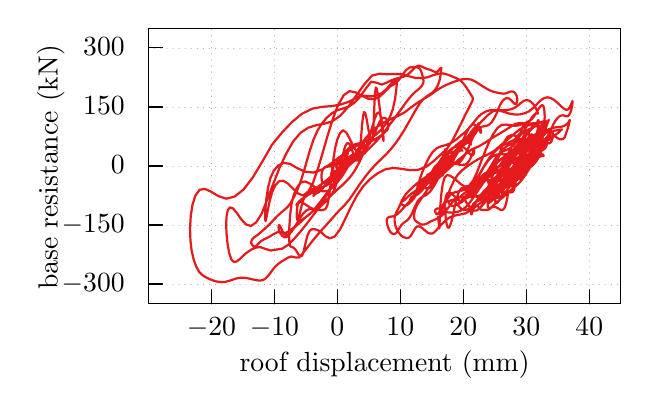
\begin{tikzpicture}[gnuplot]
%% generated with GNUPLOT 5.2p6 (Lua 5.3; terminal rev. Nov 2018, script rev. 107)
%% 09/28/2019 22:27:56
\path (0.000,0.000) rectangle (6.000,3.500);
\gpcolor{color=gp lt color axes}
\gpsetlinetype{gp lt axes}
\gpsetdashtype{gp dt axes}
\gpsetlinewidth{0.50}
\draw[gp path] (0.000,0.250)--(5.999,0.250);
\gpcolor{color=gp lt color border}
\gpsetlinetype{gp lt border}
\gpsetdashtype{gp dt solid}
\gpsetlinewidth{1.00}
\draw[gp path] (0.000,0.250)--(0.180,0.250);
\node[gp node right] at (-0.184,0.250) {$-300$};
\gpcolor{color=gp lt color axes}
\gpsetlinetype{gp lt axes}
\gpsetdashtype{gp dt axes}
\gpsetlinewidth{0.50}
\draw[gp path] (0.000,1.000)--(5.999,1.000);
\gpcolor{color=gp lt color border}
\gpsetlinetype{gp lt border}
\gpsetdashtype{gp dt solid}
\gpsetlinewidth{1.00}
\draw[gp path] (0.000,1.000)--(0.180,1.000);
\node[gp node right] at (-0.184,1.000) {$-150$};
\gpcolor{color=gp lt color axes}
\gpsetlinetype{gp lt axes}
\gpsetdashtype{gp dt axes}
\gpsetlinewidth{0.50}
\draw[gp path] (0.000,1.749)--(5.999,1.749);
\gpcolor{color=gp lt color border}
\gpsetlinetype{gp lt border}
\gpsetdashtype{gp dt solid}
\gpsetlinewidth{1.00}
\draw[gp path] (0.000,1.749)--(0.180,1.749);
\node[gp node right] at (-0.184,1.749) {$0$};
\gpcolor{color=gp lt color axes}
\gpsetlinetype{gp lt axes}
\gpsetdashtype{gp dt axes}
\gpsetlinewidth{0.50}
\draw[gp path] (0.000,2.499)--(5.999,2.499);
\gpcolor{color=gp lt color border}
\gpsetlinetype{gp lt border}
\gpsetdashtype{gp dt solid}
\gpsetlinewidth{1.00}
\draw[gp path] (0.000,2.499)--(0.180,2.499);
\node[gp node right] at (-0.184,2.499) {$150$};
\gpcolor{color=gp lt color axes}
\gpsetlinetype{gp lt axes}
\gpsetdashtype{gp dt axes}
\gpsetlinewidth{0.50}
\draw[gp path] (0.000,3.249)--(5.999,3.249);
\gpcolor{color=gp lt color border}
\gpsetlinetype{gp lt border}
\gpsetdashtype{gp dt solid}
\gpsetlinewidth{1.00}
\draw[gp path] (0.000,3.249)--(0.180,3.249);
\node[gp node right] at (-0.184,3.249) {$300$};
\gpcolor{color=gp lt color axes}
\gpsetlinetype{gp lt axes}
\gpsetdashtype{gp dt axes}
\gpsetlinewidth{0.50}
\draw[gp path] (0.800,0.000)--(0.800,3.499);
\gpcolor{color=gp lt color border}
\gpsetlinetype{gp lt border}
\gpsetdashtype{gp dt solid}
\gpsetlinewidth{1.00}
\draw[gp path] (0.800,0.000)--(0.800,0.180);
\node[gp node center] at (0.800,-0.308) {$-20$};
\gpcolor{color=gp lt color axes}
\gpsetlinetype{gp lt axes}
\gpsetdashtype{gp dt axes}
\gpsetlinewidth{0.50}
\draw[gp path] (1.600,0.000)--(1.600,3.499);
\gpcolor{color=gp lt color border}
\gpsetlinetype{gp lt border}
\gpsetdashtype{gp dt solid}
\gpsetlinewidth{1.00}
\draw[gp path] (1.600,0.000)--(1.600,0.180);
\node[gp node center] at (1.600,-0.308) {$-10$};
\gpcolor{color=gp lt color axes}
\gpsetlinetype{gp lt axes}
\gpsetdashtype{gp dt axes}
\gpsetlinewidth{0.50}
\draw[gp path] (2.400,0.000)--(2.400,3.499);
\gpcolor{color=gp lt color border}
\gpsetlinetype{gp lt border}
\gpsetdashtype{gp dt solid}
\gpsetlinewidth{1.00}
\draw[gp path] (2.400,0.000)--(2.400,0.180);
\node[gp node center] at (2.400,-0.308) {$0$};
\gpcolor{color=gp lt color axes}
\gpsetlinetype{gp lt axes}
\gpsetdashtype{gp dt axes}
\gpsetlinewidth{0.50}
\draw[gp path] (3.199,0.000)--(3.199,3.499);
\gpcolor{color=gp lt color border}
\gpsetlinetype{gp lt border}
\gpsetdashtype{gp dt solid}
\gpsetlinewidth{1.00}
\draw[gp path] (3.199,0.000)--(3.199,0.180);
\node[gp node center] at (3.199,-0.308) {$10$};
\gpcolor{color=gp lt color axes}
\gpsetlinetype{gp lt axes}
\gpsetdashtype{gp dt axes}
\gpsetlinewidth{0.50}
\draw[gp path] (3.999,0.000)--(3.999,3.499);
\gpcolor{color=gp lt color border}
\gpsetlinetype{gp lt border}
\gpsetdashtype{gp dt solid}
\gpsetlinewidth{1.00}
\draw[gp path] (3.999,0.000)--(3.999,0.180);
\node[gp node center] at (3.999,-0.308) {$20$};
\gpcolor{color=gp lt color axes}
\gpsetlinetype{gp lt axes}
\gpsetdashtype{gp dt axes}
\gpsetlinewidth{0.50}
\draw[gp path] (4.799,0.000)--(4.799,0.350)--(4.799,3.499);
\gpcolor{color=gp lt color border}
\gpsetlinetype{gp lt border}
\gpsetdashtype{gp dt solid}
\gpsetlinewidth{1.00}
\draw[gp path] (4.799,0.000)--(4.799,0.180);
\node[gp node center] at (4.799,-0.308) {$30$};
\gpcolor{color=gp lt color axes}
\gpsetlinetype{gp lt axes}
\gpsetdashtype{gp dt axes}
\gpsetlinewidth{0.50}
\draw[gp path] (5.599,0.000)--(5.599,0.350)--(5.599,3.499);
\gpcolor{color=gp lt color border}
\gpsetlinetype{gp lt border}
\gpsetdashtype{gp dt solid}
\gpsetlinewidth{1.00}
\draw[gp path] (5.599,0.000)--(5.599,0.180);
\node[gp node center] at (5.599,-0.308) {$40$};
\draw[gp path] (0.000,3.499)--(0.000,0.000)--(5.999,0.000)--(5.999,3.499)--cycle;
\node[gp node center,rotate=-270] at (-1.228,1.749) {base resistance (\si{\kilo\newton})};
\node[gp node center] at (2.999,-0.769) {roof displacement (\si{\milli\metre})};
\gpcolor{rgb color={0.894,0.102,0.110}}
\gpsetlinewidth{2.00}
\draw[gp path] (2.400,1.749)--(2.400,1.750)--(2.400,1.754)--(2.400,1.758)--(2.400,1.764)%
  --(2.401,1.769)--(2.402,1.774)--(2.403,1.777)--(2.405,1.779)--(2.406,1.780)--(2.408,1.778)%
  --(2.411,1.776)--(2.413,1.774)--(2.416,1.773)--(2.418,1.776)--(2.420,1.780)--(2.423,1.786)%
  --(2.425,1.792)--(2.428,1.799)--(2.430,1.806)--(2.433,1.811)--(2.436,1.814)--(2.438,1.815)%
  --(2.441,1.816)--(2.444,1.817)--(2.447,1.819)--(2.449,1.821)--(2.452,1.824)--(2.454,1.827)%
  --(2.456,1.831)--(2.458,1.834)--(2.460,1.836)--(2.462,1.838)--(2.464,1.837)--(2.465,1.836)%
  --(2.466,1.835)--(2.466,1.833)--(2.466,1.831)--(2.466,1.830)--(2.465,1.831)--(2.464,1.831)%
  --(2.462,1.833)--(2.460,1.834)--(2.459,1.835)--(2.457,1.835)--(2.454,1.834)--(2.452,1.833)%
  --(2.450,1.832)--(2.448,1.831)--(2.446,1.829)--(2.445,1.827)--(2.443,1.826)--(2.441,1.825)%
  --(2.440,1.824)--(2.439,1.821)--(2.438,1.819)--(2.437,1.816)--(2.436,1.813)--(2.436,1.811)%
  --(2.435,1.809)--(2.435,1.807)--(2.434,1.806)--(2.434,1.805)--(2.433,1.804)--(2.433,1.803)%
  --(2.433,1.802)--(2.432,1.800)--(2.432,1.798)--(2.432,1.796)--(2.431,1.793)--(2.431,1.791)%
  --(2.430,1.788)--(2.429,1.786)--(2.428,1.785)--(2.427,1.785)--(2.426,1.786)--(2.425,1.787)%
  --(2.423,1.789)--(2.422,1.791)--(2.421,1.794)--(2.420,1.797)--(2.420,1.799)--(2.419,1.800)%
  --(2.419,1.802)--(2.420,1.804)--(2.421,1.805)--(2.422,1.805)--(2.423,1.806)--(2.425,1.807)%
  --(2.427,1.806)--(2.429,1.803)--(2.431,1.799)--(2.433,1.794)--(2.435,1.790)--(2.436,1.785)%
  --(2.438,1.781)--(2.438,1.777)--(2.439,1.774)--(2.438,1.772)--(2.437,1.770)--(2.436,1.767)%
  --(2.433,1.768)--(2.431,1.772)--(2.428,1.777)--(2.425,1.783)--(2.421,1.788)--(2.418,1.793)%
  --(2.415,1.797)--(2.413,1.798)--(2.411,1.796)--(2.409,1.789)--(2.407,1.781)--(2.406,1.775)%
  --(2.406,1.772)--(2.405,1.773)--(2.405,1.777)--(2.405,1.783)--(2.406,1.792)--(2.408,1.802)%
  --(2.410,1.812)--(2.412,1.819)--(2.416,1.823)--(2.420,1.826)--(2.425,1.828)--(2.430,1.831)%
  --(2.436,1.835)--(2.443,1.840)--(2.449,1.847)--(2.456,1.855)--(2.464,1.863)--(2.471,1.868)%
  --(2.478,1.871)--(2.485,1.873)--(2.492,1.875)--(2.499,1.879)--(2.505,1.883)--(2.510,1.889)%
  --(2.515,1.895)--(2.519,1.903)--(2.523,1.912)--(2.526,1.918)--(2.529,1.922)--(2.530,1.923)%
  --(2.532,1.921)--(2.532,1.917)--(2.532,1.911)--(2.531,1.904)--(2.529,1.896)--(2.526,1.889)%
  --(2.523,1.882)--(2.518,1.875)--(2.512,1.866)--(2.505,1.857)--(2.498,1.845)--(2.489,1.831)%
  --(2.479,1.815)--(2.469,1.798)--(2.457,1.779)--(2.445,1.760)--(2.431,1.741)--(2.417,1.723)%
  --(2.402,1.706)--(2.387,1.691)--(2.371,1.677)--(2.354,1.661)--(2.338,1.644)--(2.321,1.624)%
  --(2.305,1.603)--(2.288,1.579)--(2.272,1.554)--(2.256,1.528)--(2.240,1.502)--(2.225,1.478)%
  --(2.209,1.458)--(2.194,1.443)--(2.180,1.430)--(2.166,1.419)--(2.153,1.411)--(2.141,1.405)%
  --(2.130,1.400)--(2.121,1.393)--(2.113,1.386)--(2.106,1.379)--(2.101,1.373)--(2.098,1.370)%
  --(2.096,1.369)--(2.096,1.371)--(2.098,1.376)--(2.101,1.385)--(2.107,1.397)--(2.114,1.409)%
  --(2.123,1.423)--(2.133,1.435)--(2.145,1.444)--(2.159,1.452)--(2.173,1.459)--(2.189,1.466)%
  --(2.205,1.475)--(2.222,1.487)--(2.239,1.501)--(2.256,1.518)--(2.272,1.536)--(2.289,1.554)%
  --(2.305,1.571)--(2.320,1.585)--(2.334,1.595)--(2.347,1.602)--(2.359,1.606)--(2.369,1.608)%
  --(2.378,1.609)--(2.385,1.611)--(2.390,1.613)--(2.393,1.617)--(2.394,1.622)--(2.393,1.629)%
  --(2.390,1.634)--(2.386,1.636)--(2.380,1.635)--(2.372,1.630)--(2.364,1.622)--(2.354,1.612)%
  --(2.343,1.602)--(2.331,1.593)--(2.319,1.585)--(2.306,1.579)--(2.294,1.573)--(2.281,1.565)%
  --(2.268,1.556)--(2.255,1.547)--(2.243,1.540)--(2.232,1.536)--(2.222,1.534)--(2.213,1.537)%
  --(2.206,1.551)--(2.201,1.575)--(2.199,1.606)--(2.199,1.639)--(2.204,1.669)--(2.211,1.693)%
  --(2.223,1.715)--(2.238,1.733)--(2.257,1.741)--(2.279,1.741)--(2.303,1.742)--(2.330,1.749)%
  --(2.359,1.766)--(2.389,1.792)--(2.420,1.826)--(2.451,1.864)--(2.483,1.904)--(2.515,1.944)%
  --(2.547,1.978)--(2.578,2.003)--(2.608,2.019)--(2.636,2.027)--(2.663,2.034)--(2.687,2.040)%
  --(2.708,2.049)--(2.727,2.062)--(2.741,2.077)--(2.753,2.092)--(2.760,2.106)--(2.764,2.113)%
  --(2.764,2.112)--(2.761,2.100)--(2.753,2.079)--(2.742,2.049)--(2.726,2.015)--(2.707,1.978)%
  --(2.683,1.939)--(2.656,1.901)--(2.624,1.864)--(2.589,1.826)--(2.551,1.783)--(2.509,1.734)%
  --(2.464,1.678)--(2.417,1.615)--(2.367,1.546)--(2.315,1.473)--(2.261,1.399)--(2.206,1.324)%
  --(2.148,1.250)--(2.090,1.178)--(2.031,1.123)--(1.971,1.081)--(1.912,1.029)--(1.853,0.973)%
  --(1.796,0.926)--(1.740,0.899)--(1.686,0.907)--(1.635,0.907)--(1.587,0.882)--(1.542,0.854)%
  --(1.502,0.833)--(1.465,0.816)--(1.432,0.796)--(1.403,0.770)--(1.377,0.742)--(1.355,0.726)%
  --(1.337,0.728)--(1.323,0.741)--(1.313,0.758)--(1.307,0.768)--(1.304,0.774)--(1.306,0.785)%
  --(1.312,0.804)--(1.322,0.824)--(1.337,0.839)--(1.355,0.852)--(1.377,0.866)--(1.403,0.886)%
  --(1.431,0.911)--(1.463,0.939)--(1.497,0.970)--(1.532,1.003)--(1.570,1.042)--(1.609,1.084)%
  --(1.648,1.124)--(1.688,1.160)--(1.728,1.193)--(1.768,1.229)--(1.807,1.281)--(1.846,1.350)%
  --(1.884,1.429)--(1.923,1.522)--(1.962,1.640)--(2.003,1.781)--(2.047,1.934)--(2.095,2.079)%
  --(2.147,2.197)--(2.203,2.288)--(2.264,2.361)--(2.330,2.419)--(2.399,2.457)--(2.470,2.479)%
  --(2.543,2.505)--(2.616,2.552)--(2.689,2.628)--(2.760,2.732)--(2.830,2.820)--(2.899,2.806)%
  --(2.965,2.783)--(3.029,2.809)--(3.090,2.839)--(3.148,2.859)--(3.201,2.872)--(3.252,2.887)%
  --(3.300,2.915)--(3.345,2.958)--(3.388,3.003)--(3.428,3.024)--(3.467,3.015)--(3.503,2.996)%
  --(3.537,2.983)--(3.568,2.974)--(3.597,2.963)--(3.622,2.951)--(3.645,2.943)--(3.664,2.945)%
  --(3.681,2.957)--(3.694,2.974)--(3.705,2.988)--(3.713,2.995)--(3.718,2.997)--(3.721,2.994)%
  --(3.721,2.985)--(3.718,2.959)--(3.712,2.912)--(3.703,2.860)--(3.690,2.811)--(3.673,2.769)%
  --(3.652,2.732)--(3.627,2.700)--(3.598,2.675)--(3.565,2.653)--(3.529,2.630)--(3.489,2.596)%
  --(3.447,2.543)--(3.402,2.473)--(3.354,2.389)--(3.304,2.299)--(3.251,2.208)--(3.196,2.120)%
  --(3.138,2.037)--(3.077,1.960)--(3.015,1.893)--(2.951,1.831)--(2.886,1.767)--(2.820,1.696)%
  --(2.754,1.614)--(2.688,1.523)--(2.622,1.425)--(2.557,1.331)--(2.492,1.251)--(2.428,1.190)%
  --(2.365,1.119)--(2.303,1.049)--(2.242,0.981)--(2.183,0.916)--(2.126,0.849)--(2.070,0.780)%
  --(2.016,0.710)--(1.963,0.644)--(1.912,0.586)--(1.863,0.589)--(1.816,0.600)--(1.770,0.584)%
  --(1.727,0.557)--(1.685,0.532)--(1.646,0.504)--(1.607,0.467)--(1.569,0.418)--(1.531,0.367)%
  --(1.493,0.324)--(1.454,0.300)--(1.414,0.294)--(1.372,0.299)--(1.330,0.308)--(1.287,0.318)%
  --(1.243,0.327)--(1.199,0.331)--(1.154,0.328)--(1.109,0.319)--(1.063,0.303)--(1.016,0.288)%
  --(0.969,0.276)--(0.922,0.275)--(0.874,0.281)--(0.826,0.294)--(0.779,0.312)--(0.733,0.335)%
  --(0.688,0.362)--(0.646,0.403)--(0.607,0.472)--(0.574,0.566)--(0.549,0.675)--(0.534,0.806)%
  --(0.529,0.957)--(0.538,1.114)--(0.560,1.258)--(0.598,1.375)--(0.651,1.447)--(0.718,1.458)%
  --(0.798,1.422)--(0.889,1.367)--(0.990,1.334)--(1.097,1.362)--(1.210,1.452)--(1.327,1.606)%
  --(1.447,1.805)--(1.570,2.020)--(1.696,2.173)--(1.824,2.308)--(1.953,2.414)--(2.081,2.477)%
  --(2.207,2.501)--(2.329,2.510)--(2.446,2.531)--(2.555,2.569)--(2.657,2.625)--(2.749,2.642)%
  --(2.831,2.635)--(2.904,2.649)--(2.967,2.677)--(3.020,2.722)--(3.064,2.773)--(3.098,2.809)%
  --(3.125,2.827)--(3.143,2.834)--(3.153,2.825)--(3.154,2.788)--(3.147,2.706)--(3.130,2.587)%
  --(3.104,2.470)--(3.067,2.370)--(3.020,2.287)--(2.962,2.216)--(2.893,2.151)--(2.815,2.094)%
  --(2.727,2.046)--(2.632,1.998)--(2.531,1.933)--(2.425,1.862)--(2.316,1.779)--(2.205,1.704)%
  --(2.095,1.666)--(1.989,1.677)--(1.889,1.723)--(1.799,1.776)--(1.719,1.789)--(1.650,1.756)%
  --(1.594,1.693)--(1.551,1.598)--(1.519,1.474)--(1.498,1.331)--(1.486,1.192)--(1.482,1.089)%
  --(1.487,1.048)--(1.498,1.084)--(1.515,1.184)--(1.540,1.305)--(1.572,1.417)--(1.612,1.504)%
  --(1.659,1.555)--(1.712,1.563)--(1.771,1.528)--(1.834,1.465)--(1.898,1.402)--(1.963,1.375)%
  --(2.027,1.417)--(2.089,1.532)--(2.151,1.708)--(2.212,1.912)--(2.275,2.131)--(2.339,2.338)%
  --(2.407,2.519)--(2.480,2.648)--(2.555,2.700)--(2.633,2.684)--(2.712,2.641)--(2.790,2.604)%
  --(2.866,2.597)--(2.938,2.631)--(3.006,2.695)--(3.068,2.757)--(3.126,2.792)--(3.179,2.838)%
  --(3.228,2.908)--(3.272,2.967)--(3.312,2.997)--(3.347,3.006)--(3.380,3.005)--(3.408,3.002)%
  --(3.434,2.996)--(3.455,2.973)--(3.472,2.931)--(3.485,2.882)--(3.492,2.845)--(3.495,2.826)%
  --(3.492,2.810)--(3.483,2.787)--(3.468,2.761)--(3.448,2.738)--(3.422,2.717)--(3.391,2.692)%
  --(3.355,2.658)--(3.313,2.610)--(3.267,2.551)--(3.217,2.481)--(3.162,2.405)--(3.104,2.325)%
  --(3.041,2.245)--(2.975,2.153)--(2.905,2.075)--(2.833,2.000)--(2.759,1.930)--(2.683,1.870)%
  --(2.606,1.805)--(2.530,1.742)--(2.454,1.678)--(2.380,1.616)--(2.309,1.554)--(2.241,1.500)%
  --(2.177,1.455)--(2.118,1.429)--(2.064,1.402)--(2.017,1.374)--(1.976,1.347)--(1.942,1.324)%
  --(1.915,1.301)--(1.896,1.279)--(1.884,1.262)--(1.879,1.253)--(1.882,1.252)--(1.892,1.260)%
  --(1.908,1.277)--(1.931,1.299)--(1.960,1.326)--(1.995,1.358)--(2.036,1.394)--(2.081,1.431)%
  --(2.131,1.469)--(2.185,1.508)--(2.241,1.551)--(2.300,1.599)--(2.361,1.650)--(2.423,1.705)%
  --(2.485,1.768)--(2.546,1.825)--(2.607,1.881)--(2.666,1.934)--(2.723,1.983)--(2.777,2.025)%
  --(2.828,2.061)--(2.874,2.088)--(2.916,2.111)--(2.953,2.136)--(2.984,2.161)--(3.008,2.183)%
  --(3.027,2.200)--(3.040,2.216)--(3.046,2.239)--(3.047,2.271)--(3.042,2.304)--(3.033,2.331)%
  --(3.020,2.350)--(3.003,2.359)--(2.984,2.361)--(2.962,2.349)--(2.938,2.313)--(2.911,2.253)%
  --(2.881,2.181)--(2.849,2.109)--(2.814,2.042)--(2.776,1.989)--(2.736,1.946)--(2.693,1.911)%
  --(2.648,1.880)--(2.602,1.851)--(2.555,1.816)--(2.508,1.768)--(2.460,1.703)--(2.412,1.629)%
  --(2.363,1.550)--(2.315,1.464)--(2.267,1.383)--(2.219,1.311)--(2.170,1.252)--(2.122,1.203)%
  --(2.075,1.162)--(2.028,1.125)--(1.983,1.086)--(1.940,1.042)--(1.898,1.006)--(1.859,0.972)%
  --(1.821,0.924)--(1.786,0.875)--(1.754,0.847)--(1.725,0.845)--(1.701,0.862)--(1.680,0.889)%
  --(1.665,0.916)--(1.656,0.941)--(1.653,0.972)--(1.656,0.997)--(1.665,0.999)--(1.680,0.971)%
  --(1.700,0.926)--(1.724,0.887)--(1.751,0.870)--(1.781,0.879)--(1.814,0.911)--(1.848,0.959)%
  --(1.885,1.018)--(1.922,1.082)--(1.961,1.140)--(2.000,1.181)--(2.040,1.201)--(2.080,1.204)%
  --(2.118,1.197)--(2.155,1.191)--(2.190,1.188)--(2.221,1.191)--(2.248,1.203)--(2.271,1.242)%
  --(2.291,1.339)--(2.310,1.488)--(2.328,1.661)--(2.349,1.833)--(2.372,1.978)--(2.400,2.088)%
  --(2.434,2.167)--(2.472,2.203)--(2.515,2.173)--(2.560,2.089)--(2.607,1.991)--(2.653,1.922)%
  --(2.697,1.910)--(2.739,1.952)--(2.778,2.034)--(2.813,2.141)--(2.846,2.254)--(2.876,2.354)%
  --(2.904,2.419)--(2.929,2.430)--(2.951,2.380)--(2.969,2.286)--(2.981,2.177)--(2.987,2.090)%
  --(2.986,2.066)--(2.979,2.114)--(2.967,2.221)--(2.951,2.364)--(2.934,2.513)--(2.917,2.641)%
  --(2.902,2.727)--(2.889,2.746)--(2.879,2.679)--(2.871,2.539)--(2.864,2.367)--(2.856,2.209)%
  --(2.847,2.104)--(2.835,2.064)--(2.820,2.089)--(2.804,2.162)--(2.786,2.262)--(2.769,2.360)%
  --(2.753,2.426)--(2.738,2.433)--(2.725,2.373)--(2.713,2.260)--(2.702,2.122)--(2.690,1.987)%
  --(2.676,1.880)--(2.660,1.822)--(2.641,1.817)--(2.619,1.857)--(2.596,1.923)--(2.573,1.991)%
  --(2.549,2.035)--(2.526,2.041)--(2.505,2.012)--(2.486,1.955)--(2.469,1.884)--(2.452,1.812)%
  --(2.437,1.749)--(2.423,1.707)--(2.409,1.696)--(2.396,1.712)--(2.383,1.743)--(2.373,1.774)%
  --(2.364,1.792)--(2.357,1.792)--(2.352,1.774)--(2.349,1.740)--(2.348,1.697)--(2.348,1.652)%
  --(2.349,1.614)--(2.350,1.593)--(2.351,1.592)--(2.352,1.608)--(2.353,1.632)--(2.355,1.657)%
  --(2.356,1.674)--(2.359,1.679)--(2.361,1.668)--(2.363,1.643)--(2.365,1.608)--(2.366,1.572)%
  --(2.366,1.543)--(2.365,1.528)--(2.362,1.527)--(2.358,1.539)--(2.353,1.565)--(2.347,1.600)%
  --(2.341,1.633)--(2.335,1.659)--(2.331,1.672)--(2.327,1.673)--(2.325,1.667)--(2.323,1.655)%
  --(2.323,1.643)--(2.324,1.635)--(2.327,1.635)--(2.330,1.645)--(2.335,1.659)--(2.340,1.672)%
  --(2.347,1.680)--(2.354,1.683)--(2.362,1.680)--(2.370,1.671)--(2.378,1.657)--(2.386,1.641)%
  --(2.394,1.627)--(2.400,1.618)--(2.405,1.616)--(2.409,1.616)--(2.411,1.616)--(2.412,1.614)%
  --(2.410,1.608)--(2.407,1.595)--(2.401,1.574)--(2.394,1.546)--(2.383,1.512)--(2.371,1.475)%
  --(2.355,1.439)--(2.336,1.404)--(2.314,1.371)--(2.289,1.339)--(2.262,1.309)--(2.231,1.278)%
  --(2.198,1.247)--(2.163,1.215)--(2.127,1.200)--(2.090,1.205)--(2.053,1.222)--(2.019,1.245)%
  --(1.987,1.266)--(1.958,1.283)--(1.934,1.296)--(1.914,1.297)--(1.900,1.274)--(1.890,1.224)%
  --(1.885,1.164)--(1.884,1.110)--(1.886,1.075)--(1.892,1.064)--(1.900,1.074)--(1.911,1.106)%
  --(1.925,1.160)--(1.943,1.233)--(1.964,1.309)--(1.990,1.374)--(2.019,1.418)--(2.053,1.444)%
  --(2.091,1.459)--(2.132,1.469)--(2.175,1.474)--(2.220,1.486)--(2.265,1.503)--(2.311,1.540)%
  --(2.357,1.595)--(2.402,1.664)--(2.446,1.734)--(2.489,1.797)--(2.531,1.846)--(2.571,1.880)%
  --(2.609,1.900)--(2.644,1.907)--(2.676,1.906)--(2.704,1.901)--(2.727,1.900)--(2.746,1.909)%
  --(2.759,1.924)--(2.767,1.942)--(2.770,1.958)--(2.768,1.965)--(2.760,1.961)--(2.748,1.942)%
  --(2.730,1.907)--(2.707,1.859)--(2.679,1.796)--(2.645,1.733)--(2.607,1.670)--(2.563,1.610)%
  --(2.513,1.555)--(2.460,1.503)--(2.402,1.451)--(2.340,1.395)--(2.275,1.331)--(2.208,1.261)%
  --(2.138,1.182)--(2.067,1.089)--(1.994,0.994)--(1.920,0.903)--(1.846,0.819)--(1.771,0.746)%
  --(1.698,0.699)--(1.625,0.688)--(1.555,0.676)--(1.487,0.696)--(1.423,0.719)--(1.363,0.713)%
  --(1.307,0.688)--(1.256,0.654)--(1.208,0.614)--(1.165,0.572)--(1.124,0.538)--(1.087,0.528)%
  --(1.054,0.562)--(1.026,0.645)--(1.005,0.763)--(0.992,0.892)--(0.988,1.012)--(0.994,1.120)%
  --(1.010,1.192)--(1.037,1.224)--(1.075,1.210)--(1.121,1.156)--(1.175,1.078)--(1.235,1.010)%
  --(1.300,0.987)--(1.368,1.032)--(1.438,1.143)--(1.511,1.328)--(1.587,1.526)--(1.667,1.729)%
  --(1.750,1.906)--(1.839,2.061)--(1.932,2.171)--(2.030,2.235)--(2.130,2.267)--(2.232,2.286)%
  --(2.335,2.316)--(2.438,2.389)--(2.540,2.503)--(2.641,2.646)--(2.741,2.785)--(2.840,2.898)%
  --(2.938,2.922)--(3.034,2.914)--(3.129,2.919)--(3.220,2.913)--(3.308,2.889)--(3.391,2.868)%
  --(3.470,2.864)--(3.545,2.876)--(3.616,2.902)--(3.683,2.922)--(3.746,2.924)--(3.805,2.908)%
  --(3.860,2.886)--(3.911,2.865)--(3.958,2.839)--(3.999,2.799)--(4.036,2.750)--(4.066,2.703)%
  --(4.091,2.664)--(4.108,2.636)--(4.119,2.615)--(4.121,2.598)--(4.117,2.580)--(4.105,2.556)%
  --(4.084,2.516)--(4.056,2.460)--(4.020,2.390)--(3.975,2.295)--(3.922,2.192)--(3.860,2.069)%
  --(3.789,1.964)--(3.709,1.891)--(3.622,1.811)--(3.527,1.739)--(3.426,1.701)--(3.322,1.696)%
  --(3.217,1.713)--(3.112,1.725)--(3.009,1.707)--(2.911,1.656)--(2.817,1.585)--(2.729,1.493)%
  --(2.647,1.372)--(2.569,1.224)--(2.497,1.070)--(2.428,0.935)--(2.364,0.852)--(2.304,0.831)%
  --(2.247,0.858)--(2.196,0.907)--(2.150,0.935)--(2.109,0.947)--(2.075,0.947)--(2.046,0.923)%
  --(2.022,0.872)--(2.002,0.798)--(1.984,0.719)--(1.969,0.654)--(1.954,0.615)--(1.940,0.601)%
  --(1.926,0.604)--(1.911,0.619)--(1.896,0.641)--(1.881,0.668)--(1.866,0.690)--(1.851,0.705)%
  --(1.836,0.716)--(1.822,0.722)--(1.810,0.724)--(1.799,0.734)--(1.791,0.773)--(1.787,0.850)%
  --(1.790,0.971)--(1.800,1.126)--(1.818,1.267)--(1.846,1.382)--(1.885,1.471)--(1.933,1.538)%
  --(1.991,1.553)--(2.058,1.523)--(2.131,1.468)--(2.209,1.427)--(2.292,1.437)--(2.376,1.511)%
  --(2.463,1.624)--(2.550,1.768)--(2.638,1.925)--(2.727,2.060)--(2.817,2.170)--(2.906,2.249)%
  --(2.995,2.305)--(3.083,2.347)--(3.170,2.385)--(3.254,2.431)--(3.335,2.493)--(3.415,2.551)%
  --(3.492,2.599)--(3.567,2.642)--(3.639,2.694)--(3.710,2.741)--(3.778,2.777)--(3.845,2.805)%
  --(3.911,2.829)--(3.975,2.849)--(4.039,2.856)--(4.101,2.846)--(4.161,2.816)--(4.220,2.778)%
  --(4.276,2.743)--(4.330,2.712)--(4.380,2.693)--(4.426,2.682)--(4.468,2.673)--(4.506,2.668)%
  --(4.541,2.672)--(4.572,2.685)--(4.599,2.694)--(4.623,2.697)--(4.642,2.690)--(4.659,2.675)%
  --(4.671,2.654)--(4.680,2.630)--(4.684,2.605)--(4.684,2.583)--(4.680,2.562)--(4.671,2.543)%
  --(4.659,2.536)--(4.643,2.546)--(4.623,2.566)--(4.601,2.590)--(4.577,2.608)--(4.552,2.612)%
  --(4.526,2.602)--(4.500,2.578)--(4.473,2.539)--(4.445,2.477)--(4.417,2.404)--(4.388,2.350)%
  --(4.359,2.304)--(4.328,2.275)--(4.298,2.261)--(4.267,2.256)--(4.236,2.248)--(4.206,2.233)%
  --(4.177,2.207)--(4.148,2.167)--(4.121,2.113)--(4.094,2.050)--(4.067,1.987)--(4.040,1.929)%
  --(4.013,1.878)--(3.986,1.835)--(3.958,1.801)--(3.929,1.781)--(3.901,1.781)--(3.873,1.798)%
  --(3.847,1.821)--(3.823,1.846)--(3.802,1.873)--(3.786,1.904)--(3.774,1.937)--(3.767,1.961)%
  --(3.765,1.957)--(3.769,1.924)--(3.776,1.875)--(3.787,1.828)--(3.802,1.793)--(3.818,1.774)%
  --(3.836,1.773)--(3.856,1.791)--(3.877,1.828)--(3.899,1.878)--(3.923,1.932)--(3.947,1.973)%
  --(3.972,1.993)--(3.997,1.991)--(4.023,1.971)--(4.047,1.944)--(4.070,1.916)--(4.090,1.894)%
  --(4.107,1.884)--(4.121,1.887)--(4.131,1.903)--(4.137,1.925)--(4.139,1.945)--(4.138,1.955)%
  --(4.133,1.949)--(4.124,1.931)--(4.111,1.898)--(4.095,1.856)--(4.075,1.816)--(4.051,1.787)%
  --(4.023,1.768)--(3.993,1.761)--(3.960,1.764)--(3.926,1.772)--(3.891,1.780)--(3.855,1.780)%
  --(3.821,1.765)--(3.787,1.737)--(3.754,1.704)--(3.722,1.666)--(3.692,1.616)--(3.663,1.560)%
  --(3.635,1.509)--(3.608,1.465)--(3.582,1.430)--(3.557,1.404)--(3.532,1.385)--(3.508,1.371)%
  --(3.485,1.360)--(3.463,1.347)--(3.442,1.329)--(3.422,1.304)--(3.404,1.271)--(3.386,1.234)%
  --(3.368,1.195)--(3.352,1.157)--(3.335,1.124)--(3.318,1.096)--(3.302,1.074)--(3.285,1.058)%
  --(3.268,1.046)--(3.251,1.034)--(3.233,1.020)--(3.216,1.001)--(3.199,0.978)--(3.181,0.951)%
  --(3.163,0.920)--(3.144,0.896)--(3.126,0.886)--(3.108,0.887)--(3.090,0.895)--(3.073,0.912)%
  --(3.058,0.938)--(3.045,0.969)--(3.036,1.001)--(3.029,1.031)--(3.027,1.056)--(3.029,1.073)%
  --(3.036,1.087)--(3.047,1.097)--(3.063,1.104)--(3.082,1.106)--(3.106,1.110)--(3.133,1.120)%
  --(3.164,1.139)--(3.197,1.170)--(3.233,1.208)--(3.270,1.251)--(3.310,1.292)--(3.352,1.354)%
  --(3.394,1.405)--(3.438,1.446)--(3.483,1.483)--(3.528,1.522)--(3.573,1.566)--(3.617,1.614)%
  --(3.661,1.671)--(3.705,1.733)--(3.747,1.802)--(3.789,1.871)--(3.831,1.935)--(3.871,1.975)%
  --(3.910,2.013)--(3.948,2.045)--(3.984,2.069)--(4.018,2.086)--(4.049,2.099)--(4.077,2.113)%
  --(4.103,2.130)--(4.125,2.155)--(4.144,2.185)--(4.160,2.215)--(4.173,2.242)--(4.182,2.266)%
  --(4.189,2.284)--(4.194,2.294)--(4.195,2.291)--(4.194,2.276)--(4.190,2.251)--(4.182,2.221)%
  --(4.171,2.193)--(4.158,2.168)--(4.140,2.147)--(4.120,2.129)--(4.096,2.113)--(4.070,2.095)%
  --(4.041,2.074)--(4.009,2.046)--(3.975,2.002)--(3.939,1.938)--(3.901,1.874)--(3.861,1.808)%
  --(3.819,1.746)--(3.774,1.686)--(3.728,1.633)--(3.680,1.589)--(3.632,1.560)--(3.584,1.540)%
  --(3.536,1.522)--(3.489,1.499)--(3.445,1.471)--(3.403,1.441)--(3.364,1.415)--(3.329,1.389)%
  --(3.297,1.361)--(3.270,1.333)--(3.248,1.314)--(3.231,1.303)--(3.219,1.295)--(3.212,1.286)%
  --(3.209,1.276)--(3.211,1.267)--(3.218,1.260)--(3.229,1.255)--(3.243,1.250)--(3.261,1.248)%
  --(3.282,1.252)--(3.306,1.268)--(3.332,1.294)--(3.360,1.327)--(3.391,1.369)--(3.423,1.433)%
  --(3.458,1.503)--(3.495,1.562)--(3.533,1.612)--(3.574,1.652)--(3.616,1.686)--(3.659,1.713)%
  --(3.703,1.734)--(3.746,1.751)--(3.788,1.771)--(3.829,1.800)--(3.868,1.839)--(3.904,1.886)%
  --(3.938,1.934)--(3.970,1.978)--(3.999,2.010)--(4.024,2.027)--(4.046,2.041)--(4.065,2.046)%
  --(4.080,2.044)--(4.090,2.035)--(4.096,2.026)--(4.098,2.021)--(4.095,2.026)--(4.088,2.039)%
  --(4.077,2.056)--(4.063,2.071)--(4.046,2.082)--(4.027,2.086)--(4.005,2.082)--(3.982,2.067)%
  --(3.958,2.033)--(3.932,1.986)--(3.905,1.938)--(3.877,1.894)--(3.848,1.856)--(3.818,1.823)%
  --(3.788,1.796)--(3.757,1.773)--(3.726,1.754)--(3.695,1.734)--(3.664,1.708)--(3.635,1.674)%
  --(3.606,1.635)--(3.579,1.596)--(3.553,1.560)--(3.528,1.528)--(3.505,1.503)--(3.484,1.488)%
  --(3.465,1.482)--(3.448,1.481)--(3.434,1.481)--(3.423,1.478)--(3.415,1.471)--(3.409,1.460)%
  --(3.407,1.446)--(3.407,1.431)--(3.410,1.419)--(3.416,1.412)--(3.423,1.414)--(3.433,1.426)%
  --(3.445,1.445)--(3.459,1.470)--(3.474,1.496)--(3.492,1.520)--(3.511,1.541)--(3.532,1.559)%
  --(3.554,1.576)--(3.577,1.595)--(3.601,1.616)--(3.626,1.642)--(3.652,1.677)--(3.678,1.719)%
  --(3.705,1.767)--(3.733,1.817)--(3.761,1.864)--(3.790,1.904)--(3.819,1.939)--(3.848,1.967)%
  --(3.878,1.986)--(3.907,1.997)--(3.935,2.004)--(3.961,2.013)--(3.987,2.026)--(4.010,2.041)%
  --(4.031,2.062)--(4.049,2.089)--(4.065,2.119)--(4.079,2.146)--(4.091,2.169)--(4.100,2.184)%
  --(4.107,2.188)--(4.112,2.183)--(4.114,2.170)--(4.113,2.153)--(4.110,2.135)--(4.103,2.117)%
  --(4.094,2.103)--(4.081,2.091)--(4.066,2.079)--(4.047,2.065)--(4.026,2.046)--(4.003,2.024)%
  --(3.977,1.998)--(3.949,1.966)--(3.920,1.942)--(3.889,1.917)--(3.857,1.892)--(3.825,1.867)%
  --(3.792,1.843)--(3.760,1.819)--(3.728,1.790)--(3.696,1.754)--(3.666,1.712)--(3.636,1.669)%
  --(3.607,1.628)--(3.580,1.595)--(3.554,1.569)--(3.530,1.549)--(3.507,1.535)--(3.487,1.525)%
  --(3.470,1.519)--(3.455,1.513)--(3.442,1.503)--(3.433,1.489)--(3.427,1.472)--(3.423,1.457)%
  --(3.422,1.444)--(3.424,1.435)--(3.428,1.432)--(3.434,1.435)--(3.442,1.445)--(3.453,1.460)%
  --(3.465,1.478)--(3.479,1.495)--(3.495,1.510)--(3.512,1.521)--(3.531,1.530)--(3.550,1.537)%
  --(3.570,1.543)--(3.590,1.551)--(3.610,1.562)--(3.630,1.576)--(3.649,1.590)--(3.667,1.602)%
  --(3.683,1.612)--(3.698,1.619)--(3.711,1.624)--(3.722,1.628)--(3.731,1.628)--(3.738,1.631)%
  --(3.742,1.645)--(3.745,1.672)--(3.746,1.707)--(3.746,1.746)--(3.746,1.784)--(3.746,1.819)%
  --(3.746,1.848)--(3.747,1.868)--(3.749,1.868)--(3.751,1.850)--(3.754,1.822)--(3.758,1.794)%
  --(3.761,1.772)--(3.764,1.758)--(3.766,1.753)--(3.767,1.758)--(3.768,1.771)--(3.768,1.788)%
  --(3.768,1.803)--(3.767,1.809)--(3.766,1.807)--(3.764,1.797)--(3.762,1.783)--(3.759,1.770)%
  --(3.756,1.762)--(3.753,1.763)--(3.750,1.775)--(3.747,1.795)--(3.744,1.820)--(3.742,1.846)%
  --(3.741,1.868)--(3.741,1.883)--(3.743,1.886)--(3.747,1.878)--(3.751,1.863)--(3.757,1.846)%
  --(3.763,1.830)--(3.769,1.818)--(3.776,1.811)--(3.782,1.813)--(3.788,1.822)--(3.794,1.834)%
  --(3.800,1.847)--(3.804,1.855)--(3.809,1.856)--(3.812,1.850)--(3.815,1.837)--(3.817,1.821)%
  --(3.817,1.802)--(3.816,1.785)--(3.814,1.770)--(3.809,1.761)--(3.803,1.756)--(3.795,1.754)%
  --(3.785,1.752)--(3.774,1.748)--(3.761,1.745)--(3.748,1.743)--(3.734,1.739)--(3.720,1.733)%
  --(3.705,1.728)--(3.691,1.724)--(3.678,1.723)--(3.666,1.724)--(3.654,1.721)--(3.644,1.714)%
  --(3.635,1.705)--(3.628,1.695)--(3.622,1.682)--(3.617,1.667)--(3.614,1.651)--(3.612,1.638)%
  --(3.611,1.633)--(3.611,1.638)--(3.612,1.649)--(3.615,1.663)--(3.619,1.677)--(3.624,1.691)%
  --(3.630,1.702)--(3.638,1.709)--(3.647,1.709)--(3.657,1.704)--(3.668,1.698)--(3.679,1.694)%
  --(3.690,1.696)--(3.702,1.703)--(3.713,1.715)--(3.724,1.731)--(3.734,1.748)--(3.744,1.764)%
  --(3.754,1.777)--(3.763,1.785)--(3.771,1.785)--(3.778,1.781)--(3.785,1.773)--(3.790,1.766)%
  --(3.793,1.762)--(3.796,1.762)--(3.796,1.767)--(3.796,1.775)--(3.794,1.787)--(3.791,1.801)%
  --(3.787,1.813)--(3.783,1.821)--(3.778,1.821)--(3.773,1.816)--(3.767,1.806)--(3.761,1.793)%
  --(3.755,1.775)--(3.749,1.754)--(3.742,1.734)--(3.734,1.715)--(3.726,1.698)--(3.716,1.682)%
  --(3.706,1.665)--(3.695,1.647)--(3.683,1.631)--(3.670,1.617)--(3.656,1.603)--(3.642,1.589)%
  --(3.627,1.579)--(3.612,1.575)--(3.597,1.576)--(3.583,1.578)--(3.569,1.578)--(3.557,1.576)%
  --(3.546,1.572)--(3.536,1.566)--(3.528,1.557)--(3.522,1.546)--(3.517,1.535)--(3.514,1.527)%
  --(3.513,1.525)--(3.514,1.527)--(3.516,1.534)--(3.519,1.544)--(3.525,1.553)--(3.532,1.562)%
  --(3.540,1.569)--(3.550,1.574)--(3.562,1.578)--(3.574,1.582)--(3.587,1.587)--(3.601,1.595)%
  --(3.615,1.605)--(3.629,1.616)--(3.643,1.629)--(3.658,1.642)--(3.672,1.654)--(3.685,1.664)%
  --(3.698,1.671)--(3.709,1.676)--(3.720,1.679)--(3.730,1.680)--(3.738,1.680)--(3.744,1.680)%
  --(3.749,1.682)--(3.751,1.684)--(3.752,1.687)--(3.752,1.690)--(3.749,1.694)--(3.745,1.699)%
  --(3.740,1.701)--(3.733,1.701)--(3.726,1.697)--(3.717,1.689)--(3.707,1.678)--(3.697,1.664)%
  --(3.686,1.645)--(3.674,1.623)--(3.661,1.599)--(3.647,1.575)--(3.632,1.551)--(3.616,1.527)%
  --(3.600,1.502)--(3.582,1.480)--(3.564,1.468)--(3.545,1.465)--(3.527,1.467)--(3.509,1.471)%
  --(3.493,1.471)--(3.477,1.465)--(3.462,1.455)--(3.450,1.441)--(3.439,1.425)--(3.429,1.408)%
  --(3.422,1.395)--(3.416,1.391)--(3.413,1.400)--(3.412,1.421)--(3.414,1.453)--(3.418,1.486)%
  --(3.426,1.515)--(3.438,1.537)--(3.452,1.551)--(3.470,1.561)--(3.490,1.568)--(3.513,1.576)%
  --(3.539,1.591)--(3.566,1.615)--(3.595,1.650)--(3.626,1.695)--(3.659,1.747)--(3.693,1.799)%
  --(3.728,1.849)--(3.764,1.892)--(3.801,1.929)--(3.838,1.958)--(3.876,1.983)--(3.913,2.007)%
  --(3.949,2.031)--(3.985,2.057)--(4.018,2.080)--(4.050,2.115)--(4.081,2.156)--(4.109,2.196)%
  --(4.135,2.227)--(4.158,2.247)--(4.178,2.256)--(4.195,2.253)--(4.209,2.239)--(4.219,2.219)%
  --(4.224,2.197)--(4.225,2.177)--(4.222,2.171)--(4.214,2.182)--(4.202,2.205)--(4.187,2.232)%
  --(4.168,2.255)--(4.148,2.272)--(4.126,2.278)--(4.103,2.269)--(4.079,2.243)--(4.055,2.200)%
  --(4.029,2.148)--(4.003,2.094)--(3.976,2.044)--(3.948,1.992)--(3.920,1.957)--(3.890,1.934)%
  --(3.861,1.923)--(3.831,1.916)--(3.802,1.909)--(3.773,1.895)--(3.746,1.872)--(3.720,1.840)%
  --(3.696,1.799)--(3.674,1.753)--(3.653,1.708)--(3.633,1.670)--(3.615,1.643)--(3.598,1.629)%
  --(3.584,1.625)--(3.571,1.629)--(3.560,1.636)--(3.551,1.641)--(3.545,1.641)--(3.542,1.634)%
  --(3.541,1.622)--(3.543,1.608)--(3.546,1.595)--(3.552,1.589)--(3.560,1.591)--(3.569,1.604)%
  --(3.580,1.626)--(3.593,1.655)--(3.608,1.687)--(3.624,1.719)--(3.643,1.745)--(3.663,1.765)%
  --(3.684,1.778)--(3.707,1.788)--(3.730,1.796)--(3.754,1.804)--(3.778,1.815)--(3.801,1.833)%
  --(3.825,1.855)--(3.847,1.882)--(3.868,1.910)--(3.889,1.935)--(3.908,1.956)--(3.925,1.969)%
  --(3.941,1.975)--(3.955,1.975)--(3.966,1.970)--(3.975,1.962)--(3.981,1.953)--(3.984,1.947)%
  --(3.984,1.944)--(3.981,1.945)--(3.975,1.947)--(3.966,1.947)--(3.955,1.942)--(3.940,1.932)%
  --(3.924,1.915)--(3.905,1.891)--(3.884,1.862)--(3.861,1.829)--(3.836,1.796)--(3.809,1.764)%
  --(3.781,1.735)--(3.752,1.709)--(3.721,1.684)--(3.690,1.660)--(3.659,1.636)--(3.627,1.611)%
  --(3.596,1.582)--(3.566,1.551)--(3.537,1.517)--(3.508,1.482)--(3.481,1.448)--(3.455,1.419)%
  --(3.431,1.396)--(3.409,1.383)--(3.389,1.375)--(3.371,1.370)--(3.357,1.363)--(3.345,1.356)%
  --(3.336,1.347)--(3.330,1.336)--(3.326,1.323)--(3.326,1.311)--(3.328,1.302)--(3.333,1.300)%
  --(3.340,1.303)--(3.350,1.311)--(3.361,1.322)--(3.375,1.340)--(3.391,1.378)--(3.410,1.441)%
  --(3.432,1.530)--(3.458,1.615)--(3.489,1.698)--(3.525,1.779)--(3.565,1.859)--(3.611,1.928)%
  --(3.662,1.975)--(3.717,1.999)--(3.776,2.015)--(3.837,2.038)--(3.900,2.078)--(3.965,2.133)%
  --(4.030,2.185)--(4.094,2.255)--(4.159,2.338)--(4.223,2.406)--(4.285,2.441)--(4.347,2.460)%
  --(4.406,2.461)--(4.463,2.458)--(4.517,2.458)--(4.567,2.462)--(4.614,2.472)--(4.658,2.492)%
  --(4.698,2.522)--(4.735,2.554)--(4.770,2.578)--(4.802,2.587)--(4.831,2.580)--(4.858,2.564)%
  --(4.882,2.542)--(4.903,2.515)--(4.920,2.485)--(4.933,2.455)--(4.942,2.432)--(4.947,2.418)%
  --(4.947,2.414)--(4.943,2.416)--(4.934,2.419)--(4.921,2.415)--(4.904,2.403)--(4.883,2.383)%
  --(4.858,2.347)--(4.829,2.303)--(4.797,2.240)--(4.760,2.178)--(4.721,2.137)--(4.678,2.103)%
  --(4.632,2.075)--(4.584,2.052)--(4.535,2.029)--(4.485,2.003)--(4.434,1.966)--(4.384,1.915)%
  --(4.335,1.860)--(4.286,1.785)--(4.237,1.703)--(4.190,1.624)--(4.143,1.555)--(4.097,1.505)%
  --(4.052,1.472)--(4.008,1.447)--(3.966,1.433)--(3.927,1.424)--(3.890,1.415)--(3.857,1.400)%
  --(3.827,1.373)--(3.800,1.335)--(3.777,1.291)--(3.757,1.247)--(3.739,1.206)--(3.725,1.167)%
  --(3.713,1.136)--(3.702,1.113)--(3.694,1.102)--(3.688,1.099)--(3.683,1.102)--(3.680,1.103)%
  --(3.679,1.101)--(3.679,1.093)--(3.681,1.080)--(3.683,1.061)--(3.686,1.037)--(3.690,1.009)%
  --(3.692,0.981)--(3.695,0.960)--(3.696,0.958)--(3.697,0.977)--(3.698,1.013)--(3.700,1.068)%
  --(3.703,1.152)--(3.709,1.266)--(3.721,1.398)--(3.738,1.521)--(3.762,1.603)--(3.792,1.633)%
  --(3.829,1.627)--(3.871,1.601)--(3.918,1.563)--(3.967,1.519)--(4.018,1.488)--(4.070,1.497)%
  --(4.122,1.560)--(4.174,1.671)--(4.225,1.804)--(4.277,1.937)--(4.329,2.058)--(4.382,2.160)%
  --(4.436,2.235)--(4.490,2.272)--(4.545,2.275)--(4.599,2.268)--(4.651,2.259)--(4.701,2.265)%
  --(4.747,2.281)--(4.790,2.297)--(4.828,2.317)--(4.863,2.340)--(4.893,2.372)--(4.919,2.413)%
  --(4.942,2.452)--(4.962,2.484)--(4.979,2.507)--(4.995,2.520)--(5.007,2.521)--(5.018,2.507)%
  --(5.026,2.475)--(5.031,2.428)--(5.033,2.371)--(5.030,2.312)--(5.022,2.259)--(5.009,2.208)%
  --(4.991,2.167)--(4.966,2.133)--(4.936,2.091)--(4.900,2.059)--(4.858,2.025)--(4.811,1.975)%
  --(4.758,1.902)--(4.700,1.810)--(4.636,1.703)--(4.568,1.595)--(4.495,1.505)--(4.418,1.447)%
  --(4.338,1.417)--(4.256,1.386)--(4.174,1.365)--(4.092,1.354)--(4.014,1.356)--(3.939,1.346)%
  --(3.868,1.297)--(3.801,1.210)--(3.740,1.132)--(3.683,1.087)--(3.630,1.064)--(3.582,1.044)%
  --(3.539,1.019)--(3.500,1.005)--(3.467,1.007)--(3.439,1.020)--(3.415,1.036)--(3.397,1.049)%
  --(3.383,1.064)--(3.376,1.090)--(3.374,1.123)--(3.379,1.162)--(3.390,1.203)--(3.408,1.244)%
  --(3.433,1.286)--(3.464,1.331)--(3.503,1.388)--(3.548,1.456)--(3.600,1.527)--(3.658,1.577)%
  --(3.723,1.632)--(3.792,1.693)--(3.866,1.762)--(3.944,1.833)--(4.025,1.899)--(4.108,1.961)%
  --(4.192,1.997)--(4.276,2.046)--(4.359,2.100)--(4.440,2.149)--(4.518,2.196)--(4.593,2.243)%
  --(4.664,2.287)--(4.730,2.295)--(4.791,2.290)--(4.846,2.288)--(4.895,2.292)--(4.937,2.296)%
  --(4.972,2.301)--(5.000,2.309)--(5.022,2.319)--(5.037,2.327)--(5.045,2.322)--(5.046,2.296)%
  --(5.041,2.250)--(5.027,2.190)--(5.006,2.103)--(4.977,2.000)--(4.940,1.918)--(4.896,1.919)%
  --(4.846,1.961)--(4.791,2.023)--(4.734,2.082)--(4.676,2.127)--(4.618,2.145)--(4.561,2.120)%
  --(4.506,2.034)--(4.453,1.886)--(4.400,1.708)--(4.349,1.561)--(4.298,1.447)--(4.246,1.375)%
  --(4.196,1.351)--(4.146,1.365)--(4.097,1.405)--(4.052,1.446)--(4.011,1.472)--(3.974,1.466)%
  --(3.942,1.418)--(3.914,1.335)--(3.890,1.231)--(3.869,1.127)--(3.850,1.049)--(3.833,0.996)%
  --(3.816,0.966)--(3.801,0.968)--(3.788,1.010)--(3.777,1.081)--(3.770,1.173)--(3.768,1.261)%
  --(3.772,1.330)--(3.782,1.376)--(3.799,1.404)--(3.823,1.415)--(3.852,1.399)--(3.887,1.365)%
  --(3.926,1.325)--(3.969,1.302)--(4.014,1.318)--(4.060,1.379)--(4.108,1.462)--(4.158,1.553)%
  --(4.209,1.648)--(4.261,1.738)--(4.314,1.816)--(4.368,1.869)--(4.422,1.894)--(4.476,1.898)%
  --(4.527,1.897)--(4.577,1.904)--(4.623,1.926)--(4.665,1.960)--(4.703,1.997)--(4.737,2.031)%
  --(4.765,2.075)--(4.789,2.124)--(4.808,2.162)--(4.821,2.178)--(4.830,2.172)--(4.834,2.155)%
  --(4.832,2.130)--(4.825,2.097)--(4.812,2.062)--(4.793,2.028)--(4.768,1.999)--(4.737,1.975)%
  --(4.702,1.960)--(4.662,1.937)--(4.617,1.922)--(4.570,1.899)--(4.520,1.868)--(4.468,1.827)%
  --(4.415,1.780)--(4.361,1.728)--(4.307,1.676)--(4.253,1.624)--(4.200,1.574)--(4.149,1.527)%
  --(4.100,1.482)--(4.053,1.440)--(4.009,1.401)--(3.968,1.364)--(3.931,1.346)--(3.898,1.332)%
  --(3.869,1.320)--(3.846,1.314)--(3.828,1.308)--(3.816,1.301)--(3.810,1.296)--(3.809,1.291)%
  --(3.813,1.281)--(3.823,1.266)--(3.837,1.252)--(3.855,1.243)--(3.877,1.242)--(3.902,1.250)%
  --(3.930,1.268)--(3.961,1.297)--(3.993,1.330)--(4.027,1.370)--(4.063,1.406)--(4.099,1.436)%
  --(4.136,1.469)--(4.174,1.507)--(4.212,1.551)--(4.250,1.599)--(4.288,1.651)--(4.326,1.709)%
  --(4.364,1.772)--(4.401,1.835)--(4.439,1.885)--(4.475,1.919)--(4.511,1.939)--(4.545,1.952)%
  --(4.577,1.967)--(4.608,1.987)--(4.635,2.011)--(4.661,2.041)--(4.683,2.077)--(4.703,2.112)%
  --(4.720,2.155)--(4.735,2.197)--(4.748,2.230)--(4.759,2.252)--(4.768,2.262)--(4.776,2.263)%
  --(4.781,2.256)--(4.784,2.242)--(4.784,2.226)--(4.782,2.209)--(4.778,2.196)--(4.770,2.188)%
  --(4.761,2.183)--(4.748,2.178)--(4.733,2.171)--(4.716,2.160)--(4.697,2.142)--(4.675,2.115)%
  --(4.652,2.077)--(4.627,2.019)--(4.599,1.963)--(4.569,1.908)--(4.536,1.855)--(4.501,1.805)%
  --(4.464,1.759)--(4.424,1.717)--(4.383,1.677)--(4.340,1.635)--(4.295,1.587)--(4.249,1.528)%
  --(4.202,1.461)--(4.155,1.390)--(4.106,1.318)--(4.057,1.252)--(4.008,1.209)--(3.959,1.177)%
  --(3.911,1.163)--(3.865,1.157)--(3.821,1.159)--(3.781,1.162)--(3.744,1.174)--(3.713,1.196)%
  --(3.687,1.210)--(3.667,1.209)--(3.652,1.202)--(3.644,1.193)--(3.642,1.180)--(3.645,1.162)%
  --(3.653,1.143)--(3.666,1.134)--(3.684,1.148)--(3.705,1.185)--(3.731,1.235)--(3.762,1.290)%
  --(3.796,1.364)--(3.836,1.465)--(3.881,1.565)--(3.931,1.640)--(3.987,1.697)--(4.047,1.744)%
  --(4.111,1.788)--(4.179,1.830)--(4.249,1.867)--(4.320,1.900)--(4.392,1.942)--(4.463,2.002)%
  --(4.533,2.063)--(4.601,2.116)--(4.666,2.175)--(4.728,2.222)--(4.787,2.258)--(4.841,2.268)%
  --(4.891,2.261)--(4.935,2.253)--(4.974,2.251)--(5.007,2.255)--(5.034,2.265)--(5.055,2.281)%
  --(5.070,2.302)--(5.080,2.324)--(5.085,2.338)--(5.081,2.324)--(5.071,2.297)--(5.057,2.258)%
  --(5.039,2.207)--(5.015,2.153)--(4.987,2.086)--(4.955,2.054)--(4.918,2.043)--(4.878,2.044)%
  --(4.834,2.048)--(4.789,2.051)--(4.742,2.046)--(4.695,2.023)--(4.649,1.977)--(4.603,1.910)%
  --(4.557,1.829)--(4.513,1.745)--(4.470,1.674)--(4.428,1.621)--(4.387,1.588)--(4.348,1.572)%
  --(4.312,1.571)--(4.278,1.566)--(4.248,1.562)--(4.221,1.550)--(4.198,1.528)--(4.180,1.497)%
  --(4.165,1.462)--(4.155,1.431)--(4.148,1.411)--(4.146,1.406)--(4.147,1.418)--(4.153,1.444)%
  --(4.163,1.480)--(4.178,1.523)--(4.197,1.566)--(4.221,1.605)--(4.249,1.635)--(4.282,1.660)%
  --(4.319,1.683)--(4.360,1.703)--(4.403,1.722)--(4.449,1.740)--(4.496,1.769)--(4.544,1.808)%
  --(4.592,1.855)--(4.641,1.906)--(4.689,1.957)--(4.736,2.004)--(4.782,2.044)--(4.825,2.078)%
  --(4.866,2.106)--(4.904,2.127)--(4.939,2.147)--(4.970,2.166)--(4.996,2.184)--(5.019,2.193)%
  --(5.036,2.217)--(5.050,2.249)--(5.059,2.270)--(5.063,2.290)--(5.064,2.306)--(5.061,2.315)%
  --(5.054,2.315)--(5.044,2.307)--(5.030,2.293)--(5.013,2.266)--(4.993,2.233)--(4.970,2.202)%
  --(4.943,2.164)--(4.915,2.150)--(4.884,2.138)--(4.851,2.123)--(4.817,2.099)--(4.781,2.066)%
  --(4.745,2.024)--(4.707,1.971)--(4.669,1.907)--(4.630,1.835)--(4.591,1.763)--(4.550,1.697)%
  --(4.509,1.642)--(4.468,1.598)--(4.426,1.561)--(4.384,1.527)--(4.342,1.503)--(4.301,1.469)%
  --(4.260,1.429)--(4.221,1.381)--(4.183,1.329)--(4.147,1.279)--(4.111,1.239)--(4.078,1.212)%
  --(4.047,1.196)--(4.018,1.191)--(3.992,1.196)--(3.970,1.210)--(3.952,1.228)--(3.938,1.244)%
  --(3.929,1.254)--(3.926,1.259)--(3.927,1.262)--(3.934,1.266)--(3.946,1.272)--(3.963,1.281)%
  --(3.986,1.294)--(4.012,1.320)--(4.044,1.358)--(4.079,1.398)--(4.118,1.436)--(4.161,1.486)%
  --(4.206,1.528)--(4.255,1.564)--(4.305,1.597)--(4.357,1.631)--(4.409,1.666)--(4.462,1.703)%
  --(4.514,1.744)--(4.564,1.788)--(4.614,1.836)--(4.661,1.885)--(4.705,1.933)--(4.747,1.976)%
  --(4.785,2.012)--(4.820,2.043)--(4.850,2.073)--(4.877,2.091)--(4.900,2.106)--(4.918,2.131)%
  --(4.932,2.166)--(4.943,2.206)--(4.951,2.246)--(4.955,2.281)--(4.957,2.307)--(4.956,2.323)%
  --(4.954,2.332)--(4.949,2.329)--(4.943,2.316)--(4.935,2.295)--(4.925,2.274)--(4.913,2.257)%
  --(4.900,2.245)--(4.885,2.237)--(4.869,2.231)--(4.852,2.225)--(4.834,2.218)--(4.814,2.203)%
  --(4.795,2.175)--(4.774,2.143)--(4.753,2.108)--(4.732,2.072)--(4.710,2.038)--(4.688,2.007)%
  --(4.665,1.982)--(4.642,1.961)--(4.619,1.945)--(4.596,1.928)--(4.574,1.909)--(4.552,1.885)%
  --(4.531,1.857)--(4.510,1.828)--(4.491,1.798)--(4.472,1.769)--(4.454,1.745)--(4.438,1.730)%
  --(4.423,1.727)--(4.409,1.732)--(4.398,1.742)--(4.389,1.753)--(4.382,1.762)--(4.378,1.769)%
  --(4.378,1.772)--(4.380,1.773)--(4.385,1.774)--(4.393,1.778)--(4.405,1.789)--(4.419,1.810)%
  --(4.436,1.841)--(4.456,1.881)--(4.479,1.923)--(4.505,1.960)--(4.534,1.988)--(4.565,2.009)%
  --(4.597,2.024)--(4.631,2.036)--(4.666,2.047)--(4.701,2.061)--(4.736,2.081)--(4.770,2.111)%
  --(4.803,2.148)--(4.835,2.187)--(4.865,2.214)--(4.893,2.244)--(4.920,2.271)--(4.944,2.292)%
  --(4.966,2.303)--(4.985,2.299)--(5.001,2.291)--(5.014,2.286)--(5.024,2.284)--(5.030,2.283)%
  --(5.033,2.284)--(5.032,2.289)--(5.028,2.295)--(5.020,2.300)--(5.010,2.295)--(4.996,2.277)%
  --(4.979,2.248)--(4.958,2.202)--(4.934,2.143)--(4.906,2.066)--(4.875,2.010)--(4.840,1.963)%
  --(4.801,1.927)--(4.758,1.895)--(4.713,1.869)--(4.665,1.843)--(4.615,1.809)--(4.564,1.761)%
  --(4.512,1.695)--(4.459,1.613)--(4.405,1.525)--(4.351,1.439)--(4.296,1.360)--(4.241,1.300)%
  --(4.186,1.255)--(4.132,1.214)--(4.078,1.177)--(4.026,1.148)--(3.976,1.136)--(3.928,1.127)%
  --(3.883,1.118)--(3.840,1.103)--(3.800,1.079)--(3.763,1.047)--(3.729,1.013)--(3.696,0.978)%
  --(3.666,0.943)--(3.636,0.911)--(3.608,0.893)--(3.580,0.890)--(3.553,0.900)--(3.527,0.919)%
  --(3.501,0.941)--(3.478,0.960)--(3.455,0.975)--(3.435,0.983)--(3.416,0.982)--(3.399,0.970)%
  --(3.383,0.950)--(3.368,0.923)--(3.353,0.896)--(3.339,0.873)--(3.325,0.854)--(3.311,0.842)%
  --(3.296,0.836)--(3.280,0.835)--(3.263,0.839)--(3.246,0.844)--(3.229,0.852)--(3.211,0.866)%
  --(3.194,0.886)--(3.177,0.909)--(3.162,0.933)--(3.149,0.959)--(3.138,0.988)--(3.131,1.020)%
  --(3.127,1.053)--(3.127,1.084)--(3.131,1.112)--(3.141,1.142)--(3.156,1.175)--(3.176,1.211)%
  --(3.202,1.269)--(3.233,1.337)--(3.270,1.392)--(3.313,1.438)--(3.361,1.484)--(3.414,1.530)%
  --(3.472,1.573)--(3.533,1.616)--(3.597,1.660)--(3.663,1.709)--(3.731,1.751)--(3.801,1.807)%
  --(3.871,1.881)--(3.942,1.966)--(4.014,2.056)--(4.086,2.144)--(4.158,2.232)--(4.231,2.315)%
  --(4.304,2.389)--(4.377,2.446)--(4.449,2.456)--(4.520,2.435)--(4.589,2.413)--(4.655,2.403)%
  --(4.718,2.405)--(4.776,2.418)--(4.832,2.443)--(4.884,2.483)--(4.933,2.533)--(4.980,2.581)%
  --(5.025,2.612)--(5.069,2.622)--(5.110,2.612)--(5.149,2.591)--(5.186,2.560)--(5.221,2.528)%
  --(5.252,2.499)--(5.280,2.476)--(5.304,2.464)--(5.324,2.465)--(5.341,2.479)--(5.355,2.502)%
  --(5.366,2.527)--(5.375,2.547)--(5.381,2.564)--(5.385,2.574)--(5.387,2.574)--(5.387,2.565)%
  --(5.386,2.546)--(5.382,2.518)--(5.376,2.487)--(5.368,2.452)--(5.357,2.423)--(5.344,2.400)%
  --(5.328,2.381)--(5.310,2.380)--(5.289,2.387)--(5.267,2.393)--(5.244,2.391)--(5.219,2.380)%
  --(5.195,2.357)--(5.169,2.323)--(5.144,2.279)--(5.118,2.224)--(5.091,2.166)--(5.064,2.121)%
  --(5.036,2.079)--(5.007,2.033)--(4.976,1.989)--(4.945,1.946)--(4.912,1.906)--(4.878,1.875)%
  --(4.843,1.842)--(4.807,1.804)--(4.770,1.765)--(4.732,1.728)--(4.694,1.696)--(4.656,1.667)%
  --(4.618,1.638)--(4.580,1.604)--(4.542,1.564)--(4.504,1.523)--(4.467,1.482)--(4.430,1.446)%
  --(4.394,1.416)--(4.359,1.391)--(4.325,1.370)--(4.293,1.356)--(4.263,1.348)--(4.236,1.343)%
  --(4.211,1.338)--(4.189,1.324)--(4.169,1.301)--(4.153,1.271)--(4.139,1.237)--(4.127,1.204)%
  --(4.118,1.175)--(4.110,1.152)--(4.105,1.137)--(4.101,1.135)--(4.099,1.145)--(4.100,1.167)%
  --(4.102,1.193)--(4.107,1.220)--(4.115,1.244)--(4.125,1.265)--(4.138,1.280)--(4.154,1.292)%
  --(4.173,1.300)--(4.194,1.310)--(4.217,1.322)--(4.242,1.339)--(4.269,1.377)--(4.298,1.427)%
  --(4.328,1.467)--(4.360,1.500)--(4.392,1.527)--(4.424,1.547)--(4.457,1.562)--(4.489,1.576)%
  --(4.521,1.593)--(4.551,1.616)--(4.580,1.648)--(4.608,1.690)--(4.633,1.739)--(4.658,1.789)%
  --(4.681,1.832)--(4.702,1.863)--(4.722,1.878)--(4.739,1.879)--(4.755,1.871)--(4.767,1.862)%
  --(4.778,1.858)--(4.785,1.862)--(4.789,1.874)--(4.791,1.896)--(4.790,1.925)--(4.788,1.955)%
  --(4.783,1.977)--(4.778,1.986)--(4.770,1.979)--(4.762,1.957)--(4.752,1.927)--(4.742,1.896)%
  --(4.730,1.870)--(4.716,1.853)--(4.702,1.846)--(4.687,1.847)--(4.671,1.852)--(4.655,1.858)%
  --(4.639,1.858)--(4.623,1.846)--(4.608,1.822)--(4.593,1.787)--(4.578,1.747)--(4.563,1.708)%
  --(4.549,1.674)--(4.534,1.650)--(4.519,1.636)--(4.505,1.632)--(4.491,1.636)--(4.478,1.643)%
  --(4.465,1.648)--(4.454,1.649)--(4.445,1.647)--(4.437,1.639)--(4.431,1.629)--(4.427,1.619)%
  --(4.424,1.613)--(4.425,1.621)--(4.429,1.631)--(4.434,1.644)--(4.441,1.657)--(4.451,1.668)%
  --(4.461,1.674)--(4.474,1.674)--(4.487,1.670)--(4.502,1.664)--(4.516,1.659)--(4.531,1.659)%
  --(4.546,1.663)--(4.560,1.671)--(4.573,1.683)--(4.586,1.696)--(4.597,1.708)--(4.607,1.717)%
  --(4.616,1.723)--(4.623,1.727)--(4.629,1.727)--(4.633,1.724)--(4.636,1.721)--(4.636,1.718)%
  --(4.635,1.715)--(4.632,1.714)--(4.627,1.712)--(4.621,1.710)--(4.613,1.706)--(4.603,1.700)%
  --(4.592,1.691)--(4.580,1.679)--(4.567,1.664)--(4.553,1.648)--(4.538,1.635)--(4.523,1.626)%
  --(4.507,1.621)--(4.492,1.618)--(4.477,1.614)--(4.462,1.607)--(4.448,1.599)--(4.435,1.586)%
  --(4.422,1.568)--(4.411,1.544)--(4.400,1.519)--(4.390,1.495)--(4.381,1.475)--(4.373,1.461)%
  --(4.365,1.452)--(4.358,1.447)--(4.352,1.444)--(4.346,1.441)--(4.341,1.438)--(4.337,1.431)%
  --(4.334,1.422)--(4.331,1.411)--(4.329,1.399)--(4.327,1.388)--(4.326,1.381)--(4.325,1.379)%
  --(4.325,1.380)--(4.325,1.384)--(4.325,1.386)--(4.326,1.381)--(4.327,1.372)--(4.328,1.363)%
  --(4.328,1.355)--(4.329,1.347)--(4.329,1.342)--(4.328,1.340)--(4.326,1.343)--(4.325,1.348)%
  --(4.324,1.360)--(4.322,1.380)--(4.322,1.403)--(4.322,1.428)--(4.323,1.454)--(4.326,1.480)%
  --(4.331,1.505)--(4.338,1.527)--(4.348,1.543)--(4.359,1.550)--(4.373,1.556)--(4.388,1.564)%
  --(4.405,1.580)--(4.424,1.604)--(4.445,1.635)--(4.467,1.673)--(4.491,1.714)--(4.516,1.757)%
  --(4.543,1.799)--(4.572,1.835)--(4.602,1.863)--(4.632,1.884)--(4.664,1.901)--(4.695,1.919)%
  --(4.726,1.937)--(4.757,1.957)--(4.787,1.981)--(4.815,2.009)--(4.842,2.037)--(4.867,2.061)%
  --(4.890,2.087)--(4.912,2.109)--(4.931,2.128)--(4.948,2.135)--(4.962,2.132)--(4.973,2.124)%
  --(4.980,2.112)--(4.984,2.095)--(4.984,2.073)--(4.980,2.053)--(4.972,2.045)--(4.960,2.054)%
  --(4.945,2.076)--(4.927,2.102)--(4.908,2.125)--(4.887,2.143)--(4.866,2.150)--(4.844,2.141)%
  --(4.822,2.103)--(4.799,2.038)--(4.776,1.959)--(4.751,1.884)--(4.726,1.821)--(4.698,1.773)%
  --(4.670,1.740)--(4.640,1.721)--(4.609,1.712)--(4.577,1.705)--(4.545,1.691)--(4.514,1.664)%
  --(4.482,1.628)--(4.452,1.589)--(4.422,1.550)--(4.394,1.518)--(4.368,1.503)--(4.344,1.508)%
  --(4.323,1.533)--(4.306,1.569)--(4.294,1.603)--(4.286,1.627)--(4.284,1.638)--(4.287,1.634)%
  --(4.295,1.610)--(4.308,1.568)--(4.324,1.519)--(4.342,1.479)--(4.363,1.462)--(4.385,1.471)%
  --(4.408,1.503)--(4.432,1.552)--(4.457,1.611)--(4.484,1.672)--(4.511,1.725)--(4.539,1.762)%
  --(4.567,1.782)--(4.597,1.788)--(4.626,1.789)--(4.655,1.793)--(4.683,1.809)--(4.710,1.839)%
  --(4.736,1.883)--(4.760,1.938)--(4.784,1.997)--(4.807,2.050)--(4.829,2.092)--(4.851,2.118)%
  --(4.871,2.125)--(4.890,2.119)--(4.908,2.107)--(4.924,2.096)--(4.937,2.090)--(4.948,2.093)%
  --(4.956,2.107)--(4.962,2.130)--(4.965,2.155)--(4.966,2.176)--(4.966,2.191)--(4.963,2.194)%
  --(4.958,2.184)--(4.951,2.160)--(4.942,2.127)--(4.931,2.090)--(4.917,2.053)--(4.900,2.026)%
  --(4.881,2.000)--(4.860,1.979)--(4.836,1.969)--(4.810,1.961)--(4.783,1.949)--(4.754,1.927)%
  --(4.725,1.893)--(4.694,1.849)--(4.662,1.795)--(4.629,1.737)--(4.596,1.681)--(4.562,1.630)%
  --(4.527,1.587)--(4.491,1.552)--(4.456,1.516)--(4.420,1.477)--(4.384,1.430)--(4.347,1.379)%
  --(4.311,1.331)--(4.275,1.294)--(4.239,1.252)--(4.204,1.209)--(4.170,1.184)--(4.138,1.182)%
  --(4.109,1.202)--(4.082,1.230)--(4.060,1.256)--(4.042,1.280)--(4.029,1.301)--(4.023,1.318)%
  --(4.023,1.330)--(4.028,1.336)--(4.041,1.341)--(4.059,1.350)--(4.084,1.371)--(4.115,1.400)%
  --(4.152,1.440)--(4.193,1.497)--(4.240,1.565)--(4.292,1.621)--(4.347,1.669)--(4.407,1.713)%
  --(4.469,1.754)--(4.534,1.795)--(4.600,1.838)--(4.666,1.886)--(4.732,1.941)--(4.797,2.004)%
  --(4.861,2.062)--(4.922,2.102)--(4.981,2.145)--(5.037,2.183)--(5.089,2.217)--(5.137,2.232)%
  --(5.180,2.242)--(5.219,2.244)--(5.253,2.249)--(5.282,2.260)--(5.305,2.275)--(5.324,2.291)%
  --(5.337,2.307)--(5.346,2.324)--(5.351,2.334)--(5.352,2.330)--(5.348,2.310)--(5.340,2.274)%
  --(5.327,2.231)--(5.310,2.181)--(5.289,2.115)--(5.263,2.091)--(5.233,2.087)--(5.200,2.100)%
  --(5.164,2.127)--(5.128,2.162)--(5.090,2.183)--(5.053,2.175)--(5.017,2.135)--(4.981,2.065)%
  --(4.946,1.978)--(4.913,1.892)--(4.880,1.819)--(4.848,1.768)--(4.816,1.742)--(4.786,1.739)%
  --(4.758,1.754)--(4.732,1.774)--(4.709,1.784)--(4.688,1.773)--(4.671,1.739)--(4.657,1.687)%
  --(4.646,1.623)--(4.637,1.570)--(4.629,1.510)--(4.622,1.461)--(4.615,1.430)--(4.609,1.415)%
  --(4.603,1.412)--(4.596,1.417)--(4.590,1.424)--(4.583,1.427)--(4.577,1.422)--(4.571,1.406)%
  --(4.564,1.378)--(4.557,1.341)--(4.549,1.299)--(4.539,1.260)--(4.529,1.229)--(4.516,1.207)%
  --(4.502,1.194)--(4.486,1.190)--(4.469,1.194)--(4.451,1.206)--(4.432,1.217)--(4.414,1.225)%
  --(4.396,1.229)--(4.378,1.228)--(4.362,1.224)--(4.348,1.219)--(4.335,1.216)--(4.324,1.216)%
  --(4.316,1.223)--(4.311,1.237)--(4.308,1.257)--(4.310,1.281)--(4.314,1.308)--(4.323,1.335)%
  --(4.336,1.359)--(4.352,1.379)--(4.373,1.395)--(4.397,1.409)--(4.425,1.419)--(4.455,1.427)%
  --(4.488,1.451)--(4.523,1.467)--(4.559,1.494)--(4.596,1.526)--(4.634,1.563)--(4.672,1.600)%
  --(4.710,1.634)--(4.746,1.663)--(4.782,1.687)--(4.817,1.708)--(4.849,1.731)--(4.879,1.759)%
  --(4.907,1.787)--(4.932,1.817)--(4.954,1.856)--(4.974,1.902)--(4.992,1.951)--(5.008,1.996)%
  --(5.022,2.030)--(5.034,2.052)--(5.044,2.063)--(5.053,2.066)--(5.060,2.062)--(5.065,2.054)%
  --(5.068,2.045)--(5.068,2.040)--(5.067,2.038)--(5.064,2.039)--(5.058,2.040)--(5.050,2.038)%
  --(5.040,2.032)--(5.029,2.020)--(5.016,2.002)--(5.001,1.979)--(4.984,1.955)--(4.966,1.934)%
  --(4.947,1.916)--(4.927,1.903)--(4.906,1.892)--(4.884,1.883)--(4.862,1.874)--(4.841,1.863)%
  --(4.820,1.849)--(4.800,1.830)--(4.780,1.808)--(4.762,1.786)--(4.745,1.766)--(4.730,1.752)%
  --(4.716,1.744)--(4.704,1.743)--(4.694,1.747)--(4.686,1.757)--(4.681,1.769)--(4.679,1.781)%
  --(4.680,1.786)--(4.684,1.784)--(4.690,1.776)--(4.699,1.766)--(4.710,1.753)--(4.723,1.741)%
  --(4.736,1.731)--(4.751,1.729)--(4.766,1.737)--(4.781,1.756)--(4.797,1.781)--(4.812,1.807)%
  --(4.828,1.829)--(4.843,1.846)--(4.859,1.857)--(4.873,1.860)--(4.887,1.857)--(4.899,1.851)%
  --(4.910,1.845)--(4.920,1.844)--(4.928,1.850)--(4.933,1.862)--(4.938,1.878)--(4.940,1.893)%
  --(4.941,1.904)--(4.940,1.908)--(4.937,1.903)--(4.933,1.890)--(4.927,1.867)--(4.919,1.837)%
  --(4.909,1.805)--(4.897,1.777)--(4.883,1.761)--(4.867,1.759)--(4.850,1.765)--(4.831,1.779)%
  --(4.813,1.801)--(4.795,1.828)--(4.778,1.854)--(4.763,1.870)--(4.750,1.869)--(4.739,1.851)%
  --(4.731,1.823)--(4.725,1.792)--(4.721,1.757)--(4.719,1.722)--(4.717,1.692)--(4.717,1.674)%
  --(4.717,1.671)--(4.718,1.682)--(4.720,1.698)--(4.722,1.711)--(4.725,1.717)--(4.728,1.716)%
  --(4.732,1.705)--(4.735,1.686)--(4.739,1.661)--(4.741,1.635)--(4.743,1.614)--(4.744,1.603)%
  --(4.744,1.608)--(4.742,1.629)--(4.740,1.658)--(4.738,1.688)--(4.736,1.717)--(4.734,1.738)%
  --(4.733,1.751)--(4.733,1.752)--(4.733,1.745)--(4.735,1.732)--(4.737,1.721)--(4.740,1.716)%
  --(4.744,1.715)--(4.748,1.717)--(4.752,1.723)--(4.757,1.731)--(4.762,1.736)--(4.766,1.735)%
  --(4.771,1.726)--(4.775,1.711)--(4.778,1.693)--(4.780,1.675)--(4.782,1.660)--(4.781,1.647)%
  --(4.779,1.635)--(4.775,1.626)--(4.769,1.618)--(4.761,1.610)--(4.751,1.605)--(4.740,1.600)%
  --(4.728,1.594)--(4.714,1.586)--(4.699,1.581)--(4.684,1.578)--(4.668,1.578)--(4.653,1.579)%
  --(4.638,1.580)--(4.624,1.580)--(4.611,1.581)--(4.599,1.583)--(4.590,1.583)--(4.582,1.581)%
  --(4.577,1.578)--(4.574,1.577)--(4.573,1.577)--(4.574,1.578)--(4.578,1.581)--(4.584,1.586)%
  --(4.592,1.594)--(4.602,1.604)--(4.614,1.616)--(4.628,1.629)--(4.643,1.642)--(4.660,1.655)%
  --(4.679,1.668)--(4.698,1.681)--(4.718,1.693)--(4.738,1.706)--(4.758,1.718)--(4.778,1.731)%
  --(4.798,1.744)--(4.817,1.757)--(4.835,1.769)--(4.852,1.782)--(4.867,1.800)--(4.882,1.824)%
  --(4.895,1.851)--(4.907,1.878)--(4.918,1.906)--(4.927,1.933)--(4.937,1.957)--(4.946,1.978)%
  --(4.954,1.993)--(4.962,2.003)--(4.969,2.011)--(4.976,2.018)--(4.983,2.022)--(4.989,2.025)%
  --(4.994,2.027)--(4.998,2.028)--(5.002,2.027)--(5.005,2.023)--(5.006,2.015)--(5.007,2.006)%
  --(5.005,1.995)--(5.003,1.983)--(4.998,1.971)--(4.992,1.959)--(4.984,1.944)--(4.975,1.929)%
  --(4.963,1.912)--(4.950,1.896)--(4.935,1.883)--(4.919,1.875)--(4.902,1.869)--(4.884,1.862)%
  --(4.865,1.853)--(4.846,1.839)--(4.827,1.822)--(4.808,1.800)--(4.789,1.769)--(4.770,1.730)%
  --(4.751,1.687)--(4.732,1.646)--(4.712,1.611)--(4.692,1.583)--(4.672,1.560)--(4.651,1.541)%
  --(4.631,1.524)--(4.610,1.507)--(4.590,1.488)--(4.570,1.464)--(4.551,1.438)--(4.532,1.412)%
  --(4.514,1.387)--(4.497,1.366)--(4.480,1.351)--(4.465,1.345)--(4.451,1.344)--(4.438,1.346)%
  --(4.428,1.347)--(4.419,1.347)--(4.412,1.345)--(4.408,1.339)--(4.405,1.328)--(4.405,1.314)%
  --(4.406,1.300)--(4.409,1.289)--(4.413,1.281)--(4.418,1.278)--(4.425,1.278)--(4.432,1.283)%
  --(4.440,1.292)--(4.449,1.306)--(4.458,1.321)--(4.468,1.337)--(4.479,1.359)--(4.491,1.391)%
  --(4.505,1.428)--(4.519,1.466)--(4.536,1.503)--(4.554,1.542)--(4.575,1.581)--(4.597,1.619)%
  --(4.622,1.655)--(4.648,1.687)--(4.677,1.719)--(4.708,1.754)--(4.740,1.793)--(4.774,1.835)%
  --(4.809,1.879)--(4.846,1.923)--(4.883,1.961)--(4.921,1.992)--(4.959,2.017)--(4.996,2.038)%
  --(5.032,2.056)--(5.067,2.072)--(5.100,2.089)--(5.130,2.109)--(5.157,2.133)--(5.181,2.155)%
  --(5.202,2.168)--(5.220,2.183)--(5.233,2.199)--(5.243,2.211)--(5.249,2.215)--(5.252,2.214)%
  --(5.250,2.212)--(5.245,2.211)--(5.236,2.209)--(5.224,2.208)--(5.209,2.205)--(5.191,2.203)%
  --(5.171,2.200)--(5.149,2.196)--(5.125,2.178)--(5.101,2.156)--(5.075,2.131)--(5.048,2.103)%
  --(5.021,2.070)--(4.993,2.032)--(4.965,1.994)--(4.937,1.956)--(4.908,1.921)--(4.879,1.888)%
  --(4.851,1.853)--(4.823,1.818)--(4.795,1.784)--(4.767,1.752)--(4.740,1.721)--(4.714,1.688)%
  --(4.688,1.653)--(4.664,1.619)--(4.640,1.585)--(4.617,1.554)--(4.596,1.529)--(4.575,1.511)%
  --(4.556,1.497)--(4.539,1.488)--(4.524,1.484)--(4.511,1.483)--(4.500,1.483)--(4.492,1.483)%
  --(4.486,1.481)--(4.484,1.477)--(4.484,1.474)--(4.487,1.473)--(4.493,1.477)--(4.501,1.489)%
  --(4.512,1.507)--(4.526,1.532)--(4.543,1.560)--(4.562,1.591)--(4.584,1.622)--(4.609,1.650)%
  --(4.636,1.670)--(4.664,1.682)--(4.694,1.690)--(4.724,1.697)--(4.755,1.708)--(4.785,1.723)%
  --(4.815,1.744)--(4.844,1.771)--(4.871,1.802)--(4.897,1.833)--(4.921,1.862)--(4.944,1.884)%
  --(4.963,1.898)--(4.981,1.904)--(4.995,1.902)--(5.007,1.896)--(5.015,1.889)--(5.019,1.882)%
  --(5.020,1.877)--(5.017,1.875)--(5.010,1.875)--(5.000,1.875)--(4.987,1.873)--(4.970,1.867)%
  --(4.951,1.857)--(4.929,1.844)--(4.906,1.828)--(4.881,1.808)--(4.854,1.790)--(4.827,1.775)%
  --(4.800,1.763)--(4.772,1.757)--(4.746,1.758)--(4.721,1.766)--(4.698,1.779)--(4.678,1.789)%
  --(4.661,1.789)--(4.648,1.775)--(4.638,1.753)--(4.632,1.725)--(4.628,1.693)--(4.628,1.660)%
  --(4.629,1.632)--(4.633,1.615)--(4.639,1.613)--(4.646,1.625)--(4.655,1.647)--(4.665,1.670)%
  --(4.676,1.689)--(4.689,1.702)--(4.703,1.706)--(4.717,1.702)--(4.732,1.689)--(4.747,1.672)%
  --(4.761,1.656)--(4.774,1.647)--(4.785,1.652)--(4.795,1.671)--(4.804,1.697)--(4.812,1.727)%
  --(4.818,1.760)--(4.824,1.790)--(4.828,1.813)--(4.833,1.824)--(4.837,1.819)--(4.840,1.798)%
  --(4.842,1.771)--(4.843,1.744)--(4.842,1.724)--(4.840,1.712)--(4.835,1.708)--(4.829,1.714)%
  --(4.822,1.728)--(4.813,1.746)--(4.804,1.761)--(4.794,1.767)--(4.784,1.760)--(4.774,1.742)%
  --(4.763,1.716)--(4.752,1.687)--(4.741,1.660)--(4.730,1.636)--(4.718,1.620)--(4.706,1.614)%
  --(4.694,1.615)--(4.682,1.621)--(4.671,1.626)--(4.660,1.628)--(4.650,1.625)--(4.642,1.618)%
  --(4.634,1.608)--(4.628,1.596)--(4.623,1.586)--(4.619,1.581)--(4.617,1.583)--(4.616,1.593)%
  --(4.617,1.610)--(4.620,1.630)--(4.625,1.653)--(4.633,1.674)--(4.642,1.690)--(4.654,1.701)%
  --(4.667,1.707)--(4.683,1.710)--(4.700,1.711)--(4.718,1.712)--(4.737,1.715)--(4.757,1.724)%
  --(4.776,1.739)--(4.796,1.760)--(4.815,1.783)--(4.834,1.806)--(4.852,1.826)--(4.869,1.841)%
  --(4.886,1.851)--(4.901,1.857)--(4.915,1.864)--(4.927,1.876)--(4.938,1.891)--(4.948,1.911)%
  --(4.956,1.936)--(4.963,1.963)--(4.969,1.991)--(4.974,2.014)--(4.979,2.028)--(4.983,2.030)%
  --(4.986,2.024)--(4.989,2.013)--(4.991,2.003)--(4.992,1.995)--(4.992,1.993)--(4.991,1.995)%
  --(4.989,2.001)--(4.986,2.007)--(4.982,2.012)--(4.978,2.012)--(4.973,2.006)--(4.967,1.992)%
  --(4.960,1.973)--(4.953,1.952)--(4.945,1.932)--(4.936,1.916)--(4.926,1.906)--(4.916,1.900)%
  --(4.904,1.897)--(4.893,1.895)--(4.881,1.891)--(4.869,1.884)--(4.857,1.870)--(4.845,1.848)%
  --(4.832,1.822)--(4.820,1.795)--(4.808,1.769)--(4.795,1.748)--(4.783,1.732)--(4.770,1.723)%
  --(4.758,1.721)--(4.745,1.726)--(4.734,1.734)--(4.724,1.739)--(4.715,1.738)--(4.707,1.729)%
  --(4.700,1.715)--(4.695,1.695)--(4.691,1.672)--(4.687,1.647)--(4.684,1.623)--(4.682,1.606)%
  --(4.680,1.595)--(4.678,1.590)--(4.676,1.587)--(4.673,1.585)--(4.671,1.578)--(4.668,1.567)%
  --(4.665,1.549)--(4.661,1.526)--(4.656,1.500)--(4.650,1.473)--(4.642,1.448)--(4.633,1.429)%
  --(4.623,1.418)--(4.611,1.415)--(4.599,1.417)--(4.585,1.421)--(4.571,1.423)--(4.557,1.421)%
  --(4.542,1.413)--(4.528,1.401)--(4.515,1.385)--(4.501,1.369)--(4.489,1.356)--(4.478,1.349)%
  --(4.467,1.350)--(4.458,1.359)--(4.451,1.374)--(4.446,1.391)--(4.444,1.408)--(4.444,1.421)%
  --(4.446,1.432)--(4.452,1.440)--(4.460,1.448)--(4.471,1.456)--(4.485,1.468)--(4.502,1.483)%
  --(4.521,1.504)--(4.542,1.529)--(4.565,1.558)--(4.591,1.588)--(4.618,1.617)--(4.646,1.642)%
  --(4.676,1.664)--(4.707,1.686)--(4.738,1.708)--(4.769,1.730)--(4.800,1.754)--(4.830,1.781)%
  --(4.860,1.810)--(4.888,1.839)--(4.915,1.868)--(4.940,1.894)--(4.963,1.917)--(4.984,1.935)%
  --(5.003,1.949)--(5.020,1.960)--(5.034,1.972)--(5.045,1.986)--(5.054,2.002)--(5.060,2.019)%
  --(5.063,2.037)--(5.065,2.053)--(5.064,2.067)--(5.062,2.077)--(5.058,2.081)--(5.053,2.079)%
  --(5.046,2.073)--(5.038,2.065)--(5.029,2.058)--(5.019,2.052)--(5.009,2.049)--(4.998,2.049)%
  --(4.987,2.050)--(4.976,2.053)--(4.965,2.055)--(4.955,2.053)--(4.946,2.045)--(4.937,2.030)%
  --(4.929,2.010)--(4.922,1.988)--(4.915,1.966)--(4.908,1.945)--(4.902,1.927)--(4.896,1.914)%
  --(4.889,1.907)--(4.883,1.903)--(4.878,1.902)--(4.872,1.899)--(4.866,1.892)--(4.861,1.880)%
  --(4.856,1.864)--(4.850,1.845)--(4.845,1.825)--(4.839,1.806)--(4.832,1.789)--(4.826,1.778)%
  --(4.819,1.775)--(4.811,1.780)--(4.804,1.790)--(4.797,1.800)--(4.791,1.810)--(4.785,1.817)%
  --(4.780,1.821)--(4.777,1.820)--(4.774,1.816)--(4.773,1.809)--(4.773,1.804)--(4.775,1.802)%
  --(4.777,1.804)--(4.780,1.808)--(4.785,1.815)--(4.790,1.823)--(4.797,1.832)--(4.804,1.840)%
  --(4.812,1.845)--(4.821,1.849)--(4.830,1.852)--(4.840,1.856)--(4.850,1.863)--(4.860,1.872)%
  --(4.871,1.885)--(4.881,1.902)--(4.891,1.922)--(4.902,1.943)--(4.913,1.963)--(4.924,1.981)%
  --(4.935,1.996)--(4.946,2.008)--(4.957,2.016)--(4.968,2.020)--(4.979,2.023)--(4.989,2.027)%
  --(4.999,2.032)--(5.008,2.039)--(5.016,2.048)--(5.023,2.057)--(5.030,2.066)--(5.035,2.073)%
  --(5.039,2.078)--(5.043,2.080)--(5.045,2.077)--(5.046,2.071)--(5.045,2.063)--(5.043,2.054)%
  --(5.040,2.046)--(5.036,2.039)--(5.030,2.034)--(5.022,2.028)--(5.014,2.022)--(5.004,2.013)%
  --(4.993,2.000)--(4.981,1.984)--(4.967,1.964)--(4.953,1.942)--(4.938,1.917)--(4.921,1.891)%
  --(4.904,1.858)--(4.885,1.818)--(4.865,1.775)--(4.843,1.730)--(4.819,1.686)--(4.793,1.644)%
  --(4.765,1.603)--(4.736,1.564)--(4.705,1.530)--(4.673,1.501)--(4.639,1.473)--(4.605,1.444)%
  --(4.570,1.414)--(4.535,1.381)--(4.500,1.349)--(4.465,1.322)--(4.432,1.297)--(4.399,1.267)%
  --(4.368,1.235)--(4.338,1.206)--(4.310,1.191)--(4.284,1.189)--(4.261,1.191)--(4.240,1.191)%
  --(4.223,1.194)--(4.210,1.204)--(4.200,1.217)--(4.195,1.225)--(4.193,1.225)--(4.195,1.220)%
  --(4.201,1.215)--(4.212,1.218)--(4.225,1.232)--(4.243,1.251)--(4.264,1.275)--(4.288,1.306)%
  --(4.316,1.352)--(4.347,1.421)--(4.382,1.466)--(4.419,1.496)--(4.459,1.518)--(4.502,1.538)%
  --(4.546,1.557)--(4.590,1.577)--(4.635,1.600)--(4.680,1.633)--(4.724,1.682)--(4.767,1.747)%
  --(4.809,1.817)--(4.849,1.880)--(4.889,1.932)--(4.926,1.974)--(4.961,2.006)--(4.995,2.025)%
  --(5.025,2.034)--(5.053,2.038)--(5.077,2.039)--(5.096,2.039)--(5.112,2.052)--(5.124,2.073)%
  --(5.132,2.101)--(5.136,2.130)--(5.136,2.157)--(5.133,2.176)--(5.128,2.186)--(5.119,2.184)%
  --(5.108,2.171)--(5.095,2.147)--(5.079,2.116)--(5.060,2.082)--(5.039,2.042)--(5.016,2.009)%
  --(4.991,1.985)--(4.963,1.965)--(4.933,1.944)--(4.902,1.921)--(4.870,1.896)--(4.836,1.868)%
  --(4.802,1.833)--(4.768,1.792)--(4.733,1.744)--(4.699,1.694)--(4.665,1.648)--(4.630,1.608)%
  --(4.597,1.577)--(4.564,1.554)--(4.533,1.537)--(4.504,1.525)--(4.476,1.517)--(4.452,1.508)%
  --(4.430,1.496)--(4.412,1.480)--(4.396,1.461)--(4.385,1.439)--(4.377,1.419)--(4.372,1.404)%
  --(4.370,1.393)--(4.372,1.387)--(4.376,1.386)--(4.383,1.391)--(4.393,1.400)--(4.405,1.412)%
  --(4.419,1.422)--(4.436,1.433)--(4.454,1.447)--(4.474,1.464)--(4.495,1.485)--(4.518,1.510)%
  --(4.542,1.541)--(4.567,1.579)--(4.594,1.621)--(4.621,1.666)--(4.649,1.710)--(4.679,1.751)%
  --(4.709,1.790)--(4.740,1.825)--(4.772,1.856)--(4.804,1.882)--(4.836,1.907)--(4.868,1.932)%
  --(4.899,1.954)--(4.929,1.976)--(4.957,1.997)--(4.983,2.017)--(5.008,2.039)--(5.030,2.061)%
  --(5.049,2.081)--(5.066,2.090)--(5.080,2.100)--(5.091,2.111)--(5.099,2.120)--(5.105,2.127)%
  --(5.107,2.131)--(5.106,2.130)--(5.102,2.127)--(5.096,2.121)--(5.086,2.111)--(5.074,2.097)%
  --(5.059,2.079)--(5.041,2.053)--(5.021,2.024)--(4.998,2.000)--(4.974,1.977)--(4.947,1.952)%
  --(4.918,1.925)--(4.888,1.898)--(4.857,1.871)--(4.824,1.843)--(4.791,1.811)--(4.758,1.774)%
  --(4.724,1.732)--(4.691,1.690)--(4.658,1.650)--(4.625,1.611)--(4.592,1.575)--(4.561,1.542)%
  --(4.530,1.513)--(4.501,1.487)--(4.474,1.463)--(4.448,1.439)--(4.424,1.414)--(4.402,1.389)%
  --(4.382,1.364)--(4.365,1.341)--(4.350,1.320)--(4.338,1.304)--(4.328,1.292)--(4.320,1.284)%
  --(4.315,1.279)--(4.312,1.277)--(4.314,1.277)--(4.318,1.279)--(4.325,1.282)--(4.334,1.286)%
  --(4.345,1.292)--(4.357,1.305)--(4.372,1.319)--(4.388,1.333)--(4.405,1.348)--(4.424,1.367)%
  --(4.443,1.389)--(4.464,1.413)--(4.485,1.438)--(4.507,1.465)--(4.530,1.496)--(4.554,1.531)%
  --(4.578,1.565)--(4.602,1.599)--(4.627,1.630)--(4.652,1.659)--(4.677,1.688)--(4.702,1.717)%
  --(4.727,1.746)--(4.752,1.776)--(4.776,1.806)--(4.801,1.836)--(4.824,1.867)--(4.847,1.896)%
  --(4.869,1.921)--(4.891,1.940)--(4.910,1.952)--(4.929,1.958)--(4.945,1.962)--(4.960,1.966)%
  --(4.972,1.972)--(4.982,1.980)--(4.989,1.992)--(4.995,2.009)--(4.998,2.033)--(4.999,2.059)%
  --(4.999,2.082)--(4.998,2.101)--(4.995,2.114)--(4.992,2.122)--(4.989,2.124)--(4.985,2.120)%
  --(4.981,2.110)--(4.977,2.098)--(4.972,2.087)--(4.968,2.079)--(4.962,2.073)--(4.957,2.068)%
  --(4.951,2.063)--(4.945,2.057)--(4.939,2.049)--(4.932,2.038)--(4.925,2.022)--(4.918,1.999)%
  --(4.910,1.971)--(4.901,1.940)--(4.891,1.909)--(4.879,1.879)--(4.866,1.850)--(4.852,1.823)%
  --(4.835,1.798)--(4.818,1.779)--(4.798,1.766)--(4.778,1.753)--(4.756,1.740)--(4.734,1.729)%
  --(4.712,1.720)--(4.690,1.713)--(4.669,1.704)--(4.648,1.690)--(4.628,1.672)--(4.610,1.651)%
  --(4.593,1.632)--(4.577,1.612)--(4.563,1.593)--(4.551,1.576)--(4.541,1.564)--(4.532,1.559)%
  --(4.525,1.562)--(4.521,1.569)--(4.519,1.579)--(4.519,1.590)--(4.522,1.604)--(4.527,1.618)%
  --(4.535,1.633)--(4.547,1.646)--(4.560,1.660)--(4.577,1.675)--(4.596,1.692)--(4.616,1.708)%
  --(4.639,1.720)--(4.663,1.730)--(4.688,1.741)--(4.714,1.753)--(4.740,1.765)--(4.766,1.776)%
  --(4.790,1.790)--(4.814,1.808)--(4.837,1.833)--(4.858,1.860)--(4.878,1.886)--(4.896,1.909)%
  --(4.912,1.929)--(4.927,1.945)--(4.939,1.956)--(4.950,1.960)--(4.958,1.960)--(4.964,1.956)%
  --(4.967,1.952)--(4.968,1.948)--(4.966,1.945)--(4.961,1.941)--(4.954,1.936)--(4.945,1.929)%
  --(4.933,1.918)--(4.919,1.902)--(4.902,1.882)--(4.884,1.858)--(4.863,1.830)--(4.840,1.800)%
  --(4.816,1.771)--(4.790,1.747)--(4.763,1.728)--(4.736,1.713)--(4.707,1.701)--(4.679,1.692)%
  --(4.652,1.685)--(4.625,1.678)--(4.601,1.668)--(4.578,1.653)--(4.557,1.635)--(4.539,1.615)%
  --(4.523,1.596)--(4.510,1.578)--(4.500,1.561)--(4.492,1.549)--(4.487,1.542)--(4.485,1.541)%
  --(4.486,1.544)--(4.489,1.551)--(4.495,1.560)--(4.503,1.572)--(4.515,1.585)--(4.528,1.599)%
  --(4.544,1.615)--(4.562,1.632)--(4.583,1.650)--(4.605,1.672)--(4.628,1.696)--(4.654,1.721)%
  --(4.680,1.746)--(4.707,1.771)--(4.735,1.796)--(4.763,1.819)--(4.791,1.840)--(4.819,1.858)%
  --(4.846,1.875)--(4.872,1.891)--(4.896,1.906)--(4.919,1.920)--(4.939,1.934)--(4.957,1.944)%
  --(4.972,1.952)--(4.985,1.957)--(4.994,1.958)--(5.000,1.959)--(5.002,1.958)--(5.002,1.955)%
  --(4.997,1.952)--(4.990,1.949)--(4.980,1.948)--(4.967,1.947)--(4.951,1.943)--(4.933,1.934)%
  --(4.913,1.921)--(4.891,1.903)--(4.868,1.882)--(4.844,1.859)--(4.819,1.834)--(4.794,1.810)%
  --(4.768,1.789)--(4.742,1.770)--(4.716,1.753)--(4.691,1.738)--(4.667,1.724)--(4.645,1.709)%
  --(4.624,1.693)--(4.604,1.676)--(4.587,1.659)--(4.572,1.642)--(4.559,1.627)--(4.548,1.614)%
  --(4.540,1.603)--(4.534,1.593)--(4.530,1.583)--(4.529,1.574)--(4.529,1.565)--(4.531,1.557)%
  --(4.535,1.550)--(4.541,1.544)--(4.547,1.539)--(4.554,1.536)--(4.562,1.535)--(4.571,1.537)%
  --(4.580,1.539)--(4.589,1.541)--(4.597,1.542)--(4.606,1.541)--(4.613,1.541)--(4.621,1.545)%
  --(4.627,1.554)--(4.633,1.566)--(4.638,1.582)--(4.643,1.602)--(4.647,1.626)--(4.652,1.651)%
  --(4.656,1.675)--(4.661,1.692)--(4.667,1.703)--(4.673,1.709)--(4.680,1.714)--(4.687,1.717)%
  --(4.694,1.721)--(4.702,1.727)--(4.711,1.738)--(4.719,1.755)--(4.729,1.777)--(4.738,1.801)%
  --(4.748,1.824)--(4.759,1.844)--(4.770,1.861)--(4.782,1.874)--(4.795,1.883)--(4.808,1.889)%
  --(4.821,1.895)--(4.834,1.902)--(4.847,1.912)--(4.860,1.926)--(4.872,1.945)--(4.885,1.965)%
  --(4.896,1.986)--(4.908,2.004)--(4.919,2.020)--(4.930,2.032)--(4.940,2.040)--(4.950,2.046)%
  --(4.959,2.051)--(4.967,2.057)--(4.974,2.064)--(4.981,2.073)--(4.987,2.083)--(4.992,2.093)%
  --(4.996,2.102)--(4.999,2.108)--(5.001,2.108)--(5.003,2.104)--(5.003,2.097)--(5.002,2.088)%
  --(5.000,2.080)--(4.997,2.073)--(4.993,2.068)--(4.988,2.064)--(4.981,2.061)--(4.974,2.058)%
  --(4.966,2.053)--(4.956,2.042)--(4.946,2.025)--(4.935,2.004)--(4.923,1.978)--(4.910,1.952)%
  --(4.896,1.925)--(4.881,1.901)--(4.865,1.879)--(4.848,1.860)--(4.830,1.844)--(4.811,1.829)%
  --(4.792,1.814)--(4.772,1.798)--(4.752,1.780)--(4.732,1.762)--(4.712,1.741)--(4.693,1.721)%
  --(4.675,1.701)--(4.657,1.684)--(4.640,1.669)--(4.624,1.656)--(4.609,1.647)--(4.596,1.640)%
  --(4.584,1.634)--(4.574,1.627)--(4.566,1.619)--(4.560,1.609)--(4.556,1.598)--(4.553,1.585)%
  --(4.552,1.569)--(4.552,1.553)--(4.553,1.539)--(4.555,1.528)--(4.557,1.521)--(4.561,1.516);
\gpfill{color=gpbgfillcolor} (4.783,0.350)--(5.699,0.350)--(5.699,0.350)--cycle;
\gpcolor{color=gp lt color border}
\gpsetlinewidth{1.00}
\draw[gp path] (0.000,3.499)--(0.000,0.000)--(5.999,0.000)--(5.999,3.499)--cycle;
%% coordinates of the plot area
\gpdefrectangularnode{gp plot 1}{\pgfpoint{0.000cm}{0.000cm}}{\pgfpoint{5.999cm}{3.499cm}}
\end{tikzpicture}
%% gnuplot variables

\caption{shear hysteresis}\label{fig:rc_wall_shear}
\end{subfigure}
\caption{responses of reinforced concrete shear wall}
\end{figure}
\figref{fig:rc_wall_rebar} shows the material responses of reinforcement in two extreme integration points. Since the left corner has a higher value of tensile damage index $\kappa_t$, the maximum strain is accordingly larger than that of the right corner. The final strain in the right corner is observed to be positive, meaning that the wall specimen is uplifted. The concrete model can be modified to refine the corresponding response. It shall be noted that the ratcheting effect could exist in the adopted model for reinforcement, with other models, different responses may be obtained.

The base shear resistance is plotted in \figref{fig:rc_wall_shear}. Strong nonlinear response is observed. The simple multilinear hysteresis models cannot simulate wall structures in which higher modes may have considerable contributions. The maximum shear resistance is about \SI{295}{\kilo\newton}.

\begin{figure}[htb]
\centering\scriptsize
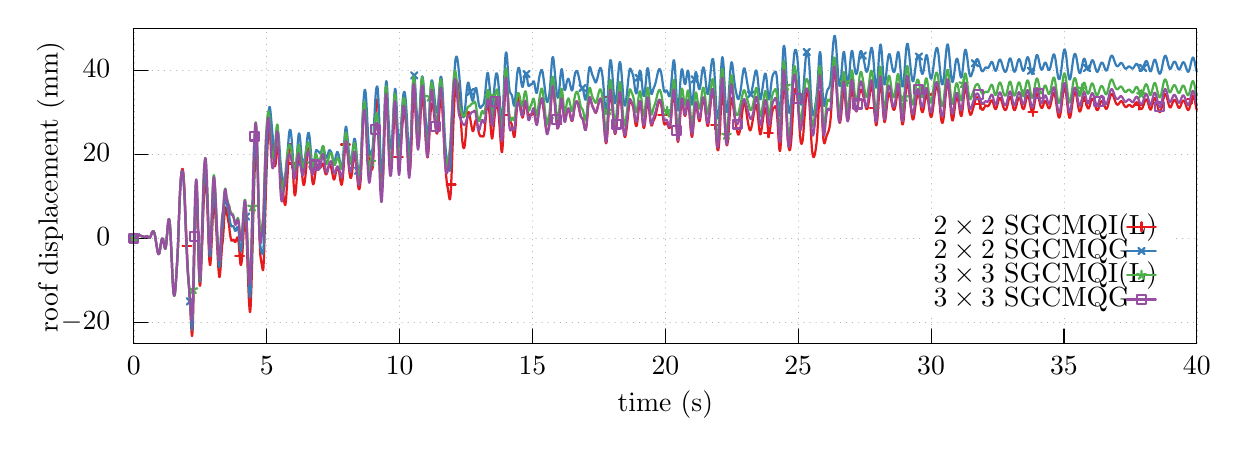
\begin{tikzpicture}[gnuplot]
%% generated with GNUPLOT 5.2p6 (Lua 5.3; terminal rev. Nov 2018, script rev. 107)
%% 08/01/2019 03:27:51
\path (0.000,0.000) rectangle (13.500,4.000);
\gpcolor{color=gp lt color axes}
\gpsetlinetype{gp lt axes}
\gpsetdashtype{gp dt axes}
\gpsetlinewidth{0.50}
\draw[gp path] (0.000,0.267)--(13.499,0.267);
\gpcolor{color=gp lt color border}
\gpsetlinetype{gp lt border}
\gpsetdashtype{gp dt solid}
\gpsetlinewidth{1.00}
\draw[gp path] (0.000,0.267)--(0.180,0.267);
\node[gp node right] at (-0.184,0.267) {$-20$};
\gpcolor{color=gp lt color axes}
\gpsetlinetype{gp lt axes}
\gpsetdashtype{gp dt axes}
\gpsetlinewidth{0.50}
\draw[gp path] (0.000,1.333)--(10.038,1.333);
\draw[gp path] (13.162,1.333)--(13.499,1.333);
\gpcolor{color=gp lt color border}
\gpsetlinetype{gp lt border}
\gpsetdashtype{gp dt solid}
\gpsetlinewidth{1.00}
\draw[gp path] (0.000,1.333)--(0.180,1.333);
\node[gp node right] at (-0.184,1.333) {$0$};
\gpcolor{color=gp lt color axes}
\gpsetlinetype{gp lt axes}
\gpsetdashtype{gp dt axes}
\gpsetlinewidth{0.50}
\draw[gp path] (0.000,2.399)--(13.499,2.399);
\gpcolor{color=gp lt color border}
\gpsetlinetype{gp lt border}
\gpsetdashtype{gp dt solid}
\gpsetlinewidth{1.00}
\draw[gp path] (0.000,2.399)--(0.180,2.399);
\node[gp node right] at (-0.184,2.399) {$20$};
\gpcolor{color=gp lt color axes}
\gpsetlinetype{gp lt axes}
\gpsetdashtype{gp dt axes}
\gpsetlinewidth{0.50}
\draw[gp path] (0.000,3.466)--(13.499,3.466);
\gpcolor{color=gp lt color border}
\gpsetlinetype{gp lt border}
\gpsetdashtype{gp dt solid}
\gpsetlinewidth{1.00}
\draw[gp path] (0.000,3.466)--(0.180,3.466);
\node[gp node right] at (-0.184,3.466) {$40$};
\gpcolor{color=gp lt color axes}
\gpsetlinetype{gp lt axes}
\gpsetdashtype{gp dt axes}
\gpsetlinewidth{0.50}
\draw[gp path] (0.000,0.000)--(0.000,3.999);
\gpcolor{color=gp lt color border}
\gpsetlinetype{gp lt border}
\gpsetdashtype{gp dt solid}
\gpsetlinewidth{1.00}
\draw[gp path] (0.000,0.000)--(0.000,0.180);
\node[gp node center] at (0.000,-0.308) {$0$};
\gpcolor{color=gp lt color axes}
\gpsetlinetype{gp lt axes}
\gpsetdashtype{gp dt axes}
\gpsetlinewidth{0.50}
\draw[gp path] (1.687,0.000)--(1.687,3.999);
\gpcolor{color=gp lt color border}
\gpsetlinetype{gp lt border}
\gpsetdashtype{gp dt solid}
\gpsetlinewidth{1.00}
\draw[gp path] (1.687,0.000)--(1.687,0.180);
\node[gp node center] at (1.687,-0.308) {$5$};
\gpcolor{color=gp lt color axes}
\gpsetlinetype{gp lt axes}
\gpsetdashtype{gp dt axes}
\gpsetlinewidth{0.50}
\draw[gp path] (3.375,0.000)--(3.375,3.999);
\gpcolor{color=gp lt color border}
\gpsetlinetype{gp lt border}
\gpsetdashtype{gp dt solid}
\gpsetlinewidth{1.00}
\draw[gp path] (3.375,0.000)--(3.375,0.180);
\node[gp node center] at (3.375,-0.308) {$10$};
\gpcolor{color=gp lt color axes}
\gpsetlinetype{gp lt axes}
\gpsetdashtype{gp dt axes}
\gpsetlinewidth{0.50}
\draw[gp path] (5.062,0.000)--(5.062,3.999);
\gpcolor{color=gp lt color border}
\gpsetlinetype{gp lt border}
\gpsetdashtype{gp dt solid}
\gpsetlinewidth{1.00}
\draw[gp path] (5.062,0.000)--(5.062,0.180);
\node[gp node center] at (5.062,-0.308) {$15$};
\gpcolor{color=gp lt color axes}
\gpsetlinetype{gp lt axes}
\gpsetdashtype{gp dt axes}
\gpsetlinewidth{0.50}
\draw[gp path] (6.750,0.000)--(6.750,3.999);
\gpcolor{color=gp lt color border}
\gpsetlinetype{gp lt border}
\gpsetdashtype{gp dt solid}
\gpsetlinewidth{1.00}
\draw[gp path] (6.750,0.000)--(6.750,0.180);
\node[gp node center] at (6.750,-0.308) {$20$};
\gpcolor{color=gp lt color axes}
\gpsetlinetype{gp lt axes}
\gpsetdashtype{gp dt axes}
\gpsetlinewidth{0.50}
\draw[gp path] (8.437,0.000)--(8.437,3.999);
\gpcolor{color=gp lt color border}
\gpsetlinetype{gp lt border}
\gpsetdashtype{gp dt solid}
\gpsetlinewidth{1.00}
\draw[gp path] (8.437,0.000)--(8.437,0.180);
\node[gp node center] at (8.437,-0.308) {$25$};
\gpcolor{color=gp lt color axes}
\gpsetlinetype{gp lt axes}
\gpsetdashtype{gp dt axes}
\gpsetlinewidth{0.50}
\draw[gp path] (10.124,0.000)--(10.124,0.400);
\draw[gp path] (10.124,1.632)--(10.124,3.999);
\gpcolor{color=gp lt color border}
\gpsetlinetype{gp lt border}
\gpsetdashtype{gp dt solid}
\gpsetlinewidth{1.00}
\draw[gp path] (10.124,0.000)--(10.124,0.180);
\node[gp node center] at (10.124,-0.308) {$30$};
\gpcolor{color=gp lt color axes}
\gpsetlinetype{gp lt axes}
\gpsetdashtype{gp dt axes}
\gpsetlinewidth{0.50}
\draw[gp path] (11.812,0.000)--(11.812,0.400);
\draw[gp path] (11.812,1.632)--(11.812,3.999);
\gpcolor{color=gp lt color border}
\gpsetlinetype{gp lt border}
\gpsetdashtype{gp dt solid}
\gpsetlinewidth{1.00}
\draw[gp path] (11.812,0.000)--(11.812,0.180);
\node[gp node center] at (11.812,-0.308) {$35$};
\gpcolor{color=gp lt color axes}
\gpsetlinetype{gp lt axes}
\gpsetdashtype{gp dt axes}
\gpsetlinewidth{0.50}
\draw[gp path] (13.499,0.000)--(13.499,3.999);
\gpcolor{color=gp lt color border}
\gpsetlinetype{gp lt border}
\gpsetdashtype{gp dt solid}
\gpsetlinewidth{1.00}
\draw[gp path] (13.499,0.000)--(13.499,0.180);
\node[gp node center] at (13.499,-0.308) {$40$};
\draw[gp path] (0.000,3.999)--(0.000,0.000)--(13.499,0.000)--(13.499,3.999)--cycle;
\node[gp node center,rotate=-270] at (-1.044,1.999) {roof displacement (\si{\milli\metre})};
\node[gp node center] at (6.749,-0.769) {time (\si{\second})};
\gpcolor{rgb color={0.894,0.102,0.110}}
\gpsetlinewidth{2.00}
\draw[gp path] (0.000,1.333)--(0.003,1.333)--(0.007,1.333)--(0.010,1.334)--(0.013,1.336)%
  --(0.017,1.339)--(0.020,1.342)--(0.024,1.345)--(0.027,1.349)--(0.030,1.352)--(0.034,1.355)%
  --(0.037,1.359)--(0.040,1.363)--(0.044,1.366)--(0.047,1.369)--(0.051,1.372)--(0.054,1.375)%
  --(0.057,1.376)--(0.061,1.377)--(0.064,1.377)--(0.067,1.377)--(0.071,1.375)--(0.074,1.372)%
  --(0.078,1.370)--(0.081,1.367)--(0.084,1.364)--(0.088,1.362)--(0.091,1.360)--(0.094,1.359)%
  --(0.098,1.357)--(0.101,1.357)--(0.105,1.356)--(0.108,1.356)--(0.111,1.355)--(0.115,1.355)%
  --(0.118,1.354)--(0.121,1.353)--(0.125,1.352)--(0.128,1.350)--(0.132,1.349)--(0.135,1.347)%
  --(0.138,1.346)--(0.142,1.346)--(0.145,1.347)--(0.148,1.349)--(0.152,1.351)--(0.155,1.354)%
  --(0.159,1.356)--(0.162,1.358)--(0.165,1.359)--(0.169,1.358)--(0.172,1.356)--(0.175,1.352)%
  --(0.179,1.347)--(0.182,1.343)--(0.186,1.340)--(0.189,1.338)--(0.192,1.337)--(0.196,1.337)%
  --(0.199,1.337)--(0.202,1.340)--(0.206,1.344)--(0.209,1.350)--(0.213,1.357)--(0.216,1.366)%
  --(0.219,1.376)--(0.223,1.385)--(0.226,1.395)--(0.229,1.403)--(0.233,1.410)--(0.236,1.415)%
  --(0.240,1.419)--(0.243,1.421)--(0.246,1.421)--(0.250,1.419)--(0.253,1.415)--(0.256,1.408)%
  --(0.260,1.398)--(0.263,1.386)--(0.267,1.371)--(0.270,1.354)--(0.273,1.335)--(0.277,1.314)%
  --(0.280,1.292)--(0.283,1.270)--(0.287,1.248)--(0.290,1.227)--(0.294,1.206)--(0.297,1.187)%
  --(0.300,1.169)--(0.304,1.153)--(0.307,1.142)--(0.310,1.134)--(0.314,1.131)--(0.317,1.132)%
  --(0.321,1.138)--(0.324,1.148)--(0.327,1.163)--(0.331,1.182)--(0.334,1.203)--(0.337,1.226)%
  --(0.341,1.248)--(0.344,1.270)--(0.348,1.289)--(0.351,1.306)--(0.354,1.319)--(0.358,1.327)%
  --(0.361,1.329)--(0.364,1.327)--(0.368,1.320)--(0.371,1.309)--(0.375,1.295)--(0.378,1.279)%
  --(0.381,1.262)--(0.385,1.245)--(0.388,1.229)--(0.391,1.215)--(0.395,1.204)--(0.398,1.199)%
  --(0.402,1.202)--(0.405,1.215)--(0.408,1.238)--(0.412,1.269)--(0.415,1.306)--(0.418,1.346)%
  --(0.422,1.389)--(0.425,1.431)--(0.429,1.472)--(0.432,1.508)--(0.435,1.539)--(0.439,1.561)%
  --(0.442,1.573)--(0.445,1.576)--(0.449,1.569)--(0.452,1.551)--(0.456,1.522)--(0.459,1.483)%
  --(0.462,1.434)--(0.466,1.376)--(0.469,1.311)--(0.472,1.241)--(0.476,1.166)--(0.479,1.087)%
  --(0.483,1.008)--(0.486,0.930)--(0.489,0.858)--(0.493,0.791)--(0.496,0.734)--(0.499,0.688)%
  --(0.503,0.651)--(0.506,0.625)--(0.510,0.609)--(0.513,0.603)--(0.516,0.608)--(0.520,0.624)%
  --(0.523,0.651)--(0.526,0.688)--(0.530,0.731)--(0.533,0.780)--(0.537,0.832)--(0.540,0.886)%
  --(0.543,0.938)--(0.547,0.990)--(0.550,1.042)--(0.553,1.098)--(0.557,1.165)--(0.560,1.244)%
  --(0.564,1.333)--(0.567,1.429)--(0.570,1.527)--(0.574,1.621)--(0.577,1.710)--(0.580,1.794)%
  --(0.584,1.868)--(0.587,1.933)--(0.591,1.992)--(0.594,2.045)--(0.597,2.092)--(0.601,2.131)%
  --(0.604,2.163)--(0.607,2.187)--(0.611,2.203)--(0.614,2.212)--(0.618,2.214)--(0.621,2.208)%
  --(0.624,2.193)--(0.628,2.168)--(0.631,2.132)--(0.634,2.086)--(0.638,2.031)--(0.641,1.970)%
  --(0.645,1.901)--(0.648,1.825)--(0.651,1.743)--(0.655,1.658)--(0.658,1.570)--(0.661,1.482)%
  --(0.665,1.395)--(0.668,1.310)--(0.672,1.229)--(0.675,1.151)--(0.678,1.078)--(0.682,1.009)%
  --(0.685,0.945)--(0.688,0.885)--(0.692,0.831)--(0.695,0.780)--(0.699,0.730)--(0.702,0.677)%
  --(0.705,0.621)--(0.709,0.563)--(0.712,0.504)--(0.715,0.443)--(0.719,0.380)--(0.722,0.317)%
  --(0.726,0.254)--(0.729,0.193)--(0.732,0.139)--(0.736,0.101)--(0.739,0.088)--(0.742,0.108)%
  --(0.746,0.169)--(0.749,0.267)--(0.753,0.395)--(0.756,0.542)--(0.759,0.700)--(0.763,0.866)%
  --(0.766,1.037)--(0.769,1.207)--(0.773,1.366)--(0.776,1.507)--(0.780,1.623)--(0.783,1.713)%
  --(0.786,1.778)--(0.790,1.819)--(0.793,1.837)--(0.796,1.834)--(0.800,1.805)--(0.803,1.749)%
  --(0.807,1.664)--(0.810,1.554)--(0.813,1.423)--(0.817,1.280)--(0.820,1.133)--(0.823,0.996)%
  --(0.827,0.882)--(0.830,0.799)--(0.834,0.749)--(0.837,0.727)--(0.840,0.727)--(0.844,0.746)%
  --(0.847,0.784)--(0.850,0.842)--(0.854,0.917)--(0.857,1.002)--(0.861,1.087)--(0.864,1.170)%
  --(0.867,1.253)--(0.871,1.341)--(0.874,1.439)--(0.877,1.544)--(0.881,1.646)--(0.884,1.739)%
  --(0.888,1.820)--(0.891,1.888)--(0.894,1.944)--(0.898,1.989)--(0.901,2.025)--(0.904,2.050)%
  --(0.908,2.064)--(0.911,2.063)--(0.915,2.048)--(0.918,2.017)--(0.921,1.972)--(0.925,1.914)%
  --(0.928,1.844)--(0.931,1.763)--(0.935,1.672)--(0.938,1.575)--(0.942,1.473)--(0.945,1.372)%
  --(0.948,1.275)--(0.952,1.187)--(0.955,1.112)--(0.958,1.053)--(0.962,1.013)--(0.965,0.992)%
  --(0.969,0.991)--(0.972,1.008)--(0.975,1.043)--(0.979,1.093)--(0.982,1.157)--(0.985,1.230)%
  --(0.989,1.310)--(0.992,1.392)--(0.996,1.473)--(0.999,1.551)--(1.002,1.620)--(1.006,1.679)%
  --(1.009,1.724)--(1.012,1.753)--(1.016,1.766)--(1.019,1.763)--(1.023,1.748)--(1.026,1.724)%
  --(1.029,1.693)--(1.033,1.656)--(1.036,1.611)--(1.039,1.559)--(1.043,1.500)--(1.046,1.438)%
  --(1.050,1.375)--(1.053,1.311)--(1.056,1.246)--(1.060,1.182)--(1.063,1.119)--(1.066,1.058)%
  --(1.070,1.001)--(1.073,0.950)--(1.077,0.905)--(1.080,0.870)--(1.083,0.846)--(1.087,0.838)%
  --(1.090,0.846)--(1.093,0.869)--(1.097,0.903)--(1.100,0.945)--(1.104,0.992)--(1.107,1.043)%
  --(1.110,1.095)--(1.114,1.147)--(1.117,1.195)--(1.120,1.234)--(1.124,1.262)--(1.127,1.287)%
  --(1.131,1.316)--(1.134,1.357)--(1.137,1.411)--(1.141,1.472)--(1.144,1.533)--(1.147,1.586)%
  --(1.151,1.632)--(1.154,1.670)--(1.158,1.702)--(1.161,1.722)--(1.164,1.725)--(1.168,1.713)%
  --(1.171,1.691)--(1.174,1.669)--(1.178,1.654)--(1.181,1.644)--(1.185,1.633)--(1.188,1.615)%
  --(1.191,1.593)--(1.195,1.570)--(1.198,1.552)--(1.201,1.537)--(1.205,1.519)--(1.208,1.496)%
  --(1.212,1.466)--(1.215,1.435)--(1.218,1.405)--(1.222,1.381)--(1.225,1.360)--(1.228,1.341)%
  --(1.232,1.324)--(1.235,1.311)--(1.239,1.303)--(1.242,1.300)--(1.245,1.301)--(1.249,1.302)%
  --(1.252,1.304)--(1.255,1.306)--(1.259,1.309)--(1.262,1.312)--(1.266,1.312)--(1.269,1.310)%
  --(1.272,1.303)--(1.276,1.296)--(1.279,1.289)--(1.282,1.285)--(1.286,1.284)--(1.289,1.286)%
  --(1.293,1.292)--(1.296,1.300)--(1.299,1.310)--(1.303,1.321)--(1.306,1.331)--(1.309,1.339)%
  --(1.313,1.343)--(1.316,1.342)--(1.320,1.336)--(1.323,1.324)--(1.326,1.305)--(1.330,1.278)%
  --(1.333,1.243)--(1.336,1.201)--(1.340,1.153)--(1.343,1.104)--(1.347,1.059)--(1.350,1.024)%
  --(1.353,1.002)--(1.357,0.992)--(1.360,0.992)--(1.363,1.001)--(1.367,1.018)--(1.370,1.044)%
  --(1.374,1.081)--(1.377,1.129)--(1.380,1.185)--(1.384,1.245)--(1.387,1.306)--(1.390,1.366)%
  --(1.394,1.422)--(1.397,1.474)--(1.401,1.519)--(1.404,1.553)--(1.407,1.575)--(1.411,1.582)%
  --(1.414,1.575)--(1.417,1.555)--(1.421,1.521)--(1.424,1.473)--(1.428,1.411)--(1.431,1.336)%
  --(1.434,1.252)--(1.438,1.161)--(1.441,1.064)--(1.444,0.965)--(1.448,0.867)--(1.451,0.772)%
  --(1.455,0.684)--(1.458,0.606)--(1.461,0.541)--(1.465,0.485)--(1.468,0.438)--(1.471,0.405)%
  --(1.475,0.393)--(1.478,0.408)--(1.482,0.451)--(1.485,0.518)--(1.488,0.601)--(1.492,0.693)%
  --(1.495,0.792)--(1.498,0.901)--(1.502,1.022)--(1.505,1.154)--(1.509,1.290)--(1.512,1.427)%
  --(1.515,1.561)--(1.519,1.692)--(1.522,1.819)--(1.525,1.938)--(1.529,2.046)--(1.532,2.144)%
  --(1.536,2.230)--(1.539,2.306)--(1.542,2.372)--(1.546,2.424)--(1.549,2.461)--(1.552,2.480)%
  --(1.556,2.479)--(1.559,2.457)--(1.563,2.414)--(1.566,2.349)--(1.569,2.261)--(1.573,2.150)%
  --(1.576,2.019)--(1.579,1.880)--(1.583,1.742)--(1.586,1.614)--(1.590,1.500)--(1.593,1.400)%
  --(1.596,1.312)--(1.600,1.234)--(1.603,1.169)--(1.606,1.119)--(1.610,1.084)--(1.613,1.059)%
  --(1.617,1.039)--(1.620,1.020)--(1.623,1.000)--(1.627,0.979)--(1.630,0.959)--(1.633,0.941)%
  --(1.637,0.928)--(1.640,0.927)--(1.644,0.946)--(1.647,0.990)--(1.650,1.060)--(1.654,1.153)%
  --(1.657,1.260)--(1.660,1.374)--(1.664,1.491)--(1.667,1.610)--(1.671,1.729)--(1.674,1.845)%
  --(1.677,1.955)--(1.681,2.059)--(1.684,2.157)--(1.687,2.250)--(1.691,2.339)--(1.694,2.424)%
  --(1.697,2.506)--(1.701,2.583)--(1.704,2.652)--(1.708,2.711)--(1.711,2.760)--(1.714,2.799)%
  --(1.718,2.828)--(1.721,2.847)--(1.724,2.856)--(1.728,2.854)--(1.731,2.840)--(1.735,2.817)%
  --(1.738,2.787)--(1.741,2.753)--(1.745,2.718)--(1.748,2.681)--(1.751,2.642)--(1.755,2.602)%
  --(1.758,2.561)--(1.762,2.522)--(1.765,2.484)--(1.768,2.448)--(1.772,2.412)--(1.775,2.375)%
  --(1.778,2.337)--(1.782,2.301)--(1.785,2.271)--(1.789,2.252)--(1.792,2.246)--(1.795,2.253)%
  --(1.799,2.270)--(1.802,2.293)--(1.805,2.320)--(1.809,2.351)--(1.812,2.383)--(1.816,2.417)%
  --(1.819,2.448)--(1.822,2.473)--(1.826,2.489)--(1.829,2.495)--(1.832,2.491)--(1.836,2.476)%
  --(1.839,2.452)--(1.843,2.418)--(1.846,2.376)--(1.849,2.330)--(1.853,2.283)--(1.856,2.239)%
  --(1.859,2.198)--(1.863,2.160)--(1.866,2.125)--(1.870,2.091)--(1.873,2.060)--(1.876,2.031)%
  --(1.880,2.006)--(1.883,1.982)--(1.886,1.960)--(1.890,1.938)--(1.893,1.915)--(1.897,1.892)%
  --(1.900,1.868)--(1.903,1.844)--(1.907,1.820)--(1.910,1.795)--(1.913,1.774)--(1.917,1.759)%
  --(1.920,1.753)--(1.924,1.758)--(1.927,1.776)--(1.930,1.805)--(1.934,1.843)--(1.937,1.889)%
  --(1.940,1.941)--(1.944,1.997)--(1.947,2.056)--(1.951,2.116)--(1.954,2.175)--(1.957,2.232)%
  --(1.961,2.288)--(1.964,2.341)--(1.967,2.391)--(1.971,2.434)--(1.974,2.471)--(1.978,2.498)%
  --(1.981,2.518)--(1.984,2.529)--(1.988,2.533)--(1.991,2.530)--(1.994,2.518)--(1.998,2.497)%
  --(2.001,2.468)--(2.005,2.431)--(2.008,2.387)--(2.011,2.337)--(2.015,2.282)--(2.018,2.222)%
  --(2.021,2.158)--(2.025,2.093)--(2.028,2.032)--(2.032,1.978)--(2.035,1.934)--(2.038,1.901)%
  --(2.042,1.881)--(2.045,1.875)--(2.048,1.880)--(2.052,1.897)--(2.055,1.923)--(2.059,1.956)%
  --(2.062,1.995)--(2.065,2.040)--(2.069,2.090)--(2.072,2.145)--(2.075,2.203)--(2.079,2.260)%
  --(2.082,2.313)--(2.086,2.360)--(2.089,2.401)--(2.092,2.433)--(2.096,2.455)--(2.099,2.467)%
  --(2.102,2.466)--(2.106,2.454)--(2.109,2.434)--(2.113,2.407)--(2.116,2.375)--(2.119,2.340)%
  --(2.123,2.302)--(2.126,2.262)--(2.129,2.220)--(2.133,2.179)--(2.136,2.141)--(2.140,2.105)%
  --(2.143,2.073)--(2.146,2.046)--(2.150,2.026)--(2.153,2.012)--(2.156,2.007)--(2.160,2.009)%
  --(2.163,2.018)--(2.167,2.032)--(2.170,2.051)--(2.173,2.076)--(2.177,2.104)--(2.180,2.136)%
  --(2.183,2.169)--(2.187,2.205)--(2.190,2.242)--(2.194,2.281)--(2.197,2.320)--(2.200,2.358)%
  --(2.204,2.393)--(2.207,2.422)--(2.210,2.446)--(2.214,2.463)--(2.217,2.474)--(2.221,2.478)%
  --(2.224,2.476)--(2.227,2.465)--(2.231,2.447)--(2.234,2.420)--(2.237,2.388)--(2.241,2.349)%
  --(2.244,2.308)--(2.248,2.264)--(2.251,2.221)--(2.254,2.180)--(2.258,2.141)--(2.261,2.105)%
  --(2.264,2.074)--(2.268,2.049)--(2.271,2.031)--(2.275,2.020)--(2.278,2.017)--(2.281,2.021)%
  --(2.285,2.030)--(2.288,2.045)--(2.291,2.065)--(2.295,2.089)--(2.298,2.115)--(2.302,2.142)%
  --(2.305,2.168)--(2.308,2.191)--(2.312,2.209)--(2.315,2.223)--(2.318,2.230)--(2.322,2.233)%
  --(2.325,2.233)--(2.329,2.233)--(2.332,2.235)--(2.335,2.239)--(2.339,2.243)--(2.342,2.247)%
  --(2.345,2.248)--(2.349,2.248)--(2.352,2.247)--(2.356,2.244)--(2.359,2.241)--(2.362,2.236)%
  --(2.366,2.232)--(2.369,2.230)--(2.372,2.232)--(2.376,2.237)--(2.379,2.245)--(2.383,2.253)%
  --(2.386,2.262)--(2.389,2.269)--(2.393,2.275)--(2.396,2.279)--(2.399,2.280)--(2.403,2.278)%
  --(2.406,2.270)--(2.410,2.258)--(2.413,2.243)--(2.416,2.225)--(2.420,2.206)--(2.423,2.187)%
  --(2.426,2.171)--(2.430,2.159)--(2.433,2.150)--(2.437,2.145)--(2.440,2.143)--(2.443,2.144)%
  --(2.447,2.148)--(2.450,2.156)--(2.453,2.167)--(2.457,2.181)--(2.460,2.196)--(2.464,2.211)%
  --(2.467,2.226)--(2.470,2.239)--(2.474,2.250)--(2.477,2.259)--(2.480,2.265)--(2.484,2.267)%
  --(2.487,2.265)--(2.491,2.261)--(2.494,2.255)--(2.497,2.247)--(2.501,2.240)--(2.504,2.231)%
  --(2.507,2.220)--(2.511,2.206)--(2.514,2.191)--(2.518,2.173)--(2.521,2.153)--(2.524,2.134)%
  --(2.528,2.115)--(2.531,2.099)--(2.534,2.088)--(2.538,2.080)--(2.541,2.078)--(2.545,2.079)%
  --(2.548,2.085)--(2.551,2.096)--(2.555,2.110)--(2.558,2.127)--(2.561,2.145)--(2.565,2.165)%
  --(2.568,2.184)--(2.572,2.201)--(2.575,2.216)--(2.578,2.228)--(2.582,2.235)--(2.585,2.238)%
  --(2.588,2.236)--(2.592,2.229)--(2.595,2.220)--(2.599,2.208)--(2.602,2.193)--(2.605,2.177)%
  --(2.609,2.157)--(2.612,2.136)--(2.615,2.112)--(2.619,2.088)--(2.622,2.064)--(2.626,2.044)%
  --(2.629,2.028)--(2.632,2.017)--(2.636,2.011)--(2.639,2.011)--(2.642,2.020)--(2.646,2.037)%
  --(2.649,2.062)--(2.653,2.094)--(2.656,2.132)--(2.659,2.174)--(2.663,2.220)--(2.666,2.269)%
  --(2.669,2.319)--(2.673,2.368)--(2.676,2.414)--(2.680,2.456)--(2.683,2.492)--(2.686,2.521)%
  --(2.690,2.542)--(2.693,2.552)--(2.696,2.550)--(2.700,2.537)--(2.703,2.515)--(2.707,2.487)%
  --(2.710,2.455)--(2.713,2.422)--(2.717,2.387)--(2.720,2.349)--(2.723,2.310)--(2.727,2.270)%
  --(2.730,2.233)--(2.734,2.200)--(2.737,2.171)--(2.740,2.146)--(2.744,2.125)--(2.747,2.109)%
  --(2.750,2.099)--(2.754,2.096)--(2.757,2.100)--(2.761,2.109)--(2.764,2.122)--(2.767,2.141)%
  --(2.771,2.164)--(2.774,2.192)--(2.777,2.222)--(2.781,2.254)--(2.784,2.285)--(2.788,2.315)%
  --(2.791,2.341)--(2.794,2.363)--(2.798,2.380)--(2.801,2.390)--(2.804,2.392)--(2.808,2.386)%
  --(2.811,2.372)--(2.815,2.351)--(2.818,2.325)--(2.821,2.293)--(2.825,2.256)--(2.828,2.216)%
  --(2.831,2.175)--(2.835,2.133)--(2.838,2.093)--(2.842,2.056)--(2.845,2.023)--(2.848,1.995)%
  --(2.852,1.973)--(2.855,1.959)--(2.858,1.953)--(2.862,1.954)--(2.865,1.962)--(2.869,1.976)%
  --(2.872,1.996)--(2.875,2.023)--(2.879,2.061)--(2.882,2.112)--(2.885,2.177)--(2.889,2.252)%
  --(2.892,2.335)--(2.896,2.422)--(2.899,2.508)--(2.902,2.592)--(2.906,2.673)--(2.909,2.747)%
  --(2.912,2.812)--(2.916,2.868)--(2.919,2.916)--(2.923,2.957)--(2.926,2.991)--(2.929,3.016)%
  --(2.933,3.031)--(2.936,3.035)--(2.939,3.027)--(2.943,3.007)--(2.946,2.977)--(2.950,2.936)%
  --(2.953,2.886)--(2.956,2.827)--(2.960,2.763)--(2.963,2.696)--(2.966,2.630)--(2.970,2.565)%
  --(2.973,2.502)--(2.977,2.441)--(2.980,2.384)--(2.983,2.334)--(2.987,2.291)--(2.990,2.258)%
  --(2.993,2.233)--(2.997,2.215)--(3.000,2.203)--(3.004,2.195)--(3.007,2.192)--(3.010,2.193)%
  --(3.014,2.196)--(3.017,2.200)--(3.020,2.203)--(3.024,2.204)--(3.027,2.206)--(3.031,2.218)%
  --(3.034,2.245)--(3.037,2.290)--(3.041,2.349)--(3.044,2.416)--(3.047,2.485)--(3.051,2.554)%
  --(3.054,2.623)--(3.058,2.694)--(3.061,2.768)--(3.064,2.839)--(3.068,2.903)--(3.071,2.957)%
  --(3.074,3.000)--(3.078,3.034)--(3.081,3.059)--(3.085,3.078)--(3.088,3.091)--(3.091,3.095)%
  --(3.095,3.089)--(3.098,3.068)--(3.101,3.032)--(3.105,2.980)--(3.108,2.914)--(3.112,2.833)%
  --(3.115,2.739)--(3.118,2.634)--(3.122,2.525)--(3.125,2.418)--(3.128,2.321)--(3.132,2.236)%
  --(3.135,2.162)--(3.139,2.101)--(3.142,2.053)--(3.145,2.018)--(3.149,1.997)--(3.152,1.991)%
  --(3.155,2.001)--(3.159,2.029)--(3.162,2.076)--(3.166,2.140)--(3.169,2.222)--(3.172,2.317)%
  --(3.176,2.423)--(3.179,2.534)--(3.182,2.645)--(3.186,2.752)--(3.189,2.849)--(3.193,2.933)%
  --(3.196,3.003)--(3.199,3.054)--(3.203,3.087)--(3.206,3.103)--(3.209,3.100)--(3.213,3.077)%
  --(3.216,3.033)--(3.220,2.970)--(3.223,2.896)--(3.226,2.819)--(3.230,2.744)--(3.233,2.674)%
  --(3.236,2.606)--(3.240,2.538)--(3.243,2.473)--(3.247,2.415)--(3.250,2.369)--(3.253,2.335)%
  --(3.257,2.308)--(3.260,2.286)--(3.263,2.267)--(3.267,2.255)--(3.270,2.256)--(3.274,2.274)%
  --(3.277,2.310)--(3.280,2.359)--(3.284,2.417)--(3.287,2.480)--(3.290,2.547)--(3.294,2.617)%
  --(3.297,2.689)--(3.301,2.759)--(3.304,2.823)--(3.307,2.876)--(3.311,2.917)--(3.314,2.946)%
  --(3.317,2.961)--(3.321,2.962)--(3.324,2.948)--(3.328,2.919)--(3.331,2.875)--(3.334,2.819)%
  --(3.338,2.754)--(3.341,2.683)--(3.344,2.611)--(3.348,2.540)--(3.351,2.474)--(3.355,2.413)%
  --(3.358,2.361)--(3.361,2.320)--(3.365,2.293)--(3.368,2.281)--(3.371,2.283)--(3.375,2.299)%
  --(3.378,2.326)--(3.381,2.361)--(3.385,2.403)--(3.388,2.450)--(3.392,2.499)--(3.395,2.549)%
  --(3.398,2.600)--(3.402,2.650)--(3.405,2.700)--(3.408,2.748)--(3.412,2.793)--(3.415,2.831)%
  --(3.419,2.863)--(3.422,2.888)--(3.425,2.906)--(3.429,2.920)--(3.432,2.928)--(3.435,2.930)%
  --(3.439,2.926)--(3.442,2.914)--(3.446,2.896)--(3.449,2.872)--(3.452,2.842)--(3.456,2.806)%
  --(3.459,2.764)--(3.462,2.716)--(3.466,2.662)--(3.469,2.604)--(3.473,2.542)--(3.476,2.478)%
  --(3.479,2.413)--(3.483,2.348)--(3.486,2.288)--(3.489,2.237)--(3.493,2.199)--(3.496,2.176)%
  --(3.500,2.169)--(3.503,2.177)--(3.506,2.197)--(3.510,2.229)--(3.513,2.272)--(3.516,2.328)%
  --(3.520,2.399)--(3.523,2.482)--(3.527,2.573)--(3.530,2.669)--(3.533,2.762)--(3.537,2.851)%
  --(3.540,2.932)--(3.543,3.001)--(3.547,3.056)--(3.550,3.096)--(3.554,3.120)--(3.557,3.130)%
  --(3.560,3.127)--(3.564,3.112)--(3.567,3.084)--(3.570,3.043)--(3.574,2.992)--(3.577,2.933)%
  --(3.581,2.871)--(3.584,2.809)--(3.587,2.749)--(3.591,2.693)--(3.594,2.640)--(3.597,2.593)%
  --(3.601,2.555)--(3.604,2.528)--(3.608,2.511)--(3.611,2.505)--(3.614,2.510)--(3.618,2.526)%
  --(3.621,2.555)--(3.624,2.596)--(3.628,2.648)--(3.631,2.707)--(3.635,2.770)--(3.638,2.835)%
  --(3.641,2.898)--(3.645,2.958)--(3.648,3.010)--(3.651,3.054)--(3.655,3.086)--(3.658,3.107)%
  --(3.662,3.116)--(3.665,3.114)--(3.668,3.103)--(3.672,3.082)--(3.675,3.053)--(3.678,3.016)%
  --(3.682,2.974)--(3.685,2.927)--(3.689,2.878)--(3.692,2.827)--(3.695,2.773)--(3.699,2.718)%
  --(3.702,2.662)--(3.705,2.607)--(3.709,2.554)--(3.712,2.505)--(3.716,2.459)--(3.719,2.419)%
  --(3.722,2.387)--(3.726,2.366)--(3.729,2.358)--(3.732,2.364)--(3.736,2.384)--(3.739,2.416)%
  --(3.743,2.461)--(3.746,2.515)--(3.749,2.578)--(3.753,2.646)--(3.756,2.716)--(3.759,2.785)%
  --(3.763,2.849)--(3.766,2.906)--(3.770,2.954)--(3.773,2.993)--(3.776,3.020)--(3.780,3.036)%
  --(3.783,3.044)--(3.786,3.045)--(3.790,3.040)--(3.793,3.030)--(3.797,3.016)--(3.800,2.997)%
  --(3.803,2.975)--(3.807,2.950)--(3.810,2.923)--(3.813,2.895)--(3.817,2.865)--(3.820,2.835)%
  --(3.824,2.805)--(3.827,2.775)--(3.830,2.748)--(3.834,2.722)--(3.837,2.700)--(3.840,2.681)%
  --(3.844,2.667)--(3.847,2.660)--(3.851,2.661)--(3.854,2.670)--(3.857,2.687)--(3.861,2.712)%
  --(3.864,2.745)--(3.867,2.785)--(3.871,2.829)--(3.874,2.876)--(3.878,2.921)--(3.881,2.965)%
  --(3.884,3.004)--(3.888,3.037)--(3.891,3.065)--(3.894,3.084)--(3.898,3.095)--(3.901,3.096)%
  --(3.905,3.088)--(3.908,3.071)--(3.911,3.046)--(3.915,3.012)--(3.918,2.967)--(3.921,2.913)%
  --(3.925,2.851)--(3.928,2.784)--(3.932,2.714)--(3.935,2.642)--(3.938,2.569)--(3.942,2.496)%
  --(3.945,2.425)--(3.948,2.360)--(3.952,2.301)--(3.955,2.250)--(3.959,2.206)--(3.962,2.166)%
  --(3.965,2.128)--(3.969,2.093)--(3.972,2.060)--(3.975,2.031)--(3.979,2.007)--(3.982,1.987)%
  --(3.986,1.968)--(3.989,1.948)--(3.992,1.928)--(3.996,1.905)--(3.999,1.882)--(4.002,1.859)%
  --(4.006,1.840)--(4.009,1.828)--(4.013,1.825)--(4.016,1.834)--(4.019,1.857)--(4.023,1.895)%
  --(4.026,1.948)--(4.029,2.015)--(4.033,2.094)--(4.036,2.181)--(4.040,2.273)--(4.043,2.367)%
  --(4.046,2.463)--(4.050,2.560)--(4.053,2.657)--(4.056,2.752)--(4.060,2.842)--(4.063,2.923)%
  --(4.067,2.995)--(4.070,3.059)--(4.073,3.118)--(4.077,3.172)--(4.080,3.220)--(4.083,3.259)%
  --(4.087,3.289)--(4.090,3.310)--(4.094,3.323)--(4.097,3.330)--(4.100,3.332)--(4.104,3.329)%
  --(4.107,3.320)--(4.110,3.304)--(4.114,3.281)--(4.117,3.253)--(4.121,3.222)--(4.124,3.189)%
  --(4.127,3.155)--(4.131,3.119)--(4.134,3.081)--(4.137,3.039)--(4.141,2.995)--(4.144,2.947)%
  --(4.148,2.897)--(4.151,2.846)--(4.154,2.795)--(4.158,2.745)--(4.161,2.695)--(4.164,2.648)%
  --(4.168,2.604)--(4.171,2.566)--(4.175,2.534)--(4.178,2.510)--(4.181,2.493)--(4.185,2.482)%
  --(4.188,2.476)--(4.191,2.475)--(4.195,2.480)--(4.198,2.492)--(4.202,2.511)--(4.205,2.538)%
  --(4.208,2.570)--(4.212,2.607)--(4.215,2.648)--(4.218,2.692)--(4.222,2.735)--(4.225,2.776)%
  --(4.229,2.814)--(4.232,2.847)--(4.235,2.877)--(4.239,2.901)--(4.242,2.920)--(4.245,2.932)%
  --(4.249,2.936)--(4.252,2.934)--(4.256,2.927)--(4.259,2.917)--(4.262,2.903)--(4.266,2.886)%
  --(4.269,2.866)--(4.272,2.845)--(4.276,2.824)--(4.279,2.803)--(4.283,2.784)--(4.286,2.764)%
  --(4.289,2.745)--(4.293,2.727)--(4.296,2.711)--(4.299,2.700)--(4.303,2.693)--(4.306,2.691)%
  --(4.310,2.694)--(4.313,2.703)--(4.316,2.716)--(4.320,2.734)--(4.323,2.753)--(4.326,2.773)%
  --(4.330,2.791)--(4.333,2.807)--(4.337,2.820)--(4.340,2.828)--(4.343,2.833)--(4.347,2.832)%
  --(4.350,2.827)--(4.353,2.817)--(4.357,2.804)--(4.360,2.787)--(4.364,2.768)--(4.367,2.747)%
  --(4.370,2.726)--(4.374,2.707)--(4.377,2.690)--(4.380,2.675)--(4.384,2.663)--(4.387,2.652)%
  --(4.391,2.643)--(4.394,2.636)--(4.397,2.631)--(4.401,2.628)--(4.404,2.626)--(4.407,2.625)%
  --(4.411,2.625)--(4.414,2.626)--(4.418,2.627)--(4.421,2.628)--(4.424,2.628)--(4.428,2.626)%
  --(4.431,2.625)--(4.434,2.623)--(4.438,2.624)--(4.441,2.630)--(4.445,2.641)--(4.448,2.657)%
  --(4.451,2.679)--(4.455,2.706)--(4.458,2.736)--(4.461,2.771)--(4.465,2.810)--(4.468,2.851)%
  --(4.472,2.893)--(4.475,2.933)--(4.478,2.970)--(4.482,3.002)--(4.485,3.029)--(4.488,3.050)%
  --(4.492,3.062)--(4.495,3.064)--(4.499,3.056)--(4.502,3.038)--(4.505,3.013)--(4.509,2.985)%
  --(4.512,2.955)--(4.515,2.924)--(4.519,2.891)--(4.522,2.854)--(4.526,2.813)--(4.529,2.771)%
  --(4.532,2.729)--(4.536,2.689)--(4.539,2.653)--(4.542,2.623)--(4.546,2.604)--(4.549,2.597)%
  --(4.553,2.605)--(4.556,2.624)--(4.559,2.651)--(4.563,2.681)--(4.566,2.714)--(4.569,2.750)%
  --(4.573,2.788)--(4.576,2.827)--(4.580,2.865)--(4.583,2.900)--(4.586,2.932)--(4.590,2.963)%
  --(4.593,2.990)--(4.596,3.015)--(4.600,3.034)--(4.603,3.046)--(4.607,3.052)--(4.610,3.052)%
  --(4.613,3.047)--(4.617,3.036)--(4.620,3.019)--(4.623,2.995)--(4.627,2.964)--(4.630,2.929)%
  --(4.634,2.889)--(4.637,2.848)--(4.640,2.804)--(4.644,2.758)--(4.647,2.710)--(4.650,2.662)%
  --(4.654,2.614)--(4.657,2.567)--(4.661,2.521)--(4.664,2.480)--(4.667,2.448)--(4.671,2.428)%
  --(4.674,2.424)--(4.677,2.436)--(4.681,2.466)--(4.684,2.511)--(4.688,2.570)--(4.691,2.641)%
  --(4.694,2.723)--(4.698,2.810)--(4.701,2.898)--(4.704,2.984)--(4.708,3.064)--(4.711,3.136)%
  --(4.715,3.197)--(4.718,3.245)--(4.721,3.279)--(4.725,3.300)--(4.728,3.310)--(4.731,3.308)%
  --(4.735,3.294)--(4.738,3.268)--(4.742,3.230)--(4.745,3.184)--(4.748,3.135)--(4.752,3.086)%
  --(4.755,3.039)--(4.758,2.995)--(4.762,2.952)--(4.765,2.913)--(4.769,2.881)--(4.772,2.856)%
  --(4.775,2.839)--(4.779,2.828)--(4.782,2.819)--(4.785,2.810)--(4.789,2.802)--(4.792,2.794)%
  --(4.796,2.785)--(4.799,2.775)--(4.802,2.762)--(4.806,2.744)--(4.809,2.722)--(4.812,2.698)%
  --(4.816,2.674)--(4.819,2.651)--(4.823,2.633)--(4.826,2.621)--(4.829,2.616)--(4.833,2.620)%
  --(4.836,2.634)--(4.839,2.659)--(4.843,2.693)--(4.846,2.735)--(4.850,2.782)--(4.853,2.832)%
  --(4.856,2.882)--(4.860,2.931)--(4.863,2.975)--(4.866,3.013)--(4.870,3.045)--(4.873,3.070)%
  --(4.877,3.089)--(4.880,3.104)--(4.883,3.115)--(4.887,3.120)--(4.890,3.120)--(4.893,3.113)%
  --(4.897,3.102)--(4.900,3.085)--(4.904,3.065)--(4.907,3.040)--(4.910,3.012)--(4.914,2.984)%
  --(4.917,2.956)--(4.920,2.930)--(4.924,2.906)--(4.927,2.887)--(4.931,2.872)--(4.934,2.864)%
  --(4.937,2.863)--(4.941,2.870)--(4.944,2.883)--(4.947,2.901)--(4.951,2.920)--(4.954,2.941)%
  --(4.958,2.961)--(4.961,2.982)--(4.964,3.000)--(4.968,3.016)--(4.971,3.027)--(4.974,3.034)%
  --(4.978,3.036)--(4.981,3.033)--(4.985,3.027)--(4.988,3.015)--(4.991,2.997)--(4.995,2.975)%
  --(4.998,2.950)--(5.001,2.927)--(5.005,2.908)--(5.008,2.896)--(5.012,2.889)--(5.015,2.887)%
  --(5.018,2.887)--(5.022,2.889)--(5.025,2.892)--(5.028,2.897)--(5.032,2.901)--(5.035,2.905)%
  --(5.039,2.905)--(5.042,2.903)--(5.045,2.900)--(5.049,2.898)--(5.052,2.898)--(5.055,2.901)%
  --(5.059,2.905)--(5.062,2.911)--(5.065,2.917)--(5.069,2.923)--(5.072,2.928)--(5.076,2.930)%
  --(5.079,2.928)--(5.082,2.922)--(5.086,2.910)--(5.089,2.894)--(5.092,2.875)--(5.096,2.854)%
  --(5.099,2.834)--(5.103,2.816)--(5.106,2.802)--(5.109,2.793)--(5.113,2.790)--(5.116,2.794)%
  --(5.119,2.803)--(5.123,2.818)--(5.126,2.838)--(5.130,2.861)--(5.133,2.887)--(5.136,2.914)%
  --(5.140,2.941)--(5.143,2.966)--(5.146,2.987)--(5.150,3.006)--(5.153,3.021)--(5.157,3.034)%
  --(5.160,3.045)--(5.163,3.055)--(5.167,3.064)--(5.170,3.072)--(5.173,3.077)--(5.177,3.080)%
  --(5.180,3.080)--(5.184,3.075)--(5.187,3.066)--(5.190,3.052)--(5.194,3.033)--(5.197,3.011)%
  --(5.200,2.986)--(5.204,2.961)--(5.207,2.935)--(5.211,2.910)--(5.214,2.884)--(5.217,2.857)%
  --(5.221,2.829)--(5.224,2.802)--(5.227,2.776)--(5.231,2.751)--(5.234,2.729)--(5.238,2.709)%
  --(5.241,2.694)--(5.244,2.684)--(5.248,2.679)--(5.251,2.679)--(5.254,2.684)--(5.258,2.692)%
  --(5.261,2.702)--(5.265,2.714)--(5.268,2.728)--(5.271,2.745)--(5.275,2.766)--(5.278,2.792)%
  --(5.281,2.824)--(5.285,2.861)--(5.288,2.903)--(5.292,2.949)--(5.295,2.998)--(5.298,3.048)%
  --(5.302,3.097)--(5.305,3.142)--(5.308,3.181)--(5.312,3.211)--(5.315,3.232)--(5.319,3.242)%
  --(5.322,3.243)--(5.325,3.233)--(5.329,3.215)--(5.332,3.190)--(5.335,3.159)--(5.339,3.126)%
  --(5.342,3.090)--(5.346,3.052)--(5.349,3.014)--(5.352,2.976)--(5.356,2.939)--(5.359,2.902)%
  --(5.362,2.868)--(5.366,2.836)--(5.369,2.806)--(5.373,2.780)--(5.376,2.758)--(5.379,2.742)%
  --(5.383,2.733)--(5.386,2.732)--(5.389,2.737)--(5.393,2.751)--(5.396,2.771)--(5.400,2.799)%
  --(5.403,2.833)--(5.406,2.871)--(5.410,2.912)--(5.413,2.952)--(5.416,2.990)--(5.420,3.023)%
  --(5.423,3.051)--(5.427,3.073)--(5.430,3.086)--(5.433,3.089)--(5.437,3.083)--(5.440,3.067)%
  --(5.443,3.043)--(5.447,3.013)--(5.450,2.979)--(5.454,2.942)--(5.457,2.906)--(5.460,2.874)%
  --(5.464,2.850)--(5.467,2.835)--(5.470,2.828)--(5.474,2.829)--(5.477,2.835)--(5.481,2.845)%
  --(5.484,2.860)--(5.487,2.877)--(5.491,2.897)--(5.494,2.916)--(5.497,2.932)--(5.501,2.945)%
  --(5.504,2.954)--(5.508,2.961)--(5.511,2.967)--(5.514,2.970)--(5.518,2.970)--(5.521,2.966)%
  --(5.524,2.957)--(5.528,2.945)--(5.531,2.931)--(5.535,2.917)--(5.538,2.903)--(5.541,2.888)%
  --(5.545,2.872)--(5.548,2.856)--(5.551,2.842)--(5.555,2.832)--(5.558,2.824)--(5.562,2.820)%
  --(5.565,2.821)--(5.568,2.826)--(5.572,2.837)--(5.575,2.854)--(5.578,2.876)--(5.582,2.901)%
  --(5.585,2.927)--(5.589,2.952)--(5.592,2.977)--(5.595,3.000)--(5.599,3.019)--(5.602,3.034)%
  --(5.605,3.046)--(5.609,3.055)--(5.612,3.062)--(5.616,3.067)--(5.619,3.070)--(5.622,3.070)%
  --(5.626,3.068)--(5.629,3.064)--(5.632,3.057)--(5.636,3.049)--(5.639,3.039)--(5.643,3.027)%
  --(5.646,3.012)--(5.649,2.996)--(5.653,2.980)--(5.656,2.964)--(5.659,2.948)--(5.663,2.931)%
  --(5.666,2.914)--(5.670,2.899)--(5.673,2.886)--(5.676,2.876)--(5.680,2.870)--(5.683,2.865)%
  --(5.686,2.862)--(5.690,2.859)--(5.693,2.856)--(5.697,2.852)--(5.700,2.846)--(5.703,2.837)%
  --(5.707,2.824)--(5.710,2.808)--(5.713,2.789)--(5.717,2.770)--(5.720,2.752)--(5.724,2.735)%
  --(5.727,2.720)--(5.730,2.710)--(5.734,2.705)--(5.737,2.707)--(5.740,2.716)--(5.744,2.733)%
  --(5.747,2.756)--(5.751,2.786)--(5.754,2.821)--(5.757,2.860)--(5.761,2.901)--(5.764,2.943)%
  --(5.767,2.982)--(5.771,3.019)--(5.774,3.051)--(5.778,3.078)--(5.781,3.098)--(5.784,3.112)%
  --(5.788,3.118)--(5.791,3.119)--(5.794,3.115)--(5.798,3.106)--(5.801,3.095)--(5.805,3.082)%
  --(5.808,3.067)--(5.811,3.053)--(5.815,3.040)--(5.818,3.028)--(5.821,3.019)--(5.825,3.010)%
  --(5.828,3.002)--(5.832,2.994)--(5.835,2.987)--(5.838,2.979)--(5.842,2.972)--(5.845,2.964)%
  --(5.848,2.955)--(5.852,2.945)--(5.855,2.936)--(5.859,2.929)--(5.862,2.925)--(5.865,2.925)%
  --(5.869,2.927)--(5.872,2.932)--(5.875,2.940)--(5.879,2.950)--(5.882,2.962)--(5.886,2.976)%
  --(5.889,2.989)--(5.892,3.003)--(5.896,3.017)--(5.899,3.032)--(5.902,3.047)--(5.906,3.061)%
  --(5.909,3.075)--(5.913,3.086)--(5.916,3.095)--(5.919,3.102)--(5.923,3.106)--(5.926,3.106)%
  --(5.929,3.103)--(5.933,3.096)--(5.936,3.085)--(5.940,3.071)--(5.943,3.054)--(5.946,3.035)%
  --(5.950,3.012)--(5.953,2.986)--(5.956,2.955)--(5.960,2.920)--(5.963,2.880)--(5.967,2.836)%
  --(5.970,2.789)--(5.973,2.742)--(5.977,2.697)--(5.980,2.654)--(5.983,2.616)--(5.987,2.583)%
  --(5.990,2.558)--(5.994,2.542)--(5.997,2.537)--(6.000,2.543)--(6.004,2.559)--(6.007,2.584)%
  --(6.010,2.619)--(6.014,2.663)--(6.017,2.715)--(6.021,2.772)--(6.024,2.832)--(6.027,2.891)%
  --(6.031,2.947)--(6.034,3.000)--(6.037,3.049)--(6.041,3.092)--(6.044,3.126)--(6.048,3.150)%
  --(6.051,3.163)--(6.054,3.166)--(6.058,3.160)--(6.061,3.147)--(6.064,3.128)--(6.068,3.102)%
  --(6.071,3.069)--(6.075,3.031)--(6.078,2.988)--(6.081,2.944)--(6.085,2.898)--(6.088,2.852)%
  --(6.091,2.807)--(6.095,2.764)--(6.098,2.727)--(6.102,2.696)--(6.105,2.673)--(6.108,2.660)%
  --(6.112,2.656)--(6.115,2.659)--(6.118,2.671)--(6.122,2.688)--(6.125,2.711)--(6.129,2.739)%
  --(6.132,2.770)--(6.135,2.804)--(6.139,2.841)--(6.142,2.881)--(6.145,2.923)--(6.149,2.966)%
  --(6.152,3.008)--(6.156,3.046)--(6.159,3.080)--(6.162,3.108)--(6.166,3.128)--(6.169,3.141)%
  --(6.172,3.146)--(6.176,3.143)--(6.179,3.133)--(6.183,3.114)--(6.186,3.089)--(6.189,3.058)%
  --(6.193,3.021)--(6.196,2.980)--(6.199,2.936)--(6.203,2.892)--(6.206,2.847)--(6.210,2.804)%
  --(6.213,2.762)--(6.216,2.725)--(6.220,2.691)--(6.223,2.664)--(6.226,2.642)--(6.230,2.627)%
  --(6.233,2.619)--(6.237,2.616)--(6.240,2.621)--(6.243,2.631)--(6.247,2.647)--(6.250,2.667)%
  --(6.253,2.691)--(6.257,2.718)--(6.260,2.747)--(6.264,2.778)--(6.267,2.810)--(6.270,2.843)%
  --(6.274,2.877)--(6.277,2.910)--(6.280,2.942)--(6.284,2.973)--(6.287,3.002)--(6.291,3.028)%
  --(6.294,3.048)--(6.297,3.063)--(6.301,3.072)--(6.304,3.075)--(6.307,3.074)--(6.311,3.070)%
  --(6.314,3.066)--(6.318,3.060)--(6.321,3.054)--(6.324,3.047)--(6.328,3.039)--(6.331,3.030)%
  --(6.334,3.021)--(6.338,3.009)--(6.341,2.995)--(6.345,2.977)--(6.348,2.954)--(6.351,2.928)%
  --(6.355,2.899)--(6.358,2.869)--(6.361,2.841)--(6.365,2.815)--(6.368,2.794)--(6.372,2.776)%
  --(6.375,2.763)--(6.378,2.756)--(6.382,2.754)--(6.385,2.760)--(6.388,2.773)--(6.392,2.793)%
  --(6.395,2.819)--(6.399,2.850)--(6.402,2.884)--(6.405,2.919)--(6.409,2.951)--(6.412,2.980)%
  --(6.415,3.006)--(6.419,3.026)--(6.422,3.042)--(6.426,3.051)--(6.429,3.054)--(6.432,3.050)%
  --(6.436,3.039)--(6.439,3.021)--(6.442,2.998)--(6.446,2.969)--(6.449,2.936)--(6.453,2.900)%
  --(6.456,2.862)--(6.459,2.826)--(6.463,2.794)--(6.466,2.768)--(6.469,2.749)--(6.473,2.737)%
  --(6.476,2.732)--(6.480,2.735)--(6.483,2.744)--(6.486,2.761)--(6.490,2.784)--(6.493,2.812)%
  --(6.496,2.844)--(6.500,2.880)--(6.503,2.917)--(6.507,2.954)--(6.510,2.989)--(6.513,3.021)%
  --(6.517,3.046)--(6.520,3.065)--(6.523,3.075)--(6.527,3.076)--(6.530,3.068)--(6.534,3.053)%
  --(6.537,3.030)--(6.540,3.003)--(6.544,2.972)--(6.547,2.938)--(6.550,2.904)--(6.554,2.870)%
  --(6.557,2.839)--(6.561,2.812)--(6.564,2.791)--(6.567,2.775)--(6.571,2.765)--(6.574,2.762)%
  --(6.577,2.764)--(6.581,2.770)--(6.584,2.779)--(6.588,2.790)--(6.591,2.801)--(6.594,2.813)%
  --(6.598,2.822)--(6.601,2.830)--(6.604,2.837)--(6.608,2.843)--(6.611,2.849)--(6.615,2.857)%
  --(6.618,2.866)--(6.621,2.876)--(6.625,2.888)--(6.628,2.900)--(6.631,2.914)--(6.635,2.930)%
  --(6.638,2.947)--(6.642,2.964)--(6.645,2.981)--(6.648,2.998)--(6.652,3.014)--(6.655,3.029)%
  --(6.658,3.042)--(6.662,3.054)--(6.665,3.063)--(6.669,3.070)--(6.672,3.075)--(6.675,3.078)%
  --(6.679,3.078)--(6.682,3.074)--(6.685,3.068)--(6.689,3.059)--(6.692,3.047)--(6.696,3.033)%
  --(6.699,3.016)--(6.702,2.997)--(6.706,2.974)--(6.709,2.950)--(6.712,2.923)--(6.716,2.897)%
  --(6.719,2.871)--(6.723,2.846)--(6.726,2.824)--(6.729,2.806)--(6.733,2.791)--(6.736,2.782)%
  --(6.739,2.777)--(6.743,2.776)--(6.746,2.778)--(6.750,2.782)--(6.753,2.786)--(6.756,2.791)%
  --(6.760,2.794)--(6.763,2.795)--(6.766,2.794)--(6.770,2.791)--(6.773,2.786)--(6.776,2.779)%
  --(6.780,2.770)--(6.783,2.761)--(6.787,2.752)--(6.790,2.743)--(6.793,2.735)--(6.797,2.731)%
  --(6.800,2.729)--(6.803,2.733)--(6.807,2.741)--(6.810,2.755)--(6.814,2.776)--(6.817,2.803)%
  --(6.820,2.835)--(6.824,2.872)--(6.827,2.911)--(6.830,2.953)--(6.834,2.996)--(6.837,3.037)%
  --(6.841,3.076)--(6.844,3.112)--(6.847,3.141)--(6.851,3.163)--(6.854,3.177)--(6.857,3.181)%
  --(6.861,3.175)--(6.864,3.158)--(6.868,3.130)--(6.871,3.092)--(6.874,3.043)--(6.878,2.986)%
  --(6.881,2.924)--(6.884,2.860)--(6.888,2.797)--(6.891,2.736)--(6.895,2.681)--(6.898,2.633)%
  --(6.901,2.595)--(6.905,2.568)--(6.908,2.555)--(6.911,2.555)--(6.915,2.568)--(6.918,2.593)%
  --(6.922,2.628)--(6.925,2.671)--(6.928,2.721)--(6.932,2.776)--(6.935,2.832)--(6.938,2.886)%
  --(6.942,2.935)--(6.945,2.978)--(6.949,3.013)--(6.952,3.040)--(6.955,3.058)--(6.959,3.066)%
  --(6.962,3.066)--(6.965,3.058)--(6.969,3.044)--(6.972,3.025)--(6.976,3.003)--(6.979,2.979)%
  --(6.982,2.954)--(6.986,2.932)--(6.989,2.912)--(6.992,2.897)--(6.996,2.888)--(6.999,2.885)%
  --(7.003,2.888)--(7.006,2.898)--(7.009,2.915)--(7.013,2.936)--(7.016,2.961)--(7.019,2.986)%
  --(7.023,3.010)--(7.026,3.032)--(7.030,3.048)--(7.033,3.058)--(7.036,3.060)--(7.040,3.054)%
  --(7.043,3.038)--(7.046,3.014)--(7.050,2.982)--(7.053,2.944)--(7.057,2.902)--(7.060,2.858)%
  --(7.063,2.815)--(7.067,2.772)--(7.070,2.732)--(7.073,2.695)--(7.077,2.664)--(7.080,2.640)%
  --(7.084,2.624)--(7.087,2.619)--(7.090,2.623)--(7.094,2.638)--(7.097,2.662)--(7.100,2.693)%
  --(7.104,2.731)--(7.107,2.772)--(7.111,2.817)--(7.114,2.861)--(7.117,2.904)--(7.121,2.944)%
  --(7.124,2.978)--(7.127,3.006)--(7.131,3.025)--(7.134,3.036)--(7.138,3.039)--(7.141,3.033)%
  --(7.144,3.021)--(7.148,3.004)--(7.151,2.982)--(7.154,2.958)--(7.158,2.932)--(7.161,2.907)%
  --(7.165,2.882)--(7.168,2.861)--(7.171,2.843)--(7.175,2.829)--(7.178,2.821)--(7.181,2.818)%
  --(7.185,2.820)--(7.188,2.829)--(7.192,2.844)--(7.195,2.864)--(7.198,2.888)--(7.202,2.915)%
  --(7.205,2.943)--(7.208,2.972)--(7.212,3.000)--(7.215,3.026)--(7.219,3.049)--(7.222,3.069)%
  --(7.225,3.083)--(7.229,3.092)--(7.232,3.096)--(7.235,3.095)--(7.239,3.088)--(7.242,3.076)%
  --(7.246,3.059)--(7.249,3.037)--(7.252,3.011)--(7.256,2.981)--(7.259,2.949)--(7.262,2.916)%
  --(7.266,2.883)--(7.269,2.851)--(7.273,2.822)--(7.276,2.797)--(7.279,2.778)--(7.283,2.764)%
  --(7.286,2.757)--(7.289,2.758)--(7.293,2.765)--(7.296,2.780)--(7.300,2.800)--(7.303,2.826)%
  --(7.306,2.855)--(7.310,2.887)--(7.313,2.921)--(7.316,2.956)--(7.320,2.992)--(7.323,3.028)%
  --(7.327,3.062)--(7.330,3.094)--(7.333,3.123)--(7.337,3.148)--(7.340,3.170)--(7.343,3.187)%
  --(7.347,3.199)--(7.350,3.205)--(7.354,3.205)--(7.357,3.198)--(7.360,3.182)--(7.364,3.157)%
  --(7.367,3.122)--(7.370,3.078)--(7.374,3.026)--(7.377,2.967)--(7.381,2.904)--(7.384,2.838)%
  --(7.387,2.770)--(7.391,2.703)--(7.394,2.641)--(7.397,2.585)--(7.401,2.539)--(7.404,2.503)%
  --(7.408,2.477)--(7.411,2.459)--(7.414,2.450)--(7.418,2.447)--(7.421,2.451)--(7.424,2.464)%
  --(7.428,2.487)--(7.431,2.521)--(7.435,2.566)--(7.438,2.620)--(7.441,2.681)--(7.445,2.748)%
  --(7.448,2.818)--(7.451,2.889)--(7.455,2.959)--(7.458,3.022)--(7.462,3.078)--(7.465,3.122)%
  --(7.468,3.154)--(7.472,3.173)--(7.475,3.180)--(7.478,3.173)--(7.482,3.155)--(7.485,3.124)%
  --(7.489,3.081)--(7.492,3.029)--(7.495,2.969)--(7.499,2.905)--(7.502,2.841)--(7.505,2.778)%
  --(7.509,2.717)--(7.512,2.661)--(7.516,2.612)--(7.519,2.571)--(7.522,2.541)--(7.526,2.522)%
  --(7.529,2.512)--(7.532,2.511)--(7.536,2.519)--(7.539,2.536)--(7.543,2.560)--(7.546,2.593)%
  --(7.549,2.632)--(7.553,2.677)--(7.556,2.727)--(7.559,2.778)--(7.563,2.829)--(7.566,2.881)%
  --(7.570,2.930)--(7.573,2.976)--(7.576,3.017)--(7.580,3.052)--(7.583,3.079)--(7.586,3.098)%
  --(7.590,3.108)--(7.593,3.111)--(7.597,3.106)--(7.600,3.093)--(7.603,3.075)--(7.607,3.051)%
  --(7.610,3.024)--(7.613,2.995)--(7.617,2.966)--(7.620,2.937)--(7.624,2.911)--(7.627,2.887)%
  --(7.630,2.865)--(7.634,2.844)--(7.637,2.823)--(7.640,2.802)--(7.644,2.782)--(7.647,2.763)%
  --(7.651,2.745)--(7.654,2.728)--(7.657,2.711)--(7.661,2.694)--(7.664,2.678)--(7.667,2.665)%
  --(7.671,2.655)--(7.674,2.649)--(7.678,2.647)--(7.681,2.649)--(7.684,2.654)--(7.688,2.662)%
  --(7.691,2.675)--(7.694,2.691)--(7.698,2.709)--(7.701,2.730)--(7.705,2.752)--(7.708,2.776)%
  --(7.711,2.801)--(7.715,2.829)--(7.718,2.857)--(7.721,2.887)--(7.725,2.917)--(7.728,2.947)%
  --(7.732,2.975)--(7.735,3.001)--(7.738,3.023)--(7.742,3.040)--(7.745,3.053)--(7.748,3.061)%
  --(7.752,3.063)--(7.755,3.061)--(7.759,3.053)--(7.762,3.040)--(7.765,3.023)--(7.769,3.003)%
  --(7.772,2.981)--(7.775,2.958)--(7.779,2.934)--(7.782,2.910)--(7.786,2.886)--(7.789,2.863)%
  --(7.792,2.841)--(7.796,2.820)--(7.799,2.800)--(7.802,2.781)--(7.806,2.763)--(7.809,2.746)%
  --(7.813,2.731)--(7.816,2.718)--(7.819,2.710)--(7.823,2.704)--(7.826,2.702)--(7.829,2.704)%
  --(7.833,2.709)--(7.836,2.717)--(7.840,2.728)--(7.843,2.742)--(7.846,2.759)--(7.850,2.776)%
  --(7.853,2.795)--(7.856,2.814)--(7.860,2.834)--(7.863,2.854)--(7.867,2.874)--(7.870,2.894)%
  --(7.873,2.914)--(7.877,2.934)--(7.880,2.953)--(7.883,2.971)--(7.887,2.988)--(7.890,3.003)%
  --(7.894,3.015)--(7.897,3.022)--(7.900,3.025)--(7.904,3.022)--(7.907,3.015)--(7.910,3.001)%
  --(7.914,2.983)--(7.917,2.959)--(7.921,2.930)--(7.924,2.898)--(7.927,2.863)--(7.931,2.827)%
  --(7.934,2.792)--(7.937,2.757)--(7.941,2.725)--(7.944,2.697)--(7.948,2.674)--(7.951,2.659)%
  --(7.954,2.651)--(7.958,2.651)--(7.961,2.658)--(7.964,2.672)--(7.968,2.691)--(7.971,2.713)%
  --(7.975,2.737)--(7.978,2.761)--(7.981,2.786)--(7.985,2.810)--(7.988,2.834)--(7.991,2.858)%
  --(7.995,2.882)--(7.998,2.904)--(8.002,2.926)--(8.005,2.945)--(8.008,2.962)--(8.012,2.975)%
  --(8.015,2.983)--(8.018,2.985)--(8.022,2.981)--(8.025,2.971)--(8.029,2.955)--(8.032,2.933)%
  --(8.035,2.905)--(8.039,2.871)--(8.042,2.834)--(8.045,2.795)--(8.049,2.757)--(8.052,2.723)%
  --(8.056,2.693)--(8.059,2.670)--(8.062,2.656)--(8.066,2.650)--(8.069,2.655)--(8.072,2.668)%
  --(8.076,2.688)--(8.079,2.714)--(8.083,2.743)--(8.086,2.775)--(8.089,2.806)--(8.093,2.837)%
  --(8.096,2.866)--(8.099,2.891)--(8.103,2.913)--(8.106,2.932)--(8.110,2.948)--(8.113,2.961)%
  --(8.116,2.971)--(8.120,2.978)--(8.123,2.983)--(8.126,2.987)--(8.130,2.991)--(8.133,2.995)%
  --(8.137,2.999)--(8.140,3.003)--(8.143,3.007)--(8.147,3.008)--(8.150,3.006)--(8.153,2.999)%
  --(8.157,2.987)--(8.160,2.969)--(8.164,2.943)--(8.167,2.911)--(8.170,2.871)--(8.174,2.824)%
  --(8.177,2.771)--(8.180,2.712)--(8.184,2.652)--(8.187,2.594)--(8.191,2.541)--(8.194,2.497)%
  --(8.197,2.464)--(8.201,2.445)--(8.204,2.439)--(8.207,2.448)--(8.211,2.472)--(8.214,2.512)%
  --(8.218,2.569)--(8.221,2.642)--(8.224,2.727)--(8.228,2.818)--(8.231,2.909)--(8.234,2.996)%
  --(8.238,3.076)--(8.241,3.148)--(8.245,3.208)--(8.248,3.251)--(8.251,3.277)--(8.255,3.287)%
  --(8.258,3.285)--(8.261,3.273)--(8.265,3.252)--(8.268,3.221)--(8.272,3.180)--(8.275,3.128)%
  --(8.278,3.069)--(8.282,3.007)--(8.285,2.944)--(8.288,2.880)--(8.292,2.815)--(8.295,2.749)%
  --(8.299,2.686)--(8.302,2.630)--(8.305,2.582)--(8.309,2.543)--(8.312,2.511)--(8.315,2.487)%
  --(8.319,2.469)--(8.322,2.457)--(8.326,2.450)--(8.329,2.449)--(8.332,2.455)--(8.336,2.468)%
  --(8.339,2.488)--(8.342,2.514)--(8.346,2.548)--(8.349,2.589)--(8.353,2.637)--(8.356,2.691)%
  --(8.359,2.749)--(8.363,2.809)--(8.366,2.869)--(8.369,2.929)--(8.373,2.986)--(8.376,3.039)%
  --(8.380,3.086)--(8.383,3.125)--(8.386,3.158)--(8.390,3.184)--(8.393,3.204)--(8.396,3.218)%
  --(8.400,3.228)--(8.403,3.234)--(8.407,3.236)--(8.410,3.233)--(8.413,3.227)--(8.417,3.217)%
  --(8.420,3.201)--(8.423,3.180)--(8.427,3.152)--(8.430,3.116)--(8.434,3.073)--(8.437,3.025)%
  --(8.440,2.972)--(8.444,2.914)--(8.447,2.854)--(8.450,2.794)--(8.454,2.735)--(8.457,2.682)%
  --(8.460,2.635)--(8.464,2.597)--(8.467,2.568)--(8.471,2.547)--(8.474,2.535)--(8.477,2.530)%
  --(8.481,2.531)--(8.484,2.537)--(8.487,2.548)--(8.491,2.563)--(8.494,2.585)--(8.498,2.614)%
  --(8.501,2.649)--(8.504,2.691)--(8.508,2.736)--(8.511,2.784)--(8.514,2.832)--(8.518,2.881)%
  --(8.521,2.929)--(8.525,2.977)--(8.528,3.021)--(8.531,3.061)--(8.535,3.097)--(8.538,3.127)%
  --(8.541,3.153)--(8.545,3.172)--(8.548,3.185)--(8.552,3.193)--(8.555,3.195)--(8.558,3.193)%
  --(8.562,3.188)--(8.565,3.177)--(8.568,3.160)--(8.572,3.134)--(8.575,3.097)--(8.579,3.051)%
  --(8.582,2.997)--(8.585,2.939)--(8.589,2.875)--(8.592,2.806)--(8.595,2.735)--(8.599,2.665)%
  --(8.602,2.599)--(8.606,2.541)--(8.609,2.493)--(8.612,2.456)--(8.616,2.427)--(8.619,2.404)%
  --(8.622,2.386)--(8.626,2.373)--(8.629,2.364)--(8.633,2.361)--(8.636,2.363)--(8.639,2.370)%
  --(8.643,2.381)--(8.646,2.393)--(8.649,2.408)--(8.653,2.425)--(8.656,2.444)--(8.660,2.466)%
  --(8.663,2.491)--(8.666,2.518)--(8.670,2.547)--(8.673,2.580)--(8.676,2.620)--(8.680,2.667)%
  --(8.683,2.721)--(8.687,2.782)--(8.690,2.849)--(8.693,2.918)--(8.697,2.986)--(8.700,3.050)%
  --(8.703,3.106)--(8.707,3.150)--(8.710,3.181)--(8.714,3.197)--(8.717,3.199)--(8.720,3.188)%
  --(8.724,3.162)--(8.727,3.122)--(8.730,3.067)--(8.734,3.001)--(8.737,2.931)--(8.741,2.860)%
  --(8.744,2.792)--(8.747,2.729)--(8.751,2.671)--(8.754,2.622)--(8.757,2.585)--(8.761,2.559)%
  --(8.764,2.544)--(8.768,2.538)--(8.771,2.538)--(8.774,2.543)--(8.778,2.553)--(8.781,2.566)%
  --(8.784,2.581)--(8.788,2.597)--(8.791,2.610)--(8.795,2.622)--(8.798,2.631)--(8.801,2.641)%
  --(8.805,2.650)--(8.808,2.660)--(8.811,2.668)--(8.815,2.676)--(8.818,2.684)--(8.822,2.693)%
  --(8.825,2.704)--(8.828,2.716)--(8.832,2.730)--(8.835,2.746)--(8.838,2.766)--(8.842,2.791)%
  --(8.845,2.822)--(8.849,2.859)--(8.852,2.901)--(8.855,2.948)--(8.859,3.000)--(8.862,3.056)%
  --(8.865,3.113)--(8.869,3.170)--(8.872,3.222)--(8.876,3.269)--(8.879,3.309)--(8.882,3.344)%
  --(8.886,3.375)--(8.889,3.402)--(8.892,3.423)--(8.896,3.435)--(8.899,3.438)--(8.903,3.433)%
  --(8.906,3.420)--(8.909,3.400)--(8.913,3.374)--(8.916,3.340)--(8.919,3.298)--(8.923,3.250)%
  --(8.926,3.199)--(8.930,3.147)--(8.933,3.095)--(8.936,3.045)--(8.940,2.996)--(8.943,2.949)%
  --(8.946,2.907)--(8.950,2.872)--(8.953,2.843)--(8.957,2.822)--(8.960,2.806)--(8.963,2.798)%
  --(8.967,2.797)--(8.970,2.804)--(8.973,2.820)--(8.977,2.844)--(8.980,2.873)--(8.984,2.907)%
  --(8.987,2.945)--(8.990,2.985)--(8.994,3.027)--(8.997,3.068)--(9.000,3.106)--(9.004,3.139)%
  --(9.007,3.165)--(9.011,3.185)--(9.014,3.197)--(9.017,3.201)--(9.021,3.196)--(9.024,3.182)%
  --(9.027,3.159)--(9.031,3.129)--(9.034,3.094)--(9.038,3.056)--(9.041,3.016)--(9.044,2.977)%
  --(9.048,2.939)--(9.051,2.905)--(9.054,2.876)--(9.058,2.854)--(9.061,2.839)--(9.065,2.831)%
  --(9.068,2.830)--(9.071,2.836)--(9.075,2.850)--(9.078,2.870)--(9.081,2.898)--(9.085,2.931)%
  --(9.088,2.969)--(9.092,3.009)--(9.095,3.050)--(9.098,3.089)--(9.102,3.125)--(9.105,3.156)%
  --(9.108,3.182)--(9.112,3.202)--(9.115,3.214)--(9.119,3.219)--(9.122,3.216)--(9.125,3.206)%
  --(9.129,3.190)--(9.132,3.170)--(9.135,3.146)--(9.139,3.120)--(9.142,3.093)--(9.146,3.066)%
  --(9.149,3.040)--(9.152,3.017)--(9.156,2.996)--(9.159,2.979)--(9.162,2.965)--(9.166,2.954)%
  --(9.169,2.947)--(9.173,2.944)--(9.176,2.945)--(9.179,2.951)--(9.183,2.961)--(9.186,2.974)%
  --(9.189,2.992)--(9.193,3.012)--(9.196,3.034)--(9.200,3.059)--(9.203,3.084)--(9.206,3.110)%
  --(9.210,3.134)--(9.213,3.156)--(9.216,3.175)--(9.220,3.191)--(9.223,3.203)--(9.227,3.211)%
  --(9.230,3.217)--(9.233,3.219)--(9.237,3.217)--(9.240,3.213)--(9.243,3.206)--(9.247,3.197)%
  --(9.250,3.187)--(9.254,3.175)--(9.257,3.163)--(9.260,3.150)--(9.264,3.137)--(9.267,3.123)%
  --(9.270,3.108)--(9.274,3.093)--(9.277,3.077)--(9.281,3.061)--(9.284,3.044)--(9.287,3.028)%
  --(9.291,3.012)--(9.294,2.998)--(9.297,2.987)--(9.301,2.978)--(9.304,2.973)--(9.308,2.971)%
  --(9.311,2.972)--(9.314,2.977)--(9.318,2.985)--(9.321,2.997)--(9.324,3.012)--(9.328,3.030)%
  --(9.331,3.050)--(9.335,3.072)--(9.338,3.096)--(9.341,3.122)--(9.345,3.148)--(9.348,3.173)%
  --(9.351,3.197)--(9.355,3.219)--(9.358,3.237)--(9.362,3.250)--(9.365,3.260)--(9.368,3.263)%
  --(9.372,3.261)--(9.375,3.253)--(9.378,3.239)--(9.382,3.218)--(9.385,3.192)--(9.389,3.159)%
  --(9.392,3.122)--(9.395,3.080)--(9.399,3.036)--(9.402,2.990)--(9.405,2.945)--(9.409,2.901)%
  --(9.412,2.861)--(9.416,2.826)--(9.419,2.798)--(9.422,2.778)--(9.426,2.768)--(9.429,2.766)%
  --(9.432,2.774)--(9.436,2.790)--(9.439,2.816)--(9.443,2.850)--(9.446,2.892)--(9.449,2.939)%
  --(9.453,2.990)--(9.456,3.042)--(9.459,3.093)--(9.463,3.141)--(9.466,3.186)--(9.470,3.225)%
  --(9.473,3.257)--(9.476,3.280)--(9.480,3.293)--(9.483,3.296)--(9.486,3.289)--(9.490,3.273)%
  --(9.493,3.246)--(9.497,3.211)--(9.500,3.169)--(9.503,3.121)--(9.507,3.071)--(9.510,3.020)%
  --(9.513,2.970)--(9.517,2.925)--(9.520,2.884)--(9.524,2.851)--(9.527,2.827)--(9.530,2.812)%
  --(9.534,2.807)--(9.537,2.811)--(9.540,2.822)--(9.544,2.840)--(9.547,2.864)--(9.551,2.892)%
  --(9.554,2.924)--(9.557,2.958)--(9.561,2.992)--(9.564,3.024)--(9.567,3.054)--(9.571,3.081)%
  --(9.574,3.106)--(9.578,3.129)--(9.581,3.147)--(9.584,3.161)--(9.588,3.170)--(9.591,3.175)%
  --(9.594,3.175)--(9.598,3.173)--(9.601,3.166)--(9.605,3.155)--(9.608,3.140)--(9.611,3.123)%
  --(9.615,3.105)--(9.618,3.085)--(9.621,3.065)--(9.625,3.045)--(9.628,3.027)--(9.632,3.010)%
  --(9.635,2.996)--(9.638,2.984)--(9.642,2.975)--(9.645,2.969)--(9.648,2.965)--(9.652,2.963)%
  --(9.655,2.964)--(9.659,2.968)--(9.662,2.975)--(9.665,2.986)--(9.669,3.000)--(9.672,3.017)%
  --(9.675,3.037)--(9.679,3.060)--(9.682,3.084)--(9.686,3.109)--(9.689,3.133)--(9.692,3.155)%
  --(9.696,3.174)--(9.699,3.189)--(9.702,3.200)--(9.706,3.204)--(9.709,3.203)--(9.713,3.194)%
  --(9.716,3.179)--(9.719,3.156)--(9.723,3.128)--(9.726,3.095)--(9.729,3.058)--(9.733,3.017)%
  --(9.736,2.976)--(9.740,2.935)--(9.743,2.895)--(9.746,2.859)--(9.750,2.829)--(9.753,2.804)%
  --(9.756,2.787)--(9.760,2.777)--(9.763,2.775)--(9.767,2.781)--(9.770,2.794)--(9.773,2.815)%
  --(9.777,2.843)--(9.780,2.878)--(9.783,2.919)--(9.787,2.964)--(9.790,3.011)--(9.794,3.059)%
  --(9.797,3.106)--(9.800,3.152)--(9.804,3.193)--(9.807,3.230)--(9.810,3.261)--(9.814,3.285)%
  --(9.817,3.301)--(9.821,3.310)--(9.824,3.312)--(9.827,3.308)--(9.831,3.296)--(9.834,3.280)%
  --(9.837,3.258)--(9.841,3.232)--(9.844,3.203)--(9.848,3.172)--(9.851,3.140)--(9.854,3.107)%
  --(9.858,3.074)--(9.861,3.041)--(9.864,3.009)--(9.868,2.979)--(9.871,2.949)--(9.875,2.923)%
  --(9.878,2.899)--(9.881,2.878)--(9.885,2.861)--(9.888,2.849)--(9.891,2.841)--(9.895,2.838)%
  --(9.898,2.841)--(9.902,2.850)--(9.905,2.863)--(9.908,2.881)--(9.912,2.903)--(9.915,2.927)%
  --(9.918,2.953)--(9.922,2.980)--(9.925,3.007)--(9.929,3.032)--(9.932,3.057)--(9.935,3.079)%
  --(9.939,3.100)--(9.942,3.119)--(9.945,3.135)--(9.949,3.149)--(9.952,3.159)--(9.956,3.166)%
  --(9.959,3.170)--(9.962,3.169)--(9.966,3.163)--(9.969,3.154)--(9.972,3.140)--(9.976,3.123)%
  --(9.979,3.103)--(9.983,3.081)--(9.986,3.058)--(9.989,3.034)--(9.993,3.011)--(9.996,2.990)%
  --(9.999,2.971)--(10.003,2.955)--(10.006,2.943)--(10.010,2.935)--(10.013,2.932)--(10.016,2.933)%
  --(10.020,2.938)--(10.023,2.947)--(10.026,2.960)--(10.030,2.976)--(10.033,2.996)--(10.037,3.017)%
  --(10.040,3.041)--(10.043,3.065)--(10.047,3.089)--(10.050,3.111)--(10.053,3.131)--(10.057,3.147)%
  --(10.060,3.159)--(10.064,3.167)--(10.067,3.169)--(10.070,3.167)--(10.074,3.158)--(10.077,3.145)%
  --(10.080,3.127)--(10.084,3.105)--(10.087,3.081)--(10.091,3.055)--(10.094,3.027)--(10.097,3.000)%
  --(10.101,2.973)--(10.104,2.949)--(10.107,2.927)--(10.111,2.908)--(10.114,2.892)--(10.118,2.881)%
  --(10.121,2.874)--(10.124,2.871)--(10.128,2.873)--(10.131,2.879)--(10.134,2.890)--(10.138,2.905)%
  --(10.141,2.924)--(10.144,2.946)--(10.148,2.970)--(10.151,2.997)--(10.155,3.025)--(10.158,3.054)%
  --(10.161,3.082)--(10.165,3.109)--(10.168,3.135)--(10.171,3.159)--(10.175,3.181)--(10.178,3.202)%
  --(10.182,3.219)--(10.185,3.234)--(10.188,3.246)--(10.192,3.256)--(10.195,3.261)--(10.198,3.263)%
  --(10.202,3.260)--(10.205,3.253)--(10.209,3.241)--(10.212,3.225)--(10.215,3.204)--(10.219,3.178)%
  --(10.222,3.148)--(10.225,3.115)--(10.229,3.078)--(10.232,3.040)--(10.236,3.002)--(10.239,2.965)%
  --(10.242,2.929)--(10.246,2.897)--(10.249,2.867)--(10.252,2.843)--(10.256,2.823)--(10.259,2.809)%
  --(10.263,2.800)--(10.266,2.796)--(10.269,2.797)--(10.273,2.804)--(10.276,2.815)--(10.279,2.832)%
  --(10.283,2.855)--(10.286,2.882)--(10.290,2.913)--(10.293,2.948)--(10.296,2.986)--(10.300,3.026)%
  --(10.303,3.067)--(10.306,3.108)--(10.310,3.148)--(10.313,3.185)--(10.317,3.220)--(10.320,3.250)%
  --(10.323,3.275)--(10.327,3.294)--(10.330,3.306)--(10.333,3.311)--(10.337,3.309)--(10.340,3.299)%
  --(10.344,3.282)--(10.347,3.259)--(10.350,3.230)--(10.354,3.196)--(10.357,3.159)--(10.360,3.119)%
  --(10.364,3.079)--(10.367,3.039)--(10.371,3.000)--(10.374,2.962)--(10.377,2.927)--(10.381,2.896)%
  --(10.384,2.870)--(10.387,2.850)--(10.391,2.836)--(10.394,2.828)--(10.398,2.826)--(10.401,2.831)%
  --(10.404,2.842)--(10.408,2.858)--(10.411,2.879)--(10.414,2.904)--(10.418,2.931)--(10.421,2.960)%
  --(10.425,2.989)--(10.428,3.018)--(10.431,3.044)--(10.435,3.067)--(10.438,3.087)--(10.441,3.104)%
  --(10.445,3.116)--(10.448,3.124)--(10.452,3.127)--(10.455,3.126)--(10.458,3.122)--(10.462,3.114)%
  --(10.465,3.102)--(10.468,3.087)--(10.472,3.069)--(10.475,3.048)--(10.479,3.026)--(10.482,3.003)%
  --(10.485,2.979)--(10.489,2.955)--(10.492,2.934)--(10.495,2.914)--(10.499,2.899)--(10.502,2.888)%
  --(10.506,2.883)--(10.509,2.884)--(10.512,2.890)--(10.516,2.903)--(10.519,2.923)--(10.522,2.948)%
  --(10.526,2.979)--(10.529,3.013)--(10.533,3.049)--(10.536,3.085)--(10.539,3.120)--(10.543,3.152)%
  --(10.546,3.181)--(10.549,3.204)--(10.553,3.222)--(10.556,3.234)--(10.560,3.239)--(10.563,3.239)%
  --(10.566,3.234)--(10.570,3.223)--(10.573,3.208)--(10.576,3.188)--(10.580,3.165)--(10.583,3.139)%
  --(10.587,3.112)--(10.590,3.084)--(10.593,3.056)--(10.597,3.029)--(10.600,3.002)--(10.603,2.978)%
  --(10.607,2.957)--(10.610,2.939)--(10.614,2.924)--(10.617,2.912)--(10.620,2.904)--(10.624,2.900)%
  --(10.627,2.899)--(10.630,2.902)--(10.634,2.907)--(10.637,2.914)--(10.641,2.923)--(10.644,2.933)%
  --(10.647,2.944)--(10.651,2.956)--(10.654,2.967)--(10.657,2.979)--(10.661,2.991)--(10.664,3.003)%
  --(10.668,3.016)--(10.671,3.029)--(10.674,3.043)--(10.678,3.056)--(10.681,3.068)--(10.684,3.079)%
  --(10.688,3.090)--(10.691,3.099)--(10.695,3.106)--(10.698,3.112)--(10.701,3.117)--(10.705,3.120)%
  --(10.708,3.122)--(10.711,3.122)--(10.715,3.120)--(10.718,3.117)--(10.722,3.111)--(10.725,3.104)%
  --(10.728,3.094)--(10.732,3.084)--(10.735,3.072)--(10.738,3.059)--(10.742,3.046)--(10.745,3.033)%
  --(10.749,3.021)--(10.752,3.009)--(10.755,2.998)--(10.759,2.988)--(10.762,2.980)--(10.765,2.973)%
  --(10.769,2.968)--(10.772,2.964)--(10.776,2.963)--(10.779,2.963)--(10.782,2.964)--(10.786,2.968)%
  --(10.789,2.972)--(10.792,2.977)--(10.796,2.983)--(10.799,2.990)--(10.803,2.996)--(10.806,3.002)%
  --(10.809,3.008)--(10.813,3.012)--(10.816,3.015)--(10.819,3.017)--(10.823,3.017)--(10.826,3.016)%
  --(10.830,3.014)--(10.833,3.012)--(10.836,3.010)--(10.840,3.009)--(10.843,3.008)--(10.846,3.009)%
  --(10.850,3.011)--(10.853,3.015)--(10.857,3.019)--(10.860,3.024)--(10.863,3.030)--(10.867,3.036)%
  --(10.870,3.044)--(10.873,3.051)--(10.877,3.059)--(10.880,3.066)--(10.884,3.072)--(10.887,3.077)%
  --(10.890,3.080)--(10.894,3.082)--(10.897,3.082)--(10.900,3.079)--(10.904,3.074)--(10.907,3.067)%
  --(10.911,3.058)--(10.914,3.047)--(10.917,3.035)--(10.921,3.023)--(10.924,3.010)--(10.927,2.999)%
  --(10.931,2.990)--(10.934,2.982)--(10.938,2.976)--(10.941,2.973)--(10.944,2.972)--(10.948,2.974)%
  --(10.951,2.979)--(10.954,2.987)--(10.958,2.997)--(10.961,3.009)--(10.965,3.021)--(10.968,3.034)%
  --(10.971,3.048)--(10.975,3.061)--(10.978,3.074)--(10.981,3.085)--(10.985,3.095)--(10.988,3.102)%
  --(10.992,3.108)--(10.995,3.112)--(10.998,3.113)--(11.002,3.112)--(11.005,3.108)--(11.008,3.103)%
  --(11.012,3.096)--(11.015,3.087)--(11.019,3.078)--(11.022,3.067)--(11.025,3.055)--(11.029,3.043)%
  --(11.032,3.032)--(11.035,3.020)--(11.039,3.009)--(11.042,2.999)--(11.046,2.989)--(11.049,2.981)%
  --(11.052,2.974)--(11.056,2.968)--(11.059,2.964)--(11.062,2.960)--(11.066,2.959)--(11.069,2.959)%
  --(11.073,2.962)--(11.076,2.966)--(11.079,2.972)--(11.083,2.980)--(11.086,2.990)--(11.089,3.001)%
  --(11.093,3.014)--(11.096,3.028)--(11.100,3.042)--(11.103,3.057)--(11.106,3.072)--(11.110,3.087)%
  --(11.113,3.100)--(11.116,3.111)--(11.120,3.119)--(11.123,3.125)--(11.127,3.128)--(11.130,3.128)%
  --(11.133,3.124)--(11.137,3.118)--(11.140,3.109)--(11.143,3.097)--(11.147,3.084)--(11.150,3.069)%
  --(11.154,3.053)--(11.157,3.037)--(11.160,3.021)--(11.164,3.006)--(11.167,2.992)--(11.170,2.980)%
  --(11.174,2.971)--(11.177,2.964)--(11.181,2.960)--(11.184,2.959)--(11.187,2.961)--(11.191,2.965)%
  --(11.194,2.972)--(11.197,2.981)--(11.201,2.991)--(11.204,3.003)--(11.208,3.016)--(11.211,3.030)%
  --(11.214,3.044)--(11.218,3.058)--(11.221,3.072)--(11.224,3.084)--(11.228,3.095)--(11.231,3.104)%
  --(11.235,3.112)--(11.238,3.116)--(11.241,3.118)--(11.245,3.118)--(11.248,3.115)--(11.251,3.109)%
  --(11.255,3.100)--(11.258,3.090)--(11.262,3.077)--(11.265,3.063)--(11.268,3.049)--(11.272,3.034)%
  --(11.275,3.019)--(11.278,3.006)--(11.282,2.995)--(11.285,2.985)--(11.289,2.978)--(11.292,2.974)%
  --(11.295,2.972)--(11.299,2.973)--(11.302,2.977)--(11.305,2.983)--(11.309,2.992)--(11.312,3.003)%
  --(11.316,3.016)--(11.319,3.032)--(11.322,3.048)--(11.326,3.065)--(11.329,3.082)--(11.332,3.097)%
  --(11.336,3.111)--(11.339,3.124)--(11.343,3.133)--(11.346,3.140)--(11.349,3.143)--(11.353,3.143)%
  --(11.356,3.140)--(11.359,3.134)--(11.363,3.125)--(11.366,3.114)--(11.370,3.100)--(11.373,3.084)%
  --(11.376,3.066)--(11.380,3.047)--(11.383,3.028)--(11.386,3.008)--(11.390,2.990)--(11.393,2.973)%
  --(11.397,2.958)--(11.400,2.946)--(11.403,2.937)--(11.407,2.932)--(11.410,2.931)--(11.413,2.934)%
  --(11.417,2.940)--(11.420,2.949)--(11.424,2.962)--(11.427,2.977)--(11.430,2.994)--(11.434,3.013)%
  --(11.437,3.033)--(11.440,3.053)--(11.444,3.074)--(11.447,3.094)--(11.451,3.113)--(11.454,3.130)%
  --(11.457,3.144)--(11.461,3.156)--(11.464,3.164)--(11.467,3.170)--(11.471,3.171)--(11.474,3.169)%
  --(11.478,3.164)--(11.481,3.155)--(11.484,3.143)--(11.488,3.130)--(11.491,3.115)--(11.494,3.099)%
  --(11.498,3.082)--(11.501,3.066)--(11.505,3.050)--(11.508,3.035)--(11.511,3.022)--(11.515,3.010)%
  --(11.518,3.001)--(11.521,2.993)--(11.525,2.988)--(11.528,2.986)--(11.532,2.986)--(11.535,2.988)%
  --(11.538,2.993)--(11.542,3.000)--(11.545,3.009)--(11.548,3.018)--(11.552,3.029)--(11.555,3.039)%
  --(11.559,3.049)--(11.562,3.057)--(11.565,3.065)--(11.569,3.070)--(11.572,3.073)--(11.575,3.074)%
  --(11.579,3.073)--(11.582,3.069)--(11.586,3.063)--(11.589,3.055)--(11.592,3.046)--(11.596,3.036)%
  --(11.599,3.026)--(11.602,3.016)--(11.606,3.006)--(11.609,2.998)--(11.613,2.991)--(11.616,2.985)%
  --(11.619,2.982)--(11.623,2.982)--(11.626,2.984)--(11.629,2.989)--(11.633,2.997)--(11.636,3.006)%
  --(11.640,3.018)--(11.643,3.031)--(11.646,3.045)--(11.650,3.061)--(11.653,3.077)--(11.656,3.093)%
  --(11.660,3.109)--(11.663,3.125)--(11.667,3.140)--(11.670,3.153)--(11.673,3.164)--(11.677,3.172)%
  --(11.680,3.178)--(11.683,3.179)--(11.687,3.177)--(11.690,3.172)--(11.694,3.163)--(11.697,3.150)%
  --(11.700,3.135)--(11.704,3.116)--(11.707,3.095)--(11.710,3.072)--(11.714,3.047)--(11.717,3.022)%
  --(11.721,2.997)--(11.724,2.973)--(11.727,2.950)--(11.731,2.929)--(11.734,2.910)--(11.737,2.894)%
  --(11.741,2.881)--(11.744,2.871)--(11.748,2.866)--(11.751,2.864)--(11.754,2.866)--(11.758,2.872)%
  --(11.761,2.883)--(11.764,2.897)--(11.768,2.914)--(11.771,2.935)--(11.775,2.958)--(11.778,2.984)%
  --(11.781,3.011)--(11.785,3.039)--(11.788,3.068)--(11.791,3.097)--(11.795,3.125)--(11.798,3.152)%
  --(11.802,3.176)--(11.805,3.197)--(11.808,3.215)--(11.812,3.229)--(11.815,3.238)--(11.818,3.243)%
  --(11.822,3.243)--(11.825,3.237)--(11.828,3.227)--(11.832,3.213)--(11.835,3.194)--(11.839,3.171)%
  --(11.842,3.145)--(11.845,3.117)--(11.849,3.087)--(11.852,3.056)--(11.855,3.024)--(11.859,2.994)%
  --(11.862,2.964)--(11.866,2.937)--(11.869,2.914)--(11.872,2.894)--(11.876,2.878)--(11.879,2.867)%
  --(11.882,2.861)--(11.886,2.860)--(11.889,2.865)--(11.893,2.874)--(11.896,2.887)--(11.899,2.904)%
  --(11.903,2.924)--(11.906,2.947)--(11.909,2.971)--(11.913,2.997)--(11.916,3.023)--(11.920,3.049)%
  --(11.923,3.074)--(11.926,3.098)--(11.930,3.119)--(11.933,3.138)--(11.936,3.154)--(11.940,3.167)%
  --(11.943,3.177)--(11.947,3.183)--(11.950,3.187)--(11.953,3.186)--(11.957,3.183)--(11.960,3.176)%
  --(11.963,3.166)--(11.967,3.154)--(11.970,3.138)--(11.974,3.120)--(11.977,3.101)--(11.980,3.080)%
  --(11.984,3.059)--(11.987,3.037)--(11.990,3.017)--(11.994,2.998)--(11.997,2.981)--(12.001,2.967)%
  --(12.004,2.955)--(12.007,2.947)--(12.011,2.942)--(12.014,2.941)--(12.017,2.943)--(12.021,2.949)%
  --(12.024,2.957)--(12.028,2.968)--(12.031,2.981)--(12.034,2.997)--(12.038,3.013)--(12.041,3.030)%
  --(12.044,3.047)--(12.048,3.064)--(12.051,3.080)--(12.055,3.094)--(12.058,3.106)--(12.061,3.115)%
  --(12.065,3.122)--(12.068,3.125)--(12.071,3.124)--(12.075,3.121)--(12.078,3.113)--(12.082,3.104)%
  --(12.085,3.092)--(12.088,3.078)--(12.092,3.063)--(12.095,3.048)--(12.098,3.033)--(12.102,3.019)%
  --(12.105,3.007)--(12.109,2.996)--(12.112,2.988)--(12.115,2.983)--(12.119,2.980)--(12.122,2.979)%
  --(12.125,2.982)--(12.129,2.986)--(12.132,2.994)--(12.136,3.003)--(12.139,3.014)--(12.142,3.026)%
  --(12.146,3.038)--(12.149,3.051)--(12.152,3.064)--(12.156,3.075)--(12.159,3.085)--(12.163,3.094)%
  --(12.166,3.100)--(12.169,3.104)--(12.173,3.105)--(12.176,3.105)--(12.179,3.102)--(12.183,3.097)%
  --(12.186,3.090)--(12.190,3.081)--(12.193,3.071)--(12.196,3.060)--(12.200,3.048)--(12.203,3.036)%
  --(12.206,3.023)--(12.210,3.011)--(12.213,3.000)--(12.217,2.989)--(12.220,2.979)--(12.223,2.971)%
  --(12.227,2.965)--(12.230,2.961)--(12.233,2.959)--(12.237,2.959)--(12.240,2.962)--(12.244,2.966)%
  --(12.247,2.972)--(12.250,2.980)--(12.254,2.989)--(12.257,2.998)--(12.260,3.008)--(12.264,3.019)%
  --(12.267,3.029)--(12.271,3.038)--(12.274,3.047)--(12.277,3.054)--(12.281,3.061)--(12.284,3.066)%
  --(12.287,3.071)--(12.291,3.073)--(12.294,3.074)--(12.298,3.074)--(12.301,3.072)--(12.304,3.069)%
  --(12.308,3.063)--(12.311,3.057)--(12.314,3.049)--(12.318,3.040)--(12.321,3.031)--(12.325,3.021)%
  --(12.328,3.011)--(12.331,3.002)--(12.335,2.993)--(12.338,2.986)--(12.341,2.980)--(12.345,2.976)%
  --(12.348,2.975)--(12.352,2.975)--(12.355,2.978)--(12.358,2.983)--(12.362,2.990)--(12.365,2.998)%
  --(12.368,3.009)--(12.372,3.021)--(12.375,3.034)--(12.379,3.048)--(12.382,3.062)--(12.385,3.076)%
  --(12.389,3.090)--(12.392,3.103)--(12.395,3.116)--(12.399,3.128)--(12.402,3.138)--(12.406,3.147)%
  --(12.409,3.154)--(12.412,3.159)--(12.416,3.163)--(12.419,3.164)--(12.422,3.164)--(12.426,3.161)%
  --(12.429,3.157)--(12.433,3.151)--(12.436,3.144)--(12.439,3.136)--(12.443,3.127)--(12.446,3.117)%
  --(12.449,3.107)--(12.453,3.097)--(12.456,3.087)--(12.460,3.077)--(12.463,3.068)--(12.466,3.060)%
  --(12.470,3.052)--(12.473,3.046)--(12.476,3.040)--(12.480,3.035)--(12.483,3.032)--(12.487,3.029)%
  --(12.490,3.028)--(12.493,3.028)--(12.497,3.029)--(12.500,3.031)--(12.503,3.034)--(12.507,3.037)%
  --(12.510,3.042)--(12.514,3.046)--(12.517,3.051)--(12.520,3.056)--(12.524,3.061)--(12.527,3.065)%
  --(12.530,3.068)--(12.534,3.071)--(12.537,3.072)--(12.541,3.072)--(12.544,3.071)--(12.547,3.069)%
  --(12.551,3.065)--(12.554,3.061)--(12.557,3.056)--(12.561,3.050)--(12.564,3.043)--(12.568,3.036)%
  --(12.571,3.029)--(12.574,3.023)--(12.578,3.017)--(12.581,3.011)--(12.584,3.006)--(12.588,3.003)%
  --(12.591,3.000)--(12.595,2.998)--(12.598,2.998)--(12.601,2.998)--(12.605,2.999)--(12.608,3.002)%
  --(12.611,3.004)--(12.615,3.007)--(12.618,3.011)--(12.622,3.014)--(12.625,3.017)--(12.628,3.020)%
  --(12.632,3.023)--(12.635,3.024)--(12.638,3.025)--(12.642,3.025)--(12.645,3.025)--(12.649,3.023)%
  --(12.652,3.021)--(12.655,3.019)--(12.659,3.016)--(12.662,3.013)--(12.665,3.009)--(12.669,3.006)%
  --(12.672,3.004)--(12.676,3.002)--(12.679,3.000)--(12.682,3.000)--(12.686,3.001)--(12.689,3.003)%
  --(12.692,3.006)--(12.696,3.010)--(12.699,3.015)--(12.703,3.020)--(12.706,3.026)--(12.709,3.032)%
  --(12.713,3.037)--(12.716,3.043)--(12.719,3.048)--(12.723,3.052)--(12.726,3.055)--(12.730,3.058)%
  --(12.733,3.058)--(12.736,3.058)--(12.740,3.056)--(12.743,3.053)--(12.746,3.049)--(12.750,3.043)%
  --(12.753,3.036)--(12.757,3.029)--(12.760,3.021)--(12.763,3.013)--(12.767,3.005)--(12.770,2.998)%
  --(12.773,2.991)--(12.777,2.985)--(12.780,2.981)--(12.784,2.977)--(12.787,2.974)--(12.790,2.973)%
  --(12.794,2.973)--(12.797,2.974)--(12.800,2.976)--(12.804,2.980)--(12.807,2.985)--(12.811,2.992)%
  --(12.814,2.999)--(12.817,3.008)--(12.821,3.017)--(12.824,3.027)--(12.827,3.037)--(12.831,3.047)%
  --(12.834,3.057)--(12.838,3.066)--(12.841,3.074)--(12.844,3.081)--(12.848,3.087)--(12.851,3.092)%
  --(12.854,3.094)--(12.858,3.095)--(12.861,3.093)--(12.865,3.090)--(12.868,3.084)--(12.871,3.077)%
  --(12.875,3.068)--(12.878,3.057)--(12.881,3.045)--(12.885,3.032)--(12.888,3.019)--(12.892,3.006)%
  --(12.895,2.995)--(12.898,2.984)--(12.902,2.976)--(12.905,2.970)--(12.908,2.966)--(12.912,2.965)%
  --(12.915,2.967)--(12.919,2.973)--(12.922,2.981)--(12.925,2.991)--(12.929,3.003)--(12.932,3.016)%
  --(12.935,3.030)--(12.939,3.045)--(12.942,3.058)--(12.946,3.072)--(12.949,3.083)--(12.952,3.093)%
  --(12.956,3.101)--(12.959,3.107)--(12.962,3.110)--(12.966,3.111)--(12.969,3.110)--(12.973,3.106)%
  --(12.976,3.099)--(12.979,3.091)--(12.983,3.080)--(12.986,3.068)--(12.989,3.055)--(12.993,3.041)%
  --(12.996,3.026)--(13.000,3.011)--(13.003,2.996)--(13.006,2.982)--(13.010,2.970)--(13.013,2.958)%
  --(13.016,2.949)--(13.020,2.942)--(13.023,2.937)--(13.027,2.934)--(13.030,2.934)--(13.033,2.936)%
  --(13.037,2.941)--(13.040,2.948)--(13.043,2.957)--(13.047,2.968)--(13.050,2.981)--(13.054,2.995)%
  --(13.057,3.012)--(13.060,3.029)--(13.064,3.046)--(13.067,3.064)--(13.070,3.081)--(13.074,3.098)%
  --(13.077,3.113)--(13.081,3.126)--(13.084,3.138)--(13.087,3.147)--(13.091,3.155)--(13.094,3.160)%
  --(13.097,3.163)--(13.101,3.163)--(13.104,3.160)--(13.108,3.155)--(13.111,3.148)--(13.114,3.138)%
  --(13.118,3.127)--(13.121,3.114)--(13.124,3.101)--(13.128,3.086)--(13.131,3.072)--(13.135,3.057)%
  --(13.138,3.043)--(13.141,3.031)--(13.145,3.019)--(13.148,3.010)--(13.151,3.002)--(13.155,2.997)%
  --(13.158,2.994)--(13.162,2.993)--(13.165,2.995)--(13.168,2.999)--(13.172,3.004)--(13.175,3.011)%
  --(13.178,3.019)--(13.182,3.027)--(13.185,3.036)--(13.189,3.045)--(13.192,3.053)--(13.195,3.061)%
  --(13.199,3.069)--(13.202,3.075)--(13.205,3.080)--(13.209,3.084)--(13.212,3.087)--(13.216,3.088)%
  --(13.219,3.088)--(13.222,3.086)--(13.226,3.083)--(13.229,3.078)--(13.232,3.072)--(13.236,3.065)%
  --(13.239,3.057)--(13.243,3.049)--(13.246,3.039)--(13.249,3.030)--(13.253,3.021)--(13.256,3.012)%
  --(13.259,3.005)--(13.263,2.998)--(13.266,2.993)--(13.270,2.989)--(13.273,2.988)--(13.276,2.988)%
  --(13.280,2.990)--(13.283,2.993)--(13.286,2.999)--(13.290,3.005)--(13.293,3.013)--(13.297,3.022)%
  --(13.300,3.031)--(13.303,3.040)--(13.307,3.048)--(13.310,3.057)--(13.313,3.064)--(13.317,3.070)%
  --(13.320,3.075)--(13.324,3.078)--(13.327,3.080)--(13.330,3.080)--(13.334,3.078)--(13.337,3.074)%
  --(13.340,3.069)--(13.344,3.063)--(13.347,3.056)--(13.351,3.047)--(13.354,3.038)--(13.357,3.028)%
  --(13.361,3.018)--(13.364,3.008)--(13.367,2.998)--(13.371,2.988)--(13.374,2.979)--(13.378,2.972)%
  --(13.381,2.966)--(13.384,2.961)--(13.388,2.960)--(13.391,2.960)--(13.394,2.962)--(13.398,2.967)%
  --(13.401,2.974)--(13.405,2.983)--(13.408,2.995)--(13.411,3.007)--(13.415,3.021)--(13.418,3.036)%
  --(13.421,3.052)--(13.425,3.068)--(13.428,3.083)--(13.432,3.097)--(13.435,3.110)--(13.438,3.121)%
  --(13.442,3.129)--(13.445,3.135)--(13.448,3.139)--(13.452,3.139)--(13.455,3.137)--(13.459,3.132)%
  --(13.462,3.124)--(13.465,3.113)--(13.469,3.100)--(13.472,3.085)--(13.475,3.069)--(13.479,3.051)%
  --(13.482,3.034)--(13.486,3.016)--(13.489,3.000)--(13.492,2.984)--(13.496,2.971)--(13.499,2.960);
\gpsetpointsize{4.00}
\gppoint{gp mark 1}{(0.000,1.333)}
\gppoint{gp mark 1}{(0.672,1.229)}
\gppoint{gp mark 1}{(1.343,1.104)}
\gppoint{gp mark 1}{(2.015,2.282)}
\gppoint{gp mark 1}{(2.686,2.521)}
\gppoint{gp mark 1}{(3.358,2.361)}
\gppoint{gp mark 1}{(4.029,2.015)}
\gppoint{gp mark 1}{(4.701,2.898)}
\gppoint{gp mark 1}{(5.373,2.780)}
\gppoint{gp mark 1}{(6.044,3.126)}
\gppoint{gp mark 1}{(6.716,2.897)}
\gppoint{gp mark 1}{(7.387,2.770)}
\gppoint{gp mark 1}{(8.059,2.670)}
\gppoint{gp mark 1}{(8.730,3.067)}
\gppoint{gp mark 1}{(9.402,2.990)}
\gppoint{gp mark 1}{(10.074,3.158)}
\gppoint{gp mark 1}{(10.745,3.033)}
\gppoint{gp mark 1}{(11.417,2.940)}
\gppoint{gp mark 1}{(12.088,3.078)}
\gppoint{gp mark 1}{(12.760,3.021)}
\gppoint{gp mark 1}{(13.432,3.097)}
\gpcolor{rgb color={0.216,0.494,0.722}}
\draw[gp path] (0.000,1.333)--(0.003,1.333)--(0.007,1.333)--(0.010,1.334)--(0.013,1.336)%
  --(0.017,1.339)--(0.020,1.342)--(0.024,1.345)--(0.027,1.349)--(0.030,1.352)--(0.034,1.355)%
  --(0.037,1.359)--(0.040,1.363)--(0.044,1.366)--(0.047,1.369)--(0.051,1.372)--(0.054,1.375)%
  --(0.057,1.376)--(0.061,1.377)--(0.064,1.377)--(0.067,1.377)--(0.071,1.375)--(0.074,1.372)%
  --(0.078,1.370)--(0.081,1.367)--(0.084,1.364)--(0.088,1.362)--(0.091,1.360)--(0.094,1.359)%
  --(0.098,1.357)--(0.101,1.357)--(0.105,1.356)--(0.108,1.356)--(0.111,1.355)--(0.115,1.355)%
  --(0.118,1.354)--(0.121,1.353)--(0.125,1.352)--(0.128,1.350)--(0.132,1.349)--(0.135,1.347)%
  --(0.138,1.346)--(0.142,1.346)--(0.145,1.347)--(0.148,1.349)--(0.152,1.351)--(0.155,1.354)%
  --(0.159,1.356)--(0.162,1.358)--(0.165,1.359)--(0.169,1.358)--(0.172,1.356)--(0.175,1.352)%
  --(0.179,1.347)--(0.182,1.344)--(0.186,1.340)--(0.189,1.338)--(0.192,1.337)--(0.196,1.337)%
  --(0.199,1.337)--(0.202,1.340)--(0.206,1.344)--(0.209,1.350)--(0.213,1.357)--(0.216,1.366)%
  --(0.219,1.376)--(0.223,1.385)--(0.226,1.395)--(0.229,1.403)--(0.233,1.410)--(0.236,1.415)%
  --(0.240,1.419)--(0.243,1.421)--(0.246,1.421)--(0.250,1.419)--(0.253,1.415)--(0.256,1.408)%
  --(0.260,1.398)--(0.263,1.386)--(0.267,1.371)--(0.270,1.354)--(0.273,1.335)--(0.277,1.314)%
  --(0.280,1.292)--(0.283,1.270)--(0.287,1.248)--(0.290,1.227)--(0.294,1.206)--(0.297,1.187)%
  --(0.300,1.169)--(0.304,1.153)--(0.307,1.142)--(0.310,1.134)--(0.314,1.131)--(0.317,1.132)%
  --(0.321,1.138)--(0.324,1.148)--(0.327,1.163)--(0.331,1.182)--(0.334,1.203)--(0.337,1.226)%
  --(0.341,1.248)--(0.344,1.270)--(0.348,1.289)--(0.351,1.306)--(0.354,1.319)--(0.358,1.327)%
  --(0.361,1.329)--(0.364,1.327)--(0.368,1.320)--(0.371,1.309)--(0.375,1.295)--(0.378,1.279)%
  --(0.381,1.262)--(0.385,1.245)--(0.388,1.229)--(0.391,1.215)--(0.395,1.204)--(0.398,1.199)%
  --(0.402,1.202)--(0.405,1.215)--(0.408,1.238)--(0.412,1.269)--(0.415,1.306)--(0.418,1.346)%
  --(0.422,1.389)--(0.425,1.431)--(0.429,1.472)--(0.432,1.508)--(0.435,1.539)--(0.439,1.561)%
  --(0.442,1.573)--(0.445,1.576)--(0.449,1.569)--(0.452,1.551)--(0.456,1.522)--(0.459,1.483)%
  --(0.462,1.434)--(0.466,1.376)--(0.469,1.311)--(0.472,1.241)--(0.476,1.166)--(0.479,1.087)%
  --(0.483,1.008)--(0.486,0.930)--(0.489,0.858)--(0.493,0.792)--(0.496,0.735)--(0.499,0.688)%
  --(0.503,0.650)--(0.506,0.622)--(0.510,0.606)--(0.513,0.601)--(0.516,0.607)--(0.520,0.623)%
  --(0.523,0.649)--(0.526,0.684)--(0.530,0.727)--(0.533,0.776)--(0.537,0.829)--(0.540,0.882)%
  --(0.543,0.933)--(0.547,0.984)--(0.550,1.036)--(0.553,1.093)--(0.557,1.160)--(0.560,1.239)%
  --(0.564,1.328)--(0.567,1.424)--(0.570,1.521)--(0.574,1.616)--(0.577,1.706)--(0.580,1.789)%
  --(0.584,1.864)--(0.587,1.930)--(0.591,1.988)--(0.594,2.039)--(0.597,2.083)--(0.601,2.120)%
  --(0.604,2.148)--(0.607,2.169)--(0.611,2.183)--(0.614,2.189)--(0.618,2.187)--(0.621,2.177)%
  --(0.624,2.158)--(0.628,2.129)--(0.631,2.089)--(0.634,2.039)--(0.638,1.982)--(0.641,1.918)%
  --(0.645,1.848)--(0.648,1.771)--(0.651,1.688)--(0.655,1.603)--(0.658,1.516)--(0.661,1.430)%
  --(0.665,1.345)--(0.668,1.263)--(0.672,1.184)--(0.675,1.108)--(0.678,1.038)--(0.682,0.973)%
  --(0.685,0.915)--(0.688,0.863)--(0.692,0.816)--(0.695,0.773)--(0.699,0.728)--(0.702,0.682)%
  --(0.705,0.633)--(0.709,0.582)--(0.712,0.530)--(0.715,0.477)--(0.719,0.422)--(0.722,0.366)%
  --(0.726,0.309)--(0.729,0.255)--(0.732,0.207)--(0.736,0.176)--(0.739,0.171)--(0.742,0.199)%
  --(0.746,0.268)--(0.749,0.375)--(0.753,0.509)--(0.756,0.661)--(0.759,0.823)--(0.763,0.992)%
  --(0.766,1.165)--(0.769,1.337)--(0.773,1.497)--(0.776,1.636)--(0.780,1.747)--(0.783,1.830)%
  --(0.786,1.886)--(0.790,1.920)--(0.793,1.932)--(0.796,1.923)--(0.800,1.888)--(0.803,1.824)%
  --(0.807,1.732)--(0.810,1.615)--(0.813,1.479)--(0.817,1.332)--(0.820,1.183)--(0.823,1.044)%
  --(0.827,0.929)--(0.830,0.846)--(0.834,0.798)--(0.837,0.779)--(0.840,0.784)--(0.844,0.808)%
  --(0.847,0.852)--(0.850,0.918)--(0.854,1.002)--(0.857,1.095)--(0.861,1.189)--(0.864,1.279)%
  --(0.867,1.369)--(0.871,1.465)--(0.874,1.569)--(0.877,1.678)--(0.881,1.783)--(0.884,1.877)%
  --(0.888,1.957)--(0.891,2.024)--(0.894,2.078)--(0.898,2.122)--(0.901,2.158)--(0.904,2.183)%
  --(0.908,2.195)--(0.911,2.192)--(0.915,2.174)--(0.918,2.141)--(0.921,2.093)--(0.925,2.033)%
  --(0.928,1.961)--(0.931,1.878)--(0.935,1.785)--(0.938,1.686)--(0.942,1.583)--(0.945,1.481)%
  --(0.948,1.384)--(0.952,1.296)--(0.955,1.221)--(0.958,1.162)--(0.962,1.123)--(0.965,1.104)%
  --(0.969,1.105)--(0.972,1.127)--(0.975,1.167)--(0.979,1.222)--(0.982,1.291)--(0.985,1.369)%
  --(0.989,1.454)--(0.992,1.541)--(0.996,1.627)--(0.999,1.708)--(1.002,1.780)--(1.006,1.840)%
  --(1.009,1.886)--(1.012,1.916)--(1.016,1.928)--(1.019,1.924)--(1.023,1.906)--(1.026,1.879)%
  --(1.029,1.844)--(1.033,1.802)--(1.036,1.753)--(1.039,1.697)--(1.043,1.634)--(1.046,1.567)%
  --(1.050,1.500)--(1.053,1.432)--(1.056,1.365)--(1.060,1.298)--(1.063,1.233)--(1.066,1.171)%
  --(1.070,1.115)--(1.073,1.065)--(1.077,1.022)--(1.080,0.989)--(1.083,0.969)--(1.087,0.965)%
  --(1.090,0.979)--(1.093,1.008)--(1.097,1.049)--(1.100,1.098)--(1.104,1.151)--(1.107,1.208)%
  --(1.110,1.267)--(1.114,1.325)--(1.117,1.377)--(1.120,1.419)--(1.124,1.450)--(1.127,1.476)%
  --(1.131,1.505)--(1.134,1.545)--(1.137,1.597)--(1.141,1.655)--(1.144,1.711)--(1.147,1.759)%
  --(1.151,1.799)--(1.154,1.832)--(1.158,1.857)--(1.161,1.871)--(1.164,1.868)--(1.168,1.850)%
  --(1.171,1.823)--(1.174,1.797)--(1.178,1.779)--(1.181,1.766)--(1.185,1.753)--(1.188,1.735)%
  --(1.191,1.713)--(1.195,1.692)--(1.198,1.677)--(1.201,1.665)--(1.205,1.651)--(1.208,1.632)%
  --(1.212,1.608)--(1.215,1.582)--(1.218,1.559)--(1.222,1.540)--(1.225,1.524)--(1.228,1.510)%
  --(1.232,1.497)--(1.235,1.487)--(1.239,1.482)--(1.242,1.481)--(1.245,1.483)--(1.249,1.484)%
  --(1.252,1.484)--(1.255,1.485)--(1.259,1.485)--(1.262,1.484)--(1.266,1.481)--(1.269,1.474)%
  --(1.272,1.463)--(1.276,1.451)--(1.279,1.439)--(1.282,1.431)--(1.286,1.426)--(1.289,1.424)%
  --(1.293,1.426)--(1.296,1.432)--(1.299,1.440)--(1.303,1.451)--(1.306,1.461)--(1.309,1.469)%
  --(1.313,1.475)--(1.316,1.476)--(1.320,1.473)--(1.323,1.464)--(1.326,1.449)--(1.330,1.426)%
  --(1.333,1.395)--(1.336,1.356)--(1.340,1.313)--(1.343,1.267)--(1.347,1.226)--(1.350,1.194)%
  --(1.353,1.174)--(1.357,1.166)--(1.360,1.168)--(1.363,1.177)--(1.367,1.194)--(1.370,1.220)%
  --(1.374,1.255)--(1.377,1.301)--(1.380,1.355)--(1.384,1.412)--(1.387,1.470)--(1.390,1.526)%
  --(1.394,1.579)--(1.397,1.627)--(1.401,1.668)--(1.404,1.699)--(1.407,1.717)--(1.411,1.722)%
  --(1.414,1.713)--(1.417,1.691)--(1.421,1.656)--(1.424,1.607)--(1.428,1.545)--(1.431,1.471)%
  --(1.434,1.388)--(1.438,1.299)--(1.441,1.205)--(1.444,1.109)--(1.448,1.013)--(1.451,0.922)%
  --(1.455,0.837)--(1.458,0.763)--(1.461,0.701)--(1.465,0.650)--(1.468,0.610)--(1.471,0.584)%
  --(1.475,0.581)--(1.478,0.604)--(1.482,0.654)--(1.485,0.728)--(1.488,0.818)--(1.492,0.917)%
  --(1.495,1.022)--(1.498,1.135)--(1.502,1.259)--(1.505,1.392)--(1.509,1.528)--(1.512,1.664)%
  --(1.515,1.796)--(1.519,1.923)--(1.522,2.044)--(1.525,2.153)--(1.529,2.252)--(1.532,2.342)%
  --(1.536,2.423)--(1.539,2.494)--(1.542,2.554)--(1.546,2.598)--(1.549,2.625)--(1.552,2.633)%
  --(1.556,2.622)--(1.559,2.592)--(1.563,2.540)--(1.566,2.467)--(1.569,2.370)--(1.573,2.250)%
  --(1.576,2.114)--(1.579,1.970)--(1.583,1.829)--(1.586,1.698)--(1.590,1.582)--(1.593,1.482)%
  --(1.596,1.396)--(1.600,1.325)--(1.603,1.270)--(1.606,1.232)--(1.610,1.207)--(1.613,1.189)%
  --(1.617,1.176)--(1.620,1.165)--(1.623,1.155)--(1.627,1.147)--(1.630,1.139)--(1.633,1.133)%
  --(1.637,1.131)--(1.640,1.139)--(1.644,1.169)--(1.647,1.224)--(1.650,1.306)--(1.654,1.408)%
  --(1.657,1.521)--(1.660,1.638)--(1.664,1.756)--(1.667,1.876)--(1.671,1.995)--(1.674,2.109)%
  --(1.677,2.215)--(1.681,2.310)--(1.684,2.396)--(1.687,2.476)--(1.691,2.555)--(1.694,2.633)%
  --(1.697,2.709)--(1.701,2.780)--(1.704,2.840)--(1.708,2.890)--(1.711,2.930)--(1.714,2.961)%
  --(1.718,2.983)--(1.721,2.997)--(1.724,3.000)--(1.728,2.991)--(1.731,2.970)--(1.735,2.940)%
  --(1.738,2.905)--(1.741,2.868)--(1.745,2.831)--(1.748,2.792)--(1.751,2.752)--(1.755,2.711)%
  --(1.758,2.672)--(1.762,2.635)--(1.765,2.601)--(1.768,2.569)--(1.772,2.537)--(1.775,2.504)%
  --(1.778,2.471)--(1.782,2.441)--(1.785,2.417)--(1.789,2.404)--(1.792,2.405)--(1.795,2.418)%
  --(1.799,2.440)--(1.802,2.469)--(1.805,2.501)--(1.809,2.535)--(1.812,2.571)--(1.816,2.607)%
  --(1.819,2.638)--(1.822,2.663)--(1.826,2.677)--(1.829,2.680)--(1.832,2.673)--(1.836,2.654)%
  --(1.839,2.624)--(1.843,2.584)--(1.846,2.536)--(1.849,2.484)--(1.853,2.431)--(1.856,2.382)%
  --(1.859,2.336)--(1.863,2.294)--(1.866,2.255)--(1.870,2.220)--(1.873,2.189)--(1.876,2.162)%
  --(1.880,2.140)--(1.883,2.122)--(1.886,2.106)--(1.890,2.091)--(1.893,2.077)--(1.897,2.065)%
  --(1.900,2.053)--(1.903,2.040)--(1.907,2.027)--(1.910,2.015)--(1.913,2.004)--(1.917,2.000)%
  --(1.920,2.004)--(1.924,2.019)--(1.927,2.046)--(1.930,2.082)--(1.934,2.125)--(1.937,2.174)%
  --(1.940,2.227)--(1.944,2.283)--(1.947,2.340)--(1.951,2.395)--(1.954,2.447)--(1.957,2.497)%
  --(1.961,2.543)--(1.964,2.586)--(1.967,2.625)--(1.971,2.658)--(1.974,2.683)--(1.978,2.699)%
  --(1.981,2.708)--(1.984,2.709)--(1.988,2.704)--(1.991,2.692)--(1.994,2.673)--(1.998,2.646)%
  --(2.001,2.612)--(2.005,2.573)--(2.008,2.529)--(2.011,2.481)--(2.015,2.429)--(2.018,2.373)%
  --(2.021,2.316)--(2.025,2.260)--(2.028,2.208)--(2.032,2.164)--(2.035,2.129)--(2.038,2.106)%
  --(2.042,2.096)--(2.045,2.099)--(2.048,2.113)--(2.052,2.138)--(2.055,2.170)--(2.059,2.208)%
  --(2.062,2.250)--(2.065,2.297)--(2.069,2.347)--(2.072,2.401)--(2.075,2.455)--(2.079,2.506)%
  --(2.082,2.553)--(2.086,2.593)--(2.089,2.625)--(2.092,2.648)--(2.096,2.661)--(2.099,2.663)%
  --(2.102,2.654)--(2.106,2.634)--(2.109,2.606)--(2.113,2.573)--(2.116,2.536)--(2.119,2.497)%
  --(2.123,2.457)--(2.126,2.416)--(2.129,2.376)--(2.133,2.337)--(2.136,2.302)--(2.140,2.272)%
  --(2.143,2.246)--(2.146,2.226)--(2.150,2.213)--(2.153,2.208)--(2.156,2.211)--(2.160,2.221)%
  --(2.163,2.237)--(2.167,2.258)--(2.170,2.283)--(2.173,2.312)--(2.177,2.345)--(2.180,2.378)%
  --(2.183,2.413)--(2.187,2.448)--(2.190,2.484)--(2.194,2.520)--(2.197,2.555)--(2.200,2.588)%
  --(2.204,2.617)--(2.207,2.640)--(2.210,2.656)--(2.214,2.667)--(2.217,2.671)--(2.221,2.669)%
  --(2.224,2.660)--(2.227,2.644)--(2.231,2.621)--(2.234,2.591)--(2.237,2.555)--(2.241,2.515)%
  --(2.244,2.473)--(2.248,2.430)--(2.251,2.389)--(2.254,2.350)--(2.258,2.315)--(2.261,2.285)%
  --(2.264,2.259)--(2.268,2.240)--(2.271,2.228)--(2.275,2.223)--(2.278,2.226)--(2.281,2.236)%
  --(2.285,2.251)--(2.288,2.271)--(2.291,2.294)--(2.295,2.321)--(2.298,2.349)--(2.302,2.377)%
  --(2.305,2.402)--(2.308,2.424)--(2.312,2.440)--(2.315,2.450)--(2.318,2.454)--(2.322,2.452)%
  --(2.325,2.447)--(2.329,2.442)--(2.332,2.438)--(2.335,2.437)--(2.339,2.436)--(2.342,2.435)%
  --(2.345,2.432)--(2.349,2.428)--(2.352,2.424)--(2.356,2.420)--(2.359,2.415)--(2.362,2.411)%
  --(2.366,2.408)--(2.369,2.407)--(2.372,2.411)--(2.376,2.419)--(2.379,2.431)--(2.383,2.444)%
  --(2.386,2.456)--(2.389,2.468)--(2.393,2.479)--(2.396,2.488)--(2.399,2.493)--(2.403,2.494)%
  --(2.406,2.490)--(2.410,2.481)--(2.413,2.467)--(2.416,2.450)--(2.420,2.431)--(2.423,2.413)%
  --(2.426,2.395)--(2.430,2.381)--(2.433,2.370)--(2.437,2.362)--(2.440,2.356)--(2.443,2.353)%
  --(2.447,2.354)--(2.450,2.358)--(2.453,2.365)--(2.457,2.376)--(2.460,2.387)--(2.464,2.400)%
  --(2.467,2.411)--(2.470,2.423)--(2.474,2.433)--(2.477,2.442)--(2.480,2.448)--(2.484,2.450)%
  --(2.487,2.450)--(2.491,2.447)--(2.494,2.443)--(2.497,2.439)--(2.501,2.434)--(2.504,2.428)%
  --(2.507,2.421)--(2.511,2.411)--(2.514,2.398)--(2.518,2.383)--(2.521,2.366)--(2.524,2.349)%
  --(2.528,2.332)--(2.531,2.318)--(2.534,2.307)--(2.538,2.299)--(2.541,2.296)--(2.545,2.297)%
  --(2.548,2.302)--(2.551,2.310)--(2.555,2.322)--(2.558,2.337)--(2.561,2.353)--(2.565,2.369)%
  --(2.568,2.385)--(2.572,2.400)--(2.575,2.412)--(2.578,2.422)--(2.582,2.427)--(2.585,2.428)%
  --(2.588,2.425)--(2.592,2.418)--(2.595,2.408)--(2.599,2.396)--(2.602,2.382)--(2.605,2.366)%
  --(2.609,2.349)--(2.612,2.329)--(2.615,2.307)--(2.619,2.285)--(2.622,2.264)--(2.626,2.246)%
  --(2.629,2.232)--(2.632,2.223)--(2.636,2.220)--(2.639,2.222)--(2.642,2.232)--(2.646,2.250)%
  --(2.649,2.276)--(2.653,2.309)--(2.656,2.347)--(2.659,2.389)--(2.663,2.434)--(2.666,2.482)%
  --(2.669,2.530)--(2.673,2.578)--(2.676,2.622)--(2.680,2.661)--(2.683,2.695)--(2.686,2.723)%
  --(2.690,2.741)--(2.693,2.749)--(2.696,2.745)--(2.700,2.730)--(2.703,2.706)--(2.707,2.676)%
  --(2.710,2.644)--(2.713,2.609)--(2.717,2.573)--(2.720,2.535)--(2.723,2.497)--(2.727,2.459)%
  --(2.730,2.423)--(2.734,2.392)--(2.737,2.365)--(2.740,2.342)--(2.744,2.324)--(2.747,2.311)%
  --(2.750,2.304)--(2.754,2.304)--(2.757,2.310)--(2.761,2.321)--(2.764,2.336)--(2.767,2.356)%
  --(2.771,2.381)--(2.774,2.409)--(2.777,2.439)--(2.781,2.471)--(2.784,2.501)--(2.788,2.529)%
  --(2.791,2.554)--(2.794,2.574)--(2.798,2.589)--(2.801,2.597)--(2.804,2.596)--(2.808,2.588)%
  --(2.811,2.572)--(2.815,2.549)--(2.818,2.521)--(2.821,2.487)--(2.825,2.449)--(2.828,2.408)%
  --(2.831,2.366)--(2.835,2.324)--(2.838,2.284)--(2.842,2.248)--(2.845,2.215)--(2.848,2.189)%
  --(2.852,2.169)--(2.855,2.157)--(2.858,2.152)--(2.862,2.156)--(2.865,2.166)--(2.869,2.182)%
  --(2.872,2.204)--(2.875,2.233)--(2.879,2.273)--(2.882,2.325)--(2.885,2.391)--(2.889,2.467)%
  --(2.892,2.551)--(2.896,2.637)--(2.899,2.722)--(2.902,2.806)--(2.906,2.885)--(2.909,2.957)%
  --(2.912,3.020)--(2.916,3.073)--(2.919,3.118)--(2.923,3.155)--(2.926,3.185)--(2.929,3.207)%
  --(2.933,3.218)--(2.936,3.217)--(2.939,3.205)--(2.943,3.181)--(2.946,3.147)--(2.950,3.102)%
  --(2.953,3.048)--(2.956,2.986)--(2.960,2.919)--(2.963,2.852)--(2.966,2.785)--(2.970,2.720)%
  --(2.973,2.658)--(2.977,2.598)--(2.980,2.543)--(2.983,2.495)--(2.987,2.456)--(2.990,2.427)%
  --(2.993,2.407)--(2.997,2.395)--(3.000,2.390)--(3.004,2.390)--(3.007,2.395)--(3.010,2.404)%
  --(3.014,2.415)--(3.017,2.427)--(3.020,2.436)--(3.024,2.443)--(3.027,2.452)--(3.031,2.468)%
  --(3.034,2.499)--(3.037,2.545)--(3.041,2.605)--(3.044,2.671)--(3.047,2.738)--(3.051,2.803)%
  --(3.054,2.867)--(3.058,2.932)--(3.061,2.999)--(3.064,3.063)--(3.068,3.119)--(3.071,3.166)%
  --(3.074,3.201)--(3.078,3.226)--(3.081,3.244)--(3.085,3.255)--(3.088,3.260)--(3.091,3.256)%
  --(3.095,3.241)--(3.098,3.212)--(3.101,3.168)--(3.105,3.109)--(3.108,3.037)--(3.112,2.953)%
  --(3.115,2.856)--(3.118,2.751)--(3.122,2.642)--(3.125,2.537)--(3.128,2.443)--(3.132,2.362)%
  --(3.135,2.295)--(3.139,2.242)--(3.142,2.203)--(3.145,2.177)--(3.149,2.165)--(3.152,2.168)%
  --(3.155,2.188)--(3.159,2.226)--(3.162,2.284)--(3.166,2.359)--(3.169,2.450)--(3.172,2.552)%
  --(3.176,2.663)--(3.179,2.778)--(3.182,2.892)--(3.186,3.000)--(3.189,3.097)--(3.193,3.179)%
  --(3.196,3.243)--(3.199,3.288)--(3.203,3.316)--(3.206,3.328)--(3.209,3.321)--(3.213,3.295)%
  --(3.216,3.246)--(3.220,3.177)--(3.223,3.097)--(3.226,3.016)--(3.230,2.940)--(3.233,2.869)%
  --(3.236,2.799)--(3.240,2.729)--(3.243,2.663)--(3.247,2.605)--(3.250,2.562)--(3.253,2.531)%
  --(3.257,2.508)--(3.260,2.489)--(3.263,2.475)--(3.267,2.469)--(3.270,2.477)--(3.274,2.503)%
  --(3.277,2.546)--(3.280,2.603)--(3.284,2.668)--(3.287,2.737)--(3.290,2.810)--(3.294,2.885)%
  --(3.297,2.961)--(3.301,3.034)--(3.304,3.099)--(3.307,3.152)--(3.311,3.191)--(3.314,3.217)%
  --(3.317,3.229)--(3.321,3.226)--(3.324,3.207)--(3.328,3.172)--(3.331,3.122)--(3.334,3.059)%
  --(3.338,2.987)--(3.341,2.911)--(3.344,2.833)--(3.348,2.757)--(3.351,2.686)--(3.355,2.622)%
  --(3.358,2.568)--(3.361,2.526)--(3.365,2.498)--(3.368,2.487)--(3.371,2.491)--(3.375,2.508)%
  --(3.378,2.538)--(3.381,2.578)--(3.385,2.624)--(3.388,2.676)--(3.392,2.730)--(3.395,2.785)%
  --(3.398,2.841)--(3.402,2.897)--(3.405,2.952)--(3.408,3.005)--(3.412,3.053)--(3.415,3.094)%
  --(3.419,3.127)--(3.422,3.153)--(3.425,3.172)--(3.429,3.185)--(3.432,3.191)--(3.435,3.191)%
  --(3.439,3.183)--(3.442,3.167)--(3.446,3.144)--(3.449,3.115)--(3.452,3.080)--(3.456,3.039)%
  --(3.459,2.992)--(3.462,2.940)--(3.466,2.882)--(3.469,2.821)--(3.473,2.757)--(3.476,2.691)%
  --(3.479,2.625)--(3.483,2.560)--(3.486,2.501)--(3.489,2.452)--(3.493,2.416)--(3.496,2.396)%
  --(3.500,2.392)--(3.503,2.404)--(3.506,2.429)--(3.510,2.466)--(3.513,2.515)--(3.516,2.578)%
  --(3.520,2.654)--(3.523,2.742)--(3.527,2.838)--(3.530,2.938)--(3.533,3.036)--(3.537,3.128)%
  --(3.540,3.210)--(3.543,3.280)--(3.547,3.335)--(3.550,3.373)--(3.554,3.395)--(3.557,3.404)%
  --(3.560,3.400)--(3.564,3.383)--(3.567,3.352)--(3.570,3.309)--(3.574,3.254)--(3.577,3.192)%
  --(3.581,3.127)--(3.584,3.064)--(3.587,3.002)--(3.591,2.944)--(3.594,2.889)--(3.597,2.841)%
  --(3.601,2.803)--(3.604,2.775)--(3.608,2.759)--(3.611,2.754)--(3.614,2.760)--(3.618,2.778)%
  --(3.621,2.809)--(3.624,2.853)--(3.628,2.907)--(3.631,2.969)--(3.635,3.034)--(3.638,3.101)%
  --(3.641,3.166)--(3.645,3.227)--(3.648,3.281)--(3.651,3.326)--(3.655,3.358)--(3.658,3.379)%
  --(3.662,3.387)--(3.665,3.385)--(3.668,3.373)--(3.672,3.351)--(3.675,3.321)--(3.678,3.282)%
  --(3.682,3.238)--(3.685,3.189)--(3.689,3.138)--(3.692,3.085)--(3.695,3.030)--(3.699,2.973)%
  --(3.702,2.916)--(3.705,2.859)--(3.709,2.806)--(3.712,2.755)--(3.716,2.710)--(3.719,2.670)%
  --(3.722,2.639)--(3.726,2.620)--(3.729,2.614)--(3.732,2.623)--(3.736,2.646)--(3.739,2.682)%
  --(3.743,2.731)--(3.746,2.789)--(3.749,2.856)--(3.753,2.928)--(3.756,3.002)--(3.759,3.073)%
  --(3.763,3.140)--(3.766,3.199)--(3.770,3.249)--(3.773,3.288)--(3.776,3.315)--(3.780,3.331)%
  --(3.783,3.337)--(3.786,3.335)--(3.790,3.328)--(3.793,3.315)--(3.797,3.298)--(3.800,3.276)%
  --(3.803,3.250)--(3.807,3.221)--(3.810,3.190)--(3.813,3.159)--(3.817,3.127)--(3.820,3.094)%
  --(3.824,3.062)--(3.827,3.032)--(3.830,3.003)--(3.834,2.978)--(3.837,2.956)--(3.840,2.938)%
  --(3.844,2.927)--(3.847,2.923)--(3.851,2.926)--(3.854,2.938)--(3.857,2.958)--(3.861,2.987)%
  --(3.864,3.023)--(3.867,3.066)--(3.871,3.113)--(3.874,3.162)--(3.878,3.210)--(3.881,3.255)%
  --(3.884,3.295)--(3.888,3.329)--(3.891,3.356)--(3.894,3.375)--(3.898,3.384)--(3.901,3.384)%
  --(3.905,3.374)--(3.908,3.356)--(3.911,3.329)--(3.915,3.292)--(3.918,3.244)--(3.921,3.187)%
  --(3.925,3.123)--(3.928,3.054)--(3.932,2.982)--(3.935,2.909)--(3.938,2.834)--(3.942,2.760)%
  --(3.945,2.690)--(3.948,2.625)--(3.952,2.567)--(3.955,2.517)--(3.959,2.475)--(3.962,2.437)%
  --(3.965,2.404)--(3.969,2.374)--(3.972,2.347)--(3.975,2.324)--(3.979,2.305)--(3.982,2.290)%
  --(3.986,2.278)--(3.989,2.265)--(3.992,2.252)--(3.996,2.237)--(3.999,2.221)--(4.002,2.206)%
  --(4.006,2.194)--(4.009,2.188)--(4.013,2.193)--(4.016,2.210)--(4.019,2.240)--(4.023,2.285)%
  --(4.026,2.345)--(4.029,2.417)--(4.033,2.499)--(4.036,2.588)--(4.040,2.680)--(4.043,2.774)%
  --(4.046,2.869)--(4.050,2.964)--(4.053,3.058)--(4.056,3.146)--(4.060,3.226)--(4.063,3.297)%
  --(4.067,3.360)--(4.070,3.418)--(4.073,3.472)--(4.077,3.521)--(4.080,3.562)--(4.083,3.593)%
  --(4.087,3.615)--(4.090,3.629)--(4.094,3.637)--(4.097,3.639)--(4.100,3.637)--(4.104,3.630)%
  --(4.107,3.617)--(4.110,3.597)--(4.114,3.572)--(4.117,3.542)--(4.121,3.511)--(4.124,3.479)%
  --(4.127,3.446)--(4.131,3.412)--(4.134,3.376)--(4.137,3.338)--(4.141,3.297)--(4.144,3.254)%
  --(4.148,3.209)--(4.151,3.162)--(4.154,3.116)--(4.158,3.071)--(4.161,3.027)--(4.164,2.987)%
  --(4.168,2.950)--(4.171,2.919)--(4.175,2.895)--(4.178,2.879)--(4.181,2.870)--(4.185,2.868)%
  --(4.188,2.869)--(4.191,2.876)--(4.195,2.888)--(4.198,2.906)--(4.202,2.931)--(4.205,2.962)%
  --(4.208,2.997)--(4.212,3.036)--(4.215,3.076)--(4.218,3.118)--(4.222,3.158)--(4.225,3.195)%
  --(4.229,3.228)--(4.232,3.255)--(4.235,3.277)--(4.239,3.295)--(4.242,3.306)--(4.245,3.310)%
  --(4.249,3.308)--(4.252,3.299)--(4.256,3.286)--(4.259,3.270)--(4.262,3.253)--(4.266,3.233)%
  --(4.269,3.211)--(4.272,3.190)--(4.276,3.169)--(4.279,3.151)--(4.283,3.135)--(4.286,3.119)%
  --(4.289,3.105)--(4.293,3.093)--(4.296,3.083)--(4.299,3.078)--(4.303,3.078)--(4.306,3.082)%
  --(4.310,3.091)--(4.313,3.105)--(4.316,3.123)--(4.320,3.144)--(4.323,3.167)--(4.326,3.188)%
  --(4.330,3.208)--(4.333,3.223)--(4.337,3.235)--(4.340,3.241)--(4.343,3.242)--(4.347,3.238)%
  --(4.350,3.228)--(4.353,3.213)--(4.357,3.194)--(4.360,3.172)--(4.364,3.147)--(4.367,3.121)%
  --(4.370,3.096)--(4.374,3.072)--(4.377,3.051)--(4.380,3.034)--(4.384,3.019)--(4.387,3.007)%
  --(4.391,2.998)--(4.394,2.992)--(4.397,2.989)--(4.401,2.988)--(4.404,2.989)--(4.407,2.992)%
  --(4.411,2.996)--(4.414,3.001)--(4.418,3.007)--(4.421,3.012)--(4.424,3.016)--(4.428,3.019)%
  --(4.431,3.021)--(4.434,3.023)--(4.438,3.027)--(4.441,3.034)--(4.445,3.046)--(4.448,3.064)%
  --(4.451,3.085)--(4.455,3.111)--(4.458,3.140)--(4.461,3.173)--(4.465,3.209)--(4.468,3.247)%
  --(4.472,3.285)--(4.475,3.322)--(4.478,3.354)--(4.482,3.383)--(4.485,3.406)--(4.488,3.423)%
  --(4.492,3.432)--(4.495,3.431)--(4.499,3.419)--(4.502,3.398)--(4.505,3.370)--(4.509,3.340)%
  --(4.512,3.309)--(4.515,3.278)--(4.519,3.245)--(4.522,3.209)--(4.526,3.170)--(4.529,3.131)%
  --(4.532,3.092)--(4.536,3.055)--(4.539,3.023)--(4.542,2.997)--(4.546,2.982)--(4.549,2.980)%
  --(4.553,2.991)--(4.556,3.013)--(4.559,3.043)--(4.563,3.076)--(4.566,3.111)--(4.569,3.147)%
  --(4.573,3.186)--(4.576,3.225)--(4.580,3.262)--(4.583,3.296)--(4.586,3.327)--(4.590,3.354)%
  --(4.593,3.379)--(4.596,3.401)--(4.600,3.416)--(4.603,3.425)--(4.607,3.428)--(4.610,3.424)%
  --(4.613,3.415)--(4.617,3.401)--(4.620,3.380)--(4.623,3.354)--(4.627,3.321)--(4.630,3.284)%
  --(4.634,3.244)--(4.637,3.203)--(4.640,3.160)--(4.644,3.115)--(4.647,3.070)--(4.650,3.024)%
  --(4.654,2.979)--(4.657,2.935)--(4.661,2.893)--(4.664,2.856)--(4.667,2.826)--(4.671,2.810)%
  --(4.674,2.809)--(4.677,2.825)--(4.681,2.858)--(4.684,2.906)--(4.688,2.968)--(4.691,3.042)%
  --(4.694,3.125)--(4.698,3.212)--(4.701,3.301)--(4.704,3.386)--(4.708,3.466)--(4.711,3.536)%
  --(4.715,3.595)--(4.718,3.639)--(4.721,3.670)--(4.725,3.687)--(4.728,3.692)--(4.731,3.685)%
  --(4.735,3.667)--(4.738,3.636)--(4.742,3.594)--(4.745,3.543)--(4.748,3.489)--(4.752,3.437)%
  --(4.755,3.388)--(4.758,3.342)--(4.762,3.299)--(4.765,3.259)--(4.769,3.227)--(4.772,3.204)%
  --(4.775,3.189)--(4.779,3.181)--(4.782,3.175)--(4.785,3.169)--(4.789,3.164)--(4.792,3.160)%
  --(4.796,3.156)--(4.799,3.150)--(4.802,3.140)--(4.806,3.125)--(4.809,3.106)--(4.812,3.085)%
  --(4.816,3.064)--(4.819,3.044)--(4.823,3.028)--(4.826,3.018)--(4.829,3.014)--(4.833,3.019)%
  --(4.836,3.035)--(4.839,3.061)--(4.843,3.096)--(4.846,3.138)--(4.850,3.184)--(4.853,3.232)%
  --(4.856,3.280)--(4.860,3.327)--(4.863,3.370)--(4.866,3.406)--(4.870,3.435)--(4.873,3.457)%
  --(4.877,3.474)--(4.880,3.486)--(4.883,3.495)--(4.887,3.498)--(4.890,3.496)--(4.893,3.489)%
  --(4.897,3.476)--(4.900,3.459)--(4.904,3.439)--(4.907,3.414)--(4.910,3.388)--(4.914,3.360)%
  --(4.917,3.333)--(4.920,3.309)--(4.924,3.288)--(4.927,3.270)--(4.931,3.258)--(4.934,3.252)%
  --(4.937,3.253)--(4.941,3.262)--(4.944,3.277)--(4.947,3.296)--(4.951,3.317)--(4.954,3.338)%
  --(4.958,3.360)--(4.961,3.380)--(4.964,3.399)--(4.968,3.414)--(4.971,3.424)--(4.974,3.430)%
  --(4.978,3.430)--(4.981,3.426)--(4.985,3.418)--(4.988,3.404)--(4.991,3.384)--(4.995,3.360)%
  --(4.998,3.334)--(5.001,3.309)--(5.005,3.289)--(5.008,3.275)--(5.012,3.268)--(5.015,3.265)%
  --(5.018,3.264)--(5.022,3.266)--(5.025,3.270)--(5.028,3.275)--(5.032,3.281)--(5.035,3.285)%
  --(5.039,3.287)--(5.042,3.286)--(5.045,3.285)--(5.049,3.284)--(5.052,3.286)--(5.055,3.290)%
  --(5.059,3.296)--(5.062,3.303)--(5.065,3.311)--(5.069,3.318)--(5.072,3.323)--(5.076,3.326)%
  --(5.079,3.324)--(5.082,3.317)--(5.086,3.305)--(5.089,3.288)--(5.092,3.268)--(5.096,3.246)%
  --(5.099,3.225)--(5.103,3.206)--(5.106,3.190)--(5.109,3.180)--(5.113,3.176)--(5.116,3.178)%
  --(5.119,3.187)--(5.123,3.200)--(5.126,3.219)--(5.130,3.242)--(5.133,3.268)--(5.136,3.295)%
  --(5.140,3.322)--(5.143,3.346)--(5.146,3.368)--(5.150,3.387)--(5.153,3.403)--(5.157,3.417)%
  --(5.160,3.430)--(5.163,3.441)--(5.167,3.451)--(5.170,3.460)--(5.173,3.466)--(5.177,3.470)%
  --(5.180,3.470)--(5.184,3.466)--(5.187,3.457)--(5.190,3.444)--(5.194,3.425)--(5.197,3.403)%
  --(5.200,3.378)--(5.204,3.353)--(5.207,3.327)--(5.211,3.301)--(5.214,3.274)--(5.217,3.246)%
  --(5.221,3.218)--(5.224,3.190)--(5.227,3.163)--(5.231,3.138)--(5.234,3.114)--(5.238,3.094)%
  --(5.241,3.078)--(5.244,3.067)--(5.248,3.061)--(5.251,3.061)--(5.254,3.066)--(5.258,3.074)%
  --(5.261,3.084)--(5.265,3.096)--(5.268,3.110)--(5.271,3.128)--(5.275,3.149)--(5.278,3.175)%
  --(5.281,3.207)--(5.285,3.245)--(5.288,3.288)--(5.292,3.335)--(5.295,3.385)--(5.298,3.437)%
  --(5.302,3.486)--(5.305,3.532)--(5.308,3.571)--(5.312,3.602)--(5.315,3.623)--(5.319,3.634)%
  --(5.322,3.634)--(5.325,3.624)--(5.329,3.605)--(5.332,3.578)--(5.335,3.547)--(5.339,3.512)%
  --(5.342,3.475)--(5.346,3.436)--(5.349,3.398)--(5.352,3.359)--(5.356,3.321)--(5.359,3.284)%
  --(5.362,3.249)--(5.366,3.217)--(5.369,3.187)--(5.373,3.162)--(5.376,3.140)--(5.379,3.125)%
  --(5.383,3.117)--(5.386,3.116)--(5.389,3.123)--(5.393,3.137)--(5.396,3.158)--(5.400,3.186)%
  --(5.403,3.221)--(5.406,3.260)--(5.410,3.302)--(5.413,3.343)--(5.416,3.380)--(5.420,3.414)%
  --(5.423,3.442)--(5.427,3.463)--(5.430,3.476)--(5.433,3.480)--(5.437,3.473)--(5.440,3.457)%
  --(5.443,3.433)--(5.447,3.402)--(5.450,3.367)--(5.454,3.330)--(5.457,3.293)--(5.460,3.261)%
  --(5.464,3.236)--(5.467,3.220)--(5.470,3.213)--(5.474,3.213)--(5.477,3.219)--(5.481,3.229)%
  --(5.484,3.244)--(5.487,3.261)--(5.491,3.281)--(5.494,3.301)--(5.497,3.317)--(5.501,3.330)%
  --(5.504,3.340)--(5.508,3.347)--(5.511,3.354)--(5.514,3.358)--(5.518,3.358)--(5.521,3.354)%
  --(5.524,3.346)--(5.528,3.334)--(5.531,3.321)--(5.535,3.307)--(5.538,3.293)--(5.541,3.277)%
  --(5.545,3.261)--(5.548,3.246)--(5.551,3.232)--(5.555,3.221)--(5.558,3.213)--(5.562,3.209)%
  --(5.565,3.209)--(5.568,3.214)--(5.572,3.225)--(5.575,3.241)--(5.578,3.263)--(5.582,3.287)%
  --(5.585,3.313)--(5.589,3.338)--(5.592,3.363)--(5.595,3.385)--(5.599,3.404)--(5.602,3.420)%
  --(5.605,3.432)--(5.609,3.440)--(5.612,3.447)--(5.616,3.452)--(5.619,3.455)--(5.622,3.456)%
  --(5.626,3.454)--(5.629,3.450)--(5.632,3.444)--(5.636,3.436)--(5.639,3.426)--(5.643,3.414)%
  --(5.646,3.400)--(5.649,3.384)--(5.653,3.368)--(5.656,3.352)--(5.659,3.336)--(5.663,3.319)%
  --(5.666,3.303)--(5.670,3.287)--(5.673,3.274)--(5.676,3.264)--(5.680,3.258)--(5.683,3.253)%
  --(5.686,3.250)--(5.690,3.247)--(5.693,3.244)--(5.697,3.239)--(5.700,3.233)--(5.703,3.224)%
  --(5.707,3.211)--(5.710,3.195)--(5.713,3.176)--(5.717,3.157)--(5.720,3.139)--(5.724,3.122)%
  --(5.727,3.107)--(5.730,3.096)--(5.734,3.091)--(5.737,3.092)--(5.740,3.101)--(5.744,3.118)%
  --(5.747,3.141)--(5.751,3.171)--(5.754,3.205)--(5.757,3.244)--(5.761,3.285)--(5.764,3.327)%
  --(5.767,3.367)--(5.771,3.404)--(5.774,3.437)--(5.778,3.464)--(5.781,3.484)--(5.784,3.498)%
  --(5.788,3.505)--(5.791,3.506)--(5.794,3.502)--(5.798,3.494)--(5.801,3.484)--(5.805,3.470)%
  --(5.808,3.456)--(5.811,3.442)--(5.815,3.429)--(5.818,3.417)--(5.821,3.408)--(5.825,3.399)%
  --(5.828,3.391)--(5.832,3.382)--(5.835,3.375)--(5.838,3.367)--(5.842,3.359)--(5.845,3.351)%
  --(5.848,3.342)--(5.852,3.332)--(5.855,3.322)--(5.859,3.315)--(5.862,3.311)--(5.865,3.310)%
  --(5.869,3.313)--(5.872,3.318)--(5.875,3.326)--(5.879,3.336)--(5.882,3.348)--(5.886,3.361)%
  --(5.889,3.375)--(5.892,3.389)--(5.896,3.404)--(5.899,3.419)--(5.902,3.434)--(5.906,3.449)%
  --(5.909,3.462)--(5.913,3.474)--(5.916,3.483)--(5.919,3.490)--(5.923,3.494)--(5.926,3.494)%
  --(5.929,3.491)--(5.933,3.484)--(5.936,3.473)--(5.940,3.459)--(5.943,3.442)--(5.946,3.422)%
  --(5.950,3.399)--(5.953,3.373)--(5.956,3.342)--(5.960,3.306)--(5.963,3.266)--(5.967,3.222)%
  --(5.970,3.175)--(5.973,3.129)--(5.977,3.083)--(5.980,3.040)--(5.983,3.002)--(5.987,2.969)%
  --(5.990,2.943)--(5.994,2.928)--(5.997,2.924)--(6.000,2.931)--(6.004,2.949)--(6.007,2.978)%
  --(6.010,3.016)--(6.014,3.064)--(6.017,3.119)--(6.021,3.180)--(6.024,3.244)--(6.027,3.307)%
  --(6.031,3.367)--(6.034,3.423)--(6.037,3.474)--(6.041,3.519)--(6.044,3.554)--(6.048,3.579)%
  --(6.051,3.592)--(6.054,3.594)--(6.058,3.587)--(6.061,3.572)--(6.064,3.549)--(6.068,3.519)%
  --(6.071,3.483)--(6.075,3.441)--(6.078,3.395)--(6.081,3.347)--(6.085,3.298)--(6.088,3.249)%
  --(6.091,3.201)--(6.095,3.156)--(6.098,3.117)--(6.102,3.086)--(6.105,3.063)--(6.108,3.050)%
  --(6.112,3.047)--(6.115,3.052)--(6.118,3.065)--(6.122,3.085)--(6.125,3.111)--(6.129,3.142)%
  --(6.132,3.176)--(6.135,3.213)--(6.139,3.254)--(6.142,3.297)--(6.145,3.341)--(6.149,3.386)%
  --(6.152,3.430)--(6.156,3.470)--(6.159,3.505)--(6.162,3.533)--(6.166,3.553)--(6.169,3.566)%
  --(6.172,3.569)--(6.176,3.564)--(6.179,3.551)--(6.183,3.530)--(6.186,3.502)--(6.189,3.467)%
  --(6.193,3.427)--(6.196,3.383)--(6.199,3.337)--(6.203,3.290)--(6.206,3.243)--(6.210,3.198)%
  --(6.213,3.156)--(6.216,3.117)--(6.220,3.084)--(6.223,3.057)--(6.226,3.036)--(6.230,3.023)%
  --(6.233,3.016)--(6.237,3.016)--(6.240,3.023)--(6.243,3.035)--(6.247,3.054)--(6.250,3.076)%
  --(6.253,3.103)--(6.257,3.132)--(6.260,3.163)--(6.264,3.196)--(6.267,3.229)--(6.270,3.264)%
  --(6.274,3.298)--(6.277,3.332)--(6.280,3.364)--(6.284,3.395)--(6.287,3.423)--(6.291,3.447)%
  --(6.294,3.466)--(6.297,3.479)--(6.301,3.486)--(6.304,3.486)--(6.307,3.483)--(6.311,3.477)%
  --(6.314,3.470)--(6.318,3.463)--(6.321,3.454)--(6.324,3.446)--(6.328,3.436)--(6.331,3.427)%
  --(6.334,3.417)--(6.338,3.405)--(6.341,3.391)--(6.345,3.373)--(6.348,3.352)--(6.351,3.326)%
  --(6.355,3.299)--(6.358,3.271)--(6.361,3.245)--(6.365,3.222)--(6.368,3.202)--(6.372,3.187)%
  --(6.375,3.176)--(6.378,3.171)--(6.382,3.171)--(6.385,3.178)--(6.388,3.192)--(6.392,3.213)%
  --(6.395,3.240)--(6.399,3.271)--(6.402,3.305)--(6.405,3.338)--(6.409,3.370)--(6.412,3.398)%
  --(6.415,3.421)--(6.419,3.440)--(6.422,3.454)--(6.426,3.461)--(6.429,3.462)--(6.432,3.456)%
  --(6.436,3.443)--(6.439,3.423)--(6.442,3.399)--(6.446,3.369)--(6.449,3.335)--(6.453,3.298)%
  --(6.456,3.260)--(6.459,3.224)--(6.463,3.193)--(6.466,3.168)--(6.469,3.150)--(6.473,3.139)%
  --(6.476,3.136)--(6.480,3.140)--(6.483,3.152)--(6.486,3.170)--(6.490,3.194)--(6.493,3.224)%
  --(6.496,3.258)--(6.500,3.295)--(6.503,3.334)--(6.507,3.372)--(6.510,3.408)--(6.513,3.439)%
  --(6.517,3.465)--(6.520,3.483)--(6.523,3.492)--(6.527,3.492)--(6.530,3.483)--(6.534,3.466)%
  --(6.537,3.442)--(6.540,3.413)--(6.544,3.380)--(6.547,3.345)--(6.550,3.309)--(6.554,3.274)%
  --(6.557,3.241)--(6.561,3.213)--(6.564,3.191)--(6.567,3.175)--(6.571,3.165)--(6.574,3.162)%
  --(6.577,3.164)--(6.581,3.171)--(6.584,3.181)--(6.588,3.193)--(6.591,3.206)--(6.594,3.219)%
  --(6.598,3.230)--(6.601,3.239)--(6.604,3.247)--(6.608,3.255)--(6.611,3.262)--(6.615,3.271)%
  --(6.618,3.282)--(6.621,3.293)--(6.625,3.304)--(6.628,3.317)--(6.631,3.331)--(6.635,3.346)%
  --(6.638,3.363)--(6.642,3.380)--(6.645,3.396)--(6.648,3.411)--(6.652,3.426)--(6.655,3.439)%
  --(6.658,3.451)--(6.662,3.461)--(6.665,3.469)--(6.669,3.475)--(6.672,3.479)--(6.675,3.480)%
  --(6.679,3.479)--(6.682,3.475)--(6.685,3.468)--(6.689,3.459)--(6.692,3.447)--(6.696,3.433)%
  --(6.699,3.417)--(6.702,3.398)--(6.706,3.377)--(6.709,3.353)--(6.712,3.328)--(6.716,3.303)%
  --(6.719,3.278)--(6.723,3.255)--(6.726,3.235)--(6.729,3.217)--(6.733,3.204)--(6.736,3.196)%
  --(6.739,3.192)--(6.743,3.192)--(6.746,3.194)--(6.750,3.198)--(6.753,3.203)--(6.756,3.207)%
  --(6.760,3.209)--(6.763,3.210)--(6.766,3.208)--(6.770,3.204)--(6.773,3.198)--(6.776,3.190)%
  --(6.780,3.180)--(6.783,3.170)--(6.787,3.159)--(6.790,3.149)--(6.793,3.140)--(6.797,3.135)%
  --(6.800,3.133)--(6.803,3.136)--(6.807,3.144)--(6.810,3.158)--(6.814,3.179)--(6.817,3.206)%
  --(6.820,3.239)--(6.824,3.276)--(6.827,3.316)--(6.830,3.359)--(6.834,3.403)--(6.837,3.445)%
  --(6.841,3.485)--(6.844,3.521)--(6.847,3.552)--(6.851,3.575)--(6.854,3.589)--(6.857,3.593)%
  --(6.861,3.587)--(6.864,3.569)--(6.868,3.540)--(6.871,3.500)--(6.874,3.450)--(6.878,3.393)%
  --(6.881,3.330)--(6.884,3.264)--(6.888,3.200)--(6.891,3.138)--(6.895,3.082)--(6.898,3.034)%
  --(6.901,2.995)--(6.905,2.969)--(6.908,2.955)--(6.911,2.955)--(6.915,2.969)--(6.918,2.994)%
  --(6.922,3.030)--(6.925,3.075)--(6.928,3.126)--(6.932,3.182)--(6.935,3.239)--(6.938,3.294)%
  --(6.942,3.344)--(6.945,3.388)--(6.949,3.424)--(6.952,3.451)--(6.955,3.469)--(6.959,3.478)%
  --(6.962,3.478)--(6.965,3.470)--(6.969,3.455)--(6.972,3.435)--(6.976,3.412)--(6.979,3.388)%
  --(6.982,3.362)--(6.986,3.339)--(6.989,3.318)--(6.992,3.302)--(6.996,3.292)--(6.999,3.288)%
  --(7.003,3.290)--(7.006,3.300)--(7.009,3.316)--(7.013,3.338)--(7.016,3.362)--(7.019,3.387)%
  --(7.023,3.411)--(7.026,3.433)--(7.030,3.450)--(7.033,3.461)--(7.036,3.463)--(7.040,3.457)%
  --(7.043,3.442)--(7.046,3.419)--(7.050,3.388)--(7.053,3.351)--(7.057,3.310)--(7.060,3.267)%
  --(7.063,3.223)--(7.067,3.181)--(7.070,3.142)--(7.073,3.105)--(7.077,3.074)--(7.080,3.050)%
  --(7.084,3.035)--(7.087,3.029)--(7.090,3.033)--(7.094,3.047)--(7.097,3.070)--(7.100,3.101)%
  --(7.104,3.138)--(7.107,3.180)--(7.111,3.223)--(7.114,3.268)--(7.117,3.310)--(7.121,3.349)%
  --(7.124,3.383)--(7.127,3.410)--(7.131,3.429)--(7.134,3.439)--(7.138,3.442)--(7.141,3.436)%
  --(7.144,3.424)--(7.148,3.407)--(7.151,3.385)--(7.154,3.361)--(7.158,3.336)--(7.161,3.310)%
  --(7.165,3.287)--(7.168,3.265)--(7.171,3.248)--(7.175,3.235)--(7.178,3.227)--(7.181,3.225)%
  --(7.185,3.228)--(7.188,3.237)--(7.192,3.252)--(7.195,3.272)--(7.198,3.297)--(7.202,3.324)%
  --(7.205,3.352)--(7.208,3.381)--(7.212,3.409)--(7.215,3.435)--(7.219,3.458)--(7.222,3.477)%
  --(7.225,3.490)--(7.229,3.499)--(7.232,3.502)--(7.235,3.501)--(7.239,3.493)--(7.242,3.480)%
  --(7.246,3.462)--(7.249,3.440)--(7.252,3.413)--(7.256,3.383)--(7.259,3.351)--(7.262,3.318)%
  --(7.266,3.285)--(7.269,3.253)--(7.273,3.224)--(7.276,3.200)--(7.279,3.181)--(7.283,3.168)%
  --(7.286,3.162)--(7.289,3.163)--(7.293,3.172)--(7.296,3.187)--(7.300,3.208)--(7.303,3.234)%
  --(7.306,3.264)--(7.310,3.297)--(7.313,3.331)--(7.316,3.367)--(7.320,3.403)--(7.323,3.438)%
  --(7.327,3.472)--(7.330,3.504)--(7.333,3.532)--(7.337,3.557)--(7.340,3.578)--(7.343,3.594)%
  --(7.347,3.605)--(7.350,3.610)--(7.354,3.608)--(7.357,3.599)--(7.360,3.581)--(7.364,3.554)%
  --(7.367,3.517)--(7.370,3.471)--(7.374,3.417)--(7.377,3.358)--(7.381,3.293)--(7.384,3.226)%
  --(7.387,3.158)--(7.391,3.092)--(7.394,3.030)--(7.397,2.975)--(7.401,2.930)--(7.404,2.896)%
  --(7.408,2.871)--(7.411,2.856)--(7.414,2.850)--(7.418,2.852)--(7.421,2.861)--(7.424,2.880)%
  --(7.428,2.909)--(7.431,2.949)--(7.435,2.999)--(7.438,3.059)--(7.441,3.127)--(7.445,3.198)%
  --(7.448,3.273)--(7.451,3.347)--(7.455,3.418)--(7.458,3.483)--(7.462,3.538)--(7.465,3.582)%
  --(7.468,3.612)--(7.472,3.629)--(7.475,3.632)--(7.478,3.621)--(7.482,3.599)--(7.485,3.565)%
  --(7.489,3.519)--(7.492,3.463)--(7.495,3.398)--(7.499,3.331)--(7.502,3.264)--(7.505,3.199)%
  --(7.509,3.137)--(7.512,3.079)--(7.516,3.029)--(7.519,2.989)--(7.522,2.960)--(7.526,2.942)%
  --(7.529,2.934)--(7.532,2.936)--(7.536,2.947)--(7.539,2.966)--(7.543,2.995)--(7.546,3.031)%
  --(7.549,3.075)--(7.553,3.124)--(7.556,3.177)--(7.559,3.231)--(7.563,3.286)--(7.566,3.339)%
  --(7.570,3.391)--(7.573,3.438)--(7.576,3.480)--(7.580,3.514)--(7.583,3.540)--(7.586,3.557)%
  --(7.590,3.566)--(7.593,3.566)--(7.597,3.557)--(7.600,3.541)--(7.603,3.519)--(7.607,3.492)%
  --(7.610,3.462)--(7.613,3.430)--(7.617,3.397)--(7.620,3.366)--(7.624,3.337)--(7.627,3.312)%
  --(7.630,3.288)--(7.634,3.266)--(7.637,3.245)--(7.640,3.225)--(7.644,3.207)--(7.647,3.189)%
  --(7.651,3.174)--(7.654,3.159)--(7.657,3.145)--(7.661,3.131)--(7.664,3.118)--(7.667,3.108)%
  --(7.671,3.102)--(7.674,3.099)--(7.678,3.099)--(7.681,3.103)--(7.684,3.110)--(7.688,3.120)%
  --(7.691,3.133)--(7.694,3.149)--(7.698,3.167)--(7.701,3.187)--(7.705,3.208)--(7.708,3.230)%
  --(7.711,3.253)--(7.715,3.279)--(7.718,3.305)--(7.721,3.332)--(7.725,3.359)--(7.728,3.386)%
  --(7.732,3.411)--(7.735,3.435)--(7.738,3.454)--(7.742,3.470)--(7.745,3.482)--(7.748,3.488)%
  --(7.752,3.490)--(7.755,3.487)--(7.759,3.480)--(7.762,3.467)--(7.765,3.452)--(7.769,3.433)%
  --(7.772,3.413)--(7.775,3.392)--(7.779,3.370)--(7.782,3.348)--(7.786,3.327)--(7.789,3.306)%
  --(7.792,3.286)--(7.796,3.268)--(7.799,3.250)--(7.802,3.232)--(7.806,3.215)--(7.809,3.199)%
  --(7.813,3.184)--(7.816,3.172)--(7.819,3.163)--(7.823,3.157)--(7.826,3.154)--(7.829,3.154)%
  --(7.833,3.157)--(7.836,3.164)--(7.840,3.173)--(7.843,3.185)--(7.846,3.200)--(7.850,3.216)%
  --(7.853,3.232)--(7.856,3.250)--(7.860,3.269)--(7.863,3.288)--(7.867,3.307)--(7.870,3.326)%
  --(7.873,3.346)--(7.877,3.365)--(7.880,3.384)--(7.883,3.403)--(7.887,3.421)--(7.890,3.437)%
  --(7.894,3.450)--(7.897,3.459)--(7.900,3.463)--(7.904,3.463)--(7.907,3.456)--(7.910,3.445)%
  --(7.914,3.427)--(7.917,3.405)--(7.921,3.377)--(7.924,3.345)--(7.927,3.311)--(7.931,3.276)%
  --(7.934,3.241)--(7.937,3.206)--(7.941,3.174)--(7.944,3.145)--(7.948,3.122)--(7.951,3.105)%
  --(7.954,3.096)--(7.958,3.095)--(7.961,3.102)--(7.964,3.114)--(7.968,3.132)--(7.971,3.153)%
  --(7.975,3.176)--(7.978,3.199)--(7.981,3.223)--(7.985,3.247)--(7.988,3.271)--(7.991,3.294)%
  --(7.995,3.318)--(7.998,3.340)--(8.002,3.362)--(8.005,3.382)--(8.008,3.399)--(8.012,3.413)%
  --(8.015,3.421)--(8.018,3.424)--(8.022,3.421)--(8.025,3.412)--(8.029,3.397)--(8.032,3.375)%
  --(8.035,3.348)--(8.039,3.315)--(8.042,3.279)--(8.045,3.240)--(8.049,3.203)--(8.052,3.168)%
  --(8.056,3.139)--(8.059,3.116)--(8.062,3.101)--(8.066,3.095)--(8.069,3.099)--(8.072,3.112)%
  --(8.076,3.132)--(8.079,3.157)--(8.083,3.186)--(8.086,3.216)--(8.089,3.248)--(8.093,3.278)%
  --(8.096,3.306)--(8.099,3.331)--(8.103,3.352)--(8.106,3.371)--(8.110,3.386)--(8.113,3.399)%
  --(8.116,3.409)--(8.120,3.416)--(8.123,3.422)--(8.126,3.426)--(8.130,3.430)--(8.133,3.434)%
  --(8.137,3.439)--(8.140,3.443)--(8.143,3.447)--(8.147,3.449)--(8.150,3.447)--(8.153,3.441)%
  --(8.157,3.429)--(8.160,3.411)--(8.164,3.386)--(8.167,3.354)--(8.170,3.314)--(8.174,3.267)%
  --(8.177,3.214)--(8.180,3.156)--(8.184,3.096)--(8.187,3.038)--(8.191,2.985)--(8.194,2.940)%
  --(8.197,2.907)--(8.201,2.887)--(8.204,2.882)--(8.207,2.892)--(8.211,2.918)--(8.214,2.962)%
  --(8.218,3.023)--(8.221,3.100)--(8.224,3.189)--(8.228,3.284)--(8.231,3.379)--(8.234,3.471)%
  --(8.238,3.555)--(8.241,3.631)--(8.245,3.693)--(8.248,3.738)--(8.251,3.765)--(8.255,3.776)%
  --(8.258,3.775)--(8.261,3.763)--(8.265,3.741)--(8.268,3.710)--(8.272,3.667)--(8.275,3.613)%
  --(8.278,3.552)--(8.282,3.488)--(8.285,3.423)--(8.288,3.357)--(8.292,3.290)--(8.295,3.222)%
  --(8.299,3.157)--(8.302,3.099)--(8.305,3.049)--(8.309,3.009)--(8.312,2.977)--(8.315,2.954)%
  --(8.319,2.938)--(8.322,2.929)--(8.326,2.925)--(8.329,2.929)--(8.332,2.939)--(8.336,2.956)%
  --(8.339,2.980)--(8.342,3.012)--(8.346,3.050)--(8.349,3.096)--(8.353,3.148)--(8.356,3.206)%
  --(8.359,3.267)--(8.363,3.329)--(8.366,3.391)--(8.369,3.452)--(8.373,3.508)--(8.376,3.560)%
  --(8.380,3.605)--(8.383,3.643)--(8.386,3.673)--(8.390,3.695)--(8.393,3.710)--(8.396,3.719)%
  --(8.400,3.724)--(8.403,3.725)--(8.407,3.722)--(8.410,3.715)--(8.413,3.704)--(8.417,3.687)%
  --(8.420,3.666)--(8.423,3.640)--(8.427,3.608)--(8.430,3.570)--(8.434,3.526)--(8.437,3.477)%
  --(8.440,3.423)--(8.444,3.367)--(8.447,3.309)--(8.450,3.251)--(8.454,3.197)--(8.457,3.147)%
  --(8.460,3.105)--(8.464,3.072)--(8.467,3.047)--(8.471,3.033)--(8.474,3.027)--(8.477,3.028)%
  --(8.481,3.035)--(8.484,3.047)--(8.487,3.065)--(8.491,3.088)--(8.494,3.118)--(8.498,3.154)%
  --(8.501,3.195)--(8.504,3.241)--(8.508,3.290)--(8.511,3.340)--(8.514,3.391)--(8.518,3.440)%
  --(8.521,3.488)--(8.525,3.532)--(8.528,3.573)--(8.531,3.609)--(8.535,3.640)--(8.538,3.665)%
  --(8.541,3.684)--(8.545,3.697)--(8.548,3.703)--(8.552,3.703)--(8.555,3.698)--(8.558,3.690)%
  --(8.562,3.679)--(8.565,3.662)--(8.568,3.638)--(8.572,3.605)--(8.575,3.563)--(8.579,3.514)%
  --(8.582,3.459)--(8.585,3.400)--(8.589,3.336)--(8.592,3.268)--(8.595,3.199)--(8.599,3.133)%
  --(8.602,3.072)--(8.606,3.021)--(8.609,2.979)--(8.612,2.947)--(8.616,2.923)--(8.619,2.907)%
  --(8.622,2.897)--(8.626,2.892)--(8.629,2.892)--(8.633,2.898)--(8.636,2.909)--(8.639,2.925)%
  --(8.643,2.943)--(8.646,2.964)--(8.649,2.987)--(8.653,3.010)--(8.656,3.035)--(8.660,3.061)%
  --(8.663,3.087)--(8.666,3.113)--(8.670,3.141)--(8.673,3.171)--(8.676,3.207)--(8.680,3.248)%
  --(8.683,3.296)--(8.687,3.349)--(8.690,3.407)--(8.693,3.467)--(8.697,3.528)--(8.700,3.584)%
  --(8.703,3.631)--(8.707,3.667)--(8.710,3.689)--(8.714,3.697)--(8.717,3.691)--(8.720,3.672)%
  --(8.724,3.638)--(8.727,3.589)--(8.730,3.527)--(8.734,3.456)--(8.737,3.382)--(8.741,3.308)%
  --(8.744,3.239)--(8.747,3.175)--(8.751,3.119)--(8.754,3.073)--(8.757,3.039)--(8.761,3.019)%
  --(8.764,3.011)--(8.768,3.012)--(8.771,3.020)--(8.774,3.034)--(8.778,3.052)--(8.781,3.075)%
  --(8.784,3.099)--(8.788,3.123)--(8.791,3.144)--(8.795,3.162)--(8.798,3.178)--(8.801,3.191)%
  --(8.805,3.203)--(8.808,3.213)--(8.811,3.221)--(8.815,3.227)--(8.818,3.231)--(8.822,3.235)%
  --(8.825,3.240)--(8.828,3.245)--(8.832,3.251)--(8.835,3.259)--(8.838,3.271)--(8.842,3.288)%
  --(8.845,3.311)--(8.849,3.341)--(8.852,3.377)--(8.855,3.419)--(8.859,3.466)--(8.862,3.519)%
  --(8.865,3.575)--(8.869,3.632)--(8.872,3.685)--(8.876,3.734)--(8.879,3.777)--(8.882,3.813)%
  --(8.886,3.843)--(8.889,3.868)--(8.892,3.887)--(8.896,3.900)--(8.899,3.903)--(8.903,3.899)%
  --(8.906,3.886)--(8.909,3.865)--(8.913,3.838)--(8.916,3.803)--(8.919,3.761)--(8.923,3.713)%
  --(8.926,3.662)--(8.930,3.610)--(8.933,3.557)--(8.936,3.506)--(8.940,3.456)--(8.943,3.410)%
  --(8.946,3.369)--(8.950,3.334)--(8.953,3.305)--(8.957,3.284)--(8.960,3.270)--(8.963,3.264)%
  --(8.967,3.266)--(8.970,3.277)--(8.973,3.297)--(8.977,3.324)--(8.980,3.357)--(8.984,3.395)%
  --(8.987,3.436)--(8.990,3.479)--(8.994,3.523)--(8.997,3.566)--(9.000,3.605)--(9.004,3.639)%
  --(9.007,3.666)--(9.011,3.686)--(9.014,3.697)--(9.017,3.699)--(9.021,3.692)--(9.024,3.675)%
  --(9.027,3.649)--(9.031,3.617)--(9.034,3.579)--(9.038,3.537)--(9.041,3.495)--(9.044,3.452)%
  --(9.048,3.411)--(9.051,3.375)--(9.054,3.345)--(9.058,3.321)--(9.061,3.305)--(9.065,3.296)%
  --(9.068,3.295)--(9.071,3.302)--(9.075,3.316)--(9.078,3.339)--(9.081,3.368)--(9.085,3.403)%
  --(9.088,3.443)--(9.092,3.486)--(9.095,3.530)--(9.098,3.572)--(9.102,3.611)--(9.105,3.644)%
  --(9.108,3.672)--(9.112,3.693)--(9.115,3.707)--(9.119,3.713)--(9.122,3.711)--(9.125,3.701)%
  --(9.129,3.685)--(9.132,3.664)--(9.135,3.639)--(9.139,3.612)--(9.142,3.583)--(9.146,3.555)%
  --(9.149,3.527)--(9.152,3.501)--(9.156,3.478)--(9.159,3.459)--(9.162,3.442)--(9.166,3.430)%
  --(9.169,3.421)--(9.173,3.416)--(9.176,3.417)--(9.179,3.422)--(9.183,3.431)--(9.186,3.445)%
  --(9.189,3.463)--(9.193,3.484)--(9.196,3.507)--(9.200,3.533)--(9.203,3.560)--(9.206,3.587)%
  --(9.210,3.613)--(9.213,3.637)--(9.216,3.658)--(9.220,3.676)--(9.223,3.689)--(9.227,3.700)%
  --(9.230,3.706)--(9.233,3.709)--(9.237,3.708)--(9.240,3.704)--(9.243,3.697)--(9.247,3.688)%
  --(9.250,3.677)--(9.254,3.664)--(9.257,3.651)--(9.260,3.637)--(9.264,3.623)--(9.267,3.607)%
  --(9.270,3.591)--(9.274,3.574)--(9.277,3.557)--(9.281,3.539)--(9.284,3.521)--(9.287,3.503)%
  --(9.291,3.487)--(9.294,3.472)--(9.297,3.461)--(9.301,3.452)--(9.304,3.447)--(9.308,3.446)%
  --(9.311,3.448)--(9.314,3.454)--(9.318,3.463)--(9.321,3.476)--(9.324,3.492)--(9.328,3.511)%
  --(9.331,3.533)--(9.335,3.556)--(9.338,3.582)--(9.341,3.608)--(9.345,3.635)--(9.348,3.662)%
  --(9.351,3.686)--(9.355,3.707)--(9.358,3.725)--(9.362,3.739)--(9.365,3.748)--(9.368,3.751)%
  --(9.372,3.748)--(9.375,3.739)--(9.378,3.723)--(9.382,3.702)--(9.385,3.674)--(9.389,3.640)%
  --(9.392,3.602)--(9.395,3.559)--(9.399,3.514)--(9.402,3.467)--(9.405,3.421)--(9.409,3.377)%
  --(9.412,3.336)--(9.416,3.301)--(9.419,3.274)--(9.422,3.254)--(9.426,3.244)--(9.429,3.243)%
  --(9.432,3.252)--(9.436,3.271)--(9.439,3.299)--(9.443,3.336)--(9.446,3.379)--(9.449,3.428)%
  --(9.453,3.481)--(9.456,3.534)--(9.459,3.587)--(9.463,3.637)--(9.466,3.682)--(9.470,3.722)%
  --(9.473,3.753)--(9.476,3.776)--(9.480,3.790)--(9.483,3.792)--(9.486,3.784)--(9.490,3.766)%
  --(9.493,3.738)--(9.497,3.701)--(9.500,3.657)--(9.503,3.608)--(9.507,3.555)--(9.510,3.503)%
  --(9.513,3.452)--(9.517,3.404)--(9.520,3.363)--(9.524,3.329)--(9.527,3.305)--(9.530,3.290)%
  --(9.534,3.285)--(9.537,3.289)--(9.540,3.300)--(9.544,3.319)--(9.547,3.344)--(9.551,3.373)%
  --(9.554,3.407)--(9.557,3.442)--(9.561,3.477)--(9.564,3.511)--(9.567,3.542)--(9.571,3.571)%
  --(9.574,3.598)--(9.578,3.621)--(9.581,3.640)--(9.584,3.655)--(9.588,3.664)--(9.591,3.669)%
  --(9.594,3.670)--(9.598,3.667)--(9.601,3.659)--(9.605,3.648)--(9.608,3.632)--(9.611,3.614)%
  --(9.615,3.594)--(9.618,3.573)--(9.621,3.552)--(9.625,3.531)--(9.628,3.511)--(9.632,3.493)%
  --(9.635,3.478)--(9.638,3.466)--(9.642,3.456)--(9.645,3.449)--(9.648,3.445)--(9.652,3.443)%
  --(9.655,3.444)--(9.659,3.449)--(9.662,3.457)--(9.665,3.469)--(9.669,3.484)--(9.672,3.502)%
  --(9.675,3.523)--(9.679,3.546)--(9.682,3.572)--(9.686,3.598)--(9.689,3.623)--(9.692,3.646)%
  --(9.696,3.666)--(9.699,3.681)--(9.702,3.692)--(9.706,3.697)--(9.709,3.695)--(9.713,3.686)%
  --(9.716,3.670)--(9.719,3.648)--(9.723,3.619)--(9.726,3.584)--(9.729,3.546)--(9.733,3.505)%
  --(9.736,3.463)--(9.740,3.420)--(9.743,3.380)--(9.746,3.344)--(9.750,3.312)--(9.753,3.287)%
  --(9.756,3.269)--(9.760,3.259)--(9.763,3.257)--(9.767,3.262)--(9.770,3.276)--(9.773,3.298)%
  --(9.777,3.327)--(9.780,3.363)--(9.783,3.404)--(9.787,3.450)--(9.790,3.498)--(9.794,3.547)%
  --(9.797,3.595)--(9.800,3.641)--(9.804,3.683)--(9.807,3.720)--(9.810,3.752)--(9.814,3.776)%
  --(9.817,3.792)--(9.821,3.802)--(9.824,3.803)--(9.827,3.798)--(9.831,3.786)--(9.834,3.768)%
  --(9.837,3.745)--(9.841,3.719)--(9.844,3.689)--(9.848,3.657)--(9.851,3.624)--(9.854,3.590)%
  --(9.858,3.557)--(9.861,3.524)--(9.864,3.491)--(9.868,3.461)--(9.871,3.431)--(9.875,3.405)%
  --(9.878,3.381)--(9.881,3.361)--(9.885,3.345)--(9.888,3.333)--(9.891,3.326)--(9.895,3.324)%
  --(9.898,3.328)--(9.902,3.337)--(9.905,3.351)--(9.908,3.369)--(9.912,3.391)--(9.915,3.416)%
  --(9.918,3.442)--(9.922,3.469)--(9.925,3.496)--(9.929,3.522)--(9.932,3.546)--(9.935,3.569)%
  --(9.939,3.590)--(9.942,3.608)--(9.945,3.624)--(9.949,3.637)--(9.952,3.647)--(9.956,3.654)%
  --(9.959,3.657)--(9.962,3.655)--(9.966,3.649)--(9.969,3.640)--(9.972,3.626)--(9.976,3.608)%
  --(9.979,3.588)--(9.983,3.565)--(9.986,3.542)--(9.989,3.518)--(9.993,3.495)--(9.996,3.474)%
  --(9.999,3.455)--(10.003,3.440)--(10.006,3.428)--(10.010,3.421)--(10.013,3.418)--(10.016,3.419)%
  --(10.020,3.425)--(10.023,3.435)--(10.026,3.448)--(10.030,3.465)--(10.033,3.485)--(10.037,3.507)%
  --(10.040,3.531)--(10.043,3.555)--(10.047,3.579)--(10.050,3.602)--(10.053,3.621)--(10.057,3.637)%
  --(10.060,3.649)--(10.064,3.656)--(10.067,3.658)--(10.070,3.655)--(10.074,3.646)--(10.077,3.632)%
  --(10.080,3.613)--(10.084,3.591)--(10.087,3.566)--(10.091,3.539)--(10.094,3.512)--(10.097,3.484)%
  --(10.101,3.457)--(10.104,3.433)--(10.107,3.411)--(10.111,3.392)--(10.114,3.377)--(10.118,3.366)%
  --(10.121,3.359)--(10.124,3.356)--(10.128,3.359)--(10.131,3.366)--(10.134,3.377)--(10.138,3.393)%
  --(10.141,3.412)--(10.144,3.434)--(10.148,3.459)--(10.151,3.486)--(10.155,3.514)--(10.158,3.543)%
  --(10.161,3.571)--(10.165,3.599)--(10.168,3.624)--(10.171,3.648)--(10.175,3.670)--(10.178,3.690)%
  --(10.182,3.708)--(10.185,3.722)--(10.188,3.734)--(10.192,3.743)--(10.195,3.748)--(10.198,3.749)%
  --(10.202,3.746)--(10.205,3.738)--(10.209,3.726)--(10.212,3.709)--(10.215,3.688)--(10.219,3.662)%
  --(10.222,3.632)--(10.225,3.598)--(10.229,3.562)--(10.232,3.524)--(10.236,3.486)--(10.239,3.449)%
  --(10.242,3.414)--(10.246,3.382)--(10.249,3.353)--(10.252,3.330)--(10.256,3.311)--(10.259,3.297)%
  --(10.263,3.288)--(10.266,3.285)--(10.269,3.286)--(10.273,3.293)--(10.276,3.305)--(10.279,3.323)%
  --(10.283,3.346)--(10.286,3.373)--(10.290,3.404)--(10.293,3.438)--(10.296,3.476)--(10.300,3.516)%
  --(10.303,3.557)--(10.306,3.597)--(10.310,3.636)--(10.313,3.673)--(10.317,3.707)--(10.320,3.736)%
  --(10.323,3.761)--(10.327,3.779)--(10.330,3.791)--(10.333,3.795)--(10.337,3.792)--(10.340,3.782)%
  --(10.344,3.764)--(10.347,3.741)--(10.350,3.712)--(10.354,3.678)--(10.357,3.641)--(10.360,3.602)%
  --(10.364,3.562)--(10.367,3.522)--(10.371,3.483)--(10.374,3.446)--(10.377,3.412)--(10.381,3.382)%
  --(10.384,3.357)--(10.387,3.338)--(10.391,3.324)--(10.394,3.317)--(10.398,3.316)--(10.401,3.321)%
  --(10.404,3.333)--(10.408,3.349)--(10.411,3.370)--(10.414,3.395)--(10.418,3.422)--(10.421,3.450)%
  --(10.425,3.479)--(10.428,3.507)--(10.431,3.533)--(10.435,3.556)--(10.438,3.575)--(10.441,3.591)%
  --(10.445,3.602)--(10.448,3.609)--(10.452,3.612)--(10.455,3.611)--(10.458,3.606)--(10.462,3.597)%
  --(10.465,3.585)--(10.468,3.570)--(10.472,3.552)--(10.475,3.532)--(10.479,3.510)--(10.482,3.487)%
  --(10.485,3.463)--(10.489,3.440)--(10.492,3.419)--(10.495,3.401)--(10.499,3.386)--(10.502,3.376)%
  --(10.506,3.371)--(10.509,3.372)--(10.512,3.379)--(10.516,3.393)--(10.519,3.413)--(10.522,3.438)%
  --(10.526,3.469)--(10.529,3.503)--(10.533,3.539)--(10.536,3.575)--(10.539,3.609)--(10.543,3.641)%
  --(10.546,3.670)--(10.549,3.693)--(10.553,3.710)--(10.556,3.721)--(10.560,3.726)--(10.563,3.725)%
  --(10.566,3.719)--(10.570,3.708)--(10.573,3.692)--(10.576,3.672)--(10.580,3.649)--(10.583,3.623)%
  --(10.587,3.596)--(10.590,3.568)--(10.593,3.540)--(10.597,3.512)--(10.600,3.486)--(10.603,3.463)%
  --(10.607,3.442)--(10.610,3.424)--(10.614,3.409)--(10.617,3.399)--(10.620,3.391)--(10.624,3.388)%
  --(10.627,3.388)--(10.630,3.391)--(10.634,3.397)--(10.637,3.404)--(10.641,3.414)--(10.644,3.424)%
  --(10.647,3.435)--(10.651,3.446)--(10.654,3.458)--(10.657,3.469)--(10.661,3.481)--(10.664,3.493)%
  --(10.668,3.505)--(10.671,3.518)--(10.674,3.531)--(10.678,3.543)--(10.681,3.555)--(10.684,3.566)%
  --(10.688,3.575)--(10.691,3.584)--(10.695,3.591)--(10.698,3.597)--(10.701,3.601)--(10.705,3.604)%
  --(10.708,3.606)--(10.711,3.606)--(10.715,3.604)--(10.718,3.601)--(10.722,3.596)--(10.725,3.588)%
  --(10.728,3.580)--(10.732,3.569)--(10.735,3.558)--(10.738,3.546)--(10.742,3.533)--(10.745,3.521)%
  --(10.749,3.509)--(10.752,3.497)--(10.755,3.487)--(10.759,3.477)--(10.762,3.469)--(10.765,3.462)%
  --(10.769,3.457)--(10.772,3.454)--(10.776,3.452)--(10.779,3.452)--(10.782,3.454)--(10.786,3.457)%
  --(10.789,3.461)--(10.792,3.466)--(10.796,3.471)--(10.799,3.477)--(10.803,3.484)--(10.806,3.489)%
  --(10.809,3.494)--(10.813,3.498)--(10.816,3.501)--(10.819,3.502)--(10.823,3.502)--(10.826,3.501)%
  --(10.830,3.499)--(10.833,3.497)--(10.836,3.495)--(10.840,3.494)--(10.843,3.494)--(10.846,3.495)%
  --(10.850,3.497)--(10.853,3.501)--(10.857,3.505)--(10.860,3.511)--(10.863,3.517)--(10.867,3.524)%
  --(10.870,3.531)--(10.873,3.539)--(10.877,3.547)--(10.880,3.554)--(10.884,3.561)--(10.887,3.566)%
  --(10.890,3.569)--(10.894,3.571)--(10.897,3.570)--(10.900,3.568)--(10.904,3.563)--(10.907,3.555)%
  --(10.911,3.546)--(10.914,3.535)--(10.917,3.522)--(10.921,3.509)--(10.924,3.497)--(10.927,3.486)%
  --(10.931,3.476)--(10.934,3.468)--(10.938,3.462)--(10.941,3.458)--(10.944,3.458)--(10.948,3.460)%
  --(10.951,3.465)--(10.954,3.473)--(10.958,3.483)--(10.961,3.495)--(10.965,3.508)--(10.968,3.521)%
  --(10.971,3.535)--(10.975,3.548)--(10.978,3.561)--(10.981,3.573)--(10.985,3.582)--(10.988,3.590)%
  --(10.992,3.596)--(10.995,3.600)--(10.998,3.601)--(11.002,3.600)--(11.005,3.597)--(11.008,3.591)%
  --(11.012,3.584)--(11.015,3.575)--(11.019,3.565)--(11.022,3.554)--(11.025,3.542)--(11.029,3.530)%
  --(11.032,3.518)--(11.035,3.507)--(11.039,3.495)--(11.042,3.485)--(11.046,3.476)--(11.049,3.467)%
  --(11.052,3.460)--(11.056,3.454)--(11.059,3.450)--(11.062,3.447)--(11.066,3.445)--(11.069,3.446)%
  --(11.073,3.448)--(11.076,3.453)--(11.079,3.459)--(11.083,3.467)--(11.086,3.477)--(11.089,3.489)%
  --(11.093,3.502)--(11.096,3.515)--(11.100,3.530)--(11.103,3.546)--(11.106,3.561)--(11.110,3.575)%
  --(11.113,3.588)--(11.116,3.599)--(11.120,3.607)--(11.123,3.613)--(11.127,3.615)--(11.130,3.615)%
  --(11.133,3.612)--(11.137,3.605)--(11.140,3.596)--(11.143,3.584)--(11.147,3.570)--(11.150,3.555)%
  --(11.154,3.539)--(11.157,3.522)--(11.160,3.506)--(11.164,3.491)--(11.167,3.478)--(11.170,3.466)%
  --(11.174,3.457)--(11.177,3.450)--(11.181,3.447)--(11.184,3.446)--(11.187,3.448)--(11.191,3.452)%
  --(11.194,3.459)--(11.197,3.468)--(11.201,3.479)--(11.204,3.491)--(11.208,3.505)--(11.211,3.518)%
  --(11.214,3.533)--(11.218,3.547)--(11.221,3.560)--(11.224,3.573)--(11.228,3.584)--(11.231,3.593)%
  --(11.235,3.600)--(11.238,3.604)--(11.241,3.606)--(11.245,3.605)--(11.248,3.602)--(11.251,3.596)%
  --(11.255,3.587)--(11.258,3.576)--(11.262,3.563)--(11.265,3.549)--(11.268,3.534)--(11.272,3.519)%
  --(11.275,3.505)--(11.278,3.492)--(11.282,3.480)--(11.285,3.471)--(11.289,3.464)--(11.292,3.460)%
  --(11.295,3.458)--(11.299,3.460)--(11.302,3.464)--(11.305,3.470)--(11.309,3.479)--(11.312,3.491)%
  --(11.316,3.504)--(11.319,3.520)--(11.322,3.536)--(11.326,3.553)--(11.329,3.570)--(11.332,3.586)%
  --(11.336,3.600)--(11.339,3.612)--(11.343,3.621)--(11.346,3.628)--(11.349,3.631)--(11.353,3.631)%
  --(11.356,3.628)--(11.359,3.622)--(11.363,3.612)--(11.366,3.600)--(11.370,3.586)--(11.373,3.570)%
  --(11.376,3.552)--(11.380,3.533)--(11.383,3.513)--(11.386,3.494)--(11.390,3.475)--(11.393,3.458)%
  --(11.397,3.443)--(11.400,3.432)--(11.403,3.423)--(11.407,3.418)--(11.410,3.417)--(11.413,3.420)%
  --(11.417,3.427)--(11.420,3.437)--(11.424,3.450)--(11.427,3.465)--(11.430,3.483)--(11.434,3.502)%
  --(11.437,3.522)--(11.440,3.542)--(11.444,3.563)--(11.447,3.583)--(11.451,3.601)--(11.454,3.618)%
  --(11.457,3.633)--(11.461,3.644)--(11.464,3.653)--(11.467,3.657)--(11.471,3.659)--(11.474,3.656)%
  --(11.478,3.650)--(11.481,3.641)--(11.484,3.629)--(11.488,3.615)--(11.491,3.600)--(11.494,3.584)%
  --(11.498,3.567)--(11.501,3.551)--(11.505,3.535)--(11.508,3.520)--(11.511,3.507)--(11.515,3.495)%
  --(11.518,3.486)--(11.521,3.479)--(11.525,3.474)--(11.528,3.472)--(11.532,3.473)--(11.535,3.476)%
  --(11.538,3.481)--(11.542,3.488)--(11.545,3.497)--(11.548,3.507)--(11.552,3.517)--(11.555,3.528)%
  --(11.559,3.538)--(11.562,3.547)--(11.565,3.554)--(11.569,3.559)--(11.572,3.562)--(11.575,3.563)%
  --(11.579,3.561)--(11.582,3.557)--(11.586,3.551)--(11.589,3.543)--(11.592,3.533)--(11.596,3.523)%
  --(11.599,3.513)--(11.602,3.502)--(11.606,3.492)--(11.609,3.483)--(11.613,3.476)--(11.616,3.471)%
  --(11.619,3.468)--(11.623,3.467)--(11.626,3.470)--(11.629,3.475)--(11.633,3.482)--(11.636,3.492)%
  --(11.640,3.504)--(11.643,3.517)--(11.646,3.532)--(11.650,3.548)--(11.653,3.564)--(11.656,3.581)%
  --(11.660,3.597)--(11.663,3.613)--(11.667,3.628)--(11.670,3.642)--(11.673,3.653)--(11.677,3.661)%
  --(11.680,3.666)--(11.683,3.668)--(11.687,3.666)--(11.690,3.660)--(11.694,3.651)--(11.697,3.638)%
  --(11.700,3.622)--(11.704,3.603)--(11.707,3.581)--(11.710,3.558)--(11.714,3.533)--(11.717,3.508)%
  --(11.721,3.483)--(11.724,3.459)--(11.727,3.436)--(11.731,3.414)--(11.734,3.396)--(11.737,3.380)%
  --(11.741,3.367)--(11.744,3.357)--(11.748,3.352)--(11.751,3.350)--(11.754,3.353)--(11.758,3.359)%
  --(11.761,3.369)--(11.764,3.384)--(11.768,3.401)--(11.771,3.422)--(11.775,3.446)--(11.778,3.471)%
  --(11.781,3.498)--(11.785,3.527)--(11.788,3.556)--(11.791,3.585)--(11.795,3.613)--(11.798,3.639)%
  --(11.802,3.664)--(11.805,3.685)--(11.808,3.703)--(11.812,3.717)--(11.815,3.726)--(11.818,3.730)%
  --(11.822,3.730)--(11.825,3.724)--(11.828,3.714)--(11.832,3.699)--(11.835,3.680)--(11.839,3.657)%
  --(11.842,3.631)--(11.845,3.602)--(11.849,3.572)--(11.852,3.541)--(11.855,3.510)--(11.859,3.479)%
  --(11.862,3.450)--(11.866,3.423)--(11.869,3.400)--(11.872,3.380)--(11.876,3.364)--(11.879,3.354)%
  --(11.882,3.348)--(11.886,3.348)--(11.889,3.352)--(11.893,3.361)--(11.896,3.375)--(11.899,3.391)%
  --(11.903,3.412)--(11.906,3.434)--(11.909,3.459)--(11.913,3.485)--(11.916,3.511)--(11.920,3.537)%
  --(11.923,3.562)--(11.926,3.585)--(11.930,3.606)--(11.933,3.625)--(11.936,3.642)--(11.940,3.654)%
  --(11.943,3.664)--(11.947,3.670)--(11.950,3.673)--(11.953,3.673)--(11.957,3.669)--(11.960,3.662)%
  --(11.963,3.653)--(11.967,3.640)--(11.970,3.624)--(11.974,3.606)--(11.977,3.587)--(11.980,3.566)%
  --(11.984,3.545)--(11.987,3.523)--(11.990,3.503)--(11.994,3.484)--(11.997,3.467)--(12.001,3.453)%
  --(12.004,3.442)--(12.007,3.434)--(12.011,3.430)--(12.014,3.429)--(12.017,3.431)--(12.021,3.437)%
  --(12.024,3.445)--(12.028,3.456)--(12.031,3.470)--(12.034,3.485)--(12.038,3.501)--(12.041,3.518)%
  --(12.044,3.535)--(12.048,3.552)--(12.051,3.568)--(12.055,3.582)--(12.058,3.594)--(12.061,3.603)%
  --(12.065,3.609)--(12.068,3.612)--(12.071,3.611)--(12.075,3.607)--(12.078,3.600)--(12.082,3.590)%
  --(12.085,3.578)--(12.088,3.564)--(12.092,3.549)--(12.095,3.534)--(12.098,3.519)--(12.102,3.505)%
  --(12.105,3.493)--(12.109,3.482)--(12.112,3.474)--(12.115,3.469)--(12.119,3.466)--(12.122,3.466)%
  --(12.125,3.469)--(12.129,3.474)--(12.132,3.481)--(12.136,3.491)--(12.139,3.502)--(12.142,3.514)%
  --(12.146,3.527)--(12.149,3.540)--(12.152,3.552)--(12.156,3.564)--(12.159,3.574)--(12.163,3.582)%
  --(12.166,3.588)--(12.169,3.592)--(12.173,3.593)--(12.176,3.592)--(12.179,3.589)--(12.183,3.584)%
  --(12.186,3.577)--(12.190,3.568)--(12.193,3.558)--(12.196,3.546)--(12.200,3.534)--(12.203,3.522)%
  --(12.206,3.509)--(12.210,3.497)--(12.213,3.485)--(12.217,3.474)--(12.220,3.465)--(12.223,3.457)%
  --(12.227,3.451)--(12.230,3.447)--(12.233,3.446)--(12.237,3.446)--(12.240,3.449)--(12.244,3.453)%
  --(12.247,3.460)--(12.250,3.468)--(12.254,3.477)--(12.257,3.487)--(12.260,3.497)--(12.264,3.507)%
  --(12.267,3.517)--(12.271,3.527)--(12.274,3.535)--(12.277,3.543)--(12.281,3.550)--(12.284,3.555)%
  --(12.287,3.559)--(12.291,3.561)--(12.294,3.562)--(12.298,3.561)--(12.301,3.559)--(12.304,3.555)%
  --(12.308,3.550)--(12.311,3.543)--(12.314,3.535)--(12.318,3.526)--(12.321,3.517)--(12.325,3.506)%
  --(12.328,3.497)--(12.331,3.487)--(12.335,3.479)--(12.338,3.472)--(12.341,3.466)--(12.345,3.463)%
  --(12.348,3.461)--(12.352,3.462)--(12.355,3.465)--(12.358,3.470)--(12.362,3.477)--(12.365,3.486)%
  --(12.368,3.497)--(12.372,3.509)--(12.375,3.522)--(12.379,3.536)--(12.382,3.550)--(12.385,3.565)%
  --(12.389,3.579)--(12.392,3.592)--(12.395,3.605)--(12.399,3.616)--(12.402,3.626)--(12.406,3.635)%
  --(12.409,3.641)--(12.412,3.646)--(12.416,3.649)--(12.419,3.651)--(12.422,3.650)--(12.426,3.647)%
  --(12.429,3.643)--(12.433,3.637)--(12.436,3.630)--(12.439,3.621)--(12.443,3.612)--(12.446,3.602)%
  --(12.449,3.592)--(12.453,3.582)--(12.456,3.572)--(12.460,3.562)--(12.463,3.554)--(12.466,3.546)%
  --(12.470,3.539)--(12.473,3.532)--(12.476,3.527)--(12.480,3.522)--(12.483,3.519)--(12.487,3.517)%
  --(12.490,3.516)--(12.493,3.516)--(12.497,3.517)--(12.500,3.519)--(12.503,3.522)--(12.507,3.526)%
  --(12.510,3.530)--(12.514,3.535)--(12.517,3.540)--(12.520,3.545)--(12.524,3.549)--(12.527,3.553)%
  --(12.530,3.556)--(12.534,3.558)--(12.537,3.559)--(12.541,3.559)--(12.544,3.558)--(12.547,3.555)%
  --(12.551,3.551)--(12.554,3.547)--(12.557,3.541)--(12.561,3.535)--(12.564,3.529)--(12.568,3.522)%
  --(12.571,3.515)--(12.574,3.508)--(12.578,3.502)--(12.581,3.497)--(12.584,3.493)--(12.588,3.489)%
  --(12.591,3.487)--(12.595,3.485)--(12.598,3.485)--(12.601,3.486)--(12.605,3.487)--(12.608,3.490)%
  --(12.611,3.493)--(12.615,3.496)--(12.618,3.499)--(12.622,3.503)--(12.625,3.506)--(12.628,3.509)%
  --(12.632,3.511)--(12.635,3.513)--(12.638,3.513)--(12.642,3.513)--(12.645,3.512)--(12.649,3.511)%
  --(12.652,3.509)--(12.655,3.506)--(12.659,3.503)--(12.662,3.499)--(12.665,3.496)--(12.669,3.493)%
  --(12.672,3.490)--(12.676,3.488)--(12.679,3.486)--(12.682,3.486)--(12.686,3.487)--(12.689,3.489)%
  --(12.692,3.492)--(12.696,3.496)--(12.699,3.501)--(12.703,3.507)--(12.706,3.513)--(12.709,3.519)%
  --(12.713,3.525)--(12.716,3.530)--(12.719,3.535)--(12.723,3.540)--(12.726,3.543)--(12.730,3.546)%
  --(12.733,3.547)--(12.736,3.546)--(12.740,3.544)--(12.743,3.541)--(12.746,3.537)--(12.750,3.531)%
  --(12.753,3.524)--(12.757,3.516)--(12.760,3.509)--(12.763,3.500)--(12.767,3.493)--(12.770,3.485)%
  --(12.773,3.478)--(12.777,3.472)--(12.780,3.467)--(12.784,3.463)--(12.787,3.461)--(12.790,3.459)%
  --(12.794,3.459)--(12.797,3.460)--(12.800,3.463)--(12.804,3.467)--(12.807,3.472)--(12.811,3.479)%
  --(12.814,3.486)--(12.817,3.495)--(12.821,3.504)--(12.824,3.514)--(12.827,3.524)--(12.831,3.534)%
  --(12.834,3.544)--(12.838,3.553)--(12.841,3.562)--(12.844,3.569)--(12.848,3.575)--(12.851,3.580)%
  --(12.854,3.582)--(12.858,3.583)--(12.861,3.581)--(12.865,3.577)--(12.868,3.572)--(12.871,3.564)%
  --(12.875,3.555)--(12.878,3.544)--(12.881,3.532)--(12.885,3.519)--(12.888,3.506)--(12.892,3.493)%
  --(12.895,3.481)--(12.898,3.471)--(12.902,3.462)--(12.905,3.456)--(12.908,3.452)--(12.912,3.452)%
  --(12.915,3.454)--(12.919,3.459)--(12.922,3.467)--(12.925,3.478)--(12.929,3.490)--(12.932,3.504)%
  --(12.935,3.518)--(12.939,3.532)--(12.942,3.546)--(12.946,3.559)--(12.949,3.571)--(12.952,3.581)%
  --(12.956,3.589)--(12.959,3.595)--(12.962,3.598)--(12.966,3.599)--(12.969,3.597)--(12.973,3.593)%
  --(12.976,3.586)--(12.979,3.578)--(12.983,3.567)--(12.986,3.555)--(12.989,3.542)--(12.993,3.527)%
  --(12.996,3.512)--(13.000,3.497)--(13.003,3.483)--(13.006,3.469)--(13.010,3.456)--(13.013,3.445)%
  --(13.016,3.435)--(13.020,3.428)--(13.023,3.423)--(13.027,3.421)--(13.030,3.421)--(13.033,3.423)%
  --(13.037,3.428)--(13.040,3.435)--(13.043,3.445)--(13.047,3.456)--(13.050,3.469)--(13.054,3.484)%
  --(13.057,3.500)--(13.060,3.517)--(13.064,3.535)--(13.067,3.552)--(13.070,3.569)--(13.074,3.586)%
  --(13.077,3.601)--(13.081,3.614)--(13.084,3.625)--(13.087,3.635)--(13.091,3.642)--(13.094,3.647)%
  --(13.097,3.649)--(13.101,3.649)--(13.104,3.646)--(13.108,3.641)--(13.111,3.633)--(13.114,3.624)%
  --(13.118,3.613)--(13.121,3.600)--(13.124,3.586)--(13.128,3.572)--(13.131,3.557)--(13.135,3.543)%
  --(13.138,3.529)--(13.141,3.517)--(13.145,3.506)--(13.148,3.496)--(13.151,3.489)--(13.155,3.484)%
  --(13.158,3.481)--(13.162,3.481)--(13.165,3.483)--(13.168,3.487)--(13.172,3.493)--(13.175,3.500)%
  --(13.178,3.508)--(13.182,3.516)--(13.185,3.525)--(13.189,3.534)--(13.192,3.542)--(13.195,3.550)%
  --(13.199,3.557)--(13.202,3.563)--(13.205,3.568)--(13.209,3.571)--(13.212,3.574)--(13.216,3.575)%
  --(13.219,3.574)--(13.222,3.572)--(13.226,3.569)--(13.229,3.564)--(13.232,3.558)--(13.236,3.551)%
  --(13.239,3.543)--(13.243,3.534)--(13.246,3.525)--(13.249,3.516)--(13.253,3.506)--(13.256,3.498)%
  --(13.259,3.491)--(13.263,3.484)--(13.266,3.479)--(13.270,3.476)--(13.273,3.475)--(13.276,3.475)%
  --(13.280,3.477)--(13.283,3.481)--(13.286,3.487)--(13.290,3.494)--(13.293,3.502)--(13.297,3.510)%
  --(13.300,3.519)--(13.303,3.528)--(13.307,3.537)--(13.310,3.545)--(13.313,3.552)--(13.317,3.558)%
  --(13.320,3.563)--(13.324,3.566)--(13.327,3.567)--(13.330,3.567)--(13.334,3.565)--(13.337,3.561)%
  --(13.340,3.556)--(13.344,3.549)--(13.347,3.542)--(13.351,3.533)--(13.354,3.524)--(13.357,3.514)%
  --(13.361,3.504)--(13.364,3.494)--(13.367,3.484)--(13.371,3.474)--(13.374,3.465)--(13.378,3.458)%
  --(13.381,3.452)--(13.384,3.448)--(13.388,3.446)--(13.391,3.447)--(13.394,3.450)--(13.398,3.455)%
  --(13.401,3.462)--(13.405,3.472)--(13.408,3.483)--(13.411,3.496)--(13.415,3.510)--(13.418,3.525)%
  --(13.421,3.541)--(13.425,3.556)--(13.428,3.571)--(13.432,3.586)--(13.435,3.598)--(13.438,3.609)%
  --(13.442,3.617)--(13.445,3.623)--(13.448,3.626)--(13.452,3.626)--(13.455,3.623)--(13.459,3.618)%
  --(13.462,3.609)--(13.465,3.599)--(13.469,3.585)--(13.472,3.570)--(13.475,3.554)--(13.479,3.537)%
  --(13.482,3.519)--(13.486,3.501)--(13.489,3.485)--(13.492,3.470)--(13.496,3.457)--(13.499,3.446);
\gppoint{gp mark 2}{(0.000,1.333)}
\gppoint{gp mark 2}{(0.712,0.530)}
\gppoint{gp mark 2}{(1.424,1.607)}
\gppoint{gp mark 2}{(2.136,2.302)}
\gppoint{gp mark 2}{(2.848,2.189)}
\gppoint{gp mark 2}{(3.560,3.400)}
\gppoint{gp mark 2}{(4.272,3.190)}
\gppoint{gp mark 2}{(4.985,3.418)}
\gppoint{gp mark 2}{(5.697,3.239)}
\gppoint{gp mark 2}{(6.409,3.370)}
\gppoint{gp mark 2}{(7.121,3.349)}
\gppoint{gp mark 2}{(7.833,3.157)}
\gppoint{gp mark 2}{(8.545,3.697)}
\gppoint{gp mark 2}{(9.257,3.651)}
\gppoint{gp mark 2}{(9.969,3.640)}
\gppoint{gp mark 2}{(10.681,3.555)}
\gppoint{gp mark 2}{(11.393,3.458)}
\gppoint{gp mark 2}{(12.105,3.493)}
\gppoint{gp mark 2}{(12.817,3.495)}
\gpcolor{rgb color={0.302,0.686,0.290}}
\draw[gp path] (0.000,1.333)--(0.003,1.333)--(0.007,1.333)--(0.010,1.335)--(0.013,1.336)%
  --(0.017,1.339)--(0.020,1.342)--(0.024,1.345)--(0.027,1.348)--(0.030,1.352)--(0.034,1.355)%
  --(0.037,1.359)--(0.040,1.362)--(0.044,1.366)--(0.047,1.369)--(0.051,1.372)--(0.054,1.375)%
  --(0.057,1.376)--(0.061,1.377)--(0.064,1.378)--(0.067,1.377)--(0.071,1.375)--(0.074,1.373)%
  --(0.078,1.370)--(0.081,1.367)--(0.084,1.365)--(0.088,1.362)--(0.091,1.361)--(0.094,1.359)%
  --(0.098,1.358)--(0.101,1.357)--(0.105,1.356)--(0.108,1.356)--(0.111,1.355)--(0.115,1.355)%
  --(0.118,1.354)--(0.121,1.353)--(0.125,1.352)--(0.128,1.350)--(0.132,1.349)--(0.135,1.347)%
  --(0.138,1.346)--(0.142,1.346)--(0.145,1.347)--(0.148,1.348)--(0.152,1.351)--(0.155,1.354)%
  --(0.159,1.356)--(0.162,1.358)--(0.165,1.359)--(0.169,1.358)--(0.172,1.356)--(0.175,1.352)%
  --(0.179,1.348)--(0.182,1.344)--(0.186,1.341)--(0.189,1.339)--(0.192,1.337)--(0.196,1.337)%
  --(0.199,1.338)--(0.202,1.340)--(0.206,1.344)--(0.209,1.350)--(0.213,1.358)--(0.216,1.366)%
  --(0.219,1.376)--(0.223,1.386)--(0.226,1.395)--(0.229,1.403)--(0.233,1.410)--(0.236,1.415)%
  --(0.240,1.419)--(0.243,1.421)--(0.246,1.421)--(0.250,1.419)--(0.253,1.415)--(0.256,1.408)%
  --(0.260,1.399)--(0.263,1.387)--(0.267,1.372)--(0.270,1.355)--(0.273,1.335)--(0.277,1.315)%
  --(0.280,1.293)--(0.283,1.271)--(0.287,1.249)--(0.290,1.228)--(0.294,1.207)--(0.297,1.187)%
  --(0.300,1.169)--(0.304,1.154)--(0.307,1.142)--(0.310,1.133)--(0.314,1.130)--(0.317,1.131)%
  --(0.321,1.136)--(0.324,1.147)--(0.327,1.161)--(0.331,1.180)--(0.334,1.201)--(0.337,1.223)%
  --(0.341,1.245)--(0.344,1.267)--(0.348,1.286)--(0.351,1.303)--(0.354,1.316)--(0.358,1.324)%
  --(0.361,1.328)--(0.364,1.326)--(0.368,1.320)--(0.371,1.309)--(0.375,1.296)--(0.378,1.281)%
  --(0.381,1.264)--(0.385,1.248)--(0.388,1.232)--(0.391,1.218)--(0.395,1.207)--(0.398,1.202)%
  --(0.402,1.205)--(0.405,1.218)--(0.408,1.240)--(0.412,1.270)--(0.415,1.306)--(0.418,1.346)%
  --(0.422,1.388)--(0.425,1.429)--(0.429,1.469)--(0.432,1.505)--(0.435,1.535)--(0.439,1.558)%
  --(0.442,1.570)--(0.445,1.573)--(0.449,1.566)--(0.452,1.548)--(0.456,1.520)--(0.459,1.482)%
  --(0.462,1.434)--(0.466,1.378)--(0.469,1.313)--(0.472,1.243)--(0.476,1.169)--(0.479,1.091)%
  --(0.483,1.013)--(0.486,0.935)--(0.489,0.862)--(0.493,0.796)--(0.496,0.739)--(0.499,0.691)%
  --(0.503,0.653)--(0.506,0.625)--(0.510,0.608)--(0.513,0.601)--(0.516,0.607)--(0.520,0.623)%
  --(0.523,0.650)--(0.526,0.686)--(0.530,0.730)--(0.533,0.779)--(0.537,0.832)--(0.540,0.886)%
  --(0.543,0.940)--(0.547,0.993)--(0.550,1.046)--(0.553,1.104)--(0.557,1.172)--(0.560,1.251)%
  --(0.564,1.341)--(0.567,1.438)--(0.570,1.536)--(0.574,1.632)--(0.577,1.721)--(0.580,1.804)%
  --(0.584,1.878)--(0.587,1.944)--(0.591,2.002)--(0.594,2.053)--(0.597,2.097)--(0.601,2.132)%
  --(0.604,2.159)--(0.607,2.178)--(0.611,2.188)--(0.614,2.189)--(0.618,2.183)--(0.621,2.169)%
  --(0.624,2.144)--(0.628,2.109)--(0.631,2.064)--(0.634,2.010)--(0.638,1.947)--(0.641,1.879)%
  --(0.645,1.805)--(0.648,1.726)--(0.651,1.642)--(0.655,1.556)--(0.658,1.468)--(0.661,1.383)%
  --(0.665,1.300)--(0.668,1.220)--(0.672,1.144)--(0.675,1.074)--(0.678,1.009)--(0.682,0.951)%
  --(0.685,0.901)--(0.688,0.855)--(0.692,0.814)--(0.695,0.775)--(0.699,0.736)--(0.702,0.696)%
  --(0.705,0.656)--(0.709,0.614)--(0.712,0.571)--(0.715,0.526)--(0.719,0.479)--(0.722,0.432)%
  --(0.726,0.386)--(0.729,0.343)--(0.732,0.308)--(0.736,0.289)--(0.739,0.296)--(0.742,0.338)%
  --(0.746,0.417)--(0.749,0.535)--(0.753,0.679)--(0.756,0.839)--(0.759,1.009)--(0.763,1.181)%
  --(0.766,1.354)--(0.769,1.522)--(0.773,1.677)--(0.776,1.809)--(0.780,1.912)--(0.783,1.986)%
  --(0.786,2.035)--(0.790,2.060)--(0.793,2.063)--(0.796,2.042)--(0.800,1.995)--(0.803,1.918)%
  --(0.807,1.812)--(0.810,1.683)--(0.813,1.536)--(0.817,1.381)--(0.820,1.225)--(0.823,1.082)%
  --(0.827,0.964)--(0.830,0.878)--(0.834,0.828)--(0.837,0.812)--(0.840,0.824)--(0.844,0.859)%
  --(0.847,0.915)--(0.850,0.991)--(0.854,1.085)--(0.857,1.191)--(0.861,1.302)--(0.864,1.410)%
  --(0.867,1.516)--(0.871,1.622)--(0.874,1.733)--(0.877,1.848)--(0.881,1.962)--(0.884,2.064)%
  --(0.888,2.149)--(0.891,2.214)--(0.894,2.262)--(0.898,2.298)--(0.901,2.326)--(0.904,2.344)%
  --(0.908,2.350)--(0.911,2.340)--(0.915,2.309)--(0.918,2.261)--(0.921,2.198)--(0.925,2.126)%
  --(0.928,2.045)--(0.931,1.954)--(0.935,1.855)--(0.938,1.747)--(0.942,1.638)--(0.945,1.532)%
  --(0.948,1.436)--(0.952,1.353)--(0.955,1.284)--(0.958,1.231)--(0.962,1.199)--(0.965,1.189)%
  --(0.969,1.203)--(0.972,1.239)--(0.975,1.295)--(0.979,1.366)--(0.982,1.447)--(0.985,1.537)%
  --(0.989,1.633)--(0.992,1.732)--(0.996,1.828)--(0.999,1.917)--(1.002,1.993)--(1.006,2.054)%
  --(1.009,2.098)--(1.012,2.125)--(1.016,2.133)--(1.019,2.123)--(1.023,2.097)--(1.026,2.058)%
  --(1.029,2.010)--(1.033,1.955)--(1.036,1.893)--(1.039,1.825)--(1.043,1.751)--(1.046,1.673)%
  --(1.050,1.594)--(1.053,1.517)--(1.056,1.444)--(1.060,1.375)--(1.063,1.309)--(1.066,1.248)%
  --(1.070,1.192)--(1.073,1.146)--(1.077,1.109)--(1.080,1.085)--(1.083,1.076)--(1.087,1.082)%
  --(1.090,1.105)--(1.093,1.142)--(1.097,1.192)--(1.100,1.251)--(1.104,1.314)--(1.107,1.379)%
  --(1.110,1.442)--(1.114,1.501)--(1.117,1.555)--(1.120,1.598)--(1.124,1.630)--(1.127,1.654)%
  --(1.131,1.679)--(1.134,1.710)--(1.137,1.752)--(1.141,1.801)--(1.144,1.850)--(1.147,1.892)%
  --(1.151,1.924)--(1.154,1.946)--(1.158,1.959)--(1.161,1.963)--(1.164,1.956)--(1.168,1.936)%
  --(1.171,1.907)--(1.174,1.877)--(1.178,1.853)--(1.181,1.838)--(1.185,1.827)--(1.188,1.817)%
  --(1.191,1.803)--(1.195,1.787)--(1.198,1.773)--(1.201,1.765)--(1.205,1.760)--(1.208,1.753)%
  --(1.212,1.742)--(1.215,1.724)--(1.218,1.704)--(1.222,1.687)--(1.225,1.676)--(1.228,1.670)%
  --(1.232,1.665)--(1.235,1.659)--(1.239,1.651)--(1.242,1.645)--(1.245,1.642)--(1.249,1.642)%
  --(1.252,1.641)--(1.255,1.639)--(1.259,1.631)--(1.262,1.621)--(1.266,1.608)--(1.269,1.594)%
  --(1.272,1.580)--(1.276,1.564)--(1.279,1.546)--(1.282,1.530)--(1.286,1.519)--(1.289,1.514)%
  --(1.293,1.517)--(1.296,1.524)--(1.299,1.533)--(1.303,1.544)--(1.306,1.554)--(1.309,1.566)%
  --(1.313,1.576)--(1.316,1.585)--(1.320,1.589)--(1.323,1.585)--(1.326,1.574)--(1.330,1.556)%
  --(1.333,1.531)--(1.336,1.499)--(1.340,1.461)--(1.343,1.420)--(1.347,1.381)--(1.350,1.350)%
  --(1.353,1.330)--(1.357,1.322)--(1.360,1.324)--(1.363,1.333)--(1.367,1.347)--(1.370,1.367)%
  --(1.374,1.397)--(1.377,1.438)--(1.380,1.487)--(1.384,1.540)--(1.387,1.594)--(1.390,1.644)%
  --(1.394,1.691)--(1.397,1.734)--(1.401,1.771)--(1.404,1.800)--(1.407,1.818)--(1.411,1.822)%
  --(1.414,1.812)--(1.417,1.790)--(1.421,1.755)--(1.424,1.710)--(1.428,1.652)--(1.431,1.583)%
  --(1.434,1.505)--(1.438,1.418)--(1.441,1.328)--(1.444,1.236)--(1.448,1.147)--(1.451,1.060)%
  --(1.455,0.980)--(1.458,0.908)--(1.461,0.849)--(1.465,0.803)--(1.468,0.772)--(1.471,0.761)%
  --(1.475,0.774)--(1.478,0.815)--(1.482,0.882)--(1.485,0.974)--(1.488,1.084)--(1.492,1.203)%
  --(1.495,1.327)--(1.498,1.455)--(1.502,1.589)--(1.505,1.729)--(1.509,1.872)--(1.512,2.013)%
  --(1.515,2.146)--(1.519,2.269)--(1.522,2.378)--(1.525,2.473)--(1.529,2.558)--(1.532,2.633)%
  --(1.536,2.699)--(1.539,2.750)--(1.542,2.785)--(1.546,2.804)--(1.549,2.804)--(1.552,2.785)%
  --(1.556,2.749)--(1.559,2.693)--(1.563,2.616)--(1.566,2.517)--(1.569,2.397)--(1.573,2.260)%
  --(1.576,2.112)--(1.579,1.963)--(1.583,1.822)--(1.586,1.696)--(1.590,1.590)--(1.593,1.505)%
  --(1.596,1.442)--(1.600,1.397)--(1.603,1.368)--(1.606,1.355)--(1.610,1.355)--(1.613,1.366)%
  --(1.617,1.385)--(1.620,1.410)--(1.623,1.438)--(1.627,1.468)--(1.630,1.498)--(1.633,1.526)%
  --(1.637,1.556)--(1.640,1.595)--(1.644,1.651)--(1.647,1.727)--(1.650,1.823)--(1.654,1.933)%
  --(1.657,2.046)--(1.660,2.157)--(1.664,2.264)--(1.667,2.365)--(1.671,2.460)--(1.674,2.545)%
  --(1.677,2.619)--(1.681,2.680)--(1.684,2.731)--(1.687,2.775)--(1.691,2.816)--(1.694,2.855)%
  --(1.697,2.890)--(1.701,2.917)--(1.704,2.934)--(1.708,2.941)--(1.711,2.938)--(1.714,2.926)%
  --(1.718,2.905)--(1.721,2.876)--(1.724,2.835)--(1.728,2.783)--(1.731,2.723)--(1.735,2.659)%
  --(1.738,2.596)--(1.741,2.539)--(1.745,2.489)--(1.748,2.446)--(1.751,2.410)--(1.755,2.380)%
  --(1.758,2.359)--(1.762,2.348)--(1.765,2.347)--(1.768,2.352)--(1.772,2.363)--(1.775,2.374)%
  --(1.778,2.386)--(1.782,2.402)--(1.785,2.422)--(1.789,2.451)--(1.792,2.488)--(1.795,2.533)%
  --(1.799,2.581)--(1.802,2.628)--(1.805,2.671)--(1.809,2.709)--(1.812,2.741)--(1.816,2.764)%
  --(1.819,2.776)--(1.822,2.776)--(1.826,2.760)--(1.829,2.729)--(1.832,2.683)--(1.836,2.624)%
  --(1.839,2.554)--(1.843,2.476)--(1.846,2.391)--(1.849,2.306)--(1.853,2.225)--(1.856,2.150)%
  --(1.859,2.087)--(1.863,2.034)--(1.866,1.992)--(1.870,1.960)--(1.873,1.938)--(1.876,1.927)%
  --(1.880,1.925)--(1.883,1.932)--(1.886,1.945)--(1.890,1.963)--(1.893,1.983)--(1.897,2.005)%
  --(1.900,2.028)--(1.903,2.049)--(1.907,2.067)--(1.910,2.083)--(1.913,2.098)--(1.917,2.115)%
  --(1.920,2.135)--(1.924,2.161)--(1.927,2.191)--(1.930,2.227)--(1.934,2.263)--(1.937,2.300)%
  --(1.940,2.335)--(1.944,2.368)--(1.947,2.398)--(1.951,2.424)--(1.954,2.446)--(1.957,2.464)%
  --(1.961,2.479)--(1.964,2.493)--(1.967,2.503)--(1.971,2.511)--(1.974,2.515)--(1.978,2.515)%
  --(1.981,2.512)--(1.984,2.506)--(1.988,2.498)--(1.991,2.488)--(1.994,2.476)--(1.998,2.462)%
  --(2.001,2.445)--(2.005,2.425)--(2.008,2.403)--(2.011,2.380)--(2.015,2.355)--(2.018,2.327)%
  --(2.021,2.297)--(2.025,2.266)--(2.028,2.237)--(2.032,2.213)--(2.035,2.196)--(2.038,2.187)%
  --(2.042,2.186)--(2.045,2.194)--(2.048,2.209)--(2.052,2.229)--(2.055,2.253)--(2.059,2.279)%
  --(2.062,2.307)--(2.065,2.335)--(2.069,2.364)--(2.072,2.395)--(2.075,2.425)--(2.079,2.454)%
  --(2.082,2.478)--(2.086,2.498)--(2.089,2.511)--(2.092,2.517)--(2.096,2.516)--(2.099,2.508)%
  --(2.102,2.493)--(2.106,2.471)--(2.109,2.444)--(2.113,2.415)--(2.116,2.386)--(2.119,2.358)%
  --(2.123,2.333)--(2.126,2.310)--(2.129,2.288)--(2.133,2.270)--(2.136,2.254)--(2.140,2.243)%
  --(2.143,2.236)--(2.146,2.235)--(2.150,2.238)--(2.153,2.246)--(2.156,2.258)--(2.160,2.275)%
  --(2.163,2.294)--(2.167,2.316)--(2.170,2.340)--(2.173,2.363)--(2.177,2.386)--(2.180,2.407)%
  --(2.183,2.428)--(2.187,2.448)--(2.190,2.468)--(2.194,2.486)--(2.197,2.504)--(2.200,2.520)%
  --(2.204,2.533)--(2.207,2.542)--(2.210,2.548)--(2.214,2.548)--(2.217,2.544)--(2.221,2.536)%
  --(2.224,2.525)--(2.227,2.509)--(2.231,2.489)--(2.234,2.465)--(2.237,2.437)--(2.241,2.407)%
  --(2.244,2.378)--(2.248,2.349)--(2.251,2.323)--(2.254,2.300)--(2.258,2.280)--(2.261,2.264)%
  --(2.264,2.252)--(2.268,2.245)--(2.271,2.243)--(2.275,2.247)--(2.278,2.257)--(2.281,2.269)%
  --(2.285,2.285)--(2.288,2.303)--(2.291,2.323)--(2.295,2.343)--(2.298,2.363)--(2.302,2.380)%
  --(2.305,2.395)--(2.308,2.404)--(2.312,2.407)--(2.315,2.404)--(2.318,2.396)--(2.322,2.382)%
  --(2.325,2.366)--(2.329,2.352)--(2.332,2.340)--(2.335,2.333)--(2.339,2.328)--(2.342,2.326)%
  --(2.345,2.324)--(2.349,2.323)--(2.352,2.323)--(2.356,2.325)--(2.359,2.328)--(2.362,2.333)%
  --(2.366,2.341)--(2.369,2.352)--(2.372,2.366)--(2.376,2.384)--(2.379,2.406)--(2.383,2.429)%
  --(2.386,2.451)--(2.389,2.470)--(2.393,2.485)--(2.396,2.497)--(2.399,2.504)--(2.403,2.506)%
  --(2.406,2.500)--(2.410,2.488)--(2.413,2.469)--(2.416,2.445)--(2.420,2.418)--(2.423,2.391)%
  --(2.426,2.366)--(2.430,2.342)--(2.433,2.322)--(2.437,2.304)--(2.440,2.290)--(2.443,2.280)%
  --(2.447,2.275)--(2.450,2.274)--(2.453,2.277)--(2.457,2.285)--(2.460,2.296)--(2.464,2.309)%
  --(2.467,2.324)--(2.470,2.339)--(2.474,2.355)--(2.477,2.369)--(2.480,2.382)--(2.484,2.392)%
  --(2.487,2.400)--(2.491,2.406)--(2.494,2.410)--(2.497,2.412)--(2.501,2.414)--(2.504,2.414)%
  --(2.507,2.411)--(2.511,2.405)--(2.514,2.395)--(2.518,2.381)--(2.521,2.363)--(2.524,2.344)%
  --(2.528,2.324)--(2.531,2.306)--(2.534,2.290)--(2.538,2.277)--(2.541,2.267)--(2.545,2.261)%
  --(2.548,2.259)--(2.551,2.261)--(2.555,2.267)--(2.558,2.275)--(2.561,2.286)--(2.565,2.298)%
  --(2.568,2.310)--(2.572,2.323)--(2.575,2.334)--(2.578,2.343)--(2.582,2.350)--(2.585,2.354)%
  --(2.588,2.354)--(2.592,2.350)--(2.595,2.346)--(2.599,2.339)--(2.602,2.330)--(2.605,2.320)%
  --(2.609,2.309)--(2.612,2.294)--(2.615,2.278)--(2.619,2.261)--(2.622,2.244)--(2.626,2.229)%
  --(2.629,2.218)--(2.632,2.210)--(2.636,2.206)--(2.639,2.209)--(2.642,2.217)--(2.646,2.232)%
  --(2.649,2.255)--(2.653,2.284)--(2.656,2.317)--(2.659,2.355)--(2.663,2.395)--(2.666,2.437)%
  --(2.669,2.480)--(2.673,2.523)--(2.676,2.563)--(2.680,2.599)--(2.683,2.630)--(2.686,2.654)%
  --(2.690,2.669)--(2.693,2.675)--(2.696,2.670)--(2.700,2.655)--(2.703,2.631)--(2.707,2.601)%
  --(2.710,2.569)--(2.713,2.537)--(2.717,2.503)--(2.720,2.469)--(2.723,2.435)--(2.727,2.401)%
  --(2.730,2.370)--(2.734,2.343)--(2.737,2.320)--(2.740,2.302)--(2.744,2.289)--(2.747,2.280)%
  --(2.750,2.276)--(2.754,2.277)--(2.757,2.285)--(2.761,2.297)--(2.764,2.314)--(2.767,2.334)%
  --(2.771,2.356)--(2.774,2.382)--(2.777,2.410)--(2.781,2.438)--(2.784,2.466)--(2.788,2.491)%
  --(2.791,2.511)--(2.794,2.527)--(2.798,2.537)--(2.801,2.541)--(2.804,2.537)--(2.808,2.527)%
  --(2.811,2.509)--(2.815,2.484)--(2.818,2.453)--(2.821,2.419)--(2.825,2.381)--(2.828,2.342)%
  --(2.831,2.301)--(2.835,2.261)--(2.838,2.224)--(2.842,2.190)--(2.845,2.161)--(2.848,2.138)%
  --(2.852,2.122)--(2.855,2.114)--(2.858,2.112)--(2.862,2.118)--(2.865,2.131)--(2.869,2.150)%
  --(2.872,2.174)--(2.875,2.206)--(2.879,2.246)--(2.882,2.298)--(2.885,2.362)--(2.889,2.437)%
  --(2.892,2.519)--(2.896,2.604)--(2.899,2.687)--(2.902,2.767)--(2.906,2.842)--(2.909,2.910)%
  --(2.912,2.968)--(2.916,3.013)--(2.919,3.044)--(2.923,3.062)--(2.926,3.068)--(2.929,3.065)%
  --(2.933,3.051)--(2.936,3.025)--(2.939,2.986)--(2.943,2.934)--(2.946,2.870)--(2.950,2.798)%
  --(2.953,2.721)--(2.956,2.643)--(2.960,2.565)--(2.963,2.490)--(2.966,2.417)--(2.970,2.351)%
  --(2.973,2.293)--(2.977,2.244)--(2.980,2.206)--(2.983,2.179)--(2.987,2.163)--(2.990,2.158)%
  --(2.993,2.164)--(2.997,2.180)--(3.000,2.204)--(3.004,2.234)--(3.007,2.266)--(3.010,2.298)%
  --(3.014,2.330)--(3.017,2.358)--(3.020,2.381)--(3.024,2.399)--(3.027,2.413)--(3.031,2.429)%
  --(3.034,2.453)--(3.037,2.488)--(3.041,2.533)--(3.044,2.581)--(3.047,2.628)--(3.051,2.670)%
  --(3.054,2.709)--(3.058,2.746)--(3.061,2.785)--(3.064,2.825)--(3.068,2.860)--(3.071,2.888)%
  --(3.074,2.905)--(3.078,2.913)--(3.081,2.916)--(3.085,2.914)--(3.088,2.906)--(3.091,2.888)%
  --(3.095,2.859)--(3.098,2.817)--(3.101,2.763)--(3.105,2.700)--(3.108,2.627)--(3.112,2.544)%
  --(3.115,2.452)--(3.118,2.352)--(3.122,2.251)--(3.125,2.157)--(3.128,2.076)--(3.132,2.011)%
  --(3.135,1.961)--(3.139,1.926)--(3.142,1.905)--(3.145,1.899)--(3.149,1.912)--(3.152,1.945)%
  --(3.155,2.000)--(3.159,2.074)--(3.162,2.164)--(3.166,2.269)--(3.169,2.384)--(3.172,2.509)%
  --(3.176,2.640)--(3.179,2.771)--(3.182,2.895)--(3.186,3.006)--(3.189,3.098)--(3.193,3.170)%
  --(3.196,3.220)--(3.199,3.251)--(3.203,3.264)--(3.206,3.259)--(3.209,3.233)--(3.213,3.182)%
  --(3.216,3.107)--(3.220,3.013)--(3.223,2.910)--(3.226,2.807)--(3.230,2.711)--(3.233,2.623)%
  --(3.236,2.539)--(3.240,2.460)--(3.243,2.389)--(3.247,2.330)--(3.250,2.288)--(3.253,2.265)%
  --(3.257,2.254)--(3.260,2.253)--(3.263,2.258)--(3.267,2.271)--(3.270,2.300)--(3.274,2.347)%
  --(3.277,2.413)--(3.280,2.494)--(3.284,2.581)--(3.287,2.669)--(3.290,2.756)--(3.294,2.840)%
  --(3.297,2.923)--(3.301,3.001)--(3.304,3.069)--(3.307,3.120)--(3.311,3.152)--(3.314,3.166)%
  --(3.317,3.162)--(3.321,3.142)--(3.324,3.107)--(3.328,3.055)--(3.331,2.987)--(3.334,2.904)%
  --(3.338,2.811)--(3.341,2.715)--(3.344,2.622)--(3.348,2.535)--(3.351,2.454)--(3.355,2.383)%
  --(3.358,2.323)--(3.361,2.278)--(3.365,2.252)--(3.368,2.246)--(3.371,2.260)--(3.375,2.291)%
  --(3.378,2.334)--(3.381,2.389)--(3.385,2.452)--(3.388,2.521)--(3.392,2.593)--(3.395,2.667)%
  --(3.398,2.740)--(3.402,2.809)--(3.405,2.876)--(3.408,2.937)--(3.412,2.992)--(3.415,3.038)%
  --(3.419,3.073)--(3.422,3.096)--(3.425,3.110)--(3.429,3.114)--(3.432,3.110)--(3.435,3.098)%
  --(3.439,3.077)--(3.442,3.047)--(3.446,3.009)--(3.449,2.963)--(3.452,2.912)--(3.456,2.856)%
  --(3.459,2.796)--(3.462,2.733)--(3.466,2.667)--(3.469,2.598)--(3.473,2.530)--(3.476,2.462)%
  --(3.479,2.397)--(3.483,2.338)--(3.486,2.286)--(3.489,2.246)--(3.493,2.219)--(3.496,2.211)%
  --(3.500,2.222)--(3.503,2.252)--(3.506,2.299)--(3.510,2.360)--(3.513,2.432)--(3.516,2.517)%
  --(3.520,2.613)--(3.523,2.718)--(3.527,2.830)--(3.530,2.943)--(3.533,3.050)--(3.537,3.148)%
  --(3.540,3.231)--(3.543,3.297)--(3.547,3.345)--(3.550,3.375)--(3.554,3.387)--(3.557,3.384)%
  --(3.560,3.365)--(3.564,3.330)--(3.567,3.281)--(3.570,3.217)--(3.574,3.142)--(3.577,3.061)%
  --(3.581,2.980)--(3.584,2.901)--(3.587,2.825)--(3.591,2.756)--(3.594,2.694)--(3.597,2.641)%
  --(3.601,2.601)--(3.604,2.576)--(3.608,2.566)--(3.611,2.571)--(3.614,2.589)--(3.618,2.621)%
  --(3.621,2.667)--(3.624,2.727)--(3.628,2.799)--(3.631,2.879)--(3.635,2.962)--(3.638,3.045)%
  --(3.641,3.124)--(3.645,3.196)--(3.648,3.259)--(3.651,3.311)--(3.655,3.348)--(3.658,3.370)%
  --(3.662,3.377)--(3.665,3.369)--(3.668,3.350)--(3.672,3.319)--(3.675,3.278)--(3.678,3.229)%
  --(3.682,3.171)--(3.685,3.109)--(3.689,3.044)--(3.692,2.976)--(3.695,2.909)--(3.699,2.842)%
  --(3.702,2.776)--(3.705,2.712)--(3.709,2.652)--(3.712,2.598)--(3.716,2.551)--(3.719,2.515)%
  --(3.722,2.490)--(3.726,2.477)--(3.729,2.480)--(3.732,2.499)--(3.736,2.535)--(3.739,2.585)%
  --(3.743,2.649)--(3.746,2.722)--(3.749,2.802)--(3.753,2.885)--(3.756,2.968)--(3.759,3.049)%
  --(3.763,3.123)--(3.766,3.188)--(3.770,3.240)--(3.773,3.279)--(3.776,3.303)--(3.780,3.314)%
  --(3.783,3.314)--(3.786,3.305)--(3.790,3.287)--(3.793,3.263)--(3.797,3.232)--(3.800,3.197)%
  --(3.803,3.158)--(3.807,3.116)--(3.810,3.073)--(3.813,3.031)--(3.817,2.990)--(3.820,2.951)%
  --(3.824,2.913)--(3.827,2.880)--(3.830,2.851)--(3.834,2.827)--(3.837,2.809)--(3.840,2.798)%
  --(3.844,2.795)--(3.847,2.799)--(3.851,2.813)--(3.854,2.836)--(3.857,2.868)--(3.861,2.908)%
  --(3.864,2.956)--(3.867,3.008)--(3.871,3.065)--(3.874,3.122)--(3.878,3.176)--(3.881,3.226)%
  --(3.884,3.270)--(3.888,3.305)--(3.891,3.330)--(3.894,3.346)--(3.898,3.350)--(3.901,3.344)%
  --(3.905,3.325)--(3.908,3.296)--(3.911,3.255)--(3.915,3.203)--(3.918,3.143)--(3.921,3.073)%
  --(3.925,2.996)--(3.928,2.916)--(3.932,2.833)--(3.935,2.750)--(3.938,2.669)--(3.942,2.591)%
  --(3.945,2.519)--(3.948,2.454)--(3.952,2.398)--(3.955,2.352)--(3.959,2.317)--(3.962,2.292)%
  --(3.965,2.275)--(3.969,2.265)--(3.972,2.261)--(3.975,2.262)--(3.979,2.270)--(3.982,2.283)%
  --(3.986,2.301)--(3.989,2.322)--(3.992,2.342)--(3.996,2.362)--(3.999,2.379)--(4.002,2.396)%
  --(4.006,2.415)--(4.009,2.439)--(4.013,2.471)--(4.016,2.511)--(4.019,2.560)--(4.023,2.617)%
  --(4.026,2.682)--(4.029,2.752)--(4.033,2.828)--(4.036,2.904)--(4.040,2.980)--(4.043,3.052)%
  --(4.046,3.120)--(4.050,3.184)--(4.053,3.242)--(4.056,3.295)--(4.060,3.339)--(4.063,3.377)%
  --(4.067,3.407)--(4.070,3.431)--(4.073,3.447)--(4.077,3.456)--(4.080,3.457)--(4.083,3.450)%
  --(4.087,3.436)--(4.090,3.415)--(4.094,3.387)--(4.097,3.355)--(4.100,3.320)--(4.104,3.281)%
  --(4.107,3.240)--(4.110,3.199)--(4.114,3.160)--(4.117,3.123)--(4.121,3.090)--(4.124,3.062)%
  --(4.127,3.039)--(4.131,3.021)--(4.134,3.008)--(4.137,2.997)--(4.141,2.988)--(4.144,2.978)%
  --(4.148,2.967)--(4.151,2.957)--(4.154,2.947)--(4.158,2.937)--(4.161,2.928)--(4.164,2.918)%
  --(4.168,2.908)--(4.171,2.899)--(4.175,2.893)--(4.178,2.889)--(4.181,2.888)--(4.185,2.887)%
  --(4.188,2.885)--(4.191,2.883)--(4.195,2.880)--(4.198,2.880)--(4.202,2.884)--(4.205,2.889)%
  --(4.208,2.898)--(4.212,2.908)--(4.215,2.919)--(4.218,2.931)--(4.222,2.944)--(4.225,2.956)%
  --(4.229,2.967)--(4.232,2.977)--(4.235,2.985)--(4.239,2.992)--(4.242,2.998)--(4.245,3.002)%
  --(4.249,3.005)--(4.252,3.006)--(4.256,3.007)--(4.259,3.008)--(4.262,3.009)--(4.266,3.012)%
  --(4.269,3.015)--(4.272,3.019)--(4.276,3.023)--(4.279,3.028)--(4.283,3.033)--(4.286,3.037)%
  --(4.289,3.040)--(4.293,3.042)--(4.296,3.042)--(4.299,3.042)--(4.303,3.043)--(4.306,3.045)%
  --(4.310,3.048)--(4.313,3.053)--(4.316,3.057)--(4.320,3.062)--(4.323,3.065)--(4.326,3.066)%
  --(4.330,3.065)--(4.333,3.060)--(4.337,3.051)--(4.340,3.038)--(4.343,3.021)--(4.347,3.001)%
  --(4.350,2.978)--(4.353,2.954)--(4.357,2.930)--(4.360,2.905)--(4.364,2.881)--(4.367,2.860)%
  --(4.370,2.841)--(4.374,2.829)--(4.377,2.821)--(4.380,2.818)--(4.384,2.821)--(4.387,2.826)%
  --(4.391,2.834)--(4.394,2.846)--(4.397,2.860)--(4.401,2.874)--(4.404,2.889)--(4.407,2.904)%
  --(4.411,2.918)--(4.414,2.929)--(4.418,2.938)--(4.421,2.944)--(4.424,2.946)--(4.428,2.945)%
  --(4.431,2.939)--(4.434,2.931)--(4.438,2.923)--(4.441,2.917)--(4.445,2.914)--(4.448,2.916)%
  --(4.451,2.922)--(4.455,2.933)--(4.458,2.948)--(4.461,2.968)--(4.465,2.992)--(4.468,3.021)%
  --(4.472,3.053)--(4.475,3.085)--(4.478,3.115)--(4.482,3.145)--(4.485,3.170)--(4.488,3.192)%
  --(4.492,3.209)--(4.495,3.217)--(4.499,3.216)--(4.502,3.207)--(4.505,3.192)--(4.509,3.174)%
  --(4.512,3.155)--(4.515,3.136)--(4.519,3.114)--(4.522,3.089)--(4.526,3.059)--(4.529,3.026)%
  --(4.532,2.991)--(4.536,2.957)--(4.539,2.926)--(4.542,2.900)--(4.546,2.882)--(4.549,2.874)%
  --(4.553,2.878)--(4.556,2.891)--(4.559,2.911)--(4.563,2.935)--(4.566,2.961)--(4.569,2.987)%
  --(4.573,3.014)--(4.576,3.042)--(4.580,3.070)--(4.583,3.097)--(4.586,3.123)--(4.590,3.146)%
  --(4.593,3.166)--(4.596,3.184)--(4.600,3.200)--(4.603,3.212)--(4.607,3.219)--(4.610,3.221)%
  --(4.613,3.216)--(4.617,3.208)--(4.620,3.194)--(4.623,3.176)--(4.627,3.153)--(4.630,3.126)%
  --(4.634,3.094)--(4.637,3.060)--(4.640,3.023)--(4.644,2.984)--(4.647,2.945)--(4.650,2.904)%
  --(4.654,2.862)--(4.657,2.818)--(4.661,2.775)--(4.664,2.737)--(4.667,2.706)--(4.671,2.687)%
  --(4.674,2.682)--(4.677,2.693)--(4.681,2.721)--(4.684,2.764)--(4.688,2.821)--(4.691,2.889)%
  --(4.694,2.965)--(4.698,3.046)--(4.701,3.129)--(4.704,3.209)--(4.708,3.285)--(4.711,3.352)%
  --(4.715,3.408)--(4.718,3.451)--(4.721,3.479)--(4.725,3.491)--(4.728,3.487)--(4.731,3.468)%
  --(4.735,3.435)--(4.738,3.389)--(4.742,3.333)--(4.745,3.268)--(4.748,3.200)--(4.752,3.132)%
  --(4.755,3.067)--(4.758,3.009)--(4.762,2.956)--(4.765,2.911)--(4.769,2.874)--(4.772,2.847)%
  --(4.775,2.831)--(4.779,2.824)--(4.782,2.824)--(4.785,2.829)--(4.789,2.834)--(4.792,2.842)%
  --(4.796,2.849)--(4.799,2.856)--(4.802,2.862)--(4.806,2.864)--(4.809,2.861)--(4.812,2.854)%
  --(4.816,2.844)--(4.819,2.835)--(4.823,2.829)--(4.826,2.826)--(4.829,2.829)--(4.833,2.838)%
  --(4.836,2.854)--(4.839,2.878)--(4.843,2.908)--(4.846,2.944)--(4.850,2.983)--(4.853,3.022)%
  --(4.856,3.058)--(4.860,3.091)--(4.863,3.120)--(4.866,3.143)--(4.870,3.159)--(4.873,3.170)%
  --(4.877,3.175)--(4.880,3.177)--(4.883,3.176)--(4.887,3.172)--(4.890,3.166)--(4.893,3.157)%
  --(4.897,3.144)--(4.900,3.129)--(4.904,3.111)--(4.907,3.093)--(4.910,3.074)--(4.914,3.056)%
  --(4.917,3.040)--(4.920,3.027)--(4.924,3.016)--(4.927,3.010)--(4.931,3.009)--(4.934,3.014)%
  --(4.937,3.025)--(4.941,3.042)--(4.944,3.064)--(4.947,3.087)--(4.951,3.111)--(4.954,3.134)%
  --(4.958,3.155)--(4.961,3.173)--(4.964,3.186)--(4.968,3.195)--(4.971,3.199)--(4.974,3.195)%
  --(4.978,3.187)--(4.981,3.173)--(4.985,3.154)--(4.988,3.130)--(4.991,3.102)--(4.995,3.070)%
  --(4.998,3.036)--(5.001,3.005)--(5.005,2.980)--(5.008,2.962)--(5.012,2.953)--(5.015,2.950)%
  --(5.018,2.952)--(5.022,2.958)--(5.025,2.966)--(5.028,2.976)--(5.032,2.989)--(5.035,3.001)%
  --(5.039,3.012)--(5.042,3.021)--(5.045,3.028)--(5.049,3.036)--(5.052,3.044)--(5.055,3.055)%
  --(5.059,3.067)--(5.062,3.080)--(5.065,3.091)--(5.069,3.099)--(5.072,3.104)--(5.076,3.105)%
  --(5.079,3.101)--(5.082,3.091)--(5.086,3.075)--(5.089,3.053)--(5.092,3.025)--(5.096,2.996)%
  --(5.099,2.968)--(5.103,2.942)--(5.106,2.920)--(5.109,2.903)--(5.113,2.893)--(5.116,2.889)%
  --(5.119,2.893)--(5.123,2.903)--(5.126,2.920)--(5.130,2.943)--(5.133,2.968)--(5.136,2.997)%
  --(5.140,3.026)--(5.143,3.055)--(5.146,3.081)--(5.150,3.106)--(5.153,3.128)--(5.157,3.147)%
  --(5.160,3.166)--(5.163,3.183)--(5.167,3.199)--(5.170,3.213)--(5.173,3.224)--(5.177,3.231)%
  --(5.180,3.233)--(5.184,3.231)--(5.187,3.223)--(5.190,3.209)--(5.194,3.190)--(5.197,3.166)%
  --(5.200,3.138)--(5.204,3.109)--(5.207,3.078)--(5.211,3.047)--(5.214,3.016)--(5.217,2.984)%
  --(5.221,2.951)--(5.224,2.918)--(5.227,2.886)--(5.231,2.857)--(5.234,2.831)--(5.238,2.809)%
  --(5.241,2.792)--(5.244,2.780)--(5.248,2.775)--(5.251,2.776)--(5.254,2.783)--(5.258,2.793)%
  --(5.261,2.808)--(5.265,2.824)--(5.268,2.842)--(5.271,2.864)--(5.275,2.890)--(5.278,2.921)%
  --(5.281,2.957)--(5.285,2.998)--(5.288,3.044)--(5.292,3.093)--(5.295,3.145)--(5.298,3.197)%
  --(5.302,3.246)--(5.305,3.291)--(5.308,3.328)--(5.312,3.356)--(5.315,3.374)--(5.319,3.382)%
  --(5.322,3.378)--(5.325,3.363)--(5.329,3.340)--(5.332,3.309)--(5.335,3.272)--(5.339,3.232)%
  --(5.342,3.192)--(5.346,3.151)--(5.349,3.110)--(5.352,3.070)--(5.356,3.030)--(5.359,2.993)%
  --(5.362,2.959)--(5.366,2.929)--(5.369,2.903)--(5.373,2.880)--(5.376,2.863)--(5.379,2.852)%
  --(5.383,2.847)--(5.386,2.851)--(5.389,2.863)--(5.393,2.881)--(5.396,2.907)--(5.400,2.939)%
  --(5.403,2.977)--(5.406,3.018)--(5.410,3.062)--(5.413,3.104)--(5.416,3.142)--(5.420,3.175)%
  --(5.423,3.201)--(5.427,3.220)--(5.430,3.230)--(5.433,3.230)--(5.437,3.221)--(5.440,3.200)%
  --(5.443,3.171)--(5.447,3.136)--(5.450,3.096)--(5.454,3.056)--(5.457,3.016)--(5.460,2.981)%
  --(5.464,2.953)--(5.467,2.935)--(5.470,2.926)--(5.474,2.926)--(5.477,2.933)--(5.481,2.945)%
  --(5.484,2.961)--(5.487,2.981)--(5.491,3.002)--(5.494,3.025)--(5.497,3.046)--(5.501,3.064)%
  --(5.504,3.078)--(5.508,3.089)--(5.511,3.097)--(5.514,3.104)--(5.518,3.107)--(5.521,3.107)%
  --(5.524,3.101)--(5.528,3.090)--(5.531,3.077)--(5.535,3.062)--(5.538,3.047)--(5.541,3.031)%
  --(5.545,3.014)--(5.548,2.997)--(5.551,2.980)--(5.555,2.965)--(5.558,2.953)--(5.562,2.946)%
  --(5.565,2.944)--(5.568,2.946)--(5.572,2.954)--(5.575,2.967)--(5.578,2.986)--(5.582,3.008)%
  --(5.585,3.034)--(5.589,3.060)--(5.592,3.084)--(5.595,3.106)--(5.599,3.125)--(5.602,3.142)%
  --(5.605,3.156)--(5.609,3.168)--(5.612,3.177)--(5.616,3.184)--(5.619,3.189)--(5.622,3.191)%
  --(5.626,3.192)--(5.629,3.191)--(5.632,3.187)--(5.636,3.181)--(5.639,3.171)--(5.643,3.160)%
  --(5.646,3.146)--(5.649,3.131)--(5.653,3.115)--(5.656,3.099)--(5.659,3.081)--(5.663,3.063)%
  --(5.666,3.045)--(5.670,3.028)--(5.673,3.014)--(5.676,3.002)--(5.680,2.993)--(5.683,2.987)%
  --(5.686,2.982)--(5.690,2.978)--(5.693,2.974)--(5.697,2.968)--(5.700,2.961)--(5.703,2.951)%
  --(5.707,2.939)--(5.710,2.924)--(5.713,2.905)--(5.717,2.887)--(5.720,2.869)--(5.724,2.854)%
  --(5.727,2.841)--(5.730,2.832)--(5.734,2.829)--(5.737,2.832)--(5.740,2.842)--(5.744,2.861)%
  --(5.747,2.886)--(5.751,2.917)--(5.754,2.953)--(5.757,2.992)--(5.761,3.033)--(5.764,3.075)%
  --(5.767,3.114)--(5.771,3.151)--(5.774,3.183)--(5.778,3.208)--(5.781,3.227)--(5.784,3.239)%
  --(5.788,3.243)--(5.791,3.243)--(5.794,3.237)--(5.798,3.227)--(5.801,3.214)--(5.805,3.198)%
  --(5.808,3.182)--(5.811,3.167)--(5.815,3.153)--(5.818,3.141)--(5.821,3.130)--(5.825,3.122)%
  --(5.828,3.114)--(5.832,3.107)--(5.835,3.100)--(5.838,3.094)--(5.842,3.088)--(5.845,3.081)%
  --(5.848,3.074)--(5.852,3.066)--(5.855,3.060)--(5.859,3.054)--(5.862,3.052)--(5.865,3.053)%
  --(5.869,3.056)--(5.872,3.063)--(5.875,3.072)--(5.879,3.083)--(5.882,3.095)--(5.886,3.108)%
  --(5.889,3.121)--(5.892,3.135)--(5.896,3.149)--(5.899,3.162)--(5.902,3.175)--(5.906,3.187)%
  --(5.909,3.199)--(5.913,3.209)--(5.916,3.217)--(5.919,3.221)--(5.923,3.223)--(5.926,3.222)%
  --(5.929,3.217)--(5.933,3.209)--(5.936,3.198)--(5.940,3.183)--(5.943,3.166)--(5.946,3.146)%
  --(5.950,3.123)--(5.953,3.098)--(5.956,3.069)--(5.960,3.035)--(5.963,2.997)--(5.967,2.954)%
  --(5.970,2.910)--(5.973,2.865)--(5.977,2.822)--(5.980,2.782)--(5.983,2.745)--(5.987,2.715)%
  --(5.990,2.691)--(5.994,2.678)--(5.997,2.676)--(6.000,2.686)--(6.004,2.709)--(6.007,2.741)%
  --(6.010,2.783)--(6.014,2.833)--(6.017,2.889)--(6.021,2.951)--(6.024,3.014)--(6.027,3.077)%
  --(6.031,3.136)--(6.034,3.191)--(6.037,3.239)--(6.041,3.280)--(6.044,3.311)--(6.048,3.332)%
  --(6.051,3.342)--(6.054,3.341)--(6.058,3.330)--(6.061,3.309)--(6.064,3.282)--(6.068,3.248)%
  --(6.071,3.209)--(6.075,3.166)--(6.078,3.119)--(6.081,3.069)--(6.085,3.019)--(6.088,2.970)%
  --(6.091,2.925)--(6.095,2.884)--(6.098,2.848)--(6.102,2.820)--(6.105,2.800)--(6.108,2.791)%
  --(6.112,2.792)--(6.115,2.802)--(6.118,2.820)--(6.122,2.844)--(6.125,2.872)--(6.129,2.905)%
  --(6.132,2.942)--(6.135,2.981)--(6.139,3.023)--(6.142,3.066)--(6.145,3.110)--(6.149,3.154)%
  --(6.152,3.195)--(6.156,3.233)--(6.159,3.266)--(6.162,3.291)--(6.166,3.307)--(6.169,3.316)%
  --(6.172,3.315)--(6.176,3.306)--(6.179,3.290)--(6.183,3.265)--(6.186,3.233)--(6.189,3.195)%
  --(6.193,3.153)--(6.196,3.108)--(6.199,3.062)--(6.203,3.015)--(6.206,2.969)--(6.210,2.925)%
  --(6.213,2.885)--(6.216,2.849)--(6.220,2.820)--(6.223,2.796)--(6.226,2.779)--(6.230,2.769)%
  --(6.233,2.766)--(6.237,2.769)--(6.240,2.779)--(6.243,2.795)--(6.247,2.816)--(6.250,2.841)%
  --(6.253,2.869)--(6.257,2.898)--(6.260,2.930)--(6.264,2.962)--(6.267,2.995)--(6.270,3.029)%
  --(6.274,3.061)--(6.277,3.092)--(6.280,3.122)--(6.284,3.149)--(6.287,3.174)--(6.291,3.195)%
  --(6.294,3.211)--(6.297,3.221)--(6.301,3.224)--(6.304,3.222)--(6.307,3.217)--(6.311,3.209)%
  --(6.314,3.201)--(6.318,3.192)--(6.321,3.184)--(6.324,3.175)--(6.328,3.167)--(6.331,3.158)%
  --(6.334,3.150)--(6.338,3.140)--(6.341,3.129)--(6.345,3.114)--(6.348,3.095)--(6.351,3.073)%
  --(6.355,3.048)--(6.358,3.023)--(6.361,3.000)--(6.365,2.979)--(6.368,2.961)--(6.372,2.948)%
  --(6.375,2.938)--(6.378,2.934)--(6.382,2.934)--(6.385,2.941)--(6.388,2.954)--(6.392,2.974)%
  --(6.395,2.999)--(6.399,3.029)--(6.402,3.060)--(6.405,3.091)--(6.409,3.120)--(6.412,3.145)%
  --(6.415,3.167)--(6.419,3.183)--(6.422,3.194)--(6.426,3.199)--(6.429,3.198)--(6.432,3.191)%
  --(6.436,3.177)--(6.439,3.157)--(6.442,3.132)--(6.446,3.103)--(6.449,3.069)--(6.453,3.033)%
  --(6.456,2.998)--(6.459,2.964)--(6.463,2.934)--(6.466,2.911)--(6.469,2.895)--(6.473,2.887)%
  --(6.476,2.887)--(6.480,2.893)--(6.483,2.906)--(6.486,2.926)--(6.490,2.952)--(6.493,2.983)%
  --(6.496,3.018)--(6.500,3.056)--(6.503,3.094)--(6.507,3.131)--(6.510,3.166)--(6.513,3.197)%
  --(6.517,3.221)--(6.520,3.237)--(6.523,3.244)--(6.527,3.242)--(6.530,3.231)--(6.534,3.211)%
  --(6.537,3.185)--(6.540,3.154)--(6.544,3.120)--(6.547,3.083)--(6.550,3.046)--(6.554,3.010)%
  --(6.557,2.977)--(6.561,2.949)--(6.564,2.927)--(6.567,2.912)--(6.571,2.903)--(6.574,2.901)%
  --(6.577,2.905)--(6.581,2.913)--(6.584,2.925)--(6.588,2.940)--(6.591,2.954)--(6.594,2.969)%
  --(6.598,2.983)--(6.601,2.994)--(6.604,3.004)--(6.608,3.013)--(6.611,3.021)--(6.615,3.031)%
  --(6.618,3.041)--(6.621,3.052)--(6.625,3.063)--(6.628,3.075)--(6.631,3.088)--(6.635,3.102)%
  --(6.638,3.116)--(6.642,3.131)--(6.645,3.145)--(6.648,3.159)--(6.652,3.171)--(6.655,3.182)%
  --(6.658,3.192)--(6.662,3.200)--(6.665,3.207)--(6.669,3.212)--(6.672,3.215)--(6.675,3.216)%
  --(6.679,3.214)--(6.682,3.210)--(6.685,3.204)--(6.689,3.196)--(6.692,3.185)--(6.696,3.173)%
  --(6.699,3.158)--(6.702,3.141)--(6.706,3.121)--(6.709,3.099)--(6.712,3.077)--(6.716,3.053)%
  --(6.719,3.030)--(6.723,3.008)--(6.726,2.989)--(6.729,2.973)--(6.733,2.961)--(6.736,2.953)%
  --(6.739,2.949)--(6.743,2.949)--(6.746,2.951)--(6.750,2.954)--(6.753,2.958)--(6.756,2.961)%
  --(6.760,2.962)--(6.763,2.962)--(6.766,2.959)--(6.770,2.953)--(6.773,2.946)--(6.776,2.936)%
  --(6.780,2.925)--(6.783,2.914)--(6.787,2.902)--(6.790,2.892)--(6.793,2.883)--(6.797,2.877)%
  --(6.800,2.875)--(6.803,2.878)--(6.807,2.886)--(6.810,2.901)--(6.814,2.922)--(6.817,2.950)%
  --(6.820,2.984)--(6.824,3.022)--(6.827,3.063)--(6.830,3.107)--(6.834,3.151)--(6.837,3.195)%
  --(6.841,3.235)--(6.844,3.272)--(6.847,3.303)--(6.851,3.326)--(6.854,3.340)--(6.857,3.344)%
  --(6.861,3.337)--(6.864,3.318)--(6.868,3.287)--(6.871,3.246)--(6.874,3.195)--(6.878,3.136)%
  --(6.881,3.073)--(6.884,3.007)--(6.888,2.941)--(6.891,2.879)--(6.895,2.823)--(6.898,2.775)%
  --(6.901,2.737)--(6.905,2.711)--(6.908,2.697)--(6.911,2.698)--(6.915,2.712)--(6.918,2.740)%
  --(6.922,2.779)--(6.925,2.826)--(6.928,2.879)--(6.932,2.935)--(6.935,2.992)--(6.938,3.048)%
  --(6.942,3.100)--(6.945,3.145)--(6.949,3.182)--(6.952,3.209)--(6.955,3.226)--(6.959,3.233)%
  --(6.962,3.232)--(6.965,3.224)--(6.969,3.208)--(6.972,3.187)--(6.976,3.161)--(6.979,3.134)%
  --(6.982,3.107)--(6.986,3.082)--(6.989,3.061)--(6.992,3.044)--(6.996,3.031)--(6.999,3.026)%
  --(7.003,3.028)--(7.006,3.038)--(7.009,3.054)--(7.013,3.075)--(7.016,3.100)--(7.019,3.126)%
  --(7.023,3.151)--(7.026,3.174)--(7.030,3.192)--(7.033,3.205)--(7.036,3.209)--(7.040,3.205)%
  --(7.043,3.191)--(7.046,3.169)--(7.050,3.139)--(7.053,3.103)--(7.057,3.064)--(7.060,3.021)%
  --(7.063,2.978)--(7.067,2.937)--(7.070,2.897)--(7.073,2.861)--(7.077,2.830)--(7.080,2.805)%
  --(7.084,2.789)--(7.087,2.781)--(7.090,2.784)--(7.094,2.797)--(7.097,2.819)--(7.100,2.848)%
  --(7.104,2.884)--(7.107,2.924)--(7.111,2.966)--(7.114,3.009)--(7.117,3.050)--(7.121,3.089)%
  --(7.124,3.123)--(7.127,3.150)--(7.131,3.169)--(7.134,3.180)--(7.138,3.183)--(7.141,3.178)%
  --(7.144,3.167)--(7.148,3.151)--(7.151,3.131)--(7.154,3.108)--(7.158,3.083)--(7.161,3.060)%
  --(7.165,3.037)--(7.168,3.016)--(7.171,3.000)--(7.175,2.988)--(7.178,2.980)--(7.181,2.978)%
  --(7.185,2.981)--(7.188,2.990)--(7.192,3.005)--(7.195,3.025)--(7.198,3.049)--(7.202,3.075)%
  --(7.205,3.103)--(7.208,3.131)--(7.212,3.158)--(7.215,3.183)--(7.219,3.205)--(7.222,3.222)%
  --(7.225,3.235)--(7.229,3.243)--(7.232,3.245)--(7.235,3.242)--(7.239,3.234)--(7.242,3.222)%
  --(7.246,3.203)--(7.249,3.181)--(7.252,3.154)--(7.256,3.125)--(7.259,3.093)--(7.262,3.060)%
  --(7.266,3.028)--(7.269,2.997)--(7.273,2.970)--(7.276,2.946)--(7.279,2.929)--(7.283,2.917)%
  --(7.286,2.912)--(7.289,2.914)--(7.293,2.924)--(7.296,2.939)--(7.300,2.961)--(7.303,2.988)%
  --(7.306,3.018)--(7.310,3.050)--(7.313,3.085)--(7.316,3.120)--(7.320,3.155)--(7.323,3.190)%
  --(7.327,3.223)--(7.330,3.254)--(7.333,3.281)--(7.337,3.304)--(7.340,3.324)--(7.343,3.339)%
  --(7.347,3.348)--(7.350,3.352)--(7.354,3.347)--(7.357,3.336)--(7.360,3.316)--(7.364,3.287)%
  --(7.367,3.248)--(7.370,3.201)--(7.374,3.147)--(7.377,3.088)--(7.381,3.024)--(7.384,2.957)%
  --(7.387,2.891)--(7.391,2.826)--(7.394,2.767)--(7.397,2.715)--(7.401,2.672)--(7.404,2.639)%
  --(7.408,2.617)--(7.411,2.606)--(7.414,2.606)--(7.418,2.616)--(7.421,2.637)--(7.424,2.669)%
  --(7.428,2.711)--(7.431,2.764)--(7.435,2.826)--(7.438,2.897)--(7.441,2.974)--(7.445,3.055)%
  --(7.448,3.137)--(7.451,3.217)--(7.455,3.291)--(7.458,3.356)--(7.462,3.410)--(7.465,3.450)%
  --(7.468,3.474)--(7.472,3.483)--(7.475,3.475)--(7.478,3.453)--(7.482,3.416)--(7.485,3.367)%
  --(7.489,3.304)--(7.492,3.232)--(7.495,3.152)--(7.499,3.070)--(7.502,2.989)--(7.505,2.912)%
  --(7.509,2.842)--(7.512,2.779)--(7.516,2.726)--(7.519,2.684)--(7.522,2.655)--(7.526,2.641)%
  --(7.529,2.640)--(7.532,2.652)--(7.536,2.675)--(7.539,2.708)--(7.543,2.751)--(7.546,2.802)%
  --(7.549,2.861)--(7.553,2.925)--(7.556,2.991)--(7.559,3.058)--(7.563,3.123)--(7.566,3.186)%
  --(7.570,3.243)--(7.573,3.294)--(7.576,3.337)--(7.580,3.369)--(7.583,3.392)--(7.586,3.402)%
  --(7.590,3.402)--(7.593,3.392)--(7.597,3.372)--(7.600,3.344)--(7.603,3.309)--(7.607,3.268)%
  --(7.610,3.224)--(7.613,3.179)--(7.617,3.135)--(7.620,3.094)--(7.624,3.057)--(7.627,3.025)%
  --(7.630,2.997)--(7.634,2.974)--(7.637,2.953)--(7.640,2.936)--(7.644,2.923)--(7.647,2.913)%
  --(7.651,2.906)--(7.654,2.901)--(7.657,2.898)--(7.661,2.897)--(7.664,2.897)--(7.667,2.898)%
  --(7.671,2.903)--(7.674,2.911)--(7.678,2.921)--(7.681,2.933)--(7.684,2.946)--(7.688,2.961)%
  --(7.691,2.976)--(7.694,2.993)--(7.698,3.009)--(7.701,3.025)--(7.705,3.041)--(7.708,3.056)%
  --(7.711,3.071)--(7.715,3.086)--(7.718,3.102)--(7.721,3.119)--(7.725,3.135)--(7.728,3.152)%
  --(7.732,3.167)--(7.735,3.181)--(7.738,3.192)--(7.742,3.201)--(7.745,3.208)--(7.748,3.211)%
  --(7.752,3.212)--(7.755,3.209)--(7.759,3.203)--(7.762,3.194)--(7.765,3.184)--(7.769,3.173)%
  --(7.772,3.160)--(7.775,3.147)--(7.779,3.134)--(7.782,3.121)--(7.786,3.109)--(7.789,3.097)%
  --(7.792,3.086)--(7.796,3.074)--(7.799,3.063)--(7.802,3.050)--(7.806,3.037)--(7.809,3.024)%
  --(7.813,3.010)--(7.816,2.997)--(7.819,2.986)--(7.823,2.977)--(7.826,2.969)--(7.829,2.964)%
  --(7.833,2.961)--(7.836,2.960)--(7.840,2.962)--(7.843,2.967)--(7.846,2.974)--(7.850,2.983)%
  --(7.853,2.993)--(7.856,3.005)--(7.860,3.018)--(7.863,3.033)--(7.867,3.050)--(7.870,3.068)%
  --(7.873,3.087)--(7.877,3.107)--(7.880,3.129)--(7.883,3.151)--(7.887,3.173)--(7.890,3.193)%
  --(7.894,3.212)--(7.897,3.226)--(7.900,3.237)--(7.904,3.241)--(7.907,3.241)--(7.910,3.234)%
  --(7.914,3.222)--(7.917,3.203)--(7.921,3.179)--(7.924,3.150)--(7.927,3.118)--(7.931,3.082)%
  --(7.934,3.047)--(7.937,3.012)--(7.941,2.977)--(7.944,2.946)--(7.948,2.920)--(7.951,2.900)%
  --(7.954,2.886)--(7.958,2.881)--(7.961,2.883)--(7.964,2.892)--(7.968,2.905)--(7.971,2.922)%
  --(7.975,2.941)--(7.978,2.962)--(7.981,2.984)--(7.985,3.006)--(7.988,3.029)--(7.991,3.053)%
  --(7.995,3.077)--(7.998,3.101)--(8.002,3.124)--(8.005,3.146)--(8.008,3.166)--(8.012,3.182)%
  --(8.015,3.194)--(8.018,3.200)--(8.022,3.200)--(8.025,3.194)--(8.029,3.182)--(8.032,3.162)%
  --(8.035,3.137)--(8.039,3.106)--(8.042,3.071)--(8.045,3.034)--(8.049,2.997)--(8.052,2.962)%
  --(8.056,2.932)--(8.059,2.909)--(8.062,2.893)--(8.066,2.886)--(8.069,2.887)--(8.072,2.897)%
  --(8.076,2.915)--(8.079,2.938)--(8.083,2.965)--(8.086,2.993)--(8.089,3.023)--(8.093,3.051)%
  --(8.096,3.077)--(8.099,3.101)--(8.103,3.122)--(8.106,3.139)--(8.110,3.154)--(8.113,3.167)%
  --(8.116,3.177)--(8.120,3.185)--(8.123,3.192)--(8.126,3.197)--(8.130,3.202)--(8.133,3.207)%
  --(8.137,3.213)--(8.140,3.218)--(8.143,3.224)--(8.147,3.227)--(8.150,3.226)--(8.153,3.221)%
  --(8.157,3.210)--(8.160,3.193)--(8.164,3.168)--(8.167,3.136)--(8.170,3.097)--(8.174,3.050)%
  --(8.177,2.997)--(8.180,2.939)--(8.184,2.879)--(8.187,2.821)--(8.191,2.768)--(8.194,2.724)%
  --(8.197,2.690)--(8.201,2.670)--(8.204,2.664)--(8.207,2.676)--(8.211,2.705)--(8.214,2.753)%
  --(8.218,2.819)--(8.221,2.900)--(8.224,2.991)--(8.228,3.087)--(8.231,3.185)--(8.234,3.280)%
  --(8.238,3.368)--(8.241,3.444)--(8.245,3.506)--(8.248,3.551)--(8.251,3.575)--(8.255,3.580)%
  --(8.258,3.570)--(8.261,3.546)--(8.265,3.511)--(8.268,3.465)--(8.272,3.408)--(8.275,3.340)%
  --(8.278,3.264)--(8.282,3.184)--(8.285,3.104)--(8.288,3.025)--(8.292,2.949)--(8.295,2.874)%
  --(8.299,2.805)--(8.302,2.743)--(8.305,2.692)--(8.309,2.654)--(8.312,2.628)--(8.315,2.614)%
  --(8.319,2.611)--(8.322,2.616)--(8.326,2.631)--(8.329,2.655)--(8.332,2.689)--(8.336,2.732)%
  --(8.339,2.783)--(8.342,2.839)--(8.346,2.901)--(8.349,2.966)--(8.353,3.035)--(8.356,3.106)%
  --(8.359,3.178)--(8.363,3.247)--(8.366,3.311)--(8.369,3.368)--(8.373,3.417)--(8.376,3.457)%
  --(8.380,3.488)--(8.383,3.509)--(8.386,3.520)--(8.390,3.521)--(8.393,3.515)--(8.396,3.504)%
  --(8.400,3.487)--(8.403,3.466)--(8.407,3.439)--(8.410,3.408)--(8.413,3.374)--(8.417,3.338)%
  --(8.420,3.301)--(8.423,3.263)--(8.427,3.224)--(8.430,3.182)--(8.434,3.137)--(8.437,3.091)%
  --(8.440,3.045)--(8.444,3.000)--(8.447,2.958)--(8.450,2.919)--(8.454,2.884)--(8.457,2.855)%
  --(8.460,2.834)--(8.464,2.822)--(8.467,2.820)--(8.471,2.827)--(8.474,2.840)--(8.477,2.858)%
  --(8.481,2.881)--(8.484,2.907)--(8.487,2.936)--(8.491,2.967)--(8.494,3.001)--(8.498,3.036)%
  --(8.501,3.071)--(8.504,3.108)--(8.508,3.144)--(8.511,3.179)--(8.514,3.213)--(8.518,3.243)%
  --(8.521,3.270)--(8.525,3.293)--(8.528,3.312)--(8.531,3.327)--(8.535,3.339)--(8.538,3.348)%
  --(8.541,3.353)--(8.545,3.353)--(8.548,3.351)--(8.552,3.345)--(8.555,3.339)--(8.558,3.331)%
  --(8.562,3.322)--(8.565,3.311)--(8.568,3.295)--(8.572,3.274)--(8.575,3.248)--(8.579,3.215)%
  --(8.582,3.177)--(8.585,3.135)--(8.589,3.088)--(8.592,3.037)--(8.595,2.985)--(8.599,2.934)%
  --(8.602,2.887)--(8.606,2.845)--(8.609,2.810)--(8.612,2.783)--(8.616,2.764)--(8.619,2.752)%
  --(8.622,2.749)--(8.626,2.752)--(8.629,2.763)--(8.633,2.780)--(8.636,2.801)--(8.639,2.826)%
  --(8.643,2.855)--(8.646,2.884)--(8.649,2.914)--(8.653,2.944)--(8.656,2.974)--(8.660,3.001)%
  --(8.663,3.027)--(8.666,3.052)--(8.670,3.076)--(8.673,3.102)--(8.676,3.131)--(8.680,3.164)%
  --(8.683,3.202)--(8.687,3.246)--(8.690,3.293)--(8.693,3.343)--(8.697,3.393)--(8.700,3.439)%
  --(8.703,3.476)--(8.707,3.503)--(8.710,3.516)--(8.714,3.515)--(8.717,3.499)--(8.720,3.467)%
  --(8.724,3.419)--(8.727,3.357)--(8.730,3.283)--(8.734,3.203)--(8.737,3.120)--(8.741,3.040)%
  --(8.744,2.965)--(8.747,2.897)--(8.751,2.840)--(8.754,2.796)--(8.757,2.766)--(8.761,2.751)%
  --(8.764,2.750)--(8.768,2.760)--(8.771,2.779)--(8.774,2.806)--(8.778,2.838)--(8.781,2.874)%
  --(8.784,2.911)--(8.788,2.948)--(8.791,2.981)--(8.795,3.009)--(8.798,3.033)--(8.801,3.054)%
  --(8.805,3.070)--(8.808,3.082)--(8.811,3.089)--(8.815,3.093)--(8.818,3.092)--(8.822,3.089)%
  --(8.825,3.085)--(8.828,3.080)--(8.832,3.076)--(8.835,3.073)--(8.838,3.073)--(8.842,3.078)%
  --(8.845,3.089)--(8.849,3.107)--(8.852,3.134)--(8.855,3.168)--(8.859,3.209)--(8.862,3.257)%
  --(8.865,3.310)--(8.869,3.364)--(8.872,3.419)--(8.876,3.471)--(8.879,3.518)--(8.882,3.559)%
  --(8.886,3.591)--(8.889,3.613)--(8.892,3.626)--(8.896,3.629)--(8.899,3.625)--(8.903,3.613)%
  --(8.906,3.593)--(8.909,3.563)--(8.913,3.524)--(8.916,3.478)--(8.919,3.426)--(8.923,3.369)%
  --(8.926,3.312)--(8.930,3.253)--(8.933,3.196)--(8.936,3.141)--(8.940,3.089)--(8.943,3.043)%
  --(8.946,3.004)--(8.950,2.974)--(8.953,2.952)--(8.957,2.938)--(8.960,2.933)--(8.963,2.937)%
  --(8.967,2.951)--(8.970,2.975)--(8.973,3.007)--(8.977,3.046)--(8.980,3.090)--(8.984,3.137)%
  --(8.987,3.187)--(8.990,3.237)--(8.994,3.286)--(8.997,3.331)--(9.000,3.371)--(9.004,3.402)%
  --(9.007,3.426)--(9.011,3.440)--(9.014,3.443)--(9.017,3.436)--(9.021,3.419)--(9.024,3.391)%
  --(9.027,3.354)--(9.031,3.311)--(9.034,3.262)--(9.038,3.210)--(9.041,3.158)--(9.044,3.108)%
  --(9.048,3.061)--(9.051,3.021)--(9.054,2.988)--(9.058,2.963)--(9.061,2.948)--(9.065,2.943)%
  --(9.068,2.947)--(9.071,2.961)--(9.075,2.983)--(9.078,3.015)--(9.081,3.054)--(9.085,3.099)%
  --(9.088,3.150)--(9.092,3.202)--(9.095,3.255)--(9.098,3.305)--(9.102,3.351)--(9.105,3.390)%
  --(9.108,3.422)--(9.112,3.445)--(9.115,3.459)--(9.119,3.464)--(9.122,3.458)--(9.125,3.444)%
  --(9.129,3.422)--(9.132,3.393)--(9.135,3.361)--(9.139,3.325)--(9.142,3.287)--(9.146,3.249)%
  --(9.149,3.212)--(9.152,3.178)--(9.156,3.148)--(9.159,3.122)--(9.162,3.101)--(9.166,3.085)%
  --(9.169,3.074)--(9.173,3.070)--(9.176,3.071)--(9.179,3.078)--(9.183,3.092)--(9.186,3.111)%
  --(9.189,3.135)--(9.193,3.163)--(9.196,3.194)--(9.200,3.228)--(9.203,3.263)--(9.206,3.297)%
  --(9.210,3.330)--(9.213,3.361)--(9.216,3.387)--(9.220,3.409)--(9.223,3.425)--(9.227,3.438)%
  --(9.230,3.444)--(9.233,3.446)--(9.237,3.443)--(9.240,3.436)--(9.243,3.424)--(9.247,3.409)%
  --(9.250,3.392)--(9.254,3.373)--(9.257,3.353)--(9.260,3.332)--(9.264,3.311)--(9.267,3.289)%
  --(9.270,3.267)--(9.274,3.245)--(9.277,3.224)--(9.281,3.203)--(9.284,3.184)--(9.287,3.166)%
  --(9.291,3.151)--(9.294,3.138)--(9.297,3.129)--(9.301,3.125)--(9.304,3.125)--(9.308,3.129)%
  --(9.311,3.137)--(9.314,3.149)--(9.318,3.164)--(9.321,3.183)--(9.324,3.205)--(9.328,3.230)%
  --(9.331,3.256)--(9.335,3.283)--(9.338,3.311)--(9.341,3.339)--(9.345,3.366)--(9.348,3.392)%
  --(9.351,3.415)--(9.355,3.434)--(9.358,3.448)--(9.362,3.457)--(9.365,3.461)--(9.368,3.459)%
  --(9.372,3.450)--(9.375,3.435)--(9.378,3.415)--(9.382,3.387)--(9.385,3.354)--(9.389,3.317)%
  --(9.392,3.274)--(9.395,3.229)--(9.399,3.182)--(9.402,3.135)--(9.405,3.089)--(9.409,3.047)%
  --(9.412,3.009)--(9.416,2.977)--(9.419,2.954)--(9.422,2.940)--(9.426,2.935)--(9.429,2.941)%
  --(9.432,2.957)--(9.436,2.982)--(9.439,3.016)--(9.443,3.058)--(9.446,3.107)--(9.449,3.161)%
  --(9.453,3.217)--(9.456,3.273)--(9.459,3.326)--(9.463,3.376)--(9.466,3.419)--(9.470,3.456)%
  --(9.473,3.484)--(9.476,3.503)--(9.480,3.510)--(9.483,3.507)--(9.486,3.492)--(9.490,3.467)%
  --(9.493,3.433)--(9.497,3.390)--(9.500,3.339)--(9.503,3.285)--(9.507,3.229)--(9.510,3.173)%
  --(9.513,3.119)--(9.517,3.071)--(9.520,3.030)--(9.524,2.997)--(9.527,2.975)--(9.530,2.964)%
  --(9.534,2.963)--(9.537,2.972)--(9.540,2.990)--(9.544,3.015)--(9.547,3.047)--(9.551,3.083)%
  --(9.554,3.122)--(9.557,3.163)--(9.561,3.204)--(9.564,3.242)--(9.567,3.277)--(9.571,3.308)%
  --(9.574,3.335)--(9.578,3.358)--(9.581,3.376)--(9.584,3.388)--(9.588,3.395)--(9.591,3.395)%
  --(9.594,3.391)--(9.598,3.381)--(9.601,3.367)--(9.605,3.350)--(9.608,3.328)--(9.611,3.304)%
  --(9.615,3.279)--(9.618,3.253)--(9.621,3.227)--(9.625,3.202)--(9.628,3.181)--(9.632,3.162)%
  --(9.635,3.146)--(9.638,3.135)--(9.642,3.127)--(9.645,3.123)--(9.648,3.123)--(9.652,3.127)%
  --(9.655,3.133)--(9.659,3.143)--(9.662,3.157)--(9.665,3.174)--(9.669,3.194)--(9.672,3.218)%
  --(9.675,3.243)--(9.679,3.271)--(9.682,3.299)--(9.686,3.327)--(9.689,3.353)--(9.692,3.377)%
  --(9.696,3.395)--(9.699,3.409)--(9.702,3.417)--(9.706,3.418)--(9.709,3.412)--(9.713,3.399)%
  --(9.716,3.378)--(9.719,3.351)--(9.723,3.317)--(9.726,3.277)--(9.729,3.234)--(9.733,3.189)%
  --(9.736,3.144)--(9.740,3.099)--(9.743,3.057)--(9.746,3.019)--(9.750,2.988)--(9.753,2.964)%
  --(9.756,2.948)--(9.760,2.941)--(9.763,2.942)--(9.767,2.952)--(9.770,2.971)--(9.773,2.998)%
  --(9.777,3.033)--(9.780,3.074)--(9.783,3.121)--(9.787,3.170)--(9.790,3.223)--(9.794,3.274)%
  --(9.797,3.325)--(9.800,3.372)--(9.804,3.415)--(9.807,3.451)--(9.810,3.480)--(9.814,3.502)%
  --(9.817,3.514)--(9.821,3.519)--(9.824,3.516)--(9.827,3.506)--(9.831,3.489)--(9.834,3.465)%
  --(9.837,3.437)--(9.841,3.406)--(9.844,3.371)--(9.848,3.336)--(9.851,3.299)--(9.854,3.264)%
  --(9.858,3.229)--(9.861,3.195)--(9.864,3.163)--(9.868,3.134)--(9.871,3.107)--(9.875,3.084)%
  --(9.878,3.064)--(9.881,3.049)--(9.885,3.038)--(9.888,3.031)--(9.891,3.030)--(9.895,3.033)%
  --(9.898,3.042)--(9.902,3.056)--(9.905,3.074)--(9.908,3.097)--(9.912,3.122)--(9.915,3.149)%
  --(9.918,3.176)--(9.922,3.203)--(9.925,3.229)--(9.929,3.253)--(9.932,3.274)--(9.935,3.294)%
  --(9.939,3.310)--(9.942,3.323)--(9.945,3.334)--(9.949,3.342)--(9.952,3.346)--(9.956,3.347)%
  --(9.959,3.345)--(9.962,3.339)--(9.966,3.329)--(9.969,3.316)--(9.972,3.299)--(9.976,3.280)%
  --(9.979,3.259)--(9.983,3.238)--(9.986,3.215)--(9.989,3.193)--(9.993,3.174)--(9.996,3.156)%
  --(9.999,3.142)--(10.003,3.131)--(10.006,3.125)--(10.010,3.122)--(10.013,3.124)--(10.016,3.130)%
  --(10.020,3.141)--(10.023,3.154)--(10.026,3.171)--(10.030,3.191)--(10.033,3.212)--(10.037,3.235)%
  --(10.040,3.259)--(10.043,3.283)--(10.047,3.305)--(10.050,3.325)--(10.053,3.342)--(10.057,3.354)%
  --(10.060,3.361)--(10.064,3.364)--(10.067,3.361)--(10.070,3.353)--(10.074,3.340)--(10.077,3.322)%
  --(10.080,3.299)--(10.084,3.274)--(10.087,3.246)--(10.091,3.217)--(10.094,3.189)--(10.097,3.161)%
  --(10.101,3.135)--(10.104,3.111)--(10.107,3.091)--(10.111,3.075)--(10.114,3.063)--(10.118,3.056)%
  --(10.121,3.054)--(10.124,3.056)--(10.128,3.063)--(10.131,3.074)--(10.134,3.090)--(10.138,3.109)%
  --(10.141,3.131)--(10.144,3.157)--(10.148,3.183)--(10.151,3.212)--(10.155,3.241)--(10.158,3.270)%
  --(10.161,3.297)--(10.165,3.322)--(10.168,3.345)--(10.171,3.366)--(10.175,3.384)--(10.178,3.400)%
  --(10.182,3.414)--(10.185,3.424)--(10.188,3.431)--(10.192,3.435)--(10.195,3.436)--(10.198,3.433)%
  --(10.202,3.427)--(10.205,3.417)--(10.209,3.403)--(10.212,3.385)--(10.215,3.363)--(10.219,3.338)%
  --(10.222,3.309)--(10.225,3.278)--(10.229,3.244)--(10.232,3.209)--(10.236,3.175)--(10.239,3.142)%
  --(10.242,3.111)--(10.246,3.083)--(10.249,3.060)--(10.252,3.040)--(10.256,3.024)--(10.259,3.014)%
  --(10.263,3.009)--(10.266,3.008)--(10.269,3.013)--(10.273,3.022)--(10.276,3.035)--(10.279,3.053)%
  --(10.283,3.075)--(10.286,3.102)--(10.290,3.131)--(10.293,3.164)--(10.296,3.198)--(10.300,3.234)%
  --(10.303,3.270)--(10.306,3.306)--(10.310,3.340)--(10.313,3.373)--(10.317,3.402)--(10.320,3.427)%
  --(10.323,3.447)--(10.327,3.462)--(10.330,3.470)--(10.333,3.472)--(10.337,3.467)--(10.340,3.456)%
  --(10.344,3.439)--(10.347,3.416)--(10.350,3.388)--(10.354,3.356)--(10.357,3.322)--(10.360,3.287)%
  --(10.364,3.250)--(10.367,3.215)--(10.371,3.180)--(10.374,3.147)--(10.377,3.118)--(10.381,3.093)%
  --(10.384,3.071)--(10.387,3.055)--(10.391,3.045)--(10.394,3.040)--(10.398,3.041)--(10.401,3.047)%
  --(10.404,3.060)--(10.408,3.076)--(10.411,3.097)--(10.414,3.120)--(10.418,3.145)--(10.421,3.171)%
  --(10.425,3.197)--(10.428,3.221)--(10.431,3.242)--(10.435,3.262)--(10.438,3.277)--(10.441,3.288)%
  --(10.445,3.296)--(10.448,3.299)--(10.452,3.299)--(10.455,3.296)--(10.458,3.288)--(10.462,3.278)%
  --(10.465,3.265)--(10.468,3.250)--(10.472,3.233)--(10.475,3.214)--(10.479,3.194)--(10.482,3.173)%
  --(10.485,3.152)--(10.489,3.133)--(10.492,3.115)--(10.495,3.100)--(10.499,3.089)--(10.502,3.083)%
  --(10.506,3.082)--(10.509,3.086)--(10.512,3.096)--(10.516,3.112)--(10.519,3.134)--(10.522,3.160)%
  --(10.526,3.191)--(10.529,3.225)--(10.533,3.260)--(10.536,3.295)--(10.539,3.327)--(10.543,3.357)%
  --(10.546,3.382)--(10.549,3.402)--(10.553,3.416)--(10.556,3.423)--(10.560,3.424)--(10.563,3.420)%
  --(10.566,3.410)--(10.570,3.396)--(10.573,3.377)--(10.576,3.355)--(10.580,3.330)--(10.583,3.303)%
  --(10.587,3.275)--(10.590,3.248)--(10.593,3.221)--(10.597,3.195)--(10.600,3.172)--(10.603,3.151)%
  --(10.607,3.133)--(10.610,3.118)--(10.614,3.107)--(10.617,3.101)--(10.620,3.097)--(10.624,3.097)%
  --(10.627,3.100)--(10.630,3.106)--(10.634,3.114)--(10.637,3.124)--(10.641,3.135)--(10.644,3.146)%
  --(10.647,3.157)--(10.651,3.168)--(10.654,3.178)--(10.657,3.189)--(10.661,3.198)--(10.664,3.208)%
  --(10.668,3.217)--(10.671,3.226)--(10.674,3.235)--(10.678,3.245)--(10.681,3.253)--(10.684,3.261)%
  --(10.688,3.268)--(10.691,3.274)--(10.695,3.279)--(10.698,3.283)--(10.701,3.286)--(10.705,3.288)%
  --(10.708,3.289)--(10.711,3.290)--(10.715,3.289)--(10.718,3.287)--(10.722,3.283)--(10.725,3.279)%
  --(10.728,3.272)--(10.732,3.265)--(10.735,3.256)--(10.738,3.247)--(10.742,3.237)--(10.745,3.227)%
  --(10.749,3.218)--(10.752,3.209)--(10.755,3.200)--(10.759,3.192)--(10.762,3.185)--(10.765,3.178)%
  --(10.769,3.174)--(10.772,3.170)--(10.776,3.167)--(10.779,3.166)--(10.782,3.166)--(10.786,3.167)%
  --(10.789,3.169)--(10.792,3.172)--(10.796,3.175)--(10.799,3.179)--(10.803,3.183)--(10.806,3.186)%
  --(10.809,3.190)--(10.813,3.192)--(10.816,3.193)--(10.819,3.194)--(10.823,3.193)--(10.826,3.192)%
  --(10.830,3.190)--(10.833,3.188)--(10.836,3.187)--(10.840,3.187)--(10.843,3.189)--(10.846,3.191)%
  --(10.850,3.195)--(10.853,3.200)--(10.857,3.207)--(10.860,3.214)--(10.863,3.222)--(10.867,3.231)%
  --(10.870,3.240)--(10.873,3.249)--(10.877,3.257)--(10.880,3.265)--(10.884,3.272)--(10.887,3.277)%
  --(10.890,3.280)--(10.894,3.281)--(10.897,3.279)--(10.900,3.275)--(10.904,3.269)--(10.907,3.260)%
  --(10.911,3.249)--(10.914,3.236)--(10.917,3.222)--(10.921,3.208)--(10.924,3.194)--(10.927,3.182)%
  --(10.931,3.170)--(10.934,3.162)--(10.938,3.155)--(10.941,3.152)--(10.944,3.151)--(10.948,3.154)%
  --(10.951,3.160)--(10.954,3.169)--(10.958,3.179)--(10.961,3.193)--(10.965,3.207)--(10.968,3.222)%
  --(10.971,3.237)--(10.975,3.252)--(10.978,3.266)--(10.981,3.279)--(10.985,3.289)--(10.988,3.298)%
  --(10.992,3.304)--(10.995,3.308)--(10.998,3.309)--(11.002,3.308)--(11.005,3.304)--(11.008,3.298)%
  --(11.012,3.290)--(11.015,3.280)--(11.019,3.269)--(11.022,3.257)--(11.025,3.244)--(11.029,3.231)%
  --(11.032,3.217)--(11.035,3.205)--(11.039,3.192)--(11.042,3.181)--(11.046,3.171)--(11.049,3.162)%
  --(11.052,3.155)--(11.056,3.150)--(11.059,3.145)--(11.062,3.143)--(11.066,3.143)--(11.069,3.144)%
  --(11.073,3.147)--(11.076,3.153)--(11.079,3.161)--(11.083,3.170)--(11.086,3.181)--(11.089,3.194)%
  --(11.093,3.208)--(11.096,3.223)--(11.100,3.238)--(11.103,3.254)--(11.106,3.269)--(11.110,3.283)%
  --(11.113,3.296)--(11.116,3.306)--(11.120,3.314)--(11.123,3.319)--(11.127,3.320)--(11.130,3.319)%
  --(11.133,3.314)--(11.137,3.306)--(11.140,3.295)--(11.143,3.282)--(11.147,3.267)--(11.150,3.251)%
  --(11.154,3.234)--(11.157,3.217)--(11.160,3.201)--(11.164,3.186)--(11.167,3.173)--(11.170,3.161)%
  --(11.174,3.152)--(11.177,3.146)--(11.181,3.144)--(11.184,3.144)--(11.187,3.147)--(11.191,3.153)%
  --(11.194,3.161)--(11.197,3.171)--(11.201,3.184)--(11.204,3.197)--(11.208,3.211)--(11.211,3.226)%
  --(11.214,3.241)--(11.218,3.255)--(11.221,3.269)--(11.224,3.281)--(11.228,3.292)--(11.231,3.301)%
  --(11.235,3.306)--(11.238,3.310)--(11.241,3.311)--(11.245,3.309)--(11.248,3.304)--(11.251,3.296)%
  --(11.255,3.286)--(11.258,3.274)--(11.262,3.260)--(11.265,3.245)--(11.268,3.230)--(11.272,3.214)%
  --(11.275,3.199)--(11.278,3.186)--(11.282,3.174)--(11.285,3.165)--(11.289,3.159)--(11.292,3.156)%
  --(11.295,3.155)--(11.299,3.158)--(11.302,3.163)--(11.305,3.171)--(11.309,3.182)--(11.312,3.194)%
  --(11.316,3.209)--(11.319,3.225)--(11.322,3.243)--(11.326,3.261)--(11.329,3.278)--(11.332,3.294)%
  --(11.336,3.309)--(11.339,3.320)--(11.343,3.329)--(11.346,3.335)--(11.349,3.337)--(11.353,3.336)%
  --(11.356,3.332)--(11.359,3.324)--(11.363,3.313)--(11.366,3.300)--(11.370,3.285)--(11.373,3.267)%
  --(11.376,3.248)--(11.380,3.228)--(11.383,3.208)--(11.386,3.188)--(11.390,3.169)--(11.393,3.152)%
  --(11.397,3.138)--(11.400,3.127)--(11.403,3.119)--(11.407,3.115)--(11.410,3.115)--(11.413,3.120)%
  --(11.417,3.128)--(11.420,3.139)--(11.424,3.153)--(11.427,3.170)--(11.430,3.189)--(11.434,3.209)%
  --(11.437,3.230)--(11.440,3.251)--(11.444,3.272)--(11.447,3.292)--(11.451,3.311)--(11.454,3.327)%
  --(11.457,3.341)--(11.461,3.351)--(11.464,3.359)--(11.467,3.362)--(11.471,3.362)--(11.474,3.358)%
  --(11.478,3.350)--(11.481,3.339)--(11.484,3.326)--(11.488,3.311)--(11.491,3.294)--(11.494,3.277)%
  --(11.498,3.260)--(11.501,3.243)--(11.505,3.227)--(11.508,3.213)--(11.511,3.200)--(11.515,3.189)%
  --(11.518,3.181)--(11.521,3.175)--(11.525,3.171)--(11.528,3.171)--(11.532,3.173)--(11.535,3.177)%
  --(11.538,3.184)--(11.542,3.193)--(11.545,3.203)--(11.548,3.215)--(11.552,3.226)--(11.555,3.238)%
  --(11.559,3.248)--(11.562,3.257)--(11.565,3.264)--(11.569,3.269)--(11.572,3.272)--(11.575,3.271)%
  --(11.579,3.269)--(11.582,3.263)--(11.586,3.256)--(11.589,3.246)--(11.592,3.235)--(11.596,3.224)%
  --(11.599,3.211)--(11.602,3.200)--(11.606,3.189)--(11.609,3.179)--(11.613,3.171)--(11.616,3.165)%
  --(11.619,3.162)--(11.623,3.162)--(11.626,3.165)--(11.629,3.170)--(11.633,3.178)--(11.636,3.189)%
  --(11.640,3.202)--(11.643,3.216)--(11.646,3.232)--(11.650,3.249)--(11.653,3.267)--(11.656,3.285)%
  --(11.660,3.302)--(11.663,3.319)--(11.667,3.335)--(11.670,3.348)--(11.673,3.360)--(11.677,3.368)%
  --(11.680,3.372)--(11.683,3.374)--(11.687,3.371)--(11.690,3.364)--(11.694,3.354)--(11.697,3.340)%
  --(11.700,3.323)--(11.704,3.303)--(11.707,3.280)--(11.710,3.256)--(11.714,3.230)--(11.717,3.204)%
  --(11.721,3.178)--(11.724,3.154)--(11.727,3.130)--(11.731,3.110)--(11.734,3.091)--(11.737,3.076)%
  --(11.741,3.064)--(11.744,3.056)--(11.748,3.052)--(11.751,3.051)--(11.754,3.055)--(11.758,3.063)%
  --(11.761,3.075)--(11.764,3.091)--(11.768,3.110)--(11.771,3.132)--(11.775,3.157)--(11.778,3.183)%
  --(11.781,3.210)--(11.785,3.239)--(11.788,3.267)--(11.791,3.296)--(11.795,3.323)--(11.798,3.348)%
  --(11.802,3.371)--(11.805,3.391)--(11.808,3.407)--(11.812,3.418)--(11.815,3.425)--(11.818,3.427)%
  --(11.822,3.425)--(11.825,3.418)--(11.828,3.406)--(11.832,3.390)--(11.835,3.369)--(11.839,3.346)%
  --(11.842,3.319)--(11.845,3.291)--(11.849,3.261)--(11.852,3.231)--(11.855,3.201)--(11.859,3.171)%
  --(11.862,3.144)--(11.866,3.119)--(11.869,3.098)--(11.872,3.080)--(11.876,3.067)--(11.879,3.059)%
  --(11.882,3.056)--(11.886,3.057)--(11.889,3.064)--(11.893,3.074)--(11.896,3.089)--(11.899,3.107)%
  --(11.903,3.128)--(11.906,3.151)--(11.909,3.175)--(11.913,3.200)--(11.916,3.225)--(11.920,3.250)%
  --(11.923,3.273)--(11.926,3.294)--(11.930,3.313)--(11.933,3.329)--(11.936,3.343)--(11.940,3.353)%
  --(11.943,3.360)--(11.947,3.364)--(11.950,3.365)--(11.953,3.363)--(11.957,3.358)--(11.960,3.350)%
  --(11.963,3.339)--(11.967,3.326)--(11.970,3.311)--(11.974,3.294)--(11.977,3.275)--(11.980,3.256)%
  --(11.984,3.236)--(11.987,3.217)--(11.990,3.199)--(11.994,3.182)--(11.997,3.168)--(12.001,3.157)%
  --(12.004,3.147)--(12.007,3.142)--(12.011,3.139)--(12.014,3.141)--(12.017,3.144)--(12.021,3.151)%
  --(12.024,3.160)--(12.028,3.171)--(12.031,3.185)--(12.034,3.200)--(12.038,3.215)--(12.041,3.231)%
  --(12.044,3.246)--(12.048,3.261)--(12.051,3.274)--(12.055,3.286)--(12.058,3.296)--(12.061,3.303)%
  --(12.065,3.307)--(12.068,3.307)--(12.071,3.305)--(12.075,3.299)--(12.078,3.290)--(12.082,3.279)%
  --(12.085,3.266)--(12.088,3.253)--(12.092,3.238)--(12.095,3.223)--(12.098,3.209)--(12.102,3.197)%
  --(12.105,3.186)--(12.109,3.177)--(12.112,3.171)--(12.115,3.168)--(12.119,3.168)--(12.122,3.170)%
  --(12.125,3.174)--(12.129,3.181)--(12.132,3.191)--(12.136,3.201)--(12.139,3.214)--(12.142,3.227)%
  --(12.146,3.240)--(12.149,3.253)--(12.152,3.265)--(12.156,3.276)--(12.159,3.285)--(12.163,3.291)%
  --(12.166,3.296)--(12.169,3.298)--(12.173,3.297)--(12.176,3.295)--(12.179,3.289)--(12.183,3.282)%
  --(12.186,3.273)--(12.190,3.262)--(12.193,3.250)--(12.196,3.238)--(12.200,3.225)--(12.203,3.212)%
  --(12.206,3.200)--(12.210,3.187)--(12.213,3.176)--(12.217,3.167)--(12.220,3.159)--(12.223,3.152)%
  --(12.227,3.148)--(12.230,3.146)--(12.233,3.146)--(12.237,3.149)--(12.240,3.153)--(12.244,3.160)%
  --(12.247,3.168)--(12.250,3.177)--(12.254,3.187)--(12.257,3.199)--(12.260,3.209)--(12.264,3.220)%
  --(12.267,3.230)--(12.271,3.239)--(12.274,3.247)--(12.277,3.253)--(12.281,3.258)--(12.284,3.262)%
  --(12.287,3.264)--(12.291,3.265)--(12.294,3.264)--(12.298,3.262)--(12.301,3.257)--(12.304,3.251)%
  --(12.308,3.245)--(12.311,3.237)--(12.314,3.228)--(12.318,3.218)--(12.321,3.208)--(12.325,3.198)%
  --(12.328,3.189)--(12.331,3.180)--(12.335,3.172)--(12.338,3.166)--(12.341,3.162)--(12.345,3.160)%
  --(12.348,3.160)--(12.352,3.163)--(12.355,3.167)--(12.358,3.174)--(12.362,3.183)--(12.365,3.194)%
  --(12.368,3.206)--(12.372,3.219)--(12.375,3.233)--(12.379,3.247)--(12.382,3.262)--(12.385,3.275)%
  --(12.389,3.289)--(12.392,3.302)--(12.395,3.313)--(12.399,3.323)--(12.402,3.331)--(12.406,3.338)%
  --(12.409,3.343)--(12.412,3.346)--(12.416,3.348)--(12.419,3.347)--(12.422,3.345)--(12.426,3.340)%
  --(12.429,3.335)--(12.433,3.328)--(12.436,3.321)--(12.439,3.312)--(12.443,3.303)--(12.446,3.293)%
  --(12.449,3.283)--(12.453,3.274)--(12.456,3.265)--(12.460,3.257)--(12.463,3.250)--(12.466,3.243)%
  --(12.470,3.238)--(12.473,3.234)--(12.476,3.230)--(12.480,3.227)--(12.483,3.225)--(12.487,3.224)%
  --(12.490,3.224)--(12.493,3.225)--(12.497,3.227)--(12.500,3.230)--(12.503,3.233)--(12.507,3.236)%
  --(12.510,3.240)--(12.514,3.243)--(12.517,3.247)--(12.520,3.251)--(12.524,3.254)--(12.527,3.256)%
  --(12.530,3.258)--(12.534,3.258)--(12.537,3.258)--(12.541,3.257)--(12.544,3.254)--(12.547,3.250)%
  --(12.551,3.246)--(12.554,3.241)--(12.557,3.235)--(12.561,3.229)--(12.564,3.222)--(12.568,3.216)%
  --(12.571,3.210)--(12.574,3.204)--(12.578,3.199)--(12.581,3.195)--(12.584,3.192)--(12.588,3.190)%
  --(12.591,3.189)--(12.595,3.189)--(12.598,3.190)--(12.601,3.191)--(12.605,3.194)--(12.608,3.197)%
  --(12.611,3.201)--(12.615,3.205)--(12.618,3.208)--(12.622,3.212)--(12.625,3.215)--(12.628,3.217)%
  --(12.632,3.219)--(12.635,3.219)--(12.638,3.219)--(12.642,3.218)--(12.645,3.216)--(12.649,3.213)%
  --(12.652,3.210)--(12.655,3.206)--(12.659,3.202)--(12.662,3.198)--(12.665,3.193)--(12.669,3.189)%
  --(12.672,3.186)--(12.676,3.183)--(12.679,3.182)--(12.682,3.182)--(12.686,3.183)--(12.689,3.185)%
  --(12.692,3.189)--(12.696,3.194)--(12.699,3.200)--(12.703,3.207)--(12.706,3.214)--(12.709,3.221)%
  --(12.713,3.227)--(12.716,3.234)--(12.719,3.240)--(12.723,3.245)--(12.726,3.249)--(12.730,3.252)%
  --(12.733,3.253)--(12.736,3.253)--(12.740,3.251)--(12.743,3.247)--(12.746,3.242)--(12.750,3.236)%
  --(12.753,3.229)--(12.757,3.220)--(12.760,3.211)--(12.763,3.202)--(12.767,3.194)--(12.770,3.186)%
  --(12.773,3.178)--(12.777,3.171)--(12.780,3.166)--(12.784,3.161)--(12.787,3.159)--(12.790,3.157)%
  --(12.794,3.157)--(12.797,3.158)--(12.800,3.161)--(12.804,3.166)--(12.807,3.171)--(12.811,3.178)%
  --(12.814,3.187)--(12.817,3.197)--(12.821,3.207)--(12.824,3.217)--(12.827,3.228)--(12.831,3.239)%
  --(12.834,3.249)--(12.838,3.258)--(12.841,3.267)--(12.844,3.274)--(12.848,3.280)--(12.851,3.285)%
  --(12.854,3.287)--(12.858,3.287)--(12.861,3.285)--(12.865,3.280)--(12.868,3.274)--(12.871,3.266)%
  --(12.875,3.256)--(12.878,3.244)--(12.881,3.231)--(12.885,3.218)--(12.888,3.204)--(12.892,3.191)%
  --(12.895,3.179)--(12.898,3.168)--(12.902,3.160)--(12.905,3.154)--(12.908,3.151)--(12.912,3.151)%
  --(12.915,3.153)--(12.919,3.159)--(12.922,3.168)--(12.925,3.179)--(12.929,3.192)--(12.932,3.207)%
  --(12.935,3.221)--(12.939,3.236)--(12.942,3.251)--(12.946,3.264)--(12.949,3.277)--(12.952,3.287)%
  --(12.956,3.294)--(12.959,3.300)--(12.962,3.303)--(12.966,3.303)--(12.969,3.301)--(12.973,3.296)%
  --(12.976,3.289)--(12.979,3.279)--(12.983,3.268)--(12.986,3.255)--(12.989,3.241)--(12.993,3.226)%
  --(12.996,3.210)--(13.000,3.195)--(13.003,3.180)--(13.006,3.166)--(13.010,3.153)--(13.013,3.142)%
  --(13.016,3.133)--(13.020,3.127)--(13.023,3.122)--(13.027,3.121)--(13.030,3.121)--(13.033,3.125)%
  --(13.037,3.131)--(13.040,3.139)--(13.043,3.149)--(13.047,3.161)--(13.050,3.175)--(13.054,3.190)%
  --(13.057,3.207)--(13.060,3.224)--(13.064,3.242)--(13.067,3.259)--(13.070,3.276)--(13.074,3.292)%
  --(13.077,3.306)--(13.081,3.319)--(13.084,3.329)--(13.087,3.337)--(13.091,3.344)--(13.094,3.347)%
  --(13.097,3.348)--(13.101,3.347)--(13.104,3.344)--(13.108,3.337)--(13.111,3.329)--(13.114,3.319)%
  --(13.118,3.307)--(13.121,3.294)--(13.124,3.280)--(13.128,3.266)--(13.131,3.252)--(13.135,3.238)%
  --(13.138,3.225)--(13.141,3.214)--(13.145,3.203)--(13.148,3.195)--(13.151,3.189)--(13.155,3.185)%
  --(13.158,3.184)--(13.162,3.185)--(13.165,3.188)--(13.168,3.193)--(13.172,3.199)--(13.175,3.207)%
  --(13.178,3.215)--(13.182,3.224)--(13.185,3.233)--(13.189,3.241)--(13.192,3.249)--(13.195,3.257)%
  --(13.199,3.263)--(13.202,3.269)--(13.205,3.272)--(13.209,3.275)--(13.212,3.276)--(13.216,3.275)%
  --(13.219,3.274)--(13.222,3.271)--(13.226,3.266)--(13.229,3.261)--(13.232,3.254)--(13.236,3.247)%
  --(13.239,3.238)--(13.243,3.229)--(13.246,3.220)--(13.249,3.211)--(13.253,3.202)--(13.256,3.194)%
  --(13.259,3.188)--(13.263,3.183)--(13.266,3.178)--(13.270,3.176)--(13.273,3.176)--(13.276,3.178)%
  --(13.280,3.181)--(13.283,3.186)--(13.286,3.193)--(13.290,3.200)--(13.293,3.209)--(13.297,3.218)%
  --(13.300,3.227)--(13.303,3.236)--(13.307,3.245)--(13.310,3.253)--(13.313,3.259)--(13.317,3.264)%
  --(13.320,3.268)--(13.324,3.270)--(13.327,3.271)--(13.330,3.269)--(13.334,3.266)--(13.337,3.261)%
  --(13.340,3.255)--(13.344,3.247)--(13.347,3.239)--(13.351,3.229)--(13.354,3.219)--(13.357,3.209)%
  --(13.361,3.199)--(13.364,3.190)--(13.367,3.179)--(13.371,3.170)--(13.374,3.162)--(13.378,3.156)%
  --(13.381,3.151)--(13.384,3.149)--(13.388,3.147)--(13.391,3.150)--(13.394,3.153)--(13.398,3.160)%
  --(13.401,3.168)--(13.405,3.178)--(13.408,3.190)--(13.411,3.204)--(13.415,3.218)--(13.418,3.233)%
  --(13.421,3.249)--(13.425,3.264)--(13.428,3.279)--(13.432,3.292)--(13.435,3.304)--(13.438,3.313)%
  --(13.442,3.320)--(13.445,3.325)--(13.448,3.327)--(13.452,3.326)--(13.455,3.322)--(13.459,3.315)%
  --(13.462,3.305)--(13.465,3.294)--(13.469,3.280)--(13.472,3.264)--(13.475,3.248)--(13.479,3.231)%
  --(13.482,3.213)--(13.486,3.196)--(13.489,3.181)--(13.492,3.166)--(13.496,3.154)--(13.499,3.145);
\gppoint{gp mark 3}{(0.000,1.333)}
\gppoint{gp mark 3}{(0.753,0.679)}
\gppoint{gp mark 3}{(1.505,1.729)}
\gppoint{gp mark 3}{(2.258,2.280)}
\gppoint{gp mark 3}{(3.010,2.298)}
\gppoint{gp mark 3}{(3.763,3.123)}
\gppoint{gp mark 3}{(4.515,3.136)}
\gppoint{gp mark 3}{(5.268,2.842)}
\gppoint{gp mark 3}{(6.021,2.951)}
\gppoint{gp mark 3}{(6.773,2.946)}
\gppoint{gp mark 3}{(7.526,2.641)}
\gppoint{gp mark 3}{(8.278,3.264)}
\gppoint{gp mark 3}{(9.031,3.311)}
\gppoint{gp mark 3}{(9.783,3.121)}
\gppoint{gp mark 3}{(10.536,3.295)}
\gppoint{gp mark 3}{(11.289,3.159)}
\gppoint{gp mark 3}{(12.041,3.231)}
\gppoint{gp mark 3}{(12.794,3.157)}
\gpcolor{rgb color={0.596,0.306,0.639}}
\draw[gp path] (0.000,1.333)--(0.003,1.333)--(0.007,1.333)--(0.010,1.335)--(0.013,1.336)%
  --(0.017,1.339)--(0.020,1.342)--(0.024,1.345)--(0.027,1.348)--(0.030,1.352)--(0.034,1.355)%
  --(0.037,1.359)--(0.040,1.362)--(0.044,1.366)--(0.047,1.369)--(0.051,1.372)--(0.054,1.375)%
  --(0.057,1.376)--(0.061,1.377)--(0.064,1.378)--(0.067,1.377)--(0.071,1.375)--(0.074,1.373)%
  --(0.078,1.370)--(0.081,1.367)--(0.084,1.365)--(0.088,1.362)--(0.091,1.361)--(0.094,1.359)%
  --(0.098,1.358)--(0.101,1.357)--(0.105,1.356)--(0.108,1.356)--(0.111,1.355)--(0.115,1.355)%
  --(0.118,1.354)--(0.121,1.353)--(0.125,1.352)--(0.128,1.350)--(0.132,1.349)--(0.135,1.347)%
  --(0.138,1.346)--(0.142,1.346)--(0.145,1.347)--(0.148,1.348)--(0.152,1.351)--(0.155,1.354)%
  --(0.159,1.356)--(0.162,1.358)--(0.165,1.359)--(0.169,1.358)--(0.172,1.356)--(0.175,1.352)%
  --(0.179,1.348)--(0.182,1.344)--(0.186,1.341)--(0.189,1.339)--(0.192,1.337)--(0.196,1.337)%
  --(0.199,1.338)--(0.202,1.340)--(0.206,1.344)--(0.209,1.350)--(0.213,1.358)--(0.216,1.366)%
  --(0.219,1.376)--(0.223,1.386)--(0.226,1.395)--(0.229,1.403)--(0.233,1.410)--(0.236,1.415)%
  --(0.240,1.419)--(0.243,1.421)--(0.246,1.421)--(0.250,1.419)--(0.253,1.415)--(0.256,1.408)%
  --(0.260,1.399)--(0.263,1.387)--(0.267,1.372)--(0.270,1.355)--(0.273,1.335)--(0.277,1.315)%
  --(0.280,1.293)--(0.283,1.271)--(0.287,1.249)--(0.290,1.228)--(0.294,1.207)--(0.297,1.187)%
  --(0.300,1.169)--(0.304,1.154)--(0.307,1.142)--(0.310,1.133)--(0.314,1.130)--(0.317,1.131)%
  --(0.321,1.136)--(0.324,1.147)--(0.327,1.161)--(0.331,1.180)--(0.334,1.200)--(0.337,1.223)%
  --(0.341,1.245)--(0.344,1.267)--(0.348,1.286)--(0.351,1.303)--(0.354,1.316)--(0.358,1.324)%
  --(0.361,1.328)--(0.364,1.326)--(0.368,1.320)--(0.371,1.309)--(0.375,1.296)--(0.378,1.281)%
  --(0.381,1.264)--(0.385,1.248)--(0.388,1.232)--(0.391,1.218)--(0.395,1.207)--(0.398,1.202)%
  --(0.402,1.205)--(0.405,1.218)--(0.408,1.240)--(0.412,1.270)--(0.415,1.306)--(0.418,1.346)%
  --(0.422,1.388)--(0.425,1.429)--(0.429,1.469)--(0.432,1.505)--(0.435,1.535)--(0.439,1.558)%
  --(0.442,1.570)--(0.445,1.573)--(0.449,1.566)--(0.452,1.548)--(0.456,1.520)--(0.459,1.482)%
  --(0.462,1.434)--(0.466,1.378)--(0.469,1.313)--(0.472,1.243)--(0.476,1.169)--(0.479,1.091)%
  --(0.483,1.013)--(0.486,0.935)--(0.489,0.862)--(0.493,0.796)--(0.496,0.739)--(0.499,0.691)%
  --(0.503,0.653)--(0.506,0.625)--(0.510,0.608)--(0.513,0.603)--(0.516,0.608)--(0.520,0.624)%
  --(0.523,0.650)--(0.526,0.686)--(0.530,0.729)--(0.533,0.778)--(0.537,0.831)--(0.540,0.885)%
  --(0.543,0.938)--(0.547,0.990)--(0.550,1.043)--(0.553,1.101)--(0.557,1.168)--(0.560,1.247)%
  --(0.564,1.337)--(0.567,1.434)--(0.570,1.532)--(0.574,1.627)--(0.577,1.717)--(0.580,1.800)%
  --(0.584,1.874)--(0.587,1.940)--(0.591,1.999)--(0.594,2.051)--(0.597,2.095)--(0.601,2.131)%
  --(0.604,2.158)--(0.607,2.177)--(0.611,2.187)--(0.614,2.189)--(0.618,2.183)--(0.621,2.169)%
  --(0.624,2.145)--(0.628,2.110)--(0.631,2.065)--(0.634,2.010)--(0.638,1.948)--(0.641,1.880)%
  --(0.645,1.806)--(0.648,1.727)--(0.651,1.644)--(0.655,1.557)--(0.658,1.470)--(0.661,1.384)%
  --(0.665,1.301)--(0.668,1.221)--(0.672,1.145)--(0.675,1.073)--(0.678,1.008)--(0.682,0.949)%
  --(0.685,0.896)--(0.688,0.850)--(0.692,0.808)--(0.695,0.768)--(0.699,0.729)--(0.702,0.688)%
  --(0.705,0.646)--(0.709,0.603)--(0.712,0.559)--(0.715,0.515)--(0.719,0.468)--(0.722,0.421)%
  --(0.726,0.375)--(0.729,0.331)--(0.732,0.296)--(0.736,0.277)--(0.739,0.285)--(0.742,0.328)%
  --(0.746,0.410)--(0.749,0.529)--(0.753,0.674)--(0.756,0.836)--(0.759,1.007)--(0.763,1.181)%
  --(0.766,1.357)--(0.769,1.527)--(0.773,1.684)--(0.776,1.818)--(0.780,1.923)--(0.783,1.999)%
  --(0.786,2.049)--(0.790,2.075)--(0.793,2.079)--(0.796,2.060)--(0.800,2.013)--(0.803,1.937)%
  --(0.807,1.831)--(0.810,1.702)--(0.813,1.555)--(0.817,1.399)--(0.820,1.243)--(0.823,1.099)%
  --(0.827,0.979)--(0.830,0.892)--(0.834,0.840)--(0.837,0.822)--(0.840,0.832)--(0.844,0.864)%
  --(0.847,0.918)--(0.850,0.991)--(0.854,1.082)--(0.857,1.186)--(0.861,1.295)--(0.864,1.401)%
  --(0.867,1.505)--(0.871,1.610)--(0.874,1.721)--(0.877,1.835)--(0.881,1.949)--(0.884,2.052)%
  --(0.888,2.138)--(0.891,2.205)--(0.894,2.254)--(0.898,2.293)--(0.901,2.322)--(0.904,2.343)%
  --(0.908,2.350)--(0.911,2.340)--(0.915,2.310)--(0.918,2.261)--(0.921,2.199)--(0.925,2.126)%
  --(0.928,2.044)--(0.931,1.953)--(0.935,1.851)--(0.938,1.742)--(0.942,1.631)--(0.945,1.524)%
  --(0.948,1.426)--(0.952,1.341)--(0.955,1.270)--(0.958,1.215)--(0.962,1.181)--(0.965,1.169)%
  --(0.969,1.181)--(0.972,1.216)--(0.975,1.270)--(0.979,1.339)--(0.982,1.419)--(0.985,1.508)%
  --(0.989,1.604)--(0.992,1.702)--(0.996,1.799)--(0.999,1.888)--(1.002,1.964)--(1.006,2.026)%
  --(1.009,2.071)--(1.012,2.100)--(1.016,2.109)--(1.019,2.101)--(1.023,2.076)--(1.026,2.039)%
  --(1.029,1.993)--(1.033,1.939)--(1.036,1.880)--(1.039,1.813)--(1.043,1.739)--(1.046,1.662)%
  --(1.050,1.583)--(1.053,1.507)--(1.056,1.433)--(1.060,1.363)--(1.063,1.296)--(1.066,1.234)%
  --(1.070,1.177)--(1.073,1.129)--(1.077,1.091)--(1.080,1.066)--(1.083,1.055)--(1.087,1.060)%
  --(1.090,1.082)--(1.093,1.119)--(1.097,1.168)--(1.100,1.227)--(1.104,1.290)--(1.107,1.355)%
  --(1.110,1.418)--(1.114,1.479)--(1.117,1.533)--(1.120,1.578)--(1.124,1.610)--(1.127,1.636)%
  --(1.131,1.662)--(1.134,1.694)--(1.137,1.737)--(1.141,1.788)--(1.144,1.838)--(1.147,1.881)%
  --(1.151,1.913)--(1.154,1.935)--(1.158,1.948)--(1.161,1.953)--(1.164,1.946)--(1.168,1.925)%
  --(1.171,1.896)--(1.174,1.865)--(1.178,1.840)--(1.181,1.824)--(1.185,1.813)--(1.188,1.801)%
  --(1.191,1.787)--(1.195,1.770)--(1.198,1.755)--(1.201,1.745)--(1.205,1.740)--(1.208,1.733)%
  --(1.212,1.721)--(1.215,1.703)--(1.218,1.683)--(1.222,1.666)--(1.225,1.655)--(1.228,1.649)%
  --(1.232,1.644)--(1.235,1.639)--(1.239,1.632)--(1.242,1.627)--(1.245,1.624)--(1.249,1.625)%
  --(1.252,1.625)--(1.255,1.623)--(1.259,1.617)--(1.262,1.607)--(1.266,1.594)--(1.269,1.581)%
  --(1.272,1.567)--(1.276,1.551)--(1.279,1.534)--(1.282,1.518)--(1.286,1.506)--(1.289,1.501)%
  --(1.293,1.503)--(1.296,1.509)--(1.299,1.518)--(1.303,1.528)--(1.306,1.538)--(1.309,1.548)%
  --(1.313,1.558)--(1.316,1.566)--(1.320,1.569)--(1.323,1.566)--(1.326,1.554)--(1.330,1.536)%
  --(1.333,1.510)--(1.336,1.479)--(1.340,1.441)--(1.343,1.400)--(1.347,1.362)--(1.350,1.330)%
  --(1.353,1.311)--(1.357,1.304)--(1.360,1.306)--(1.363,1.315)--(1.367,1.330)--(1.370,1.352)%
  --(1.374,1.382)--(1.377,1.423)--(1.380,1.473)--(1.384,1.527)--(1.387,1.580)--(1.390,1.631)%
  --(1.394,1.678)--(1.397,1.720)--(1.401,1.758)--(1.404,1.786)--(1.407,1.804)--(1.411,1.808)%
  --(1.414,1.797)--(1.417,1.774)--(1.421,1.739)--(1.424,1.693)--(1.428,1.635)--(1.431,1.566)%
  --(1.434,1.486)--(1.438,1.399)--(1.441,1.309)--(1.444,1.217)--(1.448,1.127)--(1.451,1.041)%
  --(1.455,0.961)--(1.458,0.889)--(1.461,0.830)--(1.465,0.785)--(1.468,0.755)--(1.471,0.744)%
  --(1.475,0.758)--(1.478,0.799)--(1.482,0.867)--(1.485,0.960)--(1.488,1.071)--(1.492,1.191)%
  --(1.495,1.315)--(1.498,1.444)--(1.502,1.578)--(1.505,1.719)--(1.509,1.862)--(1.512,2.003)%
  --(1.515,2.137)--(1.519,2.260)--(1.522,2.368)--(1.525,2.465)--(1.529,2.551)--(1.532,2.628)%
  --(1.536,2.693)--(1.539,2.744)--(1.542,2.779)--(1.546,2.794)--(1.549,2.790)--(1.552,2.767)%
  --(1.556,2.725)--(1.559,2.664)--(1.563,2.581)--(1.566,2.475)--(1.569,2.348)--(1.573,2.205)%
  --(1.576,2.051)--(1.579,1.898)--(1.583,1.752)--(1.586,1.621)--(1.590,1.511)--(1.593,1.423)%
  --(1.596,1.356)--(1.600,1.309)--(1.603,1.280)--(1.606,1.268)--(1.610,1.269)--(1.613,1.280)%
  --(1.617,1.299)--(1.620,1.324)--(1.623,1.354)--(1.627,1.385)--(1.630,1.417)--(1.633,1.447)%
  --(1.637,1.478)--(1.640,1.518)--(1.644,1.575)--(1.647,1.653)--(1.650,1.751)--(1.654,1.861)%
  --(1.657,1.976)--(1.660,2.087)--(1.664,2.194)--(1.667,2.295)--(1.671,2.390)--(1.674,2.476)%
  --(1.677,2.550)--(1.681,2.612)--(1.684,2.662)--(1.687,2.705)--(1.691,2.745)--(1.694,2.783)%
  --(1.697,2.816)--(1.701,2.841)--(1.704,2.857)--(1.708,2.861)--(1.711,2.854)--(1.714,2.838)%
  --(1.718,2.814)--(1.721,2.779)--(1.724,2.734)--(1.728,2.677)--(1.731,2.612)--(1.735,2.543)%
  --(1.738,2.476)--(1.741,2.416)--(1.745,2.364)--(1.748,2.318)--(1.751,2.280)--(1.755,2.250)%
  --(1.758,2.229)--(1.762,2.219)--(1.765,2.219)--(1.768,2.227)--(1.772,2.239)--(1.775,2.253)%
  --(1.778,2.269)--(1.782,2.287)--(1.785,2.311)--(1.789,2.344)--(1.792,2.385)--(1.795,2.433)%
  --(1.799,2.484)--(1.802,2.533)--(1.805,2.579)--(1.809,2.618)--(1.812,2.651)--(1.816,2.674)%
  --(1.819,2.687)--(1.822,2.686)--(1.826,2.669)--(1.829,2.636)--(1.832,2.588)--(1.836,2.527)%
  --(1.839,2.454)--(1.843,2.373)--(1.846,2.285)--(1.849,2.197)--(1.853,2.113)--(1.856,2.036)%
  --(1.859,1.969)--(1.863,1.914)--(1.866,1.870)--(1.870,1.836)--(1.873,1.814)--(1.876,1.801)%
  --(1.880,1.799)--(1.883,1.806)--(1.886,1.821)--(1.890,1.840)--(1.893,1.863)--(1.897,1.888)%
  --(1.900,1.914)--(1.903,1.938)--(1.907,1.960)--(1.910,1.979)--(1.913,1.997)--(1.917,2.017)%
  --(1.920,2.040)--(1.924,2.068)--(1.927,2.101)--(1.930,2.137)--(1.934,2.174)--(1.937,2.211)%
  --(1.940,2.246)--(1.944,2.278)--(1.947,2.306)--(1.951,2.331)--(1.954,2.350)--(1.957,2.366)%
  --(1.961,2.379)--(1.964,2.388)--(1.967,2.396)--(1.971,2.400)--(1.974,2.402)--(1.978,2.400)%
  --(1.981,2.394)--(1.984,2.386)--(1.988,2.376)--(1.991,2.366)--(1.994,2.354)--(1.998,2.340)%
  --(2.001,2.324)--(2.005,2.305)--(2.008,2.285)--(2.011,2.263)--(2.015,2.240)--(2.018,2.215)%
  --(2.021,2.187)--(2.025,2.159)--(2.028,2.133)--(2.032,2.111)--(2.035,2.096)--(2.038,2.089)%
  --(2.042,2.090)--(2.045,2.099)--(2.048,2.115)--(2.052,2.135)--(2.055,2.159)--(2.059,2.185)%
  --(2.062,2.212)--(2.065,2.239)--(2.069,2.267)--(2.072,2.295)--(2.075,2.324)--(2.079,2.350)%
  --(2.082,2.373)--(2.086,2.390)--(2.089,2.401)--(2.092,2.405)--(2.096,2.403)--(2.099,2.393)%
  --(2.102,2.376)--(2.106,2.354)--(2.109,2.326)--(2.113,2.297)--(2.116,2.268)--(2.119,2.241)%
  --(2.123,2.217)--(2.126,2.195)--(2.129,2.175)--(2.133,2.158)--(2.136,2.144)--(2.140,2.134)%
  --(2.143,2.130)--(2.146,2.131)--(2.150,2.135)--(2.153,2.145)--(2.156,2.159)--(2.160,2.177)%
  --(2.163,2.197)--(2.167,2.220)--(2.170,2.243)--(2.173,2.266)--(2.177,2.288)--(2.180,2.309)%
  --(2.183,2.330)--(2.187,2.348)--(2.190,2.366)--(2.194,2.383)--(2.197,2.399)--(2.200,2.414)%
  --(2.204,2.425)--(2.207,2.433)--(2.210,2.436)--(2.214,2.436)--(2.217,2.431)--(2.221,2.422)%
  --(2.224,2.410)--(2.227,2.394)--(2.231,2.374)--(2.234,2.350)--(2.237,2.323)--(2.241,2.294)%
  --(2.244,2.265)--(2.248,2.238)--(2.251,2.213)--(2.254,2.191)--(2.258,2.173)--(2.261,2.158)%
  --(2.264,2.147)--(2.268,2.141)--(2.271,2.141)--(2.275,2.146)--(2.278,2.156)--(2.281,2.170)%
  --(2.285,2.186)--(2.288,2.204)--(2.291,2.223)--(2.295,2.243)--(2.298,2.262)--(2.302,2.279)%
  --(2.305,2.292)--(2.308,2.301)--(2.312,2.303)--(2.315,2.299)--(2.318,2.289)--(2.322,2.274)%
  --(2.325,2.258)--(2.329,2.242)--(2.332,2.229)--(2.335,2.221)--(2.339,2.216)--(2.342,2.213)%
  --(2.345,2.211)--(2.349,2.211)--(2.352,2.211)--(2.356,2.213)--(2.359,2.217)--(2.362,2.223)%
  --(2.366,2.231)--(2.369,2.243)--(2.372,2.259)--(2.376,2.278)--(2.379,2.300)--(2.383,2.324)%
  --(2.386,2.347)--(2.389,2.367)--(2.393,2.383)--(2.396,2.395)--(2.399,2.403)--(2.403,2.404)%
  --(2.406,2.399)--(2.410,2.387)--(2.413,2.367)--(2.416,2.343)--(2.420,2.315)--(2.423,2.287)%
  --(2.426,2.261)--(2.430,2.237)--(2.433,2.215)--(2.437,2.197)--(2.440,2.182)--(2.443,2.171)%
  --(2.447,2.165)--(2.450,2.164)--(2.453,2.167)--(2.457,2.174)--(2.460,2.185)--(2.464,2.198)%
  --(2.467,2.213)--(2.470,2.229)--(2.474,2.244)--(2.477,2.260)--(2.480,2.273)--(2.484,2.284)%
  --(2.487,2.293)--(2.491,2.299)--(2.494,2.303)--(2.497,2.307)--(2.501,2.309)--(2.504,2.310)%
  --(2.507,2.308)--(2.511,2.302)--(2.514,2.292)--(2.518,2.278)--(2.521,2.260)--(2.524,2.241)%
  --(2.528,2.221)--(2.531,2.203)--(2.534,2.186)--(2.538,2.173)--(2.541,2.163)--(2.545,2.156)%
  --(2.548,2.154)--(2.551,2.155)--(2.555,2.159)--(2.558,2.167)--(2.561,2.178)--(2.565,2.189)%
  --(2.568,2.202)--(2.572,2.214)--(2.575,2.225)--(2.578,2.234)--(2.582,2.241)--(2.585,2.244)%
  --(2.588,2.244)--(2.592,2.242)--(2.595,2.237)--(2.599,2.230)--(2.602,2.223)--(2.605,2.214)%
  --(2.609,2.202)--(2.612,2.189)--(2.615,2.173)--(2.619,2.156)--(2.622,2.139)--(2.626,2.125)%
  --(2.629,2.114)--(2.632,2.106)--(2.636,2.103)--(2.639,2.105)--(2.642,2.113)--(2.646,2.128)%
  --(2.649,2.150)--(2.653,2.179)--(2.656,2.212)--(2.659,2.250)--(2.663,2.289)--(2.666,2.331)%
  --(2.669,2.373)--(2.673,2.415)--(2.676,2.455)--(2.680,2.491)--(2.683,2.522)--(2.686,2.545)%
  --(2.690,2.561)--(2.693,2.566)--(2.696,2.561)--(2.700,2.547)--(2.703,2.523)--(2.707,2.494)%
  --(2.710,2.462)--(2.713,2.430)--(2.717,2.397)--(2.720,2.364)--(2.723,2.330)--(2.727,2.296)%
  --(2.730,2.265)--(2.734,2.238)--(2.737,2.216)--(2.740,2.198)--(2.744,2.185)--(2.747,2.176)%
  --(2.750,2.172)--(2.754,2.173)--(2.757,2.180)--(2.761,2.193)--(2.764,2.209)--(2.767,2.228)%
  --(2.771,2.251)--(2.774,2.276)--(2.777,2.303)--(2.781,2.331)--(2.784,2.359)--(2.788,2.383)%
  --(2.791,2.404)--(2.794,2.419)--(2.798,2.429)--(2.801,2.432)--(2.804,2.429)--(2.808,2.419)%
  --(2.811,2.400)--(2.815,2.375)--(2.818,2.345)--(2.821,2.311)--(2.825,2.274)--(2.828,2.235)%
  --(2.831,2.195)--(2.835,2.155)--(2.838,2.118)--(2.842,2.084)--(2.845,2.055)--(2.848,2.033)%
  --(2.852,2.018)--(2.855,2.009)--(2.858,2.007)--(2.862,2.014)--(2.865,2.027)--(2.869,2.046)%
  --(2.872,2.070)--(2.875,2.101)--(2.879,2.142)--(2.882,2.193)--(2.885,2.257)--(2.889,2.332)%
  --(2.892,2.414)--(2.896,2.498)--(2.899,2.581)--(2.902,2.661)--(2.906,2.736)--(2.909,2.803)%
  --(2.912,2.861)--(2.916,2.905)--(2.919,2.936)--(2.923,2.954)--(2.926,2.961)--(2.929,2.958)%
  --(2.933,2.943)--(2.936,2.917)--(2.939,2.877)--(2.943,2.823)--(2.946,2.758)--(2.950,2.685)%
  --(2.953,2.607)--(2.956,2.527)--(2.960,2.448)--(2.963,2.372)--(2.966,2.298)--(2.970,2.231)%
  --(2.973,2.172)--(2.977,2.124)--(2.980,2.085)--(2.983,2.058)--(2.987,2.041)--(2.990,2.036)%
  --(2.993,2.043)--(2.997,2.060)--(3.000,2.085)--(3.004,2.116)--(3.007,2.149)--(3.010,2.183)%
  --(3.014,2.215)--(3.017,2.245)--(3.020,2.270)--(3.024,2.288)--(3.027,2.303)--(3.031,2.320)%
  --(3.034,2.345)--(3.037,2.381)--(3.041,2.425)--(3.044,2.474)--(3.047,2.520)--(3.051,2.562)%
  --(3.054,2.599)--(3.058,2.636)--(3.061,2.675)--(3.064,2.713)--(3.068,2.747)--(3.071,2.773)%
  --(3.074,2.789)--(3.078,2.797)--(3.081,2.799)--(3.085,2.796)--(3.088,2.787)--(3.091,2.769)%
  --(3.095,2.739)--(3.098,2.697)--(3.101,2.643)--(3.105,2.580)--(3.108,2.508)--(3.112,2.426)%
  --(3.115,2.334)--(3.118,2.235)--(3.122,2.134)--(3.125,2.041)--(3.128,1.961)--(3.132,1.897)%
  --(3.135,1.849)--(3.139,1.815)--(3.142,1.795)--(3.145,1.792)--(3.149,1.808)--(3.152,1.844)%
  --(3.155,1.900)--(3.159,1.975)--(3.162,2.067)--(3.166,2.173)--(3.169,2.291)--(3.172,2.416)%
  --(3.176,2.548)--(3.179,2.678)--(3.182,2.801)--(3.186,2.912)--(3.189,3.004)--(3.193,3.074)%
  --(3.196,3.124)--(3.199,3.154)--(3.203,3.166)--(3.206,3.159)--(3.209,3.130)--(3.213,3.077)%
  --(3.216,2.999)--(3.220,2.902)--(3.223,2.797)--(3.226,2.691)--(3.230,2.592)--(3.233,2.502)%
  --(3.236,2.416)--(3.240,2.335)--(3.243,2.262)--(3.247,2.202)--(3.250,2.159)--(3.253,2.135)%
  --(3.257,2.124)--(3.260,2.123)--(3.263,2.128)--(3.267,2.143)--(3.270,2.173)--(3.274,2.223)%
  --(3.277,2.292)--(3.280,2.376)--(3.284,2.466)--(3.287,2.557)--(3.290,2.647)--(3.294,2.734)%
  --(3.297,2.820)--(3.301,2.901)--(3.304,2.970)--(3.307,3.023)--(3.311,3.057)--(3.314,3.071)%
  --(3.317,3.068)--(3.321,3.048)--(3.324,3.013)--(3.328,2.961)--(3.331,2.893)--(3.334,2.809)%
  --(3.338,2.715)--(3.341,2.618)--(3.344,2.523)--(3.348,2.434)--(3.351,2.352)--(3.355,2.279)%
  --(3.358,2.217)--(3.361,2.171)--(3.365,2.143)--(3.368,2.135)--(3.371,2.148)--(3.375,2.178)%
  --(3.378,2.221)--(3.381,2.275)--(3.385,2.338)--(3.388,2.407)--(3.392,2.480)--(3.395,2.554)%
  --(3.398,2.628)--(3.402,2.699)--(3.405,2.766)--(3.408,2.829)--(3.412,2.886)--(3.415,2.933)%
  --(3.419,2.970)--(3.422,2.995)--(3.425,3.009)--(3.429,3.015)--(3.432,3.012)--(3.435,3.001)%
  --(3.439,2.981)--(3.442,2.952)--(3.446,2.914)--(3.449,2.868)--(3.452,2.816)--(3.456,2.759)%
  --(3.459,2.699)--(3.462,2.635)--(3.466,2.567)--(3.469,2.498)--(3.473,2.427)--(3.476,2.358)%
  --(3.479,2.292)--(3.483,2.231)--(3.486,2.178)--(3.489,2.136)--(3.493,2.109)--(3.496,2.099)%
  --(3.500,2.109)--(3.503,2.139)--(3.506,2.186)--(3.510,2.246)--(3.513,2.320)--(3.516,2.405)%
  --(3.520,2.501)--(3.523,2.607)--(3.527,2.720)--(3.530,2.835)--(3.533,2.944)--(3.537,3.044)%
  --(3.540,3.128)--(3.543,3.196)--(3.547,3.245)--(3.550,3.276)--(3.554,3.290)--(3.557,3.288)%
  --(3.560,3.270)--(3.564,3.236)--(3.567,3.186)--(3.570,3.122)--(3.574,3.047)--(3.577,2.966)%
  --(3.581,2.884)--(3.584,2.803)--(3.587,2.727)--(3.591,2.655)--(3.594,2.591)--(3.597,2.537)%
  --(3.601,2.496)--(3.604,2.469)--(3.608,2.458)--(3.611,2.460)--(3.614,2.477)--(3.618,2.508)%
  --(3.621,2.553)--(3.624,2.613)--(3.628,2.685)--(3.631,2.765)--(3.635,2.848)--(3.638,2.931)%
  --(3.641,3.010)--(3.645,3.084)--(3.648,3.149)--(3.651,3.201)--(3.655,3.240)--(3.658,3.263)%
  --(3.662,3.271)--(3.665,3.265)--(3.668,3.247)--(3.672,3.217)--(3.675,3.177)--(3.678,3.129)%
  --(3.682,3.073)--(3.685,3.011)--(3.689,2.945)--(3.692,2.878)--(3.695,2.810)--(3.699,2.743)%
  --(3.702,2.676)--(3.705,2.611)--(3.709,2.549)--(3.712,2.494)--(3.716,2.446)--(3.719,2.408)%
  --(3.722,2.382)--(3.726,2.368)--(3.729,2.370)--(3.732,2.389)--(3.736,2.423)--(3.739,2.474)%
  --(3.743,2.537)--(3.746,2.610)--(3.749,2.691)--(3.753,2.774)--(3.756,2.858)--(3.759,2.940)%
  --(3.763,3.015)--(3.766,3.080)--(3.770,3.134)--(3.773,3.174)--(3.776,3.199)--(3.780,3.211)%
  --(3.783,3.213)--(3.786,3.204)--(3.790,3.187)--(3.793,3.164)--(3.797,3.134)--(3.800,3.099)%
  --(3.803,3.060)--(3.807,3.018)--(3.810,2.976)--(3.813,2.933)--(3.817,2.891)--(3.820,2.850)%
  --(3.824,2.813)--(3.827,2.778)--(3.830,2.748)--(3.834,2.723)--(3.837,2.704)--(3.840,2.691)%
  --(3.844,2.686)--(3.847,2.690)--(3.851,2.703)--(3.854,2.726)--(3.857,2.757)--(3.861,2.797)%
  --(3.864,2.844)--(3.867,2.897)--(3.871,2.954)--(3.874,3.012)--(3.878,3.067)--(3.881,3.118)%
  --(3.884,3.162)--(3.888,3.198)--(3.891,3.225)--(3.894,3.241)--(3.898,3.247)--(3.901,3.241)%
  --(3.905,3.224)--(3.908,3.195)--(3.911,3.155)--(3.915,3.105)--(3.918,3.045)--(3.921,2.975)%
  --(3.925,2.899)--(3.928,2.818)--(3.932,2.735)--(3.935,2.652)--(3.938,2.570)--(3.942,2.492)%
  --(3.945,2.419)--(3.948,2.353)--(3.952,2.296)--(3.955,2.249)--(3.959,2.213)--(3.962,2.187)%
  --(3.965,2.170)--(3.969,2.159)--(3.972,2.155)--(3.975,2.156)--(3.979,2.164)--(3.982,2.177)%
  --(3.986,2.195)--(3.989,2.215)--(3.992,2.237)--(3.996,2.257)--(3.999,2.274)--(4.002,2.292)%
  --(4.006,2.311)--(4.009,2.336)--(4.013,2.369)--(4.016,2.410)--(4.019,2.460)--(4.023,2.517)%
  --(4.026,2.582)--(4.029,2.653)--(4.033,2.729)--(4.036,2.806)--(4.040,2.881)--(4.043,2.954)%
  --(4.046,3.022)--(4.050,3.086)--(4.053,3.144)--(4.056,3.197)--(4.060,3.241)--(4.063,3.278)%
  --(4.067,3.307)--(4.070,3.330)--(4.073,3.345)--(4.077,3.353)--(4.080,3.353)--(4.083,3.344)%
  --(4.087,3.327)--(4.090,3.304)--(4.094,3.274)--(4.097,3.240)--(4.100,3.201)--(4.104,3.161)%
  --(4.107,3.119)--(4.110,3.076)--(4.114,3.036)--(4.117,2.998)--(4.121,2.965)--(4.124,2.937)%
  --(4.127,2.914)--(4.131,2.897)--(4.134,2.884)--(4.137,2.874)--(4.141,2.866)--(4.144,2.858)%
  --(4.148,2.850)--(4.151,2.841)--(4.154,2.833)--(4.158,2.825)--(4.161,2.817)--(4.164,2.808)%
  --(4.168,2.799)--(4.171,2.791)--(4.175,2.785)--(4.178,2.782)--(4.181,2.781)--(4.185,2.780)%
  --(4.188,2.777)--(4.191,2.774)--(4.195,2.771)--(4.198,2.769)--(4.202,2.771)--(4.205,2.775)%
  --(4.208,2.782)--(4.212,2.791)--(4.215,2.801)--(4.218,2.812)--(4.222,2.823)--(4.225,2.834)%
  --(4.229,2.844)--(4.232,2.853)--(4.235,2.861)--(4.239,2.869)--(4.242,2.874)--(4.245,2.879)%
  --(4.249,2.882)--(4.252,2.885)--(4.256,2.887)--(4.259,2.888)--(4.262,2.892)--(4.266,2.895)%
  --(4.269,2.900)--(4.272,2.905)--(4.276,2.910)--(4.279,2.916)--(4.283,2.922)--(4.286,2.927)%
  --(4.289,2.931)--(4.293,2.933)--(4.296,2.934)--(4.299,2.934)--(4.303,2.934)--(4.306,2.935)%
  --(4.310,2.938)--(4.313,2.941)--(4.316,2.945)--(4.320,2.949)--(4.323,2.951)--(4.326,2.951)%
  --(4.330,2.949)--(4.333,2.943)--(4.337,2.933)--(4.340,2.919)--(4.343,2.901)--(4.347,2.880)%
  --(4.350,2.858)--(4.353,2.833)--(4.357,2.809)--(4.360,2.784)--(4.364,2.760)--(4.367,2.739)%
  --(4.370,2.721)--(4.374,2.709)--(4.377,2.702)--(4.380,2.701)--(4.384,2.703)--(4.387,2.710)%
  --(4.391,2.719)--(4.394,2.731)--(4.397,2.745)--(4.401,2.760)--(4.404,2.776)--(4.407,2.791)%
  --(4.411,2.805)--(4.414,2.817)--(4.418,2.826)--(4.421,2.831)--(4.424,2.833)--(4.428,2.831)%
  --(4.431,2.825)--(4.434,2.816)--(4.438,2.808)--(4.441,2.801)--(4.445,2.798)--(4.448,2.799)%
  --(4.451,2.805)--(4.455,2.815)--(4.458,2.830)--(4.461,2.849)--(4.465,2.873)--(4.468,2.902)%
  --(4.472,2.933)--(4.475,2.965)--(4.478,2.996)--(4.482,3.025)--(4.485,3.052)--(4.488,3.074)%
  --(4.492,3.091)--(4.495,3.100)--(4.499,3.099)--(4.502,3.091)--(4.505,3.077)--(4.509,3.059)%
  --(4.512,3.041)--(4.515,3.022)--(4.519,3.001)--(4.522,2.976)--(4.526,2.947)--(4.529,2.913)%
  --(4.532,2.879)--(4.536,2.845)--(4.539,2.813)--(4.542,2.787)--(4.546,2.769)--(4.549,2.760)%
  --(4.553,2.763)--(4.556,2.776)--(4.559,2.795)--(4.563,2.818)--(4.566,2.843)--(4.569,2.869)%
  --(4.573,2.895)--(4.576,2.922)--(4.580,2.950)--(4.583,2.977)--(4.586,3.003)--(4.590,3.025)%
  --(4.593,3.046)--(4.596,3.065)--(4.600,3.081)--(4.603,3.094)--(4.607,3.101)--(4.610,3.103)%
  --(4.613,3.100)--(4.617,3.092)--(4.620,3.079)--(4.623,3.062)--(4.627,3.039)--(4.630,3.013)%
  --(4.634,2.981)--(4.637,2.947)--(4.640,2.910)--(4.644,2.872)--(4.647,2.833)--(4.650,2.792)%
  --(4.654,2.749)--(4.657,2.705)--(4.661,2.662)--(4.664,2.622)--(4.667,2.591)--(4.671,2.571)%
  --(4.674,2.566)--(4.677,2.576)--(4.681,2.603)--(4.684,2.646)--(4.688,2.702)--(4.691,2.769)%
  --(4.694,2.845)--(4.698,2.925)--(4.701,3.008)--(4.704,3.088)--(4.708,3.163)--(4.711,3.231)%
  --(4.715,3.288)--(4.718,3.331)--(4.721,3.359)--(4.725,3.372)--(4.728,3.369)--(4.731,3.351)%
  --(4.735,3.318)--(4.738,3.272)--(4.742,3.215)--(4.745,3.151)--(4.748,3.082)--(4.752,3.014)%
  --(4.755,2.949)--(4.758,2.890)--(4.762,2.837)--(4.765,2.791)--(4.769,2.753)--(4.772,2.726)%
  --(4.775,2.709)--(4.779,2.701)--(4.782,2.701)--(4.785,2.704)--(4.789,2.710)--(4.792,2.717)%
  --(4.796,2.724)--(4.799,2.731)--(4.802,2.736)--(4.806,2.739)--(4.809,2.735)--(4.812,2.728)%
  --(4.816,2.719)--(4.819,2.711)--(4.823,2.704)--(4.826,2.703)--(4.829,2.707)--(4.833,2.716)%
  --(4.836,2.733)--(4.839,2.757)--(4.843,2.788)--(4.846,2.824)--(4.850,2.863)--(4.853,2.902)%
  --(4.856,2.940)--(4.860,2.973)--(4.863,3.001)--(4.866,3.024)--(4.870,3.040)--(4.873,3.050)%
  --(4.877,3.056)--(4.880,3.057)--(4.883,3.056)--(4.887,3.052)--(4.890,3.045)--(4.893,3.036)%
  --(4.897,3.023)--(4.900,3.007)--(4.904,2.989)--(4.907,2.970)--(4.910,2.951)--(4.914,2.934)%
  --(4.917,2.917)--(4.920,2.904)--(4.924,2.893)--(4.927,2.887)--(4.931,2.886)--(4.934,2.891)%
  --(4.937,2.902)--(4.941,2.919)--(4.944,2.941)--(4.947,2.965)--(4.951,2.989)--(4.954,3.013)%
  --(4.958,3.033)--(4.961,3.052)--(4.964,3.065)--(4.968,3.074)--(4.971,3.078)--(4.974,3.075)%
  --(4.978,3.067)--(4.981,3.053)--(4.985,3.034)--(4.988,3.010)--(4.991,2.982)--(4.995,2.950)%
  --(4.998,2.917)--(5.001,2.885)--(5.005,2.860)--(5.008,2.841)--(5.012,2.832)--(5.015,2.829)%
  --(5.018,2.831)--(5.022,2.836)--(5.025,2.844)--(5.028,2.854)--(5.032,2.865)--(5.035,2.878)%
  --(5.039,2.888)--(5.042,2.897)--(5.045,2.904)--(5.049,2.911)--(5.052,2.920)--(5.055,2.932)%
  --(5.059,2.944)--(5.062,2.957)--(5.065,2.968)--(5.069,2.976)--(5.072,2.982)--(5.076,2.983)%
  --(5.079,2.980)--(5.082,2.970)--(5.086,2.954)--(5.089,2.932)--(5.092,2.905)--(5.096,2.876)%
  --(5.099,2.848)--(5.103,2.822)--(5.106,2.800)--(5.109,2.783)--(5.113,2.773)--(5.116,2.769)%
  --(5.119,2.772)--(5.123,2.783)--(5.126,2.800)--(5.130,2.821)--(5.133,2.847)--(5.136,2.874)%
  --(5.140,2.903)--(5.143,2.932)--(5.146,2.958)--(5.150,2.982)--(5.153,3.004)--(5.157,3.024)%
  --(5.160,3.041)--(5.163,3.059)--(5.167,3.075)--(5.170,3.089)--(5.173,3.101)--(5.177,3.108)%
  --(5.180,3.111)--(5.184,3.109)--(5.187,3.102)--(5.190,3.088)--(5.194,3.069)--(5.197,3.045)%
  --(5.200,3.018)--(5.204,2.989)--(5.207,2.959)--(5.211,2.928)--(5.214,2.897)--(5.217,2.864)%
  --(5.221,2.831)--(5.224,2.799)--(5.227,2.767)--(5.231,2.737)--(5.234,2.711)--(5.238,2.688)%
  --(5.241,2.671)--(5.244,2.659)--(5.248,2.653)--(5.251,2.653)--(5.254,2.660)--(5.258,2.670)%
  --(5.261,2.684)--(5.265,2.700)--(5.268,2.718)--(5.271,2.740)--(5.275,2.766)--(5.278,2.797)%
  --(5.281,2.833)--(5.285,2.874)--(5.288,2.920)--(5.292,2.970)--(5.295,3.022)--(5.298,3.074)%
  --(5.302,3.124)--(5.305,3.169)--(5.308,3.207)--(5.312,3.235)--(5.315,3.253)--(5.319,3.261)%
  --(5.322,3.257)--(5.325,3.243)--(5.329,3.220)--(5.332,3.189)--(5.335,3.153)--(5.339,3.113)%
  --(5.342,3.073)--(5.346,3.032)--(5.349,2.991)--(5.352,2.950)--(5.356,2.910)--(5.359,2.873)%
  --(5.362,2.839)--(5.366,2.808)--(5.369,2.781)--(5.373,2.758)--(5.376,2.740)--(5.379,2.728)%
  --(5.383,2.724)--(5.386,2.727)--(5.389,2.739)--(5.393,2.757)--(5.396,2.782)--(5.400,2.814)%
  --(5.403,2.852)--(5.406,2.893)--(5.410,2.937)--(5.413,2.979)--(5.416,3.018)--(5.420,3.052)%
  --(5.423,3.078)--(5.427,3.097)--(5.430,3.107)--(5.433,3.109)--(5.437,3.099)--(5.440,3.080)%
  --(5.443,3.052)--(5.447,3.016)--(5.450,2.977)--(5.454,2.936)--(5.457,2.897)--(5.460,2.862)%
  --(5.464,2.834)--(5.467,2.816)--(5.470,2.807)--(5.474,2.807)--(5.477,2.813)--(5.481,2.825)%
  --(5.484,2.840)--(5.487,2.859)--(5.491,2.880)--(5.494,2.902)--(5.497,2.923)--(5.501,2.940)%
  --(5.504,2.953)--(5.508,2.964)--(5.511,2.973)--(5.514,2.979)--(5.518,2.983)--(5.521,2.982)%
  --(5.524,2.976)--(5.528,2.966)--(5.531,2.953)--(5.535,2.938)--(5.538,2.924)--(5.541,2.908)%
  --(5.545,2.892)--(5.548,2.875)--(5.551,2.858)--(5.555,2.844)--(5.558,2.832)--(5.562,2.826)%
  --(5.565,2.824)--(5.568,2.827)--(5.572,2.834)--(5.575,2.847)--(5.578,2.866)--(5.582,2.888)%
  --(5.585,2.913)--(5.589,2.939)--(5.592,2.963)--(5.595,2.985)--(5.599,3.004)--(5.602,3.020)%
  --(5.605,3.033)--(5.609,3.045)--(5.612,3.054)--(5.616,3.061)--(5.619,3.065)--(5.622,3.068)%
  --(5.626,3.069)--(5.629,3.067)--(5.632,3.064)--(5.636,3.057)--(5.639,3.048)--(5.643,3.037)%
  --(5.646,3.024)--(5.649,3.009)--(5.653,2.993)--(5.656,2.977)--(5.659,2.960)--(5.663,2.942)%
  --(5.666,2.924)--(5.670,2.908)--(5.673,2.893)--(5.676,2.881)--(5.680,2.873)--(5.683,2.866)%
  --(5.686,2.862)--(5.690,2.858)--(5.693,2.853)--(5.697,2.847)--(5.700,2.840)--(5.703,2.830)%
  --(5.707,2.817)--(5.710,2.801)--(5.713,2.783)--(5.717,2.765)--(5.720,2.747)--(5.724,2.730)%
  --(5.727,2.717)--(5.730,2.708)--(5.734,2.705)--(5.737,2.708)--(5.740,2.719)--(5.744,2.736)%
  --(5.747,2.762)--(5.751,2.793)--(5.754,2.829)--(5.757,2.869)--(5.761,2.910)--(5.764,2.952)%
  --(5.767,2.992)--(5.771,3.029)--(5.774,3.061)--(5.778,3.087)--(5.781,3.105)--(5.784,3.118)%
  --(5.788,3.123)--(5.791,3.122)--(5.794,3.117)--(5.798,3.107)--(5.801,3.094)--(5.805,3.079)%
  --(5.808,3.063)--(5.811,3.047)--(5.815,3.033)--(5.818,3.021)--(5.821,3.010)--(5.825,3.001)%
  --(5.828,2.993)--(5.832,2.985)--(5.835,2.978)--(5.838,2.972)--(5.842,2.966)--(5.845,2.959)%
  --(5.848,2.951)--(5.852,2.944)--(5.855,2.936)--(5.859,2.931)--(5.862,2.928)--(5.865,2.929)%
  --(5.869,2.933)--(5.872,2.940)--(5.875,2.949)--(5.879,2.960)--(5.882,2.972)--(5.886,2.985)%
  --(5.889,2.999)--(5.892,3.013)--(5.896,3.026)--(5.899,3.040)--(5.902,3.054)--(5.906,3.066)%
  --(5.909,3.078)--(5.913,3.088)--(5.916,3.096)--(5.919,3.101)--(5.923,3.103)--(5.926,3.101)%
  --(5.929,3.097)--(5.933,3.089)--(5.936,3.077)--(5.940,3.063)--(5.943,3.045)--(5.946,3.025)%
  --(5.950,3.002)--(5.953,2.977)--(5.956,2.948)--(5.960,2.913)--(5.963,2.874)--(5.967,2.832)%
  --(5.970,2.787)--(5.973,2.742)--(5.977,2.699)--(5.980,2.659)--(5.983,2.622)--(5.987,2.591)%
  --(5.990,2.567)--(5.994,2.555)--(5.997,2.553)--(6.000,2.563)--(6.004,2.585)--(6.007,2.618)%
  --(6.010,2.660)--(6.014,2.710)--(6.017,2.767)--(6.021,2.828)--(6.024,2.892)--(6.027,2.954)%
  --(6.031,3.014)--(6.034,3.069)--(6.037,3.117)--(6.041,3.157)--(6.044,3.189)--(6.048,3.209)%
  --(6.051,3.219)--(6.054,3.218)--(6.058,3.206)--(6.061,3.186)--(6.064,3.158)--(6.068,3.125)%
  --(6.071,3.086)--(6.075,3.042)--(6.078,2.994)--(6.081,2.945)--(6.085,2.895)--(6.088,2.847)%
  --(6.091,2.801)--(6.095,2.759)--(6.098,2.724)--(6.102,2.696)--(6.105,2.677)--(6.108,2.668)%
  --(6.112,2.668)--(6.115,2.678)--(6.118,2.696)--(6.122,2.720)--(6.125,2.749)--(6.129,2.782)%
  --(6.132,2.818)--(6.135,2.857)--(6.139,2.900)--(6.142,2.943)--(6.145,2.987)--(6.149,3.031)%
  --(6.152,3.072)--(6.156,3.110)--(6.159,3.143)--(6.162,3.168)--(6.166,3.184)--(6.169,3.193)%
  --(6.172,3.192)--(6.176,3.183)--(6.179,3.166)--(6.183,3.142)--(6.186,3.110)--(6.189,3.072)%
  --(6.193,3.030)--(6.196,2.985)--(6.199,2.938)--(6.203,2.892)--(6.206,2.845)--(6.210,2.801)%
  --(6.213,2.761)--(6.216,2.726)--(6.220,2.696)--(6.223,2.672)--(6.226,2.655)--(6.230,2.645)%
  --(6.233,2.642)--(6.237,2.646)--(6.240,2.656)--(6.243,2.672)--(6.247,2.693)--(6.250,2.718)%
  --(6.253,2.746)--(6.257,2.776)--(6.260,2.807)--(6.264,2.839)--(6.267,2.872)--(6.270,2.905)%
  --(6.274,2.938)--(6.277,2.969)--(6.280,2.999)--(6.284,3.026)--(6.287,3.050)--(6.291,3.072)%
  --(6.294,3.087)--(6.297,3.097)--(6.301,3.101)--(6.304,3.099)--(6.307,3.093)--(6.311,3.085)%
  --(6.314,3.077)--(6.318,3.069)--(6.321,3.060)--(6.324,3.052)--(6.328,3.044)--(6.331,3.035)%
  --(6.334,3.026)--(6.338,3.016)--(6.341,3.005)--(6.345,2.990)--(6.348,2.972)--(6.351,2.949)%
  --(6.355,2.925)--(6.358,2.900)--(6.361,2.877)--(6.365,2.856)--(6.368,2.838)--(6.372,2.825)%
  --(6.375,2.815)--(6.378,2.810)--(6.382,2.811)--(6.385,2.817)--(6.388,2.831)--(6.392,2.850)%
  --(6.395,2.876)--(6.399,2.905)--(6.402,2.936)--(6.405,2.967)--(6.409,2.996)--(6.412,3.022)%
  --(6.415,3.043)--(6.419,3.060)--(6.422,3.070)--(6.426,3.075)--(6.429,3.074)--(6.432,3.067)%
  --(6.436,3.054)--(6.439,3.034)--(6.442,3.009)--(6.446,2.979)--(6.449,2.946)--(6.453,2.910)%
  --(6.456,2.874)--(6.459,2.840)--(6.463,2.811)--(6.466,2.788)--(6.469,2.772)--(6.473,2.764)%
  --(6.476,2.764)--(6.480,2.770)--(6.483,2.783)--(6.486,2.802)--(6.490,2.829)--(6.493,2.860)%
  --(6.496,2.895)--(6.500,2.932)--(6.503,2.970)--(6.507,3.007)--(6.510,3.042)--(6.513,3.072)%
  --(6.517,3.096)--(6.520,3.113)--(6.523,3.120)--(6.527,3.118)--(6.530,3.107)--(6.534,3.088)%
  --(6.537,3.062)--(6.540,3.031)--(6.544,2.996)--(6.547,2.959)--(6.550,2.922)--(6.554,2.887)%
  --(6.557,2.854)--(6.561,2.826)--(6.564,2.804)--(6.567,2.789)--(6.571,2.780)--(6.574,2.778)%
  --(6.577,2.782)--(6.581,2.790)--(6.584,2.802)--(6.588,2.816)--(6.591,2.831)--(6.594,2.846)%
  --(6.598,2.859)--(6.601,2.870)--(6.604,2.880)--(6.608,2.888)--(6.611,2.897)--(6.615,2.906)%
  --(6.618,2.917)--(6.621,2.928)--(6.625,2.940)--(6.628,2.951)--(6.631,2.964)--(6.635,2.978)%
  --(6.638,2.992)--(6.642,3.007)--(6.645,3.022)--(6.648,3.036)--(6.652,3.048)--(6.655,3.059)%
  --(6.658,3.069)--(6.662,3.078)--(6.665,3.085)--(6.669,3.089)--(6.672,3.092)--(6.675,3.093)%
  --(6.679,3.091)--(6.682,3.087)--(6.685,3.081)--(6.689,3.073)--(6.692,3.062)--(6.696,3.049)%
  --(6.699,3.034)--(6.702,3.017)--(6.706,2.998)--(6.709,2.976)--(6.712,2.953)--(6.716,2.929)%
  --(6.719,2.906)--(6.723,2.885)--(6.726,2.865)--(6.729,2.849)--(6.733,2.837)--(6.736,2.829)%
  --(6.739,2.825)--(6.743,2.825)--(6.746,2.827)--(6.750,2.831)--(6.753,2.834)--(6.756,2.838)%
  --(6.760,2.839)--(6.763,2.838)--(6.766,2.835)--(6.770,2.830)--(6.773,2.822)--(6.776,2.813)%
  --(6.780,2.802)--(6.783,2.790)--(6.787,2.779)--(6.790,2.768)--(6.793,2.759)--(6.797,2.753)%
  --(6.800,2.752)--(6.803,2.755)--(6.807,2.763)--(6.810,2.777)--(6.814,2.799)--(6.817,2.826)%
  --(6.820,2.860)--(6.824,2.898)--(6.827,2.940)--(6.830,2.983)--(6.834,3.028)--(6.837,3.071)%
  --(6.841,3.112)--(6.844,3.149)--(6.847,3.179)--(6.851,3.202)--(6.854,3.216)--(6.857,3.221)%
  --(6.861,3.214)--(6.864,3.194)--(6.868,3.165)--(6.871,3.123)--(6.874,3.072)--(6.878,3.014)%
  --(6.881,2.950)--(6.884,2.884)--(6.888,2.818)--(6.891,2.757)--(6.895,2.701)--(6.898,2.653)%
  --(6.901,2.614)--(6.905,2.588)--(6.908,2.574)--(6.911,2.575)--(6.915,2.590)--(6.918,2.617)%
  --(6.922,2.656)--(6.925,2.703)--(6.928,2.756)--(6.932,2.812)--(6.935,2.870)--(6.938,2.925)%
  --(6.942,2.977)--(6.945,3.022)--(6.949,3.059)--(6.952,3.086)--(6.955,3.102)--(6.959,3.110)%
  --(6.962,3.109)--(6.965,3.100)--(6.969,3.085)--(6.972,3.063)--(6.976,3.038)--(6.979,3.010)%
  --(6.982,2.984)--(6.986,2.959)--(6.989,2.937)--(6.992,2.920)--(6.996,2.908)--(6.999,2.902)%
  --(7.003,2.904)--(7.006,2.914)--(7.009,2.930)--(7.013,2.952)--(7.016,2.977)--(7.019,3.002)%
  --(7.023,3.028)--(7.026,3.050)--(7.030,3.069)--(7.033,3.081)--(7.036,3.086)--(7.040,3.081)%
  --(7.043,3.068)--(7.046,3.046)--(7.050,3.016)--(7.053,2.980)--(7.057,2.940)--(7.060,2.898)%
  --(7.063,2.855)--(7.067,2.813)--(7.070,2.774)--(7.073,2.737)--(7.077,2.707)--(7.080,2.681)%
  --(7.084,2.665)--(7.087,2.657)--(7.090,2.661)--(7.094,2.673)--(7.097,2.695)--(7.100,2.725)%
  --(7.104,2.760)--(7.107,2.800)--(7.111,2.842)--(7.114,2.885)--(7.117,2.927)--(7.121,2.966)%
  --(7.124,2.999)--(7.127,3.026)--(7.131,3.046)--(7.134,3.056)--(7.138,3.060)--(7.141,3.055)%
  --(7.144,3.044)--(7.148,3.028)--(7.151,3.008)--(7.154,2.985)--(7.158,2.960)--(7.161,2.936)%
  --(7.165,2.913)--(7.168,2.893)--(7.171,2.877)--(7.175,2.864)--(7.178,2.857)--(7.181,2.855)%
  --(7.185,2.858)--(7.188,2.867)--(7.192,2.881)--(7.195,2.901)--(7.198,2.925)--(7.202,2.951)%
  --(7.205,2.980)--(7.208,3.007)--(7.212,3.034)--(7.215,3.059)--(7.219,3.080)--(7.222,3.098)%
  --(7.225,3.111)--(7.229,3.119)--(7.232,3.122)--(7.235,3.119)--(7.239,3.111)--(7.242,3.098)%
  --(7.246,3.080)--(7.249,3.057)--(7.252,3.031)--(7.256,3.001)--(7.259,2.970)--(7.262,2.937)%
  --(7.266,2.905)--(7.269,2.874)--(7.273,2.847)--(7.276,2.823)--(7.279,2.806)--(7.283,2.794)%
  --(7.286,2.789)--(7.289,2.791)--(7.293,2.800)--(7.296,2.816)--(7.300,2.837)--(7.303,2.864)%
  --(7.306,2.894)--(7.310,2.927)--(7.313,2.961)--(7.316,2.996)--(7.320,3.031)--(7.323,3.066)%
  --(7.327,3.099)--(7.330,3.130)--(7.333,3.157)--(7.337,3.181)--(7.340,3.200)--(7.343,3.215)%
  --(7.347,3.225)--(7.350,3.228)--(7.354,3.224)--(7.357,3.213)--(7.360,3.193)--(7.364,3.163)%
  --(7.367,3.126)--(7.370,3.079)--(7.374,3.025)--(7.377,2.965)--(7.381,2.901)--(7.384,2.835)%
  --(7.387,2.768)--(7.391,2.704)--(7.394,2.645)--(7.397,2.592)--(7.401,2.549)--(7.404,2.516)%
  --(7.408,2.494)--(7.411,2.483)--(7.414,2.483)--(7.418,2.494)--(7.421,2.515)--(7.424,2.548)%
  --(7.428,2.591)--(7.431,2.645)--(7.435,2.708)--(7.438,2.780)--(7.441,2.857)--(7.445,2.940)%
  --(7.448,3.022)--(7.451,3.102)--(7.455,3.177)--(7.458,3.243)--(7.462,3.297)--(7.465,3.337)%
  --(7.468,3.361)--(7.472,3.370)--(7.475,3.362)--(7.478,3.340)--(7.482,3.303)--(7.485,3.254)%
  --(7.489,3.191)--(7.492,3.119)--(7.495,3.039)--(7.499,2.957)--(7.502,2.876)--(7.505,2.798)%
  --(7.509,2.727)--(7.512,2.664)--(7.516,2.610)--(7.519,2.568)--(7.522,2.540)--(7.526,2.525)%
  --(7.529,2.524)--(7.532,2.535)--(7.536,2.558)--(7.539,2.592)--(7.543,2.635)--(7.546,2.687)%
  --(7.549,2.746)--(7.553,2.810)--(7.556,2.877)--(7.559,2.944)--(7.563,3.009)--(7.566,3.072)%
  --(7.570,3.130)--(7.573,3.181)--(7.576,3.224)--(7.580,3.257)--(7.583,3.279)--(7.586,3.289)%
  --(7.590,3.289)--(7.593,3.279)--(7.597,3.259)--(7.600,3.231)--(7.603,3.196)--(7.607,3.155)%
  --(7.610,3.111)--(7.613,3.065)--(7.617,3.022)--(7.620,2.980)--(7.624,2.943)--(7.627,2.911)%
  --(7.630,2.883)--(7.634,2.859)--(7.637,2.838)--(7.640,2.821)--(7.644,2.808)--(7.647,2.797)%
  --(7.651,2.790)--(7.654,2.785)--(7.657,2.783)--(7.661,2.781)--(7.664,2.781)--(7.667,2.783)%
  --(7.671,2.788)--(7.674,2.796)--(7.678,2.806)--(7.681,2.818)--(7.684,2.832)--(7.688,2.847)%
  --(7.691,2.862)--(7.694,2.878)--(7.698,2.895)--(7.701,2.912)--(7.705,2.928)--(7.708,2.943)%
  --(7.711,2.958)--(7.715,2.973)--(7.718,2.989)--(7.721,3.006)--(7.725,3.022)--(7.728,3.039)%
  --(7.732,3.054)--(7.735,3.067)--(7.738,3.079)--(7.742,3.088)--(7.745,3.094)--(7.748,3.098)%
  --(7.752,3.098)--(7.755,3.095)--(7.759,3.088)--(7.762,3.080)--(7.765,3.070)--(7.769,3.057)%
  --(7.772,3.045)--(7.775,3.032)--(7.779,3.019)--(7.782,3.006)--(7.786,2.994)--(7.789,2.982)%
  --(7.792,2.971)--(7.796,2.960)--(7.799,2.948)--(7.802,2.936)--(7.806,2.923)--(7.809,2.909)%
  --(7.813,2.896)--(7.816,2.884)--(7.819,2.872)--(7.823,2.863)--(7.826,2.856)--(7.829,2.850)%
  --(7.833,2.847)--(7.836,2.847)--(7.840,2.849)--(7.843,2.853)--(7.846,2.860)--(7.850,2.869)%
  --(7.853,2.879)--(7.856,2.891)--(7.860,2.904)--(7.863,2.919)--(7.867,2.936)--(7.870,2.953)%
  --(7.873,2.973)--(7.877,2.993)--(7.880,3.014)--(7.883,3.036)--(7.887,3.058)--(7.890,3.079)%
  --(7.894,3.097)--(7.897,3.111)--(7.900,3.121)--(7.904,3.126)--(7.907,3.126)--(7.910,3.119)%
  --(7.914,3.107)--(7.917,3.089)--(7.921,3.065)--(7.924,3.036)--(7.927,3.003)--(7.931,2.969)%
  --(7.934,2.933)--(7.937,2.897)--(7.941,2.864)--(7.944,2.832)--(7.948,2.806)--(7.951,2.785)%
  --(7.954,2.773)--(7.958,2.767)--(7.961,2.769)--(7.964,2.777)--(7.968,2.791)--(7.971,2.808)%
  --(7.975,2.827)--(7.978,2.848)--(7.981,2.869)--(7.985,2.892)--(7.988,2.914)--(7.991,2.938)%
  --(7.995,2.962)--(7.998,2.986)--(8.002,3.009)--(8.005,3.031)--(8.008,3.051)--(8.012,3.067)%
  --(8.015,3.079)--(8.018,3.086)--(8.022,3.086)--(8.025,3.080)--(8.029,3.067)--(8.032,3.048)%
  --(8.035,3.023)--(8.039,2.993)--(8.042,2.958)--(8.045,2.920)--(8.049,2.883)--(8.052,2.848)%
  --(8.056,2.818)--(8.059,2.795)--(8.062,2.779)--(8.066,2.772)--(8.069,2.774)--(8.072,2.784)%
  --(8.076,2.801)--(8.079,2.824)--(8.083,2.850)--(8.086,2.879)--(8.089,2.908)--(8.093,2.936)%
  --(8.096,2.962)--(8.099,2.986)--(8.103,3.007)--(8.106,3.024)--(8.110,3.040)--(8.113,3.052)%
  --(8.116,3.062)--(8.120,3.070)--(8.123,3.077)--(8.126,3.082)--(8.130,3.087)--(8.133,3.093)%
  --(8.137,3.098)--(8.140,3.104)--(8.143,3.110)--(8.147,3.113)--(8.150,3.112)--(8.153,3.107)%
  --(8.157,3.096)--(8.160,3.079)--(8.164,3.055)--(8.167,3.023)--(8.170,2.984)--(8.174,2.937)%
  --(8.177,2.884)--(8.180,2.825)--(8.184,2.765)--(8.187,2.707)--(8.191,2.654)--(8.194,2.609)%
  --(8.197,2.576)--(8.201,2.555)--(8.204,2.550)--(8.207,2.561)--(8.211,2.591)--(8.214,2.639)%
  --(8.218,2.705)--(8.221,2.785)--(8.224,2.877)--(8.228,2.974)--(8.231,3.071)--(8.234,3.166)%
  --(8.238,3.254)--(8.241,3.330)--(8.245,3.392)--(8.248,3.436)--(8.251,3.461)--(8.255,3.467)%
  --(8.258,3.456)--(8.261,3.433)--(8.265,3.398)--(8.268,3.351)--(8.272,3.294)--(8.275,3.226)%
  --(8.278,3.150)--(8.282,3.069)--(8.285,2.989)--(8.288,2.910)--(8.292,2.833)--(8.295,2.758)%
  --(8.299,2.688)--(8.302,2.626)--(8.305,2.574)--(8.309,2.536)--(8.312,2.511)--(8.315,2.497)%
  --(8.319,2.494)--(8.322,2.500)--(8.326,2.516)--(8.329,2.541)--(8.332,2.575)--(8.336,2.619)%
  --(8.339,2.670)--(8.342,2.728)--(8.346,2.790)--(8.349,2.856)--(8.353,2.925)--(8.356,2.997)%
  --(8.359,3.069)--(8.363,3.138)--(8.366,3.202)--(8.369,3.259)--(8.373,3.308)--(8.376,3.348)%
  --(8.380,3.379)--(8.383,3.400)--(8.386,3.410)--(8.390,3.411)--(8.393,3.404)--(8.396,3.392)%
  --(8.400,3.375)--(8.403,3.352)--(8.407,3.325)--(8.410,3.293)--(8.413,3.258)--(8.417,3.221)%
  --(8.420,3.183)--(8.423,3.145)--(8.427,3.105)--(8.430,3.062)--(8.434,3.017)--(8.437,2.971)%
  --(8.440,2.925)--(8.444,2.880)--(8.447,2.839)--(8.450,2.800)--(8.454,2.765)--(8.457,2.737)%
  --(8.460,2.717)--(8.464,2.705)--(8.467,2.704)--(8.471,2.712)--(8.474,2.726)--(8.477,2.744)%
  --(8.481,2.768)--(8.484,2.794)--(8.487,2.823)--(8.491,2.855)--(8.494,2.888)--(8.498,2.924)%
  --(8.501,2.959)--(8.504,2.995)--(8.508,3.031)--(8.511,3.066)--(8.514,3.099)--(8.518,3.129)%
  --(8.521,3.155)--(8.525,3.177)--(8.528,3.196)--(8.531,3.211)--(8.535,3.223)--(8.538,3.231)%
  --(8.541,3.235)--(8.545,3.235)--(8.548,3.233)--(8.552,3.227)--(8.555,3.221)--(8.558,3.214)%
  --(8.562,3.205)--(8.565,3.193)--(8.568,3.178)--(8.572,3.157)--(8.575,3.131)--(8.579,3.099)%
  --(8.582,3.062)--(8.585,3.019)--(8.589,2.973)--(8.592,2.923)--(8.595,2.871)--(8.599,2.821)%
  --(8.602,2.773)--(8.606,2.732)--(8.609,2.697)--(8.612,2.670)--(8.616,2.651)--(8.619,2.639)%
  --(8.622,2.635)--(8.626,2.638)--(8.629,2.648)--(8.633,2.665)--(8.636,2.686)--(8.639,2.711)%
  --(8.643,2.739)--(8.646,2.768)--(8.649,2.798)--(8.653,2.828)--(8.656,2.856)--(8.660,2.884)%
  --(8.663,2.909)--(8.666,2.933)--(8.670,2.958)--(8.673,2.984)--(8.676,3.013)--(8.680,3.046)%
  --(8.683,3.085)--(8.687,3.128)--(8.690,3.176)--(8.693,3.227)--(8.697,3.277)--(8.700,3.323)%
  --(8.703,3.361)--(8.707,3.388)--(8.710,3.402)--(8.714,3.401)--(8.717,3.385)--(8.720,3.353)%
  --(8.724,3.306)--(8.727,3.244)--(8.730,3.170)--(8.734,3.090)--(8.737,3.007)--(8.741,2.927)%
  --(8.744,2.851)--(8.747,2.783)--(8.751,2.726)--(8.754,2.681)--(8.757,2.651)--(8.761,2.636)%
  --(8.764,2.634)--(8.768,2.644)--(8.771,2.662)--(8.774,2.688)--(8.778,2.720)--(8.781,2.756)%
  --(8.784,2.793)--(8.788,2.830)--(8.791,2.863)--(8.795,2.891)--(8.798,2.915)--(8.801,2.935)%
  --(8.805,2.952)--(8.808,2.964)--(8.811,2.972)--(8.815,2.976)--(8.818,2.976)--(8.822,2.974)%
  --(8.825,2.970)--(8.828,2.966)--(8.832,2.961)--(8.835,2.959)--(8.838,2.959)--(8.842,2.964)%
  --(8.845,2.976)--(8.849,2.994)--(8.852,3.021)--(8.855,3.055)--(8.859,3.096)--(8.862,3.144)%
  --(8.865,3.195)--(8.869,3.250)--(8.872,3.304)--(8.876,3.356)--(8.879,3.403)--(8.882,3.443)%
  --(8.886,3.475)--(8.889,3.497)--(8.892,3.509)--(8.896,3.513)--(8.899,3.508)--(8.903,3.495)%
  --(8.906,3.473)--(8.909,3.442)--(8.913,3.403)--(8.916,3.355)--(8.919,3.302)--(8.923,3.245)%
  --(8.926,3.186)--(8.930,3.127)--(8.933,3.069)--(8.936,3.013)--(8.940,2.961)--(8.943,2.914)%
  --(8.946,2.876)--(8.950,2.846)--(8.953,2.824)--(8.957,2.810)--(8.960,2.806)--(8.963,2.811)%
  --(8.967,2.826)--(8.970,2.850)--(8.973,2.882)--(8.977,2.922)--(8.980,2.967)--(8.984,3.015)%
  --(8.987,3.065)--(8.990,3.116)--(8.994,3.165)--(8.997,3.211)--(9.000,3.250)--(9.004,3.282)%
  --(9.007,3.306)--(9.011,3.319)--(9.014,3.323)--(9.017,3.316)--(9.021,3.298)--(9.024,3.270)%
  --(9.027,3.233)--(9.031,3.188)--(9.034,3.139)--(9.038,3.087)--(9.041,3.034)--(9.044,2.983)%
  --(9.048,2.936)--(9.051,2.895)--(9.054,2.862)--(9.058,2.837)--(9.061,2.822)--(9.065,2.816)%
  --(9.068,2.821)--(9.071,2.834)--(9.075,2.857)--(9.078,2.888)--(9.081,2.928)--(9.085,2.974)%
  --(9.088,3.024)--(9.092,3.078)--(9.095,3.130)--(9.098,3.181)--(9.102,3.227)--(9.105,3.267)%
  --(9.108,3.299)--(9.112,3.323)--(9.115,3.337)--(9.119,3.342)--(9.122,3.337)--(9.125,3.323)%
  --(9.129,3.301)--(9.132,3.273)--(9.135,3.240)--(9.139,3.203)--(9.142,3.166)--(9.146,3.127)%
  --(9.149,3.090)--(9.152,3.056)--(9.156,3.025)--(9.159,2.999)--(9.162,2.977)--(9.166,2.961)%
  --(9.169,2.950)--(9.173,2.945)--(9.176,2.945)--(9.179,2.953)--(9.183,2.966)--(9.186,2.985)%
  --(9.189,3.008)--(9.193,3.037)--(9.196,3.067)--(9.200,3.102)--(9.203,3.136)--(9.206,3.171)%
  --(9.210,3.205)--(9.213,3.235)--(9.216,3.263)--(9.220,3.285)--(9.223,3.302)--(9.227,3.314)%
  --(9.230,3.322)--(9.233,3.324)--(9.237,3.322)--(9.240,3.314)--(9.243,3.303)--(9.247,3.289)%
  --(9.250,3.272)--(9.254,3.253)--(9.257,3.233)--(9.260,3.211)--(9.264,3.190)--(9.267,3.168)%
  --(9.270,3.145)--(9.274,3.123)--(9.277,3.102)--(9.281,3.081)--(9.284,3.061)--(9.287,3.042)%
  --(9.291,3.026)--(9.294,3.013)--(9.297,3.004)--(9.301,2.999)--(9.304,2.999)--(9.308,3.002)%
  --(9.311,3.010)--(9.314,3.022)--(9.318,3.038)--(9.321,3.057)--(9.324,3.079)--(9.328,3.103)%
  --(9.331,3.130)--(9.335,3.158)--(9.338,3.186)--(9.341,3.215)--(9.345,3.242)--(9.348,3.269)%
  --(9.351,3.292)--(9.355,3.312)--(9.358,3.327)--(9.362,3.336)--(9.365,3.340)--(9.368,3.338)%
  --(9.372,3.329)--(9.375,3.315)--(9.378,3.294)--(9.382,3.266)--(9.385,3.233)--(9.389,3.195)%
  --(9.392,3.153)--(9.395,3.107)--(9.399,3.060)--(9.402,3.013)--(9.405,2.966)--(9.409,2.923)%
  --(9.412,2.885)--(9.416,2.853)--(9.419,2.829)--(9.422,2.814)--(9.426,2.809)--(9.429,2.815)%
  --(9.432,2.830)--(9.436,2.855)--(9.439,2.890)--(9.443,2.932)--(9.446,2.981)--(9.449,3.035)%
  --(9.453,3.091)--(9.456,3.147)--(9.459,3.201)--(9.463,3.251)--(9.466,3.295)--(9.470,3.333)%
  --(9.473,3.361)--(9.476,3.380)--(9.480,3.388)--(9.483,3.385)--(9.486,3.371)--(9.490,3.346)%
  --(9.493,3.312)--(9.497,3.269)--(9.500,3.219)--(9.503,3.165)--(9.507,3.108)--(9.510,3.052)%
  --(9.513,2.998)--(9.517,2.950)--(9.520,2.908)--(9.524,2.875)--(9.527,2.852)--(9.530,2.840)%
  --(9.534,2.839)--(9.537,2.847)--(9.540,2.864)--(9.544,2.889)--(9.547,2.920)--(9.551,2.957)%
  --(9.554,2.996)--(9.557,3.037)--(9.561,3.077)--(9.564,3.115)--(9.567,3.150)--(9.571,3.182)%
  --(9.574,3.209)--(9.578,3.232)--(9.581,3.251)--(9.584,3.264)--(9.588,3.271)--(9.591,3.272)%
  --(9.594,3.267)--(9.598,3.259)--(9.601,3.246)--(9.605,3.229)--(9.608,3.208)--(9.611,3.184)%
  --(9.615,3.158)--(9.618,3.132)--(9.621,3.106)--(9.625,3.082)--(9.628,3.061)--(9.632,3.041)%
  --(9.635,3.025)--(9.638,3.013)--(9.642,3.005)--(9.645,3.001)--(9.648,3.000)--(9.652,3.002)%
  --(9.655,3.008)--(9.659,3.017)--(9.662,3.031)--(9.665,3.048)--(9.669,3.067)--(9.672,3.091)%
  --(9.675,3.117)--(9.679,3.144)--(9.682,3.172)--(9.686,3.200)--(9.689,3.227)--(9.692,3.250)%
  --(9.696,3.270)--(9.699,3.285)--(9.702,3.293)--(9.706,3.295)--(9.709,3.289)--(9.713,3.277)%
  --(9.716,3.257)--(9.719,3.229)--(9.723,3.195)--(9.726,3.157)--(9.729,3.114)--(9.733,3.069)%
  --(9.736,3.024)--(9.740,2.979)--(9.743,2.936)--(9.746,2.898)--(9.750,2.866)--(9.753,2.842)%
  --(9.756,2.826)--(9.760,2.818)--(9.763,2.819)--(9.767,2.829)--(9.770,2.847)--(9.773,2.873)%
  --(9.777,2.908)--(9.780,2.948)--(9.783,2.994)--(9.787,3.044)--(9.790,3.095)--(9.794,3.147)%
  --(9.797,3.198)--(9.800,3.245)--(9.804,3.288)--(9.807,3.325)--(9.810,3.354)--(9.814,3.376)%
  --(9.817,3.390)--(9.821,3.395)--(9.824,3.393)--(9.827,3.383)--(9.831,3.367)--(9.834,3.344)%
  --(9.837,3.317)--(9.841,3.285)--(9.844,3.251)--(9.848,3.216)--(9.851,3.180)--(9.854,3.144)%
  --(9.858,3.109)--(9.861,3.075)--(9.864,3.043)--(9.868,3.013)--(9.871,2.986)--(9.875,2.962)%
  --(9.878,2.942)--(9.881,2.925)--(9.885,2.913)--(9.888,2.906)--(9.891,2.904)--(9.895,2.908)%
  --(9.898,2.916)--(9.902,2.929)--(9.905,2.947)--(9.908,2.969)--(9.912,2.994)--(9.915,3.021)%
  --(9.918,3.049)--(9.922,3.076)--(9.925,3.102)--(9.929,3.126)--(9.932,3.149)--(9.935,3.168)%
  --(9.939,3.185)--(9.942,3.199)--(9.945,3.210)--(9.949,3.219)--(9.952,3.224)--(9.956,3.226)%
  --(9.959,3.224)--(9.962,3.218)--(9.966,3.209)--(9.969,3.196)--(9.972,3.180)--(9.976,3.161)%
  --(9.979,3.140)--(9.983,3.118)--(9.986,3.095)--(9.989,3.072)--(9.993,3.052)--(9.996,3.034)%
  --(9.999,3.019)--(10.003,3.008)--(10.006,3.000)--(10.010,2.997)--(10.013,2.999)--(10.016,3.005)%
  --(10.020,3.014)--(10.023,3.028)--(10.026,3.044)--(10.030,3.063)--(10.033,3.085)--(10.037,3.108)%
  --(10.040,3.132)--(10.043,3.156)--(10.047,3.178)--(10.050,3.199)--(10.053,3.216)--(10.057,3.229)%
  --(10.060,3.237)--(10.064,3.241)--(10.067,3.239)--(10.070,3.231)--(10.074,3.218)--(10.077,3.201)%
  --(10.080,3.179)--(10.084,3.154)--(10.087,3.126)--(10.091,3.098)--(10.094,3.069)--(10.097,3.041)%
  --(10.101,3.015)--(10.104,2.991)--(10.107,2.970)--(10.111,2.954)--(10.114,2.941)--(10.118,2.933)%
  --(10.121,2.930)--(10.124,2.932)--(10.128,2.937)--(10.131,2.948)--(10.134,2.964)--(10.138,2.982)%
  --(10.141,3.004)--(10.144,3.029)--(10.148,3.056)--(10.151,3.084)--(10.155,3.113)--(10.158,3.142)%
  --(10.161,3.170)--(10.165,3.195)--(10.168,3.219)--(10.171,3.241)--(10.175,3.260)--(10.178,3.277)%
  --(10.182,3.290)--(10.185,3.301)--(10.188,3.309)--(10.192,3.314)--(10.195,3.315)--(10.198,3.313)%
  --(10.202,3.307)--(10.205,3.297)--(10.209,3.283)--(10.212,3.265)--(10.215,3.243)--(10.219,3.218)%
  --(10.222,3.189)--(10.225,3.157)--(10.229,3.123)--(10.232,3.088)--(10.236,3.053)--(10.239,3.018)%
  --(10.242,2.987)--(10.246,2.959)--(10.249,2.934)--(10.252,2.914)--(10.256,2.898)--(10.259,2.888)%
  --(10.263,2.882)--(10.266,2.881)--(10.269,2.885)--(10.273,2.894)--(10.276,2.908)--(10.279,2.926)%
  --(10.283,2.949)--(10.286,2.975)--(10.290,3.005)--(10.293,3.038)--(10.296,3.073)--(10.300,3.109)%
  --(10.303,3.146)--(10.306,3.183)--(10.310,3.218)--(10.313,3.251)--(10.317,3.280)--(10.320,3.305)%
  --(10.323,3.326)--(10.327,3.341)--(10.330,3.350)--(10.333,3.352)--(10.337,3.347)--(10.340,3.336)%
  --(10.344,3.319)--(10.347,3.295)--(10.350,3.267)--(10.354,3.235)--(10.357,3.201)--(10.360,3.165)%
  --(10.364,3.128)--(10.367,3.091)--(10.371,3.056)--(10.374,3.023)--(10.377,2.993)--(10.381,2.967)%
  --(10.384,2.945)--(10.387,2.929)--(10.391,2.918)--(10.394,2.913)--(10.398,2.914)--(10.401,2.921)%
  --(10.404,2.933)--(10.408,2.950)--(10.411,2.970)--(10.414,2.994)--(10.418,3.020)--(10.421,3.046)%
  --(10.425,3.072)--(10.428,3.096)--(10.431,3.119)--(10.435,3.138)--(10.438,3.154)--(10.441,3.166)%
  --(10.445,3.174)--(10.448,3.178)--(10.452,3.178)--(10.455,3.175)--(10.458,3.168)--(10.462,3.158)%
  --(10.465,3.145)--(10.468,3.129)--(10.472,3.112)--(10.475,3.093)--(10.479,3.072)--(10.482,3.051)%
  --(10.485,3.030)--(10.489,3.010)--(10.492,2.992)--(10.495,2.976)--(10.499,2.965)--(10.502,2.958)%
  --(10.506,2.957)--(10.509,2.960)--(10.512,2.970)--(10.516,2.985)--(10.519,3.007)--(10.522,3.034)%
  --(10.526,3.065)--(10.529,3.098)--(10.533,3.134)--(10.536,3.169)--(10.539,3.202)--(10.543,3.232)%
  --(10.546,3.257)--(10.549,3.278)--(10.553,3.292)--(10.556,3.300)--(10.560,3.302)--(10.563,3.298)%
  --(10.566,3.288)--(10.570,3.274)--(10.573,3.256)--(10.576,3.234)--(10.580,3.210)--(10.583,3.183)%
  --(10.587,3.155)--(10.590,3.127)--(10.593,3.100)--(10.597,3.074)--(10.600,3.050)--(10.603,3.029)%
  --(10.607,3.010)--(10.610,2.996)--(10.614,2.984)--(10.617,2.976)--(10.620,2.973)--(10.624,2.972)%
  --(10.627,2.975)--(10.630,2.980)--(10.634,2.988)--(10.637,2.998)--(10.641,3.008)--(10.644,3.019)%
  --(10.647,3.030)--(10.651,3.041)--(10.654,3.052)--(10.657,3.062)--(10.661,3.072)--(10.664,3.082)%
  --(10.668,3.092)--(10.671,3.102)--(10.674,3.112)--(10.678,3.121)--(10.681,3.130)--(10.684,3.139)%
  --(10.688,3.146)--(10.691,3.152)--(10.695,3.158)--(10.698,3.162)--(10.701,3.165)--(10.705,3.167)%
  --(10.708,3.169)--(10.711,3.169)--(10.715,3.168)--(10.718,3.166)--(10.722,3.162)--(10.725,3.157)%
  --(10.728,3.150)--(10.732,3.142)--(10.735,3.133)--(10.738,3.123)--(10.742,3.113)--(10.745,3.103)%
  --(10.749,3.093)--(10.752,3.083)--(10.755,3.074)--(10.759,3.066)--(10.762,3.059)--(10.765,3.053)%
  --(10.769,3.048)--(10.772,3.044)--(10.776,3.042)--(10.779,3.041)--(10.782,3.041)--(10.786,3.042)%
  --(10.789,3.045)--(10.792,3.048)--(10.796,3.052)--(10.799,3.055)--(10.803,3.060)--(10.806,3.064)%
  --(10.809,3.067)--(10.813,3.070)--(10.816,3.071)--(10.819,3.072)--(10.823,3.071)--(10.826,3.070)%
  --(10.830,3.068)--(10.833,3.066)--(10.836,3.065)--(10.840,3.065)--(10.843,3.066)--(10.846,3.068)%
  --(10.850,3.072)--(10.853,3.077)--(10.857,3.083)--(10.860,3.090)--(10.863,3.098)--(10.867,3.106)%
  --(10.870,3.115)--(10.873,3.124)--(10.877,3.133)--(10.880,3.140)--(10.884,3.147)--(10.887,3.152)%
  --(10.890,3.155)--(10.894,3.156)--(10.897,3.154)--(10.900,3.151)--(10.904,3.145)--(10.907,3.136)%
  --(10.911,3.125)--(10.914,3.113)--(10.917,3.099)--(10.921,3.085)--(10.924,3.072)--(10.927,3.059)%
  --(10.931,3.048)--(10.934,3.039)--(10.938,3.033)--(10.941,3.030)--(10.944,3.029)--(10.948,3.032)%
  --(10.951,3.037)--(10.954,3.046)--(10.958,3.057)--(10.961,3.069)--(10.965,3.083)--(10.968,3.098)%
  --(10.971,3.113)--(10.975,3.128)--(10.978,3.142)--(10.981,3.154)--(10.985,3.165)--(10.988,3.173)%
  --(10.992,3.179)--(10.995,3.183)--(10.998,3.185)--(11.002,3.183)--(11.005,3.180)--(11.008,3.174)%
  --(11.012,3.166)--(11.015,3.157)--(11.019,3.145)--(11.022,3.134)--(11.025,3.121)--(11.029,3.107)%
  --(11.032,3.095)--(11.035,3.082)--(11.039,3.070)--(11.042,3.059)--(11.046,3.049)--(11.049,3.040)%
  --(11.052,3.033)--(11.056,3.027)--(11.059,3.023)--(11.062,3.020)--(11.066,3.020)--(11.069,3.021)%
  --(11.073,3.024)--(11.076,3.029)--(11.079,3.037)--(11.083,3.046)--(11.086,3.057)--(11.089,3.069)%
  --(11.093,3.082)--(11.096,3.097)--(11.100,3.113)--(11.103,3.128)--(11.106,3.144)--(11.110,3.158)%
  --(11.113,3.171)--(11.116,3.182)--(11.120,3.190)--(11.123,3.194)--(11.127,3.197)--(11.130,3.195)%
  --(11.133,3.191)--(11.137,3.183)--(11.140,3.173)--(11.143,3.160)--(11.147,3.145)--(11.150,3.129)%
  --(11.154,3.113)--(11.157,3.096)--(11.160,3.079)--(11.164,3.064)--(11.167,3.050)--(11.170,3.039)%
  --(11.174,3.030)--(11.177,3.024)--(11.181,3.021)--(11.184,3.021)--(11.187,3.024)--(11.191,3.029)%
  --(11.194,3.037)--(11.197,3.047)--(11.201,3.058)--(11.204,3.072)--(11.208,3.086)--(11.211,3.101)%
  --(11.214,3.115)--(11.218,3.130)--(11.221,3.143)--(11.224,3.156)--(11.228,3.167)--(11.231,3.176)%
  --(11.235,3.182)--(11.238,3.186)--(11.241,3.187)--(11.245,3.185)--(11.248,3.181)--(11.251,3.174)%
  --(11.255,3.164)--(11.258,3.152)--(11.262,3.138)--(11.265,3.123)--(11.268,3.108)--(11.272,3.093)%
  --(11.275,3.078)--(11.278,3.064)--(11.282,3.053)--(11.285,3.044)--(11.289,3.037)--(11.292,3.033)%
  --(11.295,3.033)--(11.299,3.035)--(11.302,3.040)--(11.305,3.047)--(11.309,3.057)--(11.312,3.070)%
  --(11.316,3.084)--(11.319,3.101)--(11.322,3.118)--(11.326,3.135)--(11.329,3.153)--(11.332,3.169)%
  --(11.336,3.183)--(11.339,3.195)--(11.343,3.204)--(11.346,3.210)--(11.349,3.213)--(11.353,3.212)%
  --(11.356,3.208)--(11.359,3.201)--(11.363,3.190)--(11.366,3.177)--(11.370,3.162)--(11.373,3.145)%
  --(11.376,3.126)--(11.380,3.106)--(11.383,3.086)--(11.386,3.066)--(11.390,3.048)--(11.393,3.031)%
  --(11.397,3.016)--(11.400,3.005)--(11.403,2.997)--(11.407,2.993)--(11.410,2.993)--(11.413,2.997)%
  --(11.417,3.004)--(11.420,3.015)--(11.424,3.029)--(11.427,3.045)--(11.430,3.064)--(11.434,3.083)%
  --(11.437,3.104)--(11.440,3.126)--(11.444,3.146)--(11.447,3.166)--(11.451,3.185)--(11.454,3.201)%
  --(11.457,3.216)--(11.461,3.226)--(11.464,3.234)--(11.467,3.238)--(11.471,3.238)--(11.474,3.234)%
  --(11.478,3.227)--(11.481,3.217)--(11.484,3.204)--(11.488,3.189)--(11.491,3.173)--(11.494,3.156)%
  --(11.498,3.139)--(11.501,3.122)--(11.505,3.106)--(11.508,3.091)--(11.511,3.078)--(11.515,3.067)%
  --(11.518,3.058)--(11.521,3.053)--(11.525,3.049)--(11.528,3.048)--(11.532,3.049)--(11.535,3.054)%
  --(11.538,3.060)--(11.542,3.068)--(11.545,3.078)--(11.548,3.089)--(11.552,3.101)--(11.555,3.112)%
  --(11.559,3.122)--(11.562,3.131)--(11.565,3.138)--(11.569,3.143)--(11.572,3.146)--(11.575,3.146)%
  --(11.579,3.144)--(11.582,3.139)--(11.586,3.131)--(11.589,3.122)--(11.592,3.112)--(11.596,3.101)%
  --(11.599,3.089)--(11.602,3.078)--(11.606,3.067)--(11.609,3.057)--(11.613,3.049)--(11.616,3.044)%
  --(11.619,3.040)--(11.623,3.040)--(11.626,3.042)--(11.629,3.048)--(11.633,3.056)--(11.636,3.066)%
  --(11.640,3.079)--(11.643,3.093)--(11.646,3.109)--(11.650,3.126)--(11.653,3.143)--(11.656,3.160)%
  --(11.660,3.177)--(11.663,3.194)--(11.667,3.209)--(11.670,3.223)--(11.673,3.234)--(11.677,3.242)%
  --(11.680,3.248)--(11.683,3.249)--(11.687,3.246)--(11.690,3.240)--(11.694,3.230)--(11.697,3.216)%
  --(11.700,3.199)--(11.704,3.179)--(11.707,3.157)--(11.710,3.133)--(11.714,3.108)--(11.717,3.082)%
  --(11.721,3.057)--(11.724,3.032)--(11.727,3.009)--(11.731,2.988)--(11.734,2.969)--(11.737,2.954)%
  --(11.741,2.942)--(11.744,2.933)--(11.748,2.928)--(11.751,2.928)--(11.754,2.931)--(11.758,2.939)%
  --(11.761,2.951)--(11.764,2.966)--(11.768,2.985)--(11.771,3.007)--(11.775,3.031)--(11.778,3.057)%
  --(11.781,3.084)--(11.785,3.112)--(11.788,3.141)--(11.791,3.170)--(11.795,3.197)--(11.798,3.223)%
  --(11.802,3.246)--(11.805,3.266)--(11.808,3.282)--(11.812,3.295)--(11.815,3.302)--(11.818,3.305)%
  --(11.822,3.303)--(11.825,3.296)--(11.828,3.284)--(11.832,3.268)--(11.835,3.248)--(11.839,3.225)%
  --(11.842,3.199)--(11.845,3.170)--(11.849,3.140)--(11.852,3.110)--(11.855,3.079)--(11.859,3.050)%
  --(11.862,3.022)--(11.866,2.997)--(11.869,2.975)--(11.872,2.957)--(11.876,2.943)--(11.879,2.935)%
  --(11.882,2.931)--(11.886,2.932)--(11.889,2.938)--(11.893,2.949)--(11.896,2.963)--(11.899,2.981)%
  --(11.903,3.001)--(11.906,3.024)--(11.909,3.049)--(11.913,3.074)--(11.916,3.099)--(11.920,3.124)%
  --(11.923,3.147)--(11.926,3.169)--(11.930,3.189)--(11.933,3.206)--(11.936,3.219)--(11.940,3.231)%
  --(11.943,3.238)--(11.947,3.242)--(11.950,3.243)--(11.953,3.242)--(11.957,3.237)--(11.960,3.229)%
  --(11.963,3.219)--(11.967,3.206)--(11.970,3.190)--(11.974,3.173)--(11.977,3.154)--(11.980,3.134)%
  --(11.984,3.114)--(11.987,3.095)--(11.990,3.076)--(11.994,3.059)--(11.997,3.045)--(12.001,3.032)%
  --(12.004,3.023)--(12.007,3.017)--(12.011,3.014)--(12.014,3.015)--(12.017,3.018)--(12.021,3.025)%
  --(12.024,3.034)--(12.028,3.045)--(12.031,3.058)--(12.034,3.073)--(12.038,3.089)--(12.041,3.105)%
  --(12.044,3.121)--(12.048,3.136)--(12.051,3.150)--(12.055,3.162)--(12.058,3.173)--(12.061,3.180)%
  --(12.065,3.184)--(12.068,3.185)--(12.071,3.183)--(12.075,3.178)--(12.078,3.169)--(12.082,3.158)%
  --(12.085,3.146)--(12.088,3.131)--(12.092,3.117)--(12.095,3.102)--(12.098,3.088)--(12.102,3.075)%
  --(12.105,3.064)--(12.109,3.055)--(12.112,3.049)--(12.115,3.045)--(12.119,3.044)--(12.122,3.046)%
  --(12.125,3.050)--(12.129,3.056)--(12.132,3.065)--(12.136,3.075)--(12.139,3.088)--(12.142,3.101)%
  --(12.146,3.114)--(12.149,3.127)--(12.152,3.139)--(12.156,3.150)--(12.159,3.159)--(12.163,3.167)%
  --(12.166,3.171)--(12.169,3.174)--(12.173,3.174)--(12.176,3.171)--(12.179,3.166)--(12.183,3.159)%
  --(12.186,3.151)--(12.190,3.141)--(12.193,3.129)--(12.196,3.117)--(12.200,3.104)--(12.203,3.091)%
  --(12.206,3.079)--(12.210,3.066)--(12.213,3.055)--(12.217,3.045)--(12.220,3.037)--(12.223,3.030)%
  --(12.227,3.025)--(12.230,3.023)--(12.233,3.023)--(12.237,3.025)--(12.240,3.029)--(12.244,3.035)%
  --(12.247,3.042)--(12.250,3.052)--(12.254,3.062)--(12.257,3.072)--(12.260,3.083)--(12.264,3.094)%
  --(12.267,3.104)--(12.271,3.113)--(12.274,3.121)--(12.277,3.128)--(12.281,3.133)--(12.284,3.137)%
  --(12.287,3.140)--(12.291,3.141)--(12.294,3.141)--(12.298,3.138)--(12.301,3.135)--(12.304,3.130)%
  --(12.308,3.123)--(12.311,3.115)--(12.314,3.106)--(12.318,3.097)--(12.321,3.087)--(12.325,3.077)%
  --(12.328,3.067)--(12.331,3.058)--(12.335,3.050)--(12.338,3.045)--(12.341,3.040)--(12.345,3.038)%
  --(12.348,3.037)--(12.352,3.039)--(12.355,3.044)--(12.358,3.050)--(12.362,3.058)--(12.365,3.069)%
  --(12.368,3.080)--(12.372,3.093)--(12.375,3.107)--(12.379,3.121)--(12.382,3.135)--(12.385,3.150)%
  --(12.389,3.163)--(12.392,3.176)--(12.395,3.187)--(12.399,3.198)--(12.402,3.207)--(12.406,3.214)%
  --(12.409,3.220)--(12.412,3.224)--(12.416,3.225)--(12.419,3.225)--(12.422,3.223)--(12.426,3.219)%
  --(12.429,3.214)--(12.433,3.207)--(12.436,3.200)--(12.439,3.191)--(12.443,3.182)--(12.446,3.172)%
  --(12.449,3.162)--(12.453,3.152)--(12.456,3.143)--(12.460,3.135)--(12.463,3.127)--(12.466,3.120)%
  --(12.470,3.114)--(12.473,3.110)--(12.476,3.106)--(12.480,3.103)--(12.483,3.101)--(12.487,3.099)%
  --(12.490,3.099)--(12.493,3.099)--(12.497,3.102)--(12.500,3.104)--(12.503,3.107)--(12.507,3.111)%
  --(12.510,3.114)--(12.514,3.119)--(12.517,3.122)--(12.520,3.127)--(12.524,3.130)--(12.527,3.133)%
  --(12.530,3.135)--(12.534,3.136)--(12.537,3.136)--(12.541,3.135)--(12.544,3.132)--(12.547,3.129)%
  --(12.551,3.125)--(12.554,3.119)--(12.557,3.113)--(12.561,3.107)--(12.564,3.101)--(12.568,3.094)%
  --(12.571,3.088)--(12.574,3.082)--(12.578,3.077)--(12.581,3.072)--(12.584,3.069)--(12.588,3.066)%
  --(12.591,3.064)--(12.595,3.064)--(12.598,3.065)--(12.601,3.066)--(12.605,3.069)--(12.608,3.072)%
  --(12.611,3.075)--(12.615,3.079)--(12.618,3.083)--(12.622,3.087)--(12.625,3.090)--(12.628,3.092)%
  --(12.632,3.094)--(12.635,3.095)--(12.638,3.095)--(12.642,3.094)--(12.645,3.093)--(12.649,3.090)%
  --(12.652,3.087)--(12.655,3.083)--(12.659,3.079)--(12.662,3.075)--(12.665,3.071)--(12.669,3.067)%
  --(12.672,3.064)--(12.676,3.062)--(12.679,3.060)--(12.682,3.060)--(12.686,3.061)--(12.689,3.063)%
  --(12.692,3.066)--(12.696,3.071)--(12.699,3.077)--(12.703,3.083)--(12.706,3.090)--(12.709,3.097)%
  --(12.713,3.103)--(12.716,3.110)--(12.719,3.115)--(12.723,3.120)--(12.726,3.125)--(12.730,3.127)%
  --(12.733,3.128)--(12.736,3.128)--(12.740,3.126)--(12.743,3.123)--(12.746,3.118)--(12.750,3.112)%
  --(12.753,3.104)--(12.757,3.096)--(12.760,3.088)--(12.763,3.079)--(12.767,3.071)--(12.770,3.063)%
  --(12.773,3.055)--(12.777,3.049)--(12.780,3.044)--(12.784,3.039)--(12.787,3.036)--(12.790,3.034)%
  --(12.794,3.034)--(12.797,3.036)--(12.800,3.038)--(12.804,3.042)--(12.807,3.048)--(12.811,3.055)%
  --(12.814,3.063)--(12.817,3.072)--(12.821,3.082)--(12.824,3.093)--(12.827,3.103)--(12.831,3.114)%
  --(12.834,3.124)--(12.838,3.134)--(12.841,3.142)--(12.844,3.150)--(12.848,3.156)--(12.851,3.160)%
  --(12.854,3.162)--(12.858,3.163)--(12.861,3.161)--(12.865,3.157)--(12.868,3.151)--(12.871,3.143)%
  --(12.875,3.133)--(12.878,3.121)--(12.881,3.109)--(12.885,3.095)--(12.888,3.082)--(12.892,3.069)%
  --(12.895,3.057)--(12.898,3.046)--(12.902,3.038)--(12.905,3.032)--(12.908,3.028)--(12.912,3.028)%
  --(12.915,3.030)--(12.919,3.036)--(12.922,3.045)--(12.925,3.056)--(12.929,3.068)--(12.932,3.082)%
  --(12.935,3.097)--(12.939,3.112)--(12.942,3.126)--(12.946,3.139)--(12.949,3.151)--(12.952,3.161)%
  --(12.956,3.169)--(12.959,3.175)--(12.962,3.178)--(12.966,3.179)--(12.969,3.177)--(12.973,3.172)%
  --(12.976,3.165)--(12.979,3.156)--(12.983,3.145)--(12.986,3.132)--(12.989,3.118)--(12.993,3.103)%
  --(12.996,3.088)--(13.000,3.073)--(13.003,3.058)--(13.006,3.044)--(13.010,3.031)--(13.013,3.020)%
  --(13.016,3.011)--(13.020,3.004)--(13.023,2.999)--(13.027,2.998)--(13.030,2.998)--(13.033,3.001)%
  --(13.037,3.007)--(13.040,3.015)--(13.043,3.024)--(13.047,3.036)--(13.050,3.049)--(13.054,3.065)%
  --(13.057,3.081)--(13.060,3.098)--(13.064,3.116)--(13.067,3.134)--(13.070,3.151)--(13.074,3.167)%
  --(13.077,3.181)--(13.081,3.194)--(13.084,3.205)--(13.087,3.214)--(13.091,3.220)--(13.094,3.224)%
  --(13.097,3.226)--(13.101,3.225)--(13.104,3.221)--(13.108,3.215)--(13.111,3.207)--(13.114,3.197)%
  --(13.118,3.185)--(13.121,3.173)--(13.124,3.159)--(13.128,3.144)--(13.131,3.130)--(13.135,3.116)%
  --(13.138,3.103)--(13.141,3.091)--(13.145,3.081)--(13.148,3.072)--(13.151,3.066)--(13.155,3.062)%
  --(13.158,3.060)--(13.162,3.061)--(13.165,3.063)--(13.168,3.068)--(13.172,3.074)--(13.175,3.082)%
  --(13.178,3.090)--(13.182,3.099)--(13.185,3.107)--(13.189,3.116)--(13.192,3.125)--(13.195,3.132)%
  --(13.199,3.138)--(13.202,3.144)--(13.205,3.148)--(13.209,3.151)--(13.212,3.152)--(13.216,3.153)%
  --(13.219,3.151)--(13.222,3.149)--(13.226,3.144)--(13.229,3.139)--(13.232,3.133)--(13.236,3.125)%
  --(13.239,3.117)--(13.243,3.107)--(13.246,3.098)--(13.249,3.089)--(13.253,3.080)--(13.256,3.072)%
  --(13.259,3.065)--(13.263,3.060)--(13.266,3.056)--(13.270,3.053)--(13.273,3.053)--(13.276,3.054)%
  --(13.280,3.057)--(13.283,3.061)--(13.286,3.067)--(13.290,3.075)--(13.293,3.083)--(13.297,3.093)%
  --(13.300,3.102)--(13.303,3.111)--(13.307,3.120)--(13.310,3.127)--(13.313,3.134)--(13.317,3.140)%
  --(13.320,3.144)--(13.324,3.146)--(13.327,3.146)--(13.330,3.145)--(13.334,3.143)--(13.337,3.138)%
  --(13.340,3.132)--(13.344,3.125)--(13.347,3.117)--(13.351,3.107)--(13.354,3.098)--(13.357,3.088)%
  --(13.361,3.078)--(13.364,3.067)--(13.367,3.058)--(13.371,3.048)--(13.374,3.040)--(13.378,3.033)%
  --(13.381,3.028)--(13.384,3.025)--(13.388,3.024)--(13.391,3.025)--(13.394,3.029)--(13.398,3.035)%
  --(13.401,3.043)--(13.405,3.053)--(13.408,3.065)--(13.411,3.078)--(13.415,3.093)--(13.418,3.108)%
  --(13.421,3.123)--(13.425,3.139)--(13.428,3.153)--(13.432,3.167)--(13.435,3.179)--(13.438,3.189)%
  --(13.442,3.197)--(13.445,3.201)--(13.448,3.203)--(13.452,3.203)--(13.455,3.199)--(13.459,3.193)%
  --(13.462,3.184)--(13.465,3.172)--(13.469,3.159)--(13.472,3.143)--(13.475,3.127)--(13.479,3.109)%
  --(13.482,3.091)--(13.486,3.074)--(13.489,3.058)--(13.492,3.044)--(13.496,3.032)--(13.499,3.022);
\gppoint{gp mark 4}{(0.000,1.333)}
\gppoint{gp mark 4}{(0.766,1.357)}
\gppoint{gp mark 4}{(1.532,2.628)}
\gppoint{gp mark 4}{(2.298,2.262)}
\gppoint{gp mark 4}{(3.064,2.713)}
\gppoint{gp mark 4}{(3.830,2.748)}
\gppoint{gp mark 4}{(4.596,3.065)}
\gppoint{gp mark 4}{(5.362,2.839)}
\gppoint{gp mark 4}{(6.129,2.782)}
\gppoint{gp mark 4}{(6.895,2.701)}
\gppoint{gp mark 4}{(7.661,2.781)}
\gppoint{gp mark 4}{(8.427,3.105)}
\gppoint{gp mark 4}{(9.193,3.037)}
\gppoint{gp mark 4}{(9.959,3.224)}
\gppoint{gp mark 4}{(10.725,3.157)}
\gppoint{gp mark 4}{(11.491,3.173)}
\gppoint{gp mark 4}{(12.257,3.072)}
\gppoint{gp mark 4}{(13.023,2.999)}
\gpfill{color=gpbgfillcolor} (10.038,0.400)--(13.162,0.400)--(13.162,1.632)--(10.038,1.632)--cycle;
\gpcolor{color=gp lt color border}
\node[gp node left] at (10.038,1.478) {\numproduct{2x2} SGCMQI(L)};
\gpcolor{rgb color={0.894,0.102,0.110}}
\draw[gp path] (12.614,1.478)--(12.978,1.478);
\gppoint{gp mark 1}{(12.796,1.478)}
\gpcolor{color=gp lt color border}
\node[gp node left] at (10.038,1.170) {\numproduct{2x2} SGCMQG};
\gpcolor{rgb color={0.216,0.494,0.722}}
\draw[gp path] (12.614,1.170)--(12.978,1.170);
\gppoint{gp mark 2}{(12.796,1.170)}
\gpcolor{color=gp lt color border}
\node[gp node left] at (10.038,0.862) {\numproduct{3x3} SGCMQI(L)};
\gpcolor{rgb color={0.302,0.686,0.290}}
\draw[gp path] (12.614,0.862)--(12.978,0.862);
\gppoint{gp mark 3}{(12.796,0.862)}
\gpcolor{color=gp lt color border}
\node[gp node left] at (10.038,0.554) {\numproduct{3x3} SGCMQG};
\gpcolor{rgb color={0.596,0.306,0.639}}
\draw[gp path] (12.614,0.554)--(12.978,0.554);
\gppoint{gp mark 4}{(12.796,0.554)}
\gpcolor{color=gp lt color border}
\gpsetlinewidth{1.00}
\draw[gp path] (0.000,3.999)--(0.000,0.000)--(13.499,0.000)--(13.499,3.999)--cycle;
%% coordinates of the plot area
\gpdefrectangularnode{gp plot 1}{\pgfpoint{0.000cm}{0.000cm}}{\pgfpoint{13.499cm}{3.999cm}}
\end{tikzpicture}
%% gnuplot variables

\caption{displacement histories with different meshes}\label{fig:rc_wall_mesh}
\end{figure}
Complete mesh objective results are difficult to obtain in dynamic analyses since the response tends to be sensitive to the initial development of plasticity, which is amplified due to the presence of damping and inertial terms. Nevertheless, close results can still be obtained. \figref{fig:rc_wall_mesh} shows the displacement histories with \numproduct{2x2} and \numproduct{3x3} meshes. The corresponding material properties are strictly scaled according to the characteristic lengths of elements. It could be seen that the difference between two types of meshes is insignificant, considering the tensile damage index is approaching unity as shown in \figref{fig:rc_wall_kappat}. For cases with moderate nonlinearity, such a difference would be smaller, resulting in a higher coarse mesh accuracy.
\section{Dynamic Analysis of a RC Coupled Shear Wall}
The presence of drilling degrees of freedom offers great convenience to model the connections between wall panels and adjacent beam-type members. This is advantageous when it comes to simulate wall-frame structures and coupled walls. The conventional concept of rotation is derived based on the `plane sections remain plane' assumption, thus the beam theory. It is in general difficult to define the so called rotation field in a 2D continuum when deformation gradient has similar magnitudes along two axes. Before performing simulations of reinforced concrete structural walls, the performance of drilling DoFs are firstly examined.
\subsection{Numerical Experiment}
The model shown in \figref{fig:drilling_ex} is analysed. A slender beam of size \numproduct{2x10} is attached to a square panel of size \numproduct{10x10}. A uniform thickness of unity is used for both panel and beam. Although it may not be closely related, the ratio between moments of inertia is $I_p/I_b=\num{125}$, which is kept unchanged throughout different cases. The beam and panel may have different elastic moduli to represent different stiffness ratios between panel and beam. The panel is fully fixed at the base and a unit vertical displacement is applied to the free end of the beam, the corresponding reaction forces is recorded. This structure can be modelled by using membrane (for panel) and beam (for beam) elements. Alternatively, membrane elements can be used to represent both panel and beam.
\begin{figure}[htb]
\centering\footnotesize
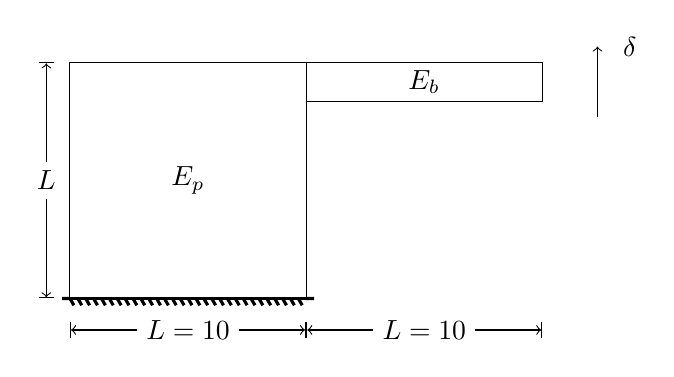
\begin{tikzpicture}
\FixedSupport{1.5,0}{4}
\draw(0,0)rectangle(3,3);\draw(3,3)rectangle(6,2.5);
\draw[->](6.7,2.3)--(6.7,3.2)node[right=2mm]{$\delta$};
\node[]at(1.5,1.5){$E_p$};
\node[]at(4.5,2.75){$E_b$};
\draw[|<->|](-.3,0)--++(0,3)node[midway,fill=white]{$L$};
\draw[|<->|](0,-.4)--++(3,0)node[midway,fill=white]{$L=10$};
\draw[|<->|](3,-.4)--++(3,0)node[midway,fill=white]{$L=10$};
\end{tikzpicture}
\caption{wall example with attached beam}\label{fig:drilling_ex}
\end{figure}

In the beam-panel model, the panel is modelled by (S)GCMQ elements while the attached beam is idealised as elastic beam element. The Poisson's ratio is set to zero so the deflection of beam is accurate. Two different meshes are tested: \numproduct{2x2} and \numproduct{4x4}. The corresponding results are shown in \figref{fig:coupled_test}. The reference values are given by 2D models with refined meshes of plane stress elements in ABAQUS. It could be seen from \figref{fig:coupled_test} that the drilling DoFs in (S)GCMQ perform well with weak coupling members. For $E_b/E_p\leqslant\num{1}$, the error can be bounded within \SI{20}{\percent} and becomes insignificant when $E_b/E_p\leqslant\num{0.1}$ with the \numproduct{2x2} mesh. It is worth mentioning that $E_b/E_p=\num{125}$ leads to the same $EI$ for both panel and beam. However, different mesh densities show different behaviour. A refined mesh does not necessarily lead to more accurate results. With the \numproduct{4x4} mesh, the results deteriorates quickly with an increasing moduli ratio $E_b/E_p$. It shall be noted that with the \numproduct{2x2} mesh the beam depth is \SI{40}{\percent} of the length of the adjacent panel element while this value increases to \SI{80}{\percent} with the \numproduct{4x4} mesh. Such a high ratio means the physical boundary condition \textit{cannot} be precisely represented by the numerical model. Deformation compatibility may become a severe problem as different elements adopt different displacement interpolations.
\begin{figure}[htb]
\centering\scriptsize
\begin{subfigure}{.49\textwidth}\centering
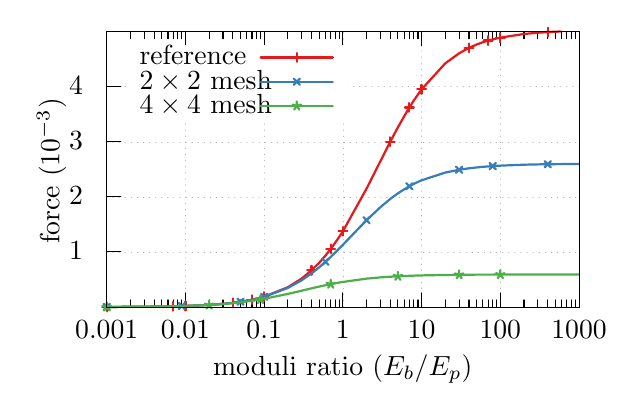
\begin{tikzpicture}[gnuplot]
%% generated with GNUPLOT 5.2p6 (Lua 5.3; terminal rev. Nov 2018, script rev. 107)
%% 08/06/2019 01:33:33
\path (0.000,0.000) rectangle (6.000,3.500);
\gpcolor{color=gp lt color axes}
\gpsetlinetype{gp lt axes}
\gpsetdashtype{gp dt axes}
\gpsetlinewidth{0.50}
\draw[gp path] (0.000,0.700)--(5.999,0.700);
\gpcolor{color=gp lt color border}
\gpsetlinetype{gp lt border}
\gpsetdashtype{gp dt solid}
\gpsetlinewidth{1.00}
\draw[gp path] (0.000,0.700)--(0.180,0.700);
\node[gp node right] at (-0.184,0.700) {$1$};
\gpcolor{color=gp lt color axes}
\gpsetlinetype{gp lt axes}
\gpsetdashtype{gp dt axes}
\gpsetlinewidth{0.50}
\draw[gp path] (0.000,1.400)--(5.999,1.400);
\gpcolor{color=gp lt color border}
\gpsetlinetype{gp lt border}
\gpsetdashtype{gp dt solid}
\gpsetlinewidth{1.00}
\draw[gp path] (0.000,1.400)--(0.180,1.400);
\node[gp node right] at (-0.184,1.400) {$2$};
\gpcolor{color=gp lt color axes}
\gpsetlinetype{gp lt axes}
\gpsetdashtype{gp dt axes}
\gpsetlinewidth{0.50}
\draw[gp path] (0.000,2.099)--(5.999,2.099);
\gpcolor{color=gp lt color border}
\gpsetlinetype{gp lt border}
\gpsetdashtype{gp dt solid}
\gpsetlinewidth{1.00}
\draw[gp path] (0.000,2.099)--(0.180,2.099);
\node[gp node right] at (-0.184,2.099) {$3$};
\gpcolor{color=gp lt color axes}
\gpsetlinetype{gp lt axes}
\gpsetdashtype{gp dt axes}
\gpsetlinewidth{0.50}
\draw[gp path] (0.000,2.799)--(0.300,2.799);
\draw[gp path] (3.056,2.799)--(5.999,2.799);
\gpcolor{color=gp lt color border}
\gpsetlinetype{gp lt border}
\gpsetdashtype{gp dt solid}
\gpsetlinewidth{1.00}
\draw[gp path] (0.000,2.799)--(0.180,2.799);
\node[gp node right] at (-0.184,2.799) {$4$};
\gpcolor{color=gp lt color axes}
\gpsetlinetype{gp lt axes}
\gpsetdashtype{gp dt axes}
\gpsetlinewidth{0.50}
\draw[gp path] (0.000,0.000)--(0.000,3.499);
\gpcolor{color=gp lt color border}
\gpsetlinetype{gp lt border}
\gpsetdashtype{gp dt solid}
\gpsetlinewidth{1.00}
\draw[gp path] (0.000,0.000)--(0.000,0.180);
\draw[gp path] (0.000,3.499)--(0.000,3.319);
\node[gp node center] at (0.000,-0.308) {$0.001$};
\draw[gp path] (0.301,0.000)--(0.301,0.090);
\draw[gp path] (0.301,3.499)--(0.301,3.409);
\draw[gp path] (0.477,0.000)--(0.477,0.090);
\draw[gp path] (0.477,3.499)--(0.477,3.409);
\draw[gp path] (0.602,0.000)--(0.602,0.090);
\draw[gp path] (0.602,3.499)--(0.602,3.409);
\draw[gp path] (0.699,0.000)--(0.699,0.090);
\draw[gp path] (0.699,3.499)--(0.699,3.409);
\draw[gp path] (0.778,0.000)--(0.778,0.090);
\draw[gp path] (0.778,3.499)--(0.778,3.409);
\draw[gp path] (0.845,0.000)--(0.845,0.090);
\draw[gp path] (0.845,3.499)--(0.845,3.409);
\draw[gp path] (0.903,0.000)--(0.903,0.090);
\draw[gp path] (0.903,3.499)--(0.903,3.409);
\draw[gp path] (0.954,0.000)--(0.954,0.090);
\draw[gp path] (0.954,3.499)--(0.954,3.409);
\gpcolor{color=gp lt color axes}
\gpsetlinetype{gp lt axes}
\gpsetdashtype{gp dt axes}
\gpsetlinewidth{0.50}
\draw[gp path] (1.000,0.000)--(1.000,2.400);
\draw[gp path] (1.000,3.324)--(1.000,3.499);
\gpcolor{color=gp lt color border}
\gpsetlinetype{gp lt border}
\gpsetdashtype{gp dt solid}
\gpsetlinewidth{1.00}
\draw[gp path] (1.000,0.000)--(1.000,0.180);
\draw[gp path] (1.000,3.499)--(1.000,3.319);
\node[gp node center] at (1.000,-0.308) {$0.01$};
\draw[gp path] (1.301,0.000)--(1.301,0.090);
\draw[gp path] (1.301,3.499)--(1.301,3.409);
\draw[gp path] (1.477,0.000)--(1.477,0.090);
\draw[gp path] (1.477,3.499)--(1.477,3.409);
\draw[gp path] (1.602,0.000)--(1.602,0.090);
\draw[gp path] (1.602,3.499)--(1.602,3.409);
\draw[gp path] (1.699,0.000)--(1.699,0.090);
\draw[gp path] (1.699,3.499)--(1.699,3.409);
\draw[gp path] (1.778,0.000)--(1.778,0.090);
\draw[gp path] (1.778,3.499)--(1.778,3.409);
\draw[gp path] (1.845,0.000)--(1.845,0.090);
\draw[gp path] (1.845,3.499)--(1.845,3.409);
\draw[gp path] (1.903,0.000)--(1.903,0.090);
\draw[gp path] (1.903,3.499)--(1.903,3.409);
\draw[gp path] (1.954,0.000)--(1.954,0.090);
\draw[gp path] (1.954,3.499)--(1.954,3.409);
\gpcolor{color=gp lt color axes}
\gpsetlinetype{gp lt axes}
\gpsetdashtype{gp dt axes}
\gpsetlinewidth{0.50}
\draw[gp path] (2.000,0.000)--(2.000,2.400);
\draw[gp path] (2.000,3.324)--(2.000,3.499);
\gpcolor{color=gp lt color border}
\gpsetlinetype{gp lt border}
\gpsetdashtype{gp dt solid}
\gpsetlinewidth{1.00}
\draw[gp path] (2.000,0.000)--(2.000,0.180);
\draw[gp path] (2.000,3.499)--(2.000,3.319);
\node[gp node center] at (2.000,-0.308) {$0.1$};
\draw[gp path] (2.301,0.000)--(2.301,0.090);
\draw[gp path] (2.301,3.499)--(2.301,3.409);
\draw[gp path] (2.477,0.000)--(2.477,0.090);
\draw[gp path] (2.477,3.499)--(2.477,3.409);
\draw[gp path] (2.602,0.000)--(2.602,0.090);
\draw[gp path] (2.602,3.499)--(2.602,3.409);
\draw[gp path] (2.699,0.000)--(2.699,0.090);
\draw[gp path] (2.699,3.499)--(2.699,3.409);
\draw[gp path] (2.778,0.000)--(2.778,0.090);
\draw[gp path] (2.778,3.499)--(2.778,3.409);
\draw[gp path] (2.845,0.000)--(2.845,0.090);
\draw[gp path] (2.845,3.499)--(2.845,3.409);
\draw[gp path] (2.903,0.000)--(2.903,0.090);
\draw[gp path] (2.903,3.499)--(2.903,3.409);
\draw[gp path] (2.954,0.000)--(2.954,0.090);
\draw[gp path] (2.954,3.499)--(2.954,3.409);
\gpcolor{color=gp lt color axes}
\gpsetlinetype{gp lt axes}
\gpsetdashtype{gp dt axes}
\gpsetlinewidth{0.50}
\draw[gp path] (3.000,0.000)--(3.000,2.400);
\draw[gp path] (3.000,3.324)--(3.000,3.499);
\gpcolor{color=gp lt color border}
\gpsetlinetype{gp lt border}
\gpsetdashtype{gp dt solid}
\gpsetlinewidth{1.00}
\draw[gp path] (3.000,0.000)--(3.000,0.180);
\draw[gp path] (3.000,3.499)--(3.000,3.319);
\node[gp node center] at (3.000,-0.308) {$1$};
\draw[gp path] (3.300,0.000)--(3.300,0.090);
\draw[gp path] (3.300,3.499)--(3.300,3.409);
\draw[gp path] (3.477,0.000)--(3.477,0.090);
\draw[gp path] (3.477,3.499)--(3.477,3.409);
\draw[gp path] (3.601,0.000)--(3.601,0.090);
\draw[gp path] (3.601,3.499)--(3.601,3.409);
\draw[gp path] (3.698,0.000)--(3.698,0.090);
\draw[gp path] (3.698,3.499)--(3.698,3.409);
\draw[gp path] (3.778,0.000)--(3.778,0.090);
\draw[gp path] (3.778,3.499)--(3.778,3.409);
\draw[gp path] (3.844,0.000)--(3.844,0.090);
\draw[gp path] (3.844,3.499)--(3.844,3.409);
\draw[gp path] (3.902,0.000)--(3.902,0.090);
\draw[gp path] (3.902,3.499)--(3.902,3.409);
\draw[gp path] (3.954,0.000)--(3.954,0.090);
\draw[gp path] (3.954,3.499)--(3.954,3.409);
\gpcolor{color=gp lt color axes}
\gpsetlinetype{gp lt axes}
\gpsetdashtype{gp dt axes}
\gpsetlinewidth{0.50}
\draw[gp path] (3.999,0.000)--(3.999,3.499);
\gpcolor{color=gp lt color border}
\gpsetlinetype{gp lt border}
\gpsetdashtype{gp dt solid}
\gpsetlinewidth{1.00}
\draw[gp path] (3.999,0.000)--(3.999,0.180);
\draw[gp path] (3.999,3.499)--(3.999,3.319);
\node[gp node center] at (3.999,-0.308) {$10$};
\draw[gp path] (4.300,0.000)--(4.300,0.090);
\draw[gp path] (4.300,3.499)--(4.300,3.409);
\draw[gp path] (4.476,0.000)--(4.476,0.090);
\draw[gp path] (4.476,3.499)--(4.476,3.409);
\draw[gp path] (4.601,0.000)--(4.601,0.090);
\draw[gp path] (4.601,3.499)--(4.601,3.409);
\draw[gp path] (4.698,0.000)--(4.698,0.090);
\draw[gp path] (4.698,3.499)--(4.698,3.409);
\draw[gp path] (4.777,0.000)--(4.777,0.090);
\draw[gp path] (4.777,3.499)--(4.777,3.409);
\draw[gp path] (4.844,0.000)--(4.844,0.090);
\draw[gp path] (4.844,3.499)--(4.844,3.409);
\draw[gp path] (4.902,0.000)--(4.902,0.090);
\draw[gp path] (4.902,3.499)--(4.902,3.409);
\draw[gp path] (4.953,0.000)--(4.953,0.090);
\draw[gp path] (4.953,3.499)--(4.953,3.409);
\gpcolor{color=gp lt color axes}
\gpsetlinetype{gp lt axes}
\gpsetdashtype{gp dt axes}
\gpsetlinewidth{0.50}
\draw[gp path] (4.999,0.000)--(4.999,3.499);
\gpcolor{color=gp lt color border}
\gpsetlinetype{gp lt border}
\gpsetdashtype{gp dt solid}
\gpsetlinewidth{1.00}
\draw[gp path] (4.999,0.000)--(4.999,0.180);
\draw[gp path] (4.999,3.499)--(4.999,3.319);
\node[gp node center] at (4.999,-0.308) {$100$};
\draw[gp path] (5.300,0.000)--(5.300,0.090);
\draw[gp path] (5.300,3.499)--(5.300,3.409);
\draw[gp path] (5.476,0.000)--(5.476,0.090);
\draw[gp path] (5.476,3.499)--(5.476,3.409);
\draw[gp path] (5.601,0.000)--(5.601,0.090);
\draw[gp path] (5.601,3.499)--(5.601,3.409);
\draw[gp path] (5.698,0.000)--(5.698,0.090);
\draw[gp path] (5.698,3.499)--(5.698,3.409);
\draw[gp path] (5.777,0.000)--(5.777,0.090);
\draw[gp path] (5.777,3.499)--(5.777,3.409);
\draw[gp path] (5.844,0.000)--(5.844,0.090);
\draw[gp path] (5.844,3.499)--(5.844,3.409);
\draw[gp path] (5.902,0.000)--(5.902,0.090);
\draw[gp path] (5.902,3.499)--(5.902,3.409);
\draw[gp path] (5.953,0.000)--(5.953,0.090);
\draw[gp path] (5.953,3.499)--(5.953,3.409);
\gpcolor{color=gp lt color axes}
\gpsetlinetype{gp lt axes}
\gpsetdashtype{gp dt axes}
\gpsetlinewidth{0.50}
\draw[gp path] (5.999,0.000)--(5.999,3.499);
\gpcolor{color=gp lt color border}
\gpsetlinetype{gp lt border}
\gpsetdashtype{gp dt solid}
\gpsetlinewidth{1.00}
\draw[gp path] (5.999,0.000)--(5.999,0.180);
\draw[gp path] (5.999,3.499)--(5.999,3.319);
\node[gp node center] at (5.999,-0.308) {$1000$};
\draw[gp path] (0.000,3.499)--(0.000,0.000)--(5.999,0.000)--(5.999,3.499)--cycle;
\node[gp node center,rotate=-270] at (-0.676,1.749) {force (\num{E-3})};
\node[gp node center] at (2.999,-0.769) {moduli ratio ($E_b/E_p$)};
\gpcolor{rgb color={0.894,0.102,0.110}}
\gpsetlinewidth{2.00}
\draw[gp path] (0.000,0.001)--(0.699,0.007)--(0.778,0.008)--(0.845,0.010)--(0.903,0.011)%
  --(0.954,0.012)--(1.000,0.014)--(1.301,0.027)--(1.477,0.041)--(1.602,0.054)--(1.699,0.067)%
  --(1.778,0.080)--(1.845,0.093)--(1.903,0.106)--(1.954,0.119)--(2.000,0.132)--(2.301,0.252)%
  --(2.477,0.363)--(2.602,0.467)--(2.699,0.563)--(2.778,0.653)--(2.845,0.738)--(2.903,0.818)%
  --(2.954,0.893)--(3.000,0.963)--(3.300,1.504)--(3.477,1.854)--(3.601,2.100)--(3.698,2.282)%
  --(3.778,2.423)--(3.844,2.535)--(3.902,2.626)--(3.954,2.701)--(3.999,2.765)--(4.300,3.095)%
  --(4.476,3.223)--(4.601,3.292)--(4.698,3.334)--(4.777,3.363)--(4.844,3.384)--(4.902,3.400)%
  --(4.953,3.412)--(4.999,3.422)--(5.300,3.468)--(5.476,3.484)--(5.601,3.492)--(5.698,3.497)%
  --(5.764,3.499);
\gpsetpointsize{4.00}
\gppoint{gp mark 1}{(0.000,0.001)}
\gppoint{gp mark 1}{(0.845,0.010)}
\gppoint{gp mark 1}{(1.000,0.014)}
\gppoint{gp mark 1}{(1.602,0.054)}
\gppoint{gp mark 1}{(1.845,0.093)}
\gppoint{gp mark 1}{(2.000,0.132)}
\gppoint{gp mark 1}{(2.602,0.467)}
\gppoint{gp mark 1}{(2.845,0.738)}
\gppoint{gp mark 1}{(3.000,0.963)}
\gppoint{gp mark 1}{(3.601,2.100)}
\gppoint{gp mark 1}{(3.844,2.535)}
\gppoint{gp mark 1}{(3.999,2.765)}
\gppoint{gp mark 1}{(4.601,3.292)}
\gppoint{gp mark 1}{(4.844,3.384)}
\gppoint{gp mark 1}{(4.999,3.422)}
\gppoint{gp mark 1}{(5.601,3.492)}
\gpcolor{rgb color={0.216,0.494,0.722}}
\draw[gp path] (0.000,0.001)--(0.699,0.007)--(0.778,0.008)--(0.845,0.010)--(0.903,0.011)%
  --(0.954,0.013)--(1.000,0.014)--(1.301,0.028)--(1.477,0.041)--(1.602,0.054)--(1.699,0.067)%
  --(1.778,0.080)--(1.845,0.093)--(1.903,0.105)--(1.954,0.118)--(2.000,0.130)--(2.301,0.243)%
  --(2.477,0.341)--(2.602,0.428)--(2.699,0.505)--(2.778,0.575)--(2.845,0.637)--(2.903,0.693)%
  --(2.954,0.744)--(3.000,0.791)--(3.300,1.103)--(3.477,1.269)--(3.601,1.373)--(3.698,1.444)%
  --(3.778,1.495)--(3.844,1.534)--(3.902,1.565)--(3.954,1.590)--(3.999,1.610)--(4.300,1.708)%
  --(4.476,1.744)--(4.601,1.762)--(4.698,1.773)--(4.777,1.781)--(4.844,1.786)--(4.902,1.790)%
  --(4.953,1.794)--(4.999,1.796)--(5.300,1.808)--(5.476,1.812)--(5.601,1.814)--(5.698,1.815)%
  --(5.999,1.817);
\gppoint{gp mark 2}{(0.000,0.001)}
\gppoint{gp mark 2}{(0.954,0.013)}
\gppoint{gp mark 2}{(1.699,0.067)}
\gppoint{gp mark 2}{(2.000,0.130)}
\gppoint{gp mark 2}{(2.778,0.575)}
\gppoint{gp mark 2}{(3.300,1.103)}
\gppoint{gp mark 2}{(3.844,1.534)}
\gppoint{gp mark 2}{(4.476,1.744)}
\gppoint{gp mark 2}{(4.902,1.790)}
\gppoint{gp mark 2}{(5.601,1.814)}
\gpcolor{rgb color={0.302,0.686,0.290}}
\draw[gp path] (0.000,0.001)--(0.699,0.007)--(0.778,0.008)--(0.845,0.010)--(0.903,0.011)%
  --(0.954,0.012)--(1.000,0.014)--(1.301,0.026)--(1.477,0.038)--(1.602,0.049)--(1.699,0.060)%
  --(1.778,0.070)--(1.845,0.079)--(1.903,0.088)--(1.954,0.097)--(2.000,0.105)--(2.301,0.167)%
  --(2.477,0.208)--(2.602,0.238)--(2.699,0.260)--(2.778,0.277)--(2.845,0.291)--(2.903,0.302)%
  --(2.954,0.312)--(3.000,0.319)--(3.300,0.361)--(3.477,0.377)--(3.601,0.385)--(3.698,0.391)%
  --(3.778,0.394)--(3.844,0.397)--(3.902,0.399)--(3.954,0.401)--(3.999,0.402)--(4.300,0.408)%
  --(4.476,0.410)--(4.601,0.411)--(4.698,0.412)--(4.777,0.412)--(4.844,0.412)--(4.902,0.412)%
  --(4.953,0.413)--(4.999,0.413)--(5.300,0.413)--(5.476,0.414)--(5.601,0.414)--(5.698,0.414)%
  --(5.999,0.414);
\gppoint{gp mark 3}{(0.000,0.001)}
\gppoint{gp mark 3}{(1.301,0.026)}
\gppoint{gp mark 3}{(1.954,0.097)}
\gppoint{gp mark 3}{(2.845,0.291)}
\gppoint{gp mark 3}{(3.698,0.391)}
\gppoint{gp mark 3}{(4.476,0.410)}
\gppoint{gp mark 3}{(4.999,0.413)}
\gpfill{color=gpbgfillcolor} (0.300,2.400)--(3.056,2.400)--(3.056,3.324)--(0.300,3.324)--cycle;
\gpcolor{color=gp lt color border}
\node[gp node left] at (0.300,3.170) {reference};
\gpcolor{rgb color={0.894,0.102,0.110}}
\draw[gp path] (1.956,3.170)--(2.872,3.170);
\gppoint{gp mark 1}{(2.414,3.170)}
\gpcolor{color=gp lt color border}
\node[gp node left] at (0.300,2.862) {\numproduct{2x2} mesh};
\gpcolor{rgb color={0.216,0.494,0.722}}
\draw[gp path] (1.956,2.862)--(2.872,2.862);
\gppoint{gp mark 2}{(2.414,2.862)}
\gpcolor{color=gp lt color border}
\node[gp node left] at (0.300,2.554) {\numproduct{4x4} mesh};
\gpcolor{rgb color={0.302,0.686,0.290}}
\draw[gp path] (1.956,2.554)--(2.872,2.554);
\gppoint{gp mark 3}{(2.414,2.554)}
\gpcolor{color=gp lt color border}
\gpsetlinewidth{1.00}
\draw[gp path] (0.000,3.499)--(0.000,0.000)--(5.999,0.000)--(5.999,3.499)--cycle;
%% coordinates of the plot area
\gpdefrectangularnode{gp plot 1}{\pgfpoint{0.000cm}{0.000cm}}{\pgfpoint{5.999cm}{3.499cm}}
\end{tikzpicture}
%% gnuplot variables

\caption{end force required}
\end{subfigure}\hfill
\begin{subfigure}{.49\textwidth}\centering
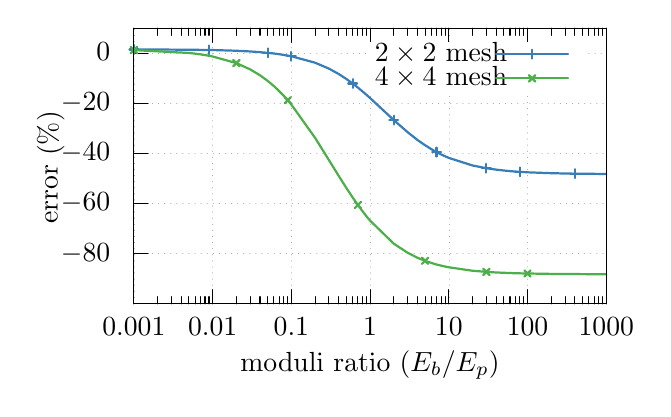
\begin{tikzpicture}[gnuplot]
%% generated with GNUPLOT 5.2p6 (Lua 5.3; terminal rev. Nov 2018, script rev. 107)
%% 08/06/2019 01:33:33
\path (0.000,0.000) rectangle (6.000,3.500);
\gpcolor{color=gp lt color axes}
\gpsetlinetype{gp lt axes}
\gpsetdashtype{gp dt axes}
\gpsetlinewidth{0.50}
\draw[gp path] (0.000,0.636)--(5.999,0.636);
\gpcolor{color=gp lt color border}
\gpsetlinetype{gp lt border}
\gpsetdashtype{gp dt solid}
\gpsetlinewidth{1.00}
\draw[gp path] (0.000,0.636)--(0.180,0.636);
\node[gp node right] at (-0.184,0.636) {$-80$};
\gpcolor{color=gp lt color axes}
\gpsetlinetype{gp lt axes}
\gpsetdashtype{gp dt axes}
\gpsetlinewidth{0.50}
\draw[gp path] (0.000,1.272)--(5.999,1.272);
\gpcolor{color=gp lt color border}
\gpsetlinetype{gp lt border}
\gpsetdashtype{gp dt solid}
\gpsetlinewidth{1.00}
\draw[gp path] (0.000,1.272)--(0.180,1.272);
\node[gp node right] at (-0.184,1.272) {$-60$};
\gpcolor{color=gp lt color axes}
\gpsetlinetype{gp lt axes}
\gpsetdashtype{gp dt axes}
\gpsetlinewidth{0.50}
\draw[gp path] (0.000,1.909)--(5.999,1.909);
\gpcolor{color=gp lt color border}
\gpsetlinetype{gp lt border}
\gpsetdashtype{gp dt solid}
\gpsetlinewidth{1.00}
\draw[gp path] (0.000,1.909)--(0.180,1.909);
\node[gp node right] at (-0.184,1.909) {$-40$};
\gpcolor{color=gp lt color axes}
\gpsetlinetype{gp lt axes}
\gpsetdashtype{gp dt axes}
\gpsetlinewidth{0.50}
\draw[gp path] (0.000,2.545)--(5.999,2.545);
\gpcolor{color=gp lt color border}
\gpsetlinetype{gp lt border}
\gpsetdashtype{gp dt solid}
\gpsetlinewidth{1.00}
\draw[gp path] (0.000,2.545)--(0.180,2.545);
\node[gp node right] at (-0.184,2.545) {$-20$};
\gpcolor{color=gp lt color axes}
\gpsetlinetype{gp lt axes}
\gpsetdashtype{gp dt axes}
\gpsetlinewidth{0.50}
\draw[gp path] (0.000,3.181)--(2.943,3.181);
\draw[gp path] (5.699,3.181)--(5.999,3.181);
\gpcolor{color=gp lt color border}
\gpsetlinetype{gp lt border}
\gpsetdashtype{gp dt solid}
\gpsetlinewidth{1.00}
\draw[gp path] (0.000,3.181)--(0.180,3.181);
\node[gp node right] at (-0.184,3.181) {$0$};
\gpcolor{color=gp lt color axes}
\gpsetlinetype{gp lt axes}
\gpsetdashtype{gp dt axes}
\gpsetlinewidth{0.50}
\draw[gp path] (0.000,0.000)--(0.000,3.499);
\gpcolor{color=gp lt color border}
\gpsetlinetype{gp lt border}
\gpsetdashtype{gp dt solid}
\gpsetlinewidth{1.00}
\draw[gp path] (0.000,0.000)--(0.000,0.180);
\draw[gp path] (0.000,3.499)--(0.000,3.319);
\node[gp node center] at (0.000,-0.308) {$0.001$};
\draw[gp path] (0.301,0.000)--(0.301,0.090);
\draw[gp path] (0.301,3.499)--(0.301,3.409);
\draw[gp path] (0.477,0.000)--(0.477,0.090);
\draw[gp path] (0.477,3.499)--(0.477,3.409);
\draw[gp path] (0.602,0.000)--(0.602,0.090);
\draw[gp path] (0.602,3.499)--(0.602,3.409);
\draw[gp path] (0.699,0.000)--(0.699,0.090);
\draw[gp path] (0.699,3.499)--(0.699,3.409);
\draw[gp path] (0.778,0.000)--(0.778,0.090);
\draw[gp path] (0.778,3.499)--(0.778,3.409);
\draw[gp path] (0.845,0.000)--(0.845,0.090);
\draw[gp path] (0.845,3.499)--(0.845,3.409);
\draw[gp path] (0.903,0.000)--(0.903,0.090);
\draw[gp path] (0.903,3.499)--(0.903,3.409);
\draw[gp path] (0.954,0.000)--(0.954,0.090);
\draw[gp path] (0.954,3.499)--(0.954,3.409);
\gpcolor{color=gp lt color axes}
\gpsetlinetype{gp lt axes}
\gpsetdashtype{gp dt axes}
\gpsetlinewidth{0.50}
\draw[gp path] (1.000,0.000)--(1.000,3.499);
\gpcolor{color=gp lt color border}
\gpsetlinetype{gp lt border}
\gpsetdashtype{gp dt solid}
\gpsetlinewidth{1.00}
\draw[gp path] (1.000,0.000)--(1.000,0.180);
\draw[gp path] (1.000,3.499)--(1.000,3.319);
\node[gp node center] at (1.000,-0.308) {$0.01$};
\draw[gp path] (1.301,0.000)--(1.301,0.090);
\draw[gp path] (1.301,3.499)--(1.301,3.409);
\draw[gp path] (1.477,0.000)--(1.477,0.090);
\draw[gp path] (1.477,3.499)--(1.477,3.409);
\draw[gp path] (1.602,0.000)--(1.602,0.090);
\draw[gp path] (1.602,3.499)--(1.602,3.409);
\draw[gp path] (1.699,0.000)--(1.699,0.090);
\draw[gp path] (1.699,3.499)--(1.699,3.409);
\draw[gp path] (1.778,0.000)--(1.778,0.090);
\draw[gp path] (1.778,3.499)--(1.778,3.409);
\draw[gp path] (1.845,0.000)--(1.845,0.090);
\draw[gp path] (1.845,3.499)--(1.845,3.409);
\draw[gp path] (1.903,0.000)--(1.903,0.090);
\draw[gp path] (1.903,3.499)--(1.903,3.409);
\draw[gp path] (1.954,0.000)--(1.954,0.090);
\draw[gp path] (1.954,3.499)--(1.954,3.409);
\gpcolor{color=gp lt color axes}
\gpsetlinetype{gp lt axes}
\gpsetdashtype{gp dt axes}
\gpsetlinewidth{0.50}
\draw[gp path] (2.000,0.000)--(2.000,3.499);
\gpcolor{color=gp lt color border}
\gpsetlinetype{gp lt border}
\gpsetdashtype{gp dt solid}
\gpsetlinewidth{1.00}
\draw[gp path] (2.000,0.000)--(2.000,0.180);
\draw[gp path] (2.000,3.499)--(2.000,3.319);
\node[gp node center] at (2.000,-0.308) {$0.1$};
\draw[gp path] (2.301,0.000)--(2.301,0.090);
\draw[gp path] (2.301,3.499)--(2.301,3.409);
\draw[gp path] (2.477,0.000)--(2.477,0.090);
\draw[gp path] (2.477,3.499)--(2.477,3.409);
\draw[gp path] (2.602,0.000)--(2.602,0.090);
\draw[gp path] (2.602,3.499)--(2.602,3.409);
\draw[gp path] (2.699,0.000)--(2.699,0.090);
\draw[gp path] (2.699,3.499)--(2.699,3.409);
\draw[gp path] (2.778,0.000)--(2.778,0.090);
\draw[gp path] (2.778,3.499)--(2.778,3.409);
\draw[gp path] (2.845,0.000)--(2.845,0.090);
\draw[gp path] (2.845,3.499)--(2.845,3.409);
\draw[gp path] (2.903,0.000)--(2.903,0.090);
\draw[gp path] (2.903,3.499)--(2.903,3.409);
\draw[gp path] (2.954,0.000)--(2.954,0.090);
\draw[gp path] (2.954,3.499)--(2.954,3.409);
\gpcolor{color=gp lt color axes}
\gpsetlinetype{gp lt axes}
\gpsetdashtype{gp dt axes}
\gpsetlinewidth{0.50}
\draw[gp path] (3.000,0.000)--(3.000,2.708);
\draw[gp path] (3.000,3.324)--(3.000,3.499);
\gpcolor{color=gp lt color border}
\gpsetlinetype{gp lt border}
\gpsetdashtype{gp dt solid}
\gpsetlinewidth{1.00}
\draw[gp path] (3.000,0.000)--(3.000,0.180);
\draw[gp path] (3.000,3.499)--(3.000,3.319);
\node[gp node center] at (3.000,-0.308) {$1$};
\draw[gp path] (3.300,0.000)--(3.300,0.090);
\draw[gp path] (3.300,3.499)--(3.300,3.409);
\draw[gp path] (3.477,0.000)--(3.477,0.090);
\draw[gp path] (3.477,3.499)--(3.477,3.409);
\draw[gp path] (3.601,0.000)--(3.601,0.090);
\draw[gp path] (3.601,3.499)--(3.601,3.409);
\draw[gp path] (3.698,0.000)--(3.698,0.090);
\draw[gp path] (3.698,3.499)--(3.698,3.409);
\draw[gp path] (3.778,0.000)--(3.778,0.090);
\draw[gp path] (3.778,3.499)--(3.778,3.409);
\draw[gp path] (3.844,0.000)--(3.844,0.090);
\draw[gp path] (3.844,3.499)--(3.844,3.409);
\draw[gp path] (3.902,0.000)--(3.902,0.090);
\draw[gp path] (3.902,3.499)--(3.902,3.409);
\draw[gp path] (3.954,0.000)--(3.954,0.090);
\draw[gp path] (3.954,3.499)--(3.954,3.409);
\gpcolor{color=gp lt color axes}
\gpsetlinetype{gp lt axes}
\gpsetdashtype{gp dt axes}
\gpsetlinewidth{0.50}
\draw[gp path] (3.999,0.000)--(3.999,2.708);
\draw[gp path] (3.999,3.324)--(3.999,3.499);
\gpcolor{color=gp lt color border}
\gpsetlinetype{gp lt border}
\gpsetdashtype{gp dt solid}
\gpsetlinewidth{1.00}
\draw[gp path] (3.999,0.000)--(3.999,0.180);
\draw[gp path] (3.999,3.499)--(3.999,3.319);
\node[gp node center] at (3.999,-0.308) {$10$};
\draw[gp path] (4.300,0.000)--(4.300,0.090);
\draw[gp path] (4.300,3.499)--(4.300,3.409);
\draw[gp path] (4.476,0.000)--(4.476,0.090);
\draw[gp path] (4.476,3.499)--(4.476,3.409);
\draw[gp path] (4.601,0.000)--(4.601,0.090);
\draw[gp path] (4.601,3.499)--(4.601,3.409);
\draw[gp path] (4.698,0.000)--(4.698,0.090);
\draw[gp path] (4.698,3.499)--(4.698,3.409);
\draw[gp path] (4.777,0.000)--(4.777,0.090);
\draw[gp path] (4.777,3.499)--(4.777,3.409);
\draw[gp path] (4.844,0.000)--(4.844,0.090);
\draw[gp path] (4.844,3.499)--(4.844,3.409);
\draw[gp path] (4.902,0.000)--(4.902,0.090);
\draw[gp path] (4.902,3.499)--(4.902,3.409);
\draw[gp path] (4.953,0.000)--(4.953,0.090);
\draw[gp path] (4.953,3.499)--(4.953,3.409);
\gpcolor{color=gp lt color axes}
\gpsetlinetype{gp lt axes}
\gpsetdashtype{gp dt axes}
\gpsetlinewidth{0.50}
\draw[gp path] (4.999,0.000)--(4.999,2.708);
\draw[gp path] (4.999,3.324)--(4.999,3.499);
\gpcolor{color=gp lt color border}
\gpsetlinetype{gp lt border}
\gpsetdashtype{gp dt solid}
\gpsetlinewidth{1.00}
\draw[gp path] (4.999,0.000)--(4.999,0.180);
\draw[gp path] (4.999,3.499)--(4.999,3.319);
\node[gp node center] at (4.999,-0.308) {$100$};
\draw[gp path] (5.300,0.000)--(5.300,0.090);
\draw[gp path] (5.300,3.499)--(5.300,3.409);
\draw[gp path] (5.476,0.000)--(5.476,0.090);
\draw[gp path] (5.476,3.499)--(5.476,3.409);
\draw[gp path] (5.601,0.000)--(5.601,0.090);
\draw[gp path] (5.601,3.499)--(5.601,3.409);
\draw[gp path] (5.698,0.000)--(5.698,0.090);
\draw[gp path] (5.698,3.499)--(5.698,3.409);
\draw[gp path] (5.777,0.000)--(5.777,0.090);
\draw[gp path] (5.777,3.499)--(5.777,3.409);
\draw[gp path] (5.844,0.000)--(5.844,0.090);
\draw[gp path] (5.844,3.499)--(5.844,3.409);
\draw[gp path] (5.902,0.000)--(5.902,0.090);
\draw[gp path] (5.902,3.499)--(5.902,3.409);
\draw[gp path] (5.953,0.000)--(5.953,0.090);
\draw[gp path] (5.953,3.499)--(5.953,3.409);
\gpcolor{color=gp lt color axes}
\gpsetlinetype{gp lt axes}
\gpsetdashtype{gp dt axes}
\gpsetlinewidth{0.50}
\draw[gp path] (5.999,0.000)--(5.999,3.499);
\gpcolor{color=gp lt color border}
\gpsetlinetype{gp lt border}
\gpsetdashtype{gp dt solid}
\gpsetlinewidth{1.00}
\draw[gp path] (5.999,0.000)--(5.999,0.180);
\draw[gp path] (5.999,3.499)--(5.999,3.319);
\node[gp node center] at (5.999,-0.308) {$1000$};
\draw[gp path] (0.000,3.499)--(0.000,0.000)--(5.999,0.000)--(5.999,3.499)--cycle;
\node[gp node center,rotate=-270] at (-1.044,1.749) {error (\si{\percent})};
\node[gp node center] at (2.999,-0.769) {moduli ratio ($E_b/E_p$)};
\gpcolor{rgb color={0.216,0.494,0.722}}
\gpsetlinewidth{2.00}
\draw[gp path] (0.000,3.230)--(0.699,3.226)--(0.778,3.225)--(0.845,3.224)--(0.903,3.223)%
  --(0.954,3.223)--(1.000,3.222)--(1.301,3.213)--(1.477,3.204)--(1.602,3.195)--(1.699,3.186)%
  --(1.778,3.178)--(1.845,3.169)--(1.903,3.160)--(1.954,3.151)--(2.000,3.143)--(2.301,3.061)%
  --(2.477,2.986)--(2.602,2.917)--(2.699,2.854)--(2.778,2.797)--(2.845,2.745)--(2.903,2.697)%
  --(2.954,2.653)--(3.000,2.612)--(3.300,2.333)--(3.477,2.178)--(3.601,2.080)--(3.698,2.013)%
  --(3.778,1.963)--(3.844,1.926)--(3.902,1.896)--(3.954,1.872)--(3.999,1.852)--(4.300,1.756)%
  --(4.476,1.721)--(4.601,1.703)--(4.698,1.692)--(4.777,1.684)--(4.844,1.679)--(4.902,1.675)%
  --(4.953,1.672)--(4.999,1.669)--(5.300,1.658)--(5.476,1.654)--(5.601,1.652)--(5.698,1.651)%
  --(5.999,1.648);
\gpsetpointsize{4.00}
\gppoint{gp mark 1}{(0.000,3.230)}
\gppoint{gp mark 1}{(0.954,3.223)}
\gppoint{gp mark 1}{(1.699,3.186)}
\gppoint{gp mark 1}{(2.000,3.143)}
\gppoint{gp mark 1}{(2.778,2.797)}
\gppoint{gp mark 1}{(3.300,2.333)}
\gppoint{gp mark 1}{(3.844,1.926)}
\gppoint{gp mark 1}{(4.476,1.721)}
\gppoint{gp mark 1}{(4.902,1.675)}
\gppoint{gp mark 1}{(5.601,1.652)}
\gpcolor{rgb color={0.302,0.686,0.290}}
\draw[gp path] (0.000,3.221)--(0.699,3.185)--(0.778,3.176)--(0.845,3.167)--(0.903,3.158)%
  --(0.954,3.149)--(1.000,3.140)--(1.301,3.056)--(1.477,2.976)--(1.602,2.901)--(1.699,2.830)%
  --(1.778,2.764)--(1.845,2.700)--(1.903,2.641)--(1.954,2.584)--(2.000,2.529)--(2.301,2.107)%
  --(2.477,1.824)--(2.602,1.622)--(2.699,1.469)--(2.778,1.350)--(2.845,1.254)--(2.903,1.176)%
  --(2.954,1.110)--(3.000,1.055)--(3.300,0.763)--(3.477,0.647)--(3.601,0.584)--(3.698,0.545)%
  --(3.778,0.518)--(3.844,0.498)--(3.902,0.484)--(3.954,0.472)--(3.999,0.463)--(4.300,0.419)%
  --(4.476,0.405)--(4.601,0.397)--(4.698,0.393)--(4.777,0.390)--(4.844,0.387)--(4.902,0.386)%
  --(4.953,0.385)--(4.999,0.384)--(5.300,0.379)--(5.476,0.378)--(5.601,0.377)--(5.698,0.376)%
  --(5.999,0.375);
\gppoint{gp mark 2}{(0.000,3.221)}
\gppoint{gp mark 2}{(1.301,3.056)}
\gppoint{gp mark 2}{(1.954,2.584)}
\gppoint{gp mark 2}{(2.845,1.254)}
\gppoint{gp mark 2}{(3.698,0.545)}
\gppoint{gp mark 2}{(4.476,0.405)}
\gppoint{gp mark 2}{(4.999,0.384)}
\gpfill{color=gpbgfillcolor} (2.943,2.708)--(5.699,2.708)--(5.699,3.324)--(2.943,3.324)--cycle;
\gpcolor{color=gp lt color border}
\node[gp node left] at (2.943,3.170) {\numproduct{2x2} mesh};
\gpcolor{rgb color={0.216,0.494,0.722}}
\draw[gp path] (4.599,3.170)--(5.515,3.170);
\gppoint{gp mark 1}{(5.057,3.170)}
\gpcolor{color=gp lt color border}
\node[gp node left] at (2.943,2.862) {\numproduct{4x4} mesh};
\gpcolor{rgb color={0.302,0.686,0.290}}
\draw[gp path] (4.599,2.862)--(5.515,2.862);
\gppoint{gp mark 2}{(5.057,2.862)}
\gpcolor{color=gp lt color border}
\gpsetlinewidth{1.00}
\draw[gp path] (0.000,3.499)--(0.000,0.000)--(5.999,0.000)--(5.999,3.499)--cycle;
%% coordinates of the plot area
\gpdefrectangularnode{gp plot 1}{\pgfpoint{0.000cm}{0.000cm}}{\pgfpoint{5.999cm}{3.499cm}}
\end{tikzpicture}
%% gnuplot variables

\caption{corresponding error}
\end{subfigure}
\caption{results of panel with attached beam with different moduli ratios}\label{fig:coupled_test}
\end{figure}

It is thus \textit{inappropriate} to model this type of connections by using membrane and beam elements. It can be inferred that the error of rotational constraint would be lowered with shallower beams. The response of strong coupling members is hence not well captured by the current definition of drilling DoFs. Indeed, for rigid beams, deformation mainly occurs in the wall panel, where the rotational constraint may be contributed by a number of adjacent wall elements.

In the author's opinion, it is \textit{not recommended} to simulate walls with opening and/or strong coupling members such as deep beams by using hybrid models that consist of membrane elements --- not only (S)GCMQ but also other elements --- and beam elements. The focus of the remaining of this section is limited to coupled walls with weak coupling beams/slabs.
\subsection{Reinforced Concrete Coupled Wall}
Two reinforced concrete shear walls shown in \secref{sec:rc_wall_dynamic} connected with each other by beams are used to form a coupled wall with a spacing of \SI{3}{\meter}. The illustration of the coupled wall, along with the beam section, is depicted in \figref{fig:rc_coupled_wall}.
\begin{figure}[htb]
\centering\footnotesize
\begin{tikzpicture}
\definecolor{PH1}{RGB}{166,206,227}
\definecolor{PH2}{RGB}{31,120,180}
\definecolor{PH3}{RGB}{178,223,138}
\definecolor{PH4}{RGB}{51,160,44}
\definecolor{PH5}{RGB}{251,154,153}
\definecolor{PH6}{RGB}{227,26,28}
\definecolor{PH7}{RGB}{253,191,111}
\definecolor{PH8}{RGB}{255,127,0}
\definecolor{PH9}{RGB}{202,178,214}
\definecolor{PH10}{RGB}{106,61,154}
\FixedSupport{2.5,0}{2}
\FixedSupport{.5,0}{2}
\draw[thick](2,0)rectangle(3,5);
\draw[thick](0,0)rectangle(1,5);
\foreach\y in{1,2,3,4}{\draw[thick](2,\y)--++(1,0)(0,\y)--++(1,0);}
\foreach\y in{1,2,3,4,5}{\draw[ultra thick](1+.07,\y)--++(1-.14,0);}
\node[fill=PH1,inner sep=0,minimum size=1.4mm]at(1.07,1){};
\node[fill=PH3,inner sep=0,minimum size=1.4mm]at(1.07,2){};
\node[fill=PH5,inner sep=0,minimum size=1.4mm]at(1.07,3){};
\node[fill=PH7,inner sep=0,minimum size=1.4mm]at(1.07,4){};
\node[fill=PH9,inner sep=0,minimum size=1.4mm]at(1.07,5){};
\node[fill=PH2,inner sep=0,minimum size=1.4mm]at(1.93,1){};
\node[fill=PH4,inner sep=0,minimum size=1.4mm]at(1.93,2){};
\node[fill=PH6,inner sep=0,minimum size=1.4mm]at(1.93,3){};
\node[fill=PH8,inner sep=0,minimum size=1.4mm]at(1.93,4){};
\node[fill=PH10,inner sep=0,minimum size=1.4mm]at(1.93,5){};
\node[below left=1mm]at(1.07,1){\color{PH1}\tiny{}PH1};
\node[below left=1mm]at(1.07,2){\color{PH3}\tiny{}PH3};
\node[below left=1mm]at(1.07,3){\color{PH5}\tiny{}PH5};
\node[below left=1mm]at(1.07,4){\color{PH7}\tiny{}PH7};
\node[below left=1mm]at(1.07,5){\color{PH9}\tiny{}PH9};
\node[below right=1mm]at(1.93,1){\color{PH2}\tiny{}PH2};
\node[below right=1mm]at(1.93,2){\color{PH4}\tiny{}PH4};
\node[below right=1mm]at(1.93,3){\color{PH6}\tiny{}PH6};
\node[below right=1mm]at(1.93,4){\color{PH8}\tiny{}PH8};
\node[below right=1mm]at(1.93,5){\color{PH10}\tiny{}PH10};
\draw[|<->|](0,-.5)--++(1,0)node[midway,fill=white]{\SI{3}{\metre}};
\draw[|<->|](1,-.5)--++(1,0)node[midway,fill=white]{\SI{3}{\metre}};
\draw[|<->|](2,-.5)--++(1,0)node[midway,fill=white]{\SI{3}{\metre}};
\draw[|<->|](-.5,0)--++(0,5)node[midway,fill=white,rotate=90]{\SI{15}{\metre}};
\node[align=left,anchor=north west]at(4,5){concrete:\\[2mm]$E_c=\SI{30}{\giga\pascal}$\\[1mm]$f_c=\SI{30}{\mega\pascal}$\\[1mm]$f_t=\SI{3}{\mega\pascal}$\\[2mm]reinforcement:\\[2mm]$E_s=\SI{200}{\giga\pascal}$\\[1mm]$f_y=\SI{300}{\mega\pascal}$\\[1mm]$h=0.02$};
\node[align=left,anchor=north west]at(7,5){for each wall:\\horizontal lumped\\[2mm]$m=\SI{20}{\tonne}$ per floor\\[1mm]$t=\SI{200}{\milli\meter}$\\[1mm]$\rho=\SI{0.5}{\percent}$\\[1mm]SGCMQ element\\[1mm]$2\times10$ mesh};
\node[align=left,anchor=north west]at(10,5){for each beam:\\[2mm]\qtyproduct{200x300}{\milli\meter} section\\[1mm]
$8\phi16$ reinforcement\\[1mm]
force-based element (9 IPs)\\[2mm]
\begin{tikzpicture}[scale=1.2]
\scriptsize
\draw(0,0)rectangle(1,1.5);
\draw[|<->|](0,-.3)--++(1,0)node[midway,fill=white,anchor=center]{\SI{0.2}{\meter}};
\draw[|<->|](1.3,0)--++(0,1.5)node[midway,fill=white,anchor=center,rotate=90]{\SI{0.3}{\meter}};
\node[circle,fill,minimum size=1.4mm,inner sep=0,anchor=center]at(.15,.15){};
\node[circle,fill,minimum size=1.4mm,inner sep=0,anchor=center]at(.5,.15){};
\node[circle,fill,minimum size=1.4mm,inner sep=0,anchor=center]at(.85,.15){};
\node[circle,fill,minimum size=1.4mm,inner sep=0,anchor=center]at(.15,1.35){};
\node[circle,fill,minimum size=1.4mm,inner sep=0,anchor=center]at(.5,1.35){};
\node[circle,fill,minimum size=1.4mm,inner sep=0,anchor=center]at(.85,1.35){};
\node[circle,fill,minimum size=1.4mm,inner sep=0,anchor=center]at(.15,.75){};
\node[circle,fill,minimum size=1.4mm,inner sep=0,anchor=center]at(.85,.75){};
\end{tikzpicture}
};
\end{tikzpicture}
\caption{a reinforced concrete shear wall specimen}\label{fig:rc_coupled_wall}
\end{figure}
The thickness of concrete cover is assumed to be \SI{30}{\milli\meter}. The force-based beam element \citep{Spacone1996} is adopted to model beams since its accuracy mainly relies on the number of integration points \citep{Neuenhofer1997} so coarse meshes can also be utilised. For beam sections, the Tsai's equation \citep{Tsai1988} is adopted for concrete backbones while the Menegotto-Pinto steel model is used for reinforcement. The configuration of numerical algorithm is identical to that in \secref{sec:rc_wall_dynamic}. The first natural period computed is around \SI{0.32}{\second}. The same NS component of El Centro record is used as ground motion.

Typical material properties are used. For the configuration listed, an elastic analysis reveals that the response of the hybrid model (with SGCMQ and beam elements) is close to that of the model with plane stress elements. The difference varies depending on the mesh size but is within \SI{10}{\percent}. It is thus reasonable to use the hybrid model to perform the corresponding nonlinear analyses.

\begin{figure}[htb]
\centering\scriptsize
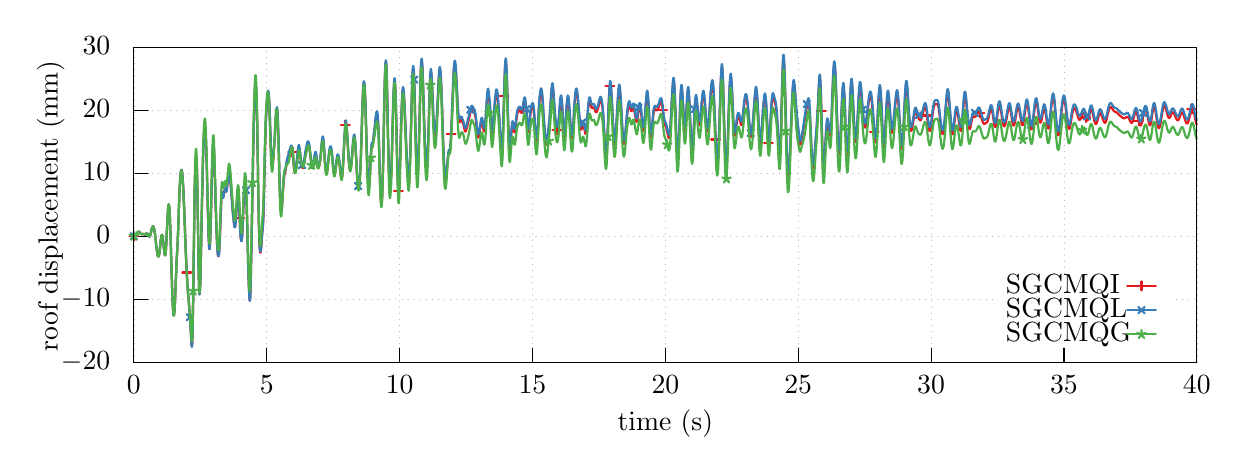
\begin{tikzpicture}[gnuplot]
%% generated with GNUPLOT 5.2p6 (Lua 5.3; terminal rev. Nov 2018, script rev. 107)
%% 08/11/2019 05:12:32
\path (0.000,0.000) rectangle (13.500,4.000);
\gpcolor{color=gp lt color axes}
\gpsetlinetype{gp lt axes}
\gpsetdashtype{gp dt axes}
\gpsetlinewidth{0.50}
\draw[gp path] (0.000,0.000)--(13.499,0.000);
\gpcolor{color=gp lt color border}
\gpsetlinetype{gp lt border}
\gpsetdashtype{gp dt solid}
\gpsetlinewidth{1.00}
\draw[gp path] (0.000,0.000)--(0.180,0.000);
\node[gp node right] at (-0.184,0.000) {$-20$};
\gpcolor{color=gp lt color axes}
\gpsetlinetype{gp lt axes}
\gpsetdashtype{gp dt axes}
\gpsetlinewidth{0.50}
\draw[gp path] (0.000,0.800)--(10.958,0.800);
\draw[gp path] (13.162,0.800)--(13.499,0.800);
\gpcolor{color=gp lt color border}
\gpsetlinetype{gp lt border}
\gpsetdashtype{gp dt solid}
\gpsetlinewidth{1.00}
\draw[gp path] (0.000,0.800)--(0.180,0.800);
\node[gp node right] at (-0.184,0.800) {$-10$};
\gpcolor{color=gp lt color axes}
\gpsetlinetype{gp lt axes}
\gpsetdashtype{gp dt axes}
\gpsetlinewidth{0.50}
\draw[gp path] (0.000,1.600)--(13.499,1.600);
\gpcolor{color=gp lt color border}
\gpsetlinetype{gp lt border}
\gpsetdashtype{gp dt solid}
\gpsetlinewidth{1.00}
\draw[gp path] (0.000,1.600)--(0.180,1.600);
\node[gp node right] at (-0.184,1.600) {$0$};
\gpcolor{color=gp lt color axes}
\gpsetlinetype{gp lt axes}
\gpsetdashtype{gp dt axes}
\gpsetlinewidth{0.50}
\draw[gp path] (0.000,2.399)--(13.499,2.399);
\gpcolor{color=gp lt color border}
\gpsetlinetype{gp lt border}
\gpsetdashtype{gp dt solid}
\gpsetlinewidth{1.00}
\draw[gp path] (0.000,2.399)--(0.180,2.399);
\node[gp node right] at (-0.184,2.399) {$10$};
\gpcolor{color=gp lt color axes}
\gpsetlinetype{gp lt axes}
\gpsetdashtype{gp dt axes}
\gpsetlinewidth{0.50}
\draw[gp path] (0.000,3.199)--(13.499,3.199);
\gpcolor{color=gp lt color border}
\gpsetlinetype{gp lt border}
\gpsetdashtype{gp dt solid}
\gpsetlinewidth{1.00}
\draw[gp path] (0.000,3.199)--(0.180,3.199);
\node[gp node right] at (-0.184,3.199) {$20$};
\gpcolor{color=gp lt color axes}
\gpsetlinetype{gp lt axes}
\gpsetdashtype{gp dt axes}
\gpsetlinewidth{0.50}
\draw[gp path] (0.000,3.999)--(13.499,3.999);
\gpcolor{color=gp lt color border}
\gpsetlinetype{gp lt border}
\gpsetdashtype{gp dt solid}
\gpsetlinewidth{1.00}
\draw[gp path] (0.000,3.999)--(0.180,3.999);
\node[gp node right] at (-0.184,3.999) {$30$};
\gpcolor{color=gp lt color axes}
\gpsetlinetype{gp lt axes}
\gpsetdashtype{gp dt axes}
\gpsetlinewidth{0.50}
\draw[gp path] (0.000,0.000)--(0.000,3.999);
\gpcolor{color=gp lt color border}
\gpsetlinetype{gp lt border}
\gpsetdashtype{gp dt solid}
\gpsetlinewidth{1.00}
\draw[gp path] (0.000,0.000)--(0.000,0.180);
\node[gp node center] at (0.000,-0.308) {$0$};
\gpcolor{color=gp lt color axes}
\gpsetlinetype{gp lt axes}
\gpsetdashtype{gp dt axes}
\gpsetlinewidth{0.50}
\draw[gp path] (1.687,0.000)--(1.687,3.999);
\gpcolor{color=gp lt color border}
\gpsetlinetype{gp lt border}
\gpsetdashtype{gp dt solid}
\gpsetlinewidth{1.00}
\draw[gp path] (1.687,0.000)--(1.687,0.180);
\node[gp node center] at (1.687,-0.308) {$5$};
\gpcolor{color=gp lt color axes}
\gpsetlinetype{gp lt axes}
\gpsetdashtype{gp dt axes}
\gpsetlinewidth{0.50}
\draw[gp path] (3.375,0.000)--(3.375,3.999);
\gpcolor{color=gp lt color border}
\gpsetlinetype{gp lt border}
\gpsetdashtype{gp dt solid}
\gpsetlinewidth{1.00}
\draw[gp path] (3.375,0.000)--(3.375,0.180);
\node[gp node center] at (3.375,-0.308) {$10$};
\gpcolor{color=gp lt color axes}
\gpsetlinetype{gp lt axes}
\gpsetdashtype{gp dt axes}
\gpsetlinewidth{0.50}
\draw[gp path] (5.062,0.000)--(5.062,3.999);
\gpcolor{color=gp lt color border}
\gpsetlinetype{gp lt border}
\gpsetdashtype{gp dt solid}
\gpsetlinewidth{1.00}
\draw[gp path] (5.062,0.000)--(5.062,0.180);
\node[gp node center] at (5.062,-0.308) {$15$};
\gpcolor{color=gp lt color axes}
\gpsetlinetype{gp lt axes}
\gpsetdashtype{gp dt axes}
\gpsetlinewidth{0.50}
\draw[gp path] (6.750,0.000)--(6.750,3.999);
\gpcolor{color=gp lt color border}
\gpsetlinetype{gp lt border}
\gpsetdashtype{gp dt solid}
\gpsetlinewidth{1.00}
\draw[gp path] (6.750,0.000)--(6.750,0.180);
\node[gp node center] at (6.750,-0.308) {$20$};
\gpcolor{color=gp lt color axes}
\gpsetlinetype{gp lt axes}
\gpsetdashtype{gp dt axes}
\gpsetlinewidth{0.50}
\draw[gp path] (8.437,0.000)--(8.437,3.999);
\gpcolor{color=gp lt color border}
\gpsetlinetype{gp lt border}
\gpsetdashtype{gp dt solid}
\gpsetlinewidth{1.00}
\draw[gp path] (8.437,0.000)--(8.437,0.180);
\node[gp node center] at (8.437,-0.308) {$25$};
\gpcolor{color=gp lt color axes}
\gpsetlinetype{gp lt axes}
\gpsetdashtype{gp dt axes}
\gpsetlinewidth{0.50}
\draw[gp path] (10.124,0.000)--(10.124,3.999);
\gpcolor{color=gp lt color border}
\gpsetlinetype{gp lt border}
\gpsetdashtype{gp dt solid}
\gpsetlinewidth{1.00}
\draw[gp path] (10.124,0.000)--(10.124,0.180);
\node[gp node center] at (10.124,-0.308) {$30$};
\gpcolor{color=gp lt color axes}
\gpsetlinetype{gp lt axes}
\gpsetdashtype{gp dt axes}
\gpsetlinewidth{0.50}
\draw[gp path] (11.812,0.000)--(11.812,0.200);
\draw[gp path] (11.812,1.124)--(11.812,3.999);
\gpcolor{color=gp lt color border}
\gpsetlinetype{gp lt border}
\gpsetdashtype{gp dt solid}
\gpsetlinewidth{1.00}
\draw[gp path] (11.812,0.000)--(11.812,0.180);
\node[gp node center] at (11.812,-0.308) {$35$};
\gpcolor{color=gp lt color axes}
\gpsetlinetype{gp lt axes}
\gpsetdashtype{gp dt axes}
\gpsetlinewidth{0.50}
\draw[gp path] (13.499,0.000)--(13.499,3.999);
\gpcolor{color=gp lt color border}
\gpsetlinetype{gp lt border}
\gpsetdashtype{gp dt solid}
\gpsetlinewidth{1.00}
\draw[gp path] (13.499,0.000)--(13.499,0.180);
\node[gp node center] at (13.499,-0.308) {$40$};
\draw[gp path] (0.000,3.999)--(0.000,0.000)--(13.499,0.000)--(13.499,3.999)--cycle;
\node[gp node center,rotate=-270] at (-1.044,1.999) {roof displacement (\si{\milli\metre})};
\node[gp node center] at (6.749,-0.769) {time (\si{\second})};
\gpcolor{rgb color={0.894,0.102,0.110}}
\gpsetlinewidth{2.00}
\draw[gp path] (0.000,1.600)--(0.003,1.600)--(0.007,1.600)--(0.010,1.602)--(0.013,1.605)%
  --(0.017,1.608)--(0.020,1.613)--(0.024,1.618)--(0.027,1.622)--(0.030,1.627)--(0.034,1.632)%
  --(0.037,1.637)--(0.040,1.642)--(0.044,1.646)--(0.047,1.650)--(0.051,1.653)--(0.054,1.656)%
  --(0.057,1.658)--(0.061,1.658)--(0.064,1.657)--(0.067,1.655)--(0.071,1.651)--(0.074,1.647)%
  --(0.078,1.642)--(0.081,1.638)--(0.084,1.634)--(0.088,1.630)--(0.091,1.628)--(0.094,1.627)%
  --(0.098,1.626)--(0.101,1.626)--(0.105,1.627)--(0.108,1.627)--(0.111,1.628)--(0.115,1.629)%
  --(0.118,1.630)--(0.121,1.630)--(0.125,1.629)--(0.128,1.628)--(0.132,1.626)--(0.135,1.624)%
  --(0.138,1.623)--(0.142,1.623)--(0.145,1.624)--(0.148,1.626)--(0.152,1.629)--(0.155,1.632)%
  --(0.159,1.635)--(0.162,1.637)--(0.165,1.637)--(0.169,1.634)--(0.172,1.629)--(0.175,1.622)%
  --(0.179,1.614)--(0.182,1.607)--(0.186,1.602)--(0.189,1.598)--(0.192,1.596)--(0.196,1.596)%
  --(0.199,1.598)--(0.202,1.602)--(0.206,1.609)--(0.209,1.620)--(0.213,1.632)--(0.216,1.646)%
  --(0.219,1.662)--(0.223,1.677)--(0.226,1.692)--(0.229,1.704)--(0.233,1.714)--(0.236,1.721)%
  --(0.240,1.725)--(0.243,1.726)--(0.246,1.724)--(0.250,1.719)--(0.253,1.709)--(0.256,1.696)%
  --(0.260,1.679)--(0.263,1.658)--(0.267,1.635)--(0.270,1.608)--(0.273,1.578)--(0.277,1.547)%
  --(0.280,1.516)--(0.283,1.486)--(0.287,1.458)--(0.290,1.431)--(0.294,1.407)--(0.297,1.385)%
  --(0.300,1.366)--(0.304,1.352)--(0.307,1.343)--(0.310,1.340)--(0.314,1.344)--(0.317,1.354)%
  --(0.321,1.370)--(0.324,1.392)--(0.327,1.419)--(0.331,1.450)--(0.334,1.483)--(0.337,1.515)%
  --(0.341,1.545)--(0.344,1.571)--(0.348,1.593)--(0.351,1.608)--(0.354,1.616)--(0.358,1.616)%
  --(0.361,1.606)--(0.364,1.589)--(0.368,1.566)--(0.371,1.538)--(0.375,1.507)--(0.378,1.474)%
  --(0.381,1.442)--(0.385,1.413)--(0.388,1.387)--(0.391,1.368)--(0.395,1.357)--(0.398,1.358)%
  --(0.402,1.373)--(0.405,1.404)--(0.408,1.452)--(0.412,1.512)--(0.415,1.581)--(0.418,1.654)%
  --(0.422,1.728)--(0.425,1.801)--(0.429,1.867)--(0.432,1.924)--(0.435,1.968)--(0.439,1.995)%
  --(0.442,2.005)--(0.445,1.997)--(0.449,1.971)--(0.452,1.927)--(0.456,1.866)--(0.459,1.789)%
  --(0.462,1.698)--(0.466,1.597)--(0.469,1.487)--(0.472,1.373)--(0.476,1.255)--(0.479,1.139)%
  --(0.483,1.026)--(0.486,0.922)--(0.489,0.828)--(0.493,0.748)--(0.496,0.685)--(0.499,0.638)%
  --(0.503,0.608)--(0.506,0.595)--(0.510,0.602)--(0.513,0.626)--(0.516,0.669)--(0.520,0.728)%
  --(0.523,0.799)--(0.526,0.879)--(0.530,0.966)--(0.533,1.056)--(0.537,1.145)--(0.540,1.228)%
  --(0.543,1.302)--(0.547,1.366)--(0.550,1.423)--(0.553,1.482)--(0.557,1.550)--(0.560,1.631)%
  --(0.564,1.724)--(0.567,1.823)--(0.570,1.923)--(0.574,2.018)--(0.577,2.108)--(0.580,2.190)%
  --(0.584,2.261)--(0.587,2.318)--(0.591,2.364)--(0.594,2.398)--(0.597,2.422)--(0.601,2.437)%
  --(0.604,2.442)--(0.607,2.437)--(0.611,2.422)--(0.614,2.395)--(0.618,2.360)--(0.621,2.315)%
  --(0.624,2.262)--(0.628,2.199)--(0.631,2.129)--(0.634,2.051)--(0.638,1.969)--(0.641,1.884)%
  --(0.645,1.797)--(0.648,1.708)--(0.651,1.619)--(0.655,1.530)--(0.658,1.444)--(0.661,1.362)%
  --(0.665,1.283)--(0.668,1.209)--(0.672,1.139)--(0.675,1.075)--(0.678,1.017)--(0.682,0.964)%
  --(0.685,0.917)--(0.688,0.873)--(0.692,0.831)--(0.695,0.790)--(0.699,0.751)--(0.702,0.711)%
  --(0.705,0.669)--(0.709,0.624)--(0.712,0.573)--(0.715,0.517)--(0.719,0.456)--(0.722,0.393)%
  --(0.726,0.331)--(0.729,0.273)--(0.732,0.226)--(0.736,0.202)--(0.739,0.216)--(0.742,0.282)%
  --(0.746,0.408)--(0.749,0.586)--(0.753,0.799)--(0.756,1.031)--(0.759,1.272)--(0.763,1.518)%
  --(0.766,1.763)--(0.769,1.994)--(0.773,2.195)--(0.776,2.353)--(0.780,2.470)--(0.783,2.552)%
  --(0.786,2.602)--(0.790,2.622)--(0.793,2.611)--(0.796,2.561)--(0.800,2.467)--(0.803,2.332)%
  --(0.807,2.164)--(0.810,1.971)--(0.813,1.762)--(0.817,1.541)--(0.820,1.319)--(0.823,1.121)%
  --(0.827,0.972)--(0.830,0.886)--(0.834,0.862)--(0.837,0.884)--(0.840,0.939)--(0.844,1.025)%
  --(0.847,1.143)--(0.850,1.295)--(0.854,1.472)--(0.857,1.653)--(0.861,1.823)--(0.864,1.977)%
  --(0.867,2.122)--(0.871,2.268)--(0.874,2.417)--(0.877,2.558)--(0.881,2.678)--(0.884,2.771)%
  --(0.888,2.838)--(0.891,2.890)--(0.894,2.930)--(0.898,2.961)--(0.901,2.978)--(0.904,2.973)%
  --(0.908,2.942)--(0.911,2.885)--(0.915,2.811)--(0.918,2.723)--(0.921,2.623)--(0.925,2.509)%
  --(0.928,2.380)--(0.931,2.241)--(0.935,2.100)--(0.938,1.964)--(0.942,1.836)--(0.945,1.718)%
  --(0.948,1.611)--(0.952,1.524)--(0.955,1.464)--(0.958,1.436)--(0.962,1.442)--(0.965,1.478)%
  --(0.969,1.542)--(0.972,1.630)--(0.975,1.740)--(0.979,1.869)--(0.982,2.010)--(0.985,2.153)%
  --(0.989,2.293)--(0.992,2.424)--(0.996,2.540)--(0.999,2.637)--(1.002,2.711)--(1.006,2.756)%
  --(1.009,2.769)--(1.012,2.751)--(1.016,2.702)--(1.019,2.628)--(1.023,2.535)--(1.026,2.429)%
  --(1.029,2.316)--(1.033,2.200)--(1.036,2.083)--(1.039,1.966)--(1.043,1.853)--(1.046,1.747)%
  --(1.050,1.653)--(1.053,1.571)--(1.056,1.502)--(1.060,1.445)--(1.063,1.401)--(1.066,1.370)%
  --(1.070,1.352)--(1.073,1.346)--(1.077,1.350)--(1.080,1.367)--(1.083,1.402)--(1.087,1.457)%
  --(1.090,1.533)--(1.093,1.623)--(1.097,1.718)--(1.100,1.811)--(1.104,1.899)--(1.107,1.981)%
  --(1.110,2.055)--(1.114,2.113)--(1.117,2.151)--(1.120,2.162)--(1.124,2.149)--(1.127,2.124)%
  --(1.131,2.101)--(1.134,2.093)--(1.137,2.102)--(1.141,2.122)--(1.144,2.144)--(1.147,2.164)%
  --(1.151,2.180)--(1.154,2.197)--(1.158,2.211)--(1.161,2.218)--(1.164,2.211)--(1.168,2.192)%
  --(1.171,2.172)--(1.174,2.166)--(1.178,2.179)--(1.181,2.206)--(1.185,2.236)--(1.188,2.263)%
  --(1.191,2.287)--(1.195,2.316)--(1.198,2.349)--(1.201,2.382)--(1.205,2.405)--(1.208,2.412)%
  --(1.212,2.405)--(1.215,2.389)--(1.218,2.367)--(1.222,2.340)--(1.225,2.307)--(1.228,2.267)%
  --(1.232,2.222)--(1.235,2.178)--(1.239,2.134)--(1.242,2.091)--(1.245,2.047)--(1.249,2.002)%
  --(1.252,1.959)--(1.255,1.918)--(1.259,1.881)--(1.262,1.847)--(1.266,1.814)--(1.269,1.782)%
  --(1.272,1.753)--(1.276,1.730)--(1.279,1.717)--(1.282,1.715)--(1.286,1.725)--(1.289,1.747)%
  --(1.293,1.780)--(1.296,1.823)--(1.299,1.874)--(1.303,1.928)--(1.306,1.982)--(1.309,2.031)%
  --(1.313,2.074)--(1.316,2.108)--(1.320,2.131)--(1.323,2.138)--(1.326,2.128)--(1.330,2.100)%
  --(1.333,2.055)--(1.336,1.992)--(1.340,1.915)--(1.343,1.831)--(1.347,1.748)--(1.350,1.676)%
  --(1.353,1.620)--(1.357,1.580)--(1.360,1.556)--(1.363,1.543)--(1.367,1.542)--(1.370,1.557)%
  --(1.374,1.591)--(1.377,1.643)--(1.380,1.711)--(1.384,1.787)--(1.387,1.868)--(1.390,1.951)%
  --(1.394,2.033)--(1.397,2.112)--(1.401,2.183)--(1.404,2.240)--(1.407,2.280)--(1.411,2.300)%
  --(1.414,2.302)--(1.417,2.284)--(1.421,2.246)--(1.424,2.186)--(1.428,2.106)--(1.431,2.008)%
  --(1.434,1.895)--(1.438,1.771)--(1.441,1.640)--(1.444,1.504)--(1.448,1.368)--(1.451,1.237)%
  --(1.455,1.116)--(1.458,1.013)--(1.461,0.928)--(1.465,0.860)--(1.468,0.810)--(1.471,0.784)%
  --(1.475,0.794)--(1.478,0.846)--(1.482,0.944)--(1.485,1.076)--(1.488,1.227)--(1.492,1.388)%
  --(1.495,1.553)--(1.498,1.730)--(1.502,1.920)--(1.505,2.116)--(1.509,2.310)--(1.512,2.495)%
  --(1.515,2.668)--(1.519,2.829)--(1.522,2.975)--(1.525,3.106)--(1.529,3.222)--(1.532,3.323)%
  --(1.536,3.406)--(1.539,3.469)--(1.542,3.509)--(1.546,3.524)--(1.549,3.512)--(1.552,3.472)%
  --(1.556,3.402)--(1.559,3.299)--(1.563,3.164)--(1.566,3.000)--(1.569,2.810)--(1.573,2.602)%
  --(1.576,2.380)--(1.579,2.159)--(1.583,1.954)--(1.586,1.778)--(1.590,1.639)--(1.593,1.535)%
  --(1.596,1.464)--(1.600,1.420)--(1.603,1.397)--(1.606,1.391)--(1.610,1.400)--(1.613,1.422)%
  --(1.617,1.459)--(1.620,1.505)--(1.623,1.554)--(1.627,1.599)--(1.630,1.637)--(1.633,1.670)%
  --(1.637,1.703)--(1.640,1.750)--(1.644,1.823)--(1.647,1.925)--(1.650,2.053)--(1.654,2.194)%
  --(1.657,2.341)--(1.660,2.486)--(1.664,2.627)--(1.667,2.762)--(1.671,2.886)--(1.674,2.992)%
  --(1.677,3.079)--(1.681,3.149)--(1.684,3.210)--(1.687,3.266)--(1.691,3.318)--(1.694,3.364)%
  --(1.697,3.400)--(1.701,3.422)--(1.704,3.429)--(1.708,3.421)--(1.711,3.400)--(1.714,3.367)%
  --(1.718,3.318)--(1.721,3.253)--(1.724,3.171)--(1.728,3.076)--(1.731,2.974)--(1.735,2.873)%
  --(1.738,2.778)--(1.741,2.694)--(1.745,2.623)--(1.748,2.566)--(1.751,2.525)--(1.755,2.502)%
  --(1.758,2.496)--(1.762,2.507)--(1.765,2.530)--(1.768,2.563)--(1.772,2.603)--(1.775,2.646)%
  --(1.778,2.689)--(1.782,2.733)--(1.785,2.780)--(1.789,2.833)--(1.792,2.895)--(1.795,2.965)%
  --(1.799,3.034)--(1.802,3.096)--(1.805,3.146)--(1.809,3.183)--(1.812,3.207)--(1.816,3.218)%
  --(1.819,3.210)--(1.822,3.180)--(1.826,3.126)--(1.829,3.050)--(1.832,2.954)--(1.836,2.844)%
  --(1.839,2.720)--(1.843,2.586)--(1.846,2.450)--(1.849,2.320)--(1.853,2.202)--(1.856,2.104)%
  --(1.859,2.026)--(1.863,1.969)--(1.866,1.931)--(1.870,1.912)--(1.873,1.912)--(1.876,1.929)%
  --(1.880,1.961)--(1.883,2.004)--(1.886,2.055)--(1.890,2.111)--(1.893,2.168)--(1.897,2.223)%
  --(1.900,2.274)--(1.903,2.315)--(1.907,2.347)--(1.910,2.368)--(1.913,2.383)--(1.917,2.394)%
  --(1.920,2.407)--(1.924,2.422)--(1.927,2.441)--(1.930,2.463)--(1.934,2.485)--(1.937,2.507)%
  --(1.940,2.528)--(1.944,2.546)--(1.947,2.561)--(1.951,2.573)--(1.954,2.583)--(1.957,2.591)%
  --(1.961,2.601)--(1.964,2.613)--(1.967,2.627)--(1.971,2.640)--(1.974,2.653)--(1.978,2.665)%
  --(1.981,2.676)--(1.984,2.688)--(1.988,2.700)--(1.991,2.710)--(1.994,2.718)--(1.998,2.721)%
  --(2.001,2.721)--(2.005,2.717)--(2.008,2.708)--(2.011,2.692)--(2.015,2.669)--(2.018,2.639)%
  --(2.021,2.601)--(2.025,2.559)--(2.028,2.517)--(2.032,2.478)--(2.035,2.444)--(2.038,2.419)%
  --(2.042,2.405)--(2.045,2.402)--(2.048,2.408)--(2.052,2.421)--(2.055,2.438)--(2.059,2.458)%
  --(2.062,2.481)--(2.065,2.507)--(2.069,2.536)--(2.072,2.569)--(2.075,2.604)--(2.079,2.637)%
  --(2.082,2.668)--(2.086,2.693)--(2.089,2.712)--(2.092,2.724)--(2.096,2.728)--(2.099,2.722)%
  --(2.102,2.707)--(2.106,2.683)--(2.109,2.655)--(2.113,2.625)--(2.116,2.596)--(2.119,2.570)%
  --(2.123,2.545)--(2.126,2.523)--(2.129,2.504)--(2.133,2.488)--(2.136,2.477)--(2.140,2.469)%
  --(2.143,2.466)--(2.146,2.467)--(2.150,2.474)--(2.153,2.486)--(2.156,2.503)--(2.160,2.523)%
  --(2.163,2.546)--(2.167,2.569)--(2.170,2.593)--(2.173,2.616)--(2.177,2.637)--(2.180,2.657)%
  --(2.183,2.674)--(2.187,2.690)--(2.190,2.705)--(2.194,2.721)--(2.197,2.738)--(2.200,2.753)%
  --(2.204,2.765)--(2.207,2.772)--(2.210,2.776)--(2.214,2.775)--(2.217,2.771)--(2.221,2.763)%
  --(2.224,2.751)--(2.227,2.734)--(2.231,2.712)--(2.234,2.686)--(2.237,2.656)--(2.241,2.624)%
  --(2.244,2.592)--(2.248,2.561)--(2.251,2.534)--(2.254,2.512)--(2.258,2.494)--(2.261,2.480)%
  --(2.264,2.471)--(2.268,2.467)--(2.271,2.470)--(2.275,2.480)--(2.278,2.495)--(2.281,2.513)%
  --(2.285,2.533)--(2.288,2.555)--(2.291,2.578)--(2.295,2.600)--(2.298,2.619)--(2.302,2.634)%
  --(2.305,2.642)--(2.308,2.643)--(2.312,2.636)--(2.315,2.620)--(2.318,2.596)--(2.322,2.565)%
  --(2.325,2.533)--(2.329,2.505)--(2.332,2.485)--(2.335,2.473)--(2.339,2.467)--(2.342,2.466)%
  --(2.345,2.468)--(2.349,2.474)--(2.352,2.485)--(2.356,2.499)--(2.359,2.515)--(2.362,2.534)%
  --(2.366,2.557)--(2.369,2.584)--(2.372,2.617)--(2.376,2.655)--(2.379,2.695)--(2.383,2.734)%
  --(2.386,2.768)--(2.389,2.797)--(2.393,2.820)--(2.396,2.835)--(2.399,2.839)--(2.403,2.832)%
  --(2.406,2.812)--(2.410,2.781)--(2.413,2.741)--(2.416,2.694)--(2.420,2.642)--(2.423,2.590)%
  --(2.426,2.541)--(2.430,2.497)--(2.433,2.461)--(2.437,2.432)--(2.440,2.410)--(2.443,2.396)%
  --(2.447,2.391)--(2.450,2.396)--(2.453,2.411)--(2.457,2.433)--(2.460,2.461)--(2.464,2.492)%
  --(2.467,2.526)--(2.470,2.561)--(2.474,2.596)--(2.477,2.629)--(2.480,2.657)--(2.484,2.679)%
  --(2.487,2.695)--(2.491,2.705)--(2.494,2.711)--(2.497,2.713)--(2.501,2.712)--(2.504,2.705)%
  --(2.507,2.692)--(2.511,2.673)--(2.514,2.647)--(2.518,2.615)--(2.521,2.578)--(2.524,2.538)%
  --(2.528,2.498)--(2.531,2.462)--(2.534,2.431)--(2.538,2.407)--(2.541,2.390)--(2.545,2.380)%
  --(2.548,2.378)--(2.551,2.384)--(2.555,2.398)--(2.558,2.418)--(2.561,2.442)--(2.565,2.469)%
  --(2.568,2.498)--(2.572,2.527)--(2.575,2.554)--(2.578,2.577)--(2.582,2.595)--(2.585,2.607)%
  --(2.588,2.612)--(2.592,2.611)--(2.595,2.606)--(2.599,2.596)--(2.602,2.583)--(2.605,2.565)%
  --(2.609,2.543)--(2.612,2.516)--(2.615,2.485)--(2.619,2.451)--(2.622,2.419)--(2.626,2.390)%
  --(2.629,2.366)--(2.632,2.349)--(2.636,2.338)--(2.639,2.336)--(2.642,2.346)--(2.646,2.367)%
  --(2.649,2.401)--(2.653,2.444)--(2.656,2.495)--(2.659,2.553)--(2.663,2.615)--(2.666,2.682)%
  --(2.669,2.750)--(2.673,2.816)--(2.676,2.877)--(2.680,2.932)--(2.683,2.977)--(2.686,3.013)%
  --(2.690,3.035)--(2.693,3.041)--(2.696,3.028)--(2.700,2.999)--(2.703,2.958)--(2.707,2.910)%
  --(2.710,2.859)--(2.713,2.806)--(2.717,2.751)--(2.720,2.696)--(2.723,2.642)--(2.727,2.593)%
  --(2.730,2.549)--(2.734,2.512)--(2.737,2.483)--(2.740,2.461)--(2.744,2.447)--(2.747,2.442)%
  --(2.750,2.446)--(2.754,2.459)--(2.757,2.480)--(2.761,2.506)--(2.764,2.538)--(2.767,2.575)%
  --(2.771,2.616)--(2.774,2.659)--(2.777,2.704)--(2.781,2.746)--(2.784,2.784)--(2.788,2.816)%
  --(2.791,2.841)--(2.794,2.858)--(2.798,2.864)--(2.801,2.858)--(2.804,2.841)--(2.808,2.811)%
  --(2.811,2.772)--(2.815,2.723)--(2.818,2.668)--(2.821,2.608)--(2.825,2.544)--(2.828,2.480)%
  --(2.831,2.418)--(2.835,2.360)--(2.838,2.308)--(2.842,2.265)--(2.845,2.231)--(2.848,2.208)%
  --(2.852,2.197)--(2.855,2.200)--(2.858,2.214)--(2.862,2.240)--(2.865,2.275)--(2.869,2.318)%
  --(2.872,2.368)--(2.875,2.426)--(2.879,2.495)--(2.882,2.580)--(2.885,2.680)--(2.889,2.792)%
  --(2.892,2.910)--(2.896,3.026)--(2.899,3.138)--(2.902,3.242)--(2.906,3.336)--(2.909,3.416)%
  --(2.912,3.478)--(2.916,3.518)--(2.919,3.538)--(2.923,3.540)--(2.926,3.526)--(2.929,3.497)%
  --(2.933,3.451)--(2.936,3.383)--(2.939,3.296)--(2.943,3.193)--(2.946,3.080)--(2.950,2.963)%
  --(2.953,2.843)--(2.956,2.724)--(2.960,2.609)--(2.963,2.504)--(2.966,2.415)--(2.970,2.343)%
  --(2.973,2.288)--(2.977,2.248)--(2.980,2.224)--(2.983,2.217)--(2.987,2.231)--(2.990,2.264)%
  --(2.993,2.312)--(2.997,2.370)--(3.000,2.434)--(3.004,2.500)--(3.007,2.566)--(3.010,2.628)%
  --(3.014,2.683)--(3.017,2.725)--(3.020,2.749)--(3.024,2.757)--(3.027,2.754)--(3.031,2.751)%
  --(3.034,2.758)--(3.037,2.779)--(3.041,2.810)--(3.044,2.843)--(3.047,2.872)--(3.051,2.898)%
  --(3.054,2.923)--(3.058,2.953)--(3.061,2.989)--(3.064,3.025)--(3.068,3.058)--(3.071,3.086)%
  --(3.074,3.108)--(3.078,3.127)--(3.081,3.141)--(3.085,3.150)--(3.088,3.152)--(3.091,3.142)%
  --(3.095,3.120)--(3.098,3.086)--(3.101,3.038)--(3.105,2.975)--(3.108,2.894)--(3.112,2.797)%
  --(3.115,2.683)--(3.118,2.560)--(3.122,2.435)--(3.125,2.319)--(3.128,2.218)--(3.132,2.134)%
  --(3.135,2.069)--(3.139,2.023)--(3.142,1.999)--(3.145,1.999)--(3.149,2.025)--(3.152,2.079)%
  --(3.155,2.160)--(3.159,2.267)--(3.162,2.396)--(3.166,2.545)--(3.169,2.710)--(3.172,2.887)%
  --(3.176,3.068)--(3.179,3.243)--(3.182,3.405)--(3.186,3.545)--(3.189,3.659)--(3.193,3.740)%
  --(3.196,3.789)--(3.199,3.809)--(3.203,3.802)--(3.206,3.765)--(3.209,3.694)--(3.213,3.584)%
  --(3.216,3.437)--(3.220,3.266)--(3.223,3.091)--(3.226,2.927)--(3.230,2.779)--(3.233,2.643)%
  --(3.236,2.519)--(3.240,2.409)--(3.243,2.323)--(3.247,2.268)--(3.250,2.244)--(3.253,2.242)%
  --(3.257,2.256)--(3.260,2.280)--(3.263,2.314)--(3.267,2.364)--(3.270,2.437)--(3.274,2.534)%
  --(3.277,2.651)--(3.280,2.779)--(3.284,2.910)--(3.287,3.038)--(3.290,3.162)--(3.294,3.279)%
  --(3.297,3.383)--(3.301,3.469)--(3.304,3.531)--(3.307,3.568)--(3.311,3.579)--(3.314,3.564)%
  --(3.317,3.523)--(3.321,3.455)--(3.324,3.361)--(3.328,3.244)--(3.331,3.111)--(3.334,2.966)%
  --(3.338,2.818)--(3.341,2.671)--(3.344,2.533)--(3.348,2.410)--(3.351,2.308)--(3.355,2.230)%
  --(3.358,2.177)--(3.361,2.152)--(3.365,2.156)--(3.368,2.189)--(3.371,2.249)--(3.375,2.333)%
  --(3.378,2.437)--(3.381,2.554)--(3.385,2.678)--(3.388,2.804)--(3.392,2.925)--(3.395,3.039)%
  --(3.398,3.143)--(3.402,3.236)--(3.405,3.316)--(3.408,3.381)--(3.412,3.428)--(3.415,3.455)%
  --(3.419,3.463)--(3.422,3.453)--(3.425,3.428)--(3.429,3.390)--(3.432,3.340)--(3.435,3.280)%
  --(3.439,3.211)--(3.442,3.136)--(3.446,3.056)--(3.449,2.974)--(3.452,2.893)--(3.456,2.812)%
  --(3.459,2.734)--(3.462,2.660)--(3.466,2.589)--(3.469,2.524)--(3.473,2.463)--(3.476,2.409)%
  --(3.479,2.360)--(3.483,2.319)--(3.486,2.290)--(3.489,2.277)--(3.493,2.283)--(3.496,2.311)%
  --(3.500,2.362)--(3.503,2.434)--(3.506,2.524)--(3.510,2.628)--(3.513,2.741)--(3.516,2.863)%
  --(3.520,2.992)--(3.523,3.125)--(3.527,3.260)--(3.530,3.388)--(3.533,3.503)--(3.537,3.598)%
  --(3.540,3.669)--(3.543,3.714)--(3.547,3.733)--(3.550,3.726)--(3.554,3.694)--(3.557,3.639)%
  --(3.560,3.558)--(3.564,3.452)--(3.567,3.327)--(3.570,3.190)--(3.574,3.050)--(3.577,2.914)%
  --(3.581,2.786)--(3.584,2.670)--(3.587,2.567)--(3.591,2.485)--(3.594,2.427)--(3.597,2.395)%
  --(3.601,2.389)--(3.604,2.406)--(3.608,2.446)--(3.611,2.507)--(3.614,2.592)--(3.618,2.698)%
  --(3.621,2.822)--(3.624,2.959)--(3.628,3.101)--(3.631,3.245)--(3.635,3.384)--(3.638,3.513)%
  --(3.641,3.625)--(3.645,3.715)--(3.648,3.779)--(3.651,3.814)--(3.655,3.821)--(3.658,3.804)%
  --(3.662,3.767)--(3.665,3.710)--(3.668,3.634)--(3.672,3.540)--(3.675,3.431)--(3.678,3.315)%
  --(3.682,3.198)--(3.685,3.086)--(3.689,2.980)--(3.692,2.879)--(3.695,2.784)--(3.699,2.698)%
  --(3.702,2.625)--(3.705,2.568)--(3.709,2.524)--(3.712,2.492)--(3.716,2.473)--(3.719,2.468)%
  --(3.722,2.481)--(3.726,2.515)--(3.729,2.570)--(3.732,2.644)--(3.736,2.736)--(3.739,2.842)%
  --(3.743,2.959)--(3.746,3.083)--(3.749,3.208)--(3.753,3.328)--(3.756,3.436)--(3.759,3.528)%
  --(3.763,3.602)--(3.766,3.654)--(3.770,3.683)--(3.773,3.686)--(3.776,3.665)--(3.780,3.624)%
  --(3.783,3.567)--(3.786,3.500)--(3.790,3.424)--(3.793,3.345)--(3.797,3.263)--(3.800,3.184)%
  --(3.803,3.110)--(3.807,3.045)--(3.810,2.989)--(3.813,2.944)--(3.817,2.910)--(3.820,2.887)%
  --(3.824,2.876)--(3.827,2.878)--(3.830,2.891)--(3.834,2.913)--(3.837,2.943)--(3.840,2.982)%
  --(3.844,3.029)--(3.847,3.084)--(3.851,3.147)--(3.854,3.214)--(3.857,3.284)--(3.861,3.357)%
  --(3.864,3.430)--(3.867,3.501)--(3.871,3.568)--(3.874,3.624)--(3.878,3.668)--(3.881,3.697)%
  --(3.884,3.711)--(3.888,3.710)--(3.891,3.694)--(3.894,3.662)--(3.898,3.614)--(3.901,3.550)%
  --(3.905,3.473)--(3.908,3.386)--(3.911,3.290)--(3.915,3.188)--(3.918,3.081)--(3.921,2.973)%
  --(3.925,2.867)--(3.928,2.765)--(3.932,2.671)--(3.935,2.586)--(3.938,2.511)--(3.942,2.447)%
  --(3.945,2.397)--(3.948,2.361)--(3.952,2.338)--(3.955,2.327)--(3.959,2.326)--(3.962,2.334)%
  --(3.965,2.348)--(3.969,2.371)--(3.972,2.402)--(3.975,2.440)--(3.979,2.481)--(3.982,2.523)%
  --(3.986,2.561)--(3.989,2.595)--(3.992,2.624)--(3.996,2.644)--(3.999,2.656)--(4.002,2.660)%
  --(4.006,2.659)--(4.009,2.660)--(4.013,2.670)--(4.016,2.691)--(4.019,2.724)--(4.023,2.769)%
  --(4.026,2.826)--(4.029,2.894)--(4.033,2.973)--(4.036,3.058)--(4.040,3.147)--(4.043,3.235)%
  --(4.046,3.322)--(4.050,3.408)--(4.053,3.493)--(4.056,3.572)--(4.060,3.644)--(4.063,3.702)%
  --(4.067,3.745)--(4.070,3.773)--(4.073,3.787)--(4.077,3.790)--(4.080,3.780)--(4.083,3.758)%
  --(4.087,3.723)--(4.090,3.675)--(4.094,3.616)--(4.097,3.551)--(4.100,3.483)--(4.104,3.415)%
  --(4.107,3.346)--(4.110,3.279)--(4.114,3.216)--(4.117,3.161)--(4.121,3.117)--(4.124,3.084)%
  --(4.127,3.063)--(4.131,3.050)--(4.134,3.047)--(4.137,3.049)--(4.141,3.055)--(4.144,3.062)%
  --(4.148,3.067)--(4.151,3.071)--(4.154,3.074)--(4.158,3.076)--(4.161,3.075)--(4.164,3.071)%
  --(4.168,3.063)--(4.171,3.053)--(4.175,3.045)--(4.178,3.038)--(4.181,3.030)--(4.185,3.019)%
  --(4.188,3.004)--(4.191,2.986)--(4.195,2.969)--(4.198,2.954)--(4.202,2.943)--(4.205,2.935)%
  --(4.208,2.930)--(4.212,2.930)--(4.215,2.934)--(4.218,2.944)--(4.222,2.955)--(4.225,2.967)%
  --(4.229,2.978)--(4.232,2.990)--(4.235,3.005)--(4.239,3.021)--(4.242,3.038)--(4.245,3.052)%
  --(4.249,3.065)--(4.252,3.076)--(4.256,3.090)--(4.259,3.105)--(4.262,3.121)--(4.266,3.136)%
  --(4.269,3.150)--(4.272,3.164)--(4.276,3.179)--(4.279,3.193)--(4.283,3.206)--(4.286,3.214)%
  --(4.289,3.217)--(4.293,3.215)--(4.296,3.211)--(4.299,3.206)--(4.303,3.200)--(4.306,3.193)%
  --(4.310,3.186)--(4.313,3.181)--(4.316,3.177)--(4.320,3.174)--(4.323,3.170)--(4.326,3.162)%
  --(4.330,3.151)--(4.333,3.136)--(4.337,3.118)--(4.340,3.096)--(4.343,3.070)--(4.347,3.041)%
  --(4.350,3.010)--(4.353,2.979)--(4.357,2.949)--(4.360,2.921)--(4.364,2.895)--(4.367,2.874)%
  --(4.370,2.860)--(4.374,2.853)--(4.377,2.854)--(4.380,2.862)--(4.384,2.877)--(4.387,2.895)%
  --(4.391,2.917)--(4.394,2.940)--(4.397,2.965)--(4.401,2.990)--(4.404,3.013)--(4.407,3.032)%
  --(4.411,3.048)--(4.414,3.059)--(4.418,3.064)--(4.421,3.063)--(4.424,3.054)--(4.428,3.039)%
  --(4.431,3.017)--(4.434,2.993)--(4.438,2.969)--(4.441,2.949)--(4.445,2.936)--(4.448,2.931)%
  --(4.451,2.934)--(4.455,2.946)--(4.458,2.967)--(4.461,2.997)--(4.465,3.037)--(4.468,3.085)%
  --(4.472,3.137)--(4.475,3.191)--(4.478,3.245)--(4.482,3.296)--(4.485,3.343)--(4.488,3.383)%
  --(4.492,3.414)--(4.495,3.431)--(4.499,3.432)--(4.502,3.419)--(4.505,3.398)--(4.509,3.372)%
  --(4.512,3.343)--(4.515,3.312)--(4.519,3.276)--(4.522,3.232)--(4.526,3.183)--(4.529,3.130)%
  --(4.532,3.076)--(4.536,3.023)--(4.539,2.972)--(4.542,2.930)--(4.546,2.902)--(4.549,2.892)%
  --(4.553,2.902)--(4.556,2.926)--(4.559,2.958)--(4.563,2.996)--(4.566,3.037)--(4.569,3.081)%
  --(4.573,3.129)--(4.576,3.176)--(4.580,3.221)--(4.583,3.261)--(4.586,3.298)--(4.590,3.333)%
  --(4.593,3.364)--(4.596,3.391)--(4.600,3.411)--(4.603,3.421)--(4.607,3.423)--(4.610,3.418)%
  --(4.613,3.406)--(4.617,3.388)--(4.620,3.360)--(4.623,3.324)--(4.627,3.281)--(4.630,3.234)%
  --(4.634,3.185)--(4.637,3.133)--(4.640,3.078)--(4.644,3.021)--(4.647,2.964)--(4.650,2.909)%
  --(4.654,2.854)--(4.657,2.799)--(4.661,2.747)--(4.664,2.699)--(4.667,2.665)--(4.671,2.649)%
  --(4.674,2.657)--(4.677,2.688)--(4.681,2.743)--(4.684,2.818)--(4.688,2.912)--(4.691,3.020)%
  --(4.694,3.140)--(4.698,3.263)--(4.701,3.384)--(4.704,3.498)--(4.708,3.600)--(4.711,3.686)%
  --(4.715,3.752)--(4.718,3.796)--(4.721,3.815)--(4.725,3.810)--(4.728,3.780)--(4.731,3.726)%
  --(4.735,3.648)--(4.738,3.550)--(4.742,3.437)--(4.745,3.316)--(4.748,3.197)--(4.752,3.085)%
  --(4.755,2.983)--(4.758,2.893)--(4.762,2.816)--(4.765,2.758)--(4.769,2.721)--(4.772,2.706)%
  --(4.775,2.710)--(4.779,2.729)--(4.782,2.758)--(4.785,2.796)--(4.789,2.838)--(4.792,2.883)%
  --(4.796,2.926)--(4.799,2.963)--(4.802,2.992)--(4.806,3.010)--(4.809,3.017)--(4.812,3.014)%
  --(4.816,3.002)--(4.819,2.985)--(4.823,2.964)--(4.826,2.944)--(4.829,2.928)--(4.833,2.920)%
  --(4.836,2.920)--(4.839,2.930)--(4.843,2.948)--(4.846,2.973)--(4.850,3.002)--(4.853,3.035)%
  --(4.856,3.067)--(4.860,3.097)--(4.863,3.122)--(4.866,3.142)--(4.870,3.156)--(4.873,3.166)%
  --(4.877,3.174)--(4.880,3.181)--(4.883,3.188)--(4.887,3.194)--(4.890,3.199)--(4.893,3.202)%
  --(4.897,3.203)--(4.900,3.202)--(4.904,3.198)--(4.907,3.192)--(4.910,3.185)--(4.914,3.178)%
  --(4.917,3.172)--(4.920,3.168)--(4.924,3.166)--(4.927,3.166)--(4.931,3.170)--(4.934,3.180)%
  --(4.937,3.195)--(4.941,3.215)--(4.944,3.239)--(4.947,3.263)--(4.951,3.284)--(4.954,3.301)%
  --(4.958,3.313)--(4.961,3.320)--(4.964,3.321)--(4.968,3.314)--(4.971,3.298)--(4.974,3.275)%
  --(4.978,3.246)--(4.981,3.212)--(4.985,3.174)--(4.988,3.132)--(4.991,3.086)--(4.995,3.038)%
  --(4.998,2.993)--(5.001,2.956)--(5.005,2.931)--(5.008,2.922)--(5.012,2.926)--(5.015,2.942)%
  --(5.018,2.966)--(5.022,2.995)--(5.025,3.030)--(5.028,3.067)--(5.032,3.105)--(5.035,3.138)%
  --(5.039,3.166)--(5.042,3.187)--(5.045,3.204)--(5.049,3.217)--(5.052,3.229)--(5.055,3.238)%
  --(5.059,3.246)--(5.062,3.249)--(5.065,3.249)--(5.069,3.244)--(5.072,3.234)--(5.076,3.215)%
  --(5.079,3.188)--(5.082,3.152)--(5.086,3.108)--(5.089,3.059)--(5.092,3.005)--(5.096,2.952)%
  --(5.099,2.902)--(5.103,2.860)--(5.106,2.828)--(5.109,2.809)--(5.113,2.803)--(5.116,2.811)%
  --(5.119,2.832)--(5.123,2.865)--(5.126,2.910)--(5.130,2.963)--(5.133,3.022)--(5.136,3.084)%
  --(5.140,3.145)--(5.143,3.204)--(5.146,3.256)--(5.150,3.301)--(5.153,3.339)--(5.157,3.370)%
  --(5.160,3.395)--(5.163,3.415)--(5.167,3.428)--(5.170,3.435)--(5.173,3.435)--(5.177,3.427)%
  --(5.180,3.412)--(5.184,3.387)--(5.187,3.354)--(5.190,3.313)--(5.194,3.265)--(5.197,3.212)%
  --(5.200,3.157)--(5.204,3.103)--(5.207,3.052)--(5.211,3.003)--(5.214,2.958)--(5.217,2.916)%
  --(5.221,2.877)--(5.224,2.842)--(5.227,2.813)--(5.231,2.789)--(5.234,2.772)--(5.238,2.761)%
  --(5.241,2.758)--(5.244,2.765)--(5.248,2.780)--(5.251,2.803)--(5.254,2.831)--(5.258,2.862)%
  --(5.261,2.895)--(5.265,2.928)--(5.268,2.960)--(5.271,2.993)--(5.275,3.027)--(5.278,3.064)%
  --(5.281,3.105)--(5.285,3.151)--(5.288,3.200)--(5.292,3.252)--(5.295,3.305)--(5.298,3.357)%
  --(5.302,3.405)--(5.305,3.446)--(5.308,3.476)--(5.312,3.495)--(5.315,3.500)--(5.319,3.492)%
  --(5.322,3.471)--(5.325,3.438)--(5.329,3.395)--(5.332,3.345)--(5.335,3.294)--(5.339,3.243)%
  --(5.342,3.194)--(5.346,3.149)--(5.349,3.107)--(5.352,3.070)--(5.356,3.037)--(5.359,3.010)%
  --(5.362,2.989)--(5.366,2.972)--(5.369,2.959)--(5.373,2.950)--(5.376,2.947)--(5.379,2.951)%
  --(5.383,2.962)--(5.386,2.979)--(5.389,3.003)--(5.393,3.033)--(5.396,3.068)--(5.400,3.109)%
  --(5.403,3.154)--(5.406,3.200)--(5.410,3.244)--(5.413,3.282)--(5.416,3.313)--(5.420,3.334)%
  --(5.423,3.346)--(5.427,3.345)--(5.430,3.333)--(5.433,3.306)--(5.437,3.267)--(5.440,3.218)%
  --(5.443,3.160)--(5.447,3.098)--(5.450,3.035)--(5.454,2.974)--(5.457,2.921)--(5.460,2.880)%
  --(5.464,2.857)--(5.467,2.852)--(5.470,2.865)--(5.474,2.892)--(5.477,2.931)--(5.481,2.978)%
  --(5.484,3.032)--(5.487,3.090)--(5.491,3.149)--(5.494,3.204)--(5.497,3.251)--(5.501,3.289)%
  --(5.504,3.316)--(5.508,3.334)--(5.511,3.344)--(5.514,3.345)--(5.518,3.335)--(5.521,3.313)%
  --(5.524,3.281)--(5.528,3.240)--(5.531,3.195)--(5.535,3.147)--(5.538,3.097)--(5.541,3.046)%
  --(5.545,2.996)--(5.548,2.950)--(5.551,2.910)--(5.555,2.877)--(5.558,2.854)--(5.562,2.841)%
  --(5.565,2.839)--(5.568,2.850)--(5.572,2.874)--(5.575,2.911)--(5.578,2.959)--(5.582,3.014)%
  --(5.585,3.074)--(5.589,3.134)--(5.592,3.194)--(5.595,3.250)--(5.599,3.299)--(5.602,3.341)%
  --(5.605,3.374)--(5.609,3.399)--(5.612,3.418)--(5.616,3.430)--(5.619,3.435)--(5.622,3.431)%
  --(5.626,3.420)--(5.629,3.403)--(5.632,3.379)--(5.636,3.350)--(5.639,3.317)--(5.643,3.278)%
  --(5.646,3.237)--(5.649,3.195)--(5.653,3.153)--(5.656,3.113)--(5.659,3.076)--(5.663,3.040)%
  --(5.666,3.008)--(5.670,2.982)--(5.673,2.964)--(5.676,2.954)--(5.680,2.953)--(5.683,2.957)%
  --(5.686,2.966)--(5.690,2.978)--(5.693,2.991)--(5.697,3.004)--(5.700,3.014)--(5.703,3.019)%
  --(5.707,3.018)--(5.710,3.010)--(5.713,2.997)--(5.717,2.981)--(5.720,2.963)--(5.724,2.944)%
  --(5.727,2.926)--(5.730,2.911)--(5.734,2.901)--(5.737,2.900)--(5.740,2.907)--(5.744,2.922)%
  --(5.747,2.946)--(5.751,2.977)--(5.754,3.015)--(5.757,3.057)--(5.761,3.103)--(5.764,3.149)%
  --(5.767,3.192)--(5.771,3.231)--(5.774,3.265)--(5.778,3.292)--(5.781,3.310)--(5.784,3.320)%
  --(5.788,3.322)--(5.791,3.318)--(5.794,3.309)--(5.798,3.297)--(5.801,3.282)--(5.805,3.267)%
  --(5.808,3.252)--(5.811,3.240)--(5.815,3.232)--(5.818,3.228)--(5.821,3.228)--(5.825,3.229)%
  --(5.828,3.231)--(5.832,3.233)--(5.835,3.235)--(5.838,3.236)--(5.842,3.236)--(5.845,3.232)%
  --(5.848,3.225)--(5.852,3.214)--(5.855,3.203)--(5.859,3.192)--(5.862,3.184)--(5.865,3.178)%
  --(5.869,3.175)--(5.872,3.174)--(5.875,3.177)--(5.879,3.182)--(5.882,3.189)--(5.886,3.197)%
  --(5.889,3.206)--(5.892,3.216)--(5.896,3.227)--(5.899,3.240)--(5.902,3.254)--(5.906,3.269)%
  --(5.909,3.283)--(5.913,3.296)--(5.916,3.308)--(5.919,3.318)--(5.923,3.324)--(5.926,3.328)%
  --(5.929,3.327)--(5.933,3.322)--(5.936,3.312)--(5.940,3.299)--(5.943,3.282)--(5.946,3.261)%
  --(5.950,3.236)--(5.953,3.205)--(5.956,3.168)--(5.960,3.124)--(5.963,3.072)--(5.967,3.014)%
  --(5.970,2.952)--(5.973,2.889)--(5.977,2.827)--(5.980,2.768)--(5.983,2.715)--(5.987,2.671)%
  --(5.990,2.637)--(5.994,2.618)--(5.997,2.616)--(6.000,2.632)--(6.004,2.665)--(6.007,2.713)%
  --(6.010,2.775)--(6.014,2.848)--(6.017,2.931)--(6.021,3.019)--(6.024,3.110)--(6.027,3.198)%
  --(6.031,3.280)--(6.034,3.355)--(6.037,3.418)--(6.041,3.469)--(6.044,3.506)--(6.048,3.525)%
  --(6.051,3.528)--(6.054,3.515)--(6.058,3.488)--(6.061,3.448)--(6.064,3.399)--(6.068,3.343)%
  --(6.071,3.280)--(6.075,3.213)--(6.078,3.144)--(6.081,3.075)--(6.085,3.008)--(6.088,2.945)%
  --(6.091,2.888)--(6.095,2.840)--(6.098,2.803)--(6.102,2.779)--(6.105,2.769)--(6.108,2.773)%
  --(6.112,2.792)--(6.115,2.823)--(6.118,2.865)--(6.122,2.913)--(6.125,2.967)--(6.129,3.024)%
  --(6.132,3.082)--(6.135,3.140)--(6.139,3.198)--(6.142,3.256)--(6.145,3.310)--(6.149,3.361)%
  --(6.152,3.406)--(6.156,3.442)--(6.159,3.468)--(6.162,3.482)--(6.166,3.483)--(6.169,3.472)%
  --(6.172,3.450)--(6.176,3.416)--(6.179,3.373)--(6.183,3.322)--(6.186,3.264)--(6.189,3.202)%
  --(6.193,3.138)--(6.196,3.074)--(6.199,3.012)--(6.203,2.955)--(6.206,2.903)--(6.210,2.858)%
  --(6.213,2.822)--(6.216,2.795)--(6.220,2.778)--(6.223,2.771)--(6.226,2.773)--(6.230,2.784)%
  --(6.233,2.804)--(6.237,2.831)--(6.240,2.864)--(6.243,2.902)--(6.247,2.942)--(6.250,2.984)%
  --(6.253,3.025)--(6.257,3.064)--(6.260,3.100)--(6.264,3.133)--(6.267,3.163)--(6.270,3.189)%
  --(6.274,3.212)--(6.277,3.231)--(6.280,3.246)--(6.284,3.258)--(6.287,3.267)--(6.291,3.271)%
  --(6.294,3.271)--(6.297,3.264)--(6.301,3.252)--(6.304,3.237)--(6.307,3.221)--(6.311,3.207)%
  --(6.314,3.196)--(6.318,3.191)--(6.321,3.190)--(6.324,3.193)--(6.328,3.200)--(6.331,3.210)%
  --(6.334,3.221)--(6.338,3.233)--(6.341,3.241)--(6.345,3.243)--(6.348,3.238)--(6.351,3.227)%
  --(6.355,3.209)--(6.358,3.187)--(6.361,3.164)--(6.365,3.141)--(6.368,3.119)--(6.372,3.098)%
  --(6.375,3.080)--(6.378,3.066)--(6.382,3.056)--(6.385,3.053)--(6.388,3.057)--(6.392,3.068)%
  --(6.395,3.087)--(6.399,3.112)--(6.402,3.139)--(6.405,3.166)--(6.409,3.191)--(6.412,3.213)%
  --(6.415,3.229)--(6.419,3.241)--(6.422,3.248)--(6.426,3.249)--(6.429,3.244)--(6.432,3.232)%
  --(6.436,3.214)--(6.439,3.190)--(6.442,3.162)--(6.446,3.129)--(6.449,3.092)--(6.453,3.055)%
  --(6.456,3.018)--(6.459,2.986)--(6.463,2.961)--(6.466,2.945)--(6.469,2.940)--(6.473,2.945)%
  --(6.476,2.959)--(6.480,2.981)--(6.483,3.012)--(6.486,3.049)--(6.490,3.092)--(6.493,3.139)%
  --(6.496,3.188)--(6.500,3.237)--(6.503,3.284)--(6.507,3.326)--(6.510,3.362)--(6.513,3.388)%
  --(6.517,3.403)--(6.520,3.406)--(6.523,3.395)--(6.527,3.370)--(6.530,3.333)--(6.534,3.286)%
  --(6.537,3.231)--(6.540,3.172)--(6.544,3.111)--(6.547,3.051)--(6.550,2.996)--(6.554,2.947)%
  --(6.557,2.907)--(6.561,2.878)--(6.564,2.862)--(6.567,2.859)--(6.571,2.868)--(6.574,2.888)%
  --(6.577,2.918)--(6.581,2.955)--(6.584,2.996)--(6.588,3.039)--(6.591,3.080)--(6.594,3.117)%
  --(6.598,3.148)--(6.601,3.172)--(6.604,3.189)--(6.608,3.201)--(6.611,3.208)--(6.615,3.212)%
  --(6.618,3.213)--(6.621,3.213)--(6.625,3.210)--(6.628,3.206)--(6.631,3.202)--(6.635,3.200)%
  --(6.638,3.200)--(6.642,3.201)--(6.645,3.202)--(6.648,3.205)--(6.652,3.209)--(6.655,3.215)%
  --(6.658,3.223)--(6.662,3.232)--(6.665,3.242)--(6.669,3.252)--(6.672,3.264)--(6.675,3.276)%
  --(6.679,3.287)--(6.682,3.296)--(6.685,3.303)--(6.689,3.308)--(6.692,3.310)--(6.696,3.310)%
  --(6.699,3.305)--(6.702,3.295)--(6.706,3.280)--(6.709,3.260)--(6.712,3.235)--(6.716,3.207)%
  --(6.719,3.177)--(6.723,3.146)--(6.726,3.116)--(6.729,3.088)--(6.733,3.064)--(6.736,3.045)%
  --(6.739,3.030)--(6.743,3.019)--(6.746,3.011)--(6.750,3.005)--(6.753,2.998)--(6.756,2.991)%
  --(6.760,2.983)--(6.763,2.972)--(6.766,2.959)--(6.770,2.944)--(6.773,2.927)--(6.776,2.910)%
  --(6.780,2.893)--(6.783,2.878)--(6.787,2.864)--(6.790,2.853)--(6.793,2.847)--(6.797,2.847)%
  --(6.800,2.854)--(6.803,2.870)--(6.807,2.893)--(6.810,2.927)--(6.814,2.970)--(6.817,3.022)%
  --(6.820,3.081)--(6.824,3.145)--(6.827,3.212)--(6.830,3.279)--(6.834,3.346)--(6.837,3.408)%
  --(6.841,3.463)--(6.844,3.508)--(6.847,3.543)--(6.851,3.564)--(6.854,3.570)--(6.857,3.559)%
  --(6.861,3.531)--(6.864,3.486)--(6.868,3.423)--(6.871,3.346)--(6.874,3.257)--(6.878,3.160)%
  --(6.881,3.057)--(6.884,2.956)--(6.888,2.859)--(6.891,2.772)--(6.895,2.698)--(6.898,2.640)%
  --(6.901,2.599)--(6.905,2.579)--(6.908,2.581)--(6.911,2.606)--(6.915,2.652)--(6.918,2.717)%
  --(6.922,2.798)--(6.925,2.888)--(6.928,2.985)--(6.932,3.084)--(6.935,3.180)--(6.938,3.269)%
  --(6.942,3.346)--(6.945,3.407)--(6.949,3.450)--(6.952,3.474)--(6.955,3.479)--(6.959,3.468)%
  --(6.962,3.440)--(6.965,3.398)--(6.969,3.345)--(6.972,3.285)--(6.976,3.221)--(6.979,3.157)%
  --(6.982,3.097)--(6.986,3.044)--(6.989,3.000)--(6.992,2.968)--(6.996,2.950)--(6.999,2.948)%
  --(7.003,2.961)--(7.006,2.991)--(7.009,3.034)--(7.013,3.087)--(7.016,3.148)--(7.019,3.213)%
  --(7.023,3.277)--(7.026,3.336)--(7.030,3.386)--(7.033,3.424)--(7.036,3.447)--(7.040,3.453)%
  --(7.043,3.441)--(7.046,3.413)--(7.050,3.368)--(7.053,3.310)--(7.057,3.242)--(7.060,3.168)%
  --(7.063,3.090)--(7.067,3.012)--(7.070,2.937)--(7.073,2.866)--(7.077,2.802)--(7.080,2.750)%
  --(7.084,2.712)--(7.087,2.691)--(7.090,2.686)--(7.094,2.699)--(7.097,2.727)--(7.100,2.770)%
  --(7.104,2.825)--(7.107,2.889)--(7.111,2.958)--(7.114,3.030)--(7.117,3.101)--(7.121,3.169)%
  --(7.124,3.229)--(7.127,3.279)--(7.131,3.316)--(7.134,3.340)--(7.138,3.351)--(7.141,3.349)%
  --(7.144,3.335)--(7.148,3.312)--(7.151,3.282)--(7.154,3.246)--(7.158,3.207)--(7.161,3.166)%
  --(7.165,3.127)--(7.168,3.092)--(7.171,3.062)--(7.175,3.038)--(7.178,3.022)--(7.181,3.014)%
  --(7.185,3.015)--(7.188,3.026)--(7.192,3.045)--(7.195,3.073)--(7.198,3.108)--(7.202,3.147)%
  --(7.205,3.189)--(7.208,3.231)--(7.212,3.272)--(7.215,3.310)--(7.219,3.343)--(7.222,3.370)%
  --(7.225,3.390)--(7.229,3.401)--(7.232,3.405)--(7.235,3.401)--(7.239,3.388)--(7.242,3.367)%
  --(7.246,3.339)--(7.249,3.304)--(7.252,3.264)--(7.256,3.219)--(7.259,3.172)--(7.262,3.123)%
  --(7.266,3.076)--(7.269,3.032)--(7.273,2.994)--(7.276,2.963)--(7.279,2.941)--(7.283,2.929)%
  --(7.286,2.927)--(7.289,2.936)--(7.293,2.956)--(7.296,2.985)--(7.300,3.023)--(7.303,3.067)%
  --(7.306,3.115)--(7.310,3.166)--(7.313,3.218)--(7.316,3.271)--(7.320,3.321)--(7.323,3.369)%
  --(7.327,3.412)--(7.330,3.450)--(7.333,3.482)--(7.337,3.507)--(7.340,3.525)--(7.343,3.536)%
  --(7.347,3.538)--(7.350,3.531)--(7.354,3.514)--(7.357,3.487)--(7.360,3.448)--(7.364,3.398)%
  --(7.367,3.335)--(7.370,3.263)--(7.374,3.182)--(7.377,3.097)--(7.381,3.007)--(7.384,2.917)%
  --(7.387,2.829)--(7.391,2.748)--(7.394,2.676)--(7.397,2.617)--(7.401,2.573)--(7.404,2.544)%
  --(7.408,2.531)--(7.411,2.534)--(7.414,2.553)--(7.418,2.587)--(7.421,2.635)--(7.424,2.697)%
  --(7.428,2.772)--(7.431,2.858)--(7.435,2.955)--(7.438,3.060)--(7.441,3.171)--(7.445,3.283)%
  --(7.448,3.392)--(7.451,3.493)--(7.455,3.581)--(7.458,3.653)--(7.462,3.705)--(7.465,3.735)%
  --(7.468,3.743)--(7.472,3.726)--(7.475,3.685)--(7.478,3.622)--(7.482,3.537)--(7.485,3.433)%
  --(7.489,3.315)--(7.492,3.190)--(7.495,3.062)--(7.499,2.937)--(7.502,2.820)--(7.505,2.714)%
  --(7.509,2.623)--(7.512,2.552)--(7.516,2.502)--(7.519,2.474)--(7.522,2.469)--(7.526,2.484)%
  --(7.529,2.519)--(7.532,2.572)--(7.536,2.641)--(7.539,2.725)--(7.543,2.819)--(7.546,2.921)%
  --(7.549,3.026)--(7.553,3.130)--(7.556,3.232)--(7.559,3.328)--(7.563,3.414)--(7.566,3.487)%
  --(7.570,3.546)--(7.573,3.588)--(7.576,3.613)--(7.580,3.621)--(7.583,3.612)--(7.586,3.585)%
  --(7.590,3.543)--(7.593,3.486)--(7.597,3.419)--(7.600,3.345)--(7.603,3.266)--(7.607,3.187)%
  --(7.610,3.111)--(7.613,3.042)--(7.617,2.982)--(7.620,2.935)--(7.624,2.902)--(7.627,2.884)%
  --(7.630,2.878)--(7.634,2.882)--(7.637,2.894)--(7.640,2.913)--(7.644,2.938)--(7.647,2.966)%
  --(7.651,2.997)--(7.654,3.026)--(7.657,3.052)--(7.661,3.074)--(7.664,3.092)--(7.667,3.105)%
  --(7.671,3.115)--(7.674,3.121)--(7.678,3.123)--(7.681,3.121)--(7.684,3.115)--(7.688,3.106)%
  --(7.691,3.095)--(7.694,3.082)--(7.698,3.067)--(7.701,3.052)--(7.705,3.037)--(7.708,3.024)%
  --(7.711,3.015)--(7.715,3.011)--(7.718,3.013)--(7.721,3.021)--(7.725,3.036)--(7.728,3.057)%
  --(7.732,3.084)--(7.735,3.115)--(7.738,3.148)--(7.742,3.182)--(7.745,3.215)--(7.748,3.248)%
  --(7.752,3.278)--(7.755,3.304)--(7.759,3.326)--(7.762,3.342)--(7.765,3.354)--(7.769,3.360)%
  --(7.772,3.362)--(7.775,3.359)--(7.779,3.351)--(7.782,3.338)--(7.786,3.321)--(7.789,3.300)%
  --(7.792,3.275)--(7.796,3.246)--(7.799,3.212)--(7.802,3.174)--(7.806,3.133)--(7.809,3.089)%
  --(7.813,3.046)--(7.816,3.004)--(7.819,2.966)--(7.823,2.933)--(7.826,2.905)--(7.829,2.883)%
  --(7.833,2.868)--(7.836,2.862)--(7.840,2.863)--(7.843,2.872)--(7.846,2.888)--(7.850,2.911)%
  --(7.853,2.939)--(7.856,2.972)--(7.860,3.010)--(7.863,3.051)--(7.867,3.094)--(7.870,3.140)%
  --(7.873,3.186)--(7.877,3.233)--(7.880,3.279)--(7.883,3.323)--(7.887,3.364)--(7.890,3.399)%
  --(7.894,3.427)--(7.897,3.445)--(7.900,3.453)--(7.904,3.450)--(7.907,3.437)--(7.910,3.412)%
  --(7.914,3.375)--(7.917,3.329)--(7.921,3.274)--(7.924,3.212)--(7.927,3.147)--(7.931,3.081)%
  --(7.934,3.015)--(7.937,2.952)--(7.941,2.895)--(7.944,2.847)--(7.948,2.810)--(7.951,2.786)%
  --(7.954,2.776)--(7.958,2.780)--(7.961,2.798)--(7.964,2.828)--(7.968,2.867)--(7.971,2.912)%
  --(7.975,2.961)--(7.978,3.010)--(7.981,3.059)--(7.985,3.107)--(7.988,3.154)--(7.991,3.198)%
  --(7.995,3.239)--(7.998,3.276)--(8.002,3.309)--(8.005,3.336)--(8.008,3.356)--(8.012,3.367)%
  --(8.015,3.369)--(8.018,3.360)--(8.022,3.340)--(8.025,3.310)--(8.029,3.271)--(8.032,3.223)%
  --(8.035,3.167)--(8.039,3.105)--(8.042,3.039)--(8.045,2.973)--(8.049,2.912)--(8.052,2.859)%
  --(8.056,2.817)--(8.059,2.789)--(8.062,2.775)--(8.066,2.779)--(8.069,2.799)--(8.072,2.834)%
  --(8.076,2.881)--(8.079,2.936)--(8.083,2.997)--(8.086,3.061)--(8.089,3.123)--(8.093,3.182)%
  --(8.096,3.234)--(8.099,3.278)--(8.103,3.313)--(8.106,3.340)--(8.110,3.360)--(8.113,3.371)%
  --(8.116,3.375)--(8.120,3.371)--(8.123,3.363)--(8.126,3.351)--(8.130,3.338)--(8.133,3.324)%
  --(8.137,3.311)--(8.140,3.299)--(8.143,3.288)--(8.147,3.276)--(8.150,3.261)--(8.153,3.242)%
  --(8.157,3.218)--(8.160,3.188)--(8.164,3.152)--(8.167,3.108)--(8.170,3.058)--(8.174,2.999)%
  --(8.177,2.934)--(8.180,2.865)--(8.184,2.796)--(8.187,2.732)--(8.191,2.676)--(8.194,2.634)%
  --(8.197,2.608)--(8.201,2.601)--(8.204,2.615)--(8.207,2.652)--(8.211,2.714)--(8.214,2.799)%
  --(8.218,2.908)--(8.221,3.033)--(8.224,3.169)--(8.228,3.308)--(8.231,3.443)--(8.234,3.567)%
  --(8.238,3.676)--(8.241,3.764)--(8.245,3.826)--(8.248,3.859)--(8.251,3.861)--(8.255,3.835)%
  --(8.258,3.785)--(8.261,3.714)--(8.265,3.624)--(8.268,3.516)--(8.272,3.394)--(8.275,3.264)%
  --(8.278,3.132)--(8.282,3.003)--(8.285,2.879)--(8.288,2.763)--(8.292,2.656)--(8.295,2.562)%
  --(8.299,2.485)--(8.302,2.427)--(8.305,2.390)--(8.309,2.373)--(8.312,2.371)--(8.315,2.383)%
  --(8.319,2.407)--(8.322,2.445)--(8.326,2.497)--(8.329,2.562)--(8.332,2.635)--(8.336,2.714)%
  --(8.339,2.796)--(8.342,2.880)--(8.346,2.968)--(8.349,3.057)--(8.353,3.145)--(8.356,3.229)%
  --(8.359,3.304)--(8.363,3.371)--(8.366,3.429)--(8.369,3.476)--(8.373,3.511)--(8.376,3.532)%
  --(8.380,3.539)--(8.383,3.532)--(8.386,3.514)--(8.390,3.487)--(8.393,3.452)--(8.396,3.411)%
  --(8.400,3.365)--(8.403,3.316)--(8.407,3.266)--(8.410,3.218)--(8.413,3.174)--(8.417,3.133)%
  --(8.420,3.096)--(8.423,3.062)--(8.427,3.029)--(8.430,2.998)--(8.434,2.967)--(8.437,2.936)%
  --(8.440,2.905)--(8.444,2.875)--(8.447,2.845)--(8.450,2.818)--(8.454,2.794)--(8.457,2.777)%
  --(8.460,2.766)--(8.464,2.763)--(8.467,2.767)--(8.471,2.777)--(8.474,2.793)--(8.477,2.812)%
  --(8.481,2.831)--(8.484,2.850)--(8.487,2.869)--(8.491,2.887)--(8.494,2.906)--(8.498,2.926)%
  --(8.501,2.947)--(8.504,2.970)--(8.508,2.994)--(8.511,3.017)--(8.514,3.042)--(8.518,3.065)%
  --(8.521,3.088)--(8.525,3.110)--(8.528,3.132)--(8.531,3.153)--(8.535,3.174)--(8.538,3.195)%
  --(8.541,3.214)--(8.545,3.232)--(8.548,3.247)--(8.552,3.261)--(8.555,3.275)--(8.558,3.289)%
  --(8.562,3.300)--(8.565,3.307)--(8.568,3.306)--(8.572,3.294)--(8.575,3.272)--(8.579,3.237)%
  --(8.582,3.192)--(8.585,3.135)--(8.589,3.067)--(8.592,2.991)--(8.595,2.909)--(8.599,2.827)%
  --(8.602,2.747)--(8.606,2.674)--(8.609,2.610)--(8.612,2.557)--(8.616,2.516)--(8.619,2.486)%
  --(8.622,2.469)--(8.626,2.464)--(8.629,2.470)--(8.633,2.486)--(8.636,2.511)--(8.639,2.544)%
  --(8.643,2.583)--(8.646,2.626)--(8.649,2.672)--(8.653,2.720)--(8.656,2.767)--(8.660,2.813)%
  --(8.663,2.858)--(8.666,2.901)--(8.670,2.945)--(8.673,2.991)--(8.676,3.042)--(8.680,3.098)%
  --(8.683,3.159)--(8.687,3.228)--(8.690,3.301)--(8.693,3.377)--(8.697,3.451)--(8.700,3.515)%
  --(8.703,3.565)--(8.707,3.597)--(8.710,3.608)--(8.714,3.598)--(8.717,3.563)--(8.720,3.502)%
  --(8.724,3.417)--(8.727,3.312)--(8.730,3.192)--(8.734,3.065)--(8.737,2.937)--(8.741,2.814)%
  --(8.744,2.701)--(8.747,2.603)--(8.751,2.525)--(8.754,2.472)--(8.757,2.443)--(8.761,2.438)%
  --(8.764,2.452)--(8.768,2.483)--(8.771,2.530)--(8.774,2.588)--(8.778,2.656)--(8.781,2.728)%
  --(8.784,2.797)--(8.788,2.861)--(8.791,2.916)--(8.795,2.963)--(8.798,3.001)--(8.801,3.028)%
  --(8.805,3.045)--(8.808,3.051)--(8.811,3.047)--(8.815,3.035)--(8.818,3.017)--(8.822,2.995)%
  --(8.825,2.970)--(8.828,2.942)--(8.832,2.915)--(8.835,2.893)--(8.838,2.879)--(8.842,2.876)%
  --(8.845,2.884)--(8.849,2.905)--(8.852,2.941)--(8.855,2.992)--(8.859,3.059)--(8.862,3.138)%
  --(8.865,3.225)--(8.869,3.317)--(8.872,3.408)--(8.876,3.496)--(8.879,3.578)--(8.882,3.650)%
  --(8.886,3.708)--(8.889,3.749)--(8.892,3.771)--(8.896,3.775)--(8.899,3.762)--(8.903,3.736)%
  --(8.906,3.696)--(8.909,3.641)--(8.913,3.570)--(8.916,3.485)--(8.919,3.390)--(8.923,3.291)%
  --(8.926,3.191)--(8.930,3.093)--(8.933,2.997)--(8.936,2.907)--(8.940,2.827)--(8.943,2.760)%
  --(8.946,2.708)--(8.950,2.671)--(8.953,2.649)--(8.957,2.641)--(8.960,2.649)--(8.963,2.673)%
  --(8.967,2.714)--(8.970,2.769)--(8.973,2.834)--(8.977,2.909)--(8.980,2.989)--(8.984,3.074)%
  --(8.987,3.159)--(8.990,3.242)--(8.994,3.318)--(8.997,3.383)--(9.000,3.435)--(9.004,3.473)%
  --(9.007,3.495)--(9.011,3.499)--(9.014,3.485)--(9.017,3.452)--(9.021,3.403)--(9.024,3.338)%
  --(9.027,3.261)--(9.031,3.176)--(9.034,3.085)--(9.038,2.993)--(9.041,2.904)--(9.044,2.823)%
  --(9.048,2.752)--(9.051,2.696)--(9.054,2.656)--(9.058,2.632)--(9.061,2.625)--(9.065,2.636)%
  --(9.068,2.664)--(9.071,2.709)--(9.075,2.768)--(9.078,2.839)--(9.081,2.920)--(9.085,3.010)%
  --(9.088,3.104)--(9.092,3.198)--(9.095,3.288)--(9.098,3.369)--(9.102,3.438)--(9.105,3.492)%
  --(9.108,3.529)--(9.112,3.550)--(9.115,3.552)--(9.119,3.536)--(9.122,3.503)--(9.125,3.454)%
  --(9.129,3.394)--(9.132,3.324)--(9.135,3.249)--(9.139,3.172)--(9.142,3.095)--(9.146,3.023)%
  --(9.149,2.958)--(9.152,2.902)--(9.156,2.857)--(9.159,2.824)--(9.162,2.804)--(9.166,2.795)%
  --(9.169,2.799)--(9.173,2.814)--(9.176,2.842)--(9.179,2.880)--(9.183,2.928)--(9.186,2.984)%
  --(9.189,3.045)--(9.193,3.111)--(9.196,3.178)--(9.200,3.245)--(9.203,3.309)--(9.206,3.367)%
  --(9.210,3.418)--(9.213,3.458)--(9.216,3.488)--(9.220,3.505)--(9.223,3.511)--(9.227,3.505)%
  --(9.230,3.489)--(9.233,3.464)--(9.237,3.431)--(9.240,3.391)--(9.243,3.346)--(9.247,3.298)%
  --(9.250,3.250)--(9.254,3.203)--(9.257,3.160)--(9.260,3.120)--(9.264,3.085)--(9.267,3.054)%
  --(9.270,3.029)--(9.274,3.009)--(9.277,2.995)--(9.281,2.986)--(9.284,2.981)--(9.287,2.981)%
  --(9.291,2.986)--(9.294,2.996)--(9.297,3.012)--(9.301,3.032)--(9.304,3.057)--(9.308,3.084)%
  --(9.311,3.114)--(9.314,3.144)--(9.318,3.176)--(9.321,3.208)--(9.324,3.239)--(9.328,3.268)%
  --(9.331,3.294)--(9.335,3.318)--(9.338,3.340)--(9.341,3.358)--(9.345,3.373)--(9.348,3.383)%
  --(9.351,3.388)--(9.355,3.388)--(9.358,3.382)--(9.362,3.371)--(9.365,3.354)--(9.368,3.331)%
  --(9.372,3.304)--(9.375,3.272)--(9.378,3.235)--(9.382,3.195)--(9.385,3.151)--(9.389,3.105)%
  --(9.392,3.057)--(9.395,3.009)--(9.399,2.963)--(9.402,2.919)--(9.405,2.879)--(9.409,2.845)%
  --(9.412,2.819)--(9.416,2.801)--(9.419,2.794)--(9.422,2.798)--(9.426,2.814)--(9.429,2.841)%
  --(9.432,2.879)--(9.436,2.926)--(9.439,2.982)--(9.443,3.045)--(9.446,3.111)--(9.449,3.180)%
  --(9.453,3.246)--(9.456,3.307)--(9.459,3.361)--(9.463,3.406)--(9.466,3.441)--(9.470,3.463)%
  --(9.473,3.471)--(9.476,3.466)--(9.480,3.446)--(9.483,3.413)--(9.486,3.367)--(9.490,3.310)%
  --(9.493,3.244)--(9.497,3.171)--(9.500,3.095)--(9.503,3.018)--(9.507,2.945)--(9.510,2.878)%
  --(9.513,2.821)--(9.517,2.777)--(9.520,2.747)--(9.524,2.733)--(9.527,2.735)--(9.530,2.755)%
  --(9.534,2.789)--(9.537,2.836)--(9.540,2.893)--(9.544,2.957)--(9.547,3.026)--(9.551,3.096)%
  --(9.554,3.165)--(9.557,3.228)--(9.561,3.283)--(9.564,3.328)--(9.567,3.362)--(9.571,3.385)%
  --(9.574,3.398)--(9.578,3.399)--(9.581,3.390)--(9.584,3.371)--(9.588,3.342)--(9.591,3.307)%
  --(9.594,3.266)--(9.598,3.222)--(9.601,3.175)--(9.605,3.127)--(9.608,3.080)--(9.611,3.037)%
  --(9.615,2.998)--(9.618,2.965)--(9.621,2.940)--(9.625,2.922)--(9.628,2.913)--(9.632,2.914)%
  --(9.635,2.924)--(9.638,2.942)--(9.642,2.966)--(9.645,2.996)--(9.648,3.030)--(9.652,3.067)%
  --(9.655,3.105)--(9.659,3.144)--(9.662,3.183)--(9.665,3.221)--(9.669,3.258)--(9.672,3.292)%
  --(9.675,3.324)--(9.679,3.352)--(9.682,3.376)--(9.686,3.394)--(9.689,3.404)--(9.692,3.407)%
  --(9.696,3.401)--(9.699,3.387)--(9.702,3.364)--(9.706,3.332)--(9.709,3.293)--(9.713,3.245)%
  --(9.716,3.190)--(9.719,3.131)--(9.723,3.069)--(9.726,3.005)--(9.729,2.943)--(9.733,2.883)%
  --(9.736,2.830)--(9.740,2.783)--(9.743,2.746)--(9.746,2.720)--(9.750,2.706)--(9.753,2.704)%
  --(9.756,2.716)--(9.760,2.741)--(9.763,2.777)--(9.767,2.825)--(9.770,2.881)--(9.773,2.945)%
  --(9.777,3.015)--(9.780,3.089)--(9.783,3.164)--(9.787,3.238)--(9.790,3.307)--(9.794,3.370)%
  --(9.797,3.424)--(9.800,3.468)--(9.804,3.500)--(9.807,3.519)--(9.810,3.525)--(9.814,3.517)%
  --(9.817,3.497)--(9.821,3.467)--(9.824,3.427)--(9.827,3.380)--(9.831,3.328)--(9.834,3.273)%
  --(9.837,3.217)--(9.841,3.163)--(9.844,3.113)--(9.848,3.068)--(9.851,3.029)--(9.854,2.997)%
  --(9.858,2.972)--(9.861,2.954)--(9.864,2.943)--(9.868,2.938)--(9.871,2.938)--(9.875,2.942)%
  --(9.878,2.951)--(9.881,2.963)--(9.885,2.979)--(9.888,2.996)--(9.891,3.015)--(9.895,3.036)%
  --(9.898,3.057)--(9.902,3.080)--(9.905,3.102)--(9.908,3.124)--(9.912,3.143)--(9.915,3.159)%
  --(9.918,3.172)--(9.922,3.180)--(9.925,3.184)--(9.929,3.183)--(9.932,3.179)--(9.935,3.172)%
  --(9.939,3.162)--(9.942,3.152)--(9.945,3.142)--(9.949,3.132)--(9.952,3.123)--(9.956,3.115)%
  --(9.959,3.108)--(9.962,3.102)--(9.966,3.097)--(9.969,3.091)--(9.972,3.087)--(9.976,3.082)%
  --(9.979,3.078)--(9.983,3.075)--(9.986,3.073)--(9.989,3.073)--(9.993,3.075)--(9.996,3.079)%
  --(9.999,3.085)--(10.003,3.093)--(10.006,3.104)--(10.010,3.116)--(10.013,3.129)--(10.016,3.143)%
  --(10.020,3.157)--(10.023,3.172)--(10.026,3.185)--(10.030,3.198)--(10.033,3.210)--(10.037,3.221)%
  --(10.040,3.230)--(10.043,3.237)--(10.047,3.241)--(10.050,3.242)--(10.053,3.238)--(10.057,3.231)%
  --(10.060,3.219)--(10.064,3.203)--(10.067,3.183)--(10.070,3.160)--(10.074,3.134)--(10.077,3.106)%
  --(10.080,3.077)--(10.084,3.048)--(10.087,3.021)--(10.091,2.996)--(10.094,2.975)--(10.097,2.958)%
  --(10.101,2.946)--(10.104,2.939)--(10.107,2.937)--(10.111,2.941)--(10.114,2.949)--(10.118,2.962)%
  --(10.121,2.978)--(10.124,2.998)--(10.128,3.021)--(10.131,3.046)--(10.134,3.072)--(10.138,3.099)%
  --(10.141,3.125)--(10.144,3.150)--(10.148,3.175)--(10.151,3.197)--(10.155,3.218)--(10.158,3.235)%
  --(10.161,3.249)--(10.165,3.260)--(10.168,3.267)--(10.171,3.272)--(10.175,3.276)--(10.178,3.278)%
  --(10.182,3.279)--(10.185,3.279)--(10.188,3.280)--(10.192,3.281)--(10.195,3.281)--(10.198,3.281)%
  --(10.202,3.279)--(10.205,3.276)--(10.209,3.270)--(10.212,3.261)--(10.215,3.250)--(10.219,3.234)%
  --(10.222,3.215)--(10.225,3.191)--(10.229,3.164)--(10.232,3.135)--(10.236,3.104)--(10.239,3.073)%
  --(10.242,3.042)--(10.246,3.013)--(10.249,2.986)--(10.252,2.962)--(10.256,2.942)--(10.259,2.926)%
  --(10.263,2.913)--(10.266,2.904)--(10.269,2.899)--(10.273,2.899)--(10.276,2.904)--(10.279,2.914)%
  --(10.283,2.930)--(10.286,2.951)--(10.290,2.977)--(10.293,3.008)--(10.296,3.044)--(10.300,3.083)%
  --(10.303,3.125)--(10.306,3.168)--(10.310,3.211)--(10.313,3.254)--(10.317,3.294)--(10.320,3.330)%
  --(10.323,3.362)--(10.327,3.388)--(10.330,3.406)--(10.333,3.416)--(10.337,3.417)--(10.340,3.410)%
  --(10.344,3.394)--(10.347,3.370)--(10.350,3.339)--(10.354,3.303)--(10.357,3.262)--(10.360,3.219)%
  --(10.364,3.174)--(10.367,3.129)--(10.371,3.085)--(10.374,3.043)--(10.377,3.004)--(10.381,2.970)%
  --(10.384,2.941)--(10.387,2.919)--(10.391,2.903)--(10.394,2.895)--(10.398,2.894)--(10.401,2.901)%
  --(10.404,2.915)--(10.408,2.935)--(10.411,2.960)--(10.414,2.988)--(10.418,3.019)--(10.421,3.050)%
  --(10.425,3.081)--(10.428,3.110)--(10.431,3.136)--(10.435,3.157)--(10.438,3.173)--(10.441,3.185)%
  --(10.445,3.191)--(10.448,3.193)--(10.452,3.190)--(10.455,3.182)--(10.458,3.171)--(10.462,3.156)%
  --(10.465,3.139)--(10.468,3.120)--(10.472,3.098)--(10.475,3.075)--(10.479,3.051)--(10.482,3.027)%
  --(10.485,3.003)--(10.489,2.982)--(10.492,2.964)--(10.495,2.950)--(10.499,2.942)--(10.502,2.939)%
  --(10.506,2.944)--(10.509,2.956)--(10.512,2.975)--(10.516,3.002)--(10.519,3.036)--(10.522,3.076)%
  --(10.526,3.120)--(10.529,3.168)--(10.533,3.215)--(10.536,3.260)--(10.539,3.300)--(10.543,3.334)%
  --(10.546,3.361)--(10.549,3.379)--(10.553,3.388)--(10.556,3.387)--(10.560,3.377)--(10.563,3.359)%
  --(10.566,3.335)--(10.570,3.305)--(10.573,3.271)--(10.576,3.233)--(10.580,3.194)--(10.583,3.155)%
  --(10.587,3.117)--(10.590,3.082)--(10.593,3.049)--(10.597,3.021)--(10.600,2.998)--(10.603,2.980)%
  --(10.607,2.968)--(10.610,2.961)--(10.614,2.960)--(10.617,2.964)--(10.620,2.973)--(10.624,2.985)%
  --(10.627,3.001)--(10.630,3.019)--(10.634,3.037)--(10.637,3.055)--(10.641,3.071)--(10.644,3.086)%
  --(10.647,3.098)--(10.651,3.107)--(10.654,3.113)--(10.657,3.116)--(10.661,3.118)--(10.664,3.118)%
  --(10.668,3.117)--(10.671,3.117)--(10.674,3.117)--(10.678,3.117)--(10.681,3.117)--(10.684,3.118)%
  --(10.688,3.120)--(10.691,3.122)--(10.695,3.126)--(10.698,3.130)--(10.701,3.136)--(10.705,3.142)%
  --(10.708,3.149)--(10.711,3.157)--(10.715,3.165)--(10.718,3.172)--(10.722,3.178)--(10.725,3.183)%
  --(10.728,3.185)--(10.732,3.185)--(10.735,3.183)--(10.738,3.179)--(10.742,3.173)--(10.745,3.166)%
  --(10.749,3.157)--(10.752,3.147)--(10.755,3.136)--(10.759,3.124)--(10.762,3.112)--(10.765,3.099)%
  --(10.769,3.086)--(10.772,3.075)--(10.776,3.064)--(10.779,3.054)--(10.782,3.046)--(10.786,3.039)%
  --(10.789,3.034)--(10.792,3.030)--(10.796,3.028)--(10.799,3.027)--(10.803,3.027)--(10.806,3.029)%
  --(10.809,3.031)--(10.813,3.033)--(10.816,3.035)--(10.819,3.037)--(10.823,3.039)--(10.826,3.041)%
  --(10.830,3.043)--(10.833,3.046)--(10.836,3.051)--(10.840,3.058)--(10.843,3.067)--(10.846,3.078)%
  --(10.850,3.090)--(10.853,3.104)--(10.857,3.119)--(10.860,3.134)--(10.863,3.149)--(10.867,3.163)%
  --(10.870,3.177)--(10.873,3.190)--(10.877,3.200)--(10.880,3.208)--(10.884,3.213)--(10.887,3.215)%
  --(10.890,3.213)--(10.894,3.207)--(10.897,3.197)--(10.900,3.184)--(10.904,3.167)--(10.907,3.147)%
  --(10.911,3.125)--(10.914,3.101)--(10.917,3.077)--(10.921,3.053)--(10.924,3.032)--(10.927,3.015)%
  --(10.931,3.001)--(10.934,2.992)--(10.938,2.987)--(10.941,2.988)--(10.944,2.995)--(10.948,3.007)%
  --(10.951,3.024)--(10.954,3.045)--(10.958,3.070)--(10.961,3.096)--(10.965,3.124)--(10.968,3.151)%
  --(10.971,3.178)--(10.975,3.202)--(10.978,3.223)--(10.981,3.240)--(10.985,3.253)--(10.988,3.261)%
  --(10.992,3.265)--(10.995,3.263)--(10.998,3.257)--(11.002,3.246)--(11.005,3.231)--(11.008,3.213)%
  --(11.012,3.192)--(11.015,3.169)--(11.019,3.146)--(11.022,3.122)--(11.025,3.098)--(11.029,3.076)%
  --(11.032,3.056)--(11.035,3.038)--(11.039,3.024)--(11.042,3.012)--(11.046,3.003)--(11.049,2.998)%
  --(11.052,2.996)--(11.056,2.997)--(11.059,3.001)--(11.062,3.007)--(11.066,3.016)--(11.069,3.028)%
  --(11.073,3.041)--(11.076,3.057)--(11.079,3.073)--(11.083,3.091)--(11.086,3.110)--(11.089,3.129)%
  --(11.093,3.148)--(11.096,3.166)--(11.100,3.184)--(11.103,3.200)--(11.106,3.215)--(11.110,3.227)%
  --(11.113,3.235)--(11.116,3.240)--(11.120,3.240)--(11.123,3.237)--(11.127,3.229)--(11.130,3.217)%
  --(11.133,3.202)--(11.137,3.184)--(11.140,3.163)--(11.143,3.141)--(11.147,3.118)--(11.150,3.095)%
  --(11.154,3.073)--(11.157,3.053)--(11.160,3.036)--(11.164,3.022)--(11.167,3.012)--(11.170,3.007)%
  --(11.174,3.006)--(11.177,3.009)--(11.181,3.017)--(11.184,3.028)--(11.187,3.043)--(11.191,3.061)%
  --(11.194,3.081)--(11.197,3.101)--(11.201,3.123)--(11.204,3.144)--(11.208,3.164)--(11.211,3.182)%
  --(11.214,3.199)--(11.218,3.213)--(11.221,3.223)--(11.224,3.231)--(11.228,3.235)--(11.231,3.235)%
  --(11.235,3.232)--(11.238,3.224)--(11.241,3.214)--(11.245,3.200)--(11.248,3.183)--(11.251,3.164)%
  --(11.255,3.143)--(11.258,3.121)--(11.262,3.100)--(11.265,3.078)--(11.268,3.059)--(11.272,3.041)%
  --(11.275,3.027)--(11.278,3.017)--(11.282,3.011)--(11.285,3.010)--(11.289,3.014)--(11.292,3.023)%
  --(11.295,3.035)--(11.299,3.052)--(11.302,3.071)--(11.305,3.092)--(11.309,3.115)--(11.312,3.140)%
  --(11.316,3.165)--(11.319,3.191)--(11.322,3.215)--(11.326,3.237)--(11.329,3.257)--(11.332,3.272)%
  --(11.336,3.282)--(11.339,3.287)--(11.343,3.287)--(11.346,3.282)--(11.349,3.271)--(11.353,3.255)%
  --(11.356,3.236)--(11.359,3.212)--(11.363,3.186)--(11.366,3.158)--(11.370,3.130)--(11.373,3.101)%
  --(11.376,3.072)--(11.380,3.045)--(11.383,3.020)--(11.386,2.998)--(11.390,2.980)--(11.393,2.967)%
  --(11.397,2.959)--(11.400,2.958)--(11.403,2.962)--(11.407,2.972)--(11.410,2.987)--(11.413,3.007)%
  --(11.417,3.032)--(11.420,3.059)--(11.424,3.089)--(11.427,3.120)--(11.430,3.150)--(11.434,3.180)%
  --(11.437,3.209)--(11.440,3.234)--(11.444,3.257)--(11.447,3.275)--(11.451,3.290)--(11.454,3.299)%
  --(11.457,3.304)--(11.461,3.303)--(11.464,3.296)--(11.467,3.285)--(11.471,3.270)--(11.474,3.250)%
  --(11.478,3.227)--(11.481,3.202)--(11.484,3.176)--(11.488,3.150)--(11.491,3.125)--(11.494,3.103)%
  --(11.498,3.083)--(11.501,3.067)--(11.505,3.054)--(11.508,3.046)--(11.511,3.042)--(11.515,3.043)%
  --(11.518,3.047)--(11.521,3.056)--(11.525,3.068)--(11.528,3.082)--(11.532,3.099)--(11.535,3.118)%
  --(11.538,3.137)--(11.542,3.157)--(11.545,3.175)--(11.548,3.192)--(11.552,3.207)--(11.555,3.218)%
  --(11.559,3.224)--(11.562,3.226)--(11.565,3.224)--(11.569,3.217)--(11.572,3.204)--(11.575,3.188)%
  --(11.579,3.167)--(11.582,3.144)--(11.586,3.118)--(11.589,3.091)--(11.592,3.065)--(11.596,3.040)%
  --(11.599,3.017)--(11.602,2.998)--(11.606,2.982)--(11.609,2.972)--(11.613,2.967)--(11.616,2.968)%
  --(11.619,2.975)--(11.623,2.988)--(11.626,3.007)--(11.629,3.031)--(11.633,3.059)--(11.636,3.090)%
  --(11.640,3.123)--(11.643,3.158)--(11.646,3.192)--(11.650,3.225)--(11.653,3.256)--(11.656,3.285)%
  --(11.660,3.310)--(11.663,3.332)--(11.667,3.348)--(11.670,3.359)--(11.673,3.364)--(11.677,3.363)%
  --(11.680,3.355)--(11.683,3.340)--(11.687,3.320)--(11.690,3.294)--(11.694,3.264)--(11.697,3.229)%
  --(11.700,3.191)--(11.704,3.152)--(11.707,3.111)--(11.710,3.072)--(11.714,3.033)--(11.717,2.998)%
  --(11.721,2.966)--(11.724,2.938)--(11.727,2.916)--(11.731,2.899)--(11.734,2.888)--(11.737,2.882)%
  --(11.741,2.882)--(11.744,2.888)--(11.748,2.899)--(11.751,2.915)--(11.754,2.936)--(11.758,2.960)%
  --(11.761,2.988)--(11.764,3.019)--(11.768,3.052)--(11.771,3.085)--(11.775,3.119)--(11.778,3.152)%
  --(11.781,3.184)--(11.785,3.214)--(11.788,3.242)--(11.791,3.268)--(11.795,3.290)--(11.798,3.308)%
  --(11.802,3.323)--(11.805,3.333)--(11.808,3.338)--(11.812,3.338)--(11.815,3.333)--(11.818,3.324)%
  --(11.822,3.310)--(11.825,3.292)--(11.828,3.271)--(11.832,3.246)--(11.835,3.219)--(11.839,3.191)%
  --(11.842,3.162)--(11.845,3.132)--(11.849,3.103)--(11.852,3.075)--(11.855,3.049)--(11.859,3.026)%
  --(11.862,3.005)--(11.866,2.988)--(11.869,2.975)--(11.872,2.967)--(11.876,2.963)--(11.879,2.963)%
  --(11.882,2.969)--(11.886,2.978)--(11.889,2.992)--(11.893,3.008)--(11.896,3.027)--(11.899,3.047)%
  --(11.903,3.069)--(11.906,3.090)--(11.909,3.112)--(11.913,3.133)--(11.916,3.152)--(11.920,3.169)%
  --(11.923,3.184)--(11.926,3.197)--(11.930,3.207)--(11.933,3.215)--(11.936,3.221)--(11.940,3.224)%
  --(11.943,3.225)--(11.947,3.224)--(11.950,3.222)--(11.953,3.218)--(11.957,3.213)--(11.960,3.208)%
  --(11.963,3.201)--(11.967,3.192)--(11.970,3.183)--(11.974,3.172)--(11.977,3.160)--(11.980,3.148)%
  --(11.984,3.136)--(11.987,3.124)--(11.990,3.113)--(11.994,3.103)--(11.997,3.094)--(12.001,3.087)%
  --(12.004,3.082)--(12.007,3.079)--(12.011,3.079)--(12.014,3.080)--(12.017,3.083)--(12.021,3.087)%
  --(12.024,3.093)--(12.028,3.101)--(12.031,3.109)--(12.034,3.117)--(12.038,3.126)--(12.041,3.135)%
  --(12.044,3.144)--(12.048,3.152)--(12.051,3.158)--(12.055,3.164)--(12.058,3.168)--(12.061,3.169)%
  --(12.065,3.168)--(12.068,3.165)--(12.071,3.159)--(12.075,3.151)--(12.078,3.141)--(12.082,3.130)%
  --(12.085,3.118)--(12.088,3.107)--(12.092,3.096)--(12.095,3.086)--(12.098,3.079)--(12.102,3.073)%
  --(12.105,3.070)--(12.109,3.071)--(12.112,3.074)--(12.115,3.080)--(12.119,3.088)--(12.122,3.099)%
  --(12.125,3.111)--(12.129,3.124)--(12.132,3.138)--(12.136,3.153)--(12.139,3.167)--(12.142,3.180)%
  --(12.146,3.191)--(12.149,3.201)--(12.152,3.207)--(12.156,3.211)--(12.159,3.212)--(12.163,3.209)%
  --(12.166,3.202)--(12.169,3.193)--(12.173,3.181)--(12.176,3.167)--(12.179,3.152)--(12.183,3.135)%
  --(12.186,3.119)--(12.190,3.102)--(12.193,3.086)--(12.196,3.071)--(12.200,3.058)--(12.203,3.047)%
  --(12.206,3.038)--(12.210,3.031)--(12.213,3.027)--(12.217,3.026)--(12.220,3.027)--(12.223,3.030)%
  --(12.227,3.036)--(12.230,3.044)--(12.233,3.055)--(12.237,3.066)--(12.240,3.079)--(12.244,3.093)%
  --(12.247,3.106)--(12.250,3.119)--(12.254,3.131)--(12.257,3.142)--(12.260,3.150)--(12.264,3.157)%
  --(12.267,3.161)--(12.271,3.162)--(12.274,3.162)--(12.277,3.159)--(12.281,3.154)--(12.284,3.147)%
  --(12.287,3.140)--(12.291,3.131)--(12.294,3.122)--(12.298,3.112)--(12.301,3.102)--(12.304,3.092)%
  --(12.308,3.082)--(12.311,3.073)--(12.314,3.064)--(12.318,3.057)--(12.321,3.051)--(12.325,3.046)%
  --(12.328,3.042)--(12.331,3.041)--(12.335,3.042)--(12.338,3.045)--(12.341,3.050)--(12.345,3.058)%
  --(12.348,3.067)--(12.352,3.079)--(12.355,3.092)--(12.358,3.106)--(12.362,3.122)--(12.365,3.137)%
  --(12.368,3.153)--(12.372,3.168)--(12.375,3.182)--(12.379,3.195)--(12.382,3.207)--(12.385,3.217)%
  --(12.389,3.225)--(12.392,3.231)--(12.395,3.236)--(12.399,3.239)--(12.402,3.241)--(12.406,3.241)%
  --(12.409,3.240)--(12.412,3.237)--(12.416,3.234)--(12.419,3.230)--(12.422,3.225)--(12.426,3.220)%
  --(12.429,3.214)--(12.433,3.209)--(12.436,3.204)--(12.439,3.199)--(12.443,3.194)--(12.446,3.190)%
  --(12.449,3.187)--(12.453,3.184)--(12.456,3.182)--(12.460,3.180)--(12.463,3.179)--(12.466,3.178)%
  --(12.470,3.178)--(12.473,3.176)--(12.476,3.175)--(12.480,3.173)--(12.483,3.171)--(12.487,3.168)%
  --(12.490,3.164)--(12.493,3.161)--(12.497,3.158)--(12.500,3.154)--(12.503,3.150)--(12.507,3.147)%
  --(12.510,3.143)--(12.514,3.140)--(12.517,3.137)--(12.520,3.134)--(12.524,3.131)--(12.527,3.128)%
  --(12.530,3.126)--(12.534,3.123)--(12.537,3.121)--(12.541,3.118)--(12.544,3.116)--(12.547,3.113)%
  --(12.551,3.110)--(12.554,3.107)--(12.557,3.105)--(12.561,3.103)--(12.564,3.101)--(12.568,3.099)%
  --(12.571,3.098)--(12.574,3.098)--(12.578,3.098)--(12.581,3.099)--(12.584,3.100)--(12.588,3.101)%
  --(12.591,3.103)--(12.595,3.106)--(12.598,3.108)--(12.601,3.111)--(12.605,3.113)--(12.608,3.115)%
  --(12.611,3.116)--(12.615,3.116)--(12.618,3.116)--(12.622,3.114)--(12.625,3.112)--(12.628,3.108)%
  --(12.632,3.104)--(12.635,3.098)--(12.638,3.091)--(12.642,3.084)--(12.645,3.077)--(12.649,3.069)%
  --(12.652,3.062)--(12.655,3.056)--(12.659,3.050)--(12.662,3.045)--(12.665,3.042)--(12.669,3.040)%
  --(12.672,3.040)--(12.676,3.042)--(12.679,3.046)--(12.682,3.053)--(12.686,3.061)--(12.689,3.071)%
  --(12.692,3.083)--(12.696,3.096)--(12.699,3.110)--(12.703,3.123)--(12.706,3.136)--(12.709,3.148)%
  --(12.713,3.159)--(12.716,3.167)--(12.719,3.174)--(12.723,3.177)--(12.726,3.179)--(12.730,3.177)%
  --(12.733,3.172)--(12.736,3.165)--(12.740,3.156)--(12.743,3.144)--(12.746,3.130)--(12.750,3.114)%
  --(12.753,3.098)--(12.757,3.082)--(12.760,3.066)--(12.763,3.051)--(12.767,3.037)--(12.770,3.026)%
  --(12.773,3.017)--(12.777,3.011)--(12.780,3.007)--(12.784,3.006)--(12.787,3.008)--(12.790,3.013)%
  --(12.794,3.020)--(12.797,3.029)--(12.800,3.040)--(12.804,3.053)--(12.807,3.068)--(12.811,3.083)%
  --(12.814,3.099)--(12.817,3.116)--(12.821,3.132)--(12.824,3.147)--(12.827,3.161)--(12.831,3.174)%
  --(12.834,3.185)--(12.838,3.194)--(12.841,3.200)--(12.844,3.204)--(12.848,3.205)--(12.851,3.203)%
  --(12.854,3.199)--(12.858,3.191)--(12.861,3.181)--(12.865,3.168)--(12.868,3.154)--(12.871,3.137)%
  --(12.875,3.120)--(12.878,3.101)--(12.881,3.083)--(12.885,3.065)--(12.888,3.048)--(12.892,3.033)%
  --(12.895,3.022)--(12.898,3.013)--(12.902,3.009)--(12.905,3.009)--(12.908,3.013)--(12.912,3.021)%
  --(12.915,3.034)--(12.919,3.051)--(12.922,3.071)--(12.925,3.093)--(12.929,3.117)--(12.932,3.140)%
  --(12.935,3.163)--(12.939,3.185)--(12.942,3.204)--(12.946,3.219)--(12.949,3.231)--(12.952,3.239)%
  --(12.956,3.242)--(12.959,3.241)--(12.962,3.235)--(12.966,3.226)--(12.969,3.212)--(12.973,3.196)%
  --(12.976,3.176)--(12.979,3.155)--(12.983,3.132)--(12.986,3.109)--(12.989,3.086)--(12.993,3.063)%
  --(12.996,3.042)--(13.000,3.023)--(13.003,3.006)--(13.006,2.993)--(13.010,2.983)--(13.013,2.976)%
  --(13.016,2.973)--(13.020,2.974)--(13.023,2.979)--(13.027,2.988)--(13.030,2.999)--(13.033,3.013)%
  --(13.037,3.030)--(13.040,3.048)--(13.043,3.067)--(13.047,3.087)--(13.050,3.108)--(13.054,3.129)%
  --(13.057,3.150)--(13.060,3.170)--(13.064,3.189)--(13.067,3.206)--(13.070,3.220)--(13.074,3.232)%
  --(13.077,3.241)--(13.081,3.248)--(13.084,3.252)--(13.087,3.253)--(13.091,3.251)--(13.094,3.247)%
  --(13.097,3.242)--(13.101,3.234)--(13.104,3.224)--(13.108,3.213)--(13.111,3.201)--(13.114,3.188)%
  --(13.118,3.175)--(13.121,3.162)--(13.124,3.150)--(13.128,3.138)--(13.131,3.128)--(13.135,3.119)%
  --(13.138,3.111)--(13.141,3.106)--(13.145,3.103)--(13.148,3.102)--(13.151,3.102)--(13.155,3.105)%
  --(13.158,3.110)--(13.162,3.117)--(13.165,3.124)--(13.168,3.133)--(13.172,3.142)--(13.175,3.150)%
  --(13.178,3.158)--(13.182,3.164)--(13.185,3.169)--(13.189,3.172)--(13.192,3.174)--(13.195,3.174)%
  --(13.199,3.172)--(13.202,3.168)--(13.205,3.164)--(13.209,3.158)--(13.212,3.151)--(13.216,3.144)%
  --(13.219,3.136)--(13.222,3.128)--(13.226,3.120)--(13.229,3.113)--(13.232,3.105)--(13.236,3.098)%
  --(13.239,3.091)--(13.243,3.085)--(13.246,3.080)--(13.249,3.076)--(13.253,3.074)--(13.256,3.073)%
  --(13.259,3.073)--(13.263,3.075)--(13.266,3.079)--(13.270,3.084)--(13.273,3.091)--(13.276,3.098)%
  --(13.280,3.107)--(13.283,3.117)--(13.286,3.126)--(13.290,3.136)--(13.293,3.145)--(13.297,3.154)%
  --(13.300,3.161)--(13.303,3.166)--(13.307,3.170)--(13.310,3.172)--(13.313,3.172)--(13.317,3.169)%
  --(13.320,3.165)--(13.324,3.159)--(13.327,3.151)--(13.330,3.142)--(13.334,3.131)--(13.337,3.120)%
  --(13.340,3.108)--(13.344,3.097)--(13.347,3.085)--(13.351,3.075)--(13.354,3.065)--(13.357,3.057)%
  --(13.361,3.049)--(13.364,3.043)--(13.367,3.038)--(13.371,3.035)--(13.374,3.033)--(13.378,3.033)%
  --(13.381,3.035)--(13.384,3.039)--(13.388,3.046)--(13.391,3.054)--(13.394,3.065)--(13.398,3.077)%
  --(13.401,3.090)--(13.405,3.105)--(13.408,3.121)--(13.411,3.136)--(13.415,3.152)--(13.418,3.167)%
  --(13.421,3.182)--(13.425,3.195)--(13.428,3.207)--(13.432,3.216)--(13.435,3.223)--(13.438,3.227)%
  --(13.442,3.228)--(13.445,3.227)--(13.448,3.222)--(13.452,3.214)--(13.455,3.204)--(13.459,3.191)%
  --(13.462,3.176)--(13.465,3.160)--(13.469,3.142)--(13.472,3.124)--(13.475,3.105)--(13.479,3.087)%
  --(13.482,3.070)--(13.486,3.055)--(13.489,3.043)--(13.492,3.033)--(13.496,3.026)--(13.499,3.022);
\gpsetpointsize{4.00}
\gppoint{gp mark 1}{(0.000,1.600)}
\gppoint{gp mark 1}{(0.672,1.139)}
\gppoint{gp mark 1}{(1.343,1.831)}
\gppoint{gp mark 1}{(2.015,2.669)}
\gppoint{gp mark 1}{(2.686,3.013)}
\gppoint{gp mark 1}{(3.358,2.177)}
\gppoint{gp mark 1}{(4.029,2.894)}
\gppoint{gp mark 1}{(4.701,3.384)}
\gppoint{gp mark 1}{(5.373,2.950)}
\gppoint{gp mark 1}{(6.044,3.506)}
\gppoint{gp mark 1}{(6.716,3.207)}
\gppoint{gp mark 1}{(7.387,2.829)}
\gppoint{gp mark 1}{(8.059,2.789)}
\gppoint{gp mark 1}{(8.730,3.192)}
\gppoint{gp mark 1}{(9.402,2.919)}
\gppoint{gp mark 1}{(10.074,3.134)}
\gppoint{gp mark 1}{(10.745,3.166)}
\gppoint{gp mark 1}{(11.417,3.032)}
\gppoint{gp mark 1}{(12.088,3.107)}
\gppoint{gp mark 1}{(12.760,3.066)}
\gppoint{gp mark 1}{(13.432,3.216)}
\gpcolor{rgb color={0.216,0.494,0.722}}
\draw[gp path] (0.000,1.600)--(0.003,1.600)--(0.007,1.600)--(0.010,1.602)--(0.013,1.605)%
  --(0.017,1.608)--(0.020,1.613)--(0.024,1.618)--(0.027,1.622)--(0.030,1.627)--(0.034,1.632)%
  --(0.037,1.637)--(0.040,1.642)--(0.044,1.646)--(0.047,1.650)--(0.051,1.653)--(0.054,1.656)%
  --(0.057,1.658)--(0.061,1.658)--(0.064,1.657)--(0.067,1.655)--(0.071,1.651)--(0.074,1.647)%
  --(0.078,1.642)--(0.081,1.638)--(0.084,1.634)--(0.088,1.630)--(0.091,1.628)--(0.094,1.627)%
  --(0.098,1.626)--(0.101,1.626)--(0.105,1.627)--(0.108,1.627)--(0.111,1.628)--(0.115,1.629)%
  --(0.118,1.630)--(0.121,1.630)--(0.125,1.629)--(0.128,1.628)--(0.132,1.626)--(0.135,1.624)%
  --(0.138,1.623)--(0.142,1.623)--(0.145,1.624)--(0.148,1.626)--(0.152,1.629)--(0.155,1.632)%
  --(0.159,1.635)--(0.162,1.637)--(0.165,1.637)--(0.169,1.634)--(0.172,1.629)--(0.175,1.622)%
  --(0.179,1.614)--(0.182,1.607)--(0.186,1.602)--(0.189,1.598)--(0.192,1.596)--(0.196,1.596)%
  --(0.199,1.598)--(0.202,1.602)--(0.206,1.609)--(0.209,1.620)--(0.213,1.632)--(0.216,1.646)%
  --(0.219,1.662)--(0.223,1.677)--(0.226,1.692)--(0.229,1.704)--(0.233,1.714)--(0.236,1.721)%
  --(0.240,1.725)--(0.243,1.726)--(0.246,1.724)--(0.250,1.719)--(0.253,1.709)--(0.256,1.696)%
  --(0.260,1.679)--(0.263,1.658)--(0.267,1.635)--(0.270,1.608)--(0.273,1.578)--(0.277,1.547)%
  --(0.280,1.516)--(0.283,1.486)--(0.287,1.458)--(0.290,1.431)--(0.294,1.407)--(0.297,1.385)%
  --(0.300,1.366)--(0.304,1.352)--(0.307,1.343)--(0.310,1.340)--(0.314,1.344)--(0.317,1.354)%
  --(0.321,1.370)--(0.324,1.392)--(0.327,1.419)--(0.331,1.450)--(0.334,1.483)--(0.337,1.515)%
  --(0.341,1.545)--(0.344,1.571)--(0.348,1.593)--(0.351,1.608)--(0.354,1.616)--(0.358,1.616)%
  --(0.361,1.606)--(0.364,1.589)--(0.368,1.566)--(0.371,1.538)--(0.375,1.507)--(0.378,1.474)%
  --(0.381,1.442)--(0.385,1.413)--(0.388,1.387)--(0.391,1.368)--(0.395,1.357)--(0.398,1.358)%
  --(0.402,1.373)--(0.405,1.404)--(0.408,1.452)--(0.412,1.512)--(0.415,1.581)--(0.418,1.654)%
  --(0.422,1.728)--(0.425,1.801)--(0.429,1.867)--(0.432,1.924)--(0.435,1.968)--(0.439,1.995)%
  --(0.442,2.005)--(0.445,1.997)--(0.449,1.971)--(0.452,1.927)--(0.456,1.866)--(0.459,1.789)%
  --(0.462,1.698)--(0.466,1.597)--(0.469,1.488)--(0.472,1.373)--(0.476,1.256)--(0.479,1.139)%
  --(0.483,1.026)--(0.486,0.922)--(0.489,0.828)--(0.493,0.748)--(0.496,0.685)--(0.499,0.638)%
  --(0.503,0.608)--(0.506,0.596)--(0.510,0.602)--(0.513,0.627)--(0.516,0.670)--(0.520,0.728)%
  --(0.523,0.799)--(0.526,0.880)--(0.530,0.966)--(0.533,1.056)--(0.537,1.145)--(0.540,1.228)%
  --(0.543,1.301)--(0.547,1.365)--(0.550,1.422)--(0.553,1.481)--(0.557,1.548)--(0.560,1.629)%
  --(0.564,1.723)--(0.567,1.822)--(0.570,1.921)--(0.574,2.017)--(0.577,2.107)--(0.580,2.189)%
  --(0.584,2.260)--(0.587,2.318)--(0.591,2.364)--(0.594,2.398)--(0.597,2.423)--(0.601,2.438)%
  --(0.604,2.444)--(0.607,2.439)--(0.611,2.425)--(0.614,2.399)--(0.618,2.364)--(0.621,2.320)%
  --(0.624,2.267)--(0.628,2.206)--(0.631,2.136)--(0.634,2.059)--(0.638,1.977)--(0.641,1.892)%
  --(0.645,1.805)--(0.648,1.716)--(0.651,1.626)--(0.655,1.537)--(0.658,1.451)--(0.661,1.368)%
  --(0.665,1.288)--(0.668,1.213)--(0.672,1.144)--(0.675,1.079)--(0.678,1.020)--(0.682,0.967)%
  --(0.685,0.919)--(0.688,0.875)--(0.692,0.833)--(0.695,0.792)--(0.699,0.752)--(0.702,0.712)%
  --(0.705,0.670)--(0.709,0.623)--(0.712,0.572)--(0.715,0.515)--(0.719,0.453)--(0.722,0.390)%
  --(0.726,0.327)--(0.729,0.268)--(0.732,0.219)--(0.736,0.193)--(0.739,0.206)--(0.742,0.270)%
  --(0.746,0.395)--(0.749,0.571)--(0.753,0.783)--(0.756,1.014)--(0.759,1.254)--(0.763,1.499)%
  --(0.766,1.744)--(0.769,1.975)--(0.773,2.176)--(0.776,2.335)--(0.780,2.452)--(0.783,2.534)%
  --(0.786,2.585)--(0.790,2.606)--(0.793,2.596)--(0.796,2.548)--(0.800,2.456)--(0.803,2.322)%
  --(0.807,2.155)--(0.810,1.964)--(0.813,1.756)--(0.817,1.536)--(0.820,1.315)--(0.823,1.118)%
  --(0.827,0.969)--(0.830,0.884)--(0.834,0.860)--(0.837,0.883)--(0.840,0.938)--(0.844,1.023)%
  --(0.847,1.141)--(0.850,1.293)--(0.854,1.469)--(0.857,1.650)--(0.861,1.818)--(0.864,1.972)%
  --(0.867,2.116)--(0.871,2.261)--(0.874,2.408)--(0.877,2.549)--(0.881,2.669)--(0.884,2.761)%
  --(0.888,2.828)--(0.891,2.879)--(0.894,2.919)--(0.898,2.951)--(0.901,2.968)--(0.904,2.964)%
  --(0.908,2.933)--(0.911,2.878)--(0.915,2.804)--(0.918,2.717)--(0.921,2.619)--(0.925,2.506)%
  --(0.928,2.378)--(0.931,2.240)--(0.935,2.100)--(0.938,1.965)--(0.942,1.837)--(0.945,1.719)%
  --(0.948,1.613)--(0.952,1.525)--(0.955,1.465)--(0.958,1.437)--(0.962,1.443)--(0.965,1.479)%
  --(0.969,1.542)--(0.972,1.629)--(0.975,1.739)--(0.979,1.867)--(0.982,2.007)--(0.985,2.151)%
  --(0.989,2.290)--(0.992,2.420)--(0.996,2.536)--(0.999,2.634)--(1.002,2.707)--(1.006,2.752)%
  --(1.009,2.765)--(1.012,2.747)--(1.016,2.698)--(1.019,2.625)--(1.023,2.532)--(1.026,2.426)%
  --(1.029,2.314)--(1.033,2.198)--(1.036,2.081)--(1.039,1.964)--(1.043,1.851)--(1.046,1.746)%
  --(1.050,1.652)--(1.053,1.571)--(1.056,1.502)--(1.060,1.445)--(1.063,1.401)--(1.066,1.370)%
  --(1.070,1.352)--(1.073,1.346)--(1.077,1.350)--(1.080,1.367)--(1.083,1.401)--(1.087,1.456)%
  --(1.090,1.532)--(1.093,1.621)--(1.097,1.715)--(1.100,1.808)--(1.104,1.896)--(1.107,1.978)%
  --(1.110,2.051)--(1.114,2.109)--(1.117,2.147)--(1.120,2.158)--(1.124,2.145)--(1.127,2.119)%
  --(1.131,2.097)--(1.134,2.088)--(1.137,2.097)--(1.141,2.118)--(1.144,2.141)--(1.147,2.161)%
  --(1.151,2.177)--(1.154,2.194)--(1.158,2.209)--(1.161,2.216)--(1.164,2.209)--(1.168,2.190)%
  --(1.171,2.171)--(1.174,2.165)--(1.178,2.179)--(1.181,2.205)--(1.185,2.235)--(1.188,2.262)%
  --(1.191,2.286)--(1.195,2.314)--(1.198,2.347)--(1.201,2.380)--(1.205,2.403)--(1.208,2.410)%
  --(1.212,2.403)--(1.215,2.386)--(1.218,2.364)--(1.222,2.336)--(1.225,2.303)--(1.228,2.263)%
  --(1.232,2.218)--(1.235,2.174)--(1.239,2.130)--(1.242,2.087)--(1.245,2.043)--(1.249,1.999)%
  --(1.252,1.955)--(1.255,1.915)--(1.259,1.878)--(1.262,1.844)--(1.266,1.811)--(1.269,1.780)%
  --(1.272,1.751)--(1.276,1.728)--(1.279,1.716)--(1.282,1.714)--(1.286,1.724)--(1.289,1.746)%
  --(1.293,1.779)--(1.296,1.822)--(1.299,1.873)--(1.303,1.927)--(1.306,1.980)--(1.309,2.030)%
  --(1.313,2.072)--(1.316,2.106)--(1.320,2.128)--(1.323,2.135)--(1.326,2.125)--(1.330,2.097)%
  --(1.333,2.051)--(1.336,1.989)--(1.340,1.912)--(1.343,1.828)--(1.347,1.745)--(1.350,1.672)%
  --(1.353,1.616)--(1.357,1.577)--(1.360,1.552)--(1.363,1.539)--(1.367,1.539)--(1.370,1.554)%
  --(1.374,1.588)--(1.377,1.641)--(1.380,1.708)--(1.384,1.785)--(1.387,1.867)--(1.390,1.949)%
  --(1.394,2.032)--(1.397,2.111)--(1.401,2.181)--(1.404,2.238)--(1.407,2.278)--(1.411,2.299)%
  --(1.414,2.300)--(1.417,2.282)--(1.421,2.244)--(1.424,2.184)--(1.428,2.104)--(1.431,2.005)%
  --(1.434,1.892)--(1.438,1.769)--(1.441,1.637)--(1.444,1.501)--(1.448,1.365)--(1.451,1.234)%
  --(1.455,1.113)--(1.458,1.010)--(1.461,0.925)--(1.465,0.856)--(1.468,0.805)--(1.471,0.779)%
  --(1.475,0.788)--(1.478,0.839)--(1.482,0.936)--(1.485,1.067)--(1.488,1.218)--(1.492,1.377)%
  --(1.495,1.542)--(1.498,1.718)--(1.502,1.908)--(1.505,2.104)--(1.509,2.297)--(1.512,2.482)%
  --(1.515,2.655)--(1.519,2.816)--(1.522,2.963)--(1.525,3.094)--(1.529,3.211)--(1.532,3.313)%
  --(1.536,3.397)--(1.539,3.462)--(1.542,3.504)--(1.546,3.521)--(1.549,3.511)--(1.552,3.474)%
  --(1.556,3.406)--(1.559,3.306)--(1.563,3.174)--(1.566,3.012)--(1.569,2.824)--(1.573,2.617)%
  --(1.576,2.397)--(1.579,2.177)--(1.583,1.972)--(1.586,1.796)--(1.590,1.657)--(1.593,1.553)%
  --(1.596,1.482)--(1.600,1.438)--(1.603,1.414)--(1.606,1.406)--(1.610,1.414)--(1.613,1.436)%
  --(1.617,1.472)--(1.620,1.517)--(1.623,1.565)--(1.627,1.610)--(1.630,1.647)--(1.633,1.679)%
  --(1.637,1.712)--(1.640,1.759)--(1.644,1.832)--(1.647,1.934)--(1.650,2.061)--(1.654,2.204)%
  --(1.657,2.351)--(1.660,2.496)--(1.664,2.638)--(1.667,2.774)--(1.671,2.899)--(1.674,3.006)%
  --(1.677,3.092)--(1.681,3.163)--(1.684,3.224)--(1.687,3.280)--(1.691,3.333)--(1.694,3.380)%
  --(1.697,3.418)--(1.701,3.441)--(1.704,3.449)--(1.708,3.443)--(1.711,3.423)--(1.714,3.391)%
  --(1.718,3.345)--(1.721,3.281)--(1.724,3.201)--(1.728,3.107)--(1.731,3.006)--(1.735,2.906)%
  --(1.738,2.812)--(1.741,2.728)--(1.745,2.657)--(1.748,2.600)--(1.751,2.559)--(1.755,2.535)%
  --(1.758,2.528)--(1.762,2.538)--(1.765,2.560)--(1.768,2.591)--(1.772,2.630)--(1.775,2.671)%
  --(1.778,2.713)--(1.782,2.756)--(1.785,2.801)--(1.789,2.853)--(1.792,2.915)--(1.795,2.984)%
  --(1.799,3.053)--(1.802,3.115)--(1.805,3.166)--(1.809,3.203)--(1.812,3.228)--(1.816,3.239)%
  --(1.819,3.232)--(1.822,3.203)--(1.826,3.150)--(1.829,3.075)--(1.832,2.981)--(1.836,2.872)%
  --(1.839,2.749)--(1.843,2.617)--(1.846,2.481)--(1.849,2.351)--(1.853,2.234)--(1.856,2.135)%
  --(1.859,2.058)--(1.863,2.000)--(1.866,1.962)--(1.870,1.943)--(1.873,1.943)--(1.876,1.960)%
  --(1.880,1.991)--(1.883,2.034)--(1.886,2.084)--(1.890,2.140)--(1.893,2.197)--(1.897,2.251)%
  --(1.900,2.301)--(1.903,2.343)--(1.907,2.374)--(1.910,2.395)--(1.913,2.409)--(1.917,2.420)%
  --(1.920,2.433)--(1.924,2.448)--(1.927,2.468)--(1.930,2.489)--(1.934,2.512)--(1.937,2.534)%
  --(1.940,2.555)--(1.944,2.574)--(1.947,2.589)--(1.951,2.602)--(1.954,2.612)--(1.957,2.621)%
  --(1.961,2.631)--(1.964,2.643)--(1.967,2.657)--(1.971,2.671)--(1.974,2.684)--(1.978,2.695)%
  --(1.981,2.707)--(1.984,2.718)--(1.988,2.730)--(1.991,2.740)--(1.994,2.748)--(1.998,2.751)%
  --(2.001,2.751)--(2.005,2.746)--(2.008,2.736)--(2.011,2.721)--(2.015,2.697)--(2.018,2.666)%
  --(2.021,2.628)--(2.025,2.587)--(2.028,2.544)--(2.032,2.504)--(2.035,2.471)--(2.038,2.446)%
  --(2.042,2.432)--(2.045,2.429)--(2.048,2.435)--(2.052,2.448)--(2.055,2.466)--(2.059,2.486)%
  --(2.062,2.509)--(2.065,2.535)--(2.069,2.565)--(2.072,2.598)--(2.075,2.633)--(2.079,2.667)%
  --(2.082,2.697)--(2.086,2.723)--(2.089,2.742)--(2.092,2.754)--(2.096,2.758)--(2.099,2.752)%
  --(2.102,2.736)--(2.106,2.713)--(2.109,2.684)--(2.113,2.654)--(2.116,2.625)--(2.119,2.598)%
  --(2.123,2.574)--(2.126,2.551)--(2.129,2.532)--(2.133,2.516)--(2.136,2.504)--(2.140,2.497)%
  --(2.143,2.493)--(2.146,2.494)--(2.150,2.501)--(2.153,2.513)--(2.156,2.530)--(2.160,2.551)%
  --(2.163,2.574)--(2.167,2.597)--(2.170,2.621)--(2.173,2.644)--(2.177,2.666)--(2.180,2.686)%
  --(2.183,2.703)--(2.187,2.719)--(2.190,2.735)--(2.194,2.751)--(2.197,2.767)--(2.200,2.782)%
  --(2.204,2.794)--(2.207,2.802)--(2.210,2.805)--(2.214,2.805)--(2.217,2.801)--(2.221,2.793)%
  --(2.224,2.780)--(2.227,2.763)--(2.231,2.741)--(2.234,2.714)--(2.237,2.684)--(2.241,2.652)%
  --(2.244,2.620)--(2.248,2.589)--(2.251,2.562)--(2.254,2.540)--(2.258,2.522)--(2.261,2.508)%
  --(2.264,2.498)--(2.268,2.495)--(2.271,2.498)--(2.275,2.508)--(2.278,2.523)--(2.281,2.541)%
  --(2.285,2.562)--(2.288,2.584)--(2.291,2.606)--(2.295,2.628)--(2.298,2.648)--(2.302,2.662)%
  --(2.305,2.671)--(2.308,2.672)--(2.312,2.665)--(2.315,2.650)--(2.318,2.625)--(2.322,2.594)%
  --(2.325,2.562)--(2.329,2.534)--(2.332,2.514)--(2.335,2.502)--(2.339,2.496)--(2.342,2.494)%
  --(2.345,2.497)--(2.349,2.503)--(2.352,2.513)--(2.356,2.527)--(2.359,2.544)--(2.362,2.562)%
  --(2.366,2.585)--(2.369,2.612)--(2.372,2.645)--(2.376,2.683)--(2.379,2.723)--(2.383,2.762)%
  --(2.386,2.796)--(2.389,2.826)--(2.393,2.848)--(2.396,2.863)--(2.399,2.867)--(2.403,2.860)%
  --(2.406,2.841)--(2.410,2.810)--(2.413,2.770)--(2.416,2.723)--(2.420,2.671)--(2.423,2.619)%
  --(2.426,2.570)--(2.430,2.526)--(2.433,2.490)--(2.437,2.461)--(2.440,2.439)--(2.443,2.425)%
  --(2.447,2.420)--(2.450,2.425)--(2.453,2.439)--(2.457,2.462)--(2.460,2.489)--(2.464,2.521)%
  --(2.467,2.554)--(2.470,2.590)--(2.474,2.624)--(2.477,2.657)--(2.480,2.685)--(2.484,2.707)%
  --(2.487,2.723)--(2.491,2.733)--(2.494,2.739)--(2.497,2.742)--(2.501,2.740)--(2.504,2.733)%
  --(2.507,2.720)--(2.511,2.701)--(2.514,2.676)--(2.518,2.644)--(2.521,2.606)--(2.524,2.567)%
  --(2.528,2.527)--(2.531,2.491)--(2.534,2.460)--(2.538,2.436)--(2.541,2.419)--(2.545,2.409)%
  --(2.548,2.407)--(2.551,2.413)--(2.555,2.427)--(2.558,2.446)--(2.561,2.471)--(2.565,2.498)%
  --(2.568,2.527)--(2.572,2.555)--(2.575,2.582)--(2.578,2.605)--(2.582,2.623)--(2.585,2.635)%
  --(2.588,2.640)--(2.592,2.639)--(2.595,2.634)--(2.599,2.624)--(2.602,2.611)--(2.605,2.593)%
  --(2.609,2.571)--(2.612,2.544)--(2.615,2.513)--(2.619,2.480)--(2.622,2.448)--(2.626,2.419)%
  --(2.629,2.395)--(2.632,2.377)--(2.636,2.367)--(2.639,2.365)--(2.642,2.375)--(2.646,2.396)%
  --(2.649,2.430)--(2.653,2.473)--(2.656,2.524)--(2.659,2.581)--(2.663,2.644)--(2.666,2.710)%
  --(2.669,2.778)--(2.673,2.844)--(2.676,2.906)--(2.680,2.960)--(2.683,3.006)--(2.686,3.041)%
  --(2.690,3.063)--(2.693,3.069)--(2.696,3.057)--(2.700,3.028)--(2.703,2.987)--(2.707,2.939)%
  --(2.710,2.887)--(2.713,2.834)--(2.717,2.779)--(2.720,2.724)--(2.723,2.671)--(2.727,2.621)%
  --(2.730,2.577)--(2.734,2.541)--(2.737,2.511)--(2.740,2.490)--(2.744,2.476)--(2.747,2.471)%
  --(2.750,2.475)--(2.754,2.488)--(2.757,2.508)--(2.761,2.535)--(2.764,2.567)--(2.767,2.604)%
  --(2.771,2.645)--(2.774,2.688)--(2.777,2.732)--(2.781,2.774)--(2.784,2.812)--(2.788,2.845)%
  --(2.791,2.870)--(2.794,2.886)--(2.798,2.892)--(2.801,2.887)--(2.804,2.869)--(2.808,2.840)%
  --(2.811,2.800)--(2.815,2.752)--(2.818,2.696)--(2.821,2.636)--(2.825,2.572)--(2.828,2.508)%
  --(2.831,2.446)--(2.835,2.388)--(2.838,2.337)--(2.842,2.293)--(2.845,2.260)--(2.848,2.237)%
  --(2.852,2.226)--(2.855,2.228)--(2.858,2.242)--(2.862,2.268)--(2.865,2.304)--(2.869,2.347)%
  --(2.872,2.396)--(2.875,2.454)--(2.879,2.524)--(2.882,2.608)--(2.885,2.709)--(2.889,2.821)%
  --(2.892,2.938)--(2.896,3.055)--(2.899,3.166)--(2.902,3.270)--(2.906,3.364)--(2.909,3.445)%
  --(2.912,3.507)--(2.916,3.547)--(2.919,3.566)--(2.923,3.568)--(2.926,3.555)--(2.929,3.527)%
  --(2.933,3.481)--(2.936,3.414)--(2.939,3.327)--(2.943,3.225)--(2.946,3.113)--(2.950,2.996)%
  --(2.953,2.877)--(2.956,2.758)--(2.960,2.644)--(2.963,2.540)--(2.966,2.451)--(2.970,2.379)%
  --(2.973,2.324)--(2.977,2.283)--(2.980,2.259)--(2.983,2.252)--(2.987,2.266)--(2.990,2.298)%
  --(2.993,2.346)--(2.997,2.404)--(3.000,2.467)--(3.004,2.533)--(3.007,2.598)--(3.010,2.660)%
  --(3.014,2.715)--(3.017,2.756)--(3.020,2.780)--(3.024,2.788)--(3.027,2.785)--(3.031,2.782)%
  --(3.034,2.789)--(3.037,2.810)--(3.041,2.841)--(3.044,2.874)--(3.047,2.904)--(3.051,2.930)%
  --(3.054,2.956)--(3.058,2.987)--(3.061,3.022)--(3.064,3.059)--(3.068,3.093)--(3.071,3.120)%
  --(3.074,3.143)--(3.078,3.162)--(3.081,3.176)--(3.085,3.186)--(3.088,3.187)--(3.091,3.177)%
  --(3.095,3.155)--(3.098,3.121)--(3.101,3.072)--(3.105,3.009)--(3.108,2.928)--(3.112,2.830)%
  --(3.115,2.716)--(3.118,2.592)--(3.122,2.468)--(3.125,2.351)--(3.128,2.250)--(3.132,2.166)%
  --(3.135,2.101)--(3.139,2.055)--(3.142,2.030)--(3.145,2.030)--(3.149,2.056)--(3.152,2.109)%
  --(3.155,2.190)--(3.159,2.296)--(3.162,2.425)--(3.166,2.573)--(3.169,2.738)--(3.172,2.914)%
  --(3.176,3.094)--(3.179,3.269)--(3.182,3.430)--(3.186,3.571)--(3.189,3.684)--(3.193,3.765)%
  --(3.196,3.814)--(3.199,3.834)--(3.203,3.826)--(3.206,3.790)--(3.209,3.720)--(3.213,3.611)%
  --(3.216,3.464)--(3.220,3.294)--(3.223,3.120)--(3.226,2.957)--(3.230,2.810)--(3.233,2.675)%
  --(3.236,2.552)--(3.240,2.443)--(3.243,2.358)--(3.247,2.303)--(3.250,2.279)--(3.253,2.278)%
  --(3.257,2.293)--(3.260,2.317)--(3.263,2.351)--(3.267,2.401)--(3.270,2.474)--(3.274,2.571)%
  --(3.277,2.687)--(3.280,2.815)--(3.284,2.944)--(3.287,3.072)--(3.290,3.195)--(3.294,3.311)%
  --(3.297,3.415)--(3.301,3.500)--(3.304,3.562)--(3.307,3.598)--(3.311,3.608)--(3.314,3.593)%
  --(3.317,3.552)--(3.321,3.483)--(3.324,3.389)--(3.328,3.272)--(3.331,3.139)--(3.334,2.995)%
  --(3.338,2.847)--(3.341,2.701)--(3.344,2.563)--(3.348,2.441)--(3.351,2.339)--(3.355,2.262)%
  --(3.358,2.210)--(3.361,2.185)--(3.365,2.190)--(3.368,2.223)--(3.371,2.284)--(3.375,2.368)%
  --(3.378,2.472)--(3.381,2.589)--(3.385,2.714)--(3.388,2.840)--(3.392,2.961)--(3.395,3.074)%
  --(3.398,3.178)--(3.402,3.270)--(3.405,3.350)--(3.408,3.415)--(3.412,3.461)--(3.415,3.487)%
  --(3.419,3.494)--(3.422,3.484)--(3.425,3.458)--(3.429,3.420)--(3.432,3.370)--(3.435,3.310)%
  --(3.439,3.240)--(3.442,3.165)--(3.446,3.086)--(3.449,3.004)--(3.452,2.923)--(3.456,2.843)%
  --(3.459,2.765)--(3.462,2.691)--(3.466,2.621)--(3.469,2.556)--(3.473,2.496)--(3.476,2.442)%
  --(3.479,2.393)--(3.483,2.353)--(3.486,2.325)--(3.489,2.312)--(3.493,2.318)--(3.496,2.346)%
  --(3.500,2.397)--(3.503,2.469)--(3.506,2.559)--(3.510,2.662)--(3.513,2.776)--(3.516,2.897)%
  --(3.520,3.025)--(3.523,3.159)--(3.527,3.293)--(3.530,3.421)--(3.533,3.535)--(3.537,3.629)%
  --(3.540,3.700)--(3.543,3.745)--(3.547,3.763)--(3.550,3.756)--(3.554,3.725)--(3.557,3.669)%
  --(3.560,3.589)--(3.564,3.484)--(3.567,3.359)--(3.570,3.222)--(3.574,3.083)--(3.577,2.948)%
  --(3.581,2.821)--(3.584,2.705)--(3.587,2.604)--(3.591,2.522)--(3.594,2.464)--(3.597,2.433)%
  --(3.601,2.427)--(3.604,2.444)--(3.608,2.484)--(3.611,2.545)--(3.614,2.630)--(3.618,2.736)%
  --(3.621,2.860)--(3.624,2.996)--(3.628,3.138)--(3.631,3.282)--(3.635,3.420)--(3.638,3.549)%
  --(3.641,3.660)--(3.645,3.750)--(3.648,3.812)--(3.651,3.847)--(3.655,3.855)--(3.658,3.837)%
  --(3.662,3.800)--(3.665,3.743)--(3.668,3.668)--(3.672,3.574)--(3.675,3.465)--(3.678,3.349)%
  --(3.682,3.233)--(3.685,3.122)--(3.689,3.016)--(3.692,2.916)--(3.695,2.821)--(3.699,2.736)%
  --(3.702,2.664)--(3.705,2.606)--(3.709,2.563)--(3.712,2.531)--(3.716,2.512)--(3.719,2.508)%
  --(3.722,2.521)--(3.726,2.555)--(3.729,2.610)--(3.732,2.684)--(3.736,2.776)--(3.739,2.882)%
  --(3.743,2.998)--(3.746,3.122)--(3.749,3.247)--(3.753,3.366)--(3.756,3.474)--(3.759,3.566)%
  --(3.763,3.639)--(3.766,3.691)--(3.770,3.720)--(3.773,3.723)--(3.776,3.702)--(3.780,3.660)%
  --(3.783,3.603)--(3.786,3.536)--(3.790,3.460)--(3.793,3.381)--(3.797,3.299)--(3.800,3.220)%
  --(3.803,3.146)--(3.807,3.082)--(3.810,3.027)--(3.813,2.982)--(3.817,2.948)--(3.820,2.925)%
  --(3.824,2.915)--(3.827,2.916)--(3.830,2.930)--(3.834,2.952)--(3.837,2.983)--(3.840,3.021)%
  --(3.844,3.068)--(3.847,3.124)--(3.851,3.186)--(3.854,3.253)--(3.857,3.323)--(3.861,3.395)%
  --(3.864,3.468)--(3.867,3.539)--(3.871,3.605)--(3.874,3.662)--(3.878,3.705)--(3.881,3.734)%
  --(3.884,3.748)--(3.888,3.747)--(3.891,3.731)--(3.894,3.699)--(3.898,3.650)--(3.901,3.587)%
  --(3.905,3.510)--(3.908,3.423)--(3.911,3.327)--(3.915,3.225)--(3.918,3.118)--(3.921,3.010)%
  --(3.925,2.904)--(3.928,2.803)--(3.932,2.709)--(3.935,2.624)--(3.938,2.549)--(3.942,2.486)%
  --(3.945,2.436)--(3.948,2.399)--(3.952,2.377)--(3.955,2.366)--(3.959,2.365)--(3.962,2.372)%
  --(3.965,2.387)--(3.969,2.409)--(3.972,2.440)--(3.975,2.478)--(3.979,2.519)--(3.982,2.560)%
  --(3.986,2.599)--(3.989,2.632)--(3.992,2.660)--(3.996,2.681)--(3.999,2.692)--(4.002,2.696)%
  --(4.006,2.695)--(4.009,2.696)--(4.013,2.705)--(4.016,2.726)--(4.019,2.760)--(4.023,2.805)%
  --(4.026,2.862)--(4.029,2.930)--(4.033,3.009)--(4.036,3.094)--(4.040,3.183)--(4.043,3.272)%
  --(4.046,3.359)--(4.050,3.446)--(4.053,3.530)--(4.056,3.610)--(4.060,3.682)--(4.063,3.740)%
  --(4.067,3.784)--(4.070,3.812)--(4.073,3.826)--(4.077,3.829)--(4.080,3.820)--(4.083,3.799)%
  --(4.087,3.764)--(4.090,3.717)--(4.094,3.659)--(4.097,3.594)--(4.100,3.528)--(4.104,3.460)%
  --(4.107,3.392)--(4.110,3.325)--(4.114,3.263)--(4.117,3.208)--(4.121,3.164)--(4.124,3.131)%
  --(4.127,3.110)--(4.131,3.097)--(4.134,3.093)--(4.137,3.095)--(4.141,3.100)--(4.144,3.106)%
  --(4.148,3.111)--(4.151,3.114)--(4.154,3.117)--(4.158,3.118)--(4.161,3.117)--(4.164,3.111)%
  --(4.168,3.103)--(4.171,3.093)--(4.175,3.084)--(4.178,3.077)--(4.181,3.069)--(4.185,3.059)%
  --(4.188,3.044)--(4.191,3.026)--(4.195,3.009)--(4.198,2.995)--(4.202,2.985)--(4.205,2.977)%
  --(4.208,2.973)--(4.212,2.973)--(4.215,2.979)--(4.218,2.988)--(4.222,3.000)--(4.225,3.012)%
  --(4.229,3.024)--(4.232,3.036)--(4.235,3.051)--(4.239,3.067)--(4.242,3.084)--(4.245,3.098)%
  --(4.249,3.110)--(4.252,3.121)--(4.256,3.134)--(4.259,3.149)--(4.262,3.164)--(4.266,3.179)%
  --(4.269,3.193)--(4.272,3.206)--(4.276,3.220)--(4.279,3.234)--(4.283,3.247)--(4.286,3.255)%
  --(4.289,3.257)--(4.293,3.256)--(4.296,3.252)--(4.299,3.247)--(4.303,3.241)--(4.306,3.234)%
  --(4.310,3.228)--(4.313,3.223)--(4.316,3.219)--(4.320,3.217)--(4.323,3.213)--(4.326,3.206)%
  --(4.330,3.195)--(4.333,3.181)--(4.337,3.162)--(4.340,3.140)--(4.343,3.115)--(4.347,3.086)%
  --(4.350,3.055)--(4.353,3.024)--(4.357,2.994)--(4.360,2.965)--(4.364,2.940)--(4.367,2.918)%
  --(4.370,2.903)--(4.374,2.896)--(4.377,2.897)--(4.380,2.905)--(4.384,2.919)--(4.387,2.937)%
  --(4.391,2.958)--(4.394,2.982)--(4.397,3.007)--(4.401,3.031)--(4.404,3.054)--(4.407,3.073)%
  --(4.411,3.089)--(4.414,3.100)--(4.418,3.105)--(4.421,3.104)--(4.424,3.096)--(4.428,3.081)%
  --(4.431,3.060)--(4.434,3.036)--(4.438,3.012)--(4.441,2.993)--(4.445,2.980)--(4.448,2.975)%
  --(4.451,2.979)--(4.455,2.991)--(4.458,3.012)--(4.461,3.042)--(4.465,3.082)--(4.468,3.129)%
  --(4.472,3.181)--(4.475,3.236)--(4.478,3.289)--(4.482,3.340)--(4.485,3.387)--(4.488,3.427)%
  --(4.492,3.457)--(4.495,3.473)--(4.499,3.474)--(4.502,3.461)--(4.505,3.440)--(4.509,3.413)%
  --(4.512,3.385)--(4.515,3.354)--(4.519,3.317)--(4.522,3.274)--(4.526,3.225)--(4.529,3.172)%
  --(4.532,3.118)--(4.536,3.065)--(4.539,3.015)--(4.542,2.973)--(4.546,2.945)--(4.549,2.935)%
  --(4.553,2.945)--(4.556,2.969)--(4.559,3.002)--(4.563,3.040)--(4.566,3.081)--(4.569,3.126)%
  --(4.573,3.173)--(4.576,3.220)--(4.580,3.265)--(4.583,3.305)--(4.586,3.342)--(4.590,3.376)%
  --(4.593,3.408)--(4.596,3.435)--(4.600,3.454)--(4.603,3.464)--(4.607,3.466)--(4.610,3.460)%
  --(4.613,3.449)--(4.617,3.430)--(4.620,3.402)--(4.623,3.366)--(4.627,3.323)--(4.630,3.276)%
  --(4.634,3.227)--(4.637,3.175)--(4.640,3.120)--(4.644,3.063)--(4.647,3.007)--(4.650,2.951)%
  --(4.654,2.896)--(4.657,2.842)--(4.661,2.790)--(4.664,2.743)--(4.667,2.708)--(4.671,2.693)%
  --(4.674,2.700)--(4.677,2.732)--(4.681,2.786)--(4.684,2.862)--(4.688,2.955)--(4.691,3.064)%
  --(4.694,3.183)--(4.698,3.306)--(4.701,3.428)--(4.704,3.541)--(4.708,3.643)--(4.711,3.728)%
  --(4.715,3.795)--(4.718,3.838)--(4.721,3.858)--(4.725,3.852)--(4.728,3.822)--(4.731,3.768)%
  --(4.735,3.690)--(4.738,3.592)--(4.742,3.479)--(4.745,3.359)--(4.748,3.240)--(4.752,3.128)%
  --(4.755,3.026)--(4.758,2.935)--(4.762,2.859)--(4.765,2.801)--(4.769,2.764)--(4.772,2.749)%
  --(4.775,2.753)--(4.779,2.772)--(4.782,2.802)--(4.785,2.839)--(4.789,2.881)--(4.792,2.926)%
  --(4.796,2.969)--(4.799,3.007)--(4.802,3.035)--(4.806,3.053)--(4.809,3.060)--(4.812,3.057)%
  --(4.816,3.045)--(4.819,3.027)--(4.823,3.006)--(4.826,2.986)--(4.829,2.971)--(4.833,2.962)%
  --(4.836,2.963)--(4.839,2.972)--(4.843,2.990)--(4.846,3.015)--(4.850,3.045)--(4.853,3.077)%
  --(4.856,3.110)--(4.860,3.140)--(4.863,3.165)--(4.866,3.185)--(4.870,3.199)--(4.873,3.209)%
  --(4.877,3.217)--(4.880,3.224)--(4.883,3.231)--(4.887,3.237)--(4.890,3.242)--(4.893,3.245)%
  --(4.897,3.246)--(4.900,3.245)--(4.904,3.241)--(4.907,3.236)--(4.910,3.228)--(4.914,3.221)%
  --(4.917,3.215)--(4.920,3.211)--(4.924,3.208)--(4.927,3.209)--(4.931,3.213)--(4.934,3.222)%
  --(4.937,3.237)--(4.941,3.258)--(4.944,3.282)--(4.947,3.306)--(4.951,3.327)--(4.954,3.344)%
  --(4.958,3.356)--(4.961,3.363)--(4.964,3.363)--(4.968,3.356)--(4.971,3.341)--(4.974,3.318)%
  --(4.978,3.289)--(4.981,3.255)--(4.985,3.217)--(4.988,3.175)--(4.991,3.129)--(4.995,3.081)%
  --(4.998,3.036)--(5.001,2.999)--(5.005,2.974)--(5.008,2.965)--(5.012,2.970)--(5.015,2.985)%
  --(5.018,3.009)--(5.022,3.039)--(5.025,3.073)--(5.028,3.110)--(5.032,3.148)--(5.035,3.182)%
  --(5.039,3.209)--(5.042,3.230)--(5.045,3.246)--(5.049,3.260)--(5.052,3.272)--(5.055,3.281)%
  --(5.059,3.288)--(5.062,3.292)--(5.065,3.292)--(5.069,3.287)--(5.072,3.276)--(5.076,3.258)%
  --(5.079,3.230)--(5.082,3.195)--(5.086,3.151)--(5.089,3.101)--(5.092,3.048)--(5.096,2.995)%
  --(5.099,2.945)--(5.103,2.903)--(5.106,2.871)--(5.109,2.852)--(5.113,2.846)--(5.116,2.854)%
  --(5.119,2.875)--(5.123,2.908)--(5.126,2.953)--(5.130,3.005)--(5.133,3.065)--(5.136,3.126)%
  --(5.140,3.188)--(5.143,3.246)--(5.146,3.299)--(5.150,3.344)--(5.153,3.382)--(5.157,3.413)%
  --(5.160,3.438)--(5.163,3.457)--(5.167,3.471)--(5.170,3.478)--(5.173,3.478)--(5.177,3.470)%
  --(5.180,3.454)--(5.184,3.430)--(5.187,3.397)--(5.190,3.356)--(5.194,3.308)--(5.197,3.255)%
  --(5.200,3.200)--(5.204,3.146)--(5.207,3.095)--(5.211,3.046)--(5.214,3.001)--(5.217,2.959)%
  --(5.221,2.920)--(5.224,2.885)--(5.227,2.856)--(5.231,2.832)--(5.234,2.815)--(5.238,2.804)%
  --(5.241,2.801)--(5.244,2.807)--(5.248,2.822)--(5.251,2.845)--(5.254,2.874)--(5.258,2.905)%
  --(5.261,2.937)--(5.265,2.970)--(5.268,3.002)--(5.271,3.035)--(5.275,3.069)--(5.278,3.107)%
  --(5.281,3.148)--(5.285,3.193)--(5.288,3.242)--(5.292,3.295)--(5.295,3.348)--(5.298,3.400)%
  --(5.302,3.448)--(5.305,3.489)--(5.308,3.519)--(5.312,3.538)--(5.315,3.543)--(5.319,3.536)%
  --(5.322,3.515)--(5.325,3.481)--(5.329,3.438)--(5.332,3.389)--(5.335,3.337)--(5.339,3.286)%
  --(5.342,3.237)--(5.346,3.192)--(5.349,3.150)--(5.352,3.113)--(5.356,3.080)--(5.359,3.053)%
  --(5.362,3.031)--(5.366,3.014)--(5.369,3.001)--(5.373,2.993)--(5.376,2.990)--(5.379,2.993)%
  --(5.383,3.004)--(5.386,3.022)--(5.389,3.046)--(5.393,3.075)--(5.396,3.111)--(5.400,3.152)%
  --(5.403,3.196)--(5.406,3.243)--(5.410,3.287)--(5.413,3.325)--(5.416,3.356)--(5.420,3.377)%
  --(5.423,3.389)--(5.427,3.389)--(5.430,3.376)--(5.433,3.349)--(5.437,3.310)--(5.440,3.261)%
  --(5.443,3.203)--(5.447,3.141)--(5.450,3.078)--(5.454,3.017)--(5.457,2.964)--(5.460,2.923)%
  --(5.464,2.899)--(5.467,2.895)--(5.470,2.908)--(5.474,2.935)--(5.477,2.973)--(5.481,3.021)%
  --(5.484,3.074)--(5.487,3.132)--(5.491,3.192)--(5.494,3.247)--(5.497,3.294)--(5.501,3.331)%
  --(5.504,3.358)--(5.508,3.377)--(5.511,3.387)--(5.514,3.388)--(5.518,3.378)--(5.521,3.356)%
  --(5.524,3.323)--(5.528,3.283)--(5.531,3.238)--(5.535,3.190)--(5.538,3.140)--(5.541,3.089)%
  --(5.545,3.039)--(5.548,2.993)--(5.551,2.953)--(5.555,2.920)--(5.558,2.897)--(5.562,2.884)%
  --(5.565,2.882)--(5.568,2.893)--(5.572,2.917)--(5.575,2.954)--(5.578,3.002)--(5.582,3.057)%
  --(5.585,3.116)--(5.589,3.177)--(5.592,3.237)--(5.595,3.293)--(5.599,3.342)--(5.602,3.383)%
  --(5.605,3.416)--(5.609,3.442)--(5.612,3.461)--(5.616,3.473)--(5.619,3.477)--(5.622,3.474)%
  --(5.626,3.463)--(5.629,3.445)--(5.632,3.422)--(5.636,3.394)--(5.639,3.360)--(5.643,3.321)%
  --(5.646,3.280)--(5.649,3.238)--(5.653,3.196)--(5.656,3.157)--(5.659,3.119)--(5.663,3.083)%
  --(5.666,3.051)--(5.670,3.025)--(5.673,3.007)--(5.676,2.997)--(5.680,2.995)--(5.683,3.000)%
  --(5.686,3.009)--(5.690,3.021)--(5.693,3.034)--(5.697,3.047)--(5.700,3.057)--(5.703,3.062)%
  --(5.707,3.060)--(5.710,3.053)--(5.713,3.040)--(5.717,3.024)--(5.720,3.005)--(5.724,2.987)%
  --(5.727,2.969)--(5.730,2.954)--(5.734,2.944)--(5.737,2.943)--(5.740,2.950)--(5.744,2.965)%
  --(5.747,2.989)--(5.751,3.020)--(5.754,3.057)--(5.757,3.100)--(5.761,3.146)--(5.764,3.192)%
  --(5.767,3.235)--(5.771,3.274)--(5.774,3.308)--(5.778,3.335)--(5.781,3.353)--(5.784,3.363)%
  --(5.788,3.365)--(5.791,3.361)--(5.794,3.352)--(5.798,3.340)--(5.801,3.325)--(5.805,3.310)%
  --(5.808,3.295)--(5.811,3.283)--(5.815,3.275)--(5.818,3.271)--(5.821,3.270)--(5.825,3.272)%
  --(5.828,3.274)--(5.832,3.276)--(5.835,3.278)--(5.838,3.279)--(5.842,3.279)--(5.845,3.275)%
  --(5.848,3.268)--(5.852,3.257)--(5.855,3.246)--(5.859,3.235)--(5.862,3.227)--(5.865,3.221)%
  --(5.869,3.218)--(5.872,3.217)--(5.875,3.220)--(5.879,3.225)--(5.882,3.232)--(5.886,3.240)%
  --(5.889,3.249)--(5.892,3.259)--(5.896,3.270)--(5.899,3.283)--(5.902,3.297)--(5.906,3.311)%
  --(5.909,3.326)--(5.913,3.339)--(5.916,3.351)--(5.919,3.361)--(5.923,3.367)--(5.926,3.371)%
  --(5.929,3.370)--(5.933,3.364)--(5.936,3.355)--(5.940,3.342)--(5.943,3.325)--(5.946,3.304)%
  --(5.950,3.279)--(5.953,3.248)--(5.956,3.211)--(5.960,3.167)--(5.963,3.115)--(5.967,3.057)%
  --(5.970,2.995)--(5.973,2.931)--(5.977,2.870)--(5.980,2.811)--(5.983,2.758)--(5.987,2.713)%
  --(5.990,2.680)--(5.994,2.661)--(5.997,2.659)--(6.000,2.675)--(6.004,2.708)--(6.007,2.756)%
  --(6.010,2.818)--(6.014,2.891)--(6.017,2.974)--(6.021,3.062)--(6.024,3.153)--(6.027,3.241)%
  --(6.031,3.323)--(6.034,3.397)--(6.037,3.461)--(6.041,3.512)--(6.044,3.548)--(6.048,3.568)%
  --(6.051,3.571)--(6.054,3.558)--(6.058,3.530)--(6.061,3.491)--(6.064,3.442)--(6.068,3.386)%
  --(6.071,3.323)--(6.075,3.256)--(6.078,3.187)--(6.081,3.118)--(6.085,3.051)--(6.088,2.988)%
  --(6.091,2.931)--(6.095,2.883)--(6.098,2.846)--(6.102,2.821)--(6.105,2.811)--(6.108,2.816)%
  --(6.112,2.835)--(6.115,2.866)--(6.118,2.907)--(6.122,2.956)--(6.125,3.010)--(6.129,3.066)%
  --(6.132,3.124)--(6.135,3.183)--(6.139,3.241)--(6.142,3.298)--(6.145,3.353)--(6.149,3.403)%
  --(6.152,3.448)--(6.156,3.485)--(6.159,3.511)--(6.162,3.525)--(6.166,3.526)--(6.169,3.515)%
  --(6.172,3.493)--(6.176,3.459)--(6.179,3.416)--(6.183,3.365)--(6.186,3.307)--(6.189,3.245)%
  --(6.193,3.181)--(6.196,3.117)--(6.199,3.056)--(6.203,2.998)--(6.206,2.946)--(6.210,2.901)%
  --(6.213,2.865)--(6.216,2.838)--(6.220,2.821)--(6.223,2.814)--(6.226,2.815)--(6.230,2.827)%
  --(6.233,2.846)--(6.237,2.873)--(6.240,2.906)--(6.243,2.944)--(6.247,2.984)--(6.250,3.026)%
  --(6.253,3.067)--(6.257,3.106)--(6.260,3.143)--(6.264,3.176)--(6.267,3.205)--(6.270,3.232)%
  --(6.274,3.254)--(6.277,3.273)--(6.280,3.289)--(6.284,3.301)--(6.287,3.310)--(6.291,3.315)%
  --(6.294,3.314)--(6.297,3.308)--(6.301,3.296)--(6.304,3.280)--(6.307,3.264)--(6.311,3.250)%
  --(6.314,3.240)--(6.318,3.234)--(6.321,3.233)--(6.324,3.236)--(6.328,3.243)--(6.331,3.253)%
  --(6.334,3.264)--(6.338,3.275)--(6.341,3.283)--(6.345,3.286)--(6.348,3.281)--(6.351,3.269)%
  --(6.355,3.252)--(6.358,3.230)--(6.361,3.206)--(6.365,3.183)--(6.368,3.161)--(6.372,3.141)%
  --(6.375,3.123)--(6.378,3.108)--(6.382,3.098)--(6.385,3.095)--(6.388,3.099)--(6.392,3.111)%
  --(6.395,3.130)--(6.399,3.155)--(6.402,3.182)--(6.405,3.209)--(6.409,3.234)--(6.412,3.256)%
  --(6.415,3.273)--(6.419,3.285)--(6.422,3.291)--(6.426,3.292)--(6.429,3.287)--(6.432,3.275)%
  --(6.436,3.257)--(6.439,3.233)--(6.442,3.205)--(6.446,3.172)--(6.449,3.135)--(6.453,3.097)%
  --(6.456,3.060)--(6.459,3.028)--(6.463,3.003)--(6.466,2.988)--(6.469,2.983)--(6.473,2.987)%
  --(6.476,3.001)--(6.480,3.024)--(6.483,3.054)--(6.486,3.092)--(6.490,3.135)--(6.493,3.181)%
  --(6.496,3.230)--(6.500,3.279)--(6.503,3.326)--(6.507,3.369)--(6.510,3.405)--(6.513,3.431)%
  --(6.517,3.446)--(6.520,3.449)--(6.523,3.438)--(6.527,3.413)--(6.530,3.376)--(6.534,3.329)%
  --(6.537,3.274)--(6.540,3.215)--(6.544,3.154)--(6.547,3.094)--(6.550,3.039)--(6.554,2.989)%
  --(6.557,2.950)--(6.561,2.921)--(6.564,2.905)--(6.567,2.901)--(6.571,2.910)--(6.574,2.931)%
  --(6.577,2.961)--(6.581,2.998)--(6.584,3.039)--(6.588,3.081)--(6.591,3.122)--(6.594,3.160)%
  --(6.598,3.191)--(6.601,3.215)--(6.604,3.232)--(6.608,3.243)--(6.611,3.250)--(6.615,3.255)%
  --(6.618,3.256)--(6.621,3.256)--(6.625,3.253)--(6.628,3.249)--(6.631,3.246)--(6.635,3.243)%
  --(6.638,3.243)--(6.642,3.244)--(6.645,3.245)--(6.648,3.248)--(6.652,3.252)--(6.655,3.258)%
  --(6.658,3.266)--(6.662,3.275)--(6.665,3.285)--(6.669,3.295)--(6.672,3.307)--(6.675,3.318)%
  --(6.679,3.329)--(6.682,3.339)--(6.685,3.346)--(6.689,3.351)--(6.692,3.353)--(6.696,3.352)%
  --(6.699,3.348)--(6.702,3.338)--(6.706,3.323)--(6.709,3.302)--(6.712,3.278)--(6.716,3.250)%
  --(6.719,3.220)--(6.723,3.189)--(6.726,3.159)--(6.729,3.131)--(6.733,3.107)--(6.736,3.088)%
  --(6.739,3.073)--(6.743,3.062)--(6.746,3.054)--(6.750,3.048)--(6.753,3.041)--(6.756,3.034)%
  --(6.760,3.026)--(6.763,3.015)--(6.766,3.002)--(6.770,2.987)--(6.773,2.970)--(6.776,2.953)%
  --(6.780,2.936)--(6.783,2.920)--(6.787,2.906)--(6.790,2.896)--(6.793,2.890)--(6.797,2.890)%
  --(6.800,2.897)--(6.803,2.912)--(6.807,2.936)--(6.810,2.969)--(6.814,3.012)--(6.817,3.064)%
  --(6.820,3.123)--(6.824,3.187)--(6.827,3.254)--(6.830,3.322)--(6.834,3.388)--(6.837,3.450)%
  --(6.841,3.505)--(6.844,3.551)--(6.847,3.586)--(6.851,3.607)--(6.854,3.613)--(6.857,3.602)%
  --(6.861,3.574)--(6.864,3.529)--(6.868,3.467)--(6.871,3.390)--(6.874,3.301)--(6.878,3.203)%
  --(6.881,3.101)--(6.884,2.999)--(6.888,2.902)--(6.891,2.815)--(6.895,2.741)--(6.898,2.683)%
  --(6.901,2.642)--(6.905,2.622)--(6.908,2.624)--(6.911,2.648)--(6.915,2.694)--(6.918,2.760)%
  --(6.922,2.840)--(6.925,2.931)--(6.928,3.028)--(6.932,3.126)--(6.935,3.222)--(6.938,3.311)%
  --(6.942,3.388)--(6.945,3.450)--(6.949,3.493)--(6.952,3.517)--(6.955,3.522)--(6.959,3.510)%
  --(6.962,3.483)--(6.965,3.441)--(6.969,3.389)--(6.972,3.328)--(6.976,3.264)--(6.979,3.201)%
  --(6.982,3.140)--(6.986,3.087)--(6.989,3.043)--(6.992,3.011)--(6.996,2.993)--(6.999,2.991)%
  --(7.003,3.005)--(7.006,3.034)--(7.009,3.077)--(7.013,3.130)--(7.016,3.191)--(7.019,3.255)%
  --(7.023,3.319)--(7.026,3.378)--(7.030,3.429)--(7.033,3.466)--(7.036,3.489)--(7.040,3.495)%
  --(7.043,3.484)--(7.046,3.455)--(7.050,3.411)--(7.053,3.353)--(7.057,3.285)--(7.060,3.210)%
  --(7.063,3.133)--(7.067,3.055)--(7.070,2.980)--(7.073,2.909)--(7.077,2.845)--(7.080,2.793)%
  --(7.084,2.755)--(7.087,2.733)--(7.090,2.729)--(7.094,2.741)--(7.097,2.770)--(7.100,2.813)%
  --(7.104,2.868)--(7.107,2.932)--(7.111,3.001)--(7.114,3.073)--(7.117,3.144)--(7.121,3.212)%
  --(7.124,3.272)--(7.127,3.321)--(7.131,3.359)--(7.134,3.383)--(7.138,3.394)--(7.141,3.391)%
  --(7.144,3.378)--(7.148,3.355)--(7.151,3.325)--(7.154,3.289)--(7.158,3.249)--(7.161,3.209)%
  --(7.165,3.170)--(7.168,3.135)--(7.171,3.105)--(7.175,3.081)--(7.178,3.065)--(7.181,3.057)%
  --(7.185,3.058)--(7.188,3.069)--(7.192,3.088)--(7.195,3.116)--(7.198,3.151)--(7.202,3.190)%
  --(7.205,3.232)--(7.208,3.274)--(7.212,3.315)--(7.215,3.353)--(7.219,3.386)--(7.222,3.413)%
  --(7.225,3.433)--(7.229,3.444)--(7.232,3.448)--(7.235,3.444)--(7.239,3.431)--(7.242,3.410)%
  --(7.246,3.382)--(7.249,3.347)--(7.252,3.306)--(7.256,3.262)--(7.259,3.214)--(7.262,3.166)%
  --(7.266,3.119)--(7.269,3.075)--(7.273,3.037)--(7.276,3.006)--(7.279,2.984)--(7.283,2.972)%
  --(7.286,2.970)--(7.289,2.979)--(7.293,2.998)--(7.296,3.028)--(7.300,3.066)--(7.303,3.110)%
  --(7.306,3.158)--(7.310,3.209)--(7.313,3.262)--(7.316,3.314)--(7.320,3.364)--(7.323,3.412)%
  --(7.327,3.455)--(7.330,3.493)--(7.333,3.525)--(7.337,3.550)--(7.340,3.568)--(7.343,3.579)%
  --(7.347,3.581)--(7.350,3.574)--(7.354,3.557)--(7.357,3.530)--(7.360,3.491)--(7.364,3.441)%
  --(7.367,3.378)--(7.370,3.306)--(7.374,3.225)--(7.377,3.140)--(7.381,3.050)--(7.384,2.960)%
  --(7.387,2.872)--(7.391,2.791)--(7.394,2.719)--(7.397,2.660)--(7.401,2.615)--(7.404,2.587)%
  --(7.408,2.574)--(7.411,2.577)--(7.414,2.596)--(7.418,2.630)--(7.421,2.679)--(7.424,2.740)%
  --(7.428,2.815)--(7.431,2.901)--(7.435,2.999)--(7.438,3.104)--(7.441,3.215)--(7.445,3.327)%
  --(7.448,3.436)--(7.451,3.537)--(7.455,3.625)--(7.458,3.697)--(7.462,3.749)--(7.465,3.780)%
  --(7.468,3.787)--(7.472,3.770)--(7.475,3.729)--(7.478,3.666)--(7.482,3.580)--(7.485,3.476)%
  --(7.489,3.359)--(7.492,3.233)--(7.495,3.105)--(7.499,2.980)--(7.502,2.863)--(7.505,2.757)%
  --(7.509,2.666)--(7.512,2.595)--(7.516,2.544)--(7.519,2.517)--(7.522,2.511)--(7.526,2.527)%
  --(7.529,2.562)--(7.532,2.615)--(7.536,2.685)--(7.539,2.768)--(7.543,2.863)--(7.546,2.965)%
  --(7.549,3.070)--(7.553,3.175)--(7.556,3.276)--(7.559,3.372)--(7.563,3.458)--(7.566,3.531)%
  --(7.570,3.590)--(7.573,3.632)--(7.576,3.657)--(7.580,3.665)--(7.583,3.656)--(7.586,3.629)%
  --(7.590,3.586)--(7.593,3.530)--(7.597,3.463)--(7.600,3.388)--(7.603,3.309)--(7.607,3.230)%
  --(7.610,3.154)--(7.613,3.085)--(7.617,3.025)--(7.620,2.978)--(7.624,2.945)--(7.627,2.927)%
  --(7.630,2.921)--(7.634,2.925)--(7.637,2.938)--(7.640,2.957)--(7.644,2.981)--(7.647,3.010)%
  --(7.651,3.040)--(7.654,3.070)--(7.657,3.096)--(7.661,3.118)--(7.664,3.135)--(7.667,3.149)%
  --(7.671,3.159)--(7.674,3.165)--(7.678,3.167)--(7.681,3.165)--(7.684,3.159)--(7.688,3.150)%
  --(7.691,3.139)--(7.694,3.126)--(7.698,3.111)--(7.701,3.095)--(7.705,3.080)--(7.708,3.067)%
  --(7.711,3.058)--(7.715,3.054)--(7.718,3.056)--(7.721,3.064)--(7.725,3.079)--(7.728,3.101)%
  --(7.732,3.127)--(7.735,3.158)--(7.738,3.191)--(7.742,3.225)--(7.745,3.258)--(7.748,3.291)%
  --(7.752,3.321)--(7.755,3.347)--(7.759,3.369)--(7.762,3.386)--(7.765,3.397)--(7.769,3.404)%
  --(7.772,3.406)--(7.775,3.403)--(7.779,3.395)--(7.782,3.382)--(7.786,3.365)--(7.789,3.344)%
  --(7.792,3.319)--(7.796,3.290)--(7.799,3.256)--(7.802,3.218)--(7.806,3.177)--(7.809,3.133)%
  --(7.813,3.090)--(7.816,3.048)--(7.819,3.010)--(7.823,2.976)--(7.826,2.948)--(7.829,2.926)%
  --(7.833,2.912)--(7.836,2.905)--(7.840,2.906)--(7.843,2.915)--(7.846,2.931)--(7.850,2.954)%
  --(7.853,2.982)--(7.856,3.015)--(7.860,3.053)--(7.863,3.094)--(7.867,3.138)--(7.870,3.183)%
  --(7.873,3.230)--(7.877,3.277)--(7.880,3.323)--(7.883,3.367)--(7.887,3.408)--(7.890,3.443)%
  --(7.894,3.470)--(7.897,3.489)--(7.900,3.497)--(7.904,3.494)--(7.907,3.481)--(7.910,3.456)%
  --(7.914,3.420)--(7.917,3.373)--(7.921,3.318)--(7.924,3.256)--(7.927,3.191)--(7.931,3.124)%
  --(7.934,3.059)--(7.937,2.996)--(7.941,2.939)--(7.944,2.890)--(7.948,2.853)--(7.951,2.829)%
  --(7.954,2.819)--(7.958,2.823)--(7.961,2.841)--(7.964,2.871)--(7.968,2.910)--(7.971,2.955)%
  --(7.975,3.003)--(7.978,3.053)--(7.981,3.102)--(7.985,3.150)--(7.988,3.197)--(7.991,3.241)%
  --(7.995,3.283)--(7.998,3.320)--(8.002,3.352)--(8.005,3.379)--(8.008,3.399)--(8.012,3.411)%
  --(8.015,3.413)--(8.018,3.404)--(8.022,3.384)--(8.025,3.354)--(8.029,3.315)--(8.032,3.268)%
  --(8.035,3.212)--(8.039,3.149)--(8.042,3.083)--(8.045,3.017)--(8.049,2.956)--(8.052,2.903)%
  --(8.056,2.861)--(8.059,2.832)--(8.062,2.819)--(8.066,2.822)--(8.069,2.842)--(8.072,2.877)%
  --(8.076,2.924)--(8.079,2.979)--(8.083,3.040)--(8.086,3.103)--(8.089,3.166)--(8.093,3.224)%
  --(8.096,3.277)--(8.099,3.320)--(8.103,3.356)--(8.106,3.383)--(8.110,3.403)--(8.113,3.415)%
  --(8.116,3.418)--(8.120,3.415)--(8.123,3.407)--(8.126,3.395)--(8.130,3.382)--(8.133,3.369)%
  --(8.137,3.356)--(8.140,3.344)--(8.143,3.332)--(8.147,3.320)--(8.150,3.305)--(8.153,3.287)%
  --(8.157,3.262)--(8.160,3.232)--(8.164,3.196)--(8.167,3.152)--(8.170,3.101)--(8.174,3.043)%
  --(8.177,2.978)--(8.180,2.909)--(8.184,2.839)--(8.187,2.775)--(8.191,2.719)--(8.194,2.677)%
  --(8.197,2.651)--(8.201,2.644)--(8.204,2.658)--(8.207,2.695)--(8.211,2.757)--(8.214,2.842)%
  --(8.218,2.951)--(8.221,3.076)--(8.224,3.212)--(8.228,3.351)--(8.231,3.486)--(8.234,3.611)%
  --(8.238,3.720)--(8.241,3.808)--(8.245,3.870)--(8.248,3.903)--(8.251,3.905)--(8.255,3.879)%
  --(8.258,3.830)--(8.261,3.759)--(8.265,3.669)--(8.268,3.562)--(8.272,3.440)--(8.275,3.310)%
  --(8.278,3.178)--(8.282,3.050)--(8.285,2.926)--(8.288,2.810)--(8.292,2.703)--(8.295,2.610)%
  --(8.299,2.532)--(8.302,2.475)--(8.305,2.438)--(8.309,2.421)--(8.312,2.419)--(8.315,2.430)%
  --(8.319,2.454)--(8.322,2.492)--(8.326,2.543)--(8.329,2.608)--(8.332,2.681)--(8.336,2.760)%
  --(8.339,2.841)--(8.342,2.925)--(8.346,3.013)--(8.349,3.102)--(8.353,3.190)--(8.356,3.273)%
  --(8.359,3.349)--(8.363,3.416)--(8.366,3.474)--(8.369,3.521)--(8.373,3.556)--(8.376,3.578)%
  --(8.380,3.584)--(8.383,3.578)--(8.386,3.560)--(8.390,3.533)--(8.393,3.499)--(8.396,3.458)%
  --(8.400,3.411)--(8.403,3.363)--(8.407,3.313)--(8.410,3.265)--(8.413,3.221)--(8.417,3.181)%
  --(8.420,3.144)--(8.423,3.109)--(8.427,3.077)--(8.430,3.045)--(8.434,3.014)--(8.437,2.983)%
  --(8.440,2.952)--(8.444,2.921)--(8.447,2.891)--(8.450,2.864)--(8.454,2.840)--(8.457,2.822)%
  --(8.460,2.811)--(8.464,2.808)--(8.467,2.812)--(8.471,2.823)--(8.474,2.838)--(8.477,2.857)%
  --(8.481,2.876)--(8.484,2.896)--(8.487,2.914)--(8.491,2.932)--(8.494,2.951)--(8.498,2.971)%
  --(8.501,2.993)--(8.504,3.016)--(8.508,3.040)--(8.511,3.064)--(8.514,3.088)--(8.518,3.112)%
  --(8.521,3.135)--(8.525,3.157)--(8.528,3.179)--(8.531,3.200)--(8.535,3.221)--(8.538,3.242)%
  --(8.541,3.261)--(8.545,3.278)--(8.548,3.294)--(8.552,3.308)--(8.555,3.322)--(8.558,3.335)%
  --(8.562,3.347)--(8.565,3.353)--(8.568,3.352)--(8.572,3.340)--(8.575,3.318)--(8.579,3.283)%
  --(8.582,3.237)--(8.585,3.180)--(8.589,3.113)--(8.592,3.037)--(8.595,2.955)--(8.599,2.872)%
  --(8.602,2.793)--(8.606,2.720)--(8.609,2.656)--(8.612,2.603)--(8.616,2.561)--(8.619,2.532)%
  --(8.622,2.515)--(8.626,2.510)--(8.629,2.516)--(8.633,2.532)--(8.636,2.558)--(8.639,2.591)%
  --(8.643,2.630)--(8.646,2.673)--(8.649,2.719)--(8.653,2.766)--(8.656,2.814)--(8.660,2.860)%
  --(8.663,2.904)--(8.666,2.948)--(8.670,2.991)--(8.673,3.038)--(8.676,3.088)--(8.680,3.144)%
  --(8.683,3.205)--(8.687,3.274)--(8.690,3.347)--(8.693,3.423)--(8.697,3.496)--(8.700,3.560)%
  --(8.703,3.610)--(8.707,3.642)--(8.710,3.654)--(8.714,3.644)--(8.717,3.609)--(8.720,3.548)%
  --(8.724,3.463)--(8.727,3.357)--(8.730,3.238)--(8.734,3.111)--(8.737,2.983)--(8.741,2.860)%
  --(8.744,2.746)--(8.747,2.648)--(8.751,2.571)--(8.754,2.518)--(8.757,2.489)--(8.761,2.484)%
  --(8.764,2.498)--(8.768,2.529)--(8.771,2.576)--(8.774,2.635)--(8.778,2.702)--(8.781,2.774)%
  --(8.784,2.843)--(8.788,2.907)--(8.791,2.962)--(8.795,3.009)--(8.798,3.047)--(8.801,3.075)%
  --(8.805,3.091)--(8.808,3.097)--(8.811,3.093)--(8.815,3.081)--(8.818,3.063)--(8.822,3.041)%
  --(8.825,3.015)--(8.828,2.988)--(8.832,2.961)--(8.835,2.939)--(8.838,2.925)--(8.842,2.921)%
  --(8.845,2.930)--(8.849,2.951)--(8.852,2.987)--(8.855,3.038)--(8.859,3.105)--(8.862,3.184)%
  --(8.865,3.271)--(8.869,3.363)--(8.872,3.454)--(8.876,3.543)--(8.879,3.624)--(8.882,3.697)%
  --(8.886,3.755)--(8.889,3.796)--(8.892,3.817)--(8.896,3.821)--(8.899,3.809)--(8.903,3.783)%
  --(8.906,3.744)--(8.909,3.689)--(8.913,3.618)--(8.916,3.534)--(8.919,3.440)--(8.923,3.342)%
  --(8.926,3.243)--(8.930,3.144)--(8.933,3.049)--(8.936,2.960)--(8.940,2.880)--(8.943,2.813)%
  --(8.946,2.762)--(8.950,2.725)--(8.953,2.702)--(8.957,2.694)--(8.960,2.701)--(8.963,2.725)%
  --(8.967,2.765)--(8.970,2.820)--(8.973,2.885)--(8.977,2.959)--(8.980,3.039)--(8.984,3.123)%
  --(8.987,3.208)--(8.990,3.290)--(8.994,3.365)--(8.997,3.430)--(9.000,3.482)--(9.004,3.520)%
  --(9.007,3.541)--(9.011,3.546)--(9.014,3.532)--(9.017,3.500)--(9.021,3.450)--(9.024,3.386)%
  --(9.027,3.310)--(9.031,3.225)--(9.034,3.135)--(9.038,3.043)--(9.041,2.955)--(9.044,2.874)%
  --(9.048,2.804)--(9.051,2.748)--(9.054,2.708)--(9.058,2.684)--(9.061,2.677)--(9.065,2.688)%
  --(9.068,2.716)--(9.071,2.761)--(9.075,2.819)--(9.078,2.890)--(9.081,2.971)--(9.085,3.060)%
  --(9.088,3.154)--(9.092,3.248)--(9.095,3.337)--(9.098,3.418)--(9.102,3.486)--(9.105,3.540)%
  --(9.108,3.577)--(9.112,3.598)--(9.115,3.600)--(9.119,3.584)--(9.122,3.551)--(9.125,3.502)%
  --(9.129,3.442)--(9.132,3.372)--(9.135,3.298)--(9.139,3.221)--(9.142,3.144)--(9.146,3.072)%
  --(9.149,3.007)--(9.152,2.952)--(9.156,2.908)--(9.159,2.875)--(9.162,2.855)--(9.166,2.846)%
  --(9.169,2.850)--(9.173,2.865)--(9.176,2.893)--(9.179,2.931)--(9.183,2.979)--(9.186,3.035)%
  --(9.189,3.096)--(9.193,3.161)--(9.196,3.228)--(9.200,3.295)--(9.203,3.359)--(9.206,3.417)%
  --(9.210,3.467)--(9.213,3.507)--(9.216,3.536)--(9.220,3.554)--(9.223,3.559)--(9.227,3.554)%
  --(9.230,3.538)--(9.233,3.512)--(9.237,3.479)--(9.240,3.440)--(9.243,3.395)--(9.247,3.347)%
  --(9.250,3.299)--(9.254,3.253)--(9.257,3.209)--(9.260,3.170)--(9.264,3.135)--(9.267,3.105)%
  --(9.270,3.079)--(9.274,3.060)--(9.277,3.046)--(9.281,3.036)--(9.284,3.032)--(9.287,3.032)%
  --(9.291,3.037)--(9.294,3.047)--(9.297,3.062)--(9.301,3.083)--(9.304,3.107)--(9.308,3.134)%
  --(9.311,3.164)--(9.314,3.194)--(9.318,3.226)--(9.321,3.257)--(9.324,3.288)--(9.328,3.317)%
  --(9.331,3.343)--(9.335,3.367)--(9.338,3.388)--(9.341,3.407)--(9.345,3.421)--(9.348,3.432)%
  --(9.351,3.437)--(9.355,3.437)--(9.358,3.431)--(9.362,3.420)--(9.365,3.403)--(9.368,3.381)%
  --(9.372,3.354)--(9.375,3.321)--(9.378,3.285)--(9.382,3.245)--(9.385,3.202)--(9.389,3.156)%
  --(9.392,3.108)--(9.395,3.060)--(9.399,3.013)--(9.402,2.969)--(9.405,2.930)--(9.409,2.896)%
  --(9.412,2.869)--(9.416,2.851)--(9.419,2.844)--(9.422,2.848)--(9.426,2.864)--(9.429,2.891)%
  --(9.432,2.928)--(9.436,2.975)--(9.439,3.031)--(9.443,3.094)--(9.446,3.160)--(9.449,3.228)%
  --(9.453,3.295)--(9.456,3.356)--(9.459,3.410)--(9.463,3.455)--(9.466,3.490)--(9.470,3.512)%
  --(9.473,3.521)--(9.476,3.515)--(9.480,3.496)--(9.483,3.463)--(9.486,3.417)--(9.490,3.361)%
  --(9.493,3.295)--(9.497,3.222)--(9.500,3.145)--(9.503,3.068)--(9.507,2.995)--(9.510,2.928)%
  --(9.513,2.872)--(9.517,2.827)--(9.520,2.797)--(9.524,2.783)--(9.527,2.785)--(9.530,2.805)%
  --(9.534,2.839)--(9.537,2.886)--(9.540,2.942)--(9.544,3.006)--(9.547,3.075)--(9.551,3.145)%
  --(9.554,3.214)--(9.557,3.277)--(9.561,3.332)--(9.564,3.377)--(9.567,3.411)--(9.571,3.434)%
  --(9.574,3.447)--(9.578,3.449)--(9.581,3.439)--(9.584,3.420)--(9.588,3.392)--(9.591,3.356)%
  --(9.594,3.316)--(9.598,3.271)--(9.601,3.225)--(9.605,3.177)--(9.608,3.131)--(9.611,3.087)%
  --(9.615,3.048)--(9.618,3.016)--(9.621,2.990)--(9.625,2.972)--(9.628,2.963)--(9.632,2.964)%
  --(9.635,2.974)--(9.638,2.992)--(9.642,3.016)--(9.645,3.046)--(9.648,3.080)--(9.652,3.116)%
  --(9.655,3.154)--(9.659,3.193)--(9.662,3.232)--(9.665,3.271)--(9.669,3.307)--(9.672,3.342)%
  --(9.675,3.373)--(9.679,3.401)--(9.682,3.425)--(9.686,3.443)--(9.689,3.454)--(9.692,3.456)%
  --(9.696,3.451)--(9.699,3.436)--(9.702,3.414)--(9.706,3.382)--(9.709,3.342)--(9.713,3.295)%
  --(9.716,3.240)--(9.719,3.181)--(9.723,3.119)--(9.726,3.055)--(9.729,2.993)--(9.733,2.933)%
  --(9.736,2.880)--(9.740,2.833)--(9.743,2.796)--(9.746,2.770)--(9.750,2.756)--(9.753,2.754)%
  --(9.756,2.766)--(9.760,2.791)--(9.763,2.827)--(9.767,2.874)--(9.770,2.930)--(9.773,2.994)%
  --(9.777,3.064)--(9.780,3.138)--(9.783,3.213)--(9.787,3.287)--(9.790,3.356)--(9.794,3.419)%
  --(9.797,3.473)--(9.800,3.517)--(9.804,3.549)--(9.807,3.568)--(9.810,3.574)--(9.814,3.567)%
  --(9.817,3.547)--(9.821,3.517)--(9.824,3.477)--(9.827,3.430)--(9.831,3.378)--(9.834,3.323)%
  --(9.837,3.267)--(9.841,3.213)--(9.844,3.163)--(9.848,3.118)--(9.851,3.079)--(9.854,3.047)%
  --(9.858,3.022)--(9.861,3.004)--(9.864,2.993)--(9.868,2.988)--(9.871,2.988)--(9.875,2.992)%
  --(9.878,3.001)--(9.881,3.013)--(9.885,3.028)--(9.888,3.046)--(9.891,3.065)--(9.895,3.085)%
  --(9.898,3.107)--(9.902,3.129)--(9.905,3.152)--(9.908,3.173)--(9.912,3.192)--(9.915,3.208)%
  --(9.918,3.221)--(9.922,3.230)--(9.925,3.234)--(9.929,3.233)--(9.932,3.229)--(9.935,3.221)%
  --(9.939,3.212)--(9.942,3.202)--(9.945,3.192)--(9.949,3.182)--(9.952,3.173)--(9.956,3.165)%
  --(9.959,3.158)--(9.962,3.152)--(9.966,3.147)--(9.969,3.141)--(9.972,3.136)--(9.976,3.132)%
  --(9.979,3.128)--(9.983,3.125)--(9.986,3.123)--(9.989,3.123)--(9.993,3.125)--(9.996,3.129)%
  --(9.999,3.135)--(10.003,3.143)--(10.006,3.153)--(10.010,3.165)--(10.013,3.178)--(10.016,3.192)%
  --(10.020,3.207)--(10.023,3.221)--(10.026,3.235)--(10.030,3.248)--(10.033,3.260)--(10.037,3.270)%
  --(10.040,3.280)--(10.043,3.287)--(10.047,3.291)--(10.050,3.292)--(10.053,3.288)--(10.057,3.280)%
  --(10.060,3.268)--(10.064,3.252)--(10.067,3.233)--(10.070,3.210)--(10.074,3.184)--(10.077,3.156)%
  --(10.080,3.127)--(10.084,3.098)--(10.087,3.070)--(10.091,3.046)--(10.094,3.025)--(10.097,3.007)%
  --(10.101,2.995)--(10.104,2.988)--(10.107,2.987)--(10.111,2.991)--(10.114,2.999)--(10.118,3.011)%
  --(10.121,3.028)--(10.124,3.048)--(10.128,3.070)--(10.131,3.095)--(10.134,3.122)--(10.138,3.148)%
  --(10.141,3.174)--(10.144,3.200)--(10.148,3.224)--(10.151,3.247)--(10.155,3.268)--(10.158,3.285)%
  --(10.161,3.299)--(10.165,3.309)--(10.168,3.317)--(10.171,3.322)--(10.175,3.325)--(10.178,3.327)%
  --(10.182,3.329)--(10.185,3.329)--(10.188,3.330)--(10.192,3.330)--(10.195,3.331)--(10.198,3.331)%
  --(10.202,3.329)--(10.205,3.325)--(10.209,3.319)--(10.212,3.311)--(10.215,3.299)--(10.219,3.284)%
  --(10.222,3.264)--(10.225,3.241)--(10.229,3.214)--(10.232,3.184)--(10.236,3.154)--(10.239,3.122)%
  --(10.242,3.092)--(10.246,3.063)--(10.249,3.036)--(10.252,3.012)--(10.256,2.992)--(10.259,2.975)%
  --(10.263,2.962)--(10.266,2.953)--(10.269,2.948)--(10.273,2.948)--(10.276,2.954)--(10.279,2.964)%
  --(10.283,2.980)--(10.286,3.001)--(10.290,3.027)--(10.293,3.058)--(10.296,3.093)--(10.300,3.132)%
  --(10.303,3.174)--(10.306,3.218)--(10.310,3.261)--(10.313,3.303)--(10.317,3.343)--(10.320,3.380)%
  --(10.323,3.412)--(10.327,3.437)--(10.330,3.456)--(10.333,3.465)--(10.337,3.467)--(10.340,3.459)%
  --(10.344,3.443)--(10.347,3.420)--(10.350,3.389)--(10.354,3.353)--(10.357,3.312)--(10.360,3.269)%
  --(10.364,3.224)--(10.367,3.179)--(10.371,3.135)--(10.374,3.093)--(10.377,3.054)--(10.381,3.020)%
  --(10.384,2.991)--(10.387,2.968)--(10.391,2.953)--(10.394,2.945)--(10.398,2.944)--(10.401,2.951)%
  --(10.404,2.965)--(10.408,2.985)--(10.411,3.010)--(10.414,3.038)--(10.418,3.068)--(10.421,3.100)%
  --(10.425,3.131)--(10.428,3.160)--(10.431,3.185)--(10.435,3.207)--(10.438,3.223)--(10.441,3.234)%
  --(10.445,3.241)--(10.448,3.243)--(10.452,3.239)--(10.455,3.232)--(10.458,3.221)--(10.462,3.206)%
  --(10.465,3.189)--(10.468,3.169)--(10.472,3.148)--(10.475,3.125)--(10.479,3.101)--(10.482,3.076)%
  --(10.485,3.053)--(10.489,3.032)--(10.492,3.014)--(10.495,3.000)--(10.499,2.991)--(10.502,2.989)%
  --(10.506,2.994)--(10.509,3.005)--(10.512,3.025)--(10.516,3.051)--(10.519,3.085)--(10.522,3.125)%
  --(10.526,3.170)--(10.529,3.217)--(10.533,3.264)--(10.536,3.309)--(10.539,3.350)--(10.543,3.384)%
  --(10.546,3.411)--(10.549,3.429)--(10.553,3.437)--(10.556,3.436)--(10.560,3.426)--(10.563,3.409)%
  --(10.566,3.385)--(10.570,3.355)--(10.573,3.321)--(10.576,3.283)--(10.580,3.244)--(10.583,3.205)%
  --(10.587,3.167)--(10.590,3.131)--(10.593,3.099)--(10.597,3.071)--(10.600,3.047)--(10.603,3.029)%
  --(10.607,3.017)--(10.610,3.011)--(10.614,3.010)--(10.617,3.014)--(10.620,3.023)--(10.624,3.035)%
  --(10.627,3.051)--(10.630,3.068)--(10.634,3.086)--(10.637,3.104)--(10.641,3.121)--(10.644,3.135)%
  --(10.647,3.147)--(10.651,3.156)--(10.654,3.163)--(10.657,3.166)--(10.661,3.167)--(10.664,3.167)%
  --(10.668,3.167)--(10.671,3.166)--(10.674,3.166)--(10.678,3.166)--(10.681,3.167)--(10.684,3.168)%
  --(10.688,3.169)--(10.691,3.172)--(10.695,3.175)--(10.698,3.180)--(10.701,3.185)--(10.705,3.192)%
  --(10.708,3.199)--(10.711,3.207)--(10.715,3.215)--(10.718,3.222)--(10.722,3.228)--(10.725,3.232)%
  --(10.728,3.234)--(10.732,3.235)--(10.735,3.233)--(10.738,3.229)--(10.742,3.223)--(10.745,3.216)%
  --(10.749,3.207)--(10.752,3.197)--(10.755,3.186)--(10.759,3.174)--(10.762,3.161)--(10.765,3.148)%
  --(10.769,3.136)--(10.772,3.124)--(10.776,3.113)--(10.779,3.104)--(10.782,3.095)--(10.786,3.089)%
  --(10.789,3.083)--(10.792,3.080)--(10.796,3.077)--(10.799,3.077)--(10.803,3.077)--(10.806,3.079)%
  --(10.809,3.081)--(10.813,3.083)--(10.816,3.085)--(10.819,3.087)--(10.823,3.089)--(10.826,3.090)%
  --(10.830,3.093)--(10.833,3.096)--(10.836,3.101)--(10.840,3.108)--(10.843,3.117)--(10.846,3.127)%
  --(10.850,3.140)--(10.853,3.154)--(10.857,3.169)--(10.860,3.183)--(10.863,3.198)--(10.867,3.213)%
  --(10.870,3.227)--(10.873,3.239)--(10.877,3.250)--(10.880,3.258)--(10.884,3.263)--(10.887,3.264)%
  --(10.890,3.262)--(10.894,3.257)--(10.897,3.247)--(10.900,3.234)--(10.904,3.217)--(10.907,3.197)%
  --(10.911,3.175)--(10.914,3.151)--(10.917,3.126)--(10.921,3.103)--(10.924,3.082)--(10.927,3.064)%
  --(10.931,3.051)--(10.934,3.041)--(10.938,3.037)--(10.941,3.038)--(10.944,3.045)--(10.948,3.057)%
  --(10.951,3.074)--(10.954,3.095)--(10.958,3.120)--(10.961,3.146)--(10.965,3.173)--(10.968,3.201)%
  --(10.971,3.227)--(10.975,3.252)--(10.978,3.273)--(10.981,3.290)--(10.985,3.303)--(10.988,3.311)%
  --(10.992,3.314)--(10.995,3.313)--(10.998,3.306)--(11.002,3.295)--(11.005,3.280)--(11.008,3.262)%
  --(11.012,3.242)--(11.015,3.219)--(11.019,3.195)--(11.022,3.171)--(11.025,3.148)--(11.029,3.126)%
  --(11.032,3.106)--(11.035,3.088)--(11.039,3.073)--(11.042,3.062)--(11.046,3.053)--(11.049,3.048)%
  --(11.052,3.046)--(11.056,3.047)--(11.059,3.051)--(11.062,3.057)--(11.066,3.066)--(11.069,3.078)%
  --(11.073,3.091)--(11.076,3.106)--(11.079,3.123)--(11.083,3.141)--(11.086,3.160)--(11.089,3.179)%
  --(11.093,3.198)--(11.096,3.216)--(11.100,3.234)--(11.103,3.250)--(11.106,3.264)--(11.110,3.276)%
  --(11.113,3.285)--(11.116,3.289)--(11.120,3.290)--(11.123,3.286)--(11.127,3.279)--(11.130,3.267)%
  --(11.133,3.252)--(11.137,3.233)--(11.140,3.213)--(11.143,3.190)--(11.147,3.167)--(11.150,3.145)%
  --(11.154,3.123)--(11.157,3.103)--(11.160,3.086)--(11.164,3.072)--(11.167,3.062)--(11.170,3.056)%
  --(11.174,3.055)--(11.177,3.059)--(11.181,3.067)--(11.184,3.078)--(11.187,3.093)--(11.191,3.111)%
  --(11.194,3.130)--(11.197,3.151)--(11.201,3.172)--(11.204,3.194)--(11.208,3.214)--(11.211,3.232)%
  --(11.214,3.249)--(11.218,3.262)--(11.221,3.273)--(11.224,3.281)--(11.228,3.285)--(11.231,3.285)%
  --(11.235,3.281)--(11.238,3.274)--(11.241,3.263)--(11.245,3.249)--(11.248,3.232)--(11.251,3.213)%
  --(11.255,3.193)--(11.258,3.171)--(11.262,3.149)--(11.265,3.128)--(11.268,3.108)--(11.272,3.091)%
  --(11.275,3.077)--(11.278,3.067)--(11.282,3.061)--(11.285,3.060)--(11.289,3.064)--(11.292,3.073)%
  --(11.295,3.085)--(11.299,3.101)--(11.302,3.120)--(11.305,3.142)--(11.309,3.165)--(11.312,3.190)%
  --(11.316,3.215)--(11.319,3.241)--(11.322,3.265)--(11.326,3.287)--(11.329,3.306)--(11.332,3.322)%
  --(11.336,3.332)--(11.339,3.337)--(11.343,3.337)--(11.346,3.331)--(11.349,3.321)--(11.353,3.305)%
  --(11.356,3.285)--(11.359,3.262)--(11.363,3.236)--(11.366,3.208)--(11.370,3.179)--(11.373,3.150)%
  --(11.376,3.122)--(11.380,3.095)--(11.383,3.069)--(11.386,3.047)--(11.390,3.030)--(11.393,3.017)%
  --(11.397,3.009)--(11.400,3.007)--(11.403,3.011)--(11.407,3.021)--(11.410,3.037)--(11.413,3.057)%
  --(11.417,3.081)--(11.420,3.109)--(11.424,3.139)--(11.427,3.169)--(11.430,3.200)--(11.434,3.230)%
  --(11.437,3.258)--(11.440,3.284)--(11.444,3.307)--(11.447,3.325)--(11.451,3.340)--(11.454,3.349)%
  --(11.457,3.353)--(11.461,3.352)--(11.464,3.346)--(11.467,3.335)--(11.471,3.319)--(11.474,3.300)%
  --(11.478,3.277)--(11.481,3.252)--(11.484,3.226)--(11.488,3.200)--(11.491,3.175)--(11.494,3.152)%
  --(11.498,3.132)--(11.501,3.116)--(11.505,3.104)--(11.508,3.096)--(11.511,3.092)--(11.515,3.093)%
  --(11.518,3.097)--(11.521,3.106)--(11.525,3.117)--(11.528,3.132)--(11.532,3.149)--(11.535,3.168)%
  --(11.538,3.187)--(11.542,3.207)--(11.545,3.225)--(11.548,3.242)--(11.552,3.257)--(11.555,3.267)%
  --(11.559,3.274)--(11.562,3.276)--(11.565,3.274)--(11.569,3.266)--(11.572,3.254)--(11.575,3.238)%
  --(11.579,3.217)--(11.582,3.193)--(11.586,3.167)--(11.589,3.141)--(11.592,3.114)--(11.596,3.089)%
  --(11.599,3.067)--(11.602,3.047)--(11.606,3.032)--(11.609,3.021)--(11.613,3.017)--(11.616,3.018)%
  --(11.619,3.025)--(11.623,3.038)--(11.626,3.057)--(11.629,3.081)--(11.633,3.109)--(11.636,3.140)%
  --(11.640,3.173)--(11.643,3.207)--(11.646,3.242)--(11.650,3.275)--(11.653,3.306)--(11.656,3.335)%
  --(11.660,3.360)--(11.663,3.381)--(11.667,3.398)--(11.670,3.409)--(11.673,3.414)--(11.677,3.413)%
  --(11.680,3.404)--(11.683,3.390)--(11.687,3.370)--(11.690,3.344)--(11.694,3.313)--(11.697,3.278)%
  --(11.700,3.241)--(11.704,3.201)--(11.707,3.161)--(11.710,3.121)--(11.714,3.083)--(11.717,3.047)%
  --(11.721,3.015)--(11.724,2.988)--(11.727,2.965)--(11.731,2.948)--(11.734,2.937)--(11.737,2.932)%
  --(11.741,2.932)--(11.744,2.937)--(11.748,2.949)--(11.751,2.965)--(11.754,2.985)--(11.758,3.010)%
  --(11.761,3.038)--(11.764,3.069)--(11.768,3.101)--(11.771,3.135)--(11.775,3.168)--(11.778,3.201)%
  --(11.781,3.233)--(11.785,3.264)--(11.788,3.292)--(11.791,3.317)--(11.795,3.340)--(11.798,3.358)%
  --(11.802,3.372)--(11.805,3.382)--(11.808,3.387)--(11.812,3.388)--(11.815,3.383)--(11.818,3.373)%
  --(11.822,3.360)--(11.825,3.342)--(11.828,3.320)--(11.832,3.296)--(11.835,3.269)--(11.839,3.241)%
  --(11.842,3.211)--(11.845,3.182)--(11.849,3.153)--(11.852,3.125)--(11.855,3.099)--(11.859,3.075)%
  --(11.862,3.055)--(11.866,3.038)--(11.869,3.025)--(11.872,3.016)--(11.876,3.012)--(11.879,3.013)%
  --(11.882,3.018)--(11.886,3.028)--(11.889,3.041)--(11.893,3.058)--(11.896,3.077)--(11.899,3.097)%
  --(11.903,3.119)--(11.906,3.140)--(11.909,3.162)--(11.913,3.182)--(11.916,3.202)--(11.920,3.219)%
  --(11.923,3.234)--(11.926,3.247)--(11.930,3.257)--(11.933,3.265)--(11.936,3.270)--(11.940,3.274)%
  --(11.943,3.274)--(11.947,3.274)--(11.950,3.271)--(11.953,3.268)--(11.957,3.263)--(11.960,3.257)%
  --(11.963,3.250)--(11.967,3.242)--(11.970,3.232)--(11.974,3.222)--(11.977,3.210)--(11.980,3.198)%
  --(11.984,3.186)--(11.987,3.174)--(11.990,3.163)--(11.994,3.152)--(11.997,3.144)--(12.001,3.137)%
  --(12.004,3.132)--(12.007,3.129)--(12.011,3.128)--(12.014,3.129)--(12.017,3.132)--(12.021,3.137)%
  --(12.024,3.143)--(12.028,3.150)--(12.031,3.158)--(12.034,3.167)--(12.038,3.176)--(12.041,3.185)%
  --(12.044,3.194)--(12.048,3.201)--(12.051,3.208)--(12.055,3.213)--(12.058,3.217)--(12.061,3.219)%
  --(12.065,3.218)--(12.068,3.215)--(12.071,3.209)--(12.075,3.201)--(12.078,3.191)--(12.082,3.180)%
  --(12.085,3.168)--(12.088,3.156)--(12.092,3.145)--(12.095,3.136)--(12.098,3.128)--(12.102,3.123)%
  --(12.105,3.120)--(12.109,3.120)--(12.112,3.124)--(12.115,3.129)--(12.119,3.138)--(12.122,3.148)%
  --(12.125,3.160)--(12.129,3.174)--(12.132,3.188)--(12.136,3.203)--(12.139,3.217)--(12.142,3.230)%
  --(12.146,3.241)--(12.149,3.251)--(12.152,3.257)--(12.156,3.261)--(12.159,3.261)--(12.163,3.258)%
  --(12.166,3.252)--(12.169,3.243)--(12.173,3.231)--(12.176,3.217)--(12.179,3.201)--(12.183,3.185)%
  --(12.186,3.168)--(12.190,3.151)--(12.193,3.135)--(12.196,3.121)--(12.200,3.108)--(12.203,3.096)%
  --(12.206,3.087)--(12.210,3.081)--(12.213,3.077)--(12.217,3.075)--(12.220,3.076)--(12.223,3.080)%
  --(12.227,3.086)--(12.230,3.094)--(12.233,3.104)--(12.237,3.116)--(12.240,3.129)--(12.244,3.142)%
  --(12.247,3.156)--(12.250,3.169)--(12.254,3.181)--(12.257,3.192)--(12.260,3.200)--(12.264,3.207)%
  --(12.267,3.211)--(12.271,3.212)--(12.274,3.211)--(12.277,3.208)--(12.281,3.204)--(12.284,3.197)%
  --(12.287,3.189)--(12.291,3.181)--(12.294,3.171)--(12.298,3.161)--(12.301,3.151)--(12.304,3.141)%
  --(12.308,3.132)--(12.311,3.122)--(12.314,3.114)--(12.318,3.107)--(12.321,3.100)--(12.325,3.095)%
  --(12.328,3.092)--(12.331,3.091)--(12.335,3.092)--(12.338,3.095)--(12.341,3.100)--(12.345,3.108)%
  --(12.348,3.117)--(12.352,3.129)--(12.355,3.142)--(12.358,3.156)--(12.362,3.171)--(12.365,3.187)%
  --(12.368,3.203)--(12.372,3.218)--(12.375,3.232)--(12.379,3.245)--(12.382,3.257)--(12.385,3.266)%
  --(12.389,3.275)--(12.392,3.281)--(12.395,3.286)--(12.399,3.289)--(12.402,3.291)--(12.406,3.291)%
  --(12.409,3.289)--(12.412,3.287)--(12.416,3.283)--(12.419,3.279)--(12.422,3.274)--(12.426,3.269)%
  --(12.429,3.264)--(12.433,3.258)--(12.436,3.253)--(12.439,3.248)--(12.443,3.244)--(12.446,3.240)%
  --(12.449,3.236)--(12.453,3.234)--(12.456,3.232)--(12.460,3.230)--(12.463,3.229)--(12.466,3.228)%
  --(12.470,3.227)--(12.473,3.226)--(12.476,3.225)--(12.480,3.223)--(12.483,3.220)--(12.487,3.217)%
  --(12.490,3.214)--(12.493,3.211)--(12.497,3.207)--(12.500,3.204)--(12.503,3.200)--(12.507,3.196)%
  --(12.510,3.193)--(12.514,3.189)--(12.517,3.186)--(12.520,3.183)--(12.524,3.180)--(12.527,3.178)%
  --(12.530,3.175)--(12.534,3.173)--(12.537,3.170)--(12.541,3.168)--(12.544,3.165)--(12.547,3.162)%
  --(12.551,3.160)--(12.554,3.157)--(12.557,3.155)--(12.561,3.153)--(12.564,3.151)--(12.568,3.149)%
  --(12.571,3.148)--(12.574,3.148)--(12.578,3.148)--(12.581,3.148)--(12.584,3.150)--(12.588,3.151)%
  --(12.591,3.153)--(12.595,3.155)--(12.598,3.158)--(12.601,3.160)--(12.605,3.163)--(12.608,3.164)%
  --(12.611,3.165)--(12.615,3.166)--(12.618,3.165)--(12.622,3.164)--(12.625,3.162)--(12.628,3.158)%
  --(12.632,3.153)--(12.635,3.148)--(12.638,3.141)--(12.642,3.134)--(12.645,3.126)--(12.649,3.119)%
  --(12.652,3.112)--(12.655,3.105)--(12.659,3.099)--(12.662,3.095)--(12.665,3.091)--(12.669,3.090)%
  --(12.672,3.090)--(12.676,3.092)--(12.679,3.096)--(12.682,3.103)--(12.686,3.111)--(12.689,3.121)%
  --(12.692,3.133)--(12.696,3.146)--(12.699,3.159)--(12.703,3.173)--(12.706,3.186)--(12.709,3.198)%
  --(12.713,3.208)--(12.716,3.217)--(12.719,3.223)--(12.723,3.227)--(12.726,3.228)--(12.730,3.227)%
  --(12.733,3.222)--(12.736,3.215)--(12.740,3.205)--(12.743,3.193)--(12.746,3.179)--(12.750,3.164)%
  --(12.753,3.148)--(12.757,3.131)--(12.760,3.115)--(12.763,3.100)--(12.767,3.087)--(12.770,3.076)%
  --(12.773,3.067)--(12.777,3.060)--(12.780,3.057)--(12.784,3.056)--(12.787,3.058)--(12.790,3.063)%
  --(12.794,3.070)--(12.797,3.079)--(12.800,3.090)--(12.804,3.103)--(12.807,3.118)--(12.811,3.133)%
  --(12.814,3.149)--(12.817,3.165)--(12.821,3.182)--(12.824,3.197)--(12.827,3.211)--(12.831,3.224)%
  --(12.834,3.235)--(12.838,3.244)--(12.841,3.250)--(12.844,3.254)--(12.848,3.255)--(12.851,3.253)%
  --(12.854,3.248)--(12.858,3.241)--(12.861,3.231)--(12.865,3.218)--(12.868,3.203)--(12.871,3.187)%
  --(12.875,3.169)--(12.878,3.151)--(12.881,3.132)--(12.885,3.114)--(12.888,3.098)--(12.892,3.083)%
  --(12.895,3.071)--(12.898,3.063)--(12.902,3.059)--(12.905,3.059)--(12.908,3.063)--(12.912,3.071)%
  --(12.915,3.084)--(12.919,3.101)--(12.922,3.121)--(12.925,3.143)--(12.929,3.166)--(12.932,3.190)%
  --(12.935,3.213)--(12.939,3.234)--(12.942,3.253)--(12.946,3.269)--(12.949,3.281)--(12.952,3.288)%
  --(12.956,3.291)--(12.959,3.290)--(12.962,3.285)--(12.966,3.275)--(12.969,3.262)--(12.973,3.245)%
  --(12.976,3.226)--(12.979,3.205)--(12.983,3.182)--(12.986,3.159)--(12.989,3.135)--(12.993,3.113)%
  --(12.996,3.092)--(13.000,3.073)--(13.003,3.056)--(13.006,3.043)--(13.010,3.032)--(13.013,3.026)%
  --(13.016,3.023)--(13.020,3.024)--(13.023,3.029)--(13.027,3.038)--(13.030,3.049)--(13.033,3.063)%
  --(13.037,3.080)--(13.040,3.098)--(13.043,3.117)--(13.047,3.137)--(13.050,3.158)--(13.054,3.179)%
  --(13.057,3.200)--(13.060,3.220)--(13.064,3.238)--(13.067,3.255)--(13.070,3.270)--(13.074,3.282)%
  --(13.077,3.291)--(13.081,3.297)--(13.084,3.301)--(13.087,3.302)--(13.091,3.301)--(13.094,3.297)%
  --(13.097,3.291)--(13.101,3.283)--(13.104,3.274)--(13.108,3.263)--(13.111,3.250)--(13.114,3.238)%
  --(13.118,3.225)--(13.121,3.212)--(13.124,3.199)--(13.128,3.188)--(13.131,3.177)--(13.135,3.168)%
  --(13.138,3.161)--(13.141,3.156)--(13.145,3.152)--(13.148,3.151)--(13.151,3.152)--(13.155,3.155)%
  --(13.158,3.160)--(13.162,3.166)--(13.165,3.174)--(13.168,3.183)--(13.172,3.191)--(13.175,3.200)%
  --(13.178,3.207)--(13.182,3.214)--(13.185,3.219)--(13.189,3.222)--(13.192,3.223)--(13.195,3.223)%
  --(13.199,3.221)--(13.202,3.218)--(13.205,3.213)--(13.209,3.208)--(13.212,3.201)--(13.216,3.194)%
  --(13.219,3.186)--(13.222,3.178)--(13.226,3.170)--(13.229,3.162)--(13.232,3.154)--(13.236,3.147)%
  --(13.239,3.141)--(13.243,3.135)--(13.246,3.130)--(13.249,3.126)--(13.253,3.124)--(13.256,3.123)%
  --(13.259,3.123)--(13.263,3.125)--(13.266,3.129)--(13.270,3.134)--(13.273,3.140)--(13.276,3.148)%
  --(13.280,3.157)--(13.283,3.166)--(13.286,3.176)--(13.290,3.186)--(13.293,3.195)--(13.297,3.203)%
  --(13.300,3.210)--(13.303,3.216)--(13.307,3.220)--(13.310,3.222)--(13.313,3.221)--(13.317,3.219)%
  --(13.320,3.215)--(13.324,3.208)--(13.327,3.201)--(13.330,3.191)--(13.334,3.181)--(13.337,3.170)%
  --(13.340,3.158)--(13.344,3.146)--(13.347,3.135)--(13.351,3.124)--(13.354,3.115)--(13.357,3.106)%
  --(13.361,3.099)--(13.364,3.093)--(13.367,3.088)--(13.371,3.085)--(13.374,3.083)--(13.378,3.083)%
  --(13.381,3.085)--(13.384,3.089)--(13.388,3.096)--(13.391,3.104)--(13.394,3.115)--(13.398,3.127)%
  --(13.401,3.140)--(13.405,3.155)--(13.408,3.170)--(13.411,3.186)--(13.415,3.202)--(13.418,3.217)%
  --(13.421,3.232)--(13.425,3.245)--(13.428,3.257)--(13.432,3.266)--(13.435,3.273)--(13.438,3.277)%
  --(13.442,3.278)--(13.445,3.276)--(13.448,3.272)--(13.452,3.264)--(13.455,3.254)--(13.459,3.241)%
  --(13.462,3.226)--(13.465,3.210)--(13.469,3.192)--(13.472,3.174)--(13.475,3.155)--(13.479,3.137)%
  --(13.482,3.120)--(13.486,3.105)--(13.489,3.092)--(13.492,3.082)--(13.496,3.075)--(13.499,3.072);
\gppoint{gp mark 2}{(0.000,1.600)}
\gppoint{gp mark 2}{(0.712,0.572)}
\gppoint{gp mark 2}{(1.424,2.184)}
\gppoint{gp mark 2}{(2.136,2.504)}
\gppoint{gp mark 2}{(2.848,2.237)}
\gppoint{gp mark 2}{(3.560,3.589)}
\gppoint{gp mark 2}{(4.272,3.206)}
\gppoint{gp mark 2}{(4.985,3.217)}
\gppoint{gp mark 2}{(5.697,3.047)}
\gppoint{gp mark 2}{(6.409,3.234)}
\gppoint{gp mark 2}{(7.121,3.212)}
\gppoint{gp mark 2}{(7.833,2.912)}
\gppoint{gp mark 2}{(8.545,3.278)}
\gppoint{gp mark 2}{(9.257,3.209)}
\gppoint{gp mark 2}{(9.969,3.141)}
\gppoint{gp mark 2}{(10.681,3.167)}
\gppoint{gp mark 2}{(11.393,3.017)}
\gppoint{gp mark 2}{(12.105,3.120)}
\gppoint{gp mark 2}{(12.817,3.165)}
\gpcolor{rgb color={0.302,0.686,0.290}}
\draw[gp path] (0.000,1.600)--(0.003,1.600)--(0.007,1.600)--(0.010,1.602)--(0.013,1.605)%
  --(0.017,1.608)--(0.020,1.613)--(0.024,1.618)--(0.027,1.622)--(0.030,1.627)--(0.034,1.632)%
  --(0.037,1.637)--(0.040,1.642)--(0.044,1.646)--(0.047,1.650)--(0.051,1.653)--(0.054,1.656)%
  --(0.057,1.658)--(0.061,1.658)--(0.064,1.657)--(0.067,1.655)--(0.071,1.651)--(0.074,1.647)%
  --(0.078,1.642)--(0.081,1.638)--(0.084,1.634)--(0.088,1.630)--(0.091,1.628)--(0.094,1.627)%
  --(0.098,1.626)--(0.101,1.626)--(0.105,1.627)--(0.108,1.627)--(0.111,1.628)--(0.115,1.629)%
  --(0.118,1.630)--(0.121,1.630)--(0.125,1.629)--(0.128,1.628)--(0.132,1.626)--(0.135,1.624)%
  --(0.138,1.623)--(0.142,1.623)--(0.145,1.624)--(0.148,1.626)--(0.152,1.629)--(0.155,1.632)%
  --(0.159,1.635)--(0.162,1.637)--(0.165,1.637)--(0.169,1.634)--(0.172,1.629)--(0.175,1.622)%
  --(0.179,1.614)--(0.182,1.607)--(0.186,1.602)--(0.189,1.598)--(0.192,1.596)--(0.196,1.596)%
  --(0.199,1.598)--(0.202,1.602)--(0.206,1.609)--(0.209,1.620)--(0.213,1.632)--(0.216,1.646)%
  --(0.219,1.662)--(0.223,1.677)--(0.226,1.692)--(0.229,1.704)--(0.233,1.714)--(0.236,1.721)%
  --(0.240,1.725)--(0.243,1.726)--(0.246,1.724)--(0.250,1.719)--(0.253,1.709)--(0.256,1.696)%
  --(0.260,1.679)--(0.263,1.659)--(0.267,1.635)--(0.270,1.608)--(0.273,1.578)--(0.277,1.547)%
  --(0.280,1.517)--(0.283,1.487)--(0.287,1.458)--(0.290,1.431)--(0.294,1.407)--(0.297,1.384)%
  --(0.300,1.366)--(0.304,1.351)--(0.307,1.343)--(0.310,1.340)--(0.314,1.344)--(0.317,1.353)%
  --(0.321,1.370)--(0.324,1.392)--(0.327,1.419)--(0.331,1.450)--(0.334,1.482)--(0.337,1.515)%
  --(0.341,1.545)--(0.344,1.571)--(0.348,1.593)--(0.351,1.608)--(0.354,1.616)--(0.358,1.616)%
  --(0.361,1.606)--(0.364,1.590)--(0.368,1.566)--(0.371,1.538)--(0.375,1.507)--(0.378,1.474)%
  --(0.381,1.442)--(0.385,1.413)--(0.388,1.388)--(0.391,1.368)--(0.395,1.357)--(0.398,1.358)%
  --(0.402,1.373)--(0.405,1.404)--(0.408,1.451)--(0.412,1.512)--(0.415,1.581)--(0.418,1.654)%
  --(0.422,1.728)--(0.425,1.800)--(0.429,1.867)--(0.432,1.924)--(0.435,1.968)--(0.439,1.995)%
  --(0.442,2.005)--(0.445,1.997)--(0.449,1.971)--(0.452,1.927)--(0.456,1.866)--(0.459,1.789)%
  --(0.462,1.698)--(0.466,1.596)--(0.469,1.487)--(0.472,1.372)--(0.476,1.254)--(0.479,1.137)%
  --(0.483,1.024)--(0.486,0.920)--(0.489,0.827)--(0.493,0.747)--(0.496,0.683)--(0.499,0.634)%
  --(0.503,0.602)--(0.506,0.590)--(0.510,0.597)--(0.513,0.623)--(0.516,0.665)--(0.520,0.722)%
  --(0.523,0.792)--(0.526,0.873)--(0.530,0.961)--(0.533,1.051)--(0.537,1.140)--(0.540,1.223)%
  --(0.543,1.296)--(0.547,1.361)--(0.550,1.419)--(0.553,1.479)--(0.557,1.547)--(0.560,1.628)%
  --(0.564,1.721)--(0.567,1.821)--(0.570,1.921)--(0.574,2.017)--(0.577,2.106)--(0.580,2.187)%
  --(0.584,2.258)--(0.587,2.317)--(0.591,2.363)--(0.594,2.398)--(0.597,2.421)--(0.601,2.434)%
  --(0.604,2.435)--(0.607,2.425)--(0.611,2.405)--(0.614,2.375)--(0.618,2.335)--(0.621,2.285)%
  --(0.624,2.226)--(0.628,2.159)--(0.631,2.085)--(0.634,2.005)--(0.638,1.921)--(0.641,1.835)%
  --(0.645,1.746)--(0.648,1.657)--(0.651,1.569)--(0.655,1.483)--(0.658,1.400)--(0.661,1.320)%
  --(0.665,1.245)--(0.668,1.174)--(0.672,1.109)--(0.675,1.049)--(0.678,0.994)--(0.682,0.945)%
  --(0.685,0.900)--(0.688,0.858)--(0.692,0.819)--(0.695,0.782)--(0.699,0.746)--(0.702,0.710)%
  --(0.705,0.672)--(0.709,0.630)--(0.712,0.585)--(0.715,0.535)--(0.719,0.480)--(0.722,0.425)%
  --(0.726,0.370)--(0.729,0.320)--(0.732,0.281)--(0.736,0.265)--(0.739,0.288)--(0.742,0.364)%
  --(0.746,0.499)--(0.749,0.685)--(0.753,0.905)--(0.756,1.142)--(0.759,1.387)--(0.763,1.635)%
  --(0.766,1.881)--(0.769,2.112)--(0.773,2.310)--(0.776,2.464)--(0.780,2.578)--(0.783,2.656)%
  --(0.786,2.699)--(0.790,2.711)--(0.793,2.691)--(0.796,2.631)--(0.800,2.527)--(0.803,2.383)%
  --(0.807,2.206)--(0.810,2.005)--(0.813,1.788)--(0.817,1.561)--(0.820,1.335)--(0.823,1.135)%
  --(0.827,0.985)--(0.830,0.900)--(0.834,0.877)--(0.837,0.901)--(0.840,0.961)--(0.844,1.054)%
  --(0.847,1.181)--(0.850,1.344)--(0.854,1.530)--(0.857,1.720)--(0.861,1.900)--(0.864,2.064)%
  --(0.867,2.218)--(0.871,2.372)--(0.874,2.526)--(0.877,2.671)--(0.881,2.794)--(0.884,2.888)%
  --(0.888,2.958)--(0.891,3.011)--(0.894,3.053)--(0.898,3.082)--(0.901,3.096)--(0.904,3.086)%
  --(0.908,3.051)--(0.911,2.991)--(0.915,2.911)--(0.918,2.818)--(0.921,2.712)--(0.925,2.591)%
  --(0.928,2.457)--(0.931,2.314)--(0.935,2.170)--(0.938,2.031)--(0.942,1.900)--(0.945,1.780)%
  --(0.948,1.673)--(0.952,1.587)--(0.955,1.529)--(0.958,1.504)--(0.962,1.512)--(0.965,1.551)%
  --(0.969,1.619)--(0.972,1.712)--(0.975,1.829)--(0.979,1.963)--(0.982,2.108)--(0.985,2.256)%
  --(0.989,2.400)--(0.992,2.534)--(0.996,2.653)--(0.999,2.752)--(1.002,2.826)--(1.006,2.871)%
  --(1.009,2.883)--(1.012,2.863)--(1.016,2.812)--(1.019,2.735)--(1.023,2.637)--(1.026,2.527)%
  --(1.029,2.410)--(1.033,2.290)--(1.036,2.168)--(1.039,2.047)--(1.043,1.930)--(1.046,1.822)%
  --(1.050,1.725)--(1.053,1.642)--(1.056,1.572)--(1.060,1.515)--(1.063,1.472)--(1.066,1.442)%
  --(1.070,1.427)--(1.073,1.424)--(1.077,1.432)--(1.080,1.454)--(1.083,1.494)--(1.087,1.555)%
  --(1.090,1.636)--(1.093,1.731)--(1.097,1.831)--(1.100,1.929)--(1.104,2.021)--(1.107,2.107)%
  --(1.110,2.183)--(1.114,2.243)--(1.117,2.280)--(1.120,2.291)--(1.124,2.276)--(1.127,2.249)%
  --(1.131,2.223)--(1.134,2.210)--(1.137,2.214)--(1.141,2.229)--(1.144,2.247)--(1.147,2.262)%
  --(1.151,2.274)--(1.154,2.285)--(1.158,2.296)--(1.161,2.300)--(1.164,2.290)--(1.168,2.270)%
  --(1.171,2.250)--(1.174,2.244)--(1.178,2.258)--(1.181,2.287)--(1.185,2.319)--(1.188,2.349)%
  --(1.191,2.377)--(1.195,2.409)--(1.198,2.447)--(1.201,2.484)--(1.205,2.511)--(1.208,2.522)%
  --(1.212,2.518)--(1.215,2.505)--(1.218,2.485)--(1.222,2.460)--(1.225,2.427)--(1.228,2.387)%
  --(1.232,2.343)--(1.235,2.297)--(1.239,2.251)--(1.242,2.206)--(1.245,2.159)--(1.249,2.111)%
  --(1.252,2.064)--(1.255,2.020)--(1.259,1.980)--(1.262,1.942)--(1.266,1.906)--(1.269,1.872)%
  --(1.272,1.841)--(1.276,1.817)--(1.279,1.803)--(1.282,1.801)--(1.286,1.811)--(1.289,1.834)%
  --(1.293,1.869)--(1.296,1.914)--(1.299,1.967)--(1.303,2.024)--(1.306,2.080)--(1.309,2.133)%
  --(1.313,2.179)--(1.316,2.215)--(1.320,2.240)--(1.323,2.249)--(1.326,2.241)--(1.330,2.215)%
  --(1.333,2.170)--(1.336,2.107)--(1.340,2.030)--(1.343,1.945)--(1.347,1.861)--(1.350,1.787)%
  --(1.353,1.729)--(1.357,1.688)--(1.360,1.661)--(1.363,1.646)--(1.367,1.643)--(1.370,1.656)%
  --(1.374,1.688)--(1.377,1.739)--(1.380,1.805)--(1.384,1.881)--(1.387,1.962)--(1.390,2.044)%
  --(1.394,2.126)--(1.397,2.205)--(1.401,2.276)--(1.404,2.334)--(1.407,2.375)--(1.411,2.397)%
  --(1.414,2.400)--(1.417,2.384)--(1.421,2.347)--(1.424,2.289)--(1.428,2.210)--(1.431,2.113)%
  --(1.434,2.002)--(1.438,1.879)--(1.441,1.748)--(1.444,1.613)--(1.448,1.477)--(1.451,1.346)%
  --(1.455,1.226)--(1.458,1.121)--(1.461,1.036)--(1.465,0.969)--(1.468,0.921)--(1.471,0.898)%
  --(1.475,0.913)--(1.478,0.971)--(1.482,1.073)--(1.485,1.211)--(1.488,1.368)--(1.492,1.534)%
  --(1.495,1.705)--(1.498,1.888)--(1.502,2.082)--(1.505,2.281)--(1.509,2.477)--(1.512,2.664)%
  --(1.515,2.838)--(1.519,2.999)--(1.522,3.144)--(1.525,3.271)--(1.529,3.383)--(1.532,3.476)%
  --(1.536,3.552)--(1.539,3.607)--(1.542,3.639)--(1.546,3.645)--(1.549,3.624)--(1.552,3.574)%
  --(1.556,3.492)--(1.559,3.379)--(1.563,3.234)--(1.566,3.062)--(1.569,2.866)--(1.573,2.652)%
  --(1.576,2.426)--(1.579,2.203)--(1.583,1.997)--(1.586,1.823)--(1.590,1.687)--(1.593,1.589)%
  --(1.596,1.527)--(1.600,1.492)--(1.603,1.478)--(1.606,1.481)--(1.610,1.500)--(1.613,1.535)%
  --(1.617,1.585)--(1.620,1.645)--(1.623,1.705)--(1.627,1.760)--(1.630,1.806)--(1.633,1.846)%
  --(1.637,1.886)--(1.640,1.938)--(1.644,2.012)--(1.647,2.112)--(1.650,2.236)--(1.654,2.372)%
  --(1.657,2.511)--(1.660,2.648)--(1.664,2.780)--(1.667,2.905)--(1.671,3.017)--(1.674,3.112)%
  --(1.677,3.187)--(1.681,3.247)--(1.684,3.298)--(1.687,3.342)--(1.691,3.380)--(1.694,3.411)%
  --(1.697,3.430)--(1.701,3.435)--(1.704,3.425)--(1.708,3.401)--(1.711,3.363)--(1.714,3.311)%
  --(1.718,3.244)--(1.721,3.162)--(1.724,3.067)--(1.728,2.963)--(1.731,2.855)--(1.735,2.749)%
  --(1.738,2.653)--(1.741,2.571)--(1.745,2.506)--(1.748,2.458)--(1.751,2.429)--(1.755,2.419)%
  --(1.758,2.427)--(1.762,2.453)--(1.765,2.492)--(1.768,2.542)--(1.772,2.597)--(1.775,2.654)%
  --(1.778,2.709)--(1.782,2.763)--(1.785,2.818)--(1.789,2.876)--(1.792,2.941)--(1.795,3.010)%
  --(1.799,3.076)--(1.802,3.132)--(1.805,3.174)--(1.809,3.201)--(1.812,3.214)--(1.816,3.212)%
  --(1.819,3.191)--(1.822,3.147)--(1.826,3.079)--(1.829,2.991)--(1.832,2.884)--(1.836,2.764)%
  --(1.839,2.632)--(1.843,2.493)--(1.846,2.353)--(1.849,2.221)--(1.853,2.105)--(1.856,2.010)%
  --(1.859,1.938)--(1.863,1.888)--(1.866,1.859)--(1.870,1.851)--(1.873,1.863)--(1.876,1.893)%
  --(1.880,1.939)--(1.883,1.996)--(1.886,2.061)--(1.890,2.129)--(1.893,2.198)--(1.897,2.262)%
  --(1.900,2.320)--(1.903,2.368)--(1.907,2.403)--(1.910,2.425)--(1.913,2.437)--(1.917,2.444)%
  --(1.920,2.451)--(1.924,2.458)--(1.927,2.467)--(1.930,2.478)--(1.934,2.488)--(1.937,2.497)%
  --(1.940,2.506)--(1.944,2.513)--(1.947,2.517)--(1.951,2.520)--(1.954,2.521)--(1.957,2.523)%
  --(1.961,2.529)--(1.964,2.539)--(1.967,2.553)--(1.971,2.569)--(1.974,2.585)--(1.978,2.603)%
  --(1.981,2.622)--(1.984,2.643)--(1.988,2.664)--(1.991,2.685)--(1.994,2.703)--(1.998,2.717)%
  --(2.001,2.727)--(2.005,2.731)--(2.008,2.730)--(2.011,2.720)--(2.015,2.702)--(2.018,2.674)%
  --(2.021,2.638)--(2.025,2.595)--(2.028,2.550)--(2.032,2.507)--(2.035,2.467)--(2.038,2.436)%
  --(2.042,2.414)--(2.045,2.402)--(2.048,2.399)--(2.052,2.403)--(2.055,2.412)--(2.059,2.424)%
  --(2.062,2.440)--(2.065,2.459)--(2.069,2.484)--(2.072,2.514)--(2.075,2.546)--(2.079,2.580)%
  --(2.082,2.611)--(2.086,2.639)--(2.089,2.662)--(2.092,2.679)--(2.096,2.689)--(2.099,2.691)%
  --(2.102,2.683)--(2.106,2.667)--(2.109,2.646)--(2.113,2.623)--(2.116,2.601)--(2.119,2.580)%
  --(2.123,2.560)--(2.126,2.542)--(2.129,2.525)--(2.133,2.511)--(2.136,2.499)--(2.140,2.490)%
  --(2.143,2.484)--(2.146,2.481)--(2.150,2.483)--(2.153,2.489)--(2.156,2.500)--(2.160,2.515)%
  --(2.163,2.531)--(2.167,2.548)--(2.170,2.565)--(2.173,2.583)--(2.177,2.600)--(2.180,2.616)%
  --(2.183,2.631)--(2.187,2.645)--(2.190,2.660)--(2.194,2.676)--(2.197,2.694)--(2.200,2.712)%
  --(2.204,2.728)--(2.207,2.740)--(2.210,2.748)--(2.214,2.753)--(2.217,2.754)--(2.221,2.752)%
  --(2.224,2.745)--(2.227,2.732)--(2.231,2.715)--(2.234,2.692)--(2.237,2.665)--(2.241,2.635)%
  --(2.244,2.604)--(2.248,2.574)--(2.251,2.546)--(2.254,2.522)--(2.258,2.501)--(2.261,2.484)%
  --(2.264,2.470)--(2.268,2.462)--(2.271,2.461)--(2.275,2.466)--(2.278,2.476)--(2.281,2.490)%
  --(2.285,2.506)--(2.288,2.525)--(2.291,2.544)--(2.295,2.564)--(2.298,2.582)--(2.302,2.596)%
  --(2.305,2.605)--(2.308,2.607)--(2.312,2.602)--(2.315,2.589)--(2.318,2.567)--(2.322,2.540)%
  --(2.325,2.512)--(2.329,2.488)--(2.332,2.471)--(2.335,2.463)--(2.339,2.461)--(2.342,2.463)%
  --(2.345,2.468)--(2.349,2.477)--(2.352,2.489)--(2.356,2.504)--(2.359,2.520)--(2.362,2.539)%
  --(2.366,2.560)--(2.369,2.585)--(2.372,2.616)--(2.376,2.651)--(2.379,2.688)--(2.383,2.724)%
  --(2.386,2.755)--(2.389,2.781)--(2.393,2.800)--(2.396,2.812)--(2.399,2.814)--(2.403,2.804)%
  --(2.406,2.783)--(2.410,2.751)--(2.413,2.711)--(2.416,2.663)--(2.420,2.612)--(2.423,2.562)%
  --(2.426,2.514)--(2.430,2.473)--(2.433,2.439)--(2.437,2.412)--(2.440,2.393)--(2.443,2.382)%
  --(2.447,2.380)--(2.450,2.388)--(2.453,2.404)--(2.457,2.428)--(2.460,2.458)--(2.464,2.491)%
  --(2.467,2.525)--(2.470,2.560)--(2.474,2.595)--(2.477,2.627)--(2.480,2.653)--(2.484,2.674)%
  --(2.487,2.688)--(2.491,2.696)--(2.494,2.700)--(2.497,2.700)--(2.501,2.696)--(2.504,2.687)%
  --(2.507,2.672)--(2.511,2.651)--(2.514,2.624)--(2.518,2.590)--(2.521,2.552)--(2.524,2.512)%
  --(2.528,2.473)--(2.531,2.437)--(2.534,2.407)--(2.538,2.384)--(2.541,2.368)--(2.545,2.359)%
  --(2.548,2.359)--(2.551,2.368)--(2.555,2.383)--(2.558,2.405)--(2.561,2.431)--(2.565,2.460)%
  --(2.568,2.490)--(2.572,2.520)--(2.575,2.548)--(2.578,2.572)--(2.582,2.590)--(2.585,2.601)%
  --(2.588,2.606)--(2.592,2.605)--(2.595,2.599)--(2.599,2.588)--(2.602,2.572)--(2.605,2.553)%
  --(2.609,2.529)--(2.612,2.501)--(2.615,2.468)--(2.619,2.433)--(2.622,2.400)--(2.626,2.370)%
  --(2.629,2.345)--(2.632,2.327)--(2.636,2.316)--(2.639,2.314)--(2.642,2.324)--(2.646,2.346)%
  --(2.649,2.380)--(2.653,2.424)--(2.656,2.477)--(2.659,2.535)--(2.663,2.599)--(2.666,2.667)%
  --(2.669,2.736)--(2.673,2.804)--(2.676,2.866)--(2.680,2.921)--(2.683,2.968)--(2.686,3.005)%
  --(2.690,3.027)--(2.693,3.033)--(2.696,3.020)--(2.700,2.991)--(2.703,2.950)--(2.707,2.901)%
  --(2.710,2.849)--(2.713,2.795)--(2.717,2.739)--(2.720,2.683)--(2.723,2.628)--(2.727,2.577)%
  --(2.730,2.532)--(2.734,2.494)--(2.737,2.464)--(2.740,2.442)--(2.744,2.427)--(2.747,2.422)%
  --(2.750,2.426)--(2.754,2.439)--(2.757,2.460)--(2.761,2.487)--(2.764,2.519)--(2.767,2.557)%
  --(2.771,2.599)--(2.774,2.643)--(2.777,2.688)--(2.781,2.731)--(2.784,2.770)--(2.788,2.804)%
  --(2.791,2.830)--(2.794,2.847)--(2.798,2.854)--(2.801,2.848)--(2.804,2.831)--(2.808,2.802)%
  --(2.811,2.762)--(2.815,2.714)--(2.818,2.658)--(2.821,2.597)--(2.825,2.533)--(2.828,2.468)%
  --(2.831,2.405)--(2.835,2.346)--(2.838,2.294)--(2.842,2.250)--(2.845,2.215)--(2.848,2.191)%
  --(2.852,2.180)--(2.855,2.182)--(2.858,2.196)--(2.862,2.222)--(2.865,2.257)--(2.869,2.301)%
  --(2.872,2.351)--(2.875,2.409)--(2.879,2.480)--(2.882,2.565)--(2.885,2.665)--(2.889,2.778)%
  --(2.892,2.896)--(2.896,3.013)--(2.899,3.125)--(2.902,3.230)--(2.906,3.324)--(2.909,3.404)%
  --(2.912,3.466)--(2.916,3.506)--(2.919,3.523)--(2.923,3.521)--(2.926,3.502)--(2.929,3.466)%
  --(2.933,3.411)--(2.936,3.334)--(2.939,3.238)--(2.943,3.126)--(2.946,3.004)--(2.950,2.878)%
  --(2.953,2.751)--(2.956,2.625)--(2.960,2.506)--(2.963,2.398)--(2.966,2.307)--(2.970,2.234)%
  --(2.973,2.180)--(2.977,2.143)--(2.980,2.123)--(2.983,2.122)--(2.987,2.143)--(2.990,2.183)%
  --(2.993,2.239)--(2.997,2.306)--(3.000,2.379)--(3.004,2.453)--(3.007,2.526)--(3.010,2.596)%
  --(3.014,2.656)--(3.017,2.702)--(3.020,2.729)--(3.024,2.739)--(3.027,2.735)--(3.031,2.730)%
  --(3.034,2.734)--(3.037,2.751)--(3.041,2.776)--(3.044,2.802)--(3.047,2.825)--(3.051,2.843)%
  --(3.054,2.861)--(3.058,2.884)--(3.061,2.912)--(3.064,2.942)--(3.068,2.970)--(3.071,2.993)%
  --(3.074,3.012)--(3.078,3.029)--(3.081,3.043)--(3.085,3.053)--(3.088,3.056)--(3.091,3.049)%
  --(3.095,3.032)--(3.098,3.003)--(3.101,2.960)--(3.105,2.903)--(3.108,2.830)--(3.112,2.738)%
  --(3.115,2.631)--(3.118,2.513)--(3.122,2.394)--(3.125,2.282)--(3.128,2.184)--(3.132,2.103)%
  --(3.135,2.040)--(3.139,1.994)--(3.142,1.970)--(3.145,1.971)--(3.149,1.999)--(3.152,2.056)%
  --(3.155,2.140)--(3.159,2.248)--(3.162,2.377)--(3.166,2.526)--(3.169,2.693)--(3.172,2.870)%
  --(3.176,3.051)--(3.179,3.226)--(3.182,3.387)--(3.186,3.526)--(3.189,3.637)--(3.193,3.717)%
  --(3.196,3.763)--(3.199,3.777)--(3.203,3.761)--(3.206,3.712)--(3.209,3.628)--(3.213,3.505)%
  --(3.216,3.345)--(3.220,3.161)--(3.223,2.974)--(3.226,2.798)--(3.230,2.638)--(3.233,2.494)%
  --(3.236,2.364)--(3.240,2.250)--(3.243,2.163)--(3.247,2.108)--(3.250,2.085)--(3.253,2.088)%
  --(3.257,2.109)--(3.260,2.142)--(3.263,2.185)--(3.267,2.247)--(3.270,2.333)--(3.274,2.444)%
  --(3.277,2.574)--(3.280,2.714)--(3.284,2.855)--(3.287,2.993)--(3.290,3.126)--(3.294,3.249)%
  --(3.297,3.358)--(3.301,3.446)--(3.304,3.508)--(3.307,3.542)--(3.311,3.549)--(3.314,3.528)%
  --(3.317,3.479)--(3.321,3.402)--(3.324,3.298)--(3.328,3.171)--(3.331,3.027)--(3.334,2.872)%
  --(3.338,2.714)--(3.341,2.559)--(3.344,2.414)--(3.348,2.285)--(3.351,2.178)--(3.355,2.097)%
  --(3.358,2.043)--(3.361,2.019)--(3.365,2.026)--(3.368,2.064)--(3.371,2.129)--(3.375,2.219)%
  --(3.378,2.330)--(3.381,2.456)--(3.385,2.590)--(3.388,2.724)--(3.392,2.853)--(3.395,2.973)%
  --(3.398,3.084)--(3.402,3.183)--(3.405,3.268)--(3.408,3.336)--(3.412,3.384)--(3.415,3.411)%
  --(3.419,3.417)--(3.422,3.404)--(3.425,3.375)--(3.429,3.332)--(3.432,3.276)--(3.435,3.208)%
  --(3.439,3.132)--(3.442,3.049)--(3.446,2.962)--(3.449,2.874)--(3.452,2.787)--(3.456,2.701)%
  --(3.459,2.619)--(3.462,2.541)--(3.466,2.469)--(3.469,2.404)--(3.473,2.344)--(3.476,2.291)%
  --(3.479,2.246)--(3.483,2.209)--(3.486,2.185)--(3.489,2.178)--(3.493,2.190)--(3.496,2.225)%
  --(3.500,2.282)--(3.503,2.360)--(3.506,2.456)--(3.510,2.565)--(3.513,2.683)--(3.516,2.808)%
  --(3.520,2.939)--(3.523,3.074)--(3.527,3.208)--(3.530,3.335)--(3.533,3.448)--(3.537,3.540)%
  --(3.540,3.607)--(3.543,3.646)--(3.547,3.659)--(3.550,3.645)--(3.554,3.605)--(3.557,3.538)%
  --(3.560,3.446)--(3.564,3.328)--(3.567,3.192)--(3.570,3.045)--(3.574,2.896)--(3.577,2.753)%
  --(3.581,2.618)--(3.584,2.496)--(3.587,2.391)--(3.591,2.308)--(3.594,2.251)--(3.597,2.223)%
  --(3.601,2.221)--(3.604,2.243)--(3.608,2.290)--(3.611,2.360)--(3.614,2.454)--(3.618,2.570)%
  --(3.621,2.704)--(3.624,2.849)--(3.628,3.001)--(3.631,3.152)--(3.635,3.298)--(3.638,3.432)%
  --(3.641,3.548)--(3.645,3.640)--(3.648,3.703)--(3.651,3.737)--(3.655,3.743)--(3.658,3.722)%
  --(3.662,3.680)--(3.665,3.617)--(3.668,3.533)--(3.672,3.430)--(3.675,3.312)--(3.678,3.186)%
  --(3.682,3.062)--(3.685,2.943)--(3.689,2.829)--(3.692,2.722)--(3.695,2.621)--(3.699,2.532)%
  --(3.702,2.458)--(3.705,2.400)--(3.709,2.357)--(3.712,2.328)--(3.716,2.312)--(3.719,2.312)%
  --(3.722,2.332)--(3.726,2.373)--(3.729,2.436)--(3.732,2.519)--(3.736,2.619)--(3.739,2.733)%
  --(3.743,2.857)--(3.746,2.988)--(3.749,3.118)--(3.753,3.242)--(3.756,3.352)--(3.759,3.446)%
  --(3.763,3.520)--(3.766,3.571)--(3.770,3.597)--(3.773,3.596)--(3.776,3.570)--(3.780,3.523)%
  --(3.783,3.460)--(3.786,3.385)--(3.790,3.303)--(3.793,3.216)--(3.797,3.128)--(3.800,3.042)%
  --(3.803,2.963)--(3.807,2.894)--(3.810,2.835)--(3.813,2.788)--(3.817,2.753)--(3.820,2.730)%
  --(3.824,2.721)--(3.827,2.725)--(3.830,2.742)--(3.834,2.769)--(3.837,2.804)--(3.840,2.848)%
  --(3.844,2.902)--(3.847,2.963)--(3.851,3.032)--(3.854,3.104)--(3.857,3.180)--(3.861,3.256)%
  --(3.864,3.332)--(3.867,3.406)--(3.871,3.474)--(3.874,3.531)--(3.878,3.574)--(3.881,3.602)%
  --(3.884,3.613)--(3.888,3.609)--(3.891,3.589)--(3.894,3.552)--(3.898,3.499)--(3.901,3.430)%
  --(3.905,3.347)--(3.908,3.255)--(3.911,3.155)--(3.915,3.049)--(3.918,2.939)--(3.921,2.828)%
  --(3.925,2.720)--(3.928,2.617)--(3.932,2.523)--(3.935,2.439)--(3.938,2.366)--(3.942,2.306)%
  --(3.945,2.259)--(3.948,2.226)--(3.952,2.208)--(3.955,2.203)--(3.959,2.210)--(3.962,2.227)%
  --(3.965,2.252)--(3.969,2.287)--(3.972,2.330)--(3.975,2.380)--(3.979,2.432)--(3.982,2.484)%
  --(3.986,2.532)--(3.989,2.574)--(3.992,2.609)--(3.996,2.634)--(3.999,2.647)--(4.002,2.650)%
  --(4.006,2.647)--(4.009,2.644)--(4.013,2.647)--(4.016,2.661)--(4.019,2.685)--(4.023,2.720)%
  --(4.026,2.766)--(4.029,2.823)--(4.033,2.891)--(4.036,2.967)--(4.040,3.046)--(4.043,3.126)%
  --(4.046,3.206)--(4.050,3.288)--(4.053,3.369)--(4.056,3.447)--(4.060,3.518)--(4.063,3.578)%
  --(4.067,3.624)--(4.070,3.655)--(4.073,3.672)--(4.077,3.674)--(4.080,3.661)--(4.083,3.634)%
  --(4.087,3.593)--(4.090,3.539)--(4.094,3.474)--(4.097,3.403)--(4.100,3.328)--(4.104,3.251)%
  --(4.107,3.174)--(4.110,3.100)--(4.114,3.032)--(4.117,2.973)--(4.121,2.925)--(4.124,2.889)%
  --(4.127,2.865)--(4.131,2.853)--(4.134,2.851)--(4.137,2.857)--(4.141,2.866)--(4.144,2.877)%
  --(4.148,2.887)--(4.151,2.897)--(4.154,2.907)--(4.158,2.916)--(4.161,2.921)--(4.164,2.922)%
  --(4.168,2.919)--(4.171,2.915)--(4.175,2.911)--(4.178,2.907)--(4.181,2.901)--(4.185,2.890)%
  --(4.188,2.875)--(4.191,2.856)--(4.195,2.836)--(4.198,2.819)--(4.202,2.803)--(4.205,2.791)%
  --(4.208,2.781)--(4.212,2.775)--(4.215,2.775)--(4.218,2.779)--(4.222,2.786)--(4.225,2.793)%
  --(4.229,2.800)--(4.232,2.809)--(4.235,2.822)--(4.239,2.837)--(4.242,2.853)--(4.245,2.868)%
  --(4.249,2.881)--(4.252,2.895)--(4.256,2.911)--(4.259,2.930)--(4.262,2.950)--(4.266,2.969)%
  --(4.269,2.987)--(4.272,3.006)--(4.276,3.024)--(4.279,3.043)--(4.283,3.059)--(4.286,3.070)%
  --(4.289,3.075)--(4.293,3.075)--(4.296,3.072)--(4.299,3.067)--(4.303,3.060)--(4.306,3.051)%
  --(4.310,3.043)--(4.313,3.035)--(4.316,3.028)--(4.320,3.022)--(4.323,3.014)--(4.326,3.003)%
  --(4.330,2.988)--(4.333,2.970)--(4.337,2.948)--(4.340,2.923)--(4.343,2.896)--(4.347,2.865)%
  --(4.350,2.833)--(4.353,2.801)--(4.357,2.771)--(4.360,2.744)--(4.364,2.720)--(4.367,2.701)%
  --(4.370,2.689)--(4.374,2.685)--(4.377,2.689)--(4.380,2.701)--(4.384,2.719)--(4.387,2.741)%
  --(4.391,2.765)--(4.394,2.792)--(4.397,2.820)--(4.401,2.846)--(4.404,2.870)--(4.407,2.890)%
  --(4.411,2.906)--(4.414,2.916)--(4.418,2.920)--(4.421,2.917)--(4.424,2.907)--(4.428,2.889)%
  --(4.431,2.864)--(4.434,2.837)--(4.438,2.810)--(4.441,2.787)--(4.445,2.771)--(4.448,2.763)%
  --(4.451,2.764)--(4.455,2.774)--(4.458,2.794)--(4.461,2.824)--(4.465,2.863)--(4.468,2.911)%
  --(4.472,2.964)--(4.475,3.019)--(4.478,3.074)--(4.482,3.127)--(4.485,3.176)--(4.488,3.219)%
  --(4.492,3.252)--(4.495,3.271)--(4.499,3.274)--(4.502,3.264)--(4.505,3.245)--(4.509,3.220)%
  --(4.512,3.194)--(4.515,3.163)--(4.519,3.127)--(4.522,3.084)--(4.526,3.035)--(4.529,2.981)%
  --(4.532,2.926)--(4.536,2.871)--(4.539,2.819)--(4.542,2.775)--(4.546,2.745)--(4.549,2.733)%
  --(4.553,2.741)--(4.556,2.763)--(4.559,2.794)--(4.563,2.830)--(4.566,2.870)--(4.569,2.914)%
  --(4.573,2.960)--(4.576,3.007)--(4.580,3.052)--(4.583,3.093)--(4.586,3.130)--(4.590,3.166)%
  --(4.593,3.198)--(4.596,3.226)--(4.600,3.247)--(4.603,3.259)--(4.607,3.262)--(4.610,3.259)%
  --(4.613,3.249)--(4.617,3.232)--(4.620,3.205)--(4.623,3.170)--(4.627,3.128)--(4.630,3.082)%
  --(4.634,3.032)--(4.637,2.980)--(4.640,2.925)--(4.644,2.868)--(4.647,2.810)--(4.650,2.753)%
  --(4.654,2.697)--(4.657,2.642)--(4.661,2.588)--(4.664,2.540)--(4.667,2.505)--(4.671,2.489)%
  --(4.674,2.496)--(4.677,2.527)--(4.681,2.582)--(4.684,2.657)--(4.688,2.751)--(4.691,2.860)%
  --(4.694,2.980)--(4.698,3.104)--(4.701,3.225)--(4.704,3.339)--(4.708,3.441)--(4.711,3.527)%
  --(4.715,3.594)--(4.718,3.638)--(4.721,3.657)--(4.725,3.650)--(4.728,3.620)--(4.731,3.565)%
  --(4.735,3.486)--(4.738,3.387)--(4.742,3.273)--(4.745,3.151)--(4.748,3.032)--(4.752,2.919)%
  --(4.755,2.817)--(4.758,2.726)--(4.762,2.650)--(4.765,2.592)--(4.769,2.556)--(4.772,2.541)%
  --(4.775,2.547)--(4.779,2.567)--(4.782,2.598)--(4.785,2.636)--(4.789,2.680)--(4.792,2.727)%
  --(4.796,2.771)--(4.799,2.810)--(4.802,2.839)--(4.806,2.858)--(4.809,2.865)--(4.812,2.862)%
  --(4.816,2.850)--(4.819,2.832)--(4.823,2.810)--(4.826,2.789)--(4.829,2.772)--(4.833,2.763)%
  --(4.836,2.762)--(4.839,2.769)--(4.843,2.786)--(4.846,2.810)--(4.850,2.838)--(4.853,2.869)%
  --(4.856,2.901)--(4.860,2.930)--(4.863,2.955)--(4.866,2.974)--(4.870,2.988)--(4.873,2.999)%
  --(4.877,3.007)--(4.880,3.014)--(4.883,3.022)--(4.887,3.029)--(4.890,3.035)--(4.893,3.039)%
  --(4.897,3.041)--(4.900,3.041)--(4.904,3.038)--(4.907,3.034)--(4.910,3.027)--(4.914,3.021)%
  --(4.917,3.015)--(4.920,3.012)--(4.924,3.009)--(4.927,3.010)--(4.931,3.014)--(4.934,3.023)%
  --(4.937,3.038)--(4.941,3.057)--(4.944,3.081)--(4.947,3.103)--(4.951,3.124)--(4.954,3.140)%
  --(4.958,3.151)--(4.961,3.157)--(4.964,3.157)--(4.968,3.149)--(4.971,3.133)--(4.974,3.110)%
  --(4.978,3.080)--(4.981,3.046)--(4.985,3.009)--(4.988,2.967)--(4.991,2.921)--(4.995,2.874)%
  --(4.998,2.829)--(5.001,2.792)--(5.005,2.769)--(5.008,2.760)--(5.012,2.766)--(5.015,2.782)%
  --(5.018,2.807)--(5.022,2.837)--(5.025,2.873)--(5.028,2.911)--(5.032,2.948)--(5.035,2.982)%
  --(5.039,3.010)--(5.042,3.031)--(5.045,3.047)--(5.049,3.060)--(5.052,3.071)--(5.055,3.080)%
  --(5.059,3.086)--(5.062,3.089)--(5.065,3.088)--(5.069,3.082)--(5.072,3.070)--(5.076,3.051)%
  --(5.079,3.023)--(5.082,2.987)--(5.086,2.943)--(5.089,2.893)--(5.092,2.840)--(5.096,2.786)%
  --(5.099,2.737)--(5.103,2.695)--(5.106,2.664)--(5.109,2.645)--(5.113,2.641)--(5.116,2.649)%
  --(5.119,2.672)--(5.123,2.706)--(5.126,2.752)--(5.130,2.806)--(5.133,2.866)--(5.136,2.929)%
  --(5.140,2.991)--(5.143,3.049)--(5.146,3.102)--(5.150,3.147)--(5.153,3.184)--(5.157,3.215)%
  --(5.160,3.239)--(5.163,3.257)--(5.167,3.269)--(5.170,3.275)--(5.173,3.274)--(5.177,3.265)%
  --(5.180,3.248)--(5.184,3.222)--(5.187,3.189)--(5.190,3.147)--(5.194,3.098)--(5.197,3.045)%
  --(5.200,2.990)--(5.204,2.936)--(5.207,2.885)--(5.211,2.837)--(5.214,2.792)--(5.217,2.751)%
  --(5.221,2.713)--(5.224,2.679)--(5.227,2.651)--(5.231,2.629)--(5.234,2.613)--(5.238,2.604)%
  --(5.241,2.602)--(5.244,2.610)--(5.248,2.626)--(5.251,2.650)--(5.254,2.679)--(5.258,2.711)%
  --(5.261,2.744)--(5.265,2.777)--(5.268,2.809)--(5.271,2.841)--(5.275,2.874)--(5.278,2.910)%
  --(5.281,2.950)--(5.285,2.994)--(5.288,3.041)--(5.292,3.091)--(5.295,3.143)--(5.298,3.193)%
  --(5.302,3.240)--(5.305,3.279)--(5.308,3.308)--(5.312,3.325)--(5.315,3.330)--(5.319,3.322)%
  --(5.322,3.301)--(5.325,3.268)--(5.329,3.226)--(5.332,3.178)--(5.335,3.127)--(5.339,3.077)%
  --(5.342,3.030)--(5.346,2.986)--(5.349,2.946)--(5.352,2.910)--(5.356,2.879)--(5.359,2.853)%
  --(5.362,2.833)--(5.366,2.817)--(5.369,2.805)--(5.373,2.797)--(5.376,2.794)--(5.379,2.797)%
  --(5.383,2.808)--(5.386,2.825)--(5.389,2.848)--(5.393,2.877)--(5.396,2.911)--(5.400,2.951)%
  --(5.403,2.994)--(5.406,3.039)--(5.410,3.082)--(5.413,3.119)--(5.416,3.148)--(5.420,3.169)%
  --(5.423,3.179)--(5.427,3.178)--(5.430,3.165)--(5.433,3.138)--(5.437,3.099)--(5.440,3.050)%
  --(5.443,2.993)--(5.447,2.932)--(5.450,2.869)--(5.454,2.809)--(5.457,2.757)--(5.460,2.718)%
  --(5.464,2.695)--(5.467,2.692)--(5.470,2.706)--(5.474,2.735)--(5.477,2.775)--(5.481,2.823)%
  --(5.484,2.877)--(5.487,2.936)--(5.491,2.995)--(5.494,3.051)--(5.497,3.097)--(5.501,3.134)%
  --(5.504,3.160)--(5.508,3.178)--(5.511,3.187)--(5.514,3.186)--(5.518,3.175)--(5.521,3.152)%
  --(5.524,3.118)--(5.528,3.076)--(5.531,3.030)--(5.535,2.981)--(5.538,2.930)--(5.541,2.878)%
  --(5.545,2.828)--(5.548,2.782)--(5.551,2.742)--(5.555,2.710)--(5.558,2.688)--(5.562,2.675)%
  --(5.565,2.675)--(5.568,2.687)--(5.572,2.713)--(5.575,2.751)--(5.578,2.800)--(5.582,2.857)%
  --(5.585,2.918)--(5.589,2.979)--(5.592,3.040)--(5.595,3.096)--(5.599,3.146)--(5.602,3.187)%
  --(5.605,3.220)--(5.609,3.245)--(5.612,3.263)--(5.616,3.274)--(5.619,3.277)--(5.622,3.272)%
  --(5.626,3.260)--(5.629,3.241)--(5.632,3.216)--(5.636,3.187)--(5.639,3.152)--(5.643,3.112)%
  --(5.646,3.070)--(5.649,3.027)--(5.653,2.985)--(5.656,2.946)--(5.659,2.908)--(5.663,2.873)%
  --(5.666,2.841)--(5.670,2.816)--(5.673,2.799)--(5.676,2.790)--(5.680,2.790)--(5.683,2.795)%
  --(5.686,2.806)--(5.690,2.819)--(5.693,2.833)--(5.697,2.847)--(5.700,2.858)--(5.703,2.864)%
  --(5.707,2.863)--(5.710,2.855)--(5.713,2.843)--(5.717,2.826)--(5.720,2.808)--(5.724,2.789)%
  --(5.727,2.770)--(5.730,2.754)--(5.734,2.744)--(5.737,2.741)--(5.740,2.747)--(5.744,2.762)%
  --(5.747,2.785)--(5.751,2.815)--(5.754,2.852)--(5.757,2.894)--(5.761,2.939)--(5.764,2.984)%
  --(5.767,3.027)--(5.771,3.066)--(5.774,3.100)--(5.778,3.126)--(5.781,3.145)--(5.784,3.156)%
  --(5.788,3.158)--(5.791,3.154)--(5.794,3.146)--(5.798,3.134)--(5.801,3.121)--(5.805,3.106)%
  --(5.808,3.092)--(5.811,3.080)--(5.815,3.073)--(5.818,3.069)--(5.821,3.069)--(5.825,3.071)%
  --(5.828,3.073)--(5.832,3.075)--(5.835,3.077)--(5.838,3.078)--(5.842,3.077)--(5.845,3.073)%
  --(5.848,3.065)--(5.852,3.054)--(5.855,3.042)--(5.859,3.031)--(5.862,3.022)--(5.865,3.015)%
  --(5.869,3.012)--(5.872,3.011)--(5.875,3.013)--(5.879,3.018)--(5.882,3.025)--(5.886,3.033)%
  --(5.889,3.042)--(5.892,3.052)--(5.896,3.063)--(5.899,3.076)--(5.902,3.091)--(5.906,3.106)%
  --(5.909,3.121)--(5.913,3.135)--(5.916,3.147)--(5.919,3.157)--(5.923,3.164)--(5.926,3.168)%
  --(5.929,3.167)--(5.933,3.162)--(5.936,3.153)--(5.940,3.140)--(5.943,3.123)--(5.946,3.102)%
  --(5.950,3.077)--(5.953,3.046)--(5.956,3.009)--(5.960,2.964)--(5.963,2.912)--(5.967,2.853)%
  --(5.970,2.791)--(5.973,2.727)--(5.977,2.665)--(5.980,2.606)--(5.983,2.553)--(5.987,2.509)%
  --(5.990,2.476)--(5.994,2.457)--(5.997,2.456)--(6.000,2.473)--(6.004,2.507)--(6.007,2.556)%
  --(6.010,2.618)--(6.014,2.693)--(6.017,2.776)--(6.021,2.866)--(6.024,2.956)--(6.027,3.044)%
  --(6.031,3.126)--(6.034,3.200)--(6.037,3.263)--(6.041,3.313)--(6.044,3.348)--(6.048,3.367)%
  --(6.051,3.368)--(6.054,3.354)--(6.058,3.325)--(6.061,3.285)--(6.064,3.235)--(6.068,3.177)%
  --(6.071,3.114)--(6.075,3.046)--(6.078,2.977)--(6.081,2.908)--(6.085,2.841)--(6.088,2.778)%
  --(6.091,2.722)--(6.095,2.674)--(6.098,2.638)--(6.102,2.615)--(6.105,2.606)--(6.108,2.612)%
  --(6.112,2.633)--(6.115,2.665)--(6.118,2.708)--(6.122,2.758)--(6.125,2.813)--(6.129,2.871)%
  --(6.132,2.929)--(6.135,2.988)--(6.139,3.046)--(6.142,3.103)--(6.145,3.157)--(6.149,3.207)%
  --(6.152,3.250)--(6.156,3.285)--(6.159,3.310)--(6.162,3.322)--(6.166,3.322)--(6.169,3.309)%
  --(6.172,3.285)--(6.176,3.251)--(6.179,3.206)--(6.183,3.154)--(6.186,3.095)--(6.189,3.033)%
  --(6.193,2.969)--(6.196,2.905)--(6.199,2.844)--(6.203,2.787)--(6.206,2.736)--(6.210,2.693)%
  --(6.213,2.658)--(6.216,2.632)--(6.220,2.617)--(6.223,2.611)--(6.226,2.615)--(6.230,2.628)%
  --(6.233,2.649)--(6.237,2.678)--(6.240,2.712)--(6.243,2.751)--(6.247,2.792)--(6.250,2.834)%
  --(6.253,2.875)--(6.257,2.914)--(6.260,2.949)--(6.264,2.981)--(6.267,3.009)--(6.270,3.033)%
  --(6.274,3.054)--(6.277,3.071)--(6.280,3.084)--(6.284,3.095)--(6.287,3.101)--(6.291,3.104)%
  --(6.294,3.102)--(6.297,3.095)--(6.301,3.082)--(6.304,3.066)--(6.307,3.049)--(6.311,3.035)%
  --(6.314,3.026)--(6.318,3.021)--(6.321,3.021)--(6.324,3.025)--(6.328,3.034)--(6.331,3.045)%
  --(6.334,3.059)--(6.338,3.072)--(6.341,3.081)--(6.345,3.085)--(6.348,3.082)--(6.351,3.072)%
  --(6.355,3.055)--(6.358,3.034)--(6.361,3.011)--(6.365,2.987)--(6.368,2.965)--(6.372,2.944)%
  --(6.375,2.926)--(6.378,2.910)--(6.382,2.899)--(6.385,2.894)--(6.388,2.897)--(6.392,2.908)%
  --(6.395,2.925)--(6.399,2.948)--(6.402,2.974)--(6.405,3.000)--(6.409,3.024)--(6.412,3.045)%
  --(6.415,3.061)--(6.419,3.073)--(6.422,3.080)--(6.426,3.081)--(6.429,3.076)--(6.432,3.065)%
  --(6.436,3.048)--(6.439,3.025)--(6.442,2.998)--(6.446,2.966)--(6.449,2.931)--(6.453,2.894)%
  --(6.456,2.859)--(6.459,2.827)--(6.463,2.804)--(6.466,2.789)--(6.469,2.784)--(6.473,2.790)%
  --(6.476,2.804)--(6.480,2.827)--(6.483,2.857)--(6.486,2.894)--(6.490,2.936)--(6.493,2.982)%
  --(6.496,3.030)--(6.500,3.078)--(6.503,3.124)--(6.507,3.166)--(6.510,3.200)--(6.513,3.225)%
  --(6.517,3.239)--(6.520,3.241)--(6.523,3.229)--(6.527,3.204)--(6.530,3.166)--(6.534,3.119)%
  --(6.537,3.064)--(6.540,3.005)--(6.544,2.945)--(6.547,2.886)--(6.550,2.831)--(6.554,2.782)%
  --(6.557,2.743)--(6.561,2.716)--(6.564,2.701)--(6.567,2.699)--(6.571,2.709)--(6.574,2.730)%
  --(6.577,2.761)--(6.581,2.799)--(6.584,2.841)--(6.588,2.884)--(6.591,2.926)--(6.594,2.963)%
  --(6.598,2.994)--(6.601,3.017)--(6.604,3.034)--(6.608,3.044)--(6.611,3.050)--(6.615,3.053)%
  --(6.618,3.053)--(6.621,3.051)--(6.625,3.047)--(6.628,3.042)--(6.631,3.038)--(6.635,3.035)%
  --(6.638,3.033)--(6.642,3.034)--(6.645,3.035)--(6.648,3.037)--(6.652,3.042)--(6.655,3.048)%
  --(6.658,3.056)--(6.662,3.065)--(6.665,3.076)--(6.669,3.088)--(6.672,3.100)--(6.675,3.113)%
  --(6.679,3.125)--(6.682,3.135)--(6.685,3.144)--(6.689,3.149)--(6.692,3.153)--(6.696,3.153)%
  --(6.699,3.148)--(6.702,3.139)--(6.706,3.124)--(6.709,3.103)--(6.712,3.078)--(6.716,3.050)%
  --(6.719,3.019)--(6.723,2.988)--(6.726,2.957)--(6.729,2.928)--(6.733,2.904)--(6.736,2.883)%
  --(6.739,2.868)--(6.743,2.856)--(6.746,2.847)--(6.750,2.840)--(6.753,2.833)--(6.756,2.826)%
  --(6.760,2.818)--(6.763,2.807)--(6.766,2.794)--(6.770,2.779)--(6.773,2.763)--(6.776,2.747)%
  --(6.780,2.731)--(6.783,2.716)--(6.787,2.703)--(6.790,2.693)--(6.793,2.689)--(6.797,2.690)%
  --(6.800,2.698)--(6.803,2.714)--(6.807,2.738)--(6.810,2.772)--(6.814,2.816)--(6.817,2.868)%
  --(6.820,2.927)--(6.824,2.990)--(6.827,3.057)--(6.830,3.123)--(6.834,3.188)--(6.837,3.249)%
  --(6.841,3.303)--(6.844,3.348)--(6.847,3.381)--(6.851,3.400)--(6.854,3.405)--(6.857,3.394)%
  --(6.861,3.365)--(6.864,3.319)--(6.868,3.256)--(6.871,3.179)--(6.874,3.090)--(6.878,2.993)%
  --(6.881,2.891)--(6.884,2.790)--(6.888,2.694)--(6.891,2.608)--(6.895,2.535)--(6.898,2.478)%
  --(6.901,2.439)--(6.905,2.421)--(6.908,2.424)--(6.911,2.450)--(6.915,2.498)--(6.918,2.565)%
  --(6.922,2.647)--(6.925,2.739)--(6.928,2.836)--(6.932,2.935)--(6.935,3.031)--(6.938,3.119)%
  --(6.942,3.195)--(6.945,3.255)--(6.949,3.296)--(6.952,3.318)--(6.955,3.322)--(6.959,3.308)%
  --(6.962,3.278)--(6.965,3.234)--(6.969,3.180)--(6.972,3.118)--(6.976,3.052)--(6.979,2.987)%
  --(6.982,2.926)--(6.986,2.872)--(6.989,2.828)--(6.992,2.797)--(6.996,2.779)--(6.999,2.778)%
  --(7.003,2.793)--(7.006,2.824)--(7.009,2.869)--(7.013,2.924)--(7.016,2.987)--(7.019,3.053)%
  --(7.023,3.119)--(7.026,3.179)--(7.030,3.231)--(7.033,3.270)--(7.036,3.294)--(7.040,3.300)%
  --(7.043,3.289)--(7.046,3.260)--(7.050,3.215)--(7.053,3.157)--(7.057,3.088)--(7.060,3.012)%
  --(7.063,2.933)--(7.067,2.854)--(7.070,2.777)--(7.073,2.704)--(7.077,2.640)--(7.080,2.586)%
  --(7.084,2.547)--(7.087,2.525)--(7.090,2.520)--(7.094,2.533)--(7.097,2.562)--(7.100,2.605)%
  --(7.104,2.661)--(7.107,2.726)--(7.111,2.796)--(7.114,2.869)--(7.117,2.942)--(7.121,3.010)%
  --(7.124,3.071)--(7.127,3.122)--(7.131,3.160)--(7.134,3.185)--(7.138,3.196)--(7.141,3.193)%
  --(7.144,3.180)--(7.148,3.156)--(7.151,3.125)--(7.154,3.089)--(7.158,3.049)--(7.161,3.007)%
  --(7.165,2.967)--(7.168,2.931)--(7.171,2.900)--(7.175,2.875)--(7.178,2.858)--(7.181,2.850)%
  --(7.185,2.850)--(7.188,2.860)--(7.192,2.880)--(7.195,2.907)--(7.198,2.942)--(7.202,2.981)%
  --(7.205,3.023)--(7.208,3.066)--(7.212,3.108)--(7.215,3.147)--(7.219,3.181)--(7.222,3.208)%
  --(7.225,3.229)--(7.229,3.241)--(7.232,3.246)--(7.235,3.242)--(7.239,3.230)--(7.242,3.210)%
  --(7.246,3.182)--(7.249,3.147)--(7.252,3.107)--(7.256,3.062)--(7.259,3.014)--(7.262,2.965)%
  --(7.266,2.918)--(7.269,2.873)--(7.273,2.835)--(7.276,2.803)--(7.279,2.781)--(7.283,2.768)%
  --(7.286,2.765)--(7.289,2.773)--(7.293,2.793)--(7.296,2.822)--(7.300,2.860)--(7.303,2.904)%
  --(7.306,2.952)--(7.310,3.003)--(7.313,3.055)--(7.316,3.108)--(7.320,3.158)--(7.323,3.206)%
  --(7.327,3.250)--(7.330,3.288)--(7.333,3.320)--(7.337,3.346)--(7.340,3.365)--(7.343,3.376)%
  --(7.347,3.378)--(7.350,3.371)--(7.354,3.355)--(7.357,3.328)--(7.360,3.289)--(7.364,3.239)%
  --(7.367,3.177)--(7.370,3.104)--(7.374,3.023)--(7.377,2.937)--(7.381,2.848)--(7.384,2.758)%
  --(7.387,2.669)--(7.391,2.587)--(7.394,2.515)--(7.397,2.456)--(7.401,2.412)--(7.404,2.384)%
  --(7.408,2.371)--(7.411,2.375)--(7.414,2.395)--(7.418,2.430)--(7.421,2.480)--(7.424,2.544)%
  --(7.428,2.620)--(7.431,2.707)--(7.435,2.805)--(7.438,2.912)--(7.441,3.024)--(7.445,3.136)%
  --(7.448,3.245)--(7.451,3.345)--(7.455,3.433)--(7.458,3.504)--(7.462,3.555)--(7.465,3.584)%
  --(7.468,3.590)--(7.472,3.571)--(7.475,3.528)--(7.478,3.463)--(7.482,3.376)--(7.485,3.270)%
  --(7.489,3.151)--(7.492,3.024)--(7.495,2.896)--(7.499,2.771)--(7.502,2.653)--(7.505,2.547)%
  --(7.509,2.457)--(7.512,2.387)--(7.516,2.339)--(7.519,2.313)--(7.522,2.310)--(7.526,2.328)%
  --(7.529,2.366)--(7.532,2.423)--(7.536,2.497)--(7.539,2.584)--(7.543,2.682)--(7.546,2.787)%
  --(7.549,2.894)--(7.553,3.001)--(7.556,3.104)--(7.559,3.200)--(7.563,3.286)--(7.566,3.358)%
  --(7.570,3.415)--(7.573,3.456)--(7.576,3.479)--(7.580,3.484)--(7.583,3.471)--(7.586,3.440)%
  --(7.590,3.394)--(7.593,3.333)--(7.597,3.263)--(7.600,3.185)--(7.603,3.104)--(7.607,3.023)%
  --(7.610,2.945)--(7.613,2.875)--(7.617,2.815)--(7.620,2.769)--(7.624,2.737)--(7.627,2.721)%
  --(7.630,2.717)--(7.634,2.724)--(7.637,2.739)--(7.640,2.761)--(7.644,2.789)--(7.647,2.821)%
  --(7.651,2.854)--(7.654,2.886)--(7.657,2.915)--(7.661,2.939)--(7.664,2.958)--(7.667,2.973)%
  --(7.671,2.983)--(7.674,2.989)--(7.678,2.991)--(7.681,2.987)--(7.684,2.980)--(7.688,2.969)%
  --(7.691,2.955)--(7.694,2.940)--(7.698,2.922)--(7.701,2.904)--(7.705,2.887)--(7.708,2.871)%
  --(7.711,2.860)--(7.715,2.854)--(7.718,2.854)--(7.721,2.861)--(7.725,2.875)--(7.728,2.896)%
  --(7.732,2.923)--(7.735,2.955)--(7.738,2.988)--(7.742,3.024)--(7.745,3.059)--(7.748,3.094)%
  --(7.752,3.126)--(7.755,3.155)--(7.759,3.179)--(7.762,3.197)--(7.765,3.211)--(7.769,3.220)%
  --(7.772,3.223)--(7.775,3.221)--(7.779,3.214)--(7.782,3.202)--(7.786,3.185)--(7.789,3.164)%
  --(7.792,3.138)--(7.796,3.108)--(7.799,3.073)--(7.802,3.033)--(7.806,2.990)--(7.809,2.945)%
  --(7.813,2.899)--(7.816,2.856)--(7.819,2.816)--(7.823,2.781)--(7.826,2.751)--(7.829,2.728)%
  --(7.833,2.712)--(7.836,2.705)--(7.840,2.705)--(7.843,2.714)--(7.846,2.731)--(7.850,2.754)%
  --(7.853,2.783)--(7.856,2.818)--(7.860,2.856)--(7.863,2.899)--(7.867,2.944)--(7.870,2.992)%
  --(7.873,3.040)--(7.877,3.088)--(7.880,3.136)--(7.883,3.181)--(7.887,3.223)--(7.890,3.259)%
  --(7.894,3.287)--(7.897,3.306)--(7.900,3.314)--(7.904,3.311)--(7.907,3.296)--(7.910,3.271)%
  --(7.914,3.234)--(7.917,3.186)--(7.921,3.130)--(7.924,3.067)--(7.927,3.000)--(7.931,2.932)%
  --(7.934,2.865)--(7.937,2.801)--(7.941,2.743)--(7.944,2.694)--(7.948,2.656)--(7.951,2.631)%
  --(7.954,2.621)--(7.958,2.626)--(7.961,2.644)--(7.964,2.674)--(7.968,2.714)--(7.971,2.760)%
  --(7.975,2.810)--(7.978,2.860)--(7.981,2.910)--(7.985,2.960)--(7.988,3.008)--(7.991,3.053)%
  --(7.995,3.095)--(7.998,3.133)--(8.002,3.166)--(8.005,3.193)--(8.008,3.214)--(8.012,3.226)%
  --(8.015,3.227)--(8.018,3.218)--(8.022,3.197)--(8.025,3.167)--(8.029,3.127)--(8.032,3.079)%
  --(8.035,3.022)--(8.039,2.958)--(8.042,2.891)--(8.045,2.824)--(8.049,2.763)--(8.052,2.709)%
  --(8.056,2.666)--(8.059,2.637)--(8.062,2.623)--(8.066,2.626)--(8.069,2.646)--(8.072,2.681)%
  --(8.076,2.729)--(8.079,2.785)--(8.083,2.846)--(8.086,2.910)--(8.089,2.973)--(8.093,3.033)%
  --(8.096,3.086)--(8.099,3.130)--(8.103,3.167)--(8.106,3.195)--(8.110,3.215)--(8.113,3.227)%
  --(8.116,3.231)--(8.120,3.228)--(8.123,3.220)--(8.126,3.208)--(8.130,3.194)--(8.133,3.181)%
  --(8.137,3.168)--(8.140,3.155)--(8.143,3.143)--(8.147,3.130)--(8.150,3.114)--(8.153,3.095)%
  --(8.157,3.070)--(8.160,3.040)--(8.164,3.003)--(8.167,2.959)--(8.170,2.907)--(8.174,2.849)%
  --(8.177,2.783)--(8.180,2.714)--(8.184,2.645)--(8.187,2.581)--(8.191,2.526)--(8.194,2.484)%
  --(8.197,2.459)--(8.201,2.452)--(8.204,2.467)--(8.207,2.506)--(8.211,2.568)--(8.214,2.655)%
  --(8.218,2.764)--(8.221,2.890)--(8.224,3.027)--(8.228,3.166)--(8.231,3.301)--(8.234,3.425)%
  --(8.238,3.534)--(8.241,3.621)--(8.245,3.683)--(8.248,3.715)--(8.251,3.715)--(8.255,3.687)%
  --(8.258,3.631)--(8.261,3.553)--(8.265,3.455)--(8.268,3.340)--(8.272,3.212)--(8.275,3.075)%
  --(8.278,2.936)--(8.282,2.800)--(8.285,2.670)--(8.288,2.549)--(8.292,2.440)--(8.295,2.344)%
  --(8.299,2.267)--(8.302,2.209)--(8.305,2.174)--(8.309,2.160)--(8.312,2.165)--(8.315,2.185)%
  --(8.319,2.220)--(8.322,2.270)--(8.326,2.335)--(8.329,2.413)--(8.332,2.501)--(8.336,2.593)%
  --(8.339,2.687)--(8.342,2.782)--(8.346,2.879)--(8.349,2.976)--(8.353,3.069)--(8.356,3.154)%
  --(8.359,3.230)--(8.363,3.294)--(8.366,3.348)--(8.369,3.389)--(8.373,3.415)--(8.376,3.426)%
  --(8.380,3.422)--(8.383,3.404)--(8.386,3.373)--(8.390,3.334)--(8.393,3.287)--(8.396,3.235)%
  --(8.400,3.179)--(8.403,3.122)--(8.407,3.066)--(8.410,3.015)--(8.413,2.969)--(8.417,2.929)%
  --(8.420,2.895)--(8.423,2.866)--(8.427,2.840)--(8.430,2.817)--(8.434,2.796)--(8.437,2.776)%
  --(8.440,2.756)--(8.444,2.737)--(8.447,2.718)--(8.450,2.700)--(8.454,2.686)--(8.457,2.676)%
  --(8.460,2.672)--(8.464,2.673)--(8.467,2.679)--(8.471,2.691)--(8.474,2.705)--(8.477,2.721)%
  --(8.481,2.736)--(8.484,2.749)--(8.487,2.759)--(8.491,2.769)--(8.494,2.779)--(8.498,2.790)%
  --(8.501,2.802)--(8.504,2.815)--(8.508,2.831)--(8.511,2.847)--(8.514,2.865)--(8.518,2.884)%
  --(8.521,2.903)--(8.525,2.924)--(8.528,2.945)--(8.531,2.968)--(8.535,2.992)--(8.538,3.017)%
  --(8.541,3.042)--(8.545,3.066)--(8.548,3.089)--(8.552,3.111)--(8.555,3.133)--(8.558,3.154)%
  --(8.562,3.173)--(8.565,3.187)--(8.568,3.192)--(8.572,3.185)--(8.575,3.166)--(8.579,3.134)%
  --(8.582,3.089)--(8.585,3.032)--(8.589,2.963)--(8.592,2.884)--(8.595,2.798)--(8.599,2.710)%
  --(8.602,2.625)--(8.606,2.546)--(8.609,2.475)--(8.612,2.415)--(8.616,2.367)--(8.619,2.332)%
  --(8.622,2.310)--(8.626,2.300)--(8.629,2.303)--(8.633,2.317)--(8.636,2.341)--(8.639,2.374)%
  --(8.643,2.414)--(8.646,2.460)--(8.649,2.508)--(8.653,2.559)--(8.656,2.611)--(8.660,2.662)%
  --(8.663,2.711)--(8.666,2.760)--(8.670,2.809)--(8.673,2.860)--(8.676,2.915)--(8.680,2.974)%
  --(8.683,3.039)--(8.687,3.110)--(8.690,3.185)--(8.693,3.261)--(8.697,3.334)--(8.700,3.397)%
  --(8.703,3.445)--(8.707,3.474)--(8.710,3.482)--(8.714,3.466)--(8.717,3.426)--(8.720,3.360)%
  --(8.724,3.269)--(8.727,3.158)--(8.730,3.034)--(8.734,2.903)--(8.737,2.772)--(8.741,2.647)%
  --(8.744,2.532)--(8.747,2.433)--(8.751,2.356)--(8.754,2.304)--(8.757,2.278)--(8.761,2.276)%
  --(8.764,2.294)--(8.768,2.330)--(8.771,2.381)--(8.774,2.445)--(8.778,2.518)--(8.781,2.595)%
  --(8.784,2.669)--(8.788,2.737)--(8.791,2.796)--(8.795,2.845)--(8.798,2.885)--(8.801,2.913)%
  --(8.805,2.930)--(8.808,2.934)--(8.811,2.928)--(8.815,2.913)--(8.818,2.892)--(8.822,2.866)%
  --(8.825,2.836)--(8.828,2.804)--(8.832,2.772)--(8.835,2.746)--(8.838,2.728)--(8.842,2.720)%
  --(8.845,2.725)--(8.849,2.744)--(8.852,2.778)--(8.855,2.828)--(8.859,2.894)--(8.862,2.973)%
  --(8.865,3.062)--(8.869,3.155)--(8.872,3.249)--(8.876,3.341)--(8.879,3.426)--(8.882,3.502)%
  --(8.886,3.563)--(8.889,3.607)--(8.892,3.630)--(8.896,3.635)--(8.899,3.621)--(8.903,3.591)%
  --(8.906,3.546)--(8.909,3.484)--(8.913,3.406)--(8.916,3.315)--(8.919,3.213)--(8.923,3.106)%
  --(8.926,2.998)--(8.930,2.892)--(8.933,2.790)--(8.936,2.695)--(8.940,2.610)--(8.943,2.540)%
  --(8.946,2.485)--(8.950,2.448)--(8.953,2.426)--(8.957,2.421)--(8.960,2.433)--(8.963,2.462)%
  --(8.967,2.507)--(8.970,2.568)--(8.973,2.641)--(8.977,2.723)--(8.980,2.811)--(8.984,2.902)%
  --(8.987,2.993)--(8.990,3.081)--(8.994,3.160)--(8.997,3.229)--(9.000,3.283)--(9.004,3.322)%
  --(9.007,3.342)--(9.011,3.345)--(9.014,3.328)--(9.017,3.292)--(9.021,3.238)--(9.024,3.168)%
  --(9.027,3.085)--(9.031,2.994)--(9.034,2.897)--(9.038,2.799)--(9.041,2.705)--(9.044,2.619)%
  --(9.048,2.545)--(9.051,2.485)--(9.054,2.443)--(9.058,2.418)--(9.061,2.412)--(9.065,2.424)%
  --(9.068,2.455)--(9.071,2.502)--(9.075,2.565)--(9.078,2.641)--(9.081,2.728)--(9.085,2.822)%
  --(9.088,2.922)--(9.092,3.021)--(9.095,3.115)--(9.098,3.200)--(9.102,3.272)--(9.105,3.329)%
  --(9.108,3.368)--(9.112,3.389)--(9.115,3.391)--(9.119,3.374)--(9.122,3.339)--(9.125,3.289)%
  --(9.129,3.225)--(9.132,3.152)--(9.135,3.073)--(9.139,2.991)--(9.142,2.910)--(9.146,2.834)%
  --(9.149,2.764)--(9.152,2.705)--(9.156,2.657)--(9.159,2.621)--(9.162,2.598)--(9.166,2.589)%
  --(9.169,2.592)--(9.173,2.608)--(9.176,2.637)--(9.179,2.677)--(9.183,2.727)--(9.186,2.786)%
  --(9.189,2.851)--(9.193,2.920)--(9.196,2.991)--(9.200,3.062)--(9.203,3.129)--(9.206,3.190)%
  --(9.210,3.244)--(9.213,3.287)--(9.216,3.318)--(9.220,3.336)--(9.223,3.343)--(9.227,3.337)%
  --(9.230,3.321)--(9.233,3.294)--(9.237,3.259)--(9.240,3.217)--(9.243,3.170)--(9.247,3.119)%
  --(9.250,3.068)--(9.254,3.018)--(9.257,2.971)--(9.260,2.928)--(9.264,2.890)--(9.267,2.858)%
  --(9.270,2.830)--(9.274,2.809)--(9.277,2.794)--(9.281,2.784)--(9.284,2.780)--(9.287,2.781)%
  --(9.291,2.787)--(9.294,2.799)--(9.297,2.816)--(9.301,2.839)--(9.304,2.866)--(9.308,2.896)%
  --(9.311,2.928)--(9.314,2.962)--(9.318,2.996)--(9.321,3.030)--(9.324,3.062)--(9.328,3.093)%
  --(9.331,3.120)--(9.335,3.145)--(9.338,3.166)--(9.341,3.184)--(9.345,3.198)--(9.348,3.207)%
  --(9.351,3.211)--(9.355,3.209)--(9.358,3.201)--(9.362,3.188)--(9.365,3.168)--(9.368,3.144)%
  --(9.372,3.114)--(9.375,3.080)--(9.378,3.042)--(9.382,3.000)--(9.385,2.956)--(9.389,2.909)%
  --(9.392,2.861)--(9.395,2.813)--(9.399,2.766)--(9.402,2.723)--(9.405,2.685)--(9.409,2.652)%
  --(9.412,2.627)--(9.416,2.612)--(9.419,2.607)--(9.422,2.613)--(9.426,2.631)--(9.429,2.661)%
  --(9.432,2.701)--(9.436,2.750)--(9.439,2.807)--(9.443,2.871)--(9.446,2.938)--(9.449,3.006)%
  --(9.453,3.072)--(9.456,3.133)--(9.459,3.186)--(9.463,3.229)--(9.466,3.262)--(9.470,3.282)%
  --(9.473,3.288)--(9.476,3.281)--(9.480,3.259)--(9.483,3.224)--(9.486,3.176)--(9.490,3.118)%
  --(9.493,3.050)--(9.497,2.976)--(9.500,2.899)--(9.503,2.821)--(9.507,2.748)--(9.510,2.682)%
  --(9.513,2.626)--(9.517,2.583)--(9.520,2.554)--(9.524,2.542)--(9.527,2.546)--(9.530,2.568)%
  --(9.534,2.605)--(9.537,2.654)--(9.540,2.714)--(9.544,2.780)--(9.547,2.850)--(9.551,2.922)%
  --(9.554,2.991)--(9.557,3.055)--(9.561,3.110)--(9.564,3.154)--(9.567,3.188)--(9.571,3.209)%
  --(9.574,3.220)--(9.578,3.220)--(9.581,3.208)--(9.584,3.187)--(9.588,3.156)--(9.591,3.118)%
  --(9.594,3.076)--(9.598,3.029)--(9.601,2.981)--(9.605,2.932)--(9.608,2.884)--(9.611,2.840)%
  --(9.615,2.801)--(9.618,2.768)--(9.621,2.743)--(9.625,2.727)--(9.628,2.719)--(9.632,2.721)%
  --(9.635,2.733)--(9.638,2.753)--(9.642,2.780)--(9.645,2.812)--(9.648,2.847)--(9.652,2.886)%
  --(9.655,2.925)--(9.659,2.966)--(9.662,3.006)--(9.665,3.045)--(9.669,3.082)--(9.672,3.116)%
  --(9.675,3.147)--(9.679,3.175)--(9.682,3.198)--(9.686,3.214)--(9.689,3.223)--(9.692,3.224)%
  --(9.696,3.217)--(9.699,3.201)--(9.702,3.176)--(9.706,3.143)--(9.709,3.102)--(9.713,3.053)%
  --(9.716,2.997)--(9.719,2.937)--(9.723,2.874)--(9.726,2.811)--(9.729,2.748)--(9.733,2.690)%
  --(9.736,2.636)--(9.740,2.591)--(9.743,2.555)--(9.746,2.531)--(9.750,2.518)--(9.753,2.519)%
  --(9.756,2.533)--(9.760,2.560)--(9.763,2.598)--(9.767,2.648)--(9.770,2.706)--(9.773,2.771)%
  --(9.777,2.842)--(9.780,2.916)--(9.783,2.991)--(9.787,3.064)--(9.790,3.133)--(9.794,3.194)%
  --(9.797,3.247)--(9.800,3.288)--(9.804,3.318)--(9.807,3.335)--(9.810,3.338)--(9.814,3.329)%
  --(9.817,3.307)--(9.821,3.275)--(9.824,3.233)--(9.827,3.185)--(9.831,3.132)--(9.834,3.076)%
  --(9.837,3.020)--(9.841,2.967)--(9.844,2.917)--(9.848,2.873)--(9.851,2.835)--(9.854,2.804)%
  --(9.858,2.781)--(9.861,2.765)--(9.864,2.756)--(9.868,2.753)--(9.871,2.755)--(9.875,2.761)%
  --(9.878,2.771)--(9.881,2.785)--(9.885,2.801)--(9.888,2.820)--(9.891,2.839)--(9.895,2.860)%
  --(9.898,2.881)--(9.902,2.903)--(9.905,2.925)--(9.908,2.945)--(9.912,2.963)--(9.915,2.977)%
  --(9.918,2.988)--(9.922,2.995)--(9.925,2.997)--(9.929,2.995)--(9.932,2.989)--(9.935,2.980)%
  --(9.939,2.969)--(9.942,2.959)--(9.945,2.948)--(9.949,2.938)--(9.952,2.929)--(9.956,2.921)%
  --(9.959,2.915)--(9.962,2.909)--(9.966,2.905)--(9.969,2.901)--(9.972,2.897)--(9.976,2.894)%
  --(9.979,2.892)--(9.983,2.890)--(9.986,2.890)--(9.989,2.891)--(9.993,2.894)--(9.996,2.899)%
  --(9.999,2.906)--(10.003,2.914)--(10.006,2.925)--(10.010,2.937)--(10.013,2.950)--(10.016,2.963)%
  --(10.020,2.977)--(10.023,2.990)--(10.026,3.003)--(10.030,3.014)--(10.033,3.025)--(10.037,3.034)%
  --(10.040,3.042)--(10.043,3.048)--(10.047,3.051)--(10.050,3.051)--(10.053,3.047)--(10.057,3.039)%
  --(10.060,3.026)--(10.064,3.010)--(10.067,2.991)--(10.070,2.968)--(10.074,2.943)--(10.077,2.915)%
  --(10.080,2.887)--(10.084,2.859)--(10.087,2.833)--(10.091,2.809)--(10.094,2.789)--(10.097,2.773)%
  --(10.101,2.762)--(10.104,2.756)--(10.107,2.756)--(10.111,2.760)--(10.114,2.769)--(10.118,2.782)%
  --(10.121,2.798)--(10.124,2.818)--(10.128,2.841)--(10.131,2.865)--(10.134,2.891)--(10.138,2.916)%
  --(10.141,2.942)--(10.144,2.966)--(10.148,2.989)--(10.151,3.011)--(10.155,3.031)--(10.158,3.047)%
  --(10.161,3.060)--(10.165,3.070)--(10.168,3.077)--(10.171,3.081)--(10.175,3.084)--(10.178,3.086)%
  --(10.182,3.087)--(10.185,3.088)--(10.188,3.089)--(10.192,3.091)--(10.195,3.092)--(10.198,3.092)%
  --(10.202,3.092)--(10.205,3.089)--(10.209,3.084)--(10.212,3.077)--(10.215,3.066)--(10.219,3.051)%
  --(10.222,3.032)--(10.225,3.009)--(10.229,2.982)--(10.232,2.953)--(10.236,2.922)--(10.239,2.891)%
  --(10.242,2.860)--(10.246,2.831)--(10.249,2.803)--(10.252,2.779)--(10.256,2.758)--(10.259,2.741)%
  --(10.263,2.727)--(10.266,2.717)--(10.269,2.712)--(10.273,2.711)--(10.276,2.716)--(10.279,2.727)%
  --(10.283,2.742)--(10.286,2.763)--(10.290,2.789)--(10.293,2.820)--(10.296,2.856)--(10.300,2.895)%
  --(10.303,2.937)--(10.306,2.981)--(10.310,3.025)--(10.313,3.067)--(10.317,3.108)--(10.320,3.145)%
  --(10.323,3.177)--(10.327,3.203)--(10.330,3.221)--(10.333,3.231)--(10.337,3.232)--(10.340,3.225)%
  --(10.344,3.209)--(10.347,3.186)--(10.350,3.155)--(10.354,3.118)--(10.357,3.078)--(10.360,3.034)%
  --(10.364,2.989)--(10.367,2.944)--(10.371,2.899)--(10.374,2.857)--(10.377,2.818)--(10.381,2.783)%
  --(10.384,2.754)--(10.387,2.732)--(10.391,2.716)--(10.394,2.708)--(10.398,2.707)--(10.401,2.714)%
  --(10.404,2.728)--(10.408,2.749)--(10.411,2.774)--(10.414,2.802)--(10.418,2.833)--(10.421,2.865)%
  --(10.425,2.896)--(10.428,2.926)--(10.431,2.951)--(10.435,2.973)--(10.438,2.989)--(10.441,3.001)%
  --(10.445,3.007)--(10.448,3.008)--(10.452,3.005)--(10.455,2.997)--(10.458,2.986)--(10.462,2.971)%
  --(10.465,2.953)--(10.468,2.933)--(10.472,2.912)--(10.475,2.888)--(10.479,2.864)--(10.482,2.839)%
  --(10.485,2.816)--(10.489,2.795)--(10.492,2.776)--(10.495,2.763)--(10.499,2.754)--(10.502,2.752)%
  --(10.506,2.757)--(10.509,2.769)--(10.512,2.789)--(10.516,2.816)--(10.519,2.850)--(10.522,2.890)%
  --(10.526,2.935)--(10.529,2.983)--(10.533,3.030)--(10.536,3.075)--(10.539,3.116)--(10.543,3.150)%
  --(10.546,3.177)--(10.549,3.195)--(10.553,3.203)--(10.556,3.202)--(10.560,3.191)--(10.563,3.174)%
  --(10.566,3.149)--(10.570,3.119)--(10.573,3.085)--(10.576,3.047)--(10.580,3.007)--(10.583,2.968)%
  --(10.587,2.930)--(10.590,2.894)--(10.593,2.862)--(10.597,2.834)--(10.600,2.810)--(10.603,2.792)%
  --(10.607,2.780)--(10.610,2.774)--(10.614,2.773)--(10.617,2.778)--(10.620,2.787)--(10.624,2.799)%
  --(10.627,2.815)--(10.630,2.833)--(10.634,2.852)--(10.637,2.870)--(10.641,2.886)--(10.644,2.901)%
  --(10.647,2.913)--(10.651,2.922)--(10.654,2.929)--(10.657,2.932)--(10.661,2.933)--(10.664,2.933)%
  --(10.668,2.932)--(10.671,2.932)--(10.674,2.931)--(10.678,2.931)--(10.681,2.931)--(10.684,2.932)%
  --(10.688,2.933)--(10.691,2.935)--(10.695,2.939)--(10.698,2.943)--(10.701,2.948)--(10.705,2.954)%
  --(10.708,2.961)--(10.711,2.969)--(10.715,2.977)--(10.718,2.985)--(10.722,2.991)--(10.725,2.995)%
  --(10.728,2.998)--(10.732,2.998)--(10.735,2.997)--(10.738,2.993)--(10.742,2.988)--(10.745,2.980)%
  --(10.749,2.972)--(10.752,2.962)--(10.755,2.951)--(10.759,2.939)--(10.762,2.927)--(10.765,2.914)%
  --(10.769,2.902)--(10.772,2.890)--(10.776,2.879)--(10.779,2.869)--(10.782,2.860)--(10.786,2.853)%
  --(10.789,2.848)--(10.792,2.844)--(10.796,2.842)--(10.799,2.841)--(10.803,2.841)--(10.806,2.842)%
  --(10.809,2.844)--(10.813,2.847)--(10.816,2.849)--(10.819,2.850)--(10.823,2.852)--(10.826,2.854)%
  --(10.830,2.856)--(10.833,2.860)--(10.836,2.865)--(10.840,2.872)--(10.843,2.881)--(10.846,2.892)%
  --(10.850,2.904)--(10.853,2.919)--(10.857,2.933)--(10.860,2.948)--(10.863,2.963)--(10.867,2.978)%
  --(10.870,2.992)--(10.873,3.004)--(10.877,3.015)--(10.880,3.023)--(10.884,3.027)--(10.887,3.029)%
  --(10.890,3.027)--(10.894,3.021)--(10.897,3.011)--(10.900,2.998)--(10.904,2.981)--(10.907,2.961)%
  --(10.911,2.939)--(10.914,2.915)--(10.917,2.890)--(10.921,2.867)--(10.924,2.846)--(10.927,2.828)%
  --(10.931,2.814)--(10.934,2.805)--(10.938,2.801)--(10.941,2.802)--(10.944,2.809)--(10.948,2.821)%
  --(10.951,2.838)--(10.954,2.860)--(10.958,2.884)--(10.961,2.911)--(10.965,2.938)--(10.968,2.966)%
  --(10.971,2.992)--(10.975,3.016)--(10.978,3.038)--(10.981,3.055)--(10.985,3.068)--(10.988,3.076)%
  --(10.992,3.079)--(10.995,3.077)--(10.998,3.071)--(11.002,3.060)--(11.005,3.045)--(11.008,3.026)%
  --(11.012,3.005)--(11.015,2.983)--(11.019,2.959)--(11.022,2.935)--(11.025,2.911)--(11.029,2.889)%
  --(11.032,2.869)--(11.035,2.852)--(11.039,2.837)--(11.042,2.825)--(11.046,2.817)--(11.049,2.812)%
  --(11.052,2.810)--(11.056,2.811)--(11.059,2.815)--(11.062,2.822)--(11.066,2.831)--(11.069,2.842)%
  --(11.073,2.856)--(11.076,2.871)--(11.079,2.888)--(11.083,2.906)--(11.086,2.925)--(11.089,2.944)%
  --(11.093,2.963)--(11.096,2.981)--(11.100,2.999)--(11.103,3.015)--(11.106,3.029)--(11.110,3.041)%
  --(11.113,3.049)--(11.116,3.053)--(11.120,3.054)--(11.123,3.050)--(11.127,3.042)--(11.130,3.030)%
  --(11.133,3.015)--(11.137,2.997)--(11.140,2.976)--(11.143,2.954)--(11.147,2.931)--(11.150,2.908)%
  --(11.154,2.886)--(11.157,2.867)--(11.160,2.850)--(11.164,2.836)--(11.167,2.826)--(11.170,2.821)%
  --(11.174,2.820)--(11.177,2.824)--(11.181,2.831)--(11.184,2.843)--(11.187,2.858)--(11.191,2.876)%
  --(11.194,2.896)--(11.197,2.916)--(11.201,2.938)--(11.204,2.959)--(11.208,2.979)--(11.211,2.997)%
  --(11.214,3.013)--(11.218,3.027)--(11.221,3.038)--(11.224,3.045)--(11.228,3.049)--(11.231,3.049)%
  --(11.235,3.045)--(11.238,3.038)--(11.241,3.027)--(11.245,3.013)--(11.248,2.996)--(11.251,2.977)%
  --(11.255,2.956)--(11.258,2.934)--(11.262,2.912)--(11.265,2.891)--(11.268,2.872)--(11.272,2.855)%
  --(11.275,2.841)--(11.278,2.831)--(11.282,2.825)--(11.285,2.824)--(11.289,2.829)--(11.292,2.837)%
  --(11.295,2.850)--(11.299,2.866)--(11.302,2.886)--(11.305,2.907)--(11.309,2.930)--(11.312,2.955)%
  --(11.316,2.980)--(11.319,3.006)--(11.322,3.030)--(11.326,3.052)--(11.329,3.071)--(11.332,3.086)%
  --(11.336,3.096)--(11.339,3.101)--(11.343,3.101)--(11.346,3.095)--(11.349,3.084)--(11.353,3.069)%
  --(11.356,3.049)--(11.359,3.025)--(11.363,2.999)--(11.366,2.971)--(11.370,2.942)--(11.373,2.914)%
  --(11.376,2.885)--(11.380,2.858)--(11.383,2.833)--(11.386,2.811)--(11.390,2.794)--(11.393,2.781)%
  --(11.397,2.773)--(11.400,2.772)--(11.403,2.776)--(11.407,2.786)--(11.410,2.802)--(11.413,2.822)%
  --(11.417,2.847)--(11.420,2.874)--(11.424,2.904)--(11.427,2.935)--(11.430,2.966)--(11.434,2.996)%
  --(11.437,3.024)--(11.440,3.049)--(11.444,3.071)--(11.447,3.090)--(11.451,3.104)--(11.454,3.113)%
  --(11.457,3.117)--(11.461,3.116)--(11.464,3.110)--(11.467,3.098)--(11.471,3.082)--(11.474,3.063)%
  --(11.478,3.040)--(11.481,3.015)--(11.484,2.989)--(11.488,2.963)--(11.491,2.938)--(11.494,2.915)%
  --(11.498,2.896)--(11.501,2.880)--(11.505,2.868)--(11.508,2.860)--(11.511,2.856)--(11.515,2.857)%
  --(11.518,2.862)--(11.521,2.870)--(11.525,2.882)--(11.528,2.897)--(11.532,2.914)--(11.535,2.933)%
  --(11.538,2.952)--(11.542,2.972)--(11.545,2.990)--(11.548,3.007)--(11.552,3.021)--(11.555,3.032)%
  --(11.559,3.039)--(11.562,3.041)--(11.565,3.038)--(11.569,3.030)--(11.572,3.018)--(11.575,3.001)%
  --(11.579,2.980)--(11.582,2.957)--(11.586,2.931)--(11.589,2.904)--(11.592,2.878)--(11.596,2.852)%
  --(11.599,2.830)--(11.602,2.811)--(11.606,2.795)--(11.609,2.785)--(11.613,2.780)--(11.616,2.782)%
  --(11.619,2.789)--(11.623,2.802)--(11.626,2.822)--(11.629,2.846)--(11.633,2.874)--(11.636,2.905)%
  --(11.640,2.939)--(11.643,2.973)--(11.646,3.007)--(11.650,3.040)--(11.653,3.072)--(11.656,3.100)%
  --(11.660,3.125)--(11.663,3.146)--(11.667,3.163)--(11.670,3.174)--(11.673,3.178)--(11.677,3.176)%
  --(11.680,3.168)--(11.683,3.154)--(11.687,3.133)--(11.690,3.107)--(11.694,3.076)--(11.697,3.042)%
  --(11.700,3.004)--(11.704,2.964)--(11.707,2.924)--(11.710,2.884)--(11.714,2.846)--(11.717,2.811)%
  --(11.721,2.779)--(11.724,2.752)--(11.727,2.730)--(11.731,2.713)--(11.734,2.702)--(11.737,2.697)%
  --(11.741,2.697)--(11.744,2.703)--(11.748,2.715)--(11.751,2.731)--(11.754,2.752)--(11.758,2.777)%
  --(11.761,2.805)--(11.764,2.836)--(11.768,2.868)--(11.771,2.902)--(11.775,2.935)--(11.778,2.968)%
  --(11.781,2.999)--(11.785,3.029)--(11.788,3.057)--(11.791,3.082)--(11.795,3.104)--(11.798,3.121)%
  --(11.802,3.135)--(11.805,3.145)--(11.808,3.149)--(11.812,3.149)--(11.815,3.145)--(11.818,3.135)%
  --(11.822,3.121)--(11.825,3.103)--(11.828,3.082)--(11.832,3.058)--(11.835,3.032)--(11.839,3.003)%
  --(11.842,2.975)--(11.845,2.946)--(11.849,2.917)--(11.852,2.890)--(11.855,2.864)--(11.859,2.841)%
  --(11.862,2.820)--(11.866,2.804)--(11.869,2.791)--(11.872,2.783)--(11.876,2.779)--(11.879,2.780)%
  --(11.882,2.785)--(11.886,2.794)--(11.889,2.808)--(11.893,2.824)--(11.896,2.843)--(11.899,2.863)%
  --(11.903,2.884)--(11.906,2.905)--(11.909,2.926)--(11.913,2.946)--(11.916,2.965)--(11.920,2.982)%
  --(11.923,2.997)--(11.926,3.009)--(11.930,3.020)--(11.933,3.027)--(11.936,3.033)--(11.940,3.036)%
  --(11.943,3.037)--(11.947,3.036)--(11.950,3.034)--(11.953,3.030)--(11.957,3.026)--(11.960,3.021)%
  --(11.963,3.014)--(11.967,3.006)--(11.970,2.997)--(11.974,2.986)--(11.977,2.975)--(11.980,2.963)%
  --(11.984,2.951)--(11.987,2.939)--(11.990,2.928)--(11.994,2.918)--(11.997,2.910)--(12.001,2.903)%
  --(12.004,2.898)--(12.007,2.894)--(12.011,2.893)--(12.014,2.894)--(12.017,2.897)--(12.021,2.902)%
  --(12.024,2.907)--(12.028,2.914)--(12.031,2.922)--(12.034,2.931)--(12.038,2.940)--(12.041,2.948)%
  --(12.044,2.957)--(12.048,2.964)--(12.051,2.971)--(12.055,2.976)--(12.058,2.980)--(12.061,2.982)%
  --(12.065,2.981)--(12.068,2.978)--(12.071,2.972)--(12.075,2.964)--(12.078,2.955)--(12.082,2.944)%
  --(12.085,2.932)--(12.088,2.921)--(12.092,2.910)--(12.095,2.901)--(12.098,2.893)--(12.102,2.888)%
  --(12.105,2.885)--(12.109,2.886)--(12.112,2.889)--(12.115,2.895)--(12.119,2.903)--(12.122,2.913)%
  --(12.125,2.925)--(12.129,2.939)--(12.132,2.953)--(12.136,2.967)--(12.139,2.981)--(12.142,2.994)%
  --(12.146,3.005)--(12.149,3.014)--(12.152,3.021)--(12.156,3.024)--(12.159,3.025)--(12.163,3.021)%
  --(12.166,3.015)--(12.169,3.006)--(12.173,2.994)--(12.176,2.980)--(12.179,2.965)--(12.183,2.948)%
  --(12.186,2.932)--(12.190,2.915)--(12.193,2.899)--(12.196,2.885)--(12.200,2.872)--(12.203,2.861)%
  --(12.206,2.852)--(12.210,2.846)--(12.213,2.842)--(12.217,2.840)--(12.220,2.841)--(12.223,2.845)%
  --(12.227,2.851)--(12.230,2.859)--(12.233,2.869)--(12.237,2.881)--(12.240,2.894)--(12.244,2.907)%
  --(12.247,2.921)--(12.250,2.933)--(12.254,2.945)--(12.257,2.956)--(12.260,2.964)--(12.264,2.971)%
  --(12.267,2.974)--(12.271,2.976)--(12.274,2.975)--(12.277,2.972)--(12.281,2.967)--(12.284,2.960)%
  --(12.287,2.953)--(12.291,2.944)--(12.294,2.935)--(12.298,2.925)--(12.301,2.915)--(12.304,2.905)%
  --(12.308,2.896)--(12.311,2.886)--(12.314,2.878)--(12.318,2.871)--(12.321,2.865)--(12.325,2.860)%
  --(12.328,2.857)--(12.331,2.856)--(12.335,2.856)--(12.338,2.860)--(12.341,2.865)--(12.345,2.873)%
  --(12.348,2.882)--(12.352,2.894)--(12.355,2.907)--(12.358,2.921)--(12.362,2.936)--(12.365,2.952)%
  --(12.368,2.967)--(12.372,2.982)--(12.375,2.996)--(12.379,3.009)--(12.382,3.020)--(12.385,3.030)%
  --(12.389,3.038)--(12.392,3.045)--(12.395,3.049)--(12.399,3.052)--(12.402,3.054)--(12.406,3.054)%
  --(12.409,3.053)--(12.412,3.050)--(12.416,3.047)--(12.419,3.043)--(12.422,3.038)--(12.426,3.033)%
  --(12.429,3.028)--(12.433,3.023)--(12.436,3.018)--(12.439,3.013)--(12.443,3.009)--(12.446,3.005)%
  --(12.449,3.001)--(12.453,2.998)--(12.456,2.996)--(12.460,2.995)--(12.463,2.994)--(12.466,2.993)%
  --(12.470,2.992)--(12.473,2.991)--(12.476,2.989)--(12.480,2.987)--(12.483,2.985)--(12.487,2.982)%
  --(12.490,2.978)--(12.493,2.975)--(12.497,2.971)--(12.500,2.967)--(12.503,2.964)--(12.507,2.960)%
  --(12.510,2.956)--(12.514,2.953)--(12.517,2.950)--(12.520,2.947)--(12.524,2.944)--(12.527,2.942)%
  --(12.530,2.939)--(12.534,2.937)--(12.537,2.934)--(12.541,2.932)--(12.544,2.929)--(12.547,2.927)%
  --(12.551,2.924)--(12.554,2.922)--(12.557,2.919)--(12.561,2.917)--(12.564,2.915)--(12.568,2.914)%
  --(12.571,2.913)--(12.574,2.912)--(12.578,2.912)--(12.581,2.913)--(12.584,2.914)--(12.588,2.916)%
  --(12.591,2.918)--(12.595,2.920)--(12.598,2.922)--(12.601,2.925)--(12.605,2.927)--(12.608,2.928)%
  --(12.611,2.929)--(12.615,2.930)--(12.618,2.929)--(12.622,2.928)--(12.625,2.925)--(12.628,2.922)%
  --(12.632,2.917)--(12.635,2.911)--(12.638,2.905)--(12.642,2.898)--(12.645,2.890)--(12.649,2.883)%
  --(12.652,2.876)--(12.655,2.869)--(12.659,2.864)--(12.662,2.859)--(12.665,2.856)--(12.669,2.854)%
  --(12.672,2.854)--(12.676,2.856)--(12.679,2.861)--(12.682,2.867)--(12.686,2.876)--(12.689,2.886)%
  --(12.692,2.898)--(12.696,2.911)--(12.699,2.924)--(12.703,2.938)--(12.706,2.950)--(12.709,2.962)%
  --(12.713,2.973)--(12.716,2.981)--(12.719,2.987)--(12.723,2.991)--(12.726,2.992)--(12.730,2.990)%
  --(12.733,2.986)--(12.736,2.979)--(12.740,2.969)--(12.743,2.957)--(12.746,2.943)--(12.750,2.928)%
  --(12.753,2.911)--(12.757,2.895)--(12.760,2.879)--(12.763,2.864)--(12.767,2.851)--(12.770,2.840)%
  --(12.773,2.831)--(12.777,2.825)--(12.780,2.821)--(12.784,2.821)--(12.787,2.823)--(12.790,2.827)%
  --(12.794,2.835)--(12.797,2.844)--(12.800,2.855)--(12.804,2.868)--(12.807,2.882)--(12.811,2.898)%
  --(12.814,2.914)--(12.817,2.930)--(12.821,2.946)--(12.824,2.961)--(12.827,2.976)--(12.831,2.988)%
  --(12.834,2.999)--(12.838,3.007)--(12.841,3.014)--(12.844,3.017)--(12.848,3.018)--(12.851,3.017)%
  --(12.854,3.012)--(12.858,3.004)--(12.861,2.994)--(12.865,2.981)--(12.868,2.967)--(12.871,2.951)%
  --(12.875,2.933)--(12.878,2.915)--(12.881,2.896)--(12.885,2.878)--(12.888,2.862)--(12.892,2.847)%
  --(12.895,2.836)--(12.898,2.828)--(12.902,2.823)--(12.905,2.823)--(12.908,2.828)--(12.912,2.836)%
  --(12.915,2.849)--(12.919,2.866)--(12.922,2.886)--(12.925,2.908)--(12.929,2.931)--(12.932,2.955)%
  --(12.935,2.978)--(12.939,2.999)--(12.942,3.018)--(12.946,3.033)--(12.949,3.045)--(12.952,3.052)%
  --(12.956,3.055)--(12.959,3.054)--(12.962,3.048)--(12.966,3.039)--(12.969,3.025)--(12.973,3.009)%
  --(12.976,2.989)--(12.979,2.968)--(12.983,2.945)--(12.986,2.922)--(12.989,2.899)--(12.993,2.877)%
  --(12.996,2.856)--(13.000,2.837)--(13.003,2.820)--(13.006,2.807)--(13.010,2.797)--(13.013,2.790)%
  --(13.016,2.788)--(13.020,2.789)--(13.023,2.794)--(13.027,2.803)--(13.030,2.814)--(13.033,2.829)%
  --(13.037,2.845)--(13.040,2.863)--(13.043,2.882)--(13.047,2.903)--(13.050,2.923)--(13.054,2.944)%
  --(13.057,2.965)--(13.060,2.984)--(13.064,3.003)--(13.067,3.020)--(13.070,3.034)--(13.074,3.046)%
  --(13.077,3.055)--(13.081,3.061)--(13.084,3.064)--(13.087,3.065)--(13.091,3.064)--(13.094,3.060)%
  --(13.097,3.054)--(13.101,3.046)--(13.104,3.037)--(13.108,3.026)--(13.111,3.014)--(13.114,3.001)%
  --(13.118,2.988)--(13.121,2.976)--(13.124,2.963)--(13.128,2.952)--(13.131,2.942)--(13.135,2.933)%
  --(13.138,2.926)--(13.141,2.921)--(13.145,2.917)--(13.148,2.916)--(13.151,2.917)--(13.155,2.920)%
  --(13.158,2.925)--(13.162,2.931)--(13.165,2.939)--(13.168,2.947)--(13.172,2.956)--(13.175,2.964)%
  --(13.178,2.972)--(13.182,2.978)--(13.185,2.983)--(13.189,2.986)--(13.192,2.987)--(13.195,2.987)%
  --(13.199,2.985)--(13.202,2.981)--(13.205,2.977)--(13.209,2.971)--(13.212,2.964)--(13.216,2.957)%
  --(13.219,2.950)--(13.222,2.942)--(13.226,2.934)--(13.229,2.926)--(13.232,2.918)--(13.236,2.911)%
  --(13.239,2.905)--(13.243,2.899)--(13.246,2.894)--(13.249,2.891)--(13.253,2.888)--(13.256,2.887)%
  --(13.259,2.888)--(13.263,2.890)--(13.266,2.894)--(13.270,2.899)--(13.273,2.905)--(13.276,2.913)%
  --(13.280,2.922)--(13.283,2.931)--(13.286,2.941)--(13.290,2.950)--(13.293,2.959)--(13.297,2.967)%
  --(13.300,2.974)--(13.303,2.980)--(13.307,2.983)--(13.310,2.985)--(13.313,2.985)--(13.317,2.983)%
  --(13.320,2.978)--(13.324,2.972)--(13.327,2.964)--(13.330,2.955)--(13.334,2.944)--(13.337,2.933)%
  --(13.340,2.922)--(13.344,2.910)--(13.347,2.899)--(13.351,2.889)--(13.354,2.879)--(13.357,2.871)%
  --(13.361,2.864)--(13.364,2.858)--(13.367,2.853)--(13.371,2.849)--(13.374,2.847)--(13.378,2.847)%
  --(13.381,2.850)--(13.384,2.854)--(13.388,2.860)--(13.391,2.869)--(13.394,2.879)--(13.398,2.891)%
  --(13.401,2.905)--(13.405,2.919)--(13.408,2.935)--(13.411,2.950)--(13.415,2.966)--(13.418,2.981)%
  --(13.421,2.996)--(13.425,3.009)--(13.428,3.020)--(13.432,3.030)--(13.435,3.036)--(13.438,3.040)%
  --(13.442,3.041)--(13.445,3.040)--(13.448,3.035)--(13.452,3.027)--(13.455,3.017)--(13.459,3.004)%
  --(13.462,2.990)--(13.465,2.973)--(13.469,2.956)--(13.472,2.938)--(13.475,2.919)--(13.479,2.901)%
  --(13.482,2.884)--(13.486,2.869)--(13.489,2.857)--(13.492,2.847)--(13.496,2.840)--(13.499,2.837);
\gppoint{gp mark 3}{(0.000,1.600)}
\gppoint{gp mark 3}{(0.753,0.905)}
\gppoint{gp mark 3}{(1.505,2.281)}
\gppoint{gp mark 3}{(2.258,2.501)}
\gppoint{gp mark 3}{(3.010,2.596)}
\gppoint{gp mark 3}{(3.763,3.520)}
\gppoint{gp mark 3}{(4.515,3.163)}
\gppoint{gp mark 3}{(5.268,2.809)}
\gppoint{gp mark 3}{(6.021,2.866)}
\gppoint{gp mark 3}{(6.773,2.763)}
\gppoint{gp mark 3}{(7.526,2.328)}
\gppoint{gp mark 3}{(8.278,2.936)}
\gppoint{gp mark 3}{(9.031,2.994)}
\gppoint{gp mark 3}{(9.783,2.991)}
\gppoint{gp mark 3}{(10.536,3.075)}
\gppoint{gp mark 3}{(11.289,2.829)}
\gppoint{gp mark 3}{(12.041,2.948)}
\gppoint{gp mark 3}{(12.794,2.835)}
\gpfill{color=gpbgfillcolor} (10.958,0.200)--(13.162,0.200)--(13.162,1.124)--(10.958,1.124)--cycle;
\gpcolor{color=gp lt color border}
\node[gp node left] at (10.958,0.970) {SGCMQI};
\gpcolor{rgb color={0.894,0.102,0.110}}
\draw[gp path] (12.614,0.970)--(12.978,0.970);
\gppoint{gp mark 1}{(12.796,0.970)}
\gpcolor{color=gp lt color border}
\node[gp node left] at (10.958,0.662) {SGCMQL};
\gpcolor{rgb color={0.216,0.494,0.722}}
\draw[gp path] (12.614,0.662)--(12.978,0.662);
\gppoint{gp mark 2}{(12.796,0.662)}
\gpcolor{color=gp lt color border}
\node[gp node left] at (10.958,0.354) {SGCMQG};
\gpcolor{rgb color={0.302,0.686,0.290}}
\draw[gp path] (12.614,0.354)--(12.978,0.354);
\gppoint{gp mark 3}{(12.796,0.354)}
\gpcolor{color=gp lt color border}
\gpsetlinewidth{1.00}
\draw[gp path] (0.000,3.999)--(0.000,0.000)--(13.499,0.000)--(13.499,3.999)--cycle;
%% coordinates of the plot area
\gpdefrectangularnode{gp plot 1}{\pgfpoint{0.000cm}{0.000cm}}{\pgfpoint{13.499cm}{3.999cm}}
\end{tikzpicture}
%% gnuplot variables

\caption{displacement history of coupled wall}\label{fig:coupled_wall_disp}
\end{figure}
\figref{fig:coupled_wall_disp} shows the corresponding displacement histories with three integration schemes. The difference between SGCMQG and the other two versions is not as significant as in \figref{fig:rc_wall_disp}. However, in this example SGCMQG gives slightly more stiff results. It could be inferred that the performance difference between SGCMQG and SGCMQI/SGCMQL would vary from one specific model to another. It is in general difficult to conclude which version is better in terms of accuracy. The overall shapes of roof displacement histories shown in \figref{fig:rc_wall_disp} and \figref{fig:coupled_wall_disp} resemble each other. Due to the presence of coupling beams, the magnitude of displacement is lowered in the first five seconds. The major difference occurs between \SI{5}{\second} and \SI{10}{\second}, which further leads to different residual displacements.

\figref{fig:coupled_wall_axial} shows the axial force histories of both walls. Nonzero residual axial forces are observed to balance the overturning moment caused by horizontal inertial forces while the summation of which eventually stays at zero.
\begin{figure}[htb]
\centering\scriptsize
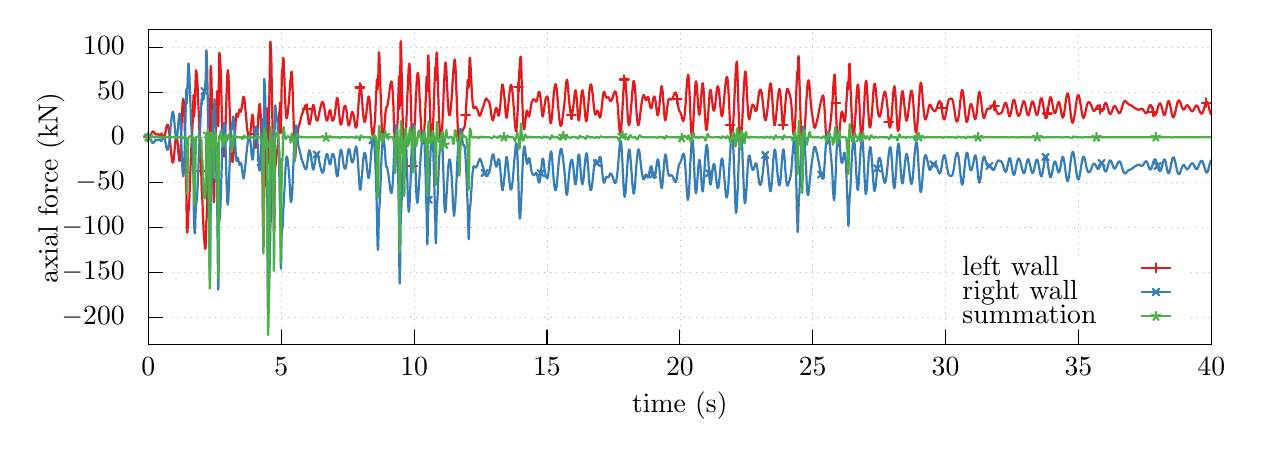
\begin{tikzpicture}[gnuplot]
%% generated with GNUPLOT 5.2p6 (Lua 5.3; terminal rev. Nov 2018, script rev. 107)
%% 09/10/2019 00:35:54
\path (0.000,0.000) rectangle (13.500,4.000);
\gpcolor{color=gp lt color axes}
\gpsetlinetype{gp lt axes}
\gpsetdashtype{gp dt axes}
\gpsetlinewidth{0.50}
\draw[gp path] (0.000,0.343)--(10.222,0.343);
\draw[gp path] (13.162,0.343)--(13.499,0.343);
\gpcolor{color=gp lt color border}
\gpsetlinetype{gp lt border}
\gpsetdashtype{gp dt solid}
\gpsetlinewidth{1.00}
\draw[gp path] (0.000,0.343)--(0.180,0.343);
\node[gp node right] at (-0.184,0.343) {$-200$};
\gpcolor{color=gp lt color axes}
\gpsetlinetype{gp lt axes}
\gpsetdashtype{gp dt axes}
\gpsetlinewidth{0.50}
\draw[gp path] (0.000,0.914)--(10.222,0.914);
\draw[gp path] (13.162,0.914)--(13.499,0.914);
\gpcolor{color=gp lt color border}
\gpsetlinetype{gp lt border}
\gpsetdashtype{gp dt solid}
\gpsetlinewidth{1.00}
\draw[gp path] (0.000,0.914)--(0.180,0.914);
\node[gp node right] at (-0.184,0.914) {$-150$};
\gpcolor{color=gp lt color axes}
\gpsetlinetype{gp lt axes}
\gpsetdashtype{gp dt axes}
\gpsetlinewidth{0.50}
\draw[gp path] (0.000,1.485)--(13.499,1.485);
\gpcolor{color=gp lt color border}
\gpsetlinetype{gp lt border}
\gpsetdashtype{gp dt solid}
\gpsetlinewidth{1.00}
\draw[gp path] (0.000,1.485)--(0.180,1.485);
\node[gp node right] at (-0.184,1.485) {$-100$};
\gpcolor{color=gp lt color axes}
\gpsetlinetype{gp lt axes}
\gpsetdashtype{gp dt axes}
\gpsetlinewidth{0.50}
\draw[gp path] (0.000,2.057)--(13.499,2.057);
\gpcolor{color=gp lt color border}
\gpsetlinetype{gp lt border}
\gpsetdashtype{gp dt solid}
\gpsetlinewidth{1.00}
\draw[gp path] (0.000,2.057)--(0.180,2.057);
\node[gp node right] at (-0.184,2.057) {$-50$};
\gpcolor{color=gp lt color axes}
\gpsetlinetype{gp lt axes}
\gpsetdashtype{gp dt axes}
\gpsetlinewidth{0.50}
\draw[gp path] (0.000,2.628)--(13.499,2.628);
\gpcolor{color=gp lt color border}
\gpsetlinetype{gp lt border}
\gpsetdashtype{gp dt solid}
\gpsetlinewidth{1.00}
\draw[gp path] (0.000,2.628)--(0.180,2.628);
\node[gp node right] at (-0.184,2.628) {$0$};
\gpcolor{color=gp lt color axes}
\gpsetlinetype{gp lt axes}
\gpsetdashtype{gp dt axes}
\gpsetlinewidth{0.50}
\draw[gp path] (0.000,3.199)--(13.499,3.199);
\gpcolor{color=gp lt color border}
\gpsetlinetype{gp lt border}
\gpsetdashtype{gp dt solid}
\gpsetlinewidth{1.00}
\draw[gp path] (0.000,3.199)--(0.180,3.199);
\node[gp node right] at (-0.184,3.199) {$50$};
\gpcolor{color=gp lt color axes}
\gpsetlinetype{gp lt axes}
\gpsetdashtype{gp dt axes}
\gpsetlinewidth{0.50}
\draw[gp path] (0.000,3.770)--(13.499,3.770);
\gpcolor{color=gp lt color border}
\gpsetlinetype{gp lt border}
\gpsetdashtype{gp dt solid}
\gpsetlinewidth{1.00}
\draw[gp path] (0.000,3.770)--(0.180,3.770);
\node[gp node right] at (-0.184,3.770) {$100$};
\gpcolor{color=gp lt color axes}
\gpsetlinetype{gp lt axes}
\gpsetdashtype{gp dt axes}
\gpsetlinewidth{0.50}
\draw[gp path] (0.000,0.000)--(0.000,3.999);
\gpcolor{color=gp lt color border}
\gpsetlinetype{gp lt border}
\gpsetdashtype{gp dt solid}
\gpsetlinewidth{1.00}
\draw[gp path] (0.000,0.000)--(0.000,0.180);
\node[gp node center] at (0.000,-0.308) {$0$};
\gpcolor{color=gp lt color axes}
\gpsetlinetype{gp lt axes}
\gpsetdashtype{gp dt axes}
\gpsetlinewidth{0.50}
\draw[gp path] (1.687,0.000)--(1.687,3.999);
\gpcolor{color=gp lt color border}
\gpsetlinetype{gp lt border}
\gpsetdashtype{gp dt solid}
\gpsetlinewidth{1.00}
\draw[gp path] (1.687,0.000)--(1.687,0.180);
\node[gp node center] at (1.687,-0.308) {$5$};
\gpcolor{color=gp lt color axes}
\gpsetlinetype{gp lt axes}
\gpsetdashtype{gp dt axes}
\gpsetlinewidth{0.50}
\draw[gp path] (3.375,0.000)--(3.375,3.999);
\gpcolor{color=gp lt color border}
\gpsetlinetype{gp lt border}
\gpsetdashtype{gp dt solid}
\gpsetlinewidth{1.00}
\draw[gp path] (3.375,0.000)--(3.375,0.180);
\node[gp node center] at (3.375,-0.308) {$10$};
\gpcolor{color=gp lt color axes}
\gpsetlinetype{gp lt axes}
\gpsetdashtype{gp dt axes}
\gpsetlinewidth{0.50}
\draw[gp path] (5.062,0.000)--(5.062,3.999);
\gpcolor{color=gp lt color border}
\gpsetlinetype{gp lt border}
\gpsetdashtype{gp dt solid}
\gpsetlinewidth{1.00}
\draw[gp path] (5.062,0.000)--(5.062,0.180);
\node[gp node center] at (5.062,-0.308) {$15$};
\gpcolor{color=gp lt color axes}
\gpsetlinetype{gp lt axes}
\gpsetdashtype{gp dt axes}
\gpsetlinewidth{0.50}
\draw[gp path] (6.750,0.000)--(6.750,3.999);
\gpcolor{color=gp lt color border}
\gpsetlinetype{gp lt border}
\gpsetdashtype{gp dt solid}
\gpsetlinewidth{1.00}
\draw[gp path] (6.750,0.000)--(6.750,0.180);
\node[gp node center] at (6.750,-0.308) {$20$};
\gpcolor{color=gp lt color axes}
\gpsetlinetype{gp lt axes}
\gpsetdashtype{gp dt axes}
\gpsetlinewidth{0.50}
\draw[gp path] (8.437,0.000)--(8.437,3.999);
\gpcolor{color=gp lt color border}
\gpsetlinetype{gp lt border}
\gpsetdashtype{gp dt solid}
\gpsetlinewidth{1.00}
\draw[gp path] (8.437,0.000)--(8.437,0.180);
\node[gp node center] at (8.437,-0.308) {$25$};
\gpcolor{color=gp lt color axes}
\gpsetlinetype{gp lt axes}
\gpsetdashtype{gp dt axes}
\gpsetlinewidth{0.50}
\draw[gp path] (10.124,0.000)--(10.124,3.999);
\gpcolor{color=gp lt color border}
\gpsetlinetype{gp lt border}
\gpsetdashtype{gp dt solid}
\gpsetlinewidth{1.00}
\draw[gp path] (10.124,0.000)--(10.124,0.180);
\node[gp node center] at (10.124,-0.308) {$30$};
\gpcolor{color=gp lt color axes}
\gpsetlinetype{gp lt axes}
\gpsetdashtype{gp dt axes}
\gpsetlinewidth{0.50}
\draw[gp path] (11.812,0.000)--(11.812,0.200);
\draw[gp path] (11.812,1.124)--(11.812,3.999);
\gpcolor{color=gp lt color border}
\gpsetlinetype{gp lt border}
\gpsetdashtype{gp dt solid}
\gpsetlinewidth{1.00}
\draw[gp path] (11.812,0.000)--(11.812,0.180);
\node[gp node center] at (11.812,-0.308) {$35$};
\gpcolor{color=gp lt color axes}
\gpsetlinetype{gp lt axes}
\gpsetdashtype{gp dt axes}
\gpsetlinewidth{0.50}
\draw[gp path] (13.499,0.000)--(13.499,3.999);
\gpcolor{color=gp lt color border}
\gpsetlinetype{gp lt border}
\gpsetdashtype{gp dt solid}
\gpsetlinewidth{1.00}
\draw[gp path] (13.499,0.000)--(13.499,0.180);
\node[gp node center] at (13.499,-0.308) {$40$};
\draw[gp path] (0.000,3.999)--(0.000,0.000)--(13.499,0.000)--(13.499,3.999)--cycle;
\node[gp node center,rotate=-270] at (-1.228,1.999) {axial force (\si{\kilo\newton})};
\node[gp node center] at (6.749,-0.769) {time (\si{\second})};
\gpcolor{rgb color={0.894,0.102,0.110}}
\gpsetlinewidth{2.00}
\draw[gp path] (0.000,2.628)--(0.003,2.628)--(0.007,2.629)--(0.010,2.631)--(0.013,2.635)%
  --(0.017,2.639)--(0.020,2.645)--(0.024,2.651)--(0.027,2.657)--(0.030,2.663)--(0.034,2.669)%
  --(0.037,2.675)--(0.040,2.681)--(0.044,2.686)--(0.047,2.692)--(0.051,2.696)--(0.054,2.699)%
  --(0.057,2.701)--(0.061,2.701)--(0.064,2.700)--(0.067,2.697)--(0.071,2.693)--(0.074,2.687)%
  --(0.078,2.682)--(0.081,2.676)--(0.084,2.671)--(0.088,2.667)--(0.091,2.664)--(0.094,2.662)%
  --(0.098,2.662)--(0.101,2.662)--(0.105,2.662)--(0.108,2.663)--(0.111,2.664)--(0.115,2.665)%
  --(0.118,2.666)--(0.121,2.666)--(0.125,2.665)--(0.128,2.663)--(0.132,2.661)--(0.135,2.659)%
  --(0.138,2.658)--(0.142,2.658)--(0.145,2.659)--(0.148,2.661)--(0.152,2.665)--(0.155,2.669)%
  --(0.159,2.673)--(0.162,2.675)--(0.165,2.674)--(0.169,2.670)--(0.172,2.664)--(0.175,2.655)%
  --(0.179,2.646)--(0.182,2.638)--(0.186,2.631)--(0.189,2.626)--(0.192,2.623)--(0.196,2.623)%
  --(0.199,2.626)--(0.202,2.632)--(0.206,2.641)--(0.209,2.654)--(0.213,2.669)--(0.216,2.688)%
  --(0.219,2.707)--(0.223,2.726)--(0.226,2.744)--(0.229,2.759)--(0.233,2.771)--(0.236,2.780)%
  --(0.240,2.786)--(0.243,2.787)--(0.246,2.784)--(0.250,2.777)--(0.253,2.765)--(0.256,2.748)%
  --(0.260,2.727)--(0.263,2.701)--(0.267,2.671)--(0.270,2.637)--(0.273,2.600)--(0.277,2.562)%
  --(0.280,2.523)--(0.283,2.485)--(0.287,2.450)--(0.290,2.417)--(0.294,2.386)--(0.297,2.359)%
  --(0.300,2.336)--(0.304,2.319)--(0.307,2.308)--(0.310,2.305)--(0.314,2.310)--(0.317,2.322)%
  --(0.321,2.343)--(0.324,2.371)--(0.327,2.405)--(0.331,2.444)--(0.334,2.484)--(0.337,2.525)%
  --(0.341,2.563)--(0.344,2.596)--(0.348,2.623)--(0.351,2.640)--(0.354,2.649)--(0.358,2.648)%
  --(0.361,2.638)--(0.364,2.618)--(0.368,2.589)--(0.371,2.554)--(0.375,2.514)--(0.378,2.473)%
  --(0.381,2.433)--(0.385,2.396)--(0.388,2.364)--(0.391,2.340)--(0.395,2.327)--(0.398,2.328)%
  --(0.402,2.347)--(0.405,2.387)--(0.408,2.447)--(0.412,2.522)--(0.415,2.608)--(0.418,2.698)%
  --(0.422,2.792)--(0.425,2.881)--(0.429,2.961)--(0.432,3.028)--(0.435,3.078)--(0.439,3.096)%
  --(0.442,3.116)--(0.445,3.109)--(0.449,3.077)--(0.452,3.022)--(0.456,2.946)--(0.459,2.850)%
  --(0.462,2.738)--(0.466,2.615)--(0.469,2.487)--(0.472,2.343)--(0.476,2.201)--(0.479,2.019)%
  --(0.483,1.908)--(0.486,1.622)--(0.489,1.445)--(0.493,1.416)--(0.496,1.438)--(0.499,1.474)%
  --(0.503,1.575)--(0.506,1.668)--(0.510,1.687)--(0.513,1.718)--(0.516,1.766)--(0.520,1.831)%
  --(0.523,1.911)--(0.526,2.000)--(0.530,2.095)--(0.533,2.191)--(0.537,2.286)--(0.540,2.374)%
  --(0.543,2.451)--(0.547,2.516)--(0.550,2.573)--(0.553,2.629)--(0.557,2.689)--(0.560,2.762)%
  --(0.564,2.852)--(0.567,2.959)--(0.570,3.067)--(0.574,3.167)--(0.577,2.960)--(0.580,2.889)%
  --(0.584,2.933)--(0.587,2.995)--(0.591,3.032)--(0.594,3.147)--(0.597,3.273)--(0.601,3.385)%
  --(0.604,3.479)--(0.607,3.473)--(0.611,3.456)--(0.614,3.428)--(0.618,3.390)--(0.621,3.342)%
  --(0.624,3.283)--(0.628,3.214)--(0.631,3.137)--(0.634,3.052)--(0.638,2.966)--(0.641,2.878)%
  --(0.645,2.788)--(0.648,2.696)--(0.651,2.621)--(0.655,2.551)--(0.658,2.483)--(0.661,2.416)%
  --(0.665,2.343)--(0.668,2.271)--(0.672,2.200)--(0.675,2.046)--(0.678,1.960)--(0.682,1.902)%
  --(0.685,1.843)--(0.688,1.783)--(0.692,1.633)--(0.695,1.571)--(0.699,1.503)--(0.702,1.431)%
  --(0.705,1.371)--(0.709,1.341)--(0.712,1.303)--(0.715,1.258)--(0.719,1.222)--(0.722,1.211)%
  --(0.726,1.227)--(0.729,1.255)--(0.732,1.381)--(0.736,1.555)--(0.739,1.585)--(0.742,1.657)%
  --(0.746,1.768)--(0.749,1.944)--(0.753,2.156)--(0.756,2.346)--(0.759,2.554)--(0.763,2.670)%
  --(0.766,2.492)--(0.769,2.664)--(0.773,2.655)--(0.776,2.603)--(0.780,2.527)--(0.783,2.631)%
  --(0.786,3.006)--(0.790,3.486)--(0.793,3.535)--(0.796,3.493)--(0.800,3.399)--(0.803,3.258)%
  --(0.807,3.100)--(0.810,2.913)--(0.813,2.705)--(0.817,2.544)--(0.820,2.397)--(0.823,2.140)%
  --(0.827,2.027)--(0.830,1.894)--(0.834,1.802)--(0.837,1.968)--(0.840,2.170)--(0.844,2.263)%
  --(0.847,2.345)--(0.850,2.460)--(0.854,2.580)--(0.857,2.696)--(0.861,2.800)--(0.864,2.892)%
  --(0.867,3.028)--(0.871,3.162)--(0.874,3.216)--(0.877,3.170)--(0.881,3.028)--(0.884,2.879)%
  --(0.888,2.770)--(0.891,2.878)--(0.894,3.251)--(0.898,3.644)--(0.901,3.700)--(0.904,3.692)%
  --(0.908,3.657)--(0.911,3.607)--(0.915,3.551)--(0.918,3.485)--(0.921,3.375)--(0.925,3.264)%
  --(0.928,3.119)--(0.931,2.996)--(0.935,2.873)--(0.938,2.758)--(0.942,2.658)--(0.945,2.577)%
  --(0.948,2.509)--(0.952,2.403)--(0.955,2.386)--(0.958,2.383)--(0.962,2.423)--(0.965,2.464)%
  --(0.969,2.514)--(0.972,2.574)--(0.975,2.646)--(0.979,2.735)--(0.982,2.837)--(0.985,2.950)%
  --(0.989,3.053)--(0.992,3.146)--(0.996,3.247)--(0.999,3.339)--(1.002,3.413)--(1.006,3.460)%
  --(1.009,3.480)--(1.012,3.472)--(1.016,3.429)--(1.019,3.360)--(1.023,3.275)--(1.026,3.180)%
  --(1.029,3.063)--(1.033,2.959)--(1.036,2.852)--(1.039,2.758)--(1.043,2.677)--(1.046,2.605)%
  --(1.050,2.544)--(1.053,2.495)--(1.056,2.451)--(1.060,2.344)--(1.063,2.333)--(1.066,2.320)%
  --(1.070,2.315)--(1.073,2.332)--(1.077,2.382)--(1.080,2.398)--(1.083,2.424)--(1.087,2.457)%
  --(1.090,2.506)--(1.093,2.564)--(1.097,2.628)--(1.100,2.689)--(1.104,2.747)--(1.107,2.801)%
  --(1.110,2.852)--(1.114,2.894)--(1.117,2.921)--(1.120,2.929)--(1.124,2.919)--(1.127,2.902)%
  --(1.131,2.889)--(1.134,2.886)--(1.137,2.893)--(1.141,2.905)--(1.144,2.920)--(1.147,2.936)%
  --(1.151,2.953)--(1.154,2.969)--(1.158,2.981)--(1.161,2.981)--(1.164,2.971)--(1.168,2.958)%
  --(1.171,2.949)--(1.174,2.950)--(1.178,2.963)--(1.181,2.979)--(1.185,2.997)--(1.188,3.018)%
  --(1.191,3.037)--(1.195,3.063)--(1.198,3.101)--(1.201,3.127)--(1.205,3.139)--(1.208,3.140)%
  --(1.212,3.136)--(1.215,3.131)--(1.218,3.118)--(1.222,3.090)--(1.225,3.055)--(1.228,3.021)%
  --(1.232,2.986)--(1.235,2.949)--(1.239,2.912)--(1.242,2.874)--(1.245,2.836)--(1.249,2.800)%
  --(1.252,2.767)--(1.255,2.735)--(1.259,2.707)--(1.262,2.683)--(1.266,2.662)--(1.269,2.642)%
  --(1.272,2.625)--(1.276,2.611)--(1.279,2.604)--(1.282,2.606)--(1.286,2.615)--(1.289,2.632)%
  --(1.293,2.655)--(1.296,2.686)--(1.299,2.721)--(1.303,2.760)--(1.306,2.797)--(1.309,2.834)%
  --(1.313,2.867)--(1.316,2.893)--(1.320,2.909)--(1.323,2.913)--(1.326,2.903)--(1.330,2.879)%
  --(1.333,2.839)--(1.336,2.783)--(1.340,2.723)--(1.343,2.665)--(1.347,2.612)--(1.350,2.565)%
  --(1.353,2.529)--(1.357,2.506)--(1.360,2.496)--(1.363,2.495)--(1.367,2.500)--(1.370,2.512)%
  --(1.374,2.534)--(1.377,2.570)--(1.380,2.616)--(1.384,2.668)--(1.387,2.725)--(1.390,2.784)%
  --(1.394,2.840)--(1.397,2.901)--(1.401,2.955)--(1.404,3.000)--(1.407,3.031)--(1.411,3.049)%
  --(1.414,3.051)--(1.417,3.036)--(1.421,3.001)--(1.424,2.949)--(1.428,2.880)--(1.431,2.793)%
  --(1.434,2.702)--(1.438,2.612)--(1.441,2.524)--(1.444,2.438)--(1.448,2.343)--(1.451,1.977)%
  --(1.455,1.606)--(1.458,1.419)--(1.461,1.311)--(1.465,1.324)--(1.468,1.571)--(1.471,2.005)%
  --(1.475,1.992)--(1.478,2.024)--(1.482,2.103)--(1.485,2.222)--(1.488,2.366)--(1.492,2.485)%
  --(1.495,2.547)--(1.498,2.619)--(1.502,2.736)--(1.505,2.885)--(1.509,2.996)--(1.512,2.749)%
  --(1.515,2.444)--(1.519,2.296)--(1.522,2.349)--(1.525,2.502)--(1.529,2.690)--(1.532,2.918)%
  --(1.536,3.140)--(1.539,3.327)--(1.542,3.505)--(1.546,3.686)--(1.549,3.842)--(1.552,3.824)%
  --(1.556,3.779)--(1.559,3.664)--(1.563,3.548)--(1.566,3.339)--(1.569,3.143)--(1.573,2.956)%
  --(1.576,2.762)--(1.579,2.408)--(1.583,2.232)--(1.586,2.104)--(1.590,1.875)--(1.593,1.438)%
  --(1.596,1.424)--(1.600,1.624)--(1.603,1.888)--(1.606,2.160)--(1.610,2.237)--(1.613,2.261)%
  --(1.617,2.287)--(1.620,2.323)--(1.623,2.362)--(1.627,2.397)--(1.630,2.425)--(1.633,2.446)%
  --(1.637,2.464)--(1.640,2.502)--(1.644,2.524)--(1.647,2.575)--(1.650,2.650)--(1.654,2.731)%
  --(1.657,2.793)--(1.660,2.861)--(1.664,2.967)--(1.667,2.951)--(1.671,3.042)--(1.674,3.071)%
  --(1.677,2.987)--(1.681,2.683)--(1.684,2.699)--(1.687,2.919)--(1.691,3.183)--(1.694,3.390)%
  --(1.697,3.482)--(1.701,3.484)--(1.704,3.501)--(1.708,3.577)--(1.711,3.636)--(1.714,3.636)%
  --(1.718,3.607)--(1.721,3.522)--(1.724,3.449)--(1.728,3.361)--(1.731,3.247)--(1.735,3.156)%
  --(1.738,3.078)--(1.741,3.010)--(1.745,2.953)--(1.748,2.908)--(1.751,2.883)--(1.755,2.870)%
  --(1.758,2.869)--(1.762,2.879)--(1.765,2.898)--(1.768,2.926)--(1.772,2.959)--(1.775,2.988)%
  --(1.778,3.018)--(1.782,3.051)--(1.785,3.087)--(1.789,3.128)--(1.792,3.177)--(1.795,3.231)%
  --(1.799,3.286)--(1.802,3.332)--(1.805,3.352)--(1.809,3.391)--(1.812,3.432)--(1.816,3.459)%
  --(1.819,3.461)--(1.822,3.438)--(1.826,3.385)--(1.829,3.308)--(1.832,3.218)--(1.836,3.121)%
  --(1.839,3.008)--(1.843,2.893)--(1.846,2.788)--(1.849,2.691)--(1.853,2.613)--(1.856,2.458)%
  --(1.859,2.391)--(1.863,2.367)--(1.866,2.381)--(1.870,2.432)--(1.873,2.486)--(1.876,2.502)%
  --(1.880,2.526)--(1.883,2.558)--(1.886,2.594)--(1.890,2.624)--(1.893,2.658)--(1.897,2.690)%
  --(1.900,2.719)--(1.903,2.743)--(1.907,2.762)--(1.910,2.776)--(1.913,2.785)--(1.917,2.794)%
  --(1.920,2.800)--(1.924,2.810)--(1.927,2.823)--(1.930,2.838)--(1.934,2.855)--(1.937,2.871)%
  --(1.940,2.886)--(1.944,2.900)--(1.947,2.911)--(1.951,2.920)--(1.954,2.928)--(1.957,2.936)%
  --(1.961,2.944)--(1.964,2.953)--(1.967,2.963)--(1.971,2.974)--(1.974,2.983)--(1.978,2.993)%
  --(1.981,3.002)--(1.984,3.011)--(1.988,3.020)--(1.991,3.027)--(1.994,3.032)--(1.998,3.035)%
  --(2.001,3.034)--(2.005,3.031)--(2.008,3.022)--(2.011,3.009)--(2.015,2.991)--(2.018,2.966)%
  --(2.021,2.937)--(2.025,2.905)--(2.028,2.872)--(2.032,2.843)--(2.035,2.818)--(2.038,2.801)%
  --(2.042,2.794)--(2.045,2.793)--(2.048,2.798)--(2.052,2.808)--(2.055,2.822)--(2.059,2.837)%
  --(2.062,2.854)--(2.065,2.874)--(2.069,2.896)--(2.072,2.921)--(2.075,2.947)--(2.079,2.971)%
  --(2.082,2.994)--(2.086,3.013)--(2.089,3.028)--(2.092,3.037)--(2.096,3.039)--(2.099,3.034)%
  --(2.102,3.021)--(2.106,3.003)--(2.109,2.982)--(2.113,2.959)--(2.116,2.937)--(2.119,2.916)%
  --(2.123,2.897)--(2.126,2.880)--(2.129,2.866)--(2.133,2.854)--(2.136,2.845)--(2.140,2.840)%
  --(2.143,2.838)--(2.146,2.840)--(2.150,2.846)--(2.153,2.856)--(2.156,2.868)--(2.160,2.884)%
  --(2.163,2.901)--(2.167,2.919)--(2.170,2.937)--(2.173,2.954)--(2.177,2.970)--(2.180,2.985)%
  --(2.183,2.999)--(2.187,3.011)--(2.190,3.024)--(2.194,3.037)--(2.197,3.049)--(2.200,3.060)%
  --(2.204,3.069)--(2.207,3.074)--(2.210,3.077)--(2.214,3.077)--(2.217,3.073)--(2.221,3.067)%
  --(2.224,3.056)--(2.227,3.042)--(2.231,3.025)--(2.234,3.005)--(2.237,2.982)--(2.241,2.956)%
  --(2.244,2.932)--(2.248,2.909)--(2.251,2.889)--(2.254,2.871)--(2.258,2.857)--(2.261,2.847)%
  --(2.264,2.842)--(2.268,2.841)--(2.271,2.843)--(2.275,2.851)--(2.278,2.862)--(2.281,2.876)%
  --(2.285,2.892)--(2.288,2.909)--(2.291,2.926)--(2.295,2.942)--(2.298,2.956)--(2.302,2.966)%
  --(2.305,2.973)--(2.308,2.973)--(2.312,2.967)--(2.315,2.954)--(2.318,2.934)--(2.322,2.911)%
  --(2.325,2.888)--(2.329,2.868)--(2.332,2.853)--(2.335,2.843)--(2.339,2.839)--(2.342,2.839)%
  --(2.345,2.842)--(2.349,2.848)--(2.352,2.855)--(2.356,2.865)--(2.359,2.878)--(2.362,2.893)%
  --(2.366,2.910)--(2.369,2.932)--(2.372,2.957)--(2.376,2.986)--(2.379,3.016)--(2.383,3.045)%
  --(2.386,3.071)--(2.389,3.094)--(2.393,3.111)--(2.396,3.123)--(2.399,3.126)--(2.403,3.119)%
  --(2.406,3.103)--(2.410,3.078)--(2.413,3.046)--(2.416,3.009)--(2.420,2.970)--(2.423,2.930)%
  --(2.426,2.893)--(2.430,2.860)--(2.433,2.831)--(2.437,2.809)--(2.440,2.795)--(2.443,2.789)%
  --(2.447,2.788)--(2.450,2.793)--(2.453,2.803)--(2.457,2.820)--(2.460,2.840)--(2.464,2.863)%
  --(2.467,2.888)--(2.470,2.914)--(2.474,2.940)--(2.477,2.964)--(2.480,2.984)--(2.484,3.001)%
  --(2.487,3.013)--(2.491,3.021)--(2.494,3.026)--(2.497,3.028)--(2.501,3.026)--(2.504,3.020)%
  --(2.507,3.010)--(2.511,2.995)--(2.514,2.974)--(2.518,2.949)--(2.521,2.920)--(2.524,2.889)%
  --(2.528,2.860)--(2.531,2.832)--(2.534,2.809)--(2.538,2.792)--(2.541,2.781)--(2.545,2.777)%
  --(2.548,2.778)--(2.551,2.784)--(2.555,2.795)--(2.558,2.809)--(2.561,2.827)--(2.565,2.846)%
  --(2.568,2.867)--(2.572,2.887)--(2.575,2.907)--(2.578,2.924)--(2.582,2.936)--(2.585,2.945)%
  --(2.588,2.948)--(2.592,2.948)--(2.595,2.944)--(2.599,2.936)--(2.602,2.925)--(2.605,2.911)%
  --(2.609,2.893)--(2.612,2.872)--(2.615,2.847)--(2.619,2.822)--(2.622,2.799)--(2.626,2.778)%
  --(2.629,2.760)--(2.632,2.751)--(2.636,2.748)--(2.639,2.752)--(2.642,2.763)--(2.646,2.778)%
  --(2.649,2.801)--(2.653,2.832)--(2.656,2.869)--(2.659,2.911)--(2.663,2.958)--(2.666,3.008)%
  --(2.669,3.060)--(2.673,3.109)--(2.676,3.155)--(2.680,3.195)--(2.683,3.224)--(2.686,3.260)%
  --(2.690,3.289)--(2.693,3.300)--(2.696,3.292)--(2.700,3.268)--(2.703,3.235)--(2.707,3.192)%
  --(2.710,3.146)--(2.713,3.099)--(2.717,3.054)--(2.720,3.011)--(2.723,2.971)--(2.727,2.933)%
  --(2.730,2.899)--(2.734,2.871)--(2.737,2.849)--(2.740,2.833)--(2.744,2.825)--(2.747,2.823)%
  --(2.750,2.827)--(2.754,2.837)--(2.757,2.853)--(2.761,2.873)--(2.764,2.898)--(2.767,2.925)%
  --(2.771,2.956)--(2.774,2.989)--(2.777,3.023)--(2.781,3.055)--(2.784,3.083)--(2.788,3.108)%
  --(2.791,3.128)--(2.794,3.141)--(2.798,3.146)--(2.801,3.141)--(2.804,3.126)--(2.808,3.102)%
  --(2.811,3.070)--(2.815,3.031)--(2.818,2.989)--(2.821,2.941)--(2.825,2.891)--(2.828,2.840)%
  --(2.831,2.790)--(2.835,2.746)--(2.838,2.711)--(2.842,2.683)--(2.845,2.664)--(2.848,2.654)%
  --(2.852,2.652)--(2.855,2.657)--(2.858,2.670)--(2.862,2.692)--(2.865,2.720)--(2.869,2.750)%
  --(2.872,2.787)--(2.875,2.825)--(2.879,2.872)--(2.882,2.935)--(2.885,3.012)--(2.889,3.094)%
  --(2.892,3.175)--(2.896,3.222)--(2.899,3.309)--(2.902,3.366)--(2.906,3.282)--(2.909,3.231)%
  --(2.912,3.265)--(2.916,3.293)--(2.919,3.359)--(2.923,3.524)--(2.926,3.707)--(2.929,3.703)%
  --(2.933,3.672)--(2.936,3.577)--(2.939,3.500)--(2.943,3.382)--(2.946,3.272)--(2.950,3.167)%
  --(2.953,3.066)--(2.956,2.958)--(2.960,2.871)--(2.963,2.793)--(2.966,2.729)--(2.970,2.676)%
  --(2.973,2.632)--(2.977,2.611)--(2.980,2.614)--(2.983,2.629)--(2.987,2.642)--(2.990,2.665)%
  --(2.993,2.702)--(2.997,2.746)--(3.000,2.793)--(3.004,2.841)--(3.007,2.885)--(3.010,2.926)%
  --(3.014,2.962)--(3.017,2.989)--(3.020,3.006)--(3.024,3.012)--(3.027,3.012)--(3.031,3.013)%
  --(3.034,3.020)--(3.037,3.035)--(3.041,3.055)--(3.044,3.078)--(3.047,3.103)--(3.051,3.126)%
  --(3.054,3.148)--(3.058,3.172)--(3.061,3.200)--(3.064,3.229)--(3.068,3.255)--(3.071,3.279)%
  --(3.074,3.298)--(3.078,3.315)--(3.081,3.329)--(3.085,3.337)--(3.088,3.337)--(3.091,3.329)%
  --(3.095,3.309)--(3.098,3.278)--(3.101,3.234)--(3.105,3.178)--(3.108,3.107)--(3.112,3.017)%
  --(3.115,2.920)--(3.118,2.823)--(3.122,2.731)--(3.125,2.650)--(3.128,2.581)--(3.132,2.351)%
  --(3.135,2.281)--(3.139,2.261)--(3.142,2.388)--(3.145,2.502)--(3.149,2.528)--(3.152,2.571)%
  --(3.155,2.633)--(3.159,2.704)--(3.162,2.789)--(3.166,2.855)--(3.169,2.976)--(3.172,3.105)%
  --(3.176,3.204)--(3.179,3.304)--(3.182,3.402)--(3.186,3.051)--(3.189,2.989)--(3.193,3.061)%
  --(3.196,3.210)--(3.199,3.458)--(3.203,3.824)--(3.206,3.849)--(3.209,3.756)--(3.213,3.633)%
  --(3.216,3.452)--(3.220,3.296)--(3.223,3.148)--(3.226,2.994)--(3.230,2.854)--(3.233,2.723)%
  --(3.236,2.533)--(3.240,2.512)--(3.243,2.472)--(3.247,2.330)--(3.250,2.150)--(3.253,2.198)%
  --(3.257,2.442)--(3.260,2.589)--(3.263,2.636)--(3.267,2.678)--(3.270,2.710)--(3.274,2.769)%
  --(3.277,2.845)--(3.280,2.916)--(3.284,3.010)--(3.287,3.102)--(3.290,3.188)--(3.294,3.240)%
  --(3.297,3.332)--(3.301,3.412)--(3.304,3.471)--(3.307,3.513)--(3.311,3.545)--(3.314,3.564)%
  --(3.317,3.545)--(3.321,3.495)--(3.324,3.421)--(3.328,3.299)--(3.331,3.153)--(3.334,3.030)%
  --(3.338,2.908)--(3.341,2.778)--(3.344,2.662)--(3.348,2.568)--(3.351,2.507)--(3.355,2.473)%
  --(3.358,2.266)--(3.361,2.351)--(3.365,2.509)--(3.368,2.539)--(3.371,2.588)--(3.375,2.651)%
  --(3.378,2.708)--(3.381,2.783)--(3.385,2.838)--(3.388,2.923)--(3.392,3.010)--(3.395,3.091)%
  --(3.398,3.159)--(3.402,3.196)--(3.405,3.276)--(3.408,3.343)--(3.412,3.392)--(3.415,3.424)%
  --(3.419,3.441)--(3.422,3.445)--(3.425,3.435)--(3.429,3.412)--(3.432,3.374)--(3.435,3.326)%
  --(3.439,3.272)--(3.442,3.187)--(3.446,3.107)--(3.449,3.039)--(3.452,2.973)--(3.456,2.910)%
  --(3.459,2.852)--(3.462,2.791)--(3.466,2.725)--(3.469,2.677)--(3.473,2.635)--(3.476,2.594)%
  --(3.479,2.570)--(3.483,2.559)--(3.486,2.554)--(3.489,2.558)--(3.493,2.572)--(3.496,2.602)%
  --(3.500,2.645)--(3.503,2.692)--(3.506,2.753)--(3.510,2.813)--(3.513,2.874)--(3.516,2.962)%
  --(3.520,3.054)--(3.523,3.129)--(3.527,3.201)--(3.530,3.316)--(3.533,3.397)--(3.537,3.245)%
  --(3.540,3.212)--(3.543,3.286)--(3.547,3.433)--(3.550,3.620)--(3.554,3.667)--(3.557,3.660)%
  --(3.560,3.552)--(3.564,3.423)--(3.567,3.289)--(3.570,3.168)--(3.574,3.053)--(3.577,2.943)%
  --(3.581,2.814)--(3.584,2.731)--(3.587,2.672)--(3.591,2.625)--(3.594,2.578)--(3.597,2.558)%
  --(3.601,2.554)--(3.604,2.617)--(3.608,2.667)--(3.611,2.720)--(3.614,2.772)--(3.618,2.844)%
  --(3.621,2.933)--(3.624,3.010)--(3.628,3.116)--(3.631,3.225)--(3.635,3.328)--(3.638,3.375)%
  --(3.641,3.457)--(3.645,3.526)--(3.648,3.354)--(3.651,3.413)--(3.655,3.532)--(3.658,3.685)%
  --(3.662,3.705)--(3.665,3.696)--(3.668,3.591)--(3.672,3.474)--(3.675,3.352)--(3.678,3.248)%
  --(3.682,3.149)--(3.685,3.055)--(3.689,2.947)--(3.692,2.873)--(3.695,2.806)--(3.699,2.747)%
  --(3.702,2.694)--(3.705,2.634)--(3.709,2.516)--(3.712,2.541)--(3.716,2.601)--(3.719,2.629)%
  --(3.722,2.649)--(3.726,2.678)--(3.729,2.726)--(3.732,2.784)--(3.736,2.846)--(3.739,2.925)%
  --(3.743,2.983)--(3.746,3.077)--(3.749,3.170)--(3.753,3.262)--(3.756,3.349)--(3.759,3.386)%
  --(3.763,3.454)--(3.766,3.517)--(3.770,3.559)--(3.773,3.578)--(3.776,3.569)--(3.780,3.542)%
  --(3.783,3.504)--(3.786,3.456)--(3.790,3.347)--(3.793,3.273)--(3.797,3.204)--(3.800,3.138)%
  --(3.803,3.081)--(3.807,3.030)--(3.810,2.988)--(3.813,2.952)--(3.817,2.927)--(3.820,2.912)%
  --(3.824,2.906)--(3.827,2.909)--(3.830,2.921)--(3.834,2.940)--(3.837,2.964)--(3.840,2.993)%
  --(3.844,3.029)--(3.847,3.072)--(3.851,3.119)--(3.854,3.172)--(3.857,3.227)--(3.861,3.285)%
  --(3.864,3.340)--(3.867,3.374)--(3.871,3.436)--(3.874,3.487)--(3.878,3.519)--(3.881,3.544)%
  --(3.884,3.581)--(3.888,3.609)--(3.891,3.617)--(3.894,3.600)--(3.898,3.547)--(3.901,3.496)%
  --(3.905,3.424)--(3.908,3.314)--(3.911,3.226)--(3.915,3.137)--(3.918,3.055)--(3.921,2.966)%
  --(3.925,2.859)--(3.928,2.779)--(3.932,2.703)--(3.935,2.633)--(3.938,2.593)--(3.942,2.442)%
  --(3.945,2.341)--(3.948,2.290)--(3.952,2.296)--(3.955,2.343)--(3.959,2.448)--(3.962,2.549)%
  --(3.965,2.563)--(3.969,2.577)--(3.972,2.593)--(3.975,2.614)--(3.979,2.642)--(3.982,2.672)%
  --(3.986,2.694)--(3.989,2.709)--(3.992,2.721)--(3.996,2.727)--(3.999,2.733)--(4.002,2.740)%
  --(4.006,2.744)--(4.009,2.746)--(4.013,2.751)--(4.016,2.763)--(4.019,2.787)--(4.023,2.819)%
  --(4.026,2.859)--(4.029,2.910)--(4.033,2.968)--(4.036,3.031)--(4.040,3.095)--(4.043,3.153)%
  --(4.046,3.175)--(4.050,3.245)--(4.053,3.325)--(4.056,3.357)--(4.060,3.292)--(4.063,3.253)%
  --(4.067,3.259)--(4.070,3.295)--(4.073,3.400)--(4.077,3.560)--(4.080,3.636)--(4.083,3.639)%
  --(4.087,3.609)--(4.090,3.540)--(4.094,3.493)--(4.097,3.447)--(4.100,3.350)--(4.104,3.287)%
  --(4.107,3.227)--(4.110,3.171)--(4.114,3.122)--(4.117,3.080)--(4.121,3.046)--(4.124,3.021)%
  --(4.127,3.005)--(4.131,2.997)--(4.134,2.994)--(4.137,2.995)--(4.141,2.999)--(4.144,3.003)%
  --(4.148,3.007)--(4.151,3.010)--(4.154,3.012)--(4.158,3.012)--(4.161,3.009)--(4.164,3.004)%
  --(4.168,3.000)--(4.171,2.993)--(4.175,2.986)--(4.178,2.978)--(4.181,2.969)--(4.185,2.960)%
  --(4.188,2.951)--(4.191,2.940)--(4.195,2.926)--(4.198,2.913)--(4.202,2.904)--(4.205,2.901)%
  --(4.208,2.902)--(4.212,2.905)--(4.215,2.909)--(4.218,2.914)--(4.222,2.922)--(4.225,2.934)%
  --(4.229,2.946)--(4.232,2.956)--(4.235,2.965)--(4.239,2.975)--(4.242,2.986)--(4.245,2.998)%
  --(4.249,3.008)--(4.252,3.018)--(4.256,3.027)--(4.259,3.038)--(4.262,3.049)--(4.266,3.060)%
  --(4.269,3.072)--(4.272,3.083)--(4.276,3.093)--(4.279,3.103)--(4.283,3.112)--(4.286,3.117)%
  --(4.289,3.120)--(4.293,3.119)--(4.296,3.116)--(4.299,3.111)--(4.303,3.106)--(4.306,3.101)%
  --(4.310,3.097)--(4.313,3.094)--(4.316,3.091)--(4.320,3.088)--(4.323,3.084)--(4.326,3.078)%
  --(4.330,3.070)--(4.333,3.059)--(4.337,3.044)--(4.340,3.026)--(4.343,3.005)--(4.347,2.982)%
  --(4.350,2.957)--(4.353,2.930)--(4.357,2.906)--(4.360,2.884)--(4.364,2.866)--(4.367,2.854)%
  --(4.370,2.846)--(4.374,2.842)--(4.377,2.844)--(4.380,2.851)--(4.384,2.865)--(4.387,2.881)%
  --(4.391,2.899)--(4.394,2.916)--(4.397,2.934)--(4.401,2.951)--(4.404,2.967)--(4.407,2.981)%
  --(4.411,2.992)--(4.414,2.999)--(4.418,3.001)--(4.421,2.999)--(4.424,2.992)--(4.428,2.979)%
  --(4.431,2.962)--(4.434,2.943)--(4.438,2.926)--(4.441,2.913)--(4.445,2.905)--(4.448,2.902)%
  --(4.451,2.909)--(4.455,2.922)--(4.458,2.942)--(4.461,2.964)--(4.465,2.993)--(4.468,3.027)%
  --(4.472,3.066)--(4.475,3.108)--(4.478,3.149)--(4.482,3.190)--(4.485,3.227)--(4.488,3.260)%
  --(4.492,3.285)--(4.495,3.298)--(4.499,3.298)--(4.502,3.287)--(4.505,3.269)--(4.509,3.248)%
  --(4.512,3.224)--(4.515,3.196)--(4.519,3.164)--(4.522,3.128)--(4.526,3.090)--(4.529,3.050)%
  --(4.532,3.005)--(4.536,2.959)--(4.539,2.919)--(4.542,2.896)--(4.546,2.881)--(4.549,2.876)%
  --(4.553,2.883)--(4.556,2.902)--(4.559,2.932)--(4.563,2.967)--(4.566,2.995)--(4.569,3.025)%
  --(4.573,3.059)--(4.576,3.094)--(4.580,3.129)--(4.583,3.161)--(4.586,3.191)--(4.590,3.219)%
  --(4.593,3.245)--(4.596,3.266)--(4.600,3.282)--(4.603,3.290)--(4.607,3.292)--(4.610,3.288)%
  --(4.613,3.278)--(4.617,3.261)--(4.620,3.236)--(4.623,3.205)--(4.627,3.170)--(4.630,3.132)%
  --(4.634,3.091)--(4.637,3.050)--(4.640,3.004)--(4.644,2.958)--(4.647,2.909)--(4.650,2.861)%
  --(4.654,2.813)--(4.657,2.772)--(4.661,2.744)--(4.664,2.725)--(4.667,2.710)--(4.671,2.703)%
  --(4.674,2.713)--(4.677,2.745)--(4.681,2.796)--(4.684,2.860)--(4.688,2.928)--(4.691,2.993)%
  --(4.694,3.074)--(4.698,3.169)--(4.701,3.264)--(4.704,3.352)--(4.708,3.378)--(4.711,3.466)%
  --(4.715,3.511)--(4.718,3.576)--(4.721,3.614)--(4.725,3.644)--(4.728,3.653)--(4.731,3.644)%
  --(4.735,3.549)--(4.738,3.435)--(4.742,3.304)--(4.745,3.197)--(4.748,3.098)--(4.752,3.010)%
  --(4.755,2.914)--(4.758,2.840)--(4.762,2.791)--(4.765,2.758)--(4.769,2.736)--(4.772,2.728)%
  --(4.775,2.738)--(4.779,2.761)--(4.782,2.790)--(4.785,2.820)--(4.789,2.848)--(4.792,2.878)%
  --(4.796,2.908)--(4.799,2.934)--(4.802,2.953)--(4.806,2.964)--(4.809,2.966)--(4.812,2.960)%
  --(4.816,2.949)--(4.819,2.936)--(4.823,2.921)--(4.826,2.907)--(4.829,2.897)--(4.833,2.892)%
  --(4.836,2.895)--(4.839,2.905)--(4.843,2.921)--(4.846,2.941)--(4.850,2.963)--(4.853,2.986)%
  --(4.856,3.009)--(4.860,3.031)--(4.863,3.049)--(4.866,3.063)--(4.870,3.074)--(4.873,3.082)%
  --(4.877,3.089)--(4.880,3.094)--(4.883,3.099)--(4.887,3.104)--(4.890,3.107)--(4.893,3.110)%
  --(4.897,3.110)--(4.900,3.109)--(4.904,3.106)--(4.907,3.101)--(4.910,3.096)--(4.914,3.091)%
  --(4.917,3.086)--(4.920,3.083)--(4.924,3.081)--(4.927,3.082)--(4.931,3.086)--(4.934,3.095)%
  --(4.937,3.107)--(4.941,3.123)--(4.944,3.141)--(4.947,3.159)--(4.951,3.176)--(4.954,3.189)%
  --(4.958,3.199)--(4.961,3.205)--(4.964,3.204)--(4.968,3.198)--(4.971,3.184)--(4.974,3.165)%
  --(4.978,3.142)--(4.981,3.114)--(4.985,3.084)--(4.988,3.050)--(4.991,3.012)--(4.995,2.975)%
  --(4.998,2.941)--(5.001,2.916)--(5.005,2.898)--(5.008,2.893)--(5.012,2.899)--(5.015,2.914)%
  --(5.018,2.937)--(5.022,2.961)--(5.025,2.985)--(5.028,3.011)--(5.032,3.037)--(5.035,3.061)%
  --(5.039,3.083)--(5.042,3.099)--(5.045,3.112)--(5.049,3.123)--(5.052,3.131)--(5.055,3.138)%
  --(5.059,3.144)--(5.062,3.147)--(5.065,3.146)--(5.069,3.142)--(5.072,3.132)--(5.076,3.115)%
  --(5.079,3.094)--(5.082,3.065)--(5.086,3.030)--(5.089,2.988)--(5.092,2.942)--(5.096,2.901)%
  --(5.099,2.864)--(5.103,2.834)--(5.106,2.813)--(5.109,2.804)--(5.113,2.806)--(5.116,2.818)%
  --(5.119,2.839)--(5.123,2.867)--(5.126,2.903)--(5.130,2.944)--(5.133,2.984)--(5.136,3.026)%
  --(5.140,3.071)--(5.143,3.115)--(5.146,3.155)--(5.150,3.191)--(5.153,3.221)--(5.157,3.247)%
  --(5.160,3.268)--(5.163,3.284)--(5.167,3.296)--(5.170,3.302)--(5.173,3.302)--(5.177,3.295)%
  --(5.180,3.281)--(5.184,3.259)--(5.187,3.231)--(5.190,3.196)--(5.194,3.155)--(5.197,3.111)%
  --(5.200,3.070)--(5.204,3.029)--(5.207,2.986)--(5.211,2.942)--(5.214,2.905)--(5.217,2.874)%
  --(5.221,2.845)--(5.224,2.819)--(5.227,2.798)--(5.231,2.783)--(5.234,2.775)--(5.238,2.774)%
  --(5.241,2.776)--(5.244,2.783)--(5.248,2.796)--(5.251,2.814)--(5.254,2.836)--(5.258,2.861)%
  --(5.261,2.886)--(5.265,2.910)--(5.268,2.934)--(5.271,2.960)--(5.275,2.983)--(5.278,3.010)%
  --(5.281,3.039)--(5.285,3.075)--(5.288,3.114)--(5.292,3.154)--(5.295,3.196)--(5.298,3.238)%
  --(5.302,3.277)--(5.305,3.311)--(5.308,3.337)--(5.312,3.353)--(5.315,3.359)--(5.319,3.353)%
  --(5.322,3.334)--(5.325,3.304)--(5.329,3.266)--(5.332,3.224)--(5.335,3.181)--(5.339,3.138)%
  --(5.342,3.099)--(5.346,3.064)--(5.349,3.033)--(5.352,3.003)--(5.356,2.978)--(5.359,2.956)%
  --(5.362,2.938)--(5.366,2.925)--(5.369,2.918)--(5.373,2.915)--(5.376,2.915)--(5.379,2.920)%
  --(5.383,2.929)--(5.386,2.944)--(5.389,2.964)--(5.393,2.986)--(5.396,3.012)--(5.400,3.042)%
  --(5.403,3.077)--(5.406,3.112)--(5.410,3.145)--(5.413,3.175)--(5.416,3.199)--(5.420,3.217)%
  --(5.423,3.225)--(5.427,3.224)--(5.430,3.212)--(5.433,3.190)--(5.437,3.157)--(5.440,3.115)%
  --(5.443,3.071)--(5.447,3.021)--(5.450,2.968)--(5.454,2.918)--(5.457,2.880)--(5.460,2.855)%
  --(5.464,2.843)--(5.467,2.842)--(5.470,2.855)--(5.474,2.881)--(5.477,2.916)--(5.481,2.956)%
  --(5.484,2.990)--(5.487,3.029)--(5.491,3.073)--(5.494,3.114)--(5.497,3.150)--(5.501,3.179)%
  --(5.504,3.201)--(5.508,3.216)--(5.511,3.224)--(5.514,3.224)--(5.518,3.214)--(5.521,3.195)%
  --(5.524,3.168)--(5.528,3.136)--(5.531,3.099)--(5.535,3.061)--(5.538,3.021)--(5.541,2.979)%
  --(5.545,2.938)--(5.548,2.903)--(5.551,2.872)--(5.555,2.849)--(5.558,2.835)--(5.562,2.831)%
  --(5.565,2.836)--(5.568,2.849)--(5.572,2.871)--(5.575,2.901)--(5.578,2.939)--(5.582,2.978)%
  --(5.585,3.019)--(5.589,3.062)--(5.592,3.108)--(5.595,3.151)--(5.599,3.189)--(5.602,3.222)%
  --(5.605,3.250)--(5.609,3.271)--(5.612,3.287)--(5.616,3.298)--(5.619,3.301)--(5.622,3.298)%
  --(5.626,3.288)--(5.629,3.273)--(5.632,3.253)--(5.636,3.228)--(5.639,3.199)--(5.643,3.167)%
  --(5.646,3.134)--(5.649,3.100)--(5.653,3.068)--(5.656,3.037)--(5.659,3.006)--(5.663,2.978)%
  --(5.666,2.954)--(5.670,2.936)--(5.673,2.923)--(5.676,2.916)--(5.680,2.916)--(5.683,2.921)%
  --(5.686,2.931)--(5.690,2.941)--(5.693,2.950)--(5.697,2.958)--(5.700,2.963)--(5.703,2.966)%
  --(5.707,2.964)--(5.710,2.958)--(5.713,2.947)--(5.717,2.932)--(5.720,2.917)--(5.724,2.903)%
  --(5.727,2.892)--(5.730,2.883)--(5.734,2.879)--(5.737,2.879)--(5.740,2.886)--(5.744,2.901)%
  --(5.747,2.923)--(5.751,2.949)--(5.754,2.975)--(5.757,3.005)--(5.761,3.037)--(5.764,3.072)%
  --(5.767,3.105)--(5.771,3.135)--(5.774,3.161)--(5.778,3.182)--(5.781,3.196)--(5.784,3.204)%
  --(5.788,3.206)--(5.791,3.202)--(5.794,3.195)--(5.798,3.185)--(5.801,3.173)--(5.805,3.160)%
  --(5.808,3.149)--(5.811,3.140)--(5.815,3.134)--(5.818,3.131)--(5.821,3.130)--(5.825,3.131)%
  --(5.828,3.132)--(5.832,3.134)--(5.835,3.136)--(5.838,3.136)--(5.842,3.135)--(5.845,3.132)%
  --(5.848,3.126)--(5.852,3.118)--(5.855,3.109)--(5.859,3.101)--(5.862,3.095)--(5.865,3.090)%
  --(5.869,3.088)--(5.872,3.088)--(5.875,3.091)--(5.879,3.095)--(5.882,3.100)--(5.886,3.107)%
  --(5.889,3.114)--(5.892,3.122)--(5.896,3.131)--(5.899,3.141)--(5.902,3.152)--(5.906,3.164)%
  --(5.909,3.175)--(5.913,3.186)--(5.916,3.195)--(5.919,3.203)--(5.923,3.208)--(5.926,3.211)%
  --(5.929,3.210)--(5.933,3.205)--(5.936,3.197)--(5.940,3.186)--(5.943,3.171)--(5.946,3.154)%
  --(5.950,3.133)--(5.953,3.107)--(5.956,3.077)--(5.960,3.042)--(5.963,2.998)--(5.967,2.945)%
  --(5.970,2.894)--(5.973,2.843)--(5.977,2.793)--(5.980,2.751)--(5.983,2.719)--(5.987,2.695)%
  --(5.990,2.680)--(5.994,2.674)--(5.997,2.680)--(6.000,2.697)--(6.004,2.727)--(6.007,2.769)%
  --(6.010,2.818)--(6.014,2.873)--(6.017,2.932)--(6.021,2.993)--(6.024,3.048)--(6.027,3.114)%
  --(6.031,3.177)--(6.034,3.235)--(6.037,3.288)--(6.041,3.330)--(6.044,3.361)--(6.048,3.378)%
  --(6.051,3.382)--(6.054,3.373)--(6.058,3.349)--(6.061,3.314)--(6.064,3.270)--(6.068,3.220)%
  --(6.071,3.167)--(6.075,3.111)--(6.078,3.057)--(6.081,3.002)--(6.085,2.943)--(6.088,2.892)%
  --(6.091,2.848)--(6.095,2.814)--(6.098,2.792)--(6.102,2.780)--(6.105,2.780)--(6.108,2.789)%
  --(6.112,2.808)--(6.115,2.834)--(6.118,2.868)--(6.122,2.906)--(6.125,2.947)--(6.129,2.987)%
  --(6.132,3.024)--(6.135,3.067)--(6.139,3.112)--(6.142,3.156)--(6.145,3.199)--(6.149,3.240)%
  --(6.152,3.277)--(6.156,3.307)--(6.159,3.330)--(6.162,3.342)--(6.166,3.343)--(6.169,3.335)%
  --(6.172,3.315)--(6.176,3.285)--(6.179,3.247)--(6.183,3.203)--(6.186,3.154)--(6.189,3.102)%
  --(6.193,3.053)--(6.196,3.002)--(6.199,2.948)--(6.203,2.901)--(6.206,2.862)--(6.210,2.829)%
  --(6.213,2.804)--(6.216,2.788)--(6.220,2.780)--(6.223,2.780)--(6.226,2.786)--(6.230,2.798)%
  --(6.233,2.815)--(6.237,2.837)--(6.240,2.863)--(6.243,2.892)--(6.247,2.923)--(6.250,2.954)%
  --(6.253,2.982)--(6.257,3.008)--(6.260,3.034)--(6.264,3.058)--(6.267,3.081)--(6.270,3.101)%
  --(6.274,3.118)--(6.277,3.133)--(6.280,3.145)--(6.284,3.154)--(6.287,3.161)--(6.291,3.164)%
  --(6.294,3.163)--(6.297,3.157)--(6.301,3.148)--(6.304,3.136)--(6.307,3.124)--(6.311,3.113)%
  --(6.314,3.105)--(6.318,3.101)--(6.321,3.101)--(6.324,3.103)--(6.328,3.109)--(6.331,3.117)%
  --(6.334,3.126)--(6.338,3.134)--(6.341,3.139)--(6.345,3.140)--(6.348,3.136)--(6.351,3.126)%
  --(6.355,3.112)--(6.358,3.095)--(6.361,3.077)--(6.365,3.059)--(6.368,3.042)--(6.372,3.026)%
  --(6.375,3.013)--(6.378,3.003)--(6.382,2.996)--(6.385,2.995)--(6.388,2.999)--(6.392,3.009)%
  --(6.395,3.024)--(6.399,3.042)--(6.402,3.063)--(6.405,3.083)--(6.409,3.103)--(6.412,3.119)%
  --(6.415,3.132)--(6.419,3.141)--(6.422,3.146)--(6.426,3.146)--(6.429,3.141)--(6.432,3.131)%
  --(6.436,3.116)--(6.439,3.096)--(6.442,3.074)--(6.446,3.048)--(6.449,3.019)--(6.453,2.989)%
  --(6.456,2.960)--(6.459,2.936)--(6.463,2.918)--(6.466,2.908)--(6.469,2.908)--(6.473,2.915)%
  --(6.476,2.929)--(6.480,2.949)--(6.483,2.972)--(6.486,2.999)--(6.490,3.030)--(6.493,3.066)%
  --(6.496,3.103)--(6.500,3.141)--(6.503,3.177)--(6.507,3.211)--(6.510,3.240)--(6.513,3.261)%
  --(6.517,3.274)--(6.520,3.276)--(6.523,3.266)--(6.527,3.244)--(6.530,3.212)--(6.534,3.172)%
  --(6.537,3.126)--(6.540,3.080)--(6.544,3.033)--(6.547,2.983)--(6.550,2.937)--(6.554,2.900)%
  --(6.557,2.871)--(6.561,2.852)--(6.564,2.844)--(6.567,2.847)--(6.571,2.859)--(6.574,2.878)%
  --(6.577,2.902)--(6.581,2.931)--(6.584,2.964)--(6.588,2.991)--(6.591,3.019)--(6.594,3.046)%
  --(6.598,3.068)--(6.601,3.087)--(6.604,3.099)--(6.608,3.109)--(6.611,3.114)--(6.615,3.117)%
  --(6.618,3.118)--(6.621,3.117)--(6.625,3.115)--(6.628,3.112)--(6.631,3.110)--(6.635,3.108)%
  --(6.638,3.108)--(6.642,3.108)--(6.645,3.110)--(6.648,3.112)--(6.652,3.116)--(6.655,3.121)%
  --(6.658,3.127)--(6.662,3.134)--(6.665,3.142)--(6.669,3.150)--(6.672,3.160)--(6.675,3.169)%
  --(6.679,3.177)--(6.682,3.185)--(6.685,3.190)--(6.689,3.194)--(6.692,3.196)--(6.696,3.195)%
  --(6.699,3.191)--(6.702,3.182)--(6.706,3.170)--(6.709,3.153)--(6.712,3.132)--(6.716,3.110)%
  --(6.719,3.086)--(6.723,3.062)--(6.726,3.040)--(6.729,3.019)--(6.733,3.000)--(6.736,2.985)%
  --(6.739,2.974)--(6.743,2.965)--(6.746,2.959)--(6.750,2.954)--(6.753,2.949)--(6.756,2.943)%
  --(6.760,2.935)--(6.763,2.926)--(6.766,2.916)--(6.770,2.904)--(6.773,2.891)--(6.776,2.877)%
  --(6.780,2.864)--(6.783,2.853)--(6.787,2.844)--(6.790,2.838)--(6.793,2.836)--(6.797,2.839)%
  --(6.800,2.847)--(6.803,2.863)--(6.807,2.885)--(6.810,2.913)--(6.814,2.948)--(6.817,2.982)%
  --(6.820,3.024)--(6.824,3.072)--(6.827,3.124)--(6.830,3.176)--(6.834,3.228)--(6.837,3.279)%
  --(6.841,3.324)--(6.844,3.361)--(6.847,3.387)--(6.851,3.407)--(6.854,3.422)--(6.857,3.419)%
  --(6.861,3.392)--(6.864,3.348)--(6.868,3.290)--(6.871,3.222)--(6.874,3.145)--(6.878,3.065)%
  --(6.881,2.980)--(6.884,2.886)--(6.888,2.810)--(6.891,2.744)--(6.895,2.698)--(6.898,2.667)%
  --(6.901,2.643)--(6.905,2.645)--(6.908,2.662)--(6.911,2.688)--(6.915,2.727)--(6.918,2.776)%
  --(6.922,2.837)--(6.925,2.904)--(6.928,2.975)--(6.932,3.029)--(6.935,3.100)--(6.938,3.167)%
  --(6.942,3.227)--(6.945,3.277)--(6.949,3.313)--(6.952,3.333)--(6.955,3.339)--(6.959,3.330)%
  --(6.962,3.305)--(6.965,3.268)--(6.969,3.222)--(6.972,3.171)--(6.976,3.119)--(6.979,3.069)%
  --(6.982,3.023)--(6.986,2.981)--(6.989,2.947)--(6.992,2.924)--(6.996,2.914)--(6.999,2.918)%
  --(7.003,2.933)--(7.006,2.957)--(7.009,2.989)--(7.013,3.028)--(7.016,3.074)--(7.019,3.124)%
  --(7.023,3.173)--(7.026,3.219)--(7.030,3.260)--(7.033,3.291)--(7.036,3.311)--(7.040,3.316)%
  --(7.043,3.306)--(7.046,3.280)--(7.050,3.240)--(7.053,3.190)--(7.057,3.133)--(7.060,3.074)%
  --(7.063,3.013)--(7.067,2.941)--(7.070,2.880)--(7.073,2.825)--(7.077,2.779)--(7.080,2.748)%
  --(7.084,2.728)--(7.087,2.720)--(7.090,2.725)--(7.094,2.742)--(7.097,2.768)--(7.100,2.802)%
  --(7.104,2.847)--(7.107,2.894)--(7.111,2.945)--(7.114,2.995)--(7.117,3.039)--(7.121,3.089)%
  --(7.124,3.134)--(7.127,3.172)--(7.131,3.201)--(7.134,3.220)--(7.138,3.228)--(7.141,3.226)%
  --(7.144,3.215)--(7.148,3.195)--(7.151,3.170)--(7.154,3.140)--(7.158,3.108)--(7.161,3.078)%
  --(7.165,3.048)--(7.168,3.021)--(7.171,2.997)--(7.175,2.980)--(7.178,2.969)--(7.181,2.965)%
  --(7.185,2.968)--(7.188,2.977)--(7.192,2.993)--(7.195,3.015)--(7.198,3.040)--(7.202,3.071)%
  --(7.205,3.103)--(7.208,3.136)--(7.212,3.168)--(7.215,3.198)--(7.219,3.224)--(7.222,3.246)%
  --(7.225,3.263)--(7.229,3.272)--(7.232,3.275)--(7.235,3.271)--(7.239,3.260)--(7.242,3.242)%
  --(7.246,3.218)--(7.249,3.188)--(7.252,3.154)--(7.256,3.117)--(7.259,3.080)--(7.262,3.042)%
  --(7.266,3.005)--(7.269,2.971)--(7.273,2.940)--(7.276,2.916)--(7.279,2.903)--(7.283,2.897)%
  --(7.286,2.900)--(7.289,2.911)--(7.293,2.928)--(7.296,2.953)--(7.300,2.980)--(7.303,3.012)%
  --(7.306,3.047)--(7.310,3.086)--(7.313,3.127)--(7.316,3.168)--(7.320,3.208)--(7.323,3.246)%
  --(7.327,3.282)--(7.330,3.314)--(7.333,3.340)--(7.337,3.361)--(7.340,3.376)--(7.343,3.388)%
  --(7.347,3.393)--(7.350,3.389)--(7.354,3.375)--(7.357,3.350)--(7.360,3.314)--(7.364,3.267)%
  --(7.367,3.213)--(7.370,3.150)--(7.374,3.084)--(7.377,3.016)--(7.381,2.929)--(7.384,2.856)%
  --(7.387,2.787)--(7.391,2.732)--(7.394,2.683)--(7.397,2.644)--(7.401,2.601)--(7.404,2.556)%
  --(7.408,2.591)--(7.411,2.627)--(7.414,2.650)--(7.418,2.682)--(7.421,2.722)--(7.424,2.767)%
  --(7.428,2.821)--(7.431,2.882)--(7.435,2.951)--(7.438,3.009)--(7.441,3.094)--(7.445,3.177)%
  --(7.448,3.263)--(7.451,3.336)--(7.455,3.370)--(7.458,3.444)--(7.462,3.488)--(7.465,3.533)%
  --(7.468,3.570)--(7.472,3.589)--(7.475,3.571)--(7.478,3.516)--(7.482,3.445)--(7.485,3.300)%
  --(7.489,3.192)--(7.492,3.086)--(7.495,2.989)--(7.499,2.865)--(7.502,2.768)--(7.505,2.693)%
  --(7.509,2.630)--(7.512,2.586)--(7.516,2.512)--(7.519,2.503)--(7.522,2.551)--(7.526,2.598)%
  --(7.529,2.639)--(7.532,2.688)--(7.536,2.744)--(7.539,2.790)--(7.543,2.852)--(7.546,2.916)%
  --(7.549,2.977)--(7.553,3.059)--(7.556,3.134)--(7.559,3.208)--(7.563,3.275)--(7.566,3.322)%
  --(7.570,3.355)--(7.573,3.401)--(7.576,3.437)--(7.580,3.460)--(7.583,3.464)--(7.586,3.452)%
  --(7.590,3.423)--(7.593,3.375)--(7.597,3.289)--(7.600,3.220)--(7.603,3.153)--(7.607,3.088)%
  --(7.610,3.029)--(7.613,2.979)--(7.617,2.933)--(7.620,2.897)--(7.624,2.872)--(7.627,2.858)%
  --(7.630,2.854)--(7.634,2.860)--(7.637,2.873)--(7.640,2.889)--(7.644,2.906)--(7.647,2.926)%
  --(7.651,2.948)--(7.654,2.970)--(7.657,2.989)--(7.661,3.006)--(7.664,3.019)--(7.667,3.030)%
  --(7.671,3.037)--(7.674,3.042)--(7.678,3.043)--(7.681,3.041)--(7.684,3.036)--(7.688,3.029)%
  --(7.691,3.021)--(7.694,3.011)--(7.698,2.999)--(7.701,2.987)--(7.705,2.976)--(7.708,2.967)%
  --(7.711,2.960)--(7.715,2.958)--(7.718,2.960)--(7.721,2.966)--(7.725,2.978)--(7.728,2.994)%
  --(7.732,3.015)--(7.735,3.039)--(7.738,3.064)--(7.742,3.090)--(7.745,3.116)--(7.748,3.142)%
  --(7.752,3.165)--(7.755,3.186)--(7.759,3.204)--(7.762,3.217)--(7.765,3.227)--(7.769,3.233)%
  --(7.772,3.235)--(7.775,3.232)--(7.779,3.225)--(7.782,3.215)--(7.786,3.201)--(7.789,3.183)%
  --(7.792,3.162)--(7.796,3.138)--(7.799,3.110)--(7.802,3.080)--(7.806,3.047)--(7.809,3.015)%
  --(7.813,2.982)--(7.816,2.950)--(7.819,2.920)--(7.823,2.893)--(7.826,2.871)--(7.829,2.855)%
  --(7.833,2.846)--(7.836,2.843)--(7.840,2.847)--(7.843,2.856)--(7.846,2.870)--(7.850,2.887)%
  --(7.853,2.907)--(7.856,2.931)--(7.860,2.959)--(7.863,2.990)--(7.867,3.024)--(7.870,3.060)%
  --(7.873,3.095)--(7.877,3.131)--(7.880,3.167)--(7.883,3.203)--(7.887,3.236)--(7.890,3.265)%
  --(7.894,3.288)--(7.897,3.304)--(7.900,3.312)--(7.904,3.312)--(7.907,3.301)--(7.910,3.279)%
  --(7.914,3.246)--(7.917,3.206)--(7.921,3.160)--(7.924,3.109)--(7.927,3.057)--(7.931,3.008)%
  --(7.934,2.956)--(7.937,2.906)--(7.941,2.859)--(7.944,2.818)--(7.948,2.794)--(7.951,2.782)%
  --(7.954,2.780)--(7.958,2.790)--(7.961,2.808)--(7.964,2.833)--(7.968,2.862)--(7.971,2.892)%
  --(7.975,2.924)--(7.978,2.959)--(7.981,2.995)--(7.985,3.033)--(7.988,3.069)--(7.991,3.103)%
  --(7.995,3.135)--(7.998,3.164)--(8.002,3.190)--(8.005,3.212)--(8.008,3.229)--(8.012,3.238)%
  --(8.015,3.240)--(8.018,3.232)--(8.022,3.215)--(8.025,3.190)--(8.029,3.158)--(8.032,3.118)%
  --(8.035,3.072)--(8.039,3.025)--(8.042,2.974)--(8.045,2.923)--(8.049,2.874)--(8.052,2.826)%
  --(8.056,2.797)--(8.059,2.784)--(8.062,2.782)--(8.066,2.791)--(8.069,2.809)--(8.072,2.838)%
  --(8.076,2.875)--(8.079,2.910)--(8.083,2.952)--(8.086,2.998)--(8.089,3.046)--(8.093,3.090)%
  --(8.096,3.130)--(8.099,3.164)--(8.103,3.193)--(8.106,3.215)--(8.110,3.232)--(8.113,3.241)%
  --(8.116,3.244)--(8.120,3.242)--(8.123,3.235)--(8.126,3.226)--(8.130,3.215)--(8.133,3.204)%
  --(8.137,3.193)--(8.140,3.183)--(8.143,3.174)--(8.147,3.164)--(8.150,3.151)--(8.153,3.135)%
  --(8.157,3.115)--(8.160,3.091)--(8.164,3.062)--(8.167,3.028)--(8.170,2.988)--(8.174,2.941)%
  --(8.177,2.884)--(8.180,2.821)--(8.184,2.769)--(8.187,2.721)--(8.191,2.685)--(8.194,2.659)%
  --(8.197,2.654)--(8.201,2.666)--(8.204,2.693)--(8.207,2.733)--(8.211,2.777)--(8.214,2.844)%
  --(8.218,2.897)--(8.221,2.981)--(8.224,3.089)--(8.228,3.192)--(8.231,3.289)--(8.234,3.324)%
  --(8.238,3.419)--(8.241,3.462)--(8.245,3.363)--(8.248,3.458)--(8.251,3.572)--(8.255,3.656)%
  --(8.258,3.657)--(8.261,3.626)--(8.265,3.525)--(8.268,3.345)--(8.272,3.237)--(8.275,3.128)%
  --(8.278,3.028)--(8.282,2.908)--(8.285,2.789)--(8.288,2.692)--(8.292,2.613)--(8.295,2.467)%
  --(8.299,2.275)--(8.302,2.169)--(8.305,2.159)--(8.309,2.227)--(8.312,2.374)--(8.315,2.542)%
  --(8.319,2.568)--(8.322,2.595)--(8.326,2.624)--(8.329,2.659)--(8.332,2.700)--(8.336,2.759)%
  --(8.339,2.787)--(8.342,2.837)--(8.346,2.901)--(8.349,2.967)--(8.353,3.030)--(8.356,3.089)%
  --(8.359,3.135)--(8.363,3.163)--(8.366,3.219)--(8.369,3.271)--(8.373,3.311)--(8.376,3.335)%
  --(8.380,3.348)--(8.383,3.352)--(8.386,3.347)--(8.390,3.333)--(8.393,3.310)--(8.396,3.277)%
  --(8.400,3.241)--(8.403,3.192)--(8.407,3.138)--(8.410,3.093)--(8.413,3.055)--(8.417,3.022)%
  --(8.420,2.993)--(8.423,2.966)--(8.427,2.940)--(8.430,2.916)--(8.434,2.893)--(8.437,2.869)%
  --(8.440,2.846)--(8.444,2.824)--(8.447,2.802)--(8.450,2.783)--(8.454,2.767)--(8.457,2.755)%
  --(8.460,2.748)--(8.464,2.748)--(8.467,2.752)--(8.471,2.760)--(8.474,2.771)--(8.477,2.783)%
  --(8.481,2.796)--(8.484,2.809)--(8.487,2.822)--(8.491,2.835)--(8.494,2.849)--(8.498,2.864)%
  --(8.501,2.880)--(8.504,2.897)--(8.508,2.915)--(8.511,2.933)--(8.514,2.952)--(8.518,2.970)%
  --(8.521,2.987)--(8.525,3.003)--(8.528,3.020)--(8.531,3.036)--(8.535,3.052)--(8.538,3.068)%
  --(8.541,3.082)--(8.545,3.095)--(8.548,3.107)--(8.552,3.117)--(8.555,3.128)--(8.558,3.141)%
  --(8.562,3.153)--(8.565,3.160)--(8.568,3.160)--(8.572,3.151)--(8.575,3.132)--(8.579,3.103)%
  --(8.582,3.065)--(8.585,3.018)--(8.589,2.964)--(8.592,2.906)--(8.595,2.844)--(8.599,2.783)%
  --(8.602,2.717)--(8.606,2.651)--(8.609,2.610)--(8.612,2.577)--(8.616,2.556)--(8.619,2.549)%
  --(8.622,2.549)--(8.626,2.556)--(8.629,2.568)--(8.633,2.587)--(8.636,2.609)--(8.639,2.635)%
  --(8.643,2.660)--(8.646,2.683)--(8.649,2.713)--(8.653,2.743)--(8.656,2.769)--(8.660,2.790)%
  --(8.663,2.817)--(8.666,2.848)--(8.670,2.880)--(8.673,2.915)--(8.676,2.954)--(8.680,2.995)%
  --(8.683,3.040)--(8.687,3.085)--(8.690,3.114)--(8.693,3.169)--(8.697,3.239)--(8.700,3.298)%
  --(8.703,3.342)--(8.707,3.372)--(8.710,3.410)--(8.714,3.426)--(8.717,3.414)--(8.720,3.374)%
  --(8.724,3.313)--(8.727,3.189)--(8.730,3.066)--(8.734,2.962)--(8.737,2.864)--(8.741,2.768)%
  --(8.744,2.654)--(8.747,2.592)--(8.751,2.548)--(8.754,2.519)--(8.757,2.516)--(8.761,2.531)%
  --(8.764,2.562)--(8.768,2.601)--(8.771,2.641)--(8.774,2.669)--(8.778,2.708)--(8.781,2.752)%
  --(8.784,2.792)--(8.788,2.821)--(8.791,2.856)--(8.795,2.891)--(8.798,2.918)--(8.801,2.938)%
  --(8.805,2.950)--(8.808,2.954)--(8.811,2.951)--(8.815,2.942)--(8.818,2.929)--(8.822,2.911)%
  --(8.825,2.892)--(8.828,2.871)--(8.832,2.852)--(8.835,2.837)--(8.838,2.828)--(8.842,2.826)%
  --(8.845,2.833)--(8.849,2.850)--(8.852,2.878)--(8.855,2.917)--(8.859,2.966)--(8.862,3.024)%
  --(8.865,3.085)--(8.869,3.125)--(8.872,3.173)--(8.876,3.252)--(8.879,3.324)--(8.882,3.228)%
  --(8.886,3.252)--(8.889,3.285)--(8.892,3.334)--(8.896,3.411)--(8.899,3.546)--(8.903,3.562)%
  --(8.906,3.556)--(8.909,3.472)--(8.913,3.413)--(8.916,3.290)--(8.919,3.204)--(8.923,3.122)%
  --(8.926,3.043)--(8.930,2.968)--(8.933,2.889)--(8.936,2.803)--(8.940,2.744)--(8.943,2.699)%
  --(8.946,2.669)--(8.950,2.650)--(8.953,2.647)--(8.957,2.654)--(8.960,2.668)--(8.963,2.689)%
  --(8.967,2.720)--(8.970,2.764)--(8.973,2.815)--(8.977,2.869)--(8.980,2.913)--(8.984,2.968)%
  --(8.987,3.029)--(8.990,3.091)--(8.994,3.149)--(8.997,3.201)--(9.000,3.243)--(9.004,3.274)%
  --(9.007,3.293)--(9.011,3.298)--(9.014,3.286)--(9.017,3.258)--(9.021,3.214)--(9.024,3.159)%
  --(9.027,3.095)--(9.031,3.028)--(9.034,2.958)--(9.038,2.883)--(9.041,2.798)--(9.044,2.737)%
  --(9.048,2.691)--(9.051,2.662)--(9.054,2.641)--(9.058,2.635)--(9.061,2.642)--(9.065,2.659)%
  --(9.068,2.685)--(9.071,2.721)--(9.075,2.770)--(9.078,2.822)--(9.081,2.880)--(9.085,2.923)%
  --(9.088,2.989)--(9.092,3.062)--(9.095,3.130)--(9.098,3.192)--(9.102,3.246)--(9.105,3.289)%
  --(9.108,3.320)--(9.112,3.340)--(9.115,3.347)--(9.119,3.336)--(9.122,3.305)--(9.125,3.261)%
  --(9.129,3.207)--(9.132,3.149)--(9.135,3.087)--(9.139,3.027)--(9.142,2.970)--(9.146,2.911)%
  --(9.149,2.858)--(9.152,2.810)--(9.156,2.778)--(9.159,2.760)--(9.162,2.752)--(9.166,2.753)%
  --(9.169,2.762)--(9.173,2.778)--(9.176,2.802)--(9.179,2.834)--(9.183,2.870)--(9.186,2.904)%
  --(9.189,2.948)--(9.193,2.993)--(9.196,3.045)--(9.200,3.096)--(9.203,3.144)--(9.206,3.190)%
  --(9.210,3.230)--(9.213,3.263)--(9.216,3.288)--(9.220,3.303)--(9.223,3.309)--(9.227,3.306)%
  --(9.230,3.293)--(9.233,3.271)--(9.237,3.241)--(9.240,3.206)--(9.243,3.169)--(9.247,3.129)%
  --(9.250,3.091)--(9.254,3.056)--(9.257,3.022)--(9.260,2.993)--(9.264,2.965)--(9.267,2.942)%
  --(9.270,2.923)--(9.274,2.909)--(9.277,2.898)--(9.281,2.891)--(9.284,2.889)--(9.287,2.891)%
  --(9.291,2.895)--(9.294,2.904)--(9.297,2.916)--(9.301,2.931)--(9.304,2.949)--(9.308,2.970)%
  --(9.311,2.992)--(9.314,3.015)--(9.318,3.040)--(9.321,3.064)--(9.324,3.087)--(9.328,3.109)%
  --(9.331,3.130)--(9.335,3.149)--(9.338,3.166)--(9.341,3.181)--(9.345,3.193)--(9.348,3.201)%
  --(9.351,3.205)--(9.355,3.205)--(9.358,3.200)--(9.362,3.190)--(9.365,3.176)--(9.368,3.158)%
  --(9.372,3.135)--(9.375,3.109)--(9.378,3.080)--(9.382,3.048)--(9.385,3.015)--(9.389,2.979)%
  --(9.392,2.941)--(9.395,2.903)--(9.399,2.861)--(9.402,2.825)--(9.405,2.795)--(9.409,2.773)%
  --(9.412,2.759)--(9.416,2.752)--(9.419,2.752)--(9.422,2.761)--(9.426,2.777)--(9.429,2.800)%
  --(9.432,2.832)--(9.436,2.868)--(9.439,2.902)--(9.443,2.946)--(9.446,2.992)--(9.449,3.045)%
  --(9.453,3.094)--(9.456,3.142)--(9.459,3.184)--(9.463,3.221)--(9.466,3.249)--(9.470,3.268)%
  --(9.473,3.276)--(9.476,3.271)--(9.480,3.254)--(9.483,3.225)--(9.486,3.186)--(9.490,3.138)%
  --(9.493,3.084)--(9.497,3.026)--(9.500,2.968)--(9.503,2.905)--(9.507,2.839)--(9.510,2.785)%
  --(9.513,2.747)--(9.517,2.722)--(9.520,2.709)--(9.524,2.709)--(9.527,2.718)--(9.530,2.738)%
  --(9.534,2.767)--(9.537,2.805)--(9.540,2.850)--(9.544,2.895)--(9.547,2.932)--(9.551,2.981)%
  --(9.554,3.032)--(9.557,3.079)--(9.561,3.122)--(9.564,3.157)--(9.567,3.184)--(9.571,3.203)%
  --(9.574,3.213)--(9.578,3.214)--(9.581,3.206)--(9.584,3.189)--(9.588,3.166)--(9.591,3.137)%
  --(9.594,3.104)--(9.598,3.069)--(9.601,3.032)--(9.605,2.997)--(9.608,2.961)--(9.611,2.926)%
  --(9.615,2.897)--(9.618,2.870)--(9.621,2.850)--(9.625,2.840)--(9.628,2.837)--(9.632,2.841)%
  --(9.635,2.850)--(9.638,2.866)--(9.642,2.885)--(9.645,2.906)--(9.648,2.931)--(9.652,2.958)%
  --(9.655,2.985)--(9.659,3.015)--(9.662,3.045)--(9.665,3.074)--(9.669,3.103)--(9.672,3.129)%
  --(9.675,3.154)--(9.679,3.177)--(9.682,3.196)--(9.686,3.210)--(9.689,3.219)--(9.692,3.221)%
  --(9.696,3.216)--(9.699,3.204)--(9.702,3.184)--(9.706,3.158)--(9.709,3.124)--(9.713,3.085)%
  --(9.716,3.043)--(9.719,2.998)--(9.723,2.948)--(9.726,2.896)--(9.729,2.836)--(9.733,2.790)%
  --(9.736,2.752)--(9.740,2.723)--(9.743,2.702)--(9.746,2.691)--(9.750,2.688)--(9.753,2.694)%
  --(9.756,2.708)--(9.760,2.730)--(9.763,2.762)--(9.767,2.799)--(9.770,2.843)--(9.773,2.888)%
  --(9.777,2.925)--(9.780,2.976)--(9.783,3.033)--(9.787,3.088)--(9.790,3.142)--(9.794,3.192)%
  --(9.797,3.235)--(9.800,3.271)--(9.804,3.298)--(9.807,3.315)--(9.810,3.322)--(9.814,3.318)%
  --(9.817,3.302)--(9.821,3.274)--(9.824,3.239)--(9.827,3.198)--(9.831,3.154)--(9.834,3.109)%
  --(9.837,3.066)--(9.841,3.024)--(9.844,2.987)--(9.848,2.951)--(9.851,2.921)--(9.854,2.897)%
  --(9.858,2.877)--(9.861,2.863)--(9.864,2.855)--(9.868,2.854)--(9.871,2.856)--(9.875,2.862)%
  --(9.878,2.870)--(9.881,2.879)--(9.885,2.890)--(9.888,2.903)--(9.891,2.917)--(9.895,2.933)%
  --(9.898,2.949)--(9.902,2.965)--(9.905,2.982)--(9.908,2.998)--(9.912,3.012)--(9.915,3.024)%
  --(9.918,3.034)--(9.922,3.040)--(9.925,3.042)--(9.929,3.042)--(9.932,3.038)--(9.935,3.033)%
  --(9.939,3.026)--(9.942,3.018)--(9.945,3.010)--(9.949,3.003)--(9.952,2.996)--(9.956,2.990)%
  --(9.959,2.985)--(9.962,2.980)--(9.966,2.976)--(9.969,2.972)--(9.972,2.968)--(9.976,2.964)%
  --(9.979,2.962)--(9.983,2.959)--(9.986,2.958)--(9.989,2.958)--(9.993,2.960)--(9.996,2.963)%
  --(9.999,2.968)--(10.003,2.974)--(10.006,2.982)--(10.010,2.991)--(10.013,3.002)--(10.016,3.012)%
  --(10.020,3.024)--(10.023,3.034)--(10.026,3.045)--(10.030,3.055)--(10.033,3.064)--(10.037,3.072)%
  --(10.040,3.079)--(10.043,3.084)--(10.047,3.087)--(10.050,3.087)--(10.053,3.084)--(10.057,3.078)%
  --(10.060,3.068)--(10.064,3.056)--(10.067,3.040)--(10.070,3.022)--(10.074,3.002)--(10.077,2.981)%
  --(10.080,2.958)--(10.084,2.935)--(10.087,2.914)--(10.091,2.895)--(10.094,2.879)--(10.097,2.866)%
  --(10.101,2.858)--(10.104,2.855)--(10.107,2.855)--(10.111,2.860)--(10.114,2.868)--(10.118,2.879)%
  --(10.121,2.891)--(10.124,2.905)--(10.128,2.922)--(10.131,2.941)--(10.134,2.960)--(10.138,2.980)%
  --(10.141,2.999)--(10.144,3.018)--(10.148,3.037)--(10.151,3.055)--(10.155,3.070)--(10.158,3.083)%
  --(10.161,3.094)--(10.165,3.102)--(10.168,3.108)--(10.171,3.112)--(10.175,3.115)--(10.178,3.116)%
  --(10.182,3.117)--(10.185,3.118)--(10.188,3.118)--(10.192,3.119)--(10.195,3.119)--(10.198,3.119)%
  --(10.202,3.117)--(10.205,3.114)--(10.209,3.109)--(10.212,3.102)--(10.215,3.092)--(10.219,3.080)%
  --(10.222,3.064)--(10.225,3.046)--(10.229,3.025)--(10.232,3.003)--(10.236,2.979)--(10.239,2.954)%
  --(10.242,2.930)--(10.246,2.908)--(10.249,2.887)--(10.252,2.867)--(10.256,2.851)--(10.259,2.839)%
  --(10.263,2.831)--(10.266,2.827)--(10.269,2.826)--(10.273,2.828)--(10.276,2.833)--(10.279,2.843)%
  --(10.283,2.857)--(10.286,2.876)--(10.290,2.893)--(10.293,2.915)--(10.296,2.941)--(10.300,2.970)%
  --(10.303,3.000)--(10.306,3.035)--(10.310,3.067)--(10.313,3.100)--(10.317,3.131)--(10.320,3.160)%
  --(10.323,3.185)--(10.327,3.206)--(10.330,3.220)--(10.333,3.228)--(10.337,3.229)--(10.340,3.223)%
  --(10.344,3.209)--(10.347,3.189)--(10.350,3.164)--(10.354,3.134)--(10.357,3.101)--(10.360,3.067)%
  --(10.364,3.032)--(10.367,2.998)--(10.371,2.964)--(10.374,2.930)--(10.377,2.900)--(10.381,2.872)%
  --(10.384,2.848)--(10.387,2.833)--(10.391,2.825)--(10.394,2.822)--(10.398,2.824)--(10.401,2.832)%
  --(10.404,2.845)--(10.408,2.862)--(10.411,2.882)--(10.414,2.900)--(10.418,2.921)--(10.421,2.945)%
  --(10.425,2.967)--(10.428,2.988)--(10.431,3.007)--(10.435,3.022)--(10.438,3.035)--(10.441,3.044)%
  --(10.445,3.048)--(10.448,3.049)--(10.452,3.046)--(10.455,3.040)--(10.458,3.031)--(10.462,3.020)%
  --(10.465,3.007)--(10.468,2.991)--(10.472,2.975)--(10.475,2.957)--(10.479,2.938)--(10.482,2.919)%
  --(10.485,2.901)--(10.489,2.885)--(10.492,2.871)--(10.495,2.862)--(10.499,2.857)--(10.502,2.858)%
  --(10.506,2.864)--(10.509,2.875)--(10.512,2.890)--(10.516,2.910)--(10.519,2.936)--(10.522,2.965)%
  --(10.526,2.998)--(10.529,3.035)--(10.533,3.070)--(10.536,3.105)--(10.539,3.136)--(10.543,3.162)%
  --(10.546,3.184)--(10.549,3.198)--(10.553,3.205)--(10.556,3.203)--(10.560,3.195)--(10.563,3.180)%
  --(10.566,3.160)--(10.570,3.136)--(10.573,3.108)--(10.576,3.078)--(10.580,3.048)--(10.583,3.018)%
  --(10.587,2.989)--(10.590,2.962)--(10.593,2.937)--(10.597,2.915)--(10.600,2.898)--(10.603,2.885)%
  --(10.607,2.876)--(10.610,2.872)--(10.614,2.873)--(10.617,2.878)--(10.620,2.885)--(10.624,2.895)%
  --(10.627,2.906)--(10.630,2.919)--(10.634,2.933)--(10.637,2.946)--(10.641,2.958)--(10.644,2.968)%
  --(10.647,2.977)--(10.651,2.984)--(10.654,2.988)--(10.657,2.991)--(10.661,2.992)--(10.664,2.992)%
  --(10.668,2.992)--(10.671,2.991)--(10.674,2.991)--(10.678,2.991)--(10.681,2.992)--(10.684,2.992)%
  --(10.688,2.994)--(10.691,2.996)--(10.695,2.999)--(10.698,3.002)--(10.701,3.006)--(10.705,3.011)%
  --(10.708,3.017)--(10.711,3.023)--(10.715,3.029)--(10.718,3.034)--(10.722,3.039)--(10.725,3.042)%
  --(10.728,3.043)--(10.732,3.043)--(10.735,3.042)--(10.738,3.038)--(10.742,3.034)--(10.745,3.028)%
  --(10.749,3.021)--(10.752,3.014)--(10.755,3.005)--(10.759,2.996)--(10.762,2.986)--(10.765,2.977)%
  --(10.769,2.967)--(10.772,2.958)--(10.776,2.950)--(10.779,2.942)--(10.782,2.936)--(10.786,2.931)%
  --(10.789,2.927)--(10.792,2.925)--(10.796,2.923)--(10.799,2.923)--(10.803,2.923)--(10.806,2.925)%
  --(10.809,2.926)--(10.813,2.928)--(10.816,2.929)--(10.819,2.931)--(10.823,2.932)--(10.826,2.934)%
  --(10.830,2.936)--(10.833,2.938)--(10.836,2.942)--(10.840,2.948)--(10.843,2.955)--(10.846,2.963)%
  --(10.850,2.973)--(10.853,2.983)--(10.857,2.994)--(10.860,3.005)--(10.863,3.017)--(10.867,3.028)%
  --(10.870,3.038)--(10.873,3.048)--(10.877,3.056)--(10.880,3.061)--(10.884,3.065)--(10.887,3.066)%
  --(10.890,3.064)--(10.894,3.059)--(10.897,3.052)--(10.900,3.041)--(10.904,3.028)--(10.907,3.013)%
  --(10.911,2.996)--(10.914,2.977)--(10.917,2.959)--(10.921,2.941)--(10.924,2.925)--(10.927,2.911)%
  --(10.931,2.901)--(10.934,2.895)--(10.938,2.893)--(10.941,2.895)--(10.944,2.901)--(10.948,2.911)%
  --(10.951,2.925)--(10.954,2.940)--(10.958,2.959)--(10.961,2.978)--(10.965,2.999)--(10.968,3.019)%
  --(10.971,3.040)--(10.975,3.058)--(10.978,3.074)--(10.981,3.087)--(10.985,3.097)--(10.988,3.103)%
  --(10.992,3.105)--(10.995,3.103)--(10.998,3.098)--(11.002,3.089)--(11.005,3.078)--(11.008,3.063)%
  --(11.012,3.047)--(11.015,3.029)--(11.019,3.012)--(11.022,2.993)--(11.025,2.975)--(11.029,2.958)%
  --(11.032,2.943)--(11.035,2.929)--(11.039,2.918)--(11.042,2.910)--(11.046,2.904)--(11.049,2.901)%
  --(11.052,2.900)--(11.056,2.901)--(11.059,2.904)--(11.062,2.910)--(11.066,2.917)--(11.069,2.926)%
  --(11.073,2.936)--(11.076,2.948)--(11.079,2.960)--(11.083,2.974)--(11.086,2.988)--(11.089,3.002)%
  --(11.093,3.016)--(11.096,3.031)--(11.100,3.044)--(11.103,3.057)--(11.106,3.067)--(11.110,3.076)%
  --(11.113,3.082)--(11.116,3.086)--(11.120,3.086)--(11.123,3.083)--(11.127,3.076)--(11.130,3.067)%
  --(11.133,3.055)--(11.137,3.041)--(11.140,3.025)--(11.143,3.008)--(11.147,2.990)--(11.150,2.973)%
  --(11.154,2.956)--(11.157,2.941)--(11.160,2.928)--(11.164,2.918)--(11.167,2.911)--(11.170,2.908)%
  --(11.174,2.908)--(11.177,2.911)--(11.181,2.917)--(11.184,2.927)--(11.187,2.938)--(11.191,2.951)%
  --(11.194,2.966)--(11.197,2.981)--(11.201,2.997)--(11.204,3.013)--(11.208,3.029)--(11.211,3.043)%
  --(11.214,3.055)--(11.218,3.066)--(11.221,3.074)--(11.224,3.079)--(11.228,3.082)--(11.231,3.082)%
  --(11.235,3.079)--(11.238,3.073)--(11.241,3.064)--(11.245,3.053)--(11.248,3.040)--(11.251,3.025)%
  --(11.255,3.010)--(11.258,2.993)--(11.262,2.976)--(11.265,2.960)--(11.268,2.945)--(11.272,2.932)%
  --(11.275,2.922)--(11.278,2.915)--(11.282,2.911)--(11.285,2.911)--(11.289,2.915)--(11.292,2.922)%
  --(11.295,2.932)--(11.299,2.944)--(11.302,2.959)--(11.305,2.975)--(11.309,2.992)--(11.312,3.011)%
  --(11.316,3.031)--(11.319,3.050)--(11.322,3.069)--(11.326,3.085)--(11.329,3.100)--(11.332,3.112)%
  --(11.336,3.120)--(11.339,3.123)--(11.343,3.123)--(11.346,3.118)--(11.349,3.109)--(11.353,3.096)%
  --(11.356,3.081)--(11.359,3.063)--(11.363,3.042)--(11.366,3.021)--(11.370,2.999)--(11.373,2.977)%
  --(11.376,2.954)--(11.380,2.933)--(11.383,2.914)--(11.386,2.898)--(11.390,2.884)--(11.393,2.875)%
  --(11.397,2.871)--(11.400,2.871)--(11.403,2.876)--(11.407,2.885)--(11.410,2.897)--(11.413,2.912)%
  --(11.417,2.931)--(11.420,2.951)--(11.424,2.973)--(11.427,2.996)--(11.430,3.019)--(11.434,3.042)%
  --(11.437,3.064)--(11.440,3.083)--(11.444,3.101)--(11.447,3.115)--(11.451,3.126)--(11.454,3.133)%
  --(11.457,3.136)--(11.461,3.135)--(11.464,3.130)--(11.467,3.121)--(11.471,3.108)--(11.474,3.092)%
  --(11.478,3.075)--(11.481,3.055)--(11.484,3.035)--(11.488,3.015)--(11.491,2.996)--(11.494,2.979)%
  --(11.498,2.964)--(11.501,2.952)--(11.505,2.943)--(11.508,2.937)--(11.511,2.935)--(11.515,2.936)%
  --(11.518,2.940)--(11.521,2.947)--(11.525,2.956)--(11.528,2.967)--(11.532,2.980)--(11.535,2.994)%
  --(11.538,3.008)--(11.542,3.024)--(11.545,3.038)--(11.548,3.050)--(11.552,3.061)--(11.555,3.069)%
  --(11.559,3.074)--(11.562,3.075)--(11.565,3.073)--(11.569,3.067)--(11.572,3.057)--(11.575,3.044)%
  --(11.579,3.027)--(11.582,3.010)--(11.586,2.990)--(11.589,2.969)--(11.592,2.949)--(11.596,2.929)%
  --(11.599,2.912)--(11.602,2.898)--(11.606,2.887)--(11.609,2.880)--(11.613,2.878)--(11.616,2.880)%
  --(11.619,2.887)--(11.623,2.898)--(11.626,2.912)--(11.629,2.930)--(11.633,2.951)--(11.636,2.974)%
  --(11.640,2.999)--(11.643,3.026)--(11.646,3.051)--(11.650,3.077)--(11.653,3.101)--(11.656,3.124)%
  --(11.660,3.143)--(11.663,3.160)--(11.667,3.173)--(11.670,3.182)--(11.673,3.186)--(11.677,3.184)%
  --(11.680,3.177)--(11.683,3.165)--(11.687,3.148)--(11.690,3.127)--(11.694,3.102)--(11.697,3.075)%
  --(11.700,3.045)--(11.704,3.015)--(11.707,2.984)--(11.710,2.953)--(11.714,2.922)--(11.717,2.895)%
  --(11.721,2.868)--(11.724,2.846)--(11.727,2.830)--(11.731,2.819)--(11.734,2.813)--(11.737,2.812)%
  --(11.741,2.815)--(11.744,2.822)--(11.748,2.832)--(11.751,2.846)--(11.754,2.863)--(11.758,2.883)%
  --(11.761,2.901)--(11.764,2.922)--(11.768,2.946)--(11.771,2.970)--(11.775,2.995)--(11.778,3.020)%
  --(11.781,3.045)--(11.785,3.068)--(11.788,3.090)--(11.791,3.109)--(11.795,3.127)--(11.798,3.141)%
  --(11.802,3.152)--(11.805,3.160)--(11.808,3.164)--(11.812,3.164)--(11.815,3.160)--(11.818,3.152)%
  --(11.822,3.141)--(11.825,3.126)--(11.828,3.109)--(11.832,3.089)--(11.835,3.068)--(11.839,3.046)%
  --(11.842,3.023)--(11.845,3.001)--(11.849,2.979)--(11.852,2.957)--(11.855,2.937)--(11.859,2.919)%
  --(11.862,2.904)--(11.866,2.891)--(11.869,2.881)--(11.872,2.876)--(11.876,2.874)--(11.879,2.876)%
  --(11.882,2.881)--(11.886,2.889)--(11.889,2.899)--(11.893,2.912)--(11.896,2.926)--(11.899,2.941)%
  --(11.903,2.957)--(11.906,2.973)--(11.909,2.989)--(11.913,3.005)--(11.916,3.019)--(11.920,3.032)%
  --(11.923,3.044)--(11.926,3.054)--(11.930,3.061)--(11.933,3.067)--(11.936,3.071)--(11.940,3.074)%
  --(11.943,3.074)--(11.947,3.074)--(11.950,3.072)--(11.953,3.069)--(11.957,3.065)--(11.960,3.061)%
  --(11.963,3.055)--(11.967,3.048)--(11.970,3.041)--(11.974,3.033)--(11.977,3.024)--(11.980,3.015)%
  --(11.984,3.005)--(11.987,2.996)--(11.990,2.988)--(11.994,2.980)--(11.997,2.974)--(12.001,2.968)%
  --(12.004,2.965)--(12.007,2.963)--(12.011,2.962)--(12.014,2.963)--(12.017,2.966)--(12.021,2.969)%
  --(12.024,2.974)--(12.028,2.980)--(12.031,2.986)--(12.034,2.992)--(12.038,2.999)--(12.041,3.006)%
  --(12.044,3.012)--(12.048,3.018)--(12.051,3.023)--(12.055,3.027)--(12.058,3.030)--(12.061,3.031)%
  --(12.065,3.030)--(12.068,3.028)--(12.071,3.023)--(12.075,3.017)--(12.078,3.009)--(12.082,3.001)%
  --(12.085,2.992)--(12.088,2.983)--(12.092,2.975)--(12.095,2.967)--(12.098,2.962)--(12.102,2.958)%
  --(12.105,2.956)--(12.109,2.957)--(12.112,2.959)--(12.115,2.964)--(12.119,2.971)--(12.122,2.979)%
  --(12.125,2.988)--(12.129,2.998)--(12.132,3.009)--(12.136,3.020)--(12.139,3.031)--(12.142,3.041)%
  --(12.146,3.049)--(12.149,3.056)--(12.152,3.061)--(12.156,3.064)--(12.159,3.064)--(12.163,3.061)%
  --(12.166,3.056)--(12.169,3.049)--(12.173,3.039)--(12.176,3.029)--(12.179,3.017)--(12.183,3.004)%
  --(12.186,2.991)--(12.190,2.979)--(12.193,2.966)--(12.196,2.955)--(12.200,2.945)--(12.203,2.937)%
  --(12.206,2.930)--(12.210,2.925)--(12.213,2.923)--(12.217,2.922)--(12.220,2.923)--(12.223,2.926)%
  --(12.227,2.931)--(12.230,2.938)--(12.233,2.945)--(12.237,2.954)--(12.240,2.964)--(12.244,2.974)%
  --(12.247,2.984)--(12.250,2.994)--(12.254,3.003)--(12.257,3.011)--(12.260,3.017)--(12.264,3.022)%
  --(12.267,3.025)--(12.271,3.026)--(12.274,3.025)--(12.277,3.023)--(12.281,3.019)--(12.284,3.014)%
  --(12.287,3.008)--(12.291,3.001)--(12.294,2.994)--(12.298,2.987)--(12.301,2.979)--(12.304,2.971)%
  --(12.308,2.964)--(12.311,2.957)--(12.314,2.950)--(12.318,2.945)--(12.321,2.940)--(12.325,2.937)%
  --(12.328,2.934)--(12.331,2.934)--(12.335,2.935)--(12.338,2.937)--(12.341,2.942)--(12.345,2.948)%
  --(12.348,2.955)--(12.352,2.964)--(12.355,2.974)--(12.358,2.985)--(12.362,2.996)--(12.365,3.008)%
  --(12.368,3.020)--(12.372,3.032)--(12.375,3.042)--(12.379,3.052)--(12.382,3.061)--(12.385,3.069)%
  --(12.389,3.075)--(12.392,3.080)--(12.395,3.083)--(12.399,3.086)--(12.402,3.087)--(12.406,3.087)%
  --(12.409,3.086)--(12.412,3.084)--(12.416,3.081)--(12.419,3.078)--(12.422,3.074)--(12.426,3.070)%
  --(12.429,3.066)--(12.433,3.062)--(12.436,3.058)--(12.439,3.054)--(12.443,3.051)--(12.446,3.048)%
  --(12.449,3.045)--(12.453,3.043)--(12.456,3.041)--(12.460,3.040)--(12.463,3.039)--(12.466,3.039)%
  --(12.470,3.038)--(12.473,3.037)--(12.476,3.036)--(12.480,3.034)--(12.483,3.032)--(12.487,3.030)%
  --(12.490,3.028)--(12.493,3.025)--(12.497,3.022)--(12.500,3.019)--(12.503,3.017)--(12.507,3.014)%
  --(12.510,3.011)--(12.514,3.009)--(12.517,3.006)--(12.520,3.004)--(12.524,3.002)--(12.527,3.000)%
  --(12.530,2.998)--(12.534,2.996)--(12.537,2.994)--(12.541,2.992)--(12.544,2.990)--(12.547,2.988)%
  --(12.551,2.986)--(12.554,2.984)--(12.557,2.982)--(12.561,2.980)--(12.564,2.979)--(12.568,2.978)%
  --(12.571,2.977)--(12.574,2.977)--(12.578,2.977)--(12.581,2.978)--(12.584,2.979)--(12.588,2.980)%
  --(12.591,2.981)--(12.595,2.983)--(12.598,2.985)--(12.601,2.987)--(12.605,2.988)--(12.608,2.990)%
  --(12.611,2.990)--(12.615,2.991)--(12.618,2.990)--(12.622,2.989)--(12.625,2.987)--(12.628,2.984)%
  --(12.632,2.981)--(12.635,2.976)--(12.638,2.971)--(12.642,2.966)--(12.645,2.960)--(12.649,2.954)%
  --(12.652,2.949)--(12.655,2.944)--(12.659,2.940)--(12.662,2.936)--(12.665,2.934)--(12.669,2.933)%
  --(12.672,2.933)--(12.676,2.935)--(12.679,2.939)--(12.682,2.944)--(12.686,2.950)--(12.689,2.958)%
  --(12.692,2.967)--(12.696,2.977)--(12.699,2.987)--(12.703,2.997)--(12.706,3.007)--(12.709,3.016)%
  --(12.713,3.024)--(12.716,3.030)--(12.719,3.035)--(12.723,3.038)--(12.726,3.038)--(12.730,3.037)%
  --(12.733,3.033)--(12.736,3.027)--(12.740,3.020)--(12.743,3.011)--(12.746,3.000)--(12.750,2.988)%
  --(12.753,2.975)--(12.757,2.963)--(12.760,2.950)--(12.763,2.939)--(12.767,2.929)--(12.770,2.921)%
  --(12.773,2.914)--(12.777,2.910)--(12.780,2.908)--(12.784,2.908)--(12.787,2.910)--(12.790,2.913)%
  --(12.794,2.919)--(12.797,2.926)--(12.800,2.935)--(12.804,2.945)--(12.807,2.956)--(12.811,2.967)%
  --(12.814,2.979)--(12.817,2.992)--(12.821,3.004)--(12.824,3.015)--(12.827,3.027)--(12.831,3.036)%
  --(12.834,3.044)--(12.838,3.051)--(12.841,3.055)--(12.844,3.058)--(12.848,3.059)--(12.851,3.057)%
  --(12.854,3.053)--(12.858,3.047)--(12.861,3.039)--(12.865,3.029)--(12.868,3.018)--(12.871,3.005)%
  --(12.875,2.992)--(12.878,2.978)--(12.881,2.964)--(12.885,2.950)--(12.888,2.937)--(12.892,2.926)%
  --(12.895,2.918)--(12.898,2.912)--(12.902,2.909)--(12.905,2.910)--(12.908,2.914)--(12.912,2.921)%
  --(12.915,2.931)--(12.919,2.944)--(12.922,2.959)--(12.925,2.976)--(12.929,2.993)--(12.932,3.011)%
  --(12.935,3.029)--(12.939,3.045)--(12.942,3.059)--(12.946,3.071)--(12.949,3.079)--(12.952,3.085)%
  --(12.956,3.087)--(12.959,3.086)--(12.962,3.081)--(12.966,3.074)--(12.969,3.063)--(12.973,3.050)%
  --(12.976,3.035)--(12.979,3.018)--(12.983,3.001)--(12.986,2.983)--(12.989,2.965)--(12.993,2.948)%
  --(12.996,2.932)--(13.000,2.917)--(13.003,2.905)--(13.006,2.895)--(13.010,2.888)--(13.013,2.883)%
  --(13.016,2.882)--(13.020,2.884)--(13.023,2.889)--(13.027,2.896)--(13.030,2.905)--(13.033,2.915)%
  --(13.037,2.928)--(13.040,2.942)--(13.043,2.956)--(13.047,2.971)--(13.050,2.986)--(13.054,3.002)%
  --(13.057,3.018)--(13.060,3.034)--(13.064,3.048)--(13.067,3.060)--(13.070,3.071)--(13.074,3.081)%
  --(13.077,3.088)--(13.081,3.092)--(13.084,3.095)--(13.087,3.096)--(13.091,3.094)--(13.094,3.091)%
  --(13.097,3.087)--(13.101,3.081)--(13.104,3.073)--(13.108,3.064)--(13.111,3.055)--(13.114,3.045)%
  --(13.118,3.035)--(13.121,3.025)--(13.124,3.016)--(13.128,3.007)--(13.131,2.999)--(13.135,2.992)%
  --(13.138,2.987)--(13.141,2.983)--(13.145,2.981)--(13.148,2.980)--(13.151,2.981)--(13.155,2.983)%
  --(13.158,2.987)--(13.162,2.992)--(13.165,2.998)--(13.168,3.004)--(13.172,3.011)--(13.175,3.017)%
  --(13.178,3.023)--(13.182,3.028)--(13.185,3.031)--(13.189,3.034)--(13.192,3.035)--(13.195,3.034)%
  --(13.199,3.033)--(13.202,3.030)--(13.205,3.027)--(13.209,3.022)--(13.212,3.017)--(13.216,3.012)%
  --(13.219,3.006)--(13.222,3.000)--(13.226,2.993)--(13.229,2.987)--(13.232,2.982)--(13.236,2.976)%
  --(13.239,2.971)--(13.243,2.967)--(13.246,2.963)--(13.249,2.960)--(13.253,2.959)--(13.256,2.958)%
  --(13.259,2.959)--(13.263,2.960)--(13.266,2.963)--(13.270,2.967)--(13.273,2.972)--(13.276,2.978)%
  --(13.280,2.985)--(13.283,2.992)--(13.286,3.000)--(13.290,3.007)--(13.293,3.014)--(13.297,3.020)%
  --(13.300,3.025)--(13.303,3.029)--(13.307,3.032)--(13.310,3.033)--(13.313,3.033)--(13.317,3.031)%
  --(13.320,3.027)--(13.324,3.023)--(13.327,3.017)--(13.330,3.009)--(13.334,3.001)--(13.337,2.993)%
  --(13.340,2.984)--(13.344,2.975)--(13.347,2.966)--(13.351,2.958)--(13.354,2.951)--(13.357,2.945)%
  --(13.361,2.939)--(13.364,2.935)--(13.367,2.931)--(13.371,2.929)--(13.374,2.928)--(13.378,2.928)%
  --(13.381,2.930)--(13.384,2.933)--(13.388,2.938)--(13.391,2.945)--(13.394,2.953)--(13.398,2.962)%
  --(13.401,2.973)--(13.405,2.984)--(13.408,2.995)--(13.411,3.007)--(13.415,3.019)--(13.418,3.031)%
  --(13.421,3.042)--(13.425,3.052)--(13.428,3.061)--(13.432,3.068)--(13.435,3.073)--(13.438,3.076)%
  --(13.442,3.077)--(13.445,3.075)--(13.448,3.071)--(13.452,3.065)--(13.455,3.057)--(13.459,3.047)%
  --(13.462,3.035)--(13.465,3.023)--(13.469,3.010)--(13.472,2.995)--(13.475,2.981)--(13.479,2.967)%
  --(13.482,2.954)--(13.486,2.943)--(13.489,2.933)--(13.492,2.926)--(13.496,2.921)--(13.499,2.919);
\gpsetpointsize{4.00}
\gppoint{gp mark 1}{(0.000,2.628)}
\gppoint{gp mark 1}{(0.672,2.200)}
\gppoint{gp mark 1}{(1.343,2.665)}
\gppoint{gp mark 1}{(2.015,2.991)}
\gppoint{gp mark 1}{(2.686,3.260)}
\gppoint{gp mark 1}{(3.358,2.266)}
\gppoint{gp mark 1}{(4.029,2.910)}
\gppoint{gp mark 1}{(4.701,3.264)}
\gppoint{gp mark 1}{(5.373,2.915)}
\gppoint{gp mark 1}{(6.044,3.361)}
\gppoint{gp mark 1}{(6.716,3.110)}
\gppoint{gp mark 1}{(7.387,2.787)}
\gppoint{gp mark 1}{(8.059,2.784)}
\gppoint{gp mark 1}{(8.730,3.066)}
\gppoint{gp mark 1}{(9.402,2.825)}
\gppoint{gp mark 1}{(10.074,3.002)}
\gppoint{gp mark 1}{(10.745,3.028)}
\gppoint{gp mark 1}{(11.417,2.931)}
\gppoint{gp mark 1}{(12.088,2.983)}
\gppoint{gp mark 1}{(12.760,2.950)}
\gppoint{gp mark 1}{(13.432,3.068)}
\gpcolor{rgb color={0.216,0.494,0.722}}
\draw[gp path] (0.000,2.628)--(0.003,2.628)--(0.007,2.627)--(0.010,2.625)--(0.013,2.621)%
  --(0.017,2.617)--(0.020,2.611)--(0.024,2.605)--(0.027,2.599)--(0.030,2.593)--(0.034,2.587)%
  --(0.037,2.581)--(0.040,2.575)--(0.044,2.569)--(0.047,2.564)--(0.051,2.560)--(0.054,2.557)%
  --(0.057,2.555)--(0.061,2.554)--(0.064,2.556)--(0.067,2.559)--(0.071,2.563)--(0.074,2.568)%
  --(0.078,2.574)--(0.081,2.580)--(0.084,2.585)--(0.088,2.589)--(0.091,2.592)--(0.094,2.593)%
  --(0.098,2.594)--(0.101,2.594)--(0.105,2.594)--(0.108,2.593)--(0.111,2.592)--(0.115,2.591)%
  --(0.118,2.590)--(0.121,2.590)--(0.125,2.591)--(0.128,2.593)--(0.132,2.595)--(0.135,2.597)%
  --(0.138,2.598)--(0.142,2.598)--(0.145,2.597)--(0.148,2.594)--(0.152,2.591)--(0.155,2.586)%
  --(0.159,2.583)--(0.162,2.581)--(0.165,2.582)--(0.169,2.585)--(0.172,2.592)--(0.175,2.601)%
  --(0.179,2.610)--(0.182,2.618)--(0.186,2.625)--(0.189,2.630)--(0.192,2.632)--(0.196,2.633)%
  --(0.199,2.630)--(0.202,2.624)--(0.206,2.615)--(0.209,2.602)--(0.213,2.586)--(0.216,2.568)%
  --(0.219,2.549)--(0.223,2.530)--(0.226,2.512)--(0.229,2.497)--(0.233,2.484)--(0.236,2.475)%
  --(0.240,2.470)--(0.243,2.469)--(0.246,2.472)--(0.250,2.479)--(0.253,2.491)--(0.256,2.507)%
  --(0.260,2.529)--(0.263,2.555)--(0.267,2.585)--(0.270,2.619)--(0.273,2.656)--(0.277,2.694)%
  --(0.280,2.733)--(0.283,2.771)--(0.287,2.806)--(0.290,2.839)--(0.294,2.870)--(0.297,2.897)%
  --(0.300,2.920)--(0.304,2.937)--(0.307,2.947)--(0.310,2.951)--(0.314,2.946)--(0.317,2.933)%
  --(0.321,2.913)--(0.324,2.885)--(0.327,2.851)--(0.331,2.812)--(0.334,2.771)--(0.337,2.731)%
  --(0.341,2.693)--(0.344,2.660)--(0.348,2.633)--(0.351,2.615)--(0.354,2.606)--(0.358,2.607)%
  --(0.361,2.618)--(0.364,2.638)--(0.368,2.667)--(0.371,2.702)--(0.375,2.741)--(0.378,2.783)%
  --(0.381,2.823)--(0.385,2.860)--(0.388,2.891)--(0.391,2.915)--(0.395,2.929)--(0.398,2.928)%
  --(0.402,2.908)--(0.405,2.869)--(0.408,2.809)--(0.412,2.734)--(0.415,2.647)--(0.418,2.557)%
  --(0.422,2.464)--(0.425,2.375)--(0.429,2.294)--(0.432,2.228)--(0.435,2.178)--(0.439,2.147)%
  --(0.442,2.131)--(0.445,2.145)--(0.449,2.178)--(0.452,2.233)--(0.456,2.310)--(0.459,2.406)%
  --(0.462,2.518)--(0.466,2.641)--(0.469,2.769)--(0.472,2.913)--(0.476,3.040)--(0.479,3.134)%
  --(0.483,3.247)--(0.486,3.055)--(0.489,3.102)--(0.493,3.177)--(0.496,3.258)--(0.499,3.347)%
  --(0.503,3.447)--(0.506,3.560)--(0.510,3.565)--(0.513,3.541)--(0.516,3.495)--(0.520,3.432)%
  --(0.523,3.356)--(0.526,3.268)--(0.530,3.173)--(0.533,3.074)--(0.537,2.977)--(0.540,2.889)%
  --(0.543,2.812)--(0.547,2.743)--(0.550,2.685)--(0.553,2.630)--(0.557,2.569)--(0.560,2.497)%
  --(0.564,2.407)--(0.567,2.300)--(0.570,2.192)--(0.574,2.076)--(0.577,1.714)--(0.580,1.541)%
  --(0.584,1.462)--(0.587,1.423)--(0.591,1.405)--(0.594,1.489)--(0.597,1.590)--(0.601,1.690)%
  --(0.604,1.779)--(0.607,1.785)--(0.611,1.802)--(0.614,1.831)--(0.618,1.871)--(0.621,1.922)%
  --(0.624,1.982)--(0.628,2.051)--(0.631,2.129)--(0.634,2.210)--(0.638,2.296)--(0.641,2.384)%
  --(0.645,2.473)--(0.648,2.557)--(0.651,2.629)--(0.655,2.699)--(0.658,2.766)--(0.661,2.831)%
  --(0.665,2.904)--(0.668,2.977)--(0.672,3.046)--(0.675,3.113)--(0.678,3.046)--(0.682,3.081)%
  --(0.685,3.132)--(0.688,3.164)--(0.692,3.104)--(0.695,3.105)--(0.699,3.114)--(0.702,3.117)%
  --(0.705,3.124)--(0.709,3.169)--(0.712,3.214)--(0.715,3.233)--(0.719,3.254)--(0.722,3.296)%
  --(0.726,3.349)--(0.729,3.413)--(0.732,3.568)--(0.736,3.732)--(0.739,3.720)--(0.742,3.657)%
  --(0.746,3.519)--(0.749,3.344)--(0.753,3.141)--(0.756,2.897)--(0.759,2.674)--(0.763,2.239)%
  --(0.766,1.937)--(0.769,1.731)--(0.773,1.369)--(0.776,1.085)--(0.780,0.808)--(0.783,0.820)%
  --(0.786,1.175)--(0.790,1.653)--(0.793,1.733)--(0.796,1.800)--(0.800,1.897)--(0.803,2.027)%
  --(0.807,2.192)--(0.810,2.365)--(0.813,2.497)--(0.817,2.648)--(0.820,2.791)--(0.823,2.953)%
  --(0.827,2.974)--(0.830,2.956)--(0.834,2.937)--(0.837,3.042)--(0.840,3.114)--(0.844,3.062)%
  --(0.847,2.957)--(0.850,2.829)--(0.854,2.699)--(0.857,2.567)--(0.861,2.443)--(0.864,2.294)%
  --(0.867,2.154)--(0.871,2.007)--(0.874,1.773)--(0.877,1.538)--(0.881,1.144)--(0.884,0.855)%
  --(0.888,0.691)--(0.891,0.809)--(0.894,1.160)--(0.898,1.536)--(0.901,1.571)--(0.904,1.586)%
  --(0.908,1.611)--(0.911,1.666)--(0.915,1.751)--(0.918,1.853)--(0.921,1.940)--(0.925,2.047)%
  --(0.928,2.140)--(0.931,2.251)--(0.935,2.355)--(0.938,2.456)--(0.942,2.547)--(0.945,2.630)%
  --(0.948,2.702)--(0.952,2.760)--(0.955,2.759)--(0.958,2.785)--(0.962,2.812)--(0.965,2.799)%
  --(0.969,2.764)--(0.972,2.711)--(0.975,2.639)--(0.979,2.548)--(0.982,2.444)--(0.985,2.322)%
  --(0.989,2.199)--(0.992,2.068)--(0.996,1.965)--(0.999,1.880)--(1.002,1.815)--(1.006,1.777)%
  --(1.009,1.772)--(1.012,1.801)--(1.016,1.854)--(1.019,1.928)--(1.023,2.019)--(1.026,2.118)%
  --(1.029,2.201)--(1.033,2.292)--(1.036,2.381)--(1.039,2.474)--(1.043,2.556)--(1.046,2.627)%
  --(1.050,2.686)--(1.053,2.736)--(1.056,2.775)--(1.060,2.725)--(1.063,2.775)--(1.066,2.809)%
  --(1.070,2.830)--(1.073,2.852)--(1.077,2.892)--(1.080,2.882)--(1.083,2.858)--(1.087,2.820)%
  --(1.090,2.767)--(1.093,2.709)--(1.097,2.651)--(1.100,2.595)--(1.104,2.533)--(1.107,2.465)%
  --(1.110,2.406)--(1.114,2.362)--(1.117,2.335)--(1.120,2.327)--(1.124,2.337)--(1.127,2.354)%
  --(1.131,2.366)--(1.134,2.370)--(1.137,2.364)--(1.141,2.352)--(1.144,2.336)--(1.147,2.318)%
  --(1.151,2.300)--(1.154,2.285)--(1.158,2.277)--(1.161,2.277)--(1.164,2.285)--(1.168,2.296)%
  --(1.171,2.303)--(1.174,2.303)--(1.178,2.296)--(1.181,2.279)--(1.185,2.258)--(1.188,2.232)%
  --(1.191,2.197)--(1.195,2.173)--(1.198,2.157)--(1.201,2.138)--(1.205,2.116)--(1.208,2.104)%
  --(1.212,2.109)--(1.215,2.129)--(1.218,2.158)--(1.222,2.185)--(1.225,2.208)--(1.228,2.239)%
  --(1.232,2.274)--(1.235,2.310)--(1.239,2.346)--(1.242,2.382)--(1.245,2.418)--(1.249,2.453)%
  --(1.252,2.485)--(1.255,2.512)--(1.259,2.538)--(1.262,2.562)--(1.266,2.586)--(1.269,2.608)%
  --(1.272,2.627)--(1.276,2.641)--(1.279,2.649)--(1.282,2.650)--(1.286,2.645)--(1.289,2.632)%
  --(1.293,2.611)--(1.296,2.580)--(1.299,2.544)--(1.303,2.507)--(1.306,2.466)--(1.309,2.425)%
  --(1.313,2.390)--(1.316,2.363)--(1.320,2.347)--(1.323,2.343)--(1.326,2.353)--(1.330,2.377)%
  --(1.333,2.414)--(1.336,2.461)--(1.340,2.516)--(1.343,2.576)--(1.347,2.631)--(1.350,2.677)%
  --(1.353,2.709)--(1.357,2.732)--(1.360,2.749)--(1.363,2.761)--(1.367,2.765)--(1.370,2.756)%
  --(1.374,2.733)--(1.377,2.698)--(1.380,2.655)--(1.384,2.607)--(1.387,2.553)--(1.390,2.491)%
  --(1.394,2.420)--(1.397,2.355)--(1.401,2.298)--(1.404,2.253)--(1.407,2.220)--(1.411,2.204)%
  --(1.414,2.206)--(1.417,2.225)--(1.421,2.259)--(1.424,2.310)--(1.428,2.375)--(1.431,2.451)%
  --(1.434,2.528)--(1.438,2.609)--(1.441,2.689)--(1.444,2.777)--(1.448,2.856)--(1.451,2.687)%
  --(1.455,2.540)--(1.458,2.454)--(1.461,2.468)--(1.465,2.581)--(1.468,2.886)--(1.471,3.369)%
  --(1.475,3.347)--(1.478,3.292)--(1.482,3.195)--(1.485,3.071)--(1.488,2.949)--(1.492,2.835)%
  --(1.495,2.696)--(1.498,2.553)--(1.502,2.428)--(1.505,2.292)--(1.509,2.053)--(1.512,1.562)%
  --(1.515,0.927)--(1.519,0.530)--(1.522,0.395)--(1.525,0.389)--(1.529,0.437)--(1.532,0.608)%
  --(1.536,0.794)--(1.539,0.949)--(1.542,1.109)--(1.546,1.293)--(1.549,1.473)--(1.552,1.526)%
  --(1.556,1.610)--(1.559,1.683)--(1.563,1.814)--(1.566,1.905)--(1.569,2.053)--(1.573,2.186)%
  --(1.576,2.343)--(1.579,2.279)--(1.583,2.393)--(1.586,2.472)--(1.590,2.430)--(1.593,2.121)%
  --(1.596,2.163)--(1.600,2.401)--(1.603,2.692)--(1.606,2.966)--(1.610,3.033)--(1.613,3.023)%
  --(1.617,2.992)--(1.620,2.954)--(1.623,2.920)--(1.627,2.896)--(1.630,2.879)--(1.633,2.859)%
  --(1.637,2.839)--(1.640,2.819)--(1.644,2.748)--(1.647,2.675)--(1.650,2.592)--(1.654,2.495)%
  --(1.657,2.371)--(1.660,2.229)--(1.664,2.109)--(1.667,1.900)--(1.671,1.793)--(1.674,1.644)%
  --(1.677,1.430)--(1.681,1.017)--(1.684,0.959)--(1.687,1.118)--(1.691,1.319)--(1.694,1.465)%
  --(1.697,1.501)--(1.701,1.466)--(1.704,1.474)--(1.708,1.563)--(1.711,1.663)--(1.714,1.721)%
  --(1.718,1.779)--(1.721,1.810)--(1.724,1.881)--(1.728,1.963)--(1.731,2.021)--(1.735,2.097)%
  --(1.738,2.172)--(1.741,2.233)--(1.745,2.285)--(1.748,2.327)--(1.751,2.359)--(1.755,2.378)%
  --(1.758,2.384)--(1.762,2.379)--(1.765,2.365)--(1.768,2.343)--(1.772,2.313)--(1.775,2.280)%
  --(1.778,2.247)--(1.782,2.213)--(1.785,2.175)--(1.789,2.131)--(1.792,2.078)--(1.795,2.021)%
  --(1.799,1.963)--(1.802,1.902)--(1.805,1.835)--(1.809,1.809)--(1.812,1.806)--(1.816,1.817)%
  --(1.819,1.834)--(1.822,1.864)--(1.826,1.911)--(1.829,1.966)--(1.832,2.040)--(1.836,2.128)%
  --(1.839,2.221)--(1.843,2.309)--(1.846,2.400)--(1.849,2.483)--(1.853,2.562)--(1.856,2.622)%
  --(1.859,2.554)--(1.863,2.607)--(1.866,2.662)--(1.870,2.728)--(1.873,2.779)--(1.876,2.772)%
  --(1.880,2.756)--(1.883,2.734)--(1.886,2.702)--(1.890,2.670)--(1.893,2.634)--(1.897,2.598)%
  --(1.900,2.563)--(1.903,2.532)--(1.907,2.510)--(1.910,2.495)--(1.913,2.485)--(1.917,2.474)%
  --(1.920,2.462)--(1.924,2.450)--(1.927,2.437)--(1.930,2.421)--(1.934,2.404)--(1.937,2.387)%
  --(1.940,2.371)--(1.944,2.357)--(1.947,2.345)--(1.951,2.336)--(1.954,2.328)--(1.957,2.320)%
  --(1.961,2.312)--(1.964,2.302)--(1.967,2.292)--(1.971,2.282)--(1.974,2.272)--(1.978,2.263)%
  --(1.981,2.253)--(1.984,2.244)--(1.988,2.236)--(1.991,2.229)--(1.994,2.224)--(1.998,2.221)%
  --(2.001,2.221)--(2.005,2.225)--(2.008,2.234)--(2.011,2.247)--(2.015,2.266)--(2.018,2.290)%
  --(2.021,2.319)--(2.025,2.350)--(2.028,2.381)--(2.032,2.409)--(2.035,2.433)--(2.038,2.450)%
  --(2.042,2.460)--(2.045,2.462)--(2.048,2.458)--(2.052,2.450)--(2.055,2.439)--(2.059,2.424)%
  --(2.062,2.406)--(2.065,2.385)--(2.069,2.361)--(2.072,2.335)--(2.075,2.309)--(2.079,2.284)%
  --(2.082,2.261)--(2.086,2.242)--(2.089,2.227)--(2.092,2.219)--(2.096,2.217)--(2.099,2.223)%
  --(2.102,2.235)--(2.106,2.253)--(2.109,2.274)--(2.113,2.297)--(2.116,2.319)--(2.119,2.340)%
  --(2.123,2.358)--(2.126,2.375)--(2.129,2.389)--(2.133,2.400)--(2.136,2.409)--(2.140,2.415)%
  --(2.143,2.418)--(2.146,2.417)--(2.150,2.411)--(2.153,2.401)--(2.156,2.389)--(2.160,2.373)%
  --(2.163,2.356)--(2.167,2.338)--(2.170,2.319)--(2.173,2.302)--(2.177,2.285)--(2.180,2.271)%
  --(2.183,2.257)--(2.187,2.244)--(2.190,2.231)--(2.194,2.219)--(2.197,2.206)--(2.200,2.196)%
  --(2.204,2.187)--(2.207,2.181)--(2.210,2.178)--(2.214,2.179)--(2.217,2.183)--(2.221,2.190)%
  --(2.224,2.200)--(2.227,2.214)--(2.231,2.231)--(2.234,2.251)--(2.237,2.275)--(2.241,2.300)%
  --(2.244,2.324)--(2.248,2.346)--(2.251,2.366)--(2.254,2.382)--(2.258,2.396)--(2.261,2.407)%
  --(2.264,2.414)--(2.268,2.416)--(2.271,2.413)--(2.275,2.406)--(2.278,2.395)--(2.281,2.381)%
  --(2.285,2.365)--(2.288,2.348)--(2.291,2.330)--(2.295,2.314)--(2.298,2.300)--(2.302,2.290)%
  --(2.305,2.283)--(2.308,2.283)--(2.312,2.289)--(2.315,2.302)--(2.318,2.322)--(2.322,2.344)%
  --(2.325,2.367)--(2.329,2.386)--(2.332,2.401)--(2.335,2.410)--(2.339,2.415)--(2.342,2.417)%
  --(2.345,2.416)--(2.349,2.410)--(2.352,2.401)--(2.356,2.391)--(2.359,2.380)--(2.362,2.365)%
  --(2.366,2.347)--(2.369,2.324)--(2.372,2.298)--(2.376,2.270)--(2.379,2.240)--(2.383,2.210)%
  --(2.386,2.183)--(2.389,2.160)--(2.393,2.143)--(2.396,2.133)--(2.399,2.131)--(2.403,2.138)%
  --(2.406,2.154)--(2.410,2.179)--(2.413,2.211)--(2.416,2.247)--(2.420,2.286)--(2.423,2.325)%
  --(2.426,2.361)--(2.430,2.393)--(2.433,2.419)--(2.437,2.440)--(2.440,2.455)--(2.443,2.466)%
  --(2.447,2.470)--(2.450,2.466)--(2.453,2.456)--(2.457,2.441)--(2.460,2.421)--(2.464,2.397)%
  --(2.467,2.370)--(2.470,2.343)--(2.474,2.316)--(2.477,2.292)--(2.480,2.272)--(2.484,2.255)%
  --(2.487,2.243)--(2.491,2.234)--(2.494,2.230)--(2.497,2.228)--(2.501,2.230)--(2.504,2.236)%
  --(2.507,2.246)--(2.511,2.262)--(2.514,2.282)--(2.518,2.307)--(2.521,2.335)--(2.524,2.365)%
  --(2.528,2.393)--(2.531,2.419)--(2.534,2.440)--(2.538,2.456)--(2.541,2.469)--(2.545,2.477)%
  --(2.548,2.479)--(2.551,2.475)--(2.555,2.465)--(2.558,2.452)--(2.561,2.435)--(2.565,2.415)%
  --(2.568,2.392)--(2.572,2.370)--(2.575,2.350)--(2.578,2.333)--(2.582,2.320)--(2.585,2.311)%
  --(2.588,2.307)--(2.592,2.308)--(2.595,2.312)--(2.599,2.320)--(2.602,2.330)--(2.605,2.344)%
  --(2.609,2.361)--(2.612,2.381)--(2.615,2.404)--(2.619,2.428)--(2.622,2.450)--(2.626,2.468)%
  --(2.629,2.482)--(2.632,2.496)--(2.636,2.507)--(2.639,2.511)--(2.642,2.504)--(2.646,2.488)%
  --(2.649,2.463)--(2.653,2.433)--(2.656,2.393)--(2.659,2.347)--(2.663,2.297)--(2.666,2.246)%
  --(2.669,2.193)--(2.673,2.141)--(2.676,2.089)--(2.680,2.040)--(2.683,1.993)--(2.686,1.969)%
  --(2.690,1.962)--(2.693,1.965)--(2.696,1.980)--(2.700,2.006)--(2.703,2.045)--(2.707,2.082)%
  --(2.710,2.121)--(2.713,2.163)--(2.717,2.204)--(2.720,2.245)--(2.723,2.286)--(2.727,2.323)%
  --(2.730,2.355)--(2.734,2.382)--(2.737,2.404)--(2.740,2.420)--(2.744,2.430)--(2.747,2.433)%
  --(2.750,2.430)--(2.754,2.421)--(2.757,2.406)--(2.761,2.385)--(2.764,2.360)--(2.767,2.331)%
  --(2.771,2.299)--(2.774,2.266)--(2.777,2.232)--(2.781,2.200)--(2.784,2.170)--(2.788,2.145)%
  --(2.791,2.125)--(2.794,2.113)--(2.798,2.110)--(2.801,2.116)--(2.804,2.132)--(2.808,2.157)%
  --(2.811,2.188)--(2.815,2.225)--(2.818,2.268)--(2.821,2.315)--(2.825,2.362)--(2.828,2.407)%
  --(2.831,2.449)--(2.835,2.483)--(2.838,2.519)--(2.842,2.549)--(2.845,2.573)--(2.848,2.592)%
  --(2.852,2.602)--(2.855,2.602)--(2.858,2.594)--(2.862,2.580)--(2.865,2.559)--(2.869,2.530)%
  --(2.872,2.498)--(2.875,2.450)--(2.879,2.390)--(2.882,2.320)--(2.885,2.242)--(2.889,2.152)%
  --(2.892,2.048)--(2.896,1.902)--(2.899,1.802)--(2.902,1.676)--(2.906,1.502)--(2.909,1.303)%
  --(2.912,1.222)--(2.916,1.197)--(2.919,1.245)--(2.923,1.416)--(2.926,1.629)--(2.929,1.678)%
  --(2.933,1.732)--(2.936,1.760)--(2.939,1.838)--(2.943,1.915)--(2.946,1.993)--(2.950,2.086)%
  --(2.953,2.176)--(2.956,2.262)--(2.960,2.337)--(2.963,2.411)--(2.966,2.471)--(2.970,2.517)%
  --(2.973,2.562)--(2.977,2.594)--(2.980,2.626)--(2.983,2.635)--(2.987,2.626)--(2.990,2.605)%
  --(2.993,2.576)--(2.997,2.541)--(3.000,2.502)--(3.004,2.455)--(3.007,2.403)--(3.010,2.352)%
  --(3.014,2.309)--(3.017,2.276)--(3.020,2.258)--(3.024,2.251)--(3.027,2.251)--(3.031,2.251)%
  --(3.034,2.240)--(3.037,2.221)--(3.041,2.200)--(3.044,2.179)--(3.047,2.157)--(3.051,2.133)%
  --(3.054,2.110)--(3.058,2.084)--(3.061,2.056)--(3.064,2.027)--(3.068,1.999)--(3.071,1.974)%
  --(3.074,1.953)--(3.078,1.937)--(3.081,1.926)--(3.085,1.920)--(3.088,1.920)--(3.091,1.930)%
  --(3.095,1.950)--(3.098,1.981)--(3.101,2.023)--(3.105,2.076)--(3.108,2.140)--(3.112,2.213)%
  --(3.115,2.285)--(3.118,2.377)--(3.122,2.464)--(3.125,2.543)--(3.128,2.609)--(3.132,2.501)%
  --(3.135,2.520)--(3.139,2.599)--(3.142,2.724)--(3.145,2.782)--(3.149,2.777)--(3.152,2.753)%
  --(3.155,2.715)--(3.159,2.642)--(3.162,2.549)--(3.166,2.405)--(3.169,2.274)--(3.172,2.132)%
  --(3.176,1.957)--(3.179,1.758)--(3.182,1.579)--(3.186,1.104)--(3.189,0.805)--(3.193,0.770)%
  --(3.196,0.877)--(3.199,1.121)--(3.203,1.520)--(3.206,1.615)--(3.209,1.655)--(3.213,1.742)%
  --(3.216,1.820)--(3.220,1.960)--(3.223,2.097)--(3.226,2.216)--(3.230,2.276)--(3.233,2.383)%
  --(3.236,2.475)--(3.240,2.477)--(3.243,2.532)--(3.247,2.514)--(3.250,2.359)--(3.253,2.382)%
  --(3.257,2.598)--(3.260,2.706)--(3.263,2.714)--(3.267,2.688)--(3.270,2.618)--(3.274,2.546)%
  --(3.277,2.458)--(3.280,2.348)--(3.284,2.245)--(3.287,2.140)--(3.290,2.033)--(3.294,1.905)%
  --(3.297,1.812)--(3.301,1.745)--(3.304,1.694)--(3.307,1.680)--(3.311,1.698)--(3.314,1.737)%
  --(3.317,1.794)--(3.321,1.868)--(3.324,1.961)--(3.328,2.032)--(3.331,2.125)--(3.334,2.233)%
  --(3.338,2.339)--(3.341,2.432)--(3.344,2.503)--(3.348,2.570)--(3.351,2.637)--(3.355,2.691)%
  --(3.358,2.542)--(3.361,2.624)--(3.365,2.793)--(3.368,2.777)--(3.371,2.751)--(3.375,2.710)%
  --(3.378,2.636)--(3.381,2.552)--(3.385,2.429)--(3.388,2.332)--(3.392,2.239)--(3.395,2.147)%
  --(3.398,2.052)--(3.402,1.944)--(3.405,1.883)--(3.408,1.839)--(3.412,1.810)--(3.415,1.796)%
  --(3.419,1.801)--(3.422,1.823)--(3.425,1.859)--(3.429,1.904)--(3.432,1.954)--(3.435,2.011)%
  --(3.439,2.068)--(3.442,2.111)--(3.446,2.168)--(3.449,2.227)--(3.452,2.288)--(3.456,2.347)%
  --(3.459,2.403)--(3.462,2.453)--(3.466,2.486)--(3.469,2.526)--(3.473,2.565)--(3.476,2.596)%
  --(3.479,2.629)--(3.483,2.662)--(3.486,2.689)--(3.489,2.706)--(3.493,2.709)--(3.496,2.702)%
  --(3.500,2.679)--(3.503,2.629)--(3.506,2.569)--(3.510,2.479)--(3.513,2.384)--(3.516,2.286)%
  --(3.520,2.181)--(3.523,2.054)--(3.527,1.902)--(3.530,1.799)--(3.533,1.702)--(3.537,1.465)%
  --(3.540,1.318)--(3.543,1.267)--(3.547,1.392)--(3.550,1.597)--(3.554,1.702)--(3.557,1.795)%
  --(3.560,1.834)--(3.564,1.914)--(3.567,1.984)--(3.570,2.093)--(3.574,2.198)--(3.577,2.295)%
  --(3.581,2.375)--(3.584,2.451)--(3.587,2.522)--(3.591,2.580)--(3.594,2.617)--(3.597,2.640)%
  --(3.601,2.656)--(3.604,2.665)--(3.608,2.657)--(3.611,2.616)--(3.614,2.554)--(3.618,2.480)%
  --(3.621,2.366)--(3.624,2.256)--(3.628,2.139)--(3.631,2.019)--(3.635,1.885)--(3.638,1.721)%
  --(3.641,1.608)--(3.645,1.530)--(3.648,1.298)--(3.651,1.281)--(3.655,1.390)--(3.658,1.574)%
  --(3.662,1.666)--(3.665,1.758)--(3.668,1.792)--(3.672,1.864)--(3.675,1.919)--(3.678,2.013)%
  --(3.682,2.105)--(3.685,2.188)--(3.689,2.265)--(3.692,2.320)--(3.695,2.396)--(3.699,2.458)%
  --(3.702,2.505)--(3.705,2.539)--(3.709,2.557)--(3.712,2.548)--(3.716,2.615)--(3.719,2.647)%
  --(3.722,2.645)--(3.726,2.626)--(3.729,2.586)--(3.732,2.540)--(3.736,2.478)--(3.739,2.399)%
  --(3.743,2.283)--(3.746,2.183)--(3.749,2.084)--(3.753,1.984)--(3.756,1.886)--(3.759,1.774)%
  --(3.763,1.709)--(3.766,1.681)--(3.770,1.674)--(3.773,1.686)--(3.776,1.715)--(3.780,1.762)%
  --(3.783,1.825)--(3.786,1.896)--(3.790,1.924)--(3.793,1.989)--(3.797,2.056)--(3.800,2.119)%
  --(3.803,2.174)--(3.807,2.222)--(3.810,2.263)--(3.813,2.296)--(3.817,2.321)--(3.820,2.340)%
  --(3.824,2.347)--(3.827,2.347)--(3.830,2.338)--(3.834,2.323)--(3.837,2.300)--(3.840,2.268)%
  --(3.844,2.230)--(3.847,2.185)--(3.851,2.136)--(3.854,2.082)--(3.857,2.023)--(3.861,1.960)%
  --(3.864,1.890)--(3.867,1.801)--(3.871,1.748)--(3.874,1.702)--(3.878,1.661)--(3.881,1.630)%
  --(3.884,1.643)--(3.888,1.673)--(3.891,1.710)--(3.894,1.745)--(3.898,1.787)--(3.901,1.849)%
  --(3.905,1.904)--(3.908,1.960)--(3.911,2.038)--(3.915,2.119)--(3.918,2.199)--(3.921,2.278)%
  --(3.925,2.337)--(3.928,2.409)--(3.932,2.473)--(3.935,2.531)--(3.938,2.577)--(3.942,2.510)%
  --(3.945,2.537)--(3.948,2.478)--(3.952,2.486)--(3.955,2.545)--(3.959,2.652)--(3.962,2.738)%
  --(3.965,2.734)--(3.969,2.721)--(3.972,2.700)--(3.975,2.675)--(3.979,2.653)--(3.982,2.634)%
  --(3.986,2.609)--(3.989,2.581)--(3.992,2.555)--(3.996,2.535)--(3.999,2.527)--(4.002,2.529)%
  --(4.006,2.532)--(4.009,2.529)--(4.013,2.519)--(4.016,2.501)--(4.019,2.478)--(4.023,2.445)%
  --(4.026,2.401)--(4.029,2.346)--(4.033,2.285)--(4.036,2.219)--(4.040,2.148)--(4.043,2.069)%
  --(4.046,1.954)--(4.050,1.872)--(4.053,1.802)--(4.056,1.743)--(4.060,1.567)--(4.063,1.480)%
  --(4.067,1.333)--(4.070,1.333)--(4.073,1.429)--(4.077,1.591)--(4.080,1.684)--(4.083,1.724)%
  --(4.087,1.756)--(4.090,1.775)--(4.094,1.829)--(4.097,1.895)--(4.100,1.931)--(4.104,1.977)%
  --(4.107,2.032)--(4.110,2.085)--(4.114,2.133)--(4.117,2.174)--(4.121,2.207)--(4.124,2.232)%
  --(4.127,2.249)--(4.131,2.258)--(4.134,2.261)--(4.137,2.260)--(4.141,2.256)--(4.144,2.253)%
  --(4.148,2.250)--(4.151,2.247)--(4.154,2.244)--(4.158,2.243)--(4.161,2.245)--(4.164,2.250)%
  --(4.168,2.257)--(4.171,2.263)--(4.175,2.268)--(4.178,2.274)--(4.181,2.281)--(4.185,2.291)%
  --(4.188,2.303)--(4.191,2.315)--(4.195,2.326)--(4.198,2.336)--(4.202,2.344)--(4.205,2.351)%
  --(4.208,2.356)--(4.212,2.355)--(4.215,2.350)--(4.218,2.342)--(4.222,2.334)--(4.225,2.327)%
  --(4.229,2.318)--(4.232,2.307)--(4.235,2.294)--(4.239,2.281)--(4.242,2.270)--(4.245,2.260)%
  --(4.249,2.251)--(4.252,2.241)--(4.256,2.230)--(4.259,2.218)--(4.262,2.207)--(4.266,2.197)%
  --(4.269,2.186)--(4.272,2.174)--(4.276,2.163)--(4.279,2.152)--(4.283,2.144)--(4.286,2.139)%
  --(4.289,2.136)--(4.293,2.137)--(4.296,2.140)--(4.299,2.144)--(4.303,2.149)--(4.306,2.154)%
  --(4.310,2.159)--(4.313,2.162)--(4.316,2.165)--(4.320,2.167)--(4.323,2.171)--(4.326,2.177)%
  --(4.330,2.185)--(4.333,2.196)--(4.337,2.210)--(4.340,2.228)--(4.343,2.248)--(4.347,2.269)%
  --(4.350,2.293)--(4.353,2.316)--(4.357,2.337)--(4.360,2.358)--(4.364,2.376)--(4.367,2.393)%
  --(4.370,2.406)--(4.374,2.412)--(4.377,2.411)--(4.380,2.407)--(4.384,2.399)--(4.387,2.388)%
  --(4.391,2.370)--(4.394,2.350)--(4.397,2.330)--(4.401,2.311)--(4.404,2.294)--(4.407,2.279)%
  --(4.411,2.266)--(4.414,2.258)--(4.418,2.254)--(4.421,2.256)--(4.424,2.262)--(4.428,2.274)%
  --(4.431,2.290)--(4.434,2.308)--(4.438,2.325)--(4.441,2.339)--(4.445,2.347)--(4.448,2.351)%
  --(4.451,2.350)--(4.455,2.341)--(4.458,2.324)--(4.461,2.299)--(4.465,2.268)--(4.468,2.232)%
  --(4.472,2.191)--(4.475,2.150)--(4.478,2.107)--(4.482,2.065)--(4.485,2.027)--(4.488,1.994)%
  --(4.492,1.970)--(4.495,1.957)--(4.499,1.957)--(4.502,1.968)--(4.505,1.987)--(4.509,2.010)%
  --(4.512,2.034)--(4.515,2.061)--(4.519,2.092)--(4.522,2.126)--(4.526,2.164)--(4.529,2.204)%
  --(4.532,2.244)--(4.536,2.285)--(4.539,2.322)--(4.542,2.354)--(4.546,2.373)--(4.549,2.378)%
  --(4.553,2.371)--(4.556,2.355)--(4.559,2.334)--(4.563,2.305)--(4.566,2.271)--(4.569,2.235)%
  --(4.573,2.198)--(4.576,2.163)--(4.580,2.128)--(4.583,2.095)--(4.586,2.064)--(4.590,2.035)%
  --(4.593,2.010)--(4.596,1.989)--(4.600,1.973)--(4.603,1.964)--(4.607,1.963)--(4.610,1.968)%
  --(4.613,1.980)--(4.617,1.997)--(4.620,2.021)--(4.623,2.051)--(4.627,2.086)--(4.630,2.123)%
  --(4.634,2.162)--(4.637,2.202)--(4.640,2.244)--(4.644,2.287)--(4.647,2.327)--(4.650,2.363)%
  --(4.654,2.397)--(4.657,2.434)--(4.661,2.476)--(4.664,2.519)--(4.667,2.544)--(4.671,2.554)%
  --(4.674,2.550)--(4.677,2.536)--(4.681,2.508)--(4.684,2.459)--(4.688,2.372)--(4.691,2.279)%
  --(4.694,2.185)--(4.698,2.087)--(4.701,1.985)--(4.704,1.876)--(4.708,1.730)--(4.711,1.674)%
  --(4.715,1.604)--(4.718,1.594)--(4.721,1.602)--(4.725,1.640)--(4.728,1.702)--(4.731,1.788)%
  --(4.735,1.833)--(4.738,1.916)--(4.742,1.968)--(4.745,2.064)--(4.748,2.156)--(4.752,2.238)%
  --(4.755,2.314)--(4.758,2.370)--(4.762,2.429)--(4.765,2.471)--(4.769,2.496)--(4.772,2.507)%
  --(4.775,2.511)--(4.779,2.507)--(4.782,2.494)--(4.785,2.468)--(4.789,2.435)--(4.792,2.399)%
  --(4.796,2.368)--(4.799,2.337)--(4.802,2.313)--(4.806,2.298)--(4.809,2.292)--(4.812,2.294)%
  --(4.816,2.303)--(4.819,2.316)--(4.823,2.331)--(4.826,2.345)--(4.829,2.356)--(4.833,2.362)%
  --(4.836,2.363)--(4.839,2.356)--(4.843,2.343)--(4.846,2.323)--(4.850,2.300)--(4.853,2.276)%
  --(4.856,2.251)--(4.860,2.228)--(4.863,2.209)--(4.866,2.194)--(4.870,2.183)--(4.873,2.174)%
  --(4.877,2.167)--(4.880,2.162)--(4.883,2.157)--(4.887,2.152)--(4.890,2.149)--(4.893,2.146)%
  --(4.897,2.146)--(4.900,2.147)--(4.904,2.150)--(4.907,2.154)--(4.910,2.160)--(4.914,2.165)%
  --(4.917,2.169)--(4.920,2.173)--(4.924,2.175)--(4.927,2.174)--(4.931,2.170)--(4.934,2.162)%
  --(4.937,2.150)--(4.941,2.133)--(4.944,2.115)--(4.947,2.097)--(4.951,2.080)--(4.954,2.066)%
  --(4.958,2.056)--(4.961,2.051)--(4.964,2.052)--(4.968,2.059)--(4.971,2.072)--(4.974,2.090)%
  --(4.978,2.114)--(4.981,2.141)--(4.985,2.170)--(4.988,2.203)--(4.991,2.238)--(4.995,2.275)%
  --(4.998,2.308)--(5.001,2.334)--(5.005,2.351)--(5.008,2.357)--(5.012,2.356)--(5.015,2.346)%
  --(5.018,2.329)--(5.022,2.305)--(5.025,2.278)--(5.028,2.249)--(5.032,2.221)--(5.035,2.196)%
  --(5.039,2.175)--(5.042,2.158)--(5.045,2.144)--(5.049,2.133)--(5.052,2.125)--(5.055,2.118)%
  --(5.059,2.112)--(5.062,2.109)--(5.065,2.109)--(5.069,2.114)--(5.072,2.124)--(5.076,2.139)%
  --(5.079,2.161)--(5.082,2.189)--(5.086,2.222)--(5.089,2.260)--(5.092,2.299)--(5.096,2.337)%
  --(5.099,2.371)--(5.103,2.399)--(5.106,2.425)--(5.109,2.441)--(5.113,2.449)--(5.116,2.448)%
  --(5.119,2.435)--(5.123,2.413)--(5.126,2.376)--(5.130,2.331)--(5.133,2.284)--(5.136,2.237)%
  --(5.140,2.189)--(5.143,2.143)--(5.146,2.101)--(5.150,2.064)--(5.153,2.033)--(5.157,2.007)%
  --(5.160,1.986)--(5.163,1.970)--(5.167,1.959)--(5.170,1.954)--(5.173,1.955)--(5.177,1.962)%
  --(5.180,1.977)--(5.184,1.998)--(5.187,2.027)--(5.190,2.061)--(5.194,2.101)--(5.197,2.142)%
  --(5.200,2.184)--(5.204,2.224)--(5.207,2.262)--(5.211,2.299)--(5.214,2.331)--(5.217,2.361)%
  --(5.221,2.388)--(5.224,2.414)--(5.227,2.435)--(5.231,2.454)--(5.234,2.470)--(5.238,2.481)%
  --(5.241,2.484)--(5.244,2.481)--(5.248,2.471)--(5.251,2.456)--(5.254,2.438)--(5.258,2.416)%
  --(5.261,2.392)--(5.265,2.363)--(5.268,2.336)--(5.271,2.309)--(5.275,2.282)--(5.278,2.253)%
  --(5.281,2.219)--(5.285,2.184)--(5.288,2.145)--(5.292,2.103)--(5.295,2.059)--(5.298,2.016)%
  --(5.302,1.975)--(5.305,1.940)--(5.308,1.914)--(5.312,1.899)--(5.315,1.897)--(5.319,1.907)%
  --(5.322,1.927)--(5.325,1.956)--(5.329,1.993)--(5.332,2.034)--(5.335,2.076)--(5.339,2.117)%
  --(5.342,2.155)--(5.346,2.189)--(5.349,2.221)--(5.352,2.249)--(5.356,2.273)--(5.359,2.293)%
  --(5.362,2.310)--(5.366,2.323)--(5.369,2.334)--(5.373,2.341)--(5.376,2.343)--(5.379,2.340)%
  --(5.383,2.331)--(5.386,2.318)--(5.389,2.299)--(5.393,2.276)--(5.396,2.249)--(5.400,2.216)%
  --(5.403,2.181)--(5.406,2.146)--(5.410,2.112)--(5.413,2.081)--(5.416,2.056)--(5.420,2.039)%
  --(5.423,2.030)--(5.427,2.032)--(5.430,2.044)--(5.433,2.066)--(5.437,2.099)--(5.440,2.138)%
  --(5.443,2.182)--(5.447,2.229)--(5.450,2.277)--(5.454,2.322)--(5.457,2.359)--(5.460,2.389)%
  --(5.464,2.406)--(5.467,2.410)--(5.470,2.404)--(5.474,2.387)--(5.477,2.360)--(5.481,2.320)%
  --(5.484,2.276)--(5.487,2.231)--(5.491,2.186)--(5.494,2.144)--(5.497,2.107)--(5.501,2.076)%
  --(5.504,2.054)--(5.508,2.039)--(5.511,2.032)--(5.514,2.032)--(5.518,2.042)--(5.521,2.061)%
  --(5.524,2.087)--(5.528,2.119)--(5.531,2.155)--(5.535,2.192)--(5.538,2.230)--(5.541,2.269)%
  --(5.545,2.306)--(5.548,2.338)--(5.551,2.365)--(5.555,2.387)--(5.558,2.408)--(5.562,2.422)%
  --(5.565,2.426)--(5.568,2.420)--(5.572,2.402)--(5.575,2.373)--(5.578,2.334)--(5.582,2.290)%
  --(5.585,2.245)--(5.589,2.197)--(5.592,2.150)--(5.595,2.106)--(5.599,2.066)--(5.602,2.032)%
  --(5.605,2.004)--(5.609,1.982)--(5.612,1.967)--(5.616,1.958)--(5.619,1.955)--(5.622,1.958)%
  --(5.626,1.968)--(5.629,1.984)--(5.632,2.005)--(5.636,2.029)--(5.639,2.057)--(5.643,2.089)%
  --(5.646,2.121)--(5.649,2.154)--(5.653,2.186)--(5.656,2.216)--(5.659,2.245)--(5.663,2.272)%
  --(5.666,2.296)--(5.670,2.315)--(5.673,2.328)--(5.676,2.335)--(5.680,2.337)--(5.683,2.335)%
  --(5.686,2.329)--(5.690,2.320)--(5.693,2.309)--(5.697,2.299)--(5.700,2.293)--(5.703,2.290)%
  --(5.707,2.291)--(5.710,2.297)--(5.713,2.306)--(5.717,2.317)--(5.720,2.330)--(5.724,2.344)%
  --(5.727,2.359)--(5.730,2.371)--(5.734,2.377)--(5.737,2.378)--(5.740,2.374)--(5.744,2.363)%
  --(5.747,2.345)--(5.751,2.320)--(5.754,2.290)--(5.757,2.257)--(5.761,2.222)--(5.764,2.187)%
  --(5.767,2.153)--(5.771,2.122)--(5.774,2.095)--(5.778,2.074)--(5.781,2.059)--(5.784,2.051)%
  --(5.788,2.050)--(5.791,2.054)--(5.794,2.061)--(5.798,2.072)--(5.801,2.083)--(5.805,2.096)%
  --(5.808,2.107)--(5.811,2.116)--(5.815,2.122)--(5.818,2.125)--(5.821,2.126)--(5.825,2.125)%
  --(5.828,2.124)--(5.832,2.122)--(5.835,2.120)--(5.838,2.119)--(5.842,2.120)--(5.845,2.124)%
  --(5.848,2.130)--(5.852,2.138)--(5.855,2.146)--(5.859,2.154)--(5.862,2.161)--(5.865,2.165)%
  --(5.869,2.168)--(5.872,2.167)--(5.875,2.165)--(5.879,2.161)--(5.882,2.156)--(5.886,2.150)%
  --(5.889,2.143)--(5.892,2.135)--(5.896,2.126)--(5.899,2.115)--(5.902,2.104)--(5.906,2.092)%
  --(5.909,2.081)--(5.913,2.070)--(5.916,2.060)--(5.919,2.053)--(5.923,2.047)--(5.926,2.045)%
  --(5.929,2.046)--(5.933,2.051)--(5.936,2.059)--(5.940,2.070)--(5.943,2.084)--(5.946,2.102)%
  --(5.950,2.122)--(5.953,2.147)--(5.956,2.176)--(5.960,2.210)--(5.963,2.250)--(5.967,2.293)%
  --(5.970,2.335)--(5.973,2.373)--(5.977,2.418)--(5.980,2.458)--(5.983,2.497)--(5.987,2.531)%
  --(5.990,2.559)--(5.994,2.577)--(5.997,2.581)--(6.000,2.574)--(6.004,2.557)--(6.007,2.530)%
  --(6.010,2.492)--(6.014,2.436)--(6.017,2.363)--(6.021,2.286)--(6.024,2.216)--(6.027,2.146)%
  --(6.031,2.079)--(6.034,2.017)--(6.037,1.963)--(6.041,1.918)--(6.044,1.887)--(6.048,1.872)%
  --(6.051,1.874)--(6.054,1.889)--(6.058,1.915)--(6.061,1.949)--(6.064,1.990)--(6.068,2.038)%
  --(6.071,2.089)--(6.075,2.142)--(6.078,2.195)--(6.081,2.246)--(6.085,2.296)--(6.088,2.340)%
  --(6.091,2.377)--(6.095,2.414)--(6.098,2.442)--(6.102,2.463)--(6.105,2.473)--(6.108,2.474)%
  --(6.112,2.464)--(6.115,2.444)--(6.118,2.415)--(6.122,2.378)--(6.125,2.331)--(6.129,2.285)%
  --(6.132,2.240)--(6.135,2.193)--(6.139,2.146)--(6.142,2.100)--(6.145,2.056)--(6.149,2.014)%
  --(6.152,1.976)--(6.156,1.944)--(6.159,1.923)--(6.162,1.912)--(6.166,1.913)--(6.169,1.924)%
  --(6.172,1.945)--(6.176,1.975)--(6.179,2.012)--(6.183,2.055)--(6.186,2.102)--(6.189,2.151)%
  --(6.193,2.199)--(6.196,2.246)--(6.199,2.293)--(6.203,2.334)--(6.206,2.367)--(6.210,2.400)%
  --(6.213,2.428)--(6.216,2.449)--(6.220,2.464)--(6.223,2.473)--(6.226,2.474)--(6.230,2.469)%
  --(6.233,2.457)--(6.237,2.439)--(6.240,2.415)--(6.243,2.388)--(6.247,2.353)--(6.250,2.317)%
  --(6.253,2.285)--(6.257,2.254)--(6.260,2.226)--(6.264,2.200)--(6.267,2.177)--(6.270,2.156)%
  --(6.274,2.139)--(6.277,2.124)--(6.280,2.111)--(6.284,2.101)--(6.287,2.095)--(6.291,2.091)%
  --(6.294,2.093)--(6.297,2.098)--(6.301,2.108)--(6.304,2.120)--(6.307,2.132)--(6.311,2.142)%
  --(6.314,2.150)--(6.318,2.154)--(6.321,2.155)--(6.324,2.153)--(6.328,2.147)--(6.331,2.139)%
  --(6.334,2.130)--(6.338,2.122)--(6.341,2.117)--(6.345,2.115)--(6.348,2.120)--(6.351,2.129)%
  --(6.355,2.143)--(6.358,2.160)--(6.361,2.178)--(6.365,2.195)--(6.368,2.212)--(6.372,2.228)%
  --(6.375,2.241)--(6.378,2.252)--(6.382,2.259)--(6.385,2.261)--(6.388,2.258)--(6.392,2.248)%
  --(6.395,2.234)--(6.399,2.215)--(6.402,2.194)--(6.405,2.174)--(6.409,2.154)--(6.412,2.138)%
  --(6.415,2.124)--(6.419,2.115)--(6.422,2.110)--(6.426,2.110)--(6.429,2.115)--(6.432,2.125)%
  --(6.436,2.139)--(6.439,2.158)--(6.442,2.180)--(6.446,2.206)--(6.449,2.233)--(6.453,2.262)%
  --(6.456,2.289)--(6.459,2.313)--(6.463,2.331)--(6.466,2.342)--(6.469,2.347)--(6.473,2.344)%
  --(6.476,2.334)--(6.480,2.316)--(6.483,2.292)--(6.486,2.263)--(6.490,2.230)--(6.493,2.194)%
  --(6.496,2.155)--(6.500,2.116)--(6.503,2.078)--(6.507,2.044)--(6.510,2.015)--(6.513,1.993)%
  --(6.517,1.981)--(6.520,1.981)--(6.523,1.991)--(6.527,2.013)--(6.530,2.045)--(6.534,2.084)%
  --(6.537,2.128)--(6.540,2.174)--(6.544,2.219)--(6.547,2.264)--(6.550,2.305)--(6.554,2.340)%
  --(6.557,2.368)--(6.561,2.389)--(6.564,2.403)--(6.567,2.409)--(6.571,2.406)--(6.574,2.391)%
  --(6.577,2.369)--(6.581,2.339)--(6.584,2.306)--(6.588,2.273)--(6.591,2.242)--(6.594,2.213)%
  --(6.598,2.189)--(6.601,2.171)--(6.604,2.157)--(6.608,2.148)--(6.611,2.142)--(6.615,2.139)%
  --(6.618,2.138)--(6.621,2.139)--(6.625,2.141)--(6.628,2.144)--(6.631,2.146)--(6.635,2.147)%
  --(6.638,2.148)--(6.642,2.147)--(6.645,2.146)--(6.648,2.144)--(6.652,2.140)--(6.655,2.135)%
  --(6.658,2.129)--(6.662,2.122)--(6.665,2.114)--(6.669,2.105)--(6.672,2.096)--(6.675,2.087)%
  --(6.679,2.078)--(6.682,2.071)--(6.685,2.065)--(6.689,2.061)--(6.692,2.060)--(6.696,2.061)%
  --(6.699,2.065)--(6.702,2.074)--(6.706,2.086)--(6.709,2.103)--(6.712,2.123)--(6.716,2.145)%
  --(6.719,2.168)--(6.723,2.192)--(6.726,2.214)--(6.729,2.235)--(6.733,2.253)--(6.736,2.267)%
  --(6.739,2.279)--(6.743,2.287)--(6.746,2.294)--(6.750,2.299)--(6.753,2.304)--(6.756,2.309)%
  --(6.760,2.316)--(6.763,2.324)--(6.766,2.334)--(6.770,2.345)--(6.773,2.356)--(6.776,2.368)%
  --(6.780,2.381)--(6.783,2.394)--(6.787,2.405)--(6.790,2.414)--(6.793,2.419)--(6.797,2.420)%
  --(6.800,2.417)--(6.803,2.407)--(6.807,2.390)--(6.810,2.362)--(6.814,2.325)--(6.817,2.284)%
  --(6.820,2.239)--(6.824,2.188)--(6.827,2.135)--(6.830,2.080)--(6.834,2.025)--(6.837,1.972)%
  --(6.841,1.922)--(6.844,1.879)--(6.847,1.843)--(6.851,1.832)--(6.854,1.840)--(6.857,1.861)%
  --(6.861,1.885)--(6.864,1.920)--(6.868,1.972)--(6.871,2.037)--(6.874,2.109)--(6.878,2.185)%
  --(6.881,2.260)--(6.884,2.333)--(6.888,2.387)--(6.891,2.448)--(6.895,2.502)--(6.898,2.546)%
  --(6.901,2.579)--(6.905,2.603)--(6.908,2.609)--(6.911,2.598)--(6.915,2.570)--(6.918,2.529)%
  --(6.922,2.478)--(6.925,2.409)--(6.928,2.316)--(6.932,2.236)--(6.935,2.160)--(6.938,2.090)%
  --(6.942,2.027)--(6.945,1.975)--(6.949,1.938)--(6.952,1.918)--(6.955,1.916)--(6.959,1.930)%
  --(6.962,1.955)--(6.965,1.991)--(6.969,2.036)--(6.972,2.085)--(6.976,2.135)--(6.979,2.184)%
  --(6.982,2.229)--(6.986,2.268)--(6.989,2.301)--(6.992,2.325)--(6.996,2.338)--(6.999,2.340)%
  --(7.003,2.330)--(7.006,2.307)--(7.009,2.274)--(7.013,2.232)--(7.016,2.185)--(7.019,2.134)%
  --(7.023,2.083)--(7.026,2.035)--(7.030,1.994)--(7.033,1.962)--(7.036,1.943)--(7.040,1.940)%
  --(7.043,1.952)--(7.046,1.979)--(7.050,2.017)--(7.053,2.066)--(7.057,2.121)--(7.060,2.178)%
  --(7.063,2.235)--(7.067,2.294)--(7.070,2.344)--(7.073,2.390)--(7.077,2.437)--(7.080,2.474)%
  --(7.084,2.505)--(7.087,2.524)--(7.090,2.532)--(7.094,2.528)--(7.097,2.513)--(7.100,2.487)%
  --(7.104,2.449)--(7.107,2.403)--(7.111,2.339)--(7.114,2.280)--(7.117,2.224)--(7.121,2.171)%
  --(7.124,2.124)--(7.127,2.084)--(7.131,2.054)--(7.134,2.035)--(7.138,2.027)--(7.141,2.030)%
  --(7.144,2.042)--(7.148,2.061)--(7.151,2.086)--(7.154,2.115)--(7.158,2.146)--(7.161,2.177)%
  --(7.165,2.206)--(7.168,2.232)--(7.171,2.255)--(7.175,2.273)--(7.178,2.285)--(7.181,2.291)%
  --(7.185,2.290)--(7.188,2.281)--(7.192,2.266)--(7.195,2.245)--(7.198,2.218)--(7.202,2.187)%
  --(7.205,2.155)--(7.208,2.121)--(7.212,2.088)--(7.215,2.057)--(7.219,2.030)--(7.222,2.008)%
  --(7.225,1.992)--(7.229,1.983)--(7.232,1.981)--(7.235,1.985)--(7.239,1.997)--(7.242,2.015)%
  --(7.246,2.040)--(7.249,2.069)--(7.252,2.101)--(7.256,2.137)--(7.259,2.174)--(7.262,2.210)%
  --(7.266,2.245)--(7.269,2.279)--(7.273,2.306)--(7.276,2.329)--(7.279,2.345)--(7.283,2.355)%
  --(7.286,2.358)--(7.289,2.352)--(7.293,2.336)--(7.296,2.313)--(7.300,2.283)--(7.303,2.250)%
  --(7.306,2.212)--(7.310,2.172)--(7.313,2.130)--(7.316,2.088)--(7.320,2.047)--(7.323,2.007)%
  --(7.327,1.970)--(7.330,1.936)--(7.333,1.906)--(7.337,1.883)--(7.340,1.866)--(7.343,1.862)%
  --(7.347,1.867)--(7.350,1.878)--(7.354,1.895)--(7.357,1.918)--(7.360,1.950)--(7.364,1.993)%
  --(7.367,2.046)--(7.370,2.105)--(7.374,2.167)--(7.377,2.231)--(7.381,2.297)--(7.384,2.349)%
  --(7.387,2.413)--(7.391,2.468)--(7.394,2.519)--(7.397,2.558)--(7.401,2.589)--(7.404,2.612)%
  --(7.408,2.633)--(7.411,2.643)--(7.414,2.638)--(7.418,2.621)--(7.421,2.590)--(7.424,2.549)%
  --(7.428,2.500)--(7.431,2.434)--(7.435,2.342)--(7.438,2.255)--(7.441,2.166)--(7.445,2.075)%
  --(7.448,1.983)--(7.451,1.885)--(7.455,1.767)--(7.458,1.718)--(7.462,1.679)--(7.465,1.665)%
  --(7.468,1.688)--(7.472,1.737)--(7.475,1.784)--(7.478,1.851)--(7.482,1.925)--(7.485,1.976)%
  --(7.489,2.070)--(7.492,2.167)--(7.495,2.259)--(7.499,2.342)--(7.502,2.415)--(7.505,2.487)%
  --(7.509,2.550)--(7.512,2.596)--(7.516,2.626)--(7.519,2.606)--(7.522,2.655)--(7.526,2.679)%
  --(7.529,2.672)--(7.532,2.647)--(7.536,2.597)--(7.539,2.533)--(7.543,2.464)--(7.546,2.375)%
  --(7.549,2.285)--(7.553,2.200)--(7.556,2.119)--(7.559,2.041)--(7.563,1.966)--(7.566,1.894)%
  --(7.570,1.820)--(7.573,1.795)--(7.576,1.788)--(7.580,1.796)--(7.583,1.818)--(7.586,1.853)%
  --(7.590,1.899)--(7.593,1.940)--(7.597,1.984)--(7.600,2.045)--(7.603,2.108)--(7.607,2.169)%
  --(7.610,2.226)--(7.613,2.276)--(7.617,2.321)--(7.620,2.355)--(7.624,2.378)--(7.627,2.391)%
  --(7.630,2.396)--(7.634,2.396)--(7.637,2.389)--(7.640,2.374)--(7.644,2.354)--(7.647,2.332)%
  --(7.651,2.309)--(7.654,2.287)--(7.657,2.268)--(7.661,2.251)--(7.664,2.237)--(7.667,2.226)%
  --(7.671,2.219)--(7.674,2.214)--(7.678,2.213)--(7.681,2.215)--(7.684,2.220)--(7.688,2.226)%
  --(7.691,2.235)--(7.694,2.245)--(7.698,2.257)--(7.701,2.268)--(7.705,2.279)--(7.708,2.289)%
  --(7.711,2.295)--(7.715,2.298)--(7.718,2.297)--(7.721,2.290)--(7.725,2.278)--(7.728,2.261)%
  --(7.732,2.241)--(7.735,2.217)--(7.738,2.192)--(7.742,2.165)--(7.745,2.139)--(7.748,2.113)%
  --(7.752,2.089)--(7.755,2.068)--(7.759,2.050)--(7.762,2.037)--(7.765,2.027)--(7.769,2.022)%
  --(7.772,2.021)--(7.775,2.024)--(7.779,2.032)--(7.782,2.042)--(7.786,2.057)--(7.789,2.075)%
  --(7.792,2.096)--(7.796,2.120)--(7.799,2.147)--(7.802,2.176)--(7.806,2.208)--(7.809,2.241)%
  --(7.813,2.273)--(7.816,2.304)--(7.819,2.332)--(7.823,2.356)--(7.826,2.376)--(7.829,2.392)%
  --(7.833,2.404)--(7.836,2.410)--(7.840,2.411)--(7.843,2.406)--(7.846,2.394)--(7.850,2.377)%
  --(7.853,2.354)--(7.856,2.328)--(7.860,2.299)--(7.863,2.267)--(7.867,2.233)--(7.870,2.197)%
  --(7.873,2.160)--(7.877,2.123)--(7.880,2.086)--(7.883,2.049)--(7.887,2.016)--(7.890,1.986)%
  --(7.894,1.963)--(7.897,1.947)--(7.900,1.942)--(7.904,1.947)--(7.907,1.961)--(7.910,1.984)%
  --(7.914,2.015)--(7.917,2.054)--(7.921,2.099)--(7.924,2.148)--(7.927,2.198)--(7.931,2.248)%
  --(7.934,2.297)--(7.937,2.343)--(7.941,2.381)--(7.944,2.411)--(7.948,2.440)--(7.951,2.461)%
  --(7.954,2.471)--(7.958,2.472)--(7.961,2.463)--(7.964,2.443)--(7.968,2.417)--(7.971,2.378)%
  --(7.975,2.338)--(7.978,2.300)--(7.981,2.262)--(7.985,2.223)--(7.988,2.187)--(7.991,2.152)%
  --(7.995,2.120)--(7.998,2.090)--(8.002,2.063)--(8.005,2.041)--(8.008,2.026)--(8.012,2.017)%
  --(8.015,2.017)--(8.018,2.025)--(8.022,2.043)--(8.025,2.068)--(8.029,2.101)--(8.032,2.139)%
  --(8.035,2.183)--(8.039,2.230)--(8.042,2.279)--(8.045,2.327)--(8.049,2.370)--(8.052,2.402)%
  --(8.056,2.435)--(8.059,2.459)--(8.062,2.473)--(8.066,2.474)--(8.069,2.461)--(8.072,2.438)%
  --(8.076,2.404)--(8.079,2.357)--(8.083,2.309)--(8.086,2.260)--(8.089,2.211)--(8.093,2.165)%
  --(8.096,2.125)--(8.099,2.089)--(8.103,2.060)--(8.106,2.038)--(8.110,2.023)--(8.113,2.014)%
  --(8.116,2.011)--(8.120,2.014)--(8.123,2.021)--(8.126,2.031)--(8.130,2.042)--(8.133,2.053)%
  --(8.137,2.064)--(8.140,2.073)--(8.143,2.083)--(8.147,2.094)--(8.150,2.106)--(8.153,2.122)%
  --(8.157,2.141)--(8.160,2.165)--(8.164,2.194)--(8.167,2.227)--(8.170,2.266)--(8.174,2.309)%
  --(8.177,2.354)--(8.180,2.395)--(8.184,2.445)--(8.187,2.488)--(8.191,2.528)--(8.194,2.560)%
  --(8.197,2.583)--(8.201,2.598)--(8.204,2.598)--(8.207,2.577)--(8.211,2.537)--(8.214,2.481)%
  --(8.218,2.374)--(8.221,2.275)--(8.224,2.167)--(8.228,2.054)--(8.231,1.931)--(8.234,1.748)%
  --(8.238,1.670)--(8.241,1.573)--(8.245,1.424)--(8.248,1.435)--(8.251,1.523)--(8.255,1.654)%
  --(8.258,1.740)--(8.261,1.841)--(8.265,1.898)--(8.268,1.915)--(8.272,2.019)--(8.275,2.125)%
  --(8.278,2.224)--(8.282,2.314)--(8.285,2.376)--(8.288,2.453)--(8.292,2.529)--(8.295,2.588)%
  --(8.299,2.497)--(8.302,2.413)--(8.305,2.391)--(8.309,2.471)--(8.312,2.622)--(8.315,2.766)%
  --(8.319,2.760)--(8.322,2.742)--(8.326,2.709)--(8.329,2.667)--(8.332,2.616)--(8.336,2.569)%
  --(8.339,2.490)--(8.342,2.421)--(8.346,2.354)--(8.349,2.285)--(8.353,2.217)--(8.356,2.150)%
  --(8.359,2.080)--(8.363,1.998)--(8.366,1.949)--(8.369,1.926)--(8.373,1.906)--(8.376,1.894)%
  --(8.380,1.894)--(8.383,1.909)--(8.386,1.935)--(8.390,1.968)--(8.393,2.004)--(8.396,2.043)%
  --(8.400,2.080)--(8.403,2.114)--(8.407,2.143)--(8.410,2.176)--(8.413,2.209)--(8.417,2.239)%
  --(8.420,2.266)--(8.423,2.292)--(8.427,2.317)--(8.430,2.340)--(8.434,2.364)--(8.437,2.386)%
  --(8.440,2.409)--(8.444,2.431)--(8.447,2.452)--(8.450,2.471)--(8.454,2.486)--(8.457,2.497)%
  --(8.460,2.505)--(8.464,2.508)--(8.467,2.506)--(8.471,2.498)--(8.474,2.488)--(8.477,2.475)%
  --(8.481,2.461)--(8.484,2.448)--(8.487,2.435)--(8.491,2.421)--(8.494,2.407)--(8.498,2.391)%
  --(8.501,2.375)--(8.504,2.358)--(8.508,2.340)--(8.511,2.322)--(8.514,2.303)--(8.518,2.285)%
  --(8.521,2.268)--(8.525,2.250)--(8.528,2.233)--(8.531,2.217)--(8.535,2.200)--(8.538,2.184)%
  --(8.541,2.169)--(8.545,2.155)--(8.548,2.143)--(8.552,2.130)--(8.555,2.119)--(8.558,2.109)%
  --(8.562,2.102)--(8.565,2.100)--(8.568,2.103)--(8.572,2.114)--(8.575,2.134)--(8.579,2.163)%
  --(8.582,2.199)--(8.585,2.244)--(8.589,2.295)--(8.592,2.351)--(8.595,2.410)--(8.599,2.467)%
  --(8.602,2.509)--(8.606,2.543)--(8.609,2.583)--(8.612,2.614)--(8.616,2.644)--(8.619,2.669)%
  --(8.622,2.686)--(8.626,2.696)--(8.629,2.699)--(8.633,2.695)--(8.636,2.685)--(8.639,2.670)%
  --(8.643,2.649)--(8.646,2.617)--(8.649,2.587)--(8.653,2.553)--(8.656,2.516)--(8.660,2.475)%
  --(8.663,2.441)--(8.666,2.408)--(8.670,2.375)--(8.673,2.339)--(8.676,2.300)--(8.680,2.256)%
  --(8.683,2.205)--(8.687,2.146)--(8.690,2.071)--(8.693,1.992)--(8.697,1.935)--(8.700,1.884)%
  --(8.703,1.846)--(8.707,1.830)--(8.710,1.842)--(8.714,1.873)--(8.717,1.923)--(8.720,1.991)%
  --(8.724,2.075)--(8.727,2.125)--(8.730,2.209)--(8.734,2.301)--(8.737,2.393)--(8.741,2.477)%
  --(8.744,2.521)--(8.747,2.585)--(8.751,2.633)--(8.754,2.666)--(8.757,2.691)--(8.761,2.707)%
  --(8.764,2.715)--(8.768,2.712)--(8.771,2.695)--(8.774,2.651)--(8.778,2.602)--(8.781,2.552)%
  --(8.784,2.496)--(8.788,2.443)--(8.791,2.400)--(8.795,2.365)--(8.798,2.337)--(8.801,2.317)%
  --(8.805,2.306)--(8.808,2.302)--(8.811,2.305)--(8.815,2.314)--(8.818,2.328)--(8.822,2.345)%
  --(8.825,2.364)--(8.828,2.385)--(8.832,2.404)--(8.835,2.419)--(8.838,2.428)--(8.842,2.430)%
  --(8.845,2.423)--(8.849,2.406)--(8.852,2.378)--(8.855,2.336)--(8.859,2.284)--(8.862,2.221)%
  --(8.865,2.149)--(8.869,2.054)--(8.872,1.941)--(8.876,1.869)--(8.879,1.805)--(8.882,1.660)%
  --(8.886,1.589)--(8.889,1.504)--(8.892,1.504)--(8.896,1.584)--(8.899,1.741)--(8.903,1.804)%
  --(8.906,1.868)--(8.909,1.887)--(8.913,1.952)--(8.916,1.983)--(8.919,2.058)--(8.923,2.136)%
  --(8.926,2.212)--(8.930,2.285)--(8.933,2.359)--(8.936,2.419)--(8.940,2.457)--(8.943,2.502)%
  --(8.946,2.535)--(8.950,2.566)--(8.953,2.593)--(8.957,2.608)--(8.960,2.608)--(8.963,2.595)%
  --(8.967,2.569)--(8.970,2.536)--(8.973,2.496)--(8.977,2.431)--(8.980,2.359)--(8.984,2.295)%
  --(8.987,2.228)--(8.990,2.164)--(8.994,2.104)--(8.997,2.051)--(9.000,2.007)--(9.004,1.975)%
  --(9.007,1.959)--(9.011,1.960)--(9.014,1.975)--(9.017,2.004)--(9.021,2.046)--(9.024,2.099)%
  --(9.027,2.160)--(9.031,2.225)--(9.034,2.292)--(9.038,2.362)--(9.041,2.419)--(9.044,2.460)%
  --(9.048,2.509)--(9.051,2.549)--(9.054,2.581)--(9.058,2.604)--(9.061,2.616)--(9.065,2.615)%
  --(9.068,2.602)--(9.071,2.577)--(9.075,2.540)--(9.078,2.494)--(9.081,2.414)--(9.085,2.339)%
  --(9.088,2.269)--(9.092,2.196)--(9.095,2.126)--(9.098,2.061)--(9.102,2.002)--(9.105,1.952)%
  --(9.108,1.917)--(9.112,1.906)--(9.115,1.916)--(9.119,1.936)--(9.122,1.964)--(9.125,2.004)%
  --(9.129,2.054)--(9.132,2.110)--(9.135,2.169)--(9.139,2.227)--(9.142,2.283)--(9.146,2.338)%
  --(9.149,2.384)--(9.152,2.422)--(9.156,2.447)--(9.159,2.472)--(9.162,2.490)--(9.166,2.501)%
  --(9.169,2.502)--(9.173,2.495)--(9.176,2.477)--(9.179,2.448)--(9.183,2.408)--(9.186,2.362)%
  --(9.189,2.315)--(9.193,2.265)--(9.196,2.212)--(9.200,2.160)--(9.203,2.110)--(9.206,2.063)%
  --(9.210,2.021)--(9.213,1.986)--(9.216,1.960)--(9.220,1.946)--(9.223,1.945)--(9.227,1.954)%
  --(9.230,1.970)--(9.233,1.992)--(9.237,2.020)--(9.240,2.053)--(9.243,2.090)--(9.247,2.128)%
  --(9.250,2.165)--(9.254,2.200)--(9.257,2.233)--(9.260,2.263)--(9.264,2.289)--(9.267,2.311)%
  --(9.270,2.330)--(9.274,2.345)--(9.277,2.356)--(9.281,2.363)--(9.284,2.366)--(9.287,2.366)%
  --(9.291,2.362)--(9.294,2.354)--(9.297,2.342)--(9.301,2.327)--(9.304,2.308)--(9.308,2.288)%
  --(9.311,2.265)--(9.314,2.241)--(9.318,2.217)--(9.321,2.192)--(9.324,2.169)--(9.328,2.146)%
  --(9.331,2.125)--(9.335,2.106)--(9.338,2.089)--(9.341,2.074)--(9.345,2.062)--(9.348,2.054)%
  --(9.351,2.050)--(9.355,2.051)--(9.358,2.057)--(9.362,2.066)--(9.365,2.081)--(9.368,2.099)%
  --(9.372,2.122)--(9.375,2.147)--(9.378,2.176)--(9.382,2.207)--(9.385,2.240)--(9.389,2.275)%
  --(9.392,2.311)--(9.395,2.348)--(9.399,2.380)--(9.402,2.411)--(9.405,2.435)--(9.409,2.460)%
  --(9.412,2.480)--(9.416,2.495)--(9.419,2.503)--(9.422,2.503)--(9.426,2.496)--(9.429,2.479)%
  --(9.432,2.452)--(9.436,2.411)--(9.439,2.364)--(9.443,2.317)--(9.446,2.265)--(9.449,2.213)%
  --(9.453,2.161)--(9.456,2.113)--(9.459,2.069)--(9.463,2.031)--(9.466,2.003)--(9.470,1.985)%
  --(9.473,1.980)--(9.476,1.987)--(9.480,2.005)--(9.483,2.034)--(9.486,2.073)--(9.490,2.120)%
  --(9.493,2.172)--(9.497,2.227)--(9.500,2.284)--(9.503,2.342)--(9.507,2.393)--(9.510,2.434)%
  --(9.513,2.470)--(9.517,2.503)--(9.520,2.528)--(9.524,2.543)--(9.527,2.546)--(9.530,2.536)%
  --(9.534,2.517)--(9.537,2.488)--(9.540,2.445)--(9.544,2.388)--(9.547,2.331)--(9.551,2.278)%
  --(9.554,2.225)--(9.557,2.176)--(9.561,2.133)--(9.564,2.097)--(9.567,2.070)--(9.571,2.052)%
  --(9.574,2.042)--(9.578,2.042)--(9.581,2.051)--(9.584,2.068)--(9.588,2.091)--(9.591,2.120)%
  --(9.594,2.153)--(9.598,2.187)--(9.601,2.223)--(9.605,2.258)--(9.608,2.293)--(9.611,2.326)%
  --(9.615,2.355)--(9.618,2.378)--(9.621,2.397)--(9.625,2.410)--(9.628,2.417)--(9.632,2.417)%
  --(9.635,2.410)--(9.638,2.397)--(9.642,2.378)--(9.645,2.355)--(9.648,2.329)--(9.652,2.302)%
  --(9.655,2.272)--(9.659,2.242)--(9.662,2.211)--(9.665,2.182)--(9.669,2.153)--(9.672,2.126)%
  --(9.675,2.100)--(9.679,2.078)--(9.682,2.059)--(9.686,2.045)--(9.689,2.036)--(9.692,2.035)%
  --(9.696,2.041)--(9.699,2.054)--(9.702,2.073)--(9.706,2.100)--(9.709,2.132)--(9.713,2.170)%
  --(9.716,2.212)--(9.719,2.257)--(9.723,2.303)--(9.726,2.352)--(9.729,2.394)--(9.733,2.430)%
  --(9.736,2.465)--(9.740,2.498)--(9.743,2.525)--(9.746,2.547)--(9.750,2.561)--(9.753,2.566)%
  --(9.756,2.562)--(9.760,2.549)--(9.763,2.528)--(9.767,2.499)--(9.770,2.458)--(9.773,2.398)%
  --(9.777,2.338)--(9.780,2.284)--(9.783,2.224)--(9.787,2.167)--(9.790,2.111)--(9.794,2.060)%
  --(9.797,2.014)--(9.800,1.976)--(9.804,1.947)--(9.807,1.932)--(9.810,1.933)--(9.814,1.945)%
  --(9.817,1.964)--(9.821,1.990)--(9.824,2.023)--(9.827,2.062)--(9.831,2.104)--(9.834,2.148)%
  --(9.837,2.190)--(9.841,2.231)--(9.844,2.268)--(9.848,2.301)--(9.851,2.331)--(9.854,2.355)%
  --(9.858,2.373)--(9.861,2.386)--(9.864,2.395)--(9.868,2.399)--(9.871,2.400)--(9.875,2.397)%
  --(9.878,2.390)--(9.881,2.381)--(9.885,2.369)--(9.888,2.356)--(9.891,2.341)--(9.895,2.326)%
  --(9.898,2.309)--(9.902,2.292)--(9.905,2.275)--(9.908,2.259)--(9.912,2.244)--(9.915,2.232)%
  --(9.918,2.223)--(9.922,2.216)--(9.925,2.214)--(9.929,2.214)--(9.932,2.218)--(9.935,2.223)%
  --(9.939,2.230)--(9.942,2.238)--(9.945,2.245)--(9.949,2.253)--(9.952,2.259)--(9.956,2.265)%
  --(9.959,2.271)--(9.962,2.276)--(9.966,2.280)--(9.969,2.284)--(9.972,2.288)--(9.976,2.291)%
  --(9.979,2.294)--(9.983,2.296)--(9.986,2.298)--(9.989,2.297)--(9.993,2.296)--(9.996,2.293)%
  --(9.999,2.288)--(10.003,2.282)--(10.006,2.274)--(10.010,2.265)--(10.013,2.255)--(10.016,2.244)%
  --(10.020,2.233)--(10.023,2.222)--(10.026,2.211)--(10.030,2.201)--(10.033,2.192)--(10.037,2.184)%
  --(10.040,2.177)--(10.043,2.172)--(10.047,2.169)--(10.050,2.169)--(10.053,2.172)--(10.057,2.178)%
  --(10.060,2.187)--(10.064,2.200)--(10.067,2.215)--(10.070,2.233)--(10.074,2.253)--(10.077,2.274)%
  --(10.080,2.296)--(10.084,2.318)--(10.087,2.339)--(10.091,2.357)--(10.094,2.372)--(10.097,2.385)%
  --(10.101,2.394)--(10.104,2.399)--(10.107,2.400)--(10.111,2.398)--(10.114,2.392)--(10.118,2.382)%
  --(10.121,2.370)--(10.124,2.354)--(10.128,2.336)--(10.131,2.318)--(10.134,2.298)--(10.138,2.278)%
  --(10.141,2.258)--(10.144,2.238)--(10.148,2.219)--(10.151,2.201)--(10.155,2.186)--(10.158,2.173)%
  --(10.161,2.162)--(10.165,2.154)--(10.168,2.148)--(10.171,2.144)--(10.175,2.141)--(10.178,2.140)%
  --(10.182,2.139)--(10.185,2.138)--(10.188,2.137)--(10.192,2.137)--(10.195,2.137)--(10.198,2.137)%
  --(10.202,2.139)--(10.205,2.142)--(10.209,2.147)--(10.212,2.154)--(10.215,2.163)--(10.219,2.176)%
  --(10.222,2.191)--(10.225,2.210)--(10.229,2.230)--(10.232,2.253)--(10.236,2.276)--(10.239,2.299)%
  --(10.242,2.322)--(10.246,2.345)--(10.249,2.364)--(10.252,2.381)--(10.256,2.396)--(10.259,2.408)%
  --(10.263,2.418)--(10.266,2.426)--(10.269,2.430)--(10.273,2.430)--(10.276,2.427)--(10.279,2.419)%
  --(10.283,2.407)--(10.286,2.391)--(10.290,2.370)--(10.293,2.345)--(10.296,2.319)--(10.300,2.289)%
  --(10.303,2.256)--(10.306,2.223)--(10.310,2.189)--(10.313,2.156)--(10.317,2.124)--(10.320,2.095)%
  --(10.323,2.069)--(10.327,2.049)--(10.330,2.034)--(10.333,2.027)--(10.337,2.027)--(10.340,2.034)%
  --(10.344,2.048)--(10.347,2.068)--(10.350,2.094)--(10.354,2.123)--(10.357,2.155)--(10.360,2.189)%
  --(10.364,2.223)--(10.367,2.257)--(10.371,2.290)--(10.374,2.322)--(10.377,2.351)--(10.381,2.376)%
  --(10.384,2.396)--(10.387,2.413)--(10.391,2.425)--(10.394,2.431)--(10.398,2.433)--(10.401,2.428)%
  --(10.404,2.418)--(10.408,2.403)--(10.411,2.384)--(10.414,2.362)--(10.418,2.338)--(10.421,2.315)%
  --(10.425,2.292)--(10.428,2.269)--(10.431,2.250)--(10.435,2.234)--(10.438,2.221)--(10.441,2.213)%
  --(10.445,2.208)--(10.448,2.207)--(10.452,2.210)--(10.455,2.215)--(10.458,2.224)--(10.462,2.235)%
  --(10.465,2.249)--(10.468,2.264)--(10.472,2.280)--(10.475,2.297)--(10.479,2.316)--(10.482,2.334)%
  --(10.485,2.351)--(10.489,2.367)--(10.492,2.380)--(10.495,2.390)--(10.499,2.397)--(10.502,2.399)%
  --(10.506,2.395)--(10.509,2.386)--(10.512,2.371)--(10.516,2.350)--(10.519,2.324)--(10.522,2.294)%
  --(10.526,2.259)--(10.529,2.223)--(10.533,2.186)--(10.536,2.151)--(10.539,2.119)--(10.543,2.092)%
  --(10.546,2.071)--(10.549,2.057)--(10.553,2.051)--(10.556,2.053)--(10.560,2.061)--(10.563,2.076)%
  --(10.566,2.097)--(10.570,2.121)--(10.573,2.148)--(10.576,2.178)--(10.580,2.208)--(10.583,2.237)%
  --(10.587,2.265)--(10.590,2.292)--(10.593,2.316)--(10.597,2.338)--(10.600,2.355)--(10.603,2.368)%
  --(10.607,2.377)--(10.610,2.382)--(10.614,2.383)--(10.617,2.380)--(10.620,2.373)--(10.624,2.364)%
  --(10.627,2.352)--(10.630,2.339)--(10.634,2.325)--(10.637,2.312)--(10.641,2.300)--(10.644,2.289)%
  --(10.647,2.279)--(10.651,2.273)--(10.654,2.268)--(10.657,2.265)--(10.661,2.264)--(10.664,2.264)%
  --(10.668,2.264)--(10.671,2.264)--(10.674,2.265)--(10.678,2.265)--(10.681,2.264)--(10.684,2.263)%
  --(10.688,2.262)--(10.691,2.260)--(10.695,2.257)--(10.698,2.254)--(10.701,2.250)--(10.705,2.245)%
  --(10.708,2.239)--(10.711,2.233)--(10.715,2.227)--(10.718,2.222)--(10.722,2.217)--(10.725,2.214)%
  --(10.728,2.213)--(10.732,2.213)--(10.735,2.214)--(10.738,2.217)--(10.742,2.222)--(10.745,2.227)%
  --(10.749,2.234)--(10.752,2.242)--(10.755,2.251)--(10.759,2.260)--(10.762,2.269)--(10.765,2.279)%
  --(10.769,2.288)--(10.772,2.297)--(10.776,2.305)--(10.779,2.313)--(10.782,2.319)--(10.786,2.324)%
  --(10.789,2.328)--(10.792,2.331)--(10.796,2.332)--(10.799,2.333)--(10.803,2.332)--(10.806,2.331)%
  --(10.809,2.330)--(10.813,2.328)--(10.816,2.327)--(10.819,2.325)--(10.823,2.324)--(10.826,2.323)%
  --(10.830,2.321)--(10.833,2.318)--(10.836,2.314)--(10.840,2.309)--(10.843,2.302)--(10.846,2.294)%
  --(10.850,2.284)--(10.853,2.273)--(10.857,2.262)--(10.860,2.251)--(10.863,2.239)--(10.867,2.228)%
  --(10.870,2.218)--(10.873,2.208)--(10.877,2.200)--(10.880,2.194)--(10.884,2.191)--(10.887,2.190)%
  --(10.890,2.192)--(10.894,2.196)--(10.897,2.204)--(10.900,2.214)--(10.904,2.227)--(10.907,2.243)%
  --(10.911,2.260)--(10.914,2.278)--(10.917,2.296)--(10.921,2.313)--(10.924,2.329)--(10.927,2.342)%
  --(10.931,2.353)--(10.934,2.359)--(10.938,2.362)--(10.941,2.361)--(10.944,2.356)--(10.948,2.347)%
  --(10.951,2.333)--(10.954,2.318)--(10.958,2.300)--(10.961,2.279)--(10.965,2.258)--(10.968,2.237)%
  --(10.971,2.217)--(10.975,2.198)--(10.978,2.182)--(10.981,2.169)--(10.985,2.159)--(10.988,2.153)%
  --(10.992,2.151)--(10.995,2.152)--(10.998,2.158)--(11.002,2.167)--(11.005,2.178)--(11.008,2.193)%
  --(11.012,2.209)--(11.015,2.226)--(11.019,2.244)--(11.022,2.262)--(11.025,2.279)--(11.029,2.296)%
  --(11.032,2.311)--(11.035,2.324)--(11.039,2.336)--(11.042,2.344)--(11.046,2.351)--(11.049,2.355)%
  --(11.052,2.356)--(11.056,2.355)--(11.059,2.352)--(11.062,2.347)--(11.066,2.340)--(11.069,2.331)%
  --(11.073,2.321)--(11.076,2.310)--(11.079,2.297)--(11.083,2.283)--(11.086,2.269)--(11.089,2.254)%
  --(11.093,2.240)--(11.096,2.226)--(11.100,2.212)--(11.103,2.199)--(11.106,2.188)--(11.110,2.180)%
  --(11.113,2.173)--(11.116,2.170)--(11.120,2.170)--(11.123,2.173)--(11.127,2.179)--(11.130,2.189)%
  --(11.133,2.201)--(11.137,2.215)--(11.140,2.231)--(11.143,2.248)--(11.147,2.265)--(11.150,2.282)%
  --(11.154,2.298)--(11.157,2.313)--(11.160,2.326)--(11.164,2.337)--(11.167,2.344)--(11.170,2.348)%
  --(11.174,2.348)--(11.177,2.346)--(11.181,2.340)--(11.184,2.331)--(11.187,2.319)--(11.191,2.306)%
  --(11.194,2.291)--(11.197,2.275)--(11.201,2.259)--(11.204,2.243)--(11.208,2.228)--(11.211,2.213)%
  --(11.214,2.201)--(11.218,2.190)--(11.221,2.182)--(11.224,2.177)--(11.228,2.174)--(11.231,2.174)%
  --(11.235,2.177)--(11.238,2.183)--(11.241,2.191)--(11.245,2.202)--(11.248,2.215)--(11.251,2.230)%
  --(11.255,2.246)--(11.258,2.262)--(11.262,2.279)--(11.265,2.294)--(11.268,2.309)--(11.272,2.322)%
  --(11.275,2.333)--(11.278,2.340)--(11.282,2.344)--(11.285,2.345)--(11.289,2.341)--(11.292,2.335)%
  --(11.295,2.326)--(11.299,2.313)--(11.302,2.299)--(11.305,2.282)--(11.309,2.264)--(11.312,2.245)%
  --(11.316,2.226)--(11.319,2.206)--(11.322,2.187)--(11.326,2.170)--(11.329,2.156)--(11.332,2.144)%
  --(11.336,2.136)--(11.339,2.132)--(11.343,2.133)--(11.346,2.138)--(11.349,2.147)--(11.353,2.159)%
  --(11.356,2.175)--(11.359,2.193)--(11.363,2.213)--(11.366,2.234)--(11.370,2.256)--(11.373,2.278)%
  --(11.376,2.299)--(11.380,2.320)--(11.383,2.340)--(11.386,2.355)--(11.390,2.368)--(11.393,2.378)%
  --(11.397,2.383)--(11.400,2.385)--(11.403,2.382)--(11.407,2.374)--(11.410,2.362)--(11.413,2.346)%
  --(11.417,2.328)--(11.420,2.307)--(11.424,2.285)--(11.427,2.261)--(11.430,2.237)--(11.434,2.214)%
  --(11.437,2.192)--(11.440,2.173)--(11.444,2.155)--(11.447,2.141)--(11.451,2.130)--(11.454,2.122)%
  --(11.457,2.119)--(11.461,2.121)--(11.464,2.126)--(11.467,2.135)--(11.471,2.148)--(11.474,2.164)%
  --(11.478,2.182)--(11.481,2.201)--(11.484,2.221)--(11.488,2.240)--(11.491,2.259)--(11.494,2.276)%
  --(11.498,2.291)--(11.501,2.303)--(11.505,2.312)--(11.508,2.318)--(11.511,2.321)--(11.515,2.320)%
  --(11.518,2.316)--(11.521,2.310)--(11.525,2.301)--(11.528,2.290)--(11.532,2.277)--(11.535,2.263)%
  --(11.538,2.248)--(11.542,2.233)--(11.545,2.219)--(11.548,2.206)--(11.552,2.195)--(11.555,2.187)%
  --(11.559,2.182)--(11.562,2.181)--(11.565,2.183)--(11.569,2.189)--(11.572,2.199)--(11.575,2.212)%
  --(11.579,2.228)--(11.582,2.246)--(11.586,2.265)--(11.589,2.285)--(11.592,2.305)--(11.596,2.324)%
  --(11.599,2.341)--(11.602,2.355)--(11.606,2.367)--(11.609,2.374)--(11.613,2.378)--(11.616,2.377)%
  --(11.619,2.371)--(11.623,2.361)--(11.626,2.346)--(11.629,2.328)--(11.633,2.307)--(11.636,2.283)%
  --(11.640,2.258)--(11.643,2.231)--(11.646,2.205)--(11.650,2.179)--(11.653,2.155)--(11.656,2.132)%
  --(11.660,2.112)--(11.663,2.095)--(11.667,2.082)--(11.670,2.073)--(11.673,2.070)--(11.677,2.072)%
  --(11.680,2.079)--(11.683,2.091)--(11.687,2.109)--(11.690,2.130)--(11.694,2.154)--(11.697,2.181)%
  --(11.700,2.210)--(11.704,2.240)--(11.707,2.270)--(11.710,2.300)--(11.714,2.329)--(11.717,2.356)%
  --(11.721,2.379)--(11.724,2.399)--(11.727,2.415)--(11.731,2.427)--(11.734,2.436)--(11.737,2.441)%
  --(11.741,2.442)--(11.744,2.439)--(11.748,2.432)--(11.751,2.419)--(11.754,2.404)--(11.758,2.384)%
  --(11.761,2.362)--(11.764,2.337)--(11.768,2.313)--(11.771,2.288)--(11.775,2.262)--(11.778,2.236)%
  --(11.781,2.212)--(11.785,2.188)--(11.788,2.166)--(11.791,2.146)--(11.795,2.129)--(11.798,2.114)%
  --(11.802,2.103)--(11.805,2.095)--(11.808,2.092)--(11.812,2.092)--(11.815,2.096)--(11.818,2.104)%
  --(11.822,2.116)--(11.825,2.130)--(11.828,2.148)--(11.832,2.167)--(11.835,2.188)--(11.839,2.210)%
  --(11.842,2.232)--(11.845,2.254)--(11.849,2.276)--(11.852,2.297)--(11.855,2.317)--(11.859,2.335)%
  --(11.862,2.350)--(11.866,2.362)--(11.869,2.372)--(11.872,2.378)--(11.876,2.381)--(11.879,2.381)%
  --(11.882,2.377)--(11.886,2.369)--(11.889,2.359)--(11.893,2.346)--(11.896,2.332)--(11.899,2.317)%
  --(11.903,2.301)--(11.906,2.284)--(11.909,2.268)--(11.913,2.252)--(11.916,2.237)--(11.920,2.224)%
  --(11.923,2.212)--(11.926,2.202)--(11.930,2.195)--(11.933,2.189)--(11.936,2.185)--(11.940,2.182)%
  --(11.943,2.182)--(11.947,2.182)--(11.950,2.184)--(11.953,2.187)--(11.957,2.191)--(11.960,2.195)%
  --(11.963,2.201)--(11.967,2.207)--(11.970,2.215)--(11.974,2.223)--(11.977,2.232)--(11.980,2.241)%
  --(11.984,2.250)--(11.987,2.259)--(11.990,2.268)--(11.994,2.275)--(11.997,2.282)--(12.001,2.287)%
  --(12.004,2.291)--(12.007,2.293)--(12.011,2.293)--(12.014,2.292)--(12.017,2.290)--(12.021,2.287)%
  --(12.024,2.282)--(12.028,2.276)--(12.031,2.270)--(12.034,2.264)--(12.038,2.257)--(12.041,2.250)%
  --(12.044,2.244)--(12.048,2.238)--(12.051,2.233)--(12.055,2.228)--(12.058,2.226)--(12.061,2.225)%
  --(12.065,2.226)--(12.068,2.228)--(12.071,2.233)--(12.075,2.239)--(12.078,2.247)--(12.082,2.255)%
  --(12.085,2.264)--(12.088,2.273)--(12.092,2.281)--(12.095,2.288)--(12.098,2.294)--(12.102,2.298)%
  --(12.105,2.300)--(12.109,2.299)--(12.112,2.297)--(12.115,2.292)--(12.119,2.286)--(12.122,2.278)%
  --(12.125,2.268)--(12.129,2.258)--(12.132,2.247)--(12.136,2.236)--(12.139,2.225)--(12.142,2.215)%
  --(12.146,2.207)--(12.149,2.200)--(12.152,2.195)--(12.156,2.192)--(12.159,2.192)--(12.163,2.195)%
  --(12.166,2.200)--(12.169,2.207)--(12.173,2.216)--(12.176,2.227)--(12.179,2.239)--(12.183,2.251)%
  --(12.186,2.264)--(12.190,2.277)--(12.193,2.289)--(12.196,2.300)--(12.200,2.309)--(12.203,2.318)%
  --(12.206,2.325)--(12.210,2.330)--(12.213,2.333)--(12.217,2.334)--(12.220,2.333)--(12.223,2.330)%
  --(12.227,2.325)--(12.230,2.319)--(12.233,2.311)--(12.237,2.303)--(12.240,2.293)--(12.244,2.283)%
  --(12.247,2.272)--(12.250,2.262)--(12.254,2.253)--(12.257,2.245)--(12.260,2.239)--(12.264,2.234)%
  --(12.267,2.231)--(12.271,2.230)--(12.274,2.231)--(12.277,2.233)--(12.281,2.237)--(12.284,2.242)%
  --(12.287,2.248)--(12.291,2.254)--(12.294,2.261)--(12.298,2.269)--(12.301,2.277)--(12.304,2.284)%
  --(12.308,2.291)--(12.311,2.298)--(12.314,2.305)--(12.318,2.310)--(12.321,2.315)--(12.325,2.319)%
  --(12.328,2.321)--(12.331,2.322)--(12.335,2.321)--(12.338,2.319)--(12.341,2.315)--(12.345,2.309)%
  --(12.348,2.302)--(12.352,2.293)--(12.355,2.283)--(12.358,2.272)--(12.362,2.260)--(12.365,2.248)%
  --(12.368,2.236)--(12.372,2.225)--(12.375,2.214)--(12.379,2.204)--(12.382,2.195)--(12.385,2.187)%
  --(12.389,2.181)--(12.392,2.176)--(12.395,2.172)--(12.399,2.170)--(12.402,2.169)--(12.406,2.169)%
  --(12.409,2.170)--(12.412,2.172)--(12.416,2.175)--(12.419,2.178)--(12.422,2.182)--(12.426,2.186)%
  --(12.429,2.190)--(12.433,2.194)--(12.436,2.198)--(12.439,2.202)--(12.443,2.205)--(12.446,2.208)%
  --(12.449,2.211)--(12.453,2.213)--(12.456,2.214)--(12.460,2.216)--(12.463,2.216)--(12.466,2.217)%
  --(12.470,2.218)--(12.473,2.219)--(12.476,2.220)--(12.480,2.222)--(12.483,2.223)--(12.487,2.226)%
  --(12.490,2.228)--(12.493,2.231)--(12.497,2.233)--(12.500,2.236)--(12.503,2.239)--(12.507,2.242)%
  --(12.510,2.245)--(12.514,2.247)--(12.517,2.250)--(12.520,2.252)--(12.524,2.254)--(12.527,2.256)%
  --(12.530,2.258)--(12.534,2.260)--(12.537,2.262)--(12.541,2.264)--(12.544,2.266)--(12.547,2.268)%
  --(12.551,2.270)--(12.554,2.272)--(12.557,2.274)--(12.561,2.275)--(12.564,2.277)--(12.568,2.278)%
  --(12.571,2.278)--(12.574,2.279)--(12.578,2.279)--(12.581,2.278)--(12.584,2.277)--(12.588,2.276)%
  --(12.591,2.275)--(12.595,2.273)--(12.598,2.271)--(12.601,2.269)--(12.605,2.268)--(12.608,2.266)%
  --(12.611,2.265)--(12.615,2.265)--(12.618,2.266)--(12.622,2.267)--(12.625,2.269)--(12.628,2.271)%
  --(12.632,2.275)--(12.635,2.279)--(12.638,2.284)--(12.642,2.290)--(12.645,2.295)--(12.649,2.301)%
  --(12.652,2.306)--(12.655,2.312)--(12.659,2.316)--(12.662,2.319)--(12.665,2.322)--(12.669,2.323)%
  --(12.672,2.323)--(12.676,2.321)--(12.679,2.318)--(12.682,2.313)--(12.686,2.307)--(12.689,2.299)%
  --(12.692,2.290)--(12.696,2.280)--(12.699,2.269)--(12.703,2.259)--(12.706,2.249)--(12.709,2.240)%
  --(12.713,2.232)--(12.716,2.226)--(12.719,2.221)--(12.723,2.218)--(12.726,2.218)--(12.730,2.219)%
  --(12.733,2.223)--(12.736,2.228)--(12.740,2.236)--(12.743,2.245)--(12.746,2.256)--(12.750,2.267)%
  --(12.753,2.280)--(12.757,2.292)--(12.760,2.304)--(12.763,2.315)--(12.767,2.325)--(12.770,2.334)%
  --(12.773,2.341)--(12.777,2.345)--(12.780,2.348)--(12.784,2.348)--(12.787,2.347)--(12.790,2.343)%
  --(12.794,2.338)--(12.797,2.331)--(12.800,2.322)--(12.804,2.312)--(12.807,2.301)--(12.811,2.290)%
  --(12.814,2.277)--(12.817,2.265)--(12.821,2.252)--(12.824,2.241)--(12.827,2.230)--(12.831,2.220)%
  --(12.834,2.212)--(12.838,2.205)--(12.841,2.200)--(12.844,2.198)--(12.848,2.197)--(12.851,2.199)%
  --(12.854,2.202)--(12.858,2.208)--(12.861,2.216)--(12.865,2.226)--(12.868,2.237)--(12.871,2.250)%
  --(12.875,2.263)--(12.878,2.277)--(12.881,2.291)--(12.885,2.305)--(12.888,2.317)--(12.892,2.328)%
  --(12.895,2.337)--(12.898,2.343)--(12.902,2.346)--(12.905,2.346)--(12.908,2.343)--(12.912,2.336)%
  --(12.915,2.326)--(12.919,2.313)--(12.922,2.298)--(12.925,2.281)--(12.929,2.263)--(12.932,2.245)%
  --(12.935,2.228)--(12.939,2.211)--(12.942,2.197)--(12.946,2.185)--(12.949,2.176)--(12.952,2.171)%
  --(12.956,2.169)--(12.959,2.170)--(12.962,2.175)--(12.966,2.182)--(12.969,2.193)--(12.973,2.206)%
  --(12.976,2.220)--(12.979,2.237)--(12.983,2.254)--(12.986,2.271)--(12.989,2.289)--(12.993,2.306)%
  --(12.996,2.322)--(13.000,2.337)--(13.003,2.349)--(13.006,2.359)--(13.010,2.366)--(13.013,2.371)%
  --(13.016,2.373)--(13.020,2.372)--(13.023,2.369)--(13.027,2.362)--(13.030,2.353)--(13.033,2.342)%
  --(13.037,2.330)--(13.040,2.316)--(13.043,2.302)--(13.047,2.286)--(13.050,2.270)--(13.054,2.254)%
  --(13.057,2.238)--(13.060,2.223)--(13.064,2.208)--(13.067,2.195)--(13.070,2.184)--(13.074,2.175)%
  --(13.077,2.168)--(13.081,2.163)--(13.084,2.161)--(13.087,2.160)--(13.091,2.161)--(13.094,2.164)%
  --(13.097,2.169)--(13.101,2.175)--(13.104,2.183)--(13.108,2.191)--(13.111,2.201)--(13.114,2.211)%
  --(13.118,2.221)--(13.121,2.230)--(13.124,2.240)--(13.128,2.249)--(13.131,2.256)--(13.135,2.263)%
  --(13.138,2.269)--(13.141,2.273)--(13.145,2.275)--(13.148,2.276)--(13.151,2.275)--(13.155,2.273)%
  --(13.158,2.269)--(13.162,2.264)--(13.165,2.258)--(13.168,2.252)--(13.172,2.245)--(13.175,2.239)%
  --(13.178,2.233)--(13.182,2.228)--(13.185,2.225)--(13.189,2.222)--(13.192,2.221)--(13.195,2.221)%
  --(13.199,2.223)--(13.202,2.225)--(13.205,2.229)--(13.209,2.234)--(13.212,2.239)--(13.216,2.244)%
  --(13.219,2.250)--(13.222,2.256)--(13.226,2.262)--(13.229,2.268)--(13.232,2.274)--(13.236,2.279)%
  --(13.239,2.284)--(13.243,2.289)--(13.246,2.292)--(13.249,2.295)--(13.253,2.297)--(13.256,2.298)%
  --(13.259,2.297)--(13.263,2.296)--(13.266,2.293)--(13.270,2.289)--(13.273,2.284)--(13.276,2.278)%
  --(13.280,2.271)--(13.283,2.264)--(13.286,2.257)--(13.290,2.249)--(13.293,2.242)--(13.297,2.236)%
  --(13.300,2.231)--(13.303,2.227)--(13.307,2.224)--(13.310,2.223)--(13.313,2.223)--(13.317,2.225)%
  --(13.320,2.228)--(13.324,2.233)--(13.327,2.239)--(13.330,2.246)--(13.334,2.254)--(13.337,2.263)%
  --(13.340,2.272)--(13.344,2.280)--(13.347,2.289)--(13.351,2.297)--(13.354,2.304)--(13.357,2.310)%
  --(13.361,2.316)--(13.364,2.321)--(13.367,2.324)--(13.371,2.327)--(13.374,2.328)--(13.378,2.328)%
  --(13.381,2.326)--(13.384,2.323)--(13.388,2.318)--(13.391,2.312)--(13.394,2.304)--(13.398,2.294)%
  --(13.401,2.284)--(13.405,2.273)--(13.408,2.261)--(13.411,2.249)--(13.415,2.237)--(13.418,2.225)%
  --(13.421,2.214)--(13.425,2.204)--(13.428,2.195)--(13.432,2.188)--(13.435,2.183)--(13.438,2.180)%
  --(13.442,2.179)--(13.445,2.181)--(13.448,2.185)--(13.452,2.191)--(13.455,2.199)--(13.459,2.209)%
  --(13.462,2.220)--(13.465,2.233)--(13.469,2.246)--(13.472,2.260)--(13.475,2.274)--(13.479,2.288)%
  --(13.482,2.300)--(13.486,2.311)--(13.489,2.321)--(13.492,2.328)--(13.496,2.334)--(13.499,2.336);
\gppoint{gp mark 2}{(0.000,2.628)}
\gppoint{gp mark 2}{(0.712,3.214)}
\gppoint{gp mark 2}{(1.424,2.310)}
\gppoint{gp mark 2}{(2.136,2.409)}
\gppoint{gp mark 2}{(2.848,2.592)}
\gppoint{gp mark 2}{(3.560,1.834)}
\gppoint{gp mark 2}{(4.272,2.174)}
\gppoint{gp mark 2}{(4.985,2.170)}
\gppoint{gp mark 2}{(5.697,2.299)}
\gppoint{gp mark 2}{(6.409,2.154)}
\gppoint{gp mark 2}{(7.121,2.171)}
\gppoint{gp mark 2}{(7.833,2.404)}
\gppoint{gp mark 2}{(8.545,2.155)}
\gppoint{gp mark 2}{(9.257,2.233)}
\gppoint{gp mark 2}{(9.969,2.284)}
\gppoint{gp mark 2}{(10.681,2.264)}
\gppoint{gp mark 2}{(11.393,2.378)}
\gppoint{gp mark 2}{(12.105,2.300)}
\gppoint{gp mark 2}{(12.817,2.265)}
\gpcolor{rgb color={0.302,0.686,0.290}}
\draw[gp path] (0.000,2.628)--(0.003,2.628)--(0.007,2.628)--(0.010,2.628)--(0.013,2.628)%
  --(0.017,2.628)--(0.020,2.628)--(0.024,2.628)--(0.027,2.628)--(0.030,2.628)--(0.034,2.628)%
  --(0.037,2.628)--(0.040,2.628)--(0.044,2.628)--(0.047,2.628)--(0.051,2.628)--(0.054,2.628)%
  --(0.057,2.628)--(0.061,2.628)--(0.064,2.628)--(0.067,2.628)--(0.071,2.628)--(0.074,2.628)%
  --(0.078,2.628)--(0.081,2.628)--(0.084,2.628)--(0.088,2.628)--(0.091,2.628)--(0.094,2.628)%
  --(0.098,2.628)--(0.101,2.628)--(0.105,2.628)--(0.108,2.628)--(0.111,2.628)--(0.115,2.628)%
  --(0.118,2.628)--(0.121,2.628)--(0.125,2.628)--(0.128,2.628)--(0.132,2.628)--(0.135,2.628)%
  --(0.138,2.628)--(0.142,2.628)--(0.145,2.628)--(0.148,2.628)--(0.152,2.628)--(0.155,2.628)%
  --(0.159,2.628)--(0.162,2.628)--(0.165,2.628)--(0.169,2.628)--(0.172,2.628)--(0.175,2.628)%
  --(0.179,2.628)--(0.182,2.628)--(0.186,2.628)--(0.189,2.628)--(0.192,2.628)--(0.196,2.628)%
  --(0.199,2.628)--(0.202,2.628)--(0.206,2.628)--(0.209,2.628)--(0.213,2.628)--(0.216,2.628)%
  --(0.219,2.628)--(0.223,2.628)--(0.226,2.628)--(0.229,2.628)--(0.233,2.628)--(0.236,2.628)%
  --(0.240,2.628)--(0.243,2.628)--(0.246,2.628)--(0.250,2.628)--(0.253,2.628)--(0.256,2.628)%
  --(0.260,2.628)--(0.263,2.628)--(0.267,2.628)--(0.270,2.628)--(0.273,2.628)--(0.277,2.628)%
  --(0.280,2.628)--(0.283,2.628)--(0.287,2.628)--(0.290,2.628)--(0.294,2.628)--(0.297,2.628)%
  --(0.300,2.628)--(0.304,2.628)--(0.307,2.628)--(0.310,2.628)--(0.314,2.628)--(0.317,2.628)%
  --(0.321,2.628)--(0.324,2.628)--(0.327,2.628)--(0.331,2.628)--(0.334,2.628)--(0.337,2.628)%
  --(0.341,2.628)--(0.344,2.628)--(0.348,2.628)--(0.351,2.628)--(0.354,2.628)--(0.358,2.628)%
  --(0.361,2.628)--(0.364,2.628)--(0.368,2.628)--(0.371,2.628)--(0.375,2.628)--(0.378,2.628)%
  --(0.381,2.628)--(0.385,2.628)--(0.388,2.628)--(0.391,2.628)--(0.395,2.628)--(0.398,2.628)%
  --(0.402,2.628)--(0.405,2.628)--(0.408,2.628)--(0.412,2.628)--(0.415,2.628)--(0.418,2.628)%
  --(0.422,2.628)--(0.425,2.628)--(0.429,2.628)--(0.432,2.628)--(0.435,2.628)--(0.439,2.615)%
  --(0.442,2.620)--(0.445,2.626)--(0.449,2.627)--(0.452,2.628)--(0.456,2.628)--(0.459,2.628)%
  --(0.462,2.628)--(0.466,2.628)--(0.469,2.628)--(0.472,2.628)--(0.476,2.613)--(0.479,2.525)%
  --(0.483,2.527)--(0.486,2.049)--(0.489,1.919)--(0.493,1.965)--(0.496,2.068)--(0.499,2.193)%
  --(0.503,2.394)--(0.506,2.600)--(0.510,2.624)--(0.513,2.631)--(0.516,2.633)--(0.520,2.636)%
  --(0.523,2.638)--(0.526,2.640)--(0.530,2.640)--(0.533,2.636)--(0.537,2.635)--(0.540,2.635)%
  --(0.543,2.635)--(0.547,2.632)--(0.550,2.631)--(0.553,2.630)--(0.557,2.630)--(0.560,2.630)%
  --(0.564,2.630)--(0.567,2.631)--(0.570,2.631)--(0.574,2.615)--(0.577,2.046)--(0.580,1.803)%
  --(0.584,1.767)--(0.587,1.790)--(0.591,1.810)--(0.594,2.009)--(0.597,2.235)--(0.601,2.446)%
  --(0.604,2.630)--(0.607,2.630)--(0.611,2.630)--(0.614,2.632)--(0.618,2.633)--(0.621,2.635)%
  --(0.624,2.637)--(0.628,2.637)--(0.631,2.638)--(0.634,2.634)--(0.638,2.634)--(0.641,2.634)%
  --(0.645,2.633)--(0.648,2.625)--(0.651,2.622)--(0.655,2.621)--(0.658,2.621)--(0.661,2.620)%
  --(0.665,2.619)--(0.668,2.620)--(0.672,2.619)--(0.675,2.531)--(0.678,2.378)--(0.682,2.355)%
  --(0.685,2.347)--(0.688,2.319)--(0.692,2.108)--(0.695,2.048)--(0.699,1.988)--(0.702,1.920)%
  --(0.705,1.867)--(0.709,1.882)--(0.712,1.890)--(0.715,1.862)--(0.719,1.848)--(0.722,1.879)%
  --(0.726,1.948)--(0.729,2.041)--(0.732,2.321)--(0.736,2.660)--(0.739,2.677)--(0.742,2.686)%
  --(0.746,2.658)--(0.749,2.660)--(0.753,2.670)--(0.756,2.616)--(0.759,2.601)--(0.763,2.281)%
  --(0.766,1.801)--(0.769,1.766)--(0.773,1.396)--(0.776,1.061)--(0.780,0.707)--(0.783,0.824)%
  --(0.786,1.553)--(0.790,2.512)--(0.793,2.640)--(0.796,2.665)--(0.800,2.667)--(0.803,2.657)%
  --(0.807,2.664)--(0.810,2.650)--(0.813,2.574)--(0.817,2.564)--(0.820,2.560)--(0.823,2.465)%
  --(0.827,2.373)--(0.830,2.222)--(0.834,2.112)--(0.837,2.382)--(0.840,2.656)--(0.844,2.698)%
  --(0.847,2.674)--(0.850,2.661)--(0.854,2.651)--(0.857,2.635)--(0.861,2.615)--(0.864,2.559)%
  --(0.867,2.553)--(0.871,2.541)--(0.874,2.361)--(0.877,2.080)--(0.881,1.544)--(0.884,1.105)%
  --(0.888,0.834)--(0.891,1.059)--(0.894,1.783)--(0.898,2.552)--(0.901,2.643)--(0.904,2.650)%
  --(0.908,2.640)--(0.911,2.645)--(0.915,2.674)--(0.918,2.710)--(0.921,2.687)--(0.925,2.683)%
  --(0.928,2.630)--(0.931,2.619)--(0.935,2.600)--(0.938,2.586)--(0.942,2.577)--(0.945,2.580)%
  --(0.948,2.584)--(0.952,2.535)--(0.955,2.517)--(0.958,2.539)--(0.962,2.606)--(0.965,2.635)%
  --(0.969,2.650)--(0.972,2.657)--(0.975,2.657)--(0.979,2.654)--(0.982,2.653)--(0.985,2.644)%
  --(0.989,2.624)--(0.992,2.586)--(0.996,2.583)--(0.999,2.591)--(1.002,2.600)--(1.006,2.609)%
  --(1.009,2.624)--(1.012,2.645)--(1.016,2.654)--(1.019,2.661)--(1.023,2.666)--(1.026,2.670)%
  --(1.029,2.637)--(1.033,2.624)--(1.036,2.604)--(1.039,2.604)--(1.043,2.606)--(1.046,2.604)%
  --(1.050,2.602)--(1.053,2.603)--(1.056,2.598)--(1.060,2.441)--(1.063,2.480)--(1.066,2.502)%
  --(1.070,2.517)--(1.073,2.556)--(1.077,2.646)--(1.080,2.652)--(1.083,2.654)--(1.087,2.649)%
  --(1.090,2.645)--(1.093,2.646)--(1.097,2.651)--(1.100,2.656)--(1.104,2.652)--(1.107,2.638)%
  --(1.110,2.630)--(1.114,2.628)--(1.117,2.628)--(1.120,2.628)--(1.124,2.628)--(1.127,2.628)%
  --(1.131,2.627)--(1.134,2.628)--(1.137,2.628)--(1.141,2.628)--(1.144,2.628)--(1.147,2.627)%
  --(1.151,2.625)--(1.154,2.626)--(1.158,2.630)--(1.161,2.630)--(1.164,2.628)--(1.168,2.626)%
  --(1.171,2.624)--(1.174,2.625)--(1.178,2.631)--(1.181,2.630)--(1.185,2.627)--(1.188,2.621)%
  --(1.191,2.606)--(1.195,2.608)--(1.198,2.630)--(1.201,2.637)--(1.205,2.627)--(1.208,2.616)%
  --(1.212,2.616)--(1.215,2.632)--(1.218,2.648)--(1.222,2.647)--(1.225,2.635)--(1.228,2.632)%
  --(1.232,2.631)--(1.235,2.631)--(1.239,2.630)--(1.242,2.628)--(1.245,2.626)--(1.249,2.625)%
  --(1.252,2.623)--(1.255,2.619)--(1.259,2.617)--(1.262,2.617)--(1.266,2.620)--(1.269,2.622)%
  --(1.272,2.624)--(1.276,2.625)--(1.279,2.626)--(1.282,2.628)--(1.286,2.632)--(1.289,2.636)%
  --(1.293,2.638)--(1.296,2.638)--(1.299,2.637)--(1.303,2.638)--(1.306,2.635)--(1.309,2.631)%
  --(1.313,2.629)--(1.316,2.628)--(1.320,2.628)--(1.323,2.628)--(1.326,2.628)--(1.330,2.627)%
  --(1.333,2.625)--(1.336,2.616)--(1.340,2.611)--(1.343,2.613)--(1.347,2.615)--(1.350,2.614)%
  --(1.353,2.610)--(1.357,2.610)--(1.360,2.617)--(1.363,2.628)--(1.367,2.637)--(1.370,2.641)%
  --(1.374,2.639)--(1.377,2.641)--(1.380,2.643)--(1.384,2.647)--(1.387,2.649)--(1.390,2.647)%
  --(1.394,2.632)--(1.397,2.627)--(1.401,2.626)--(1.404,2.625)--(1.407,2.623)--(1.411,2.625)%
  --(1.414,2.629)--(1.417,2.633)--(1.421,2.632)--(1.424,2.630)--(1.428,2.627)--(1.431,2.616)%
  --(1.434,2.602)--(1.438,2.593)--(1.441,2.585)--(1.444,2.587)--(1.448,2.571)--(1.451,2.035)%
  --(1.455,1.519)--(1.458,1.245)--(1.461,1.151)--(1.465,1.276)--(1.468,1.829)--(1.471,2.745)%
  --(1.475,2.711)--(1.478,2.688)--(1.482,2.670)--(1.485,2.665)--(1.488,2.688)--(1.492,2.693)%
  --(1.495,2.615)--(1.498,2.544)--(1.502,2.536)--(1.505,2.549)--(1.509,2.422)--(1.512,1.683)%
  --(1.515,0.744)--(1.519,0.199)--(1.522,0.116)--(1.525,0.263)--(1.529,0.499)--(1.532,0.899)%
  --(1.536,1.306)--(1.539,1.648)--(1.542,1.986)--(1.546,2.351)--(1.549,2.687)--(1.552,2.722)%
  --(1.556,2.761)--(1.559,2.719)--(1.563,2.733)--(1.566,2.616)--(1.569,2.568)--(1.573,2.514)%
  --(1.576,2.477)--(1.579,2.059)--(1.583,1.996)--(1.586,1.948)--(1.590,1.676)--(1.593,0.931)%
  --(1.596,0.960)--(1.600,1.398)--(1.603,1.953)--(1.606,2.498)--(1.610,2.641)--(1.613,2.656)%
  --(1.617,2.651)--(1.620,2.649)--(1.623,2.654)--(1.627,2.665)--(1.630,2.676)--(1.633,2.677)%
  --(1.637,2.675)--(1.640,2.693)--(1.644,2.645)--(1.647,2.622)--(1.650,2.614)--(1.654,2.597)%
  --(1.657,2.537)--(1.660,2.462)--(1.664,2.448)--(1.667,2.224)--(1.671,2.207)--(1.674,2.087)%
  --(1.677,1.789)--(1.681,1.072)--(1.684,1.030)--(1.687,1.409)--(1.691,1.874)--(1.694,2.228)%
  --(1.697,2.355)--(1.701,2.322)--(1.704,2.347)--(1.708,2.512)--(1.711,2.670)--(1.714,2.729)%
  --(1.718,2.758)--(1.721,2.703)--(1.724,2.702)--(1.728,2.696)--(1.731,2.640)--(1.735,2.626)%
  --(1.738,2.622)--(1.741,2.615)--(1.745,2.610)--(1.748,2.607)--(1.751,2.614)--(1.755,2.620)%
  --(1.758,2.625)--(1.762,2.630)--(1.765,2.635)--(1.768,2.642)--(1.772,2.644)--(1.775,2.639)%
  --(1.778,2.637)--(1.782,2.636)--(1.785,2.634)--(1.789,2.630)--(1.792,2.628)--(1.795,2.624)%
  --(1.799,2.621)--(1.802,2.606)--(1.805,2.559)--(1.809,2.572)--(1.812,2.610)--(1.816,2.648)%
  --(1.819,2.667)--(1.822,2.675)--(1.826,2.668)--(1.829,2.646)--(1.832,2.631)--(1.836,2.622)%
  --(1.839,2.601)--(1.843,2.574)--(1.846,2.560)--(1.849,2.547)--(1.853,2.547)--(1.856,2.452)%
  --(1.859,2.317)--(1.863,2.346)--(1.866,2.415)--(1.870,2.532)--(1.873,2.637)--(1.876,2.646)%
  --(1.880,2.654)--(1.883,2.664)--(1.886,2.668)--(1.890,2.666)--(1.893,2.664)--(1.897,2.660)%
  --(1.900,2.654)--(1.903,2.647)--(1.907,2.644)--(1.910,2.643)--(1.913,2.642)--(1.917,2.640)%
  --(1.920,2.634)--(1.924,2.632)--(1.927,2.632)--(1.930,2.632)--(1.934,2.631)--(1.937,2.630)%
  --(1.940,2.629)--(1.944,2.629)--(1.947,2.628)--(1.951,2.628)--(1.954,2.628)--(1.957,2.628)%
  --(1.961,2.628)--(1.964,2.628)--(1.967,2.628)--(1.971,2.628)--(1.974,2.628)--(1.978,2.627)%
  --(1.981,2.628)--(1.984,2.628)--(1.988,2.628)--(1.991,2.628)--(1.994,2.628)--(1.998,2.628)%
  --(2.001,2.628)--(2.005,2.628)--(2.008,2.628)--(2.011,2.629)--(2.015,2.628)--(2.018,2.629)%
  --(2.021,2.628)--(2.025,2.627)--(2.028,2.625)--(2.032,2.624)--(2.035,2.623)--(2.038,2.624)%
  --(2.042,2.626)--(2.045,2.627)--(2.048,2.628)--(2.052,2.630)--(2.055,2.632)--(2.059,2.633)%
  --(2.062,2.632)--(2.065,2.631)--(2.069,2.629)--(2.072,2.628)--(2.075,2.628)--(2.079,2.628)%
  --(2.082,2.628)--(2.086,2.628)--(2.089,2.628)--(2.092,2.628)--(2.096,2.628)--(2.099,2.628)%
  --(2.102,2.628)--(2.106,2.628)--(2.109,2.628)--(2.113,2.629)--(2.116,2.628)--(2.119,2.627)%
  --(2.123,2.627)--(2.126,2.627)--(2.129,2.627)--(2.133,2.626)--(2.136,2.626)--(2.140,2.627)%
  --(2.143,2.628)--(2.146,2.629)--(2.150,2.630)--(2.153,2.629)--(2.156,2.629)--(2.160,2.629)%
  --(2.163,2.629)--(2.167,2.629)--(2.170,2.628)--(2.173,2.628)--(2.177,2.628)--(2.180,2.628)%
  --(2.183,2.628)--(2.187,2.628)--(2.190,2.628)--(2.194,2.628)--(2.197,2.628)--(2.200,2.628)%
  --(2.204,2.628)--(2.207,2.627)--(2.210,2.627)--(2.214,2.628)--(2.217,2.629)--(2.221,2.629)%
  --(2.224,2.629)--(2.227,2.628)--(2.231,2.628)--(2.234,2.628)--(2.237,2.628)--(2.241,2.628)%
  --(2.244,2.628)--(2.248,2.627)--(2.251,2.627)--(2.254,2.626)--(2.258,2.626)--(2.261,2.627)%
  --(2.264,2.628)--(2.268,2.628)--(2.271,2.628)--(2.275,2.629)--(2.278,2.629)--(2.281,2.630)%
  --(2.285,2.629)--(2.288,2.629)--(2.291,2.628)--(2.295,2.628)--(2.298,2.628)--(2.302,2.628)%
  --(2.305,2.628)--(2.308,2.628)--(2.312,2.628)--(2.315,2.628)--(2.318,2.627)--(2.322,2.627)%
  --(2.325,2.627)--(2.329,2.627)--(2.332,2.626)--(2.335,2.625)--(2.339,2.626)--(2.342,2.628)%
  --(2.345,2.630)--(2.349,2.629)--(2.352,2.629)--(2.356,2.629)--(2.359,2.629)--(2.362,2.630)%
  --(2.366,2.629)--(2.369,2.628)--(2.372,2.627)--(2.376,2.627)--(2.379,2.628)--(2.383,2.627)%
  --(2.386,2.626)--(2.389,2.626)--(2.393,2.626)--(2.396,2.628)--(2.399,2.629)--(2.403,2.629)%
  --(2.406,2.629)--(2.410,2.630)--(2.413,2.629)--(2.416,2.628)--(2.420,2.628)--(2.423,2.628)%
  --(2.426,2.626)--(2.430,2.624)--(2.433,2.622)--(2.437,2.621)--(2.440,2.622)--(2.443,2.626)%
  --(2.447,2.629)--(2.450,2.631)--(2.453,2.631)--(2.457,2.632)--(2.460,2.633)--(2.464,2.632)%
  --(2.467,2.630)--(2.470,2.629)--(2.474,2.628)--(2.477,2.628)--(2.480,2.628)--(2.484,2.628)%
  --(2.487,2.628)--(2.491,2.628)--(2.494,2.628)--(2.497,2.628)--(2.501,2.628)--(2.504,2.628)%
  --(2.507,2.628)--(2.511,2.628)--(2.514,2.628)--(2.518,2.628)--(2.521,2.627)--(2.524,2.626)%
  --(2.528,2.625)--(2.531,2.623)--(2.534,2.621)--(2.538,2.620)--(2.541,2.623)--(2.545,2.626)%
  --(2.548,2.629)--(2.551,2.631)--(2.555,2.632)--(2.558,2.634)--(2.561,2.634)--(2.565,2.632)%
  --(2.568,2.631)--(2.572,2.630)--(2.575,2.629)--(2.578,2.628)--(2.582,2.628)--(2.585,2.628)%
  --(2.588,2.628)--(2.592,2.628)--(2.595,2.628)--(2.599,2.628)--(2.602,2.628)--(2.605,2.627)%
  --(2.609,2.626)--(2.612,2.625)--(2.615,2.623)--(2.619,2.622)--(2.622,2.621)--(2.626,2.618)%
  --(2.629,2.615)--(2.632,2.618)--(2.636,2.627)--(2.639,2.636)--(2.642,2.639)--(2.646,2.638)%
  --(2.649,2.637)--(2.653,2.637)--(2.656,2.634)--(2.659,2.630)--(2.663,2.627)--(2.666,2.627)%
  --(2.669,2.625)--(2.673,2.622)--(2.676,2.617)--(2.680,2.606)--(2.683,2.589)--(2.686,2.602)%
  --(2.690,2.622)--(2.693,2.638)--(2.696,2.643)--(2.700,2.646)--(2.703,2.652)--(2.707,2.646)%
  --(2.710,2.639)--(2.713,2.634)--(2.717,2.630)--(2.720,2.628)--(2.723,2.629)--(2.727,2.628)%
  --(2.730,2.627)--(2.734,2.625)--(2.737,2.624)--(2.740,2.625)--(2.744,2.627)--(2.747,2.628)%
  --(2.750,2.629)--(2.754,2.630)--(2.757,2.631)--(2.761,2.631)--(2.764,2.630)--(2.767,2.628)%
  --(2.771,2.627)--(2.774,2.627)--(2.777,2.628)--(2.781,2.627)--(2.784,2.626)--(2.788,2.625)%
  --(2.791,2.626)--(2.794,2.627)--(2.798,2.628)--(2.801,2.630)--(2.804,2.630)--(2.808,2.631)%
  --(2.811,2.630)--(2.815,2.629)--(2.818,2.629)--(2.821,2.628)--(2.825,2.625)--(2.828,2.620)%
  --(2.831,2.610)--(2.835,2.600)--(2.838,2.602)--(2.842,2.604)--(2.845,2.609)--(2.848,2.619)%
  --(2.852,2.626)--(2.855,2.632)--(2.858,2.637)--(2.862,2.645)--(2.865,2.650)--(2.869,2.652)%
  --(2.872,2.658)--(2.875,2.647)--(2.879,2.635)--(2.882,2.627)--(2.885,2.626)--(2.889,2.619)%
  --(2.892,2.595)--(2.896,2.496)--(2.899,2.483)--(2.902,2.414)--(2.906,2.156)--(2.909,1.906)%
  --(2.912,1.858)--(2.916,1.862)--(2.919,1.976)--(2.923,2.312)--(2.926,2.707)--(2.929,2.753)%
  --(2.933,2.777)--(2.936,2.709)--(2.939,2.710)--(2.943,2.669)--(2.946,2.637)--(2.950,2.625)%
  --(2.953,2.614)--(2.956,2.593)--(2.960,2.580)--(2.963,2.576)--(2.966,2.572)--(2.970,2.565)%
  --(2.973,2.566)--(2.977,2.576)--(2.980,2.612)--(2.983,2.636)--(2.987,2.640)--(2.990,2.642)%
  --(2.993,2.650)--(2.997,2.659)--(3.000,2.668)--(3.004,2.668)--(3.007,2.660)--(3.010,2.651)%
  --(3.014,2.644)--(3.017,2.638)--(3.020,2.636)--(3.024,2.635)--(3.027,2.636)--(3.031,2.636)%
  --(3.034,2.632)--(3.037,2.628)--(3.041,2.627)--(3.044,2.630)--(3.047,2.632)--(3.051,2.631)%
  --(3.054,2.629)--(3.058,2.628)--(3.061,2.628)--(3.064,2.628)--(3.068,2.626)--(3.071,2.625)%
  --(3.074,2.624)--(3.078,2.624)--(3.081,2.627)--(3.085,2.629)--(3.088,2.630)--(3.091,2.631)%
  --(3.095,2.632)--(3.098,2.631)--(3.101,2.630)--(3.105,2.626)--(3.108,2.619)--(3.112,2.602)%
  --(3.115,2.577)--(3.118,2.572)--(3.122,2.566)--(3.125,2.566)--(3.128,2.562)--(3.132,2.224)%
  --(3.135,2.173)--(3.139,2.233)--(3.142,2.484)--(3.145,2.656)--(3.149,2.677)--(3.152,2.696)%
  --(3.155,2.720)--(3.159,2.718)--(3.162,2.710)--(3.166,2.632)--(3.169,2.623)--(3.172,2.609)%
  --(3.176,2.533)--(3.179,2.434)--(3.182,2.353)--(3.186,1.527)--(3.189,1.165)--(3.193,1.203)%
  --(3.196,1.459)--(3.199,1.951)--(3.203,2.716)--(3.206,2.836)--(3.209,2.783)--(3.213,2.747)%
  --(3.216,2.644)--(3.220,2.628)--(3.223,2.618)--(3.226,2.582)--(3.230,2.502)--(3.233,2.478)%
  --(3.236,2.380)--(3.240,2.361)--(3.243,2.376)--(3.247,2.216)--(3.250,1.881)--(3.253,1.952)%
  --(3.257,2.412)--(3.260,2.667)--(3.263,2.723)--(3.267,2.738)--(3.270,2.699)--(3.274,2.687)%
  --(3.277,2.674)--(3.280,2.635)--(3.284,2.627)--(3.287,2.614)--(3.290,2.593)--(3.294,2.517)%
  --(3.297,2.517)--(3.301,2.529)--(3.304,2.537)--(3.307,2.565)--(3.311,2.615)--(3.314,2.673)%
  --(3.317,2.711)--(3.321,2.735)--(3.324,2.754)--(3.328,2.703)--(3.331,2.650)--(3.334,2.635)%
  --(3.338,2.619)--(3.341,2.582)--(3.344,2.538)--(3.348,2.510)--(3.351,2.516)--(3.355,2.536)%
  --(3.358,2.180)--(3.361,2.347)--(3.365,2.675)--(3.368,2.688)--(3.371,2.711)--(3.375,2.733)%
  --(3.378,2.716)--(3.381,2.707)--(3.385,2.640)--(3.388,2.627)--(3.392,2.620)--(3.395,2.610)%
  --(3.398,2.584)--(3.402,2.512)--(3.405,2.530)--(3.408,2.554)--(3.412,2.574)--(3.415,2.592)%
  --(3.419,2.614)--(3.422,2.639)--(3.425,2.666)--(3.429,2.688)--(3.432,2.700)--(3.435,2.709)%
  --(3.439,2.712)--(3.442,2.670)--(3.446,2.647)--(3.449,2.638)--(3.452,2.633)--(3.456,2.629)%
  --(3.459,2.628)--(3.462,2.616)--(3.466,2.583)--(3.469,2.575)--(3.473,2.572)--(3.476,2.563)%
  --(3.479,2.571)--(3.483,2.593)--(3.486,2.616)--(3.489,2.636)--(3.493,2.654)--(3.496,2.676)%
  --(3.500,2.696)--(3.503,2.694)--(3.506,2.694)--(3.510,2.664)--(3.513,2.631)--(3.516,2.621)%
  --(3.520,2.606)--(3.523,2.555)--(3.527,2.475)--(3.530,2.487)--(3.533,2.471)--(3.537,2.082)%
  --(3.540,1.902)--(3.543,1.924)--(3.547,2.197)--(3.550,2.589)--(3.554,2.741)--(3.557,2.827)%
  --(3.560,2.758)--(3.564,2.710)--(3.567,2.645)--(3.570,2.633)--(3.574,2.624)--(3.577,2.611)%
  --(3.581,2.561)--(3.584,2.553)--(3.587,2.566)--(3.591,2.577)--(3.594,2.567)--(3.597,2.570)%
  --(3.601,2.582)--(3.604,2.655)--(3.608,2.696)--(3.611,2.708)--(3.614,2.698)--(3.618,2.696)%
  --(3.621,2.671)--(3.624,2.638)--(3.628,2.628)--(3.631,2.616)--(3.635,2.585)--(3.638,2.468)%
  --(3.641,2.437)--(3.645,2.429)--(3.648,2.024)--(3.651,2.066)--(3.655,2.295)--(3.658,2.631)%
  --(3.662,2.743)--(3.665,2.826)--(3.668,2.755)--(3.672,2.711)--(3.675,2.644)--(3.678,2.633)%
  --(3.682,2.626)--(3.685,2.615)--(3.689,2.584)--(3.692,2.565)--(3.695,2.574)--(3.699,2.578)%
  --(3.702,2.571)--(3.705,2.545)--(3.709,2.446)--(3.712,2.462)--(3.716,2.588)--(3.719,2.649)%
  --(3.722,2.666)--(3.726,2.676)--(3.729,2.684)--(3.732,2.696)--(3.736,2.696)--(3.739,2.696)%
  --(3.743,2.639)--(3.746,2.632)--(3.749,2.626)--(3.753,2.618)--(3.756,2.607)--(3.759,2.532)%
  --(3.763,2.534)--(3.766,2.570)--(3.770,2.605)--(3.773,2.635)--(3.776,2.657)--(3.780,2.676)%
  --(3.783,2.701)--(3.786,2.723)--(3.790,2.643)--(3.793,2.635)--(3.797,2.632)--(3.800,2.629)%
  --(3.803,2.627)--(3.807,2.625)--(3.810,2.623)--(3.813,2.620)--(3.817,2.620)--(3.820,2.624)%
  --(3.824,2.626)--(3.827,2.628)--(3.830,2.632)--(3.834,2.636)--(3.837,2.636)--(3.840,2.633)%
  --(3.844,2.631)--(3.847,2.630)--(3.851,2.628)--(3.854,2.626)--(3.857,2.623)--(3.861,2.617)%
  --(3.864,2.602)--(3.867,2.546)--(3.871,2.556)--(3.874,2.561)--(3.878,2.552)--(3.881,2.546)%
  --(3.884,2.596)--(3.888,2.654)--(3.891,2.700)--(3.894,2.717)--(3.898,2.707)--(3.901,2.717)%
  --(3.905,2.699)--(3.908,2.646)--(3.911,2.636)--(3.915,2.629)--(3.918,2.626)--(3.921,2.616)%
  --(3.925,2.569)--(3.928,2.560)--(3.932,2.548)--(3.935,2.536)--(3.938,2.542)--(3.942,2.325)%
  --(3.945,2.250)--(3.948,2.140)--(3.952,2.154)--(3.955,2.260)--(3.959,2.472)--(3.962,2.659)%
  --(3.965,2.668)--(3.969,2.671)--(3.972,2.665)--(3.975,2.661)--(3.979,2.667)--(3.982,2.678)%
  --(3.986,2.676)--(3.989,2.661)--(3.992,2.648)--(3.996,2.635)--(3.999,2.632)--(4.002,2.641)%
  --(4.006,2.648)--(4.009,2.648)--(4.013,2.642)--(4.016,2.637)--(4.019,2.638)--(4.023,2.636)%
  --(4.026,2.632)--(4.029,2.628)--(4.033,2.626)--(4.036,2.622)--(4.040,2.616)--(4.043,2.594)%
  --(4.046,2.501)--(4.050,2.489)--(4.053,2.499)--(4.056,2.472)--(4.060,2.231)--(4.063,2.105)%
  --(4.067,1.964)--(4.070,2.000)--(4.073,2.201)--(4.077,2.524)--(4.080,2.692)--(4.083,2.735)%
  --(4.087,2.737)--(4.090,2.688)--(4.094,2.694)--(4.097,2.714)--(4.100,2.653)--(4.104,2.636)%
  --(4.107,2.631)--(4.110,2.628)--(4.114,2.627)--(4.117,2.626)--(4.121,2.625)--(4.124,2.625)%
  --(4.127,2.625)--(4.131,2.627)--(4.134,2.627)--(4.137,2.627)--(4.141,2.627)--(4.144,2.628)%
  --(4.148,2.629)--(4.151,2.630)--(4.154,2.628)--(4.158,2.627)--(4.161,2.626)--(4.164,2.627)%
  --(4.168,2.628)--(4.171,2.629)--(4.175,2.627)--(4.178,2.624)--(4.181,2.623)--(4.185,2.623)%
  --(4.188,2.626)--(4.191,2.627)--(4.195,2.624)--(4.198,2.621)--(4.202,2.620)--(4.205,2.624)%
  --(4.208,2.630)--(4.212,2.632)--(4.215,2.631)--(4.218,2.627)--(4.222,2.628)--(4.225,2.633)%
  --(4.229,2.637)--(4.232,2.635)--(4.235,2.631)--(4.239,2.629)--(4.242,2.629)--(4.245,2.631)%
  --(4.249,2.631)--(4.252,2.631)--(4.256,2.629)--(4.259,2.628)--(4.262,2.628)--(4.266,2.629)%
  --(4.269,2.630)--(4.272,2.629)--(4.276,2.628)--(4.279,2.628)--(4.283,2.628)--(4.286,2.628)%
  --(4.289,2.628)--(4.293,2.628)--(4.296,2.628)--(4.299,2.628)--(4.303,2.628)--(4.306,2.628)%
  --(4.310,2.628)--(4.313,2.628)--(4.316,2.628)--(4.320,2.627)--(4.323,2.627)--(4.326,2.627)%
  --(4.330,2.627)--(4.333,2.627)--(4.337,2.626)--(4.340,2.625)--(4.343,2.624)--(4.347,2.623)%
  --(4.350,2.623)--(4.353,2.618)--(4.357,2.615)--(4.360,2.614)--(4.364,2.614)--(4.367,2.619)%
  --(4.370,2.624)--(4.374,2.626)--(4.377,2.627)--(4.380,2.630)--(4.384,2.636)--(4.387,2.642)%
  --(4.391,2.641)--(4.394,2.638)--(4.397,2.636)--(4.401,2.634)--(4.404,2.633)--(4.407,2.632)%
  --(4.411,2.631)--(4.414,2.629)--(4.418,2.627)--(4.421,2.627)--(4.424,2.626)--(4.428,2.625)%
  --(4.431,2.624)--(4.434,2.623)--(4.438,2.623)--(4.441,2.624)--(4.445,2.624)--(4.448,2.626)%
  --(4.451,2.630)--(4.455,2.636)--(4.458,2.639)--(4.461,2.635)--(4.465,2.633)--(4.468,2.631)%
  --(4.472,2.630)--(4.475,2.630)--(4.478,2.629)--(4.482,2.627)--(4.485,2.626)--(4.488,2.627)%
  --(4.492,2.627)--(4.495,2.628)--(4.499,2.628)--(4.502,2.628)--(4.505,2.628)--(4.509,2.629)%
  --(4.512,2.630)--(4.515,2.629)--(4.519,2.628)--(4.522,2.626)--(4.526,2.626)--(4.529,2.626)%
  --(4.532,2.621)--(4.536,2.616)--(4.539,2.614)--(4.542,2.622)--(4.546,2.627)--(4.549,2.626)%
  --(4.553,2.626)--(4.556,2.629)--(4.559,2.638)--(4.563,2.644)--(4.566,2.639)--(4.569,2.632)%
  --(4.573,2.629)--(4.576,2.629)--(4.580,2.629)--(4.583,2.628)--(4.586,2.627)--(4.590,2.626)%
  --(4.593,2.627)--(4.596,2.627)--(4.600,2.627)--(4.603,2.626)--(4.607,2.627)--(4.610,2.629)%
  --(4.613,2.630)--(4.617,2.630)--(4.620,2.629)--(4.623,2.628)--(4.627,2.628)--(4.630,2.627)%
  --(4.634,2.625)--(4.637,2.625)--(4.640,2.621)--(4.644,2.616)--(4.647,2.608)--(4.650,2.596)%
  --(4.654,2.582)--(4.657,2.578)--(4.661,2.592)--(4.664,2.616)--(4.667,2.626)--(4.671,2.629)%
  --(4.674,2.635)--(4.677,2.654)--(4.681,2.677)--(4.684,2.691)--(4.688,2.672)--(4.691,2.643)%
  --(4.694,2.631)--(4.698,2.628)--(4.701,2.620)--(4.704,2.601)--(4.708,2.480)--(4.711,2.511)%
  --(4.715,2.486)--(4.718,2.542)--(4.721,2.588)--(4.725,2.655)--(4.728,2.727)--(4.731,2.805)%
  --(4.735,2.755)--(4.738,2.724)--(4.742,2.645)--(4.745,2.633)--(4.748,2.626)--(4.752,2.620)%
  --(4.755,2.600)--(4.758,2.583)--(4.762,2.592)--(4.765,2.601)--(4.769,2.604)--(4.772,2.607)%
  --(4.775,2.620)--(4.779,2.640)--(4.782,2.657)--(4.785,2.660)--(4.789,2.655)--(4.792,2.649)%
  --(4.796,2.647)--(4.799,2.643)--(4.802,2.638)--(4.806,2.634)--(4.809,2.630)--(4.812,2.626)%
  --(4.816,2.624)--(4.819,2.623)--(4.823,2.623)--(4.826,2.624)--(4.829,2.625)--(4.833,2.626)%
  --(4.836,2.629)--(4.839,2.633)--(4.843,2.636)--(4.846,2.637)--(4.850,2.635)--(4.853,2.634)%
  --(4.856,2.632)--(4.860,2.631)--(4.863,2.629)--(4.866,2.629)--(4.870,2.629)--(4.873,2.629)%
  --(4.877,2.628)--(4.880,2.628)--(4.883,2.628)--(4.887,2.628)--(4.890,2.628)--(4.893,2.628)%
  --(4.897,2.628)--(4.900,2.628)--(4.904,2.628)--(4.907,2.628)--(4.910,2.628)--(4.914,2.628)%
  --(4.917,2.628)--(4.920,2.628)--(4.924,2.628)--(4.927,2.628)--(4.931,2.628)--(4.934,2.629)%
  --(4.937,2.628)--(4.941,2.628)--(4.944,2.628)--(4.947,2.628)--(4.951,2.628)--(4.954,2.628)%
  --(4.958,2.628)--(4.961,2.628)--(4.964,2.628)--(4.968,2.628)--(4.971,2.628)--(4.974,2.628)%
  --(4.978,2.627)--(4.981,2.626)--(4.985,2.626)--(4.988,2.625)--(4.991,2.622)--(4.995,2.621)%
  --(4.998,2.621)--(5.001,2.622)--(5.005,2.621)--(5.008,2.623)--(5.012,2.626)--(5.015,2.632)%
  --(5.018,2.638)--(5.022,2.638)--(5.025,2.635)--(5.028,2.632)--(5.032,2.630)--(5.035,2.629)%
  --(5.039,2.630)--(5.042,2.629)--(5.045,2.629)--(5.049,2.628)--(5.052,2.628)--(5.055,2.628)%
  --(5.059,2.628)--(5.062,2.628)--(5.065,2.628)--(5.069,2.628)--(5.072,2.627)--(5.076,2.627)%
  --(5.079,2.627)--(5.082,2.626)--(5.086,2.623)--(5.089,2.620)--(5.092,2.614)--(5.096,2.610)%
  --(5.099,2.607)--(5.103,2.605)--(5.106,2.610)--(5.109,2.617)--(5.113,2.627)--(5.116,2.638)%
  --(5.119,2.646)--(5.123,2.653)--(5.126,2.651)--(5.130,2.647)--(5.133,2.641)--(5.136,2.635)%
  --(5.140,2.632)--(5.143,2.630)--(5.146,2.629)--(5.150,2.627)--(5.153,2.626)--(5.157,2.626)%
  --(5.160,2.626)--(5.163,2.626)--(5.167,2.627)--(5.170,2.627)--(5.173,2.629)--(5.177,2.629)%
  --(5.180,2.630)--(5.184,2.630)--(5.187,2.629)--(5.190,2.629)--(5.194,2.627)--(5.197,2.626)%
  --(5.200,2.626)--(5.204,2.625)--(5.207,2.620)--(5.211,2.613)--(5.214,2.608)--(5.217,2.607)%
  --(5.221,2.606)--(5.224,2.605)--(5.227,2.605)--(5.231,2.609)--(5.234,2.617)--(5.238,2.626)%
  --(5.241,2.632)--(5.244,2.636)--(5.248,2.639)--(5.251,2.642)--(5.254,2.646)--(5.258,2.649)%
  --(5.261,2.650)--(5.265,2.645)--(5.268,2.642)--(5.271,2.642)--(5.275,2.638)--(5.278,2.634)%
  --(5.281,2.631)--(5.285,2.630)--(5.288,2.630)--(5.292,2.629)--(5.295,2.627)--(5.298,2.625)%
  --(5.302,2.625)--(5.305,2.624)--(5.308,2.623)--(5.312,2.624)--(5.315,2.628)--(5.319,2.633)%
  --(5.322,2.633)--(5.325,2.632)--(5.329,2.630)--(5.332,2.630)--(5.335,2.629)--(5.339,2.627)%
  --(5.342,2.626)--(5.346,2.626)--(5.349,2.626)--(5.352,2.624)--(5.356,2.623)--(5.359,2.621)%
  --(5.362,2.620)--(5.366,2.620)--(5.369,2.623)--(5.373,2.627)--(5.376,2.630)--(5.379,2.631)%
  --(5.383,2.632)--(5.386,2.633)--(5.389,2.635)--(5.393,2.635)--(5.396,2.633)--(5.400,2.630)%
  --(5.403,2.630)--(5.406,2.630)--(5.410,2.629)--(5.413,2.628)--(5.416,2.627)--(5.420,2.627)%
  --(5.423,2.628)--(5.427,2.629)--(5.430,2.629)--(5.433,2.628)--(5.437,2.627)--(5.440,2.626)%
  --(5.443,2.625)--(5.447,2.622)--(5.450,2.618)--(5.454,2.612)--(5.457,2.611)--(5.460,2.616)%
  --(5.464,2.621)--(5.467,2.625)--(5.470,2.631)--(5.474,2.640)--(5.477,2.648)--(5.481,2.648)%
  --(5.484,2.638)--(5.487,2.633)--(5.491,2.631)--(5.494,2.630)--(5.497,2.629)--(5.501,2.628)%
  --(5.504,2.627)--(5.508,2.627)--(5.511,2.628)--(5.514,2.629)--(5.518,2.629)--(5.521,2.628)%
  --(5.524,2.628)--(5.528,2.627)--(5.531,2.626)--(5.535,2.625)--(5.538,2.623)--(5.541,2.620)%
  --(5.545,2.616)--(5.548,2.613)--(5.551,2.609)--(5.555,2.608)--(5.558,2.615)--(5.562,2.625)%
  --(5.565,2.634)--(5.568,2.641)--(5.572,2.645)--(5.575,2.646)--(5.578,2.645)--(5.582,2.641)%
  --(5.585,2.636)--(5.589,2.632)--(5.592,2.630)--(5.595,2.629)--(5.599,2.628)--(5.602,2.626)%
  --(5.605,2.626)--(5.609,2.625)--(5.612,2.626)--(5.616,2.628)--(5.619,2.628)--(5.622,2.628)%
  --(5.626,2.629)--(5.629,2.629)--(5.632,2.630)--(5.636,2.630)--(5.639,2.629)--(5.643,2.628)%
  --(5.646,2.627)--(5.649,2.626)--(5.653,2.626)--(5.656,2.625)--(5.659,2.623)--(5.663,2.623)%
  --(5.666,2.622)--(5.670,2.623)--(5.673,2.623)--(5.676,2.623)--(5.680,2.625)--(5.683,2.628)%
  --(5.686,2.632)--(5.690,2.633)--(5.693,2.632)--(5.697,2.629)--(5.700,2.628)--(5.703,2.627)%
  --(5.707,2.627)--(5.710,2.627)--(5.713,2.625)--(5.717,2.622)--(5.720,2.619)--(5.724,2.619)%
  --(5.727,2.622)--(5.730,2.626)--(5.734,2.628)--(5.737,2.629)--(5.740,2.632)--(5.744,2.636)%
  --(5.747,2.640)--(5.751,2.641)--(5.754,2.637)--(5.757,2.634)--(5.761,2.631)--(5.764,2.631)%
  --(5.767,2.630)--(5.771,2.629)--(5.774,2.628)--(5.778,2.628)--(5.781,2.628)--(5.784,2.628)%
  --(5.788,2.628)--(5.791,2.628)--(5.794,2.628)--(5.798,2.628)--(5.801,2.628)--(5.805,2.628)%
  --(5.808,2.628)--(5.811,2.628)--(5.815,2.628)--(5.818,2.628)--(5.821,2.628)--(5.825,2.628)%
  --(5.828,2.628)--(5.832,2.628)--(5.835,2.628)--(5.838,2.628)--(5.842,2.628)--(5.845,2.628)%
  --(5.848,2.628)--(5.852,2.628)--(5.855,2.628)--(5.859,2.628)--(5.862,2.627)--(5.865,2.628)%
  --(5.869,2.628)--(5.872,2.628)--(5.875,2.628)--(5.879,2.628)--(5.882,2.628)--(5.886,2.628)%
  --(5.889,2.628)--(5.892,2.628)--(5.896,2.628)--(5.899,2.628)--(5.902,2.628)--(5.906,2.628)%
  --(5.909,2.628)--(5.913,2.628)--(5.916,2.628)--(5.919,2.628)--(5.923,2.628)--(5.926,2.628)%
  --(5.929,2.628)--(5.933,2.628)--(5.936,2.628)--(5.940,2.628)--(5.943,2.628)--(5.946,2.628)%
  --(5.950,2.627)--(5.953,2.626)--(5.956,2.626)--(5.960,2.624)--(5.963,2.620)--(5.967,2.611)%
  --(5.970,2.602)--(5.973,2.588)--(5.977,2.583)--(5.980,2.581)--(5.983,2.588)--(5.987,2.599)%
  --(5.990,2.611)--(5.994,2.623)--(5.997,2.633)--(6.000,2.643)--(6.004,2.656)--(6.007,2.671)%
  --(6.010,2.682)--(6.014,2.681)--(6.017,2.667)--(6.021,2.651)--(6.024,2.636)--(6.027,2.632)%
  --(6.031,2.628)--(6.034,2.624)--(6.037,2.622)--(6.041,2.620)--(6.044,2.620)--(6.048,2.622)%
  --(6.051,2.628)--(6.054,2.634)--(6.058,2.636)--(6.061,2.635)--(6.064,2.632)--(6.068,2.631)%
  --(6.071,2.628)--(6.075,2.625)--(6.078,2.624)--(6.081,2.620)--(6.085,2.611)--(6.088,2.604)%
  --(6.091,2.597)--(6.095,2.601)--(6.098,2.606)--(6.102,2.615)--(6.105,2.625)--(6.108,2.635)%
  --(6.112,2.644)--(6.115,2.650)--(6.118,2.654)--(6.122,2.655)--(6.125,2.650)--(6.129,2.644)%
  --(6.132,2.636)--(6.135,2.632)--(6.139,2.630)--(6.142,2.628)--(6.145,2.627)--(6.149,2.625)%
  --(6.152,2.624)--(6.156,2.624)--(6.159,2.624)--(6.162,2.626)--(6.166,2.628)--(6.169,2.631)%
  --(6.172,2.632)--(6.176,2.632)--(6.179,2.630)--(6.183,2.630)--(6.186,2.627)--(6.189,2.625)%
  --(6.193,2.624)--(6.196,2.620)--(6.199,2.613)--(6.203,2.607)--(6.206,2.601)--(6.210,2.601)%
  --(6.213,2.604)--(6.216,2.609)--(6.220,2.616)--(6.223,2.625)--(6.226,2.632)--(6.230,2.639)%
  --(6.233,2.644)--(6.237,2.648)--(6.240,2.650)--(6.243,2.653)--(6.247,2.648)--(6.250,2.643)%
  --(6.253,2.639)--(6.257,2.634)--(6.260,2.632)--(6.264,2.630)--(6.267,2.630)--(6.270,2.629)%
  --(6.274,2.629)--(6.277,2.628)--(6.280,2.628)--(6.284,2.628)--(6.287,2.628)--(6.291,2.628)%
  --(6.294,2.628)--(6.297,2.628)--(6.301,2.628)--(6.304,2.628)--(6.307,2.628)--(6.311,2.628)%
  --(6.314,2.628)--(6.318,2.628)--(6.321,2.628)--(6.324,2.628)--(6.328,2.628)--(6.331,2.628)%
  --(6.334,2.628)--(6.338,2.628)--(6.341,2.628)--(6.345,2.628)--(6.348,2.628)--(6.351,2.627)%
  --(6.355,2.627)--(6.358,2.627)--(6.361,2.627)--(6.365,2.627)--(6.368,2.626)--(6.372,2.626)%
  --(6.375,2.626)--(6.378,2.627)--(6.382,2.628)--(6.385,2.628)--(6.388,2.629)--(6.392,2.629)%
  --(6.395,2.630)--(6.399,2.629)--(6.402,2.629)--(6.405,2.629)--(6.409,2.629)--(6.412,2.629)%
  --(6.415,2.628)--(6.419,2.628)--(6.422,2.628)--(6.426,2.628)--(6.429,2.628)--(6.432,2.627)%
  --(6.436,2.627)--(6.439,2.626)--(6.442,2.626)--(6.446,2.626)--(6.449,2.624)--(6.453,2.623)%
  --(6.456,2.622)--(6.459,2.621)--(6.463,2.621)--(6.466,2.623)--(6.469,2.626)--(6.473,2.631)%
  --(6.476,2.635)--(6.480,2.637)--(6.483,2.636)--(6.486,2.634)--(6.490,2.632)--(6.493,2.631)%
  --(6.496,2.630)--(6.500,2.629)--(6.503,2.628)--(6.507,2.627)--(6.510,2.627)--(6.513,2.627)%
  --(6.517,2.627)--(6.520,2.628)--(6.523,2.629)--(6.527,2.629)--(6.530,2.629)--(6.534,2.628)%
  --(6.537,2.626)--(6.540,2.625)--(6.544,2.624)--(6.547,2.619)--(6.550,2.614)--(6.554,2.612)%
  --(6.557,2.611)--(6.561,2.614)--(6.564,2.619)--(6.567,2.628)--(6.571,2.637)--(6.574,2.641)%
  --(6.577,2.643)--(6.581,2.642)--(6.584,2.642)--(6.588,2.637)--(6.591,2.634)--(6.594,2.631)%
  --(6.598,2.630)--(6.601,2.629)--(6.604,2.629)--(6.608,2.629)--(6.611,2.628)--(6.615,2.628)%
  --(6.618,2.628)--(6.621,2.628)--(6.625,2.628)--(6.628,2.628)--(6.631,2.628)--(6.635,2.628)%
  --(6.638,2.628)--(6.642,2.628)--(6.645,2.628)--(6.648,2.628)--(6.652,2.628)--(6.655,2.628)%
  --(6.658,2.628)--(6.662,2.628)--(6.665,2.628)--(6.669,2.628)--(6.672,2.628)--(6.675,2.628)%
  --(6.679,2.628)--(6.682,2.628)--(6.685,2.628)--(6.689,2.628)--(6.692,2.628)--(6.696,2.628)%
  --(6.699,2.628)--(6.702,2.628)--(6.706,2.628)--(6.709,2.628)--(6.712,2.627)--(6.716,2.627)%
  --(6.719,2.627)--(6.723,2.626)--(6.726,2.626)--(6.729,2.626)--(6.733,2.625)--(6.736,2.625)%
  --(6.739,2.625)--(6.743,2.624)--(6.746,2.625)--(6.750,2.625)--(6.753,2.625)--(6.756,2.624)%
  --(6.760,2.623)--(6.763,2.622)--(6.766,2.622)--(6.770,2.621)--(6.773,2.619)--(6.776,2.617)%
  --(6.780,2.617)--(6.783,2.619)--(6.787,2.622)--(6.790,2.625)--(6.793,2.627)--(6.797,2.631)%
  --(6.800,2.636)--(6.803,2.642)--(6.807,2.647)--(6.810,2.647)--(6.814,2.646)--(6.817,2.639)%
  --(6.820,2.634)--(6.824,2.633)--(6.827,2.631)--(6.830,2.627)--(6.834,2.625)--(6.837,2.623)%
  --(6.841,2.619)--(6.844,2.612)--(6.847,2.602)--(6.851,2.611)--(6.854,2.634)--(6.857,2.652)%
  --(6.861,2.649)--(6.864,2.640)--(6.868,2.634)--(6.871,2.631)--(6.874,2.626)--(6.878,2.622)%
  --(6.881,2.612)--(6.884,2.590)--(6.888,2.568)--(6.891,2.564)--(6.895,2.572)--(6.898,2.585)%
  --(6.901,2.594)--(6.905,2.620)--(6.908,2.643)--(6.911,2.658)--(6.915,2.669)--(6.918,2.677)%
  --(6.922,2.687)--(6.925,2.686)--(6.928,2.662)--(6.932,2.638)--(6.935,2.632)--(6.938,2.629)%
  --(6.942,2.626)--(6.945,2.624)--(6.949,2.623)--(6.952,2.624)--(6.955,2.628)--(6.959,2.631)%
  --(6.962,2.632)--(6.965,2.631)--(6.969,2.630)--(6.972,2.628)--(6.976,2.626)--(6.979,2.625)%
  --(6.982,2.624)--(6.986,2.621)--(6.989,2.620)--(6.992,2.621)--(6.996,2.624)--(6.999,2.630)%
  --(7.003,2.635)--(7.006,2.637)--(7.009,2.635)--(7.013,2.632)--(7.016,2.631)--(7.019,2.630)%
  --(7.023,2.628)--(7.026,2.626)--(7.030,2.626)--(7.033,2.626)--(7.036,2.626)--(7.040,2.628)%
  --(7.043,2.630)--(7.046,2.631)--(7.050,2.630)--(7.053,2.629)--(7.057,2.626)--(7.060,2.624)%
  --(7.063,2.620)--(7.067,2.607)--(7.070,2.596)--(7.073,2.587)--(7.077,2.588)--(7.080,2.595)%
  --(7.084,2.604)--(7.087,2.616)--(7.090,2.630)--(7.094,2.642)--(7.097,2.652)--(7.100,2.662)%
  --(7.104,2.668)--(7.107,2.669)--(7.111,2.657)--(7.114,2.647)--(7.117,2.636)--(7.121,2.632)%
  --(7.124,2.631)--(7.127,2.628)--(7.131,2.627)--(7.134,2.627)--(7.138,2.628)--(7.141,2.628)%
  --(7.144,2.628)--(7.148,2.628)--(7.151,2.628)--(7.154,2.627)--(7.158,2.626)--(7.161,2.626)%
  --(7.165,2.626)--(7.168,2.625)--(7.171,2.624)--(7.175,2.625)--(7.178,2.626)--(7.181,2.628)%
  --(7.185,2.629)--(7.188,2.631)--(7.192,2.632)--(7.195,2.631)--(7.198,2.630)--(7.202,2.630)%
  --(7.205,2.630)--(7.208,2.629)--(7.212,2.628)--(7.215,2.627)--(7.219,2.627)--(7.222,2.627)%
  --(7.225,2.627)--(7.229,2.627)--(7.232,2.628)--(7.235,2.629)--(7.239,2.629)--(7.242,2.629)%
  --(7.246,2.629)--(7.249,2.629)--(7.252,2.628)--(7.256,2.626)--(7.259,2.626)--(7.262,2.625)%
  --(7.266,2.623)--(7.269,2.621)--(7.273,2.618)--(7.276,2.617)--(7.279,2.620)--(7.283,2.625)%
  --(7.286,2.630)--(7.289,2.634)--(7.293,2.637)--(7.296,2.638)--(7.300,2.636)--(7.303,2.635)%
  --(7.306,2.632)--(7.310,2.630)--(7.313,2.630)--(7.316,2.628)--(7.320,2.626)--(7.323,2.625)%
  --(7.327,2.624)--(7.330,2.621)--(7.333,2.618)--(7.337,2.615)--(7.340,2.615)--(7.343,2.622)%
  --(7.347,2.632)--(7.350,2.640)--(7.354,2.642)--(7.357,2.640)--(7.360,2.636)--(7.364,2.632)%
  --(7.367,2.631)--(7.370,2.627)--(7.374,2.623)--(7.377,2.619)--(7.381,2.598)--(7.384,2.577)%
  --(7.387,2.572)--(7.391,2.572)--(7.394,2.573)--(7.397,2.575)--(7.401,2.562)--(7.404,2.540)%
  --(7.408,2.596)--(7.411,2.642)--(7.414,2.660)--(7.418,2.675)--(7.421,2.684)--(7.424,2.688)%
  --(7.428,2.693)--(7.431,2.688)--(7.435,2.665)--(7.438,2.636)--(7.441,2.632)--(7.445,2.624)%
  --(7.448,2.618)--(7.451,2.593)--(7.455,2.509)--(7.458,2.534)--(7.462,2.538)--(7.465,2.570)%
  --(7.468,2.630)--(7.472,2.697)--(7.475,2.727)--(7.478,2.740)--(7.482,2.743)--(7.485,2.648)%
  --(7.489,2.634)--(7.492,2.625)--(7.495,2.620)--(7.499,2.579)--(7.502,2.555)--(7.505,2.552)%
  --(7.509,2.552)--(7.512,2.554)--(7.516,2.509)--(7.519,2.481)--(7.522,2.578)--(7.526,2.649)%
  --(7.529,2.683)--(7.532,2.707)--(7.536,2.713)--(7.539,2.696)--(7.543,2.688)--(7.546,2.663)%
  --(7.549,2.634)--(7.553,2.632)--(7.556,2.625)--(7.559,2.621)--(7.563,2.614)--(7.566,2.588)%
  --(7.570,2.548)--(7.573,2.569)--(7.576,2.597)--(7.580,2.628)--(7.583,2.655)--(7.586,2.677)%
  --(7.590,2.694)--(7.593,2.687)--(7.597,2.646)--(7.600,2.636)--(7.603,2.633)--(7.607,2.629)%
  --(7.610,2.626)--(7.613,2.628)--(7.617,2.626)--(7.620,2.624)--(7.624,2.622)--(7.627,2.621)%
  --(7.630,2.623)--(7.634,2.628)--(7.637,2.634)--(7.640,2.635)--(7.644,2.633)--(7.647,2.630)%
  --(7.651,2.630)--(7.654,2.629)--(7.657,2.629)--(7.661,2.628)--(7.664,2.628)--(7.667,2.628)%
  --(7.671,2.628)--(7.674,2.628)--(7.678,2.628)--(7.681,2.628)--(7.684,2.628)--(7.688,2.628)%
  --(7.691,2.628)--(7.694,2.628)--(7.698,2.628)--(7.701,2.628)--(7.705,2.628)--(7.708,2.628)%
  --(7.711,2.628)--(7.715,2.628)--(7.718,2.628)--(7.721,2.629)--(7.725,2.628)--(7.728,2.628)%
  --(7.732,2.628)--(7.735,2.629)--(7.738,2.628)--(7.742,2.628)--(7.745,2.627)--(7.748,2.627)%
  --(7.752,2.626)--(7.755,2.626)--(7.759,2.626)--(7.762,2.626)--(7.765,2.627)--(7.769,2.627)%
  --(7.772,2.628)--(7.775,2.629)--(7.779,2.629)--(7.782,2.629)--(7.786,2.630)--(7.789,2.630)%
  --(7.792,2.630)--(7.796,2.629)--(7.799,2.629)--(7.802,2.628)--(7.806,2.627)--(7.809,2.627)%
  --(7.813,2.627)--(7.816,2.626)--(7.819,2.624)--(7.823,2.622)--(7.826,2.620)--(7.829,2.619)%
  --(7.833,2.622)--(7.836,2.626)--(7.840,2.630)--(7.843,2.634)--(7.846,2.636)--(7.850,2.636)%
  --(7.853,2.634)--(7.856,2.632)--(7.860,2.630)--(7.863,2.629)--(7.867,2.629)--(7.870,2.629)%
  --(7.873,2.627)--(7.877,2.626)--(7.880,2.625)--(7.883,2.624)--(7.887,2.623)--(7.890,2.623)%
  --(7.894,2.622)--(7.897,2.623)--(7.900,2.626)--(7.904,2.631)--(7.907,2.634)--(7.910,2.635)%
  --(7.914,2.634)--(7.917,2.632)--(7.921,2.631)--(7.924,2.629)--(7.927,2.627)--(7.931,2.628)%
  --(7.934,2.626)--(7.937,2.621)--(7.941,2.612)--(7.944,2.602)--(7.948,2.607)--(7.951,2.614)%
  --(7.954,2.624)--(7.958,2.634)--(7.961,2.642)--(7.964,2.648)--(7.968,2.651)--(7.971,2.642)%
  --(7.975,2.635)--(7.978,2.631)--(7.981,2.629)--(7.985,2.629)--(7.988,2.628)--(7.991,2.627)%
  --(7.995,2.626)--(7.998,2.626)--(8.002,2.625)--(8.005,2.626)--(8.008,2.627)--(8.012,2.628)%
  --(8.015,2.628)--(8.018,2.629)--(8.022,2.630)--(8.025,2.631)--(8.029,2.631)--(8.032,2.629)%
  --(8.035,2.628)--(8.039,2.627)--(8.042,2.626)--(8.045,2.622)--(8.049,2.616)--(8.052,2.600)%
  --(8.056,2.604)--(8.059,2.615)--(8.062,2.626)--(8.066,2.636)--(8.069,2.643)--(8.072,2.648)%
  --(8.076,2.651)--(8.079,2.639)--(8.083,2.632)--(8.086,2.629)--(8.089,2.629)--(8.093,2.628)%
  --(8.096,2.626)--(8.099,2.625)--(8.103,2.625)--(8.106,2.625)--(8.110,2.626)--(8.113,2.627)%
  --(8.116,2.627)--(8.120,2.628)--(8.123,2.628)--(8.126,2.629)--(8.130,2.630)--(8.133,2.629)%
  --(8.137,2.629)--(8.140,2.629)--(8.143,2.629)--(8.147,2.629)--(8.150,2.629)--(8.153,2.629)%
  --(8.157,2.629)--(8.160,2.628)--(8.164,2.627)--(8.167,2.628)--(8.170,2.626)--(8.174,2.622)%
  --(8.177,2.609)--(8.180,2.587)--(8.184,2.586)--(8.187,2.582)--(8.191,2.585)--(8.194,2.591)%
  --(8.197,2.610)--(8.201,2.636)--(8.204,2.664)--(8.207,2.683)--(8.211,2.686)--(8.214,2.697)%
  --(8.218,2.643)--(8.221,2.629)--(8.224,2.628)--(8.228,2.618)--(8.231,2.592)--(8.234,2.444)%
  --(8.238,2.460)--(8.241,2.407)--(8.245,2.159)--(8.248,2.265)--(8.251,2.468)--(8.255,2.682)%
  --(8.258,2.769)--(8.261,2.839)--(8.265,2.795)--(8.268,2.632)--(8.272,2.628)--(8.275,2.625)%
  --(8.278,2.624)--(8.282,2.594)--(8.285,2.537)--(8.288,2.518)--(8.292,2.514)--(8.295,2.427)%
  --(8.299,2.144)--(8.302,1.954)--(8.305,1.922)--(8.309,2.070)--(8.312,2.368)--(8.315,2.680)%
  --(8.319,2.700)--(8.322,2.709)--(8.326,2.705)--(8.329,2.698)--(8.332,2.689)--(8.336,2.700)%
  --(8.339,2.649)--(8.342,2.630)--(8.346,2.626)--(8.349,2.624)--(8.353,2.620)--(8.356,2.612)%
  --(8.359,2.587)--(8.363,2.534)--(8.366,2.540)--(8.369,2.569)--(8.373,2.589)--(8.376,2.601)%
  --(8.380,2.614)--(8.383,2.632)--(8.386,2.654)--(8.390,2.674)--(8.393,2.686)--(8.396,2.693)%
  --(8.400,2.693)--(8.403,2.678)--(8.407,2.653)--(8.410,2.641)--(8.413,2.636)--(8.417,2.633)%
  --(8.420,2.631)--(8.423,2.630)--(8.427,2.629)--(8.430,2.628)--(8.434,2.629)--(8.437,2.628)%
  --(8.440,2.627)--(8.444,2.627)--(8.447,2.626)--(8.450,2.625)--(8.454,2.625)--(8.457,2.625)%
  --(8.460,2.625)--(8.464,2.627)--(8.467,2.630)--(8.471,2.631)--(8.474,2.630)--(8.477,2.630)%
  --(8.481,2.630)--(8.484,2.629)--(8.487,2.629)--(8.491,2.628)--(8.494,2.628)--(8.498,2.628)%
  --(8.501,2.628)--(8.504,2.627)--(8.508,2.627)--(8.511,2.627)--(8.514,2.627)--(8.518,2.627)%
  --(8.521,2.626)--(8.525,2.626)--(8.528,2.625)--(8.531,2.625)--(8.535,2.625)--(8.538,2.625)%
  --(8.541,2.624)--(8.545,2.623)--(8.548,2.622)--(8.552,2.620)--(8.555,2.619)--(8.558,2.622)%
  --(8.562,2.627)--(8.565,2.632)--(8.568,2.634)--(8.572,2.636)--(8.575,2.638)--(8.579,2.638)%
  --(8.582,2.637)--(8.585,2.634)--(8.589,2.631)--(8.592,2.630)--(8.595,2.626)--(8.599,2.622)%
  --(8.602,2.597)--(8.606,2.566)--(8.609,2.565)--(8.612,2.563)--(8.616,2.573)--(8.619,2.590)%
  --(8.622,2.607)--(8.626,2.623)--(8.629,2.639)--(8.633,2.654)--(8.636,2.666)--(8.639,2.677)%
  --(8.643,2.681)--(8.646,2.671)--(8.649,2.672)--(8.653,2.669)--(8.656,2.656)--(8.660,2.637)%
  --(8.663,2.631)--(8.666,2.628)--(8.670,2.627)--(8.673,2.627)--(8.676,2.626)--(8.680,2.623)%
  --(8.683,2.617)--(8.687,2.604)--(8.690,2.557)--(8.693,2.533)--(8.697,2.546)--(8.700,2.554)%
  --(8.703,2.560)--(8.707,2.574)--(8.710,2.624)--(8.714,2.672)--(8.717,2.709)--(8.720,2.737)%
  --(8.724,2.760)--(8.727,2.687)--(8.730,2.648)--(8.734,2.635)--(8.737,2.629)--(8.741,2.617)%
  --(8.744,2.547)--(8.747,2.549)--(8.751,2.553)--(8.754,2.558)--(8.757,2.580)--(8.761,2.610)%
  --(8.764,2.649)--(8.768,2.685)--(8.771,2.707)--(8.774,2.691)--(8.778,2.682)--(8.781,2.677)%
  --(8.784,2.660)--(8.788,2.636)--(8.791,2.629)--(8.795,2.628)--(8.798,2.627)--(8.801,2.628)%
  --(8.805,2.628)--(8.808,2.628)--(8.811,2.628)--(8.815,2.628)--(8.818,2.629)--(8.822,2.628)%
  --(8.825,2.628)--(8.828,2.628)--(8.832,2.628)--(8.835,2.628)--(8.838,2.628)--(8.842,2.628)%
  --(8.845,2.628)--(8.849,2.629)--(8.852,2.627)--(8.855,2.626)--(8.859,2.622)--(8.862,2.618)%
  --(8.865,2.606)--(8.869,2.551)--(8.872,2.485)--(8.876,2.493)--(8.879,2.501)--(8.882,2.260)%
  --(8.886,2.213)--(8.889,2.161)--(8.892,2.211)--(8.896,2.367)--(8.899,2.658)--(8.903,2.738)%
  --(8.906,2.796)--(8.909,2.731)--(8.913,2.737)--(8.916,2.645)--(8.919,2.634)--(8.923,2.631)%
  --(8.926,2.627)--(8.930,2.624)--(8.933,2.620)--(8.936,2.594)--(8.940,2.573)--(8.943,2.574)%
  --(8.946,2.576)--(8.950,2.588)--(8.953,2.611)--(8.957,2.634)--(8.960,2.648)--(8.963,2.656)%
  --(8.967,2.661)--(8.970,2.672)--(8.973,2.682)--(8.977,2.672)--(8.980,2.644)--(8.984,2.636)%
  --(8.987,2.629)--(8.990,2.627)--(8.994,2.626)--(8.997,2.624)--(9.000,2.622)--(9.004,2.622)%
  --(9.007,2.625)--(9.011,2.630)--(9.014,2.633)--(9.017,2.633)--(9.021,2.632)--(9.024,2.630)%
  --(9.027,2.628)--(9.031,2.625)--(9.034,2.622)--(9.038,2.617)--(9.041,2.590)--(9.044,2.569)%
  --(9.048,2.573)--(9.051,2.583)--(9.054,2.595)--(9.058,2.611)--(9.061,2.630)--(9.065,2.646)%
  --(9.068,2.659)--(9.071,2.670)--(9.075,2.682)--(9.078,2.688)--(9.081,2.666)--(9.085,2.634)%
  --(9.088,2.630)--(9.092,2.630)--(9.095,2.628)--(9.098,2.624)--(9.102,2.620)--(9.105,2.614)%
  --(9.108,2.609)--(9.112,2.617)--(9.115,2.636)--(9.119,2.644)--(9.122,2.641)--(9.125,2.637)%
  --(9.129,2.633)--(9.132,2.631)--(9.135,2.628)--(9.139,2.626)--(9.142,2.625)--(9.146,2.621)%
  --(9.149,2.614)--(9.152,2.604)--(9.156,2.597)--(9.159,2.604)--(9.162,2.614)--(9.166,2.626)%
  --(9.169,2.636)--(9.173,2.645)--(9.176,2.652)--(9.179,2.654)--(9.183,2.650)--(9.186,2.638)%
  --(9.189,2.635)--(9.193,2.630)--(9.196,2.630)--(9.200,2.628)--(9.203,2.626)--(9.206,2.625)%
  --(9.210,2.623)--(9.213,2.621)--(9.216,2.620)--(9.220,2.621)--(9.223,2.626)--(9.227,2.632)%
  --(9.230,2.635)--(9.233,2.635)--(9.237,2.633)--(9.240,2.632)--(9.243,2.630)--(9.247,2.629)%
  --(9.250,2.628)--(9.254,2.628)--(9.257,2.627)--(9.260,2.628)--(9.264,2.626)--(9.267,2.625)%
  --(9.270,2.625)--(9.274,2.626)--(9.277,2.626)--(9.281,2.626)--(9.284,2.627)--(9.287,2.629)%
  --(9.291,2.630)--(9.294,2.630)--(9.297,2.629)--(9.301,2.630)--(9.304,2.630)--(9.308,2.630)%
  --(9.311,2.629)--(9.314,2.628)--(9.318,2.628)--(9.321,2.628)--(9.324,2.628)--(9.328,2.628)%
  --(9.331,2.627)--(9.335,2.627)--(9.338,2.627)--(9.341,2.627)--(9.345,2.627)--(9.348,2.627)%
  --(9.351,2.628)--(9.355,2.628)--(9.358,2.629)--(9.362,2.629)--(9.365,2.629)--(9.368,2.629)%
  --(9.372,2.629)--(9.375,2.628)--(9.378,2.628)--(9.382,2.627)--(9.385,2.627)--(9.389,2.626)%
  --(9.392,2.624)--(9.395,2.623)--(9.399,2.614)--(9.402,2.608)--(9.405,2.603)--(9.409,2.605)%
  --(9.412,2.611)--(9.416,2.619)--(9.419,2.628)--(9.422,2.636)--(9.426,2.645)--(9.429,2.652)%
  --(9.432,2.657)--(9.436,2.652)--(9.439,2.638)--(9.443,2.635)--(9.446,2.630)--(9.449,2.630)%
  --(9.453,2.628)--(9.456,2.626)--(9.459,2.625)--(9.463,2.624)--(9.466,2.624)--(9.470,2.625)%
  --(9.473,2.628)--(9.476,2.630)--(9.480,2.632)--(9.483,2.632)--(9.486,2.631)--(9.490,2.630)%
  --(9.493,2.628)--(9.497,2.626)--(9.500,2.624)--(9.503,2.620)--(9.507,2.603)--(9.510,2.591)%
  --(9.513,2.589)--(9.517,2.597)--(9.520,2.610)--(9.524,2.624)--(9.527,2.636)--(9.530,2.646)%
  --(9.534,2.656)--(9.537,2.665)--(9.540,2.666)--(9.544,2.655)--(9.547,2.635)--(9.551,2.631)%
  --(9.554,2.629)--(9.557,2.628)--(9.561,2.628)--(9.564,2.626)--(9.567,2.626)--(9.571,2.626)%
  --(9.574,2.627)--(9.578,2.628)--(9.581,2.629)--(9.584,2.629)--(9.588,2.629)--(9.591,2.629)%
  --(9.594,2.628)--(9.598,2.628)--(9.601,2.627)--(9.605,2.627)--(9.608,2.625)--(9.611,2.624)%
  --(9.615,2.624)--(9.618,2.620)--(9.621,2.619)--(9.625,2.622)--(9.628,2.627)--(9.632,2.630)%
  --(9.635,2.632)--(9.638,2.635)--(9.642,2.635)--(9.645,2.633)--(9.648,2.632)--(9.652,2.631)%
  --(9.655,2.629)--(9.659,2.628)--(9.662,2.629)--(9.665,2.628)--(9.669,2.628)--(9.672,2.627)%
  --(9.675,2.627)--(9.679,2.626)--(9.682,2.626)--(9.686,2.627)--(9.689,2.627)--(9.692,2.628)%
  --(9.696,2.629)--(9.699,2.629)--(9.702,2.630)--(9.706,2.629)--(9.709,2.629)--(9.713,2.628)%
  --(9.716,2.627)--(9.719,2.627)--(9.723,2.623)--(9.726,2.620)--(9.729,2.602)--(9.733,2.592)%
  --(9.736,2.589)--(9.740,2.592)--(9.743,2.600)--(9.746,2.610)--(9.750,2.622)--(9.753,2.633)%
  --(9.756,2.642)--(9.760,2.651)--(9.763,2.662)--(9.767,2.670)--(9.770,2.673)--(9.773,2.658)%
  --(9.777,2.635)--(9.780,2.632)--(9.783,2.630)--(9.787,2.627)--(9.790,2.626)--(9.794,2.624)%
  --(9.797,2.622)--(9.800,2.619)--(9.804,2.617)--(9.807,2.619)--(9.810,2.627)--(9.814,2.635)%
  --(9.817,2.638)--(9.821,2.637)--(9.824,2.634)--(9.827,2.632)--(9.831,2.630)--(9.834,2.629)%
  --(9.837,2.628)--(9.841,2.627)--(9.844,2.627)--(9.848,2.625)--(9.851,2.624)--(9.854,2.624)%
  --(9.858,2.623)--(9.861,2.622)--(9.864,2.622)--(9.868,2.625)--(9.871,2.629)--(9.875,2.631)%
  --(9.878,2.632)--(9.881,2.632)--(9.885,2.632)--(9.888,2.632)--(9.891,2.631)--(9.895,2.631)%
  --(9.898,2.630)--(9.902,2.629)--(9.905,2.629)--(9.908,2.629)--(9.912,2.628)--(9.915,2.628)%
  --(9.918,2.628)--(9.922,2.628)--(9.925,2.628)--(9.929,2.628)--(9.932,2.628)--(9.935,2.628)%
  --(9.939,2.628)--(9.942,2.628)--(9.945,2.628)--(9.949,2.628)--(9.952,2.628)--(9.956,2.628)%
  --(9.959,2.628)--(9.962,2.628)--(9.966,2.628)--(9.969,2.628)--(9.972,2.628)--(9.976,2.628)%
  --(9.979,2.628)--(9.983,2.628)--(9.986,2.628)--(9.989,2.628)--(9.993,2.628)--(9.996,2.628)%
  --(9.999,2.628)--(10.003,2.628)--(10.006,2.628)--(10.010,2.628)--(10.013,2.628)--(10.016,2.628)%
  --(10.020,2.628)--(10.023,2.628)--(10.026,2.628)--(10.030,2.628)--(10.033,2.628)--(10.037,2.628)%
  --(10.040,2.628)--(10.043,2.628)--(10.047,2.628)--(10.050,2.628)--(10.053,2.628)--(10.057,2.628)%
  --(10.060,2.628)--(10.064,2.628)--(10.067,2.627)--(10.070,2.627)--(10.074,2.627)--(10.077,2.627)%
  --(10.080,2.626)--(10.084,2.626)--(10.087,2.625)--(10.091,2.624)--(10.094,2.623)--(10.097,2.623)%
  --(10.101,2.624)--(10.104,2.626)--(10.107,2.627)--(10.111,2.629)--(10.114,2.632)--(10.118,2.633)%
  --(10.121,2.633)--(10.124,2.631)--(10.128,2.630)--(10.131,2.631)--(10.134,2.630)--(10.138,2.629)%
  --(10.141,2.629)--(10.144,2.628)--(10.148,2.628)--(10.151,2.628)--(10.155,2.628)--(10.158,2.628)%
  --(10.161,2.628)--(10.165,2.628)--(10.168,2.628)--(10.171,2.628)--(10.175,2.628)--(10.178,2.628)%
  --(10.182,2.628)--(10.185,2.628)--(10.188,2.628)--(10.192,2.628)--(10.195,2.628)--(10.198,2.628)%
  --(10.202,2.628)--(10.205,2.628)--(10.209,2.628)--(10.212,2.628)--(10.215,2.628)--(10.219,2.628)%
  --(10.222,2.628)--(10.225,2.627)--(10.229,2.627)--(10.232,2.627)--(10.236,2.627)--(10.239,2.625)%
  --(10.242,2.625)--(10.246,2.625)--(10.249,2.623)--(10.252,2.620)--(10.256,2.619)--(10.259,2.620)%
  --(10.263,2.622)--(10.266,2.624)--(10.269,2.628)--(10.273,2.630)--(10.276,2.632)--(10.279,2.634)%
  --(10.283,2.637)--(10.286,2.638)--(10.290,2.635)--(10.293,2.632)--(10.296,2.632)--(10.300,2.630)%
  --(10.303,2.629)--(10.306,2.629)--(10.310,2.628)--(10.313,2.628)--(10.317,2.627)--(10.320,2.626)%
  --(10.323,2.626)--(10.327,2.626)--(10.330,2.626)--(10.333,2.627)--(10.337,2.628)--(10.340,2.629)%
  --(10.344,2.630)--(10.347,2.630)--(10.350,2.629)--(10.354,2.629)--(10.357,2.628)--(10.360,2.629)%
  --(10.364,2.627)--(10.367,2.627)--(10.371,2.626)--(10.374,2.624)--(10.377,2.624)--(10.381,2.620)%
  --(10.384,2.616)--(10.387,2.618)--(10.391,2.621)--(10.394,2.625)--(10.398,2.629)--(10.401,2.633)%
  --(10.404,2.635)--(10.408,2.637)--(10.411,2.638)--(10.414,2.634)--(10.418,2.631)--(10.421,2.631)%
  --(10.425,2.630)--(10.428,2.629)--(10.431,2.629)--(10.435,2.628)--(10.438,2.628)--(10.441,2.628)%
  --(10.445,2.628)--(10.448,2.628)--(10.452,2.628)--(10.455,2.628)--(10.458,2.628)--(10.462,2.628)%
  --(10.465,2.627)--(10.468,2.627)--(10.472,2.627)--(10.475,2.626)--(10.479,2.626)--(10.482,2.625)%
  --(10.485,2.625)--(10.489,2.624)--(10.492,2.623)--(10.495,2.624)--(10.499,2.626)--(10.502,2.629)%
  --(10.506,2.632)--(10.509,2.633)--(10.512,2.633)--(10.516,2.632)--(10.519,2.632)--(10.522,2.631)%
  --(10.526,2.629)--(10.529,2.629)--(10.533,2.628)--(10.536,2.628)--(10.539,2.627)--(10.543,2.627)%
  --(10.546,2.627)--(10.549,2.627)--(10.553,2.628)--(10.556,2.628)--(10.560,2.629)--(10.563,2.629)%
  --(10.566,2.629)--(10.570,2.629)--(10.573,2.628)--(10.576,2.628)--(10.580,2.627)--(10.583,2.627)%
  --(10.587,2.627)--(10.590,2.626)--(10.593,2.625)--(10.597,2.625)--(10.600,2.625)--(10.603,2.625)%
  --(10.607,2.625)--(10.610,2.626)--(10.614,2.628)--(10.617,2.630)--(10.620,2.631)--(10.624,2.631)%
  --(10.627,2.630)--(10.630,2.630)--(10.634,2.630)--(10.637,2.630)--(10.641,2.630)--(10.644,2.629)%
  --(10.647,2.629)--(10.651,2.628)--(10.654,2.628)--(10.657,2.628)--(10.661,2.628)--(10.664,2.628)%
  --(10.668,2.628)--(10.671,2.628)--(10.674,2.628)--(10.678,2.628)--(10.681,2.628)--(10.684,2.628)%
  --(10.688,2.628)--(10.691,2.628)--(10.695,2.628)--(10.698,2.628)--(10.701,2.628)--(10.705,2.628)%
  --(10.708,2.628)--(10.711,2.628)--(10.715,2.628)--(10.718,2.628)--(10.722,2.628)--(10.725,2.628)%
  --(10.728,2.628)--(10.732,2.628)--(10.735,2.628)--(10.738,2.628)--(10.742,2.628)--(10.745,2.628)%
  --(10.749,2.628)--(10.752,2.628)--(10.755,2.628)--(10.759,2.628)--(10.762,2.627)--(10.765,2.627)%
  --(10.769,2.627)--(10.772,2.627)--(10.776,2.627)--(10.779,2.627)--(10.782,2.627)--(10.786,2.627)%
  --(10.789,2.627)--(10.792,2.628)--(10.796,2.628)--(10.799,2.628)--(10.803,2.628)--(10.806,2.628)%
  --(10.809,2.628)--(10.813,2.628)--(10.816,2.628)--(10.819,2.628)--(10.823,2.628)--(10.826,2.628)%
  --(10.830,2.628)--(10.833,2.628)--(10.836,2.629)--(10.840,2.629)--(10.843,2.629)--(10.846,2.629)%
  --(10.850,2.629)--(10.853,2.628)--(10.857,2.628)--(10.860,2.628)--(10.863,2.628)--(10.867,2.628)%
  --(10.870,2.628)--(10.873,2.628)--(10.877,2.628)--(10.880,2.628)--(10.884,2.628)--(10.887,2.628)%
  --(10.890,2.628)--(10.894,2.628)--(10.897,2.628)--(10.900,2.628)--(10.904,2.627)--(10.907,2.628)%
  --(10.911,2.627)--(10.914,2.627)--(10.917,2.626)--(10.921,2.626)--(10.924,2.626)--(10.927,2.626)%
  --(10.931,2.626)--(10.934,2.627)--(10.938,2.628)--(10.941,2.629)--(10.944,2.629)--(10.948,2.630)%
  --(10.951,2.630)--(10.954,2.630)--(10.958,2.630)--(10.961,2.629)--(10.965,2.629)--(10.968,2.628)%
  --(10.971,2.628)--(10.975,2.628)--(10.978,2.628)--(10.981,2.628)--(10.985,2.628)--(10.988,2.628)%
  --(10.992,2.628)--(10.995,2.628)--(10.998,2.628)--(11.002,2.628)--(11.005,2.628)--(11.008,2.628)%
  --(11.012,2.628)--(11.015,2.627)--(11.019,2.628)--(11.022,2.627)--(11.025,2.627)--(11.029,2.626)%
  --(11.032,2.626)--(11.035,2.626)--(11.039,2.626)--(11.042,2.627)--(11.046,2.627)--(11.049,2.627)%
  --(11.052,2.628)--(11.056,2.628)--(11.059,2.629)--(11.062,2.629)--(11.066,2.629)--(11.069,2.629)%
  --(11.073,2.630)--(11.076,2.629)--(11.079,2.629)--(11.083,2.629)--(11.086,2.629)--(11.089,2.628)%
  --(11.093,2.628)--(11.096,2.628)--(11.100,2.628)--(11.103,2.628)--(11.106,2.628)--(11.110,2.628)%
  --(11.113,2.628)--(11.116,2.628)--(11.120,2.628)--(11.123,2.628)--(11.127,2.628)--(11.130,2.628)%
  --(11.133,2.628)--(11.137,2.628)--(11.140,2.627)--(11.143,2.628)--(11.147,2.627)--(11.150,2.627)%
  --(11.154,2.626)--(11.157,2.626)--(11.160,2.626)--(11.164,2.627)--(11.167,2.627)--(11.170,2.627)%
  --(11.174,2.628)--(11.177,2.628)--(11.181,2.629)--(11.184,2.629)--(11.187,2.630)--(11.191,2.630)%
  --(11.194,2.629)--(11.197,2.629)--(11.201,2.629)--(11.204,2.628)--(11.208,2.629)--(11.211,2.628)%
  --(11.214,2.628)--(11.218,2.628)--(11.221,2.628)--(11.224,2.628)--(11.228,2.628)--(11.231,2.628)%
  --(11.235,2.628)--(11.238,2.628)--(11.241,2.628)--(11.245,2.628)--(11.248,2.628)--(11.251,2.627)%
  --(11.255,2.628)--(11.258,2.627)--(11.262,2.627)--(11.265,2.627)--(11.268,2.626)--(11.272,2.626)%
  --(11.275,2.626)--(11.278,2.627)--(11.282,2.628)--(11.285,2.628)--(11.289,2.629)--(11.292,2.629)%
  --(11.295,2.630)--(11.299,2.629)--(11.302,2.630)--(11.305,2.629)--(11.309,2.629)--(11.312,2.628)%
  --(11.316,2.629)--(11.319,2.628)--(11.322,2.628)--(11.326,2.628)--(11.329,2.628)--(11.332,2.628)%
  --(11.336,2.628)--(11.339,2.628)--(11.343,2.628)--(11.346,2.628)--(11.349,2.628)--(11.353,2.628)%
  --(11.356,2.628)--(11.359,2.628)--(11.363,2.628)--(11.366,2.627)--(11.370,2.627)--(11.373,2.627)%
  --(11.376,2.626)--(11.380,2.625)--(11.383,2.625)--(11.386,2.625)--(11.390,2.625)--(11.393,2.625)%
  --(11.397,2.626)--(11.400,2.628)--(11.403,2.630)--(11.407,2.631)--(11.410,2.631)--(11.413,2.631)%
  --(11.417,2.631)--(11.420,2.631)--(11.424,2.630)--(11.427,2.629)--(11.430,2.628)--(11.434,2.628)%
  --(11.437,2.628)--(11.440,2.628)--(11.444,2.628)--(11.447,2.628)--(11.451,2.628)--(11.454,2.628)%
  --(11.457,2.628)--(11.461,2.628)--(11.464,2.628)--(11.467,2.628)--(11.471,2.628)--(11.474,2.628)%
  --(11.478,2.628)--(11.481,2.628)--(11.484,2.627)--(11.488,2.627)--(11.491,2.627)--(11.494,2.627)%
  --(11.498,2.627)--(11.501,2.627)--(11.505,2.627)--(11.508,2.627)--(11.511,2.628)--(11.515,2.628)%
  --(11.518,2.628)--(11.521,2.629)--(11.525,2.629)--(11.528,2.629)--(11.532,2.629)--(11.535,2.628)%
  --(11.538,2.628)--(11.542,2.629)--(11.545,2.628)--(11.548,2.628)--(11.552,2.628)--(11.555,2.628)%
  --(11.559,2.628)--(11.562,2.628)--(11.565,2.628)--(11.569,2.628)--(11.572,2.628)--(11.575,2.628)%
  --(11.579,2.627)--(11.582,2.628)--(11.586,2.627)--(11.589,2.626)--(11.592,2.626)--(11.596,2.625)%
  --(11.599,2.625)--(11.602,2.625)--(11.606,2.625)--(11.609,2.626)--(11.613,2.627)--(11.616,2.629)%
  --(11.619,2.630)--(11.623,2.631)--(11.626,2.630)--(11.629,2.631)--(11.633,2.631)--(11.636,2.630)%
  --(11.640,2.629)--(11.643,2.629)--(11.646,2.628)--(11.650,2.628)--(11.653,2.628)--(11.656,2.627)%
  --(11.660,2.627)--(11.663,2.627)--(11.667,2.627)--(11.670,2.628)--(11.673,2.628)--(11.677,2.628)%
  --(11.680,2.628)--(11.683,2.629)--(11.687,2.629)--(11.690,2.629)--(11.694,2.628)--(11.697,2.628)%
  --(11.700,2.627)--(11.704,2.627)--(11.707,2.626)--(11.710,2.625)--(11.714,2.623)--(11.717,2.623)%
  --(11.721,2.619)--(11.724,2.617)--(11.727,2.618)--(11.731,2.619)--(11.734,2.622)--(11.737,2.625)%
  --(11.741,2.630)--(11.744,2.633)--(11.748,2.636)--(11.751,2.637)--(11.754,2.639)--(11.758,2.638)%
  --(11.761,2.634)--(11.764,2.631)--(11.768,2.631)--(11.771,2.630)--(11.775,2.629)--(11.778,2.628)%
  --(11.781,2.628)--(11.785,2.628)--(11.788,2.628)--(11.791,2.628)--(11.795,2.627)--(11.798,2.627)%
  --(11.802,2.627)--(11.805,2.628)--(11.808,2.628)--(11.812,2.628)--(11.815,2.628)--(11.818,2.628)%
  --(11.822,2.628)--(11.825,2.628)--(11.828,2.628)--(11.832,2.628)--(11.835,2.628)--(11.839,2.628)%
  --(11.842,2.627)--(11.845,2.627)--(11.849,2.627)--(11.852,2.626)--(11.855,2.626)--(11.859,2.625)%
  --(11.862,2.626)--(11.866,2.625)--(11.869,2.625)--(11.872,2.626)--(11.876,2.627)--(11.879,2.629)%
  --(11.882,2.630)--(11.886,2.631)--(11.889,2.631)--(11.893,2.630)--(11.896,2.630)--(11.899,2.630)%
  --(11.903,2.630)--(11.906,2.629)--(11.909,2.629)--(11.913,2.628)--(11.916,2.628)--(11.920,2.628)%
  --(11.923,2.628)--(11.926,2.628)--(11.930,2.628)--(11.933,2.628)--(11.936,2.628)--(11.940,2.628)%
  --(11.943,2.628)--(11.947,2.628)--(11.950,2.628)--(11.953,2.628)--(11.957,2.628)--(11.960,2.628)%
  --(11.963,2.628)--(11.967,2.628)--(11.970,2.628)--(11.974,2.628)--(11.977,2.628)--(11.980,2.628)%
  --(11.984,2.628)--(11.987,2.628)--(11.990,2.628)--(11.994,2.628)--(11.997,2.627)--(12.001,2.628)%
  --(12.004,2.628)--(12.007,2.628)--(12.011,2.628)--(12.014,2.628)--(12.017,2.628)--(12.021,2.628)%
  --(12.024,2.628)--(12.028,2.628)--(12.031,2.628)--(12.034,2.628)--(12.038,2.628)--(12.041,2.628)%
  --(12.044,2.628)--(12.048,2.628)--(12.051,2.628)--(12.055,2.628)--(12.058,2.628)--(12.061,2.628)%
  --(12.065,2.628)--(12.068,2.628)--(12.071,2.628)--(12.075,2.628)--(12.078,2.628)--(12.082,2.628)%
  --(12.085,2.628)--(12.088,2.628)--(12.092,2.627)--(12.095,2.627)--(12.098,2.628)--(12.102,2.628)%
  --(12.105,2.628)--(12.109,2.628)--(12.112,2.628)--(12.115,2.628)--(12.119,2.628)--(12.122,2.628)%
  --(12.125,2.628)--(12.129,2.628)--(12.132,2.628)--(12.136,2.628)--(12.139,2.628)--(12.142,2.628)%
  --(12.146,2.628)--(12.149,2.628)--(12.152,2.628)--(12.156,2.628)--(12.159,2.628)--(12.163,2.628)%
  --(12.166,2.628)--(12.169,2.628)--(12.173,2.628)--(12.176,2.628)--(12.179,2.628)--(12.183,2.628)%
  --(12.186,2.627)--(12.190,2.627)--(12.193,2.627)--(12.196,2.627)--(12.200,2.627)--(12.203,2.627)%
  --(12.206,2.627)--(12.210,2.627)--(12.213,2.628)--(12.217,2.628)--(12.220,2.628)--(12.223,2.628)%
  --(12.227,2.629)--(12.230,2.629)--(12.233,2.629)--(12.237,2.629)--(12.240,2.629)--(12.244,2.629)%
  --(12.247,2.628)--(12.250,2.628)--(12.254,2.628)--(12.257,2.628)--(12.260,2.628)--(12.264,2.628)%
  --(12.267,2.628)--(12.271,2.628)--(12.274,2.628)--(12.277,2.628)--(12.281,2.628)--(12.284,2.628)%
  --(12.287,2.628)--(12.291,2.628)--(12.294,2.628)--(12.298,2.628)--(12.301,2.627)--(12.304,2.627)%
  --(12.308,2.627)--(12.311,2.627)--(12.314,2.627)--(12.318,2.627)--(12.321,2.627)--(12.325,2.628)%
  --(12.328,2.628)--(12.331,2.628)--(12.335,2.628)--(12.338,2.628)--(12.341,2.629)--(12.345,2.629)%
  --(12.348,2.629)--(12.352,2.629)--(12.355,2.629)--(12.358,2.628)--(12.362,2.628)--(12.365,2.628)%
  --(12.368,2.628)--(12.372,2.628)--(12.375,2.628)--(12.379,2.628)--(12.382,2.628)--(12.385,2.628)%
  --(12.389,2.628)--(12.392,2.628)--(12.395,2.628)--(12.399,2.628)--(12.402,2.628)--(12.406,2.628)%
  --(12.409,2.628)--(12.412,2.628)--(12.416,2.628)--(12.419,2.628)--(12.422,2.628)--(12.426,2.628)%
  --(12.429,2.628)--(12.433,2.628)--(12.436,2.628)--(12.439,2.628)--(12.443,2.628)--(12.446,2.628)%
  --(12.449,2.628)--(12.453,2.628)--(12.456,2.628)--(12.460,2.628)--(12.463,2.628)--(12.466,2.628)%
  --(12.470,2.628)--(12.473,2.628)--(12.476,2.628)--(12.480,2.628)--(12.483,2.628)--(12.487,2.628)%
  --(12.490,2.628)--(12.493,2.628)--(12.497,2.628)--(12.500,2.628)--(12.503,2.628)--(12.507,2.628)%
  --(12.510,2.628)--(12.514,2.628)--(12.517,2.628)--(12.520,2.628)--(12.524,2.628)--(12.527,2.628)%
  --(12.530,2.628)--(12.534,2.628)--(12.537,2.628)--(12.541,2.628)--(12.544,2.628)--(12.547,2.628)%
  --(12.551,2.628)--(12.554,2.628)--(12.557,2.628)--(12.561,2.628)--(12.564,2.628)--(12.568,2.628)%
  --(12.571,2.628)--(12.574,2.628)--(12.578,2.628)--(12.581,2.628)--(12.584,2.628)--(12.588,2.628)%
  --(12.591,2.628)--(12.595,2.628)--(12.598,2.628)--(12.601,2.628)--(12.605,2.628)--(12.608,2.628)%
  --(12.611,2.628)--(12.615,2.628)--(12.618,2.628)--(12.622,2.628)--(12.625,2.628)--(12.628,2.628)%
  --(12.632,2.628)--(12.635,2.628)--(12.638,2.627)--(12.642,2.627)--(12.645,2.627)--(12.649,2.627)%
  --(12.652,2.627)--(12.655,2.627)--(12.659,2.627)--(12.662,2.627)--(12.665,2.628)--(12.669,2.628)%
  --(12.672,2.628)--(12.676,2.628)--(12.679,2.628)--(12.682,2.629)--(12.686,2.629)--(12.689,2.629)%
  --(12.692,2.629)--(12.696,2.629)--(12.699,2.628)--(12.703,2.628)--(12.706,2.628)--(12.709,2.628)%
  --(12.713,2.628)--(12.716,2.628)--(12.719,2.628)--(12.723,2.628)--(12.726,2.628)--(12.730,2.628)%
  --(12.733,2.628)--(12.736,2.628)--(12.740,2.628)--(12.743,2.628)--(12.746,2.628)--(12.750,2.627)%
  --(12.753,2.627)--(12.757,2.627)--(12.760,2.626)--(12.763,2.627)--(12.767,2.626)--(12.770,2.627)%
  --(12.773,2.627)--(12.777,2.627)--(12.780,2.628)--(12.784,2.628)--(12.787,2.628)--(12.790,2.629)%
  --(12.794,2.629)--(12.797,2.629)--(12.800,2.629)--(12.804,2.629)--(12.807,2.629)--(12.811,2.629)%
  --(12.814,2.629)--(12.817,2.628)--(12.821,2.628)--(12.824,2.628)--(12.827,2.628)--(12.831,2.628)%
  --(12.834,2.628)--(12.838,2.628)--(12.841,2.628)--(12.844,2.628)--(12.848,2.628)--(12.851,2.628)%
  --(12.854,2.628)--(12.858,2.628)--(12.861,2.628)--(12.865,2.628)--(12.868,2.628)--(12.871,2.628)%
  --(12.875,2.627)--(12.878,2.627)--(12.881,2.627)--(12.885,2.626)--(12.888,2.627)--(12.892,2.626)%
  --(12.895,2.627)--(12.898,2.627)--(12.902,2.628)--(12.905,2.628)--(12.908,2.629)--(12.912,2.629)%
  --(12.915,2.630)--(12.919,2.629)--(12.922,2.629)--(12.925,2.629)--(12.929,2.629)--(12.932,2.628)%
  --(12.935,2.629)--(12.939,2.628)--(12.942,2.628)--(12.946,2.628)--(12.949,2.628)--(12.952,2.628)%
  --(12.956,2.628)--(12.959,2.628)--(12.962,2.628)--(12.966,2.628)--(12.969,2.628)--(12.973,2.628)%
  --(12.976,2.627)--(12.979,2.627)--(12.983,2.627)--(12.986,2.627)--(12.989,2.626)--(12.993,2.626)%
  --(12.996,2.626)--(13.000,2.626)--(13.003,2.626)--(13.006,2.626)--(13.010,2.626)--(13.013,2.627)%
  --(13.016,2.628)--(13.020,2.629)--(13.023,2.629)--(13.027,2.630)--(13.030,2.630)--(13.033,2.630)%
  --(13.037,2.630)--(13.040,2.630)--(13.043,2.630)--(13.047,2.629)--(13.050,2.629)--(13.054,2.629)%
  --(13.057,2.628)--(13.060,2.628)--(13.064,2.628)--(13.067,2.628)--(13.070,2.628)--(13.074,2.628)%
  --(13.077,2.628)--(13.081,2.628)--(13.084,2.628)--(13.087,2.628)--(13.091,2.628)--(13.094,2.628)%
  --(13.097,2.628)--(13.101,2.628)--(13.104,2.628)--(13.108,2.628)--(13.111,2.628)--(13.114,2.628)%
  --(13.118,2.628)--(13.121,2.628)--(13.124,2.628)--(13.128,2.628)--(13.131,2.628)--(13.135,2.628)%
  --(13.138,2.628)--(13.141,2.628)--(13.145,2.628)--(13.148,2.628)--(13.151,2.628)--(13.155,2.628)%
  --(13.158,2.628)--(13.162,2.628)--(13.165,2.628)--(13.168,2.628)--(13.172,2.628)--(13.175,2.628)%
  --(13.178,2.628)--(13.182,2.628)--(13.185,2.628)--(13.189,2.628)--(13.192,2.628)--(13.195,2.628)%
  --(13.199,2.628)--(13.202,2.628)--(13.205,2.628)--(13.209,2.628)--(13.212,2.628)--(13.216,2.628)%
  --(13.219,2.628)--(13.222,2.628)--(13.226,2.628)--(13.229,2.628)--(13.232,2.628)--(13.236,2.628)%
  --(13.239,2.628)--(13.243,2.628)--(13.246,2.628)--(13.249,2.628)--(13.253,2.628)--(13.256,2.628)%
  --(13.259,2.628)--(13.263,2.628)--(13.266,2.628)--(13.270,2.628)--(13.273,2.628)--(13.276,2.628)%
  --(13.280,2.628)--(13.283,2.628)--(13.286,2.628)--(13.290,2.628)--(13.293,2.628)--(13.297,2.628)%
  --(13.300,2.628)--(13.303,2.628)--(13.307,2.628)--(13.310,2.628)--(13.313,2.628)--(13.317,2.628)%
  --(13.320,2.628)--(13.324,2.628)--(13.327,2.628)--(13.330,2.628)--(13.334,2.628)--(13.337,2.628)%
  --(13.340,2.628)--(13.344,2.627)--(13.347,2.627)--(13.351,2.627)--(13.354,2.627)--(13.357,2.627)%
  --(13.361,2.627)--(13.364,2.627)--(13.367,2.627)--(13.371,2.628)--(13.374,2.628)--(13.378,2.628)%
  --(13.381,2.628)--(13.384,2.628)--(13.388,2.629)--(13.391,2.629)--(13.394,2.629)--(13.398,2.629)%
  --(13.401,2.629)--(13.405,2.629)--(13.408,2.628)--(13.411,2.628)--(13.415,2.628)--(13.418,2.628)%
  --(13.421,2.628)--(13.425,2.628)--(13.428,2.628)--(13.432,2.628)--(13.435,2.628)--(13.438,2.628)%
  --(13.442,2.628)--(13.445,2.628)--(13.448,2.628)--(13.452,2.628)--(13.455,2.628)--(13.459,2.628)%
  --(13.462,2.628)--(13.465,2.627)--(13.469,2.628)--(13.472,2.627)--(13.475,2.627)--(13.479,2.627)%
  --(13.482,2.627)--(13.486,2.627)--(13.489,2.627)--(13.492,2.627)--(13.496,2.627)--(13.499,2.628);
\gppoint{gp mark 3}{(0.000,2.628)}
\gppoint{gp mark 3}{(0.753,2.670)}
\gppoint{gp mark 3}{(1.505,2.549)}
\gppoint{gp mark 3}{(2.258,2.626)}
\gppoint{gp mark 3}{(3.010,2.651)}
\gppoint{gp mark 3}{(3.763,2.534)}
\gppoint{gp mark 3}{(4.515,2.629)}
\gppoint{gp mark 3}{(5.268,2.642)}
\gppoint{gp mark 3}{(6.021,2.651)}
\gppoint{gp mark 3}{(6.773,2.619)}
\gppoint{gp mark 3}{(7.526,2.649)}
\gppoint{gp mark 3}{(8.278,2.624)}
\gppoint{gp mark 3}{(9.031,2.625)}
\gppoint{gp mark 3}{(9.783,2.630)}
\gppoint{gp mark 3}{(10.536,2.628)}
\gppoint{gp mark 3}{(11.289,2.629)}
\gppoint{gp mark 3}{(12.041,2.628)}
\gppoint{gp mark 3}{(12.794,2.629)}
\gpfill{color=gpbgfillcolor} (10.222,0.200)--(13.162,0.200)--(13.162,1.124)--(10.222,1.124)--cycle;
\gpcolor{color=gp lt color border}
\node[gp node left] at (10.222,0.970) {left wall};
\gpcolor{rgb color={0.894,0.102,0.110}}
\draw[gp path] (12.614,0.970)--(12.978,0.970);
\gppoint{gp mark 1}{(12.796,0.970)}
\gpcolor{color=gp lt color border}
\node[gp node left] at (10.222,0.662) {right wall};
\gpcolor{rgb color={0.216,0.494,0.722}}
\draw[gp path] (12.614,0.662)--(12.978,0.662);
\gppoint{gp mark 2}{(12.796,0.662)}
\gpcolor{color=gp lt color border}
\node[gp node left] at (10.222,0.354) {summation};
\gpcolor{rgb color={0.302,0.686,0.290}}
\draw[gp path] (12.614,0.354)--(12.978,0.354);
\gppoint{gp mark 3}{(12.796,0.354)}
\gpcolor{color=gp lt color border}
\gpsetlinewidth{1.00}
\draw[gp path] (0.000,3.999)--(0.000,0.000)--(13.499,0.000)--(13.499,3.999)--cycle;
%% coordinates of the plot area
\gpdefrectangularnode{gp plot 1}{\pgfpoint{0.000cm}{0.000cm}}{\pgfpoint{13.499cm}{3.999cm}}
\end{tikzpicture}
%% gnuplot variables

\caption{axial force history of coupled wall}\label{fig:coupled_wall_axial}
\end{figure}

\figref{fig:coupled_wall_kappat} shows the evolution of $\kappa_t$ in both walls. Both walls have close $\kappa_t$ values at the same locations. With all material properties unmodified, the coupling effect lowers the maximum tensile damage index $\kappa_t$ from \num{0.99} in \figref{fig:rc_wall_disp} to \num{0.88} in \figref{fig:coupled_wall_kappat}.
\begin{figure}[htb]
\centering\scriptsize
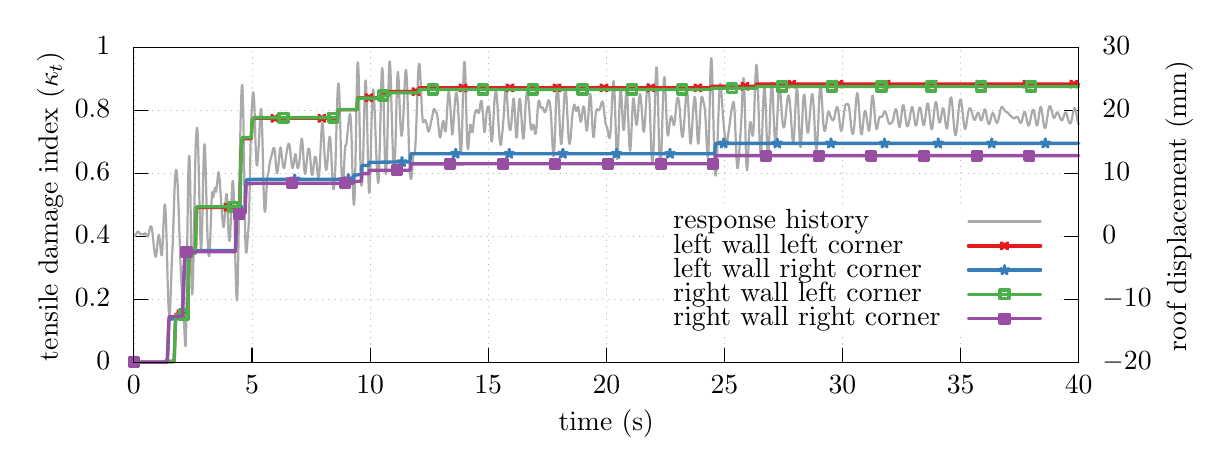
\begin{tikzpicture}[gnuplot]
%% generated with GNUPLOT 5.2p6 (Lua 5.3; terminal rev. Nov 2018, script rev. 107)
%% 08/11/2019 05:00:40
\path (0.000,0.000) rectangle (12.000,4.000);
\gpcolor{color=gp lt color axes}
\gpsetlinetype{gp lt axes}
\gpsetdashtype{gp dt axes}
\gpsetlinewidth{0.50}
\draw[gp path] (0.000,0.000)--(11.999,0.000);
\gpcolor{color=gp lt color border}
\gpsetlinetype{gp lt border}
\gpsetdashtype{gp dt solid}
\gpsetlinewidth{1.00}
\draw[gp path] (0.000,0.000)--(0.180,0.000);
\node[gp node right] at (-0.184,0.000) {$0$};
\gpcolor{color=gp lt color axes}
\gpsetlinetype{gp lt axes}
\gpsetdashtype{gp dt axes}
\gpsetlinewidth{0.50}
\draw[gp path] (0.000,0.800)--(6.735,0.800);
\draw[gp path] (11.699,0.800)--(11.999,0.800);
\gpcolor{color=gp lt color border}
\gpsetlinetype{gp lt border}
\gpsetdashtype{gp dt solid}
\gpsetlinewidth{1.00}
\draw[gp path] (0.000,0.800)--(0.180,0.800);
\node[gp node right] at (-0.184,0.800) {$0.2$};
\gpcolor{color=gp lt color axes}
\gpsetlinetype{gp lt axes}
\gpsetdashtype{gp dt axes}
\gpsetlinewidth{0.50}
\draw[gp path] (0.000,1.600)--(6.735,1.600);
\draw[gp path] (11.699,1.600)--(11.999,1.600);
\gpcolor{color=gp lt color border}
\gpsetlinetype{gp lt border}
\gpsetdashtype{gp dt solid}
\gpsetlinewidth{1.00}
\draw[gp path] (0.000,1.600)--(0.180,1.600);
\node[gp node right] at (-0.184,1.600) {$0.4$};
\gpcolor{color=gp lt color axes}
\gpsetlinetype{gp lt axes}
\gpsetdashtype{gp dt axes}
\gpsetlinewidth{0.50}
\draw[gp path] (0.000,2.399)--(11.999,2.399);
\gpcolor{color=gp lt color border}
\gpsetlinetype{gp lt border}
\gpsetdashtype{gp dt solid}
\gpsetlinewidth{1.00}
\draw[gp path] (0.000,2.399)--(0.180,2.399);
\node[gp node right] at (-0.184,2.399) {$0.6$};
\gpcolor{color=gp lt color axes}
\gpsetlinetype{gp lt axes}
\gpsetdashtype{gp dt axes}
\gpsetlinewidth{0.50}
\draw[gp path] (0.000,3.199)--(11.999,3.199);
\gpcolor{color=gp lt color border}
\gpsetlinetype{gp lt border}
\gpsetdashtype{gp dt solid}
\gpsetlinewidth{1.00}
\draw[gp path] (0.000,3.199)--(0.180,3.199);
\node[gp node right] at (-0.184,3.199) {$0.8$};
\gpcolor{color=gp lt color axes}
\gpsetlinetype{gp lt axes}
\gpsetdashtype{gp dt axes}
\gpsetlinewidth{0.50}
\draw[gp path] (0.000,3.999)--(11.999,3.999);
\gpcolor{color=gp lt color border}
\gpsetlinetype{gp lt border}
\gpsetdashtype{gp dt solid}
\gpsetlinewidth{1.00}
\draw[gp path] (0.000,3.999)--(0.180,3.999);
\node[gp node right] at (-0.184,3.999) {$1$};
\gpcolor{color=gp lt color axes}
\gpsetlinetype{gp lt axes}
\gpsetdashtype{gp dt axes}
\gpsetlinewidth{0.50}
\draw[gp path] (0.000,0.000)--(0.000,3.999);
\gpcolor{color=gp lt color border}
\gpsetlinetype{gp lt border}
\gpsetdashtype{gp dt solid}
\gpsetlinewidth{1.00}
\draw[gp path] (0.000,0.000)--(0.000,0.180);
\node[gp node center] at (0.000,-0.308) {$0$};
\gpcolor{color=gp lt color axes}
\gpsetlinetype{gp lt axes}
\gpsetdashtype{gp dt axes}
\gpsetlinewidth{0.50}
\draw[gp path] (1.500,0.000)--(1.500,3.999);
\gpcolor{color=gp lt color border}
\gpsetlinetype{gp lt border}
\gpsetdashtype{gp dt solid}
\gpsetlinewidth{1.00}
\draw[gp path] (1.500,0.000)--(1.500,0.180);
\node[gp node center] at (1.500,-0.308) {$5$};
\gpcolor{color=gp lt color axes}
\gpsetlinetype{gp lt axes}
\gpsetdashtype{gp dt axes}
\gpsetlinewidth{0.50}
\draw[gp path] (3.000,0.000)--(3.000,3.999);
\gpcolor{color=gp lt color border}
\gpsetlinetype{gp lt border}
\gpsetdashtype{gp dt solid}
\gpsetlinewidth{1.00}
\draw[gp path] (3.000,0.000)--(3.000,0.180);
\node[gp node center] at (3.000,-0.308) {$10$};
\gpcolor{color=gp lt color axes}
\gpsetlinetype{gp lt axes}
\gpsetdashtype{gp dt axes}
\gpsetlinewidth{0.50}
\draw[gp path] (4.500,0.000)--(4.500,3.999);
\gpcolor{color=gp lt color border}
\gpsetlinetype{gp lt border}
\gpsetdashtype{gp dt solid}
\gpsetlinewidth{1.00}
\draw[gp path] (4.500,0.000)--(4.500,0.180);
\node[gp node center] at (4.500,-0.308) {$15$};
\gpcolor{color=gp lt color axes}
\gpsetlinetype{gp lt axes}
\gpsetdashtype{gp dt axes}
\gpsetlinewidth{0.50}
\draw[gp path] (6.000,0.000)--(6.000,3.999);
\gpcolor{color=gp lt color border}
\gpsetlinetype{gp lt border}
\gpsetdashtype{gp dt solid}
\gpsetlinewidth{1.00}
\draw[gp path] (6.000,0.000)--(6.000,0.180);
\node[gp node center] at (6.000,-0.308) {$20$};
\gpcolor{color=gp lt color axes}
\gpsetlinetype{gp lt axes}
\gpsetdashtype{gp dt axes}
\gpsetlinewidth{0.50}
\draw[gp path] (7.499,0.000)--(7.499,0.400);
\draw[gp path] (7.499,1.940)--(7.499,3.999);
\gpcolor{color=gp lt color border}
\gpsetlinetype{gp lt border}
\gpsetdashtype{gp dt solid}
\gpsetlinewidth{1.00}
\draw[gp path] (7.499,0.000)--(7.499,0.180);
\node[gp node center] at (7.499,-0.308) {$25$};
\gpcolor{color=gp lt color axes}
\gpsetlinetype{gp lt axes}
\gpsetdashtype{gp dt axes}
\gpsetlinewidth{0.50}
\draw[gp path] (8.999,0.000)--(8.999,0.400);
\draw[gp path] (8.999,1.940)--(8.999,3.999);
\gpcolor{color=gp lt color border}
\gpsetlinetype{gp lt border}
\gpsetdashtype{gp dt solid}
\gpsetlinewidth{1.00}
\draw[gp path] (8.999,0.000)--(8.999,0.180);
\node[gp node center] at (8.999,-0.308) {$30$};
\gpcolor{color=gp lt color axes}
\gpsetlinetype{gp lt axes}
\gpsetdashtype{gp dt axes}
\gpsetlinewidth{0.50}
\draw[gp path] (10.499,0.000)--(10.499,0.400);
\draw[gp path] (10.499,1.940)--(10.499,3.999);
\gpcolor{color=gp lt color border}
\gpsetlinetype{gp lt border}
\gpsetdashtype{gp dt solid}
\gpsetlinewidth{1.00}
\draw[gp path] (10.499,0.000)--(10.499,0.180);
\node[gp node center] at (10.499,-0.308) {$35$};
\gpcolor{color=gp lt color axes}
\gpsetlinetype{gp lt axes}
\gpsetdashtype{gp dt axes}
\gpsetlinewidth{0.50}
\draw[gp path] (11.999,0.000)--(11.999,3.999);
\gpcolor{color=gp lt color border}
\gpsetlinetype{gp lt border}
\gpsetdashtype{gp dt solid}
\gpsetlinewidth{1.00}
\draw[gp path] (11.999,0.000)--(11.999,0.180);
\node[gp node center] at (11.999,-0.308) {$40$};
\draw[gp path] (11.999,0.000)--(11.819,0.000);
\node[gp node left] at (12.183,0.000) {$-20$};
\draw[gp path] (11.999,0.800)--(11.819,0.800);
\node[gp node left] at (12.183,0.800) {$-10$};
\draw[gp path] (11.999,1.600)--(11.819,1.600);
\node[gp node left] at (12.183,1.600) {$0$};
\draw[gp path] (11.999,2.399)--(11.819,2.399);
\node[gp node left] at (12.183,2.399) {$10$};
\draw[gp path] (11.999,3.199)--(11.819,3.199);
\node[gp node left] at (12.183,3.199) {$20$};
\draw[gp path] (11.999,3.999)--(11.819,3.999);
\node[gp node left] at (12.183,3.999) {$30$};
\draw[gp path] (0.000,3.999)--(0.000,0.000)--(11.999,0.000)--(11.999,3.999)--cycle;
\node[gp node center,rotate=-270] at (-1.044,1.999) {tensile damage index ($\kappa_t$)};
\node[gp node center,rotate=-270] at (13.287,1.999) {roof displacement (\si{\milli\metre})};
\node[gp node center] at (5.999,-0.769) {time (\si{\second})};
\gpcolor{rgb color={0.667,0.667,0.667}}
\gpsetlinewidth{2.00}
\draw[gp path] (0.000,1.600)--(0.003,1.600)--(0.006,1.600)--(0.009,1.602)--(0.012,1.605)%
  --(0.015,1.608)--(0.018,1.613)--(0.021,1.618)--(0.024,1.622)--(0.027,1.627)--(0.030,1.632)%
  --(0.033,1.637)--(0.036,1.642)--(0.039,1.646)--(0.042,1.650)--(0.045,1.653)--(0.048,1.656)%
  --(0.051,1.658)--(0.054,1.658)--(0.057,1.657)--(0.060,1.655)--(0.063,1.651)--(0.066,1.647)%
  --(0.069,1.642)--(0.072,1.638)--(0.075,1.634)--(0.078,1.630)--(0.081,1.628)--(0.084,1.627)%
  --(0.087,1.626)--(0.090,1.626)--(0.093,1.627)--(0.096,1.627)--(0.099,1.628)--(0.102,1.629)%
  --(0.105,1.630)--(0.108,1.630)--(0.111,1.629)--(0.114,1.628)--(0.117,1.626)--(0.120,1.624)%
  --(0.123,1.623)--(0.126,1.623)--(0.129,1.624)--(0.132,1.626)--(0.135,1.629)--(0.138,1.632)%
  --(0.141,1.635)--(0.144,1.637)--(0.147,1.637)--(0.150,1.634)--(0.153,1.629)--(0.156,1.622)%
  --(0.159,1.614)--(0.162,1.607)--(0.165,1.602)--(0.168,1.598)--(0.171,1.596)--(0.174,1.596)%
  --(0.177,1.598)--(0.180,1.602)--(0.183,1.609)--(0.186,1.620)--(0.189,1.632)--(0.192,1.646)%
  --(0.195,1.662)--(0.198,1.677)--(0.201,1.692)--(0.204,1.704)--(0.207,1.714)--(0.210,1.721)%
  --(0.213,1.725)--(0.216,1.726)--(0.219,1.724)--(0.222,1.719)--(0.225,1.709)--(0.228,1.696)%
  --(0.231,1.679)--(0.234,1.658)--(0.237,1.635)--(0.240,1.608)--(0.243,1.578)--(0.246,1.547)%
  --(0.249,1.516)--(0.252,1.486)--(0.255,1.458)--(0.258,1.431)--(0.261,1.407)--(0.264,1.385)%
  --(0.267,1.366)--(0.270,1.352)--(0.273,1.343)--(0.276,1.340)--(0.279,1.344)--(0.282,1.354)%
  --(0.285,1.370)--(0.288,1.392)--(0.291,1.419)--(0.294,1.450)--(0.297,1.483)--(0.300,1.515)%
  --(0.303,1.545)--(0.306,1.571)--(0.309,1.593)--(0.312,1.608)--(0.315,1.616)--(0.318,1.616)%
  --(0.321,1.606)--(0.324,1.589)--(0.327,1.566)--(0.330,1.538)--(0.333,1.507)--(0.336,1.474)%
  --(0.339,1.442)--(0.342,1.413)--(0.345,1.387)--(0.348,1.368)--(0.351,1.357)--(0.354,1.358)%
  --(0.357,1.373)--(0.360,1.404)--(0.363,1.452)--(0.366,1.512)--(0.369,1.581)--(0.372,1.654)%
  --(0.375,1.728)--(0.378,1.801)--(0.381,1.867)--(0.384,1.924)--(0.387,1.968)--(0.390,1.995)%
  --(0.393,2.005)--(0.396,1.997)--(0.399,1.971)--(0.402,1.927)--(0.405,1.866)--(0.408,1.789)%
  --(0.411,1.698)--(0.414,1.597)--(0.417,1.487)--(0.420,1.373)--(0.423,1.255)--(0.426,1.139)%
  --(0.429,1.026)--(0.432,0.922)--(0.435,0.828)--(0.438,0.748)--(0.441,0.685)--(0.444,0.638)%
  --(0.447,0.608)--(0.450,0.595)--(0.453,0.602)--(0.456,0.626)--(0.459,0.669)--(0.462,0.728)%
  --(0.465,0.799)--(0.468,0.879)--(0.471,0.966)--(0.474,1.056)--(0.477,1.145)--(0.480,1.228)%
  --(0.483,1.302)--(0.486,1.366)--(0.489,1.423)--(0.492,1.482)--(0.495,1.550)--(0.498,1.631)%
  --(0.501,1.724)--(0.504,1.823)--(0.507,1.923)--(0.510,2.018)--(0.513,2.108)--(0.516,2.190)%
  --(0.519,2.261)--(0.522,2.318)--(0.525,2.364)--(0.528,2.398)--(0.531,2.422)--(0.534,2.437)%
  --(0.537,2.442)--(0.540,2.437)--(0.543,2.422)--(0.546,2.395)--(0.549,2.360)--(0.552,2.315)%
  --(0.555,2.262)--(0.558,2.199)--(0.561,2.129)--(0.564,2.051)--(0.567,1.969)--(0.570,1.884)%
  --(0.573,1.797)--(0.576,1.708)--(0.579,1.619)--(0.582,1.530)--(0.585,1.444)--(0.588,1.362)%
  --(0.591,1.283)--(0.594,1.209)--(0.597,1.139)--(0.600,1.075)--(0.603,1.017)--(0.606,0.964)%
  --(0.609,0.917)--(0.612,0.873)--(0.615,0.831)--(0.618,0.790)--(0.621,0.751)--(0.624,0.711)%
  --(0.627,0.669)--(0.630,0.624)--(0.633,0.573)--(0.636,0.517)--(0.639,0.456)--(0.642,0.393)%
  --(0.645,0.331)--(0.648,0.273)--(0.651,0.226)--(0.654,0.202)--(0.657,0.216)--(0.660,0.282)%
  --(0.663,0.408)--(0.666,0.586)--(0.669,0.799)--(0.672,1.031)--(0.675,1.272)--(0.678,1.518)%
  --(0.681,1.763)--(0.684,1.994)--(0.687,2.195)--(0.690,2.353)--(0.693,2.470)--(0.696,2.552)%
  --(0.699,2.602)--(0.702,2.622)--(0.705,2.611)--(0.708,2.561)--(0.711,2.467)--(0.714,2.332)%
  --(0.717,2.164)--(0.720,1.971)--(0.723,1.762)--(0.726,1.541)--(0.729,1.319)--(0.732,1.121)%
  --(0.735,0.972)--(0.738,0.886)--(0.741,0.862)--(0.744,0.884)--(0.747,0.939)--(0.750,1.025)%
  --(0.753,1.143)--(0.756,1.295)--(0.759,1.472)--(0.762,1.653)--(0.765,1.823)--(0.768,1.977)%
  --(0.771,2.122)--(0.774,2.268)--(0.777,2.417)--(0.780,2.558)--(0.783,2.678)--(0.786,2.771)%
  --(0.789,2.838)--(0.792,2.890)--(0.795,2.930)--(0.798,2.961)--(0.801,2.978)--(0.804,2.973)%
  --(0.807,2.942)--(0.810,2.885)--(0.813,2.811)--(0.816,2.723)--(0.819,2.623)--(0.822,2.509)%
  --(0.825,2.380)--(0.828,2.241)--(0.831,2.100)--(0.834,1.964)--(0.837,1.836)--(0.840,1.718)%
  --(0.843,1.611)--(0.846,1.524)--(0.849,1.464)--(0.852,1.436)--(0.855,1.442)--(0.858,1.478)%
  --(0.861,1.542)--(0.864,1.630)--(0.867,1.740)--(0.870,1.869)--(0.873,2.010)--(0.876,2.153)%
  --(0.879,2.293)--(0.882,2.424)--(0.885,2.540)--(0.888,2.637)--(0.891,2.711)--(0.894,2.756)%
  --(0.897,2.769)--(0.900,2.751)--(0.903,2.702)--(0.906,2.628)--(0.909,2.535)--(0.912,2.429)%
  --(0.915,2.316)--(0.918,2.200)--(0.921,2.083)--(0.924,1.966)--(0.927,1.853)--(0.930,1.747)%
  --(0.933,1.653)--(0.936,1.571)--(0.939,1.502)--(0.942,1.445)--(0.945,1.401)--(0.948,1.370)%
  --(0.951,1.352)--(0.954,1.346)--(0.957,1.350)--(0.960,1.367)--(0.963,1.402)--(0.966,1.457)%
  --(0.969,1.533)--(0.972,1.623)--(0.975,1.718)--(0.978,1.811)--(0.981,1.899)--(0.984,1.981)%
  --(0.987,2.055)--(0.990,2.113)--(0.993,2.151)--(0.996,2.162)--(0.999,2.149)--(1.002,2.124)%
  --(1.005,2.101)--(1.008,2.093)--(1.011,2.102)--(1.014,2.122)--(1.017,2.144)--(1.020,2.164)%
  --(1.023,2.180)--(1.026,2.197)--(1.029,2.211)--(1.032,2.218)--(1.035,2.211)--(1.038,2.192)%
  --(1.041,2.172)--(1.044,2.166)--(1.047,2.179)--(1.050,2.206)--(1.053,2.236)--(1.056,2.263)%
  --(1.059,2.287)--(1.062,2.316)--(1.065,2.349)--(1.068,2.382)--(1.071,2.405)--(1.074,2.412)%
  --(1.077,2.405)--(1.080,2.389)--(1.083,2.367)--(1.086,2.340)--(1.089,2.307)--(1.092,2.267)%
  --(1.095,2.222)--(1.098,2.178)--(1.101,2.134)--(1.104,2.091)--(1.107,2.047)--(1.110,2.002)%
  --(1.113,1.959)--(1.116,1.918)--(1.119,1.881)--(1.122,1.847)--(1.125,1.814)--(1.128,1.782)%
  --(1.131,1.753)--(1.134,1.730)--(1.137,1.717)--(1.140,1.715)--(1.143,1.725)--(1.146,1.747)%
  --(1.149,1.780)--(1.152,1.823)--(1.155,1.874)--(1.158,1.928)--(1.161,1.982)--(1.164,2.031)%
  --(1.167,2.074)--(1.170,2.108)--(1.173,2.131)--(1.176,2.138)--(1.179,2.128)--(1.182,2.100)%
  --(1.185,2.055)--(1.188,1.992)--(1.191,1.915)--(1.194,1.831)--(1.197,1.748)--(1.200,1.676)%
  --(1.203,1.620)--(1.206,1.580)--(1.209,1.556)--(1.212,1.543)--(1.215,1.542)--(1.218,1.557)%
  --(1.221,1.591)--(1.224,1.643)--(1.227,1.711)--(1.230,1.787)--(1.233,1.868)--(1.236,1.951)%
  --(1.239,2.033)--(1.242,2.112)--(1.245,2.183)--(1.248,2.240)--(1.251,2.280)--(1.254,2.300)%
  --(1.257,2.302)--(1.260,2.284)--(1.263,2.246)--(1.266,2.186)--(1.269,2.106)--(1.272,2.008)%
  --(1.275,1.895)--(1.278,1.771)--(1.281,1.640)--(1.284,1.504)--(1.287,1.368)--(1.290,1.237)%
  --(1.293,1.116)--(1.296,1.013)--(1.299,0.928)--(1.302,0.860)--(1.305,0.810)--(1.308,0.784)%
  --(1.311,0.794)--(1.314,0.846)--(1.317,0.944)--(1.320,1.076)--(1.323,1.227)--(1.326,1.388)%
  --(1.329,1.553)--(1.332,1.730)--(1.335,1.920)--(1.338,2.116)--(1.341,2.310)--(1.344,2.495)%
  --(1.347,2.668)--(1.350,2.829)--(1.353,2.975)--(1.356,3.106)--(1.359,3.222)--(1.362,3.323)%
  --(1.365,3.406)--(1.368,3.469)--(1.371,3.509)--(1.374,3.524)--(1.377,3.512)--(1.380,3.472)%
  --(1.383,3.402)--(1.386,3.299)--(1.389,3.164)--(1.392,3.000)--(1.395,2.810)--(1.398,2.602)%
  --(1.401,2.380)--(1.404,2.159)--(1.407,1.954)--(1.410,1.778)--(1.413,1.639)--(1.416,1.535)%
  --(1.419,1.464)--(1.422,1.420)--(1.425,1.397)--(1.428,1.391)--(1.431,1.400)--(1.434,1.422)%
  --(1.437,1.459)--(1.440,1.505)--(1.443,1.554)--(1.446,1.599)--(1.449,1.637)--(1.452,1.670)%
  --(1.455,1.703)--(1.458,1.750)--(1.461,1.823)--(1.464,1.925)--(1.467,2.053)--(1.470,2.194)%
  --(1.473,2.341)--(1.476,2.486)--(1.479,2.627)--(1.482,2.762)--(1.485,2.886)--(1.488,2.992)%
  --(1.491,3.079)--(1.494,3.149)--(1.497,3.210)--(1.500,3.266)--(1.503,3.318)--(1.506,3.364)%
  --(1.509,3.400)--(1.512,3.422)--(1.515,3.429)--(1.518,3.421)--(1.521,3.400)--(1.524,3.367)%
  --(1.527,3.318)--(1.530,3.253)--(1.533,3.171)--(1.536,3.076)--(1.539,2.974)--(1.542,2.873)%
  --(1.545,2.778)--(1.548,2.694)--(1.551,2.623)--(1.554,2.566)--(1.557,2.525)--(1.560,2.502)%
  --(1.563,2.496)--(1.566,2.507)--(1.569,2.530)--(1.572,2.563)--(1.575,2.603)--(1.578,2.646)%
  --(1.581,2.689)--(1.584,2.733)--(1.587,2.780)--(1.590,2.833)--(1.593,2.895)--(1.596,2.965)%
  --(1.599,3.034)--(1.602,3.096)--(1.605,3.146)--(1.608,3.183)--(1.611,3.207)--(1.614,3.218)%
  --(1.617,3.210)--(1.620,3.180)--(1.623,3.126)--(1.626,3.050)--(1.629,2.954)--(1.632,2.844)%
  --(1.635,2.720)--(1.638,2.586)--(1.641,2.450)--(1.644,2.320)--(1.647,2.202)--(1.650,2.104)%
  --(1.653,2.026)--(1.656,1.969)--(1.659,1.931)--(1.662,1.912)--(1.665,1.912)--(1.668,1.929)%
  --(1.671,1.961)--(1.674,2.004)--(1.677,2.055)--(1.680,2.111)--(1.683,2.168)--(1.686,2.223)%
  --(1.689,2.274)--(1.692,2.315)--(1.695,2.347)--(1.698,2.368)--(1.701,2.383)--(1.704,2.394)%
  --(1.707,2.407)--(1.710,2.422)--(1.713,2.441)--(1.716,2.463)--(1.719,2.485)--(1.722,2.507)%
  --(1.725,2.528)--(1.728,2.546)--(1.731,2.561)--(1.734,2.573)--(1.737,2.583)--(1.740,2.591)%
  --(1.743,2.601)--(1.746,2.613)--(1.749,2.627)--(1.752,2.640)--(1.755,2.653)--(1.758,2.665)%
  --(1.761,2.676)--(1.764,2.688)--(1.767,2.700)--(1.770,2.710)--(1.773,2.718)--(1.776,2.721)%
  --(1.779,2.721)--(1.782,2.717)--(1.785,2.708)--(1.788,2.692)--(1.791,2.669)--(1.794,2.639)%
  --(1.797,2.601)--(1.800,2.559)--(1.803,2.517)--(1.806,2.478)--(1.809,2.444)--(1.812,2.419)%
  --(1.815,2.405)--(1.818,2.402)--(1.821,2.408)--(1.824,2.421)--(1.827,2.438)--(1.830,2.458)%
  --(1.833,2.481)--(1.836,2.507)--(1.839,2.536)--(1.842,2.569)--(1.845,2.604)--(1.848,2.637)%
  --(1.851,2.668)--(1.854,2.693)--(1.857,2.712)--(1.860,2.724)--(1.863,2.728)--(1.866,2.722)%
  --(1.869,2.707)--(1.872,2.683)--(1.875,2.655)--(1.878,2.625)--(1.881,2.596)--(1.884,2.570)%
  --(1.887,2.545)--(1.890,2.523)--(1.893,2.504)--(1.896,2.488)--(1.899,2.477)--(1.902,2.469)%
  --(1.905,2.466)--(1.908,2.467)--(1.911,2.474)--(1.914,2.486)--(1.917,2.503)--(1.920,2.523)%
  --(1.923,2.546)--(1.926,2.569)--(1.929,2.593)--(1.932,2.616)--(1.935,2.637)--(1.938,2.657)%
  --(1.941,2.674)--(1.944,2.690)--(1.947,2.705)--(1.950,2.721)--(1.953,2.738)--(1.956,2.753)%
  --(1.959,2.765)--(1.962,2.772)--(1.965,2.776)--(1.968,2.775)--(1.971,2.771)--(1.974,2.763)%
  --(1.977,2.751)--(1.980,2.734)--(1.983,2.712)--(1.986,2.686)--(1.989,2.656)--(1.992,2.624)%
  --(1.995,2.592)--(1.998,2.561)--(2.001,2.534)--(2.004,2.512)--(2.007,2.494)--(2.010,2.480)%
  --(2.013,2.471)--(2.016,2.467)--(2.019,2.470)--(2.022,2.480)--(2.025,2.495)--(2.028,2.513)%
  --(2.031,2.533)--(2.034,2.555)--(2.037,2.578)--(2.040,2.600)--(2.043,2.619)--(2.046,2.634)%
  --(2.049,2.642)--(2.052,2.643)--(2.055,2.636)--(2.058,2.620)--(2.061,2.596)--(2.064,2.565)%
  --(2.067,2.533)--(2.070,2.505)--(2.073,2.485)--(2.076,2.473)--(2.079,2.467)--(2.082,2.466)%
  --(2.085,2.468)--(2.088,2.474)--(2.091,2.485)--(2.094,2.499)--(2.097,2.515)--(2.100,2.534)%
  --(2.103,2.557)--(2.106,2.584)--(2.109,2.617)--(2.112,2.655)--(2.115,2.695)--(2.118,2.734)%
  --(2.121,2.768)--(2.124,2.797)--(2.127,2.820)--(2.130,2.835)--(2.133,2.839)--(2.136,2.832)%
  --(2.139,2.812)--(2.142,2.781)--(2.145,2.741)--(2.148,2.694)--(2.151,2.642)--(2.154,2.590)%
  --(2.157,2.541)--(2.160,2.497)--(2.163,2.461)--(2.166,2.432)--(2.169,2.410)--(2.172,2.396)%
  --(2.175,2.391)--(2.178,2.396)--(2.181,2.411)--(2.184,2.433)--(2.187,2.461)--(2.190,2.492)%
  --(2.193,2.526)--(2.196,2.561)--(2.199,2.596)--(2.202,2.629)--(2.205,2.657)--(2.208,2.679)%
  --(2.211,2.695)--(2.214,2.705)--(2.217,2.711)--(2.220,2.713)--(2.223,2.712)--(2.226,2.705)%
  --(2.229,2.692)--(2.232,2.673)--(2.235,2.647)--(2.238,2.615)--(2.241,2.578)--(2.244,2.538)%
  --(2.247,2.498)--(2.250,2.462)--(2.253,2.431)--(2.256,2.407)--(2.259,2.390)--(2.262,2.380)%
  --(2.265,2.378)--(2.268,2.384)--(2.271,2.398)--(2.274,2.418)--(2.277,2.442)--(2.280,2.469)%
  --(2.283,2.498)--(2.286,2.527)--(2.289,2.554)--(2.292,2.577)--(2.295,2.595)--(2.298,2.607)%
  --(2.301,2.612)--(2.304,2.611)--(2.307,2.606)--(2.310,2.596)--(2.313,2.583)--(2.316,2.565)%
  --(2.319,2.543)--(2.322,2.516)--(2.325,2.485)--(2.328,2.451)--(2.331,2.419)--(2.334,2.390)%
  --(2.337,2.366)--(2.340,2.349)--(2.343,2.338)--(2.346,2.336)--(2.349,2.346)--(2.352,2.367)%
  --(2.355,2.401)--(2.358,2.444)--(2.361,2.495)--(2.364,2.553)--(2.367,2.615)--(2.370,2.682)%
  --(2.373,2.750)--(2.376,2.816)--(2.379,2.877)--(2.382,2.932)--(2.385,2.977)--(2.388,3.013)%
  --(2.391,3.035)--(2.394,3.041)--(2.397,3.028)--(2.400,2.999)--(2.403,2.958)--(2.406,2.910)%
  --(2.409,2.859)--(2.412,2.806)--(2.415,2.751)--(2.418,2.696)--(2.421,2.642)--(2.424,2.593)%
  --(2.427,2.549)--(2.430,2.512)--(2.433,2.483)--(2.436,2.461)--(2.439,2.447)--(2.442,2.442)%
  --(2.445,2.446)--(2.448,2.459)--(2.451,2.480)--(2.454,2.506)--(2.457,2.538)--(2.460,2.575)%
  --(2.463,2.616)--(2.466,2.659)--(2.469,2.704)--(2.472,2.746)--(2.475,2.784)--(2.478,2.816)%
  --(2.481,2.841)--(2.484,2.858)--(2.487,2.864)--(2.490,2.858)--(2.493,2.841)--(2.496,2.811)%
  --(2.499,2.772)--(2.502,2.723)--(2.505,2.668)--(2.508,2.608)--(2.511,2.544)--(2.514,2.480)%
  --(2.517,2.418)--(2.520,2.360)--(2.523,2.308)--(2.526,2.265)--(2.529,2.231)--(2.532,2.208)%
  --(2.535,2.197)--(2.538,2.200)--(2.541,2.214)--(2.544,2.240)--(2.547,2.275)--(2.550,2.318)%
  --(2.553,2.368)--(2.556,2.426)--(2.559,2.495)--(2.562,2.580)--(2.565,2.680)--(2.568,2.792)%
  --(2.571,2.910)--(2.574,3.026)--(2.577,3.138)--(2.580,3.242)--(2.583,3.336)--(2.586,3.416)%
  --(2.589,3.478)--(2.592,3.518)--(2.595,3.538)--(2.598,3.540)--(2.601,3.526)--(2.604,3.497)%
  --(2.607,3.451)--(2.610,3.383)--(2.613,3.296)--(2.616,3.193)--(2.619,3.080)--(2.622,2.963)%
  --(2.625,2.843)--(2.628,2.724)--(2.631,2.609)--(2.634,2.504)--(2.637,2.415)--(2.640,2.343)%
  --(2.643,2.288)--(2.646,2.248)--(2.649,2.224)--(2.652,2.217)--(2.655,2.231)--(2.658,2.264)%
  --(2.661,2.312)--(2.664,2.370)--(2.667,2.434)--(2.670,2.500)--(2.673,2.566)--(2.676,2.628)%
  --(2.679,2.683)--(2.682,2.725)--(2.685,2.749)--(2.688,2.757)--(2.691,2.754)--(2.694,2.751)%
  --(2.697,2.758)--(2.700,2.779)--(2.703,2.810)--(2.706,2.843)--(2.709,2.872)--(2.712,2.898)%
  --(2.715,2.923)--(2.718,2.953)--(2.721,2.989)--(2.724,3.025)--(2.727,3.058)--(2.730,3.086)%
  --(2.733,3.108)--(2.736,3.127)--(2.739,3.141)--(2.742,3.150)--(2.745,3.152)--(2.748,3.142)%
  --(2.751,3.120)--(2.754,3.086)--(2.757,3.038)--(2.760,2.975)--(2.763,2.894)--(2.766,2.797)%
  --(2.769,2.683)--(2.772,2.560)--(2.775,2.435)--(2.778,2.319)--(2.781,2.218)--(2.784,2.134)%
  --(2.787,2.069)--(2.790,2.023)--(2.793,1.999)--(2.796,1.999)--(2.799,2.025)--(2.802,2.079)%
  --(2.805,2.160)--(2.808,2.267)--(2.811,2.396)--(2.814,2.545)--(2.817,2.710)--(2.820,2.887)%
  --(2.823,3.068)--(2.826,3.243)--(2.829,3.405)--(2.832,3.545)--(2.835,3.659)--(2.838,3.740)%
  --(2.841,3.789)--(2.844,3.809)--(2.847,3.802)--(2.850,3.765)--(2.853,3.694)--(2.856,3.584)%
  --(2.859,3.437)--(2.862,3.266)--(2.865,3.091)--(2.868,2.927)--(2.871,2.779)--(2.874,2.643)%
  --(2.877,2.519)--(2.880,2.409)--(2.883,2.323)--(2.886,2.268)--(2.889,2.244)--(2.892,2.242)%
  --(2.895,2.256)--(2.898,2.280)--(2.901,2.314)--(2.904,2.364)--(2.907,2.437)--(2.910,2.534)%
  --(2.913,2.651)--(2.916,2.779)--(2.919,2.910)--(2.922,3.038)--(2.925,3.162)--(2.928,3.279)%
  --(2.931,3.383)--(2.934,3.469)--(2.937,3.531)--(2.940,3.568)--(2.943,3.579)--(2.946,3.564)%
  --(2.949,3.523)--(2.952,3.455)--(2.955,3.361)--(2.958,3.244)--(2.961,3.111)--(2.964,2.966)%
  --(2.967,2.818)--(2.970,2.671)--(2.973,2.533)--(2.976,2.410)--(2.979,2.308)--(2.982,2.230)%
  --(2.985,2.177)--(2.988,2.152)--(2.991,2.156)--(2.994,2.189)--(2.997,2.249)--(3.000,2.333)%
  --(3.003,2.437)--(3.006,2.554)--(3.009,2.678)--(3.012,2.804)--(3.015,2.925)--(3.018,3.039)%
  --(3.021,3.143)--(3.024,3.236)--(3.027,3.316)--(3.030,3.381)--(3.033,3.428)--(3.036,3.455)%
  --(3.039,3.463)--(3.042,3.453)--(3.045,3.428)--(3.048,3.390)--(3.051,3.340)--(3.054,3.280)%
  --(3.057,3.211)--(3.060,3.136)--(3.063,3.056)--(3.066,2.974)--(3.069,2.893)--(3.072,2.812)%
  --(3.075,2.734)--(3.078,2.660)--(3.081,2.589)--(3.084,2.524)--(3.087,2.463)--(3.090,2.409)%
  --(3.093,2.360)--(3.096,2.319)--(3.099,2.290)--(3.102,2.277)--(3.105,2.283)--(3.108,2.311)%
  --(3.111,2.362)--(3.114,2.434)--(3.117,2.524)--(3.120,2.628)--(3.123,2.741)--(3.126,2.863)%
  --(3.129,2.992)--(3.132,3.125)--(3.135,3.260)--(3.138,3.388)--(3.141,3.503)--(3.144,3.598)%
  --(3.147,3.669)--(3.150,3.714)--(3.153,3.733)--(3.156,3.726)--(3.159,3.694)--(3.162,3.639)%
  --(3.165,3.558)--(3.168,3.452)--(3.171,3.327)--(3.174,3.190)--(3.177,3.050)--(3.180,2.914)%
  --(3.183,2.786)--(3.186,2.670)--(3.189,2.567)--(3.192,2.485)--(3.195,2.427)--(3.198,2.395)%
  --(3.201,2.389)--(3.204,2.406)--(3.207,2.446)--(3.210,2.507)--(3.213,2.592)--(3.216,2.698)%
  --(3.219,2.822)--(3.222,2.959)--(3.225,3.101)--(3.228,3.245)--(3.231,3.384)--(3.234,3.513)%
  --(3.237,3.625)--(3.240,3.715)--(3.243,3.779)--(3.246,3.814)--(3.249,3.821)--(3.252,3.804)%
  --(3.255,3.767)--(3.258,3.710)--(3.261,3.634)--(3.264,3.540)--(3.267,3.431)--(3.270,3.315)%
  --(3.273,3.198)--(3.276,3.086)--(3.279,2.980)--(3.282,2.879)--(3.285,2.784)--(3.288,2.698)%
  --(3.291,2.625)--(3.294,2.568)--(3.297,2.524)--(3.300,2.492)--(3.303,2.473)--(3.306,2.468)%
  --(3.309,2.481)--(3.312,2.515)--(3.315,2.570)--(3.318,2.644)--(3.321,2.736)--(3.324,2.842)%
  --(3.327,2.959)--(3.330,3.083)--(3.333,3.208)--(3.336,3.328)--(3.339,3.436)--(3.342,3.528)%
  --(3.345,3.602)--(3.348,3.654)--(3.351,3.683)--(3.354,3.686)--(3.357,3.665)--(3.360,3.624)%
  --(3.363,3.567)--(3.366,3.500)--(3.369,3.424)--(3.372,3.345)--(3.375,3.263)--(3.378,3.184)%
  --(3.381,3.110)--(3.384,3.045)--(3.387,2.989)--(3.390,2.944)--(3.393,2.910)--(3.396,2.887)%
  --(3.399,2.876)--(3.402,2.878)--(3.405,2.891)--(3.408,2.913)--(3.411,2.943)--(3.414,2.982)%
  --(3.417,3.029)--(3.420,3.084)--(3.423,3.147)--(3.426,3.214)--(3.429,3.284)--(3.432,3.357)%
  --(3.435,3.430)--(3.438,3.501)--(3.441,3.568)--(3.444,3.624)--(3.447,3.668)--(3.450,3.697)%
  --(3.453,3.711)--(3.456,3.710)--(3.459,3.694)--(3.462,3.662)--(3.465,3.614)--(3.468,3.550)%
  --(3.471,3.473)--(3.474,3.386)--(3.477,3.290)--(3.480,3.188)--(3.483,3.081)--(3.486,2.973)%
  --(3.489,2.867)--(3.492,2.765)--(3.495,2.671)--(3.498,2.586)--(3.501,2.511)--(3.504,2.447)%
  --(3.507,2.397)--(3.510,2.361)--(3.513,2.338)--(3.516,2.327)--(3.519,2.326)--(3.522,2.334)%
  --(3.525,2.348)--(3.528,2.371)--(3.531,2.402)--(3.534,2.440)--(3.537,2.481)--(3.540,2.523)%
  --(3.543,2.561)--(3.546,2.595)--(3.549,2.624)--(3.552,2.644)--(3.555,2.656)--(3.558,2.660)%
  --(3.561,2.659)--(3.564,2.660)--(3.567,2.670)--(3.570,2.691)--(3.573,2.724)--(3.576,2.769)%
  --(3.579,2.826)--(3.582,2.894)--(3.585,2.973)--(3.588,3.058)--(3.591,3.147)--(3.594,3.235)%
  --(3.597,3.322)--(3.600,3.408)--(3.603,3.493)--(3.606,3.572)--(3.609,3.644)--(3.612,3.702)%
  --(3.615,3.745)--(3.618,3.773)--(3.621,3.787)--(3.624,3.790)--(3.627,3.780)--(3.630,3.758)%
  --(3.633,3.723)--(3.636,3.675)--(3.639,3.616)--(3.642,3.551)--(3.645,3.483)--(3.648,3.415)%
  --(3.651,3.346)--(3.654,3.279)--(3.657,3.216)--(3.660,3.161)--(3.663,3.117)--(3.666,3.084)%
  --(3.669,3.063)--(3.672,3.050)--(3.675,3.047)--(3.678,3.049)--(3.681,3.055)--(3.684,3.062)%
  --(3.687,3.067)--(3.690,3.071)--(3.693,3.074)--(3.696,3.076)--(3.699,3.075)--(3.702,3.071)%
  --(3.705,3.063)--(3.708,3.053)--(3.711,3.045)--(3.714,3.038)--(3.717,3.030)--(3.720,3.019)%
  --(3.723,3.004)--(3.726,2.986)--(3.729,2.969)--(3.732,2.954)--(3.735,2.943)--(3.738,2.935)%
  --(3.741,2.930)--(3.744,2.930)--(3.747,2.934)--(3.750,2.944)--(3.753,2.955)--(3.756,2.967)%
  --(3.759,2.978)--(3.762,2.990)--(3.765,3.005)--(3.768,3.021)--(3.771,3.038)--(3.774,3.052)%
  --(3.777,3.065)--(3.780,3.076)--(3.783,3.090)--(3.786,3.105)--(3.789,3.121)--(3.792,3.136)%
  --(3.795,3.150)--(3.798,3.164)--(3.801,3.179)--(3.804,3.193)--(3.807,3.206)--(3.810,3.214)%
  --(3.813,3.217)--(3.816,3.215)--(3.819,3.211)--(3.822,3.206)--(3.825,3.200)--(3.828,3.193)%
  --(3.831,3.186)--(3.834,3.181)--(3.837,3.177)--(3.840,3.174)--(3.843,3.170)--(3.846,3.162)%
  --(3.849,3.151)--(3.852,3.136)--(3.855,3.118)--(3.858,3.096)--(3.861,3.070)--(3.864,3.041)%
  --(3.867,3.010)--(3.870,2.979)--(3.873,2.949)--(3.876,2.921)--(3.879,2.895)--(3.882,2.874)%
  --(3.885,2.860)--(3.888,2.853)--(3.891,2.854)--(3.894,2.862)--(3.897,2.877)--(3.900,2.895)%
  --(3.903,2.917)--(3.906,2.940)--(3.909,2.965)--(3.912,2.990)--(3.915,3.013)--(3.918,3.032)%
  --(3.921,3.048)--(3.924,3.059)--(3.927,3.064)--(3.930,3.063)--(3.933,3.054)--(3.936,3.039)%
  --(3.939,3.017)--(3.942,2.993)--(3.945,2.969)--(3.948,2.949)--(3.951,2.936)--(3.954,2.931)%
  --(3.957,2.934)--(3.960,2.946)--(3.963,2.967)--(3.966,2.997)--(3.969,3.037)--(3.972,3.085)%
  --(3.975,3.137)--(3.978,3.191)--(3.981,3.245)--(3.984,3.296)--(3.987,3.343)--(3.990,3.383)%
  --(3.993,3.414)--(3.996,3.431)--(3.999,3.432)--(4.002,3.419)--(4.005,3.398)--(4.008,3.372)%
  --(4.011,3.343)--(4.014,3.312)--(4.017,3.276)--(4.020,3.232)--(4.023,3.183)--(4.026,3.130)%
  --(4.029,3.076)--(4.032,3.023)--(4.035,2.972)--(4.038,2.930)--(4.041,2.902)--(4.044,2.892)%
  --(4.047,2.902)--(4.050,2.926)--(4.053,2.958)--(4.056,2.996)--(4.059,3.037)--(4.062,3.081)%
  --(4.065,3.129)--(4.068,3.176)--(4.071,3.221)--(4.074,3.261)--(4.077,3.298)--(4.080,3.333)%
  --(4.083,3.364)--(4.086,3.391)--(4.089,3.411)--(4.092,3.421)--(4.095,3.423)--(4.098,3.418)%
  --(4.101,3.406)--(4.104,3.388)--(4.107,3.360)--(4.110,3.324)--(4.113,3.281)--(4.116,3.234)%
  --(4.119,3.185)--(4.122,3.133)--(4.125,3.078)--(4.128,3.021)--(4.131,2.964)--(4.134,2.909)%
  --(4.137,2.854)--(4.140,2.799)--(4.143,2.747)--(4.146,2.699)--(4.149,2.665)--(4.152,2.649)%
  --(4.155,2.657)--(4.158,2.688)--(4.161,2.743)--(4.164,2.818)--(4.167,2.912)--(4.170,3.020)%
  --(4.173,3.140)--(4.176,3.263)--(4.179,3.384)--(4.182,3.498)--(4.185,3.600)--(4.188,3.686)%
  --(4.191,3.752)--(4.194,3.796)--(4.197,3.815)--(4.200,3.810)--(4.203,3.780)--(4.206,3.726)%
  --(4.209,3.648)--(4.212,3.550)--(4.215,3.437)--(4.218,3.316)--(4.221,3.197)--(4.224,3.085)%
  --(4.227,2.983)--(4.230,2.893)--(4.233,2.816)--(4.236,2.758)--(4.239,2.721)--(4.242,2.706)%
  --(4.245,2.710)--(4.248,2.729)--(4.251,2.758)--(4.254,2.796)--(4.257,2.838)--(4.260,2.883)%
  --(4.263,2.926)--(4.266,2.963)--(4.269,2.992)--(4.272,3.010)--(4.275,3.017)--(4.278,3.014)%
  --(4.281,3.002)--(4.284,2.985)--(4.287,2.964)--(4.290,2.944)--(4.293,2.928)--(4.296,2.920)%
  --(4.299,2.920)--(4.302,2.930)--(4.305,2.948)--(4.308,2.973)--(4.311,3.002)--(4.314,3.035)%
  --(4.317,3.067)--(4.320,3.097)--(4.323,3.122)--(4.326,3.142)--(4.329,3.156)--(4.332,3.166)%
  --(4.335,3.174)--(4.338,3.181)--(4.341,3.188)--(4.344,3.194)--(4.347,3.199)--(4.350,3.202)%
  --(4.353,3.203)--(4.356,3.202)--(4.359,3.198)--(4.362,3.192)--(4.365,3.185)--(4.368,3.178)%
  --(4.371,3.172)--(4.374,3.168)--(4.377,3.166)--(4.380,3.166)--(4.383,3.170)--(4.386,3.180)%
  --(4.389,3.195)--(4.392,3.215)--(4.395,3.239)--(4.398,3.263)--(4.401,3.284)--(4.404,3.301)%
  --(4.407,3.313)--(4.410,3.320)--(4.413,3.321)--(4.416,3.314)--(4.419,3.298)--(4.422,3.275)%
  --(4.425,3.246)--(4.428,3.212)--(4.431,3.174)--(4.434,3.132)--(4.437,3.086)--(4.440,3.038)%
  --(4.443,2.993)--(4.446,2.956)--(4.449,2.931)--(4.452,2.922)--(4.455,2.926)--(4.458,2.942)%
  --(4.461,2.966)--(4.464,2.995)--(4.467,3.030)--(4.470,3.067)--(4.473,3.105)--(4.476,3.138)%
  --(4.479,3.166)--(4.482,3.187)--(4.485,3.204)--(4.488,3.217)--(4.491,3.229)--(4.494,3.238)%
  --(4.497,3.246)--(4.500,3.249)--(4.503,3.249)--(4.506,3.244)--(4.509,3.234)--(4.512,3.215)%
  --(4.515,3.188)--(4.518,3.152)--(4.521,3.108)--(4.524,3.059)--(4.527,3.005)--(4.530,2.952)%
  --(4.533,2.902)--(4.536,2.860)--(4.539,2.828)--(4.542,2.809)--(4.545,2.803)--(4.548,2.811)%
  --(4.551,2.832)--(4.554,2.865)--(4.557,2.910)--(4.560,2.963)--(4.563,3.022)--(4.566,3.084)%
  --(4.569,3.145)--(4.572,3.204)--(4.575,3.256)--(4.578,3.301)--(4.581,3.339)--(4.584,3.370)%
  --(4.587,3.395)--(4.590,3.415)--(4.593,3.428)--(4.596,3.435)--(4.599,3.435)--(4.602,3.427)%
  --(4.605,3.412)--(4.608,3.387)--(4.611,3.354)--(4.614,3.313)--(4.617,3.265)--(4.620,3.212)%
  --(4.623,3.157)--(4.626,3.103)--(4.629,3.052)--(4.632,3.003)--(4.635,2.958)--(4.638,2.916)%
  --(4.641,2.877)--(4.644,2.842)--(4.647,2.813)--(4.650,2.789)--(4.653,2.772)--(4.656,2.761)%
  --(4.659,2.758)--(4.662,2.765)--(4.665,2.780)--(4.668,2.803)--(4.671,2.831)--(4.674,2.862)%
  --(4.677,2.895)--(4.680,2.928)--(4.683,2.960)--(4.686,2.993)--(4.689,3.027)--(4.692,3.064)%
  --(4.695,3.105)--(4.698,3.151)--(4.701,3.200)--(4.704,3.252)--(4.707,3.305)--(4.710,3.357)%
  --(4.713,3.405)--(4.716,3.446)--(4.719,3.476)--(4.722,3.495)--(4.725,3.500)--(4.728,3.492)%
  --(4.731,3.471)--(4.734,3.438)--(4.737,3.395)--(4.740,3.345)--(4.743,3.294)--(4.746,3.243)%
  --(4.749,3.194)--(4.752,3.149)--(4.755,3.107)--(4.758,3.070)--(4.761,3.037)--(4.764,3.010)%
  --(4.767,2.989)--(4.770,2.972)--(4.773,2.959)--(4.776,2.950)--(4.779,2.947)--(4.782,2.951)%
  --(4.785,2.962)--(4.788,2.979)--(4.791,3.003)--(4.794,3.033)--(4.797,3.068)--(4.800,3.109)%
  --(4.803,3.154)--(4.806,3.200)--(4.809,3.244)--(4.812,3.282)--(4.815,3.313)--(4.818,3.334)%
  --(4.821,3.346)--(4.824,3.345)--(4.827,3.333)--(4.830,3.306)--(4.833,3.267)--(4.836,3.218)%
  --(4.839,3.160)--(4.842,3.098)--(4.845,3.035)--(4.848,2.974)--(4.851,2.921)--(4.854,2.880)%
  --(4.857,2.857)--(4.860,2.852)--(4.863,2.865)--(4.866,2.892)--(4.869,2.931)--(4.872,2.978)%
  --(4.875,3.032)--(4.878,3.090)--(4.881,3.149)--(4.884,3.204)--(4.887,3.251)--(4.890,3.289)%
  --(4.893,3.316)--(4.896,3.334)--(4.899,3.344)--(4.902,3.345)--(4.905,3.335)--(4.908,3.313)%
  --(4.911,3.281)--(4.914,3.240)--(4.917,3.195)--(4.920,3.147)--(4.923,3.097)--(4.926,3.046)%
  --(4.929,2.996)--(4.932,2.950)--(4.935,2.910)--(4.938,2.877)--(4.941,2.854)--(4.944,2.841)%
  --(4.947,2.839)--(4.950,2.850)--(4.953,2.874)--(4.956,2.911)--(4.959,2.959)--(4.962,3.014)%
  --(4.965,3.074)--(4.968,3.134)--(4.971,3.194)--(4.974,3.250)--(4.977,3.299)--(4.980,3.341)%
  --(4.983,3.374)--(4.986,3.399)--(4.989,3.418)--(4.992,3.430)--(4.995,3.435)--(4.998,3.431)%
  --(5.001,3.420)--(5.004,3.403)--(5.007,3.379)--(5.010,3.350)--(5.013,3.317)--(5.016,3.278)%
  --(5.019,3.237)--(5.022,3.195)--(5.025,3.153)--(5.028,3.113)--(5.031,3.076)--(5.034,3.040)%
  --(5.037,3.008)--(5.040,2.982)--(5.043,2.964)--(5.046,2.954)--(5.049,2.953)--(5.052,2.957)%
  --(5.055,2.966)--(5.058,2.978)--(5.061,2.991)--(5.064,3.004)--(5.067,3.014)--(5.070,3.019)%
  --(5.073,3.018)--(5.076,3.010)--(5.079,2.997)--(5.082,2.981)--(5.085,2.963)--(5.088,2.944)%
  --(5.091,2.926)--(5.094,2.911)--(5.097,2.901)--(5.100,2.900)--(5.103,2.907)--(5.106,2.922)%
  --(5.109,2.946)--(5.112,2.977)--(5.115,3.015)--(5.118,3.057)--(5.121,3.103)--(5.124,3.149)%
  --(5.127,3.192)--(5.130,3.231)--(5.133,3.265)--(5.136,3.292)--(5.139,3.310)--(5.142,3.320)%
  --(5.145,3.322)--(5.148,3.318)--(5.151,3.309)--(5.154,3.297)--(5.157,3.282)--(5.160,3.267)%
  --(5.163,3.252)--(5.166,3.240)--(5.169,3.232)--(5.172,3.228)--(5.175,3.228)--(5.178,3.229)%
  --(5.181,3.231)--(5.184,3.233)--(5.187,3.235)--(5.190,3.236)--(5.193,3.236)--(5.196,3.232)%
  --(5.199,3.225)--(5.202,3.214)--(5.205,3.203)--(5.208,3.192)--(5.211,3.184)--(5.214,3.178)%
  --(5.217,3.175)--(5.220,3.174)--(5.223,3.177)--(5.226,3.182)--(5.229,3.189)--(5.232,3.197)%
  --(5.235,3.206)--(5.238,3.216)--(5.241,3.227)--(5.244,3.240)--(5.247,3.254)--(5.250,3.269)%
  --(5.253,3.283)--(5.256,3.296)--(5.259,3.308)--(5.262,3.318)--(5.265,3.324)--(5.268,3.328)%
  --(5.271,3.327)--(5.274,3.322)--(5.277,3.312)--(5.280,3.299)--(5.283,3.282)--(5.286,3.261)%
  --(5.289,3.236)--(5.292,3.205)--(5.295,3.168)--(5.298,3.124)--(5.301,3.072)--(5.304,3.014)%
  --(5.307,2.952)--(5.310,2.889)--(5.313,2.827)--(5.316,2.768)--(5.319,2.715)--(5.322,2.671)%
  --(5.325,2.637)--(5.328,2.618)--(5.331,2.616)--(5.334,2.632)--(5.337,2.665)--(5.340,2.713)%
  --(5.343,2.775)--(5.346,2.848)--(5.349,2.931)--(5.352,3.019)--(5.355,3.110)--(5.358,3.198)%
  --(5.361,3.280)--(5.364,3.355)--(5.367,3.418)--(5.370,3.469)--(5.373,3.506)--(5.376,3.525)%
  --(5.379,3.528)--(5.382,3.515)--(5.385,3.488)--(5.388,3.448)--(5.391,3.399)--(5.394,3.343)%
  --(5.397,3.280)--(5.400,3.213)--(5.403,3.144)--(5.406,3.075)--(5.409,3.008)--(5.412,2.945)%
  --(5.415,2.888)--(5.418,2.840)--(5.421,2.803)--(5.424,2.779)--(5.427,2.769)--(5.430,2.773)%
  --(5.433,2.792)--(5.436,2.823)--(5.439,2.865)--(5.442,2.913)--(5.445,2.967)--(5.448,3.024)%
  --(5.451,3.082)--(5.454,3.140)--(5.457,3.198)--(5.460,3.256)--(5.463,3.310)--(5.466,3.361)%
  --(5.469,3.406)--(5.472,3.442)--(5.475,3.468)--(5.478,3.482)--(5.481,3.483)--(5.484,3.472)%
  --(5.487,3.450)--(5.490,3.416)--(5.493,3.373)--(5.496,3.322)--(5.499,3.264)--(5.502,3.202)%
  --(5.505,3.138)--(5.508,3.074)--(5.511,3.012)--(5.514,2.955)--(5.517,2.903)--(5.520,2.858)%
  --(5.523,2.822)--(5.526,2.795)--(5.529,2.778)--(5.532,2.771)--(5.535,2.773)--(5.538,2.784)%
  --(5.541,2.804)--(5.544,2.831)--(5.547,2.864)--(5.550,2.902)--(5.553,2.942)--(5.556,2.984)%
  --(5.559,3.025)--(5.562,3.064)--(5.565,3.100)--(5.568,3.133)--(5.571,3.163)--(5.574,3.189)%
  --(5.577,3.212)--(5.580,3.231)--(5.583,3.246)--(5.586,3.258)--(5.589,3.267)--(5.592,3.271)%
  --(5.595,3.271)--(5.598,3.264)--(5.601,3.252)--(5.604,3.237)--(5.607,3.221)--(5.610,3.207)%
  --(5.613,3.196)--(5.616,3.191)--(5.619,3.190)--(5.622,3.193)--(5.625,3.200)--(5.628,3.210)%
  --(5.631,3.221)--(5.634,3.233)--(5.637,3.241)--(5.640,3.243)--(5.643,3.238)--(5.646,3.227)%
  --(5.649,3.209)--(5.652,3.187)--(5.655,3.164)--(5.658,3.141)--(5.661,3.119)--(5.664,3.098)%
  --(5.667,3.080)--(5.670,3.066)--(5.673,3.056)--(5.676,3.053)--(5.679,3.057)--(5.682,3.068)%
  --(5.685,3.087)--(5.688,3.112)--(5.691,3.139)--(5.694,3.166)--(5.697,3.191)--(5.700,3.213)%
  --(5.703,3.229)--(5.706,3.241)--(5.709,3.248)--(5.712,3.249)--(5.715,3.244)--(5.718,3.232)%
  --(5.721,3.214)--(5.724,3.190)--(5.727,3.162)--(5.730,3.129)--(5.733,3.092)--(5.736,3.055)%
  --(5.739,3.018)--(5.742,2.986)--(5.745,2.961)--(5.748,2.945)--(5.751,2.940)--(5.754,2.945)%
  --(5.757,2.959)--(5.760,2.981)--(5.763,3.012)--(5.766,3.049)--(5.769,3.092)--(5.772,3.139)%
  --(5.775,3.188)--(5.778,3.237)--(5.781,3.284)--(5.784,3.326)--(5.787,3.362)--(5.790,3.388)%
  --(5.793,3.403)--(5.796,3.406)--(5.799,3.395)--(5.802,3.370)--(5.805,3.333)--(5.808,3.286)%
  --(5.811,3.231)--(5.814,3.172)--(5.817,3.111)--(5.820,3.051)--(5.823,2.996)--(5.826,2.947)%
  --(5.829,2.907)--(5.832,2.878)--(5.835,2.862)--(5.838,2.859)--(5.841,2.868)--(5.844,2.888)%
  --(5.847,2.918)--(5.850,2.955)--(5.853,2.996)--(5.856,3.039)--(5.859,3.080)--(5.862,3.117)%
  --(5.865,3.148)--(5.868,3.172)--(5.871,3.189)--(5.874,3.201)--(5.877,3.208)--(5.880,3.212)%
  --(5.883,3.213)--(5.886,3.213)--(5.889,3.210)--(5.892,3.206)--(5.895,3.202)--(5.898,3.200)%
  --(5.901,3.200)--(5.904,3.201)--(5.907,3.202)--(5.910,3.205)--(5.913,3.209)--(5.916,3.215)%
  --(5.919,3.223)--(5.922,3.232)--(5.925,3.242)--(5.928,3.252)--(5.931,3.264)--(5.934,3.276)%
  --(5.937,3.287)--(5.940,3.296)--(5.943,3.303)--(5.946,3.308)--(5.949,3.310)--(5.952,3.310)%
  --(5.955,3.305)--(5.958,3.295)--(5.961,3.280)--(5.964,3.260)--(5.967,3.235)--(5.970,3.207)%
  --(5.973,3.177)--(5.976,3.146)--(5.979,3.116)--(5.982,3.088)--(5.985,3.064)--(5.988,3.045)%
  --(5.991,3.030)--(5.994,3.019)--(5.997,3.011)--(6.000,3.005)--(6.002,2.998)--(6.005,2.991)%
  --(6.008,2.983)--(6.011,2.972)--(6.014,2.959)--(6.017,2.944)--(6.020,2.927)--(6.023,2.910)%
  --(6.026,2.893)--(6.029,2.878)--(6.032,2.864)--(6.035,2.853)--(6.038,2.847)--(6.041,2.847)%
  --(6.044,2.854)--(6.047,2.870)--(6.050,2.893)--(6.053,2.927)--(6.056,2.970)--(6.059,3.022)%
  --(6.062,3.081)--(6.065,3.145)--(6.068,3.212)--(6.071,3.279)--(6.074,3.346)--(6.077,3.408)%
  --(6.080,3.463)--(6.083,3.508)--(6.086,3.543)--(6.089,3.564)--(6.092,3.570)--(6.095,3.559)%
  --(6.098,3.531)--(6.101,3.486)--(6.104,3.423)--(6.107,3.346)--(6.110,3.257)--(6.113,3.160)%
  --(6.116,3.057)--(6.119,2.956)--(6.122,2.859)--(6.125,2.772)--(6.128,2.698)--(6.131,2.640)%
  --(6.134,2.599)--(6.137,2.579)--(6.140,2.581)--(6.143,2.606)--(6.146,2.652)--(6.149,2.717)%
  --(6.152,2.798)--(6.155,2.888)--(6.158,2.985)--(6.161,3.084)--(6.164,3.180)--(6.167,3.269)%
  --(6.170,3.346)--(6.173,3.407)--(6.176,3.450)--(6.179,3.474)--(6.182,3.479)--(6.185,3.468)%
  --(6.188,3.440)--(6.191,3.398)--(6.194,3.345)--(6.197,3.285)--(6.200,3.221)--(6.203,3.157)%
  --(6.206,3.097)--(6.209,3.044)--(6.212,3.000)--(6.215,2.968)--(6.218,2.950)--(6.221,2.948)%
  --(6.224,2.961)--(6.227,2.991)--(6.230,3.034)--(6.233,3.087)--(6.236,3.148)--(6.239,3.213)%
  --(6.242,3.277)--(6.245,3.336)--(6.248,3.386)--(6.251,3.424)--(6.254,3.447)--(6.257,3.453)%
  --(6.260,3.441)--(6.263,3.413)--(6.266,3.368)--(6.269,3.310)--(6.272,3.242)--(6.275,3.168)%
  --(6.278,3.090)--(6.281,3.012)--(6.284,2.937)--(6.287,2.866)--(6.290,2.802)--(6.293,2.750)%
  --(6.296,2.712)--(6.299,2.691)--(6.302,2.686)--(6.305,2.699)--(6.308,2.727)--(6.311,2.770)%
  --(6.314,2.825)--(6.317,2.889)--(6.320,2.958)--(6.323,3.030)--(6.326,3.101)--(6.329,3.169)%
  --(6.332,3.229)--(6.335,3.279)--(6.338,3.316)--(6.341,3.340)--(6.344,3.351)--(6.347,3.349)%
  --(6.350,3.335)--(6.353,3.312)--(6.356,3.282)--(6.359,3.246)--(6.362,3.207)--(6.365,3.166)%
  --(6.368,3.127)--(6.371,3.092)--(6.374,3.062)--(6.377,3.038)--(6.380,3.022)--(6.383,3.014)%
  --(6.386,3.015)--(6.389,3.026)--(6.392,3.045)--(6.395,3.073)--(6.398,3.108)--(6.401,3.147)%
  --(6.404,3.189)--(6.407,3.231)--(6.410,3.272)--(6.413,3.310)--(6.416,3.343)--(6.419,3.370)%
  --(6.422,3.390)--(6.425,3.401)--(6.428,3.405)--(6.431,3.401)--(6.434,3.388)--(6.437,3.367)%
  --(6.440,3.339)--(6.443,3.304)--(6.446,3.264)--(6.449,3.219)--(6.452,3.172)--(6.455,3.123)%
  --(6.458,3.076)--(6.461,3.032)--(6.464,2.994)--(6.467,2.963)--(6.470,2.941)--(6.473,2.929)%
  --(6.476,2.927)--(6.479,2.936)--(6.482,2.956)--(6.485,2.985)--(6.488,3.023)--(6.491,3.067)%
  --(6.494,3.115)--(6.497,3.166)--(6.500,3.218)--(6.503,3.271)--(6.506,3.321)--(6.509,3.369)%
  --(6.512,3.412)--(6.515,3.450)--(6.518,3.482)--(6.521,3.507)--(6.524,3.525)--(6.527,3.536)%
  --(6.530,3.538)--(6.533,3.531)--(6.536,3.514)--(6.539,3.487)--(6.542,3.448)--(6.545,3.398)%
  --(6.548,3.335)--(6.551,3.263)--(6.554,3.182)--(6.557,3.097)--(6.560,3.007)--(6.563,2.917)%
  --(6.566,2.829)--(6.569,2.748)--(6.572,2.676)--(6.575,2.617)--(6.578,2.573)--(6.581,2.544)%
  --(6.584,2.531)--(6.587,2.534)--(6.590,2.553)--(6.593,2.587)--(6.596,2.635)--(6.599,2.697)%
  --(6.602,2.772)--(6.605,2.858)--(6.608,2.955)--(6.611,3.060)--(6.614,3.171)--(6.617,3.283)%
  --(6.620,3.392)--(6.623,3.493)--(6.626,3.581)--(6.629,3.653)--(6.632,3.705)--(6.635,3.735)%
  --(6.638,3.743)--(6.641,3.726)--(6.644,3.685)--(6.647,3.622)--(6.650,3.537)--(6.653,3.433)%
  --(6.656,3.315)--(6.659,3.190)--(6.662,3.062)--(6.665,2.937)--(6.668,2.820)--(6.671,2.714)%
  --(6.674,2.623)--(6.677,2.552)--(6.680,2.502)--(6.683,2.474)--(6.686,2.469)--(6.689,2.484)%
  --(6.692,2.519)--(6.695,2.572)--(6.698,2.641)--(6.701,2.725)--(6.704,2.819)--(6.707,2.921)%
  --(6.710,3.026)--(6.713,3.130)--(6.716,3.232)--(6.719,3.328)--(6.722,3.414)--(6.725,3.487)%
  --(6.728,3.546)--(6.731,3.588)--(6.734,3.613)--(6.737,3.621)--(6.740,3.612)--(6.743,3.585)%
  --(6.746,3.543)--(6.749,3.486)--(6.752,3.419)--(6.755,3.345)--(6.758,3.266)--(6.761,3.187)%
  --(6.764,3.111)--(6.767,3.042)--(6.770,2.982)--(6.773,2.935)--(6.776,2.902)--(6.779,2.884)%
  --(6.782,2.878)--(6.785,2.882)--(6.788,2.894)--(6.791,2.913)--(6.794,2.938)--(6.797,2.966)%
  --(6.800,2.997)--(6.803,3.026)--(6.806,3.052)--(6.809,3.074)--(6.812,3.092)--(6.815,3.105)%
  --(6.818,3.115)--(6.821,3.121)--(6.824,3.123)--(6.827,3.121)--(6.830,3.115)--(6.833,3.106)%
  --(6.836,3.095)--(6.839,3.082)--(6.842,3.067)--(6.845,3.052)--(6.848,3.037)--(6.851,3.024)%
  --(6.854,3.015)--(6.857,3.011)--(6.860,3.013)--(6.863,3.021)--(6.866,3.036)--(6.869,3.057)%
  --(6.872,3.084)--(6.875,3.115)--(6.878,3.148)--(6.881,3.182)--(6.884,3.215)--(6.887,3.248)%
  --(6.890,3.278)--(6.893,3.304)--(6.896,3.326)--(6.899,3.342)--(6.902,3.354)--(6.905,3.360)%
  --(6.908,3.362)--(6.911,3.359)--(6.914,3.351)--(6.917,3.338)--(6.920,3.321)--(6.923,3.300)%
  --(6.926,3.275)--(6.929,3.246)--(6.932,3.212)--(6.935,3.174)--(6.938,3.133)--(6.941,3.089)%
  --(6.944,3.046)--(6.947,3.004)--(6.950,2.966)--(6.953,2.933)--(6.956,2.905)--(6.959,2.883)%
  --(6.962,2.868)--(6.965,2.862)--(6.968,2.863)--(6.971,2.872)--(6.974,2.888)--(6.977,2.911)%
  --(6.980,2.939)--(6.983,2.972)--(6.986,3.010)--(6.989,3.051)--(6.992,3.094)--(6.995,3.140)%
  --(6.998,3.186)--(7.001,3.233)--(7.004,3.279)--(7.007,3.323)--(7.010,3.364)--(7.013,3.399)%
  --(7.016,3.427)--(7.019,3.445)--(7.022,3.453)--(7.025,3.450)--(7.028,3.437)--(7.031,3.412)%
  --(7.034,3.375)--(7.037,3.329)--(7.040,3.274)--(7.043,3.212)--(7.046,3.147)--(7.049,3.081)%
  --(7.052,3.015)--(7.055,2.952)--(7.058,2.895)--(7.061,2.847)--(7.064,2.810)--(7.067,2.786)%
  --(7.070,2.776)--(7.073,2.780)--(7.076,2.798)--(7.079,2.828)--(7.082,2.867)--(7.085,2.912)%
  --(7.088,2.961)--(7.091,3.010)--(7.094,3.059)--(7.097,3.107)--(7.100,3.154)--(7.103,3.198)%
  --(7.106,3.239)--(7.109,3.276)--(7.112,3.309)--(7.115,3.336)--(7.118,3.356)--(7.121,3.367)%
  --(7.124,3.369)--(7.127,3.360)--(7.130,3.340)--(7.133,3.310)--(7.136,3.271)--(7.139,3.223)%
  --(7.142,3.167)--(7.145,3.105)--(7.148,3.039)--(7.151,2.973)--(7.154,2.912)--(7.157,2.859)%
  --(7.160,2.817)--(7.163,2.789)--(7.166,2.775)--(7.169,2.779)--(7.172,2.799)--(7.175,2.834)%
  --(7.178,2.881)--(7.181,2.936)--(7.184,2.997)--(7.187,3.061)--(7.190,3.123)--(7.193,3.182)%
  --(7.196,3.234)--(7.199,3.278)--(7.202,3.313)--(7.205,3.340)--(7.208,3.360)--(7.211,3.371)%
  --(7.214,3.375)--(7.217,3.371)--(7.220,3.363)--(7.223,3.351)--(7.226,3.338)--(7.229,3.324)%
  --(7.232,3.311)--(7.235,3.299)--(7.238,3.288)--(7.241,3.276)--(7.244,3.261)--(7.247,3.242)%
  --(7.250,3.218)--(7.253,3.188)--(7.256,3.152)--(7.259,3.108)--(7.262,3.058)--(7.265,2.999)%
  --(7.268,2.934)--(7.271,2.865)--(7.274,2.796)--(7.277,2.732)--(7.280,2.676)--(7.283,2.634)%
  --(7.286,2.608)--(7.289,2.601)--(7.292,2.615)--(7.295,2.652)--(7.298,2.714)--(7.301,2.799)%
  --(7.304,2.908)--(7.307,3.033)--(7.310,3.169)--(7.313,3.308)--(7.316,3.443)--(7.319,3.567)%
  --(7.322,3.676)--(7.325,3.764)--(7.328,3.826)--(7.331,3.859)--(7.334,3.861)--(7.337,3.835)%
  --(7.340,3.785)--(7.343,3.714)--(7.346,3.624)--(7.349,3.516)--(7.352,3.394)--(7.355,3.264)%
  --(7.358,3.132)--(7.361,3.003)--(7.364,2.879)--(7.367,2.763)--(7.370,2.656)--(7.373,2.562)%
  --(7.376,2.485)--(7.379,2.427)--(7.382,2.390)--(7.385,2.373)--(7.388,2.371)--(7.391,2.383)%
  --(7.394,2.407)--(7.397,2.445)--(7.400,2.497)--(7.403,2.562)--(7.406,2.635)--(7.409,2.714)%
  --(7.412,2.796)--(7.415,2.880)--(7.418,2.968)--(7.421,3.057)--(7.424,3.145)--(7.427,3.229)%
  --(7.430,3.304)--(7.433,3.371)--(7.436,3.429)--(7.439,3.476)--(7.442,3.511)--(7.445,3.532)%
  --(7.448,3.539)--(7.451,3.532)--(7.454,3.514)--(7.457,3.487)--(7.460,3.452)--(7.463,3.411)%
  --(7.466,3.365)--(7.469,3.316)--(7.472,3.266)--(7.475,3.218)--(7.478,3.174)--(7.481,3.133)%
  --(7.484,3.096)--(7.487,3.062)--(7.490,3.029)--(7.493,2.998)--(7.496,2.967)--(7.499,2.936)%
  --(7.502,2.905)--(7.505,2.875)--(7.508,2.845)--(7.511,2.818)--(7.514,2.794)--(7.517,2.777)%
  --(7.520,2.766)--(7.523,2.763)--(7.526,2.767)--(7.529,2.777)--(7.532,2.793)--(7.535,2.812)%
  --(7.538,2.831)--(7.541,2.850)--(7.544,2.869)--(7.547,2.887)--(7.550,2.906)--(7.553,2.926)%
  --(7.556,2.947)--(7.559,2.970)--(7.562,2.994)--(7.565,3.017)--(7.568,3.042)--(7.571,3.065)%
  --(7.574,3.088)--(7.577,3.110)--(7.580,3.132)--(7.583,3.153)--(7.586,3.174)--(7.589,3.195)%
  --(7.592,3.214)--(7.595,3.232)--(7.598,3.247)--(7.601,3.261)--(7.604,3.275)--(7.607,3.289)%
  --(7.610,3.300)--(7.613,3.307)--(7.616,3.306)--(7.619,3.294)--(7.622,3.272)--(7.625,3.237)%
  --(7.628,3.192)--(7.631,3.135)--(7.634,3.067)--(7.637,2.991)--(7.640,2.909)--(7.643,2.827)%
  --(7.646,2.747)--(7.649,2.674)--(7.652,2.610)--(7.655,2.557)--(7.658,2.516)--(7.661,2.486)%
  --(7.664,2.469)--(7.667,2.464)--(7.670,2.470)--(7.673,2.486)--(7.676,2.511)--(7.679,2.544)%
  --(7.682,2.583)--(7.685,2.626)--(7.688,2.672)--(7.691,2.720)--(7.694,2.767)--(7.697,2.813)%
  --(7.700,2.858)--(7.703,2.901)--(7.706,2.945)--(7.709,2.991)--(7.712,3.042)--(7.715,3.098)%
  --(7.718,3.159)--(7.721,3.228)--(7.724,3.301)--(7.727,3.377)--(7.730,3.451)--(7.733,3.515)%
  --(7.736,3.565)--(7.739,3.597)--(7.742,3.608)--(7.745,3.598)--(7.748,3.563)--(7.751,3.502)%
  --(7.754,3.417)--(7.757,3.312)--(7.760,3.192)--(7.763,3.065)--(7.766,2.937)--(7.769,2.814)%
  --(7.772,2.701)--(7.775,2.603)--(7.778,2.525)--(7.781,2.472)--(7.784,2.443)--(7.787,2.438)%
  --(7.790,2.452)--(7.793,2.483)--(7.796,2.530)--(7.799,2.588)--(7.802,2.656)--(7.805,2.728)%
  --(7.808,2.797)--(7.811,2.861)--(7.814,2.916)--(7.817,2.963)--(7.820,3.001)--(7.823,3.028)%
  --(7.826,3.045)--(7.829,3.051)--(7.832,3.047)--(7.835,3.035)--(7.838,3.017)--(7.841,2.995)%
  --(7.844,2.970)--(7.847,2.942)--(7.850,2.915)--(7.853,2.893)--(7.856,2.879)--(7.859,2.876)%
  --(7.862,2.884)--(7.865,2.905)--(7.868,2.941)--(7.871,2.992)--(7.874,3.059)--(7.877,3.138)%
  --(7.880,3.225)--(7.883,3.317)--(7.886,3.408)--(7.889,3.496)--(7.892,3.578)--(7.895,3.650)%
  --(7.898,3.708)--(7.901,3.749)--(7.904,3.771)--(7.907,3.775)--(7.910,3.762)--(7.913,3.736)%
  --(7.916,3.696)--(7.919,3.641)--(7.922,3.570)--(7.925,3.485)--(7.928,3.390)--(7.931,3.291)%
  --(7.934,3.191)--(7.937,3.093)--(7.940,2.997)--(7.943,2.907)--(7.946,2.827)--(7.949,2.760)%
  --(7.952,2.708)--(7.955,2.671)--(7.958,2.649)--(7.961,2.641)--(7.964,2.649)--(7.967,2.673)%
  --(7.970,2.714)--(7.973,2.769)--(7.976,2.834)--(7.979,2.909)--(7.982,2.989)--(7.985,3.074)%
  --(7.988,3.159)--(7.991,3.242)--(7.994,3.318)--(7.997,3.383)--(8.000,3.435)--(8.003,3.473)%
  --(8.006,3.495)--(8.009,3.499)--(8.012,3.485)--(8.015,3.452)--(8.018,3.403)--(8.021,3.338)%
  --(8.024,3.261)--(8.027,3.176)--(8.030,3.085)--(8.033,2.993)--(8.036,2.904)--(8.039,2.823)%
  --(8.042,2.752)--(8.045,2.696)--(8.048,2.656)--(8.051,2.632)--(8.054,2.625)--(8.057,2.636)%
  --(8.060,2.664)--(8.063,2.709)--(8.066,2.768)--(8.069,2.839)--(8.072,2.920)--(8.075,3.010)%
  --(8.078,3.104)--(8.081,3.198)--(8.084,3.288)--(8.087,3.369)--(8.090,3.438)--(8.093,3.492)%
  --(8.096,3.529)--(8.099,3.550)--(8.102,3.552)--(8.105,3.536)--(8.108,3.503)--(8.111,3.454)%
  --(8.114,3.394)--(8.117,3.324)--(8.120,3.249)--(8.123,3.172)--(8.126,3.095)--(8.129,3.023)%
  --(8.132,2.958)--(8.135,2.902)--(8.138,2.857)--(8.141,2.824)--(8.144,2.804)--(8.147,2.795)%
  --(8.150,2.799)--(8.153,2.814)--(8.156,2.842)--(8.159,2.880)--(8.162,2.928)--(8.165,2.984)%
  --(8.168,3.045)--(8.171,3.111)--(8.174,3.178)--(8.177,3.245)--(8.180,3.309)--(8.183,3.367)%
  --(8.186,3.418)--(8.189,3.458)--(8.192,3.488)--(8.195,3.505)--(8.198,3.511)--(8.201,3.505)%
  --(8.204,3.489)--(8.207,3.464)--(8.210,3.431)--(8.213,3.391)--(8.216,3.346)--(8.219,3.298)%
  --(8.222,3.250)--(8.225,3.203)--(8.228,3.160)--(8.231,3.120)--(8.234,3.085)--(8.237,3.054)%
  --(8.240,3.029)--(8.243,3.009)--(8.246,2.995)--(8.249,2.986)--(8.252,2.981)--(8.255,2.981)%
  --(8.258,2.986)--(8.261,2.996)--(8.264,3.012)--(8.267,3.032)--(8.270,3.057)--(8.273,3.084)%
  --(8.276,3.114)--(8.279,3.144)--(8.282,3.176)--(8.285,3.208)--(8.288,3.239)--(8.291,3.268)%
  --(8.294,3.294)--(8.297,3.318)--(8.300,3.340)--(8.303,3.358)--(8.306,3.373)--(8.309,3.383)%
  --(8.312,3.388)--(8.315,3.388)--(8.318,3.382)--(8.321,3.371)--(8.324,3.354)--(8.327,3.331)%
  --(8.330,3.304)--(8.333,3.272)--(8.336,3.235)--(8.339,3.195)--(8.342,3.151)--(8.345,3.105)%
  --(8.348,3.057)--(8.351,3.009)--(8.354,2.963)--(8.357,2.919)--(8.360,2.879)--(8.363,2.845)%
  --(8.366,2.819)--(8.369,2.801)--(8.372,2.794)--(8.375,2.798)--(8.378,2.814)--(8.381,2.841)%
  --(8.384,2.879)--(8.387,2.926)--(8.390,2.982)--(8.393,3.045)--(8.396,3.111)--(8.399,3.180)%
  --(8.402,3.246)--(8.405,3.307)--(8.408,3.361)--(8.411,3.406)--(8.414,3.441)--(8.417,3.463)%
  --(8.420,3.471)--(8.423,3.466)--(8.426,3.446)--(8.429,3.413)--(8.432,3.367)--(8.435,3.310)%
  --(8.438,3.244)--(8.441,3.171)--(8.444,3.095)--(8.447,3.018)--(8.450,2.945)--(8.453,2.878)%
  --(8.456,2.821)--(8.459,2.777)--(8.462,2.747)--(8.465,2.733)--(8.468,2.735)--(8.471,2.755)%
  --(8.474,2.789)--(8.477,2.836)--(8.480,2.893)--(8.483,2.957)--(8.486,3.026)--(8.489,3.096)%
  --(8.492,3.165)--(8.495,3.228)--(8.498,3.283)--(8.501,3.328)--(8.504,3.362)--(8.507,3.385)%
  --(8.510,3.398)--(8.513,3.399)--(8.516,3.390)--(8.519,3.371)--(8.522,3.342)--(8.525,3.307)%
  --(8.528,3.266)--(8.531,3.222)--(8.534,3.175)--(8.537,3.127)--(8.540,3.080)--(8.543,3.037)%
  --(8.546,2.998)--(8.549,2.965)--(8.552,2.940)--(8.555,2.922)--(8.558,2.913)--(8.561,2.914)%
  --(8.564,2.924)--(8.567,2.942)--(8.570,2.966)--(8.573,2.996)--(8.576,3.030)--(8.579,3.067)%
  --(8.582,3.105)--(8.585,3.144)--(8.588,3.183)--(8.591,3.221)--(8.594,3.258)--(8.597,3.292)%
  --(8.600,3.324)--(8.603,3.352)--(8.606,3.376)--(8.609,3.394)--(8.612,3.404)--(8.615,3.407)%
  --(8.618,3.401)--(8.621,3.387)--(8.624,3.364)--(8.627,3.332)--(8.630,3.293)--(8.633,3.245)%
  --(8.636,3.190)--(8.639,3.131)--(8.642,3.069)--(8.645,3.005)--(8.648,2.943)--(8.651,2.883)%
  --(8.654,2.830)--(8.657,2.783)--(8.660,2.746)--(8.663,2.720)--(8.666,2.706)--(8.669,2.704)%
  --(8.672,2.716)--(8.675,2.741)--(8.678,2.777)--(8.681,2.825)--(8.684,2.881)--(8.687,2.945)%
  --(8.690,3.015)--(8.693,3.089)--(8.696,3.164)--(8.699,3.238)--(8.702,3.307)--(8.705,3.370)%
  --(8.708,3.424)--(8.711,3.468)--(8.714,3.500)--(8.717,3.519)--(8.720,3.525)--(8.723,3.517)%
  --(8.726,3.497)--(8.729,3.467)--(8.732,3.427)--(8.735,3.380)--(8.738,3.328)--(8.741,3.273)%
  --(8.744,3.217)--(8.747,3.163)--(8.750,3.113)--(8.753,3.068)--(8.756,3.029)--(8.759,2.997)%
  --(8.762,2.972)--(8.765,2.954)--(8.768,2.943)--(8.771,2.938)--(8.774,2.938)--(8.777,2.942)%
  --(8.780,2.951)--(8.783,2.963)--(8.786,2.979)--(8.789,2.996)--(8.792,3.015)--(8.795,3.036)%
  --(8.798,3.057)--(8.801,3.080)--(8.804,3.102)--(8.807,3.124)--(8.810,3.143)--(8.813,3.159)%
  --(8.816,3.172)--(8.819,3.180)--(8.822,3.184)--(8.825,3.183)--(8.828,3.179)--(8.831,3.172)%
  --(8.834,3.162)--(8.837,3.152)--(8.840,3.142)--(8.843,3.132)--(8.846,3.123)--(8.849,3.115)%
  --(8.852,3.108)--(8.855,3.102)--(8.858,3.097)--(8.861,3.091)--(8.864,3.087)--(8.867,3.082)%
  --(8.870,3.078)--(8.873,3.075)--(8.876,3.073)--(8.879,3.073)--(8.882,3.075)--(8.885,3.079)%
  --(8.888,3.085)--(8.891,3.093)--(8.894,3.104)--(8.897,3.116)--(8.900,3.129)--(8.903,3.143)%
  --(8.906,3.157)--(8.909,3.172)--(8.912,3.185)--(8.915,3.198)--(8.918,3.210)--(8.921,3.221)%
  --(8.924,3.230)--(8.927,3.237)--(8.930,3.241)--(8.933,3.242)--(8.936,3.238)--(8.939,3.231)%
  --(8.942,3.219)--(8.945,3.203)--(8.948,3.183)--(8.951,3.160)--(8.954,3.134)--(8.957,3.106)%
  --(8.960,3.077)--(8.963,3.048)--(8.966,3.021)--(8.969,2.996)--(8.972,2.975)--(8.975,2.958)%
  --(8.978,2.946)--(8.981,2.939)--(8.984,2.937)--(8.987,2.941)--(8.990,2.949)--(8.993,2.962)%
  --(8.996,2.978)--(8.999,2.998)--(9.002,3.021)--(9.005,3.046)--(9.008,3.072)--(9.011,3.099)%
  --(9.014,3.125)--(9.017,3.150)--(9.020,3.175)--(9.023,3.197)--(9.026,3.218)--(9.029,3.235)%
  --(9.032,3.249)--(9.035,3.260)--(9.038,3.267)--(9.041,3.272)--(9.044,3.276)--(9.047,3.278)%
  --(9.050,3.279)--(9.053,3.279)--(9.056,3.280)--(9.059,3.281)--(9.062,3.281)--(9.065,3.281)%
  --(9.068,3.279)--(9.071,3.276)--(9.074,3.270)--(9.077,3.261)--(9.080,3.250)--(9.083,3.234)%
  --(9.086,3.215)--(9.089,3.191)--(9.092,3.164)--(9.095,3.135)--(9.098,3.104)--(9.101,3.073)%
  --(9.104,3.042)--(9.107,3.013)--(9.110,2.986)--(9.113,2.962)--(9.116,2.942)--(9.119,2.926)%
  --(9.122,2.913)--(9.125,2.904)--(9.128,2.899)--(9.131,2.899)--(9.134,2.904)--(9.137,2.914)%
  --(9.140,2.930)--(9.143,2.951)--(9.146,2.977)--(9.149,3.008)--(9.152,3.044)--(9.155,3.083)%
  --(9.158,3.125)--(9.161,3.168)--(9.164,3.211)--(9.167,3.254)--(9.170,3.294)--(9.173,3.330)%
  --(9.176,3.362)--(9.179,3.388)--(9.182,3.406)--(9.185,3.416)--(9.188,3.417)--(9.191,3.410)%
  --(9.194,3.394)--(9.197,3.370)--(9.200,3.339)--(9.203,3.303)--(9.206,3.262)--(9.209,3.219)%
  --(9.212,3.174)--(9.215,3.129)--(9.218,3.085)--(9.221,3.043)--(9.224,3.004)--(9.227,2.970)%
  --(9.230,2.941)--(9.233,2.919)--(9.236,2.903)--(9.239,2.895)--(9.242,2.894)--(9.245,2.901)%
  --(9.248,2.915)--(9.251,2.935)--(9.254,2.960)--(9.257,2.988)--(9.260,3.019)--(9.263,3.050)%
  --(9.266,3.081)--(9.269,3.110)--(9.272,3.136)--(9.275,3.157)--(9.278,3.173)--(9.281,3.185)%
  --(9.284,3.191)--(9.287,3.193)--(9.290,3.190)--(9.293,3.182)--(9.296,3.171)--(9.299,3.156)%
  --(9.302,3.139)--(9.305,3.120)--(9.308,3.098)--(9.311,3.075)--(9.314,3.051)--(9.317,3.027)%
  --(9.320,3.003)--(9.323,2.982)--(9.326,2.964)--(9.329,2.950)--(9.332,2.942)--(9.335,2.939)%
  --(9.338,2.944)--(9.341,2.956)--(9.344,2.975)--(9.347,3.002)--(9.350,3.036)--(9.353,3.076)%
  --(9.356,3.120)--(9.359,3.168)--(9.362,3.215)--(9.365,3.260)--(9.368,3.300)--(9.371,3.334)%
  --(9.374,3.361)--(9.377,3.379)--(9.380,3.388)--(9.383,3.387)--(9.386,3.377)--(9.389,3.359)%
  --(9.392,3.335)--(9.395,3.305)--(9.398,3.271)--(9.401,3.233)--(9.404,3.194)--(9.407,3.155)%
  --(9.410,3.117)--(9.413,3.082)--(9.416,3.049)--(9.419,3.021)--(9.422,2.998)--(9.425,2.980)%
  --(9.428,2.968)--(9.431,2.961)--(9.434,2.960)--(9.437,2.964)--(9.440,2.973)--(9.443,2.985)%
  --(9.446,3.001)--(9.449,3.019)--(9.452,3.037)--(9.455,3.055)--(9.458,3.071)--(9.461,3.086)%
  --(9.464,3.098)--(9.467,3.107)--(9.470,3.113)--(9.473,3.116)--(9.476,3.118)--(9.479,3.118)%
  --(9.482,3.117)--(9.485,3.117)--(9.488,3.117)--(9.491,3.117)--(9.494,3.117)--(9.497,3.118)%
  --(9.500,3.120)--(9.503,3.122)--(9.506,3.126)--(9.509,3.130)--(9.512,3.136)--(9.515,3.142)%
  --(9.518,3.149)--(9.521,3.157)--(9.524,3.165)--(9.527,3.172)--(9.530,3.178)--(9.533,3.183)%
  --(9.536,3.185)--(9.539,3.185)--(9.542,3.183)--(9.545,3.179)--(9.548,3.173)--(9.551,3.166)%
  --(9.554,3.157)--(9.557,3.147)--(9.560,3.136)--(9.563,3.124)--(9.566,3.112)--(9.569,3.099)%
  --(9.572,3.086)--(9.575,3.075)--(9.578,3.064)--(9.581,3.054)--(9.584,3.046)--(9.587,3.039)%
  --(9.590,3.034)--(9.593,3.030)--(9.596,3.028)--(9.599,3.027)--(9.602,3.027)--(9.605,3.029)%
  --(9.608,3.031)--(9.611,3.033)--(9.614,3.035)--(9.617,3.037)--(9.620,3.039)--(9.623,3.041)%
  --(9.626,3.043)--(9.629,3.046)--(9.632,3.051)--(9.635,3.058)--(9.638,3.067)--(9.641,3.078)%
  --(9.644,3.090)--(9.647,3.104)--(9.650,3.119)--(9.653,3.134)--(9.656,3.149)--(9.659,3.163)%
  --(9.662,3.177)--(9.665,3.190)--(9.668,3.200)--(9.671,3.208)--(9.674,3.213)--(9.677,3.215)%
  --(9.680,3.213)--(9.683,3.207)--(9.686,3.197)--(9.689,3.184)--(9.692,3.167)--(9.695,3.147)%
  --(9.698,3.125)--(9.701,3.101)--(9.704,3.077)--(9.707,3.053)--(9.710,3.032)--(9.713,3.015)%
  --(9.716,3.001)--(9.719,2.992)--(9.722,2.987)--(9.725,2.988)--(9.728,2.995)--(9.731,3.007)%
  --(9.734,3.024)--(9.737,3.045)--(9.740,3.070)--(9.743,3.096)--(9.746,3.124)--(9.749,3.151)%
  --(9.752,3.178)--(9.755,3.202)--(9.758,3.223)--(9.761,3.240)--(9.764,3.253)--(9.767,3.261)%
  --(9.770,3.265)--(9.773,3.263)--(9.776,3.257)--(9.779,3.246)--(9.782,3.231)--(9.785,3.213)%
  --(9.788,3.192)--(9.791,3.169)--(9.794,3.146)--(9.797,3.122)--(9.800,3.098)--(9.803,3.076)%
  --(9.806,3.056)--(9.809,3.038)--(9.812,3.024)--(9.815,3.012)--(9.818,3.003)--(9.821,2.998)%
  --(9.824,2.996)--(9.827,2.997)--(9.830,3.001)--(9.833,3.007)--(9.836,3.016)--(9.839,3.028)%
  --(9.842,3.041)--(9.845,3.057)--(9.848,3.073)--(9.851,3.091)--(9.854,3.110)--(9.857,3.129)%
  --(9.860,3.148)--(9.863,3.166)--(9.866,3.184)--(9.869,3.200)--(9.872,3.215)--(9.875,3.227)%
  --(9.878,3.235)--(9.881,3.240)--(9.884,3.240)--(9.887,3.237)--(9.890,3.229)--(9.893,3.217)%
  --(9.896,3.202)--(9.899,3.184)--(9.902,3.163)--(9.905,3.141)--(9.908,3.118)--(9.911,3.095)%
  --(9.914,3.073)--(9.917,3.053)--(9.920,3.036)--(9.923,3.022)--(9.926,3.012)--(9.929,3.007)%
  --(9.932,3.006)--(9.935,3.009)--(9.938,3.017)--(9.941,3.028)--(9.944,3.043)--(9.947,3.061)%
  --(9.950,3.081)--(9.953,3.101)--(9.956,3.123)--(9.959,3.144)--(9.962,3.164)--(9.965,3.182)%
  --(9.968,3.199)--(9.971,3.213)--(9.974,3.223)--(9.977,3.231)--(9.980,3.235)--(9.983,3.235)%
  --(9.986,3.232)--(9.989,3.224)--(9.992,3.214)--(9.995,3.200)--(9.998,3.183)--(10.001,3.164)%
  --(10.004,3.143)--(10.007,3.121)--(10.010,3.100)--(10.013,3.078)--(10.016,3.059)--(10.019,3.041)%
  --(10.022,3.027)--(10.025,3.017)--(10.028,3.011)--(10.031,3.010)--(10.034,3.014)--(10.037,3.023)%
  --(10.040,3.035)--(10.043,3.052)--(10.046,3.071)--(10.049,3.092)--(10.052,3.115)--(10.055,3.140)%
  --(10.058,3.165)--(10.061,3.191)--(10.064,3.215)--(10.067,3.237)--(10.070,3.257)--(10.073,3.272)%
  --(10.076,3.282)--(10.079,3.287)--(10.082,3.287)--(10.085,3.282)--(10.088,3.271)--(10.091,3.255)%
  --(10.094,3.236)--(10.097,3.212)--(10.100,3.186)--(10.103,3.158)--(10.106,3.130)--(10.109,3.101)%
  --(10.112,3.072)--(10.115,3.045)--(10.118,3.020)--(10.121,2.998)--(10.124,2.980)--(10.127,2.967)%
  --(10.130,2.959)--(10.133,2.958)--(10.136,2.962)--(10.139,2.972)--(10.142,2.987)--(10.145,3.007)%
  --(10.148,3.032)--(10.151,3.059)--(10.154,3.089)--(10.157,3.120)--(10.160,3.150)--(10.163,3.180)%
  --(10.166,3.209)--(10.169,3.234)--(10.172,3.257)--(10.175,3.275)--(10.178,3.290)--(10.181,3.299)%
  --(10.184,3.304)--(10.187,3.303)--(10.190,3.296)--(10.193,3.285)--(10.196,3.270)--(10.199,3.250)%
  --(10.202,3.227)--(10.205,3.202)--(10.208,3.176)--(10.211,3.150)--(10.214,3.125)--(10.217,3.103)%
  --(10.220,3.083)--(10.223,3.067)--(10.226,3.054)--(10.229,3.046)--(10.232,3.042)--(10.235,3.043)%
  --(10.238,3.047)--(10.241,3.056)--(10.244,3.068)--(10.247,3.082)--(10.250,3.099)--(10.253,3.118)%
  --(10.256,3.137)--(10.259,3.157)--(10.262,3.175)--(10.265,3.192)--(10.268,3.207)--(10.271,3.218)%
  --(10.274,3.224)--(10.277,3.226)--(10.280,3.224)--(10.283,3.217)--(10.286,3.204)--(10.289,3.188)%
  --(10.292,3.167)--(10.295,3.144)--(10.298,3.118)--(10.301,3.091)--(10.304,3.065)--(10.307,3.040)%
  --(10.310,3.017)--(10.313,2.998)--(10.316,2.982)--(10.319,2.972)--(10.322,2.967)--(10.325,2.968)%
  --(10.328,2.975)--(10.331,2.988)--(10.334,3.007)--(10.337,3.031)--(10.340,3.059)--(10.343,3.090)%
  --(10.346,3.123)--(10.349,3.158)--(10.352,3.192)--(10.355,3.225)--(10.358,3.256)--(10.361,3.285)%
  --(10.364,3.310)--(10.367,3.332)--(10.370,3.348)--(10.373,3.359)--(10.376,3.364)--(10.379,3.363)%
  --(10.382,3.355)--(10.385,3.340)--(10.388,3.320)--(10.391,3.294)--(10.394,3.264)--(10.397,3.229)%
  --(10.400,3.191)--(10.403,3.152)--(10.406,3.111)--(10.409,3.072)--(10.412,3.033)--(10.415,2.998)%
  --(10.418,2.966)--(10.421,2.938)--(10.424,2.916)--(10.427,2.899)--(10.430,2.888)--(10.433,2.882)%
  --(10.436,2.882)--(10.439,2.888)--(10.442,2.899)--(10.445,2.915)--(10.448,2.936)--(10.451,2.960)%
  --(10.454,2.988)--(10.457,3.019)--(10.460,3.052)--(10.463,3.085)--(10.466,3.119)--(10.469,3.152)%
  --(10.472,3.184)--(10.475,3.214)--(10.478,3.242)--(10.481,3.268)--(10.484,3.290)--(10.487,3.308)%
  --(10.490,3.323)--(10.493,3.333)--(10.496,3.338)--(10.499,3.338)--(10.502,3.333)--(10.505,3.324)%
  --(10.508,3.310)--(10.511,3.292)--(10.514,3.271)--(10.517,3.246)--(10.520,3.219)--(10.523,3.191)%
  --(10.526,3.162)--(10.529,3.132)--(10.532,3.103)--(10.535,3.075)--(10.538,3.049)--(10.541,3.026)%
  --(10.544,3.005)--(10.547,2.988)--(10.550,2.975)--(10.553,2.967)--(10.556,2.963)--(10.559,2.963)%
  --(10.562,2.969)--(10.565,2.978)--(10.568,2.992)--(10.571,3.008)--(10.574,3.027)--(10.577,3.047)%
  --(10.580,3.069)--(10.583,3.090)--(10.586,3.112)--(10.589,3.133)--(10.592,3.152)--(10.595,3.169)%
  --(10.598,3.184)--(10.601,3.197)--(10.604,3.207)--(10.607,3.215)--(10.610,3.221)--(10.613,3.224)%
  --(10.616,3.225)--(10.619,3.224)--(10.622,3.222)--(10.625,3.218)--(10.628,3.213)--(10.631,3.208)%
  --(10.634,3.201)--(10.637,3.192)--(10.640,3.183)--(10.643,3.172)--(10.646,3.160)--(10.649,3.148)%
  --(10.652,3.136)--(10.655,3.124)--(10.658,3.113)--(10.661,3.103)--(10.664,3.094)--(10.667,3.087)%
  --(10.670,3.082)--(10.673,3.079)--(10.676,3.079)--(10.679,3.080)--(10.682,3.083)--(10.685,3.087)%
  --(10.688,3.093)--(10.691,3.101)--(10.694,3.109)--(10.697,3.117)--(10.700,3.126)--(10.703,3.135)%
  --(10.706,3.144)--(10.709,3.152)--(10.712,3.158)--(10.715,3.164)--(10.718,3.168)--(10.721,3.169)%
  --(10.724,3.168)--(10.727,3.165)--(10.730,3.159)--(10.733,3.151)--(10.736,3.141)--(10.739,3.130)%
  --(10.742,3.118)--(10.745,3.107)--(10.748,3.096)--(10.751,3.086)--(10.754,3.079)--(10.757,3.073)%
  --(10.760,3.070)--(10.763,3.071)--(10.766,3.074)--(10.769,3.080)--(10.772,3.088)--(10.775,3.099)%
  --(10.778,3.111)--(10.781,3.124)--(10.784,3.138)--(10.787,3.153)--(10.790,3.167)--(10.793,3.180)%
  --(10.796,3.191)--(10.799,3.201)--(10.802,3.207)--(10.805,3.211)--(10.808,3.212)--(10.811,3.209)%
  --(10.814,3.202)--(10.817,3.193)--(10.820,3.181)--(10.823,3.167)--(10.826,3.152)--(10.829,3.135)%
  --(10.832,3.119)--(10.835,3.102)--(10.838,3.086)--(10.841,3.071)--(10.844,3.058)--(10.847,3.047)%
  --(10.850,3.038)--(10.853,3.031)--(10.856,3.027)--(10.859,3.026)--(10.862,3.027)--(10.865,3.030)%
  --(10.868,3.036)--(10.871,3.044)--(10.874,3.055)--(10.877,3.066)--(10.880,3.079)--(10.883,3.093)%
  --(10.886,3.106)--(10.889,3.119)--(10.892,3.131)--(10.895,3.142)--(10.898,3.150)--(10.901,3.157)%
  --(10.904,3.161)--(10.907,3.162)--(10.910,3.162)--(10.913,3.159)--(10.916,3.154)--(10.919,3.147)%
  --(10.922,3.140)--(10.925,3.131)--(10.928,3.122)--(10.931,3.112)--(10.934,3.102)--(10.937,3.092)%
  --(10.940,3.082)--(10.943,3.073)--(10.946,3.064)--(10.949,3.057)--(10.952,3.051)--(10.955,3.046)%
  --(10.958,3.042)--(10.961,3.041)--(10.964,3.042)--(10.967,3.045)--(10.970,3.050)--(10.973,3.058)%
  --(10.976,3.067)--(10.979,3.079)--(10.982,3.092)--(10.985,3.106)--(10.988,3.122)--(10.991,3.137)%
  --(10.994,3.153)--(10.997,3.168)--(11.000,3.182)--(11.003,3.195)--(11.006,3.207)--(11.009,3.217)%
  --(11.012,3.225)--(11.015,3.231)--(11.018,3.236)--(11.021,3.239)--(11.024,3.241)--(11.027,3.241)%
  --(11.030,3.240)--(11.033,3.237)--(11.036,3.234)--(11.039,3.230)--(11.042,3.225)--(11.045,3.220)%
  --(11.048,3.214)--(11.051,3.209)--(11.054,3.204)--(11.057,3.199)--(11.060,3.194)--(11.063,3.190)%
  --(11.066,3.187)--(11.069,3.184)--(11.072,3.182)--(11.075,3.180)--(11.078,3.179)--(11.081,3.178)%
  --(11.084,3.178)--(11.087,3.176)--(11.090,3.175)--(11.093,3.173)--(11.096,3.171)--(11.099,3.168)%
  --(11.102,3.164)--(11.105,3.161)--(11.108,3.158)--(11.111,3.154)--(11.114,3.150)--(11.117,3.147)%
  --(11.120,3.143)--(11.123,3.140)--(11.126,3.137)--(11.129,3.134)--(11.132,3.131)--(11.135,3.128)%
  --(11.138,3.126)--(11.141,3.123)--(11.144,3.121)--(11.147,3.118)--(11.150,3.116)--(11.153,3.113)%
  --(11.156,3.110)--(11.159,3.107)--(11.162,3.105)--(11.165,3.103)--(11.168,3.101)--(11.171,3.099)%
  --(11.174,3.098)--(11.177,3.098)--(11.180,3.098)--(11.183,3.099)--(11.186,3.100)--(11.189,3.101)%
  --(11.192,3.103)--(11.195,3.106)--(11.198,3.108)--(11.201,3.111)--(11.204,3.113)--(11.207,3.115)%
  --(11.210,3.116)--(11.213,3.116)--(11.216,3.116)--(11.219,3.114)--(11.222,3.112)--(11.225,3.108)%
  --(11.228,3.104)--(11.231,3.098)--(11.234,3.091)--(11.237,3.084)--(11.240,3.077)--(11.243,3.069)%
  --(11.246,3.062)--(11.249,3.056)--(11.252,3.050)--(11.255,3.045)--(11.258,3.042)--(11.261,3.040)%
  --(11.264,3.040)--(11.267,3.042)--(11.270,3.046)--(11.273,3.053)--(11.276,3.061)--(11.279,3.071)%
  --(11.282,3.083)--(11.285,3.096)--(11.288,3.110)--(11.291,3.123)--(11.294,3.136)--(11.297,3.148)%
  --(11.300,3.159)--(11.303,3.167)--(11.306,3.174)--(11.309,3.177)--(11.312,3.179)--(11.315,3.177)%
  --(11.318,3.172)--(11.321,3.165)--(11.324,3.156)--(11.327,3.144)--(11.330,3.130)--(11.333,3.114)%
  --(11.336,3.098)--(11.339,3.082)--(11.342,3.066)--(11.345,3.051)--(11.348,3.037)--(11.351,3.026)%
  --(11.354,3.017)--(11.357,3.011)--(11.360,3.007)--(11.363,3.006)--(11.366,3.008)--(11.369,3.013)%
  --(11.372,3.020)--(11.375,3.029)--(11.378,3.040)--(11.381,3.053)--(11.384,3.068)--(11.387,3.083)%
  --(11.390,3.099)--(11.393,3.116)--(11.396,3.132)--(11.399,3.147)--(11.402,3.161)--(11.405,3.174)%
  --(11.408,3.185)--(11.411,3.194)--(11.414,3.200)--(11.417,3.204)--(11.420,3.205)--(11.423,3.203)%
  --(11.426,3.199)--(11.429,3.191)--(11.432,3.181)--(11.435,3.168)--(11.438,3.154)--(11.441,3.137)%
  --(11.444,3.120)--(11.447,3.101)--(11.450,3.083)--(11.453,3.065)--(11.456,3.048)--(11.459,3.033)%
  --(11.462,3.022)--(11.465,3.013)--(11.468,3.009)--(11.471,3.009)--(11.474,3.013)--(11.477,3.021)%
  --(11.480,3.034)--(11.483,3.051)--(11.486,3.071)--(11.489,3.093)--(11.492,3.117)--(11.495,3.140)%
  --(11.498,3.163)--(11.501,3.185)--(11.504,3.204)--(11.507,3.219)--(11.510,3.231)--(11.513,3.239)%
  --(11.516,3.242)--(11.519,3.241)--(11.522,3.235)--(11.525,3.226)--(11.528,3.212)--(11.531,3.196)%
  --(11.534,3.176)--(11.537,3.155)--(11.540,3.132)--(11.543,3.109)--(11.546,3.086)--(11.549,3.063)%
  --(11.552,3.042)--(11.555,3.023)--(11.558,3.006)--(11.561,2.993)--(11.564,2.983)--(11.567,2.976)%
  --(11.570,2.973)--(11.573,2.974)--(11.576,2.979)--(11.579,2.988)--(11.582,2.999)--(11.585,3.013)%
  --(11.588,3.030)--(11.591,3.048)--(11.594,3.067)--(11.597,3.087)--(11.600,3.108)--(11.603,3.129)%
  --(11.606,3.150)--(11.609,3.170)--(11.612,3.189)--(11.615,3.206)--(11.618,3.220)--(11.621,3.232)%
  --(11.624,3.241)--(11.627,3.248)--(11.630,3.252)--(11.633,3.253)--(11.636,3.251)--(11.639,3.247)%
  --(11.642,3.242)--(11.645,3.234)--(11.648,3.224)--(11.651,3.213)--(11.654,3.201)--(11.657,3.188)%
  --(11.660,3.175)--(11.663,3.162)--(11.666,3.150)--(11.669,3.138)--(11.672,3.128)--(11.675,3.119)%
  --(11.678,3.111)--(11.681,3.106)--(11.684,3.103)--(11.687,3.102)--(11.690,3.102)--(11.693,3.105)%
  --(11.696,3.110)--(11.699,3.117)--(11.702,3.124)--(11.705,3.133)--(11.708,3.142)--(11.711,3.150)%
  --(11.714,3.158)--(11.717,3.164)--(11.720,3.169)--(11.723,3.172)--(11.726,3.174)--(11.729,3.174)%
  --(11.732,3.172)--(11.735,3.168)--(11.738,3.164)--(11.741,3.158)--(11.744,3.151)--(11.747,3.144)%
  --(11.750,3.136)--(11.753,3.128)--(11.756,3.120)--(11.759,3.113)--(11.762,3.105)--(11.765,3.098)%
  --(11.768,3.091)--(11.771,3.085)--(11.774,3.080)--(11.777,3.076)--(11.780,3.074)--(11.783,3.073)%
  --(11.786,3.073)--(11.789,3.075)--(11.792,3.079)--(11.795,3.084)--(11.798,3.091)--(11.801,3.098)%
  --(11.804,3.107)--(11.807,3.117)--(11.810,3.126)--(11.813,3.136)--(11.816,3.145)--(11.819,3.154)%
  --(11.822,3.161)--(11.825,3.166)--(11.828,3.170)--(11.831,3.172)--(11.834,3.172)--(11.837,3.169)%
  --(11.840,3.165)--(11.843,3.159)--(11.846,3.151)--(11.849,3.142)--(11.852,3.131)--(11.855,3.120)%
  --(11.858,3.108)--(11.861,3.097)--(11.864,3.085)--(11.867,3.075)--(11.870,3.065)--(11.873,3.057)%
  --(11.876,3.049)--(11.879,3.043)--(11.882,3.038)--(11.885,3.035)--(11.888,3.033)--(11.891,3.033)%
  --(11.894,3.035)--(11.897,3.039)--(11.900,3.046)--(11.903,3.054)--(11.906,3.065)--(11.909,3.077)%
  --(11.912,3.090)--(11.915,3.105)--(11.918,3.121)--(11.921,3.136)--(11.924,3.152)--(11.927,3.167)%
  --(11.930,3.182)--(11.933,3.195)--(11.936,3.207)--(11.939,3.216)--(11.942,3.223)--(11.945,3.227)%
  --(11.948,3.228)--(11.951,3.227)--(11.954,3.222)--(11.957,3.214)--(11.960,3.204)--(11.963,3.191)%
  --(11.966,3.176)--(11.969,3.160)--(11.972,3.142)--(11.975,3.124)--(11.978,3.105)--(11.981,3.087)%
  --(11.984,3.070)--(11.987,3.055)--(11.990,3.043)--(11.993,3.033)--(11.996,3.026)--(11.999,3.022);
\gpcolor{rgb color={0.894,0.102,0.110}}
\gpsetlinewidth{3.00}
\draw[gp path] (0.000,0.000)--(0.003,0.000)--(0.006,0.000)--(0.009,0.000)--(0.012,0.000)%
  --(0.015,0.000)--(0.018,0.000)--(0.021,0.000)--(0.024,0.000)--(0.027,0.000)--(0.030,0.000)%
  --(0.033,0.000)--(0.036,0.000)--(0.039,0.000)--(0.042,0.000)--(0.045,0.000)--(0.048,0.000)%
  --(0.051,0.000)--(0.054,0.000)--(0.057,0.000)--(0.060,0.000)--(0.063,0.000)--(0.066,0.000)%
  --(0.069,0.000)--(0.072,0.000)--(0.075,0.000)--(0.078,0.000)--(0.081,0.000)--(0.084,0.000)%
  --(0.087,0.000)--(0.090,0.000)--(0.093,0.000)--(0.096,0.000)--(0.099,0.000)--(0.102,0.000)%
  --(0.105,0.000)--(0.108,0.000)--(0.111,0.000)--(0.114,0.000)--(0.117,0.000)--(0.120,0.000)%
  --(0.123,0.000)--(0.126,0.000)--(0.129,0.000)--(0.132,0.000)--(0.135,0.000)--(0.138,0.000)%
  --(0.141,0.000)--(0.144,0.000)--(0.147,0.000)--(0.150,0.000)--(0.153,0.000)--(0.156,0.000)%
  --(0.159,0.000)--(0.162,0.000)--(0.165,0.000)--(0.168,0.000)--(0.171,0.000)--(0.174,0.000)%
  --(0.177,0.000)--(0.180,0.000)--(0.183,0.000)--(0.186,0.000)--(0.189,0.000)--(0.192,0.000)%
  --(0.195,0.000)--(0.198,0.000)--(0.201,0.000)--(0.204,0.000)--(0.207,0.000)--(0.210,0.000)%
  --(0.213,0.000)--(0.216,0.000)--(0.219,0.000)--(0.222,0.000)--(0.225,0.000)--(0.228,0.000)%
  --(0.231,0.000)--(0.234,0.000)--(0.237,0.000)--(0.240,0.000)--(0.243,0.000)--(0.246,0.000)%
  --(0.249,0.000)--(0.252,0.000)--(0.255,0.000)--(0.258,0.000)--(0.261,0.000)--(0.264,0.000)%
  --(0.267,0.000)--(0.270,0.000)--(0.273,0.000)--(0.276,0.000)--(0.279,0.000)--(0.282,0.000)%
  --(0.285,0.000)--(0.288,0.000)--(0.291,0.000)--(0.294,0.000)--(0.297,0.000)--(0.300,0.000)%
  --(0.303,0.000)--(0.306,0.000)--(0.309,0.000)--(0.312,0.000)--(0.315,0.000)--(0.318,0.000)%
  --(0.321,0.000)--(0.324,0.000)--(0.327,0.000)--(0.330,0.000)--(0.333,0.000)--(0.336,0.000)%
  --(0.339,0.000)--(0.342,0.000)--(0.345,0.000)--(0.348,0.000)--(0.351,0.000)--(0.354,0.000)%
  --(0.357,0.000)--(0.360,0.000)--(0.363,0.000)--(0.366,0.000)--(0.369,0.000)--(0.372,0.000)%
  --(0.375,0.000)--(0.378,0.000)--(0.381,0.000)--(0.384,0.000)--(0.387,0.000)--(0.390,0.006)%
  --(0.393,0.013)--(0.396,0.013)--(0.399,0.013)--(0.402,0.013)--(0.405,0.013)--(0.408,0.013)%
  --(0.411,0.013)--(0.414,0.013)--(0.417,0.013)--(0.420,0.013)--(0.423,0.013)--(0.426,0.013)%
  --(0.429,0.013)--(0.432,0.013)--(0.435,0.013)--(0.438,0.013)--(0.441,0.013)--(0.444,0.013)%
  --(0.447,0.013)--(0.450,0.013)--(0.453,0.013)--(0.456,0.013)--(0.459,0.013)--(0.462,0.013)%
  --(0.465,0.013)--(0.468,0.013)--(0.471,0.013)--(0.474,0.013)--(0.477,0.013)--(0.480,0.013)%
  --(0.483,0.013)--(0.486,0.013)--(0.489,0.013)--(0.492,0.013)--(0.495,0.013)--(0.498,0.013)%
  --(0.501,0.013)--(0.504,0.013)--(0.507,0.013)--(0.510,0.016)--(0.513,0.070)--(0.516,0.160)%
  --(0.519,0.259)--(0.522,0.353)--(0.525,0.445)--(0.528,0.523)--(0.531,0.576)--(0.534,0.605)%
  --(0.537,0.612)--(0.540,0.612)--(0.543,0.612)--(0.546,0.612)--(0.549,0.612)--(0.552,0.612)%
  --(0.555,0.612)--(0.558,0.612)--(0.561,0.612)--(0.564,0.612)--(0.567,0.612)--(0.570,0.612)%
  --(0.573,0.612)--(0.576,0.612)--(0.579,0.612)--(0.582,0.612)--(0.585,0.612)--(0.588,0.612)%
  --(0.591,0.612)--(0.594,0.612)--(0.597,0.612)--(0.600,0.612)--(0.603,0.612)--(0.606,0.612)%
  --(0.609,0.612)--(0.612,0.612)--(0.615,0.612)--(0.618,0.612)--(0.621,0.612)--(0.624,0.612)%
  --(0.627,0.613)--(0.630,0.613)--(0.633,0.615)--(0.636,0.615)--(0.639,0.616)--(0.642,0.617)%
  --(0.645,0.617)--(0.648,0.618)--(0.651,0.619)--(0.654,0.619)--(0.657,0.619)--(0.660,0.619)%
  --(0.663,0.619)--(0.666,0.619)--(0.669,0.619)--(0.672,0.619)--(0.675,0.619)--(0.678,0.619)%
  --(0.681,0.619)--(0.684,0.619)--(0.687,0.712)--(0.690,0.857)--(0.693,1.036)--(0.696,1.214)%
  --(0.699,1.341)--(0.702,1.384)--(0.705,1.384)--(0.708,1.384)--(0.711,1.384)--(0.714,1.384)%
  --(0.717,1.384)--(0.720,1.384)--(0.723,1.384)--(0.726,1.384)--(0.729,1.384)--(0.732,1.384)%
  --(0.735,1.384)--(0.738,1.384)--(0.741,1.384)--(0.744,1.384)--(0.747,1.384)--(0.750,1.384)%
  --(0.753,1.384)--(0.756,1.384)--(0.759,1.384)--(0.762,1.384)--(0.765,1.384)--(0.768,1.384)%
  --(0.771,1.384)--(0.774,1.384)--(0.777,1.384)--(0.780,1.397)--(0.783,1.476)--(0.786,1.590)%
  --(0.789,1.727)--(0.792,1.858)--(0.795,1.942)--(0.798,1.967)--(0.801,1.967)--(0.804,1.967)%
  --(0.807,1.967)--(0.810,1.967)--(0.813,1.967)--(0.816,1.967)--(0.819,1.967)--(0.822,1.967)%
  --(0.825,1.967)--(0.828,1.967)--(0.831,1.967)--(0.834,1.967)--(0.837,1.967)--(0.840,1.967)%
  --(0.843,1.967)--(0.846,1.967)--(0.849,1.967)--(0.852,1.967)--(0.855,1.967)--(0.858,1.967)%
  --(0.861,1.967)--(0.864,1.967)--(0.867,1.967)--(0.870,1.967)--(0.873,1.967)--(0.876,1.967)%
  --(0.879,1.967)--(0.882,1.967)--(0.885,1.967)--(0.888,1.967)--(0.891,1.967)--(0.894,1.967)%
  --(0.897,1.967)--(0.900,1.967)--(0.903,1.967)--(0.906,1.967)--(0.909,1.967)--(0.912,1.967)%
  --(0.915,1.967)--(0.918,1.967)--(0.921,1.967)--(0.924,1.967)--(0.927,1.967)--(0.930,1.967)%
  --(0.933,1.967)--(0.936,1.967)--(0.939,1.967)--(0.942,1.967)--(0.945,1.967)--(0.948,1.967)%
  --(0.951,1.967)--(0.954,1.967)--(0.957,1.967)--(0.960,1.967)--(0.963,1.967)--(0.966,1.967)%
  --(0.969,1.967)--(0.972,1.967)--(0.975,1.967)--(0.978,1.967)--(0.981,1.967)--(0.984,1.967)%
  --(0.987,1.967)--(0.990,1.967)--(0.993,1.967)--(0.996,1.967)--(0.999,1.967)--(1.002,1.967)%
  --(1.005,1.967)--(1.008,1.967)--(1.011,1.967)--(1.014,1.967)--(1.017,1.967)--(1.020,1.967)%
  --(1.023,1.967)--(1.026,1.967)--(1.029,1.967)--(1.032,1.967)--(1.035,1.967)--(1.038,1.967)%
  --(1.041,1.967)--(1.044,1.967)--(1.047,1.967)--(1.050,1.967)--(1.053,1.967)--(1.056,1.967)%
  --(1.059,1.967)--(1.062,1.967)--(1.065,1.967)--(1.068,1.967)--(1.071,1.967)--(1.074,1.967)%
  --(1.077,1.967)--(1.080,1.967)--(1.083,1.967)--(1.086,1.967)--(1.089,1.967)--(1.092,1.967)%
  --(1.095,1.967)--(1.098,1.967)--(1.101,1.967)--(1.104,1.967)--(1.107,1.967)--(1.110,1.967)%
  --(1.113,1.967)--(1.116,1.967)--(1.119,1.967)--(1.122,1.967)--(1.125,1.967)--(1.128,1.967)%
  --(1.131,1.967)--(1.134,1.967)--(1.137,1.967)--(1.140,1.967)--(1.143,1.967)--(1.146,1.967)%
  --(1.149,1.967)--(1.152,1.967)--(1.155,1.967)--(1.158,1.967)--(1.161,1.967)--(1.164,1.967)%
  --(1.167,1.967)--(1.170,1.967)--(1.173,1.967)--(1.176,1.967)--(1.179,1.967)--(1.182,1.967)%
  --(1.185,1.967)--(1.188,1.967)--(1.191,1.967)--(1.194,1.967)--(1.197,1.967)--(1.200,1.967)%
  --(1.203,1.967)--(1.206,1.967)--(1.209,1.967)--(1.212,1.967)--(1.215,1.967)--(1.218,1.967)%
  --(1.221,1.967)--(1.224,1.967)--(1.227,1.967)--(1.230,1.967)--(1.233,1.967)--(1.236,1.967)%
  --(1.239,1.967)--(1.242,1.967)--(1.245,1.967)--(1.248,1.967)--(1.251,1.967)--(1.254,1.967)%
  --(1.257,1.967)--(1.260,1.967)--(1.263,1.967)--(1.266,1.967)--(1.269,1.967)--(1.272,1.967)%
  --(1.275,1.967)--(1.278,1.967)--(1.281,1.967)--(1.284,1.967)--(1.287,1.967)--(1.290,1.967)%
  --(1.293,1.967)--(1.296,1.968)--(1.299,1.968)--(1.302,1.968)--(1.305,1.969)--(1.308,1.969)%
  --(1.311,1.969)--(1.314,1.969)--(1.317,1.969)--(1.320,1.969)--(1.323,1.969)--(1.326,1.969)%
  --(1.329,1.969)--(1.332,1.969)--(1.335,1.969)--(1.338,1.969)--(1.341,1.969)--(1.344,1.969)%
  --(1.347,2.004)--(1.350,2.156)--(1.353,2.311)--(1.356,2.451)--(1.359,2.570)--(1.362,2.664)%
  --(1.365,2.733)--(1.368,2.783)--(1.371,2.816)--(1.374,2.834)--(1.377,2.837)--(1.380,2.837)%
  --(1.383,2.837)--(1.386,2.837)--(1.389,2.837)--(1.392,2.837)--(1.395,2.837)--(1.398,2.837)%
  --(1.401,2.837)--(1.404,2.837)--(1.407,2.837)--(1.410,2.837)--(1.413,2.837)--(1.416,2.837)%
  --(1.419,2.837)--(1.422,2.837)--(1.425,2.838)--(1.428,2.838)--(1.431,2.838)--(1.434,2.838)%
  --(1.437,2.838)--(1.440,2.838)--(1.443,2.838)--(1.446,2.838)--(1.449,2.838)--(1.452,2.838)%
  --(1.455,2.838)--(1.458,2.838)--(1.461,2.838)--(1.464,2.838)--(1.467,2.838)--(1.470,2.838)%
  --(1.473,2.838)--(1.476,2.838)--(1.479,2.838)--(1.482,2.838)--(1.485,2.838)--(1.488,2.838)%
  --(1.491,2.838)--(1.494,2.893)--(1.497,2.956)--(1.500,3.008)--(1.503,3.042)--(1.506,3.060)%
  --(1.509,3.071)--(1.512,3.081)--(1.515,3.092)--(1.518,3.098)--(1.521,3.098)--(1.524,3.098)%
  --(1.527,3.098)--(1.530,3.098)--(1.533,3.098)--(1.536,3.098)--(1.539,3.098)--(1.542,3.098)%
  --(1.545,3.098)--(1.548,3.098)--(1.551,3.098)--(1.554,3.098)--(1.557,3.098)--(1.560,3.098)%
  --(1.563,3.098)--(1.566,3.098)--(1.569,3.098)--(1.572,3.098)--(1.575,3.098)--(1.578,3.098)%
  --(1.581,3.098)--(1.584,3.098)--(1.587,3.098)--(1.590,3.098)--(1.593,3.098)--(1.596,3.098)%
  --(1.599,3.098)--(1.602,3.098)--(1.605,3.098)--(1.608,3.098)--(1.611,3.098)--(1.614,3.098)%
  --(1.617,3.098)--(1.620,3.098)--(1.623,3.098)--(1.626,3.098)--(1.629,3.098)--(1.632,3.098)%
  --(1.635,3.098)--(1.638,3.098)--(1.641,3.098)--(1.644,3.098)--(1.647,3.098)--(1.650,3.098)%
  --(1.653,3.098)--(1.656,3.098)--(1.659,3.098)--(1.662,3.098)--(1.665,3.098)--(1.668,3.098)%
  --(1.671,3.098)--(1.674,3.098)--(1.677,3.098)--(1.680,3.098)--(1.683,3.098)--(1.686,3.098)%
  --(1.689,3.098)--(1.692,3.098)--(1.695,3.098)--(1.698,3.098)--(1.701,3.098)--(1.704,3.098)%
  --(1.707,3.098)--(1.710,3.098)--(1.713,3.098)--(1.716,3.098)--(1.719,3.098)--(1.722,3.098)%
  --(1.725,3.098)--(1.728,3.098)--(1.731,3.098)--(1.734,3.098)--(1.737,3.098)--(1.740,3.098)%
  --(1.743,3.098)--(1.746,3.098)--(1.749,3.098)--(1.752,3.098)--(1.755,3.098)--(1.758,3.098)%
  --(1.761,3.098)--(1.764,3.098)--(1.767,3.098)--(1.770,3.098)--(1.773,3.098)--(1.776,3.098)%
  --(1.779,3.098)--(1.782,3.098)--(1.785,3.098)--(1.788,3.098)--(1.791,3.098)--(1.794,3.098)%
  --(1.797,3.098)--(1.800,3.098)--(1.803,3.098)--(1.806,3.098)--(1.809,3.098)--(1.812,3.098)%
  --(1.815,3.098)--(1.818,3.098)--(1.821,3.098)--(1.824,3.098)--(1.827,3.098)--(1.830,3.098)%
  --(1.833,3.098)--(1.836,3.098)--(1.839,3.098)--(1.842,3.098)--(1.845,3.098)--(1.848,3.098)%
  --(1.851,3.098)--(1.854,3.098)--(1.857,3.098)--(1.860,3.098)--(1.863,3.098)--(1.866,3.098)%
  --(1.869,3.098)--(1.872,3.098)--(1.875,3.098)--(1.878,3.098)--(1.881,3.098)--(1.884,3.098)%
  --(1.887,3.098)--(1.890,3.098)--(1.893,3.098)--(1.896,3.098)--(1.899,3.098)--(1.902,3.098)%
  --(1.905,3.098)--(1.908,3.098)--(1.911,3.098)--(1.914,3.098)--(1.917,3.098)--(1.920,3.098)%
  --(1.923,3.098)--(1.926,3.098)--(1.929,3.098)--(1.932,3.098)--(1.935,3.098)--(1.938,3.098)%
  --(1.941,3.098)--(1.944,3.098)--(1.947,3.098)--(1.950,3.098)--(1.953,3.098)--(1.956,3.098)%
  --(1.959,3.098)--(1.962,3.098)--(1.965,3.098)--(1.968,3.098)--(1.971,3.098)--(1.974,3.098)%
  --(1.977,3.098)--(1.980,3.098)--(1.983,3.098)--(1.986,3.098)--(1.989,3.098)--(1.992,3.098)%
  --(1.995,3.098)--(1.998,3.098)--(2.001,3.098)--(2.004,3.098)--(2.007,3.098)--(2.010,3.098)%
  --(2.013,3.098)--(2.016,3.098)--(2.019,3.098)--(2.022,3.098)--(2.025,3.098)--(2.028,3.098)%
  --(2.031,3.098)--(2.034,3.098)--(2.037,3.098)--(2.040,3.098)--(2.043,3.098)--(2.046,3.098)%
  --(2.049,3.098)--(2.052,3.098)--(2.055,3.098)--(2.058,3.098)--(2.061,3.098)--(2.064,3.098)%
  --(2.067,3.098)--(2.070,3.098)--(2.073,3.098)--(2.076,3.098)--(2.079,3.098)--(2.082,3.098)%
  --(2.085,3.098)--(2.088,3.098)--(2.091,3.098)--(2.094,3.098)--(2.097,3.098)--(2.100,3.098)%
  --(2.103,3.098)--(2.106,3.098)--(2.109,3.098)--(2.112,3.098)--(2.115,3.098)--(2.118,3.098)%
  --(2.121,3.098)--(2.124,3.098)--(2.127,3.098)--(2.130,3.098)--(2.133,3.098)--(2.136,3.098)%
  --(2.139,3.098)--(2.142,3.098)--(2.145,3.098)--(2.148,3.098)--(2.151,3.098)--(2.154,3.098)%
  --(2.157,3.098)--(2.160,3.098)--(2.163,3.098)--(2.166,3.098)--(2.169,3.098)--(2.172,3.098)%
  --(2.175,3.098)--(2.178,3.098)--(2.181,3.098)--(2.184,3.098)--(2.187,3.098)--(2.190,3.098)%
  --(2.193,3.098)--(2.196,3.098)--(2.199,3.098)--(2.202,3.098)--(2.205,3.098)--(2.208,3.098)%
  --(2.211,3.098)--(2.214,3.098)--(2.217,3.098)--(2.220,3.098)--(2.223,3.098)--(2.226,3.098)%
  --(2.229,3.098)--(2.232,3.098)--(2.235,3.098)--(2.238,3.098)--(2.241,3.098)--(2.244,3.098)%
  --(2.247,3.098)--(2.250,3.098)--(2.253,3.098)--(2.256,3.098)--(2.259,3.098)--(2.262,3.098)%
  --(2.265,3.098)--(2.268,3.098)--(2.271,3.098)--(2.274,3.098)--(2.277,3.098)--(2.280,3.098)%
  --(2.283,3.098)--(2.286,3.098)--(2.289,3.098)--(2.292,3.098)--(2.295,3.098)--(2.298,3.098)%
  --(2.301,3.098)--(2.304,3.098)--(2.307,3.098)--(2.310,3.098)--(2.313,3.098)--(2.316,3.098)%
  --(2.319,3.098)--(2.322,3.098)--(2.325,3.098)--(2.328,3.098)--(2.331,3.098)--(2.334,3.098)%
  --(2.337,3.098)--(2.340,3.098)--(2.343,3.098)--(2.346,3.098)--(2.349,3.098)--(2.352,3.098)%
  --(2.355,3.098)--(2.358,3.098)--(2.361,3.098)--(2.364,3.098)--(2.367,3.098)--(2.370,3.098)%
  --(2.373,3.098)--(2.376,3.098)--(2.379,3.098)--(2.382,3.098)--(2.385,3.098)--(2.388,3.098)%
  --(2.391,3.098)--(2.394,3.098)--(2.397,3.098)--(2.400,3.098)--(2.403,3.098)--(2.406,3.098)%
  --(2.409,3.098)--(2.412,3.098)--(2.415,3.098)--(2.418,3.098)--(2.421,3.098)--(2.424,3.098)%
  --(2.427,3.098)--(2.430,3.098)--(2.433,3.098)--(2.436,3.098)--(2.439,3.098)--(2.442,3.098)%
  --(2.445,3.098)--(2.448,3.098)--(2.451,3.098)--(2.454,3.098)--(2.457,3.098)--(2.460,3.098)%
  --(2.463,3.098)--(2.466,3.098)--(2.469,3.098)--(2.472,3.098)--(2.475,3.098)--(2.478,3.098)%
  --(2.481,3.098)--(2.484,3.098)--(2.487,3.098)--(2.490,3.098)--(2.493,3.098)--(2.496,3.098)%
  --(2.499,3.098)--(2.502,3.098)--(2.505,3.098)--(2.508,3.098)--(2.511,3.098)--(2.514,3.098)%
  --(2.517,3.098)--(2.520,3.098)--(2.523,3.098)--(2.526,3.098)--(2.529,3.098)--(2.532,3.098)%
  --(2.535,3.098)--(2.538,3.098)--(2.541,3.098)--(2.544,3.098)--(2.547,3.098)--(2.550,3.098)%
  --(2.553,3.098)--(2.556,3.098)--(2.559,3.098)--(2.562,3.098)--(2.565,3.098)--(2.568,3.098)%
  --(2.571,3.098)--(2.574,3.098)--(2.577,3.098)--(2.580,3.098)--(2.583,3.098)--(2.586,3.118)%
  --(2.589,3.144)--(2.592,3.169)--(2.595,3.191)--(2.598,3.205)--(2.601,3.207)--(2.604,3.207)%
  --(2.607,3.207)--(2.610,3.207)--(2.613,3.207)--(2.616,3.207)--(2.619,3.207)--(2.622,3.207)%
  --(2.625,3.207)--(2.628,3.207)--(2.631,3.207)--(2.634,3.207)--(2.637,3.207)--(2.640,3.207)%
  --(2.643,3.207)--(2.646,3.207)--(2.649,3.207)--(2.652,3.207)--(2.655,3.207)--(2.658,3.207)%
  --(2.661,3.207)--(2.664,3.207)--(2.667,3.207)--(2.670,3.207)--(2.673,3.207)--(2.676,3.207)%
  --(2.679,3.207)--(2.682,3.207)--(2.685,3.207)--(2.688,3.207)--(2.691,3.207)--(2.694,3.207)%
  --(2.697,3.207)--(2.700,3.207)--(2.703,3.207)--(2.706,3.207)--(2.709,3.207)--(2.712,3.207)%
  --(2.715,3.207)--(2.718,3.207)--(2.721,3.207)--(2.724,3.207)--(2.727,3.207)--(2.730,3.207)%
  --(2.733,3.207)--(2.736,3.207)--(2.739,3.207)--(2.742,3.207)--(2.745,3.207)--(2.748,3.207)%
  --(2.751,3.207)--(2.754,3.207)--(2.757,3.207)--(2.760,3.207)--(2.763,3.207)--(2.766,3.207)%
  --(2.769,3.207)--(2.772,3.207)--(2.775,3.207)--(2.778,3.207)--(2.781,3.207)--(2.784,3.207)%
  --(2.787,3.207)--(2.790,3.207)--(2.793,3.207)--(2.796,3.207)--(2.799,3.207)--(2.802,3.207)%
  --(2.805,3.207)--(2.808,3.207)--(2.811,3.207)--(2.814,3.207)--(2.817,3.207)--(2.820,3.207)%
  --(2.823,3.207)--(2.826,3.207)--(2.829,3.207)--(2.832,3.217)--(2.835,3.258)--(2.838,3.298)%
  --(2.841,3.332)--(2.844,3.354)--(2.847,3.359)--(2.850,3.359)--(2.853,3.359)--(2.856,3.359)%
  --(2.859,3.359)--(2.862,3.359)--(2.865,3.359)--(2.868,3.359)--(2.871,3.359)--(2.874,3.359)%
  --(2.877,3.359)--(2.880,3.359)--(2.883,3.359)--(2.886,3.359)--(2.889,3.359)--(2.892,3.359)%
  --(2.895,3.359)--(2.898,3.359)--(2.901,3.359)--(2.904,3.359)--(2.907,3.359)--(2.910,3.359)%
  --(2.913,3.359)--(2.916,3.359)--(2.919,3.359)--(2.922,3.359)--(2.925,3.359)--(2.928,3.359)%
  --(2.931,3.359)--(2.934,3.359)--(2.937,3.359)--(2.940,3.359)--(2.943,3.359)--(2.946,3.359)%
  --(2.949,3.359)--(2.952,3.359)--(2.955,3.359)--(2.958,3.359)--(2.961,3.359)--(2.964,3.359)%
  --(2.967,3.359)--(2.970,3.359)--(2.973,3.359)--(2.976,3.359)--(2.979,3.359)--(2.982,3.359)%
  --(2.985,3.359)--(2.988,3.359)--(2.991,3.359)--(2.994,3.359)--(2.997,3.359)--(3.000,3.359)%
  --(3.003,3.359)--(3.006,3.359)--(3.009,3.359)--(3.012,3.359)--(3.015,3.359)--(3.018,3.359)%
  --(3.021,3.359)--(3.024,3.359)--(3.027,3.359)--(3.030,3.359)--(3.033,3.359)--(3.036,3.359)%
  --(3.039,3.359)--(3.042,3.359)--(3.045,3.359)--(3.048,3.359)--(3.051,3.359)--(3.054,3.359)%
  --(3.057,3.359)--(3.060,3.359)--(3.063,3.359)--(3.066,3.359)--(3.069,3.359)--(3.072,3.359)%
  --(3.075,3.359)--(3.078,3.359)--(3.081,3.359)--(3.084,3.359)--(3.087,3.359)--(3.090,3.359)%
  --(3.093,3.359)--(3.096,3.359)--(3.099,3.359)--(3.102,3.359)--(3.105,3.359)--(3.108,3.359)%
  --(3.111,3.359)--(3.114,3.359)--(3.117,3.359)--(3.120,3.359)--(3.123,3.359)--(3.126,3.359)%
  --(3.129,3.359)--(3.132,3.359)--(3.135,3.359)--(3.138,3.359)--(3.141,3.359)--(3.144,3.359)%
  --(3.147,3.365)--(3.150,3.384)--(3.153,3.396)--(3.156,3.401)--(3.159,3.401)--(3.162,3.401)%
  --(3.165,3.401)--(3.168,3.401)--(3.171,3.401)--(3.174,3.401)--(3.177,3.401)--(3.180,3.401)%
  --(3.183,3.401)--(3.186,3.401)--(3.189,3.401)--(3.192,3.401)--(3.195,3.401)--(3.198,3.401)%
  --(3.201,3.401)--(3.204,3.401)--(3.207,3.401)--(3.210,3.401)--(3.213,3.401)--(3.216,3.401)%
  --(3.219,3.401)--(3.222,3.401)--(3.225,3.401)--(3.228,3.401)--(3.231,3.401)--(3.234,3.401)%
  --(3.237,3.401)--(3.240,3.401)--(3.243,3.410)--(3.246,3.424)--(3.249,3.434)--(3.252,3.437)%
  --(3.255,3.437)--(3.258,3.437)--(3.261,3.437)--(3.264,3.437)--(3.267,3.437)--(3.270,3.437)%
  --(3.273,3.437)--(3.276,3.437)--(3.279,3.437)--(3.282,3.437)--(3.285,3.437)--(3.288,3.437)%
  --(3.291,3.437)--(3.294,3.437)--(3.297,3.437)--(3.300,3.437)--(3.303,3.437)--(3.306,3.437)%
  --(3.309,3.437)--(3.312,3.437)--(3.315,3.437)--(3.318,3.437)--(3.321,3.437)--(3.324,3.437)%
  --(3.327,3.437)--(3.330,3.437)--(3.333,3.437)--(3.336,3.437)--(3.339,3.437)--(3.342,3.437)%
  --(3.345,3.437)--(3.348,3.437)--(3.351,3.437)--(3.354,3.437)--(3.357,3.437)--(3.360,3.437)%
  --(3.363,3.437)--(3.366,3.437)--(3.369,3.437)--(3.372,3.437)--(3.375,3.437)--(3.378,3.437)%
  --(3.381,3.437)--(3.384,3.437)--(3.387,3.437)--(3.390,3.437)--(3.393,3.437)--(3.396,3.437)%
  --(3.399,3.437)--(3.402,3.437)--(3.405,3.437)--(3.408,3.437)--(3.411,3.437)--(3.414,3.437)%
  --(3.417,3.437)--(3.420,3.437)--(3.423,3.437)--(3.426,3.437)--(3.429,3.437)--(3.432,3.437)%
  --(3.435,3.437)--(3.438,3.437)--(3.441,3.437)--(3.444,3.437)--(3.447,3.437)--(3.450,3.437)%
  --(3.453,3.437)--(3.456,3.437)--(3.459,3.437)--(3.462,3.437)--(3.465,3.437)--(3.468,3.437)%
  --(3.471,3.437)--(3.474,3.437)--(3.477,3.437)--(3.480,3.437)--(3.483,3.437)--(3.486,3.437)%
  --(3.489,3.437)--(3.492,3.437)--(3.495,3.437)--(3.498,3.437)--(3.501,3.437)--(3.504,3.437)%
  --(3.507,3.437)--(3.510,3.437)--(3.513,3.437)--(3.516,3.437)--(3.519,3.437)--(3.522,3.437)%
  --(3.525,3.437)--(3.528,3.437)--(3.531,3.437)--(3.534,3.437)--(3.537,3.437)--(3.540,3.437)%
  --(3.543,3.437)--(3.546,3.437)--(3.549,3.437)--(3.552,3.437)--(3.555,3.437)--(3.558,3.437)%
  --(3.561,3.437)--(3.564,3.437)--(3.567,3.437)--(3.570,3.437)--(3.573,3.437)--(3.576,3.437)%
  --(3.579,3.437)--(3.582,3.437)--(3.585,3.437)--(3.588,3.437)--(3.591,3.437)--(3.594,3.437)%
  --(3.597,3.437)--(3.600,3.437)--(3.603,3.437)--(3.606,3.437)--(3.609,3.437)--(3.612,3.442)%
  --(3.615,3.456)--(3.618,3.469)--(3.621,3.480)--(3.624,3.484)--(3.627,3.484)--(3.630,3.484)%
  --(3.633,3.484)--(3.636,3.484)--(3.639,3.484)--(3.642,3.484)--(3.645,3.484)--(3.648,3.484)%
  --(3.651,3.484)--(3.654,3.484)--(3.657,3.484)--(3.660,3.484)--(3.663,3.484)--(3.666,3.484)%
  --(3.669,3.484)--(3.672,3.484)--(3.675,3.484)--(3.678,3.484)--(3.681,3.484)--(3.684,3.484)%
  --(3.687,3.484)--(3.690,3.484)--(3.693,3.484)--(3.696,3.484)--(3.699,3.484)--(3.702,3.484)%
  --(3.705,3.484)--(3.708,3.484)--(3.711,3.484)--(3.714,3.484)--(3.717,3.484)--(3.720,3.484)%
  --(3.723,3.484)--(3.726,3.484)--(3.729,3.484)--(3.732,3.484)--(3.735,3.484)--(3.738,3.484)%
  --(3.741,3.484)--(3.744,3.484)--(3.747,3.484)--(3.750,3.484)--(3.753,3.484)--(3.756,3.484)%
  --(3.759,3.484)--(3.762,3.484)--(3.765,3.484)--(3.768,3.484)--(3.771,3.484)--(3.774,3.484)%
  --(3.777,3.484)--(3.780,3.484)--(3.783,3.484)--(3.786,3.484)--(3.789,3.484)--(3.792,3.484)%
  --(3.795,3.484)--(3.798,3.484)--(3.801,3.484)--(3.804,3.484)--(3.807,3.484)--(3.810,3.484)%
  --(3.813,3.484)--(3.816,3.484)--(3.819,3.484)--(3.822,3.484)--(3.825,3.484)--(3.828,3.484)%
  --(3.831,3.484)--(3.834,3.484)--(3.837,3.484)--(3.840,3.484)--(3.843,3.484)--(3.846,3.484)%
  --(3.849,3.484)--(3.852,3.484)--(3.855,3.484)--(3.858,3.484)--(3.861,3.484)--(3.864,3.484)%
  --(3.867,3.484)--(3.870,3.484)--(3.873,3.484)--(3.876,3.484)--(3.879,3.484)--(3.882,3.484)%
  --(3.885,3.484)--(3.888,3.484)--(3.891,3.484)--(3.894,3.484)--(3.897,3.484)--(3.900,3.484)%
  --(3.903,3.484)--(3.906,3.484)--(3.909,3.484)--(3.912,3.484)--(3.915,3.484)--(3.918,3.484)%
  --(3.921,3.484)--(3.924,3.484)--(3.927,3.484)--(3.930,3.484)--(3.933,3.484)--(3.936,3.484)%
  --(3.939,3.484)--(3.942,3.484)--(3.945,3.484)--(3.948,3.484)--(3.951,3.484)--(3.954,3.484)%
  --(3.957,3.484)--(3.960,3.484)--(3.963,3.484)--(3.966,3.484)--(3.969,3.484)--(3.972,3.484)%
  --(3.975,3.484)--(3.978,3.484)--(3.981,3.484)--(3.984,3.484)--(3.987,3.484)--(3.990,3.484)%
  --(3.993,3.484)--(3.996,3.484)--(3.999,3.484)--(4.002,3.484)--(4.005,3.484)--(4.008,3.484)%
  --(4.011,3.484)--(4.014,3.484)--(4.017,3.484)--(4.020,3.484)--(4.023,3.484)--(4.026,3.484)%
  --(4.029,3.484)--(4.032,3.484)--(4.035,3.484)--(4.038,3.484)--(4.041,3.484)--(4.044,3.484)%
  --(4.047,3.484)--(4.050,3.484)--(4.053,3.484)--(4.056,3.484)--(4.059,3.484)--(4.062,3.484)%
  --(4.065,3.484)--(4.068,3.484)--(4.071,3.484)--(4.074,3.484)--(4.077,3.484)--(4.080,3.484)%
  --(4.083,3.484)--(4.086,3.484)--(4.089,3.484)--(4.092,3.484)--(4.095,3.484)--(4.098,3.484)%
  --(4.101,3.484)--(4.104,3.484)--(4.107,3.484)--(4.110,3.484)--(4.113,3.484)--(4.116,3.484)%
  --(4.119,3.484)--(4.122,3.484)--(4.125,3.484)--(4.128,3.484)--(4.131,3.484)--(4.134,3.484)%
  --(4.137,3.484)--(4.140,3.484)--(4.143,3.484)--(4.146,3.484)--(4.149,3.484)--(4.152,3.484)%
  --(4.155,3.484)--(4.158,3.484)--(4.161,3.484)--(4.164,3.484)--(4.167,3.484)--(4.170,3.484)%
  --(4.173,3.484)--(4.176,3.484)--(4.179,3.484)--(4.182,3.484)--(4.185,3.484)--(4.188,3.484)%
  --(4.191,3.484)--(4.194,3.484)--(4.197,3.484)--(4.200,3.484)--(4.203,3.484)--(4.206,3.484)%
  --(4.209,3.484)--(4.212,3.484)--(4.215,3.484)--(4.218,3.484)--(4.221,3.484)--(4.224,3.484)%
  --(4.227,3.484)--(4.230,3.484)--(4.233,3.484)--(4.236,3.484)--(4.239,3.484)--(4.242,3.484)%
  --(4.245,3.484)--(4.248,3.484)--(4.251,3.484)--(4.254,3.484)--(4.257,3.484)--(4.260,3.484)%
  --(4.263,3.484)--(4.266,3.484)--(4.269,3.484)--(4.272,3.484)--(4.275,3.484)--(4.278,3.484)%
  --(4.281,3.484)--(4.284,3.484)--(4.287,3.484)--(4.290,3.484)--(4.293,3.484)--(4.296,3.484)%
  --(4.299,3.484)--(4.302,3.484)--(4.305,3.484)--(4.308,3.484)--(4.311,3.484)--(4.314,3.484)%
  --(4.317,3.484)--(4.320,3.484)--(4.323,3.484)--(4.326,3.484)--(4.329,3.484)--(4.332,3.484)%
  --(4.335,3.484)--(4.338,3.484)--(4.341,3.484)--(4.344,3.484)--(4.347,3.484)--(4.350,3.484)%
  --(4.353,3.484)--(4.356,3.484)--(4.359,3.484)--(4.362,3.484)--(4.365,3.484)--(4.368,3.484)%
  --(4.371,3.484)--(4.374,3.484)--(4.377,3.484)--(4.380,3.484)--(4.383,3.484)--(4.386,3.484)%
  --(4.389,3.484)--(4.392,3.484)--(4.395,3.484)--(4.398,3.484)--(4.401,3.484)--(4.404,3.484)%
  --(4.407,3.484)--(4.410,3.484)--(4.413,3.484)--(4.416,3.484)--(4.419,3.484)--(4.422,3.484)%
  --(4.425,3.484)--(4.428,3.484)--(4.431,3.484)--(4.434,3.484)--(4.437,3.484)--(4.440,3.484)%
  --(4.443,3.484)--(4.446,3.484)--(4.449,3.484)--(4.452,3.484)--(4.455,3.484)--(4.458,3.484)%
  --(4.461,3.484)--(4.464,3.484)--(4.467,3.484)--(4.470,3.484)--(4.473,3.484)--(4.476,3.484)%
  --(4.479,3.484)--(4.482,3.484)--(4.485,3.484)--(4.488,3.484)--(4.491,3.484)--(4.494,3.484)%
  --(4.497,3.484)--(4.500,3.484)--(4.503,3.484)--(4.506,3.484)--(4.509,3.484)--(4.512,3.484)%
  --(4.515,3.484)--(4.518,3.484)--(4.521,3.484)--(4.524,3.484)--(4.527,3.484)--(4.530,3.484)%
  --(4.533,3.484)--(4.536,3.484)--(4.539,3.484)--(4.542,3.484)--(4.545,3.484)--(4.548,3.484)%
  --(4.551,3.484)--(4.554,3.484)--(4.557,3.484)--(4.560,3.484)--(4.563,3.484)--(4.566,3.484)%
  --(4.569,3.484)--(4.572,3.484)--(4.575,3.484)--(4.578,3.484)--(4.581,3.484)--(4.584,3.484)%
  --(4.587,3.484)--(4.590,3.484)--(4.593,3.484)--(4.596,3.484)--(4.599,3.484)--(4.602,3.484)%
  --(4.605,3.484)--(4.608,3.484)--(4.611,3.484)--(4.614,3.484)--(4.617,3.484)--(4.620,3.484)%
  --(4.623,3.484)--(4.626,3.484)--(4.629,3.484)--(4.632,3.484)--(4.635,3.484)--(4.638,3.484)%
  --(4.641,3.484)--(4.644,3.484)--(4.647,3.484)--(4.650,3.484)--(4.653,3.484)--(4.656,3.484)%
  --(4.659,3.484)--(4.662,3.484)--(4.665,3.484)--(4.668,3.484)--(4.671,3.484)--(4.674,3.484)%
  --(4.677,3.484)--(4.680,3.484)--(4.683,3.484)--(4.686,3.484)--(4.689,3.484)--(4.692,3.484)%
  --(4.695,3.484)--(4.698,3.484)--(4.701,3.484)--(4.704,3.484)--(4.707,3.484)--(4.710,3.484)%
  --(4.713,3.484)--(4.716,3.484)--(4.719,3.484)--(4.722,3.484)--(4.725,3.484)--(4.728,3.484)%
  --(4.731,3.484)--(4.734,3.484)--(4.737,3.484)--(4.740,3.484)--(4.743,3.484)--(4.746,3.484)%
  --(4.749,3.484)--(4.752,3.484)--(4.755,3.484)--(4.758,3.484)--(4.761,3.484)--(4.764,3.484)%
  --(4.767,3.484)--(4.770,3.484)--(4.773,3.484)--(4.776,3.484)--(4.779,3.484)--(4.782,3.484)%
  --(4.785,3.484)--(4.788,3.484)--(4.791,3.484)--(4.794,3.484)--(4.797,3.484)--(4.800,3.484)%
  --(4.803,3.484)--(4.806,3.484)--(4.809,3.484)--(4.812,3.484)--(4.815,3.484)--(4.818,3.484)%
  --(4.821,3.484)--(4.824,3.484)--(4.827,3.484)--(4.830,3.484)--(4.833,3.484)--(4.836,3.484)%
  --(4.839,3.484)--(4.842,3.484)--(4.845,3.484)--(4.848,3.484)--(4.851,3.484)--(4.854,3.484)%
  --(4.857,3.484)--(4.860,3.484)--(4.863,3.484)--(4.866,3.484)--(4.869,3.484)--(4.872,3.484)%
  --(4.875,3.484)--(4.878,3.484)--(4.881,3.484)--(4.884,3.484)--(4.887,3.484)--(4.890,3.484)%
  --(4.893,3.484)--(4.896,3.484)--(4.899,3.484)--(4.902,3.484)--(4.905,3.484)--(4.908,3.484)%
  --(4.911,3.484)--(4.914,3.484)--(4.917,3.484)--(4.920,3.484)--(4.923,3.484)--(4.926,3.484)%
  --(4.929,3.484)--(4.932,3.484)--(4.935,3.484)--(4.938,3.484)--(4.941,3.484)--(4.944,3.484)%
  --(4.947,3.484)--(4.950,3.484)--(4.953,3.484)--(4.956,3.484)--(4.959,3.484)--(4.962,3.484)%
  --(4.965,3.484)--(4.968,3.484)--(4.971,3.484)--(4.974,3.484)--(4.977,3.484)--(4.980,3.484)%
  --(4.983,3.484)--(4.986,3.484)--(4.989,3.484)--(4.992,3.484)--(4.995,3.484)--(4.998,3.484)%
  --(5.001,3.484)--(5.004,3.484)--(5.007,3.484)--(5.010,3.484)--(5.013,3.484)--(5.016,3.484)%
  --(5.019,3.484)--(5.022,3.484)--(5.025,3.484)--(5.028,3.484)--(5.031,3.484)--(5.034,3.484)%
  --(5.037,3.484)--(5.040,3.484)--(5.043,3.484)--(5.046,3.484)--(5.049,3.484)--(5.052,3.484)%
  --(5.055,3.484)--(5.058,3.484)--(5.061,3.484)--(5.064,3.484)--(5.067,3.484)--(5.070,3.484)%
  --(5.073,3.484)--(5.076,3.484)--(5.079,3.484)--(5.082,3.484)--(5.085,3.484)--(5.088,3.484)%
  --(5.091,3.484)--(5.094,3.484)--(5.097,3.484)--(5.100,3.484)--(5.103,3.484)--(5.106,3.484)%
  --(5.109,3.484)--(5.112,3.484)--(5.115,3.484)--(5.118,3.484)--(5.121,3.484)--(5.124,3.484)%
  --(5.127,3.484)--(5.130,3.484)--(5.133,3.484)--(5.136,3.484)--(5.139,3.484)--(5.142,3.484)%
  --(5.145,3.484)--(5.148,3.484)--(5.151,3.484)--(5.154,3.484)--(5.157,3.484)--(5.160,3.484)%
  --(5.163,3.484)--(5.166,3.484)--(5.169,3.484)--(5.172,3.484)--(5.175,3.484)--(5.178,3.484)%
  --(5.181,3.484)--(5.184,3.484)--(5.187,3.484)--(5.190,3.484)--(5.193,3.484)--(5.196,3.484)%
  --(5.199,3.484)--(5.202,3.484)--(5.205,3.484)--(5.208,3.484)--(5.211,3.484)--(5.214,3.484)%
  --(5.217,3.484)--(5.220,3.484)--(5.223,3.484)--(5.226,3.484)--(5.229,3.484)--(5.232,3.484)%
  --(5.235,3.484)--(5.238,3.484)--(5.241,3.484)--(5.244,3.484)--(5.247,3.484)--(5.250,3.484)%
  --(5.253,3.484)--(5.256,3.484)--(5.259,3.484)--(5.262,3.484)--(5.265,3.484)--(5.268,3.484)%
  --(5.271,3.484)--(5.274,3.484)--(5.277,3.484)--(5.280,3.484)--(5.283,3.484)--(5.286,3.484)%
  --(5.289,3.484)--(5.292,3.484)--(5.295,3.484)--(5.298,3.484)--(5.301,3.484)--(5.304,3.484)%
  --(5.307,3.484)--(5.310,3.484)--(5.313,3.484)--(5.316,3.484)--(5.319,3.484)--(5.322,3.484)%
  --(5.325,3.484)--(5.328,3.484)--(5.331,3.484)--(5.334,3.484)--(5.337,3.484)--(5.340,3.484)%
  --(5.343,3.484)--(5.346,3.484)--(5.349,3.484)--(5.352,3.484)--(5.355,3.484)--(5.358,3.484)%
  --(5.361,3.484)--(5.364,3.484)--(5.367,3.484)--(5.370,3.484)--(5.373,3.484)--(5.376,3.484)%
  --(5.379,3.484)--(5.382,3.484)--(5.385,3.484)--(5.388,3.484)--(5.391,3.484)--(5.394,3.484)%
  --(5.397,3.484)--(5.400,3.484)--(5.403,3.484)--(5.406,3.484)--(5.409,3.484)--(5.412,3.484)%
  --(5.415,3.484)--(5.418,3.484)--(5.421,3.484)--(5.424,3.484)--(5.427,3.484)--(5.430,3.484)%
  --(5.433,3.484)--(5.436,3.484)--(5.439,3.484)--(5.442,3.484)--(5.445,3.484)--(5.448,3.484)%
  --(5.451,3.484)--(5.454,3.484)--(5.457,3.484)--(5.460,3.484)--(5.463,3.484)--(5.466,3.484)%
  --(5.469,3.484)--(5.472,3.484)--(5.475,3.484)--(5.478,3.484)--(5.481,3.484)--(5.484,3.484)%
  --(5.487,3.484)--(5.490,3.484)--(5.493,3.484)--(5.496,3.484)--(5.499,3.484)--(5.502,3.484)%
  --(5.505,3.484)--(5.508,3.484)--(5.511,3.484)--(5.514,3.484)--(5.517,3.484)--(5.520,3.484)%
  --(5.523,3.484)--(5.526,3.484)--(5.529,3.484)--(5.532,3.484)--(5.535,3.484)--(5.538,3.484)%
  --(5.541,3.484)--(5.544,3.484)--(5.547,3.484)--(5.550,3.484)--(5.553,3.484)--(5.556,3.484)%
  --(5.559,3.484)--(5.562,3.484)--(5.565,3.484)--(5.568,3.484)--(5.571,3.484)--(5.574,3.484)%
  --(5.577,3.484)--(5.580,3.484)--(5.583,3.484)--(5.586,3.484)--(5.589,3.484)--(5.592,3.484)%
  --(5.595,3.484)--(5.598,3.484)--(5.601,3.484)--(5.604,3.484)--(5.607,3.484)--(5.610,3.484)%
  --(5.613,3.484)--(5.616,3.484)--(5.619,3.484)--(5.622,3.484)--(5.625,3.484)--(5.628,3.484)%
  --(5.631,3.484)--(5.634,3.484)--(5.637,3.484)--(5.640,3.484)--(5.643,3.484)--(5.646,3.484)%
  --(5.649,3.484)--(5.652,3.484)--(5.655,3.484)--(5.658,3.484)--(5.661,3.484)--(5.664,3.484)%
  --(5.667,3.484)--(5.670,3.484)--(5.673,3.484)--(5.676,3.484)--(5.679,3.484)--(5.682,3.484)%
  --(5.685,3.484)--(5.688,3.484)--(5.691,3.484)--(5.694,3.484)--(5.697,3.484)--(5.700,3.484)%
  --(5.703,3.484)--(5.706,3.484)--(5.709,3.484)--(5.712,3.484)--(5.715,3.484)--(5.718,3.484)%
  --(5.721,3.484)--(5.724,3.484)--(5.727,3.484)--(5.730,3.484)--(5.733,3.484)--(5.736,3.484)%
  --(5.739,3.484)--(5.742,3.484)--(5.745,3.484)--(5.748,3.484)--(5.751,3.484)--(5.754,3.484)%
  --(5.757,3.484)--(5.760,3.484)--(5.763,3.484)--(5.766,3.484)--(5.769,3.484)--(5.772,3.484)%
  --(5.775,3.484)--(5.778,3.484)--(5.781,3.484)--(5.784,3.484)--(5.787,3.484)--(5.790,3.484)%
  --(5.793,3.484)--(5.796,3.484)--(5.799,3.484)--(5.802,3.484)--(5.805,3.484)--(5.808,3.484)%
  --(5.811,3.484)--(5.814,3.484)--(5.817,3.484)--(5.820,3.484)--(5.823,3.484)--(5.826,3.484)%
  --(5.829,3.484)--(5.832,3.484)--(5.835,3.484)--(5.838,3.484)--(5.841,3.484)--(5.844,3.484)%
  --(5.847,3.484)--(5.850,3.484)--(5.853,3.484)--(5.856,3.484)--(5.859,3.484)--(5.862,3.484)%
  --(5.865,3.484)--(5.868,3.484)--(5.871,3.484)--(5.874,3.484)--(5.877,3.484)--(5.880,3.484)%
  --(5.883,3.484)--(5.886,3.484)--(5.889,3.484)--(5.892,3.484)--(5.895,3.484)--(5.898,3.484)%
  --(5.901,3.484)--(5.904,3.484)--(5.907,3.484)--(5.910,3.484)--(5.913,3.484)--(5.916,3.484)%
  --(5.919,3.484)--(5.922,3.484)--(5.925,3.484)--(5.928,3.484)--(5.931,3.484)--(5.934,3.484)%
  --(5.937,3.484)--(5.940,3.484)--(5.943,3.484)--(5.946,3.484)--(5.949,3.484)--(5.952,3.484)%
  --(5.955,3.484)--(5.958,3.484)--(5.961,3.484)--(5.964,3.484)--(5.967,3.484)--(5.970,3.484)%
  --(5.973,3.484)--(5.976,3.484)--(5.979,3.484)--(5.982,3.484)--(5.985,3.484)--(5.988,3.484)%
  --(5.991,3.484)--(5.994,3.484)--(5.997,3.484)--(6.000,3.484)--(6.002,3.484)--(6.005,3.484)%
  --(6.008,3.484)--(6.011,3.484)--(6.014,3.484)--(6.017,3.484)--(6.020,3.484)--(6.023,3.484)%
  --(6.026,3.484)--(6.029,3.484)--(6.032,3.484)--(6.035,3.484)--(6.038,3.484)--(6.041,3.484)%
  --(6.044,3.484)--(6.047,3.484)--(6.050,3.484)--(6.053,3.484)--(6.056,3.484)--(6.059,3.484)%
  --(6.062,3.484)--(6.065,3.484)--(6.068,3.484)--(6.071,3.484)--(6.074,3.484)--(6.077,3.484)%
  --(6.080,3.484)--(6.083,3.484)--(6.086,3.484)--(6.089,3.484)--(6.092,3.484)--(6.095,3.484)%
  --(6.098,3.484)--(6.101,3.484)--(6.104,3.484)--(6.107,3.484)--(6.110,3.484)--(6.113,3.484)%
  --(6.116,3.484)--(6.119,3.484)--(6.122,3.484)--(6.125,3.484)--(6.128,3.484)--(6.131,3.484)%
  --(6.134,3.484)--(6.137,3.484)--(6.140,3.484)--(6.143,3.484)--(6.146,3.484)--(6.149,3.484)%
  --(6.152,3.484)--(6.155,3.484)--(6.158,3.484)--(6.161,3.484)--(6.164,3.484)--(6.167,3.484)%
  --(6.170,3.484)--(6.173,3.484)--(6.176,3.484)--(6.179,3.484)--(6.182,3.484)--(6.185,3.484)%
  --(6.188,3.484)--(6.191,3.484)--(6.194,3.484)--(6.197,3.484)--(6.200,3.484)--(6.203,3.484)%
  --(6.206,3.484)--(6.209,3.484)--(6.212,3.484)--(6.215,3.484)--(6.218,3.484)--(6.221,3.484)%
  --(6.224,3.484)--(6.227,3.484)--(6.230,3.484)--(6.233,3.484)--(6.236,3.484)--(6.239,3.484)%
  --(6.242,3.484)--(6.245,3.484)--(6.248,3.484)--(6.251,3.484)--(6.254,3.484)--(6.257,3.484)%
  --(6.260,3.484)--(6.263,3.484)--(6.266,3.484)--(6.269,3.484)--(6.272,3.484)--(6.275,3.484)%
  --(6.278,3.484)--(6.281,3.484)--(6.284,3.484)--(6.287,3.484)--(6.290,3.484)--(6.293,3.484)%
  --(6.296,3.484)--(6.299,3.484)--(6.302,3.484)--(6.305,3.484)--(6.308,3.484)--(6.311,3.484)%
  --(6.314,3.484)--(6.317,3.484)--(6.320,3.484)--(6.323,3.484)--(6.326,3.484)--(6.329,3.484)%
  --(6.332,3.484)--(6.335,3.484)--(6.338,3.484)--(6.341,3.484)--(6.344,3.484)--(6.347,3.484)%
  --(6.350,3.484)--(6.353,3.484)--(6.356,3.484)--(6.359,3.484)--(6.362,3.484)--(6.365,3.484)%
  --(6.368,3.484)--(6.371,3.484)--(6.374,3.484)--(6.377,3.484)--(6.380,3.484)--(6.383,3.484)%
  --(6.386,3.484)--(6.389,3.484)--(6.392,3.484)--(6.395,3.484)--(6.398,3.484)--(6.401,3.484)%
  --(6.404,3.484)--(6.407,3.484)--(6.410,3.484)--(6.413,3.484)--(6.416,3.484)--(6.419,3.484)%
  --(6.422,3.484)--(6.425,3.484)--(6.428,3.484)--(6.431,3.484)--(6.434,3.484)--(6.437,3.484)%
  --(6.440,3.484)--(6.443,3.484)--(6.446,3.484)--(6.449,3.484)--(6.452,3.484)--(6.455,3.484)%
  --(6.458,3.484)--(6.461,3.484)--(6.464,3.484)--(6.467,3.484)--(6.470,3.484)--(6.473,3.484)%
  --(6.476,3.484)--(6.479,3.484)--(6.482,3.484)--(6.485,3.484)--(6.488,3.484)--(6.491,3.484)%
  --(6.494,3.484)--(6.497,3.484)--(6.500,3.484)--(6.503,3.484)--(6.506,3.484)--(6.509,3.484)%
  --(6.512,3.484)--(6.515,3.484)--(6.518,3.484)--(6.521,3.484)--(6.524,3.484)--(6.527,3.484)%
  --(6.530,3.484)--(6.533,3.484)--(6.536,3.484)--(6.539,3.484)--(6.542,3.484)--(6.545,3.484)%
  --(6.548,3.484)--(6.551,3.484)--(6.554,3.484)--(6.557,3.484)--(6.560,3.484)--(6.563,3.484)%
  --(6.566,3.484)--(6.569,3.484)--(6.572,3.484)--(6.575,3.484)--(6.578,3.484)--(6.581,3.484)%
  --(6.584,3.484)--(6.587,3.484)--(6.590,3.484)--(6.593,3.484)--(6.596,3.484)--(6.599,3.484)%
  --(6.602,3.484)--(6.605,3.484)--(6.608,3.484)--(6.611,3.484)--(6.614,3.484)--(6.617,3.484)%
  --(6.620,3.484)--(6.623,3.484)--(6.626,3.484)--(6.629,3.484)--(6.632,3.484)--(6.635,3.484)%
  --(6.638,3.484)--(6.641,3.484)--(6.644,3.484)--(6.647,3.484)--(6.650,3.484)--(6.653,3.484)%
  --(6.656,3.484)--(6.659,3.484)--(6.662,3.484)--(6.665,3.484)--(6.668,3.484)--(6.671,3.484)%
  --(6.674,3.484)--(6.677,3.484)--(6.680,3.484)--(6.683,3.484)--(6.686,3.484)--(6.689,3.484)%
  --(6.692,3.484)--(6.695,3.484)--(6.698,3.484)--(6.701,3.484)--(6.704,3.484)--(6.707,3.484)%
  --(6.710,3.484)--(6.713,3.484)--(6.716,3.484)--(6.719,3.484)--(6.722,3.484)--(6.725,3.484)%
  --(6.728,3.484)--(6.731,3.484)--(6.734,3.484)--(6.737,3.484)--(6.740,3.484)--(6.743,3.484)%
  --(6.746,3.484)--(6.749,3.484)--(6.752,3.484)--(6.755,3.484)--(6.758,3.484)--(6.761,3.484)%
  --(6.764,3.484)--(6.767,3.484)--(6.770,3.484)--(6.773,3.484)--(6.776,3.484)--(6.779,3.484)%
  --(6.782,3.484)--(6.785,3.484)--(6.788,3.484)--(6.791,3.484)--(6.794,3.484)--(6.797,3.484)%
  --(6.800,3.484)--(6.803,3.484)--(6.806,3.484)--(6.809,3.484)--(6.812,3.484)--(6.815,3.484)%
  --(6.818,3.484)--(6.821,3.484)--(6.824,3.484)--(6.827,3.484)--(6.830,3.484)--(6.833,3.484)%
  --(6.836,3.484)--(6.839,3.484)--(6.842,3.484)--(6.845,3.484)--(6.848,3.484)--(6.851,3.484)%
  --(6.854,3.484)--(6.857,3.484)--(6.860,3.484)--(6.863,3.484)--(6.866,3.484)--(6.869,3.484)%
  --(6.872,3.484)--(6.875,3.484)--(6.878,3.484)--(6.881,3.484)--(6.884,3.484)--(6.887,3.484)%
  --(6.890,3.484)--(6.893,3.484)--(6.896,3.484)--(6.899,3.484)--(6.902,3.484)--(6.905,3.484)%
  --(6.908,3.484)--(6.911,3.484)--(6.914,3.484)--(6.917,3.484)--(6.920,3.484)--(6.923,3.484)%
  --(6.926,3.484)--(6.929,3.484)--(6.932,3.484)--(6.935,3.484)--(6.938,3.484)--(6.941,3.484)%
  --(6.944,3.484)--(6.947,3.484)--(6.950,3.484)--(6.953,3.484)--(6.956,3.484)--(6.959,3.484)%
  --(6.962,3.484)--(6.965,3.484)--(6.968,3.484)--(6.971,3.484)--(6.974,3.484)--(6.977,3.484)%
  --(6.980,3.484)--(6.983,3.484)--(6.986,3.484)--(6.989,3.484)--(6.992,3.484)--(6.995,3.484)%
  --(6.998,3.484)--(7.001,3.484)--(7.004,3.484)--(7.007,3.484)--(7.010,3.484)--(7.013,3.484)%
  --(7.016,3.484)--(7.019,3.484)--(7.022,3.484)--(7.025,3.484)--(7.028,3.484)--(7.031,3.484)%
  --(7.034,3.484)--(7.037,3.484)--(7.040,3.484)--(7.043,3.484)--(7.046,3.484)--(7.049,3.484)%
  --(7.052,3.484)--(7.055,3.484)--(7.058,3.484)--(7.061,3.484)--(7.064,3.484)--(7.067,3.484)%
  --(7.070,3.484)--(7.073,3.484)--(7.076,3.484)--(7.079,3.484)--(7.082,3.484)--(7.085,3.484)%
  --(7.088,3.484)--(7.091,3.484)--(7.094,3.484)--(7.097,3.484)--(7.100,3.484)--(7.103,3.484)%
  --(7.106,3.484)--(7.109,3.484)--(7.112,3.484)--(7.115,3.484)--(7.118,3.484)--(7.121,3.484)%
  --(7.124,3.484)--(7.127,3.484)--(7.130,3.484)--(7.133,3.484)--(7.136,3.484)--(7.139,3.484)%
  --(7.142,3.484)--(7.145,3.484)--(7.148,3.484)--(7.151,3.484)--(7.154,3.484)--(7.157,3.484)%
  --(7.160,3.484)--(7.163,3.484)--(7.166,3.484)--(7.169,3.484)--(7.172,3.484)--(7.175,3.484)%
  --(7.178,3.484)--(7.181,3.484)--(7.184,3.484)--(7.187,3.484)--(7.190,3.484)--(7.193,3.484)%
  --(7.196,3.484)--(7.199,3.484)--(7.202,3.484)--(7.205,3.484)--(7.208,3.484)--(7.211,3.484)%
  --(7.214,3.484)--(7.217,3.484)--(7.220,3.484)--(7.223,3.484)--(7.226,3.484)--(7.229,3.484)%
  --(7.232,3.484)--(7.235,3.484)--(7.238,3.484)--(7.241,3.484)--(7.244,3.484)--(7.247,3.484)%
  --(7.250,3.484)--(7.253,3.484)--(7.256,3.484)--(7.259,3.484)--(7.262,3.484)--(7.265,3.484)%
  --(7.268,3.484)--(7.271,3.484)--(7.274,3.484)--(7.277,3.484)--(7.280,3.484)--(7.283,3.484)%
  --(7.286,3.484)--(7.289,3.484)--(7.292,3.484)--(7.295,3.484)--(7.298,3.484)--(7.301,3.484)%
  --(7.304,3.484)--(7.307,3.484)--(7.310,3.484)--(7.313,3.484)--(7.316,3.484)--(7.319,3.484)%
  --(7.322,3.484)--(7.325,3.484)--(7.328,3.490)--(7.331,3.499)--(7.334,3.504)--(7.337,3.505)%
  --(7.340,3.505)--(7.343,3.505)--(7.346,3.505)--(7.349,3.505)--(7.352,3.505)--(7.355,3.505)%
  --(7.358,3.505)--(7.361,3.505)--(7.364,3.505)--(7.367,3.505)--(7.370,3.505)--(7.373,3.505)%
  --(7.376,3.505)--(7.379,3.505)--(7.382,3.505)--(7.385,3.505)--(7.388,3.505)--(7.391,3.505)%
  --(7.394,3.505)--(7.397,3.505)--(7.400,3.505)--(7.403,3.505)--(7.406,3.505)--(7.409,3.505)%
  --(7.412,3.505)--(7.415,3.505)--(7.418,3.505)--(7.421,3.505)--(7.424,3.505)--(7.427,3.505)%
  --(7.430,3.505)--(7.433,3.505)--(7.436,3.505)--(7.439,3.505)--(7.442,3.505)--(7.445,3.505)%
  --(7.448,3.505)--(7.451,3.505)--(7.454,3.505)--(7.457,3.505)--(7.460,3.505)--(7.463,3.505)%
  --(7.466,3.505)--(7.469,3.505)--(7.472,3.505)--(7.475,3.505)--(7.478,3.505)--(7.481,3.505)%
  --(7.484,3.505)--(7.487,3.505)--(7.490,3.505)--(7.493,3.505)--(7.496,3.505)--(7.499,3.505)%
  --(7.502,3.505)--(7.505,3.505)--(7.508,3.505)--(7.511,3.505)--(7.514,3.505)--(7.517,3.505)%
  --(7.520,3.505)--(7.523,3.505)--(7.526,3.505)--(7.529,3.505)--(7.532,3.505)--(7.535,3.505)%
  --(7.538,3.505)--(7.541,3.505)--(7.544,3.505)--(7.547,3.505)--(7.550,3.505)--(7.553,3.505)%
  --(7.556,3.505)--(7.559,3.505)--(7.562,3.505)--(7.565,3.505)--(7.568,3.505)--(7.571,3.505)%
  --(7.574,3.505)--(7.577,3.505)--(7.580,3.505)--(7.583,3.505)--(7.586,3.505)--(7.589,3.505)%
  --(7.592,3.505)--(7.595,3.505)--(7.598,3.505)--(7.601,3.505)--(7.604,3.505)--(7.607,3.505)%
  --(7.610,3.505)--(7.613,3.505)--(7.616,3.505)--(7.619,3.505)--(7.622,3.505)--(7.625,3.505)%
  --(7.628,3.505)--(7.631,3.505)--(7.634,3.505)--(7.637,3.505)--(7.640,3.505)--(7.643,3.505)%
  --(7.646,3.505)--(7.649,3.505)--(7.652,3.505)--(7.655,3.505)--(7.658,3.505)--(7.661,3.505)%
  --(7.664,3.505)--(7.667,3.505)--(7.670,3.505)--(7.673,3.505)--(7.676,3.505)--(7.679,3.505)%
  --(7.682,3.505)--(7.685,3.505)--(7.688,3.505)--(7.691,3.505)--(7.694,3.505)--(7.697,3.505)%
  --(7.700,3.505)--(7.703,3.505)--(7.706,3.505)--(7.709,3.505)--(7.712,3.505)--(7.715,3.505)%
  --(7.718,3.505)--(7.721,3.505)--(7.724,3.505)--(7.727,3.505)--(7.730,3.505)--(7.733,3.505)%
  --(7.736,3.505)--(7.739,3.505)--(7.742,3.505)--(7.745,3.505)--(7.748,3.505)--(7.751,3.505)%
  --(7.754,3.505)--(7.757,3.505)--(7.760,3.505)--(7.763,3.505)--(7.766,3.505)--(7.769,3.505)%
  --(7.772,3.505)--(7.775,3.505)--(7.778,3.505)--(7.781,3.505)--(7.784,3.505)--(7.787,3.505)%
  --(7.790,3.505)--(7.793,3.505)--(7.796,3.505)--(7.799,3.505)--(7.802,3.505)--(7.805,3.505)%
  --(7.808,3.505)--(7.811,3.505)--(7.814,3.505)--(7.817,3.505)--(7.820,3.505)--(7.823,3.505)%
  --(7.826,3.505)--(7.829,3.505)--(7.832,3.505)--(7.835,3.505)--(7.838,3.505)--(7.841,3.505)%
  --(7.844,3.505)--(7.847,3.505)--(7.850,3.505)--(7.853,3.505)--(7.856,3.505)--(7.859,3.505)%
  --(7.862,3.505)--(7.865,3.505)--(7.868,3.505)--(7.871,3.505)--(7.874,3.505)--(7.877,3.505)%
  --(7.880,3.505)--(7.883,3.505)--(7.886,3.505)--(7.889,3.505)--(7.892,3.505)--(7.895,3.505)%
  --(7.898,3.506)--(7.901,3.516)--(7.904,3.524)--(7.907,3.530)--(7.910,3.532)--(7.913,3.532)%
  --(7.916,3.532)--(7.919,3.532)--(7.922,3.532)--(7.925,3.532)--(7.928,3.532)--(7.931,3.532)%
  --(7.934,3.532)--(7.937,3.532)--(7.940,3.532)--(7.943,3.532)--(7.946,3.532)--(7.949,3.532)%
  --(7.952,3.532)--(7.955,3.532)--(7.958,3.532)--(7.961,3.532)--(7.964,3.532)--(7.967,3.532)%
  --(7.970,3.532)--(7.973,3.532)--(7.976,3.532)--(7.979,3.532)--(7.982,3.532)--(7.985,3.532)%
  --(7.988,3.532)--(7.991,3.532)--(7.994,3.532)--(7.997,3.532)--(8.000,3.532)--(8.003,3.532)%
  --(8.006,3.532)--(8.009,3.532)--(8.012,3.532)--(8.015,3.532)--(8.018,3.532)--(8.021,3.532)%
  --(8.024,3.532)--(8.027,3.532)--(8.030,3.532)--(8.033,3.532)--(8.036,3.532)--(8.039,3.532)%
  --(8.042,3.532)--(8.045,3.532)--(8.048,3.532)--(8.051,3.532)--(8.054,3.532)--(8.057,3.532)%
  --(8.060,3.532)--(8.063,3.532)--(8.066,3.532)--(8.069,3.532)--(8.072,3.532)--(8.075,3.532)%
  --(8.078,3.532)--(8.081,3.532)--(8.084,3.532)--(8.087,3.532)--(8.090,3.532)--(8.093,3.532)%
  --(8.096,3.532)--(8.099,3.532)--(8.102,3.532)--(8.105,3.532)--(8.108,3.532)--(8.111,3.532)%
  --(8.114,3.532)--(8.117,3.532)--(8.120,3.532)--(8.123,3.532)--(8.126,3.532)--(8.129,3.532)%
  --(8.132,3.532)--(8.135,3.532)--(8.138,3.532)--(8.141,3.532)--(8.144,3.532)--(8.147,3.532)%
  --(8.150,3.532)--(8.153,3.532)--(8.156,3.532)--(8.159,3.532)--(8.162,3.532)--(8.165,3.532)%
  --(8.168,3.532)--(8.171,3.532)--(8.174,3.532)--(8.177,3.532)--(8.180,3.532)--(8.183,3.532)%
  --(8.186,3.532)--(8.189,3.532)--(8.192,3.532)--(8.195,3.532)--(8.198,3.532)--(8.201,3.532)%
  --(8.204,3.532)--(8.207,3.532)--(8.210,3.532)--(8.213,3.532)--(8.216,3.532)--(8.219,3.532)%
  --(8.222,3.532)--(8.225,3.532)--(8.228,3.532)--(8.231,3.532)--(8.234,3.532)--(8.237,3.532)%
  --(8.240,3.532)--(8.243,3.532)--(8.246,3.532)--(8.249,3.532)--(8.252,3.532)--(8.255,3.532)%
  --(8.258,3.532)--(8.261,3.532)--(8.264,3.532)--(8.267,3.532)--(8.270,3.532)--(8.273,3.532)%
  --(8.276,3.532)--(8.279,3.532)--(8.282,3.532)--(8.285,3.532)--(8.288,3.532)--(8.291,3.532)%
  --(8.294,3.532)--(8.297,3.532)--(8.300,3.532)--(8.303,3.532)--(8.306,3.532)--(8.309,3.532)%
  --(8.312,3.532)--(8.315,3.532)--(8.318,3.532)--(8.321,3.532)--(8.324,3.532)--(8.327,3.532)%
  --(8.330,3.532)--(8.333,3.532)--(8.336,3.532)--(8.339,3.532)--(8.342,3.532)--(8.345,3.532)%
  --(8.348,3.532)--(8.351,3.532)--(8.354,3.532)--(8.357,3.532)--(8.360,3.532)--(8.363,3.532)%
  --(8.366,3.532)--(8.369,3.532)--(8.372,3.532)--(8.375,3.532)--(8.378,3.532)--(8.381,3.532)%
  --(8.384,3.532)--(8.387,3.532)--(8.390,3.532)--(8.393,3.532)--(8.396,3.532)--(8.399,3.532)%
  --(8.402,3.532)--(8.405,3.532)--(8.408,3.532)--(8.411,3.532)--(8.414,3.532)--(8.417,3.532)%
  --(8.420,3.532)--(8.423,3.532)--(8.426,3.532)--(8.429,3.532)--(8.432,3.532)--(8.435,3.532)%
  --(8.438,3.532)--(8.441,3.532)--(8.444,3.532)--(8.447,3.532)--(8.450,3.532)--(8.453,3.532)%
  --(8.456,3.532)--(8.459,3.532)--(8.462,3.532)--(8.465,3.532)--(8.468,3.532)--(8.471,3.532)%
  --(8.474,3.532)--(8.477,3.532)--(8.480,3.532)--(8.483,3.532)--(8.486,3.532)--(8.489,3.532)%
  --(8.492,3.532)--(8.495,3.532)--(8.498,3.532)--(8.501,3.532)--(8.504,3.532)--(8.507,3.532)%
  --(8.510,3.532)--(8.513,3.532)--(8.516,3.532)--(8.519,3.532)--(8.522,3.532)--(8.525,3.532)%
  --(8.528,3.532)--(8.531,3.532)--(8.534,3.532)--(8.537,3.532)--(8.540,3.532)--(8.543,3.532)%
  --(8.546,3.532)--(8.549,3.532)--(8.552,3.532)--(8.555,3.532)--(8.558,3.532)--(8.561,3.532)%
  --(8.564,3.532)--(8.567,3.532)--(8.570,3.532)--(8.573,3.532)--(8.576,3.532)--(8.579,3.532)%
  --(8.582,3.532)--(8.585,3.532)--(8.588,3.532)--(8.591,3.532)--(8.594,3.532)--(8.597,3.532)%
  --(8.600,3.532)--(8.603,3.532)--(8.606,3.532)--(8.609,3.532)--(8.612,3.532)--(8.615,3.532)%
  --(8.618,3.532)--(8.621,3.532)--(8.624,3.532)--(8.627,3.532)--(8.630,3.532)--(8.633,3.532)%
  --(8.636,3.532)--(8.639,3.532)--(8.642,3.532)--(8.645,3.532)--(8.648,3.532)--(8.651,3.532)%
  --(8.654,3.532)--(8.657,3.532)--(8.660,3.532)--(8.663,3.532)--(8.666,3.532)--(8.669,3.532)%
  --(8.672,3.532)--(8.675,3.532)--(8.678,3.532)--(8.681,3.532)--(8.684,3.532)--(8.687,3.532)%
  --(8.690,3.532)--(8.693,3.532)--(8.696,3.532)--(8.699,3.532)--(8.702,3.532)--(8.705,3.532)%
  --(8.708,3.532)--(8.711,3.532)--(8.714,3.532)--(8.717,3.532)--(8.720,3.532)--(8.723,3.532)%
  --(8.726,3.532)--(8.729,3.532)--(8.732,3.532)--(8.735,3.532)--(8.738,3.532)--(8.741,3.532)%
  --(8.744,3.532)--(8.747,3.532)--(8.750,3.532)--(8.753,3.532)--(8.756,3.532)--(8.759,3.532)%
  --(8.762,3.532)--(8.765,3.532)--(8.768,3.532)--(8.771,3.532)--(8.774,3.532)--(8.777,3.532)%
  --(8.780,3.532)--(8.783,3.532)--(8.786,3.532)--(8.789,3.532)--(8.792,3.532)--(8.795,3.532)%
  --(8.798,3.532)--(8.801,3.532)--(8.804,3.532)--(8.807,3.532)--(8.810,3.532)--(8.813,3.532)%
  --(8.816,3.532)--(8.819,3.532)--(8.822,3.532)--(8.825,3.532)--(8.828,3.532)--(8.831,3.532)%
  --(8.834,3.532)--(8.837,3.532)--(8.840,3.532)--(8.843,3.532)--(8.846,3.532)--(8.849,3.532)%
  --(8.852,3.532)--(8.855,3.532)--(8.858,3.532)--(8.861,3.532)--(8.864,3.532)--(8.867,3.532)%
  --(8.870,3.532)--(8.873,3.532)--(8.876,3.532)--(8.879,3.532)--(8.882,3.532)--(8.885,3.532)%
  --(8.888,3.532)--(8.891,3.532)--(8.894,3.532)--(8.897,3.532)--(8.900,3.532)--(8.903,3.532)%
  --(8.906,3.532)--(8.909,3.532)--(8.912,3.532)--(8.915,3.532)--(8.918,3.532)--(8.921,3.532)%
  --(8.924,3.532)--(8.927,3.532)--(8.930,3.532)--(8.933,3.532)--(8.936,3.532)--(8.939,3.532)%
  --(8.942,3.532)--(8.945,3.532)--(8.948,3.532)--(8.951,3.532)--(8.954,3.532)--(8.957,3.532)%
  --(8.960,3.532)--(8.963,3.532)--(8.966,3.532)--(8.969,3.532)--(8.972,3.532)--(8.975,3.532)%
  --(8.978,3.532)--(8.981,3.532)--(8.984,3.532)--(8.987,3.532)--(8.990,3.532)--(8.993,3.532)%
  --(8.996,3.532)--(8.999,3.532)--(9.002,3.532)--(9.005,3.532)--(9.008,3.532)--(9.011,3.532)%
  --(9.014,3.532)--(9.017,3.532)--(9.020,3.532)--(9.023,3.532)--(9.026,3.532)--(9.029,3.532)%
  --(9.032,3.532)--(9.035,3.532)--(9.038,3.532)--(9.041,3.532)--(9.044,3.532)--(9.047,3.532)%
  --(9.050,3.532)--(9.053,3.532)--(9.056,3.532)--(9.059,3.532)--(9.062,3.532)--(9.065,3.532)%
  --(9.068,3.532)--(9.071,3.532)--(9.074,3.532)--(9.077,3.532)--(9.080,3.532)--(9.083,3.532)%
  --(9.086,3.532)--(9.089,3.532)--(9.092,3.532)--(9.095,3.532)--(9.098,3.532)--(9.101,3.532)%
  --(9.104,3.532)--(9.107,3.532)--(9.110,3.532)--(9.113,3.532)--(9.116,3.532)--(9.119,3.532)%
  --(9.122,3.532)--(9.125,3.532)--(9.128,3.532)--(9.131,3.532)--(9.134,3.532)--(9.137,3.532)%
  --(9.140,3.532)--(9.143,3.532)--(9.146,3.532)--(9.149,3.532)--(9.152,3.532)--(9.155,3.532)%
  --(9.158,3.532)--(9.161,3.532)--(9.164,3.532)--(9.167,3.532)--(9.170,3.532)--(9.173,3.532)%
  --(9.176,3.532)--(9.179,3.532)--(9.182,3.532)--(9.185,3.532)--(9.188,3.532)--(9.191,3.532)%
  --(9.194,3.532)--(9.197,3.532)--(9.200,3.532)--(9.203,3.532)--(9.206,3.532)--(9.209,3.532)%
  --(9.212,3.532)--(9.215,3.532)--(9.218,3.532)--(9.221,3.532)--(9.224,3.532)--(9.227,3.532)%
  --(9.230,3.532)--(9.233,3.532)--(9.236,3.532)--(9.239,3.532)--(9.242,3.532)--(9.245,3.532)%
  --(9.248,3.532)--(9.251,3.532)--(9.254,3.532)--(9.257,3.532)--(9.260,3.532)--(9.263,3.532)%
  --(9.266,3.532)--(9.269,3.532)--(9.272,3.532)--(9.275,3.532)--(9.278,3.532)--(9.281,3.532)%
  --(9.284,3.532)--(9.287,3.532)--(9.290,3.532)--(9.293,3.532)--(9.296,3.532)--(9.299,3.532)%
  --(9.302,3.532)--(9.305,3.532)--(9.308,3.532)--(9.311,3.532)--(9.314,3.532)--(9.317,3.532)%
  --(9.320,3.532)--(9.323,3.532)--(9.326,3.532)--(9.329,3.532)--(9.332,3.532)--(9.335,3.532)%
  --(9.338,3.532)--(9.341,3.532)--(9.344,3.532)--(9.347,3.532)--(9.350,3.532)--(9.353,3.532)%
  --(9.356,3.532)--(9.359,3.532)--(9.362,3.532)--(9.365,3.532)--(9.368,3.532)--(9.371,3.532)%
  --(9.374,3.532)--(9.377,3.532)--(9.380,3.532)--(9.383,3.532)--(9.386,3.532)--(9.389,3.532)%
  --(9.392,3.532)--(9.395,3.532)--(9.398,3.532)--(9.401,3.532)--(9.404,3.532)--(9.407,3.532)%
  --(9.410,3.532)--(9.413,3.532)--(9.416,3.532)--(9.419,3.532)--(9.422,3.532)--(9.425,3.532)%
  --(9.428,3.532)--(9.431,3.532)--(9.434,3.532)--(9.437,3.532)--(9.440,3.532)--(9.443,3.532)%
  --(9.446,3.532)--(9.449,3.532)--(9.452,3.532)--(9.455,3.532)--(9.458,3.532)--(9.461,3.532)%
  --(9.464,3.532)--(9.467,3.532)--(9.470,3.532)--(9.473,3.532)--(9.476,3.532)--(9.479,3.532)%
  --(9.482,3.532)--(9.485,3.532)--(9.488,3.532)--(9.491,3.532)--(9.494,3.532)--(9.497,3.532)%
  --(9.500,3.532)--(9.503,3.532)--(9.506,3.532)--(9.509,3.532)--(9.512,3.532)--(9.515,3.532)%
  --(9.518,3.532)--(9.521,3.532)--(9.524,3.532)--(9.527,3.532)--(9.530,3.532)--(9.533,3.532)%
  --(9.536,3.532)--(9.539,3.532)--(9.542,3.532)--(9.545,3.532)--(9.548,3.532)--(9.551,3.532)%
  --(9.554,3.532)--(9.557,3.532)--(9.560,3.532)--(9.563,3.532)--(9.566,3.532)--(9.569,3.532)%
  --(9.572,3.532)--(9.575,3.532)--(9.578,3.532)--(9.581,3.532)--(9.584,3.532)--(9.587,3.532)%
  --(9.590,3.532)--(9.593,3.532)--(9.596,3.532)--(9.599,3.532)--(9.602,3.532)--(9.605,3.532)%
  --(9.608,3.532)--(9.611,3.532)--(9.614,3.532)--(9.617,3.532)--(9.620,3.532)--(9.623,3.532)%
  --(9.626,3.532)--(9.629,3.532)--(9.632,3.532)--(9.635,3.532)--(9.638,3.532)--(9.641,3.532)%
  --(9.644,3.532)--(9.647,3.532)--(9.650,3.532)--(9.653,3.532)--(9.656,3.532)--(9.659,3.532)%
  --(9.662,3.532)--(9.665,3.532)--(9.668,3.532)--(9.671,3.532)--(9.674,3.532)--(9.677,3.532)%
  --(9.680,3.532)--(9.683,3.532)--(9.686,3.532)--(9.689,3.532)--(9.692,3.532)--(9.695,3.532)%
  --(9.698,3.532)--(9.701,3.532)--(9.704,3.532)--(9.707,3.532)--(9.710,3.532)--(9.713,3.532)%
  --(9.716,3.532)--(9.719,3.532)--(9.722,3.532)--(9.725,3.532)--(9.728,3.532)--(9.731,3.532)%
  --(9.734,3.532)--(9.737,3.532)--(9.740,3.532)--(9.743,3.532)--(9.746,3.532)--(9.749,3.532)%
  --(9.752,3.532)--(9.755,3.532)--(9.758,3.532)--(9.761,3.532)--(9.764,3.532)--(9.767,3.532)%
  --(9.770,3.532)--(9.773,3.532)--(9.776,3.532)--(9.779,3.532)--(9.782,3.532)--(9.785,3.532)%
  --(9.788,3.532)--(9.791,3.532)--(9.794,3.532)--(9.797,3.532)--(9.800,3.532)--(9.803,3.532)%
  --(9.806,3.532)--(9.809,3.532)--(9.812,3.532)--(9.815,3.532)--(9.818,3.532)--(9.821,3.532)%
  --(9.824,3.532)--(9.827,3.532)--(9.830,3.532)--(9.833,3.532)--(9.836,3.532)--(9.839,3.532)%
  --(9.842,3.532)--(9.845,3.532)--(9.848,3.532)--(9.851,3.532)--(9.854,3.532)--(9.857,3.532)%
  --(9.860,3.532)--(9.863,3.532)--(9.866,3.532)--(9.869,3.532)--(9.872,3.532)--(9.875,3.532)%
  --(9.878,3.532)--(9.881,3.532)--(9.884,3.532)--(9.887,3.532)--(9.890,3.532)--(9.893,3.532)%
  --(9.896,3.532)--(9.899,3.532)--(9.902,3.532)--(9.905,3.532)--(9.908,3.532)--(9.911,3.532)%
  --(9.914,3.532)--(9.917,3.532)--(9.920,3.532)--(9.923,3.532)--(9.926,3.532)--(9.929,3.532)%
  --(9.932,3.532)--(9.935,3.532)--(9.938,3.532)--(9.941,3.532)--(9.944,3.532)--(9.947,3.532)%
  --(9.950,3.532)--(9.953,3.532)--(9.956,3.532)--(9.959,3.532)--(9.962,3.532)--(9.965,3.532)%
  --(9.968,3.532)--(9.971,3.532)--(9.974,3.532)--(9.977,3.532)--(9.980,3.532)--(9.983,3.532)%
  --(9.986,3.532)--(9.989,3.532)--(9.992,3.532)--(9.995,3.532)--(9.998,3.532)--(10.001,3.532)%
  --(10.004,3.532)--(10.007,3.532)--(10.010,3.532)--(10.013,3.532)--(10.016,3.532)--(10.019,3.532)%
  --(10.022,3.532)--(10.025,3.532)--(10.028,3.532)--(10.031,3.532)--(10.034,3.532)--(10.037,3.532)%
  --(10.040,3.532)--(10.043,3.532)--(10.046,3.532)--(10.049,3.532)--(10.052,3.532)--(10.055,3.532)%
  --(10.058,3.532)--(10.061,3.532)--(10.064,3.532)--(10.067,3.532)--(10.070,3.532)--(10.073,3.532)%
  --(10.076,3.532)--(10.079,3.532)--(10.082,3.532)--(10.085,3.532)--(10.088,3.532)--(10.091,3.532)%
  --(10.094,3.532)--(10.097,3.532)--(10.100,3.532)--(10.103,3.532)--(10.106,3.532)--(10.109,3.532)%
  --(10.112,3.532)--(10.115,3.532)--(10.118,3.532)--(10.121,3.532)--(10.124,3.532)--(10.127,3.532)%
  --(10.130,3.532)--(10.133,3.532)--(10.136,3.532)--(10.139,3.532)--(10.142,3.532)--(10.145,3.532)%
  --(10.148,3.532)--(10.151,3.532)--(10.154,3.532)--(10.157,3.532)--(10.160,3.532)--(10.163,3.532)%
  --(10.166,3.532)--(10.169,3.532)--(10.172,3.532)--(10.175,3.532)--(10.178,3.532)--(10.181,3.532)%
  --(10.184,3.532)--(10.187,3.532)--(10.190,3.532)--(10.193,3.532)--(10.196,3.532)--(10.199,3.532)%
  --(10.202,3.532)--(10.205,3.532)--(10.208,3.532)--(10.211,3.532)--(10.214,3.532)--(10.217,3.532)%
  --(10.220,3.532)--(10.223,3.532)--(10.226,3.532)--(10.229,3.532)--(10.232,3.532)--(10.235,3.532)%
  --(10.238,3.532)--(10.241,3.532)--(10.244,3.532)--(10.247,3.532)--(10.250,3.532)--(10.253,3.532)%
  --(10.256,3.532)--(10.259,3.532)--(10.262,3.532)--(10.265,3.532)--(10.268,3.532)--(10.271,3.532)%
  --(10.274,3.532)--(10.277,3.532)--(10.280,3.532)--(10.283,3.532)--(10.286,3.532)--(10.289,3.532)%
  --(10.292,3.532)--(10.295,3.532)--(10.298,3.532)--(10.301,3.532)--(10.304,3.532)--(10.307,3.532)%
  --(10.310,3.532)--(10.313,3.532)--(10.316,3.532)--(10.319,3.532)--(10.322,3.532)--(10.325,3.532)%
  --(10.328,3.532)--(10.331,3.532)--(10.334,3.532)--(10.337,3.532)--(10.340,3.532)--(10.343,3.532)%
  --(10.346,3.532)--(10.349,3.532)--(10.352,3.532)--(10.355,3.532)--(10.358,3.532)--(10.361,3.532)%
  --(10.364,3.532)--(10.367,3.532)--(10.370,3.532)--(10.373,3.532)--(10.376,3.532)--(10.379,3.532)%
  --(10.382,3.532)--(10.385,3.532)--(10.388,3.532)--(10.391,3.532)--(10.394,3.532)--(10.397,3.532)%
  --(10.400,3.532)--(10.403,3.532)--(10.406,3.532)--(10.409,3.532)--(10.412,3.532)--(10.415,3.532)%
  --(10.418,3.532)--(10.421,3.532)--(10.424,3.532)--(10.427,3.532)--(10.430,3.532)--(10.433,3.532)%
  --(10.436,3.532)--(10.439,3.532)--(10.442,3.532)--(10.445,3.532)--(10.448,3.532)--(10.451,3.532)%
  --(10.454,3.532)--(10.457,3.532)--(10.460,3.532)--(10.463,3.532)--(10.466,3.532)--(10.469,3.532)%
  --(10.472,3.532)--(10.475,3.532)--(10.478,3.532)--(10.481,3.532)--(10.484,3.532)--(10.487,3.532)%
  --(10.490,3.532)--(10.493,3.532)--(10.496,3.532)--(10.499,3.532)--(10.502,3.532)--(10.505,3.532)%
  --(10.508,3.532)--(10.511,3.532)--(10.514,3.532)--(10.517,3.532)--(10.520,3.532)--(10.523,3.532)%
  --(10.526,3.532)--(10.529,3.532)--(10.532,3.532)--(10.535,3.532)--(10.538,3.532)--(10.541,3.532)%
  --(10.544,3.532)--(10.547,3.532)--(10.550,3.532)--(10.553,3.532)--(10.556,3.532)--(10.559,3.532)%
  --(10.562,3.532)--(10.565,3.532)--(10.568,3.532)--(10.571,3.532)--(10.574,3.532)--(10.577,3.532)%
  --(10.580,3.532)--(10.583,3.532)--(10.586,3.532)--(10.589,3.532)--(10.592,3.532)--(10.595,3.532)%
  --(10.598,3.532)--(10.601,3.532)--(10.604,3.532)--(10.607,3.532)--(10.610,3.532)--(10.613,3.532)%
  --(10.616,3.532)--(10.619,3.532)--(10.622,3.532)--(10.625,3.532)--(10.628,3.532)--(10.631,3.532)%
  --(10.634,3.532)--(10.637,3.532)--(10.640,3.532)--(10.643,3.532)--(10.646,3.532)--(10.649,3.532)%
  --(10.652,3.532)--(10.655,3.532)--(10.658,3.532)--(10.661,3.532)--(10.664,3.532)--(10.667,3.532)%
  --(10.670,3.532)--(10.673,3.532)--(10.676,3.532)--(10.679,3.532)--(10.682,3.532)--(10.685,3.532)%
  --(10.688,3.532)--(10.691,3.532)--(10.694,3.532)--(10.697,3.532)--(10.700,3.532)--(10.703,3.532)%
  --(10.706,3.532)--(10.709,3.532)--(10.712,3.532)--(10.715,3.532)--(10.718,3.532)--(10.721,3.532)%
  --(10.724,3.532)--(10.727,3.532)--(10.730,3.532)--(10.733,3.532)--(10.736,3.532)--(10.739,3.532)%
  --(10.742,3.532)--(10.745,3.532)--(10.748,3.532)--(10.751,3.532)--(10.754,3.532)--(10.757,3.532)%
  --(10.760,3.532)--(10.763,3.532)--(10.766,3.532)--(10.769,3.532)--(10.772,3.532)--(10.775,3.532)%
  --(10.778,3.532)--(10.781,3.532)--(10.784,3.532)--(10.787,3.532)--(10.790,3.532)--(10.793,3.532)%
  --(10.796,3.532)--(10.799,3.532)--(10.802,3.532)--(10.805,3.532)--(10.808,3.532)--(10.811,3.532)%
  --(10.814,3.532)--(10.817,3.532)--(10.820,3.532)--(10.823,3.532)--(10.826,3.532)--(10.829,3.532)%
  --(10.832,3.532)--(10.835,3.532)--(10.838,3.532)--(10.841,3.532)--(10.844,3.532)--(10.847,3.532)%
  --(10.850,3.532)--(10.853,3.532)--(10.856,3.532)--(10.859,3.532)--(10.862,3.532)--(10.865,3.532)%
  --(10.868,3.532)--(10.871,3.532)--(10.874,3.532)--(10.877,3.532)--(10.880,3.532)--(10.883,3.532)%
  --(10.886,3.532)--(10.889,3.532)--(10.892,3.532)--(10.895,3.532)--(10.898,3.532)--(10.901,3.532)%
  --(10.904,3.532)--(10.907,3.532)--(10.910,3.532)--(10.913,3.532)--(10.916,3.532)--(10.919,3.532)%
  --(10.922,3.532)--(10.925,3.532)--(10.928,3.532)--(10.931,3.532)--(10.934,3.532)--(10.937,3.532)%
  --(10.940,3.532)--(10.943,3.532)--(10.946,3.532)--(10.949,3.532)--(10.952,3.532)--(10.955,3.532)%
  --(10.958,3.532)--(10.961,3.532)--(10.964,3.532)--(10.967,3.532)--(10.970,3.532)--(10.973,3.532)%
  --(10.976,3.532)--(10.979,3.532)--(10.982,3.532)--(10.985,3.532)--(10.988,3.532)--(10.991,3.532)%
  --(10.994,3.532)--(10.997,3.532)--(11.000,3.532)--(11.003,3.532)--(11.006,3.532)--(11.009,3.532)%
  --(11.012,3.532)--(11.015,3.532)--(11.018,3.532)--(11.021,3.532)--(11.024,3.532)--(11.027,3.532)%
  --(11.030,3.532)--(11.033,3.532)--(11.036,3.532)--(11.039,3.532)--(11.042,3.532)--(11.045,3.532)%
  --(11.048,3.532)--(11.051,3.532)--(11.054,3.532)--(11.057,3.532)--(11.060,3.532)--(11.063,3.532)%
  --(11.066,3.532)--(11.069,3.532)--(11.072,3.532)--(11.075,3.532)--(11.078,3.532)--(11.081,3.532)%
  --(11.084,3.532)--(11.087,3.532)--(11.090,3.532)--(11.093,3.532)--(11.096,3.532)--(11.099,3.532)%
  --(11.102,3.532)--(11.105,3.532)--(11.108,3.532)--(11.111,3.532)--(11.114,3.532)--(11.117,3.532)%
  --(11.120,3.532)--(11.123,3.532)--(11.126,3.532)--(11.129,3.532)--(11.132,3.532)--(11.135,3.532)%
  --(11.138,3.532)--(11.141,3.532)--(11.144,3.532)--(11.147,3.532)--(11.150,3.532)--(11.153,3.532)%
  --(11.156,3.532)--(11.159,3.532)--(11.162,3.532)--(11.165,3.532)--(11.168,3.532)--(11.171,3.532)%
  --(11.174,3.532)--(11.177,3.532)--(11.180,3.532)--(11.183,3.532)--(11.186,3.532)--(11.189,3.532)%
  --(11.192,3.532)--(11.195,3.532)--(11.198,3.532)--(11.201,3.532)--(11.204,3.532)--(11.207,3.532)%
  --(11.210,3.532)--(11.213,3.532)--(11.216,3.532)--(11.219,3.532)--(11.222,3.532)--(11.225,3.532)%
  --(11.228,3.532)--(11.231,3.532)--(11.234,3.532)--(11.237,3.532)--(11.240,3.532)--(11.243,3.532)%
  --(11.246,3.532)--(11.249,3.532)--(11.252,3.532)--(11.255,3.532)--(11.258,3.532)--(11.261,3.532)%
  --(11.264,3.532)--(11.267,3.532)--(11.270,3.532)--(11.273,3.532)--(11.276,3.532)--(11.279,3.532)%
  --(11.282,3.532)--(11.285,3.532)--(11.288,3.532)--(11.291,3.532)--(11.294,3.532)--(11.297,3.532)%
  --(11.300,3.532)--(11.303,3.532)--(11.306,3.532)--(11.309,3.532)--(11.312,3.532)--(11.315,3.532)%
  --(11.318,3.532)--(11.321,3.532)--(11.324,3.532)--(11.327,3.532)--(11.330,3.532)--(11.333,3.532)%
  --(11.336,3.532)--(11.339,3.532)--(11.342,3.532)--(11.345,3.532)--(11.348,3.532)--(11.351,3.532)%
  --(11.354,3.532)--(11.357,3.532)--(11.360,3.532)--(11.363,3.532)--(11.366,3.532)--(11.369,3.532)%
  --(11.372,3.532)--(11.375,3.532)--(11.378,3.532)--(11.381,3.532)--(11.384,3.532)--(11.387,3.532)%
  --(11.390,3.532)--(11.393,3.532)--(11.396,3.532)--(11.399,3.532)--(11.402,3.532)--(11.405,3.532)%
  --(11.408,3.532)--(11.411,3.532)--(11.414,3.532)--(11.417,3.532)--(11.420,3.532)--(11.423,3.532)%
  --(11.426,3.532)--(11.429,3.532)--(11.432,3.532)--(11.435,3.532)--(11.438,3.532)--(11.441,3.532)%
  --(11.444,3.532)--(11.447,3.532)--(11.450,3.532)--(11.453,3.532)--(11.456,3.532)--(11.459,3.532)%
  --(11.462,3.532)--(11.465,3.532)--(11.468,3.532)--(11.471,3.532)--(11.474,3.532)--(11.477,3.532)%
  --(11.480,3.532)--(11.483,3.532)--(11.486,3.532)--(11.489,3.532)--(11.492,3.532)--(11.495,3.532)%
  --(11.498,3.532)--(11.501,3.532)--(11.504,3.532)--(11.507,3.532)--(11.510,3.532)--(11.513,3.532)%
  --(11.516,3.532)--(11.519,3.532)--(11.522,3.532)--(11.525,3.532)--(11.528,3.532)--(11.531,3.532)%
  --(11.534,3.532)--(11.537,3.532)--(11.540,3.532)--(11.543,3.532)--(11.546,3.532)--(11.549,3.532)%
  --(11.552,3.532)--(11.555,3.532)--(11.558,3.532)--(11.561,3.532)--(11.564,3.532)--(11.567,3.532)%
  --(11.570,3.532)--(11.573,3.532)--(11.576,3.532)--(11.579,3.532)--(11.582,3.532)--(11.585,3.532)%
  --(11.588,3.532)--(11.591,3.532)--(11.594,3.532)--(11.597,3.532)--(11.600,3.532)--(11.603,3.532)%
  --(11.606,3.532)--(11.609,3.532)--(11.612,3.532)--(11.615,3.532)--(11.618,3.532)--(11.621,3.532)%
  --(11.624,3.532)--(11.627,3.532)--(11.630,3.532)--(11.633,3.532)--(11.636,3.532)--(11.639,3.532)%
  --(11.642,3.532)--(11.645,3.532)--(11.648,3.532)--(11.651,3.532)--(11.654,3.532)--(11.657,3.532)%
  --(11.660,3.532)--(11.663,3.532)--(11.666,3.532)--(11.669,3.532)--(11.672,3.532)--(11.675,3.532)%
  --(11.678,3.532)--(11.681,3.532)--(11.684,3.532)--(11.687,3.532)--(11.690,3.532)--(11.693,3.532)%
  --(11.696,3.532)--(11.699,3.532)--(11.702,3.532)--(11.705,3.532)--(11.708,3.532)--(11.711,3.532)%
  --(11.714,3.532)--(11.717,3.532)--(11.720,3.532)--(11.723,3.532)--(11.726,3.532)--(11.729,3.532)%
  --(11.732,3.532)--(11.735,3.532)--(11.738,3.532)--(11.741,3.532)--(11.744,3.532)--(11.747,3.532)%
  --(11.750,3.532)--(11.753,3.532)--(11.756,3.532)--(11.759,3.532)--(11.762,3.532)--(11.765,3.532)%
  --(11.768,3.532)--(11.771,3.532)--(11.774,3.532)--(11.777,3.532)--(11.780,3.532)--(11.783,3.532)%
  --(11.786,3.532)--(11.789,3.532)--(11.792,3.532)--(11.795,3.532)--(11.798,3.532)--(11.801,3.532)%
  --(11.804,3.532)--(11.807,3.532)--(11.810,3.532)--(11.813,3.532)--(11.816,3.532)--(11.819,3.532)%
  --(11.822,3.532)--(11.825,3.532)--(11.828,3.532)--(11.831,3.532)--(11.834,3.532)--(11.837,3.532)%
  --(11.840,3.532)--(11.843,3.532)--(11.846,3.532)--(11.849,3.532)--(11.852,3.532)--(11.855,3.532)%
  --(11.858,3.532)--(11.861,3.532)--(11.864,3.532)--(11.867,3.532)--(11.870,3.532)--(11.873,3.532)%
  --(11.876,3.532)--(11.879,3.532)--(11.882,3.532)--(11.885,3.532)--(11.888,3.532)--(11.891,3.532)%
  --(11.894,3.532)--(11.897,3.532)--(11.900,3.532)--(11.903,3.532)--(11.906,3.532)--(11.909,3.532)%
  --(11.912,3.532)--(11.915,3.532)--(11.918,3.532)--(11.921,3.532)--(11.924,3.532)--(11.927,3.532)%
  --(11.930,3.532)--(11.933,3.532)--(11.936,3.532)--(11.939,3.532)--(11.942,3.532)--(11.945,3.532)%
  --(11.948,3.532)--(11.951,3.532)--(11.954,3.532)--(11.957,3.532)--(11.960,3.532)--(11.963,3.532)%
  --(11.966,3.532)--(11.969,3.532)--(11.972,3.532)--(11.975,3.532)--(11.978,3.532)--(11.981,3.532)%
  --(11.984,3.532)--(11.987,3.532)--(11.990,3.532)--(11.993,3.532)--(11.996,3.532)--(11.999,3.532);
\gpsetpointsize{4.00}
\gppoint{gp mark 2}{(0.000,0.000)}
\gppoint{gp mark 2}{(0.597,0.612)}
\gppoint{gp mark 2}{(1.194,1.967)}
\gppoint{gp mark 2}{(1.791,3.098)}
\gppoint{gp mark 2}{(2.388,3.098)}
\gppoint{gp mark 2}{(2.985,3.359)}
\gppoint{gp mark 2}{(3.582,3.437)}
\gppoint{gp mark 2}{(4.179,3.484)}
\gppoint{gp mark 2}{(4.776,3.484)}
\gppoint{gp mark 2}{(5.373,3.484)}
\gppoint{gp mark 2}{(5.970,3.484)}
\gppoint{gp mark 2}{(6.566,3.484)}
\gppoint{gp mark 2}{(7.163,3.484)}
\gppoint{gp mark 2}{(7.760,3.505)}
\gppoint{gp mark 2}{(8.357,3.532)}
\gppoint{gp mark 2}{(8.954,3.532)}
\gppoint{gp mark 2}{(9.551,3.532)}
\gppoint{gp mark 2}{(10.148,3.532)}
\gppoint{gp mark 2}{(10.745,3.532)}
\gppoint{gp mark 2}{(11.342,3.532)}
\gppoint{gp mark 2}{(11.939,3.532)}
\gpcolor{rgb color={0.216,0.494,0.722}}
\draw[gp path] (0.000,0.000)--(0.003,0.000)--(0.006,0.000)--(0.009,0.000)--(0.012,0.000)%
  --(0.015,0.000)--(0.018,0.000)--(0.021,0.000)--(0.024,0.000)--(0.027,0.000)--(0.030,0.000)%
  --(0.033,0.000)--(0.036,0.000)--(0.039,0.000)--(0.042,0.000)--(0.045,0.000)--(0.048,0.000)%
  --(0.051,0.000)--(0.054,0.000)--(0.057,0.000)--(0.060,0.000)--(0.063,0.000)--(0.066,0.000)%
  --(0.069,0.000)--(0.072,0.000)--(0.075,0.000)--(0.078,0.000)--(0.081,0.000)--(0.084,0.000)%
  --(0.087,0.000)--(0.090,0.000)--(0.093,0.000)--(0.096,0.000)--(0.099,0.000)--(0.102,0.000)%
  --(0.105,0.000)--(0.108,0.000)--(0.111,0.000)--(0.114,0.000)--(0.117,0.000)--(0.120,0.000)%
  --(0.123,0.000)--(0.126,0.000)--(0.129,0.000)--(0.132,0.000)--(0.135,0.000)--(0.138,0.000)%
  --(0.141,0.000)--(0.144,0.000)--(0.147,0.000)--(0.150,0.000)--(0.153,0.000)--(0.156,0.000)%
  --(0.159,0.000)--(0.162,0.000)--(0.165,0.000)--(0.168,0.000)--(0.171,0.000)--(0.174,0.000)%
  --(0.177,0.000)--(0.180,0.000)--(0.183,0.000)--(0.186,0.000)--(0.189,0.000)--(0.192,0.000)%
  --(0.195,0.000)--(0.198,0.000)--(0.201,0.000)--(0.204,0.000)--(0.207,0.000)--(0.210,0.000)%
  --(0.213,0.000)--(0.216,0.000)--(0.219,0.000)--(0.222,0.000)--(0.225,0.000)--(0.228,0.000)%
  --(0.231,0.000)--(0.234,0.000)--(0.237,0.000)--(0.240,0.000)--(0.243,0.000)--(0.246,0.000)%
  --(0.249,0.000)--(0.252,0.000)--(0.255,0.000)--(0.258,0.000)--(0.261,0.000)--(0.264,0.000)%
  --(0.267,0.000)--(0.270,0.000)--(0.273,0.000)--(0.276,0.000)--(0.279,0.000)--(0.282,0.000)%
  --(0.285,0.000)--(0.288,0.000)--(0.291,0.000)--(0.294,0.000)--(0.297,0.000)--(0.300,0.000)%
  --(0.303,0.000)--(0.306,0.000)--(0.309,0.000)--(0.312,0.000)--(0.315,0.000)--(0.318,0.000)%
  --(0.321,0.000)--(0.324,0.000)--(0.327,0.000)--(0.330,0.000)--(0.333,0.000)--(0.336,0.000)%
  --(0.339,0.000)--(0.342,0.000)--(0.345,0.000)--(0.348,0.000)--(0.351,0.000)--(0.354,0.000)%
  --(0.357,0.000)--(0.360,0.000)--(0.363,0.000)--(0.366,0.000)--(0.369,0.000)--(0.372,0.000)%
  --(0.375,0.000)--(0.378,0.000)--(0.381,0.000)--(0.384,0.000)--(0.387,0.000)--(0.390,0.000)%
  --(0.393,0.000)--(0.396,0.000)--(0.399,0.000)--(0.402,0.000)--(0.405,0.000)--(0.408,0.000)%
  --(0.411,0.000)--(0.414,0.000)--(0.417,0.000)--(0.420,0.000)--(0.423,0.000)--(0.426,0.057)%
  --(0.429,0.115)--(0.432,0.171)--(0.435,0.257)--(0.438,0.351)--(0.441,0.432)--(0.444,0.497)%
  --(0.447,0.538)--(0.450,0.550)--(0.453,0.550)--(0.456,0.550)--(0.459,0.550)--(0.462,0.550)%
  --(0.465,0.550)--(0.468,0.550)--(0.471,0.550)--(0.474,0.550)--(0.477,0.550)--(0.480,0.550)%
  --(0.483,0.550)--(0.486,0.550)--(0.489,0.550)--(0.492,0.550)--(0.495,0.550)--(0.498,0.550)%
  --(0.501,0.550)--(0.504,0.550)--(0.507,0.550)--(0.510,0.550)--(0.513,0.550)--(0.516,0.550)%
  --(0.519,0.550)--(0.522,0.550)--(0.525,0.550)--(0.528,0.551)--(0.531,0.551)--(0.534,0.551)%
  --(0.537,0.551)--(0.540,0.551)--(0.543,0.551)--(0.546,0.551)--(0.549,0.551)--(0.552,0.551)%
  --(0.555,0.551)--(0.558,0.551)--(0.561,0.551)--(0.564,0.551)--(0.567,0.551)--(0.570,0.551)%
  --(0.573,0.551)--(0.576,0.551)--(0.579,0.551)--(0.582,0.551)--(0.585,0.551)--(0.588,0.551)%
  --(0.591,0.551)--(0.594,0.551)--(0.597,0.551)--(0.600,0.551)--(0.603,0.551)--(0.606,0.551)%
  --(0.609,0.551)--(0.612,0.551)--(0.615,0.589)--(0.618,0.647)--(0.621,0.710)--(0.624,0.781)%
  --(0.627,0.858)--(0.630,0.935)--(0.633,1.011)--(0.636,1.087)--(0.639,1.164)--(0.642,1.238)%
  --(0.645,1.305)--(0.648,1.364)--(0.651,1.403)--(0.654,1.406)--(0.657,1.406)--(0.660,1.406)%
  --(0.663,1.406)--(0.666,1.406)--(0.669,1.406)--(0.672,1.406)--(0.675,1.406)--(0.678,1.406)%
  --(0.681,1.406)--(0.684,1.406)--(0.687,1.406)--(0.690,1.408)--(0.693,1.410)--(0.696,1.411)%
  --(0.699,1.412)--(0.702,1.412)--(0.705,1.412)--(0.708,1.412)--(0.711,1.412)--(0.714,1.412)%
  --(0.717,1.412)--(0.720,1.412)--(0.723,1.412)--(0.726,1.412)--(0.729,1.412)--(0.732,1.412)%
  --(0.735,1.412)--(0.738,1.412)--(0.741,1.412)--(0.744,1.412)--(0.747,1.412)--(0.750,1.412)%
  --(0.753,1.412)--(0.756,1.412)--(0.759,1.412)--(0.762,1.412)--(0.765,1.412)--(0.768,1.412)%
  --(0.771,1.412)--(0.774,1.412)--(0.777,1.412)--(0.780,1.412)--(0.783,1.413)--(0.786,1.414)%
  --(0.789,1.416)--(0.792,1.417)--(0.795,1.417)--(0.798,1.418)--(0.801,1.418)--(0.804,1.418)%
  --(0.807,1.418)--(0.810,1.418)--(0.813,1.418)--(0.816,1.418)--(0.819,1.418)--(0.822,1.418)%
  --(0.825,1.418)--(0.828,1.418)--(0.831,1.418)--(0.834,1.418)--(0.837,1.418)--(0.840,1.418)%
  --(0.843,1.418)--(0.846,1.418)--(0.849,1.418)--(0.852,1.418)--(0.855,1.418)--(0.858,1.418)%
  --(0.861,1.418)--(0.864,1.418)--(0.867,1.418)--(0.870,1.418)--(0.873,1.418)--(0.876,1.418)%
  --(0.879,1.418)--(0.882,1.418)--(0.885,1.418)--(0.888,1.418)--(0.891,1.418)--(0.894,1.418)%
  --(0.897,1.418)--(0.900,1.418)--(0.903,1.418)--(0.906,1.418)--(0.909,1.418)--(0.912,1.418)%
  --(0.915,1.418)--(0.918,1.418)--(0.921,1.418)--(0.924,1.418)--(0.927,1.418)--(0.930,1.418)%
  --(0.933,1.418)--(0.936,1.418)--(0.939,1.418)--(0.942,1.418)--(0.945,1.418)--(0.948,1.418)%
  --(0.951,1.418)--(0.954,1.418)--(0.957,1.418)--(0.960,1.418)--(0.963,1.418)--(0.966,1.418)%
  --(0.969,1.418)--(0.972,1.418)--(0.975,1.418)--(0.978,1.418)--(0.981,1.418)--(0.984,1.418)%
  --(0.987,1.418)--(0.990,1.418)--(0.993,1.418)--(0.996,1.418)--(0.999,1.418)--(1.002,1.418)%
  --(1.005,1.418)--(1.008,1.418)--(1.011,1.418)--(1.014,1.418)--(1.017,1.418)--(1.020,1.418)%
  --(1.023,1.418)--(1.026,1.418)--(1.029,1.418)--(1.032,1.418)--(1.035,1.418)--(1.038,1.418)%
  --(1.041,1.418)--(1.044,1.418)--(1.047,1.418)--(1.050,1.418)--(1.053,1.418)--(1.056,1.418)%
  --(1.059,1.418)--(1.062,1.418)--(1.065,1.418)--(1.068,1.418)--(1.071,1.418)--(1.074,1.418)%
  --(1.077,1.418)--(1.080,1.418)--(1.083,1.418)--(1.086,1.418)--(1.089,1.418)--(1.092,1.418)%
  --(1.095,1.418)--(1.098,1.418)--(1.101,1.418)--(1.104,1.418)--(1.107,1.418)--(1.110,1.418)%
  --(1.113,1.418)--(1.116,1.418)--(1.119,1.418)--(1.122,1.418)--(1.125,1.418)--(1.128,1.418)%
  --(1.131,1.418)--(1.134,1.418)--(1.137,1.418)--(1.140,1.418)--(1.143,1.418)--(1.146,1.418)%
  --(1.149,1.418)--(1.152,1.418)--(1.155,1.418)--(1.158,1.418)--(1.161,1.418)--(1.164,1.418)%
  --(1.167,1.418)--(1.170,1.418)--(1.173,1.418)--(1.176,1.418)--(1.179,1.418)--(1.182,1.418)%
  --(1.185,1.418)--(1.188,1.418)--(1.191,1.418)--(1.194,1.418)--(1.197,1.418)--(1.200,1.418)%
  --(1.203,1.418)--(1.206,1.418)--(1.209,1.418)--(1.212,1.418)--(1.215,1.418)--(1.218,1.418)%
  --(1.221,1.418)--(1.224,1.418)--(1.227,1.418)--(1.230,1.418)--(1.233,1.418)--(1.236,1.418)%
  --(1.239,1.418)--(1.242,1.418)--(1.245,1.418)--(1.248,1.418)--(1.251,1.418)--(1.254,1.418)%
  --(1.257,1.418)--(1.260,1.418)--(1.263,1.418)--(1.266,1.418)--(1.269,1.418)--(1.272,1.418)%
  --(1.275,1.418)--(1.278,1.418)--(1.281,1.418)--(1.284,1.418)--(1.287,1.418)--(1.290,1.420)%
  --(1.293,1.498)--(1.296,1.606)--(1.299,1.720)--(1.302,1.829)--(1.305,1.906)--(1.308,1.922)%
  --(1.311,1.922)--(1.314,1.922)--(1.317,1.922)--(1.320,1.922)--(1.323,1.922)--(1.326,1.922)%
  --(1.329,1.922)--(1.332,1.922)--(1.335,1.922)--(1.338,1.922)--(1.341,1.922)--(1.344,1.922)%
  --(1.347,1.923)--(1.350,1.924)--(1.353,1.926)--(1.356,1.927)--(1.359,1.928)--(1.362,1.929)%
  --(1.365,1.930)--(1.368,1.930)--(1.371,1.930)--(1.374,1.931)--(1.377,1.931)--(1.380,1.931)%
  --(1.383,1.931)--(1.386,1.931)--(1.389,1.931)--(1.392,1.931)--(1.395,1.931)--(1.398,1.931)%
  --(1.401,1.931)--(1.404,1.931)--(1.407,1.931)--(1.410,1.931)--(1.413,1.953)--(1.416,2.048)%
  --(1.419,2.159)--(1.422,2.245)--(1.425,2.298)--(1.428,2.317)--(1.431,2.317)--(1.434,2.317)%
  --(1.437,2.317)--(1.440,2.317)--(1.443,2.317)--(1.446,2.317)--(1.449,2.317)--(1.452,2.317)%
  --(1.455,2.317)--(1.458,2.317)--(1.461,2.317)--(1.464,2.317)--(1.467,2.317)--(1.470,2.317)%
  --(1.473,2.317)--(1.476,2.317)--(1.479,2.317)--(1.482,2.317)--(1.485,2.317)--(1.488,2.317)%
  --(1.491,2.317)--(1.494,2.319)--(1.497,2.319)--(1.500,2.320)--(1.503,2.321)--(1.506,2.321)%
  --(1.509,2.321)--(1.512,2.322)--(1.515,2.322)--(1.518,2.322)--(1.521,2.322)--(1.524,2.322)%
  --(1.527,2.322)--(1.530,2.322)--(1.533,2.322)--(1.536,2.322)--(1.539,2.322)--(1.542,2.322)%
  --(1.545,2.322)--(1.548,2.322)--(1.551,2.322)--(1.554,2.322)--(1.557,2.322)--(1.560,2.322)%
  --(1.563,2.322)--(1.566,2.322)--(1.569,2.322)--(1.572,2.322)--(1.575,2.322)--(1.578,2.322)%
  --(1.581,2.322)--(1.584,2.322)--(1.587,2.322)--(1.590,2.322)--(1.593,2.322)--(1.596,2.322)%
  --(1.599,2.322)--(1.602,2.322)--(1.605,2.322)--(1.608,2.322)--(1.611,2.322)--(1.614,2.322)%
  --(1.617,2.322)--(1.620,2.322)--(1.623,2.322)--(1.626,2.322)--(1.629,2.322)--(1.632,2.322)%
  --(1.635,2.322)--(1.638,2.322)--(1.641,2.322)--(1.644,2.322)--(1.647,2.322)--(1.650,2.322)%
  --(1.653,2.322)--(1.656,2.322)--(1.659,2.322)--(1.662,2.322)--(1.665,2.322)--(1.668,2.322)%
  --(1.671,2.322)--(1.674,2.322)--(1.677,2.322)--(1.680,2.322)--(1.683,2.322)--(1.686,2.322)%
  --(1.689,2.322)--(1.692,2.322)--(1.695,2.322)--(1.698,2.322)--(1.701,2.322)--(1.704,2.322)%
  --(1.707,2.322)--(1.710,2.322)--(1.713,2.322)--(1.716,2.322)--(1.719,2.322)--(1.722,2.322)%
  --(1.725,2.322)--(1.728,2.322)--(1.731,2.322)--(1.734,2.322)--(1.737,2.322)--(1.740,2.322)%
  --(1.743,2.322)--(1.746,2.322)--(1.749,2.322)--(1.752,2.322)--(1.755,2.322)--(1.758,2.322)%
  --(1.761,2.322)--(1.764,2.322)--(1.767,2.322)--(1.770,2.322)--(1.773,2.322)--(1.776,2.322)%
  --(1.779,2.322)--(1.782,2.322)--(1.785,2.322)--(1.788,2.322)--(1.791,2.322)--(1.794,2.322)%
  --(1.797,2.322)--(1.800,2.322)--(1.803,2.322)--(1.806,2.322)--(1.809,2.322)--(1.812,2.322)%
  --(1.815,2.322)--(1.818,2.322)--(1.821,2.322)--(1.824,2.322)--(1.827,2.322)--(1.830,2.322)%
  --(1.833,2.322)--(1.836,2.322)--(1.839,2.322)--(1.842,2.322)--(1.845,2.322)--(1.848,2.322)%
  --(1.851,2.322)--(1.854,2.322)--(1.857,2.322)--(1.860,2.322)--(1.863,2.322)--(1.866,2.322)%
  --(1.869,2.322)--(1.872,2.322)--(1.875,2.322)--(1.878,2.322)--(1.881,2.322)--(1.884,2.322)%
  --(1.887,2.322)--(1.890,2.322)--(1.893,2.322)--(1.896,2.322)--(1.899,2.322)--(1.902,2.322)%
  --(1.905,2.322)--(1.908,2.322)--(1.911,2.322)--(1.914,2.322)--(1.917,2.322)--(1.920,2.322)%
  --(1.923,2.322)--(1.926,2.322)--(1.929,2.322)--(1.932,2.322)--(1.935,2.322)--(1.938,2.322)%
  --(1.941,2.322)--(1.944,2.322)--(1.947,2.322)--(1.950,2.322)--(1.953,2.322)--(1.956,2.322)%
  --(1.959,2.322)--(1.962,2.322)--(1.965,2.322)--(1.968,2.322)--(1.971,2.322)--(1.974,2.322)%
  --(1.977,2.322)--(1.980,2.322)--(1.983,2.322)--(1.986,2.322)--(1.989,2.322)--(1.992,2.322)%
  --(1.995,2.322)--(1.998,2.322)--(2.001,2.322)--(2.004,2.322)--(2.007,2.322)--(2.010,2.322)%
  --(2.013,2.322)--(2.016,2.322)--(2.019,2.322)--(2.022,2.322)--(2.025,2.322)--(2.028,2.322)%
  --(2.031,2.322)--(2.034,2.322)--(2.037,2.322)--(2.040,2.322)--(2.043,2.322)--(2.046,2.322)%
  --(2.049,2.322)--(2.052,2.322)--(2.055,2.322)--(2.058,2.322)--(2.061,2.322)--(2.064,2.322)%
  --(2.067,2.322)--(2.070,2.322)--(2.073,2.322)--(2.076,2.322)--(2.079,2.322)--(2.082,2.322)%
  --(2.085,2.322)--(2.088,2.322)--(2.091,2.322)--(2.094,2.322)--(2.097,2.322)--(2.100,2.322)%
  --(2.103,2.322)--(2.106,2.322)--(2.109,2.322)--(2.112,2.322)--(2.115,2.322)--(2.118,2.322)%
  --(2.121,2.322)--(2.124,2.322)--(2.127,2.322)--(2.130,2.322)--(2.133,2.322)--(2.136,2.322)%
  --(2.139,2.322)--(2.142,2.322)--(2.145,2.322)--(2.148,2.322)--(2.151,2.322)--(2.154,2.322)%
  --(2.157,2.322)--(2.160,2.322)--(2.163,2.322)--(2.166,2.322)--(2.169,2.322)--(2.172,2.322)%
  --(2.175,2.322)--(2.178,2.322)--(2.181,2.322)--(2.184,2.322)--(2.187,2.322)--(2.190,2.322)%
  --(2.193,2.322)--(2.196,2.322)--(2.199,2.322)--(2.202,2.322)--(2.205,2.322)--(2.208,2.322)%
  --(2.211,2.322)--(2.214,2.322)--(2.217,2.322)--(2.220,2.322)--(2.223,2.322)--(2.226,2.322)%
  --(2.229,2.322)--(2.232,2.322)--(2.235,2.322)--(2.238,2.322)--(2.241,2.322)--(2.244,2.322)%
  --(2.247,2.322)--(2.250,2.322)--(2.253,2.322)--(2.256,2.322)--(2.259,2.322)--(2.262,2.322)%
  --(2.265,2.322)--(2.268,2.322)--(2.271,2.322)--(2.274,2.322)--(2.277,2.322)--(2.280,2.322)%
  --(2.283,2.322)--(2.286,2.322)--(2.289,2.322)--(2.292,2.322)--(2.295,2.322)--(2.298,2.322)%
  --(2.301,2.322)--(2.304,2.322)--(2.307,2.322)--(2.310,2.322)--(2.313,2.322)--(2.316,2.322)%
  --(2.319,2.322)--(2.322,2.322)--(2.325,2.322)--(2.328,2.322)--(2.331,2.322)--(2.334,2.322)%
  --(2.337,2.322)--(2.340,2.322)--(2.343,2.322)--(2.346,2.322)--(2.349,2.322)--(2.352,2.322)%
  --(2.355,2.322)--(2.358,2.322)--(2.361,2.322)--(2.364,2.322)--(2.367,2.322)--(2.370,2.322)%
  --(2.373,2.322)--(2.376,2.322)--(2.379,2.322)--(2.382,2.322)--(2.385,2.322)--(2.388,2.322)%
  --(2.391,2.322)--(2.394,2.322)--(2.397,2.322)--(2.400,2.322)--(2.403,2.322)--(2.406,2.322)%
  --(2.409,2.322)--(2.412,2.322)--(2.415,2.322)--(2.418,2.322)--(2.421,2.322)--(2.424,2.322)%
  --(2.427,2.322)--(2.430,2.322)--(2.433,2.322)--(2.436,2.322)--(2.439,2.322)--(2.442,2.322)%
  --(2.445,2.322)--(2.448,2.322)--(2.451,2.322)--(2.454,2.322)--(2.457,2.322)--(2.460,2.322)%
  --(2.463,2.322)--(2.466,2.322)--(2.469,2.322)--(2.472,2.322)--(2.475,2.322)--(2.478,2.322)%
  --(2.481,2.322)--(2.484,2.322)--(2.487,2.322)--(2.490,2.322)--(2.493,2.322)--(2.496,2.322)%
  --(2.499,2.322)--(2.502,2.322)--(2.505,2.322)--(2.508,2.322)--(2.511,2.322)--(2.514,2.322)%
  --(2.517,2.322)--(2.520,2.322)--(2.523,2.322)--(2.526,2.322)--(2.529,2.322)--(2.532,2.322)%
  --(2.535,2.322)--(2.538,2.322)--(2.541,2.322)--(2.544,2.322)--(2.547,2.322)--(2.550,2.322)%
  --(2.553,2.322)--(2.556,2.322)--(2.559,2.322)--(2.562,2.322)--(2.565,2.322)--(2.568,2.322)%
  --(2.571,2.322)--(2.574,2.322)--(2.577,2.322)--(2.580,2.322)--(2.583,2.322)--(2.586,2.323)%
  --(2.589,2.324)--(2.592,2.324)--(2.595,2.325)--(2.598,2.325)--(2.601,2.325)--(2.604,2.325)%
  --(2.607,2.325)--(2.610,2.325)--(2.613,2.325)--(2.616,2.325)--(2.619,2.325)--(2.622,2.325)%
  --(2.625,2.325)--(2.628,2.325)--(2.631,2.325)--(2.634,2.325)--(2.637,2.325)--(2.640,2.325)%
  --(2.643,2.325)--(2.646,2.325)--(2.649,2.325)--(2.652,2.325)--(2.655,2.325)--(2.658,2.325)%
  --(2.661,2.325)--(2.664,2.325)--(2.667,2.325)--(2.670,2.325)--(2.673,2.325)--(2.676,2.325)%
  --(2.679,2.325)--(2.682,2.325)--(2.685,2.325)--(2.688,2.325)--(2.691,2.325)--(2.694,2.325)%
  --(2.697,2.325)--(2.700,2.325)--(2.703,2.325)--(2.706,2.325)--(2.709,2.325)--(2.712,2.325)%
  --(2.715,2.325)--(2.718,2.325)--(2.721,2.325)--(2.724,2.325)--(2.727,2.325)--(2.730,2.325)%
  --(2.733,2.325)--(2.736,2.325)--(2.739,2.325)--(2.742,2.325)--(2.745,2.325)--(2.748,2.325)%
  --(2.751,2.325)--(2.754,2.325)--(2.757,2.325)--(2.760,2.325)--(2.763,2.325)--(2.766,2.325)%
  --(2.769,2.325)--(2.772,2.325)--(2.775,2.325)--(2.778,2.325)--(2.781,2.325)--(2.784,2.325)%
  --(2.787,2.331)--(2.790,2.356)--(2.793,2.374)--(2.796,2.377)--(2.799,2.377)--(2.802,2.377)%
  --(2.805,2.377)--(2.808,2.377)--(2.811,2.377)--(2.814,2.377)--(2.817,2.377)--(2.820,2.377)%
  --(2.823,2.377)--(2.826,2.377)--(2.829,2.377)--(2.832,2.377)--(2.835,2.379)--(2.838,2.380)%
  --(2.841,2.381)--(2.844,2.382)--(2.847,2.382)--(2.850,2.382)--(2.853,2.382)--(2.856,2.382)%
  --(2.859,2.382)--(2.862,2.382)--(2.865,2.382)--(2.868,2.382)--(2.871,2.382)--(2.874,2.382)%
  --(2.877,2.382)--(2.880,2.382)--(2.883,2.382)--(2.886,2.398)--(2.889,2.435)--(2.892,2.475)%
  --(2.895,2.498)--(2.898,2.498)--(2.901,2.498)--(2.904,2.498)--(2.907,2.498)--(2.910,2.498)%
  --(2.913,2.498)--(2.916,2.498)--(2.919,2.498)--(2.922,2.498)--(2.925,2.498)--(2.928,2.498)%
  --(2.931,2.498)--(2.934,2.498)--(2.937,2.498)--(2.940,2.498)--(2.943,2.498)--(2.946,2.498)%
  --(2.949,2.498)--(2.952,2.498)--(2.955,2.498)--(2.958,2.498)--(2.961,2.498)--(2.964,2.498)%
  --(2.967,2.498)--(2.970,2.498)--(2.973,2.498)--(2.976,2.498)--(2.979,2.498)--(2.982,2.498)%
  --(2.985,2.515)--(2.988,2.535)--(2.991,2.539)--(2.994,2.539)--(2.997,2.539)--(3.000,2.539)%
  --(3.003,2.539)--(3.006,2.539)--(3.009,2.539)--(3.012,2.539)--(3.015,2.539)--(3.018,2.539)%
  --(3.021,2.539)--(3.024,2.539)--(3.027,2.539)--(3.030,2.539)--(3.033,2.539)--(3.036,2.539)%
  --(3.039,2.539)--(3.042,2.539)--(3.045,2.539)--(3.048,2.539)--(3.051,2.539)--(3.054,2.539)%
  --(3.057,2.539)--(3.060,2.539)--(3.063,2.539)--(3.066,2.539)--(3.069,2.539)--(3.072,2.539)%
  --(3.075,2.539)--(3.078,2.539)--(3.081,2.539)--(3.084,2.539)--(3.087,2.539)--(3.090,2.539)%
  --(3.093,2.539)--(3.096,2.539)--(3.099,2.539)--(3.102,2.539)--(3.105,2.539)--(3.108,2.539)%
  --(3.111,2.539)--(3.114,2.539)--(3.117,2.539)--(3.120,2.539)--(3.123,2.539)--(3.126,2.539)%
  --(3.129,2.539)--(3.132,2.539)--(3.135,2.539)--(3.138,2.539)--(3.141,2.539)--(3.144,2.539)%
  --(3.147,2.539)--(3.150,2.540)--(3.153,2.541)--(3.156,2.541)--(3.159,2.541)--(3.162,2.541)%
  --(3.165,2.541)--(3.168,2.541)--(3.171,2.541)--(3.174,2.541)--(3.177,2.541)--(3.180,2.541)%
  --(3.183,2.541)--(3.186,2.541)--(3.189,2.541)--(3.192,2.541)--(3.195,2.541)--(3.198,2.541)%
  --(3.201,2.541)--(3.204,2.541)--(3.207,2.541)--(3.210,2.541)--(3.213,2.541)--(3.216,2.541)%
  --(3.219,2.541)--(3.222,2.541)--(3.225,2.541)--(3.228,2.541)--(3.231,2.541)--(3.234,2.541)%
  --(3.237,2.541)--(3.240,2.541)--(3.243,2.541)--(3.246,2.542)--(3.249,2.542)--(3.252,2.542)%
  --(3.255,2.542)--(3.258,2.542)--(3.261,2.542)--(3.264,2.542)--(3.267,2.542)--(3.270,2.542)%
  --(3.273,2.542)--(3.276,2.542)--(3.279,2.542)--(3.282,2.542)--(3.285,2.542)--(3.288,2.542)%
  --(3.291,2.542)--(3.294,2.542)--(3.297,2.542)--(3.300,2.542)--(3.303,2.542)--(3.306,2.542)%
  --(3.309,2.542)--(3.312,2.542)--(3.315,2.542)--(3.318,2.542)--(3.321,2.542)--(3.324,2.542)%
  --(3.327,2.542)--(3.330,2.542)--(3.333,2.542)--(3.336,2.542)--(3.339,2.542)--(3.342,2.542)%
  --(3.345,2.542)--(3.348,2.542)--(3.351,2.542)--(3.354,2.542)--(3.357,2.542)--(3.360,2.542)%
  --(3.363,2.542)--(3.366,2.542)--(3.369,2.542)--(3.372,2.542)--(3.375,2.542)--(3.378,2.542)%
  --(3.381,2.542)--(3.384,2.542)--(3.387,2.542)--(3.390,2.542)--(3.393,2.542)--(3.396,2.542)%
  --(3.399,2.542)--(3.402,2.542)--(3.405,2.542)--(3.408,2.542)--(3.411,2.542)--(3.414,2.542)%
  --(3.417,2.542)--(3.420,2.542)--(3.423,2.542)--(3.426,2.542)--(3.429,2.542)--(3.432,2.542)%
  --(3.435,2.542)--(3.438,2.542)--(3.441,2.542)--(3.444,2.542)--(3.447,2.542)--(3.450,2.542)%
  --(3.453,2.542)--(3.456,2.542)--(3.459,2.542)--(3.462,2.542)--(3.465,2.542)--(3.468,2.542)%
  --(3.471,2.542)--(3.474,2.542)--(3.477,2.542)--(3.480,2.542)--(3.483,2.542)--(3.486,2.542)%
  --(3.489,2.542)--(3.492,2.542)--(3.495,2.542)--(3.498,2.542)--(3.501,2.542)--(3.504,2.543)%
  --(3.507,2.563)--(3.510,2.589)--(3.513,2.613)--(3.516,2.633)--(3.519,2.645)--(3.522,2.647)%
  --(3.525,2.647)--(3.528,2.647)--(3.531,2.647)--(3.534,2.647)--(3.537,2.647)--(3.540,2.647)%
  --(3.543,2.647)--(3.546,2.647)--(3.549,2.647)--(3.552,2.647)--(3.555,2.647)--(3.558,2.647)%
  --(3.561,2.647)--(3.564,2.647)--(3.567,2.647)--(3.570,2.647)--(3.573,2.647)--(3.576,2.647)%
  --(3.579,2.647)--(3.582,2.647)--(3.585,2.647)--(3.588,2.647)--(3.591,2.647)--(3.594,2.647)%
  --(3.597,2.647)--(3.600,2.647)--(3.603,2.647)--(3.606,2.647)--(3.609,2.647)--(3.612,2.647)%
  --(3.615,2.647)--(3.618,2.647)--(3.621,2.648)--(3.624,2.648)--(3.627,2.648)--(3.630,2.648)%
  --(3.633,2.648)--(3.636,2.648)--(3.639,2.648)--(3.642,2.648)--(3.645,2.648)--(3.648,2.648)%
  --(3.651,2.648)--(3.654,2.648)--(3.657,2.648)--(3.660,2.648)--(3.663,2.648)--(3.666,2.648)%
  --(3.669,2.648)--(3.672,2.648)--(3.675,2.648)--(3.678,2.648)--(3.681,2.648)--(3.684,2.648)%
  --(3.687,2.648)--(3.690,2.648)--(3.693,2.648)--(3.696,2.648)--(3.699,2.648)--(3.702,2.648)%
  --(3.705,2.648)--(3.708,2.648)--(3.711,2.648)--(3.714,2.648)--(3.717,2.648)--(3.720,2.648)%
  --(3.723,2.648)--(3.726,2.648)--(3.729,2.648)--(3.732,2.648)--(3.735,2.648)--(3.738,2.648)%
  --(3.741,2.648)--(3.744,2.648)--(3.747,2.648)--(3.750,2.648)--(3.753,2.648)--(3.756,2.648)%
  --(3.759,2.648)--(3.762,2.648)--(3.765,2.648)--(3.768,2.648)--(3.771,2.648)--(3.774,2.648)%
  --(3.777,2.648)--(3.780,2.648)--(3.783,2.648)--(3.786,2.648)--(3.789,2.648)--(3.792,2.648)%
  --(3.795,2.648)--(3.798,2.648)--(3.801,2.648)--(3.804,2.648)--(3.807,2.648)--(3.810,2.648)%
  --(3.813,2.648)--(3.816,2.648)--(3.819,2.648)--(3.822,2.648)--(3.825,2.648)--(3.828,2.648)%
  --(3.831,2.648)--(3.834,2.648)--(3.837,2.648)--(3.840,2.648)--(3.843,2.648)--(3.846,2.648)%
  --(3.849,2.648)--(3.852,2.648)--(3.855,2.648)--(3.858,2.648)--(3.861,2.648)--(3.864,2.648)%
  --(3.867,2.648)--(3.870,2.648)--(3.873,2.648)--(3.876,2.648)--(3.879,2.648)--(3.882,2.648)%
  --(3.885,2.648)--(3.888,2.648)--(3.891,2.648)--(3.894,2.648)--(3.897,2.648)--(3.900,2.648)%
  --(3.903,2.648)--(3.906,2.648)--(3.909,2.648)--(3.912,2.648)--(3.915,2.648)--(3.918,2.648)%
  --(3.921,2.648)--(3.924,2.648)--(3.927,2.648)--(3.930,2.648)--(3.933,2.648)--(3.936,2.648)%
  --(3.939,2.648)--(3.942,2.648)--(3.945,2.648)--(3.948,2.648)--(3.951,2.648)--(3.954,2.648)%
  --(3.957,2.648)--(3.960,2.648)--(3.963,2.648)--(3.966,2.648)--(3.969,2.648)--(3.972,2.648)%
  --(3.975,2.648)--(3.978,2.648)--(3.981,2.648)--(3.984,2.648)--(3.987,2.648)--(3.990,2.648)%
  --(3.993,2.648)--(3.996,2.648)--(3.999,2.648)--(4.002,2.648)--(4.005,2.648)--(4.008,2.648)%
  --(4.011,2.648)--(4.014,2.648)--(4.017,2.648)--(4.020,2.648)--(4.023,2.648)--(4.026,2.648)%
  --(4.029,2.648)--(4.032,2.648)--(4.035,2.648)--(4.038,2.648)--(4.041,2.648)--(4.044,2.648)%
  --(4.047,2.648)--(4.050,2.648)--(4.053,2.648)--(4.056,2.648)--(4.059,2.648)--(4.062,2.648)%
  --(4.065,2.648)--(4.068,2.648)--(4.071,2.648)--(4.074,2.648)--(4.077,2.648)--(4.080,2.648)%
  --(4.083,2.648)--(4.086,2.648)--(4.089,2.648)--(4.092,2.648)--(4.095,2.648)--(4.098,2.648)%
  --(4.101,2.648)--(4.104,2.648)--(4.107,2.648)--(4.110,2.648)--(4.113,2.648)--(4.116,2.648)%
  --(4.119,2.648)--(4.122,2.648)--(4.125,2.648)--(4.128,2.648)--(4.131,2.648)--(4.134,2.648)%
  --(4.137,2.648)--(4.140,2.648)--(4.143,2.648)--(4.146,2.648)--(4.149,2.648)--(4.152,2.648)%
  --(4.155,2.648)--(4.158,2.648)--(4.161,2.648)--(4.164,2.648)--(4.167,2.648)--(4.170,2.648)%
  --(4.173,2.648)--(4.176,2.648)--(4.179,2.648)--(4.182,2.648)--(4.185,2.648)--(4.188,2.648)%
  --(4.191,2.648)--(4.194,2.648)--(4.197,2.648)--(4.200,2.648)--(4.203,2.648)--(4.206,2.648)%
  --(4.209,2.648)--(4.212,2.648)--(4.215,2.648)--(4.218,2.648)--(4.221,2.648)--(4.224,2.648)%
  --(4.227,2.648)--(4.230,2.648)--(4.233,2.648)--(4.236,2.648)--(4.239,2.648)--(4.242,2.648)%
  --(4.245,2.648)--(4.248,2.648)--(4.251,2.648)--(4.254,2.648)--(4.257,2.648)--(4.260,2.648)%
  --(4.263,2.648)--(4.266,2.648)--(4.269,2.648)--(4.272,2.648)--(4.275,2.648)--(4.278,2.648)%
  --(4.281,2.648)--(4.284,2.648)--(4.287,2.648)--(4.290,2.648)--(4.293,2.648)--(4.296,2.648)%
  --(4.299,2.648)--(4.302,2.648)--(4.305,2.648)--(4.308,2.648)--(4.311,2.648)--(4.314,2.648)%
  --(4.317,2.648)--(4.320,2.648)--(4.323,2.648)--(4.326,2.648)--(4.329,2.648)--(4.332,2.648)%
  --(4.335,2.648)--(4.338,2.648)--(4.341,2.648)--(4.344,2.648)--(4.347,2.648)--(4.350,2.648)%
  --(4.353,2.648)--(4.356,2.648)--(4.359,2.648)--(4.362,2.648)--(4.365,2.648)--(4.368,2.648)%
  --(4.371,2.648)--(4.374,2.648)--(4.377,2.648)--(4.380,2.648)--(4.383,2.648)--(4.386,2.648)%
  --(4.389,2.648)--(4.392,2.648)--(4.395,2.648)--(4.398,2.648)--(4.401,2.648)--(4.404,2.648)%
  --(4.407,2.648)--(4.410,2.648)--(4.413,2.648)--(4.416,2.648)--(4.419,2.648)--(4.422,2.648)%
  --(4.425,2.648)--(4.428,2.648)--(4.431,2.648)--(4.434,2.648)--(4.437,2.648)--(4.440,2.648)%
  --(4.443,2.648)--(4.446,2.648)--(4.449,2.648)--(4.452,2.648)--(4.455,2.648)--(4.458,2.648)%
  --(4.461,2.648)--(4.464,2.648)--(4.467,2.648)--(4.470,2.648)--(4.473,2.648)--(4.476,2.648)%
  --(4.479,2.648)--(4.482,2.648)--(4.485,2.648)--(4.488,2.648)--(4.491,2.648)--(4.494,2.648)%
  --(4.497,2.648)--(4.500,2.648)--(4.503,2.648)--(4.506,2.648)--(4.509,2.648)--(4.512,2.648)%
  --(4.515,2.648)--(4.518,2.648)--(4.521,2.648)--(4.524,2.648)--(4.527,2.648)--(4.530,2.648)%
  --(4.533,2.648)--(4.536,2.648)--(4.539,2.648)--(4.542,2.648)--(4.545,2.648)--(4.548,2.648)%
  --(4.551,2.648)--(4.554,2.648)--(4.557,2.648)--(4.560,2.648)--(4.563,2.648)--(4.566,2.648)%
  --(4.569,2.648)--(4.572,2.648)--(4.575,2.648)--(4.578,2.648)--(4.581,2.648)--(4.584,2.648)%
  --(4.587,2.648)--(4.590,2.648)--(4.593,2.648)--(4.596,2.648)--(4.599,2.648)--(4.602,2.648)%
  --(4.605,2.648)--(4.608,2.648)--(4.611,2.648)--(4.614,2.648)--(4.617,2.648)--(4.620,2.648)%
  --(4.623,2.648)--(4.626,2.648)--(4.629,2.648)--(4.632,2.648)--(4.635,2.648)--(4.638,2.648)%
  --(4.641,2.648)--(4.644,2.648)--(4.647,2.648)--(4.650,2.648)--(4.653,2.648)--(4.656,2.648)%
  --(4.659,2.648)--(4.662,2.648)--(4.665,2.648)--(4.668,2.648)--(4.671,2.648)--(4.674,2.648)%
  --(4.677,2.648)--(4.680,2.648)--(4.683,2.648)--(4.686,2.648)--(4.689,2.648)--(4.692,2.648)%
  --(4.695,2.648)--(4.698,2.648)--(4.701,2.648)--(4.704,2.648)--(4.707,2.648)--(4.710,2.648)%
  --(4.713,2.648)--(4.716,2.648)--(4.719,2.648)--(4.722,2.648)--(4.725,2.648)--(4.728,2.648)%
  --(4.731,2.648)--(4.734,2.648)--(4.737,2.648)--(4.740,2.648)--(4.743,2.648)--(4.746,2.648)%
  --(4.749,2.648)--(4.752,2.648)--(4.755,2.648)--(4.758,2.648)--(4.761,2.648)--(4.764,2.648)%
  --(4.767,2.648)--(4.770,2.648)--(4.773,2.648)--(4.776,2.648)--(4.779,2.648)--(4.782,2.648)%
  --(4.785,2.648)--(4.788,2.648)--(4.791,2.648)--(4.794,2.648)--(4.797,2.648)--(4.800,2.648)%
  --(4.803,2.648)--(4.806,2.648)--(4.809,2.648)--(4.812,2.648)--(4.815,2.648)--(4.818,2.648)%
  --(4.821,2.648)--(4.824,2.648)--(4.827,2.648)--(4.830,2.648)--(4.833,2.648)--(4.836,2.648)%
  --(4.839,2.648)--(4.842,2.648)--(4.845,2.648)--(4.848,2.648)--(4.851,2.648)--(4.854,2.648)%
  --(4.857,2.648)--(4.860,2.648)--(4.863,2.648)--(4.866,2.648)--(4.869,2.648)--(4.872,2.648)%
  --(4.875,2.648)--(4.878,2.648)--(4.881,2.648)--(4.884,2.648)--(4.887,2.648)--(4.890,2.648)%
  --(4.893,2.648)--(4.896,2.648)--(4.899,2.648)--(4.902,2.648)--(4.905,2.648)--(4.908,2.648)%
  --(4.911,2.648)--(4.914,2.648)--(4.917,2.648)--(4.920,2.648)--(4.923,2.648)--(4.926,2.648)%
  --(4.929,2.648)--(4.932,2.648)--(4.935,2.648)--(4.938,2.648)--(4.941,2.648)--(4.944,2.648)%
  --(4.947,2.648)--(4.950,2.648)--(4.953,2.648)--(4.956,2.648)--(4.959,2.648)--(4.962,2.648)%
  --(4.965,2.648)--(4.968,2.648)--(4.971,2.648)--(4.974,2.648)--(4.977,2.648)--(4.980,2.648)%
  --(4.983,2.648)--(4.986,2.648)--(4.989,2.648)--(4.992,2.648)--(4.995,2.648)--(4.998,2.648)%
  --(5.001,2.648)--(5.004,2.648)--(5.007,2.648)--(5.010,2.648)--(5.013,2.648)--(5.016,2.648)%
  --(5.019,2.648)--(5.022,2.648)--(5.025,2.648)--(5.028,2.648)--(5.031,2.648)--(5.034,2.648)%
  --(5.037,2.648)--(5.040,2.648)--(5.043,2.648)--(5.046,2.648)--(5.049,2.648)--(5.052,2.648)%
  --(5.055,2.648)--(5.058,2.648)--(5.061,2.648)--(5.064,2.648)--(5.067,2.648)--(5.070,2.648)%
  --(5.073,2.648)--(5.076,2.648)--(5.079,2.648)--(5.082,2.648)--(5.085,2.648)--(5.088,2.648)%
  --(5.091,2.648)--(5.094,2.648)--(5.097,2.648)--(5.100,2.648)--(5.103,2.648)--(5.106,2.648)%
  --(5.109,2.648)--(5.112,2.648)--(5.115,2.648)--(5.118,2.648)--(5.121,2.648)--(5.124,2.648)%
  --(5.127,2.648)--(5.130,2.648)--(5.133,2.648)--(5.136,2.648)--(5.139,2.648)--(5.142,2.648)%
  --(5.145,2.648)--(5.148,2.648)--(5.151,2.648)--(5.154,2.648)--(5.157,2.648)--(5.160,2.648)%
  --(5.163,2.648)--(5.166,2.648)--(5.169,2.648)--(5.172,2.648)--(5.175,2.648)--(5.178,2.648)%
  --(5.181,2.648)--(5.184,2.648)--(5.187,2.648)--(5.190,2.648)--(5.193,2.648)--(5.196,2.648)%
  --(5.199,2.648)--(5.202,2.648)--(5.205,2.648)--(5.208,2.648)--(5.211,2.648)--(5.214,2.648)%
  --(5.217,2.648)--(5.220,2.648)--(5.223,2.648)--(5.226,2.648)--(5.229,2.648)--(5.232,2.648)%
  --(5.235,2.648)--(5.238,2.648)--(5.241,2.648)--(5.244,2.648)--(5.247,2.648)--(5.250,2.648)%
  --(5.253,2.648)--(5.256,2.648)--(5.259,2.648)--(5.262,2.648)--(5.265,2.648)--(5.268,2.648)%
  --(5.271,2.648)--(5.274,2.648)--(5.277,2.648)--(5.280,2.648)--(5.283,2.648)--(5.286,2.648)%
  --(5.289,2.648)--(5.292,2.648)--(5.295,2.648)--(5.298,2.648)--(5.301,2.648)--(5.304,2.648)%
  --(5.307,2.648)--(5.310,2.648)--(5.313,2.648)--(5.316,2.648)--(5.319,2.648)--(5.322,2.648)%
  --(5.325,2.648)--(5.328,2.648)--(5.331,2.648)--(5.334,2.648)--(5.337,2.648)--(5.340,2.648)%
  --(5.343,2.648)--(5.346,2.648)--(5.349,2.648)--(5.352,2.648)--(5.355,2.648)--(5.358,2.648)%
  --(5.361,2.648)--(5.364,2.648)--(5.367,2.648)--(5.370,2.648)--(5.373,2.648)--(5.376,2.648)%
  --(5.379,2.648)--(5.382,2.648)--(5.385,2.648)--(5.388,2.648)--(5.391,2.648)--(5.394,2.648)%
  --(5.397,2.648)--(5.400,2.648)--(5.403,2.648)--(5.406,2.648)--(5.409,2.648)--(5.412,2.648)%
  --(5.415,2.648)--(5.418,2.648)--(5.421,2.648)--(5.424,2.648)--(5.427,2.648)--(5.430,2.648)%
  --(5.433,2.648)--(5.436,2.648)--(5.439,2.648)--(5.442,2.648)--(5.445,2.648)--(5.448,2.648)%
  --(5.451,2.648)--(5.454,2.648)--(5.457,2.648)--(5.460,2.648)--(5.463,2.648)--(5.466,2.648)%
  --(5.469,2.648)--(5.472,2.648)--(5.475,2.648)--(5.478,2.648)--(5.481,2.648)--(5.484,2.648)%
  --(5.487,2.648)--(5.490,2.648)--(5.493,2.648)--(5.496,2.648)--(5.499,2.648)--(5.502,2.648)%
  --(5.505,2.648)--(5.508,2.648)--(5.511,2.648)--(5.514,2.648)--(5.517,2.648)--(5.520,2.648)%
  --(5.523,2.648)--(5.526,2.648)--(5.529,2.648)--(5.532,2.648)--(5.535,2.648)--(5.538,2.648)%
  --(5.541,2.648)--(5.544,2.648)--(5.547,2.648)--(5.550,2.648)--(5.553,2.648)--(5.556,2.648)%
  --(5.559,2.648)--(5.562,2.648)--(5.565,2.648)--(5.568,2.648)--(5.571,2.648)--(5.574,2.648)%
  --(5.577,2.648)--(5.580,2.648)--(5.583,2.648)--(5.586,2.648)--(5.589,2.648)--(5.592,2.648)%
  --(5.595,2.648)--(5.598,2.648)--(5.601,2.648)--(5.604,2.648)--(5.607,2.648)--(5.610,2.648)%
  --(5.613,2.648)--(5.616,2.648)--(5.619,2.648)--(5.622,2.648)--(5.625,2.648)--(5.628,2.648)%
  --(5.631,2.648)--(5.634,2.648)--(5.637,2.648)--(5.640,2.648)--(5.643,2.648)--(5.646,2.648)%
  --(5.649,2.648)--(5.652,2.648)--(5.655,2.648)--(5.658,2.648)--(5.661,2.648)--(5.664,2.648)%
  --(5.667,2.648)--(5.670,2.648)--(5.673,2.648)--(5.676,2.648)--(5.679,2.648)--(5.682,2.648)%
  --(5.685,2.648)--(5.688,2.648)--(5.691,2.648)--(5.694,2.648)--(5.697,2.648)--(5.700,2.648)%
  --(5.703,2.648)--(5.706,2.648)--(5.709,2.648)--(5.712,2.648)--(5.715,2.648)--(5.718,2.648)%
  --(5.721,2.648)--(5.724,2.648)--(5.727,2.648)--(5.730,2.648)--(5.733,2.648)--(5.736,2.648)%
  --(5.739,2.648)--(5.742,2.648)--(5.745,2.648)--(5.748,2.648)--(5.751,2.648)--(5.754,2.648)%
  --(5.757,2.648)--(5.760,2.648)--(5.763,2.648)--(5.766,2.648)--(5.769,2.648)--(5.772,2.648)%
  --(5.775,2.648)--(5.778,2.648)--(5.781,2.648)--(5.784,2.648)--(5.787,2.648)--(5.790,2.648)%
  --(5.793,2.648)--(5.796,2.648)--(5.799,2.648)--(5.802,2.648)--(5.805,2.648)--(5.808,2.648)%
  --(5.811,2.648)--(5.814,2.648)--(5.817,2.648)--(5.820,2.648)--(5.823,2.648)--(5.826,2.648)%
  --(5.829,2.648)--(5.832,2.648)--(5.835,2.648)--(5.838,2.648)--(5.841,2.648)--(5.844,2.648)%
  --(5.847,2.648)--(5.850,2.648)--(5.853,2.648)--(5.856,2.648)--(5.859,2.648)--(5.862,2.648)%
  --(5.865,2.648)--(5.868,2.648)--(5.871,2.648)--(5.874,2.648)--(5.877,2.648)--(5.880,2.648)%
  --(5.883,2.648)--(5.886,2.648)--(5.889,2.648)--(5.892,2.648)--(5.895,2.648)--(5.898,2.648)%
  --(5.901,2.648)--(5.904,2.648)--(5.907,2.648)--(5.910,2.648)--(5.913,2.648)--(5.916,2.648)%
  --(5.919,2.648)--(5.922,2.648)--(5.925,2.648)--(5.928,2.648)--(5.931,2.648)--(5.934,2.648)%
  --(5.937,2.648)--(5.940,2.648)--(5.943,2.648)--(5.946,2.648)--(5.949,2.648)--(5.952,2.648)%
  --(5.955,2.648)--(5.958,2.648)--(5.961,2.648)--(5.964,2.648)--(5.967,2.648)--(5.970,2.648)%
  --(5.973,2.648)--(5.976,2.648)--(5.979,2.648)--(5.982,2.648)--(5.985,2.648)--(5.988,2.648)%
  --(5.991,2.648)--(5.994,2.648)--(5.997,2.648)--(6.000,2.648)--(6.002,2.648)--(6.005,2.648)%
  --(6.008,2.648)--(6.011,2.648)--(6.014,2.648)--(6.017,2.648)--(6.020,2.648)--(6.023,2.648)%
  --(6.026,2.648)--(6.029,2.648)--(6.032,2.648)--(6.035,2.648)--(6.038,2.648)--(6.041,2.648)%
  --(6.044,2.648)--(6.047,2.648)--(6.050,2.648)--(6.053,2.648)--(6.056,2.648)--(6.059,2.648)%
  --(6.062,2.648)--(6.065,2.648)--(6.068,2.648)--(6.071,2.648)--(6.074,2.648)--(6.077,2.648)%
  --(6.080,2.648)--(6.083,2.648)--(6.086,2.648)--(6.089,2.648)--(6.092,2.648)--(6.095,2.648)%
  --(6.098,2.648)--(6.101,2.648)--(6.104,2.648)--(6.107,2.648)--(6.110,2.648)--(6.113,2.648)%
  --(6.116,2.648)--(6.119,2.648)--(6.122,2.648)--(6.125,2.648)--(6.128,2.648)--(6.131,2.648)%
  --(6.134,2.648)--(6.137,2.648)--(6.140,2.648)--(6.143,2.648)--(6.146,2.648)--(6.149,2.648)%
  --(6.152,2.648)--(6.155,2.648)--(6.158,2.648)--(6.161,2.648)--(6.164,2.648)--(6.167,2.648)%
  --(6.170,2.648)--(6.173,2.648)--(6.176,2.648)--(6.179,2.648)--(6.182,2.648)--(6.185,2.648)%
  --(6.188,2.648)--(6.191,2.648)--(6.194,2.648)--(6.197,2.648)--(6.200,2.648)--(6.203,2.648)%
  --(6.206,2.648)--(6.209,2.648)--(6.212,2.648)--(6.215,2.648)--(6.218,2.648)--(6.221,2.648)%
  --(6.224,2.648)--(6.227,2.648)--(6.230,2.648)--(6.233,2.648)--(6.236,2.648)--(6.239,2.648)%
  --(6.242,2.648)--(6.245,2.648)--(6.248,2.648)--(6.251,2.648)--(6.254,2.648)--(6.257,2.648)%
  --(6.260,2.648)--(6.263,2.648)--(6.266,2.648)--(6.269,2.648)--(6.272,2.648)--(6.275,2.648)%
  --(6.278,2.648)--(6.281,2.648)--(6.284,2.648)--(6.287,2.648)--(6.290,2.648)--(6.293,2.648)%
  --(6.296,2.648)--(6.299,2.648)--(6.302,2.648)--(6.305,2.648)--(6.308,2.648)--(6.311,2.648)%
  --(6.314,2.648)--(6.317,2.648)--(6.320,2.648)--(6.323,2.648)--(6.326,2.648)--(6.329,2.648)%
  --(6.332,2.648)--(6.335,2.648)--(6.338,2.648)--(6.341,2.648)--(6.344,2.648)--(6.347,2.648)%
  --(6.350,2.648)--(6.353,2.648)--(6.356,2.648)--(6.359,2.648)--(6.362,2.648)--(6.365,2.648)%
  --(6.368,2.648)--(6.371,2.648)--(6.374,2.648)--(6.377,2.648)--(6.380,2.648)--(6.383,2.648)%
  --(6.386,2.648)--(6.389,2.648)--(6.392,2.648)--(6.395,2.648)--(6.398,2.648)--(6.401,2.648)%
  --(6.404,2.648)--(6.407,2.648)--(6.410,2.648)--(6.413,2.648)--(6.416,2.648)--(6.419,2.648)%
  --(6.422,2.648)--(6.425,2.648)--(6.428,2.648)--(6.431,2.648)--(6.434,2.648)--(6.437,2.648)%
  --(6.440,2.648)--(6.443,2.648)--(6.446,2.648)--(6.449,2.648)--(6.452,2.648)--(6.455,2.648)%
  --(6.458,2.648)--(6.461,2.648)--(6.464,2.648)--(6.467,2.648)--(6.470,2.648)--(6.473,2.648)%
  --(6.476,2.648)--(6.479,2.648)--(6.482,2.648)--(6.485,2.648)--(6.488,2.648)--(6.491,2.648)%
  --(6.494,2.648)--(6.497,2.648)--(6.500,2.648)--(6.503,2.648)--(6.506,2.648)--(6.509,2.648)%
  --(6.512,2.648)--(6.515,2.648)--(6.518,2.648)--(6.521,2.648)--(6.524,2.648)--(6.527,2.648)%
  --(6.530,2.648)--(6.533,2.648)--(6.536,2.648)--(6.539,2.648)--(6.542,2.648)--(6.545,2.648)%
  --(6.548,2.648)--(6.551,2.648)--(6.554,2.648)--(6.557,2.648)--(6.560,2.648)--(6.563,2.648)%
  --(6.566,2.648)--(6.569,2.648)--(6.572,2.648)--(6.575,2.648)--(6.578,2.648)--(6.581,2.648)%
  --(6.584,2.648)--(6.587,2.648)--(6.590,2.648)--(6.593,2.648)--(6.596,2.648)--(6.599,2.648)%
  --(6.602,2.648)--(6.605,2.648)--(6.608,2.648)--(6.611,2.648)--(6.614,2.648)--(6.617,2.648)%
  --(6.620,2.648)--(6.623,2.648)--(6.626,2.648)--(6.629,2.648)--(6.632,2.648)--(6.635,2.648)%
  --(6.638,2.648)--(6.641,2.648)--(6.644,2.648)--(6.647,2.648)--(6.650,2.648)--(6.653,2.648)%
  --(6.656,2.648)--(6.659,2.648)--(6.662,2.648)--(6.665,2.648)--(6.668,2.648)--(6.671,2.648)%
  --(6.674,2.648)--(6.677,2.648)--(6.680,2.648)--(6.683,2.648)--(6.686,2.648)--(6.689,2.648)%
  --(6.692,2.648)--(6.695,2.648)--(6.698,2.648)--(6.701,2.648)--(6.704,2.648)--(6.707,2.648)%
  --(6.710,2.648)--(6.713,2.648)--(6.716,2.648)--(6.719,2.648)--(6.722,2.648)--(6.725,2.648)%
  --(6.728,2.648)--(6.731,2.648)--(6.734,2.648)--(6.737,2.648)--(6.740,2.648)--(6.743,2.648)%
  --(6.746,2.648)--(6.749,2.648)--(6.752,2.648)--(6.755,2.648)--(6.758,2.648)--(6.761,2.648)%
  --(6.764,2.648)--(6.767,2.648)--(6.770,2.648)--(6.773,2.648)--(6.776,2.648)--(6.779,2.648)%
  --(6.782,2.648)--(6.785,2.648)--(6.788,2.648)--(6.791,2.648)--(6.794,2.648)--(6.797,2.648)%
  --(6.800,2.648)--(6.803,2.648)--(6.806,2.648)--(6.809,2.648)--(6.812,2.648)--(6.815,2.648)%
  --(6.818,2.648)--(6.821,2.648)--(6.824,2.648)--(6.827,2.648)--(6.830,2.648)--(6.833,2.648)%
  --(6.836,2.648)--(6.839,2.648)--(6.842,2.648)--(6.845,2.648)--(6.848,2.648)--(6.851,2.648)%
  --(6.854,2.648)--(6.857,2.648)--(6.860,2.648)--(6.863,2.648)--(6.866,2.648)--(6.869,2.648)%
  --(6.872,2.648)--(6.875,2.648)--(6.878,2.648)--(6.881,2.648)--(6.884,2.648)--(6.887,2.648)%
  --(6.890,2.648)--(6.893,2.648)--(6.896,2.648)--(6.899,2.648)--(6.902,2.648)--(6.905,2.648)%
  --(6.908,2.648)--(6.911,2.648)--(6.914,2.648)--(6.917,2.648)--(6.920,2.648)--(6.923,2.648)%
  --(6.926,2.648)--(6.929,2.648)--(6.932,2.648)--(6.935,2.648)--(6.938,2.648)--(6.941,2.648)%
  --(6.944,2.648)--(6.947,2.648)--(6.950,2.648)--(6.953,2.648)--(6.956,2.648)--(6.959,2.648)%
  --(6.962,2.648)--(6.965,2.648)--(6.968,2.648)--(6.971,2.648)--(6.974,2.648)--(6.977,2.648)%
  --(6.980,2.648)--(6.983,2.648)--(6.986,2.648)--(6.989,2.648)--(6.992,2.648)--(6.995,2.648)%
  --(6.998,2.648)--(7.001,2.648)--(7.004,2.648)--(7.007,2.648)--(7.010,2.648)--(7.013,2.648)%
  --(7.016,2.648)--(7.019,2.648)--(7.022,2.648)--(7.025,2.648)--(7.028,2.648)--(7.031,2.648)%
  --(7.034,2.648)--(7.037,2.648)--(7.040,2.648)--(7.043,2.648)--(7.046,2.648)--(7.049,2.648)%
  --(7.052,2.648)--(7.055,2.648)--(7.058,2.648)--(7.061,2.648)--(7.064,2.648)--(7.067,2.648)%
  --(7.070,2.648)--(7.073,2.648)--(7.076,2.648)--(7.079,2.648)--(7.082,2.648)--(7.085,2.648)%
  --(7.088,2.648)--(7.091,2.648)--(7.094,2.648)--(7.097,2.648)--(7.100,2.648)--(7.103,2.648)%
  --(7.106,2.648)--(7.109,2.648)--(7.112,2.648)--(7.115,2.648)--(7.118,2.648)--(7.121,2.648)%
  --(7.124,2.648)--(7.127,2.648)--(7.130,2.648)--(7.133,2.648)--(7.136,2.648)--(7.139,2.648)%
  --(7.142,2.648)--(7.145,2.648)--(7.148,2.648)--(7.151,2.648)--(7.154,2.648)--(7.157,2.648)%
  --(7.160,2.648)--(7.163,2.648)--(7.166,2.648)--(7.169,2.648)--(7.172,2.648)--(7.175,2.648)%
  --(7.178,2.648)--(7.181,2.648)--(7.184,2.648)--(7.187,2.648)--(7.190,2.648)--(7.193,2.648)%
  --(7.196,2.648)--(7.199,2.648)--(7.202,2.648)--(7.205,2.648)--(7.208,2.648)--(7.211,2.648)%
  --(7.214,2.648)--(7.217,2.648)--(7.220,2.648)--(7.223,2.648)--(7.226,2.648)--(7.229,2.648)%
  --(7.232,2.648)--(7.235,2.648)--(7.238,2.648)--(7.241,2.648)--(7.244,2.648)--(7.247,2.648)%
  --(7.250,2.648)--(7.253,2.648)--(7.256,2.648)--(7.259,2.648)--(7.262,2.648)--(7.265,2.648)%
  --(7.268,2.648)--(7.271,2.648)--(7.274,2.648)--(7.277,2.648)--(7.280,2.648)--(7.283,2.648)%
  --(7.286,2.648)--(7.289,2.648)--(7.292,2.648)--(7.295,2.648)--(7.298,2.648)--(7.301,2.648)%
  --(7.304,2.648)--(7.307,2.648)--(7.310,2.648)--(7.313,2.648)--(7.316,2.648)--(7.319,2.648)%
  --(7.322,2.648)--(7.325,2.648)--(7.328,2.649)--(7.331,2.649)--(7.334,2.649)--(7.337,2.649)%
  --(7.340,2.649)--(7.343,2.649)--(7.346,2.649)--(7.349,2.649)--(7.352,2.649)--(7.355,2.649)%
  --(7.358,2.649)--(7.361,2.649)--(7.364,2.649)--(7.367,2.649)--(7.370,2.649)--(7.373,2.649)%
  --(7.376,2.665)--(7.379,2.698)--(7.382,2.731)--(7.385,2.759)--(7.388,2.776)--(7.391,2.779)%
  --(7.394,2.779)--(7.397,2.779)--(7.400,2.779)--(7.403,2.779)--(7.406,2.779)--(7.409,2.779)%
  --(7.412,2.779)--(7.415,2.779)--(7.418,2.779)--(7.421,2.779)--(7.424,2.779)--(7.427,2.779)%
  --(7.430,2.779)--(7.433,2.779)--(7.436,2.779)--(7.439,2.779)--(7.442,2.779)--(7.445,2.779)%
  --(7.448,2.779)--(7.451,2.779)--(7.454,2.779)--(7.457,2.779)--(7.460,2.779)--(7.463,2.779)%
  --(7.466,2.779)--(7.469,2.779)--(7.472,2.779)--(7.475,2.779)--(7.478,2.779)--(7.481,2.779)%
  --(7.484,2.779)--(7.487,2.779)--(7.490,2.779)--(7.493,2.779)--(7.496,2.779)--(7.499,2.779)%
  --(7.502,2.779)--(7.505,2.779)--(7.508,2.779)--(7.511,2.779)--(7.514,2.779)--(7.517,2.779)%
  --(7.520,2.779)--(7.523,2.779)--(7.526,2.779)--(7.529,2.779)--(7.532,2.779)--(7.535,2.779)%
  --(7.538,2.779)--(7.541,2.779)--(7.544,2.779)--(7.547,2.779)--(7.550,2.779)--(7.553,2.779)%
  --(7.556,2.779)--(7.559,2.779)--(7.562,2.779)--(7.565,2.779)--(7.568,2.779)--(7.571,2.779)%
  --(7.574,2.779)--(7.577,2.779)--(7.580,2.779)--(7.583,2.779)--(7.586,2.779)--(7.589,2.779)%
  --(7.592,2.779)--(7.595,2.779)--(7.598,2.779)--(7.601,2.779)--(7.604,2.779)--(7.607,2.779)%
  --(7.610,2.779)--(7.613,2.779)--(7.616,2.779)--(7.619,2.779)--(7.622,2.779)--(7.625,2.779)%
  --(7.628,2.779)--(7.631,2.779)--(7.634,2.779)--(7.637,2.779)--(7.640,2.779)--(7.643,2.779)%
  --(7.646,2.779)--(7.649,2.779)--(7.652,2.779)--(7.655,2.779)--(7.658,2.779)--(7.661,2.779)%
  --(7.664,2.779)--(7.667,2.779)--(7.670,2.779)--(7.673,2.779)--(7.676,2.779)--(7.679,2.779)%
  --(7.682,2.779)--(7.685,2.779)--(7.688,2.779)--(7.691,2.779)--(7.694,2.779)--(7.697,2.779)%
  --(7.700,2.779)--(7.703,2.779)--(7.706,2.779)--(7.709,2.779)--(7.712,2.779)--(7.715,2.779)%
  --(7.718,2.779)--(7.721,2.779)--(7.724,2.779)--(7.727,2.779)--(7.730,2.779)--(7.733,2.779)%
  --(7.736,2.779)--(7.739,2.779)--(7.742,2.779)--(7.745,2.779)--(7.748,2.779)--(7.751,2.779)%
  --(7.754,2.779)--(7.757,2.779)--(7.760,2.779)--(7.763,2.779)--(7.766,2.779)--(7.769,2.779)%
  --(7.772,2.779)--(7.775,2.779)--(7.778,2.779)--(7.781,2.779)--(7.784,2.779)--(7.787,2.779)%
  --(7.790,2.779)--(7.793,2.779)--(7.796,2.779)--(7.799,2.779)--(7.802,2.779)--(7.805,2.779)%
  --(7.808,2.779)--(7.811,2.779)--(7.814,2.779)--(7.817,2.779)--(7.820,2.779)--(7.823,2.779)%
  --(7.826,2.779)--(7.829,2.779)--(7.832,2.779)--(7.835,2.779)--(7.838,2.779)--(7.841,2.779)%
  --(7.844,2.779)--(7.847,2.779)--(7.850,2.779)--(7.853,2.779)--(7.856,2.779)--(7.859,2.779)%
  --(7.862,2.779)--(7.865,2.779)--(7.868,2.779)--(7.871,2.779)--(7.874,2.779)--(7.877,2.779)%
  --(7.880,2.779)--(7.883,2.779)--(7.886,2.779)--(7.889,2.779)--(7.892,2.779)--(7.895,2.779)%
  --(7.898,2.779)--(7.901,2.779)--(7.904,2.779)--(7.907,2.779)--(7.910,2.779)--(7.913,2.779)%
  --(7.916,2.779)--(7.919,2.779)--(7.922,2.779)--(7.925,2.779)--(7.928,2.779)--(7.931,2.779)%
  --(7.934,2.779)--(7.937,2.779)--(7.940,2.779)--(7.943,2.779)--(7.946,2.779)--(7.949,2.779)%
  --(7.952,2.779)--(7.955,2.779)--(7.958,2.779)--(7.961,2.779)--(7.964,2.779)--(7.967,2.779)%
  --(7.970,2.779)--(7.973,2.779)--(7.976,2.779)--(7.979,2.779)--(7.982,2.779)--(7.985,2.779)%
  --(7.988,2.779)--(7.991,2.779)--(7.994,2.779)--(7.997,2.779)--(8.000,2.779)--(8.003,2.779)%
  --(8.006,2.779)--(8.009,2.779)--(8.012,2.779)--(8.015,2.779)--(8.018,2.779)--(8.021,2.779)%
  --(8.024,2.779)--(8.027,2.779)--(8.030,2.779)--(8.033,2.779)--(8.036,2.779)--(8.039,2.779)%
  --(8.042,2.779)--(8.045,2.779)--(8.048,2.779)--(8.051,2.779)--(8.054,2.779)--(8.057,2.779)%
  --(8.060,2.779)--(8.063,2.779)--(8.066,2.779)--(8.069,2.779)--(8.072,2.779)--(8.075,2.779)%
  --(8.078,2.779)--(8.081,2.779)--(8.084,2.779)--(8.087,2.779)--(8.090,2.779)--(8.093,2.779)%
  --(8.096,2.779)--(8.099,2.779)--(8.102,2.779)--(8.105,2.779)--(8.108,2.779)--(8.111,2.779)%
  --(8.114,2.779)--(8.117,2.779)--(8.120,2.779)--(8.123,2.779)--(8.126,2.779)--(8.129,2.779)%
  --(8.132,2.779)--(8.135,2.779)--(8.138,2.779)--(8.141,2.779)--(8.144,2.779)--(8.147,2.779)%
  --(8.150,2.779)--(8.153,2.779)--(8.156,2.779)--(8.159,2.779)--(8.162,2.779)--(8.165,2.779)%
  --(8.168,2.779)--(8.171,2.779)--(8.174,2.779)--(8.177,2.779)--(8.180,2.779)--(8.183,2.779)%
  --(8.186,2.779)--(8.189,2.779)--(8.192,2.779)--(8.195,2.779)--(8.198,2.779)--(8.201,2.779)%
  --(8.204,2.779)--(8.207,2.779)--(8.210,2.779)--(8.213,2.779)--(8.216,2.779)--(8.219,2.779)%
  --(8.222,2.779)--(8.225,2.779)--(8.228,2.779)--(8.231,2.779)--(8.234,2.779)--(8.237,2.779)%
  --(8.240,2.779)--(8.243,2.779)--(8.246,2.779)--(8.249,2.779)--(8.252,2.779)--(8.255,2.779)%
  --(8.258,2.779)--(8.261,2.779)--(8.264,2.779)--(8.267,2.779)--(8.270,2.779)--(8.273,2.779)%
  --(8.276,2.779)--(8.279,2.779)--(8.282,2.779)--(8.285,2.779)--(8.288,2.779)--(8.291,2.779)%
  --(8.294,2.779)--(8.297,2.779)--(8.300,2.779)--(8.303,2.779)--(8.306,2.779)--(8.309,2.779)%
  --(8.312,2.779)--(8.315,2.779)--(8.318,2.779)--(8.321,2.779)--(8.324,2.779)--(8.327,2.779)%
  --(8.330,2.779)--(8.333,2.779)--(8.336,2.779)--(8.339,2.779)--(8.342,2.779)--(8.345,2.779)%
  --(8.348,2.779)--(8.351,2.779)--(8.354,2.779)--(8.357,2.779)--(8.360,2.779)--(8.363,2.779)%
  --(8.366,2.779)--(8.369,2.779)--(8.372,2.779)--(8.375,2.779)--(8.378,2.779)--(8.381,2.779)%
  --(8.384,2.779)--(8.387,2.779)--(8.390,2.779)--(8.393,2.779)--(8.396,2.779)--(8.399,2.779)%
  --(8.402,2.779)--(8.405,2.779)--(8.408,2.779)--(8.411,2.779)--(8.414,2.779)--(8.417,2.779)%
  --(8.420,2.779)--(8.423,2.779)--(8.426,2.779)--(8.429,2.779)--(8.432,2.779)--(8.435,2.779)%
  --(8.438,2.779)--(8.441,2.779)--(8.444,2.779)--(8.447,2.779)--(8.450,2.779)--(8.453,2.779)%
  --(8.456,2.779)--(8.459,2.779)--(8.462,2.779)--(8.465,2.779)--(8.468,2.779)--(8.471,2.779)%
  --(8.474,2.779)--(8.477,2.779)--(8.480,2.779)--(8.483,2.779)--(8.486,2.779)--(8.489,2.779)%
  --(8.492,2.779)--(8.495,2.779)--(8.498,2.779)--(8.501,2.779)--(8.504,2.779)--(8.507,2.779)%
  --(8.510,2.779)--(8.513,2.779)--(8.516,2.779)--(8.519,2.779)--(8.522,2.779)--(8.525,2.779)%
  --(8.528,2.779)--(8.531,2.779)--(8.534,2.779)--(8.537,2.779)--(8.540,2.779)--(8.543,2.779)%
  --(8.546,2.779)--(8.549,2.779)--(8.552,2.779)--(8.555,2.779)--(8.558,2.779)--(8.561,2.779)%
  --(8.564,2.779)--(8.567,2.779)--(8.570,2.779)--(8.573,2.779)--(8.576,2.779)--(8.579,2.779)%
  --(8.582,2.779)--(8.585,2.779)--(8.588,2.779)--(8.591,2.779)--(8.594,2.779)--(8.597,2.779)%
  --(8.600,2.779)--(8.603,2.779)--(8.606,2.779)--(8.609,2.779)--(8.612,2.779)--(8.615,2.779)%
  --(8.618,2.779)--(8.621,2.779)--(8.624,2.779)--(8.627,2.779)--(8.630,2.779)--(8.633,2.779)%
  --(8.636,2.779)--(8.639,2.779)--(8.642,2.779)--(8.645,2.779)--(8.648,2.779)--(8.651,2.779)%
  --(8.654,2.779)--(8.657,2.779)--(8.660,2.779)--(8.663,2.779)--(8.666,2.779)--(8.669,2.779)%
  --(8.672,2.779)--(8.675,2.779)--(8.678,2.779)--(8.681,2.779)--(8.684,2.779)--(8.687,2.779)%
  --(8.690,2.779)--(8.693,2.779)--(8.696,2.779)--(8.699,2.779)--(8.702,2.779)--(8.705,2.779)%
  --(8.708,2.779)--(8.711,2.779)--(8.714,2.779)--(8.717,2.779)--(8.720,2.779)--(8.723,2.779)%
  --(8.726,2.779)--(8.729,2.779)--(8.732,2.779)--(8.735,2.779)--(8.738,2.779)--(8.741,2.779)%
  --(8.744,2.779)--(8.747,2.779)--(8.750,2.779)--(8.753,2.779)--(8.756,2.779)--(8.759,2.779)%
  --(8.762,2.779)--(8.765,2.779)--(8.768,2.779)--(8.771,2.779)--(8.774,2.779)--(8.777,2.779)%
  --(8.780,2.779)--(8.783,2.779)--(8.786,2.779)--(8.789,2.779)--(8.792,2.779)--(8.795,2.779)%
  --(8.798,2.779)--(8.801,2.779)--(8.804,2.779)--(8.807,2.779)--(8.810,2.779)--(8.813,2.779)%
  --(8.816,2.779)--(8.819,2.779)--(8.822,2.779)--(8.825,2.779)--(8.828,2.779)--(8.831,2.779)%
  --(8.834,2.779)--(8.837,2.779)--(8.840,2.779)--(8.843,2.779)--(8.846,2.779)--(8.849,2.779)%
  --(8.852,2.779)--(8.855,2.779)--(8.858,2.779)--(8.861,2.779)--(8.864,2.779)--(8.867,2.779)%
  --(8.870,2.779)--(8.873,2.779)--(8.876,2.779)--(8.879,2.779)--(8.882,2.779)--(8.885,2.779)%
  --(8.888,2.779)--(8.891,2.779)--(8.894,2.779)--(8.897,2.779)--(8.900,2.779)--(8.903,2.779)%
  --(8.906,2.779)--(8.909,2.779)--(8.912,2.779)--(8.915,2.779)--(8.918,2.779)--(8.921,2.779)%
  --(8.924,2.779)--(8.927,2.779)--(8.930,2.779)--(8.933,2.779)--(8.936,2.779)--(8.939,2.779)%
  --(8.942,2.779)--(8.945,2.779)--(8.948,2.779)--(8.951,2.779)--(8.954,2.779)--(8.957,2.779)%
  --(8.960,2.779)--(8.963,2.779)--(8.966,2.779)--(8.969,2.779)--(8.972,2.779)--(8.975,2.779)%
  --(8.978,2.779)--(8.981,2.779)--(8.984,2.779)--(8.987,2.779)--(8.990,2.779)--(8.993,2.779)%
  --(8.996,2.779)--(8.999,2.779)--(9.002,2.779)--(9.005,2.779)--(9.008,2.779)--(9.011,2.779)%
  --(9.014,2.779)--(9.017,2.779)--(9.020,2.779)--(9.023,2.779)--(9.026,2.779)--(9.029,2.779)%
  --(9.032,2.779)--(9.035,2.779)--(9.038,2.779)--(9.041,2.779)--(9.044,2.779)--(9.047,2.779)%
  --(9.050,2.779)--(9.053,2.779)--(9.056,2.779)--(9.059,2.779)--(9.062,2.779)--(9.065,2.779)%
  --(9.068,2.779)--(9.071,2.779)--(9.074,2.779)--(9.077,2.779)--(9.080,2.779)--(9.083,2.779)%
  --(9.086,2.779)--(9.089,2.779)--(9.092,2.779)--(9.095,2.779)--(9.098,2.779)--(9.101,2.779)%
  --(9.104,2.779)--(9.107,2.779)--(9.110,2.779)--(9.113,2.779)--(9.116,2.779)--(9.119,2.779)%
  --(9.122,2.779)--(9.125,2.779)--(9.128,2.779)--(9.131,2.779)--(9.134,2.779)--(9.137,2.779)%
  --(9.140,2.779)--(9.143,2.779)--(9.146,2.779)--(9.149,2.779)--(9.152,2.779)--(9.155,2.779)%
  --(9.158,2.779)--(9.161,2.779)--(9.164,2.779)--(9.167,2.779)--(9.170,2.779)--(9.173,2.779)%
  --(9.176,2.779)--(9.179,2.779)--(9.182,2.779)--(9.185,2.779)--(9.188,2.779)--(9.191,2.779)%
  --(9.194,2.779)--(9.197,2.779)--(9.200,2.779)--(9.203,2.779)--(9.206,2.779)--(9.209,2.779)%
  --(9.212,2.779)--(9.215,2.779)--(9.218,2.779)--(9.221,2.779)--(9.224,2.779)--(9.227,2.779)%
  --(9.230,2.779)--(9.233,2.779)--(9.236,2.779)--(9.239,2.779)--(9.242,2.779)--(9.245,2.779)%
  --(9.248,2.779)--(9.251,2.779)--(9.254,2.779)--(9.257,2.779)--(9.260,2.779)--(9.263,2.779)%
  --(9.266,2.779)--(9.269,2.779)--(9.272,2.779)--(9.275,2.779)--(9.278,2.779)--(9.281,2.779)%
  --(9.284,2.779)--(9.287,2.779)--(9.290,2.779)--(9.293,2.779)--(9.296,2.779)--(9.299,2.779)%
  --(9.302,2.779)--(9.305,2.779)--(9.308,2.779)--(9.311,2.779)--(9.314,2.779)--(9.317,2.779)%
  --(9.320,2.779)--(9.323,2.779)--(9.326,2.779)--(9.329,2.779)--(9.332,2.779)--(9.335,2.779)%
  --(9.338,2.779)--(9.341,2.779)--(9.344,2.779)--(9.347,2.779)--(9.350,2.779)--(9.353,2.779)%
  --(9.356,2.779)--(9.359,2.779)--(9.362,2.779)--(9.365,2.779)--(9.368,2.779)--(9.371,2.779)%
  --(9.374,2.779)--(9.377,2.779)--(9.380,2.779)--(9.383,2.779)--(9.386,2.779)--(9.389,2.779)%
  --(9.392,2.779)--(9.395,2.779)--(9.398,2.779)--(9.401,2.779)--(9.404,2.779)--(9.407,2.779)%
  --(9.410,2.779)--(9.413,2.779)--(9.416,2.779)--(9.419,2.779)--(9.422,2.779)--(9.425,2.779)%
  --(9.428,2.779)--(9.431,2.779)--(9.434,2.779)--(9.437,2.779)--(9.440,2.779)--(9.443,2.779)%
  --(9.446,2.779)--(9.449,2.779)--(9.452,2.779)--(9.455,2.779)--(9.458,2.779)--(9.461,2.779)%
  --(9.464,2.779)--(9.467,2.779)--(9.470,2.779)--(9.473,2.779)--(9.476,2.779)--(9.479,2.779)%
  --(9.482,2.779)--(9.485,2.779)--(9.488,2.779)--(9.491,2.779)--(9.494,2.779)--(9.497,2.779)%
  --(9.500,2.779)--(9.503,2.779)--(9.506,2.779)--(9.509,2.779)--(9.512,2.779)--(9.515,2.779)%
  --(9.518,2.779)--(9.521,2.779)--(9.524,2.779)--(9.527,2.779)--(9.530,2.779)--(9.533,2.779)%
  --(9.536,2.779)--(9.539,2.779)--(9.542,2.779)--(9.545,2.779)--(9.548,2.779)--(9.551,2.779)%
  --(9.554,2.779)--(9.557,2.779)--(9.560,2.779)--(9.563,2.779)--(9.566,2.779)--(9.569,2.779)%
  --(9.572,2.779)--(9.575,2.779)--(9.578,2.779)--(9.581,2.779)--(9.584,2.779)--(9.587,2.779)%
  --(9.590,2.779)--(9.593,2.779)--(9.596,2.779)--(9.599,2.779)--(9.602,2.779)--(9.605,2.779)%
  --(9.608,2.779)--(9.611,2.779)--(9.614,2.779)--(9.617,2.779)--(9.620,2.779)--(9.623,2.779)%
  --(9.626,2.779)--(9.629,2.779)--(9.632,2.779)--(9.635,2.779)--(9.638,2.779)--(9.641,2.779)%
  --(9.644,2.779)--(9.647,2.779)--(9.650,2.779)--(9.653,2.779)--(9.656,2.779)--(9.659,2.779)%
  --(9.662,2.779)--(9.665,2.779)--(9.668,2.779)--(9.671,2.779)--(9.674,2.779)--(9.677,2.779)%
  --(9.680,2.779)--(9.683,2.779)--(9.686,2.779)--(9.689,2.779)--(9.692,2.779)--(9.695,2.779)%
  --(9.698,2.779)--(9.701,2.779)--(9.704,2.779)--(9.707,2.779)--(9.710,2.779)--(9.713,2.779)%
  --(9.716,2.779)--(9.719,2.779)--(9.722,2.779)--(9.725,2.779)--(9.728,2.779)--(9.731,2.779)%
  --(9.734,2.779)--(9.737,2.779)--(9.740,2.779)--(9.743,2.779)--(9.746,2.779)--(9.749,2.779)%
  --(9.752,2.779)--(9.755,2.779)--(9.758,2.779)--(9.761,2.779)--(9.764,2.779)--(9.767,2.779)%
  --(9.770,2.779)--(9.773,2.779)--(9.776,2.779)--(9.779,2.779)--(9.782,2.779)--(9.785,2.779)%
  --(9.788,2.779)--(9.791,2.779)--(9.794,2.779)--(9.797,2.779)--(9.800,2.779)--(9.803,2.779)%
  --(9.806,2.779)--(9.809,2.779)--(9.812,2.779)--(9.815,2.779)--(9.818,2.779)--(9.821,2.779)%
  --(9.824,2.779)--(9.827,2.779)--(9.830,2.779)--(9.833,2.779)--(9.836,2.779)--(9.839,2.779)%
  --(9.842,2.779)--(9.845,2.779)--(9.848,2.779)--(9.851,2.779)--(9.854,2.779)--(9.857,2.779)%
  --(9.860,2.779)--(9.863,2.779)--(9.866,2.779)--(9.869,2.779)--(9.872,2.779)--(9.875,2.779)%
  --(9.878,2.779)--(9.881,2.779)--(9.884,2.779)--(9.887,2.779)--(9.890,2.779)--(9.893,2.779)%
  --(9.896,2.779)--(9.899,2.779)--(9.902,2.779)--(9.905,2.779)--(9.908,2.779)--(9.911,2.779)%
  --(9.914,2.779)--(9.917,2.779)--(9.920,2.779)--(9.923,2.779)--(9.926,2.779)--(9.929,2.779)%
  --(9.932,2.779)--(9.935,2.779)--(9.938,2.779)--(9.941,2.779)--(9.944,2.779)--(9.947,2.779)%
  --(9.950,2.779)--(9.953,2.779)--(9.956,2.779)--(9.959,2.779)--(9.962,2.779)--(9.965,2.779)%
  --(9.968,2.779)--(9.971,2.779)--(9.974,2.779)--(9.977,2.779)--(9.980,2.779)--(9.983,2.779)%
  --(9.986,2.779)--(9.989,2.779)--(9.992,2.779)--(9.995,2.779)--(9.998,2.779)--(10.001,2.779)%
  --(10.004,2.779)--(10.007,2.779)--(10.010,2.779)--(10.013,2.779)--(10.016,2.779)--(10.019,2.779)%
  --(10.022,2.779)--(10.025,2.779)--(10.028,2.779)--(10.031,2.779)--(10.034,2.779)--(10.037,2.779)%
  --(10.040,2.779)--(10.043,2.779)--(10.046,2.779)--(10.049,2.779)--(10.052,2.779)--(10.055,2.779)%
  --(10.058,2.779)--(10.061,2.779)--(10.064,2.779)--(10.067,2.779)--(10.070,2.779)--(10.073,2.779)%
  --(10.076,2.779)--(10.079,2.779)--(10.082,2.779)--(10.085,2.779)--(10.088,2.779)--(10.091,2.779)%
  --(10.094,2.779)--(10.097,2.779)--(10.100,2.779)--(10.103,2.779)--(10.106,2.779)--(10.109,2.779)%
  --(10.112,2.779)--(10.115,2.779)--(10.118,2.779)--(10.121,2.779)--(10.124,2.779)--(10.127,2.779)%
  --(10.130,2.779)--(10.133,2.779)--(10.136,2.779)--(10.139,2.779)--(10.142,2.779)--(10.145,2.779)%
  --(10.148,2.779)--(10.151,2.779)--(10.154,2.779)--(10.157,2.779)--(10.160,2.779)--(10.163,2.779)%
  --(10.166,2.779)--(10.169,2.779)--(10.172,2.779)--(10.175,2.779)--(10.178,2.779)--(10.181,2.779)%
  --(10.184,2.779)--(10.187,2.779)--(10.190,2.779)--(10.193,2.779)--(10.196,2.779)--(10.199,2.779)%
  --(10.202,2.779)--(10.205,2.779)--(10.208,2.779)--(10.211,2.779)--(10.214,2.779)--(10.217,2.779)%
  --(10.220,2.779)--(10.223,2.779)--(10.226,2.779)--(10.229,2.779)--(10.232,2.779)--(10.235,2.779)%
  --(10.238,2.779)--(10.241,2.779)--(10.244,2.779)--(10.247,2.779)--(10.250,2.779)--(10.253,2.779)%
  --(10.256,2.779)--(10.259,2.779)--(10.262,2.779)--(10.265,2.779)--(10.268,2.779)--(10.271,2.779)%
  --(10.274,2.779)--(10.277,2.779)--(10.280,2.779)--(10.283,2.779)--(10.286,2.779)--(10.289,2.779)%
  --(10.292,2.779)--(10.295,2.779)--(10.298,2.779)--(10.301,2.779)--(10.304,2.779)--(10.307,2.779)%
  --(10.310,2.779)--(10.313,2.779)--(10.316,2.779)--(10.319,2.779)--(10.322,2.779)--(10.325,2.779)%
  --(10.328,2.779)--(10.331,2.779)--(10.334,2.779)--(10.337,2.779)--(10.340,2.779)--(10.343,2.779)%
  --(10.346,2.779)--(10.349,2.779)--(10.352,2.779)--(10.355,2.779)--(10.358,2.779)--(10.361,2.779)%
  --(10.364,2.779)--(10.367,2.779)--(10.370,2.779)--(10.373,2.779)--(10.376,2.779)--(10.379,2.779)%
  --(10.382,2.779)--(10.385,2.779)--(10.388,2.779)--(10.391,2.779)--(10.394,2.779)--(10.397,2.779)%
  --(10.400,2.779)--(10.403,2.779)--(10.406,2.779)--(10.409,2.779)--(10.412,2.779)--(10.415,2.779)%
  --(10.418,2.779)--(10.421,2.779)--(10.424,2.779)--(10.427,2.779)--(10.430,2.779)--(10.433,2.779)%
  --(10.436,2.779)--(10.439,2.779)--(10.442,2.779)--(10.445,2.779)--(10.448,2.779)--(10.451,2.779)%
  --(10.454,2.779)--(10.457,2.779)--(10.460,2.779)--(10.463,2.779)--(10.466,2.779)--(10.469,2.779)%
  --(10.472,2.779)--(10.475,2.779)--(10.478,2.779)--(10.481,2.779)--(10.484,2.779)--(10.487,2.779)%
  --(10.490,2.779)--(10.493,2.779)--(10.496,2.779)--(10.499,2.779)--(10.502,2.779)--(10.505,2.779)%
  --(10.508,2.779)--(10.511,2.779)--(10.514,2.779)--(10.517,2.779)--(10.520,2.779)--(10.523,2.779)%
  --(10.526,2.779)--(10.529,2.779)--(10.532,2.779)--(10.535,2.779)--(10.538,2.779)--(10.541,2.779)%
  --(10.544,2.779)--(10.547,2.779)--(10.550,2.779)--(10.553,2.779)--(10.556,2.779)--(10.559,2.779)%
  --(10.562,2.779)--(10.565,2.779)--(10.568,2.779)--(10.571,2.779)--(10.574,2.779)--(10.577,2.779)%
  --(10.580,2.779)--(10.583,2.779)--(10.586,2.779)--(10.589,2.779)--(10.592,2.779)--(10.595,2.779)%
  --(10.598,2.779)--(10.601,2.779)--(10.604,2.779)--(10.607,2.779)--(10.610,2.779)--(10.613,2.779)%
  --(10.616,2.779)--(10.619,2.779)--(10.622,2.779)--(10.625,2.779)--(10.628,2.779)--(10.631,2.779)%
  --(10.634,2.779)--(10.637,2.779)--(10.640,2.779)--(10.643,2.779)--(10.646,2.779)--(10.649,2.779)%
  --(10.652,2.779)--(10.655,2.779)--(10.658,2.779)--(10.661,2.779)--(10.664,2.779)--(10.667,2.779)%
  --(10.670,2.779)--(10.673,2.779)--(10.676,2.779)--(10.679,2.779)--(10.682,2.779)--(10.685,2.779)%
  --(10.688,2.779)--(10.691,2.779)--(10.694,2.779)--(10.697,2.779)--(10.700,2.779)--(10.703,2.779)%
  --(10.706,2.779)--(10.709,2.779)--(10.712,2.779)--(10.715,2.779)--(10.718,2.779)--(10.721,2.779)%
  --(10.724,2.779)--(10.727,2.779)--(10.730,2.779)--(10.733,2.779)--(10.736,2.779)--(10.739,2.779)%
  --(10.742,2.779)--(10.745,2.779)--(10.748,2.779)--(10.751,2.779)--(10.754,2.779)--(10.757,2.779)%
  --(10.760,2.779)--(10.763,2.779)--(10.766,2.779)--(10.769,2.779)--(10.772,2.779)--(10.775,2.779)%
  --(10.778,2.779)--(10.781,2.779)--(10.784,2.779)--(10.787,2.779)--(10.790,2.779)--(10.793,2.779)%
  --(10.796,2.779)--(10.799,2.779)--(10.802,2.779)--(10.805,2.779)--(10.808,2.779)--(10.811,2.779)%
  --(10.814,2.779)--(10.817,2.779)--(10.820,2.779)--(10.823,2.779)--(10.826,2.779)--(10.829,2.779)%
  --(10.832,2.779)--(10.835,2.779)--(10.838,2.779)--(10.841,2.779)--(10.844,2.779)--(10.847,2.779)%
  --(10.850,2.779)--(10.853,2.779)--(10.856,2.779)--(10.859,2.779)--(10.862,2.779)--(10.865,2.779)%
  --(10.868,2.779)--(10.871,2.779)--(10.874,2.779)--(10.877,2.779)--(10.880,2.779)--(10.883,2.779)%
  --(10.886,2.779)--(10.889,2.779)--(10.892,2.779)--(10.895,2.779)--(10.898,2.779)--(10.901,2.779)%
  --(10.904,2.779)--(10.907,2.779)--(10.910,2.779)--(10.913,2.779)--(10.916,2.779)--(10.919,2.779)%
  --(10.922,2.779)--(10.925,2.779)--(10.928,2.779)--(10.931,2.779)--(10.934,2.779)--(10.937,2.779)%
  --(10.940,2.779)--(10.943,2.779)--(10.946,2.779)--(10.949,2.779)--(10.952,2.779)--(10.955,2.779)%
  --(10.958,2.779)--(10.961,2.779)--(10.964,2.779)--(10.967,2.779)--(10.970,2.779)--(10.973,2.779)%
  --(10.976,2.779)--(10.979,2.779)--(10.982,2.779)--(10.985,2.779)--(10.988,2.779)--(10.991,2.779)%
  --(10.994,2.779)--(10.997,2.779)--(11.000,2.779)--(11.003,2.779)--(11.006,2.779)--(11.009,2.779)%
  --(11.012,2.779)--(11.015,2.779)--(11.018,2.779)--(11.021,2.779)--(11.024,2.779)--(11.027,2.779)%
  --(11.030,2.779)--(11.033,2.779)--(11.036,2.779)--(11.039,2.779)--(11.042,2.779)--(11.045,2.779)%
  --(11.048,2.779)--(11.051,2.779)--(11.054,2.779)--(11.057,2.779)--(11.060,2.779)--(11.063,2.779)%
  --(11.066,2.779)--(11.069,2.779)--(11.072,2.779)--(11.075,2.779)--(11.078,2.779)--(11.081,2.779)%
  --(11.084,2.779)--(11.087,2.779)--(11.090,2.779)--(11.093,2.779)--(11.096,2.779)--(11.099,2.779)%
  --(11.102,2.779)--(11.105,2.779)--(11.108,2.779)--(11.111,2.779)--(11.114,2.779)--(11.117,2.779)%
  --(11.120,2.779)--(11.123,2.779)--(11.126,2.779)--(11.129,2.779)--(11.132,2.779)--(11.135,2.779)%
  --(11.138,2.779)--(11.141,2.779)--(11.144,2.779)--(11.147,2.779)--(11.150,2.779)--(11.153,2.779)%
  --(11.156,2.779)--(11.159,2.779)--(11.162,2.779)--(11.165,2.779)--(11.168,2.779)--(11.171,2.779)%
  --(11.174,2.779)--(11.177,2.779)--(11.180,2.779)--(11.183,2.779)--(11.186,2.779)--(11.189,2.779)%
  --(11.192,2.779)--(11.195,2.779)--(11.198,2.779)--(11.201,2.779)--(11.204,2.779)--(11.207,2.779)%
  --(11.210,2.779)--(11.213,2.779)--(11.216,2.779)--(11.219,2.779)--(11.222,2.779)--(11.225,2.779)%
  --(11.228,2.779)--(11.231,2.779)--(11.234,2.779)--(11.237,2.779)--(11.240,2.779)--(11.243,2.779)%
  --(11.246,2.779)--(11.249,2.779)--(11.252,2.779)--(11.255,2.779)--(11.258,2.779)--(11.261,2.779)%
  --(11.264,2.779)--(11.267,2.779)--(11.270,2.779)--(11.273,2.779)--(11.276,2.779)--(11.279,2.779)%
  --(11.282,2.779)--(11.285,2.779)--(11.288,2.779)--(11.291,2.779)--(11.294,2.779)--(11.297,2.779)%
  --(11.300,2.779)--(11.303,2.779)--(11.306,2.779)--(11.309,2.779)--(11.312,2.779)--(11.315,2.779)%
  --(11.318,2.779)--(11.321,2.779)--(11.324,2.779)--(11.327,2.779)--(11.330,2.779)--(11.333,2.779)%
  --(11.336,2.779)--(11.339,2.779)--(11.342,2.779)--(11.345,2.779)--(11.348,2.779)--(11.351,2.779)%
  --(11.354,2.779)--(11.357,2.779)--(11.360,2.779)--(11.363,2.779)--(11.366,2.779)--(11.369,2.779)%
  --(11.372,2.779)--(11.375,2.779)--(11.378,2.779)--(11.381,2.779)--(11.384,2.779)--(11.387,2.779)%
  --(11.390,2.779)--(11.393,2.779)--(11.396,2.779)--(11.399,2.779)--(11.402,2.779)--(11.405,2.779)%
  --(11.408,2.779)--(11.411,2.779)--(11.414,2.779)--(11.417,2.779)--(11.420,2.779)--(11.423,2.779)%
  --(11.426,2.779)--(11.429,2.779)--(11.432,2.779)--(11.435,2.779)--(11.438,2.779)--(11.441,2.779)%
  --(11.444,2.779)--(11.447,2.779)--(11.450,2.779)--(11.453,2.779)--(11.456,2.779)--(11.459,2.779)%
  --(11.462,2.779)--(11.465,2.779)--(11.468,2.779)--(11.471,2.779)--(11.474,2.779)--(11.477,2.779)%
  --(11.480,2.779)--(11.483,2.779)--(11.486,2.779)--(11.489,2.779)--(11.492,2.779)--(11.495,2.779)%
  --(11.498,2.779)--(11.501,2.779)--(11.504,2.779)--(11.507,2.779)--(11.510,2.779)--(11.513,2.779)%
  --(11.516,2.779)--(11.519,2.779)--(11.522,2.779)--(11.525,2.779)--(11.528,2.779)--(11.531,2.779)%
  --(11.534,2.779)--(11.537,2.779)--(11.540,2.779)--(11.543,2.779)--(11.546,2.779)--(11.549,2.779)%
  --(11.552,2.779)--(11.555,2.779)--(11.558,2.779)--(11.561,2.779)--(11.564,2.779)--(11.567,2.779)%
  --(11.570,2.779)--(11.573,2.779)--(11.576,2.779)--(11.579,2.779)--(11.582,2.779)--(11.585,2.779)%
  --(11.588,2.779)--(11.591,2.779)--(11.594,2.779)--(11.597,2.779)--(11.600,2.779)--(11.603,2.779)%
  --(11.606,2.779)--(11.609,2.779)--(11.612,2.779)--(11.615,2.779)--(11.618,2.779)--(11.621,2.779)%
  --(11.624,2.779)--(11.627,2.779)--(11.630,2.779)--(11.633,2.779)--(11.636,2.779)--(11.639,2.779)%
  --(11.642,2.779)--(11.645,2.779)--(11.648,2.779)--(11.651,2.779)--(11.654,2.779)--(11.657,2.779)%
  --(11.660,2.779)--(11.663,2.779)--(11.666,2.779)--(11.669,2.779)--(11.672,2.779)--(11.675,2.779)%
  --(11.678,2.779)--(11.681,2.779)--(11.684,2.779)--(11.687,2.779)--(11.690,2.779)--(11.693,2.779)%
  --(11.696,2.779)--(11.699,2.779)--(11.702,2.779)--(11.705,2.779)--(11.708,2.779)--(11.711,2.779)%
  --(11.714,2.779)--(11.717,2.779)--(11.720,2.779)--(11.723,2.779)--(11.726,2.779)--(11.729,2.779)%
  --(11.732,2.779)--(11.735,2.779)--(11.738,2.779)--(11.741,2.779)--(11.744,2.779)--(11.747,2.779)%
  --(11.750,2.779)--(11.753,2.779)--(11.756,2.779)--(11.759,2.779)--(11.762,2.779)--(11.765,2.779)%
  --(11.768,2.779)--(11.771,2.779)--(11.774,2.779)--(11.777,2.779)--(11.780,2.779)--(11.783,2.779)%
  --(11.786,2.779)--(11.789,2.779)--(11.792,2.779)--(11.795,2.779)--(11.798,2.779)--(11.801,2.779)%
  --(11.804,2.779)--(11.807,2.779)--(11.810,2.779)--(11.813,2.779)--(11.816,2.779)--(11.819,2.779)%
  --(11.822,2.779)--(11.825,2.779)--(11.828,2.779)--(11.831,2.779)--(11.834,2.779)--(11.837,2.779)%
  --(11.840,2.779)--(11.843,2.779)--(11.846,2.779)--(11.849,2.779)--(11.852,2.779)--(11.855,2.779)%
  --(11.858,2.779)--(11.861,2.779)--(11.864,2.779)--(11.867,2.779)--(11.870,2.779)--(11.873,2.779)%
  --(11.876,2.779)--(11.879,2.779)--(11.882,2.779)--(11.885,2.779)--(11.888,2.779)--(11.891,2.779)%
  --(11.894,2.779)--(11.897,2.779)--(11.900,2.779)--(11.903,2.779)--(11.906,2.779)--(11.909,2.779)%
  --(11.912,2.779)--(11.915,2.779)--(11.918,2.779)--(11.921,2.779)--(11.924,2.779)--(11.927,2.779)%
  --(11.930,2.779)--(11.933,2.779)--(11.936,2.779)--(11.939,2.779)--(11.942,2.779)--(11.945,2.779)%
  --(11.948,2.779)--(11.951,2.779)--(11.954,2.779)--(11.957,2.779)--(11.960,2.779)--(11.963,2.779)%
  --(11.966,2.779)--(11.969,2.779)--(11.972,2.779)--(11.975,2.779)--(11.978,2.779)--(11.981,2.779)%
  --(11.984,2.779)--(11.987,2.779)--(11.990,2.779)--(11.993,2.779)--(11.996,2.779)--(11.999,2.779);
\gppoint{gp mark 3}{(0.000,0.000)}
\gppoint{gp mark 3}{(0.681,1.406)}
\gppoint{gp mark 3}{(1.362,1.929)}
\gppoint{gp mark 3}{(2.043,2.322)}
\gppoint{gp mark 3}{(2.724,2.325)}
\gppoint{gp mark 3}{(3.405,2.542)}
\gppoint{gp mark 3}{(4.086,2.648)}
\gppoint{gp mark 3}{(4.767,2.648)}
\gppoint{gp mark 3}{(5.448,2.648)}
\gppoint{gp mark 3}{(6.128,2.648)}
\gppoint{gp mark 3}{(6.809,2.648)}
\gppoint{gp mark 3}{(7.490,2.779)}
\gppoint{gp mark 3}{(8.171,2.779)}
\gppoint{gp mark 3}{(8.852,2.779)}
\gppoint{gp mark 3}{(9.533,2.779)}
\gppoint{gp mark 3}{(10.214,2.779)}
\gppoint{gp mark 3}{(10.895,2.779)}
\gppoint{gp mark 3}{(11.576,2.779)}
\gpcolor{rgb color={0.302,0.686,0.290}}
\draw[gp path] (0.000,0.000)--(0.003,0.000)--(0.006,0.000)--(0.009,0.000)--(0.012,0.000)%
  --(0.015,0.000)--(0.018,0.000)--(0.021,0.000)--(0.024,0.000)--(0.027,0.000)--(0.030,0.000)%
  --(0.033,0.000)--(0.036,0.000)--(0.039,0.000)--(0.042,0.000)--(0.045,0.000)--(0.048,0.000)%
  --(0.051,0.000)--(0.054,0.000)--(0.057,0.000)--(0.060,0.000)--(0.063,0.000)--(0.066,0.000)%
  --(0.069,0.000)--(0.072,0.000)--(0.075,0.000)--(0.078,0.000)--(0.081,0.000)--(0.084,0.000)%
  --(0.087,0.000)--(0.090,0.000)--(0.093,0.000)--(0.096,0.000)--(0.099,0.000)--(0.102,0.000)%
  --(0.105,0.000)--(0.108,0.000)--(0.111,0.000)--(0.114,0.000)--(0.117,0.000)--(0.120,0.000)%
  --(0.123,0.000)--(0.126,0.000)--(0.129,0.000)--(0.132,0.000)--(0.135,0.000)--(0.138,0.000)%
  --(0.141,0.000)--(0.144,0.000)--(0.147,0.000)--(0.150,0.000)--(0.153,0.000)--(0.156,0.000)%
  --(0.159,0.000)--(0.162,0.000)--(0.165,0.000)--(0.168,0.000)--(0.171,0.000)--(0.174,0.000)%
  --(0.177,0.000)--(0.180,0.000)--(0.183,0.000)--(0.186,0.000)--(0.189,0.000)--(0.192,0.000)%
  --(0.195,0.000)--(0.198,0.000)--(0.201,0.000)--(0.204,0.000)--(0.207,0.000)--(0.210,0.000)%
  --(0.213,0.000)--(0.216,0.000)--(0.219,0.000)--(0.222,0.000)--(0.225,0.000)--(0.228,0.000)%
  --(0.231,0.000)--(0.234,0.000)--(0.237,0.000)--(0.240,0.000)--(0.243,0.000)--(0.246,0.000)%
  --(0.249,0.000)--(0.252,0.000)--(0.255,0.000)--(0.258,0.000)--(0.261,0.000)--(0.264,0.000)%
  --(0.267,0.000)--(0.270,0.000)--(0.273,0.000)--(0.276,0.000)--(0.279,0.000)--(0.282,0.000)%
  --(0.285,0.000)--(0.288,0.000)--(0.291,0.000)--(0.294,0.000)--(0.297,0.000)--(0.300,0.000)%
  --(0.303,0.000)--(0.306,0.000)--(0.309,0.000)--(0.312,0.000)--(0.315,0.000)--(0.318,0.000)%
  --(0.321,0.000)--(0.324,0.000)--(0.327,0.000)--(0.330,0.000)--(0.333,0.000)--(0.336,0.000)%
  --(0.339,0.000)--(0.342,0.000)--(0.345,0.000)--(0.348,0.000)--(0.351,0.000)--(0.354,0.000)%
  --(0.357,0.000)--(0.360,0.000)--(0.363,0.000)--(0.366,0.000)--(0.369,0.000)--(0.372,0.000)%
  --(0.375,0.000)--(0.378,0.000)--(0.381,0.000)--(0.384,0.000)--(0.387,0.000)--(0.390,0.000)%
  --(0.393,0.004)--(0.396,0.004)--(0.399,0.004)--(0.402,0.004)--(0.405,0.004)--(0.408,0.004)%
  --(0.411,0.004)--(0.414,0.004)--(0.417,0.004)--(0.420,0.004)--(0.423,0.004)--(0.426,0.004)%
  --(0.429,0.004)--(0.432,0.004)--(0.435,0.004)--(0.438,0.004)--(0.441,0.004)--(0.444,0.004)%
  --(0.447,0.004)--(0.450,0.004)--(0.453,0.004)--(0.456,0.004)--(0.459,0.004)--(0.462,0.004)%
  --(0.465,0.004)--(0.468,0.004)--(0.471,0.004)--(0.474,0.004)--(0.477,0.004)--(0.480,0.004)%
  --(0.483,0.004)--(0.486,0.004)--(0.489,0.004)--(0.492,0.004)--(0.495,0.004)--(0.498,0.004)%
  --(0.501,0.004)--(0.504,0.004)--(0.507,0.004)--(0.510,0.010)--(0.513,0.062)--(0.516,0.149)%
  --(0.519,0.244)--(0.522,0.338)--(0.525,0.431)--(0.528,0.511)--(0.531,0.565)--(0.534,0.595)%
  --(0.537,0.601)--(0.540,0.601)--(0.543,0.601)--(0.546,0.601)--(0.549,0.601)--(0.552,0.601)%
  --(0.555,0.601)--(0.558,0.601)--(0.561,0.601)--(0.564,0.601)--(0.567,0.601)--(0.570,0.601)%
  --(0.573,0.601)--(0.576,0.601)--(0.579,0.601)--(0.582,0.601)--(0.585,0.601)--(0.588,0.601)%
  --(0.591,0.601)--(0.594,0.601)--(0.597,0.601)--(0.600,0.601)--(0.603,0.601)--(0.606,0.601)%
  --(0.609,0.601)--(0.612,0.601)--(0.615,0.601)--(0.618,0.601)--(0.621,0.601)--(0.624,0.602)%
  --(0.627,0.603)--(0.630,0.604)--(0.633,0.605)--(0.636,0.606)--(0.639,0.607)--(0.642,0.608)%
  --(0.645,0.609)--(0.648,0.610)--(0.651,0.610)--(0.654,0.610)--(0.657,0.610)--(0.660,0.610)%
  --(0.663,0.610)--(0.666,0.610)--(0.669,0.610)--(0.672,0.610)--(0.675,0.610)--(0.678,0.610)%
  --(0.681,0.610)--(0.684,0.610)--(0.687,0.709)--(0.690,0.845)--(0.693,1.023)--(0.696,1.207)%
  --(0.699,1.338)--(0.702,1.383)--(0.705,1.383)--(0.708,1.383)--(0.711,1.383)--(0.714,1.383)%
  --(0.717,1.383)--(0.720,1.383)--(0.723,1.383)--(0.726,1.383)--(0.729,1.383)--(0.732,1.383)%
  --(0.735,1.383)--(0.738,1.383)--(0.741,1.383)--(0.744,1.383)--(0.747,1.383)--(0.750,1.383)%
  --(0.753,1.383)--(0.756,1.383)--(0.759,1.383)--(0.762,1.383)--(0.765,1.383)--(0.768,1.383)%
  --(0.771,1.383)--(0.774,1.383)--(0.777,1.383)--(0.780,1.391)--(0.783,1.465)--(0.786,1.580)%
  --(0.789,1.726)--(0.792,1.861)--(0.795,1.949)--(0.798,1.975)--(0.801,1.975)--(0.804,1.975)%
  --(0.807,1.975)--(0.810,1.975)--(0.813,1.975)--(0.816,1.975)--(0.819,1.975)--(0.822,1.975)%
  --(0.825,1.975)--(0.828,1.975)--(0.831,1.975)--(0.834,1.975)--(0.837,1.975)--(0.840,1.975)%
  --(0.843,1.975)--(0.846,1.975)--(0.849,1.975)--(0.852,1.975)--(0.855,1.975)--(0.858,1.975)%
  --(0.861,1.975)--(0.864,1.975)--(0.867,1.975)--(0.870,1.975)--(0.873,1.975)--(0.876,1.975)%
  --(0.879,1.975)--(0.882,1.975)--(0.885,1.975)--(0.888,1.975)--(0.891,1.975)--(0.894,1.975)%
  --(0.897,1.975)--(0.900,1.975)--(0.903,1.975)--(0.906,1.975)--(0.909,1.975)--(0.912,1.975)%
  --(0.915,1.975)--(0.918,1.975)--(0.921,1.975)--(0.924,1.975)--(0.927,1.975)--(0.930,1.975)%
  --(0.933,1.975)--(0.936,1.975)--(0.939,1.975)--(0.942,1.975)--(0.945,1.975)--(0.948,1.975)%
  --(0.951,1.975)--(0.954,1.975)--(0.957,1.975)--(0.960,1.975)--(0.963,1.975)--(0.966,1.975)%
  --(0.969,1.975)--(0.972,1.975)--(0.975,1.975)--(0.978,1.975)--(0.981,1.975)--(0.984,1.975)%
  --(0.987,1.975)--(0.990,1.975)--(0.993,1.975)--(0.996,1.975)--(0.999,1.975)--(1.002,1.975)%
  --(1.005,1.975)--(1.008,1.975)--(1.011,1.975)--(1.014,1.975)--(1.017,1.975)--(1.020,1.975)%
  --(1.023,1.975)--(1.026,1.975)--(1.029,1.975)--(1.032,1.975)--(1.035,1.975)--(1.038,1.975)%
  --(1.041,1.975)--(1.044,1.975)--(1.047,1.975)--(1.050,1.975)--(1.053,1.975)--(1.056,1.975)%
  --(1.059,1.975)--(1.062,1.975)--(1.065,1.975)--(1.068,1.975)--(1.071,1.975)--(1.074,1.975)%
  --(1.077,1.975)--(1.080,1.975)--(1.083,1.975)--(1.086,1.975)--(1.089,1.975)--(1.092,1.975)%
  --(1.095,1.975)--(1.098,1.975)--(1.101,1.975)--(1.104,1.975)--(1.107,1.975)--(1.110,1.975)%
  --(1.113,1.975)--(1.116,1.975)--(1.119,1.975)--(1.122,1.975)--(1.125,1.975)--(1.128,1.975)%
  --(1.131,1.975)--(1.134,1.975)--(1.137,1.975)--(1.140,1.975)--(1.143,1.975)--(1.146,1.975)%
  --(1.149,1.975)--(1.152,1.975)--(1.155,1.975)--(1.158,1.975)--(1.161,1.975)--(1.164,1.975)%
  --(1.167,1.975)--(1.170,1.975)--(1.173,1.975)--(1.176,1.975)--(1.179,1.975)--(1.182,1.975)%
  --(1.185,1.975)--(1.188,1.975)--(1.191,1.975)--(1.194,1.975)--(1.197,1.975)--(1.200,1.975)%
  --(1.203,1.975)--(1.206,1.975)--(1.209,1.975)--(1.212,1.975)--(1.215,1.975)--(1.218,1.975)%
  --(1.221,1.975)--(1.224,1.975)--(1.227,1.975)--(1.230,1.975)--(1.233,1.975)--(1.236,1.975)%
  --(1.239,1.975)--(1.242,1.975)--(1.245,1.975)--(1.248,1.975)--(1.251,1.975)--(1.254,1.975)%
  --(1.257,1.975)--(1.260,1.975)--(1.263,1.975)--(1.266,1.975)--(1.269,1.975)--(1.272,1.975)%
  --(1.275,1.975)--(1.278,1.975)--(1.281,1.975)--(1.284,1.975)--(1.287,1.975)--(1.290,1.975)%
  --(1.293,1.975)--(1.296,1.976)--(1.299,1.976)--(1.302,1.977)--(1.305,1.977)--(1.308,1.977)%
  --(1.311,1.977)--(1.314,1.977)--(1.317,1.977)--(1.320,1.977)--(1.323,1.977)--(1.326,1.977)%
  --(1.329,1.977)--(1.332,1.977)--(1.335,1.977)--(1.338,1.977)--(1.341,1.977)--(1.344,1.977)%
  --(1.347,2.014)--(1.350,2.166)--(1.353,2.322)--(1.356,2.461)--(1.359,2.579)--(1.362,2.675)%
  --(1.365,2.746)--(1.368,2.797)--(1.371,2.831)--(1.374,2.849)--(1.377,2.851)--(1.380,2.851)%
  --(1.383,2.851)--(1.386,2.851)--(1.389,2.851)--(1.392,2.851)--(1.395,2.851)--(1.398,2.851)%
  --(1.401,2.851)--(1.404,2.851)--(1.407,2.851)--(1.410,2.851)--(1.413,2.851)--(1.416,2.852)%
  --(1.419,2.852)--(1.422,2.852)--(1.425,2.852)--(1.428,2.852)--(1.431,2.852)--(1.434,2.852)%
  --(1.437,2.852)--(1.440,2.852)--(1.443,2.852)--(1.446,2.852)--(1.449,2.852)--(1.452,2.852)%
  --(1.455,2.852)--(1.458,2.852)--(1.461,2.852)--(1.464,2.852)--(1.467,2.852)--(1.470,2.852)%
  --(1.473,2.852)--(1.476,2.852)--(1.479,2.852)--(1.482,2.852)--(1.485,2.852)--(1.488,2.852)%
  --(1.491,2.852)--(1.494,2.904)--(1.497,2.967)--(1.500,3.018)--(1.503,3.052)--(1.506,3.069)%
  --(1.509,3.079)--(1.512,3.089)--(1.515,3.100)--(1.518,3.106)--(1.521,3.106)--(1.524,3.106)%
  --(1.527,3.106)--(1.530,3.106)--(1.533,3.106)--(1.536,3.106)--(1.539,3.106)--(1.542,3.106)%
  --(1.545,3.106)--(1.548,3.106)--(1.551,3.106)--(1.554,3.106)--(1.557,3.106)--(1.560,3.106)%
  --(1.563,3.106)--(1.566,3.106)--(1.569,3.106)--(1.572,3.106)--(1.575,3.106)--(1.578,3.106)%
  --(1.581,3.106)--(1.584,3.106)--(1.587,3.106)--(1.590,3.106)--(1.593,3.106)--(1.596,3.106)%
  --(1.599,3.106)--(1.602,3.106)--(1.605,3.106)--(1.608,3.106)--(1.611,3.106)--(1.614,3.106)%
  --(1.617,3.106)--(1.620,3.106)--(1.623,3.106)--(1.626,3.106)--(1.629,3.106)--(1.632,3.106)%
  --(1.635,3.106)--(1.638,3.106)--(1.641,3.106)--(1.644,3.106)--(1.647,3.106)--(1.650,3.106)%
  --(1.653,3.106)--(1.656,3.106)--(1.659,3.106)--(1.662,3.106)--(1.665,3.106)--(1.668,3.106)%
  --(1.671,3.106)--(1.674,3.106)--(1.677,3.106)--(1.680,3.106)--(1.683,3.106)--(1.686,3.106)%
  --(1.689,3.106)--(1.692,3.106)--(1.695,3.106)--(1.698,3.106)--(1.701,3.106)--(1.704,3.106)%
  --(1.707,3.106)--(1.710,3.106)--(1.713,3.106)--(1.716,3.106)--(1.719,3.106)--(1.722,3.106)%
  --(1.725,3.106)--(1.728,3.106)--(1.731,3.106)--(1.734,3.106)--(1.737,3.106)--(1.740,3.106)%
  --(1.743,3.106)--(1.746,3.106)--(1.749,3.106)--(1.752,3.106)--(1.755,3.106)--(1.758,3.106)%
  --(1.761,3.106)--(1.764,3.106)--(1.767,3.106)--(1.770,3.106)--(1.773,3.106)--(1.776,3.106)%
  --(1.779,3.106)--(1.782,3.106)--(1.785,3.106)--(1.788,3.106)--(1.791,3.106)--(1.794,3.106)%
  --(1.797,3.106)--(1.800,3.106)--(1.803,3.106)--(1.806,3.106)--(1.809,3.106)--(1.812,3.106)%
  --(1.815,3.106)--(1.818,3.106)--(1.821,3.106)--(1.824,3.106)--(1.827,3.106)--(1.830,3.106)%
  --(1.833,3.106)--(1.836,3.106)--(1.839,3.106)--(1.842,3.106)--(1.845,3.106)--(1.848,3.106)%
  --(1.851,3.106)--(1.854,3.106)--(1.857,3.106)--(1.860,3.106)--(1.863,3.106)--(1.866,3.106)%
  --(1.869,3.106)--(1.872,3.106)--(1.875,3.106)--(1.878,3.106)--(1.881,3.106)--(1.884,3.106)%
  --(1.887,3.106)--(1.890,3.106)--(1.893,3.106)--(1.896,3.106)--(1.899,3.106)--(1.902,3.106)%
  --(1.905,3.106)--(1.908,3.106)--(1.911,3.106)--(1.914,3.106)--(1.917,3.106)--(1.920,3.106)%
  --(1.923,3.106)--(1.926,3.106)--(1.929,3.106)--(1.932,3.106)--(1.935,3.106)--(1.938,3.106)%
  --(1.941,3.106)--(1.944,3.106)--(1.947,3.106)--(1.950,3.106)--(1.953,3.106)--(1.956,3.106)%
  --(1.959,3.106)--(1.962,3.106)--(1.965,3.106)--(1.968,3.106)--(1.971,3.106)--(1.974,3.106)%
  --(1.977,3.106)--(1.980,3.106)--(1.983,3.106)--(1.986,3.106)--(1.989,3.106)--(1.992,3.106)%
  --(1.995,3.106)--(1.998,3.106)--(2.001,3.106)--(2.004,3.106)--(2.007,3.106)--(2.010,3.106)%
  --(2.013,3.106)--(2.016,3.106)--(2.019,3.106)--(2.022,3.106)--(2.025,3.106)--(2.028,3.106)%
  --(2.031,3.106)--(2.034,3.106)--(2.037,3.106)--(2.040,3.106)--(2.043,3.106)--(2.046,3.106)%
  --(2.049,3.106)--(2.052,3.106)--(2.055,3.106)--(2.058,3.106)--(2.061,3.106)--(2.064,3.106)%
  --(2.067,3.106)--(2.070,3.106)--(2.073,3.106)--(2.076,3.106)--(2.079,3.106)--(2.082,3.106)%
  --(2.085,3.106)--(2.088,3.106)--(2.091,3.106)--(2.094,3.106)--(2.097,3.106)--(2.100,3.106)%
  --(2.103,3.106)--(2.106,3.106)--(2.109,3.106)--(2.112,3.106)--(2.115,3.106)--(2.118,3.106)%
  --(2.121,3.106)--(2.124,3.106)--(2.127,3.106)--(2.130,3.106)--(2.133,3.106)--(2.136,3.106)%
  --(2.139,3.106)--(2.142,3.106)--(2.145,3.106)--(2.148,3.106)--(2.151,3.106)--(2.154,3.106)%
  --(2.157,3.106)--(2.160,3.106)--(2.163,3.106)--(2.166,3.106)--(2.169,3.106)--(2.172,3.106)%
  --(2.175,3.106)--(2.178,3.106)--(2.181,3.106)--(2.184,3.106)--(2.187,3.106)--(2.190,3.106)%
  --(2.193,3.106)--(2.196,3.106)--(2.199,3.106)--(2.202,3.106)--(2.205,3.106)--(2.208,3.106)%
  --(2.211,3.106)--(2.214,3.106)--(2.217,3.106)--(2.220,3.106)--(2.223,3.106)--(2.226,3.106)%
  --(2.229,3.106)--(2.232,3.106)--(2.235,3.106)--(2.238,3.106)--(2.241,3.106)--(2.244,3.106)%
  --(2.247,3.106)--(2.250,3.106)--(2.253,3.106)--(2.256,3.106)--(2.259,3.106)--(2.262,3.106)%
  --(2.265,3.106)--(2.268,3.106)--(2.271,3.106)--(2.274,3.106)--(2.277,3.106)--(2.280,3.106)%
  --(2.283,3.106)--(2.286,3.106)--(2.289,3.106)--(2.292,3.106)--(2.295,3.106)--(2.298,3.106)%
  --(2.301,3.106)--(2.304,3.106)--(2.307,3.106)--(2.310,3.106)--(2.313,3.106)--(2.316,3.106)%
  --(2.319,3.106)--(2.322,3.106)--(2.325,3.106)--(2.328,3.106)--(2.331,3.106)--(2.334,3.106)%
  --(2.337,3.106)--(2.340,3.106)--(2.343,3.106)--(2.346,3.106)--(2.349,3.106)--(2.352,3.106)%
  --(2.355,3.106)--(2.358,3.106)--(2.361,3.106)--(2.364,3.106)--(2.367,3.106)--(2.370,3.106)%
  --(2.373,3.106)--(2.376,3.106)--(2.379,3.106)--(2.382,3.106)--(2.385,3.106)--(2.388,3.106)%
  --(2.391,3.106)--(2.394,3.106)--(2.397,3.106)--(2.400,3.106)--(2.403,3.106)--(2.406,3.106)%
  --(2.409,3.106)--(2.412,3.106)--(2.415,3.106)--(2.418,3.106)--(2.421,3.106)--(2.424,3.106)%
  --(2.427,3.106)--(2.430,3.106)--(2.433,3.106)--(2.436,3.106)--(2.439,3.106)--(2.442,3.106)%
  --(2.445,3.106)--(2.448,3.106)--(2.451,3.106)--(2.454,3.106)--(2.457,3.106)--(2.460,3.106)%
  --(2.463,3.106)--(2.466,3.106)--(2.469,3.106)--(2.472,3.106)--(2.475,3.106)--(2.478,3.106)%
  --(2.481,3.106)--(2.484,3.106)--(2.487,3.106)--(2.490,3.106)--(2.493,3.106)--(2.496,3.106)%
  --(2.499,3.106)--(2.502,3.106)--(2.505,3.106)--(2.508,3.106)--(2.511,3.106)--(2.514,3.106)%
  --(2.517,3.106)--(2.520,3.106)--(2.523,3.106)--(2.526,3.106)--(2.529,3.106)--(2.532,3.106)%
  --(2.535,3.106)--(2.538,3.106)--(2.541,3.106)--(2.544,3.106)--(2.547,3.106)--(2.550,3.106)%
  --(2.553,3.106)--(2.556,3.106)--(2.559,3.106)--(2.562,3.106)--(2.565,3.106)--(2.568,3.106)%
  --(2.571,3.106)--(2.574,3.106)--(2.577,3.106)--(2.580,3.106)--(2.583,3.106)--(2.586,3.122)%
  --(2.589,3.146)--(2.592,3.170)--(2.595,3.193)--(2.598,3.207)--(2.601,3.209)--(2.604,3.209)%
  --(2.607,3.209)--(2.610,3.209)--(2.613,3.209)--(2.616,3.209)--(2.619,3.209)--(2.622,3.209)%
  --(2.625,3.209)--(2.628,3.209)--(2.631,3.209)--(2.634,3.209)--(2.637,3.209)--(2.640,3.209)%
  --(2.643,3.209)--(2.646,3.209)--(2.649,3.209)--(2.652,3.209)--(2.655,3.209)--(2.658,3.209)%
  --(2.661,3.209)--(2.664,3.209)--(2.667,3.209)--(2.670,3.209)--(2.673,3.209)--(2.676,3.209)%
  --(2.679,3.209)--(2.682,3.209)--(2.685,3.209)--(2.688,3.209)--(2.691,3.209)--(2.694,3.209)%
  --(2.697,3.209)--(2.700,3.209)--(2.703,3.209)--(2.706,3.209)--(2.709,3.209)--(2.712,3.209)%
  --(2.715,3.209)--(2.718,3.209)--(2.721,3.209)--(2.724,3.209)--(2.727,3.209)--(2.730,3.209)%
  --(2.733,3.209)--(2.736,3.209)--(2.739,3.209)--(2.742,3.209)--(2.745,3.209)--(2.748,3.209)%
  --(2.751,3.209)--(2.754,3.209)--(2.757,3.209)--(2.760,3.209)--(2.763,3.209)--(2.766,3.209)%
  --(2.769,3.209)--(2.772,3.209)--(2.775,3.209)--(2.778,3.209)--(2.781,3.209)--(2.784,3.209)%
  --(2.787,3.209)--(2.790,3.209)--(2.793,3.209)--(2.796,3.209)--(2.799,3.209)--(2.802,3.209)%
  --(2.805,3.209)--(2.808,3.209)--(2.811,3.209)--(2.814,3.209)--(2.817,3.209)--(2.820,3.209)%
  --(2.823,3.209)--(2.826,3.209)--(2.829,3.209)--(2.832,3.213)--(2.835,3.251)--(2.838,3.291)%
  --(2.841,3.325)--(2.844,3.348)--(2.847,3.354)--(2.850,3.354)--(2.853,3.354)--(2.856,3.354)%
  --(2.859,3.354)--(2.862,3.354)--(2.865,3.354)--(2.868,3.354)--(2.871,3.354)--(2.874,3.354)%
  --(2.877,3.354)--(2.880,3.354)--(2.883,3.354)--(2.886,3.354)--(2.889,3.354)--(2.892,3.354)%
  --(2.895,3.354)--(2.898,3.354)--(2.901,3.354)--(2.904,3.354)--(2.907,3.354)--(2.910,3.354)%
  --(2.913,3.354)--(2.916,3.354)--(2.919,3.354)--(2.922,3.354)--(2.925,3.354)--(2.928,3.354)%
  --(2.931,3.354)--(2.934,3.354)--(2.937,3.354)--(2.940,3.354)--(2.943,3.354)--(2.946,3.354)%
  --(2.949,3.354)--(2.952,3.354)--(2.955,3.354)--(2.958,3.354)--(2.961,3.354)--(2.964,3.354)%
  --(2.967,3.354)--(2.970,3.354)--(2.973,3.354)--(2.976,3.354)--(2.979,3.354)--(2.982,3.354)%
  --(2.985,3.354)--(2.988,3.354)--(2.991,3.354)--(2.994,3.354)--(2.997,3.354)--(3.000,3.354)%
  --(3.003,3.354)--(3.006,3.354)--(3.009,3.354)--(3.012,3.354)--(3.015,3.354)--(3.018,3.354)%
  --(3.021,3.354)--(3.024,3.354)--(3.027,3.354)--(3.030,3.354)--(3.033,3.354)--(3.036,3.354)%
  --(3.039,3.354)--(3.042,3.354)--(3.045,3.354)--(3.048,3.354)--(3.051,3.354)--(3.054,3.354)%
  --(3.057,3.354)--(3.060,3.354)--(3.063,3.354)--(3.066,3.354)--(3.069,3.354)--(3.072,3.354)%
  --(3.075,3.354)--(3.078,3.354)--(3.081,3.354)--(3.084,3.354)--(3.087,3.354)--(3.090,3.354)%
  --(3.093,3.354)--(3.096,3.354)--(3.099,3.354)--(3.102,3.354)--(3.105,3.354)--(3.108,3.354)%
  --(3.111,3.354)--(3.114,3.354)--(3.117,3.354)--(3.120,3.354)--(3.123,3.354)--(3.126,3.354)%
  --(3.129,3.354)--(3.132,3.354)--(3.135,3.354)--(3.138,3.354)--(3.141,3.354)--(3.144,3.354)%
  --(3.147,3.354)--(3.150,3.370)--(3.153,3.383)--(3.156,3.388)--(3.159,3.388)--(3.162,3.388)%
  --(3.165,3.388)--(3.168,3.388)--(3.171,3.388)--(3.174,3.388)--(3.177,3.388)--(3.180,3.388)%
  --(3.183,3.388)--(3.186,3.388)--(3.189,3.388)--(3.192,3.388)--(3.195,3.388)--(3.198,3.388)%
  --(3.201,3.388)--(3.204,3.388)--(3.207,3.388)--(3.210,3.388)--(3.213,3.388)--(3.216,3.388)%
  --(3.219,3.388)--(3.222,3.388)--(3.225,3.388)--(3.228,3.388)--(3.231,3.388)--(3.234,3.388)%
  --(3.237,3.388)--(3.240,3.388)--(3.243,3.396)--(3.246,3.409)--(3.249,3.419)--(3.252,3.422)%
  --(3.255,3.422)--(3.258,3.422)--(3.261,3.422)--(3.264,3.422)--(3.267,3.422)--(3.270,3.422)%
  --(3.273,3.422)--(3.276,3.422)--(3.279,3.422)--(3.282,3.422)--(3.285,3.422)--(3.288,3.422)%
  --(3.291,3.422)--(3.294,3.422)--(3.297,3.422)--(3.300,3.422)--(3.303,3.422)--(3.306,3.422)%
  --(3.309,3.422)--(3.312,3.422)--(3.315,3.422)--(3.318,3.422)--(3.321,3.422)--(3.324,3.422)%
  --(3.327,3.422)--(3.330,3.422)--(3.333,3.422)--(3.336,3.422)--(3.339,3.422)--(3.342,3.422)%
  --(3.345,3.422)--(3.348,3.422)--(3.351,3.422)--(3.354,3.422)--(3.357,3.422)--(3.360,3.422)%
  --(3.363,3.422)--(3.366,3.422)--(3.369,3.422)--(3.372,3.422)--(3.375,3.422)--(3.378,3.422)%
  --(3.381,3.422)--(3.384,3.422)--(3.387,3.422)--(3.390,3.422)--(3.393,3.422)--(3.396,3.422)%
  --(3.399,3.422)--(3.402,3.422)--(3.405,3.422)--(3.408,3.422)--(3.411,3.422)--(3.414,3.422)%
  --(3.417,3.422)--(3.420,3.422)--(3.423,3.422)--(3.426,3.422)--(3.429,3.422)--(3.432,3.422)%
  --(3.435,3.422)--(3.438,3.422)--(3.441,3.422)--(3.444,3.422)--(3.447,3.422)--(3.450,3.422)%
  --(3.453,3.422)--(3.456,3.422)--(3.459,3.422)--(3.462,3.422)--(3.465,3.422)--(3.468,3.422)%
  --(3.471,3.422)--(3.474,3.422)--(3.477,3.422)--(3.480,3.422)--(3.483,3.422)--(3.486,3.422)%
  --(3.489,3.422)--(3.492,3.422)--(3.495,3.422)--(3.498,3.422)--(3.501,3.422)--(3.504,3.422)%
  --(3.507,3.422)--(3.510,3.422)--(3.513,3.422)--(3.516,3.422)--(3.519,3.422)--(3.522,3.422)%
  --(3.525,3.422)--(3.528,3.422)--(3.531,3.422)--(3.534,3.422)--(3.537,3.422)--(3.540,3.422)%
  --(3.543,3.422)--(3.546,3.422)--(3.549,3.422)--(3.552,3.422)--(3.555,3.422)--(3.558,3.422)%
  --(3.561,3.422)--(3.564,3.422)--(3.567,3.422)--(3.570,3.422)--(3.573,3.422)--(3.576,3.422)%
  --(3.579,3.422)--(3.582,3.422)--(3.585,3.422)--(3.588,3.422)--(3.591,3.422)--(3.594,3.422)%
  --(3.597,3.422)--(3.600,3.422)--(3.603,3.422)--(3.606,3.422)--(3.609,3.422)--(3.612,3.422)%
  --(3.615,3.434)--(3.618,3.448)--(3.621,3.459)--(3.624,3.464)--(3.627,3.464)--(3.630,3.464)%
  --(3.633,3.464)--(3.636,3.464)--(3.639,3.464)--(3.642,3.464)--(3.645,3.464)--(3.648,3.464)%
  --(3.651,3.464)--(3.654,3.464)--(3.657,3.464)--(3.660,3.464)--(3.663,3.464)--(3.666,3.464)%
  --(3.669,3.464)--(3.672,3.464)--(3.675,3.464)--(3.678,3.464)--(3.681,3.464)--(3.684,3.464)%
  --(3.687,3.464)--(3.690,3.464)--(3.693,3.464)--(3.696,3.464)--(3.699,3.464)--(3.702,3.464)%
  --(3.705,3.464)--(3.708,3.464)--(3.711,3.464)--(3.714,3.464)--(3.717,3.464)--(3.720,3.464)%
  --(3.723,3.464)--(3.726,3.464)--(3.729,3.464)--(3.732,3.464)--(3.735,3.464)--(3.738,3.464)%
  --(3.741,3.464)--(3.744,3.464)--(3.747,3.464)--(3.750,3.464)--(3.753,3.464)--(3.756,3.464)%
  --(3.759,3.464)--(3.762,3.464)--(3.765,3.464)--(3.768,3.464)--(3.771,3.464)--(3.774,3.464)%
  --(3.777,3.464)--(3.780,3.464)--(3.783,3.464)--(3.786,3.464)--(3.789,3.464)--(3.792,3.464)%
  --(3.795,3.464)--(3.798,3.464)--(3.801,3.464)--(3.804,3.464)--(3.807,3.464)--(3.810,3.464)%
  --(3.813,3.464)--(3.816,3.464)--(3.819,3.464)--(3.822,3.464)--(3.825,3.464)--(3.828,3.464)%
  --(3.831,3.464)--(3.834,3.464)--(3.837,3.464)--(3.840,3.464)--(3.843,3.464)--(3.846,3.464)%
  --(3.849,3.464)--(3.852,3.464)--(3.855,3.464)--(3.858,3.464)--(3.861,3.464)--(3.864,3.464)%
  --(3.867,3.464)--(3.870,3.464)--(3.873,3.464)--(3.876,3.464)--(3.879,3.464)--(3.882,3.464)%
  --(3.885,3.464)--(3.888,3.464)--(3.891,3.464)--(3.894,3.464)--(3.897,3.464)--(3.900,3.464)%
  --(3.903,3.464)--(3.906,3.464)--(3.909,3.464)--(3.912,3.464)--(3.915,3.464)--(3.918,3.464)%
  --(3.921,3.464)--(3.924,3.464)--(3.927,3.464)--(3.930,3.464)--(3.933,3.464)--(3.936,3.464)%
  --(3.939,3.464)--(3.942,3.464)--(3.945,3.464)--(3.948,3.464)--(3.951,3.464)--(3.954,3.464)%
  --(3.957,3.464)--(3.960,3.464)--(3.963,3.464)--(3.966,3.464)--(3.969,3.464)--(3.972,3.464)%
  --(3.975,3.464)--(3.978,3.464)--(3.981,3.464)--(3.984,3.464)--(3.987,3.464)--(3.990,3.464)%
  --(3.993,3.464)--(3.996,3.464)--(3.999,3.464)--(4.002,3.464)--(4.005,3.464)--(4.008,3.464)%
  --(4.011,3.464)--(4.014,3.464)--(4.017,3.464)--(4.020,3.464)--(4.023,3.464)--(4.026,3.464)%
  --(4.029,3.464)--(4.032,3.464)--(4.035,3.464)--(4.038,3.464)--(4.041,3.464)--(4.044,3.464)%
  --(4.047,3.464)--(4.050,3.464)--(4.053,3.464)--(4.056,3.464)--(4.059,3.464)--(4.062,3.464)%
  --(4.065,3.464)--(4.068,3.464)--(4.071,3.464)--(4.074,3.464)--(4.077,3.464)--(4.080,3.464)%
  --(4.083,3.464)--(4.086,3.464)--(4.089,3.464)--(4.092,3.464)--(4.095,3.464)--(4.098,3.464)%
  --(4.101,3.464)--(4.104,3.464)--(4.107,3.464)--(4.110,3.464)--(4.113,3.464)--(4.116,3.464)%
  --(4.119,3.464)--(4.122,3.464)--(4.125,3.464)--(4.128,3.464)--(4.131,3.464)--(4.134,3.464)%
  --(4.137,3.464)--(4.140,3.464)--(4.143,3.464)--(4.146,3.464)--(4.149,3.464)--(4.152,3.464)%
  --(4.155,3.464)--(4.158,3.464)--(4.161,3.464)--(4.164,3.464)--(4.167,3.464)--(4.170,3.464)%
  --(4.173,3.464)--(4.176,3.464)--(4.179,3.464)--(4.182,3.464)--(4.185,3.464)--(4.188,3.464)%
  --(4.191,3.464)--(4.194,3.464)--(4.197,3.464)--(4.200,3.464)--(4.203,3.464)--(4.206,3.464)%
  --(4.209,3.464)--(4.212,3.464)--(4.215,3.464)--(4.218,3.464)--(4.221,3.464)--(4.224,3.464)%
  --(4.227,3.464)--(4.230,3.464)--(4.233,3.464)--(4.236,3.464)--(4.239,3.464)--(4.242,3.464)%
  --(4.245,3.464)--(4.248,3.464)--(4.251,3.464)--(4.254,3.464)--(4.257,3.464)--(4.260,3.464)%
  --(4.263,3.464)--(4.266,3.464)--(4.269,3.464)--(4.272,3.464)--(4.275,3.464)--(4.278,3.464)%
  --(4.281,3.464)--(4.284,3.464)--(4.287,3.464)--(4.290,3.464)--(4.293,3.464)--(4.296,3.464)%
  --(4.299,3.464)--(4.302,3.464)--(4.305,3.464)--(4.308,3.464)--(4.311,3.464)--(4.314,3.464)%
  --(4.317,3.464)--(4.320,3.464)--(4.323,3.464)--(4.326,3.464)--(4.329,3.464)--(4.332,3.464)%
  --(4.335,3.464)--(4.338,3.464)--(4.341,3.464)--(4.344,3.464)--(4.347,3.464)--(4.350,3.464)%
  --(4.353,3.464)--(4.356,3.464)--(4.359,3.464)--(4.362,3.464)--(4.365,3.464)--(4.368,3.464)%
  --(4.371,3.464)--(4.374,3.464)--(4.377,3.464)--(4.380,3.464)--(4.383,3.464)--(4.386,3.464)%
  --(4.389,3.464)--(4.392,3.464)--(4.395,3.464)--(4.398,3.464)--(4.401,3.464)--(4.404,3.464)%
  --(4.407,3.464)--(4.410,3.464)--(4.413,3.464)--(4.416,3.464)--(4.419,3.464)--(4.422,3.464)%
  --(4.425,3.464)--(4.428,3.464)--(4.431,3.464)--(4.434,3.464)--(4.437,3.464)--(4.440,3.464)%
  --(4.443,3.464)--(4.446,3.464)--(4.449,3.464)--(4.452,3.464)--(4.455,3.464)--(4.458,3.464)%
  --(4.461,3.464)--(4.464,3.464)--(4.467,3.464)--(4.470,3.464)--(4.473,3.464)--(4.476,3.464)%
  --(4.479,3.464)--(4.482,3.464)--(4.485,3.464)--(4.488,3.464)--(4.491,3.464)--(4.494,3.464)%
  --(4.497,3.464)--(4.500,3.464)--(4.503,3.464)--(4.506,3.464)--(4.509,3.464)--(4.512,3.464)%
  --(4.515,3.464)--(4.518,3.464)--(4.521,3.464)--(4.524,3.464)--(4.527,3.464)--(4.530,3.464)%
  --(4.533,3.464)--(4.536,3.464)--(4.539,3.464)--(4.542,3.464)--(4.545,3.464)--(4.548,3.464)%
  --(4.551,3.464)--(4.554,3.464)--(4.557,3.464)--(4.560,3.464)--(4.563,3.464)--(4.566,3.464)%
  --(4.569,3.464)--(4.572,3.464)--(4.575,3.464)--(4.578,3.464)--(4.581,3.464)--(4.584,3.464)%
  --(4.587,3.464)--(4.590,3.464)--(4.593,3.464)--(4.596,3.464)--(4.599,3.464)--(4.602,3.464)%
  --(4.605,3.464)--(4.608,3.464)--(4.611,3.464)--(4.614,3.464)--(4.617,3.464)--(4.620,3.464)%
  --(4.623,3.464)--(4.626,3.464)--(4.629,3.464)--(4.632,3.464)--(4.635,3.464)--(4.638,3.464)%
  --(4.641,3.464)--(4.644,3.464)--(4.647,3.464)--(4.650,3.464)--(4.653,3.464)--(4.656,3.464)%
  --(4.659,3.464)--(4.662,3.464)--(4.665,3.464)--(4.668,3.464)--(4.671,3.464)--(4.674,3.464)%
  --(4.677,3.464)--(4.680,3.464)--(4.683,3.464)--(4.686,3.464)--(4.689,3.464)--(4.692,3.464)%
  --(4.695,3.464)--(4.698,3.464)--(4.701,3.464)--(4.704,3.464)--(4.707,3.464)--(4.710,3.464)%
  --(4.713,3.464)--(4.716,3.464)--(4.719,3.464)--(4.722,3.464)--(4.725,3.464)--(4.728,3.464)%
  --(4.731,3.464)--(4.734,3.464)--(4.737,3.464)--(4.740,3.464)--(4.743,3.464)--(4.746,3.464)%
  --(4.749,3.464)--(4.752,3.464)--(4.755,3.464)--(4.758,3.464)--(4.761,3.464)--(4.764,3.464)%
  --(4.767,3.464)--(4.770,3.464)--(4.773,3.464)--(4.776,3.464)--(4.779,3.464)--(4.782,3.464)%
  --(4.785,3.464)--(4.788,3.464)--(4.791,3.464)--(4.794,3.464)--(4.797,3.464)--(4.800,3.464)%
  --(4.803,3.464)--(4.806,3.464)--(4.809,3.464)--(4.812,3.464)--(4.815,3.464)--(4.818,3.464)%
  --(4.821,3.464)--(4.824,3.464)--(4.827,3.464)--(4.830,3.464)--(4.833,3.464)--(4.836,3.464)%
  --(4.839,3.464)--(4.842,3.464)--(4.845,3.464)--(4.848,3.464)--(4.851,3.464)--(4.854,3.464)%
  --(4.857,3.464)--(4.860,3.464)--(4.863,3.464)--(4.866,3.464)--(4.869,3.464)--(4.872,3.464)%
  --(4.875,3.464)--(4.878,3.464)--(4.881,3.464)--(4.884,3.464)--(4.887,3.464)--(4.890,3.464)%
  --(4.893,3.464)--(4.896,3.464)--(4.899,3.464)--(4.902,3.464)--(4.905,3.464)--(4.908,3.464)%
  --(4.911,3.464)--(4.914,3.464)--(4.917,3.464)--(4.920,3.464)--(4.923,3.464)--(4.926,3.464)%
  --(4.929,3.464)--(4.932,3.464)--(4.935,3.464)--(4.938,3.464)--(4.941,3.464)--(4.944,3.464)%
  --(4.947,3.464)--(4.950,3.464)--(4.953,3.464)--(4.956,3.464)--(4.959,3.464)--(4.962,3.464)%
  --(4.965,3.464)--(4.968,3.464)--(4.971,3.464)--(4.974,3.464)--(4.977,3.464)--(4.980,3.464)%
  --(4.983,3.464)--(4.986,3.464)--(4.989,3.464)--(4.992,3.464)--(4.995,3.464)--(4.998,3.464)%
  --(5.001,3.464)--(5.004,3.464)--(5.007,3.464)--(5.010,3.464)--(5.013,3.464)--(5.016,3.464)%
  --(5.019,3.464)--(5.022,3.464)--(5.025,3.464)--(5.028,3.464)--(5.031,3.464)--(5.034,3.464)%
  --(5.037,3.464)--(5.040,3.464)--(5.043,3.464)--(5.046,3.464)--(5.049,3.464)--(5.052,3.464)%
  --(5.055,3.464)--(5.058,3.464)--(5.061,3.464)--(5.064,3.464)--(5.067,3.464)--(5.070,3.464)%
  --(5.073,3.464)--(5.076,3.464)--(5.079,3.464)--(5.082,3.464)--(5.085,3.464)--(5.088,3.464)%
  --(5.091,3.464)--(5.094,3.464)--(5.097,3.464)--(5.100,3.464)--(5.103,3.464)--(5.106,3.464)%
  --(5.109,3.464)--(5.112,3.464)--(5.115,3.464)--(5.118,3.464)--(5.121,3.464)--(5.124,3.464)%
  --(5.127,3.464)--(5.130,3.464)--(5.133,3.464)--(5.136,3.464)--(5.139,3.464)--(5.142,3.464)%
  --(5.145,3.464)--(5.148,3.464)--(5.151,3.464)--(5.154,3.464)--(5.157,3.464)--(5.160,3.464)%
  --(5.163,3.464)--(5.166,3.464)--(5.169,3.464)--(5.172,3.464)--(5.175,3.464)--(5.178,3.464)%
  --(5.181,3.464)--(5.184,3.464)--(5.187,3.464)--(5.190,3.464)--(5.193,3.464)--(5.196,3.464)%
  --(5.199,3.464)--(5.202,3.464)--(5.205,3.464)--(5.208,3.464)--(5.211,3.464)--(5.214,3.464)%
  --(5.217,3.464)--(5.220,3.464)--(5.223,3.464)--(5.226,3.464)--(5.229,3.464)--(5.232,3.464)%
  --(5.235,3.464)--(5.238,3.464)--(5.241,3.464)--(5.244,3.464)--(5.247,3.464)--(5.250,3.464)%
  --(5.253,3.464)--(5.256,3.464)--(5.259,3.464)--(5.262,3.464)--(5.265,3.464)--(5.268,3.464)%
  --(5.271,3.464)--(5.274,3.464)--(5.277,3.464)--(5.280,3.464)--(5.283,3.464)--(5.286,3.464)%
  --(5.289,3.464)--(5.292,3.464)--(5.295,3.464)--(5.298,3.464)--(5.301,3.464)--(5.304,3.464)%
  --(5.307,3.464)--(5.310,3.464)--(5.313,3.464)--(5.316,3.464)--(5.319,3.464)--(5.322,3.464)%
  --(5.325,3.464)--(5.328,3.464)--(5.331,3.464)--(5.334,3.464)--(5.337,3.464)--(5.340,3.464)%
  --(5.343,3.464)--(5.346,3.464)--(5.349,3.464)--(5.352,3.464)--(5.355,3.464)--(5.358,3.464)%
  --(5.361,3.464)--(5.364,3.464)--(5.367,3.464)--(5.370,3.464)--(5.373,3.464)--(5.376,3.464)%
  --(5.379,3.464)--(5.382,3.464)--(5.385,3.464)--(5.388,3.464)--(5.391,3.464)--(5.394,3.464)%
  --(5.397,3.464)--(5.400,3.464)--(5.403,3.464)--(5.406,3.464)--(5.409,3.464)--(5.412,3.464)%
  --(5.415,3.464)--(5.418,3.464)--(5.421,3.464)--(5.424,3.464)--(5.427,3.464)--(5.430,3.464)%
  --(5.433,3.464)--(5.436,3.464)--(5.439,3.464)--(5.442,3.464)--(5.445,3.464)--(5.448,3.464)%
  --(5.451,3.464)--(5.454,3.464)--(5.457,3.464)--(5.460,3.464)--(5.463,3.464)--(5.466,3.464)%
  --(5.469,3.464)--(5.472,3.464)--(5.475,3.464)--(5.478,3.464)--(5.481,3.464)--(5.484,3.464)%
  --(5.487,3.464)--(5.490,3.464)--(5.493,3.464)--(5.496,3.464)--(5.499,3.464)--(5.502,3.464)%
  --(5.505,3.464)--(5.508,3.464)--(5.511,3.464)--(5.514,3.464)--(5.517,3.464)--(5.520,3.464)%
  --(5.523,3.464)--(5.526,3.464)--(5.529,3.464)--(5.532,3.464)--(5.535,3.464)--(5.538,3.464)%
  --(5.541,3.464)--(5.544,3.464)--(5.547,3.464)--(5.550,3.464)--(5.553,3.464)--(5.556,3.464)%
  --(5.559,3.464)--(5.562,3.464)--(5.565,3.464)--(5.568,3.464)--(5.571,3.464)--(5.574,3.464)%
  --(5.577,3.464)--(5.580,3.464)--(5.583,3.464)--(5.586,3.464)--(5.589,3.464)--(5.592,3.464)%
  --(5.595,3.464)--(5.598,3.464)--(5.601,3.464)--(5.604,3.464)--(5.607,3.464)--(5.610,3.464)%
  --(5.613,3.464)--(5.616,3.464)--(5.619,3.464)--(5.622,3.464)--(5.625,3.464)--(5.628,3.464)%
  --(5.631,3.464)--(5.634,3.464)--(5.637,3.464)--(5.640,3.464)--(5.643,3.464)--(5.646,3.464)%
  --(5.649,3.464)--(5.652,3.464)--(5.655,3.464)--(5.658,3.464)--(5.661,3.464)--(5.664,3.464)%
  --(5.667,3.464)--(5.670,3.464)--(5.673,3.464)--(5.676,3.464)--(5.679,3.464)--(5.682,3.464)%
  --(5.685,3.464)--(5.688,3.464)--(5.691,3.464)--(5.694,3.464)--(5.697,3.464)--(5.700,3.464)%
  --(5.703,3.464)--(5.706,3.464)--(5.709,3.464)--(5.712,3.464)--(5.715,3.464)--(5.718,3.464)%
  --(5.721,3.464)--(5.724,3.464)--(5.727,3.464)--(5.730,3.464)--(5.733,3.464)--(5.736,3.464)%
  --(5.739,3.464)--(5.742,3.464)--(5.745,3.464)--(5.748,3.464)--(5.751,3.464)--(5.754,3.464)%
  --(5.757,3.464)--(5.760,3.464)--(5.763,3.464)--(5.766,3.464)--(5.769,3.464)--(5.772,3.464)%
  --(5.775,3.464)--(5.778,3.464)--(5.781,3.464)--(5.784,3.464)--(5.787,3.464)--(5.790,3.464)%
  --(5.793,3.464)--(5.796,3.464)--(5.799,3.464)--(5.802,3.464)--(5.805,3.464)--(5.808,3.464)%
  --(5.811,3.464)--(5.814,3.464)--(5.817,3.464)--(5.820,3.464)--(5.823,3.464)--(5.826,3.464)%
  --(5.829,3.464)--(5.832,3.464)--(5.835,3.464)--(5.838,3.464)--(5.841,3.464)--(5.844,3.464)%
  --(5.847,3.464)--(5.850,3.464)--(5.853,3.464)--(5.856,3.464)--(5.859,3.464)--(5.862,3.464)%
  --(5.865,3.464)--(5.868,3.464)--(5.871,3.464)--(5.874,3.464)--(5.877,3.464)--(5.880,3.464)%
  --(5.883,3.464)--(5.886,3.464)--(5.889,3.464)--(5.892,3.464)--(5.895,3.464)--(5.898,3.464)%
  --(5.901,3.464)--(5.904,3.464)--(5.907,3.464)--(5.910,3.464)--(5.913,3.464)--(5.916,3.464)%
  --(5.919,3.464)--(5.922,3.464)--(5.925,3.464)--(5.928,3.464)--(5.931,3.464)--(5.934,3.464)%
  --(5.937,3.464)--(5.940,3.464)--(5.943,3.464)--(5.946,3.464)--(5.949,3.464)--(5.952,3.464)%
  --(5.955,3.464)--(5.958,3.464)--(5.961,3.464)--(5.964,3.464)--(5.967,3.464)--(5.970,3.464)%
  --(5.973,3.464)--(5.976,3.464)--(5.979,3.464)--(5.982,3.464)--(5.985,3.464)--(5.988,3.464)%
  --(5.991,3.464)--(5.994,3.464)--(5.997,3.464)--(6.000,3.464)--(6.002,3.464)--(6.005,3.464)%
  --(6.008,3.464)--(6.011,3.464)--(6.014,3.464)--(6.017,3.464)--(6.020,3.464)--(6.023,3.464)%
  --(6.026,3.464)--(6.029,3.464)--(6.032,3.464)--(6.035,3.464)--(6.038,3.464)--(6.041,3.464)%
  --(6.044,3.464)--(6.047,3.464)--(6.050,3.464)--(6.053,3.464)--(6.056,3.464)--(6.059,3.464)%
  --(6.062,3.464)--(6.065,3.464)--(6.068,3.464)--(6.071,3.464)--(6.074,3.464)--(6.077,3.464)%
  --(6.080,3.464)--(6.083,3.464)--(6.086,3.464)--(6.089,3.464)--(6.092,3.464)--(6.095,3.464)%
  --(6.098,3.464)--(6.101,3.464)--(6.104,3.464)--(6.107,3.464)--(6.110,3.464)--(6.113,3.464)%
  --(6.116,3.464)--(6.119,3.464)--(6.122,3.464)--(6.125,3.464)--(6.128,3.464)--(6.131,3.464)%
  --(6.134,3.464)--(6.137,3.464)--(6.140,3.464)--(6.143,3.464)--(6.146,3.464)--(6.149,3.464)%
  --(6.152,3.464)--(6.155,3.464)--(6.158,3.464)--(6.161,3.464)--(6.164,3.464)--(6.167,3.464)%
  --(6.170,3.464)--(6.173,3.464)--(6.176,3.464)--(6.179,3.464)--(6.182,3.464)--(6.185,3.464)%
  --(6.188,3.464)--(6.191,3.464)--(6.194,3.464)--(6.197,3.464)--(6.200,3.464)--(6.203,3.464)%
  --(6.206,3.464)--(6.209,3.464)--(6.212,3.464)--(6.215,3.464)--(6.218,3.464)--(6.221,3.464)%
  --(6.224,3.464)--(6.227,3.464)--(6.230,3.464)--(6.233,3.464)--(6.236,3.464)--(6.239,3.464)%
  --(6.242,3.464)--(6.245,3.464)--(6.248,3.464)--(6.251,3.464)--(6.254,3.464)--(6.257,3.464)%
  --(6.260,3.464)--(6.263,3.464)--(6.266,3.464)--(6.269,3.464)--(6.272,3.464)--(6.275,3.464)%
  --(6.278,3.464)--(6.281,3.464)--(6.284,3.464)--(6.287,3.464)--(6.290,3.464)--(6.293,3.464)%
  --(6.296,3.464)--(6.299,3.464)--(6.302,3.464)--(6.305,3.464)--(6.308,3.464)--(6.311,3.464)%
  --(6.314,3.464)--(6.317,3.464)--(6.320,3.464)--(6.323,3.464)--(6.326,3.464)--(6.329,3.464)%
  --(6.332,3.464)--(6.335,3.464)--(6.338,3.464)--(6.341,3.464)--(6.344,3.464)--(6.347,3.464)%
  --(6.350,3.464)--(6.353,3.464)--(6.356,3.464)--(6.359,3.464)--(6.362,3.464)--(6.365,3.464)%
  --(6.368,3.464)--(6.371,3.464)--(6.374,3.464)--(6.377,3.464)--(6.380,3.464)--(6.383,3.464)%
  --(6.386,3.464)--(6.389,3.464)--(6.392,3.464)--(6.395,3.464)--(6.398,3.464)--(6.401,3.464)%
  --(6.404,3.464)--(6.407,3.464)--(6.410,3.464)--(6.413,3.464)--(6.416,3.464)--(6.419,3.464)%
  --(6.422,3.464)--(6.425,3.464)--(6.428,3.464)--(6.431,3.464)--(6.434,3.464)--(6.437,3.464)%
  --(6.440,3.464)--(6.443,3.464)--(6.446,3.464)--(6.449,3.464)--(6.452,3.464)--(6.455,3.464)%
  --(6.458,3.464)--(6.461,3.464)--(6.464,3.464)--(6.467,3.464)--(6.470,3.464)--(6.473,3.464)%
  --(6.476,3.464)--(6.479,3.464)--(6.482,3.464)--(6.485,3.464)--(6.488,3.464)--(6.491,3.464)%
  --(6.494,3.464)--(6.497,3.464)--(6.500,3.464)--(6.503,3.464)--(6.506,3.464)--(6.509,3.464)%
  --(6.512,3.464)--(6.515,3.464)--(6.518,3.464)--(6.521,3.464)--(6.524,3.464)--(6.527,3.464)%
  --(6.530,3.464)--(6.533,3.464)--(6.536,3.464)--(6.539,3.464)--(6.542,3.464)--(6.545,3.464)%
  --(6.548,3.464)--(6.551,3.464)--(6.554,3.464)--(6.557,3.464)--(6.560,3.464)--(6.563,3.464)%
  --(6.566,3.464)--(6.569,3.464)--(6.572,3.464)--(6.575,3.464)--(6.578,3.464)--(6.581,3.464)%
  --(6.584,3.464)--(6.587,3.464)--(6.590,3.464)--(6.593,3.464)--(6.596,3.464)--(6.599,3.464)%
  --(6.602,3.464)--(6.605,3.464)--(6.608,3.464)--(6.611,3.464)--(6.614,3.464)--(6.617,3.464)%
  --(6.620,3.464)--(6.623,3.464)--(6.626,3.464)--(6.629,3.464)--(6.632,3.464)--(6.635,3.464)%
  --(6.638,3.464)--(6.641,3.464)--(6.644,3.464)--(6.647,3.464)--(6.650,3.464)--(6.653,3.464)%
  --(6.656,3.464)--(6.659,3.464)--(6.662,3.464)--(6.665,3.464)--(6.668,3.464)--(6.671,3.464)%
  --(6.674,3.464)--(6.677,3.464)--(6.680,3.464)--(6.683,3.464)--(6.686,3.464)--(6.689,3.464)%
  --(6.692,3.464)--(6.695,3.464)--(6.698,3.464)--(6.701,3.464)--(6.704,3.464)--(6.707,3.464)%
  --(6.710,3.464)--(6.713,3.464)--(6.716,3.464)--(6.719,3.464)--(6.722,3.464)--(6.725,3.464)%
  --(6.728,3.464)--(6.731,3.464)--(6.734,3.464)--(6.737,3.464)--(6.740,3.464)--(6.743,3.464)%
  --(6.746,3.464)--(6.749,3.464)--(6.752,3.464)--(6.755,3.464)--(6.758,3.464)--(6.761,3.464)%
  --(6.764,3.464)--(6.767,3.464)--(6.770,3.464)--(6.773,3.464)--(6.776,3.464)--(6.779,3.464)%
  --(6.782,3.464)--(6.785,3.464)--(6.788,3.464)--(6.791,3.464)--(6.794,3.464)--(6.797,3.464)%
  --(6.800,3.464)--(6.803,3.464)--(6.806,3.464)--(6.809,3.464)--(6.812,3.464)--(6.815,3.464)%
  --(6.818,3.464)--(6.821,3.464)--(6.824,3.464)--(6.827,3.464)--(6.830,3.464)--(6.833,3.464)%
  --(6.836,3.464)--(6.839,3.464)--(6.842,3.464)--(6.845,3.464)--(6.848,3.464)--(6.851,3.464)%
  --(6.854,3.464)--(6.857,3.464)--(6.860,3.464)--(6.863,3.464)--(6.866,3.464)--(6.869,3.464)%
  --(6.872,3.464)--(6.875,3.464)--(6.878,3.464)--(6.881,3.464)--(6.884,3.464)--(6.887,3.464)%
  --(6.890,3.464)--(6.893,3.464)--(6.896,3.464)--(6.899,3.464)--(6.902,3.464)--(6.905,3.464)%
  --(6.908,3.464)--(6.911,3.464)--(6.914,3.464)--(6.917,3.464)--(6.920,3.464)--(6.923,3.464)%
  --(6.926,3.464)--(6.929,3.464)--(6.932,3.464)--(6.935,3.464)--(6.938,3.464)--(6.941,3.464)%
  --(6.944,3.464)--(6.947,3.464)--(6.950,3.464)--(6.953,3.464)--(6.956,3.464)--(6.959,3.464)%
  --(6.962,3.464)--(6.965,3.464)--(6.968,3.464)--(6.971,3.464)--(6.974,3.464)--(6.977,3.464)%
  --(6.980,3.464)--(6.983,3.464)--(6.986,3.464)--(6.989,3.464)--(6.992,3.464)--(6.995,3.464)%
  --(6.998,3.464)--(7.001,3.464)--(7.004,3.464)--(7.007,3.464)--(7.010,3.464)--(7.013,3.464)%
  --(7.016,3.464)--(7.019,3.464)--(7.022,3.464)--(7.025,3.464)--(7.028,3.464)--(7.031,3.464)%
  --(7.034,3.464)--(7.037,3.464)--(7.040,3.464)--(7.043,3.464)--(7.046,3.464)--(7.049,3.464)%
  --(7.052,3.464)--(7.055,3.464)--(7.058,3.464)--(7.061,3.464)--(7.064,3.464)--(7.067,3.464)%
  --(7.070,3.464)--(7.073,3.464)--(7.076,3.464)--(7.079,3.464)--(7.082,3.464)--(7.085,3.464)%
  --(7.088,3.464)--(7.091,3.464)--(7.094,3.464)--(7.097,3.464)--(7.100,3.464)--(7.103,3.464)%
  --(7.106,3.464)--(7.109,3.464)--(7.112,3.464)--(7.115,3.464)--(7.118,3.464)--(7.121,3.464)%
  --(7.124,3.464)--(7.127,3.464)--(7.130,3.464)--(7.133,3.464)--(7.136,3.464)--(7.139,3.464)%
  --(7.142,3.464)--(7.145,3.464)--(7.148,3.464)--(7.151,3.464)--(7.154,3.464)--(7.157,3.464)%
  --(7.160,3.464)--(7.163,3.464)--(7.166,3.464)--(7.169,3.464)--(7.172,3.464)--(7.175,3.464)%
  --(7.178,3.464)--(7.181,3.464)--(7.184,3.464)--(7.187,3.464)--(7.190,3.464)--(7.193,3.464)%
  --(7.196,3.464)--(7.199,3.464)--(7.202,3.464)--(7.205,3.464)--(7.208,3.464)--(7.211,3.464)%
  --(7.214,3.464)--(7.217,3.464)--(7.220,3.464)--(7.223,3.464)--(7.226,3.464)--(7.229,3.464)%
  --(7.232,3.464)--(7.235,3.464)--(7.238,3.464)--(7.241,3.464)--(7.244,3.464)--(7.247,3.464)%
  --(7.250,3.464)--(7.253,3.464)--(7.256,3.464)--(7.259,3.464)--(7.262,3.464)--(7.265,3.464)%
  --(7.268,3.464)--(7.271,3.464)--(7.274,3.464)--(7.277,3.464)--(7.280,3.464)--(7.283,3.464)%
  --(7.286,3.464)--(7.289,3.464)--(7.292,3.464)--(7.295,3.464)--(7.298,3.464)--(7.301,3.464)%
  --(7.304,3.464)--(7.307,3.464)--(7.310,3.464)--(7.313,3.464)--(7.316,3.464)--(7.319,3.464)%
  --(7.322,3.464)--(7.325,3.464)--(7.328,3.465)--(7.331,3.474)--(7.334,3.478)--(7.337,3.479)%
  --(7.340,3.479)--(7.343,3.479)--(7.346,3.479)--(7.349,3.479)--(7.352,3.479)--(7.355,3.479)%
  --(7.358,3.479)--(7.361,3.479)--(7.364,3.479)--(7.367,3.479)--(7.370,3.479)--(7.373,3.479)%
  --(7.376,3.479)--(7.379,3.479)--(7.382,3.479)--(7.385,3.479)--(7.388,3.479)--(7.391,3.479)%
  --(7.394,3.479)--(7.397,3.479)--(7.400,3.479)--(7.403,3.479)--(7.406,3.479)--(7.409,3.479)%
  --(7.412,3.479)--(7.415,3.479)--(7.418,3.479)--(7.421,3.479)--(7.424,3.479)--(7.427,3.479)%
  --(7.430,3.479)--(7.433,3.479)--(7.436,3.479)--(7.439,3.479)--(7.442,3.479)--(7.445,3.479)%
  --(7.448,3.479)--(7.451,3.479)--(7.454,3.479)--(7.457,3.479)--(7.460,3.479)--(7.463,3.479)%
  --(7.466,3.479)--(7.469,3.479)--(7.472,3.479)--(7.475,3.479)--(7.478,3.479)--(7.481,3.479)%
  --(7.484,3.479)--(7.487,3.479)--(7.490,3.479)--(7.493,3.479)--(7.496,3.479)--(7.499,3.479)%
  --(7.502,3.479)--(7.505,3.479)--(7.508,3.479)--(7.511,3.479)--(7.514,3.479)--(7.517,3.479)%
  --(7.520,3.479)--(7.523,3.479)--(7.526,3.479)--(7.529,3.479)--(7.532,3.479)--(7.535,3.479)%
  --(7.538,3.479)--(7.541,3.479)--(7.544,3.479)--(7.547,3.479)--(7.550,3.479)--(7.553,3.479)%
  --(7.556,3.479)--(7.559,3.479)--(7.562,3.479)--(7.565,3.479)--(7.568,3.479)--(7.571,3.479)%
  --(7.574,3.479)--(7.577,3.479)--(7.580,3.479)--(7.583,3.479)--(7.586,3.479)--(7.589,3.479)%
  --(7.592,3.479)--(7.595,3.479)--(7.598,3.479)--(7.601,3.479)--(7.604,3.479)--(7.607,3.479)%
  --(7.610,3.479)--(7.613,3.479)--(7.616,3.479)--(7.619,3.479)--(7.622,3.479)--(7.625,3.479)%
  --(7.628,3.479)--(7.631,3.479)--(7.634,3.479)--(7.637,3.479)--(7.640,3.479)--(7.643,3.479)%
  --(7.646,3.479)--(7.649,3.479)--(7.652,3.479)--(7.655,3.479)--(7.658,3.479)--(7.661,3.479)%
  --(7.664,3.479)--(7.667,3.479)--(7.670,3.479)--(7.673,3.479)--(7.676,3.479)--(7.679,3.479)%
  --(7.682,3.479)--(7.685,3.479)--(7.688,3.479)--(7.691,3.479)--(7.694,3.479)--(7.697,3.479)%
  --(7.700,3.479)--(7.703,3.479)--(7.706,3.479)--(7.709,3.479)--(7.712,3.479)--(7.715,3.479)%
  --(7.718,3.479)--(7.721,3.479)--(7.724,3.479)--(7.727,3.479)--(7.730,3.479)--(7.733,3.479)%
  --(7.736,3.479)--(7.739,3.479)--(7.742,3.479)--(7.745,3.479)--(7.748,3.479)--(7.751,3.479)%
  --(7.754,3.479)--(7.757,3.479)--(7.760,3.479)--(7.763,3.479)--(7.766,3.479)--(7.769,3.479)%
  --(7.772,3.479)--(7.775,3.479)--(7.778,3.479)--(7.781,3.479)--(7.784,3.479)--(7.787,3.479)%
  --(7.790,3.479)--(7.793,3.479)--(7.796,3.479)--(7.799,3.479)--(7.802,3.479)--(7.805,3.479)%
  --(7.808,3.479)--(7.811,3.479)--(7.814,3.479)--(7.817,3.479)--(7.820,3.479)--(7.823,3.479)%
  --(7.826,3.479)--(7.829,3.479)--(7.832,3.479)--(7.835,3.479)--(7.838,3.479)--(7.841,3.479)%
  --(7.844,3.479)--(7.847,3.479)--(7.850,3.479)--(7.853,3.479)--(7.856,3.479)--(7.859,3.479)%
  --(7.862,3.479)--(7.865,3.479)--(7.868,3.479)--(7.871,3.479)--(7.874,3.479)--(7.877,3.479)%
  --(7.880,3.479)--(7.883,3.479)--(7.886,3.479)--(7.889,3.479)--(7.892,3.479)--(7.895,3.479)%
  --(7.898,3.479)--(7.901,3.484)--(7.904,3.492)--(7.907,3.499)--(7.910,3.501)--(7.913,3.501)%
  --(7.916,3.501)--(7.919,3.501)--(7.922,3.501)--(7.925,3.501)--(7.928,3.501)--(7.931,3.501)%
  --(7.934,3.501)--(7.937,3.501)--(7.940,3.501)--(7.943,3.501)--(7.946,3.501)--(7.949,3.501)%
  --(7.952,3.501)--(7.955,3.501)--(7.958,3.501)--(7.961,3.501)--(7.964,3.501)--(7.967,3.501)%
  --(7.970,3.501)--(7.973,3.501)--(7.976,3.501)--(7.979,3.501)--(7.982,3.501)--(7.985,3.501)%
  --(7.988,3.501)--(7.991,3.501)--(7.994,3.501)--(7.997,3.501)--(8.000,3.501)--(8.003,3.501)%
  --(8.006,3.501)--(8.009,3.501)--(8.012,3.501)--(8.015,3.501)--(8.018,3.501)--(8.021,3.501)%
  --(8.024,3.501)--(8.027,3.501)--(8.030,3.501)--(8.033,3.501)--(8.036,3.501)--(8.039,3.501)%
  --(8.042,3.501)--(8.045,3.501)--(8.048,3.501)--(8.051,3.501)--(8.054,3.501)--(8.057,3.501)%
  --(8.060,3.501)--(8.063,3.501)--(8.066,3.501)--(8.069,3.501)--(8.072,3.501)--(8.075,3.501)%
  --(8.078,3.501)--(8.081,3.501)--(8.084,3.501)--(8.087,3.501)--(8.090,3.501)--(8.093,3.501)%
  --(8.096,3.501)--(8.099,3.501)--(8.102,3.501)--(8.105,3.501)--(8.108,3.501)--(8.111,3.501)%
  --(8.114,3.501)--(8.117,3.501)--(8.120,3.501)--(8.123,3.501)--(8.126,3.501)--(8.129,3.501)%
  --(8.132,3.501)--(8.135,3.501)--(8.138,3.501)--(8.141,3.501)--(8.144,3.501)--(8.147,3.501)%
  --(8.150,3.501)--(8.153,3.501)--(8.156,3.501)--(8.159,3.501)--(8.162,3.501)--(8.165,3.501)%
  --(8.168,3.501)--(8.171,3.501)--(8.174,3.501)--(8.177,3.501)--(8.180,3.501)--(8.183,3.501)%
  --(8.186,3.501)--(8.189,3.501)--(8.192,3.501)--(8.195,3.501)--(8.198,3.501)--(8.201,3.501)%
  --(8.204,3.501)--(8.207,3.501)--(8.210,3.501)--(8.213,3.501)--(8.216,3.501)--(8.219,3.501)%
  --(8.222,3.501)--(8.225,3.501)--(8.228,3.501)--(8.231,3.501)--(8.234,3.501)--(8.237,3.501)%
  --(8.240,3.501)--(8.243,3.501)--(8.246,3.501)--(8.249,3.501)--(8.252,3.501)--(8.255,3.501)%
  --(8.258,3.501)--(8.261,3.501)--(8.264,3.501)--(8.267,3.501)--(8.270,3.501)--(8.273,3.501)%
  --(8.276,3.501)--(8.279,3.501)--(8.282,3.501)--(8.285,3.501)--(8.288,3.501)--(8.291,3.501)%
  --(8.294,3.501)--(8.297,3.501)--(8.300,3.501)--(8.303,3.501)--(8.306,3.501)--(8.309,3.501)%
  --(8.312,3.501)--(8.315,3.501)--(8.318,3.501)--(8.321,3.501)--(8.324,3.501)--(8.327,3.501)%
  --(8.330,3.501)--(8.333,3.501)--(8.336,3.501)--(8.339,3.501)--(8.342,3.501)--(8.345,3.501)%
  --(8.348,3.501)--(8.351,3.501)--(8.354,3.501)--(8.357,3.501)--(8.360,3.501)--(8.363,3.501)%
  --(8.366,3.501)--(8.369,3.501)--(8.372,3.501)--(8.375,3.501)--(8.378,3.501)--(8.381,3.501)%
  --(8.384,3.501)--(8.387,3.501)--(8.390,3.501)--(8.393,3.501)--(8.396,3.501)--(8.399,3.501)%
  --(8.402,3.501)--(8.405,3.501)--(8.408,3.501)--(8.411,3.501)--(8.414,3.501)--(8.417,3.501)%
  --(8.420,3.501)--(8.423,3.501)--(8.426,3.501)--(8.429,3.501)--(8.432,3.501)--(8.435,3.501)%
  --(8.438,3.501)--(8.441,3.501)--(8.444,3.501)--(8.447,3.501)--(8.450,3.501)--(8.453,3.501)%
  --(8.456,3.501)--(8.459,3.501)--(8.462,3.501)--(8.465,3.501)--(8.468,3.501)--(8.471,3.501)%
  --(8.474,3.501)--(8.477,3.501)--(8.480,3.501)--(8.483,3.501)--(8.486,3.501)--(8.489,3.501)%
  --(8.492,3.501)--(8.495,3.501)--(8.498,3.501)--(8.501,3.501)--(8.504,3.501)--(8.507,3.501)%
  --(8.510,3.501)--(8.513,3.501)--(8.516,3.501)--(8.519,3.501)--(8.522,3.501)--(8.525,3.501)%
  --(8.528,3.501)--(8.531,3.501)--(8.534,3.501)--(8.537,3.501)--(8.540,3.501)--(8.543,3.501)%
  --(8.546,3.501)--(8.549,3.501)--(8.552,3.501)--(8.555,3.501)--(8.558,3.501)--(8.561,3.501)%
  --(8.564,3.501)--(8.567,3.501)--(8.570,3.501)--(8.573,3.501)--(8.576,3.501)--(8.579,3.501)%
  --(8.582,3.501)--(8.585,3.501)--(8.588,3.501)--(8.591,3.501)--(8.594,3.501)--(8.597,3.501)%
  --(8.600,3.501)--(8.603,3.501)--(8.606,3.501)--(8.609,3.501)--(8.612,3.501)--(8.615,3.501)%
  --(8.618,3.501)--(8.621,3.501)--(8.624,3.501)--(8.627,3.501)--(8.630,3.501)--(8.633,3.501)%
  --(8.636,3.501)--(8.639,3.501)--(8.642,3.501)--(8.645,3.501)--(8.648,3.501)--(8.651,3.501)%
  --(8.654,3.501)--(8.657,3.501)--(8.660,3.501)--(8.663,3.501)--(8.666,3.501)--(8.669,3.501)%
  --(8.672,3.501)--(8.675,3.501)--(8.678,3.501)--(8.681,3.501)--(8.684,3.501)--(8.687,3.501)%
  --(8.690,3.501)--(8.693,3.501)--(8.696,3.501)--(8.699,3.501)--(8.702,3.501)--(8.705,3.501)%
  --(8.708,3.501)--(8.711,3.501)--(8.714,3.501)--(8.717,3.501)--(8.720,3.501)--(8.723,3.501)%
  --(8.726,3.501)--(8.729,3.501)--(8.732,3.501)--(8.735,3.501)--(8.738,3.501)--(8.741,3.501)%
  --(8.744,3.501)--(8.747,3.501)--(8.750,3.501)--(8.753,3.501)--(8.756,3.501)--(8.759,3.501)%
  --(8.762,3.501)--(8.765,3.501)--(8.768,3.501)--(8.771,3.501)--(8.774,3.501)--(8.777,3.501)%
  --(8.780,3.501)--(8.783,3.501)--(8.786,3.501)--(8.789,3.501)--(8.792,3.501)--(8.795,3.501)%
  --(8.798,3.501)--(8.801,3.501)--(8.804,3.501)--(8.807,3.501)--(8.810,3.501)--(8.813,3.501)%
  --(8.816,3.501)--(8.819,3.501)--(8.822,3.501)--(8.825,3.501)--(8.828,3.501)--(8.831,3.501)%
  --(8.834,3.501)--(8.837,3.501)--(8.840,3.501)--(8.843,3.501)--(8.846,3.501)--(8.849,3.501)%
  --(8.852,3.501)--(8.855,3.501)--(8.858,3.501)--(8.861,3.501)--(8.864,3.501)--(8.867,3.501)%
  --(8.870,3.501)--(8.873,3.501)--(8.876,3.501)--(8.879,3.501)--(8.882,3.501)--(8.885,3.501)%
  --(8.888,3.501)--(8.891,3.501)--(8.894,3.501)--(8.897,3.501)--(8.900,3.501)--(8.903,3.501)%
  --(8.906,3.501)--(8.909,3.501)--(8.912,3.501)--(8.915,3.501)--(8.918,3.501)--(8.921,3.501)%
  --(8.924,3.501)--(8.927,3.501)--(8.930,3.501)--(8.933,3.501)--(8.936,3.501)--(8.939,3.501)%
  --(8.942,3.501)--(8.945,3.501)--(8.948,3.501)--(8.951,3.501)--(8.954,3.501)--(8.957,3.501)%
  --(8.960,3.501)--(8.963,3.501)--(8.966,3.501)--(8.969,3.501)--(8.972,3.501)--(8.975,3.501)%
  --(8.978,3.501)--(8.981,3.501)--(8.984,3.501)--(8.987,3.501)--(8.990,3.501)--(8.993,3.501)%
  --(8.996,3.501)--(8.999,3.501)--(9.002,3.501)--(9.005,3.501)--(9.008,3.501)--(9.011,3.501)%
  --(9.014,3.501)--(9.017,3.501)--(9.020,3.501)--(9.023,3.501)--(9.026,3.501)--(9.029,3.501)%
  --(9.032,3.501)--(9.035,3.501)--(9.038,3.501)--(9.041,3.501)--(9.044,3.501)--(9.047,3.501)%
  --(9.050,3.501)--(9.053,3.501)--(9.056,3.501)--(9.059,3.501)--(9.062,3.501)--(9.065,3.501)%
  --(9.068,3.501)--(9.071,3.501)--(9.074,3.501)--(9.077,3.501)--(9.080,3.501)--(9.083,3.501)%
  --(9.086,3.501)--(9.089,3.501)--(9.092,3.501)--(9.095,3.501)--(9.098,3.501)--(9.101,3.501)%
  --(9.104,3.501)--(9.107,3.501)--(9.110,3.501)--(9.113,3.501)--(9.116,3.501)--(9.119,3.501)%
  --(9.122,3.501)--(9.125,3.501)--(9.128,3.501)--(9.131,3.501)--(9.134,3.501)--(9.137,3.501)%
  --(9.140,3.501)--(9.143,3.501)--(9.146,3.501)--(9.149,3.501)--(9.152,3.501)--(9.155,3.501)%
  --(9.158,3.501)--(9.161,3.501)--(9.164,3.501)--(9.167,3.501)--(9.170,3.501)--(9.173,3.501)%
  --(9.176,3.501)--(9.179,3.501)--(9.182,3.501)--(9.185,3.501)--(9.188,3.501)--(9.191,3.501)%
  --(9.194,3.501)--(9.197,3.501)--(9.200,3.501)--(9.203,3.501)--(9.206,3.501)--(9.209,3.501)%
  --(9.212,3.501)--(9.215,3.501)--(9.218,3.501)--(9.221,3.501)--(9.224,3.501)--(9.227,3.501)%
  --(9.230,3.501)--(9.233,3.501)--(9.236,3.501)--(9.239,3.501)--(9.242,3.501)--(9.245,3.501)%
  --(9.248,3.501)--(9.251,3.501)--(9.254,3.501)--(9.257,3.501)--(9.260,3.501)--(9.263,3.501)%
  --(9.266,3.501)--(9.269,3.501)--(9.272,3.501)--(9.275,3.501)--(9.278,3.501)--(9.281,3.501)%
  --(9.284,3.501)--(9.287,3.501)--(9.290,3.501)--(9.293,3.501)--(9.296,3.501)--(9.299,3.501)%
  --(9.302,3.501)--(9.305,3.501)--(9.308,3.501)--(9.311,3.501)--(9.314,3.501)--(9.317,3.501)%
  --(9.320,3.501)--(9.323,3.501)--(9.326,3.501)--(9.329,3.501)--(9.332,3.501)--(9.335,3.501)%
  --(9.338,3.501)--(9.341,3.501)--(9.344,3.501)--(9.347,3.501)--(9.350,3.501)--(9.353,3.501)%
  --(9.356,3.501)--(9.359,3.501)--(9.362,3.501)--(9.365,3.501)--(9.368,3.501)--(9.371,3.501)%
  --(9.374,3.501)--(9.377,3.501)--(9.380,3.501)--(9.383,3.501)--(9.386,3.501)--(9.389,3.501)%
  --(9.392,3.501)--(9.395,3.501)--(9.398,3.501)--(9.401,3.501)--(9.404,3.501)--(9.407,3.501)%
  --(9.410,3.501)--(9.413,3.501)--(9.416,3.501)--(9.419,3.501)--(9.422,3.501)--(9.425,3.501)%
  --(9.428,3.501)--(9.431,3.501)--(9.434,3.501)--(9.437,3.501)--(9.440,3.501)--(9.443,3.501)%
  --(9.446,3.501)--(9.449,3.501)--(9.452,3.501)--(9.455,3.501)--(9.458,3.501)--(9.461,3.501)%
  --(9.464,3.501)--(9.467,3.501)--(9.470,3.501)--(9.473,3.501)--(9.476,3.501)--(9.479,3.501)%
  --(9.482,3.501)--(9.485,3.501)--(9.488,3.501)--(9.491,3.501)--(9.494,3.501)--(9.497,3.501)%
  --(9.500,3.501)--(9.503,3.501)--(9.506,3.501)--(9.509,3.501)--(9.512,3.501)--(9.515,3.501)%
  --(9.518,3.501)--(9.521,3.501)--(9.524,3.501)--(9.527,3.501)--(9.530,3.501)--(9.533,3.501)%
  --(9.536,3.501)--(9.539,3.501)--(9.542,3.501)--(9.545,3.501)--(9.548,3.501)--(9.551,3.501)%
  --(9.554,3.501)--(9.557,3.501)--(9.560,3.501)--(9.563,3.501)--(9.566,3.501)--(9.569,3.501)%
  --(9.572,3.501)--(9.575,3.501)--(9.578,3.501)--(9.581,3.501)--(9.584,3.501)--(9.587,3.501)%
  --(9.590,3.501)--(9.593,3.501)--(9.596,3.501)--(9.599,3.501)--(9.602,3.501)--(9.605,3.501)%
  --(9.608,3.501)--(9.611,3.501)--(9.614,3.501)--(9.617,3.501)--(9.620,3.501)--(9.623,3.501)%
  --(9.626,3.501)--(9.629,3.501)--(9.632,3.501)--(9.635,3.501)--(9.638,3.501)--(9.641,3.501)%
  --(9.644,3.501)--(9.647,3.501)--(9.650,3.501)--(9.653,3.501)--(9.656,3.501)--(9.659,3.501)%
  --(9.662,3.501)--(9.665,3.501)--(9.668,3.501)--(9.671,3.501)--(9.674,3.501)--(9.677,3.501)%
  --(9.680,3.501)--(9.683,3.501)--(9.686,3.501)--(9.689,3.501)--(9.692,3.501)--(9.695,3.501)%
  --(9.698,3.501)--(9.701,3.501)--(9.704,3.501)--(9.707,3.501)--(9.710,3.501)--(9.713,3.501)%
  --(9.716,3.501)--(9.719,3.501)--(9.722,3.501)--(9.725,3.501)--(9.728,3.501)--(9.731,3.501)%
  --(9.734,3.501)--(9.737,3.501)--(9.740,3.501)--(9.743,3.501)--(9.746,3.501)--(9.749,3.501)%
  --(9.752,3.501)--(9.755,3.501)--(9.758,3.501)--(9.761,3.501)--(9.764,3.501)--(9.767,3.501)%
  --(9.770,3.501)--(9.773,3.501)--(9.776,3.501)--(9.779,3.501)--(9.782,3.501)--(9.785,3.501)%
  --(9.788,3.501)--(9.791,3.501)--(9.794,3.501)--(9.797,3.501)--(9.800,3.501)--(9.803,3.501)%
  --(9.806,3.501)--(9.809,3.501)--(9.812,3.501)--(9.815,3.501)--(9.818,3.501)--(9.821,3.501)%
  --(9.824,3.501)--(9.827,3.501)--(9.830,3.501)--(9.833,3.501)--(9.836,3.501)--(9.839,3.501)%
  --(9.842,3.501)--(9.845,3.501)--(9.848,3.501)--(9.851,3.501)--(9.854,3.501)--(9.857,3.501)%
  --(9.860,3.501)--(9.863,3.501)--(9.866,3.501)--(9.869,3.501)--(9.872,3.501)--(9.875,3.501)%
  --(9.878,3.501)--(9.881,3.501)--(9.884,3.501)--(9.887,3.501)--(9.890,3.501)--(9.893,3.501)%
  --(9.896,3.501)--(9.899,3.501)--(9.902,3.501)--(9.905,3.501)--(9.908,3.501)--(9.911,3.501)%
  --(9.914,3.501)--(9.917,3.501)--(9.920,3.501)--(9.923,3.501)--(9.926,3.501)--(9.929,3.501)%
  --(9.932,3.501)--(9.935,3.501)--(9.938,3.501)--(9.941,3.501)--(9.944,3.501)--(9.947,3.501)%
  --(9.950,3.501)--(9.953,3.501)--(9.956,3.501)--(9.959,3.501)--(9.962,3.501)--(9.965,3.501)%
  --(9.968,3.501)--(9.971,3.501)--(9.974,3.501)--(9.977,3.501)--(9.980,3.501)--(9.983,3.501)%
  --(9.986,3.501)--(9.989,3.501)--(9.992,3.501)--(9.995,3.501)--(9.998,3.501)--(10.001,3.501)%
  --(10.004,3.501)--(10.007,3.501)--(10.010,3.501)--(10.013,3.501)--(10.016,3.501)--(10.019,3.501)%
  --(10.022,3.501)--(10.025,3.501)--(10.028,3.501)--(10.031,3.501)--(10.034,3.501)--(10.037,3.501)%
  --(10.040,3.501)--(10.043,3.501)--(10.046,3.501)--(10.049,3.501)--(10.052,3.501)--(10.055,3.501)%
  --(10.058,3.501)--(10.061,3.501)--(10.064,3.501)--(10.067,3.501)--(10.070,3.501)--(10.073,3.501)%
  --(10.076,3.501)--(10.079,3.501)--(10.082,3.501)--(10.085,3.501)--(10.088,3.501)--(10.091,3.501)%
  --(10.094,3.501)--(10.097,3.501)--(10.100,3.501)--(10.103,3.501)--(10.106,3.501)--(10.109,3.501)%
  --(10.112,3.501)--(10.115,3.501)--(10.118,3.501)--(10.121,3.501)--(10.124,3.501)--(10.127,3.501)%
  --(10.130,3.501)--(10.133,3.501)--(10.136,3.501)--(10.139,3.501)--(10.142,3.501)--(10.145,3.501)%
  --(10.148,3.501)--(10.151,3.501)--(10.154,3.501)--(10.157,3.501)--(10.160,3.501)--(10.163,3.501)%
  --(10.166,3.501)--(10.169,3.501)--(10.172,3.501)--(10.175,3.501)--(10.178,3.501)--(10.181,3.501)%
  --(10.184,3.501)--(10.187,3.501)--(10.190,3.501)--(10.193,3.501)--(10.196,3.501)--(10.199,3.501)%
  --(10.202,3.501)--(10.205,3.501)--(10.208,3.501)--(10.211,3.501)--(10.214,3.501)--(10.217,3.501)%
  --(10.220,3.501)--(10.223,3.501)--(10.226,3.501)--(10.229,3.501)--(10.232,3.501)--(10.235,3.501)%
  --(10.238,3.501)--(10.241,3.501)--(10.244,3.501)--(10.247,3.501)--(10.250,3.501)--(10.253,3.501)%
  --(10.256,3.501)--(10.259,3.501)--(10.262,3.501)--(10.265,3.501)--(10.268,3.501)--(10.271,3.501)%
  --(10.274,3.501)--(10.277,3.501)--(10.280,3.501)--(10.283,3.501)--(10.286,3.501)--(10.289,3.501)%
  --(10.292,3.501)--(10.295,3.501)--(10.298,3.501)--(10.301,3.501)--(10.304,3.501)--(10.307,3.501)%
  --(10.310,3.501)--(10.313,3.501)--(10.316,3.501)--(10.319,3.501)--(10.322,3.501)--(10.325,3.501)%
  --(10.328,3.501)--(10.331,3.501)--(10.334,3.501)--(10.337,3.501)--(10.340,3.501)--(10.343,3.501)%
  --(10.346,3.501)--(10.349,3.501)--(10.352,3.501)--(10.355,3.501)--(10.358,3.501)--(10.361,3.501)%
  --(10.364,3.501)--(10.367,3.501)--(10.370,3.501)--(10.373,3.501)--(10.376,3.501)--(10.379,3.501)%
  --(10.382,3.501)--(10.385,3.501)--(10.388,3.501)--(10.391,3.501)--(10.394,3.501)--(10.397,3.501)%
  --(10.400,3.501)--(10.403,3.501)--(10.406,3.501)--(10.409,3.501)--(10.412,3.501)--(10.415,3.501)%
  --(10.418,3.501)--(10.421,3.501)--(10.424,3.501)--(10.427,3.501)--(10.430,3.501)--(10.433,3.501)%
  --(10.436,3.501)--(10.439,3.501)--(10.442,3.501)--(10.445,3.501)--(10.448,3.501)--(10.451,3.501)%
  --(10.454,3.501)--(10.457,3.501)--(10.460,3.501)--(10.463,3.501)--(10.466,3.501)--(10.469,3.501)%
  --(10.472,3.501)--(10.475,3.501)--(10.478,3.501)--(10.481,3.501)--(10.484,3.501)--(10.487,3.501)%
  --(10.490,3.501)--(10.493,3.501)--(10.496,3.501)--(10.499,3.501)--(10.502,3.501)--(10.505,3.501)%
  --(10.508,3.501)--(10.511,3.501)--(10.514,3.501)--(10.517,3.501)--(10.520,3.501)--(10.523,3.501)%
  --(10.526,3.501)--(10.529,3.501)--(10.532,3.501)--(10.535,3.501)--(10.538,3.501)--(10.541,3.501)%
  --(10.544,3.501)--(10.547,3.501)--(10.550,3.501)--(10.553,3.501)--(10.556,3.501)--(10.559,3.501)%
  --(10.562,3.501)--(10.565,3.501)--(10.568,3.501)--(10.571,3.501)--(10.574,3.501)--(10.577,3.501)%
  --(10.580,3.501)--(10.583,3.501)--(10.586,3.501)--(10.589,3.501)--(10.592,3.501)--(10.595,3.501)%
  --(10.598,3.501)--(10.601,3.501)--(10.604,3.501)--(10.607,3.501)--(10.610,3.501)--(10.613,3.501)%
  --(10.616,3.501)--(10.619,3.501)--(10.622,3.501)--(10.625,3.501)--(10.628,3.501)--(10.631,3.501)%
  --(10.634,3.501)--(10.637,3.501)--(10.640,3.501)--(10.643,3.501)--(10.646,3.501)--(10.649,3.501)%
  --(10.652,3.501)--(10.655,3.501)--(10.658,3.501)--(10.661,3.501)--(10.664,3.501)--(10.667,3.501)%
  --(10.670,3.501)--(10.673,3.501)--(10.676,3.501)--(10.679,3.501)--(10.682,3.501)--(10.685,3.501)%
  --(10.688,3.501)--(10.691,3.501)--(10.694,3.501)--(10.697,3.501)--(10.700,3.501)--(10.703,3.501)%
  --(10.706,3.501)--(10.709,3.501)--(10.712,3.501)--(10.715,3.501)--(10.718,3.501)--(10.721,3.501)%
  --(10.724,3.501)--(10.727,3.501)--(10.730,3.501)--(10.733,3.501)--(10.736,3.501)--(10.739,3.501)%
  --(10.742,3.501)--(10.745,3.501)--(10.748,3.501)--(10.751,3.501)--(10.754,3.501)--(10.757,3.501)%
  --(10.760,3.501)--(10.763,3.501)--(10.766,3.501)--(10.769,3.501)--(10.772,3.501)--(10.775,3.501)%
  --(10.778,3.501)--(10.781,3.501)--(10.784,3.501)--(10.787,3.501)--(10.790,3.501)--(10.793,3.501)%
  --(10.796,3.501)--(10.799,3.501)--(10.802,3.501)--(10.805,3.501)--(10.808,3.501)--(10.811,3.501)%
  --(10.814,3.501)--(10.817,3.501)--(10.820,3.501)--(10.823,3.501)--(10.826,3.501)--(10.829,3.501)%
  --(10.832,3.501)--(10.835,3.501)--(10.838,3.501)--(10.841,3.501)--(10.844,3.501)--(10.847,3.501)%
  --(10.850,3.501)--(10.853,3.501)--(10.856,3.501)--(10.859,3.501)--(10.862,3.501)--(10.865,3.501)%
  --(10.868,3.501)--(10.871,3.501)--(10.874,3.501)--(10.877,3.501)--(10.880,3.501)--(10.883,3.501)%
  --(10.886,3.501)--(10.889,3.501)--(10.892,3.501)--(10.895,3.501)--(10.898,3.501)--(10.901,3.501)%
  --(10.904,3.501)--(10.907,3.501)--(10.910,3.501)--(10.913,3.501)--(10.916,3.501)--(10.919,3.501)%
  --(10.922,3.501)--(10.925,3.501)--(10.928,3.501)--(10.931,3.501)--(10.934,3.501)--(10.937,3.501)%
  --(10.940,3.501)--(10.943,3.501)--(10.946,3.501)--(10.949,3.501)--(10.952,3.501)--(10.955,3.501)%
  --(10.958,3.501)--(10.961,3.501)--(10.964,3.501)--(10.967,3.501)--(10.970,3.501)--(10.973,3.501)%
  --(10.976,3.501)--(10.979,3.501)--(10.982,3.501)--(10.985,3.501)--(10.988,3.501)--(10.991,3.501)%
  --(10.994,3.501)--(10.997,3.501)--(11.000,3.501)--(11.003,3.501)--(11.006,3.501)--(11.009,3.501)%
  --(11.012,3.501)--(11.015,3.501)--(11.018,3.501)--(11.021,3.501)--(11.024,3.501)--(11.027,3.501)%
  --(11.030,3.501)--(11.033,3.501)--(11.036,3.501)--(11.039,3.501)--(11.042,3.501)--(11.045,3.501)%
  --(11.048,3.501)--(11.051,3.501)--(11.054,3.501)--(11.057,3.501)--(11.060,3.501)--(11.063,3.501)%
  --(11.066,3.501)--(11.069,3.501)--(11.072,3.501)--(11.075,3.501)--(11.078,3.501)--(11.081,3.501)%
  --(11.084,3.501)--(11.087,3.501)--(11.090,3.501)--(11.093,3.501)--(11.096,3.501)--(11.099,3.501)%
  --(11.102,3.501)--(11.105,3.501)--(11.108,3.501)--(11.111,3.501)--(11.114,3.501)--(11.117,3.501)%
  --(11.120,3.501)--(11.123,3.501)--(11.126,3.501)--(11.129,3.501)--(11.132,3.501)--(11.135,3.501)%
  --(11.138,3.501)--(11.141,3.501)--(11.144,3.501)--(11.147,3.501)--(11.150,3.501)--(11.153,3.501)%
  --(11.156,3.501)--(11.159,3.501)--(11.162,3.501)--(11.165,3.501)--(11.168,3.501)--(11.171,3.501)%
  --(11.174,3.501)--(11.177,3.501)--(11.180,3.501)--(11.183,3.501)--(11.186,3.501)--(11.189,3.501)%
  --(11.192,3.501)--(11.195,3.501)--(11.198,3.501)--(11.201,3.501)--(11.204,3.501)--(11.207,3.501)%
  --(11.210,3.501)--(11.213,3.501)--(11.216,3.501)--(11.219,3.501)--(11.222,3.501)--(11.225,3.501)%
  --(11.228,3.501)--(11.231,3.501)--(11.234,3.501)--(11.237,3.501)--(11.240,3.501)--(11.243,3.501)%
  --(11.246,3.501)--(11.249,3.501)--(11.252,3.501)--(11.255,3.501)--(11.258,3.501)--(11.261,3.501)%
  --(11.264,3.501)--(11.267,3.501)--(11.270,3.501)--(11.273,3.501)--(11.276,3.501)--(11.279,3.501)%
  --(11.282,3.501)--(11.285,3.501)--(11.288,3.501)--(11.291,3.501)--(11.294,3.501)--(11.297,3.501)%
  --(11.300,3.501)--(11.303,3.501)--(11.306,3.501)--(11.309,3.501)--(11.312,3.501)--(11.315,3.501)%
  --(11.318,3.501)--(11.321,3.501)--(11.324,3.501)--(11.327,3.501)--(11.330,3.501)--(11.333,3.501)%
  --(11.336,3.501)--(11.339,3.501)--(11.342,3.501)--(11.345,3.501)--(11.348,3.501)--(11.351,3.501)%
  --(11.354,3.501)--(11.357,3.501)--(11.360,3.501)--(11.363,3.501)--(11.366,3.501)--(11.369,3.501)%
  --(11.372,3.501)--(11.375,3.501)--(11.378,3.501)--(11.381,3.501)--(11.384,3.501)--(11.387,3.501)%
  --(11.390,3.501)--(11.393,3.501)--(11.396,3.501)--(11.399,3.501)--(11.402,3.501)--(11.405,3.501)%
  --(11.408,3.501)--(11.411,3.501)--(11.414,3.501)--(11.417,3.501)--(11.420,3.501)--(11.423,3.501)%
  --(11.426,3.501)--(11.429,3.501)--(11.432,3.501)--(11.435,3.501)--(11.438,3.501)--(11.441,3.501)%
  --(11.444,3.501)--(11.447,3.501)--(11.450,3.501)--(11.453,3.501)--(11.456,3.501)--(11.459,3.501)%
  --(11.462,3.501)--(11.465,3.501)--(11.468,3.501)--(11.471,3.501)--(11.474,3.501)--(11.477,3.501)%
  --(11.480,3.501)--(11.483,3.501)--(11.486,3.501)--(11.489,3.501)--(11.492,3.501)--(11.495,3.501)%
  --(11.498,3.501)--(11.501,3.501)--(11.504,3.501)--(11.507,3.501)--(11.510,3.501)--(11.513,3.501)%
  --(11.516,3.501)--(11.519,3.501)--(11.522,3.501)--(11.525,3.501)--(11.528,3.501)--(11.531,3.501)%
  --(11.534,3.501)--(11.537,3.501)--(11.540,3.501)--(11.543,3.501)--(11.546,3.501)--(11.549,3.501)%
  --(11.552,3.501)--(11.555,3.501)--(11.558,3.501)--(11.561,3.501)--(11.564,3.501)--(11.567,3.501)%
  --(11.570,3.501)--(11.573,3.501)--(11.576,3.501)--(11.579,3.501)--(11.582,3.501)--(11.585,3.501)%
  --(11.588,3.501)--(11.591,3.501)--(11.594,3.501)--(11.597,3.501)--(11.600,3.501)--(11.603,3.501)%
  --(11.606,3.501)--(11.609,3.501)--(11.612,3.501)--(11.615,3.501)--(11.618,3.501)--(11.621,3.501)%
  --(11.624,3.501)--(11.627,3.501)--(11.630,3.501)--(11.633,3.501)--(11.636,3.501)--(11.639,3.501)%
  --(11.642,3.501)--(11.645,3.501)--(11.648,3.501)--(11.651,3.501)--(11.654,3.501)--(11.657,3.501)%
  --(11.660,3.501)--(11.663,3.501)--(11.666,3.501)--(11.669,3.501)--(11.672,3.501)--(11.675,3.501)%
  --(11.678,3.501)--(11.681,3.501)--(11.684,3.501)--(11.687,3.501)--(11.690,3.501)--(11.693,3.501)%
  --(11.696,3.501)--(11.699,3.501)--(11.702,3.501)--(11.705,3.501)--(11.708,3.501)--(11.711,3.501)%
  --(11.714,3.501)--(11.717,3.501)--(11.720,3.501)--(11.723,3.501)--(11.726,3.501)--(11.729,3.501)%
  --(11.732,3.501)--(11.735,3.501)--(11.738,3.501)--(11.741,3.501)--(11.744,3.501)--(11.747,3.501)%
  --(11.750,3.501)--(11.753,3.501)--(11.756,3.501)--(11.759,3.501)--(11.762,3.501)--(11.765,3.501)%
  --(11.768,3.501)--(11.771,3.501)--(11.774,3.501)--(11.777,3.501)--(11.780,3.501)--(11.783,3.501)%
  --(11.786,3.501)--(11.789,3.501)--(11.792,3.501)--(11.795,3.501)--(11.798,3.501)--(11.801,3.501)%
  --(11.804,3.501)--(11.807,3.501)--(11.810,3.501)--(11.813,3.501)--(11.816,3.501)--(11.819,3.501)%
  --(11.822,3.501)--(11.825,3.501)--(11.828,3.501)--(11.831,3.501)--(11.834,3.501)--(11.837,3.501)%
  --(11.840,3.501)--(11.843,3.501)--(11.846,3.501)--(11.849,3.501)--(11.852,3.501)--(11.855,3.501)%
  --(11.858,3.501)--(11.861,3.501)--(11.864,3.501)--(11.867,3.501)--(11.870,3.501)--(11.873,3.501)%
  --(11.876,3.501)--(11.879,3.501)--(11.882,3.501)--(11.885,3.501)--(11.888,3.501)--(11.891,3.501)%
  --(11.894,3.501)--(11.897,3.501)--(11.900,3.501)--(11.903,3.501)--(11.906,3.501)--(11.909,3.501)%
  --(11.912,3.501)--(11.915,3.501)--(11.918,3.501)--(11.921,3.501)--(11.924,3.501)--(11.927,3.501)%
  --(11.930,3.501)--(11.933,3.501)--(11.936,3.501)--(11.939,3.501)--(11.942,3.501)--(11.945,3.501)%
  --(11.948,3.501)--(11.951,3.501)--(11.954,3.501)--(11.957,3.501)--(11.960,3.501)--(11.963,3.501)%
  --(11.966,3.501)--(11.969,3.501)--(11.972,3.501)--(11.975,3.501)--(11.978,3.501)--(11.981,3.501)%
  --(11.984,3.501)--(11.987,3.501)--(11.990,3.501)--(11.993,3.501)--(11.996,3.501)--(11.999,3.501);
\gppoint{gp mark 4}{(0.000,0.000)}
\gppoint{gp mark 4}{(0.633,0.605)}
\gppoint{gp mark 4}{(1.266,1.975)}
\gppoint{gp mark 4}{(1.899,3.106)}
\gppoint{gp mark 4}{(2.532,3.106)}
\gppoint{gp mark 4}{(3.165,3.388)}
\gppoint{gp mark 4}{(3.798,3.464)}
\gppoint{gp mark 4}{(4.431,3.464)}
\gppoint{gp mark 4}{(5.064,3.464)}
\gppoint{gp mark 4}{(5.697,3.464)}
\gppoint{gp mark 4}{(6.329,3.464)}
\gppoint{gp mark 4}{(6.962,3.464)}
\gppoint{gp mark 4}{(7.595,3.479)}
\gppoint{gp mark 4}{(8.228,3.501)}
\gppoint{gp mark 4}{(8.861,3.501)}
\gppoint{gp mark 4}{(9.494,3.501)}
\gppoint{gp mark 4}{(10.127,3.501)}
\gppoint{gp mark 4}{(10.760,3.501)}
\gppoint{gp mark 4}{(11.393,3.501)}
\gpcolor{rgb color={0.596,0.306,0.639}}
\draw[gp path] (0.000,0.000)--(0.003,0.000)--(0.006,0.000)--(0.009,0.000)--(0.012,0.000)%
  --(0.015,0.000)--(0.018,0.000)--(0.021,0.000)--(0.024,0.000)--(0.027,0.000)--(0.030,0.000)%
  --(0.033,0.000)--(0.036,0.000)--(0.039,0.000)--(0.042,0.000)--(0.045,0.000)--(0.048,0.000)%
  --(0.051,0.000)--(0.054,0.000)--(0.057,0.000)--(0.060,0.000)--(0.063,0.000)--(0.066,0.000)%
  --(0.069,0.000)--(0.072,0.000)--(0.075,0.000)--(0.078,0.000)--(0.081,0.000)--(0.084,0.000)%
  --(0.087,0.000)--(0.090,0.000)--(0.093,0.000)--(0.096,0.000)--(0.099,0.000)--(0.102,0.000)%
  --(0.105,0.000)--(0.108,0.000)--(0.111,0.000)--(0.114,0.000)--(0.117,0.000)--(0.120,0.000)%
  --(0.123,0.000)--(0.126,0.000)--(0.129,0.000)--(0.132,0.000)--(0.135,0.000)--(0.138,0.000)%
  --(0.141,0.000)--(0.144,0.000)--(0.147,0.000)--(0.150,0.000)--(0.153,0.000)--(0.156,0.000)%
  --(0.159,0.000)--(0.162,0.000)--(0.165,0.000)--(0.168,0.000)--(0.171,0.000)--(0.174,0.000)%
  --(0.177,0.000)--(0.180,0.000)--(0.183,0.000)--(0.186,0.000)--(0.189,0.000)--(0.192,0.000)%
  --(0.195,0.000)--(0.198,0.000)--(0.201,0.000)--(0.204,0.000)--(0.207,0.000)--(0.210,0.000)%
  --(0.213,0.000)--(0.216,0.000)--(0.219,0.000)--(0.222,0.000)--(0.225,0.000)--(0.228,0.000)%
  --(0.231,0.000)--(0.234,0.000)--(0.237,0.000)--(0.240,0.000)--(0.243,0.000)--(0.246,0.000)%
  --(0.249,0.000)--(0.252,0.000)--(0.255,0.000)--(0.258,0.000)--(0.261,0.000)--(0.264,0.000)%
  --(0.267,0.000)--(0.270,0.000)--(0.273,0.000)--(0.276,0.000)--(0.279,0.000)--(0.282,0.000)%
  --(0.285,0.000)--(0.288,0.000)--(0.291,0.000)--(0.294,0.000)--(0.297,0.000)--(0.300,0.000)%
  --(0.303,0.000)--(0.306,0.000)--(0.309,0.000)--(0.312,0.000)--(0.315,0.000)--(0.318,0.000)%
  --(0.321,0.000)--(0.324,0.000)--(0.327,0.000)--(0.330,0.000)--(0.333,0.000)--(0.336,0.000)%
  --(0.339,0.000)--(0.342,0.000)--(0.345,0.000)--(0.348,0.000)--(0.351,0.000)--(0.354,0.000)%
  --(0.357,0.000)--(0.360,0.000)--(0.363,0.000)--(0.366,0.000)--(0.369,0.000)--(0.372,0.000)%
  --(0.375,0.000)--(0.378,0.000)--(0.381,0.000)--(0.384,0.000)--(0.387,0.000)--(0.390,0.000)%
  --(0.393,0.000)--(0.396,0.000)--(0.399,0.000)--(0.402,0.000)--(0.405,0.000)--(0.408,0.000)%
  --(0.411,0.000)--(0.414,0.000)--(0.417,0.000)--(0.420,0.000)--(0.423,0.008)--(0.426,0.070)%
  --(0.429,0.128)--(0.432,0.196)--(0.435,0.290)--(0.438,0.384)--(0.441,0.464)--(0.444,0.528)%
  --(0.447,0.567)--(0.450,0.581)--(0.453,0.581)--(0.456,0.581)--(0.459,0.581)--(0.462,0.581)%
  --(0.465,0.581)--(0.468,0.581)--(0.471,0.581)--(0.474,0.581)--(0.477,0.581)--(0.480,0.581)%
  --(0.483,0.581)--(0.486,0.581)--(0.489,0.581)--(0.492,0.581)--(0.495,0.581)--(0.498,0.581)%
  --(0.501,0.581)--(0.504,0.581)--(0.507,0.581)--(0.510,0.581)--(0.513,0.581)--(0.516,0.581)%
  --(0.519,0.581)--(0.522,0.581)--(0.525,0.581)--(0.528,0.581)--(0.531,0.581)--(0.534,0.581)%
  --(0.537,0.582)--(0.540,0.582)--(0.543,0.582)--(0.546,0.582)--(0.549,0.582)--(0.552,0.582)%
  --(0.555,0.582)--(0.558,0.582)--(0.561,0.582)--(0.564,0.582)--(0.567,0.582)--(0.570,0.582)%
  --(0.573,0.582)--(0.576,0.582)--(0.579,0.582)--(0.582,0.582)--(0.585,0.582)--(0.588,0.582)%
  --(0.591,0.582)--(0.594,0.582)--(0.597,0.582)--(0.600,0.582)--(0.603,0.582)--(0.606,0.582)%
  --(0.609,0.582)--(0.612,0.582)--(0.615,0.605)--(0.618,0.665)--(0.621,0.730)--(0.624,0.802)%
  --(0.627,0.881)--(0.630,0.958)--(0.633,1.031)--(0.636,1.103)--(0.639,1.175)--(0.642,1.243)%
  --(0.645,1.305)--(0.648,1.359)--(0.651,1.395)--(0.654,1.397)--(0.657,1.397)--(0.660,1.397)%
  --(0.663,1.397)--(0.666,1.397)--(0.669,1.397)--(0.672,1.397)--(0.675,1.397)--(0.678,1.397)%
  --(0.681,1.397)--(0.684,1.397)--(0.687,1.397)--(0.690,1.398)--(0.693,1.399)--(0.696,1.400)%
  --(0.699,1.401)--(0.702,1.401)--(0.705,1.401)--(0.708,1.401)--(0.711,1.401)--(0.714,1.401)%
  --(0.717,1.401)--(0.720,1.401)--(0.723,1.401)--(0.726,1.401)--(0.729,1.401)--(0.732,1.401)%
  --(0.735,1.401)--(0.738,1.401)--(0.741,1.401)--(0.744,1.401)--(0.747,1.401)--(0.750,1.401)%
  --(0.753,1.401)--(0.756,1.401)--(0.759,1.401)--(0.762,1.401)--(0.765,1.401)--(0.768,1.401)%
  --(0.771,1.401)--(0.774,1.401)--(0.777,1.401)--(0.780,1.401)--(0.783,1.402)--(0.786,1.403)%
  --(0.789,1.404)--(0.792,1.404)--(0.795,1.405)--(0.798,1.405)--(0.801,1.405)--(0.804,1.405)%
  --(0.807,1.405)--(0.810,1.405)--(0.813,1.405)--(0.816,1.405)--(0.819,1.405)--(0.822,1.405)%
  --(0.825,1.405)--(0.828,1.405)--(0.831,1.405)--(0.834,1.405)--(0.837,1.405)--(0.840,1.405)%
  --(0.843,1.405)--(0.846,1.405)--(0.849,1.405)--(0.852,1.405)--(0.855,1.405)--(0.858,1.405)%
  --(0.861,1.405)--(0.864,1.405)--(0.867,1.405)--(0.870,1.405)--(0.873,1.405)--(0.876,1.405)%
  --(0.879,1.405)--(0.882,1.405)--(0.885,1.405)--(0.888,1.405)--(0.891,1.405)--(0.894,1.405)%
  --(0.897,1.405)--(0.900,1.405)--(0.903,1.405)--(0.906,1.405)--(0.909,1.405)--(0.912,1.405)%
  --(0.915,1.405)--(0.918,1.405)--(0.921,1.405)--(0.924,1.405)--(0.927,1.405)--(0.930,1.405)%
  --(0.933,1.405)--(0.936,1.405)--(0.939,1.405)--(0.942,1.405)--(0.945,1.405)--(0.948,1.405)%
  --(0.951,1.405)--(0.954,1.405)--(0.957,1.405)--(0.960,1.405)--(0.963,1.405)--(0.966,1.405)%
  --(0.969,1.405)--(0.972,1.405)--(0.975,1.405)--(0.978,1.405)--(0.981,1.405)--(0.984,1.405)%
  --(0.987,1.405)--(0.990,1.405)--(0.993,1.405)--(0.996,1.405)--(0.999,1.405)--(1.002,1.405)%
  --(1.005,1.405)--(1.008,1.405)--(1.011,1.405)--(1.014,1.405)--(1.017,1.405)--(1.020,1.405)%
  --(1.023,1.405)--(1.026,1.405)--(1.029,1.405)--(1.032,1.405)--(1.035,1.405)--(1.038,1.405)%
  --(1.041,1.405)--(1.044,1.405)--(1.047,1.405)--(1.050,1.405)--(1.053,1.405)--(1.056,1.405)%
  --(1.059,1.405)--(1.062,1.405)--(1.065,1.405)--(1.068,1.405)--(1.071,1.405)--(1.074,1.405)%
  --(1.077,1.405)--(1.080,1.405)--(1.083,1.405)--(1.086,1.405)--(1.089,1.405)--(1.092,1.405)%
  --(1.095,1.405)--(1.098,1.405)--(1.101,1.405)--(1.104,1.405)--(1.107,1.405)--(1.110,1.405)%
  --(1.113,1.405)--(1.116,1.405)--(1.119,1.405)--(1.122,1.405)--(1.125,1.405)--(1.128,1.405)%
  --(1.131,1.405)--(1.134,1.405)--(1.137,1.405)--(1.140,1.405)--(1.143,1.405)--(1.146,1.405)%
  --(1.149,1.405)--(1.152,1.405)--(1.155,1.405)--(1.158,1.405)--(1.161,1.405)--(1.164,1.405)%
  --(1.167,1.405)--(1.170,1.405)--(1.173,1.405)--(1.176,1.405)--(1.179,1.405)--(1.182,1.405)%
  --(1.185,1.405)--(1.188,1.405)--(1.191,1.405)--(1.194,1.405)--(1.197,1.405)--(1.200,1.405)%
  --(1.203,1.405)--(1.206,1.405)--(1.209,1.405)--(1.212,1.405)--(1.215,1.405)--(1.218,1.405)%
  --(1.221,1.405)--(1.224,1.405)--(1.227,1.405)--(1.230,1.405)--(1.233,1.405)--(1.236,1.405)%
  --(1.239,1.405)--(1.242,1.405)--(1.245,1.405)--(1.248,1.405)--(1.251,1.405)--(1.254,1.405)%
  --(1.257,1.405)--(1.260,1.405)--(1.263,1.405)--(1.266,1.405)--(1.269,1.405)--(1.272,1.405)%
  --(1.275,1.405)--(1.278,1.405)--(1.281,1.405)--(1.284,1.405)--(1.287,1.405)--(1.290,1.405)%
  --(1.293,1.450)--(1.296,1.561)--(1.299,1.680)--(1.302,1.791)--(1.305,1.869)--(1.308,1.886)%
  --(1.311,1.886)--(1.314,1.886)--(1.317,1.886)--(1.320,1.886)--(1.323,1.886)--(1.326,1.886)%
  --(1.329,1.886)--(1.332,1.886)--(1.335,1.886)--(1.338,1.886)--(1.341,1.886)--(1.344,1.886)%
  --(1.347,1.886)--(1.350,1.888)--(1.353,1.889)--(1.356,1.890)--(1.359,1.891)--(1.362,1.892)%
  --(1.365,1.892)--(1.368,1.892)--(1.371,1.892)--(1.374,1.892)--(1.377,1.892)--(1.380,1.892)%
  --(1.383,1.892)--(1.386,1.892)--(1.389,1.892)--(1.392,1.892)--(1.395,1.892)--(1.398,1.892)%
  --(1.401,1.892)--(1.404,1.892)--(1.407,1.892)--(1.410,1.892)--(1.413,1.907)--(1.416,1.992)%
  --(1.419,2.105)--(1.422,2.194)--(1.425,2.249)--(1.428,2.268)--(1.431,2.268)--(1.434,2.268)%
  --(1.437,2.268)--(1.440,2.268)--(1.443,2.268)--(1.446,2.268)--(1.449,2.268)--(1.452,2.268)%
  --(1.455,2.268)--(1.458,2.268)--(1.461,2.268)--(1.464,2.268)--(1.467,2.268)--(1.470,2.268)%
  --(1.473,2.268)--(1.476,2.268)--(1.479,2.268)--(1.482,2.268)--(1.485,2.268)--(1.488,2.268)%
  --(1.491,2.268)--(1.494,2.269)--(1.497,2.270)--(1.500,2.271)--(1.503,2.271)--(1.506,2.271)%
  --(1.509,2.271)--(1.512,2.272)--(1.515,2.272)--(1.518,2.272)--(1.521,2.272)--(1.524,2.272)%
  --(1.527,2.272)--(1.530,2.272)--(1.533,2.272)--(1.536,2.272)--(1.539,2.272)--(1.542,2.272)%
  --(1.545,2.272)--(1.548,2.272)--(1.551,2.272)--(1.554,2.272)--(1.557,2.272)--(1.560,2.272)%
  --(1.563,2.272)--(1.566,2.272)--(1.569,2.272)--(1.572,2.272)--(1.575,2.272)--(1.578,2.272)%
  --(1.581,2.272)--(1.584,2.272)--(1.587,2.272)--(1.590,2.272)--(1.593,2.272)--(1.596,2.272)%
  --(1.599,2.272)--(1.602,2.272)--(1.605,2.272)--(1.608,2.272)--(1.611,2.272)--(1.614,2.272)%
  --(1.617,2.272)--(1.620,2.272)--(1.623,2.272)--(1.626,2.272)--(1.629,2.272)--(1.632,2.272)%
  --(1.635,2.272)--(1.638,2.272)--(1.641,2.272)--(1.644,2.272)--(1.647,2.272)--(1.650,2.272)%
  --(1.653,2.272)--(1.656,2.272)--(1.659,2.272)--(1.662,2.272)--(1.665,2.272)--(1.668,2.272)%
  --(1.671,2.272)--(1.674,2.272)--(1.677,2.272)--(1.680,2.272)--(1.683,2.272)--(1.686,2.272)%
  --(1.689,2.272)--(1.692,2.272)--(1.695,2.272)--(1.698,2.272)--(1.701,2.272)--(1.704,2.272)%
  --(1.707,2.272)--(1.710,2.272)--(1.713,2.272)--(1.716,2.272)--(1.719,2.272)--(1.722,2.272)%
  --(1.725,2.272)--(1.728,2.272)--(1.731,2.272)--(1.734,2.272)--(1.737,2.272)--(1.740,2.272)%
  --(1.743,2.272)--(1.746,2.272)--(1.749,2.272)--(1.752,2.272)--(1.755,2.272)--(1.758,2.272)%
  --(1.761,2.272)--(1.764,2.272)--(1.767,2.272)--(1.770,2.272)--(1.773,2.272)--(1.776,2.272)%
  --(1.779,2.272)--(1.782,2.272)--(1.785,2.272)--(1.788,2.272)--(1.791,2.272)--(1.794,2.272)%
  --(1.797,2.272)--(1.800,2.272)--(1.803,2.272)--(1.806,2.272)--(1.809,2.272)--(1.812,2.272)%
  --(1.815,2.272)--(1.818,2.272)--(1.821,2.272)--(1.824,2.272)--(1.827,2.272)--(1.830,2.272)%
  --(1.833,2.272)--(1.836,2.272)--(1.839,2.272)--(1.842,2.272)--(1.845,2.272)--(1.848,2.272)%
  --(1.851,2.272)--(1.854,2.272)--(1.857,2.272)--(1.860,2.272)--(1.863,2.272)--(1.866,2.272)%
  --(1.869,2.272)--(1.872,2.272)--(1.875,2.272)--(1.878,2.272)--(1.881,2.272)--(1.884,2.272)%
  --(1.887,2.272)--(1.890,2.272)--(1.893,2.272)--(1.896,2.272)--(1.899,2.272)--(1.902,2.272)%
  --(1.905,2.272)--(1.908,2.272)--(1.911,2.272)--(1.914,2.272)--(1.917,2.272)--(1.920,2.272)%
  --(1.923,2.272)--(1.926,2.272)--(1.929,2.272)--(1.932,2.272)--(1.935,2.272)--(1.938,2.272)%
  --(1.941,2.272)--(1.944,2.272)--(1.947,2.272)--(1.950,2.272)--(1.953,2.272)--(1.956,2.272)%
  --(1.959,2.272)--(1.962,2.272)--(1.965,2.272)--(1.968,2.272)--(1.971,2.272)--(1.974,2.272)%
  --(1.977,2.272)--(1.980,2.272)--(1.983,2.272)--(1.986,2.272)--(1.989,2.272)--(1.992,2.272)%
  --(1.995,2.272)--(1.998,2.272)--(2.001,2.272)--(2.004,2.272)--(2.007,2.272)--(2.010,2.272)%
  --(2.013,2.272)--(2.016,2.272)--(2.019,2.272)--(2.022,2.272)--(2.025,2.272)--(2.028,2.272)%
  --(2.031,2.272)--(2.034,2.272)--(2.037,2.272)--(2.040,2.272)--(2.043,2.272)--(2.046,2.272)%
  --(2.049,2.272)--(2.052,2.272)--(2.055,2.272)--(2.058,2.272)--(2.061,2.272)--(2.064,2.272)%
  --(2.067,2.272)--(2.070,2.272)--(2.073,2.272)--(2.076,2.272)--(2.079,2.272)--(2.082,2.272)%
  --(2.085,2.272)--(2.088,2.272)--(2.091,2.272)--(2.094,2.272)--(2.097,2.272)--(2.100,2.272)%
  --(2.103,2.272)--(2.106,2.272)--(2.109,2.272)--(2.112,2.272)--(2.115,2.272)--(2.118,2.272)%
  --(2.121,2.272)--(2.124,2.272)--(2.127,2.272)--(2.130,2.272)--(2.133,2.272)--(2.136,2.272)%
  --(2.139,2.272)--(2.142,2.272)--(2.145,2.272)--(2.148,2.272)--(2.151,2.272)--(2.154,2.272)%
  --(2.157,2.272)--(2.160,2.272)--(2.163,2.272)--(2.166,2.272)--(2.169,2.272)--(2.172,2.272)%
  --(2.175,2.272)--(2.178,2.272)--(2.181,2.272)--(2.184,2.272)--(2.187,2.272)--(2.190,2.272)%
  --(2.193,2.272)--(2.196,2.272)--(2.199,2.272)--(2.202,2.272)--(2.205,2.272)--(2.208,2.272)%
  --(2.211,2.272)--(2.214,2.272)--(2.217,2.272)--(2.220,2.272)--(2.223,2.272)--(2.226,2.272)%
  --(2.229,2.272)--(2.232,2.272)--(2.235,2.272)--(2.238,2.272)--(2.241,2.272)--(2.244,2.272)%
  --(2.247,2.272)--(2.250,2.272)--(2.253,2.272)--(2.256,2.272)--(2.259,2.272)--(2.262,2.272)%
  --(2.265,2.272)--(2.268,2.272)--(2.271,2.272)--(2.274,2.272)--(2.277,2.272)--(2.280,2.272)%
  --(2.283,2.272)--(2.286,2.272)--(2.289,2.272)--(2.292,2.272)--(2.295,2.272)--(2.298,2.272)%
  --(2.301,2.272)--(2.304,2.272)--(2.307,2.272)--(2.310,2.272)--(2.313,2.272)--(2.316,2.272)%
  --(2.319,2.272)--(2.322,2.272)--(2.325,2.272)--(2.328,2.272)--(2.331,2.272)--(2.334,2.272)%
  --(2.337,2.272)--(2.340,2.272)--(2.343,2.272)--(2.346,2.272)--(2.349,2.272)--(2.352,2.272)%
  --(2.355,2.272)--(2.358,2.272)--(2.361,2.272)--(2.364,2.272)--(2.367,2.272)--(2.370,2.272)%
  --(2.373,2.272)--(2.376,2.272)--(2.379,2.272)--(2.382,2.272)--(2.385,2.272)--(2.388,2.272)%
  --(2.391,2.272)--(2.394,2.272)--(2.397,2.272)--(2.400,2.272)--(2.403,2.272)--(2.406,2.272)%
  --(2.409,2.272)--(2.412,2.272)--(2.415,2.272)--(2.418,2.272)--(2.421,2.272)--(2.424,2.272)%
  --(2.427,2.272)--(2.430,2.272)--(2.433,2.272)--(2.436,2.272)--(2.439,2.272)--(2.442,2.272)%
  --(2.445,2.272)--(2.448,2.272)--(2.451,2.272)--(2.454,2.272)--(2.457,2.272)--(2.460,2.272)%
  --(2.463,2.272)--(2.466,2.272)--(2.469,2.272)--(2.472,2.272)--(2.475,2.272)--(2.478,2.272)%
  --(2.481,2.272)--(2.484,2.272)--(2.487,2.272)--(2.490,2.272)--(2.493,2.272)--(2.496,2.272)%
  --(2.499,2.272)--(2.502,2.272)--(2.505,2.272)--(2.508,2.272)--(2.511,2.272)--(2.514,2.272)%
  --(2.517,2.272)--(2.520,2.272)--(2.523,2.272)--(2.526,2.272)--(2.529,2.272)--(2.532,2.272)%
  --(2.535,2.272)--(2.538,2.272)--(2.541,2.272)--(2.544,2.272)--(2.547,2.272)--(2.550,2.272)%
  --(2.553,2.272)--(2.556,2.272)--(2.559,2.272)--(2.562,2.272)--(2.565,2.272)--(2.568,2.272)%
  --(2.571,2.272)--(2.574,2.272)--(2.577,2.272)--(2.580,2.272)--(2.583,2.272)--(2.586,2.273)%
  --(2.589,2.273)--(2.592,2.273)--(2.595,2.274)--(2.598,2.274)--(2.601,2.274)--(2.604,2.274)%
  --(2.607,2.274)--(2.610,2.274)--(2.613,2.274)--(2.616,2.274)--(2.619,2.274)--(2.622,2.274)%
  --(2.625,2.274)--(2.628,2.274)--(2.631,2.274)--(2.634,2.274)--(2.637,2.274)--(2.640,2.274)%
  --(2.643,2.274)--(2.646,2.274)--(2.649,2.274)--(2.652,2.274)--(2.655,2.274)--(2.658,2.274)%
  --(2.661,2.274)--(2.664,2.274)--(2.667,2.274)--(2.670,2.274)--(2.673,2.274)--(2.676,2.274)%
  --(2.679,2.274)--(2.682,2.274)--(2.685,2.274)--(2.688,2.274)--(2.691,2.274)--(2.694,2.274)%
  --(2.697,2.274)--(2.700,2.274)--(2.703,2.274)--(2.706,2.274)--(2.709,2.274)--(2.712,2.274)%
  --(2.715,2.274)--(2.718,2.274)--(2.721,2.274)--(2.724,2.274)--(2.727,2.274)--(2.730,2.274)%
  --(2.733,2.274)--(2.736,2.274)--(2.739,2.274)--(2.742,2.274)--(2.745,2.274)--(2.748,2.274)%
  --(2.751,2.274)--(2.754,2.274)--(2.757,2.274)--(2.760,2.274)--(2.763,2.274)--(2.766,2.274)%
  --(2.769,2.274)--(2.772,2.274)--(2.775,2.274)--(2.778,2.274)--(2.781,2.274)--(2.784,2.274)%
  --(2.787,2.274)--(2.790,2.283)--(2.793,2.294)--(2.796,2.295)--(2.799,2.295)--(2.802,2.295)%
  --(2.805,2.295)--(2.808,2.295)--(2.811,2.295)--(2.814,2.295)--(2.817,2.295)--(2.820,2.295)%
  --(2.823,2.295)--(2.826,2.295)--(2.829,2.295)--(2.832,2.295)--(2.835,2.296)--(2.838,2.297)%
  --(2.841,2.298)--(2.844,2.299)--(2.847,2.299)--(2.850,2.299)--(2.853,2.299)--(2.856,2.299)%
  --(2.859,2.299)--(2.862,2.299)--(2.865,2.299)--(2.868,2.299)--(2.871,2.299)--(2.874,2.299)%
  --(2.877,2.299)--(2.880,2.299)--(2.883,2.299)--(2.886,2.303)--(2.889,2.329)--(2.892,2.371)%
  --(2.895,2.394)--(2.898,2.395)--(2.901,2.395)--(2.904,2.395)--(2.907,2.395)--(2.910,2.395)%
  --(2.913,2.395)--(2.916,2.395)--(2.919,2.395)--(2.922,2.395)--(2.925,2.395)--(2.928,2.395)%
  --(2.931,2.395)--(2.934,2.395)--(2.937,2.395)--(2.940,2.395)--(2.943,2.395)--(2.946,2.395)%
  --(2.949,2.395)--(2.952,2.395)--(2.955,2.395)--(2.958,2.395)--(2.961,2.395)--(2.964,2.395)%
  --(2.967,2.395)--(2.970,2.395)--(2.973,2.395)--(2.976,2.395)--(2.979,2.395)--(2.982,2.395)%
  --(2.985,2.409)--(2.988,2.431)--(2.991,2.437)--(2.994,2.437)--(2.997,2.437)--(3.000,2.437)%
  --(3.003,2.437)--(3.006,2.437)--(3.009,2.437)--(3.012,2.437)--(3.015,2.437)--(3.018,2.437)%
  --(3.021,2.437)--(3.024,2.437)--(3.027,2.437)--(3.030,2.437)--(3.033,2.437)--(3.036,2.437)%
  --(3.039,2.437)--(3.042,2.437)--(3.045,2.437)--(3.048,2.437)--(3.051,2.437)--(3.054,2.437)%
  --(3.057,2.437)--(3.060,2.437)--(3.063,2.437)--(3.066,2.437)--(3.069,2.437)--(3.072,2.437)%
  --(3.075,2.437)--(3.078,2.437)--(3.081,2.437)--(3.084,2.437)--(3.087,2.437)--(3.090,2.437)%
  --(3.093,2.437)--(3.096,2.437)--(3.099,2.437)--(3.102,2.437)--(3.105,2.437)--(3.108,2.437)%
  --(3.111,2.437)--(3.114,2.437)--(3.117,2.437)--(3.120,2.437)--(3.123,2.437)--(3.126,2.437)%
  --(3.129,2.437)--(3.132,2.437)--(3.135,2.437)--(3.138,2.437)--(3.141,2.437)--(3.144,2.437)%
  --(3.147,2.437)--(3.150,2.437)--(3.153,2.438)--(3.156,2.438)--(3.159,2.438)--(3.162,2.438)%
  --(3.165,2.438)--(3.168,2.438)--(3.171,2.438)--(3.174,2.438)--(3.177,2.438)--(3.180,2.438)%
  --(3.183,2.438)--(3.186,2.438)--(3.189,2.438)--(3.192,2.438)--(3.195,2.438)--(3.198,2.438)%
  --(3.201,2.438)--(3.204,2.438)--(3.207,2.438)--(3.210,2.438)--(3.213,2.438)--(3.216,2.438)%
  --(3.219,2.438)--(3.222,2.438)--(3.225,2.438)--(3.228,2.438)--(3.231,2.438)--(3.234,2.438)%
  --(3.237,2.438)--(3.240,2.438)--(3.243,2.438)--(3.246,2.439)--(3.249,2.439)--(3.252,2.439)%
  --(3.255,2.439)--(3.258,2.439)--(3.261,2.439)--(3.264,2.439)--(3.267,2.439)--(3.270,2.439)%
  --(3.273,2.439)--(3.276,2.439)--(3.279,2.439)--(3.282,2.439)--(3.285,2.439)--(3.288,2.439)%
  --(3.291,2.439)--(3.294,2.439)--(3.297,2.439)--(3.300,2.439)--(3.303,2.439)--(3.306,2.439)%
  --(3.309,2.439)--(3.312,2.439)--(3.315,2.439)--(3.318,2.439)--(3.321,2.439)--(3.324,2.439)%
  --(3.327,2.439)--(3.330,2.439)--(3.333,2.439)--(3.336,2.439)--(3.339,2.439)--(3.342,2.439)%
  --(3.345,2.439)--(3.348,2.439)--(3.351,2.439)--(3.354,2.439)--(3.357,2.439)--(3.360,2.439)%
  --(3.363,2.439)--(3.366,2.439)--(3.369,2.439)--(3.372,2.439)--(3.375,2.439)--(3.378,2.439)%
  --(3.381,2.439)--(3.384,2.439)--(3.387,2.439)--(3.390,2.439)--(3.393,2.439)--(3.396,2.439)%
  --(3.399,2.439)--(3.402,2.439)--(3.405,2.439)--(3.408,2.439)--(3.411,2.439)--(3.414,2.439)%
  --(3.417,2.439)--(3.420,2.439)--(3.423,2.439)--(3.426,2.439)--(3.429,2.439)--(3.432,2.439)%
  --(3.435,2.439)--(3.438,2.439)--(3.441,2.439)--(3.444,2.439)--(3.447,2.439)--(3.450,2.439)%
  --(3.453,2.439)--(3.456,2.439)--(3.459,2.439)--(3.462,2.439)--(3.465,2.439)--(3.468,2.439)%
  --(3.471,2.439)--(3.474,2.439)--(3.477,2.439)--(3.480,2.439)--(3.483,2.439)--(3.486,2.439)%
  --(3.489,2.439)--(3.492,2.439)--(3.495,2.439)--(3.498,2.439)--(3.501,2.439)--(3.504,2.439)%
  --(3.507,2.439)--(3.510,2.457)--(3.513,2.482)--(3.516,2.504)--(3.519,2.517)--(3.522,2.519)%
  --(3.525,2.519)--(3.528,2.519)--(3.531,2.519)--(3.534,2.519)--(3.537,2.519)--(3.540,2.519)%
  --(3.543,2.519)--(3.546,2.519)--(3.549,2.519)--(3.552,2.519)--(3.555,2.519)--(3.558,2.519)%
  --(3.561,2.519)--(3.564,2.519)--(3.567,2.519)--(3.570,2.519)--(3.573,2.519)--(3.576,2.519)%
  --(3.579,2.519)--(3.582,2.519)--(3.585,2.519)--(3.588,2.519)--(3.591,2.519)--(3.594,2.519)%
  --(3.597,2.519)--(3.600,2.519)--(3.603,2.519)--(3.606,2.519)--(3.609,2.519)--(3.612,2.519)%
  --(3.615,2.519)--(3.618,2.519)--(3.621,2.519)--(3.624,2.519)--(3.627,2.519)--(3.630,2.519)%
  --(3.633,2.519)--(3.636,2.519)--(3.639,2.519)--(3.642,2.519)--(3.645,2.519)--(3.648,2.519)%
  --(3.651,2.519)--(3.654,2.519)--(3.657,2.519)--(3.660,2.519)--(3.663,2.519)--(3.666,2.519)%
  --(3.669,2.519)--(3.672,2.519)--(3.675,2.519)--(3.678,2.519)--(3.681,2.519)--(3.684,2.519)%
  --(3.687,2.519)--(3.690,2.519)--(3.693,2.519)--(3.696,2.519)--(3.699,2.519)--(3.702,2.519)%
  --(3.705,2.519)--(3.708,2.519)--(3.711,2.519)--(3.714,2.519)--(3.717,2.519)--(3.720,2.519)%
  --(3.723,2.519)--(3.726,2.519)--(3.729,2.519)--(3.732,2.519)--(3.735,2.519)--(3.738,2.519)%
  --(3.741,2.519)--(3.744,2.519)--(3.747,2.519)--(3.750,2.519)--(3.753,2.519)--(3.756,2.519)%
  --(3.759,2.519)--(3.762,2.519)--(3.765,2.519)--(3.768,2.519)--(3.771,2.519)--(3.774,2.519)%
  --(3.777,2.519)--(3.780,2.519)--(3.783,2.519)--(3.786,2.519)--(3.789,2.519)--(3.792,2.519)%
  --(3.795,2.519)--(3.798,2.519)--(3.801,2.519)--(3.804,2.519)--(3.807,2.519)--(3.810,2.519)%
  --(3.813,2.519)--(3.816,2.519)--(3.819,2.519)--(3.822,2.519)--(3.825,2.519)--(3.828,2.519)%
  --(3.831,2.519)--(3.834,2.519)--(3.837,2.519)--(3.840,2.519)--(3.843,2.519)--(3.846,2.519)%
  --(3.849,2.519)--(3.852,2.519)--(3.855,2.519)--(3.858,2.519)--(3.861,2.519)--(3.864,2.519)%
  --(3.867,2.519)--(3.870,2.519)--(3.873,2.519)--(3.876,2.519)--(3.879,2.519)--(3.882,2.519)%
  --(3.885,2.519)--(3.888,2.519)--(3.891,2.519)--(3.894,2.519)--(3.897,2.519)--(3.900,2.519)%
  --(3.903,2.519)--(3.906,2.519)--(3.909,2.519)--(3.912,2.519)--(3.915,2.519)--(3.918,2.519)%
  --(3.921,2.519)--(3.924,2.519)--(3.927,2.519)--(3.930,2.519)--(3.933,2.519)--(3.936,2.519)%
  --(3.939,2.519)--(3.942,2.519)--(3.945,2.519)--(3.948,2.519)--(3.951,2.519)--(3.954,2.519)%
  --(3.957,2.519)--(3.960,2.519)--(3.963,2.519)--(3.966,2.519)--(3.969,2.519)--(3.972,2.519)%
  --(3.975,2.519)--(3.978,2.519)--(3.981,2.519)--(3.984,2.519)--(3.987,2.519)--(3.990,2.519)%
  --(3.993,2.519)--(3.996,2.519)--(3.999,2.519)--(4.002,2.519)--(4.005,2.519)--(4.008,2.519)%
  --(4.011,2.519)--(4.014,2.519)--(4.017,2.519)--(4.020,2.519)--(4.023,2.519)--(4.026,2.519)%
  --(4.029,2.519)--(4.032,2.519)--(4.035,2.519)--(4.038,2.519)--(4.041,2.519)--(4.044,2.519)%
  --(4.047,2.519)--(4.050,2.519)--(4.053,2.519)--(4.056,2.519)--(4.059,2.519)--(4.062,2.519)%
  --(4.065,2.519)--(4.068,2.519)--(4.071,2.519)--(4.074,2.519)--(4.077,2.519)--(4.080,2.519)%
  --(4.083,2.519)--(4.086,2.519)--(4.089,2.519)--(4.092,2.519)--(4.095,2.519)--(4.098,2.519)%
  --(4.101,2.519)--(4.104,2.519)--(4.107,2.519)--(4.110,2.519)--(4.113,2.519)--(4.116,2.519)%
  --(4.119,2.519)--(4.122,2.519)--(4.125,2.519)--(4.128,2.519)--(4.131,2.519)--(4.134,2.519)%
  --(4.137,2.519)--(4.140,2.519)--(4.143,2.519)--(4.146,2.519)--(4.149,2.519)--(4.152,2.519)%
  --(4.155,2.519)--(4.158,2.519)--(4.161,2.519)--(4.164,2.519)--(4.167,2.519)--(4.170,2.519)%
  --(4.173,2.519)--(4.176,2.519)--(4.179,2.519)--(4.182,2.519)--(4.185,2.519)--(4.188,2.519)%
  --(4.191,2.519)--(4.194,2.519)--(4.197,2.520)--(4.200,2.520)--(4.203,2.520)--(4.206,2.520)%
  --(4.209,2.520)--(4.212,2.520)--(4.215,2.520)--(4.218,2.520)--(4.221,2.520)--(4.224,2.520)%
  --(4.227,2.520)--(4.230,2.520)--(4.233,2.520)--(4.236,2.520)--(4.239,2.520)--(4.242,2.520)%
  --(4.245,2.520)--(4.248,2.520)--(4.251,2.520)--(4.254,2.520)--(4.257,2.520)--(4.260,2.520)%
  --(4.263,2.520)--(4.266,2.520)--(4.269,2.520)--(4.272,2.520)--(4.275,2.520)--(4.278,2.520)%
  --(4.281,2.520)--(4.284,2.520)--(4.287,2.520)--(4.290,2.520)--(4.293,2.520)--(4.296,2.520)%
  --(4.299,2.520)--(4.302,2.520)--(4.305,2.520)--(4.308,2.520)--(4.311,2.520)--(4.314,2.520)%
  --(4.317,2.520)--(4.320,2.520)--(4.323,2.520)--(4.326,2.520)--(4.329,2.520)--(4.332,2.520)%
  --(4.335,2.520)--(4.338,2.520)--(4.341,2.520)--(4.344,2.520)--(4.347,2.520)--(4.350,2.520)%
  --(4.353,2.520)--(4.356,2.520)--(4.359,2.520)--(4.362,2.520)--(4.365,2.520)--(4.368,2.520)%
  --(4.371,2.520)--(4.374,2.520)--(4.377,2.520)--(4.380,2.520)--(4.383,2.520)--(4.386,2.520)%
  --(4.389,2.520)--(4.392,2.520)--(4.395,2.520)--(4.398,2.520)--(4.401,2.520)--(4.404,2.520)%
  --(4.407,2.520)--(4.410,2.520)--(4.413,2.520)--(4.416,2.520)--(4.419,2.520)--(4.422,2.520)%
  --(4.425,2.520)--(4.428,2.520)--(4.431,2.520)--(4.434,2.520)--(4.437,2.520)--(4.440,2.520)%
  --(4.443,2.520)--(4.446,2.520)--(4.449,2.520)--(4.452,2.520)--(4.455,2.520)--(4.458,2.520)%
  --(4.461,2.520)--(4.464,2.520)--(4.467,2.520)--(4.470,2.520)--(4.473,2.520)--(4.476,2.520)%
  --(4.479,2.520)--(4.482,2.520)--(4.485,2.520)--(4.488,2.520)--(4.491,2.520)--(4.494,2.520)%
  --(4.497,2.520)--(4.500,2.520)--(4.503,2.520)--(4.506,2.520)--(4.509,2.520)--(4.512,2.520)%
  --(4.515,2.520)--(4.518,2.520)--(4.521,2.520)--(4.524,2.520)--(4.527,2.520)--(4.530,2.520)%
  --(4.533,2.520)--(4.536,2.520)--(4.539,2.520)--(4.542,2.520)--(4.545,2.520)--(4.548,2.520)%
  --(4.551,2.520)--(4.554,2.520)--(4.557,2.520)--(4.560,2.520)--(4.563,2.520)--(4.566,2.520)%
  --(4.569,2.520)--(4.572,2.520)--(4.575,2.520)--(4.578,2.520)--(4.581,2.520)--(4.584,2.520)%
  --(4.587,2.520)--(4.590,2.520)--(4.593,2.520)--(4.596,2.520)--(4.599,2.520)--(4.602,2.520)%
  --(4.605,2.520)--(4.608,2.520)--(4.611,2.520)--(4.614,2.520)--(4.617,2.520)--(4.620,2.520)%
  --(4.623,2.520)--(4.626,2.520)--(4.629,2.520)--(4.632,2.520)--(4.635,2.520)--(4.638,2.520)%
  --(4.641,2.520)--(4.644,2.520)--(4.647,2.520)--(4.650,2.520)--(4.653,2.520)--(4.656,2.520)%
  --(4.659,2.520)--(4.662,2.520)--(4.665,2.520)--(4.668,2.520)--(4.671,2.520)--(4.674,2.520)%
  --(4.677,2.520)--(4.680,2.520)--(4.683,2.520)--(4.686,2.520)--(4.689,2.520)--(4.692,2.520)%
  --(4.695,2.520)--(4.698,2.520)--(4.701,2.520)--(4.704,2.520)--(4.707,2.520)--(4.710,2.520)%
  --(4.713,2.520)--(4.716,2.520)--(4.719,2.520)--(4.722,2.520)--(4.725,2.520)--(4.728,2.520)%
  --(4.731,2.520)--(4.734,2.520)--(4.737,2.520)--(4.740,2.520)--(4.743,2.520)--(4.746,2.520)%
  --(4.749,2.520)--(4.752,2.520)--(4.755,2.520)--(4.758,2.520)--(4.761,2.520)--(4.764,2.520)%
  --(4.767,2.520)--(4.770,2.520)--(4.773,2.520)--(4.776,2.520)--(4.779,2.520)--(4.782,2.520)%
  --(4.785,2.520)--(4.788,2.520)--(4.791,2.520)--(4.794,2.520)--(4.797,2.520)--(4.800,2.520)%
  --(4.803,2.520)--(4.806,2.520)--(4.809,2.520)--(4.812,2.520)--(4.815,2.520)--(4.818,2.520)%
  --(4.821,2.520)--(4.824,2.520)--(4.827,2.520)--(4.830,2.520)--(4.833,2.520)--(4.836,2.520)%
  --(4.839,2.520)--(4.842,2.520)--(4.845,2.520)--(4.848,2.520)--(4.851,2.520)--(4.854,2.520)%
  --(4.857,2.520)--(4.860,2.520)--(4.863,2.520)--(4.866,2.520)--(4.869,2.520)--(4.872,2.520)%
  --(4.875,2.520)--(4.878,2.520)--(4.881,2.520)--(4.884,2.520)--(4.887,2.520)--(4.890,2.520)%
  --(4.893,2.520)--(4.896,2.520)--(4.899,2.520)--(4.902,2.520)--(4.905,2.520)--(4.908,2.520)%
  --(4.911,2.520)--(4.914,2.520)--(4.917,2.520)--(4.920,2.520)--(4.923,2.520)--(4.926,2.520)%
  --(4.929,2.520)--(4.932,2.520)--(4.935,2.520)--(4.938,2.520)--(4.941,2.520)--(4.944,2.520)%
  --(4.947,2.520)--(4.950,2.520)--(4.953,2.520)--(4.956,2.520)--(4.959,2.520)--(4.962,2.520)%
  --(4.965,2.520)--(4.968,2.520)--(4.971,2.520)--(4.974,2.520)--(4.977,2.520)--(4.980,2.520)%
  --(4.983,2.520)--(4.986,2.520)--(4.989,2.520)--(4.992,2.520)--(4.995,2.520)--(4.998,2.520)%
  --(5.001,2.520)--(5.004,2.520)--(5.007,2.520)--(5.010,2.520)--(5.013,2.520)--(5.016,2.520)%
  --(5.019,2.520)--(5.022,2.520)--(5.025,2.520)--(5.028,2.520)--(5.031,2.520)--(5.034,2.520)%
  --(5.037,2.520)--(5.040,2.520)--(5.043,2.520)--(5.046,2.520)--(5.049,2.520)--(5.052,2.520)%
  --(5.055,2.520)--(5.058,2.520)--(5.061,2.520)--(5.064,2.520)--(5.067,2.520)--(5.070,2.520)%
  --(5.073,2.520)--(5.076,2.520)--(5.079,2.520)--(5.082,2.520)--(5.085,2.520)--(5.088,2.520)%
  --(5.091,2.520)--(5.094,2.520)--(5.097,2.520)--(5.100,2.520)--(5.103,2.520)--(5.106,2.520)%
  --(5.109,2.520)--(5.112,2.520)--(5.115,2.520)--(5.118,2.520)--(5.121,2.520)--(5.124,2.520)%
  --(5.127,2.520)--(5.130,2.520)--(5.133,2.520)--(5.136,2.520)--(5.139,2.520)--(5.142,2.520)%
  --(5.145,2.520)--(5.148,2.520)--(5.151,2.520)--(5.154,2.520)--(5.157,2.520)--(5.160,2.520)%
  --(5.163,2.520)--(5.166,2.520)--(5.169,2.520)--(5.172,2.520)--(5.175,2.520)--(5.178,2.520)%
  --(5.181,2.520)--(5.184,2.520)--(5.187,2.520)--(5.190,2.520)--(5.193,2.520)--(5.196,2.520)%
  --(5.199,2.520)--(5.202,2.520)--(5.205,2.520)--(5.208,2.520)--(5.211,2.520)--(5.214,2.520)%
  --(5.217,2.520)--(5.220,2.520)--(5.223,2.520)--(5.226,2.520)--(5.229,2.520)--(5.232,2.520)%
  --(5.235,2.520)--(5.238,2.520)--(5.241,2.520)--(5.244,2.520)--(5.247,2.520)--(5.250,2.520)%
  --(5.253,2.520)--(5.256,2.520)--(5.259,2.520)--(5.262,2.520)--(5.265,2.520)--(5.268,2.520)%
  --(5.271,2.520)--(5.274,2.520)--(5.277,2.520)--(5.280,2.520)--(5.283,2.520)--(5.286,2.520)%
  --(5.289,2.520)--(5.292,2.520)--(5.295,2.520)--(5.298,2.520)--(5.301,2.520)--(5.304,2.520)%
  --(5.307,2.520)--(5.310,2.520)--(5.313,2.520)--(5.316,2.520)--(5.319,2.520)--(5.322,2.520)%
  --(5.325,2.520)--(5.328,2.520)--(5.331,2.520)--(5.334,2.520)--(5.337,2.520)--(5.340,2.520)%
  --(5.343,2.520)--(5.346,2.520)--(5.349,2.520)--(5.352,2.520)--(5.355,2.520)--(5.358,2.520)%
  --(5.361,2.520)--(5.364,2.520)--(5.367,2.520)--(5.370,2.520)--(5.373,2.520)--(5.376,2.520)%
  --(5.379,2.520)--(5.382,2.520)--(5.385,2.520)--(5.388,2.520)--(5.391,2.520)--(5.394,2.520)%
  --(5.397,2.520)--(5.400,2.520)--(5.403,2.520)--(5.406,2.520)--(5.409,2.520)--(5.412,2.520)%
  --(5.415,2.520)--(5.418,2.520)--(5.421,2.520)--(5.424,2.520)--(5.427,2.520)--(5.430,2.520)%
  --(5.433,2.520)--(5.436,2.520)--(5.439,2.520)--(5.442,2.520)--(5.445,2.520)--(5.448,2.520)%
  --(5.451,2.520)--(5.454,2.520)--(5.457,2.520)--(5.460,2.520)--(5.463,2.520)--(5.466,2.520)%
  --(5.469,2.520)--(5.472,2.520)--(5.475,2.520)--(5.478,2.520)--(5.481,2.520)--(5.484,2.520)%
  --(5.487,2.520)--(5.490,2.520)--(5.493,2.520)--(5.496,2.520)--(5.499,2.520)--(5.502,2.520)%
  --(5.505,2.520)--(5.508,2.520)--(5.511,2.520)--(5.514,2.520)--(5.517,2.520)--(5.520,2.520)%
  --(5.523,2.520)--(5.526,2.520)--(5.529,2.520)--(5.532,2.520)--(5.535,2.520)--(5.538,2.520)%
  --(5.541,2.520)--(5.544,2.520)--(5.547,2.520)--(5.550,2.520)--(5.553,2.520)--(5.556,2.520)%
  --(5.559,2.520)--(5.562,2.520)--(5.565,2.520)--(5.568,2.520)--(5.571,2.520)--(5.574,2.520)%
  --(5.577,2.520)--(5.580,2.520)--(5.583,2.520)--(5.586,2.520)--(5.589,2.520)--(5.592,2.520)%
  --(5.595,2.520)--(5.598,2.520)--(5.601,2.520)--(5.604,2.520)--(5.607,2.520)--(5.610,2.520)%
  --(5.613,2.520)--(5.616,2.520)--(5.619,2.520)--(5.622,2.520)--(5.625,2.520)--(5.628,2.520)%
  --(5.631,2.520)--(5.634,2.520)--(5.637,2.520)--(5.640,2.520)--(5.643,2.520)--(5.646,2.520)%
  --(5.649,2.520)--(5.652,2.520)--(5.655,2.520)--(5.658,2.520)--(5.661,2.520)--(5.664,2.520)%
  --(5.667,2.520)--(5.670,2.520)--(5.673,2.520)--(5.676,2.520)--(5.679,2.520)--(5.682,2.520)%
  --(5.685,2.520)--(5.688,2.520)--(5.691,2.520)--(5.694,2.520)--(5.697,2.520)--(5.700,2.520)%
  --(5.703,2.520)--(5.706,2.520)--(5.709,2.520)--(5.712,2.520)--(5.715,2.520)--(5.718,2.520)%
  --(5.721,2.520)--(5.724,2.520)--(5.727,2.520)--(5.730,2.520)--(5.733,2.520)--(5.736,2.520)%
  --(5.739,2.520)--(5.742,2.520)--(5.745,2.520)--(5.748,2.520)--(5.751,2.520)--(5.754,2.520)%
  --(5.757,2.520)--(5.760,2.520)--(5.763,2.520)--(5.766,2.520)--(5.769,2.520)--(5.772,2.520)%
  --(5.775,2.520)--(5.778,2.520)--(5.781,2.520)--(5.784,2.520)--(5.787,2.520)--(5.790,2.520)%
  --(5.793,2.520)--(5.796,2.520)--(5.799,2.520)--(5.802,2.520)--(5.805,2.520)--(5.808,2.520)%
  --(5.811,2.520)--(5.814,2.520)--(5.817,2.520)--(5.820,2.520)--(5.823,2.520)--(5.826,2.520)%
  --(5.829,2.520)--(5.832,2.520)--(5.835,2.520)--(5.838,2.520)--(5.841,2.520)--(5.844,2.520)%
  --(5.847,2.520)--(5.850,2.520)--(5.853,2.520)--(5.856,2.520)--(5.859,2.520)--(5.862,2.520)%
  --(5.865,2.520)--(5.868,2.520)--(5.871,2.520)--(5.874,2.520)--(5.877,2.520)--(5.880,2.520)%
  --(5.883,2.520)--(5.886,2.520)--(5.889,2.520)--(5.892,2.520)--(5.895,2.520)--(5.898,2.520)%
  --(5.901,2.520)--(5.904,2.520)--(5.907,2.520)--(5.910,2.520)--(5.913,2.520)--(5.916,2.520)%
  --(5.919,2.520)--(5.922,2.520)--(5.925,2.520)--(5.928,2.520)--(5.931,2.520)--(5.934,2.520)%
  --(5.937,2.520)--(5.940,2.520)--(5.943,2.520)--(5.946,2.520)--(5.949,2.520)--(5.952,2.520)%
  --(5.955,2.520)--(5.958,2.520)--(5.961,2.520)--(5.964,2.520)--(5.967,2.520)--(5.970,2.520)%
  --(5.973,2.520)--(5.976,2.520)--(5.979,2.520)--(5.982,2.520)--(5.985,2.520)--(5.988,2.520)%
  --(5.991,2.520)--(5.994,2.520)--(5.997,2.520)--(6.000,2.520)--(6.002,2.520)--(6.005,2.520)%
  --(6.008,2.520)--(6.011,2.520)--(6.014,2.520)--(6.017,2.520)--(6.020,2.520)--(6.023,2.520)%
  --(6.026,2.520)--(6.029,2.520)--(6.032,2.520)--(6.035,2.520)--(6.038,2.520)--(6.041,2.520)%
  --(6.044,2.520)--(6.047,2.520)--(6.050,2.520)--(6.053,2.520)--(6.056,2.520)--(6.059,2.520)%
  --(6.062,2.520)--(6.065,2.520)--(6.068,2.520)--(6.071,2.520)--(6.074,2.520)--(6.077,2.520)%
  --(6.080,2.520)--(6.083,2.520)--(6.086,2.520)--(6.089,2.520)--(6.092,2.520)--(6.095,2.520)%
  --(6.098,2.520)--(6.101,2.520)--(6.104,2.520)--(6.107,2.520)--(6.110,2.520)--(6.113,2.520)%
  --(6.116,2.520)--(6.119,2.520)--(6.122,2.520)--(6.125,2.520)--(6.128,2.520)--(6.131,2.520)%
  --(6.134,2.520)--(6.137,2.520)--(6.140,2.520)--(6.143,2.520)--(6.146,2.520)--(6.149,2.520)%
  --(6.152,2.520)--(6.155,2.520)--(6.158,2.520)--(6.161,2.520)--(6.164,2.520)--(6.167,2.520)%
  --(6.170,2.520)--(6.173,2.520)--(6.176,2.520)--(6.179,2.520)--(6.182,2.520)--(6.185,2.520)%
  --(6.188,2.520)--(6.191,2.520)--(6.194,2.520)--(6.197,2.520)--(6.200,2.520)--(6.203,2.520)%
  --(6.206,2.520)--(6.209,2.520)--(6.212,2.520)--(6.215,2.520)--(6.218,2.520)--(6.221,2.520)%
  --(6.224,2.520)--(6.227,2.520)--(6.230,2.520)--(6.233,2.520)--(6.236,2.520)--(6.239,2.520)%
  --(6.242,2.520)--(6.245,2.520)--(6.248,2.520)--(6.251,2.520)--(6.254,2.520)--(6.257,2.520)%
  --(6.260,2.520)--(6.263,2.520)--(6.266,2.520)--(6.269,2.520)--(6.272,2.520)--(6.275,2.520)%
  --(6.278,2.520)--(6.281,2.520)--(6.284,2.520)--(6.287,2.520)--(6.290,2.520)--(6.293,2.520)%
  --(6.296,2.520)--(6.299,2.520)--(6.302,2.520)--(6.305,2.520)--(6.308,2.520)--(6.311,2.520)%
  --(6.314,2.520)--(6.317,2.520)--(6.320,2.520)--(6.323,2.520)--(6.326,2.520)--(6.329,2.520)%
  --(6.332,2.520)--(6.335,2.520)--(6.338,2.520)--(6.341,2.520)--(6.344,2.520)--(6.347,2.520)%
  --(6.350,2.520)--(6.353,2.520)--(6.356,2.520)--(6.359,2.520)--(6.362,2.520)--(6.365,2.520)%
  --(6.368,2.520)--(6.371,2.520)--(6.374,2.520)--(6.377,2.520)--(6.380,2.520)--(6.383,2.520)%
  --(6.386,2.520)--(6.389,2.520)--(6.392,2.520)--(6.395,2.520)--(6.398,2.520)--(6.401,2.520)%
  --(6.404,2.520)--(6.407,2.520)--(6.410,2.520)--(6.413,2.520)--(6.416,2.520)--(6.419,2.520)%
  --(6.422,2.520)--(6.425,2.520)--(6.428,2.520)--(6.431,2.520)--(6.434,2.520)--(6.437,2.520)%
  --(6.440,2.520)--(6.443,2.520)--(6.446,2.520)--(6.449,2.520)--(6.452,2.520)--(6.455,2.520)%
  --(6.458,2.520)--(6.461,2.520)--(6.464,2.520)--(6.467,2.520)--(6.470,2.520)--(6.473,2.520)%
  --(6.476,2.520)--(6.479,2.520)--(6.482,2.520)--(6.485,2.520)--(6.488,2.520)--(6.491,2.520)%
  --(6.494,2.520)--(6.497,2.520)--(6.500,2.520)--(6.503,2.520)--(6.506,2.520)--(6.509,2.520)%
  --(6.512,2.520)--(6.515,2.520)--(6.518,2.520)--(6.521,2.520)--(6.524,2.520)--(6.527,2.520)%
  --(6.530,2.520)--(6.533,2.520)--(6.536,2.520)--(6.539,2.520)--(6.542,2.520)--(6.545,2.520)%
  --(6.548,2.520)--(6.551,2.520)--(6.554,2.520)--(6.557,2.520)--(6.560,2.520)--(6.563,2.520)%
  --(6.566,2.520)--(6.569,2.520)--(6.572,2.520)--(6.575,2.520)--(6.578,2.520)--(6.581,2.520)%
  --(6.584,2.520)--(6.587,2.520)--(6.590,2.520)--(6.593,2.520)--(6.596,2.520)--(6.599,2.520)%
  --(6.602,2.520)--(6.605,2.520)--(6.608,2.520)--(6.611,2.520)--(6.614,2.520)--(6.617,2.520)%
  --(6.620,2.520)--(6.623,2.520)--(6.626,2.520)--(6.629,2.520)--(6.632,2.520)--(6.635,2.520)%
  --(6.638,2.520)--(6.641,2.520)--(6.644,2.520)--(6.647,2.520)--(6.650,2.520)--(6.653,2.520)%
  --(6.656,2.520)--(6.659,2.520)--(6.662,2.520)--(6.665,2.520)--(6.668,2.520)--(6.671,2.520)%
  --(6.674,2.520)--(6.677,2.520)--(6.680,2.520)--(6.683,2.520)--(6.686,2.520)--(6.689,2.520)%
  --(6.692,2.520)--(6.695,2.520)--(6.698,2.520)--(6.701,2.520)--(6.704,2.520)--(6.707,2.520)%
  --(6.710,2.520)--(6.713,2.520)--(6.716,2.520)--(6.719,2.520)--(6.722,2.520)--(6.725,2.520)%
  --(6.728,2.520)--(6.731,2.520)--(6.734,2.520)--(6.737,2.520)--(6.740,2.520)--(6.743,2.520)%
  --(6.746,2.520)--(6.749,2.520)--(6.752,2.520)--(6.755,2.520)--(6.758,2.520)--(6.761,2.520)%
  --(6.764,2.520)--(6.767,2.520)--(6.770,2.520)--(6.773,2.520)--(6.776,2.520)--(6.779,2.520)%
  --(6.782,2.520)--(6.785,2.520)--(6.788,2.520)--(6.791,2.520)--(6.794,2.520)--(6.797,2.520)%
  --(6.800,2.520)--(6.803,2.520)--(6.806,2.520)--(6.809,2.520)--(6.812,2.520)--(6.815,2.520)%
  --(6.818,2.520)--(6.821,2.520)--(6.824,2.520)--(6.827,2.520)--(6.830,2.520)--(6.833,2.520)%
  --(6.836,2.520)--(6.839,2.520)--(6.842,2.520)--(6.845,2.520)--(6.848,2.520)--(6.851,2.520)%
  --(6.854,2.520)--(6.857,2.520)--(6.860,2.520)--(6.863,2.520)--(6.866,2.520)--(6.869,2.520)%
  --(6.872,2.520)--(6.875,2.520)--(6.878,2.520)--(6.881,2.520)--(6.884,2.520)--(6.887,2.520)%
  --(6.890,2.520)--(6.893,2.520)--(6.896,2.520)--(6.899,2.520)--(6.902,2.520)--(6.905,2.520)%
  --(6.908,2.520)--(6.911,2.520)--(6.914,2.520)--(6.917,2.520)--(6.920,2.520)--(6.923,2.520)%
  --(6.926,2.520)--(6.929,2.520)--(6.932,2.520)--(6.935,2.520)--(6.938,2.520)--(6.941,2.520)%
  --(6.944,2.520)--(6.947,2.520)--(6.950,2.520)--(6.953,2.520)--(6.956,2.520)--(6.959,2.520)%
  --(6.962,2.520)--(6.965,2.520)--(6.968,2.520)--(6.971,2.520)--(6.974,2.520)--(6.977,2.520)%
  --(6.980,2.520)--(6.983,2.520)--(6.986,2.520)--(6.989,2.520)--(6.992,2.520)--(6.995,2.520)%
  --(6.998,2.520)--(7.001,2.520)--(7.004,2.520)--(7.007,2.520)--(7.010,2.520)--(7.013,2.520)%
  --(7.016,2.520)--(7.019,2.520)--(7.022,2.520)--(7.025,2.520)--(7.028,2.520)--(7.031,2.520)%
  --(7.034,2.520)--(7.037,2.520)--(7.040,2.520)--(7.043,2.520)--(7.046,2.520)--(7.049,2.520)%
  --(7.052,2.520)--(7.055,2.520)--(7.058,2.520)--(7.061,2.520)--(7.064,2.520)--(7.067,2.520)%
  --(7.070,2.520)--(7.073,2.520)--(7.076,2.520)--(7.079,2.520)--(7.082,2.520)--(7.085,2.520)%
  --(7.088,2.520)--(7.091,2.520)--(7.094,2.520)--(7.097,2.520)--(7.100,2.520)--(7.103,2.520)%
  --(7.106,2.520)--(7.109,2.520)--(7.112,2.520)--(7.115,2.520)--(7.118,2.520)--(7.121,2.520)%
  --(7.124,2.520)--(7.127,2.520)--(7.130,2.520)--(7.133,2.520)--(7.136,2.520)--(7.139,2.520)%
  --(7.142,2.520)--(7.145,2.520)--(7.148,2.520)--(7.151,2.520)--(7.154,2.520)--(7.157,2.520)%
  --(7.160,2.520)--(7.163,2.520)--(7.166,2.520)--(7.169,2.520)--(7.172,2.520)--(7.175,2.520)%
  --(7.178,2.520)--(7.181,2.520)--(7.184,2.520)--(7.187,2.520)--(7.190,2.520)--(7.193,2.520)%
  --(7.196,2.520)--(7.199,2.520)--(7.202,2.520)--(7.205,2.520)--(7.208,2.520)--(7.211,2.520)%
  --(7.214,2.520)--(7.217,2.520)--(7.220,2.520)--(7.223,2.520)--(7.226,2.520)--(7.229,2.520)%
  --(7.232,2.520)--(7.235,2.520)--(7.238,2.520)--(7.241,2.520)--(7.244,2.520)--(7.247,2.520)%
  --(7.250,2.520)--(7.253,2.520)--(7.256,2.520)--(7.259,2.520)--(7.262,2.520)--(7.265,2.520)%
  --(7.268,2.520)--(7.271,2.520)--(7.274,2.520)--(7.277,2.520)--(7.280,2.520)--(7.283,2.520)%
  --(7.286,2.520)--(7.289,2.520)--(7.292,2.520)--(7.295,2.520)--(7.298,2.520)--(7.301,2.520)%
  --(7.304,2.520)--(7.307,2.520)--(7.310,2.520)--(7.313,2.520)--(7.316,2.520)--(7.319,2.520)%
  --(7.322,2.520)--(7.325,2.520)--(7.328,2.520)--(7.331,2.520)--(7.334,2.520)--(7.337,2.520)%
  --(7.340,2.520)--(7.343,2.520)--(7.346,2.520)--(7.349,2.520)--(7.352,2.520)--(7.355,2.520)%
  --(7.358,2.520)--(7.361,2.520)--(7.364,2.520)--(7.367,2.520)--(7.370,2.520)--(7.373,2.520)%
  --(7.376,2.520)--(7.379,2.536)--(7.382,2.571)--(7.385,2.603)--(7.388,2.621)--(7.391,2.624)%
  --(7.394,2.624)--(7.397,2.624)--(7.400,2.624)--(7.403,2.624)--(7.406,2.624)--(7.409,2.624)%
  --(7.412,2.624)--(7.415,2.624)--(7.418,2.624)--(7.421,2.624)--(7.424,2.624)--(7.427,2.624)%
  --(7.430,2.624)--(7.433,2.624)--(7.436,2.624)--(7.439,2.624)--(7.442,2.624)--(7.445,2.624)%
  --(7.448,2.624)--(7.451,2.624)--(7.454,2.624)--(7.457,2.624)--(7.460,2.624)--(7.463,2.624)%
  --(7.466,2.624)--(7.469,2.624)--(7.472,2.624)--(7.475,2.624)--(7.478,2.624)--(7.481,2.624)%
  --(7.484,2.624)--(7.487,2.624)--(7.490,2.624)--(7.493,2.624)--(7.496,2.624)--(7.499,2.624)%
  --(7.502,2.624)--(7.505,2.624)--(7.508,2.624)--(7.511,2.624)--(7.514,2.624)--(7.517,2.624)%
  --(7.520,2.624)--(7.523,2.624)--(7.526,2.624)--(7.529,2.624)--(7.532,2.624)--(7.535,2.624)%
  --(7.538,2.624)--(7.541,2.624)--(7.544,2.624)--(7.547,2.624)--(7.550,2.624)--(7.553,2.624)%
  --(7.556,2.624)--(7.559,2.624)--(7.562,2.624)--(7.565,2.624)--(7.568,2.624)--(7.571,2.624)%
  --(7.574,2.624)--(7.577,2.624)--(7.580,2.624)--(7.583,2.624)--(7.586,2.624)--(7.589,2.624)%
  --(7.592,2.624)--(7.595,2.624)--(7.598,2.624)--(7.601,2.624)--(7.604,2.624)--(7.607,2.624)%
  --(7.610,2.624)--(7.613,2.624)--(7.616,2.624)--(7.619,2.624)--(7.622,2.624)--(7.625,2.624)%
  --(7.628,2.624)--(7.631,2.624)--(7.634,2.624)--(7.637,2.624)--(7.640,2.624)--(7.643,2.624)%
  --(7.646,2.624)--(7.649,2.624)--(7.652,2.624)--(7.655,2.624)--(7.658,2.624)--(7.661,2.624)%
  --(7.664,2.624)--(7.667,2.624)--(7.670,2.624)--(7.673,2.624)--(7.676,2.624)--(7.679,2.624)%
  --(7.682,2.624)--(7.685,2.624)--(7.688,2.624)--(7.691,2.624)--(7.694,2.624)--(7.697,2.624)%
  --(7.700,2.624)--(7.703,2.624)--(7.706,2.624)--(7.709,2.624)--(7.712,2.624)--(7.715,2.624)%
  --(7.718,2.624)--(7.721,2.624)--(7.724,2.624)--(7.727,2.624)--(7.730,2.624)--(7.733,2.624)%
  --(7.736,2.624)--(7.739,2.624)--(7.742,2.624)--(7.745,2.624)--(7.748,2.624)--(7.751,2.624)%
  --(7.754,2.624)--(7.757,2.624)--(7.760,2.624)--(7.763,2.624)--(7.766,2.624)--(7.769,2.624)%
  --(7.772,2.624)--(7.775,2.624)--(7.778,2.624)--(7.781,2.624)--(7.784,2.624)--(7.787,2.624)%
  --(7.790,2.624)--(7.793,2.624)--(7.796,2.624)--(7.799,2.624)--(7.802,2.624)--(7.805,2.624)%
  --(7.808,2.624)--(7.811,2.624)--(7.814,2.624)--(7.817,2.624)--(7.820,2.624)--(7.823,2.624)%
  --(7.826,2.624)--(7.829,2.624)--(7.832,2.624)--(7.835,2.624)--(7.838,2.624)--(7.841,2.624)%
  --(7.844,2.624)--(7.847,2.624)--(7.850,2.624)--(7.853,2.624)--(7.856,2.624)--(7.859,2.624)%
  --(7.862,2.624)--(7.865,2.624)--(7.868,2.624)--(7.871,2.624)--(7.874,2.624)--(7.877,2.624)%
  --(7.880,2.624)--(7.883,2.624)--(7.886,2.624)--(7.889,2.624)--(7.892,2.624)--(7.895,2.624)%
  --(7.898,2.624)--(7.901,2.624)--(7.904,2.624)--(7.907,2.624)--(7.910,2.624)--(7.913,2.624)%
  --(7.916,2.624)--(7.919,2.624)--(7.922,2.624)--(7.925,2.624)--(7.928,2.624)--(7.931,2.624)%
  --(7.934,2.624)--(7.937,2.624)--(7.940,2.624)--(7.943,2.624)--(7.946,2.624)--(7.949,2.624)%
  --(7.952,2.624)--(7.955,2.624)--(7.958,2.624)--(7.961,2.624)--(7.964,2.624)--(7.967,2.624)%
  --(7.970,2.624)--(7.973,2.624)--(7.976,2.624)--(7.979,2.624)--(7.982,2.624)--(7.985,2.624)%
  --(7.988,2.624)--(7.991,2.624)--(7.994,2.624)--(7.997,2.624)--(8.000,2.624)--(8.003,2.624)%
  --(8.006,2.624)--(8.009,2.624)--(8.012,2.624)--(8.015,2.624)--(8.018,2.624)--(8.021,2.624)%
  --(8.024,2.624)--(8.027,2.624)--(8.030,2.624)--(8.033,2.624)--(8.036,2.624)--(8.039,2.624)%
  --(8.042,2.624)--(8.045,2.624)--(8.048,2.624)--(8.051,2.624)--(8.054,2.624)--(8.057,2.624)%
  --(8.060,2.624)--(8.063,2.624)--(8.066,2.624)--(8.069,2.624)--(8.072,2.624)--(8.075,2.624)%
  --(8.078,2.624)--(8.081,2.624)--(8.084,2.624)--(8.087,2.624)--(8.090,2.624)--(8.093,2.624)%
  --(8.096,2.624)--(8.099,2.624)--(8.102,2.624)--(8.105,2.624)--(8.108,2.624)--(8.111,2.624)%
  --(8.114,2.624)--(8.117,2.624)--(8.120,2.624)--(8.123,2.624)--(8.126,2.624)--(8.129,2.624)%
  --(8.132,2.624)--(8.135,2.624)--(8.138,2.624)--(8.141,2.624)--(8.144,2.624)--(8.147,2.624)%
  --(8.150,2.624)--(8.153,2.624)--(8.156,2.624)--(8.159,2.624)--(8.162,2.624)--(8.165,2.624)%
  --(8.168,2.624)--(8.171,2.624)--(8.174,2.624)--(8.177,2.624)--(8.180,2.624)--(8.183,2.624)%
  --(8.186,2.624)--(8.189,2.624)--(8.192,2.624)--(8.195,2.624)--(8.198,2.624)--(8.201,2.624)%
  --(8.204,2.624)--(8.207,2.624)--(8.210,2.624)--(8.213,2.624)--(8.216,2.624)--(8.219,2.624)%
  --(8.222,2.624)--(8.225,2.624)--(8.228,2.624)--(8.231,2.624)--(8.234,2.624)--(8.237,2.624)%
  --(8.240,2.624)--(8.243,2.624)--(8.246,2.624)--(8.249,2.624)--(8.252,2.624)--(8.255,2.624)%
  --(8.258,2.624)--(8.261,2.624)--(8.264,2.624)--(8.267,2.624)--(8.270,2.624)--(8.273,2.624)%
  --(8.276,2.624)--(8.279,2.624)--(8.282,2.624)--(8.285,2.624)--(8.288,2.624)--(8.291,2.624)%
  --(8.294,2.624)--(8.297,2.624)--(8.300,2.624)--(8.303,2.624)--(8.306,2.624)--(8.309,2.624)%
  --(8.312,2.624)--(8.315,2.624)--(8.318,2.624)--(8.321,2.624)--(8.324,2.624)--(8.327,2.624)%
  --(8.330,2.624)--(8.333,2.624)--(8.336,2.624)--(8.339,2.624)--(8.342,2.624)--(8.345,2.624)%
  --(8.348,2.624)--(8.351,2.624)--(8.354,2.624)--(8.357,2.624)--(8.360,2.624)--(8.363,2.624)%
  --(8.366,2.624)--(8.369,2.624)--(8.372,2.624)--(8.375,2.624)--(8.378,2.624)--(8.381,2.624)%
  --(8.384,2.624)--(8.387,2.624)--(8.390,2.624)--(8.393,2.624)--(8.396,2.624)--(8.399,2.624)%
  --(8.402,2.624)--(8.405,2.624)--(8.408,2.624)--(8.411,2.624)--(8.414,2.624)--(8.417,2.624)%
  --(8.420,2.624)--(8.423,2.624)--(8.426,2.624)--(8.429,2.624)--(8.432,2.624)--(8.435,2.624)%
  --(8.438,2.624)--(8.441,2.624)--(8.444,2.624)--(8.447,2.624)--(8.450,2.624)--(8.453,2.624)%
  --(8.456,2.624)--(8.459,2.624)--(8.462,2.624)--(8.465,2.624)--(8.468,2.624)--(8.471,2.624)%
  --(8.474,2.624)--(8.477,2.624)--(8.480,2.624)--(8.483,2.624)--(8.486,2.624)--(8.489,2.624)%
  --(8.492,2.624)--(8.495,2.624)--(8.498,2.624)--(8.501,2.624)--(8.504,2.624)--(8.507,2.624)%
  --(8.510,2.624)--(8.513,2.624)--(8.516,2.624)--(8.519,2.624)--(8.522,2.624)--(8.525,2.624)%
  --(8.528,2.624)--(8.531,2.624)--(8.534,2.624)--(8.537,2.624)--(8.540,2.624)--(8.543,2.624)%
  --(8.546,2.624)--(8.549,2.624)--(8.552,2.624)--(8.555,2.624)--(8.558,2.624)--(8.561,2.624)%
  --(8.564,2.624)--(8.567,2.624)--(8.570,2.624)--(8.573,2.624)--(8.576,2.624)--(8.579,2.624)%
  --(8.582,2.624)--(8.585,2.624)--(8.588,2.624)--(8.591,2.624)--(8.594,2.624)--(8.597,2.624)%
  --(8.600,2.624)--(8.603,2.624)--(8.606,2.624)--(8.609,2.624)--(8.612,2.624)--(8.615,2.624)%
  --(8.618,2.624)--(8.621,2.624)--(8.624,2.624)--(8.627,2.624)--(8.630,2.624)--(8.633,2.624)%
  --(8.636,2.624)--(8.639,2.624)--(8.642,2.624)--(8.645,2.624)--(8.648,2.624)--(8.651,2.624)%
  --(8.654,2.624)--(8.657,2.624)--(8.660,2.624)--(8.663,2.624)--(8.666,2.624)--(8.669,2.624)%
  --(8.672,2.624)--(8.675,2.624)--(8.678,2.624)--(8.681,2.624)--(8.684,2.624)--(8.687,2.624)%
  --(8.690,2.624)--(8.693,2.624)--(8.696,2.624)--(8.699,2.624)--(8.702,2.624)--(8.705,2.624)%
  --(8.708,2.624)--(8.711,2.624)--(8.714,2.624)--(8.717,2.624)--(8.720,2.624)--(8.723,2.624)%
  --(8.726,2.624)--(8.729,2.624)--(8.732,2.624)--(8.735,2.624)--(8.738,2.624)--(8.741,2.624)%
  --(8.744,2.624)--(8.747,2.624)--(8.750,2.624)--(8.753,2.624)--(8.756,2.624)--(8.759,2.624)%
  --(8.762,2.624)--(8.765,2.624)--(8.768,2.624)--(8.771,2.624)--(8.774,2.624)--(8.777,2.624)%
  --(8.780,2.624)--(8.783,2.624)--(8.786,2.624)--(8.789,2.624)--(8.792,2.624)--(8.795,2.624)%
  --(8.798,2.624)--(8.801,2.624)--(8.804,2.624)--(8.807,2.624)--(8.810,2.624)--(8.813,2.624)%
  --(8.816,2.624)--(8.819,2.624)--(8.822,2.624)--(8.825,2.624)--(8.828,2.624)--(8.831,2.624)%
  --(8.834,2.624)--(8.837,2.624)--(8.840,2.624)--(8.843,2.624)--(8.846,2.624)--(8.849,2.624)%
  --(8.852,2.624)--(8.855,2.624)--(8.858,2.624)--(8.861,2.624)--(8.864,2.624)--(8.867,2.624)%
  --(8.870,2.624)--(8.873,2.624)--(8.876,2.624)--(8.879,2.624)--(8.882,2.624)--(8.885,2.624)%
  --(8.888,2.624)--(8.891,2.624)--(8.894,2.624)--(8.897,2.624)--(8.900,2.624)--(8.903,2.624)%
  --(8.906,2.624)--(8.909,2.624)--(8.912,2.624)--(8.915,2.624)--(8.918,2.624)--(8.921,2.624)%
  --(8.924,2.624)--(8.927,2.624)--(8.930,2.624)--(8.933,2.624)--(8.936,2.624)--(8.939,2.624)%
  --(8.942,2.624)--(8.945,2.624)--(8.948,2.624)--(8.951,2.624)--(8.954,2.624)--(8.957,2.624)%
  --(8.960,2.624)--(8.963,2.624)--(8.966,2.624)--(8.969,2.624)--(8.972,2.624)--(8.975,2.624)%
  --(8.978,2.624)--(8.981,2.624)--(8.984,2.624)--(8.987,2.624)--(8.990,2.624)--(8.993,2.624)%
  --(8.996,2.624)--(8.999,2.624)--(9.002,2.624)--(9.005,2.624)--(9.008,2.624)--(9.011,2.624)%
  --(9.014,2.624)--(9.017,2.624)--(9.020,2.624)--(9.023,2.624)--(9.026,2.624)--(9.029,2.624)%
  --(9.032,2.624)--(9.035,2.624)--(9.038,2.624)--(9.041,2.624)--(9.044,2.624)--(9.047,2.624)%
  --(9.050,2.624)--(9.053,2.624)--(9.056,2.624)--(9.059,2.624)--(9.062,2.624)--(9.065,2.624)%
  --(9.068,2.624)--(9.071,2.624)--(9.074,2.624)--(9.077,2.624)--(9.080,2.624)--(9.083,2.624)%
  --(9.086,2.624)--(9.089,2.624)--(9.092,2.624)--(9.095,2.624)--(9.098,2.624)--(9.101,2.624)%
  --(9.104,2.624)--(9.107,2.624)--(9.110,2.624)--(9.113,2.624)--(9.116,2.624)--(9.119,2.624)%
  --(9.122,2.624)--(9.125,2.624)--(9.128,2.624)--(9.131,2.624)--(9.134,2.624)--(9.137,2.624)%
  --(9.140,2.624)--(9.143,2.624)--(9.146,2.624)--(9.149,2.624)--(9.152,2.624)--(9.155,2.624)%
  --(9.158,2.624)--(9.161,2.624)--(9.164,2.624)--(9.167,2.624)--(9.170,2.624)--(9.173,2.624)%
  --(9.176,2.624)--(9.179,2.624)--(9.182,2.624)--(9.185,2.624)--(9.188,2.624)--(9.191,2.624)%
  --(9.194,2.624)--(9.197,2.624)--(9.200,2.624)--(9.203,2.624)--(9.206,2.624)--(9.209,2.624)%
  --(9.212,2.624)--(9.215,2.624)--(9.218,2.624)--(9.221,2.624)--(9.224,2.624)--(9.227,2.624)%
  --(9.230,2.624)--(9.233,2.624)--(9.236,2.624)--(9.239,2.624)--(9.242,2.624)--(9.245,2.624)%
  --(9.248,2.624)--(9.251,2.624)--(9.254,2.624)--(9.257,2.624)--(9.260,2.624)--(9.263,2.624)%
  --(9.266,2.624)--(9.269,2.624)--(9.272,2.624)--(9.275,2.624)--(9.278,2.624)--(9.281,2.624)%
  --(9.284,2.624)--(9.287,2.624)--(9.290,2.624)--(9.293,2.624)--(9.296,2.624)--(9.299,2.624)%
  --(9.302,2.624)--(9.305,2.624)--(9.308,2.624)--(9.311,2.624)--(9.314,2.624)--(9.317,2.624)%
  --(9.320,2.624)--(9.323,2.624)--(9.326,2.624)--(9.329,2.624)--(9.332,2.624)--(9.335,2.624)%
  --(9.338,2.624)--(9.341,2.624)--(9.344,2.624)--(9.347,2.624)--(9.350,2.624)--(9.353,2.624)%
  --(9.356,2.624)--(9.359,2.624)--(9.362,2.624)--(9.365,2.624)--(9.368,2.624)--(9.371,2.624)%
  --(9.374,2.624)--(9.377,2.624)--(9.380,2.624)--(9.383,2.624)--(9.386,2.624)--(9.389,2.624)%
  --(9.392,2.624)--(9.395,2.624)--(9.398,2.624)--(9.401,2.624)--(9.404,2.624)--(9.407,2.624)%
  --(9.410,2.624)--(9.413,2.624)--(9.416,2.624)--(9.419,2.624)--(9.422,2.624)--(9.425,2.624)%
  --(9.428,2.624)--(9.431,2.624)--(9.434,2.624)--(9.437,2.624)--(9.440,2.624)--(9.443,2.624)%
  --(9.446,2.624)--(9.449,2.624)--(9.452,2.624)--(9.455,2.624)--(9.458,2.624)--(9.461,2.624)%
  --(9.464,2.624)--(9.467,2.624)--(9.470,2.624)--(9.473,2.624)--(9.476,2.624)--(9.479,2.624)%
  --(9.482,2.624)--(9.485,2.624)--(9.488,2.624)--(9.491,2.624)--(9.494,2.624)--(9.497,2.624)%
  --(9.500,2.624)--(9.503,2.624)--(9.506,2.624)--(9.509,2.624)--(9.512,2.624)--(9.515,2.624)%
  --(9.518,2.624)--(9.521,2.624)--(9.524,2.624)--(9.527,2.624)--(9.530,2.624)--(9.533,2.624)%
  --(9.536,2.624)--(9.539,2.624)--(9.542,2.624)--(9.545,2.624)--(9.548,2.624)--(9.551,2.624)%
  --(9.554,2.624)--(9.557,2.624)--(9.560,2.624)--(9.563,2.624)--(9.566,2.624)--(9.569,2.624)%
  --(9.572,2.624)--(9.575,2.624)--(9.578,2.624)--(9.581,2.624)--(9.584,2.624)--(9.587,2.624)%
  --(9.590,2.624)--(9.593,2.624)--(9.596,2.624)--(9.599,2.624)--(9.602,2.624)--(9.605,2.624)%
  --(9.608,2.624)--(9.611,2.624)--(9.614,2.624)--(9.617,2.624)--(9.620,2.624)--(9.623,2.624)%
  --(9.626,2.624)--(9.629,2.624)--(9.632,2.624)--(9.635,2.624)--(9.638,2.624)--(9.641,2.624)%
  --(9.644,2.624)--(9.647,2.624)--(9.650,2.624)--(9.653,2.624)--(9.656,2.624)--(9.659,2.624)%
  --(9.662,2.624)--(9.665,2.624)--(9.668,2.624)--(9.671,2.624)--(9.674,2.624)--(9.677,2.624)%
  --(9.680,2.624)--(9.683,2.624)--(9.686,2.624)--(9.689,2.624)--(9.692,2.624)--(9.695,2.624)%
  --(9.698,2.624)--(9.701,2.624)--(9.704,2.624)--(9.707,2.624)--(9.710,2.624)--(9.713,2.624)%
  --(9.716,2.624)--(9.719,2.624)--(9.722,2.624)--(9.725,2.624)--(9.728,2.624)--(9.731,2.624)%
  --(9.734,2.624)--(9.737,2.624)--(9.740,2.624)--(9.743,2.624)--(9.746,2.624)--(9.749,2.624)%
  --(9.752,2.624)--(9.755,2.624)--(9.758,2.624)--(9.761,2.624)--(9.764,2.624)--(9.767,2.624)%
  --(9.770,2.624)--(9.773,2.624)--(9.776,2.624)--(9.779,2.624)--(9.782,2.624)--(9.785,2.624)%
  --(9.788,2.624)--(9.791,2.624)--(9.794,2.624)--(9.797,2.624)--(9.800,2.624)--(9.803,2.624)%
  --(9.806,2.624)--(9.809,2.624)--(9.812,2.624)--(9.815,2.624)--(9.818,2.624)--(9.821,2.624)%
  --(9.824,2.624)--(9.827,2.624)--(9.830,2.624)--(9.833,2.624)--(9.836,2.624)--(9.839,2.624)%
  --(9.842,2.624)--(9.845,2.624)--(9.848,2.624)--(9.851,2.624)--(9.854,2.624)--(9.857,2.624)%
  --(9.860,2.624)--(9.863,2.624)--(9.866,2.624)--(9.869,2.624)--(9.872,2.624)--(9.875,2.624)%
  --(9.878,2.624)--(9.881,2.624)--(9.884,2.624)--(9.887,2.624)--(9.890,2.624)--(9.893,2.624)%
  --(9.896,2.624)--(9.899,2.624)--(9.902,2.624)--(9.905,2.624)--(9.908,2.624)--(9.911,2.624)%
  --(9.914,2.624)--(9.917,2.624)--(9.920,2.624)--(9.923,2.624)--(9.926,2.624)--(9.929,2.624)%
  --(9.932,2.624)--(9.935,2.624)--(9.938,2.624)--(9.941,2.624)--(9.944,2.624)--(9.947,2.624)%
  --(9.950,2.624)--(9.953,2.624)--(9.956,2.624)--(9.959,2.624)--(9.962,2.624)--(9.965,2.624)%
  --(9.968,2.624)--(9.971,2.624)--(9.974,2.624)--(9.977,2.624)--(9.980,2.624)--(9.983,2.624)%
  --(9.986,2.624)--(9.989,2.624)--(9.992,2.624)--(9.995,2.624)--(9.998,2.624)--(10.001,2.624)%
  --(10.004,2.624)--(10.007,2.624)--(10.010,2.624)--(10.013,2.624)--(10.016,2.624)--(10.019,2.624)%
  --(10.022,2.624)--(10.025,2.624)--(10.028,2.624)--(10.031,2.624)--(10.034,2.624)--(10.037,2.624)%
  --(10.040,2.624)--(10.043,2.624)--(10.046,2.624)--(10.049,2.624)--(10.052,2.624)--(10.055,2.624)%
  --(10.058,2.624)--(10.061,2.624)--(10.064,2.624)--(10.067,2.624)--(10.070,2.624)--(10.073,2.624)%
  --(10.076,2.624)--(10.079,2.624)--(10.082,2.624)--(10.085,2.624)--(10.088,2.624)--(10.091,2.624)%
  --(10.094,2.624)--(10.097,2.624)--(10.100,2.624)--(10.103,2.624)--(10.106,2.624)--(10.109,2.624)%
  --(10.112,2.624)--(10.115,2.624)--(10.118,2.624)--(10.121,2.624)--(10.124,2.624)--(10.127,2.624)%
  --(10.130,2.624)--(10.133,2.624)--(10.136,2.624)--(10.139,2.624)--(10.142,2.624)--(10.145,2.624)%
  --(10.148,2.624)--(10.151,2.624)--(10.154,2.624)--(10.157,2.624)--(10.160,2.624)--(10.163,2.624)%
  --(10.166,2.624)--(10.169,2.624)--(10.172,2.624)--(10.175,2.624)--(10.178,2.624)--(10.181,2.624)%
  --(10.184,2.624)--(10.187,2.624)--(10.190,2.624)--(10.193,2.624)--(10.196,2.624)--(10.199,2.624)%
  --(10.202,2.624)--(10.205,2.624)--(10.208,2.624)--(10.211,2.624)--(10.214,2.624)--(10.217,2.624)%
  --(10.220,2.624)--(10.223,2.624)--(10.226,2.624)--(10.229,2.624)--(10.232,2.624)--(10.235,2.624)%
  --(10.238,2.624)--(10.241,2.624)--(10.244,2.624)--(10.247,2.624)--(10.250,2.624)--(10.253,2.624)%
  --(10.256,2.624)--(10.259,2.624)--(10.262,2.624)--(10.265,2.624)--(10.268,2.624)--(10.271,2.624)%
  --(10.274,2.624)--(10.277,2.624)--(10.280,2.624)--(10.283,2.624)--(10.286,2.624)--(10.289,2.624)%
  --(10.292,2.624)--(10.295,2.624)--(10.298,2.624)--(10.301,2.624)--(10.304,2.624)--(10.307,2.624)%
  --(10.310,2.624)--(10.313,2.624)--(10.316,2.624)--(10.319,2.624)--(10.322,2.624)--(10.325,2.624)%
  --(10.328,2.624)--(10.331,2.624)--(10.334,2.624)--(10.337,2.624)--(10.340,2.624)--(10.343,2.624)%
  --(10.346,2.624)--(10.349,2.624)--(10.352,2.624)--(10.355,2.624)--(10.358,2.624)--(10.361,2.624)%
  --(10.364,2.624)--(10.367,2.624)--(10.370,2.624)--(10.373,2.624)--(10.376,2.624)--(10.379,2.624)%
  --(10.382,2.624)--(10.385,2.624)--(10.388,2.624)--(10.391,2.624)--(10.394,2.624)--(10.397,2.624)%
  --(10.400,2.624)--(10.403,2.624)--(10.406,2.624)--(10.409,2.624)--(10.412,2.624)--(10.415,2.624)%
  --(10.418,2.624)--(10.421,2.624)--(10.424,2.624)--(10.427,2.624)--(10.430,2.624)--(10.433,2.624)%
  --(10.436,2.624)--(10.439,2.624)--(10.442,2.624)--(10.445,2.624)--(10.448,2.624)--(10.451,2.624)%
  --(10.454,2.624)--(10.457,2.624)--(10.460,2.624)--(10.463,2.624)--(10.466,2.624)--(10.469,2.624)%
  --(10.472,2.624)--(10.475,2.624)--(10.478,2.624)--(10.481,2.624)--(10.484,2.624)--(10.487,2.624)%
  --(10.490,2.624)--(10.493,2.624)--(10.496,2.624)--(10.499,2.624)--(10.502,2.624)--(10.505,2.624)%
  --(10.508,2.624)--(10.511,2.624)--(10.514,2.624)--(10.517,2.624)--(10.520,2.624)--(10.523,2.624)%
  --(10.526,2.624)--(10.529,2.624)--(10.532,2.624)--(10.535,2.624)--(10.538,2.624)--(10.541,2.624)%
  --(10.544,2.624)--(10.547,2.624)--(10.550,2.624)--(10.553,2.624)--(10.556,2.624)--(10.559,2.624)%
  --(10.562,2.624)--(10.565,2.624)--(10.568,2.624)--(10.571,2.624)--(10.574,2.624)--(10.577,2.624)%
  --(10.580,2.624)--(10.583,2.624)--(10.586,2.624)--(10.589,2.624)--(10.592,2.624)--(10.595,2.624)%
  --(10.598,2.624)--(10.601,2.624)--(10.604,2.624)--(10.607,2.624)--(10.610,2.624)--(10.613,2.624)%
  --(10.616,2.624)--(10.619,2.624)--(10.622,2.624)--(10.625,2.624)--(10.628,2.624)--(10.631,2.624)%
  --(10.634,2.624)--(10.637,2.624)--(10.640,2.624)--(10.643,2.624)--(10.646,2.624)--(10.649,2.624)%
  --(10.652,2.624)--(10.655,2.624)--(10.658,2.624)--(10.661,2.624)--(10.664,2.624)--(10.667,2.624)%
  --(10.670,2.624)--(10.673,2.624)--(10.676,2.624)--(10.679,2.624)--(10.682,2.624)--(10.685,2.624)%
  --(10.688,2.624)--(10.691,2.624)--(10.694,2.624)--(10.697,2.624)--(10.700,2.624)--(10.703,2.624)%
  --(10.706,2.624)--(10.709,2.624)--(10.712,2.624)--(10.715,2.624)--(10.718,2.624)--(10.721,2.624)%
  --(10.724,2.624)--(10.727,2.624)--(10.730,2.624)--(10.733,2.624)--(10.736,2.624)--(10.739,2.624)%
  --(10.742,2.624)--(10.745,2.624)--(10.748,2.624)--(10.751,2.624)--(10.754,2.624)--(10.757,2.624)%
  --(10.760,2.624)--(10.763,2.624)--(10.766,2.624)--(10.769,2.624)--(10.772,2.624)--(10.775,2.624)%
  --(10.778,2.624)--(10.781,2.624)--(10.784,2.624)--(10.787,2.624)--(10.790,2.624)--(10.793,2.624)%
  --(10.796,2.624)--(10.799,2.624)--(10.802,2.624)--(10.805,2.624)--(10.808,2.624)--(10.811,2.624)%
  --(10.814,2.624)--(10.817,2.624)--(10.820,2.624)--(10.823,2.624)--(10.826,2.624)--(10.829,2.624)%
  --(10.832,2.624)--(10.835,2.624)--(10.838,2.624)--(10.841,2.624)--(10.844,2.624)--(10.847,2.624)%
  --(10.850,2.624)--(10.853,2.624)--(10.856,2.624)--(10.859,2.624)--(10.862,2.624)--(10.865,2.624)%
  --(10.868,2.624)--(10.871,2.624)--(10.874,2.624)--(10.877,2.624)--(10.880,2.624)--(10.883,2.624)%
  --(10.886,2.624)--(10.889,2.624)--(10.892,2.624)--(10.895,2.624)--(10.898,2.624)--(10.901,2.624)%
  --(10.904,2.624)--(10.907,2.624)--(10.910,2.624)--(10.913,2.624)--(10.916,2.624)--(10.919,2.624)%
  --(10.922,2.624)--(10.925,2.624)--(10.928,2.624)--(10.931,2.624)--(10.934,2.624)--(10.937,2.624)%
  --(10.940,2.624)--(10.943,2.624)--(10.946,2.624)--(10.949,2.624)--(10.952,2.624)--(10.955,2.624)%
  --(10.958,2.624)--(10.961,2.624)--(10.964,2.624)--(10.967,2.624)--(10.970,2.624)--(10.973,2.624)%
  --(10.976,2.624)--(10.979,2.624)--(10.982,2.624)--(10.985,2.624)--(10.988,2.624)--(10.991,2.624)%
  --(10.994,2.624)--(10.997,2.624)--(11.000,2.624)--(11.003,2.624)--(11.006,2.624)--(11.009,2.624)%
  --(11.012,2.624)--(11.015,2.624)--(11.018,2.624)--(11.021,2.624)--(11.024,2.624)--(11.027,2.624)%
  --(11.030,2.624)--(11.033,2.624)--(11.036,2.624)--(11.039,2.624)--(11.042,2.624)--(11.045,2.624)%
  --(11.048,2.624)--(11.051,2.624)--(11.054,2.624)--(11.057,2.624)--(11.060,2.624)--(11.063,2.624)%
  --(11.066,2.624)--(11.069,2.624)--(11.072,2.624)--(11.075,2.624)--(11.078,2.624)--(11.081,2.624)%
  --(11.084,2.624)--(11.087,2.624)--(11.090,2.624)--(11.093,2.624)--(11.096,2.624)--(11.099,2.624)%
  --(11.102,2.624)--(11.105,2.624)--(11.108,2.624)--(11.111,2.624)--(11.114,2.624)--(11.117,2.624)%
  --(11.120,2.624)--(11.123,2.624)--(11.126,2.624)--(11.129,2.624)--(11.132,2.624)--(11.135,2.624)%
  --(11.138,2.624)--(11.141,2.624)--(11.144,2.624)--(11.147,2.624)--(11.150,2.624)--(11.153,2.624)%
  --(11.156,2.624)--(11.159,2.624)--(11.162,2.624)--(11.165,2.624)--(11.168,2.624)--(11.171,2.624)%
  --(11.174,2.624)--(11.177,2.624)--(11.180,2.624)--(11.183,2.624)--(11.186,2.624)--(11.189,2.624)%
  --(11.192,2.624)--(11.195,2.624)--(11.198,2.624)--(11.201,2.624)--(11.204,2.624)--(11.207,2.624)%
  --(11.210,2.624)--(11.213,2.624)--(11.216,2.624)--(11.219,2.624)--(11.222,2.624)--(11.225,2.624)%
  --(11.228,2.624)--(11.231,2.624)--(11.234,2.624)--(11.237,2.624)--(11.240,2.624)--(11.243,2.624)%
  --(11.246,2.624)--(11.249,2.624)--(11.252,2.624)--(11.255,2.624)--(11.258,2.624)--(11.261,2.624)%
  --(11.264,2.624)--(11.267,2.624)--(11.270,2.624)--(11.273,2.624)--(11.276,2.624)--(11.279,2.624)%
  --(11.282,2.624)--(11.285,2.624)--(11.288,2.624)--(11.291,2.624)--(11.294,2.624)--(11.297,2.624)%
  --(11.300,2.624)--(11.303,2.624)--(11.306,2.624)--(11.309,2.624)--(11.312,2.624)--(11.315,2.624)%
  --(11.318,2.624)--(11.321,2.624)--(11.324,2.624)--(11.327,2.624)--(11.330,2.624)--(11.333,2.624)%
  --(11.336,2.624)--(11.339,2.624)--(11.342,2.624)--(11.345,2.624)--(11.348,2.624)--(11.351,2.624)%
  --(11.354,2.624)--(11.357,2.624)--(11.360,2.624)--(11.363,2.624)--(11.366,2.624)--(11.369,2.624)%
  --(11.372,2.624)--(11.375,2.624)--(11.378,2.624)--(11.381,2.624)--(11.384,2.624)--(11.387,2.624)%
  --(11.390,2.624)--(11.393,2.624)--(11.396,2.624)--(11.399,2.624)--(11.402,2.624)--(11.405,2.624)%
  --(11.408,2.624)--(11.411,2.624)--(11.414,2.624)--(11.417,2.624)--(11.420,2.624)--(11.423,2.624)%
  --(11.426,2.624)--(11.429,2.624)--(11.432,2.624)--(11.435,2.624)--(11.438,2.624)--(11.441,2.624)%
  --(11.444,2.624)--(11.447,2.624)--(11.450,2.624)--(11.453,2.624)--(11.456,2.624)--(11.459,2.624)%
  --(11.462,2.624)--(11.465,2.624)--(11.468,2.624)--(11.471,2.624)--(11.474,2.624)--(11.477,2.624)%
  --(11.480,2.624)--(11.483,2.624)--(11.486,2.624)--(11.489,2.624)--(11.492,2.624)--(11.495,2.624)%
  --(11.498,2.624)--(11.501,2.624)--(11.504,2.624)--(11.507,2.624)--(11.510,2.624)--(11.513,2.624)%
  --(11.516,2.624)--(11.519,2.624)--(11.522,2.624)--(11.525,2.624)--(11.528,2.624)--(11.531,2.624)%
  --(11.534,2.624)--(11.537,2.624)--(11.540,2.624)--(11.543,2.624)--(11.546,2.624)--(11.549,2.624)%
  --(11.552,2.624)--(11.555,2.624)--(11.558,2.624)--(11.561,2.624)--(11.564,2.624)--(11.567,2.624)%
  --(11.570,2.624)--(11.573,2.624)--(11.576,2.624)--(11.579,2.624)--(11.582,2.624)--(11.585,2.624)%
  --(11.588,2.624)--(11.591,2.624)--(11.594,2.624)--(11.597,2.624)--(11.600,2.624)--(11.603,2.624)%
  --(11.606,2.624)--(11.609,2.624)--(11.612,2.624)--(11.615,2.624)--(11.618,2.624)--(11.621,2.624)%
  --(11.624,2.624)--(11.627,2.624)--(11.630,2.624)--(11.633,2.624)--(11.636,2.624)--(11.639,2.624)%
  --(11.642,2.624)--(11.645,2.624)--(11.648,2.624)--(11.651,2.624)--(11.654,2.624)--(11.657,2.624)%
  --(11.660,2.624)--(11.663,2.624)--(11.666,2.624)--(11.669,2.624)--(11.672,2.624)--(11.675,2.624)%
  --(11.678,2.624)--(11.681,2.624)--(11.684,2.624)--(11.687,2.624)--(11.690,2.624)--(11.693,2.624)%
  --(11.696,2.624)--(11.699,2.624)--(11.702,2.624)--(11.705,2.624)--(11.708,2.624)--(11.711,2.624)%
  --(11.714,2.624)--(11.717,2.624)--(11.720,2.624)--(11.723,2.624)--(11.726,2.624)--(11.729,2.624)%
  --(11.732,2.624)--(11.735,2.624)--(11.738,2.624)--(11.741,2.624)--(11.744,2.624)--(11.747,2.624)%
  --(11.750,2.624)--(11.753,2.624)--(11.756,2.624)--(11.759,2.624)--(11.762,2.624)--(11.765,2.624)%
  --(11.768,2.624)--(11.771,2.624)--(11.774,2.624)--(11.777,2.624)--(11.780,2.624)--(11.783,2.624)%
  --(11.786,2.624)--(11.789,2.624)--(11.792,2.624)--(11.795,2.624)--(11.798,2.624)--(11.801,2.624)%
  --(11.804,2.624)--(11.807,2.624)--(11.810,2.624)--(11.813,2.624)--(11.816,2.624)--(11.819,2.624)%
  --(11.822,2.624)--(11.825,2.624)--(11.828,2.624)--(11.831,2.624)--(11.834,2.624)--(11.837,2.624)%
  --(11.840,2.624)--(11.843,2.624)--(11.846,2.624)--(11.849,2.624)--(11.852,2.624)--(11.855,2.624)%
  --(11.858,2.624)--(11.861,2.624)--(11.864,2.624)--(11.867,2.624)--(11.870,2.624)--(11.873,2.624)%
  --(11.876,2.624)--(11.879,2.624)--(11.882,2.624)--(11.885,2.624)--(11.888,2.624)--(11.891,2.624)%
  --(11.894,2.624)--(11.897,2.624)--(11.900,2.624)--(11.903,2.624)--(11.906,2.624)--(11.909,2.624)%
  --(11.912,2.624)--(11.915,2.624)--(11.918,2.624)--(11.921,2.624)--(11.924,2.624)--(11.927,2.624)%
  --(11.930,2.624)--(11.933,2.624)--(11.936,2.624)--(11.939,2.624)--(11.942,2.624)--(11.945,2.624)%
  --(11.948,2.624)--(11.951,2.624)--(11.954,2.624)--(11.957,2.624)--(11.960,2.624)--(11.963,2.624)%
  --(11.966,2.624)--(11.969,2.624)--(11.972,2.624)--(11.975,2.624)--(11.978,2.624)--(11.981,2.624)%
  --(11.984,2.624)--(11.987,2.624)--(11.990,2.624)--(11.993,2.624)--(11.996,2.624)--(11.999,2.624);
\gppoint{gp mark 5}{(0.000,0.000)}
\gppoint{gp mark 5}{(0.669,1.397)}
\gppoint{gp mark 5}{(1.338,1.886)}
\gppoint{gp mark 5}{(2.007,2.272)}
\gppoint{gp mark 5}{(2.676,2.274)}
\gppoint{gp mark 5}{(3.345,2.439)}
\gppoint{gp mark 5}{(4.014,2.519)}
\gppoint{gp mark 5}{(4.683,2.520)}
\gppoint{gp mark 5}{(5.352,2.520)}
\gppoint{gp mark 5}{(6.020,2.520)}
\gppoint{gp mark 5}{(6.689,2.520)}
\gppoint{gp mark 5}{(7.358,2.520)}
\gppoint{gp mark 5}{(8.027,2.624)}
\gppoint{gp mark 5}{(8.696,2.624)}
\gppoint{gp mark 5}{(9.365,2.624)}
\gppoint{gp mark 5}{(10.034,2.624)}
\gppoint{gp mark 5}{(10.703,2.624)}
\gppoint{gp mark 5}{(11.372,2.624)}
\gpfill{color=gpbgfillcolor} (6.735,0.400)--(11.699,0.400)--(11.699,1.940)--(6.735,1.940)--cycle;
\gpcolor{color=gp lt color border}
\node[gp node left] at (6.735,1.786) {response history};
\gpcolor{rgb color={0.667,0.667,0.667}}
\gpsetlinewidth{2.00}
\draw[gp path] (10.599,1.786)--(11.515,1.786);
\gpcolor{color=gp lt color border}
\node[gp node left] at (6.735,1.478) {left wall left corner};
\gpcolor{rgb color={0.894,0.102,0.110}}
\gpsetlinewidth{3.00}
\draw[gp path] (10.599,1.478)--(11.515,1.478);
\gppoint{gp mark 2}{(11.057,1.478)}
\gpcolor{color=gp lt color border}
\node[gp node left] at (6.735,1.170) {left wall right corner};
\gpcolor{rgb color={0.216,0.494,0.722}}
\draw[gp path] (10.599,1.170)--(11.515,1.170);
\gppoint{gp mark 3}{(11.057,1.170)}
\gpcolor{color=gp lt color border}
\node[gp node left] at (6.735,0.862) {right wall left corner};
\gpcolor{rgb color={0.302,0.686,0.290}}
\draw[gp path] (10.599,0.862)--(11.515,0.862);
\gppoint{gp mark 4}{(11.057,0.862)}
\gpcolor{color=gp lt color border}
\node[gp node left] at (6.735,0.554) {right wall right corner};
\gpcolor{rgb color={0.596,0.306,0.639}}
\draw[gp path] (10.599,0.554)--(11.515,0.554);
\gppoint{gp mark 5}{(11.057,0.554)}
\gpcolor{color=gp lt color border}
\gpsetlinewidth{1.00}
\draw[gp path] (0.000,3.999)--(0.000,0.000)--(11.999,0.000)--(11.999,3.999)--cycle;
%% coordinates of the plot area
\gpdefrectangularnode{gp plot 1}{\pgfpoint{0.000cm}{0.000cm}}{\pgfpoint{11.999cm}{3.999cm}}
\end{tikzpicture}
%% gnuplot variables

\caption{tensile damage index $\kappa_t$ history of coupled wall}\label{fig:coupled_wall_kappat}
\end{figure}

Plastic hinges are also developed in coupling beams. \figref{fig:coupled_wall_ph} shows the hysteresis behaviour of typical beam ends. The upper three floors show similar responses while the first two give different hysteresis loops. It can be deduced that the deformation of two walls shows a contraflexure point between the second and third floor. Since the adopted beam element does not account for shear response and there is no rotational inertia, two end moments of the same beam sum up to zero due to force equilibrium. Due to the same reason, the corresponding shear failure mechanisms cannot be captured. In fact, modelling shear failure patterns of coupling beams is similar to simulating walls in which shear effects cannot be ignored. Beam elements may not be suitable for this type of problems. The cyclic concrete material model, as defined in the previous work \citep{Chang2019}, results in multilinear unloading/reloading hysteric response. This may not be accurate for some engineering applications.
\begin{figure}[htbp]
\centering\scriptsize
\begin{subfigure}{.49\textwidth}\centering
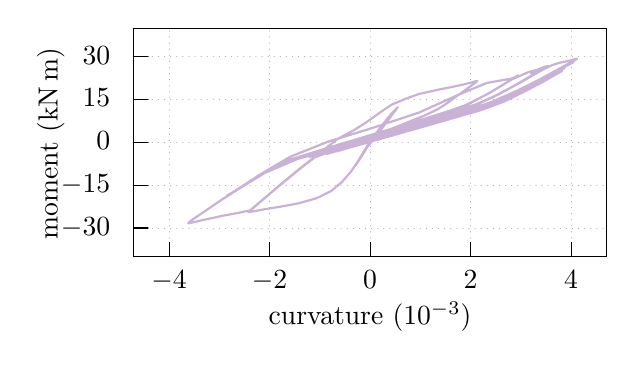
\begin{tikzpicture}[gnuplot]
%% generated with GNUPLOT 5.2p6 (Lua 5.3; terminal rev. Nov 2018, script rev. 107)
%% 08/11/2019 21:17:49
\path (0.000,0.000) rectangle (6.000,2.900);
\gpcolor{color=gp lt color axes}
\gpsetlinetype{gp lt axes}
\gpsetdashtype{gp dt axes}
\gpsetlinewidth{0.50}
\draw[gp path] (0.000,0.362)--(5.999,0.362);
\gpcolor{color=gp lt color border}
\gpsetlinetype{gp lt border}
\gpsetdashtype{gp dt solid}
\gpsetlinewidth{1.00}
\draw[gp path] (0.000,0.362)--(0.180,0.362);
\node[gp node right] at (-0.184,0.362) {$-30$};
\gpcolor{color=gp lt color axes}
\gpsetlinetype{gp lt axes}
\gpsetdashtype{gp dt axes}
\gpsetlinewidth{0.50}
\draw[gp path] (0.000,0.906)--(5.999,0.906);
\gpcolor{color=gp lt color border}
\gpsetlinetype{gp lt border}
\gpsetdashtype{gp dt solid}
\gpsetlinewidth{1.00}
\draw[gp path] (0.000,0.906)--(0.180,0.906);
\node[gp node right] at (-0.184,0.906) {$-15$};
\gpcolor{color=gp lt color axes}
\gpsetlinetype{gp lt axes}
\gpsetdashtype{gp dt axes}
\gpsetlinewidth{0.50}
\draw[gp path] (0.000,1.450)--(5.999,1.450);
\gpcolor{color=gp lt color border}
\gpsetlinetype{gp lt border}
\gpsetdashtype{gp dt solid}
\gpsetlinewidth{1.00}
\draw[gp path] (0.000,1.450)--(0.180,1.450);
\node[gp node right] at (-0.184,1.450) {$0$};
\gpcolor{color=gp lt color axes}
\gpsetlinetype{gp lt axes}
\gpsetdashtype{gp dt axes}
\gpsetlinewidth{0.50}
\draw[gp path] (0.000,1.993)--(5.999,1.993);
\gpcolor{color=gp lt color border}
\gpsetlinetype{gp lt border}
\gpsetdashtype{gp dt solid}
\gpsetlinewidth{1.00}
\draw[gp path] (0.000,1.993)--(0.180,1.993);
\node[gp node right] at (-0.184,1.993) {$15$};
\gpcolor{color=gp lt color axes}
\gpsetlinetype{gp lt axes}
\gpsetdashtype{gp dt axes}
\gpsetlinewidth{0.50}
\draw[gp path] (0.000,2.537)--(5.999,2.537);
\gpcolor{color=gp lt color border}
\gpsetlinetype{gp lt border}
\gpsetdashtype{gp dt solid}
\gpsetlinewidth{1.00}
\draw[gp path] (0.000,2.537)--(0.180,2.537);
\node[gp node right] at (-0.184,2.537) {$30$};
\gpcolor{color=gp lt color axes}
\gpsetlinetype{gp lt axes}
\gpsetdashtype{gp dt axes}
\gpsetlinewidth{0.50}
\draw[gp path] (0.447,0.000)--(0.447,2.899);
\gpcolor{color=gp lt color border}
\gpsetlinetype{gp lt border}
\gpsetdashtype{gp dt solid}
\gpsetlinewidth{1.00}
\draw[gp path] (0.447,0.000)--(0.447,0.180);
\node[gp node center] at (0.447,-0.308) {$-4$};
\gpcolor{color=gp lt color axes}
\gpsetlinetype{gp lt axes}
\gpsetdashtype{gp dt axes}
\gpsetlinewidth{0.50}
\draw[gp path] (1.723,0.000)--(1.723,2.899);
\gpcolor{color=gp lt color border}
\gpsetlinetype{gp lt border}
\gpsetdashtype{gp dt solid}
\gpsetlinewidth{1.00}
\draw[gp path] (1.723,0.000)--(1.723,0.180);
\node[gp node center] at (1.723,-0.308) {$-2$};
\gpcolor{color=gp lt color axes}
\gpsetlinetype{gp lt axes}
\gpsetdashtype{gp dt axes}
\gpsetlinewidth{0.50}
\draw[gp path] (3.000,0.000)--(3.000,2.899);
\gpcolor{color=gp lt color border}
\gpsetlinetype{gp lt border}
\gpsetdashtype{gp dt solid}
\gpsetlinewidth{1.00}
\draw[gp path] (3.000,0.000)--(3.000,0.180);
\node[gp node center] at (3.000,-0.308) {$0$};
\gpcolor{color=gp lt color axes}
\gpsetlinetype{gp lt axes}
\gpsetdashtype{gp dt axes}
\gpsetlinewidth{0.50}
\draw[gp path] (4.276,0.000)--(4.276,2.899);
\gpcolor{color=gp lt color border}
\gpsetlinetype{gp lt border}
\gpsetdashtype{gp dt solid}
\gpsetlinewidth{1.00}
\draw[gp path] (4.276,0.000)--(4.276,0.180);
\node[gp node center] at (4.276,-0.308) {$2$};
\gpcolor{color=gp lt color axes}
\gpsetlinetype{gp lt axes}
\gpsetdashtype{gp dt axes}
\gpsetlinewidth{0.50}
\draw[gp path] (5.552,0.000)--(5.552,2.899);
\gpcolor{color=gp lt color border}
\gpsetlinetype{gp lt border}
\gpsetdashtype{gp dt solid}
\gpsetlinewidth{1.00}
\draw[gp path] (5.552,0.000)--(5.552,0.180);
\node[gp node center] at (5.552,-0.308) {$4$};
\draw[gp path] (0.000,2.899)--(0.000,0.000)--(5.999,0.000)--(5.999,2.899)--cycle;
\node[gp node center,rotate=-270] at (-1.044,1.449) {moment (\si{\kilo\newton\meter})};
\node[gp node center] at (2.999,-0.769) {curvature (\num{E-3})};
\gpcolor{rgb color={0.792,0.698,0.839}}
\gpsetlinewidth{2.00}
\draw[gp path] (3.000,1.450)--(2.999,1.449)--(2.999,1.448)--(3.000,1.451)--(3.004,1.456)%
  --(3.009,1.463)--(3.013,1.469)--(3.016,1.473)--(3.019,1.476)--(3.022,1.481)--(3.026,1.487)%
  --(3.031,1.493)--(3.034,1.498)--(3.037,1.502)--(3.039,1.505)--(3.041,1.508)--(3.043,1.511)%
  --(3.044,1.512)--(3.041,1.508)--(3.038,1.504)--(3.034,1.498)--(3.030,1.493)--(3.027,1.488)%
  --(3.023,1.483)--(3.020,1.479)--(3.019,1.476)--(3.018,1.475)--(3.018,1.476)--(3.019,1.477)%
  --(3.020,1.478)--(3.021,1.480)--(3.022,1.481)--(3.022,1.482)--(3.022,1.481)--(3.021,1.479)%
  --(3.019,1.477)--(3.017,1.474)--(3.015,1.472)--(3.015,1.471)--(3.015,1.472)--(3.017,1.474)%
  --(3.020,1.478)--(3.023,1.483)--(3.027,1.489)--(3.030,1.492)--(3.030,1.493)--(3.028,1.490)%
  --(3.024,1.484)--(3.018,1.475)--(3.009,1.463)--(3.001,1.452)--(2.997,1.446)--(2.996,1.444)%
  --(2.996,1.443)--(2.995,1.442)--(2.996,1.444)--(3.001,1.452)--(3.010,1.465)--(3.021,1.480)%
  --(3.032,1.495)--(3.043,1.511)--(3.056,1.529)--(3.069,1.547)--(3.080,1.563)--(3.087,1.573)%
  --(3.091,1.578)--(3.093,1.582)--(3.095,1.585)--(3.096,1.585)--(3.092,1.580)--(3.085,1.570)%
  --(3.075,1.556)--(3.062,1.538)--(3.048,1.517)--(3.031,1.493)--(3.011,1.465)--(2.989,1.431)%
  --(2.967,1.394)--(2.944,1.357)--(2.923,1.323)--(2.905,1.293)--(2.887,1.264)--(2.869,1.237)%
  --(2.851,1.210)--(2.835,1.186)--(2.823,1.168)--(2.815,1.158)--(2.813,1.155)--(2.816,1.159)%
  --(2.822,1.169)--(2.832,1.186)--(2.847,1.211)--(2.867,1.243)--(2.890,1.282)--(2.915,1.324)%
  --(2.938,1.363)--(2.959,1.397)--(2.977,1.428)--(2.994,1.454)--(3.010,1.474)--(3.019,1.485)%
  --(3.019,1.486)--(3.011,1.475)--(2.995,1.454)--(2.975,1.424)--(2.955,1.391)--(2.934,1.355)%
  --(2.910,1.316)--(2.885,1.275)--(2.863,1.237)--(2.845,1.208)--(2.832,1.185)--(2.821,1.167)%
  --(2.815,1.157)--(2.819,1.163)--(2.838,1.195)--(2.874,1.255)--(2.921,1.334)--(2.974,1.423)%
  --(3.033,1.504)--(3.088,1.580)--(3.146,1.659)--(3.208,1.737)--(3.267,1.808)--(3.316,1.860)%
  --(3.344,1.889)--(3.352,1.897)--(3.345,1.888)--(3.327,1.863)--(3.297,1.823)--(3.250,1.760)%
  --(3.186,1.675)--(3.111,1.574)--(3.023,1.463)--(2.927,1.344)--(2.850,1.215)--(2.760,1.083)%
  --(2.646,0.950)--(2.505,0.832)--(2.329,0.743)--(2.087,0.674)--(1.839,0.629)--(1.681,0.604)%
  --(1.569,0.583)--(1.494,0.570)--(1.455,0.565)--(1.452,0.565)--(1.479,0.589)--(1.536,0.637)%
  --(1.616,0.705)--(1.709,0.785)--(1.809,0.870)--(1.918,0.962)--(2.039,1.061)--(2.165,1.162)%
  --(2.287,1.258)--(2.393,1.341)--(2.472,1.403)--(2.525,1.444)--(2.576,1.484)--(2.657,1.531)%
  --(2.794,1.604)--(2.966,1.714)--(3.121,1.826)--(3.274,1.928)--(3.449,2.002)--(3.620,2.064)%
  --(3.887,2.123)--(4.099,2.165)--(4.197,2.187)--(4.254,2.202)--(4.286,2.210)--(4.311,2.217)%
  --(4.339,2.225)--(4.361,2.230)--(4.362,2.229)--(4.344,2.215)--(4.309,2.187)--(4.260,2.152)%
  --(4.204,2.111)--(4.139,2.064)--(4.060,2.007)--(3.967,1.940)--(3.851,1.866)--(3.693,1.791)%
  --(3.510,1.717)--(3.325,1.643)--(3.137,1.570)--(2.925,1.492)--(2.711,1.413)--(2.509,1.339)%
  --(2.300,1.260)--(2.184,1.172)--(2.084,1.094)--(1.991,1.017)--(1.906,0.947)--(1.832,0.886)%
  --(1.774,0.836)--(1.730,0.799)--(1.691,0.766)--(1.650,0.731)--(1.610,0.697)--(1.581,0.673)%
  --(1.564,0.657)--(1.545,0.642)--(1.520,0.620)--(1.476,0.586)--(1.322,0.553)--(1.218,0.534)%
  --(1.121,0.516)--(1.026,0.495)--(0.933,0.475)--(0.848,0.457)--(0.762,0.436)--(0.691,0.421)%
  --(0.703,0.440)--(0.877,0.559)--(1.191,0.772)--(1.588,1.031)--(1.986,1.268)--(2.471,1.460)%
  --(2.988,1.619)--(3.619,1.827)--(4.140,2.062)--(4.479,2.203)--(4.713,2.246)--(4.808,2.259)%
  --(4.791,2.258)--(4.799,2.261)--(4.843,2.280)--(4.879,2.301)--(4.876,2.296)--(4.757,2.222)%
  --(4.511,2.074)--(4.188,1.909)--(3.764,1.770)--(3.324,1.636)--(2.831,1.486)--(2.244,1.309)%
  --(1.665,1.063)--(1.329,0.857)--(1.181,0.774)--(1.269,0.820)--(1.407,0.911)--(1.492,0.970)%
  --(1.552,1.003)--(1.657,1.072)--(1.970,1.228)--(2.503,1.391)--(3.058,1.558)--(3.515,1.695)%
  --(3.787,1.780)--(3.983,1.842)--(4.249,1.935)--(4.522,2.082)--(4.795,2.247)--(5.015,2.343)%
  --(5.114,2.370)--(5.095,2.354)--(5.044,2.328)--(5.050,2.331)--(5.122,2.372)--(5.215,2.410)%
  --(5.265,2.421)--(5.215,2.390)--(5.078,2.315)--(4.934,2.230)--(4.812,2.159)--(4.696,2.097)%
  --(4.547,2.020)--(4.307,1.916)--(3.942,1.803)--(3.576,1.694)--(3.267,1.603)--(3.008,1.527)%
  --(2.752,1.452)--(2.475,1.371)--(2.214,1.294)--(2.018,1.237)--(1.940,1.214)--(1.987,1.228)%
  --(2.100,1.261)--(2.240,1.303)--(2.417,1.354)--(2.662,1.426)--(2.979,1.520)--(3.338,1.625)%
  --(3.694,1.730)--(4.026,1.827)--(4.315,1.919)--(4.531,2.012)--(4.713,2.104)--(4.851,2.180)%
  --(4.934,2.228)--(4.956,2.240)--(4.923,2.221)--(4.845,2.176)--(4.724,2.108)--(4.554,2.020)%
  --(4.350,1.930)--(4.102,1.847)--(3.841,1.770)--(3.590,1.696)--(3.325,1.618)--(3.044,1.536)%
  --(2.779,1.458)--(2.555,1.392)--(2.376,1.340)--(2.227,1.296)--(2.087,1.255)--(1.962,1.219)%
  --(1.861,1.187)--(1.836,1.174)--(1.850,1.182)--(1.866,1.189)--(1.903,1.201)--(2.021,1.236)%
  --(2.228,1.297)--(2.486,1.373)--(2.751,1.450)--(2.970,1.515)--(3.140,1.565)--(3.312,1.615)%
  --(3.515,1.675)--(3.707,1.732)--(3.826,1.766)--(3.845,1.772)--(3.790,1.756)--(3.677,1.723)%
  --(3.534,1.680)--(3.466,1.660)--(3.524,1.678)--(3.644,1.713)--(3.754,1.745)--(3.788,1.755)%
  --(3.763,1.748)--(3.771,1.750)--(3.845,1.772)--(3.938,1.799)--(3.971,1.809)--(3.879,1.782)%
  --(3.708,1.732)--(3.610,1.703)--(3.670,1.720)--(3.833,1.769)--(3.988,1.814)--(4.034,1.828)%
  --(3.995,1.816)--(3.998,1.817)--(4.111,1.850)--(4.274,1.902)--(4.377,1.941)--(4.378,1.941)%
  --(4.306,1.914)--(4.234,1.887)--(4.202,1.877)--(4.190,1.873)--(4.131,1.856)--(4.011,1.821)%
  --(3.875,1.781)--(3.759,1.747)--(3.674,1.722)--(3.604,1.701)--(3.517,1.675)--(3.403,1.642)%
  --(3.279,1.605)--(3.177,1.575)--(3.106,1.555)--(3.049,1.538)--(2.981,1.518)--(2.895,1.492)%
  --(2.807,1.467)--(2.739,1.447)--(2.702,1.436)--(2.699,1.435)--(2.724,1.442)--(2.769,1.455)%
  --(2.837,1.475)--(2.937,1.505)--(3.071,1.544)--(3.217,1.587)--(3.351,1.627)--(3.465,1.660)%
  --(3.564,1.689)--(3.651,1.715)--(3.719,1.735)--(3.753,1.745)--(3.740,1.741)--(3.678,1.723)%
  --(3.572,1.692)--(3.431,1.650)--(3.254,1.598)--(3.040,1.535)--(2.796,1.463)--(2.582,1.400)%
  --(2.447,1.361)--(2.381,1.341)--(2.355,1.334)--(2.328,1.326)--(2.295,1.316)--(2.294,1.316)%
  --(2.356,1.334)--(2.492,1.374)--(2.681,1.430)--(2.880,1.488)--(3.069,1.544)--(3.249,1.597)%
  --(3.434,1.651)--(3.630,1.709)--(3.827,1.767)--(3.985,1.813)--(4.082,1.841)--(4.120,1.853)%
  --(4.122,1.853)--(4.095,1.845)--(4.025,1.825)--(3.898,1.787)--(3.712,1.732)--(3.476,1.663)%
  --(3.206,1.583)--(2.918,1.499)--(2.618,1.411)--(2.302,1.318)--(1.946,1.214)--(1.660,1.063)%
  --(1.464,0.947)--(1.341,0.867)--(1.289,0.830)--(1.263,0.817)--(1.228,0.793)--(1.172,0.755)%
  --(1.109,0.716)--(1.122,0.726)--(1.295,0.841)--(1.574,1.021)--(1.881,1.196)--(2.258,1.308)%
  --(2.562,1.396)--(2.916,1.500)--(3.375,1.636)--(3.898,1.789)--(4.388,1.945)--(4.692,2.092)%
  --(4.893,2.201)--(5.034,2.282)--(5.141,2.344)--(5.213,2.384)--(5.311,2.430)--(5.399,2.459)%
  --(5.493,2.478)--(5.570,2.497)--(5.615,2.510)--(5.628,2.511)--(5.615,2.503)--(5.571,2.479)%
  --(5.491,2.434)--(5.355,2.359)--(5.153,2.249)--(4.873,2.108)--(4.521,1.954)--(4.074,1.811)%
  --(3.574,1.667)--(3.041,1.513)--(2.508,1.361)--(2.049,1.230)--(1.736,1.115)--(1.617,1.049)%
  --(1.575,1.026)--(1.585,1.029)--(1.591,1.033)--(1.580,1.028)--(1.579,1.026)--(1.598,1.038)%
  --(1.657,1.073)--(1.760,1.134)--(1.914,1.193)--(2.041,1.229)--(2.131,1.255)--(2.183,1.270)%
  --(2.220,1.281)--(2.274,1.296)--(2.371,1.324)--(2.581,1.384)--(2.933,1.485)--(3.341,1.602)%
  --(3.701,1.705)--(3.998,1.790)--(4.270,1.868)--(4.543,1.964)--(4.816,2.082)--(5.032,2.183)%
  --(5.133,2.234)--(5.153,2.245)--(5.140,2.238)--(5.136,2.236)--(5.186,2.264)--(5.270,2.309)%
  --(5.337,2.345)--(5.367,2.362)--(5.356,2.356)--(5.319,2.335)--(5.281,2.315)--(5.249,2.297)%
  --(5.210,2.275)--(5.129,2.232)--(4.990,2.162)--(4.807,2.072)--(4.603,1.981)--(4.395,1.905)%
  --(4.190,1.841)--(4.000,1.786)--(3.839,1.740)--(3.701,1.701)--(3.599,1.671)--(3.539,1.654)%
  --(3.523,1.649)--(3.552,1.658)--(3.616,1.676)--(3.696,1.699)--(3.781,1.724)--(3.876,1.751)%
  --(3.983,1.782)--(4.084,1.811)--(4.160,1.833)--(4.239,1.855)--(4.351,1.889)--(4.505,1.946)%
  --(4.694,2.022)--(4.838,2.088)--(4.909,2.122)--(4.941,2.139)--(4.975,2.155)--(5.020,2.176)%
  --(5.048,2.190)--(5.021,2.176)--(4.925,2.129)--(4.780,2.059)--(4.600,1.979)--(4.393,1.903)%
  --(4.148,1.828)--(3.849,1.742)--(3.511,1.645)--(3.171,1.548)--(2.883,1.465)--(2.667,1.403)%
  --(2.502,1.356)--(2.382,1.322)--(2.300,1.298)--(2.256,1.286)--(2.251,1.284)--(2.290,1.295)%
  --(2.368,1.318)--(2.472,1.348)--(2.594,1.383)--(2.723,1.420)--(2.856,1.458)--(2.991,1.496)%
  --(3.117,1.533)--(3.225,1.563)--(3.302,1.586)--(3.344,1.598)--(3.354,1.600)--(3.356,1.601)%
  --(3.373,1.606)--(3.410,1.617)--(3.462,1.632)--(3.515,1.647)--(3.567,1.662)--(3.617,1.676)%
  --(3.663,1.689)--(3.709,1.703)--(3.752,1.715)--(3.782,1.723)--(3.794,1.727)--(3.800,1.729)%
  --(3.813,1.732)--(3.842,1.741)--(3.885,1.753)--(3.925,1.765)--(3.955,1.773)--(3.974,1.779)%
  --(3.989,1.783)--(4.013,1.790)--(4.048,1.800)--(4.082,1.810)--(4.105,1.816)--(4.111,1.818)%
  --(4.105,1.816)--(4.096,1.814)--(4.085,1.810)--(4.062,1.804)--(4.017,1.791)--(3.946,1.771)%
  --(3.855,1.744)--(3.750,1.714)--(3.642,1.683)--(3.544,1.655)--(3.462,1.631)--(3.398,1.613)%
  --(3.357,1.601)--(3.347,1.598)--(3.372,1.606)--(3.417,1.618)--(3.464,1.632)--(3.508,1.645)%
  --(3.551,1.657)--(3.600,1.671)--(3.660,1.688)--(3.737,1.711)--(3.830,1.737)--(3.919,1.763)%
  --(3.993,1.784)--(4.049,1.800)--(4.089,1.812)--(4.122,1.821)--(4.143,1.827)--(4.140,1.826)%
  --(4.107,1.817)--(4.043,1.798)--(3.958,1.774)--(3.877,1.751)--(3.813,1.732)--(3.761,1.717)%
  --(3.710,1.703)--(3.656,1.687)--(3.605,1.672)--(3.566,1.661)--(3.542,1.654)--(3.530,1.651)%
  --(3.522,1.649)--(3.517,1.647)--(3.522,1.649)--(3.546,1.656)--(3.592,1.669)--(3.648,1.685)%
  --(3.702,1.700)--(3.752,1.715)--(3.801,1.729)--(3.854,1.744)--(3.912,1.761)--(3.962,1.775)%
  --(3.998,1.786)--(4.024,1.793)--(4.048,1.800)--(4.082,1.810)--(4.127,1.822)--(4.173,1.836)%
  --(4.210,1.846)--(4.227,1.851)--(4.220,1.849)--(4.215,1.848)--(4.207,1.845)--(4.185,1.839)%
  --(4.144,1.828)--(4.090,1.812)--(4.030,1.795)--(3.969,1.777)--(3.898,1.757)--(3.812,1.732)%
  --(3.728,1.708)--(3.664,1.689)--(3.621,1.677)--(3.590,1.668)--(3.559,1.659)--(3.526,1.650)%
  --(3.505,1.644)--(3.510,1.645)--(3.540,1.654)--(3.583,1.666)--(3.628,1.679)--(3.669,1.691)%
  --(3.715,1.704)--(3.768,1.719)--(3.828,1.736)--(3.884,1.753)--(3.924,1.764)--(3.943,1.770)%
  --(3.947,1.771)--(3.940,1.769)--(3.915,1.761)--(3.861,1.746)--(3.777,1.722)--(3.673,1.692)%
  --(3.587,1.667)--(3.538,1.653)--(3.525,1.649)--(3.533,1.652)--(3.535,1.652)--(3.527,1.650)%
  --(3.550,1.657)--(3.594,1.669)--(3.639,1.682)--(3.674,1.692)--(3.705,1.701)--(3.751,1.714)%
  --(3.826,1.736)--(3.926,1.765)--(4.034,1.796)--(4.129,1.823)--(4.208,1.846)--(4.271,1.864)%
  --(4.326,1.880)--(4.366,1.894)--(4.388,1.902)--(4.380,1.899)--(4.341,1.885)--(4.268,1.863)%
  --(4.173,1.836)--(4.064,1.804)--(3.940,1.769)--(3.810,1.731)--(3.686,1.696)--(3.583,1.666)%
  --(3.505,1.644)--(3.445,1.626)--(3.397,1.613)--(3.359,1.602)--(3.334,1.595)--(3.338,1.596)%
  --(3.376,1.607)--(3.438,1.624)--(3.509,1.645)--(3.579,1.665)--(3.648,1.685)--(3.726,1.707)%
  --(3.812,1.732)--(3.898,1.757)--(3.971,1.778)--(4.021,1.792)--(4.049,1.800)--(4.065,1.805)%
  --(4.077,1.808)--(4.086,1.811)--(4.089,1.812)--(4.078,1.808)--(4.054,1.802)--(4.015,1.790)%
  --(3.961,1.775)--(3.890,1.754)--(3.803,1.729)--(3.703,1.701)--(3.602,1.671)--(3.511,1.645)%
  --(3.442,1.626)--(3.390,1.610)--(3.349,1.599)--(3.320,1.591)--(3.309,1.587)--(3.322,1.591)%
  --(3.358,1.601)--(3.409,1.616)--(3.467,1.633)--(3.528,1.650)--(3.593,1.669)--(3.662,1.689)%
  --(3.731,1.708)--(3.791,1.726)--(3.835,1.739)--(3.862,1.746)--(3.872,1.749)--(3.868,1.748)%
  --(3.854,1.744)--(3.833,1.738)--(3.804,1.730)--(3.768,1.719)--(3.722,1.706)--(3.665,1.690)%
  --(3.597,1.670)--(3.516,1.647)--(3.424,1.620)--(3.347,1.598)--(3.297,1.584)--(3.263,1.574)%
  --(3.234,1.566)--(3.213,1.560)--(3.215,1.560)--(3.258,1.573)--(3.345,1.598)--(3.457,1.630)%
  --(3.572,1.663)--(3.689,1.697)--(3.822,1.735)--(3.976,1.779)--(4.143,1.827)--(4.308,1.874)%
  --(4.436,1.920)--(4.541,1.958)--(4.627,1.991)--(4.698,2.023)--(4.757,2.048)--(4.783,2.060)%
  --(4.765,2.052)--(4.701,2.023)--(4.604,1.980)--(4.493,1.940)--(4.395,1.904)--(4.300,1.872)%
  --(4.184,1.839)--(4.053,1.801)--(3.919,1.762)--(3.796,1.727)--(3.694,1.698)--(3.618,1.676)%
  --(3.558,1.659)--(3.507,1.644)--(3.467,1.632)--(3.447,1.627)--(3.456,1.629)--(3.491,1.639)%
  --(3.542,1.654)--(3.601,1.671)--(3.666,1.690)--(3.744,1.712)--(3.837,1.739)--(3.943,1.769)%
  --(4.052,1.801)--(4.154,1.830)--(4.243,1.856)--(4.318,1.877)--(4.372,1.896)--(4.413,1.910)%
  --(4.434,1.918)--(4.428,1.916)--(4.395,1.904)--(4.338,1.883)--(4.245,1.856)--(4.133,1.824)%
  --(4.010,1.788)--(3.873,1.749)--(3.725,1.706)--(3.575,1.663)--(3.429,1.621)--(3.292,1.582)%
  --(3.170,1.547)--(3.067,1.517)--(2.986,1.494)--(2.927,1.477)--(2.894,1.468)--(2.892,1.467)%
  --(2.928,1.477)--(2.992,1.496)--(3.075,1.520)--(3.174,1.548)--(3.288,1.581)--(3.407,1.615)%
  --(3.526,1.649)--(3.682,1.694)--(3.912,1.761)--(4.195,1.842)--(4.476,1.934)--(4.709,2.028)%
  --(4.888,2.111)--(5.052,2.190)--(5.201,2.268)--(5.326,2.336)--(5.408,2.379)--(5.422,2.387)%
  --(5.392,2.371)--(5.355,2.351)--(5.330,2.337)--(5.316,2.329)--(5.286,2.312)--(5.197,2.263)%
  --(5.039,2.181)--(4.836,2.081)--(4.627,1.985)--(4.413,1.907)--(4.178,1.834)--(3.909,1.756)%
  --(3.623,1.674)--(3.359,1.598)--(3.147,1.537)--(2.998,1.494)--(2.894,1.464)--(2.808,1.440)%
  --(2.733,1.418)--(2.692,1.407)--(2.708,1.411)--(2.790,1.435)--(2.923,1.473)--(3.075,1.517)%
  --(3.222,1.559)--(3.363,1.600)--(3.506,1.641)--(3.659,1.685)--(3.810,1.728)--(3.930,1.762)%
  --(3.996,1.781)--(3.999,1.782)--(3.951,1.768)--(3.890,1.751)--(3.852,1.740)--(3.896,1.753)%
  --(4.037,1.793)--(4.175,1.833)--(4.238,1.851)--(4.246,1.853)--(4.257,1.857)--(4.323,1.876)%
  --(4.418,1.909)--(4.518,1.946)--(4.601,1.976)--(4.642,1.993)--(4.663,2.003)--(4.691,2.015)%
  --(4.726,2.031)--(4.761,2.047)--(4.776,2.054)--(4.761,2.046)--(4.723,2.029)--(4.666,2.003)%
  --(4.586,1.970)--(4.476,1.930)--(4.335,1.879)--(4.122,1.817)--(3.863,1.743)--(3.564,1.657)%
  --(3.243,1.565)--(2.944,1.479)--(2.709,1.411)--(2.528,1.359)--(2.402,1.324)--(2.310,1.297)%
  --(2.238,1.277)--(2.214,1.270)--(2.257,1.282)--(2.366,1.314)--(2.545,1.365)--(2.782,1.433)%
  --(3.068,1.515)--(3.400,1.610)--(3.763,1.715)--(4.174,1.833)--(4.576,1.967)--(4.908,2.118)%
  --(5.198,2.260)--(5.400,2.370)--(5.531,2.441)--(5.584,2.469)--(5.560,2.456)--(5.524,2.437)%
  --(5.504,2.426)--(5.487,2.416)--(5.445,2.393)--(5.316,2.321)--(5.058,2.182)--(4.689,2.004)%
  --(4.239,1.845)--(3.846,1.732)--(3.597,1.660)--(3.375,1.596)--(3.088,1.514)--(2.769,1.422)%
  --(2.508,1.348)--(2.385,1.313)--(2.391,1.314)--(2.462,1.335)--(2.545,1.359)--(2.599,1.374)%
  --(2.620,1.380)--(2.664,1.393)--(2.793,1.430)--(3.025,1.497)--(3.340,1.587)--(3.661,1.679)%
  --(3.958,1.764)--(4.228,1.842)--(4.469,1.921)--(4.704,2.014)--(4.913,2.112)--(5.081,2.193)%
  --(5.180,2.245)--(5.222,2.267)--(5.230,2.271)--(5.216,2.264)--(5.171,2.239)--(5.076,2.189)%
  --(4.917,2.110)--(4.708,2.010)--(4.440,1.906)--(4.123,1.809)--(3.782,1.710)--(3.446,1.614)%
  --(3.111,1.518)--(2.812,1.432)--(2.573,1.363)--(2.399,1.314)--(2.287,1.282)--(2.227,1.265)%
  --(2.235,1.267)--(2.311,1.289)--(2.434,1.324)--(2.618,1.377)--(2.865,1.448)--(3.147,1.529)%
  --(3.447,1.615)--(3.739,1.699)--(4.021,1.780)--(4.284,1.855)--(4.488,1.925)--(4.663,1.991)%
  --(4.809,2.058)--(4.927,2.114)--(5.016,2.157)--(5.062,2.180)--(5.063,2.180)--(5.036,2.166)%
  --(4.991,2.144)--(4.930,2.115)--(4.853,2.077)--(4.755,2.029)--(4.632,1.974)--(4.479,1.918)%
  --(4.320,1.863)--(4.137,1.811)--(3.954,1.758)--(3.773,1.706)--(3.602,1.657)--(3.438,1.609)%
  --(3.279,1.564)--(3.130,1.521)--(2.993,1.482)--(2.873,1.447)--(2.765,1.416)--(2.668,1.389)%
  --(2.585,1.365)--(2.533,1.350)--(2.531,1.350)--(2.584,1.365)--(2.693,1.396)--(2.854,1.442)%
  --(3.062,1.502)--(3.308,1.573)--(3.569,1.648)--(3.833,1.724)--(4.106,1.802)--(4.392,1.887)%
  --(4.671,1.993)--(4.917,2.108)--(5.130,2.213)--(5.275,2.291)--(5.358,2.336)--(5.390,2.352)%
  --(5.380,2.347)--(5.347,2.329)--(5.304,2.305)--(5.247,2.274)--(5.151,2.222)--(4.987,2.137)%
  --(4.751,2.022)--(4.450,1.904)--(4.124,1.804)--(3.828,1.718)--(3.566,1.643)--(3.306,1.568)%
  --(3.050,1.495)--(2.835,1.433)--(2.686,1.390)--(2.622,1.372)--(2.627,1.374)--(2.674,1.387)%
  --(2.747,1.408)--(2.856,1.439)--(3.025,1.488)--(3.271,1.558)--(3.570,1.644)--(3.892,1.737)%
  --(4.217,1.830)--(4.516,1.929)--(4.783,2.040)--(5.023,2.154)--(5.222,2.258)--(5.364,2.336)%
  --(5.445,2.379)--(5.470,2.392)--(5.445,2.379)--(5.390,2.349)--(5.331,2.316)--(5.267,2.281)%
  --(5.179,2.232)--(5.039,2.158)--(4.832,2.057)--(4.587,1.950)--(4.332,1.860)--(4.097,1.792)%
  --(3.899,1.735)--(3.694,1.676)--(3.467,1.611)--(3.241,1.546)--(3.059,1.493)--(2.941,1.460)%
  --(2.867,1.439)--(2.809,1.422)--(2.757,1.407)--(2.721,1.397)--(2.782,1.415)--(2.911,1.452)%
  --(3.087,1.502)--(3.295,1.562)--(3.521,1.627)--(3.777,1.701)--(4.070,1.785)--(4.377,1.873)%
  --(4.632,1.967)--(4.829,2.057)--(4.987,2.132)--(5.108,2.194)--(5.200,2.242)--(5.254,2.271)%
  --(5.264,2.277)--(5.227,2.256)--(5.148,2.213)--(5.042,2.158)--(4.922,2.099)--(4.805,2.042)%
  --(4.675,1.981)--(4.507,1.918)--(4.330,1.857)--(4.151,1.805)--(4.005,1.763)--(3.892,1.731)%
  --(3.798,1.704)--(3.715,1.680)--(3.652,1.662)--(3.620,1.653)--(3.627,1.655)--(3.667,1.666)%
  --(3.723,1.682)--(3.787,1.701)--(3.861,1.722)--(3.953,1.749)--(4.075,1.784)--(4.227,1.827)%
  --(4.386,1.875)--(4.520,1.924)--(4.653,1.973)--(4.773,2.028)--(4.900,2.089)--(5.034,2.154)%
  --(5.139,2.209)--(5.207,2.245)--(5.243,2.265)--(5.258,2.273)--(5.260,2.274)--(5.247,2.267)%
  --(5.210,2.246)--(5.138,2.207)--(5.033,2.152)--(4.896,2.085)--(4.751,2.015)--(4.582,1.945)%
  --(4.388,1.874)--(4.150,1.804)--(3.899,1.732)--(3.652,1.661)--(3.423,1.595)--(3.210,1.534)%
  --(3.017,1.479)--(2.851,1.431)--(2.706,1.390)--(2.589,1.356)--(2.513,1.334)--(2.487,1.327)%
  --(2.491,1.328)--(2.508,1.333)--(2.524,1.338)--(2.540,1.342)--(2.571,1.351)--(2.637,1.370)%
  --(2.736,1.399)--(2.846,1.430)--(2.946,1.459)--(3.030,1.483)--(3.102,1.504)--(3.169,1.523)%
  --(3.231,1.540)--(3.273,1.553)--(3.277,1.554)--(3.240,1.543)--(3.202,1.532)--(3.201,1.532)%
  --(3.251,1.546)--(3.342,1.572)--(3.445,1.602)--(3.552,1.633)--(3.684,1.671)--(3.865,1.723)%
  --(4.082,1.785)--(4.300,1.848)--(4.479,1.908)--(4.635,1.965)--(4.772,2.026)--(4.911,2.094)%
  --(5.057,2.165)--(5.182,2.230)--(5.267,2.276)--(5.303,2.296)--(5.301,2.295)--(5.283,2.285)%
  --(5.269,2.277)--(5.268,2.276)--(5.261,2.273)--(5.225,2.253)--(5.144,2.209)--(5.032,2.150)%
  --(4.908,2.090)--(4.800,2.037)--(4.701,1.991)--(4.584,1.944)--(4.440,1.891)--(4.288,1.843)%
  --(4.148,1.803)--(4.050,1.775)--(3.991,1.757)--(3.950,1.746)--(3.919,1.737)--(3.906,1.733)%
  --(3.916,1.736)--(3.947,1.745)--(3.978,1.754)--(3.989,1.757)--(3.984,1.755)--(3.978,1.754)%
  --(3.985,1.756)--(4.005,1.761)--(4.007,1.762)--(3.975,1.753)--(3.927,1.739)--(3.893,1.729)%
  --(3.889,1.728)--(3.902,1.732)--(3.896,1.730)--(3.854,1.718)--(3.790,1.700)--(3.734,1.683)%
  --(3.703,1.675)--(3.693,1.672)--(3.685,1.669)--(3.669,1.665)--(3.653,1.660)--(3.656,1.661)%
  --(3.686,1.670)--(3.735,1.684)--(3.773,1.695)--(3.786,1.699)--(3.791,1.700)--(3.814,1.707)%
  --(3.863,1.721)--(3.926,1.739)--(3.970,1.751)--(3.981,1.754)--(3.980,1.754)--(3.996,1.759)%
  --(4.040,1.772)--(4.099,1.788)--(4.141,1.801)--(4.155,1.805)--(4.164,1.807)--(4.191,1.815)%
  --(4.241,1.829)--(4.292,1.844)--(4.318,1.851)--(4.314,1.850)--(4.294,1.845)--(4.278,1.840)%
  --(4.272,1.838)--(4.266,1.837)--(4.250,1.832)--(4.225,1.825)--(4.204,1.819)--(4.199,1.817)%
  --(4.207,1.820)--(4.213,1.821)--(4.204,1.819)--(4.175,1.810)--(4.138,1.800)--(4.100,1.789)%
  --(4.059,1.777)--(4.006,1.762)--(3.938,1.742)--(3.862,1.720)--(3.785,1.698)--(3.717,1.678)%
  --(3.655,1.661)--(3.600,1.645)--(3.547,1.630)--(3.500,1.616)--(3.473,1.609)--(3.478,1.610)%
  --(3.506,1.618)--(3.545,1.629)--(3.586,1.641)--(3.627,1.653)--(3.676,1.667)--(3.736,1.684)%
  --(3.801,1.703)--(3.860,1.720)--(3.904,1.732)--(3.935,1.741)--(3.960,1.748)--(3.983,1.755)%
  --(3.992,1.758)--(3.975,1.753)--(3.935,1.741)--(3.882,1.726)--(3.820,1.708)--(3.751,1.688)%
  --(3.692,1.671)--(3.658,1.662)--(3.650,1.659)--(3.661,1.663)--(3.684,1.669)--(3.719,1.679)%
  --(3.776,1.696)--(3.865,1.721)--(3.982,1.755)--(4.111,1.792)--(4.238,1.829)--(4.360,1.864)%
  --(4.458,1.898)--(4.552,1.933)--(4.643,1.966)--(4.713,1.997)--(4.756,2.016)--(4.762,2.019)%
  --(4.728,2.003)--(4.663,1.973)--(4.591,1.947)--(4.545,1.930)--(4.508,1.916)--(4.459,1.898)%
  --(4.378,1.869)--(4.246,1.831)--(4.113,1.792)--(3.997,1.759)--(3.888,1.728)--(3.768,1.693)%
  --(3.644,1.658)--(3.544,1.629)--(3.505,1.618)--(3.543,1.629)--(3.632,1.654)--(3.733,1.683)%
  --(3.817,1.707)--(3.882,1.726)--(3.964,1.750)--(4.083,1.784)--(4.217,1.822)--(4.334,1.856)%
  --(4.407,1.879)--(4.457,1.898)--(4.514,1.919)--(4.588,1.946)--(4.663,1.974)--(4.710,1.995)%
  --(4.723,2.000)--(4.710,1.995)--(4.693,1.987)--(4.682,1.982)--(4.666,1.975)--(4.625,1.959)%
  --(4.547,1.930)--(4.445,1.893)--(4.343,1.858)--(4.239,1.828)--(4.140,1.800)--(4.028,1.768)%
  --(3.894,1.729)--(3.749,1.688)--(3.621,1.651)--(3.519,1.621)--(3.419,1.592)--(3.295,1.557)%
  --(3.157,1.517)--(3.032,1.481)--(2.970,1.464)--(2.989,1.469)--(3.071,1.493)--(3.194,1.528)%
  --(3.350,1.573)--(3.550,1.630)--(3.796,1.701)--(4.082,1.784)--(4.382,1.871)--(4.635,1.963)%
  --(4.837,2.056)--(5.013,2.140)--(5.159,2.215)--(5.271,2.276)--(5.342,2.315)--(5.370,2.330)%
  --(5.357,2.323)--(5.313,2.298)--(5.241,2.259)--(5.137,2.202)--(4.985,2.124)--(4.774,2.021)%
  --(4.512,1.915)--(4.237,1.826)--(3.989,1.754)--(3.787,1.696)--(3.598,1.642)--(3.401,1.585)%
  --(3.232,1.537)--(3.135,1.509)--(3.116,1.504)--(3.154,1.515)--(3.213,1.531)--(3.277,1.550)%
  --(3.353,1.572)--(3.451,1.600)--(3.568,1.633)--(3.682,1.666)--(3.778,1.694)--(3.848,1.714)%
  --(3.887,1.725)--(3.900,1.729)--(3.892,1.727)--(3.863,1.718)--(3.815,1.705)--(3.757,1.688)%
  --(3.697,1.670)--(3.649,1.657)--(3.623,1.649)--(3.624,1.649)--(3.645,1.656)--(3.684,1.667)%
  --(3.740,1.683)--(3.815,1.704)--(3.898,1.728)--(3.976,1.751)--(4.048,1.771)--(4.112,1.790)%
  --(4.161,1.804)--(4.188,1.812)--(4.200,1.815)--(4.205,1.817)--(4.217,1.820)--(4.239,1.827)%
  --(4.261,1.833)--(4.272,1.836)--(4.275,1.837)--(4.276,1.837)--(4.278,1.838)--(4.275,1.837)%
  --(4.262,1.833)--(4.238,1.826)--(4.213,1.819)--(4.196,1.814)--(4.188,1.812)--(4.186,1.811)%
  --(4.184,1.811)--(4.183,1.810)--(4.192,1.813)--(4.222,1.821)--(4.274,1.837)--(4.344,1.857)%
  --(4.406,1.877)--(4.452,1.893)--(4.483,1.905)--(4.502,1.912)--(4.518,1.918)--(4.530,1.922)%
  --(4.527,1.921)--(4.498,1.910)--(4.446,1.891)--(4.385,1.869)--(4.309,1.847)--(4.232,1.825)%
  --(4.148,1.800)--(4.048,1.771)--(3.929,1.737)--(3.800,1.700)--(3.693,1.669)--(3.623,1.649)%
  --(3.603,1.644)--(3.630,1.651)--(3.679,1.665)--(3.736,1.682)--(3.797,1.699)--(3.866,1.719)%
  --(3.956,1.745)--(4.061,1.775)--(4.155,1.802)--(4.222,1.821)--(4.257,1.832)--(4.273,1.836)%
  --(4.295,1.843)--(4.329,1.852)--(4.362,1.862)--(4.381,1.867)--(4.383,1.868)--(4.381,1.867)%
  --(4.371,1.864)--(4.340,1.855)--(4.280,1.838)--(4.196,1.814)--(4.099,1.786)--(3.987,1.754)%
  --(3.861,1.718)--(3.730,1.680)--(3.606,1.644)--(3.500,1.614)--(3.422,1.591)--(3.375,1.578)%
  --(3.360,1.574)--(3.374,1.578)--(3.418,1.590)--(3.490,1.611)--(3.590,1.640)--(3.712,1.675)%
  --(3.850,1.715)--(3.997,1.757)--(4.141,1.798)--(4.280,1.838)--(4.401,1.875)--(4.490,1.907)%
  --(4.558,1.932)--(4.613,1.952)--(4.662,1.970)--(4.698,1.986)--(4.724,1.998)--(4.737,2.004)%
  --(4.740,2.005)--(4.731,2.001)--(4.707,1.990)--(4.670,1.973)--(4.607,1.950)--(4.525,1.920)%
  --(4.430,1.885)--(4.317,1.849)--(4.182,1.810)--(4.052,1.772)--(3.939,1.740)--(3.839,1.711)%
  --(3.747,1.685)--(3.652,1.657)--(3.558,1.630)--(3.476,1.607)--(3.412,1.588)--(3.364,1.575)%
  --(3.323,1.563)--(3.289,1.553)--(3.272,1.548)--(3.280,1.550)--(3.317,1.561)--(3.377,1.578)%
  --(3.451,1.599)--(3.525,1.621)--(3.595,1.641)--(3.665,1.661)--(3.735,1.681)--(3.805,1.701)%
  --(3.871,1.720)--(3.942,1.741)--(4.029,1.766)--(4.131,1.795)--(4.244,1.828)--(4.362,1.862)%
  --(4.465,1.898)--(4.574,1.938)--(4.682,1.979)--(4.764,2.017)--(4.820,2.044)--(4.850,2.059)%
  --(4.859,2.063)--(4.849,2.058)--(4.821,2.044)--(4.767,2.018)--(4.684,1.979)--(4.572,1.937)%
  --(4.460,1.896)--(4.360,1.861)--(4.255,1.830)--(4.157,1.802)--(4.064,1.776)--(3.976,1.750)%
  --(3.898,1.728)--(3.836,1.710)--(3.793,1.698)--(3.762,1.689)--(3.735,1.681)--(3.710,1.674)%
  --(3.693,1.669)--(3.716,1.675)--(3.759,1.688)--(3.815,1.704)--(3.879,1.722)--(3.949,1.743)%
  --(4.035,1.767)--(4.141,1.798)--(4.260,1.832)--(4.379,1.866)--(4.459,1.895)--(4.518,1.917)%
  --(4.558,1.932)--(4.586,1.942)--(4.598,1.946)--(4.584,1.941)--(4.534,1.922)--(4.452,1.892)%
  --(4.346,1.857)--(4.211,1.818)--(4.070,1.777)--(3.921,1.734)--(3.771,1.691)--(3.634,1.652)%
  --(3.522,1.620)--(3.452,1.599)--(3.437,1.595)--(3.483,1.608)--(3.561,1.631)--(3.650,1.657)%
  --(3.747,1.684)--(3.859,1.717)--(3.997,1.756)--(4.151,1.800)--(4.297,1.843)--(4.410,1.878)%
  --(4.478,1.902)--(4.519,1.917)--(4.548,1.928)--(4.573,1.937)--(4.590,1.943)--(4.586,1.941)%
  --(4.544,1.926)--(4.467,1.898)--(4.378,1.866)--(4.269,1.835)--(4.168,1.805)--(4.065,1.776)%
  --(3.950,1.742)--(3.826,1.707)--(3.710,1.673)--(3.614,1.646)--(3.544,1.626)--(3.494,1.611)%
  --(3.459,1.601)--(3.444,1.597)--(3.456,1.601)--(3.504,1.614)--(3.588,1.639)--(3.702,1.671)%
  --(3.833,1.709)--(3.973,1.749)--(4.113,1.789)--(4.249,1.829)--(4.382,1.867)--(4.486,1.906)%
  --(4.574,1.937)--(4.633,1.959)--(4.671,1.974)--(4.701,1.987)--(4.729,1.999)--(4.746,2.008)%
  --(4.744,2.006)--(4.718,1.994)--(4.680,1.977)--(4.638,1.961)--(4.590,1.943)--(4.530,1.921)%
  --(4.452,1.892)--(4.364,1.861)--(4.259,1.831)--(4.165,1.804)--(4.082,1.780)--(4.005,1.758)%
  --(3.924,1.735)--(3.842,1.711)--(3.770,1.691)--(3.720,1.676)--(3.700,1.671)--(3.707,1.673)%
  --(3.726,1.678)--(3.750,1.685)--(3.774,1.692)--(3.804,1.700)--(3.841,1.711)--(3.879,1.722)%
  --(3.902,1.729)--(3.901,1.728)--(3.876,1.721)--(3.836,1.710)--(3.795,1.698)--(3.758,1.687)%
  --(3.719,1.676)--(3.673,1.663)--(3.625,1.649)--(3.589,1.639)--(3.579,1.636)--(3.598,1.641)%
  --(3.637,1.652)--(3.686,1.667)--(3.748,1.684)--(3.829,1.708)--(3.931,1.737)--(4.045,1.770)%
  --(4.157,1.802)--(4.258,1.831)--(4.346,1.856)--(4.415,1.879)--(4.473,1.900)--(4.517,1.916)%
  --(4.539,1.924)--(4.536,1.923)--(4.518,1.916)--(4.495,1.908)--(4.472,1.900)--(4.446,1.890)%
  --(4.414,1.879)--(4.380,1.866)--(4.341,1.855)--(4.317,1.848)--(4.313,1.847)--(4.323,1.850)%
  --(4.334,1.853)--(4.338,1.854)--(4.341,1.855)--(4.350,1.858)--(4.360,1.860)--(4.359,1.860)%
  --(4.341,1.855)--(4.309,1.846)--(4.271,1.835)--(4.241,1.826)--(4.224,1.821)--(4.214,1.818)%
  --(4.206,1.816)--(4.201,1.814)--(4.204,1.816)--(4.218,1.820)--(4.239,1.826)--(4.261,1.832)%
  --(4.280,1.837)--(4.297,1.842)--(4.315,1.848)--(4.342,1.855)--(4.379,1.866)--(4.410,1.877)%
  --(4.440,1.888)--(4.466,1.898)--(4.488,1.906)--(4.508,1.913)--(4.525,1.919)--(4.536,1.923)%
  --(4.538,1.924)--(4.527,1.920)--(4.506,1.912)--(4.479,1.902)--(4.450,1.892)--(4.415,1.879)%
  --(4.369,1.863)--(4.306,1.845)--(4.236,1.825)--(4.147,1.799)--(4.030,1.765)--(3.892,1.726)%
  --(3.745,1.683)--(3.601,1.642)--(3.462,1.602)--(3.328,1.564)--(3.205,1.528)--(3.093,1.496)%
  --(3.001,1.470)--(2.943,1.453)--(2.930,1.449)--(2.965,1.459)--(3.043,1.482)--(3.154,1.514)%
  --(3.288,1.552)--(3.448,1.598)--(3.634,1.652)--(3.842,1.712)--(4.059,1.774)--(4.266,1.833)%
  --(4.443,1.889)--(4.592,1.943)--(4.716,1.993)--(4.809,2.038)--(4.879,2.071)--(4.918,2.090)%
  --(4.922,2.092)--(4.894,2.078)--(4.843,2.054)--(4.776,2.021)--(4.694,1.982)--(4.587,1.941)%
  --(4.461,1.895)--(4.323,1.849)--(4.166,1.804)--(4.009,1.759)--(3.855,1.714)--(3.710,1.672)%
  --(3.579,1.635)--(3.466,1.602)--(3.374,1.576)--(3.311,1.558)--(3.282,1.550)--(3.290,1.552)%
  --(3.334,1.565)--(3.408,1.586)--(3.506,1.614)--(3.619,1.646)--(3.740,1.681)--(3.866,1.718)%
  --(3.995,1.755)--(4.125,1.792)--(4.255,1.829)--(4.384,1.867)--(4.491,1.906)--(4.596,1.944)%
  --(4.687,1.980)--(4.757,2.012)--(4.808,2.036)--(4.836,2.050)--(4.837,2.050)--(4.817,2.041)%
  --(4.780,2.022)--(4.727,1.997)--(4.654,1.965)--(4.550,1.927)--(4.432,1.883)--(4.297,1.841)%
  --(4.149,1.799)--(4.005,1.757)--(3.866,1.717)--(3.735,1.679)--(3.615,1.645)--(3.511,1.615)%
  --(3.427,1.591)--(3.365,1.573)--(3.327,1.562)--(3.308,1.557)--(3.310,1.557)--(3.333,1.564)%
  --(3.377,1.577)--(3.440,1.595)--(3.517,1.617)--(3.603,1.641)--(3.693,1.668)--(3.787,1.695)%
  --(3.884,1.722)--(3.977,1.749)--(4.058,1.773)--(4.130,1.793)--(4.193,1.811)--(4.251,1.828)%
  --(4.305,1.843)--(4.349,1.856)--(4.382,1.866)--(4.401,1.873)--(4.418,1.879)--(4.431,1.884)%
  --(4.440,1.887)--(4.432,1.884)--(4.405,1.874)--(4.361,1.860)--(4.311,1.845)--(4.272,1.834)%
  --(4.248,1.827)--(4.237,1.824)--(4.236,1.824)--(4.241,1.825)--(4.255,1.829)--(4.279,1.836)%
  --(4.313,1.846)--(4.350,1.856)--(4.380,1.865)--(4.391,1.869)--(4.385,1.867)--(4.358,1.859)%
  --(4.312,1.846)--(4.256,1.829)--(4.195,1.812)--(4.138,1.795)--(4.092,1.782)--(4.049,1.770)%
  --(4.007,1.758)--(3.967,1.746)--(3.935,1.737)--(3.921,1.733)--(3.928,1.735)--(3.955,1.743)%
  --(4.000,1.756)--(4.058,1.772)--(4.129,1.793)--(4.201,1.814)--(4.265,1.832)--(4.314,1.846)%
  --(4.348,1.856)--(4.374,1.863)--(4.393,1.870)--(4.401,1.872)--(4.394,1.870)--(4.370,1.862)%
  --(4.326,1.849)--(4.271,1.834)--(4.210,1.816)--(4.139,1.796)--(4.058,1.772)--(3.966,1.746)%
  --(3.868,1.718)--(3.782,1.693)--(3.718,1.675)--(3.682,1.664)--(3.672,1.661)--(3.683,1.664)%
  --(3.713,1.673)--(3.760,1.687)--(3.826,1.706)--(3.911,1.730)--(4.011,1.759)--(4.118,1.790)%
  --(4.230,1.822)--(4.343,1.855)--(4.443,1.888)--(4.536,1.922)--(4.616,1.951)--(4.674,1.973)%
  --(4.704,1.987)--(4.713,1.990)--(4.698,1.984)--(4.659,1.967)--(4.582,1.939)--(4.482,1.902)%
  --(4.367,1.861)--(4.227,1.821)--(4.090,1.781)--(3.954,1.742)--(3.820,1.704)--(3.700,1.669)%
  --(3.602,1.641)--(3.534,1.622)--(3.497,1.611)--(3.489,1.609)--(3.507,1.614)--(3.552,1.627)%
  --(3.623,1.647)--(3.712,1.673)--(3.811,1.701)--(3.913,1.731)--(4.011,1.759)--(4.101,1.785)%
  --(4.179,1.807)--(4.237,1.824)--(4.269,1.833)--(4.285,1.837)--(4.292,1.840)--(4.300,1.842)%
  --(4.310,1.845)--(4.312,1.845)--(4.302,1.843)--(4.285,1.838)--(4.269,1.833)--(4.263,1.831)%
  --(4.267,1.832)--(4.273,1.834)--(4.277,1.835)--(4.278,1.836)--(4.281,1.837)--(4.294,1.840)%
  --(4.316,1.846)--(4.339,1.853)--(4.360,1.859)--(4.380,1.865)--(4.399,1.872)--(4.424,1.881)%
  --(4.451,1.891)--(4.474,1.899)--(4.486,1.904)--(4.492,1.906)--(4.496,1.907)--(4.501,1.909)%
  --(4.488,1.904)--(4.457,1.893)--(4.415,1.877)--(4.363,1.860)--(4.301,1.842)--(4.233,1.823)%
  --(4.162,1.802)--(4.090,1.781)--(4.021,1.762)--(3.963,1.745)--(3.918,1.732)--(3.889,1.724)%
  --(3.871,1.718)--(3.858,1.715)--(3.847,1.711)--(3.834,1.708)--(3.822,1.704)--(3.809,1.701)%
  --(3.790,1.695)--(3.760,1.687)--(3.722,1.676)--(3.682,1.664)--(3.644,1.653)--(3.608,1.643)%
  --(3.572,1.633)--(3.536,1.622)--(3.505,1.613)--(3.486,1.608)--(3.482,1.607)--(3.494,1.610)%
  --(3.522,1.618)--(3.566,1.631)--(3.631,1.650)--(3.723,1.676)--(3.839,1.709)--(3.978,1.749)%
  --(4.126,1.792)--(4.276,1.835)--(4.421,1.880)--(4.556,1.930)--(4.686,1.979)--(4.787,2.027)%
  --(4.868,2.065)--(4.929,2.095)--(4.970,2.115)--(4.988,2.123)--(4.978,2.118)--(4.936,2.098)%
  --(4.864,2.062)--(4.760,2.012)--(4.620,1.952)--(4.442,1.887)--(4.232,1.822)--(3.992,1.753)%
  --(3.749,1.683)--(3.521,1.617)--(3.317,1.559)--(3.146,1.510)--(3.010,1.471)--(2.910,1.442)%
  --(2.850,1.425)--(2.842,1.423)--(2.890,1.436)--(2.994,1.466)--(3.148,1.511)--(3.342,1.566)%
  --(3.555,1.627)--(3.771,1.690)--(3.996,1.754)--(4.222,1.819)--(4.431,1.883)--(4.602,1.946)%
  --(4.727,1.996)--(4.799,2.031)--(4.836,2.049)--(4.843,2.052)--(4.824,2.043)--(4.781,2.022)%
  --(4.709,1.987)--(4.602,1.945)--(4.471,1.897)--(4.334,1.851)--(4.185,1.808)--(4.046,1.768)%
  --(3.918,1.731)--(3.808,1.699)--(3.726,1.676)--(3.679,1.662)--(3.669,1.660)--(3.696,1.667)%
  --(3.759,1.685)--(3.858,1.714)--(3.986,1.751)--(4.133,1.793)--(4.288,1.837)--(4.430,1.882)%
  --(4.556,1.928)--(4.671,1.971)--(4.747,2.006)--(4.790,2.026)--(4.802,2.032)--(4.786,2.024)%
  --(4.742,2.002)--(4.666,1.968)--(4.544,1.923)--(4.402,1.871)--(4.228,1.820)--(4.053,1.770)%
  --(3.881,1.720)--(3.710,1.671)--(3.544,1.623)--(3.390,1.579)--(3.261,1.542)--(3.167,1.515)%
  --(3.111,1.499)--(3.096,1.495)--(3.121,1.502)--(3.187,1.521)--(3.288,1.550)--(3.417,1.587)%
  --(3.564,1.629)--(3.720,1.674)--(3.884,1.721)--(4.053,1.770)--(4.215,1.817)--(4.362,1.859)%
  --(4.466,1.895)--(4.544,1.923)--(4.595,1.942)--(4.615,1.949)--(4.609,1.947)--(4.578,1.936)%
  --(4.528,1.917)--(4.466,1.895)--(4.397,1.869)--(4.305,1.842)--(4.207,1.814)--(4.113,1.787)%
  --(4.029,1.763)--(3.959,1.743)--(3.904,1.727)--(3.863,1.715)--(3.839,1.708)--(3.837,1.707)%
  --(3.858,1.713)--(3.902,1.726)--(3.967,1.745)--(4.049,1.768)--(4.141,1.795)--(4.238,1.823)%
  --(4.337,1.851)--(4.425,1.880)--(4.504,1.909)--(4.574,1.934)--(4.632,1.956)--(4.672,1.970)%
  --(4.692,1.979)--(4.699,1.983)--(4.693,1.980)--(4.675,1.972)--(4.636,1.957)--(4.579,1.936)%
  --(4.509,1.910)--(4.429,1.881)--(4.338,1.851)--(4.231,1.821)--(4.119,1.789)--(4.006,1.756)%
  --(3.899,1.725)--(3.807,1.699)--(3.736,1.678)--(3.686,1.664)--(3.655,1.655)--(3.644,1.652)%
  --(3.658,1.656)--(3.700,1.668)--(3.767,1.687)--(3.858,1.713)--(3.962,1.743)--(4.072,1.775)%
  --(4.185,1.808)--(4.302,1.841)--(4.414,1.876)--(4.516,1.913)--(4.615,1.949)--(4.698,1.982)%
  --(4.763,2.013)--(4.815,2.038)--(4.858,2.059)--(4.890,2.075)--(4.911,2.085)--(4.919,2.089)%
  --(4.911,2.084)--(4.885,2.072)--(4.844,2.052)--(4.789,2.025)--(4.712,1.988)--(4.596,1.942)%
  --(4.448,1.887)--(4.274,1.833)--(4.080,1.777)--(3.885,1.721)--(3.685,1.663)--(3.479,1.604)%
  --(3.278,1.546)--(3.103,1.496)--(2.966,1.457)--(2.867,1.428)--(2.802,1.410)--(2.770,1.401)%
  --(2.773,1.402)--(2.809,1.412)--(2.879,1.432)--(2.986,1.463)--(3.124,1.503)--(3.286,1.549)%
  --(3.473,1.603)--(3.685,1.664)--(3.922,1.732)--(4.180,1.806)--(4.434,1.883)--(4.661,1.966)%
  --(4.840,2.050)--(5.000,2.127)--(5.126,2.192)--(5.213,2.238)--(5.260,2.263)--(5.272,2.270)%
  --(5.250,2.258)--(5.196,2.227)--(5.104,2.179)--(4.969,2.110)--(4.792,2.023)--(4.565,1.928)%
  --(4.293,1.836)--(3.998,1.751)--(3.717,1.670)--(3.451,1.594)--(3.200,1.522)--(2.981,1.459)%
  --(2.809,1.410)--(2.692,1.377)--(2.633,1.360)--(2.627,1.358)--(2.667,1.370)--(2.740,1.391)%
  --(2.845,1.421)--(2.991,1.463)--(3.184,1.518)--(3.409,1.583)--(3.648,1.651)--(3.885,1.719)%
  --(4.120,1.787)--(4.353,1.854)--(4.550,1.924)--(4.727,1.993)--(4.857,2.055)--(4.956,2.103)%
  --(5.028,2.138)--(5.067,2.158)--(5.080,2.165)--(5.071,2.160)--(5.033,2.140)--(4.961,2.104)%
  --(4.863,2.057)--(4.746,2.000)--(4.605,1.942)--(4.445,1.883)--(4.274,1.829)--(4.094,1.778)%
  --(3.928,1.730)--(3.785,1.689)--(3.674,1.657)--(3.596,1.635)--(3.557,1.623)--(3.555,1.623)%
  --(3.576,1.629)--(3.607,1.638)--(3.645,1.649)--(3.693,1.663)--(3.760,1.682)--(3.841,1.705)%
  --(3.922,1.728)--(3.987,1.747)--(4.032,1.760)--(4.064,1.769)--(4.091,1.777)--(4.116,1.784)%
  --(4.135,1.790)--(4.144,1.792)--(4.138,1.791)--(4.120,1.785)--(4.096,1.778)--(4.071,1.771)%
  --(4.044,1.764)--(4.013,1.755)--(3.975,1.744)--(3.934,1.732)--(3.896,1.721)--(3.870,1.713)%
  --(3.859,1.710)--(3.860,1.711)--(3.875,1.715)--(3.904,1.723)--(3.951,1.737)--(4.017,1.756)%
  --(4.092,1.777)--(4.168,1.799)--(4.243,1.821)--(4.317,1.842)--(4.393,1.864)--(4.454,1.886)%
  --(4.511,1.907)--(4.555,1.923)--(4.585,1.935)--(4.606,1.942)--(4.620,1.947)--(4.626,1.949)%
  --(4.624,1.948)--(4.609,1.943)--(4.583,1.934)--(4.548,1.921)--(4.507,1.906)--(4.461,1.889)%
  --(4.411,1.871)--(4.344,1.850)--(4.260,1.826)--(4.166,1.798)--(4.065,1.769)--(3.961,1.739)%
  --(3.862,1.711)--(3.775,1.686)--(3.700,1.664)--(3.637,1.646)--(3.585,1.631)--(3.548,1.621)%
  --(3.529,1.615)--(3.530,1.616)--(3.551,1.622)--(3.588,1.632)--(3.637,1.646)--(3.698,1.664)%
  --(3.770,1.685)--(3.853,1.709)--(3.946,1.735)--(4.044,1.763)--(4.145,1.792)--(4.249,1.823)%
  --(4.355,1.853)--(4.446,1.884)--(4.535,1.916)--(4.622,1.948)--(4.696,1.977)--(4.750,2.002)%
  --(4.784,2.019)--(4.799,2.026)--(4.795,2.024)--(4.775,2.014)--(4.738,1.996)--(4.681,1.970)%
  --(4.590,1.936)--(4.476,1.894)--(4.349,1.851)--(4.197,1.807)--(4.046,1.764)--(3.897,1.721)%
  --(3.753,1.680)--(3.618,1.641)--(3.499,1.606)--(3.405,1.580)--(3.346,1.562)--(3.321,1.555)%
  --(3.329,1.558)--(3.369,1.569)--(3.438,1.589)--(3.534,1.617)--(3.644,1.648)--(3.757,1.681)%
  --(3.868,1.713)--(3.974,1.743)--(4.079,1.774)--(4.184,1.804)--(4.287,1.833)--(4.386,1.862)%
  --(4.455,1.887)--(4.517,1.909)--(4.570,1.929)--(4.620,1.947)--(4.655,1.960)--(4.665,1.963)%
  --(4.647,1.957)--(4.604,1.941)--(4.545,1.919)--(4.473,1.893)--(4.389,1.862)--(4.266,1.827)%
  --(4.122,1.785)--(3.962,1.739)--(3.800,1.693)--(3.652,1.650)--(3.527,1.614)--(3.428,1.586)%
  --(3.356,1.565)--(3.314,1.553)--(3.311,1.553)--(3.355,1.565)--(3.441,1.590)--(3.558,1.623)%
  --(3.688,1.661)--(3.823,1.700)--(3.967,1.741)--(4.117,1.784)--(4.263,1.826)--(4.390,1.863)%
  --(4.470,1.892)--(4.533,1.915)--(4.582,1.933)--(4.626,1.949)--(4.657,1.960)--(4.666,1.964)%
  --(4.653,1.959)--(4.624,1.948)--(4.593,1.937)--(4.567,1.927)--(4.543,1.919)--(4.517,1.909)%
  --(4.490,1.899)--(4.469,1.892)--(4.453,1.886)--(4.437,1.880)--(4.412,1.870)--(4.364,1.855)%
  --(4.296,1.835)--(4.219,1.813)--(4.131,1.788)--(4.026,1.758)--(3.899,1.721)--(3.751,1.679)%
  --(3.590,1.632)--(3.418,1.583)--(3.255,1.536)--(3.115,1.496)--(3.008,1.465)--(2.943,1.447)%
  --(2.917,1.439)--(2.932,1.444)--(2.999,1.463)--(3.125,1.499)--(3.315,1.553)--(3.558,1.624)%
  --(3.845,1.706)--(4.177,1.801)--(4.496,1.902)--(4.763,2.009)--(4.979,2.113)--(5.164,2.207)%
  --(5.305,2.284)--(5.398,2.334)--(5.437,2.355)--(5.420,2.346)--(5.360,2.313)--(5.278,2.267)%
  --(5.183,2.215)--(5.063,2.152)--(4.896,2.068)--(4.679,1.965)--(4.391,1.860)--(4.077,1.770)%
  --(3.797,1.689)--(3.542,1.616)--(3.286,1.542)--(3.030,1.469)--(2.802,1.403)--(2.616,1.350)%
  --(2.494,1.316)--(2.443,1.301)--(2.449,1.303)--(2.478,1.311)--(2.509,1.320)--(2.538,1.328)%
  --(2.589,1.343)--(2.693,1.373)--(2.854,1.419)--(3.044,1.474)--(3.232,1.527)--(3.403,1.577)%
  --(3.569,1.624)--(3.752,1.677)--(3.966,1.739)--(4.188,1.802)--(4.390,1.860)--(4.530,1.911)%
  --(4.652,1.955)--(4.750,1.999)--(4.835,2.040)--(4.903,2.072)--(4.944,2.092)--(4.951,2.095)%
  --(4.931,2.085)--(4.896,2.068)--(4.852,2.047)--(4.800,2.021)--(4.736,1.990)--(4.654,1.955)%
  --(4.549,1.917)--(4.447,1.879)--(4.347,1.847)--(4.247,1.818)--(4.159,1.793)--(4.084,1.771)%
  --(4.014,1.751)--(3.945,1.731)--(3.875,1.711)--(3.807,1.691)--(3.742,1.673)--(3.677,1.654)%
  --(3.610,1.635)--(3.540,1.615)--(3.471,1.595)--(3.408,1.577)--(3.361,1.563)--(3.335,1.556)%
  --(3.327,1.553)--(3.336,1.556)--(3.361,1.563)--(3.402,1.575)--(3.452,1.589)--(3.503,1.604)%
  --(3.549,1.617)--(3.586,1.628)--(3.620,1.638)--(3.655,1.648)--(3.697,1.660)--(3.748,1.674)%
  --(3.801,1.690)--(3.852,1.704)--(3.902,1.719)--(3.956,1.734)--(4.012,1.750)--(4.067,1.766)%
  --(4.115,1.780)--(4.156,1.792)--(4.198,1.804)--(4.246,1.818)--(4.298,1.833)--(4.347,1.847)%
  --(4.386,1.858)--(4.412,1.867)--(4.432,1.874)--(4.452,1.881)--(4.480,1.892)--(4.515,1.905)%
  --(4.544,1.915)--(4.555,1.919)--(4.538,1.913)--(4.492,1.896)--(4.428,1.872)--(4.339,1.844)%
  --(4.220,1.810)--(4.074,1.768)--(3.898,1.717)--(3.703,1.661)--(3.504,1.604)--(3.312,1.549)%
  --(3.141,1.500)--(2.996,1.458)--(2.875,1.424)--(2.779,1.396)--(2.711,1.377)--(2.672,1.365)%
  --(2.660,1.362)--(2.674,1.366)--(2.712,1.377)--(2.769,1.393)--(2.842,1.414)--(2.930,1.440)%
  --(3.029,1.468)--(3.135,1.498)--(3.246,1.530)--(3.357,1.562)--(3.462,1.592)--(3.561,1.621)%
  --(3.653,1.647)--(3.737,1.671)--(3.825,1.697)--(3.930,1.727)--(4.050,1.761)--(4.183,1.799)%
  --(4.329,1.841)--(4.475,1.890)--(4.636,1.948)--(4.787,2.016)--(4.912,2.075)--(5.004,2.119)%
  --(5.054,2.145)--(5.074,2.155)--(5.068,2.152)--(5.030,2.132)--(4.942,2.088)--(4.802,2.020)%
  --(4.601,1.934)--(4.344,1.844)--(4.044,1.758)--(3.751,1.673)--(3.471,1.593)--(3.199,1.515)%
  --(2.956,1.445)--(2.760,1.389)--(2.631,1.352)--(2.576,1.337)--(2.578,1.337)--(2.620,1.349)%
  --(2.686,1.368)--(2.777,1.394)--(2.907,1.432)--(3.074,1.480)--(3.262,1.534)--(3.443,1.586)%
  --(3.591,1.628)--(3.705,1.661)--(3.802,1.689)--(3.893,1.715)--(3.970,1.737)--(4.016,1.750)%
  --(4.023,1.752)--(4.001,1.746)--(3.965,1.735)--(3.925,1.724)--(3.881,1.711)--(3.827,1.696)%
  --(3.758,1.676)--(3.681,1.654)--(3.613,1.634)--(3.571,1.622)--(3.560,1.619)--(3.578,1.624)%
  --(3.618,1.636)--(3.681,1.654)--(3.780,1.682)--(3.925,1.724)--(4.113,1.778)--(4.330,1.841)%
  --(4.526,1.908)--(4.705,1.975)--(4.846,2.043)--(4.982,2.109)--(5.105,2.171)--(5.202,2.222)%
  --(5.254,2.251)--(5.260,2.254)--(5.237,2.241)--(5.201,2.222)--(5.167,2.203)--(5.132,2.185)%
  --(5.068,2.151)--(4.957,2.094)--(4.802,2.019)--(4.614,1.938)--(4.416,1.865)--(4.207,1.804)%
  --(4.001,1.745)--(3.787,1.683)--(3.571,1.621)--(3.369,1.563)--(3.210,1.518)--(3.101,1.486)%
  --(3.030,1.466)--(2.980,1.452)--(2.949,1.443)--(2.948,1.443)--(2.993,1.455)--(3.086,1.482)%
  --(3.219,1.520)--(3.374,1.565)--(3.539,1.612)--(3.709,1.661)--(3.895,1.715)--(4.097,1.773)%
  --(4.300,1.831)--(4.470,1.885)--(4.604,1.934)--(4.706,1.973)--(4.769,2.004)--(4.812,2.024)%
  --(4.829,2.032)--(4.812,2.024)--(4.759,1.998)--(4.673,1.959)--(4.539,1.910)--(4.390,1.856)%
  --(4.197,1.801)--(3.989,1.741)--(3.775,1.679)--(3.566,1.619)--(3.371,1.563)--(3.205,1.516)%
  --(3.075,1.478)--(2.983,1.452)--(2.925,1.435)--(2.904,1.429)--(2.923,1.435)--(2.982,1.452)%
  --(3.079,1.480)--(3.213,1.518)--(3.374,1.564)--(3.555,1.617)--(3.751,1.673)--(3.966,1.735)%
  --(4.192,1.800)--(4.411,1.863)--(4.578,1.925)--(4.714,1.976)--(4.802,2.019)--(4.867,2.051)%
  --(4.908,2.070)--(4.919,2.075)--(4.894,2.063)--(4.836,2.035)--(4.750,1.993)--(4.636,1.945)%
  --(4.495,1.893)--(4.343,1.842)--(4.165,1.791)--(3.988,1.740)--(3.818,1.691)--(3.665,1.647)%
  --(3.538,1.611)--(3.437,1.582)--(3.364,1.561)--(3.317,1.547)--(3.293,1.540)--(3.297,1.541)%
  --(3.328,1.551)--(3.388,1.568)--(3.475,1.593)--(3.584,1.624)--(3.708,1.660)--(3.844,1.699)%
  --(3.993,1.742)--(4.147,1.786)--(4.301,1.830)--(4.442,1.874)--(4.561,1.918)--(4.669,1.957)%
  --(4.742,1.989)--(4.793,2.014)--(4.823,2.028)--(4.832,2.033)--(4.821,2.028)--(4.794,2.014)%
  --(4.752,1.994)--(4.698,1.968)--(4.618,1.938)--(4.527,1.905)--(4.433,1.870)--(4.324,1.836)%
  --(4.215,1.805)--(4.118,1.777)--(4.031,1.752)--(3.954,1.730)--(3.885,1.710)--(3.826,1.693)%
  --(3.781,1.680)--(3.752,1.672)--(3.734,1.667)--(3.726,1.665)--(3.724,1.664)--(3.729,1.665)%
  --(3.746,1.670)--(3.778,1.680)--(3.826,1.693)--(3.885,1.710)--(3.948,1.728)--(4.011,1.747)%
  --(4.077,1.766)--(4.148,1.786)--(4.223,1.807)--(4.294,1.828)--(4.360,1.847)--(4.414,1.864)%
  --(4.456,1.879)--(4.497,1.894)--(4.536,1.908)--(4.569,1.920)--(4.593,1.929)--(4.605,1.933)%
  --(4.606,1.933)--(4.595,1.929)--(4.574,1.922)--(4.544,1.911)--(4.503,1.896)--(4.451,1.877)%
  --(4.390,1.855)--(4.309,1.832)--(4.222,1.807)--(4.128,1.780)--(4.026,1.751)--(3.916,1.719)%
  --(3.806,1.687)--(3.699,1.657)--(3.599,1.628)--(3.508,1.602)--(3.426,1.578)--(3.360,1.559)%
  --(3.314,1.546)--(3.290,1.539)--(3.294,1.540)--(3.326,1.550)--(3.386,1.567)--(3.471,1.591)%
  --(3.575,1.621)--(3.696,1.656)--(3.834,1.696)--(3.990,1.741)--(4.154,1.788)--(4.312,1.833)%
  --(4.446,1.875)--(4.554,1.915)--(4.647,1.948)--(4.716,1.976)--(4.759,1.997)--(4.780,2.007)%
  --(4.773,2.003)--(4.740,1.987)--(4.686,1.962)--(4.595,1.929)--(4.485,1.889)--(4.354,1.845)%
  --(4.187,1.797)--(4.006,1.745)--(3.823,1.692)--(3.652,1.643)--(3.498,1.599)--(3.363,1.560)%
  --(3.256,1.529)--(3.179,1.507)--(3.138,1.495)--(3.137,1.495)--(3.179,1.507)--(3.263,1.531)%
  --(3.376,1.564)--(3.507,1.601)--(3.650,1.642)--(3.802,1.686)--(3.966,1.733)--(4.133,1.782)%
  --(4.288,1.826)--(4.417,1.864)--(4.502,1.895)--(4.566,1.918)--(4.611,1.935)--(4.639,1.945)%
  --(4.648,1.949)--(4.634,1.943)--(4.593,1.928)--(4.530,1.905)--(4.457,1.878)--(4.377,1.851)%
  --(4.279,1.823)--(4.176,1.794)--(4.066,1.762)--(3.953,1.729)--(3.849,1.699)--(3.760,1.674)%
  --(3.688,1.653)--(3.630,1.636)--(3.586,1.624)--(3.560,1.616)--(3.557,1.616)--(3.579,1.622)%
  --(3.623,1.635)--(3.682,1.652)--(3.750,1.671)--(3.824,1.692)--(3.904,1.715)--(3.991,1.740)%
  --(4.080,1.766)--(4.168,1.791)--(4.253,1.816)--(4.336,1.840)--(4.412,1.862)--(4.470,1.883)%
  --(4.527,1.904)--(4.578,1.923)--(4.620,1.938)--(4.648,1.948)--(4.657,1.952)--(4.645,1.947)%
  --(4.617,1.937)--(4.574,1.921)--(4.518,1.901)--(4.446,1.874)--(4.349,1.843)--(4.225,1.807)%
  --(4.089,1.768)--(3.946,1.727)--(3.802,1.686)--(3.661,1.645)--(3.524,1.606)--(3.395,1.569)%
  --(3.285,1.537)--(3.197,1.512)--(3.133,1.494)--(3.094,1.482)--(3.085,1.480)--(3.108,1.487)%
  --(3.163,1.502)--(3.246,1.526)--(3.352,1.557)--(3.477,1.593)--(3.619,1.633)--(3.774,1.678)%
  --(3.943,1.727)--(4.119,1.777)--(4.290,1.826)--(4.443,1.874)--(4.569,1.920)--(4.684,1.961)%
  --(4.760,1.997)--(4.818,2.025)--(4.853,2.042)--(4.863,2.047)--(4.851,2.041)--(4.817,2.024)%
  --(4.764,1.999)--(4.700,1.967)--(4.605,1.932)--(4.499,1.893)--(4.389,1.854)--(4.258,1.817)%
  --(4.133,1.781)--(4.018,1.748)--(3.916,1.718)--(3.828,1.693)--(3.755,1.672)--(3.697,1.655)%
  --(3.658,1.644)--(3.639,1.639)--(3.632,1.637)--(3.631,1.636)--(3.637,1.638)--(3.654,1.643)%
  --(3.684,1.651)--(3.722,1.662)--(3.763,1.674)--(3.802,1.685)--(3.843,1.697)--(3.889,1.711)%
  --(3.943,1.726)--(3.998,1.742)--(4.050,1.757)--(4.095,1.770)--(4.132,1.780)--(4.161,1.789)%
  --(4.183,1.795)--(4.195,1.798)--(4.194,1.798)--(4.181,1.794)--(4.159,1.788)--(4.136,1.781)%
  --(4.113,1.775)--(4.090,1.768)--(4.066,1.761)--(4.045,1.755)--(4.026,1.750)--(4.013,1.746)%
  --(4.002,1.743)--(3.990,1.739)--(3.977,1.736)--(3.966,1.733)--(3.956,1.730)--(3.946,1.727)%
  --(3.938,1.725)--(3.931,1.723)--(3.929,1.722)--(3.932,1.723)--(3.941,1.725)--(3.954,1.729)%
  --(3.971,1.734)--(3.993,1.740)--(4.020,1.748)--(4.051,1.757)--(4.085,1.767)--(4.118,1.776)%
  --(4.149,1.785)--(4.179,1.794)--(4.209,1.802)--(4.236,1.810)--(4.261,1.817)--(4.282,1.823)%
  --(4.300,1.829)--(4.314,1.833)--(4.320,1.834)--(4.315,1.833)--(4.298,1.828)--(4.270,1.820)%
  --(4.235,1.810)--(4.193,1.798)--(4.144,1.784)--(4.087,1.767)--(4.022,1.749)--(3.951,1.728)%
  --(3.882,1.708)--(3.819,1.690)--(3.764,1.675)--(3.716,1.661)--(3.676,1.649)--(3.645,1.640)%
  --(3.627,1.635)--(3.624,1.634)--(3.634,1.637)--(3.654,1.643)--(3.681,1.651)--(3.714,1.660)%
  --(3.756,1.672)--(3.808,1.687)--(3.866,1.704)--(3.927,1.722)--(3.988,1.739)--(4.045,1.756)%
  --(4.101,1.772)--(4.155,1.787)--(4.208,1.802)--(4.258,1.817)--(4.299,1.829)--(4.331,1.838)%
  --(4.352,1.844)--(4.366,1.848)--(4.376,1.850)--(4.382,1.852)--(4.386,1.853)--(4.388,1.854)%
  --(4.387,1.854)--(4.386,1.853)--(4.387,1.854)--(4.392,1.855)--(4.396,1.856)--(4.395,1.856)%
  --(4.387,1.854)--(4.374,1.850)--(4.358,1.845)--(4.337,1.839)--(4.308,1.831)--(4.267,1.819)%
  --(4.213,1.804)--(4.149,1.785)--(4.081,1.766)--(4.012,1.746)--(3.943,1.726)--(3.874,1.706)%
  --(3.807,1.687)--(3.743,1.669)--(3.689,1.653)--(3.645,1.640)--(3.610,1.630)--(3.583,1.622)%
  --(3.561,1.616)--(3.545,1.612)--(3.541,1.610)--(3.550,1.613)--(3.573,1.620)--(3.608,1.630)%
  --(3.653,1.643)--(3.707,1.658)--(3.771,1.676)--(3.847,1.698)--(3.936,1.724)--(4.033,1.752)%
  --(4.133,1.781)--(4.232,1.809)--(4.327,1.836)--(4.415,1.863)--(4.486,1.889)--(4.555,1.914)%
  --(4.612,1.935)--(4.652,1.949)--(4.673,1.957)--(4.676,1.958)--(4.662,1.953)--(4.633,1.942)%
  --(4.587,1.925)--(4.525,1.903)--(4.452,1.876)--(4.367,1.848)--(4.269,1.820)--(4.170,1.791)%
  --(4.070,1.762)--(3.969,1.733)--(3.870,1.705)--(3.780,1.679)--(3.703,1.657)--(3.638,1.638)%
  --(3.587,1.623)--(3.549,1.613)--(3.527,1.606)--(3.523,1.605)--(3.539,1.610)--(3.571,1.619)%
  --(3.617,1.632)--(3.673,1.648)--(3.737,1.667)--(3.806,1.687)--(3.879,1.708)--(3.953,1.729)%
  --(4.023,1.749)--(4.084,1.766)--(4.133,1.781)--(4.169,1.791)--(4.195,1.798)--(4.209,1.803)%
  --(4.214,1.804)--(4.209,1.802)--(4.192,1.797)--(4.164,1.790)--(4.130,1.780)--(4.093,1.769)%
  --(4.051,1.757)--(4.004,1.743)--(3.951,1.728)--(3.895,1.712)--(3.839,1.696)--(3.786,1.681)%
  --(3.737,1.667)--(3.692,1.654)--(3.656,1.643)--(3.633,1.637)--(3.625,1.634)--(3.632,1.637)%
  --(3.655,1.643)--(3.694,1.654)--(3.750,1.670)--(3.822,1.691)--(3.912,1.717)--(4.017,1.747)%
  --(4.130,1.780)--(4.243,1.812)--(4.349,1.843)--(4.435,1.870)--(4.504,1.895)--(4.563,1.917)%
  --(4.605,1.932)--(4.625,1.939)--(4.620,1.938)--(4.596,1.929)--(4.558,1.915)--(4.512,1.898)%
  --(4.457,1.878)--(4.392,1.855)--(4.303,1.829)--(4.210,1.803)--(4.118,1.776)--(4.033,1.752)%
  --(3.954,1.729)--(3.881,1.708)--(3.815,1.689)--(3.759,1.673)--(3.717,1.661)--(3.691,1.653)%
  --(3.679,1.650)--(3.678,1.650)--(3.686,1.652)--(3.703,1.657)--(3.731,1.665)--(3.768,1.676)%
  --(3.811,1.688)--(3.855,1.701)--(3.897,1.713)--(3.935,1.724)--(3.969,1.733)--(3.997,1.741)%
  --(4.020,1.748)--(4.034,1.752)--(4.040,1.754)--(4.039,1.754)--(4.036,1.753)--(4.032,1.751)%
  --(4.030,1.751)--(4.031,1.751)--(4.032,1.751)--(4.032,1.752)--(4.034,1.752)--(4.040,1.754)%
  --(4.048,1.756)--(4.058,1.759)--(4.069,1.762)--(4.082,1.766)--(4.097,1.770)--(4.116,1.776)%
  --(4.137,1.782)--(4.157,1.787)--(4.173,1.792)--(4.182,1.795)--(4.187,1.796)--(4.184,1.795)%
  --(4.176,1.793)--(4.163,1.789)--(4.146,1.784)--(4.126,1.779)--(4.104,1.772)--(4.080,1.765)%
  --(4.054,1.758)--(4.025,1.750)--(3.996,1.741)--(3.967,1.733)--(3.939,1.725)--(3.915,1.718)%
  --(3.893,1.712)--(3.874,1.706)--(3.858,1.702)--(3.846,1.698)--(3.837,1.696)--(3.833,1.694)%
  --(3.832,1.694)--(3.834,1.695)--(3.838,1.696)--(3.844,1.697)--(3.850,1.699)--(3.856,1.701)%
  --(3.860,1.702)--(3.862,1.702)--(3.863,1.703)--(3.867,1.704)--(3.873,1.706)--(3.882,1.708)%
  --(3.894,1.712)--(3.912,1.717)--(3.936,1.724)--(3.967,1.733)--(4.001,1.742)--(4.033,1.752)%
  --(4.066,1.761)--(4.098,1.770)--(4.131,1.780)--(4.164,1.789)--(4.194,1.798)--(4.221,1.806)%
  --(4.240,1.811)--(4.252,1.815)--(4.257,1.816)--(4.254,1.815)--(4.243,1.812)--(4.224,1.807)%
  --(4.195,1.798)--(4.158,1.788)--(4.114,1.775)--(4.063,1.760)--(4.008,1.744)--(3.949,1.728)%
  --(3.892,1.711)--(3.841,1.696)--(3.800,1.685)--(3.768,1.676)--(3.747,1.669)--(3.735,1.666)%
  --(3.734,1.666)--(3.746,1.669)--(3.772,1.677)--(3.811,1.688)--(3.859,1.702)--(3.916,1.718)%
  --(3.977,1.736)--(4.040,1.754)--(4.104,1.772)--(4.165,1.790)--(4.222,1.806)--(4.272,1.821)%
  --(4.313,1.832)--(4.343,1.841)--(4.363,1.847)--(4.372,1.849)--(4.369,1.848)--(4.355,1.844)%
  --(4.330,1.837)--(4.296,1.827)--(4.255,1.815)--(4.208,1.802)--(4.156,1.787)--(4.103,1.772)%
  --(4.047,1.756)--(3.993,1.740)--(3.942,1.725)--(3.895,1.712)--(3.855,1.701)--(3.822,1.691)%
  --(3.796,1.684)--(3.776,1.678)--(3.764,1.674)--(3.760,1.673)--(3.762,1.674)--(3.771,1.676)%
  --(3.785,1.680)--(3.803,1.686)--(3.827,1.693)--(3.857,1.701)--(3.892,1.711)--(3.930,1.722)%
  --(3.970,1.734)--(4.011,1.746)--(4.054,1.758)--(4.097,1.770)--(4.139,1.782)--(4.179,1.794)%
  --(4.216,1.804)--(4.250,1.814)--(4.279,1.822)--(4.301,1.829)--(4.315,1.833)--(4.317,1.833)%
  --(4.309,1.831)--(4.291,1.826)--(4.266,1.819)--(4.233,1.809)--(4.192,1.797)--(4.145,1.784)%
  --(4.093,1.769)--(4.039,1.754)--(3.986,1.738)--(3.936,1.724)--(3.890,1.711)--(3.849,1.699)%
  --(3.816,1.689)--(3.792,1.682)--(3.778,1.678)--(3.775,1.678)--(3.782,1.680)--(3.799,1.685)%
  --(3.825,1.692)--(3.858,1.702)--(3.899,1.713)--(3.944,1.726)--(3.992,1.740)--(4.041,1.754)%
  --(4.089,1.768)--(4.135,1.781)--(4.178,1.793)--(4.216,1.804)--(4.248,1.814)--(4.274,1.821)%
  --(4.291,1.826)--(4.301,1.829)--(4.303,1.829)--(4.297,1.828)--(4.281,1.823)--(4.257,1.816)%
  --(4.226,1.807)--(4.188,1.796)--(4.145,1.784)--(4.099,1.771)--(4.049,1.756)--(3.998,1.742)%
  --(3.948,1.727)--(3.902,1.714)--(3.861,1.702)--(3.828,1.693)--(3.803,1.686)--(3.787,1.681)%
  --(3.783,1.680)--(3.791,1.682)--(3.811,1.688)--(3.840,1.696)--(3.876,1.707)--(3.919,1.719)%
  --(3.966,1.733)--(4.018,1.748)--(4.074,1.764)--(4.132,1.780)--(4.190,1.797)--(4.247,1.813)%
  --(4.299,1.828)--(4.347,1.842)--(4.385,1.853)--(4.409,1.860)--(4.420,1.864)--(4.410,1.861)%
  --(4.388,1.854)--(4.353,1.844)--(4.309,1.831)--(4.256,1.816)--(4.196,1.799)--(4.133,1.780)%
  --(4.068,1.762)--(4.002,1.743)--(3.938,1.724)--(3.875,1.706)--(3.818,1.690)--(3.766,1.675)%
  --(3.722,1.662)--(3.691,1.653)--(3.673,1.648)--(3.668,1.647)--(3.676,1.649)--(3.696,1.655)%
  --(3.729,1.664)--(3.774,1.677)--(3.829,1.693)--(3.892,1.711)--(3.960,1.731)--(4.030,1.751)%
  --(4.101,1.771)--(4.170,1.791)--(4.235,1.810)--(4.293,1.827)--(4.345,1.841)--(4.388,1.854)%
  --(4.419,1.864)--(4.440,1.871)--(4.449,1.875)--(4.448,1.875)--(4.436,1.870)--(4.415,1.863)%
  --(4.383,1.852)--(4.340,1.840)--(4.288,1.825)--(4.230,1.808)--(4.167,1.790)--(4.106,1.773)%
  --(4.048,1.756)--(3.997,1.741)--(3.951,1.728)--(3.913,1.717)--(3.883,1.709)--(3.864,1.703)%
  --(3.855,1.701)--(3.856,1.701)--(3.867,1.704)--(3.885,1.709)--(3.911,1.717)--(3.944,1.726)%
  --(3.984,1.738)--(4.027,1.750)--(4.072,1.763)--(4.117,1.776)--(4.161,1.789)--(4.202,1.800)%
  --(4.237,1.810)--(4.264,1.818)--(4.281,1.823)--(4.287,1.825)--(4.283,1.824)--(4.268,1.819)%
  --(4.242,1.812)--(4.206,1.801)--(4.160,1.788)--(4.106,1.773)--(4.045,1.755)--(3.982,1.737)%
  --(3.920,1.719)--(3.862,1.702)--(3.810,1.688)--(3.764,1.674)--(3.727,1.664)--(3.701,1.656)%
  --(3.688,1.652)--(3.688,1.653)--(3.702,1.657)--(3.729,1.664)--(3.771,1.676)--(3.824,1.692)%
  --(3.887,1.710)--(3.959,1.730)--(4.035,1.752)--(4.113,1.775)--(4.190,1.797)--(4.266,1.819)%
  --(4.338,1.840)--(4.405,1.859)--(4.452,1.876)--(4.494,1.891)--(4.529,1.904)--(4.554,1.913)%
  --(4.567,1.918)--(4.566,1.918)--(4.550,1.912)--(4.522,1.902)--(4.482,1.887)--(4.436,1.870)%
  --(4.375,1.850)--(4.296,1.827)--(4.211,1.803)--(4.120,1.777)--(4.029,1.750)--(3.938,1.724)%
  --(3.851,1.699)--(3.771,1.676)--(3.698,1.655)--(3.635,1.637)--(3.583,1.622)--(3.545,1.611)%
  --(3.519,1.604)--(3.506,1.600)--(3.505,1.600)--(3.516,1.603)--(3.540,1.610)--(3.575,1.620)%
  --(3.621,1.633)--(3.676,1.649)--(3.737,1.667)--(3.804,1.686)--(3.877,1.707)--(3.954,1.729)%
  --(4.031,1.751)--(4.105,1.772)--(4.175,1.793)--(4.242,1.812)--(4.306,1.830)--(4.366,1.847)%
  --(4.416,1.863)--(4.451,1.876)--(4.478,1.885)--(4.498,1.893)--(4.509,1.897)--(4.512,1.898)%
  --(4.504,1.895)--(4.486,1.888)--(4.459,1.878)--(4.426,1.866)--(4.384,1.852)--(4.330,1.837)%
  --(4.269,1.820)--(4.205,1.801)--(4.138,1.782)--(4.071,1.763)--(4.006,1.744)--(3.944,1.726)%
  --(3.884,1.709)--(3.830,1.693)--(3.782,1.680)--(3.743,1.668)--(3.713,1.660)--(3.693,1.654)%
  --(3.684,1.651)--(3.695,1.654)--(3.716,1.660)--(3.746,1.669)--(3.783,1.680)--(3.827,1.692)%
  --(3.873,1.706)--(3.921,1.720)--(3.970,1.734)--(4.019,1.748)--(4.067,1.761)--(4.112,1.774)%
  --(4.151,1.786)--(4.184,1.795)--(4.212,1.803)--(4.235,1.810)--(4.254,1.815)--(4.266,1.819)%
  --(4.273,1.821)--(4.274,1.821)--(4.270,1.820)--(4.264,1.818)--(4.256,1.816)--(4.247,1.813)%
  --(4.236,1.810)--(4.222,1.806)--(4.204,1.801)--(4.182,1.794)--(4.158,1.787)--(4.133,1.780)%
  --(4.107,1.773)--(4.078,1.765)--(4.049,1.756)--(4.022,1.748)--(3.998,1.742)--(3.979,1.736)%
  --(3.964,1.732)--(3.952,1.728)--(3.944,1.726)--(3.941,1.725)--(3.944,1.726)--(3.952,1.728)%
  --(3.963,1.732)--(3.976,1.735)--(3.992,1.740)--(4.010,1.745)--(4.031,1.751)--(4.052,1.757)%
  --(4.073,1.763)--(4.092,1.769)--(4.110,1.774)--(4.125,1.778)--(4.139,1.782)--(4.150,1.785)%
  --(4.155,1.787)--(4.148,1.785)--(4.135,1.781)--(4.117,1.776)--(4.094,1.769)--(4.067,1.761)%
  --(4.039,1.753)--(4.011,1.745)--(3.985,1.738)--(3.962,1.731)--(3.943,1.726)--(3.929,1.722)%
  --(3.921,1.719)--(3.920,1.719)--(3.928,1.721)--(3.942,1.725)--(3.961,1.731)--(3.984,1.738)%
  --(4.011,1.745)--(4.042,1.754)--(4.075,1.764)--(4.109,1.774)--(4.142,1.783)--(4.173,1.792)%
  --(4.200,1.800)--(4.222,1.806)--(4.239,1.811)--(4.249,1.814)--(4.251,1.814)--(4.245,1.813)%
  --(4.231,1.809)--(4.211,1.803)--(4.184,1.795)--(4.152,1.786)--(4.116,1.776)--(4.079,1.765)%
  --(4.040,1.754)--(4.001,1.743)--(3.965,1.732)--(3.931,1.722)--(3.900,1.713)--(3.874,1.706)%
  --(3.853,1.700)--(3.838,1.696)--(3.829,1.693)--(3.825,1.692)--(3.827,1.692)--(3.834,1.695)%
  --(3.847,1.698)--(3.865,1.703)--(3.888,1.710)--(3.915,1.718)--(3.945,1.726)--(3.976,1.735)%
  --(4.007,1.744)--(4.038,1.753)--(4.067,1.761)--(4.092,1.769)--(4.112,1.774)--(4.127,1.779)%
  --(4.137,1.782)--(4.141,1.783)--(4.139,1.782)--(4.131,1.780)--(4.120,1.777)--(4.106,1.773)%
  --(4.088,1.767)--(4.068,1.762)--(4.047,1.756)--(4.025,1.749)--(4.002,1.743)--(3.979,1.736)%
  --(3.957,1.730)--(3.936,1.724)--(3.917,1.718)--(3.900,1.713)--(3.885,1.709)--(3.873,1.706)%
  --(3.863,1.703)--(3.859,1.702)--(3.860,1.702)--(3.867,1.704)--(3.879,1.707)--(3.895,1.712)%
  --(3.916,1.718)--(3.941,1.725)--(3.970,1.734)--(4.003,1.743)--(4.039,1.753)--(4.074,1.764)%
  --(4.109,1.774)--(4.143,1.783)--(4.175,1.793)--(4.205,1.801)--(4.232,1.809)--(4.254,1.815)%
  --(4.272,1.820)--(4.286,1.824)--(4.297,1.827)--(4.304,1.830)--(4.307,1.831)--(4.304,1.830)%
  --(4.298,1.828)--(4.290,1.826)--(4.281,1.823)--(4.270,1.820)--(4.258,1.816)--(4.245,1.813)%
  --(4.233,1.809)--(4.221,1.806)--(4.211,1.803)--(4.201,1.800)--(4.192,1.797)--(4.183,1.795)%
  --(4.177,1.793)--(4.172,1.792)--(4.169,1.791)--(4.168,1.791)--(4.167,1.790)--(4.166,1.790)%
  --(4.164,1.789)--(4.162,1.789)--(4.158,1.787)--(4.152,1.786)--(4.146,1.784)--(4.138,1.782)%
  --(4.130,1.780)--(4.123,1.777)--(4.115,1.775)--(4.106,1.773)--(4.098,1.770)--(4.090,1.768)%
  --(4.083,1.766)--(4.076,1.764)--(4.069,1.762)--(4.063,1.760)--(4.057,1.759)--(4.052,1.757)%
  --(4.047,1.756)--(4.043,1.754)--(4.038,1.753)--(4.031,1.751)--(4.024,1.749)--(4.018,1.747)%
  --(4.012,1.746)--(4.007,1.744)--(4.002,1.743)--(3.998,1.741)--(3.993,1.740)--(3.991,1.739)%
  --(3.990,1.739)--(3.992,1.740)--(3.994,1.740)--(3.997,1.741)--(4.001,1.743)--(4.007,1.744)%
  --(4.014,1.746)--(4.020,1.748)--(4.025,1.749)--(4.029,1.751)--(4.032,1.751)--(4.034,1.752)%
  --(4.032,1.751)--(4.027,1.750)--(4.018,1.747)--(4.008,1.744)--(3.996,1.741)--(3.982,1.737)%
  --(3.965,1.732)--(3.947,1.727)--(3.929,1.722)--(3.912,1.717)--(3.897,1.713)--(3.884,1.709)%
  --(3.873,1.706)--(3.864,1.703)--(3.859,1.702)--(3.857,1.701)--(3.861,1.702)--(3.870,1.705)%
  --(3.884,1.709)--(3.902,1.714)--(3.925,1.721)--(3.952,1.728)--(3.982,1.737)--(4.014,1.746)%
  --(4.046,1.755)--(4.076,1.764)--(4.103,1.772)--(4.127,1.779)--(4.148,1.785)--(4.164,1.789)%
  --(4.174,1.792)--(4.177,1.793)--(4.174,1.792)--(4.164,1.789)--(4.149,1.785)--(4.128,1.779)%
  --(4.102,1.771)--(4.070,1.762)--(4.035,1.752)--(3.997,1.741)--(3.958,1.730)--(3.920,1.719)%
  --(3.886,1.709)--(3.855,1.700)--(3.830,1.693)--(3.809,1.687)--(3.794,1.683)--(3.785,1.680)%
  --(3.783,1.680)--(3.787,1.681)--(3.797,1.684)--(3.813,1.688)--(3.833,1.694)--(3.856,1.701)%
  --(3.885,1.709)--(3.918,1.719)--(3.954,1.729)--(3.990,1.739)--(4.027,1.750)--(4.063,1.760)%
  --(4.099,1.771)--(4.132,1.780)--(4.162,1.789)--(4.187,1.796)--(4.206,1.802)--(4.221,1.806)%
  --(4.230,1.808)--(4.234,1.810)--(4.232,1.809)--(4.223,1.806)--(4.206,1.801)--(4.183,1.795)%
  --(4.155,1.787)--(4.122,1.777)--(4.086,1.767)--(4.047,1.756)--(4.005,1.743)--(3.962,1.731)%
  --(3.919,1.719)--(3.879,1.707)--(3.844,1.697)--(3.816,1.689)--(3.796,1.684)--(3.785,1.680)%
  --(3.783,1.680)--(3.790,1.682)--(3.808,1.687)--(3.835,1.695)--(3.872,1.705)--(3.918,1.719)%
  --(3.971,1.734)--(4.026,1.750)--(4.081,1.766)--(4.134,1.781)--(4.183,1.795)--(4.228,1.808)%
  --(4.265,1.819)--(4.293,1.827)--(4.311,1.832)--(4.319,1.834)--(4.317,1.833)--(4.306,1.830)%
  --(4.285,1.824)--(4.255,1.816)--(4.218,1.805)--(4.174,1.792)--(4.126,1.778)--(4.075,1.764)%
  --(4.022,1.748)--(3.969,1.733)--(3.916,1.718)--(3.867,1.704)--(3.824,1.691)--(3.786,1.681)%
  --(3.755,1.672)--(3.731,1.665)--(3.715,1.660)--(3.708,1.658)--(3.710,1.659)--(3.721,1.662)%
  --(3.740,1.667)--(3.765,1.675)--(3.796,1.684)--(3.833,1.694)--(3.874,1.706)--(3.917,1.718)%
  --(3.962,1.731)--(4.008,1.744)--(4.054,1.758)--(4.102,1.771)--(4.148,1.785)--(4.192,1.797)%
  --(4.230,1.808)--(4.263,1.818)--(4.290,1.826)--(4.311,1.832)--(4.326,1.836)--(4.335,1.838)%
  --(4.337,1.839)--(4.333,1.838)--(4.324,1.835)--(4.312,1.832)--(4.295,1.827)--(4.274,1.821)%
  --(4.248,1.814)--(4.220,1.805)--(4.191,1.797)--(4.162,1.789)--(4.134,1.781)--(4.105,1.772)%
  --(4.078,1.765)--(4.053,1.757)--(4.032,1.751)--(4.016,1.747)--(4.004,1.743)--(3.996,1.741)%
  --(3.992,1.740)--(3.994,1.740)--(4.000,1.742)--(4.011,1.745)--(4.026,1.750)--(4.044,1.755)%
  --(4.064,1.761)--(4.085,1.767)--(4.106,1.773)--(4.125,1.778)--(4.140,1.782)--(4.151,1.786)%
  --(4.158,1.788)--(4.162,1.789)--(4.158,1.788)--(4.151,1.786)--(4.140,1.782)--(4.126,1.779)%
  --(4.111,1.774)--(4.095,1.769)--(4.078,1.765)--(4.061,1.760)--(4.043,1.754)--(4.024,1.749)%
  --(4.006,1.744)--(3.990,1.739)--(3.976,1.735)--(3.963,1.731)--(3.951,1.728)--(3.941,1.725)%
  --(3.934,1.723)--(3.931,1.722)--(3.932,1.723)--(3.937,1.724)--(3.945,1.726)--(3.955,1.729)%
  --(3.969,1.733)--(3.987,1.738)--(4.007,1.744)--(4.029,1.751)--(4.052,1.757)--(4.074,1.764)%
  --(4.096,1.770)--(4.115,1.775)--(4.132,1.780)--(4.145,1.784)--(4.155,1.787)--(4.159,1.788)%
  --(4.160,1.788)--(4.155,1.787)--(4.146,1.784)--(4.132,1.780)--(4.114,1.775)--(4.093,1.769)%
  --(4.069,1.762)--(4.044,1.755)--(4.017,1.747)--(3.991,1.739)--(3.965,1.732)--(3.940,1.725)%
  --(3.918,1.719)--(3.899,1.713)--(3.883,1.708)--(3.870,1.705)--(3.859,1.702)--(3.850,1.699)%
  --(3.844,1.697)--(3.841,1.696)--(3.845,1.698)--(3.854,1.700)--(3.869,1.705)--(3.888,1.710)%
  --(3.910,1.716)--(3.937,1.724)--(3.967,1.733)--(4.001,1.742)--(4.036,1.753)--(4.072,1.763)%
  --(4.107,1.773)--(4.141,1.783)--(4.174,1.792)--(4.205,1.801)--(4.234,1.809)--(4.256,1.816)%
  --(4.272,1.820)--(4.281,1.823)--(4.284,1.824)--(4.282,1.823)--(4.273,1.821)--(4.257,1.816)%
  --(4.234,1.809)--(4.205,1.801)--(4.171,1.791)--(4.135,1.781)--(4.096,1.770)--(4.055,1.758)%
  --(4.012,1.745)--(3.969,1.733)--(3.928,1.721)--(3.893,1.711)--(3.864,1.703)--(3.841,1.697)%
  --(3.825,1.692)--(3.815,1.689);
\gpcolor{color=gp lt color border}
\gpsetlinewidth{1.00}
\draw[gp path] (0.000,2.899)--(0.000,0.000)--(5.999,0.000)--(5.999,2.899)--cycle;
%% coordinates of the plot area
\gpdefrectangularnode{gp plot 1}{\pgfpoint{0.000cm}{0.000cm}}{\pgfpoint{5.999cm}{2.899cm}}
\end{tikzpicture}
%% gnuplot variables

\caption{plastic hinge 9}
\end{subfigure}\hfill
\begin{subfigure}{.49\textwidth}\centering
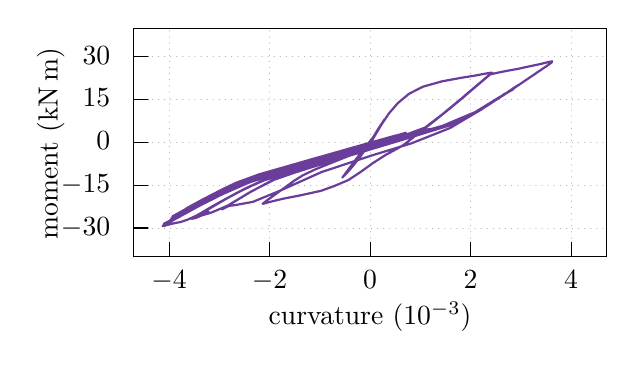
\begin{tikzpicture}[gnuplot]
%% generated with GNUPLOT 5.2p6 (Lua 5.3; terminal rev. Nov 2018, script rev. 107)
%% 08/11/2019 21:17:49
\path (0.000,0.000) rectangle (6.000,2.900);
\gpcolor{color=gp lt color axes}
\gpsetlinetype{gp lt axes}
\gpsetdashtype{gp dt axes}
\gpsetlinewidth{0.50}
\draw[gp path] (0.000,0.362)--(5.999,0.362);
\gpcolor{color=gp lt color border}
\gpsetlinetype{gp lt border}
\gpsetdashtype{gp dt solid}
\gpsetlinewidth{1.00}
\draw[gp path] (0.000,0.362)--(0.180,0.362);
\node[gp node right] at (-0.184,0.362) {$-30$};
\gpcolor{color=gp lt color axes}
\gpsetlinetype{gp lt axes}
\gpsetdashtype{gp dt axes}
\gpsetlinewidth{0.50}
\draw[gp path] (0.000,0.906)--(5.999,0.906);
\gpcolor{color=gp lt color border}
\gpsetlinetype{gp lt border}
\gpsetdashtype{gp dt solid}
\gpsetlinewidth{1.00}
\draw[gp path] (0.000,0.906)--(0.180,0.906);
\node[gp node right] at (-0.184,0.906) {$-15$};
\gpcolor{color=gp lt color axes}
\gpsetlinetype{gp lt axes}
\gpsetdashtype{gp dt axes}
\gpsetlinewidth{0.50}
\draw[gp path] (0.000,1.450)--(5.999,1.450);
\gpcolor{color=gp lt color border}
\gpsetlinetype{gp lt border}
\gpsetdashtype{gp dt solid}
\gpsetlinewidth{1.00}
\draw[gp path] (0.000,1.450)--(0.180,1.450);
\node[gp node right] at (-0.184,1.450) {$0$};
\gpcolor{color=gp lt color axes}
\gpsetlinetype{gp lt axes}
\gpsetdashtype{gp dt axes}
\gpsetlinewidth{0.50}
\draw[gp path] (0.000,1.993)--(5.999,1.993);
\gpcolor{color=gp lt color border}
\gpsetlinetype{gp lt border}
\gpsetdashtype{gp dt solid}
\gpsetlinewidth{1.00}
\draw[gp path] (0.000,1.993)--(0.180,1.993);
\node[gp node right] at (-0.184,1.993) {$15$};
\gpcolor{color=gp lt color axes}
\gpsetlinetype{gp lt axes}
\gpsetdashtype{gp dt axes}
\gpsetlinewidth{0.50}
\draw[gp path] (0.000,2.537)--(5.999,2.537);
\gpcolor{color=gp lt color border}
\gpsetlinetype{gp lt border}
\gpsetdashtype{gp dt solid}
\gpsetlinewidth{1.00}
\draw[gp path] (0.000,2.537)--(0.180,2.537);
\node[gp node right] at (-0.184,2.537) {$30$};
\gpcolor{color=gp lt color axes}
\gpsetlinetype{gp lt axes}
\gpsetdashtype{gp dt axes}
\gpsetlinewidth{0.50}
\draw[gp path] (0.447,0.000)--(0.447,2.899);
\gpcolor{color=gp lt color border}
\gpsetlinetype{gp lt border}
\gpsetdashtype{gp dt solid}
\gpsetlinewidth{1.00}
\draw[gp path] (0.447,0.000)--(0.447,0.180);
\node[gp node center] at (0.447,-0.308) {$-4$};
\gpcolor{color=gp lt color axes}
\gpsetlinetype{gp lt axes}
\gpsetdashtype{gp dt axes}
\gpsetlinewidth{0.50}
\draw[gp path] (1.723,0.000)--(1.723,2.899);
\gpcolor{color=gp lt color border}
\gpsetlinetype{gp lt border}
\gpsetdashtype{gp dt solid}
\gpsetlinewidth{1.00}
\draw[gp path] (1.723,0.000)--(1.723,0.180);
\node[gp node center] at (1.723,-0.308) {$-2$};
\gpcolor{color=gp lt color axes}
\gpsetlinetype{gp lt axes}
\gpsetdashtype{gp dt axes}
\gpsetlinewidth{0.50}
\draw[gp path] (3.000,0.000)--(3.000,2.899);
\gpcolor{color=gp lt color border}
\gpsetlinetype{gp lt border}
\gpsetdashtype{gp dt solid}
\gpsetlinewidth{1.00}
\draw[gp path] (3.000,0.000)--(3.000,0.180);
\node[gp node center] at (3.000,-0.308) {$0$};
\gpcolor{color=gp lt color axes}
\gpsetlinetype{gp lt axes}
\gpsetdashtype{gp dt axes}
\gpsetlinewidth{0.50}
\draw[gp path] (4.276,0.000)--(4.276,2.899);
\gpcolor{color=gp lt color border}
\gpsetlinetype{gp lt border}
\gpsetdashtype{gp dt solid}
\gpsetlinewidth{1.00}
\draw[gp path] (4.276,0.000)--(4.276,0.180);
\node[gp node center] at (4.276,-0.308) {$2$};
\gpcolor{color=gp lt color axes}
\gpsetlinetype{gp lt axes}
\gpsetdashtype{gp dt axes}
\gpsetlinewidth{0.50}
\draw[gp path] (5.552,0.000)--(5.552,2.899);
\gpcolor{color=gp lt color border}
\gpsetlinetype{gp lt border}
\gpsetdashtype{gp dt solid}
\gpsetlinewidth{1.00}
\draw[gp path] (5.552,0.000)--(5.552,0.180);
\node[gp node center] at (5.552,-0.308) {$4$};
\draw[gp path] (0.000,2.899)--(0.000,0.000)--(5.999,0.000)--(5.999,2.899)--cycle;
\node[gp node center,rotate=-270] at (-1.044,1.449) {moment (\si{\kilo\newton\meter})};
\node[gp node center] at (2.999,-0.769) {curvature (\num{E-3})};
\gpcolor{rgb color={0.416,0.239,0.604}}
\gpsetlinewidth{2.00}
\draw[gp path] (3.000,1.450)--(3.000,1.451)--(2.999,1.448)--(2.995,1.443)--(2.990,1.436)%
  --(2.986,1.430)--(2.983,1.426)--(2.980,1.423)--(2.977,1.418)--(2.973,1.412)--(2.968,1.406)%
  --(2.965,1.401)--(2.962,1.397)--(2.960,1.394)--(2.958,1.391)--(2.956,1.388)--(2.955,1.387)%
  --(2.958,1.391)--(2.961,1.395)--(2.965,1.401)--(2.969,1.406)--(2.972,1.411)--(2.976,1.416)%
  --(2.979,1.420)--(2.980,1.423)--(2.981,1.424)--(2.981,1.423)--(2.980,1.423)--(2.980,1.422)%
  --(2.979,1.421)--(2.978,1.419)--(2.977,1.418)--(2.977,1.417)--(2.977,1.418)--(2.978,1.420)%
  --(2.980,1.422)--(2.982,1.425)--(2.984,1.427)--(2.984,1.428)--(2.984,1.427)--(2.982,1.425)%
  --(2.979,1.421)--(2.976,1.416)--(2.972,1.410)--(2.969,1.406)--(2.971,1.409)--(2.975,1.415)%
  --(2.981,1.424)--(2.990,1.436)--(2.998,1.447)--(3.002,1.453)--(3.003,1.455)--(3.003,1.456)%
  --(3.004,1.457)--(3.003,1.455)--(2.998,1.447)--(2.989,1.434)--(2.978,1.419)--(2.967,1.404)%
  --(2.956,1.388)--(2.943,1.370)--(2.930,1.352)--(2.919,1.336)--(2.912,1.326)--(2.908,1.321)%
  --(2.905,1.317)--(2.903,1.314)--(2.907,1.319)--(2.913,1.328)--(2.924,1.343)--(2.937,1.361)%
  --(2.951,1.382)--(2.968,1.406)--(2.988,1.434)--(3.010,1.468)--(3.032,1.505)--(3.055,1.542)%
  --(3.076,1.576)--(3.094,1.606)--(3.112,1.635)--(3.130,1.662)--(3.148,1.689)--(3.164,1.713)%
  --(3.176,1.731)--(3.184,1.742)--(3.186,1.745)--(3.183,1.740)--(3.177,1.730)--(3.167,1.713)%
  --(3.152,1.688)--(3.132,1.656)--(3.109,1.617)--(3.084,1.576)--(3.061,1.536)--(3.040,1.502)%
  --(3.022,1.471)--(3.005,1.445)--(2.989,1.425)--(2.980,1.414)--(2.980,1.413)--(2.988,1.424)%
  --(3.004,1.445)--(3.024,1.475)--(3.044,1.508)--(3.065,1.544)--(3.089,1.583)--(3.114,1.624)%
  --(3.136,1.662)--(3.154,1.691)--(3.167,1.714)--(3.178,1.732)--(3.184,1.742)--(3.181,1.736)%
  --(3.161,1.704)--(3.125,1.644)--(3.078,1.565)--(3.025,1.476)--(2.966,1.395)--(2.911,1.319)%
  --(2.853,1.240)--(2.791,1.161)--(2.731,1.091)--(2.683,1.038)--(2.655,1.010)--(2.647,1.002)%
  --(2.654,1.011)--(2.672,1.035)--(2.702,1.076)--(2.749,1.139)--(2.813,1.224)--(2.888,1.325)%
  --(2.977,1.436)--(3.072,1.556)--(3.149,1.683)--(3.239,1.817)--(3.353,1.949)--(3.495,2.067)%
  --(3.672,2.157)--(3.916,2.225)--(4.166,2.271)--(4.324,2.296)--(4.435,2.317)--(4.508,2.330)%
  --(4.545,2.335)--(4.549,2.334)--(4.521,2.310)--(4.465,2.262)--(4.384,2.193)--(4.291,2.114)%
  --(4.191,2.028)--(4.081,1.936)--(3.960,1.837)--(3.834,1.736)--(3.711,1.640)--(3.605,1.557)%
  --(3.526,1.495)--(3.473,1.454)--(3.421,1.414)--(3.340,1.367)--(3.204,1.294)--(3.032,1.184)%
  --(2.876,1.071)--(2.722,0.970)--(2.547,0.896)--(2.376,0.834)--(2.107,0.775)--(1.896,0.734)%
  --(1.800,0.711)--(1.743,0.697)--(1.711,0.689)--(1.687,0.682)--(1.658,0.674)--(1.637,0.669)%
  --(1.636,0.670)--(1.653,0.683)--(1.689,0.712)--(1.738,0.747)--(1.794,0.787)--(1.859,0.835)%
  --(1.938,0.891)--(2.031,0.959)--(2.147,1.032)--(2.305,1.107)--(2.488,1.181)--(2.673,1.255)%
  --(2.861,1.329)--(3.073,1.407)--(3.286,1.485)--(3.488,1.559)--(3.697,1.637)--(3.813,1.725)%
  --(3.915,1.804)--(4.007,1.880)--(4.092,1.950)--(4.167,2.012)--(4.224,2.062)--(4.268,2.099)%
  --(4.308,2.132)--(4.348,2.167)--(4.389,2.201)--(4.418,2.225)--(4.435,2.240)--(4.453,2.256)%
  --(4.479,2.278)--(4.523,2.313)--(4.677,2.346)--(4.783,2.366)--(4.882,2.384)--(4.977,2.405)%
  --(5.071,2.425)--(5.157,2.443)--(5.242,2.464)--(5.313,2.479)--(5.302,2.460)--(5.127,2.341)%
  --(4.812,2.127)--(4.415,1.869)--(4.014,1.631)--(3.527,1.438)--(3.008,1.279)--(2.382,1.072)%
  --(1.859,0.837)--(1.512,0.694)--(1.282,0.652)--(1.192,0.641)--(1.204,0.639)--(1.199,0.638)%
  --(1.159,0.620)--(1.120,0.598)--(1.124,0.604)--(1.244,0.678)--(1.488,0.825)--(1.811,0.990)%
  --(2.236,1.129)--(2.676,1.263)--(3.168,1.412)--(3.753,1.589)--(4.332,1.833)--(4.670,2.040)%
  --(4.821,2.125)--(4.729,2.076)--(4.592,1.986)--(4.508,1.928)--(4.446,1.894)--(4.341,1.825)%
  --(4.026,1.670)--(3.490,1.506)--(2.941,1.341)--(2.484,1.204)--(2.208,1.118)--(2.012,1.055)%
  --(1.748,0.963)--(1.473,0.815)--(1.200,0.650)--(0.975,0.554)--(0.877,0.527)--(0.899,0.544)%
  --(0.949,0.569)--(0.944,0.567)--(0.874,0.527)--(0.781,0.488)--(0.732,0.478)--(0.782,0.508)%
  --(0.917,0.583)--(1.062,0.668)--(1.184,0.739)--(1.299,0.801)--(1.448,0.878)--(1.687,0.982)%
  --(2.051,1.095)--(2.417,1.203)--(2.726,1.294)--(2.984,1.370)--(3.241,1.445)--(3.517,1.526)%
  --(3.777,1.602)--(3.972,1.659)--(4.048,1.681)--(4.003,1.668)--(3.890,1.635)--(3.751,1.594)%
  --(3.575,1.542)--(3.330,1.470)--(3.012,1.377)--(2.653,1.272)--(2.297,1.167)--(1.965,1.069)%
  --(1.678,0.978)--(1.462,0.884)--(1.281,0.793)--(1.143,0.717)--(1.060,0.669)--(1.038,0.657)%
  --(1.071,0.676)--(1.149,0.721)--(1.270,0.788)--(1.439,0.876)--(1.643,0.967)--(1.889,1.049)%
  --(2.150,1.126)--(2.401,1.200)--(2.666,1.278)--(2.947,1.361)--(3.212,1.439)--(3.436,1.504)%
  --(3.615,1.557)--(3.764,1.600)--(3.902,1.641)--(4.025,1.677)--(4.128,1.707)--(4.157,1.721)%
  --(4.142,1.713)--(4.123,1.705)--(4.081,1.693)--(3.968,1.660)--(3.763,1.599)--(3.505,1.524)%
  --(3.240,1.446)--(3.021,1.382)--(2.851,1.332)--(2.678,1.281)--(2.475,1.222)--(2.283,1.165)%
  --(2.165,1.130)--(2.146,1.125)--(2.201,1.141)--(2.313,1.174)--(2.456,1.216)--(2.525,1.236)%
  --(2.466,1.219)--(2.346,1.184)--(2.236,1.151)--(2.202,1.141)--(2.227,1.149)--(2.220,1.146)%
  --(2.146,1.125)--(2.052,1.097)--(2.020,1.088)--(2.112,1.115)--(2.283,1.165)--(2.381,1.194)%
  --(2.321,1.176)--(2.157,1.128)--(2.003,1.083)--(1.956,1.069)--(1.995,1.080)--(1.992,1.079)%
  --(1.879,1.046)--(1.718,0.995)--(1.615,0.955)--(1.614,0.955)--(1.686,0.983)--(1.758,1.010)%
  --(1.788,1.020)--(1.801,1.023)--(1.859,1.040)--(1.979,1.076)--(2.115,1.116)--(2.231,1.150)%
  --(2.317,1.175)--(2.387,1.196)--(2.474,1.221)--(2.588,1.255)--(2.711,1.291)--(2.813,1.321)%
  --(2.884,1.342)--(2.941,1.358)--(3.009,1.379)--(3.095,1.404)--(3.183,1.430)--(3.251,1.450)%
  --(3.289,1.461)--(3.292,1.462)--(3.267,1.454)--(3.222,1.441)--(3.153,1.421)--(3.053,1.391)%
  --(2.919,1.352)--(2.774,1.309)--(2.639,1.270)--(2.525,1.236)--(2.426,1.207)--(2.339,1.182)%
  --(2.271,1.162)--(2.238,1.152)--(2.250,1.155)--(2.313,1.174)--(2.418,1.205)--(2.559,1.246)%
  --(2.736,1.298)--(2.950,1.361)--(3.194,1.433)--(3.409,1.496)--(3.544,1.536)--(3.610,1.555)%
  --(3.635,1.562)--(3.662,1.570)--(3.695,1.580)--(3.697,1.580)--(3.635,1.562)--(3.499,1.522)%
  --(3.310,1.467)--(3.111,1.408)--(2.921,1.352)--(2.741,1.300)--(2.557,1.246)--(2.360,1.188)%
  --(2.163,1.130)--(2.005,1.083)--(1.908,1.055)--(1.871,1.044)--(1.869,1.043)--(1.895,1.051)%
  --(1.965,1.072)--(2.092,1.109)--(2.278,1.164)--(2.514,1.233)--(2.785,1.313)--(3.072,1.397)%
  --(3.372,1.486)--(3.688,1.578)--(4.040,1.681)--(4.331,1.830)--(4.530,1.947)--(4.654,2.027)%
  --(4.705,2.064)--(4.734,2.078)--(4.768,2.102)--(4.824,2.140)--(4.888,2.180)--(4.874,2.169)%
  --(4.701,2.054)--(4.420,1.874)--(4.104,1.698)--(3.731,1.587)--(3.430,1.500)--(3.076,1.397)%
  --(2.614,1.260)--(2.092,1.108)--(1.604,0.951)--(1.299,0.803)--(1.098,0.694)--(0.957,0.614)%
  --(0.850,0.551)--(0.780,0.512)--(0.680,0.467)--(0.592,0.438)--(0.500,0.420)--(0.423,0.401)%
  --(0.378,0.387)--(0.365,0.387)--(0.378,0.395)--(0.422,0.419)--(0.502,0.463)--(0.638,0.538)%
  --(0.839,0.648)--(1.119,0.789)--(1.469,0.942)--(1.912,1.084)--(2.413,1.229)--(2.946,1.382)%
  --(3.478,1.534)--(3.931,1.663)--(4.251,1.776)--(4.372,1.843)--(4.416,1.867)--(4.405,1.864)%
  --(4.401,1.860)--(4.412,1.866)--(4.413,1.868)--(4.395,1.856)--(4.336,1.821)--(4.231,1.760)%
  --(4.072,1.702)--(3.945,1.666)--(3.856,1.641)--(3.805,1.626)--(3.769,1.615)--(3.716,1.600)%
  --(3.618,1.572)--(3.408,1.512)--(3.057,1.411)--(2.650,1.295)--(2.289,1.192)--(1.991,1.106)%
  --(1.719,1.028)--(1.446,0.933)--(1.174,0.814)--(0.959,0.713)--(0.856,0.662)--(0.836,0.650)%
  --(0.850,0.658)--(0.855,0.660)--(0.804,0.632)--(0.720,0.587)--(0.653,0.551)--(0.623,0.534)%
  --(0.634,0.540)--(0.671,0.561)--(0.709,0.581)--(0.741,0.599)--(0.780,0.620)--(0.861,0.664)%
  --(0.999,0.734)--(1.183,0.823)--(1.385,0.915)--(1.593,0.990)--(1.795,1.054)--(1.986,1.109)%
  --(2.146,1.155)--(2.284,1.195)--(2.385,1.224)--(2.445,1.241)--(2.461,1.246)--(2.433,1.237)%
  --(2.368,1.219)--(2.288,1.196)--(2.203,1.171)--(2.109,1.144)--(2.001,1.113)--(1.901,1.084)%
  --(1.824,1.063)--(1.745,1.040)--(1.636,1.006)--(1.482,0.949)--(1.295,0.873)--(1.151,0.807)%
  --(1.080,0.773)--(1.048,0.757)--(1.013,0.740)--(0.969,0.719)--(0.941,0.706)--(0.968,0.719)%
  --(1.064,0.766)--(1.209,0.837)--(1.387,0.916)--(1.594,0.992)--(1.836,1.067)--(2.135,1.153)%
  --(2.473,1.250)--(2.812,1.347)--(3.100,1.430)--(3.316,1.492)--(3.480,1.538)--(3.600,1.572)%
  --(3.682,1.596)--(3.726,1.608)--(3.731,1.610)--(3.692,1.599)--(3.615,1.576)--(3.509,1.546)%
  --(3.387,1.511)--(3.259,1.475)--(3.126,1.436)--(2.991,1.398)--(2.864,1.362)--(2.757,1.331)%
  --(2.680,1.309)--(2.638,1.297)--(2.629,1.294)--(2.626,1.293)--(2.609,1.288)--(2.572,1.278)%
  --(2.521,1.263)--(2.468,1.248)--(2.415,1.233)--(2.366,1.219)--(2.320,1.205)--(2.273,1.192)%
  --(2.230,1.180)--(2.201,1.171)--(2.189,1.168)--(2.183,1.166)--(2.170,1.162)--(2.140,1.154)%
  --(2.098,1.142)--(2.058,1.130)--(2.028,1.122)--(2.009,1.116)--(1.994,1.112)--(1.970,1.105)%
  --(1.935,1.095)--(1.901,1.085)--(1.878,1.078)--(1.872,1.077)--(1.878,1.079)--(1.887,1.081)%
  --(1.898,1.084)--(1.920,1.091)--(1.965,1.104)--(2.037,1.124)--(2.128,1.151)--(2.232,1.180)%
  --(2.341,1.212)--(2.439,1.240)--(2.521,1.263)--(2.584,1.281)--(2.625,1.293)--(2.635,1.296)%
  --(2.610,1.289)--(2.565,1.276)--(2.518,1.263)--(2.475,1.250)--(2.432,1.238)--(2.382,1.223)%
  --(2.323,1.206)--(2.245,1.184)--(2.153,1.157)--(2.063,1.132)--(1.990,1.111)--(1.934,1.095)%
  --(1.893,1.083)--(1.861,1.074)--(1.840,1.068)--(1.842,1.068)--(1.875,1.078)--(1.940,1.096)%
  --(2.025,1.121)--(2.106,1.144)--(2.170,1.162)--(2.222,1.177)--(2.272,1.192)--(2.327,1.208)%
  --(2.378,1.222)--(2.417,1.233)--(2.441,1.240)--(2.452,1.244)--(2.461,1.246)--(2.466,1.247)%
  --(2.461,1.246)--(2.437,1.239)--(2.391,1.226)--(2.335,1.210)--(2.280,1.194)--(2.231,1.180)%
  --(2.182,1.166)--(2.128,1.150)--(2.071,1.134)--(2.020,1.119)--(1.984,1.109)--(1.959,1.102)%
  --(1.935,1.095)--(1.901,1.085)--(1.856,1.072)--(1.809,1.059)--(1.773,1.048)--(1.755,1.043)%
  --(1.756,1.043)--(1.762,1.045)--(1.767,1.047)--(1.776,1.049)--(1.798,1.055)--(1.838,1.067)%
  --(1.893,1.083)--(1.953,1.100)--(2.014,1.118)--(2.085,1.138)--(2.171,1.163)--(2.255,1.187)%
  --(2.319,1.205)--(2.362,1.218)--(2.393,1.226)--(2.424,1.235)--(2.457,1.245)--(2.478,1.251)%
  --(2.473,1.249)--(2.443,1.241)--(2.399,1.228)--(2.355,1.216)--(2.313,1.204)--(2.268,1.191)%
  --(2.215,1.175)--(2.155,1.158)--(2.099,1.142)--(2.059,1.130)--(2.040,1.125)--(2.036,1.124)%
  --(2.043,1.126)--(2.068,1.133)--(2.122,1.149)--(2.206,1.173)--(2.310,1.203)--(2.396,1.227)%
  --(2.445,1.241)--(2.458,1.245)--(2.450,1.243)--(2.448,1.242)--(2.456,1.245)--(2.432,1.238)%
  --(2.389,1.225)--(2.344,1.212)--(2.309,1.202)--(2.277,1.193)--(2.232,1.180)--(2.157,1.159)%
  --(2.057,1.130)--(1.949,1.099)--(1.853,1.071)--(1.775,1.049)--(1.711,1.031)--(1.657,1.015)%
  --(1.619,1.001)--(1.597,0.993)--(1.605,0.996)--(1.644,1.010)--(1.715,1.032)--(1.809,1.059)%
  --(1.919,1.090)--(2.042,1.126)--(2.173,1.163)--(2.297,1.199)--(2.400,1.229)--(2.478,1.251)%
  --(2.537,1.268)--(2.585,1.282)--(2.623,1.293)--(2.648,1.300)--(2.644,1.299)--(2.606,1.288)%
  --(2.544,1.270)--(2.473,1.250)--(2.404,1.230)--(2.335,1.210)--(2.257,1.187)--(2.171,1.163)%
  --(2.085,1.138)--(2.012,1.117)--(1.962,1.103)--(1.934,1.095)--(1.918,1.090)--(1.906,1.087)%
  --(1.896,1.084)--(1.894,1.083)--(1.904,1.086)--(1.928,1.093)--(1.967,1.104)--(2.022,1.120)%
  --(2.092,1.140)--(2.180,1.165)--(2.279,1.194)--(2.381,1.223)--(2.471,1.249)--(2.540,1.269)%
  --(2.593,1.284)--(2.633,1.296)--(2.662,1.304)--(2.673,1.307)--(2.660,1.303)--(2.624,1.293)%
  --(2.573,1.278)--(2.515,1.262)--(2.455,1.244)--(2.390,1.226)--(2.321,1.206)--(2.252,1.186)%
  --(2.192,1.169)--(2.147,1.156)--(2.120,1.148)--(2.111,1.146)--(2.114,1.147)--(2.128,1.151)%
  --(2.150,1.157)--(2.178,1.165)--(2.215,1.175)--(2.260,1.189)--(2.317,1.205)--(2.386,1.225)%
  --(2.467,1.248)--(2.558,1.274)--(2.636,1.296)--(2.685,1.311)--(2.719,1.320)--(2.748,1.329)%
  --(2.769,1.335)--(2.768,1.334)--(2.724,1.322)--(2.637,1.297)--(2.526,1.265)--(2.411,1.232)%
  --(2.294,1.198)--(2.160,1.160)--(2.007,1.116)--(1.840,1.067)--(1.675,1.020)--(1.549,0.975)%
  --(1.444,0.937)--(1.359,0.904)--(1.288,0.871)--(1.230,0.846)--(1.204,0.834)--(1.222,0.843)%
  --(1.286,0.872)--(1.382,0.915)--(1.492,0.955)--(1.589,0.991)--(1.683,1.023)--(1.798,1.056)%
  --(1.929,1.094)--(2.064,1.132)--(2.186,1.168)--(2.288,1.197)--(2.365,1.219)--(2.424,1.236)%
  --(2.475,1.251)--(2.516,1.262)--(2.535,1.268)--(2.526,1.265)--(2.491,1.255)--(2.440,1.240)%
  --(2.382,1.224)--(2.316,1.205)--(2.238,1.182)--(2.145,1.156)--(2.039,1.125)--(1.931,1.094)%
  --(1.828,1.065)--(1.739,1.039)--(1.664,1.018)--(1.612,0.999)--(1.572,0.984)--(1.551,0.977)%
  --(1.557,0.979)--(1.590,0.991)--(1.648,1.012)--(1.737,1.039)--(1.849,1.071)--(1.973,1.106)%
  --(2.109,1.146)--(2.257,1.188)--(2.407,1.231)--(2.553,1.273)--(2.690,1.312)--(2.812,1.347)%
  --(2.915,1.377)--(2.995,1.400)--(3.054,1.417)--(3.088,1.427)--(3.089,1.427)--(3.054,1.417)%
  --(2.989,1.398)--(2.907,1.374)--(2.808,1.346)--(2.694,1.313)--(2.575,1.279)--(2.457,1.245)%
  --(2.300,1.200)--(2.070,1.134)--(1.787,1.053)--(1.508,0.960)--(1.277,0.866)--(1.098,0.783)%
  --(0.933,0.703)--(0.784,0.625)--(0.656,0.556)--(0.574,0.512)--(0.560,0.504)--(0.590,0.521)%
  --(0.627,0.541)--(0.653,0.555)--(0.666,0.562)--(0.696,0.579)--(0.785,0.629)--(0.942,0.711)%
  --(1.146,0.810)--(1.354,0.906)--(1.565,0.985)--(1.796,1.059)--(2.066,1.136)--(2.351,1.218)%
  --(2.615,1.294)--(2.825,1.355)--(2.975,1.397)--(3.079,1.427)--(3.164,1.452)--(3.239,1.473)%
  --(3.280,1.485)--(3.264,1.480)--(3.182,1.456)--(3.049,1.418)--(2.897,1.375)--(2.750,1.332)%
  --(2.609,1.292)--(2.466,1.251)--(2.314,1.207)--(2.162,1.164)--(2.043,1.130)--(1.977,1.111)%
  --(1.974,1.110)--(2.022,1.124)--(2.082,1.141)--(2.121,1.152)--(2.077,1.139)--(1.935,1.099)%
  --(1.797,1.059)--(1.734,1.041)--(1.727,1.039)--(1.715,1.035)--(1.651,1.016)--(1.558,0.982)%
  --(1.458,0.946)--(1.376,0.915)--(1.337,0.898)--(1.316,0.888)--(1.288,0.876)--(1.253,0.860)%
  --(1.218,0.844)--(1.204,0.837)--(1.218,0.845)--(1.256,0.862)--(1.313,0.888)--(1.390,0.921)%
  --(1.500,0.961)--(1.641,1.013)--(1.850,1.074)--(2.109,1.149)--(2.409,1.235)--(2.729,1.327)%
  --(3.028,1.413)--(3.263,1.480)--(3.443,1.531)--(3.568,1.567)--(3.659,1.593)--(3.729,1.613)%
  --(3.752,1.619)--(3.710,1.607)--(3.601,1.576)--(3.422,1.525)--(3.186,1.457)--(2.899,1.375)%
  --(2.568,1.280)--(2.203,1.175)--(1.792,1.057)--(1.394,0.922)--(1.065,0.770)--(0.777,0.627)%
  --(0.569,0.514)--(0.435,0.441)--(0.379,0.414)--(0.403,0.427)--(0.438,0.445)--(0.460,0.457)%
  --(0.477,0.467)--(0.518,0.490)--(0.648,0.562)--(0.904,0.701)--(1.270,0.880)--(1.710,1.040)%
  --(2.102,1.153)--(2.352,1.226)--(2.573,1.289)--(2.857,1.370)--(3.178,1.463)--(3.439,1.537)%
  --(3.560,1.571)--(3.555,1.570)--(3.487,1.550)--(3.404,1.527)--(3.351,1.511)--(3.330,1.505)%
  --(3.285,1.492)--(3.156,1.455)--(2.922,1.388)--(2.607,1.298)--(2.287,1.206)--(1.988,1.120)%
  --(1.717,1.043)--(1.483,0.962)--(1.252,0.868)--(1.043,0.769)--(0.876,0.687)--(0.778,0.635)%
  --(0.736,0.613)--(0.728,0.609)--(0.742,0.616)--(0.786,0.641)--(0.880,0.691)--(1.037,0.770)%
  --(1.246,0.871)--(1.509,0.976)--(1.818,1.074)--(2.160,1.173)--(2.497,1.270)--(2.830,1.366)%
  --(3.132,1.452)--(3.371,1.521)--(3.544,1.570)--(3.656,1.602)--(3.713,1.618)--(3.705,1.616)%
  --(3.632,1.594)--(3.509,1.559)--(3.325,1.507)--(3.079,1.436)--(2.794,1.355)--(2.495,1.269)%
  --(2.202,1.185)--(1.920,1.104)--(1.657,1.028)--(1.460,0.957)--(1.289,0.889)--(1.145,0.822)%
  --(1.025,0.765)--(0.936,0.722)--(0.892,0.699)--(0.891,0.699)--(0.918,0.713)--(0.961,0.735)%
  --(1.022,0.765)--(1.100,0.803)--(1.198,0.851)--(1.320,0.907)--(1.467,0.963)--(1.622,1.020)%
  --(1.801,1.072)--(1.985,1.125)--(2.166,1.177)--(2.338,1.227)--(2.502,1.274)--(2.660,1.319)%
  --(2.809,1.362)--(2.946,1.401)--(3.068,1.436)--(3.176,1.467)--(3.273,1.495)--(3.356,1.518)%
  --(3.407,1.533)--(3.410,1.533)--(3.356,1.518)--(3.248,1.487)--(3.088,1.441)--(2.877,1.381)%
  --(2.631,1.310)--(2.371,1.236)--(2.105,1.159)--(1.833,1.081)--(1.553,0.994)--(1.279,0.886)%
  --(1.035,0.771)--(0.824,0.666)--(0.679,0.587)--(0.592,0.540)--(0.559,0.523)--(0.569,0.528)%
  --(0.602,0.546)--(0.645,0.570)--(0.702,0.602)--(0.797,0.654)--(0.958,0.739)--(1.195,0.855)%
  --(1.487,0.974)--(1.803,1.076)--(2.101,1.162)--(2.364,1.238)--(2.622,1.312)--(2.879,1.385)%
  --(3.096,1.448)--(3.243,1.490)--(3.308,1.508)--(3.303,1.507)--(3.255,1.493)--(3.183,1.472)%
  --(3.073,1.441)--(2.903,1.392)--(2.657,1.321)--(2.359,1.236)--(2.035,1.143)--(1.709,1.049)%
  --(1.420,0.949)--(1.161,0.836)--(0.923,0.721)--(0.726,0.617)--(0.583,0.539)--(0.499,0.494)%
  --(0.472,0.480)--(0.498,0.493)--(0.554,0.524)--(0.612,0.557)--(0.676,0.592)--(0.764,0.640)%
  --(0.903,0.715)--(1.108,0.817)--(1.342,0.926)--(1.595,1.018)--(1.823,1.086)--(2.021,1.143)%
  --(2.227,1.202)--(2.455,1.268)--(2.680,1.332)--(2.862,1.384)--(2.980,1.418)--(3.054,1.439)%
  --(3.113,1.456)--(3.166,1.471)--(3.202,1.482)--(3.201,1.481)--(3.140,1.464)--(3.009,1.426)%
  --(2.831,1.375)--(2.625,1.316)--(2.400,1.251)--(2.142,1.177)--(1.849,1.093)--(1.554,1.003)%
  --(1.302,0.907)--(1.109,0.816)--(0.951,0.740)--(0.831,0.678)--(0.742,0.629)--(0.687,0.600)%
  --(0.677,0.595)--(0.715,0.616)--(0.792,0.658)--(0.898,0.714)--(1.014,0.773)--(1.134,0.831)%
  --(1.260,0.892)--(1.421,0.957)--(1.594,1.020)--(1.767,1.072)--(1.913,1.114)--(2.026,1.147)%
  --(2.120,1.174)--(2.204,1.198)--(2.268,1.216)--(2.300,1.225)--(2.293,1.223)--(2.253,1.212)%
  --(2.196,1.195)--(2.131,1.177)--(2.057,1.155)--(1.965,1.129)--(1.843,1.094)--(1.690,1.050)%
  --(1.543,1.001)--(1.407,0.951)--(1.282,0.901)--(1.165,0.845)--(1.037,0.783)--(0.906,0.718)%
  --(0.801,0.663)--(0.734,0.627)--(0.698,0.607)--(0.682,0.598)--(0.681,0.597)--(0.694,0.605)%
  --(0.731,0.626)--(0.802,0.664)--(0.906,0.720)--(1.040,0.787)--(1.187,0.858)--(1.344,0.930)%
  --(1.541,1.002)--(1.766,1.073)--(2.018,1.145)--(2.267,1.217)--(2.495,1.282)--(2.706,1.343)%
  --(2.898,1.398)--(3.069,1.447)--(3.213,1.488)--(3.327,1.521)--(3.403,1.542)--(3.431,1.550)%
  --(3.428,1.549)--(3.412,1.545)--(3.396,1.540)--(3.381,1.536)--(3.350,1.527)--(3.284,1.508)%
  --(3.185,1.479)--(3.076,1.448)--(2.974,1.419)--(2.889,1.395)--(2.816,1.374)--(2.749,1.355)%
  --(2.687,1.337)--(2.644,1.325)--(2.641,1.324)--(2.678,1.334)--(2.716,1.345)--(2.717,1.345)%
  --(2.667,1.331)--(2.576,1.305)--(2.473,1.275)--(2.367,1.245)--(2.235,1.207)--(2.052,1.154)%
  --(1.835,1.092)--(1.616,1.029)--(1.448,0.967)--(1.298,0.909)--(1.165,0.846)--(1.023,0.777)%
  --(0.880,0.706)--(0.755,0.639)--(0.669,0.592)--(0.631,0.572)--(0.632,0.573)--(0.651,0.583)%
  --(0.666,0.591)--(0.667,0.591)--(0.674,0.595)--(0.710,0.615)--(0.789,0.659)--(0.900,0.718)%
  --(1.020,0.779)--(1.131,0.832)--(1.227,0.879)--(1.334,0.928)--(1.478,0.981)--(1.617,1.031)%
  --(1.759,1.072)--(1.857,1.100)--(1.916,1.117)--(1.957,1.129)--(1.988,1.138)--(2.001,1.142)%
  --(1.991,1.139)--(1.960,1.130)--(1.928,1.121)--(1.918,1.118)--(1.923,1.119)--(1.929,1.121)%
  --(1.922,1.119)--(1.902,1.113)--(1.900,1.112)--(1.932,1.122)--(1.980,1.135)--(2.013,1.145)%
  --(2.018,1.146)--(2.005,1.143)--(2.011,1.144)--(2.053,1.156)--(2.116,1.175)--(2.174,1.191)%
  --(2.205,1.200)--(2.215,1.203)--(2.224,1.206)--(2.240,1.210)--(2.256,1.215)--(2.253,1.214)%
  --(2.222,1.205)--(2.173,1.191)--(2.134,1.180)--(2.120,1.176)--(2.115,1.174)--(2.093,1.168)%
  --(2.043,1.154)--(1.981,1.136)--(1.937,1.123)--(1.926,1.120)--(1.927,1.120)--(1.911,1.116)%
  --(1.867,1.103)--(1.808,1.086)--(1.766,1.074)--(1.751,1.070)--(1.743,1.067)--(1.714,1.059)%
  --(1.664,1.045)--(1.614,1.030)--(1.593,1.023)--(1.597,1.024)--(1.612,1.029)--(1.627,1.034)%
  --(1.633,1.036)--(1.639,1.037)--(1.655,1.042)--(1.680,1.049)--(1.702,1.055)--(1.706,1.057)%
  --(1.698,1.054)--(1.692,1.053)--(1.702,1.055)--(1.731,1.064)--(1.769,1.075)--(1.807,1.086)%
  --(1.848,1.098)--(1.901,1.113)--(1.969,1.132)--(2.045,1.154)--(2.121,1.176)--(2.192,1.196)%
  --(2.253,1.214)--(2.309,1.230)--(2.362,1.245)--(2.409,1.259)--(2.435,1.266)--(2.431,1.265)%
  --(2.402,1.257)--(2.363,1.246)--(2.323,1.234)--(2.282,1.222)--(2.232,1.208)--(2.171,1.190)%
  --(2.106,1.172)--(2.047,1.155)--(2.003,1.142)--(1.972,1.133)--(1.947,1.126)--(1.924,1.119)%
  --(1.915,1.117)--(1.932,1.122)--(1.972,1.133)--(2.024,1.148)--(2.087,1.166)--(2.157,1.186)%
  --(2.217,1.203)--(2.251,1.213)--(2.259,1.216)--(2.248,1.212)--(2.225,1.206)--(2.190,1.196)%
  --(2.131,1.179)--(2.042,1.153)--(1.925,1.120)--(1.796,1.083)--(1.667,1.045)--(1.559,1.010)%
  --(1.460,0.974)--(1.365,0.939)--(1.283,0.904)--(1.216,0.873)--(1.175,0.854)--(1.169,0.851)%
  --(1.202,0.867)--(1.265,0.897)--(1.327,0.925)--(1.373,0.942)--(1.410,0.955)--(1.459,0.974)%
  --(1.543,1.005)--(1.660,1.044)--(1.794,1.082)--(1.911,1.116)--(2.019,1.147)--(2.139,1.181)%
  --(2.265,1.217)--(2.365,1.246)--(2.404,1.257)--(2.366,1.246)--(2.277,1.221)--(2.174,1.191)%
  --(2.090,1.167)--(2.025,1.148)--(1.942,1.125)--(1.824,1.091)--(1.688,1.052)--(1.581,1.018)%
  --(1.513,0.993)--(1.461,0.974)--(1.403,0.953)--(1.330,0.926)--(1.264,0.896)--(1.219,0.875)%
  --(1.206,0.869)--(1.218,0.875)--(1.235,0.883)--(1.245,0.888)--(1.261,0.895)--(1.299,0.912)%
  --(1.371,0.942)--(1.473,0.979)--(1.574,1.016)--(1.667,1.046)--(1.767,1.074)--(1.879,1.107)%
  --(2.013,1.145)--(2.159,1.187)--(2.288,1.224)--(2.389,1.253)--(2.489,1.282)--(2.612,1.317)%
  --(2.751,1.357)--(2.876,1.393)--(2.940,1.411)--(2.921,1.406)--(2.837,1.382)--(2.714,1.346)%
  --(2.558,1.301)--(2.359,1.244)--(2.111,1.173)--(1.825,1.091)--(1.538,1.002)--(1.290,0.907)%
  --(1.093,0.814)--(0.918,0.728)--(0.775,0.652)--(0.664,0.592)--(0.592,0.553)--(0.564,0.538)%
  --(0.577,0.545)--(0.621,0.569)--(0.693,0.609)--(0.795,0.666)--(0.944,0.745)--(1.156,0.849)%
  --(1.405,0.956)--(1.668,1.048)--(1.918,1.120)--(2.119,1.178)--(2.311,1.233)--(2.506,1.289)%
  --(2.674,1.338)--(2.773,1.366)--(2.791,1.371)--(2.753,1.360)--(2.694,1.343)--(2.629,1.324)%
  --(2.554,1.303)--(2.457,1.275)--(2.340,1.241)--(2.226,1.209)--(2.128,1.181)--(2.058,1.160)%
  --(2.019,1.149)--(2.006,1.145)--(2.014,1.148)--(2.043,1.156)--(2.090,1.170)--(2.150,1.187)%
  --(2.212,1.204)--(2.259,1.218)--(2.285,1.226)--(2.285,1.225)--(2.263,1.219)--(2.225,1.208)%
  --(2.167,1.192)--(2.091,1.170)--(2.008,1.146)--(1.930,1.124)--(1.859,1.103)--(1.794,1.085)%
  --(1.744,1.070)--(1.717,1.062)--(1.706,1.059)--(1.700,1.058)--(1.688,1.054)--(1.665,1.047)%
  --(1.644,1.041)--(1.632,1.038)--(1.630,1.037)--(1.628,1.037)--(1.626,1.036)--(1.630,1.037)%
  --(1.643,1.041)--(1.667,1.048)--(1.692,1.055)--(1.709,1.060)--(1.717,1.062)--(1.719,1.063)%
  --(1.721,1.064)--(1.723,1.064)--(1.713,1.061)--(1.683,1.053)--(1.630,1.037)--(1.572,1.017)%
  --(1.513,0.996)--(1.466,0.979)--(1.434,0.967)--(1.415,0.960)--(1.399,0.954)--(1.387,0.950)%
  --(1.390,0.951)--(1.419,0.962)--(1.471,0.981)--(1.536,1.004)--(1.599,1.027)--(1.672,1.049)%
  --(1.758,1.074)--(1.858,1.103)--(1.977,1.137)--(2.106,1.174)--(2.216,1.206)--(2.285,1.226)%
  --(2.305,1.231)--(2.278,1.223)--(2.229,1.209)--(2.171,1.193)--(2.110,1.175)--(2.040,1.155)%
  --(1.950,1.129)--(1.846,1.099)--(1.750,1.072)--(1.683,1.053)--(1.648,1.042)--(1.631,1.038)%
  --(1.611,1.032)--(1.584,1.022)--(1.556,1.012)--(1.540,1.006)--(1.537,1.005)--(1.538,1.005)%
  --(1.540,1.006)--(1.549,1.009)--(1.575,1.019)--(1.625,1.036)--(1.709,1.060)--(1.808,1.089)%
  --(1.919,1.121)--(2.045,1.157)--(2.177,1.195)--(2.302,1.231)--(2.408,1.261)--(2.486,1.283)%
  --(2.532,1.297)--(2.547,1.301)--(2.533,1.297)--(2.490,1.284)--(2.418,1.264)--(2.318,1.235)%
  --(2.196,1.200)--(2.056,1.160)--(1.910,1.118)--(1.764,1.076)--(1.625,1.036)--(1.518,0.997)%
  --(1.427,0.964)--(1.358,0.939)--(1.308,0.919)--(1.265,0.900)--(1.230,0.883)--(1.205,0.871)%
  --(1.193,0.865)--(1.190,0.864)--(1.199,0.868)--(1.221,0.879)--(1.257,0.897)--(1.313,0.922)%
  --(1.392,0.952)--(1.487,0.987)--(1.592,1.025)--(1.724,1.064)--(1.855,1.102)--(1.968,1.135)%
  --(2.067,1.163)--(2.160,1.190)--(2.256,1.217)--(2.350,1.245)--(2.432,1.268)--(2.495,1.286)%
  --(2.542,1.300)--(2.584,1.312)--(2.618,1.321)--(2.635,1.326)--(2.627,1.324)--(2.589,1.313)%
  --(2.529,1.296)--(2.457,1.275)--(2.383,1.254)--(2.313,1.234)--(2.243,1.214)--(2.172,1.193)%
  --(2.101,1.173)--(2.035,1.154)--(1.964,1.134)--(1.877,1.108)--(1.775,1.079)--(1.661,1.046)%
  --(1.556,1.012)--(1.452,0.973)--(1.342,0.933)--(1.245,0.890)--(1.165,0.852)--(1.109,0.825)%
  --(1.079,0.810)--(1.070,0.806)--(1.080,0.811)--(1.108,0.825)--(1.163,0.852)--(1.243,0.891)%
  --(1.344,0.935)--(1.458,0.976)--(1.558,1.013)--(1.650,1.044)--(1.749,1.072)--(1.842,1.099)%
  --(1.930,1.124)--(2.009,1.147)--(2.070,1.164)--(2.113,1.177)--(2.145,1.186)--(2.172,1.194)%
  --(2.197,1.201)--(2.215,1.206)--(2.192,1.199)--(2.148,1.187)--(2.091,1.170)--(2.027,1.152)%
  --(1.957,1.132)--(1.871,1.107)--(1.765,1.077)--(1.645,1.042)--(1.542,1.007)--(1.458,0.976)%
  --(1.399,0.955)--(1.358,0.940)--(1.330,0.930)--(1.320,0.925)--(1.333,0.931)--(1.383,0.949)%
  --(1.466,0.980)--(1.569,1.017)--(1.693,1.056)--(1.837,1.097)--(1.986,1.140)--(2.136,1.183)%
  --(2.274,1.223)--(2.386,1.255)--(2.456,1.275)--(2.471,1.279)--(2.425,1.266)--(2.347,1.244)%
  --(2.258,1.218)--(2.160,1.190)--(2.046,1.158)--(1.909,1.118)--(1.755,1.074)--(1.608,1.031)%
  --(1.509,0.995)--(1.439,0.970)--(1.398,0.955)--(1.368,0.944)--(1.343,0.934)--(1.327,0.929)%
  --(1.331,0.930)--(1.372,0.945)--(1.450,0.974)--(1.543,1.008)--(1.635,1.039)--(1.737,1.069)%
  --(1.841,1.099)--(1.957,1.132)--(2.080,1.168)--(2.198,1.201)--(2.294,1.229)--(2.364,1.249)%
  --(2.414,1.263)--(2.449,1.273)--(2.464,1.278)--(2.452,1.274)--(2.404,1.260)--(2.320,1.236)%
  --(2.206,1.203)--(2.073,1.165)--(1.933,1.125)--(1.793,1.085)--(1.656,1.045)--(1.538,1.006)%
  --(1.431,0.966)--(1.343,0.934)--(1.290,0.912)--(1.255,0.896)--(1.227,0.882)--(1.201,0.870)%
  --(1.184,0.862)--(1.186,0.863)--(1.211,0.875)--(1.247,0.893)--(1.286,0.910)--(1.326,0.929)%
  --(1.387,0.951)--(1.465,0.979)--(1.555,1.012)--(1.646,1.043)--(1.741,1.070)--(1.824,1.094)%
  --(1.901,1.116)--(1.982,1.139)--(2.064,1.163)--(2.137,1.184)--(2.188,1.198)--(2.208,1.204)%
  --(2.201,1.202)--(2.181,1.197)--(2.157,1.190)--(2.132,1.182)--(2.102,1.174)--(2.065,1.163)%
  --(2.027,1.152)--(2.004,1.146)--(2.005,1.146)--(2.030,1.153)--(2.070,1.165)--(2.111,1.176)%
  --(2.148,1.187)--(2.189,1.199)--(2.235,1.212)--(2.283,1.226)--(2.319,1.236)--(2.329,1.239)%
  --(2.310,1.234)--(2.272,1.223)--(2.222,1.208)--(2.159,1.190)--(2.077,1.167)--(1.975,1.137)%
  --(1.861,1.105)--(1.748,1.072)--(1.647,1.043)--(1.570,1.018)--(1.503,0.993)--(1.445,0.972)%
  --(1.400,0.955)--(1.377,0.947)--(1.381,0.948)--(1.399,0.955)--(1.422,0.964)--(1.445,0.972)%
  --(1.471,0.982)--(1.504,0.994)--(1.541,1.007)--(1.574,1.019)--(1.592,1.026)--(1.596,1.027)%
  --(1.588,1.024)--(1.579,1.021)--(1.576,1.020)--(1.574,1.019)--(1.566,1.016)--(1.557,1.013)%
  --(1.559,1.014)--(1.573,1.019)--(1.599,1.028)--(1.634,1.039)--(1.664,1.048)--(1.681,1.053)%
  --(1.691,1.056)--(1.699,1.058)--(1.704,1.060)--(1.701,1.059)--(1.686,1.054)--(1.665,1.048)%
  --(1.643,1.042)--(1.625,1.037)--(1.609,1.032)--(1.594,1.026)--(1.573,1.019)--(1.542,1.007)%
  --(1.508,0.995)--(1.477,0.984)--(1.451,0.974)--(1.429,0.966)--(1.409,0.959)--(1.392,0.952)%
  --(1.380,0.948)--(1.379,0.948)--(1.390,0.952)--(1.411,0.960)--(1.438,0.970)--(1.468,0.980)%
  --(1.504,0.994)--(1.550,1.011)--(1.601,1.029)--(1.669,1.049)--(1.759,1.075)--(1.876,1.109)%
  --(2.014,1.149)--(2.162,1.191)--(2.307,1.233)--(2.445,1.273)--(2.578,1.311)--(2.702,1.346)%
  --(2.814,1.378)--(2.908,1.405)--(2.966,1.422)--(2.980,1.426)--(2.945,1.416)--(2.864,1.393)%
  --(2.753,1.361)--(2.619,1.322)--(2.459,1.276)--(2.274,1.223)--(2.063,1.163)--(1.847,1.101)%
  --(1.638,1.041)--(1.474,0.982)--(1.325,0.928)--(1.213,0.876)--(1.120,0.831)--(1.050,0.797)%
  --(1.010,0.778)--(1.006,0.776)--(1.034,0.790)--(1.086,0.816)--(1.154,0.848)--(1.233,0.887)%
  --(1.329,0.931)--(1.456,0.977)--(1.587,1.025)--(1.739,1.071)--(1.897,1.116)--(2.051,1.160)%
  --(2.198,1.202)--(2.329,1.240)--(2.442,1.272)--(2.533,1.299)--(2.595,1.316)--(2.624,1.325)%
  --(2.616,1.322)--(2.572,1.310)--(2.499,1.289)--(2.402,1.261)--(2.289,1.228)--(2.167,1.193)%
  --(2.039,1.157)--(1.910,1.120)--(1.781,1.082)--(1.649,1.045)--(1.536,1.006)--(1.426,0.966)%
  --(1.321,0.927)--(1.239,0.890)--(1.172,0.857)--(1.121,0.833)--(1.093,0.819)--(1.092,0.819)%
  --(1.112,0.829)--(1.150,0.847)--(1.203,0.873)--(1.272,0.906)--(1.367,0.945)--(1.486,0.988)%
  --(1.608,1.033)--(1.757,1.076)--(1.901,1.117)--(2.040,1.157)--(2.172,1.195)--(2.293,1.230)%
  --(2.397,1.260)--(2.480,1.284)--(2.541,1.301)--(2.579,1.312)--(2.598,1.317)--(2.596,1.317)%
  --(2.573,1.310)--(2.529,1.298)--(2.467,1.280)--(2.390,1.258)--(2.305,1.233)--(2.214,1.207)%
  --(2.118,1.180)--(2.021,1.152)--(1.929,1.125)--(1.847,1.102)--(1.776,1.081)--(1.712,1.063)%
  --(1.653,1.046)--(1.602,1.031)--(1.567,1.018)--(1.539,1.008)--(1.518,1.000)--(1.500,0.994)%
  --(1.486,0.988)--(1.477,0.985)--(1.485,0.988)--(1.514,0.999)--(1.556,1.014)--(1.597,1.029)%
  --(1.633,1.040)--(1.656,1.047)--(1.667,1.050)--(1.668,1.050)--(1.663,1.049)--(1.650,1.045)%
  --(1.625,1.038)--(1.595,1.028)--(1.566,1.017)--(1.540,1.008)--(1.529,1.004)--(1.535,1.006)%
  --(1.559,1.015)--(1.595,1.028)--(1.648,1.045)--(1.710,1.062)--(1.768,1.079)--(1.814,1.092)%
  --(1.856,1.105)--(1.898,1.117)--(1.939,1.128)--(1.971,1.137)--(1.985,1.141)--(1.978,1.139)%
  --(1.951,1.132)--(1.906,1.119)--(1.848,1.102)--(1.777,1.082)--(1.703,1.060)--(1.639,1.042)%
  --(1.594,1.028)--(1.567,1.018)--(1.545,1.010)--(1.527,1.003)--(1.519,1.000)--(1.525,1.003)%
  --(1.549,1.012)--(1.585,1.025)--(1.633,1.040)--(1.695,1.058)--(1.766,1.079)--(1.848,1.102)%
  --(1.940,1.129)--(2.037,1.157)--(2.124,1.182)--(2.189,1.200)--(2.226,1.211)--(2.236,1.213)%
  --(2.225,1.210)--(2.195,1.202)--(2.146,1.188)--(2.080,1.169)--(1.994,1.144)--(1.895,1.116)%
  --(1.788,1.085)--(1.674,1.052)--(1.571,1.019)--(1.474,0.984)--(1.381,0.950)--(1.305,0.920)%
  --(1.252,0.896)--(1.223,0.883)--(1.215,0.879)--(1.229,0.886)--(1.267,0.904)--(1.333,0.933)%
  --(1.435,0.970)--(1.551,1.012)--(1.677,1.053)--(1.816,1.093)--(1.952,1.132)--(2.086,1.171)%
  --(2.208,1.206)--(2.306,1.234)--(2.374,1.253)--(2.410,1.264)--(2.419,1.266)--(2.400,1.261)%
  --(2.355,1.248)--(2.285,1.228)--(2.195,1.202)--(2.095,1.173)--(1.993,1.144)--(1.895,1.116)%
  --(1.805,1.090)--(1.726,1.067)--(1.667,1.050)--(1.635,1.041)--(1.620,1.037)--(1.612,1.034)%
  --(1.605,1.032)--(1.597,1.029)--(1.595,1.029)--(1.603,1.031)--(1.619,1.036)--(1.635,1.041)%
  --(1.641,1.043)--(1.637,1.042)--(1.631,1.040)--(1.627,1.039)--(1.626,1.038)--(1.623,1.037)%
  --(1.610,1.034)--(1.593,1.027)--(1.574,1.021)--(1.557,1.014)--(1.541,1.008)--(1.520,1.001)%
  --(1.494,0.991)--(1.466,0.981)--(1.443,0.973)--(1.431,0.968)--(1.425,0.966)--(1.420,0.964)%
  --(1.416,0.963)--(1.429,0.968)--(1.460,0.979)--(1.504,0.995)--(1.554,1.014)--(1.605,1.032)%
  --(1.671,1.051)--(1.743,1.072)--(1.816,1.093)--(1.884,1.113)--(1.943,1.130)--(1.987,1.142)%
  --(2.016,1.151)--(2.035,1.156)--(2.047,1.159)--(2.059,1.163)--(2.072,1.166)--(2.084,1.170)%
  --(2.097,1.174)--(2.116,1.179)--(2.146,1.188)--(2.185,1.199)--(2.225,1.211)--(2.263,1.222)%
  --(2.299,1.232)--(2.335,1.242)--(2.371,1.253)--(2.402,1.261)--(2.422,1.267)--(2.426,1.268)%
  --(2.414,1.265)--(2.386,1.257)--(2.341,1.244)--(2.276,1.225)--(2.185,1.199)--(2.066,1.165)%
  --(1.928,1.125)--(1.780,1.083)--(1.628,1.039)--(1.497,0.992)--(1.359,0.942)--(1.240,0.891)%
  --(1.142,0.843)--(1.061,0.804)--(0.998,0.773)--(0.957,0.753)--(0.941,0.745)--(0.950,0.750)%
  --(0.991,0.770)--(1.065,0.807)--(1.170,0.858)--(1.301,0.920)--(1.475,0.985)--(1.672,1.052)%
  --(1.913,1.122)--(2.158,1.192)--(2.386,1.257)--(2.589,1.316)--(2.761,1.365)--(2.898,1.404)%
  --(2.999,1.433)--(3.058,1.450)--(3.067,1.452)--(3.019,1.439)--(2.914,1.409)--(2.758,1.364)%
  --(2.564,1.308)--(2.353,1.247)--(2.135,1.185)--(1.910,1.120)--(1.682,1.055)--(1.485,0.988)%
  --(1.315,0.926)--(1.202,0.873)--(1.130,0.838)--(1.093,0.821)--(1.086,0.817)--(1.105,0.826)%
  --(1.148,0.848)--(1.219,0.882)--(1.315,0.927)--(1.446,0.975)--(1.577,1.023)--(1.719,1.066)%
  --(1.860,1.107)--(1.987,1.143)--(2.097,1.175)--(2.181,1.199)--(2.229,1.213)--(2.238,1.215)%
  --(2.211,1.208)--(2.147,1.189)--(2.047,1.160)--(1.919,1.124)--(1.772,1.081)--(1.616,1.037)%
  --(1.487,0.990)--(1.360,0.943)--(1.255,0.899)--(1.182,0.864)--(1.139,0.843)--(1.127,0.838)%
  --(1.143,0.845)--(1.188,0.867)--(1.261,0.903)--(1.372,0.948)--(1.518,1.002)--(1.676,1.054)%
  --(1.852,1.105)--(2.025,1.154)--(2.197,1.204)--(2.363,1.251)--(2.516,1.295)--(2.645,1.332)%
  --(2.740,1.360)--(2.795,1.375)--(2.810,1.380)--(2.785,1.372)--(2.720,1.354)--(2.618,1.325)%
  --(2.489,1.288)--(2.343,1.246)--(2.187,1.201)--(2.021,1.153)--(1.852,1.105)--(1.689,1.058)%
  --(1.555,1.015)--(1.451,0.977)--(1.372,0.948)--(1.321,0.930)--(1.304,0.922)--(1.309,0.924)%
  --(1.338,0.936)--(1.388,0.954)--(1.450,0.977)--(1.523,1.004)--(1.600,1.032)--(1.697,1.060)%
  --(1.792,1.088)--(1.877,1.112)--(1.946,1.132)--(2.001,1.148)--(2.042,1.159)--(2.066,1.166)%
  --(2.069,1.167)--(2.048,1.161)--(2.003,1.148)--(1.938,1.129)--(1.856,1.106)--(1.765,1.080)%
  --(1.666,1.051)--(1.575,1.022)--(1.492,0.992)--(1.413,0.963)--(1.341,0.937)--(1.290,0.915)%
  --(1.255,0.900)--(1.235,0.890)--(1.228,0.887)--(1.234,0.889)--(1.252,0.898)--(1.286,0.914)%
  --(1.336,0.935)--(1.407,0.961)--(1.488,0.991)--(1.574,1.022)--(1.673,1.053)--(1.786,1.086)%
  --(1.899,1.118)--(2.006,1.149)--(2.098,1.176)--(2.170,1.196)--(2.222,1.211)--(2.253,1.220)%
  --(2.263,1.223)--(2.249,1.219)--(2.208,1.207)--(2.139,1.187)--(2.047,1.161)--(1.943,1.131)%
  --(1.833,1.099)--(1.719,1.066)--(1.603,1.033)--(1.504,0.996)--(1.400,0.958)--(1.304,0.922)%
  --(1.229,0.887)--(1.166,0.856)--(1.113,0.831)--(1.070,0.810)--(1.037,0.794)--(1.016,0.784)%
  --(1.008,0.780)--(1.016,0.784)--(1.043,0.797)--(1.084,0.817)--(1.140,0.844)--(1.216,0.882)%
  --(1.320,0.930)--(1.469,0.984)--(1.630,1.041)--(1.825,1.097)--(2.020,1.154)--(2.223,1.212)%
  --(2.428,1.271)--(2.627,1.328)--(2.803,1.378)--(2.942,1.418)--(3.042,1.447)--(3.107,1.465)%
  --(3.139,1.474)--(3.136,1.473)--(3.100,1.463)--(3.029,1.443)--(2.920,1.411)--(2.781,1.372)%
  --(2.619,1.325)--(2.433,1.272)--(2.222,1.211)--(1.982,1.142)--(1.723,1.068)--(1.482,0.988)%
  --(1.264,0.904)--(1.087,0.818)--(0.928,0.741)--(0.804,0.676)--(0.719,0.629)--(0.672,0.604)%
  --(0.659,0.597)--(0.681,0.609)--(0.736,0.640)--(0.825,0.688)--(0.957,0.758)--(1.136,0.846)%
  --(1.349,0.943)--(1.609,1.037)--(1.906,1.123)--(2.189,1.204)--(2.454,1.280)--(2.704,1.352)%
  --(2.924,1.415)--(3.098,1.465)--(3.215,1.498)--(3.276,1.516)--(3.281,1.517)--(3.241,1.506)%
  --(3.168,1.485)--(3.063,1.455)--(2.914,1.412)--(2.721,1.356)--(2.496,1.292)--(2.258,1.223)%
  --(2.019,1.155)--(1.784,1.087)--(1.561,1.020)--(1.364,0.947)--(1.200,0.876)--(1.070,0.813)%
  --(0.968,0.764)--(0.901,0.730)--(0.862,0.709)--(0.848,0.702)--(0.858,0.707)--(0.896,0.728)%
  --(0.965,0.763)--(1.064,0.812)--(1.181,0.869)--(1.310,0.929)--(1.470,0.989)--(1.628,1.044)%
  --(1.809,1.096)--(1.975,1.144)--(2.119,1.185)--(2.232,1.218)--(2.310,1.240)--(2.349,1.251)%
  --(2.351,1.252)--(2.329,1.246)--(2.299,1.237)--(2.261,1.226)--(2.212,1.212)--(2.145,1.193)%
  --(2.062,1.169)--(1.981,1.146)--(1.916,1.127)--(1.871,1.114)--(1.840,1.105)--(1.812,1.097)%
  --(1.788,1.090)--(1.768,1.084)--(1.759,1.082)--(1.765,1.084)--(1.784,1.089)--(1.808,1.096)%
  --(1.833,1.103)--(1.859,1.111)--(1.890,1.120)--(1.928,1.130)--(1.970,1.142)--(2.007,1.153)%
  --(2.033,1.161)--(2.045,1.164)--(2.043,1.163)--(2.029,1.159)--(1.999,1.151)--(1.952,1.137)%
  --(1.887,1.118)--(1.812,1.097)--(1.735,1.075)--(1.659,1.053)--(1.588,1.031)--(1.525,1.009)%
  --(1.461,0.985)--(1.403,0.964)--(1.359,0.948)--(1.328,0.936)--(1.309,0.929)--(1.298,0.924)%
  --(1.292,0.921)--(1.295,0.922)--(1.306,0.928)--(1.331,0.937)--(1.366,0.950)--(1.407,0.965)%
  --(1.453,0.982)--(1.506,1.002)--(1.566,1.024)--(1.641,1.048)--(1.737,1.075)--(1.838,1.105)%
  --(1.942,1.135)--(2.041,1.163)--(2.130,1.188)--(2.206,1.210)--(2.269,1.228)--(2.320,1.243)%
  --(2.358,1.254)--(2.377,1.259)--(2.375,1.259)--(2.354,1.253)--(2.318,1.242)--(2.269,1.228)%
  --(2.208,1.211)--(2.135,1.190)--(2.050,1.165)--(1.957,1.139)--(1.860,1.111)--(1.758,1.082)%
  --(1.652,1.051)--(1.558,1.020)--(1.468,0.988)--(1.379,0.955)--(1.296,0.923)--(1.230,0.892)%
  --(1.178,0.867)--(1.143,0.850)--(1.129,0.843)--(1.132,0.845)--(1.152,0.855)--(1.189,0.873)%
  --(1.245,0.900)--(1.324,0.935)--(1.438,0.977)--(1.562,1.023)--(1.705,1.066)--(1.857,1.110)%
  --(2.006,1.153)--(2.152,1.195)--(2.288,1.234)--(2.407,1.268)--(2.499,1.295)--(2.558,1.312)%
  --(2.582,1.319)--(2.574,1.316)--(2.535,1.305)--(2.466,1.285)--(2.371,1.258)--(2.261,1.226)%
  --(2.148,1.194)--(2.036,1.161)--(1.929,1.131)--(1.824,1.101)--(1.718,1.070)--(1.614,1.040)%
  --(1.532,1.011)--(1.459,0.984)--(1.397,0.962)--(1.343,0.942)--(1.298,0.924)--(1.267,0.910)%
  --(1.259,0.907)--(1.275,0.914)--(1.310,0.930)--(1.368,0.952)--(1.442,0.979)--(1.529,1.011)%
  --(1.635,1.047)--(1.781,1.089)--(1.942,1.135)--(2.104,1.181)--(2.254,1.224)--(2.379,1.260)%
  --(2.476,1.288)--(2.548,1.309)--(2.589,1.321)--(2.592,1.321)--(2.549,1.309)--(2.464,1.285)%
  --(2.347,1.251)--(2.217,1.214)--(2.080,1.174)--(1.936,1.133)--(1.786,1.090)--(1.638,1.047)%
  --(1.529,1.010)--(1.444,0.979)--(1.381,0.956)--(1.331,0.938)--(1.293,0.922)--(1.266,0.910)%
  --(1.258,0.906)--(1.269,0.912)--(1.294,0.923)--(1.320,0.934)--(1.346,0.944)--(1.371,0.953)%
  --(1.397,0.962)--(1.424,0.972)--(1.445,0.980)--(1.461,0.986)--(1.478,0.992)--(1.505,1.002)%
  --(1.551,1.019)--(1.606,1.038)--(1.683,1.061)--(1.772,1.086)--(1.877,1.116)--(2.004,1.153)%
  --(2.153,1.196)--(2.316,1.242)--(2.486,1.291)--(2.648,1.338)--(2.788,1.378)--(2.896,1.409)%
  --(2.963,1.428)--(2.989,1.435)--(2.973,1.431)--(2.906,1.411)--(2.779,1.375)--(2.589,1.321)%
  --(2.347,1.251)--(2.057,1.168)--(1.726,1.073)--(1.418,0.969)--(1.164,0.859)--(0.947,0.755)%
  --(0.767,0.660)--(0.625,0.582)--(0.529,0.530)--(0.487,0.508)--(0.504,0.517)--(0.565,0.551)%
  --(0.647,0.596)--(0.742,0.648)--(0.859,0.712)--(1.022,0.796)--(1.240,0.902)--(1.517,1.009)%
  --(1.815,1.101)--(2.096,1.182)--(2.352,1.256)--(2.605,1.328)--(2.862,1.402)--(3.094,1.468)%
  --(3.278,1.521)--(3.399,1.555)--(3.453,1.571)--(3.451,1.570)--(3.423,1.562)--(3.393,1.554)%
  --(3.364,1.545)--(3.313,1.531)--(3.210,1.501)--(3.049,1.455)--(2.857,1.400)--(2.667,1.345)%
  --(2.496,1.296)--(2.331,1.249)--(2.148,1.196)--(1.931,1.134)--(1.708,1.070)--(1.523,1.011)%
  --(1.379,0.958)--(1.266,0.913)--(1.173,0.868)--(1.087,0.827)--(1.017,0.793)--(0.975,0.773)%
  --(0.968,0.770)--(0.988,0.780)--(1.025,0.798)--(1.069,0.819)--(1.122,0.845)--(1.186,0.876)%
  --(1.263,0.914)--(1.358,0.952)--(1.462,0.990)--(1.556,1.025)--(1.647,1.054)--(1.736,1.079)%
  --(1.811,1.101)--(1.882,1.121)--(1.951,1.141)--(2.020,1.161)--(2.089,1.181)--(2.156,1.200)%
  --(2.221,1.219)--(2.287,1.238)--(2.356,1.258)--(2.425,1.278)--(2.488,1.295)--(2.535,1.309)%
  --(2.561,1.317)--(2.569,1.319)--(2.560,1.316)--(2.535,1.309)--(2.495,1.297)--(2.445,1.283)%
  --(2.394,1.268)--(2.348,1.255)--(2.311,1.245)--(2.278,1.235)--(2.243,1.225)--(2.201,1.213)%
  --(2.149,1.198)--(2.095,1.183)--(2.043,1.168)--(1.993,1.153)--(1.939,1.138)--(1.883,1.122)%
  --(1.828,1.106)--(1.780,1.092)--(1.739,1.080)--(1.697,1.068)--(1.648,1.054)--(1.596,1.039)%
  --(1.557,1.025)--(1.524,1.013)--(1.499,1.004)--(1.477,0.996)--(1.456,0.988)--(1.428,0.978)%
  --(1.392,0.965)--(1.363,0.954)--(1.352,0.950)--(1.369,0.956)--(1.416,0.974)--(1.482,0.998)%
  --(1.563,1.027)--(1.674,1.062)--(1.822,1.104)--(1.998,1.155)--(2.195,1.212)--(2.393,1.268)%
  --(2.584,1.323)--(2.756,1.372)--(2.903,1.415)--(3.025,1.450)--(3.120,1.477)--(3.188,1.496)%
  --(3.227,1.507)--(3.239,1.511)--(3.225,1.507)--(3.187,1.496)--(3.130,1.480)--(3.057,1.459)%
  --(2.970,1.434)--(2.869,1.405)--(2.761,1.374)--(2.650,1.342)--(2.539,1.310)--(2.435,1.280)%
  --(2.336,1.252)--(2.245,1.226)--(2.161,1.202)--(2.070,1.175)--(1.965,1.145)--(1.846,1.111)%
  --(1.712,1.073)--(1.571,1.030)--(1.433,0.979)--(1.278,0.920)--(1.134,0.851)--(1.007,0.790)%
  --(0.919,0.746)--(0.869,0.720)--(0.849,0.709)--(0.855,0.713)--(0.893,0.733)--(0.977,0.777)%
  --(1.120,0.847)--(1.305,0.935)--(1.558,1.027)--(1.851,1.114)--(2.146,1.199)--(2.425,1.279)%
  --(2.696,1.357)--(2.942,1.428)--(3.138,1.484)--(3.267,1.520)--(3.322,1.536)--(3.319,1.535)%
  --(3.277,1.523)--(3.211,1.504)--(3.121,1.478)--(2.992,1.441)--(2.822,1.393)--(2.632,1.338)%
  --(2.452,1.286)--(2.304,1.244)--(2.191,1.212)--(2.093,1.183)--(2.001,1.157)--(1.924,1.135)%
  --(1.878,1.122)--(1.871,1.120)--(1.893,1.126)--(1.929,1.136)--(1.969,1.148)--(2.013,1.161)%
  --(2.068,1.176)--(2.138,1.197)--(2.216,1.219)--(2.283,1.238)--(2.326,1.250)--(2.336,1.253)%
  --(2.318,1.248)--(2.279,1.237)--(2.216,1.219)--(2.116,1.190)--(1.969,1.148)--(1.781,1.094)%
  --(1.569,1.031)--(1.380,0.961)--(1.215,0.891)--(1.074,0.823)--(0.938,0.756)--(0.818,0.693)%
  --(0.722,0.641)--(0.669,0.612)--(0.662,0.608)--(0.685,0.621)--(0.721,0.641)--(0.754,0.659)%
  --(0.789,0.678)--(0.851,0.712)--(0.959,0.768)--(1.115,0.846)--(1.289,0.929)--(1.490,1.003)%
  --(1.681,1.066)--(1.888,1.126)--(2.103,1.187)--(2.320,1.250)--(2.519,1.307)--(2.680,1.353)%
  --(2.790,1.384)--(2.862,1.405)--(2.913,1.420)--(2.944,1.429)--(2.945,1.429)--(2.900,1.416)%
  --(2.805,1.388)--(2.670,1.350)--(2.515,1.305)--(2.352,1.259)--(2.182,1.210)--(1.994,1.156)%
  --(1.791,1.098)--(1.588,1.039)--(1.432,0.982)--(1.298,0.932)--(1.212,0.892)--(1.148,0.861)%
  --(1.105,0.840)--(1.088,0.832)--(1.105,0.840)--(1.158,0.866)--(1.242,0.907)--(1.361,0.957)%
  --(1.514,1.013)--(1.691,1.069)--(1.899,1.129)--(2.115,1.191)--(2.325,1.252)--(2.518,1.307)%
  --(2.685,1.355)--(2.816,1.392)--(2.910,1.419)--(2.968,1.436)--(2.989,1.442)--(2.971,1.437)%
  --(2.911,1.420)--(2.811,1.391)--(2.677,1.352)--(2.515,1.306)--(2.335,1.254)--(2.139,1.198)%
  --(1.922,1.136)--(1.695,1.070)--(1.494,1.005)--(1.321,0.942)--(1.203,0.888)--(1.114,0.845)%
  --(1.049,0.813)--(1.006,0.793)--(0.996,0.788)--(1.021,0.800)--(1.080,0.830)--(1.167,0.871)%
  --(1.271,0.922)--(1.406,0.974)--(1.553,1.028)--(1.723,1.079)--(1.900,1.130)--(2.071,1.179)%
  --(2.226,1.224)--(2.353,1.260)--(2.452,1.289)--(2.524,1.309)--(2.572,1.323)--(2.595,1.330)%
  --(2.592,1.329)--(2.560,1.320)--(2.500,1.302)--(2.414,1.278)--(2.307,1.247)--(2.183,1.211)%
  --(2.044,1.171)--(1.895,1.129)--(1.741,1.084)--(1.586,1.040)--(1.461,0.994)--(1.339,0.949)%
  --(1.245,0.909)--(1.175,0.875)--(1.124,0.850)--(1.093,0.836)--(1.085,0.831)--(1.095,0.837)%
  --(1.122,0.850)--(1.165,0.870)--(1.219,0.897)--(1.285,0.929)--(1.373,0.962)--(1.471,0.998)%
  --(1.568,1.033)--(1.672,1.065)--(1.770,1.093)--(1.857,1.118)--(1.934,1.140)--(2.003,1.160)%
  --(2.063,1.177)--(2.108,1.190)--(2.139,1.199)--(2.156,1.204)--(2.165,1.206)--(2.167,1.207)%
  --(2.162,1.206)--(2.144,1.201)--(2.111,1.191)--(2.063,1.177)--(2.003,1.160)--(1.940,1.142)%
  --(1.877,1.124)--(1.811,1.105)--(1.740,1.084)--(1.664,1.063)--(1.592,1.042)--(1.539,1.023)%
  --(1.490,1.005)--(1.446,0.989)--(1.404,0.973)--(1.364,0.959)--(1.331,0.947)--(1.307,0.938)%
  --(1.296,0.933)--(1.295,0.933)--(1.305,0.937)--(1.326,0.945)--(1.356,0.956)--(1.398,0.971)%
  --(1.452,0.991)--(1.514,1.014)--(1.579,1.038)--(1.665,1.063)--(1.760,1.090)--(1.863,1.120)%
  --(1.972,1.151)--(2.083,1.183)--(2.191,1.214)--(2.291,1.243)--(2.382,1.269)--(2.462,1.292)%
  --(2.528,1.311)--(2.575,1.324)--(2.598,1.331)--(2.595,1.330)--(2.562,1.321)--(2.502,1.303)%
  --(2.418,1.279)--(2.315,1.250)--(2.195,1.215)--(2.054,1.175)--(1.898,1.130)--(1.734,1.083)%
  --(1.577,1.037)--(1.456,0.992)--(1.346,0.952)--(1.262,0.918)--(1.201,0.888)--(1.157,0.867)%
  --(1.137,0.857)--(1.144,0.861)--(1.177,0.877)--(1.231,0.903)--(1.305,0.938)--(1.416,0.979)%
  --(1.543,1.025)--(1.701,1.073)--(1.882,1.126)--(2.066,1.178)--(2.239,1.228)--(2.392,1.272)%
  --(2.525,1.310)--(2.633,1.341)--(2.710,1.363)--(2.751,1.375)--(2.752,1.375)--(2.710,1.363)%
  --(2.626,1.339)--(2.512,1.306)--(2.382,1.269)--(2.241,1.229)--(2.087,1.184)--(1.922,1.137)%
  --(1.755,1.089)--(1.598,1.044)--(1.487,1.004)--(1.399,0.972)--(1.334,0.948)--(1.291,0.932)%
  --(1.268,0.921)--(1.261,0.918)--(1.272,0.923)--(1.307,0.939)--(1.370,0.962)--(1.446,0.989)%
  --(1.525,1.018)--(1.607,1.047)--(1.711,1.077)--(1.822,1.109)--(1.934,1.141)--(2.039,1.171)%
  --(2.129,1.197)--(2.203,1.218)--(2.261,1.235)--(2.304,1.247)--(2.330,1.255)--(2.333,1.255)%
  --(2.311,1.249)--(2.267,1.236)--(2.208,1.219)--(2.140,1.200)--(2.065,1.178)--(1.984,1.155)%
  --(1.897,1.130)--(1.808,1.104)--(1.720,1.079)--(1.634,1.054)--(1.558,1.030)--(1.493,1.006)%
  --(1.431,0.984)--(1.374,0.963)--(1.322,0.944)--(1.283,0.928)--(1.261,0.918)--(1.254,0.915)%
  --(1.264,0.919)--(1.286,0.930)--(1.325,0.945)--(1.383,0.966)--(1.458,0.994)--(1.548,1.027)%
  --(1.662,1.063)--(1.799,1.102)--(1.942,1.143)--(2.087,1.185)--(2.230,1.226)--(2.366,1.265)%
  --(2.493,1.301)--(2.604,1.333)--(2.692,1.358)--(2.756,1.377)--(2.796,1.388)--(2.805,1.391)%
  --(2.782,1.384)--(2.726,1.368)--(2.643,1.344)--(2.536,1.314)--(2.412,1.278)--(2.272,1.238)%
  --(2.116,1.193)--(1.945,1.144)--(1.769,1.093)--(1.596,1.043)--(1.459,0.994)--(1.330,0.947)%
  --(1.232,0.904)--(1.156,0.867)--(1.099,0.839)--(1.063,0.822)--(1.052,0.817)--(1.065,0.823)%
  --(1.100,0.840)--(1.152,0.866)--(1.218,0.898)--(1.295,0.935)--(1.402,0.974)--(1.514,1.015)%
  --(1.629,1.053)--(1.755,1.090)--(1.870,1.123)--(1.971,1.152)--(2.060,1.177)--(2.135,1.199)%
  --(2.194,1.216)--(2.232,1.227)--(2.252,1.232)--(2.258,1.234)--(2.259,1.235)--(2.253,1.233)%
  --(2.236,1.228)--(2.207,1.220)--(2.169,1.209)--(2.127,1.197)--(2.087,1.185)--(2.045,1.173)%
  --(1.998,1.160)--(1.945,1.144)--(1.890,1.129)--(1.838,1.114)--(1.793,1.101)--(1.756,1.090)%
  --(1.727,1.082)--(1.705,1.075)--(1.693,1.072)--(1.707,1.076)--(1.729,1.082)--(1.752,1.089)%
  --(1.775,1.096)--(1.798,1.102)--(1.822,1.109)--(1.843,1.115)--(1.862,1.120)--(1.875,1.124)%
  --(1.886,1.127)--(1.898,1.131)--(1.910,1.134)--(1.922,1.138)--(1.932,1.141)--(1.941,1.143)%
  --(1.950,1.146)--(1.956,1.148)--(1.959,1.148)--(1.955,1.147)--(1.947,1.145)--(1.934,1.141)%
  --(1.917,1.136)--(1.895,1.130)--(1.868,1.122)--(1.836,1.113)--(1.803,1.104)--(1.770,1.094)%
  --(1.739,1.085)--(1.708,1.076)--(1.678,1.068)--(1.651,1.060)--(1.626,1.053)--(1.604,1.046)%
  --(1.586,1.041)--(1.575,1.037)--(1.570,1.035)--(1.574,1.037)--(1.588,1.042)--(1.616,1.050)%
  --(1.652,1.060)--(1.694,1.072)--(1.744,1.087)--(1.801,1.103)--(1.866,1.122)--(1.936,1.142)%
  --(2.005,1.162)--(2.069,1.180)--(2.126,1.196)--(2.174,1.210)--(2.214,1.222)--(2.245,1.231)%
  --(2.263,1.236)--(2.266,1.237)--(2.256,1.234)--(2.237,1.228)--(2.210,1.220)--(2.176,1.211)%
  --(2.133,1.198)--(2.081,1.183)--(2.022,1.166)--(1.960,1.149)--(1.900,1.131)--(1.842,1.115)%
  --(1.787,1.099)--(1.732,1.083)--(1.679,1.068)--(1.628,1.053)--(1.587,1.041)--(1.562,1.032)%
  --(1.545,1.026)--(1.534,1.022)--(1.526,1.019)--(1.520,1.017)--(1.517,1.016)--(1.516,1.015)%
  --(1.516,1.016)--(1.517,1.016)--(1.516,1.015)--(1.512,1.014)--(1.509,1.013)--(1.516,1.015)%
  --(1.527,1.020)--(1.540,1.024)--(1.556,1.030)--(1.579,1.039)--(1.619,1.051)--(1.674,1.066)%
  --(1.739,1.085)--(1.807,1.105)--(1.876,1.125)--(1.945,1.144)--(2.014,1.164)--(2.082,1.184)%
  --(2.147,1.202)--(2.202,1.218)--(2.246,1.231)--(2.280,1.241)--(2.307,1.249)--(2.329,1.255)%
  --(2.344,1.259)--(2.349,1.260)--(2.340,1.258)--(2.318,1.251)--(2.282,1.241)--(2.237,1.228)%
  --(2.184,1.213)--(2.119,1.194)--(2.041,1.172)--(1.952,1.146)--(1.854,1.118)--(1.755,1.090)%
  --(1.655,1.061)--(1.565,1.033)--(1.489,1.006)--(1.415,0.978)--(1.345,0.953)--(1.290,0.932)%
  --(1.258,0.917)--(1.241,0.909)--(1.239,0.908)--(1.250,0.913)--(1.273,0.924)--(1.313,0.941)%
  --(1.375,0.964)--(1.451,0.992)--(1.533,1.022)--(1.617,1.050)--(1.717,1.079)--(1.818,1.108)%
  --(1.919,1.137)--(2.018,1.165)--(2.109,1.192)--(2.188,1.214)--(2.252,1.233)--(2.304,1.248)%
  --(2.341,1.258)--(2.363,1.264)--(2.366,1.265)--(2.351,1.261)--(2.319,1.252)--(2.273,1.239)%
  --(2.217,1.223)--(2.153,1.204)--(2.082,1.184)--(2.008,1.163)--(1.935,1.141)--(1.865,1.122)%
  --(1.804,1.104)--(1.755,1.090)--(1.718,1.079)--(1.693,1.072)--(1.678,1.068)--(1.673,1.066)%
  --(1.678,1.068)--(1.696,1.073)--(1.723,1.081)--(1.757,1.091)--(1.795,1.101)--(1.837,1.113)%
  --(1.884,1.127)--(1.936,1.142)--(1.993,1.158)--(2.049,1.175)--(2.103,1.190)--(2.154,1.204)%
  --(2.198,1.217)--(2.234,1.228)--(2.257,1.234)--(2.266,1.237)--(2.258,1.234)--(2.235,1.228)%
  --(2.196,1.217)--(2.140,1.200)--(2.066,1.179)--(1.976,1.153)--(1.870,1.123)--(1.758,1.091)%
  --(1.643,1.058)--(1.547,1.027)--(1.468,0.998)--(1.397,0.972)--(1.337,0.950)--(1.295,0.935)%
  --(1.279,0.927)--(1.283,0.929)--(1.304,0.938)--(1.342,0.952)--(1.389,0.969)--(1.446,0.990)%
  --(1.512,1.014)--(1.583,1.040)--(1.677,1.068)--(1.770,1.094)--(1.855,1.119)--(1.934,1.141)%
  --(2.007,1.162)--(2.074,1.182)--(2.131,1.198)--(2.174,1.210)--(2.199,1.218)--(2.211,1.221)%
  --(2.212,1.221)--(2.205,1.219)--(2.187,1.214)--(2.160,1.206)--(2.121,1.195)--(2.077,1.182)%
  --(2.032,1.170)--(1.990,1.158)--(1.953,1.147)--(1.919,1.137)--(1.890,1.129)--(1.868,1.122)%
  --(1.854,1.118)--(1.848,1.117)--(1.849,1.117)--(1.852,1.118)--(1.856,1.119)--(1.857,1.119)%
  --(1.856,1.119)--(1.855,1.119)--(1.854,1.118)--(1.848,1.117)--(1.840,1.114)--(1.830,1.111)%
  --(1.819,1.108)--(1.806,1.105)--(1.791,1.100)--(1.772,1.095)--(1.751,1.089)--(1.731,1.083)%
  --(1.715,1.078)--(1.705,1.076)--(1.701,1.074)--(1.700,1.074)--(1.703,1.075)--(1.711,1.077)%
  --(1.724,1.081)--(1.741,1.086)--(1.761,1.092)--(1.784,1.098)--(1.808,1.105)--(1.834,1.113)%
  --(1.862,1.121)--(1.892,1.129)--(1.921,1.138)--(1.948,1.145)--(1.973,1.152)--(1.994,1.159)%
  --(2.013,1.164)--(2.029,1.169)--(2.042,1.172)--(2.051,1.175)--(2.055,1.176)--(2.056,1.176)%
  --(2.054,1.176)--(2.050,1.175)--(2.044,1.173)--(2.038,1.171)--(2.031,1.169)--(2.027,1.168)%
  --(2.026,1.168)--(2.024,1.167)--(2.021,1.166)--(2.015,1.165)--(2.006,1.162)--(1.994,1.158)%
  --(1.976,1.153)--(1.951,1.146)--(1.921,1.137)--(1.887,1.128)--(1.854,1.118)--(1.822,1.109)%
  --(1.790,1.100)--(1.757,1.090)--(1.724,1.081)--(1.693,1.072)--(1.666,1.064)--(1.647,1.059)%
  --(1.635,1.055)--(1.630,1.054)--(1.633,1.055)--(1.643,1.058)--(1.663,1.063)--(1.692,1.072)%
  --(1.730,1.083)--(1.774,1.095)--(1.825,1.110)--(1.880,1.126)--(1.939,1.143)--(1.996,1.159)%
  --(2.047,1.174)--(2.089,1.186)--(2.121,1.195)--(2.144,1.202)--(2.156,1.205)--(2.144,1.202)%
  --(2.117,1.194)--(2.078,1.183)--(2.028,1.168)--(1.972,1.152)--(1.910,1.135)--(1.848,1.117)%
  --(1.784,1.098)--(1.723,1.081)--(1.664,1.064)--(1.614,1.049)--(1.576,1.038)--(1.551,1.029)%
  --(1.536,1.023)--(1.529,1.021)--(1.532,1.021)--(1.543,1.025)--(1.562,1.033)--(1.590,1.043)%
  --(1.632,1.055)--(1.679,1.068)--(1.731,1.083)--(1.785,1.099)--(1.841,1.115)--(1.895,1.130)%
  --(1.946,1.145)--(1.992,1.158)--(2.033,1.170)--(2.066,1.179)--(2.093,1.187)--(2.113,1.193)%
  --(2.126,1.196)--(2.130,1.198)--(2.127,1.197)--(2.118,1.194)--(2.104,1.190)--(2.085,1.185)%
  --(2.061,1.178)--(2.031,1.169)--(1.996,1.159)--(1.957,1.148)--(1.917,1.137)--(1.876,1.125)%
  --(1.834,1.113)--(1.791,1.100)--(1.749,1.088)--(1.708,1.076)--(1.671,1.066)--(1.636,1.056)%
  --(1.607,1.047)--(1.585,1.041)--(1.574,1.037)--(1.573,1.036)--(1.579,1.039)--(1.595,1.044)%
  --(1.620,1.051)--(1.654,1.061)--(1.695,1.073)--(1.743,1.086)--(1.795,1.101)--(1.848,1.117)%
  --(1.902,1.132)--(1.952,1.146)--(1.998,1.160)--(2.038,1.171)--(2.072,1.181)--(2.097,1.188)%
  --(2.111,1.192)--(2.115,1.193)--(2.107,1.191)--(2.090,1.186)--(2.063,1.178)--(2.029,1.169)%
  --(1.989,1.157)--(1.944,1.144)--(1.896,1.130)--(1.847,1.116)--(1.799,1.102)--(1.753,1.089)%
  --(1.710,1.077)--(1.671,1.066)--(1.638,1.056)--(1.613,1.049)--(1.595,1.044)--(1.585,1.041)%
  --(1.584,1.040)--(1.589,1.042)--(1.605,1.047)--(1.629,1.054)--(1.661,1.063)--(1.699,1.074)%
  --(1.743,1.086)--(1.789,1.100)--(1.839,1.114)--(1.890,1.129)--(1.940,1.143)--(1.986,1.156)%
  --(2.027,1.168)--(2.061,1.178)--(2.086,1.185)--(2.102,1.190)--(2.106,1.191)--(2.098,1.188)%
  --(2.078,1.183)--(2.049,1.174)--(2.011,1.164)--(1.969,1.151)--(1.921,1.138)--(1.870,1.123)%
  --(1.814,1.107)--(1.756,1.090)--(1.697,1.073)--(1.639,1.057)--(1.586,1.041)--(1.549,1.028)%
  --(1.518,1.016)--(1.496,1.008)--(1.485,1.004)--(1.495,1.008)--(1.515,1.015)--(1.544,1.026)%
  --(1.579,1.039)--(1.630,1.054)--(1.691,1.071)--(1.755,1.090)--(1.820,1.109)--(1.885,1.127)%
  --(1.950,1.146)--(2.012,1.164)--(2.071,1.181)--(2.124,1.196)--(2.168,1.209)--(2.200,1.218)%
  --(2.217,1.223)--(2.222,1.224)--(2.215,1.222)--(2.195,1.216)--(2.162,1.207)--(2.116,1.194)%
  --(2.059,1.177)--(1.996,1.159)--(1.928,1.140)--(1.858,1.119)--(1.787,1.099)--(1.717,1.079)%
  --(1.651,1.060)--(1.592,1.043)--(1.550,1.028)--(1.515,1.015)--(1.485,1.004)--(1.464,0.997)%
  --(1.453,0.993)--(1.455,0.993)--(1.467,0.998)--(1.489,1.006)--(1.519,1.017)--(1.554,1.030)%
  --(1.598,1.045)--(1.657,1.062)--(1.720,1.080)--(1.782,1.098)--(1.839,1.114)--(1.891,1.129)%
  --(1.937,1.142)--(1.975,1.153)--(2.004,1.162)--(2.024,1.167)--(2.032,1.170)--(2.031,1.169)%
  --(2.021,1.166)--(2.003,1.161)--(1.976,1.154)--(1.943,1.144)--(1.904,1.133)--(1.861,1.120)%
  --(1.816,1.107)--(1.771,1.094)--(1.727,1.082)--(1.685,1.070)--(1.649,1.060)--(1.622,1.052)%
  --(1.605,1.047)--(1.599,1.045)--(1.603,1.046)--(1.618,1.051)--(1.644,1.058)--(1.681,1.069)%
  --(1.728,1.082)--(1.782,1.098)--(1.843,1.115)--(1.906,1.133)--(1.968,1.151)--(2.026,1.168)%
  --(2.079,1.183)--(2.125,1.196)--(2.163,1.207)--(2.189,1.215)--(2.203,1.219)--(2.202,1.218)%
  --(2.189,1.215)--(2.161,1.207)--(2.119,1.195)--(2.065,1.179)--(2.000,1.160)--(1.929,1.140)%
  --(1.853,1.118)--(1.775,1.096)--(1.697,1.073)--(1.620,1.051)--(1.556,1.030)--(1.501,1.010)%
  --(1.450,0.992)--(1.407,0.976)--(1.371,0.963)--(1.346,0.954)--(1.333,0.949)--(1.334,0.949)%
  --(1.349,0.955)--(1.378,0.965)--(1.419,0.980)--(1.468,0.998)--(1.526,1.020)--(1.590,1.042)%
  --(1.676,1.067)--(1.768,1.094)--(1.859,1.120)--(1.950,1.146)--(2.037,1.171)--(2.119,1.195)%
  --(2.193,1.216)--(2.256,1.234)--(2.307,1.249)--(2.345,1.259)--(2.370,1.267)--(2.383,1.270)%
  --(2.384,1.271)--(2.373,1.268)--(2.350,1.261)--(2.315,1.251)--(2.269,1.238)--(2.215,1.222)%
  --(2.153,1.204)--(2.084,1.185)--(2.010,1.163)--(1.934,1.141)--(1.857,1.119)--(1.783,1.098)%
  --(1.712,1.078)--(1.644,1.058)--(1.581,1.039)--(1.534,1.022)--(1.489,1.006)--(1.452,0.992)%
  --(1.423,0.982)--(1.403,0.974)--(1.391,0.970)--(1.389,0.969)--(1.397,0.972)--(1.415,0.979)%
  --(1.443,0.989)--(1.478,1.002)--(1.519,1.017)--(1.562,1.033)--(1.617,1.050)--(1.682,1.069)%
  --(1.750,1.089)--(1.817,1.108)--(1.882,1.126)--(1.944,1.144)--(2.003,1.161)--(2.058,1.177)%
  --(2.107,1.191)--(2.147,1.203)--(2.177,1.211)--(2.197,1.217)--(2.207,1.220)--(2.206,1.220)%
  --(2.195,1.217)--(2.175,1.211)--(2.144,1.202)--(2.106,1.191)--(2.062,1.178)--(2.014,1.165)%
  --(1.966,1.151)--(1.918,1.137)--(1.869,1.123)--(1.821,1.109)--(1.776,1.096)--(1.737,1.085)%
  --(1.703,1.075)--(1.675,1.067)--(1.651,1.060)--(1.633,1.055)--(1.620,1.051)--(1.613,1.049)%
  --(1.612,1.049)--(1.616,1.050)--(1.622,1.052)--(1.630,1.054)--(1.639,1.057)--(1.650,1.060)%
  --(1.665,1.064)--(1.683,1.069)--(1.706,1.076)--(1.730,1.083)--(1.755,1.090)--(1.781,1.098)%
  --(1.810,1.106)--(1.839,1.114)--(1.866,1.122)--(1.889,1.129)--(1.909,1.134)--(1.924,1.139)%
  --(1.936,1.142)--(1.944,1.144)--(1.946,1.145)--(1.943,1.144)--(1.936,1.142)--(1.925,1.139)%
  --(1.912,1.135)--(1.896,1.131)--(1.878,1.125)--(1.857,1.119)--(1.836,1.113)--(1.815,1.107)%
  --(1.796,1.102)--(1.778,1.097)--(1.763,1.092)--(1.749,1.088)--(1.738,1.085)--(1.732,1.083)%
  --(1.733,1.084)--(1.740,1.086)--(1.753,1.089)--(1.771,1.095)--(1.794,1.101)--(1.821,1.109)%
  --(1.849,1.117)--(1.877,1.125)--(1.903,1.132)--(1.925,1.139)--(1.945,1.145)--(1.959,1.149)%
  --(1.967,1.151)--(1.960,1.149)--(1.946,1.145)--(1.927,1.139)--(1.903,1.133)--(1.877,1.125)%
  --(1.846,1.116)--(1.813,1.107)--(1.779,1.097)--(1.745,1.087)--(1.715,1.078)--(1.687,1.071)%
  --(1.665,1.064)--(1.648,1.059)--(1.638,1.056)--(1.635,1.056)--(1.641,1.057)--(1.655,1.061)%
  --(1.676,1.067)--(1.704,1.075)--(1.736,1.085)--(1.771,1.095)--(1.809,1.106)--(1.848,1.117)%
  --(1.886,1.128)--(1.923,1.138)--(1.957,1.148)--(1.987,1.157)--(2.013,1.164)--(2.034,1.170)%
  --(2.050,1.175)--(2.060,1.178)--(2.063,1.179)--(2.061,1.178)--(2.054,1.176)--(2.041,1.172)%
  --(2.023,1.167)--(1.999,1.160)--(1.972,1.152)--(1.943,1.144)--(1.912,1.135)--(1.880,1.126)%
  --(1.850,1.117)--(1.821,1.109)--(1.796,1.102)--(1.776,1.096)--(1.761,1.092)--(1.751,1.089)%
  --(1.747,1.088)--(1.749,1.088)--(1.756,1.090)--(1.768,1.094)--(1.782,1.098)--(1.800,1.103)%
  --(1.820,1.109)--(1.841,1.115)--(1.863,1.121)--(1.886,1.128)--(1.908,1.134)--(1.931,1.141)%
  --(1.952,1.147)--(1.971,1.152)--(1.988,1.157)--(2.002,1.161)--(2.015,1.165)--(2.024,1.167)%
  --(2.029,1.169)--(2.028,1.168)--(2.021,1.166)--(2.009,1.163)--(1.992,1.158)--(1.972,1.152)%
  --(1.947,1.145)--(1.917,1.137)--(1.884,1.127)--(1.849,1.117)--(1.814,1.107)--(1.779,1.097)%
  --(1.745,1.087)--(1.712,1.078)--(1.682,1.069)--(1.655,1.061)--(1.632,1.055)--(1.614,1.050)%
  --(1.600,1.045)--(1.589,1.042)--(1.583,1.040)--(1.580,1.039)--(1.583,1.040)--(1.588,1.042)%
  --(1.596,1.044)--(1.605,1.047)--(1.616,1.050)--(1.629,1.054)--(1.642,1.057)--(1.654,1.061)%
  --(1.665,1.064)--(1.676,1.067)--(1.686,1.070)--(1.696,1.073)--(1.704,1.075)--(1.711,1.077)%
  --(1.715,1.079)--(1.718,1.079)--(1.719,1.080)--(1.720,1.080)--(1.722,1.080)--(1.723,1.081)%
  --(1.726,1.082)--(1.730,1.083)--(1.736,1.084)--(1.742,1.086)--(1.750,1.088)--(1.757,1.091)%
  --(1.765,1.093)--(1.773,1.095)--(1.782,1.098)--(1.790,1.100)--(1.798,1.102)--(1.805,1.104)%
  --(1.812,1.106)--(1.819,1.108)--(1.825,1.110)--(1.831,1.112)--(1.836,1.113)--(1.841,1.115)%
  --(1.845,1.116)--(1.850,1.117)--(1.856,1.119)--(1.863,1.121)--(1.870,1.123)--(1.876,1.125)%
  --(1.881,1.126)--(1.885,1.128)--(1.890,1.129)--(1.894,1.130)--(1.897,1.131)--(1.898,1.131)%
  --(1.896,1.131)--(1.894,1.130)--(1.891,1.129)--(1.886,1.128)--(1.881,1.126)--(1.874,1.124)%
  --(1.868,1.122)--(1.862,1.121)--(1.858,1.120)--(1.856,1.119)--(1.854,1.118)--(1.856,1.119)%
  --(1.861,1.121)--(1.869,1.123)--(1.880,1.126)--(1.892,1.129)--(1.906,1.133)--(1.922,1.138)%
  --(1.940,1.143)--(1.958,1.149)--(1.975,1.153)--(1.990,1.158)--(2.003,1.161)--(2.014,1.165)%
  --(2.023,1.167)--(2.029,1.169)--(2.030,1.169)--(2.027,1.168)--(2.018,1.165)--(2.004,1.161)%
  --(1.985,1.156)--(1.963,1.150)--(1.936,1.142)--(1.906,1.133)--(1.874,1.124)--(1.842,1.115)%
  --(1.812,1.106)--(1.785,1.099)--(1.761,1.092)--(1.740,1.086)--(1.724,1.081)--(1.714,1.078)%
  --(1.710,1.077)--(1.714,1.078)--(1.723,1.081)--(1.739,1.085)--(1.760,1.091)--(1.786,1.099)%
  --(1.818,1.108)--(1.853,1.118)--(1.891,1.129)--(1.930,1.140)--(1.967,1.151)--(2.002,1.161)%
  --(2.033,1.170)--(2.059,1.177)--(2.080,1.183)--(2.095,1.188)--(2.104,1.190)--(2.107,1.191)%
  --(2.102,1.190)--(2.092,1.187)--(2.076,1.182)--(2.056,1.176)--(2.031,1.169)--(2.002,1.161)%
  --(1.970,1.152)--(1.934,1.141)--(1.897,1.131)--(1.861,1.120)--(1.824,1.110)--(1.789,1.100)%
  --(1.756,1.090)--(1.726,1.082)--(1.701,1.074)--(1.680,1.069)--(1.666,1.064)--(1.656,1.062)%
  --(1.652,1.060)--(1.654,1.061)--(1.664,1.064)--(1.681,1.069)--(1.704,1.075)--(1.733,1.084)%
  --(1.765,1.093)--(1.801,1.103)--(1.841,1.115)--(1.883,1.127)--(1.926,1.139)--(1.968,1.151)%
  --(2.008,1.163)--(2.044,1.173)--(2.072,1.181)--(2.093,1.187)--(2.104,1.190)--(2.106,1.191)%
  --(2.099,1.189)--(2.081,1.184)--(2.054,1.176)--(2.016,1.165)--(1.969,1.152)--(1.917,1.137)%
  --(1.862,1.121)--(1.806,1.105)--(1.754,1.090)--(1.704,1.075)--(1.659,1.062)--(1.621,1.051)%
  --(1.592,1.043)--(1.577,1.038)--(1.571,1.036)--(1.572,1.036)--(1.581,1.040)--(1.601,1.046)%
  --(1.631,1.054)--(1.669,1.065)--(1.714,1.078)--(1.762,1.092)--(1.813,1.107)--(1.866,1.122)%
  --(1.919,1.137)--(1.971,1.152)--(2.020,1.166)--(2.064,1.179)--(2.103,1.190)--(2.134,1.199)%
  --(2.159,1.206)--(2.175,1.211)--(2.182,1.213)--(2.180,1.212)--(2.169,1.209)--(2.150,1.204)%
  --(2.124,1.196)--(2.093,1.187)--(2.055,1.176)--(2.014,1.164)--(1.970,1.152)--(1.926,1.139)%
  --(1.880,1.126)--(1.834,1.113)--(1.786,1.099)--(1.740,1.086)--(1.696,1.073)--(1.656,1.062)%
  --(1.623,1.052)--(1.596,1.044)--(1.577,1.038)--(1.565,1.034)--(1.558,1.031)--(1.557,1.031)%
  --(1.560,1.032)--(1.567,1.034)--(1.576,1.038)--(1.590,1.043)--(1.612,1.049)--(1.638,1.056)%
  --(1.667,1.065)--(1.696,1.073)--(1.725,1.081)--(1.754,1.090)--(1.782,1.098)--(1.810,1.106)%
  --(1.835,1.113)--(1.856,1.119)--(1.872,1.124)--(1.884,1.127)--(1.892,1.129)--(1.895,1.130)%
  --(1.894,1.130)--(1.887,1.128)--(1.876,1.125)--(1.862,1.121)--(1.844,1.116)--(1.824,1.110)%
  --(1.802,1.104)--(1.782,1.098)--(1.763,1.092)--(1.748,1.088)--(1.737,1.085)--(1.729,1.083)%
  --(1.726,1.082)--(1.729,1.083)--(1.737,1.085)--(1.748,1.088)--(1.761,1.092)--(1.777,1.096)%
  --(1.793,1.101)--(1.809,1.106)--(1.827,1.111)--(1.845,1.116)--(1.864,1.121)--(1.881,1.126)%
  --(1.898,1.131)--(1.912,1.135)--(1.925,1.139)--(1.937,1.142)--(1.947,1.145)--(1.954,1.147)%
  --(1.957,1.148)--(1.955,1.148)--(1.951,1.146)--(1.943,1.144)--(1.932,1.141)--(1.918,1.137)%
  --(1.901,1.132)--(1.881,1.126)--(1.859,1.120)--(1.836,1.113)--(1.813,1.107)--(1.792,1.101)%
  --(1.773,1.095)--(1.756,1.090)--(1.743,1.086)--(1.733,1.084)--(1.728,1.082)--(1.733,1.084)%
  --(1.742,1.086)--(1.756,1.090)--(1.774,1.095)--(1.795,1.101)--(1.819,1.108)--(1.844,1.116)%
  --(1.870,1.123)--(1.897,1.131)--(1.923,1.138)--(1.947,1.145)--(1.970,1.152)--(1.989,1.157)%
  --(2.005,1.162)--(2.018,1.166)--(2.029,1.169)--(2.038,1.171)--(2.044,1.173)--(2.047,1.174)%
  --(2.043,1.173)--(2.033,1.170)--(2.018,1.166)--(1.999,1.160)--(1.977,1.154)--(1.951,1.146)%
  --(1.921,1.138)--(1.887,1.128)--(1.851,1.118)--(1.816,1.107)--(1.781,1.097)--(1.747,1.088)%
  --(1.713,1.078)--(1.681,1.069)--(1.653,1.061)--(1.630,1.054)--(1.614,1.049)--(1.605,1.047)%
  --(1.602,1.046)--(1.604,1.047)--(1.613,1.049)--(1.629,1.054)--(1.653,1.061)--(1.682,1.069)%
  --(1.716,1.079)--(1.753,1.090)--(1.792,1.101)--(1.833,1.112)--(1.876,1.125)--(1.919,1.137)%
  --(1.959,1.149)--(1.995,1.159)--(2.024,1.167)--(2.047,1.174)--(2.063,1.179)--(2.073,1.182);
\gpcolor{color=gp lt color border}
\gpsetlinewidth{1.00}
\draw[gp path] (0.000,2.899)--(0.000,0.000)--(5.999,0.000)--(5.999,2.899)--cycle;
%% coordinates of the plot area
\gpdefrectangularnode{gp plot 1}{\pgfpoint{0.000cm}{0.000cm}}{\pgfpoint{5.999cm}{2.899cm}}
\end{tikzpicture}
%% gnuplot variables

\caption{plastic hinge 10}
\end{subfigure}\vspace*{2mm}
\begin{subfigure}{.49\textwidth}\centering
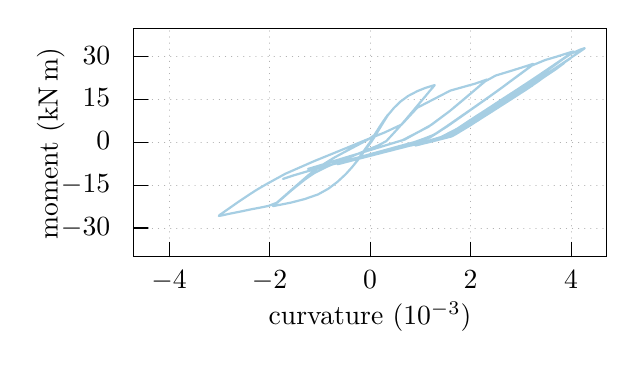
\begin{tikzpicture}[gnuplot]
%% generated with GNUPLOT 5.2p6 (Lua 5.3; terminal rev. Nov 2018, script rev. 107)
%% 08/11/2019 21:17:48
\path (0.000,0.000) rectangle (6.000,2.900);
\gpcolor{color=gp lt color axes}
\gpsetlinetype{gp lt axes}
\gpsetdashtype{gp dt axes}
\gpsetlinewidth{0.50}
\draw[gp path] (0.000,0.362)--(5.999,0.362);
\gpcolor{color=gp lt color border}
\gpsetlinetype{gp lt border}
\gpsetdashtype{gp dt solid}
\gpsetlinewidth{1.00}
\draw[gp path] (0.000,0.362)--(0.180,0.362);
\node[gp node right] at (-0.184,0.362) {$-30$};
\gpcolor{color=gp lt color axes}
\gpsetlinetype{gp lt axes}
\gpsetdashtype{gp dt axes}
\gpsetlinewidth{0.50}
\draw[gp path] (0.000,0.906)--(5.999,0.906);
\gpcolor{color=gp lt color border}
\gpsetlinetype{gp lt border}
\gpsetdashtype{gp dt solid}
\gpsetlinewidth{1.00}
\draw[gp path] (0.000,0.906)--(0.180,0.906);
\node[gp node right] at (-0.184,0.906) {$-15$};
\gpcolor{color=gp lt color axes}
\gpsetlinetype{gp lt axes}
\gpsetdashtype{gp dt axes}
\gpsetlinewidth{0.50}
\draw[gp path] (0.000,1.450)--(5.999,1.450);
\gpcolor{color=gp lt color border}
\gpsetlinetype{gp lt border}
\gpsetdashtype{gp dt solid}
\gpsetlinewidth{1.00}
\draw[gp path] (0.000,1.450)--(0.180,1.450);
\node[gp node right] at (-0.184,1.450) {$0$};
\gpcolor{color=gp lt color axes}
\gpsetlinetype{gp lt axes}
\gpsetdashtype{gp dt axes}
\gpsetlinewidth{0.50}
\draw[gp path] (0.000,1.993)--(5.999,1.993);
\gpcolor{color=gp lt color border}
\gpsetlinetype{gp lt border}
\gpsetdashtype{gp dt solid}
\gpsetlinewidth{1.00}
\draw[gp path] (0.000,1.993)--(0.180,1.993);
\node[gp node right] at (-0.184,1.993) {$15$};
\gpcolor{color=gp lt color axes}
\gpsetlinetype{gp lt axes}
\gpsetdashtype{gp dt axes}
\gpsetlinewidth{0.50}
\draw[gp path] (0.000,2.537)--(5.999,2.537);
\gpcolor{color=gp lt color border}
\gpsetlinetype{gp lt border}
\gpsetdashtype{gp dt solid}
\gpsetlinewidth{1.00}
\draw[gp path] (0.000,2.537)--(0.180,2.537);
\node[gp node right] at (-0.184,2.537) {$30$};
\gpcolor{color=gp lt color axes}
\gpsetlinetype{gp lt axes}
\gpsetdashtype{gp dt axes}
\gpsetlinewidth{0.50}
\draw[gp path] (0.447,0.000)--(0.447,2.899);
\gpcolor{color=gp lt color border}
\gpsetlinetype{gp lt border}
\gpsetdashtype{gp dt solid}
\gpsetlinewidth{1.00}
\draw[gp path] (0.447,0.000)--(0.447,0.180);
\node[gp node center] at (0.447,-0.308) {$-4$};
\gpcolor{color=gp lt color axes}
\gpsetlinetype{gp lt axes}
\gpsetdashtype{gp dt axes}
\gpsetlinewidth{0.50}
\draw[gp path] (1.723,0.000)--(1.723,2.899);
\gpcolor{color=gp lt color border}
\gpsetlinetype{gp lt border}
\gpsetdashtype{gp dt solid}
\gpsetlinewidth{1.00}
\draw[gp path] (1.723,0.000)--(1.723,0.180);
\node[gp node center] at (1.723,-0.308) {$-2$};
\gpcolor{color=gp lt color axes}
\gpsetlinetype{gp lt axes}
\gpsetdashtype{gp dt axes}
\gpsetlinewidth{0.50}
\draw[gp path] (3.000,0.000)--(3.000,2.899);
\gpcolor{color=gp lt color border}
\gpsetlinetype{gp lt border}
\gpsetdashtype{gp dt solid}
\gpsetlinewidth{1.00}
\draw[gp path] (3.000,0.000)--(3.000,0.180);
\node[gp node center] at (3.000,-0.308) {$0$};
\gpcolor{color=gp lt color axes}
\gpsetlinetype{gp lt axes}
\gpsetdashtype{gp dt axes}
\gpsetlinewidth{0.50}
\draw[gp path] (4.276,0.000)--(4.276,2.899);
\gpcolor{color=gp lt color border}
\gpsetlinetype{gp lt border}
\gpsetdashtype{gp dt solid}
\gpsetlinewidth{1.00}
\draw[gp path] (4.276,0.000)--(4.276,0.180);
\node[gp node center] at (4.276,-0.308) {$2$};
\gpcolor{color=gp lt color axes}
\gpsetlinetype{gp lt axes}
\gpsetdashtype{gp dt axes}
\gpsetlinewidth{0.50}
\draw[gp path] (5.552,0.000)--(5.552,2.899);
\gpcolor{color=gp lt color border}
\gpsetlinetype{gp lt border}
\gpsetdashtype{gp dt solid}
\gpsetlinewidth{1.00}
\draw[gp path] (5.552,0.000)--(5.552,0.180);
\node[gp node center] at (5.552,-0.308) {$4$};
\draw[gp path] (0.000,2.899)--(0.000,0.000)--(5.999,0.000)--(5.999,2.899)--cycle;
\node[gp node center,rotate=-270] at (-1.044,1.449) {moment (\si{\kilo\newton\meter})};
\node[gp node center] at (2.999,-0.769) {curvature (\num{E-3})};
\gpcolor{rgb color={0.651,0.808,0.890}}
\gpsetlinewidth{2.00}
\draw[gp path] (3.000,1.450)--(3.002,1.453)--(3.004,1.457)--(3.006,1.461)--(3.007,1.462)%
  --(3.008,1.463)--(3.010,1.467)--(3.013,1.473)--(3.017,1.479)--(3.021,1.485)--(3.023,1.489)%
  --(3.025,1.492)--(3.027,1.496)--(3.029,1.500)--(3.032,1.504)--(3.033,1.506)--(3.032,1.505)%
  --(3.032,1.504)--(3.031,1.502)--(3.030,1.500)--(3.028,1.497)--(3.026,1.494)--(3.024,1.490)%
  --(3.022,1.487)--(3.021,1.485)--(3.019,1.483)--(3.018,1.481)--(3.017,1.479)--(3.017,1.478)%
  --(3.017,1.479)--(3.018,1.480)--(3.017,1.479)--(3.017,1.478)--(3.016,1.477)--(3.017,1.478)%
  --(3.017,1.479)--(3.018,1.481)--(3.019,1.483)--(3.020,1.483)--(3.019,1.482)--(3.018,1.481)%
  --(3.017,1.479)--(3.015,1.476)--(3.013,1.471)--(3.010,1.468)--(3.010,1.466)--(3.008,1.464)%
  --(3.006,1.460)--(3.002,1.453)--(2.999,1.449)--(3.000,1.450)--(3.004,1.456)--(3.009,1.465)%
  --(3.013,1.472)--(3.017,1.479)--(3.023,1.489)--(3.031,1.502)--(3.040,1.517)--(3.047,1.530)%
  --(3.053,1.539)--(3.058,1.547)--(3.064,1.558)--(3.070,1.567)--(3.073,1.572)--(3.072,1.571)%
  --(3.069,1.566)--(3.065,1.558)--(3.059,1.549)--(3.052,1.536)--(3.042,1.519)--(3.029,1.498)%
  --(3.014,1.472)--(2.998,1.446)--(2.981,1.423)--(2.965,1.401)--(2.949,1.377)--(2.931,1.352)%
  --(2.913,1.327)--(2.896,1.302)--(2.880,1.281)--(2.868,1.265)--(2.859,1.252)--(2.853,1.244)%
  --(2.848,1.238)--(2.847,1.236)--(2.849,1.239)--(2.855,1.248)--(2.866,1.263)--(2.879,1.282)%
  --(2.893,1.302)--(2.908,1.323)--(2.923,1.344)--(2.939,1.367)--(2.956,1.391)--(2.971,1.412)%
  --(2.981,1.427)--(2.987,1.435)--(2.989,1.438)--(2.988,1.436)--(2.984,1.430)--(2.976,1.419)%
  --(2.965,1.404)--(2.951,1.383)--(2.933,1.358)--(2.916,1.335)--(2.902,1.314)--(2.888,1.294)%
  --(2.874,1.275)--(2.865,1.262)--(2.865,1.261)--(2.875,1.276)--(2.893,1.302)--(2.914,1.332)%
  --(2.937,1.364)--(2.962,1.399)--(2.994,1.444)--(3.036,1.509)--(3.080,1.583)--(3.121,1.648)%
  --(3.154,1.698)--(3.180,1.736)--(3.202,1.767)--(3.220,1.792)--(3.229,1.804)--(3.225,1.798)%
  --(3.207,1.768)--(3.177,1.718)--(3.139,1.656)--(3.096,1.585)--(3.047,1.504)--(2.986,1.417)%
  --(2.915,1.323)--(2.846,1.227)--(2.771,1.135)--(2.689,1.044)--(2.584,0.947)--(2.471,0.862)%
  --(2.340,0.789)--(2.168,0.729)--(1.997,0.685)--(1.857,0.657)--(1.784,0.643)--(1.766,0.640)%
  --(1.778,0.650)--(1.802,0.672)--(1.834,0.700)--(1.875,0.736)--(1.931,0.784)--(1.998,0.844)%
  --(2.072,0.908)--(2.145,0.971)--(2.213,1.030)--(2.279,1.082)--(2.348,1.133)--(2.436,1.189)%
  --(2.536,1.251)--(2.657,1.317)--(2.774,1.379)--(2.861,1.425)--(2.931,1.462)--(2.996,1.500)%
  --(3.082,1.562)--(3.154,1.681)--(3.225,1.794)--(3.302,1.886)--(3.385,1.967)--(3.483,2.039)%
  --(3.600,2.100)--(3.705,2.142)--(3.780,2.165)--(3.817,2.176)--(3.820,2.176)--(3.812,2.166)%
  --(3.800,2.152)--(3.783,2.132)--(3.757,2.102)--(3.720,2.057)--(3.672,2.000)--(3.619,1.938)%
  --(3.565,1.873)--(3.507,1.804)--(3.442,1.727)--(3.368,1.642)--(3.286,1.552)--(3.205,1.465)%
  --(3.102,1.410)--(2.990,1.364)--(2.878,1.318)--(2.766,1.271)--(2.658,1.227)--(2.555,1.185)%
  --(2.463,1.145)--(2.380,1.105)--(2.302,1.066)--(2.237,1.023)--(2.174,0.979)--(2.119,0.935)%
  --(2.067,0.894)--(2.015,0.851)--(1.956,0.801)--(1.892,0.745)--(1.823,0.686)--(1.708,0.642)%
  --(1.599,0.620)--(1.488,0.599)--(1.379,0.576)--(1.280,0.556)--(1.195,0.539)--(1.125,0.523)%
  --(1.079,0.515)--(1.097,0.533)--(1.199,0.604)--(1.333,0.698)--(1.459,0.782)--(1.555,0.844)%
  --(1.687,0.921)--(1.922,1.050)--(2.289,1.211)--(2.672,1.367)--(2.971,1.490)--(3.184,1.575)%
  --(3.402,1.677)--(3.598,1.889)--(4.019,2.107)--(4.333,2.195)--(4.465,2.241)--(4.488,2.248)%
  --(4.417,2.188)--(4.305,2.093)--(4.205,2.008)--(4.117,1.934)--(4.000,1.838)--(3.784,1.676)%
  --(3.442,1.486)--(3.108,1.384)--(2.860,1.309)--(2.737,1.271)--(2.681,1.255)--(2.550,1.215)%
  --(2.354,1.154)--(2.211,1.112)--(2.271,1.129)--(2.509,1.202)--(2.757,1.278)--(2.937,1.332)%
  --(3.059,1.370)--(3.192,1.410)--(3.411,1.477)--(3.741,1.647)--(4.010,1.846)--(4.198,2.004)%
  --(4.303,2.092)--(4.361,2.142)--(4.447,2.217)--(4.595,2.298)--(4.805,2.362)--(4.980,2.417)%
  --(5.066,2.445)--(5.074,2.443)--(5.028,2.409)--(4.979,2.371)--(4.958,2.356)--(4.952,2.352)%
  --(4.915,2.325)--(4.816,2.251)--(4.668,2.141)--(4.516,2.032)--(4.389,1.943)--(4.281,1.867)%
  --(4.156,1.781)--(3.999,1.671)--(3.815,1.548)--(3.598,1.462)--(3.464,1.426)--(3.389,1.405)%
  --(3.336,1.391)--(3.287,1.378)--(3.260,1.370)--(3.283,1.377)--(3.374,1.402)--(3.515,1.440)%
  --(3.708,1.492)--(3.862,1.577)--(3.998,1.670)--(4.137,1.767)--(4.289,1.872)--(4.435,1.975)%
  --(4.558,2.061)--(4.645,2.123)--(4.701,2.164)--(4.735,2.189)--(4.751,2.201)--(4.740,2.193)%
  --(4.697,2.161)--(4.633,2.114)--(4.555,2.058)--(4.461,1.991)--(4.346,1.910)--(4.209,1.815)%
  --(4.067,1.716)--(3.937,1.626)--(3.814,1.545)--(3.665,1.480)--(3.513,1.439)--(3.382,1.403)%
  --(3.271,1.373)--(3.185,1.350)--(3.125,1.333)--(3.078,1.320)--(3.039,1.310)--(3.010,1.302)%
  --(3.008,1.302)--(3.058,1.315)--(3.152,1.341)--(3.251,1.368)--(3.331,1.389)--(3.398,1.408)%
  --(3.488,1.432)--(3.632,1.471)--(3.817,1.549)--(3.931,1.623)--(3.987,1.662)--(4.010,1.678)%
  --(4.031,1.692)--(4.052,1.706)--(4.066,1.716)--(4.097,1.739)--(4.140,1.769)--(4.158,1.782)%
  --(4.139,1.768)--(4.096,1.738)--(4.081,1.728)--(4.118,1.753)--(4.180,1.797)--(4.219,1.823)%
  --(4.203,1.812)--(4.152,1.775)--(4.117,1.752)--(4.147,1.774)--(4.221,1.825)--(4.270,1.860)%
  --(4.257,1.850)--(4.203,1.812)--(4.178,1.795)--(4.226,1.829)--(4.321,1.895)--(4.393,1.945)%
  --(4.400,1.949)--(4.365,1.924)--(4.344,1.909)--(4.367,1.926)--(4.410,1.956)--(4.424,1.966)%
  --(4.386,1.939)--(4.323,1.895)--(4.274,1.861)--(4.247,1.842)--(4.223,1.826)--(4.181,1.797)%
  --(4.120,1.754)--(4.051,1.707)--(3.994,1.667)--(3.955,1.639)--(3.922,1.616)--(3.877,1.587)%
  --(3.817,1.548)--(3.759,1.511)--(3.684,1.485)--(3.634,1.472)--(3.609,1.465)--(3.591,1.460)%
  --(3.576,1.456)--(3.569,1.454)--(3.581,1.457)--(3.619,1.468)--(3.695,1.488)--(3.767,1.516)%
  --(3.811,1.545)--(3.861,1.577)--(3.919,1.614)--(3.974,1.653)--(4.020,1.685)--(4.050,1.706)%
  --(4.063,1.714)--(4.060,1.712)--(4.043,1.701)--(4.014,1.680)--(3.967,1.647)--(3.896,1.599)%
  --(3.805,1.541)--(3.717,1.494)--(3.617,1.467)--(3.546,1.448)--(3.467,1.426)--(3.377,1.402)%
  --(3.308,1.383)--(3.287,1.377)--(3.314,1.385)--(3.370,1.400)--(3.429,1.416)--(3.482,1.430)%
  --(3.545,1.448)--(3.644,1.474)--(3.788,1.530)--(3.901,1.603)--(3.998,1.671)--(4.072,1.721)%
  --(4.127,1.759)--(4.174,1.791)--(4.220,1.823)--(4.253,1.846)--(4.258,1.849)--(4.229,1.829)%
  --(4.173,1.790)--(4.100,1.740)--(4.016,1.681)--(3.918,1.613)--(3.791,1.531)--(3.580,1.457)%
  --(3.383,1.403)--(3.192,1.351)--(3.018,1.304)--(2.861,1.261)--(2.680,1.213)--(2.451,1.152)%
  --(2.215,1.085)--(2.010,1.025)--(1.893,0.985)--(1.902,0.988)--(2.026,1.029)--(2.164,1.070)%
  --(2.243,1.093)--(2.294,1.108)--(2.421,1.142)--(2.684,1.213)--(3.001,1.299)--(3.303,1.382)%
  --(3.554,1.450)--(3.795,1.535)--(3.979,1.652)--(4.189,1.799)--(4.419,1.963)--(4.650,2.127)%
  --(4.863,2.284)--(5.056,2.426)--(5.226,2.496)--(5.353,2.533)--(5.451,2.564)--(5.519,2.586)%
  --(5.563,2.599)--(5.583,2.604)--(5.573,2.597)--(5.519,2.559)--(5.426,2.495)--(5.303,2.411)%
  --(5.163,2.316)--(5.000,2.207)--(4.811,2.083)--(4.584,1.934)--(4.336,1.775)--(4.103,1.621)%
  --(3.876,1.504)--(3.627,1.439)--(3.398,1.380)--(3.147,1.316)--(2.903,1.254)--(2.719,1.206)%
  --(2.612,1.178)--(2.586,1.172)--(2.620,1.180)--(2.670,1.193)--(2.706,1.203)--(2.729,1.208)%
  --(2.755,1.215)--(2.802,1.227)--(2.867,1.244)--(2.952,1.266)--(3.054,1.292)--(3.189,1.327)%
  --(3.351,1.369)--(3.491,1.405)--(3.604,1.434)--(3.739,1.469)--(3.961,1.535)--(4.161,1.656)%
  --(4.349,1.776)--(4.487,1.866)--(4.574,1.922)--(4.662,1.980)--(4.776,2.056)--(4.923,2.154)%
  --(5.077,2.256)--(5.195,2.335)--(5.256,2.376)--(5.278,2.391)--(5.289,2.399)--(5.310,2.413)%
  --(5.336,2.431)--(5.354,2.443)--(5.343,2.435)--(5.291,2.399)--(5.211,2.344)--(5.124,2.285)%
  --(5.048,2.235)--(4.977,2.189)--(4.896,2.136)--(4.803,2.076)--(4.704,2.012)--(4.610,1.951)%
  --(4.531,1.901)--(4.470,1.861)--(4.428,1.834)--(4.404,1.818)--(4.393,1.810)--(4.391,1.810)%
  --(4.401,1.816)--(4.427,1.833)--(4.468,1.860)--(4.510,1.887)--(4.548,1.912)--(4.598,1.945)%
  --(4.669,1.991)--(4.756,2.048)--(4.837,2.100)--(4.886,2.131)--(4.911,2.147)--(4.948,2.171)%
  --(5.014,2.214)--(5.083,2.259)--(5.117,2.282)--(5.105,2.273)--(5.063,2.244)--(5.014,2.212)%
  --(4.966,2.181)--(4.908,2.143)--(4.822,2.087)--(4.698,2.007)--(4.552,1.912)--(4.412,1.821)%
  --(4.290,1.741)--(4.171,1.663)--(4.045,1.582)--(3.900,1.507)--(3.734,1.465)--(3.620,1.435)%
  --(3.549,1.417)--(3.517,1.409)--(3.514,1.408)--(3.531,1.413)--(3.563,1.421)--(3.611,1.433)%
  --(3.682,1.451)--(3.765,1.473)--(3.848,1.494)--(3.947,1.523)--(3.998,1.554)--(4.040,1.579)%
  --(4.075,1.600)--(4.114,1.624)--(4.153,1.649)--(4.186,1.672)--(4.210,1.688)--(4.226,1.698)%
  --(4.242,1.709)--(4.261,1.722)--(4.284,1.737)--(4.309,1.753)--(4.331,1.768)--(4.349,1.779)%
  --(4.362,1.788)--(4.377,1.798)--(4.396,1.810)--(4.418,1.825)--(4.436,1.837)--(4.447,1.843)%
  --(4.454,1.848)--(4.462,1.853)--(4.476,1.862)--(4.496,1.875)--(4.516,1.888)--(4.529,1.897)%
  --(4.536,1.901)--(4.538,1.902)--(4.542,1.905)--(4.548,1.909)--(4.552,1.911)--(4.545,1.906)%
  --(4.527,1.894)--(4.501,1.877)--(4.471,1.858)--(4.440,1.838)--(4.405,1.815)--(4.369,1.792)%
  --(4.333,1.769)--(4.298,1.746)--(4.266,1.725)--(4.243,1.710)--(4.231,1.702)--(4.224,1.697)%
  --(4.220,1.695)--(4.222,1.696)--(4.236,1.705)--(4.261,1.722)--(4.292,1.743)--(4.328,1.766)%
  --(4.364,1.790)--(4.396,1.811)--(4.424,1.829)--(4.451,1.846)--(4.481,1.865)--(4.510,1.884)%
  --(4.533,1.898)--(4.543,1.905)--(4.540,1.902)--(4.527,1.894)--(4.511,1.884)--(4.498,1.876)%
  --(4.483,1.866)--(4.461,1.852)--(4.428,1.831)--(4.391,1.807)--(4.361,1.787)--(4.339,1.773)%
  --(4.323,1.762)--(4.308,1.752)--(4.292,1.742)--(4.279,1.734)--(4.276,1.731)--(4.282,1.736)%
  --(4.296,1.745)--(4.309,1.753)--(4.321,1.761)--(4.335,1.770)--(4.357,1.785)--(4.385,1.803)%
  --(4.414,1.822)--(4.438,1.838)--(4.457,1.850)--(4.475,1.862)--(4.498,1.876)--(4.524,1.893)%
  --(4.549,1.910)--(4.568,1.922)--(4.580,1.929)--(4.587,1.933)--(4.593,1.938)--(4.603,1.944)%
  --(4.613,1.951)--(4.617,1.953)--(4.610,1.948)--(4.594,1.938)--(4.576,1.926)--(4.559,1.915)%
  --(4.538,1.902)--(4.510,1.884)--(4.475,1.861)--(4.441,1.839)--(4.415,1.822)--(4.392,1.807)%
  --(4.365,1.790)--(4.333,1.769)--(4.306,1.751)--(4.290,1.741)--(4.289,1.740)--(4.293,1.743)%
  --(4.297,1.746)--(4.300,1.747)--(4.307,1.752)--(4.323,1.763)--(4.348,1.779)--(4.375,1.797)%
  --(4.398,1.812)--(4.414,1.822)--(4.426,1.830)--(4.438,1.837)--(4.448,1.844)--(4.449,1.844)%
  --(4.436,1.836)--(4.413,1.820)--(4.387,1.804)--(4.370,1.793)--(4.359,1.786)--(4.346,1.777)%
  --(4.326,1.764)--(4.297,1.746)--(4.275,1.731)--(4.269,1.727)--(4.280,1.735)--(4.296,1.745)%
  --(4.305,1.751)--(4.311,1.754)--(4.323,1.762)--(4.349,1.780)--(4.388,1.805)--(4.429,1.832)%
  --(4.464,1.855)--(4.493,1.873)--(4.522,1.892)--(4.558,1.915)--(4.596,1.940)--(4.631,1.962)%
  --(4.653,1.976)--(4.660,1.980)--(4.655,1.977)--(4.644,1.970)--(4.627,1.959)--(4.600,1.941)%
  --(4.560,1.916)--(4.513,1.885)--(4.465,1.854)--(4.418,1.824)--(4.374,1.796)--(4.329,1.766)%
  --(4.286,1.738)--(4.248,1.713)--(4.220,1.694)--(4.209,1.687)--(4.212,1.689)--(4.220,1.694)%
  --(4.230,1.701)--(4.244,1.710)--(4.268,1.726)--(4.302,1.749)--(4.342,1.775)--(4.380,1.800)%
  --(4.412,1.821)--(4.439,1.838)--(4.463,1.853)--(4.488,1.869)--(4.512,1.885)--(4.531,1.897)%
  --(4.540,1.903)--(4.539,1.903)--(4.533,1.899)--(4.522,1.891)--(4.506,1.881)--(4.484,1.866)%
  --(4.454,1.847)--(4.420,1.825)--(4.383,1.801)--(4.348,1.779)--(4.316,1.758)--(4.283,1.736)%
  --(4.249,1.713)--(4.217,1.692)--(4.197,1.678)--(4.189,1.673)--(4.190,1.674)--(4.196,1.678)%
  --(4.206,1.685)--(4.222,1.696)--(4.247,1.712)--(4.276,1.732)--(4.306,1.751)--(4.333,1.769)%
  --(4.356,1.784)--(4.377,1.797)--(4.393,1.808)--(4.407,1.817)--(4.416,1.823)--(4.419,1.824)%
  --(4.415,1.822)--(4.405,1.815)--(4.389,1.805)--(4.367,1.791)--(4.340,1.773)--(4.308,1.752)%
  --(4.275,1.730)--(4.248,1.713)--(4.225,1.698)--(4.199,1.680)--(4.168,1.659)--(4.142,1.642)%
  --(4.133,1.636)--(4.145,1.643)--(4.169,1.660)--(4.195,1.677)--(4.222,1.696)--(4.260,1.722)%
  --(4.315,1.758)--(4.385,1.803)--(4.457,1.851)--(4.526,1.895)--(4.589,1.936)--(4.651,1.975)%
  --(4.714,2.016)--(4.776,2.056)--(4.829,2.090)--(4.859,2.109)--(4.866,2.113)--(4.859,2.108)%
  --(4.846,2.099)--(4.833,2.092)--(4.813,2.079)--(4.775,2.055)--(4.718,2.018)--(4.650,1.974)%
  --(4.586,1.932)--(4.530,1.897)--(4.482,1.865)--(4.435,1.835)--(4.388,1.805)--(4.342,1.775)%
  --(4.305,1.750)--(4.282,1.735)--(4.272,1.729)--(4.274,1.731)--(4.282,1.736)--(4.299,1.747)%
  --(4.327,1.765)--(4.365,1.791)--(4.408,1.819)--(4.452,1.847)--(4.493,1.873)--(4.533,1.899)%
  --(4.574,1.926)--(4.614,1.951)--(4.649,1.974)--(4.673,1.989)--(4.685,1.997)--(4.686,1.997)%
  --(4.677,1.991)--(4.658,1.978)--(4.630,1.960)--(4.591,1.935)--(4.541,1.903)--(4.481,1.864)%
  --(4.417,1.823)--(4.352,1.781)--(4.288,1.738)--(4.223,1.696)--(4.159,1.653)--(4.099,1.614)%
  --(4.047,1.583)--(4.007,1.558)--(3.982,1.544)--(3.975,1.539)--(3.978,1.541)--(3.990,1.548)%
  --(4.014,1.563)--(4.053,1.587)--(4.104,1.618)--(4.164,1.656)--(4.246,1.712)--(4.350,1.782)%
  --(4.463,1.855)--(4.567,1.923)--(4.663,1.984)--(4.765,2.049)--(4.882,2.125)--(5.009,2.209)%
  --(5.133,2.291)--(5.224,2.352)--(5.278,2.392)--(5.330,2.429)--(5.394,2.472)--(5.456,2.515)%
  --(5.492,2.539)--(5.481,2.531)--(5.420,2.489)--(5.334,2.430)--(5.251,2.372)--(5.183,2.326)%
  --(5.108,2.277)--(5.004,2.208)--(4.871,2.121)--(4.727,2.028)--(4.599,1.945)--(4.495,1.877)%
  --(4.400,1.815)--(4.302,1.750)--(4.200,1.681)--(4.110,1.622)--(4.052,1.586)--(4.035,1.575)%
  --(4.047,1.582)--(4.069,1.596)--(4.093,1.611)--(4.126,1.631)--(4.175,1.665)--(4.247,1.712)%
  --(4.329,1.768)--(4.405,1.818)--(4.463,1.855)--(4.502,1.881)--(4.529,1.898)--(4.552,1.913)%
  --(4.580,1.932)--(4.613,1.953)--(4.659,1.985)--(4.706,2.016)--(4.718,2.022)--(4.699,2.010)%
  --(4.690,2.003)--(4.726,2.027)--(4.797,2.073)--(4.858,2.113)--(4.894,2.137)--(4.910,2.147)%
  --(4.922,2.155)--(4.948,2.172)--(4.988,2.198)--(5.028,2.224)--(5.055,2.242)--(5.061,2.245)%
  --(5.054,2.240)--(5.044,2.234)--(5.032,2.225)--(5.009,2.211)--(4.970,2.185)--(4.910,2.145)%
  --(4.830,2.093)--(4.732,2.029)--(4.620,1.956)--(4.500,1.878)--(4.386,1.804)--(4.275,1.731)%
  --(4.164,1.656)--(4.044,1.581)--(3.897,1.505)--(3.742,1.466)--(3.643,1.441)--(3.602,1.431)%
  --(3.617,1.435)--(3.672,1.449)--(3.759,1.472)--(3.884,1.504)--(4.047,1.577)--(4.207,1.677)%
  --(4.380,1.795)--(4.559,1.912)--(4.740,2.027)--(4.913,2.140)--(5.072,2.244)--(5.225,2.346)%
  --(5.347,2.433)--(5.447,2.505)--(5.557,2.578)--(5.668,2.627)--(5.724,2.646)--(5.722,2.642)%
  --(5.638,2.584)--(5.501,2.491)--(5.362,2.398)--(5.244,2.321)--(5.162,2.270)--(5.065,2.208)%
  --(4.895,2.098)--(4.667,1.950)--(4.446,1.808)--(4.293,1.706)--(4.216,1.650)--(4.164,1.619)%
  --(4.085,1.571)--(3.932,1.507)--(3.795,1.472)--(3.735,1.457)--(3.777,1.468)--(3.892,1.497)%
  --(4.060,1.553)--(4.175,1.622)--(4.273,1.684)--(4.367,1.746)--(4.477,1.819)--(4.614,1.906)%
  --(4.769,2.005)--(4.915,2.098)--(5.028,2.169)--(5.106,2.220)--(5.172,2.262)--(5.236,2.304)%
  --(5.287,2.337)--(5.305,2.349)--(5.281,2.334)--(5.221,2.293)--(5.139,2.240)--(5.047,2.180)%
  --(4.940,2.111)--(4.814,2.031)--(4.668,1.939)--(4.514,1.841)--(4.364,1.744)--(4.218,1.648)%
  --(4.080,1.565)--(3.921,1.503)--(3.792,1.470)--(3.686,1.444)--(3.630,1.430)--(3.627,1.429)%
  --(3.674,1.441)--(3.769,1.465)--(3.894,1.497)--(4.058,1.552)--(4.183,1.627)--(4.317,1.714)%
  --(4.446,1.798)--(4.571,1.877)--(4.696,1.956)--(4.815,2.032)--(4.920,2.099)--(5.001,2.150)%
  --(5.057,2.186)--(5.096,2.211)--(5.126,2.230)--(5.144,2.242)--(5.146,2.244)--(5.124,2.230)%
  --(5.082,2.202)--(5.026,2.166)--(4.963,2.125)--(4.894,2.081)--(4.816,2.031)--(4.732,1.978)%
  --(4.644,1.921)--(4.555,1.865)--(4.468,1.809)--(4.382,1.754)--(4.297,1.699)--(4.212,1.644)%
  --(4.129,1.593)--(4.052,1.547)--(3.943,1.508)--(3.860,1.487)--(3.806,1.473)--(3.781,1.467)%
  --(3.783,1.468)--(3.807,1.474)--(3.856,1.486)--(3.937,1.507)--(4.061,1.553)--(4.161,1.613)%
  --(4.277,1.687)--(4.401,1.768)--(4.540,1.858)--(4.691,1.954)--(4.838,2.048)--(4.968,2.130)%
  --(5.076,2.199)--(5.176,2.263)--(5.261,2.321)--(5.331,2.372)--(5.388,2.412)--(5.429,2.439)%
  --(5.440,2.446)--(5.404,2.422)--(5.321,2.365)--(5.208,2.290)--(5.099,2.221)--(5.000,2.158)%
  --(4.897,2.093)--(4.768,2.011)--(4.616,1.913)--(4.459,1.813)--(4.325,1.724)--(4.223,1.658)%
  --(4.148,1.609)--(4.084,1.571)--(4.032,1.539)--(3.997,1.520)--(4.009,1.524)--(4.066,1.559)%
  --(4.164,1.619)--(4.280,1.695)--(4.397,1.772)--(4.517,1.851)--(4.651,1.937)--(4.802,2.033)%
  --(4.957,2.131)--(5.094,2.218)--(5.211,2.293)--(5.312,2.359)--(5.398,2.416)--(5.457,2.456)%
  --(5.501,2.488)--(5.536,2.510)--(5.546,2.518)--(5.513,2.495)--(5.433,2.441)--(5.326,2.369)%
  --(5.226,2.303)--(5.139,2.248)--(5.058,2.196)--(4.956,2.131)--(4.822,2.045)--(4.676,1.951)%
  --(4.549,1.869)--(4.455,1.809)--(4.382,1.761)--(4.307,1.711)--(4.221,1.654)--(4.135,1.599)%
  --(4.079,1.562)--(4.061,1.552)--(4.078,1.562)--(4.115,1.585)--(4.163,1.613)--(4.222,1.651)%
  --(4.302,1.705)--(4.413,1.779)--(4.540,1.862)--(4.669,1.945)--(4.791,2.022)--(4.906,2.095)%
  --(5.017,2.166)--(5.123,2.234)--(5.221,2.297)--(5.297,2.346)--(5.344,2.377)--(5.364,2.390)%
  --(5.366,2.391)--(5.354,2.384)--(5.331,2.368)--(5.290,2.342)--(5.227,2.300)--(5.144,2.245)%
  --(5.058,2.190)--(4.983,2.142)--(4.913,2.098)--(4.843,2.054)--(4.770,2.007)--(4.701,1.963)%
  --(4.646,1.927)--(4.611,1.905)--(4.593,1.894)--(4.585,1.889)--(4.581,1.887)--(4.585,1.889)%
  --(4.604,1.901)--(4.639,1.924)--(4.691,1.957)--(4.751,1.996)--(4.811,2.034)--(4.870,2.072)%
  --(4.935,2.113)--(5.012,2.162)--(5.096,2.217)--(5.177,2.269)--(5.241,2.311)--(5.291,2.343)%
  --(5.336,2.372)--(5.382,2.403)--(5.422,2.431)--(5.443,2.445)--(5.439,2.442)--(5.412,2.424)%
  --(5.368,2.393)--(5.314,2.357)--(5.254,2.317)--(5.182,2.270)--(5.093,2.212)--(4.990,2.146)%
  --(4.878,2.074)--(4.765,2.002)--(4.654,1.932)--(4.543,1.860)--(4.429,1.787)--(4.312,1.710)%
  --(4.202,1.636)--(4.107,1.578)--(4.030,1.532)--(3.914,1.498)--(3.820,1.475)--(3.736,1.454)%
  --(3.670,1.437)--(3.639,1.429)--(3.646,1.431)--(3.683,1.440)--(3.735,1.453)--(3.782,1.465)%
  --(3.820,1.475)--(3.861,1.485)--(3.915,1.499)--(3.998,1.520)--(4.063,1.548)--(4.095,1.567)%
  --(4.109,1.575)--(4.112,1.577)--(4.127,1.586)--(4.159,1.605)--(4.197,1.628)--(4.228,1.647)%
  --(4.249,1.659)--(4.275,1.677)--(4.325,1.710)--(4.402,1.761)--(4.487,1.815)--(4.565,1.865)%
  --(4.639,1.912)--(4.722,1.965)--(4.822,2.029)--(4.933,2.100)--(5.035,2.166)--(5.121,2.222)%
  --(5.189,2.266)--(5.240,2.303)--(5.291,2.340)--(5.349,2.380)--(5.408,2.420)--(5.452,2.449)%
  --(5.465,2.458)--(5.444,2.444)--(5.397,2.412)--(5.348,2.378)--(5.305,2.350)--(5.267,2.325)%
  --(5.217,2.292)--(5.143,2.245)--(5.059,2.191)--(4.981,2.141)--(4.920,2.102)--(4.871,2.072)%
  --(4.824,2.042)--(4.772,2.009)--(4.725,1.979)--(4.693,1.958)--(4.678,1.949)--(4.674,1.946)%
  --(4.668,1.942)--(4.658,1.935)--(4.652,1.932)--(4.657,1.935)--(4.671,1.944)--(4.682,1.951)%
  --(4.677,1.947)--(4.659,1.936)--(4.646,1.928)--(4.648,1.929)--(4.658,1.935)--(4.657,1.935)%
  --(4.637,1.922)--(4.606,1.902)--(4.582,1.886)--(4.573,1.880)--(4.574,1.881)--(4.569,1.878)%
  --(4.552,1.867)--(4.530,1.852)--(4.515,1.843)--(4.516,1.844)--(4.528,1.852)--(4.539,1.858)%
  --(4.539,1.859)--(4.534,1.855)--(4.541,1.859)--(4.564,1.875)--(4.595,1.895)--(4.618,1.910)%
  --(4.624,1.914)--(4.624,1.913)--(4.633,1.920)--(4.659,1.937)--(4.692,1.958)--(4.715,1.972)%
  --(4.721,1.976)--(4.732,1.983)--(4.759,2.001)--(4.789,2.020)--(4.806,2.031)--(4.808,2.031)%
  --(4.805,2.029)--(4.808,2.031)--(4.820,2.039)--(4.832,2.047)--(4.833,2.047)--(4.824,2.041)%
  --(4.812,2.034)--(4.806,2.030)--(4.808,2.032)--(4.809,2.032)--(4.802,2.028)--(4.788,2.018)%
  --(4.772,2.008)--(4.761,2.001)--(4.753,1.996)--(4.741,1.988)--(4.719,1.974)--(4.690,1.955)%
  --(4.660,1.936)--(4.631,1.918)--(4.603,1.900)--(4.573,1.880)--(4.540,1.859)--(4.507,1.837)%
  --(4.477,1.817)--(4.459,1.805)--(4.451,1.801)--(4.448,1.799)--(4.445,1.797)--(4.444,1.796)%
  --(4.452,1.801)--(4.472,1.814)--(4.499,1.832)--(4.526,1.850)--(4.550,1.865)--(4.569,1.878)%
  --(4.589,1.891)--(4.611,1.905)--(4.632,1.919)--(4.644,1.926)--(4.642,1.925)--(4.635,1.920)%
  --(4.626,1.914)--(4.614,1.907)--(4.597,1.896)--(4.580,1.885)--(4.567,1.877)--(4.556,1.870)%
  --(4.546,1.863)--(4.537,1.858)--(4.538,1.858)--(4.553,1.869)--(4.585,1.889)--(4.624,1.915)%
  --(4.666,1.941)--(4.708,1.968)--(4.755,1.998)--(4.808,2.032)--(4.865,2.068)--(4.921,2.104)%
  --(4.969,2.134)--(5.002,2.155)--(5.019,2.165)--(5.024,2.168)--(5.029,2.172)--(5.034,2.175)%
  --(5.022,2.167)--(4.985,2.144)--(4.928,2.107)--(4.872,2.071)--(4.827,2.043)--(4.790,2.019)%
  --(4.744,1.990)--(4.681,1.950)--(4.617,1.909)--(4.569,1.878)--(4.548,1.865)--(4.545,1.863)%
  --(4.542,1.862)--(4.535,1.856)--(4.528,1.852)--(4.541,1.860)--(4.586,1.889)--(4.650,1.931)%
  --(4.710,1.969)--(4.750,1.995)--(4.781,2.014)--(4.820,2.039)--(4.874,2.074)--(4.932,2.111)%
  --(4.977,2.139)--(5.001,2.154)--(5.010,2.160)--(5.020,2.166)--(5.036,2.177)--(5.053,2.188)%
  --(5.055,2.189)--(5.036,2.176)--(5.001,2.153)--(4.964,2.130)--(4.933,2.110)--(4.902,2.091)%
  --(4.860,2.064)--(4.800,2.026)--(4.731,1.981)--(4.664,1.939)--(4.609,1.903)--(4.558,1.871)%
  --(4.496,1.830)--(4.419,1.779)--(4.341,1.729)--(4.283,1.690)--(4.259,1.674)--(4.255,1.672)%
  --(4.256,1.673)--(4.260,1.675)--(4.283,1.691)--(4.343,1.731)--(4.436,1.792)--(4.545,1.864)%
  --(4.658,1.937)--(4.770,2.009)--(4.886,2.082)--(5.005,2.157)--(5.119,2.230)--(5.223,2.297)%
  --(5.306,2.351)--(5.369,2.392)--(5.410,2.419)--(5.431,2.433)--(5.402,2.413)--(5.338,2.370)%
  --(5.242,2.307)--(5.143,2.243)--(5.050,2.184)--(4.961,2.128)--(4.858,2.062)--(4.731,1.981)%
  --(4.599,1.897)--(4.491,1.826)--(4.424,1.782)--(4.381,1.754)--(4.344,1.729)--(4.306,1.705)%
  --(4.283,1.690)--(4.287,1.693)--(4.321,1.715)--(4.369,1.747)--(4.414,1.776)--(4.450,1.800)%
  --(4.483,1.820)--(4.515,1.841)--(4.544,1.860)--(4.566,1.875)--(4.578,1.882)--(4.579,1.883)%
  --(4.570,1.877)--(4.559,1.870)--(4.548,1.863)--(4.539,1.858)--(4.532,1.853)--(4.527,1.850)%
  --(4.526,1.850)--(4.534,1.855)--(4.553,1.867)--(4.577,1.883)--(4.602,1.899)--(4.630,1.917)%
  --(4.661,1.937)--(4.690,1.955)--(4.713,1.970)--(4.733,1.983)--(4.754,1.996)--(4.775,2.010)%
  --(4.794,2.022)--(4.804,2.028)--(4.807,2.030)--(4.808,2.030)--(4.813,2.034)--(4.819,2.038)%
  --(4.821,2.039)--(4.817,2.036)--(4.810,2.032)--(4.805,2.029)--(4.803,2.028)--(4.802,2.027)%
  --(4.798,2.024)--(4.791,2.020)--(4.787,2.017)--(4.790,2.020)--(4.802,2.028)--(4.820,2.039)%
  --(4.839,2.051)--(4.854,2.060)--(4.867,2.069)--(4.881,2.078)--(4.900,2.089)--(4.921,2.102)%
  --(4.938,2.113)--(4.943,2.116)--(4.935,2.111)--(4.920,2.101)--(4.904,2.091)--(4.887,2.080)%
  --(4.863,2.065)--(4.827,2.042)--(4.780,2.012)--(4.727,1.978)--(4.676,1.946)--(4.636,1.920)%
  --(4.606,1.902)--(4.585,1.889)--(4.568,1.878)--(4.551,1.866)--(4.541,1.859)--(4.543,1.861)%
  --(4.564,1.875)--(4.601,1.899)--(4.642,1.925)--(4.677,1.947)--(4.702,1.963)--(4.724,1.977)%
  --(4.753,1.995)--(4.788,2.018)--(4.821,2.039)--(4.843,2.053)--(4.851,2.058)--(4.853,2.060)%
  --(4.860,2.064)--(4.867,2.068)--(4.868,2.068)--(4.856,2.061)--(4.834,2.046)--(4.807,2.029)%
  --(4.777,2.010)--(4.741,1.987)--(4.696,1.958)--(4.644,1.925)--(4.592,1.892)--(4.544,1.860)%
  --(4.500,1.832)--(4.461,1.806)--(4.429,1.786)--(4.407,1.771)--(4.399,1.766)--(4.408,1.772)%
  --(4.432,1.788)--(4.469,1.812)--(4.515,1.842)--(4.568,1.877)--(4.626,1.915)--(4.688,1.954)%
  --(4.749,1.994)--(4.807,2.030)--(4.860,2.064)--(4.910,2.096)--(4.958,2.126)--(4.999,2.152)%
  --(5.027,2.170)--(5.045,2.182)--(5.058,2.190)--(5.064,2.194)--(5.062,2.193)--(5.052,2.186)%
  --(5.032,2.173)--(5.005,2.155)--(4.969,2.132)--(4.926,2.105)--(4.876,2.073)--(4.826,2.041)%
  --(4.776,2.010)--(4.723,1.976)--(4.665,1.939)--(4.603,1.899)--(4.546,1.862)--(4.499,1.831)%
  --(4.460,1.805)--(4.424,1.782)--(4.387,1.758)--(4.354,1.736)--(4.333,1.723)--(4.327,1.719)%
  --(4.331,1.721)--(4.341,1.728)--(4.354,1.737)--(4.372,1.748)--(4.396,1.764)--(4.428,1.785)%
  --(4.466,1.809)--(4.504,1.835)--(4.542,1.860)--(4.583,1.887)--(4.630,1.918)--(4.680,1.950)%
  --(4.730,1.981)--(4.778,2.012)--(4.830,2.045)--(4.886,2.081)--(4.943,2.117)--(4.993,2.148)%
  --(5.032,2.173)--(5.063,2.193)--(5.090,2.210)--(5.111,2.224)--(5.118,2.228)--(5.108,2.222)%
  --(5.082,2.205)--(5.051,2.184)--(5.018,2.164)--(4.981,2.140)--(4.936,2.112)--(4.882,2.077)%
  --(4.826,2.041)--(4.772,2.007)--(4.726,1.978)--(4.688,1.953)--(4.654,1.932)--(4.623,1.912)%
  --(4.593,1.893)--(4.568,1.877)--(4.552,1.866)--(4.547,1.863)--(4.551,1.865)--(4.559,1.871)%
  --(4.571,1.879)--(4.586,1.889)--(4.609,1.904)--(4.644,1.926)--(4.689,1.955)--(4.736,1.985)%
  --(4.780,2.013)--(4.817,2.036)--(4.851,2.058)--(4.887,2.080)--(4.921,2.102)--(4.947,2.119)%
  --(4.955,2.124)--(4.946,2.118)--(4.926,2.104)--(4.898,2.086)--(4.863,2.064)--(4.818,2.036)%
  --(4.761,2.000)--(4.698,1.960)--(4.636,1.920)--(4.580,1.884)--(4.536,1.855)--(4.506,1.836)%
  --(4.491,1.827)--(4.482,1.820)--(4.480,1.819)--(4.493,1.828)--(4.530,1.852)--(4.587,1.890)%
  --(4.650,1.930)--(4.706,1.966)--(4.753,1.996)--(4.796,2.023)--(4.840,2.051)--(4.887,2.080)%
  --(4.928,2.107)--(4.955,2.124)--(4.963,2.129)--(4.952,2.121)--(4.930,2.107)--(4.908,2.093)%
  --(4.886,2.079)--(4.857,2.061)--(4.813,2.033)--(4.756,1.996)--(4.696,1.958)--(4.642,1.924)%
  --(4.596,1.894)--(4.555,1.868)--(4.514,1.840)--(4.475,1.815)--(4.448,1.797)--(4.435,1.790)%
  --(4.441,1.793)--(4.460,1.806)--(4.489,1.825)--(4.524,1.848)--(4.568,1.877)--(4.620,1.911)%
  --(4.680,1.949)--(4.743,1.990)--(4.806,2.029)--(4.861,2.064)--(4.907,2.093)--(4.950,2.121)%
  --(4.993,2.148)--(5.029,2.172)--(5.053,2.186)--(5.059,2.191)--(5.056,2.188)--(5.052,2.186)%
  --(5.048,2.183)--(5.037,2.176)--(5.012,2.160)--(4.976,2.136)--(4.935,2.111)--(4.897,2.087)%
  --(4.861,2.064)--(4.822,2.039)--(4.778,2.011)--(4.729,1.980)--(4.682,1.950)--(4.644,1.925)%
  --(4.617,1.908)--(4.598,1.896)--(4.583,1.886)--(4.568,1.876)--(4.556,1.869)--(4.552,1.866)%
  --(4.558,1.870)--(4.571,1.879)--(4.584,1.887)--(4.591,1.891)--(4.590,1.891)--(4.588,1.889)%
  --(4.586,1.887)--(4.585,1.887)--(4.579,1.883)--(4.566,1.874)--(4.544,1.860)--(4.523,1.846)%
  --(4.508,1.837)--(4.503,1.834)--(4.504,1.834)--(4.505,1.835)--(4.509,1.838)--(4.522,1.847)%
  --(4.549,1.865)--(4.587,1.890)--(4.630,1.917)--(4.671,1.943)--(4.711,1.969)--(4.753,1.996)%
  --(4.798,2.024)--(4.842,2.052)--(4.878,2.075)--(4.902,2.090)--(4.917,2.100)--(4.929,2.107)%
  --(4.939,2.113)--(4.944,2.117)--(4.939,2.114)--(4.926,2.105)--(4.910,2.095)--(4.897,2.087)%
  --(4.889,2.082)--(4.884,2.079)--(4.878,2.075)--(4.868,2.069)--(4.858,2.063)--(4.853,2.059)%
  --(4.856,2.061)--(4.861,2.065)--(4.864,2.066)--(4.860,2.063)--(4.852,2.058)--(4.843,2.052)%
  --(4.836,2.048)--(4.833,2.046)--(4.830,2.045)--(4.823,2.040)--(4.812,2.033)--(4.803,2.027)%
  --(4.800,2.026)--(4.803,2.027)--(4.806,2.029)--(4.809,2.031)--(4.812,2.033)--(4.819,2.037)%
  --(4.829,2.044)--(4.844,2.054)--(4.861,2.064)--(4.875,2.073)--(4.887,2.081)--(4.899,2.088)%
  --(4.912,2.097)--(4.927,2.106)--(4.940,2.114)--(4.949,2.120)--(4.954,2.123)--(4.953,2.123)%
  --(4.951,2.121)--(4.946,2.118)--(4.939,2.113)--(4.925,2.104)--(4.904,2.091)--(4.878,2.074)%
  --(4.848,2.056)--(4.810,2.031)--(4.760,1.999)--(4.706,1.964)--(4.650,1.928)--(4.594,1.892)%
  --(4.532,1.852)--(4.465,1.808)--(4.396,1.763)--(4.328,1.719)--(4.268,1.679)--(4.223,1.650)%
  --(4.195,1.631)--(4.182,1.624)--(4.185,1.625)--(4.200,1.635)--(4.231,1.655)--(4.284,1.690)%
  --(4.359,1.740)--(4.446,1.797)--(4.534,1.855)--(4.622,1.913)--(4.711,1.969)--(4.800,2.026)%
  --(4.888,2.082)--(4.968,2.132)--(5.033,2.173)--(5.079,2.203)--(5.110,2.223)--(5.128,2.234)%
  --(5.134,2.238)--(5.128,2.234)--(5.108,2.221)--(5.071,2.198)--(5.022,2.166)--(4.963,2.128)%
  --(4.899,2.087)--(4.830,2.043)--(4.758,1.997)--(4.684,1.950)--(4.613,1.905)--(4.546,1.861)%
  --(4.486,1.822)--(4.436,1.789)--(4.398,1.765)--(4.373,1.748)--(4.363,1.742)--(4.367,1.745)%
  --(4.385,1.756)--(4.415,1.776)--(4.455,1.802)--(4.504,1.834)--(4.561,1.872)--(4.623,1.913)%
  --(4.688,1.954)--(4.754,1.996)--(4.818,2.037)--(4.880,2.076)--(4.938,2.113)--(4.989,2.145)%
  --(5.031,2.172)--(5.062,2.192)--(5.083,2.205)--(5.095,2.213)--(5.099,2.216)--(5.092,2.211)%
  --(5.070,2.197)--(5.035,2.174)--(4.990,2.145)--(4.938,2.112)--(4.881,2.076)--(4.819,2.036)%
  --(4.753,1.994)--(4.685,1.951)--(4.618,1.908)--(4.556,1.868)--(4.500,1.831)--(4.453,1.800)%
  --(4.412,1.774)--(4.379,1.752)--(4.356,1.737)--(4.346,1.730)--(4.348,1.732)--(4.361,1.740)%
  --(4.382,1.754)--(4.410,1.773)--(4.444,1.795)--(4.484,1.821)--(4.528,1.850)--(4.572,1.879)%
  --(4.614,1.906)--(4.656,1.932)--(4.696,1.958)--(4.735,1.983)--(4.770,2.006)--(4.800,2.025)%
  --(4.824,2.040)--(4.845,2.054)--(4.865,2.066)--(4.881,2.076)--(4.890,2.082)--(4.883,2.077)%
  --(4.874,2.071)--(4.867,2.067)--(4.863,2.065)--(4.856,2.061)--(4.847,2.055)--(4.836,2.048)%
  --(4.826,2.042)--(4.823,2.040)--(4.827,2.042)--(4.835,2.047)--(4.843,2.052)--(4.848,2.056)%
  --(4.851,2.057)--(4.850,2.056)--(4.847,2.055)--(4.841,2.050)--(4.832,2.044)--(4.818,2.036)%
  --(4.802,2.026)--(4.784,2.014)--(4.761,2.000)--(4.735,1.983)--(4.710,1.967)--(4.692,1.956)%
  --(4.682,1.950)--(4.678,1.947)--(4.679,1.948)--(4.684,1.951)--(4.695,1.958)--(4.713,1.970)%
  --(4.734,1.983)--(4.755,1.996)--(4.776,2.009)--(4.798,2.023)--(4.822,2.039)--(4.843,2.052)%
  --(4.857,2.061)--(4.862,2.064)--(4.858,2.061)--(4.850,2.056)--(4.839,2.049)--(4.822,2.038)%
  --(4.797,2.023)--(4.765,2.002)--(4.728,1.978)--(4.689,1.953)--(4.655,1.932)--(4.626,1.913)%
  --(4.601,1.898)--(4.579,1.884)--(4.562,1.872)--(4.553,1.866)--(4.556,1.868)--(4.570,1.878)%
  --(4.596,1.895)--(4.629,1.916)--(4.668,1.941)--(4.712,1.969)--(4.759,1.999)--(4.810,2.032)%
  --(4.861,2.064)--(4.907,2.093)--(4.946,2.118)--(4.977,2.137)--(5.000,2.152)--(5.013,2.160)%
  --(4.999,2.150)--(4.973,2.134)--(4.937,2.111)--(4.895,2.084)--(4.845,2.053)--(4.787,2.016)%
  --(4.723,1.975)--(4.661,1.935)--(4.606,1.900)--(4.559,1.870)--(4.520,1.845)--(4.490,1.824)%
  --(4.470,1.812)--(4.464,1.808)--(4.473,1.814)--(4.493,1.827)--(4.520,1.845)--(4.553,1.866)%
  --(4.591,1.891)--(4.633,1.918)--(4.674,1.944)--(4.709,1.967)--(4.738,1.985)--(4.764,2.002)%
  --(4.789,2.018)--(4.811,2.032)--(4.826,2.041)--(4.831,2.045)--(4.830,2.044)--(4.827,2.042)%
  --(4.828,2.042)--(4.831,2.045)--(4.833,2.046)--(4.832,2.045)--(4.827,2.042)--(4.824,2.040)%
  --(4.826,2.042)--(4.833,2.046)--(4.842,2.052)--(4.848,2.056)--(4.853,2.059)--(4.860,2.063)%
  --(4.872,2.071)--(4.887,2.080)--(4.900,2.089)--(4.909,2.094)--(4.915,2.098)--(4.922,2.103)%
  --(4.932,2.109)--(4.940,2.114)--(4.943,2.116)--(4.937,2.112)--(4.925,2.104)--(4.910,2.095)%
  --(4.895,2.085)--(4.878,2.074)--(4.854,2.058)--(4.824,2.040)--(4.792,2.019)--(4.761,2.000)%
  --(4.733,1.982)--(4.707,1.965)--(4.684,1.951)--(4.662,1.936)--(4.641,1.923)--(4.623,1.912)%
  --(4.609,1.902)--(4.598,1.895)--(4.589,1.890)--(4.578,1.882)--(4.564,1.873)--(4.549,1.863)%
  --(4.535,1.854)--(4.522,1.845)--(4.506,1.835)--(4.487,1.822)--(4.468,1.809)--(4.451,1.798)%
  --(4.439,1.791)--(4.433,1.787)--(4.431,1.786)--(4.433,1.788)--(4.443,1.794)--(4.464,1.808)%
  --(4.496,1.829)--(4.538,1.857)--(4.588,1.890)--(4.642,1.925)--(4.701,1.962)--(4.767,2.005)%
  --(4.840,2.051)--(4.912,2.097)--(4.978,2.139)--(5.037,2.176)--(5.088,2.209)--(5.132,2.237)%
  --(5.166,2.258)--(5.184,2.270)--(5.185,2.270)--(5.168,2.259)--(5.134,2.237)--(5.086,2.206)%
  --(5.026,2.167)--(4.950,2.118)--(4.859,2.060)--(4.759,1.997)--(4.657,1.932)--(4.557,1.868)%
  --(4.459,1.803)--(4.364,1.741)--(4.277,1.684)--(4.209,1.639)--(4.161,1.610)--(4.142,1.598)%
  --(4.150,1.603)--(4.183,1.624)--(4.235,1.657)--(4.300,1.700)--(4.381,1.754)--(4.477,1.817)%
  --(4.581,1.885)--(4.686,1.953)--(4.782,2.013)--(4.865,2.066)--(4.935,2.110)--(4.995,2.148)%
  --(5.041,2.177)--(5.072,2.197)--(5.083,2.204)--(5.072,2.197)--(5.045,2.179)--(5.007,2.155)%
  --(4.961,2.126)--(4.909,2.093)--(4.850,2.055)--(4.786,2.015)--(4.725,1.976)--(4.672,1.942)%
  --(4.630,1.916)--(4.601,1.898)--(4.585,1.887)--(4.584,1.887)--(4.599,1.896)--(4.628,1.915)%
  --(4.670,1.942)--(4.719,1.974)--(4.775,2.009)--(4.837,2.048)--(4.899,2.087)--(4.953,2.121)%
  --(4.995,2.148)--(5.025,2.167)--(5.045,2.180)--(5.051,2.183)--(5.039,2.175)--(5.009,2.156)%
  --(4.965,2.128)--(4.912,2.095)--(4.851,2.056)--(4.779,2.010)--(4.697,1.958)--(4.611,1.902)%
  --(4.529,1.849)--(4.456,1.801)--(4.392,1.760)--(4.339,1.725)--(4.299,1.698)--(4.274,1.682)%
  --(4.269,1.679)--(4.282,1.688)--(4.312,1.707)--(4.356,1.737)--(4.412,1.774)--(4.479,1.817)%
  --(4.553,1.866)--(4.628,1.915)--(4.700,1.961)--(4.765,2.002)--(4.823,2.039)--(4.873,2.070)%
  --(4.912,2.095)--(4.939,2.112)--(4.953,2.121)--(4.955,2.122)--(4.947,2.117)--(4.927,2.105)%
  --(4.899,2.086)--(4.863,2.064)--(4.826,2.040)--(4.788,2.016)--(4.752,1.993)--(4.717,1.971)%
  --(4.685,1.951)--(4.660,1.934)--(4.644,1.924)--(4.638,1.921)--(4.642,1.923)--(4.654,1.931)%
  --(4.673,1.944)--(4.700,1.961)--(4.733,1.982)--(4.771,2.006)--(4.813,2.033)--(4.856,2.060)%
  --(4.898,2.087)--(4.935,2.110)--(4.966,2.130)--(4.993,2.147)--(5.013,2.160)--(5.026,2.168)%
  --(5.030,2.170)--(5.024,2.167)--(5.010,2.157)--(4.988,2.143)--(4.959,2.125)--(4.924,2.102)%
  --(4.883,2.076)--(4.835,2.046)--(4.785,2.014)--(4.736,1.983)--(4.691,1.954)--(4.649,1.927)%
  --(4.610,1.903)--(4.577,1.882)--(4.553,1.866)--(4.541,1.858)--(4.554,1.866)--(4.575,1.880)%
  --(4.604,1.899)--(4.640,1.922)--(4.683,1.950)--(4.734,1.982)--(4.789,2.018)--(4.846,2.054)%
  --(4.902,2.089)--(4.953,2.122)--(5.001,2.153)--(5.046,2.181)--(5.085,2.207)--(5.120,2.229)%
  --(5.146,2.246)--(5.165,2.258)--(5.173,2.263)--(5.173,2.262)--(5.163,2.256)--(5.143,2.243)%
  --(5.110,2.222)--(5.063,2.191)--(5.005,2.153)--(4.940,2.112)--(4.869,2.067)--(4.788,2.015)%
  --(4.696,1.956)--(4.596,1.892)--(4.497,1.827)--(4.406,1.768)--(4.322,1.714)--(4.245,1.662)%
  --(4.172,1.616)--(4.111,1.579)--(4.069,1.552)--(4.051,1.540)--(4.055,1.542)--(4.079,1.557)%
  --(4.120,1.582)--(4.179,1.618)--(4.259,1.670)--(4.352,1.731)--(4.458,1.801)--(4.569,1.874)%
  --(4.681,1.945)--(4.793,2.017)--(4.906,2.088)--(5.014,2.157)--(5.111,2.219)--(5.195,2.273)%
  --(5.262,2.316)--(5.315,2.351)--(5.347,2.372)--(5.355,2.377)--(5.336,2.364)--(5.288,2.332)%
  --(5.216,2.284)--(5.127,2.226)--(5.028,2.162)--(4.922,2.095)--(4.803,2.020)--(4.673,1.937)%
  --(4.539,1.851)--(4.409,1.766)--(4.290,1.689)--(4.187,1.622)--(4.103,1.571)--(4.041,1.533)%
  --(3.971,1.509)--(3.942,1.502)--(3.957,1.506)--(4.032,1.527)--(4.100,1.568)--(4.188,1.622)%
  --(4.290,1.688)--(4.392,1.755)--(4.499,1.826)--(4.611,1.897)--(4.725,1.970)--(4.834,2.039)%
  --(4.931,2.100)--(5.014,2.153)--(5.085,2.199)--(5.146,2.238)--(5.193,2.269)--(5.222,2.288)%
  --(5.230,2.293)--(5.218,2.284)--(5.188,2.265)--(5.147,2.238)--(5.095,2.204)--(5.033,2.164)%
  --(4.962,2.119)--(4.884,2.069)--(4.804,2.019)--(4.729,1.971)--(4.661,1.927)--(4.602,1.890)%
  --(4.554,1.859)--(4.519,1.837)--(4.492,1.819)--(4.473,1.807)--(4.467,1.803)--(4.476,1.809)%
  --(4.499,1.824)--(4.528,1.843)--(4.555,1.860)--(4.577,1.874)--(4.599,1.888)--(4.624,1.904)%
  --(4.653,1.922)--(4.678,1.938)--(4.696,1.950)--(4.705,1.956)--(4.708,1.958)--(4.709,1.958)%
  --(4.708,1.958)--(4.706,1.956)--(4.700,1.952)--(4.688,1.944)--(4.671,1.934)--(4.655,1.923)%
  --(4.641,1.915)--(4.631,1.909)--(4.623,1.904)--(4.617,1.900)--(4.614,1.898)--(4.617,1.900)%
  --(4.628,1.907)--(4.646,1.919)--(4.668,1.933)--(4.692,1.948)--(4.720,1.966)--(4.753,1.987)%
  --(4.790,2.011)--(4.828,2.035)--(4.861,2.056)--(4.889,2.073)--(4.914,2.089)--(4.937,2.103)%
  --(4.958,2.117)--(4.973,2.126)--(4.981,2.131)--(4.976,2.128)--(4.968,2.123)--(4.956,2.115)%
  --(4.939,2.104)--(4.915,2.089)--(4.886,2.070)--(4.850,2.048)--(4.811,2.023)--(4.770,1.996)%
  --(4.727,1.969)--(4.684,1.942)--(4.642,1.915)--(4.600,1.888)--(4.560,1.862)--(4.522,1.838)%
  --(4.491,1.818)--(4.468,1.804)--(4.454,1.795)--(4.448,1.791)--(4.456,1.796)--(4.472,1.806)%
  --(4.496,1.822)--(4.528,1.843)--(4.565,1.866)--(4.605,1.892)--(4.649,1.921)--(4.697,1.951)%
  --(4.747,1.983)--(4.798,2.015)--(4.849,2.048)--(4.899,2.080)--(4.944,2.108)--(4.983,2.133)%
  --(5.014,2.153)--(5.037,2.167)--(5.053,2.178)--(5.062,2.183)--(5.059,2.181)--(5.043,2.171)%
  --(5.015,2.152)--(4.975,2.127)--(4.928,2.097)--(4.875,2.063)--(4.815,2.025)--(4.749,1.983)%
  --(4.678,1.938)--(4.608,1.893)--(4.543,1.852)--(4.487,1.815)--(4.440,1.786)--(4.403,1.761)%
  --(4.375,1.743)--(4.362,1.734)--(4.365,1.736)--(4.383,1.749)--(4.413,1.768)--(4.448,1.791)%
  --(4.489,1.818)--(4.537,1.848)--(4.591,1.883)--(4.647,1.919)--(4.703,1.955)--(4.754,1.987)%
  --(4.800,2.017)--(4.843,2.044)--(4.884,2.070)--(4.921,2.094)--(4.949,2.111)--(4.964,2.121)%
  --(4.968,2.123)--(4.966,2.121)--(4.958,2.116)--(4.941,2.105)--(4.911,2.086)--(4.867,2.058)%
  --(4.811,2.022)--(4.750,1.983)--(4.688,1.944)--(4.627,1.905)--(4.567,1.867)--(4.509,1.830)%
  --(4.455,1.795)--(4.409,1.765)--(4.379,1.745)--(4.370,1.739)--(4.377,1.745)--(4.398,1.758)%
  --(4.428,1.778)--(4.469,1.805)--(4.523,1.840)--(4.588,1.882)--(4.654,1.924)--(4.714,1.962)%
  --(4.768,1.996)--(4.819,2.028)--(4.871,2.061)--(4.917,2.090)--(4.951,2.112)--(4.970,2.124)%
  --(4.979,2.129)--(4.983,2.132)--(4.987,2.135)--(4.989,2.136)--(4.983,2.133)--(4.970,2.124)%
  --(4.955,2.115)--(4.942,2.107)--(4.930,2.099)--(4.916,2.090)--(4.894,2.076)--(4.868,2.059)%
  --(4.841,2.042)--(4.814,2.024)--(4.781,2.003)--(4.738,1.976)--(4.684,1.941)--(4.623,1.902)%
  --(4.557,1.860)--(4.489,1.816)--(4.421,1.772)--(4.353,1.728)--(4.289,1.685)--(4.231,1.647)%
  --(4.181,1.617)--(4.153,1.599)--(4.150,1.597)--(4.178,1.614)--(4.238,1.652)--(4.320,1.707)%
  --(4.422,1.774)--(4.539,1.852)--(4.661,1.930)--(4.788,2.010)--(4.920,2.094)--(5.051,2.177)%
  --(5.176,2.258)--(5.282,2.327)--(5.363,2.381)--(5.408,2.415)--(5.435,2.436)--(5.455,2.448)%
  --(5.454,2.448)--(5.414,2.421)--(5.330,2.364)--(5.215,2.288)--(5.097,2.213)--(4.992,2.145)%
  --(4.883,2.076)--(4.755,1.995)--(4.607,1.900)--(4.453,1.799)--(4.309,1.705)--(4.187,1.624)%
  --(4.086,1.562)--(3.963,1.506)--(3.826,1.473)--(3.708,1.443)--(3.621,1.420)--(3.574,1.409)%
  --(3.581,1.411)--(3.638,1.425)--(3.719,1.445)--(3.804,1.467)--(3.884,1.487)--(3.979,1.511)%
  --(4.098,1.561)--(4.209,1.627)--(4.326,1.702)--(4.427,1.767)--(4.512,1.821)--(4.590,1.870)%
  --(4.672,1.923)--(4.761,1.979)--(4.845,2.033)--(4.910,2.075)--(4.952,2.102)--(4.978,2.119)%
  --(4.997,2.131)--(5.010,2.139)--(5.014,2.142)--(5.004,2.136)--(4.977,2.118)--(4.938,2.093)%
  --(4.894,2.065)--(4.848,2.036)--(4.801,2.005)--(4.753,1.974)--(4.705,1.943)--(4.656,1.912)%
  --(4.608,1.882)--(4.562,1.852)--(4.518,1.824)--(4.479,1.799)--(4.443,1.776)--(4.407,1.753)%
  --(4.372,1.729)--(4.335,1.706)--(4.301,1.684)--(4.269,1.663)--(4.242,1.647)--(4.220,1.634)%
  --(4.203,1.623)--(4.190,1.616)--(4.184,1.612)--(4.188,1.614)--(4.197,1.620)--(4.209,1.627)%
  --(4.224,1.636)--(4.242,1.647)--(4.264,1.661)--(4.289,1.676)--(4.316,1.694)--(4.342,1.711)%
  --(4.366,1.726)--(4.387,1.740)--(4.409,1.755)--(4.436,1.772)--(4.465,1.790)--(4.491,1.807)%
  --(4.515,1.822)--(4.539,1.837)--(4.565,1.854)--(4.594,1.873)--(4.621,1.890)--(4.643,1.904)%
  --(4.662,1.916)--(4.679,1.927)--(4.699,1.940)--(4.720,1.953)--(4.742,1.967)--(4.761,1.980)%
  --(4.772,1.987)--(4.774,1.987)--(4.767,1.982)--(4.755,1.974)--(4.739,1.964)--(4.716,1.949)%
  --(4.680,1.926)--(4.627,1.892)--(4.560,1.849)--(4.486,1.802)--(4.410,1.754)--(4.334,1.705)%
  --(4.253,1.654)--(4.166,1.601)--(4.082,1.550)--(3.969,1.508)--(3.874,1.484)--(3.803,1.466)%
  --(3.755,1.454)--(3.726,1.447)--(3.714,1.444)--(3.719,1.445)--(3.739,1.450)--(3.775,1.459)%
  --(3.823,1.471)--(3.885,1.487)--(3.959,1.506)--(4.050,1.532)--(4.105,1.565)--(4.161,1.598)%
  --(4.217,1.632)--(4.274,1.667)--(4.329,1.703)--(4.388,1.741)--(4.448,1.780)--(4.509,1.819)%
  --(4.573,1.860)--(4.644,1.905)--(4.722,1.956)--(4.804,2.008)--(4.875,2.054)--(4.931,2.089)%
  --(4.979,2.119)--(5.024,2.148)--(5.057,2.169)--(5.067,2.176)--(5.046,2.162)--(4.995,2.128)%
  --(4.923,2.082)--(4.838,2.027)--(4.743,1.966)--(4.636,1.898)--(4.513,1.820)--(4.382,1.737)%
  --(4.250,1.652)--(4.124,1.576)--(4.004,1.517)--(3.884,1.486)--(3.796,1.464)--(3.734,1.448)%
  --(3.700,1.440)--(3.703,1.441)--(3.750,1.452)--(3.829,1.472)--(3.926,1.497)--(4.038,1.526)%
  --(4.103,1.564)--(4.170,1.604)--(4.246,1.651)--(4.319,1.697)--(4.377,1.734)--(4.414,1.758)%
  --(4.435,1.771)--(4.450,1.781)--(4.463,1.789)--(4.470,1.793)--(4.465,1.791)--(4.448,1.779)%
  --(4.421,1.762)--(4.392,1.744)--(4.370,1.730)--(4.356,1.720)--(4.346,1.714)--(4.338,1.709)%
  --(4.335,1.707)--(4.344,1.713)--(4.372,1.732)--(4.421,1.764)--(4.484,1.804)--(4.554,1.850)%
  --(4.627,1.896)--(4.706,1.946)--(4.796,2.004)--(4.896,2.068)--(4.992,2.129)--(5.076,2.184)%
  --(5.137,2.226)--(5.180,2.258)--(5.222,2.287)--(5.264,2.315)--(5.296,2.336)--(5.302,2.340)%
  --(5.269,2.318)--(5.202,2.274)--(5.118,2.219)--(5.043,2.170)--(4.973,2.126)--(4.896,2.078)%
  --(4.800,2.017)--(4.687,1.945)--(4.572,1.871)--(4.470,1.806)--(4.385,1.750)--(4.308,1.699)%
  --(4.233,1.650)--(4.159,1.604)--(4.101,1.569)--(4.069,1.550)--(4.068,1.549)--(4.089,1.562)%
  --(4.122,1.582)--(4.163,1.607)--(4.218,1.640)--(4.287,1.686)--(4.373,1.744)--(4.466,1.806)%
  --(4.557,1.863)--(4.639,1.916)--(4.715,1.964)--(4.786,2.009)--(4.853,2.051)--(4.910,2.087)%
  --(4.949,2.112)--(4.966,2.123)--(4.964,2.121)--(4.946,2.109)--(4.914,2.089)--(4.869,2.060)%
  --(4.807,2.021)--(4.731,1.972)--(4.644,1.917)--(4.553,1.859)--(4.462,1.801)--(4.375,1.744)%
  --(4.290,1.687)--(4.212,1.636)--(4.143,1.594)--(4.092,1.564)--(4.063,1.546)--(4.056,1.542)%
  --(4.071,1.551)--(4.104,1.571)--(4.154,1.602)--(4.223,1.644)--(4.304,1.697)--(4.397,1.760)%
  --(4.494,1.824)--(4.590,1.884)--(4.679,1.941)--(4.762,1.993)--(4.840,2.043)--(4.911,2.088)%
  --(4.970,2.125)--(5.008,2.149)--(5.025,2.160)--(5.023,2.158)--(5.007,2.148)--(4.978,2.130)%
  --(4.937,2.103)--(4.881,2.068)--(4.813,2.025)--(4.738,1.977)--(4.659,1.927)--(4.583,1.879)%
  --(4.512,1.833)--(4.446,1.791)--(4.387,1.752)--(4.334,1.716)--(4.292,1.688)--(4.265,1.671)%
  --(4.256,1.665)--(4.261,1.669)--(4.281,1.681)--(4.312,1.702)--(4.354,1.730)--(4.406,1.765)%
  --(4.465,1.804)--(4.530,1.846)--(4.598,1.890)--(4.668,1.934)--(4.736,1.977)--(4.799,2.017)%
  --(4.857,2.054)--(4.906,2.085)--(4.947,2.110)--(4.976,2.129)--(4.995,2.141)--(5.004,2.146)%
  --(5.001,2.144)--(4.987,2.135)--(4.962,2.120)--(4.929,2.099)--(4.890,2.074)--(4.846,2.046)%
  --(4.800,2.017)--(4.754,1.988)--(4.707,1.958)--(4.660,1.928)--(4.615,1.899)--(4.575,1.873)%
  --(4.542,1.853)--(4.516,1.836)--(4.494,1.822)--(4.476,1.810)--(4.462,1.801)--(4.455,1.796)%
  --(4.456,1.797)--(4.465,1.803)--(4.479,1.812)--(4.496,1.823)--(4.515,1.836)--(4.538,1.850)%
  --(4.565,1.868)--(4.599,1.889)--(4.634,1.911)--(4.667,1.933)--(4.698,1.953)--(4.729,1.972)%
  --(4.760,1.992)--(4.791,2.012)--(4.819,2.029)--(4.842,2.044)--(4.860,2.055)--(4.873,2.063)%
  --(4.882,2.069)--(4.886,2.072)--(4.887,2.072)--(4.881,2.068)--(4.868,2.060)--(4.848,2.048)%
  --(4.824,2.032)--(4.795,2.013)--(4.761,1.992)--(4.721,1.966)--(4.676,1.938)--(4.628,1.907)%
  --(4.578,1.875)--(4.528,1.843)--(4.479,1.811)--(4.430,1.779)--(4.383,1.748)--(4.339,1.719)%
  --(4.302,1.695)--(4.274,1.677)--(4.257,1.666)--(4.252,1.663)--(4.259,1.667)--(4.277,1.679)%
  --(4.308,1.699)--(4.350,1.727)--(4.404,1.763)--(4.466,1.804)--(4.532,1.847)--(4.598,1.889)%
  --(4.663,1.930)--(4.727,1.971)--(4.789,2.011)--(4.847,2.047)--(4.894,2.077)--(4.926,2.097)%
  --(4.944,2.108)--(4.950,2.112)--(4.944,2.108)--(4.926,2.096)--(4.893,2.075)--(4.846,2.045)%
  --(4.786,2.007)--(4.718,1.964)--(4.645,1.917)--(4.571,1.870)--(4.496,1.822)--(4.422,1.775)%
  --(4.352,1.728)--(4.289,1.686)--(4.240,1.654)--(4.208,1.633)--(4.194,1.625)--(4.199,1.628)%
  --(4.219,1.640)--(4.251,1.661)--(4.297,1.692)--(4.358,1.733)--(4.429,1.780)--(4.502,1.828)%
  --(4.572,1.872)--(4.636,1.913)--(4.695,1.951)--(4.751,1.986)--(4.801,2.018)--(4.842,2.044)%
  --(4.870,2.061)--(4.883,2.069)--(4.882,2.068)--(4.871,2.062)--(4.854,2.051)--(4.831,2.036)%
  --(4.799,2.016)--(4.757,1.989)--(4.708,1.958)--(4.658,1.926)--(4.611,1.896)--(4.566,1.867)%
  --(4.523,1.840)--(4.482,1.814)--(4.446,1.790)--(4.417,1.772)--(4.400,1.760)--(4.394,1.756)%
  --(4.395,1.757)--(4.403,1.763)--(4.418,1.772)--(4.440,1.787)--(4.471,1.807)--(4.507,1.830)%
  --(4.547,1.856)--(4.587,1.882)--(4.628,1.908)--(4.670,1.935)--(4.712,1.961)--(4.751,1.986)%
  --(4.789,2.010)--(4.823,2.032)--(4.852,2.050)--(4.875,2.064)--(4.889,2.073)--(4.896,2.078)%
  --(4.898,2.079)--(4.893,2.075)--(4.878,2.066)--(4.852,2.049)--(4.815,2.026)--(4.771,1.997)%
  --(4.720,1.965)--(4.665,1.930)--(4.604,1.891)--(4.539,1.850)--(4.472,1.807)--(4.406,1.763)%
  --(4.343,1.722)--(4.284,1.683)--(4.232,1.649)--(4.188,1.621)--(4.157,1.603)--(4.143,1.594)%
  --(4.144,1.594)--(4.158,1.603)--(4.186,1.620)--(4.228,1.646)--(4.281,1.682)--(4.347,1.725)%
  --(4.420,1.774)--(4.496,1.823)--(4.572,1.872)--(4.647,1.920)--(4.722,1.968)--(4.793,2.013)%
  --(4.858,2.054)--(4.914,2.089)--(4.957,2.117)--(4.988,2.136)--(5.007,2.148)--(5.013,2.152)%
  --(5.009,2.149)--(4.992,2.138)--(4.964,2.120)--(4.925,2.096)--(4.878,2.066)--(4.827,2.033)%
  --(4.773,1.999)--(4.718,1.965)--(4.664,1.930)--(4.611,1.896)--(4.561,1.864)--(4.518,1.837)%
  --(4.484,1.815)--(4.457,1.797)--(4.434,1.783)--(4.416,1.771)--(4.406,1.764)--(4.404,1.763)%
  --(4.411,1.767)--(4.421,1.774)--(4.432,1.781)--(4.445,1.789)--(4.462,1.801)--(4.485,1.815)%
  --(4.510,1.832)--(4.535,1.848)--(4.557,1.862)--(4.578,1.875)--(4.598,1.888)--(4.617,1.900)%
  --(4.635,1.911)--(4.648,1.920)--(4.656,1.925)--(4.659,1.927)--(4.655,1.925)--(4.648,1.920)%
  --(4.638,1.914)--(4.628,1.907)--(4.618,1.901)--(4.610,1.895)--(4.601,1.890)--(4.592,1.884)%
  --(4.583,1.878)--(4.576,1.874)--(4.570,1.870)--(4.565,1.867)--(4.560,1.864)--(4.556,1.861)%
  --(4.554,1.860)--(4.555,1.860)--(4.557,1.862)--(4.561,1.865)--(4.568,1.869)--(4.578,1.875)%
  --(4.589,1.882)--(4.601,1.890)--(4.614,1.899)--(4.628,1.907)--(4.643,1.917)--(4.659,1.927)%
  --(4.674,1.937)--(4.688,1.946)--(4.700,1.954)--(4.712,1.961)--(4.721,1.967)--(4.727,1.970)%
  --(4.729,1.971)--(4.727,1.970)--(4.722,1.967)--(4.714,1.962)--(4.702,1.954)--(4.685,1.943)%
  --(4.663,1.929)--(4.637,1.912)--(4.609,1.895)--(4.581,1.877)--(4.553,1.859)--(4.525,1.841)%
  --(4.497,1.823)--(4.470,1.806)--(4.447,1.791)--(4.430,1.779)--(4.418,1.772)--(4.411,1.767)%
  --(4.408,1.765)--(4.410,1.766)--(4.417,1.771)--(4.431,1.780)--(4.450,1.793)--(4.472,1.808)%
  --(4.496,1.823)--(4.521,1.839)--(4.547,1.856)--(4.575,1.874)--(4.605,1.892)--(4.633,1.911)%
  --(4.660,1.928)--(4.683,1.943)--(4.703,1.955)--(4.721,1.966)--(4.737,1.977)--(4.751,1.986)%
  --(4.762,1.993)--(4.770,1.998)--(4.775,2.001)--(4.778,2.003)--(4.780,2.005)--(4.783,2.006)%
  --(4.785,2.008)--(4.786,2.008)--(4.784,2.006)--(4.780,2.004)--(4.776,2.001)--(4.772,1.999)%
  --(4.765,1.995)--(4.754,1.987)--(4.738,1.977)--(4.717,1.964)--(4.694,1.949)--(4.671,1.934)%
  --(4.644,1.917)--(4.615,1.898)--(4.582,1.878)--(4.548,1.856)--(4.516,1.835)--(4.486,1.816)%
  --(4.458,1.798)--(4.433,1.781)--(4.409,1.766)--(4.388,1.752)--(4.372,1.741)--(4.362,1.735)%
  --(4.360,1.733)--(4.362,1.735)--(4.369,1.740)--(4.381,1.747)--(4.398,1.759)--(4.422,1.775)%
  --(4.453,1.795)--(4.489,1.819)--(4.528,1.844)--(4.569,1.870)--(4.612,1.897)--(4.656,1.926)%
  --(4.702,1.955)--(4.748,1.984)--(4.790,2.011)--(4.828,2.035)--(4.858,2.054)--(4.881,2.068)%
  --(4.898,2.079)--(4.909,2.086)--(4.911,2.087)--(4.903,2.082)--(4.886,2.071)--(4.861,2.055)%
  --(4.831,2.036)--(4.796,2.014)--(4.756,1.988)--(4.711,1.959)--(4.662,1.928)--(4.613,1.897)%
  --(4.567,1.868)--(4.524,1.840)--(4.484,1.814)--(4.447,1.790)--(4.415,1.770)--(4.390,1.753)%
  --(4.374,1.742)--(4.365,1.737)--(4.365,1.736)--(4.371,1.741)--(4.384,1.750)--(4.404,1.762)%
  --(4.429,1.779)--(4.458,1.798)--(4.489,1.819)--(4.521,1.839)--(4.552,1.858)--(4.580,1.876)%
  --(4.605,1.892)--(4.628,1.907)--(4.647,1.919)--(4.660,1.928)--(4.668,1.933)--(4.670,1.934)%
  --(4.667,1.931)--(4.660,1.927)--(4.650,1.921)--(4.636,1.912)--(4.617,1.900)--(4.594,1.885)%
  --(4.571,1.870)--(4.546,1.855)--(4.522,1.839)--(4.498,1.823)--(4.473,1.808)--(4.452,1.794)%
  --(4.435,1.783)--(4.423,1.775)--(4.416,1.771)--(4.415,1.770)--(4.422,1.774)--(4.436,1.784)%
  --(4.459,1.799)--(4.490,1.819)--(4.527,1.843)--(4.568,1.870)--(4.612,1.898)--(4.656,1.926)%
  --(4.702,1.954)--(4.747,1.983)--(4.789,2.010)--(4.823,2.032)--(4.848,2.047)--(4.864,2.057)%
  --(4.872,2.062)--(4.874,2.064)--(4.869,2.060)--(4.854,2.051)--(4.829,2.034)--(4.796,2.014)%
  --(4.761,1.991)--(4.724,1.968)--(4.687,1.944)--(4.647,1.919)--(4.606,1.893)--(4.567,1.868)%
  --(4.532,1.846)--(4.503,1.827)--(4.480,1.812)--(4.461,1.800)--(4.446,1.790)--(4.436,1.783)%
  --(4.433,1.781)--(4.437,1.784)--(4.446,1.790)--(4.459,1.798)--(4.472,1.807)--(4.488,1.817)%
  --(4.504,1.828)--(4.522,1.839)--(4.540,1.851)--(4.555,1.860)--(4.567,1.868)--(4.577,1.874)%
  --(4.584,1.879)--(4.590,1.883)--(4.595,1.886)--(4.598,1.888)--(4.600,1.889)--(4.599,1.888)%
  --(4.598,1.888)--(4.599,1.889)--(4.602,1.890)--(4.605,1.892)--(4.608,1.894)--(4.611,1.896)%
  --(4.616,1.899)--(4.622,1.903)--(4.630,1.909)--(4.638,1.914)--(4.645,1.918)--(4.651,1.922)%
  --(4.657,1.925)--(4.662,1.929)--(4.666,1.932)--(4.669,1.933)--(4.670,1.934)--(4.667,1.932)%
  --(4.663,1.929)--(4.657,1.925)--(4.650,1.921)--(4.640,1.915)--(4.629,1.908)--(4.617,1.900)%
  --(4.604,1.892)--(4.591,1.883)--(4.578,1.875)--(4.566,1.867)--(4.553,1.859)--(4.541,1.852)%
  --(4.530,1.845)--(4.521,1.839)--(4.514,1.834)--(4.508,1.830)--(4.504,1.828)--(4.501,1.826)%
  --(4.499,1.825)--(4.499,1.824)--(4.500,1.825)--(4.501,1.826)--(4.502,1.826)--(4.503,1.827)%
  --(4.506,1.829)--(4.509,1.831)--(4.513,1.833)--(4.517,1.836)--(4.522,1.839)--(4.529,1.844)%
  --(4.538,1.850)--(4.549,1.857)--(4.560,1.864)--(4.572,1.871)--(4.585,1.880)--(4.601,1.890)%
  --(4.618,1.901)--(4.634,1.911)--(4.650,1.921)--(4.663,1.930)--(4.675,1.937)--(4.685,1.943)%
  --(4.692,1.948)--(4.697,1.951)--(4.699,1.952)--(4.696,1.950)--(4.689,1.946)--(4.678,1.938)%
  --(4.663,1.929)--(4.645,1.918)--(4.625,1.905)--(4.601,1.890)--(4.578,1.875)--(4.555,1.860)%
  --(4.533,1.846)--(4.513,1.833)--(4.494,1.821)--(4.479,1.812)--(4.470,1.805)--(4.466,1.803)%
  --(4.469,1.805)--(4.477,1.810)--(4.489,1.818)--(4.506,1.829)--(4.527,1.843)--(4.551,1.858)%
  --(4.578,1.876)--(4.606,1.894)--(4.635,1.912)--(4.661,1.928)--(4.685,1.944)--(4.707,1.957)%
  --(4.725,1.969)--(4.739,1.978)--(4.747,1.983)--(4.751,1.985)--(4.749,1.984)--(4.743,1.980)%
  --(4.732,1.973)--(4.717,1.964)--(4.699,1.952)--(4.677,1.938)--(4.654,1.923)--(4.629,1.908)%
  --(4.605,1.892)--(4.581,1.877)--(4.558,1.862)--(4.537,1.849)--(4.517,1.836)--(4.501,1.826)%
  --(4.488,1.817)--(4.478,1.811)--(4.472,1.807)--(4.470,1.805)--(4.473,1.808)--(4.480,1.812)%
  --(4.491,1.819)--(4.504,1.828)--(4.518,1.837)--(4.534,1.847)--(4.552,1.859)--(4.571,1.871)%
  --(4.592,1.884)--(4.613,1.897)--(4.633,1.910)--(4.652,1.923)--(4.671,1.935)--(4.688,1.945)%
  --(4.702,1.955)--(4.713,1.962)--(4.721,1.966)--(4.724,1.969)--(4.725,1.969)--(4.722,1.967)%
  --(4.714,1.961)--(4.701,1.954)--(4.685,1.943)--(4.666,1.931)--(4.645,1.918)--(4.623,1.903)%
  --(4.600,1.889)--(4.577,1.874)--(4.554,1.860)--(4.533,1.846)--(4.516,1.835)--(4.502,1.826)%
  --(4.492,1.820)--(4.487,1.817)--(4.485,1.816)--(4.489,1.818)--(4.496,1.823)--(4.508,1.830)%
  --(4.523,1.840)--(4.541,1.852)--(4.561,1.865)--(4.582,1.878)--(4.604,1.892)--(4.626,1.906)%
  --(4.647,1.920)--(4.667,1.932)--(4.684,1.943)--(4.698,1.952)--(4.709,1.959)--(4.717,1.964)%
  --(4.721,1.967)--(4.721,1.966)--(4.717,1.964)--(4.709,1.959)--(4.698,1.951)--(4.684,1.942)%
  --(4.666,1.931)--(4.646,1.918)--(4.624,1.904)--(4.602,1.890)--(4.580,1.876)--(4.559,1.863)%
  --(4.539,1.850)--(4.522,1.839)--(4.507,1.830)--(4.498,1.824)--(4.493,1.821)--(4.492,1.820)%
  --(4.496,1.823)--(4.504,1.828)--(4.516,1.836)--(4.533,1.846)--(4.553,1.859)--(4.576,1.874)%
  --(4.602,1.891)--(4.628,1.907)--(4.654,1.924)--(4.680,1.941)--(4.705,1.956)--(4.727,1.970)%
  --(4.745,1.982)--(4.759,1.991)--(4.770,1.997)--(4.775,2.001)--(4.769,1.997)--(4.758,1.990)%
  --(4.742,1.979)--(4.721,1.966)--(4.698,1.951)--(4.671,1.934)--(4.642,1.916)--(4.612,1.897)%
  --(4.581,1.877)--(4.550,1.857)--(4.522,1.839)--(4.496,1.822)--(4.474,1.808)--(4.457,1.797)%
  --(4.444,1.788)--(4.435,1.783)--(4.433,1.782)--(4.438,1.785)--(4.449,1.792)--(4.466,1.803)%
  --(4.486,1.817)--(4.511,1.833)--(4.539,1.851)--(4.570,1.870)--(4.602,1.891)--(4.634,1.911)%
  --(4.665,1.931)--(4.695,1.950)--(4.722,1.967)--(4.746,1.983)--(4.766,1.995)--(4.780,2.004)%
  --(4.789,2.010)--(4.793,2.012)--(4.792,2.012)--(4.787,2.008)--(4.776,2.001)--(4.760,1.991)%
  --(4.739,1.977)--(4.715,1.963)--(4.691,1.947)--(4.666,1.931)--(4.640,1.915)--(4.615,1.898)%
  --(4.591,1.883)--(4.570,1.870)--(4.553,1.859)--(4.540,1.851)--(4.531,1.845)--(4.527,1.842)%
  --(4.526,1.842)--(4.531,1.845)--(4.539,1.851)--(4.552,1.859)--(4.567,1.868)--(4.584,1.879)%
  --(4.602,1.891)--(4.622,1.904)--(4.642,1.916)--(4.660,1.928)--(4.677,1.938)--(4.690,1.946)%
  --(4.700,1.953)--(4.706,1.957)--(4.708,1.958)--(4.705,1.956)--(4.697,1.951)--(4.683,1.942)%
  --(4.666,1.931)--(4.645,1.917)--(4.621,1.902)--(4.596,1.886)--(4.570,1.869)--(4.543,1.852)%
  --(4.517,1.836)--(4.493,1.821)--(4.474,1.808)--(4.459,1.798)--(4.449,1.792)--(4.445,1.789)%
  --(4.446,1.790)--(4.455,1.796)--(4.469,1.805)--(4.489,1.818)--(4.514,1.834)--(4.542,1.853)%
  --(4.574,1.873)--(4.609,1.895)--(4.645,1.918)--(4.681,1.941)--(4.716,1.964)--(4.749,1.985)%
  --(4.779,2.004)--(4.806,2.021)--(4.828,2.035)--(4.845,2.045)--(4.854,2.051)--(4.858,2.053)%
  --(4.856,2.052)--(4.848,2.047)--(4.833,2.038)--(4.812,2.024)--(4.784,2.006)--(4.751,1.985)%
  --(4.715,1.962)--(4.676,1.937)--(4.635,1.911)--(4.593,1.884)--(4.551,1.857)--(4.510,1.831)%
  --(4.472,1.807)--(4.438,1.785)--(4.408,1.765)--(4.383,1.749)--(4.363,1.735)--(4.349,1.726)%
  --(4.342,1.721)--(4.349,1.726)--(4.361,1.734)--(4.379,1.746)--(4.402,1.761)--(4.429,1.779)%
  --(4.459,1.799)--(4.492,1.821)--(4.527,1.843)--(4.562,1.865)--(4.598,1.888)--(4.634,1.911)%
  --(4.670,1.934)--(4.703,1.955)--(4.733,1.974)--(4.760,1.991)--(4.783,2.006)--(4.803,2.018)%
  --(4.818,2.028)--(4.829,2.035)--(4.834,2.038)--(4.833,2.038)--(4.828,2.035)--(4.819,2.028)%
  --(4.805,2.020)--(4.787,2.008)--(4.764,1.993)--(4.737,1.977)--(4.709,1.958)--(4.679,1.940)%
  --(4.649,1.920)--(4.618,1.900)--(4.586,1.880)--(4.556,1.861)--(4.528,1.843)--(4.503,1.827)%
  --(4.481,1.813)--(4.463,1.801)--(4.449,1.792)--(4.440,1.786)--(4.435,1.783)--(4.436,1.784)%
  --(4.442,1.787)--(4.452,1.794)--(4.465,1.803)--(4.481,1.813)--(4.500,1.825)--(4.521,1.839)%
  --(4.544,1.854)--(4.568,1.869)--(4.591,1.883)--(4.612,1.897)--(4.632,1.909)--(4.650,1.921)%
  --(4.668,1.932)--(4.682,1.942)--(4.694,1.949)--(4.703,1.955)--(4.709,1.959)--(4.713,1.961)%
  --(4.715,1.963)--(4.716,1.963)--(4.714,1.962)--(4.711,1.960)--(4.705,1.956)--(4.697,1.951)%
  --(4.689,1.946)--(4.680,1.940)--(4.670,1.934)--(4.659,1.927)--(4.646,1.918)--(4.633,1.910)%
  --(4.620,1.902)--(4.609,1.895)--(4.598,1.888)--(4.587,1.881)--(4.578,1.875)--(4.570,1.870)%
  --(4.565,1.867)--(4.562,1.865)--(4.561,1.865)--(4.562,1.865)--(4.564,1.866)--(4.569,1.869)%
  --(4.575,1.873)--(4.583,1.878)--(4.592,1.884)--(4.600,1.889)--(4.609,1.895)--(4.618,1.901)%
  --(4.627,1.906)--(4.635,1.912)--(4.642,1.916)--(4.647,1.919)--(4.649,1.921)--(4.650,1.921)%
  --(4.649,1.920)--(4.645,1.918)--(4.639,1.914)--(4.631,1.909)--(4.621,1.903)--(4.611,1.896)%
  --(4.600,1.889)--(4.589,1.882)--(4.578,1.875)--(4.569,1.869)--(4.561,1.864)--(4.557,1.862)%
  --(4.555,1.860)--(4.555,1.861)--(4.558,1.863)--(4.563,1.866)--(4.572,1.871)--(4.583,1.878)%
  --(4.596,1.887)--(4.610,1.896)--(4.624,1.905)--(4.638,1.914)--(4.652,1.923)--(4.665,1.931)%
  --(4.677,1.938)--(4.686,1.944)--(4.692,1.948)--(4.695,1.950)--(4.692,1.948)--(4.686,1.944)%
  --(4.677,1.938)--(4.665,1.930)--(4.651,1.921)--(4.635,1.911)--(4.618,1.900)--(4.600,1.889)%
  --(4.583,1.878)--(4.567,1.868)--(4.551,1.858)--(4.537,1.849)--(4.525,1.841)--(4.515,1.835)%
  --(4.508,1.830)--(4.504,1.827)--(4.502,1.826)--(4.503,1.827)--(4.507,1.829)--(4.513,1.834)%
  --(4.522,1.839)--(4.532,1.846)--(4.544,1.854)--(4.557,1.862)--(4.571,1.871)--(4.585,1.880)%
  --(4.598,1.888)--(4.610,1.896)--(4.621,1.902)--(4.630,1.908)--(4.636,1.912)--(4.640,1.915)%
  --(4.643,1.916)--(4.642,1.916)--(4.640,1.915)--(4.635,1.912)--(4.629,1.907)--(4.621,1.902)%
  --(4.612,1.897)--(4.602,1.890)--(4.592,1.884)--(4.581,1.877)--(4.570,1.870)--(4.560,1.863)%
  --(4.550,1.857)--(4.541,1.851)--(4.533,1.846)--(4.526,1.842)--(4.521,1.839)--(4.519,1.837)%
  --(4.520,1.838)--(4.523,1.840)--(4.529,1.844)--(4.537,1.849)--(4.548,1.856)--(4.561,1.864)%
  --(4.575,1.873)--(4.589,1.883)--(4.605,1.892)--(4.621,1.903)--(4.638,1.914)--(4.654,1.924)%
  --(4.669,1.934)--(4.683,1.942)--(4.695,1.950)--(4.706,1.957)--(4.716,1.963)--(4.724,1.968)%
  --(4.729,1.972)--(4.733,1.974)--(4.735,1.975)--(4.734,1.975)--(4.732,1.974)--(4.729,1.971)%
  --(4.724,1.969)--(4.719,1.965)--(4.714,1.962)--(4.709,1.959)--(4.704,1.955)--(4.698,1.952)%
  --(4.692,1.948)--(4.688,1.945)--(4.684,1.943)--(4.680,1.940)--(4.677,1.939)--(4.675,1.937)%
  --(4.672,1.935)--(4.670,1.934)--(4.668,1.933)--(4.667,1.932)--(4.665,1.931)--(4.663,1.929)%
  --(4.661,1.928)--(4.658,1.926)--(4.655,1.924)--(4.652,1.922)--(4.648,1.920)--(4.644,1.917)%
  --(4.640,1.915)--(4.636,1.912)--(4.633,1.910)--(4.629,1.907)--(4.625,1.905)--(4.621,1.903)%
  --(4.618,1.900)--(4.615,1.898)--(4.612,1.897)--(4.609,1.895)--(4.606,1.893)--(4.602,1.890)%
  --(4.599,1.888)--(4.596,1.887)--(4.594,1.885)--(4.591,1.884)--(4.588,1.882)--(4.585,1.880)%
  --(4.583,1.878)--(4.581,1.877)--(4.580,1.876)--(4.579,1.876)--(4.579,1.875)--(4.578,1.875)%
  --(4.579,1.876)--(4.580,1.877)--(4.582,1.878)--(4.584,1.879)--(4.586,1.880)--(4.588,1.882)%
  --(4.590,1.883)--(4.592,1.884)--(4.594,1.885)--(4.595,1.886)--(4.594,1.885)--(4.592,1.884)%
  --(4.589,1.882)--(4.585,1.879)--(4.580,1.876)--(4.574,1.872)--(4.567,1.868)--(4.559,1.863)%
  --(4.552,1.858)--(4.545,1.854)--(4.538,1.849)--(4.531,1.845)--(4.525,1.841)--(4.520,1.838)%
  --(4.517,1.836)--(4.516,1.835)--(4.517,1.836)--(4.520,1.838)--(4.525,1.841)--(4.531,1.845)%
  --(4.541,1.851)--(4.552,1.858)--(4.564,1.866)--(4.577,1.875)--(4.590,1.883)--(4.604,1.892)%
  --(4.617,1.900)--(4.629,1.908)--(4.640,1.915)--(4.649,1.920)--(4.655,1.924)--(4.658,1.926)%
  --(4.660,1.927)--(4.658,1.926)--(4.653,1.923)--(4.645,1.918)--(4.635,1.911)--(4.622,1.903)%
  --(4.608,1.894)--(4.592,1.884)--(4.576,1.873)--(4.559,1.863)--(4.543,1.853)--(4.528,1.843)%
  --(4.513,1.834)--(4.501,1.826)--(4.492,1.820)--(4.485,1.816)--(4.482,1.813)--(4.481,1.812)%
  --(4.482,1.814)--(4.487,1.817)--(4.494,1.821)--(4.504,1.828)--(4.517,1.836)--(4.531,1.845)%
  --(4.546,1.855)--(4.562,1.865)--(4.579,1.876)--(4.596,1.887)--(4.614,1.898)--(4.630,1.908)%
  --(4.644,1.918)--(4.658,1.926)--(4.669,1.933)--(4.679,1.939)--(4.686,1.944)--(4.689,1.946)%
  --(4.690,1.946)--(4.687,1.945)--(4.682,1.941)--(4.674,1.936)--(4.664,1.930)--(4.651,1.921)%
  --(4.635,1.911)--(4.617,1.900)--(4.598,1.888)--(4.579,1.876)--(4.560,1.864)--(4.542,1.852)%
  --(4.526,1.842)--(4.512,1.833)--(4.500,1.825)--(4.492,1.820)--(4.488,1.817)--(4.493,1.821)%
  --(4.503,1.827)--(4.517,1.836)--(4.534,1.847)--(4.554,1.860)--(4.576,1.874)--(4.599,1.889)%
  --(4.623,1.904)--(4.647,1.919)--(4.668,1.933)--(4.687,1.945)--(4.703,1.955)--(4.715,1.962)%
  --(4.723,1.968)--(4.727,1.970)--(4.726,1.969)--(4.720,1.965)--(4.710,1.959)--(4.696,1.950)%
  --(4.679,1.939)--(4.659,1.927)--(4.637,1.913)--(4.613,1.897)--(4.589,1.882)--(4.565,1.866)%
  --(4.541,1.851)--(4.519,1.837)--(4.499,1.824)--(4.481,1.812)--(4.466,1.803)--(4.455,1.796)%
  --(4.449,1.792)--(4.446,1.790)--(4.447,1.791)--(4.451,1.794)--(4.460,1.799)--(4.472,1.807)%
  --(4.487,1.817)--(4.504,1.828)--(4.523,1.840)--(4.544,1.854)--(4.567,1.868)--(4.590,1.883)%
  --(4.613,1.897)--(4.634,1.911)--(4.655,1.924)--(4.674,1.937)--(4.692,1.948)--(4.708,1.958)%
  --(4.721,1.967)--(4.731,1.973)--(4.738,1.978)--(4.743,1.980)--(4.745,1.982)--(4.744,1.981)%
  --(4.740,1.979)--(4.734,1.974)--(4.725,1.969)--(4.715,1.962)--(4.704,1.956)--(4.692,1.948)%
  --(4.679,1.939)--(4.665,1.930)--(4.651,1.922)--(4.638,1.913)--(4.626,1.906)--(4.615,1.899)%
  --(4.606,1.893)--(4.598,1.888)--(4.592,1.884)--(4.589,1.882)--(4.588,1.881)--(4.589,1.882)%
  --(4.591,1.884)--(4.596,1.887)--(4.602,1.891)--(4.610,1.896)--(4.618,1.901)--(4.626,1.906)%
  --(4.634,1.911)--(4.641,1.915)--(4.647,1.919)--(4.652,1.923)--(4.656,1.925)--(4.658,1.926)%
  --(4.656,1.925)--(4.652,1.922)--(4.648,1.920)--(4.642,1.916)--(4.636,1.912)--(4.628,1.907)%
  --(4.619,1.902)--(4.611,1.896)--(4.602,1.890)--(4.594,1.885)--(4.586,1.880)--(4.578,1.875)%
  --(4.571,1.870)--(4.564,1.866)--(4.560,1.863)--(4.556,1.861)--(4.554,1.860)--(4.553,1.859)%
  --(4.554,1.859)--(4.556,1.861)--(4.560,1.863)--(4.566,1.867)--(4.573,1.872)--(4.581,1.877)%
  --(4.590,1.883)--(4.599,1.889)--(4.609,1.895)--(4.619,1.901)--(4.628,1.907)--(4.636,1.912)%
  --(4.644,1.917)--(4.649,1.920)--(4.653,1.923)--(4.654,1.924)--(4.652,1.922)--(4.647,1.919)%
  --(4.640,1.915)--(4.632,1.910)--(4.623,1.903)--(4.612,1.897)--(4.600,1.889)--(4.588,1.881)%
  --(4.576,1.874)--(4.564,1.866)--(4.553,1.859)--(4.543,1.853)--(4.534,1.847)--(4.525,1.841)%
  --(4.518,1.836)--(4.512,1.833)--(4.509,1.831)--(4.508,1.830)--(4.510,1.831)--(4.512,1.833)%
  --(4.517,1.836)--(4.523,1.840)--(4.532,1.846)--(4.544,1.854)--(4.558,1.862)--(4.572,1.872)%
  --(4.588,1.881)--(4.603,1.892)--(4.620,1.902)--(4.637,1.913)--(4.654,1.924)--(4.669,1.934)%
  --(4.683,1.942)--(4.694,1.949)--(4.703,1.955)--(4.710,1.959)--(4.715,1.962)--(4.716,1.963)%
  --(4.714,1.962)--(4.708,1.958)--(4.700,1.953)--(4.689,1.946)--(4.676,1.938)--(4.661,1.928)%
  --(4.644,1.917)--(4.624,1.904)--(4.605,1.892)--(4.586,1.880)--(4.568,1.869)--(4.551,1.858)%
  --(4.536,1.848)--(4.522,1.839)--(4.511,1.832)--(4.504,1.828)--(4.501,1.826);
\gpcolor{color=gp lt color border}
\gpsetlinewidth{1.00}
\draw[gp path] (0.000,2.899)--(0.000,0.000)--(5.999,0.000)--(5.999,2.899)--cycle;
%% coordinates of the plot area
\gpdefrectangularnode{gp plot 1}{\pgfpoint{0.000cm}{0.000cm}}{\pgfpoint{5.999cm}{2.899cm}}
\end{tikzpicture}
%% gnuplot variables

\caption{plastic hinge 1}
\end{subfigure}\hfill
\begin{subfigure}{.49\textwidth}\centering
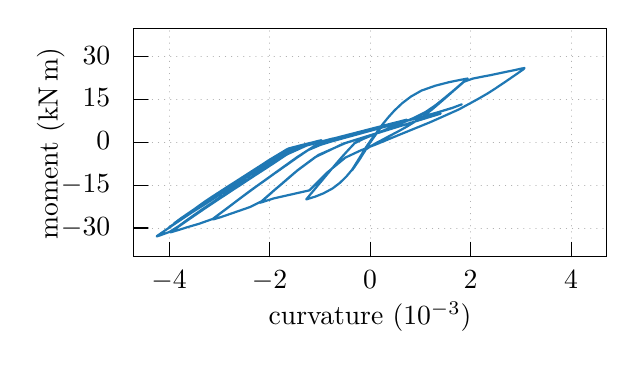
\begin{tikzpicture}[gnuplot]
%% generated with GNUPLOT 5.2p6 (Lua 5.3; terminal rev. Nov 2018, script rev. 107)
%% 08/11/2019 21:17:48
\path (0.000,0.000) rectangle (6.000,2.900);
\gpcolor{color=gp lt color axes}
\gpsetlinetype{gp lt axes}
\gpsetdashtype{gp dt axes}
\gpsetlinewidth{0.50}
\draw[gp path] (0.000,0.362)--(5.999,0.362);
\gpcolor{color=gp lt color border}
\gpsetlinetype{gp lt border}
\gpsetdashtype{gp dt solid}
\gpsetlinewidth{1.00}
\draw[gp path] (0.000,0.362)--(0.180,0.362);
\node[gp node right] at (-0.184,0.362) {$-30$};
\gpcolor{color=gp lt color axes}
\gpsetlinetype{gp lt axes}
\gpsetdashtype{gp dt axes}
\gpsetlinewidth{0.50}
\draw[gp path] (0.000,0.906)--(5.999,0.906);
\gpcolor{color=gp lt color border}
\gpsetlinetype{gp lt border}
\gpsetdashtype{gp dt solid}
\gpsetlinewidth{1.00}
\draw[gp path] (0.000,0.906)--(0.180,0.906);
\node[gp node right] at (-0.184,0.906) {$-15$};
\gpcolor{color=gp lt color axes}
\gpsetlinetype{gp lt axes}
\gpsetdashtype{gp dt axes}
\gpsetlinewidth{0.50}
\draw[gp path] (0.000,1.450)--(5.999,1.450);
\gpcolor{color=gp lt color border}
\gpsetlinetype{gp lt border}
\gpsetdashtype{gp dt solid}
\gpsetlinewidth{1.00}
\draw[gp path] (0.000,1.450)--(0.180,1.450);
\node[gp node right] at (-0.184,1.450) {$0$};
\gpcolor{color=gp lt color axes}
\gpsetlinetype{gp lt axes}
\gpsetdashtype{gp dt axes}
\gpsetlinewidth{0.50}
\draw[gp path] (0.000,1.993)--(5.999,1.993);
\gpcolor{color=gp lt color border}
\gpsetlinetype{gp lt border}
\gpsetdashtype{gp dt solid}
\gpsetlinewidth{1.00}
\draw[gp path] (0.000,1.993)--(0.180,1.993);
\node[gp node right] at (-0.184,1.993) {$15$};
\gpcolor{color=gp lt color axes}
\gpsetlinetype{gp lt axes}
\gpsetdashtype{gp dt axes}
\gpsetlinewidth{0.50}
\draw[gp path] (0.000,2.537)--(5.999,2.537);
\gpcolor{color=gp lt color border}
\gpsetlinetype{gp lt border}
\gpsetdashtype{gp dt solid}
\gpsetlinewidth{1.00}
\draw[gp path] (0.000,2.537)--(0.180,2.537);
\node[gp node right] at (-0.184,2.537) {$30$};
\gpcolor{color=gp lt color axes}
\gpsetlinetype{gp lt axes}
\gpsetdashtype{gp dt axes}
\gpsetlinewidth{0.50}
\draw[gp path] (0.447,0.000)--(0.447,2.899);
\gpcolor{color=gp lt color border}
\gpsetlinetype{gp lt border}
\gpsetdashtype{gp dt solid}
\gpsetlinewidth{1.00}
\draw[gp path] (0.447,0.000)--(0.447,0.180);
\node[gp node center] at (0.447,-0.308) {$-4$};
\gpcolor{color=gp lt color axes}
\gpsetlinetype{gp lt axes}
\gpsetdashtype{gp dt axes}
\gpsetlinewidth{0.50}
\draw[gp path] (1.723,0.000)--(1.723,2.899);
\gpcolor{color=gp lt color border}
\gpsetlinetype{gp lt border}
\gpsetdashtype{gp dt solid}
\gpsetlinewidth{1.00}
\draw[gp path] (1.723,0.000)--(1.723,0.180);
\node[gp node center] at (1.723,-0.308) {$-2$};
\gpcolor{color=gp lt color axes}
\gpsetlinetype{gp lt axes}
\gpsetdashtype{gp dt axes}
\gpsetlinewidth{0.50}
\draw[gp path] (3.000,0.000)--(3.000,2.899);
\gpcolor{color=gp lt color border}
\gpsetlinetype{gp lt border}
\gpsetdashtype{gp dt solid}
\gpsetlinewidth{1.00}
\draw[gp path] (3.000,0.000)--(3.000,0.180);
\node[gp node center] at (3.000,-0.308) {$0$};
\gpcolor{color=gp lt color axes}
\gpsetlinetype{gp lt axes}
\gpsetdashtype{gp dt axes}
\gpsetlinewidth{0.50}
\draw[gp path] (4.276,0.000)--(4.276,2.899);
\gpcolor{color=gp lt color border}
\gpsetlinetype{gp lt border}
\gpsetdashtype{gp dt solid}
\gpsetlinewidth{1.00}
\draw[gp path] (4.276,0.000)--(4.276,0.180);
\node[gp node center] at (4.276,-0.308) {$2$};
\gpcolor{color=gp lt color axes}
\gpsetlinetype{gp lt axes}
\gpsetdashtype{gp dt axes}
\gpsetlinewidth{0.50}
\draw[gp path] (5.552,0.000)--(5.552,2.899);
\gpcolor{color=gp lt color border}
\gpsetlinetype{gp lt border}
\gpsetdashtype{gp dt solid}
\gpsetlinewidth{1.00}
\draw[gp path] (5.552,0.000)--(5.552,0.180);
\node[gp node center] at (5.552,-0.308) {$4$};
\draw[gp path] (0.000,2.899)--(0.000,0.000)--(5.999,0.000)--(5.999,2.899)--cycle;
\node[gp node center,rotate=-270] at (-1.044,1.449) {moment (\si{\kilo\newton\meter})};
\node[gp node center] at (2.999,-0.769) {curvature (\num{E-3})};
\gpcolor{rgb color={0.122,0.471,0.706}}
\gpsetlinewidth{2.00}
\draw[gp path] (3.000,1.450)--(2.999,1.449)--(2.997,1.446)--(2.995,1.442)--(2.993,1.438)%
  --(2.992,1.437)--(2.991,1.436)--(2.989,1.432)--(2.986,1.426)--(2.982,1.420)--(2.978,1.414)%
  --(2.976,1.410)--(2.974,1.407)--(2.972,1.403)--(2.970,1.399)--(2.967,1.395)--(2.966,1.393)%
  --(2.967,1.394)--(2.967,1.395)--(2.968,1.397)--(2.969,1.399)--(2.971,1.402)--(2.973,1.405)%
  --(2.975,1.409)--(2.977,1.412)--(2.978,1.414)--(2.980,1.416)--(2.981,1.418)--(2.982,1.420)%
  --(2.982,1.421)--(2.982,1.420)--(2.981,1.419)--(2.982,1.420)--(2.982,1.421)--(2.983,1.422)%
  --(2.982,1.421)--(2.982,1.420)--(2.981,1.418)--(2.980,1.416)--(2.979,1.416)--(2.980,1.417)%
  --(2.981,1.418)--(2.982,1.420)--(2.984,1.423)--(2.986,1.428)--(2.989,1.431)--(2.989,1.433)%
  --(2.991,1.435)--(2.993,1.439)--(2.997,1.446)--(3.000,1.450)--(2.999,1.449)--(2.995,1.443)%
  --(2.990,1.434)--(2.986,1.427)--(2.982,1.420)--(2.976,1.410)--(2.968,1.397)--(2.959,1.382)%
  --(2.952,1.369)--(2.946,1.360)--(2.941,1.352)--(2.935,1.341)--(2.929,1.332)--(2.926,1.327)%
  --(2.927,1.328)--(2.930,1.333)--(2.934,1.341)--(2.940,1.350)--(2.947,1.363)--(2.957,1.380)%
  --(2.970,1.401)--(2.985,1.427)--(3.001,1.453)--(3.018,1.476)--(3.034,1.499)--(3.050,1.522)%
  --(3.068,1.547)--(3.086,1.572)--(3.104,1.597)--(3.119,1.618)--(3.131,1.635)--(3.140,1.647)%
  --(3.147,1.656)--(3.151,1.662)--(3.153,1.664)--(3.151,1.661)--(3.144,1.652)--(3.133,1.636)%
  --(3.120,1.618)--(3.106,1.597)--(3.091,1.577)--(3.076,1.555)--(3.060,1.532)--(3.043,1.508)%
  --(3.028,1.487)--(3.018,1.472)--(3.012,1.464)--(3.010,1.461)--(3.011,1.463)--(3.015,1.469)%
  --(3.023,1.480)--(3.034,1.495)--(3.048,1.516)--(3.066,1.541)--(3.083,1.564)--(3.097,1.585)%
  --(3.111,1.605)--(3.125,1.624)--(3.134,1.637)--(3.135,1.638)--(3.124,1.623)--(3.106,1.598)%
  --(3.085,1.568)--(3.062,1.535)--(3.037,1.500)--(3.005,1.455)--(2.963,1.390)--(2.919,1.317)%
  --(2.878,1.251)--(2.845,1.201)--(2.819,1.163)--(2.797,1.131)--(2.779,1.107)--(2.770,1.094)%
  --(2.774,1.101)--(2.792,1.131)--(2.822,1.180)--(2.860,1.242)--(2.903,1.313)--(2.952,1.394)%
  --(3.013,1.482)--(3.084,1.576)--(3.153,1.672)--(3.228,1.764)--(3.309,1.854)--(3.410,1.949)%
  --(3.518,2.031)--(3.652,2.107)--(3.828,2.169)--(4.003,2.214)--(4.146,2.243)--(4.221,2.257)%
  --(4.238,2.260)--(4.227,2.250)--(4.202,2.228)--(4.170,2.200)--(4.129,2.164)--(4.073,2.116)%
  --(4.006,2.057)--(3.932,1.992)--(3.859,1.929)--(3.791,1.871)--(3.725,1.819)--(3.657,1.769)%
  --(3.568,1.712)--(3.468,1.650)--(3.348,1.584)--(3.231,1.523)--(3.144,1.476)--(3.075,1.440)%
  --(3.009,1.402)--(2.920,1.342)--(2.845,1.220)--(2.774,1.106)--(2.698,1.015)--(2.616,0.935)%
  --(2.521,0.863)--(2.407,0.802)--(2.302,0.760)--(2.228,0.737)--(2.192,0.726)--(2.189,0.726)%
  --(2.197,0.736)--(2.209,0.750)--(2.226,0.770)--(2.251,0.801)--(2.289,0.845)--(2.336,0.902)%
  --(2.389,0.965)--(2.443,1.030)--(2.501,1.099)--(2.566,1.176)--(2.640,1.262)--(2.721,1.351)%
  --(2.803,1.438)--(2.908,1.491)--(3.019,1.537)--(3.130,1.584)--(3.241,1.630)--(3.349,1.674)%
  --(3.452,1.716)--(3.543,1.755)--(3.625,1.795)--(3.705,1.836)--(3.769,1.879)--(3.833,1.923)%
  --(3.889,1.968)--(3.941,2.010)--(3.993,2.053)--(4.052,2.102)--(4.117,2.158)--(4.185,2.217)%
  --(4.306,2.260)--(4.416,2.282)--(4.528,2.303)--(4.641,2.327)--(4.746,2.349)--(4.835,2.367)%
  --(4.909,2.384)--(4.961,2.394)--(4.949,2.379)--(4.849,2.309)--(4.715,2.217)--(4.590,2.133)%
  --(4.493,2.071)--(4.361,1.995)--(4.126,1.867)--(3.767,1.707)--(3.384,1.551)--(3.090,1.430)%
  --(2.882,1.348)--(2.686,1.256)--(2.458,1.069)--(2.229,0.840)--(1.773,0.737)--(1.624,0.689)%
  --(1.599,0.682)--(1.670,0.744)--(1.781,0.841)--(1.881,0.926)--(1.967,1.001)--(2.083,1.099)%
  --(2.300,1.260)--(2.661,1.434)--(2.989,1.536)--(3.237,1.612)--(3.361,1.650)--(3.419,1.667)%
  --(3.551,1.708)--(3.751,1.770)--(3.896,1.814)--(3.835,1.796)--(3.595,1.722)--(3.346,1.645)%
  --(3.165,1.589)--(3.041,1.550)--(2.908,1.509)--(2.689,1.441)--(2.344,1.290)--(2.074,1.090)%
  --(1.888,0.930)--(1.783,0.841)--(1.725,0.789)--(1.635,0.709)--(1.480,0.630)--(1.290,0.564)%
  --(1.105,0.500)--(1.008,0.471)--(1.000,0.473)--(1.046,0.508)--(1.095,0.546)--(1.116,0.561)%
  --(1.122,0.566)--(1.159,0.593)--(1.257,0.668)--(1.405,0.779)--(1.556,0.890)--(1.683,0.980)%
  --(1.791,1.058)--(1.915,1.145)--(2.073,1.257)--(2.258,1.381)--(2.491,1.457)--(2.618,1.491)%
  --(2.694,1.512)--(2.748,1.526)--(2.797,1.540)--(2.824,1.547)--(2.801,1.541)--(2.710,1.516)%
  --(2.569,1.477)--(2.404,1.432)--(2.212,1.351)--(2.074,1.257)--(1.934,1.158)--(1.782,1.052)%
  --(1.636,0.947)--(1.514,0.860)--(1.427,0.796)--(1.371,0.755)--(1.337,0.729)--(1.321,0.718)%
  --(1.332,0.726)--(1.375,0.758)--(1.438,0.806)--(1.516,0.863)--(1.610,0.930)--(1.725,1.012)%
  --(1.861,1.109)--(2.004,1.210)--(2.135,1.302)--(2.259,1.382)--(2.436,1.441)--(2.571,1.478)%
  --(2.701,1.514)--(2.813,1.544)--(2.898,1.568)--(2.959,1.585)--(3.005,1.597)--(3.045,1.608)%
  --(3.075,1.617)--(3.077,1.617)--(3.026,1.603)--(2.932,1.577)--(2.834,1.550)--(2.754,1.528)%
  --(2.687,1.510)--(2.598,1.486)--(2.463,1.449)--(2.257,1.380)--(2.143,1.305)--(2.086,1.266)%
  --(2.062,1.250)--(2.041,1.235)--(2.020,1.221)--(2.006,1.211)--(1.976,1.188)--(1.933,1.157)%
  --(1.914,1.144)--(1.934,1.158)--(1.976,1.189)--(1.991,1.199)--(1.954,1.173)--(1.892,1.129)%
  --(1.854,1.102)--(1.870,1.114)--(1.921,1.151)--(1.955,1.175)--(1.925,1.153)--(1.852,1.100)%
  --(1.802,1.065)--(1.815,1.074)--(1.869,1.113)--(1.894,1.131)--(1.846,1.097)--(1.751,1.030)%
  --(1.679,0.978)--(1.673,0.974)--(1.708,0.999)--(1.728,1.014)--(1.705,0.998)--(1.663,0.967)%
  --(1.649,0.957)--(1.686,0.984)--(1.749,1.029)--(1.798,1.063)--(1.825,1.083)--(1.849,1.099)%
  --(1.890,1.128)--(1.952,1.172)--(2.021,1.220)--(2.078,1.261)--(2.118,1.289)--(2.152,1.312)%
  --(2.198,1.342)--(2.256,1.380)--(2.341,1.416)--(2.425,1.438)--(2.461,1.448)--(2.483,1.454)%
  --(2.499,1.459)--(2.513,1.462)--(2.519,1.464)--(2.507,1.461)--(2.474,1.452)--(2.416,1.436)%
  --(2.324,1.411)--(2.262,1.384)--(2.214,1.352)--(2.156,1.314)--(2.099,1.275)--(2.052,1.242)%
  --(2.022,1.221)--(2.009,1.212)--(2.012,1.215)--(2.029,1.226)--(2.058,1.248)--(2.106,1.281)%
  --(2.179,1.329)--(2.268,1.387)--(2.398,1.431)--(2.475,1.452)--(2.540,1.470)--(2.618,1.491)%
  --(2.708,1.516)--(2.777,1.535)--(2.798,1.541)--(2.771,1.533)--(2.714,1.518)--(2.657,1.502)%
  --(2.604,1.487)--(2.541,1.470)--(2.453,1.446)--(2.286,1.399)--(2.174,1.326)--(2.074,1.257)%
  --(2.000,1.205)--(1.945,1.167)--(1.898,1.134)--(1.852,1.102)--(1.819,1.079)--(1.814,1.075)%
  --(1.843,1.096)--(1.899,1.135)--(1.971,1.187)--(2.056,1.246)--(2.156,1.315)--(2.282,1.397)%
  --(2.509,1.462)--(2.702,1.514)--(2.891,1.567)--(3.066,1.614)--(3.225,1.658)--(3.397,1.704)%
  --(3.619,1.764)--(3.856,1.830)--(4.054,1.891)--(4.164,1.932)--(4.155,1.929)--(4.041,1.885)%
  --(3.904,1.844)--(3.823,1.820)--(3.766,1.805)--(3.639,1.771)--(3.377,1.700)--(3.060,1.613)%
  --(2.759,1.530)--(2.511,1.462)--(2.263,1.384)--(2.077,1.265)--(1.867,1.115)--(1.636,0.948)%
  --(1.404,0.780)--(1.193,0.621)--(1.001,0.477)--(0.826,0.415)--(0.695,0.377)--(0.597,0.346)%
  --(0.527,0.325)--(0.482,0.311)--(0.461,0.306)--(0.472,0.313)--(0.526,0.351)--(0.619,0.416)%
  --(0.742,0.501)--(0.881,0.596)--(1.044,0.705)--(1.233,0.830)--(1.461,0.980)--(1.711,1.142)%
  --(1.947,1.298)--(2.200,1.412)--(2.438,1.473)--(2.664,1.532)--(2.910,1.595)--(3.150,1.657)%
  --(3.334,1.704)--(3.440,1.731)--(3.465,1.738)--(3.431,1.729)--(3.381,1.716)--(3.345,1.707)%
  --(3.321,1.701)--(3.294,1.694)--(3.247,1.682)--(3.181,1.665)--(3.096,1.643)--(2.995,1.617)%
  --(2.863,1.583)--(2.701,1.541)--(2.561,1.505)--(2.450,1.476)--(2.321,1.442)--(2.087,1.382)%
  --(1.883,1.260)--(1.693,1.138)--(1.554,1.047)--(1.468,0.990)--(1.380,0.932)--(1.265,0.855)%
  --(1.116,0.756)--(0.961,0.652)--(0.843,0.572)--(0.781,0.530)--(0.759,0.515)--(0.748,0.508)%
  --(0.727,0.494)--(0.701,0.475)--(0.684,0.463)--(0.694,0.471)--(0.747,0.508)--(0.827,0.563)%
  --(0.914,0.623)--(0.989,0.673)--(1.059,0.719)--(1.141,0.772)--(1.234,0.833)--(1.333,0.897)%
  --(1.428,0.959)--(1.507,1.010)--(1.568,1.050)--(1.611,1.078)--(1.635,1.094)--(1.646,1.101)%
  --(1.647,1.102)--(1.637,1.096)--(1.611,1.078)--(1.570,1.051)--(1.527,1.023)--(1.489,0.998)%
  --(1.439,0.965)--(1.368,0.918)--(1.280,0.861)--(1.198,0.807)--(1.150,0.776)--(1.125,0.760)%
  --(1.088,0.736)--(1.022,0.693)--(0.953,0.648)--(0.919,0.625)--(0.932,0.634)--(0.974,0.663)%
  --(1.022,0.695)--(1.069,0.726)--(1.127,0.764)--(1.214,0.821)--(1.338,0.902)--(1.484,0.997)%
  --(1.626,1.090)--(1.749,1.171)--(1.868,1.250)--(1.996,1.331)--(2.164,1.405)--(2.321,1.445)%
  --(2.430,1.473)--(2.500,1.491)--(2.532,1.499)--(2.535,1.500)--(2.518,1.496)--(2.486,1.488)%
  --(2.438,1.475)--(2.372,1.458)--(2.291,1.437)--(2.208,1.416)--(2.109,1.391)--(2.044,1.361)%
  --(2.002,1.335)--(1.967,1.313)--(1.928,1.290)--(1.888,1.265)--(1.854,1.242)--(1.830,1.226)%
  --(1.814,1.215)--(1.798,1.204)--(1.779,1.191)--(1.756,1.176)--(1.731,1.160)--(1.708,1.145)%
  --(1.691,1.133)--(1.678,1.125)--(1.663,1.115)--(1.643,1.102)--(1.621,1.087)--(1.603,1.075)%
  --(1.592,1.068)--(1.585,1.064)--(1.577,1.059)--(1.563,1.049)--(1.543,1.036)--(1.523,1.023)%
  --(1.509,1.014)--(1.503,1.010)--(1.500,1.009)--(1.496,1.006)--(1.490,1.002)--(1.487,1.000)%
  --(1.493,1.004)--(1.511,1.016)--(1.538,1.034)--(1.567,1.053)--(1.599,1.074)--(1.634,1.097)%
  --(1.670,1.120)--(1.707,1.144)--(1.742,1.167)--(1.774,1.188)--(1.798,1.204)--(1.809,1.212)%
  --(1.816,1.216)--(1.820,1.219)--(1.818,1.217)--(1.804,1.208)--(1.779,1.191)--(1.748,1.171)%
  --(1.712,1.147)--(1.676,1.123)--(1.643,1.101)--(1.615,1.083)--(1.588,1.066)--(1.558,1.046)%
  --(1.528,1.027)--(1.506,1.012)--(1.496,1.006)--(1.499,1.008)--(1.511,1.017)--(1.527,1.027)%
  --(1.541,1.036)--(1.556,1.045)--(1.578,1.060)--(1.611,1.081)--(1.648,1.105)--(1.679,1.126)%
  --(1.701,1.140)--(1.717,1.151)--(1.733,1.161)--(1.749,1.171)--(1.761,1.179)--(1.765,1.182)%
  --(1.758,1.177)--(1.745,1.168)--(1.731,1.160)--(1.719,1.152)--(1.705,1.142)--(1.683,1.128)%
  --(1.654,1.109)--(1.625,1.090)--(1.601,1.074)--(1.582,1.062)--(1.563,1.050)--(1.541,1.035)%
  --(1.514,1.018)--(1.489,1.001)--(1.470,0.989)--(1.458,0.981)--(1.452,0.977)--(1.445,0.973)%
  --(1.435,0.966)--(1.425,0.960)--(1.421,0.957)--(1.428,0.962)--(1.444,0.972)--(1.462,0.984)%
  --(1.480,0.996)--(1.500,1.009)--(1.528,1.027)--(1.564,1.051)--(1.598,1.073)--(1.624,1.090)%
  --(1.648,1.105)--(1.675,1.123)--(1.707,1.144)--(1.735,1.162)--(1.750,1.172)--(1.752,1.173)%
  --(1.747,1.170)--(1.743,1.168)--(1.741,1.166)--(1.733,1.161)--(1.717,1.150)--(1.692,1.134)%
  --(1.664,1.116)--(1.641,1.101)--(1.625,1.090)--(1.613,1.082)--(1.601,1.075)--(1.591,1.068)%
  --(1.590,1.067)--(1.603,1.076)--(1.626,1.092)--(1.652,1.108)--(1.670,1.120)--(1.681,1.127)%
  --(1.694,1.135)--(1.715,1.149)--(1.743,1.167)--(1.766,1.182)--(1.771,1.186)--(1.760,1.179)%
  --(1.744,1.168)--(1.735,1.162)--(1.729,1.158)--(1.717,1.151)--(1.691,1.133)--(1.652,1.107)%
  --(1.611,1.080)--(1.575,1.057)--(1.546,1.038)--(1.516,1.019)--(1.481,0.996)--(1.442,0.971)%
  --(1.407,0.948)--(1.385,0.934)--(1.378,0.929)--(1.382,0.933)--(1.394,0.940)--(1.411,0.951)%
  --(1.438,0.969)--(1.478,0.995)--(1.525,1.026)--(1.574,1.057)--(1.621,1.088)--(1.665,1.117)%
  --(1.711,1.146)--(1.754,1.175)--(1.793,1.201)--(1.820,1.219)--(1.831,1.227)--(1.829,1.225)%
  --(1.820,1.219)--(1.810,1.212)--(1.796,1.203)--(1.773,1.187)--(1.738,1.164)--(1.698,1.138)%
  --(1.659,1.112)--(1.627,1.091)--(1.601,1.074)--(1.576,1.058)--(1.551,1.042)--(1.527,1.026)%
  --(1.508,1.014)--(1.499,1.008)--(1.505,1.012)--(1.516,1.020)--(1.532,1.030)--(1.555,1.045)%
  --(1.585,1.065)--(1.620,1.087)--(1.657,1.111)--(1.691,1.134)--(1.724,1.155)--(1.757,1.177)%
  --(1.792,1.200)--(1.823,1.221)--(1.844,1.235)--(1.852,1.240)--(1.851,1.240)--(1.844,1.235)%
  --(1.835,1.229)--(1.818,1.218)--(1.794,1.201)--(1.764,1.181)--(1.734,1.162)--(1.707,1.144)%
  --(1.683,1.128)--(1.663,1.115)--(1.646,1.104)--(1.632,1.095)--(1.623,1.089)--(1.620,1.087)%
  --(1.624,1.090)--(1.634,1.097)--(1.651,1.107)--(1.673,1.122)--(1.700,1.140)--(1.732,1.161)%
  --(1.765,1.183)--(1.793,1.201)--(1.815,1.216)--(1.841,1.234)--(1.873,1.255)--(1.899,1.272)%
  --(1.909,1.278)--(1.896,1.271)--(1.872,1.254)--(1.846,1.236)--(1.818,1.218)--(1.780,1.192)%
  --(1.725,1.155)--(1.655,1.109)--(1.582,1.061)--(1.513,1.016)--(1.449,0.975)--(1.387,0.935)%
  --(1.323,0.894)--(1.261,0.853)--(1.208,0.819)--(1.178,0.800)--(1.171,0.795)--(1.178,0.801)%
  --(1.191,0.809)--(1.204,0.817)--(1.224,0.830)--(1.262,0.854)--(1.319,0.891)--(1.388,0.936)%
  --(1.452,0.978)--(1.508,1.014)--(1.557,1.046)--(1.604,1.076)--(1.652,1.107)--(1.697,1.138)%
  --(1.735,1.162)--(1.758,1.178)--(1.768,1.184)--(1.769,1.184)--(1.766,1.182)--(1.758,1.177)%
  --(1.741,1.166)--(1.713,1.147)--(1.674,1.122)--(1.631,1.093)--(1.587,1.065)--(1.546,1.038)%
  --(1.505,1.011)--(1.464,0.985)--(1.423,0.959)--(1.388,0.936)--(1.364,0.920)--(1.352,0.913)%
  --(1.351,0.913)--(1.361,0.919)--(1.380,0.931)--(1.408,0.949)--(1.447,0.975)--(1.497,1.008)%
  --(1.557,1.047)--(1.622,1.089)--(1.687,1.132)--(1.752,1.174)--(1.817,1.217)--(1.881,1.261)%
  --(1.943,1.299)--(1.995,1.331)--(2.035,1.356)--(2.059,1.371)--(2.067,1.375)--(2.064,1.373)%
  --(2.052,1.366)--(2.028,1.351)--(1.988,1.327)--(1.938,1.296)--(1.877,1.257)--(1.794,1.201)%
  --(1.690,1.131)--(1.576,1.057)--(1.471,0.988)--(1.375,0.926)--(1.272,0.860)--(1.155,0.783)%
  --(1.027,0.698)--(0.902,0.615)--(0.810,0.552)--(0.754,0.511)--(0.700,0.473)--(0.637,0.430)%
  --(0.575,0.387)--(0.540,0.362)--(0.550,0.370)--(0.611,0.413)--(0.697,0.473)--(0.781,0.530)%
  --(0.848,0.576)--(0.922,0.626)--(1.026,0.695)--(1.159,0.783)--(1.303,0.877)--(1.433,0.961)%
  --(1.539,1.031)--(1.634,1.094)--(1.733,1.159)--(1.834,1.229)--(1.924,1.287)--(1.981,1.323)%
  --(1.999,1.334)--(1.987,1.327)--(1.965,1.314)--(1.941,1.299)--(1.908,1.278)--(1.858,1.244)%
  --(1.786,1.196)--(1.703,1.140)--(1.628,1.089)--(1.569,1.052)--(1.529,1.026)--(1.502,1.008)%
  --(1.478,0.993)--(1.450,0.974)--(1.418,0.952)--(1.371,0.920)--(1.324,0.889)--(1.312,0.882)%
  --(1.331,0.895)--(1.340,0.901)--(1.303,0.877)--(1.232,0.830)--(1.170,0.790)--(1.135,0.766)%
  --(1.119,0.756)--(1.106,0.748)--(1.080,0.731)--(1.040,0.704)--(1.000,0.677)--(0.973,0.660)%
  --(0.967,0.656)--(0.974,0.661)--(0.984,0.668)--(0.996,0.676)--(1.019,0.691)--(1.058,0.717)%
  --(1.118,0.757)--(1.198,0.811)--(1.297,0.875)--(1.410,0.949)--(1.531,1.028)--(1.647,1.104)%
  --(1.758,1.177)--(1.869,1.254)--(1.990,1.329)--(2.153,1.403)--(2.301,1.441)--(2.396,1.465)%
  --(2.431,1.473)--(2.415,1.469)--(2.365,1.456)--(2.279,1.434)--(2.155,1.402)--(1.982,1.330)%
  --(1.821,1.229)--(1.647,1.110)--(1.467,0.991)--(1.284,0.874)--(1.111,0.760)--(0.951,0.654)%
  --(0.798,0.551)--(0.670,0.460)--(0.568,0.385)--(0.451,0.312)--(0.348,0.274)--(0.291,0.255)%
  --(0.293,0.260)--(0.377,0.318)--(0.514,0.411)--(0.653,0.504)--(0.770,0.581)--(0.852,0.632)%
  --(0.950,0.695)--(1.120,0.805)--(1.349,0.954)--(1.570,1.097)--(1.723,1.198)--(1.800,1.254)%
  --(1.854,1.286)--(1.932,1.334)--(2.087,1.395)--(2.223,1.429)--(2.282,1.444)--(2.240,1.433)%
  --(2.124,1.404)--(1.953,1.349)--(1.837,1.280)--(1.739,1.218)--(1.644,1.155)--(1.534,1.082)%
  --(1.396,0.994)--(1.239,0.894)--(1.093,0.801)--(0.980,0.729)--(0.900,0.677)--(0.833,0.634)%
  --(0.769,0.592)--(0.718,0.559)--(0.700,0.546)--(0.724,0.562)--(0.783,0.602)--(0.865,0.655)%
  --(0.957,0.716)--(1.063,0.784)--(1.190,0.865)--(1.336,0.958)--(1.492,1.057)--(1.643,1.155)%
  --(1.789,1.250)--(1.927,1.334)--(2.088,1.396)--(2.217,1.429)--(2.323,1.455)--(2.378,1.469)%
  --(2.381,1.470)--(2.333,1.458)--(2.239,1.434)--(2.113,1.402)--(1.948,1.346)--(1.823,1.271)%
  --(1.688,1.184)--(1.558,1.099)--(1.433,1.020)--(1.307,0.940)--(1.187,0.863)--(1.082,0.796)%
  --(1.001,0.744)--(0.944,0.708)--(0.905,0.683)--(0.876,0.664)--(0.857,0.652)--(0.855,0.650)%
  --(0.876,0.664)--(0.919,0.692)--(0.975,0.728)--(1.037,0.769)--(1.107,0.813)--(1.184,0.863)%
  --(1.269,0.917)--(1.357,0.973)--(1.447,1.030)--(1.535,1.087)--(1.621,1.143)--(1.706,1.198)%
  --(1.791,1.253)--(1.874,1.303)--(1.951,1.350)--(2.058,1.389)--(2.142,1.410)--(2.197,1.424)%
  --(2.221,1.430)--(2.220,1.430)--(2.196,1.424)--(2.147,1.411)--(2.065,1.391)--(1.942,1.344)%
  --(1.842,1.284)--(1.726,1.210)--(1.602,1.128)--(1.462,1.038)--(1.310,0.941)--(1.162,0.846)%
  --(1.032,0.764)--(0.925,0.695)--(0.826,0.631)--(0.739,0.571)--(0.665,0.518)--(0.606,0.477)%
  --(0.566,0.450)--(0.556,0.443)--(0.591,0.468)--(0.675,0.525)--(0.787,0.599)--(0.895,0.669)%
  --(0.994,0.732)--(1.097,0.797)--(1.226,0.879)--(1.380,0.978)--(1.537,1.080)--(1.672,1.168)%
  --(1.774,1.235)--(1.849,1.284)--(1.912,1.322)--(1.965,1.354)--(1.996,1.374)--(1.988,1.369)%
  --(1.931,1.334)--(1.831,1.273)--(1.717,1.198)--(1.599,1.121)--(1.479,1.041)--(1.343,0.954)%
  --(1.191,0.857)--(1.036,0.758)--(0.898,0.670)--(0.781,0.595)--(0.681,0.529)--(0.595,0.472)%
  --(0.533,0.429)--(0.488,0.397)--(0.453,0.374)--(0.443,0.367)--(0.475,0.390)--(0.556,0.444)%
  --(0.662,0.517)--(0.762,0.582)--(0.848,0.637)--(0.929,0.689)--(1.031,0.755)--(1.166,0.842)%
  --(1.313,0.936)--(1.441,1.019)--(1.536,1.080)--(1.609,1.128)--(1.684,1.178)--(1.769,1.234)%
  --(1.854,1.290)--(1.912,1.328)--(1.930,1.339)--(1.913,1.328)--(1.876,1.306)--(1.827,1.276)%
  --(1.767,1.237)--(1.688,1.183)--(1.578,1.110)--(1.451,1.027)--(1.320,0.943)--(1.198,0.865)%
  --(1.081,0.791)--(0.970,0.720)--(0.863,0.651)--(0.766,0.588)--(0.690,0.538)--(0.643,0.507)%
  --(0.623,0.494)--(0.622,0.493)--(0.633,0.501)--(0.656,0.516)--(0.696,0.542)--(0.759,0.584)%
  --(0.842,0.639)--(0.928,0.695)--(1.004,0.744)--(1.073,0.788)--(1.144,0.832)--(1.218,0.880)%
  --(1.288,0.925)--(1.343,0.960)--(1.378,0.982)--(1.396,0.994)--(1.405,0.999)--(1.408,1.001)%
  --(1.404,0.999)--(1.386,0.987)--(1.350,0.964)--(1.297,0.930)--(1.237,0.891)--(1.176,0.852)%
  --(1.117,0.814)--(1.051,0.772)--(0.974,0.723)--(0.890,0.668)--(0.809,0.615)--(0.744,0.573)%
  --(0.695,0.541)--(0.651,0.512)--(0.605,0.481)--(0.564,0.453)--(0.543,0.439)--(0.547,0.441)%
  --(0.574,0.460)--(0.618,0.490)--(0.672,0.527)--(0.731,0.566)--(0.803,0.614)--(0.892,0.672)%
  --(0.995,0.739)--(1.108,0.811)--(1.222,0.883)--(1.333,0.955)--(1.446,1.027)--(1.560,1.101)%
  --(1.675,1.177)--(1.784,1.251)--(1.882,1.310)--(1.958,1.357)--(2.060,1.393)--(2.152,1.415)%
  --(2.238,1.437)--(2.306,1.454)--(2.339,1.463)--(2.332,1.461)--(2.292,1.451)--(2.239,1.437)%
  --(2.192,1.425)--(2.153,1.416)--(2.111,1.405)--(2.057,1.391)--(1.970,1.367)--(1.921,1.338)%
  --(1.888,1.319)--(1.874,1.310)--(1.870,1.308)--(1.856,1.299)--(1.824,1.280)--(1.785,1.257)%
  --(1.754,1.238)--(1.735,1.225)--(1.709,1.208)--(1.658,1.174)--(1.582,1.124)--(1.496,1.069)%
  --(1.417,1.018)--(1.342,0.970)--(1.259,0.918)--(1.158,0.853)--(1.047,0.781)--(0.944,0.714)%
  --(0.857,0.658)--(0.790,0.614)--(0.736,0.574)--(0.685,0.538)--(0.625,0.495)--(0.566,0.456)%
  --(0.522,0.426)--(0.509,0.417)--(0.529,0.432)--(0.577,0.464)--(0.626,0.497)--(0.668,0.526)%
  --(0.706,0.550)--(0.756,0.583)--(0.828,0.630)--(0.913,0.685)--(0.990,0.735)--(1.052,0.774)%
  --(1.100,0.805)--(1.148,0.835)--(1.201,0.868)--(1.248,0.899)--(1.280,0.920)--(1.295,0.929)%
  --(1.299,0.932)--(1.305,0.936)--(1.315,0.943)--(1.321,0.946)--(1.316,0.943)--(1.302,0.934)%
  --(1.292,0.927)--(1.297,0.931)--(1.314,0.942)--(1.327,0.950)--(1.325,0.949)--(1.316,0.943)%
  --(1.336,0.956)--(1.367,0.976)--(1.392,0.992)--(1.401,0.998)--(1.400,0.997)--(1.405,1.000)%
  --(1.422,1.012)--(1.445,1.027)--(1.460,1.036)--(1.458,1.035)--(1.446,1.027)--(1.436,1.020)%
  --(1.435,1.020)--(1.440,1.023)--(1.434,1.019)--(1.410,1.004)--(1.379,0.983)--(1.356,0.968)%
  --(1.349,0.964)--(1.350,0.965)--(1.340,0.959)--(1.314,0.941)--(1.281,0.920)--(1.258,0.905)%
  --(1.252,0.902)--(1.241,0.895)--(1.213,0.877)--(1.183,0.857)--(1.166,0.846)--(1.164,0.846)%
  --(1.167,0.848)--(1.164,0.846)--(1.152,0.838)--(1.140,0.830)--(1.139,0.829)--(1.148,0.835)%
  --(1.160,0.843)--(1.166,0.847)--(1.164,0.845)--(1.163,0.845)--(1.170,0.849)--(1.184,0.859)%
  --(1.200,0.869)--(1.211,0.876)--(1.219,0.881)--(1.232,0.889)--(1.254,0.903)--(1.283,0.922)%
  --(1.314,0.942)--(1.342,0.960)--(1.371,0.979)--(1.401,0.998)--(1.434,1.020)--(1.468,1.042)%
  --(1.498,1.062)--(1.517,1.074)--(1.524,1.079)--(1.527,1.081)--(1.530,1.083)--(1.531,1.083)%
  --(1.523,1.078)--(1.503,1.065)--(1.476,1.047)--(1.448,1.029)--(1.425,1.013)--(1.405,1.000)%
  --(1.385,0.987)--(1.362,0.973)--(1.341,0.959)--(1.330,0.952)--(1.331,0.953)--(1.339,0.958)%
  --(1.347,0.964)--(1.359,0.971)--(1.377,0.983)--(1.394,0.994)--(1.407,1.002)--(1.418,1.009)%
  --(1.428,1.015)--(1.437,1.021)--(1.421,1.010)--(1.390,0.989)--(1.350,0.964)--(1.308,0.937)%
  --(1.266,0.910)--(1.218,0.880)--(1.164,0.845)--(1.107,0.808)--(1.050,0.773)--(1.002,0.742)%
  --(0.970,0.722)--(0.953,0.711)--(0.949,0.708)--(0.948,0.708)--(0.943,0.704)--(0.938,0.701)%
  --(0.950,0.709)--(0.987,0.733)--(1.044,0.769)--(1.100,0.806)--(1.145,0.834)--(1.182,0.858)%
  --(1.229,0.888)--(1.292,0.928)--(1.357,0.970)--(1.406,1.001)--(1.427,1.014)--(1.430,1.016)%
  --(1.433,1.017)--(1.440,1.023)--(1.446,1.027)--(1.433,1.018)--(1.389,0.989)--(1.324,0.947)%
  --(1.264,0.909)--(1.223,0.883)--(1.192,0.863)--(1.152,0.838)--(1.098,0.803)--(1.039,0.765)%
  --(0.995,0.737)--(0.971,0.722)--(0.962,0.716)--(0.953,0.710)--(0.936,0.699)--(0.919,0.688)%
  --(0.917,0.687)--(0.936,0.700)--(0.971,0.723)--(1.008,0.747)--(1.039,0.766)--(1.070,0.786)%
  --(1.112,0.813)--(1.172,0.851)--(1.242,0.896)--(1.309,0.939)--(1.365,0.975)--(1.416,1.008)%
  --(1.478,1.049)--(1.557,1.101)--(1.634,1.151)--(1.692,1.190)--(1.717,1.206)--(1.721,1.208)%
  --(1.720,1.208)--(1.716,1.205)--(1.693,1.190)--(1.633,1.149)--(1.539,1.087)--(1.430,1.015)%
  --(1.316,0.941)--(1.202,0.869)--(1.085,0.794)--(0.968,0.719)--(0.853,0.645)--(0.749,0.578)%
  --(0.667,0.525)--(0.605,0.483)--(0.564,0.456)--(0.543,0.442)--(0.543,0.443)--(0.572,0.463)%
  --(0.636,0.506)--(0.730,0.569)--(0.829,0.633)--(0.922,0.692)--(1.010,0.749)--(1.114,0.815)%
  --(1.241,0.896)--(1.374,0.982)--(1.483,1.053)--(1.552,1.098)--(1.595,1.126)--(1.632,1.151)%
  --(1.670,1.176)--(1.693,1.191)--(1.688,1.187)--(1.654,1.165)--(1.606,1.133)--(1.562,1.104)%
  --(1.525,1.080)--(1.491,1.058)--(1.459,1.037)--(1.430,1.018)--(1.407,1.003)--(1.396,0.996)%
  --(1.395,0.995)--(1.404,1.001)--(1.415,1.008)--(1.426,1.015)--(1.435,1.021)--(1.442,1.026)%
  --(1.448,1.029)--(1.440,1.024)--(1.421,1.011)--(1.397,0.995)--(1.372,0.979)--(1.343,0.961)%
  --(1.312,0.941)--(1.283,0.923)--(1.260,0.908)--(1.239,0.895)--(1.219,0.881)--(1.197,0.867)%
  --(1.178,0.855)--(1.168,0.849)--(1.165,0.847)--(1.164,0.846)--(1.159,0.843)--(1.153,0.839)%
  --(1.151,0.838)--(1.155,0.841)--(1.162,0.845)--(1.167,0.848)--(1.168,0.849)--(1.170,0.850)%
  --(1.174,0.852)--(1.181,0.857)--(1.185,0.860)--(1.182,0.857)--(1.170,0.849)--(1.152,0.838)%
  --(1.133,0.826)--(1.118,0.816)--(1.105,0.808)--(1.090,0.799)--(1.072,0.788)--(1.051,0.774)%
  --(1.034,0.763)--(1.028,0.760)--(1.037,0.765)--(1.052,0.775)--(1.068,0.785)--(1.085,0.796)%
  --(1.109,0.811)--(1.145,0.835)--(1.192,0.865)--(1.246,0.899)--(1.297,0.932)--(1.338,0.958)%
  --(1.368,0.977)--(1.389,0.990)--(1.406,1.001)--(1.423,1.012)--(1.434,1.019)--(1.431,1.018)%
  --(1.410,1.004)--(1.373,0.979)--(1.331,0.953)--(1.296,0.931)--(1.271,0.915)--(1.248,0.900)%
  --(1.220,0.882)--(1.184,0.859)--(1.150,0.837)--(1.129,0.823)--(1.121,0.819)--(1.118,0.817)%
  --(1.112,0.813)--(1.105,0.808)--(1.104,0.808)--(1.116,0.816)--(1.138,0.830)--(1.165,0.848)%
  --(1.195,0.867)--(1.231,0.890)--(1.277,0.919)--(1.329,0.953)--(1.381,0.986)--(1.430,1.018)%
  --(1.475,1.047)--(1.514,1.073)--(1.546,1.094)--(1.569,1.108)--(1.576,1.113)--(1.568,1.108)%
  --(1.544,1.092)--(1.507,1.067)--(1.460,1.037)--(1.407,1.001)--(1.348,0.963)--(1.285,0.923)%
  --(1.223,0.884)--(1.165,0.847)--(1.112,0.813)--(1.061,0.781)--(1.013,0.750)--(0.973,0.724)%
  --(0.945,0.706)--(0.927,0.694)--(0.914,0.686)--(0.908,0.682)--(0.909,0.683)--(0.920,0.690)%
  --(0.940,0.703)--(0.967,0.721)--(1.002,0.744)--(1.045,0.771)--(1.095,0.803)--(1.146,0.835)%
  --(1.196,0.867)--(1.249,0.901)--(1.308,0.939)--(1.370,0.979)--(1.428,1.017)--(1.476,1.048)%
  --(1.515,1.074)--(1.551,1.097)--(1.589,1.122)--(1.621,1.143)--(1.642,1.157)--(1.648,1.161)%
  --(1.644,1.159)--(1.634,1.152)--(1.621,1.143)--(1.603,1.131)--(1.579,1.115)--(1.547,1.094)%
  --(1.509,1.070)--(1.470,1.044)--(1.432,1.019)--(1.391,0.991)--(1.343,0.961)--(1.293,0.928)%
  --(1.243,0.896)--(1.194,0.865)--(1.142,0.831)--(1.085,0.795)--(1.028,0.759)--(0.979,0.728)%
  --(0.940,0.703)--(0.909,0.683)--(0.882,0.665)--(0.861,0.652)--(0.853,0.647)--(0.863,0.654)%
  --(0.889,0.671)--(0.921,0.691)--(0.954,0.713)--(0.990,0.736)--(1.035,0.765)--(1.090,0.799)%
  --(1.146,0.835)--(1.200,0.870)--(1.247,0.900)--(1.286,0.924)--(1.319,0.946)--(1.351,0.966)%
  --(1.381,0.986)--(1.406,1.002)--(1.422,1.013)--(1.427,1.016)--(1.424,1.013)--(1.415,1.007)%
  --(1.403,1.000)--(1.388,0.990)--(1.364,0.974)--(1.329,0.952)--(1.284,0.923)--(1.237,0.892)%
  --(1.193,0.864)--(1.155,0.841)--(1.121,0.819)--(1.085,0.796)--(1.050,0.774)--(1.024,0.758)%
  --(1.016,0.753)--(1.025,0.759)--(1.046,0.772)--(1.074,0.790)--(1.109,0.812)--(1.154,0.841)%
  --(1.211,0.877)--(1.274,0.918)--(1.338,0.958)--(1.394,0.994)--(1.439,1.023)--(1.468,1.043)%
  --(1.484,1.053)--(1.493,1.059)--(1.495,1.060)--(1.482,1.051)--(1.444,1.027)--(1.387,0.989)%
  --(1.324,0.948)--(1.267,0.912)--(1.219,0.881)--(1.176,0.854)--(1.132,0.826)--(1.085,0.796)%
  --(1.043,0.770)--(1.016,0.752)--(1.008,0.747)--(1.019,0.755)--(1.041,0.769)--(1.063,0.783)%
  --(1.085,0.797)--(1.115,0.816)--(1.159,0.844)--(1.217,0.881)--(1.277,0.920)--(1.331,0.954)%
  --(1.377,0.984)--(1.419,1.011)--(1.461,1.039)--(1.500,1.064)--(1.528,1.082)--(1.540,1.090)%
  --(1.535,1.086)--(1.516,1.074)--(1.486,1.054)--(1.450,1.030)--(1.406,1.001)--(1.353,0.967)%
  --(1.293,0.929)--(1.229,0.888)--(1.166,0.847)--(1.111,0.812)--(1.065,0.783)--(1.021,0.756)%
  --(0.979,0.728)--(0.942,0.705)--(0.919,0.689)--(0.912,0.685)--(0.916,0.687)--(0.920,0.690)%
  --(0.924,0.693)--(0.935,0.700)--(0.960,0.716)--(0.996,0.740)--(1.036,0.766)--(1.074,0.790)%
  --(1.110,0.813)--(1.149,0.837)--(1.194,0.866)--(1.243,0.898)--(1.291,0.928)--(1.329,0.953)%
  --(1.357,0.970)--(1.376,0.982)--(1.391,0.992)--(1.407,1.002)--(1.418,1.010)--(1.422,1.013)%
  --(1.416,1.009)--(1.403,1.000)--(1.390,0.992)--(1.383,0.987)--(1.383,0.988)--(1.386,0.990)%
  --(1.388,0.991)--(1.389,0.991)--(1.394,0.995)--(1.408,1.004)--(1.430,1.018)--(1.452,1.033)%
  --(1.466,1.042)--(1.471,1.045)--(1.469,1.044)--(1.465,1.041)--(1.452,1.032)--(1.425,1.014)%
  --(1.387,0.989)--(1.344,0.961)--(1.302,0.935)--(1.262,0.909)--(1.219,0.882)--(1.174,0.853)%
  --(1.130,0.825)--(1.094,0.802)--(1.069,0.786)--(1.054,0.777)--(1.042,0.769)--(1.032,0.763)%
  --(1.027,0.760)--(1.032,0.763)--(1.045,0.771)--(1.061,0.781)--(1.074,0.789)--(1.082,0.794)%
  --(1.088,0.798)--(1.094,0.801)--(1.103,0.808)--(1.113,0.814)--(1.118,0.817)--(1.116,0.816)%
  --(1.110,0.812)--(1.107,0.810)--(1.111,0.813)--(1.120,0.819)--(1.129,0.825)--(1.135,0.829)%
  --(1.138,0.830)--(1.141,0.832)--(1.148,0.837)--(1.159,0.844)--(1.169,0.849)--(1.171,0.851)%
  --(1.169,0.850)--(1.166,0.847)--(1.163,0.846)--(1.159,0.844)--(1.153,0.839)--(1.142,0.832)%
  --(1.127,0.823)--(1.111,0.812)--(1.096,0.803)--(1.084,0.795)--(1.073,0.788)--(1.059,0.780)%
  --(1.045,0.770)--(1.031,0.762)--(1.022,0.756)--(1.018,0.753)--(1.018,0.754)--(1.021,0.755)%
  --(1.025,0.758)--(1.033,0.763)--(1.047,0.772)--(1.068,0.786)--(1.094,0.802)--(1.123,0.821)%
  --(1.162,0.846)--(1.212,0.878)--(1.267,0.914)--(1.323,0.949)--(1.380,0.986)--(1.442,1.027)%
  --(1.510,1.071)--(1.579,1.116)--(1.647,1.161)--(1.708,1.201)--(1.752,1.231)--(1.780,1.249)%
  --(1.792,1.257)--(1.790,1.255)--(1.775,1.246)--(1.744,1.225)--(1.691,1.190)--(1.616,1.140)%
  --(1.530,1.082)--(1.440,1.024)--(1.351,0.965)--(1.262,0.909)--(1.172,0.851)--(1.083,0.795)%
  --(1.004,0.744)--(0.939,0.703)--(0.892,0.672)--(0.861,0.653)--(0.843,0.641)--(0.837,0.637)%
  --(0.843,0.641)--(0.863,0.654)--(0.900,0.678)--(0.949,0.710)--(1.008,0.748)--(1.072,0.789)%
  --(1.141,0.833)--(1.214,0.880)--(1.288,0.927)--(1.360,0.973)--(1.428,1.017)--(1.489,1.057)%
  --(1.539,1.090)--(1.578,1.115)--(1.602,1.131)--(1.612,1.138)--(1.608,1.135)--(1.590,1.123)%
  --(1.560,1.103)--(1.520,1.077)--(1.470,1.044)--(1.413,1.007)--(1.350,0.965)--(1.284,0.924)%
  --(1.218,0.881)--(1.153,0.839)--(1.091,0.800)--(1.033,0.763)--(0.983,0.731)--(0.940,0.704)%
  --(0.909,0.683)--(0.888,0.670)--(0.876,0.662)--(0.872,0.660)--(0.879,0.665)--(0.901,0.679)%
  --(0.937,0.702)--(0.981,0.731)--(1.033,0.764)--(1.090,0.801)--(1.152,0.840)--(1.219,0.883)%
  --(1.288,0.927)--(1.355,0.970)--(1.418,1.011)--(1.474,1.048)--(1.522,1.080)--(1.564,1.106)%
  --(1.596,1.128)--(1.619,1.143)--(1.629,1.149)--(1.627,1.148)--(1.614,1.139)--(1.593,1.125)%
  --(1.565,1.107)--(1.531,1.084)--(1.490,1.058)--(1.446,1.029)--(1.402,1.000)--(1.359,0.972)%
  --(1.317,0.945)--(1.277,0.919)--(1.237,0.894)--(1.201,0.871)--(1.171,0.852)--(1.147,0.836)%
  --(1.126,0.823)--(1.107,0.810)--(1.090,0.800)--(1.081,0.794)--(1.089,0.799)--(1.097,0.805)%
  --(1.104,0.809)--(1.108,0.812)--(1.115,0.816)--(1.125,0.822)--(1.136,0.829)--(1.145,0.835)%
  --(1.148,0.837)--(1.144,0.834)--(1.137,0.829)--(1.128,0.824)--(1.123,0.821)--(1.121,0.820)%
  --(1.124,0.822)--(1.130,0.826)--(1.140,0.832)--(1.154,0.841)--(1.170,0.851)--(1.188,0.863)%
  --(1.211,0.877)--(1.237,0.894)--(1.262,0.910)--(1.281,0.922)--(1.291,0.928)--(1.295,0.931)%
  --(1.294,0.930)--(1.289,0.926)--(1.278,0.919)--(1.260,0.908)--(1.239,0.895)--(1.218,0.881)%
  --(1.196,0.867)--(1.174,0.853)--(1.150,0.838)--(1.128,0.824)--(1.114,0.815)--(1.110,0.813)%
  --(1.113,0.815)--(1.121,0.820)--(1.133,0.828)--(1.149,0.838)--(1.174,0.854)--(1.207,0.875)%
  --(1.244,0.899)--(1.283,0.924)--(1.318,0.946)--(1.347,0.965)--(1.372,0.981)--(1.395,0.995)%
  --(1.412,1.006)--(1.421,1.012)--(1.418,1.010)--(1.404,1.001)--(1.378,0.984)--(1.344,0.962)%
  --(1.305,0.937)--(1.261,0.909)--(1.213,0.878)--(1.161,0.845)--(1.110,0.812)--(1.064,0.783)%
  --(1.025,0.758)--(0.994,0.739)--(0.972,0.724)--(0.959,0.716)--(0.973,0.726)--(0.999,0.743)%
  --(1.034,0.765)--(1.076,0.792)--(1.126,0.824)--(1.185,0.861)--(1.249,0.902)--(1.312,0.942)%
  --(1.368,0.978)--(1.415,1.008)--(1.454,1.034)--(1.485,1.055)--(1.505,1.068)--(1.511,1.071)%
  --(1.502,1.066)--(1.482,1.052)--(1.454,1.034)--(1.421,1.012)--(1.382,0.987)--(1.340,0.960)%
  --(1.299,0.934)--(1.263,0.911)--(1.234,0.892)--(1.208,0.875)--(1.183,0.859)--(1.160,0.845)%
  --(1.145,0.835)--(1.140,0.832)--(1.141,0.833)--(1.144,0.835)--(1.143,0.834)--(1.140,0.832)%
  --(1.138,0.830)--(1.140,0.831)--(1.144,0.834)--(1.147,0.836)--(1.145,0.835)--(1.138,0.830)%
  --(1.130,0.825)--(1.123,0.821)--(1.118,0.818)--(1.111,0.813)--(1.099,0.805)--(1.084,0.796)%
  --(1.071,0.787)--(1.062,0.782)--(1.056,0.778)--(1.049,0.773)--(1.039,0.767)--(1.031,0.762)%
  --(1.028,0.760)--(1.034,0.764)--(1.046,0.772)--(1.061,0.782)--(1.076,0.791)--(1.094,0.803)%
  --(1.118,0.818)--(1.147,0.837)--(1.180,0.857)--(1.211,0.877)--(1.240,0.896)--(1.266,0.912)%
  --(1.289,0.927)--(1.311,0.941)--(1.332,0.955)--(1.350,0.966)--(1.364,0.976)--(1.375,0.983)%
  --(1.384,0.989)--(1.395,0.996)--(1.410,1.006)--(1.425,1.016)--(1.439,1.025)--(1.452,1.034)%
  --(1.468,1.044)--(1.487,1.057)--(1.507,1.070)--(1.524,1.081)--(1.536,1.088)--(1.543,1.092)%
  --(1.545,1.094)--(1.542,1.092)--(1.532,1.085)--(1.511,1.072)--(1.478,1.050)--(1.436,1.022)%
  --(1.386,0.989)--(1.331,0.953)--(1.272,0.915)--(1.205,0.872)--(1.132,0.826)--(1.059,0.779)%
  --(0.993,0.737)--(0.935,0.700)--(0.883,0.667)--(0.839,0.638)--(0.805,0.617)--(0.787,0.606)%
  --(0.786,0.605)--(0.803,0.616)--(0.837,0.638)--(0.885,0.669)--(0.946,0.709)--(1.021,0.758)%
  --(1.113,0.816)--(1.213,0.880)--(1.316,0.946)--(1.417,1.011)--(1.516,1.076)--(1.612,1.138)%
  --(1.699,1.196)--(1.767,1.242)--(1.813,1.271)--(1.832,1.282)--(1.823,1.277)--(1.791,1.257)%
  --(1.741,1.223)--(1.675,1.180)--(1.594,1.125)--(1.498,1.063)--(1.392,0.993)--(1.286,0.925)%
  --(1.189,0.863)--(1.106,0.810)--(1.035,0.766)--(0.977,0.728)--(0.930,0.699)--(0.899,0.678)%
  --(0.888,0.671)--(0.899,0.678)--(0.926,0.696)--(0.965,0.721)--(1.009,0.750)--(1.062,0.783)%
  --(1.121,0.821)--(1.186,0.862)--(1.248,0.901)--(1.301,0.936)--(1.343,0.962)--(1.372,0.981)%
  --(1.388,0.991)--(1.390,0.992)--(1.375,0.982)--(1.345,0.963)--(1.303,0.936)--(1.253,0.904)%
  --(1.196,0.867)--(1.134,0.828)--(1.072,0.789)--(1.018,0.755)--(0.977,0.728)--(0.946,0.709)%
  --(0.926,0.696)--(0.920,0.692)--(0.932,0.700)--(0.962,0.720)--(1.006,0.748)--(1.058,0.782)%
  --(1.120,0.821)--(1.192,0.867)--(1.275,0.920)--(1.362,0.976)--(1.445,1.030)--(1.519,1.078)%
  --(1.583,1.119)--(1.636,1.155)--(1.677,1.182)--(1.701,1.198)--(1.707,1.201)--(1.693,1.192)%
  --(1.663,1.172)--(1.619,1.143)--(1.563,1.106)--(1.495,1.062)--(1.420,1.012)--(1.345,0.963)%
  --(1.272,0.917)--(1.207,0.875)--(1.148,0.838)--(1.098,0.806)--(1.059,0.781)--(1.032,0.764)%
  --(1.018,0.755)--(1.016,0.754)--(1.024,0.759)--(1.043,0.771)--(1.072,0.790)--(1.108,0.812)%
  --(1.145,0.836)--(1.183,0.860)--(1.220,0.884)--(1.255,0.906)--(1.288,0.927)--(1.313,0.943)%
  --(1.329,0.954)--(1.335,0.957)--(1.331,0.955)--(1.319,0.947)--(1.299,0.934)--(1.273,0.917)%
  --(1.239,0.895)--(1.200,0.871)--(1.158,0.844)--(1.115,0.816)--(1.073,0.790)--(1.036,0.766)%
  --(1.004,0.746)--(0.978,0.729)--(0.958,0.716)--(0.945,0.708)--(0.941,0.705)--(0.947,0.709)%
  --(0.962,0.719)--(0.983,0.733)--(1.012,0.751)--(1.047,0.774)--(1.088,0.800)--(1.136,0.830)%
  --(1.186,0.863)--(1.236,0.894)--(1.282,0.924)--(1.324,0.951)--(1.363,0.975)--(1.396,0.997)%
  --(1.421,1.013)--(1.433,1.021)--(1.420,1.012)--(1.399,0.998)--(1.370,0.979)--(1.333,0.956)%
  --(1.289,0.928)--(1.238,0.895)--(1.182,0.859)--(1.125,0.822)--(1.069,0.787)--(1.017,0.754)%
  --(0.970,0.723)--(0.926,0.695)--(0.885,0.669)--(0.851,0.646)--(0.824,0.629)--(0.806,0.618)%
  --(0.797,0.612)--(0.798,0.613)--(0.808,0.619)--(0.827,0.632)--(0.860,0.654)--(0.908,0.685)%
  --(0.966,0.723)--(1.031,0.764)--(1.102,0.810)--(1.183,0.861)--(1.276,0.921)--(1.377,0.986)%
  --(1.477,1.051)--(1.569,1.112)--(1.653,1.166)--(1.730,1.218)--(1.801,1.264)--(1.863,1.302)%
  --(1.905,1.329)--(1.924,1.342)--(1.921,1.339)--(1.896,1.324)--(1.854,1.299)--(1.793,1.261)%
  --(1.716,1.210)--(1.623,1.149)--(1.517,1.078)--(1.405,1.005)--(1.292,0.933)--(1.178,0.860)%
  --(1.065,0.788)--(0.957,0.719)--(0.859,0.656)--(0.776,0.602)--(0.710,0.559)--(0.658,0.524)%
  --(0.625,0.503)--(0.617,0.497)--(0.636,0.510)--(0.684,0.543)--(0.755,0.590)--(0.843,0.649)%
  --(0.943,0.713)--(1.048,0.780)--(1.167,0.857)--(1.299,0.940)--(1.435,1.028)--(1.566,1.113)%
  --(1.684,1.191)--(1.785,1.258)--(1.871,1.310)--(1.934,1.349)--(1.979,1.375)--(2.012,1.384)%
  --(1.992,1.379)--(1.944,1.355)--(1.875,1.313)--(1.784,1.258)--(1.685,1.192)--(1.584,1.124)%
  --(1.476,1.054)--(1.363,0.981)--(1.248,0.908)--(1.138,0.838)--(1.041,0.776)--(0.958,0.723)%
  --(0.887,0.677)--(0.826,0.638)--(0.779,0.607)--(0.750,0.588)--(0.742,0.582)--(0.754,0.591)%
  --(0.783,0.610)--(0.824,0.637)--(0.876,0.671)--(0.938,0.712)--(1.009,0.757)--(1.088,0.808)%
  --(1.167,0.858)--(1.244,0.907)--(1.313,0.951)--(1.372,0.989)--(1.421,1.020)--(1.456,1.043)%
  --(1.483,1.060)--(1.502,1.072)--(1.508,1.076)--(1.499,1.070)--(1.475,1.055)--(1.446,1.036)%
  --(1.419,1.019)--(1.397,1.004)--(1.375,0.990)--(1.349,0.974)--(1.320,0.956)--(1.295,0.939)%
  --(1.277,0.928)--(1.267,0.922)--(1.264,0.920)--(1.266,0.921)--(1.273,0.925)--(1.285,0.933)%
  --(1.302,0.944)--(1.318,0.954)--(1.332,0.963)--(1.342,0.970)--(1.350,0.975)--(1.357,0.979)%
  --(1.360,0.981)--(1.357,0.978)--(1.346,0.971)--(1.327,0.959)--(1.305,0.945)--(1.280,0.930)%
  --(1.252,0.912)--(1.219,0.890)--(1.181,0.866)--(1.143,0.842)--(1.110,0.821)--(1.082,0.803)%
  --(1.057,0.788)--(1.034,0.773)--(1.013,0.760)--(0.998,0.750)--(0.991,0.745)--(0.990,0.745)%
  --(0.995,0.748)--(1.004,0.753)--(1.016,0.761)--(1.032,0.772)--(1.056,0.787)--(1.086,0.806)%
  --(1.121,0.829)--(1.160,0.854)--(1.202,0.881)--(1.246,0.908)--(1.289,0.936)--(1.331,0.963)%
  --(1.374,0.990)--(1.415,1.016)--(1.453,1.041)--(1.484,1.061)--(1.507,1.076)--(1.521,1.085)%
  --(1.527,1.089)--(1.520,1.084)--(1.503,1.073)--(1.479,1.057)--(1.447,1.036)--(1.410,1.012)%
  --(1.369,0.986)--(1.324,0.957)--(1.276,0.926)--(1.225,0.894)--(1.174,0.862)--(1.123,0.829)%
  --(1.073,0.797)--(1.027,0.768)--(0.988,0.743)--(0.958,0.723)--(0.935,0.709)--(0.918,0.698)%
  --(0.909,0.693)--(0.912,0.694)--(0.928,0.705)--(0.957,0.724)--(0.996,0.749)--(1.043,0.779)%
  --(1.097,0.814)--(1.157,0.852)--(1.223,0.894)--(1.295,0.940)--(1.366,0.985)--(1.432,1.027)%
  --(1.488,1.064)--(1.535,1.094)--(1.573,1.119)--(1.600,1.137)--(1.613,1.146)--(1.611,1.144)%
  --(1.592,1.131)--(1.563,1.112)--(1.527,1.089)--(1.486,1.062)--(1.437,1.030)--(1.383,0.995)%
  --(1.326,0.959)--(1.270,0.923)--(1.218,0.890)--(1.171,0.860)--(1.129,0.833)--(1.088,0.807)%
  --(1.050,0.783)--(1.022,0.765)--(1.007,0.756)--(1.003,0.753)--(1.005,0.755)--(1.013,0.760)%
  --(1.030,0.771)--(1.060,0.791)--(1.105,0.819)--(1.160,0.854)--(1.222,0.894)--(1.285,0.934)%
  --(1.347,0.973)--(1.407,1.012)--(1.465,1.049)--(1.520,1.085)--(1.566,1.115)--(1.596,1.134)%
  --(1.606,1.141)--(1.598,1.135)--(1.577,1.121)--(1.547,1.102)--(1.506,1.075)--(1.451,1.039)%
  --(1.386,0.997)--(1.319,0.954)--(1.259,0.916)--(1.204,0.881)--(1.152,0.848)--(1.101,0.816)%
  --(1.054,0.786)--(1.020,0.764)--(1.001,0.752)--(0.993,0.747)--(0.989,0.744)--(0.984,0.741)%
  --(0.983,0.740)--(0.988,0.743)--(1.001,0.752)--(1.016,0.761)--(1.029,0.770)--(1.041,0.777)%
  --(1.055,0.787)--(1.077,0.800)--(1.103,0.817)--(1.130,0.835)--(1.158,0.852)--(1.191,0.873)%
  --(1.234,0.901)--(1.288,0.936)--(1.350,0.976)--(1.417,1.018)--(1.486,1.063)--(1.554,1.107)%
  --(1.622,1.151)--(1.686,1.194)--(1.742,1.232)--(1.790,1.263)--(1.820,1.281)--(1.823,1.283)%
  --(1.794,1.265)--(1.736,1.227)--(1.655,1.173)--(1.554,1.105)--(1.436,1.027)--(1.312,0.949)%
  --(1.184,0.867)--(1.051,0.783)--(0.920,0.699)--(0.795,0.618)--(0.690,0.548)--(0.608,0.493)%
  --(0.560,0.458)--(0.531,0.435)--(0.511,0.423)--(0.512,0.423)--(0.552,0.450)--(0.635,0.507)%
  --(0.749,0.583)--(0.866,0.658)--(0.972,0.726)--(1.080,0.796)--(1.209,0.878)--(1.358,0.974)%
  --(1.514,1.075)--(1.656,1.169)--(1.776,1.250)--(1.879,1.314)--(1.972,1.373)--(2.116,1.410)%
  --(2.240,1.441)--(2.334,1.466)--(2.382,1.477)--(2.374,1.475)--(2.318,1.461)--(2.230,1.439)%
  --(2.144,1.417)--(2.064,1.397)--(1.957,1.368)--(1.868,1.315)--(1.755,1.247)--(1.640,1.172)%
  --(1.539,1.107)--(1.453,1.052)--(1.374,1.002)--(1.291,0.949)--(1.202,0.893)--(1.118,0.838)%
  --(1.052,0.796)--(1.010,0.768)--(0.984,0.751)--(0.965,0.739)--(0.952,0.731)--(0.948,0.728)%
  --(0.958,0.734)--(0.984,0.752)--(1.023,0.777)--(1.067,0.805)--(1.113,0.835)--(1.160,0.865)%
  --(1.207,0.896)--(1.256,0.927)--(1.305,0.958)--(1.353,0.989)--(1.400,1.019)--(1.444,1.048)%
  --(1.484,1.073)--(1.520,1.097)--(1.556,1.120)--(1.593,1.143)--(1.629,1.167)--(1.663,1.189)%
  --(1.694,1.210)--(1.720,1.226)--(1.741,1.240)--(1.758,1.250)--(1.772,1.258)--(1.777,1.262)%
  --(1.774,1.260)--(1.765,1.254)--(1.752,1.246)--(1.737,1.237)--(1.720,1.226)--(1.699,1.212)%
  --(1.675,1.197)--(1.648,1.179)--(1.622,1.162)--(1.599,1.147)--(1.577,1.133)--(1.554,1.118)%
  --(1.527,1.101)--(1.498,1.082)--(1.471,1.065)--(1.447,1.049)--(1.424,1.034)--(1.397,1.017)%
  --(1.368,0.999)--(1.341,0.981)--(1.318,0.967)--(1.300,0.955)--(1.282,0.944)--(1.262,0.931)%
  --(1.241,0.918)--(1.219,0.903)--(1.200,0.891)--(1.188,0.884)--(1.187,0.883)--(1.194,0.888)%
  --(1.206,0.896)--(1.222,0.906)--(1.245,0.921)--(1.282,0.945)--(1.335,0.979)--(1.402,1.022)%
  --(1.477,1.070)--(1.553,1.119)--(1.630,1.168)--(1.709,1.220)--(1.796,1.273)--(1.881,1.324)%
  --(1.961,1.370)--(2.069,1.399)--(2.139,1.416)--(2.188,1.429)--(2.218,1.436)--(2.230,1.439)%
  --(2.225,1.438)--(2.203,1.433)--(2.167,1.424)--(2.119,1.411)--(2.057,1.396)--(1.970,1.373)%
  --(1.913,1.343)--(1.857,1.309)--(1.801,1.276)--(1.744,1.241)--(1.690,1.206)--(1.635,1.170)%
  --(1.577,1.132)--(1.516,1.093)--(1.454,1.053)--(1.389,1.011)--(1.318,0.966)--(1.239,0.915)%
  --(1.156,0.862)--(1.085,0.816)--(1.030,0.781)--(0.983,0.751)--(0.938,0.722)--(0.904,0.700)%
  --(0.895,0.694)--(0.916,0.708)--(0.967,0.742)--(1.038,0.788)--(1.123,0.843)--(1.217,0.904)%
  --(1.325,0.972)--(1.448,1.051)--(1.581,1.135)--(1.711,1.220)--(1.837,1.297)--(1.939,1.359)%
  --(2.058,1.396)--(2.145,1.418)--(2.209,1.435)--(2.244,1.443)--(2.240,1.442)--(2.192,1.430)%
  --(2.111,1.410)--(2.010,1.384)--(1.922,1.348)--(1.859,1.310)--(1.791,1.269)--(1.715,1.222)%
  --(1.644,1.176)--(1.586,1.138)--(1.549,1.114)--(1.527,1.101)--(1.512,1.091)--(1.499,1.083)%
  --(1.492,1.078)--(1.497,1.081)--(1.514,1.092)--(1.542,1.110)--(1.571,1.129)--(1.593,1.143)%
  --(1.607,1.152)--(1.617,1.158)--(1.625,1.163)--(1.628,1.165)--(1.619,1.159)--(1.591,1.140)%
  --(1.542,1.108)--(1.478,1.067)--(1.407,1.021)--(1.333,0.974)--(1.254,0.924)--(1.163,0.866)%
  --(1.064,0.802)--(0.969,0.740)--(0.885,0.686)--(0.823,0.642)--(0.779,0.610)--(0.737,0.580)%
  --(0.694,0.551)--(0.662,0.530)--(0.656,0.526)--(0.689,0.548)--(0.755,0.593)--(0.839,0.648)%
  --(0.914,0.696)--(0.984,0.741)--(1.059,0.789)--(1.156,0.850)--(1.270,0.923)--(1.386,0.998)%
  --(1.489,1.064)--(1.575,1.120)--(1.651,1.171)--(1.727,1.221)--(1.800,1.268)--(1.859,1.304)%
  --(1.890,1.323)--(1.892,1.324)--(1.871,1.311)--(1.838,1.291)--(1.795,1.265)--(1.742,1.231)%
  --(1.672,1.184)--(1.586,1.127)--(1.493,1.064)--(1.401,1.006)--(1.318,0.952)--(1.242,0.904)%
  --(1.170,0.859)--(1.103,0.816)--(1.046,0.780)--(1.007,0.755)--(0.990,0.744)--(0.992,0.746)%
  --(1.010,0.758)--(1.041,0.778)--(1.087,0.807)--(1.149,0.846)--(1.225,0.895)--(1.313,0.951)%
  --(1.405,1.010)--(1.497,1.069)--(1.585,1.127)--(1.669,1.183)--(1.748,1.235)--(1.816,1.278)%
  --(1.867,1.309)--(1.897,1.327)--(1.903,1.331)--(1.889,1.322)--(1.855,1.302)--(1.804,1.270)%
  --(1.737,1.227)--(1.655,1.173)--(1.562,1.110)--(1.465,1.046)--(1.368,0.985)--(1.278,0.927)%
  --(1.195,0.874)--(1.116,0.824)--(1.044,0.779)--(0.986,0.742)--(0.948,0.717)--(0.932,0.707)%
  --(0.933,0.708)--(0.949,0.719)--(0.978,0.737)--(1.019,0.764)--(1.075,0.799)--(1.143,0.843)%
  --(1.219,0.891)--(1.297,0.941)--(1.375,0.990)--(1.447,1.037)--(1.513,1.079)--(1.573,1.119)%
  --(1.626,1.154)--(1.667,1.182)--(1.694,1.199)--(1.704,1.206)--(1.698,1.202)--(1.679,1.189)%
  --(1.647,1.168)--(1.605,1.140)--(1.554,1.105)--(1.494,1.066)--(1.429,1.024)--(1.359,0.979)%
  --(1.289,0.935)--(1.221,0.891)--(1.156,0.850)--(1.099,0.813)--(1.049,0.782)--(1.009,0.757)%
  --(0.980,0.738)--(0.961,0.726)--(0.953,0.720)--(0.956,0.722)--(0.970,0.731)--(0.994,0.747)%
  --(1.026,0.768)--(1.066,0.793)--(1.110,0.821)--(1.156,0.851)--(1.202,0.880)--(1.250,0.910)%
  --(1.297,0.941)--(1.343,0.970)--(1.383,0.996)--(1.416,1.017)--(1.443,1.034)--(1.465,1.048)%
  --(1.483,1.060)--(1.497,1.069)--(1.504,1.074)--(1.503,1.073)--(1.494,1.067)--(1.480,1.057)%
  --(1.463,1.046)--(1.443,1.034)--(1.421,1.019)--(1.393,1.001)--(1.359,0.980)--(1.324,0.957)%
  --(1.290,0.935)--(1.259,0.915)--(1.228,0.896)--(1.196,0.876)--(1.165,0.856)--(1.137,0.838)%
  --(1.114,0.823)--(1.096,0.812)--(1.083,0.804)--(1.074,0.798)--(1.069,0.795)--(1.075,0.799)%
  --(1.088,0.807)--(1.107,0.820)--(1.132,0.835)--(1.161,0.854)--(1.196,0.876)--(1.235,0.901)%
  --(1.280,0.930)--(1.329,0.962)--(1.380,0.994)--(1.430,1.026)--(1.480,1.058)--(1.530,1.091)%
  --(1.577,1.122)--(1.621,1.151)--(1.657,1.176)--(1.685,1.194)--(1.702,1.205)--(1.707,1.208)%
  --(1.701,1.204)--(1.682,1.192)--(1.651,1.171)--(1.609,1.143)--(1.556,1.107)--(1.494,1.066)%
  --(1.427,1.023)--(1.360,0.980)--(1.294,0.938)--(1.230,0.897)--(1.167,0.857)--(1.109,0.820)%
  --(1.062,0.790)--(1.029,0.770)--(1.011,0.759)--(1.006,0.755)--(1.012,0.759)--(1.030,0.771)%
  --(1.062,0.792)--(1.109,0.822)--(1.170,0.860)--(1.239,0.904)--(1.312,0.951)--(1.387,0.999)%
  --(1.462,1.047)--(1.537,1.096)--(1.608,1.142)--(1.670,1.184)--(1.720,1.217)--(1.752,1.238)%
  --(1.765,1.247)--(1.760,1.243)--(1.741,1.231)--(1.709,1.209)--(1.662,1.178)--(1.601,1.137)%
  --(1.530,1.090)--(1.456,1.042)--(1.386,0.997)--(1.321,0.956)--(1.261,0.917)--(1.206,0.882)%
  --(1.155,0.850)--(1.113,0.823)--(1.085,0.806)--(1.073,0.798)--(1.074,0.799)--(1.085,0.806)%
  --(1.101,0.816)--(1.125,0.831)--(1.157,0.852)--(1.199,0.879)--(1.248,0.910)--(1.299,0.942)%
  --(1.347,0.973)--(1.392,1.002)--(1.435,1.029)--(1.477,1.056)--(1.514,1.080)--(1.542,1.099)%
  --(1.560,1.110)--(1.566,1.114)--(1.565,1.113)--(1.556,1.108)--(1.542,1.098)--(1.519,1.083)%
  --(1.488,1.063)--(1.452,1.039)--(1.412,1.013)--(1.371,0.987)--(1.329,0.961)--(1.287,0.933)%
  --(1.245,0.907)--(1.205,0.881)--(1.167,0.857)--(1.133,0.835)--(1.103,0.817)--(1.081,0.803)%
  --(1.066,0.794)--(1.059,0.789)--(1.058,0.788)--(1.063,0.792)--(1.078,0.801)--(1.104,0.818)%
  --(1.141,0.841)--(1.185,0.870)--(1.236,0.903)--(1.292,0.938)--(1.353,0.977)--(1.419,1.019)%
  --(1.487,1.063)--(1.554,1.107)--(1.617,1.149)--(1.675,1.188)--(1.728,1.222)--(1.770,1.250)%
  --(1.801,1.269)--(1.816,1.278)--(1.815,1.278)--(1.801,1.269)--(1.772,1.252)--(1.732,1.225)%
  --(1.678,1.189)--(1.612,1.145)--(1.539,1.096)--(1.463,1.046)--(1.386,0.997)--(1.310,0.948)%
  --(1.235,0.900)--(1.163,0.854)--(1.097,0.813)--(1.041,0.778)--(0.998,0.750)--(0.968,0.730)%
  --(0.949,0.719)--(0.943,0.715)--(0.948,0.718)--(0.964,0.728)--(0.992,0.747)--(1.030,0.771)%
  --(1.077,0.801)--(1.129,0.834)--(1.183,0.868)--(1.238,0.903)--(1.293,0.938)--(1.347,0.973)%
  --(1.397,1.005)--(1.440,1.033)--(1.475,1.055)--(1.503,1.073)--(1.525,1.088)--(1.543,1.100)%
  --(1.554,1.107)--(1.555,1.108)--(1.549,1.103)--(1.539,1.097)--(1.528,1.089)--(1.515,1.081)%
  --(1.497,1.069)--(1.474,1.054)--(1.449,1.038)--(1.424,1.022)--(1.401,1.007)--(1.380,0.994)%
  --(1.360,0.981)--(1.340,0.968)--(1.322,0.957)--(1.309,0.948)--(1.301,0.943)--(1.298,0.942)%
  --(1.297,0.941)--(1.298,0.942)--(1.302,0.944)--(1.309,0.948)--(1.319,0.955)--(1.329,0.962)%
  --(1.339,0.968)--(1.348,0.973)--(1.357,0.979)--(1.366,0.985)--(1.375,0.991)--(1.382,0.995)%
  --(1.388,0.999)--(1.393,1.002)--(1.398,1.006)--(1.402,1.008)--(1.404,1.009)--(1.403,1.009)%
  --(1.401,1.007)--(1.397,1.004)--(1.390,1.000)--(1.380,0.994)--(1.369,0.986)--(1.356,0.978)%
  --(1.343,0.970)--(1.329,0.961)--(1.314,0.951)--(1.298,0.941)--(1.283,0.932)--(1.269,0.923)%
  --(1.256,0.914)--(1.245,0.907)--(1.235,0.901)--(1.229,0.897)--(1.228,0.896)--(1.230,0.898)%
  --(1.235,0.901)--(1.243,0.906)--(1.254,0.914)--(1.271,0.925)--(1.294,0.939)--(1.320,0.956)%
  --(1.348,0.974)--(1.377,0.992)--(1.405,1.010)--(1.433,1.028)--(1.462,1.047)--(1.489,1.064)%
  --(1.512,1.079)--(1.530,1.091)--(1.542,1.099)--(1.549,1.103)--(1.552,1.105)--(1.550,1.104)%
  --(1.543,1.099)--(1.529,1.090)--(1.509,1.077)--(1.487,1.062)--(1.463,1.047)--(1.438,1.031)%
  --(1.411,1.014)--(1.383,0.995)--(1.353,0.976)--(1.324,0.958)--(1.297,0.940)--(1.273,0.925)%
  --(1.253,0.913)--(1.236,0.902)--(1.220,0.891)--(1.205,0.882)--(1.194,0.875)--(1.186,0.870)%
  --(1.181,0.866)--(1.178,0.865)--(1.175,0.863)--(1.173,0.861)--(1.171,0.860)--(1.170,0.860)%
  --(1.172,0.861)--(1.176,0.864)--(1.180,0.866)--(1.184,0.869)--(1.191,0.873)--(1.202,0.880)%
  --(1.219,0.891)--(1.240,0.904)--(1.262,0.919)--(1.286,0.934)--(1.313,0.951)--(1.342,0.970)%
  --(1.375,0.991)--(1.410,1.013)--(1.443,1.035)--(1.473,1.054)--(1.501,1.072)--(1.527,1.089)%
  --(1.551,1.105)--(1.572,1.119)--(1.588,1.129)--(1.597,1.136)--(1.600,1.138)--(1.597,1.136)%
  --(1.590,1.131)--(1.579,1.123)--(1.562,1.112)--(1.538,1.096)--(1.506,1.075)--(1.470,1.051)%
  --(1.430,1.026)--(1.389,0.999)--(1.346,0.971)--(1.301,0.943)--(1.255,0.913)--(1.209,0.884)%
  --(1.165,0.856)--(1.128,0.833)--(1.098,0.814)--(1.074,0.799)--(1.057,0.788)--(1.047,0.781)%
  --(1.044,0.780)--(1.052,0.785)--(1.069,0.796)--(1.094,0.812)--(1.125,0.831)--(1.160,0.854)%
  --(1.200,0.879)--(1.246,0.909)--(1.295,0.940)--(1.344,0.971)--(1.391,1.001)--(1.434,1.029)%
  --(1.475,1.055)--(1.512,1.080)--(1.545,1.101)--(1.570,1.117)--(1.586,1.128)--(1.594,1.134)%
  --(1.595,1.134)--(1.589,1.130)--(1.575,1.121)--(1.556,1.108)--(1.531,1.091)--(1.501,1.072)%
  --(1.469,1.051)--(1.437,1.030)--(1.406,1.011)--(1.378,0.993)--(1.352,0.976)--(1.329,0.962)%
  --(1.310,0.949)--(1.296,0.941)--(1.289,0.936)--(1.287,0.935)--(1.290,0.937)--(1.297,0.941)%
  --(1.307,0.948)--(1.322,0.957)--(1.341,0.969)--(1.363,0.983)--(1.387,0.999)--(1.412,1.015)%
  --(1.436,1.030)--(1.461,1.046)--(1.485,1.062)--(1.507,1.076)--(1.524,1.087)--(1.536,1.095)%
  --(1.543,1.100)--(1.544,1.100)--(1.538,1.096)--(1.523,1.086)--(1.500,1.071)--(1.469,1.051)%
  --(1.432,1.026)--(1.390,0.999)--(1.345,0.971)--(1.301,0.943)--(1.255,0.914)--(1.210,0.885)%
  --(1.167,0.858)--(1.132,0.836)--(1.108,0.820)--(1.092,0.810)--(1.083,0.805)--(1.081,0.803)%
  --(1.086,0.807)--(1.102,0.817)--(1.127,0.833)--(1.160,0.854)--(1.195,0.876)--(1.232,0.900)%
  --(1.270,0.924)--(1.310,0.949)--(1.351,0.976)--(1.391,1.001)--(1.426,1.024)--(1.456,1.043)%
  --(1.479,1.058)--(1.498,1.070)--(1.514,1.080)--(1.524,1.087)--(1.527,1.089)--(1.523,1.086)%
  --(1.513,1.080)--(1.500,1.072)--(1.487,1.062)--(1.471,1.053)--(1.454,1.041)--(1.436,1.030)%
  --(1.418,1.019)--(1.403,1.009)--(1.391,1.001)--(1.381,0.995)--(1.374,0.990)--(1.368,0.986)%
  --(1.363,0.983)--(1.360,0.981)--(1.358,0.980)--(1.359,0.980)--(1.359,0.981)--(1.358,0.980)%
  --(1.356,0.978)--(1.353,0.976)--(1.350,0.974)--(1.346,0.972)--(1.342,0.969)--(1.335,0.965)%
  --(1.327,0.960)--(1.319,0.955)--(1.312,0.950)--(1.306,0.946)--(1.300,0.943)--(1.295,0.940)%
  --(1.290,0.937)--(1.287,0.935)--(1.290,0.936)--(1.294,0.939)--(1.300,0.943)--(1.307,0.948)%
  --(1.317,0.953)--(1.328,0.961)--(1.340,0.969)--(1.353,0.977)--(1.367,0.986)--(1.380,0.994)%
  --(1.392,1.002)--(1.405,1.010)--(1.417,1.018)--(1.428,1.025)--(1.437,1.031)--(1.445,1.036)%
  --(1.450,1.039)--(1.455,1.042)--(1.458,1.044)--(1.459,1.045)--(1.460,1.045)--(1.459,1.045)%
  --(1.458,1.044)--(1.457,1.043)--(1.455,1.042)--(1.453,1.041)--(1.449,1.039)--(1.445,1.036)%
  --(1.441,1.033)--(1.437,1.030)--(1.430,1.026)--(1.420,1.020)--(1.409,1.013)--(1.398,1.005)%
  --(1.386,0.998)--(1.373,0.989)--(1.357,0.979)--(1.340,0.968)--(1.323,0.957)--(1.307,0.947)%
  --(1.294,0.939)--(1.282,0.931)--(1.272,0.925)--(1.264,0.920)--(1.259,0.917)--(1.258,0.916)%
  --(1.261,0.918)--(1.268,0.923)--(1.279,0.930)--(1.294,0.939)--(1.312,0.950)--(1.332,0.964)%
  --(1.356,0.979)--(1.380,0.994)--(1.403,1.009)--(1.425,1.023)--(1.446,1.036)--(1.465,1.048)%
  --(1.480,1.058)--(1.489,1.064)--(1.493,1.067)--(1.490,1.065)--(1.482,1.060)--(1.470,1.051)%
  --(1.453,1.040)--(1.432,1.027)--(1.407,1.011)--(1.380,0.993)--(1.351,0.975)--(1.323,0.957)%
  --(1.296,0.940)--(1.271,0.924)--(1.250,0.910)--(1.232,0.899)--(1.218,0.890)--(1.209,0.885)%
  --(1.205,0.882)--(1.207,0.884)--(1.213,0.888)--(1.224,0.895)--(1.239,0.904)--(1.258,0.916)%
  --(1.279,0.930)--(1.303,0.945)--(1.328,0.961)--(1.353,0.977)--(1.377,0.992)--(1.400,1.007)%
  --(1.422,1.021)--(1.441,1.033)--(1.458,1.044)--(1.471,1.053)--(1.480,1.059)--(1.486,1.063)%
  --(1.489,1.064)--(1.486,1.062)--(1.479,1.057)--(1.468,1.050)--(1.455,1.042)--(1.440,1.032)%
  --(1.424,1.022)--(1.406,1.011)--(1.387,0.998)--(1.366,0.985)--(1.345,0.971)--(1.325,0.958)%
  --(1.305,0.946)--(1.286,0.934)--(1.269,0.923)--(1.254,0.913)--(1.243,0.906)--(1.236,0.902)%
  --(1.232,0.899)--(1.231,0.899)--(1.235,0.901)--(1.243,0.906)--(1.255,0.914)--(1.272,0.925)%
  --(1.291,0.937)--(1.312,0.951)--(1.335,0.965)--(1.358,0.980)--(1.381,0.995)--(1.404,1.010)%
  --(1.425,1.023)--(1.443,1.034)--(1.456,1.043)--(1.466,1.049)--(1.472,1.053)--(1.473,1.054)%
  --(1.470,1.052)--(1.463,1.047)--(1.451,1.039)--(1.435,1.029)--(1.417,1.018)--(1.397,1.005)%
  --(1.375,0.991)--(1.353,0.977)--(1.331,0.962)--(1.310,0.949)--(1.290,0.936)--(1.273,0.925)%
  --(1.259,0.916)--(1.247,0.909)--(1.239,0.904)--(1.235,0.901)--(1.235,0.902)--(1.240,0.904)%
  --(1.248,0.909)--(1.259,0.917)--(1.273,0.926)--(1.291,0.937)--(1.311,0.950)--(1.333,0.964)%
  --(1.356,0.979)--(1.378,0.993)--(1.399,1.006)--(1.419,1.019)--(1.437,1.030)--(1.451,1.040)%
  --(1.461,1.046)--(1.466,1.049)--(1.467,1.049)--(1.463,1.047)--(1.455,1.042)--(1.442,1.034)%
  --(1.426,1.023)--(1.405,1.010)--(1.382,0.995)--(1.356,0.978)--(1.330,0.961)--(1.303,0.944)%
  --(1.277,0.928)--(1.252,0.912)--(1.230,0.898)--(1.211,0.886)--(1.197,0.877)--(1.187,0.870)%
  --(1.181,0.867)--(1.187,0.871)--(1.198,0.878)--(1.214,0.888)--(1.235,0.902)--(1.259,0.917)%
  --(1.286,0.934)--(1.315,0.952)--(1.345,0.972)--(1.377,0.992)--(1.408,1.012)--(1.437,1.031)%
  --(1.463,1.047)--(1.485,1.062)--(1.502,1.073)--(1.516,1.082)--(1.524,1.087)--(1.526,1.088)%
  --(1.522,1.085)--(1.510,1.078)--(1.494,1.067)--(1.472,1.053)--(1.447,1.037)--(1.419,1.019)%
  --(1.388,0.999)--(1.355,0.978)--(1.323,0.957)--(1.291,0.937)--(1.262,0.918)--(1.235,0.901)%
  --(1.210,0.885)--(1.190,0.872)--(1.176,0.863)--(1.167,0.858)--(1.163,0.855)--(1.164,0.856)%
  --(1.169,0.859)--(1.180,0.866)--(1.197,0.877)--(1.217,0.890)--(1.241,0.905)--(1.266,0.921)%
  --(1.291,0.937)--(1.317,0.954)--(1.343,0.970)--(1.367,0.986)--(1.388,0.999)--(1.405,1.010)%
  --(1.418,1.018)--(1.427,1.024)--(1.432,1.027)--(1.428,1.024)--(1.419,1.019)--(1.407,1.011)%
  --(1.391,1.001)--(1.374,0.990)--(1.355,0.978)--(1.335,0.965)--(1.315,0.952)--(1.297,0.940)%
  --(1.280,0.930)--(1.267,0.922)--(1.257,0.915)--(1.250,0.911)--(1.248,0.910)--(1.251,0.912)%
  --(1.260,0.917)--(1.273,0.926)--(1.291,0.937)--(1.312,0.951)--(1.336,0.966)--(1.362,0.983)%
  --(1.388,1.000)--(1.415,1.017)--(1.442,1.034)--(1.465,1.049)--(1.485,1.062)--(1.500,1.072)%
  --(1.510,1.078)--(1.515,1.081)--(1.513,1.080)--(1.505,1.074)--(1.490,1.065)--(1.470,1.051)%
  --(1.445,1.035)--(1.416,1.017)--(1.383,0.996)--(1.348,0.973)--(1.312,0.950)--(1.276,0.927)%
  --(1.240,0.904)--(1.207,0.883)--(1.177,0.864)--(1.150,0.846)--(1.127,0.832)--(1.111,0.822)%
  --(1.101,0.816)--(1.098,0.814)--(1.100,0.815)--(1.108,0.820)--(1.122,0.830)--(1.144,0.843)%
  --(1.172,0.861)--(1.205,0.882)--(1.241,0.906)--(1.281,0.931)--(1.322,0.957)--(1.364,0.984)%
  --(1.407,1.012)--(1.448,1.038)--(1.487,1.063)--(1.521,1.085)--(1.551,1.105)--(1.576,1.122)%
  --(1.596,1.135)--(1.610,1.145)--(1.617,1.149)--(1.611,1.145)--(1.598,1.136)--(1.581,1.124)%
  --(1.558,1.109)--(1.531,1.091)--(1.500,1.071)--(1.466,1.049)--(1.431,1.027)--(1.396,1.004)%
  --(1.360,0.981)--(1.323,0.957)--(1.287,0.934)--(1.254,0.913)--(1.223,0.893)--(1.196,0.876)%
  --(1.173,0.861)--(1.153,0.849)--(1.137,0.839)--(1.127,0.832)--(1.122,0.829)--(1.127,0.833)%
  --(1.137,0.839)--(1.151,0.848)--(1.169,0.860)--(1.192,0.874)--(1.219,0.891)--(1.248,0.910)%
  --(1.277,0.929)--(1.308,0.948)--(1.340,0.968)--(1.372,0.989)--(1.402,1.008)--(1.430,1.027)%
  --(1.456,1.043)--(1.477,1.057)--(1.496,1.069)--(1.510,1.078)--(1.519,1.084)--(1.524,1.087)%
  --(1.523,1.087)--(1.518,1.083)--(1.508,1.076)--(1.494,1.067)--(1.477,1.057)--(1.458,1.044)%
  --(1.437,1.030)--(1.414,1.015)--(1.390,1.000)--(1.367,0.985)--(1.345,0.972)--(1.325,0.959)%
  --(1.307,0.947)--(1.289,0.936)--(1.274,0.926)--(1.262,0.919)--(1.254,0.913)--(1.248,0.909)%
  --(1.244,0.907)--(1.241,0.905)--(1.242,0.906)--(1.246,0.908)--(1.252,0.912)--(1.259,0.917)%
  --(1.268,0.922)--(1.277,0.928)--(1.287,0.934)--(1.298,0.942)--(1.311,0.950)--(1.324,0.959)%
  --(1.337,0.967)--(1.349,0.974)--(1.360,0.981)--(1.371,0.988)--(1.380,0.994)--(1.388,0.999)%
  --(1.393,1.002)--(1.396,1.004)--(1.397,1.005)--(1.396,1.004)--(1.394,1.003)--(1.389,1.000)%
  --(1.383,0.996)--(1.375,0.990)--(1.366,0.985)--(1.358,0.979)--(1.349,0.974)--(1.340,0.968)%
  --(1.331,0.962)--(1.322,0.957)--(1.315,0.952)--(1.310,0.949)--(1.308,0.948)--(1.307,0.947)%
  --(1.308,0.948)--(1.312,0.951)--(1.318,0.954)--(1.326,0.960)--(1.336,0.966)--(1.346,0.973)%
  --(1.357,0.980)--(1.369,0.987)--(1.380,0.994)--(1.389,1.000)--(1.397,1.005)--(1.401,1.008)%
  --(1.403,1.009)--(1.403,1.008)--(1.400,1.007)--(1.395,1.003)--(1.386,0.998)--(1.375,0.991)%
  --(1.362,0.982)--(1.348,0.973)--(1.333,0.964)--(1.319,0.955)--(1.305,0.946)--(1.291,0.937)%
  --(1.280,0.930)--(1.271,0.924)--(1.265,0.920)--(1.261,0.918)--(1.264,0.920)--(1.271,0.924)%
  --(1.280,0.930)--(1.292,0.938)--(1.306,0.947)--(1.322,0.957)--(1.340,0.968)--(1.357,0.980)%
  --(1.375,0.991)--(1.391,1.001)--(1.407,1.012)--(1.421,1.021)--(1.434,1.028)--(1.443,1.035)%
  --(1.450,1.039)--(1.455,1.042)--(1.457,1.043)--(1.456,1.043)--(1.452,1.040)--(1.445,1.036)%
  --(1.436,1.030)--(1.426,1.023)--(1.414,1.016)--(1.401,1.007)--(1.387,0.998)--(1.373,0.989)%
  --(1.360,0.981)--(1.347,0.973)--(1.337,0.966)--(1.328,0.960)--(1.321,0.956)--(1.317,0.953)%
  --(1.315,0.952)--(1.317,0.954)--(1.322,0.957)--(1.328,0.961)--(1.336,0.966)--(1.345,0.972)%
  --(1.355,0.978)--(1.366,0.985)--(1.377,0.992)--(1.388,0.999)--(1.398,1.006)--(1.408,1.012)%
  --(1.417,1.018)--(1.425,1.023)--(1.432,1.028)--(1.437,1.031)--(1.439,1.032)--(1.440,1.032)%
  --(1.438,1.031)--(1.435,1.029)--(1.430,1.026)--(1.421,1.020)--(1.410,1.013)--(1.397,1.005)%
  --(1.383,0.996)--(1.368,0.986)--(1.353,0.976)--(1.336,0.966)--(1.319,0.955)--(1.303,0.944)%
  --(1.288,0.935)--(1.274,0.926)--(1.261,0.918)--(1.250,0.911)--(1.240,0.905)--(1.233,0.900)%
  --(1.227,0.896)--(1.224,0.894)--(1.222,0.893)--(1.221,0.892)--(1.222,0.893)--(1.224,0.894)%
  --(1.228,0.896)--(1.232,0.899)--(1.237,0.902)--(1.242,0.906)--(1.247,0.909)--(1.253,0.913)%
  --(1.259,0.916)--(1.264,0.920)--(1.269,0.923)--(1.273,0.926)--(1.277,0.928)--(1.280,0.930)%
  --(1.282,0.931)--(1.285,0.933)--(1.287,0.934)--(1.289,0.935)--(1.290,0.936)--(1.292,0.938)%
  --(1.294,0.939)--(1.296,0.940)--(1.299,0.942)--(1.302,0.944)--(1.305,0.946)--(1.309,0.948)%
  --(1.313,0.951)--(1.317,0.954)--(1.321,0.956)--(1.325,0.959)--(1.329,0.961)--(1.332,0.964)%
  --(1.336,0.966)--(1.340,0.968)--(1.343,0.970)--(1.346,0.972)--(1.349,0.974)--(1.352,0.976)%
  --(1.355,0.978)--(1.359,0.980)--(1.361,0.982)--(1.364,0.984)--(1.366,0.985)--(1.369,0.987)%
  --(1.372,0.989)--(1.375,0.991)--(1.377,0.992)--(1.378,0.992)--(1.378,0.993)--(1.379,0.993)%
  --(1.379,0.994)--(1.379,0.993)--(1.378,0.992)--(1.376,0.991)--(1.373,0.990)--(1.371,0.988)%
  --(1.369,0.987)--(1.367,0.986)--(1.365,0.985)--(1.364,0.983)--(1.363,0.983)--(1.364,0.984)%
  --(1.366,0.985)--(1.369,0.987)--(1.373,0.989)--(1.378,0.993)--(1.384,0.997)--(1.391,1.001)%
  --(1.399,1.006)--(1.406,1.011)--(1.413,1.015)--(1.420,1.020)--(1.428,1.025)--(1.434,1.029)%
  --(1.439,1.032)--(1.441,1.033)--(1.442,1.034)--(1.441,1.033)--(1.439,1.032)--(1.434,1.028)%
  --(1.427,1.024)--(1.418,1.018)--(1.406,1.011)--(1.394,1.003)--(1.381,0.994)--(1.367,0.986)%
  --(1.354,0.977)--(1.340,0.969)--(1.328,0.960)--(1.317,0.953)--(1.308,0.948)--(1.302,0.944)%
  --(1.298,0.942)--(1.297,0.941)--(1.299,0.942)--(1.304,0.945)--(1.312,0.950)--(1.322,0.957)%
  --(1.335,0.965)--(1.350,0.975)--(1.366,0.985)--(1.382,0.996)--(1.399,1.006)--(1.415,1.017)%
  --(1.431,1.027)--(1.445,1.036)--(1.457,1.044)--(1.467,1.050)--(1.473,1.054)--(1.477,1.057)%
  --(1.478,1.057)--(1.477,1.056)--(1.472,1.053)--(1.465,1.048)--(1.454,1.042)--(1.442,1.033)%
  --(1.427,1.024)--(1.412,1.014)--(1.396,1.004)--(1.379,0.993)--(1.361,0.982)--(1.344,0.971)%
  --(1.327,0.960)--(1.313,0.951)--(1.299,0.942)--(1.288,0.935)--(1.278,0.929)--(1.271,0.924)%
  --(1.267,0.922)--(1.269,0.923)--(1.275,0.927)--(1.283,0.932)--(1.293,0.939)--(1.306,0.947)%
  --(1.322,0.957)--(1.340,0.969)--(1.359,0.981)--(1.378,0.993)--(1.398,1.005)--(1.416,1.017)%
  --(1.432,1.028)--(1.447,1.037)--(1.458,1.044)--(1.467,1.050)--(1.471,1.052)--(1.466,1.049)%
  --(1.456,1.042)--(1.442,1.033)--(1.424,1.022)--(1.404,1.009)--(1.382,0.995)--(1.359,0.980)%
  --(1.334,0.965)--(1.310,0.949)--(1.288,0.935)--(1.269,0.923)--(1.254,0.913)--(1.242,0.906)%
  --(1.234,0.900)--(1.230,0.898)--(1.231,0.899)--(1.237,0.903)--(1.247,0.909)--(1.261,0.918)%
  --(1.278,0.929)--(1.297,0.941)--(1.320,0.956)--(1.344,0.971)--(1.369,0.987)--(1.393,1.003)%
  --(1.417,1.018)--(1.439,1.032)--(1.460,1.046)--(1.478,1.057)--(1.493,1.067)--(1.504,1.074)%
  --(1.511,1.078)--(1.513,1.080)--(1.512,1.079)--(1.508,1.076)--(1.499,1.071)--(1.487,1.063)%
  --(1.472,1.053)--(1.454,1.042)--(1.435,1.029)--(1.414,1.016)--(1.391,1.001)--(1.368,0.986)%
  --(1.345,0.971)--(1.323,0.957)--(1.302,0.944)--(1.283,0.932)--(1.265,0.920)--(1.249,0.910)%
  --(1.235,0.901)--(1.225,0.895)--(1.218,0.890)--(1.213,0.887)--(1.211,0.886)--(1.212,0.887)%
  --(1.216,0.889)--(1.223,0.893)--(1.231,0.899)--(1.241,0.905)--(1.252,0.912)--(1.265,0.920)%
  --(1.278,0.929)--(1.292,0.938)--(1.306,0.947)--(1.319,0.955)--(1.331,0.963)--(1.342,0.970)%
  --(1.352,0.976)--(1.360,0.981)--(1.365,0.985)--(1.369,0.987)--(1.370,0.988)--(1.369,0.987)%
  --(1.366,0.985)--(1.362,0.982)--(1.355,0.978)--(1.348,0.973)--(1.340,0.968)--(1.331,0.963)%
  --(1.324,0.958)--(1.316,0.953)--(1.310,0.949)--(1.305,0.946)--(1.301,0.943)--(1.299,0.942)%
  --(1.301,0.944)--(1.305,0.946)--(1.309,0.949)--(1.315,0.952)--(1.321,0.957)--(1.329,0.962)%
  --(1.338,0.967)--(1.347,0.973)--(1.355,0.978)--(1.364,0.983)--(1.372,0.989)--(1.379,0.994)%
  --(1.387,0.999)--(1.394,1.003)--(1.398,1.006)--(1.402,1.008)--(1.404,1.009)--(1.405,1.010)%
  --(1.402,1.008)--(1.398,1.006)--(1.392,1.002)--(1.385,0.997)--(1.377,0.992)--(1.368,0.986)%
  --(1.358,0.980)--(1.348,0.974)--(1.339,0.967)--(1.329,0.961)--(1.321,0.956)--(1.314,0.951)%
  --(1.308,0.948)--(1.304,0.946)--(1.303,0.944)--(1.303,0.945)--(1.305,0.946)--(1.310,0.949)%
  --(1.317,0.954)--(1.325,0.959)--(1.335,0.965)--(1.345,0.972)--(1.357,0.980)--(1.369,0.987)%
  --(1.382,0.995)--(1.394,1.003)--(1.405,1.010)--(1.415,1.017)--(1.425,1.023)--(1.433,1.028)%
  --(1.441,1.033)--(1.446,1.037)--(1.450,1.039)--(1.449,1.038)--(1.446,1.036)--(1.442,1.034)%
  --(1.435,1.029)--(1.426,1.023)--(1.414,1.016)--(1.400,1.007)--(1.385,0.997)--(1.370,0.987)%
  --(1.354,0.977)--(1.337,0.966)--(1.320,0.955)--(1.303,0.945)--(1.288,0.935)--(1.274,0.926)%
  --(1.263,0.919)--(1.254,0.913)--(1.246,0.908)--(1.242,0.905)--(1.240,0.905)--(1.242,0.906)%
  --(1.248,0.910)--(1.257,0.915)--(1.267,0.922)--(1.280,0.930)--(1.296,0.940)--(1.314,0.952)%
  --(1.333,0.964)--(1.353,0.977)--(1.372,0.989)--(1.390,1.000)--(1.407,1.011)--(1.423,1.021)%
  --(1.437,1.030)--(1.448,1.037)--(1.455,1.042)--(1.458,1.044);
\gpcolor{color=gp lt color border}
\gpsetlinewidth{1.00}
\draw[gp path] (0.000,2.899)--(0.000,0.000)--(5.999,0.000)--(5.999,2.899)--cycle;
%% coordinates of the plot area
\gpdefrectangularnode{gp plot 1}{\pgfpoint{0.000cm}{0.000cm}}{\pgfpoint{5.999cm}{2.899cm}}
\end{tikzpicture}
%% gnuplot variables

\caption{plastic hinge 2}
\end{subfigure}
\caption{responses of plastic hinges located at both ends of coupling beams}\label{fig:coupled_wall_ph}
\end{figure}

The presence of drilling DoFs provides the ability to model wall-beam connections in a natural approach. Other workarounds also exist to address this problem, such as using rigid offset bars and extending beam elements into wall panels. However, those methods either underestimate or overestimate the constraint ability provied by wall panels. Before a clear and precise definition of rotation field for 2D panels, it is difficult to argue which method is more advantageous. Nevertheless, (S)GCMQ offers an alternative to approach the problem. As can be seen in the numerical experiment, the accuracy can be guaranteed if the coupling effect is weak. Drilling DoFs are also appealing to geotechnical engineers when it comes to model pile problems in which piles are often modelled by beam elements. Retaining walls could also be modelled by (S)GCMQ.

\begin{figure}[htb]
\centering\scriptsize
\begin{subfigure}{.49\textwidth}\centering
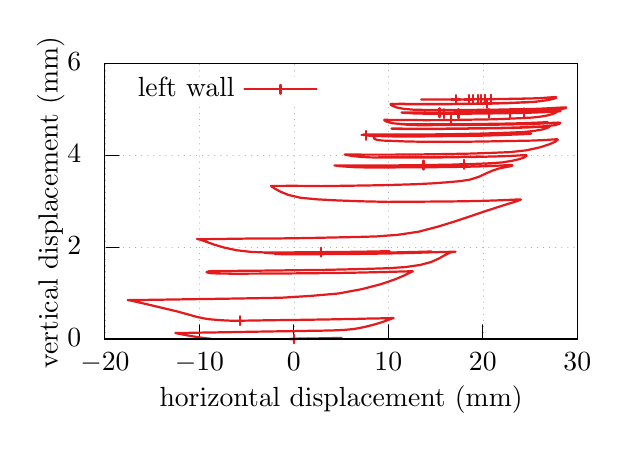
\begin{tikzpicture}[gnuplot]
%% generated with GNUPLOT 5.2p6 (Lua 5.3; terminal rev. Nov 2018, script rev. 107)
%% 09/10/2019 00:26:32
\path (0.000,0.000) rectangle (6.000,3.500);
\gpcolor{color=gp lt color axes}
\gpsetlinetype{gp lt axes}
\gpsetdashtype{gp dt axes}
\gpsetlinewidth{0.50}
\draw[gp path] (0.000,0.000)--(5.999,0.000);
\gpcolor{color=gp lt color border}
\gpsetlinetype{gp lt border}
\gpsetdashtype{gp dt solid}
\gpsetlinewidth{1.00}
\draw[gp path] (0.000,0.000)--(0.180,0.000);
\node[gp node right] at (-0.184,0.000) {$0$};
\gpcolor{color=gp lt color axes}
\gpsetlinetype{gp lt axes}
\gpsetdashtype{gp dt axes}
\gpsetlinewidth{0.50}
\draw[gp path] (0.000,1.166)--(5.999,1.166);
\gpcolor{color=gp lt color border}
\gpsetlinetype{gp lt border}
\gpsetdashtype{gp dt solid}
\gpsetlinewidth{1.00}
\draw[gp path] (0.000,1.166)--(0.180,1.166);
\node[gp node right] at (-0.184,1.166) {$2$};
\gpcolor{color=gp lt color axes}
\gpsetlinetype{gp lt axes}
\gpsetdashtype{gp dt axes}
\gpsetlinewidth{0.50}
\draw[gp path] (0.000,2.333)--(5.999,2.333);
\gpcolor{color=gp lt color border}
\gpsetlinetype{gp lt border}
\gpsetdashtype{gp dt solid}
\gpsetlinewidth{1.00}
\draw[gp path] (0.000,2.333)--(0.180,2.333);
\node[gp node right] at (-0.184,2.333) {$4$};
\gpcolor{color=gp lt color axes}
\gpsetlinetype{gp lt axes}
\gpsetdashtype{gp dt axes}
\gpsetlinewidth{0.50}
\draw[gp path] (0.000,3.499)--(5.999,3.499);
\gpcolor{color=gp lt color border}
\gpsetlinetype{gp lt border}
\gpsetdashtype{gp dt solid}
\gpsetlinewidth{1.00}
\draw[gp path] (0.000,3.499)--(0.180,3.499);
\node[gp node right] at (-0.184,3.499) {$6$};
\gpcolor{color=gp lt color axes}
\gpsetlinetype{gp lt axes}
\gpsetdashtype{gp dt axes}
\gpsetlinewidth{0.50}
\draw[gp path] (0.000,0.000)--(0.000,3.499);
\gpcolor{color=gp lt color border}
\gpsetlinetype{gp lt border}
\gpsetdashtype{gp dt solid}
\gpsetlinewidth{1.00}
\draw[gp path] (0.000,0.000)--(0.000,0.180);
\node[gp node center] at (0.000,-0.308) {$-20$};
\gpcolor{color=gp lt color axes}
\gpsetlinetype{gp lt axes}
\gpsetdashtype{gp dt axes}
\gpsetlinewidth{0.50}
\draw[gp path] (1.200,0.000)--(1.200,3.016);
\draw[gp path] (1.200,3.324)--(1.200,3.499);
\gpcolor{color=gp lt color border}
\gpsetlinetype{gp lt border}
\gpsetdashtype{gp dt solid}
\gpsetlinewidth{1.00}
\draw[gp path] (1.200,0.000)--(1.200,0.180);
\node[gp node center] at (1.200,-0.308) {$-10$};
\gpcolor{color=gp lt color axes}
\gpsetlinetype{gp lt axes}
\gpsetdashtype{gp dt axes}
\gpsetlinewidth{0.50}
\draw[gp path] (2.400,0.000)--(2.400,3.016);
\draw[gp path] (2.400,3.324)--(2.400,3.499);
\gpcolor{color=gp lt color border}
\gpsetlinetype{gp lt border}
\gpsetdashtype{gp dt solid}
\gpsetlinewidth{1.00}
\draw[gp path] (2.400,0.000)--(2.400,0.180);
\node[gp node center] at (2.400,-0.308) {$0$};
\gpcolor{color=gp lt color axes}
\gpsetlinetype{gp lt axes}
\gpsetdashtype{gp dt axes}
\gpsetlinewidth{0.50}
\draw[gp path] (3.599,0.000)--(3.599,3.499);
\gpcolor{color=gp lt color border}
\gpsetlinetype{gp lt border}
\gpsetdashtype{gp dt solid}
\gpsetlinewidth{1.00}
\draw[gp path] (3.599,0.000)--(3.599,0.180);
\node[gp node center] at (3.599,-0.308) {$10$};
\gpcolor{color=gp lt color axes}
\gpsetlinetype{gp lt axes}
\gpsetdashtype{gp dt axes}
\gpsetlinewidth{0.50}
\draw[gp path] (4.799,0.000)--(4.799,3.499);
\gpcolor{color=gp lt color border}
\gpsetlinetype{gp lt border}
\gpsetdashtype{gp dt solid}
\gpsetlinewidth{1.00}
\draw[gp path] (4.799,0.000)--(4.799,0.180);
\node[gp node center] at (4.799,-0.308) {$20$};
\gpcolor{color=gp lt color axes}
\gpsetlinetype{gp lt axes}
\gpsetdashtype{gp dt axes}
\gpsetlinewidth{0.50}
\draw[gp path] (5.999,0.000)--(5.999,3.499);
\gpcolor{color=gp lt color border}
\gpsetlinetype{gp lt border}
\gpsetdashtype{gp dt solid}
\gpsetlinewidth{1.00}
\draw[gp path] (5.999,0.000)--(5.999,0.180);
\node[gp node center] at (5.999,-0.308) {$30$};
\draw[gp path] (0.000,3.499)--(0.000,0.000)--(5.999,0.000)--(5.999,3.499)--cycle;
\node[gp node center,rotate=-270] at (-0.676,1.749) {vertical displacement (\si{\milli\metre})};
\node[gp node center] at (2.999,-0.769) {horizontal displacement (\si{\milli\metre})};
\gpcolor{rgb color={0.894,0.102,0.110}}
\gpsetlinewidth{2.00}
\draw[gp path] (2.400,0.000)--(2.401,0.000)--(2.403,0.000)--(2.407,0.000)--(2.413,0.000)%
  --(2.420,0.000)--(2.427,0.001)--(2.434,0.001)--(2.441,0.001)--(2.448,0.001)--(2.455,0.001)%
  --(2.462,0.001)--(2.469,0.001)--(2.475,0.002)--(2.480,0.002)--(2.484,0.002)--(2.487,0.002)%
  --(2.486,0.002)--(2.482,0.002)--(2.477,0.002)--(2.470,0.001)--(2.463,0.001)--(2.457,0.001)%
  --(2.451,0.001)--(2.446,0.001)--(2.442,0.001)--(2.440,0.001)--(2.439,0.001)--(2.440,0.001)%
  --(2.441,0.001)--(2.443,0.001)--(2.444,0.001)--(2.445,0.001)--(2.444,0.001)--(2.442,0.001)%
  --(2.439,0.001)--(2.437,0.001)--(2.435,0.001)--(2.436,0.001)--(2.439,0.001)--(2.444,0.001)%
  --(2.449,0.001)--(2.453,0.001)--(2.456,0.001)--(2.455,0.001)--(2.451,0.001)--(2.443,0.001)%
  --(2.433,0.001)--(2.421,0.000)--(2.411,0.000)--(2.402,0.000)--(2.397,0.000);
\draw[gp path] (2.403,0.000)--(2.414,0.000)--(2.429,0.001)--(2.448,0.001)--(2.470,0.001)%
  --(2.493,0.002)--(2.516,0.002)--(2.538,0.003)--(2.556,0.003)--(2.571,0.004)--(2.581,0.004)%
  --(2.588,0.004)--(2.590,0.004)--(2.587,0.004)--(2.578,0.004)--(2.564,0.004)--(2.544,0.003)%
  --(2.519,0.003)--(2.488,0.002)--(2.452,0.001)--(2.412,0.000)--(2.367,0.000);
\draw[gp path] (2.357,0.000)--(2.390,0.000)--(2.413,0.001)--(2.424,0.001)--(2.410,0.000)%
  --(2.384,0.000);
\draw[gp path] (2.371,0.000)--(2.481,0.002)--(2.593,0.004)--(2.701,0.006)--(2.801,0.008)%
  --(2.887,0.010)--(2.952,0.012)--(2.993,0.013)--(3.008,0.013)--(2.996,0.013)--(2.957,0.012)%
  --(2.891,0.011)--(2.800,0.009)--(2.684,0.007)--(2.548,0.004)--(2.396,0.001)--(2.341,0.000);
\draw[gp path] (1.358,0.000)--(1.242,0.014)--(1.123,0.032)--(1.027,0.049)--(0.957,0.063)%
  --(0.912,0.071)--(0.894,0.075)--(0.903,0.075)--(0.941,0.075)--(1.005,0.076)--(1.093,0.078)%
  --(1.199,0.080)--(1.319,0.082)--(1.449,0.084)--(1.584,0.086)--(1.717,0.089)--(1.842,0.091)%
  --(1.952,0.093)--(2.047,0.094)--(2.133,0.096)--(2.221,0.097)--(2.323,0.098)--(2.444,0.100)%
  --(2.584,0.103)--(2.733,0.105)--(2.882,0.108)--(3.026,0.114)--(3.160,0.126)--(3.283,0.149)%
  --(3.390,0.175)--(3.477,0.200)--(3.546,0.223)--(3.597,0.242)--(3.634,0.255)--(3.658,0.263)%
  --(3.667,0.265)--(3.659,0.265)--(3.637,0.265)--(3.599,0.264)--(3.547,0.263)--(3.481,0.261)%
  --(3.401,0.260)--(3.309,0.258)--(3.204,0.255)--(3.089,0.253)--(2.966,0.251)--(2.838,0.248)%
  --(2.707,0.246)--(2.574,0.244)--(2.440,0.242)--(2.306,0.240)--(2.177,0.239)--(2.052,0.237)%
  --(1.933,0.235)--(1.820,0.233)--(1.715,0.232)--(1.618,0.231)--(1.530,0.235)--(1.450,0.240)%
  --(1.378,0.246)--(1.312,0.252)--(1.249,0.263)--(1.188,0.276)--(1.128,0.291)--(1.068,0.308)%
  --(1.004,0.326)--(0.935,0.345)--(0.858,0.364)--(0.773,0.384)--(0.680,0.406)--(0.584,0.429)%
  --(0.490,0.451)--(0.402,0.471)--(0.329,0.488)--(0.290,0.493)--(0.310,0.494)--(0.406,0.495)%
  --(0.593,0.497)--(0.857,0.501)--(1.175,0.506)--(1.522,0.511)--(1.882,0.517)--(2.249,0.524)%
  --(2.616,0.547)--(2.963,0.577)--(3.265,0.633)--(3.503,0.695)--(3.679,0.755)--(3.802,0.807)%
  --(3.878,0.844)--(3.910,0.860)--(3.895,0.860)--(3.823,0.858)--(3.683,0.854)--(3.483,0.849)%
  --(3.233,0.843)--(2.947,0.838)--(2.634,0.835)--(2.304,0.832)--(1.973,0.830)--(1.677,0.829)%
  --(1.454,0.830)--(1.326,0.837)--(1.291,0.849)--(1.324,0.861)--(1.407,0.864)--(1.535,0.864)%
  --(1.711,0.865)--(1.939,0.867)--(2.204,0.870)--(2.475,0.874)--(2.728,0.876)--(2.958,0.881)%
  --(3.174,0.886)--(3.391,0.892)--(3.613,0.899)--(3.824,0.914)--(4.004,0.940)--(4.142,0.977)%
  --(4.242,1.022)--(4.318,1.065)--(4.379,1.096)--(4.426,1.109)--(4.452,1.109)--(4.446,1.108)%
  --(4.400,1.107)--(4.317,1.105)--(4.206,1.102)--(4.077,1.098)--(3.928,1.093)--(3.759,1.089)%
  --(3.567,1.085)--(3.360,1.082)--(3.150,1.079)--(2.947,1.078)--(2.756,1.077)--(2.578,1.076)%
  --(2.419,1.075)--(2.288,1.076)--(2.198,1.078)--(2.156,1.080)--(2.164,1.082)--(2.218,1.083)%
  --(2.313,1.084)--(2.444,1.084)--(2.608,1.085)--(2.801,1.087)--(3.011,1.089)--(3.227,1.091)%
  --(3.436,1.094)--(3.631,1.098)--(3.805,1.102)--(3.951,1.105)--(4.061,1.108)--(4.129,1.110)%
  --(4.149,1.110)--(4.121,1.110)--(4.048,1.108)--(3.938,1.105)--(3.797,1.102)--(3.639,1.098)%
  --(3.471,1.095)--(3.297,1.092)--(3.122,1.090)--(2.947,1.088)--(2.777,1.087)--(2.620,1.085)%
  --(2.479,1.085)--(2.357,1.084)--(2.253,1.084)--(2.168,1.086)--(2.102,1.089)--(2.055,1.092)%
  --(2.029,1.095)--(2.019,1.097)--(2.025,1.098)--(2.050,1.098)--(2.101,1.098)--(2.184,1.098)%
  --(2.298,1.099)--(2.432,1.100)--(2.573,1.102)--(2.712,1.102)--(2.844,1.103)--(2.967,1.104)%
  --(3.077,1.105)--(3.164,1.107)--(3.220,1.107)--(3.237,1.107)--(3.218,1.107)--(3.179,1.106)%
  --(3.146,1.106)--(3.133,1.106)--(3.146,1.106)--(3.177,1.106)--(3.211,1.107)--(3.241,1.107)%
  --(3.266,1.107)--(3.291,1.108)--(3.314,1.109)--(3.325,1.109)--(3.314,1.109)--(3.286,1.108)%
  --(3.257,1.107)--(3.248,1.107)--(3.268,1.107)--(3.308,1.109)--(3.353,1.109)--(3.393,1.110)%
  --(3.430,1.110)--(3.472,1.112)--(3.521,1.113)--(3.570,1.113)--(3.604,1.114)--(3.615,1.114)%
  --(3.604,1.114)--(3.579,1.114)--(3.546,1.113)--(3.505,1.112)--(3.455,1.111)--(3.394,1.110)%
  --(3.328,1.109)--(3.261,1.107)--(3.195,1.107)--(3.131,1.106)--(3.065,1.105)--(2.998,1.105)%
  --(2.933,1.103)--(2.872,1.103)--(2.818,1.103)--(2.767,1.102)--(2.717,1.102)--(2.670,1.102)%
  --(2.626,1.101)--(2.593,1.101)--(2.574,1.101)--(2.571,1.101)--(2.586,1.101)--(2.619,1.101)%
  --(2.669,1.102)--(2.734,1.102)--(2.809,1.103)--(2.890,1.103)--(2.971,1.105)--(3.045,1.105)%
  --(3.109,1.106)--(3.159,1.107)--(3.192,1.107)--(3.203,1.107)--(3.188,1.107)--(3.146,1.106)%
  --(3.077,1.106)--(2.983,1.105)--(2.868,1.103)--(2.742,1.102)--(2.617,1.101)--(2.509,1.100)%
  --(2.424,1.099)--(2.366,1.099)--(2.329,1.099)--(2.309,1.099)--(2.331,1.099)--(2.382,1.099)%
  --(2.461,1.100)--(2.563,1.101)--(2.678,1.102)--(2.800,1.103)--(2.924,1.104)--(3.048,1.105)%
  --(3.166,1.107)--(3.272,1.108)--(3.358,1.110)--(3.417,1.110)--(3.448,1.111)--(3.451,1.111)%
  --(3.424,1.110)--(3.366,1.109)--(3.276,1.108)--(3.156,1.106)--(3.008,1.105)--(2.839,1.103)%
  --(2.653,1.102)--(2.456,1.100)--(2.252,1.099)--(2.047,1.098)--(1.850,1.106)--(1.670,1.127)%
  --(1.514,1.161)--(1.387,1.198)--(1.285,1.235)--(1.208,1.262)--(1.169,1.270)--(1.182,1.268)%
  --(1.259,1.267)--(1.404,1.269)--(1.600,1.272)--(1.826,1.275)--(2.066,1.275)--(2.313,1.278)%
  --(2.578,1.282)--(2.862,1.288)--(3.156,1.294)--(3.446,1.302)--(3.723,1.323)--(3.983,1.362)%
  --(4.224,1.425)--(4.445,1.493)--(4.642,1.559)--(4.817,1.618)--(4.970,1.668)--(5.096,1.708)%
  --(5.193,1.738)--(5.256,1.759)--(5.282,1.770)--(5.267,1.772)--(5.211,1.770)--(5.109,1.765)%
  --(4.960,1.759)--(4.761,1.753)--(4.518,1.748)--(4.236,1.745)--(3.926,1.743)--(3.596,1.741)%
  --(3.265,1.748)--(2.958,1.759)--(2.695,1.773)--(2.486,1.793)--(2.330,1.829)--(2.223,1.873)%
  --(2.157,1.910)--(2.121,1.934)--(2.110,1.944)--(2.121,1.944)--(2.154,1.944)--(2.208,1.944)%
  --(2.275,1.944)--(2.348,1.945)--(2.414,1.945)--(2.471,1.944)--(2.519,1.944)--(2.569,1.943)%
  --(2.639,1.942)--(2.748,1.941)--(2.901,1.943)--(3.092,1.946)--(3.306,1.949)--(3.526,1.953)%
  --(3.745,1.959)--(3.957,1.966)--(4.162,1.976)--(4.348,1.990)--(4.509,2.004)--(4.638,2.024)%
  --(4.745,2.058)--(4.836,2.100)--(4.920,2.137)--(5.000,2.164)--(5.070,2.179)--(5.127,2.189)%
  --(5.163,2.197)--(5.175,2.204)--(5.164,2.209)--(5.135,2.209)--(5.087,2.206)--(5.018,2.202)%
  --(4.922,2.197)--(4.802,2.193)--(4.660,2.189)--(4.509,2.186)--(4.359,2.183)--(4.218,2.182)%
  --(4.093,2.180)--(3.986,2.179)--(3.901,2.179)--(3.839,2.179)--(3.803,2.179)--(3.793,2.179)%
  --(3.807,2.179)--(3.841,2.179)--(3.887,2.179)--(3.945,2.180)--(4.007,2.180)--(4.071,2.181)%
  --(4.135,2.181)--(4.203,2.182)--(4.281,2.183)--(4.373,2.184)--(4.476,2.186)--(4.581,2.187)%
  --(4.673,2.189)--(4.749,2.192)--(4.805,2.194)--(4.842,2.196)--(4.858,2.196)--(4.848,2.195)%
  --(4.805,2.193)--(4.726,2.190)--(4.613,2.188)--(4.472,2.186)--(4.307,2.183)--(4.124,2.181)%
  --(3.926,2.180)--(3.722,2.179)--(3.527,2.178)--(3.351,2.178)--(3.203,2.180)--(3.087,2.187)%
  --(3.000,2.193)--(2.943,2.200)--(2.915,2.203)--(2.915,2.204)--(2.940,2.204)--(2.987,2.204)%
  --(3.051,2.204)--(3.127,2.204)--(3.210,2.204)--(3.295,2.204)--(3.378,2.204)--(3.452,2.204)%
  --(3.515,2.204)--(3.561,2.204)--(3.593,2.204)--(3.614,2.204)--(3.631,2.204)--(3.650,2.204)%
  --(3.673,2.204)--(3.701,2.204)--(3.734,2.204)--(3.767,2.205)--(3.801,2.205)--(3.832,2.206)%
  --(3.861,2.206)--(3.885,2.206)--(3.903,2.206)--(3.917,2.206)--(3.932,2.207)--(3.946,2.207)%
  --(3.965,2.207)--(3.986,2.207)--(4.006,2.207)--(4.025,2.208)--(4.043,2.208)--(4.060,2.208)%
  --(4.078,2.208)--(4.095,2.208)--(4.111,2.209)--(4.121,2.209)--(4.127,2.209)--(4.126,2.209)%
  --(4.119,2.209)--(4.105,2.209)--(4.082,2.208)--(4.046,2.208)--(4.000,2.207)--(3.943,2.207)%
  --(3.880,2.206)--(3.817,2.205)--(3.757,2.204)--(3.706,2.204)--(3.669,2.204)--(3.649,2.203)%
  --(3.644,2.203)--(3.652,2.204)--(3.673,2.204)--(3.699,2.204)--(3.730,2.204)--(3.764,2.204)%
  --(3.803,2.205)--(3.848,2.206)--(3.898,2.206)--(3.950,2.207)--(4.001,2.207)--(4.047,2.208)%
  --(4.084,2.208)--(4.113,2.209)--(4.131,2.209)--(4.137,2.210)--(4.129,2.209)--(4.105,2.209)%
  --(4.070,2.208)--(4.027,2.208)--(3.981,2.207)--(3.938,2.207)--(3.898,2.206)--(3.861,2.206)%
  --(3.827,2.205)--(3.799,2.205)--(3.775,2.204)--(3.757,2.204)--(3.746,2.204)--(3.740,2.204)%
  --(3.742,2.204)--(3.752,2.204)--(3.770,2.204)--(3.796,2.205)--(3.827,2.206)--(3.861,2.206)%
  --(3.896,2.206)--(3.932,2.207)--(3.967,2.207)--(3.999,2.207)--(4.029,2.208)--(4.055,2.208)%
  --(4.079,2.208)--(4.102,2.209)--(4.126,2.209)--(4.151,2.210)--(4.174,2.210)--(4.192,2.210)%
  --(4.203,2.210)--(4.208,2.210)--(4.202,2.210)--(4.190,2.210)--(4.171,2.210)--(4.144,2.210)%
  --(4.111,2.209)--(4.072,2.208)--(4.027,2.208)--(3.979,2.207)--(3.929,2.207)--(3.884,2.206)%
  --(3.844,2.206)--(3.811,2.205)--(3.783,2.205)--(3.761,2.204)--(3.748,2.204)--(3.742,2.204)%
  --(3.747,2.204)--(3.761,2.204)--(3.784,2.205)--(3.812,2.205)--(3.843,2.206)--(3.875,2.206)%
  --(3.910,2.206)--(3.943,2.207)--(3.973,2.207)--(3.994,2.207)--(4.007,2.208)--(4.009,2.208)%
  --(3.999,2.207)--(3.975,2.207)--(3.938,2.207)--(3.891,2.206)--(3.843,2.206)--(3.801,2.205)%
  --(3.771,2.204)--(3.753,2.204)--(3.745,2.204)--(3.742,2.204)--(3.746,2.204)--(3.754,2.204)%
  --(3.770,2.205)--(3.791,2.205)--(3.815,2.206)--(3.844,2.206)--(3.878,2.206)--(3.919,2.206)%
  --(3.968,2.207)--(4.025,2.208)--(4.085,2.208)--(4.143,2.210)--(4.195,2.210)--(4.239,2.211)%
  --(4.272,2.211)--(4.295,2.211)--(4.301,2.212)--(4.290,2.211)--(4.262,2.211)--(4.216,2.210)%
  --(4.155,2.210)--(4.084,2.208)--(4.007,2.207)--(3.929,2.206)--(3.855,2.206)--(3.790,2.205)%
  --(3.735,2.204)--(3.692,2.204)--(3.659,2.204)--(3.638,2.204)--(3.631,2.203)--(3.638,2.203)%
  --(3.659,2.204)--(3.693,2.204)--(3.734,2.204)--(3.782,2.205)--(3.832,2.206)--(3.885,2.206)%
  --(3.937,2.207)--(3.986,2.207)--(4.028,2.208)--(4.060,2.208)--(4.084,2.208)--(4.100,2.209)%
  --(4.109,2.209)--(4.113,2.209)--(4.111,2.209)--(4.100,2.209)--(4.081,2.208)--(4.053,2.208)%
  --(4.013,2.208)--(3.965,2.207)--(3.910,2.206)--(3.850,2.206)--(3.791,2.205)--(3.737,2.204)%
  --(3.691,2.204)--(3.655,2.204)--(3.628,2.204)--(3.614,2.203)--(3.610,2.203)--(3.620,2.203)%
  --(3.640,2.204)--(3.670,2.204)--(3.706,2.204)--(3.747,2.204)--(3.790,2.205)--(3.833,2.206)%
  --(3.874,2.206)--(3.908,2.207)--(3.935,2.207)--(3.952,2.207)--(3.961,2.207)--(3.959,2.207)%
  --(3.951,2.207)--(3.937,2.207)--(3.916,2.207)--(3.890,2.206)--(3.856,2.206)--(3.817,2.206)%
  --(3.770,2.205)--(3.721,2.204)--(3.671,2.204)--(3.628,2.203)--(3.593,2.203)--(3.566,2.203)%
  --(3.551,2.203)--(3.548,2.203)--(3.562,2.203)--(3.595,2.203)--(3.645,2.204)--(3.710,2.204)%
  --(3.787,2.205)--(3.873,2.206)--(3.967,2.207)--(4.066,2.208)--(4.168,2.210)--(4.266,2.211)%
  --(4.359,2.213)--(4.440,2.214)--(4.509,2.216)--(4.563,2.218)--(4.595,2.219)--(4.604,2.219)%
  --(4.586,2.218)--(4.542,2.217)--(4.480,2.215)--(4.408,2.214)--(4.331,2.213)--(4.251,2.211)%
  --(4.169,2.210)--(4.087,2.209)--(4.006,2.208)--(3.932,2.207)--(3.866,2.206)--(3.812,2.206)%
  --(3.767,2.205)--(3.735,2.204)--(3.713,2.204)--(3.706,2.204)--(3.713,2.204)--(3.733,2.204)%
  --(3.763,2.205)--(3.803,2.206)--(3.850,2.206)--(3.905,2.207)--(3.968,2.207)--(4.033,2.208)%
  --(4.099,2.209)--(4.162,2.210)--(4.220,2.211)--(4.268,2.211)--(4.305,2.212)--(4.330,2.213)%
  --(4.338,2.213)--(4.330,2.213)--(4.304,2.212)--(4.260,2.211)--(4.200,2.210)--(4.127,2.210)%
  --(4.045,2.208)--(3.955,2.207)--(3.859,2.206)--(3.763,2.205)--(3.669,2.204)--(3.582,2.204)%
  --(3.505,2.203)--(3.440,2.203)--(3.390,2.203)--(3.355,2.203)--(3.339,2.203)--(3.342,2.203)%
  --(3.364,2.203)--(3.402,2.204)--(3.456,2.204)--(3.520,2.204)--(3.595,2.204)--(3.681,2.204)%
  --(3.785,2.205)--(3.913,2.207)--(4.064,2.208)--(4.232,2.211)--(4.408,2.214)--(4.583,2.219)%
  --(4.750,2.225)--(4.906,2.232)--(5.046,2.242)--(5.168,2.262)--(5.260,2.283)--(5.320,2.303)%
  --(5.350,2.322)--(5.354,2.334)--(5.333,2.336)--(5.291,2.333)--(5.222,2.328)--(5.122,2.323)%
  --(4.991,2.319)--(4.838,2.315)--(4.670,2.311)--(4.494,2.309)--(4.316,2.306)--(4.138,2.305)%
  --(3.967,2.304)--(3.809,2.303)--(3.676,2.303)--(3.569,2.304)--(3.486,2.304)--(3.425,2.305)%
  --(3.389,2.306)--(3.379,2.306)--(3.399,2.306)--(3.447,2.306)--(3.519,2.307)--(3.607,2.307)%
  --(3.701,2.307)--(3.800,2.308)--(3.897,2.308)--(3.991,2.308)--(4.072,2.309)--(4.135,2.309)%
  --(4.171,2.309)--(4.183,2.309)--(4.178,2.309)--(4.173,2.308)--(4.184,2.308)--(4.216,2.309)%
  --(4.262,2.309)--(4.312,2.310)--(4.356,2.311)--(4.396,2.311)--(4.434,2.311)--(4.480,2.312)%
  --(4.534,2.313)--(4.589,2.313)--(4.640,2.315)--(4.682,2.315)--(4.715,2.316)--(4.743,2.316)%
  --(4.766,2.316)--(4.779,2.317)--(4.781,2.317)--(4.766,2.316)--(4.733,2.316)--(4.682,2.315)%
  --(4.608,2.314)--(4.514,2.312)--(4.392,2.311)--(4.246,2.309)--(4.075,2.308)--(3.889,2.307)%
  --(3.701,2.306)--(3.527,2.306)--(3.375,2.306)--(3.249,2.312)--(3.151,2.323)--(3.082,2.334)%
  --(3.045,2.342)--(3.045,2.343)--(3.084,2.343)--(3.164,2.342)--(3.286,2.341)--(3.445,2.341)%
  --(3.638,2.341)--(3.860,2.342)--(4.107,2.345)--(4.371,2.349)--(4.641,2.354)--(4.904,2.363)%
  --(5.146,2.373)--(5.356,2.396)--(5.526,2.434)--(5.647,2.473)--(5.721,2.506)--(5.751,2.530)%
  --(5.740,2.537)--(5.686,2.533)--(5.580,2.526)--(5.417,2.519)--(5.196,2.515)--(4.941,2.510)%
  --(4.680,2.506)--(4.436,2.504)--(4.215,2.504)--(4.013,2.505)--(3.827,2.508)--(3.664,2.515)%
  --(3.537,2.519)--(3.455,2.527)--(3.419,2.544)--(3.417,2.564)--(3.439,2.576)--(3.476,2.577)%
  --(3.527,2.575)--(3.602,2.573)--(3.711,2.572)--(3.856,2.572)--(4.031,2.572)--(4.222,2.575)%
  --(4.416,2.577)--(4.608,2.579)--(4.793,2.582)--(4.967,2.587)--(5.123,2.593)--(5.250,2.598)%
  --(5.343,2.602)--(5.397,2.605)--(5.412,2.607)--(5.390,2.606)--(5.328,2.603)--(5.225,2.599)%
  --(5.084,2.593)--(4.908,2.588)--(4.709,2.583)--(4.493,2.580)--(4.270,2.577)--(4.052,2.575)%
  --(3.845,2.575)--(3.662,2.575)--(3.509,2.577)--(3.393,2.578)--(3.315,2.586)--(3.278,2.595)%
  --(3.285,2.598)--(3.335,2.597)--(3.426,2.597)--(3.552,2.596)--(3.709,2.595)--(3.885,2.595)%
  --(4.072,2.596)--(4.260,2.598)--(4.442,2.600)--(4.611,2.603)--(4.767,2.606)--(4.906,2.610)%
  --(5.026,2.614)--(5.122,2.618)--(5.192,2.621)--(5.231,2.623)--(5.242,2.624)--(5.226,2.624)%
  --(5.188,2.623)--(5.130,2.620)--(5.056,2.617)--(4.965,2.614)--(4.862,2.610)--(4.748,2.606)%
  --(4.629,2.604)--(4.506,2.602)--(4.384,2.600)--(4.264,2.599)--(4.148,2.597)--(4.037,2.596)%
  --(3.932,2.595)--(3.835,2.595)--(3.745,2.596)--(3.663,2.596)--(3.591,2.597)--(3.530,2.598)%
  --(3.488,2.598)--(3.468,2.598)--(3.478,2.597)--(3.520,2.597)--(3.596,2.596)--(3.704,2.596)%
  --(3.838,2.596)--(3.994,2.596)--(4.163,2.598)--(4.346,2.600)--(4.539,2.603)--(4.738,2.607)%
  --(4.940,2.613)--(5.132,2.620)--(5.303,2.627)--(5.445,2.641)--(5.551,2.660)--(5.619,2.680)%
  --(5.645,2.695)--(5.634,2.701)--(5.587,2.698)--(5.505,2.693)--(5.384,2.687)--(5.226,2.681)%
  --(5.039,2.677)--(4.834,2.674)--(4.625,2.671)--(4.422,2.669)--(4.233,2.667)--(4.058,2.667)%
  --(3.905,2.667)--(3.783,2.667)--(3.697,2.668)--(3.650,2.670)--(3.640,2.672)--(3.667,2.673)%
  --(3.725,2.672)--(3.818,2.671)--(3.945,2.670)--(4.105,2.671)--(4.290,2.671)--(4.494,2.673)%
  --(4.708,2.676)--(4.923,2.679)--(5.130,2.683)--(5.324,2.689)--(5.491,2.696)--(5.625,2.704)%
  --(5.719,2.716)--(5.771,2.733)--(5.782,2.744)--(5.757,2.748)--(5.700,2.746)--(5.615,2.740)%
  --(5.502,2.733)--(5.361,2.728)--(5.198,2.725)--(5.024,2.722)--(4.850,2.719)--(4.683,2.718)%
  --(4.526,2.716)--(4.374,2.716)--(4.233,2.716)--(4.105,2.715)--(3.997,2.715)--(3.910,2.716)%
  --(3.844,2.720)--(3.797,2.725)--(3.769,2.727)--(3.761,2.727)--(3.782,2.727)--(3.832,2.726)%
  --(3.915,2.726)--(4.027,2.725)--(4.165,2.725)--(4.323,2.725)--(4.498,2.726)--(4.684,2.729)%
  --(4.871,2.731)--(5.050,2.734)--(5.211,2.737)--(5.349,2.740)--(5.459,2.744)--(5.537,2.748)%
  --(5.580,2.750)--(5.585,2.750)--(5.553,2.749)--(5.491,2.747)--(5.405,2.744)--(5.304,2.740)%
  --(5.192,2.736)--(5.072,2.734)--(4.949,2.732)--(4.830,2.730)--(4.720,2.729)--(4.623,2.727)%
  --(4.540,2.727)--(4.474,2.726)--(4.422,2.726)--(4.388,2.725)--(4.372,2.725)--(4.374,2.725)%
  --(4.395,2.726)--(4.428,2.726)--(4.474,2.726)--(4.532,2.727)--(4.602,2.727)--(4.686,2.729)%
  --(4.780,2.730)--(4.881,2.732)--(4.985,2.733)--(5.093,2.735)--(5.202,2.737)--(5.309,2.740)%
  --(5.409,2.744)--(5.494,2.747)--(5.559,2.750)--(5.602,2.753)--(5.622,2.755)--(5.621,2.755)%
  --(5.597,2.753)--(5.549,2.750)--(5.476,2.747)--(5.380,2.743)--(5.265,2.739)--(5.134,2.736)%
  --(4.991,2.733)--(4.838,2.731)--(4.678,2.729)--(4.516,2.727)--(4.356,2.726)--(4.204,2.726)%
  --(4.064,2.726)--(3.935,2.727)--(3.824,2.728)--(3.729,2.732)--(3.653,2.740)--(3.599,2.753)%
  --(3.566,2.765)--(3.550,2.776)--(3.548,2.783)--(3.559,2.784)--(3.580,2.783)--(3.614,2.782)%
  --(3.661,2.782)--(3.717,2.782)--(3.779,2.782)--(3.841,2.781)--(3.898,2.781)--(3.949,2.780)%
  --(3.991,2.779)--(4.022,2.779)--(4.039,2.780)--(4.043,2.779)--(4.042,2.779)--(4.045,2.778)%
  --(4.058,2.778)--(4.090,2.778)--(4.139,2.779)--(4.208,2.779)--(4.293,2.780)--(4.395,2.781)%
  --(4.514,2.783)--(4.642,2.785)--(4.775,2.787)--(4.908,2.789)--(5.039,2.793)--(5.169,2.799)%
  --(5.296,2.805)--(5.416,2.811)--(5.523,2.822)--(5.611,2.837)--(5.676,2.854)--(5.718,2.871)%
  --(5.740,2.884)--(5.743,2.891)--(5.730,2.891)--(5.699,2.888)--(5.646,2.884)--(5.575,2.880)%
  --(5.488,2.877)--(5.392,2.873)--(5.292,2.870)--(5.190,2.869)--(5.088,2.867)--(4.989,2.866)%
  --(4.894,2.864)--(4.812,2.863)--(4.746,2.862)--(4.697,2.862)--(4.665,2.862)--(4.646,2.862)%
  --(4.640,2.862)--(4.643,2.862)--(4.650,2.862)--(4.660,2.862)--(4.667,2.862)--(4.672,2.862)%
  --(4.676,2.862)--(4.677,2.862)--(4.676,2.862)--(4.667,2.862)--(4.655,2.862)--(4.640,2.862)%
  --(4.626,2.861)--(4.616,2.861)--(4.605,2.862)--(4.588,2.861)--(4.566,2.861)--(4.540,2.860)%
  --(4.515,2.860)--(4.493,2.860)--(4.478,2.860)--(4.467,2.860)--(4.461,2.860)--(4.468,2.860)%
  --(4.482,2.860)--(4.500,2.861)--(4.518,2.861)--(4.535,2.861)--(4.554,2.861)--(4.576,2.861)%
  --(4.601,2.861)--(4.625,2.862)--(4.647,2.862)--(4.665,2.862)--(4.682,2.862)--(4.701,2.862)%
  --(4.724,2.862)--(4.748,2.863)--(4.769,2.863)--(4.790,2.863)--(4.810,2.863)--(4.830,2.863)%
  --(4.852,2.864)--(4.870,2.865)--(4.882,2.865)--(4.887,2.865)--(4.884,2.865)--(4.878,2.864)%
  --(4.870,2.864)--(4.862,2.864)--(4.852,2.864)--(4.842,2.864)--(4.834,2.863)--(4.829,2.863)%
  --(4.826,2.863)--(4.820,2.863)--(4.810,2.863)--(4.793,2.863)--(4.772,2.863)--(4.744,2.863)%
  --(4.712,2.862)--(4.673,2.862)--(4.630,2.862)--(4.583,2.861)--(4.536,2.860)--(4.491,2.860)%
  --(4.448,2.860)--(4.409,2.860)--(4.378,2.860)--(4.355,2.860)--(4.344,2.860)--(4.346,2.860)%
  --(4.358,2.860)--(4.378,2.860)--(4.406,2.860)--(4.438,2.860)--(4.473,2.860)--(4.510,2.861)%
  --(4.547,2.861)--(4.581,2.861)--(4.611,2.862)--(4.634,2.862)--(4.650,2.862)--(4.659,2.862)%
  --(4.658,2.862)--(4.644,2.862)--(4.622,2.862)--(4.590,2.861)--(4.553,2.861)--(4.518,2.860)%
  --(4.490,2.860)--(4.470,2.860)--(4.463,2.860)--(4.468,2.860)--(4.486,2.860)--(4.518,2.860)%
  --(4.564,2.860)--(4.623,2.861)--(4.694,2.862)--(4.773,2.863)--(4.853,2.864)--(4.934,2.865)%
  --(5.010,2.866)--(5.080,2.867)--(5.140,2.868)--(5.186,2.869)--(5.210,2.869)--(5.212,2.869)%
  --(5.193,2.869)--(5.160,2.868)--(5.121,2.867)--(5.078,2.867)--(5.031,2.866)--(4.977,2.866)%
  --(4.911,2.865)--(4.838,2.864)--(4.758,2.863)--(4.678,2.862)--(4.598,2.861)--(4.522,2.860)%
  --(4.460,2.860)--(4.418,2.859)--(4.403,2.859)--(4.418,2.860)--(4.454,2.860)--(4.504,2.861)%
  --(4.560,2.861)--(4.622,2.862)--(4.689,2.862)--(4.760,2.863)--(4.830,2.864)--(4.898,2.865)%
  --(4.959,2.866)--(5.014,2.866)--(5.066,2.867)--(5.112,2.867)--(5.152,2.869)--(5.181,2.869)%
  --(5.196,2.869)--(5.199,2.869)--(5.192,2.869)--(5.174,2.869)--(5.145,2.868)--(5.104,2.867)%
  --(5.050,2.867)--(4.985,2.866)--(4.914,2.865)--(4.840,2.864)--(4.762,2.863)--(4.680,2.862)%
  --(4.595,2.861)--(4.510,2.860)--(4.427,2.860)--(4.344,2.860)--(4.264,2.861)--(4.185,2.861)%
  --(4.114,2.861)--(4.063,2.860)--(4.040,2.860)--(4.051,2.860)--(4.099,2.860)--(4.180,2.860)%
  --(4.293,2.860)--(4.433,2.860)--(4.596,2.861)--(4.775,2.863)--(4.960,2.866)--(5.142,2.869)%
  --(5.312,2.872)--(5.464,2.876)--(5.593,2.881)--(5.693,2.886)--(5.758,2.890)--(5.787,2.893)%
  --(5.778,2.893)--(5.734,2.890)--(5.652,2.885)--(5.536,2.879)--(5.390,2.873)--(5.219,2.870)%
  --(5.038,2.867)--(4.859,2.864)--(4.692,2.862)--(4.539,2.861)--(4.403,2.860)--(4.289,2.860)%
  --(4.202,2.860)--(4.147,2.860)--(4.124,2.861)--(4.131,2.862)--(4.159,2.862)--(4.203,2.862)%
  --(4.259,2.862)--(4.323,2.862)--(4.390,2.862)--(4.455,2.862)--(4.510,2.862)--(4.553,2.862)%
  --(4.580,2.862)--(4.590,2.862)--(4.586,2.862)--(4.568,2.862)--(4.541,2.862)--(4.510,2.862)%
  --(4.480,2.861)--(4.456,2.861)--(4.444,2.861)--(4.458,2.861)--(4.485,2.861)--(4.523,2.862)%
  --(4.568,2.862)--(4.616,2.862)--(4.665,2.863)--(4.710,2.863)--(4.748,2.863)--(4.778,2.864)%
  --(4.799,2.864)--(4.815,2.864)--(4.826,2.865)--(4.836,2.865)--(4.847,2.865)--(4.856,2.865)%
  --(4.863,2.865)--(4.868,2.865)--(4.870,2.865)--(4.868,2.865)--(4.863,2.865)--(4.854,2.865)%
  --(4.844,2.865)--(4.832,2.865)--(4.823,2.865)--(4.816,2.864)--(4.814,2.864)--(4.820,2.864)%
  --(4.834,2.865)--(4.857,2.865)--(4.887,2.865)--(4.923,2.866)--(4.959,2.866)--(4.991,2.866)%
  --(5.016,2.867)--(5.034,2.867)--(5.045,2.867)--(5.034,2.867)--(5.012,2.867)--(4.978,2.866)%
  --(4.934,2.866)--(4.883,2.865)--(4.827,2.865)--(4.763,2.863)--(4.694,2.863)--(4.623,2.862)%
  --(4.554,2.862)--(4.498,2.861)--(4.462,2.860)--(4.448,2.860)--(4.455,2.861)--(4.478,2.861)%
  --(4.514,2.862)--(4.558,2.862)--(4.610,2.862)--(4.666,2.863)--(4.722,2.863)--(4.773,2.864)%
  --(4.814,2.865)--(4.846,2.865)--(4.870,2.865)--(4.890,2.865)--(4.907,2.865)--(4.922,2.866)%
  --(4.932,2.866)--(4.938,2.866)--(4.931,2.866)--(4.914,2.866)--(4.887,2.865)--(4.846,2.865)%
  --(4.792,2.864)--(4.727,2.863)--(4.653,2.862)--(4.572,2.862)--(4.493,2.861)--(4.419,2.861)%
  --(4.355,2.861)--(4.307,2.861)--(4.278,2.861)--(4.270,2.861)--(4.281,2.861)--(4.312,2.861)%
  --(4.362,2.861)--(4.430,2.861)--(4.509,2.862)--(4.598,2.862)--(4.690,2.863)--(4.782,2.864)%
  --(4.870,2.865)--(4.949,2.866)--(5.016,2.867)--(5.074,2.868)--(5.120,2.869)--(5.158,2.869)%
  --(5.187,2.870)--(5.206,2.870)--(5.217,2.870)--(5.206,2.870)--(5.182,2.869)--(5.146,2.869)%
  --(5.096,2.868)--(5.034,2.867)--(4.962,2.866)--(4.882,2.865)--(4.800,2.864)--(4.719,2.863)%
  --(4.642,2.862)--(4.570,2.862)--(4.502,2.862)--(4.438,2.861)--(4.380,2.861)--(4.328,2.861)%
  --(4.284,2.861)--(4.248,2.862)--(4.222,2.862)--(4.206,2.862)--(4.202,2.862)--(4.211,2.862)%
  --(4.234,2.862)--(4.269,2.862)--(4.311,2.862)--(4.358,2.862)--(4.407,2.862)--(4.455,2.862)%
  --(4.504,2.862)--(4.553,2.862)--(4.605,2.862)--(4.660,2.863)--(4.722,2.863)--(4.790,2.864)%
  --(4.864,2.865)--(4.942,2.866)--(5.022,2.867)--(5.100,2.868)--(5.174,2.869)--(5.234,2.870)%
  --(5.279,2.872)--(5.307,2.872)--(5.315,2.872)--(5.304,2.872)--(5.272,2.871)--(5.223,2.870)%
  --(5.158,2.869)--(5.084,2.868)--(5.006,2.867)--(4.929,2.866)--(4.857,2.865)--(4.788,2.864)%
  --(4.726,2.863)--(4.670,2.863)--(4.620,2.862)--(4.580,2.862)--(4.547,2.862)--(4.522,2.862)%
  --(4.503,2.862)--(4.490,2.862)--(4.485,2.862)--(4.491,2.862)--(4.506,2.862)--(4.533,2.862)%
  --(4.569,2.862)--(4.613,2.862)--(4.667,2.863)--(4.727,2.863)--(4.796,2.864)--(4.864,2.865)%
  --(4.931,2.866)--(4.989,2.867)--(5.034,2.867)--(5.067,2.868)--(5.084,2.868)--(5.064,2.868)%
  --(5.025,2.867)--(4.966,2.866)--(4.892,2.865)--(4.805,2.864)--(4.713,2.863)--(4.617,2.862)%
  --(4.526,2.862)--(4.446,2.861)--(4.385,2.860)--(4.349,2.860)--(4.342,2.860)--(4.361,2.861)%
  --(4.403,2.861)--(4.461,2.862)--(4.532,2.862)--(4.612,2.862)--(4.700,2.863)--(4.787,2.864)%
  --(4.871,2.865)--(4.942,2.866)--(4.997,2.867)--(5.038,2.867)--(5.066,2.868)--(5.081,2.868)%
  --(5.082,2.868)--(5.067,2.868)--(5.034,2.867)--(4.985,2.867)--(4.925,2.866)--(4.857,2.865)%
  --(4.785,2.864)--(4.710,2.863)--(4.634,2.862)--(4.559,2.862)--(4.490,2.861)--(4.430,2.861)%
  --(4.382,2.861)--(4.347,2.861)--(4.326,2.861)--(4.324,2.861)--(4.340,2.861)--(4.377,2.861)%
  --(4.432,2.861)--(4.503,2.862)--(4.586,2.862)--(4.674,2.863)--(4.766,2.864)--(4.856,2.865)%
  --(4.940,2.866)--(5.013,2.867)--(5.075,2.868)--(5.126,2.869)--(5.164,2.869)--(5.192,2.870)%
  --(5.210,2.870)--(5.217,2.870)--(5.212,2.870)--(5.195,2.870)--(5.169,2.869)--(5.134,2.869)%
  --(5.091,2.868)--(5.040,2.867)--(4.983,2.866)--(4.920,2.866)--(4.857,2.865)--(4.794,2.864)%
  --(4.736,2.863)--(4.679,2.863)--(4.625,2.862)--(4.577,2.862)--(4.538,2.862)--(4.510,2.862)%
  --(4.496,2.862)--(4.493,2.862)--(4.500,2.862)--(4.514,2.862)--(4.532,2.862)--(4.552,2.862)%
  --(4.571,2.862)--(4.586,2.862)--(4.593,2.862)--(4.590,2.862)--(4.580,2.862)--(4.560,2.862)%
  --(4.535,2.862)--(4.509,2.862)--(4.480,2.862)--(4.454,2.862)--(4.431,2.862)--(4.416,2.861)%
  --(4.414,2.861)--(4.425,2.862)--(4.448,2.862)--(4.484,2.862)--(4.530,2.862)--(4.587,2.862)%
  --(4.650,2.863)--(4.719,2.863)--(4.788,2.865)--(4.853,2.865)--(4.912,2.866)--(4.962,2.866)%
  --(5.002,2.867)--(5.031,2.867)--(5.045,2.867)--(5.049,2.867)--(5.042,2.867)--(5.028,2.867)%
  --(5.010,2.867)--(4.989,2.867)--(4.966,2.866)--(4.943,2.866)--(4.925,2.866)--(4.913,2.866)%
  --(4.907,2.866)--(4.906,2.866)--(4.908,2.866)--(4.911,2.866)--(4.914,2.866)--(4.917,2.866)%
  --(4.919,2.866)--(4.918,2.866)--(4.913,2.866)--(4.901,2.866)--(4.886,2.865)--(4.869,2.865)%
  --(4.853,2.865)--(4.840,2.865)--(4.832,2.865)--(4.827,2.865)--(4.830,2.865)--(4.838,2.865)%
  --(4.848,2.865)--(4.860,2.865)--(4.874,2.865)--(4.888,2.865)--(4.905,2.866)--(4.924,2.866)%
  --(4.946,2.866)--(4.967,2.866)--(4.990,2.867)--(5.009,2.867)--(5.027,2.867)--(5.042,2.867)%
  --(5.051,2.867)--(5.056,2.867)--(5.055,2.867)--(5.048,2.867)--(5.033,2.867)--(5.013,2.867)%
  --(4.988,2.867)--(4.956,2.866)--(4.918,2.866)--(4.872,2.865)--(4.817,2.865)--(4.750,2.864)%
  --(4.672,2.863)--(4.586,2.862)--(4.492,2.862)--(4.397,2.862)--(4.305,2.862)--(4.217,2.862)%
  --(4.138,2.862)--(4.071,2.862)--(4.021,2.862)--(3.992,2.862)--(3.989,2.862)--(4.013,2.862)%
  --(4.063,2.862)--(4.135,2.862)--(4.227,2.862)--(4.337,2.862)--(4.461,2.862)--(4.594,2.863)%
  --(4.730,2.864)--(4.862,2.866)--(4.985,2.867)--(5.097,2.869)--(5.192,2.870)--(5.268,2.872)%
  --(5.324,2.873)--(5.352,2.873)--(5.357,2.873)--(5.337,2.873)--(5.296,2.872)--(5.237,2.871)%
  --(5.164,2.870)--(5.079,2.868)--(4.985,2.867)--(4.884,2.865)--(4.781,2.864)--(4.677,2.863)%
  --(4.576,2.862)--(4.482,2.862)--(4.397,2.862)--(4.325,2.862)--(4.269,2.862)--(4.233,2.862)%
  --(4.217,2.862)--(4.224,2.862)--(4.252,2.862)--(4.299,2.862)--(4.361,2.862)--(4.434,2.862)%
  --(4.515,2.862)--(4.600,2.863)--(4.686,2.863)--(4.774,2.865)--(4.862,2.865)--(4.948,2.866)%
  --(5.030,2.867)--(5.105,2.869)--(5.172,2.870)--(5.228,2.871)--(5.266,2.872)--(5.288,2.872)%
  --(5.290,2.872)--(5.273,2.872)--(5.240,2.871)--(5.189,2.870)--(5.126,2.869)--(5.048,2.868)%
  --(4.961,2.866)--(4.868,2.865)--(4.772,2.864)--(4.676,2.863)--(4.583,2.862)--(4.497,2.862)%
  --(4.420,2.862)--(4.353,2.862)--(4.298,2.862)--(4.258,2.862)--(4.232,2.862)--(4.221,2.862)%
  --(4.223,2.862)--(4.240,2.862)--(4.270,2.862)--(4.310,2.862)--(4.360,2.862)--(4.416,2.862)%
  --(4.476,2.862)--(4.540,2.862)--(4.601,2.863)--(4.660,2.863)--(4.714,2.864)--(4.764,2.865)%
  --(4.809,2.865)--(4.848,2.865)--(4.882,2.866)--(4.911,2.866)--(4.934,2.866)--(4.952,2.866)%
  --(4.965,2.867)--(4.972,2.867)--(4.961,2.867)--(4.944,2.866)--(4.920,2.866)--(4.896,2.866)%
  --(4.875,2.866)--(4.860,2.865)--(4.852,2.865)--(4.850,2.865)--(4.854,2.865)--(4.864,2.865)%
  --(4.880,2.866)--(4.896,2.866)--(4.913,2.866)--(4.925,2.866)--(4.929,2.866)--(4.922,2.866)%
  --(4.905,2.866)--(4.878,2.866)--(4.845,2.865)--(4.810,2.865)--(4.775,2.865)--(4.742,2.864)%
  --(4.712,2.863)--(4.684,2.863)--(4.662,2.863)--(4.648,2.863)--(4.643,2.863)--(4.649,2.863)%
  --(4.667,2.863)--(4.696,2.863)--(4.732,2.864)--(4.773,2.865)--(4.815,2.865)--(4.852,2.865)%
  --(4.884,2.866)--(4.910,2.866)--(4.928,2.866)--(4.937,2.866)--(4.938,2.866)--(4.931,2.866)%
  --(4.913,2.866)--(4.886,2.866)--(4.850,2.865)--(4.808,2.865)--(4.758,2.864)--(4.703,2.863)%
  --(4.647,2.863)--(4.590,2.862)--(4.542,2.862)--(4.505,2.862)--(4.482,2.862)--(4.474,2.862)%
  --(4.481,2.862)--(4.503,2.862)--(4.536,2.862)--(4.582,2.862)--(4.638,2.863)--(4.702,2.863)%
  --(4.773,2.865)--(4.846,2.865)--(4.919,2.866)--(4.990,2.867)--(5.054,2.868)--(5.108,2.869)%
  --(5.147,2.870)--(5.170,2.870)--(5.174,2.870)--(5.157,2.870)--(5.121,2.869)--(5.064,2.868)%
  --(4.994,2.867)--(4.911,2.866)--(4.822,2.865)--(4.731,2.864)--(4.642,2.863)--(4.558,2.862)%
  --(4.485,2.862)--(4.425,2.862)--(4.382,2.862)--(4.358,2.862)--(4.353,2.862)--(4.366,2.862)%
  --(4.397,2.862)--(4.442,2.862)--(4.497,2.862)--(4.558,2.863)--(4.622,2.863)--(4.684,2.863)%
  --(4.740,2.864)--(4.787,2.865)--(4.823,2.865)--(4.848,2.865)--(4.865,2.866)--(4.876,2.866)%
  --(4.882,2.866)--(4.884,2.866)--(4.883,2.866)--(4.880,2.866)--(4.874,2.866)--(4.869,2.866)%
  --(4.865,2.865)--(4.866,2.866)--(4.869,2.866)--(4.872,2.866)--(4.878,2.866)--(4.888,2.866)%
  --(4.899,2.866)--(4.912,2.866)--(4.928,2.866)--(4.943,2.866)--(4.960,2.867)--(4.978,2.867)%
  --(4.995,2.867)--(5.008,2.867)--(5.019,2.867)--(5.026,2.867)--(5.030,2.867)--(5.022,2.867)%
  --(5.008,2.867)--(4.984,2.867)--(4.954,2.866)--(4.917,2.866)--(4.875,2.866)--(4.830,2.865)%
  --(4.784,2.865)--(4.739,2.864)--(4.697,2.863)--(4.661,2.863)--(4.632,2.863)--(4.610,2.863)%
  --(4.594,2.862)--(4.582,2.862)--(4.571,2.862)--(4.563,2.862)--(4.552,2.862)--(4.539,2.862)%
  --(4.523,2.862)--(4.503,2.862)--(4.480,2.862)--(4.456,2.862)--(4.430,2.862)--(4.404,2.862)%
  --(4.380,2.862)--(4.360,2.862)--(4.344,2.862)--(4.335,2.862)--(4.346,2.862)--(4.368,2.862)%
  --(4.404,2.862)--(4.454,2.862)--(4.518,2.862)--(4.596,2.863)--(4.685,2.863)--(4.781,2.865)%
  --(4.882,2.866)--(4.984,2.867)--(5.082,2.869)--(5.176,2.870)--(5.259,2.872)--(5.327,2.873)%
  --(5.379,2.874)--(5.411,2.875)--(5.419,2.875)--(5.404,2.874)--(5.362,2.873)--(5.294,2.872)%
  --(5.201,2.870)--(5.086,2.869)--(4.952,2.866)--(4.805,2.865)--(4.652,2.863)--(4.498,2.862)%
  --(4.354,2.862)--(4.223,2.862)--(4.112,2.862)--(4.024,2.862)--(3.963,2.863)--(3.933,2.863)%
  --(3.935,2.863)--(3.973,2.863)--(4.042,2.863)--(4.141,2.863)--(4.260,2.863)--(4.397,2.863)%
  --(4.541,2.863)--(4.690,2.864)--(4.834,2.866)--(4.967,2.867)--(5.084,2.869)--(5.175,2.870)%
  --(5.240,2.872)--(5.276,2.872)--(5.284,2.872)--(5.266,2.872)--(5.225,2.872)--(5.163,2.870)%
  --(5.084,2.869)--(4.992,2.867)--(4.896,2.866)--(4.802,2.865)--(4.712,2.864)--(4.631,2.863)%
  --(4.565,2.862)--(4.517,2.862)--(4.490,2.862)--(4.486,2.862)--(4.508,2.862)--(4.551,2.862)%
  --(4.616,2.863)--(4.696,2.864)--(4.787,2.865)--(4.883,2.866)--(4.979,2.867)--(5.068,2.869)%
  --(5.144,2.870)--(5.200,2.871)--(5.235,2.872)--(5.243,2.872)--(5.226,2.872)--(5.183,2.870)%
  --(5.116,2.869)--(5.030,2.868)--(4.928,2.867)--(4.816,2.865)--(4.700,2.864)--(4.583,2.863)%
  --(4.469,2.862)--(4.364,2.862)--(4.269,2.862)--(4.191,2.862)--(4.133,2.862)--(4.101,2.862)%
  --(4.094,2.863)--(4.113,2.863)--(4.156,2.863)--(4.221,2.863)--(4.302,2.863)--(4.398,2.863)%
  --(4.502,2.863)--(4.610,2.863)--(4.716,2.865)--(4.817,2.866)--(4.908,2.867)--(4.983,2.867)%
  --(5.039,2.869)--(5.075,2.869)--(5.091,2.869)--(5.087,2.869)--(5.068,2.869)--(5.033,2.868)%
  --(4.988,2.867)--(4.934,2.867)--(4.875,2.866)--(4.814,2.865)--(4.756,2.865)--(4.703,2.864)%
  --(4.658,2.863)--(4.622,2.863)--(4.598,2.863)--(4.586,2.863)--(4.588,2.863)--(4.604,2.863)%
  --(4.632,2.863)--(4.674,2.864)--(4.726,2.865)--(4.785,2.865)--(4.848,2.866)--(4.912,2.867)%
  --(4.973,2.867)--(5.031,2.868)--(5.080,2.869)--(5.121,2.870)--(5.150,2.870)--(5.168,2.870)%
  --(5.172,2.870)--(5.166,2.870)--(5.147,2.870)--(5.116,2.870)--(5.073,2.869)--(5.020,2.868)%
  --(4.960,2.867)--(4.893,2.866)--(4.822,2.865)--(4.749,2.865)--(4.678,2.864)--(4.613,2.863)%
  --(4.556,2.863)--(4.510,2.862)--(4.476,2.862)--(4.458,2.862)--(4.455,2.862)--(4.468,2.862)%
  --(4.498,2.863)--(4.542,2.863)--(4.599,2.863)--(4.666,2.864)--(4.738,2.865)--(4.815,2.866)%
  --(4.893,2.866)--(4.971,2.867)--(5.046,2.869)--(5.118,2.870)--(5.183,2.871)--(5.240,2.872)%
  --(5.288,2.873)--(5.326,2.873)--(5.354,2.874)--(5.369,2.874)--(5.372,2.874)--(5.362,2.874)%
  --(5.337,2.873)--(5.296,2.873)--(5.237,2.872)--(5.162,2.870)--(5.068,2.869)--(4.959,2.867)%
  --(4.839,2.866)--(4.709,2.864)--(4.576,2.863)--(4.440,2.863)--(4.308,2.862)--(4.186,2.863)%
  --(4.078,2.863)--(3.989,2.863)--(3.923,2.864)--(3.880,2.867)--(3.861,2.869)--(3.866,2.870)%
  --(3.895,2.869)--(3.945,2.869)--(4.018,2.868)--(4.111,2.868)--(4.223,2.867)--(4.353,2.867)%
  --(4.498,2.867)--(4.656,2.869)--(4.823,2.872)--(4.991,2.873)--(5.154,2.876)--(5.306,2.879)%
  --(5.437,2.883)--(5.545,2.888)--(5.625,2.891)--(5.670,2.894)--(5.680,2.895)--(5.656,2.894)%
  --(5.595,2.891)--(5.499,2.886)--(5.372,2.881)--(5.216,2.877)--(5.039,2.874)--(4.850,2.872)%
  --(4.659,2.869)--(4.470,2.867)--(4.295,2.867)--(4.136,2.867)--(4.000,2.868)--(3.892,2.869)%
  --(3.817,2.870)--(3.776,2.874)--(3.767,2.877)--(3.791,2.877)--(3.844,2.877)--(3.923,2.876)%
  --(4.028,2.875)--(4.153,2.874)--(4.295,2.874)--(4.448,2.874)--(4.605,2.876)--(4.762,2.879)%
  --(4.916,2.880)--(5.058,2.883)--(5.188,2.885)--(5.297,2.887)--(5.386,2.890)--(5.448,2.893)%
  --(5.487,2.895)--(5.499,2.895)--(5.484,2.895)--(5.443,2.893)--(5.380,2.891)--(5.296,2.887)%
  --(5.195,2.885)--(5.082,2.883)--(4.965,2.881)--(4.846,2.879)--(4.732,2.878)--(4.628,2.876)%
  --(4.538,2.875)--(4.467,2.874)--(4.418,2.874)--(4.390,2.874)--(4.382,2.874)--(4.388,2.874)%
  --(4.407,2.874)--(4.436,2.874)--(4.472,2.874)--(4.515,2.875)--(4.560,2.876)--(4.605,2.876)%
  --(4.644,2.877)--(4.678,2.877)--(4.703,2.877)--(4.724,2.878)--(4.739,2.878)--(4.749,2.878)%
  --(4.751,2.878)--(4.748,2.878)--(4.739,2.878)--(4.726,2.878)--(4.708,2.877)--(4.689,2.877)%
  --(4.667,2.877)--(4.643,2.877)--(4.620,2.876)--(4.601,2.876)--(4.588,2.876)--(4.582,2.876)%
  --(4.584,2.876)--(4.596,2.876)--(4.619,2.876)--(4.652,2.877)--(4.691,2.877)--(4.738,2.878)%
  --(4.787,2.879)--(4.838,2.879)--(4.888,2.880)--(4.937,2.881)--(4.982,2.881)--(5.021,2.882)%
  --(5.055,2.883)--(5.079,2.883)--(5.097,2.883)--(5.106,2.883)--(5.109,2.883)--(5.105,2.883)%
  --(5.093,2.883)--(5.074,2.883)--(5.049,2.883)--(5.016,2.882)--(4.979,2.881)--(4.935,2.881)%
  --(4.884,2.880)--(4.828,2.879)--(4.766,2.879)--(4.701,2.877)--(4.635,2.877)--(4.572,2.876)%
  --(4.515,2.875)--(4.464,2.874)--(4.422,2.874)--(4.390,2.874)--(4.368,2.874)--(4.358,2.874)%
  --(4.359,2.874)--(4.373,2.874)--(4.397,2.874)--(4.431,2.874)--(4.473,2.875)--(4.523,2.875)%
  --(4.580,2.876)--(4.641,2.877)--(4.707,2.878)--(4.775,2.879)--(4.845,2.880)--(4.916,2.880)%
  --(4.985,2.881)--(5.051,2.883)--(5.112,2.884)--(5.165,2.884)--(5.206,2.886)--(5.234,2.886)%
  --(5.246,2.886)--(5.242,2.886)--(5.222,2.886)--(5.184,2.885)--(5.130,2.884)--(5.061,2.883)%
  --(4.978,2.881)--(4.886,2.880)--(4.787,2.879)--(4.688,2.877)--(4.588,2.876)--(4.494,2.875)%
  --(4.409,2.874)--(4.336,2.874)--(4.280,2.873)--(4.244,2.874)--(4.229,2.874)--(4.235,2.874)%
  --(4.263,2.874)--(4.307,2.874)--(4.365,2.874)--(4.433,2.874)--(4.505,2.875)--(4.580,2.876)%
  --(4.653,2.877)--(4.726,2.878)--(4.796,2.879)--(4.863,2.880)--(4.924,2.881)--(4.980,2.881)%
  --(5.028,2.882)--(5.069,2.883)--(5.099,2.883)--(5.117,2.884)--(5.120,2.884)--(5.106,2.883)%
  --(5.076,2.883)--(5.032,2.882)--(4.973,2.881)--(4.902,2.880)--(4.818,2.879)--(4.724,2.878)%
  --(4.625,2.876)--(4.526,2.875)--(4.434,2.874)--(4.355,2.874)--(4.292,2.874)--(4.248,2.874)%
  --(4.228,2.873)--(4.233,2.873)--(4.263,2.874)--(4.316,2.874)--(4.385,2.874)--(4.469,2.875)%
  --(4.560,2.876)--(4.655,2.877)--(4.749,2.879)--(4.838,2.880)--(4.916,2.880)--(4.982,2.881)%
  --(5.034,2.882)--(5.075,2.883)--(5.105,2.883)--(5.122,2.884)--(5.128,2.884)--(5.123,2.884)%
  --(5.110,2.883)--(5.093,2.883)--(5.073,2.883)--(5.054,2.883)--(5.034,2.882)--(5.016,2.882)%
  --(4.998,2.881)--(4.980,2.881)--(4.959,2.881)--(4.930,2.881)--(4.894,2.880)--(4.848,2.880)%
  --(4.794,2.879)--(4.728,2.878)--(4.653,2.877)--(4.565,2.876)--(4.467,2.875)--(4.364,2.874)%
  --(4.259,2.874)--(4.162,2.874)--(4.079,2.874)--(4.016,2.875)--(3.977,2.875)--(3.967,2.876)%
  --(3.987,2.875)--(4.043,2.874)--(4.136,2.874)--(4.264,2.873)--(4.426,2.874)--(4.614,2.877)%
  --(4.818,2.879)--(5.027,2.883)--(5.230,2.886)--(5.417,2.892)--(5.580,2.900)--(5.712,2.908)%
  --(5.805,2.920)--(5.855,2.933)--(5.859,2.940)--(5.820,2.940)--(5.745,2.936)--(5.639,2.930)%
  --(5.503,2.923)--(5.343,2.919)--(5.160,2.916)--(4.966,2.912)--(4.768,2.910)--(4.575,2.908)%
  --(4.390,2.908)--(4.216,2.908)--(4.055,2.909)--(3.915,2.912)--(3.799,2.922)--(3.713,2.938)%
  --(3.658,2.957)--(3.631,2.973)--(3.628,2.984)--(3.646,2.986)--(3.682,2.985)--(3.737,2.983)%
  --(3.815,2.982)--(3.913,2.982)--(4.022,2.981)--(4.141,2.981)--(4.262,2.981)--(4.389,2.982)%
  --(4.520,2.983)--(4.653,2.985)--(4.786,2.988)--(4.911,2.989)--(5.024,2.992)--(5.124,2.995)%
  --(5.211,2.999)--(5.282,3.002)--(5.334,3.004)--(5.367,3.006)--(5.378,3.007)--(5.368,3.006)%
  --(5.340,3.006)--(5.301,3.004)--(5.248,3.002)--(5.187,2.999)--(5.117,2.996)--(5.044,2.993)%
  --(4.970,2.991)--(4.899,2.990)--(4.832,2.989)--(4.772,2.988)--(4.715,2.987)--(4.665,2.986)%
  --(4.616,2.985)--(4.568,2.985)--(4.521,2.984)--(4.474,2.983)--(4.428,2.983)--(4.382,2.982)%
  --(4.337,2.982)--(4.295,2.981)--(4.260,2.981)--(4.234,2.981)--(4.217,2.981)--(4.212,2.981)%
  --(4.218,2.981)--(4.234,2.981)--(4.258,2.981)--(4.286,2.982)--(4.314,2.982)--(4.344,2.982)%
  --(4.372,2.982)--(4.398,2.983)--(4.427,2.983)--(4.457,2.983)--(4.490,2.984)--(4.524,2.984)%
  --(4.560,2.985)--(4.596,2.985)--(4.632,2.986)--(4.668,2.986)--(4.703,2.987)--(4.736,2.987)%
  --(4.768,2.988)--(4.800,2.988)--(4.832,2.989)--(4.863,2.989)--(4.892,2.990)--(4.918,2.990)%
  --(4.941,2.990)--(4.962,2.991)--(4.983,2.992)--(5.003,2.992)--(5.020,2.993)--(5.031,2.993)%
  --(5.028,2.992)--(5.012,2.992)--(4.977,2.991)--(4.925,2.990)--(4.857,2.989)--(4.770,2.988)%
  --(4.670,2.986)--(4.556,2.985)--(4.433,2.983)--(4.308,2.982)--(4.190,2.981)--(4.081,2.981)%
  --(3.985,2.981)--(3.905,2.982)--(3.843,2.983)--(3.799,2.983)--(3.772,2.984)--(3.765,2.985)%
  --(3.773,2.985)--(3.799,2.985)--(3.837,2.984)--(3.886,2.983)--(3.945,2.983)--(4.010,2.982)%
  --(4.078,2.982)--(4.150,2.982)--(4.221,2.981)--(4.289,2.982)--(4.356,2.982)--(4.421,2.983)%
  --(4.487,2.984)--(4.557,2.985)--(4.632,2.986)--(4.716,2.987)--(4.809,2.989)--(4.911,2.990)%
  --(5.021,2.993)--(5.135,2.997)--(5.246,3.002)--(5.342,3.005)--(5.416,3.009)--(5.464,3.011)%
  --(5.482,3.013)--(5.466,3.011)--(5.413,3.009)--(5.322,3.005)--(5.195,3.000)--(5.037,2.994)%
  --(4.857,2.990)--(4.667,2.988)--(4.475,2.985)--(4.290,2.983)--(4.120,2.982)--(3.973,2.982)%
  --(3.857,2.983)--(3.777,2.984)--(3.734,2.986)--(3.725,2.986)--(3.747,2.987)--(3.794,2.986)%
  --(3.863,2.985)--(3.952,2.984)--(4.054,2.984)--(4.161,2.983)--(4.265,2.984)--(4.361,2.985)%
  --(4.444,2.985)--(4.514,2.986)--(4.571,2.987)--(4.612,2.988)--(4.637,2.988)--(4.646,2.988)%
  --(4.640,2.988)--(4.622,2.988)--(4.595,2.987)--(4.562,2.987)--(4.523,2.986)--(4.481,2.986)%
  --(4.442,2.985)--(4.408,2.985)--(4.388,2.985)--(4.382,2.985)--(4.395,2.985)--(4.427,2.985)%
  --(4.481,2.986)--(4.558,2.986)--(4.658,2.988)--(4.776,2.990)--(4.907,2.992)--(5.045,2.995)%
  --(5.182,3.000)--(5.314,3.006)--(5.437,3.011)--(5.545,3.022)--(5.633,3.035)--(5.694,3.049)%
  --(5.727,3.060)--(5.731,3.069)--(5.713,3.072)--(5.675,3.069)--(5.616,3.065)--(5.533,3.059)%
  --(5.428,3.055)--(5.301,3.051)--(5.160,3.049)--(5.013,3.046)--(4.864,3.045)--(4.718,3.043)%
  --(4.575,3.041)--(4.440,3.040)--(4.320,3.040)--(4.221,3.041)--(4.143,3.041)--(4.088,3.042)%
  --(4.053,3.042)--(4.041,3.042)--(4.052,3.042)--(4.088,3.042)--(4.149,3.042)--(4.229,3.041)%
  --(4.328,3.041)--(4.438,3.041)--(4.558,3.041)--(4.684,3.043)--(4.812,3.044)--(4.935,3.046)%
  --(5.049,3.048)--(5.146,3.049)--(5.224,3.051)--(5.280,3.051)--(5.313,3.052)--(5.319,3.052)%
  --(5.298,3.052)--(5.250,3.051)--(5.176,3.049)--(5.080,3.048)--(4.965,3.046)--(4.838,3.045)%
  --(4.702,3.043)--(4.565,3.041)--(4.432,3.041)--(4.311,3.041)--(4.206,3.041)--(4.123,3.041)%
  --(4.061,3.042)--(4.027,3.042)--(4.017,3.042)--(4.033,3.042)--(4.075,3.042)--(4.142,3.042)%
  --(4.229,3.042)--(4.336,3.041)--(4.457,3.041)--(4.590,3.042)--(4.731,3.044)--(4.872,3.045)%
  --(5.007,3.047)--(5.128,3.049)--(5.230,3.051)--(5.310,3.052)--(5.367,3.053)--(5.397,3.054)%
  --(5.400,3.054)--(5.376,3.053)--(5.326,3.052)--(5.254,3.051)--(5.163,3.049)--(5.060,3.048)%
  --(4.947,3.046)--(4.832,3.045)--(4.718,3.043)--(4.608,3.042)--(4.511,3.041)--(4.428,3.041)%
  --(4.362,3.041)--(4.313,3.041)--(4.282,3.041)--(4.270,3.041)--(4.275,3.041)--(4.299,3.041)%
  --(4.340,3.041)--(4.397,3.041)--(4.469,3.041)--(4.552,3.042)--(4.644,3.042)--(4.743,3.044)%
  --(4.844,3.045)--(4.943,3.046)--(5.038,3.048)--(5.126,3.049)--(5.200,3.050)--(5.261,3.051)%
  --(5.306,3.052)--(5.331,3.052)--(5.339,3.053)--(5.331,3.052)--(5.307,3.052)--(5.270,3.051)%
  --(5.219,3.051)--(5.160,3.049)--(5.093,3.048)--(5.021,3.047)--(4.949,3.046)--(4.880,3.045)%
  --(4.815,3.045)--(4.755,3.044)--(4.702,3.043)--(4.658,3.042)--(4.619,3.042)--(4.590,3.042)%
  --(4.569,3.042)--(4.556,3.042)--(4.548,3.042)--(4.556,3.042)--(4.571,3.042)--(4.594,3.042)%
  --(4.624,3.042)--(4.661,3.043)--(4.702,3.043)--(4.745,3.044)--(4.792,3.044)--(4.839,3.045)%
  --(4.887,3.045)--(4.932,3.046)--(4.976,3.046)--(5.015,3.047)--(5.051,3.048)--(5.082,3.048)%
  --(5.110,3.049)--(5.133,3.049)--(5.148,3.049)--(5.156,3.049)--(5.147,3.049)--(5.130,3.049)%
  --(5.105,3.049)--(5.072,3.048)--(5.031,3.048)--(4.983,3.047)--(4.928,3.046)--(4.868,3.045)%
  --(4.803,3.044)--(4.733,3.044)--(4.662,3.042)--(4.590,3.042)--(4.520,3.041)--(4.454,3.041)%
  --(4.395,3.041)--(4.343,3.041)--(4.304,3.041)--(4.277,3.041)--(4.266,3.041)--(4.272,3.041)%
  --(4.295,3.041)--(4.336,3.041)--(4.392,3.041)--(4.463,3.041)--(4.547,3.042)--(4.641,3.042)%
  --(4.740,3.044)--(4.844,3.045)--(4.942,3.046)--(5.034,3.048)--(5.116,3.049)--(5.183,3.050)%
  --(5.235,3.051)--(5.268,3.051)--(5.282,3.052)--(5.273,3.052)--(5.244,3.051)--(5.194,3.050)%
  --(5.126,3.049)--(5.042,3.048)--(4.942,3.046)--(4.833,3.045)--(4.718,3.044)--(4.602,3.042)%
  --(4.493,3.041)--(4.394,3.041)--(4.308,3.041)--(4.241,3.041)--(4.196,3.041)--(4.174,3.042)%
  --(4.179,3.042)--(4.208,3.042)--(4.258,3.042)--(4.329,3.042)--(4.414,3.042)--(4.510,3.042)%
  --(4.613,3.042)--(4.718,3.044)--(4.821,3.045)--(4.916,3.046)--(4.998,3.047)--(5.066,3.048)%
  --(5.117,3.049)--(5.152,3.049)--(5.171,3.050)--(5.174,3.050)--(5.159,3.049)--(5.130,3.049)%
  --(5.088,3.048)--(5.034,3.048)--(4.974,3.046)--(4.907,3.046)--(4.838,3.045)--(4.766,3.044)%
  --(4.696,3.043)--(4.631,3.042)--(4.572,3.042)--(4.523,3.041)--(4.485,3.041)--(4.458,3.041)%
  --(4.445,3.041)--(4.446,3.041)--(4.461,3.041)--(4.487,3.041)--(4.524,3.042)--(4.570,3.042)%
  --(4.620,3.042)--(4.674,3.043)--(4.732,3.044)--(4.791,3.045)--(4.848,3.045)--(4.906,3.046)%
  --(4.961,3.046)--(5.013,3.048)--(5.061,3.048)--(5.103,3.049)--(5.138,3.049)--(5.165,3.049)%
  --(5.181,3.050)--(5.186,3.050)--(5.177,3.050)--(5.156,3.049)--(5.121,3.049)--(5.074,3.048)%
  --(5.014,3.048)--(4.943,3.046)--(4.862,3.045)--(4.772,3.044)--(4.678,3.043)--(4.583,3.042)%
  --(4.490,3.041)--(4.401,3.041)--(4.319,3.041)--(4.250,3.042)--(4.195,3.042)--(4.155,3.042)%
  --(4.133,3.042)--(4.132,3.042)--(4.149,3.042)--(4.186,3.042)--(4.241,3.042)--(4.311,3.042)%
  --(4.396,3.042)--(4.492,3.042)--(4.596,3.042)--(4.708,3.044)--(4.821,3.045)--(4.931,3.046)%
  --(5.036,3.048)--(5.129,3.049)--(5.211,3.051)--(5.277,3.052)--(5.325,3.053)--(5.354,3.053)%
  --(5.362,3.053)--(5.351,3.053)--(5.321,3.052)--(5.276,3.052)--(5.217,3.051)--(5.146,3.049)%
  --(5.068,3.048)--(4.985,3.047)--(4.901,3.046)--(4.821,3.045)--(4.745,3.044)--(4.678,3.043)%
  --(4.619,3.042)--(4.571,3.042)--(4.533,3.042)--(4.506,3.041)--(4.490,3.041)--(4.482,3.042)%
  --(4.481,3.042)--(4.488,3.042)--(4.502,3.042)--(4.520,3.042)--(4.542,3.042)--(4.569,3.042)%
  --(4.598,3.042)--(4.628,3.042)--(4.660,3.043)--(4.694,3.044)--(4.728,3.044)--(4.760,3.044)%
  --(4.788,3.045)--(4.814,3.045)--(4.832,3.045)--(4.845,3.045)--(4.851,3.045)--(4.850,3.045)%
  --(4.844,3.045)--(4.833,3.045)--(4.818,3.045)--(4.804,3.045)--(4.788,3.045)--(4.774,3.044)%
  --(4.761,3.044)--(4.749,3.044)--(4.738,3.044)--(4.728,3.044)--(4.720,3.044)--(4.713,3.044)%
  --(4.704,3.044)--(4.698,3.044)--(4.692,3.044)--(4.688,3.043)--(4.685,3.043)--(4.688,3.043)%
  --(4.694,3.044)--(4.702,3.044)--(4.715,3.044)--(4.730,3.044)--(4.748,3.044)--(4.768,3.044)%
  --(4.790,3.045)--(4.811,3.045)--(4.832,3.045)--(4.852,3.045)--(4.872,3.046)--(4.890,3.046)%
  --(4.906,3.046)--(4.920,3.046)--(4.930,3.046)--(4.937,3.046)--(4.938,3.046)--(4.932,3.046)%
  --(4.922,3.046)--(4.904,3.046)--(4.880,3.046)--(4.850,3.045)--(4.815,3.045)--(4.776,3.044)%
  --(4.734,3.044)--(4.690,3.043)--(4.647,3.043)--(4.606,3.042)--(4.569,3.042)--(4.538,3.042)%
  --(4.511,3.042)--(4.493,3.042)--(4.482,3.041)--(4.481,3.042)--(4.486,3.042)--(4.499,3.042)%
  --(4.517,3.042)--(4.542,3.042)--(4.571,3.042)--(4.606,3.042)--(4.643,3.043)--(4.683,3.044)%
  --(4.722,3.044)--(4.762,3.044)--(4.800,3.045)--(4.836,3.045)--(4.871,3.046)--(4.901,3.046)%
  --(4.928,3.046)--(4.949,3.046)--(4.965,3.047)--(4.976,3.047)--(4.984,3.047)--(4.989,3.047)%
  --(4.991,3.047)--(4.994,3.047)--(4.995,3.047)--(4.996,3.047)--(4.997,3.047)--(4.996,3.047)%
  --(4.994,3.047)--(4.989,3.047)--(4.979,3.047)--(4.967,3.047)--(4.949,3.046)--(4.926,3.046)%
  --(4.896,3.046)--(4.862,3.045)--(4.821,3.045)--(4.776,3.044)--(4.731,3.044)--(4.684,3.043)%
  --(4.638,3.042)--(4.594,3.042)--(4.554,3.042)--(4.518,3.042)--(4.488,3.042)--(4.463,3.042)%
  --(4.444,3.042)--(4.431,3.042)--(4.424,3.042)--(4.422,3.042)--(4.431,3.042)--(4.446,3.042)%
  --(4.470,3.042)--(4.502,3.042)--(4.541,3.042)--(4.587,3.042)--(4.640,3.043)--(4.698,3.044)%
  --(4.762,3.044)--(4.827,3.045)--(4.892,3.046)--(4.955,3.047)--(5.015,3.048)--(5.070,3.048)%
  --(5.118,3.049)--(5.157,3.050)--(5.184,3.050)--(5.199,3.051)--(5.200,3.051)--(5.189,3.050)%
  --(5.165,3.050)--(5.130,3.049)--(5.084,3.048)--(5.030,3.048)--(4.968,3.047)--(4.904,3.046)%
  --(4.836,3.045)--(4.769,3.044)--(4.703,3.044)--(4.640,3.042)--(4.581,3.042)--(4.530,3.042)%
  --(4.487,3.041)--(4.452,3.041)--(4.430,3.041)--(4.418,3.041)--(4.416,3.041)--(4.427,3.042)%
  --(4.448,3.042)--(4.478,3.042)--(4.515,3.042)--(4.557,3.042)--(4.602,3.042)--(4.650,3.043)%
  --(4.697,3.044)--(4.740,3.044)--(4.779,3.045)--(4.810,3.045)--(4.835,3.045)--(4.852,3.045)%
  --(4.862,3.045)--(4.864,3.045)--(4.859,3.045)--(4.848,3.045)--(4.832,3.045)--(4.810,3.045)%
  --(4.784,3.045)--(4.755,3.044)--(4.722,3.044)--(4.688,3.044)--(4.652,3.043)--(4.616,3.042)%
  --(4.580,3.042)--(4.548,3.042)--(4.521,3.042)--(4.500,3.042)--(4.487,3.042)--(4.484,3.041)%
  --(4.491,3.042)--(4.509,3.042)--(4.538,3.042)--(4.577,3.042)--(4.629,3.042)--(4.689,3.044)%
  --(4.756,3.044)--(4.827,3.045)--(4.898,3.046)--(4.965,3.047)--(5.025,3.048)--(5.076,3.048)%
  --(5.117,3.049)--(5.144,3.049)--(5.157,3.050)--(5.154,3.049)--(5.140,3.049)--(5.114,3.049)%
  --(5.078,3.048)--(5.033,3.048)--(4.982,3.047)--(4.925,3.046)--(4.866,3.045)--(4.808,3.045)%
  --(4.750,3.044)--(4.697,3.044)--(4.649,3.043)--(4.606,3.042)--(4.571,3.042)--(4.545,3.042)%
  --(4.527,3.042)--(4.517,3.042)--(4.516,3.042)--(4.522,3.042)--(4.534,3.042)--(4.553,3.042)%
  --(4.576,3.042)--(4.602,3.042)--(4.630,3.043)--(4.656,3.043)--(4.682,3.044)--(4.703,3.044)%
  --(4.721,3.044)--(4.734,3.044)--(4.744,3.044)--(4.750,3.044)--(4.751,3.044)--(4.750,3.044)%
  --(4.752,3.044)--(4.755,3.044)--(4.758,3.044)--(4.763,3.044)--(4.770,3.044)--(4.779,3.045)%
  --(4.787,3.045)--(4.799,3.045)--(4.810,3.045)--(4.822,3.045)--(4.834,3.045)--(4.842,3.045)%
  --(4.848,3.045)--(4.852,3.045)--(4.850,3.045)--(4.844,3.045)--(4.835,3.045)--(4.824,3.045)%
  --(4.811,3.045)--(4.796,3.045)--(4.779,3.044)--(4.761,3.044)--(4.743,3.044)--(4.724,3.044)%
  --(4.704,3.044)--(4.686,3.044)--(4.671,3.043)--(4.656,3.043)--(4.643,3.043)--(4.634,3.043)%
  --(4.625,3.042)--(4.619,3.042)--(4.617,3.042)--(4.616,3.042)--(4.617,3.042)--(4.618,3.042)%
  --(4.622,3.042)--(4.625,3.043)--(4.628,3.043)--(4.631,3.043)--(4.634,3.043)--(4.636,3.043)%
  --(4.640,3.043)--(4.644,3.043)--(4.652,3.043)--(4.661,3.043)--(4.676,3.043)--(4.691,3.044)%
  --(4.710,3.044)--(4.732,3.044)--(4.754,3.044)--(4.775,3.045)--(4.798,3.045)--(4.820,3.045)%
  --(4.840,3.045)--(4.859,3.045)--(4.875,3.046)--(4.887,3.046)--(4.894,3.046)--(4.896,3.046)%
  --(4.894,3.046)--(4.886,3.046)--(4.871,3.046)--(4.851,3.045)--(4.826,3.045)--(4.796,3.045)%
  --(4.762,3.044)--(4.727,3.044)--(4.690,3.044)--(4.655,3.043)--(4.624,3.042)--(4.596,3.042)%
  --(4.576,3.042)--(4.563,3.042)--(4.556,3.042)--(4.558,3.042)--(4.568,3.042)--(4.586,3.042)%
  --(4.611,3.042)--(4.643,3.043)--(4.679,3.044)--(4.719,3.044)--(4.761,3.044)--(4.802,3.045)%
  --(4.841,3.045)--(4.877,3.046)--(4.910,3.046)--(4.936,3.046)--(4.955,3.047)--(4.967,3.047)%
  --(4.972,3.047)--(4.970,3.047)--(4.960,3.047)--(4.943,3.046)--(4.922,3.046)--(4.894,3.046)%
  --(4.863,3.045)--(4.829,3.045)--(4.793,3.045)--(4.757,3.044)--(4.722,3.044)--(4.689,3.044)%
  --(4.659,3.043)--(4.632,3.042)--(4.611,3.042)--(4.593,3.042)--(4.580,3.042)--(4.572,3.042)%
  --(4.569,3.042)--(4.571,3.042)--(4.576,3.042)--(4.587,3.042)--(4.600,3.042)--(4.617,3.042)%
  --(4.637,3.043)--(4.660,3.043)--(4.685,3.044)--(4.712,3.044)--(4.740,3.044)--(4.768,3.044)%
  --(4.797,3.045)--(4.824,3.045)--(4.851,3.045)--(4.876,3.046)--(4.898,3.046)--(4.914,3.046)%
  --(4.928,3.046)--(4.935,3.046)--(4.936,3.046)--(4.930,3.046)--(4.918,3.046)--(4.901,3.046)%
  --(4.878,3.046)--(4.851,3.045)--(4.820,3.045)--(4.786,3.045)--(4.751,3.044)--(4.718,3.044)%
  --(4.685,3.043)--(4.655,3.043)--(4.629,3.042)--(4.608,3.042)--(4.594,3.042)--(4.586,3.042)%
  --(4.583,3.042)--(4.589,3.042)--(4.600,3.042)--(4.618,3.042)--(4.640,3.043)--(4.667,3.043)%
  --(4.696,3.044)--(4.727,3.044)--(4.760,3.044)--(4.791,3.045)--(4.821,3.045)--(4.848,3.045)%
  --(4.874,3.046)--(4.894,3.046)--(4.911,3.046)--(4.922,3.046)--(4.928,3.046)--(4.923,3.046)%
  --(4.912,3.046)--(4.895,3.046)--(4.875,3.046)--(4.850,3.045)--(4.821,3.045)--(4.790,3.045)%
  --(4.757,3.044)--(4.724,3.044)--(4.692,3.044)--(4.662,3.043)--(4.637,3.043)--(4.616,3.042)%
  --(4.601,3.042)--(4.592,3.042)--(4.590,3.042)--(4.596,3.042)--(4.610,3.042)--(4.629,3.042)%
  --(4.653,3.043)--(4.682,3.044)--(4.713,3.044)--(4.749,3.044)--(4.785,3.045)--(4.823,3.045)%
  --(4.862,3.045)--(4.898,3.046)--(4.931,3.046)--(4.960,3.047)--(4.983,3.047)--(4.998,3.048)%
  --(5.007,3.048)--(5.006,3.048)--(4.997,3.047)--(4.982,3.047)--(4.958,3.047)--(4.929,3.046)%
  --(4.893,3.046)--(4.854,3.045)--(4.812,3.045)--(4.769,3.044)--(4.726,3.044)--(4.683,3.043)%
  --(4.642,3.043)--(4.605,3.042)--(4.571,3.042)--(4.545,3.042)--(4.526,3.042)--(4.514,3.042)%
  --(4.511,3.042)--(4.517,3.042)--(4.533,3.042)--(4.556,3.042)--(4.586,3.042)--(4.623,3.042)%
  --(4.664,3.043)--(4.708,3.044)--(4.755,3.044)--(4.800,3.045)--(4.846,3.045)--(4.888,3.046)%
  --(4.926,3.046)--(4.960,3.047)--(4.989,3.047)--(5.010,3.048)--(5.024,3.048)--(5.031,3.048)%
  --(5.030,3.048)--(5.020,3.048)--(5.003,3.048)--(4.979,3.047)--(4.950,3.046)--(4.916,3.046)%
  --(4.878,3.046)--(4.839,3.045)--(4.799,3.045)--(4.762,3.044)--(4.728,3.044)--(4.698,3.044)%
  --(4.674,3.043)--(4.656,3.043)--(4.644,3.043)--(4.638,3.043)--(4.640,3.043)--(4.647,3.043)%
  --(4.659,3.043)--(4.677,3.043)--(4.698,3.044)--(4.724,3.044)--(4.751,3.044)--(4.781,3.045)%
  --(4.810,3.045)--(4.839,3.045)--(4.864,3.045)--(4.886,3.046)--(4.901,3.046)--(4.912,3.046)%
  --(4.914,3.046)--(4.911,3.046)--(4.900,3.046)--(4.882,3.046)--(4.857,3.045)--(4.826,3.045)%
  --(4.791,3.045)--(4.751,3.044)--(4.712,3.044)--(4.672,3.043)--(4.635,3.043)--(4.600,3.042)%
  --(4.571,3.042)--(4.548,3.042)--(4.533,3.042)--(4.526,3.042)--(4.527,3.042)--(4.538,3.042)%
  --(4.557,3.042)--(4.586,3.042)--(4.622,3.042)--(4.664,3.043)--(4.710,3.044)--(4.760,3.044)%
  --(4.811,3.045)--(4.863,3.045)--(4.913,3.046)--(4.960,3.047)--(5.003,3.048)--(5.040,3.048)%
  --(5.073,3.048)--(5.098,3.049)--(5.114,3.049)--(5.122,3.049)--(5.120,3.049)--(5.108,3.049)%
  --(5.086,3.049)--(5.055,3.048)--(5.016,3.048)--(4.970,3.047)--(4.918,3.046)--(4.862,3.045)%
  --(4.802,3.045)--(4.742,3.044)--(4.682,3.043)--(4.625,3.042)--(4.571,3.042)--(4.523,3.042)%
  --(4.482,3.042)--(4.449,3.042)--(4.422,3.042)--(4.406,3.042)--(4.397,3.042)--(4.398,3.042)%
  --(4.407,3.042)--(4.424,3.042)--(4.448,3.042)--(4.479,3.042)--(4.515,3.042)--(4.557,3.042)%
  --(4.604,3.042)--(4.652,3.043)--(4.702,3.044)--(4.752,3.044)--(4.803,3.045)--(4.850,3.045)%
  --(4.895,3.046)--(4.938,3.046)--(4.977,3.047)--(5.010,3.048)--(5.038,3.048)--(5.060,3.048)%
  --(5.074,3.048)--(5.081,3.049)--(5.082,3.049)--(5.075,3.048)--(5.061,3.048)--(5.040,3.048)%
  --(5.013,3.048)--(4.980,3.047)--(4.944,3.046)--(4.905,3.046)--(4.862,3.045)--(4.817,3.045)%
  --(4.773,3.044)--(4.730,3.044)--(4.688,3.044)--(4.649,3.043)--(4.613,3.042)--(4.582,3.042)%
  --(4.557,3.042)--(4.538,3.042)--(4.524,3.042)--(4.520,3.042)--(4.528,3.042)--(4.542,3.042)%
  --(4.563,3.042)--(4.587,3.042)--(4.616,3.042)--(4.646,3.043)--(4.678,3.044)--(4.710,3.044)%
  --(4.743,3.044)--(4.774,3.045)--(4.803,3.045)--(4.829,3.045)--(4.851,3.045)--(4.870,3.046)%
  --(4.886,3.046)--(4.898,3.046)--(4.906,3.046)--(4.911,3.046)--(4.912,3.046)--(4.911,3.046)%
  --(4.907,3.046)--(4.902,3.046)--(4.895,3.046)--(4.887,3.046)--(4.876,3.046)--(4.863,3.045)%
  --(4.848,3.045)--(4.833,3.045)--(4.816,3.045)--(4.798,3.045)--(4.779,3.045)--(4.761,3.044)%
  --(4.744,3.044)--(4.730,3.044)--(4.716,3.044)--(4.706,3.044)--(4.698,3.044)--(4.694,3.044)%
  --(4.692,3.044)--(4.695,3.044)--(4.700,3.044)--(4.706,3.044)--(4.715,3.044)--(4.726,3.044)%
  --(4.738,3.044)--(4.751,3.044)--(4.764,3.044)--(4.778,3.045)--(4.791,3.045)--(4.803,3.045)%
  --(4.812,3.045)--(4.821,3.045)--(4.827,3.045)--(4.829,3.045)--(4.828,3.045)--(4.822,3.045)%
  --(4.814,3.045)--(4.802,3.045)--(4.787,3.045)--(4.770,3.044)--(4.752,3.044)--(4.734,3.044)%
  --(4.719,3.044)--(4.704,3.044)--(4.692,3.044)--(4.684,3.044)--(4.680,3.043)--(4.685,3.044)%
  --(4.695,3.044)--(4.707,3.044)--(4.722,3.044)--(4.742,3.044)--(4.761,3.044)--(4.782,3.045)%
  --(4.804,3.045)--(4.826,3.045)--(4.845,3.045)--(4.863,3.045)--(4.876,3.046)--(4.887,3.046)%
  --(4.892,3.046)--(4.893,3.046)--(4.888,3.046)--(4.878,3.046)--(4.865,3.045)--(4.847,3.045)%
  --(4.826,3.045)--(4.803,3.045)--(4.778,3.045)--(4.752,3.044)--(4.727,3.044)--(4.703,3.044)%
  --(4.682,3.043)--(4.661,3.043)--(4.644,3.043)--(4.631,3.043)--(4.622,3.042)--(4.616,3.042)%
  --(4.613,3.042)--(4.614,3.042)--(4.620,3.042)--(4.629,3.043)--(4.642,3.043)--(4.656,3.043)%
  --(4.674,3.043)--(4.694,3.044)--(4.714,3.044)--(4.734,3.044)--(4.754,3.044)--(4.772,3.045)%
  --(4.787,3.045)--(4.800,3.045)--(4.810,3.045)--(4.816,3.045)--(4.818,3.045)--(4.817,3.045)%
  --(4.814,3.045)--(4.805,3.045)--(4.796,3.045)--(4.785,3.045)--(4.772,3.044)--(4.757,3.044)%
  --(4.743,3.044)--(4.727,3.044)--(4.713,3.044)--(4.697,3.044)--(4.684,3.044)--(4.672,3.043)%
  --(4.660,3.043)--(4.650,3.043)--(4.643,3.043)--(4.638,3.043)--(4.636,3.043)--(4.637,3.043)%
  --(4.642,3.043)--(4.650,3.043)--(4.662,3.043)--(4.677,3.043)--(4.694,3.044)--(4.713,3.044)%
  --(4.734,3.044)--(4.757,3.044)--(4.781,3.045)--(4.804,3.045)--(4.827,3.045)--(4.848,3.045)%
  --(4.868,3.046)--(4.886,3.046)--(4.900,3.046)--(4.912,3.046)--(4.922,3.046)--(4.929,3.046)%
  --(4.934,3.046)--(4.936,3.046)--(4.935,3.046)--(4.930,3.046)--(4.925,3.046)--(4.919,3.046)%
  --(4.912,3.046)--(4.904,3.046)--(4.896,3.046)--(4.888,3.046)--(4.881,3.046)--(4.874,3.046)%
  --(4.866,3.045)--(4.860,3.045)--(4.856,3.045)--(4.851,3.045)--(4.848,3.045)--(4.846,3.045)%
  --(4.844,3.045)--(4.842,3.045)--(4.841,3.045)--(4.840,3.045)--(4.838,3.045)--(4.835,3.045)%
  --(4.830,3.045)--(4.827,3.045)--(4.822,3.045)--(4.817,3.045)--(4.811,3.045)--(4.806,3.045)%
  --(4.800,3.045)--(4.794,3.045)--(4.790,3.045)--(4.785,3.045)--(4.780,3.045)--(4.775,3.045)%
  --(4.770,3.044)--(4.767,3.044)--(4.763,3.044)--(4.760,3.044)--(4.756,3.044)--(4.752,3.044)%
  --(4.749,3.044)--(4.744,3.044)--(4.740,3.044)--(4.736,3.044)--(4.732,3.044)--(4.730,3.044)%
  --(4.726,3.044)--(4.724,3.044)--(4.722,3.044)--(4.724,3.044)--(4.725,3.044)--(4.727,3.044)%
  --(4.730,3.044)--(4.733,3.044)--(4.738,3.044)--(4.742,3.044)--(4.744,3.044)--(4.746,3.044)%
  --(4.749,3.044)--(4.746,3.044)--(4.743,3.044)--(4.737,3.044)--(4.731,3.044)--(4.721,3.044)%
  --(4.712,3.044)--(4.701,3.044)--(4.690,3.044)--(4.679,3.043)--(4.668,3.043)--(4.658,3.043)%
  --(4.649,3.043)--(4.643,3.043)--(4.637,3.043)--(4.635,3.043)--(4.638,3.043)--(4.644,3.043)%
  --(4.654,3.043)--(4.667,3.043)--(4.682,3.044)--(4.700,3.044)--(4.719,3.044)--(4.739,3.044)%
  --(4.760,3.044)--(4.779,3.045)--(4.797,3.045)--(4.812,3.045)--(4.826,3.045)--(4.835,3.045)%
  --(4.841,3.045)--(4.842,3.045)--(4.840,3.045)--(4.834,3.045)--(4.823,3.045)--(4.809,3.045)%
  --(4.791,3.045)--(4.769,3.044)--(4.746,3.044)--(4.722,3.044)--(4.697,3.044)--(4.673,3.043)%
  --(4.650,3.043)--(4.631,3.043)--(4.614,3.042)--(4.600,3.042)--(4.590,3.042)--(4.586,3.042)%
  --(4.584,3.042)--(4.588,3.042)--(4.594,3.042)--(4.605,3.042)--(4.619,3.042)--(4.636,3.043)%
  --(4.655,3.043)--(4.677,3.044)--(4.700,3.044)--(4.724,3.044)--(4.749,3.044)--(4.773,3.045)%
  --(4.796,3.045)--(4.817,3.045)--(4.836,3.045)--(4.853,3.045)--(4.865,3.046)--(4.875,3.046)%
  --(4.881,3.046)--(4.882,3.046)--(4.880,3.046)--(4.872,3.046)--(4.862,3.045)--(4.846,3.045)%
  --(4.827,3.045)--(4.805,3.045)--(4.781,3.045)--(4.755,3.044)--(4.727,3.044)--(4.700,3.044)%
  --(4.672,3.043)--(4.647,3.043)--(4.625,3.042)--(4.607,3.042)--(4.595,3.042)--(4.589,3.042)%
  --(4.588,3.042)--(4.594,3.042)--(4.607,3.042)--(4.626,3.043)--(4.652,3.043)--(4.682,3.044)%
  --(4.715,3.044)--(4.750,3.044)--(4.786,3.045)--(4.821,3.045)--(4.852,3.045)--(4.881,3.046)%
  --(4.904,3.046)--(4.922,3.046)--(4.932,3.046)--(4.937,3.046)--(4.936,3.046)--(4.928,3.046)%
  --(4.913,3.046)--(4.893,3.046)--(4.868,3.046)--(4.839,3.045)--(4.808,3.045)--(4.774,3.044)%
  --(4.738,3.044)--(4.703,3.044)--(4.670,3.043)--(4.638,3.043)--(4.610,3.042)--(4.584,3.042)%
  --(4.564,3.042)--(4.548,3.042)--(4.539,3.042)--(4.535,3.042)--(4.536,3.042)--(4.544,3.042)%
  --(4.557,3.042)--(4.574,3.042)--(4.595,3.042)--(4.620,3.043)--(4.647,3.043)--(4.676,3.044)%
  --(4.707,3.044)--(4.737,3.044)--(4.769,3.044)--(4.800,3.045)--(4.830,3.045)--(4.858,3.045)%
  --(4.883,3.046)--(4.905,3.046)--(4.923,3.046)--(4.937,3.046)--(4.947,3.046)--(4.952,3.046)%
  --(4.954,3.046)--(4.952,3.046)--(4.946,3.046)--(4.937,3.046)--(4.925,3.046)--(4.911,3.046)%
  --(4.894,3.046)--(4.876,3.046)--(4.857,3.045)--(4.838,3.045)--(4.818,3.045)--(4.799,3.045)%
  --(4.782,3.045)--(4.767,3.044)--(4.752,3.044)--(4.742,3.044)--(4.734,3.044)--(4.730,3.044)%
  --(4.727,3.044)--(4.728,3.044)--(4.733,3.044)--(4.740,3.044)--(4.750,3.044)--(4.762,3.044)%
  --(4.774,3.045)--(4.787,3.045)--(4.800,3.045)--(4.811,3.045)--(4.821,3.045)--(4.828,3.045)%
  --(4.833,3.045)--(4.835,3.045)--(4.833,3.045)--(4.828,3.045)--(4.821,3.045)--(4.811,3.045)%
  --(4.802,3.045)--(4.791,3.045)--(4.780,3.045)--(4.768,3.044)--(4.756,3.044)--(4.744,3.044)%
  --(4.732,3.044)--(4.721,3.044)--(4.712,3.044)--(4.703,3.044)--(4.695,3.044)--(4.690,3.044)%
  --(4.685,3.044)--(4.684,3.044)--(4.685,3.044)--(4.689,3.044)--(4.694,3.044)--(4.701,3.044)%
  --(4.712,3.044)--(4.722,3.044)--(4.736,3.044)--(4.750,3.044)--(4.764,3.044)--(4.779,3.045)%
  --(4.793,3.045)--(4.805,3.045)--(4.816,3.045)--(4.824,3.045)--(4.830,3.045)--(4.833,3.045)%
  --(4.829,3.045)--(4.822,3.045)--(4.814,3.045)--(4.802,3.045)--(4.787,3.045)--(4.772,3.044)%
  --(4.755,3.044)--(4.737,3.044)--(4.720,3.044)--(4.703,3.044)--(4.688,3.044)--(4.673,3.043)%
  --(4.660,3.043)--(4.649,3.043)--(4.640,3.043)--(4.632,3.043)--(4.628,3.043)--(4.624,3.042)%
  --(4.628,3.043)--(4.634,3.043)--(4.644,3.043)--(4.656,3.043)--(4.672,3.043)--(4.690,3.044)%
  --(4.710,3.044)--(4.733,3.044)--(4.756,3.044)--(4.780,3.045)--(4.803,3.045)--(4.826,3.045)%
  --(4.848,3.045)--(4.868,3.046)--(4.886,3.046)--(4.899,3.046)--(4.910,3.046)--(4.916,3.046)%
  --(4.917,3.046)--(4.914,3.046)--(4.907,3.046)--(4.896,3.046)--(4.881,3.046)--(4.862,3.045)%
  --(4.840,3.045)--(4.815,3.045)--(4.788,3.045)--(4.761,3.044)--(4.733,3.044)--(4.706,3.044)%
  --(4.680,3.043)--(4.658,3.043)--(4.638,3.043)--(4.624,3.042)--(4.613,3.042)--(4.608,3.042);
\gpsetpointsize{4.00}
\gppoint{gp mark 1}{(2.400,0.000)}
\gppoint{gp mark 1}{(1.715,0.232)}
\gppoint{gp mark 1}{(2.742,1.102)}
\gppoint{gp mark 1}{(4.046,2.208)}
\gppoint{gp mark 1}{(4.563,2.218)}
\gppoint{gp mark 1}{(3.315,2.586)}
\gppoint{gp mark 1}{(4.395,2.781)}
\gppoint{gp mark 1}{(5.142,2.869)}
\gppoint{gp mark 1}{(4.490,2.862)}
\gppoint{gp mark 1}{(5.324,2.873)}
\gppoint{gp mark 1}{(4.875,2.866)}
\gppoint{gp mark 1}{(4.308,2.862)}
\gppoint{gp mark 1}{(4.248,2.874)}
\gppoint{gp mark 1}{(4.857,2.990)}
\gppoint{gp mark 1}{(4.454,3.041)}
\gppoint{gp mark 1}{(4.776,3.044)}
\gppoint{gp mark 1}{(4.824,3.045)}
\gppoint{gp mark 1}{(4.623,3.042)}
\gppoint{gp mark 1}{(4.734,3.044)}
\gppoint{gp mark 1}{(4.673,3.043)}
\gppoint{gp mark 1}{(4.899,3.046)}
\gpfill{color=gpbgfillcolor} (0.300,3.016)--(2.872,3.016)--(2.872,3.324)--(0.300,3.324)--cycle;
\gpcolor{color=gp lt color border}
\node[gp node left] at (0.300,3.170) {left wall};
\gpcolor{rgb color={0.894,0.102,0.110}}
\draw[gp path] (1.772,3.170)--(2.688,3.170);
\gppoint{gp mark 1}{(2.230,3.170)}
\gpcolor{color=gp lt color border}
\gpsetlinewidth{1.00}
\draw[gp path] (0.000,3.499)--(0.000,0.000)--(5.999,0.000)--(5.999,3.499)--cycle;
%% coordinates of the plot area
\gpdefrectangularnode{gp plot 1}{\pgfpoint{0.000cm}{0.000cm}}{\pgfpoint{5.999cm}{3.499cm}}
\end{tikzpicture}
%% gnuplot variables

\caption{left wall}
\end{subfigure}\hfill
\begin{subfigure}{.49\textwidth}\centering
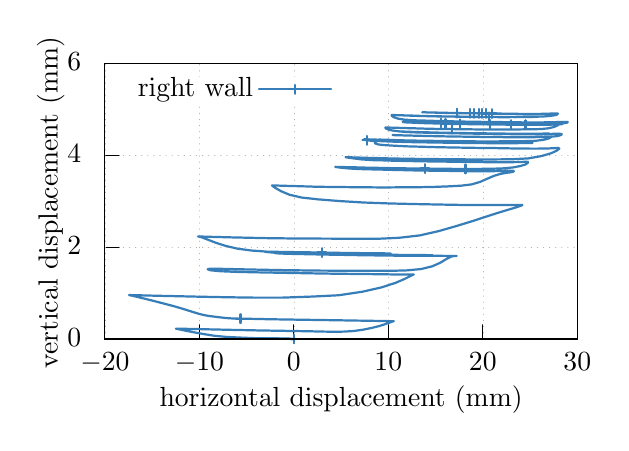
\begin{tikzpicture}[gnuplot]
%% generated with GNUPLOT 5.2p6 (Lua 5.3; terminal rev. Nov 2018, script rev. 107)
%% 09/10/2019 00:26:32
\path (0.000,0.000) rectangle (6.000,3.500);
\gpcolor{color=gp lt color axes}
\gpsetlinetype{gp lt axes}
\gpsetdashtype{gp dt axes}
\gpsetlinewidth{0.50}
\draw[gp path] (0.000,0.000)--(5.999,0.000);
\gpcolor{color=gp lt color border}
\gpsetlinetype{gp lt border}
\gpsetdashtype{gp dt solid}
\gpsetlinewidth{1.00}
\draw[gp path] (0.000,0.000)--(0.180,0.000);
\node[gp node right] at (-0.184,0.000) {$0$};
\gpcolor{color=gp lt color axes}
\gpsetlinetype{gp lt axes}
\gpsetdashtype{gp dt axes}
\gpsetlinewidth{0.50}
\draw[gp path] (0.000,1.166)--(5.999,1.166);
\gpcolor{color=gp lt color border}
\gpsetlinetype{gp lt border}
\gpsetdashtype{gp dt solid}
\gpsetlinewidth{1.00}
\draw[gp path] (0.000,1.166)--(0.180,1.166);
\node[gp node right] at (-0.184,1.166) {$2$};
\gpcolor{color=gp lt color axes}
\gpsetlinetype{gp lt axes}
\gpsetdashtype{gp dt axes}
\gpsetlinewidth{0.50}
\draw[gp path] (0.000,2.333)--(5.999,2.333);
\gpcolor{color=gp lt color border}
\gpsetlinetype{gp lt border}
\gpsetdashtype{gp dt solid}
\gpsetlinewidth{1.00}
\draw[gp path] (0.000,2.333)--(0.180,2.333);
\node[gp node right] at (-0.184,2.333) {$4$};
\gpcolor{color=gp lt color axes}
\gpsetlinetype{gp lt axes}
\gpsetdashtype{gp dt axes}
\gpsetlinewidth{0.50}
\draw[gp path] (0.000,3.499)--(5.999,3.499);
\gpcolor{color=gp lt color border}
\gpsetlinetype{gp lt border}
\gpsetdashtype{gp dt solid}
\gpsetlinewidth{1.00}
\draw[gp path] (0.000,3.499)--(0.180,3.499);
\node[gp node right] at (-0.184,3.499) {$6$};
\gpcolor{color=gp lt color axes}
\gpsetlinetype{gp lt axes}
\gpsetdashtype{gp dt axes}
\gpsetlinewidth{0.50}
\draw[gp path] (0.000,0.000)--(0.000,3.499);
\gpcolor{color=gp lt color border}
\gpsetlinetype{gp lt border}
\gpsetdashtype{gp dt solid}
\gpsetlinewidth{1.00}
\draw[gp path] (0.000,0.000)--(0.000,0.180);
\node[gp node center] at (0.000,-0.308) {$-20$};
\gpcolor{color=gp lt color axes}
\gpsetlinetype{gp lt axes}
\gpsetdashtype{gp dt axes}
\gpsetlinewidth{0.50}
\draw[gp path] (1.200,0.000)--(1.200,3.016);
\draw[gp path] (1.200,3.324)--(1.200,3.499);
\gpcolor{color=gp lt color border}
\gpsetlinetype{gp lt border}
\gpsetdashtype{gp dt solid}
\gpsetlinewidth{1.00}
\draw[gp path] (1.200,0.000)--(1.200,0.180);
\node[gp node center] at (1.200,-0.308) {$-10$};
\gpcolor{color=gp lt color axes}
\gpsetlinetype{gp lt axes}
\gpsetdashtype{gp dt axes}
\gpsetlinewidth{0.50}
\draw[gp path] (2.400,0.000)--(2.400,3.016);
\draw[gp path] (2.400,3.324)--(2.400,3.499);
\gpcolor{color=gp lt color border}
\gpsetlinetype{gp lt border}
\gpsetdashtype{gp dt solid}
\gpsetlinewidth{1.00}
\draw[gp path] (2.400,0.000)--(2.400,0.180);
\node[gp node center] at (2.400,-0.308) {$0$};
\gpcolor{color=gp lt color axes}
\gpsetlinetype{gp lt axes}
\gpsetdashtype{gp dt axes}
\gpsetlinewidth{0.50}
\draw[gp path] (3.599,0.000)--(3.599,3.499);
\gpcolor{color=gp lt color border}
\gpsetlinetype{gp lt border}
\gpsetdashtype{gp dt solid}
\gpsetlinewidth{1.00}
\draw[gp path] (3.599,0.000)--(3.599,0.180);
\node[gp node center] at (3.599,-0.308) {$10$};
\gpcolor{color=gp lt color axes}
\gpsetlinetype{gp lt axes}
\gpsetdashtype{gp dt axes}
\gpsetlinewidth{0.50}
\draw[gp path] (4.799,0.000)--(4.799,3.499);
\gpcolor{color=gp lt color border}
\gpsetlinetype{gp lt border}
\gpsetdashtype{gp dt solid}
\gpsetlinewidth{1.00}
\draw[gp path] (4.799,0.000)--(4.799,0.180);
\node[gp node center] at (4.799,-0.308) {$20$};
\gpcolor{color=gp lt color axes}
\gpsetlinetype{gp lt axes}
\gpsetdashtype{gp dt axes}
\gpsetlinewidth{0.50}
\draw[gp path] (5.999,0.000)--(5.999,3.499);
\gpcolor{color=gp lt color border}
\gpsetlinetype{gp lt border}
\gpsetdashtype{gp dt solid}
\gpsetlinewidth{1.00}
\draw[gp path] (5.999,0.000)--(5.999,0.180);
\node[gp node center] at (5.999,-0.308) {$30$};
\draw[gp path] (0.000,3.499)--(0.000,0.000)--(5.999,0.000)--(5.999,3.499)--cycle;
\node[gp node center,rotate=-270] at (-0.676,1.749) {vertical displacement (\si{\milli\metre})};
\node[gp node center] at (2.999,-0.769) {horizontal displacement (\si{\milli\metre})};
\gpcolor{rgb color={0.216,0.494,0.722}}
\gpsetlinewidth{2.00}
\draw[gp path] (2.402,0.000)--(2.397,0.000)--(2.394,0.000)--(2.397,0.000)--(2.403,0.000)%
  --(2.414,0.000);
\draw[gp path] (2.412,0.000)--(2.367,0.001)--(2.321,0.002)--(2.275,0.003)--(2.230,0.004)%
  --(2.187,0.005)--(2.147,0.005)--(2.110,0.006)--(2.077,0.007)--(2.049,0.008)--(2.028,0.008)%
  --(2.015,0.008)--(2.011,0.008)--(2.016,0.008)--(2.031,0.008)--(2.055,0.007)--(2.088,0.007)%
  --(2.129,0.006)--(2.175,0.005)--(2.224,0.004)--(2.273,0.003)--(2.318,0.002)--(2.357,0.001)%
  --(2.390,0.000);
\draw[gp path] (2.410,0.000)--(2.384,0.000)--(2.349,0.001)--(2.307,0.002)--(2.260,0.003)%
  --(2.211,0.004)--(2.163,0.005)--(2.119,0.006)--(2.081,0.007)--(2.052,0.008)--(2.036,0.008)%
  --(2.037,0.008)--(2.059,0.008)--(2.106,0.007)--(2.178,0.005)--(2.268,0.003)--(2.371,0.001)%
  --(2.426,0.000);
\draw[gp path] (2.396,0.000)--(2.232,0.004)--(2.059,0.007)--(1.884,0.011)--(1.709,0.018)%
  --(1.541,0.026)--(1.385,0.041)--(1.245,0.064)--(1.127,0.085)--(1.033,0.103)--(0.963,0.118)%
  --(0.919,0.127)--(0.901,0.131)--(0.911,0.131)--(0.948,0.131)--(1.011,0.129)--(1.099,0.127)%
  --(1.205,0.125)--(1.325,0.122)--(1.455,0.119)--(1.589,0.116)--(1.722,0.113)--(1.846,0.111)%
  --(1.956,0.108)--(2.051,0.107)--(2.136,0.105)--(2.224,0.104)--(2.326,0.102)--(2.447,0.100)%
  --(2.586,0.098)--(2.735,0.094)--(2.883,0.092)--(3.026,0.093)--(3.161,0.101)--(3.285,0.119)%
  --(3.392,0.141)--(3.480,0.163)--(3.549,0.185)--(3.601,0.203)--(3.638,0.216)--(3.661,0.224)%
  --(3.670,0.226)--(3.663,0.226)--(3.640,0.226)--(3.603,0.227)--(3.551,0.228)--(3.485,0.229)%
  --(3.405,0.230)--(3.313,0.232)--(3.208,0.233)--(3.093,0.235)--(2.971,0.237)--(2.843,0.239)%
  --(2.712,0.241)--(2.579,0.243)--(2.445,0.245)--(2.311,0.247)--(2.181,0.249)--(2.056,0.251)%
  --(1.937,0.254)--(1.826,0.256)--(1.721,0.258)--(1.624,0.260)--(1.536,0.266)--(1.456,0.275)%
  --(1.385,0.284)--(1.319,0.292)--(1.256,0.304)--(1.194,0.319)--(1.135,0.337)--(1.075,0.356)%
  --(1.011,0.376)--(0.942,0.397)--(0.865,0.419)--(0.780,0.441)--(0.689,0.465)--(0.595,0.489)%
  --(0.502,0.512)--(0.415,0.533)--(0.343,0.550)--(0.306,0.557)--(0.326,0.557)--(0.424,0.555)%
  --(0.608,0.550)--(0.871,0.544)--(1.187,0.537)--(1.531,0.530)--(1.890,0.525)--(2.257,0.525)%
  --(2.624,0.538)--(2.969,0.555)--(3.270,0.600)--(3.513,0.655)--(3.692,0.713)--(3.812,0.765)%
  --(3.889,0.804)--(3.922,0.819)--(3.907,0.819)--(3.833,0.818)--(3.695,0.819)--(3.494,0.822)%
  --(3.244,0.825)--(2.958,0.828)--(2.646,0.833)--(2.316,0.839)--(1.984,0.845)--(1.688,0.851)%
  --(1.467,0.860)--(1.341,0.872)--(1.304,0.885)--(1.337,0.893)--(1.420,0.892)--(1.547,0.889)%
  --(1.723,0.885)--(1.950,0.880)--(2.214,0.875)--(2.487,0.871)--(2.740,0.868)--(2.969,0.867)%
  --(3.185,0.866)--(3.403,0.865)--(3.623,0.865)--(3.835,0.871)--(4.016,0.888)--(4.155,0.922)%
  --(4.257,0.967)--(4.331,1.012)--(4.392,1.044)--(4.440,1.055)--(4.467,1.054)--(4.461,1.053)%
  --(4.415,1.054)--(4.331,1.055)--(4.221,1.056)--(4.091,1.056)--(3.943,1.056)--(3.772,1.057)%
  --(3.580,1.059)--(3.373,1.062)--(3.163,1.065)--(2.960,1.069)--(2.768,1.072)--(2.591,1.076)%
  --(2.431,1.079)--(2.299,1.082)--(2.208,1.086)--(2.166,1.089)--(2.175,1.090)--(2.229,1.089)%
  --(2.323,1.088)--(2.455,1.085)--(2.620,1.082)--(2.814,1.079)--(3.024,1.076)--(3.240,1.072)%
  --(3.449,1.070)--(3.644,1.068)--(3.818,1.067)--(3.964,1.065)--(4.076,1.065)--(4.143,1.064)%
  --(4.163,1.064)--(4.136,1.064)--(4.063,1.065)--(3.951,1.066)--(3.812,1.067)--(3.652,1.069)%
  --(3.484,1.070)--(3.311,1.072)--(3.135,1.075)--(2.960,1.078)--(2.790,1.081)--(2.632,1.083)%
  --(2.491,1.085)--(2.368,1.087)--(2.264,1.089)--(2.179,1.093)--(2.112,1.099)--(2.066,1.103)%
  --(2.039,1.106)--(2.030,1.109)--(2.036,1.109)--(2.061,1.109)--(2.112,1.107)--(2.195,1.106)%
  --(2.308,1.104)--(2.443,1.102)--(2.585,1.099)--(2.725,1.097)--(2.857,1.095)--(2.980,1.093)%
  --(3.090,1.091)--(3.178,1.090)--(3.233,1.089)--(3.250,1.089)--(3.231,1.090)--(3.193,1.091)%
  --(3.159,1.091)--(3.146,1.091)--(3.159,1.091)--(3.190,1.091)--(3.225,1.090)--(3.254,1.089)%
  --(3.280,1.089)--(3.305,1.089)--(3.327,1.089)--(3.338,1.088)--(3.327,1.088)--(3.299,1.089)%
  --(3.271,1.090)--(3.262,1.090)--(3.281,1.090)--(3.322,1.089)--(3.367,1.088)--(3.407,1.088)%
  --(3.443,1.088)--(3.485,1.088)--(3.535,1.088)--(3.583,1.086)--(3.617,1.086)--(3.628,1.086)%
  --(3.617,1.086)--(3.592,1.087)--(3.559,1.087)--(3.518,1.087)--(3.468,1.087)--(3.408,1.088)%
  --(3.341,1.089)--(3.274,1.089)--(3.209,1.091)--(3.144,1.091)--(3.078,1.092)--(3.011,1.093)%
  --(2.946,1.093)--(2.885,1.095)--(2.830,1.095)--(2.779,1.096)--(2.730,1.097)--(2.682,1.098)%
  --(2.639,1.099)--(2.605,1.099)--(2.586,1.099)--(2.583,1.099)--(2.598,1.099)--(2.631,1.099)%
  --(2.681,1.098)--(2.746,1.097)--(2.822,1.095)--(2.903,1.094)--(2.984,1.093)--(3.058,1.092)%
  --(3.122,1.091)--(3.173,1.091)--(3.206,1.090)--(3.216,1.090)--(3.202,1.090)--(3.159,1.091)%
  --(3.090,1.092)--(2.997,1.093)--(2.881,1.095)--(2.755,1.097)--(2.630,1.099)--(2.520,1.100)%
  --(2.436,1.102)--(2.377,1.103)--(2.340,1.104)--(2.321,1.104)--(2.320,1.104)--(2.342,1.103)%
  --(2.393,1.103)--(2.473,1.101)--(2.575,1.099)--(2.691,1.098)--(2.813,1.096)--(2.937,1.093)%
  --(3.061,1.092)--(3.180,1.091)--(3.286,1.089)--(3.371,1.088)--(3.431,1.087)--(3.462,1.087)%
  --(3.464,1.087)--(3.437,1.088)--(3.379,1.088)--(3.290,1.089)--(3.169,1.091)--(3.021,1.093)%
  --(2.852,1.095)--(2.666,1.099)--(2.468,1.102)--(2.263,1.105)--(2.058,1.109)--(1.861,1.123)%
  --(1.683,1.147)--(1.528,1.183)--(1.400,1.225)--(1.299,1.264)--(1.222,1.293)--(1.182,1.303)%
  --(1.196,1.302)--(1.274,1.299)--(1.417,1.295)--(1.613,1.290)--(1.837,1.285)--(2.076,1.280)%
  --(2.325,1.277)--(2.590,1.275)--(2.874,1.274)--(3.169,1.272)--(3.460,1.272)--(3.737,1.285)%
  --(3.998,1.315)--(4.240,1.370)--(4.460,1.433)--(4.656,1.493)--(4.833,1.551)--(4.986,1.600)%
  --(5.114,1.639)--(5.212,1.668)--(5.276,1.689)--(5.302,1.701)--(5.288,1.703)--(5.231,1.702)%
  --(5.129,1.701)--(4.979,1.700)--(4.780,1.700)--(4.536,1.702)--(4.253,1.707)--(3.941,1.713)%
  --(3.611,1.721)--(3.280,1.733)--(2.971,1.752)--(2.706,1.773)--(2.497,1.796)--(2.343,1.832)%
  --(2.236,1.877)--(2.169,1.915)--(2.133,1.940)--(2.122,1.950)--(2.134,1.950)--(2.167,1.949)%
  --(2.220,1.947)--(2.287,1.945)--(2.359,1.943)--(2.426,1.941)--(2.482,1.940)--(2.530,1.938)%
  --(2.580,1.937)--(2.651,1.934)--(2.760,1.932)--(2.914,1.930)--(3.106,1.928)--(3.321,1.926)%
  --(3.542,1.924)--(3.760,1.926)--(3.974,1.927)--(4.178,1.931)--(4.366,1.938)--(4.527,1.947)%
  --(4.658,1.963)--(4.763,1.994)--(4.856,2.035)--(4.940,2.071)--(5.019,2.095)--(5.090,2.109)%
  --(5.146,2.116)--(5.182,2.123)--(5.194,2.130)--(5.183,2.136)--(5.154,2.137)--(5.106,2.136)%
  --(5.036,2.133)--(4.941,2.131)--(4.820,2.131)--(4.678,2.131)--(4.526,2.133)--(4.376,2.135)%
  --(4.234,2.137)--(4.109,2.138)--(4.001,2.140)--(3.916,2.141)--(3.854,2.142)--(3.818,2.143)%
  --(3.808,2.143)--(3.823,2.143)--(3.855,2.142)--(3.903,2.141)--(3.961,2.140)--(4.023,2.139)%
  --(4.087,2.138)--(4.150,2.137)--(4.218,2.137)--(4.296,2.136)--(4.389,2.134)--(4.493,2.133)%
  --(4.598,2.131)--(4.691,2.130)--(4.767,2.131)--(4.823,2.131)--(4.860,2.132)--(4.877,2.132)%
  --(4.866,2.131)--(4.824,2.130)--(4.744,2.130)--(4.631,2.131)--(4.488,2.133)--(4.324,2.136)%
  --(4.139,2.138)--(3.941,2.141)--(3.737,2.145)--(3.541,2.150)--(3.365,2.154)--(3.217,2.158)%
  --(3.100,2.165)--(3.013,2.173)--(2.956,2.180)--(2.927,2.185)--(2.926,2.186)--(2.952,2.185)%
  --(2.999,2.184)--(3.063,2.182)--(3.140,2.180)--(3.223,2.179)--(3.309,2.176)--(3.392,2.175)%
  --(3.467,2.173)--(3.529,2.172)--(3.576,2.171)--(3.608,2.170)--(3.629,2.169)--(3.646,2.169)%
  --(3.664,2.169)--(3.688,2.168)--(3.717,2.168)--(3.749,2.167)--(3.783,2.167)--(3.817,2.166)%
  --(3.848,2.166)--(3.877,2.165)--(3.901,2.165)--(3.919,2.165)--(3.933,2.165)--(3.947,2.165)%
  --(3.962,2.165)--(3.981,2.164)--(4.001,2.164)--(4.022,2.164)--(4.042,2.164)--(4.059,2.164)%
  --(4.077,2.163)--(4.094,2.163)--(4.112,2.163)--(4.127,2.162)--(4.138,2.162)--(4.143,2.162)%
  --(4.136,2.162)--(4.121,2.162)--(4.097,2.163)--(4.063,2.164)--(4.016,2.164)--(3.958,2.165)%
  --(3.896,2.165)--(3.832,2.166)--(3.772,2.167)--(3.722,2.168)--(3.685,2.168)--(3.663,2.169)%
  --(3.658,2.169)--(3.668,2.169)--(3.687,2.168)--(3.715,2.168)--(3.746,2.168)--(3.779,2.167)%
  --(3.819,2.166)--(3.863,2.166)--(3.914,2.165)--(3.965,2.165)--(4.017,2.164)--(4.063,2.163)%
  --(4.100,2.163)--(4.129,2.162)--(4.147,2.162)--(4.153,2.162)--(4.144,2.162)--(4.121,2.162)%
  --(4.085,2.163)--(4.042,2.164)--(3.998,2.164)--(3.953,2.165)--(3.914,2.165)--(3.877,2.166)%
  --(3.843,2.166)--(3.813,2.166)--(3.790,2.167)--(3.772,2.167)--(3.760,2.167)--(3.755,2.167)%
  --(3.757,2.167)--(3.767,2.167)--(3.785,2.167)--(3.811,2.166)--(3.842,2.166)--(3.877,2.166)%
  --(3.911,2.165)--(3.947,2.165)--(3.982,2.164)--(4.015,2.164)--(4.045,2.164)--(4.071,2.163)%
  --(4.095,2.163)--(4.118,2.163)--(4.143,2.162)--(4.167,2.162)--(4.190,2.162)--(4.208,2.162)%
  --(4.220,2.162)--(4.224,2.162)--(4.223,2.162)--(4.217,2.162)--(4.205,2.162)--(4.186,2.162)%
  --(4.160,2.162)--(4.127,2.162)--(4.088,2.163)--(4.043,2.164)--(3.994,2.164)--(3.946,2.165)%
  --(3.899,2.165)--(3.860,2.166)--(3.826,2.166)--(3.799,2.166)--(3.777,2.167)--(3.763,2.167)%
  --(3.758,2.167)--(3.763,2.167)--(3.777,2.167)--(3.800,2.166)--(3.827,2.166)--(3.859,2.166)%
  --(3.891,2.165)--(3.926,2.165)--(3.958,2.165)--(3.988,2.164)--(4.010,2.164)--(4.023,2.164)%
  --(4.025,2.164)--(4.015,2.164)--(3.991,2.164)--(3.953,2.165)--(3.908,2.165)--(3.859,2.166)%
  --(3.817,2.166)--(3.787,2.167)--(3.767,2.167)--(3.759,2.167)--(3.758,2.167)--(3.760,2.167)%
  --(3.770,2.167)--(3.785,2.167)--(3.806,2.166)--(3.831,2.166)--(3.860,2.166)--(3.892,2.165)%
  --(3.934,2.165)--(3.983,2.164)--(4.041,2.164)--(4.101,2.163)--(4.159,2.162)--(4.211,2.162)%
  --(4.254,2.161)--(4.289,2.161)--(4.311,2.161)--(4.318,2.160)--(4.307,2.161)--(4.278,2.161)%
  --(4.232,2.161)--(4.172,2.162)--(4.100,2.163)--(4.023,2.164)--(3.945,2.165)--(3.871,2.166)%
  --(3.805,2.166)--(3.751,2.168)--(3.706,2.168)--(3.674,2.169)--(3.653,2.169)--(3.645,2.169)%
  --(3.652,2.169)--(3.674,2.169)--(3.707,2.168)--(3.749,2.168)--(3.797,2.166)--(3.848,2.166)%
  --(3.901,2.165)--(3.952,2.165)--(4.001,2.164)--(4.043,2.164)--(4.077,2.163)--(4.100,2.163)%
  --(4.115,2.163)--(4.125,2.162)--(4.129,2.162)--(4.126,2.162)--(4.115,2.163)--(4.097,2.163)%
  --(4.069,2.164)--(4.030,2.164)--(3.981,2.164)--(3.926,2.165)--(3.866,2.166)--(3.807,2.166)%
  --(3.752,2.168)--(3.706,2.168)--(3.669,2.169)--(3.643,2.169)--(3.628,2.169)--(3.626,2.169)%
  --(3.634,2.169)--(3.656,2.169)--(3.685,2.168)--(3.722,2.168)--(3.763,2.167)--(3.806,2.166)%
  --(3.849,2.166)--(3.889,2.165)--(3.923,2.165)--(3.951,2.165)--(3.968,2.165)--(3.976,2.164)%
  --(3.975,2.164)--(3.968,2.165)--(3.952,2.165)--(3.932,2.165)--(3.905,2.165)--(3.872,2.166)%
  --(3.832,2.166)--(3.785,2.167)--(3.735,2.168)--(3.687,2.168)--(3.644,2.169)--(3.608,2.170)%
  --(3.581,2.171)--(3.565,2.171)--(3.563,2.171)--(3.577,2.171)--(3.609,2.169)--(3.659,2.169)%
  --(3.725,2.168)--(3.802,2.166)--(3.887,2.165)--(3.982,2.164)--(4.082,2.163)--(4.184,2.162)%
  --(4.283,2.161)--(4.376,2.160)--(4.457,2.159)--(4.526,2.159)--(4.580,2.159)--(4.613,2.159)%
  --(4.622,2.158)--(4.602,2.158)--(4.559,2.159)--(4.497,2.159)--(4.425,2.160)--(4.348,2.161)%
  --(4.268,2.161)--(4.186,2.162)--(4.103,2.163)--(4.022,2.164)--(3.947,2.165)--(3.881,2.166)%
  --(3.827,2.166)--(3.783,2.167)--(3.749,2.168)--(3.729,2.168)--(3.722,2.168)--(3.728,2.168)%
  --(3.747,2.168)--(3.778,2.167)--(3.818,2.166)--(3.866,2.166)--(3.921,2.165)--(3.983,2.164)%
  --(4.048,2.164)--(4.115,2.163)--(4.178,2.162)--(4.235,2.161)--(4.283,2.161)--(4.322,2.161)%
  --(4.347,2.160)--(4.355,2.160)--(4.347,2.160)--(4.320,2.161)--(4.276,2.161)--(4.216,2.162)%
  --(4.144,2.162)--(4.061,2.164)--(3.970,2.165)--(3.874,2.166)--(3.778,2.167)--(3.685,2.169)%
  --(3.597,2.170)--(3.520,2.172)--(3.455,2.173)--(3.404,2.175)--(3.369,2.175)--(3.353,2.175)%
  --(3.356,2.175)--(3.378,2.175)--(3.417,2.174)--(3.470,2.173)--(3.535,2.172)--(3.609,2.170)%
  --(3.697,2.168)--(3.801,2.167)--(3.928,2.165)--(4.079,2.164)--(4.247,2.161)--(4.424,2.159)%
  --(4.600,2.159)--(4.768,2.160)--(4.924,2.162)--(5.066,2.167)--(5.187,2.179)--(5.279,2.197)%
  --(5.340,2.216)--(5.369,2.235)--(5.373,2.248)--(5.352,2.251)--(5.310,2.249)--(5.241,2.246)%
  --(5.140,2.245)--(5.009,2.245)--(4.856,2.245)--(4.686,2.247)--(4.511,2.249)--(4.332,2.252)%
  --(4.154,2.254)--(3.982,2.257)--(3.825,2.260)--(3.691,2.263)--(3.583,2.266)--(3.500,2.269)%
  --(3.439,2.270)--(3.402,2.271)--(3.392,2.271)--(3.412,2.271)--(3.461,2.270)--(3.533,2.269)%
  --(3.621,2.267)--(3.716,2.264)--(3.814,2.263)--(3.913,2.260)--(4.006,2.259)--(4.088,2.257)%
  --(4.150,2.256)--(4.186,2.255)--(4.198,2.255)--(4.193,2.255)--(4.189,2.255)--(4.200,2.255)%
  --(4.232,2.255)--(4.278,2.253)--(4.328,2.253)--(4.372,2.252)--(4.412,2.252)--(4.450,2.252)%
  --(4.497,2.251)--(4.550,2.250)--(4.606,2.249)--(4.656,2.249)--(4.698,2.248)--(4.732,2.248)%
  --(4.760,2.248)--(4.782,2.247)--(4.797,2.247)--(4.798,2.247)--(4.784,2.247)--(4.751,2.248)%
  --(4.698,2.248)--(4.625,2.249)--(4.530,2.250)--(4.409,2.252)--(4.262,2.254)--(4.090,2.257)%
  --(3.904,2.261)--(3.717,2.265)--(3.541,2.269)--(3.388,2.272)--(3.262,2.280)--(3.164,2.292)%
  --(3.094,2.302)--(3.057,2.308)--(3.057,2.309)--(3.096,2.308)--(3.177,2.305)--(3.298,2.301)%
  --(3.458,2.297)--(3.652,2.292)--(3.875,2.288)--(4.123,2.285)--(4.388,2.283)--(4.658,2.280)%
  --(4.922,2.280)--(5.165,2.282)--(5.376,2.293)--(5.545,2.323)--(5.668,2.359)--(5.741,2.393)%
  --(5.771,2.418)--(5.759,2.426)--(5.705,2.423)--(5.599,2.418)--(5.436,2.417)--(5.216,2.419)%
  --(4.959,2.424)--(4.696,2.427)--(4.451,2.431)--(4.230,2.435)--(4.029,2.441)--(3.842,2.446)%
  --(3.679,2.454)--(3.549,2.462)--(3.467,2.471)--(3.431,2.484)--(3.430,2.502)--(3.452,2.513)%
  --(3.489,2.513)--(3.540,2.511)--(3.615,2.507)--(3.724,2.504)--(3.871,2.500)--(4.047,2.497)%
  --(4.238,2.494)--(4.432,2.491)--(4.624,2.489)--(4.810,2.487)--(4.984,2.486)--(5.141,2.486)%
  --(5.270,2.487)--(5.362,2.488)--(5.416,2.489)--(5.431,2.490)--(5.409,2.490)--(5.346,2.489)%
  --(5.244,2.488)--(5.102,2.487)--(4.926,2.487)--(4.725,2.489)--(4.509,2.491)--(4.287,2.494)%
  --(4.067,2.498)--(3.860,2.502)--(3.675,2.507)--(3.522,2.512)--(3.405,2.515)--(3.327,2.523)%
  --(3.290,2.533)--(3.297,2.537)--(3.347,2.535)--(3.438,2.532)--(3.565,2.528)--(3.722,2.523)%
  --(3.899,2.519)--(4.087,2.515)--(4.276,2.513)--(4.457,2.511)--(4.628,2.509)--(4.784,2.508)%
  --(4.923,2.508)--(5.043,2.509)--(5.140,2.509)--(5.210,2.510)--(5.249,2.511)--(5.260,2.511)%
  --(5.244,2.511)--(5.206,2.511)--(5.148,2.511)--(5.073,2.511)--(4.982,2.509)--(4.878,2.509)%
  --(4.764,2.509)--(4.646,2.510)--(4.523,2.511)--(4.401,2.513)--(4.280,2.514)--(4.163,2.516)%
  --(4.052,2.517)--(3.947,2.519)--(3.849,2.521)--(3.759,2.523)--(3.677,2.526)--(3.604,2.529)%
  --(3.544,2.530)--(3.501,2.532)--(3.481,2.532)--(3.490,2.532)--(3.533,2.530)--(3.609,2.527)%
  --(3.717,2.524)--(3.853,2.521)--(4.009,2.518)--(4.179,2.515)--(4.361,2.513)--(4.554,2.511)%
  --(4.755,2.509)--(4.956,2.509)--(5.150,2.511)--(5.321,2.512)--(5.464,2.516)--(5.571,2.529)%
  --(5.638,2.547)--(5.665,2.562)--(5.653,2.568)--(5.607,2.568)--(5.523,2.564)--(5.403,2.562)%
  --(5.244,2.561)--(5.057,2.563)--(4.851,2.565)--(4.641,2.568)--(4.438,2.571)--(4.248,2.574)%
  --(4.073,2.578)--(3.921,2.582)--(3.797,2.585)--(3.710,2.587)--(3.663,2.589)--(3.653,2.589)%
  --(3.680,2.589)--(3.740,2.587)--(3.832,2.584)--(3.959,2.581)--(4.119,2.577)--(4.305,2.573)%
  --(4.510,2.570)--(4.724,2.567)--(4.940,2.565)--(5.148,2.562)--(5.342,2.562)--(5.509,2.564)%
  --(5.644,2.568)--(5.739,2.575)--(5.791,2.589)--(5.802,2.601)--(5.776,2.606)--(5.719,2.606)%
  --(5.634,2.603)--(5.520,2.600)--(5.380,2.599)--(5.216,2.600)--(5.040,2.603)--(4.866,2.605)%
  --(4.700,2.607)--(4.541,2.610)--(4.390,2.613)--(4.248,2.616)--(4.119,2.618)--(4.011,2.621)%
  --(3.925,2.624)--(3.859,2.627)--(3.812,2.629)--(3.782,2.632)--(3.776,2.632)--(3.795,2.632)%
  --(3.847,2.630)--(3.929,2.628)--(4.041,2.625)--(4.179,2.621)--(4.338,2.618)--(4.514,2.614)%
  --(4.700,2.612)--(4.887,2.610)--(5.067,2.607)--(5.229,2.605)--(5.367,2.604)--(5.478,2.605)%
  --(5.556,2.606)--(5.598,2.606)--(5.603,2.607)--(5.572,2.607)--(5.509,2.607)--(5.424,2.607)%
  --(5.322,2.606)--(5.208,2.606)--(5.090,2.607)--(4.966,2.609)--(4.847,2.611)--(4.737,2.612)%
  --(4.638,2.613)--(4.557,2.614)--(4.490,2.616)--(4.438,2.616)--(4.403,2.617)--(4.388,2.617)%
  --(4.390,2.617)--(4.410,2.617)--(4.444,2.616)--(4.490,2.616)--(4.547,2.614)--(4.618,2.613)%
  --(4.702,2.612)--(4.796,2.611)--(4.896,2.610)--(5.002,2.609)--(5.110,2.607)--(5.220,2.606)%
  --(5.327,2.606)--(5.427,2.606)--(5.512,2.607)--(5.577,2.607)--(5.620,2.609)--(5.641,2.610)%
  --(5.640,2.610)--(5.616,2.609)--(5.567,2.608)--(5.495,2.607)--(5.399,2.606)--(5.283,2.606)%
  --(5.152,2.607)--(5.008,2.609)--(4.854,2.611)--(4.694,2.613)--(4.532,2.615)--(4.372,2.618)%
  --(4.220,2.621)--(4.078,2.625)--(3.950,2.628)--(3.838,2.632)--(3.742,2.636)--(3.667,2.645)%
  --(3.613,2.655)--(3.578,2.668)--(3.562,2.679)--(3.561,2.685)--(3.571,2.687)--(3.593,2.685)%
  --(3.627,2.684)--(3.674,2.683)--(3.730,2.681)--(3.793,2.679)--(3.855,2.677)--(3.913,2.676)%
  --(3.963,2.674)--(4.006,2.673)--(4.036,2.672)--(4.054,2.671)--(4.059,2.671)--(4.058,2.671)%
  --(4.059,2.671)--(4.073,2.670)--(4.105,2.669)--(4.155,2.669)--(4.222,2.667)--(4.308,2.666)%
  --(4.410,2.665)--(4.529,2.663)--(4.658,2.662)--(4.791,2.660)--(4.925,2.659)--(5.056,2.659)%
  --(5.187,2.660)--(5.314,2.662)--(5.434,2.663)--(5.542,2.666)--(5.631,2.675)--(5.695,2.690)%
  --(5.737,2.706)--(5.759,2.720)--(5.763,2.727)--(5.749,2.726)--(5.717,2.725)--(5.665,2.722)%
  --(5.593,2.721)--(5.507,2.721)--(5.410,2.720)--(5.309,2.720)--(5.208,2.721)--(5.105,2.722)%
  --(5.006,2.723)--(4.911,2.725)--(4.829,2.726)--(4.763,2.726)--(4.714,2.727)--(4.680,2.727)%
  --(4.662,2.727)--(4.655,2.727)--(4.659,2.727)--(4.667,2.727)--(4.676,2.727)--(4.683,2.727)%
  --(4.688,2.727)--(4.691,2.727)--(4.694,2.727)--(4.691,2.727)--(4.684,2.727)--(4.671,2.727)%
  --(4.656,2.727)--(4.643,2.728)--(4.632,2.728)--(4.620,2.728)--(4.605,2.729)--(4.582,2.729)%
  --(4.556,2.729)--(4.530,2.730)--(4.509,2.730)--(4.493,2.730)--(4.482,2.730)--(4.476,2.730)%
  --(4.484,2.730)--(4.498,2.730)--(4.516,2.730)--(4.534,2.729)--(4.552,2.729)--(4.570,2.729)%
  --(4.592,2.729)--(4.617,2.728)--(4.642,2.728)--(4.664,2.727)--(4.680,2.727)--(4.698,2.727)%
  --(4.718,2.727)--(4.739,2.726)--(4.763,2.726)--(4.785,2.726)--(4.805,2.726)--(4.826,2.726)%
  --(4.847,2.725)--(4.869,2.725)--(4.887,2.725)--(4.899,2.725)--(4.902,2.725)--(4.901,2.725)%
  --(4.895,2.725)--(4.887,2.725)--(4.877,2.725)--(4.868,2.725)--(4.858,2.725)--(4.851,2.725)%
  --(4.846,2.725)--(4.842,2.725)--(4.836,2.725)--(4.826,2.725)--(4.810,2.726)--(4.787,2.726)%
  --(4.761,2.726)--(4.727,2.727)--(4.689,2.727)--(4.646,2.728)--(4.599,2.729)--(4.552,2.729)%
  --(4.506,2.730)--(4.463,2.730)--(4.425,2.732)--(4.394,2.732)--(4.371,2.733)--(4.360,2.733)%
  --(4.361,2.733)--(4.373,2.733)--(4.394,2.732)--(4.421,2.732)--(4.454,2.731)--(4.488,2.730)%
  --(4.526,2.730)--(4.563,2.729)--(4.598,2.729)--(4.626,2.728)--(4.650,2.727)--(4.666,2.727)%
  --(4.674,2.727)--(4.673,2.727)--(4.661,2.727)--(4.638,2.728)--(4.606,2.729)--(4.570,2.729)%
  --(4.534,2.729)--(4.505,2.730)--(4.486,2.730)--(4.479,2.730)--(4.484,2.730)--(4.502,2.730)%
  --(4.534,2.729)--(4.580,2.729)--(4.640,2.728)--(4.710,2.727)--(4.788,2.726)--(4.870,2.725)%
  --(4.950,2.724)--(5.027,2.723)--(5.097,2.722)--(5.158,2.721)--(5.202,2.720)--(5.228,2.720)%
  --(5.229,2.720)--(5.210,2.720)--(5.177,2.721)--(5.138,2.722)--(5.094,2.722)--(5.048,2.723)%
  --(4.994,2.723)--(4.928,2.724)--(4.854,2.725)--(4.775,2.726)--(4.694,2.727)--(4.613,2.729)%
  --(4.538,2.729)--(4.475,2.730)--(4.433,2.731)--(4.419,2.731)--(4.433,2.731)--(4.469,2.730)%
  --(4.520,2.730)--(4.576,2.729)--(4.638,2.728)--(4.704,2.727)--(4.775,2.726)--(4.847,2.725)%
  --(4.914,2.724)--(4.976,2.723)--(5.031,2.723)--(5.082,2.722)--(5.129,2.722)--(5.170,2.721)%
  --(5.199,2.720)--(5.213,2.720)--(5.216,2.720)--(5.208,2.721)--(5.190,2.721)--(5.163,2.721)%
  --(5.121,2.722)--(5.067,2.722)--(5.002,2.723)--(4.931,2.725)--(4.857,2.725)--(4.779,2.726)%
  --(4.697,2.727)--(4.612,2.729)--(4.527,2.730)--(4.443,2.731)--(4.360,2.733)--(4.280,2.735)%
  --(4.199,2.737)--(4.129,2.739)--(4.077,2.740)--(4.054,2.740)--(4.065,2.740)--(4.113,2.739)%
  --(4.195,2.737)--(4.307,2.734)--(4.449,2.731)--(4.612,2.728)--(4.791,2.726)--(4.977,2.723)%
  --(5.159,2.721)--(5.330,2.719)--(5.483,2.719)--(5.611,2.720)--(5.711,2.723)--(5.777,2.725)%
  --(5.806,2.726)--(5.797,2.726)--(5.753,2.725)--(5.671,2.723)--(5.555,2.720)--(5.407,2.719)%
  --(5.237,2.721)--(5.055,2.723)--(4.876,2.726)--(4.708,2.728)--(4.556,2.730)--(4.419,2.732)%
  --(4.305,2.734)--(4.216,2.737)--(4.161,2.738)--(4.138,2.739)--(4.145,2.739)--(4.174,2.739)%
  --(4.218,2.737)--(4.274,2.736)--(4.337,2.734)--(4.404,2.733)--(4.470,2.732)--(4.527,2.730)%
  --(4.569,2.730)--(4.595,2.729)--(4.606,2.729)--(4.601,2.729)--(4.583,2.729)--(4.557,2.730)%
  --(4.526,2.730)--(4.496,2.731)--(4.472,2.732)--(4.460,2.732)--(4.474,2.731)--(4.500,2.731)%
  --(4.539,2.730)--(4.583,2.729)--(4.632,2.729)--(4.680,2.728)--(4.726,2.727)--(4.764,2.727)%
  --(4.794,2.726)--(4.816,2.726)--(4.830,2.726)--(4.842,2.726)--(4.853,2.726)--(4.864,2.726)%
  --(4.872,2.726)--(4.880,2.726)--(4.884,2.726)--(4.886,2.725)--(4.884,2.726)--(4.878,2.726)%
  --(4.870,2.726)--(4.859,2.726)--(4.848,2.726)--(4.839,2.726)--(4.833,2.726)--(4.829,2.726)%
  --(4.830,2.726)--(4.836,2.726)--(4.850,2.726)--(4.872,2.726)--(4.904,2.725)--(4.940,2.725)%
  --(4.976,2.724)--(5.007,2.724)--(5.033,2.723)--(5.051,2.723)--(5.062,2.723)--(5.051,2.723)%
  --(5.028,2.723)--(4.995,2.724)--(4.950,2.725)--(4.900,2.725)--(4.842,2.726)--(4.780,2.727)%
  --(4.710,2.728)--(4.638,2.729)--(4.570,2.730)--(4.514,2.730)--(4.478,2.731)--(4.463,2.732)%
  --(4.470,2.731)--(4.494,2.731)--(4.529,2.730)--(4.574,2.730)--(4.626,2.729)--(4.682,2.728)%
  --(4.738,2.727)--(4.788,2.726)--(4.830,2.726)--(4.862,2.726)--(4.887,2.725)--(4.907,2.725)%
  --(4.924,2.725)--(4.938,2.725)--(4.949,2.725)--(4.955,2.725)--(4.948,2.725)--(4.931,2.725)%
  --(4.904,2.725)--(4.863,2.726)--(4.809,2.726)--(4.743,2.727)--(4.668,2.729)--(4.589,2.730)%
  --(4.509,2.731)--(4.434,2.732)--(4.371,2.733)--(4.323,2.734)--(4.294,2.735)--(4.284,2.735)%
  --(4.296,2.735)--(4.328,2.734)--(4.378,2.733)--(4.445,2.732)--(4.524,2.730)--(4.613,2.729)%
  --(4.706,2.727)--(4.799,2.726)--(4.887,2.725)--(4.965,2.725)--(5.033,2.723)--(5.091,2.723)%
  --(5.138,2.722)--(5.175,2.722)--(5.204,2.722)--(5.224,2.721)--(5.235,2.721)--(5.223,2.721)%
  --(5.199,2.722)--(5.163,2.722)--(5.114,2.723)--(5.051,2.723)--(4.979,2.725)--(4.899,2.725)%
  --(4.816,2.726)--(4.736,2.727)--(4.659,2.729)--(4.586,2.730)--(4.517,2.730)--(4.454,2.732)%
  --(4.395,2.733)--(4.343,2.734)--(4.300,2.735)--(4.264,2.736)--(4.238,2.737)--(4.221,2.737)%
  --(4.217,2.737)--(4.226,2.737)--(4.250,2.736)--(4.283,2.736)--(4.326,2.734)--(4.373,2.734)%
  --(4.422,2.733)--(4.472,2.732)--(4.520,2.730)--(4.569,2.730)--(4.620,2.729)--(4.677,2.728)%
  --(4.738,2.727)--(4.806,2.726)--(4.881,2.726)--(4.959,2.725)--(5.039,2.723)--(5.118,2.723)%
  --(5.190,2.722)--(5.252,2.721)--(5.297,2.720)--(5.325,2.720)--(5.333,2.720)--(5.321,2.720)%
  --(5.290,2.720)--(5.240,2.721)--(5.175,2.722)--(5.100,2.723)--(5.022,2.724)--(4.946,2.725)%
  --(4.872,2.726)--(4.805,2.727)--(4.742,2.727)--(4.685,2.728)--(4.636,2.729)--(4.596,2.730)%
  --(4.563,2.730)--(4.538,2.730)--(4.518,2.730)--(4.505,2.731)--(4.500,2.731)--(4.506,2.731)%
  --(4.522,2.730)--(4.548,2.730)--(4.584,2.730)--(4.630,2.729)--(4.683,2.728)--(4.744,2.727)%
  --(4.811,2.726)--(4.881,2.726)--(4.947,2.725)--(5.006,2.724)--(5.051,2.723)--(5.084,2.723)%
  --(5.100,2.723)--(5.081,2.723)--(5.042,2.723)--(4.983,2.725)--(4.908,2.725)--(4.822,2.726)%
  --(4.728,2.727)--(4.634,2.729)--(4.542,2.730)--(4.462,2.732)--(4.401,2.733)--(4.365,2.733)%
  --(4.358,2.733)--(4.377,2.733)--(4.418,2.732)--(4.476,2.732)--(4.547,2.730)--(4.628,2.729)%
  --(4.715,2.727)--(4.804,2.726)--(4.887,2.725)--(4.958,2.725)--(5.014,2.724)--(5.055,2.723)%
  --(5.082,2.723)--(5.098,2.723)--(5.099,2.723)--(5.084,2.723)--(5.051,2.723)--(5.002,2.724)%
  --(4.942,2.725)--(4.874,2.726)--(4.802,2.727)--(4.726,2.727)--(4.650,2.729)--(4.575,2.730)%
  --(4.505,2.731)--(4.445,2.732)--(4.396,2.733)--(4.361,2.734)--(4.342,2.734)--(4.340,2.734)%
  --(4.355,2.734)--(4.391,2.733)--(4.448,2.732)--(4.518,2.730)--(4.601,2.729)--(4.691,2.728)%
  --(4.782,2.727)--(4.872,2.726)--(4.955,2.725)--(5.030,2.723)--(5.092,2.723)--(5.142,2.722)%
  --(5.181,2.722)--(5.208,2.722)--(5.226,2.722)--(5.234,2.721)--(5.229,2.721)--(5.212,2.722)%
  --(5.186,2.722)--(5.151,2.722)--(5.108,2.723)--(5.057,2.723)--(5.000,2.724)--(4.937,2.725)%
  --(4.874,2.726)--(4.811,2.727)--(4.751,2.727)--(4.695,2.728)--(4.642,2.729)--(4.594,2.730)%
  --(4.554,2.730)--(4.527,2.730)--(4.511,2.731)--(4.509,2.731)--(4.516,2.731)--(4.530,2.730)%
  --(4.547,2.730)--(4.568,2.730)--(4.587,2.730)--(4.602,2.729)--(4.610,2.729)--(4.607,2.729)%
  --(4.595,2.730)--(4.576,2.730)--(4.552,2.730)--(4.524,2.730)--(4.497,2.731)--(4.469,2.732)%
  --(4.446,2.732)--(4.432,2.732)--(4.430,2.732)--(4.440,2.732)--(4.463,2.732)--(4.499,2.731)%
  --(4.546,2.730)--(4.602,2.729)--(4.667,2.729)--(4.736,2.727)--(4.804,2.726)--(4.869,2.726)%
  --(4.929,2.725)--(4.979,2.725)--(5.019,2.724)--(5.048,2.723)--(5.062,2.723)--(5.066,2.723)%
  --(5.058,2.723)--(5.045,2.724)--(5.027,2.724)--(5.006,2.724)--(4.982,2.725)--(4.960,2.725)%
  --(4.942,2.725)--(4.929,2.725)--(4.923,2.725)--(4.924,2.725)--(4.928,2.725)--(4.931,2.725)%
  --(4.934,2.725)--(4.936,2.725)--(4.935,2.725)--(4.930,2.725)--(4.918,2.725)--(4.902,2.726)%
  --(4.886,2.726)--(4.870,2.726)--(4.857,2.726)--(4.848,2.726)--(4.844,2.726)--(4.842,2.726)%
  --(4.846,2.726)--(4.854,2.726)--(4.865,2.726)--(4.877,2.726)--(4.890,2.726)--(4.905,2.725)%
  --(4.922,2.725)--(4.941,2.725)--(4.962,2.725)--(4.984,2.725)--(5.006,2.724)--(5.026,2.724)%
  --(5.044,2.724)--(5.058,2.723)--(5.068,2.723)--(5.073,2.723)--(5.072,2.723)--(5.064,2.723)%
  --(5.050,2.723)--(5.030,2.724)--(5.004,2.724)--(4.973,2.725)--(4.935,2.725)--(4.889,2.726)%
  --(4.834,2.726)--(4.767,2.727)--(4.689,2.728)--(4.601,2.730)--(4.508,2.731)--(4.413,2.733)%
  --(4.320,2.735)--(4.233,2.737)--(4.153,2.739)--(4.085,2.741)--(4.035,2.742)--(4.006,2.743)%
  --(4.004,2.743)--(4.028,2.742)--(4.077,2.741)--(4.149,2.739)--(4.242,2.737)--(4.353,2.734)%
  --(4.476,2.732)--(4.610,2.729)--(4.745,2.727)--(4.878,2.726)--(5.002,2.724)--(5.114,2.723)%
  --(5.210,2.722)--(5.286,2.720)--(5.342,2.720)--(5.370,2.720)--(5.375,2.720)--(5.355,2.720)%
  --(5.314,2.720)--(5.255,2.721)--(5.181,2.722)--(5.096,2.723)--(5.002,2.725)--(4.901,2.726)%
  --(4.797,2.727)--(4.694,2.729)--(4.593,2.730)--(4.498,2.732)--(4.413,2.733)--(4.340,2.734)%
  --(4.284,2.736)--(4.247,2.737)--(4.233,2.737)--(4.240,2.737)--(4.268,2.736)--(4.314,2.735)%
  --(4.377,2.734)--(4.450,2.732)--(4.530,2.731)--(4.616,2.729)--(4.703,2.728)--(4.791,2.727)%
  --(4.878,2.726)--(4.964,2.725)--(5.046,2.724)--(5.123,2.723)--(5.190,2.722)--(5.246,2.722)%
  --(5.284,2.721)--(5.306,2.720)--(5.308,2.720)--(5.291,2.721)--(5.258,2.721)--(5.207,2.722)%
  --(5.142,2.723)--(5.064,2.724)--(4.978,2.725)--(4.884,2.726)--(4.787,2.727)--(4.692,2.729)%
  --(4.600,2.730)--(4.514,2.731)--(4.436,2.733)--(4.367,2.734)--(4.313,2.736)--(4.272,2.736)%
  --(4.247,2.737)--(4.235,2.737)--(4.239,2.737)--(4.256,2.737)--(4.284,2.736)--(4.325,2.735)%
  --(4.376,2.734)--(4.432,2.733)--(4.493,2.732)--(4.556,2.730)--(4.617,2.730)--(4.676,2.729)%
  --(4.731,2.728)--(4.780,2.727)--(4.824,2.727)--(4.864,2.726)--(4.899,2.726)--(4.926,2.726)%
  --(4.950,2.725)--(4.968,2.725)--(4.982,2.725)--(4.989,2.725)--(4.988,2.725)--(4.978,2.725)%
  --(4.960,2.725)--(4.937,2.725)--(4.913,2.726)--(4.892,2.726)--(4.876,2.726)--(4.868,2.726)%
  --(4.866,2.726)--(4.870,2.726)--(4.881,2.726)--(4.895,2.726)--(4.913,2.726)--(4.930,2.725)%
  --(4.942,2.725)--(4.946,2.725)--(4.938,2.725)--(4.922,2.726)--(4.894,2.726)--(4.862,2.726)%
  --(4.827,2.727)--(4.791,2.727)--(4.758,2.727)--(4.727,2.728)--(4.701,2.729)--(4.679,2.729)%
  --(4.664,2.729)--(4.659,2.729)--(4.666,2.729)--(4.683,2.729)--(4.712,2.728)--(4.749,2.727)%
  --(4.790,2.727)--(4.830,2.727)--(4.869,2.726)--(4.900,2.726)--(4.925,2.726)--(4.944,2.725)%
  --(4.954,2.725)--(4.955,2.725)--(4.948,2.725)--(4.930,2.726)--(4.902,2.726)--(4.866,2.726)%
  --(4.823,2.727)--(4.774,2.727)--(4.720,2.728)--(4.662,2.729)--(4.607,2.730)--(4.558,2.730)%
  --(4.521,2.731)--(4.498,2.732)--(4.490,2.732)--(4.497,2.732)--(4.518,2.731)--(4.552,2.730)%
  --(4.598,2.730)--(4.654,2.729)--(4.719,2.728)--(4.788,2.727)--(4.862,2.726)--(4.936,2.725)%
  --(5.007,2.725)--(5.072,2.723)--(5.124,2.723)--(5.164,2.722)--(5.187,2.722)--(5.192,2.722)%
  --(5.175,2.722)--(5.138,2.723)--(5.081,2.723)--(5.010,2.725)--(4.928,2.726)--(4.839,2.727)%
  --(4.748,2.728)--(4.658,2.729)--(4.575,2.730)--(4.500,2.732)--(4.440,2.733)--(4.397,2.733)%
  --(4.373,2.734)--(4.367,2.734)--(4.382,2.734)--(4.412,2.733)--(4.457,2.732)--(4.512,2.731)%
  --(4.575,2.730)--(4.638,2.729)--(4.700,2.729)--(4.756,2.727)--(4.803,2.727)--(4.839,2.726)%
  --(4.865,2.726)--(4.882,2.726)--(4.893,2.726)--(4.899,2.726)--(4.901,2.726)--(4.900,2.726)%
  --(4.896,2.726)--(4.890,2.726)--(4.886,2.726)--(4.882,2.726)--(4.881,2.726)--(4.882,2.726)%
  --(4.884,2.726)--(4.889,2.726)--(4.895,2.726)--(4.905,2.726)--(4.916,2.726)--(4.929,2.726)%
  --(4.943,2.725)--(4.960,2.725)--(4.977,2.725)--(4.995,2.725)--(5.012,2.725)--(5.025,2.725)%
  --(5.036,2.724)--(5.043,2.724)--(5.046,2.724)--(5.039,2.724)--(5.025,2.725)--(5.001,2.725)%
  --(4.971,2.725)--(4.934,2.726)--(4.892,2.726)--(4.846,2.726)--(4.800,2.727)--(4.755,2.728)%
  --(4.713,2.729)--(4.677,2.729)--(4.648,2.729)--(4.626,2.730)--(4.610,2.730)--(4.598,2.730)%
  --(4.588,2.730)--(4.578,2.730)--(4.568,2.730)--(4.556,2.730)--(4.539,2.731)--(4.520,2.731)%
  --(4.496,2.732)--(4.472,2.732)--(4.445,2.733)--(4.420,2.733)--(4.396,2.734)--(4.376,2.734)%
  --(4.360,2.734)--(4.350,2.734)--(4.361,2.734)--(4.384,2.734)--(4.420,2.733)--(4.469,2.732)%
  --(4.534,2.731)--(4.612,2.730)--(4.701,2.729)--(4.797,2.727)--(4.898,2.726)--(5.000,2.725)%
  --(5.099,2.723)--(5.193,2.722)--(5.277,2.721)--(5.345,2.720)--(5.397,2.720)--(5.429,2.720)%
  --(5.437,2.720)--(5.422,2.720)--(5.380,2.720)--(5.312,2.720)--(5.218,2.722)--(5.103,2.723)%
  --(4.968,2.725)--(4.822,2.727)--(4.667,2.729)--(4.515,2.732)--(4.368,2.734)--(4.238,2.737)%
  --(4.126,2.740)--(4.039,2.743)--(3.977,2.744)--(3.947,2.745)--(3.950,2.745)--(3.987,2.744)%
  --(4.057,2.742)--(4.155,2.740)--(4.276,2.737)--(4.412,2.733)--(4.558,2.730)--(4.706,2.729)%
  --(4.850,2.726)--(4.984,2.725)--(5.100,2.723)--(5.193,2.722)--(5.258,2.721)--(5.294,2.721)%
  --(5.302,2.721)--(5.284,2.721)--(5.242,2.722)--(5.180,2.723)--(5.100,2.723)--(5.009,2.725)%
  --(4.913,2.726)--(4.817,2.727)--(4.727,2.729)--(4.647,2.730)--(4.581,2.730)--(4.533,2.731)%
  --(4.505,2.732)--(4.502,2.732)--(4.523,2.732)--(4.566,2.730)--(4.631,2.730)--(4.712,2.729)%
  --(4.803,2.727)--(4.900,2.726)--(4.996,2.725)--(5.085,2.723)--(5.160,2.723)--(5.218,2.722)%
  --(5.252,2.722)--(5.261,2.722)--(5.244,2.722)--(5.201,2.722)--(5.134,2.723)--(5.046,2.725)%
  --(4.944,2.726)--(4.832,2.727)--(4.716,2.729)--(4.599,2.730)--(4.486,2.732)--(4.379,2.734)%
  --(4.283,2.737)--(4.205,2.739)--(4.148,2.740)--(4.115,2.741)--(4.108,2.741)--(4.127,2.740)%
  --(4.171,2.739)--(4.235,2.737)--(4.318,2.736)--(4.414,2.733)--(4.517,2.732)--(4.626,2.730)%
  --(4.733,2.728)--(4.834,2.727)--(4.924,2.726)--(5.000,2.725)--(5.056,2.724)--(5.092,2.723)%
  --(5.108,2.723)--(5.105,2.723)--(5.085,2.724)--(5.050,2.725)--(5.004,2.725)--(4.950,2.726)%
  --(4.890,2.726)--(4.830,2.727)--(4.772,2.728)--(4.719,2.729)--(4.673,2.729)--(4.638,2.730)%
  --(4.613,2.730)--(4.601,2.730)--(4.604,2.730)--(4.619,2.730)--(4.649,2.730)--(4.691,2.729)%
  --(4.743,2.728)--(4.802,2.727)--(4.864,2.726)--(4.928,2.726)--(4.990,2.725)--(5.048,2.725)%
  --(5.097,2.723)--(5.138,2.723)--(5.166,2.723)--(5.184,2.723)--(5.190,2.723)--(5.183,2.723)%
  --(5.164,2.723)--(5.133,2.723)--(5.090,2.724)--(5.038,2.725)--(4.977,2.725)--(4.910,2.726)%
  --(4.839,2.727)--(4.766,2.728)--(4.695,2.729)--(4.629,2.730)--(4.571,2.731)--(4.526,2.732)%
  --(4.492,2.732)--(4.474,2.732)--(4.470,2.732)--(4.484,2.732)--(4.514,2.732)--(4.558,2.731)%
  --(4.616,2.730)--(4.682,2.729)--(4.755,2.728)--(4.830,2.727)--(4.910,2.726)--(4.988,2.725)%
  --(5.063,2.724)--(5.135,2.723)--(5.200,2.722)--(5.258,2.722)--(5.306,2.722)--(5.343,2.721)%
  --(5.370,2.721)--(5.387,2.721)--(5.390,2.721)--(5.380,2.721)--(5.355,2.721)--(5.313,2.721)%
  --(5.255,2.722)--(5.178,2.723)--(5.085,2.724)--(4.976,2.725)--(4.856,2.727)--(4.726,2.729)%
  --(4.592,2.730)--(4.456,2.733)--(4.324,2.736)--(4.202,2.739)--(4.093,2.741)--(4.004,2.744)%
  --(3.938,2.746)--(3.895,2.748)--(3.874,2.748)--(3.879,2.748)--(3.908,2.747)--(3.959,2.746)%
  --(4.033,2.744)--(4.126,2.741)--(4.238,2.739)--(4.368,2.735)--(4.514,2.732)--(4.672,2.730)%
  --(4.839,2.727)--(5.008,2.725)--(5.171,2.723)--(5.324,2.722)--(5.457,2.722)--(5.565,2.723)%
  --(5.643,2.723)--(5.688,2.725)--(5.699,2.726)--(5.674,2.725)--(5.614,2.723)--(5.518,2.722)%
  --(5.390,2.722)--(5.232,2.723)--(5.056,2.725)--(4.866,2.727)--(4.674,2.730)--(4.487,2.733)%
  --(4.310,2.737)--(4.150,2.741)--(4.015,2.744)--(3.907,2.747)--(3.831,2.750)--(3.789,2.754)%
  --(3.781,2.757)--(3.805,2.756)--(3.857,2.754)--(3.937,2.752)--(4.042,2.748)--(4.168,2.745)%
  --(4.310,2.741)--(4.463,2.739)--(4.620,2.736)--(4.779,2.734)--(4.931,2.732)--(5.075,2.730)%
  --(5.205,2.729)--(5.315,2.727)--(5.404,2.727)--(5.467,2.729)--(5.505,2.729)--(5.517,2.729)%
  --(5.502,2.729)--(5.463,2.729)--(5.398,2.729)--(5.313,2.728)--(5.212,2.729)--(5.099,2.730)%
  --(4.982,2.732)--(4.862,2.733)--(4.748,2.735)--(4.643,2.736)--(4.553,2.737)--(4.482,2.739)%
  --(4.433,2.739)--(4.406,2.740)--(4.397,2.740)--(4.403,2.740)--(4.422,2.739)--(4.451,2.739)%
  --(4.487,2.738)--(4.530,2.737)--(4.576,2.737)--(4.622,2.736)--(4.661,2.736)--(4.694,2.735)%
  --(4.720,2.735)--(4.740,2.734)--(4.755,2.734)--(4.764,2.734)--(4.768,2.734)--(4.764,2.734)%
  --(4.755,2.734)--(4.742,2.734)--(4.725,2.735)--(4.704,2.735)--(4.683,2.736)--(4.660,2.736)%
  --(4.637,2.736)--(4.618,2.736)--(4.604,2.737)--(4.598,2.737)--(4.600,2.737)--(4.613,2.736)%
  --(4.635,2.736)--(4.667,2.736)--(4.708,2.735)--(4.754,2.734)--(4.803,2.734)--(4.854,2.733)%
  --(4.905,2.733)--(4.954,2.732)--(4.998,2.732)--(5.038,2.731)--(5.072,2.730)--(5.096,2.730)%
  --(5.114,2.730)--(5.123,2.730)--(5.127,2.730)--(5.122,2.730)--(5.110,2.730)--(5.091,2.730)%
  --(5.066,2.731)--(5.033,2.731)--(4.996,2.732)--(4.952,2.732)--(4.901,2.733)--(4.844,2.733)%
  --(4.781,2.734)--(4.716,2.735)--(4.652,2.736)--(4.588,2.737)--(4.532,2.737)--(4.480,2.739)%
  --(4.438,2.739)--(4.406,2.740)--(4.384,2.740)--(4.373,2.740)--(4.374,2.740)--(4.389,2.740)%
  --(4.413,2.740)--(4.446,2.739)--(4.488,2.738)--(4.539,2.737)--(4.595,2.737)--(4.658,2.736)%
  --(4.724,2.735)--(4.792,2.734)--(4.862,2.733)--(4.932,2.732)--(5.001,2.732)--(5.068,2.731)%
  --(5.129,2.730)--(5.182,2.729)--(5.224,2.729)--(5.252,2.729)--(5.264,2.729)--(5.260,2.729)%
  --(5.238,2.729)--(5.201,2.729)--(5.147,2.730)--(5.078,2.730)--(4.995,2.732)--(4.901,2.733)%
  --(4.804,2.734)--(4.703,2.735)--(4.605,2.737)--(4.510,2.738)--(4.425,2.739)--(4.352,2.741)%
  --(4.295,2.742)--(4.259,2.743)--(4.244,2.743)--(4.251,2.743)--(4.277,2.743)--(4.322,2.741)%
  --(4.380,2.740)--(4.449,2.739)--(4.521,2.737)--(4.595,2.737)--(4.670,2.736)--(4.742,2.734)%
  --(4.812,2.734)--(4.880,2.733)--(4.941,2.732)--(4.997,2.732)--(5.045,2.731)--(5.086,2.730)%
  --(5.116,2.730)--(5.134,2.730)--(5.136,2.730)--(5.123,2.730)--(5.093,2.730)--(5.049,2.731)%
  --(4.990,2.732)--(4.918,2.733)--(4.834,2.734)--(4.740,2.735)--(4.641,2.736)--(4.542,2.737)%
  --(4.450,2.739)--(4.371,2.740)--(4.307,2.742)--(4.264,2.743)--(4.244,2.743)--(4.248,2.743)%
  --(4.278,2.742)--(4.331,2.741)--(4.401,2.740)--(4.485,2.738)--(4.576,2.737)--(4.672,2.736)%
  --(4.766,2.734)--(4.853,2.733)--(4.932,2.732)--(4.998,2.732)--(5.051,2.731)--(5.092,2.730)%
  --(5.122,2.730)--(5.140,2.730)--(5.145,2.730)--(5.140,2.730)--(5.128,2.730)--(5.110,2.730)%
  --(5.091,2.730)--(5.070,2.731)--(5.051,2.731)--(5.033,2.732)--(5.015,2.732)--(4.997,2.732)%
  --(4.976,2.732)--(4.947,2.732)--(4.911,2.733)--(4.865,2.733)--(4.810,2.734)--(4.745,2.734)%
  --(4.668,2.736)--(4.581,2.737)--(4.484,2.739)--(4.379,2.740)--(4.275,2.743)--(4.178,2.746)%
  --(4.094,2.747)--(4.030,2.749)--(3.992,2.750)--(3.981,2.750)--(4.001,2.750)--(4.058,2.748)%
  --(4.150,2.746)--(4.278,2.742)--(4.442,2.739)--(4.630,2.736)--(4.835,2.733)--(5.044,2.731)%
  --(5.247,2.729)--(5.435,2.728)--(5.598,2.730)--(5.730,2.733)--(5.825,2.739)--(5.874,2.748)%
  --(5.878,2.754)--(5.839,2.757)--(5.764,2.755)--(5.657,2.752)--(5.523,2.750)--(5.361,2.750)%
  --(5.178,2.752)--(4.983,2.755)--(4.785,2.757)--(4.590,2.760)--(4.406,2.764)--(4.232,2.768)%
  --(4.070,2.773)--(3.928,2.777)--(3.812,2.785)--(3.725,2.797)--(3.670,2.816)--(3.644,2.832)%
  --(3.641,2.843)--(3.658,2.845)--(3.694,2.843)--(3.751,2.841)--(3.829,2.838)--(3.926,2.834)%
  --(4.036,2.831)--(4.155,2.828)--(4.277,2.825)--(4.403,2.824)--(4.535,2.822)--(4.670,2.820)%
  --(4.802,2.819)--(4.928,2.818)--(5.040,2.817)--(5.141,2.817)--(5.229,2.818)--(5.300,2.818)%
  --(5.352,2.819)--(5.385,2.819)--(5.396,2.820)--(5.386,2.820)--(5.358,2.820)--(5.319,2.820)%
  --(5.266,2.819)--(5.205,2.818)--(5.135,2.818)--(5.061,2.818)--(4.986,2.818)--(4.916,2.818)%
  --(4.848,2.819)--(4.787,2.820)--(4.732,2.820)--(4.680,2.821)--(4.631,2.821)--(4.583,2.822)%
  --(4.536,2.823)--(4.490,2.823)--(4.444,2.824)--(4.397,2.824)--(4.353,2.825)--(4.311,2.825)%
  --(4.276,2.826)--(4.248,2.826)--(4.233,2.827)--(4.227,2.827)--(4.234,2.827)--(4.250,2.826)%
  --(4.272,2.826)--(4.301,2.825)--(4.330,2.825)--(4.359,2.825)--(4.388,2.824)--(4.414,2.824)%
  --(4.443,2.824)--(4.473,2.823)--(4.506,2.823)--(4.540,2.823)--(4.576,2.822)--(4.612,2.821)%
  --(4.648,2.821)--(4.684,2.821)--(4.719,2.820)--(4.752,2.820)--(4.785,2.820)--(4.817,2.819)%
  --(4.848,2.819)--(4.880,2.818)--(4.908,2.818)--(4.935,2.818)--(4.958,2.818)--(4.979,2.818)%
  --(5.000,2.818)--(5.020,2.818)--(5.037,2.817)--(5.048,2.817)--(5.045,2.817)--(5.028,2.817)%
  --(4.994,2.817)--(4.942,2.818)--(4.874,2.818)--(4.787,2.820)--(4.686,2.821)--(4.571,2.822)%
  --(4.449,2.824)--(4.324,2.825)--(4.204,2.827)--(4.095,2.830)--(3.999,2.832)--(3.919,2.835)%
  --(3.856,2.837)--(3.812,2.839)--(3.785,2.840)--(3.778,2.840)--(3.788,2.840)--(3.812,2.839)%
  --(3.850,2.838)--(3.901,2.837)--(3.959,2.834)--(4.024,2.832)--(4.094,2.830)--(4.165,2.828)%
  --(4.235,2.827)--(4.305,2.825)--(4.372,2.824)--(4.437,2.824)--(4.503,2.823)--(4.572,2.822)%
  --(4.648,2.821)--(4.732,2.820)--(4.824,2.820)--(4.928,2.818)--(5.038,2.818)--(5.153,2.818)%
  --(5.262,2.819)--(5.360,2.819)--(5.434,2.820)--(5.483,2.821)--(5.500,2.821)--(5.484,2.821)%
  --(5.431,2.820)--(5.340,2.818)--(5.212,2.817)--(5.054,2.818)--(4.874,2.820)--(4.683,2.821)%
  --(4.491,2.824)--(4.306,2.826)--(4.135,2.829)--(3.987,2.833)--(3.871,2.836)--(3.790,2.839)%
  --(3.747,2.841)--(3.739,2.842)--(3.760,2.841)--(3.808,2.839)--(3.878,2.837)--(3.967,2.834)%
  --(4.069,2.831)--(4.177,2.828)--(4.281,2.827)--(4.377,2.825)--(4.460,2.824)--(4.530,2.823)%
  --(4.587,2.823)--(4.629,2.822)--(4.654,2.821)--(4.662,2.821)--(4.655,2.821)--(4.637,2.822)%
  --(4.611,2.822)--(4.578,2.823)--(4.539,2.823)--(4.498,2.824)--(4.457,2.824)--(4.424,2.825)%
  --(4.403,2.825)--(4.397,2.825)--(4.410,2.825)--(4.443,2.824)--(4.497,2.824)--(4.574,2.823)%
  --(4.673,2.821)--(4.792,2.820)--(4.924,2.819)--(5.062,2.818)--(5.199,2.819)--(5.332,2.821)%
  --(5.455,2.822)--(5.563,2.825)--(5.652,2.832)--(5.713,2.841)--(5.746,2.852)--(5.751,2.862)%
  --(5.733,2.865)--(5.694,2.864)--(5.634,2.861)--(5.553,2.859)--(5.446,2.857)--(5.319,2.858)%
  --(5.177,2.859)--(5.030,2.861)--(4.881,2.863)--(4.733,2.865)--(4.590,2.866)--(4.456,2.868)%
  --(4.336,2.870)--(4.235,2.873)--(4.157,2.875)--(4.102,2.877)--(4.067,2.878)--(4.055,2.879)%
  --(4.066,2.878)--(4.102,2.877)--(4.163,2.875)--(4.245,2.873)--(4.343,2.871)--(4.454,2.868)%
  --(4.575,2.866)--(4.701,2.865)--(4.828,2.863)--(4.952,2.862)--(5.066,2.860)--(5.163,2.859)%
  --(5.241,2.858)--(5.297,2.858)--(5.331,2.857)--(5.337,2.857)--(5.316,2.858)--(5.268,2.858)%
  --(5.194,2.859)--(5.097,2.860)--(4.982,2.862)--(4.854,2.863)--(4.719,2.865)--(4.581,2.867)%
  --(4.448,2.869)--(4.326,2.871)--(4.221,2.874)--(4.137,2.876)--(4.076,2.878)--(4.041,2.879)%
  --(4.030,2.879)--(4.047,2.879)--(4.089,2.877)--(4.156,2.876)--(4.244,2.873)--(4.350,2.870)%
  --(4.473,2.868)--(4.607,2.866)--(4.748,2.865)--(4.889,2.862)--(5.024,2.861)--(5.145,2.859)%
  --(5.247,2.858)--(5.328,2.858)--(5.385,2.857)--(5.415,2.857)--(5.418,2.857)--(5.394,2.857)%
  --(5.344,2.858)--(5.271,2.858)--(5.180,2.859)--(5.076,2.860)--(4.964,2.862)--(4.848,2.863)%
  --(4.733,2.865)--(4.625,2.866)--(4.528,2.867)--(4.444,2.869)--(4.378,2.870)--(4.329,2.872)%
  --(4.298,2.872)--(4.284,2.873)--(4.290,2.872)--(4.313,2.872)--(4.355,2.870)--(4.413,2.869)%
  --(4.485,2.868)--(4.568,2.867)--(4.660,2.866)--(4.758,2.865)--(4.859,2.863)--(4.960,2.862)%
  --(5.055,2.860)--(5.142,2.860)--(5.218,2.859)--(5.279,2.858)--(5.322,2.858)--(5.349,2.858)%
  --(5.357,2.858)--(5.349,2.858)--(5.325,2.858)--(5.286,2.858)--(5.237,2.859)--(5.177,2.859)%
  --(5.110,2.860)--(5.038,2.861)--(4.966,2.862)--(4.896,2.863)--(4.830,2.863)--(4.772,2.865)%
  --(4.719,2.865)--(4.673,2.866)--(4.636,2.866)--(4.606,2.866)--(4.584,2.867)--(4.571,2.867)%
  --(4.564,2.867)--(4.571,2.867)--(4.587,2.867)--(4.610,2.866)--(4.641,2.866)--(4.677,2.866)%
  --(4.718,2.865)--(4.762,2.865)--(4.808,2.864)--(4.856,2.863)--(4.904,2.863)--(4.949,2.862)%
  --(4.992,2.862)--(5.032,2.861)--(5.068,2.860)--(5.100,2.860)--(5.128,2.860)--(5.150,2.860)%
  --(5.165,2.859)--(5.174,2.859)--(5.172,2.859)--(5.164,2.859)--(5.147,2.860)--(5.122,2.860)%
  --(5.088,2.860)--(5.048,2.861)--(5.000,2.862)--(4.944,2.862)--(4.884,2.863)--(4.820,2.864)%
  --(4.750,2.865)--(4.678,2.866)--(4.606,2.866)--(4.536,2.867)--(4.470,2.869)--(4.410,2.870)%
  --(4.359,2.871)--(4.319,2.872)--(4.293,2.872)--(4.282,2.873)--(4.288,2.873)--(4.311,2.872)%
  --(4.352,2.871)--(4.408,2.870)--(4.479,2.868)--(4.563,2.867)--(4.656,2.866)--(4.757,2.865)%
  --(4.859,2.863)--(4.959,2.862)--(5.051,2.860)--(5.133,2.860)--(5.200,2.859)--(5.253,2.858)%
  --(5.286,2.858)--(5.300,2.858)--(5.291,2.858)--(5.261,2.858)--(5.212,2.859)--(5.144,2.860)%
  --(5.058,2.861)--(4.959,2.862)--(4.850,2.863)--(4.734,2.865)--(4.619,2.866)--(4.509,2.868)%
  --(4.409,2.870)--(4.323,2.872)--(4.257,2.873)--(4.211,2.874)--(4.190,2.875)--(4.193,2.875)%
  --(4.222,2.874)--(4.274,2.873)--(4.344,2.871)--(4.430,2.869)--(4.526,2.867)--(4.629,2.866)%
  --(4.734,2.865)--(4.838,2.863)--(4.932,2.862)--(5.015,2.861)--(5.084,2.860)--(5.134,2.860)%
  --(5.169,2.859)--(5.188,2.859)--(5.190,2.859)--(5.177,2.859)--(5.147,2.860)--(5.105,2.860)%
  --(5.051,2.861)--(4.991,2.862)--(4.924,2.863)--(4.854,2.863)--(4.782,2.865)--(4.713,2.865)%
  --(4.647,2.866)--(4.589,2.867)--(4.540,2.867)--(4.502,2.868)--(4.474,2.869)--(4.461,2.869)%
  --(4.462,2.869)--(4.476,2.869)--(4.504,2.868)--(4.541,2.867)--(4.586,2.867)--(4.636,2.866)%
  --(4.691,2.865)--(4.748,2.865)--(4.806,2.864)--(4.865,2.863)--(4.923,2.862)--(4.978,2.862)%
  --(5.030,2.861)--(5.078,2.860)--(5.120,2.860)--(5.156,2.860)--(5.182,2.859)--(5.199,2.859)%
  --(5.202,2.859)--(5.194,2.859)--(5.172,2.859)--(5.138,2.860)--(5.091,2.860)--(5.031,2.861)%
  --(4.959,2.862)--(4.877,2.863)--(4.788,2.865)--(4.695,2.866)--(4.599,2.867)--(4.505,2.868)%
  --(4.416,2.870)--(4.335,2.872)--(4.265,2.873)--(4.210,2.875)--(4.169,2.876)--(4.149,2.876)%
  --(4.147,2.876)--(4.165,2.876)--(4.200,2.875)--(4.256,2.873)--(4.326,2.872)--(4.412,2.870)%
  --(4.508,2.868)--(4.613,2.866)--(4.724,2.865)--(4.836,2.863)--(4.948,2.862)--(5.052,2.861)%
  --(5.146,2.860)--(5.228,2.859)--(5.294,2.858)--(5.343,2.858)--(5.372,2.858)--(5.380,2.858)%
  --(5.369,2.858)--(5.339,2.858)--(5.294,2.858)--(5.234,2.859)--(5.163,2.860)--(5.085,2.861)%
  --(5.002,2.862)--(4.918,2.863)--(4.836,2.864)--(4.762,2.865)--(4.694,2.866)--(4.635,2.866)%
  --(4.587,2.867)--(4.550,2.867)--(4.522,2.868)--(4.505,2.868)--(4.498,2.868)--(4.504,2.868)%
  --(4.517,2.868)--(4.535,2.867)--(4.558,2.867)--(4.584,2.867)--(4.613,2.866)--(4.644,2.866)%
  --(4.677,2.866)--(4.710,2.865)--(4.744,2.865)--(4.776,2.865)--(4.805,2.864)--(4.829,2.864)%
  --(4.848,2.863)--(4.862,2.863)--(4.868,2.863)--(4.866,2.863)--(4.860,2.863)--(4.850,2.863)%
  --(4.835,2.864)--(4.820,2.864)--(4.805,2.864)--(4.790,2.865)--(4.776,2.865)--(4.764,2.865)%
  --(4.755,2.865)--(4.745,2.865)--(4.737,2.865)--(4.728,2.865)--(4.721,2.865)--(4.714,2.865)%
  --(4.708,2.865)--(4.703,2.865)--(4.701,2.866)--(4.703,2.865)--(4.709,2.865)--(4.719,2.865)%
  --(4.731,2.865)--(4.746,2.865)--(4.764,2.865)--(4.785,2.865)--(4.805,2.864)--(4.827,2.864)%
  --(4.848,2.863)--(4.869,2.863)--(4.888,2.863)--(4.906,2.863)--(4.923,2.863)--(4.936,2.862)%
  --(4.947,2.862)--(4.954,2.862)--(4.949,2.862)--(4.937,2.862)--(4.919,2.863)--(4.895,2.863)%
  --(4.866,2.863)--(4.832,2.864)--(4.793,2.865)--(4.750,2.865)--(4.707,2.866)--(4.664,2.866)%
  --(4.622,2.866)--(4.584,2.867)--(4.553,2.867)--(4.528,2.868)--(4.509,2.868)--(4.499,2.868)%
  --(4.497,2.868)--(4.502,2.868)--(4.515,2.868)--(4.533,2.867)--(4.558,2.867)--(4.588,2.867)%
  --(4.622,2.866)--(4.660,2.866)--(4.700,2.865)--(4.739,2.865)--(4.779,2.865)--(4.816,2.864)%
  --(4.853,2.863)--(4.888,2.863)--(4.918,2.863)--(4.944,2.862)--(4.966,2.862)--(4.982,2.862)%
  --(4.992,2.862)--(5.001,2.862)--(5.006,2.862)--(5.008,2.862)--(5.010,2.862)--(5.012,2.862)%
  --(5.013,2.862)--(5.014,2.862)--(5.013,2.862)--(5.010,2.862)--(5.006,2.862)--(4.996,2.862)%
  --(4.984,2.862)--(4.966,2.862)--(4.943,2.862)--(4.913,2.863)--(4.878,2.863)--(4.838,2.864)%
  --(4.793,2.865)--(4.746,2.865)--(4.701,2.866)--(4.654,2.866)--(4.611,2.867)--(4.570,2.867)%
  --(4.534,2.868)--(4.504,2.868)--(4.479,2.869)--(4.460,2.869)--(4.446,2.869)--(4.439,2.869)%
  --(4.438,2.869)--(4.446,2.869)--(4.462,2.869)--(4.486,2.869)--(4.517,2.868)--(4.557,2.867)%
  --(4.604,2.867)--(4.656,2.866)--(4.715,2.865)--(4.779,2.865)--(4.844,2.863)--(4.908,2.863)%
  --(4.972,2.862)--(5.032,2.861)--(5.087,2.860)--(5.135,2.860)--(5.174,2.860)--(5.201,2.859)%
  --(5.216,2.859)--(5.218,2.859)--(5.207,2.859)--(5.183,2.859)--(5.147,2.860)--(5.102,2.860)%
  --(5.046,2.861)--(4.985,2.862)--(4.920,2.863)--(4.853,2.863)--(4.786,2.865)--(4.719,2.865)%
  --(4.655,2.866)--(4.598,2.867)--(4.546,2.867)--(4.503,2.868)--(4.469,2.869)--(4.445,2.869)%
  --(4.433,2.869)--(4.432,2.869)--(4.443,2.869)--(4.463,2.869)--(4.493,2.869)--(4.530,2.867)%
  --(4.574,2.867)--(4.619,2.866)--(4.666,2.866)--(4.713,2.865)--(4.756,2.865)--(4.794,2.864)%
  --(4.827,2.864)--(4.852,2.863)--(4.869,2.863)--(4.878,2.863)--(4.881,2.863)--(4.876,2.863)%
  --(4.865,2.863)--(4.848,2.863)--(4.826,2.864)--(4.800,2.864)--(4.770,2.865)--(4.738,2.865)%
  --(4.703,2.866)--(4.667,2.866)--(4.631,2.866)--(4.596,2.867)--(4.564,2.867)--(4.536,2.867)%
  --(4.516,2.868)--(4.503,2.868)--(4.499,2.868)--(4.506,2.868)--(4.524,2.868)--(4.553,2.867)%
  --(4.594,2.867)--(4.644,2.866)--(4.704,2.865)--(4.772,2.865)--(4.842,2.863)--(4.913,2.863)%
  --(4.980,2.862)--(5.042,2.861)--(5.093,2.860)--(5.134,2.860)--(5.162,2.860)--(5.174,2.860)%
  --(5.172,2.860)--(5.157,2.860)--(5.130,2.860)--(5.094,2.860)--(5.050,2.861)--(4.998,2.862)%
  --(4.942,2.863)--(4.883,2.863)--(4.824,2.864)--(4.767,2.865)--(4.714,2.865)--(4.665,2.866)%
  --(4.623,2.867)--(4.587,2.867)--(4.560,2.867)--(4.542,2.867)--(4.533,2.868)--(4.532,2.868)%
  --(4.538,2.867)--(4.551,2.867)--(4.569,2.867)--(4.593,2.867)--(4.619,2.866)--(4.646,2.866)%
  --(4.673,2.866)--(4.697,2.866)--(4.720,2.865)--(4.738,2.865)--(4.751,2.865)--(4.761,2.865)%
  --(4.766,2.865)--(4.768,2.865)--(4.767,2.865)--(4.766,2.865)--(4.767,2.865)--(4.768,2.865)%
  --(4.770,2.865)--(4.775,2.865)--(4.780,2.865)--(4.787,2.865)--(4.794,2.864)--(4.804,2.864)%
  --(4.815,2.864)--(4.827,2.864)--(4.839,2.864)--(4.850,2.863)--(4.859,2.863)--(4.865,2.863)%
  --(4.869,2.863)--(4.866,2.863)--(4.860,2.863)--(4.852,2.863)--(4.840,2.864)--(4.827,2.864)%
  --(4.812,2.864)--(4.796,2.864)--(4.778,2.865)--(4.758,2.865)--(4.739,2.865)--(4.721,2.865)%
  --(4.703,2.866)--(4.686,2.866)--(4.672,2.866)--(4.660,2.866)--(4.649,2.866)--(4.641,2.866)%
  --(4.636,2.866)--(4.632,2.866)--(4.631,2.866)--(4.632,2.866)--(4.635,2.866)--(4.637,2.866)%
  --(4.641,2.866)--(4.644,2.866)--(4.647,2.866)--(4.649,2.866)--(4.652,2.866)--(4.655,2.866)%
  --(4.661,2.866)--(4.668,2.866)--(4.678,2.866)--(4.691,2.866)--(4.708,2.865)--(4.727,2.865)%
  --(4.748,2.865)--(4.769,2.865)--(4.792,2.865)--(4.814,2.864)--(4.836,2.864)--(4.857,2.863)%
  --(4.876,2.863)--(4.892,2.863)--(4.904,2.863)--(4.911,2.863)--(4.913,2.863)--(4.911,2.863)%
  --(4.902,2.863)--(4.888,2.863)--(4.868,2.863)--(4.842,2.863)--(4.812,2.864)--(4.779,2.865)%
  --(4.743,2.865)--(4.707,2.866)--(4.671,2.866)--(4.640,2.866)--(4.613,2.867)--(4.593,2.867)%
  --(4.578,2.867)--(4.572,2.867)--(4.574,2.867)--(4.583,2.867)--(4.601,2.867)--(4.628,2.866)%
  --(4.659,2.866)--(4.696,2.866)--(4.736,2.865)--(4.776,2.865)--(4.818,2.864)--(4.858,2.863)%
  --(4.894,2.863)--(4.926,2.863)--(4.952,2.862)--(4.972,2.862)--(4.984,2.862)--(4.989,2.862)%
  --(4.986,2.862)--(4.977,2.862)--(4.960,2.862)--(4.937,2.863)--(4.911,2.863)--(4.880,2.863)%
  --(4.845,2.863)--(4.810,2.864)--(4.774,2.865)--(4.738,2.865)--(4.706,2.866)--(4.676,2.866)%
  --(4.649,2.866)--(4.626,2.866)--(4.608,2.867)--(4.596,2.867)--(4.588,2.867)--(4.586,2.867)%
  --(4.587,2.867)--(4.593,2.867)--(4.602,2.867)--(4.616,2.867)--(4.632,2.866)--(4.653,2.866)%
  --(4.676,2.866)--(4.702,2.866)--(4.728,2.865)--(4.756,2.865)--(4.785,2.865)--(4.814,2.864)%
  --(4.841,2.863)--(4.868,2.863)--(4.892,2.863)--(4.913,2.863)--(4.931,2.863)--(4.944,2.862)%
  --(4.952,2.862)--(4.947,2.862)--(4.935,2.863)--(4.917,2.863)--(4.894,2.863)--(4.868,2.863)%
  --(4.836,2.864)--(4.803,2.864)--(4.768,2.865)--(4.733,2.865)--(4.701,2.866)--(4.671,2.866)%
  --(4.646,2.866)--(4.624,2.866)--(4.610,2.867)--(4.601,2.867)--(4.600,2.867)--(4.605,2.867)%
  --(4.617,2.867)--(4.634,2.866)--(4.656,2.866)--(4.683,2.866)--(4.713,2.865)--(4.744,2.865)%
  --(4.775,2.865)--(4.808,2.864)--(4.838,2.863)--(4.865,2.863)--(4.890,2.863)--(4.911,2.863)%
  --(4.926,2.863)--(4.938,2.862)--(4.944,2.862)--(4.940,2.862)--(4.929,2.863)--(4.912,2.863)%
  --(4.890,2.863)--(4.865,2.863)--(4.836,2.864)--(4.806,2.864)--(4.773,2.865)--(4.740,2.865)%
  --(4.708,2.866)--(4.679,2.866)--(4.653,2.866)--(4.632,2.866)--(4.617,2.867)--(4.608,2.867)%
  --(4.607,2.867)--(4.612,2.867)--(4.625,2.866)--(4.644,2.866)--(4.668,2.866)--(4.697,2.866)%
  --(4.730,2.865)--(4.764,2.865)--(4.802,2.864)--(4.840,2.863)--(4.878,2.863)--(4.914,2.863)%
  --(4.948,2.862)--(4.977,2.862)--(5.000,2.862)--(5.015,2.862)--(5.024,2.862)--(5.022,2.862)%
  --(5.014,2.862)--(4.998,2.862)--(4.974,2.862)--(4.944,2.862)--(4.910,2.863)--(4.871,2.863)%
  --(4.829,2.864)--(4.786,2.865)--(4.742,2.865)--(4.700,2.866)--(4.659,2.866)--(4.620,2.867)%
  --(4.588,2.867)--(4.560,2.867)--(4.541,2.867)--(4.530,2.868)--(4.527,2.868)--(4.534,2.868)%
  --(4.548,2.867)--(4.571,2.867)--(4.602,2.867)--(4.638,2.866)--(4.680,2.866)--(4.725,2.865)%
  --(4.770,2.865)--(4.817,2.864)--(4.863,2.863)--(4.905,2.863)--(4.943,2.862)--(4.977,2.862)%
  --(5.004,2.862)--(5.026,2.862)--(5.040,2.861)--(5.048,2.861)--(5.046,2.861)--(5.037,2.862)%
  --(5.020,2.862)--(4.996,2.862)--(4.967,2.862)--(4.932,2.863)--(4.895,2.863)--(4.856,2.863)%
  --(4.816,2.864)--(4.779,2.865)--(4.745,2.865)--(4.715,2.865)--(4.691,2.866)--(4.672,2.866)%
  --(4.660,2.866)--(4.655,2.866)--(4.662,2.866)--(4.674,2.866)--(4.692,2.866)--(4.715,2.865)%
  --(4.740,2.865)--(4.768,2.865)--(4.797,2.864)--(4.827,2.864)--(4.854,2.863)--(4.881,2.863)%
  --(4.902,2.863)--(4.918,2.863)--(4.928,2.863)--(4.931,2.863)--(4.928,2.863)--(4.917,2.863)%
  --(4.898,2.863)--(4.874,2.863)--(4.842,2.864)--(4.806,2.864)--(4.768,2.865)--(4.727,2.865)%
  --(4.688,2.866)--(4.650,2.866)--(4.617,2.867)--(4.587,2.867)--(4.564,2.867)--(4.548,2.867)%
  --(4.541,2.867)--(4.542,2.867)--(4.553,2.867)--(4.574,2.867)--(4.601,2.867)--(4.637,2.866)%
  --(4.679,2.866)--(4.726,2.865)--(4.776,2.865)--(4.828,2.864)--(4.880,2.863)--(4.929,2.863)%
  --(4.977,2.862)--(5.020,2.862)--(5.057,2.861)--(5.090,2.860)--(5.115,2.860)--(5.132,2.860)%
  --(5.139,2.860)--(5.136,2.860)--(5.124,2.860)--(5.103,2.860)--(5.072,2.861)--(5.033,2.862)%
  --(4.986,2.862)--(4.935,2.863)--(4.878,2.863)--(4.818,2.864)--(4.758,2.865)--(4.698,2.866)%
  --(4.641,2.866)--(4.588,2.867)--(4.539,2.868)--(4.498,2.869)--(4.464,2.869)--(4.439,2.869)%
  --(4.421,2.870)--(4.413,2.870)--(4.414,2.870)--(4.422,2.870)--(4.439,2.869)--(4.463,2.869)%
  --(4.494,2.869)--(4.532,2.868)--(4.574,2.867)--(4.619,2.866)--(4.668,2.866)--(4.719,2.865)%
  --(4.769,2.865)--(4.818,2.864)--(4.866,2.863)--(4.912,2.863)--(4.955,2.862)--(4.994,2.862)%
  --(5.027,2.862)--(5.055,2.861)--(5.076,2.861)--(5.091,2.860)--(5.098,2.860)--(5.099,2.860)%
  --(5.092,2.860)--(5.078,2.861)--(5.057,2.861)--(5.030,2.862)--(4.997,2.862)--(4.961,2.862)%
  --(4.920,2.863)--(4.878,2.863)--(4.834,2.864)--(4.790,2.865)--(4.746,2.865)--(4.704,2.866)%
  --(4.665,2.866)--(4.630,2.866)--(4.599,2.867)--(4.572,2.867)--(4.553,2.867)--(4.541,2.867)%
  --(4.535,2.868)--(4.536,2.868)--(4.544,2.867)--(4.558,2.867)--(4.578,2.867)--(4.604,2.867)%
  --(4.631,2.866)--(4.662,2.866)--(4.695,2.866)--(4.727,2.865)--(4.760,2.865)--(4.791,2.865)%
  --(4.820,2.864)--(4.845,2.863)--(4.868,2.863)--(4.887,2.863)--(4.902,2.863)--(4.914,2.863)%
  --(4.923,2.863)--(4.928,2.863)--(4.929,2.863)--(4.928,2.863)--(4.924,2.863)--(4.918,2.863)%
  --(4.912,2.863)--(4.904,2.863)--(4.893,2.863)--(4.880,2.863)--(4.865,2.863)--(4.850,2.863)%
  --(4.832,2.864)--(4.814,2.864)--(4.796,2.865)--(4.778,2.865)--(4.761,2.865)--(4.745,2.865)%
  --(4.732,2.865)--(4.722,2.865)--(4.714,2.865)--(4.710,2.865)--(4.709,2.866)--(4.710,2.865)%
  --(4.715,2.865)--(4.722,2.865)--(4.731,2.865)--(4.742,2.865)--(4.755,2.865)--(4.768,2.865)%
  --(4.781,2.865)--(4.794,2.865)--(4.808,2.864)--(4.818,2.864)--(4.829,2.864)--(4.838,2.864)%
  --(4.842,2.863)--(4.845,2.863)--(4.844,2.863)--(4.839,2.864)--(4.830,2.864)--(4.818,2.864)%
  --(4.803,2.864)--(4.786,2.865)--(4.769,2.865)--(4.751,2.865)--(4.734,2.865)--(4.720,2.865)%
  --(4.709,2.866)--(4.701,2.866)--(4.697,2.866)--(4.702,2.866)--(4.710,2.865)--(4.724,2.865)%
  --(4.739,2.865)--(4.757,2.865)--(4.778,2.865)--(4.799,2.864)--(4.821,2.864)--(4.842,2.863)%
  --(4.862,2.863)--(4.878,2.863)--(4.893,2.863)--(4.902,2.863)--(4.908,2.863)--(4.905,2.863)%
  --(4.895,2.863)--(4.881,2.863)--(4.863,2.863)--(4.842,2.864)--(4.820,2.864)--(4.794,2.865)%
  --(4.769,2.865)--(4.744,2.865)--(4.720,2.865)--(4.697,2.866)--(4.678,2.866)--(4.661,2.866)%
  --(4.648,2.866)--(4.637,2.866)--(4.631,2.866)--(4.629,2.866)--(4.631,2.866)--(4.636,2.866)%
  --(4.646,2.866)--(4.658,2.866)--(4.673,2.866)--(4.691,2.866)--(4.710,2.865)--(4.730,2.865)%
  --(4.750,2.865)--(4.770,2.865)--(4.788,2.865)--(4.804,2.864)--(4.817,2.864)--(4.827,2.864)%
  --(4.833,2.864)--(4.835,2.864)--(4.834,2.864)--(4.829,2.864)--(4.822,2.864)--(4.812,2.864)%
  --(4.800,2.864)--(4.787,2.865)--(4.774,2.865)--(4.758,2.865)--(4.744,2.865)--(4.728,2.865)%
  --(4.714,2.865)--(4.701,2.866)--(4.688,2.866)--(4.677,2.866)--(4.667,2.866)--(4.660,2.866)%
  --(4.654,2.866)--(4.653,2.866)--(4.654,2.866)--(4.659,2.866)--(4.667,2.866)--(4.678,2.866)%
  --(4.692,2.866)--(4.709,2.865)--(4.730,2.865)--(4.751,2.865)--(4.774,2.865)--(4.797,2.864)%
  --(4.821,2.864)--(4.844,2.863)--(4.865,2.863)--(4.884,2.863)--(4.901,2.863)--(4.917,2.863)%
  --(4.929,2.863)--(4.938,2.863)--(4.946,2.862)--(4.950,2.862)--(4.953,2.862)--(4.950,2.862)%
  --(4.947,2.862)--(4.942,2.863)--(4.936,2.863)--(4.929,2.863)--(4.920,2.863)--(4.912,2.863)%
  --(4.905,2.863)--(4.896,2.863)--(4.889,2.863)--(4.883,2.863)--(4.877,2.863)--(4.871,2.863)%
  --(4.868,2.863)--(4.864,2.863)--(4.862,2.863)--(4.860,2.863)--(4.859,2.863)--(4.858,2.863)%
  --(4.857,2.863)--(4.854,2.863)--(4.851,2.863)--(4.847,2.863)--(4.844,2.864)--(4.839,2.864)%
  --(4.833,2.864)--(4.828,2.864)--(4.822,2.864)--(4.817,2.864)--(4.811,2.864)--(4.806,2.864)%
  --(4.800,2.864)--(4.796,2.865)--(4.792,2.865)--(4.787,2.865)--(4.784,2.865)--(4.780,2.865)%
  --(4.776,2.865)--(4.773,2.865)--(4.769,2.865)--(4.764,2.865)--(4.761,2.865)--(4.756,2.865)%
  --(4.752,2.865)--(4.749,2.865)--(4.745,2.865)--(4.743,2.865)--(4.740,2.865)--(4.739,2.865)%
  --(4.738,2.865)--(4.739,2.865)--(4.740,2.865)--(4.743,2.865)--(4.746,2.865)--(4.750,2.865)%
  --(4.754,2.865)--(4.757,2.865)--(4.761,2.865)--(4.763,2.865)--(4.764,2.865)--(4.766,2.865)%
  --(4.764,2.865)--(4.763,2.865)--(4.760,2.865)--(4.754,2.865)--(4.746,2.865)--(4.738,2.865)%
  --(4.728,2.865)--(4.718,2.865)--(4.707,2.866)--(4.695,2.866)--(4.684,2.866)--(4.674,2.866)%
  --(4.666,2.866)--(4.659,2.866)--(4.654,2.866)--(4.652,2.866)--(4.654,2.866)--(4.661,2.866)%
  --(4.671,2.866)--(4.683,2.866)--(4.698,2.866)--(4.716,2.865)--(4.736,2.865)--(4.756,2.865)%
  --(4.776,2.865)--(4.796,2.864)--(4.814,2.864)--(4.829,2.864)--(4.842,2.863)--(4.852,2.863)%
  --(4.858,2.863)--(4.859,2.863)--(4.857,2.863)--(4.850,2.863)--(4.840,2.864)--(4.824,2.864)%
  --(4.806,2.864)--(4.786,2.865)--(4.763,2.865)--(4.738,2.865)--(4.713,2.865)--(4.689,2.866)%
  --(4.667,2.866)--(4.647,2.866)--(4.630,2.866)--(4.617,2.867)--(4.607,2.867)--(4.601,2.867)%
  --(4.600,2.867)--(4.604,2.867)--(4.611,2.867)--(4.622,2.866)--(4.635,2.866)--(4.652,2.866)%
  --(4.671,2.866)--(4.692,2.866)--(4.716,2.865)--(4.740,2.865)--(4.764,2.865)--(4.790,2.865)%
  --(4.812,2.864)--(4.834,2.864)--(4.853,2.863)--(4.869,2.863)--(4.882,2.863)--(4.892,2.863)%
  --(4.898,2.863)--(4.899,2.863)--(4.896,2.863)--(4.889,2.863)--(4.878,2.863)--(4.863,2.863)%
  --(4.844,2.864)--(4.822,2.864)--(4.797,2.865)--(4.770,2.865)--(4.743,2.865)--(4.715,2.865)%
  --(4.689,2.866)--(4.664,2.866)--(4.641,2.866)--(4.624,2.867)--(4.611,2.867)--(4.605,2.867)%
  --(4.611,2.867)--(4.623,2.866)--(4.642,2.866)--(4.667,2.866)--(4.697,2.866)--(4.731,2.865)%
  --(4.767,2.865)--(4.802,2.864)--(4.836,2.864)--(4.869,2.863)--(4.896,2.863)--(4.920,2.863)%
  --(4.938,2.862)--(4.949,2.862)--(4.954,2.862)--(4.953,2.862)--(4.944,2.862)--(4.930,2.863)%
  --(4.910,2.863)--(4.884,2.863)--(4.856,2.863)--(4.824,2.864)--(4.790,2.865)--(4.755,2.865)%
  --(4.720,2.865)--(4.686,2.866)--(4.654,2.866)--(4.625,2.866)--(4.600,2.867)--(4.580,2.867)%
  --(4.565,2.867)--(4.554,2.867)--(4.551,2.867)--(4.552,2.867)--(4.560,2.867)--(4.572,2.867)%
  --(4.590,2.867)--(4.611,2.867)--(4.636,2.866)--(4.664,2.866)--(4.692,2.866)--(4.722,2.865)%
  --(4.754,2.865)--(4.785,2.865)--(4.816,2.864)--(4.846,2.863)--(4.875,2.863)--(4.900,2.863)%
  --(4.922,2.863)--(4.940,2.862)--(4.954,2.862)--(4.964,2.862)--(4.968,2.862)--(4.971,2.862)%
  --(4.968,2.862)--(4.962,2.862)--(4.954,2.862)--(4.942,2.863)--(4.928,2.863)--(4.911,2.863)%
  --(4.893,2.863)--(4.874,2.863)--(4.854,2.863)--(4.835,2.864)--(4.816,2.864)--(4.798,2.865)%
  --(4.782,2.865)--(4.769,2.865)--(4.758,2.865)--(4.750,2.865)--(4.745,2.865)--(4.744,2.865)%
  --(4.745,2.865)--(4.750,2.865)--(4.757,2.865)--(4.767,2.865)--(4.778,2.865)--(4.791,2.865)%
  --(4.804,2.864)--(4.816,2.864)--(4.828,2.864)--(4.838,2.864)--(4.845,2.863)--(4.850,2.863)%
  --(4.852,2.863)--(4.848,2.863)--(4.844,2.863)--(4.836,2.864)--(4.828,2.864)--(4.818,2.864)%
  --(4.808,2.864)--(4.796,2.865)--(4.784,2.865)--(4.772,2.865)--(4.760,2.865)--(4.749,2.865)%
  --(4.738,2.865)--(4.727,2.865)--(4.719,2.865)--(4.712,2.865)--(4.706,2.866)--(4.702,2.866)%
  --(4.701,2.866)--(4.704,2.866)--(4.710,2.865)--(4.718,2.865)--(4.727,2.865)--(4.739,2.865)%
  --(4.752,2.865)--(4.767,2.865)--(4.781,2.865)--(4.796,2.864)--(4.810,2.864)--(4.822,2.864)%
  --(4.833,2.864)--(4.841,2.864)--(4.846,2.863)--(4.850,2.863)--(4.848,2.863)--(4.846,2.863)%
  --(4.839,2.864)--(4.829,2.864)--(4.817,2.864)--(4.804,2.864)--(4.788,2.865)--(4.772,2.865)%
  --(4.754,2.865)--(4.737,2.865)--(4.719,2.865)--(4.703,2.866)--(4.689,2.866)--(4.676,2.866)%
  --(4.665,2.866)--(4.656,2.866)--(4.649,2.866)--(4.643,2.866)--(4.641,2.866)--(4.643,2.866)%
  --(4.650,2.866)--(4.660,2.866)--(4.673,2.866)--(4.689,2.866)--(4.707,2.866)--(4.727,2.865)%
  --(4.749,2.865)--(4.773,2.865)--(4.796,2.864)--(4.820,2.864)--(4.842,2.863)--(4.864,2.863)%
  --(4.884,2.863)--(4.902,2.863)--(4.916,2.863)--(4.926,2.863)--(4.932,2.863)--(4.934,2.863)%
  --(4.931,2.863)--(4.924,2.863)--(4.913,2.863)--(4.898,2.863)--(4.878,2.863)--(4.856,2.863)%
  --(4.832,2.864)--(4.805,2.864)--(4.778,2.865)--(4.749,2.865)--(4.722,2.865)--(4.697,2.866)%
  --(4.674,2.866)--(4.655,2.866)--(4.640,2.866)--(4.630,2.866)--(4.624,2.866);
\gpsetpointsize{4.00}
\gppoint{gp mark 1}{(2.400,0.000)}
\gppoint{gp mark 1}{(1.721,0.258)}
\gppoint{gp mark 1}{(2.755,1.097)}
\gppoint{gp mark 1}{(4.063,2.164)}
\gppoint{gp mark 1}{(4.580,2.159)}
\gppoint{gp mark 1}{(3.327,2.523)}
\gppoint{gp mark 1}{(4.410,2.665)}
\gppoint{gp mark 1}{(5.159,2.721)}
\gppoint{gp mark 1}{(4.505,2.731)}
\gppoint{gp mark 1}{(5.342,2.720)}
\gppoint{gp mark 1}{(4.892,2.726)}
\gppoint{gp mark 1}{(4.324,2.736)}
\gppoint{gp mark 1}{(4.264,2.743)}
\gppoint{gp mark 1}{(4.874,2.820)}
\gppoint{gp mark 1}{(4.470,2.869)}
\gppoint{gp mark 1}{(4.793,2.865)}
\gppoint{gp mark 1}{(4.840,2.864)}
\gppoint{gp mark 1}{(4.638,2.866)}
\gppoint{gp mark 1}{(4.751,2.865)}
\gppoint{gp mark 1}{(4.689,2.866)}
\gppoint{gp mark 1}{(4.916,2.863)}
\gpfill{color=gpbgfillcolor} (0.300,3.016)--(3.056,3.016)--(3.056,3.324)--(0.300,3.324)--cycle;
\gpcolor{color=gp lt color border}
\node[gp node left] at (0.300,3.170) {right wall};
\gpcolor{rgb color={0.216,0.494,0.722}}
\draw[gp path] (1.956,3.170)--(2.872,3.170);
\gppoint{gp mark 1}{(2.414,3.170)}
\gpcolor{color=gp lt color border}
\gpsetlinewidth{1.00}
\draw[gp path] (0.000,3.499)--(0.000,0.000)--(5.999,0.000)--(5.999,3.499)--cycle;
%% coordinates of the plot area
\gpdefrectangularnode{gp plot 1}{\pgfpoint{0.000cm}{0.000cm}}{\pgfpoint{5.999cm}{3.499cm}}
\end{tikzpicture}
%% gnuplot variables

\caption{right wall}
\end{subfigure}
\caption{elongation of the coupled wall under seismic excitation}\label{fig:coupled_elongation}
\end{figure}
Finally the elongation of two walls are shown in \figref{fig:coupled_elongation}. Since there is no axial load applied, two walls behave in a similar manner. The left wall reaches a larger vertical elongation than that of the right wall. This is consistent with the axial load distribution as shown earlier in \figref{fig:coupled_wall_axial}. The difference would be greater if the coupled wall is axially loaded.
\section{Conclusions}
The SGCMQ element, namely the Simplified version of GCMQ, is proposed in this work to further improve its numerical performance. Its performance in terms of dynamic analysis is investigated with both simple and complex materials. It could be seen that SGCMQ retains the high coarse mesh accuracy shown by GCMQ. Relatively accurate eigenvalues can be computed by using very few elements. This helps predict accurate dynamic response subjected low frequency excitations. For nonlinear dynamic analysis, different integration schemes may give slightly different results. Such a difference diminishes with mesh refinements. Analysts are suggested to select integration schemes according to the specific problems under consideration and the mesh grids used.

Due to the lack of a proper definition of drilling degree of freedom in the framework of classical continua, the `accuracy' of drilling DoFs remains unclear. It could be seen from the numerical experiments that drilling DoFs can only be utilized when the coupling effect is weak. Beam elements can be directly connected to SGCMQ elements to simulate weakly coupled walls and wall-frame structures. For the strong coupling effect, such as walls with holes and/or deep beams, it is recommanded to use planar elements to perform the corresponding simulation tasks.

The numerical models used in this work are created on the finite element analysis platform \texttt{suanPan} \citep{Chang2019b}. The scripts can be found online\footnote{https://github.com/TLCFEM/response-history-application-es}.
\section*{Acknowledgement}
The authors would like to acknowledge the financial support under Grant No. E6953 provided by the Earthquake Commission\footnote{https://www.eqc.govt.nz/} (EQC).
\bibliography{APP}
\end{document}